The needs for transparency, repeatability, and robust uncertainty quantification
motivated \gls{temoa}'s development \cite{hunter_modeling_2013}.
In particular, model interrogation by third parties is essential to this transparency
goal. Yet, complex models can be tens to hundreds of thousands of lines long. The
\texttt{US\_Regional.sql} database maintained by the \gls{temoa} team is greater
than 150,000 lines long \cite{model_databases_2021}. Even with an open source
database viewer like \texttt{DBeaver} checking the assumptions in a dataset that large
\cite{noauthor_dbeaver_nodate}. On the flipside, developing new datasets for
\gls{temoa} presents a steep learning curve for some new users or a time consuming
endeavor for experienced ones. Updating model parameters or structure (e.g. number
of time slices or time periods) is also difficult. Further, although \gls{temoa}
is capable of sensitivity analysis with \gls{mga}, \gls{mca}, and stochastic
optimization, only \gls{mga} is ``native'' to the framework. In fact, \gls{temoa}
currently only offers \gls{mga} sensitivity analysis on its cloud platform.
\gls{pygen} is a user-friendly wrapper for \gls{temoa}.
I created \gls{pygen} to:
\begin{enumerate}
  \item Automatically generate \gls{temoa} \texttt{SQL} databases and configuration files,
  \item Process time series.
  \item Calculate future demand growth.
  \item Facilitate senstivity analysis using a templated approach.
  \item Be executable from the command line, anywhere
\end{enumerate}
\gls{pygen} condenses an \texttt{SQL} database with tens of thousands of rows into
a few hundred lines of Python code, most of which is due to formatting for
readability. Figure \ref{fig:pygen-flow} shows the flow of data through \gls{pygen}.
A \gls{pygen} input file consists of three main components, simulation metadata,
\texttt{Technology} objects, and \texttt{Commodity} objects. These objects
contain all parameters, data, and units necessary to populate a \gls{temoa}
database. Further, since \gls{pygen} input files are written in Python, users
can directly interrogate model assumptions. \gls{pygen} adds clarity and usability
while preserving \gls{temoa}'s flexibility.

\begin{figure}[H]
  \centering
  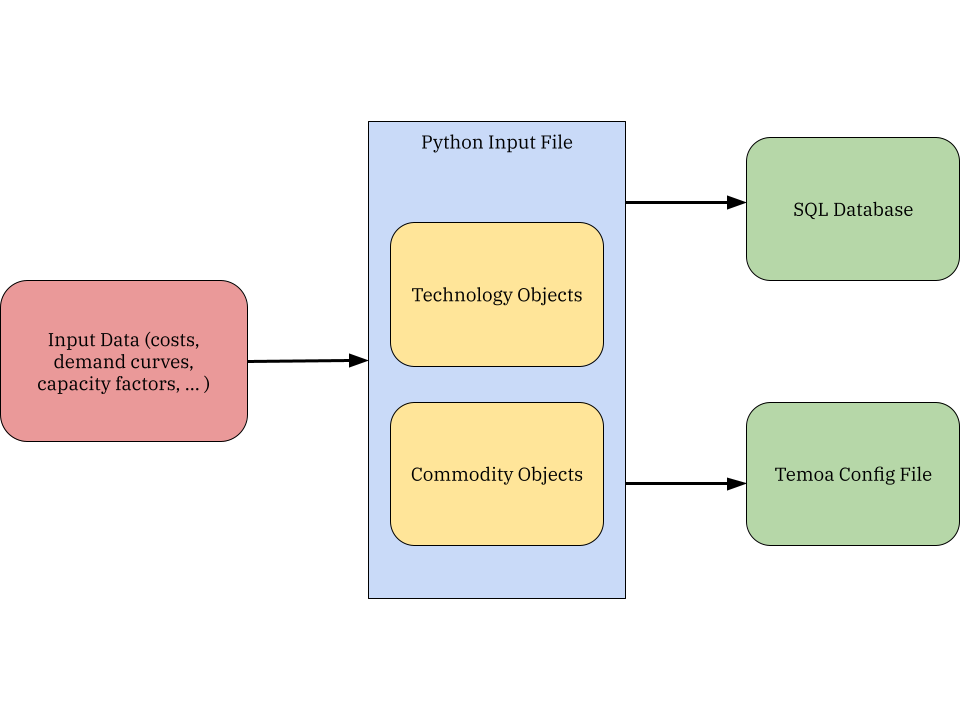
\includegraphics[width=0.8\columnwidth]{figures/pygen-outline.png}
  \caption{The flow of data through \gls{pygen}. \gls{pygen} reads a Python
  input file and writes an \texttt{SQL} database and a configuration textfile.}
  \label{fig:pygen-flow}
\end{figure}
A \gls{pygen} input file can be turned into a template with uncertain parameters
specified using a liquid-text format and then hundreds of input files can be
populated with the \texttt{Jinja2} Python library. Code listing \ref{code:sql} shows
the code \gls{temoa} requires to specify the model time horizon and time slices.
The \gls{pygen} equivalent is shown in code listing \ref{code:python}. Changing
the number of modeled ``seasons'' or years in the model horizon is non-trivial with
\gls{temoa} alone, especially since other tables, such as \texttt{CapacityFactorTech}
which specifies the availability of each technology at each time slice, depend
on the number of time slices and technologies (the product of ``number of seasons,''
``times of day,'' and number of technologies).
The example in code listing \ref{code:sql} has 96 time slices, thus \texttt{CapacityFactorTech}
would have at least 96 rows for a single technology. With \gls{pygen}, users can
update the number of time slices and all affected tables with no additional lines
of code.

\begin{lstlisting}[style=sqlstyle,caption={Temoa tables that define the model horizon and time slices.}, label={code:sql}, floatplacement=H]
CREATE TABLE "time_season" (
  "t_season"	text,
  PRIMARY KEY("t_season")
  );
  INSERT INTO "time_season" VALUES('S1');
  INSERT INTO "time_season" VALUES('S2');
  INSERT INTO "time_season" VALUES('S3');
  INSERT INTO "time_season" VALUES('S4');

CREATE TABLE "time_periods" (
  "t_periods"	integer,
  "flag"	text,
  FOREIGN KEY("flag") REFERENCES "time_period_labels"("t_period_labels"),
  PRIMARY KEY("t_periods")
  );
  INSERT INTO "time_periods" VALUES (2025,'f');
  INSERT INTO "time_periods" VALUES (2030,'f');
  INSERT INTO "time_periods" VALUES (2035,'f');
  INSERT INTO "time_periods" VALUES (2040,'f');
  INSERT INTO "time_periods" VALUES (2045,'f');
  INSERT INTO "time_periods" VALUES (2050,'f');
  INSERT INTO "time_periods" VALUES (2051,'f');

CREATE TABLE "time_period_labels" (
  "t_period_labels"	text,
  "t_period_labels_desc"	text,
  PRIMARY KEY("t_period_labels")
  );
  INSERT INTO "time_period_labels" VALUES ('e','existing vintages');
  INSERT INTO "time_period_labels" VALUES ('f','future');

CREATE TABLE "time_of_day" (
  "t_day"	text,
  PRIMARY KEY("t_day")
  );
  INSERT INTO "time_of_day" VALUES('H1');
  INSERT INTO "time_of_day" VALUES('H2');
  INSERT INTO "time_of_day" VALUES('H3');
  INSERT INTO "time_of_day" VALUES('H4');
  INSERT INTO "time_of_day" VALUES('H5');
  INSERT INTO "time_of_day" VALUES('H6');
  INSERT INTO "time_of_day" VALUES('H7');
  INSERT INTO "time_of_day" VALUES('H8');
  INSERT INTO "time_of_day" VALUES('H9');
  INSERT INTO "time_of_day" VALUES('H10');
  INSERT INTO "time_of_day" VALUES('H11');
  INSERT INTO "time_of_day" VALUES('H12');
  INSERT INTO "time_of_day" VALUES('H13');
  INSERT INTO "time_of_day" VALUES('H14');
  INSERT INTO "time_of_day" VALUES('H15');
  INSERT INTO "time_of_day" VALUES('H16');
  INSERT INTO "time_of_day" VALUES('H17');
  INSERT INTO "time_of_day" VALUES('H18');
  INSERT INTO "time_of_day" VALUES('H19');
  INSERT INTO "time_of_day" VALUES('H20');
  INSERT INTO "time_of_day" VALUES('H21');
  INSERT INTO "time_of_day" VALUES('H22');
  INSERT INTO "time_of_day" VALUES('H23');
  INSERT INTO "time_of_day" VALUES('H24');
\end{lstlisting}


\begin{lstlisting}[style=pythonstyle, caption={Equivalent \gls{pygen} code to specify the model horizon and time slices.}, label={code:python}, floatplacement=H]
start_year = 2025  # the first year optimized by the model
end_year = 2050  # the last year optimized by the model
N_years = 6  # the number of years optimized by the model
N_seasons = 4 # the number of "seasons" in the model
N_hours = 24  # the number of hours in a day
\end{lstlisting}




\subsubsection{Time Series Processing}
Automated conversion of continuous time series data into a \gls{temoa}-ready
time slices is one \gls{pygen}' key features. By specifying the number of ``seasons''
and the number of ``times of day,'' users can quickly rerun their model at different
temporal resolutions. The only limit to this is computational tractability on \gls{temoa}'s
end. There are two options for time series processing, ``demand'' or ``capacity factor.''
A ``demand'' profile ensures the sum of all representative days is unity, while
a ``capacity factor'' profile divides each representative day by the maximum value
of the original time series.
Figure \ref{fig:solar-timeslice} shows some historical data from \gls{uiuc}'s
first solar farm project, Solar Farm 1.0 \cite{white_solar_2017}, that \gls{pygen}
sliced into four seasons with one representative day of 24 hours each. With ``capacity factor''
specified.
\begin{figure}[H]
  \resizebox{\textwidth}{!}{%% Creator: Matplotlib, PGF backend
%%
%% To include the figure in your LaTeX document, write
%%   \input{<filename>.pgf}
%%
%% Make sure the required packages are loaded in your preamble
%%   \usepackage{pgf}
%%
%% Figures using additional raster images can only be included by \input if
%% they are in the same directory as the main LaTeX file. For loading figures
%% from other directories you can use the `import` package
%%   \usepackage{import}
%%
%% and then include the figures with
%%   \import{<path to file>}{<filename>.pgf}
%%
%% Matplotlib used the following preamble
%%
\begingroup%
\makeatletter%
\begin{pgfpicture}%
\pgfpathrectangle{\pgfpointorigin}{\pgfqpoint{17.900000in}{8.900000in}}%
\pgfusepath{use as bounding box, clip}%
\begin{pgfscope}%
\pgfsetbuttcap%
\pgfsetmiterjoin%
\definecolor{currentfill}{rgb}{1.000000,1.000000,1.000000}%
\pgfsetfillcolor{currentfill}%
\pgfsetlinewidth{0.000000pt}%
\definecolor{currentstroke}{rgb}{0.000000,0.000000,0.000000}%
\pgfsetstrokecolor{currentstroke}%
\pgfsetdash{}{0pt}%
\pgfpathmoveto{\pgfqpoint{0.000000in}{0.000000in}}%
\pgfpathlineto{\pgfqpoint{17.900000in}{0.000000in}}%
\pgfpathlineto{\pgfqpoint{17.900000in}{8.900000in}}%
\pgfpathlineto{\pgfqpoint{0.000000in}{8.900000in}}%
\pgfpathclose%
\pgfusepath{fill}%
\end{pgfscope}%
\begin{pgfscope}%
\pgfsetbuttcap%
\pgfsetmiterjoin%
\definecolor{currentfill}{rgb}{0.898039,0.898039,0.898039}%
\pgfsetfillcolor{currentfill}%
\pgfsetlinewidth{0.000000pt}%
\definecolor{currentstroke}{rgb}{0.000000,0.000000,0.000000}%
\pgfsetstrokecolor{currentstroke}%
\pgfsetstrokeopacity{0.000000}%
\pgfsetdash{}{0pt}%
\pgfpathmoveto{\pgfqpoint{0.931995in}{0.892178in}}%
\pgfpathlineto{\pgfqpoint{12.883221in}{0.892178in}}%
\pgfpathlineto{\pgfqpoint{12.883221in}{8.516628in}}%
\pgfpathlineto{\pgfqpoint{0.931995in}{8.516628in}}%
\pgfpathclose%
\pgfusepath{fill}%
\end{pgfscope}%
\begin{pgfscope}%
\pgfpathrectangle{\pgfqpoint{0.931995in}{0.892178in}}{\pgfqpoint{11.951226in}{7.624450in}}%
\pgfusepath{clip}%
\pgfsetrectcap%
\pgfsetroundjoin%
\pgfsetlinewidth{0.803000pt}%
\definecolor{currentstroke}{rgb}{1.000000,1.000000,1.000000}%
\pgfsetstrokecolor{currentstroke}%
\pgfsetdash{}{0pt}%
\pgfpathmoveto{\pgfqpoint{0.931995in}{0.892178in}}%
\pgfpathlineto{\pgfqpoint{0.931995in}{8.516628in}}%
\pgfusepath{stroke}%
\end{pgfscope}%
\begin{pgfscope}%
\pgfsetbuttcap%
\pgfsetroundjoin%
\definecolor{currentfill}{rgb}{0.333333,0.333333,0.333333}%
\pgfsetfillcolor{currentfill}%
\pgfsetlinewidth{0.803000pt}%
\definecolor{currentstroke}{rgb}{0.333333,0.333333,0.333333}%
\pgfsetstrokecolor{currentstroke}%
\pgfsetdash{}{0pt}%
\pgfsys@defobject{currentmarker}{\pgfqpoint{0.000000in}{-0.048611in}}{\pgfqpoint{0.000000in}{0.000000in}}{%
\pgfpathmoveto{\pgfqpoint{0.000000in}{0.000000in}}%
\pgfpathlineto{\pgfqpoint{0.000000in}{-0.048611in}}%
\pgfusepath{stroke,fill}%
}%
\begin{pgfscope}%
\pgfsys@transformshift{0.931995in}{0.892178in}%
\pgfsys@useobject{currentmarker}{}%
\end{pgfscope}%
\end{pgfscope}%
\begin{pgfscope}%
\definecolor{textcolor}{rgb}{0.333333,0.333333,0.333333}%
\pgfsetstrokecolor{textcolor}%
\pgfsetfillcolor{textcolor}%
\pgftext[x=0.778339in, y=0.656067in, left, base]{\color{textcolor}\rmfamily\fontsize{14.000000}{16.800000}\selectfont Jan}%
\end{pgfscope}%
\begin{pgfscope}%
\definecolor{textcolor}{rgb}{0.333333,0.333333,0.333333}%
\pgfsetstrokecolor{textcolor}%
\pgfsetfillcolor{textcolor}%
\pgftext[x=0.736164in, y=0.450512in, left, base]{\color{textcolor}\rmfamily\fontsize{14.000000}{16.800000}\selectfont 2016}%
\end{pgfscope}%
\begin{pgfscope}%
\pgfpathrectangle{\pgfqpoint{0.931995in}{0.892178in}}{\pgfqpoint{11.951226in}{7.624450in}}%
\pgfusepath{clip}%
\pgfsetrectcap%
\pgfsetroundjoin%
\pgfsetlinewidth{0.803000pt}%
\definecolor{currentstroke}{rgb}{1.000000,1.000000,1.000000}%
\pgfsetstrokecolor{currentstroke}%
\pgfsetdash{}{0pt}%
\pgfpathmoveto{\pgfqpoint{4.923158in}{0.892178in}}%
\pgfpathlineto{\pgfqpoint{4.923158in}{8.516628in}}%
\pgfusepath{stroke}%
\end{pgfscope}%
\begin{pgfscope}%
\pgfsetbuttcap%
\pgfsetroundjoin%
\definecolor{currentfill}{rgb}{0.333333,0.333333,0.333333}%
\pgfsetfillcolor{currentfill}%
\pgfsetlinewidth{0.803000pt}%
\definecolor{currentstroke}{rgb}{0.333333,0.333333,0.333333}%
\pgfsetstrokecolor{currentstroke}%
\pgfsetdash{}{0pt}%
\pgfsys@defobject{currentmarker}{\pgfqpoint{0.000000in}{-0.048611in}}{\pgfqpoint{0.000000in}{0.000000in}}{%
\pgfpathmoveto{\pgfqpoint{0.000000in}{0.000000in}}%
\pgfpathlineto{\pgfqpoint{0.000000in}{-0.048611in}}%
\pgfusepath{stroke,fill}%
}%
\begin{pgfscope}%
\pgfsys@transformshift{4.923158in}{0.892178in}%
\pgfsys@useobject{currentmarker}{}%
\end{pgfscope}%
\end{pgfscope}%
\begin{pgfscope}%
\definecolor{textcolor}{rgb}{0.333333,0.333333,0.333333}%
\pgfsetstrokecolor{textcolor}%
\pgfsetfillcolor{textcolor}%
\pgftext[x=4.769503in, y=0.656067in, left, base]{\color{textcolor}\rmfamily\fontsize{14.000000}{16.800000}\selectfont Jan}%
\end{pgfscope}%
\begin{pgfscope}%
\definecolor{textcolor}{rgb}{0.333333,0.333333,0.333333}%
\pgfsetstrokecolor{textcolor}%
\pgfsetfillcolor{textcolor}%
\pgftext[x=4.727327in, y=0.450512in, left, base]{\color{textcolor}\rmfamily\fontsize{14.000000}{16.800000}\selectfont 2017}%
\end{pgfscope}%
\begin{pgfscope}%
\pgfpathrectangle{\pgfqpoint{0.931995in}{0.892178in}}{\pgfqpoint{11.951226in}{7.624450in}}%
\pgfusepath{clip}%
\pgfsetrectcap%
\pgfsetroundjoin%
\pgfsetlinewidth{0.803000pt}%
\definecolor{currentstroke}{rgb}{1.000000,1.000000,1.000000}%
\pgfsetstrokecolor{currentstroke}%
\pgfsetdash{}{0pt}%
\pgfpathmoveto{\pgfqpoint{8.903417in}{0.892178in}}%
\pgfpathlineto{\pgfqpoint{8.903417in}{8.516628in}}%
\pgfusepath{stroke}%
\end{pgfscope}%
\begin{pgfscope}%
\pgfsetbuttcap%
\pgfsetroundjoin%
\definecolor{currentfill}{rgb}{0.333333,0.333333,0.333333}%
\pgfsetfillcolor{currentfill}%
\pgfsetlinewidth{0.803000pt}%
\definecolor{currentstroke}{rgb}{0.333333,0.333333,0.333333}%
\pgfsetstrokecolor{currentstroke}%
\pgfsetdash{}{0pt}%
\pgfsys@defobject{currentmarker}{\pgfqpoint{0.000000in}{-0.048611in}}{\pgfqpoint{0.000000in}{0.000000in}}{%
\pgfpathmoveto{\pgfqpoint{0.000000in}{0.000000in}}%
\pgfpathlineto{\pgfqpoint{0.000000in}{-0.048611in}}%
\pgfusepath{stroke,fill}%
}%
\begin{pgfscope}%
\pgfsys@transformshift{8.903417in}{0.892178in}%
\pgfsys@useobject{currentmarker}{}%
\end{pgfscope}%
\end{pgfscope}%
\begin{pgfscope}%
\definecolor{textcolor}{rgb}{0.333333,0.333333,0.333333}%
\pgfsetstrokecolor{textcolor}%
\pgfsetfillcolor{textcolor}%
\pgftext[x=8.749761in, y=0.656067in, left, base]{\color{textcolor}\rmfamily\fontsize{14.000000}{16.800000}\selectfont Jan}%
\end{pgfscope}%
\begin{pgfscope}%
\definecolor{textcolor}{rgb}{0.333333,0.333333,0.333333}%
\pgfsetstrokecolor{textcolor}%
\pgfsetfillcolor{textcolor}%
\pgftext[x=8.707586in, y=0.450512in, left, base]{\color{textcolor}\rmfamily\fontsize{14.000000}{16.800000}\selectfont 2018}%
\end{pgfscope}%
\begin{pgfscope}%
\pgfpathrectangle{\pgfqpoint{0.931995in}{0.892178in}}{\pgfqpoint{11.951226in}{7.624450in}}%
\pgfusepath{clip}%
\pgfsetrectcap%
\pgfsetroundjoin%
\pgfsetlinewidth{0.803000pt}%
\definecolor{currentstroke}{rgb}{1.000000,1.000000,1.000000}%
\pgfsetstrokecolor{currentstroke}%
\pgfsetdash{}{0pt}%
\pgfpathmoveto{\pgfqpoint{12.883221in}{0.892178in}}%
\pgfpathlineto{\pgfqpoint{12.883221in}{8.516628in}}%
\pgfusepath{stroke}%
\end{pgfscope}%
\begin{pgfscope}%
\pgfsetbuttcap%
\pgfsetroundjoin%
\definecolor{currentfill}{rgb}{0.333333,0.333333,0.333333}%
\pgfsetfillcolor{currentfill}%
\pgfsetlinewidth{0.803000pt}%
\definecolor{currentstroke}{rgb}{0.333333,0.333333,0.333333}%
\pgfsetstrokecolor{currentstroke}%
\pgfsetdash{}{0pt}%
\pgfsys@defobject{currentmarker}{\pgfqpoint{0.000000in}{-0.048611in}}{\pgfqpoint{0.000000in}{0.000000in}}{%
\pgfpathmoveto{\pgfqpoint{0.000000in}{0.000000in}}%
\pgfpathlineto{\pgfqpoint{0.000000in}{-0.048611in}}%
\pgfusepath{stroke,fill}%
}%
\begin{pgfscope}%
\pgfsys@transformshift{12.883221in}{0.892178in}%
\pgfsys@useobject{currentmarker}{}%
\end{pgfscope}%
\end{pgfscope}%
\begin{pgfscope}%
\pgfpathrectangle{\pgfqpoint{0.931995in}{0.892178in}}{\pgfqpoint{11.951226in}{7.624450in}}%
\pgfusepath{clip}%
\pgfsetbuttcap%
\pgfsetroundjoin%
\pgfsetlinewidth{0.803000pt}%
\definecolor{currentstroke}{rgb}{1.000000,1.000000,1.000000}%
\pgfsetstrokecolor{currentstroke}%
\pgfsetdash{{2.960000pt}{1.280000pt}}{0.000000pt}%
\pgfpathmoveto{\pgfqpoint{1.929786in}{0.892178in}}%
\pgfpathlineto{\pgfqpoint{1.929786in}{8.516628in}}%
\pgfusepath{stroke}%
\end{pgfscope}%
\begin{pgfscope}%
\pgfsetbuttcap%
\pgfsetroundjoin%
\definecolor{currentfill}{rgb}{0.333333,0.333333,0.333333}%
\pgfsetfillcolor{currentfill}%
\pgfsetlinewidth{0.602250pt}%
\definecolor{currentstroke}{rgb}{0.333333,0.333333,0.333333}%
\pgfsetstrokecolor{currentstroke}%
\pgfsetdash{}{0pt}%
\pgfsys@defobject{currentmarker}{\pgfqpoint{0.000000in}{-0.027778in}}{\pgfqpoint{0.000000in}{0.000000in}}{%
\pgfpathmoveto{\pgfqpoint{0.000000in}{0.000000in}}%
\pgfpathlineto{\pgfqpoint{0.000000in}{-0.027778in}}%
\pgfusepath{stroke,fill}%
}%
\begin{pgfscope}%
\pgfsys@transformshift{1.929786in}{0.892178in}%
\pgfsys@useobject{currentmarker}{}%
\end{pgfscope}%
\end{pgfscope}%
\begin{pgfscope}%
\pgfpathrectangle{\pgfqpoint{0.931995in}{0.892178in}}{\pgfqpoint{11.951226in}{7.624450in}}%
\pgfusepath{clip}%
\pgfsetbuttcap%
\pgfsetroundjoin%
\pgfsetlinewidth{0.803000pt}%
\definecolor{currentstroke}{rgb}{1.000000,1.000000,1.000000}%
\pgfsetstrokecolor{currentstroke}%
\pgfsetdash{{2.960000pt}{1.280000pt}}{0.000000pt}%
\pgfpathmoveto{\pgfqpoint{2.927577in}{0.892178in}}%
\pgfpathlineto{\pgfqpoint{2.927577in}{8.516628in}}%
\pgfusepath{stroke}%
\end{pgfscope}%
\begin{pgfscope}%
\pgfsetbuttcap%
\pgfsetroundjoin%
\definecolor{currentfill}{rgb}{0.333333,0.333333,0.333333}%
\pgfsetfillcolor{currentfill}%
\pgfsetlinewidth{0.602250pt}%
\definecolor{currentstroke}{rgb}{0.333333,0.333333,0.333333}%
\pgfsetstrokecolor{currentstroke}%
\pgfsetdash{}{0pt}%
\pgfsys@defobject{currentmarker}{\pgfqpoint{0.000000in}{-0.027778in}}{\pgfqpoint{0.000000in}{0.000000in}}{%
\pgfpathmoveto{\pgfqpoint{0.000000in}{0.000000in}}%
\pgfpathlineto{\pgfqpoint{0.000000in}{-0.027778in}}%
\pgfusepath{stroke,fill}%
}%
\begin{pgfscope}%
\pgfsys@transformshift{2.927577in}{0.892178in}%
\pgfsys@useobject{currentmarker}{}%
\end{pgfscope}%
\end{pgfscope}%
\begin{pgfscope}%
\pgfpathrectangle{\pgfqpoint{0.931995in}{0.892178in}}{\pgfqpoint{11.951226in}{7.624450in}}%
\pgfusepath{clip}%
\pgfsetbuttcap%
\pgfsetroundjoin%
\pgfsetlinewidth{0.803000pt}%
\definecolor{currentstroke}{rgb}{1.000000,1.000000,1.000000}%
\pgfsetstrokecolor{currentstroke}%
\pgfsetdash{{2.960000pt}{1.280000pt}}{0.000000pt}%
\pgfpathmoveto{\pgfqpoint{3.925367in}{0.892178in}}%
\pgfpathlineto{\pgfqpoint{3.925367in}{8.516628in}}%
\pgfusepath{stroke}%
\end{pgfscope}%
\begin{pgfscope}%
\pgfsetbuttcap%
\pgfsetroundjoin%
\definecolor{currentfill}{rgb}{0.333333,0.333333,0.333333}%
\pgfsetfillcolor{currentfill}%
\pgfsetlinewidth{0.602250pt}%
\definecolor{currentstroke}{rgb}{0.333333,0.333333,0.333333}%
\pgfsetstrokecolor{currentstroke}%
\pgfsetdash{}{0pt}%
\pgfsys@defobject{currentmarker}{\pgfqpoint{0.000000in}{-0.027778in}}{\pgfqpoint{0.000000in}{0.000000in}}{%
\pgfpathmoveto{\pgfqpoint{0.000000in}{0.000000in}}%
\pgfpathlineto{\pgfqpoint{0.000000in}{-0.027778in}}%
\pgfusepath{stroke,fill}%
}%
\begin{pgfscope}%
\pgfsys@transformshift{3.925367in}{0.892178in}%
\pgfsys@useobject{currentmarker}{}%
\end{pgfscope}%
\end{pgfscope}%
\begin{pgfscope}%
\pgfpathrectangle{\pgfqpoint{0.931995in}{0.892178in}}{\pgfqpoint{11.951226in}{7.624450in}}%
\pgfusepath{clip}%
\pgfsetbuttcap%
\pgfsetroundjoin%
\pgfsetlinewidth{0.803000pt}%
\definecolor{currentstroke}{rgb}{1.000000,1.000000,1.000000}%
\pgfsetstrokecolor{currentstroke}%
\pgfsetdash{{2.960000pt}{1.280000pt}}{0.000000pt}%
\pgfpathmoveto{\pgfqpoint{5.920949in}{0.892178in}}%
\pgfpathlineto{\pgfqpoint{5.920949in}{8.516628in}}%
\pgfusepath{stroke}%
\end{pgfscope}%
\begin{pgfscope}%
\pgfsetbuttcap%
\pgfsetroundjoin%
\definecolor{currentfill}{rgb}{0.333333,0.333333,0.333333}%
\pgfsetfillcolor{currentfill}%
\pgfsetlinewidth{0.602250pt}%
\definecolor{currentstroke}{rgb}{0.333333,0.333333,0.333333}%
\pgfsetstrokecolor{currentstroke}%
\pgfsetdash{}{0pt}%
\pgfsys@defobject{currentmarker}{\pgfqpoint{0.000000in}{-0.027778in}}{\pgfqpoint{0.000000in}{0.000000in}}{%
\pgfpathmoveto{\pgfqpoint{0.000000in}{0.000000in}}%
\pgfpathlineto{\pgfqpoint{0.000000in}{-0.027778in}}%
\pgfusepath{stroke,fill}%
}%
\begin{pgfscope}%
\pgfsys@transformshift{5.920949in}{0.892178in}%
\pgfsys@useobject{currentmarker}{}%
\end{pgfscope}%
\end{pgfscope}%
\begin{pgfscope}%
\pgfpathrectangle{\pgfqpoint{0.931995in}{0.892178in}}{\pgfqpoint{11.951226in}{7.624450in}}%
\pgfusepath{clip}%
\pgfsetbuttcap%
\pgfsetroundjoin%
\pgfsetlinewidth{0.803000pt}%
\definecolor{currentstroke}{rgb}{1.000000,1.000000,1.000000}%
\pgfsetstrokecolor{currentstroke}%
\pgfsetdash{{2.960000pt}{1.280000pt}}{0.000000pt}%
\pgfpathmoveto{\pgfqpoint{6.918740in}{0.892178in}}%
\pgfpathlineto{\pgfqpoint{6.918740in}{8.516628in}}%
\pgfusepath{stroke}%
\end{pgfscope}%
\begin{pgfscope}%
\pgfsetbuttcap%
\pgfsetroundjoin%
\definecolor{currentfill}{rgb}{0.333333,0.333333,0.333333}%
\pgfsetfillcolor{currentfill}%
\pgfsetlinewidth{0.602250pt}%
\definecolor{currentstroke}{rgb}{0.333333,0.333333,0.333333}%
\pgfsetstrokecolor{currentstroke}%
\pgfsetdash{}{0pt}%
\pgfsys@defobject{currentmarker}{\pgfqpoint{0.000000in}{-0.027778in}}{\pgfqpoint{0.000000in}{0.000000in}}{%
\pgfpathmoveto{\pgfqpoint{0.000000in}{0.000000in}}%
\pgfpathlineto{\pgfqpoint{0.000000in}{-0.027778in}}%
\pgfusepath{stroke,fill}%
}%
\begin{pgfscope}%
\pgfsys@transformshift{6.918740in}{0.892178in}%
\pgfsys@useobject{currentmarker}{}%
\end{pgfscope}%
\end{pgfscope}%
\begin{pgfscope}%
\pgfpathrectangle{\pgfqpoint{0.931995in}{0.892178in}}{\pgfqpoint{11.951226in}{7.624450in}}%
\pgfusepath{clip}%
\pgfsetbuttcap%
\pgfsetroundjoin%
\pgfsetlinewidth{0.803000pt}%
\definecolor{currentstroke}{rgb}{1.000000,1.000000,1.000000}%
\pgfsetstrokecolor{currentstroke}%
\pgfsetdash{{2.960000pt}{1.280000pt}}{0.000000pt}%
\pgfpathmoveto{\pgfqpoint{7.916531in}{0.892178in}}%
\pgfpathlineto{\pgfqpoint{7.916531in}{8.516628in}}%
\pgfusepath{stroke}%
\end{pgfscope}%
\begin{pgfscope}%
\pgfsetbuttcap%
\pgfsetroundjoin%
\definecolor{currentfill}{rgb}{0.333333,0.333333,0.333333}%
\pgfsetfillcolor{currentfill}%
\pgfsetlinewidth{0.602250pt}%
\definecolor{currentstroke}{rgb}{0.333333,0.333333,0.333333}%
\pgfsetstrokecolor{currentstroke}%
\pgfsetdash{}{0pt}%
\pgfsys@defobject{currentmarker}{\pgfqpoint{0.000000in}{-0.027778in}}{\pgfqpoint{0.000000in}{0.000000in}}{%
\pgfpathmoveto{\pgfqpoint{0.000000in}{0.000000in}}%
\pgfpathlineto{\pgfqpoint{0.000000in}{-0.027778in}}%
\pgfusepath{stroke,fill}%
}%
\begin{pgfscope}%
\pgfsys@transformshift{7.916531in}{0.892178in}%
\pgfsys@useobject{currentmarker}{}%
\end{pgfscope}%
\end{pgfscope}%
\begin{pgfscope}%
\pgfpathrectangle{\pgfqpoint{0.931995in}{0.892178in}}{\pgfqpoint{11.951226in}{7.624450in}}%
\pgfusepath{clip}%
\pgfsetbuttcap%
\pgfsetroundjoin%
\pgfsetlinewidth{0.803000pt}%
\definecolor{currentstroke}{rgb}{1.000000,1.000000,1.000000}%
\pgfsetstrokecolor{currentstroke}%
\pgfsetdash{{2.960000pt}{1.280000pt}}{0.000000pt}%
\pgfpathmoveto{\pgfqpoint{8.914322in}{0.892178in}}%
\pgfpathlineto{\pgfqpoint{8.914322in}{8.516628in}}%
\pgfusepath{stroke}%
\end{pgfscope}%
\begin{pgfscope}%
\pgfsetbuttcap%
\pgfsetroundjoin%
\definecolor{currentfill}{rgb}{0.333333,0.333333,0.333333}%
\pgfsetfillcolor{currentfill}%
\pgfsetlinewidth{0.602250pt}%
\definecolor{currentstroke}{rgb}{0.333333,0.333333,0.333333}%
\pgfsetstrokecolor{currentstroke}%
\pgfsetdash{}{0pt}%
\pgfsys@defobject{currentmarker}{\pgfqpoint{0.000000in}{-0.027778in}}{\pgfqpoint{0.000000in}{0.000000in}}{%
\pgfpathmoveto{\pgfqpoint{0.000000in}{0.000000in}}%
\pgfpathlineto{\pgfqpoint{0.000000in}{-0.027778in}}%
\pgfusepath{stroke,fill}%
}%
\begin{pgfscope}%
\pgfsys@transformshift{8.914322in}{0.892178in}%
\pgfsys@useobject{currentmarker}{}%
\end{pgfscope}%
\end{pgfscope}%
\begin{pgfscope}%
\pgfpathrectangle{\pgfqpoint{0.931995in}{0.892178in}}{\pgfqpoint{11.951226in}{7.624450in}}%
\pgfusepath{clip}%
\pgfsetbuttcap%
\pgfsetroundjoin%
\pgfsetlinewidth{0.803000pt}%
\definecolor{currentstroke}{rgb}{1.000000,1.000000,1.000000}%
\pgfsetstrokecolor{currentstroke}%
\pgfsetdash{{2.960000pt}{1.280000pt}}{0.000000pt}%
\pgfpathmoveto{\pgfqpoint{9.912112in}{0.892178in}}%
\pgfpathlineto{\pgfqpoint{9.912112in}{8.516628in}}%
\pgfusepath{stroke}%
\end{pgfscope}%
\begin{pgfscope}%
\pgfsetbuttcap%
\pgfsetroundjoin%
\definecolor{currentfill}{rgb}{0.333333,0.333333,0.333333}%
\pgfsetfillcolor{currentfill}%
\pgfsetlinewidth{0.602250pt}%
\definecolor{currentstroke}{rgb}{0.333333,0.333333,0.333333}%
\pgfsetstrokecolor{currentstroke}%
\pgfsetdash{}{0pt}%
\pgfsys@defobject{currentmarker}{\pgfqpoint{0.000000in}{-0.027778in}}{\pgfqpoint{0.000000in}{0.000000in}}{%
\pgfpathmoveto{\pgfqpoint{0.000000in}{0.000000in}}%
\pgfpathlineto{\pgfqpoint{0.000000in}{-0.027778in}}%
\pgfusepath{stroke,fill}%
}%
\begin{pgfscope}%
\pgfsys@transformshift{9.912112in}{0.892178in}%
\pgfsys@useobject{currentmarker}{}%
\end{pgfscope}%
\end{pgfscope}%
\begin{pgfscope}%
\pgfpathrectangle{\pgfqpoint{0.931995in}{0.892178in}}{\pgfqpoint{11.951226in}{7.624450in}}%
\pgfusepath{clip}%
\pgfsetbuttcap%
\pgfsetroundjoin%
\pgfsetlinewidth{0.803000pt}%
\definecolor{currentstroke}{rgb}{1.000000,1.000000,1.000000}%
\pgfsetstrokecolor{currentstroke}%
\pgfsetdash{{2.960000pt}{1.280000pt}}{0.000000pt}%
\pgfpathmoveto{\pgfqpoint{10.909903in}{0.892178in}}%
\pgfpathlineto{\pgfqpoint{10.909903in}{8.516628in}}%
\pgfusepath{stroke}%
\end{pgfscope}%
\begin{pgfscope}%
\pgfsetbuttcap%
\pgfsetroundjoin%
\definecolor{currentfill}{rgb}{0.333333,0.333333,0.333333}%
\pgfsetfillcolor{currentfill}%
\pgfsetlinewidth{0.602250pt}%
\definecolor{currentstroke}{rgb}{0.333333,0.333333,0.333333}%
\pgfsetstrokecolor{currentstroke}%
\pgfsetdash{}{0pt}%
\pgfsys@defobject{currentmarker}{\pgfqpoint{0.000000in}{-0.027778in}}{\pgfqpoint{0.000000in}{0.000000in}}{%
\pgfpathmoveto{\pgfqpoint{0.000000in}{0.000000in}}%
\pgfpathlineto{\pgfqpoint{0.000000in}{-0.027778in}}%
\pgfusepath{stroke,fill}%
}%
\begin{pgfscope}%
\pgfsys@transformshift{10.909903in}{0.892178in}%
\pgfsys@useobject{currentmarker}{}%
\end{pgfscope}%
\end{pgfscope}%
\begin{pgfscope}%
\pgfpathrectangle{\pgfqpoint{0.931995in}{0.892178in}}{\pgfqpoint{11.951226in}{7.624450in}}%
\pgfusepath{clip}%
\pgfsetbuttcap%
\pgfsetroundjoin%
\pgfsetlinewidth{0.803000pt}%
\definecolor{currentstroke}{rgb}{1.000000,1.000000,1.000000}%
\pgfsetstrokecolor{currentstroke}%
\pgfsetdash{{2.960000pt}{1.280000pt}}{0.000000pt}%
\pgfpathmoveto{\pgfqpoint{11.907694in}{0.892178in}}%
\pgfpathlineto{\pgfqpoint{11.907694in}{8.516628in}}%
\pgfusepath{stroke}%
\end{pgfscope}%
\begin{pgfscope}%
\pgfsetbuttcap%
\pgfsetroundjoin%
\definecolor{currentfill}{rgb}{0.333333,0.333333,0.333333}%
\pgfsetfillcolor{currentfill}%
\pgfsetlinewidth{0.602250pt}%
\definecolor{currentstroke}{rgb}{0.333333,0.333333,0.333333}%
\pgfsetstrokecolor{currentstroke}%
\pgfsetdash{}{0pt}%
\pgfsys@defobject{currentmarker}{\pgfqpoint{0.000000in}{-0.027778in}}{\pgfqpoint{0.000000in}{0.000000in}}{%
\pgfpathmoveto{\pgfqpoint{0.000000in}{0.000000in}}%
\pgfpathlineto{\pgfqpoint{0.000000in}{-0.027778in}}%
\pgfusepath{stroke,fill}%
}%
\begin{pgfscope}%
\pgfsys@transformshift{11.907694in}{0.892178in}%
\pgfsys@useobject{currentmarker}{}%
\end{pgfscope}%
\end{pgfscope}%
\begin{pgfscope}%
\definecolor{textcolor}{rgb}{0.333333,0.333333,0.333333}%
\pgfsetstrokecolor{textcolor}%
\pgfsetfillcolor{textcolor}%
\pgftext[x=6.907608in,y=0.356068in,,top]{\color{textcolor}\rmfamily\fontsize{20.000000}{24.000000}\selectfont Date}%
\end{pgfscope}%
\begin{pgfscope}%
\pgfpathrectangle{\pgfqpoint{0.931995in}{0.892178in}}{\pgfqpoint{11.951226in}{7.624450in}}%
\pgfusepath{clip}%
\pgfsetrectcap%
\pgfsetroundjoin%
\pgfsetlinewidth{0.803000pt}%
\definecolor{currentstroke}{rgb}{1.000000,1.000000,1.000000}%
\pgfsetstrokecolor{currentstroke}%
\pgfsetdash{}{0pt}%
\pgfpathmoveto{\pgfqpoint{0.931995in}{0.892178in}}%
\pgfpathlineto{\pgfqpoint{12.883221in}{0.892178in}}%
\pgfusepath{stroke}%
\end{pgfscope}%
\begin{pgfscope}%
\pgfsetbuttcap%
\pgfsetroundjoin%
\definecolor{currentfill}{rgb}{0.333333,0.333333,0.333333}%
\pgfsetfillcolor{currentfill}%
\pgfsetlinewidth{0.803000pt}%
\definecolor{currentstroke}{rgb}{0.333333,0.333333,0.333333}%
\pgfsetstrokecolor{currentstroke}%
\pgfsetdash{}{0pt}%
\pgfsys@defobject{currentmarker}{\pgfqpoint{-0.048611in}{0.000000in}}{\pgfqpoint{-0.000000in}{0.000000in}}{%
\pgfpathmoveto{\pgfqpoint{-0.000000in}{0.000000in}}%
\pgfpathlineto{\pgfqpoint{-0.048611in}{0.000000in}}%
\pgfusepath{stroke,fill}%
}%
\begin{pgfscope}%
\pgfsys@transformshift{0.931995in}{0.892178in}%
\pgfsys@useobject{currentmarker}{}%
\end{pgfscope}%
\end{pgfscope}%
\begin{pgfscope}%
\definecolor{textcolor}{rgb}{0.333333,0.333333,0.333333}%
\pgfsetstrokecolor{textcolor}%
\pgfsetfillcolor{textcolor}%
\pgftext[x=0.736857in, y=0.822734in, left, base]{\color{textcolor}\rmfamily\fontsize{14.000000}{16.800000}\selectfont \(\displaystyle {0}\)}%
\end{pgfscope}%
\begin{pgfscope}%
\pgfpathrectangle{\pgfqpoint{0.931995in}{0.892178in}}{\pgfqpoint{11.951226in}{7.624450in}}%
\pgfusepath{clip}%
\pgfsetrectcap%
\pgfsetroundjoin%
\pgfsetlinewidth{0.803000pt}%
\definecolor{currentstroke}{rgb}{1.000000,1.000000,1.000000}%
\pgfsetstrokecolor{currentstroke}%
\pgfsetdash{}{0pt}%
\pgfpathmoveto{\pgfqpoint{0.931995in}{2.503006in}}%
\pgfpathlineto{\pgfqpoint{12.883221in}{2.503006in}}%
\pgfusepath{stroke}%
\end{pgfscope}%
\begin{pgfscope}%
\pgfsetbuttcap%
\pgfsetroundjoin%
\definecolor{currentfill}{rgb}{0.333333,0.333333,0.333333}%
\pgfsetfillcolor{currentfill}%
\pgfsetlinewidth{0.803000pt}%
\definecolor{currentstroke}{rgb}{0.333333,0.333333,0.333333}%
\pgfsetstrokecolor{currentstroke}%
\pgfsetdash{}{0pt}%
\pgfsys@defobject{currentmarker}{\pgfqpoint{-0.048611in}{0.000000in}}{\pgfqpoint{-0.000000in}{0.000000in}}{%
\pgfpathmoveto{\pgfqpoint{-0.000000in}{0.000000in}}%
\pgfpathlineto{\pgfqpoint{-0.048611in}{0.000000in}}%
\pgfusepath{stroke,fill}%
}%
\begin{pgfscope}%
\pgfsys@transformshift{0.931995in}{2.503006in}%
\pgfsys@useobject{currentmarker}{}%
\end{pgfscope}%
\end{pgfscope}%
\begin{pgfscope}%
\definecolor{textcolor}{rgb}{0.333333,0.333333,0.333333}%
\pgfsetstrokecolor{textcolor}%
\pgfsetfillcolor{textcolor}%
\pgftext[x=0.443111in, y=2.433561in, left, base]{\color{textcolor}\rmfamily\fontsize{14.000000}{16.800000}\selectfont \(\displaystyle {1000}\)}%
\end{pgfscope}%
\begin{pgfscope}%
\pgfpathrectangle{\pgfqpoint{0.931995in}{0.892178in}}{\pgfqpoint{11.951226in}{7.624450in}}%
\pgfusepath{clip}%
\pgfsetrectcap%
\pgfsetroundjoin%
\pgfsetlinewidth{0.803000pt}%
\definecolor{currentstroke}{rgb}{1.000000,1.000000,1.000000}%
\pgfsetstrokecolor{currentstroke}%
\pgfsetdash{}{0pt}%
\pgfpathmoveto{\pgfqpoint{0.931995in}{4.113833in}}%
\pgfpathlineto{\pgfqpoint{12.883221in}{4.113833in}}%
\pgfusepath{stroke}%
\end{pgfscope}%
\begin{pgfscope}%
\pgfsetbuttcap%
\pgfsetroundjoin%
\definecolor{currentfill}{rgb}{0.333333,0.333333,0.333333}%
\pgfsetfillcolor{currentfill}%
\pgfsetlinewidth{0.803000pt}%
\definecolor{currentstroke}{rgb}{0.333333,0.333333,0.333333}%
\pgfsetstrokecolor{currentstroke}%
\pgfsetdash{}{0pt}%
\pgfsys@defobject{currentmarker}{\pgfqpoint{-0.048611in}{0.000000in}}{\pgfqpoint{-0.000000in}{0.000000in}}{%
\pgfpathmoveto{\pgfqpoint{-0.000000in}{0.000000in}}%
\pgfpathlineto{\pgfqpoint{-0.048611in}{0.000000in}}%
\pgfusepath{stroke,fill}%
}%
\begin{pgfscope}%
\pgfsys@transformshift{0.931995in}{4.113833in}%
\pgfsys@useobject{currentmarker}{}%
\end{pgfscope}%
\end{pgfscope}%
\begin{pgfscope}%
\definecolor{textcolor}{rgb}{0.333333,0.333333,0.333333}%
\pgfsetstrokecolor{textcolor}%
\pgfsetfillcolor{textcolor}%
\pgftext[x=0.443111in, y=4.044389in, left, base]{\color{textcolor}\rmfamily\fontsize{14.000000}{16.800000}\selectfont \(\displaystyle {2000}\)}%
\end{pgfscope}%
\begin{pgfscope}%
\pgfpathrectangle{\pgfqpoint{0.931995in}{0.892178in}}{\pgfqpoint{11.951226in}{7.624450in}}%
\pgfusepath{clip}%
\pgfsetrectcap%
\pgfsetroundjoin%
\pgfsetlinewidth{0.803000pt}%
\definecolor{currentstroke}{rgb}{1.000000,1.000000,1.000000}%
\pgfsetstrokecolor{currentstroke}%
\pgfsetdash{}{0pt}%
\pgfpathmoveto{\pgfqpoint{0.931995in}{5.724661in}}%
\pgfpathlineto{\pgfqpoint{12.883221in}{5.724661in}}%
\pgfusepath{stroke}%
\end{pgfscope}%
\begin{pgfscope}%
\pgfsetbuttcap%
\pgfsetroundjoin%
\definecolor{currentfill}{rgb}{0.333333,0.333333,0.333333}%
\pgfsetfillcolor{currentfill}%
\pgfsetlinewidth{0.803000pt}%
\definecolor{currentstroke}{rgb}{0.333333,0.333333,0.333333}%
\pgfsetstrokecolor{currentstroke}%
\pgfsetdash{}{0pt}%
\pgfsys@defobject{currentmarker}{\pgfqpoint{-0.048611in}{0.000000in}}{\pgfqpoint{-0.000000in}{0.000000in}}{%
\pgfpathmoveto{\pgfqpoint{-0.000000in}{0.000000in}}%
\pgfpathlineto{\pgfqpoint{-0.048611in}{0.000000in}}%
\pgfusepath{stroke,fill}%
}%
\begin{pgfscope}%
\pgfsys@transformshift{0.931995in}{5.724661in}%
\pgfsys@useobject{currentmarker}{}%
\end{pgfscope}%
\end{pgfscope}%
\begin{pgfscope}%
\definecolor{textcolor}{rgb}{0.333333,0.333333,0.333333}%
\pgfsetstrokecolor{textcolor}%
\pgfsetfillcolor{textcolor}%
\pgftext[x=0.443111in, y=5.655217in, left, base]{\color{textcolor}\rmfamily\fontsize{14.000000}{16.800000}\selectfont \(\displaystyle {3000}\)}%
\end{pgfscope}%
\begin{pgfscope}%
\pgfpathrectangle{\pgfqpoint{0.931995in}{0.892178in}}{\pgfqpoint{11.951226in}{7.624450in}}%
\pgfusepath{clip}%
\pgfsetrectcap%
\pgfsetroundjoin%
\pgfsetlinewidth{0.803000pt}%
\definecolor{currentstroke}{rgb}{1.000000,1.000000,1.000000}%
\pgfsetstrokecolor{currentstroke}%
\pgfsetdash{}{0pt}%
\pgfpathmoveto{\pgfqpoint{0.931995in}{7.335489in}}%
\pgfpathlineto{\pgfqpoint{12.883221in}{7.335489in}}%
\pgfusepath{stroke}%
\end{pgfscope}%
\begin{pgfscope}%
\pgfsetbuttcap%
\pgfsetroundjoin%
\definecolor{currentfill}{rgb}{0.333333,0.333333,0.333333}%
\pgfsetfillcolor{currentfill}%
\pgfsetlinewidth{0.803000pt}%
\definecolor{currentstroke}{rgb}{0.333333,0.333333,0.333333}%
\pgfsetstrokecolor{currentstroke}%
\pgfsetdash{}{0pt}%
\pgfsys@defobject{currentmarker}{\pgfqpoint{-0.048611in}{0.000000in}}{\pgfqpoint{-0.000000in}{0.000000in}}{%
\pgfpathmoveto{\pgfqpoint{-0.000000in}{0.000000in}}%
\pgfpathlineto{\pgfqpoint{-0.048611in}{0.000000in}}%
\pgfusepath{stroke,fill}%
}%
\begin{pgfscope}%
\pgfsys@transformshift{0.931995in}{7.335489in}%
\pgfsys@useobject{currentmarker}{}%
\end{pgfscope}%
\end{pgfscope}%
\begin{pgfscope}%
\definecolor{textcolor}{rgb}{0.333333,0.333333,0.333333}%
\pgfsetstrokecolor{textcolor}%
\pgfsetfillcolor{textcolor}%
\pgftext[x=0.443111in, y=7.266044in, left, base]{\color{textcolor}\rmfamily\fontsize{14.000000}{16.800000}\selectfont \(\displaystyle {4000}\)}%
\end{pgfscope}%
\begin{pgfscope}%
\pgfpathrectangle{\pgfqpoint{0.931995in}{0.892178in}}{\pgfqpoint{11.951226in}{7.624450in}}%
\pgfusepath{clip}%
\pgfsetbuttcap%
\pgfsetroundjoin%
\pgfsetlinewidth{0.803000pt}%
\definecolor{currentstroke}{rgb}{1.000000,1.000000,1.000000}%
\pgfsetstrokecolor{currentstroke}%
\pgfsetdash{{2.960000pt}{1.280000pt}}{0.000000pt}%
\pgfpathmoveto{\pgfqpoint{0.931995in}{1.214343in}}%
\pgfpathlineto{\pgfqpoint{12.883221in}{1.214343in}}%
\pgfusepath{stroke}%
\end{pgfscope}%
\begin{pgfscope}%
\pgfsetbuttcap%
\pgfsetroundjoin%
\definecolor{currentfill}{rgb}{0.333333,0.333333,0.333333}%
\pgfsetfillcolor{currentfill}%
\pgfsetlinewidth{0.602250pt}%
\definecolor{currentstroke}{rgb}{0.333333,0.333333,0.333333}%
\pgfsetstrokecolor{currentstroke}%
\pgfsetdash{}{0pt}%
\pgfsys@defobject{currentmarker}{\pgfqpoint{-0.027778in}{0.000000in}}{\pgfqpoint{-0.000000in}{0.000000in}}{%
\pgfpathmoveto{\pgfqpoint{-0.000000in}{0.000000in}}%
\pgfpathlineto{\pgfqpoint{-0.027778in}{0.000000in}}%
\pgfusepath{stroke,fill}%
}%
\begin{pgfscope}%
\pgfsys@transformshift{0.931995in}{1.214343in}%
\pgfsys@useobject{currentmarker}{}%
\end{pgfscope}%
\end{pgfscope}%
\begin{pgfscope}%
\pgfpathrectangle{\pgfqpoint{0.931995in}{0.892178in}}{\pgfqpoint{11.951226in}{7.624450in}}%
\pgfusepath{clip}%
\pgfsetbuttcap%
\pgfsetroundjoin%
\pgfsetlinewidth{0.803000pt}%
\definecolor{currentstroke}{rgb}{1.000000,1.000000,1.000000}%
\pgfsetstrokecolor{currentstroke}%
\pgfsetdash{{2.960000pt}{1.280000pt}}{0.000000pt}%
\pgfpathmoveto{\pgfqpoint{0.931995in}{1.536509in}}%
\pgfpathlineto{\pgfqpoint{12.883221in}{1.536509in}}%
\pgfusepath{stroke}%
\end{pgfscope}%
\begin{pgfscope}%
\pgfsetbuttcap%
\pgfsetroundjoin%
\definecolor{currentfill}{rgb}{0.333333,0.333333,0.333333}%
\pgfsetfillcolor{currentfill}%
\pgfsetlinewidth{0.602250pt}%
\definecolor{currentstroke}{rgb}{0.333333,0.333333,0.333333}%
\pgfsetstrokecolor{currentstroke}%
\pgfsetdash{}{0pt}%
\pgfsys@defobject{currentmarker}{\pgfqpoint{-0.027778in}{0.000000in}}{\pgfqpoint{-0.000000in}{0.000000in}}{%
\pgfpathmoveto{\pgfqpoint{-0.000000in}{0.000000in}}%
\pgfpathlineto{\pgfqpoint{-0.027778in}{0.000000in}}%
\pgfusepath{stroke,fill}%
}%
\begin{pgfscope}%
\pgfsys@transformshift{0.931995in}{1.536509in}%
\pgfsys@useobject{currentmarker}{}%
\end{pgfscope}%
\end{pgfscope}%
\begin{pgfscope}%
\pgfpathrectangle{\pgfqpoint{0.931995in}{0.892178in}}{\pgfqpoint{11.951226in}{7.624450in}}%
\pgfusepath{clip}%
\pgfsetbuttcap%
\pgfsetroundjoin%
\pgfsetlinewidth{0.803000pt}%
\definecolor{currentstroke}{rgb}{1.000000,1.000000,1.000000}%
\pgfsetstrokecolor{currentstroke}%
\pgfsetdash{{2.960000pt}{1.280000pt}}{0.000000pt}%
\pgfpathmoveto{\pgfqpoint{0.931995in}{1.858674in}}%
\pgfpathlineto{\pgfqpoint{12.883221in}{1.858674in}}%
\pgfusepath{stroke}%
\end{pgfscope}%
\begin{pgfscope}%
\pgfsetbuttcap%
\pgfsetroundjoin%
\definecolor{currentfill}{rgb}{0.333333,0.333333,0.333333}%
\pgfsetfillcolor{currentfill}%
\pgfsetlinewidth{0.602250pt}%
\definecolor{currentstroke}{rgb}{0.333333,0.333333,0.333333}%
\pgfsetstrokecolor{currentstroke}%
\pgfsetdash{}{0pt}%
\pgfsys@defobject{currentmarker}{\pgfqpoint{-0.027778in}{0.000000in}}{\pgfqpoint{-0.000000in}{0.000000in}}{%
\pgfpathmoveto{\pgfqpoint{-0.000000in}{0.000000in}}%
\pgfpathlineto{\pgfqpoint{-0.027778in}{0.000000in}}%
\pgfusepath{stroke,fill}%
}%
\begin{pgfscope}%
\pgfsys@transformshift{0.931995in}{1.858674in}%
\pgfsys@useobject{currentmarker}{}%
\end{pgfscope}%
\end{pgfscope}%
\begin{pgfscope}%
\pgfpathrectangle{\pgfqpoint{0.931995in}{0.892178in}}{\pgfqpoint{11.951226in}{7.624450in}}%
\pgfusepath{clip}%
\pgfsetbuttcap%
\pgfsetroundjoin%
\pgfsetlinewidth{0.803000pt}%
\definecolor{currentstroke}{rgb}{1.000000,1.000000,1.000000}%
\pgfsetstrokecolor{currentstroke}%
\pgfsetdash{{2.960000pt}{1.280000pt}}{0.000000pt}%
\pgfpathmoveto{\pgfqpoint{0.931995in}{2.180840in}}%
\pgfpathlineto{\pgfqpoint{12.883221in}{2.180840in}}%
\pgfusepath{stroke}%
\end{pgfscope}%
\begin{pgfscope}%
\pgfsetbuttcap%
\pgfsetroundjoin%
\definecolor{currentfill}{rgb}{0.333333,0.333333,0.333333}%
\pgfsetfillcolor{currentfill}%
\pgfsetlinewidth{0.602250pt}%
\definecolor{currentstroke}{rgb}{0.333333,0.333333,0.333333}%
\pgfsetstrokecolor{currentstroke}%
\pgfsetdash{}{0pt}%
\pgfsys@defobject{currentmarker}{\pgfqpoint{-0.027778in}{0.000000in}}{\pgfqpoint{-0.000000in}{0.000000in}}{%
\pgfpathmoveto{\pgfqpoint{-0.000000in}{0.000000in}}%
\pgfpathlineto{\pgfqpoint{-0.027778in}{0.000000in}}%
\pgfusepath{stroke,fill}%
}%
\begin{pgfscope}%
\pgfsys@transformshift{0.931995in}{2.180840in}%
\pgfsys@useobject{currentmarker}{}%
\end{pgfscope}%
\end{pgfscope}%
\begin{pgfscope}%
\pgfpathrectangle{\pgfqpoint{0.931995in}{0.892178in}}{\pgfqpoint{11.951226in}{7.624450in}}%
\pgfusepath{clip}%
\pgfsetbuttcap%
\pgfsetroundjoin%
\pgfsetlinewidth{0.803000pt}%
\definecolor{currentstroke}{rgb}{1.000000,1.000000,1.000000}%
\pgfsetstrokecolor{currentstroke}%
\pgfsetdash{{2.960000pt}{1.280000pt}}{0.000000pt}%
\pgfpathmoveto{\pgfqpoint{0.931995in}{2.825171in}}%
\pgfpathlineto{\pgfqpoint{12.883221in}{2.825171in}}%
\pgfusepath{stroke}%
\end{pgfscope}%
\begin{pgfscope}%
\pgfsetbuttcap%
\pgfsetroundjoin%
\definecolor{currentfill}{rgb}{0.333333,0.333333,0.333333}%
\pgfsetfillcolor{currentfill}%
\pgfsetlinewidth{0.602250pt}%
\definecolor{currentstroke}{rgb}{0.333333,0.333333,0.333333}%
\pgfsetstrokecolor{currentstroke}%
\pgfsetdash{}{0pt}%
\pgfsys@defobject{currentmarker}{\pgfqpoint{-0.027778in}{0.000000in}}{\pgfqpoint{-0.000000in}{0.000000in}}{%
\pgfpathmoveto{\pgfqpoint{-0.000000in}{0.000000in}}%
\pgfpathlineto{\pgfqpoint{-0.027778in}{0.000000in}}%
\pgfusepath{stroke,fill}%
}%
\begin{pgfscope}%
\pgfsys@transformshift{0.931995in}{2.825171in}%
\pgfsys@useobject{currentmarker}{}%
\end{pgfscope}%
\end{pgfscope}%
\begin{pgfscope}%
\pgfpathrectangle{\pgfqpoint{0.931995in}{0.892178in}}{\pgfqpoint{11.951226in}{7.624450in}}%
\pgfusepath{clip}%
\pgfsetbuttcap%
\pgfsetroundjoin%
\pgfsetlinewidth{0.803000pt}%
\definecolor{currentstroke}{rgb}{1.000000,1.000000,1.000000}%
\pgfsetstrokecolor{currentstroke}%
\pgfsetdash{{2.960000pt}{1.280000pt}}{0.000000pt}%
\pgfpathmoveto{\pgfqpoint{0.931995in}{3.147337in}}%
\pgfpathlineto{\pgfqpoint{12.883221in}{3.147337in}}%
\pgfusepath{stroke}%
\end{pgfscope}%
\begin{pgfscope}%
\pgfsetbuttcap%
\pgfsetroundjoin%
\definecolor{currentfill}{rgb}{0.333333,0.333333,0.333333}%
\pgfsetfillcolor{currentfill}%
\pgfsetlinewidth{0.602250pt}%
\definecolor{currentstroke}{rgb}{0.333333,0.333333,0.333333}%
\pgfsetstrokecolor{currentstroke}%
\pgfsetdash{}{0pt}%
\pgfsys@defobject{currentmarker}{\pgfqpoint{-0.027778in}{0.000000in}}{\pgfqpoint{-0.000000in}{0.000000in}}{%
\pgfpathmoveto{\pgfqpoint{-0.000000in}{0.000000in}}%
\pgfpathlineto{\pgfqpoint{-0.027778in}{0.000000in}}%
\pgfusepath{stroke,fill}%
}%
\begin{pgfscope}%
\pgfsys@transformshift{0.931995in}{3.147337in}%
\pgfsys@useobject{currentmarker}{}%
\end{pgfscope}%
\end{pgfscope}%
\begin{pgfscope}%
\pgfpathrectangle{\pgfqpoint{0.931995in}{0.892178in}}{\pgfqpoint{11.951226in}{7.624450in}}%
\pgfusepath{clip}%
\pgfsetbuttcap%
\pgfsetroundjoin%
\pgfsetlinewidth{0.803000pt}%
\definecolor{currentstroke}{rgb}{1.000000,1.000000,1.000000}%
\pgfsetstrokecolor{currentstroke}%
\pgfsetdash{{2.960000pt}{1.280000pt}}{0.000000pt}%
\pgfpathmoveto{\pgfqpoint{0.931995in}{3.469502in}}%
\pgfpathlineto{\pgfqpoint{12.883221in}{3.469502in}}%
\pgfusepath{stroke}%
\end{pgfscope}%
\begin{pgfscope}%
\pgfsetbuttcap%
\pgfsetroundjoin%
\definecolor{currentfill}{rgb}{0.333333,0.333333,0.333333}%
\pgfsetfillcolor{currentfill}%
\pgfsetlinewidth{0.602250pt}%
\definecolor{currentstroke}{rgb}{0.333333,0.333333,0.333333}%
\pgfsetstrokecolor{currentstroke}%
\pgfsetdash{}{0pt}%
\pgfsys@defobject{currentmarker}{\pgfqpoint{-0.027778in}{0.000000in}}{\pgfqpoint{-0.000000in}{0.000000in}}{%
\pgfpathmoveto{\pgfqpoint{-0.000000in}{0.000000in}}%
\pgfpathlineto{\pgfqpoint{-0.027778in}{0.000000in}}%
\pgfusepath{stroke,fill}%
}%
\begin{pgfscope}%
\pgfsys@transformshift{0.931995in}{3.469502in}%
\pgfsys@useobject{currentmarker}{}%
\end{pgfscope}%
\end{pgfscope}%
\begin{pgfscope}%
\pgfpathrectangle{\pgfqpoint{0.931995in}{0.892178in}}{\pgfqpoint{11.951226in}{7.624450in}}%
\pgfusepath{clip}%
\pgfsetbuttcap%
\pgfsetroundjoin%
\pgfsetlinewidth{0.803000pt}%
\definecolor{currentstroke}{rgb}{1.000000,1.000000,1.000000}%
\pgfsetstrokecolor{currentstroke}%
\pgfsetdash{{2.960000pt}{1.280000pt}}{0.000000pt}%
\pgfpathmoveto{\pgfqpoint{0.931995in}{3.791668in}}%
\pgfpathlineto{\pgfqpoint{12.883221in}{3.791668in}}%
\pgfusepath{stroke}%
\end{pgfscope}%
\begin{pgfscope}%
\pgfsetbuttcap%
\pgfsetroundjoin%
\definecolor{currentfill}{rgb}{0.333333,0.333333,0.333333}%
\pgfsetfillcolor{currentfill}%
\pgfsetlinewidth{0.602250pt}%
\definecolor{currentstroke}{rgb}{0.333333,0.333333,0.333333}%
\pgfsetstrokecolor{currentstroke}%
\pgfsetdash{}{0pt}%
\pgfsys@defobject{currentmarker}{\pgfqpoint{-0.027778in}{0.000000in}}{\pgfqpoint{-0.000000in}{0.000000in}}{%
\pgfpathmoveto{\pgfqpoint{-0.000000in}{0.000000in}}%
\pgfpathlineto{\pgfqpoint{-0.027778in}{0.000000in}}%
\pgfusepath{stroke,fill}%
}%
\begin{pgfscope}%
\pgfsys@transformshift{0.931995in}{3.791668in}%
\pgfsys@useobject{currentmarker}{}%
\end{pgfscope}%
\end{pgfscope}%
\begin{pgfscope}%
\pgfpathrectangle{\pgfqpoint{0.931995in}{0.892178in}}{\pgfqpoint{11.951226in}{7.624450in}}%
\pgfusepath{clip}%
\pgfsetbuttcap%
\pgfsetroundjoin%
\pgfsetlinewidth{0.803000pt}%
\definecolor{currentstroke}{rgb}{1.000000,1.000000,1.000000}%
\pgfsetstrokecolor{currentstroke}%
\pgfsetdash{{2.960000pt}{1.280000pt}}{0.000000pt}%
\pgfpathmoveto{\pgfqpoint{0.931995in}{4.435999in}}%
\pgfpathlineto{\pgfqpoint{12.883221in}{4.435999in}}%
\pgfusepath{stroke}%
\end{pgfscope}%
\begin{pgfscope}%
\pgfsetbuttcap%
\pgfsetroundjoin%
\definecolor{currentfill}{rgb}{0.333333,0.333333,0.333333}%
\pgfsetfillcolor{currentfill}%
\pgfsetlinewidth{0.602250pt}%
\definecolor{currentstroke}{rgb}{0.333333,0.333333,0.333333}%
\pgfsetstrokecolor{currentstroke}%
\pgfsetdash{}{0pt}%
\pgfsys@defobject{currentmarker}{\pgfqpoint{-0.027778in}{0.000000in}}{\pgfqpoint{-0.000000in}{0.000000in}}{%
\pgfpathmoveto{\pgfqpoint{-0.000000in}{0.000000in}}%
\pgfpathlineto{\pgfqpoint{-0.027778in}{0.000000in}}%
\pgfusepath{stroke,fill}%
}%
\begin{pgfscope}%
\pgfsys@transformshift{0.931995in}{4.435999in}%
\pgfsys@useobject{currentmarker}{}%
\end{pgfscope}%
\end{pgfscope}%
\begin{pgfscope}%
\pgfpathrectangle{\pgfqpoint{0.931995in}{0.892178in}}{\pgfqpoint{11.951226in}{7.624450in}}%
\pgfusepath{clip}%
\pgfsetbuttcap%
\pgfsetroundjoin%
\pgfsetlinewidth{0.803000pt}%
\definecolor{currentstroke}{rgb}{1.000000,1.000000,1.000000}%
\pgfsetstrokecolor{currentstroke}%
\pgfsetdash{{2.960000pt}{1.280000pt}}{0.000000pt}%
\pgfpathmoveto{\pgfqpoint{0.931995in}{4.758164in}}%
\pgfpathlineto{\pgfqpoint{12.883221in}{4.758164in}}%
\pgfusepath{stroke}%
\end{pgfscope}%
\begin{pgfscope}%
\pgfsetbuttcap%
\pgfsetroundjoin%
\definecolor{currentfill}{rgb}{0.333333,0.333333,0.333333}%
\pgfsetfillcolor{currentfill}%
\pgfsetlinewidth{0.602250pt}%
\definecolor{currentstroke}{rgb}{0.333333,0.333333,0.333333}%
\pgfsetstrokecolor{currentstroke}%
\pgfsetdash{}{0pt}%
\pgfsys@defobject{currentmarker}{\pgfqpoint{-0.027778in}{0.000000in}}{\pgfqpoint{-0.000000in}{0.000000in}}{%
\pgfpathmoveto{\pgfqpoint{-0.000000in}{0.000000in}}%
\pgfpathlineto{\pgfqpoint{-0.027778in}{0.000000in}}%
\pgfusepath{stroke,fill}%
}%
\begin{pgfscope}%
\pgfsys@transformshift{0.931995in}{4.758164in}%
\pgfsys@useobject{currentmarker}{}%
\end{pgfscope}%
\end{pgfscope}%
\begin{pgfscope}%
\pgfpathrectangle{\pgfqpoint{0.931995in}{0.892178in}}{\pgfqpoint{11.951226in}{7.624450in}}%
\pgfusepath{clip}%
\pgfsetbuttcap%
\pgfsetroundjoin%
\pgfsetlinewidth{0.803000pt}%
\definecolor{currentstroke}{rgb}{1.000000,1.000000,1.000000}%
\pgfsetstrokecolor{currentstroke}%
\pgfsetdash{{2.960000pt}{1.280000pt}}{0.000000pt}%
\pgfpathmoveto{\pgfqpoint{0.931995in}{5.080330in}}%
\pgfpathlineto{\pgfqpoint{12.883221in}{5.080330in}}%
\pgfusepath{stroke}%
\end{pgfscope}%
\begin{pgfscope}%
\pgfsetbuttcap%
\pgfsetroundjoin%
\definecolor{currentfill}{rgb}{0.333333,0.333333,0.333333}%
\pgfsetfillcolor{currentfill}%
\pgfsetlinewidth{0.602250pt}%
\definecolor{currentstroke}{rgb}{0.333333,0.333333,0.333333}%
\pgfsetstrokecolor{currentstroke}%
\pgfsetdash{}{0pt}%
\pgfsys@defobject{currentmarker}{\pgfqpoint{-0.027778in}{0.000000in}}{\pgfqpoint{-0.000000in}{0.000000in}}{%
\pgfpathmoveto{\pgfqpoint{-0.000000in}{0.000000in}}%
\pgfpathlineto{\pgfqpoint{-0.027778in}{0.000000in}}%
\pgfusepath{stroke,fill}%
}%
\begin{pgfscope}%
\pgfsys@transformshift{0.931995in}{5.080330in}%
\pgfsys@useobject{currentmarker}{}%
\end{pgfscope}%
\end{pgfscope}%
\begin{pgfscope}%
\pgfpathrectangle{\pgfqpoint{0.931995in}{0.892178in}}{\pgfqpoint{11.951226in}{7.624450in}}%
\pgfusepath{clip}%
\pgfsetbuttcap%
\pgfsetroundjoin%
\pgfsetlinewidth{0.803000pt}%
\definecolor{currentstroke}{rgb}{1.000000,1.000000,1.000000}%
\pgfsetstrokecolor{currentstroke}%
\pgfsetdash{{2.960000pt}{1.280000pt}}{0.000000pt}%
\pgfpathmoveto{\pgfqpoint{0.931995in}{5.402495in}}%
\pgfpathlineto{\pgfqpoint{12.883221in}{5.402495in}}%
\pgfusepath{stroke}%
\end{pgfscope}%
\begin{pgfscope}%
\pgfsetbuttcap%
\pgfsetroundjoin%
\definecolor{currentfill}{rgb}{0.333333,0.333333,0.333333}%
\pgfsetfillcolor{currentfill}%
\pgfsetlinewidth{0.602250pt}%
\definecolor{currentstroke}{rgb}{0.333333,0.333333,0.333333}%
\pgfsetstrokecolor{currentstroke}%
\pgfsetdash{}{0pt}%
\pgfsys@defobject{currentmarker}{\pgfqpoint{-0.027778in}{0.000000in}}{\pgfqpoint{-0.000000in}{0.000000in}}{%
\pgfpathmoveto{\pgfqpoint{-0.000000in}{0.000000in}}%
\pgfpathlineto{\pgfqpoint{-0.027778in}{0.000000in}}%
\pgfusepath{stroke,fill}%
}%
\begin{pgfscope}%
\pgfsys@transformshift{0.931995in}{5.402495in}%
\pgfsys@useobject{currentmarker}{}%
\end{pgfscope}%
\end{pgfscope}%
\begin{pgfscope}%
\pgfpathrectangle{\pgfqpoint{0.931995in}{0.892178in}}{\pgfqpoint{11.951226in}{7.624450in}}%
\pgfusepath{clip}%
\pgfsetbuttcap%
\pgfsetroundjoin%
\pgfsetlinewidth{0.803000pt}%
\definecolor{currentstroke}{rgb}{1.000000,1.000000,1.000000}%
\pgfsetstrokecolor{currentstroke}%
\pgfsetdash{{2.960000pt}{1.280000pt}}{0.000000pt}%
\pgfpathmoveto{\pgfqpoint{0.931995in}{6.046827in}}%
\pgfpathlineto{\pgfqpoint{12.883221in}{6.046827in}}%
\pgfusepath{stroke}%
\end{pgfscope}%
\begin{pgfscope}%
\pgfsetbuttcap%
\pgfsetroundjoin%
\definecolor{currentfill}{rgb}{0.333333,0.333333,0.333333}%
\pgfsetfillcolor{currentfill}%
\pgfsetlinewidth{0.602250pt}%
\definecolor{currentstroke}{rgb}{0.333333,0.333333,0.333333}%
\pgfsetstrokecolor{currentstroke}%
\pgfsetdash{}{0pt}%
\pgfsys@defobject{currentmarker}{\pgfqpoint{-0.027778in}{0.000000in}}{\pgfqpoint{-0.000000in}{0.000000in}}{%
\pgfpathmoveto{\pgfqpoint{-0.000000in}{0.000000in}}%
\pgfpathlineto{\pgfqpoint{-0.027778in}{0.000000in}}%
\pgfusepath{stroke,fill}%
}%
\begin{pgfscope}%
\pgfsys@transformshift{0.931995in}{6.046827in}%
\pgfsys@useobject{currentmarker}{}%
\end{pgfscope}%
\end{pgfscope}%
\begin{pgfscope}%
\pgfpathrectangle{\pgfqpoint{0.931995in}{0.892178in}}{\pgfqpoint{11.951226in}{7.624450in}}%
\pgfusepath{clip}%
\pgfsetbuttcap%
\pgfsetroundjoin%
\pgfsetlinewidth{0.803000pt}%
\definecolor{currentstroke}{rgb}{1.000000,1.000000,1.000000}%
\pgfsetstrokecolor{currentstroke}%
\pgfsetdash{{2.960000pt}{1.280000pt}}{0.000000pt}%
\pgfpathmoveto{\pgfqpoint{0.931995in}{6.368992in}}%
\pgfpathlineto{\pgfqpoint{12.883221in}{6.368992in}}%
\pgfusepath{stroke}%
\end{pgfscope}%
\begin{pgfscope}%
\pgfsetbuttcap%
\pgfsetroundjoin%
\definecolor{currentfill}{rgb}{0.333333,0.333333,0.333333}%
\pgfsetfillcolor{currentfill}%
\pgfsetlinewidth{0.602250pt}%
\definecolor{currentstroke}{rgb}{0.333333,0.333333,0.333333}%
\pgfsetstrokecolor{currentstroke}%
\pgfsetdash{}{0pt}%
\pgfsys@defobject{currentmarker}{\pgfqpoint{-0.027778in}{0.000000in}}{\pgfqpoint{-0.000000in}{0.000000in}}{%
\pgfpathmoveto{\pgfqpoint{-0.000000in}{0.000000in}}%
\pgfpathlineto{\pgfqpoint{-0.027778in}{0.000000in}}%
\pgfusepath{stroke,fill}%
}%
\begin{pgfscope}%
\pgfsys@transformshift{0.931995in}{6.368992in}%
\pgfsys@useobject{currentmarker}{}%
\end{pgfscope}%
\end{pgfscope}%
\begin{pgfscope}%
\pgfpathrectangle{\pgfqpoint{0.931995in}{0.892178in}}{\pgfqpoint{11.951226in}{7.624450in}}%
\pgfusepath{clip}%
\pgfsetbuttcap%
\pgfsetroundjoin%
\pgfsetlinewidth{0.803000pt}%
\definecolor{currentstroke}{rgb}{1.000000,1.000000,1.000000}%
\pgfsetstrokecolor{currentstroke}%
\pgfsetdash{{2.960000pt}{1.280000pt}}{0.000000pt}%
\pgfpathmoveto{\pgfqpoint{0.931995in}{6.691158in}}%
\pgfpathlineto{\pgfqpoint{12.883221in}{6.691158in}}%
\pgfusepath{stroke}%
\end{pgfscope}%
\begin{pgfscope}%
\pgfsetbuttcap%
\pgfsetroundjoin%
\definecolor{currentfill}{rgb}{0.333333,0.333333,0.333333}%
\pgfsetfillcolor{currentfill}%
\pgfsetlinewidth{0.602250pt}%
\definecolor{currentstroke}{rgb}{0.333333,0.333333,0.333333}%
\pgfsetstrokecolor{currentstroke}%
\pgfsetdash{}{0pt}%
\pgfsys@defobject{currentmarker}{\pgfqpoint{-0.027778in}{0.000000in}}{\pgfqpoint{-0.000000in}{0.000000in}}{%
\pgfpathmoveto{\pgfqpoint{-0.000000in}{0.000000in}}%
\pgfpathlineto{\pgfqpoint{-0.027778in}{0.000000in}}%
\pgfusepath{stroke,fill}%
}%
\begin{pgfscope}%
\pgfsys@transformshift{0.931995in}{6.691158in}%
\pgfsys@useobject{currentmarker}{}%
\end{pgfscope}%
\end{pgfscope}%
\begin{pgfscope}%
\pgfpathrectangle{\pgfqpoint{0.931995in}{0.892178in}}{\pgfqpoint{11.951226in}{7.624450in}}%
\pgfusepath{clip}%
\pgfsetbuttcap%
\pgfsetroundjoin%
\pgfsetlinewidth{0.803000pt}%
\definecolor{currentstroke}{rgb}{1.000000,1.000000,1.000000}%
\pgfsetstrokecolor{currentstroke}%
\pgfsetdash{{2.960000pt}{1.280000pt}}{0.000000pt}%
\pgfpathmoveto{\pgfqpoint{0.931995in}{7.013323in}}%
\pgfpathlineto{\pgfqpoint{12.883221in}{7.013323in}}%
\pgfusepath{stroke}%
\end{pgfscope}%
\begin{pgfscope}%
\pgfsetbuttcap%
\pgfsetroundjoin%
\definecolor{currentfill}{rgb}{0.333333,0.333333,0.333333}%
\pgfsetfillcolor{currentfill}%
\pgfsetlinewidth{0.602250pt}%
\definecolor{currentstroke}{rgb}{0.333333,0.333333,0.333333}%
\pgfsetstrokecolor{currentstroke}%
\pgfsetdash{}{0pt}%
\pgfsys@defobject{currentmarker}{\pgfqpoint{-0.027778in}{0.000000in}}{\pgfqpoint{-0.000000in}{0.000000in}}{%
\pgfpathmoveto{\pgfqpoint{-0.000000in}{0.000000in}}%
\pgfpathlineto{\pgfqpoint{-0.027778in}{0.000000in}}%
\pgfusepath{stroke,fill}%
}%
\begin{pgfscope}%
\pgfsys@transformshift{0.931995in}{7.013323in}%
\pgfsys@useobject{currentmarker}{}%
\end{pgfscope}%
\end{pgfscope}%
\begin{pgfscope}%
\pgfpathrectangle{\pgfqpoint{0.931995in}{0.892178in}}{\pgfqpoint{11.951226in}{7.624450in}}%
\pgfusepath{clip}%
\pgfsetbuttcap%
\pgfsetroundjoin%
\pgfsetlinewidth{0.803000pt}%
\definecolor{currentstroke}{rgb}{1.000000,1.000000,1.000000}%
\pgfsetstrokecolor{currentstroke}%
\pgfsetdash{{2.960000pt}{1.280000pt}}{0.000000pt}%
\pgfpathmoveto{\pgfqpoint{0.931995in}{7.657654in}}%
\pgfpathlineto{\pgfqpoint{12.883221in}{7.657654in}}%
\pgfusepath{stroke}%
\end{pgfscope}%
\begin{pgfscope}%
\pgfsetbuttcap%
\pgfsetroundjoin%
\definecolor{currentfill}{rgb}{0.333333,0.333333,0.333333}%
\pgfsetfillcolor{currentfill}%
\pgfsetlinewidth{0.602250pt}%
\definecolor{currentstroke}{rgb}{0.333333,0.333333,0.333333}%
\pgfsetstrokecolor{currentstroke}%
\pgfsetdash{}{0pt}%
\pgfsys@defobject{currentmarker}{\pgfqpoint{-0.027778in}{0.000000in}}{\pgfqpoint{-0.000000in}{0.000000in}}{%
\pgfpathmoveto{\pgfqpoint{-0.000000in}{0.000000in}}%
\pgfpathlineto{\pgfqpoint{-0.027778in}{0.000000in}}%
\pgfusepath{stroke,fill}%
}%
\begin{pgfscope}%
\pgfsys@transformshift{0.931995in}{7.657654in}%
\pgfsys@useobject{currentmarker}{}%
\end{pgfscope}%
\end{pgfscope}%
\begin{pgfscope}%
\pgfpathrectangle{\pgfqpoint{0.931995in}{0.892178in}}{\pgfqpoint{11.951226in}{7.624450in}}%
\pgfusepath{clip}%
\pgfsetbuttcap%
\pgfsetroundjoin%
\pgfsetlinewidth{0.803000pt}%
\definecolor{currentstroke}{rgb}{1.000000,1.000000,1.000000}%
\pgfsetstrokecolor{currentstroke}%
\pgfsetdash{{2.960000pt}{1.280000pt}}{0.000000pt}%
\pgfpathmoveto{\pgfqpoint{0.931995in}{7.979820in}}%
\pgfpathlineto{\pgfqpoint{12.883221in}{7.979820in}}%
\pgfusepath{stroke}%
\end{pgfscope}%
\begin{pgfscope}%
\pgfsetbuttcap%
\pgfsetroundjoin%
\definecolor{currentfill}{rgb}{0.333333,0.333333,0.333333}%
\pgfsetfillcolor{currentfill}%
\pgfsetlinewidth{0.602250pt}%
\definecolor{currentstroke}{rgb}{0.333333,0.333333,0.333333}%
\pgfsetstrokecolor{currentstroke}%
\pgfsetdash{}{0pt}%
\pgfsys@defobject{currentmarker}{\pgfqpoint{-0.027778in}{0.000000in}}{\pgfqpoint{-0.000000in}{0.000000in}}{%
\pgfpathmoveto{\pgfqpoint{-0.000000in}{0.000000in}}%
\pgfpathlineto{\pgfqpoint{-0.027778in}{0.000000in}}%
\pgfusepath{stroke,fill}%
}%
\begin{pgfscope}%
\pgfsys@transformshift{0.931995in}{7.979820in}%
\pgfsys@useobject{currentmarker}{}%
\end{pgfscope}%
\end{pgfscope}%
\begin{pgfscope}%
\pgfpathrectangle{\pgfqpoint{0.931995in}{0.892178in}}{\pgfqpoint{11.951226in}{7.624450in}}%
\pgfusepath{clip}%
\pgfsetbuttcap%
\pgfsetroundjoin%
\pgfsetlinewidth{0.803000pt}%
\definecolor{currentstroke}{rgb}{1.000000,1.000000,1.000000}%
\pgfsetstrokecolor{currentstroke}%
\pgfsetdash{{2.960000pt}{1.280000pt}}{0.000000pt}%
\pgfpathmoveto{\pgfqpoint{0.931995in}{8.301985in}}%
\pgfpathlineto{\pgfqpoint{12.883221in}{8.301985in}}%
\pgfusepath{stroke}%
\end{pgfscope}%
\begin{pgfscope}%
\pgfsetbuttcap%
\pgfsetroundjoin%
\definecolor{currentfill}{rgb}{0.333333,0.333333,0.333333}%
\pgfsetfillcolor{currentfill}%
\pgfsetlinewidth{0.602250pt}%
\definecolor{currentstroke}{rgb}{0.333333,0.333333,0.333333}%
\pgfsetstrokecolor{currentstroke}%
\pgfsetdash{}{0pt}%
\pgfsys@defobject{currentmarker}{\pgfqpoint{-0.027778in}{0.000000in}}{\pgfqpoint{-0.000000in}{0.000000in}}{%
\pgfpathmoveto{\pgfqpoint{-0.000000in}{0.000000in}}%
\pgfpathlineto{\pgfqpoint{-0.027778in}{0.000000in}}%
\pgfusepath{stroke,fill}%
}%
\begin{pgfscope}%
\pgfsys@transformshift{0.931995in}{8.301985in}%
\pgfsys@useobject{currentmarker}{}%
\end{pgfscope}%
\end{pgfscope}%
\begin{pgfscope}%
\definecolor{textcolor}{rgb}{0.333333,0.333333,0.333333}%
\pgfsetstrokecolor{textcolor}%
\pgfsetfillcolor{textcolor}%
\pgftext[x=0.387555in,y=4.704403in,,bottom,rotate=90.000000]{\color{textcolor}\rmfamily\fontsize{20.000000}{24.000000}\selectfont Power [kW]}%
\end{pgfscope}%
\begin{pgfscope}%
\pgfpathrectangle{\pgfqpoint{0.931995in}{0.892178in}}{\pgfqpoint{11.951226in}{7.624450in}}%
\pgfusepath{clip}%
\pgfsetrectcap%
\pgfsetroundjoin%
\pgfsetlinewidth{1.505625pt}%
\definecolor{currentstroke}{rgb}{0.121569,0.466667,0.705882}%
\pgfsetstrokecolor{currentstroke}%
\pgfsetdash{}{0pt}%
\pgfpathmoveto{\pgfqpoint{0.931995in}{0.892178in}}%
\pgfpathlineto{\pgfqpoint{0.934721in}{0.892178in}}%
\pgfpathlineto{\pgfqpoint{0.935175in}{0.952507in}}%
\pgfpathlineto{\pgfqpoint{0.935630in}{1.135010in}}%
\pgfpathlineto{\pgfqpoint{0.936539in}{2.792149in}}%
\pgfpathlineto{\pgfqpoint{0.937447in}{2.002844in}}%
\pgfpathlineto{\pgfqpoint{0.938356in}{2.912559in}}%
\pgfpathlineto{\pgfqpoint{0.938810in}{2.329842in}}%
\pgfpathlineto{\pgfqpoint{0.939265in}{1.025212in}}%
\pgfpathlineto{\pgfqpoint{0.939719in}{0.892178in}}%
\pgfpathlineto{\pgfqpoint{0.945626in}{0.892178in}}%
\pgfpathlineto{\pgfqpoint{0.946080in}{1.124439in}}%
\pgfpathlineto{\pgfqpoint{0.947898in}{7.197763in}}%
\pgfpathlineto{\pgfqpoint{0.948352in}{7.059232in}}%
\pgfpathlineto{\pgfqpoint{0.950624in}{0.892178in}}%
\pgfpathlineto{\pgfqpoint{0.956531in}{0.892178in}}%
\pgfpathlineto{\pgfqpoint{0.956985in}{1.107590in}}%
\pgfpathlineto{\pgfqpoint{0.958348in}{6.228447in}}%
\pgfpathlineto{\pgfqpoint{0.958803in}{6.048437in}}%
\pgfpathlineto{\pgfqpoint{0.959711in}{2.116810in}}%
\pgfpathlineto{\pgfqpoint{0.960620in}{1.181684in}}%
\pgfpathlineto{\pgfqpoint{0.961074in}{0.928615in}}%
\pgfpathlineto{\pgfqpoint{0.961529in}{0.892178in}}%
\pgfpathlineto{\pgfqpoint{0.967436in}{0.892178in}}%
\pgfpathlineto{\pgfqpoint{0.967890in}{1.129888in}}%
\pgfpathlineto{\pgfqpoint{0.969707in}{7.420863in}}%
\pgfpathlineto{\pgfqpoint{0.970162in}{7.197360in}}%
\pgfpathlineto{\pgfqpoint{0.970616in}{5.911920in}}%
\pgfpathlineto{\pgfqpoint{0.971525in}{1.544805in}}%
\pgfpathlineto{\pgfqpoint{0.971979in}{0.921809in}}%
\pgfpathlineto{\pgfqpoint{0.972434in}{0.892178in}}%
\pgfpathlineto{\pgfqpoint{0.978340in}{0.892178in}}%
\pgfpathlineto{\pgfqpoint{0.978795in}{1.131370in}}%
\pgfpathlineto{\pgfqpoint{0.980612in}{6.938822in}}%
\pgfpathlineto{\pgfqpoint{0.981067in}{6.918284in}}%
\pgfpathlineto{\pgfqpoint{0.981521in}{5.775402in}}%
\pgfpathlineto{\pgfqpoint{0.982884in}{1.135997in}}%
\pgfpathlineto{\pgfqpoint{0.983338in}{0.892178in}}%
\pgfpathlineto{\pgfqpoint{0.989245in}{0.892178in}}%
\pgfpathlineto{\pgfqpoint{0.989700in}{1.054686in}}%
\pgfpathlineto{\pgfqpoint{0.990154in}{2.458708in}}%
\pgfpathlineto{\pgfqpoint{0.990608in}{2.884369in}}%
\pgfpathlineto{\pgfqpoint{0.991063in}{3.731262in}}%
\pgfpathlineto{\pgfqpoint{0.991517in}{5.648147in}}%
\pgfpathlineto{\pgfqpoint{0.991971in}{4.245921in}}%
\pgfpathlineto{\pgfqpoint{0.992426in}{4.001478in}}%
\pgfpathlineto{\pgfqpoint{0.993789in}{0.982773in}}%
\pgfpathlineto{\pgfqpoint{0.994243in}{0.892178in}}%
\pgfpathlineto{\pgfqpoint{1.000150in}{0.892178in}}%
\pgfpathlineto{\pgfqpoint{1.000604in}{1.081829in}}%
\pgfpathlineto{\pgfqpoint{1.001059in}{2.060028in}}%
\pgfpathlineto{\pgfqpoint{1.001513in}{2.016133in}}%
\pgfpathlineto{\pgfqpoint{1.001967in}{2.226346in}}%
\pgfpathlineto{\pgfqpoint{1.003331in}{4.836290in}}%
\pgfpathlineto{\pgfqpoint{1.004694in}{0.966000in}}%
\pgfpathlineto{\pgfqpoint{1.005148in}{0.892178in}}%
\pgfpathlineto{\pgfqpoint{1.011055in}{0.892178in}}%
\pgfpathlineto{\pgfqpoint{1.011509in}{0.913280in}}%
\pgfpathlineto{\pgfqpoint{1.011964in}{1.042226in}}%
\pgfpathlineto{\pgfqpoint{1.013327in}{1.574766in}}%
\pgfpathlineto{\pgfqpoint{1.013781in}{1.253003in}}%
\pgfpathlineto{\pgfqpoint{1.014690in}{1.071181in}}%
\pgfpathlineto{\pgfqpoint{1.016507in}{0.892178in}}%
\pgfpathlineto{\pgfqpoint{1.021960in}{0.892178in}}%
\pgfpathlineto{\pgfqpoint{1.022414in}{0.900828in}}%
\pgfpathlineto{\pgfqpoint{1.023323in}{1.108029in}}%
\pgfpathlineto{\pgfqpoint{1.023777in}{1.130178in}}%
\pgfpathlineto{\pgfqpoint{1.024686in}{1.218773in}}%
\pgfpathlineto{\pgfqpoint{1.025140in}{1.414489in}}%
\pgfpathlineto{\pgfqpoint{1.025595in}{1.137426in}}%
\pgfpathlineto{\pgfqpoint{1.026049in}{1.096672in}}%
\pgfpathlineto{\pgfqpoint{1.026503in}{0.918370in}}%
\pgfpathlineto{\pgfqpoint{1.026958in}{0.892178in}}%
\pgfpathlineto{\pgfqpoint{1.032864in}{0.892178in}}%
\pgfpathlineto{\pgfqpoint{1.033319in}{1.010476in}}%
\pgfpathlineto{\pgfqpoint{1.034228in}{2.603280in}}%
\pgfpathlineto{\pgfqpoint{1.034682in}{2.973770in}}%
\pgfpathlineto{\pgfqpoint{1.035591in}{6.381073in}}%
\pgfpathlineto{\pgfqpoint{1.036045in}{4.446469in}}%
\pgfpathlineto{\pgfqpoint{1.036499in}{4.290622in}}%
\pgfpathlineto{\pgfqpoint{1.037408in}{1.123654in}}%
\pgfpathlineto{\pgfqpoint{1.037862in}{0.892178in}}%
\pgfpathlineto{\pgfqpoint{1.043769in}{0.892178in}}%
\pgfpathlineto{\pgfqpoint{1.044224in}{0.967967in}}%
\pgfpathlineto{\pgfqpoint{1.044678in}{1.334350in}}%
\pgfpathlineto{\pgfqpoint{1.045132in}{2.241246in}}%
\pgfpathlineto{\pgfqpoint{1.045587in}{3.955167in}}%
\pgfpathlineto{\pgfqpoint{1.046950in}{4.673596in}}%
\pgfpathlineto{\pgfqpoint{1.047859in}{1.430194in}}%
\pgfpathlineto{\pgfqpoint{1.048313in}{0.952101in}}%
\pgfpathlineto{\pgfqpoint{1.048767in}{0.892178in}}%
\pgfpathlineto{\pgfqpoint{1.054674in}{0.892178in}}%
\pgfpathlineto{\pgfqpoint{1.055128in}{1.144236in}}%
\pgfpathlineto{\pgfqpoint{1.055583in}{2.238024in}}%
\pgfpathlineto{\pgfqpoint{1.056946in}{8.020493in}}%
\pgfpathlineto{\pgfqpoint{1.057400in}{8.012036in}}%
\pgfpathlineto{\pgfqpoint{1.057855in}{6.840562in}}%
\pgfpathlineto{\pgfqpoint{1.059218in}{1.159938in}}%
\pgfpathlineto{\pgfqpoint{1.059672in}{0.892356in}}%
\pgfpathlineto{\pgfqpoint{1.060581in}{0.892178in}}%
\pgfpathlineto{\pgfqpoint{1.065579in}{0.892178in}}%
\pgfpathlineto{\pgfqpoint{1.066033in}{0.973368in}}%
\pgfpathlineto{\pgfqpoint{1.066488in}{1.309382in}}%
\pgfpathlineto{\pgfqpoint{1.067396in}{1.412475in}}%
\pgfpathlineto{\pgfqpoint{1.068759in}{4.577752in}}%
\pgfpathlineto{\pgfqpoint{1.069214in}{4.202026in}}%
\pgfpathlineto{\pgfqpoint{1.070123in}{1.121761in}}%
\pgfpathlineto{\pgfqpoint{1.070577in}{0.892353in}}%
\pgfpathlineto{\pgfqpoint{1.071486in}{0.892178in}}%
\pgfpathlineto{\pgfqpoint{1.076484in}{0.892254in}}%
\pgfpathlineto{\pgfqpoint{1.076938in}{1.206611in}}%
\pgfpathlineto{\pgfqpoint{1.078756in}{7.203804in}}%
\pgfpathlineto{\pgfqpoint{1.079210in}{7.240450in}}%
\pgfpathlineto{\pgfqpoint{1.079664in}{6.309392in}}%
\pgfpathlineto{\pgfqpoint{1.081027in}{1.137789in}}%
\pgfpathlineto{\pgfqpoint{1.081482in}{0.892649in}}%
\pgfpathlineto{\pgfqpoint{1.081936in}{0.892178in}}%
\pgfpathlineto{\pgfqpoint{1.087389in}{0.892178in}}%
\pgfpathlineto{\pgfqpoint{1.087843in}{0.923098in}}%
\pgfpathlineto{\pgfqpoint{1.088297in}{1.083262in}}%
\pgfpathlineto{\pgfqpoint{1.088752in}{1.137507in}}%
\pgfpathlineto{\pgfqpoint{1.089206in}{1.071342in}}%
\pgfpathlineto{\pgfqpoint{1.089660in}{1.124137in}}%
\pgfpathlineto{\pgfqpoint{1.090569in}{1.440262in}}%
\pgfpathlineto{\pgfqpoint{1.091023in}{1.499863in}}%
\pgfpathlineto{\pgfqpoint{1.091478in}{1.041743in}}%
\pgfpathlineto{\pgfqpoint{1.091932in}{0.905520in}}%
\pgfpathlineto{\pgfqpoint{1.092387in}{0.892178in}}%
\pgfpathlineto{\pgfqpoint{1.098293in}{0.892178in}}%
\pgfpathlineto{\pgfqpoint{1.098748in}{0.936266in}}%
\pgfpathlineto{\pgfqpoint{1.100111in}{1.933578in}}%
\pgfpathlineto{\pgfqpoint{1.101020in}{4.248337in}}%
\pgfpathlineto{\pgfqpoint{1.101474in}{2.247287in}}%
\pgfpathlineto{\pgfqpoint{1.101928in}{1.512749in}}%
\pgfpathlineto{\pgfqpoint{1.102837in}{0.973968in}}%
\pgfpathlineto{\pgfqpoint{1.103291in}{0.892307in}}%
\pgfpathlineto{\pgfqpoint{1.104654in}{0.892178in}}%
\pgfpathlineto{\pgfqpoint{1.109198in}{0.892178in}}%
\pgfpathlineto{\pgfqpoint{1.109653in}{0.907561in}}%
\pgfpathlineto{\pgfqpoint{1.110107in}{1.121882in}}%
\pgfpathlineto{\pgfqpoint{1.111924in}{3.349496in}}%
\pgfpathlineto{\pgfqpoint{1.112379in}{3.622128in}}%
\pgfpathlineto{\pgfqpoint{1.114196in}{0.892669in}}%
\pgfpathlineto{\pgfqpoint{1.114651in}{0.892178in}}%
\pgfpathlineto{\pgfqpoint{1.120103in}{0.892202in}}%
\pgfpathlineto{\pgfqpoint{1.121012in}{1.283971in}}%
\pgfpathlineto{\pgfqpoint{1.121466in}{2.923432in}}%
\pgfpathlineto{\pgfqpoint{1.121920in}{2.824768in}}%
\pgfpathlineto{\pgfqpoint{1.122375in}{3.563736in}}%
\pgfpathlineto{\pgfqpoint{1.122829in}{3.266941in}}%
\pgfpathlineto{\pgfqpoint{1.123284in}{2.704359in}}%
\pgfpathlineto{\pgfqpoint{1.123738in}{2.560995in}}%
\pgfpathlineto{\pgfqpoint{1.124192in}{2.572674in}}%
\pgfpathlineto{\pgfqpoint{1.124647in}{1.151964in}}%
\pgfpathlineto{\pgfqpoint{1.125101in}{0.892685in}}%
\pgfpathlineto{\pgfqpoint{1.125555in}{0.892178in}}%
\pgfpathlineto{\pgfqpoint{1.131008in}{0.892288in}}%
\pgfpathlineto{\pgfqpoint{1.131462in}{1.092726in}}%
\pgfpathlineto{\pgfqpoint{1.131917in}{5.081081in}}%
\pgfpathlineto{\pgfqpoint{1.132371in}{6.286963in}}%
\pgfpathlineto{\pgfqpoint{1.132825in}{4.344096in}}%
\pgfpathlineto{\pgfqpoint{1.133280in}{7.016644in}}%
\pgfpathlineto{\pgfqpoint{1.133734in}{6.265695in}}%
\pgfpathlineto{\pgfqpoint{1.134188in}{6.789413in}}%
\pgfpathlineto{\pgfqpoint{1.134643in}{6.362859in}}%
\pgfpathlineto{\pgfqpoint{1.135097in}{5.509161in}}%
\pgfpathlineto{\pgfqpoint{1.136006in}{0.892178in}}%
\pgfpathlineto{\pgfqpoint{1.141913in}{0.892178in}}%
\pgfpathlineto{\pgfqpoint{1.142367in}{0.893467in}}%
\pgfpathlineto{\pgfqpoint{1.142821in}{0.915547in}}%
\pgfpathlineto{\pgfqpoint{1.143730in}{1.035219in}}%
\pgfpathlineto{\pgfqpoint{1.144184in}{1.102391in}}%
\pgfpathlineto{\pgfqpoint{1.145093in}{1.036790in}}%
\pgfpathlineto{\pgfqpoint{1.145548in}{1.046616in}}%
\pgfpathlineto{\pgfqpoint{1.146456in}{0.900834in}}%
\pgfpathlineto{\pgfqpoint{1.146911in}{0.892178in}}%
\pgfpathlineto{\pgfqpoint{1.152817in}{0.892178in}}%
\pgfpathlineto{\pgfqpoint{1.153272in}{0.898335in}}%
\pgfpathlineto{\pgfqpoint{1.154635in}{1.087249in}}%
\pgfpathlineto{\pgfqpoint{1.155089in}{1.056885in}}%
\pgfpathlineto{\pgfqpoint{1.155544in}{1.046817in}}%
\pgfpathlineto{\pgfqpoint{1.155998in}{1.060308in}}%
\pgfpathlineto{\pgfqpoint{1.156452in}{1.064134in}}%
\pgfpathlineto{\pgfqpoint{1.156907in}{0.940704in}}%
\pgfpathlineto{\pgfqpoint{1.157361in}{0.896539in}}%
\pgfpathlineto{\pgfqpoint{1.157815in}{0.892178in}}%
\pgfpathlineto{\pgfqpoint{1.163722in}{0.892178in}}%
\pgfpathlineto{\pgfqpoint{1.164177in}{0.893269in}}%
\pgfpathlineto{\pgfqpoint{1.164631in}{0.924797in}}%
\pgfpathlineto{\pgfqpoint{1.165540in}{1.036508in}}%
\pgfpathlineto{\pgfqpoint{1.165994in}{1.067275in}}%
\pgfpathlineto{\pgfqpoint{1.168266in}{0.892178in}}%
\pgfpathlineto{\pgfqpoint{1.174627in}{0.892178in}}%
\pgfpathlineto{\pgfqpoint{1.175081in}{0.898964in}}%
\pgfpathlineto{\pgfqpoint{1.175990in}{0.998170in}}%
\pgfpathlineto{\pgfqpoint{1.176899in}{1.318242in}}%
\pgfpathlineto{\pgfqpoint{1.177353in}{1.489795in}}%
\pgfpathlineto{\pgfqpoint{1.177808in}{2.067679in}}%
\pgfpathlineto{\pgfqpoint{1.178262in}{2.131710in}}%
\pgfpathlineto{\pgfqpoint{1.179625in}{0.893360in}}%
\pgfpathlineto{\pgfqpoint{1.180079in}{0.892178in}}%
\pgfpathlineto{\pgfqpoint{1.185532in}{0.892195in}}%
\pgfpathlineto{\pgfqpoint{1.185986in}{1.013538in}}%
\pgfpathlineto{\pgfqpoint{1.186895in}{2.504616in}}%
\pgfpathlineto{\pgfqpoint{1.187804in}{5.223291in}}%
\pgfpathlineto{\pgfqpoint{1.188258in}{6.993188in}}%
\pgfpathlineto{\pgfqpoint{1.188712in}{6.727401in}}%
\pgfpathlineto{\pgfqpoint{1.190076in}{1.245432in}}%
\pgfpathlineto{\pgfqpoint{1.190530in}{0.893748in}}%
\pgfpathlineto{\pgfqpoint{1.190984in}{0.892178in}}%
\pgfpathlineto{\pgfqpoint{1.196437in}{0.892178in}}%
\pgfpathlineto{\pgfqpoint{1.196891in}{1.225458in}}%
\pgfpathlineto{\pgfqpoint{1.197345in}{2.913767in}}%
\pgfpathlineto{\pgfqpoint{1.197800in}{3.445743in}}%
\pgfpathlineto{\pgfqpoint{1.198709in}{5.354171in}}%
\pgfpathlineto{\pgfqpoint{1.199163in}{2.474413in}}%
\pgfpathlineto{\pgfqpoint{1.199617in}{1.499460in}}%
\pgfpathlineto{\pgfqpoint{1.200072in}{1.162112in}}%
\pgfpathlineto{\pgfqpoint{1.201435in}{0.892178in}}%
\pgfpathlineto{\pgfqpoint{1.207342in}{0.892178in}}%
\pgfpathlineto{\pgfqpoint{1.207796in}{0.924306in}}%
\pgfpathlineto{\pgfqpoint{1.209613in}{1.828069in}}%
\pgfpathlineto{\pgfqpoint{1.210068in}{1.574766in}}%
\pgfpathlineto{\pgfqpoint{1.210976in}{1.702827in}}%
\pgfpathlineto{\pgfqpoint{1.211885in}{1.008359in}}%
\pgfpathlineto{\pgfqpoint{1.212340in}{0.892557in}}%
\pgfpathlineto{\pgfqpoint{1.212794in}{0.892178in}}%
\pgfpathlineto{\pgfqpoint{1.218246in}{0.892178in}}%
\pgfpathlineto{\pgfqpoint{1.218701in}{1.056160in}}%
\pgfpathlineto{\pgfqpoint{1.219155in}{1.824444in}}%
\pgfpathlineto{\pgfqpoint{1.219609in}{3.619712in}}%
\pgfpathlineto{\pgfqpoint{1.220518in}{3.717167in}}%
\pgfpathlineto{\pgfqpoint{1.221427in}{5.766140in}}%
\pgfpathlineto{\pgfqpoint{1.222790in}{1.482063in}}%
\pgfpathlineto{\pgfqpoint{1.223244in}{0.900580in}}%
\pgfpathlineto{\pgfqpoint{1.223699in}{0.892178in}}%
\pgfpathlineto{\pgfqpoint{1.229151in}{0.892178in}}%
\pgfpathlineto{\pgfqpoint{1.229606in}{1.322913in}}%
\pgfpathlineto{\pgfqpoint{1.231423in}{7.935522in}}%
\pgfpathlineto{\pgfqpoint{1.231877in}{7.582348in}}%
\pgfpathlineto{\pgfqpoint{1.232332in}{6.253415in}}%
\pgfpathlineto{\pgfqpoint{1.233240in}{1.454759in}}%
\pgfpathlineto{\pgfqpoint{1.233695in}{0.989351in}}%
\pgfpathlineto{\pgfqpoint{1.234149in}{0.892409in}}%
\pgfpathlineto{\pgfqpoint{1.235058in}{0.892178in}}%
\pgfpathlineto{\pgfqpoint{1.240056in}{0.892178in}}%
\pgfpathlineto{\pgfqpoint{1.240510in}{1.229807in}}%
\pgfpathlineto{\pgfqpoint{1.240965in}{2.825977in}}%
\pgfpathlineto{\pgfqpoint{1.241419in}{5.646536in}}%
\pgfpathlineto{\pgfqpoint{1.241873in}{6.722972in}}%
\pgfpathlineto{\pgfqpoint{1.242328in}{5.419409in}}%
\pgfpathlineto{\pgfqpoint{1.242782in}{5.321149in}}%
\pgfpathlineto{\pgfqpoint{1.243237in}{4.286997in}}%
\pgfpathlineto{\pgfqpoint{1.243691in}{5.931250in}}%
\pgfpathlineto{\pgfqpoint{1.244600in}{1.531838in}}%
\pgfpathlineto{\pgfqpoint{1.245054in}{0.902262in}}%
\pgfpathlineto{\pgfqpoint{1.245508in}{0.892178in}}%
\pgfpathlineto{\pgfqpoint{1.250961in}{0.892178in}}%
\pgfpathlineto{\pgfqpoint{1.251415in}{0.951887in}}%
\pgfpathlineto{\pgfqpoint{1.251870in}{1.469611in}}%
\pgfpathlineto{\pgfqpoint{1.252778in}{4.521912in}}%
\pgfpathlineto{\pgfqpoint{1.253233in}{3.848887in}}%
\pgfpathlineto{\pgfqpoint{1.253687in}{6.144671in}}%
\pgfpathlineto{\pgfqpoint{1.254596in}{1.563987in}}%
\pgfpathlineto{\pgfqpoint{1.255050in}{1.111346in}}%
\pgfpathlineto{\pgfqpoint{1.255959in}{0.892178in}}%
\pgfpathlineto{\pgfqpoint{1.261411in}{0.892178in}}%
\pgfpathlineto{\pgfqpoint{1.261866in}{0.895935in}}%
\pgfpathlineto{\pgfqpoint{1.262774in}{1.505501in}}%
\pgfpathlineto{\pgfqpoint{1.263229in}{2.656437in}}%
\pgfpathlineto{\pgfqpoint{1.263683in}{4.796019in}}%
\pgfpathlineto{\pgfqpoint{1.264137in}{4.719505in}}%
\pgfpathlineto{\pgfqpoint{1.265046in}{1.666583in}}%
\pgfpathlineto{\pgfqpoint{1.265501in}{2.047947in}}%
\pgfpathlineto{\pgfqpoint{1.265955in}{1.068241in}}%
\pgfpathlineto{\pgfqpoint{1.266409in}{0.929871in}}%
\pgfpathlineto{\pgfqpoint{1.266864in}{0.892178in}}%
\pgfpathlineto{\pgfqpoint{1.272770in}{0.892178in}}%
\pgfpathlineto{\pgfqpoint{1.273225in}{1.027959in}}%
\pgfpathlineto{\pgfqpoint{1.274134in}{2.380180in}}%
\pgfpathlineto{\pgfqpoint{1.275497in}{7.716450in}}%
\pgfpathlineto{\pgfqpoint{1.275951in}{7.195347in}}%
\pgfpathlineto{\pgfqpoint{1.276405in}{6.029510in}}%
\pgfpathlineto{\pgfqpoint{1.277314in}{1.623373in}}%
\pgfpathlineto{\pgfqpoint{1.277768in}{0.906877in}}%
\pgfpathlineto{\pgfqpoint{1.278223in}{0.892178in}}%
\pgfpathlineto{\pgfqpoint{1.283675in}{0.892178in}}%
\pgfpathlineto{\pgfqpoint{1.284130in}{0.942677in}}%
\pgfpathlineto{\pgfqpoint{1.285038in}{1.170046in}}%
\pgfpathlineto{\pgfqpoint{1.285493in}{1.222398in}}%
\pgfpathlineto{\pgfqpoint{1.286401in}{1.415697in}}%
\pgfpathlineto{\pgfqpoint{1.286856in}{1.305355in}}%
\pgfpathlineto{\pgfqpoint{1.287310in}{1.107626in}}%
\pgfpathlineto{\pgfqpoint{1.287765in}{1.186154in}}%
\pgfpathlineto{\pgfqpoint{1.288219in}{1.078228in}}%
\pgfpathlineto{\pgfqpoint{1.288673in}{0.896890in}}%
\pgfpathlineto{\pgfqpoint{1.289128in}{0.892178in}}%
\pgfpathlineto{\pgfqpoint{1.294126in}{0.892178in}}%
\pgfpathlineto{\pgfqpoint{1.294580in}{0.893269in}}%
\pgfpathlineto{\pgfqpoint{1.295034in}{1.380863in}}%
\pgfpathlineto{\pgfqpoint{1.295943in}{1.436235in}}%
\pgfpathlineto{\pgfqpoint{1.296398in}{1.222398in}}%
\pgfpathlineto{\pgfqpoint{1.296852in}{1.295690in}}%
\pgfpathlineto{\pgfqpoint{1.297306in}{1.502279in}}%
\pgfpathlineto{\pgfqpoint{1.298215in}{1.304952in}}%
\pgfpathlineto{\pgfqpoint{1.298669in}{1.462008in}}%
\pgfpathlineto{\pgfqpoint{1.299124in}{0.993338in}}%
\pgfpathlineto{\pgfqpoint{1.299578in}{0.893369in}}%
\pgfpathlineto{\pgfqpoint{1.300032in}{0.892178in}}%
\pgfpathlineto{\pgfqpoint{1.305485in}{0.892178in}}%
\pgfpathlineto{\pgfqpoint{1.305939in}{1.284483in}}%
\pgfpathlineto{\pgfqpoint{1.307302in}{7.751485in}}%
\pgfpathlineto{\pgfqpoint{1.307757in}{8.318496in}}%
\pgfpathlineto{\pgfqpoint{1.308211in}{8.329772in}}%
\pgfpathlineto{\pgfqpoint{1.308665in}{7.783702in}}%
\pgfpathlineto{\pgfqpoint{1.309120in}{6.516786in}}%
\pgfpathlineto{\pgfqpoint{1.310029in}{1.765246in}}%
\pgfpathlineto{\pgfqpoint{1.310483in}{0.912865in}}%
\pgfpathlineto{\pgfqpoint{1.310937in}{0.892178in}}%
\pgfpathlineto{\pgfqpoint{1.315935in}{0.892178in}}%
\pgfpathlineto{\pgfqpoint{1.316390in}{0.892778in}}%
\pgfpathlineto{\pgfqpoint{1.316844in}{1.065100in}}%
\pgfpathlineto{\pgfqpoint{1.317298in}{1.942840in}}%
\pgfpathlineto{\pgfqpoint{1.317753in}{2.129696in}}%
\pgfpathlineto{\pgfqpoint{1.318207in}{2.707581in}}%
\pgfpathlineto{\pgfqpoint{1.318662in}{2.846917in}}%
\pgfpathlineto{\pgfqpoint{1.319116in}{3.922950in}}%
\pgfpathlineto{\pgfqpoint{1.320025in}{2.972159in}}%
\pgfpathlineto{\pgfqpoint{1.320933in}{1.382071in}}%
\pgfpathlineto{\pgfqpoint{1.321388in}{0.909482in}}%
\pgfpathlineto{\pgfqpoint{1.321842in}{0.892178in}}%
\pgfpathlineto{\pgfqpoint{1.326840in}{0.892178in}}%
\pgfpathlineto{\pgfqpoint{1.327295in}{0.894606in}}%
\pgfpathlineto{\pgfqpoint{1.327749in}{1.259648in}}%
\pgfpathlineto{\pgfqpoint{1.329112in}{7.315756in}}%
\pgfpathlineto{\pgfqpoint{1.329566in}{7.869478in}}%
\pgfpathlineto{\pgfqpoint{1.330021in}{7.909346in}}%
\pgfpathlineto{\pgfqpoint{1.330475in}{7.378578in}}%
\pgfpathlineto{\pgfqpoint{1.330929in}{6.124952in}}%
\pgfpathlineto{\pgfqpoint{1.331838in}{1.721351in}}%
\pgfpathlineto{\pgfqpoint{1.332293in}{0.919280in}}%
\pgfpathlineto{\pgfqpoint{1.332747in}{0.892178in}}%
\pgfpathlineto{\pgfqpoint{1.337745in}{0.892178in}}%
\pgfpathlineto{\pgfqpoint{1.338199in}{0.893454in}}%
\pgfpathlineto{\pgfqpoint{1.338654in}{1.329961in}}%
\pgfpathlineto{\pgfqpoint{1.339108in}{2.904907in}}%
\pgfpathlineto{\pgfqpoint{1.339562in}{5.991253in}}%
\pgfpathlineto{\pgfqpoint{1.340017in}{7.132927in}}%
\pgfpathlineto{\pgfqpoint{1.340471in}{6.611422in}}%
\pgfpathlineto{\pgfqpoint{1.340926in}{7.794977in}}%
\pgfpathlineto{\pgfqpoint{1.341834in}{4.127123in}}%
\pgfpathlineto{\pgfqpoint{1.342743in}{1.431402in}}%
\pgfpathlineto{\pgfqpoint{1.343197in}{0.923307in}}%
\pgfpathlineto{\pgfqpoint{1.343652in}{0.892178in}}%
\pgfpathlineto{\pgfqpoint{1.349104in}{0.892178in}}%
\pgfpathlineto{\pgfqpoint{1.350013in}{1.073154in}}%
\pgfpathlineto{\pgfqpoint{1.350467in}{1.441470in}}%
\pgfpathlineto{\pgfqpoint{1.351376in}{2.589185in}}%
\pgfpathlineto{\pgfqpoint{1.351830in}{2.680599in}}%
\pgfpathlineto{\pgfqpoint{1.352739in}{1.488184in}}%
\pgfpathlineto{\pgfqpoint{1.353193in}{1.559061in}}%
\pgfpathlineto{\pgfqpoint{1.354102in}{0.901573in}}%
\pgfpathlineto{\pgfqpoint{1.354557in}{0.892178in}}%
\pgfpathlineto{\pgfqpoint{1.359555in}{0.892178in}}%
\pgfpathlineto{\pgfqpoint{1.360009in}{0.892653in}}%
\pgfpathlineto{\pgfqpoint{1.360463in}{1.068684in}}%
\pgfpathlineto{\pgfqpoint{1.361372in}{1.919886in}}%
\pgfpathlineto{\pgfqpoint{1.361826in}{2.051974in}}%
\pgfpathlineto{\pgfqpoint{1.362735in}{3.070822in}}%
\pgfpathlineto{\pgfqpoint{1.363190in}{2.912156in}}%
\pgfpathlineto{\pgfqpoint{1.363644in}{1.926329in}}%
\pgfpathlineto{\pgfqpoint{1.364098in}{1.725781in}}%
\pgfpathlineto{\pgfqpoint{1.365007in}{0.908512in}}%
\pgfpathlineto{\pgfqpoint{1.365461in}{0.892178in}}%
\pgfpathlineto{\pgfqpoint{1.370459in}{0.892178in}}%
\pgfpathlineto{\pgfqpoint{1.370914in}{0.896052in}}%
\pgfpathlineto{\pgfqpoint{1.371368in}{1.411750in}}%
\pgfpathlineto{\pgfqpoint{1.373186in}{7.050775in}}%
\pgfpathlineto{\pgfqpoint{1.374094in}{4.827430in}}%
\pgfpathlineto{\pgfqpoint{1.374549in}{4.886628in}}%
\pgfpathlineto{\pgfqpoint{1.375003in}{2.310109in}}%
\pgfpathlineto{\pgfqpoint{1.375912in}{0.916824in}}%
\pgfpathlineto{\pgfqpoint{1.376366in}{0.892178in}}%
\pgfpathlineto{\pgfqpoint{1.381364in}{0.892178in}}%
\pgfpathlineto{\pgfqpoint{1.381819in}{0.898943in}}%
\pgfpathlineto{\pgfqpoint{1.382273in}{1.765649in}}%
\pgfpathlineto{\pgfqpoint{1.383182in}{6.786599in}}%
\pgfpathlineto{\pgfqpoint{1.383636in}{8.094591in}}%
\pgfpathlineto{\pgfqpoint{1.384090in}{8.420784in}}%
\pgfpathlineto{\pgfqpoint{1.384545in}{8.415146in}}%
\pgfpathlineto{\pgfqpoint{1.384999in}{8.082913in}}%
\pgfpathlineto{\pgfqpoint{1.385454in}{6.913452in}}%
\pgfpathlineto{\pgfqpoint{1.386817in}{0.937160in}}%
\pgfpathlineto{\pgfqpoint{1.387271in}{0.892178in}}%
\pgfpathlineto{\pgfqpoint{1.392269in}{0.892178in}}%
\pgfpathlineto{\pgfqpoint{1.392723in}{0.892502in}}%
\pgfpathlineto{\pgfqpoint{1.393178in}{0.993338in}}%
\pgfpathlineto{\pgfqpoint{1.393632in}{1.364150in}}%
\pgfpathlineto{\pgfqpoint{1.394087in}{1.459995in}}%
\pgfpathlineto{\pgfqpoint{1.394541in}{1.962170in}}%
\pgfpathlineto{\pgfqpoint{1.394995in}{2.023784in}}%
\pgfpathlineto{\pgfqpoint{1.395450in}{1.787395in}}%
\pgfpathlineto{\pgfqpoint{1.395904in}{3.420372in}}%
\pgfpathlineto{\pgfqpoint{1.396358in}{3.544003in}}%
\pgfpathlineto{\pgfqpoint{1.396813in}{3.310030in}}%
\pgfpathlineto{\pgfqpoint{1.397721in}{0.949978in}}%
\pgfpathlineto{\pgfqpoint{1.398176in}{0.892178in}}%
\pgfpathlineto{\pgfqpoint{1.403174in}{0.892178in}}%
\pgfpathlineto{\pgfqpoint{1.403628in}{0.901054in}}%
\pgfpathlineto{\pgfqpoint{1.404083in}{1.702424in}}%
\pgfpathlineto{\pgfqpoint{1.405446in}{8.221041in}}%
\pgfpathlineto{\pgfqpoint{1.405900in}{8.474344in}}%
\pgfpathlineto{\pgfqpoint{1.406354in}{8.405884in}}%
\pgfpathlineto{\pgfqpoint{1.406809in}{8.290307in}}%
\pgfpathlineto{\pgfqpoint{1.407718in}{4.111417in}}%
\pgfpathlineto{\pgfqpoint{1.408172in}{1.538120in}}%
\pgfpathlineto{\pgfqpoint{1.408626in}{0.924032in}}%
\pgfpathlineto{\pgfqpoint{1.409081in}{0.892178in}}%
\pgfpathlineto{\pgfqpoint{1.414079in}{0.892178in}}%
\pgfpathlineto{\pgfqpoint{1.414533in}{0.892846in}}%
\pgfpathlineto{\pgfqpoint{1.414987in}{1.069812in}}%
\pgfpathlineto{\pgfqpoint{1.415442in}{1.401602in}}%
\pgfpathlineto{\pgfqpoint{1.416351in}{1.573155in}}%
\pgfpathlineto{\pgfqpoint{1.416805in}{2.098688in}}%
\pgfpathlineto{\pgfqpoint{1.417259in}{2.205405in}}%
\pgfpathlineto{\pgfqpoint{1.417714in}{3.200091in}}%
\pgfpathlineto{\pgfqpoint{1.419531in}{0.903216in}}%
\pgfpathlineto{\pgfqpoint{1.419985in}{0.892178in}}%
\pgfpathlineto{\pgfqpoint{1.424984in}{0.892178in}}%
\pgfpathlineto{\pgfqpoint{1.425438in}{0.893700in}}%
\pgfpathlineto{\pgfqpoint{1.425892in}{1.034052in}}%
\pgfpathlineto{\pgfqpoint{1.426347in}{1.529663in}}%
\pgfpathlineto{\pgfqpoint{1.427255in}{2.952829in}}%
\pgfpathlineto{\pgfqpoint{1.427710in}{2.831614in}}%
\pgfpathlineto{\pgfqpoint{1.428164in}{2.826379in}}%
\pgfpathlineto{\pgfqpoint{1.428618in}{2.564620in}}%
\pgfpathlineto{\pgfqpoint{1.429073in}{1.944854in}}%
\pgfpathlineto{\pgfqpoint{1.429527in}{1.757192in}}%
\pgfpathlineto{\pgfqpoint{1.430436in}{0.922260in}}%
\pgfpathlineto{\pgfqpoint{1.430890in}{0.892178in}}%
\pgfpathlineto{\pgfqpoint{1.435888in}{0.892178in}}%
\pgfpathlineto{\pgfqpoint{1.436343in}{0.915756in}}%
\pgfpathlineto{\pgfqpoint{1.436797in}{1.247083in}}%
\pgfpathlineto{\pgfqpoint{1.437251in}{2.471997in}}%
\pgfpathlineto{\pgfqpoint{1.437706in}{5.934874in}}%
\pgfpathlineto{\pgfqpoint{1.438615in}{8.085732in}}%
\pgfpathlineto{\pgfqpoint{1.439069in}{8.354337in}}%
\pgfpathlineto{\pgfqpoint{1.439978in}{6.641625in}}%
\pgfpathlineto{\pgfqpoint{1.440886in}{1.556644in}}%
\pgfpathlineto{\pgfqpoint{1.441341in}{0.936359in}}%
\pgfpathlineto{\pgfqpoint{1.441795in}{0.892178in}}%
\pgfpathlineto{\pgfqpoint{1.446793in}{0.892178in}}%
\pgfpathlineto{\pgfqpoint{1.447248in}{0.913022in}}%
\pgfpathlineto{\pgfqpoint{1.448156in}{2.477232in}}%
\pgfpathlineto{\pgfqpoint{1.448611in}{1.934383in}}%
\pgfpathlineto{\pgfqpoint{1.449065in}{3.105858in}}%
\pgfpathlineto{\pgfqpoint{1.449519in}{3.233919in}}%
\pgfpathlineto{\pgfqpoint{1.450882in}{1.497849in}}%
\pgfpathlineto{\pgfqpoint{1.452700in}{0.892178in}}%
\pgfpathlineto{\pgfqpoint{1.457698in}{0.892178in}}%
\pgfpathlineto{\pgfqpoint{1.458152in}{0.904585in}}%
\pgfpathlineto{\pgfqpoint{1.458607in}{1.522817in}}%
\pgfpathlineto{\pgfqpoint{1.459970in}{4.762997in}}%
\pgfpathlineto{\pgfqpoint{1.460424in}{6.966207in}}%
\pgfpathlineto{\pgfqpoint{1.461333in}{4.877366in}}%
\pgfpathlineto{\pgfqpoint{1.461787in}{4.964350in}}%
\pgfpathlineto{\pgfqpoint{1.462696in}{1.366567in}}%
\pgfpathlineto{\pgfqpoint{1.463150in}{0.963819in}}%
\pgfpathlineto{\pgfqpoint{1.463605in}{0.892178in}}%
\pgfpathlineto{\pgfqpoint{1.468603in}{0.892178in}}%
\pgfpathlineto{\pgfqpoint{1.469057in}{0.910239in}}%
\pgfpathlineto{\pgfqpoint{1.470875in}{3.626558in}}%
\pgfpathlineto{\pgfqpoint{1.471329in}{6.354092in}}%
\pgfpathlineto{\pgfqpoint{1.471783in}{5.177785in}}%
\pgfpathlineto{\pgfqpoint{1.472238in}{6.312613in}}%
\pgfpathlineto{\pgfqpoint{1.472692in}{6.688339in}}%
\pgfpathlineto{\pgfqpoint{1.473601in}{2.281517in}}%
\pgfpathlineto{\pgfqpoint{1.474055in}{0.978961in}}%
\pgfpathlineto{\pgfqpoint{1.474510in}{0.892178in}}%
\pgfpathlineto{\pgfqpoint{1.479508in}{0.892178in}}%
\pgfpathlineto{\pgfqpoint{1.479962in}{0.917528in}}%
\pgfpathlineto{\pgfqpoint{1.480416in}{2.031033in}}%
\pgfpathlineto{\pgfqpoint{1.481325in}{6.429398in}}%
\pgfpathlineto{\pgfqpoint{1.482234in}{8.230304in}}%
\pgfpathlineto{\pgfqpoint{1.482688in}{8.223055in}}%
\pgfpathlineto{\pgfqpoint{1.483143in}{7.639532in}}%
\pgfpathlineto{\pgfqpoint{1.484051in}{4.810114in}}%
\pgfpathlineto{\pgfqpoint{1.484960in}{1.004936in}}%
\pgfpathlineto{\pgfqpoint{1.485414in}{0.892178in}}%
\pgfpathlineto{\pgfqpoint{1.490412in}{0.892178in}}%
\pgfpathlineto{\pgfqpoint{1.490867in}{0.925321in}}%
\pgfpathlineto{\pgfqpoint{1.491321in}{2.049960in}}%
\pgfpathlineto{\pgfqpoint{1.492230in}{6.473696in}}%
\pgfpathlineto{\pgfqpoint{1.493139in}{8.322523in}}%
\pgfpathlineto{\pgfqpoint{1.493593in}{7.941160in}}%
\pgfpathlineto{\pgfqpoint{1.495410in}{1.760011in}}%
\pgfpathlineto{\pgfqpoint{1.495865in}{0.928744in}}%
\pgfpathlineto{\pgfqpoint{1.496319in}{0.892178in}}%
\pgfpathlineto{\pgfqpoint{1.501317in}{0.892178in}}%
\pgfpathlineto{\pgfqpoint{1.501772in}{0.935590in}}%
\pgfpathlineto{\pgfqpoint{1.502226in}{2.187283in}}%
\pgfpathlineto{\pgfqpoint{1.502680in}{4.755345in}}%
\pgfpathlineto{\pgfqpoint{1.503135in}{5.139931in}}%
\pgfpathlineto{\pgfqpoint{1.504043in}{6.882443in}}%
\pgfpathlineto{\pgfqpoint{1.504498in}{5.389609in}}%
\pgfpathlineto{\pgfqpoint{1.504952in}{7.737390in}}%
\pgfpathlineto{\pgfqpoint{1.505407in}{6.747134in}}%
\pgfpathlineto{\pgfqpoint{1.506770in}{1.021301in}}%
\pgfpathlineto{\pgfqpoint{1.507224in}{0.892178in}}%
\pgfpathlineto{\pgfqpoint{1.512222in}{0.892178in}}%
\pgfpathlineto{\pgfqpoint{1.512676in}{0.982063in}}%
\pgfpathlineto{\pgfqpoint{1.513131in}{2.039893in}}%
\pgfpathlineto{\pgfqpoint{1.514494in}{7.313340in}}%
\pgfpathlineto{\pgfqpoint{1.515403in}{7.991096in}}%
\pgfpathlineto{\pgfqpoint{1.515857in}{6.925936in}}%
\pgfpathlineto{\pgfqpoint{1.517220in}{1.373815in}}%
\pgfpathlineto{\pgfqpoint{1.517674in}{0.948702in}}%
\pgfpathlineto{\pgfqpoint{1.518129in}{0.892178in}}%
\pgfpathlineto{\pgfqpoint{1.523127in}{0.892178in}}%
\pgfpathlineto{\pgfqpoint{1.523581in}{0.893277in}}%
\pgfpathlineto{\pgfqpoint{1.524490in}{0.974330in}}%
\pgfpathlineto{\pgfqpoint{1.524944in}{1.009647in}}%
\pgfpathlineto{\pgfqpoint{1.525399in}{1.079880in}}%
\pgfpathlineto{\pgfqpoint{1.526307in}{1.332337in}}%
\pgfpathlineto{\pgfqpoint{1.527216in}{1.246963in}}%
\pgfpathlineto{\pgfqpoint{1.527671in}{1.228035in}}%
\pgfpathlineto{\pgfqpoint{1.528579in}{0.904595in}}%
\pgfpathlineto{\pgfqpoint{1.529034in}{0.892178in}}%
\pgfpathlineto{\pgfqpoint{1.534032in}{0.892178in}}%
\pgfpathlineto{\pgfqpoint{1.534486in}{0.901525in}}%
\pgfpathlineto{\pgfqpoint{1.534940in}{1.054710in}}%
\pgfpathlineto{\pgfqpoint{1.535849in}{1.878004in}}%
\pgfpathlineto{\pgfqpoint{1.536758in}{6.251804in}}%
\pgfpathlineto{\pgfqpoint{1.538121in}{2.901283in}}%
\pgfpathlineto{\pgfqpoint{1.538575in}{3.306809in}}%
\pgfpathlineto{\pgfqpoint{1.539484in}{0.958061in}}%
\pgfpathlineto{\pgfqpoint{1.539938in}{0.892178in}}%
\pgfpathlineto{\pgfqpoint{1.544937in}{0.892178in}}%
\pgfpathlineto{\pgfqpoint{1.545391in}{1.000772in}}%
\pgfpathlineto{\pgfqpoint{1.547208in}{6.882443in}}%
\pgfpathlineto{\pgfqpoint{1.547663in}{5.069860in}}%
\pgfpathlineto{\pgfqpoint{1.548117in}{5.195907in}}%
\pgfpathlineto{\pgfqpoint{1.548571in}{2.527571in}}%
\pgfpathlineto{\pgfqpoint{1.549480in}{1.518387in}}%
\pgfpathlineto{\pgfqpoint{1.550389in}{0.965366in}}%
\pgfpathlineto{\pgfqpoint{1.550843in}{0.892178in}}%
\pgfpathlineto{\pgfqpoint{1.555841in}{0.892178in}}%
\pgfpathlineto{\pgfqpoint{1.556296in}{0.966425in}}%
\pgfpathlineto{\pgfqpoint{1.556750in}{2.345144in}}%
\pgfpathlineto{\pgfqpoint{1.557659in}{6.836938in}}%
\pgfpathlineto{\pgfqpoint{1.558113in}{8.044253in}}%
\pgfpathlineto{\pgfqpoint{1.558568in}{8.374070in}}%
\pgfpathlineto{\pgfqpoint{1.559022in}{8.364002in}}%
\pgfpathlineto{\pgfqpoint{1.559476in}{8.043045in}}%
\pgfpathlineto{\pgfqpoint{1.559931in}{6.977885in}}%
\pgfpathlineto{\pgfqpoint{1.561748in}{0.892178in}}%
\pgfpathlineto{\pgfqpoint{1.566746in}{0.892178in}}%
\pgfpathlineto{\pgfqpoint{1.567201in}{0.985715in}}%
\pgfpathlineto{\pgfqpoint{1.568109in}{4.878171in}}%
\pgfpathlineto{\pgfqpoint{1.569018in}{7.581140in}}%
\pgfpathlineto{\pgfqpoint{1.569472in}{7.995928in}}%
\pgfpathlineto{\pgfqpoint{1.569927in}{8.120365in}}%
\pgfpathlineto{\pgfqpoint{1.570381in}{7.382203in}}%
\pgfpathlineto{\pgfqpoint{1.571290in}{1.217122in}}%
\pgfpathlineto{\pgfqpoint{1.571744in}{0.922582in}}%
\pgfpathlineto{\pgfqpoint{1.572199in}{0.934100in}}%
\pgfpathlineto{\pgfqpoint{1.572653in}{0.892178in}}%
\pgfpathlineto{\pgfqpoint{1.577651in}{0.892178in}}%
\pgfpathlineto{\pgfqpoint{1.578105in}{1.030363in}}%
\pgfpathlineto{\pgfqpoint{1.579923in}{7.825583in}}%
\pgfpathlineto{\pgfqpoint{1.580377in}{6.846200in}}%
\pgfpathlineto{\pgfqpoint{1.580832in}{8.410314in}}%
\pgfpathlineto{\pgfqpoint{1.581286in}{8.109894in}}%
\pgfpathlineto{\pgfqpoint{1.582195in}{5.185436in}}%
\pgfpathlineto{\pgfqpoint{1.583103in}{1.053273in}}%
\pgfpathlineto{\pgfqpoint{1.583558in}{0.892178in}}%
\pgfpathlineto{\pgfqpoint{1.588556in}{0.892178in}}%
\pgfpathlineto{\pgfqpoint{1.589010in}{0.910992in}}%
\pgfpathlineto{\pgfqpoint{1.589919in}{1.769676in}}%
\pgfpathlineto{\pgfqpoint{1.590373in}{1.556644in}}%
\pgfpathlineto{\pgfqpoint{1.590828in}{1.801893in}}%
\pgfpathlineto{\pgfqpoint{1.591736in}{1.441067in}}%
\pgfpathlineto{\pgfqpoint{1.592191in}{1.683497in}}%
\pgfpathlineto{\pgfqpoint{1.592645in}{1.754776in}}%
\pgfpathlineto{\pgfqpoint{1.593554in}{1.150716in}}%
\pgfpathlineto{\pgfqpoint{1.594008in}{0.947137in}}%
\pgfpathlineto{\pgfqpoint{1.594463in}{0.892178in}}%
\pgfpathlineto{\pgfqpoint{1.599461in}{0.892178in}}%
\pgfpathlineto{\pgfqpoint{1.599915in}{1.044739in}}%
\pgfpathlineto{\pgfqpoint{1.601732in}{8.297556in}}%
\pgfpathlineto{\pgfqpoint{1.602187in}{8.485217in}}%
\pgfpathlineto{\pgfqpoint{1.602641in}{8.227485in}}%
\pgfpathlineto{\pgfqpoint{1.603096in}{7.425292in}}%
\pgfpathlineto{\pgfqpoint{1.603550in}{4.858841in}}%
\pgfpathlineto{\pgfqpoint{1.604459in}{2.842488in}}%
\pgfpathlineto{\pgfqpoint{1.604913in}{0.978785in}}%
\pgfpathlineto{\pgfqpoint{1.605367in}{0.892178in}}%
\pgfpathlineto{\pgfqpoint{1.610365in}{0.892178in}}%
\pgfpathlineto{\pgfqpoint{1.610820in}{0.914403in}}%
\pgfpathlineto{\pgfqpoint{1.611274in}{0.985082in}}%
\pgfpathlineto{\pgfqpoint{1.612183in}{1.222398in}}%
\pgfpathlineto{\pgfqpoint{1.612637in}{1.440665in}}%
\pgfpathlineto{\pgfqpoint{1.613092in}{1.826861in}}%
\pgfpathlineto{\pgfqpoint{1.613546in}{1.532079in}}%
\pgfpathlineto{\pgfqpoint{1.614000in}{1.520803in}}%
\pgfpathlineto{\pgfqpoint{1.614455in}{1.577585in}}%
\pgfpathlineto{\pgfqpoint{1.614909in}{1.421737in}}%
\pgfpathlineto{\pgfqpoint{1.615363in}{1.012990in}}%
\pgfpathlineto{\pgfqpoint{1.615818in}{0.910783in}}%
\pgfpathlineto{\pgfqpoint{1.616272in}{0.892178in}}%
\pgfpathlineto{\pgfqpoint{1.621270in}{0.892178in}}%
\pgfpathlineto{\pgfqpoint{1.621725in}{1.107565in}}%
\pgfpathlineto{\pgfqpoint{1.623542in}{7.808267in}}%
\pgfpathlineto{\pgfqpoint{1.623996in}{7.878740in}}%
\pgfpathlineto{\pgfqpoint{1.624451in}{7.393881in}}%
\pgfpathlineto{\pgfqpoint{1.624905in}{5.979575in}}%
\pgfpathlineto{\pgfqpoint{1.625360in}{6.170458in}}%
\pgfpathlineto{\pgfqpoint{1.626723in}{1.078812in}}%
\pgfpathlineto{\pgfqpoint{1.627177in}{0.892178in}}%
\pgfpathlineto{\pgfqpoint{1.632175in}{0.892178in}}%
\pgfpathlineto{\pgfqpoint{1.632629in}{0.919439in}}%
\pgfpathlineto{\pgfqpoint{1.633084in}{1.327705in}}%
\pgfpathlineto{\pgfqpoint{1.633993in}{3.114315in}}%
\pgfpathlineto{\pgfqpoint{1.634447in}{3.183580in}}%
\pgfpathlineto{\pgfqpoint{1.634901in}{3.965234in}}%
\pgfpathlineto{\pgfqpoint{1.636264in}{1.780952in}}%
\pgfpathlineto{\pgfqpoint{1.636719in}{1.863104in}}%
\pgfpathlineto{\pgfqpoint{1.637173in}{1.139843in}}%
\pgfpathlineto{\pgfqpoint{1.637627in}{0.930516in}}%
\pgfpathlineto{\pgfqpoint{1.638082in}{0.892178in}}%
\pgfpathlineto{\pgfqpoint{1.643080in}{0.892178in}}%
\pgfpathlineto{\pgfqpoint{1.643534in}{1.118761in}}%
\pgfpathlineto{\pgfqpoint{1.644897in}{6.795056in}}%
\pgfpathlineto{\pgfqpoint{1.645352in}{6.624308in}}%
\pgfpathlineto{\pgfqpoint{1.645806in}{7.907333in}}%
\pgfpathlineto{\pgfqpoint{1.646260in}{8.256882in}}%
\pgfpathlineto{\pgfqpoint{1.646715in}{7.765177in}}%
\pgfpathlineto{\pgfqpoint{1.647169in}{4.622452in}}%
\pgfpathlineto{\pgfqpoint{1.647624in}{4.146855in}}%
\pgfpathlineto{\pgfqpoint{1.648078in}{1.601345in}}%
\pgfpathlineto{\pgfqpoint{1.648532in}{0.963985in}}%
\pgfpathlineto{\pgfqpoint{1.648987in}{0.892178in}}%
\pgfpathlineto{\pgfqpoint{1.653985in}{0.892178in}}%
\pgfpathlineto{\pgfqpoint{1.654439in}{0.933616in}}%
\pgfpathlineto{\pgfqpoint{1.654893in}{1.132795in}}%
\pgfpathlineto{\pgfqpoint{1.655348in}{1.160381in}}%
\pgfpathlineto{\pgfqpoint{1.655802in}{1.149266in}}%
\pgfpathlineto{\pgfqpoint{1.656257in}{2.081371in}}%
\pgfpathlineto{\pgfqpoint{1.656711in}{1.869548in}}%
\pgfpathlineto{\pgfqpoint{1.657165in}{1.866729in}}%
\pgfpathlineto{\pgfqpoint{1.657620in}{4.601914in}}%
\pgfpathlineto{\pgfqpoint{1.658074in}{4.972807in}}%
\pgfpathlineto{\pgfqpoint{1.658983in}{1.354083in}}%
\pgfpathlineto{\pgfqpoint{1.659891in}{0.892178in}}%
\pgfpathlineto{\pgfqpoint{1.664890in}{0.892178in}}%
\pgfpathlineto{\pgfqpoint{1.665344in}{1.040704in}}%
\pgfpathlineto{\pgfqpoint{1.665798in}{1.495030in}}%
\pgfpathlineto{\pgfqpoint{1.666707in}{6.118106in}}%
\pgfpathlineto{\pgfqpoint{1.667161in}{6.171666in}}%
\pgfpathlineto{\pgfqpoint{1.667616in}{5.765334in}}%
\pgfpathlineto{\pgfqpoint{1.668070in}{3.699851in}}%
\pgfpathlineto{\pgfqpoint{1.668524in}{6.021053in}}%
\pgfpathlineto{\pgfqpoint{1.668979in}{6.665787in}}%
\pgfpathlineto{\pgfqpoint{1.670342in}{1.161186in}}%
\pgfpathlineto{\pgfqpoint{1.670796in}{0.892178in}}%
\pgfpathlineto{\pgfqpoint{1.675794in}{0.892178in}}%
\pgfpathlineto{\pgfqpoint{1.676249in}{0.989029in}}%
\pgfpathlineto{\pgfqpoint{1.677157in}{2.446224in}}%
\pgfpathlineto{\pgfqpoint{1.677612in}{2.178021in}}%
\pgfpathlineto{\pgfqpoint{1.678066in}{2.446627in}}%
\pgfpathlineto{\pgfqpoint{1.678521in}{3.248819in}}%
\pgfpathlineto{\pgfqpoint{1.679429in}{1.950492in}}%
\pgfpathlineto{\pgfqpoint{1.679884in}{2.252522in}}%
\pgfpathlineto{\pgfqpoint{1.680338in}{1.221592in}}%
\pgfpathlineto{\pgfqpoint{1.681247in}{0.938210in}}%
\pgfpathlineto{\pgfqpoint{1.681701in}{0.892178in}}%
\pgfpathlineto{\pgfqpoint{1.686699in}{0.892178in}}%
\pgfpathlineto{\pgfqpoint{1.687154in}{0.908971in}}%
\pgfpathlineto{\pgfqpoint{1.687608in}{1.163763in}}%
\pgfpathlineto{\pgfqpoint{1.688062in}{1.607385in}}%
\pgfpathlineto{\pgfqpoint{1.688517in}{1.708062in}}%
\pgfpathlineto{\pgfqpoint{1.689880in}{2.986657in}}%
\pgfpathlineto{\pgfqpoint{1.690788in}{1.686316in}}%
\pgfpathlineto{\pgfqpoint{1.691243in}{1.598929in}}%
\pgfpathlineto{\pgfqpoint{1.692152in}{0.981375in}}%
\pgfpathlineto{\pgfqpoint{1.692606in}{0.892178in}}%
\pgfpathlineto{\pgfqpoint{1.697604in}{0.892178in}}%
\pgfpathlineto{\pgfqpoint{1.698058in}{1.052777in}}%
\pgfpathlineto{\pgfqpoint{1.698513in}{1.944451in}}%
\pgfpathlineto{\pgfqpoint{1.700330in}{7.636311in}}%
\pgfpathlineto{\pgfqpoint{1.700785in}{7.673360in}}%
\pgfpathlineto{\pgfqpoint{1.701239in}{6.834924in}}%
\pgfpathlineto{\pgfqpoint{1.701693in}{4.833068in}}%
\pgfpathlineto{\pgfqpoint{1.702148in}{4.145244in}}%
\pgfpathlineto{\pgfqpoint{1.703056in}{1.178664in}}%
\pgfpathlineto{\pgfqpoint{1.703511in}{0.892178in}}%
\pgfpathlineto{\pgfqpoint{1.708509in}{0.892178in}}%
\pgfpathlineto{\pgfqpoint{1.708963in}{1.010372in}}%
\pgfpathlineto{\pgfqpoint{1.709872in}{2.085801in}}%
\pgfpathlineto{\pgfqpoint{1.710326in}{1.962976in}}%
\pgfpathlineto{\pgfqpoint{1.710781in}{3.179151in}}%
\pgfpathlineto{\pgfqpoint{1.711235in}{3.496484in}}%
\pgfpathlineto{\pgfqpoint{1.711689in}{2.436962in}}%
\pgfpathlineto{\pgfqpoint{1.712144in}{2.961689in}}%
\pgfpathlineto{\pgfqpoint{1.713052in}{1.508319in}}%
\pgfpathlineto{\pgfqpoint{1.714416in}{0.892178in}}%
\pgfpathlineto{\pgfqpoint{1.719868in}{0.892178in}}%
\pgfpathlineto{\pgfqpoint{1.720322in}{0.921225in}}%
\pgfpathlineto{\pgfqpoint{1.721231in}{1.182530in}}%
\pgfpathlineto{\pgfqpoint{1.722594in}{2.510254in}}%
\pgfpathlineto{\pgfqpoint{1.723049in}{2.408369in}}%
\pgfpathlineto{\pgfqpoint{1.723503in}{3.086931in}}%
\pgfpathlineto{\pgfqpoint{1.723957in}{3.081695in}}%
\pgfpathlineto{\pgfqpoint{1.724866in}{1.198638in}}%
\pgfpathlineto{\pgfqpoint{1.725775in}{0.892178in}}%
\pgfpathlineto{\pgfqpoint{1.730773in}{0.892178in}}%
\pgfpathlineto{\pgfqpoint{1.731227in}{0.955806in}}%
\pgfpathlineto{\pgfqpoint{1.731682in}{1.365359in}}%
\pgfpathlineto{\pgfqpoint{1.732136in}{1.493017in}}%
\pgfpathlineto{\pgfqpoint{1.733045in}{2.598044in}}%
\pgfpathlineto{\pgfqpoint{1.733953in}{2.484078in}}%
\pgfpathlineto{\pgfqpoint{1.734408in}{2.812687in}}%
\pgfpathlineto{\pgfqpoint{1.734862in}{2.613347in}}%
\pgfpathlineto{\pgfqpoint{1.735771in}{1.076980in}}%
\pgfpathlineto{\pgfqpoint{1.736680in}{0.892178in}}%
\pgfpathlineto{\pgfqpoint{1.741678in}{0.892222in}}%
\pgfpathlineto{\pgfqpoint{1.742132in}{1.201578in}}%
\pgfpathlineto{\pgfqpoint{1.743495in}{5.986421in}}%
\pgfpathlineto{\pgfqpoint{1.743949in}{6.205896in}}%
\pgfpathlineto{\pgfqpoint{1.744858in}{7.905722in}}%
\pgfpathlineto{\pgfqpoint{1.745767in}{6.868349in}}%
\pgfpathlineto{\pgfqpoint{1.747130in}{1.274991in}}%
\pgfpathlineto{\pgfqpoint{1.747584in}{0.892746in}}%
\pgfpathlineto{\pgfqpoint{1.748039in}{0.892178in}}%
\pgfpathlineto{\pgfqpoint{1.752582in}{0.892299in}}%
\pgfpathlineto{\pgfqpoint{1.753037in}{1.228076in}}%
\pgfpathlineto{\pgfqpoint{1.754400in}{7.507847in}}%
\pgfpathlineto{\pgfqpoint{1.754854in}{8.386957in}}%
\pgfpathlineto{\pgfqpoint{1.755309in}{7.883170in}}%
\pgfpathlineto{\pgfqpoint{1.755763in}{7.745042in}}%
\pgfpathlineto{\pgfqpoint{1.756217in}{7.133330in}}%
\pgfpathlineto{\pgfqpoint{1.756672in}{5.757280in}}%
\pgfpathlineto{\pgfqpoint{1.757126in}{5.390414in}}%
\pgfpathlineto{\pgfqpoint{1.758035in}{1.321101in}}%
\pgfpathlineto{\pgfqpoint{1.758489in}{0.894570in}}%
\pgfpathlineto{\pgfqpoint{1.758944in}{0.892178in}}%
\pgfpathlineto{\pgfqpoint{1.763033in}{0.892178in}}%
\pgfpathlineto{\pgfqpoint{1.763487in}{0.893438in}}%
\pgfpathlineto{\pgfqpoint{1.763942in}{1.386138in}}%
\pgfpathlineto{\pgfqpoint{1.765305in}{7.430528in}}%
\pgfpathlineto{\pgfqpoint{1.765759in}{8.328564in}}%
\pgfpathlineto{\pgfqpoint{1.766213in}{8.169495in}}%
\pgfpathlineto{\pgfqpoint{1.766668in}{7.364484in}}%
\pgfpathlineto{\pgfqpoint{1.767122in}{7.907735in}}%
\pgfpathlineto{\pgfqpoint{1.768940in}{1.319007in}}%
\pgfpathlineto{\pgfqpoint{1.769394in}{0.895621in}}%
\pgfpathlineto{\pgfqpoint{1.769848in}{0.892178in}}%
\pgfpathlineto{\pgfqpoint{1.773938in}{0.892178in}}%
\pgfpathlineto{\pgfqpoint{1.774392in}{0.894896in}}%
\pgfpathlineto{\pgfqpoint{1.774846in}{1.345022in}}%
\pgfpathlineto{\pgfqpoint{1.776210in}{6.898149in}}%
\pgfpathlineto{\pgfqpoint{1.776664in}{4.939383in}}%
\pgfpathlineto{\pgfqpoint{1.777573in}{7.869075in}}%
\pgfpathlineto{\pgfqpoint{1.778027in}{6.800291in}}%
\pgfpathlineto{\pgfqpoint{1.779390in}{1.617856in}}%
\pgfpathlineto{\pgfqpoint{1.779844in}{1.070174in}}%
\pgfpathlineto{\pgfqpoint{1.780299in}{0.893189in}}%
\pgfpathlineto{\pgfqpoint{1.780753in}{0.892178in}}%
\pgfpathlineto{\pgfqpoint{1.785297in}{0.892178in}}%
\pgfpathlineto{\pgfqpoint{1.785751in}{1.076416in}}%
\pgfpathlineto{\pgfqpoint{1.786206in}{2.057612in}}%
\pgfpathlineto{\pgfqpoint{1.787114in}{5.741977in}}%
\pgfpathlineto{\pgfqpoint{1.787569in}{5.637676in}}%
\pgfpathlineto{\pgfqpoint{1.788023in}{4.882601in}}%
\pgfpathlineto{\pgfqpoint{1.788477in}{2.503811in}}%
\pgfpathlineto{\pgfqpoint{1.788932in}{1.800282in}}%
\pgfpathlineto{\pgfqpoint{1.789841in}{1.360929in}}%
\pgfpathlineto{\pgfqpoint{1.790749in}{0.927697in}}%
\pgfpathlineto{\pgfqpoint{1.791204in}{0.892178in}}%
\pgfpathlineto{\pgfqpoint{1.795747in}{0.892178in}}%
\pgfpathlineto{\pgfqpoint{1.796202in}{0.895347in}}%
\pgfpathlineto{\pgfqpoint{1.796656in}{1.384165in}}%
\pgfpathlineto{\pgfqpoint{1.798019in}{7.486504in}}%
\pgfpathlineto{\pgfqpoint{1.798474in}{8.092578in}}%
\pgfpathlineto{\pgfqpoint{1.798928in}{5.122211in}}%
\pgfpathlineto{\pgfqpoint{1.799837in}{3.148948in}}%
\pgfpathlineto{\pgfqpoint{1.800291in}{3.259692in}}%
\pgfpathlineto{\pgfqpoint{1.800745in}{2.295612in}}%
\pgfpathlineto{\pgfqpoint{1.801200in}{2.058417in}}%
\pgfpathlineto{\pgfqpoint{1.801654in}{1.076940in}}%
\pgfpathlineto{\pgfqpoint{1.802108in}{0.895190in}}%
\pgfpathlineto{\pgfqpoint{1.802563in}{0.892178in}}%
\pgfpathlineto{\pgfqpoint{1.806652in}{0.892178in}}%
\pgfpathlineto{\pgfqpoint{1.807107in}{0.895730in}}%
\pgfpathlineto{\pgfqpoint{1.807561in}{1.571867in}}%
\pgfpathlineto{\pgfqpoint{1.809378in}{8.316080in}}%
\pgfpathlineto{\pgfqpoint{1.809833in}{7.490934in}}%
\pgfpathlineto{\pgfqpoint{1.810741in}{8.095397in}}%
\pgfpathlineto{\pgfqpoint{1.811196in}{7.403546in}}%
\pgfpathlineto{\pgfqpoint{1.813013in}{0.902567in}}%
\pgfpathlineto{\pgfqpoint{1.813468in}{0.892178in}}%
\pgfpathlineto{\pgfqpoint{1.817557in}{0.892178in}}%
\pgfpathlineto{\pgfqpoint{1.818011in}{0.896930in}}%
\pgfpathlineto{\pgfqpoint{1.818466in}{1.510212in}}%
\pgfpathlineto{\pgfqpoint{1.819374in}{5.626803in}}%
\pgfpathlineto{\pgfqpoint{1.819829in}{4.114236in}}%
\pgfpathlineto{\pgfqpoint{1.820283in}{7.310924in}}%
\pgfpathlineto{\pgfqpoint{1.820738in}{8.349908in}}%
\pgfpathlineto{\pgfqpoint{1.821192in}{8.406286in}}%
\pgfpathlineto{\pgfqpoint{1.821646in}{7.890822in}}%
\pgfpathlineto{\pgfqpoint{1.823464in}{1.089102in}}%
\pgfpathlineto{\pgfqpoint{1.823918in}{0.892477in}}%
\pgfpathlineto{\pgfqpoint{1.824827in}{0.892178in}}%
\pgfpathlineto{\pgfqpoint{1.828462in}{0.892178in}}%
\pgfpathlineto{\pgfqpoint{1.828916in}{0.892504in}}%
\pgfpathlineto{\pgfqpoint{1.829371in}{1.296455in}}%
\pgfpathlineto{\pgfqpoint{1.829825in}{2.513476in}}%
\pgfpathlineto{\pgfqpoint{1.830734in}{6.982315in}}%
\pgfpathlineto{\pgfqpoint{1.831188in}{8.026937in}}%
\pgfpathlineto{\pgfqpoint{1.831642in}{6.897746in}}%
\pgfpathlineto{\pgfqpoint{1.832097in}{3.134047in}}%
\pgfpathlineto{\pgfqpoint{1.833005in}{1.587653in}}%
\pgfpathlineto{\pgfqpoint{1.834369in}{0.922498in}}%
\pgfpathlineto{\pgfqpoint{1.834823in}{0.892178in}}%
\pgfpathlineto{\pgfqpoint{1.839821in}{0.892178in}}%
\pgfpathlineto{\pgfqpoint{1.840275in}{0.904907in}}%
\pgfpathlineto{\pgfqpoint{1.840730in}{1.038240in}}%
\pgfpathlineto{\pgfqpoint{1.841184in}{1.330726in}}%
\pgfpathlineto{\pgfqpoint{1.841638in}{3.200897in}}%
\pgfpathlineto{\pgfqpoint{1.842093in}{3.296741in}}%
\pgfpathlineto{\pgfqpoint{1.842547in}{3.190829in}}%
\pgfpathlineto{\pgfqpoint{1.843002in}{5.352157in}}%
\pgfpathlineto{\pgfqpoint{1.843910in}{1.498654in}}%
\pgfpathlineto{\pgfqpoint{1.844365in}{1.353640in}}%
\pgfpathlineto{\pgfqpoint{1.844819in}{1.301731in}}%
\pgfpathlineto{\pgfqpoint{1.845273in}{0.947147in}}%
\pgfpathlineto{\pgfqpoint{1.845728in}{0.892178in}}%
\pgfpathlineto{\pgfqpoint{1.850271in}{0.892178in}}%
\pgfpathlineto{\pgfqpoint{1.850726in}{0.894220in}}%
\pgfpathlineto{\pgfqpoint{1.851180in}{1.147816in}}%
\pgfpathlineto{\pgfqpoint{1.851635in}{1.985124in}}%
\pgfpathlineto{\pgfqpoint{1.852089in}{3.548835in}}%
\pgfpathlineto{\pgfqpoint{1.852543in}{7.416030in}}%
\pgfpathlineto{\pgfqpoint{1.853452in}{5.671504in}}%
\pgfpathlineto{\pgfqpoint{1.853906in}{6.898149in}}%
\pgfpathlineto{\pgfqpoint{1.854361in}{5.649355in}}%
\pgfpathlineto{\pgfqpoint{1.854815in}{6.952112in}}%
\pgfpathlineto{\pgfqpoint{1.855269in}{5.699693in}}%
\pgfpathlineto{\pgfqpoint{1.856178in}{1.470183in}}%
\pgfpathlineto{\pgfqpoint{1.856633in}{0.904956in}}%
\pgfpathlineto{\pgfqpoint{1.857087in}{0.892178in}}%
\pgfpathlineto{\pgfqpoint{1.861176in}{0.892178in}}%
\pgfpathlineto{\pgfqpoint{1.861631in}{0.903051in}}%
\pgfpathlineto{\pgfqpoint{1.862085in}{1.738668in}}%
\pgfpathlineto{\pgfqpoint{1.863448in}{7.596846in}}%
\pgfpathlineto{\pgfqpoint{1.863902in}{8.357559in}}%
\pgfpathlineto{\pgfqpoint{1.864357in}{8.488841in}}%
\pgfpathlineto{\pgfqpoint{1.864811in}{8.475955in}}%
\pgfpathlineto{\pgfqpoint{1.865266in}{8.328967in}}%
\pgfpathlineto{\pgfqpoint{1.865720in}{7.377773in}}%
\pgfpathlineto{\pgfqpoint{1.867537in}{0.902056in}}%
\pgfpathlineto{\pgfqpoint{1.867992in}{0.892178in}}%
\pgfpathlineto{\pgfqpoint{1.872081in}{0.892178in}}%
\pgfpathlineto{\pgfqpoint{1.872535in}{0.913421in}}%
\pgfpathlineto{\pgfqpoint{1.872990in}{1.563490in}}%
\pgfpathlineto{\pgfqpoint{1.874353in}{7.389049in}}%
\pgfpathlineto{\pgfqpoint{1.874807in}{4.916831in}}%
\pgfpathlineto{\pgfqpoint{1.875716in}{3.933018in}}%
\pgfpathlineto{\pgfqpoint{1.876170in}{5.015897in}}%
\pgfpathlineto{\pgfqpoint{1.877079in}{1.359922in}}%
\pgfpathlineto{\pgfqpoint{1.877533in}{0.947510in}}%
\pgfpathlineto{\pgfqpoint{1.878442in}{0.892178in}}%
\pgfpathlineto{\pgfqpoint{1.882986in}{0.892178in}}%
\pgfpathlineto{\pgfqpoint{1.883440in}{0.901561in}}%
\pgfpathlineto{\pgfqpoint{1.883895in}{1.369949in}}%
\pgfpathlineto{\pgfqpoint{1.884803in}{4.961934in}}%
\pgfpathlineto{\pgfqpoint{1.885258in}{5.847487in}}%
\pgfpathlineto{\pgfqpoint{1.885712in}{5.980380in}}%
\pgfpathlineto{\pgfqpoint{1.886166in}{6.004542in}}%
\pgfpathlineto{\pgfqpoint{1.886621in}{4.842330in}}%
\pgfpathlineto{\pgfqpoint{1.887075in}{5.404509in}}%
\pgfpathlineto{\pgfqpoint{1.887530in}{5.174161in}}%
\pgfpathlineto{\pgfqpoint{1.887984in}{5.684390in}}%
\pgfpathlineto{\pgfqpoint{1.888893in}{1.540013in}}%
\pgfpathlineto{\pgfqpoint{1.889347in}{0.909309in}}%
\pgfpathlineto{\pgfqpoint{1.889801in}{0.892178in}}%
\pgfpathlineto{\pgfqpoint{1.893891in}{0.892178in}}%
\pgfpathlineto{\pgfqpoint{1.894345in}{0.918620in}}%
\pgfpathlineto{\pgfqpoint{1.894799in}{1.782160in}}%
\pgfpathlineto{\pgfqpoint{1.896163in}{7.796185in}}%
\pgfpathlineto{\pgfqpoint{1.896617in}{8.430046in}}%
\pgfpathlineto{\pgfqpoint{1.897071in}{8.480787in}}%
\pgfpathlineto{\pgfqpoint{1.897526in}{8.496090in}}%
\pgfpathlineto{\pgfqpoint{1.897980in}{8.382929in}}%
\pgfpathlineto{\pgfqpoint{1.898434in}{7.385827in}}%
\pgfpathlineto{\pgfqpoint{1.900252in}{0.910356in}}%
\pgfpathlineto{\pgfqpoint{1.900706in}{0.892178in}}%
\pgfpathlineto{\pgfqpoint{1.904795in}{0.892178in}}%
\pgfpathlineto{\pgfqpoint{1.905250in}{0.906075in}}%
\pgfpathlineto{\pgfqpoint{1.906613in}{1.769676in}}%
\pgfpathlineto{\pgfqpoint{1.907067in}{4.132358in}}%
\pgfpathlineto{\pgfqpoint{1.907522in}{4.193167in}}%
\pgfpathlineto{\pgfqpoint{1.907976in}{1.904180in}}%
\pgfpathlineto{\pgfqpoint{1.908430in}{1.032159in}}%
\pgfpathlineto{\pgfqpoint{1.908885in}{1.285623in}}%
\pgfpathlineto{\pgfqpoint{1.909339in}{0.998090in}}%
\pgfpathlineto{\pgfqpoint{1.909794in}{1.046052in}}%
\pgfpathlineto{\pgfqpoint{1.910702in}{0.896326in}}%
\pgfpathlineto{\pgfqpoint{1.911157in}{0.892178in}}%
\pgfpathlineto{\pgfqpoint{1.915700in}{0.892178in}}%
\pgfpathlineto{\pgfqpoint{1.916155in}{0.894413in}}%
\pgfpathlineto{\pgfqpoint{1.916609in}{1.005097in}}%
\pgfpathlineto{\pgfqpoint{1.917518in}{2.612945in}}%
\pgfpathlineto{\pgfqpoint{1.917972in}{5.179799in}}%
\pgfpathlineto{\pgfqpoint{1.918427in}{4.667153in}}%
\pgfpathlineto{\pgfqpoint{1.918881in}{6.071392in}}%
\pgfpathlineto{\pgfqpoint{1.919335in}{1.339827in}}%
\pgfpathlineto{\pgfqpoint{1.920244in}{5.749629in}}%
\pgfpathlineto{\pgfqpoint{1.920698in}{4.833471in}}%
\pgfpathlineto{\pgfqpoint{1.921607in}{1.406878in}}%
\pgfpathlineto{\pgfqpoint{1.922061in}{0.906063in}}%
\pgfpathlineto{\pgfqpoint{1.922516in}{0.892178in}}%
\pgfpathlineto{\pgfqpoint{1.926605in}{0.892178in}}%
\pgfpathlineto{\pgfqpoint{1.927059in}{0.896841in}}%
\pgfpathlineto{\pgfqpoint{1.927514in}{1.087531in}}%
\pgfpathlineto{\pgfqpoint{1.927968in}{1.864715in}}%
\pgfpathlineto{\pgfqpoint{1.928877in}{5.465318in}}%
\pgfpathlineto{\pgfqpoint{1.929331in}{2.835642in}}%
\pgfpathlineto{\pgfqpoint{1.929786in}{4.843538in}}%
\pgfpathlineto{\pgfqpoint{1.930240in}{3.554473in}}%
\pgfpathlineto{\pgfqpoint{1.930694in}{6.146295in}}%
\pgfpathlineto{\pgfqpoint{1.932966in}{0.910723in}}%
\pgfpathlineto{\pgfqpoint{1.933421in}{0.892178in}}%
\pgfpathlineto{\pgfqpoint{1.937510in}{0.892178in}}%
\pgfpathlineto{\pgfqpoint{1.937964in}{0.940264in}}%
\pgfpathlineto{\pgfqpoint{1.938873in}{2.606904in}}%
\pgfpathlineto{\pgfqpoint{1.939327in}{4.252767in}}%
\pgfpathlineto{\pgfqpoint{1.939782in}{7.722490in}}%
\pgfpathlineto{\pgfqpoint{1.940236in}{7.142592in}}%
\pgfpathlineto{\pgfqpoint{1.941145in}{5.351352in}}%
\pgfpathlineto{\pgfqpoint{1.941599in}{8.073651in}}%
\pgfpathlineto{\pgfqpoint{1.942054in}{7.560602in}}%
\pgfpathlineto{\pgfqpoint{1.943417in}{1.580807in}}%
\pgfpathlineto{\pgfqpoint{1.943871in}{0.913243in}}%
\pgfpathlineto{\pgfqpoint{1.944325in}{0.892178in}}%
\pgfpathlineto{\pgfqpoint{1.948415in}{0.892178in}}%
\pgfpathlineto{\pgfqpoint{1.948869in}{0.941650in}}%
\pgfpathlineto{\pgfqpoint{1.949324in}{1.888072in}}%
\pgfpathlineto{\pgfqpoint{1.950687in}{7.941965in}}%
\pgfpathlineto{\pgfqpoint{1.951141in}{8.455417in}}%
\pgfpathlineto{\pgfqpoint{1.951595in}{8.468303in}}%
\pgfpathlineto{\pgfqpoint{1.952050in}{8.463471in}}%
\pgfpathlineto{\pgfqpoint{1.952504in}{8.340645in}}%
\pgfpathlineto{\pgfqpoint{1.952958in}{7.391062in}}%
\pgfpathlineto{\pgfqpoint{1.954776in}{0.907320in}}%
\pgfpathlineto{\pgfqpoint{1.955230in}{0.892178in}}%
\pgfpathlineto{\pgfqpoint{1.959320in}{0.892178in}}%
\pgfpathlineto{\pgfqpoint{1.959774in}{0.935801in}}%
\pgfpathlineto{\pgfqpoint{1.961137in}{2.871482in}}%
\pgfpathlineto{\pgfqpoint{1.962046in}{7.269445in}}%
\pgfpathlineto{\pgfqpoint{1.962500in}{6.898954in}}%
\pgfpathlineto{\pgfqpoint{1.962955in}{5.280073in}}%
\pgfpathlineto{\pgfqpoint{1.963409in}{6.163209in}}%
\pgfpathlineto{\pgfqpoint{1.964318in}{2.432532in}}%
\pgfpathlineto{\pgfqpoint{1.964772in}{3.287479in}}%
\pgfpathlineto{\pgfqpoint{1.965681in}{0.914258in}}%
\pgfpathlineto{\pgfqpoint{1.966135in}{0.892178in}}%
\pgfpathlineto{\pgfqpoint{1.970224in}{0.892178in}}%
\pgfpathlineto{\pgfqpoint{1.970679in}{0.953603in}}%
\pgfpathlineto{\pgfqpoint{1.971133in}{2.004052in}}%
\pgfpathlineto{\pgfqpoint{1.972496in}{8.127211in}}%
\pgfpathlineto{\pgfqpoint{1.972951in}{8.475149in}}%
\pgfpathlineto{\pgfqpoint{1.973405in}{8.474747in}}%
\pgfpathlineto{\pgfqpoint{1.973859in}{8.457028in}}%
\pgfpathlineto{\pgfqpoint{1.974768in}{7.053997in}}%
\pgfpathlineto{\pgfqpoint{1.975677in}{2.520322in}}%
\pgfpathlineto{\pgfqpoint{1.976586in}{0.907477in}}%
\pgfpathlineto{\pgfqpoint{1.977040in}{0.892178in}}%
\pgfpathlineto{\pgfqpoint{1.981129in}{0.892178in}}%
\pgfpathlineto{\pgfqpoint{1.981584in}{0.908206in}}%
\pgfpathlineto{\pgfqpoint{1.982038in}{1.396770in}}%
\pgfpathlineto{\pgfqpoint{1.982492in}{1.517984in}}%
\pgfpathlineto{\pgfqpoint{1.982947in}{1.100136in}}%
\pgfpathlineto{\pgfqpoint{1.983855in}{1.311396in}}%
\pgfpathlineto{\pgfqpoint{1.984310in}{1.299717in}}%
\pgfpathlineto{\pgfqpoint{1.984764in}{1.378648in}}%
\pgfpathlineto{\pgfqpoint{1.985219in}{1.173267in}}%
\pgfpathlineto{\pgfqpoint{1.985673in}{1.256225in}}%
\pgfpathlineto{\pgfqpoint{1.986582in}{1.660543in}}%
\pgfpathlineto{\pgfqpoint{1.987036in}{1.396367in}}%
\pgfpathlineto{\pgfqpoint{1.987490in}{0.901621in}}%
\pgfpathlineto{\pgfqpoint{1.987945in}{0.892178in}}%
\pgfpathlineto{\pgfqpoint{1.992034in}{0.892178in}}%
\pgfpathlineto{\pgfqpoint{1.992488in}{0.939345in}}%
\pgfpathlineto{\pgfqpoint{1.992943in}{1.634367in}}%
\pgfpathlineto{\pgfqpoint{1.993397in}{2.778054in}}%
\pgfpathlineto{\pgfqpoint{1.993852in}{2.399913in}}%
\pgfpathlineto{\pgfqpoint{1.994306in}{3.932615in}}%
\pgfpathlineto{\pgfqpoint{1.994760in}{3.685353in}}%
\pgfpathlineto{\pgfqpoint{1.995215in}{4.230618in}}%
\pgfpathlineto{\pgfqpoint{1.995669in}{4.331295in}}%
\pgfpathlineto{\pgfqpoint{1.996123in}{5.676739in}}%
\pgfpathlineto{\pgfqpoint{1.996578in}{5.998904in}}%
\pgfpathlineto{\pgfqpoint{1.997032in}{3.616893in}}%
\pgfpathlineto{\pgfqpoint{1.998395in}{0.913386in}}%
\pgfpathlineto{\pgfqpoint{1.998850in}{0.892178in}}%
\pgfpathlineto{\pgfqpoint{2.002939in}{0.892178in}}%
\pgfpathlineto{\pgfqpoint{2.003393in}{0.906538in}}%
\pgfpathlineto{\pgfqpoint{2.004756in}{2.419243in}}%
\pgfpathlineto{\pgfqpoint{2.005211in}{2.228359in}}%
\pgfpathlineto{\pgfqpoint{2.005665in}{3.412721in}}%
\pgfpathlineto{\pgfqpoint{2.006119in}{3.243181in}}%
\pgfpathlineto{\pgfqpoint{2.006574in}{4.693731in}}%
\pgfpathlineto{\pgfqpoint{2.007483in}{3.053103in}}%
\pgfpathlineto{\pgfqpoint{2.007937in}{3.299157in}}%
\pgfpathlineto{\pgfqpoint{2.008391in}{1.495836in}}%
\pgfpathlineto{\pgfqpoint{2.008846in}{1.300120in}}%
\pgfpathlineto{\pgfqpoint{2.009300in}{0.921737in}}%
\pgfpathlineto{\pgfqpoint{2.009754in}{0.892178in}}%
\pgfpathlineto{\pgfqpoint{2.013844in}{0.892178in}}%
\pgfpathlineto{\pgfqpoint{2.014298in}{0.966840in}}%
\pgfpathlineto{\pgfqpoint{2.014752in}{2.097480in}}%
\pgfpathlineto{\pgfqpoint{2.016116in}{8.294334in}}%
\pgfpathlineto{\pgfqpoint{2.016570in}{8.480787in}}%
\pgfpathlineto{\pgfqpoint{2.017024in}{8.494882in}}%
\pgfpathlineto{\pgfqpoint{2.017479in}{8.493674in}}%
\pgfpathlineto{\pgfqpoint{2.017933in}{8.456222in}}%
\pgfpathlineto{\pgfqpoint{2.018387in}{7.716450in}}%
\pgfpathlineto{\pgfqpoint{2.019296in}{3.808179in}}%
\pgfpathlineto{\pgfqpoint{2.019750in}{1.654905in}}%
\pgfpathlineto{\pgfqpoint{2.020205in}{0.928949in}}%
\pgfpathlineto{\pgfqpoint{2.020659in}{0.892178in}}%
\pgfpathlineto{\pgfqpoint{2.024748in}{0.892178in}}%
\pgfpathlineto{\pgfqpoint{2.025203in}{0.928337in}}%
\pgfpathlineto{\pgfqpoint{2.025657in}{1.352472in}}%
\pgfpathlineto{\pgfqpoint{2.026112in}{1.348848in}}%
\pgfpathlineto{\pgfqpoint{2.026566in}{1.538522in}}%
\pgfpathlineto{\pgfqpoint{2.027020in}{1.540536in}}%
\pgfpathlineto{\pgfqpoint{2.027475in}{1.448719in}}%
\pgfpathlineto{\pgfqpoint{2.027929in}{1.625104in}}%
\pgfpathlineto{\pgfqpoint{2.028383in}{1.393548in}}%
\pgfpathlineto{\pgfqpoint{2.028838in}{1.343210in}}%
\pgfpathlineto{\pgfqpoint{2.029292in}{1.355694in}}%
\pgfpathlineto{\pgfqpoint{2.029747in}{1.794241in}}%
\pgfpathlineto{\pgfqpoint{2.030201in}{1.126151in}}%
\pgfpathlineto{\pgfqpoint{2.030655in}{0.933576in}}%
\pgfpathlineto{\pgfqpoint{2.031110in}{0.892178in}}%
\pgfpathlineto{\pgfqpoint{2.035653in}{0.892178in}}%
\pgfpathlineto{\pgfqpoint{2.036108in}{0.971229in}}%
\pgfpathlineto{\pgfqpoint{2.036562in}{1.371802in}}%
\pgfpathlineto{\pgfqpoint{2.037016in}{2.688251in}}%
\pgfpathlineto{\pgfqpoint{2.037471in}{2.236816in}}%
\pgfpathlineto{\pgfqpoint{2.037925in}{2.544082in}}%
\pgfpathlineto{\pgfqpoint{2.038380in}{1.980292in}}%
\pgfpathlineto{\pgfqpoint{2.038834in}{2.662880in}}%
\pgfpathlineto{\pgfqpoint{2.039288in}{7.314145in}}%
\pgfpathlineto{\pgfqpoint{2.039743in}{8.125197in}}%
\pgfpathlineto{\pgfqpoint{2.040197in}{6.311808in}}%
\pgfpathlineto{\pgfqpoint{2.040651in}{5.756072in}}%
\pgfpathlineto{\pgfqpoint{2.041560in}{1.723365in}}%
\pgfpathlineto{\pgfqpoint{2.042014in}{0.960473in}}%
\pgfpathlineto{\pgfqpoint{2.042469in}{0.892178in}}%
\pgfpathlineto{\pgfqpoint{2.046558in}{0.892178in}}%
\pgfpathlineto{\pgfqpoint{2.047012in}{0.996311in}}%
\pgfpathlineto{\pgfqpoint{2.047467in}{2.124461in}}%
\pgfpathlineto{\pgfqpoint{2.048830in}{8.137278in}}%
\pgfpathlineto{\pgfqpoint{2.049284in}{8.466693in}}%
\pgfpathlineto{\pgfqpoint{2.049739in}{8.472330in}}%
\pgfpathlineto{\pgfqpoint{2.050193in}{8.473136in}}%
\pgfpathlineto{\pgfqpoint{2.050647in}{8.434879in}}%
\pgfpathlineto{\pgfqpoint{2.051102in}{7.612954in}}%
\pgfpathlineto{\pgfqpoint{2.052919in}{0.932195in}}%
\pgfpathlineto{\pgfqpoint{2.053374in}{0.892178in}}%
\pgfpathlineto{\pgfqpoint{2.057463in}{0.892178in}}%
\pgfpathlineto{\pgfqpoint{2.057917in}{1.027214in}}%
\pgfpathlineto{\pgfqpoint{2.058372in}{2.204600in}}%
\pgfpathlineto{\pgfqpoint{2.059735in}{8.001969in}}%
\pgfpathlineto{\pgfqpoint{2.060189in}{5.129863in}}%
\pgfpathlineto{\pgfqpoint{2.060644in}{7.217093in}}%
\pgfpathlineto{\pgfqpoint{2.061098in}{7.213066in}}%
\pgfpathlineto{\pgfqpoint{2.061552in}{7.199777in}}%
\pgfpathlineto{\pgfqpoint{2.062007in}{6.687131in}}%
\pgfpathlineto{\pgfqpoint{2.062915in}{3.775157in}}%
\pgfpathlineto{\pgfqpoint{2.063370in}{1.686719in}}%
\pgfpathlineto{\pgfqpoint{2.063824in}{0.936198in}}%
\pgfpathlineto{\pgfqpoint{2.064278in}{0.892178in}}%
\pgfpathlineto{\pgfqpoint{2.068368in}{0.892178in}}%
\pgfpathlineto{\pgfqpoint{2.068822in}{0.975558in}}%
\pgfpathlineto{\pgfqpoint{2.069276in}{1.776120in}}%
\pgfpathlineto{\pgfqpoint{2.070640in}{5.648549in}}%
\pgfpathlineto{\pgfqpoint{2.071094in}{5.872857in}}%
\pgfpathlineto{\pgfqpoint{2.071548in}{5.948163in}}%
\pgfpathlineto{\pgfqpoint{2.072003in}{5.945747in}}%
\pgfpathlineto{\pgfqpoint{2.072457in}{5.946150in}}%
\pgfpathlineto{\pgfqpoint{2.072911in}{5.404106in}}%
\pgfpathlineto{\pgfqpoint{2.074729in}{0.921281in}}%
\pgfpathlineto{\pgfqpoint{2.075183in}{0.892178in}}%
\pgfpathlineto{\pgfqpoint{2.079273in}{0.892178in}}%
\pgfpathlineto{\pgfqpoint{2.079727in}{0.974274in}}%
\pgfpathlineto{\pgfqpoint{2.080181in}{1.743098in}}%
\pgfpathlineto{\pgfqpoint{2.081544in}{6.404430in}}%
\pgfpathlineto{\pgfqpoint{2.081999in}{6.522826in}}%
\pgfpathlineto{\pgfqpoint{2.082453in}{6.383087in}}%
\pgfpathlineto{\pgfqpoint{2.083362in}{7.918206in}}%
\pgfpathlineto{\pgfqpoint{2.083816in}{7.288775in}}%
\pgfpathlineto{\pgfqpoint{2.085634in}{0.941630in}}%
\pgfpathlineto{\pgfqpoint{2.086088in}{0.892178in}}%
\pgfpathlineto{\pgfqpoint{2.090177in}{0.892178in}}%
\pgfpathlineto{\pgfqpoint{2.090632in}{1.036448in}}%
\pgfpathlineto{\pgfqpoint{2.091086in}{2.132515in}}%
\pgfpathlineto{\pgfqpoint{2.091995in}{5.261145in}}%
\pgfpathlineto{\pgfqpoint{2.092449in}{5.340479in}}%
\pgfpathlineto{\pgfqpoint{2.092904in}{7.701147in}}%
\pgfpathlineto{\pgfqpoint{2.093358in}{8.203322in}}%
\pgfpathlineto{\pgfqpoint{2.093812in}{7.436165in}}%
\pgfpathlineto{\pgfqpoint{2.094267in}{6.143476in}}%
\pgfpathlineto{\pgfqpoint{2.094721in}{6.941239in}}%
\pgfpathlineto{\pgfqpoint{2.095175in}{6.004542in}}%
\pgfpathlineto{\pgfqpoint{2.096084in}{1.644837in}}%
\pgfpathlineto{\pgfqpoint{2.096539in}{0.929791in}}%
\pgfpathlineto{\pgfqpoint{2.096993in}{0.892178in}}%
\pgfpathlineto{\pgfqpoint{2.101082in}{0.892178in}}%
\pgfpathlineto{\pgfqpoint{2.101537in}{1.039065in}}%
\pgfpathlineto{\pgfqpoint{2.101991in}{2.239233in}}%
\pgfpathlineto{\pgfqpoint{2.103354in}{7.682622in}}%
\pgfpathlineto{\pgfqpoint{2.103808in}{8.429241in}}%
\pgfpathlineto{\pgfqpoint{2.104263in}{8.500117in}}%
\pgfpathlineto{\pgfqpoint{2.104717in}{8.490050in}}%
\pgfpathlineto{\pgfqpoint{2.105172in}{8.293126in}}%
\pgfpathlineto{\pgfqpoint{2.106080in}{5.655798in}}%
\pgfpathlineto{\pgfqpoint{2.106989in}{1.677456in}}%
\pgfpathlineto{\pgfqpoint{2.107443in}{0.940922in}}%
\pgfpathlineto{\pgfqpoint{2.107898in}{0.892178in}}%
\pgfpathlineto{\pgfqpoint{2.111987in}{0.892178in}}%
\pgfpathlineto{\pgfqpoint{2.112441in}{1.090672in}}%
\pgfpathlineto{\pgfqpoint{2.112896in}{2.068888in}}%
\pgfpathlineto{\pgfqpoint{2.113805in}{6.188982in}}%
\pgfpathlineto{\pgfqpoint{2.114713in}{8.079691in}}%
\pgfpathlineto{\pgfqpoint{2.115168in}{7.884781in}}%
\pgfpathlineto{\pgfqpoint{2.115622in}{7.953644in}}%
\pgfpathlineto{\pgfqpoint{2.116531in}{6.421344in}}%
\pgfpathlineto{\pgfqpoint{2.117894in}{1.456773in}}%
\pgfpathlineto{\pgfqpoint{2.118348in}{0.952672in}}%
\pgfpathlineto{\pgfqpoint{2.118803in}{0.892178in}}%
\pgfpathlineto{\pgfqpoint{2.122892in}{0.892178in}}%
\pgfpathlineto{\pgfqpoint{2.123346in}{1.021688in}}%
\pgfpathlineto{\pgfqpoint{2.124255in}{2.544484in}}%
\pgfpathlineto{\pgfqpoint{2.124709in}{2.891618in}}%
\pgfpathlineto{\pgfqpoint{2.126527in}{6.684312in}}%
\pgfpathlineto{\pgfqpoint{2.127436in}{3.479167in}}%
\pgfpathlineto{\pgfqpoint{2.127890in}{2.211043in}}%
\pgfpathlineto{\pgfqpoint{2.129707in}{0.892178in}}%
\pgfpathlineto{\pgfqpoint{2.133797in}{0.892178in}}%
\pgfpathlineto{\pgfqpoint{2.134251in}{1.032485in}}%
\pgfpathlineto{\pgfqpoint{2.136069in}{4.357471in}}%
\pgfpathlineto{\pgfqpoint{2.136523in}{4.722323in}}%
\pgfpathlineto{\pgfqpoint{2.136977in}{3.690186in}}%
\pgfpathlineto{\pgfqpoint{2.137432in}{3.724818in}}%
\pgfpathlineto{\pgfqpoint{2.138340in}{2.198156in}}%
\pgfpathlineto{\pgfqpoint{2.138795in}{1.886864in}}%
\pgfpathlineto{\pgfqpoint{2.139703in}{0.976706in}}%
\pgfpathlineto{\pgfqpoint{2.140158in}{0.896486in}}%
\pgfpathlineto{\pgfqpoint{2.140612in}{0.892178in}}%
\pgfpathlineto{\pgfqpoint{2.144701in}{0.892178in}}%
\pgfpathlineto{\pgfqpoint{2.145156in}{0.945404in}}%
\pgfpathlineto{\pgfqpoint{2.145610in}{1.240922in}}%
\pgfpathlineto{\pgfqpoint{2.146519in}{2.177618in}}%
\pgfpathlineto{\pgfqpoint{2.146973in}{3.399431in}}%
\pgfpathlineto{\pgfqpoint{2.147428in}{6.821232in}}%
\pgfpathlineto{\pgfqpoint{2.148336in}{4.512513in}}%
\pgfpathlineto{\pgfqpoint{2.148791in}{5.510421in}}%
\pgfpathlineto{\pgfqpoint{2.149245in}{4.538689in}}%
\pgfpathlineto{\pgfqpoint{2.150154in}{1.493017in}}%
\pgfpathlineto{\pgfqpoint{2.150608in}{0.954992in}}%
\pgfpathlineto{\pgfqpoint{2.151063in}{0.946825in}}%
\pgfpathlineto{\pgfqpoint{2.151517in}{0.892178in}}%
\pgfpathlineto{\pgfqpoint{2.155606in}{0.892178in}}%
\pgfpathlineto{\pgfqpoint{2.156061in}{1.068886in}}%
\pgfpathlineto{\pgfqpoint{2.156515in}{2.382194in}}%
\pgfpathlineto{\pgfqpoint{2.157878in}{8.122378in}}%
\pgfpathlineto{\pgfqpoint{2.158333in}{8.054723in}}%
\pgfpathlineto{\pgfqpoint{2.158787in}{5.135098in}}%
\pgfpathlineto{\pgfqpoint{2.159696in}{8.391789in}}%
\pgfpathlineto{\pgfqpoint{2.160150in}{7.052788in}}%
\pgfpathlineto{\pgfqpoint{2.160604in}{3.591522in}}%
\pgfpathlineto{\pgfqpoint{2.161059in}{3.705891in}}%
\pgfpathlineto{\pgfqpoint{2.161967in}{0.964769in}}%
\pgfpathlineto{\pgfqpoint{2.162422in}{0.892178in}}%
\pgfpathlineto{\pgfqpoint{2.166511in}{0.892324in}}%
\pgfpathlineto{\pgfqpoint{2.166965in}{1.063167in}}%
\pgfpathlineto{\pgfqpoint{2.167874in}{2.513879in}}%
\pgfpathlineto{\pgfqpoint{2.168329in}{2.873093in}}%
\pgfpathlineto{\pgfqpoint{2.168783in}{6.632362in}}%
\pgfpathlineto{\pgfqpoint{2.169237in}{7.109570in}}%
\pgfpathlineto{\pgfqpoint{2.169692in}{5.530154in}}%
\pgfpathlineto{\pgfqpoint{2.170146in}{7.513888in}}%
\pgfpathlineto{\pgfqpoint{2.170600in}{8.142111in}}%
\pgfpathlineto{\pgfqpoint{2.171055in}{7.347973in}}%
\pgfpathlineto{\pgfqpoint{2.172872in}{0.945041in}}%
\pgfpathlineto{\pgfqpoint{2.173327in}{0.892178in}}%
\pgfpathlineto{\pgfqpoint{2.177416in}{0.892178in}}%
\pgfpathlineto{\pgfqpoint{2.177870in}{1.142823in}}%
\pgfpathlineto{\pgfqpoint{2.178325in}{2.196546in}}%
\pgfpathlineto{\pgfqpoint{2.179688in}{7.443414in}}%
\pgfpathlineto{\pgfqpoint{2.180142in}{8.382527in}}%
\pgfpathlineto{\pgfqpoint{2.180597in}{8.499312in}}%
\pgfpathlineto{\pgfqpoint{2.181051in}{8.418368in}}%
\pgfpathlineto{\pgfqpoint{2.181505in}{7.731752in}}%
\pgfpathlineto{\pgfqpoint{2.182414in}{4.223370in}}%
\pgfpathlineto{\pgfqpoint{2.183777in}{0.977793in}}%
\pgfpathlineto{\pgfqpoint{2.184231in}{0.892178in}}%
\pgfpathlineto{\pgfqpoint{2.188321in}{0.892178in}}%
\pgfpathlineto{\pgfqpoint{2.188775in}{1.020186in}}%
\pgfpathlineto{\pgfqpoint{2.189229in}{1.750346in}}%
\pgfpathlineto{\pgfqpoint{2.190138in}{5.700901in}}%
\pgfpathlineto{\pgfqpoint{2.190593in}{7.162727in}}%
\pgfpathlineto{\pgfqpoint{2.191047in}{7.261793in}}%
\pgfpathlineto{\pgfqpoint{2.191501in}{7.762761in}}%
\pgfpathlineto{\pgfqpoint{2.191956in}{6.854254in}}%
\pgfpathlineto{\pgfqpoint{2.192410in}{3.925769in}}%
\pgfpathlineto{\pgfqpoint{2.192864in}{4.762997in}}%
\pgfpathlineto{\pgfqpoint{2.193319in}{4.421099in}}%
\pgfpathlineto{\pgfqpoint{2.193773in}{3.426010in}}%
\pgfpathlineto{\pgfqpoint{2.194228in}{1.402005in}}%
\pgfpathlineto{\pgfqpoint{2.194682in}{0.939645in}}%
\pgfpathlineto{\pgfqpoint{2.195136in}{0.892178in}}%
\pgfpathlineto{\pgfqpoint{2.199226in}{0.892178in}}%
\pgfpathlineto{\pgfqpoint{2.199680in}{1.050764in}}%
\pgfpathlineto{\pgfqpoint{2.200134in}{1.778939in}}%
\pgfpathlineto{\pgfqpoint{2.201497in}{4.823806in}}%
\pgfpathlineto{\pgfqpoint{2.202406in}{2.399913in}}%
\pgfpathlineto{\pgfqpoint{2.202861in}{2.672142in}}%
\pgfpathlineto{\pgfqpoint{2.203769in}{2.124864in}}%
\pgfpathlineto{\pgfqpoint{2.204224in}{1.153333in}}%
\pgfpathlineto{\pgfqpoint{2.204678in}{0.953953in}}%
\pgfpathlineto{\pgfqpoint{2.205132in}{0.943604in}}%
\pgfpathlineto{\pgfqpoint{2.205587in}{0.924507in}}%
\pgfpathlineto{\pgfqpoint{2.206041in}{0.892178in}}%
\pgfpathlineto{\pgfqpoint{2.210130in}{0.892178in}}%
\pgfpathlineto{\pgfqpoint{2.210585in}{0.946962in}}%
\pgfpathlineto{\pgfqpoint{2.211493in}{1.467646in}}%
\pgfpathlineto{\pgfqpoint{2.212402in}{2.284738in}}%
\pgfpathlineto{\pgfqpoint{2.212857in}{2.272255in}}%
\pgfpathlineto{\pgfqpoint{2.213311in}{1.875991in}}%
\pgfpathlineto{\pgfqpoint{2.213765in}{2.937526in}}%
\pgfpathlineto{\pgfqpoint{2.214220in}{2.619791in}}%
\pgfpathlineto{\pgfqpoint{2.215128in}{1.404421in}}%
\pgfpathlineto{\pgfqpoint{2.216492in}{0.898291in}}%
\pgfpathlineto{\pgfqpoint{2.216946in}{0.892178in}}%
\pgfpathlineto{\pgfqpoint{2.221035in}{0.892254in}}%
\pgfpathlineto{\pgfqpoint{2.221490in}{1.054308in}}%
\pgfpathlineto{\pgfqpoint{2.222398in}{2.668921in}}%
\pgfpathlineto{\pgfqpoint{2.222853in}{2.286752in}}%
\pgfpathlineto{\pgfqpoint{2.223307in}{2.873496in}}%
\pgfpathlineto{\pgfqpoint{2.223761in}{4.901125in}}%
\pgfpathlineto{\pgfqpoint{2.224216in}{5.234567in}}%
\pgfpathlineto{\pgfqpoint{2.224670in}{3.689783in}}%
\pgfpathlineto{\pgfqpoint{2.225125in}{3.471113in}}%
\pgfpathlineto{\pgfqpoint{2.225579in}{2.058417in}}%
\pgfpathlineto{\pgfqpoint{2.226033in}{2.091036in}}%
\pgfpathlineto{\pgfqpoint{2.226488in}{1.615440in}}%
\pgfpathlineto{\pgfqpoint{2.226942in}{1.561477in}}%
\pgfpathlineto{\pgfqpoint{2.227396in}{0.952910in}}%
\pgfpathlineto{\pgfqpoint{2.227851in}{0.892178in}}%
\pgfpathlineto{\pgfqpoint{2.231486in}{0.892178in}}%
\pgfpathlineto{\pgfqpoint{2.231940in}{0.893040in}}%
\pgfpathlineto{\pgfqpoint{2.232849in}{1.317839in}}%
\pgfpathlineto{\pgfqpoint{2.233303in}{1.578390in}}%
\pgfpathlineto{\pgfqpoint{2.233758in}{2.257757in}}%
\pgfpathlineto{\pgfqpoint{2.234212in}{2.479246in}}%
\pgfpathlineto{\pgfqpoint{2.234666in}{3.154585in}}%
\pgfpathlineto{\pgfqpoint{2.235121in}{4.638560in}}%
\pgfpathlineto{\pgfqpoint{2.235575in}{4.708229in}}%
\pgfpathlineto{\pgfqpoint{2.236029in}{5.786275in}}%
\pgfpathlineto{\pgfqpoint{2.236484in}{5.937693in}}%
\pgfpathlineto{\pgfqpoint{2.237392in}{2.382596in}}%
\pgfpathlineto{\pgfqpoint{2.238301in}{0.949825in}}%
\pgfpathlineto{\pgfqpoint{2.238756in}{0.892178in}}%
\pgfpathlineto{\pgfqpoint{2.242845in}{0.892178in}}%
\pgfpathlineto{\pgfqpoint{2.243299in}{0.916501in}}%
\pgfpathlineto{\pgfqpoint{2.244208in}{1.087692in}}%
\pgfpathlineto{\pgfqpoint{2.245117in}{1.695578in}}%
\pgfpathlineto{\pgfqpoint{2.245571in}{1.843774in}}%
\pgfpathlineto{\pgfqpoint{2.246025in}{1.428986in}}%
\pgfpathlineto{\pgfqpoint{2.246934in}{1.197027in}}%
\pgfpathlineto{\pgfqpoint{2.247389in}{1.197430in}}%
\pgfpathlineto{\pgfqpoint{2.247843in}{1.191389in}}%
\pgfpathlineto{\pgfqpoint{2.248297in}{1.198638in}}%
\pgfpathlineto{\pgfqpoint{2.248752in}{1.304550in}}%
\pgfpathlineto{\pgfqpoint{2.249206in}{0.959285in}}%
\pgfpathlineto{\pgfqpoint{2.249660in}{0.892178in}}%
\pgfpathlineto{\pgfqpoint{2.253750in}{0.892178in}}%
\pgfpathlineto{\pgfqpoint{2.254204in}{1.098646in}}%
\pgfpathlineto{\pgfqpoint{2.255113in}{2.301249in}}%
\pgfpathlineto{\pgfqpoint{2.255567in}{2.510657in}}%
\pgfpathlineto{\pgfqpoint{2.256022in}{3.023706in}}%
\pgfpathlineto{\pgfqpoint{2.256476in}{2.471997in}}%
\pgfpathlineto{\pgfqpoint{2.256930in}{4.105376in}}%
\pgfpathlineto{\pgfqpoint{2.257385in}{4.274916in}}%
\pgfpathlineto{\pgfqpoint{2.257839in}{4.859244in}}%
\pgfpathlineto{\pgfqpoint{2.258293in}{4.439221in}}%
\pgfpathlineto{\pgfqpoint{2.259202in}{1.638394in}}%
\pgfpathlineto{\pgfqpoint{2.259656in}{1.160663in}}%
\pgfpathlineto{\pgfqpoint{2.260565in}{0.892178in}}%
\pgfpathlineto{\pgfqpoint{2.264654in}{0.892178in}}%
\pgfpathlineto{\pgfqpoint{2.265109in}{0.948392in}}%
\pgfpathlineto{\pgfqpoint{2.265563in}{1.247365in}}%
\pgfpathlineto{\pgfqpoint{2.266018in}{1.927940in}}%
\pgfpathlineto{\pgfqpoint{2.266472in}{1.956130in}}%
\pgfpathlineto{\pgfqpoint{2.266926in}{2.560995in}}%
\pgfpathlineto{\pgfqpoint{2.267381in}{2.777249in}}%
\pgfpathlineto{\pgfqpoint{2.267835in}{5.936888in}}%
\pgfpathlineto{\pgfqpoint{2.268289in}{5.204364in}}%
\pgfpathlineto{\pgfqpoint{2.268744in}{2.231984in}}%
\pgfpathlineto{\pgfqpoint{2.269198in}{1.914248in}}%
\pgfpathlineto{\pgfqpoint{2.269653in}{1.911026in}}%
\pgfpathlineto{\pgfqpoint{2.271016in}{1.009647in}}%
\pgfpathlineto{\pgfqpoint{2.271470in}{0.892178in}}%
\pgfpathlineto{\pgfqpoint{2.275105in}{0.892178in}}%
\pgfpathlineto{\pgfqpoint{2.275559in}{0.894594in}}%
\pgfpathlineto{\pgfqpoint{2.276014in}{1.090028in}}%
\pgfpathlineto{\pgfqpoint{2.276922in}{4.630506in}}%
\pgfpathlineto{\pgfqpoint{2.277831in}{7.733363in}}%
\pgfpathlineto{\pgfqpoint{2.278286in}{7.240047in}}%
\pgfpathlineto{\pgfqpoint{2.278740in}{7.134941in}}%
\pgfpathlineto{\pgfqpoint{2.280103in}{2.791344in}}%
\pgfpathlineto{\pgfqpoint{2.280557in}{2.401926in}}%
\pgfpathlineto{\pgfqpoint{2.281012in}{2.714829in}}%
\pgfpathlineto{\pgfqpoint{2.281920in}{1.030274in}}%
\pgfpathlineto{\pgfqpoint{2.282375in}{0.892178in}}%
\pgfpathlineto{\pgfqpoint{2.286010in}{0.892178in}}%
\pgfpathlineto{\pgfqpoint{2.286464in}{0.894743in}}%
\pgfpathlineto{\pgfqpoint{2.286918in}{1.165133in}}%
\pgfpathlineto{\pgfqpoint{2.287373in}{2.094661in}}%
\pgfpathlineto{\pgfqpoint{2.287827in}{4.094906in}}%
\pgfpathlineto{\pgfqpoint{2.288282in}{3.500108in}}%
\pgfpathlineto{\pgfqpoint{2.288736in}{6.021053in}}%
\pgfpathlineto{\pgfqpoint{2.289190in}{6.159182in}}%
\pgfpathlineto{\pgfqpoint{2.289645in}{5.065430in}}%
\pgfpathlineto{\pgfqpoint{2.290099in}{5.923598in}}%
\pgfpathlineto{\pgfqpoint{2.290553in}{4.810516in}}%
\pgfpathlineto{\pgfqpoint{2.291008in}{3.010416in}}%
\pgfpathlineto{\pgfqpoint{2.291462in}{2.402732in}}%
\pgfpathlineto{\pgfqpoint{2.291917in}{2.221513in}}%
\pgfpathlineto{\pgfqpoint{2.292825in}{0.952858in}}%
\pgfpathlineto{\pgfqpoint{2.293280in}{0.892178in}}%
\pgfpathlineto{\pgfqpoint{2.296915in}{0.892178in}}%
\pgfpathlineto{\pgfqpoint{2.297369in}{1.767935in}}%
\pgfpathlineto{\pgfqpoint{2.297823in}{1.155424in}}%
\pgfpathlineto{\pgfqpoint{2.298278in}{2.433188in}}%
\pgfpathlineto{\pgfqpoint{2.298732in}{6.678638in}}%
\pgfpathlineto{\pgfqpoint{2.299641in}{7.809921in}}%
\pgfpathlineto{\pgfqpoint{2.300095in}{7.994289in}}%
\pgfpathlineto{\pgfqpoint{2.300550in}{7.253406in}}%
\pgfpathlineto{\pgfqpoint{2.301004in}{7.931749in}}%
\pgfpathlineto{\pgfqpoint{2.301913in}{4.815299in}}%
\pgfpathlineto{\pgfqpoint{2.302367in}{6.522253in}}%
\pgfpathlineto{\pgfqpoint{2.302821in}{5.306047in}}%
\pgfpathlineto{\pgfqpoint{2.303730in}{0.892178in}}%
\pgfpathlineto{\pgfqpoint{2.307819in}{0.892178in}}%
\pgfpathlineto{\pgfqpoint{2.308274in}{0.899035in}}%
\pgfpathlineto{\pgfqpoint{2.308728in}{1.128446in}}%
\pgfpathlineto{\pgfqpoint{2.310091in}{4.383647in}}%
\pgfpathlineto{\pgfqpoint{2.310546in}{7.242463in}}%
\pgfpathlineto{\pgfqpoint{2.311000in}{7.830013in}}%
\pgfpathlineto{\pgfqpoint{2.311454in}{7.937536in}}%
\pgfpathlineto{\pgfqpoint{2.311909in}{7.348778in}}%
\pgfpathlineto{\pgfqpoint{2.312363in}{4.930523in}}%
\pgfpathlineto{\pgfqpoint{2.312817in}{6.617865in}}%
\pgfpathlineto{\pgfqpoint{2.313272in}{5.406120in}}%
\pgfpathlineto{\pgfqpoint{2.314181in}{1.742292in}}%
\pgfpathlineto{\pgfqpoint{2.314635in}{1.013554in}}%
\pgfpathlineto{\pgfqpoint{2.315089in}{0.892216in}}%
\pgfpathlineto{\pgfqpoint{2.318724in}{0.892178in}}%
\pgfpathlineto{\pgfqpoint{2.319179in}{0.896527in}}%
\pgfpathlineto{\pgfqpoint{2.319633in}{1.108955in}}%
\pgfpathlineto{\pgfqpoint{2.320087in}{2.325412in}}%
\pgfpathlineto{\pgfqpoint{2.320542in}{2.427297in}}%
\pgfpathlineto{\pgfqpoint{2.321450in}{2.229970in}}%
\pgfpathlineto{\pgfqpoint{2.321905in}{4.352639in}}%
\pgfpathlineto{\pgfqpoint{2.322814in}{2.395886in}}%
\pgfpathlineto{\pgfqpoint{2.323268in}{6.726193in}}%
\pgfpathlineto{\pgfqpoint{2.323722in}{6.167236in}}%
\pgfpathlineto{\pgfqpoint{2.324177in}{4.816960in}}%
\pgfpathlineto{\pgfqpoint{2.324631in}{2.190102in}}%
\pgfpathlineto{\pgfqpoint{2.325085in}{1.833707in}}%
\pgfpathlineto{\pgfqpoint{2.325540in}{1.043845in}}%
\pgfpathlineto{\pgfqpoint{2.325994in}{0.892178in}}%
\pgfpathlineto{\pgfqpoint{2.330083in}{0.892178in}}%
\pgfpathlineto{\pgfqpoint{2.330538in}{0.910013in}}%
\pgfpathlineto{\pgfqpoint{2.330992in}{0.994868in}}%
\pgfpathlineto{\pgfqpoint{2.331901in}{2.030228in}}%
\pgfpathlineto{\pgfqpoint{2.332355in}{1.768065in}}%
\pgfpathlineto{\pgfqpoint{2.333264in}{2.946386in}}%
\pgfpathlineto{\pgfqpoint{2.333718in}{2.890812in}}%
\pgfpathlineto{\pgfqpoint{2.334173in}{5.279670in}}%
\pgfpathlineto{\pgfqpoint{2.334627in}{4.998983in}}%
\pgfpathlineto{\pgfqpoint{2.335990in}{1.524428in}}%
\pgfpathlineto{\pgfqpoint{2.336445in}{1.005230in}}%
\pgfpathlineto{\pgfqpoint{2.336899in}{0.892178in}}%
\pgfpathlineto{\pgfqpoint{2.340534in}{0.892178in}}%
\pgfpathlineto{\pgfqpoint{2.340988in}{0.895565in}}%
\pgfpathlineto{\pgfqpoint{2.341443in}{0.979646in}}%
\pgfpathlineto{\pgfqpoint{2.342351in}{1.916664in}}%
\pgfpathlineto{\pgfqpoint{2.342806in}{1.625507in}}%
\pgfpathlineto{\pgfqpoint{2.343260in}{2.719259in}}%
\pgfpathlineto{\pgfqpoint{2.343714in}{1.474089in}}%
\pgfpathlineto{\pgfqpoint{2.344623in}{4.720713in}}%
\pgfpathlineto{\pgfqpoint{2.345078in}{3.830730in}}%
\pgfpathlineto{\pgfqpoint{2.345532in}{1.888072in}}%
\pgfpathlineto{\pgfqpoint{2.345986in}{1.374218in}}%
\pgfpathlineto{\pgfqpoint{2.346441in}{1.356902in}}%
\pgfpathlineto{\pgfqpoint{2.346895in}{1.031796in}}%
\pgfpathlineto{\pgfqpoint{2.347804in}{0.892178in}}%
\pgfpathlineto{\pgfqpoint{2.351893in}{0.892178in}}%
\pgfpathlineto{\pgfqpoint{2.352347in}{0.984607in}}%
\pgfpathlineto{\pgfqpoint{2.352802in}{1.234076in}}%
\pgfpathlineto{\pgfqpoint{2.353256in}{1.974251in}}%
\pgfpathlineto{\pgfqpoint{2.353710in}{4.153299in}}%
\pgfpathlineto{\pgfqpoint{2.354619in}{3.747370in}}%
\pgfpathlineto{\pgfqpoint{2.355074in}{3.367617in}}%
\pgfpathlineto{\pgfqpoint{2.355528in}{2.536430in}}%
\pgfpathlineto{\pgfqpoint{2.355982in}{3.250430in}}%
\pgfpathlineto{\pgfqpoint{2.356891in}{3.540781in}}%
\pgfpathlineto{\pgfqpoint{2.357800in}{1.955727in}}%
\pgfpathlineto{\pgfqpoint{2.358254in}{1.058053in}}%
\pgfpathlineto{\pgfqpoint{2.358709in}{0.892178in}}%
\pgfpathlineto{\pgfqpoint{2.362343in}{0.892178in}}%
\pgfpathlineto{\pgfqpoint{2.362798in}{0.904758in}}%
\pgfpathlineto{\pgfqpoint{2.363252in}{1.309946in}}%
\pgfpathlineto{\pgfqpoint{2.364161in}{2.983435in}}%
\pgfpathlineto{\pgfqpoint{2.364615in}{3.719986in}}%
\pgfpathlineto{\pgfqpoint{2.365070in}{6.244958in}}%
\pgfpathlineto{\pgfqpoint{2.365524in}{4.754540in}}%
\pgfpathlineto{\pgfqpoint{2.365978in}{6.797070in}}%
\pgfpathlineto{\pgfqpoint{2.366433in}{7.549729in}}%
\pgfpathlineto{\pgfqpoint{2.366887in}{5.787886in}}%
\pgfpathlineto{\pgfqpoint{2.367796in}{1.038481in}}%
\pgfpathlineto{\pgfqpoint{2.368250in}{1.344015in}}%
\pgfpathlineto{\pgfqpoint{2.368705in}{1.281595in}}%
\pgfpathlineto{\pgfqpoint{2.369159in}{0.968120in}}%
\pgfpathlineto{\pgfqpoint{2.369613in}{0.892178in}}%
\pgfpathlineto{\pgfqpoint{2.373248in}{0.892178in}}%
\pgfpathlineto{\pgfqpoint{2.373703in}{0.908286in}}%
\pgfpathlineto{\pgfqpoint{2.375066in}{2.129696in}}%
\pgfpathlineto{\pgfqpoint{2.375520in}{2.321385in}}%
\pgfpathlineto{\pgfqpoint{2.375975in}{1.617453in}}%
\pgfpathlineto{\pgfqpoint{2.376883in}{2.347963in}}%
\pgfpathlineto{\pgfqpoint{2.377338in}{2.282322in}}%
\pgfpathlineto{\pgfqpoint{2.377792in}{2.384207in}}%
\pgfpathlineto{\pgfqpoint{2.378701in}{4.013559in}}%
\pgfpathlineto{\pgfqpoint{2.379609in}{1.593291in}}%
\pgfpathlineto{\pgfqpoint{2.380064in}{1.008319in}}%
\pgfpathlineto{\pgfqpoint{2.380518in}{0.892826in}}%
\pgfpathlineto{\pgfqpoint{2.380973in}{0.892178in}}%
\pgfpathlineto{\pgfqpoint{2.384153in}{0.892178in}}%
\pgfpathlineto{\pgfqpoint{2.384607in}{0.907223in}}%
\pgfpathlineto{\pgfqpoint{2.385062in}{1.151360in}}%
\pgfpathlineto{\pgfqpoint{2.385971in}{3.591120in}}%
\pgfpathlineto{\pgfqpoint{2.386879in}{5.772180in}}%
\pgfpathlineto{\pgfqpoint{2.387334in}{6.218782in}}%
\pgfpathlineto{\pgfqpoint{2.387788in}{8.129627in}}%
\pgfpathlineto{\pgfqpoint{2.388242in}{8.078886in}}%
\pgfpathlineto{\pgfqpoint{2.388697in}{7.870284in}}%
\pgfpathlineto{\pgfqpoint{2.389151in}{6.842173in}}%
\pgfpathlineto{\pgfqpoint{2.390514in}{1.391937in}}%
\pgfpathlineto{\pgfqpoint{2.390969in}{0.923106in}}%
\pgfpathlineto{\pgfqpoint{2.391423in}{0.892178in}}%
\pgfpathlineto{\pgfqpoint{2.395058in}{0.892178in}}%
\pgfpathlineto{\pgfqpoint{2.395512in}{0.911463in}}%
\pgfpathlineto{\pgfqpoint{2.395967in}{1.230653in}}%
\pgfpathlineto{\pgfqpoint{2.396875in}{3.592328in}}%
\pgfpathlineto{\pgfqpoint{2.397330in}{3.732873in}}%
\pgfpathlineto{\pgfqpoint{2.397784in}{4.738834in}}%
\pgfpathlineto{\pgfqpoint{2.398239in}{4.664736in}}%
\pgfpathlineto{\pgfqpoint{2.398693in}{4.756956in}}%
\pgfpathlineto{\pgfqpoint{2.399147in}{4.713061in}}%
\pgfpathlineto{\pgfqpoint{2.399602in}{5.544651in}}%
\pgfpathlineto{\pgfqpoint{2.400965in}{2.778054in}}%
\pgfpathlineto{\pgfqpoint{2.401873in}{1.079114in}}%
\pgfpathlineto{\pgfqpoint{2.402328in}{0.894618in}}%
\pgfpathlineto{\pgfqpoint{2.402782in}{0.892178in}}%
\pgfpathlineto{\pgfqpoint{2.405963in}{0.892178in}}%
\pgfpathlineto{\pgfqpoint{2.406417in}{0.917226in}}%
\pgfpathlineto{\pgfqpoint{2.406871in}{1.290012in}}%
\pgfpathlineto{\pgfqpoint{2.407780in}{4.630104in}}%
\pgfpathlineto{\pgfqpoint{2.408689in}{7.721685in}}%
\pgfpathlineto{\pgfqpoint{2.409143in}{8.161038in}}%
\pgfpathlineto{\pgfqpoint{2.409598in}{8.218222in}}%
\pgfpathlineto{\pgfqpoint{2.410506in}{8.070832in}}%
\pgfpathlineto{\pgfqpoint{2.410961in}{7.359651in}}%
\pgfpathlineto{\pgfqpoint{2.411870in}{3.866169in}}%
\pgfpathlineto{\pgfqpoint{2.412778in}{1.035582in}}%
\pgfpathlineto{\pgfqpoint{2.413233in}{0.894715in}}%
\pgfpathlineto{\pgfqpoint{2.413687in}{0.892178in}}%
\pgfpathlineto{\pgfqpoint{2.416868in}{0.892178in}}%
\pgfpathlineto{\pgfqpoint{2.417322in}{0.935227in}}%
\pgfpathlineto{\pgfqpoint{2.417776in}{1.331934in}}%
\pgfpathlineto{\pgfqpoint{2.418685in}{4.650239in}}%
\pgfpathlineto{\pgfqpoint{2.419139in}{6.435036in}}%
\pgfpathlineto{\pgfqpoint{2.419594in}{6.925533in}}%
\pgfpathlineto{\pgfqpoint{2.420048in}{6.531283in}}%
\pgfpathlineto{\pgfqpoint{2.420503in}{6.643236in}}%
\pgfpathlineto{\pgfqpoint{2.420957in}{6.213950in}}%
\pgfpathlineto{\pgfqpoint{2.422320in}{1.793436in}}%
\pgfpathlineto{\pgfqpoint{2.422774in}{1.804309in}}%
\pgfpathlineto{\pgfqpoint{2.423683in}{0.935658in}}%
\pgfpathlineto{\pgfqpoint{2.424137in}{0.892178in}}%
\pgfpathlineto{\pgfqpoint{2.427772in}{0.892178in}}%
\pgfpathlineto{\pgfqpoint{2.428227in}{0.898943in}}%
\pgfpathlineto{\pgfqpoint{2.428681in}{1.063892in}}%
\pgfpathlineto{\pgfqpoint{2.429135in}{1.336364in}}%
\pgfpathlineto{\pgfqpoint{2.431407in}{4.897501in}}%
\pgfpathlineto{\pgfqpoint{2.432316in}{2.275879in}}%
\pgfpathlineto{\pgfqpoint{2.433225in}{1.654502in}}%
\pgfpathlineto{\pgfqpoint{2.433679in}{1.718532in}}%
\pgfpathlineto{\pgfqpoint{2.434588in}{0.962998in}}%
\pgfpathlineto{\pgfqpoint{2.435042in}{0.892178in}}%
\pgfpathlineto{\pgfqpoint{2.438677in}{0.892178in}}%
\pgfpathlineto{\pgfqpoint{2.439132in}{0.920126in}}%
\pgfpathlineto{\pgfqpoint{2.439586in}{1.281998in}}%
\pgfpathlineto{\pgfqpoint{2.441403in}{7.457106in}}%
\pgfpathlineto{\pgfqpoint{2.441858in}{7.454690in}}%
\pgfpathlineto{\pgfqpoint{2.442312in}{6.644846in}}%
\pgfpathlineto{\pgfqpoint{2.442767in}{5.327995in}}%
\pgfpathlineto{\pgfqpoint{2.443675in}{4.189542in}}%
\pgfpathlineto{\pgfqpoint{2.444130in}{2.791746in}}%
\pgfpathlineto{\pgfqpoint{2.444584in}{3.289895in}}%
\pgfpathlineto{\pgfqpoint{2.445038in}{1.639602in}}%
\pgfpathlineto{\pgfqpoint{2.445947in}{0.895669in}}%
\pgfpathlineto{\pgfqpoint{2.446401in}{0.892178in}}%
\pgfpathlineto{\pgfqpoint{2.449582in}{0.892178in}}%
\pgfpathlineto{\pgfqpoint{2.450036in}{0.924193in}}%
\pgfpathlineto{\pgfqpoint{2.450491in}{1.363345in}}%
\pgfpathlineto{\pgfqpoint{2.451399in}{4.556006in}}%
\pgfpathlineto{\pgfqpoint{2.452308in}{7.321394in}}%
\pgfpathlineto{\pgfqpoint{2.452763in}{7.939549in}}%
\pgfpathlineto{\pgfqpoint{2.453217in}{8.055126in}}%
\pgfpathlineto{\pgfqpoint{2.453671in}{8.009217in}}%
\pgfpathlineto{\pgfqpoint{2.454126in}{7.820348in}}%
\pgfpathlineto{\pgfqpoint{2.455034in}{5.522905in}}%
\pgfpathlineto{\pgfqpoint{2.456398in}{1.161830in}}%
\pgfpathlineto{\pgfqpoint{2.456852in}{0.896608in}}%
\pgfpathlineto{\pgfqpoint{2.457306in}{0.892178in}}%
\pgfpathlineto{\pgfqpoint{2.460487in}{0.892178in}}%
\pgfpathlineto{\pgfqpoint{2.460941in}{0.900808in}}%
\pgfpathlineto{\pgfqpoint{2.461850in}{1.264682in}}%
\pgfpathlineto{\pgfqpoint{2.462759in}{3.275397in}}%
\pgfpathlineto{\pgfqpoint{2.463667in}{4.100141in}}%
\pgfpathlineto{\pgfqpoint{2.464122in}{3.742135in}}%
\pgfpathlineto{\pgfqpoint{2.465485in}{1.908610in}}%
\pgfpathlineto{\pgfqpoint{2.465939in}{1.995595in}}%
\pgfpathlineto{\pgfqpoint{2.466848in}{1.174878in}}%
\pgfpathlineto{\pgfqpoint{2.467302in}{0.947349in}}%
\pgfpathlineto{\pgfqpoint{2.467757in}{0.892178in}}%
\pgfpathlineto{\pgfqpoint{2.471392in}{0.892178in}}%
\pgfpathlineto{\pgfqpoint{2.471846in}{0.904903in}}%
\pgfpathlineto{\pgfqpoint{2.472300in}{1.077423in}}%
\pgfpathlineto{\pgfqpoint{2.473209in}{3.287479in}}%
\pgfpathlineto{\pgfqpoint{2.474118in}{6.983926in}}%
\pgfpathlineto{\pgfqpoint{2.475027in}{7.979820in}}%
\pgfpathlineto{\pgfqpoint{2.475481in}{7.996331in}}%
\pgfpathlineto{\pgfqpoint{2.475935in}{7.580335in}}%
\pgfpathlineto{\pgfqpoint{2.476844in}{5.481023in}}%
\pgfpathlineto{\pgfqpoint{2.477753in}{1.916664in}}%
\pgfpathlineto{\pgfqpoint{2.478207in}{1.088940in}}%
\pgfpathlineto{\pgfqpoint{2.478662in}{0.896116in}}%
\pgfpathlineto{\pgfqpoint{2.479116in}{0.892178in}}%
\pgfpathlineto{\pgfqpoint{2.482296in}{0.892178in}}%
\pgfpathlineto{\pgfqpoint{2.482751in}{0.927495in}}%
\pgfpathlineto{\pgfqpoint{2.483205in}{1.335155in}}%
\pgfpathlineto{\pgfqpoint{2.484114in}{4.446469in}}%
\pgfpathlineto{\pgfqpoint{2.485023in}{7.232798in}}%
\pgfpathlineto{\pgfqpoint{2.485477in}{7.858605in}}%
\pgfpathlineto{\pgfqpoint{2.485931in}{7.988277in}}%
\pgfpathlineto{\pgfqpoint{2.486386in}{7.969349in}}%
\pgfpathlineto{\pgfqpoint{2.486840in}{7.628257in}}%
\pgfpathlineto{\pgfqpoint{2.487295in}{6.624308in}}%
\pgfpathlineto{\pgfqpoint{2.487749in}{3.484805in}}%
\pgfpathlineto{\pgfqpoint{2.488203in}{3.533130in}}%
\pgfpathlineto{\pgfqpoint{2.489112in}{1.073638in}}%
\pgfpathlineto{\pgfqpoint{2.489566in}{0.898588in}}%
\pgfpathlineto{\pgfqpoint{2.490021in}{0.892178in}}%
\pgfpathlineto{\pgfqpoint{2.493201in}{0.892178in}}%
\pgfpathlineto{\pgfqpoint{2.493656in}{0.926692in}}%
\pgfpathlineto{\pgfqpoint{2.494110in}{1.334350in}}%
\pgfpathlineto{\pgfqpoint{2.495019in}{4.404990in}}%
\pgfpathlineto{\pgfqpoint{2.495928in}{7.094670in}}%
\pgfpathlineto{\pgfqpoint{2.496382in}{7.792561in}}%
\pgfpathlineto{\pgfqpoint{2.496836in}{7.971363in}}%
\pgfpathlineto{\pgfqpoint{2.497291in}{7.900084in}}%
\pgfpathlineto{\pgfqpoint{2.497745in}{7.433347in}}%
\pgfpathlineto{\pgfqpoint{2.498654in}{5.115768in}}%
\pgfpathlineto{\pgfqpoint{2.499562in}{1.623896in}}%
\pgfpathlineto{\pgfqpoint{2.500471in}{0.896567in}}%
\pgfpathlineto{\pgfqpoint{2.500926in}{0.892178in}}%
\pgfpathlineto{\pgfqpoint{2.504106in}{0.892178in}}%
\pgfpathlineto{\pgfqpoint{2.504560in}{0.929944in}}%
\pgfpathlineto{\pgfqpoint{2.505015in}{1.306966in}}%
\pgfpathlineto{\pgfqpoint{2.505924in}{4.326463in}}%
\pgfpathlineto{\pgfqpoint{2.506832in}{6.492623in}}%
\pgfpathlineto{\pgfqpoint{2.507287in}{5.549484in}}%
\pgfpathlineto{\pgfqpoint{2.507741in}{7.371732in}}%
\pgfpathlineto{\pgfqpoint{2.508195in}{7.752693in}}%
\pgfpathlineto{\pgfqpoint{2.508650in}{7.498988in}}%
\pgfpathlineto{\pgfqpoint{2.509559in}{5.354171in}}%
\pgfpathlineto{\pgfqpoint{2.510467in}{1.700813in}}%
\pgfpathlineto{\pgfqpoint{2.510922in}{1.092484in}}%
\pgfpathlineto{\pgfqpoint{2.511376in}{0.897212in}}%
\pgfpathlineto{\pgfqpoint{2.511830in}{0.892178in}}%
\pgfpathlineto{\pgfqpoint{2.515011in}{0.892178in}}%
\pgfpathlineto{\pgfqpoint{2.515465in}{0.919642in}}%
\pgfpathlineto{\pgfqpoint{2.515920in}{1.333464in}}%
\pgfpathlineto{\pgfqpoint{2.517737in}{6.507523in}}%
\pgfpathlineto{\pgfqpoint{2.518192in}{6.385906in}}%
\pgfpathlineto{\pgfqpoint{2.519100in}{7.191320in}}%
\pgfpathlineto{\pgfqpoint{2.520463in}{3.592328in}}%
\pgfpathlineto{\pgfqpoint{2.520918in}{3.028941in}}%
\pgfpathlineto{\pgfqpoint{2.521372in}{1.460397in}}%
\pgfpathlineto{\pgfqpoint{2.521826in}{1.016735in}}%
\pgfpathlineto{\pgfqpoint{2.522281in}{0.897850in}}%
\pgfpathlineto{\pgfqpoint{2.522735in}{0.892178in}}%
\pgfpathlineto{\pgfqpoint{2.525916in}{0.892178in}}%
\pgfpathlineto{\pgfqpoint{2.526370in}{0.918998in}}%
\pgfpathlineto{\pgfqpoint{2.526824in}{1.132795in}}%
\pgfpathlineto{\pgfqpoint{2.527279in}{1.495836in}}%
\pgfpathlineto{\pgfqpoint{2.527733in}{0.940776in}}%
\pgfpathlineto{\pgfqpoint{2.528188in}{1.021125in}}%
\pgfpathlineto{\pgfqpoint{2.528642in}{1.276360in}}%
\pgfpathlineto{\pgfqpoint{2.529551in}{6.542559in}}%
\pgfpathlineto{\pgfqpoint{2.530005in}{6.801902in}}%
\pgfpathlineto{\pgfqpoint{2.533186in}{0.893732in}}%
\pgfpathlineto{\pgfqpoint{2.533640in}{0.892178in}}%
\pgfpathlineto{\pgfqpoint{2.536821in}{0.892178in}}%
\pgfpathlineto{\pgfqpoint{2.537275in}{0.933173in}}%
\pgfpathlineto{\pgfqpoint{2.537729in}{1.385897in}}%
\pgfpathlineto{\pgfqpoint{2.538638in}{2.691070in}}%
\pgfpathlineto{\pgfqpoint{2.539092in}{5.214834in}}%
\pgfpathlineto{\pgfqpoint{2.539547in}{4.576544in}}%
\pgfpathlineto{\pgfqpoint{2.540001in}{4.776286in}}%
\pgfpathlineto{\pgfqpoint{2.540456in}{5.881717in}}%
\pgfpathlineto{\pgfqpoint{2.540910in}{5.591365in}}%
\pgfpathlineto{\pgfqpoint{2.541364in}{3.402250in}}%
\pgfpathlineto{\pgfqpoint{2.541819in}{3.374061in}}%
\pgfpathlineto{\pgfqpoint{2.542727in}{1.820337in}}%
\pgfpathlineto{\pgfqpoint{2.543182in}{1.033850in}}%
\pgfpathlineto{\pgfqpoint{2.543636in}{0.985767in}}%
\pgfpathlineto{\pgfqpoint{2.544090in}{0.892178in}}%
\pgfpathlineto{\pgfqpoint{2.547725in}{0.892178in}}%
\pgfpathlineto{\pgfqpoint{2.548180in}{0.915185in}}%
\pgfpathlineto{\pgfqpoint{2.548634in}{1.242332in}}%
\pgfpathlineto{\pgfqpoint{2.549543in}{2.200170in}}%
\pgfpathlineto{\pgfqpoint{2.549997in}{1.974654in}}%
\pgfpathlineto{\pgfqpoint{2.550452in}{2.929472in}}%
\pgfpathlineto{\pgfqpoint{2.550906in}{4.579765in}}%
\pgfpathlineto{\pgfqpoint{2.551360in}{3.901204in}}%
\pgfpathlineto{\pgfqpoint{2.552269in}{6.427787in}}%
\pgfpathlineto{\pgfqpoint{2.552723in}{6.052062in}}%
\pgfpathlineto{\pgfqpoint{2.553178in}{5.296584in}}%
\pgfpathlineto{\pgfqpoint{2.554087in}{1.999219in}}%
\pgfpathlineto{\pgfqpoint{2.554541in}{1.190382in}}%
\pgfpathlineto{\pgfqpoint{2.554995in}{0.898299in}}%
\pgfpathlineto{\pgfqpoint{2.555450in}{0.892178in}}%
\pgfpathlineto{\pgfqpoint{2.558630in}{0.892178in}}%
\pgfpathlineto{\pgfqpoint{2.559085in}{0.924918in}}%
\pgfpathlineto{\pgfqpoint{2.559539in}{1.297301in}}%
\pgfpathlineto{\pgfqpoint{2.560448in}{4.157728in}}%
\pgfpathlineto{\pgfqpoint{2.561356in}{6.376241in}}%
\pgfpathlineto{\pgfqpoint{2.561811in}{6.879222in}}%
\pgfpathlineto{\pgfqpoint{2.562265in}{6.976274in}}%
\pgfpathlineto{\pgfqpoint{2.562720in}{6.909022in}}%
\pgfpathlineto{\pgfqpoint{2.563628in}{6.257845in}}%
\pgfpathlineto{\pgfqpoint{2.565446in}{1.055717in}}%
\pgfpathlineto{\pgfqpoint{2.565900in}{0.904682in}}%
\pgfpathlineto{\pgfqpoint{2.566354in}{0.892178in}}%
\pgfpathlineto{\pgfqpoint{2.569535in}{0.892178in}}%
\pgfpathlineto{\pgfqpoint{2.569989in}{0.933669in}}%
\pgfpathlineto{\pgfqpoint{2.570444in}{1.308980in}}%
\pgfpathlineto{\pgfqpoint{2.570898in}{2.389040in}}%
\pgfpathlineto{\pgfqpoint{2.571807in}{5.495924in}}%
\pgfpathlineto{\pgfqpoint{2.572716in}{7.070508in}}%
\pgfpathlineto{\pgfqpoint{2.573170in}{7.056413in}}%
\pgfpathlineto{\pgfqpoint{2.573624in}{5.906685in}}%
\pgfpathlineto{\pgfqpoint{2.574079in}{6.321473in}}%
\pgfpathlineto{\pgfqpoint{2.574533in}{5.774999in}}%
\pgfpathlineto{\pgfqpoint{2.575442in}{1.673027in}}%
\pgfpathlineto{\pgfqpoint{2.575896in}{1.133399in}}%
\pgfpathlineto{\pgfqpoint{2.576805in}{0.892178in}}%
\pgfpathlineto{\pgfqpoint{2.580440in}{0.892178in}}%
\pgfpathlineto{\pgfqpoint{2.580894in}{0.922461in}}%
\pgfpathlineto{\pgfqpoint{2.581803in}{1.680275in}}%
\pgfpathlineto{\pgfqpoint{2.582712in}{4.418682in}}%
\pgfpathlineto{\pgfqpoint{2.583166in}{4.385258in}}%
\pgfpathlineto{\pgfqpoint{2.583620in}{4.396131in}}%
\pgfpathlineto{\pgfqpoint{2.584075in}{5.017105in}}%
\pgfpathlineto{\pgfqpoint{2.584529in}{6.091527in}}%
\pgfpathlineto{\pgfqpoint{2.584984in}{6.128979in}}%
\pgfpathlineto{\pgfqpoint{2.585438in}{5.142750in}}%
\pgfpathlineto{\pgfqpoint{2.585892in}{2.085278in}}%
\pgfpathlineto{\pgfqpoint{2.586347in}{1.013513in}}%
\pgfpathlineto{\pgfqpoint{2.586801in}{1.145481in}}%
\pgfpathlineto{\pgfqpoint{2.587710in}{0.895291in}}%
\pgfpathlineto{\pgfqpoint{2.588164in}{0.892178in}}%
\pgfpathlineto{\pgfqpoint{2.591345in}{0.892178in}}%
\pgfpathlineto{\pgfqpoint{2.591799in}{0.930757in}}%
\pgfpathlineto{\pgfqpoint{2.592708in}{1.319853in}}%
\pgfpathlineto{\pgfqpoint{2.593162in}{1.207981in}}%
\pgfpathlineto{\pgfqpoint{2.593616in}{2.643953in}}%
\pgfpathlineto{\pgfqpoint{2.594071in}{2.269436in}}%
\pgfpathlineto{\pgfqpoint{2.595434in}{5.561967in}}%
\pgfpathlineto{\pgfqpoint{2.595888in}{5.140736in}}%
\pgfpathlineto{\pgfqpoint{2.596343in}{4.066314in}}%
\pgfpathlineto{\pgfqpoint{2.596797in}{4.771454in}}%
\pgfpathlineto{\pgfqpoint{2.597706in}{1.925927in}}%
\pgfpathlineto{\pgfqpoint{2.598615in}{0.905048in}}%
\pgfpathlineto{\pgfqpoint{2.599069in}{0.892178in}}%
\pgfpathlineto{\pgfqpoint{2.602249in}{0.892178in}}%
\pgfpathlineto{\pgfqpoint{2.602704in}{0.926287in}}%
\pgfpathlineto{\pgfqpoint{2.603158in}{1.333545in}}%
\pgfpathlineto{\pgfqpoint{2.605430in}{5.876884in}}%
\pgfpathlineto{\pgfqpoint{2.605884in}{6.485777in}}%
\pgfpathlineto{\pgfqpoint{2.606339in}{8.220236in}}%
\pgfpathlineto{\pgfqpoint{2.606793in}{7.863840in}}%
\pgfpathlineto{\pgfqpoint{2.607702in}{5.589352in}}%
\pgfpathlineto{\pgfqpoint{2.609065in}{1.067959in}}%
\pgfpathlineto{\pgfqpoint{2.609519in}{0.909454in}}%
\pgfpathlineto{\pgfqpoint{2.609974in}{0.892178in}}%
\pgfpathlineto{\pgfqpoint{2.613154in}{0.892178in}}%
\pgfpathlineto{\pgfqpoint{2.613609in}{0.947953in}}%
\pgfpathlineto{\pgfqpoint{2.614063in}{1.480935in}}%
\pgfpathlineto{\pgfqpoint{2.615426in}{5.082343in}}%
\pgfpathlineto{\pgfqpoint{2.615880in}{5.037240in}}%
\pgfpathlineto{\pgfqpoint{2.616335in}{6.467655in}}%
\pgfpathlineto{\pgfqpoint{2.616789in}{6.647665in}}%
\pgfpathlineto{\pgfqpoint{2.617244in}{7.824375in}}%
\pgfpathlineto{\pgfqpoint{2.617698in}{4.508889in}}%
\pgfpathlineto{\pgfqpoint{2.618152in}{4.984486in}}%
\pgfpathlineto{\pgfqpoint{2.618607in}{4.288608in}}%
\pgfpathlineto{\pgfqpoint{2.619515in}{1.955727in}}%
\pgfpathlineto{\pgfqpoint{2.619970in}{1.147736in}}%
\pgfpathlineto{\pgfqpoint{2.620424in}{0.903812in}}%
\pgfpathlineto{\pgfqpoint{2.620879in}{0.892178in}}%
\pgfpathlineto{\pgfqpoint{2.624513in}{0.892178in}}%
\pgfpathlineto{\pgfqpoint{2.625422in}{1.055194in}}%
\pgfpathlineto{\pgfqpoint{2.625877in}{1.050442in}}%
\pgfpathlineto{\pgfqpoint{2.626331in}{1.286428in}}%
\pgfpathlineto{\pgfqpoint{2.626785in}{1.362137in}}%
\pgfpathlineto{\pgfqpoint{2.627240in}{1.661348in}}%
\pgfpathlineto{\pgfqpoint{2.627694in}{1.404824in}}%
\pgfpathlineto{\pgfqpoint{2.629057in}{3.064782in}}%
\pgfpathlineto{\pgfqpoint{2.629512in}{3.175929in}}%
\pgfpathlineto{\pgfqpoint{2.629966in}{3.570179in}}%
\pgfpathlineto{\pgfqpoint{2.630875in}{1.154743in}}%
\pgfpathlineto{\pgfqpoint{2.631329in}{0.919481in}}%
\pgfpathlineto{\pgfqpoint{2.631783in}{0.892178in}}%
\pgfpathlineto{\pgfqpoint{2.634964in}{0.892178in}}%
\pgfpathlineto{\pgfqpoint{2.635418in}{0.941091in}}%
\pgfpathlineto{\pgfqpoint{2.635873in}{1.362540in}}%
\pgfpathlineto{\pgfqpoint{2.636781in}{4.048192in}}%
\pgfpathlineto{\pgfqpoint{2.637236in}{3.587898in}}%
\pgfpathlineto{\pgfqpoint{2.637690in}{4.673999in}}%
\pgfpathlineto{\pgfqpoint{2.638145in}{4.900320in}}%
\pgfpathlineto{\pgfqpoint{2.638599in}{6.635584in}}%
\pgfpathlineto{\pgfqpoint{2.639053in}{6.589676in}}%
\pgfpathlineto{\pgfqpoint{2.639508in}{6.765658in}}%
\pgfpathlineto{\pgfqpoint{2.639962in}{5.451223in}}%
\pgfpathlineto{\pgfqpoint{2.640416in}{5.334438in}}%
\pgfpathlineto{\pgfqpoint{2.641779in}{1.090068in}}%
\pgfpathlineto{\pgfqpoint{2.642234in}{0.910698in}}%
\pgfpathlineto{\pgfqpoint{2.642688in}{0.892178in}}%
\pgfpathlineto{\pgfqpoint{2.645869in}{0.892178in}}%
\pgfpathlineto{\pgfqpoint{2.646323in}{0.952205in}}%
\pgfpathlineto{\pgfqpoint{2.646777in}{1.320658in}}%
\pgfpathlineto{\pgfqpoint{2.649049in}{8.009217in}}%
\pgfpathlineto{\pgfqpoint{2.649504in}{8.291112in}}%
\pgfpathlineto{\pgfqpoint{2.650412in}{7.830818in}}%
\pgfpathlineto{\pgfqpoint{2.651321in}{5.523308in}}%
\pgfpathlineto{\pgfqpoint{2.652684in}{1.120996in}}%
\pgfpathlineto{\pgfqpoint{2.653139in}{0.911105in}}%
\pgfpathlineto{\pgfqpoint{2.653593in}{0.892178in}}%
\pgfpathlineto{\pgfqpoint{2.656774in}{0.892178in}}%
\pgfpathlineto{\pgfqpoint{2.657228in}{0.933935in}}%
\pgfpathlineto{\pgfqpoint{2.657682in}{1.270038in}}%
\pgfpathlineto{\pgfqpoint{2.659500in}{7.078159in}}%
\pgfpathlineto{\pgfqpoint{2.659954in}{6.173679in}}%
\pgfpathlineto{\pgfqpoint{2.660409in}{7.494155in}}%
\pgfpathlineto{\pgfqpoint{2.660863in}{7.946395in}}%
\pgfpathlineto{\pgfqpoint{2.661317in}{6.619879in}}%
\pgfpathlineto{\pgfqpoint{2.661772in}{6.962179in}}%
\pgfpathlineto{\pgfqpoint{2.663589in}{1.094498in}}%
\pgfpathlineto{\pgfqpoint{2.664043in}{0.913038in}}%
\pgfpathlineto{\pgfqpoint{2.664498in}{0.892178in}}%
\pgfpathlineto{\pgfqpoint{2.667678in}{0.892178in}}%
\pgfpathlineto{\pgfqpoint{2.668133in}{0.966316in}}%
\pgfpathlineto{\pgfqpoint{2.668587in}{1.381064in}}%
\pgfpathlineto{\pgfqpoint{2.669041in}{2.583950in}}%
\pgfpathlineto{\pgfqpoint{2.669950in}{6.121327in}}%
\pgfpathlineto{\pgfqpoint{2.670859in}{7.934314in}}%
\pgfpathlineto{\pgfqpoint{2.671313in}{8.114727in}}%
\pgfpathlineto{\pgfqpoint{2.671768in}{8.136876in}}%
\pgfpathlineto{\pgfqpoint{2.672222in}{7.685844in}}%
\pgfpathlineto{\pgfqpoint{2.673131in}{5.534181in}}%
\pgfpathlineto{\pgfqpoint{2.674494in}{1.092243in}}%
\pgfpathlineto{\pgfqpoint{2.674948in}{0.914363in}}%
\pgfpathlineto{\pgfqpoint{2.675403in}{0.892178in}}%
\pgfpathlineto{\pgfqpoint{2.678583in}{0.892178in}}%
\pgfpathlineto{\pgfqpoint{2.679038in}{0.936935in}}%
\pgfpathlineto{\pgfqpoint{2.679492in}{1.446705in}}%
\pgfpathlineto{\pgfqpoint{2.680401in}{4.107793in}}%
\pgfpathlineto{\pgfqpoint{2.680855in}{5.830976in}}%
\pgfpathlineto{\pgfqpoint{2.681309in}{6.464836in}}%
\pgfpathlineto{\pgfqpoint{2.682218in}{3.175929in}}%
\pgfpathlineto{\pgfqpoint{2.683127in}{7.419252in}}%
\pgfpathlineto{\pgfqpoint{2.684036in}{5.311886in}}%
\pgfpathlineto{\pgfqpoint{2.685399in}{1.160340in}}%
\pgfpathlineto{\pgfqpoint{2.685853in}{0.910239in}}%
\pgfpathlineto{\pgfqpoint{2.686307in}{0.892178in}}%
\pgfpathlineto{\pgfqpoint{2.689488in}{0.892178in}}%
\pgfpathlineto{\pgfqpoint{2.689942in}{0.926368in}}%
\pgfpathlineto{\pgfqpoint{2.690397in}{1.261259in}}%
\pgfpathlineto{\pgfqpoint{2.690851in}{2.378569in}}%
\pgfpathlineto{\pgfqpoint{2.691760in}{5.630830in}}%
\pgfpathlineto{\pgfqpoint{2.692669in}{7.402338in}}%
\pgfpathlineto{\pgfqpoint{2.693123in}{7.722087in}}%
\pgfpathlineto{\pgfqpoint{2.694486in}{6.615449in}}%
\pgfpathlineto{\pgfqpoint{2.695395in}{3.453797in}}%
\pgfpathlineto{\pgfqpoint{2.696304in}{1.140044in}}%
\pgfpathlineto{\pgfqpoint{2.696758in}{0.914649in}}%
\pgfpathlineto{\pgfqpoint{2.697212in}{0.892178in}}%
\pgfpathlineto{\pgfqpoint{2.700393in}{0.892178in}}%
\pgfpathlineto{\pgfqpoint{2.700847in}{0.926327in}}%
\pgfpathlineto{\pgfqpoint{2.701302in}{1.288844in}}%
\pgfpathlineto{\pgfqpoint{2.701756in}{2.364474in}}%
\pgfpathlineto{\pgfqpoint{2.702210in}{4.443248in}}%
\pgfpathlineto{\pgfqpoint{2.702665in}{5.046503in}}%
\pgfpathlineto{\pgfqpoint{2.703573in}{7.329448in}}%
\pgfpathlineto{\pgfqpoint{2.704028in}{6.876000in}}%
\pgfpathlineto{\pgfqpoint{2.704482in}{7.633492in}}%
\pgfpathlineto{\pgfqpoint{2.704937in}{7.471201in}}%
\pgfpathlineto{\pgfqpoint{2.706300in}{3.019679in}}%
\pgfpathlineto{\pgfqpoint{2.707663in}{0.903695in}}%
\pgfpathlineto{\pgfqpoint{2.708117in}{0.892178in}}%
\pgfpathlineto{\pgfqpoint{2.711298in}{0.892178in}}%
\pgfpathlineto{\pgfqpoint{2.711752in}{0.951674in}}%
\pgfpathlineto{\pgfqpoint{2.712206in}{1.381467in}}%
\pgfpathlineto{\pgfqpoint{2.714478in}{7.404754in}}%
\pgfpathlineto{\pgfqpoint{2.715387in}{6.254221in}}%
\pgfpathlineto{\pgfqpoint{2.715841in}{6.973053in}}%
\pgfpathlineto{\pgfqpoint{2.716296in}{6.257040in}}%
\pgfpathlineto{\pgfqpoint{2.717659in}{2.028214in}}%
\pgfpathlineto{\pgfqpoint{2.718113in}{1.135413in}}%
\pgfpathlineto{\pgfqpoint{2.718568in}{0.928314in}}%
\pgfpathlineto{\pgfqpoint{2.719022in}{0.892178in}}%
\pgfpathlineto{\pgfqpoint{2.722202in}{0.892178in}}%
\pgfpathlineto{\pgfqpoint{2.722657in}{0.942214in}}%
\pgfpathlineto{\pgfqpoint{2.723111in}{1.196624in}}%
\pgfpathlineto{\pgfqpoint{2.723566in}{2.286752in}}%
\pgfpathlineto{\pgfqpoint{2.724474in}{5.712177in}}%
\pgfpathlineto{\pgfqpoint{2.725383in}{7.378176in}}%
\pgfpathlineto{\pgfqpoint{2.725837in}{7.627451in}}%
\pgfpathlineto{\pgfqpoint{2.726292in}{7.540869in}}%
\pgfpathlineto{\pgfqpoint{2.726746in}{7.073729in}}%
\pgfpathlineto{\pgfqpoint{2.727201in}{5.575257in}}%
\pgfpathlineto{\pgfqpoint{2.727655in}{5.269602in}}%
\pgfpathlineto{\pgfqpoint{2.729018in}{1.156676in}}%
\pgfpathlineto{\pgfqpoint{2.729472in}{0.902713in}}%
\pgfpathlineto{\pgfqpoint{2.729927in}{0.892178in}}%
\pgfpathlineto{\pgfqpoint{2.733107in}{0.892178in}}%
\pgfpathlineto{\pgfqpoint{2.734016in}{0.955902in}}%
\pgfpathlineto{\pgfqpoint{2.734470in}{1.062136in}}%
\pgfpathlineto{\pgfqpoint{2.735379in}{5.552302in}}%
\pgfpathlineto{\pgfqpoint{2.735833in}{6.777337in}}%
\pgfpathlineto{\pgfqpoint{2.736742in}{7.687455in}}%
\pgfpathlineto{\pgfqpoint{2.737197in}{4.183904in}}%
\pgfpathlineto{\pgfqpoint{2.737651in}{3.393391in}}%
\pgfpathlineto{\pgfqpoint{2.738105in}{5.236983in}}%
\pgfpathlineto{\pgfqpoint{2.738560in}{5.350144in}}%
\pgfpathlineto{\pgfqpoint{2.739923in}{1.399589in}}%
\pgfpathlineto{\pgfqpoint{2.740377in}{0.913521in}}%
\pgfpathlineto{\pgfqpoint{2.740832in}{0.892178in}}%
\pgfpathlineto{\pgfqpoint{2.744466in}{0.892178in}}%
\pgfpathlineto{\pgfqpoint{2.744921in}{1.086645in}}%
\pgfpathlineto{\pgfqpoint{2.746738in}{6.057297in}}%
\pgfpathlineto{\pgfqpoint{2.747647in}{7.656043in}}%
\pgfpathlineto{\pgfqpoint{2.748101in}{7.316964in}}%
\pgfpathlineto{\pgfqpoint{2.748556in}{7.362470in}}%
\pgfpathlineto{\pgfqpoint{2.749010in}{4.981264in}}%
\pgfpathlineto{\pgfqpoint{2.749465in}{5.894603in}}%
\pgfpathlineto{\pgfqpoint{2.749919in}{2.406759in}}%
\pgfpathlineto{\pgfqpoint{2.750373in}{2.039893in}}%
\pgfpathlineto{\pgfqpoint{2.750828in}{1.208464in}}%
\pgfpathlineto{\pgfqpoint{2.751282in}{0.918908in}}%
\pgfpathlineto{\pgfqpoint{2.751736in}{0.892178in}}%
\pgfpathlineto{\pgfqpoint{2.754917in}{0.892178in}}%
\pgfpathlineto{\pgfqpoint{2.755371in}{0.937180in}}%
\pgfpathlineto{\pgfqpoint{2.755826in}{1.277971in}}%
\pgfpathlineto{\pgfqpoint{2.756734in}{4.336128in}}%
\pgfpathlineto{\pgfqpoint{2.757643in}{7.224342in}}%
\pgfpathlineto{\pgfqpoint{2.758097in}{7.999552in}}%
\pgfpathlineto{\pgfqpoint{2.758552in}{8.108283in}}%
\pgfpathlineto{\pgfqpoint{2.759006in}{8.138084in}}%
\pgfpathlineto{\pgfqpoint{2.759461in}{7.842899in}}%
\pgfpathlineto{\pgfqpoint{2.760369in}{5.618749in}}%
\pgfpathlineto{\pgfqpoint{2.761732in}{1.205041in}}%
\pgfpathlineto{\pgfqpoint{2.762187in}{0.913441in}}%
\pgfpathlineto{\pgfqpoint{2.762641in}{0.892178in}}%
\pgfpathlineto{\pgfqpoint{2.765822in}{0.892178in}}%
\pgfpathlineto{\pgfqpoint{2.766276in}{0.940551in}}%
\pgfpathlineto{\pgfqpoint{2.766730in}{1.293274in}}%
\pgfpathlineto{\pgfqpoint{2.767639in}{4.446067in}}%
\pgfpathlineto{\pgfqpoint{2.768548in}{7.152660in}}%
\pgfpathlineto{\pgfqpoint{2.769457in}{8.137278in}}%
\pgfpathlineto{\pgfqpoint{2.769911in}{8.068818in}}%
\pgfpathlineto{\pgfqpoint{2.770365in}{7.515096in}}%
\pgfpathlineto{\pgfqpoint{2.772637in}{1.114472in}}%
\pgfpathlineto{\pgfqpoint{2.773092in}{0.920976in}}%
\pgfpathlineto{\pgfqpoint{2.773546in}{0.892178in}}%
\pgfpathlineto{\pgfqpoint{2.776727in}{0.892178in}}%
\pgfpathlineto{\pgfqpoint{2.777181in}{0.945481in}}%
\pgfpathlineto{\pgfqpoint{2.777635in}{1.439457in}}%
\pgfpathlineto{\pgfqpoint{2.778090in}{2.544082in}}%
\pgfpathlineto{\pgfqpoint{2.778998in}{5.839433in}}%
\pgfpathlineto{\pgfqpoint{2.780362in}{8.057140in}}%
\pgfpathlineto{\pgfqpoint{2.780816in}{7.859410in}}%
\pgfpathlineto{\pgfqpoint{2.781270in}{7.469590in}}%
\pgfpathlineto{\pgfqpoint{2.781725in}{6.809151in}}%
\pgfpathlineto{\pgfqpoint{2.783542in}{1.136863in}}%
\pgfpathlineto{\pgfqpoint{2.783996in}{0.916406in}}%
\pgfpathlineto{\pgfqpoint{2.784451in}{0.892178in}}%
\pgfpathlineto{\pgfqpoint{2.787631in}{0.892178in}}%
\pgfpathlineto{\pgfqpoint{2.788086in}{0.936640in}}%
\pgfpathlineto{\pgfqpoint{2.788540in}{1.383480in}}%
\pgfpathlineto{\pgfqpoint{2.788994in}{2.408369in}}%
\pgfpathlineto{\pgfqpoint{2.789903in}{5.240205in}}%
\pgfpathlineto{\pgfqpoint{2.790812in}{6.864322in}}%
\pgfpathlineto{\pgfqpoint{2.791266in}{7.861021in}}%
\pgfpathlineto{\pgfqpoint{2.791721in}{5.824130in}}%
\pgfpathlineto{\pgfqpoint{2.792175in}{6.377852in}}%
\pgfpathlineto{\pgfqpoint{2.792629in}{5.526127in}}%
\pgfpathlineto{\pgfqpoint{2.793084in}{5.380347in}}%
\pgfpathlineto{\pgfqpoint{2.794447in}{1.197551in}}%
\pgfpathlineto{\pgfqpoint{2.794901in}{0.920882in}}%
\pgfpathlineto{\pgfqpoint{2.795356in}{0.892178in}}%
\pgfpathlineto{\pgfqpoint{2.798536in}{0.892178in}}%
\pgfpathlineto{\pgfqpoint{2.798991in}{0.922059in}}%
\pgfpathlineto{\pgfqpoint{2.799445in}{1.296093in}}%
\pgfpathlineto{\pgfqpoint{2.800354in}{4.194375in}}%
\pgfpathlineto{\pgfqpoint{2.801262in}{6.960971in}}%
\pgfpathlineto{\pgfqpoint{2.801717in}{7.050775in}}%
\pgfpathlineto{\pgfqpoint{2.802171in}{6.781364in}}%
\pgfpathlineto{\pgfqpoint{2.802626in}{7.750680in}}%
\pgfpathlineto{\pgfqpoint{2.804443in}{3.092166in}}%
\pgfpathlineto{\pgfqpoint{2.805352in}{1.064093in}}%
\pgfpathlineto{\pgfqpoint{2.805806in}{0.904038in}}%
\pgfpathlineto{\pgfqpoint{2.806260in}{0.892178in}}%
\pgfpathlineto{\pgfqpoint{2.809441in}{0.892178in}}%
\pgfpathlineto{\pgfqpoint{2.809895in}{0.968140in}}%
\pgfpathlineto{\pgfqpoint{2.810350in}{1.362137in}}%
\pgfpathlineto{\pgfqpoint{2.810804in}{2.405148in}}%
\pgfpathlineto{\pgfqpoint{2.811713in}{6.022261in}}%
\pgfpathlineto{\pgfqpoint{2.812622in}{7.658057in}}%
\pgfpathlineto{\pgfqpoint{2.813530in}{8.254869in}}%
\pgfpathlineto{\pgfqpoint{2.813985in}{7.888003in}}%
\pgfpathlineto{\pgfqpoint{2.814893in}{5.762515in}}%
\pgfpathlineto{\pgfqpoint{2.816257in}{1.116526in}}%
\pgfpathlineto{\pgfqpoint{2.816711in}{0.918757in}}%
\pgfpathlineto{\pgfqpoint{2.817165in}{0.892178in}}%
\pgfpathlineto{\pgfqpoint{2.821255in}{0.892178in}}%
\pgfpathlineto{\pgfqpoint{2.821709in}{1.064657in}}%
\pgfpathlineto{\pgfqpoint{2.822163in}{1.130661in}}%
\pgfpathlineto{\pgfqpoint{2.822618in}{1.466841in}}%
\pgfpathlineto{\pgfqpoint{2.823072in}{1.186154in}}%
\pgfpathlineto{\pgfqpoint{2.823526in}{1.395964in}}%
\pgfpathlineto{\pgfqpoint{2.824435in}{5.998099in}}%
\pgfpathlineto{\pgfqpoint{2.824890in}{5.942525in}}%
\pgfpathlineto{\pgfqpoint{2.825344in}{6.366173in}}%
\pgfpathlineto{\pgfqpoint{2.825798in}{5.350949in}}%
\pgfpathlineto{\pgfqpoint{2.826253in}{2.413202in}}%
\pgfpathlineto{\pgfqpoint{2.826707in}{2.156678in}}%
\pgfpathlineto{\pgfqpoint{2.827161in}{1.215954in}}%
\pgfpathlineto{\pgfqpoint{2.827616in}{0.913280in}}%
\pgfpathlineto{\pgfqpoint{2.828070in}{0.892178in}}%
\pgfpathlineto{\pgfqpoint{2.831251in}{0.892178in}}%
\pgfpathlineto{\pgfqpoint{2.831705in}{0.938288in}}%
\pgfpathlineto{\pgfqpoint{2.832159in}{1.302134in}}%
\pgfpathlineto{\pgfqpoint{2.833068in}{4.277332in}}%
\pgfpathlineto{\pgfqpoint{2.833522in}{5.919571in}}%
\pgfpathlineto{\pgfqpoint{2.833977in}{5.724661in}}%
\pgfpathlineto{\pgfqpoint{2.834886in}{7.633492in}}%
\pgfpathlineto{\pgfqpoint{2.835340in}{7.103127in}}%
\pgfpathlineto{\pgfqpoint{2.835794in}{7.644365in}}%
\pgfpathlineto{\pgfqpoint{2.836249in}{7.093865in}}%
\pgfpathlineto{\pgfqpoint{2.836703in}{5.797551in}}%
\pgfpathlineto{\pgfqpoint{2.837612in}{2.181645in}}%
\pgfpathlineto{\pgfqpoint{2.838066in}{1.140487in}}%
\pgfpathlineto{\pgfqpoint{2.838521in}{0.920222in}}%
\pgfpathlineto{\pgfqpoint{2.838975in}{0.892178in}}%
\pgfpathlineto{\pgfqpoint{2.842155in}{0.892178in}}%
\pgfpathlineto{\pgfqpoint{2.842610in}{0.944832in}}%
\pgfpathlineto{\pgfqpoint{2.843064in}{1.306161in}}%
\pgfpathlineto{\pgfqpoint{2.843973in}{4.236256in}}%
\pgfpathlineto{\pgfqpoint{2.844882in}{7.078562in}}%
\pgfpathlineto{\pgfqpoint{2.845336in}{6.828481in}}%
\pgfpathlineto{\pgfqpoint{2.845790in}{5.448404in}}%
\pgfpathlineto{\pgfqpoint{2.846245in}{6.171666in}}%
\pgfpathlineto{\pgfqpoint{2.846699in}{6.210728in}}%
\pgfpathlineto{\pgfqpoint{2.847608in}{2.756308in}}%
\pgfpathlineto{\pgfqpoint{2.848062in}{3.581455in}}%
\pgfpathlineto{\pgfqpoint{2.848517in}{1.778939in}}%
\pgfpathlineto{\pgfqpoint{2.848971in}{1.130621in}}%
\pgfpathlineto{\pgfqpoint{2.849425in}{0.918318in}}%
\pgfpathlineto{\pgfqpoint{2.849880in}{0.892178in}}%
\pgfpathlineto{\pgfqpoint{2.853060in}{0.892178in}}%
\pgfpathlineto{\pgfqpoint{2.853515in}{0.935843in}}%
\pgfpathlineto{\pgfqpoint{2.853969in}{1.281193in}}%
\pgfpathlineto{\pgfqpoint{2.854878in}{4.352236in}}%
\pgfpathlineto{\pgfqpoint{2.855786in}{7.018961in}}%
\pgfpathlineto{\pgfqpoint{2.856241in}{7.681817in}}%
\pgfpathlineto{\pgfqpoint{2.856695in}{7.882767in}}%
\pgfpathlineto{\pgfqpoint{2.857150in}{7.856994in}}%
\pgfpathlineto{\pgfqpoint{2.858967in}{3.822676in}}%
\pgfpathlineto{\pgfqpoint{2.859421in}{1.799074in}}%
\pgfpathlineto{\pgfqpoint{2.860330in}{0.912152in}}%
\pgfpathlineto{\pgfqpoint{2.860785in}{0.892178in}}%
\pgfpathlineto{\pgfqpoint{2.863965in}{0.892178in}}%
\pgfpathlineto{\pgfqpoint{2.864419in}{0.929469in}}%
\pgfpathlineto{\pgfqpoint{2.865783in}{2.577104in}}%
\pgfpathlineto{\pgfqpoint{2.866237in}{4.990124in}}%
\pgfpathlineto{\pgfqpoint{2.866691in}{5.826143in}}%
\pgfpathlineto{\pgfqpoint{2.867146in}{7.530399in}}%
\pgfpathlineto{\pgfqpoint{2.867600in}{7.222328in}}%
\pgfpathlineto{\pgfqpoint{2.868054in}{6.411276in}}%
\pgfpathlineto{\pgfqpoint{2.868509in}{6.174887in}}%
\pgfpathlineto{\pgfqpoint{2.869418in}{1.083021in}}%
\pgfpathlineto{\pgfqpoint{2.869872in}{1.074685in}}%
\pgfpathlineto{\pgfqpoint{2.870326in}{1.112378in}}%
\pgfpathlineto{\pgfqpoint{2.870781in}{1.059865in}}%
\pgfpathlineto{\pgfqpoint{2.871235in}{0.912447in}}%
\pgfpathlineto{\pgfqpoint{2.871689in}{0.892178in}}%
\pgfpathlineto{\pgfqpoint{2.874870in}{0.892178in}}%
\pgfpathlineto{\pgfqpoint{2.875779in}{5.673632in}}%
\pgfpathlineto{\pgfqpoint{2.876687in}{7.019614in}}%
\pgfpathlineto{\pgfqpoint{2.877596in}{7.401226in}}%
\pgfpathlineto{\pgfqpoint{2.878050in}{7.445691in}}%
\pgfpathlineto{\pgfqpoint{2.878505in}{7.438084in}}%
\pgfpathlineto{\pgfqpoint{2.878959in}{7.337569in}}%
\pgfpathlineto{\pgfqpoint{2.879868in}{6.864472in}}%
\pgfpathlineto{\pgfqpoint{2.880322in}{6.387867in}}%
\pgfpathlineto{\pgfqpoint{2.880777in}{5.595411in}}%
\pgfpathlineto{\pgfqpoint{2.881231in}{4.161162in}}%
\pgfpathlineto{\pgfqpoint{2.881685in}{1.549936in}}%
\pgfpathlineto{\pgfqpoint{2.882140in}{0.892178in}}%
\pgfpathlineto{\pgfqpoint{2.885775in}{0.892178in}}%
\pgfpathlineto{\pgfqpoint{2.886229in}{0.933777in}}%
\pgfpathlineto{\pgfqpoint{2.886683in}{1.242533in}}%
\pgfpathlineto{\pgfqpoint{2.888501in}{6.010180in}}%
\pgfpathlineto{\pgfqpoint{2.888955in}{5.957023in}}%
\pgfpathlineto{\pgfqpoint{2.889410in}{5.099660in}}%
\pgfpathlineto{\pgfqpoint{2.889864in}{5.353768in}}%
\pgfpathlineto{\pgfqpoint{2.890318in}{6.157974in}}%
\pgfpathlineto{\pgfqpoint{2.890773in}{5.911517in}}%
\pgfpathlineto{\pgfqpoint{2.891682in}{3.904828in}}%
\pgfpathlineto{\pgfqpoint{2.892590in}{1.204115in}}%
\pgfpathlineto{\pgfqpoint{2.893045in}{0.919743in}}%
\pgfpathlineto{\pgfqpoint{2.893499in}{0.892178in}}%
\pgfpathlineto{\pgfqpoint{2.896680in}{0.892178in}}%
\pgfpathlineto{\pgfqpoint{2.897134in}{0.930934in}}%
\pgfpathlineto{\pgfqpoint{2.897588in}{1.245271in}}%
\pgfpathlineto{\pgfqpoint{2.899860in}{8.272185in}}%
\pgfpathlineto{\pgfqpoint{2.900314in}{8.334202in}}%
\pgfpathlineto{\pgfqpoint{2.900769in}{8.302388in}}%
\pgfpathlineto{\pgfqpoint{2.901223in}{8.053113in}}%
\pgfpathlineto{\pgfqpoint{2.901678in}{7.099503in}}%
\pgfpathlineto{\pgfqpoint{2.903495in}{1.165857in}}%
\pgfpathlineto{\pgfqpoint{2.903949in}{0.918672in}}%
\pgfpathlineto{\pgfqpoint{2.904404in}{0.892178in}}%
\pgfpathlineto{\pgfqpoint{2.907584in}{0.892178in}}%
\pgfpathlineto{\pgfqpoint{2.908039in}{0.931756in}}%
\pgfpathlineto{\pgfqpoint{2.908493in}{1.383883in}}%
\pgfpathlineto{\pgfqpoint{2.910311in}{6.963790in}}%
\pgfpathlineto{\pgfqpoint{2.911219in}{5.468137in}}%
\pgfpathlineto{\pgfqpoint{2.911674in}{6.319459in}}%
\pgfpathlineto{\pgfqpoint{2.912128in}{6.517188in}}%
\pgfpathlineto{\pgfqpoint{2.912582in}{5.291751in}}%
\pgfpathlineto{\pgfqpoint{2.913037in}{5.365044in}}%
\pgfpathlineto{\pgfqpoint{2.913491in}{3.049882in}}%
\pgfpathlineto{\pgfqpoint{2.914854in}{0.907320in}}%
\pgfpathlineto{\pgfqpoint{2.915309in}{0.892178in}}%
\pgfpathlineto{\pgfqpoint{2.918489in}{0.892178in}}%
\pgfpathlineto{\pgfqpoint{2.918944in}{0.927858in}}%
\pgfpathlineto{\pgfqpoint{2.919398in}{1.251795in}}%
\pgfpathlineto{\pgfqpoint{2.920307in}{4.707021in}}%
\pgfpathlineto{\pgfqpoint{2.920761in}{6.422149in}}%
\pgfpathlineto{\pgfqpoint{2.921215in}{6.379865in}}%
\pgfpathlineto{\pgfqpoint{2.921670in}{7.596040in}}%
\pgfpathlineto{\pgfqpoint{2.922124in}{6.746731in}}%
\pgfpathlineto{\pgfqpoint{2.922579in}{7.384216in}}%
\pgfpathlineto{\pgfqpoint{2.923487in}{5.869636in}}%
\pgfpathlineto{\pgfqpoint{2.923942in}{5.991656in}}%
\pgfpathlineto{\pgfqpoint{2.924850in}{2.406356in}}%
\pgfpathlineto{\pgfqpoint{2.925305in}{1.332337in}}%
\pgfpathlineto{\pgfqpoint{2.925759in}{0.921249in}}%
\pgfpathlineto{\pgfqpoint{2.926213in}{0.892178in}}%
\pgfpathlineto{\pgfqpoint{2.929394in}{0.892178in}}%
\pgfpathlineto{\pgfqpoint{2.929848in}{0.922864in}}%
\pgfpathlineto{\pgfqpoint{2.930303in}{1.179711in}}%
\pgfpathlineto{\pgfqpoint{2.930757in}{1.274347in}}%
\pgfpathlineto{\pgfqpoint{2.931211in}{1.998817in}}%
\pgfpathlineto{\pgfqpoint{2.932120in}{3.715556in}}%
\pgfpathlineto{\pgfqpoint{2.933029in}{2.618180in}}%
\pgfpathlineto{\pgfqpoint{2.933483in}{2.483273in}}%
\pgfpathlineto{\pgfqpoint{2.933938in}{2.974575in}}%
\pgfpathlineto{\pgfqpoint{2.934392in}{2.628650in}}%
\pgfpathlineto{\pgfqpoint{2.934846in}{3.036995in}}%
\pgfpathlineto{\pgfqpoint{2.935301in}{1.785785in}}%
\pgfpathlineto{\pgfqpoint{2.935755in}{1.325491in}}%
\pgfpathlineto{\pgfqpoint{2.937118in}{0.892178in}}%
\pgfpathlineto{\pgfqpoint{2.940753in}{0.892178in}}%
\pgfpathlineto{\pgfqpoint{2.941208in}{0.951376in}}%
\pgfpathlineto{\pgfqpoint{2.941662in}{1.201014in}}%
\pgfpathlineto{\pgfqpoint{2.942571in}{1.944048in}}%
\pgfpathlineto{\pgfqpoint{2.943025in}{1.725379in}}%
\pgfpathlineto{\pgfqpoint{2.943479in}{1.652086in}}%
\pgfpathlineto{\pgfqpoint{2.943934in}{1.642421in}}%
\pgfpathlineto{\pgfqpoint{2.944388in}{1.805920in}}%
\pgfpathlineto{\pgfqpoint{2.944843in}{1.725781in}}%
\pgfpathlineto{\pgfqpoint{2.945297in}{1.845385in}}%
\pgfpathlineto{\pgfqpoint{2.947114in}{0.957094in}}%
\pgfpathlineto{\pgfqpoint{2.947569in}{0.894936in}}%
\pgfpathlineto{\pgfqpoint{2.948023in}{0.892178in}}%
\pgfpathlineto{\pgfqpoint{2.951204in}{0.892178in}}%
\pgfpathlineto{\pgfqpoint{2.951658in}{0.899507in}}%
\pgfpathlineto{\pgfqpoint{2.952112in}{0.998976in}}%
\pgfpathlineto{\pgfqpoint{2.953021in}{1.567517in}}%
\pgfpathlineto{\pgfqpoint{2.953475in}{2.025798in}}%
\pgfpathlineto{\pgfqpoint{2.953930in}{2.842890in}}%
\pgfpathlineto{\pgfqpoint{2.954384in}{2.894839in}}%
\pgfpathlineto{\pgfqpoint{2.954839in}{2.279906in}}%
\pgfpathlineto{\pgfqpoint{2.956202in}{4.169810in}}%
\pgfpathlineto{\pgfqpoint{2.958019in}{1.296093in}}%
\pgfpathlineto{\pgfqpoint{2.958474in}{0.915119in}}%
\pgfpathlineto{\pgfqpoint{2.958928in}{0.892178in}}%
\pgfpathlineto{\pgfqpoint{2.962108in}{0.892178in}}%
\pgfpathlineto{\pgfqpoint{2.962563in}{0.904903in}}%
\pgfpathlineto{\pgfqpoint{2.963017in}{1.194128in}}%
\pgfpathlineto{\pgfqpoint{2.963926in}{2.815506in}}%
\pgfpathlineto{\pgfqpoint{2.964380in}{4.893071in}}%
\pgfpathlineto{\pgfqpoint{2.964835in}{4.508486in}}%
\pgfpathlineto{\pgfqpoint{2.966198in}{7.182057in}}%
\pgfpathlineto{\pgfqpoint{2.966652in}{7.130511in}}%
\pgfpathlineto{\pgfqpoint{2.967107in}{6.896538in}}%
\pgfpathlineto{\pgfqpoint{2.968015in}{3.868987in}}%
\pgfpathlineto{\pgfqpoint{2.968924in}{1.146246in}}%
\pgfpathlineto{\pgfqpoint{2.969378in}{0.910151in}}%
\pgfpathlineto{\pgfqpoint{2.969833in}{0.892178in}}%
\pgfpathlineto{\pgfqpoint{2.973922in}{0.892178in}}%
\pgfpathlineto{\pgfqpoint{2.974376in}{0.944409in}}%
\pgfpathlineto{\pgfqpoint{2.974831in}{1.278172in}}%
\pgfpathlineto{\pgfqpoint{2.975285in}{1.876796in}}%
\pgfpathlineto{\pgfqpoint{2.975739in}{2.991892in}}%
\pgfpathlineto{\pgfqpoint{2.976194in}{3.172305in}}%
\pgfpathlineto{\pgfqpoint{2.977103in}{8.074859in}}%
\pgfpathlineto{\pgfqpoint{2.977557in}{5.153623in}}%
\pgfpathlineto{\pgfqpoint{2.978011in}{4.818570in}}%
\pgfpathlineto{\pgfqpoint{2.979374in}{1.844982in}}%
\pgfpathlineto{\pgfqpoint{2.980283in}{0.915554in}}%
\pgfpathlineto{\pgfqpoint{2.980738in}{0.892178in}}%
\pgfpathlineto{\pgfqpoint{2.983918in}{0.892178in}}%
\pgfpathlineto{\pgfqpoint{2.984372in}{0.921857in}}%
\pgfpathlineto{\pgfqpoint{2.984827in}{1.341599in}}%
\pgfpathlineto{\pgfqpoint{2.985736in}{2.851750in}}%
\pgfpathlineto{\pgfqpoint{2.986190in}{4.460967in}}%
\pgfpathlineto{\pgfqpoint{2.986644in}{4.228202in}}%
\pgfpathlineto{\pgfqpoint{2.987099in}{1.869145in}}%
\pgfpathlineto{\pgfqpoint{2.987553in}{3.144115in}}%
\pgfpathlineto{\pgfqpoint{2.988462in}{7.515096in}}%
\pgfpathlineto{\pgfqpoint{2.988916in}{6.825259in}}%
\pgfpathlineto{\pgfqpoint{2.989825in}{3.859725in}}%
\pgfpathlineto{\pgfqpoint{2.990734in}{1.199000in}}%
\pgfpathlineto{\pgfqpoint{2.991188in}{0.914646in}}%
\pgfpathlineto{\pgfqpoint{2.991642in}{0.892178in}}%
\pgfpathlineto{\pgfqpoint{2.994823in}{0.892178in}}%
\pgfpathlineto{\pgfqpoint{2.995277in}{0.947228in}}%
\pgfpathlineto{\pgfqpoint{2.995732in}{1.448316in}}%
\pgfpathlineto{\pgfqpoint{2.996640in}{3.077266in}}%
\pgfpathlineto{\pgfqpoint{2.997549in}{7.118832in}}%
\pgfpathlineto{\pgfqpoint{2.998003in}{7.161117in}}%
\pgfpathlineto{\pgfqpoint{2.998458in}{7.850954in}}%
\pgfpathlineto{\pgfqpoint{2.998912in}{6.077432in}}%
\pgfpathlineto{\pgfqpoint{2.999367in}{6.871973in}}%
\pgfpathlineto{\pgfqpoint{2.999821in}{6.712904in}}%
\pgfpathlineto{\pgfqpoint{3.000730in}{4.140412in}}%
\pgfpathlineto{\pgfqpoint{3.001638in}{1.120714in}}%
\pgfpathlineto{\pgfqpoint{3.002093in}{0.915172in}}%
\pgfpathlineto{\pgfqpoint{3.002547in}{0.892178in}}%
\pgfpathlineto{\pgfqpoint{3.005728in}{0.892178in}}%
\pgfpathlineto{\pgfqpoint{3.006182in}{0.924072in}}%
\pgfpathlineto{\pgfqpoint{3.006636in}{1.214343in}}%
\pgfpathlineto{\pgfqpoint{3.007545in}{4.240686in}}%
\pgfpathlineto{\pgfqpoint{3.008454in}{7.492544in}}%
\pgfpathlineto{\pgfqpoint{3.008908in}{7.662889in}}%
\pgfpathlineto{\pgfqpoint{3.009363in}{6.635987in}}%
\pgfpathlineto{\pgfqpoint{3.009817in}{7.929481in}}%
\pgfpathlineto{\pgfqpoint{3.010726in}{6.471682in}}%
\pgfpathlineto{\pgfqpoint{3.011180in}{4.204845in}}%
\pgfpathlineto{\pgfqpoint{3.011635in}{3.550849in}}%
\pgfpathlineto{\pgfqpoint{3.012998in}{0.918152in}}%
\pgfpathlineto{\pgfqpoint{3.013452in}{0.892178in}}%
\pgfpathlineto{\pgfqpoint{3.016633in}{0.892178in}}%
\pgfpathlineto{\pgfqpoint{3.017087in}{0.919763in}}%
\pgfpathlineto{\pgfqpoint{3.017541in}{1.215149in}}%
\pgfpathlineto{\pgfqpoint{3.018450in}{4.378009in}}%
\pgfpathlineto{\pgfqpoint{3.019359in}{7.207025in}}%
\pgfpathlineto{\pgfqpoint{3.019813in}{7.953241in}}%
\pgfpathlineto{\pgfqpoint{3.020267in}{8.224263in}}%
\pgfpathlineto{\pgfqpoint{3.020722in}{8.131640in}}%
\pgfpathlineto{\pgfqpoint{3.021631in}{6.739080in}}%
\pgfpathlineto{\pgfqpoint{3.023902in}{0.916461in}}%
\pgfpathlineto{\pgfqpoint{3.024357in}{0.892178in}}%
\pgfpathlineto{\pgfqpoint{3.027537in}{0.892178in}}%
\pgfpathlineto{\pgfqpoint{3.027992in}{0.913115in}}%
\pgfpathlineto{\pgfqpoint{3.028446in}{1.210598in}}%
\pgfpathlineto{\pgfqpoint{3.029355in}{3.825495in}}%
\pgfpathlineto{\pgfqpoint{3.030264in}{6.928352in}}%
\pgfpathlineto{\pgfqpoint{3.030718in}{6.741496in}}%
\pgfpathlineto{\pgfqpoint{3.031172in}{6.015013in}}%
\pgfpathlineto{\pgfqpoint{3.032081in}{7.543688in}}%
\pgfpathlineto{\pgfqpoint{3.032990in}{5.112547in}}%
\pgfpathlineto{\pgfqpoint{3.034807in}{0.917146in}}%
\pgfpathlineto{\pgfqpoint{3.035262in}{0.892178in}}%
\pgfpathlineto{\pgfqpoint{3.038442in}{0.892178in}}%
\pgfpathlineto{\pgfqpoint{3.038897in}{0.914359in}}%
\pgfpathlineto{\pgfqpoint{3.039351in}{1.330726in}}%
\pgfpathlineto{\pgfqpoint{3.040260in}{3.113509in}}%
\pgfpathlineto{\pgfqpoint{3.040714in}{2.910142in}}%
\pgfpathlineto{\pgfqpoint{3.041168in}{6.528061in}}%
\pgfpathlineto{\pgfqpoint{3.041623in}{7.230382in}}%
\pgfpathlineto{\pgfqpoint{3.042077in}{7.212663in}}%
\pgfpathlineto{\pgfqpoint{3.042531in}{5.255105in}}%
\pgfpathlineto{\pgfqpoint{3.042986in}{4.612787in}}%
\pgfpathlineto{\pgfqpoint{3.043440in}{5.069054in}}%
\pgfpathlineto{\pgfqpoint{3.045258in}{1.422543in}}%
\pgfpathlineto{\pgfqpoint{3.045712in}{0.910582in}}%
\pgfpathlineto{\pgfqpoint{3.046166in}{0.892178in}}%
\pgfpathlineto{\pgfqpoint{3.049347in}{0.892178in}}%
\pgfpathlineto{\pgfqpoint{3.049801in}{0.918330in}}%
\pgfpathlineto{\pgfqpoint{3.050256in}{1.308174in}}%
\pgfpathlineto{\pgfqpoint{3.051164in}{3.365201in}}%
\pgfpathlineto{\pgfqpoint{3.052073in}{1.184100in}}%
\pgfpathlineto{\pgfqpoint{3.052982in}{5.877287in}}%
\pgfpathlineto{\pgfqpoint{3.053436in}{5.703720in}}%
\pgfpathlineto{\pgfqpoint{3.053891in}{6.676258in}}%
\pgfpathlineto{\pgfqpoint{3.054345in}{6.678674in}}%
\pgfpathlineto{\pgfqpoint{3.055254in}{1.044635in}}%
\pgfpathlineto{\pgfqpoint{3.055708in}{0.892178in}}%
\pgfpathlineto{\pgfqpoint{3.056163in}{0.910114in}}%
\pgfpathlineto{\pgfqpoint{3.056617in}{0.912027in}}%
\pgfpathlineto{\pgfqpoint{3.057071in}{0.892178in}}%
\pgfpathlineto{\pgfqpoint{3.060252in}{0.892178in}}%
\pgfpathlineto{\pgfqpoint{3.060706in}{0.904783in}}%
\pgfpathlineto{\pgfqpoint{3.061615in}{2.109561in}}%
\pgfpathlineto{\pgfqpoint{3.062069in}{3.083709in}}%
\pgfpathlineto{\pgfqpoint{3.062978in}{6.171263in}}%
\pgfpathlineto{\pgfqpoint{3.063432in}{6.937212in}}%
\pgfpathlineto{\pgfqpoint{3.063887in}{6.720555in}}%
\pgfpathlineto{\pgfqpoint{3.064341in}{8.055529in}}%
\pgfpathlineto{\pgfqpoint{3.064796in}{7.636311in}}%
\pgfpathlineto{\pgfqpoint{3.065704in}{5.262756in}}%
\pgfpathlineto{\pgfqpoint{3.067067in}{1.137024in}}%
\pgfpathlineto{\pgfqpoint{3.067522in}{0.920206in}}%
\pgfpathlineto{\pgfqpoint{3.067976in}{0.892178in}}%
\pgfpathlineto{\pgfqpoint{3.071157in}{0.892178in}}%
\pgfpathlineto{\pgfqpoint{3.071611in}{0.911343in}}%
\pgfpathlineto{\pgfqpoint{3.072065in}{1.186436in}}%
\pgfpathlineto{\pgfqpoint{3.072974in}{4.193972in}}%
\pgfpathlineto{\pgfqpoint{3.073883in}{7.250115in}}%
\pgfpathlineto{\pgfqpoint{3.074792in}{8.335007in}}%
\pgfpathlineto{\pgfqpoint{3.075246in}{7.248504in}}%
\pgfpathlineto{\pgfqpoint{3.075700in}{7.459120in}}%
\pgfpathlineto{\pgfqpoint{3.076155in}{7.226758in}}%
\pgfpathlineto{\pgfqpoint{3.078427in}{0.912716in}}%
\pgfpathlineto{\pgfqpoint{3.078881in}{0.892178in}}%
\pgfpathlineto{\pgfqpoint{3.082061in}{0.892178in}}%
\pgfpathlineto{\pgfqpoint{3.082516in}{0.902371in}}%
\pgfpathlineto{\pgfqpoint{3.082970in}{1.128285in}}%
\pgfpathlineto{\pgfqpoint{3.083879in}{4.313979in}}%
\pgfpathlineto{\pgfqpoint{3.084788in}{7.175211in}}%
\pgfpathlineto{\pgfqpoint{3.085242in}{7.603289in}}%
\pgfpathlineto{\pgfqpoint{3.085696in}{7.186890in}}%
\pgfpathlineto{\pgfqpoint{3.086151in}{7.769204in}}%
\pgfpathlineto{\pgfqpoint{3.086605in}{7.921427in}}%
\pgfpathlineto{\pgfqpoint{3.088877in}{1.100176in}}%
\pgfpathlineto{\pgfqpoint{3.089331in}{0.911447in}}%
\pgfpathlineto{\pgfqpoint{3.089786in}{0.892178in}}%
\pgfpathlineto{\pgfqpoint{3.092966in}{0.892178in}}%
\pgfpathlineto{\pgfqpoint{3.093421in}{0.914540in}}%
\pgfpathlineto{\pgfqpoint{3.093875in}{1.318242in}}%
\pgfpathlineto{\pgfqpoint{3.094784in}{3.067601in}}%
\pgfpathlineto{\pgfqpoint{3.095238in}{4.340960in}}%
\pgfpathlineto{\pgfqpoint{3.096147in}{1.001336in}}%
\pgfpathlineto{\pgfqpoint{3.097056in}{6.689547in}}%
\pgfpathlineto{\pgfqpoint{3.097510in}{6.613033in}}%
\pgfpathlineto{\pgfqpoint{3.097964in}{6.136228in}}%
\pgfpathlineto{\pgfqpoint{3.100236in}{0.902705in}}%
\pgfpathlineto{\pgfqpoint{3.100691in}{0.892178in}}%
\pgfpathlineto{\pgfqpoint{3.104325in}{0.892178in}}%
\pgfpathlineto{\pgfqpoint{3.104780in}{1.049616in}}%
\pgfpathlineto{\pgfqpoint{3.105689in}{3.016860in}}%
\pgfpathlineto{\pgfqpoint{3.106143in}{2.285544in}}%
\pgfpathlineto{\pgfqpoint{3.106597in}{0.946010in}}%
\pgfpathlineto{\pgfqpoint{3.107052in}{2.010616in}}%
\pgfpathlineto{\pgfqpoint{3.107960in}{7.886795in}}%
\pgfpathlineto{\pgfqpoint{3.108415in}{6.904190in}}%
\pgfpathlineto{\pgfqpoint{3.108869in}{6.870362in}}%
\pgfpathlineto{\pgfqpoint{3.109778in}{3.016457in}}%
\pgfpathlineto{\pgfqpoint{3.110687in}{1.122607in}}%
\pgfpathlineto{\pgfqpoint{3.111141in}{0.909857in}}%
\pgfpathlineto{\pgfqpoint{3.111595in}{0.892178in}}%
\pgfpathlineto{\pgfqpoint{3.114776in}{0.892178in}}%
\pgfpathlineto{\pgfqpoint{3.115230in}{0.906554in}}%
\pgfpathlineto{\pgfqpoint{3.115685in}{1.275474in}}%
\pgfpathlineto{\pgfqpoint{3.116593in}{3.047465in}}%
\pgfpathlineto{\pgfqpoint{3.117502in}{6.864322in}}%
\pgfpathlineto{\pgfqpoint{3.117956in}{5.311886in}}%
\pgfpathlineto{\pgfqpoint{3.118411in}{5.128252in}}%
\pgfpathlineto{\pgfqpoint{3.118865in}{6.463226in}}%
\pgfpathlineto{\pgfqpoint{3.119320in}{6.582830in}}%
\pgfpathlineto{\pgfqpoint{3.120228in}{2.952427in}}%
\pgfpathlineto{\pgfqpoint{3.120683in}{1.600539in}}%
\pgfpathlineto{\pgfqpoint{3.121137in}{1.474492in}}%
\pgfpathlineto{\pgfqpoint{3.121591in}{0.968169in}}%
\pgfpathlineto{\pgfqpoint{3.122046in}{0.896161in}}%
\pgfpathlineto{\pgfqpoint{3.122500in}{0.892178in}}%
\pgfpathlineto{\pgfqpoint{3.125681in}{0.892178in}}%
\pgfpathlineto{\pgfqpoint{3.126135in}{0.898138in}}%
\pgfpathlineto{\pgfqpoint{3.126589in}{1.126956in}}%
\pgfpathlineto{\pgfqpoint{3.127044in}{1.617050in}}%
\pgfpathlineto{\pgfqpoint{3.127498in}{2.608112in}}%
\pgfpathlineto{\pgfqpoint{3.127953in}{5.259535in}}%
\pgfpathlineto{\pgfqpoint{3.128407in}{5.761307in}}%
\pgfpathlineto{\pgfqpoint{3.129316in}{7.265015in}}%
\pgfpathlineto{\pgfqpoint{3.129770in}{6.387114in}}%
\pgfpathlineto{\pgfqpoint{3.130224in}{7.170782in}}%
\pgfpathlineto{\pgfqpoint{3.130679in}{6.914660in}}%
\pgfpathlineto{\pgfqpoint{3.132042in}{2.149026in}}%
\pgfpathlineto{\pgfqpoint{3.132496in}{1.136581in}}%
\pgfpathlineto{\pgfqpoint{3.132951in}{0.907235in}}%
\pgfpathlineto{\pgfqpoint{3.133405in}{0.892178in}}%
\pgfpathlineto{\pgfqpoint{3.136586in}{0.892178in}}%
\pgfpathlineto{\pgfqpoint{3.137040in}{0.900917in}}%
\pgfpathlineto{\pgfqpoint{3.137494in}{1.082417in}}%
\pgfpathlineto{\pgfqpoint{3.138403in}{2.449043in}}%
\pgfpathlineto{\pgfqpoint{3.139312in}{4.784340in}}%
\pgfpathlineto{\pgfqpoint{3.139766in}{5.410147in}}%
\pgfpathlineto{\pgfqpoint{3.140220in}{5.249064in}}%
\pgfpathlineto{\pgfqpoint{3.140675in}{4.983278in}}%
\pgfpathlineto{\pgfqpoint{3.141129in}{6.676258in}}%
\pgfpathlineto{\pgfqpoint{3.142947in}{2.320177in}}%
\pgfpathlineto{\pgfqpoint{3.143401in}{1.252882in}}%
\pgfpathlineto{\pgfqpoint{3.143855in}{0.911906in}}%
\pgfpathlineto{\pgfqpoint{3.144310in}{0.892178in}}%
\pgfpathlineto{\pgfqpoint{3.147945in}{0.892178in}}%
\pgfpathlineto{\pgfqpoint{3.148399in}{0.958625in}}%
\pgfpathlineto{\pgfqpoint{3.148853in}{1.411670in}}%
\pgfpathlineto{\pgfqpoint{3.149308in}{2.385415in}}%
\pgfpathlineto{\pgfqpoint{3.150671in}{6.683104in}}%
\pgfpathlineto{\pgfqpoint{3.151125in}{6.727401in}}%
\pgfpathlineto{\pgfqpoint{3.151580in}{6.634376in}}%
\pgfpathlineto{\pgfqpoint{3.152034in}{6.822843in}}%
\pgfpathlineto{\pgfqpoint{3.152488in}{6.374630in}}%
\pgfpathlineto{\pgfqpoint{3.153397in}{3.961610in}}%
\pgfpathlineto{\pgfqpoint{3.154306in}{1.098364in}}%
\pgfpathlineto{\pgfqpoint{3.154760in}{0.906208in}}%
\pgfpathlineto{\pgfqpoint{3.155215in}{0.892178in}}%
\pgfpathlineto{\pgfqpoint{3.158395in}{0.892178in}}%
\pgfpathlineto{\pgfqpoint{3.158850in}{0.899870in}}%
\pgfpathlineto{\pgfqpoint{3.159304in}{1.150192in}}%
\pgfpathlineto{\pgfqpoint{3.159758in}{2.162316in}}%
\pgfpathlineto{\pgfqpoint{3.160667in}{5.435517in}}%
\pgfpathlineto{\pgfqpoint{3.162030in}{7.276291in}}%
\pgfpathlineto{\pgfqpoint{3.162484in}{6.869557in}}%
\pgfpathlineto{\pgfqpoint{3.162939in}{5.036032in}}%
\pgfpathlineto{\pgfqpoint{3.163848in}{4.571308in}}%
\pgfpathlineto{\pgfqpoint{3.164756in}{2.190908in}}%
\pgfpathlineto{\pgfqpoint{3.165211in}{1.125184in}}%
\pgfpathlineto{\pgfqpoint{3.165665in}{0.898963in}}%
\pgfpathlineto{\pgfqpoint{3.166119in}{0.892178in}}%
\pgfpathlineto{\pgfqpoint{3.169300in}{0.892178in}}%
\pgfpathlineto{\pgfqpoint{3.169754in}{0.892887in}}%
\pgfpathlineto{\pgfqpoint{3.170209in}{1.132715in}}%
\pgfpathlineto{\pgfqpoint{3.171117in}{3.504940in}}%
\pgfpathlineto{\pgfqpoint{3.172026in}{6.447923in}}%
\pgfpathlineto{\pgfqpoint{3.172935in}{7.656849in}}%
\pgfpathlineto{\pgfqpoint{3.173389in}{6.892914in}}%
\pgfpathlineto{\pgfqpoint{3.173844in}{7.315756in}}%
\pgfpathlineto{\pgfqpoint{3.175207in}{2.020160in}}%
\pgfpathlineto{\pgfqpoint{3.175661in}{2.076942in}}%
\pgfpathlineto{\pgfqpoint{3.176116in}{1.065503in}}%
\pgfpathlineto{\pgfqpoint{3.176570in}{0.894175in}}%
\pgfpathlineto{\pgfqpoint{3.177024in}{0.892178in}}%
\pgfpathlineto{\pgfqpoint{3.180659in}{0.892178in}}%
\pgfpathlineto{\pgfqpoint{3.181568in}{1.836123in}}%
\pgfpathlineto{\pgfqpoint{3.182022in}{3.728443in}}%
\pgfpathlineto{\pgfqpoint{3.182477in}{3.378490in}}%
\pgfpathlineto{\pgfqpoint{3.182931in}{3.256068in}}%
\pgfpathlineto{\pgfqpoint{3.184294in}{6.041189in}}%
\pgfpathlineto{\pgfqpoint{3.184749in}{5.811243in}}%
\pgfpathlineto{\pgfqpoint{3.185203in}{3.003973in}}%
\pgfpathlineto{\pgfqpoint{3.185657in}{3.017665in}}%
\pgfpathlineto{\pgfqpoint{3.186112in}{2.306887in}}%
\pgfpathlineto{\pgfqpoint{3.186566in}{2.120837in}}%
\pgfpathlineto{\pgfqpoint{3.187020in}{1.217565in}}%
\pgfpathlineto{\pgfqpoint{3.187475in}{0.911182in}}%
\pgfpathlineto{\pgfqpoint{3.187929in}{0.892178in}}%
\pgfpathlineto{\pgfqpoint{3.191564in}{0.892178in}}%
\pgfpathlineto{\pgfqpoint{3.192018in}{1.014359in}}%
\pgfpathlineto{\pgfqpoint{3.192473in}{1.452343in}}%
\pgfpathlineto{\pgfqpoint{3.193381in}{5.071470in}}%
\pgfpathlineto{\pgfqpoint{3.193836in}{5.899839in}}%
\pgfpathlineto{\pgfqpoint{3.194290in}{4.990929in}}%
\pgfpathlineto{\pgfqpoint{3.194745in}{5.121809in}}%
\pgfpathlineto{\pgfqpoint{3.195199in}{4.832665in}}%
\pgfpathlineto{\pgfqpoint{3.195653in}{6.677063in}}%
\pgfpathlineto{\pgfqpoint{3.196108in}{6.386711in}}%
\pgfpathlineto{\pgfqpoint{3.196562in}{5.436726in}}%
\pgfpathlineto{\pgfqpoint{3.197471in}{2.104728in}}%
\pgfpathlineto{\pgfqpoint{3.197925in}{1.088095in}}%
\pgfpathlineto{\pgfqpoint{3.198380in}{0.905842in}}%
\pgfpathlineto{\pgfqpoint{3.198834in}{0.892178in}}%
\pgfpathlineto{\pgfqpoint{3.202014in}{0.892178in}}%
\pgfpathlineto{\pgfqpoint{3.202469in}{0.899306in}}%
\pgfpathlineto{\pgfqpoint{3.202923in}{1.147333in}}%
\pgfpathlineto{\pgfqpoint{3.203378in}{2.246481in}}%
\pgfpathlineto{\pgfqpoint{3.204286in}{5.765334in}}%
\pgfpathlineto{\pgfqpoint{3.205195in}{7.806253in}}%
\pgfpathlineto{\pgfqpoint{3.205649in}{7.595637in}}%
\pgfpathlineto{\pgfqpoint{3.206104in}{7.960087in}}%
\pgfpathlineto{\pgfqpoint{3.207013in}{2.443002in}}%
\pgfpathlineto{\pgfqpoint{3.207467in}{5.123822in}}%
\pgfpathlineto{\pgfqpoint{3.209284in}{0.905526in}}%
\pgfpathlineto{\pgfqpoint{3.209739in}{0.892178in}}%
\pgfpathlineto{\pgfqpoint{3.213374in}{0.892178in}}%
\pgfpathlineto{\pgfqpoint{3.213828in}{1.008882in}}%
\pgfpathlineto{\pgfqpoint{3.214282in}{1.278495in}}%
\pgfpathlineto{\pgfqpoint{3.214737in}{1.110485in}}%
\pgfpathlineto{\pgfqpoint{3.215191in}{2.033449in}}%
\pgfpathlineto{\pgfqpoint{3.215645in}{4.095309in}}%
\pgfpathlineto{\pgfqpoint{3.216100in}{7.720477in}}%
\pgfpathlineto{\pgfqpoint{3.216554in}{6.687533in}}%
\pgfpathlineto{\pgfqpoint{3.217009in}{7.631881in}}%
\pgfpathlineto{\pgfqpoint{3.218372in}{1.739071in}}%
\pgfpathlineto{\pgfqpoint{3.218826in}{3.433661in}}%
\pgfpathlineto{\pgfqpoint{3.219735in}{1.131708in}}%
\pgfpathlineto{\pgfqpoint{3.220189in}{0.900409in}}%
\pgfpathlineto{\pgfqpoint{3.220644in}{0.892178in}}%
\pgfpathlineto{\pgfqpoint{3.223824in}{0.892178in}}%
\pgfpathlineto{\pgfqpoint{3.224278in}{0.894747in}}%
\pgfpathlineto{\pgfqpoint{3.224733in}{1.130661in}}%
\pgfpathlineto{\pgfqpoint{3.225187in}{2.153456in}}%
\pgfpathlineto{\pgfqpoint{3.225642in}{3.824287in}}%
\pgfpathlineto{\pgfqpoint{3.226096in}{3.815025in}}%
\pgfpathlineto{\pgfqpoint{3.226550in}{3.094582in}}%
\pgfpathlineto{\pgfqpoint{3.227459in}{6.813178in}}%
\pgfpathlineto{\pgfqpoint{3.227913in}{7.145008in}}%
\pgfpathlineto{\pgfqpoint{3.228368in}{6.770491in}}%
\pgfpathlineto{\pgfqpoint{3.229277in}{4.748902in}}%
\pgfpathlineto{\pgfqpoint{3.229731in}{3.858517in}}%
\pgfpathlineto{\pgfqpoint{3.230640in}{1.178583in}}%
\pgfpathlineto{\pgfqpoint{3.231094in}{0.899652in}}%
\pgfpathlineto{\pgfqpoint{3.231548in}{0.892178in}}%
\pgfpathlineto{\pgfqpoint{3.234729in}{0.892178in}}%
\pgfpathlineto{\pgfqpoint{3.235183in}{0.895291in}}%
\pgfpathlineto{\pgfqpoint{3.235638in}{1.111250in}}%
\pgfpathlineto{\pgfqpoint{3.236092in}{2.230373in}}%
\pgfpathlineto{\pgfqpoint{3.236546in}{4.171420in}}%
\pgfpathlineto{\pgfqpoint{3.237001in}{4.824611in}}%
\pgfpathlineto{\pgfqpoint{3.237455in}{4.095309in}}%
\pgfpathlineto{\pgfqpoint{3.238364in}{6.257442in}}%
\pgfpathlineto{\pgfqpoint{3.238818in}{8.259298in}}%
\pgfpathlineto{\pgfqpoint{3.239273in}{6.784988in}}%
\pgfpathlineto{\pgfqpoint{3.239727in}{6.464434in}}%
\pgfpathlineto{\pgfqpoint{3.240181in}{4.266057in}}%
\pgfpathlineto{\pgfqpoint{3.240636in}{3.606020in}}%
\pgfpathlineto{\pgfqpoint{3.241090in}{1.569934in}}%
\pgfpathlineto{\pgfqpoint{3.241544in}{1.033810in}}%
\pgfpathlineto{\pgfqpoint{3.241999in}{0.897937in}}%
\pgfpathlineto{\pgfqpoint{3.242453in}{0.892178in}}%
\pgfpathlineto{\pgfqpoint{3.245634in}{0.892178in}}%
\pgfpathlineto{\pgfqpoint{3.246088in}{0.895621in}}%
\pgfpathlineto{\pgfqpoint{3.246542in}{1.157844in}}%
\pgfpathlineto{\pgfqpoint{3.246997in}{2.209835in}}%
\pgfpathlineto{\pgfqpoint{3.248360in}{7.014531in}}%
\pgfpathlineto{\pgfqpoint{3.249269in}{4.550368in}}%
\pgfpathlineto{\pgfqpoint{3.249723in}{4.399755in}}%
\pgfpathlineto{\pgfqpoint{3.250177in}{5.380749in}}%
\pgfpathlineto{\pgfqpoint{3.250632in}{2.827185in}}%
\pgfpathlineto{\pgfqpoint{3.251086in}{3.607631in}}%
\pgfpathlineto{\pgfqpoint{3.252904in}{0.897413in}}%
\pgfpathlineto{\pgfqpoint{3.253358in}{0.892178in}}%
\pgfpathlineto{\pgfqpoint{3.256539in}{0.892178in}}%
\pgfpathlineto{\pgfqpoint{3.256993in}{0.904013in}}%
\pgfpathlineto{\pgfqpoint{3.257447in}{1.155266in}}%
\pgfpathlineto{\pgfqpoint{3.258810in}{3.519035in}}%
\pgfpathlineto{\pgfqpoint{3.259719in}{7.729336in}}%
\pgfpathlineto{\pgfqpoint{3.260173in}{6.476918in}}%
\pgfpathlineto{\pgfqpoint{3.260628in}{4.388077in}}%
\pgfpathlineto{\pgfqpoint{3.261082in}{4.531843in}}%
\pgfpathlineto{\pgfqpoint{3.261537in}{5.821713in}}%
\pgfpathlineto{\pgfqpoint{3.261991in}{5.280475in}}%
\pgfpathlineto{\pgfqpoint{3.262900in}{2.044725in}}%
\pgfpathlineto{\pgfqpoint{3.263354in}{1.073275in}}%
\pgfpathlineto{\pgfqpoint{3.263808in}{0.896608in}}%
\pgfpathlineto{\pgfqpoint{3.264263in}{0.892178in}}%
\pgfpathlineto{\pgfqpoint{3.267443in}{0.892178in}}%
\pgfpathlineto{\pgfqpoint{3.267898in}{0.906285in}}%
\pgfpathlineto{\pgfqpoint{3.268352in}{1.364553in}}%
\pgfpathlineto{\pgfqpoint{3.269715in}{3.975302in}}%
\pgfpathlineto{\pgfqpoint{3.270624in}{6.333151in}}%
\pgfpathlineto{\pgfqpoint{3.271078in}{5.999710in}}%
\pgfpathlineto{\pgfqpoint{3.271987in}{4.320422in}}%
\pgfpathlineto{\pgfqpoint{3.272441in}{5.502770in}}%
\pgfpathlineto{\pgfqpoint{3.273805in}{1.559866in}}%
\pgfpathlineto{\pgfqpoint{3.274259in}{1.041260in}}%
\pgfpathlineto{\pgfqpoint{3.274713in}{0.896567in}}%
\pgfpathlineto{\pgfqpoint{3.275168in}{0.892178in}}%
\pgfpathlineto{\pgfqpoint{3.278348in}{0.892178in}}%
\pgfpathlineto{\pgfqpoint{3.278803in}{0.896092in}}%
\pgfpathlineto{\pgfqpoint{3.279711in}{1.854245in}}%
\pgfpathlineto{\pgfqpoint{3.280620in}{4.380023in}}%
\pgfpathlineto{\pgfqpoint{3.281529in}{7.651211in}}%
\pgfpathlineto{\pgfqpoint{3.281983in}{7.538453in}}%
\pgfpathlineto{\pgfqpoint{3.282437in}{6.488193in}}%
\pgfpathlineto{\pgfqpoint{3.282892in}{7.457912in}}%
\pgfpathlineto{\pgfqpoint{3.284709in}{1.248171in}}%
\pgfpathlineto{\pgfqpoint{3.285164in}{0.980894in}}%
\pgfpathlineto{\pgfqpoint{3.285618in}{0.894006in}}%
\pgfpathlineto{\pgfqpoint{3.286072in}{0.892178in}}%
\pgfpathlineto{\pgfqpoint{3.289707in}{0.892178in}}%
\pgfpathlineto{\pgfqpoint{3.290162in}{1.031071in}}%
\pgfpathlineto{\pgfqpoint{3.290616in}{1.734641in}}%
\pgfpathlineto{\pgfqpoint{3.292434in}{6.338386in}}%
\pgfpathlineto{\pgfqpoint{3.292888in}{4.349820in}}%
\pgfpathlineto{\pgfqpoint{3.293342in}{6.508329in}}%
\pgfpathlineto{\pgfqpoint{3.293797in}{5.661033in}}%
\pgfpathlineto{\pgfqpoint{3.294251in}{6.344830in}}%
\pgfpathlineto{\pgfqpoint{3.294705in}{5.767751in}}%
\pgfpathlineto{\pgfqpoint{3.296069in}{1.062845in}}%
\pgfpathlineto{\pgfqpoint{3.296523in}{0.892911in}}%
\pgfpathlineto{\pgfqpoint{3.296977in}{0.892178in}}%
\pgfpathlineto{\pgfqpoint{3.300612in}{0.892178in}}%
\pgfpathlineto{\pgfqpoint{3.301067in}{1.189094in}}%
\pgfpathlineto{\pgfqpoint{3.301975in}{3.987383in}}%
\pgfpathlineto{\pgfqpoint{3.302430in}{5.649758in}}%
\pgfpathlineto{\pgfqpoint{3.302884in}{5.636871in}}%
\pgfpathlineto{\pgfqpoint{3.303338in}{6.247777in}}%
\pgfpathlineto{\pgfqpoint{3.303793in}{5.968701in}}%
\pgfpathlineto{\pgfqpoint{3.304247in}{5.088787in}}%
\pgfpathlineto{\pgfqpoint{3.305156in}{2.219097in}}%
\pgfpathlineto{\pgfqpoint{3.305610in}{3.150558in}}%
\pgfpathlineto{\pgfqpoint{3.306065in}{3.442924in}}%
\pgfpathlineto{\pgfqpoint{3.306973in}{1.057127in}}%
\pgfpathlineto{\pgfqpoint{3.307428in}{0.893201in}}%
\pgfpathlineto{\pgfqpoint{3.307882in}{0.892178in}}%
\pgfpathlineto{\pgfqpoint{3.311063in}{0.892178in}}%
\pgfpathlineto{\pgfqpoint{3.311517in}{0.896132in}}%
\pgfpathlineto{\pgfqpoint{3.311971in}{1.182207in}}%
\pgfpathlineto{\pgfqpoint{3.312880in}{2.984643in}}%
\pgfpathlineto{\pgfqpoint{3.313789in}{6.443493in}}%
\pgfpathlineto{\pgfqpoint{3.314243in}{6.183344in}}%
\pgfpathlineto{\pgfqpoint{3.314698in}{5.512434in}}%
\pgfpathlineto{\pgfqpoint{3.315152in}{5.557135in}}%
\pgfpathlineto{\pgfqpoint{3.315606in}{7.125678in}}%
\pgfpathlineto{\pgfqpoint{3.316061in}{5.840641in}}%
\pgfpathlineto{\pgfqpoint{3.316515in}{5.392025in}}%
\pgfpathlineto{\pgfqpoint{3.317878in}{1.025957in}}%
\pgfpathlineto{\pgfqpoint{3.318333in}{0.894099in}}%
\pgfpathlineto{\pgfqpoint{3.318787in}{0.892178in}}%
\pgfpathlineto{\pgfqpoint{3.322422in}{0.892405in}}%
\pgfpathlineto{\pgfqpoint{3.322876in}{1.092404in}}%
\pgfpathlineto{\pgfqpoint{3.323785in}{3.480375in}}%
\pgfpathlineto{\pgfqpoint{3.324694in}{7.060440in}}%
\pgfpathlineto{\pgfqpoint{3.325148in}{7.807864in}}%
\pgfpathlineto{\pgfqpoint{3.325602in}{7.548118in}}%
\pgfpathlineto{\pgfqpoint{3.326511in}{4.464188in}}%
\pgfpathlineto{\pgfqpoint{3.326966in}{5.551094in}}%
\pgfpathlineto{\pgfqpoint{3.327420in}{5.132279in}}%
\pgfpathlineto{\pgfqpoint{3.327874in}{2.879939in}}%
\pgfpathlineto{\pgfqpoint{3.329237in}{0.894594in}}%
\pgfpathlineto{\pgfqpoint{3.329692in}{0.892178in}}%
\pgfpathlineto{\pgfqpoint{3.332872in}{0.892178in}}%
\pgfpathlineto{\pgfqpoint{3.333327in}{0.892742in}}%
\pgfpathlineto{\pgfqpoint{3.333781in}{1.118701in}}%
\pgfpathlineto{\pgfqpoint{3.335144in}{4.909582in}}%
\pgfpathlineto{\pgfqpoint{3.335598in}{6.840159in}}%
\pgfpathlineto{\pgfqpoint{3.336053in}{6.848616in}}%
\pgfpathlineto{\pgfqpoint{3.336507in}{7.865048in}}%
\pgfpathlineto{\pgfqpoint{3.336962in}{4.906361in}}%
\pgfpathlineto{\pgfqpoint{3.337416in}{4.830652in}}%
\pgfpathlineto{\pgfqpoint{3.337870in}{5.429074in}}%
\pgfpathlineto{\pgfqpoint{3.339688in}{1.161830in}}%
\pgfpathlineto{\pgfqpoint{3.340142in}{0.894562in}}%
\pgfpathlineto{\pgfqpoint{3.340597in}{0.892178in}}%
\pgfpathlineto{\pgfqpoint{3.344231in}{0.892178in}}%
\pgfpathlineto{\pgfqpoint{3.344686in}{1.065100in}}%
\pgfpathlineto{\pgfqpoint{3.345140in}{1.797060in}}%
\pgfpathlineto{\pgfqpoint{3.346049in}{4.684066in}}%
\pgfpathlineto{\pgfqpoint{3.346958in}{7.237631in}}%
\pgfpathlineto{\pgfqpoint{3.347412in}{7.797394in}}%
\pgfpathlineto{\pgfqpoint{3.347866in}{3.899191in}}%
\pgfpathlineto{\pgfqpoint{3.348321in}{5.628011in}}%
\pgfpathlineto{\pgfqpoint{3.348775in}{5.945344in}}%
\pgfpathlineto{\pgfqpoint{3.350593in}{1.094095in}}%
\pgfpathlineto{\pgfqpoint{3.351047in}{0.894042in}}%
\pgfpathlineto{\pgfqpoint{3.351501in}{0.892178in}}%
\pgfpathlineto{\pgfqpoint{3.355136in}{0.892178in}}%
\pgfpathlineto{\pgfqpoint{3.355591in}{1.057892in}}%
\pgfpathlineto{\pgfqpoint{3.356045in}{2.047141in}}%
\pgfpathlineto{\pgfqpoint{3.357408in}{6.615851in}}%
\pgfpathlineto{\pgfqpoint{3.358317in}{7.765580in}}%
\pgfpathlineto{\pgfqpoint{3.358771in}{6.374227in}}%
\pgfpathlineto{\pgfqpoint{3.359226in}{6.508329in}}%
\pgfpathlineto{\pgfqpoint{3.359680in}{4.923274in}}%
\pgfpathlineto{\pgfqpoint{3.360134in}{5.028381in}}%
\pgfpathlineto{\pgfqpoint{3.361043in}{1.771690in}}%
\pgfpathlineto{\pgfqpoint{3.361497in}{1.046374in}}%
\pgfpathlineto{\pgfqpoint{3.361952in}{0.892178in}}%
\pgfpathlineto{\pgfqpoint{3.366041in}{0.892178in}}%
\pgfpathlineto{\pgfqpoint{3.366495in}{1.096781in}}%
\pgfpathlineto{\pgfqpoint{3.366950in}{1.776925in}}%
\pgfpathlineto{\pgfqpoint{3.368767in}{6.648873in}}%
\pgfpathlineto{\pgfqpoint{3.369222in}{5.433907in}}%
\pgfpathlineto{\pgfqpoint{3.369676in}{7.649600in}}%
\pgfpathlineto{\pgfqpoint{3.370130in}{6.445909in}}%
\pgfpathlineto{\pgfqpoint{3.370585in}{6.028705in}}%
\pgfpathlineto{\pgfqpoint{3.371039in}{5.260743in}}%
\pgfpathlineto{\pgfqpoint{3.372402in}{0.998976in}}%
\pgfpathlineto{\pgfqpoint{3.372857in}{0.892258in}}%
\pgfpathlineto{\pgfqpoint{3.374674in}{0.892178in}}%
\pgfpathlineto{\pgfqpoint{3.376946in}{0.892178in}}%
\pgfpathlineto{\pgfqpoint{3.377400in}{1.162636in}}%
\pgfpathlineto{\pgfqpoint{3.377855in}{1.834109in}}%
\pgfpathlineto{\pgfqpoint{3.378763in}{5.243426in}}%
\pgfpathlineto{\pgfqpoint{3.379218in}{4.706215in}}%
\pgfpathlineto{\pgfqpoint{3.379672in}{5.959036in}}%
\pgfpathlineto{\pgfqpoint{3.380126in}{3.780392in}}%
\pgfpathlineto{\pgfqpoint{3.380581in}{4.667153in}}%
\pgfpathlineto{\pgfqpoint{3.381035in}{4.050608in}}%
\pgfpathlineto{\pgfqpoint{3.381944in}{3.827106in}}%
\pgfpathlineto{\pgfqpoint{3.382853in}{1.204678in}}%
\pgfpathlineto{\pgfqpoint{3.383307in}{0.934015in}}%
\pgfpathlineto{\pgfqpoint{3.383761in}{0.892178in}}%
\pgfpathlineto{\pgfqpoint{3.387851in}{0.892178in}}%
\pgfpathlineto{\pgfqpoint{3.388305in}{0.922059in}}%
\pgfpathlineto{\pgfqpoint{3.388759in}{1.160783in}}%
\pgfpathlineto{\pgfqpoint{3.389214in}{1.729808in}}%
\pgfpathlineto{\pgfqpoint{3.389668in}{2.726911in}}%
\pgfpathlineto{\pgfqpoint{3.390123in}{4.394520in}}%
\pgfpathlineto{\pgfqpoint{3.390577in}{4.819376in}}%
\pgfpathlineto{\pgfqpoint{3.391031in}{3.680923in}}%
\pgfpathlineto{\pgfqpoint{3.391486in}{3.481181in}}%
\pgfpathlineto{\pgfqpoint{3.391940in}{3.469100in}}%
\pgfpathlineto{\pgfqpoint{3.392394in}{3.760257in}}%
\pgfpathlineto{\pgfqpoint{3.393758in}{2.173189in}}%
\pgfpathlineto{\pgfqpoint{3.394212in}{1.222478in}}%
\pgfpathlineto{\pgfqpoint{3.394666in}{0.899507in}}%
\pgfpathlineto{\pgfqpoint{3.395121in}{0.892178in}}%
\pgfpathlineto{\pgfqpoint{3.398756in}{0.892178in}}%
\pgfpathlineto{\pgfqpoint{3.399210in}{1.053422in}}%
\pgfpathlineto{\pgfqpoint{3.399664in}{1.517582in}}%
\pgfpathlineto{\pgfqpoint{3.400119in}{2.598044in}}%
\pgfpathlineto{\pgfqpoint{3.400573in}{2.099091in}}%
\pgfpathlineto{\pgfqpoint{3.401027in}{3.918923in}}%
\pgfpathlineto{\pgfqpoint{3.401482in}{4.001478in}}%
\pgfpathlineto{\pgfqpoint{3.401936in}{3.241167in}}%
\pgfpathlineto{\pgfqpoint{3.402390in}{3.233113in}}%
\pgfpathlineto{\pgfqpoint{3.403754in}{1.976668in}}%
\pgfpathlineto{\pgfqpoint{3.404208in}{2.629053in}}%
\pgfpathlineto{\pgfqpoint{3.405117in}{1.020319in}}%
\pgfpathlineto{\pgfqpoint{3.405571in}{0.892179in}}%
\pgfpathlineto{\pgfqpoint{3.409660in}{0.892178in}}%
\pgfpathlineto{\pgfqpoint{3.410115in}{0.892879in}}%
\pgfpathlineto{\pgfqpoint{3.410569in}{1.012426in}}%
\pgfpathlineto{\pgfqpoint{3.411478in}{1.086685in}}%
\pgfpathlineto{\pgfqpoint{3.412387in}{1.515165in}}%
\pgfpathlineto{\pgfqpoint{3.412841in}{1.379856in}}%
\pgfpathlineto{\pgfqpoint{3.413295in}{1.367372in}}%
\pgfpathlineto{\pgfqpoint{3.414204in}{2.544082in}}%
\pgfpathlineto{\pgfqpoint{3.414658in}{1.434624in}}%
\pgfpathlineto{\pgfqpoint{3.415113in}{1.119305in}}%
\pgfpathlineto{\pgfqpoint{3.415567in}{1.174475in}}%
\pgfpathlineto{\pgfqpoint{3.416476in}{0.892178in}}%
\pgfpathlineto{\pgfqpoint{3.420111in}{0.892178in}}%
\pgfpathlineto{\pgfqpoint{3.420565in}{0.950223in}}%
\pgfpathlineto{\pgfqpoint{3.421474in}{2.383282in}}%
\pgfpathlineto{\pgfqpoint{3.421928in}{2.539820in}}%
\pgfpathlineto{\pgfqpoint{3.423746in}{5.758794in}}%
\pgfpathlineto{\pgfqpoint{3.424200in}{5.843104in}}%
\pgfpathlineto{\pgfqpoint{3.424654in}{5.099140in}}%
\pgfpathlineto{\pgfqpoint{3.425563in}{5.968130in}}%
\pgfpathlineto{\pgfqpoint{3.426018in}{4.766604in}}%
\pgfpathlineto{\pgfqpoint{3.426926in}{0.892178in}}%
\pgfpathlineto{\pgfqpoint{3.431470in}{0.892178in}}%
\pgfpathlineto{\pgfqpoint{3.431924in}{0.940100in}}%
\pgfpathlineto{\pgfqpoint{3.432379in}{1.297301in}}%
\pgfpathlineto{\pgfqpoint{3.433287in}{2.784498in}}%
\pgfpathlineto{\pgfqpoint{3.433742in}{3.513397in}}%
\pgfpathlineto{\pgfqpoint{3.434196in}{6.112468in}}%
\pgfpathlineto{\pgfqpoint{3.434651in}{6.033940in}}%
\pgfpathlineto{\pgfqpoint{3.435105in}{7.652419in}}%
\pgfpathlineto{\pgfqpoint{3.435559in}{7.170379in}}%
\pgfpathlineto{\pgfqpoint{3.436014in}{6.186566in}}%
\pgfpathlineto{\pgfqpoint{3.436922in}{2.983032in}}%
\pgfpathlineto{\pgfqpoint{3.437831in}{0.991800in}}%
\pgfpathlineto{\pgfqpoint{3.438286in}{0.892178in}}%
\pgfpathlineto{\pgfqpoint{3.442375in}{0.892178in}}%
\pgfpathlineto{\pgfqpoint{3.442829in}{1.031812in}}%
\pgfpathlineto{\pgfqpoint{3.443284in}{1.946867in}}%
\pgfpathlineto{\pgfqpoint{3.444192in}{4.938174in}}%
\pgfpathlineto{\pgfqpoint{3.444647in}{4.756554in}}%
\pgfpathlineto{\pgfqpoint{3.445101in}{4.895487in}}%
\pgfpathlineto{\pgfqpoint{3.446010in}{7.205414in}}%
\pgfpathlineto{\pgfqpoint{3.447373in}{4.706618in}}%
\pgfpathlineto{\pgfqpoint{3.448282in}{1.894515in}}%
\pgfpathlineto{\pgfqpoint{3.448736in}{0.997844in}}%
\pgfpathlineto{\pgfqpoint{3.449190in}{0.892178in}}%
\pgfpathlineto{\pgfqpoint{3.453280in}{0.892178in}}%
\pgfpathlineto{\pgfqpoint{3.453734in}{0.950127in}}%
\pgfpathlineto{\pgfqpoint{3.454188in}{1.305355in}}%
\pgfpathlineto{\pgfqpoint{3.455551in}{3.171499in}}%
\pgfpathlineto{\pgfqpoint{3.456006in}{3.459435in}}%
\pgfpathlineto{\pgfqpoint{3.456460in}{6.292075in}}%
\pgfpathlineto{\pgfqpoint{3.456915in}{6.742704in}}%
\pgfpathlineto{\pgfqpoint{3.457369in}{5.166107in}}%
\pgfpathlineto{\pgfqpoint{3.457823in}{6.213145in}}%
\pgfpathlineto{\pgfqpoint{3.458732in}{3.246000in}}%
\pgfpathlineto{\pgfqpoint{3.459641in}{0.966740in}}%
\pgfpathlineto{\pgfqpoint{3.460095in}{0.892178in}}%
\pgfpathlineto{\pgfqpoint{3.464184in}{0.892178in}}%
\pgfpathlineto{\pgfqpoint{3.464639in}{0.915776in}}%
\pgfpathlineto{\pgfqpoint{3.465093in}{1.382272in}}%
\pgfpathlineto{\pgfqpoint{3.465548in}{1.236492in}}%
\pgfpathlineto{\pgfqpoint{3.466002in}{1.731620in}}%
\pgfpathlineto{\pgfqpoint{3.467365in}{7.005672in}}%
\pgfpathlineto{\pgfqpoint{3.467819in}{5.847487in}}%
\pgfpathlineto{\pgfqpoint{3.468274in}{5.881314in}}%
\pgfpathlineto{\pgfqpoint{3.468728in}{4.033695in}}%
\pgfpathlineto{\pgfqpoint{3.469637in}{3.048673in}}%
\pgfpathlineto{\pgfqpoint{3.470546in}{0.996543in}}%
\pgfpathlineto{\pgfqpoint{3.471000in}{0.892178in}}%
\pgfpathlineto{\pgfqpoint{3.475089in}{0.892178in}}%
\pgfpathlineto{\pgfqpoint{3.475544in}{1.006772in}}%
\pgfpathlineto{\pgfqpoint{3.475998in}{2.051974in}}%
\pgfpathlineto{\pgfqpoint{3.477361in}{7.230382in}}%
\pgfpathlineto{\pgfqpoint{3.477815in}{8.017272in}}%
\pgfpathlineto{\pgfqpoint{3.478270in}{8.258493in}}%
\pgfpathlineto{\pgfqpoint{3.478724in}{8.274199in}}%
\pgfpathlineto{\pgfqpoint{3.479179in}{7.341932in}}%
\pgfpathlineto{\pgfqpoint{3.479633in}{7.132524in}}%
\pgfpathlineto{\pgfqpoint{3.480996in}{1.333947in}}%
\pgfpathlineto{\pgfqpoint{3.481450in}{1.005717in}}%
\pgfpathlineto{\pgfqpoint{3.481905in}{0.892178in}}%
\pgfpathlineto{\pgfqpoint{3.485994in}{0.892178in}}%
\pgfpathlineto{\pgfqpoint{3.486448in}{1.002894in}}%
\pgfpathlineto{\pgfqpoint{3.486903in}{2.037476in}}%
\pgfpathlineto{\pgfqpoint{3.488266in}{7.000437in}}%
\pgfpathlineto{\pgfqpoint{3.488720in}{7.401533in}}%
\pgfpathlineto{\pgfqpoint{3.489175in}{7.254142in}}%
\pgfpathlineto{\pgfqpoint{3.489629in}{8.006399in}}%
\pgfpathlineto{\pgfqpoint{3.490083in}{7.801823in}}%
\pgfpathlineto{\pgfqpoint{3.490992in}{5.777013in}}%
\pgfpathlineto{\pgfqpoint{3.491901in}{1.640407in}}%
\pgfpathlineto{\pgfqpoint{3.492355in}{0.950059in}}%
\pgfpathlineto{\pgfqpoint{3.492810in}{0.892178in}}%
\pgfpathlineto{\pgfqpoint{3.496899in}{0.892178in}}%
\pgfpathlineto{\pgfqpoint{3.497353in}{0.992851in}}%
\pgfpathlineto{\pgfqpoint{3.497808in}{2.015327in}}%
\pgfpathlineto{\pgfqpoint{3.499171in}{6.836132in}}%
\pgfpathlineto{\pgfqpoint{3.499625in}{7.144606in}}%
\pgfpathlineto{\pgfqpoint{3.500079in}{7.662084in}}%
\pgfpathlineto{\pgfqpoint{3.500534in}{7.673360in}}%
\pgfpathlineto{\pgfqpoint{3.500988in}{6.761631in}}%
\pgfpathlineto{\pgfqpoint{3.502806in}{1.184221in}}%
\pgfpathlineto{\pgfqpoint{3.503260in}{0.942581in}}%
\pgfpathlineto{\pgfqpoint{3.503714in}{0.892178in}}%
\pgfpathlineto{\pgfqpoint{3.507804in}{0.892178in}}%
\pgfpathlineto{\pgfqpoint{3.508258in}{0.957054in}}%
\pgfpathlineto{\pgfqpoint{3.508712in}{1.064496in}}%
\pgfpathlineto{\pgfqpoint{3.509167in}{0.948239in}}%
\pgfpathlineto{\pgfqpoint{3.509621in}{1.689135in}}%
\pgfpathlineto{\pgfqpoint{3.510076in}{3.576622in}}%
\pgfpathlineto{\pgfqpoint{3.510530in}{2.672545in}}%
\pgfpathlineto{\pgfqpoint{3.510984in}{6.568332in}}%
\pgfpathlineto{\pgfqpoint{3.511439in}{6.960569in}}%
\pgfpathlineto{\pgfqpoint{3.511893in}{5.138722in}}%
\pgfpathlineto{\pgfqpoint{3.512347in}{5.181812in}}%
\pgfpathlineto{\pgfqpoint{3.513256in}{1.970627in}}%
\pgfpathlineto{\pgfqpoint{3.513711in}{1.680678in}}%
\pgfpathlineto{\pgfqpoint{3.514165in}{0.965937in}}%
\pgfpathlineto{\pgfqpoint{3.514619in}{0.892178in}}%
\pgfpathlineto{\pgfqpoint{3.518709in}{0.892178in}}%
\pgfpathlineto{\pgfqpoint{3.519163in}{0.926117in}}%
\pgfpathlineto{\pgfqpoint{3.519617in}{1.918275in}}%
\pgfpathlineto{\pgfqpoint{3.520980in}{6.832508in}}%
\pgfpathlineto{\pgfqpoint{3.521889in}{7.338710in}}%
\pgfpathlineto{\pgfqpoint{3.522343in}{7.041915in}}%
\pgfpathlineto{\pgfqpoint{3.522798in}{5.835808in}}%
\pgfpathlineto{\pgfqpoint{3.523252in}{5.673517in}}%
\pgfpathlineto{\pgfqpoint{3.524161in}{3.261303in}}%
\pgfpathlineto{\pgfqpoint{3.525070in}{0.941711in}}%
\pgfpathlineto{\pgfqpoint{3.525524in}{0.892178in}}%
\pgfpathlineto{\pgfqpoint{3.529613in}{0.892178in}}%
\pgfpathlineto{\pgfqpoint{3.530068in}{1.028973in}}%
\pgfpathlineto{\pgfqpoint{3.530976in}{3.768713in}}%
\pgfpathlineto{\pgfqpoint{3.531431in}{5.350144in}}%
\pgfpathlineto{\pgfqpoint{3.531885in}{5.361822in}}%
\pgfpathlineto{\pgfqpoint{3.533248in}{7.519526in}}%
\pgfpathlineto{\pgfqpoint{3.533703in}{5.799565in}}%
\pgfpathlineto{\pgfqpoint{3.534157in}{2.472803in}}%
\pgfpathlineto{\pgfqpoint{3.534611in}{1.335961in}}%
\pgfpathlineto{\pgfqpoint{3.535066in}{1.034213in}}%
\pgfpathlineto{\pgfqpoint{3.535520in}{0.923240in}}%
\pgfpathlineto{\pgfqpoint{3.535975in}{0.892178in}}%
\pgfpathlineto{\pgfqpoint{3.540518in}{0.892178in}}%
\pgfpathlineto{\pgfqpoint{3.540973in}{0.993430in}}%
\pgfpathlineto{\pgfqpoint{3.541427in}{1.745111in}}%
\pgfpathlineto{\pgfqpoint{3.541881in}{3.453394in}}%
\pgfpathlineto{\pgfqpoint{3.542336in}{3.852879in}}%
\pgfpathlineto{\pgfqpoint{3.543244in}{7.463147in}}%
\pgfpathlineto{\pgfqpoint{3.544153in}{5.909101in}}%
\pgfpathlineto{\pgfqpoint{3.544607in}{5.885744in}}%
\pgfpathlineto{\pgfqpoint{3.546879in}{0.899423in}}%
\pgfpathlineto{\pgfqpoint{3.547334in}{0.892178in}}%
\pgfpathlineto{\pgfqpoint{3.551423in}{0.892178in}}%
\pgfpathlineto{\pgfqpoint{3.551877in}{1.168479in}}%
\pgfpathlineto{\pgfqpoint{3.552332in}{1.750749in}}%
\pgfpathlineto{\pgfqpoint{3.552786in}{1.958949in}}%
\pgfpathlineto{\pgfqpoint{3.553240in}{2.913767in}}%
\pgfpathlineto{\pgfqpoint{3.554149in}{6.698004in}}%
\pgfpathlineto{\pgfqpoint{3.554604in}{7.049567in}}%
\pgfpathlineto{\pgfqpoint{3.555058in}{6.822037in}}%
\pgfpathlineto{\pgfqpoint{3.555512in}{5.631636in}}%
\pgfpathlineto{\pgfqpoint{3.555967in}{6.133811in}}%
\pgfpathlineto{\pgfqpoint{3.556421in}{3.948723in}}%
\pgfpathlineto{\pgfqpoint{3.556875in}{3.391377in}}%
\pgfpathlineto{\pgfqpoint{3.557784in}{0.929022in}}%
\pgfpathlineto{\pgfqpoint{3.558239in}{0.892178in}}%
\pgfpathlineto{\pgfqpoint{3.562328in}{0.892178in}}%
\pgfpathlineto{\pgfqpoint{3.562782in}{0.978736in}}%
\pgfpathlineto{\pgfqpoint{3.563237in}{1.826458in}}%
\pgfpathlineto{\pgfqpoint{3.564600in}{6.393557in}}%
\pgfpathlineto{\pgfqpoint{3.565508in}{7.536037in}}%
\pgfpathlineto{\pgfqpoint{3.565963in}{7.453482in}}%
\pgfpathlineto{\pgfqpoint{3.566417in}{7.198166in}}%
\pgfpathlineto{\pgfqpoint{3.566871in}{6.219588in}}%
\pgfpathlineto{\pgfqpoint{3.567780in}{3.063171in}}%
\pgfpathlineto{\pgfqpoint{3.568235in}{1.352391in}}%
\pgfpathlineto{\pgfqpoint{3.568689in}{0.910783in}}%
\pgfpathlineto{\pgfqpoint{3.569143in}{0.892178in}}%
\pgfpathlineto{\pgfqpoint{3.573233in}{0.892178in}}%
\pgfpathlineto{\pgfqpoint{3.573687in}{0.985449in}}%
\pgfpathlineto{\pgfqpoint{3.574141in}{1.817598in}}%
\pgfpathlineto{\pgfqpoint{3.575504in}{5.773389in}}%
\pgfpathlineto{\pgfqpoint{3.575959in}{5.959439in}}%
\pgfpathlineto{\pgfqpoint{3.576868in}{3.083709in}}%
\pgfpathlineto{\pgfqpoint{3.577322in}{6.478126in}}%
\pgfpathlineto{\pgfqpoint{3.578231in}{2.879939in}}%
\pgfpathlineto{\pgfqpoint{3.579594in}{0.924394in}}%
\pgfpathlineto{\pgfqpoint{3.580048in}{0.892178in}}%
\pgfpathlineto{\pgfqpoint{3.584137in}{0.892178in}}%
\pgfpathlineto{\pgfqpoint{3.584592in}{0.939995in}}%
\pgfpathlineto{\pgfqpoint{3.585955in}{4.482310in}}%
\pgfpathlineto{\pgfqpoint{3.586409in}{3.863752in}}%
\pgfpathlineto{\pgfqpoint{3.586864in}{5.439947in}}%
\pgfpathlineto{\pgfqpoint{3.587318in}{4.832262in}}%
\pgfpathlineto{\pgfqpoint{3.587772in}{4.957102in}}%
\pgfpathlineto{\pgfqpoint{3.588227in}{4.431569in}}%
\pgfpathlineto{\pgfqpoint{3.588681in}{4.344182in}}%
\pgfpathlineto{\pgfqpoint{3.589135in}{3.476751in}}%
\pgfpathlineto{\pgfqpoint{3.589590in}{2.007273in}}%
\pgfpathlineto{\pgfqpoint{3.590499in}{0.948923in}}%
\pgfpathlineto{\pgfqpoint{3.590953in}{0.892178in}}%
\pgfpathlineto{\pgfqpoint{3.595042in}{0.892178in}}%
\pgfpathlineto{\pgfqpoint{3.595497in}{0.977511in}}%
\pgfpathlineto{\pgfqpoint{3.595951in}{1.910221in}}%
\pgfpathlineto{\pgfqpoint{3.597314in}{7.005672in}}%
\pgfpathlineto{\pgfqpoint{3.597768in}{7.888003in}}%
\pgfpathlineto{\pgfqpoint{3.598223in}{7.676179in}}%
\pgfpathlineto{\pgfqpoint{3.598677in}{6.922714in}}%
\pgfpathlineto{\pgfqpoint{3.599132in}{5.041670in}}%
\pgfpathlineto{\pgfqpoint{3.599586in}{5.812854in}}%
\pgfpathlineto{\pgfqpoint{3.600040in}{5.066235in}}%
\pgfpathlineto{\pgfqpoint{3.600949in}{1.524428in}}%
\pgfpathlineto{\pgfqpoint{3.601403in}{0.915495in}}%
\pgfpathlineto{\pgfqpoint{3.601858in}{0.892178in}}%
\pgfpathlineto{\pgfqpoint{3.605947in}{0.892178in}}%
\pgfpathlineto{\pgfqpoint{3.606401in}{0.967927in}}%
\pgfpathlineto{\pgfqpoint{3.606856in}{1.929148in}}%
\pgfpathlineto{\pgfqpoint{3.608219in}{7.089032in}}%
\pgfpathlineto{\pgfqpoint{3.608673in}{7.997942in}}%
\pgfpathlineto{\pgfqpoint{3.609582in}{7.668527in}}%
\pgfpathlineto{\pgfqpoint{3.611400in}{3.180359in}}%
\pgfpathlineto{\pgfqpoint{3.611854in}{1.453954in}}%
\pgfpathlineto{\pgfqpoint{3.612308in}{0.914931in}}%
\pgfpathlineto{\pgfqpoint{3.612763in}{0.892178in}}%
\pgfpathlineto{\pgfqpoint{3.616852in}{0.892178in}}%
\pgfpathlineto{\pgfqpoint{3.617306in}{0.969578in}}%
\pgfpathlineto{\pgfqpoint{3.617761in}{1.908610in}}%
\pgfpathlineto{\pgfqpoint{3.619124in}{6.899357in}}%
\pgfpathlineto{\pgfqpoint{3.619578in}{7.799004in}}%
\pgfpathlineto{\pgfqpoint{3.620487in}{5.594989in}}%
\pgfpathlineto{\pgfqpoint{3.620941in}{7.514291in}}%
\pgfpathlineto{\pgfqpoint{3.622759in}{1.431362in}}%
\pgfpathlineto{\pgfqpoint{3.623213in}{0.906293in}}%
\pgfpathlineto{\pgfqpoint{3.623667in}{0.892178in}}%
\pgfpathlineto{\pgfqpoint{3.627757in}{0.892178in}}%
\pgfpathlineto{\pgfqpoint{3.628211in}{0.980612in}}%
\pgfpathlineto{\pgfqpoint{3.628665in}{1.990762in}}%
\pgfpathlineto{\pgfqpoint{3.629574in}{5.578881in}}%
\pgfpathlineto{\pgfqpoint{3.630029in}{6.428190in}}%
\pgfpathlineto{\pgfqpoint{3.630483in}{6.522423in}}%
\pgfpathlineto{\pgfqpoint{3.630937in}{7.463952in}}%
\pgfpathlineto{\pgfqpoint{3.631392in}{7.553353in}}%
\pgfpathlineto{\pgfqpoint{3.631846in}{6.783378in}}%
\pgfpathlineto{\pgfqpoint{3.632300in}{4.481907in}}%
\pgfpathlineto{\pgfqpoint{3.632755in}{4.064300in}}%
\pgfpathlineto{\pgfqpoint{3.633209in}{3.186802in}}%
\pgfpathlineto{\pgfqpoint{3.634118in}{0.924757in}}%
\pgfpathlineto{\pgfqpoint{3.634572in}{0.892178in}}%
\pgfpathlineto{\pgfqpoint{3.638662in}{0.892178in}}%
\pgfpathlineto{\pgfqpoint{3.639116in}{1.004976in}}%
\pgfpathlineto{\pgfqpoint{3.639570in}{1.753568in}}%
\pgfpathlineto{\pgfqpoint{3.641388in}{6.851435in}}%
\pgfpathlineto{\pgfqpoint{3.641842in}{7.503418in}}%
\pgfpathlineto{\pgfqpoint{3.642751in}{6.533699in}}%
\pgfpathlineto{\pgfqpoint{3.643205in}{4.949047in}}%
\pgfpathlineto{\pgfqpoint{3.643660in}{4.425931in}}%
\pgfpathlineto{\pgfqpoint{3.644568in}{1.320215in}}%
\pgfpathlineto{\pgfqpoint{3.645023in}{0.909450in}}%
\pgfpathlineto{\pgfqpoint{3.645477in}{0.892178in}}%
\pgfpathlineto{\pgfqpoint{3.649566in}{0.892178in}}%
\pgfpathlineto{\pgfqpoint{3.650021in}{0.955423in}}%
\pgfpathlineto{\pgfqpoint{3.650475in}{1.758803in}}%
\pgfpathlineto{\pgfqpoint{3.651838in}{6.440674in}}%
\pgfpathlineto{\pgfqpoint{3.652293in}{6.801097in}}%
\pgfpathlineto{\pgfqpoint{3.653201in}{4.535467in}}%
\pgfpathlineto{\pgfqpoint{3.653656in}{5.489480in}}%
\pgfpathlineto{\pgfqpoint{3.655019in}{2.815103in}}%
\pgfpathlineto{\pgfqpoint{3.655473in}{1.330202in}}%
\pgfpathlineto{\pgfqpoint{3.655928in}{0.908926in}}%
\pgfpathlineto{\pgfqpoint{3.656382in}{0.892178in}}%
\pgfpathlineto{\pgfqpoint{3.660471in}{0.892178in}}%
\pgfpathlineto{\pgfqpoint{3.660926in}{0.946704in}}%
\pgfpathlineto{\pgfqpoint{3.661380in}{1.747930in}}%
\pgfpathlineto{\pgfqpoint{3.662743in}{6.534102in}}%
\pgfpathlineto{\pgfqpoint{3.663197in}{6.977080in}}%
\pgfpathlineto{\pgfqpoint{3.663652in}{5.261548in}}%
\pgfpathlineto{\pgfqpoint{3.664106in}{5.496326in}}%
\pgfpathlineto{\pgfqpoint{3.665015in}{4.708631in}}%
\pgfpathlineto{\pgfqpoint{3.665469in}{3.727235in}}%
\pgfpathlineto{\pgfqpoint{3.666378in}{1.137708in}}%
\pgfpathlineto{\pgfqpoint{3.666832in}{0.893716in}}%
\pgfpathlineto{\pgfqpoint{3.667287in}{0.892178in}}%
\pgfpathlineto{\pgfqpoint{3.671376in}{0.892178in}}%
\pgfpathlineto{\pgfqpoint{3.671830in}{0.943084in}}%
\pgfpathlineto{\pgfqpoint{3.672285in}{0.961121in}}%
\pgfpathlineto{\pgfqpoint{3.672739in}{0.930109in}}%
\pgfpathlineto{\pgfqpoint{3.673193in}{1.262709in}}%
\pgfpathlineto{\pgfqpoint{3.673648in}{1.877602in}}%
\pgfpathlineto{\pgfqpoint{3.674102in}{1.812363in}}%
\pgfpathlineto{\pgfqpoint{3.674557in}{2.604488in}}%
\pgfpathlineto{\pgfqpoint{3.675011in}{2.281517in}}%
\pgfpathlineto{\pgfqpoint{3.675920in}{4.088865in}}%
\pgfpathlineto{\pgfqpoint{3.677283in}{1.292992in}}%
\pgfpathlineto{\pgfqpoint{3.677737in}{0.899390in}}%
\pgfpathlineto{\pgfqpoint{3.678192in}{0.892178in}}%
\pgfpathlineto{\pgfqpoint{3.682281in}{0.892178in}}%
\pgfpathlineto{\pgfqpoint{3.682735in}{0.922639in}}%
\pgfpathlineto{\pgfqpoint{3.683644in}{1.490600in}}%
\pgfpathlineto{\pgfqpoint{3.685007in}{2.471192in}}%
\pgfpathlineto{\pgfqpoint{3.685461in}{3.197272in}}%
\pgfpathlineto{\pgfqpoint{3.685916in}{3.224254in}}%
\pgfpathlineto{\pgfqpoint{3.686370in}{3.661996in}}%
\pgfpathlineto{\pgfqpoint{3.686824in}{1.352069in}}%
\pgfpathlineto{\pgfqpoint{3.687279in}{1.463216in}}%
\pgfpathlineto{\pgfqpoint{3.687733in}{1.069852in}}%
\pgfpathlineto{\pgfqpoint{3.688188in}{1.057086in}}%
\pgfpathlineto{\pgfqpoint{3.688642in}{0.900635in}}%
\pgfpathlineto{\pgfqpoint{3.689096in}{0.892178in}}%
\pgfpathlineto{\pgfqpoint{3.693640in}{0.892178in}}%
\pgfpathlineto{\pgfqpoint{3.694094in}{1.413254in}}%
\pgfpathlineto{\pgfqpoint{3.694549in}{3.041022in}}%
\pgfpathlineto{\pgfqpoint{3.695003in}{2.255744in}}%
\pgfpathlineto{\pgfqpoint{3.695457in}{3.195259in}}%
\pgfpathlineto{\pgfqpoint{3.695912in}{5.557135in}}%
\pgfpathlineto{\pgfqpoint{3.696366in}{5.782248in}}%
\pgfpathlineto{\pgfqpoint{3.696821in}{4.537884in}}%
\pgfpathlineto{\pgfqpoint{3.697275in}{7.293205in}}%
\pgfpathlineto{\pgfqpoint{3.697729in}{6.877208in}}%
\pgfpathlineto{\pgfqpoint{3.698184in}{4.084436in}}%
\pgfpathlineto{\pgfqpoint{3.698638in}{3.111898in}}%
\pgfpathlineto{\pgfqpoint{3.699092in}{1.304993in}}%
\pgfpathlineto{\pgfqpoint{3.699547in}{0.901795in}}%
\pgfpathlineto{\pgfqpoint{3.700001in}{0.892178in}}%
\pgfpathlineto{\pgfqpoint{3.704090in}{0.892178in}}%
\pgfpathlineto{\pgfqpoint{3.704545in}{0.940905in}}%
\pgfpathlineto{\pgfqpoint{3.704999in}{1.885656in}}%
\pgfpathlineto{\pgfqpoint{3.706362in}{7.098294in}}%
\pgfpathlineto{\pgfqpoint{3.706817in}{7.931092in}}%
\pgfpathlineto{\pgfqpoint{3.707271in}{8.227082in}}%
\pgfpathlineto{\pgfqpoint{3.707725in}{8.101035in}}%
\pgfpathlineto{\pgfqpoint{3.708180in}{7.515499in}}%
\pgfpathlineto{\pgfqpoint{3.708634in}{6.550613in}}%
\pgfpathlineto{\pgfqpoint{3.710452in}{0.900028in}}%
\pgfpathlineto{\pgfqpoint{3.710906in}{0.892178in}}%
\pgfpathlineto{\pgfqpoint{3.714995in}{0.892178in}}%
\pgfpathlineto{\pgfqpoint{3.715450in}{0.937885in}}%
\pgfpathlineto{\pgfqpoint{3.715904in}{1.864312in}}%
\pgfpathlineto{\pgfqpoint{3.717267in}{7.045540in}}%
\pgfpathlineto{\pgfqpoint{3.718176in}{8.242385in}}%
\pgfpathlineto{\pgfqpoint{3.718630in}{8.092981in}}%
\pgfpathlineto{\pgfqpoint{3.719085in}{7.513485in}}%
\pgfpathlineto{\pgfqpoint{3.719993in}{4.854411in}}%
\pgfpathlineto{\pgfqpoint{3.720902in}{1.204356in}}%
\pgfpathlineto{\pgfqpoint{3.721356in}{0.895037in}}%
\pgfpathlineto{\pgfqpoint{3.721811in}{0.892178in}}%
\pgfpathlineto{\pgfqpoint{3.725900in}{0.892178in}}%
\pgfpathlineto{\pgfqpoint{3.726354in}{0.918193in}}%
\pgfpathlineto{\pgfqpoint{3.726809in}{1.740279in}}%
\pgfpathlineto{\pgfqpoint{3.727718in}{5.077511in}}%
\pgfpathlineto{\pgfqpoint{3.728172in}{5.265575in}}%
\pgfpathlineto{\pgfqpoint{3.728626in}{7.107557in}}%
\pgfpathlineto{\pgfqpoint{3.729081in}{7.130511in}}%
\pgfpathlineto{\pgfqpoint{3.729535in}{4.678428in}}%
\pgfpathlineto{\pgfqpoint{3.729989in}{6.019040in}}%
\pgfpathlineto{\pgfqpoint{3.730444in}{6.353689in}}%
\pgfpathlineto{\pgfqpoint{3.730898in}{3.627363in}}%
\pgfpathlineto{\pgfqpoint{3.732261in}{0.894071in}}%
\pgfpathlineto{\pgfqpoint{3.732716in}{0.892178in}}%
\pgfpathlineto{\pgfqpoint{3.736805in}{0.892178in}}%
\pgfpathlineto{\pgfqpoint{3.737259in}{0.907440in}}%
\pgfpathlineto{\pgfqpoint{3.737714in}{1.142662in}}%
\pgfpathlineto{\pgfqpoint{3.739077in}{3.790460in}}%
\pgfpathlineto{\pgfqpoint{3.739985in}{5.659020in}}%
\pgfpathlineto{\pgfqpoint{3.740440in}{7.405560in}}%
\pgfpathlineto{\pgfqpoint{3.740894in}{6.743107in}}%
\pgfpathlineto{\pgfqpoint{3.741803in}{2.656840in}}%
\pgfpathlineto{\pgfqpoint{3.742257in}{2.521127in}}%
\pgfpathlineto{\pgfqpoint{3.742712in}{1.177012in}}%
\pgfpathlineto{\pgfqpoint{3.743166in}{0.893430in}}%
\pgfpathlineto{\pgfqpoint{3.743620in}{0.892178in}}%
\pgfpathlineto{\pgfqpoint{3.747710in}{0.892178in}}%
\pgfpathlineto{\pgfqpoint{3.748164in}{0.926654in}}%
\pgfpathlineto{\pgfqpoint{3.749073in}{1.704840in}}%
\pgfpathlineto{\pgfqpoint{3.749527in}{2.903699in}}%
\pgfpathlineto{\pgfqpoint{3.749982in}{3.138880in}}%
\pgfpathlineto{\pgfqpoint{3.750436in}{6.915465in}}%
\pgfpathlineto{\pgfqpoint{3.750890in}{7.438984in}}%
\pgfpathlineto{\pgfqpoint{3.751345in}{6.060921in}}%
\pgfpathlineto{\pgfqpoint{3.751799in}{7.285956in}}%
\pgfpathlineto{\pgfqpoint{3.753162in}{1.880018in}}%
\pgfpathlineto{\pgfqpoint{3.753617in}{1.138594in}}%
\pgfpathlineto{\pgfqpoint{3.754071in}{0.893523in}}%
\pgfpathlineto{\pgfqpoint{3.754525in}{0.892178in}}%
\pgfpathlineto{\pgfqpoint{3.758615in}{0.892178in}}%
\pgfpathlineto{\pgfqpoint{3.759069in}{0.912611in}}%
\pgfpathlineto{\pgfqpoint{3.759523in}{1.461001in}}%
\pgfpathlineto{\pgfqpoint{3.759978in}{2.521933in}}%
\pgfpathlineto{\pgfqpoint{3.760886in}{2.930680in}}%
\pgfpathlineto{\pgfqpoint{3.761341in}{1.355291in}}%
\pgfpathlineto{\pgfqpoint{3.761795in}{1.867937in}}%
\pgfpathlineto{\pgfqpoint{3.762249in}{2.027811in}}%
\pgfpathlineto{\pgfqpoint{3.762704in}{2.330647in}}%
\pgfpathlineto{\pgfqpoint{3.763158in}{5.140736in}}%
\pgfpathlineto{\pgfqpoint{3.764521in}{1.023340in}}%
\pgfpathlineto{\pgfqpoint{3.764976in}{0.892178in}}%
\pgfpathlineto{\pgfqpoint{3.769974in}{0.892178in}}%
\pgfpathlineto{\pgfqpoint{3.770428in}{0.990889in}}%
\pgfpathlineto{\pgfqpoint{3.770882in}{1.535704in}}%
\pgfpathlineto{\pgfqpoint{3.771791in}{6.310600in}}%
\pgfpathlineto{\pgfqpoint{3.772246in}{6.223212in}}%
\pgfpathlineto{\pgfqpoint{3.772700in}{6.704850in}}%
\pgfpathlineto{\pgfqpoint{3.773154in}{7.606108in}}%
\pgfpathlineto{\pgfqpoint{3.774972in}{2.592407in}}%
\pgfpathlineto{\pgfqpoint{3.775426in}{1.147212in}}%
\pgfpathlineto{\pgfqpoint{3.775881in}{0.893233in}}%
\pgfpathlineto{\pgfqpoint{3.776335in}{0.892178in}}%
\pgfpathlineto{\pgfqpoint{3.780424in}{0.892178in}}%
\pgfpathlineto{\pgfqpoint{3.780879in}{0.924141in}}%
\pgfpathlineto{\pgfqpoint{3.781333in}{1.581612in}}%
\pgfpathlineto{\pgfqpoint{3.782696in}{7.181655in}}%
\pgfpathlineto{\pgfqpoint{3.783150in}{7.757123in}}%
\pgfpathlineto{\pgfqpoint{3.783605in}{7.832429in}}%
\pgfpathlineto{\pgfqpoint{3.784513in}{6.149920in}}%
\pgfpathlineto{\pgfqpoint{3.784968in}{5.920377in}}%
\pgfpathlineto{\pgfqpoint{3.785422in}{4.698966in}}%
\pgfpathlineto{\pgfqpoint{3.786331in}{1.163039in}}%
\pgfpathlineto{\pgfqpoint{3.786785in}{0.892995in}}%
\pgfpathlineto{\pgfqpoint{3.787240in}{0.892178in}}%
\pgfpathlineto{\pgfqpoint{3.791329in}{0.892178in}}%
\pgfpathlineto{\pgfqpoint{3.791783in}{0.921334in}}%
\pgfpathlineto{\pgfqpoint{3.792238in}{1.777328in}}%
\pgfpathlineto{\pgfqpoint{3.793601in}{7.027821in}}%
\pgfpathlineto{\pgfqpoint{3.794510in}{8.191241in}}%
\pgfpathlineto{\pgfqpoint{3.794964in}{8.063986in}}%
\pgfpathlineto{\pgfqpoint{3.795418in}{7.447441in}}%
\pgfpathlineto{\pgfqpoint{3.796327in}{4.705813in}}%
\pgfpathlineto{\pgfqpoint{3.797236in}{1.138647in}}%
\pgfpathlineto{\pgfqpoint{3.797690in}{0.892178in}}%
\pgfpathlineto{\pgfqpoint{3.802234in}{0.892178in}}%
\pgfpathlineto{\pgfqpoint{3.802688in}{0.919252in}}%
\pgfpathlineto{\pgfqpoint{3.803143in}{1.558658in}}%
\pgfpathlineto{\pgfqpoint{3.804506in}{6.742301in}}%
\pgfpathlineto{\pgfqpoint{3.804960in}{6.378657in}}%
\pgfpathlineto{\pgfqpoint{3.805414in}{7.515901in}}%
\pgfpathlineto{\pgfqpoint{3.805869in}{5.950177in}}%
\pgfpathlineto{\pgfqpoint{3.806323in}{6.156766in}}%
\pgfpathlineto{\pgfqpoint{3.806777in}{5.569216in}}%
\pgfpathlineto{\pgfqpoint{3.808141in}{1.105653in}}%
\pgfpathlineto{\pgfqpoint{3.808595in}{0.892178in}}%
\pgfpathlineto{\pgfqpoint{3.813139in}{0.892178in}}%
\pgfpathlineto{\pgfqpoint{3.813593in}{0.929348in}}%
\pgfpathlineto{\pgfqpoint{3.814502in}{2.756711in}}%
\pgfpathlineto{\pgfqpoint{3.814956in}{5.305443in}}%
\pgfpathlineto{\pgfqpoint{3.815410in}{6.021053in}}%
\pgfpathlineto{\pgfqpoint{3.815865in}{7.443414in}}%
\pgfpathlineto{\pgfqpoint{3.816319in}{7.905319in}}%
\pgfpathlineto{\pgfqpoint{3.816774in}{7.711617in}}%
\pgfpathlineto{\pgfqpoint{3.817228in}{7.050775in}}%
\pgfpathlineto{\pgfqpoint{3.817682in}{4.510500in}}%
\pgfpathlineto{\pgfqpoint{3.818137in}{3.794084in}}%
\pgfpathlineto{\pgfqpoint{3.819045in}{1.180274in}}%
\pgfpathlineto{\pgfqpoint{3.819500in}{0.892178in}}%
\pgfpathlineto{\pgfqpoint{3.824043in}{0.892178in}}%
\pgfpathlineto{\pgfqpoint{3.824498in}{0.914242in}}%
\pgfpathlineto{\pgfqpoint{3.824952in}{1.697189in}}%
\pgfpathlineto{\pgfqpoint{3.826315in}{6.882443in}}%
\pgfpathlineto{\pgfqpoint{3.827224in}{8.005593in}}%
\pgfpathlineto{\pgfqpoint{3.827678in}{7.219912in}}%
\pgfpathlineto{\pgfqpoint{3.828133in}{4.869312in}}%
\pgfpathlineto{\pgfqpoint{3.828587in}{4.374385in}}%
\pgfpathlineto{\pgfqpoint{3.829496in}{1.545369in}}%
\pgfpathlineto{\pgfqpoint{3.830405in}{0.892332in}}%
\pgfpathlineto{\pgfqpoint{3.831313in}{0.892178in}}%
\pgfpathlineto{\pgfqpoint{3.834948in}{0.892178in}}%
\pgfpathlineto{\pgfqpoint{3.835403in}{0.910827in}}%
\pgfpathlineto{\pgfqpoint{3.835857in}{1.712895in}}%
\pgfpathlineto{\pgfqpoint{3.837220in}{6.596924in}}%
\pgfpathlineto{\pgfqpoint{3.838129in}{7.770412in}}%
\pgfpathlineto{\pgfqpoint{3.838583in}{7.422473in}}%
\pgfpathlineto{\pgfqpoint{3.839946in}{3.395001in}}%
\pgfpathlineto{\pgfqpoint{3.840855in}{1.045541in}}%
\pgfpathlineto{\pgfqpoint{3.841309in}{0.892178in}}%
\pgfpathlineto{\pgfqpoint{3.845853in}{0.892178in}}%
\pgfpathlineto{\pgfqpoint{3.846307in}{0.898299in}}%
\pgfpathlineto{\pgfqpoint{3.846762in}{1.246641in}}%
\pgfpathlineto{\pgfqpoint{3.847216in}{2.331050in}}%
\pgfpathlineto{\pgfqpoint{3.848125in}{6.486583in}}%
\pgfpathlineto{\pgfqpoint{3.848579in}{7.300051in}}%
\pgfpathlineto{\pgfqpoint{3.849034in}{7.573891in}}%
\pgfpathlineto{\pgfqpoint{3.849488in}{5.834600in}}%
\pgfpathlineto{\pgfqpoint{3.849942in}{6.525242in}}%
\pgfpathlineto{\pgfqpoint{3.851760in}{1.003071in}}%
\pgfpathlineto{\pgfqpoint{3.852214in}{0.892178in}}%
\pgfpathlineto{\pgfqpoint{3.856758in}{0.892178in}}%
\pgfpathlineto{\pgfqpoint{3.857212in}{0.902729in}}%
\pgfpathlineto{\pgfqpoint{3.857667in}{1.453954in}}%
\pgfpathlineto{\pgfqpoint{3.859484in}{7.279110in}}%
\pgfpathlineto{\pgfqpoint{3.859938in}{7.215482in}}%
\pgfpathlineto{\pgfqpoint{3.860393in}{6.011791in}}%
\pgfpathlineto{\pgfqpoint{3.860847in}{1.934383in}}%
\pgfpathlineto{\pgfqpoint{3.861302in}{2.712010in}}%
\pgfpathlineto{\pgfqpoint{3.861756in}{2.886785in}}%
\pgfpathlineto{\pgfqpoint{3.862210in}{1.600539in}}%
\pgfpathlineto{\pgfqpoint{3.863119in}{0.892178in}}%
\pgfpathlineto{\pgfqpoint{3.868117in}{0.892178in}}%
\pgfpathlineto{\pgfqpoint{3.868571in}{1.076497in}}%
\pgfpathlineto{\pgfqpoint{3.869026in}{1.698397in}}%
\pgfpathlineto{\pgfqpoint{3.869480in}{3.073239in}}%
\pgfpathlineto{\pgfqpoint{3.869935in}{7.659668in}}%
\pgfpathlineto{\pgfqpoint{3.870389in}{8.409911in}}%
\pgfpathlineto{\pgfqpoint{3.870843in}{8.484412in}}%
\pgfpathlineto{\pgfqpoint{3.871298in}{8.489244in}}%
\pgfpathlineto{\pgfqpoint{3.871752in}{7.929481in}}%
\pgfpathlineto{\pgfqpoint{3.872661in}{4.798032in}}%
\pgfpathlineto{\pgfqpoint{3.873570in}{1.056128in}}%
\pgfpathlineto{\pgfqpoint{3.874024in}{0.892178in}}%
\pgfpathlineto{\pgfqpoint{3.878568in}{0.892178in}}%
\pgfpathlineto{\pgfqpoint{3.879022in}{0.906393in}}%
\pgfpathlineto{\pgfqpoint{3.879476in}{1.696384in}}%
\pgfpathlineto{\pgfqpoint{3.880839in}{7.410795in}}%
\pgfpathlineto{\pgfqpoint{3.881294in}{8.298361in}}%
\pgfpathlineto{\pgfqpoint{3.881748in}{8.405078in}}%
\pgfpathlineto{\pgfqpoint{3.882202in}{7.461536in}}%
\pgfpathlineto{\pgfqpoint{3.882657in}{7.757526in}}%
\pgfpathlineto{\pgfqpoint{3.883566in}{4.631714in}}%
\pgfpathlineto{\pgfqpoint{3.884474in}{1.037245in}}%
\pgfpathlineto{\pgfqpoint{3.884929in}{0.892178in}}%
\pgfpathlineto{\pgfqpoint{3.889927in}{0.892330in}}%
\pgfpathlineto{\pgfqpoint{3.890381in}{1.199081in}}%
\pgfpathlineto{\pgfqpoint{3.890835in}{2.004454in}}%
\pgfpathlineto{\pgfqpoint{3.891744in}{6.114079in}}%
\pgfpathlineto{\pgfqpoint{3.892199in}{7.149438in}}%
\pgfpathlineto{\pgfqpoint{3.892653in}{4.215718in}}%
\pgfpathlineto{\pgfqpoint{3.893107in}{4.400963in}}%
\pgfpathlineto{\pgfqpoint{3.893562in}{2.556968in}}%
\pgfpathlineto{\pgfqpoint{3.894016in}{2.334271in}}%
\pgfpathlineto{\pgfqpoint{3.894925in}{1.224814in}}%
\pgfpathlineto{\pgfqpoint{3.895379in}{0.971515in}}%
\pgfpathlineto{\pgfqpoint{3.895834in}{0.892178in}}%
\pgfpathlineto{\pgfqpoint{3.900377in}{0.892178in}}%
\pgfpathlineto{\pgfqpoint{3.900832in}{0.896608in}}%
\pgfpathlineto{\pgfqpoint{3.901286in}{1.110445in}}%
\pgfpathlineto{\pgfqpoint{3.901740in}{3.247208in}}%
\pgfpathlineto{\pgfqpoint{3.902195in}{2.809063in}}%
\pgfpathlineto{\pgfqpoint{3.902649in}{3.494470in}}%
\pgfpathlineto{\pgfqpoint{3.903103in}{4.655877in}}%
\pgfpathlineto{\pgfqpoint{3.903558in}{4.784340in}}%
\pgfpathlineto{\pgfqpoint{3.904012in}{4.210080in}}%
\pgfpathlineto{\pgfqpoint{3.904466in}{5.782651in}}%
\pgfpathlineto{\pgfqpoint{3.906284in}{0.934358in}}%
\pgfpathlineto{\pgfqpoint{3.906738in}{0.892178in}}%
\pgfpathlineto{\pgfqpoint{3.911736in}{0.892178in}}%
\pgfpathlineto{\pgfqpoint{3.912191in}{0.960074in}}%
\pgfpathlineto{\pgfqpoint{3.912645in}{1.086967in}}%
\pgfpathlineto{\pgfqpoint{3.913554in}{1.718532in}}%
\pgfpathlineto{\pgfqpoint{3.914008in}{3.121966in}}%
\pgfpathlineto{\pgfqpoint{3.914463in}{2.335480in}}%
\pgfpathlineto{\pgfqpoint{3.914917in}{2.608515in}}%
\pgfpathlineto{\pgfqpoint{3.915371in}{2.016938in}}%
\pgfpathlineto{\pgfqpoint{3.915826in}{3.567763in}}%
\pgfpathlineto{\pgfqpoint{3.916280in}{1.619467in}}%
\pgfpathlineto{\pgfqpoint{3.917189in}{0.968448in}}%
\pgfpathlineto{\pgfqpoint{3.917643in}{0.892178in}}%
\pgfpathlineto{\pgfqpoint{3.922187in}{0.892178in}}%
\pgfpathlineto{\pgfqpoint{3.922641in}{0.894574in}}%
\pgfpathlineto{\pgfqpoint{3.923096in}{1.089545in}}%
\pgfpathlineto{\pgfqpoint{3.923550in}{1.159777in}}%
\pgfpathlineto{\pgfqpoint{3.924004in}{1.273541in}}%
\pgfpathlineto{\pgfqpoint{3.924459in}{1.948075in}}%
\pgfpathlineto{\pgfqpoint{3.924913in}{3.254054in}}%
\pgfpathlineto{\pgfqpoint{3.925367in}{6.091930in}}%
\pgfpathlineto{\pgfqpoint{3.925822in}{6.845394in}}%
\pgfpathlineto{\pgfqpoint{3.926276in}{6.711696in}}%
\pgfpathlineto{\pgfqpoint{3.926730in}{2.397496in}}%
\pgfpathlineto{\pgfqpoint{3.927185in}{2.865845in}}%
\pgfpathlineto{\pgfqpoint{3.927639in}{2.197351in}}%
\pgfpathlineto{\pgfqpoint{3.928094in}{0.940825in}}%
\pgfpathlineto{\pgfqpoint{3.928548in}{0.892178in}}%
\pgfpathlineto{\pgfqpoint{3.933092in}{0.892178in}}%
\pgfpathlineto{\pgfqpoint{3.933546in}{0.893817in}}%
\pgfpathlineto{\pgfqpoint{3.934455in}{1.363345in}}%
\pgfpathlineto{\pgfqpoint{3.934909in}{1.525233in}}%
\pgfpathlineto{\pgfqpoint{3.935818in}{5.261951in}}%
\pgfpathlineto{\pgfqpoint{3.936272in}{4.231021in}}%
\pgfpathlineto{\pgfqpoint{3.936727in}{6.047229in}}%
\pgfpathlineto{\pgfqpoint{3.937635in}{2.138556in}}%
\pgfpathlineto{\pgfqpoint{3.938090in}{2.314941in}}%
\pgfpathlineto{\pgfqpoint{3.938544in}{2.202989in}}%
\pgfpathlineto{\pgfqpoint{3.938998in}{0.963219in}}%
\pgfpathlineto{\pgfqpoint{3.939453in}{0.892178in}}%
\pgfpathlineto{\pgfqpoint{3.944451in}{0.892178in}}%
\pgfpathlineto{\pgfqpoint{3.944905in}{1.087853in}}%
\pgfpathlineto{\pgfqpoint{3.945360in}{1.637186in}}%
\pgfpathlineto{\pgfqpoint{3.946268in}{4.516138in}}%
\pgfpathlineto{\pgfqpoint{3.946723in}{3.378088in}}%
\pgfpathlineto{\pgfqpoint{3.947177in}{4.577349in}}%
\pgfpathlineto{\pgfqpoint{3.947631in}{4.409017in}}%
\pgfpathlineto{\pgfqpoint{3.948086in}{3.938656in}}%
\pgfpathlineto{\pgfqpoint{3.948540in}{4.969988in}}%
\pgfpathlineto{\pgfqpoint{3.949903in}{0.948223in}}%
\pgfpathlineto{\pgfqpoint{3.950358in}{0.892178in}}%
\pgfpathlineto{\pgfqpoint{3.954901in}{0.892178in}}%
\pgfpathlineto{\pgfqpoint{3.955356in}{0.896326in}}%
\pgfpathlineto{\pgfqpoint{3.955810in}{1.514199in}}%
\pgfpathlineto{\pgfqpoint{3.957173in}{6.686325in}}%
\pgfpathlineto{\pgfqpoint{3.957627in}{7.941965in}}%
\pgfpathlineto{\pgfqpoint{3.958082in}{7.937536in}}%
\pgfpathlineto{\pgfqpoint{3.958536in}{8.247620in}}%
\pgfpathlineto{\pgfqpoint{3.959445in}{5.745602in}}%
\pgfpathlineto{\pgfqpoint{3.960808in}{0.990519in}}%
\pgfpathlineto{\pgfqpoint{3.961262in}{0.892178in}}%
\pgfpathlineto{\pgfqpoint{3.965806in}{0.892178in}}%
\pgfpathlineto{\pgfqpoint{3.966260in}{0.892649in}}%
\pgfpathlineto{\pgfqpoint{3.966715in}{1.368822in}}%
\pgfpathlineto{\pgfqpoint{3.968078in}{6.240126in}}%
\pgfpathlineto{\pgfqpoint{3.968532in}{3.440910in}}%
\pgfpathlineto{\pgfqpoint{3.968987in}{6.751966in}}%
\pgfpathlineto{\pgfqpoint{3.969441in}{7.085810in}}%
\pgfpathlineto{\pgfqpoint{3.969895in}{4.948645in}}%
\pgfpathlineto{\pgfqpoint{3.970804in}{4.017586in}}%
\pgfpathlineto{\pgfqpoint{3.971713in}{0.946326in}}%
\pgfpathlineto{\pgfqpoint{3.972167in}{0.892178in}}%
\pgfpathlineto{\pgfqpoint{3.976711in}{0.892178in}}%
\pgfpathlineto{\pgfqpoint{3.977165in}{0.907440in}}%
\pgfpathlineto{\pgfqpoint{3.977620in}{1.354485in}}%
\pgfpathlineto{\pgfqpoint{3.978074in}{2.266617in}}%
\pgfpathlineto{\pgfqpoint{3.978528in}{4.127123in}}%
\pgfpathlineto{\pgfqpoint{3.978983in}{3.764284in}}%
\pgfpathlineto{\pgfqpoint{3.979437in}{4.135177in}}%
\pgfpathlineto{\pgfqpoint{3.979891in}{5.858762in}}%
\pgfpathlineto{\pgfqpoint{3.980346in}{5.362628in}}%
\pgfpathlineto{\pgfqpoint{3.982163in}{1.470062in}}%
\pgfpathlineto{\pgfqpoint{3.982618in}{0.936378in}}%
\pgfpathlineto{\pgfqpoint{3.983072in}{0.892178in}}%
\pgfpathlineto{\pgfqpoint{3.987616in}{0.892178in}}%
\pgfpathlineto{\pgfqpoint{3.988070in}{0.897413in}}%
\pgfpathlineto{\pgfqpoint{3.988524in}{1.324121in}}%
\pgfpathlineto{\pgfqpoint{3.989433in}{4.297065in}}%
\pgfpathlineto{\pgfqpoint{3.989888in}{3.874223in}}%
\pgfpathlineto{\pgfqpoint{3.990342in}{5.085162in}}%
\pgfpathlineto{\pgfqpoint{3.990796in}{7.685038in}}%
\pgfpathlineto{\pgfqpoint{3.991251in}{5.711774in}}%
\pgfpathlineto{\pgfqpoint{3.991705in}{5.970312in}}%
\pgfpathlineto{\pgfqpoint{3.992159in}{5.425852in}}%
\pgfpathlineto{\pgfqpoint{3.992614in}{2.456694in}}%
\pgfpathlineto{\pgfqpoint{3.993522in}{0.948621in}}%
\pgfpathlineto{\pgfqpoint{3.993977in}{0.892178in}}%
\pgfpathlineto{\pgfqpoint{3.998521in}{0.892178in}}%
\pgfpathlineto{\pgfqpoint{3.998975in}{0.894989in}}%
\pgfpathlineto{\pgfqpoint{3.999429in}{1.523059in}}%
\pgfpathlineto{\pgfqpoint{4.000792in}{7.291996in}}%
\pgfpathlineto{\pgfqpoint{4.001247in}{8.181576in}}%
\pgfpathlineto{\pgfqpoint{4.001701in}{8.465484in}}%
\pgfpathlineto{\pgfqpoint{4.002155in}{8.196879in}}%
\pgfpathlineto{\pgfqpoint{4.002610in}{7.396700in}}%
\pgfpathlineto{\pgfqpoint{4.003519in}{4.125512in}}%
\pgfpathlineto{\pgfqpoint{4.004427in}{0.931410in}}%
\pgfpathlineto{\pgfqpoint{4.004882in}{0.892178in}}%
\pgfpathlineto{\pgfqpoint{4.009425in}{0.892178in}}%
\pgfpathlineto{\pgfqpoint{4.009880in}{0.894183in}}%
\pgfpathlineto{\pgfqpoint{4.010334in}{1.480049in}}%
\pgfpathlineto{\pgfqpoint{4.011697in}{6.928352in}}%
\pgfpathlineto{\pgfqpoint{4.012152in}{7.765580in}}%
\pgfpathlineto{\pgfqpoint{4.012606in}{8.036199in}}%
\pgfpathlineto{\pgfqpoint{4.013060in}{7.730544in}}%
\pgfpathlineto{\pgfqpoint{4.013969in}{5.764126in}}%
\pgfpathlineto{\pgfqpoint{4.014878in}{1.836526in}}%
\pgfpathlineto{\pgfqpoint{4.015332in}{0.925764in}}%
\pgfpathlineto{\pgfqpoint{4.015787in}{0.892178in}}%
\pgfpathlineto{\pgfqpoint{4.020330in}{0.892178in}}%
\pgfpathlineto{\pgfqpoint{4.020785in}{0.894506in}}%
\pgfpathlineto{\pgfqpoint{4.021239in}{1.492815in}}%
\pgfpathlineto{\pgfqpoint{4.022602in}{6.499872in}}%
\pgfpathlineto{\pgfqpoint{4.023056in}{6.917882in}}%
\pgfpathlineto{\pgfqpoint{4.023511in}{6.994799in}}%
\pgfpathlineto{\pgfqpoint{4.023965in}{5.849903in}}%
\pgfpathlineto{\pgfqpoint{4.024419in}{6.687131in}}%
\pgfpathlineto{\pgfqpoint{4.024874in}{5.643314in}}%
\pgfpathlineto{\pgfqpoint{4.025783in}{1.465230in}}%
\pgfpathlineto{\pgfqpoint{4.026237in}{0.912265in}}%
\pgfpathlineto{\pgfqpoint{4.026691in}{0.892178in}}%
\pgfpathlineto{\pgfqpoint{4.031689in}{0.892178in}}%
\pgfpathlineto{\pgfqpoint{4.032144in}{1.080862in}}%
\pgfpathlineto{\pgfqpoint{4.033052in}{4.859244in}}%
\pgfpathlineto{\pgfqpoint{4.033507in}{4.738029in}}%
\pgfpathlineto{\pgfqpoint{4.033961in}{5.634857in}}%
\pgfpathlineto{\pgfqpoint{4.034416in}{5.793121in}}%
\pgfpathlineto{\pgfqpoint{4.035324in}{5.247453in}}%
\pgfpathlineto{\pgfqpoint{4.035779in}{5.858360in}}%
\pgfpathlineto{\pgfqpoint{4.037142in}{0.913082in}}%
\pgfpathlineto{\pgfqpoint{4.037596in}{0.892178in}}%
\pgfpathlineto{\pgfqpoint{4.042594in}{0.892178in}}%
\pgfpathlineto{\pgfqpoint{4.043049in}{1.371721in}}%
\pgfpathlineto{\pgfqpoint{4.043957in}{4.271694in}}%
\pgfpathlineto{\pgfqpoint{4.044412in}{4.269278in}}%
\pgfpathlineto{\pgfqpoint{4.044866in}{4.109001in}}%
\pgfpathlineto{\pgfqpoint{4.045320in}{2.215473in}}%
\pgfpathlineto{\pgfqpoint{4.045775in}{1.539731in}}%
\pgfpathlineto{\pgfqpoint{4.046229in}{1.701216in}}%
\pgfpathlineto{\pgfqpoint{4.046683in}{1.762025in}}%
\pgfpathlineto{\pgfqpoint{4.047138in}{1.113908in}}%
\pgfpathlineto{\pgfqpoint{4.047592in}{1.042468in}}%
\pgfpathlineto{\pgfqpoint{4.048047in}{0.892473in}}%
\pgfpathlineto{\pgfqpoint{4.048955in}{0.892178in}}%
\pgfpathlineto{\pgfqpoint{4.053045in}{0.892178in}}%
\pgfpathlineto{\pgfqpoint{4.053499in}{0.892923in}}%
\pgfpathlineto{\pgfqpoint{4.053953in}{1.401602in}}%
\pgfpathlineto{\pgfqpoint{4.055316in}{7.418849in}}%
\pgfpathlineto{\pgfqpoint{4.055771in}{8.313664in}}%
\pgfpathlineto{\pgfqpoint{4.056225in}{8.495687in}}%
\pgfpathlineto{\pgfqpoint{4.056680in}{8.309234in}}%
\pgfpathlineto{\pgfqpoint{4.057134in}{7.499793in}}%
\pgfpathlineto{\pgfqpoint{4.058043in}{4.146453in}}%
\pgfpathlineto{\pgfqpoint{4.058497in}{1.786187in}}%
\pgfpathlineto{\pgfqpoint{4.058951in}{0.903860in}}%
\pgfpathlineto{\pgfqpoint{4.059406in}{0.892178in}}%
\pgfpathlineto{\pgfqpoint{4.064404in}{0.892178in}}%
\pgfpathlineto{\pgfqpoint{4.064858in}{1.160461in}}%
\pgfpathlineto{\pgfqpoint{4.067130in}{8.192852in}}%
\pgfpathlineto{\pgfqpoint{4.067584in}{8.007607in}}%
\pgfpathlineto{\pgfqpoint{4.068039in}{7.274680in}}%
\pgfpathlineto{\pgfqpoint{4.068947in}{3.959194in}}%
\pgfpathlineto{\pgfqpoint{4.069402in}{1.694773in}}%
\pgfpathlineto{\pgfqpoint{4.069856in}{0.909551in}}%
\pgfpathlineto{\pgfqpoint{4.070311in}{0.892178in}}%
\pgfpathlineto{\pgfqpoint{4.075309in}{0.892178in}}%
\pgfpathlineto{\pgfqpoint{4.075763in}{0.935634in}}%
\pgfpathlineto{\pgfqpoint{4.076217in}{1.131788in}}%
\pgfpathlineto{\pgfqpoint{4.076672in}{1.538925in}}%
\pgfpathlineto{\pgfqpoint{4.077580in}{1.719338in}}%
\pgfpathlineto{\pgfqpoint{4.078035in}{2.137750in}}%
\pgfpathlineto{\pgfqpoint{4.078489in}{3.118744in}}%
\pgfpathlineto{\pgfqpoint{4.078944in}{6.117703in}}%
\pgfpathlineto{\pgfqpoint{4.079852in}{3.244389in}}%
\pgfpathlineto{\pgfqpoint{4.080307in}{1.542952in}}%
\pgfpathlineto{\pgfqpoint{4.080761in}{0.904485in}}%
\pgfpathlineto{\pgfqpoint{4.081215in}{0.892178in}}%
\pgfpathlineto{\pgfqpoint{4.086213in}{0.892178in}}%
\pgfpathlineto{\pgfqpoint{4.087122in}{1.070335in}}%
\pgfpathlineto{\pgfqpoint{4.087577in}{0.988666in}}%
\pgfpathlineto{\pgfqpoint{4.088485in}{1.585236in}}%
\pgfpathlineto{\pgfqpoint{4.088940in}{2.455083in}}%
\pgfpathlineto{\pgfqpoint{4.089848in}{2.978200in}}%
\pgfpathlineto{\pgfqpoint{4.090303in}{2.205405in}}%
\pgfpathlineto{\pgfqpoint{4.090757in}{1.998414in}}%
\pgfpathlineto{\pgfqpoint{4.091666in}{0.899431in}}%
\pgfpathlineto{\pgfqpoint{4.092120in}{0.892178in}}%
\pgfpathlineto{\pgfqpoint{4.097118in}{0.892178in}}%
\pgfpathlineto{\pgfqpoint{4.097573in}{1.077987in}}%
\pgfpathlineto{\pgfqpoint{4.098027in}{2.167953in}}%
\pgfpathlineto{\pgfqpoint{4.099390in}{7.375357in}}%
\pgfpathlineto{\pgfqpoint{4.099844in}{7.689468in}}%
\pgfpathlineto{\pgfqpoint{4.100299in}{7.489726in}}%
\pgfpathlineto{\pgfqpoint{4.101208in}{5.300611in}}%
\pgfpathlineto{\pgfqpoint{4.102116in}{1.443484in}}%
\pgfpathlineto{\pgfqpoint{4.102571in}{0.899609in}}%
\pgfpathlineto{\pgfqpoint{4.103025in}{0.892178in}}%
\pgfpathlineto{\pgfqpoint{4.108023in}{0.892178in}}%
\pgfpathlineto{\pgfqpoint{4.108477in}{1.136900in}}%
\pgfpathlineto{\pgfqpoint{4.108932in}{1.707257in}}%
\pgfpathlineto{\pgfqpoint{4.109386in}{1.293274in}}%
\pgfpathlineto{\pgfqpoint{4.109841in}{2.076942in}}%
\pgfpathlineto{\pgfqpoint{4.110295in}{3.630182in}}%
\pgfpathlineto{\pgfqpoint{4.110749in}{3.584274in}}%
\pgfpathlineto{\pgfqpoint{4.111204in}{1.843372in}}%
\pgfpathlineto{\pgfqpoint{4.111658in}{2.198156in}}%
\pgfpathlineto{\pgfqpoint{4.112112in}{3.181969in}}%
\pgfpathlineto{\pgfqpoint{4.112567in}{3.204118in}}%
\pgfpathlineto{\pgfqpoint{4.113021in}{1.281354in}}%
\pgfpathlineto{\pgfqpoint{4.113475in}{0.899659in}}%
\pgfpathlineto{\pgfqpoint{4.113930in}{0.892178in}}%
\pgfpathlineto{\pgfqpoint{4.118928in}{0.892178in}}%
\pgfpathlineto{\pgfqpoint{4.119382in}{1.240358in}}%
\pgfpathlineto{\pgfqpoint{4.120291in}{4.135982in}}%
\pgfpathlineto{\pgfqpoint{4.122563in}{1.224814in}}%
\pgfpathlineto{\pgfqpoint{4.123017in}{1.376634in}}%
\pgfpathlineto{\pgfqpoint{4.123926in}{0.925292in}}%
\pgfpathlineto{\pgfqpoint{4.124380in}{0.892178in}}%
\pgfpathlineto{\pgfqpoint{4.129833in}{0.892178in}}%
\pgfpathlineto{\pgfqpoint{4.130287in}{0.894361in}}%
\pgfpathlineto{\pgfqpoint{4.130741in}{1.026078in}}%
\pgfpathlineto{\pgfqpoint{4.131196in}{1.288441in}}%
\pgfpathlineto{\pgfqpoint{4.131650in}{1.987943in}}%
\pgfpathlineto{\pgfqpoint{4.132105in}{1.870353in}}%
\pgfpathlineto{\pgfqpoint{4.133013in}{3.116328in}}%
\pgfpathlineto{\pgfqpoint{4.133468in}{3.113107in}}%
\pgfpathlineto{\pgfqpoint{4.133922in}{3.100623in}}%
\pgfpathlineto{\pgfqpoint{4.134376in}{1.377399in}}%
\pgfpathlineto{\pgfqpoint{4.134831in}{0.977524in}}%
\pgfpathlineto{\pgfqpoint{4.135285in}{0.892178in}}%
\pgfpathlineto{\pgfqpoint{4.140738in}{0.892178in}}%
\pgfpathlineto{\pgfqpoint{4.141192in}{1.037269in}}%
\pgfpathlineto{\pgfqpoint{4.141646in}{1.768871in}}%
\pgfpathlineto{\pgfqpoint{4.142101in}{5.162079in}}%
\pgfpathlineto{\pgfqpoint{4.142555in}{5.059389in}}%
\pgfpathlineto{\pgfqpoint{4.143009in}{5.404912in}}%
\pgfpathlineto{\pgfqpoint{4.143918in}{3.801333in}}%
\pgfpathlineto{\pgfqpoint{4.144372in}{4.601109in}}%
\pgfpathlineto{\pgfqpoint{4.144827in}{6.050451in}}%
\pgfpathlineto{\pgfqpoint{4.145736in}{1.334672in}}%
\pgfpathlineto{\pgfqpoint{4.146190in}{0.895903in}}%
\pgfpathlineto{\pgfqpoint{4.146644in}{0.892178in}}%
\pgfpathlineto{\pgfqpoint{4.151642in}{0.892178in}}%
\pgfpathlineto{\pgfqpoint{4.152097in}{1.207900in}}%
\pgfpathlineto{\pgfqpoint{4.153460in}{6.798278in}}%
\pgfpathlineto{\pgfqpoint{4.154369in}{7.924246in}}%
\pgfpathlineto{\pgfqpoint{4.154823in}{7.728933in}}%
\pgfpathlineto{\pgfqpoint{4.155277in}{6.929157in}}%
\pgfpathlineto{\pgfqpoint{4.156186in}{3.433661in}}%
\pgfpathlineto{\pgfqpoint{4.156640in}{1.371238in}}%
\pgfpathlineto{\pgfqpoint{4.157095in}{0.897091in}}%
\pgfpathlineto{\pgfqpoint{4.157549in}{0.892178in}}%
\pgfpathlineto{\pgfqpoint{4.162547in}{0.892178in}}%
\pgfpathlineto{\pgfqpoint{4.163002in}{1.157078in}}%
\pgfpathlineto{\pgfqpoint{4.164365in}{6.659747in}}%
\pgfpathlineto{\pgfqpoint{4.164819in}{7.506237in}}%
\pgfpathlineto{\pgfqpoint{4.165273in}{7.813502in}}%
\pgfpathlineto{\pgfqpoint{4.165728in}{7.574294in}}%
\pgfpathlineto{\pgfqpoint{4.166182in}{6.745120in}}%
\pgfpathlineto{\pgfqpoint{4.167091in}{3.219824in}}%
\pgfpathlineto{\pgfqpoint{4.167545in}{1.300442in}}%
\pgfpathlineto{\pgfqpoint{4.168000in}{0.895081in}}%
\pgfpathlineto{\pgfqpoint{4.168454in}{0.892178in}}%
\pgfpathlineto{\pgfqpoint{4.173452in}{0.892178in}}%
\pgfpathlineto{\pgfqpoint{4.173906in}{1.145988in}}%
\pgfpathlineto{\pgfqpoint{4.175724in}{7.668930in}}%
\pgfpathlineto{\pgfqpoint{4.176178in}{8.010828in}}%
\pgfpathlineto{\pgfqpoint{4.176633in}{7.362470in}}%
\pgfpathlineto{\pgfqpoint{4.177541in}{3.970067in}}%
\pgfpathlineto{\pgfqpoint{4.178450in}{1.181402in}}%
\pgfpathlineto{\pgfqpoint{4.178904in}{0.894163in}}%
\pgfpathlineto{\pgfqpoint{4.179359in}{0.892178in}}%
\pgfpathlineto{\pgfqpoint{4.184357in}{0.892178in}}%
\pgfpathlineto{\pgfqpoint{4.184811in}{0.978499in}}%
\pgfpathlineto{\pgfqpoint{4.185266in}{1.536509in}}%
\pgfpathlineto{\pgfqpoint{4.186629in}{4.203637in}}%
\pgfpathlineto{\pgfqpoint{4.187083in}{4.536676in}}%
\pgfpathlineto{\pgfqpoint{4.187537in}{3.185594in}}%
\pgfpathlineto{\pgfqpoint{4.187992in}{3.467086in}}%
\pgfpathlineto{\pgfqpoint{4.188900in}{1.499460in}}%
\pgfpathlineto{\pgfqpoint{4.189809in}{0.892178in}}%
\pgfpathlineto{\pgfqpoint{4.195262in}{0.892178in}}%
\pgfpathlineto{\pgfqpoint{4.195716in}{0.958411in}}%
\pgfpathlineto{\pgfqpoint{4.197079in}{2.692681in}}%
\pgfpathlineto{\pgfqpoint{4.197533in}{3.746162in}}%
\pgfpathlineto{\pgfqpoint{4.197988in}{3.662399in}}%
\pgfpathlineto{\pgfqpoint{4.198897in}{1.011782in}}%
\pgfpathlineto{\pgfqpoint{4.199351in}{1.006506in}}%
\pgfpathlineto{\pgfqpoint{4.200714in}{0.892178in}}%
\pgfpathlineto{\pgfqpoint{4.206166in}{0.892178in}}%
\pgfpathlineto{\pgfqpoint{4.206621in}{0.926702in}}%
\pgfpathlineto{\pgfqpoint{4.207075in}{1.156233in}}%
\pgfpathlineto{\pgfqpoint{4.207984in}{1.973043in}}%
\pgfpathlineto{\pgfqpoint{4.208893in}{1.588458in}}%
\pgfpathlineto{\pgfqpoint{4.209347in}{1.670610in}}%
\pgfpathlineto{\pgfqpoint{4.209801in}{1.497849in}}%
\pgfpathlineto{\pgfqpoint{4.210256in}{1.667791in}}%
\pgfpathlineto{\pgfqpoint{4.210710in}{1.677456in}}%
\pgfpathlineto{\pgfqpoint{4.211164in}{1.090914in}}%
\pgfpathlineto{\pgfqpoint{4.211619in}{0.892178in}}%
\pgfpathlineto{\pgfqpoint{4.217071in}{0.892178in}}%
\pgfpathlineto{\pgfqpoint{4.217526in}{1.115559in}}%
\pgfpathlineto{\pgfqpoint{4.218434in}{4.619231in}}%
\pgfpathlineto{\pgfqpoint{4.218889in}{4.604330in}}%
\pgfpathlineto{\pgfqpoint{4.219343in}{5.167717in}}%
\pgfpathlineto{\pgfqpoint{4.219797in}{7.231188in}}%
\pgfpathlineto{\pgfqpoint{4.220252in}{6.959763in}}%
\pgfpathlineto{\pgfqpoint{4.222069in}{1.127842in}}%
\pgfpathlineto{\pgfqpoint{4.222524in}{0.892178in}}%
\pgfpathlineto{\pgfqpoint{4.227976in}{0.892178in}}%
\pgfpathlineto{\pgfqpoint{4.228430in}{1.036629in}}%
\pgfpathlineto{\pgfqpoint{4.229339in}{3.600382in}}%
\pgfpathlineto{\pgfqpoint{4.229794in}{3.840798in}}%
\pgfpathlineto{\pgfqpoint{4.230702in}{6.801902in}}%
\pgfpathlineto{\pgfqpoint{4.231157in}{6.896941in}}%
\pgfpathlineto{\pgfqpoint{4.232974in}{1.071777in}}%
\pgfpathlineto{\pgfqpoint{4.233428in}{0.892178in}}%
\pgfpathlineto{\pgfqpoint{4.238881in}{0.892178in}}%
\pgfpathlineto{\pgfqpoint{4.239335in}{0.982545in}}%
\pgfpathlineto{\pgfqpoint{4.239790in}{1.366969in}}%
\pgfpathlineto{\pgfqpoint{4.240698in}{3.552460in}}%
\pgfpathlineto{\pgfqpoint{4.241153in}{5.275240in}}%
\pgfpathlineto{\pgfqpoint{4.241607in}{5.023951in}}%
\pgfpathlineto{\pgfqpoint{4.242061in}{6.406444in}}%
\pgfpathlineto{\pgfqpoint{4.242970in}{3.712335in}}%
\pgfpathlineto{\pgfqpoint{4.243879in}{1.173428in}}%
\pgfpathlineto{\pgfqpoint{4.244333in}{0.892178in}}%
\pgfpathlineto{\pgfqpoint{4.249786in}{0.892178in}}%
\pgfpathlineto{\pgfqpoint{4.250240in}{1.014726in}}%
\pgfpathlineto{\pgfqpoint{4.250694in}{1.812766in}}%
\pgfpathlineto{\pgfqpoint{4.251603in}{5.304235in}}%
\pgfpathlineto{\pgfqpoint{4.252512in}{3.622934in}}%
\pgfpathlineto{\pgfqpoint{4.252966in}{6.439063in}}%
\pgfpathlineto{\pgfqpoint{4.253421in}{5.537000in}}%
\pgfpathlineto{\pgfqpoint{4.254329in}{2.394677in}}%
\pgfpathlineto{\pgfqpoint{4.254784in}{1.068028in}}%
\pgfpathlineto{\pgfqpoint{4.255238in}{0.892178in}}%
\pgfpathlineto{\pgfqpoint{4.260691in}{0.892178in}}%
\pgfpathlineto{\pgfqpoint{4.261145in}{0.952785in}}%
\pgfpathlineto{\pgfqpoint{4.262054in}{2.992697in}}%
\pgfpathlineto{\pgfqpoint{4.262962in}{5.853930in}}%
\pgfpathlineto{\pgfqpoint{4.263417in}{5.632038in}}%
\pgfpathlineto{\pgfqpoint{4.263871in}{5.003413in}}%
\pgfpathlineto{\pgfqpoint{4.264325in}{5.799162in}}%
\pgfpathlineto{\pgfqpoint{4.264780in}{4.673596in}}%
\pgfpathlineto{\pgfqpoint{4.265689in}{1.141466in}}%
\pgfpathlineto{\pgfqpoint{4.266143in}{0.892178in}}%
\pgfpathlineto{\pgfqpoint{4.271595in}{0.892178in}}%
\pgfpathlineto{\pgfqpoint{4.272050in}{0.961645in}}%
\pgfpathlineto{\pgfqpoint{4.272504in}{1.402408in}}%
\pgfpathlineto{\pgfqpoint{4.273413in}{3.844020in}}%
\pgfpathlineto{\pgfqpoint{4.274322in}{4.517346in}}%
\pgfpathlineto{\pgfqpoint{4.274776in}{2.011703in}}%
\pgfpathlineto{\pgfqpoint{4.275230in}{2.782484in}}%
\pgfpathlineto{\pgfqpoint{4.275685in}{2.421659in}}%
\pgfpathlineto{\pgfqpoint{4.276593in}{0.991179in}}%
\pgfpathlineto{\pgfqpoint{4.277048in}{0.892178in}}%
\pgfpathlineto{\pgfqpoint{4.282500in}{0.892178in}}%
\pgfpathlineto{\pgfqpoint{4.282955in}{0.916606in}}%
\pgfpathlineto{\pgfqpoint{4.283863in}{1.700411in}}%
\pgfpathlineto{\pgfqpoint{4.284318in}{3.620920in}}%
\pgfpathlineto{\pgfqpoint{4.284772in}{3.731262in}}%
\pgfpathlineto{\pgfqpoint{4.285226in}{4.460161in}}%
\pgfpathlineto{\pgfqpoint{4.285681in}{3.856504in}}%
\pgfpathlineto{\pgfqpoint{4.286135in}{5.840238in}}%
\pgfpathlineto{\pgfqpoint{4.286589in}{5.042475in}}%
\pgfpathlineto{\pgfqpoint{4.287498in}{1.121076in}}%
\pgfpathlineto{\pgfqpoint{4.287953in}{0.892178in}}%
\pgfpathlineto{\pgfqpoint{4.293405in}{0.892178in}}%
\pgfpathlineto{\pgfqpoint{4.293859in}{1.008882in}}%
\pgfpathlineto{\pgfqpoint{4.294314in}{2.433337in}}%
\pgfpathlineto{\pgfqpoint{4.295222in}{6.643236in}}%
\pgfpathlineto{\pgfqpoint{4.296131in}{7.848940in}}%
\pgfpathlineto{\pgfqpoint{4.296586in}{7.620605in}}%
\pgfpathlineto{\pgfqpoint{4.297040in}{6.760021in}}%
\pgfpathlineto{\pgfqpoint{4.297494in}{5.209196in}}%
\pgfpathlineto{\pgfqpoint{4.298403in}{1.113949in}}%
\pgfpathlineto{\pgfqpoint{4.298857in}{0.892178in}}%
\pgfpathlineto{\pgfqpoint{4.304310in}{0.892178in}}%
\pgfpathlineto{\pgfqpoint{4.304764in}{1.051448in}}%
\pgfpathlineto{\pgfqpoint{4.305219in}{2.080566in}}%
\pgfpathlineto{\pgfqpoint{4.306127in}{5.351352in}}%
\pgfpathlineto{\pgfqpoint{4.306582in}{6.536116in}}%
\pgfpathlineto{\pgfqpoint{4.307036in}{6.702433in}}%
\pgfpathlineto{\pgfqpoint{4.308399in}{3.844422in}}%
\pgfpathlineto{\pgfqpoint{4.309308in}{1.072526in}}%
\pgfpathlineto{\pgfqpoint{4.309762in}{0.892178in}}%
\pgfpathlineto{\pgfqpoint{4.314760in}{0.892178in}}%
\pgfpathlineto{\pgfqpoint{4.315215in}{0.976259in}}%
\pgfpathlineto{\pgfqpoint{4.315669in}{2.246884in}}%
\pgfpathlineto{\pgfqpoint{4.316578in}{6.298518in}}%
\pgfpathlineto{\pgfqpoint{4.317486in}{7.510264in}}%
\pgfpathlineto{\pgfqpoint{4.317941in}{7.271458in}}%
\pgfpathlineto{\pgfqpoint{4.318395in}{6.462823in}}%
\pgfpathlineto{\pgfqpoint{4.318850in}{4.889447in}}%
\pgfpathlineto{\pgfqpoint{4.319758in}{1.081535in}}%
\pgfpathlineto{\pgfqpoint{4.320213in}{0.892178in}}%
\pgfpathlineto{\pgfqpoint{4.325665in}{0.892178in}}%
\pgfpathlineto{\pgfqpoint{4.326119in}{0.973714in}}%
\pgfpathlineto{\pgfqpoint{4.326574in}{2.249300in}}%
\pgfpathlineto{\pgfqpoint{4.327483in}{6.309794in}}%
\pgfpathlineto{\pgfqpoint{4.327937in}{7.089838in}}%
\pgfpathlineto{\pgfqpoint{4.328391in}{7.367705in}}%
\pgfpathlineto{\pgfqpoint{4.328846in}{6.853449in}}%
\pgfpathlineto{\pgfqpoint{4.329754in}{2.333466in}}%
\pgfpathlineto{\pgfqpoint{4.330209in}{2.093050in}}%
\pgfpathlineto{\pgfqpoint{4.330663in}{1.057592in}}%
\pgfpathlineto{\pgfqpoint{4.331117in}{0.892178in}}%
\pgfpathlineto{\pgfqpoint{4.336570in}{0.892178in}}%
\pgfpathlineto{\pgfqpoint{4.337024in}{0.896928in}}%
\pgfpathlineto{\pgfqpoint{4.337933in}{1.091115in}}%
\pgfpathlineto{\pgfqpoint{4.338842in}{1.378245in}}%
\pgfpathlineto{\pgfqpoint{4.339296in}{1.235687in}}%
\pgfpathlineto{\pgfqpoint{4.339750in}{1.260252in}}%
\pgfpathlineto{\pgfqpoint{4.340659in}{1.655307in}}%
\pgfpathlineto{\pgfqpoint{4.341114in}{1.645240in}}%
\pgfpathlineto{\pgfqpoint{4.341568in}{1.091687in}}%
\pgfpathlineto{\pgfqpoint{4.342022in}{0.892178in}}%
\pgfpathlineto{\pgfqpoint{4.347475in}{0.892178in}}%
\pgfpathlineto{\pgfqpoint{4.347929in}{0.956933in}}%
\pgfpathlineto{\pgfqpoint{4.348383in}{2.202586in}}%
\pgfpathlineto{\pgfqpoint{4.349292in}{6.429398in}}%
\pgfpathlineto{\pgfqpoint{4.349747in}{6.669009in}}%
\pgfpathlineto{\pgfqpoint{4.350201in}{6.551016in}}%
\pgfpathlineto{\pgfqpoint{4.350655in}{7.134135in}}%
\pgfpathlineto{\pgfqpoint{4.351110in}{6.621489in}}%
\pgfpathlineto{\pgfqpoint{4.352473in}{1.053414in}}%
\pgfpathlineto{\pgfqpoint{4.352927in}{0.892178in}}%
\pgfpathlineto{\pgfqpoint{4.358380in}{0.892178in}}%
\pgfpathlineto{\pgfqpoint{4.358834in}{0.961504in}}%
\pgfpathlineto{\pgfqpoint{4.359288in}{2.218694in}}%
\pgfpathlineto{\pgfqpoint{4.360197in}{6.544572in}}%
\pgfpathlineto{\pgfqpoint{4.360651in}{7.498988in}}%
\pgfpathlineto{\pgfqpoint{4.361106in}{7.813099in}}%
\pgfpathlineto{\pgfqpoint{4.361560in}{7.509861in}}%
\pgfpathlineto{\pgfqpoint{4.362014in}{6.665787in}}%
\pgfpathlineto{\pgfqpoint{4.363378in}{1.039387in}}%
\pgfpathlineto{\pgfqpoint{4.363832in}{0.892178in}}%
\pgfpathlineto{\pgfqpoint{4.369284in}{0.892178in}}%
\pgfpathlineto{\pgfqpoint{4.369739in}{0.957831in}}%
\pgfpathlineto{\pgfqpoint{4.370647in}{2.620999in}}%
\pgfpathlineto{\pgfqpoint{4.372011in}{6.023470in}}%
\pgfpathlineto{\pgfqpoint{4.372465in}{3.873015in}}%
\pgfpathlineto{\pgfqpoint{4.372919in}{3.905634in}}%
\pgfpathlineto{\pgfqpoint{4.373374in}{3.777976in}}%
\pgfpathlineto{\pgfqpoint{4.373828in}{1.756790in}}%
\pgfpathlineto{\pgfqpoint{4.374282in}{0.980630in}}%
\pgfpathlineto{\pgfqpoint{4.374737in}{0.892178in}}%
\pgfpathlineto{\pgfqpoint{4.380189in}{0.892178in}}%
\pgfpathlineto{\pgfqpoint{4.380644in}{0.951215in}}%
\pgfpathlineto{\pgfqpoint{4.381098in}{2.154664in}}%
\pgfpathlineto{\pgfqpoint{4.382007in}{6.428995in}}%
\pgfpathlineto{\pgfqpoint{4.382461in}{7.369719in}}%
\pgfpathlineto{\pgfqpoint{4.382915in}{7.665306in}}%
\pgfpathlineto{\pgfqpoint{4.383370in}{7.398714in}}%
\pgfpathlineto{\pgfqpoint{4.383824in}{6.546586in}}%
\pgfpathlineto{\pgfqpoint{4.385187in}{1.028301in}}%
\pgfpathlineto{\pgfqpoint{4.385642in}{0.892178in}}%
\pgfpathlineto{\pgfqpoint{4.391094in}{0.892178in}}%
\pgfpathlineto{\pgfqpoint{4.391548in}{0.934516in}}%
\pgfpathlineto{\pgfqpoint{4.392003in}{2.086607in}}%
\pgfpathlineto{\pgfqpoint{4.392911in}{6.553432in}}%
\pgfpathlineto{\pgfqpoint{4.393366in}{7.517512in}}%
\pgfpathlineto{\pgfqpoint{4.393820in}{7.814307in}}%
\pgfpathlineto{\pgfqpoint{4.394275in}{7.546910in}}%
\pgfpathlineto{\pgfqpoint{4.394729in}{6.662163in}}%
\pgfpathlineto{\pgfqpoint{4.396092in}{1.017830in}}%
\pgfpathlineto{\pgfqpoint{4.396546in}{0.892178in}}%
\pgfpathlineto{\pgfqpoint{4.401999in}{0.892178in}}%
\pgfpathlineto{\pgfqpoint{4.402453in}{0.939536in}}%
\pgfpathlineto{\pgfqpoint{4.403362in}{2.152248in}}%
\pgfpathlineto{\pgfqpoint{4.404725in}{7.308910in}}%
\pgfpathlineto{\pgfqpoint{4.405179in}{7.035875in}}%
\pgfpathlineto{\pgfqpoint{4.405634in}{6.180928in}}%
\pgfpathlineto{\pgfqpoint{4.406542in}{2.162718in}}%
\pgfpathlineto{\pgfqpoint{4.406997in}{1.011374in}}%
\pgfpathlineto{\pgfqpoint{4.407451in}{0.892178in}}%
\pgfpathlineto{\pgfqpoint{4.412904in}{0.892178in}}%
\pgfpathlineto{\pgfqpoint{4.413358in}{0.920021in}}%
\pgfpathlineto{\pgfqpoint{4.413812in}{1.889280in}}%
\pgfpathlineto{\pgfqpoint{4.415175in}{7.016948in}}%
\pgfpathlineto{\pgfqpoint{4.415630in}{7.343946in}}%
\pgfpathlineto{\pgfqpoint{4.416084in}{7.005269in}}%
\pgfpathlineto{\pgfqpoint{4.416539in}{5.968299in}}%
\pgfpathlineto{\pgfqpoint{4.417447in}{2.042309in}}%
\pgfpathlineto{\pgfqpoint{4.417902in}{1.028977in}}%
\pgfpathlineto{\pgfqpoint{4.418356in}{0.892178in}}%
\pgfpathlineto{\pgfqpoint{4.423808in}{0.892178in}}%
\pgfpathlineto{\pgfqpoint{4.424263in}{0.922985in}}%
\pgfpathlineto{\pgfqpoint{4.424717in}{1.837331in}}%
\pgfpathlineto{\pgfqpoint{4.426080in}{6.808345in}}%
\pgfpathlineto{\pgfqpoint{4.426535in}{7.099503in}}%
\pgfpathlineto{\pgfqpoint{4.426989in}{6.820427in}}%
\pgfpathlineto{\pgfqpoint{4.427443in}{5.932458in}}%
\pgfpathlineto{\pgfqpoint{4.428806in}{0.990747in}}%
\pgfpathlineto{\pgfqpoint{4.429261in}{0.892178in}}%
\pgfpathlineto{\pgfqpoint{4.434713in}{0.892178in}}%
\pgfpathlineto{\pgfqpoint{4.435168in}{0.918998in}}%
\pgfpathlineto{\pgfqpoint{4.435622in}{1.637588in}}%
\pgfpathlineto{\pgfqpoint{4.436076in}{2.879134in}}%
\pgfpathlineto{\pgfqpoint{4.436531in}{5.389609in}}%
\pgfpathlineto{\pgfqpoint{4.436985in}{5.712983in}}%
\pgfpathlineto{\pgfqpoint{4.437439in}{5.791913in}}%
\pgfpathlineto{\pgfqpoint{4.437894in}{5.081135in}}%
\pgfpathlineto{\pgfqpoint{4.438348in}{4.895890in}}%
\pgfpathlineto{\pgfqpoint{4.439257in}{1.798671in}}%
\pgfpathlineto{\pgfqpoint{4.439711in}{0.973553in}}%
\pgfpathlineto{\pgfqpoint{4.440166in}{0.892178in}}%
\pgfpathlineto{\pgfqpoint{4.445618in}{0.892178in}}%
\pgfpathlineto{\pgfqpoint{4.446072in}{0.931563in}}%
\pgfpathlineto{\pgfqpoint{4.446527in}{1.550604in}}%
\pgfpathlineto{\pgfqpoint{4.447436in}{4.288205in}}%
\pgfpathlineto{\pgfqpoint{4.448799in}{1.527649in}}%
\pgfpathlineto{\pgfqpoint{4.449707in}{0.912402in}}%
\pgfpathlineto{\pgfqpoint{4.450616in}{0.999487in}}%
\pgfpathlineto{\pgfqpoint{4.451070in}{0.892178in}}%
\pgfpathlineto{\pgfqpoint{4.456523in}{0.892178in}}%
\pgfpathlineto{\pgfqpoint{4.456977in}{0.893547in}}%
\pgfpathlineto{\pgfqpoint{4.457432in}{1.041985in}}%
\pgfpathlineto{\pgfqpoint{4.457886in}{1.556644in}}%
\pgfpathlineto{\pgfqpoint{4.458340in}{2.780068in}}%
\pgfpathlineto{\pgfqpoint{4.458795in}{3.039411in}}%
\pgfpathlineto{\pgfqpoint{4.459249in}{2.931486in}}%
\pgfpathlineto{\pgfqpoint{4.459703in}{3.208145in}}%
\pgfpathlineto{\pgfqpoint{4.460158in}{3.055117in}}%
\pgfpathlineto{\pgfqpoint{4.460612in}{1.632353in}}%
\pgfpathlineto{\pgfqpoint{4.461521in}{0.938892in}}%
\pgfpathlineto{\pgfqpoint{4.461975in}{0.892178in}}%
\pgfpathlineto{\pgfqpoint{4.467428in}{0.892178in}}%
\pgfpathlineto{\pgfqpoint{4.467882in}{0.913707in}}%
\pgfpathlineto{\pgfqpoint{4.468336in}{1.968211in}}%
\pgfpathlineto{\pgfqpoint{4.469700in}{7.504626in}}%
\pgfpathlineto{\pgfqpoint{4.470154in}{7.888003in}}%
\pgfpathlineto{\pgfqpoint{4.470608in}{7.593221in}}%
\pgfpathlineto{\pgfqpoint{4.471063in}{6.465239in}}%
\pgfpathlineto{\pgfqpoint{4.471971in}{2.251314in}}%
\pgfpathlineto{\pgfqpoint{4.472426in}{0.980572in}}%
\pgfpathlineto{\pgfqpoint{4.472880in}{0.892178in}}%
\pgfpathlineto{\pgfqpoint{4.478333in}{0.892178in}}%
\pgfpathlineto{\pgfqpoint{4.478787in}{0.907344in}}%
\pgfpathlineto{\pgfqpoint{4.479241in}{1.786590in}}%
\pgfpathlineto{\pgfqpoint{4.480604in}{7.214677in}}%
\pgfpathlineto{\pgfqpoint{4.481059in}{7.564629in}}%
\pgfpathlineto{\pgfqpoint{4.481513in}{7.298037in}}%
\pgfpathlineto{\pgfqpoint{4.481967in}{6.195023in}}%
\pgfpathlineto{\pgfqpoint{4.482876in}{1.962170in}}%
\pgfpathlineto{\pgfqpoint{4.483331in}{0.998408in}}%
\pgfpathlineto{\pgfqpoint{4.483785in}{0.892178in}}%
\pgfpathlineto{\pgfqpoint{4.489237in}{0.892178in}}%
\pgfpathlineto{\pgfqpoint{4.489692in}{0.894300in}}%
\pgfpathlineto{\pgfqpoint{4.490146in}{1.185429in}}%
\pgfpathlineto{\pgfqpoint{4.491055in}{6.353287in}}%
\pgfpathlineto{\pgfqpoint{4.491964in}{5.441155in}}%
\pgfpathlineto{\pgfqpoint{4.492418in}{2.442197in}}%
\pgfpathlineto{\pgfqpoint{4.492872in}{4.448483in}}%
\pgfpathlineto{\pgfqpoint{4.493327in}{3.494873in}}%
\pgfpathlineto{\pgfqpoint{4.493781in}{1.245634in}}%
\pgfpathlineto{\pgfqpoint{4.494235in}{0.915663in}}%
\pgfpathlineto{\pgfqpoint{4.494690in}{0.892178in}}%
\pgfpathlineto{\pgfqpoint{4.500597in}{0.892178in}}%
\pgfpathlineto{\pgfqpoint{4.501051in}{0.910171in}}%
\pgfpathlineto{\pgfqpoint{4.501505in}{0.992774in}}%
\pgfpathlineto{\pgfqpoint{4.501960in}{1.155951in}}%
\pgfpathlineto{\pgfqpoint{4.502414in}{1.086685in}}%
\pgfpathlineto{\pgfqpoint{4.502868in}{1.240922in}}%
\pgfpathlineto{\pgfqpoint{4.503777in}{1.128567in}}%
\pgfpathlineto{\pgfqpoint{4.504231in}{0.988666in}}%
\pgfpathlineto{\pgfqpoint{4.504686in}{1.008641in}}%
\pgfpathlineto{\pgfqpoint{4.505140in}{0.905129in}}%
\pgfpathlineto{\pgfqpoint{4.505595in}{0.892178in}}%
\pgfpathlineto{\pgfqpoint{4.511501in}{0.892178in}}%
\pgfpathlineto{\pgfqpoint{4.511956in}{0.931156in}}%
\pgfpathlineto{\pgfqpoint{4.512864in}{1.194208in}}%
\pgfpathlineto{\pgfqpoint{4.513319in}{1.391132in}}%
\pgfpathlineto{\pgfqpoint{4.513773in}{1.412073in}}%
\pgfpathlineto{\pgfqpoint{4.514682in}{1.310590in}}%
\pgfpathlineto{\pgfqpoint{4.516045in}{0.897048in}}%
\pgfpathlineto{\pgfqpoint{4.516499in}{0.892178in}}%
\pgfpathlineto{\pgfqpoint{4.522406in}{0.892178in}}%
\pgfpathlineto{\pgfqpoint{4.522861in}{0.987817in}}%
\pgfpathlineto{\pgfqpoint{4.523315in}{1.331531in}}%
\pgfpathlineto{\pgfqpoint{4.523769in}{2.445821in}}%
\pgfpathlineto{\pgfqpoint{4.524224in}{2.506227in}}%
\pgfpathlineto{\pgfqpoint{4.524678in}{2.030630in}}%
\pgfpathlineto{\pgfqpoint{4.525587in}{1.853439in}}%
\pgfpathlineto{\pgfqpoint{4.526950in}{0.905954in}}%
\pgfpathlineto{\pgfqpoint{4.527404in}{0.892178in}}%
\pgfpathlineto{\pgfqpoint{4.532857in}{0.892178in}}%
\pgfpathlineto{\pgfqpoint{4.533311in}{0.900769in}}%
\pgfpathlineto{\pgfqpoint{4.533765in}{1.514400in}}%
\pgfpathlineto{\pgfqpoint{4.535128in}{6.224420in}}%
\pgfpathlineto{\pgfqpoint{4.535583in}{4.318811in}}%
\pgfpathlineto{\pgfqpoint{4.536037in}{3.767908in}}%
\pgfpathlineto{\pgfqpoint{4.536492in}{4.074368in}}%
\pgfpathlineto{\pgfqpoint{4.537855in}{0.948194in}}%
\pgfpathlineto{\pgfqpoint{4.538309in}{0.892178in}}%
\pgfpathlineto{\pgfqpoint{4.543761in}{0.892178in}}%
\pgfpathlineto{\pgfqpoint{4.544216in}{0.893160in}}%
\pgfpathlineto{\pgfqpoint{4.544670in}{1.036830in}}%
\pgfpathlineto{\pgfqpoint{4.545579in}{1.581209in}}%
\pgfpathlineto{\pgfqpoint{4.546488in}{2.001635in}}%
\pgfpathlineto{\pgfqpoint{4.546942in}{1.836928in}}%
\pgfpathlineto{\pgfqpoint{4.547396in}{1.971835in}}%
\pgfpathlineto{\pgfqpoint{4.547851in}{1.929954in}}%
\pgfpathlineto{\pgfqpoint{4.548759in}{0.908163in}}%
\pgfpathlineto{\pgfqpoint{4.549214in}{0.892178in}}%
\pgfpathlineto{\pgfqpoint{4.555121in}{0.892178in}}%
\pgfpathlineto{\pgfqpoint{4.555575in}{0.915696in}}%
\pgfpathlineto{\pgfqpoint{4.556484in}{1.071624in}}%
\pgfpathlineto{\pgfqpoint{4.556938in}{1.107626in}}%
\pgfpathlineto{\pgfqpoint{4.557392in}{1.054509in}}%
\pgfpathlineto{\pgfqpoint{4.557847in}{1.168032in}}%
\pgfpathlineto{\pgfqpoint{4.558756in}{0.978921in}}%
\pgfpathlineto{\pgfqpoint{4.560119in}{0.892178in}}%
\pgfpathlineto{\pgfqpoint{4.565571in}{0.892178in}}%
\pgfpathlineto{\pgfqpoint{4.566025in}{0.895379in}}%
\pgfpathlineto{\pgfqpoint{4.566480in}{1.109720in}}%
\pgfpathlineto{\pgfqpoint{4.566934in}{2.183659in}}%
\pgfpathlineto{\pgfqpoint{4.567843in}{6.494637in}}%
\pgfpathlineto{\pgfqpoint{4.568297in}{6.171666in}}%
\pgfpathlineto{\pgfqpoint{4.568752in}{6.257442in}}%
\pgfpathlineto{\pgfqpoint{4.569660in}{2.077344in}}%
\pgfpathlineto{\pgfqpoint{4.570115in}{1.986333in}}%
\pgfpathlineto{\pgfqpoint{4.570569in}{0.951219in}}%
\pgfpathlineto{\pgfqpoint{4.571023in}{0.892178in}}%
\pgfpathlineto{\pgfqpoint{4.576476in}{0.892178in}}%
\pgfpathlineto{\pgfqpoint{4.576930in}{0.895158in}}%
\pgfpathlineto{\pgfqpoint{4.577385in}{1.483634in}}%
\pgfpathlineto{\pgfqpoint{4.578748in}{6.740691in}}%
\pgfpathlineto{\pgfqpoint{4.579202in}{6.125354in}}%
\pgfpathlineto{\pgfqpoint{4.580111in}{1.543758in}}%
\pgfpathlineto{\pgfqpoint{4.581020in}{0.970545in}}%
\pgfpathlineto{\pgfqpoint{4.581474in}{0.893616in}}%
\pgfpathlineto{\pgfqpoint{4.581928in}{0.892178in}}%
\pgfpathlineto{\pgfqpoint{4.587835in}{0.892178in}}%
\pgfpathlineto{\pgfqpoint{4.588289in}{1.057127in}}%
\pgfpathlineto{\pgfqpoint{4.588744in}{1.492614in}}%
\pgfpathlineto{\pgfqpoint{4.589198in}{2.310512in}}%
\pgfpathlineto{\pgfqpoint{4.589653in}{2.375750in}}%
\pgfpathlineto{\pgfqpoint{4.590107in}{2.274268in}}%
\pgfpathlineto{\pgfqpoint{4.591924in}{1.073034in}}%
\pgfpathlineto{\pgfqpoint{4.592379in}{0.900160in}}%
\pgfpathlineto{\pgfqpoint{4.592833in}{0.892178in}}%
\pgfpathlineto{\pgfqpoint{4.598740in}{0.892178in}}%
\pgfpathlineto{\pgfqpoint{4.599194in}{1.032364in}}%
\pgfpathlineto{\pgfqpoint{4.600103in}{1.916664in}}%
\pgfpathlineto{\pgfqpoint{4.600557in}{2.232789in}}%
\pgfpathlineto{\pgfqpoint{4.601012in}{1.941632in}}%
\pgfpathlineto{\pgfqpoint{4.601466in}{1.885656in}}%
\pgfpathlineto{\pgfqpoint{4.601920in}{2.077344in}}%
\pgfpathlineto{\pgfqpoint{4.602829in}{1.029541in}}%
\pgfpathlineto{\pgfqpoint{4.603284in}{0.900348in}}%
\pgfpathlineto{\pgfqpoint{4.603738in}{0.892178in}}%
\pgfpathlineto{\pgfqpoint{4.609190in}{0.892178in}}%
\pgfpathlineto{\pgfqpoint{4.609645in}{0.892641in}}%
\pgfpathlineto{\pgfqpoint{4.610099in}{1.234157in}}%
\pgfpathlineto{\pgfqpoint{4.611008in}{4.053025in}}%
\pgfpathlineto{\pgfqpoint{4.611917in}{2.411591in}}%
\pgfpathlineto{\pgfqpoint{4.612371in}{2.720467in}}%
\pgfpathlineto{\pgfqpoint{4.612825in}{2.223930in}}%
\pgfpathlineto{\pgfqpoint{4.613280in}{2.149026in}}%
\pgfpathlineto{\pgfqpoint{4.613734in}{1.897334in}}%
\pgfpathlineto{\pgfqpoint{4.614188in}{0.955717in}}%
\pgfpathlineto{\pgfqpoint{4.614643in}{0.892178in}}%
\pgfpathlineto{\pgfqpoint{4.620550in}{0.892178in}}%
\pgfpathlineto{\pgfqpoint{4.621004in}{0.958949in}}%
\pgfpathlineto{\pgfqpoint{4.621458in}{1.248573in}}%
\pgfpathlineto{\pgfqpoint{4.621913in}{1.252601in}}%
\pgfpathlineto{\pgfqpoint{4.622821in}{1.425765in}}%
\pgfpathlineto{\pgfqpoint{4.623730in}{0.976464in}}%
\pgfpathlineto{\pgfqpoint{4.624639in}{0.902519in}}%
\pgfpathlineto{\pgfqpoint{4.625093in}{0.892178in}}%
\pgfpathlineto{\pgfqpoint{4.631454in}{0.892178in}}%
\pgfpathlineto{\pgfqpoint{4.631909in}{0.897759in}}%
\pgfpathlineto{\pgfqpoint{4.632817in}{1.013634in}}%
\pgfpathlineto{\pgfqpoint{4.633272in}{1.070174in}}%
\pgfpathlineto{\pgfqpoint{4.634181in}{1.297301in}}%
\pgfpathlineto{\pgfqpoint{4.634635in}{1.894113in}}%
\pgfpathlineto{\pgfqpoint{4.635089in}{2.051571in}}%
\pgfpathlineto{\pgfqpoint{4.635998in}{0.950719in}}%
\pgfpathlineto{\pgfqpoint{4.636452in}{0.892178in}}%
\pgfpathlineto{\pgfqpoint{4.642359in}{0.892178in}}%
\pgfpathlineto{\pgfqpoint{4.642814in}{0.922663in}}%
\pgfpathlineto{\pgfqpoint{4.643268in}{1.238909in}}%
\pgfpathlineto{\pgfqpoint{4.643722in}{1.781757in}}%
\pgfpathlineto{\pgfqpoint{4.644177in}{2.740200in}}%
\pgfpathlineto{\pgfqpoint{4.644631in}{2.454278in}}%
\pgfpathlineto{\pgfqpoint{4.645085in}{1.776925in}}%
\pgfpathlineto{\pgfqpoint{4.645540in}{1.761622in}}%
\pgfpathlineto{\pgfqpoint{4.645994in}{1.107747in}}%
\pgfpathlineto{\pgfqpoint{4.646448in}{1.171737in}}%
\pgfpathlineto{\pgfqpoint{4.646903in}{0.930934in}}%
\pgfpathlineto{\pgfqpoint{4.647357in}{0.892178in}}%
\pgfpathlineto{\pgfqpoint{4.652810in}{0.892178in}}%
\pgfpathlineto{\pgfqpoint{4.653264in}{0.893249in}}%
\pgfpathlineto{\pgfqpoint{4.653718in}{1.059865in}}%
\pgfpathlineto{\pgfqpoint{4.654173in}{1.495030in}}%
\pgfpathlineto{\pgfqpoint{4.654627in}{2.542874in}}%
\pgfpathlineto{\pgfqpoint{4.655536in}{7.072924in}}%
\pgfpathlineto{\pgfqpoint{4.655990in}{6.534102in}}%
\pgfpathlineto{\pgfqpoint{4.656445in}{2.661269in}}%
\pgfpathlineto{\pgfqpoint{4.657808in}{0.968467in}}%
\pgfpathlineto{\pgfqpoint{4.658262in}{0.892178in}}%
\pgfpathlineto{\pgfqpoint{4.664169in}{0.892178in}}%
\pgfpathlineto{\pgfqpoint{4.664623in}{1.012772in}}%
\pgfpathlineto{\pgfqpoint{4.665532in}{2.185673in}}%
\pgfpathlineto{\pgfqpoint{4.665986in}{2.132515in}}%
\pgfpathlineto{\pgfqpoint{4.666441in}{2.873093in}}%
\pgfpathlineto{\pgfqpoint{4.666895in}{2.756711in}}%
\pgfpathlineto{\pgfqpoint{4.667804in}{1.687121in}}%
\pgfpathlineto{\pgfqpoint{4.668712in}{0.909293in}}%
\pgfpathlineto{\pgfqpoint{4.669167in}{0.892178in}}%
\pgfpathlineto{\pgfqpoint{4.675074in}{0.892178in}}%
\pgfpathlineto{\pgfqpoint{4.675528in}{1.016735in}}%
\pgfpathlineto{\pgfqpoint{4.675982in}{1.689940in}}%
\pgfpathlineto{\pgfqpoint{4.676437in}{3.098609in}}%
\pgfpathlineto{\pgfqpoint{4.676891in}{2.569452in}}%
\pgfpathlineto{\pgfqpoint{4.677345in}{3.994632in}}%
\pgfpathlineto{\pgfqpoint{4.677800in}{2.868261in}}%
\pgfpathlineto{\pgfqpoint{4.678254in}{2.796176in}}%
\pgfpathlineto{\pgfqpoint{4.679163in}{1.157803in}}%
\pgfpathlineto{\pgfqpoint{4.679617in}{0.900043in}}%
\pgfpathlineto{\pgfqpoint{4.680072in}{0.892178in}}%
\pgfpathlineto{\pgfqpoint{4.685978in}{0.892178in}}%
\pgfpathlineto{\pgfqpoint{4.686433in}{1.016232in}}%
\pgfpathlineto{\pgfqpoint{4.688250in}{2.864636in}}%
\pgfpathlineto{\pgfqpoint{4.688705in}{2.999543in}}%
\pgfpathlineto{\pgfqpoint{4.689159in}{2.634288in}}%
\pgfpathlineto{\pgfqpoint{4.690068in}{1.086162in}}%
\pgfpathlineto{\pgfqpoint{4.690522in}{0.898651in}}%
\pgfpathlineto{\pgfqpoint{4.690976in}{0.892178in}}%
\pgfpathlineto{\pgfqpoint{4.696883in}{0.892178in}}%
\pgfpathlineto{\pgfqpoint{4.697338in}{0.900482in}}%
\pgfpathlineto{\pgfqpoint{4.697792in}{0.948960in}}%
\pgfpathlineto{\pgfqpoint{4.698246in}{1.070899in}}%
\pgfpathlineto{\pgfqpoint{4.698701in}{1.282804in}}%
\pgfpathlineto{\pgfqpoint{4.699155in}{1.284817in}}%
\pgfpathlineto{\pgfqpoint{4.700064in}{1.126553in}}%
\pgfpathlineto{\pgfqpoint{4.700973in}{0.941022in}}%
\pgfpathlineto{\pgfqpoint{4.701427in}{0.892653in}}%
\pgfpathlineto{\pgfqpoint{4.701881in}{0.892178in}}%
\pgfpathlineto{\pgfqpoint{4.707788in}{0.892178in}}%
\pgfpathlineto{\pgfqpoint{4.708242in}{0.941026in}}%
\pgfpathlineto{\pgfqpoint{4.709151in}{1.809142in}}%
\pgfpathlineto{\pgfqpoint{4.710060in}{6.474099in}}%
\pgfpathlineto{\pgfqpoint{4.710514in}{6.576789in}}%
\pgfpathlineto{\pgfqpoint{4.711423in}{2.311720in}}%
\pgfpathlineto{\pgfqpoint{4.712332in}{0.933347in}}%
\pgfpathlineto{\pgfqpoint{4.712786in}{0.892178in}}%
\pgfpathlineto{\pgfqpoint{4.718693in}{0.892178in}}%
\pgfpathlineto{\pgfqpoint{4.719147in}{0.897817in}}%
\pgfpathlineto{\pgfqpoint{4.719602in}{0.918652in}}%
\pgfpathlineto{\pgfqpoint{4.720510in}{1.001754in}}%
\pgfpathlineto{\pgfqpoint{4.720965in}{1.028333in}}%
\pgfpathlineto{\pgfqpoint{4.721419in}{1.083625in}}%
\pgfpathlineto{\pgfqpoint{4.721873in}{1.195658in}}%
\pgfpathlineto{\pgfqpoint{4.722328in}{1.124540in}}%
\pgfpathlineto{\pgfqpoint{4.723237in}{0.894135in}}%
\pgfpathlineto{\pgfqpoint{4.723691in}{0.892178in}}%
\pgfpathlineto{\pgfqpoint{4.729598in}{0.892178in}}%
\pgfpathlineto{\pgfqpoint{4.730052in}{0.906813in}}%
\pgfpathlineto{\pgfqpoint{4.730506in}{1.083383in}}%
\pgfpathlineto{\pgfqpoint{4.730961in}{1.037072in}}%
\pgfpathlineto{\pgfqpoint{4.731415in}{1.187201in}}%
\pgfpathlineto{\pgfqpoint{4.731870in}{1.170046in}}%
\pgfpathlineto{\pgfqpoint{4.732324in}{1.207497in}}%
\pgfpathlineto{\pgfqpoint{4.732778in}{1.192597in}}%
\pgfpathlineto{\pgfqpoint{4.733233in}{1.201859in}}%
\pgfpathlineto{\pgfqpoint{4.734141in}{0.897652in}}%
\pgfpathlineto{\pgfqpoint{4.734596in}{0.892178in}}%
\pgfpathlineto{\pgfqpoint{4.740503in}{0.892398in}}%
\pgfpathlineto{\pgfqpoint{4.740957in}{1.162821in}}%
\pgfpathlineto{\pgfqpoint{4.742774in}{6.321875in}}%
\pgfpathlineto{\pgfqpoint{4.743229in}{6.180928in}}%
\pgfpathlineto{\pgfqpoint{4.744592in}{1.491003in}}%
\pgfpathlineto{\pgfqpoint{4.745046in}{0.916622in}}%
\pgfpathlineto{\pgfqpoint{4.745501in}{0.892178in}}%
\pgfpathlineto{\pgfqpoint{4.751407in}{0.892178in}}%
\pgfpathlineto{\pgfqpoint{4.751862in}{0.946547in}}%
\pgfpathlineto{\pgfqpoint{4.753225in}{1.856661in}}%
\pgfpathlineto{\pgfqpoint{4.753679in}{1.867937in}}%
\pgfpathlineto{\pgfqpoint{4.755042in}{1.161589in}}%
\pgfpathlineto{\pgfqpoint{4.755951in}{0.900921in}}%
\pgfpathlineto{\pgfqpoint{4.756405in}{0.892178in}}%
\pgfpathlineto{\pgfqpoint{4.762312in}{0.892178in}}%
\pgfpathlineto{\pgfqpoint{4.762767in}{0.911596in}}%
\pgfpathlineto{\pgfqpoint{4.764584in}{1.321061in}}%
\pgfpathlineto{\pgfqpoint{4.765038in}{1.342404in}}%
\pgfpathlineto{\pgfqpoint{4.765493in}{1.490198in}}%
\pgfpathlineto{\pgfqpoint{4.766401in}{1.013473in}}%
\pgfpathlineto{\pgfqpoint{4.766856in}{0.899664in}}%
\pgfpathlineto{\pgfqpoint{4.767310in}{0.892178in}}%
\pgfpathlineto{\pgfqpoint{4.773217in}{0.892178in}}%
\pgfpathlineto{\pgfqpoint{4.773671in}{1.111879in}}%
\pgfpathlineto{\pgfqpoint{4.775034in}{4.959921in}}%
\pgfpathlineto{\pgfqpoint{4.775943in}{5.880911in}}%
\pgfpathlineto{\pgfqpoint{4.776852in}{3.430842in}}%
\pgfpathlineto{\pgfqpoint{4.777761in}{0.955693in}}%
\pgfpathlineto{\pgfqpoint{4.778215in}{0.892178in}}%
\pgfpathlineto{\pgfqpoint{4.784122in}{0.892262in}}%
\pgfpathlineto{\pgfqpoint{4.784576in}{1.085252in}}%
\pgfpathlineto{\pgfqpoint{4.785485in}{3.181164in}}%
\pgfpathlineto{\pgfqpoint{4.786394in}{6.650484in}}%
\pgfpathlineto{\pgfqpoint{4.786848in}{6.536518in}}%
\pgfpathlineto{\pgfqpoint{4.788665in}{0.960557in}}%
\pgfpathlineto{\pgfqpoint{4.789120in}{0.892178in}}%
\pgfpathlineto{\pgfqpoint{4.794572in}{0.892178in}}%
\pgfpathlineto{\pgfqpoint{4.795027in}{0.893132in}}%
\pgfpathlineto{\pgfqpoint{4.795481in}{1.228760in}}%
\pgfpathlineto{\pgfqpoint{4.795935in}{2.441794in}}%
\pgfpathlineto{\pgfqpoint{4.796390in}{4.472727in}}%
\pgfpathlineto{\pgfqpoint{4.796844in}{2.366085in}}%
\pgfpathlineto{\pgfqpoint{4.797298in}{2.367293in}}%
\pgfpathlineto{\pgfqpoint{4.797753in}{2.514281in}}%
\pgfpathlineto{\pgfqpoint{4.798207in}{5.195127in}}%
\pgfpathlineto{\pgfqpoint{4.799116in}{3.643486in}}%
\pgfpathlineto{\pgfqpoint{4.799570in}{1.635034in}}%
\pgfpathlineto{\pgfqpoint{4.800025in}{0.892178in}}%
\pgfpathlineto{\pgfqpoint{4.805931in}{0.892178in}}%
\pgfpathlineto{\pgfqpoint{4.806386in}{0.949941in}}%
\pgfpathlineto{\pgfqpoint{4.807295in}{3.114413in}}%
\pgfpathlineto{\pgfqpoint{4.807749in}{3.955796in}}%
\pgfpathlineto{\pgfqpoint{4.808203in}{2.311990in}}%
\pgfpathlineto{\pgfqpoint{4.809112in}{4.651125in}}%
\pgfpathlineto{\pgfqpoint{4.809566in}{4.803798in}}%
\pgfpathlineto{\pgfqpoint{4.810021in}{4.190616in}}%
\pgfpathlineto{\pgfqpoint{4.810475in}{1.789915in}}%
\pgfpathlineto{\pgfqpoint{4.810929in}{0.892178in}}%
\pgfpathlineto{\pgfqpoint{4.816836in}{0.892178in}}%
\pgfpathlineto{\pgfqpoint{4.817291in}{1.464759in}}%
\pgfpathlineto{\pgfqpoint{4.818199in}{5.393508in}}%
\pgfpathlineto{\pgfqpoint{4.819108in}{6.192638in}}%
\pgfpathlineto{\pgfqpoint{4.819562in}{6.192265in}}%
\pgfpathlineto{\pgfqpoint{4.820017in}{6.035344in}}%
\pgfpathlineto{\pgfqpoint{4.820471in}{5.630907in}}%
\pgfpathlineto{\pgfqpoint{4.820926in}{4.702548in}}%
\pgfpathlineto{\pgfqpoint{4.821834in}{0.892178in}}%
\pgfpathlineto{\pgfqpoint{4.827741in}{0.892178in}}%
\pgfpathlineto{\pgfqpoint{4.828195in}{0.915445in}}%
\pgfpathlineto{\pgfqpoint{4.829559in}{1.566290in}}%
\pgfpathlineto{\pgfqpoint{4.830013in}{1.218582in}}%
\pgfpathlineto{\pgfqpoint{4.830467in}{1.285322in}}%
\pgfpathlineto{\pgfqpoint{4.831376in}{0.945360in}}%
\pgfpathlineto{\pgfqpoint{4.832285in}{0.895502in}}%
\pgfpathlineto{\pgfqpoint{4.832739in}{0.892178in}}%
\pgfpathlineto{\pgfqpoint{4.838646in}{0.892178in}}%
\pgfpathlineto{\pgfqpoint{4.839100in}{1.205091in}}%
\pgfpathlineto{\pgfqpoint{4.840009in}{4.895263in}}%
\pgfpathlineto{\pgfqpoint{4.840463in}{3.418275in}}%
\pgfpathlineto{\pgfqpoint{4.840918in}{3.734731in}}%
\pgfpathlineto{\pgfqpoint{4.841372in}{4.613391in}}%
\pgfpathlineto{\pgfqpoint{4.841826in}{2.043623in}}%
\pgfpathlineto{\pgfqpoint{4.842735in}{4.201653in}}%
\pgfpathlineto{\pgfqpoint{4.843190in}{1.766725in}}%
\pgfpathlineto{\pgfqpoint{4.843644in}{0.892178in}}%
\pgfpathlineto{\pgfqpoint{4.849551in}{0.892178in}}%
\pgfpathlineto{\pgfqpoint{4.850005in}{1.129276in}}%
\pgfpathlineto{\pgfqpoint{4.850459in}{3.112430in}}%
\pgfpathlineto{\pgfqpoint{4.852277in}{1.009902in}}%
\pgfpathlineto{\pgfqpoint{4.852731in}{0.928149in}}%
\pgfpathlineto{\pgfqpoint{4.853186in}{0.921548in}}%
\pgfpathlineto{\pgfqpoint{4.854094in}{0.892178in}}%
\pgfpathlineto{\pgfqpoint{4.860456in}{0.892178in}}%
\pgfpathlineto{\pgfqpoint{4.860910in}{0.908058in}}%
\pgfpathlineto{\pgfqpoint{4.862273in}{1.497363in}}%
\pgfpathlineto{\pgfqpoint{4.862727in}{1.376123in}}%
\pgfpathlineto{\pgfqpoint{4.863182in}{1.667012in}}%
\pgfpathlineto{\pgfqpoint{4.863636in}{1.121573in}}%
\pgfpathlineto{\pgfqpoint{4.864090in}{1.167906in}}%
\pgfpathlineto{\pgfqpoint{4.864545in}{4.072072in}}%
\pgfpathlineto{\pgfqpoint{4.865454in}{0.892178in}}%
\pgfpathlineto{\pgfqpoint{4.871360in}{0.892178in}}%
\pgfpathlineto{\pgfqpoint{4.871815in}{1.600723in}}%
\pgfpathlineto{\pgfqpoint{4.872723in}{5.486527in}}%
\pgfpathlineto{\pgfqpoint{4.873632in}{6.200874in}}%
\pgfpathlineto{\pgfqpoint{4.874087in}{6.202499in}}%
\pgfpathlineto{\pgfqpoint{4.874541in}{6.037234in}}%
\pgfpathlineto{\pgfqpoint{4.874995in}{5.656781in}}%
\pgfpathlineto{\pgfqpoint{4.875450in}{4.542900in}}%
\pgfpathlineto{\pgfqpoint{4.876358in}{0.892178in}}%
\pgfpathlineto{\pgfqpoint{4.882720in}{0.892178in}}%
\pgfpathlineto{\pgfqpoint{4.884537in}{6.877208in}}%
\pgfpathlineto{\pgfqpoint{4.884991in}{6.328721in}}%
\pgfpathlineto{\pgfqpoint{4.885900in}{1.247526in}}%
\pgfpathlineto{\pgfqpoint{4.886354in}{0.966397in}}%
\pgfpathlineto{\pgfqpoint{4.886809in}{0.904666in}}%
\pgfpathlineto{\pgfqpoint{4.887263in}{0.892178in}}%
\pgfpathlineto{\pgfqpoint{4.893170in}{0.892178in}}%
\pgfpathlineto{\pgfqpoint{4.893624in}{1.122945in}}%
\pgfpathlineto{\pgfqpoint{4.895442in}{6.926339in}}%
\pgfpathlineto{\pgfqpoint{4.895896in}{6.685117in}}%
\pgfpathlineto{\pgfqpoint{4.897259in}{1.063409in}}%
\pgfpathlineto{\pgfqpoint{4.897714in}{0.932037in}}%
\pgfpathlineto{\pgfqpoint{4.898168in}{0.892178in}}%
\pgfpathlineto{\pgfqpoint{4.904075in}{0.892178in}}%
\pgfpathlineto{\pgfqpoint{4.904529in}{1.125079in}}%
\pgfpathlineto{\pgfqpoint{4.905892in}{5.478204in}}%
\pgfpathlineto{\pgfqpoint{4.906347in}{5.148790in}}%
\pgfpathlineto{\pgfqpoint{4.906801in}{6.502288in}}%
\pgfpathlineto{\pgfqpoint{4.907255in}{3.161029in}}%
\pgfpathlineto{\pgfqpoint{4.907710in}{3.944696in}}%
\pgfpathlineto{\pgfqpoint{4.908618in}{1.081072in}}%
\pgfpathlineto{\pgfqpoint{4.909073in}{0.892178in}}%
\pgfpathlineto{\pgfqpoint{4.914980in}{0.892178in}}%
\pgfpathlineto{\pgfqpoint{4.915434in}{1.009688in}}%
\pgfpathlineto{\pgfqpoint{4.915888in}{1.199443in}}%
\pgfpathlineto{\pgfqpoint{4.916797in}{1.815988in}}%
\pgfpathlineto{\pgfqpoint{4.917251in}{3.661191in}}%
\pgfpathlineto{\pgfqpoint{4.917706in}{6.689547in}}%
\pgfpathlineto{\pgfqpoint{4.918615in}{3.961610in}}%
\pgfpathlineto{\pgfqpoint{4.919523in}{1.017738in}}%
\pgfpathlineto{\pgfqpoint{4.919978in}{0.892178in}}%
\pgfpathlineto{\pgfqpoint{4.925884in}{0.892178in}}%
\pgfpathlineto{\pgfqpoint{4.926339in}{1.117847in}}%
\pgfpathlineto{\pgfqpoint{4.928156in}{7.078159in}}%
\pgfpathlineto{\pgfqpoint{4.928611in}{6.950501in}}%
\pgfpathlineto{\pgfqpoint{4.930428in}{1.009470in}}%
\pgfpathlineto{\pgfqpoint{4.930882in}{0.892178in}}%
\pgfpathlineto{\pgfqpoint{4.936789in}{0.892178in}}%
\pgfpathlineto{\pgfqpoint{4.937244in}{0.912007in}}%
\pgfpathlineto{\pgfqpoint{4.938607in}{1.698800in}}%
\pgfpathlineto{\pgfqpoint{4.939061in}{1.793839in}}%
\pgfpathlineto{\pgfqpoint{4.939515in}{1.615842in}}%
\pgfpathlineto{\pgfqpoint{4.939970in}{1.277568in}}%
\pgfpathlineto{\pgfqpoint{4.940424in}{1.216760in}}%
\pgfpathlineto{\pgfqpoint{4.941333in}{0.897400in}}%
\pgfpathlineto{\pgfqpoint{4.941787in}{0.892178in}}%
\pgfpathlineto{\pgfqpoint{4.947694in}{0.892178in}}%
\pgfpathlineto{\pgfqpoint{4.948148in}{0.921455in}}%
\pgfpathlineto{\pgfqpoint{4.948603in}{1.112257in}}%
\pgfpathlineto{\pgfqpoint{4.949057in}{1.427778in}}%
\pgfpathlineto{\pgfqpoint{4.949966in}{1.093129in}}%
\pgfpathlineto{\pgfqpoint{4.950875in}{1.431000in}}%
\pgfpathlineto{\pgfqpoint{4.951783in}{0.997486in}}%
\pgfpathlineto{\pgfqpoint{4.952238in}{0.906241in}}%
\pgfpathlineto{\pgfqpoint{4.952692in}{0.892178in}}%
\pgfpathlineto{\pgfqpoint{4.958599in}{0.892178in}}%
\pgfpathlineto{\pgfqpoint{4.959053in}{1.131297in}}%
\pgfpathlineto{\pgfqpoint{4.960871in}{7.596846in}}%
\pgfpathlineto{\pgfqpoint{4.961325in}{6.925533in}}%
\pgfpathlineto{\pgfqpoint{4.963143in}{0.947840in}}%
\pgfpathlineto{\pgfqpoint{4.963597in}{0.892178in}}%
\pgfpathlineto{\pgfqpoint{4.969504in}{0.892178in}}%
\pgfpathlineto{\pgfqpoint{4.969958in}{0.900212in}}%
\pgfpathlineto{\pgfqpoint{4.970867in}{1.089383in}}%
\pgfpathlineto{\pgfqpoint{4.971321in}{1.070980in}}%
\pgfpathlineto{\pgfqpoint{4.971776in}{1.109962in}}%
\pgfpathlineto{\pgfqpoint{4.972230in}{1.316228in}}%
\pgfpathlineto{\pgfqpoint{4.974502in}{0.892178in}}%
\pgfpathlineto{\pgfqpoint{4.980409in}{0.892178in}}%
\pgfpathlineto{\pgfqpoint{4.980863in}{0.912015in}}%
\pgfpathlineto{\pgfqpoint{4.981317in}{1.141856in}}%
\pgfpathlineto{\pgfqpoint{4.982226in}{2.060028in}}%
\pgfpathlineto{\pgfqpoint{4.982680in}{1.949284in}}%
\pgfpathlineto{\pgfqpoint{4.983135in}{1.688732in}}%
\pgfpathlineto{\pgfqpoint{4.983589in}{1.762830in}}%
\pgfpathlineto{\pgfqpoint{4.984498in}{0.996922in}}%
\pgfpathlineto{\pgfqpoint{4.984952in}{0.907664in}}%
\pgfpathlineto{\pgfqpoint{4.985407in}{0.892178in}}%
\pgfpathlineto{\pgfqpoint{4.991313in}{0.892178in}}%
\pgfpathlineto{\pgfqpoint{4.991768in}{0.964120in}}%
\pgfpathlineto{\pgfqpoint{4.992222in}{1.197430in}}%
\pgfpathlineto{\pgfqpoint{4.993585in}{3.051492in}}%
\pgfpathlineto{\pgfqpoint{4.994040in}{3.767908in}}%
\pgfpathlineto{\pgfqpoint{4.994494in}{3.506954in}}%
\pgfpathlineto{\pgfqpoint{4.994948in}{3.010014in}}%
\pgfpathlineto{\pgfqpoint{4.995857in}{1.026009in}}%
\pgfpathlineto{\pgfqpoint{4.996311in}{0.892178in}}%
\pgfpathlineto{\pgfqpoint{5.002218in}{0.892178in}}%
\pgfpathlineto{\pgfqpoint{5.002673in}{1.077391in}}%
\pgfpathlineto{\pgfqpoint{5.004944in}{5.807619in}}%
\pgfpathlineto{\pgfqpoint{5.005853in}{3.690186in}}%
\pgfpathlineto{\pgfqpoint{5.006762in}{1.084893in}}%
\pgfpathlineto{\pgfqpoint{5.007216in}{0.892178in}}%
\pgfpathlineto{\pgfqpoint{5.013123in}{0.892178in}}%
\pgfpathlineto{\pgfqpoint{5.013577in}{1.025450in}}%
\pgfpathlineto{\pgfqpoint{5.014486in}{2.955648in}}%
\pgfpathlineto{\pgfqpoint{5.015395in}{3.907647in}}%
\pgfpathlineto{\pgfqpoint{5.015849in}{3.219824in}}%
\pgfpathlineto{\pgfqpoint{5.016304in}{2.008884in}}%
\pgfpathlineto{\pgfqpoint{5.016758in}{1.833707in}}%
\pgfpathlineto{\pgfqpoint{5.017212in}{1.887267in}}%
\pgfpathlineto{\pgfqpoint{5.017667in}{0.962128in}}%
\pgfpathlineto{\pgfqpoint{5.018121in}{0.892178in}}%
\pgfpathlineto{\pgfqpoint{5.024028in}{0.892178in}}%
\pgfpathlineto{\pgfqpoint{5.024482in}{0.902564in}}%
\pgfpathlineto{\pgfqpoint{5.025391in}{1.005701in}}%
\pgfpathlineto{\pgfqpoint{5.025845in}{0.985324in}}%
\pgfpathlineto{\pgfqpoint{5.026300in}{1.065100in}}%
\pgfpathlineto{\pgfqpoint{5.026754in}{1.060872in}}%
\pgfpathlineto{\pgfqpoint{5.027208in}{1.326296in}}%
\pgfpathlineto{\pgfqpoint{5.027663in}{1.304550in}}%
\pgfpathlineto{\pgfqpoint{5.028117in}{1.236492in}}%
\pgfpathlineto{\pgfqpoint{5.028571in}{0.936536in}}%
\pgfpathlineto{\pgfqpoint{5.029026in}{0.892178in}}%
\pgfpathlineto{\pgfqpoint{5.034933in}{0.892178in}}%
\pgfpathlineto{\pgfqpoint{5.035387in}{0.992144in}}%
\pgfpathlineto{\pgfqpoint{5.036296in}{1.654905in}}%
\pgfpathlineto{\pgfqpoint{5.036750in}{1.587250in}}%
\pgfpathlineto{\pgfqpoint{5.037204in}{1.670208in}}%
\pgfpathlineto{\pgfqpoint{5.037659in}{1.483754in}}%
\pgfpathlineto{\pgfqpoint{5.038113in}{1.509125in}}%
\pgfpathlineto{\pgfqpoint{5.039476in}{0.922393in}}%
\pgfpathlineto{\pgfqpoint{5.039931in}{0.892178in}}%
\pgfpathlineto{\pgfqpoint{5.045837in}{0.892178in}}%
\pgfpathlineto{\pgfqpoint{5.046292in}{0.932060in}}%
\pgfpathlineto{\pgfqpoint{5.046746in}{2.607746in}}%
\pgfpathlineto{\pgfqpoint{5.047201in}{2.497443in}}%
\pgfpathlineto{\pgfqpoint{5.047655in}{0.935384in}}%
\pgfpathlineto{\pgfqpoint{5.048564in}{1.703117in}}%
\pgfpathlineto{\pgfqpoint{5.049018in}{1.573499in}}%
\pgfpathlineto{\pgfqpoint{5.049472in}{1.241147in}}%
\pgfpathlineto{\pgfqpoint{5.049927in}{4.928198in}}%
\pgfpathlineto{\pgfqpoint{5.050835in}{0.892178in}}%
\pgfpathlineto{\pgfqpoint{5.056742in}{0.892178in}}%
\pgfpathlineto{\pgfqpoint{5.057197in}{1.092335in}}%
\pgfpathlineto{\pgfqpoint{5.058105in}{2.757516in}}%
\pgfpathlineto{\pgfqpoint{5.058560in}{3.450575in}}%
\pgfpathlineto{\pgfqpoint{5.059014in}{3.700656in}}%
\pgfpathlineto{\pgfqpoint{5.059923in}{3.833549in}}%
\pgfpathlineto{\pgfqpoint{5.061286in}{1.061548in}}%
\pgfpathlineto{\pgfqpoint{5.061740in}{0.892178in}}%
\pgfpathlineto{\pgfqpoint{5.067647in}{0.892178in}}%
\pgfpathlineto{\pgfqpoint{5.068101in}{0.899040in}}%
\pgfpathlineto{\pgfqpoint{5.069010in}{1.064577in}}%
\pgfpathlineto{\pgfqpoint{5.070373in}{1.772495in}}%
\pgfpathlineto{\pgfqpoint{5.070828in}{1.750346in}}%
\pgfpathlineto{\pgfqpoint{5.071282in}{1.612218in}}%
\pgfpathlineto{\pgfqpoint{5.072191in}{0.966327in}}%
\pgfpathlineto{\pgfqpoint{5.072645in}{0.892178in}}%
\pgfpathlineto{\pgfqpoint{5.078552in}{0.892178in}}%
\pgfpathlineto{\pgfqpoint{5.079006in}{0.976464in}}%
\pgfpathlineto{\pgfqpoint{5.080369in}{2.182854in}}%
\pgfpathlineto{\pgfqpoint{5.080824in}{2.997932in}}%
\pgfpathlineto{\pgfqpoint{5.081278in}{2.765571in}}%
\pgfpathlineto{\pgfqpoint{5.081732in}{2.773222in}}%
\pgfpathlineto{\pgfqpoint{5.082187in}{1.417308in}}%
\pgfpathlineto{\pgfqpoint{5.083096in}{0.963885in}}%
\pgfpathlineto{\pgfqpoint{5.083550in}{0.892178in}}%
\pgfpathlineto{\pgfqpoint{5.089457in}{0.892178in}}%
\pgfpathlineto{\pgfqpoint{5.089911in}{0.965269in}}%
\pgfpathlineto{\pgfqpoint{5.091729in}{1.942840in}}%
\pgfpathlineto{\pgfqpoint{5.092183in}{1.797463in}}%
\pgfpathlineto{\pgfqpoint{5.093092in}{1.220384in}}%
\pgfpathlineto{\pgfqpoint{5.094000in}{0.978345in}}%
\pgfpathlineto{\pgfqpoint{5.094455in}{0.892178in}}%
\pgfpathlineto{\pgfqpoint{5.100362in}{0.892178in}}%
\pgfpathlineto{\pgfqpoint{5.100816in}{0.911447in}}%
\pgfpathlineto{\pgfqpoint{5.101270in}{1.022615in}}%
\pgfpathlineto{\pgfqpoint{5.101725in}{1.596512in}}%
\pgfpathlineto{\pgfqpoint{5.102179in}{1.782160in}}%
\pgfpathlineto{\pgfqpoint{5.102633in}{1.649267in}}%
\pgfpathlineto{\pgfqpoint{5.103542in}{1.270320in}}%
\pgfpathlineto{\pgfqpoint{5.103996in}{1.403213in}}%
\pgfpathlineto{\pgfqpoint{5.105360in}{0.892178in}}%
\pgfpathlineto{\pgfqpoint{5.111266in}{0.892178in}}%
\pgfpathlineto{\pgfqpoint{5.111721in}{0.917476in}}%
\pgfpathlineto{\pgfqpoint{5.112175in}{1.061919in}}%
\pgfpathlineto{\pgfqpoint{5.112629in}{1.420127in}}%
\pgfpathlineto{\pgfqpoint{5.113993in}{3.631793in}}%
\pgfpathlineto{\pgfqpoint{5.114901in}{2.780471in}}%
\pgfpathlineto{\pgfqpoint{5.115356in}{1.542550in}}%
\pgfpathlineto{\pgfqpoint{5.116264in}{0.894618in}}%
\pgfpathlineto{\pgfqpoint{5.116719in}{0.892178in}}%
\pgfpathlineto{\pgfqpoint{5.122171in}{0.892178in}}%
\pgfpathlineto{\pgfqpoint{5.122626in}{1.028615in}}%
\pgfpathlineto{\pgfqpoint{5.123989in}{2.076942in}}%
\pgfpathlineto{\pgfqpoint{5.124443in}{1.914248in}}%
\pgfpathlineto{\pgfqpoint{5.124897in}{1.619869in}}%
\pgfpathlineto{\pgfqpoint{5.125352in}{1.118096in}}%
\pgfpathlineto{\pgfqpoint{5.127169in}{0.892178in}}%
\pgfpathlineto{\pgfqpoint{5.133076in}{0.892178in}}%
\pgfpathlineto{\pgfqpoint{5.133530in}{0.934019in}}%
\pgfpathlineto{\pgfqpoint{5.133985in}{1.215552in}}%
\pgfpathlineto{\pgfqpoint{5.134439in}{2.043114in}}%
\pgfpathlineto{\pgfqpoint{5.134893in}{2.302458in}}%
\pgfpathlineto{\pgfqpoint{5.137620in}{0.941497in}}%
\pgfpathlineto{\pgfqpoint{5.138074in}{0.892178in}}%
\pgfpathlineto{\pgfqpoint{5.143981in}{0.892178in}}%
\pgfpathlineto{\pgfqpoint{5.144435in}{1.039794in}}%
\pgfpathlineto{\pgfqpoint{5.144890in}{1.928343in}}%
\pgfpathlineto{\pgfqpoint{5.145344in}{3.455005in}}%
\pgfpathlineto{\pgfqpoint{5.146253in}{7.392673in}}%
\pgfpathlineto{\pgfqpoint{5.146707in}{7.375357in}}%
\pgfpathlineto{\pgfqpoint{5.147161in}{6.676660in}}%
\pgfpathlineto{\pgfqpoint{5.148524in}{1.202987in}}%
\pgfpathlineto{\pgfqpoint{5.148979in}{0.893213in}}%
\pgfpathlineto{\pgfqpoint{5.149433in}{0.892178in}}%
\pgfpathlineto{\pgfqpoint{5.154886in}{0.892178in}}%
\pgfpathlineto{\pgfqpoint{5.155340in}{1.074289in}}%
\pgfpathlineto{\pgfqpoint{5.155794in}{1.624702in}}%
\pgfpathlineto{\pgfqpoint{5.156703in}{4.845955in}}%
\pgfpathlineto{\pgfqpoint{5.157157in}{6.465642in}}%
\pgfpathlineto{\pgfqpoint{5.157612in}{6.749953in}}%
\pgfpathlineto{\pgfqpoint{5.158066in}{2.839266in}}%
\pgfpathlineto{\pgfqpoint{5.158975in}{1.290455in}}%
\pgfpathlineto{\pgfqpoint{5.159884in}{0.892657in}}%
\pgfpathlineto{\pgfqpoint{5.160338in}{0.892178in}}%
\pgfpathlineto{\pgfqpoint{5.165790in}{0.892178in}}%
\pgfpathlineto{\pgfqpoint{5.166245in}{0.993998in}}%
\pgfpathlineto{\pgfqpoint{5.166699in}{1.207215in}}%
\pgfpathlineto{\pgfqpoint{5.167154in}{1.241325in}}%
\pgfpathlineto{\pgfqpoint{5.167608in}{1.308174in}}%
\pgfpathlineto{\pgfqpoint{5.168062in}{1.610607in}}%
\pgfpathlineto{\pgfqpoint{5.168517in}{1.657321in}}%
\pgfpathlineto{\pgfqpoint{5.170788in}{0.892178in}}%
\pgfpathlineto{\pgfqpoint{5.176695in}{0.892178in}}%
\pgfpathlineto{\pgfqpoint{5.177150in}{0.935268in}}%
\pgfpathlineto{\pgfqpoint{5.177604in}{1.131426in}}%
\pgfpathlineto{\pgfqpoint{5.178058in}{1.551006in}}%
\pgfpathlineto{\pgfqpoint{5.178513in}{1.543758in}}%
\pgfpathlineto{\pgfqpoint{5.178967in}{2.076539in}}%
\pgfpathlineto{\pgfqpoint{5.179421in}{1.931162in}}%
\pgfpathlineto{\pgfqpoint{5.179876in}{1.593291in}}%
\pgfpathlineto{\pgfqpoint{5.180330in}{1.652489in}}%
\pgfpathlineto{\pgfqpoint{5.180785in}{1.562685in}}%
\pgfpathlineto{\pgfqpoint{5.181239in}{0.986170in}}%
\pgfpathlineto{\pgfqpoint{5.181693in}{0.893132in}}%
\pgfpathlineto{\pgfqpoint{5.182148in}{0.892178in}}%
\pgfpathlineto{\pgfqpoint{5.187600in}{0.892178in}}%
\pgfpathlineto{\pgfqpoint{5.188054in}{0.967065in}}%
\pgfpathlineto{\pgfqpoint{5.188509in}{1.408851in}}%
\pgfpathlineto{\pgfqpoint{5.188963in}{2.881550in}}%
\pgfpathlineto{\pgfqpoint{5.189418in}{3.056325in}}%
\pgfpathlineto{\pgfqpoint{5.190326in}{1.575974in}}%
\pgfpathlineto{\pgfqpoint{5.190781in}{2.030228in}}%
\pgfpathlineto{\pgfqpoint{5.191689in}{1.147897in}}%
\pgfpathlineto{\pgfqpoint{5.192144in}{0.954356in}}%
\pgfpathlineto{\pgfqpoint{5.192598in}{0.892397in}}%
\pgfpathlineto{\pgfqpoint{5.193507in}{0.892178in}}%
\pgfpathlineto{\pgfqpoint{5.198505in}{0.892178in}}%
\pgfpathlineto{\pgfqpoint{5.199414in}{1.081571in}}%
\pgfpathlineto{\pgfqpoint{5.200322in}{1.533287in}}%
\pgfpathlineto{\pgfqpoint{5.201231in}{2.202586in}}%
\pgfpathlineto{\pgfqpoint{5.201685in}{1.375023in}}%
\pgfpathlineto{\pgfqpoint{5.202140in}{1.766857in}}%
\pgfpathlineto{\pgfqpoint{5.202594in}{1.193362in}}%
\pgfpathlineto{\pgfqpoint{5.203049in}{0.973807in}}%
\pgfpathlineto{\pgfqpoint{5.203503in}{0.892202in}}%
\pgfpathlineto{\pgfqpoint{5.208955in}{0.892178in}}%
\pgfpathlineto{\pgfqpoint{5.209410in}{0.892178in}}%
\pgfpathlineto{\pgfqpoint{5.209864in}{0.947315in}}%
\pgfpathlineto{\pgfqpoint{5.210773in}{1.392340in}}%
\pgfpathlineto{\pgfqpoint{5.211227in}{1.398783in}}%
\pgfpathlineto{\pgfqpoint{5.211682in}{1.435027in}}%
\pgfpathlineto{\pgfqpoint{5.212136in}{1.403213in}}%
\pgfpathlineto{\pgfqpoint{5.212590in}{1.518790in}}%
\pgfpathlineto{\pgfqpoint{5.213499in}{1.106015in}}%
\pgfpathlineto{\pgfqpoint{5.214408in}{0.892178in}}%
\pgfpathlineto{\pgfqpoint{5.220315in}{0.892178in}}%
\pgfpathlineto{\pgfqpoint{5.220769in}{0.969923in}}%
\pgfpathlineto{\pgfqpoint{5.221223in}{1.168032in}}%
\pgfpathlineto{\pgfqpoint{5.222132in}{2.244065in}}%
\pgfpathlineto{\pgfqpoint{5.223041in}{5.511629in}}%
\pgfpathlineto{\pgfqpoint{5.223495in}{4.844344in}}%
\pgfpathlineto{\pgfqpoint{5.224858in}{0.966437in}}%
\pgfpathlineto{\pgfqpoint{5.225313in}{0.892178in}}%
\pgfpathlineto{\pgfqpoint{5.231219in}{0.892178in}}%
\pgfpathlineto{\pgfqpoint{5.231674in}{0.912760in}}%
\pgfpathlineto{\pgfqpoint{5.232582in}{1.239311in}}%
\pgfpathlineto{\pgfqpoint{5.233037in}{1.135816in}}%
\pgfpathlineto{\pgfqpoint{5.233491in}{1.241727in}}%
\pgfpathlineto{\pgfqpoint{5.233946in}{1.517582in}}%
\pgfpathlineto{\pgfqpoint{5.234400in}{1.466438in}}%
\pgfpathlineto{\pgfqpoint{5.234854in}{1.836526in}}%
\pgfpathlineto{\pgfqpoint{5.235763in}{1.004815in}}%
\pgfpathlineto{\pgfqpoint{5.236217in}{0.894010in}}%
\pgfpathlineto{\pgfqpoint{5.236672in}{0.892178in}}%
\pgfpathlineto{\pgfqpoint{5.242124in}{0.892178in}}%
\pgfpathlineto{\pgfqpoint{5.242579in}{0.960570in}}%
\pgfpathlineto{\pgfqpoint{5.243487in}{1.714908in}}%
\pgfpathlineto{\pgfqpoint{5.243942in}{2.457902in}}%
\pgfpathlineto{\pgfqpoint{5.244396in}{6.524840in}}%
\pgfpathlineto{\pgfqpoint{5.244850in}{5.022340in}}%
\pgfpathlineto{\pgfqpoint{5.245305in}{7.148230in}}%
\pgfpathlineto{\pgfqpoint{5.245759in}{5.978366in}}%
\pgfpathlineto{\pgfqpoint{5.246668in}{1.352069in}}%
\pgfpathlineto{\pgfqpoint{5.247122in}{0.904944in}}%
\pgfpathlineto{\pgfqpoint{5.247577in}{0.892178in}}%
\pgfpathlineto{\pgfqpoint{5.253029in}{0.892178in}}%
\pgfpathlineto{\pgfqpoint{5.253483in}{0.995597in}}%
\pgfpathlineto{\pgfqpoint{5.253938in}{1.705646in}}%
\pgfpathlineto{\pgfqpoint{5.254846in}{4.769843in}}%
\pgfpathlineto{\pgfqpoint{5.255301in}{3.967248in}}%
\pgfpathlineto{\pgfqpoint{5.256210in}{3.448561in}}%
\pgfpathlineto{\pgfqpoint{5.257573in}{1.087007in}}%
\pgfpathlineto{\pgfqpoint{5.258027in}{0.894848in}}%
\pgfpathlineto{\pgfqpoint{5.258481in}{0.892178in}}%
\pgfpathlineto{\pgfqpoint{5.263934in}{0.892178in}}%
\pgfpathlineto{\pgfqpoint{5.264388in}{1.049552in}}%
\pgfpathlineto{\pgfqpoint{5.264843in}{1.579196in}}%
\pgfpathlineto{\pgfqpoint{5.265751in}{5.225304in}}%
\pgfpathlineto{\pgfqpoint{5.266206in}{2.620999in}}%
\pgfpathlineto{\pgfqpoint{5.266660in}{3.851268in}}%
\pgfpathlineto{\pgfqpoint{5.267114in}{3.538365in}}%
\pgfpathlineto{\pgfqpoint{5.267569in}{5.829365in}}%
\pgfpathlineto{\pgfqpoint{5.268477in}{1.305677in}}%
\pgfpathlineto{\pgfqpoint{5.268932in}{0.897171in}}%
\pgfpathlineto{\pgfqpoint{5.269386in}{0.892178in}}%
\pgfpathlineto{\pgfqpoint{5.274839in}{0.892178in}}%
\pgfpathlineto{\pgfqpoint{5.275293in}{1.076130in}}%
\pgfpathlineto{\pgfqpoint{5.276656in}{7.622216in}}%
\pgfpathlineto{\pgfqpoint{5.277110in}{6.991577in}}%
\pgfpathlineto{\pgfqpoint{5.277565in}{8.141708in}}%
\pgfpathlineto{\pgfqpoint{5.278019in}{7.701549in}}%
\pgfpathlineto{\pgfqpoint{5.278474in}{3.624947in}}%
\pgfpathlineto{\pgfqpoint{5.278928in}{2.995113in}}%
\pgfpathlineto{\pgfqpoint{5.279382in}{1.279864in}}%
\pgfpathlineto{\pgfqpoint{5.279837in}{0.898661in}}%
\pgfpathlineto{\pgfqpoint{5.280291in}{0.892178in}}%
\pgfpathlineto{\pgfqpoint{5.285289in}{0.892178in}}%
\pgfpathlineto{\pgfqpoint{5.285743in}{0.893442in}}%
\pgfpathlineto{\pgfqpoint{5.286198in}{1.105371in}}%
\pgfpathlineto{\pgfqpoint{5.286652in}{1.933981in}}%
\pgfpathlineto{\pgfqpoint{5.287107in}{3.356744in}}%
\pgfpathlineto{\pgfqpoint{5.287561in}{6.786599in}}%
\pgfpathlineto{\pgfqpoint{5.288470in}{8.488439in}}%
\pgfpathlineto{\pgfqpoint{5.288924in}{8.002371in}}%
\pgfpathlineto{\pgfqpoint{5.289378in}{6.734247in}}%
\pgfpathlineto{\pgfqpoint{5.290287in}{1.805920in}}%
\pgfpathlineto{\pgfqpoint{5.290741in}{0.911395in}}%
\pgfpathlineto{\pgfqpoint{5.291196in}{0.892178in}}%
\pgfpathlineto{\pgfqpoint{5.296194in}{0.892178in}}%
\pgfpathlineto{\pgfqpoint{5.296648in}{0.893422in}}%
\pgfpathlineto{\pgfqpoint{5.297103in}{1.357506in}}%
\pgfpathlineto{\pgfqpoint{5.297557in}{2.283933in}}%
\pgfpathlineto{\pgfqpoint{5.298011in}{5.081135in}}%
\pgfpathlineto{\pgfqpoint{5.298466in}{5.452834in}}%
\pgfpathlineto{\pgfqpoint{5.298920in}{4.150882in}}%
\pgfpathlineto{\pgfqpoint{5.299374in}{3.755021in}}%
\pgfpathlineto{\pgfqpoint{5.300283in}{5.279267in}}%
\pgfpathlineto{\pgfqpoint{5.301192in}{1.026078in}}%
\pgfpathlineto{\pgfqpoint{5.301646in}{0.894010in}}%
\pgfpathlineto{\pgfqpoint{5.302101in}{0.892178in}}%
\pgfpathlineto{\pgfqpoint{5.307099in}{0.892178in}}%
\pgfpathlineto{\pgfqpoint{5.307553in}{0.895303in}}%
\pgfpathlineto{\pgfqpoint{5.308007in}{1.455686in}}%
\pgfpathlineto{\pgfqpoint{5.309371in}{7.481671in}}%
\pgfpathlineto{\pgfqpoint{5.309825in}{8.126405in}}%
\pgfpathlineto{\pgfqpoint{5.310279in}{8.039018in}}%
\pgfpathlineto{\pgfqpoint{5.311188in}{6.258650in}}%
\pgfpathlineto{\pgfqpoint{5.312097in}{1.751031in}}%
\pgfpathlineto{\pgfqpoint{5.312551in}{0.906796in}}%
\pgfpathlineto{\pgfqpoint{5.313005in}{0.892178in}}%
\pgfpathlineto{\pgfqpoint{5.318004in}{0.892178in}}%
\pgfpathlineto{\pgfqpoint{5.318458in}{0.896104in}}%
\pgfpathlineto{\pgfqpoint{5.318912in}{1.480613in}}%
\pgfpathlineto{\pgfqpoint{5.319367in}{3.003973in}}%
\pgfpathlineto{\pgfqpoint{5.319821in}{1.831290in}}%
\pgfpathlineto{\pgfqpoint{5.320275in}{2.197754in}}%
\pgfpathlineto{\pgfqpoint{5.320730in}{1.456370in}}%
\pgfpathlineto{\pgfqpoint{5.321184in}{1.325893in}}%
\pgfpathlineto{\pgfqpoint{5.321638in}{1.408851in}}%
\pgfpathlineto{\pgfqpoint{5.322093in}{1.186557in}}%
\pgfpathlineto{\pgfqpoint{5.322547in}{1.181362in}}%
\pgfpathlineto{\pgfqpoint{5.323456in}{0.894896in}}%
\pgfpathlineto{\pgfqpoint{5.323910in}{0.892178in}}%
\pgfpathlineto{\pgfqpoint{5.329363in}{0.892178in}}%
\pgfpathlineto{\pgfqpoint{5.330271in}{1.601345in}}%
\pgfpathlineto{\pgfqpoint{5.331180in}{2.836850in}}%
\pgfpathlineto{\pgfqpoint{5.331635in}{1.984319in}}%
\pgfpathlineto{\pgfqpoint{5.332089in}{3.539976in}}%
\pgfpathlineto{\pgfqpoint{5.333452in}{1.191389in}}%
\pgfpathlineto{\pgfqpoint{5.333906in}{1.155790in}}%
\pgfpathlineto{\pgfqpoint{5.334361in}{0.897091in}}%
\pgfpathlineto{\pgfqpoint{5.334815in}{0.892178in}}%
\pgfpathlineto{\pgfqpoint{5.340268in}{0.892178in}}%
\pgfpathlineto{\pgfqpoint{5.340722in}{0.943567in}}%
\pgfpathlineto{\pgfqpoint{5.341176in}{1.428181in}}%
\pgfpathlineto{\pgfqpoint{5.341631in}{2.227151in}}%
\pgfpathlineto{\pgfqpoint{5.342539in}{1.118499in}}%
\pgfpathlineto{\pgfqpoint{5.342994in}{1.076416in}}%
\pgfpathlineto{\pgfqpoint{5.343448in}{0.967766in}}%
\pgfpathlineto{\pgfqpoint{5.343902in}{0.934100in}}%
\pgfpathlineto{\pgfqpoint{5.344357in}{0.924636in}}%
\pgfpathlineto{\pgfqpoint{5.345266in}{0.892178in}}%
\pgfpathlineto{\pgfqpoint{5.351172in}{0.892178in}}%
\pgfpathlineto{\pgfqpoint{5.351627in}{0.922380in}}%
\pgfpathlineto{\pgfqpoint{5.353444in}{1.371802in}}%
\pgfpathlineto{\pgfqpoint{5.353899in}{1.376232in}}%
\pgfpathlineto{\pgfqpoint{5.354353in}{1.344820in}}%
\pgfpathlineto{\pgfqpoint{5.355262in}{1.098605in}}%
\pgfpathlineto{\pgfqpoint{5.356170in}{0.892794in}}%
\pgfpathlineto{\pgfqpoint{5.356625in}{0.892178in}}%
\pgfpathlineto{\pgfqpoint{5.362077in}{0.892178in}}%
\pgfpathlineto{\pgfqpoint{5.362532in}{0.926078in}}%
\pgfpathlineto{\pgfqpoint{5.363440in}{1.075410in}}%
\pgfpathlineto{\pgfqpoint{5.363895in}{1.284414in}}%
\pgfpathlineto{\pgfqpoint{5.364349in}{2.522336in}}%
\pgfpathlineto{\pgfqpoint{5.364803in}{5.844668in}}%
\pgfpathlineto{\pgfqpoint{5.365258in}{6.055686in}}%
\pgfpathlineto{\pgfqpoint{5.365712in}{5.326384in}}%
\pgfpathlineto{\pgfqpoint{5.366166in}{2.526765in}}%
\pgfpathlineto{\pgfqpoint{5.367075in}{0.930544in}}%
\pgfpathlineto{\pgfqpoint{5.367530in}{0.892178in}}%
\pgfpathlineto{\pgfqpoint{5.372528in}{0.892178in}}%
\pgfpathlineto{\pgfqpoint{5.372982in}{0.895790in}}%
\pgfpathlineto{\pgfqpoint{5.373436in}{1.373372in}}%
\pgfpathlineto{\pgfqpoint{5.374799in}{6.116092in}}%
\pgfpathlineto{\pgfqpoint{5.375254in}{6.155960in}}%
\pgfpathlineto{\pgfqpoint{5.375708in}{6.463226in}}%
\pgfpathlineto{\pgfqpoint{5.376617in}{5.519683in}}%
\pgfpathlineto{\pgfqpoint{5.377526in}{1.030910in}}%
\pgfpathlineto{\pgfqpoint{5.377980in}{0.907126in}}%
\pgfpathlineto{\pgfqpoint{5.378434in}{0.892178in}}%
\pgfpathlineto{\pgfqpoint{5.383432in}{0.892178in}}%
\pgfpathlineto{\pgfqpoint{5.383887in}{0.895718in}}%
\pgfpathlineto{\pgfqpoint{5.384341in}{1.132231in}}%
\pgfpathlineto{\pgfqpoint{5.384796in}{2.482065in}}%
\pgfpathlineto{\pgfqpoint{5.385704in}{7.717255in}}%
\pgfpathlineto{\pgfqpoint{5.386159in}{8.353129in}}%
\pgfpathlineto{\pgfqpoint{5.386613in}{8.361989in}}%
\pgfpathlineto{\pgfqpoint{5.387067in}{8.171911in}}%
\pgfpathlineto{\pgfqpoint{5.387522in}{6.938420in}}%
\pgfpathlineto{\pgfqpoint{5.388885in}{0.943934in}}%
\pgfpathlineto{\pgfqpoint{5.389339in}{0.892178in}}%
\pgfpathlineto{\pgfqpoint{5.394337in}{0.892178in}}%
\pgfpathlineto{\pgfqpoint{5.394792in}{0.914597in}}%
\pgfpathlineto{\pgfqpoint{5.395246in}{1.926732in}}%
\pgfpathlineto{\pgfqpoint{5.396155in}{5.915544in}}%
\pgfpathlineto{\pgfqpoint{5.396609in}{7.237228in}}%
\pgfpathlineto{\pgfqpoint{5.397063in}{5.812854in}}%
\pgfpathlineto{\pgfqpoint{5.397518in}{7.761553in}}%
\pgfpathlineto{\pgfqpoint{5.397972in}{7.127692in}}%
\pgfpathlineto{\pgfqpoint{5.398427in}{5.443572in}}%
\pgfpathlineto{\pgfqpoint{5.398881in}{2.507033in}}%
\pgfpathlineto{\pgfqpoint{5.399790in}{0.922904in}}%
\pgfpathlineto{\pgfqpoint{5.400244in}{0.892178in}}%
\pgfpathlineto{\pgfqpoint{5.405242in}{0.892178in}}%
\pgfpathlineto{\pgfqpoint{5.405696in}{0.902296in}}%
\pgfpathlineto{\pgfqpoint{5.406151in}{1.792228in}}%
\pgfpathlineto{\pgfqpoint{5.407514in}{7.312534in}}%
\pgfpathlineto{\pgfqpoint{5.407968in}{8.083316in}}%
\pgfpathlineto{\pgfqpoint{5.408423in}{7.701952in}}%
\pgfpathlineto{\pgfqpoint{5.408877in}{7.041915in}}%
\pgfpathlineto{\pgfqpoint{5.410240in}{1.600539in}}%
\pgfpathlineto{\pgfqpoint{5.410694in}{0.938324in}}%
\pgfpathlineto{\pgfqpoint{5.411149in}{0.892178in}}%
\pgfpathlineto{\pgfqpoint{5.416147in}{0.892178in}}%
\pgfpathlineto{\pgfqpoint{5.416601in}{0.911170in}}%
\pgfpathlineto{\pgfqpoint{5.417056in}{2.007676in}}%
\pgfpathlineto{\pgfqpoint{5.417964in}{6.832911in}}%
\pgfpathlineto{\pgfqpoint{5.418419in}{8.105062in}}%
\pgfpathlineto{\pgfqpoint{5.418873in}{8.476358in}}%
\pgfpathlineto{\pgfqpoint{5.419782in}{8.157011in}}%
\pgfpathlineto{\pgfqpoint{5.420691in}{4.878574in}}%
\pgfpathlineto{\pgfqpoint{5.421599in}{0.959329in}}%
\pgfpathlineto{\pgfqpoint{5.422054in}{0.892178in}}%
\pgfpathlineto{\pgfqpoint{5.427052in}{0.892178in}}%
\pgfpathlineto{\pgfqpoint{5.427506in}{0.928502in}}%
\pgfpathlineto{\pgfqpoint{5.427960in}{1.432611in}}%
\pgfpathlineto{\pgfqpoint{5.428415in}{4.422307in}}%
\pgfpathlineto{\pgfqpoint{5.429778in}{6.654109in}}%
\pgfpathlineto{\pgfqpoint{5.430232in}{5.872454in}}%
\pgfpathlineto{\pgfqpoint{5.430687in}{5.714191in}}%
\pgfpathlineto{\pgfqpoint{5.431141in}{4.560435in}}%
\pgfpathlineto{\pgfqpoint{5.432050in}{1.494225in}}%
\pgfpathlineto{\pgfqpoint{5.432504in}{0.921370in}}%
\pgfpathlineto{\pgfqpoint{5.432958in}{0.892178in}}%
\pgfpathlineto{\pgfqpoint{5.437957in}{0.892178in}}%
\pgfpathlineto{\pgfqpoint{5.438411in}{0.913167in}}%
\pgfpathlineto{\pgfqpoint{5.438865in}{1.911429in}}%
\pgfpathlineto{\pgfqpoint{5.439774in}{6.355703in}}%
\pgfpathlineto{\pgfqpoint{5.440228in}{7.623022in}}%
\pgfpathlineto{\pgfqpoint{5.440683in}{8.094591in}}%
\pgfpathlineto{\pgfqpoint{5.441137in}{8.179160in}}%
\pgfpathlineto{\pgfqpoint{5.441591in}{7.656043in}}%
\pgfpathlineto{\pgfqpoint{5.442046in}{6.563097in}}%
\pgfpathlineto{\pgfqpoint{5.443409in}{0.957698in}}%
\pgfpathlineto{\pgfqpoint{5.443863in}{0.892178in}}%
\pgfpathlineto{\pgfqpoint{5.448861in}{0.892178in}}%
\pgfpathlineto{\pgfqpoint{5.449316in}{0.912478in}}%
\pgfpathlineto{\pgfqpoint{5.449770in}{1.318242in}}%
\pgfpathlineto{\pgfqpoint{5.450679in}{4.499224in}}%
\pgfpathlineto{\pgfqpoint{5.451133in}{5.744796in}}%
\pgfpathlineto{\pgfqpoint{5.451588in}{6.060519in}}%
\pgfpathlineto{\pgfqpoint{5.452042in}{5.318330in}}%
\pgfpathlineto{\pgfqpoint{5.452496in}{6.996007in}}%
\pgfpathlineto{\pgfqpoint{5.454314in}{0.980129in}}%
\pgfpathlineto{\pgfqpoint{5.454768in}{0.892178in}}%
\pgfpathlineto{\pgfqpoint{5.459766in}{0.892178in}}%
\pgfpathlineto{\pgfqpoint{5.460221in}{0.900222in}}%
\pgfpathlineto{\pgfqpoint{5.460675in}{1.147776in}}%
\pgfpathlineto{\pgfqpoint{5.462038in}{2.872691in}}%
\pgfpathlineto{\pgfqpoint{5.462492in}{6.918687in}}%
\pgfpathlineto{\pgfqpoint{5.462947in}{7.939146in}}%
\pgfpathlineto{\pgfqpoint{5.463401in}{7.355221in}}%
\pgfpathlineto{\pgfqpoint{5.464310in}{4.530635in}}%
\pgfpathlineto{\pgfqpoint{5.465219in}{0.940551in}}%
\pgfpathlineto{\pgfqpoint{5.465673in}{0.892178in}}%
\pgfpathlineto{\pgfqpoint{5.470671in}{0.892178in}}%
\pgfpathlineto{\pgfqpoint{5.471125in}{0.902205in}}%
\pgfpathlineto{\pgfqpoint{5.471580in}{1.229848in}}%
\pgfpathlineto{\pgfqpoint{5.472034in}{2.312525in}}%
\pgfpathlineto{\pgfqpoint{5.472943in}{5.953399in}}%
\pgfpathlineto{\pgfqpoint{5.473397in}{5.756878in}}%
\pgfpathlineto{\pgfqpoint{5.473852in}{7.311326in}}%
\pgfpathlineto{\pgfqpoint{5.475215in}{3.779587in}}%
\pgfpathlineto{\pgfqpoint{5.475669in}{1.434624in}}%
\pgfpathlineto{\pgfqpoint{5.476123in}{0.970400in}}%
\pgfpathlineto{\pgfqpoint{5.476578in}{0.892178in}}%
\pgfpathlineto{\pgfqpoint{5.482030in}{0.892178in}}%
\pgfpathlineto{\pgfqpoint{5.482485in}{1.021366in}}%
\pgfpathlineto{\pgfqpoint{5.483848in}{2.020563in}}%
\pgfpathlineto{\pgfqpoint{5.484302in}{2.039490in}}%
\pgfpathlineto{\pgfqpoint{5.484756in}{1.875185in}}%
\pgfpathlineto{\pgfqpoint{5.485211in}{2.573479in}}%
\pgfpathlineto{\pgfqpoint{5.485665in}{2.290779in}}%
\pgfpathlineto{\pgfqpoint{5.487028in}{0.935066in}}%
\pgfpathlineto{\pgfqpoint{5.487483in}{0.892178in}}%
\pgfpathlineto{\pgfqpoint{5.492481in}{0.892178in}}%
\pgfpathlineto{\pgfqpoint{5.492935in}{0.906434in}}%
\pgfpathlineto{\pgfqpoint{5.493389in}{1.361734in}}%
\pgfpathlineto{\pgfqpoint{5.493844in}{2.443808in}}%
\pgfpathlineto{\pgfqpoint{5.494752in}{6.107635in}}%
\pgfpathlineto{\pgfqpoint{5.495207in}{6.243348in}}%
\pgfpathlineto{\pgfqpoint{5.495661in}{5.808021in}}%
\pgfpathlineto{\pgfqpoint{5.496116in}{6.320265in}}%
\pgfpathlineto{\pgfqpoint{5.496570in}{4.058662in}}%
\pgfpathlineto{\pgfqpoint{5.497024in}{3.970067in}}%
\pgfpathlineto{\pgfqpoint{5.497933in}{0.946543in}}%
\pgfpathlineto{\pgfqpoint{5.498387in}{0.892178in}}%
\pgfpathlineto{\pgfqpoint{5.503385in}{0.892178in}}%
\pgfpathlineto{\pgfqpoint{5.503840in}{0.930999in}}%
\pgfpathlineto{\pgfqpoint{5.504294in}{1.471673in}}%
\pgfpathlineto{\pgfqpoint{5.504749in}{4.162561in}}%
\pgfpathlineto{\pgfqpoint{5.505203in}{4.007116in}}%
\pgfpathlineto{\pgfqpoint{5.506112in}{2.248898in}}%
\pgfpathlineto{\pgfqpoint{5.506566in}{2.062444in}}%
\pgfpathlineto{\pgfqpoint{5.507020in}{1.758400in}}%
\pgfpathlineto{\pgfqpoint{5.507475in}{2.444613in}}%
\pgfpathlineto{\pgfqpoint{5.508383in}{1.132554in}}%
\pgfpathlineto{\pgfqpoint{5.508838in}{0.942516in}}%
\pgfpathlineto{\pgfqpoint{5.509292in}{0.892178in}}%
\pgfpathlineto{\pgfqpoint{5.514290in}{0.892178in}}%
\pgfpathlineto{\pgfqpoint{5.514745in}{0.928663in}}%
\pgfpathlineto{\pgfqpoint{5.516108in}{3.024511in}}%
\pgfpathlineto{\pgfqpoint{5.516562in}{3.241570in}}%
\pgfpathlineto{\pgfqpoint{5.517016in}{3.150156in}}%
\pgfpathlineto{\pgfqpoint{5.517471in}{2.350380in}}%
\pgfpathlineto{\pgfqpoint{5.517925in}{4.237464in}}%
\pgfpathlineto{\pgfqpoint{5.518380in}{4.348209in}}%
\pgfpathlineto{\pgfqpoint{5.519288in}{2.524349in}}%
\pgfpathlineto{\pgfqpoint{5.519743in}{1.099959in}}%
\pgfpathlineto{\pgfqpoint{5.520197in}{0.892178in}}%
\pgfpathlineto{\pgfqpoint{5.525195in}{0.892178in}}%
\pgfpathlineto{\pgfqpoint{5.525649in}{0.899388in}}%
\pgfpathlineto{\pgfqpoint{5.526104in}{1.198839in}}%
\pgfpathlineto{\pgfqpoint{5.527013in}{4.974418in}}%
\pgfpathlineto{\pgfqpoint{5.527467in}{4.715075in}}%
\pgfpathlineto{\pgfqpoint{5.527921in}{6.451950in}}%
\pgfpathlineto{\pgfqpoint{5.528376in}{6.562694in}}%
\pgfpathlineto{\pgfqpoint{5.528830in}{6.871973in}}%
\pgfpathlineto{\pgfqpoint{5.529284in}{6.915868in}}%
\pgfpathlineto{\pgfqpoint{5.530647in}{1.004823in}}%
\pgfpathlineto{\pgfqpoint{5.531102in}{0.892178in}}%
\pgfpathlineto{\pgfqpoint{5.536100in}{0.892178in}}%
\pgfpathlineto{\pgfqpoint{5.536554in}{1.021479in}}%
\pgfpathlineto{\pgfqpoint{5.537463in}{2.824366in}}%
\pgfpathlineto{\pgfqpoint{5.538372in}{6.556251in}}%
\pgfpathlineto{\pgfqpoint{5.538826in}{6.842978in}}%
\pgfpathlineto{\pgfqpoint{5.539280in}{8.486022in}}%
\pgfpathlineto{\pgfqpoint{5.539735in}{7.171990in}}%
\pgfpathlineto{\pgfqpoint{5.540189in}{3.639445in}}%
\pgfpathlineto{\pgfqpoint{5.540644in}{2.941553in}}%
\pgfpathlineto{\pgfqpoint{5.541098in}{1.426973in}}%
\pgfpathlineto{\pgfqpoint{5.541552in}{0.977322in}}%
\pgfpathlineto{\pgfqpoint{5.542007in}{0.892178in}}%
\pgfpathlineto{\pgfqpoint{5.547005in}{0.892178in}}%
\pgfpathlineto{\pgfqpoint{5.547459in}{0.919425in}}%
\pgfpathlineto{\pgfqpoint{5.547913in}{1.988346in}}%
\pgfpathlineto{\pgfqpoint{5.548822in}{6.623503in}}%
\pgfpathlineto{\pgfqpoint{5.549277in}{6.815997in}}%
\pgfpathlineto{\pgfqpoint{5.549731in}{7.217898in}}%
\pgfpathlineto{\pgfqpoint{5.550640in}{4.439221in}}%
\pgfpathlineto{\pgfqpoint{5.551094in}{3.730456in}}%
\pgfpathlineto{\pgfqpoint{5.551548in}{3.639847in}}%
\pgfpathlineto{\pgfqpoint{5.552457in}{1.055045in}}%
\pgfpathlineto{\pgfqpoint{5.552911in}{0.892178in}}%
\pgfpathlineto{\pgfqpoint{5.557910in}{0.892178in}}%
\pgfpathlineto{\pgfqpoint{5.558364in}{0.902221in}}%
\pgfpathlineto{\pgfqpoint{5.559727in}{1.419321in}}%
\pgfpathlineto{\pgfqpoint{5.560636in}{1.723768in}}%
\pgfpathlineto{\pgfqpoint{5.561090in}{1.515568in}}%
\pgfpathlineto{\pgfqpoint{5.561544in}{1.731822in}}%
\pgfpathlineto{\pgfqpoint{5.561999in}{1.756387in}}%
\pgfpathlineto{\pgfqpoint{5.562453in}{1.193805in}}%
\pgfpathlineto{\pgfqpoint{5.562908in}{1.146286in}}%
\pgfpathlineto{\pgfqpoint{5.563362in}{0.928220in}}%
\pgfpathlineto{\pgfqpoint{5.563816in}{0.892178in}}%
\pgfpathlineto{\pgfqpoint{5.568814in}{0.892178in}}%
\pgfpathlineto{\pgfqpoint{5.569269in}{0.903711in}}%
\pgfpathlineto{\pgfqpoint{5.569723in}{0.962772in}}%
\pgfpathlineto{\pgfqpoint{5.570177in}{1.350861in}}%
\pgfpathlineto{\pgfqpoint{5.570632in}{1.317839in}}%
\pgfpathlineto{\pgfqpoint{5.571086in}{1.621883in}}%
\pgfpathlineto{\pgfqpoint{5.571541in}{1.682692in}}%
\pgfpathlineto{\pgfqpoint{5.571995in}{1.668597in}}%
\pgfpathlineto{\pgfqpoint{5.572449in}{2.961286in}}%
\pgfpathlineto{\pgfqpoint{5.572904in}{2.995516in}}%
\pgfpathlineto{\pgfqpoint{5.573812in}{1.287636in}}%
\pgfpathlineto{\pgfqpoint{5.574267in}{0.970786in}}%
\pgfpathlineto{\pgfqpoint{5.574721in}{0.892178in}}%
\pgfpathlineto{\pgfqpoint{5.579719in}{0.892178in}}%
\pgfpathlineto{\pgfqpoint{5.580174in}{1.035018in}}%
\pgfpathlineto{\pgfqpoint{5.581082in}{5.224096in}}%
\pgfpathlineto{\pgfqpoint{5.581991in}{8.245606in}}%
\pgfpathlineto{\pgfqpoint{5.582445in}{8.306818in}}%
\pgfpathlineto{\pgfqpoint{5.582900in}{6.206299in}}%
\pgfpathlineto{\pgfqpoint{5.583354in}{6.051256in}}%
\pgfpathlineto{\pgfqpoint{5.583808in}{3.589106in}}%
\pgfpathlineto{\pgfqpoint{5.584263in}{2.772014in}}%
\pgfpathlineto{\pgfqpoint{5.584717in}{2.463943in}}%
\pgfpathlineto{\pgfqpoint{5.585172in}{0.983979in}}%
\pgfpathlineto{\pgfqpoint{5.585626in}{0.892178in}}%
\pgfpathlineto{\pgfqpoint{5.590624in}{0.892178in}}%
\pgfpathlineto{\pgfqpoint{5.591078in}{1.066488in}}%
\pgfpathlineto{\pgfqpoint{5.592896in}{8.395011in}}%
\pgfpathlineto{\pgfqpoint{5.593805in}{8.486022in}}%
\pgfpathlineto{\pgfqpoint{5.594259in}{8.398635in}}%
\pgfpathlineto{\pgfqpoint{5.594713in}{7.306494in}}%
\pgfpathlineto{\pgfqpoint{5.596076in}{1.125265in}}%
\pgfpathlineto{\pgfqpoint{5.596531in}{0.892178in}}%
\pgfpathlineto{\pgfqpoint{5.601529in}{0.892178in}}%
\pgfpathlineto{\pgfqpoint{5.601983in}{1.030024in}}%
\pgfpathlineto{\pgfqpoint{5.602892in}{5.130266in}}%
\pgfpathlineto{\pgfqpoint{5.603801in}{8.243593in}}%
\pgfpathlineto{\pgfqpoint{5.604255in}{8.502131in}}%
\pgfpathlineto{\pgfqpoint{5.604709in}{8.508977in}}%
\pgfpathlineto{\pgfqpoint{5.605164in}{8.079691in}}%
\pgfpathlineto{\pgfqpoint{5.606072in}{5.114963in}}%
\pgfpathlineto{\pgfqpoint{5.606981in}{1.116163in}}%
\pgfpathlineto{\pgfqpoint{5.607436in}{0.892283in}}%
\pgfpathlineto{\pgfqpoint{5.608799in}{0.892178in}}%
\pgfpathlineto{\pgfqpoint{5.612434in}{0.892178in}}%
\pgfpathlineto{\pgfqpoint{5.612888in}{1.091390in}}%
\pgfpathlineto{\pgfqpoint{5.614705in}{7.519526in}}%
\pgfpathlineto{\pgfqpoint{5.615614in}{3.978121in}}%
\pgfpathlineto{\pgfqpoint{5.616523in}{3.084917in}}%
\pgfpathlineto{\pgfqpoint{5.616977in}{1.569128in}}%
\pgfpathlineto{\pgfqpoint{5.617432in}{1.091800in}}%
\pgfpathlineto{\pgfqpoint{5.617886in}{0.930024in}}%
\pgfpathlineto{\pgfqpoint{5.618340in}{0.892178in}}%
\pgfpathlineto{\pgfqpoint{5.623338in}{0.892178in}}%
\pgfpathlineto{\pgfqpoint{5.623793in}{0.910340in}}%
\pgfpathlineto{\pgfqpoint{5.624247in}{0.992774in}}%
\pgfpathlineto{\pgfqpoint{5.624702in}{1.257030in}}%
\pgfpathlineto{\pgfqpoint{5.625156in}{1.243338in}}%
\pgfpathlineto{\pgfqpoint{5.626519in}{1.650475in}}%
\pgfpathlineto{\pgfqpoint{5.627428in}{1.286428in}}%
\pgfpathlineto{\pgfqpoint{5.627882in}{1.216760in}}%
\pgfpathlineto{\pgfqpoint{5.629245in}{0.892178in}}%
\pgfpathlineto{\pgfqpoint{5.634243in}{0.892178in}}%
\pgfpathlineto{\pgfqpoint{5.634698in}{0.972304in}}%
\pgfpathlineto{\pgfqpoint{5.635606in}{2.474816in}}%
\pgfpathlineto{\pgfqpoint{5.636515in}{8.148957in}}%
\pgfpathlineto{\pgfqpoint{5.636969in}{8.516628in}}%
\pgfpathlineto{\pgfqpoint{5.637424in}{8.513809in}}%
\pgfpathlineto{\pgfqpoint{5.637878in}{8.424811in}}%
\pgfpathlineto{\pgfqpoint{5.638333in}{7.431333in}}%
\pgfpathlineto{\pgfqpoint{5.640150in}{0.892277in}}%
\pgfpathlineto{\pgfqpoint{5.641513in}{0.892178in}}%
\pgfpathlineto{\pgfqpoint{5.645148in}{0.892178in}}%
\pgfpathlineto{\pgfqpoint{5.645602in}{1.154457in}}%
\pgfpathlineto{\pgfqpoint{5.647420in}{8.407495in}}%
\pgfpathlineto{\pgfqpoint{5.647874in}{8.491258in}}%
\pgfpathlineto{\pgfqpoint{5.648329in}{8.490855in}}%
\pgfpathlineto{\pgfqpoint{5.648783in}{8.362794in}}%
\pgfpathlineto{\pgfqpoint{5.649692in}{5.390817in}}%
\pgfpathlineto{\pgfqpoint{5.650600in}{1.208665in}}%
\pgfpathlineto{\pgfqpoint{5.651055in}{0.892192in}}%
\pgfpathlineto{\pgfqpoint{5.656053in}{0.892178in}}%
\pgfpathlineto{\pgfqpoint{5.656507in}{1.134346in}}%
\pgfpathlineto{\pgfqpoint{5.658325in}{8.170703in}}%
\pgfpathlineto{\pgfqpoint{5.658779in}{8.458236in}}%
\pgfpathlineto{\pgfqpoint{5.659233in}{7.730947in}}%
\pgfpathlineto{\pgfqpoint{5.661051in}{1.550604in}}%
\pgfpathlineto{\pgfqpoint{5.661505in}{0.955999in}}%
\pgfpathlineto{\pgfqpoint{5.661960in}{0.892178in}}%
\pgfpathlineto{\pgfqpoint{5.666958in}{0.892178in}}%
\pgfpathlineto{\pgfqpoint{5.667412in}{1.206579in}}%
\pgfpathlineto{\pgfqpoint{5.669230in}{8.476358in}}%
\pgfpathlineto{\pgfqpoint{5.669684in}{8.247620in}}%
\pgfpathlineto{\pgfqpoint{5.670138in}{8.288696in}}%
\pgfpathlineto{\pgfqpoint{5.670593in}{8.488036in}}%
\pgfpathlineto{\pgfqpoint{5.671047in}{7.709201in}}%
\pgfpathlineto{\pgfqpoint{5.672410in}{1.149628in}}%
\pgfpathlineto{\pgfqpoint{5.672864in}{0.893164in}}%
\pgfpathlineto{\pgfqpoint{5.673319in}{0.892178in}}%
\pgfpathlineto{\pgfqpoint{5.677863in}{0.892178in}}%
\pgfpathlineto{\pgfqpoint{5.678317in}{1.214492in}}%
\pgfpathlineto{\pgfqpoint{5.679680in}{5.885341in}}%
\pgfpathlineto{\pgfqpoint{5.680134in}{7.941965in}}%
\pgfpathlineto{\pgfqpoint{5.680589in}{8.069221in}}%
\pgfpathlineto{\pgfqpoint{5.681497in}{5.356587in}}%
\pgfpathlineto{\pgfqpoint{5.683769in}{0.892432in}}%
\pgfpathlineto{\pgfqpoint{5.684678in}{0.892178in}}%
\pgfpathlineto{\pgfqpoint{5.689222in}{0.892196in}}%
\pgfpathlineto{\pgfqpoint{5.689676in}{1.280146in}}%
\pgfpathlineto{\pgfqpoint{5.691039in}{7.362873in}}%
\pgfpathlineto{\pgfqpoint{5.691494in}{8.057945in}}%
\pgfpathlineto{\pgfqpoint{5.691948in}{8.277823in}}%
\pgfpathlineto{\pgfqpoint{5.692402in}{8.105867in}}%
\pgfpathlineto{\pgfqpoint{5.693765in}{4.088060in}}%
\pgfpathlineto{\pgfqpoint{5.694674in}{1.052500in}}%
\pgfpathlineto{\pgfqpoint{5.695128in}{0.892178in}}%
\pgfpathlineto{\pgfqpoint{5.700127in}{0.892178in}}%
\pgfpathlineto{\pgfqpoint{5.700581in}{0.892955in}}%
\pgfpathlineto{\pgfqpoint{5.701035in}{0.914625in}}%
\pgfpathlineto{\pgfqpoint{5.702398in}{1.007795in}}%
\pgfpathlineto{\pgfqpoint{5.702853in}{1.023742in}}%
\pgfpathlineto{\pgfqpoint{5.703761in}{0.996479in}}%
\pgfpathlineto{\pgfqpoint{5.704216in}{1.035703in}}%
\pgfpathlineto{\pgfqpoint{5.706033in}{0.892178in}}%
\pgfpathlineto{\pgfqpoint{5.711031in}{0.892178in}}%
\pgfpathlineto{\pgfqpoint{5.711486in}{0.912571in}}%
\pgfpathlineto{\pgfqpoint{5.712394in}{1.152327in}}%
\pgfpathlineto{\pgfqpoint{5.712849in}{1.369386in}}%
\pgfpathlineto{\pgfqpoint{5.713303in}{1.435832in}}%
\pgfpathlineto{\pgfqpoint{5.713758in}{1.457981in}}%
\pgfpathlineto{\pgfqpoint{5.714212in}{1.623091in}}%
\pgfpathlineto{\pgfqpoint{5.714666in}{1.646851in}}%
\pgfpathlineto{\pgfqpoint{5.715121in}{1.559061in}}%
\pgfpathlineto{\pgfqpoint{5.715575in}{1.233271in}}%
\pgfpathlineto{\pgfqpoint{5.716029in}{1.204276in}}%
\pgfpathlineto{\pgfqpoint{5.716938in}{0.892178in}}%
\pgfpathlineto{\pgfqpoint{5.721936in}{0.892178in}}%
\pgfpathlineto{\pgfqpoint{5.722391in}{0.975659in}}%
\pgfpathlineto{\pgfqpoint{5.723299in}{1.948881in}}%
\pgfpathlineto{\pgfqpoint{5.724208in}{3.599577in}}%
\pgfpathlineto{\pgfqpoint{5.725571in}{7.668527in}}%
\pgfpathlineto{\pgfqpoint{5.726025in}{7.236423in}}%
\pgfpathlineto{\pgfqpoint{5.726934in}{3.395807in}}%
\pgfpathlineto{\pgfqpoint{5.727389in}{1.353438in}}%
\pgfpathlineto{\pgfqpoint{5.727843in}{0.893821in}}%
\pgfpathlineto{\pgfqpoint{5.728297in}{0.892178in}}%
\pgfpathlineto{\pgfqpoint{5.732387in}{0.892178in}}%
\pgfpathlineto{\pgfqpoint{5.732841in}{0.892983in}}%
\pgfpathlineto{\pgfqpoint{5.733295in}{1.383843in}}%
\pgfpathlineto{\pgfqpoint{5.735113in}{8.473941in}}%
\pgfpathlineto{\pgfqpoint{5.735567in}{8.490855in}}%
\pgfpathlineto{\pgfqpoint{5.736022in}{8.486022in}}%
\pgfpathlineto{\pgfqpoint{5.736476in}{8.438906in}}%
\pgfpathlineto{\pgfqpoint{5.737385in}{5.670698in}}%
\pgfpathlineto{\pgfqpoint{5.738293in}{1.136943in}}%
\pgfpathlineto{\pgfqpoint{5.738748in}{0.892923in}}%
\pgfpathlineto{\pgfqpoint{5.739202in}{0.892178in}}%
\pgfpathlineto{\pgfqpoint{5.743746in}{0.892178in}}%
\pgfpathlineto{\pgfqpoint{5.744200in}{0.960106in}}%
\pgfpathlineto{\pgfqpoint{5.744655in}{1.259930in}}%
\pgfpathlineto{\pgfqpoint{5.745109in}{1.276360in}}%
\pgfpathlineto{\pgfqpoint{5.745563in}{1.588861in}}%
\pgfpathlineto{\pgfqpoint{5.746018in}{1.601747in}}%
\pgfpathlineto{\pgfqpoint{5.746472in}{2.049558in}}%
\pgfpathlineto{\pgfqpoint{5.746926in}{2.065666in}}%
\pgfpathlineto{\pgfqpoint{5.747835in}{2.352796in}}%
\pgfpathlineto{\pgfqpoint{5.748289in}{1.807128in}}%
\pgfpathlineto{\pgfqpoint{5.748744in}{2.380583in}}%
\pgfpathlineto{\pgfqpoint{5.749198in}{1.199524in}}%
\pgfpathlineto{\pgfqpoint{5.749653in}{0.893728in}}%
\pgfpathlineto{\pgfqpoint{5.750107in}{0.892178in}}%
\pgfpathlineto{\pgfqpoint{5.754196in}{0.892178in}}%
\pgfpathlineto{\pgfqpoint{5.754651in}{0.892826in}}%
\pgfpathlineto{\pgfqpoint{5.755559in}{1.435430in}}%
\pgfpathlineto{\pgfqpoint{5.756014in}{1.790214in}}%
\pgfpathlineto{\pgfqpoint{5.756468in}{3.080085in}}%
\pgfpathlineto{\pgfqpoint{5.757377in}{2.753892in}}%
\pgfpathlineto{\pgfqpoint{5.757831in}{1.996803in}}%
\pgfpathlineto{\pgfqpoint{5.758286in}{2.113185in}}%
\pgfpathlineto{\pgfqpoint{5.758740in}{2.319774in}}%
\pgfpathlineto{\pgfqpoint{5.759649in}{1.431000in}}%
\pgfpathlineto{\pgfqpoint{5.760557in}{0.895468in}}%
\pgfpathlineto{\pgfqpoint{5.761012in}{0.892178in}}%
\pgfpathlineto{\pgfqpoint{5.765101in}{0.892178in}}%
\pgfpathlineto{\pgfqpoint{5.765555in}{0.894892in}}%
\pgfpathlineto{\pgfqpoint{5.766010in}{1.547583in}}%
\pgfpathlineto{\pgfqpoint{5.767827in}{8.427630in}}%
\pgfpathlineto{\pgfqpoint{5.768282in}{8.487633in}}%
\pgfpathlineto{\pgfqpoint{5.768736in}{8.478371in}}%
\pgfpathlineto{\pgfqpoint{5.769190in}{8.267755in}}%
\pgfpathlineto{\pgfqpoint{5.770099in}{5.587338in}}%
\pgfpathlineto{\pgfqpoint{5.771008in}{1.357747in}}%
\pgfpathlineto{\pgfqpoint{5.771462in}{0.894848in}}%
\pgfpathlineto{\pgfqpoint{5.771917in}{0.892178in}}%
\pgfpathlineto{\pgfqpoint{5.776460in}{0.892178in}}%
\pgfpathlineto{\pgfqpoint{5.776915in}{0.969341in}}%
\pgfpathlineto{\pgfqpoint{5.777369in}{1.772093in}}%
\pgfpathlineto{\pgfqpoint{5.777823in}{4.149272in}}%
\pgfpathlineto{\pgfqpoint{5.778278in}{3.294727in}}%
\pgfpathlineto{\pgfqpoint{5.779186in}{7.317367in}}%
\pgfpathlineto{\pgfqpoint{5.779641in}{7.265820in}}%
\pgfpathlineto{\pgfqpoint{5.780095in}{7.415225in}}%
\pgfpathlineto{\pgfqpoint{5.781004in}{1.827263in}}%
\pgfpathlineto{\pgfqpoint{5.781458in}{1.134205in}}%
\pgfpathlineto{\pgfqpoint{5.781913in}{0.923158in}}%
\pgfpathlineto{\pgfqpoint{5.782367in}{0.892178in}}%
\pgfpathlineto{\pgfqpoint{5.786911in}{0.892178in}}%
\pgfpathlineto{\pgfqpoint{5.787365in}{0.895206in}}%
\pgfpathlineto{\pgfqpoint{5.787819in}{1.445376in}}%
\pgfpathlineto{\pgfqpoint{5.788728in}{5.568008in}}%
\pgfpathlineto{\pgfqpoint{5.789183in}{5.176174in}}%
\pgfpathlineto{\pgfqpoint{5.789637in}{6.602562in}}%
\pgfpathlineto{\pgfqpoint{5.790091in}{6.031926in}}%
\pgfpathlineto{\pgfqpoint{5.790546in}{3.468697in}}%
\pgfpathlineto{\pgfqpoint{5.791000in}{4.155715in}}%
\pgfpathlineto{\pgfqpoint{5.792363in}{1.442276in}}%
\pgfpathlineto{\pgfqpoint{5.793272in}{0.893640in}}%
\pgfpathlineto{\pgfqpoint{5.793726in}{0.892178in}}%
\pgfpathlineto{\pgfqpoint{5.797815in}{0.892178in}}%
\pgfpathlineto{\pgfqpoint{5.798270in}{0.899064in}}%
\pgfpathlineto{\pgfqpoint{5.798724in}{1.541301in}}%
\pgfpathlineto{\pgfqpoint{5.800087in}{8.093786in}}%
\pgfpathlineto{\pgfqpoint{5.800542in}{8.492868in}}%
\pgfpathlineto{\pgfqpoint{5.801905in}{8.484009in}}%
\pgfpathlineto{\pgfqpoint{5.802359in}{7.788534in}}%
\pgfpathlineto{\pgfqpoint{5.803722in}{1.548429in}}%
\pgfpathlineto{\pgfqpoint{5.804177in}{0.904187in}}%
\pgfpathlineto{\pgfqpoint{5.804631in}{0.892178in}}%
\pgfpathlineto{\pgfqpoint{5.808720in}{0.892178in}}%
\pgfpathlineto{\pgfqpoint{5.809175in}{0.895468in}}%
\pgfpathlineto{\pgfqpoint{5.809629in}{1.258802in}}%
\pgfpathlineto{\pgfqpoint{5.810083in}{2.072109in}}%
\pgfpathlineto{\pgfqpoint{5.810538in}{4.104168in}}%
\pgfpathlineto{\pgfqpoint{5.810992in}{2.441794in}}%
\pgfpathlineto{\pgfqpoint{5.811901in}{3.333387in}}%
\pgfpathlineto{\pgfqpoint{5.812355in}{4.994553in}}%
\pgfpathlineto{\pgfqpoint{5.813718in}{1.531676in}}%
\pgfpathlineto{\pgfqpoint{5.814173in}{1.086524in}}%
\pgfpathlineto{\pgfqpoint{5.815536in}{0.892178in}}%
\pgfpathlineto{\pgfqpoint{5.819625in}{0.892178in}}%
\pgfpathlineto{\pgfqpoint{5.820080in}{0.895106in}}%
\pgfpathlineto{\pgfqpoint{5.820534in}{1.363748in}}%
\pgfpathlineto{\pgfqpoint{5.822351in}{8.119156in}}%
\pgfpathlineto{\pgfqpoint{5.822806in}{8.462665in}}%
\pgfpathlineto{\pgfqpoint{5.823260in}{7.994720in}}%
\pgfpathlineto{\pgfqpoint{5.823714in}{8.083718in}}%
\pgfpathlineto{\pgfqpoint{5.824623in}{2.803828in}}%
\pgfpathlineto{\pgfqpoint{5.825986in}{0.893716in}}%
\pgfpathlineto{\pgfqpoint{5.826441in}{0.892178in}}%
\pgfpathlineto{\pgfqpoint{5.830984in}{0.892178in}}%
\pgfpathlineto{\pgfqpoint{5.831439in}{1.027314in}}%
\pgfpathlineto{\pgfqpoint{5.832347in}{1.900153in}}%
\pgfpathlineto{\pgfqpoint{5.832802in}{3.465475in}}%
\pgfpathlineto{\pgfqpoint{5.833256in}{3.805763in}}%
\pgfpathlineto{\pgfqpoint{5.834165in}{1.784576in}}%
\pgfpathlineto{\pgfqpoint{5.834619in}{2.411994in}}%
\pgfpathlineto{\pgfqpoint{5.835528in}{1.478519in}}%
\pgfpathlineto{\pgfqpoint{5.836437in}{1.013679in}}%
\pgfpathlineto{\pgfqpoint{5.836891in}{0.892178in}}%
\pgfpathlineto{\pgfqpoint{5.841435in}{0.892178in}}%
\pgfpathlineto{\pgfqpoint{5.841889in}{0.894940in}}%
\pgfpathlineto{\pgfqpoint{5.842344in}{1.185751in}}%
\pgfpathlineto{\pgfqpoint{5.842798in}{1.733835in}}%
\pgfpathlineto{\pgfqpoint{5.843252in}{3.178345in}}%
\pgfpathlineto{\pgfqpoint{5.843707in}{2.519919in}}%
\pgfpathlineto{\pgfqpoint{5.844161in}{4.756554in}}%
\pgfpathlineto{\pgfqpoint{5.844615in}{2.242051in}}%
\pgfpathlineto{\pgfqpoint{5.845070in}{4.706215in}}%
\pgfpathlineto{\pgfqpoint{5.845524in}{4.654266in}}%
\pgfpathlineto{\pgfqpoint{5.846887in}{1.254614in}}%
\pgfpathlineto{\pgfqpoint{5.847342in}{0.953132in}}%
\pgfpathlineto{\pgfqpoint{5.847796in}{0.892178in}}%
\pgfpathlineto{\pgfqpoint{5.852340in}{0.892178in}}%
\pgfpathlineto{\pgfqpoint{5.852794in}{0.904746in}}%
\pgfpathlineto{\pgfqpoint{5.853703in}{1.874783in}}%
\pgfpathlineto{\pgfqpoint{5.854157in}{1.815585in}}%
\pgfpathlineto{\pgfqpoint{5.854611in}{2.867455in}}%
\pgfpathlineto{\pgfqpoint{5.855066in}{6.304962in}}%
\pgfpathlineto{\pgfqpoint{5.855520in}{3.128007in}}%
\pgfpathlineto{\pgfqpoint{5.855975in}{3.885901in}}%
\pgfpathlineto{\pgfqpoint{5.856429in}{3.612060in}}%
\pgfpathlineto{\pgfqpoint{5.856883in}{2.043920in}}%
\pgfpathlineto{\pgfqpoint{5.857338in}{1.915053in}}%
\pgfpathlineto{\pgfqpoint{5.858246in}{0.954436in}}%
\pgfpathlineto{\pgfqpoint{5.858701in}{0.892178in}}%
\pgfpathlineto{\pgfqpoint{5.863244in}{0.892178in}}%
\pgfpathlineto{\pgfqpoint{5.863699in}{0.901400in}}%
\pgfpathlineto{\pgfqpoint{5.864153in}{1.262628in}}%
\pgfpathlineto{\pgfqpoint{5.864608in}{2.196143in}}%
\pgfpathlineto{\pgfqpoint{5.865516in}{6.575178in}}%
\pgfpathlineto{\pgfqpoint{5.865971in}{6.559473in}}%
\pgfpathlineto{\pgfqpoint{5.866425in}{5.616333in}}%
\pgfpathlineto{\pgfqpoint{5.866879in}{6.850227in}}%
\pgfpathlineto{\pgfqpoint{5.867334in}{6.886068in}}%
\pgfpathlineto{\pgfqpoint{5.868697in}{1.627118in}}%
\pgfpathlineto{\pgfqpoint{5.869151in}{1.096954in}}%
\pgfpathlineto{\pgfqpoint{5.869606in}{0.895669in}}%
\pgfpathlineto{\pgfqpoint{5.870060in}{0.892178in}}%
\pgfpathlineto{\pgfqpoint{5.874149in}{0.892178in}}%
\pgfpathlineto{\pgfqpoint{5.874604in}{0.900836in}}%
\pgfpathlineto{\pgfqpoint{5.875058in}{1.147695in}}%
\pgfpathlineto{\pgfqpoint{5.875967in}{2.219097in}}%
\pgfpathlineto{\pgfqpoint{5.876875in}{6.685117in}}%
\pgfpathlineto{\pgfqpoint{5.877330in}{5.847084in}}%
\pgfpathlineto{\pgfqpoint{5.877784in}{1.904583in}}%
\pgfpathlineto{\pgfqpoint{5.878239in}{1.464022in}}%
\pgfpathlineto{\pgfqpoint{5.878693in}{2.298430in}}%
\pgfpathlineto{\pgfqpoint{5.879147in}{1.970224in}}%
\pgfpathlineto{\pgfqpoint{5.879602in}{1.186959in}}%
\pgfpathlineto{\pgfqpoint{5.880510in}{0.892983in}}%
\pgfpathlineto{\pgfqpoint{5.880965in}{0.892178in}}%
\pgfpathlineto{\pgfqpoint{5.885508in}{0.892178in}}%
\pgfpathlineto{\pgfqpoint{5.885963in}{0.959595in}}%
\pgfpathlineto{\pgfqpoint{5.886417in}{0.966558in}}%
\pgfpathlineto{\pgfqpoint{5.886872in}{1.440665in}}%
\pgfpathlineto{\pgfqpoint{5.887326in}{2.252925in}}%
\pgfpathlineto{\pgfqpoint{5.887780in}{2.404745in}}%
\pgfpathlineto{\pgfqpoint{5.888235in}{1.533287in}}%
\pgfpathlineto{\pgfqpoint{5.888689in}{4.841525in}}%
\pgfpathlineto{\pgfqpoint{5.889598in}{1.306261in}}%
\pgfpathlineto{\pgfqpoint{5.890052in}{1.003043in}}%
\pgfpathlineto{\pgfqpoint{5.890506in}{1.265084in}}%
\pgfpathlineto{\pgfqpoint{5.890961in}{1.287636in}}%
\pgfpathlineto{\pgfqpoint{5.891415in}{0.916675in}}%
\pgfpathlineto{\pgfqpoint{5.891870in}{0.892178in}}%
\pgfpathlineto{\pgfqpoint{5.896413in}{0.892178in}}%
\pgfpathlineto{\pgfqpoint{5.896868in}{1.047268in}}%
\pgfpathlineto{\pgfqpoint{5.897322in}{1.310590in}}%
\pgfpathlineto{\pgfqpoint{5.897776in}{1.925121in}}%
\pgfpathlineto{\pgfqpoint{5.898231in}{2.031033in}}%
\pgfpathlineto{\pgfqpoint{5.899139in}{1.821223in}}%
\pgfpathlineto{\pgfqpoint{5.899594in}{2.063250in}}%
\pgfpathlineto{\pgfqpoint{5.900048in}{1.877199in}}%
\pgfpathlineto{\pgfqpoint{5.900503in}{2.035463in}}%
\pgfpathlineto{\pgfqpoint{5.901866in}{0.999258in}}%
\pgfpathlineto{\pgfqpoint{5.902320in}{0.898533in}}%
\pgfpathlineto{\pgfqpoint{5.902774in}{0.892178in}}%
\pgfpathlineto{\pgfqpoint{5.906864in}{0.892178in}}%
\pgfpathlineto{\pgfqpoint{5.907318in}{0.924175in}}%
\pgfpathlineto{\pgfqpoint{5.907772in}{1.471270in}}%
\pgfpathlineto{\pgfqpoint{5.909136in}{7.907333in}}%
\pgfpathlineto{\pgfqpoint{5.909590in}{7.994720in}}%
\pgfpathlineto{\pgfqpoint{5.910044in}{7.859813in}}%
\pgfpathlineto{\pgfqpoint{5.910499in}{8.483204in}}%
\pgfpathlineto{\pgfqpoint{5.910953in}{8.297958in}}%
\pgfpathlineto{\pgfqpoint{5.912770in}{1.366164in}}%
\pgfpathlineto{\pgfqpoint{5.913225in}{0.903760in}}%
\pgfpathlineto{\pgfqpoint{5.913679in}{0.892178in}}%
\pgfpathlineto{\pgfqpoint{5.917768in}{0.892178in}}%
\pgfpathlineto{\pgfqpoint{5.918223in}{0.935549in}}%
\pgfpathlineto{\pgfqpoint{5.918677in}{1.231257in}}%
\pgfpathlineto{\pgfqpoint{5.919586in}{3.702670in}}%
\pgfpathlineto{\pgfqpoint{5.920040in}{3.823884in}}%
\pgfpathlineto{\pgfqpoint{5.920495in}{7.004866in}}%
\pgfpathlineto{\pgfqpoint{5.921403in}{8.033380in}}%
\pgfpathlineto{\pgfqpoint{5.921858in}{7.945590in}}%
\pgfpathlineto{\pgfqpoint{5.923221in}{2.464748in}}%
\pgfpathlineto{\pgfqpoint{5.924130in}{0.910598in}}%
\pgfpathlineto{\pgfqpoint{5.924584in}{0.892178in}}%
\pgfpathlineto{\pgfqpoint{5.928673in}{0.892178in}}%
\pgfpathlineto{\pgfqpoint{5.929128in}{0.901239in}}%
\pgfpathlineto{\pgfqpoint{5.929582in}{1.001795in}}%
\pgfpathlineto{\pgfqpoint{5.930945in}{1.811960in}}%
\pgfpathlineto{\pgfqpoint{5.931400in}{3.882680in}}%
\pgfpathlineto{\pgfqpoint{5.931854in}{4.197596in}}%
\pgfpathlineto{\pgfqpoint{5.932763in}{1.225216in}}%
\pgfpathlineto{\pgfqpoint{5.933217in}{1.308416in}}%
\pgfpathlineto{\pgfqpoint{5.933671in}{3.162640in}}%
\pgfpathlineto{\pgfqpoint{5.934126in}{1.704840in}}%
\pgfpathlineto{\pgfqpoint{5.935034in}{0.912677in}}%
\pgfpathlineto{\pgfqpoint{5.935489in}{0.892178in}}%
\pgfpathlineto{\pgfqpoint{5.939578in}{0.892178in}}%
\pgfpathlineto{\pgfqpoint{5.940032in}{0.903506in}}%
\pgfpathlineto{\pgfqpoint{5.940487in}{1.094296in}}%
\pgfpathlineto{\pgfqpoint{5.941396in}{2.659256in}}%
\pgfpathlineto{\pgfqpoint{5.941850in}{3.663204in}}%
\pgfpathlineto{\pgfqpoint{5.942304in}{2.386623in}}%
\pgfpathlineto{\pgfqpoint{5.942759in}{2.179632in}}%
\pgfpathlineto{\pgfqpoint{5.943667in}{4.985291in}}%
\pgfpathlineto{\pgfqpoint{5.944122in}{3.633001in}}%
\pgfpathlineto{\pgfqpoint{5.944576in}{3.392988in}}%
\pgfpathlineto{\pgfqpoint{5.945485in}{1.064496in}}%
\pgfpathlineto{\pgfqpoint{5.945939in}{0.901480in}}%
\pgfpathlineto{\pgfqpoint{5.946394in}{0.892178in}}%
\pgfpathlineto{\pgfqpoint{5.950483in}{0.892178in}}%
\pgfpathlineto{\pgfqpoint{5.950937in}{0.896688in}}%
\pgfpathlineto{\pgfqpoint{5.951392in}{1.089504in}}%
\pgfpathlineto{\pgfqpoint{5.951846in}{1.704840in}}%
\pgfpathlineto{\pgfqpoint{5.952755in}{4.856425in}}%
\pgfpathlineto{\pgfqpoint{5.953664in}{2.123253in}}%
\pgfpathlineto{\pgfqpoint{5.954118in}{1.935994in}}%
\pgfpathlineto{\pgfqpoint{5.954572in}{2.331050in}}%
\pgfpathlineto{\pgfqpoint{5.955027in}{1.135977in}}%
\pgfpathlineto{\pgfqpoint{5.957298in}{0.892178in}}%
\pgfpathlineto{\pgfqpoint{5.961388in}{0.892178in}}%
\pgfpathlineto{\pgfqpoint{5.961842in}{0.905733in}}%
\pgfpathlineto{\pgfqpoint{5.962297in}{1.158085in}}%
\pgfpathlineto{\pgfqpoint{5.962751in}{2.478440in}}%
\pgfpathlineto{\pgfqpoint{5.963205in}{5.767348in}}%
\pgfpathlineto{\pgfqpoint{5.963660in}{6.301740in}}%
\pgfpathlineto{\pgfqpoint{5.964114in}{8.407495in}}%
\pgfpathlineto{\pgfqpoint{5.964568in}{8.240371in}}%
\pgfpathlineto{\pgfqpoint{5.965023in}{7.676179in}}%
\pgfpathlineto{\pgfqpoint{5.965477in}{4.409017in}}%
\pgfpathlineto{\pgfqpoint{5.966386in}{1.725781in}}%
\pgfpathlineto{\pgfqpoint{5.966840in}{1.797463in}}%
\pgfpathlineto{\pgfqpoint{5.967749in}{0.919635in}}%
\pgfpathlineto{\pgfqpoint{5.968203in}{0.892178in}}%
\pgfpathlineto{\pgfqpoint{5.972293in}{0.892178in}}%
\pgfpathlineto{\pgfqpoint{5.972747in}{0.935561in}}%
\pgfpathlineto{\pgfqpoint{5.973201in}{2.000025in}}%
\pgfpathlineto{\pgfqpoint{5.974564in}{8.266950in}}%
\pgfpathlineto{\pgfqpoint{5.975019in}{8.492063in}}%
\pgfpathlineto{\pgfqpoint{5.975473in}{8.487231in}}%
\pgfpathlineto{\pgfqpoint{5.975928in}{8.494882in}}%
\pgfpathlineto{\pgfqpoint{5.976382in}{8.485217in}}%
\pgfpathlineto{\pgfqpoint{5.976836in}{7.814710in}}%
\pgfpathlineto{\pgfqpoint{5.977745in}{3.830730in}}%
\pgfpathlineto{\pgfqpoint{5.978199in}{1.530871in}}%
\pgfpathlineto{\pgfqpoint{5.978654in}{0.920651in}}%
\pgfpathlineto{\pgfqpoint{5.979108in}{0.892178in}}%
\pgfpathlineto{\pgfqpoint{5.983197in}{0.892178in}}%
\pgfpathlineto{\pgfqpoint{5.983652in}{0.968028in}}%
\pgfpathlineto{\pgfqpoint{5.984106in}{2.107145in}}%
\pgfpathlineto{\pgfqpoint{5.985469in}{7.903708in}}%
\pgfpathlineto{\pgfqpoint{5.985924in}{8.465484in}}%
\pgfpathlineto{\pgfqpoint{5.986832in}{8.318496in}}%
\pgfpathlineto{\pgfqpoint{5.987287in}{7.937536in}}%
\pgfpathlineto{\pgfqpoint{5.987741in}{7.272666in}}%
\pgfpathlineto{\pgfqpoint{5.989559in}{0.927898in}}%
\pgfpathlineto{\pgfqpoint{5.990013in}{0.892178in}}%
\pgfpathlineto{\pgfqpoint{5.994102in}{0.892178in}}%
\pgfpathlineto{\pgfqpoint{5.994557in}{0.952423in}}%
\pgfpathlineto{\pgfqpoint{5.995011in}{1.537717in}}%
\pgfpathlineto{\pgfqpoint{5.995920in}{5.341687in}}%
\pgfpathlineto{\pgfqpoint{5.996374in}{6.072600in}}%
\pgfpathlineto{\pgfqpoint{5.996828in}{5.770570in}}%
\pgfpathlineto{\pgfqpoint{5.997283in}{6.904190in}}%
\pgfpathlineto{\pgfqpoint{5.998192in}{6.782169in}}%
\pgfpathlineto{\pgfqpoint{6.000009in}{1.335236in}}%
\pgfpathlineto{\pgfqpoint{6.000463in}{0.911363in}}%
\pgfpathlineto{\pgfqpoint{6.000918in}{0.892178in}}%
\pgfpathlineto{\pgfqpoint{6.005007in}{0.892178in}}%
\pgfpathlineto{\pgfqpoint{6.005461in}{0.999702in}}%
\pgfpathlineto{\pgfqpoint{6.005916in}{0.953530in}}%
\pgfpathlineto{\pgfqpoint{6.006825in}{4.964350in}}%
\pgfpathlineto{\pgfqpoint{6.007279in}{2.667310in}}%
\pgfpathlineto{\pgfqpoint{6.007733in}{1.999622in}}%
\pgfpathlineto{\pgfqpoint{6.008188in}{1.823639in}}%
\pgfpathlineto{\pgfqpoint{6.008642in}{1.883240in}}%
\pgfpathlineto{\pgfqpoint{6.009096in}{2.566633in}}%
\pgfpathlineto{\pgfqpoint{6.009551in}{1.904583in}}%
\pgfpathlineto{\pgfqpoint{6.010005in}{5.024756in}}%
\pgfpathlineto{\pgfqpoint{6.010459in}{1.802296in}}%
\pgfpathlineto{\pgfqpoint{6.010914in}{1.060711in}}%
\pgfpathlineto{\pgfqpoint{6.011368in}{0.931701in}}%
\pgfpathlineto{\pgfqpoint{6.011823in}{0.892178in}}%
\pgfpathlineto{\pgfqpoint{6.015912in}{0.892178in}}%
\pgfpathlineto{\pgfqpoint{6.016366in}{1.019192in}}%
\pgfpathlineto{\pgfqpoint{6.016821in}{1.599331in}}%
\pgfpathlineto{\pgfqpoint{6.017275in}{1.527649in}}%
\pgfpathlineto{\pgfqpoint{6.017729in}{3.537560in}}%
\pgfpathlineto{\pgfqpoint{6.018184in}{3.319293in}}%
\pgfpathlineto{\pgfqpoint{6.019092in}{5.102479in}}%
\pgfpathlineto{\pgfqpoint{6.019547in}{5.409342in}}%
\pgfpathlineto{\pgfqpoint{6.020001in}{5.500353in}}%
\pgfpathlineto{\pgfqpoint{6.020910in}{4.315992in}}%
\pgfpathlineto{\pgfqpoint{6.022273in}{1.024749in}}%
\pgfpathlineto{\pgfqpoint{6.022727in}{0.892178in}}%
\pgfpathlineto{\pgfqpoint{6.026817in}{0.892178in}}%
\pgfpathlineto{\pgfqpoint{6.027271in}{0.999580in}}%
\pgfpathlineto{\pgfqpoint{6.027725in}{2.056001in}}%
\pgfpathlineto{\pgfqpoint{6.029089in}{7.340321in}}%
\pgfpathlineto{\pgfqpoint{6.029543in}{8.322523in}}%
\pgfpathlineto{\pgfqpoint{6.029997in}{8.414743in}}%
\pgfpathlineto{\pgfqpoint{6.030452in}{8.358767in}}%
\pgfpathlineto{\pgfqpoint{6.030906in}{8.099021in}}%
\pgfpathlineto{\pgfqpoint{6.031815in}{5.602238in}}%
\pgfpathlineto{\pgfqpoint{6.032723in}{1.585236in}}%
\pgfpathlineto{\pgfqpoint{6.033178in}{0.924198in}}%
\pgfpathlineto{\pgfqpoint{6.033632in}{0.892178in}}%
\pgfpathlineto{\pgfqpoint{6.037721in}{0.892178in}}%
\pgfpathlineto{\pgfqpoint{6.038176in}{0.991203in}}%
\pgfpathlineto{\pgfqpoint{6.039539in}{3.198078in}}%
\pgfpathlineto{\pgfqpoint{6.040902in}{8.213793in}}%
\pgfpathlineto{\pgfqpoint{6.041356in}{5.674725in}}%
\pgfpathlineto{\pgfqpoint{6.041811in}{4.759775in}}%
\pgfpathlineto{\pgfqpoint{6.042265in}{4.438415in}}%
\pgfpathlineto{\pgfqpoint{6.042720in}{4.350222in}}%
\pgfpathlineto{\pgfqpoint{6.044083in}{0.917830in}}%
\pgfpathlineto{\pgfqpoint{6.044537in}{0.892178in}}%
\pgfpathlineto{\pgfqpoint{6.048626in}{0.892178in}}%
\pgfpathlineto{\pgfqpoint{6.049081in}{1.044884in}}%
\pgfpathlineto{\pgfqpoint{6.049989in}{3.051895in}}%
\pgfpathlineto{\pgfqpoint{6.051353in}{6.864322in}}%
\pgfpathlineto{\pgfqpoint{6.051807in}{6.310600in}}%
\pgfpathlineto{\pgfqpoint{6.052261in}{6.192606in}}%
\pgfpathlineto{\pgfqpoint{6.052716in}{5.372695in}}%
\pgfpathlineto{\pgfqpoint{6.053170in}{5.767751in}}%
\pgfpathlineto{\pgfqpoint{6.054079in}{2.421659in}}%
\pgfpathlineto{\pgfqpoint{6.054533in}{1.217968in}}%
\pgfpathlineto{\pgfqpoint{6.054987in}{0.892178in}}%
\pgfpathlineto{\pgfqpoint{6.059531in}{0.892178in}}%
\pgfpathlineto{\pgfqpoint{6.059985in}{0.984760in}}%
\pgfpathlineto{\pgfqpoint{6.060440in}{1.794241in}}%
\pgfpathlineto{\pgfqpoint{6.062257in}{7.991498in}}%
\pgfpathlineto{\pgfqpoint{6.062712in}{8.499312in}}%
\pgfpathlineto{\pgfqpoint{6.063166in}{8.255674in}}%
\pgfpathlineto{\pgfqpoint{6.064529in}{4.483518in}}%
\pgfpathlineto{\pgfqpoint{6.065438in}{1.505903in}}%
\pgfpathlineto{\pgfqpoint{6.065892in}{0.950007in}}%
\pgfpathlineto{\pgfqpoint{6.066347in}{0.892178in}}%
\pgfpathlineto{\pgfqpoint{6.070436in}{0.892178in}}%
\pgfpathlineto{\pgfqpoint{6.070890in}{0.903921in}}%
\pgfpathlineto{\pgfqpoint{6.071345in}{0.998855in}}%
\pgfpathlineto{\pgfqpoint{6.071799in}{1.872367in}}%
\pgfpathlineto{\pgfqpoint{6.072253in}{1.941229in}}%
\pgfpathlineto{\pgfqpoint{6.072708in}{2.187283in}}%
\pgfpathlineto{\pgfqpoint{6.073162in}{2.828393in}}%
\pgfpathlineto{\pgfqpoint{6.073617in}{2.032241in}}%
\pgfpathlineto{\pgfqpoint{6.074525in}{3.662802in}}%
\pgfpathlineto{\pgfqpoint{6.074980in}{4.103766in}}%
\pgfpathlineto{\pgfqpoint{6.075434in}{3.029344in}}%
\pgfpathlineto{\pgfqpoint{6.075888in}{2.727716in}}%
\pgfpathlineto{\pgfqpoint{6.076797in}{0.933818in}}%
\pgfpathlineto{\pgfqpoint{6.077251in}{0.892178in}}%
\pgfpathlineto{\pgfqpoint{6.081341in}{0.892178in}}%
\pgfpathlineto{\pgfqpoint{6.081795in}{0.921040in}}%
\pgfpathlineto{\pgfqpoint{6.082250in}{1.142541in}}%
\pgfpathlineto{\pgfqpoint{6.083158in}{4.798838in}}%
\pgfpathlineto{\pgfqpoint{6.083613in}{1.363748in}}%
\pgfpathlineto{\pgfqpoint{6.084067in}{7.292308in}}%
\pgfpathlineto{\pgfqpoint{6.084521in}{6.652112in}}%
\pgfpathlineto{\pgfqpoint{6.084976in}{6.938852in}}%
\pgfpathlineto{\pgfqpoint{6.085430in}{7.514058in}}%
\pgfpathlineto{\pgfqpoint{6.085884in}{6.584457in}}%
\pgfpathlineto{\pgfqpoint{6.087248in}{1.480372in}}%
\pgfpathlineto{\pgfqpoint{6.087702in}{0.892178in}}%
\pgfpathlineto{\pgfqpoint{6.091791in}{0.892178in}}%
\pgfpathlineto{\pgfqpoint{6.092246in}{1.371275in}}%
\pgfpathlineto{\pgfqpoint{6.093154in}{6.122773in}}%
\pgfpathlineto{\pgfqpoint{6.094517in}{7.546729in}}%
\pgfpathlineto{\pgfqpoint{6.094972in}{7.606573in}}%
\pgfpathlineto{\pgfqpoint{6.095426in}{7.142419in}}%
\pgfpathlineto{\pgfqpoint{6.096335in}{5.271291in}}%
\pgfpathlineto{\pgfqpoint{6.096789in}{3.909663in}}%
\pgfpathlineto{\pgfqpoint{6.097244in}{4.416265in}}%
\pgfpathlineto{\pgfqpoint{6.097698in}{3.735279in}}%
\pgfpathlineto{\pgfqpoint{6.098152in}{1.397481in}}%
\pgfpathlineto{\pgfqpoint{6.098607in}{0.892178in}}%
\pgfpathlineto{\pgfqpoint{6.102696in}{0.892178in}}%
\pgfpathlineto{\pgfqpoint{6.103150in}{0.968825in}}%
\pgfpathlineto{\pgfqpoint{6.103605in}{2.426433in}}%
\pgfpathlineto{\pgfqpoint{6.104059in}{2.962442in}}%
\pgfpathlineto{\pgfqpoint{6.104968in}{5.642171in}}%
\pgfpathlineto{\pgfqpoint{6.105422in}{5.664973in}}%
\pgfpathlineto{\pgfqpoint{6.105877in}{5.573877in}}%
\pgfpathlineto{\pgfqpoint{6.106331in}{4.222406in}}%
\pgfpathlineto{\pgfqpoint{6.106785in}{4.755138in}}%
\pgfpathlineto{\pgfqpoint{6.107240in}{1.513152in}}%
\pgfpathlineto{\pgfqpoint{6.107694in}{2.377361in}}%
\pgfpathlineto{\pgfqpoint{6.108148in}{0.892178in}}%
\pgfpathlineto{\pgfqpoint{6.108603in}{3.637512in}}%
\pgfpathlineto{\pgfqpoint{6.109057in}{1.426264in}}%
\pgfpathlineto{\pgfqpoint{6.109512in}{0.892178in}}%
\pgfpathlineto{\pgfqpoint{6.113601in}{0.892178in}}%
\pgfpathlineto{\pgfqpoint{6.114055in}{1.142924in}}%
\pgfpathlineto{\pgfqpoint{6.114964in}{4.570127in}}%
\pgfpathlineto{\pgfqpoint{6.115418in}{5.109281in}}%
\pgfpathlineto{\pgfqpoint{6.115873in}{3.556760in}}%
\pgfpathlineto{\pgfqpoint{6.116327in}{6.924671in}}%
\pgfpathlineto{\pgfqpoint{6.116781in}{4.216253in}}%
\pgfpathlineto{\pgfqpoint{6.117236in}{4.463758in}}%
\pgfpathlineto{\pgfqpoint{6.117690in}{3.538231in}}%
\pgfpathlineto{\pgfqpoint{6.118145in}{3.608033in}}%
\pgfpathlineto{\pgfqpoint{6.118599in}{5.248661in}}%
\pgfpathlineto{\pgfqpoint{6.119962in}{1.161186in}}%
\pgfpathlineto{\pgfqpoint{6.120871in}{0.892178in}}%
\pgfpathlineto{\pgfqpoint{6.124960in}{0.892178in}}%
\pgfpathlineto{\pgfqpoint{6.125414in}{1.136057in}}%
\pgfpathlineto{\pgfqpoint{6.125869in}{1.849010in}}%
\pgfpathlineto{\pgfqpoint{6.127232in}{5.276448in}}%
\pgfpathlineto{\pgfqpoint{6.127686in}{5.887757in}}%
\pgfpathlineto{\pgfqpoint{6.128595in}{4.590638in}}%
\pgfpathlineto{\pgfqpoint{6.129049in}{4.107390in}}%
\pgfpathlineto{\pgfqpoint{6.129504in}{4.624063in}}%
\pgfpathlineto{\pgfqpoint{6.130867in}{1.571544in}}%
\pgfpathlineto{\pgfqpoint{6.131321in}{0.926315in}}%
\pgfpathlineto{\pgfqpoint{6.131776in}{0.892178in}}%
\pgfpathlineto{\pgfqpoint{6.135865in}{0.892178in}}%
\pgfpathlineto{\pgfqpoint{6.136319in}{0.973082in}}%
\pgfpathlineto{\pgfqpoint{6.138137in}{5.861984in}}%
\pgfpathlineto{\pgfqpoint{6.138591in}{5.421020in}}%
\pgfpathlineto{\pgfqpoint{6.139045in}{7.116819in}}%
\pgfpathlineto{\pgfqpoint{6.139500in}{7.174809in}}%
\pgfpathlineto{\pgfqpoint{6.139954in}{8.442933in}}%
\pgfpathlineto{\pgfqpoint{6.140863in}{5.216848in}}%
\pgfpathlineto{\pgfqpoint{6.142226in}{1.024628in}}%
\pgfpathlineto{\pgfqpoint{6.142680in}{0.892178in}}%
\pgfpathlineto{\pgfqpoint{6.146770in}{0.892424in}}%
\pgfpathlineto{\pgfqpoint{6.147224in}{1.080886in}}%
\pgfpathlineto{\pgfqpoint{6.147678in}{2.429310in}}%
\pgfpathlineto{\pgfqpoint{6.149042in}{8.156608in}}%
\pgfpathlineto{\pgfqpoint{6.149496in}{8.485217in}}%
\pgfpathlineto{\pgfqpoint{6.149950in}{8.480787in}}%
\pgfpathlineto{\pgfqpoint{6.150405in}{8.483606in}}%
\pgfpathlineto{\pgfqpoint{6.150859in}{8.422797in}}%
\pgfpathlineto{\pgfqpoint{6.151313in}{7.475631in}}%
\pgfpathlineto{\pgfqpoint{6.153131in}{0.943372in}}%
\pgfpathlineto{\pgfqpoint{6.153585in}{0.892178in}}%
\pgfpathlineto{\pgfqpoint{6.157674in}{0.892437in}}%
\pgfpathlineto{\pgfqpoint{6.158129in}{1.101102in}}%
\pgfpathlineto{\pgfqpoint{6.158583in}{2.436156in}}%
\pgfpathlineto{\pgfqpoint{6.159946in}{7.862632in}}%
\pgfpathlineto{\pgfqpoint{6.160401in}{8.410716in}}%
\pgfpathlineto{\pgfqpoint{6.160855in}{8.287488in}}%
\pgfpathlineto{\pgfqpoint{6.161309in}{8.455014in}}%
\pgfpathlineto{\pgfqpoint{6.161764in}{8.218625in}}%
\pgfpathlineto{\pgfqpoint{6.162218in}{7.364484in}}%
\pgfpathlineto{\pgfqpoint{6.164036in}{0.990719in}}%
\pgfpathlineto{\pgfqpoint{6.164490in}{0.892178in}}%
\pgfpathlineto{\pgfqpoint{6.168125in}{0.892178in}}%
\pgfpathlineto{\pgfqpoint{6.168579in}{0.893289in}}%
\pgfpathlineto{\pgfqpoint{6.169034in}{1.135856in}}%
\pgfpathlineto{\pgfqpoint{6.169488in}{2.098688in}}%
\pgfpathlineto{\pgfqpoint{6.170397in}{6.305767in}}%
\pgfpathlineto{\pgfqpoint{6.171760in}{8.474344in}}%
\pgfpathlineto{\pgfqpoint{6.172214in}{8.450182in}}%
\pgfpathlineto{\pgfqpoint{6.172669in}{7.147425in}}%
\pgfpathlineto{\pgfqpoint{6.173123in}{6.675452in}}%
\pgfpathlineto{\pgfqpoint{6.174486in}{1.535301in}}%
\pgfpathlineto{\pgfqpoint{6.174940in}{0.933012in}}%
\pgfpathlineto{\pgfqpoint{6.175395in}{0.892178in}}%
\pgfpathlineto{\pgfqpoint{6.179484in}{0.892178in}}%
\pgfpathlineto{\pgfqpoint{6.179938in}{0.993579in}}%
\pgfpathlineto{\pgfqpoint{6.180393in}{2.026603in}}%
\pgfpathlineto{\pgfqpoint{6.181302in}{6.312613in}}%
\pgfpathlineto{\pgfqpoint{6.181756in}{6.712501in}}%
\pgfpathlineto{\pgfqpoint{6.182210in}{7.586375in}}%
\pgfpathlineto{\pgfqpoint{6.182665in}{5.557538in}}%
\pgfpathlineto{\pgfqpoint{6.183119in}{4.809308in}}%
\pgfpathlineto{\pgfqpoint{6.183573in}{5.162482in}}%
\pgfpathlineto{\pgfqpoint{6.184482in}{1.579840in}}%
\pgfpathlineto{\pgfqpoint{6.184937in}{1.252278in}}%
\pgfpathlineto{\pgfqpoint{6.185391in}{1.173791in}}%
\pgfpathlineto{\pgfqpoint{6.185845in}{0.895343in}}%
\pgfpathlineto{\pgfqpoint{6.186300in}{0.892178in}}%
\pgfpathlineto{\pgfqpoint{6.190389in}{0.892178in}}%
\pgfpathlineto{\pgfqpoint{6.190843in}{1.008077in}}%
\pgfpathlineto{\pgfqpoint{6.191298in}{1.307369in}}%
\pgfpathlineto{\pgfqpoint{6.191752in}{1.965392in}}%
\pgfpathlineto{\pgfqpoint{6.192206in}{2.087009in}}%
\pgfpathlineto{\pgfqpoint{6.192661in}{2.837655in}}%
\pgfpathlineto{\pgfqpoint{6.193115in}{2.976186in}}%
\pgfpathlineto{\pgfqpoint{6.193570in}{2.724494in}}%
\pgfpathlineto{\pgfqpoint{6.194024in}{3.062366in}}%
\pgfpathlineto{\pgfqpoint{6.194478in}{2.913767in}}%
\pgfpathlineto{\pgfqpoint{6.194933in}{2.661672in}}%
\pgfpathlineto{\pgfqpoint{6.195387in}{3.101025in}}%
\pgfpathlineto{\pgfqpoint{6.196296in}{1.429389in}}%
\pgfpathlineto{\pgfqpoint{6.196750in}{0.956329in}}%
\pgfpathlineto{\pgfqpoint{6.197204in}{0.892178in}}%
\pgfpathlineto{\pgfqpoint{6.201294in}{0.892297in}}%
\pgfpathlineto{\pgfqpoint{6.201748in}{0.958947in}}%
\pgfpathlineto{\pgfqpoint{6.203111in}{1.965795in}}%
\pgfpathlineto{\pgfqpoint{6.203566in}{2.198559in}}%
\pgfpathlineto{\pgfqpoint{6.204020in}{2.931083in}}%
\pgfpathlineto{\pgfqpoint{6.205383in}{1.425926in}}%
\pgfpathlineto{\pgfqpoint{6.205837in}{1.422140in}}%
\pgfpathlineto{\pgfqpoint{6.206292in}{1.236331in}}%
\pgfpathlineto{\pgfqpoint{6.206746in}{1.215552in}}%
\pgfpathlineto{\pgfqpoint{6.208109in}{0.892178in}}%
\pgfpathlineto{\pgfqpoint{6.212199in}{0.892178in}}%
\pgfpathlineto{\pgfqpoint{6.213107in}{0.981176in}}%
\pgfpathlineto{\pgfqpoint{6.214016in}{1.195416in}}%
\pgfpathlineto{\pgfqpoint{6.214470in}{1.109237in}}%
\pgfpathlineto{\pgfqpoint{6.215834in}{2.759530in}}%
\pgfpathlineto{\pgfqpoint{6.216288in}{2.412397in}}%
\pgfpathlineto{\pgfqpoint{6.216742in}{1.419321in}}%
\pgfpathlineto{\pgfqpoint{6.217651in}{1.001835in}}%
\pgfpathlineto{\pgfqpoint{6.218105in}{0.903130in}}%
\pgfpathlineto{\pgfqpoint{6.218560in}{0.892178in}}%
\pgfpathlineto{\pgfqpoint{6.223103in}{0.892178in}}%
\pgfpathlineto{\pgfqpoint{6.223558in}{0.903091in}}%
\pgfpathlineto{\pgfqpoint{6.224012in}{1.240680in}}%
\pgfpathlineto{\pgfqpoint{6.224467in}{1.854647in}}%
\pgfpathlineto{\pgfqpoint{6.224921in}{1.634367in}}%
\pgfpathlineto{\pgfqpoint{6.225830in}{2.355615in}}%
\pgfpathlineto{\pgfqpoint{6.226284in}{1.506306in}}%
\pgfpathlineto{\pgfqpoint{6.226738in}{2.590796in}}%
\pgfpathlineto{\pgfqpoint{6.227193in}{2.367696in}}%
\pgfpathlineto{\pgfqpoint{6.227647in}{1.883642in}}%
\pgfpathlineto{\pgfqpoint{6.228101in}{1.938813in}}%
\pgfpathlineto{\pgfqpoint{6.228556in}{1.377842in}}%
\pgfpathlineto{\pgfqpoint{6.229010in}{1.354888in}}%
\pgfpathlineto{\pgfqpoint{6.229465in}{0.929432in}}%
\pgfpathlineto{\pgfqpoint{6.229919in}{0.892178in}}%
\pgfpathlineto{\pgfqpoint{6.233554in}{0.892178in}}%
\pgfpathlineto{\pgfqpoint{6.234008in}{0.892742in}}%
\pgfpathlineto{\pgfqpoint{6.234463in}{1.207497in}}%
\pgfpathlineto{\pgfqpoint{6.235826in}{3.253651in}}%
\pgfpathlineto{\pgfqpoint{6.236280in}{6.767672in}}%
\pgfpathlineto{\pgfqpoint{6.236734in}{2.424075in}}%
\pgfpathlineto{\pgfqpoint{6.237189in}{1.792228in}}%
\pgfpathlineto{\pgfqpoint{6.237643in}{2.189700in}}%
\pgfpathlineto{\pgfqpoint{6.238098in}{2.108756in}}%
\pgfpathlineto{\pgfqpoint{6.238552in}{4.612787in}}%
\pgfpathlineto{\pgfqpoint{6.239461in}{2.051168in}}%
\pgfpathlineto{\pgfqpoint{6.240369in}{0.987137in}}%
\pgfpathlineto{\pgfqpoint{6.240824in}{0.892178in}}%
\pgfpathlineto{\pgfqpoint{6.244459in}{0.892178in}}%
\pgfpathlineto{\pgfqpoint{6.244913in}{0.897373in}}%
\pgfpathlineto{\pgfqpoint{6.245367in}{1.153414in}}%
\pgfpathlineto{\pgfqpoint{6.245822in}{2.490924in}}%
\pgfpathlineto{\pgfqpoint{6.246731in}{6.861100in}}%
\pgfpathlineto{\pgfqpoint{6.247185in}{6.668606in}}%
\pgfpathlineto{\pgfqpoint{6.247639in}{6.708071in}}%
\pgfpathlineto{\pgfqpoint{6.248094in}{6.284021in}}%
\pgfpathlineto{\pgfqpoint{6.248548in}{6.726999in}}%
\pgfpathlineto{\pgfqpoint{6.249002in}{4.253573in}}%
\pgfpathlineto{\pgfqpoint{6.249457in}{3.831536in}}%
\pgfpathlineto{\pgfqpoint{6.249911in}{4.738834in}}%
\pgfpathlineto{\pgfqpoint{6.250820in}{1.636380in}}%
\pgfpathlineto{\pgfqpoint{6.251274in}{1.010606in}}%
\pgfpathlineto{\pgfqpoint{6.251729in}{0.892178in}}%
\pgfpathlineto{\pgfqpoint{6.255363in}{0.892178in}}%
\pgfpathlineto{\pgfqpoint{6.255818in}{0.902721in}}%
\pgfpathlineto{\pgfqpoint{6.256727in}{2.041503in}}%
\pgfpathlineto{\pgfqpoint{6.257635in}{3.376880in}}%
\pgfpathlineto{\pgfqpoint{6.258544in}{1.964989in}}%
\pgfpathlineto{\pgfqpoint{6.259453in}{2.823158in}}%
\pgfpathlineto{\pgfqpoint{6.259907in}{2.879537in}}%
\pgfpathlineto{\pgfqpoint{6.260362in}{2.550122in}}%
\pgfpathlineto{\pgfqpoint{6.261725in}{1.049636in}}%
\pgfpathlineto{\pgfqpoint{6.262179in}{0.905507in}}%
\pgfpathlineto{\pgfqpoint{6.262633in}{0.892178in}}%
\pgfpathlineto{\pgfqpoint{6.266723in}{0.892178in}}%
\pgfpathlineto{\pgfqpoint{6.267177in}{0.900255in}}%
\pgfpathlineto{\pgfqpoint{6.267631in}{1.024910in}}%
\pgfpathlineto{\pgfqpoint{6.268086in}{1.280790in}}%
\pgfpathlineto{\pgfqpoint{6.268540in}{1.362942in}}%
\pgfpathlineto{\pgfqpoint{6.268995in}{1.510736in}}%
\pgfpathlineto{\pgfqpoint{6.269449in}{2.586366in}}%
\pgfpathlineto{\pgfqpoint{6.269903in}{2.523946in}}%
\pgfpathlineto{\pgfqpoint{6.270812in}{1.439859in}}%
\pgfpathlineto{\pgfqpoint{6.271266in}{1.284817in}}%
\pgfpathlineto{\pgfqpoint{6.271721in}{1.290455in}}%
\pgfpathlineto{\pgfqpoint{6.272175in}{1.376232in}}%
\pgfpathlineto{\pgfqpoint{6.272629in}{1.311396in}}%
\pgfpathlineto{\pgfqpoint{6.273538in}{0.892178in}}%
\pgfpathlineto{\pgfqpoint{6.277173in}{0.892178in}}%
\pgfpathlineto{\pgfqpoint{6.277627in}{0.896608in}}%
\pgfpathlineto{\pgfqpoint{6.278082in}{1.181885in}}%
\pgfpathlineto{\pgfqpoint{6.278991in}{4.997372in}}%
\pgfpathlineto{\pgfqpoint{6.279899in}{8.339437in}}%
\pgfpathlineto{\pgfqpoint{6.280354in}{8.452195in}}%
\pgfpathlineto{\pgfqpoint{6.280808in}{7.579529in}}%
\pgfpathlineto{\pgfqpoint{6.281262in}{8.167079in}}%
\pgfpathlineto{\pgfqpoint{6.281717in}{8.274199in}}%
\pgfpathlineto{\pgfqpoint{6.282171in}{7.802226in}}%
\pgfpathlineto{\pgfqpoint{6.283080in}{3.932615in}}%
\pgfpathlineto{\pgfqpoint{6.283534in}{1.808739in}}%
\pgfpathlineto{\pgfqpoint{6.283989in}{1.000345in}}%
\pgfpathlineto{\pgfqpoint{6.284443in}{0.892330in}}%
\pgfpathlineto{\pgfqpoint{6.285352in}{0.892178in}}%
\pgfpathlineto{\pgfqpoint{6.288532in}{0.892178in}}%
\pgfpathlineto{\pgfqpoint{6.288987in}{1.103196in}}%
\pgfpathlineto{\pgfqpoint{6.289441in}{1.519998in}}%
\pgfpathlineto{\pgfqpoint{6.291259in}{8.252855in}}%
\pgfpathlineto{\pgfqpoint{6.291713in}{7.346362in}}%
\pgfpathlineto{\pgfqpoint{6.292167in}{7.219912in}}%
\pgfpathlineto{\pgfqpoint{6.292622in}{5.659825in}}%
\pgfpathlineto{\pgfqpoint{6.293076in}{5.069457in}}%
\pgfpathlineto{\pgfqpoint{6.293530in}{4.903944in}}%
\pgfpathlineto{\pgfqpoint{6.294893in}{1.003003in}}%
\pgfpathlineto{\pgfqpoint{6.295348in}{0.892426in}}%
\pgfpathlineto{\pgfqpoint{6.296257in}{0.892178in}}%
\pgfpathlineto{\pgfqpoint{6.298983in}{0.892178in}}%
\pgfpathlineto{\pgfqpoint{6.299437in}{0.903574in}}%
\pgfpathlineto{\pgfqpoint{6.299891in}{1.208263in}}%
\pgfpathlineto{\pgfqpoint{6.300800in}{4.955088in}}%
\pgfpathlineto{\pgfqpoint{6.301709in}{7.905319in}}%
\pgfpathlineto{\pgfqpoint{6.302163in}{8.485217in}}%
\pgfpathlineto{\pgfqpoint{6.302618in}{8.482398in}}%
\pgfpathlineto{\pgfqpoint{6.303072in}{8.484412in}}%
\pgfpathlineto{\pgfqpoint{6.303526in}{8.435281in}}%
\pgfpathlineto{\pgfqpoint{6.303981in}{7.522747in}}%
\pgfpathlineto{\pgfqpoint{6.304890in}{4.003894in}}%
\pgfpathlineto{\pgfqpoint{6.305798in}{0.998211in}}%
\pgfpathlineto{\pgfqpoint{6.306253in}{0.892516in}}%
\pgfpathlineto{\pgfqpoint{6.307161in}{0.892178in}}%
\pgfpathlineto{\pgfqpoint{6.309888in}{0.892178in}}%
\pgfpathlineto{\pgfqpoint{6.310342in}{0.904827in}}%
\pgfpathlineto{\pgfqpoint{6.310796in}{1.232546in}}%
\pgfpathlineto{\pgfqpoint{6.311705in}{4.869312in}}%
\pgfpathlineto{\pgfqpoint{6.312159in}{2.976186in}}%
\pgfpathlineto{\pgfqpoint{6.313068in}{5.189061in}}%
\pgfpathlineto{\pgfqpoint{6.313523in}{3.030149in}}%
\pgfpathlineto{\pgfqpoint{6.313977in}{4.477880in}}%
\pgfpathlineto{\pgfqpoint{6.314431in}{7.498585in}}%
\pgfpathlineto{\pgfqpoint{6.314886in}{7.147022in}}%
\pgfpathlineto{\pgfqpoint{6.315794in}{3.637834in}}%
\pgfpathlineto{\pgfqpoint{6.316249in}{1.756790in}}%
\pgfpathlineto{\pgfqpoint{6.316703in}{1.129372in}}%
\pgfpathlineto{\pgfqpoint{6.317157in}{0.892518in}}%
\pgfpathlineto{\pgfqpoint{6.318066in}{0.892178in}}%
\pgfpathlineto{\pgfqpoint{6.321247in}{0.892178in}}%
\pgfpathlineto{\pgfqpoint{6.321701in}{1.003687in}}%
\pgfpathlineto{\pgfqpoint{6.322155in}{1.589264in}}%
\pgfpathlineto{\pgfqpoint{6.323519in}{7.285553in}}%
\pgfpathlineto{\pgfqpoint{6.323973in}{8.361989in}}%
\pgfpathlineto{\pgfqpoint{6.324427in}{8.420784in}}%
\pgfpathlineto{\pgfqpoint{6.324882in}{7.627854in}}%
\pgfpathlineto{\pgfqpoint{6.325336in}{4.895085in}}%
\pgfpathlineto{\pgfqpoint{6.325790in}{5.533375in}}%
\pgfpathlineto{\pgfqpoint{6.327608in}{1.048227in}}%
\pgfpathlineto{\pgfqpoint{6.328062in}{0.892237in}}%
\pgfpathlineto{\pgfqpoint{6.330334in}{0.892178in}}%
\pgfpathlineto{\pgfqpoint{6.331697in}{0.892178in}}%
\pgfpathlineto{\pgfqpoint{6.332152in}{0.896024in}}%
\pgfpathlineto{\pgfqpoint{6.332606in}{1.281555in}}%
\pgfpathlineto{\pgfqpoint{6.333060in}{2.343936in}}%
\pgfpathlineto{\pgfqpoint{6.334423in}{7.150244in}}%
\pgfpathlineto{\pgfqpoint{6.334878in}{8.072040in}}%
\pgfpathlineto{\pgfqpoint{6.335332in}{8.274601in}}%
\pgfpathlineto{\pgfqpoint{6.335787in}{7.696314in}}%
\pgfpathlineto{\pgfqpoint{6.336695in}{2.794163in}}%
\pgfpathlineto{\pgfqpoint{6.337150in}{2.185270in}}%
\pgfpathlineto{\pgfqpoint{6.337604in}{2.755503in}}%
\pgfpathlineto{\pgfqpoint{6.338513in}{0.955481in}}%
\pgfpathlineto{\pgfqpoint{6.338967in}{0.892178in}}%
\pgfpathlineto{\pgfqpoint{6.342602in}{0.892178in}}%
\pgfpathlineto{\pgfqpoint{6.343056in}{0.899588in}}%
\pgfpathlineto{\pgfqpoint{6.343511in}{1.089061in}}%
\pgfpathlineto{\pgfqpoint{6.343965in}{1.468049in}}%
\pgfpathlineto{\pgfqpoint{6.345328in}{3.482755in}}%
\pgfpathlineto{\pgfqpoint{6.345783in}{2.695690in}}%
\pgfpathlineto{\pgfqpoint{6.346237in}{3.967942in}}%
\pgfpathlineto{\pgfqpoint{6.347146in}{4.383046in}}%
\pgfpathlineto{\pgfqpoint{6.347600in}{3.111916in}}%
\pgfpathlineto{\pgfqpoint{6.348054in}{3.700869in}}%
\pgfpathlineto{\pgfqpoint{6.349418in}{0.892178in}}%
\pgfpathlineto{\pgfqpoint{6.353507in}{0.892178in}}%
\pgfpathlineto{\pgfqpoint{6.353961in}{1.712834in}}%
\pgfpathlineto{\pgfqpoint{6.354870in}{5.945616in}}%
\pgfpathlineto{\pgfqpoint{6.355779in}{7.574816in}}%
\pgfpathlineto{\pgfqpoint{6.356233in}{1.227230in}}%
\pgfpathlineto{\pgfqpoint{6.356687in}{5.874871in}}%
\pgfpathlineto{\pgfqpoint{6.357596in}{0.892178in}}%
\pgfpathlineto{\pgfqpoint{6.358051in}{6.259062in}}%
\pgfpathlineto{\pgfqpoint{6.358505in}{7.224736in}}%
\pgfpathlineto{\pgfqpoint{6.358959in}{6.590666in}}%
\pgfpathlineto{\pgfqpoint{6.359414in}{2.792955in}}%
\pgfpathlineto{\pgfqpoint{6.360322in}{1.001070in}}%
\pgfpathlineto{\pgfqpoint{6.360777in}{0.893728in}}%
\pgfpathlineto{\pgfqpoint{6.361231in}{0.892178in}}%
\pgfpathlineto{\pgfqpoint{6.364412in}{0.892178in}}%
\pgfpathlineto{\pgfqpoint{6.364866in}{0.912813in}}%
\pgfpathlineto{\pgfqpoint{6.365320in}{1.276844in}}%
\pgfpathlineto{\pgfqpoint{6.366229in}{4.632520in}}%
\pgfpathlineto{\pgfqpoint{6.367138in}{7.689871in}}%
\pgfpathlineto{\pgfqpoint{6.367592in}{8.384540in}}%
\pgfpathlineto{\pgfqpoint{6.368047in}{8.492466in}}%
\pgfpathlineto{\pgfqpoint{6.368501in}{8.484009in}}%
\pgfpathlineto{\pgfqpoint{6.368955in}{8.166676in}}%
\pgfpathlineto{\pgfqpoint{6.369864in}{5.671101in}}%
\pgfpathlineto{\pgfqpoint{6.371227in}{1.036951in}}%
\pgfpathlineto{\pgfqpoint{6.371682in}{0.894228in}}%
\pgfpathlineto{\pgfqpoint{6.372136in}{0.892178in}}%
\pgfpathlineto{\pgfqpoint{6.375316in}{0.892178in}}%
\pgfpathlineto{\pgfqpoint{6.375771in}{0.911548in}}%
\pgfpathlineto{\pgfqpoint{6.376225in}{1.238989in}}%
\pgfpathlineto{\pgfqpoint{6.377134in}{4.736418in}}%
\pgfpathlineto{\pgfqpoint{6.378043in}{7.723698in}}%
\pgfpathlineto{\pgfqpoint{6.378497in}{8.314469in}}%
\pgfpathlineto{\pgfqpoint{6.378951in}{8.341451in}}%
\pgfpathlineto{\pgfqpoint{6.379406in}{8.448168in}}%
\pgfpathlineto{\pgfqpoint{6.379860in}{8.024923in}}%
\pgfpathlineto{\pgfqpoint{6.380315in}{7.263404in}}%
\pgfpathlineto{\pgfqpoint{6.382132in}{1.017984in}}%
\pgfpathlineto{\pgfqpoint{6.382586in}{0.893994in}}%
\pgfpathlineto{\pgfqpoint{6.383041in}{0.892178in}}%
\pgfpathlineto{\pgfqpoint{6.386221in}{0.892178in}}%
\pgfpathlineto{\pgfqpoint{6.386676in}{0.913437in}}%
\pgfpathlineto{\pgfqpoint{6.387130in}{1.252560in}}%
\pgfpathlineto{\pgfqpoint{6.389402in}{8.206544in}}%
\pgfpathlineto{\pgfqpoint{6.389856in}{8.429643in}}%
\pgfpathlineto{\pgfqpoint{6.390311in}{8.289501in}}%
\pgfpathlineto{\pgfqpoint{6.391219in}{7.018961in}}%
\pgfpathlineto{\pgfqpoint{6.393037in}{1.120634in}}%
\pgfpathlineto{\pgfqpoint{6.393491in}{0.894336in}}%
\pgfpathlineto{\pgfqpoint{6.393946in}{0.892178in}}%
\pgfpathlineto{\pgfqpoint{6.397126in}{0.892178in}}%
\pgfpathlineto{\pgfqpoint{6.397580in}{0.910187in}}%
\pgfpathlineto{\pgfqpoint{6.398035in}{1.279743in}}%
\pgfpathlineto{\pgfqpoint{6.398944in}{3.858920in}}%
\pgfpathlineto{\pgfqpoint{6.399852in}{7.629868in}}%
\pgfpathlineto{\pgfqpoint{6.400761in}{8.458638in}}%
\pgfpathlineto{\pgfqpoint{6.401215in}{7.917803in}}%
\pgfpathlineto{\pgfqpoint{6.401670in}{7.741417in}}%
\pgfpathlineto{\pgfqpoint{6.402124in}{7.242866in}}%
\pgfpathlineto{\pgfqpoint{6.403942in}{1.061999in}}%
\pgfpathlineto{\pgfqpoint{6.404396in}{0.893454in}}%
\pgfpathlineto{\pgfqpoint{6.404850in}{0.892178in}}%
\pgfpathlineto{\pgfqpoint{6.408031in}{0.892178in}}%
\pgfpathlineto{\pgfqpoint{6.408485in}{0.923569in}}%
\pgfpathlineto{\pgfqpoint{6.408940in}{1.217605in}}%
\pgfpathlineto{\pgfqpoint{6.410303in}{5.785872in}}%
\pgfpathlineto{\pgfqpoint{6.410757in}{7.246088in}}%
\pgfpathlineto{\pgfqpoint{6.411212in}{5.274435in}}%
\pgfpathlineto{\pgfqpoint{6.411666in}{5.146777in}}%
\pgfpathlineto{\pgfqpoint{6.412120in}{4.717894in}}%
\pgfpathlineto{\pgfqpoint{6.412575in}{5.748421in}}%
\pgfpathlineto{\pgfqpoint{6.413029in}{3.611658in}}%
\pgfpathlineto{\pgfqpoint{6.413483in}{4.433985in}}%
\pgfpathlineto{\pgfqpoint{6.413938in}{3.503330in}}%
\pgfpathlineto{\pgfqpoint{6.414846in}{1.086887in}}%
\pgfpathlineto{\pgfqpoint{6.415301in}{0.893744in}}%
\pgfpathlineto{\pgfqpoint{6.415755in}{0.892178in}}%
\pgfpathlineto{\pgfqpoint{6.418936in}{0.892178in}}%
\pgfpathlineto{\pgfqpoint{6.419390in}{0.914790in}}%
\pgfpathlineto{\pgfqpoint{6.419844in}{1.259527in}}%
\pgfpathlineto{\pgfqpoint{6.422116in}{7.941965in}}%
\pgfpathlineto{\pgfqpoint{6.422571in}{7.697120in}}%
\pgfpathlineto{\pgfqpoint{6.423479in}{6.147101in}}%
\pgfpathlineto{\pgfqpoint{6.424388in}{2.623415in}}%
\pgfpathlineto{\pgfqpoint{6.424843in}{3.054714in}}%
\pgfpathlineto{\pgfqpoint{6.425297in}{2.706775in}}%
\pgfpathlineto{\pgfqpoint{6.425751in}{1.162676in}}%
\pgfpathlineto{\pgfqpoint{6.426206in}{0.898299in}}%
\pgfpathlineto{\pgfqpoint{6.426660in}{0.892178in}}%
\pgfpathlineto{\pgfqpoint{6.429841in}{0.892178in}}%
\pgfpathlineto{\pgfqpoint{6.430295in}{0.897695in}}%
\pgfpathlineto{\pgfqpoint{6.430749in}{0.998935in}}%
\pgfpathlineto{\pgfqpoint{6.431204in}{0.998412in}}%
\pgfpathlineto{\pgfqpoint{6.431658in}{0.960783in}}%
\pgfpathlineto{\pgfqpoint{6.432112in}{2.565828in}}%
\pgfpathlineto{\pgfqpoint{6.433021in}{3.964429in}}%
\pgfpathlineto{\pgfqpoint{6.433930in}{2.931486in}}%
\pgfpathlineto{\pgfqpoint{6.434384in}{4.485532in}}%
\pgfpathlineto{\pgfqpoint{6.434839in}{4.154909in}}%
\pgfpathlineto{\pgfqpoint{6.436202in}{1.460397in}}%
\pgfpathlineto{\pgfqpoint{6.436656in}{0.969498in}}%
\pgfpathlineto{\pgfqpoint{6.437110in}{0.892450in}}%
\pgfpathlineto{\pgfqpoint{6.438019in}{0.892178in}}%
\pgfpathlineto{\pgfqpoint{6.440745in}{0.892178in}}%
\pgfpathlineto{\pgfqpoint{6.441200in}{0.915615in}}%
\pgfpathlineto{\pgfqpoint{6.441654in}{1.020561in}}%
\pgfpathlineto{\pgfqpoint{6.442563in}{0.917979in}}%
\pgfpathlineto{\pgfqpoint{6.443017in}{1.027608in}}%
\pgfpathlineto{\pgfqpoint{6.444380in}{7.195347in}}%
\pgfpathlineto{\pgfqpoint{6.444835in}{6.499066in}}%
\pgfpathlineto{\pgfqpoint{6.445289in}{4.478283in}}%
\pgfpathlineto{\pgfqpoint{6.445743in}{5.092411in}}%
\pgfpathlineto{\pgfqpoint{6.446198in}{4.796422in}}%
\pgfpathlineto{\pgfqpoint{6.447107in}{1.824847in}}%
\pgfpathlineto{\pgfqpoint{6.448015in}{0.896193in}}%
\pgfpathlineto{\pgfqpoint{6.448470in}{0.892178in}}%
\pgfpathlineto{\pgfqpoint{6.452105in}{0.892285in}}%
\pgfpathlineto{\pgfqpoint{6.452559in}{1.169240in}}%
\pgfpathlineto{\pgfqpoint{6.454376in}{7.089032in}}%
\pgfpathlineto{\pgfqpoint{6.454831in}{6.615851in}}%
\pgfpathlineto{\pgfqpoint{6.455285in}{4.772259in}}%
\pgfpathlineto{\pgfqpoint{6.455740in}{5.279670in}}%
\pgfpathlineto{\pgfqpoint{6.456194in}{4.926899in}}%
\pgfpathlineto{\pgfqpoint{6.456648in}{3.320098in}}%
\pgfpathlineto{\pgfqpoint{6.457557in}{2.531598in}}%
\pgfpathlineto{\pgfqpoint{6.458466in}{1.134889in}}%
\pgfpathlineto{\pgfqpoint{6.458920in}{0.896724in}}%
\pgfpathlineto{\pgfqpoint{6.459374in}{0.892178in}}%
\pgfpathlineto{\pgfqpoint{6.462555in}{0.892178in}}%
\pgfpathlineto{\pgfqpoint{6.463009in}{0.931563in}}%
\pgfpathlineto{\pgfqpoint{6.463464in}{1.371802in}}%
\pgfpathlineto{\pgfqpoint{6.465736in}{8.489244in}}%
\pgfpathlineto{\pgfqpoint{6.466190in}{8.480787in}}%
\pgfpathlineto{\pgfqpoint{6.466644in}{8.480385in}}%
\pgfpathlineto{\pgfqpoint{6.467099in}{8.359572in}}%
\pgfpathlineto{\pgfqpoint{6.467553in}{7.245685in}}%
\pgfpathlineto{\pgfqpoint{6.468916in}{1.851426in}}%
\pgfpathlineto{\pgfqpoint{6.469371in}{1.042589in}}%
\pgfpathlineto{\pgfqpoint{6.469825in}{0.895762in}}%
\pgfpathlineto{\pgfqpoint{6.470279in}{0.892178in}}%
\pgfpathlineto{\pgfqpoint{6.473460in}{0.892178in}}%
\pgfpathlineto{\pgfqpoint{6.473914in}{0.917420in}}%
\pgfpathlineto{\pgfqpoint{6.474369in}{1.121157in}}%
\pgfpathlineto{\pgfqpoint{6.474823in}{1.812766in}}%
\pgfpathlineto{\pgfqpoint{6.475277in}{3.745759in}}%
\pgfpathlineto{\pgfqpoint{6.475732in}{3.128409in}}%
\pgfpathlineto{\pgfqpoint{6.476186in}{3.153780in}}%
\pgfpathlineto{\pgfqpoint{6.476640in}{4.075173in}}%
\pgfpathlineto{\pgfqpoint{6.477549in}{3.839993in}}%
\pgfpathlineto{\pgfqpoint{6.478004in}{4.363109in}}%
\pgfpathlineto{\pgfqpoint{6.478458in}{3.675688in}}%
\pgfpathlineto{\pgfqpoint{6.478912in}{1.929954in}}%
\pgfpathlineto{\pgfqpoint{6.479367in}{1.899751in}}%
\pgfpathlineto{\pgfqpoint{6.480275in}{0.984760in}}%
\pgfpathlineto{\pgfqpoint{6.480730in}{0.892178in}}%
\pgfpathlineto{\pgfqpoint{6.484365in}{0.892178in}}%
\pgfpathlineto{\pgfqpoint{6.484819in}{0.897171in}}%
\pgfpathlineto{\pgfqpoint{6.485728in}{1.365761in}}%
\pgfpathlineto{\pgfqpoint{6.486182in}{1.377037in}}%
\pgfpathlineto{\pgfqpoint{6.487545in}{2.488105in}}%
\pgfpathlineto{\pgfqpoint{6.488000in}{3.411110in}}%
\pgfpathlineto{\pgfqpoint{6.488454in}{1.796255in}}%
\pgfpathlineto{\pgfqpoint{6.488908in}{1.621077in}}%
\pgfpathlineto{\pgfqpoint{6.489817in}{2.646772in}}%
\pgfpathlineto{\pgfqpoint{6.490271in}{2.432129in}}%
\pgfpathlineto{\pgfqpoint{6.490726in}{1.187724in}}%
\pgfpathlineto{\pgfqpoint{6.491180in}{0.961927in}}%
\pgfpathlineto{\pgfqpoint{6.491635in}{0.897614in}}%
\pgfpathlineto{\pgfqpoint{6.492089in}{0.892178in}}%
\pgfpathlineto{\pgfqpoint{6.495269in}{0.892178in}}%
\pgfpathlineto{\pgfqpoint{6.495724in}{0.913763in}}%
\pgfpathlineto{\pgfqpoint{6.496178in}{1.027165in}}%
\pgfpathlineto{\pgfqpoint{6.498450in}{3.523868in}}%
\pgfpathlineto{\pgfqpoint{6.498904in}{3.439702in}}%
\pgfpathlineto{\pgfqpoint{6.499813in}{4.407004in}}%
\pgfpathlineto{\pgfqpoint{6.500268in}{6.420539in}}%
\pgfpathlineto{\pgfqpoint{6.501176in}{3.697032in}}%
\pgfpathlineto{\pgfqpoint{6.502085in}{1.090672in}}%
\pgfpathlineto{\pgfqpoint{6.502539in}{0.901859in}}%
\pgfpathlineto{\pgfqpoint{6.502994in}{0.892178in}}%
\pgfpathlineto{\pgfqpoint{6.506174in}{0.892178in}}%
\pgfpathlineto{\pgfqpoint{6.506629in}{0.940611in}}%
\pgfpathlineto{\pgfqpoint{6.507083in}{1.433416in}}%
\pgfpathlineto{\pgfqpoint{6.508446in}{5.621971in}}%
\pgfpathlineto{\pgfqpoint{6.508901in}{3.069212in}}%
\pgfpathlineto{\pgfqpoint{6.509355in}{6.630349in}}%
\pgfpathlineto{\pgfqpoint{6.509809in}{6.106025in}}%
\pgfpathlineto{\pgfqpoint{6.510264in}{3.445743in}}%
\pgfpathlineto{\pgfqpoint{6.510718in}{4.735210in}}%
\pgfpathlineto{\pgfqpoint{6.511172in}{5.017508in}}%
\pgfpathlineto{\pgfqpoint{6.512081in}{1.281998in}}%
\pgfpathlineto{\pgfqpoint{6.512535in}{1.369587in}}%
\pgfpathlineto{\pgfqpoint{6.512990in}{0.942935in}}%
\pgfpathlineto{\pgfqpoint{6.513444in}{0.892178in}}%
\pgfpathlineto{\pgfqpoint{6.517079in}{0.892178in}}%
\pgfpathlineto{\pgfqpoint{6.517533in}{0.915495in}}%
\pgfpathlineto{\pgfqpoint{6.518442in}{1.604164in}}%
\pgfpathlineto{\pgfqpoint{6.519351in}{2.865442in}}%
\pgfpathlineto{\pgfqpoint{6.519805in}{2.860207in}}%
\pgfpathlineto{\pgfqpoint{6.520260in}{3.828314in}}%
\pgfpathlineto{\pgfqpoint{6.520714in}{3.905634in}}%
\pgfpathlineto{\pgfqpoint{6.521623in}{7.138162in}}%
\pgfpathlineto{\pgfqpoint{6.522077in}{7.207428in}}%
\pgfpathlineto{\pgfqpoint{6.523440in}{2.014119in}}%
\pgfpathlineto{\pgfqpoint{6.524349in}{0.897212in}}%
\pgfpathlineto{\pgfqpoint{6.524803in}{0.892178in}}%
\pgfpathlineto{\pgfqpoint{6.527984in}{0.892178in}}%
\pgfpathlineto{\pgfqpoint{6.528438in}{0.920404in}}%
\pgfpathlineto{\pgfqpoint{6.529801in}{2.535625in}}%
\pgfpathlineto{\pgfqpoint{6.530710in}{6.449534in}}%
\pgfpathlineto{\pgfqpoint{6.532073in}{4.661917in}}%
\pgfpathlineto{\pgfqpoint{6.532528in}{5.789900in}}%
\pgfpathlineto{\pgfqpoint{6.532982in}{5.926820in}}%
\pgfpathlineto{\pgfqpoint{6.533436in}{5.510018in}}%
\pgfpathlineto{\pgfqpoint{6.534799in}{1.071342in}}%
\pgfpathlineto{\pgfqpoint{6.535254in}{0.903707in}}%
\pgfpathlineto{\pgfqpoint{6.535708in}{0.892178in}}%
\pgfpathlineto{\pgfqpoint{6.538889in}{0.892178in}}%
\pgfpathlineto{\pgfqpoint{6.539343in}{0.936037in}}%
\pgfpathlineto{\pgfqpoint{6.539797in}{1.316631in}}%
\pgfpathlineto{\pgfqpoint{6.542069in}{8.421992in}}%
\pgfpathlineto{\pgfqpoint{6.542524in}{7.147022in}}%
\pgfpathlineto{\pgfqpoint{6.542978in}{8.255271in}}%
\pgfpathlineto{\pgfqpoint{6.543887in}{4.007921in}}%
\pgfpathlineto{\pgfqpoint{6.544341in}{5.274837in}}%
\pgfpathlineto{\pgfqpoint{6.545250in}{1.810350in}}%
\pgfpathlineto{\pgfqpoint{6.546159in}{0.906047in}}%
\pgfpathlineto{\pgfqpoint{6.546613in}{0.892178in}}%
\pgfpathlineto{\pgfqpoint{6.549794in}{0.892178in}}%
\pgfpathlineto{\pgfqpoint{6.550248in}{0.935517in}}%
\pgfpathlineto{\pgfqpoint{6.550702in}{1.373815in}}%
\pgfpathlineto{\pgfqpoint{6.551157in}{2.568647in}}%
\pgfpathlineto{\pgfqpoint{6.552520in}{7.969349in}}%
\pgfpathlineto{\pgfqpoint{6.552974in}{8.488439in}}%
\pgfpathlineto{\pgfqpoint{6.553429in}{5.419006in}}%
\pgfpathlineto{\pgfqpoint{6.553883in}{7.080173in}}%
\pgfpathlineto{\pgfqpoint{6.554337in}{6.504704in}}%
\pgfpathlineto{\pgfqpoint{6.554792in}{5.535389in}}%
\pgfpathlineto{\pgfqpoint{6.555246in}{5.379541in}}%
\pgfpathlineto{\pgfqpoint{6.556609in}{1.196302in}}%
\pgfpathlineto{\pgfqpoint{6.557063in}{0.896728in}}%
\pgfpathlineto{\pgfqpoint{6.557518in}{0.892178in}}%
\pgfpathlineto{\pgfqpoint{6.560698in}{0.892178in}}%
\pgfpathlineto{\pgfqpoint{6.561153in}{0.930499in}}%
\pgfpathlineto{\pgfqpoint{6.561607in}{1.293677in}}%
\pgfpathlineto{\pgfqpoint{6.563879in}{8.475955in}}%
\pgfpathlineto{\pgfqpoint{6.564333in}{8.488036in}}%
\pgfpathlineto{\pgfqpoint{6.564788in}{8.486022in}}%
\pgfpathlineto{\pgfqpoint{6.565242in}{8.366016in}}%
\pgfpathlineto{\pgfqpoint{6.566151in}{6.063338in}}%
\pgfpathlineto{\pgfqpoint{6.567514in}{1.068644in}}%
\pgfpathlineto{\pgfqpoint{6.567968in}{0.901492in}}%
\pgfpathlineto{\pgfqpoint{6.568423in}{0.892178in}}%
\pgfpathlineto{\pgfqpoint{6.571603in}{0.892178in}}%
\pgfpathlineto{\pgfqpoint{6.572058in}{0.941199in}}%
\pgfpathlineto{\pgfqpoint{6.572512in}{1.431402in}}%
\pgfpathlineto{\pgfqpoint{6.573875in}{6.306975in}}%
\pgfpathlineto{\pgfqpoint{6.574329in}{7.775245in}}%
\pgfpathlineto{\pgfqpoint{6.574784in}{8.099424in}}%
\pgfpathlineto{\pgfqpoint{6.575238in}{7.872297in}}%
\pgfpathlineto{\pgfqpoint{6.575693in}{8.417562in}}%
\pgfpathlineto{\pgfqpoint{6.576147in}{8.013647in}}%
\pgfpathlineto{\pgfqpoint{6.576601in}{7.275888in}}%
\pgfpathlineto{\pgfqpoint{6.578873in}{0.907589in}}%
\pgfpathlineto{\pgfqpoint{6.579327in}{0.892178in}}%
\pgfpathlineto{\pgfqpoint{6.582508in}{0.892178in}}%
\pgfpathlineto{\pgfqpoint{6.582962in}{0.941046in}}%
\pgfpathlineto{\pgfqpoint{6.583417in}{1.339585in}}%
\pgfpathlineto{\pgfqpoint{6.585689in}{8.208557in}}%
\pgfpathlineto{\pgfqpoint{6.586143in}{8.391789in}}%
\pgfpathlineto{\pgfqpoint{6.586597in}{8.242787in}}%
\pgfpathlineto{\pgfqpoint{6.587052in}{7.935522in}}%
\pgfpathlineto{\pgfqpoint{6.587960in}{5.679155in}}%
\pgfpathlineto{\pgfqpoint{6.589324in}{1.104767in}}%
\pgfpathlineto{\pgfqpoint{6.589778in}{0.909551in}}%
\pgfpathlineto{\pgfqpoint{6.590232in}{0.892178in}}%
\pgfpathlineto{\pgfqpoint{6.593413in}{0.892178in}}%
\pgfpathlineto{\pgfqpoint{6.593867in}{0.936645in}}%
\pgfpathlineto{\pgfqpoint{6.594322in}{1.263071in}}%
\pgfpathlineto{\pgfqpoint{6.594776in}{2.263395in}}%
\pgfpathlineto{\pgfqpoint{6.596139in}{7.238839in}}%
\pgfpathlineto{\pgfqpoint{6.596593in}{6.926741in}}%
\pgfpathlineto{\pgfqpoint{6.597048in}{7.583556in}}%
\pgfpathlineto{\pgfqpoint{6.597502in}{7.558991in}}%
\pgfpathlineto{\pgfqpoint{6.598411in}{6.892914in}}%
\pgfpathlineto{\pgfqpoint{6.598865in}{5.510421in}}%
\pgfpathlineto{\pgfqpoint{6.599320in}{2.856985in}}%
\pgfpathlineto{\pgfqpoint{6.600228in}{1.134487in}}%
\pgfpathlineto{\pgfqpoint{6.600683in}{0.903510in}}%
\pgfpathlineto{\pgfqpoint{6.601137in}{0.892178in}}%
\pgfpathlineto{\pgfqpoint{6.604318in}{0.892178in}}%
\pgfpathlineto{\pgfqpoint{6.604772in}{0.944932in}}%
\pgfpathlineto{\pgfqpoint{6.605226in}{1.502279in}}%
\pgfpathlineto{\pgfqpoint{6.606135in}{3.955972in}}%
\pgfpathlineto{\pgfqpoint{6.607044in}{7.085408in}}%
\pgfpathlineto{\pgfqpoint{6.607498in}{6.644041in}}%
\pgfpathlineto{\pgfqpoint{6.607953in}{7.794977in}}%
\pgfpathlineto{\pgfqpoint{6.608861in}{6.077835in}}%
\pgfpathlineto{\pgfqpoint{6.609316in}{5.673920in}}%
\pgfpathlineto{\pgfqpoint{6.610679in}{1.920691in}}%
\pgfpathlineto{\pgfqpoint{6.611588in}{0.910429in}}%
\pgfpathlineto{\pgfqpoint{6.612042in}{0.892178in}}%
\pgfpathlineto{\pgfqpoint{6.615222in}{0.892178in}}%
\pgfpathlineto{\pgfqpoint{6.615677in}{0.939694in}}%
\pgfpathlineto{\pgfqpoint{6.616131in}{1.457578in}}%
\pgfpathlineto{\pgfqpoint{6.618403in}{8.030561in}}%
\pgfpathlineto{\pgfqpoint{6.618857in}{8.054723in}}%
\pgfpathlineto{\pgfqpoint{6.619312in}{7.593624in}}%
\pgfpathlineto{\pgfqpoint{6.619766in}{8.126808in}}%
\pgfpathlineto{\pgfqpoint{6.620675in}{5.894603in}}%
\pgfpathlineto{\pgfqpoint{6.621584in}{2.101104in}}%
\pgfpathlineto{\pgfqpoint{6.622038in}{1.123211in}}%
\pgfpathlineto{\pgfqpoint{6.622492in}{0.913401in}}%
\pgfpathlineto{\pgfqpoint{6.622947in}{0.892178in}}%
\pgfpathlineto{\pgfqpoint{6.626127in}{0.892178in}}%
\pgfpathlineto{\pgfqpoint{6.626582in}{0.936782in}}%
\pgfpathlineto{\pgfqpoint{6.627036in}{1.294885in}}%
\pgfpathlineto{\pgfqpoint{6.629308in}{8.490050in}}%
\pgfpathlineto{\pgfqpoint{6.629762in}{8.494882in}}%
\pgfpathlineto{\pgfqpoint{6.630217in}{8.491258in}}%
\pgfpathlineto{\pgfqpoint{6.630671in}{8.354740in}}%
\pgfpathlineto{\pgfqpoint{6.631125in}{7.892835in}}%
\pgfpathlineto{\pgfqpoint{6.632488in}{4.537098in}}%
\pgfpathlineto{\pgfqpoint{6.632943in}{1.523217in}}%
\pgfpathlineto{\pgfqpoint{6.633397in}{0.892178in}}%
\pgfpathlineto{\pgfqpoint{6.637032in}{0.892178in}}%
\pgfpathlineto{\pgfqpoint{6.637941in}{5.950625in}}%
\pgfpathlineto{\pgfqpoint{6.638850in}{7.352458in}}%
\pgfpathlineto{\pgfqpoint{6.639758in}{7.800316in}}%
\pgfpathlineto{\pgfqpoint{6.640213in}{7.906262in}}%
\pgfpathlineto{\pgfqpoint{6.640667in}{7.878133in}}%
\pgfpathlineto{\pgfqpoint{6.641121in}{7.779118in}}%
\pgfpathlineto{\pgfqpoint{6.642030in}{7.384216in}}%
\pgfpathlineto{\pgfqpoint{6.644302in}{0.913054in}}%
\pgfpathlineto{\pgfqpoint{6.644756in}{0.892178in}}%
\pgfpathlineto{\pgfqpoint{6.647937in}{0.892178in}}%
\pgfpathlineto{\pgfqpoint{6.648391in}{0.943008in}}%
\pgfpathlineto{\pgfqpoint{6.648846in}{1.328309in}}%
\pgfpathlineto{\pgfqpoint{6.651118in}{8.327759in}}%
\pgfpathlineto{\pgfqpoint{6.651572in}{8.480787in}}%
\pgfpathlineto{\pgfqpoint{6.652026in}{8.411119in}}%
\pgfpathlineto{\pgfqpoint{6.652481in}{8.044656in}}%
\pgfpathlineto{\pgfqpoint{6.653389in}{5.777416in}}%
\pgfpathlineto{\pgfqpoint{6.654752in}{1.103075in}}%
\pgfpathlineto{\pgfqpoint{6.655207in}{0.905081in}}%
\pgfpathlineto{\pgfqpoint{6.655661in}{0.892178in}}%
\pgfpathlineto{\pgfqpoint{6.658842in}{0.892178in}}%
\pgfpathlineto{\pgfqpoint{6.659296in}{0.943475in}}%
\pgfpathlineto{\pgfqpoint{6.659750in}{1.353680in}}%
\pgfpathlineto{\pgfqpoint{6.660659in}{4.217732in}}%
\pgfpathlineto{\pgfqpoint{6.661114in}{6.195425in}}%
\pgfpathlineto{\pgfqpoint{6.661568in}{6.278383in}}%
\pgfpathlineto{\pgfqpoint{6.662022in}{7.770010in}}%
\pgfpathlineto{\pgfqpoint{6.662477in}{7.384619in}}%
\pgfpathlineto{\pgfqpoint{6.662931in}{6.614241in}}%
\pgfpathlineto{\pgfqpoint{6.663385in}{6.526853in}}%
\pgfpathlineto{\pgfqpoint{6.663840in}{6.500677in}}%
\pgfpathlineto{\pgfqpoint{6.664294in}{5.591365in}}%
\pgfpathlineto{\pgfqpoint{6.665657in}{1.145601in}}%
\pgfpathlineto{\pgfqpoint{6.666112in}{0.906401in}}%
\pgfpathlineto{\pgfqpoint{6.666566in}{0.892178in}}%
\pgfpathlineto{\pgfqpoint{6.669747in}{0.892178in}}%
\pgfpathlineto{\pgfqpoint{6.670201in}{0.935388in}}%
\pgfpathlineto{\pgfqpoint{6.670655in}{1.296496in}}%
\pgfpathlineto{\pgfqpoint{6.671564in}{4.571308in}}%
\pgfpathlineto{\pgfqpoint{6.672473in}{7.622216in}}%
\pgfpathlineto{\pgfqpoint{6.672927in}{8.344270in}}%
\pgfpathlineto{\pgfqpoint{6.673382in}{8.465887in}}%
\pgfpathlineto{\pgfqpoint{6.673836in}{8.401454in}}%
\pgfpathlineto{\pgfqpoint{6.674290in}{8.073651in}}%
\pgfpathlineto{\pgfqpoint{6.675199in}{5.771375in}}%
\pgfpathlineto{\pgfqpoint{6.676562in}{1.106901in}}%
\pgfpathlineto{\pgfqpoint{6.677016in}{0.915656in}}%
\pgfpathlineto{\pgfqpoint{6.677471in}{0.892178in}}%
\pgfpathlineto{\pgfqpoint{6.680651in}{0.892178in}}%
\pgfpathlineto{\pgfqpoint{6.681106in}{0.940483in}}%
\pgfpathlineto{\pgfqpoint{6.681560in}{1.317436in}}%
\pgfpathlineto{\pgfqpoint{6.682469in}{4.537481in}}%
\pgfpathlineto{\pgfqpoint{6.683378in}{7.458717in}}%
\pgfpathlineto{\pgfqpoint{6.683832in}{8.154997in}}%
\pgfpathlineto{\pgfqpoint{6.684286in}{8.351116in}}%
\pgfpathlineto{\pgfqpoint{6.684741in}{8.270977in}}%
\pgfpathlineto{\pgfqpoint{6.685195in}{7.945187in}}%
\pgfpathlineto{\pgfqpoint{6.686104in}{5.659423in}}%
\pgfpathlineto{\pgfqpoint{6.687467in}{1.137467in}}%
\pgfpathlineto{\pgfqpoint{6.687921in}{0.916372in}}%
\pgfpathlineto{\pgfqpoint{6.688376in}{0.892178in}}%
\pgfpathlineto{\pgfqpoint{6.691556in}{0.892178in}}%
\pgfpathlineto{\pgfqpoint{6.692011in}{0.936758in}}%
\pgfpathlineto{\pgfqpoint{6.692465in}{1.298106in}}%
\pgfpathlineto{\pgfqpoint{6.693374in}{4.425528in}}%
\pgfpathlineto{\pgfqpoint{6.694282in}{7.179238in}}%
\pgfpathlineto{\pgfqpoint{6.694737in}{7.416030in}}%
\pgfpathlineto{\pgfqpoint{6.695191in}{6.866738in}}%
\pgfpathlineto{\pgfqpoint{6.696100in}{7.385424in}}%
\pgfpathlineto{\pgfqpoint{6.697009in}{5.595392in}}%
\pgfpathlineto{\pgfqpoint{6.698372in}{1.064295in}}%
\pgfpathlineto{\pgfqpoint{6.698826in}{0.905632in}}%
\pgfpathlineto{\pgfqpoint{6.699280in}{0.892178in}}%
\pgfpathlineto{\pgfqpoint{6.702461in}{0.892178in}}%
\pgfpathlineto{\pgfqpoint{6.702915in}{0.940825in}}%
\pgfpathlineto{\pgfqpoint{6.703370in}{1.315020in}}%
\pgfpathlineto{\pgfqpoint{6.705187in}{6.042397in}}%
\pgfpathlineto{\pgfqpoint{6.705642in}{5.948566in}}%
\pgfpathlineto{\pgfqpoint{6.706096in}{6.708474in}}%
\pgfpathlineto{\pgfqpoint{6.706550in}{6.844589in}}%
\pgfpathlineto{\pgfqpoint{6.707005in}{4.894279in}}%
\pgfpathlineto{\pgfqpoint{6.707459in}{5.359003in}}%
\pgfpathlineto{\pgfqpoint{6.707913in}{5.071470in}}%
\pgfpathlineto{\pgfqpoint{6.709731in}{0.916526in}}%
\pgfpathlineto{\pgfqpoint{6.710185in}{0.892178in}}%
\pgfpathlineto{\pgfqpoint{6.713366in}{0.892178in}}%
\pgfpathlineto{\pgfqpoint{6.713820in}{0.927213in}}%
\pgfpathlineto{\pgfqpoint{6.714275in}{1.309785in}}%
\pgfpathlineto{\pgfqpoint{6.714729in}{2.185673in}}%
\pgfpathlineto{\pgfqpoint{6.715638in}{6.093541in}}%
\pgfpathlineto{\pgfqpoint{6.716092in}{6.899357in}}%
\pgfpathlineto{\pgfqpoint{6.716546in}{7.031042in}}%
\pgfpathlineto{\pgfqpoint{6.717001in}{5.985615in}}%
\pgfpathlineto{\pgfqpoint{6.717455in}{6.781767in}}%
\pgfpathlineto{\pgfqpoint{6.717910in}{5.803592in}}%
\pgfpathlineto{\pgfqpoint{6.718364in}{6.028302in}}%
\pgfpathlineto{\pgfqpoint{6.718818in}{2.743824in}}%
\pgfpathlineto{\pgfqpoint{6.719273in}{1.860285in}}%
\pgfpathlineto{\pgfqpoint{6.719727in}{2.695097in}}%
\pgfpathlineto{\pgfqpoint{6.720181in}{1.186073in}}%
\pgfpathlineto{\pgfqpoint{6.720636in}{0.903313in}}%
\pgfpathlineto{\pgfqpoint{6.721090in}{0.892178in}}%
\pgfpathlineto{\pgfqpoint{6.724271in}{0.892178in}}%
\pgfpathlineto{\pgfqpoint{6.725179in}{2.617885in}}%
\pgfpathlineto{\pgfqpoint{6.725634in}{2.559875in}}%
\pgfpathlineto{\pgfqpoint{6.726088in}{5.769542in}}%
\pgfpathlineto{\pgfqpoint{6.726542in}{5.242663in}}%
\pgfpathlineto{\pgfqpoint{6.726997in}{6.574321in}}%
\pgfpathlineto{\pgfqpoint{6.727451in}{6.211837in}}%
\pgfpathlineto{\pgfqpoint{6.727906in}{7.318888in}}%
\pgfpathlineto{\pgfqpoint{6.728360in}{7.273435in}}%
\pgfpathlineto{\pgfqpoint{6.728814in}{7.133186in}}%
\pgfpathlineto{\pgfqpoint{6.729269in}{6.813045in}}%
\pgfpathlineto{\pgfqpoint{6.729723in}{6.275870in}}%
\pgfpathlineto{\pgfqpoint{6.730177in}{5.374416in}}%
\pgfpathlineto{\pgfqpoint{6.731541in}{0.892178in}}%
\pgfpathlineto{\pgfqpoint{6.735175in}{0.892178in}}%
\pgfpathlineto{\pgfqpoint{6.736084in}{4.640009in}}%
\pgfpathlineto{\pgfqpoint{6.736539in}{2.781737in}}%
\pgfpathlineto{\pgfqpoint{6.737447in}{3.644066in}}%
\pgfpathlineto{\pgfqpoint{6.738356in}{7.274967in}}%
\pgfpathlineto{\pgfqpoint{6.738810in}{6.270749in}}%
\pgfpathlineto{\pgfqpoint{6.739265in}{7.293376in}}%
\pgfpathlineto{\pgfqpoint{6.739719in}{3.946862in}}%
\pgfpathlineto{\pgfqpoint{6.740174in}{4.535643in}}%
\pgfpathlineto{\pgfqpoint{6.740628in}{3.346685in}}%
\pgfpathlineto{\pgfqpoint{6.741082in}{4.109354in}}%
\pgfpathlineto{\pgfqpoint{6.741537in}{3.155047in}}%
\pgfpathlineto{\pgfqpoint{6.741991in}{1.274113in}}%
\pgfpathlineto{\pgfqpoint{6.742445in}{0.892178in}}%
\pgfpathlineto{\pgfqpoint{6.746080in}{0.892178in}}%
\pgfpathlineto{\pgfqpoint{6.746535in}{1.102021in}}%
\pgfpathlineto{\pgfqpoint{6.746989in}{1.522832in}}%
\pgfpathlineto{\pgfqpoint{6.747898in}{4.451542in}}%
\pgfpathlineto{\pgfqpoint{6.748352in}{4.791345in}}%
\pgfpathlineto{\pgfqpoint{6.748806in}{5.935289in}}%
\pgfpathlineto{\pgfqpoint{6.749261in}{5.774000in}}%
\pgfpathlineto{\pgfqpoint{6.749715in}{5.994993in}}%
\pgfpathlineto{\pgfqpoint{6.750170in}{5.955155in}}%
\pgfpathlineto{\pgfqpoint{6.750624in}{6.491256in}}%
\pgfpathlineto{\pgfqpoint{6.751078in}{6.166304in}}%
\pgfpathlineto{\pgfqpoint{6.751533in}{4.014828in}}%
\pgfpathlineto{\pgfqpoint{6.751987in}{3.591261in}}%
\pgfpathlineto{\pgfqpoint{6.752896in}{0.949195in}}%
\pgfpathlineto{\pgfqpoint{6.753350in}{0.892178in}}%
\pgfpathlineto{\pgfqpoint{6.756985in}{0.892178in}}%
\pgfpathlineto{\pgfqpoint{6.757894in}{3.687611in}}%
\pgfpathlineto{\pgfqpoint{6.758348in}{3.309878in}}%
\pgfpathlineto{\pgfqpoint{6.759257in}{6.061770in}}%
\pgfpathlineto{\pgfqpoint{6.759711in}{7.485552in}}%
\pgfpathlineto{\pgfqpoint{6.760166in}{7.634042in}}%
\pgfpathlineto{\pgfqpoint{6.761074in}{6.889283in}}%
\pgfpathlineto{\pgfqpoint{6.761529in}{5.512659in}}%
\pgfpathlineto{\pgfqpoint{6.761983in}{5.234276in}}%
\pgfpathlineto{\pgfqpoint{6.762438in}{6.120661in}}%
\pgfpathlineto{\pgfqpoint{6.762892in}{5.786193in}}%
\pgfpathlineto{\pgfqpoint{6.763346in}{4.332730in}}%
\pgfpathlineto{\pgfqpoint{6.763801in}{1.592576in}}%
\pgfpathlineto{\pgfqpoint{6.764255in}{0.892178in}}%
\pgfpathlineto{\pgfqpoint{6.767890in}{0.892178in}}%
\pgfpathlineto{\pgfqpoint{6.768799in}{5.265789in}}%
\pgfpathlineto{\pgfqpoint{6.769707in}{6.934908in}}%
\pgfpathlineto{\pgfqpoint{6.770616in}{7.545514in}}%
\pgfpathlineto{\pgfqpoint{6.771071in}{7.628730in}}%
\pgfpathlineto{\pgfqpoint{6.771525in}{7.622799in}}%
\pgfpathlineto{\pgfqpoint{6.771979in}{6.322578in}}%
\pgfpathlineto{\pgfqpoint{6.772434in}{7.262057in}}%
\pgfpathlineto{\pgfqpoint{6.772888in}{6.890561in}}%
\pgfpathlineto{\pgfqpoint{6.773797in}{5.347095in}}%
\pgfpathlineto{\pgfqpoint{6.775160in}{0.892178in}}%
\pgfpathlineto{\pgfqpoint{6.778795in}{0.892178in}}%
\pgfpathlineto{\pgfqpoint{6.779703in}{5.595284in}}%
\pgfpathlineto{\pgfqpoint{6.780612in}{7.087911in}}%
\pgfpathlineto{\pgfqpoint{6.781521in}{7.572908in}}%
\pgfpathlineto{\pgfqpoint{6.781975in}{7.610028in}}%
\pgfpathlineto{\pgfqpoint{6.782430in}{6.878043in}}%
\pgfpathlineto{\pgfqpoint{6.782884in}{7.509882in}}%
\pgfpathlineto{\pgfqpoint{6.783793in}{7.015079in}}%
\pgfpathlineto{\pgfqpoint{6.784702in}{2.814386in}}%
\pgfpathlineto{\pgfqpoint{6.785610in}{0.940837in}}%
\pgfpathlineto{\pgfqpoint{6.786065in}{0.892178in}}%
\pgfpathlineto{\pgfqpoint{6.789700in}{0.892178in}}%
\pgfpathlineto{\pgfqpoint{6.790608in}{5.213332in}}%
\pgfpathlineto{\pgfqpoint{6.791517in}{6.809906in}}%
\pgfpathlineto{\pgfqpoint{6.792426in}{7.311150in}}%
\pgfpathlineto{\pgfqpoint{6.792880in}{5.988489in}}%
\pgfpathlineto{\pgfqpoint{6.793335in}{3.354117in}}%
\pgfpathlineto{\pgfqpoint{6.793789in}{3.139679in}}%
\pgfpathlineto{\pgfqpoint{6.794243in}{2.207092in}}%
\pgfpathlineto{\pgfqpoint{6.794698in}{2.863668in}}%
\pgfpathlineto{\pgfqpoint{6.795152in}{5.045016in}}%
\pgfpathlineto{\pgfqpoint{6.796061in}{1.905638in}}%
\pgfpathlineto{\pgfqpoint{6.796515in}{0.946073in}}%
\pgfpathlineto{\pgfqpoint{6.796969in}{0.892178in}}%
\pgfpathlineto{\pgfqpoint{6.800604in}{0.892178in}}%
\pgfpathlineto{\pgfqpoint{6.801513in}{4.683836in}}%
\pgfpathlineto{\pgfqpoint{6.801967in}{4.743425in}}%
\pgfpathlineto{\pgfqpoint{6.802422in}{4.409250in}}%
\pgfpathlineto{\pgfqpoint{6.802876in}{5.945624in}}%
\pgfpathlineto{\pgfqpoint{6.803331in}{4.004125in}}%
\pgfpathlineto{\pgfqpoint{6.803785in}{3.893719in}}%
\pgfpathlineto{\pgfqpoint{6.804239in}{4.785695in}}%
\pgfpathlineto{\pgfqpoint{6.804694in}{3.791057in}}%
\pgfpathlineto{\pgfqpoint{6.805148in}{3.674949in}}%
\pgfpathlineto{\pgfqpoint{6.805602in}{2.464884in}}%
\pgfpathlineto{\pgfqpoint{6.806511in}{1.935673in}}%
\pgfpathlineto{\pgfqpoint{6.807420in}{0.931364in}}%
\pgfpathlineto{\pgfqpoint{6.807874in}{0.892178in}}%
\pgfpathlineto{\pgfqpoint{6.811509in}{0.892178in}}%
\pgfpathlineto{\pgfqpoint{6.811964in}{1.152523in}}%
\pgfpathlineto{\pgfqpoint{6.812418in}{1.765274in}}%
\pgfpathlineto{\pgfqpoint{6.812872in}{1.511377in}}%
\pgfpathlineto{\pgfqpoint{6.813327in}{2.847955in}}%
\pgfpathlineto{\pgfqpoint{6.813781in}{2.847163in}}%
\pgfpathlineto{\pgfqpoint{6.814235in}{3.181343in}}%
\pgfpathlineto{\pgfqpoint{6.814690in}{1.710478in}}%
\pgfpathlineto{\pgfqpoint{6.815144in}{1.310590in}}%
\pgfpathlineto{\pgfqpoint{6.816507in}{3.109885in}}%
\pgfpathlineto{\pgfqpoint{6.818325in}{0.973968in}}%
\pgfpathlineto{\pgfqpoint{6.818779in}{0.905628in}}%
\pgfpathlineto{\pgfqpoint{6.819233in}{0.892178in}}%
\pgfpathlineto{\pgfqpoint{6.822414in}{0.892178in}}%
\pgfpathlineto{\pgfqpoint{6.823323in}{5.650957in}}%
\pgfpathlineto{\pgfqpoint{6.824231in}{7.239802in}}%
\pgfpathlineto{\pgfqpoint{6.825140in}{6.297825in}}%
\pgfpathlineto{\pgfqpoint{6.826049in}{7.871399in}}%
\pgfpathlineto{\pgfqpoint{6.826503in}{7.802901in}}%
\pgfpathlineto{\pgfqpoint{6.826958in}{7.614751in}}%
\pgfpathlineto{\pgfqpoint{6.827412in}{7.303916in}}%
\pgfpathlineto{\pgfqpoint{6.827866in}{6.802922in}}%
\pgfpathlineto{\pgfqpoint{6.828321in}{5.958286in}}%
\pgfpathlineto{\pgfqpoint{6.828775in}{4.400273in}}%
\pgfpathlineto{\pgfqpoint{6.829230in}{1.555505in}}%
\pgfpathlineto{\pgfqpoint{6.829684in}{0.892178in}}%
\pgfpathlineto{\pgfqpoint{6.833319in}{0.892178in}}%
\pgfpathlineto{\pgfqpoint{6.833773in}{0.907976in}}%
\pgfpathlineto{\pgfqpoint{6.834228in}{1.019111in}}%
\pgfpathlineto{\pgfqpoint{6.835136in}{2.198156in}}%
\pgfpathlineto{\pgfqpoint{6.836045in}{3.242376in}}%
\pgfpathlineto{\pgfqpoint{6.836499in}{3.399029in}}%
\pgfpathlineto{\pgfqpoint{6.836954in}{3.389364in}}%
\pgfpathlineto{\pgfqpoint{6.837408in}{3.438091in}}%
\pgfpathlineto{\pgfqpoint{6.838317in}{2.874301in}}%
\pgfpathlineto{\pgfqpoint{6.838771in}{2.217486in}}%
\pgfpathlineto{\pgfqpoint{6.839226in}{1.991970in}}%
\pgfpathlineto{\pgfqpoint{6.840134in}{0.979606in}}%
\pgfpathlineto{\pgfqpoint{6.840589in}{0.902933in}}%
\pgfpathlineto{\pgfqpoint{6.841043in}{0.892178in}}%
\pgfpathlineto{\pgfqpoint{6.844224in}{0.892178in}}%
\pgfpathlineto{\pgfqpoint{6.844678in}{0.905549in}}%
\pgfpathlineto{\pgfqpoint{6.845132in}{1.017782in}}%
\pgfpathlineto{\pgfqpoint{6.846950in}{2.975784in}}%
\pgfpathlineto{\pgfqpoint{6.847404in}{2.773625in}}%
\pgfpathlineto{\pgfqpoint{6.847859in}{2.394275in}}%
\pgfpathlineto{\pgfqpoint{6.848313in}{1.692759in}}%
\pgfpathlineto{\pgfqpoint{6.849222in}{2.954037in}}%
\pgfpathlineto{\pgfqpoint{6.849676in}{2.596434in}}%
\pgfpathlineto{\pgfqpoint{6.850130in}{1.276642in}}%
\pgfpathlineto{\pgfqpoint{6.851039in}{1.007755in}}%
\pgfpathlineto{\pgfqpoint{6.851494in}{0.903432in}}%
\pgfpathlineto{\pgfqpoint{6.851948in}{0.892178in}}%
\pgfpathlineto{\pgfqpoint{6.855128in}{0.892178in}}%
\pgfpathlineto{\pgfqpoint{6.855583in}{0.906466in}}%
\pgfpathlineto{\pgfqpoint{6.856037in}{1.015406in}}%
\pgfpathlineto{\pgfqpoint{6.858309in}{3.430440in}}%
\pgfpathlineto{\pgfqpoint{6.858763in}{3.443326in}}%
\pgfpathlineto{\pgfqpoint{6.859218in}{3.441715in}}%
\pgfpathlineto{\pgfqpoint{6.859672in}{3.342650in}}%
\pgfpathlineto{\pgfqpoint{6.860581in}{2.616166in}}%
\pgfpathlineto{\pgfqpoint{6.861944in}{1.048630in}}%
\pgfpathlineto{\pgfqpoint{6.862398in}{0.900451in}}%
\pgfpathlineto{\pgfqpoint{6.862853in}{0.892178in}}%
\pgfpathlineto{\pgfqpoint{6.866033in}{0.892178in}}%
\pgfpathlineto{\pgfqpoint{6.866488in}{0.910638in}}%
\pgfpathlineto{\pgfqpoint{6.866942in}{1.092243in}}%
\pgfpathlineto{\pgfqpoint{6.868305in}{2.037074in}}%
\pgfpathlineto{\pgfqpoint{6.868759in}{2.512268in}}%
\pgfpathlineto{\pgfqpoint{6.869214in}{2.602071in}}%
\pgfpathlineto{\pgfqpoint{6.870123in}{3.290700in}}%
\pgfpathlineto{\pgfqpoint{6.870577in}{3.015652in}}%
\pgfpathlineto{\pgfqpoint{6.871031in}{2.492938in}}%
\pgfpathlineto{\pgfqpoint{6.871486in}{2.374139in}}%
\pgfpathlineto{\pgfqpoint{6.871940in}{2.012509in}}%
\pgfpathlineto{\pgfqpoint{6.872849in}{0.975820in}}%
\pgfpathlineto{\pgfqpoint{6.873303in}{0.897006in}}%
\pgfpathlineto{\pgfqpoint{6.873758in}{0.892178in}}%
\pgfpathlineto{\pgfqpoint{6.876938in}{0.892178in}}%
\pgfpathlineto{\pgfqpoint{6.877392in}{0.894497in}}%
\pgfpathlineto{\pgfqpoint{6.877847in}{1.044643in}}%
\pgfpathlineto{\pgfqpoint{6.878301in}{1.300925in}}%
\pgfpathlineto{\pgfqpoint{6.879210in}{2.662478in}}%
\pgfpathlineto{\pgfqpoint{6.880119in}{2.268227in}}%
\pgfpathlineto{\pgfqpoint{6.880573in}{2.503408in}}%
\pgfpathlineto{\pgfqpoint{6.881027in}{3.251235in}}%
\pgfpathlineto{\pgfqpoint{6.881482in}{3.157002in}}%
\pgfpathlineto{\pgfqpoint{6.881936in}{2.203392in}}%
\pgfpathlineto{\pgfqpoint{6.883754in}{1.029219in}}%
\pgfpathlineto{\pgfqpoint{6.884208in}{0.894022in}}%
\pgfpathlineto{\pgfqpoint{6.884662in}{0.892178in}}%
\pgfpathlineto{\pgfqpoint{6.887843in}{0.892178in}}%
\pgfpathlineto{\pgfqpoint{6.888297in}{0.907541in}}%
\pgfpathlineto{\pgfqpoint{6.888752in}{1.053824in}}%
\pgfpathlineto{\pgfqpoint{6.889660in}{1.852231in}}%
\pgfpathlineto{\pgfqpoint{6.890115in}{1.707257in}}%
\pgfpathlineto{\pgfqpoint{6.890569in}{2.186881in}}%
\pgfpathlineto{\pgfqpoint{6.891023in}{1.117170in}}%
\pgfpathlineto{\pgfqpoint{6.891478in}{2.618180in}}%
\pgfpathlineto{\pgfqpoint{6.891932in}{2.136945in}}%
\pgfpathlineto{\pgfqpoint{6.892387in}{2.612945in}}%
\pgfpathlineto{\pgfqpoint{6.893295in}{1.306161in}}%
\pgfpathlineto{\pgfqpoint{6.893750in}{1.749944in}}%
\pgfpathlineto{\pgfqpoint{6.894658in}{0.972357in}}%
\pgfpathlineto{\pgfqpoint{6.895113in}{0.899545in}}%
\pgfpathlineto{\pgfqpoint{6.895567in}{0.892178in}}%
\pgfpathlineto{\pgfqpoint{6.898748in}{0.892178in}}%
\pgfpathlineto{\pgfqpoint{6.899202in}{0.906112in}}%
\pgfpathlineto{\pgfqpoint{6.899656in}{1.076376in}}%
\pgfpathlineto{\pgfqpoint{6.900111in}{1.390729in}}%
\pgfpathlineto{\pgfqpoint{6.901474in}{3.129618in}}%
\pgfpathlineto{\pgfqpoint{6.901928in}{3.397015in}}%
\pgfpathlineto{\pgfqpoint{6.902383in}{2.973367in}}%
\pgfpathlineto{\pgfqpoint{6.902837in}{3.069614in}}%
\pgfpathlineto{\pgfqpoint{6.903291in}{2.998335in}}%
\pgfpathlineto{\pgfqpoint{6.903746in}{2.807049in}}%
\pgfpathlineto{\pgfqpoint{6.906018in}{0.900912in}}%
\pgfpathlineto{\pgfqpoint{6.906472in}{0.892178in}}%
\pgfpathlineto{\pgfqpoint{6.909653in}{0.892178in}}%
\pgfpathlineto{\pgfqpoint{6.910107in}{0.904106in}}%
\pgfpathlineto{\pgfqpoint{6.910561in}{1.007876in}}%
\pgfpathlineto{\pgfqpoint{6.911470in}{2.121642in}}%
\pgfpathlineto{\pgfqpoint{6.912379in}{3.078876in}}%
\pgfpathlineto{\pgfqpoint{6.912833in}{3.327749in}}%
\pgfpathlineto{\pgfqpoint{6.913288in}{3.402653in}}%
\pgfpathlineto{\pgfqpoint{6.913742in}{3.352717in}}%
\pgfpathlineto{\pgfqpoint{6.914651in}{2.992697in}}%
\pgfpathlineto{\pgfqpoint{6.916014in}{1.374621in}}%
\pgfpathlineto{\pgfqpoint{6.916468in}{1.030306in}}%
\pgfpathlineto{\pgfqpoint{6.916922in}{0.907818in}}%
\pgfpathlineto{\pgfqpoint{6.917377in}{0.892178in}}%
\pgfpathlineto{\pgfqpoint{6.920557in}{0.892178in}}%
\pgfpathlineto{\pgfqpoint{6.921012in}{0.902189in}}%
\pgfpathlineto{\pgfqpoint{6.921466in}{1.027487in}}%
\pgfpathlineto{\pgfqpoint{6.922375in}{2.067679in}}%
\pgfpathlineto{\pgfqpoint{6.923284in}{2.970146in}}%
\pgfpathlineto{\pgfqpoint{6.923738in}{3.241973in}}%
\pgfpathlineto{\pgfqpoint{6.924192in}{3.316071in}}%
\pgfpathlineto{\pgfqpoint{6.924647in}{3.299560in}}%
\pgfpathlineto{\pgfqpoint{6.925101in}{3.215797in}}%
\pgfpathlineto{\pgfqpoint{6.927373in}{0.978800in}}%
\pgfpathlineto{\pgfqpoint{6.927827in}{0.900521in}}%
\pgfpathlineto{\pgfqpoint{6.928282in}{0.892178in}}%
\pgfpathlineto{\pgfqpoint{6.931462in}{0.892178in}}%
\pgfpathlineto{\pgfqpoint{6.931917in}{0.905793in}}%
\pgfpathlineto{\pgfqpoint{6.932371in}{1.032360in}}%
\pgfpathlineto{\pgfqpoint{6.933280in}{2.060028in}}%
\pgfpathlineto{\pgfqpoint{6.933734in}{2.662478in}}%
\pgfpathlineto{\pgfqpoint{6.934643in}{3.133645in}}%
\pgfpathlineto{\pgfqpoint{6.935097in}{2.335882in}}%
\pgfpathlineto{\pgfqpoint{6.935552in}{2.932694in}}%
\pgfpathlineto{\pgfqpoint{6.936006in}{2.986657in}}%
\pgfpathlineto{\pgfqpoint{6.936460in}{2.918196in}}%
\pgfpathlineto{\pgfqpoint{6.937369in}{1.462411in}}%
\pgfpathlineto{\pgfqpoint{6.938278in}{1.045891in}}%
\pgfpathlineto{\pgfqpoint{6.938732in}{0.902499in}}%
\pgfpathlineto{\pgfqpoint{6.939186in}{0.892178in}}%
\pgfpathlineto{\pgfqpoint{6.942367in}{0.892178in}}%
\pgfpathlineto{\pgfqpoint{6.942821in}{0.915644in}}%
\pgfpathlineto{\pgfqpoint{6.943276in}{0.977068in}}%
\pgfpathlineto{\pgfqpoint{6.943730in}{1.172744in}}%
\pgfpathlineto{\pgfqpoint{6.944184in}{1.537314in}}%
\pgfpathlineto{\pgfqpoint{6.944639in}{2.569050in}}%
\pgfpathlineto{\pgfqpoint{6.945093in}{2.450654in}}%
\pgfpathlineto{\pgfqpoint{6.945548in}{2.981019in}}%
\pgfpathlineto{\pgfqpoint{6.946002in}{2.891618in}}%
\pgfpathlineto{\pgfqpoint{6.946456in}{2.200573in}}%
\pgfpathlineto{\pgfqpoint{6.946911in}{2.015730in}}%
\pgfpathlineto{\pgfqpoint{6.947365in}{1.710076in}}%
\pgfpathlineto{\pgfqpoint{6.947819in}{2.119629in}}%
\pgfpathlineto{\pgfqpoint{6.948274in}{1.364956in}}%
\pgfpathlineto{\pgfqpoint{6.949637in}{0.898641in}}%
\pgfpathlineto{\pgfqpoint{6.950091in}{0.892178in}}%
\pgfpathlineto{\pgfqpoint{6.953272in}{0.892178in}}%
\pgfpathlineto{\pgfqpoint{6.953726in}{0.893402in}}%
\pgfpathlineto{\pgfqpoint{6.954635in}{1.108552in}}%
\pgfpathlineto{\pgfqpoint{6.955998in}{3.083306in}}%
\pgfpathlineto{\pgfqpoint{6.956452in}{2.777249in}}%
\pgfpathlineto{\pgfqpoint{6.956907in}{3.109080in}}%
\pgfpathlineto{\pgfqpoint{6.957361in}{2.523544in}}%
\pgfpathlineto{\pgfqpoint{6.957816in}{2.732146in}}%
\pgfpathlineto{\pgfqpoint{6.958270in}{2.070901in}}%
\pgfpathlineto{\pgfqpoint{6.958724in}{2.428505in}}%
\pgfpathlineto{\pgfqpoint{6.960087in}{1.036709in}}%
\pgfpathlineto{\pgfqpoint{6.960542in}{0.901840in}}%
\pgfpathlineto{\pgfqpoint{6.960996in}{0.892178in}}%
\pgfpathlineto{\pgfqpoint{6.964177in}{0.892178in}}%
\pgfpathlineto{\pgfqpoint{6.965540in}{5.876507in}}%
\pgfpathlineto{\pgfqpoint{6.966448in}{6.819728in}}%
\pgfpathlineto{\pgfqpoint{6.967357in}{5.199634in}}%
\pgfpathlineto{\pgfqpoint{6.967812in}{5.530260in}}%
\pgfpathlineto{\pgfqpoint{6.968266in}{7.051797in}}%
\pgfpathlineto{\pgfqpoint{6.968720in}{4.782523in}}%
\pgfpathlineto{\pgfqpoint{6.969175in}{4.728049in}}%
\pgfpathlineto{\pgfqpoint{6.969629in}{4.063904in}}%
\pgfpathlineto{\pgfqpoint{6.970083in}{5.261793in}}%
\pgfpathlineto{\pgfqpoint{6.970538in}{3.826162in}}%
\pgfpathlineto{\pgfqpoint{6.970992in}{1.442494in}}%
\pgfpathlineto{\pgfqpoint{6.971447in}{0.892178in}}%
\pgfpathlineto{\pgfqpoint{6.975081in}{0.892178in}}%
\pgfpathlineto{\pgfqpoint{6.975536in}{0.921334in}}%
\pgfpathlineto{\pgfqpoint{6.975990in}{1.223485in}}%
\pgfpathlineto{\pgfqpoint{6.976899in}{4.440026in}}%
\pgfpathlineto{\pgfqpoint{6.977353in}{6.149920in}}%
\pgfpathlineto{\pgfqpoint{6.978262in}{7.476033in}}%
\pgfpathlineto{\pgfqpoint{6.978716in}{7.159909in}}%
\pgfpathlineto{\pgfqpoint{6.979625in}{7.558588in}}%
\pgfpathlineto{\pgfqpoint{6.980080in}{7.246893in}}%
\pgfpathlineto{\pgfqpoint{6.982351in}{0.920512in}}%
\pgfpathlineto{\pgfqpoint{6.982806in}{0.892178in}}%
\pgfpathlineto{\pgfqpoint{6.985986in}{0.892178in}}%
\pgfpathlineto{\pgfqpoint{6.986441in}{0.925321in}}%
\pgfpathlineto{\pgfqpoint{6.986895in}{1.249379in}}%
\pgfpathlineto{\pgfqpoint{6.989621in}{8.256882in}}%
\pgfpathlineto{\pgfqpoint{6.990984in}{5.903060in}}%
\pgfpathlineto{\pgfqpoint{6.991893in}{3.279022in}}%
\pgfpathlineto{\pgfqpoint{6.992802in}{1.258641in}}%
\pgfpathlineto{\pgfqpoint{6.993256in}{0.916461in}}%
\pgfpathlineto{\pgfqpoint{6.993711in}{0.892178in}}%
\pgfpathlineto{\pgfqpoint{6.996891in}{0.892178in}}%
\pgfpathlineto{\pgfqpoint{6.997345in}{0.897775in}}%
\pgfpathlineto{\pgfqpoint{6.998709in}{1.110848in}}%
\pgfpathlineto{\pgfqpoint{6.999163in}{1.537314in}}%
\pgfpathlineto{\pgfqpoint{6.999617in}{1.298912in}}%
\pgfpathlineto{\pgfqpoint{7.000526in}{6.513161in}}%
\pgfpathlineto{\pgfqpoint{7.000980in}{6.985134in}}%
\pgfpathlineto{\pgfqpoint{7.001435in}{6.933587in}}%
\pgfpathlineto{\pgfqpoint{7.001889in}{6.486583in}}%
\pgfpathlineto{\pgfqpoint{7.002344in}{5.116574in}}%
\pgfpathlineto{\pgfqpoint{7.003252in}{1.339183in}}%
\pgfpathlineto{\pgfqpoint{7.003707in}{0.961524in}}%
\pgfpathlineto{\pgfqpoint{7.004161in}{0.892178in}}%
\pgfpathlineto{\pgfqpoint{7.008250in}{0.892178in}}%
\pgfpathlineto{\pgfqpoint{7.008705in}{1.127721in}}%
\pgfpathlineto{\pgfqpoint{7.009613in}{3.916104in}}%
\pgfpathlineto{\pgfqpoint{7.010068in}{1.691471in}}%
\pgfpathlineto{\pgfqpoint{7.010522in}{0.892178in}}%
\pgfpathlineto{\pgfqpoint{7.010976in}{0.983431in}}%
\pgfpathlineto{\pgfqpoint{7.011885in}{1.923510in}}%
\pgfpathlineto{\pgfqpoint{7.012794in}{5.214029in}}%
\pgfpathlineto{\pgfqpoint{7.013248in}{5.110533in}}%
\pgfpathlineto{\pgfqpoint{7.014611in}{1.368177in}}%
\pgfpathlineto{\pgfqpoint{7.015066in}{0.921627in}}%
\pgfpathlineto{\pgfqpoint{7.015520in}{0.892178in}}%
\pgfpathlineto{\pgfqpoint{7.018701in}{0.892178in}}%
\pgfpathlineto{\pgfqpoint{7.019155in}{0.899950in}}%
\pgfpathlineto{\pgfqpoint{7.019609in}{1.173146in}}%
\pgfpathlineto{\pgfqpoint{7.020064in}{2.194532in}}%
\pgfpathlineto{\pgfqpoint{7.021427in}{7.097892in}}%
\pgfpathlineto{\pgfqpoint{7.021881in}{7.916595in}}%
\pgfpathlineto{\pgfqpoint{7.022336in}{5.889771in}}%
\pgfpathlineto{\pgfqpoint{7.022790in}{6.453158in}}%
\pgfpathlineto{\pgfqpoint{7.023244in}{5.625595in}}%
\pgfpathlineto{\pgfqpoint{7.023699in}{4.096517in}}%
\pgfpathlineto{\pgfqpoint{7.024608in}{3.636626in}}%
\pgfpathlineto{\pgfqpoint{7.025516in}{1.173791in}}%
\pgfpathlineto{\pgfqpoint{7.025971in}{0.906796in}}%
\pgfpathlineto{\pgfqpoint{7.026425in}{0.892178in}}%
\pgfpathlineto{\pgfqpoint{7.029606in}{0.892178in}}%
\pgfpathlineto{\pgfqpoint{7.030060in}{0.908729in}}%
\pgfpathlineto{\pgfqpoint{7.030514in}{1.186959in}}%
\pgfpathlineto{\pgfqpoint{7.030969in}{1.243741in}}%
\pgfpathlineto{\pgfqpoint{7.031423in}{1.730614in}}%
\pgfpathlineto{\pgfqpoint{7.032332in}{4.924885in}}%
\pgfpathlineto{\pgfqpoint{7.032786in}{5.296584in}}%
\pgfpathlineto{\pgfqpoint{7.033240in}{4.384050in}}%
\pgfpathlineto{\pgfqpoint{7.033695in}{5.449612in}}%
\pgfpathlineto{\pgfqpoint{7.034149in}{4.849982in}}%
\pgfpathlineto{\pgfqpoint{7.034604in}{3.083709in}}%
\pgfpathlineto{\pgfqpoint{7.035058in}{3.680118in}}%
\pgfpathlineto{\pgfqpoint{7.035967in}{1.709673in}}%
\pgfpathlineto{\pgfqpoint{7.036875in}{0.911427in}}%
\pgfpathlineto{\pgfqpoint{7.037330in}{0.892178in}}%
\pgfpathlineto{\pgfqpoint{7.040510in}{0.892178in}}%
\pgfpathlineto{\pgfqpoint{7.040965in}{0.920802in}}%
\pgfpathlineto{\pgfqpoint{7.041419in}{1.387105in}}%
\pgfpathlineto{\pgfqpoint{7.041873in}{2.448640in}}%
\pgfpathlineto{\pgfqpoint{7.043237in}{7.450260in}}%
\pgfpathlineto{\pgfqpoint{7.043691in}{7.778869in}}%
\pgfpathlineto{\pgfqpoint{7.044145in}{7.187293in}}%
\pgfpathlineto{\pgfqpoint{7.044600in}{8.515017in}}%
\pgfpathlineto{\pgfqpoint{7.045054in}{8.258896in}}%
\pgfpathlineto{\pgfqpoint{7.045508in}{7.447441in}}%
\pgfpathlineto{\pgfqpoint{7.046417in}{4.184307in}}%
\pgfpathlineto{\pgfqpoint{7.047326in}{1.122889in}}%
\pgfpathlineto{\pgfqpoint{7.047780in}{0.916188in}}%
\pgfpathlineto{\pgfqpoint{7.048235in}{0.892178in}}%
\pgfpathlineto{\pgfqpoint{7.051415in}{0.892178in}}%
\pgfpathlineto{\pgfqpoint{7.051870in}{0.913666in}}%
\pgfpathlineto{\pgfqpoint{7.052324in}{1.287515in}}%
\pgfpathlineto{\pgfqpoint{7.054141in}{4.647823in}}%
\pgfpathlineto{\pgfqpoint{7.054596in}{6.828481in}}%
\pgfpathlineto{\pgfqpoint{7.055050in}{5.585324in}}%
\pgfpathlineto{\pgfqpoint{7.055959in}{8.032172in}}%
\pgfpathlineto{\pgfqpoint{7.056413in}{7.314951in}}%
\pgfpathlineto{\pgfqpoint{7.057322in}{4.204845in}}%
\pgfpathlineto{\pgfqpoint{7.058231in}{1.138312in}}%
\pgfpathlineto{\pgfqpoint{7.058685in}{0.912998in}}%
\pgfpathlineto{\pgfqpoint{7.059139in}{0.892178in}}%
\pgfpathlineto{\pgfqpoint{7.062320in}{0.892178in}}%
\pgfpathlineto{\pgfqpoint{7.062774in}{0.902246in}}%
\pgfpathlineto{\pgfqpoint{7.063229in}{1.282280in}}%
\pgfpathlineto{\pgfqpoint{7.065501in}{7.916998in}}%
\pgfpathlineto{\pgfqpoint{7.065955in}{8.121573in}}%
\pgfpathlineto{\pgfqpoint{7.066409in}{7.064870in}}%
\pgfpathlineto{\pgfqpoint{7.066864in}{3.168277in}}%
\pgfpathlineto{\pgfqpoint{7.067318in}{5.603446in}}%
\pgfpathlineto{\pgfqpoint{7.067772in}{5.220069in}}%
\pgfpathlineto{\pgfqpoint{7.068681in}{1.720143in}}%
\pgfpathlineto{\pgfqpoint{7.069136in}{1.107425in}}%
\pgfpathlineto{\pgfqpoint{7.069590in}{0.899926in}}%
\pgfpathlineto{\pgfqpoint{7.070044in}{0.892178in}}%
\pgfpathlineto{\pgfqpoint{7.073225in}{0.892178in}}%
\pgfpathlineto{\pgfqpoint{7.073679in}{0.909820in}}%
\pgfpathlineto{\pgfqpoint{7.074134in}{1.222921in}}%
\pgfpathlineto{\pgfqpoint{7.074588in}{2.408772in}}%
\pgfpathlineto{\pgfqpoint{7.075497in}{5.977561in}}%
\pgfpathlineto{\pgfqpoint{7.076860in}{8.463471in}}%
\pgfpathlineto{\pgfqpoint{7.077314in}{8.309637in}}%
\pgfpathlineto{\pgfqpoint{7.077769in}{7.853773in}}%
\pgfpathlineto{\pgfqpoint{7.078677in}{5.066638in}}%
\pgfpathlineto{\pgfqpoint{7.079586in}{2.082982in}}%
\pgfpathlineto{\pgfqpoint{7.080040in}{1.160018in}}%
\pgfpathlineto{\pgfqpoint{7.080495in}{0.912418in}}%
\pgfpathlineto{\pgfqpoint{7.080949in}{0.892178in}}%
\pgfpathlineto{\pgfqpoint{7.084130in}{0.892178in}}%
\pgfpathlineto{\pgfqpoint{7.084584in}{0.913952in}}%
\pgfpathlineto{\pgfqpoint{7.085038in}{1.392340in}}%
\pgfpathlineto{\pgfqpoint{7.085493in}{2.207821in}}%
\pgfpathlineto{\pgfqpoint{7.087310in}{8.042642in}}%
\pgfpathlineto{\pgfqpoint{7.087765in}{8.251647in}}%
\pgfpathlineto{\pgfqpoint{7.088219in}{8.209363in}}%
\pgfpathlineto{\pgfqpoint{7.088673in}{7.920622in}}%
\pgfpathlineto{\pgfqpoint{7.089582in}{5.628414in}}%
\pgfpathlineto{\pgfqpoint{7.090945in}{1.284092in}}%
\pgfpathlineto{\pgfqpoint{7.091400in}{0.899769in}}%
\pgfpathlineto{\pgfqpoint{7.091854in}{0.892178in}}%
\pgfpathlineto{\pgfqpoint{7.095034in}{0.892178in}}%
\pgfpathlineto{\pgfqpoint{7.095489in}{0.904803in}}%
\pgfpathlineto{\pgfqpoint{7.095943in}{0.908310in}}%
\pgfpathlineto{\pgfqpoint{7.096852in}{2.801411in}}%
\pgfpathlineto{\pgfqpoint{7.097761in}{6.925936in}}%
\pgfpathlineto{\pgfqpoint{7.098215in}{7.767191in}}%
\pgfpathlineto{\pgfqpoint{7.098669in}{7.680609in}}%
\pgfpathlineto{\pgfqpoint{7.099124in}{5.315511in}}%
\pgfpathlineto{\pgfqpoint{7.099578in}{7.161117in}}%
\pgfpathlineto{\pgfqpoint{7.100033in}{6.739483in}}%
\pgfpathlineto{\pgfqpoint{7.100487in}{5.787886in}}%
\pgfpathlineto{\pgfqpoint{7.101850in}{1.141453in}}%
\pgfpathlineto{\pgfqpoint{7.102304in}{0.906667in}}%
\pgfpathlineto{\pgfqpoint{7.102759in}{0.892178in}}%
\pgfpathlineto{\pgfqpoint{7.105939in}{0.892178in}}%
\pgfpathlineto{\pgfqpoint{7.106394in}{0.893446in}}%
\pgfpathlineto{\pgfqpoint{7.107757in}{1.818001in}}%
\pgfpathlineto{\pgfqpoint{7.108211in}{1.278777in}}%
\pgfpathlineto{\pgfqpoint{7.110029in}{7.911360in}}%
\pgfpathlineto{\pgfqpoint{7.110483in}{7.691482in}}%
\pgfpathlineto{\pgfqpoint{7.112755in}{1.140447in}}%
\pgfpathlineto{\pgfqpoint{7.113209in}{0.895508in}}%
\pgfpathlineto{\pgfqpoint{7.113664in}{0.892178in}}%
\pgfpathlineto{\pgfqpoint{7.116844in}{0.892178in}}%
\pgfpathlineto{\pgfqpoint{7.117298in}{0.893467in}}%
\pgfpathlineto{\pgfqpoint{7.117753in}{1.058496in}}%
\pgfpathlineto{\pgfqpoint{7.118207in}{1.756790in}}%
\pgfpathlineto{\pgfqpoint{7.118662in}{4.188334in}}%
\pgfpathlineto{\pgfqpoint{7.119116in}{4.700980in}}%
\pgfpathlineto{\pgfqpoint{7.120025in}{7.268639in}}%
\pgfpathlineto{\pgfqpoint{7.120479in}{7.553353in}}%
\pgfpathlineto{\pgfqpoint{7.120933in}{7.082186in}}%
\pgfpathlineto{\pgfqpoint{7.121388in}{7.101516in}}%
\pgfpathlineto{\pgfqpoint{7.121842in}{6.343622in}}%
\pgfpathlineto{\pgfqpoint{7.122297in}{3.032565in}}%
\pgfpathlineto{\pgfqpoint{7.122751in}{4.288608in}}%
\pgfpathlineto{\pgfqpoint{7.123660in}{1.124661in}}%
\pgfpathlineto{\pgfqpoint{7.124114in}{0.901293in}}%
\pgfpathlineto{\pgfqpoint{7.124568in}{0.892178in}}%
\pgfpathlineto{\pgfqpoint{7.128203in}{0.892178in}}%
\pgfpathlineto{\pgfqpoint{7.128658in}{1.140890in}}%
\pgfpathlineto{\pgfqpoint{7.129112in}{1.717727in}}%
\pgfpathlineto{\pgfqpoint{7.130021in}{1.128164in}}%
\pgfpathlineto{\pgfqpoint{7.130475in}{1.795852in}}%
\pgfpathlineto{\pgfqpoint{7.130929in}{5.132682in}}%
\pgfpathlineto{\pgfqpoint{7.132293in}{7.218704in}}%
\pgfpathlineto{\pgfqpoint{7.132747in}{6.798278in}}%
\pgfpathlineto{\pgfqpoint{7.133201in}{4.155715in}}%
\pgfpathlineto{\pgfqpoint{7.133656in}{3.420775in}}%
\pgfpathlineto{\pgfqpoint{7.134564in}{1.052214in}}%
\pgfpathlineto{\pgfqpoint{7.135019in}{0.898515in}}%
\pgfpathlineto{\pgfqpoint{7.135473in}{0.892178in}}%
\pgfpathlineto{\pgfqpoint{7.139108in}{0.892178in}}%
\pgfpathlineto{\pgfqpoint{7.139562in}{0.990209in}}%
\pgfpathlineto{\pgfqpoint{7.140471in}{1.606177in}}%
\pgfpathlineto{\pgfqpoint{7.141834in}{6.795056in}}%
\pgfpathlineto{\pgfqpoint{7.142289in}{6.903787in}}%
\pgfpathlineto{\pgfqpoint{7.142743in}{8.278628in}}%
\pgfpathlineto{\pgfqpoint{7.143652in}{7.161117in}}%
\pgfpathlineto{\pgfqpoint{7.145015in}{2.519114in}}%
\pgfpathlineto{\pgfqpoint{7.145469in}{1.194289in}}%
\pgfpathlineto{\pgfqpoint{7.145924in}{0.901170in}}%
\pgfpathlineto{\pgfqpoint{7.146378in}{0.892178in}}%
\pgfpathlineto{\pgfqpoint{7.149559in}{0.892178in}}%
\pgfpathlineto{\pgfqpoint{7.150013in}{0.901440in}}%
\pgfpathlineto{\pgfqpoint{7.150467in}{1.180476in}}%
\pgfpathlineto{\pgfqpoint{7.151830in}{5.242218in}}%
\pgfpathlineto{\pgfqpoint{7.152285in}{4.974418in}}%
\pgfpathlineto{\pgfqpoint{7.152739in}{5.193491in}}%
\pgfpathlineto{\pgfqpoint{7.153648in}{6.356106in}}%
\pgfpathlineto{\pgfqpoint{7.154102in}{5.659020in}}%
\pgfpathlineto{\pgfqpoint{7.154557in}{5.883328in}}%
\pgfpathlineto{\pgfqpoint{7.155011in}{2.404342in}}%
\pgfpathlineto{\pgfqpoint{7.155465in}{4.239881in}}%
\pgfpathlineto{\pgfqpoint{7.156374in}{1.102955in}}%
\pgfpathlineto{\pgfqpoint{7.156828in}{0.905189in}}%
\pgfpathlineto{\pgfqpoint{7.157283in}{0.892178in}}%
\pgfpathlineto{\pgfqpoint{7.160463in}{0.892178in}}%
\pgfpathlineto{\pgfqpoint{7.160918in}{0.901561in}}%
\pgfpathlineto{\pgfqpoint{7.161372in}{1.155307in}}%
\pgfpathlineto{\pgfqpoint{7.161826in}{2.339104in}}%
\pgfpathlineto{\pgfqpoint{7.163190in}{7.360054in}}%
\pgfpathlineto{\pgfqpoint{7.163644in}{8.143319in}}%
\pgfpathlineto{\pgfqpoint{7.164098in}{7.855383in}}%
\pgfpathlineto{\pgfqpoint{7.164553in}{7.326227in}}%
\pgfpathlineto{\pgfqpoint{7.165007in}{7.840081in}}%
\pgfpathlineto{\pgfqpoint{7.165461in}{7.644768in}}%
\pgfpathlineto{\pgfqpoint{7.167279in}{1.094135in}}%
\pgfpathlineto{\pgfqpoint{7.167733in}{0.901056in}}%
\pgfpathlineto{\pgfqpoint{7.168188in}{0.892178in}}%
\pgfpathlineto{\pgfqpoint{7.171368in}{0.892178in}}%
\pgfpathlineto{\pgfqpoint{7.171823in}{0.906393in}}%
\pgfpathlineto{\pgfqpoint{7.172277in}{1.339585in}}%
\pgfpathlineto{\pgfqpoint{7.172731in}{2.336688in}}%
\pgfpathlineto{\pgfqpoint{7.174094in}{6.629141in}}%
\pgfpathlineto{\pgfqpoint{7.174549in}{6.983926in}}%
\pgfpathlineto{\pgfqpoint{7.175003in}{6.157571in}}%
\pgfpathlineto{\pgfqpoint{7.175457in}{6.465239in}}%
\pgfpathlineto{\pgfqpoint{7.175912in}{5.503978in}}%
\pgfpathlineto{\pgfqpoint{7.176366in}{5.392025in}}%
\pgfpathlineto{\pgfqpoint{7.177729in}{1.662556in}}%
\pgfpathlineto{\pgfqpoint{7.178184in}{1.071342in}}%
\pgfpathlineto{\pgfqpoint{7.178638in}{0.892879in}}%
\pgfpathlineto{\pgfqpoint{7.179092in}{0.892178in}}%
\pgfpathlineto{\pgfqpoint{7.182273in}{0.892178in}}%
\pgfpathlineto{\pgfqpoint{7.182727in}{0.900353in}}%
\pgfpathlineto{\pgfqpoint{7.183182in}{1.328712in}}%
\pgfpathlineto{\pgfqpoint{7.183636in}{1.296093in}}%
\pgfpathlineto{\pgfqpoint{7.184090in}{1.502279in}}%
\pgfpathlineto{\pgfqpoint{7.184545in}{2.605696in}}%
\pgfpathlineto{\pgfqpoint{7.184999in}{2.954037in}}%
\pgfpathlineto{\pgfqpoint{7.185454in}{4.382036in}}%
\pgfpathlineto{\pgfqpoint{7.185908in}{4.393715in}}%
\pgfpathlineto{\pgfqpoint{7.186362in}{3.850463in}}%
\pgfpathlineto{\pgfqpoint{7.186817in}{4.251962in}}%
\pgfpathlineto{\pgfqpoint{7.187271in}{2.054793in}}%
\pgfpathlineto{\pgfqpoint{7.187725in}{2.732549in}}%
\pgfpathlineto{\pgfqpoint{7.189543in}{0.898640in}}%
\pgfpathlineto{\pgfqpoint{7.189997in}{0.892178in}}%
\pgfpathlineto{\pgfqpoint{7.193178in}{0.892178in}}%
\pgfpathlineto{\pgfqpoint{7.193632in}{0.894119in}}%
\pgfpathlineto{\pgfqpoint{7.194087in}{1.119949in}}%
\pgfpathlineto{\pgfqpoint{7.194541in}{1.998414in}}%
\pgfpathlineto{\pgfqpoint{7.194995in}{2.292793in}}%
\pgfpathlineto{\pgfqpoint{7.195450in}{1.980292in}}%
\pgfpathlineto{\pgfqpoint{7.195904in}{2.134931in}}%
\pgfpathlineto{\pgfqpoint{7.196813in}{6.830494in}}%
\pgfpathlineto{\pgfqpoint{7.197267in}{6.428593in}}%
\pgfpathlineto{\pgfqpoint{7.197722in}{7.336294in}}%
\pgfpathlineto{\pgfqpoint{7.198176in}{7.168768in}}%
\pgfpathlineto{\pgfqpoint{7.199085in}{3.995035in}}%
\pgfpathlineto{\pgfqpoint{7.199993in}{1.089021in}}%
\pgfpathlineto{\pgfqpoint{7.200448in}{0.902221in}}%
\pgfpathlineto{\pgfqpoint{7.200902in}{0.892178in}}%
\pgfpathlineto{\pgfqpoint{7.204083in}{0.892178in}}%
\pgfpathlineto{\pgfqpoint{7.204537in}{0.899145in}}%
\pgfpathlineto{\pgfqpoint{7.204991in}{1.114311in}}%
\pgfpathlineto{\pgfqpoint{7.205446in}{2.378569in}}%
\pgfpathlineto{\pgfqpoint{7.206809in}{7.687052in}}%
\pgfpathlineto{\pgfqpoint{7.207263in}{7.622216in}}%
\pgfpathlineto{\pgfqpoint{7.207718in}{6.441882in}}%
\pgfpathlineto{\pgfqpoint{7.208172in}{8.440114in}}%
\pgfpathlineto{\pgfqpoint{7.208626in}{8.323329in}}%
\pgfpathlineto{\pgfqpoint{7.209081in}{7.451066in}}%
\pgfpathlineto{\pgfqpoint{7.209989in}{4.234243in}}%
\pgfpathlineto{\pgfqpoint{7.210898in}{1.067436in}}%
\pgfpathlineto{\pgfqpoint{7.211353in}{0.901198in}}%
\pgfpathlineto{\pgfqpoint{7.211807in}{0.892178in}}%
\pgfpathlineto{\pgfqpoint{7.214987in}{0.892178in}}%
\pgfpathlineto{\pgfqpoint{7.215442in}{0.897494in}}%
\pgfpathlineto{\pgfqpoint{7.215896in}{1.115116in}}%
\pgfpathlineto{\pgfqpoint{7.216351in}{2.306887in}}%
\pgfpathlineto{\pgfqpoint{7.217714in}{7.231993in}}%
\pgfpathlineto{\pgfqpoint{7.218168in}{8.107881in}}%
\pgfpathlineto{\pgfqpoint{7.218622in}{7.355624in}}%
\pgfpathlineto{\pgfqpoint{7.219077in}{7.919011in}}%
\pgfpathlineto{\pgfqpoint{7.219531in}{6.403625in}}%
\pgfpathlineto{\pgfqpoint{7.219986in}{6.721763in}}%
\pgfpathlineto{\pgfqpoint{7.221803in}{1.071101in}}%
\pgfpathlineto{\pgfqpoint{7.222257in}{0.901144in}}%
\pgfpathlineto{\pgfqpoint{7.222712in}{0.892178in}}%
\pgfpathlineto{\pgfqpoint{7.226347in}{0.892178in}}%
\pgfpathlineto{\pgfqpoint{7.226801in}{1.160501in}}%
\pgfpathlineto{\pgfqpoint{7.227255in}{2.157080in}}%
\pgfpathlineto{\pgfqpoint{7.228164in}{5.232956in}}%
\pgfpathlineto{\pgfqpoint{7.228618in}{7.182863in}}%
\pgfpathlineto{\pgfqpoint{7.229073in}{7.632686in}}%
\pgfpathlineto{\pgfqpoint{7.229527in}{7.181252in}}%
\pgfpathlineto{\pgfqpoint{7.229982in}{7.056413in}}%
\pgfpathlineto{\pgfqpoint{7.230436in}{6.723777in}}%
\pgfpathlineto{\pgfqpoint{7.231345in}{5.034421in}}%
\pgfpathlineto{\pgfqpoint{7.232253in}{2.067679in}}%
\pgfpathlineto{\pgfqpoint{7.232708in}{1.191953in}}%
\pgfpathlineto{\pgfqpoint{7.233162in}{0.900098in}}%
\pgfpathlineto{\pgfqpoint{7.233617in}{0.892178in}}%
\pgfpathlineto{\pgfqpoint{7.237251in}{0.892178in}}%
\pgfpathlineto{\pgfqpoint{7.237706in}{1.057409in}}%
\pgfpathlineto{\pgfqpoint{7.239069in}{4.573725in}}%
\pgfpathlineto{\pgfqpoint{7.239523in}{3.662399in}}%
\pgfpathlineto{\pgfqpoint{7.239978in}{4.672388in}}%
\pgfpathlineto{\pgfqpoint{7.240432in}{4.734405in}}%
\pgfpathlineto{\pgfqpoint{7.240886in}{5.813257in}}%
\pgfpathlineto{\pgfqpoint{7.241341in}{4.829846in}}%
\pgfpathlineto{\pgfqpoint{7.241795in}{3.095387in}}%
\pgfpathlineto{\pgfqpoint{7.242250in}{3.202910in}}%
\pgfpathlineto{\pgfqpoint{7.242704in}{2.906115in}}%
\pgfpathlineto{\pgfqpoint{7.243158in}{2.427699in}}%
\pgfpathlineto{\pgfqpoint{7.243613in}{1.056804in}}%
\pgfpathlineto{\pgfqpoint{7.244067in}{0.899343in}}%
\pgfpathlineto{\pgfqpoint{7.244521in}{0.892178in}}%
\pgfpathlineto{\pgfqpoint{7.247702in}{0.892178in}}%
\pgfpathlineto{\pgfqpoint{7.248156in}{0.892818in}}%
\pgfpathlineto{\pgfqpoint{7.248611in}{1.150716in}}%
\pgfpathlineto{\pgfqpoint{7.249065in}{2.182451in}}%
\pgfpathlineto{\pgfqpoint{7.249974in}{5.731104in}}%
\pgfpathlineto{\pgfqpoint{7.251337in}{8.100229in}}%
\pgfpathlineto{\pgfqpoint{7.251791in}{5.340881in}}%
\pgfpathlineto{\pgfqpoint{7.252246in}{5.868830in}}%
\pgfpathlineto{\pgfqpoint{7.252700in}{3.903218in}}%
\pgfpathlineto{\pgfqpoint{7.253154in}{4.062287in}}%
\pgfpathlineto{\pgfqpoint{7.254063in}{2.198156in}}%
\pgfpathlineto{\pgfqpoint{7.254517in}{1.053704in}}%
\pgfpathlineto{\pgfqpoint{7.254972in}{0.894276in}}%
\pgfpathlineto{\pgfqpoint{7.255426in}{0.892178in}}%
\pgfpathlineto{\pgfqpoint{7.258607in}{0.892178in}}%
\pgfpathlineto{\pgfqpoint{7.259061in}{0.896205in}}%
\pgfpathlineto{\pgfqpoint{7.259515in}{1.192517in}}%
\pgfpathlineto{\pgfqpoint{7.259970in}{2.051974in}}%
\pgfpathlineto{\pgfqpoint{7.261333in}{6.658136in}}%
\pgfpathlineto{\pgfqpoint{7.261787in}{7.270250in}}%
\pgfpathlineto{\pgfqpoint{7.262242in}{7.370927in}}%
\pgfpathlineto{\pgfqpoint{7.263150in}{5.571230in}}%
\pgfpathlineto{\pgfqpoint{7.263605in}{1.310188in}}%
\pgfpathlineto{\pgfqpoint{7.264059in}{3.842006in}}%
\pgfpathlineto{\pgfqpoint{7.264514in}{3.292311in}}%
\pgfpathlineto{\pgfqpoint{7.265422in}{1.193564in}}%
\pgfpathlineto{\pgfqpoint{7.265877in}{0.892235in}}%
\pgfpathlineto{\pgfqpoint{7.268148in}{0.892178in}}%
\pgfpathlineto{\pgfqpoint{7.269966in}{0.892243in}}%
\pgfpathlineto{\pgfqpoint{7.270420in}{1.068121in}}%
\pgfpathlineto{\pgfqpoint{7.271783in}{3.700253in}}%
\pgfpathlineto{\pgfqpoint{7.272238in}{5.056570in}}%
\pgfpathlineto{\pgfqpoint{7.272692in}{5.144763in}}%
\pgfpathlineto{\pgfqpoint{7.273146in}{4.858438in}}%
\pgfpathlineto{\pgfqpoint{7.274055in}{3.256873in}}%
\pgfpathlineto{\pgfqpoint{7.274510in}{5.722245in}}%
\pgfpathlineto{\pgfqpoint{7.274964in}{5.762918in}}%
\pgfpathlineto{\pgfqpoint{7.275873in}{2.142986in}}%
\pgfpathlineto{\pgfqpoint{7.276327in}{1.045690in}}%
\pgfpathlineto{\pgfqpoint{7.276781in}{0.895424in}}%
\pgfpathlineto{\pgfqpoint{7.277236in}{0.892178in}}%
\pgfpathlineto{\pgfqpoint{7.280416in}{0.892178in}}%
\pgfpathlineto{\pgfqpoint{7.280871in}{0.894095in}}%
\pgfpathlineto{\pgfqpoint{7.281325in}{1.129050in}}%
\pgfpathlineto{\pgfqpoint{7.282234in}{4.087255in}}%
\pgfpathlineto{\pgfqpoint{7.283143in}{6.678271in}}%
\pgfpathlineto{\pgfqpoint{7.283597in}{7.759539in}}%
\pgfpathlineto{\pgfqpoint{7.284051in}{6.370603in}}%
\pgfpathlineto{\pgfqpoint{7.284506in}{6.584843in}}%
\pgfpathlineto{\pgfqpoint{7.285869in}{3.373255in}}%
\pgfpathlineto{\pgfqpoint{7.286323in}{2.974978in}}%
\pgfpathlineto{\pgfqpoint{7.287232in}{1.138997in}}%
\pgfpathlineto{\pgfqpoint{7.287686in}{0.893350in}}%
\pgfpathlineto{\pgfqpoint{7.288141in}{0.892178in}}%
\pgfpathlineto{\pgfqpoint{7.291776in}{0.892178in}}%
\pgfpathlineto{\pgfqpoint{7.292230in}{0.949290in}}%
\pgfpathlineto{\pgfqpoint{7.294047in}{1.751957in}}%
\pgfpathlineto{\pgfqpoint{7.294502in}{2.000830in}}%
\pgfpathlineto{\pgfqpoint{7.294956in}{2.717246in}}%
\pgfpathlineto{\pgfqpoint{7.295410in}{3.926172in}}%
\pgfpathlineto{\pgfqpoint{7.295865in}{3.170291in}}%
\pgfpathlineto{\pgfqpoint{7.296774in}{2.608112in}}%
\pgfpathlineto{\pgfqpoint{7.297228in}{2.848931in}}%
\pgfpathlineto{\pgfqpoint{7.298137in}{0.990881in}}%
\pgfpathlineto{\pgfqpoint{7.298591in}{0.893160in}}%
\pgfpathlineto{\pgfqpoint{7.299045in}{0.892178in}}%
\pgfpathlineto{\pgfqpoint{7.302680in}{0.892178in}}%
\pgfpathlineto{\pgfqpoint{7.303135in}{0.984841in}}%
\pgfpathlineto{\pgfqpoint{7.303589in}{1.642018in}}%
\pgfpathlineto{\pgfqpoint{7.304952in}{4.993345in}}%
\pgfpathlineto{\pgfqpoint{7.305861in}{3.509773in}}%
\pgfpathlineto{\pgfqpoint{7.306315in}{4.002283in}}%
\pgfpathlineto{\pgfqpoint{7.306770in}{5.413771in}}%
\pgfpathlineto{\pgfqpoint{7.307224in}{4.461369in}}%
\pgfpathlineto{\pgfqpoint{7.307678in}{4.696148in}}%
\pgfpathlineto{\pgfqpoint{7.309042in}{1.194772in}}%
\pgfpathlineto{\pgfqpoint{7.309496in}{0.894429in}}%
\pgfpathlineto{\pgfqpoint{7.309950in}{0.892178in}}%
\pgfpathlineto{\pgfqpoint{7.313585in}{0.892421in}}%
\pgfpathlineto{\pgfqpoint{7.314040in}{1.073678in}}%
\pgfpathlineto{\pgfqpoint{7.314494in}{2.231984in}}%
\pgfpathlineto{\pgfqpoint{7.315857in}{7.258974in}}%
\pgfpathlineto{\pgfqpoint{7.316311in}{8.059959in}}%
\pgfpathlineto{\pgfqpoint{7.316766in}{8.371251in}}%
\pgfpathlineto{\pgfqpoint{7.317220in}{8.304804in}}%
\pgfpathlineto{\pgfqpoint{7.317674in}{7.848135in}}%
\pgfpathlineto{\pgfqpoint{7.318129in}{7.077354in}}%
\pgfpathlineto{\pgfqpoint{7.319038in}{3.453797in}}%
\pgfpathlineto{\pgfqpoint{7.319946in}{1.033327in}}%
\pgfpathlineto{\pgfqpoint{7.320401in}{0.893076in}}%
\pgfpathlineto{\pgfqpoint{7.320855in}{0.892178in}}%
\pgfpathlineto{\pgfqpoint{7.324490in}{0.892178in}}%
\pgfpathlineto{\pgfqpoint{7.324944in}{1.092323in}}%
\pgfpathlineto{\pgfqpoint{7.325399in}{2.031838in}}%
\pgfpathlineto{\pgfqpoint{7.326762in}{7.027418in}}%
\pgfpathlineto{\pgfqpoint{7.327671in}{8.318899in}}%
\pgfpathlineto{\pgfqpoint{7.328125in}{7.403144in}}%
\pgfpathlineto{\pgfqpoint{7.328579in}{7.440998in}}%
\pgfpathlineto{\pgfqpoint{7.329034in}{7.013726in}}%
\pgfpathlineto{\pgfqpoint{7.330397in}{1.953311in}}%
\pgfpathlineto{\pgfqpoint{7.330851in}{1.121278in}}%
\pgfpathlineto{\pgfqpoint{7.331306in}{0.894421in}}%
\pgfpathlineto{\pgfqpoint{7.331760in}{0.892178in}}%
\pgfpathlineto{\pgfqpoint{7.335395in}{0.892178in}}%
\pgfpathlineto{\pgfqpoint{7.335849in}{1.096511in}}%
\pgfpathlineto{\pgfqpoint{7.336304in}{2.137348in}}%
\pgfpathlineto{\pgfqpoint{7.337667in}{6.782572in}}%
\pgfpathlineto{\pgfqpoint{7.338575in}{7.936328in}}%
\pgfpathlineto{\pgfqpoint{7.339030in}{6.000113in}}%
\pgfpathlineto{\pgfqpoint{7.339484in}{5.870844in}}%
\pgfpathlineto{\pgfqpoint{7.339939in}{6.222810in}}%
\pgfpathlineto{\pgfqpoint{7.341756in}{1.010284in}}%
\pgfpathlineto{\pgfqpoint{7.342210in}{0.892178in}}%
\pgfpathlineto{\pgfqpoint{7.346300in}{0.892178in}}%
\pgfpathlineto{\pgfqpoint{7.346754in}{0.954517in}}%
\pgfpathlineto{\pgfqpoint{7.348117in}{3.373658in}}%
\pgfpathlineto{\pgfqpoint{7.349026in}{7.643962in}}%
\pgfpathlineto{\pgfqpoint{7.349480in}{7.080978in}}%
\pgfpathlineto{\pgfqpoint{7.349935in}{5.429477in}}%
\pgfpathlineto{\pgfqpoint{7.350389in}{5.536194in}}%
\pgfpathlineto{\pgfqpoint{7.350843in}{5.948969in}}%
\pgfpathlineto{\pgfqpoint{7.351298in}{5.311081in}}%
\pgfpathlineto{\pgfqpoint{7.352206in}{1.929954in}}%
\pgfpathlineto{\pgfqpoint{7.352661in}{1.011661in}}%
\pgfpathlineto{\pgfqpoint{7.353115in}{0.892407in}}%
\pgfpathlineto{\pgfqpoint{7.354024in}{0.892178in}}%
\pgfpathlineto{\pgfqpoint{7.356750in}{0.892178in}}%
\pgfpathlineto{\pgfqpoint{7.357204in}{1.789979in}}%
\pgfpathlineto{\pgfqpoint{7.358113in}{6.195792in}}%
\pgfpathlineto{\pgfqpoint{7.359022in}{7.267954in}}%
\pgfpathlineto{\pgfqpoint{7.359931in}{7.642899in}}%
\pgfpathlineto{\pgfqpoint{7.360385in}{7.019063in}}%
\pgfpathlineto{\pgfqpoint{7.360839in}{7.565843in}}%
\pgfpathlineto{\pgfqpoint{7.361294in}{7.388832in}}%
\pgfpathlineto{\pgfqpoint{7.362203in}{6.401824in}}%
\pgfpathlineto{\pgfqpoint{7.362657in}{5.353452in}}%
\pgfpathlineto{\pgfqpoint{7.363566in}{0.892178in}}%
\pgfpathlineto{\pgfqpoint{7.368109in}{0.892178in}}%
\pgfpathlineto{\pgfqpoint{7.368564in}{1.062322in}}%
\pgfpathlineto{\pgfqpoint{7.369472in}{3.858517in}}%
\pgfpathlineto{\pgfqpoint{7.370381in}{7.093865in}}%
\pgfpathlineto{\pgfqpoint{7.370835in}{7.875921in}}%
\pgfpathlineto{\pgfqpoint{7.371290in}{7.566643in}}%
\pgfpathlineto{\pgfqpoint{7.371744in}{7.575905in}}%
\pgfpathlineto{\pgfqpoint{7.372199in}{6.924325in}}%
\pgfpathlineto{\pgfqpoint{7.372653in}{6.742301in}}%
\pgfpathlineto{\pgfqpoint{7.374470in}{1.042468in}}%
\pgfpathlineto{\pgfqpoint{7.374925in}{0.892178in}}%
\pgfpathlineto{\pgfqpoint{7.379014in}{0.892178in}}%
\pgfpathlineto{\pgfqpoint{7.379468in}{1.074725in}}%
\pgfpathlineto{\pgfqpoint{7.379923in}{2.062444in}}%
\pgfpathlineto{\pgfqpoint{7.381286in}{6.418928in}}%
\pgfpathlineto{\pgfqpoint{7.381740in}{7.035069in}}%
\pgfpathlineto{\pgfqpoint{7.382195in}{6.863114in}}%
\pgfpathlineto{\pgfqpoint{7.382649in}{6.887276in}}%
\pgfpathlineto{\pgfqpoint{7.383103in}{5.381555in}}%
\pgfpathlineto{\pgfqpoint{7.383558in}{5.365446in}}%
\pgfpathlineto{\pgfqpoint{7.385375in}{1.063505in}}%
\pgfpathlineto{\pgfqpoint{7.385830in}{0.892178in}}%
\pgfpathlineto{\pgfqpoint{7.389919in}{0.892178in}}%
\pgfpathlineto{\pgfqpoint{7.390373in}{1.059841in}}%
\pgfpathlineto{\pgfqpoint{7.390828in}{1.801893in}}%
\pgfpathlineto{\pgfqpoint{7.391736in}{5.435115in}}%
\pgfpathlineto{\pgfqpoint{7.392645in}{7.085408in}}%
\pgfpathlineto{\pgfqpoint{7.393099in}{6.115689in}}%
\pgfpathlineto{\pgfqpoint{7.393554in}{7.309313in}}%
\pgfpathlineto{\pgfqpoint{7.394008in}{7.173198in}}%
\pgfpathlineto{\pgfqpoint{7.394463in}{6.369395in}}%
\pgfpathlineto{\pgfqpoint{7.396280in}{1.020396in}}%
\pgfpathlineto{\pgfqpoint{7.396734in}{0.892178in}}%
\pgfpathlineto{\pgfqpoint{7.400824in}{0.892178in}}%
\pgfpathlineto{\pgfqpoint{7.401278in}{1.001231in}}%
\pgfpathlineto{\pgfqpoint{7.401732in}{1.598526in}}%
\pgfpathlineto{\pgfqpoint{7.402187in}{2.778457in}}%
\pgfpathlineto{\pgfqpoint{7.403096in}{3.226670in}}%
\pgfpathlineto{\pgfqpoint{7.403550in}{3.676091in}}%
\pgfpathlineto{\pgfqpoint{7.404459in}{1.680678in}}%
\pgfpathlineto{\pgfqpoint{7.404913in}{2.665296in}}%
\pgfpathlineto{\pgfqpoint{7.405822in}{2.016938in}}%
\pgfpathlineto{\pgfqpoint{7.407185in}{0.911983in}}%
\pgfpathlineto{\pgfqpoint{7.407639in}{0.892178in}}%
\pgfpathlineto{\pgfqpoint{7.411729in}{0.892178in}}%
\pgfpathlineto{\pgfqpoint{7.412183in}{0.915374in}}%
\pgfpathlineto{\pgfqpoint{7.412637in}{1.464022in}}%
\pgfpathlineto{\pgfqpoint{7.413092in}{2.742214in}}%
\pgfpathlineto{\pgfqpoint{7.414000in}{6.070989in}}%
\pgfpathlineto{\pgfqpoint{7.414455in}{4.123498in}}%
\pgfpathlineto{\pgfqpoint{7.415363in}{6.660149in}}%
\pgfpathlineto{\pgfqpoint{7.416727in}{4.915220in}}%
\pgfpathlineto{\pgfqpoint{7.417181in}{2.661269in}}%
\pgfpathlineto{\pgfqpoint{7.418090in}{1.134003in}}%
\pgfpathlineto{\pgfqpoint{7.418544in}{0.892178in}}%
\pgfpathlineto{\pgfqpoint{7.422633in}{0.892178in}}%
\pgfpathlineto{\pgfqpoint{7.423088in}{1.028933in}}%
\pgfpathlineto{\pgfqpoint{7.423542in}{2.004454in}}%
\pgfpathlineto{\pgfqpoint{7.424451in}{5.488675in}}%
\pgfpathlineto{\pgfqpoint{7.425814in}{7.475631in}}%
\pgfpathlineto{\pgfqpoint{7.426268in}{7.374551in}}%
\pgfpathlineto{\pgfqpoint{7.426723in}{7.012921in}}%
\pgfpathlineto{\pgfqpoint{7.427177in}{6.344024in}}%
\pgfpathlineto{\pgfqpoint{7.428995in}{1.071576in}}%
\pgfpathlineto{\pgfqpoint{7.429449in}{0.892178in}}%
\pgfpathlineto{\pgfqpoint{7.433538in}{0.892178in}}%
\pgfpathlineto{\pgfqpoint{7.433993in}{1.048638in}}%
\pgfpathlineto{\pgfqpoint{7.434901in}{3.159821in}}%
\pgfpathlineto{\pgfqpoint{7.435810in}{6.455574in}}%
\pgfpathlineto{\pgfqpoint{7.436719in}{7.276694in}}%
\pgfpathlineto{\pgfqpoint{7.437173in}{5.890174in}}%
\pgfpathlineto{\pgfqpoint{7.437627in}{5.405314in}}%
\pgfpathlineto{\pgfqpoint{7.438536in}{2.724092in}}%
\pgfpathlineto{\pgfqpoint{7.438991in}{2.632275in}}%
\pgfpathlineto{\pgfqpoint{7.439899in}{0.987096in}}%
\pgfpathlineto{\pgfqpoint{7.440354in}{0.892178in}}%
\pgfpathlineto{\pgfqpoint{7.444443in}{0.892178in}}%
\pgfpathlineto{\pgfqpoint{7.444897in}{1.044393in}}%
\pgfpathlineto{\pgfqpoint{7.446260in}{3.234321in}}%
\pgfpathlineto{\pgfqpoint{7.446715in}{3.171096in}}%
\pgfpathlineto{\pgfqpoint{7.447624in}{4.299481in}}%
\pgfpathlineto{\pgfqpoint{7.448532in}{4.273305in}}%
\pgfpathlineto{\pgfqpoint{7.450350in}{1.369788in}}%
\pgfpathlineto{\pgfqpoint{7.450804in}{0.954557in}}%
\pgfpathlineto{\pgfqpoint{7.451259in}{0.892178in}}%
\pgfpathlineto{\pgfqpoint{7.455348in}{0.892178in}}%
\pgfpathlineto{\pgfqpoint{7.455802in}{1.017218in}}%
\pgfpathlineto{\pgfqpoint{7.456711in}{2.347561in}}%
\pgfpathlineto{\pgfqpoint{7.457165in}{3.885498in}}%
\pgfpathlineto{\pgfqpoint{7.457620in}{4.159742in}}%
\pgfpathlineto{\pgfqpoint{7.458074in}{7.185279in}}%
\pgfpathlineto{\pgfqpoint{7.458983in}{1.860285in}}%
\pgfpathlineto{\pgfqpoint{7.459891in}{5.897422in}}%
\pgfpathlineto{\pgfqpoint{7.460800in}{1.652489in}}%
\pgfpathlineto{\pgfqpoint{7.462163in}{0.892178in}}%
\pgfpathlineto{\pgfqpoint{7.466253in}{0.892178in}}%
\pgfpathlineto{\pgfqpoint{7.466707in}{0.917951in}}%
\pgfpathlineto{\pgfqpoint{7.467616in}{1.446303in}}%
\pgfpathlineto{\pgfqpoint{7.468524in}{3.950737in}}%
\pgfpathlineto{\pgfqpoint{7.468979in}{5.965077in}}%
\pgfpathlineto{\pgfqpoint{7.469433in}{6.502288in}}%
\pgfpathlineto{\pgfqpoint{7.469888in}{6.674647in}}%
\pgfpathlineto{\pgfqpoint{7.470342in}{5.730299in}}%
\pgfpathlineto{\pgfqpoint{7.470796in}{5.622373in}}%
\pgfpathlineto{\pgfqpoint{7.471251in}{5.361419in}}%
\pgfpathlineto{\pgfqpoint{7.472159in}{1.641213in}}%
\pgfpathlineto{\pgfqpoint{7.472614in}{0.957644in}}%
\pgfpathlineto{\pgfqpoint{7.473068in}{0.892178in}}%
\pgfpathlineto{\pgfqpoint{7.477157in}{0.892178in}}%
\pgfpathlineto{\pgfqpoint{7.477612in}{1.020577in}}%
\pgfpathlineto{\pgfqpoint{7.478066in}{2.079358in}}%
\pgfpathlineto{\pgfqpoint{7.479429in}{7.285553in}}%
\pgfpathlineto{\pgfqpoint{7.479884in}{8.204128in}}%
\pgfpathlineto{\pgfqpoint{7.480338in}{7.987471in}}%
\pgfpathlineto{\pgfqpoint{7.480792in}{7.513485in}}%
\pgfpathlineto{\pgfqpoint{7.481247in}{6.427787in}}%
\pgfpathlineto{\pgfqpoint{7.481701in}{6.588065in}}%
\pgfpathlineto{\pgfqpoint{7.482610in}{2.960078in}}%
\pgfpathlineto{\pgfqpoint{7.483519in}{0.948637in}}%
\pgfpathlineto{\pgfqpoint{7.483973in}{0.892178in}}%
\pgfpathlineto{\pgfqpoint{7.488062in}{0.892178in}}%
\pgfpathlineto{\pgfqpoint{7.488517in}{1.008174in}}%
\pgfpathlineto{\pgfqpoint{7.488971in}{2.028617in}}%
\pgfpathlineto{\pgfqpoint{7.490334in}{6.910633in}}%
\pgfpathlineto{\pgfqpoint{7.490788in}{8.150165in}}%
\pgfpathlineto{\pgfqpoint{7.491243in}{6.412484in}}%
\pgfpathlineto{\pgfqpoint{7.491697in}{7.242866in}}%
\pgfpathlineto{\pgfqpoint{7.492152in}{7.425292in}}%
\pgfpathlineto{\pgfqpoint{7.493515in}{2.922626in}}%
\pgfpathlineto{\pgfqpoint{7.494423in}{0.968241in}}%
\pgfpathlineto{\pgfqpoint{7.494878in}{0.892178in}}%
\pgfpathlineto{\pgfqpoint{7.498967in}{0.892178in}}%
\pgfpathlineto{\pgfqpoint{7.499421in}{1.014977in}}%
\pgfpathlineto{\pgfqpoint{7.499876in}{2.007676in}}%
\pgfpathlineto{\pgfqpoint{7.500330in}{3.862141in}}%
\pgfpathlineto{\pgfqpoint{7.500785in}{4.328879in}}%
\pgfpathlineto{\pgfqpoint{7.501239in}{6.943252in}}%
\pgfpathlineto{\pgfqpoint{7.501693in}{6.797472in}}%
\pgfpathlineto{\pgfqpoint{7.502148in}{7.753499in}}%
\pgfpathlineto{\pgfqpoint{7.502602in}{6.714917in}}%
\pgfpathlineto{\pgfqpoint{7.503056in}{7.542077in}}%
\pgfpathlineto{\pgfqpoint{7.503511in}{6.671425in}}%
\pgfpathlineto{\pgfqpoint{7.505328in}{0.946382in}}%
\pgfpathlineto{\pgfqpoint{7.505783in}{0.892178in}}%
\pgfpathlineto{\pgfqpoint{7.509872in}{0.892178in}}%
\pgfpathlineto{\pgfqpoint{7.510326in}{0.977536in}}%
\pgfpathlineto{\pgfqpoint{7.510781in}{1.954116in}}%
\pgfpathlineto{\pgfqpoint{7.512144in}{6.919493in}}%
\pgfpathlineto{\pgfqpoint{7.512598in}{7.698730in}}%
\pgfpathlineto{\pgfqpoint{7.513052in}{7.881559in}}%
\pgfpathlineto{\pgfqpoint{7.513507in}{7.751082in}}%
\pgfpathlineto{\pgfqpoint{7.514416in}{6.667398in}}%
\pgfpathlineto{\pgfqpoint{7.515779in}{1.396367in}}%
\pgfpathlineto{\pgfqpoint{7.516233in}{0.949382in}}%
\pgfpathlineto{\pgfqpoint{7.516687in}{0.892178in}}%
\pgfpathlineto{\pgfqpoint{7.520777in}{0.892178in}}%
\pgfpathlineto{\pgfqpoint{7.521231in}{0.985405in}}%
\pgfpathlineto{\pgfqpoint{7.522140in}{2.847723in}}%
\pgfpathlineto{\pgfqpoint{7.522594in}{5.473372in}}%
\pgfpathlineto{\pgfqpoint{7.523049in}{5.262353in}}%
\pgfpathlineto{\pgfqpoint{7.523503in}{7.551340in}}%
\pgfpathlineto{\pgfqpoint{7.523957in}{7.901292in}}%
\pgfpathlineto{\pgfqpoint{7.524412in}{6.647263in}}%
\pgfpathlineto{\pgfqpoint{7.524866in}{7.476033in}}%
\pgfpathlineto{\pgfqpoint{7.525320in}{5.997696in}}%
\pgfpathlineto{\pgfqpoint{7.525775in}{3.107469in}}%
\pgfpathlineto{\pgfqpoint{7.526229in}{2.814701in}}%
\pgfpathlineto{\pgfqpoint{7.526684in}{1.393951in}}%
\pgfpathlineto{\pgfqpoint{7.527138in}{0.920102in}}%
\pgfpathlineto{\pgfqpoint{7.527592in}{0.892178in}}%
\pgfpathlineto{\pgfqpoint{7.531682in}{0.892178in}}%
\pgfpathlineto{\pgfqpoint{7.532136in}{0.958826in}}%
\pgfpathlineto{\pgfqpoint{7.532590in}{1.537717in}}%
\pgfpathlineto{\pgfqpoint{7.533045in}{2.632275in}}%
\pgfpathlineto{\pgfqpoint{7.533499in}{2.173994in}}%
\pgfpathlineto{\pgfqpoint{7.534408in}{7.792561in}}%
\pgfpathlineto{\pgfqpoint{7.534862in}{7.955657in}}%
\pgfpathlineto{\pgfqpoint{7.535316in}{7.851759in}}%
\pgfpathlineto{\pgfqpoint{7.536225in}{5.552705in}}%
\pgfpathlineto{\pgfqpoint{7.536680in}{1.896529in}}%
\pgfpathlineto{\pgfqpoint{7.537134in}{0.940112in}}%
\pgfpathlineto{\pgfqpoint{7.537588in}{0.892178in}}%
\pgfpathlineto{\pgfqpoint{7.542586in}{0.892178in}}%
\pgfpathlineto{\pgfqpoint{7.543041in}{1.008480in}}%
\pgfpathlineto{\pgfqpoint{7.543495in}{1.802296in}}%
\pgfpathlineto{\pgfqpoint{7.544858in}{7.158700in}}%
\pgfpathlineto{\pgfqpoint{7.545313in}{7.933509in}}%
\pgfpathlineto{\pgfqpoint{7.545767in}{6.271940in}}%
\pgfpathlineto{\pgfqpoint{7.546221in}{5.946955in}}%
\pgfpathlineto{\pgfqpoint{7.546676in}{4.761789in}}%
\pgfpathlineto{\pgfqpoint{7.547130in}{4.407407in}}%
\pgfpathlineto{\pgfqpoint{7.547584in}{4.636547in}}%
\pgfpathlineto{\pgfqpoint{7.548948in}{0.930274in}}%
\pgfpathlineto{\pgfqpoint{7.549402in}{0.892178in}}%
\pgfpathlineto{\pgfqpoint{7.553491in}{0.892178in}}%
\pgfpathlineto{\pgfqpoint{7.553946in}{0.984277in}}%
\pgfpathlineto{\pgfqpoint{7.554400in}{1.910221in}}%
\pgfpathlineto{\pgfqpoint{7.555763in}{7.176822in}}%
\pgfpathlineto{\pgfqpoint{7.556217in}{8.057542in}}%
\pgfpathlineto{\pgfqpoint{7.557126in}{4.796422in}}%
\pgfpathlineto{\pgfqpoint{7.557580in}{6.184150in}}%
\pgfpathlineto{\pgfqpoint{7.558035in}{4.592652in}}%
\pgfpathlineto{\pgfqpoint{7.558489in}{5.582505in}}%
\pgfpathlineto{\pgfqpoint{7.559398in}{1.619467in}}%
\pgfpathlineto{\pgfqpoint{7.559852in}{0.926964in}}%
\pgfpathlineto{\pgfqpoint{7.560307in}{0.892178in}}%
\pgfpathlineto{\pgfqpoint{7.564396in}{0.892178in}}%
\pgfpathlineto{\pgfqpoint{7.564850in}{0.935147in}}%
\pgfpathlineto{\pgfqpoint{7.565305in}{1.524025in}}%
\pgfpathlineto{\pgfqpoint{7.567122in}{6.426579in}}%
\pgfpathlineto{\pgfqpoint{7.568031in}{5.704123in}}%
\pgfpathlineto{\pgfqpoint{7.568485in}{4.339752in}}%
\pgfpathlineto{\pgfqpoint{7.568940in}{5.210002in}}%
\pgfpathlineto{\pgfqpoint{7.570303in}{1.484962in}}%
\pgfpathlineto{\pgfqpoint{7.570757in}{0.947711in}}%
\pgfpathlineto{\pgfqpoint{7.571212in}{0.892178in}}%
\pgfpathlineto{\pgfqpoint{7.575301in}{0.892178in}}%
\pgfpathlineto{\pgfqpoint{7.575755in}{0.972917in}}%
\pgfpathlineto{\pgfqpoint{7.576210in}{1.611010in}}%
\pgfpathlineto{\pgfqpoint{7.576664in}{2.732951in}}%
\pgfpathlineto{\pgfqpoint{7.577573in}{5.510824in}}%
\pgfpathlineto{\pgfqpoint{7.578481in}{7.990693in}}%
\pgfpathlineto{\pgfqpoint{7.578936in}{8.106270in}}%
\pgfpathlineto{\pgfqpoint{7.579390in}{6.411276in}}%
\pgfpathlineto{\pgfqpoint{7.579844in}{6.720153in}}%
\pgfpathlineto{\pgfqpoint{7.580299in}{4.663931in}}%
\pgfpathlineto{\pgfqpoint{7.580753in}{4.133163in}}%
\pgfpathlineto{\pgfqpoint{7.581662in}{0.944651in}}%
\pgfpathlineto{\pgfqpoint{7.582116in}{0.892178in}}%
\pgfpathlineto{\pgfqpoint{7.586206in}{0.892178in}}%
\pgfpathlineto{\pgfqpoint{7.586660in}{0.963827in}}%
\pgfpathlineto{\pgfqpoint{7.587114in}{1.998011in}}%
\pgfpathlineto{\pgfqpoint{7.588477in}{7.492544in}}%
\pgfpathlineto{\pgfqpoint{7.588932in}{8.424408in}}%
\pgfpathlineto{\pgfqpoint{7.589841in}{8.480385in}}%
\pgfpathlineto{\pgfqpoint{7.590295in}{8.128419in}}%
\pgfpathlineto{\pgfqpoint{7.591204in}{5.438739in}}%
\pgfpathlineto{\pgfqpoint{7.592112in}{1.467646in}}%
\pgfpathlineto{\pgfqpoint{7.592567in}{0.923508in}}%
\pgfpathlineto{\pgfqpoint{7.593021in}{0.892178in}}%
\pgfpathlineto{\pgfqpoint{7.597110in}{0.892178in}}%
\pgfpathlineto{\pgfqpoint{7.597565in}{0.994022in}}%
\pgfpathlineto{\pgfqpoint{7.598019in}{2.026201in}}%
\pgfpathlineto{\pgfqpoint{7.599382in}{6.921103in}}%
\pgfpathlineto{\pgfqpoint{7.599837in}{7.906527in}}%
\pgfpathlineto{\pgfqpoint{7.601200in}{6.906203in}}%
\pgfpathlineto{\pgfqpoint{7.602109in}{4.870117in}}%
\pgfpathlineto{\pgfqpoint{7.603017in}{1.346029in}}%
\pgfpathlineto{\pgfqpoint{7.603472in}{0.925945in}}%
\pgfpathlineto{\pgfqpoint{7.603926in}{0.892178in}}%
\pgfpathlineto{\pgfqpoint{7.608015in}{0.892178in}}%
\pgfpathlineto{\pgfqpoint{7.608470in}{0.958681in}}%
\pgfpathlineto{\pgfqpoint{7.608924in}{1.696786in}}%
\pgfpathlineto{\pgfqpoint{7.610741in}{7.244074in}}%
\pgfpathlineto{\pgfqpoint{7.611196in}{7.546104in}}%
\pgfpathlineto{\pgfqpoint{7.612105in}{6.112065in}}%
\pgfpathlineto{\pgfqpoint{7.613013in}{1.591680in}}%
\pgfpathlineto{\pgfqpoint{7.613468in}{0.979686in}}%
\pgfpathlineto{\pgfqpoint{7.613922in}{0.964222in}}%
\pgfpathlineto{\pgfqpoint{7.614376in}{0.896859in}}%
\pgfpathlineto{\pgfqpoint{7.614831in}{0.892178in}}%
\pgfpathlineto{\pgfqpoint{7.618920in}{0.892178in}}%
\pgfpathlineto{\pgfqpoint{7.619374in}{0.941791in}}%
\pgfpathlineto{\pgfqpoint{7.619829in}{1.932773in}}%
\pgfpathlineto{\pgfqpoint{7.620738in}{6.122133in}}%
\pgfpathlineto{\pgfqpoint{7.621192in}{6.915063in}}%
\pgfpathlineto{\pgfqpoint{7.621646in}{8.281447in}}%
\pgfpathlineto{\pgfqpoint{7.622101in}{7.612954in}}%
\pgfpathlineto{\pgfqpoint{7.622555in}{8.254869in}}%
\pgfpathlineto{\pgfqpoint{7.623009in}{8.449376in}}%
\pgfpathlineto{\pgfqpoint{7.624373in}{2.105937in}}%
\pgfpathlineto{\pgfqpoint{7.625281in}{0.904211in}}%
\pgfpathlineto{\pgfqpoint{7.625736in}{0.892178in}}%
\pgfpathlineto{\pgfqpoint{7.629825in}{0.892178in}}%
\pgfpathlineto{\pgfqpoint{7.630279in}{0.991961in}}%
\pgfpathlineto{\pgfqpoint{7.630734in}{1.730614in}}%
\pgfpathlineto{\pgfqpoint{7.632097in}{7.478852in}}%
\pgfpathlineto{\pgfqpoint{7.632551in}{6.642027in}}%
\pgfpathlineto{\pgfqpoint{7.633005in}{4.924080in}}%
\pgfpathlineto{\pgfqpoint{7.633460in}{4.652655in}}%
\pgfpathlineto{\pgfqpoint{7.633914in}{6.271134in}}%
\pgfpathlineto{\pgfqpoint{7.634369in}{6.089111in}}%
\pgfpathlineto{\pgfqpoint{7.635277in}{3.221435in}}%
\pgfpathlineto{\pgfqpoint{7.635732in}{1.385937in}}%
\pgfpathlineto{\pgfqpoint{7.636186in}{0.907557in}}%
\pgfpathlineto{\pgfqpoint{7.636640in}{0.892178in}}%
\pgfpathlineto{\pgfqpoint{7.640730in}{0.892178in}}%
\pgfpathlineto{\pgfqpoint{7.641184in}{0.945512in}}%
\pgfpathlineto{\pgfqpoint{7.641638in}{1.920289in}}%
\pgfpathlineto{\pgfqpoint{7.643002in}{7.421668in}}%
\pgfpathlineto{\pgfqpoint{7.643456in}{6.748745in}}%
\pgfpathlineto{\pgfqpoint{7.644365in}{5.042878in}}%
\pgfpathlineto{\pgfqpoint{7.644819in}{7.007283in}}%
\pgfpathlineto{\pgfqpoint{7.645273in}{6.240931in}}%
\pgfpathlineto{\pgfqpoint{7.646182in}{3.058741in}}%
\pgfpathlineto{\pgfqpoint{7.646637in}{1.276360in}}%
\pgfpathlineto{\pgfqpoint{7.647091in}{0.912060in}}%
\pgfpathlineto{\pgfqpoint{7.647545in}{0.892178in}}%
\pgfpathlineto{\pgfqpoint{7.651635in}{0.892178in}}%
\pgfpathlineto{\pgfqpoint{7.652089in}{0.940744in}}%
\pgfpathlineto{\pgfqpoint{7.652543in}{1.784576in}}%
\pgfpathlineto{\pgfqpoint{7.653906in}{7.035069in}}%
\pgfpathlineto{\pgfqpoint{7.654815in}{8.289904in}}%
\pgfpathlineto{\pgfqpoint{7.655269in}{8.098216in}}%
\pgfpathlineto{\pgfqpoint{7.655724in}{7.575905in}}%
\pgfpathlineto{\pgfqpoint{7.656633in}{4.960726in}}%
\pgfpathlineto{\pgfqpoint{7.657541in}{1.356902in}}%
\pgfpathlineto{\pgfqpoint{7.657996in}{0.906256in}}%
\pgfpathlineto{\pgfqpoint{7.658450in}{0.892178in}}%
\pgfpathlineto{\pgfqpoint{7.662539in}{0.892178in}}%
\pgfpathlineto{\pgfqpoint{7.662994in}{0.948993in}}%
\pgfpathlineto{\pgfqpoint{7.663448in}{1.838136in}}%
\pgfpathlineto{\pgfqpoint{7.664811in}{7.204609in}}%
\pgfpathlineto{\pgfqpoint{7.665720in}{8.377694in}}%
\pgfpathlineto{\pgfqpoint{7.666174in}{8.138084in}}%
\pgfpathlineto{\pgfqpoint{7.666629in}{7.616578in}}%
\pgfpathlineto{\pgfqpoint{7.667537in}{5.030797in}}%
\pgfpathlineto{\pgfqpoint{7.668446in}{1.336726in}}%
\pgfpathlineto{\pgfqpoint{7.668901in}{0.902233in}}%
\pgfpathlineto{\pgfqpoint{7.669355in}{0.892178in}}%
\pgfpathlineto{\pgfqpoint{7.673444in}{0.892178in}}%
\pgfpathlineto{\pgfqpoint{7.673899in}{0.941228in}}%
\pgfpathlineto{\pgfqpoint{7.674353in}{1.872367in}}%
\pgfpathlineto{\pgfqpoint{7.675716in}{7.286761in}}%
\pgfpathlineto{\pgfqpoint{7.676170in}{8.165468in}}%
\pgfpathlineto{\pgfqpoint{7.676625in}{8.478371in}}%
\pgfpathlineto{\pgfqpoint{7.677079in}{8.417562in}}%
\pgfpathlineto{\pgfqpoint{7.677533in}{7.854981in}}%
\pgfpathlineto{\pgfqpoint{7.678442in}{5.074289in}}%
\pgfpathlineto{\pgfqpoint{7.679351in}{1.324725in}}%
\pgfpathlineto{\pgfqpoint{7.679805in}{0.902330in}}%
\pgfpathlineto{\pgfqpoint{7.680260in}{0.892178in}}%
\pgfpathlineto{\pgfqpoint{7.684349in}{0.892178in}}%
\pgfpathlineto{\pgfqpoint{7.684803in}{0.926730in}}%
\pgfpathlineto{\pgfqpoint{7.685258in}{1.801893in}}%
\pgfpathlineto{\pgfqpoint{7.686621in}{6.811567in}}%
\pgfpathlineto{\pgfqpoint{7.687530in}{7.589597in}}%
\pgfpathlineto{\pgfqpoint{7.687984in}{7.402741in}}%
\pgfpathlineto{\pgfqpoint{7.688438in}{5.610695in}}%
\pgfpathlineto{\pgfqpoint{7.688893in}{5.268394in}}%
\pgfpathlineto{\pgfqpoint{7.689347in}{4.368747in}}%
\pgfpathlineto{\pgfqpoint{7.690256in}{1.119546in}}%
\pgfpathlineto{\pgfqpoint{7.690710in}{0.897252in}}%
\pgfpathlineto{\pgfqpoint{7.691165in}{0.892178in}}%
\pgfpathlineto{\pgfqpoint{7.695254in}{0.892178in}}%
\pgfpathlineto{\pgfqpoint{7.695708in}{0.918946in}}%
\pgfpathlineto{\pgfqpoint{7.696163in}{1.371399in}}%
\pgfpathlineto{\pgfqpoint{7.697071in}{3.066393in}}%
\pgfpathlineto{\pgfqpoint{7.698434in}{8.070832in}}%
\pgfpathlineto{\pgfqpoint{7.698889in}{7.532010in}}%
\pgfpathlineto{\pgfqpoint{7.699343in}{6.274356in}}%
\pgfpathlineto{\pgfqpoint{7.699797in}{3.620517in}}%
\pgfpathlineto{\pgfqpoint{7.701161in}{1.079155in}}%
\pgfpathlineto{\pgfqpoint{7.701615in}{0.892235in}}%
\pgfpathlineto{\pgfqpoint{7.703887in}{0.892178in}}%
\pgfpathlineto{\pgfqpoint{7.706159in}{0.892178in}}%
\pgfpathlineto{\pgfqpoint{7.706613in}{0.894304in}}%
\pgfpathlineto{\pgfqpoint{7.707067in}{1.006869in}}%
\pgfpathlineto{\pgfqpoint{7.707976in}{1.426973in}}%
\pgfpathlineto{\pgfqpoint{7.708885in}{2.750670in}}%
\pgfpathlineto{\pgfqpoint{7.709339in}{4.793200in}}%
\pgfpathlineto{\pgfqpoint{7.709794in}{4.478283in}}%
\pgfpathlineto{\pgfqpoint{7.710702in}{1.739876in}}%
\pgfpathlineto{\pgfqpoint{7.711157in}{1.784979in}}%
\pgfpathlineto{\pgfqpoint{7.711611in}{1.205887in}}%
\pgfpathlineto{\pgfqpoint{7.712520in}{0.894252in}}%
\pgfpathlineto{\pgfqpoint{7.712974in}{0.892178in}}%
\pgfpathlineto{\pgfqpoint{7.717063in}{0.892178in}}%
\pgfpathlineto{\pgfqpoint{7.717518in}{0.922780in}}%
\pgfpathlineto{\pgfqpoint{7.718427in}{1.951297in}}%
\pgfpathlineto{\pgfqpoint{7.719790in}{5.359003in}}%
\pgfpathlineto{\pgfqpoint{7.720244in}{6.639208in}}%
\pgfpathlineto{\pgfqpoint{7.721153in}{7.604900in}}%
\pgfpathlineto{\pgfqpoint{7.722061in}{4.131552in}}%
\pgfpathlineto{\pgfqpoint{7.723425in}{0.895452in}}%
\pgfpathlineto{\pgfqpoint{7.723879in}{0.892178in}}%
\pgfpathlineto{\pgfqpoint{7.727968in}{0.892178in}}%
\pgfpathlineto{\pgfqpoint{7.728423in}{0.929469in}}%
\pgfpathlineto{\pgfqpoint{7.728877in}{1.737057in}}%
\pgfpathlineto{\pgfqpoint{7.730240in}{6.907009in}}%
\pgfpathlineto{\pgfqpoint{7.730694in}{7.695106in}}%
\pgfpathlineto{\pgfqpoint{7.731149in}{7.792158in}}%
\pgfpathlineto{\pgfqpoint{7.731603in}{7.318575in}}%
\pgfpathlineto{\pgfqpoint{7.732058in}{6.453158in}}%
\pgfpathlineto{\pgfqpoint{7.732512in}{6.250999in}}%
\pgfpathlineto{\pgfqpoint{7.733421in}{2.173591in}}%
\pgfpathlineto{\pgfqpoint{7.733875in}{1.202907in}}%
\pgfpathlineto{\pgfqpoint{7.734329in}{0.893277in}}%
\pgfpathlineto{\pgfqpoint{7.734784in}{0.892178in}}%
\pgfpathlineto{\pgfqpoint{7.738873in}{0.892178in}}%
\pgfpathlineto{\pgfqpoint{7.739327in}{0.927697in}}%
\pgfpathlineto{\pgfqpoint{7.739782in}{1.724976in}}%
\pgfpathlineto{\pgfqpoint{7.740691in}{5.368265in}}%
\pgfpathlineto{\pgfqpoint{7.741145in}{5.423034in}}%
\pgfpathlineto{\pgfqpoint{7.741599in}{4.895890in}}%
\pgfpathlineto{\pgfqpoint{7.742054in}{6.855865in}}%
\pgfpathlineto{\pgfqpoint{7.742508in}{6.060921in}}%
\pgfpathlineto{\pgfqpoint{7.742962in}{5.878898in}}%
\pgfpathlineto{\pgfqpoint{7.743417in}{5.911517in}}%
\pgfpathlineto{\pgfqpoint{7.743871in}{4.771454in}}%
\pgfpathlineto{\pgfqpoint{7.744780in}{1.179791in}}%
\pgfpathlineto{\pgfqpoint{7.745234in}{0.892677in}}%
\pgfpathlineto{\pgfqpoint{7.745689in}{0.892178in}}%
\pgfpathlineto{\pgfqpoint{7.749778in}{0.892178in}}%
\pgfpathlineto{\pgfqpoint{7.750232in}{0.924837in}}%
\pgfpathlineto{\pgfqpoint{7.750687in}{1.503890in}}%
\pgfpathlineto{\pgfqpoint{7.752050in}{6.220796in}}%
\pgfpathlineto{\pgfqpoint{7.752504in}{7.227563in}}%
\pgfpathlineto{\pgfqpoint{7.752958in}{7.453885in}}%
\pgfpathlineto{\pgfqpoint{7.753413in}{6.796667in}}%
\pgfpathlineto{\pgfqpoint{7.754322in}{2.957259in}}%
\pgfpathlineto{\pgfqpoint{7.754776in}{2.496562in}}%
\pgfpathlineto{\pgfqpoint{7.755230in}{1.153414in}}%
\pgfpathlineto{\pgfqpoint{7.755685in}{0.931546in}}%
\pgfpathlineto{\pgfqpoint{7.756139in}{0.892178in}}%
\pgfpathlineto{\pgfqpoint{7.760683in}{0.892178in}}%
\pgfpathlineto{\pgfqpoint{7.761137in}{0.899064in}}%
\pgfpathlineto{\pgfqpoint{7.761591in}{1.340391in}}%
\pgfpathlineto{\pgfqpoint{7.762046in}{2.227957in}}%
\pgfpathlineto{\pgfqpoint{7.762955in}{5.668685in}}%
\pgfpathlineto{\pgfqpoint{7.764318in}{6.476515in}}%
\pgfpathlineto{\pgfqpoint{7.764772in}{3.721194in}}%
\pgfpathlineto{\pgfqpoint{7.765226in}{4.020405in}}%
\pgfpathlineto{\pgfqpoint{7.766590in}{1.013940in}}%
\pgfpathlineto{\pgfqpoint{7.767044in}{0.892178in}}%
\pgfpathlineto{\pgfqpoint{7.771588in}{0.892178in}}%
\pgfpathlineto{\pgfqpoint{7.772042in}{0.893994in}}%
\pgfpathlineto{\pgfqpoint{7.772496in}{0.997002in}}%
\pgfpathlineto{\pgfqpoint{7.772951in}{1.198235in}}%
\pgfpathlineto{\pgfqpoint{7.773859in}{1.970224in}}%
\pgfpathlineto{\pgfqpoint{7.774314in}{2.606904in}}%
\pgfpathlineto{\pgfqpoint{7.774768in}{2.371723in}}%
\pgfpathlineto{\pgfqpoint{7.775677in}{7.406768in}}%
\pgfpathlineto{\pgfqpoint{7.777949in}{0.892527in}}%
\pgfpathlineto{\pgfqpoint{7.778857in}{0.892178in}}%
\pgfpathlineto{\pgfqpoint{7.782492in}{0.892178in}}%
\pgfpathlineto{\pgfqpoint{7.782947in}{0.911306in}}%
\pgfpathlineto{\pgfqpoint{7.783401in}{1.620675in}}%
\pgfpathlineto{\pgfqpoint{7.784764in}{6.619073in}}%
\pgfpathlineto{\pgfqpoint{7.785219in}{6.756799in}}%
\pgfpathlineto{\pgfqpoint{7.785673in}{6.363354in}}%
\pgfpathlineto{\pgfqpoint{7.786127in}{6.701628in}}%
\pgfpathlineto{\pgfqpoint{7.786582in}{6.642430in}}%
\pgfpathlineto{\pgfqpoint{7.787945in}{2.377361in}}%
\pgfpathlineto{\pgfqpoint{7.788399in}{1.113787in}}%
\pgfpathlineto{\pgfqpoint{7.788854in}{0.892283in}}%
\pgfpathlineto{\pgfqpoint{7.790217in}{0.892178in}}%
\pgfpathlineto{\pgfqpoint{7.793397in}{0.892178in}}%
\pgfpathlineto{\pgfqpoint{7.793852in}{0.909655in}}%
\pgfpathlineto{\pgfqpoint{7.794306in}{1.858272in}}%
\pgfpathlineto{\pgfqpoint{7.795669in}{6.537324in}}%
\pgfpathlineto{\pgfqpoint{7.796123in}{7.186487in}}%
\pgfpathlineto{\pgfqpoint{7.796578in}{6.718542in}}%
\pgfpathlineto{\pgfqpoint{7.797032in}{5.559148in}}%
\pgfpathlineto{\pgfqpoint{7.797486in}{5.370682in}}%
\pgfpathlineto{\pgfqpoint{7.797941in}{3.207340in}}%
\pgfpathlineto{\pgfqpoint{7.798395in}{3.402653in}}%
\pgfpathlineto{\pgfqpoint{7.799304in}{1.173106in}}%
\pgfpathlineto{\pgfqpoint{7.799758in}{0.892269in}}%
\pgfpathlineto{\pgfqpoint{7.801576in}{0.892178in}}%
\pgfpathlineto{\pgfqpoint{7.804302in}{0.892178in}}%
\pgfpathlineto{\pgfqpoint{7.804756in}{0.911621in}}%
\pgfpathlineto{\pgfqpoint{7.805211in}{1.573155in}}%
\pgfpathlineto{\pgfqpoint{7.806574in}{6.526048in}}%
\pgfpathlineto{\pgfqpoint{7.807028in}{7.340724in}}%
\pgfpathlineto{\pgfqpoint{7.807483in}{5.954607in}}%
\pgfpathlineto{\pgfqpoint{7.807937in}{6.013402in}}%
\pgfpathlineto{\pgfqpoint{7.808391in}{3.481583in}}%
\pgfpathlineto{\pgfqpoint{7.808846in}{4.064300in}}%
\pgfpathlineto{\pgfqpoint{7.809300in}{1.937202in}}%
\pgfpathlineto{\pgfqpoint{7.810209in}{0.958987in}}%
\pgfpathlineto{\pgfqpoint{7.810663in}{0.892178in}}%
\pgfpathlineto{\pgfqpoint{7.815207in}{0.892178in}}%
\pgfpathlineto{\pgfqpoint{7.815661in}{0.908729in}}%
\pgfpathlineto{\pgfqpoint{7.816116in}{1.572350in}}%
\pgfpathlineto{\pgfqpoint{7.817479in}{6.427385in}}%
\pgfpathlineto{\pgfqpoint{7.817933in}{7.364886in}}%
\pgfpathlineto{\pgfqpoint{7.818387in}{7.371330in}}%
\pgfpathlineto{\pgfqpoint{7.818842in}{5.653785in}}%
\pgfpathlineto{\pgfqpoint{7.819296in}{6.913452in}}%
\pgfpathlineto{\pgfqpoint{7.821114in}{1.056913in}}%
\pgfpathlineto{\pgfqpoint{7.821568in}{0.892178in}}%
\pgfpathlineto{\pgfqpoint{7.826112in}{0.892178in}}%
\pgfpathlineto{\pgfqpoint{7.826566in}{0.908524in}}%
\pgfpathlineto{\pgfqpoint{7.827020in}{1.606983in}}%
\pgfpathlineto{\pgfqpoint{7.828383in}{6.612227in}}%
\pgfpathlineto{\pgfqpoint{7.829292in}{7.700341in}}%
\pgfpathlineto{\pgfqpoint{7.830201in}{6.529269in}}%
\pgfpathlineto{\pgfqpoint{7.832018in}{1.045255in}}%
\pgfpathlineto{\pgfqpoint{7.832473in}{0.892178in}}%
\pgfpathlineto{\pgfqpoint{7.837016in}{0.892178in}}%
\pgfpathlineto{\pgfqpoint{7.837471in}{0.904702in}}%
\pgfpathlineto{\pgfqpoint{7.837925in}{1.397736in}}%
\pgfpathlineto{\pgfqpoint{7.839288in}{6.491818in}}%
\pgfpathlineto{\pgfqpoint{7.839743in}{7.182460in}}%
\pgfpathlineto{\pgfqpoint{7.840197in}{6.962985in}}%
\pgfpathlineto{\pgfqpoint{7.840651in}{4.812933in}}%
\pgfpathlineto{\pgfqpoint{7.841106in}{5.793524in}}%
\pgfpathlineto{\pgfqpoint{7.841560in}{3.715959in}}%
\pgfpathlineto{\pgfqpoint{7.842014in}{3.410304in}}%
\pgfpathlineto{\pgfqpoint{7.842923in}{1.040579in}}%
\pgfpathlineto{\pgfqpoint{7.843378in}{0.892178in}}%
\pgfpathlineto{\pgfqpoint{7.847921in}{0.892178in}}%
\pgfpathlineto{\pgfqpoint{7.848376in}{0.910626in}}%
\pgfpathlineto{\pgfqpoint{7.848830in}{1.471270in}}%
\pgfpathlineto{\pgfqpoint{7.850193in}{6.417317in}}%
\pgfpathlineto{\pgfqpoint{7.850647in}{6.720958in}}%
\pgfpathlineto{\pgfqpoint{7.851102in}{6.464434in}}%
\pgfpathlineto{\pgfqpoint{7.851556in}{4.858841in}}%
\pgfpathlineto{\pgfqpoint{7.852011in}{6.546183in}}%
\pgfpathlineto{\pgfqpoint{7.852919in}{4.104168in}}%
\pgfpathlineto{\pgfqpoint{7.853374in}{1.846191in}}%
\pgfpathlineto{\pgfqpoint{7.853828in}{1.034511in}}%
\pgfpathlineto{\pgfqpoint{7.854282in}{0.892178in}}%
\pgfpathlineto{\pgfqpoint{7.858826in}{0.892178in}}%
\pgfpathlineto{\pgfqpoint{7.859280in}{0.901078in}}%
\pgfpathlineto{\pgfqpoint{7.859735in}{1.503366in}}%
\pgfpathlineto{\pgfqpoint{7.861098in}{6.292478in}}%
\pgfpathlineto{\pgfqpoint{7.861552in}{6.178914in}}%
\pgfpathlineto{\pgfqpoint{7.862007in}{4.678428in}}%
\pgfpathlineto{\pgfqpoint{7.862461in}{5.089592in}}%
\pgfpathlineto{\pgfqpoint{7.862915in}{4.901931in}}%
\pgfpathlineto{\pgfqpoint{7.863370in}{4.895890in}}%
\pgfpathlineto{\pgfqpoint{7.863824in}{2.562204in}}%
\pgfpathlineto{\pgfqpoint{7.864733in}{0.952423in}}%
\pgfpathlineto{\pgfqpoint{7.865187in}{0.892178in}}%
\pgfpathlineto{\pgfqpoint{7.869731in}{0.892178in}}%
\pgfpathlineto{\pgfqpoint{7.870185in}{0.906506in}}%
\pgfpathlineto{\pgfqpoint{7.870640in}{1.645643in}}%
\pgfpathlineto{\pgfqpoint{7.872003in}{7.090240in}}%
\pgfpathlineto{\pgfqpoint{7.872911in}{8.303999in}}%
\pgfpathlineto{\pgfqpoint{7.873366in}{8.094591in}}%
\pgfpathlineto{\pgfqpoint{7.873820in}{7.408379in}}%
\pgfpathlineto{\pgfqpoint{7.874729in}{4.418280in}}%
\pgfpathlineto{\pgfqpoint{7.875638in}{1.023146in}}%
\pgfpathlineto{\pgfqpoint{7.876092in}{0.892178in}}%
\pgfpathlineto{\pgfqpoint{7.880636in}{0.892178in}}%
\pgfpathlineto{\pgfqpoint{7.881090in}{0.903913in}}%
\pgfpathlineto{\pgfqpoint{7.881544in}{1.608795in}}%
\pgfpathlineto{\pgfqpoint{7.882908in}{6.984731in}}%
\pgfpathlineto{\pgfqpoint{7.883362in}{7.879143in}}%
\pgfpathlineto{\pgfqpoint{7.883816in}{8.184395in}}%
\pgfpathlineto{\pgfqpoint{7.884271in}{8.016063in}}%
\pgfpathlineto{\pgfqpoint{7.884725in}{7.392270in}}%
\pgfpathlineto{\pgfqpoint{7.885634in}{4.491975in}}%
\pgfpathlineto{\pgfqpoint{7.886543in}{1.011618in}}%
\pgfpathlineto{\pgfqpoint{7.886997in}{0.892178in}}%
\pgfpathlineto{\pgfqpoint{7.891541in}{0.892178in}}%
\pgfpathlineto{\pgfqpoint{7.891995in}{0.903252in}}%
\pgfpathlineto{\pgfqpoint{7.892449in}{1.665778in}}%
\pgfpathlineto{\pgfqpoint{7.893812in}{7.160714in}}%
\pgfpathlineto{\pgfqpoint{7.894267in}{8.071234in}}%
\pgfpathlineto{\pgfqpoint{7.894721in}{8.362794in}}%
\pgfpathlineto{\pgfqpoint{7.895175in}{8.211376in}}%
\pgfpathlineto{\pgfqpoint{7.895630in}{7.567851in}}%
\pgfpathlineto{\pgfqpoint{7.896539in}{4.469021in}}%
\pgfpathlineto{\pgfqpoint{7.897447in}{1.003043in}}%
\pgfpathlineto{\pgfqpoint{7.897902in}{0.892178in}}%
\pgfpathlineto{\pgfqpoint{7.902445in}{0.892178in}}%
\pgfpathlineto{\pgfqpoint{7.902900in}{0.914166in}}%
\pgfpathlineto{\pgfqpoint{7.903354in}{1.353680in}}%
\pgfpathlineto{\pgfqpoint{7.904263in}{4.828235in}}%
\pgfpathlineto{\pgfqpoint{7.905172in}{7.772426in}}%
\pgfpathlineto{\pgfqpoint{7.905626in}{7.804240in}}%
\pgfpathlineto{\pgfqpoint{7.906080in}{8.132043in}}%
\pgfpathlineto{\pgfqpoint{7.906989in}{6.376644in}}%
\pgfpathlineto{\pgfqpoint{7.908352in}{1.003836in}}%
\pgfpathlineto{\pgfqpoint{7.908807in}{0.892178in}}%
\pgfpathlineto{\pgfqpoint{7.913350in}{0.892178in}}%
\pgfpathlineto{\pgfqpoint{7.913805in}{0.893853in}}%
\pgfpathlineto{\pgfqpoint{7.914259in}{1.200007in}}%
\pgfpathlineto{\pgfqpoint{7.914713in}{2.958870in}}%
\pgfpathlineto{\pgfqpoint{7.915168in}{3.078474in}}%
\pgfpathlineto{\pgfqpoint{7.915622in}{5.317122in}}%
\pgfpathlineto{\pgfqpoint{7.916076in}{3.983759in}}%
\pgfpathlineto{\pgfqpoint{7.916531in}{7.107154in}}%
\pgfpathlineto{\pgfqpoint{7.916985in}{7.112389in}}%
\pgfpathlineto{\pgfqpoint{7.917439in}{6.869154in}}%
\pgfpathlineto{\pgfqpoint{7.918348in}{3.879458in}}%
\pgfpathlineto{\pgfqpoint{7.919257in}{0.972357in}}%
\pgfpathlineto{\pgfqpoint{7.919711in}{0.892178in}}%
\pgfpathlineto{\pgfqpoint{7.924255in}{0.892178in}}%
\pgfpathlineto{\pgfqpoint{7.924709in}{0.892633in}}%
\pgfpathlineto{\pgfqpoint{7.925618in}{2.036268in}}%
\pgfpathlineto{\pgfqpoint{7.926072in}{1.903778in}}%
\pgfpathlineto{\pgfqpoint{7.926981in}{5.045294in}}%
\pgfpathlineto{\pgfqpoint{7.927436in}{2.683016in}}%
\pgfpathlineto{\pgfqpoint{7.927890in}{2.087815in}}%
\pgfpathlineto{\pgfqpoint{7.928344in}{2.334271in}}%
\pgfpathlineto{\pgfqpoint{7.928799in}{2.332258in}}%
\pgfpathlineto{\pgfqpoint{7.929253in}{1.595304in}}%
\pgfpathlineto{\pgfqpoint{7.929707in}{1.407200in}}%
\pgfpathlineto{\pgfqpoint{7.930162in}{0.959031in}}%
\pgfpathlineto{\pgfqpoint{7.930616in}{0.892178in}}%
\pgfpathlineto{\pgfqpoint{7.935614in}{0.892178in}}%
\pgfpathlineto{\pgfqpoint{7.936069in}{0.994627in}}%
\pgfpathlineto{\pgfqpoint{7.936523in}{1.320658in}}%
\pgfpathlineto{\pgfqpoint{7.936977in}{2.061639in}}%
\pgfpathlineto{\pgfqpoint{7.937432in}{2.153053in}}%
\pgfpathlineto{\pgfqpoint{7.937886in}{1.867534in}}%
\pgfpathlineto{\pgfqpoint{7.938340in}{2.341520in}}%
\pgfpathlineto{\pgfqpoint{7.938795in}{3.153377in}}%
\pgfpathlineto{\pgfqpoint{7.939249in}{3.042633in}}%
\pgfpathlineto{\pgfqpoint{7.939703in}{1.908207in}}%
\pgfpathlineto{\pgfqpoint{7.940158in}{1.627521in}}%
\pgfpathlineto{\pgfqpoint{7.941067in}{0.901585in}}%
\pgfpathlineto{\pgfqpoint{7.941521in}{0.892178in}}%
\pgfpathlineto{\pgfqpoint{7.946519in}{0.892178in}}%
\pgfpathlineto{\pgfqpoint{7.946973in}{0.968894in}}%
\pgfpathlineto{\pgfqpoint{7.947428in}{0.989069in}}%
\pgfpathlineto{\pgfqpoint{7.947882in}{1.117815in}}%
\pgfpathlineto{\pgfqpoint{7.948336in}{1.621077in}}%
\pgfpathlineto{\pgfqpoint{7.948791in}{2.550525in}}%
\pgfpathlineto{\pgfqpoint{7.949245in}{4.262835in}}%
\pgfpathlineto{\pgfqpoint{7.949700in}{4.320825in}}%
\pgfpathlineto{\pgfqpoint{7.950608in}{1.524025in}}%
\pgfpathlineto{\pgfqpoint{7.951971in}{0.908810in}}%
\pgfpathlineto{\pgfqpoint{7.952426in}{0.892178in}}%
\pgfpathlineto{\pgfqpoint{7.957424in}{0.892178in}}%
\pgfpathlineto{\pgfqpoint{7.957878in}{0.904658in}}%
\pgfpathlineto{\pgfqpoint{7.958333in}{0.977109in}}%
\pgfpathlineto{\pgfqpoint{7.958787in}{1.404824in}}%
\pgfpathlineto{\pgfqpoint{7.959241in}{2.190102in}}%
\pgfpathlineto{\pgfqpoint{7.959696in}{2.103923in}}%
\pgfpathlineto{\pgfqpoint{7.960150in}{1.927537in}}%
\pgfpathlineto{\pgfqpoint{7.960604in}{2.409980in}}%
\pgfpathlineto{\pgfqpoint{7.961059in}{1.873575in}}%
\pgfpathlineto{\pgfqpoint{7.961513in}{2.010092in}}%
\pgfpathlineto{\pgfqpoint{7.962876in}{0.893430in}}%
\pgfpathlineto{\pgfqpoint{7.963331in}{0.892178in}}%
\pgfpathlineto{\pgfqpoint{7.968329in}{0.892178in}}%
\pgfpathlineto{\pgfqpoint{7.968783in}{1.417871in}}%
\pgfpathlineto{\pgfqpoint{7.969692in}{5.592170in}}%
\pgfpathlineto{\pgfqpoint{7.970146in}{6.628335in}}%
\pgfpathlineto{\pgfqpoint{7.970600in}{6.778545in}}%
\pgfpathlineto{\pgfqpoint{7.971509in}{5.064624in}}%
\pgfpathlineto{\pgfqpoint{7.972872in}{0.969216in}}%
\pgfpathlineto{\pgfqpoint{7.973327in}{0.948557in}}%
\pgfpathlineto{\pgfqpoint{7.973781in}{1.058536in}}%
\pgfpathlineto{\pgfqpoint{7.974235in}{0.892178in}}%
\pgfpathlineto{\pgfqpoint{7.978779in}{0.892178in}}%
\pgfpathlineto{\pgfqpoint{7.979233in}{0.893285in}}%
\pgfpathlineto{\pgfqpoint{7.979688in}{1.359157in}}%
\pgfpathlineto{\pgfqpoint{7.981051in}{7.051983in}}%
\pgfpathlineto{\pgfqpoint{7.981960in}{8.119156in}}%
\pgfpathlineto{\pgfqpoint{7.982414in}{7.856994in}}%
\pgfpathlineto{\pgfqpoint{7.984231in}{1.159293in}}%
\pgfpathlineto{\pgfqpoint{7.984686in}{0.922643in}}%
\pgfpathlineto{\pgfqpoint{7.985140in}{0.892178in}}%
\pgfpathlineto{\pgfqpoint{7.990138in}{0.892178in}}%
\pgfpathlineto{\pgfqpoint{7.990593in}{1.040414in}}%
\pgfpathlineto{\pgfqpoint{7.991501in}{2.436962in}}%
\pgfpathlineto{\pgfqpoint{7.991956in}{3.817038in}}%
\pgfpathlineto{\pgfqpoint{7.992410in}{7.392270in}}%
\pgfpathlineto{\pgfqpoint{7.992864in}{7.672957in}}%
\pgfpathlineto{\pgfqpoint{7.993773in}{6.359327in}}%
\pgfpathlineto{\pgfqpoint{7.995591in}{0.926292in}}%
\pgfpathlineto{\pgfqpoint{7.996045in}{0.892178in}}%
\pgfpathlineto{\pgfqpoint{8.001043in}{0.892178in}}%
\pgfpathlineto{\pgfqpoint{8.001497in}{1.056724in}}%
\pgfpathlineto{\pgfqpoint{8.001952in}{1.547785in}}%
\pgfpathlineto{\pgfqpoint{8.002406in}{2.803425in}}%
\pgfpathlineto{\pgfqpoint{8.002861in}{2.664088in}}%
\pgfpathlineto{\pgfqpoint{8.003315in}{3.924964in}}%
\pgfpathlineto{\pgfqpoint{8.003769in}{4.365122in}}%
\pgfpathlineto{\pgfqpoint{8.004224in}{4.450496in}}%
\pgfpathlineto{\pgfqpoint{8.005587in}{1.117412in}}%
\pgfpathlineto{\pgfqpoint{8.006041in}{0.948798in}}%
\pgfpathlineto{\pgfqpoint{8.006495in}{0.893837in}}%
\pgfpathlineto{\pgfqpoint{8.006950in}{0.892178in}}%
\pgfpathlineto{\pgfqpoint{8.011948in}{0.892178in}}%
\pgfpathlineto{\pgfqpoint{8.012402in}{0.935996in}}%
\pgfpathlineto{\pgfqpoint{8.012857in}{1.143870in}}%
\pgfpathlineto{\pgfqpoint{8.013311in}{1.602956in}}%
\pgfpathlineto{\pgfqpoint{8.014220in}{1.677054in}}%
\pgfpathlineto{\pgfqpoint{8.014674in}{1.795047in}}%
\pgfpathlineto{\pgfqpoint{8.016037in}{1.306563in}}%
\pgfpathlineto{\pgfqpoint{8.016492in}{1.232385in}}%
\pgfpathlineto{\pgfqpoint{8.017400in}{0.895702in}}%
\pgfpathlineto{\pgfqpoint{8.017855in}{0.892178in}}%
\pgfpathlineto{\pgfqpoint{8.022853in}{0.892178in}}%
\pgfpathlineto{\pgfqpoint{8.023307in}{0.929654in}}%
\pgfpathlineto{\pgfqpoint{8.024216in}{1.584834in}}%
\pgfpathlineto{\pgfqpoint{8.025125in}{2.582742in}}%
\pgfpathlineto{\pgfqpoint{8.025579in}{2.102715in}}%
\pgfpathlineto{\pgfqpoint{8.026488in}{2.959675in}}%
\pgfpathlineto{\pgfqpoint{8.026942in}{2.167953in}}%
\pgfpathlineto{\pgfqpoint{8.027396in}{2.049155in}}%
\pgfpathlineto{\pgfqpoint{8.028305in}{0.919844in}}%
\pgfpathlineto{\pgfqpoint{8.028760in}{0.892178in}}%
\pgfpathlineto{\pgfqpoint{8.033758in}{0.892178in}}%
\pgfpathlineto{\pgfqpoint{8.034666in}{2.042712in}}%
\pgfpathlineto{\pgfqpoint{8.035575in}{6.682701in}}%
\pgfpathlineto{\pgfqpoint{8.036029in}{7.455495in}}%
\pgfpathlineto{\pgfqpoint{8.036484in}{7.697120in}}%
\pgfpathlineto{\pgfqpoint{8.036938in}{7.522345in}}%
\pgfpathlineto{\pgfqpoint{8.037392in}{6.740288in}}%
\pgfpathlineto{\pgfqpoint{8.038301in}{3.599577in}}%
\pgfpathlineto{\pgfqpoint{8.038756in}{1.630340in}}%
\pgfpathlineto{\pgfqpoint{8.039210in}{0.911826in}}%
\pgfpathlineto{\pgfqpoint{8.039664in}{0.892178in}}%
\pgfpathlineto{\pgfqpoint{8.044662in}{0.892178in}}%
\pgfpathlineto{\pgfqpoint{8.045117in}{0.985243in}}%
\pgfpathlineto{\pgfqpoint{8.045571in}{1.743500in}}%
\pgfpathlineto{\pgfqpoint{8.046025in}{3.883082in}}%
\pgfpathlineto{\pgfqpoint{8.046480in}{4.295857in}}%
\pgfpathlineto{\pgfqpoint{8.046934in}{6.915465in}}%
\pgfpathlineto{\pgfqpoint{8.047389in}{7.322199in}}%
\pgfpathlineto{\pgfqpoint{8.048297in}{6.068975in}}%
\pgfpathlineto{\pgfqpoint{8.049206in}{2.144596in}}%
\pgfpathlineto{\pgfqpoint{8.049660in}{1.138192in}}%
\pgfpathlineto{\pgfqpoint{8.050115in}{0.907843in}}%
\pgfpathlineto{\pgfqpoint{8.050569in}{0.892178in}}%
\pgfpathlineto{\pgfqpoint{8.055567in}{0.892178in}}%
\pgfpathlineto{\pgfqpoint{8.056022in}{0.913641in}}%
\pgfpathlineto{\pgfqpoint{8.056930in}{1.130903in}}%
\pgfpathlineto{\pgfqpoint{8.057385in}{1.520803in}}%
\pgfpathlineto{\pgfqpoint{8.057839in}{3.149753in}}%
\pgfpathlineto{\pgfqpoint{8.058748in}{3.945099in}}%
\pgfpathlineto{\pgfqpoint{8.059656in}{2.872288in}}%
\pgfpathlineto{\pgfqpoint{8.060565in}{1.075852in}}%
\pgfpathlineto{\pgfqpoint{8.061020in}{0.895742in}}%
\pgfpathlineto{\pgfqpoint{8.061474in}{0.892178in}}%
\pgfpathlineto{\pgfqpoint{8.066018in}{0.892178in}}%
\pgfpathlineto{\pgfqpoint{8.066472in}{0.892459in}}%
\pgfpathlineto{\pgfqpoint{8.066926in}{1.306563in}}%
\pgfpathlineto{\pgfqpoint{8.068289in}{6.943252in}}%
\pgfpathlineto{\pgfqpoint{8.068744in}{7.800213in}}%
\pgfpathlineto{\pgfqpoint{8.069198in}{8.117948in}}%
\pgfpathlineto{\pgfqpoint{8.069653in}{7.909346in}}%
\pgfpathlineto{\pgfqpoint{8.070107in}{7.122860in}}%
\pgfpathlineto{\pgfqpoint{8.071016in}{3.838784in}}%
\pgfpathlineto{\pgfqpoint{8.071470in}{1.595143in}}%
\pgfpathlineto{\pgfqpoint{8.071924in}{0.906905in}}%
\pgfpathlineto{\pgfqpoint{8.072379in}{0.892178in}}%
\pgfpathlineto{\pgfqpoint{8.077377in}{0.892301in}}%
\pgfpathlineto{\pgfqpoint{8.077831in}{1.291140in}}%
\pgfpathlineto{\pgfqpoint{8.079194in}{6.992382in}}%
\pgfpathlineto{\pgfqpoint{8.080103in}{8.168287in}}%
\pgfpathlineto{\pgfqpoint{8.080557in}{7.908138in}}%
\pgfpathlineto{\pgfqpoint{8.081012in}{7.097489in}}%
\pgfpathlineto{\pgfqpoint{8.081920in}{3.831536in}}%
\pgfpathlineto{\pgfqpoint{8.082375in}{1.560551in}}%
\pgfpathlineto{\pgfqpoint{8.082829in}{0.905181in}}%
\pgfpathlineto{\pgfqpoint{8.083284in}{0.892178in}}%
\pgfpathlineto{\pgfqpoint{8.088282in}{0.892178in}}%
\pgfpathlineto{\pgfqpoint{8.088736in}{1.262064in}}%
\pgfpathlineto{\pgfqpoint{8.090099in}{6.893719in}}%
\pgfpathlineto{\pgfqpoint{8.090553in}{7.735377in}}%
\pgfpathlineto{\pgfqpoint{8.091008in}{8.003177in}}%
\pgfpathlineto{\pgfqpoint{8.091462in}{7.754304in}}%
\pgfpathlineto{\pgfqpoint{8.091917in}{6.984731in}}%
\pgfpathlineto{\pgfqpoint{8.092825in}{3.669245in}}%
\pgfpathlineto{\pgfqpoint{8.093280in}{1.484479in}}%
\pgfpathlineto{\pgfqpoint{8.093734in}{0.902850in}}%
\pgfpathlineto{\pgfqpoint{8.094188in}{0.892178in}}%
\pgfpathlineto{\pgfqpoint{8.099186in}{0.892178in}}%
\pgfpathlineto{\pgfqpoint{8.099641in}{1.148823in}}%
\pgfpathlineto{\pgfqpoint{8.101004in}{6.470072in}}%
\pgfpathlineto{\pgfqpoint{8.101458in}{7.227161in}}%
\pgfpathlineto{\pgfqpoint{8.101913in}{7.463550in}}%
\pgfpathlineto{\pgfqpoint{8.102367in}{7.248101in}}%
\pgfpathlineto{\pgfqpoint{8.102821in}{6.488999in}}%
\pgfpathlineto{\pgfqpoint{8.103730in}{3.356342in}}%
\pgfpathlineto{\pgfqpoint{8.104184in}{1.400555in}}%
\pgfpathlineto{\pgfqpoint{8.104639in}{0.900388in}}%
\pgfpathlineto{\pgfqpoint{8.105093in}{0.892178in}}%
\pgfpathlineto{\pgfqpoint{8.110091in}{0.892178in}}%
\pgfpathlineto{\pgfqpoint{8.110546in}{1.215632in}}%
\pgfpathlineto{\pgfqpoint{8.111909in}{6.252610in}}%
\pgfpathlineto{\pgfqpoint{8.112363in}{6.963388in}}%
\pgfpathlineto{\pgfqpoint{8.112817in}{6.981107in}}%
\pgfpathlineto{\pgfqpoint{8.113272in}{6.910230in}}%
\pgfpathlineto{\pgfqpoint{8.113726in}{6.553029in}}%
\pgfpathlineto{\pgfqpoint{8.115544in}{0.895226in}}%
\pgfpathlineto{\pgfqpoint{8.115998in}{0.892178in}}%
\pgfpathlineto{\pgfqpoint{8.120996in}{0.892178in}}%
\pgfpathlineto{\pgfqpoint{8.121450in}{1.120609in}}%
\pgfpathlineto{\pgfqpoint{8.121905in}{2.207419in}}%
\pgfpathlineto{\pgfqpoint{8.122359in}{2.062041in}}%
\pgfpathlineto{\pgfqpoint{8.122814in}{3.111496in}}%
\pgfpathlineto{\pgfqpoint{8.123268in}{5.149193in}}%
\pgfpathlineto{\pgfqpoint{8.123722in}{4.953880in}}%
\pgfpathlineto{\pgfqpoint{8.124631in}{2.779665in}}%
\pgfpathlineto{\pgfqpoint{8.125085in}{4.369150in}}%
\pgfpathlineto{\pgfqpoint{8.125540in}{3.298352in}}%
\pgfpathlineto{\pgfqpoint{8.125994in}{1.337169in}}%
\pgfpathlineto{\pgfqpoint{8.126448in}{0.895037in}}%
\pgfpathlineto{\pgfqpoint{8.126903in}{0.892178in}}%
\pgfpathlineto{\pgfqpoint{8.131901in}{0.892178in}}%
\pgfpathlineto{\pgfqpoint{8.132355in}{1.026803in}}%
\pgfpathlineto{\pgfqpoint{8.133718in}{2.455486in}}%
\pgfpathlineto{\pgfqpoint{8.134173in}{3.509370in}}%
\pgfpathlineto{\pgfqpoint{8.134627in}{1.991568in}}%
\pgfpathlineto{\pgfqpoint{8.135081in}{1.467243in}}%
\pgfpathlineto{\pgfqpoint{8.135990in}{1.244546in}}%
\pgfpathlineto{\pgfqpoint{8.136445in}{1.165133in}}%
\pgfpathlineto{\pgfqpoint{8.136899in}{0.945416in}}%
\pgfpathlineto{\pgfqpoint{8.137353in}{0.892178in}}%
\pgfpathlineto{\pgfqpoint{8.142806in}{0.892178in}}%
\pgfpathlineto{\pgfqpoint{8.143260in}{0.898299in}}%
\pgfpathlineto{\pgfqpoint{8.143714in}{1.072711in}}%
\pgfpathlineto{\pgfqpoint{8.144623in}{1.183295in}}%
\pgfpathlineto{\pgfqpoint{8.145078in}{1.696786in}}%
\pgfpathlineto{\pgfqpoint{8.145532in}{1.203470in}}%
\pgfpathlineto{\pgfqpoint{8.145986in}{1.949686in}}%
\pgfpathlineto{\pgfqpoint{8.146441in}{1.335961in}}%
\pgfpathlineto{\pgfqpoint{8.147349in}{1.835317in}}%
\pgfpathlineto{\pgfqpoint{8.147804in}{1.075289in}}%
\pgfpathlineto{\pgfqpoint{8.148258in}{0.895673in}}%
\pgfpathlineto{\pgfqpoint{8.148712in}{0.892178in}}%
\pgfpathlineto{\pgfqpoint{8.153711in}{0.892178in}}%
\pgfpathlineto{\pgfqpoint{8.154165in}{0.906796in}}%
\pgfpathlineto{\pgfqpoint{8.154619in}{1.126875in}}%
\pgfpathlineto{\pgfqpoint{8.155528in}{2.850542in}}%
\pgfpathlineto{\pgfqpoint{8.155982in}{1.698800in}}%
\pgfpathlineto{\pgfqpoint{8.156437in}{2.320982in}}%
\pgfpathlineto{\pgfqpoint{8.156891in}{2.200573in}}%
\pgfpathlineto{\pgfqpoint{8.157345in}{1.995998in}}%
\pgfpathlineto{\pgfqpoint{8.158254in}{1.219176in}}%
\pgfpathlineto{\pgfqpoint{8.158709in}{0.969494in}}%
\pgfpathlineto{\pgfqpoint{8.159163in}{0.892178in}}%
\pgfpathlineto{\pgfqpoint{8.164615in}{0.892178in}}%
\pgfpathlineto{\pgfqpoint{8.165070in}{1.026258in}}%
\pgfpathlineto{\pgfqpoint{8.165978in}{2.234803in}}%
\pgfpathlineto{\pgfqpoint{8.166433in}{2.711205in}}%
\pgfpathlineto{\pgfqpoint{8.166887in}{1.997206in}}%
\pgfpathlineto{\pgfqpoint{8.167342in}{2.749462in}}%
\pgfpathlineto{\pgfqpoint{8.167796in}{2.842085in}}%
\pgfpathlineto{\pgfqpoint{8.168250in}{2.059625in}}%
\pgfpathlineto{\pgfqpoint{8.168705in}{3.393391in}}%
\pgfpathlineto{\pgfqpoint{8.169159in}{3.446145in}}%
\pgfpathlineto{\pgfqpoint{8.169613in}{1.292952in}}%
\pgfpathlineto{\pgfqpoint{8.170068in}{0.893700in}}%
\pgfpathlineto{\pgfqpoint{8.170522in}{0.892178in}}%
\pgfpathlineto{\pgfqpoint{8.175520in}{0.892178in}}%
\pgfpathlineto{\pgfqpoint{8.175975in}{1.135836in}}%
\pgfpathlineto{\pgfqpoint{8.177792in}{7.469187in}}%
\pgfpathlineto{\pgfqpoint{8.178246in}{7.781285in}}%
\pgfpathlineto{\pgfqpoint{8.178701in}{7.495766in}}%
\pgfpathlineto{\pgfqpoint{8.179155in}{6.743912in}}%
\pgfpathlineto{\pgfqpoint{8.179609in}{5.359406in}}%
\pgfpathlineto{\pgfqpoint{8.180518in}{1.202302in}}%
\pgfpathlineto{\pgfqpoint{8.180973in}{0.892818in}}%
\pgfpathlineto{\pgfqpoint{8.181427in}{0.892178in}}%
\pgfpathlineto{\pgfqpoint{8.186425in}{0.892178in}}%
\pgfpathlineto{\pgfqpoint{8.186879in}{0.987453in}}%
\pgfpathlineto{\pgfqpoint{8.187334in}{1.420529in}}%
\pgfpathlineto{\pgfqpoint{8.187788in}{2.328633in}}%
\pgfpathlineto{\pgfqpoint{8.188242in}{4.174239in}}%
\pgfpathlineto{\pgfqpoint{8.188697in}{3.212575in}}%
\pgfpathlineto{\pgfqpoint{8.189151in}{3.814219in}}%
\pgfpathlineto{\pgfqpoint{8.189606in}{6.332346in}}%
\pgfpathlineto{\pgfqpoint{8.190060in}{6.359327in}}%
\pgfpathlineto{\pgfqpoint{8.190969in}{2.146610in}}%
\pgfpathlineto{\pgfqpoint{8.191423in}{1.060389in}}%
\pgfpathlineto{\pgfqpoint{8.191877in}{0.892907in}}%
\pgfpathlineto{\pgfqpoint{8.192332in}{0.892178in}}%
\pgfpathlineto{\pgfqpoint{8.197330in}{0.892178in}}%
\pgfpathlineto{\pgfqpoint{8.197784in}{0.988707in}}%
\pgfpathlineto{\pgfqpoint{8.198693in}{2.063652in}}%
\pgfpathlineto{\pgfqpoint{8.199147in}{2.315747in}}%
\pgfpathlineto{\pgfqpoint{8.199602in}{3.428829in}}%
\pgfpathlineto{\pgfqpoint{8.200056in}{2.268227in}}%
\pgfpathlineto{\pgfqpoint{8.200510in}{2.415618in}}%
\pgfpathlineto{\pgfqpoint{8.200965in}{2.065666in}}%
\pgfpathlineto{\pgfqpoint{8.201873in}{1.096391in}}%
\pgfpathlineto{\pgfqpoint{8.202328in}{0.925178in}}%
\pgfpathlineto{\pgfqpoint{8.202782in}{0.892178in}}%
\pgfpathlineto{\pgfqpoint{8.208235in}{0.892178in}}%
\pgfpathlineto{\pgfqpoint{8.208689in}{0.988193in}}%
\pgfpathlineto{\pgfqpoint{8.210052in}{6.856670in}}%
\pgfpathlineto{\pgfqpoint{8.210506in}{5.675799in}}%
\pgfpathlineto{\pgfqpoint{8.210961in}{6.949816in}}%
\pgfpathlineto{\pgfqpoint{8.211415in}{6.740942in}}%
\pgfpathlineto{\pgfqpoint{8.211870in}{6.317485in}}%
\pgfpathlineto{\pgfqpoint{8.212324in}{5.384205in}}%
\pgfpathlineto{\pgfqpoint{8.213233in}{0.892178in}}%
\pgfpathlineto{\pgfqpoint{8.219139in}{0.892178in}}%
\pgfpathlineto{\pgfqpoint{8.220048in}{1.389364in}}%
\pgfpathlineto{\pgfqpoint{8.220957in}{2.488278in}}%
\pgfpathlineto{\pgfqpoint{8.221411in}{1.580721in}}%
\pgfpathlineto{\pgfqpoint{8.222320in}{4.239139in}}%
\pgfpathlineto{\pgfqpoint{8.223229in}{3.166956in}}%
\pgfpathlineto{\pgfqpoint{8.224137in}{0.892178in}}%
\pgfpathlineto{\pgfqpoint{8.230044in}{0.892178in}}%
\pgfpathlineto{\pgfqpoint{8.230499in}{4.763472in}}%
\pgfpathlineto{\pgfqpoint{8.230953in}{6.189811in}}%
\pgfpathlineto{\pgfqpoint{8.231862in}{6.933739in}}%
\pgfpathlineto{\pgfqpoint{8.232316in}{6.998877in}}%
\pgfpathlineto{\pgfqpoint{8.233225in}{4.260412in}}%
\pgfpathlineto{\pgfqpoint{8.234134in}{2.471947in}}%
\pgfpathlineto{\pgfqpoint{8.235042in}{0.892178in}}%
\pgfpathlineto{\pgfqpoint{8.240949in}{0.892178in}}%
\pgfpathlineto{\pgfqpoint{8.241858in}{1.604707in}}%
\pgfpathlineto{\pgfqpoint{8.242312in}{2.159092in}}%
\pgfpathlineto{\pgfqpoint{8.242767in}{2.093182in}}%
\pgfpathlineto{\pgfqpoint{8.243221in}{1.796935in}}%
\pgfpathlineto{\pgfqpoint{8.243675in}{1.770993in}}%
\pgfpathlineto{\pgfqpoint{8.244130in}{1.903774in}}%
\pgfpathlineto{\pgfqpoint{8.244584in}{1.238445in}}%
\pgfpathlineto{\pgfqpoint{8.245493in}{0.937578in}}%
\pgfpathlineto{\pgfqpoint{8.245947in}{0.892178in}}%
\pgfpathlineto{\pgfqpoint{8.251854in}{0.892178in}}%
\pgfpathlineto{\pgfqpoint{8.252308in}{0.986640in}}%
\pgfpathlineto{\pgfqpoint{8.252763in}{1.152409in}}%
\pgfpathlineto{\pgfqpoint{8.253217in}{0.973172in}}%
\pgfpathlineto{\pgfqpoint{8.253671in}{2.197786in}}%
\pgfpathlineto{\pgfqpoint{8.254126in}{2.327326in}}%
\pgfpathlineto{\pgfqpoint{8.255034in}{1.025991in}}%
\pgfpathlineto{\pgfqpoint{8.255489in}{1.087245in}}%
\pgfpathlineto{\pgfqpoint{8.256398in}{0.916991in}}%
\pgfpathlineto{\pgfqpoint{8.256852in}{0.892178in}}%
\pgfpathlineto{\pgfqpoint{8.262759in}{0.892178in}}%
\pgfpathlineto{\pgfqpoint{8.263213in}{3.527926in}}%
\pgfpathlineto{\pgfqpoint{8.263667in}{3.216987in}}%
\pgfpathlineto{\pgfqpoint{8.264122in}{2.547883in}}%
\pgfpathlineto{\pgfqpoint{8.265031in}{5.060104in}}%
\pgfpathlineto{\pgfqpoint{8.265485in}{5.296877in}}%
\pgfpathlineto{\pgfqpoint{8.265939in}{6.025758in}}%
\pgfpathlineto{\pgfqpoint{8.266394in}{5.579956in}}%
\pgfpathlineto{\pgfqpoint{8.266848in}{4.704055in}}%
\pgfpathlineto{\pgfqpoint{8.267757in}{0.892178in}}%
\pgfpathlineto{\pgfqpoint{8.273664in}{0.892178in}}%
\pgfpathlineto{\pgfqpoint{8.274118in}{2.247649in}}%
\pgfpathlineto{\pgfqpoint{8.274572in}{0.946735in}}%
\pgfpathlineto{\pgfqpoint{8.275481in}{1.649492in}}%
\pgfpathlineto{\pgfqpoint{8.275935in}{1.418910in}}%
\pgfpathlineto{\pgfqpoint{8.276390in}{1.716351in}}%
\pgfpathlineto{\pgfqpoint{8.276844in}{1.732803in}}%
\pgfpathlineto{\pgfqpoint{8.277298in}{1.830985in}}%
\pgfpathlineto{\pgfqpoint{8.277753in}{2.223579in}}%
\pgfpathlineto{\pgfqpoint{8.278662in}{0.892178in}}%
\pgfpathlineto{\pgfqpoint{8.284568in}{0.892178in}}%
\pgfpathlineto{\pgfqpoint{8.285023in}{1.037958in}}%
\pgfpathlineto{\pgfqpoint{8.285477in}{1.320512in}}%
\pgfpathlineto{\pgfqpoint{8.285931in}{0.928995in}}%
\pgfpathlineto{\pgfqpoint{8.286386in}{1.032692in}}%
\pgfpathlineto{\pgfqpoint{8.286840in}{0.986455in}}%
\pgfpathlineto{\pgfqpoint{8.287295in}{2.494104in}}%
\pgfpathlineto{\pgfqpoint{8.288203in}{0.928995in}}%
\pgfpathlineto{\pgfqpoint{8.289112in}{0.895320in}}%
\pgfpathlineto{\pgfqpoint{8.289566in}{0.892178in}}%
\pgfpathlineto{\pgfqpoint{8.295473in}{0.892178in}}%
\pgfpathlineto{\pgfqpoint{8.295928in}{3.837524in}}%
\pgfpathlineto{\pgfqpoint{8.296382in}{4.073696in}}%
\pgfpathlineto{\pgfqpoint{8.296836in}{3.060722in}}%
\pgfpathlineto{\pgfqpoint{8.297291in}{3.223502in}}%
\pgfpathlineto{\pgfqpoint{8.297745in}{3.594826in}}%
\pgfpathlineto{\pgfqpoint{8.298199in}{3.231587in}}%
\pgfpathlineto{\pgfqpoint{8.298654in}{1.371358in}}%
\pgfpathlineto{\pgfqpoint{8.299108in}{0.982413in}}%
\pgfpathlineto{\pgfqpoint{8.299562in}{2.575978in}}%
\pgfpathlineto{\pgfqpoint{8.300017in}{2.094401in}}%
\pgfpathlineto{\pgfqpoint{8.300471in}{0.892178in}}%
\pgfpathlineto{\pgfqpoint{8.306378in}{0.892178in}}%
\pgfpathlineto{\pgfqpoint{8.307287in}{4.547233in}}%
\pgfpathlineto{\pgfqpoint{8.307741in}{4.388977in}}%
\pgfpathlineto{\pgfqpoint{8.308195in}{2.681873in}}%
\pgfpathlineto{\pgfqpoint{8.308650in}{3.515338in}}%
\pgfpathlineto{\pgfqpoint{8.310922in}{1.037804in}}%
\pgfpathlineto{\pgfqpoint{8.311376in}{0.892178in}}%
\pgfpathlineto{\pgfqpoint{8.317283in}{0.892178in}}%
\pgfpathlineto{\pgfqpoint{8.318192in}{5.360472in}}%
\pgfpathlineto{\pgfqpoint{8.319100in}{6.422347in}}%
\pgfpathlineto{\pgfqpoint{8.319555in}{6.532718in}}%
\pgfpathlineto{\pgfqpoint{8.320009in}{6.536712in}}%
\pgfpathlineto{\pgfqpoint{8.320463in}{6.333126in}}%
\pgfpathlineto{\pgfqpoint{8.320918in}{5.924501in}}%
\pgfpathlineto{\pgfqpoint{8.321372in}{5.061057in}}%
\pgfpathlineto{\pgfqpoint{8.322281in}{0.892178in}}%
\pgfpathlineto{\pgfqpoint{8.328188in}{0.892178in}}%
\pgfpathlineto{\pgfqpoint{8.328642in}{3.313969in}}%
\pgfpathlineto{\pgfqpoint{8.329096in}{4.053576in}}%
\pgfpathlineto{\pgfqpoint{8.329551in}{5.901054in}}%
\pgfpathlineto{\pgfqpoint{8.330005in}{4.158161in}}%
\pgfpathlineto{\pgfqpoint{8.330914in}{6.279095in}}%
\pgfpathlineto{\pgfqpoint{8.331368in}{6.121019in}}%
\pgfpathlineto{\pgfqpoint{8.331823in}{5.785605in}}%
\pgfpathlineto{\pgfqpoint{8.332277in}{5.074773in}}%
\pgfpathlineto{\pgfqpoint{8.333186in}{0.892178in}}%
\pgfpathlineto{\pgfqpoint{8.339092in}{0.892178in}}%
\pgfpathlineto{\pgfqpoint{8.339547in}{3.475510in}}%
\pgfpathlineto{\pgfqpoint{8.340001in}{4.430458in}}%
\pgfpathlineto{\pgfqpoint{8.340456in}{4.490164in}}%
\pgfpathlineto{\pgfqpoint{8.340910in}{6.451535in}}%
\pgfpathlineto{\pgfqpoint{8.341364in}{6.646656in}}%
\pgfpathlineto{\pgfqpoint{8.341819in}{6.686984in}}%
\pgfpathlineto{\pgfqpoint{8.342273in}{6.492192in}}%
\pgfpathlineto{\pgfqpoint{8.342727in}{6.038834in}}%
\pgfpathlineto{\pgfqpoint{8.343182in}{5.126118in}}%
\pgfpathlineto{\pgfqpoint{8.344090in}{0.892178in}}%
\pgfpathlineto{\pgfqpoint{8.349997in}{0.892178in}}%
\pgfpathlineto{\pgfqpoint{8.351815in}{3.581987in}}%
\pgfpathlineto{\pgfqpoint{8.352269in}{3.909075in}}%
\pgfpathlineto{\pgfqpoint{8.352723in}{5.150381in}}%
\pgfpathlineto{\pgfqpoint{8.353632in}{4.224901in}}%
\pgfpathlineto{\pgfqpoint{8.354995in}{0.892178in}}%
\pgfpathlineto{\pgfqpoint{8.360902in}{0.892178in}}%
\pgfpathlineto{\pgfqpoint{8.361356in}{0.921969in}}%
\pgfpathlineto{\pgfqpoint{8.361811in}{0.997670in}}%
\pgfpathlineto{\pgfqpoint{8.362265in}{1.151550in}}%
\pgfpathlineto{\pgfqpoint{8.362720in}{1.206073in}}%
\pgfpathlineto{\pgfqpoint{8.363174in}{1.211295in}}%
\pgfpathlineto{\pgfqpoint{8.363628in}{1.409930in}}%
\pgfpathlineto{\pgfqpoint{8.364083in}{1.302472in}}%
\pgfpathlineto{\pgfqpoint{8.364537in}{1.074907in}}%
\pgfpathlineto{\pgfqpoint{8.365446in}{0.908627in}}%
\pgfpathlineto{\pgfqpoint{8.365900in}{0.892178in}}%
\pgfpathlineto{\pgfqpoint{8.371807in}{0.892178in}}%
\pgfpathlineto{\pgfqpoint{8.372716in}{3.280047in}}%
\pgfpathlineto{\pgfqpoint{8.373170in}{2.024360in}}%
\pgfpathlineto{\pgfqpoint{8.373624in}{2.104560in}}%
\pgfpathlineto{\pgfqpoint{8.375442in}{4.393467in}}%
\pgfpathlineto{\pgfqpoint{8.375896in}{3.464428in}}%
\pgfpathlineto{\pgfqpoint{8.376805in}{0.892178in}}%
\pgfpathlineto{\pgfqpoint{8.382712in}{0.892178in}}%
\pgfpathlineto{\pgfqpoint{8.383620in}{4.921770in}}%
\pgfpathlineto{\pgfqpoint{8.384529in}{6.063557in}}%
\pgfpathlineto{\pgfqpoint{8.384984in}{6.177513in}}%
\pgfpathlineto{\pgfqpoint{8.385438in}{5.689263in}}%
\pgfpathlineto{\pgfqpoint{8.385892in}{3.321709in}}%
\pgfpathlineto{\pgfqpoint{8.386347in}{3.250418in}}%
\pgfpathlineto{\pgfqpoint{8.386801in}{4.392096in}}%
\pgfpathlineto{\pgfqpoint{8.387710in}{0.892178in}}%
\pgfpathlineto{\pgfqpoint{8.393617in}{0.892178in}}%
\pgfpathlineto{\pgfqpoint{8.394071in}{0.911716in}}%
\pgfpathlineto{\pgfqpoint{8.394525in}{0.976317in}}%
\pgfpathlineto{\pgfqpoint{8.394980in}{1.245195in}}%
\pgfpathlineto{\pgfqpoint{8.395434in}{1.855689in}}%
\pgfpathlineto{\pgfqpoint{8.395888in}{1.327241in}}%
\pgfpathlineto{\pgfqpoint{8.396343in}{1.298660in}}%
\pgfpathlineto{\pgfqpoint{8.396797in}{2.476940in}}%
\pgfpathlineto{\pgfqpoint{8.397251in}{5.271380in}}%
\pgfpathlineto{\pgfqpoint{8.397706in}{4.716388in}}%
\pgfpathlineto{\pgfqpoint{8.398615in}{0.892178in}}%
\pgfpathlineto{\pgfqpoint{8.404521in}{0.892178in}}%
\pgfpathlineto{\pgfqpoint{8.405430in}{5.264940in}}%
\pgfpathlineto{\pgfqpoint{8.405884in}{2.803196in}}%
\pgfpathlineto{\pgfqpoint{8.406793in}{1.889450in}}%
\pgfpathlineto{\pgfqpoint{8.407248in}{1.927252in}}%
\pgfpathlineto{\pgfqpoint{8.407702in}{1.651007in}}%
\pgfpathlineto{\pgfqpoint{8.408156in}{3.430216in}}%
\pgfpathlineto{\pgfqpoint{8.408611in}{2.654927in}}%
\pgfpathlineto{\pgfqpoint{8.409065in}{1.363011in}}%
\pgfpathlineto{\pgfqpoint{8.409519in}{0.892178in}}%
\pgfpathlineto{\pgfqpoint{8.415426in}{0.892178in}}%
\pgfpathlineto{\pgfqpoint{8.415881in}{1.253809in}}%
\pgfpathlineto{\pgfqpoint{8.416335in}{2.099503in}}%
\pgfpathlineto{\pgfqpoint{8.416789in}{2.338099in}}%
\pgfpathlineto{\pgfqpoint{8.417244in}{2.425968in}}%
\pgfpathlineto{\pgfqpoint{8.418152in}{1.754432in}}%
\pgfpathlineto{\pgfqpoint{8.418607in}{1.781428in}}%
\pgfpathlineto{\pgfqpoint{8.419061in}{1.621821in}}%
\pgfpathlineto{\pgfqpoint{8.419970in}{0.950549in}}%
\pgfpathlineto{\pgfqpoint{8.420424in}{0.892178in}}%
\pgfpathlineto{\pgfqpoint{8.426331in}{0.892178in}}%
\pgfpathlineto{\pgfqpoint{8.426785in}{0.974045in}}%
\pgfpathlineto{\pgfqpoint{8.427240in}{1.236323in}}%
\pgfpathlineto{\pgfqpoint{8.427694in}{1.184370in}}%
\pgfpathlineto{\pgfqpoint{8.428148in}{1.196803in}}%
\pgfpathlineto{\pgfqpoint{8.428603in}{1.015766in}}%
\pgfpathlineto{\pgfqpoint{8.429057in}{1.083110in}}%
\pgfpathlineto{\pgfqpoint{8.429512in}{1.045224in}}%
\pgfpathlineto{\pgfqpoint{8.429966in}{1.512152in}}%
\pgfpathlineto{\pgfqpoint{8.430875in}{0.947992in}}%
\pgfpathlineto{\pgfqpoint{8.431329in}{0.892178in}}%
\pgfpathlineto{\pgfqpoint{8.437236in}{0.892178in}}%
\pgfpathlineto{\pgfqpoint{8.437690in}{1.604012in}}%
\pgfpathlineto{\pgfqpoint{8.438145in}{2.996335in}}%
\pgfpathlineto{\pgfqpoint{8.438599in}{3.177941in}}%
\pgfpathlineto{\pgfqpoint{8.439053in}{6.614802in}}%
\pgfpathlineto{\pgfqpoint{8.439508in}{6.008351in}}%
\pgfpathlineto{\pgfqpoint{8.439962in}{6.032152in}}%
\pgfpathlineto{\pgfqpoint{8.440416in}{4.248305in}}%
\pgfpathlineto{\pgfqpoint{8.440871in}{4.809905in}}%
\pgfpathlineto{\pgfqpoint{8.441325in}{4.783843in}}%
\pgfpathlineto{\pgfqpoint{8.442234in}{0.892178in}}%
\pgfpathlineto{\pgfqpoint{8.448141in}{0.892178in}}%
\pgfpathlineto{\pgfqpoint{8.448595in}{2.291455in}}%
\pgfpathlineto{\pgfqpoint{8.449049in}{4.863628in}}%
\pgfpathlineto{\pgfqpoint{8.449958in}{6.090260in}}%
\pgfpathlineto{\pgfqpoint{8.450412in}{6.203735in}}%
\pgfpathlineto{\pgfqpoint{8.450867in}{5.401849in}}%
\pgfpathlineto{\pgfqpoint{8.451321in}{5.168706in}}%
\pgfpathlineto{\pgfqpoint{8.451776in}{5.508767in}}%
\pgfpathlineto{\pgfqpoint{8.452230in}{4.587220in}}%
\pgfpathlineto{\pgfqpoint{8.453139in}{0.892178in}}%
\pgfpathlineto{\pgfqpoint{8.459045in}{0.892178in}}%
\pgfpathlineto{\pgfqpoint{8.459500in}{2.220996in}}%
\pgfpathlineto{\pgfqpoint{8.459954in}{4.635984in}}%
\pgfpathlineto{\pgfqpoint{8.460409in}{4.345556in}}%
\pgfpathlineto{\pgfqpoint{8.460863in}{3.202927in}}%
\pgfpathlineto{\pgfqpoint{8.461317in}{4.077976in}}%
\pgfpathlineto{\pgfqpoint{8.461772in}{4.048531in}}%
\pgfpathlineto{\pgfqpoint{8.462226in}{1.998116in}}%
\pgfpathlineto{\pgfqpoint{8.462680in}{1.754441in}}%
\pgfpathlineto{\pgfqpoint{8.463589in}{0.964852in}}%
\pgfpathlineto{\pgfqpoint{8.464043in}{0.892178in}}%
\pgfpathlineto{\pgfqpoint{8.469950in}{0.892178in}}%
\pgfpathlineto{\pgfqpoint{8.471313in}{6.105401in}}%
\pgfpathlineto{\pgfqpoint{8.472222in}{6.657848in}}%
\pgfpathlineto{\pgfqpoint{8.472676in}{6.583869in}}%
\pgfpathlineto{\pgfqpoint{8.473131in}{6.364848in}}%
\pgfpathlineto{\pgfqpoint{8.473585in}{5.914978in}}%
\pgfpathlineto{\pgfqpoint{8.474040in}{4.943245in}}%
\pgfpathlineto{\pgfqpoint{8.474948in}{0.892178in}}%
\pgfpathlineto{\pgfqpoint{8.480855in}{0.892178in}}%
\pgfpathlineto{\pgfqpoint{8.481309in}{2.318300in}}%
\pgfpathlineto{\pgfqpoint{8.481764in}{4.949145in}}%
\pgfpathlineto{\pgfqpoint{8.482673in}{6.075917in}}%
\pgfpathlineto{\pgfqpoint{8.483127in}{6.206713in}}%
\pgfpathlineto{\pgfqpoint{8.483581in}{6.194325in}}%
\pgfpathlineto{\pgfqpoint{8.484036in}{6.011065in}}%
\pgfpathlineto{\pgfqpoint{8.484490in}{5.559051in}}%
\pgfpathlineto{\pgfqpoint{8.484944in}{4.205965in}}%
\pgfpathlineto{\pgfqpoint{8.485399in}{1.713941in}}%
\pgfpathlineto{\pgfqpoint{8.485853in}{0.892178in}}%
\pgfpathlineto{\pgfqpoint{8.491760in}{0.892178in}}%
\pgfpathlineto{\pgfqpoint{8.492214in}{2.073017in}}%
\pgfpathlineto{\pgfqpoint{8.492669in}{4.556193in}}%
\pgfpathlineto{\pgfqpoint{8.493577in}{5.852646in}}%
\pgfpathlineto{\pgfqpoint{8.494032in}{5.965206in}}%
\pgfpathlineto{\pgfqpoint{8.494486in}{6.004762in}}%
\pgfpathlineto{\pgfqpoint{8.494940in}{5.772022in}}%
\pgfpathlineto{\pgfqpoint{8.495395in}{5.287246in}}%
\pgfpathlineto{\pgfqpoint{8.495849in}{4.324125in}}%
\pgfpathlineto{\pgfqpoint{8.496758in}{0.892178in}}%
\pgfpathlineto{\pgfqpoint{8.502665in}{0.892178in}}%
\pgfpathlineto{\pgfqpoint{8.503119in}{2.280310in}}%
\pgfpathlineto{\pgfqpoint{8.503573in}{4.987705in}}%
\pgfpathlineto{\pgfqpoint{8.504482in}{6.036986in}}%
\pgfpathlineto{\pgfqpoint{8.504937in}{6.180976in}}%
\pgfpathlineto{\pgfqpoint{8.505391in}{6.191103in}}%
\pgfpathlineto{\pgfqpoint{8.505845in}{6.019312in}}%
\pgfpathlineto{\pgfqpoint{8.506300in}{5.608235in}}%
\pgfpathlineto{\pgfqpoint{8.506754in}{4.710764in}}%
\pgfpathlineto{\pgfqpoint{8.507663in}{0.892178in}}%
\pgfpathlineto{\pgfqpoint{8.513570in}{0.892178in}}%
\pgfpathlineto{\pgfqpoint{8.514024in}{2.391663in}}%
\pgfpathlineto{\pgfqpoint{8.514478in}{5.150181in}}%
\pgfpathlineto{\pgfqpoint{8.515387in}{6.221180in}}%
\pgfpathlineto{\pgfqpoint{8.515841in}{6.322822in}}%
\pgfpathlineto{\pgfqpoint{8.516296in}{6.219273in}}%
\pgfpathlineto{\pgfqpoint{8.516750in}{5.973982in}}%
\pgfpathlineto{\pgfqpoint{8.517204in}{5.473934in}}%
\pgfpathlineto{\pgfqpoint{8.517659in}{4.502988in}}%
\pgfpathlineto{\pgfqpoint{8.518568in}{0.892178in}}%
\pgfpathlineto{\pgfqpoint{8.524474in}{0.892178in}}%
\pgfpathlineto{\pgfqpoint{8.524929in}{2.035573in}}%
\pgfpathlineto{\pgfqpoint{8.525383in}{4.578191in}}%
\pgfpathlineto{\pgfqpoint{8.525837in}{5.533739in}}%
\pgfpathlineto{\pgfqpoint{8.526292in}{5.860485in}}%
\pgfpathlineto{\pgfqpoint{8.526746in}{4.884982in}}%
\pgfpathlineto{\pgfqpoint{8.527655in}{5.563679in}}%
\pgfpathlineto{\pgfqpoint{8.528109in}{5.065589in}}%
\pgfpathlineto{\pgfqpoint{8.528564in}{4.070671in}}%
\pgfpathlineto{\pgfqpoint{8.529018in}{1.730236in}}%
\pgfpathlineto{\pgfqpoint{8.529472in}{0.892178in}}%
\pgfpathlineto{\pgfqpoint{8.535379in}{0.892178in}}%
\pgfpathlineto{\pgfqpoint{8.535834in}{2.049477in}}%
\pgfpathlineto{\pgfqpoint{8.536288in}{4.503975in}}%
\pgfpathlineto{\pgfqpoint{8.536742in}{5.321260in}}%
\pgfpathlineto{\pgfqpoint{8.537197in}{5.629914in}}%
\pgfpathlineto{\pgfqpoint{8.538105in}{2.621779in}}%
\pgfpathlineto{\pgfqpoint{8.538560in}{4.140044in}}%
\pgfpathlineto{\pgfqpoint{8.539014in}{2.498570in}}%
\pgfpathlineto{\pgfqpoint{8.539468in}{3.382361in}}%
\pgfpathlineto{\pgfqpoint{8.539923in}{1.328013in}}%
\pgfpathlineto{\pgfqpoint{8.540377in}{0.892178in}}%
\pgfpathlineto{\pgfqpoint{8.546284in}{0.892178in}}%
\pgfpathlineto{\pgfqpoint{8.546738in}{2.305014in}}%
\pgfpathlineto{\pgfqpoint{8.547193in}{5.034558in}}%
\pgfpathlineto{\pgfqpoint{8.547647in}{5.805134in}}%
\pgfpathlineto{\pgfqpoint{8.548101in}{6.081364in}}%
\pgfpathlineto{\pgfqpoint{8.548556in}{6.066867in}}%
\pgfpathlineto{\pgfqpoint{8.549010in}{5.318933in}}%
\pgfpathlineto{\pgfqpoint{8.549919in}{2.352929in}}%
\pgfpathlineto{\pgfqpoint{8.550828in}{0.966918in}}%
\pgfpathlineto{\pgfqpoint{8.551282in}{0.892178in}}%
\pgfpathlineto{\pgfqpoint{8.557189in}{0.892178in}}%
\pgfpathlineto{\pgfqpoint{8.557643in}{1.600428in}}%
\pgfpathlineto{\pgfqpoint{8.558552in}{5.622395in}}%
\pgfpathlineto{\pgfqpoint{8.559006in}{6.083404in}}%
\pgfpathlineto{\pgfqpoint{8.559461in}{6.238328in}}%
\pgfpathlineto{\pgfqpoint{8.559915in}{6.228402in}}%
\pgfpathlineto{\pgfqpoint{8.560369in}{6.051416in}}%
\pgfpathlineto{\pgfqpoint{8.560824in}{5.633939in}}%
\pgfpathlineto{\pgfqpoint{8.561278in}{4.636901in}}%
\pgfpathlineto{\pgfqpoint{8.562187in}{0.892178in}}%
\pgfpathlineto{\pgfqpoint{8.568094in}{0.892178in}}%
\pgfpathlineto{\pgfqpoint{8.568548in}{2.118696in}}%
\pgfpathlineto{\pgfqpoint{8.569002in}{4.780025in}}%
\pgfpathlineto{\pgfqpoint{8.569911in}{6.021905in}}%
\pgfpathlineto{\pgfqpoint{8.570365in}{6.123369in}}%
\pgfpathlineto{\pgfqpoint{8.570820in}{6.076968in}}%
\pgfpathlineto{\pgfqpoint{8.571274in}{5.856700in}}%
\pgfpathlineto{\pgfqpoint{8.571729in}{5.424473in}}%
\pgfpathlineto{\pgfqpoint{8.572183in}{4.506186in}}%
\pgfpathlineto{\pgfqpoint{8.573092in}{0.892178in}}%
\pgfpathlineto{\pgfqpoint{8.578998in}{0.892178in}}%
\pgfpathlineto{\pgfqpoint{8.579453in}{1.865045in}}%
\pgfpathlineto{\pgfqpoint{8.579907in}{4.456114in}}%
\pgfpathlineto{\pgfqpoint{8.580816in}{5.760319in}}%
\pgfpathlineto{\pgfqpoint{8.581270in}{5.855898in}}%
\pgfpathlineto{\pgfqpoint{8.581725in}{5.842199in}}%
\pgfpathlineto{\pgfqpoint{8.582179in}{5.624231in}}%
\pgfpathlineto{\pgfqpoint{8.582633in}{5.180062in}}%
\pgfpathlineto{\pgfqpoint{8.583088in}{3.999809in}}%
\pgfpathlineto{\pgfqpoint{8.583542in}{1.647227in}}%
\pgfpathlineto{\pgfqpoint{8.583996in}{0.892178in}}%
\pgfpathlineto{\pgfqpoint{8.589903in}{0.892178in}}%
\pgfpathlineto{\pgfqpoint{8.590358in}{2.032075in}}%
\pgfpathlineto{\pgfqpoint{8.590812in}{4.544871in}}%
\pgfpathlineto{\pgfqpoint{8.591721in}{5.734571in}}%
\pgfpathlineto{\pgfqpoint{8.592175in}{5.829602in}}%
\pgfpathlineto{\pgfqpoint{8.592629in}{5.811519in}}%
\pgfpathlineto{\pgfqpoint{8.593084in}{5.606954in}}%
\pgfpathlineto{\pgfqpoint{8.593538in}{5.150241in}}%
\pgfpathlineto{\pgfqpoint{8.593993in}{4.168862in}}%
\pgfpathlineto{\pgfqpoint{8.594447in}{1.742019in}}%
\pgfpathlineto{\pgfqpoint{8.594901in}{0.892178in}}%
\pgfpathlineto{\pgfqpoint{8.600808in}{0.892178in}}%
\pgfpathlineto{\pgfqpoint{8.601262in}{1.191352in}}%
\pgfpathlineto{\pgfqpoint{8.602171in}{3.504598in}}%
\pgfpathlineto{\pgfqpoint{8.602626in}{3.902276in}}%
\pgfpathlineto{\pgfqpoint{8.603080in}{3.849321in}}%
\pgfpathlineto{\pgfqpoint{8.604897in}{1.930412in}}%
\pgfpathlineto{\pgfqpoint{8.605352in}{0.981540in}}%
\pgfpathlineto{\pgfqpoint{8.605806in}{0.892178in}}%
\pgfpathlineto{\pgfqpoint{8.611713in}{0.892178in}}%
\pgfpathlineto{\pgfqpoint{8.612167in}{1.255481in}}%
\pgfpathlineto{\pgfqpoint{8.613076in}{2.955398in}}%
\pgfpathlineto{\pgfqpoint{8.613530in}{3.086135in}}%
\pgfpathlineto{\pgfqpoint{8.613985in}{2.015480in}}%
\pgfpathlineto{\pgfqpoint{8.614439in}{4.016847in}}%
\pgfpathlineto{\pgfqpoint{8.614893in}{3.219628in}}%
\pgfpathlineto{\pgfqpoint{8.615348in}{5.405777in}}%
\pgfpathlineto{\pgfqpoint{8.615802in}{4.294691in}}%
\pgfpathlineto{\pgfqpoint{8.616711in}{0.892178in}}%
\pgfpathlineto{\pgfqpoint{8.622618in}{0.892178in}}%
\pgfpathlineto{\pgfqpoint{8.623072in}{1.733913in}}%
\pgfpathlineto{\pgfqpoint{8.623981in}{5.518803in}}%
\pgfpathlineto{\pgfqpoint{8.624435in}{5.899315in}}%
\pgfpathlineto{\pgfqpoint{8.625344in}{6.114699in}}%
\pgfpathlineto{\pgfqpoint{8.625798in}{5.912015in}}%
\pgfpathlineto{\pgfqpoint{8.626253in}{5.399620in}}%
\pgfpathlineto{\pgfqpoint{8.626707in}{4.230769in}}%
\pgfpathlineto{\pgfqpoint{8.627161in}{1.674748in}}%
\pgfpathlineto{\pgfqpoint{8.627616in}{0.892178in}}%
\pgfpathlineto{\pgfqpoint{8.633523in}{0.892178in}}%
\pgfpathlineto{\pgfqpoint{8.633977in}{1.769269in}}%
\pgfpathlineto{\pgfqpoint{8.634886in}{5.639042in}}%
\pgfpathlineto{\pgfqpoint{8.635340in}{3.263994in}}%
\pgfpathlineto{\pgfqpoint{8.635794in}{3.846547in}}%
\pgfpathlineto{\pgfqpoint{8.636249in}{6.449669in}}%
\pgfpathlineto{\pgfqpoint{8.636703in}{6.244435in}}%
\pgfpathlineto{\pgfqpoint{8.637157in}{5.793235in}}%
\pgfpathlineto{\pgfqpoint{8.637612in}{4.783453in}}%
\pgfpathlineto{\pgfqpoint{8.638521in}{0.892178in}}%
\pgfpathlineto{\pgfqpoint{8.644427in}{0.892178in}}%
\pgfpathlineto{\pgfqpoint{8.644882in}{2.142406in}}%
\pgfpathlineto{\pgfqpoint{8.645336in}{4.933904in}}%
\pgfpathlineto{\pgfqpoint{8.646245in}{6.222066in}}%
\pgfpathlineto{\pgfqpoint{8.646699in}{6.370692in}}%
\pgfpathlineto{\pgfqpoint{8.647154in}{6.346771in}}%
\pgfpathlineto{\pgfqpoint{8.647608in}{6.155942in}}%
\pgfpathlineto{\pgfqpoint{8.648062in}{5.716947in}}%
\pgfpathlineto{\pgfqpoint{8.648517in}{4.751298in}}%
\pgfpathlineto{\pgfqpoint{8.649425in}{0.892178in}}%
\pgfpathlineto{\pgfqpoint{8.655332in}{0.892178in}}%
\pgfpathlineto{\pgfqpoint{8.655787in}{0.905526in}}%
\pgfpathlineto{\pgfqpoint{8.656695in}{1.184648in}}%
\pgfpathlineto{\pgfqpoint{8.657150in}{1.556289in}}%
\pgfpathlineto{\pgfqpoint{8.657604in}{2.276930in}}%
\pgfpathlineto{\pgfqpoint{8.658058in}{1.772910in}}%
\pgfpathlineto{\pgfqpoint{8.658513in}{1.706440in}}%
\pgfpathlineto{\pgfqpoint{8.659421in}{4.091324in}}%
\pgfpathlineto{\pgfqpoint{8.659876in}{1.767283in}}%
\pgfpathlineto{\pgfqpoint{8.660330in}{0.892178in}}%
\pgfpathlineto{\pgfqpoint{8.666237in}{0.892178in}}%
\pgfpathlineto{\pgfqpoint{8.666691in}{1.715692in}}%
\pgfpathlineto{\pgfqpoint{8.667146in}{4.148409in}}%
\pgfpathlineto{\pgfqpoint{8.667600in}{4.565453in}}%
\pgfpathlineto{\pgfqpoint{8.668509in}{3.773859in}}%
\pgfpathlineto{\pgfqpoint{8.669418in}{5.806007in}}%
\pgfpathlineto{\pgfqpoint{8.669872in}{5.326723in}}%
\pgfpathlineto{\pgfqpoint{8.670326in}{4.240783in}}%
\pgfpathlineto{\pgfqpoint{8.670781in}{1.737017in}}%
\pgfpathlineto{\pgfqpoint{8.671235in}{0.892178in}}%
\pgfpathlineto{\pgfqpoint{8.677142in}{0.892178in}}%
\pgfpathlineto{\pgfqpoint{8.677596in}{0.938989in}}%
\pgfpathlineto{\pgfqpoint{8.678505in}{1.828686in}}%
\pgfpathlineto{\pgfqpoint{8.678959in}{4.235340in}}%
\pgfpathlineto{\pgfqpoint{8.679868in}{2.423234in}}%
\pgfpathlineto{\pgfqpoint{8.680777in}{5.221300in}}%
\pgfpathlineto{\pgfqpoint{8.681231in}{4.284966in}}%
\pgfpathlineto{\pgfqpoint{8.681685in}{1.770133in}}%
\pgfpathlineto{\pgfqpoint{8.682140in}{0.892178in}}%
\pgfpathlineto{\pgfqpoint{8.688047in}{0.892178in}}%
\pgfpathlineto{\pgfqpoint{8.688501in}{1.447943in}}%
\pgfpathlineto{\pgfqpoint{8.689410in}{4.015627in}}%
\pgfpathlineto{\pgfqpoint{8.689864in}{3.876358in}}%
\pgfpathlineto{\pgfqpoint{8.690773in}{5.644661in}}%
\pgfpathlineto{\pgfqpoint{8.691227in}{6.197350in}}%
\pgfpathlineto{\pgfqpoint{8.691682in}{5.684443in}}%
\pgfpathlineto{\pgfqpoint{8.692136in}{4.651728in}}%
\pgfpathlineto{\pgfqpoint{8.693045in}{0.892178in}}%
\pgfpathlineto{\pgfqpoint{8.698951in}{0.892178in}}%
\pgfpathlineto{\pgfqpoint{8.699406in}{0.953090in}}%
\pgfpathlineto{\pgfqpoint{8.700315in}{2.392985in}}%
\pgfpathlineto{\pgfqpoint{8.700769in}{4.699752in}}%
\pgfpathlineto{\pgfqpoint{8.701678in}{1.370854in}}%
\pgfpathlineto{\pgfqpoint{8.702132in}{2.122751in}}%
\pgfpathlineto{\pgfqpoint{8.702586in}{2.270490in}}%
\pgfpathlineto{\pgfqpoint{8.703495in}{0.961266in}}%
\pgfpathlineto{\pgfqpoint{8.703949in}{0.892178in}}%
\pgfpathlineto{\pgfqpoint{8.709856in}{0.892178in}}%
\pgfpathlineto{\pgfqpoint{8.710311in}{0.994303in}}%
\pgfpathlineto{\pgfqpoint{8.711219in}{5.093335in}}%
\pgfpathlineto{\pgfqpoint{8.711674in}{4.586213in}}%
\pgfpathlineto{\pgfqpoint{8.712128in}{4.856001in}}%
\pgfpathlineto{\pgfqpoint{8.712582in}{4.909213in}}%
\pgfpathlineto{\pgfqpoint{8.713491in}{2.808818in}}%
\pgfpathlineto{\pgfqpoint{8.714854in}{0.892178in}}%
\pgfpathlineto{\pgfqpoint{8.720761in}{0.892178in}}%
\pgfpathlineto{\pgfqpoint{8.721215in}{0.926018in}}%
\pgfpathlineto{\pgfqpoint{8.722124in}{1.561556in}}%
\pgfpathlineto{\pgfqpoint{8.722579in}{3.161121in}}%
\pgfpathlineto{\pgfqpoint{8.723033in}{1.976170in}}%
\pgfpathlineto{\pgfqpoint{8.723942in}{5.888244in}}%
\pgfpathlineto{\pgfqpoint{8.724396in}{5.406460in}}%
\pgfpathlineto{\pgfqpoint{8.724850in}{4.391723in}}%
\pgfpathlineto{\pgfqpoint{8.725305in}{1.869108in}}%
\pgfpathlineto{\pgfqpoint{8.725759in}{0.892178in}}%
\pgfpathlineto{\pgfqpoint{8.731666in}{0.892178in}}%
\pgfpathlineto{\pgfqpoint{8.732120in}{0.989145in}}%
\pgfpathlineto{\pgfqpoint{8.732575in}{4.225809in}}%
\pgfpathlineto{\pgfqpoint{8.733483in}{5.642779in}}%
\pgfpathlineto{\pgfqpoint{8.733938in}{5.843533in}}%
\pgfpathlineto{\pgfqpoint{8.734392in}{5.852645in}}%
\pgfpathlineto{\pgfqpoint{8.734846in}{5.661477in}}%
\pgfpathlineto{\pgfqpoint{8.735301in}{5.248500in}}%
\pgfpathlineto{\pgfqpoint{8.735755in}{4.210014in}}%
\pgfpathlineto{\pgfqpoint{8.736210in}{1.787150in}}%
\pgfpathlineto{\pgfqpoint{8.736664in}{0.892178in}}%
\pgfpathlineto{\pgfqpoint{8.742571in}{0.892178in}}%
\pgfpathlineto{\pgfqpoint{8.743025in}{0.902148in}}%
\pgfpathlineto{\pgfqpoint{8.743934in}{1.145501in}}%
\pgfpathlineto{\pgfqpoint{8.744388in}{1.486048in}}%
\pgfpathlineto{\pgfqpoint{8.744843in}{1.261097in}}%
\pgfpathlineto{\pgfqpoint{8.745297in}{1.612556in}}%
\pgfpathlineto{\pgfqpoint{8.745751in}{1.434541in}}%
\pgfpathlineto{\pgfqpoint{8.746206in}{4.885307in}}%
\pgfpathlineto{\pgfqpoint{8.746660in}{3.838210in}}%
\pgfpathlineto{\pgfqpoint{8.747114in}{1.585056in}}%
\pgfpathlineto{\pgfqpoint{8.747569in}{0.892178in}}%
\pgfpathlineto{\pgfqpoint{8.753476in}{0.892178in}}%
\pgfpathlineto{\pgfqpoint{8.753930in}{0.905311in}}%
\pgfpathlineto{\pgfqpoint{8.754839in}{1.278078in}}%
\pgfpathlineto{\pgfqpoint{8.755293in}{1.591769in}}%
\pgfpathlineto{\pgfqpoint{8.755747in}{2.271210in}}%
\pgfpathlineto{\pgfqpoint{8.756202in}{2.056816in}}%
\pgfpathlineto{\pgfqpoint{8.756656in}{1.319902in}}%
\pgfpathlineto{\pgfqpoint{8.757565in}{3.753685in}}%
\pgfpathlineto{\pgfqpoint{8.758019in}{1.604977in}}%
\pgfpathlineto{\pgfqpoint{8.758474in}{0.892178in}}%
\pgfpathlineto{\pgfqpoint{8.764380in}{0.892178in}}%
\pgfpathlineto{\pgfqpoint{8.764835in}{1.391668in}}%
\pgfpathlineto{\pgfqpoint{8.765743in}{4.779516in}}%
\pgfpathlineto{\pgfqpoint{8.766198in}{4.920108in}}%
\pgfpathlineto{\pgfqpoint{8.767107in}{3.704295in}}%
\pgfpathlineto{\pgfqpoint{8.768015in}{2.334407in}}%
\pgfpathlineto{\pgfqpoint{8.769378in}{0.892178in}}%
\pgfpathlineto{\pgfqpoint{8.775285in}{0.892178in}}%
\pgfpathlineto{\pgfqpoint{8.775740in}{1.672773in}}%
\pgfpathlineto{\pgfqpoint{8.776648in}{5.347153in}}%
\pgfpathlineto{\pgfqpoint{8.777103in}{5.793910in}}%
\pgfpathlineto{\pgfqpoint{8.777557in}{5.955562in}}%
\pgfpathlineto{\pgfqpoint{8.778011in}{5.997990in}}%
\pgfpathlineto{\pgfqpoint{8.778466in}{5.810316in}}%
\pgfpathlineto{\pgfqpoint{8.778920in}{5.399727in}}%
\pgfpathlineto{\pgfqpoint{8.779374in}{4.461091in}}%
\pgfpathlineto{\pgfqpoint{8.780283in}{0.892178in}}%
\pgfpathlineto{\pgfqpoint{8.786190in}{0.892178in}}%
\pgfpathlineto{\pgfqpoint{8.786644in}{1.309203in}}%
\pgfpathlineto{\pgfqpoint{8.787099in}{3.551205in}}%
\pgfpathlineto{\pgfqpoint{8.787553in}{3.927336in}}%
\pgfpathlineto{\pgfqpoint{8.788007in}{3.652626in}}%
\pgfpathlineto{\pgfqpoint{8.788462in}{2.217821in}}%
\pgfpathlineto{\pgfqpoint{8.788916in}{1.947480in}}%
\pgfpathlineto{\pgfqpoint{8.789371in}{1.494594in}}%
\pgfpathlineto{\pgfqpoint{8.789825in}{1.445749in}}%
\pgfpathlineto{\pgfqpoint{8.790734in}{0.931415in}}%
\pgfpathlineto{\pgfqpoint{8.791188in}{0.892178in}}%
\pgfpathlineto{\pgfqpoint{8.797095in}{0.892178in}}%
\pgfpathlineto{\pgfqpoint{8.797549in}{0.918336in}}%
\pgfpathlineto{\pgfqpoint{8.798458in}{2.124705in}}%
\pgfpathlineto{\pgfqpoint{8.798912in}{1.932408in}}%
\pgfpathlineto{\pgfqpoint{8.799367in}{3.336283in}}%
\pgfpathlineto{\pgfqpoint{8.799821in}{3.174775in}}%
\pgfpathlineto{\pgfqpoint{8.800730in}{1.278878in}}%
\pgfpathlineto{\pgfqpoint{8.801638in}{0.918336in}}%
\pgfpathlineto{\pgfqpoint{8.802093in}{0.892178in}}%
\pgfpathlineto{\pgfqpoint{8.808000in}{0.892178in}}%
\pgfpathlineto{\pgfqpoint{8.808454in}{0.958917in}}%
\pgfpathlineto{\pgfqpoint{8.808908in}{3.631035in}}%
\pgfpathlineto{\pgfqpoint{8.809363in}{3.917108in}}%
\pgfpathlineto{\pgfqpoint{8.809817in}{3.407847in}}%
\pgfpathlineto{\pgfqpoint{8.810271in}{4.296642in}}%
\pgfpathlineto{\pgfqpoint{8.810726in}{6.173950in}}%
\pgfpathlineto{\pgfqpoint{8.811180in}{6.032269in}}%
\pgfpathlineto{\pgfqpoint{8.811635in}{5.573904in}}%
\pgfpathlineto{\pgfqpoint{8.812089in}{4.550770in}}%
\pgfpathlineto{\pgfqpoint{8.812543in}{1.911371in}}%
\pgfpathlineto{\pgfqpoint{8.812998in}{0.892178in}}%
\pgfpathlineto{\pgfqpoint{8.818904in}{0.892178in}}%
\pgfpathlineto{\pgfqpoint{8.819359in}{0.902290in}}%
\pgfpathlineto{\pgfqpoint{8.820268in}{1.248033in}}%
\pgfpathlineto{\pgfqpoint{8.820722in}{1.032895in}}%
\pgfpathlineto{\pgfqpoint{8.821176in}{1.709677in}}%
\pgfpathlineto{\pgfqpoint{8.822085in}{1.735739in}}%
\pgfpathlineto{\pgfqpoint{8.822539in}{2.093007in}}%
\pgfpathlineto{\pgfqpoint{8.823448in}{0.973556in}}%
\pgfpathlineto{\pgfqpoint{8.823902in}{0.892178in}}%
\pgfpathlineto{\pgfqpoint{8.829809in}{0.892178in}}%
\pgfpathlineto{\pgfqpoint{8.830264in}{0.919573in}}%
\pgfpathlineto{\pgfqpoint{8.831172in}{1.633787in}}%
\pgfpathlineto{\pgfqpoint{8.832081in}{6.621834in}}%
\pgfpathlineto{\pgfqpoint{8.832535in}{4.251472in}}%
\pgfpathlineto{\pgfqpoint{8.832990in}{4.060759in}}%
\pgfpathlineto{\pgfqpoint{8.833444in}{5.892164in}}%
\pgfpathlineto{\pgfqpoint{8.833899in}{4.919412in}}%
\pgfpathlineto{\pgfqpoint{8.834807in}{0.892178in}}%
\pgfpathlineto{\pgfqpoint{8.840714in}{0.892178in}}%
\pgfpathlineto{\pgfqpoint{8.841168in}{0.930807in}}%
\pgfpathlineto{\pgfqpoint{8.842077in}{2.454614in}}%
\pgfpathlineto{\pgfqpoint{8.842986in}{1.904731in}}%
\pgfpathlineto{\pgfqpoint{8.843440in}{2.680700in}}%
\pgfpathlineto{\pgfqpoint{8.844349in}{1.730676in}}%
\pgfpathlineto{\pgfqpoint{8.845258in}{0.965642in}}%
\pgfpathlineto{\pgfqpoint{8.845712in}{0.892178in}}%
\pgfpathlineto{\pgfqpoint{8.851619in}{0.892178in}}%
\pgfpathlineto{\pgfqpoint{8.852073in}{0.977911in}}%
\pgfpathlineto{\pgfqpoint{8.852528in}{5.013908in}}%
\pgfpathlineto{\pgfqpoint{8.853436in}{6.656597in}}%
\pgfpathlineto{\pgfqpoint{8.853891in}{6.847896in}}%
\pgfpathlineto{\pgfqpoint{8.854345in}{6.815799in}}%
\pgfpathlineto{\pgfqpoint{8.855254in}{1.493862in}}%
\pgfpathlineto{\pgfqpoint{8.856163in}{0.947935in}}%
\pgfpathlineto{\pgfqpoint{8.856617in}{0.892178in}}%
\pgfpathlineto{\pgfqpoint{8.862524in}{0.892178in}}%
\pgfpathlineto{\pgfqpoint{8.862978in}{0.962009in}}%
\pgfpathlineto{\pgfqpoint{8.863887in}{5.424064in}}%
\pgfpathlineto{\pgfqpoint{8.864341in}{6.086649in}}%
\pgfpathlineto{\pgfqpoint{8.864796in}{1.968024in}}%
\pgfpathlineto{\pgfqpoint{8.865250in}{2.105988in}}%
\pgfpathlineto{\pgfqpoint{8.865704in}{1.155335in}}%
\pgfpathlineto{\pgfqpoint{8.866159in}{1.227105in}}%
\pgfpathlineto{\pgfqpoint{8.867067in}{0.919626in}}%
\pgfpathlineto{\pgfqpoint{8.867522in}{0.892178in}}%
\pgfpathlineto{\pgfqpoint{8.873429in}{0.892178in}}%
\pgfpathlineto{\pgfqpoint{8.873883in}{0.902491in}}%
\pgfpathlineto{\pgfqpoint{8.875700in}{1.497097in}}%
\pgfpathlineto{\pgfqpoint{8.876155in}{1.158752in}}%
\pgfpathlineto{\pgfqpoint{8.876609in}{1.155335in}}%
\pgfpathlineto{\pgfqpoint{8.877063in}{0.963948in}}%
\pgfpathlineto{\pgfqpoint{8.877972in}{0.895595in}}%
\pgfpathlineto{\pgfqpoint{8.878427in}{0.892178in}}%
\pgfpathlineto{\pgfqpoint{8.884333in}{0.892178in}}%
\pgfpathlineto{\pgfqpoint{8.884788in}{0.912926in}}%
\pgfpathlineto{\pgfqpoint{8.886151in}{1.735727in}}%
\pgfpathlineto{\pgfqpoint{8.886605in}{1.747953in}}%
\pgfpathlineto{\pgfqpoint{8.887060in}{1.946263in}}%
\pgfpathlineto{\pgfqpoint{8.887514in}{2.579368in}}%
\pgfpathlineto{\pgfqpoint{8.887968in}{4.423534in}}%
\pgfpathlineto{\pgfqpoint{8.888423in}{5.090038in}}%
\pgfpathlineto{\pgfqpoint{8.889331in}{0.892178in}}%
\pgfpathlineto{\pgfqpoint{8.895238in}{0.892178in}}%
\pgfpathlineto{\pgfqpoint{8.895693in}{0.959284in}}%
\pgfpathlineto{\pgfqpoint{8.896601in}{5.683493in}}%
\pgfpathlineto{\pgfqpoint{8.897056in}{6.320837in}}%
\pgfpathlineto{\pgfqpoint{8.897510in}{1.587802in}}%
\pgfpathlineto{\pgfqpoint{8.897964in}{6.640793in}}%
\pgfpathlineto{\pgfqpoint{8.898419in}{6.464722in}}%
\pgfpathlineto{\pgfqpoint{8.898873in}{6.021491in}}%
\pgfpathlineto{\pgfqpoint{8.899327in}{5.047964in}}%
\pgfpathlineto{\pgfqpoint{8.900236in}{0.892178in}}%
\pgfpathlineto{\pgfqpoint{8.906143in}{0.892178in}}%
\pgfpathlineto{\pgfqpoint{8.906597in}{1.318036in}}%
\pgfpathlineto{\pgfqpoint{8.907960in}{5.784747in}}%
\pgfpathlineto{\pgfqpoint{8.908415in}{6.383223in}}%
\pgfpathlineto{\pgfqpoint{8.909324in}{5.712106in}}%
\pgfpathlineto{\pgfqpoint{8.909778in}{6.119165in}}%
\pgfpathlineto{\pgfqpoint{8.911141in}{0.892178in}}%
\pgfpathlineto{\pgfqpoint{8.917048in}{0.892178in}}%
\pgfpathlineto{\pgfqpoint{8.917502in}{1.531910in}}%
\pgfpathlineto{\pgfqpoint{8.918411in}{5.708346in}}%
\pgfpathlineto{\pgfqpoint{8.918865in}{5.453971in}}%
\pgfpathlineto{\pgfqpoint{8.919320in}{4.298913in}}%
\pgfpathlineto{\pgfqpoint{8.919774in}{3.900779in}}%
\pgfpathlineto{\pgfqpoint{8.920228in}{4.198237in}}%
\pgfpathlineto{\pgfqpoint{8.920683in}{3.669090in}}%
\pgfpathlineto{\pgfqpoint{8.922046in}{0.892178in}}%
\pgfpathlineto{\pgfqpoint{8.927953in}{0.892178in}}%
\pgfpathlineto{\pgfqpoint{8.928407in}{1.015136in}}%
\pgfpathlineto{\pgfqpoint{8.928861in}{1.349419in}}%
\pgfpathlineto{\pgfqpoint{8.929316in}{2.018126in}}%
\pgfpathlineto{\pgfqpoint{8.929770in}{4.206183in}}%
\pgfpathlineto{\pgfqpoint{8.930224in}{3.988391in}}%
\pgfpathlineto{\pgfqpoint{8.930679in}{5.683443in}}%
\pgfpathlineto{\pgfqpoint{8.931133in}{5.202246in}}%
\pgfpathlineto{\pgfqpoint{8.931588in}{3.307897in}}%
\pgfpathlineto{\pgfqpoint{8.932042in}{3.695900in}}%
\pgfpathlineto{\pgfqpoint{8.932951in}{0.892178in}}%
\pgfpathlineto{\pgfqpoint{8.938857in}{0.892178in}}%
\pgfpathlineto{\pgfqpoint{8.939312in}{1.311689in}}%
\pgfpathlineto{\pgfqpoint{8.940221in}{4.065192in}}%
\pgfpathlineto{\pgfqpoint{8.940675in}{3.392515in}}%
\pgfpathlineto{\pgfqpoint{8.941129in}{4.075574in}}%
\pgfpathlineto{\pgfqpoint{8.941584in}{4.140013in}}%
\pgfpathlineto{\pgfqpoint{8.942038in}{5.233758in}}%
\pgfpathlineto{\pgfqpoint{8.942492in}{4.792718in}}%
\pgfpathlineto{\pgfqpoint{8.943401in}{1.717156in}}%
\pgfpathlineto{\pgfqpoint{8.943855in}{0.892178in}}%
\pgfpathlineto{\pgfqpoint{8.949762in}{0.892178in}}%
\pgfpathlineto{\pgfqpoint{8.950217in}{1.431071in}}%
\pgfpathlineto{\pgfqpoint{8.950671in}{3.570648in}}%
\pgfpathlineto{\pgfqpoint{8.951125in}{3.076498in}}%
\pgfpathlineto{\pgfqpoint{8.951580in}{3.354301in}}%
\pgfpathlineto{\pgfqpoint{8.952034in}{3.843915in}}%
\pgfpathlineto{\pgfqpoint{8.952488in}{3.865963in}}%
\pgfpathlineto{\pgfqpoint{8.952943in}{5.053814in}}%
\pgfpathlineto{\pgfqpoint{8.953397in}{4.587417in}}%
\pgfpathlineto{\pgfqpoint{8.954306in}{1.993580in}}%
\pgfpathlineto{\pgfqpoint{8.954760in}{0.892178in}}%
\pgfpathlineto{\pgfqpoint{8.960667in}{0.892178in}}%
\pgfpathlineto{\pgfqpoint{8.961121in}{1.327040in}}%
\pgfpathlineto{\pgfqpoint{8.962030in}{4.878481in}}%
\pgfpathlineto{\pgfqpoint{8.962485in}{4.141025in}}%
\pgfpathlineto{\pgfqpoint{8.963393in}{3.842663in}}%
\pgfpathlineto{\pgfqpoint{8.963848in}{5.164326in}}%
\pgfpathlineto{\pgfqpoint{8.964302in}{4.458857in}}%
\pgfpathlineto{\pgfqpoint{8.965211in}{1.946904in}}%
\pgfpathlineto{\pgfqpoint{8.965665in}{0.892178in}}%
\pgfpathlineto{\pgfqpoint{8.971572in}{0.892178in}}%
\pgfpathlineto{\pgfqpoint{8.972026in}{0.965695in}}%
\pgfpathlineto{\pgfqpoint{8.972481in}{1.206826in}}%
\pgfpathlineto{\pgfqpoint{8.973389in}{2.980175in}}%
\pgfpathlineto{\pgfqpoint{8.973844in}{3.002443in}}%
\pgfpathlineto{\pgfqpoint{8.974298in}{4.313809in}}%
\pgfpathlineto{\pgfqpoint{8.976116in}{1.238830in}}%
\pgfpathlineto{\pgfqpoint{8.976570in}{0.892178in}}%
\pgfpathlineto{\pgfqpoint{8.982477in}{0.892178in}}%
\pgfpathlineto{\pgfqpoint{8.982931in}{1.120340in}}%
\pgfpathlineto{\pgfqpoint{8.983385in}{1.735771in}}%
\pgfpathlineto{\pgfqpoint{8.983840in}{1.837751in}}%
\pgfpathlineto{\pgfqpoint{8.984294in}{4.169021in}}%
\pgfpathlineto{\pgfqpoint{8.985203in}{2.261858in}}%
\pgfpathlineto{\pgfqpoint{8.985657in}{3.565873in}}%
\pgfpathlineto{\pgfqpoint{8.987020in}{1.325254in}}%
\pgfpathlineto{\pgfqpoint{8.987475in}{0.892178in}}%
\pgfpathlineto{\pgfqpoint{8.993382in}{0.892178in}}%
\pgfpathlineto{\pgfqpoint{8.993836in}{1.004042in}}%
\pgfpathlineto{\pgfqpoint{8.995199in}{2.949604in}}%
\pgfpathlineto{\pgfqpoint{8.995653in}{2.371362in}}%
\pgfpathlineto{\pgfqpoint{8.996108in}{4.399224in}}%
\pgfpathlineto{\pgfqpoint{8.996562in}{4.308371in}}%
\pgfpathlineto{\pgfqpoint{8.998380in}{0.892178in}}%
\pgfpathlineto{\pgfqpoint{9.004286in}{0.892178in}}%
\pgfpathlineto{\pgfqpoint{9.004741in}{0.979916in}}%
\pgfpathlineto{\pgfqpoint{9.005195in}{2.547077in}}%
\pgfpathlineto{\pgfqpoint{9.006104in}{1.908609in}}%
\pgfpathlineto{\pgfqpoint{9.006558in}{2.137188in}}%
\pgfpathlineto{\pgfqpoint{9.007013in}{1.536771in}}%
\pgfpathlineto{\pgfqpoint{9.007467in}{2.136623in}}%
\pgfpathlineto{\pgfqpoint{9.007921in}{1.350780in}}%
\pgfpathlineto{\pgfqpoint{9.008376in}{1.421021in}}%
\pgfpathlineto{\pgfqpoint{9.008830in}{0.940170in}}%
\pgfpathlineto{\pgfqpoint{9.009284in}{0.892178in}}%
\pgfpathlineto{\pgfqpoint{9.015191in}{0.892178in}}%
\pgfpathlineto{\pgfqpoint{9.015646in}{0.933747in}}%
\pgfpathlineto{\pgfqpoint{9.016100in}{1.027141in}}%
\pgfpathlineto{\pgfqpoint{9.016554in}{1.558906in}}%
\pgfpathlineto{\pgfqpoint{9.017009in}{1.125200in}}%
\pgfpathlineto{\pgfqpoint{9.017463in}{1.348924in}}%
\pgfpathlineto{\pgfqpoint{9.017917in}{1.295599in}}%
\pgfpathlineto{\pgfqpoint{9.018372in}{1.367310in}}%
\pgfpathlineto{\pgfqpoint{9.018826in}{1.373921in}}%
\pgfpathlineto{\pgfqpoint{9.019280in}{1.512380in}}%
\pgfpathlineto{\pgfqpoint{9.019735in}{0.965290in}}%
\pgfpathlineto{\pgfqpoint{9.020189in}{0.892178in}}%
\pgfpathlineto{\pgfqpoint{9.026096in}{0.892178in}}%
\pgfpathlineto{\pgfqpoint{9.027005in}{0.963214in}}%
\pgfpathlineto{\pgfqpoint{9.027459in}{1.270375in}}%
\pgfpathlineto{\pgfqpoint{9.027913in}{1.316708in}}%
\pgfpathlineto{\pgfqpoint{9.028368in}{1.690452in}}%
\pgfpathlineto{\pgfqpoint{9.029277in}{1.336071in}}%
\pgfpathlineto{\pgfqpoint{9.029731in}{1.559212in}}%
\pgfpathlineto{\pgfqpoint{9.030185in}{1.247736in}}%
\pgfpathlineto{\pgfqpoint{9.030640in}{1.181177in}}%
\pgfpathlineto{\pgfqpoint{9.031094in}{0.892178in}}%
\pgfpathlineto{\pgfqpoint{9.037001in}{0.892178in}}%
\pgfpathlineto{\pgfqpoint{9.037455in}{1.441417in}}%
\pgfpathlineto{\pgfqpoint{9.038364in}{5.068799in}}%
\pgfpathlineto{\pgfqpoint{9.038818in}{6.796167in}}%
\pgfpathlineto{\pgfqpoint{9.039273in}{7.020326in}}%
\pgfpathlineto{\pgfqpoint{9.039727in}{7.038812in}}%
\pgfpathlineto{\pgfqpoint{9.040181in}{6.918391in}}%
\pgfpathlineto{\pgfqpoint{9.040636in}{6.553754in}}%
\pgfpathlineto{\pgfqpoint{9.041999in}{0.892178in}}%
\pgfpathlineto{\pgfqpoint{9.047906in}{0.892178in}}%
\pgfpathlineto{\pgfqpoint{9.048360in}{1.657394in}}%
\pgfpathlineto{\pgfqpoint{9.048814in}{5.103547in}}%
\pgfpathlineto{\pgfqpoint{9.049269in}{6.109438in}}%
\pgfpathlineto{\pgfqpoint{9.049723in}{6.499826in}}%
\pgfpathlineto{\pgfqpoint{9.050177in}{6.630035in}}%
\pgfpathlineto{\pgfqpoint{9.051086in}{4.603739in}}%
\pgfpathlineto{\pgfqpoint{9.051541in}{2.214403in}}%
\pgfpathlineto{\pgfqpoint{9.051995in}{2.247047in}}%
\pgfpathlineto{\pgfqpoint{9.052904in}{0.892178in}}%
\pgfpathlineto{\pgfqpoint{9.058810in}{0.892178in}}%
\pgfpathlineto{\pgfqpoint{9.059265in}{0.909118in}}%
\pgfpathlineto{\pgfqpoint{9.060174in}{1.151613in}}%
\pgfpathlineto{\pgfqpoint{9.061991in}{2.335995in}}%
\pgfpathlineto{\pgfqpoint{9.062445in}{1.672680in}}%
\pgfpathlineto{\pgfqpoint{9.062900in}{1.508444in}}%
\pgfpathlineto{\pgfqpoint{9.063808in}{0.892178in}}%
\pgfpathlineto{\pgfqpoint{9.069715in}{0.892178in}}%
\pgfpathlineto{\pgfqpoint{9.070170in}{1.085659in}}%
\pgfpathlineto{\pgfqpoint{9.070624in}{2.682701in}}%
\pgfpathlineto{\pgfqpoint{9.071533in}{3.620826in}}%
\pgfpathlineto{\pgfqpoint{9.071987in}{5.645039in}}%
\pgfpathlineto{\pgfqpoint{9.072441in}{6.413019in}}%
\pgfpathlineto{\pgfqpoint{9.073350in}{2.891158in}}%
\pgfpathlineto{\pgfqpoint{9.073805in}{2.836865in}}%
\pgfpathlineto{\pgfqpoint{9.074713in}{0.892178in}}%
\pgfpathlineto{\pgfqpoint{9.080620in}{0.892178in}}%
\pgfpathlineto{\pgfqpoint{9.081074in}{0.941822in}}%
\pgfpathlineto{\pgfqpoint{9.081529in}{1.325355in}}%
\pgfpathlineto{\pgfqpoint{9.082438in}{3.607024in}}%
\pgfpathlineto{\pgfqpoint{9.082892in}{3.747980in}}%
\pgfpathlineto{\pgfqpoint{9.083346in}{3.733939in}}%
\pgfpathlineto{\pgfqpoint{9.083801in}{4.664891in}}%
\pgfpathlineto{\pgfqpoint{9.084255in}{4.429430in}}%
\pgfpathlineto{\pgfqpoint{9.085164in}{2.656995in}}%
\pgfpathlineto{\pgfqpoint{9.085618in}{0.995468in}}%
\pgfpathlineto{\pgfqpoint{9.086072in}{0.892178in}}%
\pgfpathlineto{\pgfqpoint{9.091525in}{0.892178in}}%
\pgfpathlineto{\pgfqpoint{9.091979in}{1.295499in}}%
\pgfpathlineto{\pgfqpoint{9.092888in}{5.825032in}}%
\pgfpathlineto{\pgfqpoint{9.093342in}{6.471435in}}%
\pgfpathlineto{\pgfqpoint{9.093797in}{6.661025in}}%
\pgfpathlineto{\pgfqpoint{9.094251in}{6.652149in}}%
\pgfpathlineto{\pgfqpoint{9.094705in}{6.505847in}}%
\pgfpathlineto{\pgfqpoint{9.095160in}{6.154763in}}%
\pgfpathlineto{\pgfqpoint{9.095614in}{5.489123in}}%
\pgfpathlineto{\pgfqpoint{9.096069in}{3.847290in}}%
\pgfpathlineto{\pgfqpoint{9.096523in}{0.996107in}}%
\pgfpathlineto{\pgfqpoint{9.096977in}{0.892178in}}%
\pgfpathlineto{\pgfqpoint{9.102430in}{0.892178in}}%
\pgfpathlineto{\pgfqpoint{9.102884in}{1.194066in}}%
\pgfpathlineto{\pgfqpoint{9.103338in}{2.873641in}}%
\pgfpathlineto{\pgfqpoint{9.103793in}{5.588455in}}%
\pgfpathlineto{\pgfqpoint{9.104247in}{5.611057in}}%
\pgfpathlineto{\pgfqpoint{9.104702in}{5.704904in}}%
\pgfpathlineto{\pgfqpoint{9.105156in}{6.137031in}}%
\pgfpathlineto{\pgfqpoint{9.105610in}{5.994487in}}%
\pgfpathlineto{\pgfqpoint{9.106065in}{5.481361in}}%
\pgfpathlineto{\pgfqpoint{9.106519in}{4.560147in}}%
\pgfpathlineto{\pgfqpoint{9.107428in}{0.992348in}}%
\pgfpathlineto{\pgfqpoint{9.107882in}{0.892178in}}%
\pgfpathlineto{\pgfqpoint{9.113335in}{0.892178in}}%
\pgfpathlineto{\pgfqpoint{9.113789in}{1.261543in}}%
\pgfpathlineto{\pgfqpoint{9.114698in}{4.826832in}}%
\pgfpathlineto{\pgfqpoint{9.115152in}{4.707011in}}%
\pgfpathlineto{\pgfqpoint{9.115606in}{3.065004in}}%
\pgfpathlineto{\pgfqpoint{9.116061in}{3.093474in}}%
\pgfpathlineto{\pgfqpoint{9.116515in}{2.944715in}}%
\pgfpathlineto{\pgfqpoint{9.117878in}{1.370114in}}%
\pgfpathlineto{\pgfqpoint{9.118333in}{0.906633in}}%
\pgfpathlineto{\pgfqpoint{9.118787in}{0.892178in}}%
\pgfpathlineto{\pgfqpoint{9.124239in}{0.892178in}}%
\pgfpathlineto{\pgfqpoint{9.124694in}{0.937374in}}%
\pgfpathlineto{\pgfqpoint{9.125602in}{1.173791in}}%
\pgfpathlineto{\pgfqpoint{9.126057in}{1.387694in}}%
\pgfpathlineto{\pgfqpoint{9.126511in}{1.215732in}}%
\pgfpathlineto{\pgfqpoint{9.126966in}{1.296196in}}%
\pgfpathlineto{\pgfqpoint{9.127420in}{1.315133in}}%
\pgfpathlineto{\pgfqpoint{9.128329in}{1.582992in}}%
\pgfpathlineto{\pgfqpoint{9.128783in}{1.081855in}}%
\pgfpathlineto{\pgfqpoint{9.129237in}{0.923896in}}%
\pgfpathlineto{\pgfqpoint{9.129692in}{0.892178in}}%
\pgfpathlineto{\pgfqpoint{9.135144in}{0.892178in}}%
\pgfpathlineto{\pgfqpoint{9.135599in}{0.956361in}}%
\pgfpathlineto{\pgfqpoint{9.136962in}{1.350290in}}%
\pgfpathlineto{\pgfqpoint{9.137416in}{1.237946in}}%
\pgfpathlineto{\pgfqpoint{9.137870in}{1.649778in}}%
\pgfpathlineto{\pgfqpoint{9.138325in}{3.664485in}}%
\pgfpathlineto{\pgfqpoint{9.139233in}{4.824902in}}%
\pgfpathlineto{\pgfqpoint{9.139688in}{3.412202in}}%
\pgfpathlineto{\pgfqpoint{9.140142in}{1.079528in}}%
\pgfpathlineto{\pgfqpoint{9.140597in}{0.892178in}}%
\pgfpathlineto{\pgfqpoint{9.146049in}{0.892178in}}%
\pgfpathlineto{\pgfqpoint{9.146503in}{0.915309in}}%
\pgfpathlineto{\pgfqpoint{9.147866in}{1.565268in}}%
\pgfpathlineto{\pgfqpoint{9.148321in}{1.489815in}}%
\pgfpathlineto{\pgfqpoint{9.148775in}{1.588327in}}%
\pgfpathlineto{\pgfqpoint{9.149230in}{1.461303in}}%
\pgfpathlineto{\pgfqpoint{9.149684in}{1.122927in}}%
\pgfpathlineto{\pgfqpoint{9.150593in}{0.932000in}}%
\pgfpathlineto{\pgfqpoint{9.151047in}{0.895508in}}%
\pgfpathlineto{\pgfqpoint{9.151501in}{0.892178in}}%
\pgfpathlineto{\pgfqpoint{9.156954in}{0.892178in}}%
\pgfpathlineto{\pgfqpoint{9.157408in}{0.908894in}}%
\pgfpathlineto{\pgfqpoint{9.157863in}{1.038838in}}%
\pgfpathlineto{\pgfqpoint{9.158771in}{1.600248in}}%
\pgfpathlineto{\pgfqpoint{9.159680in}{1.423010in}}%
\pgfpathlineto{\pgfqpoint{9.160589in}{1.553415in}}%
\pgfpathlineto{\pgfqpoint{9.161043in}{1.476420in}}%
\pgfpathlineto{\pgfqpoint{9.161497in}{1.559842in}}%
\pgfpathlineto{\pgfqpoint{9.161952in}{1.028150in}}%
\pgfpathlineto{\pgfqpoint{9.162406in}{0.892178in}}%
\pgfpathlineto{\pgfqpoint{9.167859in}{0.892178in}}%
\pgfpathlineto{\pgfqpoint{9.168313in}{1.746236in}}%
\pgfpathlineto{\pgfqpoint{9.169222in}{5.829523in}}%
\pgfpathlineto{\pgfqpoint{9.169676in}{6.251380in}}%
\pgfpathlineto{\pgfqpoint{9.170130in}{6.415082in}}%
\pgfpathlineto{\pgfqpoint{9.170585in}{6.412847in}}%
\pgfpathlineto{\pgfqpoint{9.171039in}{6.287016in}}%
\pgfpathlineto{\pgfqpoint{9.171494in}{5.998637in}}%
\pgfpathlineto{\pgfqpoint{9.171948in}{5.406238in}}%
\pgfpathlineto{\pgfqpoint{9.172402in}{3.989099in}}%
\pgfpathlineto{\pgfqpoint{9.172857in}{1.202746in}}%
\pgfpathlineto{\pgfqpoint{9.173311in}{0.892178in}}%
\pgfpathlineto{\pgfqpoint{9.178763in}{0.892178in}}%
\pgfpathlineto{\pgfqpoint{9.179672in}{3.743535in}}%
\pgfpathlineto{\pgfqpoint{9.180127in}{3.650941in}}%
\pgfpathlineto{\pgfqpoint{9.180581in}{5.878890in}}%
\pgfpathlineto{\pgfqpoint{9.181490in}{6.518917in}}%
\pgfpathlineto{\pgfqpoint{9.181944in}{5.117466in}}%
\pgfpathlineto{\pgfqpoint{9.182853in}{1.297738in}}%
\pgfpathlineto{\pgfqpoint{9.183307in}{1.016619in}}%
\pgfpathlineto{\pgfqpoint{9.184216in}{0.892178in}}%
\pgfpathlineto{\pgfqpoint{9.189668in}{0.892178in}}%
\pgfpathlineto{\pgfqpoint{9.190577in}{1.229127in}}%
\pgfpathlineto{\pgfqpoint{9.191031in}{2.119530in}}%
\pgfpathlineto{\pgfqpoint{9.191940in}{5.927344in}}%
\pgfpathlineto{\pgfqpoint{9.192394in}{6.583177in}}%
\pgfpathlineto{\pgfqpoint{9.192849in}{6.572527in}}%
\pgfpathlineto{\pgfqpoint{9.193303in}{6.355221in}}%
\pgfpathlineto{\pgfqpoint{9.193758in}{5.902399in}}%
\pgfpathlineto{\pgfqpoint{9.194212in}{4.701236in}}%
\pgfpathlineto{\pgfqpoint{9.194666in}{1.387195in}}%
\pgfpathlineto{\pgfqpoint{9.195121in}{0.892178in}}%
\pgfpathlineto{\pgfqpoint{9.200573in}{0.892178in}}%
\pgfpathlineto{\pgfqpoint{9.201027in}{1.883065in}}%
\pgfpathlineto{\pgfqpoint{9.201936in}{6.040231in}}%
\pgfpathlineto{\pgfqpoint{9.202391in}{6.422020in}}%
\pgfpathlineto{\pgfqpoint{9.202845in}{6.554599in}}%
\pgfpathlineto{\pgfqpoint{9.203299in}{6.571151in}}%
\pgfpathlineto{\pgfqpoint{9.203754in}{6.435459in}}%
\pgfpathlineto{\pgfqpoint{9.204208in}{6.127833in}}%
\pgfpathlineto{\pgfqpoint{9.204662in}{5.487802in}}%
\pgfpathlineto{\pgfqpoint{9.205117in}{3.974278in}}%
\pgfpathlineto{\pgfqpoint{9.205571in}{1.175254in}}%
\pgfpathlineto{\pgfqpoint{9.206025in}{0.892178in}}%
\pgfpathlineto{\pgfqpoint{9.211478in}{0.892178in}}%
\pgfpathlineto{\pgfqpoint{9.211932in}{1.019245in}}%
\pgfpathlineto{\pgfqpoint{9.213295in}{1.597822in}}%
\pgfpathlineto{\pgfqpoint{9.214204in}{1.944349in}}%
\pgfpathlineto{\pgfqpoint{9.214658in}{1.671864in}}%
\pgfpathlineto{\pgfqpoint{9.215113in}{2.043833in}}%
\pgfpathlineto{\pgfqpoint{9.216022in}{1.026281in}}%
\pgfpathlineto{\pgfqpoint{9.216476in}{0.994388in}}%
\pgfpathlineto{\pgfqpoint{9.216930in}{0.892178in}}%
\pgfpathlineto{\pgfqpoint{9.222383in}{0.892178in}}%
\pgfpathlineto{\pgfqpoint{9.222837in}{1.410861in}}%
\pgfpathlineto{\pgfqpoint{9.223291in}{5.113121in}}%
\pgfpathlineto{\pgfqpoint{9.223746in}{6.397157in}}%
\pgfpathlineto{\pgfqpoint{9.224200in}{1.150716in}}%
\pgfpathlineto{\pgfqpoint{9.225109in}{8.033783in}}%
\pgfpathlineto{\pgfqpoint{9.225563in}{7.465563in}}%
\pgfpathlineto{\pgfqpoint{9.226018in}{6.087500in}}%
\pgfpathlineto{\pgfqpoint{9.226926in}{1.550201in}}%
\pgfpathlineto{\pgfqpoint{9.227381in}{0.989562in}}%
\pgfpathlineto{\pgfqpoint{9.227835in}{0.892178in}}%
\pgfpathlineto{\pgfqpoint{9.233288in}{0.892178in}}%
\pgfpathlineto{\pgfqpoint{9.233742in}{1.032541in}}%
\pgfpathlineto{\pgfqpoint{9.235559in}{2.529182in}}%
\pgfpathlineto{\pgfqpoint{9.236014in}{3.730859in}}%
\pgfpathlineto{\pgfqpoint{9.236468in}{2.928667in}}%
\pgfpathlineto{\pgfqpoint{9.236922in}{2.966924in}}%
\pgfpathlineto{\pgfqpoint{9.237831in}{1.167428in}}%
\pgfpathlineto{\pgfqpoint{9.238286in}{0.899266in}}%
\pgfpathlineto{\pgfqpoint{9.238740in}{0.892178in}}%
\pgfpathlineto{\pgfqpoint{9.244192in}{0.892178in}}%
\pgfpathlineto{\pgfqpoint{9.244647in}{0.982644in}}%
\pgfpathlineto{\pgfqpoint{9.245101in}{1.298106in}}%
\pgfpathlineto{\pgfqpoint{9.246464in}{3.347482in}}%
\pgfpathlineto{\pgfqpoint{9.246919in}{2.913767in}}%
\pgfpathlineto{\pgfqpoint{9.247827in}{4.609566in}}%
\pgfpathlineto{\pgfqpoint{9.248282in}{3.792876in}}%
\pgfpathlineto{\pgfqpoint{9.249190in}{1.457951in}}%
\pgfpathlineto{\pgfqpoint{9.249645in}{0.892178in}}%
\pgfpathlineto{\pgfqpoint{9.254643in}{0.892178in}}%
\pgfpathlineto{\pgfqpoint{9.255097in}{0.892862in}}%
\pgfpathlineto{\pgfqpoint{9.255552in}{1.361533in}}%
\pgfpathlineto{\pgfqpoint{9.256915in}{7.691482in}}%
\pgfpathlineto{\pgfqpoint{9.257369in}{8.322121in}}%
\pgfpathlineto{\pgfqpoint{9.257823in}{8.295139in}}%
\pgfpathlineto{\pgfqpoint{9.258278in}{7.684636in}}%
\pgfpathlineto{\pgfqpoint{9.258732in}{6.450742in}}%
\pgfpathlineto{\pgfqpoint{9.259641in}{2.035866in}}%
\pgfpathlineto{\pgfqpoint{9.260095in}{1.668627in}}%
\pgfpathlineto{\pgfqpoint{9.260550in}{0.892178in}}%
\pgfpathlineto{\pgfqpoint{9.266002in}{0.892178in}}%
\pgfpathlineto{\pgfqpoint{9.266456in}{1.028293in}}%
\pgfpathlineto{\pgfqpoint{9.267365in}{2.223527in}}%
\pgfpathlineto{\pgfqpoint{9.267819in}{4.729572in}}%
\pgfpathlineto{\pgfqpoint{9.268274in}{4.292232in}}%
\pgfpathlineto{\pgfqpoint{9.268728in}{4.640574in}}%
\pgfpathlineto{\pgfqpoint{9.269183in}{2.853763in}}%
\pgfpathlineto{\pgfqpoint{9.269637in}{2.402732in}}%
\pgfpathlineto{\pgfqpoint{9.270546in}{1.110324in}}%
\pgfpathlineto{\pgfqpoint{9.271000in}{0.897333in}}%
\pgfpathlineto{\pgfqpoint{9.271454in}{0.892178in}}%
\pgfpathlineto{\pgfqpoint{9.276907in}{0.892178in}}%
\pgfpathlineto{\pgfqpoint{9.277361in}{0.928176in}}%
\pgfpathlineto{\pgfqpoint{9.278270in}{1.451538in}}%
\pgfpathlineto{\pgfqpoint{9.278724in}{1.225619in}}%
\pgfpathlineto{\pgfqpoint{9.279633in}{1.315020in}}%
\pgfpathlineto{\pgfqpoint{9.280087in}{1.168435in}}%
\pgfpathlineto{\pgfqpoint{9.280542in}{1.193403in}}%
\pgfpathlineto{\pgfqpoint{9.281905in}{0.892178in}}%
\pgfpathlineto{\pgfqpoint{9.287357in}{0.892178in}}%
\pgfpathlineto{\pgfqpoint{9.287812in}{0.893386in}}%
\pgfpathlineto{\pgfqpoint{9.288266in}{1.128527in}}%
\pgfpathlineto{\pgfqpoint{9.289629in}{3.387350in}}%
\pgfpathlineto{\pgfqpoint{9.290083in}{5.041267in}}%
\pgfpathlineto{\pgfqpoint{9.291447in}{2.516295in}}%
\pgfpathlineto{\pgfqpoint{9.292355in}{1.085115in}}%
\pgfpathlineto{\pgfqpoint{9.292810in}{0.896792in}}%
\pgfpathlineto{\pgfqpoint{9.293264in}{0.892178in}}%
\pgfpathlineto{\pgfqpoint{9.298716in}{0.892178in}}%
\pgfpathlineto{\pgfqpoint{9.299171in}{1.835435in}}%
\pgfpathlineto{\pgfqpoint{9.299625in}{4.452349in}}%
\pgfpathlineto{\pgfqpoint{9.300080in}{5.450162in}}%
\pgfpathlineto{\pgfqpoint{9.300534in}{5.427723in}}%
\pgfpathlineto{\pgfqpoint{9.300988in}{5.367267in}}%
\pgfpathlineto{\pgfqpoint{9.301443in}{5.353996in}}%
\pgfpathlineto{\pgfqpoint{9.302806in}{4.325093in}}%
\pgfpathlineto{\pgfqpoint{9.303714in}{1.190279in}}%
\pgfpathlineto{\pgfqpoint{9.304169in}{0.892178in}}%
\pgfpathlineto{\pgfqpoint{9.309621in}{0.892178in}}%
\pgfpathlineto{\pgfqpoint{9.310076in}{0.909658in}}%
\pgfpathlineto{\pgfqpoint{9.311893in}{1.642018in}}%
\pgfpathlineto{\pgfqpoint{9.312347in}{1.607788in}}%
\pgfpathlineto{\pgfqpoint{9.312802in}{1.529663in}}%
\pgfpathlineto{\pgfqpoint{9.314165in}{0.952149in}}%
\pgfpathlineto{\pgfqpoint{9.314619in}{0.892537in}}%
\pgfpathlineto{\pgfqpoint{9.315074in}{0.892178in}}%
\pgfpathlineto{\pgfqpoint{9.320526in}{0.892178in}}%
\pgfpathlineto{\pgfqpoint{9.320980in}{0.910863in}}%
\pgfpathlineto{\pgfqpoint{9.322344in}{1.155145in}}%
\pgfpathlineto{\pgfqpoint{9.322798in}{1.220787in}}%
\pgfpathlineto{\pgfqpoint{9.324161in}{1.507917in}}%
\pgfpathlineto{\pgfqpoint{9.324615in}{1.381588in}}%
\pgfpathlineto{\pgfqpoint{9.325070in}{0.969498in}}%
\pgfpathlineto{\pgfqpoint{9.325524in}{0.895001in}}%
\pgfpathlineto{\pgfqpoint{9.325978in}{0.892178in}}%
\pgfpathlineto{\pgfqpoint{9.331431in}{0.892178in}}%
\pgfpathlineto{\pgfqpoint{9.331885in}{0.941284in}}%
\pgfpathlineto{\pgfqpoint{9.332340in}{1.095907in}}%
\pgfpathlineto{\pgfqpoint{9.332794in}{1.674637in}}%
\pgfpathlineto{\pgfqpoint{9.333703in}{6.209677in}}%
\pgfpathlineto{\pgfqpoint{9.334611in}{5.431067in}}%
\pgfpathlineto{\pgfqpoint{9.335066in}{2.836447in}}%
\pgfpathlineto{\pgfqpoint{9.336429in}{0.904992in}}%
\pgfpathlineto{\pgfqpoint{9.336883in}{0.892178in}}%
\pgfpathlineto{\pgfqpoint{9.342336in}{0.892178in}}%
\pgfpathlineto{\pgfqpoint{9.342790in}{0.923384in}}%
\pgfpathlineto{\pgfqpoint{9.343699in}{1.069691in}}%
\pgfpathlineto{\pgfqpoint{9.344153in}{1.567920in}}%
\pgfpathlineto{\pgfqpoint{9.344608in}{1.448719in}}%
\pgfpathlineto{\pgfqpoint{9.345062in}{1.663362in}}%
\pgfpathlineto{\pgfqpoint{9.345516in}{1.491808in}}%
\pgfpathlineto{\pgfqpoint{9.345971in}{1.526844in}}%
\pgfpathlineto{\pgfqpoint{9.346425in}{1.080041in}}%
\pgfpathlineto{\pgfqpoint{9.346879in}{0.928925in}}%
\pgfpathlineto{\pgfqpoint{9.347334in}{0.892548in}}%
\pgfpathlineto{\pgfqpoint{9.347788in}{0.892178in}}%
\pgfpathlineto{\pgfqpoint{9.353241in}{0.892178in}}%
\pgfpathlineto{\pgfqpoint{9.353695in}{0.955391in}}%
\pgfpathlineto{\pgfqpoint{9.354149in}{1.139279in}}%
\pgfpathlineto{\pgfqpoint{9.355058in}{2.287557in}}%
\pgfpathlineto{\pgfqpoint{9.355512in}{2.980616in}}%
\pgfpathlineto{\pgfqpoint{9.355967in}{3.113107in}}%
\pgfpathlineto{\pgfqpoint{9.356421in}{4.199610in}}%
\pgfpathlineto{\pgfqpoint{9.356875in}{3.779184in}}%
\pgfpathlineto{\pgfqpoint{9.357330in}{2.215876in}}%
\pgfpathlineto{\pgfqpoint{9.357784in}{1.838539in}}%
\pgfpathlineto{\pgfqpoint{9.358239in}{0.949763in}}%
\pgfpathlineto{\pgfqpoint{9.358693in}{0.892178in}}%
\pgfpathlineto{\pgfqpoint{9.363691in}{0.892178in}}%
\pgfpathlineto{\pgfqpoint{9.364145in}{0.901915in}}%
\pgfpathlineto{\pgfqpoint{9.364600in}{1.638797in}}%
\pgfpathlineto{\pgfqpoint{9.365963in}{7.676582in}}%
\pgfpathlineto{\pgfqpoint{9.366417in}{8.382124in}}%
\pgfpathlineto{\pgfqpoint{9.366872in}{8.191644in}}%
\pgfpathlineto{\pgfqpoint{9.367326in}{6.934795in}}%
\pgfpathlineto{\pgfqpoint{9.367780in}{6.735053in}}%
\pgfpathlineto{\pgfqpoint{9.369143in}{0.963316in}}%
\pgfpathlineto{\pgfqpoint{9.369598in}{0.892178in}}%
\pgfpathlineto{\pgfqpoint{9.374596in}{0.892178in}}%
\pgfpathlineto{\pgfqpoint{9.375050in}{0.904758in}}%
\pgfpathlineto{\pgfqpoint{9.375505in}{1.646851in}}%
\pgfpathlineto{\pgfqpoint{9.376868in}{7.138968in}}%
\pgfpathlineto{\pgfqpoint{9.377322in}{3.124776in}}%
\pgfpathlineto{\pgfqpoint{9.377776in}{3.593939in}}%
\pgfpathlineto{\pgfqpoint{9.378231in}{5.120601in}}%
\pgfpathlineto{\pgfqpoint{9.378685in}{4.582965in}}%
\pgfpathlineto{\pgfqpoint{9.379594in}{1.119748in}}%
\pgfpathlineto{\pgfqpoint{9.380048in}{0.902869in}}%
\pgfpathlineto{\pgfqpoint{9.380503in}{0.892178in}}%
\pgfpathlineto{\pgfqpoint{9.385955in}{0.892178in}}%
\pgfpathlineto{\pgfqpoint{9.386409in}{0.965994in}}%
\pgfpathlineto{\pgfqpoint{9.387318in}{1.351264in}}%
\pgfpathlineto{\pgfqpoint{9.387772in}{1.062743in}}%
\pgfpathlineto{\pgfqpoint{9.388681in}{1.224475in}}%
\pgfpathlineto{\pgfqpoint{9.389136in}{1.696052in}}%
\pgfpathlineto{\pgfqpoint{9.390044in}{1.183819in}}%
\pgfpathlineto{\pgfqpoint{9.390499in}{1.122047in}}%
\pgfpathlineto{\pgfqpoint{9.390953in}{0.937701in}}%
\pgfpathlineto{\pgfqpoint{9.391407in}{0.892178in}}%
\pgfpathlineto{\pgfqpoint{9.396860in}{0.892178in}}%
\pgfpathlineto{\pgfqpoint{9.397769in}{1.104081in}}%
\pgfpathlineto{\pgfqpoint{9.398223in}{1.143646in}}%
\pgfpathlineto{\pgfqpoint{9.398677in}{1.445711in}}%
\pgfpathlineto{\pgfqpoint{9.399132in}{1.446102in}}%
\pgfpathlineto{\pgfqpoint{9.399586in}{1.567184in}}%
\pgfpathlineto{\pgfqpoint{9.400040in}{1.459542in}}%
\pgfpathlineto{\pgfqpoint{9.400495in}{1.486459in}}%
\pgfpathlineto{\pgfqpoint{9.400949in}{1.442016in}}%
\pgfpathlineto{\pgfqpoint{9.401403in}{1.032907in}}%
\pgfpathlineto{\pgfqpoint{9.402312in}{0.892178in}}%
\pgfpathlineto{\pgfqpoint{9.407765in}{0.892178in}}%
\pgfpathlineto{\pgfqpoint{9.408673in}{1.330323in}}%
\pgfpathlineto{\pgfqpoint{9.409128in}{2.156678in}}%
\pgfpathlineto{\pgfqpoint{9.409582in}{3.601590in}}%
\pgfpathlineto{\pgfqpoint{9.410036in}{2.175304in}}%
\pgfpathlineto{\pgfqpoint{9.410491in}{2.523254in}}%
\pgfpathlineto{\pgfqpoint{9.410945in}{4.320596in}}%
\pgfpathlineto{\pgfqpoint{9.411400in}{3.572188in}}%
\pgfpathlineto{\pgfqpoint{9.411854in}{4.926457in}}%
\pgfpathlineto{\pgfqpoint{9.412308in}{1.177294in}}%
\pgfpathlineto{\pgfqpoint{9.412763in}{0.951698in}}%
\pgfpathlineto{\pgfqpoint{9.413217in}{0.892178in}}%
\pgfpathlineto{\pgfqpoint{9.418669in}{0.892178in}}%
\pgfpathlineto{\pgfqpoint{9.419578in}{2.748854in}}%
\pgfpathlineto{\pgfqpoint{9.420033in}{3.626893in}}%
\pgfpathlineto{\pgfqpoint{9.420487in}{1.792129in}}%
\pgfpathlineto{\pgfqpoint{9.420941in}{1.241319in}}%
\pgfpathlineto{\pgfqpoint{9.421396in}{1.259235in}}%
\pgfpathlineto{\pgfqpoint{9.422304in}{1.503486in}}%
\pgfpathlineto{\pgfqpoint{9.423213in}{0.977398in}}%
\pgfpathlineto{\pgfqpoint{9.423667in}{0.911912in}}%
\pgfpathlineto{\pgfqpoint{9.424122in}{0.892178in}}%
\pgfpathlineto{\pgfqpoint{9.429120in}{0.892178in}}%
\pgfpathlineto{\pgfqpoint{9.429574in}{0.919864in}}%
\pgfpathlineto{\pgfqpoint{9.430029in}{1.052697in}}%
\pgfpathlineto{\pgfqpoint{9.430937in}{3.140254in}}%
\pgfpathlineto{\pgfqpoint{9.431846in}{4.736119in}}%
\pgfpathlineto{\pgfqpoint{9.432300in}{5.623658in}}%
\pgfpathlineto{\pgfqpoint{9.432755in}{5.821171in}}%
\pgfpathlineto{\pgfqpoint{9.433209in}{5.576276in}}%
\pgfpathlineto{\pgfqpoint{9.434118in}{4.117403in}}%
\pgfpathlineto{\pgfqpoint{9.435027in}{0.892178in}}%
\pgfpathlineto{\pgfqpoint{9.440479in}{0.892178in}}%
\pgfpathlineto{\pgfqpoint{9.441388in}{1.311577in}}%
\pgfpathlineto{\pgfqpoint{9.442297in}{1.987375in}}%
\pgfpathlineto{\pgfqpoint{9.442751in}{2.362370in}}%
\pgfpathlineto{\pgfqpoint{9.443205in}{2.347618in}}%
\pgfpathlineto{\pgfqpoint{9.443660in}{2.197150in}}%
\pgfpathlineto{\pgfqpoint{9.445477in}{0.959380in}}%
\pgfpathlineto{\pgfqpoint{9.445931in}{0.892178in}}%
\pgfpathlineto{\pgfqpoint{9.451384in}{0.892178in}}%
\pgfpathlineto{\pgfqpoint{9.451838in}{0.956644in}}%
\pgfpathlineto{\pgfqpoint{9.452293in}{1.173785in}}%
\pgfpathlineto{\pgfqpoint{9.452747in}{1.179091in}}%
\pgfpathlineto{\pgfqpoint{9.453201in}{1.087491in}}%
\pgfpathlineto{\pgfqpoint{9.453656in}{1.206166in}}%
\pgfpathlineto{\pgfqpoint{9.454564in}{1.684595in}}%
\pgfpathlineto{\pgfqpoint{9.455019in}{1.239470in}}%
\pgfpathlineto{\pgfqpoint{9.455928in}{0.948241in}}%
\pgfpathlineto{\pgfqpoint{9.456382in}{0.932267in}}%
\pgfpathlineto{\pgfqpoint{9.456836in}{0.892178in}}%
\pgfpathlineto{\pgfqpoint{9.462289in}{0.892178in}}%
\pgfpathlineto{\pgfqpoint{9.463197in}{1.108835in}}%
\pgfpathlineto{\pgfqpoint{9.463652in}{1.291759in}}%
\pgfpathlineto{\pgfqpoint{9.464561in}{2.092779in}}%
\pgfpathlineto{\pgfqpoint{9.465015in}{2.406172in}}%
\pgfpathlineto{\pgfqpoint{9.465469in}{1.901552in}}%
\pgfpathlineto{\pgfqpoint{9.465924in}{1.795856in}}%
\pgfpathlineto{\pgfqpoint{9.466832in}{1.277897in}}%
\pgfpathlineto{\pgfqpoint{9.467741in}{0.892178in}}%
\pgfpathlineto{\pgfqpoint{9.472739in}{0.892178in}}%
\pgfpathlineto{\pgfqpoint{9.473194in}{0.962666in}}%
\pgfpathlineto{\pgfqpoint{9.473648in}{1.130902in}}%
\pgfpathlineto{\pgfqpoint{9.474102in}{1.521321in}}%
\pgfpathlineto{\pgfqpoint{9.475011in}{2.667908in}}%
\pgfpathlineto{\pgfqpoint{9.475465in}{2.715909in}}%
\pgfpathlineto{\pgfqpoint{9.475920in}{2.637602in}}%
\pgfpathlineto{\pgfqpoint{9.476374in}{2.406818in}}%
\pgfpathlineto{\pgfqpoint{9.477283in}{1.571852in}}%
\pgfpathlineto{\pgfqpoint{9.477737in}{1.354195in}}%
\pgfpathlineto{\pgfqpoint{9.478192in}{0.999879in}}%
\pgfpathlineto{\pgfqpoint{9.478646in}{0.892178in}}%
\pgfpathlineto{\pgfqpoint{9.484098in}{0.892178in}}%
\pgfpathlineto{\pgfqpoint{9.484553in}{0.927762in}}%
\pgfpathlineto{\pgfqpoint{9.485007in}{1.243531in}}%
\pgfpathlineto{\pgfqpoint{9.485461in}{1.812375in}}%
\pgfpathlineto{\pgfqpoint{9.485916in}{1.811797in}}%
\pgfpathlineto{\pgfqpoint{9.486370in}{2.067894in}}%
\pgfpathlineto{\pgfqpoint{9.488642in}{1.064798in}}%
\pgfpathlineto{\pgfqpoint{9.489551in}{0.892178in}}%
\pgfpathlineto{\pgfqpoint{9.495003in}{0.892178in}}%
\pgfpathlineto{\pgfqpoint{9.495458in}{0.951441in}}%
\pgfpathlineto{\pgfqpoint{9.495912in}{1.125466in}}%
\pgfpathlineto{\pgfqpoint{9.496366in}{1.964593in}}%
\pgfpathlineto{\pgfqpoint{9.496821in}{1.737570in}}%
\pgfpathlineto{\pgfqpoint{9.497275in}{1.780955in}}%
\pgfpathlineto{\pgfqpoint{9.497729in}{1.754301in}}%
\pgfpathlineto{\pgfqpoint{9.498638in}{1.206384in}}%
\pgfpathlineto{\pgfqpoint{9.499547in}{0.975817in}}%
\pgfpathlineto{\pgfqpoint{9.500456in}{0.892178in}}%
\pgfpathlineto{\pgfqpoint{9.505454in}{0.892178in}}%
\pgfpathlineto{\pgfqpoint{9.505908in}{0.973654in}}%
\pgfpathlineto{\pgfqpoint{9.506362in}{1.396343in}}%
\pgfpathlineto{\pgfqpoint{9.506817in}{1.533617in}}%
\pgfpathlineto{\pgfqpoint{9.507271in}{2.824342in}}%
\pgfpathlineto{\pgfqpoint{9.507725in}{6.589475in}}%
\pgfpathlineto{\pgfqpoint{9.508180in}{7.656888in}}%
\pgfpathlineto{\pgfqpoint{9.508634in}{7.684623in}}%
\pgfpathlineto{\pgfqpoint{9.509089in}{7.567923in}}%
\pgfpathlineto{\pgfqpoint{9.509543in}{7.304519in}}%
\pgfpathlineto{\pgfqpoint{9.509997in}{6.862805in}}%
\pgfpathlineto{\pgfqpoint{9.510452in}{5.955633in}}%
\pgfpathlineto{\pgfqpoint{9.511360in}{0.892178in}}%
\pgfpathlineto{\pgfqpoint{9.516358in}{0.892178in}}%
\pgfpathlineto{\pgfqpoint{9.516813in}{1.103961in}}%
\pgfpathlineto{\pgfqpoint{9.517722in}{6.220659in}}%
\pgfpathlineto{\pgfqpoint{9.518630in}{7.277600in}}%
\pgfpathlineto{\pgfqpoint{9.519085in}{7.403732in}}%
\pgfpathlineto{\pgfqpoint{9.519539in}{7.424278in}}%
\pgfpathlineto{\pgfqpoint{9.519993in}{7.292336in}}%
\pgfpathlineto{\pgfqpoint{9.520448in}{7.028070in}}%
\pgfpathlineto{\pgfqpoint{9.520902in}{6.519448in}}%
\pgfpathlineto{\pgfqpoint{9.521356in}{5.535500in}}%
\pgfpathlineto{\pgfqpoint{9.522265in}{0.892178in}}%
\pgfpathlineto{\pgfqpoint{9.527263in}{0.892178in}}%
\pgfpathlineto{\pgfqpoint{9.527718in}{1.044288in}}%
\pgfpathlineto{\pgfqpoint{9.528626in}{5.230778in}}%
\pgfpathlineto{\pgfqpoint{9.529989in}{6.882223in}}%
\pgfpathlineto{\pgfqpoint{9.530444in}{6.712500in}}%
\pgfpathlineto{\pgfqpoint{9.530898in}{6.099907in}}%
\pgfpathlineto{\pgfqpoint{9.531353in}{5.954198in}}%
\pgfpathlineto{\pgfqpoint{9.532261in}{2.482217in}}%
\pgfpathlineto{\pgfqpoint{9.533170in}{0.892178in}}%
\pgfpathlineto{\pgfqpoint{9.538168in}{0.892178in}}%
\pgfpathlineto{\pgfqpoint{9.538622in}{0.901731in}}%
\pgfpathlineto{\pgfqpoint{9.539077in}{0.987632in}}%
\pgfpathlineto{\pgfqpoint{9.539986in}{1.565842in}}%
\pgfpathlineto{\pgfqpoint{9.541349in}{4.101515in}}%
\pgfpathlineto{\pgfqpoint{9.542257in}{1.824760in}}%
\pgfpathlineto{\pgfqpoint{9.544075in}{0.892178in}}%
\pgfpathlineto{\pgfqpoint{9.549073in}{0.892178in}}%
\pgfpathlineto{\pgfqpoint{9.549982in}{0.937392in}}%
\pgfpathlineto{\pgfqpoint{9.550436in}{1.099880in}}%
\pgfpathlineto{\pgfqpoint{9.550890in}{1.158873in}}%
\pgfpathlineto{\pgfqpoint{9.551345in}{1.640115in}}%
\pgfpathlineto{\pgfqpoint{9.551799in}{1.204345in}}%
\pgfpathlineto{\pgfqpoint{9.552708in}{2.046086in}}%
\pgfpathlineto{\pgfqpoint{9.554071in}{1.040154in}}%
\pgfpathlineto{\pgfqpoint{9.554525in}{2.277139in}}%
\pgfpathlineto{\pgfqpoint{9.554980in}{0.892178in}}%
\pgfpathlineto{\pgfqpoint{9.559978in}{0.892178in}}%
\pgfpathlineto{\pgfqpoint{9.560432in}{1.360336in}}%
\pgfpathlineto{\pgfqpoint{9.561341in}{6.643210in}}%
\pgfpathlineto{\pgfqpoint{9.561795in}{7.246645in}}%
\pgfpathlineto{\pgfqpoint{9.562250in}{7.238831in}}%
\pgfpathlineto{\pgfqpoint{9.562704in}{6.406418in}}%
\pgfpathlineto{\pgfqpoint{9.563158in}{6.637618in}}%
\pgfpathlineto{\pgfqpoint{9.563613in}{7.517401in}}%
\pgfpathlineto{\pgfqpoint{9.564067in}{7.270923in}}%
\pgfpathlineto{\pgfqpoint{9.564521in}{6.811022in}}%
\pgfpathlineto{\pgfqpoint{9.564976in}{5.922113in}}%
\pgfpathlineto{\pgfqpoint{9.565884in}{0.892178in}}%
\pgfpathlineto{\pgfqpoint{9.570883in}{0.892178in}}%
\pgfpathlineto{\pgfqpoint{9.571337in}{1.345193in}}%
\pgfpathlineto{\pgfqpoint{9.572246in}{6.566405in}}%
\pgfpathlineto{\pgfqpoint{9.573154in}{7.562455in}}%
\pgfpathlineto{\pgfqpoint{9.573609in}{7.709762in}}%
\pgfpathlineto{\pgfqpoint{9.574063in}{7.723457in}}%
\pgfpathlineto{\pgfqpoint{9.574517in}{7.593275in}}%
\pgfpathlineto{\pgfqpoint{9.574972in}{7.363861in}}%
\pgfpathlineto{\pgfqpoint{9.575426in}{6.931351in}}%
\pgfpathlineto{\pgfqpoint{9.575881in}{6.086086in}}%
\pgfpathlineto{\pgfqpoint{9.576789in}{0.892178in}}%
\pgfpathlineto{\pgfqpoint{9.581787in}{0.892178in}}%
\pgfpathlineto{\pgfqpoint{9.582242in}{1.469922in}}%
\pgfpathlineto{\pgfqpoint{9.583150in}{6.624316in}}%
\pgfpathlineto{\pgfqpoint{9.584059in}{7.609647in}}%
\pgfpathlineto{\pgfqpoint{9.584514in}{7.741874in}}%
\pgfpathlineto{\pgfqpoint{9.584968in}{7.759707in}}%
\pgfpathlineto{\pgfqpoint{9.585877in}{7.378852in}}%
\pgfpathlineto{\pgfqpoint{9.586331in}{6.948430in}}%
\pgfpathlineto{\pgfqpoint{9.586785in}{6.067543in}}%
\pgfpathlineto{\pgfqpoint{9.587694in}{0.892178in}}%
\pgfpathlineto{\pgfqpoint{9.592692in}{0.892178in}}%
\pgfpathlineto{\pgfqpoint{9.593147in}{0.908799in}}%
\pgfpathlineto{\pgfqpoint{9.593601in}{0.965067in}}%
\pgfpathlineto{\pgfqpoint{9.594055in}{1.238616in}}%
\pgfpathlineto{\pgfqpoint{9.594510in}{2.125427in}}%
\pgfpathlineto{\pgfqpoint{9.595418in}{1.456123in}}%
\pgfpathlineto{\pgfqpoint{9.595873in}{1.480459in}}%
\pgfpathlineto{\pgfqpoint{9.596327in}{1.534231in}}%
\pgfpathlineto{\pgfqpoint{9.596781in}{1.501453in}}%
\pgfpathlineto{\pgfqpoint{9.597236in}{1.276179in}}%
\pgfpathlineto{\pgfqpoint{9.597690in}{1.366233in}}%
\pgfpathlineto{\pgfqpoint{9.598145in}{0.980160in}}%
\pgfpathlineto{\pgfqpoint{9.598599in}{0.892178in}}%
\pgfpathlineto{\pgfqpoint{9.603597in}{0.892178in}}%
\pgfpathlineto{\pgfqpoint{9.604051in}{1.572954in}}%
\pgfpathlineto{\pgfqpoint{9.604960in}{6.685225in}}%
\pgfpathlineto{\pgfqpoint{9.605414in}{6.920588in}}%
\pgfpathlineto{\pgfqpoint{9.605869in}{5.376208in}}%
\pgfpathlineto{\pgfqpoint{9.606323in}{2.406237in}}%
\pgfpathlineto{\pgfqpoint{9.606778in}{1.443086in}}%
\pgfpathlineto{\pgfqpoint{9.607232in}{2.780429in}}%
\pgfpathlineto{\pgfqpoint{9.607686in}{2.906709in}}%
\pgfpathlineto{\pgfqpoint{9.608141in}{1.807274in}}%
\pgfpathlineto{\pgfqpoint{9.608595in}{1.854493in}}%
\pgfpathlineto{\pgfqpoint{9.609049in}{1.142916in}}%
\pgfpathlineto{\pgfqpoint{9.609504in}{0.892178in}}%
\pgfpathlineto{\pgfqpoint{9.614502in}{0.892178in}}%
\pgfpathlineto{\pgfqpoint{9.614956in}{1.074012in}}%
\pgfpathlineto{\pgfqpoint{9.615411in}{1.081255in}}%
\pgfpathlineto{\pgfqpoint{9.615865in}{2.600306in}}%
\pgfpathlineto{\pgfqpoint{9.616774in}{7.163390in}}%
\pgfpathlineto{\pgfqpoint{9.617228in}{6.893491in}}%
\pgfpathlineto{\pgfqpoint{9.618137in}{3.164594in}}%
\pgfpathlineto{\pgfqpoint{9.618591in}{2.858866in}}%
\pgfpathlineto{\pgfqpoint{9.619045in}{1.611880in}}%
\pgfpathlineto{\pgfqpoint{9.619954in}{0.955127in}}%
\pgfpathlineto{\pgfqpoint{9.620409in}{0.892178in}}%
\pgfpathlineto{\pgfqpoint{9.625407in}{0.892178in}}%
\pgfpathlineto{\pgfqpoint{9.625861in}{1.613351in}}%
\pgfpathlineto{\pgfqpoint{9.626770in}{6.917191in}}%
\pgfpathlineto{\pgfqpoint{9.627224in}{6.705270in}}%
\pgfpathlineto{\pgfqpoint{9.627678in}{5.863229in}}%
\pgfpathlineto{\pgfqpoint{9.628133in}{3.751505in}}%
\pgfpathlineto{\pgfqpoint{9.628587in}{2.965957in}}%
\pgfpathlineto{\pgfqpoint{9.629042in}{2.817934in}}%
\pgfpathlineto{\pgfqpoint{9.629496in}{3.105157in}}%
\pgfpathlineto{\pgfqpoint{9.629950in}{2.999868in}}%
\pgfpathlineto{\pgfqpoint{9.630859in}{1.163419in}}%
\pgfpathlineto{\pgfqpoint{9.631313in}{0.892178in}}%
\pgfpathlineto{\pgfqpoint{9.636311in}{0.892178in}}%
\pgfpathlineto{\pgfqpoint{9.636766in}{1.126037in}}%
\pgfpathlineto{\pgfqpoint{9.638129in}{6.457556in}}%
\pgfpathlineto{\pgfqpoint{9.638583in}{6.376447in}}%
\pgfpathlineto{\pgfqpoint{9.639492in}{7.828387in}}%
\pgfpathlineto{\pgfqpoint{9.640401in}{6.732081in}}%
\pgfpathlineto{\pgfqpoint{9.640855in}{5.426406in}}%
\pgfpathlineto{\pgfqpoint{9.641309in}{2.166473in}}%
\pgfpathlineto{\pgfqpoint{9.642218in}{0.922301in}}%
\pgfpathlineto{\pgfqpoint{9.642673in}{0.892178in}}%
\pgfpathlineto{\pgfqpoint{9.647216in}{0.892178in}}%
\pgfpathlineto{\pgfqpoint{9.647671in}{1.804951in}}%
\pgfpathlineto{\pgfqpoint{9.648579in}{6.776294in}}%
\pgfpathlineto{\pgfqpoint{9.649488in}{7.731308in}}%
\pgfpathlineto{\pgfqpoint{9.649942in}{6.379455in}}%
\pgfpathlineto{\pgfqpoint{9.650397in}{7.722800in}}%
\pgfpathlineto{\pgfqpoint{9.650851in}{7.462663in}}%
\pgfpathlineto{\pgfqpoint{9.651306in}{6.657963in}}%
\pgfpathlineto{\pgfqpoint{9.651760in}{6.649441in}}%
\pgfpathlineto{\pgfqpoint{9.652214in}{5.588518in}}%
\pgfpathlineto{\pgfqpoint{9.653123in}{0.956142in}}%
\pgfpathlineto{\pgfqpoint{9.653577in}{0.892178in}}%
\pgfpathlineto{\pgfqpoint{9.658121in}{0.892178in}}%
\pgfpathlineto{\pgfqpoint{9.658575in}{0.969573in}}%
\pgfpathlineto{\pgfqpoint{9.659030in}{1.254088in}}%
\pgfpathlineto{\pgfqpoint{9.659939in}{2.551593in}}%
\pgfpathlineto{\pgfqpoint{9.660847in}{1.346571in}}%
\pgfpathlineto{\pgfqpoint{9.663119in}{6.059627in}}%
\pgfpathlineto{\pgfqpoint{9.663573in}{4.137383in}}%
\pgfpathlineto{\pgfqpoint{9.664028in}{0.983730in}}%
\pgfpathlineto{\pgfqpoint{9.664482in}{0.892178in}}%
\pgfpathlineto{\pgfqpoint{9.669026in}{0.892178in}}%
\pgfpathlineto{\pgfqpoint{9.669480in}{0.902145in}}%
\pgfpathlineto{\pgfqpoint{9.669935in}{0.967919in}}%
\pgfpathlineto{\pgfqpoint{9.670843in}{1.262636in}}%
\pgfpathlineto{\pgfqpoint{9.671298in}{1.624264in}}%
\pgfpathlineto{\pgfqpoint{9.671752in}{2.699268in}}%
\pgfpathlineto{\pgfqpoint{9.672206in}{2.770683in}}%
\pgfpathlineto{\pgfqpoint{9.672661in}{3.125083in}}%
\pgfpathlineto{\pgfqpoint{9.673115in}{4.263218in}}%
\pgfpathlineto{\pgfqpoint{9.673570in}{3.839315in}}%
\pgfpathlineto{\pgfqpoint{9.674024in}{4.310183in}}%
\pgfpathlineto{\pgfqpoint{9.674933in}{0.912517in}}%
\pgfpathlineto{\pgfqpoint{9.675387in}{0.892178in}}%
\pgfpathlineto{\pgfqpoint{9.679931in}{0.892178in}}%
\pgfpathlineto{\pgfqpoint{9.680385in}{1.965743in}}%
\pgfpathlineto{\pgfqpoint{9.680839in}{5.628047in}}%
\pgfpathlineto{\pgfqpoint{9.681748in}{7.615359in}}%
\pgfpathlineto{\pgfqpoint{9.683111in}{3.786513in}}%
\pgfpathlineto{\pgfqpoint{9.683566in}{3.298151in}}%
\pgfpathlineto{\pgfqpoint{9.684020in}{4.273706in}}%
\pgfpathlineto{\pgfqpoint{9.684474in}{2.422100in}}%
\pgfpathlineto{\pgfqpoint{9.684929in}{3.125807in}}%
\pgfpathlineto{\pgfqpoint{9.685837in}{1.025257in}}%
\pgfpathlineto{\pgfqpoint{9.686292in}{0.892178in}}%
\pgfpathlineto{\pgfqpoint{9.690836in}{0.892178in}}%
\pgfpathlineto{\pgfqpoint{9.691290in}{1.476495in}}%
\pgfpathlineto{\pgfqpoint{9.692199in}{6.620998in}}%
\pgfpathlineto{\pgfqpoint{9.693107in}{7.911720in}}%
\pgfpathlineto{\pgfqpoint{9.693562in}{6.676813in}}%
\pgfpathlineto{\pgfqpoint{9.694016in}{6.868969in}}%
\pgfpathlineto{\pgfqpoint{9.694470in}{7.846324in}}%
\pgfpathlineto{\pgfqpoint{9.694925in}{7.546259in}}%
\pgfpathlineto{\pgfqpoint{9.695379in}{7.019081in}}%
\pgfpathlineto{\pgfqpoint{9.695834in}{6.166376in}}%
\pgfpathlineto{\pgfqpoint{9.697197in}{0.892178in}}%
\pgfpathlineto{\pgfqpoint{9.701740in}{0.892178in}}%
\pgfpathlineto{\pgfqpoint{9.702195in}{1.650966in}}%
\pgfpathlineto{\pgfqpoint{9.703103in}{6.884761in}}%
\pgfpathlineto{\pgfqpoint{9.704012in}{7.764668in}}%
\pgfpathlineto{\pgfqpoint{9.704467in}{7.898492in}}%
\pgfpathlineto{\pgfqpoint{9.704921in}{7.926656in}}%
\pgfpathlineto{\pgfqpoint{9.705375in}{7.832111in}}%
\pgfpathlineto{\pgfqpoint{9.705830in}{7.582591in}}%
\pgfpathlineto{\pgfqpoint{9.706284in}{6.986778in}}%
\pgfpathlineto{\pgfqpoint{9.706738in}{5.660172in}}%
\pgfpathlineto{\pgfqpoint{9.707647in}{0.996201in}}%
\pgfpathlineto{\pgfqpoint{9.708101in}{0.892178in}}%
\pgfpathlineto{\pgfqpoint{9.712645in}{0.892178in}}%
\pgfpathlineto{\pgfqpoint{9.713100in}{0.936511in}}%
\pgfpathlineto{\pgfqpoint{9.714008in}{4.672350in}}%
\pgfpathlineto{\pgfqpoint{9.714463in}{4.215899in}}%
\pgfpathlineto{\pgfqpoint{9.714917in}{4.786628in}}%
\pgfpathlineto{\pgfqpoint{9.715826in}{7.348293in}}%
\pgfpathlineto{\pgfqpoint{9.716280in}{7.833235in}}%
\pgfpathlineto{\pgfqpoint{9.717189in}{5.580492in}}%
\pgfpathlineto{\pgfqpoint{9.717643in}{2.494951in}}%
\pgfpathlineto{\pgfqpoint{9.718552in}{0.960533in}}%
\pgfpathlineto{\pgfqpoint{9.719006in}{0.892178in}}%
\pgfpathlineto{\pgfqpoint{9.724004in}{0.892178in}}%
\pgfpathlineto{\pgfqpoint{9.724459in}{0.945367in}}%
\pgfpathlineto{\pgfqpoint{9.725822in}{1.377842in}}%
\pgfpathlineto{\pgfqpoint{9.726731in}{2.022979in}}%
\pgfpathlineto{\pgfqpoint{9.727185in}{1.414489in}}%
\pgfpathlineto{\pgfqpoint{9.727639in}{1.335155in}}%
\pgfpathlineto{\pgfqpoint{9.728094in}{1.565101in}}%
\pgfpathlineto{\pgfqpoint{9.728548in}{1.433819in}}%
\pgfpathlineto{\pgfqpoint{9.729457in}{0.975901in}}%
\pgfpathlineto{\pgfqpoint{9.729911in}{0.892178in}}%
\pgfpathlineto{\pgfqpoint{9.734455in}{0.892178in}}%
\pgfpathlineto{\pgfqpoint{9.734909in}{0.893942in}}%
\pgfpathlineto{\pgfqpoint{9.735364in}{1.455766in}}%
\pgfpathlineto{\pgfqpoint{9.736727in}{7.946937in}}%
\pgfpathlineto{\pgfqpoint{9.737181in}{8.064181in}}%
\pgfpathlineto{\pgfqpoint{9.737635in}{7.665661in}}%
\pgfpathlineto{\pgfqpoint{9.738544in}{5.791564in}}%
\pgfpathlineto{\pgfqpoint{9.738998in}{3.725624in}}%
\pgfpathlineto{\pgfqpoint{9.739453in}{3.618906in}}%
\pgfpathlineto{\pgfqpoint{9.739907in}{2.894839in}}%
\pgfpathlineto{\pgfqpoint{9.740362in}{1.270521in}}%
\pgfpathlineto{\pgfqpoint{9.740816in}{0.895134in}}%
\pgfpathlineto{\pgfqpoint{9.741270in}{0.892178in}}%
\pgfpathlineto{\pgfqpoint{9.745360in}{0.892178in}}%
\pgfpathlineto{\pgfqpoint{9.745814in}{0.893458in}}%
\pgfpathlineto{\pgfqpoint{9.746268in}{1.240278in}}%
\pgfpathlineto{\pgfqpoint{9.747631in}{6.922311in}}%
\pgfpathlineto{\pgfqpoint{9.748540in}{6.127089in}}%
\pgfpathlineto{\pgfqpoint{9.748995in}{3.047318in}}%
\pgfpathlineto{\pgfqpoint{9.749449in}{4.302300in}}%
\pgfpathlineto{\pgfqpoint{9.749903in}{3.552863in}}%
\pgfpathlineto{\pgfqpoint{9.750358in}{1.807933in}}%
\pgfpathlineto{\pgfqpoint{9.751266in}{1.061395in}}%
\pgfpathlineto{\pgfqpoint{9.751721in}{0.892309in}}%
\pgfpathlineto{\pgfqpoint{9.753084in}{0.892178in}}%
\pgfpathlineto{\pgfqpoint{9.756264in}{0.892178in}}%
\pgfpathlineto{\pgfqpoint{9.756719in}{0.897212in}}%
\pgfpathlineto{\pgfqpoint{9.757173in}{1.682692in}}%
\pgfpathlineto{\pgfqpoint{9.758536in}{6.344024in}}%
\pgfpathlineto{\pgfqpoint{9.758991in}{5.239802in}}%
\pgfpathlineto{\pgfqpoint{9.759445in}{5.180201in}}%
\pgfpathlineto{\pgfqpoint{9.761262in}{2.375347in}}%
\pgfpathlineto{\pgfqpoint{9.762171in}{1.054710in}}%
\pgfpathlineto{\pgfqpoint{9.762626in}{0.892858in}}%
\pgfpathlineto{\pgfqpoint{9.763080in}{0.892178in}}%
\pgfpathlineto{\pgfqpoint{9.767169in}{0.892178in}}%
\pgfpathlineto{\pgfqpoint{9.767624in}{0.893752in}}%
\pgfpathlineto{\pgfqpoint{9.768078in}{1.209269in}}%
\pgfpathlineto{\pgfqpoint{9.769441in}{7.726920in}}%
\pgfpathlineto{\pgfqpoint{9.769895in}{8.466827in}}%
\pgfpathlineto{\pgfqpoint{9.770350in}{8.513004in}}%
\pgfpathlineto{\pgfqpoint{9.770804in}{8.509782in}}%
\pgfpathlineto{\pgfqpoint{9.771259in}{8.449376in}}%
\pgfpathlineto{\pgfqpoint{9.771713in}{7.459120in}}%
\pgfpathlineto{\pgfqpoint{9.773530in}{0.899032in}}%
\pgfpathlineto{\pgfqpoint{9.773985in}{0.892178in}}%
\pgfpathlineto{\pgfqpoint{9.778074in}{0.892178in}}%
\pgfpathlineto{\pgfqpoint{9.778528in}{0.898863in}}%
\pgfpathlineto{\pgfqpoint{9.778983in}{1.541865in}}%
\pgfpathlineto{\pgfqpoint{9.780346in}{7.870087in}}%
\pgfpathlineto{\pgfqpoint{9.780800in}{7.995603in}}%
\pgfpathlineto{\pgfqpoint{9.781255in}{8.011391in}}%
\pgfpathlineto{\pgfqpoint{9.781709in}{7.895035in}}%
\pgfpathlineto{\pgfqpoint{9.782163in}{7.913776in}}%
\pgfpathlineto{\pgfqpoint{9.782618in}{7.194541in}}%
\pgfpathlineto{\pgfqpoint{9.784435in}{0.895017in}}%
\pgfpathlineto{\pgfqpoint{9.784890in}{0.892178in}}%
\pgfpathlineto{\pgfqpoint{9.788979in}{0.892178in}}%
\pgfpathlineto{\pgfqpoint{9.789433in}{0.897494in}}%
\pgfpathlineto{\pgfqpoint{9.789888in}{1.291824in}}%
\pgfpathlineto{\pgfqpoint{9.790342in}{2.135737in}}%
\pgfpathlineto{\pgfqpoint{9.791251in}{5.075900in}}%
\pgfpathlineto{\pgfqpoint{9.791705in}{4.843941in}}%
\pgfpathlineto{\pgfqpoint{9.792159in}{5.145166in}}%
\pgfpathlineto{\pgfqpoint{9.792614in}{6.113273in}}%
\pgfpathlineto{\pgfqpoint{9.794886in}{1.080282in}}%
\pgfpathlineto{\pgfqpoint{9.795340in}{0.894574in}}%
\pgfpathlineto{\pgfqpoint{9.795794in}{0.892178in}}%
\pgfpathlineto{\pgfqpoint{9.800338in}{0.892178in}}%
\pgfpathlineto{\pgfqpoint{9.800792in}{0.893136in}}%
\pgfpathlineto{\pgfqpoint{9.801247in}{0.918100in}}%
\pgfpathlineto{\pgfqpoint{9.801701in}{0.988948in}}%
\pgfpathlineto{\pgfqpoint{9.802156in}{0.987539in}}%
\pgfpathlineto{\pgfqpoint{9.802610in}{1.062201in}}%
\pgfpathlineto{\pgfqpoint{9.803064in}{1.188570in}}%
\pgfpathlineto{\pgfqpoint{9.803973in}{0.984116in}}%
\pgfpathlineto{\pgfqpoint{9.804427in}{0.988385in}}%
\pgfpathlineto{\pgfqpoint{9.805336in}{0.929831in}}%
\pgfpathlineto{\pgfqpoint{9.805790in}{0.900191in}}%
\pgfpathlineto{\pgfqpoint{9.806245in}{0.892178in}}%
\pgfpathlineto{\pgfqpoint{9.811243in}{0.892285in}}%
\pgfpathlineto{\pgfqpoint{9.811697in}{0.944236in}}%
\pgfpathlineto{\pgfqpoint{9.813060in}{1.333545in}}%
\pgfpathlineto{\pgfqpoint{9.813515in}{1.884045in}}%
\pgfpathlineto{\pgfqpoint{9.814878in}{7.369316in}}%
\pgfpathlineto{\pgfqpoint{9.815332in}{7.416836in}}%
\pgfpathlineto{\pgfqpoint{9.816241in}{3.645485in}}%
\pgfpathlineto{\pgfqpoint{9.816695in}{1.488949in}}%
\pgfpathlineto{\pgfqpoint{9.817150in}{0.903671in}}%
\pgfpathlineto{\pgfqpoint{9.817604in}{0.892178in}}%
\pgfpathlineto{\pgfqpoint{9.821693in}{0.892178in}}%
\pgfpathlineto{\pgfqpoint{9.822148in}{0.904847in}}%
\pgfpathlineto{\pgfqpoint{9.822602in}{1.556121in}}%
\pgfpathlineto{\pgfqpoint{9.823511in}{4.594263in}}%
\pgfpathlineto{\pgfqpoint{9.823965in}{4.274916in}}%
\pgfpathlineto{\pgfqpoint{9.824420in}{5.646536in}}%
\pgfpathlineto{\pgfqpoint{9.824874in}{4.955088in}}%
\pgfpathlineto{\pgfqpoint{9.826237in}{1.277166in}}%
\pgfpathlineto{\pgfqpoint{9.826691in}{1.215954in}}%
\pgfpathlineto{\pgfqpoint{9.827146in}{1.005298in}}%
\pgfpathlineto{\pgfqpoint{9.828054in}{0.892178in}}%
\pgfpathlineto{\pgfqpoint{9.833053in}{0.892178in}}%
\pgfpathlineto{\pgfqpoint{9.833507in}{0.973172in}}%
\pgfpathlineto{\pgfqpoint{9.835324in}{1.574766in}}%
\pgfpathlineto{\pgfqpoint{9.835779in}{1.628729in}}%
\pgfpathlineto{\pgfqpoint{9.836233in}{1.370594in}}%
\pgfpathlineto{\pgfqpoint{9.836687in}{1.418516in}}%
\pgfpathlineto{\pgfqpoint{9.837142in}{1.344820in}}%
\pgfpathlineto{\pgfqpoint{9.837596in}{1.507111in}}%
\pgfpathlineto{\pgfqpoint{9.838051in}{1.351666in}}%
\pgfpathlineto{\pgfqpoint{9.838959in}{0.894288in}}%
\pgfpathlineto{\pgfqpoint{9.839414in}{0.892178in}}%
\pgfpathlineto{\pgfqpoint{9.843503in}{0.892178in}}%
\pgfpathlineto{\pgfqpoint{9.843957in}{0.895029in}}%
\pgfpathlineto{\pgfqpoint{9.844412in}{1.068121in}}%
\pgfpathlineto{\pgfqpoint{9.846684in}{3.874625in}}%
\pgfpathlineto{\pgfqpoint{9.847138in}{3.554473in}}%
\pgfpathlineto{\pgfqpoint{9.847592in}{3.511786in}}%
\pgfpathlineto{\pgfqpoint{9.848047in}{2.681002in}}%
\pgfpathlineto{\pgfqpoint{9.848501in}{2.465957in}}%
\pgfpathlineto{\pgfqpoint{9.848955in}{1.368580in}}%
\pgfpathlineto{\pgfqpoint{9.849410in}{0.997325in}}%
\pgfpathlineto{\pgfqpoint{9.849864in}{0.895230in}}%
\pgfpathlineto{\pgfqpoint{9.850318in}{0.892178in}}%
\pgfpathlineto{\pgfqpoint{9.854862in}{0.892178in}}%
\pgfpathlineto{\pgfqpoint{9.855317in}{0.933496in}}%
\pgfpathlineto{\pgfqpoint{9.855771in}{1.046415in}}%
\pgfpathlineto{\pgfqpoint{9.856680in}{1.573155in}}%
\pgfpathlineto{\pgfqpoint{9.857134in}{1.528455in}}%
\pgfpathlineto{\pgfqpoint{9.857588in}{1.622286in}}%
\pgfpathlineto{\pgfqpoint{9.858043in}{1.880421in}}%
\pgfpathlineto{\pgfqpoint{9.858497in}{1.584834in}}%
\pgfpathlineto{\pgfqpoint{9.858951in}{2.382596in}}%
\pgfpathlineto{\pgfqpoint{9.859406in}{2.451459in}}%
\pgfpathlineto{\pgfqpoint{9.860315in}{0.994788in}}%
\pgfpathlineto{\pgfqpoint{9.860769in}{0.892802in}}%
\pgfpathlineto{\pgfqpoint{9.861223in}{0.892178in}}%
\pgfpathlineto{\pgfqpoint{9.865313in}{0.892178in}}%
\pgfpathlineto{\pgfqpoint{9.865767in}{0.917343in}}%
\pgfpathlineto{\pgfqpoint{9.866221in}{1.327101in}}%
\pgfpathlineto{\pgfqpoint{9.868039in}{8.087343in}}%
\pgfpathlineto{\pgfqpoint{9.868493in}{8.429643in}}%
\pgfpathlineto{\pgfqpoint{9.868948in}{8.430449in}}%
\pgfpathlineto{\pgfqpoint{9.870311in}{4.388077in}}%
\pgfpathlineto{\pgfqpoint{9.870765in}{1.391897in}}%
\pgfpathlineto{\pgfqpoint{9.871219in}{1.222116in}}%
\pgfpathlineto{\pgfqpoint{9.871674in}{0.912897in}}%
\pgfpathlineto{\pgfqpoint{9.872128in}{0.892178in}}%
\pgfpathlineto{\pgfqpoint{9.876217in}{0.892178in}}%
\pgfpathlineto{\pgfqpoint{9.876672in}{0.901146in}}%
\pgfpathlineto{\pgfqpoint{9.877126in}{1.037475in}}%
\pgfpathlineto{\pgfqpoint{9.877581in}{1.267299in}}%
\pgfpathlineto{\pgfqpoint{9.878035in}{1.267098in}}%
\pgfpathlineto{\pgfqpoint{9.878944in}{2.896450in}}%
\pgfpathlineto{\pgfqpoint{9.879398in}{3.021692in}}%
\pgfpathlineto{\pgfqpoint{9.879852in}{3.260095in}}%
\pgfpathlineto{\pgfqpoint{9.880307in}{2.159497in}}%
\pgfpathlineto{\pgfqpoint{9.880761in}{2.480051in}}%
\pgfpathlineto{\pgfqpoint{9.881215in}{3.335401in}}%
\pgfpathlineto{\pgfqpoint{9.882124in}{1.078027in}}%
\pgfpathlineto{\pgfqpoint{9.882579in}{0.896068in}}%
\pgfpathlineto{\pgfqpoint{9.883033in}{0.892178in}}%
\pgfpathlineto{\pgfqpoint{9.887122in}{0.892178in}}%
\pgfpathlineto{\pgfqpoint{9.887577in}{0.924458in}}%
\pgfpathlineto{\pgfqpoint{9.888031in}{1.712492in}}%
\pgfpathlineto{\pgfqpoint{9.888485in}{4.072757in}}%
\pgfpathlineto{\pgfqpoint{9.888940in}{4.155312in}}%
\pgfpathlineto{\pgfqpoint{9.889394in}{5.634052in}}%
\pgfpathlineto{\pgfqpoint{9.890303in}{4.344987in}}%
\pgfpathlineto{\pgfqpoint{9.891212in}{2.213459in}}%
\pgfpathlineto{\pgfqpoint{9.892120in}{0.975337in}}%
\pgfpathlineto{\pgfqpoint{9.892575in}{0.906538in}}%
\pgfpathlineto{\pgfqpoint{9.893029in}{0.892178in}}%
\pgfpathlineto{\pgfqpoint{9.898481in}{0.892178in}}%
\pgfpathlineto{\pgfqpoint{9.898936in}{0.906228in}}%
\pgfpathlineto{\pgfqpoint{9.899845in}{1.040414in}}%
\pgfpathlineto{\pgfqpoint{9.900299in}{1.142662in}}%
\pgfpathlineto{\pgfqpoint{9.900753in}{1.385897in}}%
\pgfpathlineto{\pgfqpoint{9.901662in}{6.060519in}}%
\pgfpathlineto{\pgfqpoint{9.902571in}{3.064379in}}%
\pgfpathlineto{\pgfqpoint{9.903025in}{2.816312in}}%
\pgfpathlineto{\pgfqpoint{9.903479in}{1.328712in}}%
\pgfpathlineto{\pgfqpoint{9.903934in}{1.009204in}}%
\pgfpathlineto{\pgfqpoint{9.904388in}{0.892826in}}%
\pgfpathlineto{\pgfqpoint{9.904843in}{0.892178in}}%
\pgfpathlineto{\pgfqpoint{9.909386in}{0.892178in}}%
\pgfpathlineto{\pgfqpoint{9.909841in}{0.909579in}}%
\pgfpathlineto{\pgfqpoint{9.910295in}{0.961000in}}%
\pgfpathlineto{\pgfqpoint{9.910749in}{1.070899in}}%
\pgfpathlineto{\pgfqpoint{9.911204in}{1.046012in}}%
\pgfpathlineto{\pgfqpoint{9.912112in}{2.481259in}}%
\pgfpathlineto{\pgfqpoint{9.912567in}{1.861493in}}%
\pgfpathlineto{\pgfqpoint{9.913021in}{2.351990in}}%
\pgfpathlineto{\pgfqpoint{9.913476in}{2.178424in}}%
\pgfpathlineto{\pgfqpoint{9.913930in}{1.431805in}}%
\pgfpathlineto{\pgfqpoint{9.915293in}{0.893072in}}%
\pgfpathlineto{\pgfqpoint{9.915747in}{0.892178in}}%
\pgfpathlineto{\pgfqpoint{9.919837in}{0.892178in}}%
\pgfpathlineto{\pgfqpoint{9.920291in}{0.914681in}}%
\pgfpathlineto{\pgfqpoint{9.920745in}{1.119305in}}%
\pgfpathlineto{\pgfqpoint{9.921200in}{1.509930in}}%
\pgfpathlineto{\pgfqpoint{9.921654in}{4.113431in}}%
\pgfpathlineto{\pgfqpoint{9.922109in}{2.852958in}}%
\pgfpathlineto{\pgfqpoint{9.923017in}{4.599901in}}%
\pgfpathlineto{\pgfqpoint{9.923472in}{4.123901in}}%
\pgfpathlineto{\pgfqpoint{9.923926in}{4.353847in}}%
\pgfpathlineto{\pgfqpoint{9.924380in}{2.478038in}}%
\pgfpathlineto{\pgfqpoint{9.924835in}{2.502603in}}%
\pgfpathlineto{\pgfqpoint{9.925289in}{2.084190in}}%
\pgfpathlineto{\pgfqpoint{9.926198in}{0.922703in}}%
\pgfpathlineto{\pgfqpoint{9.926652in}{0.892178in}}%
\pgfpathlineto{\pgfqpoint{9.930741in}{0.892178in}}%
\pgfpathlineto{\pgfqpoint{9.931196in}{0.968922in}}%
\pgfpathlineto{\pgfqpoint{9.931650in}{1.656113in}}%
\pgfpathlineto{\pgfqpoint{9.932559in}{4.122290in}}%
\pgfpathlineto{\pgfqpoint{9.933013in}{3.641458in}}%
\pgfpathlineto{\pgfqpoint{9.933922in}{8.218222in}}%
\pgfpathlineto{\pgfqpoint{9.934376in}{7.429347in}}%
\pgfpathlineto{\pgfqpoint{9.935285in}{4.383480in}}%
\pgfpathlineto{\pgfqpoint{9.937103in}{0.900255in}}%
\pgfpathlineto{\pgfqpoint{9.937557in}{0.892178in}}%
\pgfpathlineto{\pgfqpoint{9.941646in}{0.892178in}}%
\pgfpathlineto{\pgfqpoint{9.942101in}{0.934301in}}%
\pgfpathlineto{\pgfqpoint{9.942555in}{1.481741in}}%
\pgfpathlineto{\pgfqpoint{9.943464in}{4.923677in}}%
\pgfpathlineto{\pgfqpoint{9.943918in}{4.668361in}}%
\pgfpathlineto{\pgfqpoint{9.944373in}{4.885823in}}%
\pgfpathlineto{\pgfqpoint{9.944827in}{3.388961in}}%
\pgfpathlineto{\pgfqpoint{9.945281in}{3.174318in}}%
\pgfpathlineto{\pgfqpoint{9.945736in}{3.348690in}}%
\pgfpathlineto{\pgfqpoint{9.946644in}{1.875185in}}%
\pgfpathlineto{\pgfqpoint{9.947099in}{1.649670in}}%
\pgfpathlineto{\pgfqpoint{9.948007in}{0.901408in}}%
\pgfpathlineto{\pgfqpoint{9.948462in}{0.892178in}}%
\pgfpathlineto{\pgfqpoint{9.952551in}{0.892178in}}%
\pgfpathlineto{\pgfqpoint{9.953006in}{0.956156in}}%
\pgfpathlineto{\pgfqpoint{9.953460in}{2.008481in}}%
\pgfpathlineto{\pgfqpoint{9.955277in}{8.480385in}}%
\pgfpathlineto{\pgfqpoint{9.955732in}{8.470317in}}%
\pgfpathlineto{\pgfqpoint{9.956186in}{8.479982in}}%
\pgfpathlineto{\pgfqpoint{9.956640in}{8.477163in}}%
\pgfpathlineto{\pgfqpoint{9.957095in}{7.856994in}}%
\pgfpathlineto{\pgfqpoint{9.958912in}{0.922252in}}%
\pgfpathlineto{\pgfqpoint{9.959367in}{0.892178in}}%
\pgfpathlineto{\pgfqpoint{9.963456in}{0.892178in}}%
\pgfpathlineto{\pgfqpoint{9.963910in}{1.020359in}}%
\pgfpathlineto{\pgfqpoint{9.964365in}{2.012106in}}%
\pgfpathlineto{\pgfqpoint{9.965273in}{6.327916in}}%
\pgfpathlineto{\pgfqpoint{9.965728in}{6.222407in}}%
\pgfpathlineto{\pgfqpoint{9.966637in}{4.524192in}}%
\pgfpathlineto{\pgfqpoint{9.967091in}{5.934874in}}%
\pgfpathlineto{\pgfqpoint{9.967545in}{5.222083in}}%
\pgfpathlineto{\pgfqpoint{9.968908in}{1.531274in}}%
\pgfpathlineto{\pgfqpoint{9.969363in}{1.055153in}}%
\pgfpathlineto{\pgfqpoint{9.969817in}{0.903321in}}%
\pgfpathlineto{\pgfqpoint{9.970271in}{0.892178in}}%
\pgfpathlineto{\pgfqpoint{9.974815in}{0.892178in}}%
\pgfpathlineto{\pgfqpoint{9.975270in}{0.923746in}}%
\pgfpathlineto{\pgfqpoint{9.976633in}{1.200974in}}%
\pgfpathlineto{\pgfqpoint{9.977541in}{3.379296in}}%
\pgfpathlineto{\pgfqpoint{9.977996in}{3.087333in}}%
\pgfpathlineto{\pgfqpoint{9.978450in}{3.683340in}}%
\pgfpathlineto{\pgfqpoint{9.979359in}{1.432208in}}%
\pgfpathlineto{\pgfqpoint{9.979813in}{1.143064in}}%
\pgfpathlineto{\pgfqpoint{9.981176in}{0.892178in}}%
\pgfpathlineto{\pgfqpoint{9.985266in}{0.892178in}}%
\pgfpathlineto{\pgfqpoint{9.985720in}{0.957408in}}%
\pgfpathlineto{\pgfqpoint{9.986174in}{1.508722in}}%
\pgfpathlineto{\pgfqpoint{9.987537in}{4.850384in}}%
\pgfpathlineto{\pgfqpoint{9.987992in}{3.345066in}}%
\pgfpathlineto{\pgfqpoint{9.988446in}{4.989318in}}%
\pgfpathlineto{\pgfqpoint{9.989355in}{3.846436in}}%
\pgfpathlineto{\pgfqpoint{9.989809in}{3.684548in}}%
\pgfpathlineto{\pgfqpoint{9.990264in}{3.993021in}}%
\pgfpathlineto{\pgfqpoint{9.990718in}{3.265733in}}%
\pgfpathlineto{\pgfqpoint{9.991172in}{1.541744in}}%
\pgfpathlineto{\pgfqpoint{9.991627in}{0.939234in}}%
\pgfpathlineto{\pgfqpoint{9.992081in}{0.892178in}}%
\pgfpathlineto{\pgfqpoint{9.996170in}{0.892178in}}%
\pgfpathlineto{\pgfqpoint{9.996625in}{1.002600in}}%
\pgfpathlineto{\pgfqpoint{9.997079in}{2.044322in}}%
\pgfpathlineto{\pgfqpoint{9.998442in}{7.579932in}}%
\pgfpathlineto{\pgfqpoint{9.998897in}{8.355545in}}%
\pgfpathlineto{\pgfqpoint{9.999351in}{8.454611in}}%
\pgfpathlineto{\pgfqpoint{9.999805in}{8.097813in}}%
\pgfpathlineto{\pgfqpoint{10.000714in}{6.314627in}}%
\pgfpathlineto{\pgfqpoint{10.001168in}{3.340233in}}%
\pgfpathlineto{\pgfqpoint{10.002077in}{1.461605in}}%
\pgfpathlineto{\pgfqpoint{10.002532in}{0.918877in}}%
\pgfpathlineto{\pgfqpoint{10.002986in}{0.892178in}}%
\pgfpathlineto{\pgfqpoint{10.007075in}{0.892178in}}%
\pgfpathlineto{\pgfqpoint{10.007530in}{0.952777in}}%
\pgfpathlineto{\pgfqpoint{10.007984in}{1.924718in}}%
\pgfpathlineto{\pgfqpoint{10.009347in}{7.515901in}}%
\pgfpathlineto{\pgfqpoint{10.010256in}{8.305610in}}%
\pgfpathlineto{\pgfqpoint{10.010710in}{8.270172in}}%
\pgfpathlineto{\pgfqpoint{10.011165in}{7.745042in}}%
\pgfpathlineto{\pgfqpoint{10.011619in}{5.383568in}}%
\pgfpathlineto{\pgfqpoint{10.012073in}{5.421423in}}%
\pgfpathlineto{\pgfqpoint{10.012982in}{1.589666in}}%
\pgfpathlineto{\pgfqpoint{10.013436in}{0.919441in}}%
\pgfpathlineto{\pgfqpoint{10.013891in}{0.892178in}}%
\pgfpathlineto{\pgfqpoint{10.017980in}{0.892178in}}%
\pgfpathlineto{\pgfqpoint{10.018434in}{1.008762in}}%
\pgfpathlineto{\pgfqpoint{10.019343in}{2.480857in}}%
\pgfpathlineto{\pgfqpoint{10.020252in}{6.791432in}}%
\pgfpathlineto{\pgfqpoint{10.021615in}{1.635575in}}%
\pgfpathlineto{\pgfqpoint{10.022069in}{2.309706in}}%
\pgfpathlineto{\pgfqpoint{10.022524in}{4.407407in}}%
\pgfpathlineto{\pgfqpoint{10.022978in}{4.026043in}}%
\pgfpathlineto{\pgfqpoint{10.024341in}{0.921825in}}%
\pgfpathlineto{\pgfqpoint{10.024796in}{0.892178in}}%
\pgfpathlineto{\pgfqpoint{10.028885in}{0.892178in}}%
\pgfpathlineto{\pgfqpoint{10.029339in}{0.908214in}}%
\pgfpathlineto{\pgfqpoint{10.029794in}{1.040575in}}%
\pgfpathlineto{\pgfqpoint{10.030248in}{1.459995in}}%
\pgfpathlineto{\pgfqpoint{10.031157in}{2.991892in}}%
\pgfpathlineto{\pgfqpoint{10.031611in}{6.844186in}}%
\pgfpathlineto{\pgfqpoint{10.032065in}{7.074535in}}%
\pgfpathlineto{\pgfqpoint{10.032974in}{1.906597in}}%
\pgfpathlineto{\pgfqpoint{10.033429in}{1.994387in}}%
\pgfpathlineto{\pgfqpoint{10.033883in}{2.408369in}}%
\pgfpathlineto{\pgfqpoint{10.034792in}{1.059140in}}%
\pgfpathlineto{\pgfqpoint{10.035246in}{0.907722in}}%
\pgfpathlineto{\pgfqpoint{10.035700in}{0.892178in}}%
\pgfpathlineto{\pgfqpoint{10.039790in}{0.892178in}}%
\pgfpathlineto{\pgfqpoint{10.040244in}{0.895170in}}%
\pgfpathlineto{\pgfqpoint{10.040698in}{0.924793in}}%
\pgfpathlineto{\pgfqpoint{10.041153in}{1.236170in}}%
\pgfpathlineto{\pgfqpoint{10.042516in}{5.350144in}}%
\pgfpathlineto{\pgfqpoint{10.042970in}{5.046905in}}%
\pgfpathlineto{\pgfqpoint{10.043425in}{2.146610in}}%
\pgfpathlineto{\pgfqpoint{10.043879in}{3.806568in}}%
\pgfpathlineto{\pgfqpoint{10.044333in}{2.389040in}}%
\pgfpathlineto{\pgfqpoint{10.044788in}{2.635496in}}%
\pgfpathlineto{\pgfqpoint{10.045696in}{1.160944in}}%
\pgfpathlineto{\pgfqpoint{10.046151in}{0.913167in}}%
\pgfpathlineto{\pgfqpoint{10.046605in}{0.892178in}}%
\pgfpathlineto{\pgfqpoint{10.050694in}{0.892178in}}%
\pgfpathlineto{\pgfqpoint{10.051149in}{0.926207in}}%
\pgfpathlineto{\pgfqpoint{10.051603in}{1.289247in}}%
\pgfpathlineto{\pgfqpoint{10.052966in}{4.605136in}}%
\pgfpathlineto{\pgfqpoint{10.053875in}{4.093295in}}%
\pgfpathlineto{\pgfqpoint{10.054784in}{2.249300in}}%
\pgfpathlineto{\pgfqpoint{10.055238in}{2.082580in}}%
\pgfpathlineto{\pgfqpoint{10.055693in}{1.623494in}}%
\pgfpathlineto{\pgfqpoint{10.056147in}{1.708465in}}%
\pgfpathlineto{\pgfqpoint{10.057056in}{0.917931in}}%
\pgfpathlineto{\pgfqpoint{10.057510in}{0.892178in}}%
\pgfpathlineto{\pgfqpoint{10.061599in}{0.892178in}}%
\pgfpathlineto{\pgfqpoint{10.062054in}{1.039641in}}%
\pgfpathlineto{\pgfqpoint{10.062508in}{1.937202in}}%
\pgfpathlineto{\pgfqpoint{10.063417in}{6.626322in}}%
\pgfpathlineto{\pgfqpoint{10.063871in}{6.524034in}}%
\pgfpathlineto{\pgfqpoint{10.064326in}{8.247620in}}%
\pgfpathlineto{\pgfqpoint{10.064780in}{8.194463in}}%
\pgfpathlineto{\pgfqpoint{10.065234in}{8.373667in}}%
\pgfpathlineto{\pgfqpoint{10.066597in}{4.822195in}}%
\pgfpathlineto{\pgfqpoint{10.067506in}{1.620675in}}%
\pgfpathlineto{\pgfqpoint{10.067960in}{0.990922in}}%
\pgfpathlineto{\pgfqpoint{10.068415in}{0.892178in}}%
\pgfpathlineto{\pgfqpoint{10.072504in}{0.892178in}}%
\pgfpathlineto{\pgfqpoint{10.072958in}{1.030624in}}%
\pgfpathlineto{\pgfqpoint{10.073413in}{2.048349in}}%
\pgfpathlineto{\pgfqpoint{10.073867in}{2.437767in}}%
\pgfpathlineto{\pgfqpoint{10.074322in}{2.587977in}}%
\pgfpathlineto{\pgfqpoint{10.074776in}{6.609005in}}%
\pgfpathlineto{\pgfqpoint{10.075230in}{7.166352in}}%
\pgfpathlineto{\pgfqpoint{10.075685in}{2.516698in}}%
\pgfpathlineto{\pgfqpoint{10.076139in}{1.882837in}}%
\pgfpathlineto{\pgfqpoint{10.076593in}{2.056806in}}%
\pgfpathlineto{\pgfqpoint{10.077048in}{3.252846in}}%
\pgfpathlineto{\pgfqpoint{10.077502in}{3.527089in}}%
\pgfpathlineto{\pgfqpoint{10.078411in}{1.214223in}}%
\pgfpathlineto{\pgfqpoint{10.078865in}{0.905822in}}%
\pgfpathlineto{\pgfqpoint{10.079320in}{0.892178in}}%
\pgfpathlineto{\pgfqpoint{10.083409in}{0.892178in}}%
\pgfpathlineto{\pgfqpoint{10.083863in}{0.950290in}}%
\pgfpathlineto{\pgfqpoint{10.084318in}{1.443886in}}%
\pgfpathlineto{\pgfqpoint{10.086135in}{8.095397in}}%
\pgfpathlineto{\pgfqpoint{10.086590in}{8.484009in}}%
\pgfpathlineto{\pgfqpoint{10.087044in}{8.480787in}}%
\pgfpathlineto{\pgfqpoint{10.087498in}{8.451792in}}%
\pgfpathlineto{\pgfqpoint{10.087953in}{7.687052in}}%
\pgfpathlineto{\pgfqpoint{10.089770in}{0.947389in}}%
\pgfpathlineto{\pgfqpoint{10.090224in}{0.892178in}}%
\pgfpathlineto{\pgfqpoint{10.094314in}{0.892178in}}%
\pgfpathlineto{\pgfqpoint{10.094768in}{1.089988in}}%
\pgfpathlineto{\pgfqpoint{10.095223in}{2.390650in}}%
\pgfpathlineto{\pgfqpoint{10.096586in}{8.105867in}}%
\pgfpathlineto{\pgfqpoint{10.097040in}{8.475149in}}%
\pgfpathlineto{\pgfqpoint{10.097949in}{8.469511in}}%
\pgfpathlineto{\pgfqpoint{10.098403in}{8.169092in}}%
\pgfpathlineto{\pgfqpoint{10.099312in}{5.293765in}}%
\pgfpathlineto{\pgfqpoint{10.100675in}{0.943181in}}%
\pgfpathlineto{\pgfqpoint{10.101129in}{0.892178in}}%
\pgfpathlineto{\pgfqpoint{10.105219in}{0.892178in}}%
\pgfpathlineto{\pgfqpoint{10.105673in}{1.065825in}}%
\pgfpathlineto{\pgfqpoint{10.106127in}{1.523220in}}%
\pgfpathlineto{\pgfqpoint{10.106582in}{3.704280in}}%
\pgfpathlineto{\pgfqpoint{10.107036in}{4.098530in}}%
\pgfpathlineto{\pgfqpoint{10.107945in}{8.059959in}}%
\pgfpathlineto{\pgfqpoint{10.108399in}{8.032574in}}%
\pgfpathlineto{\pgfqpoint{10.108854in}{7.928676in}}%
\pgfpathlineto{\pgfqpoint{10.109308in}{7.582348in}}%
\pgfpathlineto{\pgfqpoint{10.110671in}{1.825250in}}%
\pgfpathlineto{\pgfqpoint{10.111125in}{1.167589in}}%
\pgfpathlineto{\pgfqpoint{10.111580in}{0.913747in}}%
\pgfpathlineto{\pgfqpoint{10.112034in}{0.892178in}}%
\pgfpathlineto{\pgfqpoint{10.116123in}{0.892178in}}%
\pgfpathlineto{\pgfqpoint{10.116578in}{0.951013in}}%
\pgfpathlineto{\pgfqpoint{10.117032in}{1.446303in}}%
\pgfpathlineto{\pgfqpoint{10.117487in}{2.660867in}}%
\pgfpathlineto{\pgfqpoint{10.117941in}{2.629858in}}%
\pgfpathlineto{\pgfqpoint{10.118395in}{2.279906in}}%
\pgfpathlineto{\pgfqpoint{10.118850in}{3.303184in}}%
\pgfpathlineto{\pgfqpoint{10.119758in}{7.425695in}}%
\pgfpathlineto{\pgfqpoint{10.120213in}{6.053270in}}%
\pgfpathlineto{\pgfqpoint{10.120667in}{6.163612in}}%
\pgfpathlineto{\pgfqpoint{10.121576in}{2.714829in}}%
\pgfpathlineto{\pgfqpoint{10.122485in}{1.012829in}}%
\pgfpathlineto{\pgfqpoint{10.122939in}{0.892178in}}%
\pgfpathlineto{\pgfqpoint{10.127028in}{0.892178in}}%
\pgfpathlineto{\pgfqpoint{10.127483in}{1.023417in}}%
\pgfpathlineto{\pgfqpoint{10.128391in}{2.702346in}}%
\pgfpathlineto{\pgfqpoint{10.128846in}{2.736173in}}%
\pgfpathlineto{\pgfqpoint{10.130209in}{5.920377in}}%
\pgfpathlineto{\pgfqpoint{10.130663in}{3.337817in}}%
\pgfpathlineto{\pgfqpoint{10.131572in}{1.789812in}}%
\pgfpathlineto{\pgfqpoint{10.132026in}{1.429792in}}%
\pgfpathlineto{\pgfqpoint{10.132481in}{1.337169in}}%
\pgfpathlineto{\pgfqpoint{10.133389in}{0.908189in}}%
\pgfpathlineto{\pgfqpoint{10.133844in}{0.892178in}}%
\pgfpathlineto{\pgfqpoint{10.137933in}{0.892178in}}%
\pgfpathlineto{\pgfqpoint{10.138387in}{0.942088in}}%
\pgfpathlineto{\pgfqpoint{10.138842in}{1.217968in}}%
\pgfpathlineto{\pgfqpoint{10.139751in}{3.056728in}}%
\pgfpathlineto{\pgfqpoint{10.140659in}{3.748175in}}%
\pgfpathlineto{\pgfqpoint{10.141114in}{4.026446in}}%
\pgfpathlineto{\pgfqpoint{10.141568in}{3.073641in}}%
\pgfpathlineto{\pgfqpoint{10.142022in}{2.781679in}}%
\pgfpathlineto{\pgfqpoint{10.142477in}{2.962897in}}%
\pgfpathlineto{\pgfqpoint{10.142931in}{2.550525in}}%
\pgfpathlineto{\pgfqpoint{10.143385in}{1.856661in}}%
\pgfpathlineto{\pgfqpoint{10.143840in}{1.617856in}}%
\pgfpathlineto{\pgfqpoint{10.144294in}{0.960230in}}%
\pgfpathlineto{\pgfqpoint{10.144749in}{0.892178in}}%
\pgfpathlineto{\pgfqpoint{10.148838in}{0.892178in}}%
\pgfpathlineto{\pgfqpoint{10.149292in}{1.125023in}}%
\pgfpathlineto{\pgfqpoint{10.149747in}{2.366891in}}%
\pgfpathlineto{\pgfqpoint{10.151110in}{7.667319in}}%
\pgfpathlineto{\pgfqpoint{10.151564in}{8.420784in}}%
\pgfpathlineto{\pgfqpoint{10.152018in}{8.280642in}}%
\pgfpathlineto{\pgfqpoint{10.152473in}{8.233123in}}%
\pgfpathlineto{\pgfqpoint{10.152927in}{8.102645in}}%
\pgfpathlineto{\pgfqpoint{10.153382in}{7.359651in}}%
\pgfpathlineto{\pgfqpoint{10.154290in}{2.430116in}}%
\pgfpathlineto{\pgfqpoint{10.155199in}{0.988962in}}%
\pgfpathlineto{\pgfqpoint{10.155653in}{0.892178in}}%
\pgfpathlineto{\pgfqpoint{10.159288in}{0.892178in}}%
\pgfpathlineto{\pgfqpoint{10.159743in}{0.892871in}}%
\pgfpathlineto{\pgfqpoint{10.160197in}{1.109076in}}%
\pgfpathlineto{\pgfqpoint{10.160651in}{2.462332in}}%
\pgfpathlineto{\pgfqpoint{10.162015in}{7.885184in}}%
\pgfpathlineto{\pgfqpoint{10.162469in}{8.480385in}}%
\pgfpathlineto{\pgfqpoint{10.162923in}{8.502936in}}%
\pgfpathlineto{\pgfqpoint{10.163378in}{8.506561in}}%
\pgfpathlineto{\pgfqpoint{10.163832in}{8.347894in}}%
\pgfpathlineto{\pgfqpoint{10.164741in}{5.624790in}}%
\pgfpathlineto{\pgfqpoint{10.165649in}{1.851023in}}%
\pgfpathlineto{\pgfqpoint{10.166104in}{1.023592in}}%
\pgfpathlineto{\pgfqpoint{10.166558in}{0.892178in}}%
\pgfpathlineto{\pgfqpoint{10.170193in}{0.892178in}}%
\pgfpathlineto{\pgfqpoint{10.170647in}{0.892673in}}%
\pgfpathlineto{\pgfqpoint{10.171102in}{1.125949in}}%
\pgfpathlineto{\pgfqpoint{10.171556in}{2.368099in}}%
\pgfpathlineto{\pgfqpoint{10.172919in}{8.034185in}}%
\pgfpathlineto{\pgfqpoint{10.173374in}{8.484412in}}%
\pgfpathlineto{\pgfqpoint{10.173828in}{8.504144in}}%
\pgfpathlineto{\pgfqpoint{10.174282in}{8.503339in}}%
\pgfpathlineto{\pgfqpoint{10.174737in}{8.265742in}}%
\pgfpathlineto{\pgfqpoint{10.175646in}{5.607473in}}%
\pgfpathlineto{\pgfqpoint{10.176554in}{1.666583in}}%
\pgfpathlineto{\pgfqpoint{10.177009in}{0.998670in}}%
\pgfpathlineto{\pgfqpoint{10.177463in}{0.892178in}}%
\pgfpathlineto{\pgfqpoint{10.181098in}{0.892178in}}%
\pgfpathlineto{\pgfqpoint{10.181552in}{0.893954in}}%
\pgfpathlineto{\pgfqpoint{10.182007in}{1.133601in}}%
\pgfpathlineto{\pgfqpoint{10.182461in}{2.499784in}}%
\pgfpathlineto{\pgfqpoint{10.183824in}{8.176341in}}%
\pgfpathlineto{\pgfqpoint{10.184279in}{8.219028in}}%
\pgfpathlineto{\pgfqpoint{10.184733in}{8.364808in}}%
\pgfpathlineto{\pgfqpoint{10.185187in}{8.133251in}}%
\pgfpathlineto{\pgfqpoint{10.185642in}{8.426422in}}%
\pgfpathlineto{\pgfqpoint{10.186096in}{7.542077in}}%
\pgfpathlineto{\pgfqpoint{10.187913in}{0.980467in}}%
\pgfpathlineto{\pgfqpoint{10.188368in}{0.892178in}}%
\pgfpathlineto{\pgfqpoint{10.192003in}{0.892178in}}%
\pgfpathlineto{\pgfqpoint{10.192457in}{0.896285in}}%
\pgfpathlineto{\pgfqpoint{10.192911in}{1.165616in}}%
\pgfpathlineto{\pgfqpoint{10.193820in}{4.828638in}}%
\pgfpathlineto{\pgfqpoint{10.194729in}{8.152178in}}%
\pgfpathlineto{\pgfqpoint{10.195183in}{8.492466in}}%
\pgfpathlineto{\pgfqpoint{10.196092in}{8.482801in}}%
\pgfpathlineto{\pgfqpoint{10.196546in}{8.295945in}}%
\pgfpathlineto{\pgfqpoint{10.197455in}{5.750032in}}%
\pgfpathlineto{\pgfqpoint{10.198818in}{0.990229in}}%
\pgfpathlineto{\pgfqpoint{10.199273in}{0.892178in}}%
\pgfpathlineto{\pgfqpoint{10.202908in}{0.892178in}}%
\pgfpathlineto{\pgfqpoint{10.203362in}{0.895842in}}%
\pgfpathlineto{\pgfqpoint{10.203816in}{1.212330in}}%
\pgfpathlineto{\pgfqpoint{10.204725in}{4.655474in}}%
\pgfpathlineto{\pgfqpoint{10.205634in}{7.834040in}}%
\pgfpathlineto{\pgfqpoint{10.206088in}{8.440114in}}%
\pgfpathlineto{\pgfqpoint{10.206543in}{8.493674in}}%
\pgfpathlineto{\pgfqpoint{10.206997in}{8.473941in}}%
\pgfpathlineto{\pgfqpoint{10.207451in}{8.139292in}}%
\pgfpathlineto{\pgfqpoint{10.208360in}{5.525321in}}%
\pgfpathlineto{\pgfqpoint{10.209269in}{1.629937in}}%
\pgfpathlineto{\pgfqpoint{10.209723in}{1.035179in}}%
\pgfpathlineto{\pgfqpoint{10.210177in}{0.892178in}}%
\pgfpathlineto{\pgfqpoint{10.213812in}{0.892178in}}%
\pgfpathlineto{\pgfqpoint{10.214267in}{0.895903in}}%
\pgfpathlineto{\pgfqpoint{10.214721in}{1.145319in}}%
\pgfpathlineto{\pgfqpoint{10.215175in}{2.385012in}}%
\pgfpathlineto{\pgfqpoint{10.216539in}{7.455093in}}%
\pgfpathlineto{\pgfqpoint{10.216993in}{8.241579in}}%
\pgfpathlineto{\pgfqpoint{10.217447in}{7.890419in}}%
\pgfpathlineto{\pgfqpoint{10.217902in}{8.123184in}}%
\pgfpathlineto{\pgfqpoint{10.218356in}{7.534426in}}%
\pgfpathlineto{\pgfqpoint{10.220628in}{0.967871in}}%
\pgfpathlineto{\pgfqpoint{10.221082in}{0.892178in}}%
\pgfpathlineto{\pgfqpoint{10.225172in}{0.892178in}}%
\pgfpathlineto{\pgfqpoint{10.225626in}{1.233955in}}%
\pgfpathlineto{\pgfqpoint{10.226535in}{2.810674in}}%
\pgfpathlineto{\pgfqpoint{10.227443in}{6.508329in}}%
\pgfpathlineto{\pgfqpoint{10.227898in}{7.937536in}}%
\pgfpathlineto{\pgfqpoint{10.228807in}{5.586935in}}%
\pgfpathlineto{\pgfqpoint{10.229261in}{5.822922in}}%
\pgfpathlineto{\pgfqpoint{10.230170in}{3.008805in}}%
\pgfpathlineto{\pgfqpoint{10.230624in}{2.655229in}}%
\pgfpathlineto{\pgfqpoint{10.231533in}{1.011394in}}%
\pgfpathlineto{\pgfqpoint{10.231987in}{0.892178in}}%
\pgfpathlineto{\pgfqpoint{10.236531in}{0.892178in}}%
\pgfpathlineto{\pgfqpoint{10.236985in}{1.033790in}}%
\pgfpathlineto{\pgfqpoint{10.237440in}{1.463216in}}%
\pgfpathlineto{\pgfqpoint{10.238803in}{5.919974in}}%
\pgfpathlineto{\pgfqpoint{10.240620in}{2.291182in}}%
\pgfpathlineto{\pgfqpoint{10.241983in}{1.154058in}}%
\pgfpathlineto{\pgfqpoint{10.242438in}{0.912343in}}%
\pgfpathlineto{\pgfqpoint{10.242892in}{0.892178in}}%
\pgfpathlineto{\pgfqpoint{10.246527in}{0.892178in}}%
\pgfpathlineto{\pgfqpoint{10.246981in}{0.893970in}}%
\pgfpathlineto{\pgfqpoint{10.247436in}{1.177133in}}%
\pgfpathlineto{\pgfqpoint{10.248344in}{3.136464in}}%
\pgfpathlineto{\pgfqpoint{10.249253in}{4.576946in}}%
\pgfpathlineto{\pgfqpoint{10.249707in}{7.776050in}}%
\pgfpathlineto{\pgfqpoint{10.250616in}{5.828559in}}%
\pgfpathlineto{\pgfqpoint{10.251071in}{5.581297in}}%
\pgfpathlineto{\pgfqpoint{10.251979in}{4.645004in}}%
\pgfpathlineto{\pgfqpoint{10.252888in}{1.831693in}}%
\pgfpathlineto{\pgfqpoint{10.253797in}{0.892353in}}%
\pgfpathlineto{\pgfqpoint{10.254705in}{0.892178in}}%
\pgfpathlineto{\pgfqpoint{10.257432in}{0.892178in}}%
\pgfpathlineto{\pgfqpoint{10.257886in}{0.893225in}}%
\pgfpathlineto{\pgfqpoint{10.258340in}{1.148702in}}%
\pgfpathlineto{\pgfqpoint{10.258795in}{2.191310in}}%
\pgfpathlineto{\pgfqpoint{10.260158in}{6.835729in}}%
\pgfpathlineto{\pgfqpoint{10.260612in}{8.310845in}}%
\pgfpathlineto{\pgfqpoint{10.261067in}{8.174327in}}%
\pgfpathlineto{\pgfqpoint{10.261521in}{8.405884in}}%
\pgfpathlineto{\pgfqpoint{10.261975in}{7.387438in}}%
\pgfpathlineto{\pgfqpoint{10.262884in}{4.574933in}}%
\pgfpathlineto{\pgfqpoint{10.263793in}{1.836123in}}%
\pgfpathlineto{\pgfqpoint{10.264247in}{1.075530in}}%
\pgfpathlineto{\pgfqpoint{10.264702in}{0.892178in}}%
\pgfpathlineto{\pgfqpoint{10.268336in}{0.892178in}}%
\pgfpathlineto{\pgfqpoint{10.268791in}{0.897171in}}%
\pgfpathlineto{\pgfqpoint{10.269245in}{1.208746in}}%
\pgfpathlineto{\pgfqpoint{10.270608in}{5.907087in}}%
\pgfpathlineto{\pgfqpoint{10.271063in}{2.865845in}}%
\pgfpathlineto{\pgfqpoint{10.271971in}{5.652174in}}%
\pgfpathlineto{\pgfqpoint{10.272426in}{4.759775in}}%
\pgfpathlineto{\pgfqpoint{10.272880in}{6.940836in}}%
\pgfpathlineto{\pgfqpoint{10.273335in}{6.749147in}}%
\pgfpathlineto{\pgfqpoint{10.275152in}{1.013836in}}%
\pgfpathlineto{\pgfqpoint{10.275606in}{0.892178in}}%
\pgfpathlineto{\pgfqpoint{10.279241in}{0.892178in}}%
\pgfpathlineto{\pgfqpoint{10.279696in}{0.901118in}}%
\pgfpathlineto{\pgfqpoint{10.280150in}{1.186033in}}%
\pgfpathlineto{\pgfqpoint{10.281059in}{4.662320in}}%
\pgfpathlineto{\pgfqpoint{10.281968in}{7.701147in}}%
\pgfpathlineto{\pgfqpoint{10.282422in}{8.417160in}}%
\pgfpathlineto{\pgfqpoint{10.282876in}{8.508574in}}%
\pgfpathlineto{\pgfqpoint{10.283331in}{8.496896in}}%
\pgfpathlineto{\pgfqpoint{10.283785in}{8.195268in}}%
\pgfpathlineto{\pgfqpoint{10.284694in}{5.591768in}}%
\pgfpathlineto{\pgfqpoint{10.285602in}{1.823236in}}%
\pgfpathlineto{\pgfqpoint{10.286057in}{1.017017in}}%
\pgfpathlineto{\pgfqpoint{10.286511in}{0.892257in}}%
\pgfpathlineto{\pgfqpoint{10.288329in}{0.892178in}}%
\pgfpathlineto{\pgfqpoint{10.290146in}{0.892178in}}%
\pgfpathlineto{\pgfqpoint{10.290600in}{0.904432in}}%
\pgfpathlineto{\pgfqpoint{10.291055in}{1.224451in}}%
\pgfpathlineto{\pgfqpoint{10.291964in}{4.556006in}}%
\pgfpathlineto{\pgfqpoint{10.292872in}{7.451871in}}%
\pgfpathlineto{\pgfqpoint{10.293327in}{8.178757in}}%
\pgfpathlineto{\pgfqpoint{10.293781in}{8.113519in}}%
\pgfpathlineto{\pgfqpoint{10.295144in}{6.805124in}}%
\pgfpathlineto{\pgfqpoint{10.296053in}{3.463864in}}%
\pgfpathlineto{\pgfqpoint{10.296507in}{1.650072in}}%
\pgfpathlineto{\pgfqpoint{10.296962in}{1.022373in}}%
\pgfpathlineto{\pgfqpoint{10.297416in}{0.892178in}}%
\pgfpathlineto{\pgfqpoint{10.301051in}{0.892178in}}%
\pgfpathlineto{\pgfqpoint{10.301505in}{0.895794in}}%
\pgfpathlineto{\pgfqpoint{10.301960in}{1.100740in}}%
\pgfpathlineto{\pgfqpoint{10.302414in}{1.537314in}}%
\pgfpathlineto{\pgfqpoint{10.303777in}{4.414253in}}%
\pgfpathlineto{\pgfqpoint{10.304232in}{2.579520in}}%
\pgfpathlineto{\pgfqpoint{10.304686in}{4.072757in}}%
\pgfpathlineto{\pgfqpoint{10.305140in}{7.432541in}}%
\pgfpathlineto{\pgfqpoint{10.305595in}{5.633649in}}%
\pgfpathlineto{\pgfqpoint{10.306049in}{6.432620in}}%
\pgfpathlineto{\pgfqpoint{10.306503in}{3.841603in}}%
\pgfpathlineto{\pgfqpoint{10.306958in}{3.239959in}}%
\pgfpathlineto{\pgfqpoint{10.307412in}{1.130379in}}%
\pgfpathlineto{\pgfqpoint{10.307866in}{0.894445in}}%
\pgfpathlineto{\pgfqpoint{10.308321in}{0.892178in}}%
\pgfpathlineto{\pgfqpoint{10.311956in}{0.892178in}}%
\pgfpathlineto{\pgfqpoint{10.312410in}{0.906708in}}%
\pgfpathlineto{\pgfqpoint{10.312864in}{1.279582in}}%
\pgfpathlineto{\pgfqpoint{10.313773in}{4.564865in}}%
\pgfpathlineto{\pgfqpoint{10.314682in}{7.366900in}}%
\pgfpathlineto{\pgfqpoint{10.315136in}{7.767191in}}%
\pgfpathlineto{\pgfqpoint{10.315591in}{7.859410in}}%
\pgfpathlineto{\pgfqpoint{10.316045in}{7.637922in}}%
\pgfpathlineto{\pgfqpoint{10.316499in}{6.953723in}}%
\pgfpathlineto{\pgfqpoint{10.316954in}{6.711696in}}%
\pgfpathlineto{\pgfqpoint{10.317863in}{3.438494in}}%
\pgfpathlineto{\pgfqpoint{10.318771in}{1.071382in}}%
\pgfpathlineto{\pgfqpoint{10.319226in}{0.892515in}}%
\pgfpathlineto{\pgfqpoint{10.320134in}{0.892178in}}%
\pgfpathlineto{\pgfqpoint{10.322861in}{0.892178in}}%
\pgfpathlineto{\pgfqpoint{10.323315in}{0.903776in}}%
\pgfpathlineto{\pgfqpoint{10.323769in}{1.171737in}}%
\pgfpathlineto{\pgfqpoint{10.325132in}{3.795695in}}%
\pgfpathlineto{\pgfqpoint{10.326041in}{4.326060in}}%
\pgfpathlineto{\pgfqpoint{10.326496in}{6.095554in}}%
\pgfpathlineto{\pgfqpoint{10.326950in}{4.369150in}}%
\pgfpathlineto{\pgfqpoint{10.327404in}{5.952593in}}%
\pgfpathlineto{\pgfqpoint{10.328767in}{3.676896in}}%
\pgfpathlineto{\pgfqpoint{10.329676in}{1.047099in}}%
\pgfpathlineto{\pgfqpoint{10.330130in}{0.893398in}}%
\pgfpathlineto{\pgfqpoint{10.330585in}{0.892178in}}%
\pgfpathlineto{\pgfqpoint{10.333765in}{0.892178in}}%
\pgfpathlineto{\pgfqpoint{10.334220in}{0.892543in}}%
\pgfpathlineto{\pgfqpoint{10.334674in}{1.134003in}}%
\pgfpathlineto{\pgfqpoint{10.336037in}{3.208951in}}%
\pgfpathlineto{\pgfqpoint{10.336492in}{5.367057in}}%
\pgfpathlineto{\pgfqpoint{10.336946in}{3.221837in}}%
\pgfpathlineto{\pgfqpoint{10.337400in}{3.303587in}}%
\pgfpathlineto{\pgfqpoint{10.338309in}{2.478843in}}%
\pgfpathlineto{\pgfqpoint{10.338763in}{3.196064in}}%
\pgfpathlineto{\pgfqpoint{10.339218in}{3.392182in}}%
\pgfpathlineto{\pgfqpoint{10.340581in}{1.122929in}}%
\pgfpathlineto{\pgfqpoint{10.341035in}{0.892359in}}%
\pgfpathlineto{\pgfqpoint{10.341944in}{0.892178in}}%
\pgfpathlineto{\pgfqpoint{10.344670in}{0.892178in}}%
\pgfpathlineto{\pgfqpoint{10.345125in}{0.898259in}}%
\pgfpathlineto{\pgfqpoint{10.345579in}{1.361573in}}%
\pgfpathlineto{\pgfqpoint{10.346488in}{3.376074in}}%
\pgfpathlineto{\pgfqpoint{10.347396in}{6.928352in}}%
\pgfpathlineto{\pgfqpoint{10.347851in}{6.977482in}}%
\pgfpathlineto{\pgfqpoint{10.348305in}{7.544896in}}%
\pgfpathlineto{\pgfqpoint{10.348760in}{7.461536in}}%
\pgfpathlineto{\pgfqpoint{10.349214in}{5.725466in}}%
\pgfpathlineto{\pgfqpoint{10.349668in}{5.344908in}}%
\pgfpathlineto{\pgfqpoint{10.350123in}{4.212094in}}%
\pgfpathlineto{\pgfqpoint{10.350577in}{2.021771in}}%
\pgfpathlineto{\pgfqpoint{10.351031in}{1.956130in}}%
\pgfpathlineto{\pgfqpoint{10.351486in}{1.166905in}}%
\pgfpathlineto{\pgfqpoint{10.351940in}{0.893515in}}%
\pgfpathlineto{\pgfqpoint{10.352394in}{0.892178in}}%
\pgfpathlineto{\pgfqpoint{10.355575in}{0.892178in}}%
\pgfpathlineto{\pgfqpoint{10.356029in}{0.908354in}}%
\pgfpathlineto{\pgfqpoint{10.356938in}{1.717324in}}%
\pgfpathlineto{\pgfqpoint{10.357392in}{2.532403in}}%
\pgfpathlineto{\pgfqpoint{10.357847in}{5.231345in}}%
\pgfpathlineto{\pgfqpoint{10.358756in}{7.062051in}}%
\pgfpathlineto{\pgfqpoint{10.359210in}{7.256961in}}%
\pgfpathlineto{\pgfqpoint{10.359664in}{6.327513in}}%
\pgfpathlineto{\pgfqpoint{10.360119in}{6.480945in}}%
\pgfpathlineto{\pgfqpoint{10.361027in}{4.829444in}}%
\pgfpathlineto{\pgfqpoint{10.361936in}{1.549798in}}%
\pgfpathlineto{\pgfqpoint{10.362391in}{1.035219in}}%
\pgfpathlineto{\pgfqpoint{10.362845in}{0.892178in}}%
\pgfpathlineto{\pgfqpoint{10.366480in}{0.892178in}}%
\pgfpathlineto{\pgfqpoint{10.366934in}{0.901722in}}%
\pgfpathlineto{\pgfqpoint{10.367389in}{1.231539in}}%
\pgfpathlineto{\pgfqpoint{10.367843in}{1.892502in}}%
\pgfpathlineto{\pgfqpoint{10.368297in}{3.554473in}}%
\pgfpathlineto{\pgfqpoint{10.368752in}{3.733275in}}%
\pgfpathlineto{\pgfqpoint{10.369206in}{2.652007in}}%
\pgfpathlineto{\pgfqpoint{10.369660in}{4.736821in}}%
\pgfpathlineto{\pgfqpoint{10.370115in}{4.395728in}}%
\pgfpathlineto{\pgfqpoint{10.370569in}{4.851995in}}%
\pgfpathlineto{\pgfqpoint{10.371932in}{1.213538in}}%
\pgfpathlineto{\pgfqpoint{10.372387in}{1.939216in}}%
\pgfpathlineto{\pgfqpoint{10.372841in}{2.173994in}}%
\pgfpathlineto{\pgfqpoint{10.373295in}{1.126432in}}%
\pgfpathlineto{\pgfqpoint{10.373750in}{0.893281in}}%
\pgfpathlineto{\pgfqpoint{10.374204in}{0.892178in}}%
\pgfpathlineto{\pgfqpoint{10.377385in}{0.892178in}}%
\pgfpathlineto{\pgfqpoint{10.377839in}{0.910237in}}%
\pgfpathlineto{\pgfqpoint{10.378748in}{2.305679in}}%
\pgfpathlineto{\pgfqpoint{10.379202in}{3.544808in}}%
\pgfpathlineto{\pgfqpoint{10.380111in}{6.735053in}}%
\pgfpathlineto{\pgfqpoint{10.380565in}{7.596040in}}%
\pgfpathlineto{\pgfqpoint{10.381020in}{7.482074in}}%
\pgfpathlineto{\pgfqpoint{10.381474in}{7.591208in}}%
\pgfpathlineto{\pgfqpoint{10.382383in}{6.875597in}}%
\pgfpathlineto{\pgfqpoint{10.383291in}{3.726027in}}%
\pgfpathlineto{\pgfqpoint{10.384200in}{1.049556in}}%
\pgfpathlineto{\pgfqpoint{10.384655in}{0.894030in}}%
\pgfpathlineto{\pgfqpoint{10.385109in}{0.892178in}}%
\pgfpathlineto{\pgfqpoint{10.388289in}{0.892178in}}%
\pgfpathlineto{\pgfqpoint{10.388744in}{0.916610in}}%
\pgfpathlineto{\pgfqpoint{10.389198in}{1.391937in}}%
\pgfpathlineto{\pgfqpoint{10.391470in}{7.385424in}}%
\pgfpathlineto{\pgfqpoint{10.391924in}{7.131316in}}%
\pgfpathlineto{\pgfqpoint{10.392379in}{6.545378in}}%
\pgfpathlineto{\pgfqpoint{10.392833in}{7.173601in}}%
\pgfpathlineto{\pgfqpoint{10.393288in}{6.720153in}}%
\pgfpathlineto{\pgfqpoint{10.393742in}{5.880106in}}%
\pgfpathlineto{\pgfqpoint{10.394651in}{1.681886in}}%
\pgfpathlineto{\pgfqpoint{10.395105in}{1.073557in}}%
\pgfpathlineto{\pgfqpoint{10.395559in}{0.893120in}}%
\pgfpathlineto{\pgfqpoint{10.396014in}{0.892178in}}%
\pgfpathlineto{\pgfqpoint{10.399194in}{0.892178in}}%
\pgfpathlineto{\pgfqpoint{10.399649in}{0.893897in}}%
\pgfpathlineto{\pgfqpoint{10.400103in}{1.058214in}}%
\pgfpathlineto{\pgfqpoint{10.401012in}{4.014767in}}%
\pgfpathlineto{\pgfqpoint{10.401921in}{6.203480in}}%
\pgfpathlineto{\pgfqpoint{10.402375in}{6.230864in}}%
\pgfpathlineto{\pgfqpoint{10.402829in}{3.316474in}}%
\pgfpathlineto{\pgfqpoint{10.403284in}{5.354171in}}%
\pgfpathlineto{\pgfqpoint{10.403738in}{4.412642in}}%
\pgfpathlineto{\pgfqpoint{10.404192in}{4.739237in}}%
\pgfpathlineto{\pgfqpoint{10.405555in}{1.427778in}}%
\pgfpathlineto{\pgfqpoint{10.406010in}{1.033166in}}%
\pgfpathlineto{\pgfqpoint{10.406464in}{0.892262in}}%
\pgfpathlineto{\pgfqpoint{10.408282in}{0.892178in}}%
\pgfpathlineto{\pgfqpoint{10.410553in}{0.892178in}}%
\pgfpathlineto{\pgfqpoint{10.411008in}{1.088312in}}%
\pgfpathlineto{\pgfqpoint{10.411917in}{2.965313in}}%
\pgfpathlineto{\pgfqpoint{10.412371in}{3.101831in}}%
\pgfpathlineto{\pgfqpoint{10.413280in}{6.347246in}}%
\pgfpathlineto{\pgfqpoint{10.413734in}{6.542962in}}%
\pgfpathlineto{\pgfqpoint{10.414188in}{6.433828in}}%
\pgfpathlineto{\pgfqpoint{10.414643in}{6.937614in}}%
\pgfpathlineto{\pgfqpoint{10.415097in}{6.606589in}}%
\pgfpathlineto{\pgfqpoint{10.416460in}{2.019355in}}%
\pgfpathlineto{\pgfqpoint{10.416915in}{1.127238in}}%
\pgfpathlineto{\pgfqpoint{10.417369in}{0.895045in}}%
\pgfpathlineto{\pgfqpoint{10.417823in}{0.892178in}}%
\pgfpathlineto{\pgfqpoint{10.421004in}{0.892178in}}%
\pgfpathlineto{\pgfqpoint{10.421458in}{0.920730in}}%
\pgfpathlineto{\pgfqpoint{10.421913in}{1.318645in}}%
\pgfpathlineto{\pgfqpoint{10.422821in}{3.894358in}}%
\pgfpathlineto{\pgfqpoint{10.423276in}{1.964586in}}%
\pgfpathlineto{\pgfqpoint{10.424639in}{7.169574in}}%
\pgfpathlineto{\pgfqpoint{10.425548in}{4.496808in}}%
\pgfpathlineto{\pgfqpoint{10.426002in}{4.814543in}}%
\pgfpathlineto{\pgfqpoint{10.426456in}{4.549160in}}%
\pgfpathlineto{\pgfqpoint{10.427819in}{1.299556in}}%
\pgfpathlineto{\pgfqpoint{10.428274in}{0.898380in}}%
\pgfpathlineto{\pgfqpoint{10.428728in}{0.892178in}}%
\pgfpathlineto{\pgfqpoint{10.431909in}{0.892178in}}%
\pgfpathlineto{\pgfqpoint{10.432363in}{0.898541in}}%
\pgfpathlineto{\pgfqpoint{10.433272in}{1.174073in}}%
\pgfpathlineto{\pgfqpoint{10.434181in}{2.031436in}}%
\pgfpathlineto{\pgfqpoint{10.434635in}{2.010898in}}%
\pgfpathlineto{\pgfqpoint{10.435089in}{2.492132in}}%
\pgfpathlineto{\pgfqpoint{10.435544in}{3.842006in}}%
\pgfpathlineto{\pgfqpoint{10.435998in}{2.862220in}}%
\pgfpathlineto{\pgfqpoint{10.436907in}{3.925366in}}%
\pgfpathlineto{\pgfqpoint{10.437816in}{2.158691in}}%
\pgfpathlineto{\pgfqpoint{10.438270in}{1.890891in}}%
\pgfpathlineto{\pgfqpoint{10.439179in}{0.898955in}}%
\pgfpathlineto{\pgfqpoint{10.439633in}{0.892178in}}%
\pgfpathlineto{\pgfqpoint{10.442814in}{0.892178in}}%
\pgfpathlineto{\pgfqpoint{10.443268in}{0.908136in}}%
\pgfpathlineto{\pgfqpoint{10.443722in}{1.303744in}}%
\pgfpathlineto{\pgfqpoint{10.444631in}{3.574609in}}%
\pgfpathlineto{\pgfqpoint{10.445540in}{6.656122in}}%
\pgfpathlineto{\pgfqpoint{10.445994in}{6.680687in}}%
\pgfpathlineto{\pgfqpoint{10.446449in}{5.411355in}}%
\pgfpathlineto{\pgfqpoint{10.446903in}{7.567045in}}%
\pgfpathlineto{\pgfqpoint{10.447357in}{7.146619in}}%
\pgfpathlineto{\pgfqpoint{10.447812in}{5.373501in}}%
\pgfpathlineto{\pgfqpoint{10.448266in}{5.083552in}}%
\pgfpathlineto{\pgfqpoint{10.449629in}{1.077624in}}%
\pgfpathlineto{\pgfqpoint{10.450083in}{0.898460in}}%
\pgfpathlineto{\pgfqpoint{10.450538in}{0.892178in}}%
\pgfpathlineto{\pgfqpoint{10.453718in}{0.892178in}}%
\pgfpathlineto{\pgfqpoint{10.454173in}{0.921455in}}%
\pgfpathlineto{\pgfqpoint{10.454627in}{1.296133in}}%
\pgfpathlineto{\pgfqpoint{10.455990in}{5.752045in}}%
\pgfpathlineto{\pgfqpoint{10.456445in}{5.322760in}}%
\pgfpathlineto{\pgfqpoint{10.456899in}{5.820505in}}%
\pgfpathlineto{\pgfqpoint{10.457353in}{5.919571in}}%
\pgfpathlineto{\pgfqpoint{10.457808in}{5.866817in}}%
\pgfpathlineto{\pgfqpoint{10.458716in}{7.012921in}}%
\pgfpathlineto{\pgfqpoint{10.460534in}{1.075933in}}%
\pgfpathlineto{\pgfqpoint{10.460988in}{0.900218in}}%
\pgfpathlineto{\pgfqpoint{10.461443in}{0.892178in}}%
\pgfpathlineto{\pgfqpoint{10.464623in}{0.892178in}}%
\pgfpathlineto{\pgfqpoint{10.465078in}{0.930797in}}%
\pgfpathlineto{\pgfqpoint{10.465532in}{1.312201in}}%
\pgfpathlineto{\pgfqpoint{10.467804in}{7.895654in}}%
\pgfpathlineto{\pgfqpoint{10.468258in}{8.125600in}}%
\pgfpathlineto{\pgfqpoint{10.468713in}{8.065999in}}%
\pgfpathlineto{\pgfqpoint{10.469167in}{7.636714in}}%
\pgfpathlineto{\pgfqpoint{10.470076in}{5.376722in}}%
\pgfpathlineto{\pgfqpoint{10.471439in}{1.077705in}}%
\pgfpathlineto{\pgfqpoint{10.471893in}{0.899539in}}%
\pgfpathlineto{\pgfqpoint{10.472347in}{0.892178in}}%
\pgfpathlineto{\pgfqpoint{10.475528in}{0.892178in}}%
\pgfpathlineto{\pgfqpoint{10.475982in}{0.927294in}}%
\pgfpathlineto{\pgfqpoint{10.476437in}{1.345626in}}%
\pgfpathlineto{\pgfqpoint{10.478709in}{7.885184in}}%
\pgfpathlineto{\pgfqpoint{10.479163in}{7.567448in}}%
\pgfpathlineto{\pgfqpoint{10.479617in}{6.756799in}}%
\pgfpathlineto{\pgfqpoint{10.480072in}{6.970234in}}%
\pgfpathlineto{\pgfqpoint{10.480980in}{4.688093in}}%
\pgfpathlineto{\pgfqpoint{10.481889in}{1.130862in}}%
\pgfpathlineto{\pgfqpoint{10.482344in}{0.956682in}}%
\pgfpathlineto{\pgfqpoint{10.482798in}{0.892178in}}%
\pgfpathlineto{\pgfqpoint{10.486433in}{0.892178in}}%
\pgfpathlineto{\pgfqpoint{10.486887in}{0.924918in}}%
\pgfpathlineto{\pgfqpoint{10.487342in}{1.204437in}}%
\pgfpathlineto{\pgfqpoint{10.487796in}{2.198962in}}%
\pgfpathlineto{\pgfqpoint{10.488705in}{5.713788in}}%
\pgfpathlineto{\pgfqpoint{10.489613in}{7.996734in}}%
\pgfpathlineto{\pgfqpoint{10.490068in}{7.976195in}}%
\pgfpathlineto{\pgfqpoint{10.490522in}{8.103854in}}%
\pgfpathlineto{\pgfqpoint{10.490977in}{7.650003in}}%
\pgfpathlineto{\pgfqpoint{10.491431in}{6.759215in}}%
\pgfpathlineto{\pgfqpoint{10.492794in}{2.008481in}}%
\pgfpathlineto{\pgfqpoint{10.493248in}{1.009647in}}%
\pgfpathlineto{\pgfqpoint{10.493703in}{0.895343in}}%
\pgfpathlineto{\pgfqpoint{10.494157in}{0.892178in}}%
\pgfpathlineto{\pgfqpoint{10.497338in}{0.892178in}}%
\pgfpathlineto{\pgfqpoint{10.497792in}{1.007352in}}%
\pgfpathlineto{\pgfqpoint{10.498246in}{1.408448in}}%
\pgfpathlineto{\pgfqpoint{10.499155in}{4.295857in}}%
\pgfpathlineto{\pgfqpoint{10.500064in}{6.987147in}}%
\pgfpathlineto{\pgfqpoint{10.500973in}{7.975793in}}%
\pgfpathlineto{\pgfqpoint{10.501427in}{7.865854in}}%
\pgfpathlineto{\pgfqpoint{10.501881in}{7.519929in}}%
\pgfpathlineto{\pgfqpoint{10.502336in}{5.881314in}}%
\pgfpathlineto{\pgfqpoint{10.502790in}{2.517906in}}%
\pgfpathlineto{\pgfqpoint{10.503244in}{3.012833in}}%
\pgfpathlineto{\pgfqpoint{10.504153in}{1.152850in}}%
\pgfpathlineto{\pgfqpoint{10.504608in}{0.900642in}}%
\pgfpathlineto{\pgfqpoint{10.505062in}{0.892178in}}%
\pgfpathlineto{\pgfqpoint{10.508242in}{0.892178in}}%
\pgfpathlineto{\pgfqpoint{10.508697in}{0.931965in}}%
\pgfpathlineto{\pgfqpoint{10.509151in}{1.361734in}}%
\pgfpathlineto{\pgfqpoint{10.511423in}{7.402338in}}%
\pgfpathlineto{\pgfqpoint{10.511877in}{5.203961in}}%
\pgfpathlineto{\pgfqpoint{10.512332in}{7.160714in}}%
\pgfpathlineto{\pgfqpoint{10.513695in}{4.700577in}}%
\pgfpathlineto{\pgfqpoint{10.514149in}{2.563009in}}%
\pgfpathlineto{\pgfqpoint{10.515058in}{1.189819in}}%
\pgfpathlineto{\pgfqpoint{10.515512in}{0.908145in}}%
\pgfpathlineto{\pgfqpoint{10.515967in}{0.892178in}}%
\pgfpathlineto{\pgfqpoint{10.519147in}{0.892178in}}%
\pgfpathlineto{\pgfqpoint{10.519602in}{0.907854in}}%
\pgfpathlineto{\pgfqpoint{10.520056in}{1.213135in}}%
\pgfpathlineto{\pgfqpoint{10.520965in}{2.505019in}}%
\pgfpathlineto{\pgfqpoint{10.521874in}{6.255831in}}%
\pgfpathlineto{\pgfqpoint{10.522782in}{5.123017in}}%
\pgfpathlineto{\pgfqpoint{10.523691in}{3.328958in}}%
\pgfpathlineto{\pgfqpoint{10.524145in}{3.035384in}}%
\pgfpathlineto{\pgfqpoint{10.524600in}{3.187205in}}%
\pgfpathlineto{\pgfqpoint{10.525508in}{1.984319in}}%
\pgfpathlineto{\pgfqpoint{10.525963in}{1.091840in}}%
\pgfpathlineto{\pgfqpoint{10.526417in}{0.904601in}}%
\pgfpathlineto{\pgfqpoint{10.526872in}{0.892178in}}%
\pgfpathlineto{\pgfqpoint{10.530052in}{0.892178in}}%
\pgfpathlineto{\pgfqpoint{10.530506in}{0.917484in}}%
\pgfpathlineto{\pgfqpoint{10.530961in}{1.275152in}}%
\pgfpathlineto{\pgfqpoint{10.531870in}{3.889928in}}%
\pgfpathlineto{\pgfqpoint{10.532324in}{4.285789in}}%
\pgfpathlineto{\pgfqpoint{10.532778in}{3.661191in}}%
\pgfpathlineto{\pgfqpoint{10.533233in}{3.922145in}}%
\pgfpathlineto{\pgfqpoint{10.533687in}{3.791668in}}%
\pgfpathlineto{\pgfqpoint{10.534141in}{4.286192in}}%
\pgfpathlineto{\pgfqpoint{10.534596in}{5.473775in}}%
\pgfpathlineto{\pgfqpoint{10.535050in}{1.658811in}}%
\pgfpathlineto{\pgfqpoint{10.535505in}{1.861896in}}%
\pgfpathlineto{\pgfqpoint{10.535959in}{3.506149in}}%
\pgfpathlineto{\pgfqpoint{10.536868in}{1.058899in}}%
\pgfpathlineto{\pgfqpoint{10.537322in}{0.910364in}}%
\pgfpathlineto{\pgfqpoint{10.537776in}{0.892178in}}%
\pgfpathlineto{\pgfqpoint{10.540957in}{0.892178in}}%
\pgfpathlineto{\pgfqpoint{10.541411in}{0.920549in}}%
\pgfpathlineto{\pgfqpoint{10.541866in}{1.278777in}}%
\pgfpathlineto{\pgfqpoint{10.542774in}{4.220148in}}%
\pgfpathlineto{\pgfqpoint{10.543683in}{7.267431in}}%
\pgfpathlineto{\pgfqpoint{10.544138in}{7.825180in}}%
\pgfpathlineto{\pgfqpoint{10.544592in}{7.891224in}}%
\pgfpathlineto{\pgfqpoint{10.545046in}{7.515096in}}%
\pgfpathlineto{\pgfqpoint{10.545501in}{6.132603in}}%
\pgfpathlineto{\pgfqpoint{10.545955in}{3.753008in}}%
\pgfpathlineto{\pgfqpoint{10.546409in}{2.887188in}}%
\pgfpathlineto{\pgfqpoint{10.546864in}{1.403575in}}%
\pgfpathlineto{\pgfqpoint{10.547318in}{1.050965in}}%
\pgfpathlineto{\pgfqpoint{10.547772in}{0.930230in}}%
\pgfpathlineto{\pgfqpoint{10.548227in}{0.892178in}}%
\pgfpathlineto{\pgfqpoint{10.551862in}{0.892178in}}%
\pgfpathlineto{\pgfqpoint{10.552316in}{0.932368in}}%
\pgfpathlineto{\pgfqpoint{10.552770in}{1.397575in}}%
\pgfpathlineto{\pgfqpoint{10.555042in}{7.529594in}}%
\pgfpathlineto{\pgfqpoint{10.555497in}{7.026613in}}%
\pgfpathlineto{\pgfqpoint{10.555951in}{6.834521in}}%
\pgfpathlineto{\pgfqpoint{10.556405in}{7.488920in}}%
\pgfpathlineto{\pgfqpoint{10.558677in}{1.126151in}}%
\pgfpathlineto{\pgfqpoint{10.559132in}{0.906269in}}%
\pgfpathlineto{\pgfqpoint{10.559586in}{0.892178in}}%
\pgfpathlineto{\pgfqpoint{10.562767in}{0.892178in}}%
\pgfpathlineto{\pgfqpoint{10.563221in}{0.937539in}}%
\pgfpathlineto{\pgfqpoint{10.563675in}{1.316631in}}%
\pgfpathlineto{\pgfqpoint{10.565038in}{5.137514in}}%
\pgfpathlineto{\pgfqpoint{10.565493in}{5.590157in}}%
\pgfpathlineto{\pgfqpoint{10.565947in}{5.404106in}}%
\pgfpathlineto{\pgfqpoint{10.566402in}{4.470632in}}%
\pgfpathlineto{\pgfqpoint{10.566856in}{6.392752in}}%
\pgfpathlineto{\pgfqpoint{10.567310in}{6.041994in}}%
\pgfpathlineto{\pgfqpoint{10.567765in}{5.926417in}}%
\pgfpathlineto{\pgfqpoint{10.569582in}{1.170730in}}%
\pgfpathlineto{\pgfqpoint{10.570491in}{0.892178in}}%
\pgfpathlineto{\pgfqpoint{10.573671in}{0.892178in}}%
\pgfpathlineto{\pgfqpoint{10.574126in}{0.939419in}}%
\pgfpathlineto{\pgfqpoint{10.574580in}{1.351264in}}%
\pgfpathlineto{\pgfqpoint{10.575489in}{4.764205in}}%
\pgfpathlineto{\pgfqpoint{10.576398in}{7.485296in}}%
\pgfpathlineto{\pgfqpoint{10.576852in}{7.876727in}}%
\pgfpathlineto{\pgfqpoint{10.577306in}{7.890419in}}%
\pgfpathlineto{\pgfqpoint{10.577761in}{7.881559in}}%
\pgfpathlineto{\pgfqpoint{10.578215in}{7.676582in}}%
\pgfpathlineto{\pgfqpoint{10.578669in}{7.007283in}}%
\pgfpathlineto{\pgfqpoint{10.579578in}{3.963624in}}%
\pgfpathlineto{\pgfqpoint{10.580487in}{1.104606in}}%
\pgfpathlineto{\pgfqpoint{10.580941in}{0.908854in}}%
\pgfpathlineto{\pgfqpoint{10.581396in}{0.892178in}}%
\pgfpathlineto{\pgfqpoint{10.584576in}{0.892178in}}%
\pgfpathlineto{\pgfqpoint{10.585031in}{0.940901in}}%
\pgfpathlineto{\pgfqpoint{10.585485in}{1.354083in}}%
\pgfpathlineto{\pgfqpoint{10.587757in}{7.844108in}}%
\pgfpathlineto{\pgfqpoint{10.588211in}{7.742223in}}%
\pgfpathlineto{\pgfqpoint{10.588666in}{7.286359in}}%
\pgfpathlineto{\pgfqpoint{10.589120in}{7.242463in}}%
\pgfpathlineto{\pgfqpoint{10.589574in}{6.813983in}}%
\pgfpathlineto{\pgfqpoint{10.590029in}{5.563176in}}%
\pgfpathlineto{\pgfqpoint{10.590937in}{2.089426in}}%
\pgfpathlineto{\pgfqpoint{10.591846in}{0.912410in}}%
\pgfpathlineto{\pgfqpoint{10.592300in}{0.892178in}}%
\pgfpathlineto{\pgfqpoint{10.595481in}{0.892178in}}%
\pgfpathlineto{\pgfqpoint{10.595935in}{0.937180in}}%
\pgfpathlineto{\pgfqpoint{10.596390in}{1.291260in}}%
\pgfpathlineto{\pgfqpoint{10.597298in}{4.568087in}}%
\pgfpathlineto{\pgfqpoint{10.598207in}{7.199374in}}%
\pgfpathlineto{\pgfqpoint{10.599116in}{7.813905in}}%
\pgfpathlineto{\pgfqpoint{10.599570in}{7.714436in}}%
\pgfpathlineto{\pgfqpoint{10.600025in}{7.430528in}}%
\pgfpathlineto{\pgfqpoint{10.600479in}{6.791029in}}%
\pgfpathlineto{\pgfqpoint{10.601388in}{3.511384in}}%
\pgfpathlineto{\pgfqpoint{10.602297in}{1.134446in}}%
\pgfpathlineto{\pgfqpoint{10.602751in}{0.909925in}}%
\pgfpathlineto{\pgfqpoint{10.603205in}{0.892178in}}%
\pgfpathlineto{\pgfqpoint{10.606386in}{0.892178in}}%
\pgfpathlineto{\pgfqpoint{10.606840in}{0.936496in}}%
\pgfpathlineto{\pgfqpoint{10.607295in}{1.359721in}}%
\pgfpathlineto{\pgfqpoint{10.609566in}{7.132927in}}%
\pgfpathlineto{\pgfqpoint{10.610021in}{7.270653in}}%
\pgfpathlineto{\pgfqpoint{10.610475in}{6.456380in}}%
\pgfpathlineto{\pgfqpoint{10.610930in}{5.130668in}}%
\pgfpathlineto{\pgfqpoint{10.611384in}{6.512759in}}%
\pgfpathlineto{\pgfqpoint{10.612293in}{3.753813in}}%
\pgfpathlineto{\pgfqpoint{10.613201in}{1.099451in}}%
\pgfpathlineto{\pgfqpoint{10.613656in}{0.899688in}}%
\pgfpathlineto{\pgfqpoint{10.614110in}{0.892178in}}%
\pgfpathlineto{\pgfqpoint{10.617291in}{0.892178in}}%
\pgfpathlineto{\pgfqpoint{10.617745in}{0.953107in}}%
\pgfpathlineto{\pgfqpoint{10.618199in}{1.321061in}}%
\pgfpathlineto{\pgfqpoint{10.619562in}{4.713867in}}%
\pgfpathlineto{\pgfqpoint{10.620017in}{6.227239in}}%
\pgfpathlineto{\pgfqpoint{10.620471in}{6.733039in}}%
\pgfpathlineto{\pgfqpoint{10.620926in}{7.550534in}}%
\pgfpathlineto{\pgfqpoint{10.621380in}{7.363276in}}%
\pgfpathlineto{\pgfqpoint{10.621834in}{5.702915in}}%
\pgfpathlineto{\pgfqpoint{10.622289in}{2.813895in}}%
\pgfpathlineto{\pgfqpoint{10.622743in}{3.481986in}}%
\pgfpathlineto{\pgfqpoint{10.623197in}{3.207340in}}%
\pgfpathlineto{\pgfqpoint{10.624106in}{1.113063in}}%
\pgfpathlineto{\pgfqpoint{10.624561in}{0.903498in}}%
\pgfpathlineto{\pgfqpoint{10.625015in}{0.892178in}}%
\pgfpathlineto{\pgfqpoint{10.628195in}{0.892178in}}%
\pgfpathlineto{\pgfqpoint{10.628650in}{0.922099in}}%
\pgfpathlineto{\pgfqpoint{10.629104in}{1.234881in}}%
\pgfpathlineto{\pgfqpoint{10.629559in}{1.927940in}}%
\pgfpathlineto{\pgfqpoint{10.630922in}{6.177706in}}%
\pgfpathlineto{\pgfqpoint{10.631376in}{4.295454in}}%
\pgfpathlineto{\pgfqpoint{10.631830in}{6.449936in}}%
\pgfpathlineto{\pgfqpoint{10.632285in}{6.869154in}}%
\pgfpathlineto{\pgfqpoint{10.633194in}{4.464188in}}%
\pgfpathlineto{\pgfqpoint{10.633648in}{2.024992in}}%
\pgfpathlineto{\pgfqpoint{10.634102in}{3.217005in}}%
\pgfpathlineto{\pgfqpoint{10.635011in}{1.100981in}}%
\pgfpathlineto{\pgfqpoint{10.635465in}{0.912112in}}%
\pgfpathlineto{\pgfqpoint{10.635920in}{0.892178in}}%
\pgfpathlineto{\pgfqpoint{10.639100in}{0.892178in}}%
\pgfpathlineto{\pgfqpoint{10.639555in}{0.952217in}}%
\pgfpathlineto{\pgfqpoint{10.640918in}{2.619791in}}%
\pgfpathlineto{\pgfqpoint{10.641372in}{0.989351in}}%
\pgfpathlineto{\pgfqpoint{10.641827in}{1.622809in}}%
\pgfpathlineto{\pgfqpoint{10.642735in}{6.461212in}}%
\pgfpathlineto{\pgfqpoint{10.643644in}{3.496081in}}%
\pgfpathlineto{\pgfqpoint{10.644098in}{4.425528in}}%
\pgfpathlineto{\pgfqpoint{10.644553in}{4.334517in}}%
\pgfpathlineto{\pgfqpoint{10.645007in}{3.621725in}}%
\pgfpathlineto{\pgfqpoint{10.645461in}{1.785785in}}%
\pgfpathlineto{\pgfqpoint{10.646370in}{0.910932in}}%
\pgfpathlineto{\pgfqpoint{10.646825in}{0.892178in}}%
\pgfpathlineto{\pgfqpoint{10.650459in}{0.892178in}}%
\pgfpathlineto{\pgfqpoint{10.650914in}{0.904537in}}%
\pgfpathlineto{\pgfqpoint{10.651368in}{0.981780in}}%
\pgfpathlineto{\pgfqpoint{10.651823in}{1.124254in}}%
\pgfpathlineto{\pgfqpoint{10.652277in}{1.560671in}}%
\pgfpathlineto{\pgfqpoint{10.652731in}{1.672624in}}%
\pgfpathlineto{\pgfqpoint{10.653186in}{2.459111in}}%
\pgfpathlineto{\pgfqpoint{10.653640in}{6.170055in}}%
\pgfpathlineto{\pgfqpoint{10.654094in}{4.353444in}}%
\pgfpathlineto{\pgfqpoint{10.654549in}{1.360526in}}%
\pgfpathlineto{\pgfqpoint{10.655003in}{0.934502in}}%
\pgfpathlineto{\pgfqpoint{10.655458in}{0.957859in}}%
\pgfpathlineto{\pgfqpoint{10.656366in}{1.172462in}}%
\pgfpathlineto{\pgfqpoint{10.657275in}{0.894127in}}%
\pgfpathlineto{\pgfqpoint{10.657729in}{0.892178in}}%
\pgfpathlineto{\pgfqpoint{10.660910in}{0.892178in}}%
\pgfpathlineto{\pgfqpoint{10.661364in}{0.925804in}}%
\pgfpathlineto{\pgfqpoint{10.661819in}{1.458787in}}%
\pgfpathlineto{\pgfqpoint{10.662273in}{2.327023in}}%
\pgfpathlineto{\pgfqpoint{10.662727in}{2.068485in}}%
\pgfpathlineto{\pgfqpoint{10.663636in}{3.469502in}}%
\pgfpathlineto{\pgfqpoint{10.664091in}{3.877444in}}%
\pgfpathlineto{\pgfqpoint{10.664999in}{3.150558in}}%
\pgfpathlineto{\pgfqpoint{10.665454in}{2.626234in}}%
\pgfpathlineto{\pgfqpoint{10.665908in}{3.577428in}}%
\pgfpathlineto{\pgfqpoint{10.666362in}{2.152248in}}%
\pgfpathlineto{\pgfqpoint{10.666817in}{1.995998in}}%
\pgfpathlineto{\pgfqpoint{10.667725in}{1.414489in}}%
\pgfpathlineto{\pgfqpoint{10.668180in}{0.927536in}}%
\pgfpathlineto{\pgfqpoint{10.668634in}{0.892178in}}%
\pgfpathlineto{\pgfqpoint{10.671815in}{0.892178in}}%
\pgfpathlineto{\pgfqpoint{10.672269in}{0.904017in}}%
\pgfpathlineto{\pgfqpoint{10.672723in}{1.003285in}}%
\pgfpathlineto{\pgfqpoint{10.673178in}{1.201859in}}%
\pgfpathlineto{\pgfqpoint{10.673632in}{1.069127in}}%
\pgfpathlineto{\pgfqpoint{10.674087in}{2.166745in}}%
\pgfpathlineto{\pgfqpoint{10.674541in}{2.131307in}}%
\pgfpathlineto{\pgfqpoint{10.674995in}{2.774430in}}%
\pgfpathlineto{\pgfqpoint{10.675450in}{2.408369in}}%
\pgfpathlineto{\pgfqpoint{10.676813in}{6.048840in}}%
\pgfpathlineto{\pgfqpoint{10.679085in}{0.930291in}}%
\pgfpathlineto{\pgfqpoint{10.679539in}{0.892178in}}%
\pgfpathlineto{\pgfqpoint{10.682720in}{0.892178in}}%
\pgfpathlineto{\pgfqpoint{10.683174in}{0.926529in}}%
\pgfpathlineto{\pgfqpoint{10.683628in}{1.488990in}}%
\pgfpathlineto{\pgfqpoint{10.684537in}{3.890331in}}%
\pgfpathlineto{\pgfqpoint{10.684991in}{5.735534in}}%
\pgfpathlineto{\pgfqpoint{10.685446in}{5.814867in}}%
\pgfpathlineto{\pgfqpoint{10.685900in}{5.804397in}}%
\pgfpathlineto{\pgfqpoint{10.686809in}{6.440674in}}%
\pgfpathlineto{\pgfqpoint{10.687718in}{7.168768in}}%
\pgfpathlineto{\pgfqpoint{10.689535in}{1.191389in}}%
\pgfpathlineto{\pgfqpoint{10.689989in}{0.922743in}}%
\pgfpathlineto{\pgfqpoint{10.690444in}{0.892178in}}%
\pgfpathlineto{\pgfqpoint{10.693624in}{0.892178in}}%
\pgfpathlineto{\pgfqpoint{10.694079in}{0.942601in}}%
\pgfpathlineto{\pgfqpoint{10.694533in}{1.270199in}}%
\pgfpathlineto{\pgfqpoint{10.696351in}{6.920701in}}%
\pgfpathlineto{\pgfqpoint{10.696805in}{7.076548in}}%
\pgfpathlineto{\pgfqpoint{10.697259in}{7.572683in}}%
\pgfpathlineto{\pgfqpoint{10.697714in}{7.639532in}}%
\pgfpathlineto{\pgfqpoint{10.698622in}{5.514448in}}%
\pgfpathlineto{\pgfqpoint{10.699531in}{3.187607in}}%
\pgfpathlineto{\pgfqpoint{10.700440in}{1.117251in}}%
\pgfpathlineto{\pgfqpoint{10.700894in}{0.901939in}}%
\pgfpathlineto{\pgfqpoint{10.701349in}{0.892178in}}%
\pgfpathlineto{\pgfqpoint{10.704529in}{0.892178in}}%
\pgfpathlineto{\pgfqpoint{10.704984in}{0.904936in}}%
\pgfpathlineto{\pgfqpoint{10.705438in}{1.073114in}}%
\pgfpathlineto{\pgfqpoint{10.705892in}{2.088620in}}%
\pgfpathlineto{\pgfqpoint{10.706801in}{5.743186in}}%
\pgfpathlineto{\pgfqpoint{10.708164in}{7.532815in}}%
\pgfpathlineto{\pgfqpoint{10.708619in}{7.468382in}}%
\pgfpathlineto{\pgfqpoint{10.709073in}{7.109167in}}%
\pgfpathlineto{\pgfqpoint{10.709527in}{5.350546in}}%
\pgfpathlineto{\pgfqpoint{10.709982in}{4.996970in}}%
\pgfpathlineto{\pgfqpoint{10.711345in}{1.161428in}}%
\pgfpathlineto{\pgfqpoint{10.711799in}{0.911112in}}%
\pgfpathlineto{\pgfqpoint{10.712253in}{0.892178in}}%
\pgfpathlineto{\pgfqpoint{10.715434in}{0.892178in}}%
\pgfpathlineto{\pgfqpoint{10.715888in}{0.926126in}}%
\pgfpathlineto{\pgfqpoint{10.716343in}{1.241325in}}%
\pgfpathlineto{\pgfqpoint{10.716797in}{2.295209in}}%
\pgfpathlineto{\pgfqpoint{10.717706in}{5.590962in}}%
\pgfpathlineto{\pgfqpoint{10.718615in}{7.308105in}}%
\pgfpathlineto{\pgfqpoint{10.719069in}{7.461133in}}%
\pgfpathlineto{\pgfqpoint{10.719523in}{7.001242in}}%
\pgfpathlineto{\pgfqpoint{10.719978in}{7.146217in}}%
\pgfpathlineto{\pgfqpoint{10.720886in}{5.307859in}}%
\pgfpathlineto{\pgfqpoint{10.722250in}{1.176207in}}%
\pgfpathlineto{\pgfqpoint{10.722704in}{0.904013in}}%
\pgfpathlineto{\pgfqpoint{10.723158in}{0.892178in}}%
\pgfpathlineto{\pgfqpoint{10.726339in}{0.892178in}}%
\pgfpathlineto{\pgfqpoint{10.726793in}{0.961886in}}%
\pgfpathlineto{\pgfqpoint{10.727248in}{1.523220in}}%
\pgfpathlineto{\pgfqpoint{10.729519in}{7.279513in}}%
\pgfpathlineto{\pgfqpoint{10.729974in}{7.306091in}}%
\pgfpathlineto{\pgfqpoint{10.730428in}{7.411600in}}%
\pgfpathlineto{\pgfqpoint{10.731791in}{5.294973in}}%
\pgfpathlineto{\pgfqpoint{10.732700in}{2.102312in}}%
\pgfpathlineto{\pgfqpoint{10.733154in}{1.191550in}}%
\pgfpathlineto{\pgfqpoint{10.733609in}{0.909069in}}%
\pgfpathlineto{\pgfqpoint{10.734063in}{0.892178in}}%
\pgfpathlineto{\pgfqpoint{10.737244in}{0.892178in}}%
\pgfpathlineto{\pgfqpoint{10.737698in}{0.927093in}}%
\pgfpathlineto{\pgfqpoint{10.738152in}{1.338780in}}%
\pgfpathlineto{\pgfqpoint{10.739061in}{4.075979in}}%
\pgfpathlineto{\pgfqpoint{10.739970in}{6.679479in}}%
\pgfpathlineto{\pgfqpoint{10.740424in}{7.181655in}}%
\pgfpathlineto{\pgfqpoint{10.740879in}{7.205817in}}%
\pgfpathlineto{\pgfqpoint{10.741333in}{6.213145in}}%
\pgfpathlineto{\pgfqpoint{10.741787in}{6.226837in}}%
\pgfpathlineto{\pgfqpoint{10.742242in}{4.417877in}}%
\pgfpathlineto{\pgfqpoint{10.742696in}{4.612787in}}%
\pgfpathlineto{\pgfqpoint{10.743605in}{2.080969in}}%
\pgfpathlineto{\pgfqpoint{10.744059in}{1.153454in}}%
\pgfpathlineto{\pgfqpoint{10.744514in}{0.914206in}}%
\pgfpathlineto{\pgfqpoint{10.744968in}{0.892178in}}%
\pgfpathlineto{\pgfqpoint{10.748148in}{0.892178in}}%
\pgfpathlineto{\pgfqpoint{10.748603in}{0.938771in}}%
\pgfpathlineto{\pgfqpoint{10.749057in}{1.329115in}}%
\pgfpathlineto{\pgfqpoint{10.749512in}{2.335882in}}%
\pgfpathlineto{\pgfqpoint{10.749966in}{4.534662in}}%
\pgfpathlineto{\pgfqpoint{10.750420in}{5.288932in}}%
\pgfpathlineto{\pgfqpoint{10.750875in}{6.945668in}}%
\pgfpathlineto{\pgfqpoint{10.751329in}{5.959842in}}%
\pgfpathlineto{\pgfqpoint{10.752238in}{7.552548in}}%
\pgfpathlineto{\pgfqpoint{10.752692in}{6.283618in}}%
\pgfpathlineto{\pgfqpoint{10.753147in}{5.942123in}}%
\pgfpathlineto{\pgfqpoint{10.754055in}{1.378245in}}%
\pgfpathlineto{\pgfqpoint{10.754964in}{0.892178in}}%
\pgfpathlineto{\pgfqpoint{10.759053in}{0.892178in}}%
\pgfpathlineto{\pgfqpoint{10.759508in}{0.945537in}}%
\pgfpathlineto{\pgfqpoint{10.760416in}{2.117212in}}%
\pgfpathlineto{\pgfqpoint{10.761779in}{6.390336in}}%
\pgfpathlineto{\pgfqpoint{10.762234in}{5.456458in}}%
\pgfpathlineto{\pgfqpoint{10.763143in}{7.267431in}}%
\pgfpathlineto{\pgfqpoint{10.764051in}{6.433425in}}%
\pgfpathlineto{\pgfqpoint{10.764506in}{5.300208in}}%
\pgfpathlineto{\pgfqpoint{10.765414in}{1.942840in}}%
\pgfpathlineto{\pgfqpoint{10.766323in}{0.908367in}}%
\pgfpathlineto{\pgfqpoint{10.766778in}{0.892178in}}%
\pgfpathlineto{\pgfqpoint{10.770412in}{0.892178in}}%
\pgfpathlineto{\pgfqpoint{10.770867in}{0.893962in}}%
\pgfpathlineto{\pgfqpoint{10.771321in}{0.976263in}}%
\pgfpathlineto{\pgfqpoint{10.771776in}{1.501473in}}%
\pgfpathlineto{\pgfqpoint{10.772230in}{1.542147in}}%
\pgfpathlineto{\pgfqpoint{10.772684in}{2.372931in}}%
\pgfpathlineto{\pgfqpoint{10.773593in}{6.558264in}}%
\pgfpathlineto{\pgfqpoint{10.774047in}{3.990605in}}%
\pgfpathlineto{\pgfqpoint{10.774502in}{4.705813in}}%
\pgfpathlineto{\pgfqpoint{10.774956in}{1.666181in}}%
\pgfpathlineto{\pgfqpoint{10.775411in}{5.854333in}}%
\pgfpathlineto{\pgfqpoint{10.776774in}{1.089222in}}%
\pgfpathlineto{\pgfqpoint{10.777228in}{0.894493in}}%
\pgfpathlineto{\pgfqpoint{10.777682in}{0.892178in}}%
\pgfpathlineto{\pgfqpoint{10.780863in}{0.892178in}}%
\pgfpathlineto{\pgfqpoint{10.781317in}{0.977439in}}%
\pgfpathlineto{\pgfqpoint{10.782226in}{1.699605in}}%
\pgfpathlineto{\pgfqpoint{10.782680in}{2.504616in}}%
\pgfpathlineto{\pgfqpoint{10.783135in}{2.498979in}}%
\pgfpathlineto{\pgfqpoint{10.784044in}{5.036838in}}%
\pgfpathlineto{\pgfqpoint{10.784952in}{3.621725in}}%
\pgfpathlineto{\pgfqpoint{10.785407in}{3.252846in}}%
\pgfpathlineto{\pgfqpoint{10.785861in}{2.364072in}}%
\pgfpathlineto{\pgfqpoint{10.786315in}{2.931486in}}%
\pgfpathlineto{\pgfqpoint{10.786770in}{3.074849in}}%
\pgfpathlineto{\pgfqpoint{10.787678in}{1.118056in}}%
\pgfpathlineto{\pgfqpoint{10.788133in}{0.910823in}}%
\pgfpathlineto{\pgfqpoint{10.788587in}{0.892178in}}%
\pgfpathlineto{\pgfqpoint{10.791768in}{0.892178in}}%
\pgfpathlineto{\pgfqpoint{10.792222in}{0.909571in}}%
\pgfpathlineto{\pgfqpoint{10.793585in}{1.956935in}}%
\pgfpathlineto{\pgfqpoint{10.794040in}{2.761946in}}%
\pgfpathlineto{\pgfqpoint{10.794494in}{4.202026in}}%
\pgfpathlineto{\pgfqpoint{10.794948in}{3.367617in}}%
\pgfpathlineto{\pgfqpoint{10.795403in}{3.320903in}}%
\pgfpathlineto{\pgfqpoint{10.795857in}{2.995516in}}%
\pgfpathlineto{\pgfqpoint{10.796311in}{4.449288in}}%
\pgfpathlineto{\pgfqpoint{10.797675in}{1.984722in}}%
\pgfpathlineto{\pgfqpoint{10.798129in}{1.685148in}}%
\pgfpathlineto{\pgfqpoint{10.798583in}{1.087370in}}%
\pgfpathlineto{\pgfqpoint{10.799038in}{0.909752in}}%
\pgfpathlineto{\pgfqpoint{10.799492in}{0.892178in}}%
\pgfpathlineto{\pgfqpoint{10.802673in}{0.892178in}}%
\pgfpathlineto{\pgfqpoint{10.803127in}{0.937575in}}%
\pgfpathlineto{\pgfqpoint{10.803581in}{1.290052in}}%
\pgfpathlineto{\pgfqpoint{10.804490in}{4.421501in}}%
\pgfpathlineto{\pgfqpoint{10.804944in}{5.982796in}}%
\pgfpathlineto{\pgfqpoint{10.805399in}{6.242139in}}%
\pgfpathlineto{\pgfqpoint{10.805853in}{5.734326in}}%
\pgfpathlineto{\pgfqpoint{10.806308in}{7.268237in}}%
\pgfpathlineto{\pgfqpoint{10.806762in}{4.660307in}}%
\pgfpathlineto{\pgfqpoint{10.807216in}{4.568892in}}%
\pgfpathlineto{\pgfqpoint{10.807671in}{4.971196in}}%
\pgfpathlineto{\pgfqpoint{10.808579in}{2.622207in}}%
\pgfpathlineto{\pgfqpoint{10.809034in}{2.200975in}}%
\pgfpathlineto{\pgfqpoint{10.809942in}{0.925884in}}%
\pgfpathlineto{\pgfqpoint{10.810397in}{0.892178in}}%
\pgfpathlineto{\pgfqpoint{10.813577in}{0.892178in}}%
\pgfpathlineto{\pgfqpoint{10.814032in}{0.928220in}}%
\pgfpathlineto{\pgfqpoint{10.814940in}{2.088620in}}%
\pgfpathlineto{\pgfqpoint{10.816304in}{6.492623in}}%
\pgfpathlineto{\pgfqpoint{10.817212in}{5.630428in}}%
\pgfpathlineto{\pgfqpoint{10.817667in}{5.690834in}}%
\pgfpathlineto{\pgfqpoint{10.818121in}{6.270329in}}%
\pgfpathlineto{\pgfqpoint{10.818575in}{6.062935in}}%
\pgfpathlineto{\pgfqpoint{10.819939in}{1.912235in}}%
\pgfpathlineto{\pgfqpoint{10.820393in}{1.119989in}}%
\pgfpathlineto{\pgfqpoint{10.820847in}{0.900216in}}%
\pgfpathlineto{\pgfqpoint{10.821302in}{0.892178in}}%
\pgfpathlineto{\pgfqpoint{10.824482in}{0.892178in}}%
\pgfpathlineto{\pgfqpoint{10.824937in}{0.896201in}}%
\pgfpathlineto{\pgfqpoint{10.825391in}{1.084672in}}%
\pgfpathlineto{\pgfqpoint{10.825845in}{1.541341in}}%
\pgfpathlineto{\pgfqpoint{10.826754in}{3.418358in}}%
\pgfpathlineto{\pgfqpoint{10.827208in}{2.698318in}}%
\pgfpathlineto{\pgfqpoint{10.827663in}{2.817117in}}%
\pgfpathlineto{\pgfqpoint{10.828117in}{7.092254in}}%
\pgfpathlineto{\pgfqpoint{10.828572in}{7.183668in}}%
\pgfpathlineto{\pgfqpoint{10.829480in}{5.586935in}}%
\pgfpathlineto{\pgfqpoint{10.829935in}{5.104895in}}%
\pgfpathlineto{\pgfqpoint{10.830389in}{2.400718in}}%
\pgfpathlineto{\pgfqpoint{10.831298in}{1.011580in}}%
\pgfpathlineto{\pgfqpoint{10.831752in}{0.894561in}}%
\pgfpathlineto{\pgfqpoint{10.832206in}{0.892178in}}%
\pgfpathlineto{\pgfqpoint{10.835387in}{0.892178in}}%
\pgfpathlineto{\pgfqpoint{10.835841in}{0.927536in}}%
\pgfpathlineto{\pgfqpoint{10.836296in}{1.261057in}}%
\pgfpathlineto{\pgfqpoint{10.839022in}{6.649276in}}%
\pgfpathlineto{\pgfqpoint{10.839476in}{5.855138in}}%
\pgfpathlineto{\pgfqpoint{10.839931in}{6.018234in}}%
\pgfpathlineto{\pgfqpoint{10.840385in}{4.398547in}}%
\pgfpathlineto{\pgfqpoint{10.840839in}{4.737224in}}%
\pgfpathlineto{\pgfqpoint{10.841294in}{4.166588in}}%
\pgfpathlineto{\pgfqpoint{10.842203in}{1.139520in}}%
\pgfpathlineto{\pgfqpoint{10.842657in}{0.917105in}}%
\pgfpathlineto{\pgfqpoint{10.843111in}{0.892178in}}%
\pgfpathlineto{\pgfqpoint{10.846292in}{0.892178in}}%
\pgfpathlineto{\pgfqpoint{10.846746in}{0.930048in}}%
\pgfpathlineto{\pgfqpoint{10.847201in}{1.226747in}}%
\pgfpathlineto{\pgfqpoint{10.848564in}{4.905958in}}%
\pgfpathlineto{\pgfqpoint{10.849018in}{5.036032in}}%
\pgfpathlineto{\pgfqpoint{10.849927in}{5.698485in}}%
\pgfpathlineto{\pgfqpoint{10.850381in}{5.663450in}}%
\pgfpathlineto{\pgfqpoint{10.851290in}{4.677623in}}%
\pgfpathlineto{\pgfqpoint{10.852653in}{0.985606in}}%
\pgfpathlineto{\pgfqpoint{10.853562in}{0.892178in}}%
\pgfpathlineto{\pgfqpoint{10.857197in}{0.892178in}}%
\pgfpathlineto{\pgfqpoint{10.857651in}{0.902189in}}%
\pgfpathlineto{\pgfqpoint{10.858105in}{1.087169in}}%
\pgfpathlineto{\pgfqpoint{10.858560in}{1.542550in}}%
\pgfpathlineto{\pgfqpoint{10.859468in}{3.741329in}}%
\pgfpathlineto{\pgfqpoint{10.859923in}{2.844904in}}%
\pgfpathlineto{\pgfqpoint{10.860377in}{3.504135in}}%
\pgfpathlineto{\pgfqpoint{10.860832in}{4.804878in}}%
\pgfpathlineto{\pgfqpoint{10.861286in}{4.186321in}}%
\pgfpathlineto{\pgfqpoint{10.861740in}{4.498016in}}%
\pgfpathlineto{\pgfqpoint{10.862649in}{3.200494in}}%
\pgfpathlineto{\pgfqpoint{10.863558in}{1.363748in}}%
\pgfpathlineto{\pgfqpoint{10.864012in}{1.027971in}}%
\pgfpathlineto{\pgfqpoint{10.864467in}{0.916421in}}%
\pgfpathlineto{\pgfqpoint{10.864921in}{0.892178in}}%
\pgfpathlineto{\pgfqpoint{10.868101in}{0.892178in}}%
\pgfpathlineto{\pgfqpoint{10.868556in}{0.903514in}}%
\pgfpathlineto{\pgfqpoint{10.869010in}{1.040817in}}%
\pgfpathlineto{\pgfqpoint{10.869465in}{1.505501in}}%
\pgfpathlineto{\pgfqpoint{10.870828in}{4.066717in}}%
\pgfpathlineto{\pgfqpoint{10.871282in}{3.243986in}}%
\pgfpathlineto{\pgfqpoint{10.871736in}{3.645888in}}%
\pgfpathlineto{\pgfqpoint{10.872645in}{4.863271in}}%
\pgfpathlineto{\pgfqpoint{10.874917in}{1.042508in}}%
\pgfpathlineto{\pgfqpoint{10.875371in}{0.904432in}}%
\pgfpathlineto{\pgfqpoint{10.875826in}{0.892178in}}%
\pgfpathlineto{\pgfqpoint{10.879006in}{0.892178in}}%
\pgfpathlineto{\pgfqpoint{10.879461in}{0.904670in}}%
\pgfpathlineto{\pgfqpoint{10.879915in}{1.034092in}}%
\pgfpathlineto{\pgfqpoint{10.881278in}{2.993100in}}%
\pgfpathlineto{\pgfqpoint{10.881732in}{4.396131in}}%
\pgfpathlineto{\pgfqpoint{10.882187in}{4.496808in}}%
\pgfpathlineto{\pgfqpoint{10.882641in}{4.102960in}}%
\pgfpathlineto{\pgfqpoint{10.883096in}{4.798032in}}%
\pgfpathlineto{\pgfqpoint{10.883550in}{4.553992in}}%
\pgfpathlineto{\pgfqpoint{10.884004in}{3.773546in}}%
\pgfpathlineto{\pgfqpoint{10.884459in}{3.538365in}}%
\pgfpathlineto{\pgfqpoint{10.885822in}{0.903280in}}%
\pgfpathlineto{\pgfqpoint{10.886276in}{0.892178in}}%
\pgfpathlineto{\pgfqpoint{10.889911in}{0.892178in}}%
\pgfpathlineto{\pgfqpoint{10.890365in}{0.899982in}}%
\pgfpathlineto{\pgfqpoint{10.890820in}{1.025595in}}%
\pgfpathlineto{\pgfqpoint{10.891274in}{1.460800in}}%
\pgfpathlineto{\pgfqpoint{10.892183in}{3.531116in}}%
\pgfpathlineto{\pgfqpoint{10.893092in}{4.905958in}}%
\pgfpathlineto{\pgfqpoint{10.893546in}{4.204040in}}%
\pgfpathlineto{\pgfqpoint{10.894000in}{2.572674in}}%
\pgfpathlineto{\pgfqpoint{10.894455in}{3.629377in}}%
\pgfpathlineto{\pgfqpoint{10.894909in}{3.622531in}}%
\pgfpathlineto{\pgfqpoint{10.895364in}{3.331776in}}%
\pgfpathlineto{\pgfqpoint{10.896272in}{1.423348in}}%
\pgfpathlineto{\pgfqpoint{10.896727in}{1.008278in}}%
\pgfpathlineto{\pgfqpoint{10.897181in}{0.919351in}}%
\pgfpathlineto{\pgfqpoint{10.897635in}{0.892178in}}%
\pgfpathlineto{\pgfqpoint{10.900816in}{0.892178in}}%
\pgfpathlineto{\pgfqpoint{10.901270in}{0.903989in}}%
\pgfpathlineto{\pgfqpoint{10.901725in}{1.173428in}}%
\pgfpathlineto{\pgfqpoint{10.903088in}{3.357550in}}%
\pgfpathlineto{\pgfqpoint{10.903542in}{4.229813in}}%
\pgfpathlineto{\pgfqpoint{10.903996in}{3.666829in}}%
\pgfpathlineto{\pgfqpoint{10.904451in}{4.232632in}}%
\pgfpathlineto{\pgfqpoint{10.904905in}{3.605617in}}%
\pgfpathlineto{\pgfqpoint{10.905360in}{4.494391in}}%
\pgfpathlineto{\pgfqpoint{10.907631in}{0.984881in}}%
\pgfpathlineto{\pgfqpoint{10.908086in}{0.901484in}}%
\pgfpathlineto{\pgfqpoint{10.908540in}{0.892178in}}%
\pgfpathlineto{\pgfqpoint{10.911721in}{0.892178in}}%
\pgfpathlineto{\pgfqpoint{10.912175in}{0.899807in}}%
\pgfpathlineto{\pgfqpoint{10.912629in}{1.016775in}}%
\pgfpathlineto{\pgfqpoint{10.913538in}{2.231984in}}%
\pgfpathlineto{\pgfqpoint{10.913993in}{2.776444in}}%
\pgfpathlineto{\pgfqpoint{10.914901in}{4.307535in}}%
\pgfpathlineto{\pgfqpoint{10.915356in}{4.433985in}}%
\pgfpathlineto{\pgfqpoint{10.915810in}{4.786757in}}%
\pgfpathlineto{\pgfqpoint{10.916264in}{3.509773in}}%
\pgfpathlineto{\pgfqpoint{10.916719in}{3.146934in}}%
\pgfpathlineto{\pgfqpoint{10.917173in}{3.307614in}}%
\pgfpathlineto{\pgfqpoint{10.918082in}{1.489795in}}%
\pgfpathlineto{\pgfqpoint{10.918536in}{1.026320in}}%
\pgfpathlineto{\pgfqpoint{10.918991in}{0.905628in}}%
\pgfpathlineto{\pgfqpoint{10.919445in}{0.892178in}}%
\pgfpathlineto{\pgfqpoint{10.922626in}{0.892178in}}%
\pgfpathlineto{\pgfqpoint{10.923080in}{0.896849in}}%
\pgfpathlineto{\pgfqpoint{10.923534in}{1.069208in}}%
\pgfpathlineto{\pgfqpoint{10.923989in}{1.598526in}}%
\pgfpathlineto{\pgfqpoint{10.924443in}{2.725703in}}%
\pgfpathlineto{\pgfqpoint{10.924897in}{3.071225in}}%
\pgfpathlineto{\pgfqpoint{10.925352in}{2.927056in}}%
\pgfpathlineto{\pgfqpoint{10.925806in}{3.419164in}}%
\pgfpathlineto{\pgfqpoint{10.926261in}{4.623660in}}%
\pgfpathlineto{\pgfqpoint{10.926715in}{2.753489in}}%
\pgfpathlineto{\pgfqpoint{10.927169in}{2.679794in}}%
\pgfpathlineto{\pgfqpoint{10.927624in}{1.583626in}}%
\pgfpathlineto{\pgfqpoint{10.928078in}{1.748776in}}%
\pgfpathlineto{\pgfqpoint{10.928532in}{0.922945in}}%
\pgfpathlineto{\pgfqpoint{10.928987in}{1.022373in}}%
\pgfpathlineto{\pgfqpoint{10.929441in}{0.987700in}}%
\pgfpathlineto{\pgfqpoint{10.929895in}{0.895598in}}%
\pgfpathlineto{\pgfqpoint{10.930350in}{0.892178in}}%
\pgfpathlineto{\pgfqpoint{10.933530in}{0.892178in}}%
\pgfpathlineto{\pgfqpoint{10.933985in}{0.905697in}}%
\pgfpathlineto{\pgfqpoint{10.934439in}{1.090269in}}%
\pgfpathlineto{\pgfqpoint{10.935802in}{3.131228in}}%
\pgfpathlineto{\pgfqpoint{10.936257in}{4.671180in}}%
\pgfpathlineto{\pgfqpoint{10.936711in}{8.144527in}}%
\pgfpathlineto{\pgfqpoint{10.937165in}{8.175535in}}%
\pgfpathlineto{\pgfqpoint{10.937620in}{6.696796in}}%
\pgfpathlineto{\pgfqpoint{10.938074in}{7.989082in}}%
\pgfpathlineto{\pgfqpoint{10.938983in}{5.999710in}}%
\pgfpathlineto{\pgfqpoint{10.940346in}{1.129936in}}%
\pgfpathlineto{\pgfqpoint{10.940800in}{0.923670in}}%
\pgfpathlineto{\pgfqpoint{10.941255in}{0.892178in}}%
\pgfpathlineto{\pgfqpoint{10.944435in}{0.892178in}}%
\pgfpathlineto{\pgfqpoint{10.944890in}{0.922421in}}%
\pgfpathlineto{\pgfqpoint{10.945344in}{1.200047in}}%
\pgfpathlineto{\pgfqpoint{10.946253in}{4.622855in}}%
\pgfpathlineto{\pgfqpoint{10.947161in}{7.602081in}}%
\pgfpathlineto{\pgfqpoint{10.947616in}{8.343464in}}%
\pgfpathlineto{\pgfqpoint{10.948070in}{8.507769in}}%
\pgfpathlineto{\pgfqpoint{10.948525in}{8.504144in}}%
\pgfpathlineto{\pgfqpoint{10.948979in}{8.185603in}}%
\pgfpathlineto{\pgfqpoint{10.949888in}{5.965882in}}%
\pgfpathlineto{\pgfqpoint{10.951251in}{1.114754in}}%
\pgfpathlineto{\pgfqpoint{10.951705in}{0.919595in}}%
\pgfpathlineto{\pgfqpoint{10.952159in}{0.892178in}}%
\pgfpathlineto{\pgfqpoint{10.955340in}{0.892178in}}%
\pgfpathlineto{\pgfqpoint{10.955794in}{0.922381in}}%
\pgfpathlineto{\pgfqpoint{10.956249in}{1.207014in}}%
\pgfpathlineto{\pgfqpoint{10.957157in}{4.491170in}}%
\pgfpathlineto{\pgfqpoint{10.958066in}{7.281929in}}%
\pgfpathlineto{\pgfqpoint{10.958521in}{8.005593in}}%
\pgfpathlineto{\pgfqpoint{10.958975in}{8.232720in}}%
\pgfpathlineto{\pgfqpoint{10.959429in}{8.149359in}}%
\pgfpathlineto{\pgfqpoint{10.959884in}{7.797394in}}%
\pgfpathlineto{\pgfqpoint{10.960338in}{7.021780in}}%
\pgfpathlineto{\pgfqpoint{10.962610in}{0.920360in}}%
\pgfpathlineto{\pgfqpoint{10.963064in}{0.892178in}}%
\pgfpathlineto{\pgfqpoint{10.966245in}{0.892178in}}%
\pgfpathlineto{\pgfqpoint{10.966699in}{0.919320in}}%
\pgfpathlineto{\pgfqpoint{10.967154in}{1.217162in}}%
\pgfpathlineto{\pgfqpoint{10.968062in}{4.224175in}}%
\pgfpathlineto{\pgfqpoint{10.969425in}{7.599262in}}%
\pgfpathlineto{\pgfqpoint{10.969880in}{7.072924in}}%
\pgfpathlineto{\pgfqpoint{10.970334in}{6.062129in}}%
\pgfpathlineto{\pgfqpoint{10.970789in}{6.679882in}}%
\pgfpathlineto{\pgfqpoint{10.971243in}{6.319056in}}%
\pgfpathlineto{\pgfqpoint{10.973515in}{0.916686in}}%
\pgfpathlineto{\pgfqpoint{10.973969in}{0.892178in}}%
\pgfpathlineto{\pgfqpoint{10.977150in}{0.892178in}}%
\pgfpathlineto{\pgfqpoint{10.977604in}{0.917532in}}%
\pgfpathlineto{\pgfqpoint{10.978058in}{1.233271in}}%
\pgfpathlineto{\pgfqpoint{10.978967in}{4.109404in}}%
\pgfpathlineto{\pgfqpoint{10.979876in}{6.858281in}}%
\pgfpathlineto{\pgfqpoint{10.980330in}{7.486101in}}%
\pgfpathlineto{\pgfqpoint{10.980785in}{7.197763in}}%
\pgfpathlineto{\pgfqpoint{10.981239in}{5.917960in}}%
\pgfpathlineto{\pgfqpoint{10.981693in}{7.670944in}}%
\pgfpathlineto{\pgfqpoint{10.982148in}{3.119067in}}%
\pgfpathlineto{\pgfqpoint{10.982602in}{1.735043in}}%
\pgfpathlineto{\pgfqpoint{10.983056in}{2.234803in}}%
\pgfpathlineto{\pgfqpoint{10.983965in}{1.683497in}}%
\pgfpathlineto{\pgfqpoint{10.984420in}{0.935356in}}%
\pgfpathlineto{\pgfqpoint{10.984874in}{0.892178in}}%
\pgfpathlineto{\pgfqpoint{10.988054in}{0.892178in}}%
\pgfpathlineto{\pgfqpoint{10.988509in}{0.913703in}}%
\pgfpathlineto{\pgfqpoint{10.988963in}{1.185872in}}%
\pgfpathlineto{\pgfqpoint{10.989872in}{4.269681in}}%
\pgfpathlineto{\pgfqpoint{10.990781in}{6.867543in}}%
\pgfpathlineto{\pgfqpoint{10.991689in}{8.107075in}}%
\pgfpathlineto{\pgfqpoint{10.992144in}{7.710812in}}%
\pgfpathlineto{\pgfqpoint{10.992598in}{7.563018in}}%
\pgfpathlineto{\pgfqpoint{10.993507in}{5.465720in}}%
\pgfpathlineto{\pgfqpoint{10.994870in}{1.235284in}}%
\pgfpathlineto{\pgfqpoint{10.995324in}{0.915636in}}%
\pgfpathlineto{\pgfqpoint{10.995779in}{0.892178in}}%
\pgfpathlineto{\pgfqpoint{10.998959in}{0.892178in}}%
\pgfpathlineto{\pgfqpoint{10.999414in}{0.916912in}}%
\pgfpathlineto{\pgfqpoint{10.999868in}{1.232787in}}%
\pgfpathlineto{\pgfqpoint{11.000777in}{4.118666in}}%
\pgfpathlineto{\pgfqpoint{11.001685in}{6.973053in}}%
\pgfpathlineto{\pgfqpoint{11.002594in}{8.095799in}}%
\pgfpathlineto{\pgfqpoint{11.003503in}{7.463147in}}%
\pgfpathlineto{\pgfqpoint{11.003957in}{6.867946in}}%
\pgfpathlineto{\pgfqpoint{11.005775in}{1.259447in}}%
\pgfpathlineto{\pgfqpoint{11.006229in}{0.911707in}}%
\pgfpathlineto{\pgfqpoint{11.006684in}{0.892178in}}%
\pgfpathlineto{\pgfqpoint{11.009864in}{0.892178in}}%
\pgfpathlineto{\pgfqpoint{11.010318in}{0.913735in}}%
\pgfpathlineto{\pgfqpoint{11.010773in}{1.210759in}}%
\pgfpathlineto{\pgfqpoint{11.011227in}{2.332661in}}%
\pgfpathlineto{\pgfqpoint{11.012590in}{6.961777in}}%
\pgfpathlineto{\pgfqpoint{11.013045in}{7.693093in}}%
\pgfpathlineto{\pgfqpoint{11.013499in}{7.938744in}}%
\pgfpathlineto{\pgfqpoint{11.013953in}{7.888405in}}%
\pgfpathlineto{\pgfqpoint{11.014408in}{7.525566in}}%
\pgfpathlineto{\pgfqpoint{11.015317in}{5.483842in}}%
\pgfpathlineto{\pgfqpoint{11.016680in}{1.123412in}}%
\pgfpathlineto{\pgfqpoint{11.017134in}{0.900019in}}%
\pgfpathlineto{\pgfqpoint{11.017588in}{0.892178in}}%
\pgfpathlineto{\pgfqpoint{11.020769in}{0.892178in}}%
\pgfpathlineto{\pgfqpoint{11.021223in}{0.916872in}}%
\pgfpathlineto{\pgfqpoint{11.021678in}{1.240842in}}%
\pgfpathlineto{\pgfqpoint{11.022586in}{4.195986in}}%
\pgfpathlineto{\pgfqpoint{11.023495in}{1.057409in}}%
\pgfpathlineto{\pgfqpoint{11.023949in}{1.386903in}}%
\pgfpathlineto{\pgfqpoint{11.024404in}{0.961806in}}%
\pgfpathlineto{\pgfqpoint{11.024858in}{2.849334in}}%
\pgfpathlineto{\pgfqpoint{11.025313in}{7.226758in}}%
\pgfpathlineto{\pgfqpoint{11.026221in}{4.038930in}}%
\pgfpathlineto{\pgfqpoint{11.026676in}{3.045049in}}%
\pgfpathlineto{\pgfqpoint{11.027130in}{1.132554in}}%
\pgfpathlineto{\pgfqpoint{11.027584in}{0.932992in}}%
\pgfpathlineto{\pgfqpoint{11.028039in}{0.892178in}}%
\pgfpathlineto{\pgfqpoint{11.031674in}{0.892178in}}%
\pgfpathlineto{\pgfqpoint{11.032128in}{0.901360in}}%
\pgfpathlineto{\pgfqpoint{11.032582in}{1.211726in}}%
\pgfpathlineto{\pgfqpoint{11.033037in}{1.963378in}}%
\pgfpathlineto{\pgfqpoint{11.033491in}{3.745759in}}%
\pgfpathlineto{\pgfqpoint{11.033946in}{4.064703in}}%
\pgfpathlineto{\pgfqpoint{11.034400in}{6.805929in}}%
\pgfpathlineto{\pgfqpoint{11.034854in}{4.299079in}}%
\pgfpathlineto{\pgfqpoint{11.035309in}{4.618425in}}%
\pgfpathlineto{\pgfqpoint{11.035763in}{3.570984in}}%
\pgfpathlineto{\pgfqpoint{11.036217in}{4.683261in}}%
\pgfpathlineto{\pgfqpoint{11.036672in}{4.130747in}}%
\pgfpathlineto{\pgfqpoint{11.037126in}{1.739071in}}%
\pgfpathlineto{\pgfqpoint{11.037581in}{2.136542in}}%
\pgfpathlineto{\pgfqpoint{11.038035in}{1.801893in}}%
\pgfpathlineto{\pgfqpoint{11.038944in}{0.902608in}}%
\pgfpathlineto{\pgfqpoint{11.039398in}{0.892178in}}%
\pgfpathlineto{\pgfqpoint{11.042579in}{0.892178in}}%
\pgfpathlineto{\pgfqpoint{11.043033in}{0.902004in}}%
\pgfpathlineto{\pgfqpoint{11.043487in}{0.978478in}}%
\pgfpathlineto{\pgfqpoint{11.043942in}{2.063652in}}%
\pgfpathlineto{\pgfqpoint{11.044396in}{4.133163in}}%
\pgfpathlineto{\pgfqpoint{11.044850in}{4.410226in}}%
\pgfpathlineto{\pgfqpoint{11.045759in}{6.443090in}}%
\pgfpathlineto{\pgfqpoint{11.046668in}{6.769283in}}%
\pgfpathlineto{\pgfqpoint{11.047122in}{7.200582in}}%
\pgfpathlineto{\pgfqpoint{11.047577in}{5.487869in}}%
\pgfpathlineto{\pgfqpoint{11.048031in}{5.125030in}}%
\pgfpathlineto{\pgfqpoint{11.048485in}{4.018392in}}%
\pgfpathlineto{\pgfqpoint{11.049394in}{1.115559in}}%
\pgfpathlineto{\pgfqpoint{11.049848in}{0.910799in}}%
\pgfpathlineto{\pgfqpoint{11.050303in}{0.892178in}}%
\pgfpathlineto{\pgfqpoint{11.053483in}{0.892178in}}%
\pgfpathlineto{\pgfqpoint{11.053938in}{0.905226in}}%
\pgfpathlineto{\pgfqpoint{11.054392in}{1.308094in}}%
\pgfpathlineto{\pgfqpoint{11.055301in}{4.270889in}}%
\pgfpathlineto{\pgfqpoint{11.056210in}{7.249309in}}%
\pgfpathlineto{\pgfqpoint{11.056664in}{8.007607in}}%
\pgfpathlineto{\pgfqpoint{11.057118in}{8.229095in}}%
\pgfpathlineto{\pgfqpoint{11.057573in}{8.137278in}}%
\pgfpathlineto{\pgfqpoint{11.058027in}{6.104816in}}%
\pgfpathlineto{\pgfqpoint{11.058481in}{6.397182in}}%
\pgfpathlineto{\pgfqpoint{11.058936in}{5.989239in}}%
\pgfpathlineto{\pgfqpoint{11.059845in}{2.230776in}}%
\pgfpathlineto{\pgfqpoint{11.060299in}{1.138635in}}%
\pgfpathlineto{\pgfqpoint{11.060753in}{0.921906in}}%
\pgfpathlineto{\pgfqpoint{11.061208in}{0.892178in}}%
\pgfpathlineto{\pgfqpoint{11.064388in}{0.892178in}}%
\pgfpathlineto{\pgfqpoint{11.064843in}{0.911600in}}%
\pgfpathlineto{\pgfqpoint{11.065297in}{1.161629in}}%
\pgfpathlineto{\pgfqpoint{11.066206in}{4.396936in}}%
\pgfpathlineto{\pgfqpoint{11.067114in}{7.438984in}}%
\pgfpathlineto{\pgfqpoint{11.068023in}{8.399440in}}%
\pgfpathlineto{\pgfqpoint{11.068478in}{8.435281in}}%
\pgfpathlineto{\pgfqpoint{11.068932in}{8.105464in}}%
\pgfpathlineto{\pgfqpoint{11.069841in}{5.905074in}}%
\pgfpathlineto{\pgfqpoint{11.071204in}{1.358351in}}%
\pgfpathlineto{\pgfqpoint{11.071658in}{0.909990in}}%
\pgfpathlineto{\pgfqpoint{11.072112in}{0.892178in}}%
\pgfpathlineto{\pgfqpoint{11.075293in}{0.892178in}}%
\pgfpathlineto{\pgfqpoint{11.075747in}{0.910477in}}%
\pgfpathlineto{\pgfqpoint{11.076202in}{1.103800in}}%
\pgfpathlineto{\pgfqpoint{11.077110in}{4.173837in}}%
\pgfpathlineto{\pgfqpoint{11.078019in}{7.090240in}}%
\pgfpathlineto{\pgfqpoint{11.078474in}{7.758331in}}%
\pgfpathlineto{\pgfqpoint{11.078928in}{6.739885in}}%
\pgfpathlineto{\pgfqpoint{11.079382in}{7.739807in}}%
\pgfpathlineto{\pgfqpoint{11.079837in}{6.598535in}}%
\pgfpathlineto{\pgfqpoint{11.080291in}{3.693407in}}%
\pgfpathlineto{\pgfqpoint{11.080745in}{4.279749in}}%
\pgfpathlineto{\pgfqpoint{11.082563in}{0.898225in}}%
\pgfpathlineto{\pgfqpoint{11.083017in}{0.892178in}}%
\pgfpathlineto{\pgfqpoint{11.086198in}{0.892178in}}%
\pgfpathlineto{\pgfqpoint{11.086652in}{0.897091in}}%
\pgfpathlineto{\pgfqpoint{11.087107in}{1.146648in}}%
\pgfpathlineto{\pgfqpoint{11.087561in}{2.309304in}}%
\pgfpathlineto{\pgfqpoint{11.088470in}{5.825740in}}%
\pgfpathlineto{\pgfqpoint{11.089378in}{3.697434in}}%
\pgfpathlineto{\pgfqpoint{11.089833in}{4.497210in}}%
\pgfpathlineto{\pgfqpoint{11.090287in}{3.625753in}}%
\pgfpathlineto{\pgfqpoint{11.090742in}{6.380268in}}%
\pgfpathlineto{\pgfqpoint{11.091196in}{4.444858in}}%
\pgfpathlineto{\pgfqpoint{11.091650in}{4.598692in}}%
\pgfpathlineto{\pgfqpoint{11.092105in}{2.568647in}}%
\pgfpathlineto{\pgfqpoint{11.093468in}{0.904267in}}%
\pgfpathlineto{\pgfqpoint{11.093922in}{0.892178in}}%
\pgfpathlineto{\pgfqpoint{11.097557in}{0.892178in}}%
\pgfpathlineto{\pgfqpoint{11.098011in}{0.963840in}}%
\pgfpathlineto{\pgfqpoint{11.098466in}{1.147695in}}%
\pgfpathlineto{\pgfqpoint{11.099374in}{2.100701in}}%
\pgfpathlineto{\pgfqpoint{11.100283in}{3.310433in}}%
\pgfpathlineto{\pgfqpoint{11.100738in}{3.155794in}}%
\pgfpathlineto{\pgfqpoint{11.101192in}{3.329360in}}%
\pgfpathlineto{\pgfqpoint{11.102101in}{5.462902in}}%
\pgfpathlineto{\pgfqpoint{11.102555in}{5.766140in}}%
\pgfpathlineto{\pgfqpoint{11.103918in}{1.127922in}}%
\pgfpathlineto{\pgfqpoint{11.104373in}{0.901623in}}%
\pgfpathlineto{\pgfqpoint{11.104827in}{0.892178in}}%
\pgfpathlineto{\pgfqpoint{11.108007in}{0.892178in}}%
\pgfpathlineto{\pgfqpoint{11.108462in}{0.895516in}}%
\pgfpathlineto{\pgfqpoint{11.108916in}{1.096109in}}%
\pgfpathlineto{\pgfqpoint{11.110279in}{2.841682in}}%
\pgfpathlineto{\pgfqpoint{11.110734in}{3.188815in}}%
\pgfpathlineto{\pgfqpoint{11.111642in}{6.109649in}}%
\pgfpathlineto{\pgfqpoint{11.112097in}{5.623179in}}%
\pgfpathlineto{\pgfqpoint{11.112551in}{6.018637in}}%
\pgfpathlineto{\pgfqpoint{11.113006in}{5.752448in}}%
\pgfpathlineto{\pgfqpoint{11.113460in}{4.620841in}}%
\pgfpathlineto{\pgfqpoint{11.114369in}{1.201054in}}%
\pgfpathlineto{\pgfqpoint{11.115277in}{0.893789in}}%
\pgfpathlineto{\pgfqpoint{11.115732in}{0.892178in}}%
\pgfpathlineto{\pgfqpoint{11.118912in}{0.892178in}}%
\pgfpathlineto{\pgfqpoint{11.119367in}{0.894059in}}%
\pgfpathlineto{\pgfqpoint{11.119821in}{1.161428in}}%
\pgfpathlineto{\pgfqpoint{11.120730in}{3.192843in}}%
\pgfpathlineto{\pgfqpoint{11.121638in}{7.132524in}}%
\pgfpathlineto{\pgfqpoint{11.122093in}{7.700744in}}%
\pgfpathlineto{\pgfqpoint{11.122547in}{6.221601in}}%
\pgfpathlineto{\pgfqpoint{11.123002in}{6.581621in}}%
\pgfpathlineto{\pgfqpoint{11.123456in}{5.971923in}}%
\pgfpathlineto{\pgfqpoint{11.123910in}{6.823246in}}%
\pgfpathlineto{\pgfqpoint{11.124365in}{3.727235in}}%
\pgfpathlineto{\pgfqpoint{11.124819in}{3.263719in}}%
\pgfpathlineto{\pgfqpoint{11.125728in}{1.295126in}}%
\pgfpathlineto{\pgfqpoint{11.126182in}{0.905528in}}%
\pgfpathlineto{\pgfqpoint{11.126637in}{0.892178in}}%
\pgfpathlineto{\pgfqpoint{11.129817in}{0.892178in}}%
\pgfpathlineto{\pgfqpoint{11.130271in}{0.900675in}}%
\pgfpathlineto{\pgfqpoint{11.130726in}{1.214343in}}%
\pgfpathlineto{\pgfqpoint{11.131180in}{2.262187in}}%
\pgfpathlineto{\pgfqpoint{11.132543in}{6.955736in}}%
\pgfpathlineto{\pgfqpoint{11.132998in}{6.920701in}}%
\pgfpathlineto{\pgfqpoint{11.133452in}{7.644768in}}%
\pgfpathlineto{\pgfqpoint{11.133906in}{7.310521in}}%
\pgfpathlineto{\pgfqpoint{11.134361in}{6.176498in}}%
\pgfpathlineto{\pgfqpoint{11.134815in}{6.858684in}}%
\pgfpathlineto{\pgfqpoint{11.136178in}{1.841761in}}%
\pgfpathlineto{\pgfqpoint{11.136633in}{1.116244in}}%
\pgfpathlineto{\pgfqpoint{11.137087in}{0.904807in}}%
\pgfpathlineto{\pgfqpoint{11.137541in}{0.892178in}}%
\pgfpathlineto{\pgfqpoint{11.140722in}{0.892178in}}%
\pgfpathlineto{\pgfqpoint{11.141176in}{0.898339in}}%
\pgfpathlineto{\pgfqpoint{11.141631in}{1.130621in}}%
\pgfpathlineto{\pgfqpoint{11.142085in}{2.293598in}}%
\pgfpathlineto{\pgfqpoint{11.143448in}{7.094670in}}%
\pgfpathlineto{\pgfqpoint{11.143902in}{7.376162in}}%
\pgfpathlineto{\pgfqpoint{11.144357in}{5.938498in}}%
\pgfpathlineto{\pgfqpoint{11.144811in}{5.876884in}}%
\pgfpathlineto{\pgfqpoint{11.145266in}{5.704526in}}%
\pgfpathlineto{\pgfqpoint{11.145720in}{5.020729in}}%
\pgfpathlineto{\pgfqpoint{11.146629in}{2.519919in}}%
\pgfpathlineto{\pgfqpoint{11.147537in}{1.101062in}}%
\pgfpathlineto{\pgfqpoint{11.147992in}{0.901730in}}%
\pgfpathlineto{\pgfqpoint{11.148446in}{0.892178in}}%
\pgfpathlineto{\pgfqpoint{11.151627in}{0.892178in}}%
\pgfpathlineto{\pgfqpoint{11.152081in}{0.892649in}}%
\pgfpathlineto{\pgfqpoint{11.152535in}{1.022333in}}%
\pgfpathlineto{\pgfqpoint{11.153899in}{2.791344in}}%
\pgfpathlineto{\pgfqpoint{11.154353in}{5.014286in}}%
\pgfpathlineto{\pgfqpoint{11.154807in}{4.591846in}}%
\pgfpathlineto{\pgfqpoint{11.156170in}{6.514772in}}%
\pgfpathlineto{\pgfqpoint{11.156625in}{5.507602in}}%
\pgfpathlineto{\pgfqpoint{11.157079in}{3.549641in}}%
\pgfpathlineto{\pgfqpoint{11.158897in}{0.923017in}}%
\pgfpathlineto{\pgfqpoint{11.159351in}{0.892178in}}%
\pgfpathlineto{\pgfqpoint{11.162532in}{0.892178in}}%
\pgfpathlineto{\pgfqpoint{11.162986in}{0.899427in}}%
\pgfpathlineto{\pgfqpoint{11.163440in}{1.140205in}}%
\pgfpathlineto{\pgfqpoint{11.163895in}{2.261784in}}%
\pgfpathlineto{\pgfqpoint{11.164803in}{5.987226in}}%
\pgfpathlineto{\pgfqpoint{11.165258in}{6.612630in}}%
\pgfpathlineto{\pgfqpoint{11.165712in}{6.764450in}}%
\pgfpathlineto{\pgfqpoint{11.166166in}{6.149920in}}%
\pgfpathlineto{\pgfqpoint{11.166621in}{5.927223in}}%
\pgfpathlineto{\pgfqpoint{11.167075in}{7.363678in}}%
\pgfpathlineto{\pgfqpoint{11.167530in}{7.345959in}}%
\pgfpathlineto{\pgfqpoint{11.167984in}{4.568489in}}%
\pgfpathlineto{\pgfqpoint{11.169801in}{0.902538in}}%
\pgfpathlineto{\pgfqpoint{11.170256in}{0.892178in}}%
\pgfpathlineto{\pgfqpoint{11.173436in}{0.892178in}}%
\pgfpathlineto{\pgfqpoint{11.173891in}{0.898581in}}%
\pgfpathlineto{\pgfqpoint{11.174345in}{1.156958in}}%
\pgfpathlineto{\pgfqpoint{11.174799in}{2.239635in}}%
\pgfpathlineto{\pgfqpoint{11.176163in}{7.038694in}}%
\pgfpathlineto{\pgfqpoint{11.176617in}{7.025404in}}%
\pgfpathlineto{\pgfqpoint{11.177071in}{7.218704in}}%
\pgfpathlineto{\pgfqpoint{11.177526in}{5.909504in}}%
\pgfpathlineto{\pgfqpoint{11.177980in}{5.938096in}}%
\pgfpathlineto{\pgfqpoint{11.178434in}{5.797148in}}%
\pgfpathlineto{\pgfqpoint{11.179343in}{2.459513in}}%
\pgfpathlineto{\pgfqpoint{11.179798in}{2.082580in}}%
\pgfpathlineto{\pgfqpoint{11.180252in}{1.064053in}}%
\pgfpathlineto{\pgfqpoint{11.180706in}{0.897787in}}%
\pgfpathlineto{\pgfqpoint{11.181161in}{0.892178in}}%
\pgfpathlineto{\pgfqpoint{11.184341in}{0.892178in}}%
\pgfpathlineto{\pgfqpoint{11.184796in}{0.892717in}}%
\pgfpathlineto{\pgfqpoint{11.185250in}{1.001432in}}%
\pgfpathlineto{\pgfqpoint{11.186613in}{1.495030in}}%
\pgfpathlineto{\pgfqpoint{11.187067in}{1.485768in}}%
\pgfpathlineto{\pgfqpoint{11.187522in}{1.464022in}}%
\pgfpathlineto{\pgfqpoint{11.187976in}{1.540939in}}%
\pgfpathlineto{\pgfqpoint{11.188885in}{1.899751in}}%
\pgfpathlineto{\pgfqpoint{11.189339in}{2.217084in}}%
\pgfpathlineto{\pgfqpoint{11.189794in}{2.732549in}}%
\pgfpathlineto{\pgfqpoint{11.191157in}{0.988948in}}%
\pgfpathlineto{\pgfqpoint{11.191611in}{0.893249in}}%
\pgfpathlineto{\pgfqpoint{11.192065in}{0.892178in}}%
\pgfpathlineto{\pgfqpoint{11.195700in}{0.892178in}}%
\pgfpathlineto{\pgfqpoint{11.196155in}{0.920488in}}%
\pgfpathlineto{\pgfqpoint{11.196609in}{1.334350in}}%
\pgfpathlineto{\pgfqpoint{11.197063in}{1.463619in}}%
\pgfpathlineto{\pgfqpoint{11.197518in}{2.538847in}}%
\pgfpathlineto{\pgfqpoint{11.197972in}{2.588379in}}%
\pgfpathlineto{\pgfqpoint{11.198427in}{3.440507in}}%
\pgfpathlineto{\pgfqpoint{11.198881in}{5.818492in}}%
\pgfpathlineto{\pgfqpoint{11.199335in}{5.792719in}}%
\pgfpathlineto{\pgfqpoint{11.200244in}{4.087657in}}%
\pgfpathlineto{\pgfqpoint{11.200698in}{4.160950in}}%
\pgfpathlineto{\pgfqpoint{11.201153in}{2.708789in}}%
\pgfpathlineto{\pgfqpoint{11.201607in}{2.197351in}}%
\pgfpathlineto{\pgfqpoint{11.202062in}{1.157401in}}%
\pgfpathlineto{\pgfqpoint{11.202516in}{0.897994in}}%
\pgfpathlineto{\pgfqpoint{11.202970in}{0.892178in}}%
\pgfpathlineto{\pgfqpoint{11.206605in}{0.892178in}}%
\pgfpathlineto{\pgfqpoint{11.207060in}{0.946060in}}%
\pgfpathlineto{\pgfqpoint{11.207968in}{1.482546in}}%
\pgfpathlineto{\pgfqpoint{11.208423in}{3.005181in}}%
\pgfpathlineto{\pgfqpoint{11.208877in}{3.308017in}}%
\pgfpathlineto{\pgfqpoint{11.209331in}{5.278462in}}%
\pgfpathlineto{\pgfqpoint{11.209786in}{5.754461in}}%
\pgfpathlineto{\pgfqpoint{11.210240in}{4.471437in}}%
\pgfpathlineto{\pgfqpoint{11.210695in}{4.572114in}}%
\pgfpathlineto{\pgfqpoint{11.211603in}{2.623415in}}%
\pgfpathlineto{\pgfqpoint{11.212512in}{1.850218in}}%
\pgfpathlineto{\pgfqpoint{11.212966in}{1.035501in}}%
\pgfpathlineto{\pgfqpoint{11.213421in}{0.895017in}}%
\pgfpathlineto{\pgfqpoint{11.213875in}{0.892178in}}%
\pgfpathlineto{\pgfqpoint{11.217056in}{0.892178in}}%
\pgfpathlineto{\pgfqpoint{11.217510in}{0.893060in}}%
\pgfpathlineto{\pgfqpoint{11.217964in}{1.128204in}}%
\pgfpathlineto{\pgfqpoint{11.218419in}{2.202989in}}%
\pgfpathlineto{\pgfqpoint{11.219782in}{7.022183in}}%
\pgfpathlineto{\pgfqpoint{11.220691in}{7.110778in}}%
\pgfpathlineto{\pgfqpoint{11.221145in}{7.685038in}}%
\pgfpathlineto{\pgfqpoint{11.221599in}{7.485698in}}%
\pgfpathlineto{\pgfqpoint{11.222054in}{6.828078in}}%
\pgfpathlineto{\pgfqpoint{11.223871in}{1.073074in}}%
\pgfpathlineto{\pgfqpoint{11.224326in}{0.896406in}}%
\pgfpathlineto{\pgfqpoint{11.224780in}{0.892178in}}%
\pgfpathlineto{\pgfqpoint{11.227960in}{0.892178in}}%
\pgfpathlineto{\pgfqpoint{11.228415in}{0.893998in}}%
\pgfpathlineto{\pgfqpoint{11.228869in}{1.132111in}}%
\pgfpathlineto{\pgfqpoint{11.229324in}{2.177618in}}%
\pgfpathlineto{\pgfqpoint{11.230687in}{6.961777in}}%
\pgfpathlineto{\pgfqpoint{11.231595in}{8.158219in}}%
\pgfpathlineto{\pgfqpoint{11.232050in}{8.128821in}}%
\pgfpathlineto{\pgfqpoint{11.232504in}{7.504223in}}%
\pgfpathlineto{\pgfqpoint{11.232959in}{6.139449in}}%
\pgfpathlineto{\pgfqpoint{11.233413in}{3.490443in}}%
\pgfpathlineto{\pgfqpoint{11.233867in}{3.370839in}}%
\pgfpathlineto{\pgfqpoint{11.234776in}{1.236412in}}%
\pgfpathlineto{\pgfqpoint{11.235230in}{0.897252in}}%
\pgfpathlineto{\pgfqpoint{11.235685in}{0.892178in}}%
\pgfpathlineto{\pgfqpoint{11.239320in}{0.892178in}}%
\pgfpathlineto{\pgfqpoint{11.239774in}{1.119546in}}%
\pgfpathlineto{\pgfqpoint{11.240228in}{2.087009in}}%
\pgfpathlineto{\pgfqpoint{11.240683in}{3.969664in}}%
\pgfpathlineto{\pgfqpoint{11.241137in}{4.567281in}}%
\pgfpathlineto{\pgfqpoint{11.241591in}{6.872376in}}%
\pgfpathlineto{\pgfqpoint{11.242046in}{7.430528in}}%
\pgfpathlineto{\pgfqpoint{11.242500in}{7.534023in}}%
\pgfpathlineto{\pgfqpoint{11.242955in}{7.815515in}}%
\pgfpathlineto{\pgfqpoint{11.243409in}{7.291996in}}%
\pgfpathlineto{\pgfqpoint{11.244318in}{5.269602in}}%
\pgfpathlineto{\pgfqpoint{11.245681in}{1.144715in}}%
\pgfpathlineto{\pgfqpoint{11.246135in}{0.895037in}}%
\pgfpathlineto{\pgfqpoint{11.246590in}{0.892178in}}%
\pgfpathlineto{\pgfqpoint{11.250224in}{0.892192in}}%
\pgfpathlineto{\pgfqpoint{11.250679in}{1.142823in}}%
\pgfpathlineto{\pgfqpoint{11.251133in}{2.089426in}}%
\pgfpathlineto{\pgfqpoint{11.252496in}{6.830092in}}%
\pgfpathlineto{\pgfqpoint{11.253405in}{7.925052in}}%
\pgfpathlineto{\pgfqpoint{11.253859in}{7.915387in}}%
\pgfpathlineto{\pgfqpoint{11.254314in}{7.560602in}}%
\pgfpathlineto{\pgfqpoint{11.255223in}{5.227721in}}%
\pgfpathlineto{\pgfqpoint{11.256586in}{1.073678in}}%
\pgfpathlineto{\pgfqpoint{11.257040in}{0.893660in}}%
\pgfpathlineto{\pgfqpoint{11.257494in}{0.892178in}}%
\pgfpathlineto{\pgfqpoint{11.261129in}{0.892178in}}%
\pgfpathlineto{\pgfqpoint{11.261584in}{1.128647in}}%
\pgfpathlineto{\pgfqpoint{11.262038in}{2.003246in}}%
\pgfpathlineto{\pgfqpoint{11.262492in}{3.423594in}}%
\pgfpathlineto{\pgfqpoint{11.262947in}{2.857790in}}%
\pgfpathlineto{\pgfqpoint{11.263401in}{6.908619in}}%
\pgfpathlineto{\pgfqpoint{11.263855in}{7.770010in}}%
\pgfpathlineto{\pgfqpoint{11.264764in}{7.907735in}}%
\pgfpathlineto{\pgfqpoint{11.265219in}{7.666514in}}%
\pgfpathlineto{\pgfqpoint{11.266127in}{5.179799in}}%
\pgfpathlineto{\pgfqpoint{11.267490in}{1.083423in}}%
\pgfpathlineto{\pgfqpoint{11.267945in}{0.892987in}}%
\pgfpathlineto{\pgfqpoint{11.268399in}{0.892178in}}%
\pgfpathlineto{\pgfqpoint{11.272034in}{0.892178in}}%
\pgfpathlineto{\pgfqpoint{11.272488in}{1.131748in}}%
\pgfpathlineto{\pgfqpoint{11.273397in}{3.607228in}}%
\pgfpathlineto{\pgfqpoint{11.274306in}{5.915947in}}%
\pgfpathlineto{\pgfqpoint{11.274760in}{6.687936in}}%
\pgfpathlineto{\pgfqpoint{11.275215in}{4.746486in}}%
\pgfpathlineto{\pgfqpoint{11.275669in}{4.959921in}}%
\pgfpathlineto{\pgfqpoint{11.276578in}{6.018234in}}%
\pgfpathlineto{\pgfqpoint{11.277032in}{5.339673in}}%
\pgfpathlineto{\pgfqpoint{11.277941in}{1.349653in}}%
\pgfpathlineto{\pgfqpoint{11.278395in}{1.472076in}}%
\pgfpathlineto{\pgfqpoint{11.278850in}{0.895778in}}%
\pgfpathlineto{\pgfqpoint{11.279304in}{0.892178in}}%
\pgfpathlineto{\pgfqpoint{11.282939in}{0.892178in}}%
\pgfpathlineto{\pgfqpoint{11.283393in}{0.975820in}}%
\pgfpathlineto{\pgfqpoint{11.283848in}{1.406837in}}%
\pgfpathlineto{\pgfqpoint{11.285665in}{6.329930in}}%
\pgfpathlineto{\pgfqpoint{11.286574in}{2.505825in}}%
\pgfpathlineto{\pgfqpoint{11.287028in}{3.260900in}}%
\pgfpathlineto{\pgfqpoint{11.287483in}{3.519841in}}%
\pgfpathlineto{\pgfqpoint{11.287937in}{3.610450in}}%
\pgfpathlineto{\pgfqpoint{11.288391in}{2.762349in}}%
\pgfpathlineto{\pgfqpoint{11.288846in}{1.383883in}}%
\pgfpathlineto{\pgfqpoint{11.289754in}{0.892400in}}%
\pgfpathlineto{\pgfqpoint{11.290663in}{0.892178in}}%
\pgfpathlineto{\pgfqpoint{11.293844in}{0.892178in}}%
\pgfpathlineto{\pgfqpoint{11.294298in}{1.015833in}}%
\pgfpathlineto{\pgfqpoint{11.294752in}{1.468049in}}%
\pgfpathlineto{\pgfqpoint{11.295207in}{2.240441in}}%
\pgfpathlineto{\pgfqpoint{11.295661in}{4.007116in}}%
\pgfpathlineto{\pgfqpoint{11.296116in}{6.901773in}}%
\pgfpathlineto{\pgfqpoint{11.296570in}{6.856670in}}%
\pgfpathlineto{\pgfqpoint{11.297024in}{5.798759in}}%
\pgfpathlineto{\pgfqpoint{11.297479in}{7.796588in}}%
\pgfpathlineto{\pgfqpoint{11.297933in}{6.992785in}}%
\pgfpathlineto{\pgfqpoint{11.298387in}{6.855865in}}%
\pgfpathlineto{\pgfqpoint{11.298842in}{4.376801in}}%
\pgfpathlineto{\pgfqpoint{11.299296in}{3.727235in}}%
\pgfpathlineto{\pgfqpoint{11.300205in}{1.123412in}}%
\pgfpathlineto{\pgfqpoint{11.300659in}{0.893620in}}%
\pgfpathlineto{\pgfqpoint{11.301114in}{0.892178in}}%
\pgfpathlineto{\pgfqpoint{11.304749in}{0.892178in}}%
\pgfpathlineto{\pgfqpoint{11.305203in}{1.080403in}}%
\pgfpathlineto{\pgfqpoint{11.305657in}{2.107145in}}%
\pgfpathlineto{\pgfqpoint{11.307020in}{6.852643in}}%
\pgfpathlineto{\pgfqpoint{11.307475in}{7.586375in}}%
\pgfpathlineto{\pgfqpoint{11.307929in}{7.511069in}}%
\pgfpathlineto{\pgfqpoint{11.308383in}{7.650808in}}%
\pgfpathlineto{\pgfqpoint{11.309747in}{5.485453in}}%
\pgfpathlineto{\pgfqpoint{11.311110in}{1.051167in}}%
\pgfpathlineto{\pgfqpoint{11.311564in}{0.895669in}}%
\pgfpathlineto{\pgfqpoint{11.312018in}{0.892178in}}%
\pgfpathlineto{\pgfqpoint{11.315653in}{0.892178in}}%
\pgfpathlineto{\pgfqpoint{11.316108in}{1.139440in}}%
\pgfpathlineto{\pgfqpoint{11.316562in}{2.286349in}}%
\pgfpathlineto{\pgfqpoint{11.317016in}{2.291182in}}%
\pgfpathlineto{\pgfqpoint{11.317925in}{5.745199in}}%
\pgfpathlineto{\pgfqpoint{11.318834in}{7.934717in}}%
\pgfpathlineto{\pgfqpoint{11.319288in}{7.863438in}}%
\pgfpathlineto{\pgfqpoint{11.319743in}{6.828078in}}%
\pgfpathlineto{\pgfqpoint{11.320197in}{5.016702in}}%
\pgfpathlineto{\pgfqpoint{11.320651in}{4.871325in}}%
\pgfpathlineto{\pgfqpoint{11.321106in}{4.092087in}}%
\pgfpathlineto{\pgfqpoint{11.322015in}{1.105210in}}%
\pgfpathlineto{\pgfqpoint{11.322469in}{0.892842in}}%
\pgfpathlineto{\pgfqpoint{11.322923in}{0.892178in}}%
\pgfpathlineto{\pgfqpoint{11.326558in}{0.892178in}}%
\pgfpathlineto{\pgfqpoint{11.327013in}{1.085679in}}%
\pgfpathlineto{\pgfqpoint{11.327467in}{2.066069in}}%
\pgfpathlineto{\pgfqpoint{11.328376in}{5.450820in}}%
\pgfpathlineto{\pgfqpoint{11.328830in}{6.124952in}}%
\pgfpathlineto{\pgfqpoint{11.329284in}{6.322681in}}%
\pgfpathlineto{\pgfqpoint{11.329739in}{6.041189in}}%
\pgfpathlineto{\pgfqpoint{11.330193in}{7.794575in}}%
\pgfpathlineto{\pgfqpoint{11.330648in}{7.167157in}}%
\pgfpathlineto{\pgfqpoint{11.332465in}{1.909013in}}%
\pgfpathlineto{\pgfqpoint{11.332919in}{1.041139in}}%
\pgfpathlineto{\pgfqpoint{11.333374in}{0.892561in}}%
\pgfpathlineto{\pgfqpoint{11.333828in}{0.892178in}}%
\pgfpathlineto{\pgfqpoint{11.337463in}{0.892178in}}%
\pgfpathlineto{\pgfqpoint{11.337917in}{1.085356in}}%
\pgfpathlineto{\pgfqpoint{11.338372in}{2.001233in}}%
\pgfpathlineto{\pgfqpoint{11.339735in}{6.592494in}}%
\pgfpathlineto{\pgfqpoint{11.340189in}{7.424084in}}%
\pgfpathlineto{\pgfqpoint{11.340644in}{7.284748in}}%
\pgfpathlineto{\pgfqpoint{11.341098in}{7.410392in}}%
\pgfpathlineto{\pgfqpoint{11.341552in}{6.217977in}}%
\pgfpathlineto{\pgfqpoint{11.342007in}{3.295130in}}%
\pgfpathlineto{\pgfqpoint{11.342461in}{3.567360in}}%
\pgfpathlineto{\pgfqpoint{11.342915in}{3.142101in}}%
\pgfpathlineto{\pgfqpoint{11.343824in}{1.050401in}}%
\pgfpathlineto{\pgfqpoint{11.344279in}{0.892178in}}%
\pgfpathlineto{\pgfqpoint{11.348368in}{0.892178in}}%
\pgfpathlineto{\pgfqpoint{11.348822in}{1.086214in}}%
\pgfpathlineto{\pgfqpoint{11.349731in}{3.308822in}}%
\pgfpathlineto{\pgfqpoint{11.350640in}{6.599340in}}%
\pgfpathlineto{\pgfqpoint{11.351094in}{7.551340in}}%
\pgfpathlineto{\pgfqpoint{11.351548in}{7.730544in}}%
\pgfpathlineto{\pgfqpoint{11.352003in}{6.565916in}}%
\pgfpathlineto{\pgfqpoint{11.352457in}{6.834924in}}%
\pgfpathlineto{\pgfqpoint{11.352912in}{6.463628in}}%
\pgfpathlineto{\pgfqpoint{11.354729in}{1.014279in}}%
\pgfpathlineto{\pgfqpoint{11.355183in}{0.892178in}}%
\pgfpathlineto{\pgfqpoint{11.359273in}{0.892178in}}%
\pgfpathlineto{\pgfqpoint{11.359727in}{1.073758in}}%
\pgfpathlineto{\pgfqpoint{11.360181in}{1.994387in}}%
\pgfpathlineto{\pgfqpoint{11.361544in}{6.513564in}}%
\pgfpathlineto{\pgfqpoint{11.361999in}{7.341932in}}%
\pgfpathlineto{\pgfqpoint{11.362453in}{7.142995in}}%
\pgfpathlineto{\pgfqpoint{11.362908in}{5.867219in}}%
\pgfpathlineto{\pgfqpoint{11.363362in}{6.138241in}}%
\pgfpathlineto{\pgfqpoint{11.363816in}{4.040943in}}%
\pgfpathlineto{\pgfqpoint{11.364271in}{4.251962in}}%
\pgfpathlineto{\pgfqpoint{11.365179in}{1.722157in}}%
\pgfpathlineto{\pgfqpoint{11.365634in}{1.036947in}}%
\pgfpathlineto{\pgfqpoint{11.366088in}{0.892178in}}%
\pgfpathlineto{\pgfqpoint{11.370177in}{0.892178in}}%
\pgfpathlineto{\pgfqpoint{11.370632in}{0.963095in}}%
\pgfpathlineto{\pgfqpoint{11.371086in}{1.318242in}}%
\pgfpathlineto{\pgfqpoint{11.371541in}{1.313409in}}%
\pgfpathlineto{\pgfqpoint{11.371995in}{1.470465in}}%
\pgfpathlineto{\pgfqpoint{11.373358in}{4.416669in}}%
\pgfpathlineto{\pgfqpoint{11.373812in}{2.670532in}}%
\pgfpathlineto{\pgfqpoint{11.374267in}{3.074849in}}%
\pgfpathlineto{\pgfqpoint{11.374721in}{2.875912in}}%
\pgfpathlineto{\pgfqpoint{11.375176in}{3.686964in}}%
\pgfpathlineto{\pgfqpoint{11.376084in}{1.151722in}}%
\pgfpathlineto{\pgfqpoint{11.376539in}{0.929845in}}%
\pgfpathlineto{\pgfqpoint{11.376993in}{0.892178in}}%
\pgfpathlineto{\pgfqpoint{11.381082in}{0.892178in}}%
\pgfpathlineto{\pgfqpoint{11.381537in}{0.926609in}}%
\pgfpathlineto{\pgfqpoint{11.382900in}{2.354809in}}%
\pgfpathlineto{\pgfqpoint{11.383354in}{3.213783in}}%
\pgfpathlineto{\pgfqpoint{11.384263in}{7.870284in}}%
\pgfpathlineto{\pgfqpoint{11.384717in}{7.440193in}}%
\pgfpathlineto{\pgfqpoint{11.385172in}{6.217977in}}%
\pgfpathlineto{\pgfqpoint{11.385626in}{6.373825in}}%
\pgfpathlineto{\pgfqpoint{11.386989in}{1.775314in}}%
\pgfpathlineto{\pgfqpoint{11.387443in}{0.976037in}}%
\pgfpathlineto{\pgfqpoint{11.387898in}{0.892178in}}%
\pgfpathlineto{\pgfqpoint{11.391987in}{0.892178in}}%
\pgfpathlineto{\pgfqpoint{11.392441in}{0.953627in}}%
\pgfpathlineto{\pgfqpoint{11.392896in}{1.699605in}}%
\pgfpathlineto{\pgfqpoint{11.393350in}{1.845788in}}%
\pgfpathlineto{\pgfqpoint{11.393805in}{2.190505in}}%
\pgfpathlineto{\pgfqpoint{11.394713in}{3.670050in}}%
\pgfpathlineto{\pgfqpoint{11.395168in}{5.993267in}}%
\pgfpathlineto{\pgfqpoint{11.395622in}{3.878250in}}%
\pgfpathlineto{\pgfqpoint{11.396076in}{6.060116in}}%
\pgfpathlineto{\pgfqpoint{11.396531in}{5.987226in}}%
\pgfpathlineto{\pgfqpoint{11.396985in}{2.898061in}}%
\pgfpathlineto{\pgfqpoint{11.397440in}{2.884369in}}%
\pgfpathlineto{\pgfqpoint{11.398348in}{1.104976in}}%
\pgfpathlineto{\pgfqpoint{11.398803in}{0.892178in}}%
\pgfpathlineto{\pgfqpoint{11.402892in}{0.892178in}}%
\pgfpathlineto{\pgfqpoint{11.403346in}{1.035340in}}%
\pgfpathlineto{\pgfqpoint{11.403801in}{1.908610in}}%
\pgfpathlineto{\pgfqpoint{11.404709in}{4.593055in}}%
\pgfpathlineto{\pgfqpoint{11.406072in}{6.651290in}}%
\pgfpathlineto{\pgfqpoint{11.407436in}{5.691639in}}%
\pgfpathlineto{\pgfqpoint{11.409253in}{0.996805in}}%
\pgfpathlineto{\pgfqpoint{11.409707in}{0.892178in}}%
\pgfpathlineto{\pgfqpoint{11.413797in}{0.892178in}}%
\pgfpathlineto{\pgfqpoint{11.414251in}{1.050001in}}%
\pgfpathlineto{\pgfqpoint{11.414705in}{1.951700in}}%
\pgfpathlineto{\pgfqpoint{11.416069in}{6.474904in}}%
\pgfpathlineto{\pgfqpoint{11.416523in}{6.986342in}}%
\pgfpathlineto{\pgfqpoint{11.416977in}{7.167560in}}%
\pgfpathlineto{\pgfqpoint{11.417432in}{7.567448in}}%
\pgfpathlineto{\pgfqpoint{11.417886in}{6.642833in}}%
\pgfpathlineto{\pgfqpoint{11.419249in}{2.644356in}}%
\pgfpathlineto{\pgfqpoint{11.420158in}{1.044670in}}%
\pgfpathlineto{\pgfqpoint{11.420612in}{0.892178in}}%
\pgfpathlineto{\pgfqpoint{11.424702in}{0.892178in}}%
\pgfpathlineto{\pgfqpoint{11.425610in}{0.927395in}}%
\pgfpathlineto{\pgfqpoint{11.426065in}{1.378648in}}%
\pgfpathlineto{\pgfqpoint{11.426519in}{1.055435in}}%
\pgfpathlineto{\pgfqpoint{11.427428in}{3.164250in}}%
\pgfpathlineto{\pgfqpoint{11.427882in}{6.000113in}}%
\pgfpathlineto{\pgfqpoint{11.428336in}{6.397584in}}%
\pgfpathlineto{\pgfqpoint{11.428791in}{6.012194in}}%
\pgfpathlineto{\pgfqpoint{11.429700in}{3.922145in}}%
\pgfpathlineto{\pgfqpoint{11.430608in}{1.052858in}}%
\pgfpathlineto{\pgfqpoint{11.431063in}{0.894268in}}%
\pgfpathlineto{\pgfqpoint{11.431517in}{0.892178in}}%
\pgfpathlineto{\pgfqpoint{11.435606in}{0.892178in}}%
\pgfpathlineto{\pgfqpoint{11.436061in}{0.967842in}}%
\pgfpathlineto{\pgfqpoint{11.436969in}{1.536106in}}%
\pgfpathlineto{\pgfqpoint{11.437424in}{1.695981in}}%
\pgfpathlineto{\pgfqpoint{11.438333in}{4.652655in}}%
\pgfpathlineto{\pgfqpoint{11.438787in}{4.938174in}}%
\pgfpathlineto{\pgfqpoint{11.439241in}{3.792070in}}%
\pgfpathlineto{\pgfqpoint{11.439696in}{4.158936in}}%
\pgfpathlineto{\pgfqpoint{11.440604in}{2.251314in}}%
\pgfpathlineto{\pgfqpoint{11.441059in}{3.189621in}}%
\pgfpathlineto{\pgfqpoint{11.441968in}{0.975490in}}%
\pgfpathlineto{\pgfqpoint{11.442422in}{0.892178in}}%
\pgfpathlineto{\pgfqpoint{11.446511in}{0.892178in}}%
\pgfpathlineto{\pgfqpoint{11.446966in}{1.028893in}}%
\pgfpathlineto{\pgfqpoint{11.447420in}{1.984722in}}%
\pgfpathlineto{\pgfqpoint{11.448783in}{7.146217in}}%
\pgfpathlineto{\pgfqpoint{11.449237in}{8.225874in}}%
\pgfpathlineto{\pgfqpoint{11.449692in}{8.475149in}}%
\pgfpathlineto{\pgfqpoint{11.450146in}{8.184395in}}%
\pgfpathlineto{\pgfqpoint{11.450600in}{6.476112in}}%
\pgfpathlineto{\pgfqpoint{11.451055in}{6.633571in}}%
\pgfpathlineto{\pgfqpoint{11.451964in}{3.545211in}}%
\pgfpathlineto{\pgfqpoint{11.452872in}{0.966063in}}%
\pgfpathlineto{\pgfqpoint{11.453327in}{0.892178in}}%
\pgfpathlineto{\pgfqpoint{11.457416in}{0.892178in}}%
\pgfpathlineto{\pgfqpoint{11.457870in}{1.015922in}}%
\pgfpathlineto{\pgfqpoint{11.458325in}{2.010495in}}%
\pgfpathlineto{\pgfqpoint{11.459688in}{6.964998in}}%
\pgfpathlineto{\pgfqpoint{11.460142in}{6.585648in}}%
\pgfpathlineto{\pgfqpoint{11.460597in}{7.405560in}}%
\pgfpathlineto{\pgfqpoint{11.461051in}{7.633492in}}%
\pgfpathlineto{\pgfqpoint{11.461960in}{6.207104in}}%
\pgfpathlineto{\pgfqpoint{11.463323in}{1.655710in}}%
\pgfpathlineto{\pgfqpoint{11.463777in}{0.951915in}}%
\pgfpathlineto{\pgfqpoint{11.464232in}{0.892178in}}%
\pgfpathlineto{\pgfqpoint{11.467866in}{0.892178in}}%
\pgfpathlineto{\pgfqpoint{11.468321in}{0.901451in}}%
\pgfpathlineto{\pgfqpoint{11.468775in}{0.938456in}}%
\pgfpathlineto{\pgfqpoint{11.469684in}{1.079396in}}%
\pgfpathlineto{\pgfqpoint{11.470138in}{1.588918in}}%
\pgfpathlineto{\pgfqpoint{11.471047in}{6.694295in}}%
\pgfpathlineto{\pgfqpoint{11.471501in}{6.000720in}}%
\pgfpathlineto{\pgfqpoint{11.471956in}{1.762162in}}%
\pgfpathlineto{\pgfqpoint{11.472410in}{1.614325in}}%
\pgfpathlineto{\pgfqpoint{11.473319in}{1.095348in}}%
\pgfpathlineto{\pgfqpoint{11.473773in}{1.431353in}}%
\pgfpathlineto{\pgfqpoint{11.474228in}{1.349198in}}%
\pgfpathlineto{\pgfqpoint{11.474682in}{0.892178in}}%
\pgfpathlineto{\pgfqpoint{11.479226in}{0.892178in}}%
\pgfpathlineto{\pgfqpoint{11.479680in}{0.935710in}}%
\pgfpathlineto{\pgfqpoint{11.481497in}{2.600863in}}%
\pgfpathlineto{\pgfqpoint{11.481952in}{2.407161in}}%
\pgfpathlineto{\pgfqpoint{11.482861in}{3.000751in}}%
\pgfpathlineto{\pgfqpoint{11.483315in}{4.299884in}}%
\pgfpathlineto{\pgfqpoint{11.483769in}{2.776444in}}%
\pgfpathlineto{\pgfqpoint{11.484224in}{3.925769in}}%
\pgfpathlineto{\pgfqpoint{11.485587in}{0.951972in}}%
\pgfpathlineto{\pgfqpoint{11.486041in}{0.892178in}}%
\pgfpathlineto{\pgfqpoint{11.490130in}{0.892178in}}%
\pgfpathlineto{\pgfqpoint{11.490585in}{0.989230in}}%
\pgfpathlineto{\pgfqpoint{11.491039in}{1.863507in}}%
\pgfpathlineto{\pgfqpoint{11.492402in}{6.201466in}}%
\pgfpathlineto{\pgfqpoint{11.492857in}{6.439466in}}%
\pgfpathlineto{\pgfqpoint{11.493311in}{5.865608in}}%
\pgfpathlineto{\pgfqpoint{11.493765in}{6.451144in}}%
\pgfpathlineto{\pgfqpoint{11.494220in}{5.591365in}}%
\pgfpathlineto{\pgfqpoint{11.494674in}{5.439947in}}%
\pgfpathlineto{\pgfqpoint{11.495129in}{4.969988in}}%
\pgfpathlineto{\pgfqpoint{11.496037in}{1.823236in}}%
\pgfpathlineto{\pgfqpoint{11.496492in}{0.938272in}}%
\pgfpathlineto{\pgfqpoint{11.496946in}{0.892178in}}%
\pgfpathlineto{\pgfqpoint{11.501035in}{0.892178in}}%
\pgfpathlineto{\pgfqpoint{11.501490in}{0.987539in}}%
\pgfpathlineto{\pgfqpoint{11.501944in}{1.837331in}}%
\pgfpathlineto{\pgfqpoint{11.503307in}{6.525645in}}%
\pgfpathlineto{\pgfqpoint{11.504216in}{7.341127in}}%
\pgfpathlineto{\pgfqpoint{11.504670in}{7.277096in}}%
\pgfpathlineto{\pgfqpoint{11.506488in}{3.222643in}}%
\pgfpathlineto{\pgfqpoint{11.506942in}{1.556242in}}%
\pgfpathlineto{\pgfqpoint{11.507396in}{0.938606in}}%
\pgfpathlineto{\pgfqpoint{11.507851in}{0.892178in}}%
\pgfpathlineto{\pgfqpoint{11.511940in}{0.892178in}}%
\pgfpathlineto{\pgfqpoint{11.512394in}{0.988707in}}%
\pgfpathlineto{\pgfqpoint{11.512849in}{1.312604in}}%
\pgfpathlineto{\pgfqpoint{11.513758in}{4.128733in}}%
\pgfpathlineto{\pgfqpoint{11.514212in}{4.672791in}}%
\pgfpathlineto{\pgfqpoint{11.515121in}{7.786923in}}%
\pgfpathlineto{\pgfqpoint{11.515575in}{7.699133in}}%
\pgfpathlineto{\pgfqpoint{11.516029in}{5.142347in}}%
\pgfpathlineto{\pgfqpoint{11.516484in}{4.485532in}}%
\pgfpathlineto{\pgfqpoint{11.516938in}{4.914415in}}%
\pgfpathlineto{\pgfqpoint{11.517847in}{1.529663in}}%
\pgfpathlineto{\pgfqpoint{11.518301in}{0.926287in}}%
\pgfpathlineto{\pgfqpoint{11.518756in}{0.892178in}}%
\pgfpathlineto{\pgfqpoint{11.522845in}{0.892178in}}%
\pgfpathlineto{\pgfqpoint{11.523299in}{0.917597in}}%
\pgfpathlineto{\pgfqpoint{11.524208in}{1.529663in}}%
\pgfpathlineto{\pgfqpoint{11.524662in}{2.012509in}}%
\pgfpathlineto{\pgfqpoint{11.525117in}{3.005181in}}%
\pgfpathlineto{\pgfqpoint{11.525571in}{4.874144in}}%
\pgfpathlineto{\pgfqpoint{11.526025in}{5.186645in}}%
\pgfpathlineto{\pgfqpoint{11.526934in}{3.723610in}}%
\pgfpathlineto{\pgfqpoint{11.527389in}{3.759451in}}%
\pgfpathlineto{\pgfqpoint{11.527843in}{3.246805in}}%
\pgfpathlineto{\pgfqpoint{11.528752in}{1.303744in}}%
\pgfpathlineto{\pgfqpoint{11.529206in}{0.939013in}}%
\pgfpathlineto{\pgfqpoint{11.529660in}{0.892178in}}%
\pgfpathlineto{\pgfqpoint{11.533750in}{0.892178in}}%
\pgfpathlineto{\pgfqpoint{11.534204in}{0.949346in}}%
\pgfpathlineto{\pgfqpoint{11.534658in}{1.684705in}}%
\pgfpathlineto{\pgfqpoint{11.536022in}{6.733845in}}%
\pgfpathlineto{\pgfqpoint{11.536476in}{7.748666in}}%
\pgfpathlineto{\pgfqpoint{11.536930in}{8.135265in}}%
\pgfpathlineto{\pgfqpoint{11.537385in}{7.955255in}}%
\pgfpathlineto{\pgfqpoint{11.540111in}{0.941066in}}%
\pgfpathlineto{\pgfqpoint{11.540565in}{0.892178in}}%
\pgfpathlineto{\pgfqpoint{11.544655in}{0.892178in}}%
\pgfpathlineto{\pgfqpoint{11.545109in}{0.995271in}}%
\pgfpathlineto{\pgfqpoint{11.545563in}{1.676248in}}%
\pgfpathlineto{\pgfqpoint{11.547381in}{7.010907in}}%
\pgfpathlineto{\pgfqpoint{11.547835in}{7.451066in}}%
\pgfpathlineto{\pgfqpoint{11.548289in}{5.080330in}}%
\pgfpathlineto{\pgfqpoint{11.548744in}{6.741093in}}%
\pgfpathlineto{\pgfqpoint{11.549198in}{6.330735in}}%
\pgfpathlineto{\pgfqpoint{11.549653in}{3.482792in}}%
\pgfpathlineto{\pgfqpoint{11.551016in}{0.934874in}}%
\pgfpathlineto{\pgfqpoint{11.551470in}{0.892178in}}%
\pgfpathlineto{\pgfqpoint{11.555559in}{0.892178in}}%
\pgfpathlineto{\pgfqpoint{11.556014in}{1.005198in}}%
\pgfpathlineto{\pgfqpoint{11.557831in}{3.372853in}}%
\pgfpathlineto{\pgfqpoint{11.558286in}{6.122535in}}%
\pgfpathlineto{\pgfqpoint{11.558740in}{5.157650in}}%
\pgfpathlineto{\pgfqpoint{11.559194in}{3.389766in}}%
\pgfpathlineto{\pgfqpoint{11.559649in}{3.632599in}}%
\pgfpathlineto{\pgfqpoint{11.560103in}{3.286271in}}%
\pgfpathlineto{\pgfqpoint{11.560557in}{3.760257in}}%
\pgfpathlineto{\pgfqpoint{11.561466in}{1.443806in}}%
\pgfpathlineto{\pgfqpoint{11.561921in}{0.911716in}}%
\pgfpathlineto{\pgfqpoint{11.562375in}{0.892178in}}%
\pgfpathlineto{\pgfqpoint{11.566464in}{0.892178in}}%
\pgfpathlineto{\pgfqpoint{11.566919in}{0.985594in}}%
\pgfpathlineto{\pgfqpoint{11.567373in}{1.377440in}}%
\pgfpathlineto{\pgfqpoint{11.567827in}{2.605696in}}%
\pgfpathlineto{\pgfqpoint{11.568282in}{5.295375in}}%
\pgfpathlineto{\pgfqpoint{11.568736in}{5.403301in}}%
\pgfpathlineto{\pgfqpoint{11.569190in}{4.978042in}}%
\pgfpathlineto{\pgfqpoint{11.569645in}{6.863516in}}%
\pgfpathlineto{\pgfqpoint{11.570099in}{6.827675in}}%
\pgfpathlineto{\pgfqpoint{11.570553in}{6.929963in}}%
\pgfpathlineto{\pgfqpoint{11.572825in}{0.907352in}}%
\pgfpathlineto{\pgfqpoint{11.573280in}{0.892178in}}%
\pgfpathlineto{\pgfqpoint{11.577369in}{0.892178in}}%
\pgfpathlineto{\pgfqpoint{11.577823in}{0.989109in}}%
\pgfpathlineto{\pgfqpoint{11.578278in}{1.828069in}}%
\pgfpathlineto{\pgfqpoint{11.579641in}{6.523632in}}%
\pgfpathlineto{\pgfqpoint{11.580550in}{5.981991in}}%
\pgfpathlineto{\pgfqpoint{11.581004in}{5.971923in}}%
\pgfpathlineto{\pgfqpoint{11.581458in}{3.468697in}}%
\pgfpathlineto{\pgfqpoint{11.581913in}{3.223046in}}%
\pgfpathlineto{\pgfqpoint{11.582367in}{3.812609in}}%
\pgfpathlineto{\pgfqpoint{11.582821in}{3.065587in}}%
\pgfpathlineto{\pgfqpoint{11.583276in}{1.368298in}}%
\pgfpathlineto{\pgfqpoint{11.583730in}{0.914850in}}%
\pgfpathlineto{\pgfqpoint{11.584185in}{0.892178in}}%
\pgfpathlineto{\pgfqpoint{11.588274in}{0.892178in}}%
\pgfpathlineto{\pgfqpoint{11.588728in}{0.953240in}}%
\pgfpathlineto{\pgfqpoint{11.589183in}{1.764038in}}%
\pgfpathlineto{\pgfqpoint{11.590546in}{6.583635in}}%
\pgfpathlineto{\pgfqpoint{11.591000in}{6.026289in}}%
\pgfpathlineto{\pgfqpoint{11.591454in}{7.269445in}}%
\pgfpathlineto{\pgfqpoint{11.591909in}{6.873584in}}%
\pgfpathlineto{\pgfqpoint{11.592363in}{5.516059in}}%
\pgfpathlineto{\pgfqpoint{11.592817in}{5.283697in}}%
\pgfpathlineto{\pgfqpoint{11.593272in}{3.491651in}}%
\pgfpathlineto{\pgfqpoint{11.593726in}{2.940748in}}%
\pgfpathlineto{\pgfqpoint{11.594181in}{1.389239in}}%
\pgfpathlineto{\pgfqpoint{11.594635in}{0.909265in}}%
\pgfpathlineto{\pgfqpoint{11.595089in}{0.892178in}}%
\pgfpathlineto{\pgfqpoint{11.599179in}{0.892178in}}%
\pgfpathlineto{\pgfqpoint{11.599633in}{0.954517in}}%
\pgfpathlineto{\pgfqpoint{11.600087in}{1.771287in}}%
\pgfpathlineto{\pgfqpoint{11.601450in}{6.549808in}}%
\pgfpathlineto{\pgfqpoint{11.601905in}{7.410795in}}%
\pgfpathlineto{\pgfqpoint{11.602359in}{7.260988in}}%
\pgfpathlineto{\pgfqpoint{11.602814in}{6.874792in}}%
\pgfpathlineto{\pgfqpoint{11.603268in}{5.911517in}}%
\pgfpathlineto{\pgfqpoint{11.603722in}{6.378657in}}%
\pgfpathlineto{\pgfqpoint{11.605540in}{0.898798in}}%
\pgfpathlineto{\pgfqpoint{11.605994in}{0.892178in}}%
\pgfpathlineto{\pgfqpoint{11.610083in}{0.892178in}}%
\pgfpathlineto{\pgfqpoint{11.610538in}{0.985123in}}%
\pgfpathlineto{\pgfqpoint{11.611447in}{2.004857in}}%
\pgfpathlineto{\pgfqpoint{11.612355in}{6.059310in}}%
\pgfpathlineto{\pgfqpoint{11.612810in}{5.432699in}}%
\pgfpathlineto{\pgfqpoint{11.613264in}{3.972886in}}%
\pgfpathlineto{\pgfqpoint{11.613718in}{3.874223in}}%
\pgfpathlineto{\pgfqpoint{11.614173in}{4.638560in}}%
\pgfpathlineto{\pgfqpoint{11.614627in}{2.424880in}}%
\pgfpathlineto{\pgfqpoint{11.615536in}{1.682289in}}%
\pgfpathlineto{\pgfqpoint{11.615990in}{1.067959in}}%
\pgfpathlineto{\pgfqpoint{11.616445in}{0.896128in}}%
\pgfpathlineto{\pgfqpoint{11.616899in}{0.892178in}}%
\pgfpathlineto{\pgfqpoint{11.621443in}{0.892178in}}%
\pgfpathlineto{\pgfqpoint{11.621897in}{0.935509in}}%
\pgfpathlineto{\pgfqpoint{11.622351in}{1.102391in}}%
\pgfpathlineto{\pgfqpoint{11.622806in}{1.971835in}}%
\pgfpathlineto{\pgfqpoint{11.623260in}{1.461605in}}%
\pgfpathlineto{\pgfqpoint{11.623714in}{1.548187in}}%
\pgfpathlineto{\pgfqpoint{11.624623in}{1.013433in}}%
\pgfpathlineto{\pgfqpoint{11.625986in}{1.242130in}}%
\pgfpathlineto{\pgfqpoint{11.626441in}{1.373252in}}%
\pgfpathlineto{\pgfqpoint{11.626895in}{0.999056in}}%
\pgfpathlineto{\pgfqpoint{11.627349in}{0.892178in}}%
\pgfpathlineto{\pgfqpoint{11.631893in}{0.892178in}}%
\pgfpathlineto{\pgfqpoint{11.632347in}{0.894240in}}%
\pgfpathlineto{\pgfqpoint{11.634619in}{1.505903in}}%
\pgfpathlineto{\pgfqpoint{11.635074in}{1.846191in}}%
\pgfpathlineto{\pgfqpoint{11.635528in}{1.683094in}}%
\pgfpathlineto{\pgfqpoint{11.635982in}{2.232789in}}%
\pgfpathlineto{\pgfqpoint{11.636437in}{2.161510in}}%
\pgfpathlineto{\pgfqpoint{11.636891in}{1.948881in}}%
\pgfpathlineto{\pgfqpoint{11.637800in}{1.013876in}}%
\pgfpathlineto{\pgfqpoint{11.638254in}{0.892361in}}%
\pgfpathlineto{\pgfqpoint{11.639163in}{0.892178in}}%
\pgfpathlineto{\pgfqpoint{11.642798in}{0.892178in}}%
\pgfpathlineto{\pgfqpoint{11.643252in}{0.903767in}}%
\pgfpathlineto{\pgfqpoint{11.643707in}{1.298791in}}%
\pgfpathlineto{\pgfqpoint{11.644615in}{3.658774in}}%
\pgfpathlineto{\pgfqpoint{11.645524in}{3.097804in}}%
\pgfpathlineto{\pgfqpoint{11.645978in}{3.525478in}}%
\pgfpathlineto{\pgfqpoint{11.646433in}{5.085565in}}%
\pgfpathlineto{\pgfqpoint{11.646887in}{5.672712in}}%
\pgfpathlineto{\pgfqpoint{11.647796in}{2.890410in}}%
\pgfpathlineto{\pgfqpoint{11.648705in}{1.042106in}}%
\pgfpathlineto{\pgfqpoint{11.649159in}{0.894832in}}%
\pgfpathlineto{\pgfqpoint{11.649613in}{0.892178in}}%
\pgfpathlineto{\pgfqpoint{11.653703in}{0.892178in}}%
\pgfpathlineto{\pgfqpoint{11.654157in}{0.931643in}}%
\pgfpathlineto{\pgfqpoint{11.654611in}{1.812363in}}%
\pgfpathlineto{\pgfqpoint{11.655975in}{7.047553in}}%
\pgfpathlineto{\pgfqpoint{11.656883in}{8.288293in}}%
\pgfpathlineto{\pgfqpoint{11.657792in}{5.545859in}}%
\pgfpathlineto{\pgfqpoint{11.658246in}{5.398468in}}%
\pgfpathlineto{\pgfqpoint{11.658701in}{4.415864in}}%
\pgfpathlineto{\pgfqpoint{11.659610in}{1.242412in}}%
\pgfpathlineto{\pgfqpoint{11.660064in}{0.902137in}}%
\pgfpathlineto{\pgfqpoint{11.660518in}{0.892178in}}%
\pgfpathlineto{\pgfqpoint{11.664608in}{0.892178in}}%
\pgfpathlineto{\pgfqpoint{11.665062in}{0.940934in}}%
\pgfpathlineto{\pgfqpoint{11.665516in}{1.804712in}}%
\pgfpathlineto{\pgfqpoint{11.666879in}{6.824051in}}%
\pgfpathlineto{\pgfqpoint{11.667788in}{5.602238in}}%
\pgfpathlineto{\pgfqpoint{11.668242in}{5.770570in}}%
\pgfpathlineto{\pgfqpoint{11.668697in}{7.200985in}}%
\pgfpathlineto{\pgfqpoint{11.670514in}{1.277327in}}%
\pgfpathlineto{\pgfqpoint{11.670969in}{0.900248in}}%
\pgfpathlineto{\pgfqpoint{11.671423in}{0.892178in}}%
\pgfpathlineto{\pgfqpoint{11.675512in}{0.892178in}}%
\pgfpathlineto{\pgfqpoint{11.675967in}{0.932972in}}%
\pgfpathlineto{\pgfqpoint{11.676421in}{1.838136in}}%
\pgfpathlineto{\pgfqpoint{11.677784in}{6.974261in}}%
\pgfpathlineto{\pgfqpoint{11.678239in}{7.829610in}}%
\pgfpathlineto{\pgfqpoint{11.678693in}{8.126002in}}%
\pgfpathlineto{\pgfqpoint{11.679147in}{8.033380in}}%
\pgfpathlineto{\pgfqpoint{11.679602in}{7.477644in}}%
\pgfpathlineto{\pgfqpoint{11.680510in}{4.887836in}}%
\pgfpathlineto{\pgfqpoint{11.681419in}{1.271649in}}%
\pgfpathlineto{\pgfqpoint{11.681874in}{0.899451in}}%
\pgfpathlineto{\pgfqpoint{11.682328in}{0.892178in}}%
\pgfpathlineto{\pgfqpoint{11.686417in}{0.892178in}}%
\pgfpathlineto{\pgfqpoint{11.686872in}{0.926609in}}%
\pgfpathlineto{\pgfqpoint{11.687326in}{1.783771in}}%
\pgfpathlineto{\pgfqpoint{11.688689in}{6.792237in}}%
\pgfpathlineto{\pgfqpoint{11.689598in}{7.912568in}}%
\pgfpathlineto{\pgfqpoint{11.690052in}{7.755512in}}%
\pgfpathlineto{\pgfqpoint{11.690506in}{7.181655in}}%
\pgfpathlineto{\pgfqpoint{11.691415in}{4.616412in}}%
\pgfpathlineto{\pgfqpoint{11.692324in}{1.222841in}}%
\pgfpathlineto{\pgfqpoint{11.692778in}{0.897010in}}%
\pgfpathlineto{\pgfqpoint{11.693233in}{0.892178in}}%
\pgfpathlineto{\pgfqpoint{11.697322in}{0.892178in}}%
\pgfpathlineto{\pgfqpoint{11.697776in}{0.926126in}}%
\pgfpathlineto{\pgfqpoint{11.698231in}{1.716519in}}%
\pgfpathlineto{\pgfqpoint{11.699594in}{6.597730in}}%
\pgfpathlineto{\pgfqpoint{11.700503in}{7.740612in}}%
\pgfpathlineto{\pgfqpoint{11.700957in}{7.610538in}}%
\pgfpathlineto{\pgfqpoint{11.701411in}{7.044734in}}%
\pgfpathlineto{\pgfqpoint{11.702320in}{4.530232in}}%
\pgfpathlineto{\pgfqpoint{11.703229in}{1.198839in}}%
\pgfpathlineto{\pgfqpoint{11.703683in}{0.895673in}}%
\pgfpathlineto{\pgfqpoint{11.704138in}{0.892178in}}%
\pgfpathlineto{\pgfqpoint{11.708227in}{0.892178in}}%
\pgfpathlineto{\pgfqpoint{11.708681in}{0.928381in}}%
\pgfpathlineto{\pgfqpoint{11.709136in}{1.718935in}}%
\pgfpathlineto{\pgfqpoint{11.710499in}{6.673439in}}%
\pgfpathlineto{\pgfqpoint{11.711407in}{7.940355in}}%
\pgfpathlineto{\pgfqpoint{11.711862in}{7.809475in}}%
\pgfpathlineto{\pgfqpoint{11.712316in}{7.209441in}}%
\pgfpathlineto{\pgfqpoint{11.713225in}{4.547951in}}%
\pgfpathlineto{\pgfqpoint{11.714134in}{1.191993in}}%
\pgfpathlineto{\pgfqpoint{11.714588in}{0.894944in}}%
\pgfpathlineto{\pgfqpoint{11.715042in}{0.892178in}}%
\pgfpathlineto{\pgfqpoint{11.719132in}{0.892178in}}%
\pgfpathlineto{\pgfqpoint{11.719586in}{0.922912in}}%
\pgfpathlineto{\pgfqpoint{11.720040in}{1.706854in}}%
\pgfpathlineto{\pgfqpoint{11.721403in}{6.596119in}}%
\pgfpathlineto{\pgfqpoint{11.721858in}{6.454769in}}%
\pgfpathlineto{\pgfqpoint{11.722312in}{5.819700in}}%
\pgfpathlineto{\pgfqpoint{11.723221in}{7.322199in}}%
\pgfpathlineto{\pgfqpoint{11.724584in}{2.757919in}}%
\pgfpathlineto{\pgfqpoint{11.725038in}{1.209269in}}%
\pgfpathlineto{\pgfqpoint{11.725493in}{0.894284in}}%
\pgfpathlineto{\pgfqpoint{11.725947in}{0.892178in}}%
\pgfpathlineto{\pgfqpoint{11.730036in}{0.892178in}}%
\pgfpathlineto{\pgfqpoint{11.730491in}{0.916155in}}%
\pgfpathlineto{\pgfqpoint{11.730945in}{1.612218in}}%
\pgfpathlineto{\pgfqpoint{11.732308in}{6.571151in}}%
\pgfpathlineto{\pgfqpoint{11.732763in}{7.332670in}}%
\pgfpathlineto{\pgfqpoint{11.733217in}{6.283618in}}%
\pgfpathlineto{\pgfqpoint{11.733671in}{7.068091in}}%
\pgfpathlineto{\pgfqpoint{11.734126in}{7.004061in}}%
\pgfpathlineto{\pgfqpoint{11.734580in}{5.979977in}}%
\pgfpathlineto{\pgfqpoint{11.735489in}{2.226346in}}%
\pgfpathlineto{\pgfqpoint{11.735943in}{1.106297in}}%
\pgfpathlineto{\pgfqpoint{11.736398in}{0.892437in}}%
\pgfpathlineto{\pgfqpoint{11.737306in}{0.892178in}}%
\pgfpathlineto{\pgfqpoint{11.740941in}{0.892178in}}%
\pgfpathlineto{\pgfqpoint{11.741396in}{0.921261in}}%
\pgfpathlineto{\pgfqpoint{11.741850in}{1.615037in}}%
\pgfpathlineto{\pgfqpoint{11.743213in}{6.100387in}}%
\pgfpathlineto{\pgfqpoint{11.743667in}{6.880833in}}%
\pgfpathlineto{\pgfqpoint{11.744122in}{5.763724in}}%
\pgfpathlineto{\pgfqpoint{11.744576in}{5.554316in}}%
\pgfpathlineto{\pgfqpoint{11.745485in}{3.689783in}}%
\pgfpathlineto{\pgfqpoint{11.745939in}{2.253730in}}%
\pgfpathlineto{\pgfqpoint{11.746394in}{1.925121in}}%
\pgfpathlineto{\pgfqpoint{11.746848in}{1.093894in}}%
\pgfpathlineto{\pgfqpoint{11.747302in}{0.892184in}}%
\pgfpathlineto{\pgfqpoint{11.751846in}{0.892178in}}%
\pgfpathlineto{\pgfqpoint{11.752300in}{0.917879in}}%
\pgfpathlineto{\pgfqpoint{11.752755in}{1.604164in}}%
\pgfpathlineto{\pgfqpoint{11.754118in}{6.300532in}}%
\pgfpathlineto{\pgfqpoint{11.754572in}{7.185682in}}%
\pgfpathlineto{\pgfqpoint{11.755027in}{5.915947in}}%
\pgfpathlineto{\pgfqpoint{11.755481in}{3.717570in}}%
\pgfpathlineto{\pgfqpoint{11.755935in}{5.709358in}}%
\pgfpathlineto{\pgfqpoint{11.756844in}{4.133163in}}%
\pgfpathlineto{\pgfqpoint{11.757753in}{1.030910in}}%
\pgfpathlineto{\pgfqpoint{11.758207in}{0.892492in}}%
\pgfpathlineto{\pgfqpoint{11.759116in}{0.892178in}}%
\pgfpathlineto{\pgfqpoint{11.762751in}{0.892178in}}%
\pgfpathlineto{\pgfqpoint{11.763205in}{0.909414in}}%
\pgfpathlineto{\pgfqpoint{11.763660in}{1.570014in}}%
\pgfpathlineto{\pgfqpoint{11.765023in}{6.133409in}}%
\pgfpathlineto{\pgfqpoint{11.765477in}{5.990850in}}%
\pgfpathlineto{\pgfqpoint{11.765931in}{5.501159in}}%
\pgfpathlineto{\pgfqpoint{11.766386in}{2.480857in}}%
\pgfpathlineto{\pgfqpoint{11.766840in}{5.033213in}}%
\pgfpathlineto{\pgfqpoint{11.767295in}{5.367460in}}%
\pgfpathlineto{\pgfqpoint{11.768658in}{1.105411in}}%
\pgfpathlineto{\pgfqpoint{11.769112in}{0.892178in}}%
\pgfpathlineto{\pgfqpoint{11.773656in}{0.892178in}}%
\pgfpathlineto{\pgfqpoint{11.774110in}{0.906393in}}%
\pgfpathlineto{\pgfqpoint{11.774564in}{0.952149in}}%
\pgfpathlineto{\pgfqpoint{11.775019in}{1.410059in}}%
\pgfpathlineto{\pgfqpoint{11.775473in}{3.957180in}}%
\pgfpathlineto{\pgfqpoint{11.775928in}{3.179956in}}%
\pgfpathlineto{\pgfqpoint{11.776382in}{4.481505in}}%
\pgfpathlineto{\pgfqpoint{11.776836in}{4.564462in}}%
\pgfpathlineto{\pgfqpoint{11.777745in}{3.883082in}}%
\pgfpathlineto{\pgfqpoint{11.778199in}{3.527492in}}%
\pgfpathlineto{\pgfqpoint{11.779108in}{1.634769in}}%
\pgfpathlineto{\pgfqpoint{11.779563in}{1.089452in}}%
\pgfpathlineto{\pgfqpoint{11.780017in}{0.892178in}}%
\pgfpathlineto{\pgfqpoint{11.784561in}{0.892178in}}%
\pgfpathlineto{\pgfqpoint{11.785015in}{0.897010in}}%
\pgfpathlineto{\pgfqpoint{11.785469in}{1.157844in}}%
\pgfpathlineto{\pgfqpoint{11.785924in}{1.920289in}}%
\pgfpathlineto{\pgfqpoint{11.786832in}{4.291427in}}%
\pgfpathlineto{\pgfqpoint{11.787741in}{4.851995in}}%
\pgfpathlineto{\pgfqpoint{11.788195in}{4.460161in}}%
\pgfpathlineto{\pgfqpoint{11.789104in}{5.360211in}}%
\pgfpathlineto{\pgfqpoint{11.789559in}{4.860049in}}%
\pgfpathlineto{\pgfqpoint{11.790467in}{1.111532in}}%
\pgfpathlineto{\pgfqpoint{11.790922in}{0.892178in}}%
\pgfpathlineto{\pgfqpoint{11.795465in}{0.892178in}}%
\pgfpathlineto{\pgfqpoint{11.795920in}{0.906596in}}%
\pgfpathlineto{\pgfqpoint{11.796374in}{1.714103in}}%
\pgfpathlineto{\pgfqpoint{11.797737in}{7.128497in}}%
\pgfpathlineto{\pgfqpoint{11.798192in}{7.984250in}}%
\pgfpathlineto{\pgfqpoint{11.798646in}{8.274199in}}%
\pgfpathlineto{\pgfqpoint{11.799100in}{8.094591in}}%
\pgfpathlineto{\pgfqpoint{11.799555in}{7.425695in}}%
\pgfpathlineto{\pgfqpoint{11.800463in}{4.568087in}}%
\pgfpathlineto{\pgfqpoint{11.801372in}{1.092847in}}%
\pgfpathlineto{\pgfqpoint{11.801827in}{0.892178in}}%
\pgfpathlineto{\pgfqpoint{11.806825in}{0.892178in}}%
\pgfpathlineto{\pgfqpoint{11.807279in}{1.048670in}}%
\pgfpathlineto{\pgfqpoint{11.808188in}{2.194935in}}%
\pgfpathlineto{\pgfqpoint{11.808642in}{2.145805in}}%
\pgfpathlineto{\pgfqpoint{11.809096in}{2.312928in}}%
\pgfpathlineto{\pgfqpoint{11.810005in}{3.546419in}}%
\pgfpathlineto{\pgfqpoint{11.810459in}{1.872367in}}%
\pgfpathlineto{\pgfqpoint{11.810914in}{1.725379in}}%
\pgfpathlineto{\pgfqpoint{11.811368in}{1.712089in}}%
\pgfpathlineto{\pgfqpoint{11.812277in}{0.957497in}}%
\pgfpathlineto{\pgfqpoint{11.812731in}{0.892178in}}%
\pgfpathlineto{\pgfqpoint{11.817275in}{0.892178in}}%
\pgfpathlineto{\pgfqpoint{11.817729in}{0.897373in}}%
\pgfpathlineto{\pgfqpoint{11.818638in}{1.070738in}}%
\pgfpathlineto{\pgfqpoint{11.819547in}{2.316955in}}%
\pgfpathlineto{\pgfqpoint{11.820001in}{6.165222in}}%
\pgfpathlineto{\pgfqpoint{11.820456in}{7.478047in}}%
\pgfpathlineto{\pgfqpoint{11.820910in}{6.837743in}}%
\pgfpathlineto{\pgfqpoint{11.821819in}{2.871885in}}%
\pgfpathlineto{\pgfqpoint{11.822727in}{2.213459in}}%
\pgfpathlineto{\pgfqpoint{11.823182in}{1.063485in}}%
\pgfpathlineto{\pgfqpoint{11.823636in}{0.892178in}}%
\pgfpathlineto{\pgfqpoint{11.828180in}{0.892178in}}%
\pgfpathlineto{\pgfqpoint{11.828634in}{0.897614in}}%
\pgfpathlineto{\pgfqpoint{11.829089in}{1.523864in}}%
\pgfpathlineto{\pgfqpoint{11.830452in}{7.360859in}}%
\pgfpathlineto{\pgfqpoint{11.830906in}{8.240371in}}%
\pgfpathlineto{\pgfqpoint{11.831360in}{8.413133in}}%
\pgfpathlineto{\pgfqpoint{11.831815in}{8.198892in}}%
\pgfpathlineto{\pgfqpoint{11.833632in}{2.141777in}}%
\pgfpathlineto{\pgfqpoint{11.834087in}{1.044131in}}%
\pgfpathlineto{\pgfqpoint{11.834541in}{0.892178in}}%
\pgfpathlineto{\pgfqpoint{11.839085in}{0.892178in}}%
\pgfpathlineto{\pgfqpoint{11.839539in}{0.896205in}}%
\pgfpathlineto{\pgfqpoint{11.839993in}{1.335679in}}%
\pgfpathlineto{\pgfqpoint{11.840902in}{5.330008in}}%
\pgfpathlineto{\pgfqpoint{11.841356in}{3.395001in}}%
\pgfpathlineto{\pgfqpoint{11.841811in}{3.538768in}}%
\pgfpathlineto{\pgfqpoint{11.842265in}{3.310836in}}%
\pgfpathlineto{\pgfqpoint{11.843628in}{5.572438in}}%
\pgfpathlineto{\pgfqpoint{11.844083in}{4.507681in}}%
\pgfpathlineto{\pgfqpoint{11.844991in}{1.037374in}}%
\pgfpathlineto{\pgfqpoint{11.845446in}{0.892178in}}%
\pgfpathlineto{\pgfqpoint{11.849989in}{0.892178in}}%
\pgfpathlineto{\pgfqpoint{11.850444in}{0.907227in}}%
\pgfpathlineto{\pgfqpoint{11.850898in}{1.605372in}}%
\pgfpathlineto{\pgfqpoint{11.852261in}{6.531686in}}%
\pgfpathlineto{\pgfqpoint{11.852716in}{7.022988in}}%
\pgfpathlineto{\pgfqpoint{11.853170in}{7.109973in}}%
\pgfpathlineto{\pgfqpoint{11.853624in}{7.693495in}}%
\pgfpathlineto{\pgfqpoint{11.854079in}{7.034264in}}%
\pgfpathlineto{\pgfqpoint{11.854987in}{2.734159in}}%
\pgfpathlineto{\pgfqpoint{11.855442in}{2.083788in}}%
\pgfpathlineto{\pgfqpoint{11.855896in}{1.024761in}}%
\pgfpathlineto{\pgfqpoint{11.856351in}{0.892178in}}%
\pgfpathlineto{\pgfqpoint{11.860894in}{0.892178in}}%
\pgfpathlineto{\pgfqpoint{11.861349in}{0.892947in}}%
\pgfpathlineto{\pgfqpoint{11.862257in}{1.511541in}}%
\pgfpathlineto{\pgfqpoint{11.863166in}{2.981824in}}%
\pgfpathlineto{\pgfqpoint{11.863620in}{2.959675in}}%
\pgfpathlineto{\pgfqpoint{11.864075in}{2.133321in}}%
\pgfpathlineto{\pgfqpoint{11.864529in}{2.011300in}}%
\pgfpathlineto{\pgfqpoint{11.864984in}{1.983916in}}%
\pgfpathlineto{\pgfqpoint{11.866801in}{0.930576in}}%
\pgfpathlineto{\pgfqpoint{11.867255in}{0.892178in}}%
\pgfpathlineto{\pgfqpoint{11.871799in}{0.892178in}}%
\pgfpathlineto{\pgfqpoint{11.872253in}{0.900272in}}%
\pgfpathlineto{\pgfqpoint{11.872708in}{1.445497in}}%
\pgfpathlineto{\pgfqpoint{11.874071in}{6.625114in}}%
\pgfpathlineto{\pgfqpoint{11.874980in}{7.631478in}}%
\pgfpathlineto{\pgfqpoint{11.875434in}{7.223134in}}%
\pgfpathlineto{\pgfqpoint{11.876343in}{4.222161in}}%
\pgfpathlineto{\pgfqpoint{11.877251in}{1.830888in}}%
\pgfpathlineto{\pgfqpoint{11.877706in}{0.995178in}}%
\pgfpathlineto{\pgfqpoint{11.878160in}{0.892178in}}%
\pgfpathlineto{\pgfqpoint{11.882704in}{0.892178in}}%
\pgfpathlineto{\pgfqpoint{11.883158in}{0.904892in}}%
\pgfpathlineto{\pgfqpoint{11.883613in}{1.477311in}}%
\pgfpathlineto{\pgfqpoint{11.884976in}{6.182136in}}%
\pgfpathlineto{\pgfqpoint{11.885884in}{7.002450in}}%
\pgfpathlineto{\pgfqpoint{11.886339in}{6.604173in}}%
\pgfpathlineto{\pgfqpoint{11.887702in}{1.945659in}}%
\pgfpathlineto{\pgfqpoint{11.888156in}{1.649670in}}%
\pgfpathlineto{\pgfqpoint{11.888611in}{1.008341in}}%
\pgfpathlineto{\pgfqpoint{11.889065in}{0.892178in}}%
\pgfpathlineto{\pgfqpoint{11.894063in}{0.892178in}}%
\pgfpathlineto{\pgfqpoint{11.894517in}{1.173428in}}%
\pgfpathlineto{\pgfqpoint{11.894972in}{2.142583in}}%
\pgfpathlineto{\pgfqpoint{11.895426in}{3.984162in}}%
\pgfpathlineto{\pgfqpoint{11.895881in}{2.475219in}}%
\pgfpathlineto{\pgfqpoint{11.896335in}{2.615361in}}%
\pgfpathlineto{\pgfqpoint{11.897244in}{3.631793in}}%
\pgfpathlineto{\pgfqpoint{11.897698in}{5.494313in}}%
\pgfpathlineto{\pgfqpoint{11.898152in}{4.558422in}}%
\pgfpathlineto{\pgfqpoint{11.899061in}{1.925121in}}%
\pgfpathlineto{\pgfqpoint{11.899516in}{0.954895in}}%
\pgfpathlineto{\pgfqpoint{11.899970in}{0.892178in}}%
\pgfpathlineto{\pgfqpoint{11.904514in}{0.892178in}}%
\pgfpathlineto{\pgfqpoint{11.904968in}{0.892506in}}%
\pgfpathlineto{\pgfqpoint{11.905422in}{1.408770in}}%
\pgfpathlineto{\pgfqpoint{11.906785in}{5.785872in}}%
\pgfpathlineto{\pgfqpoint{11.907694in}{6.060116in}}%
\pgfpathlineto{\pgfqpoint{11.908148in}{5.042878in}}%
\pgfpathlineto{\pgfqpoint{11.908603in}{5.663450in}}%
\pgfpathlineto{\pgfqpoint{11.909057in}{5.178188in}}%
\pgfpathlineto{\pgfqpoint{11.910420in}{0.957960in}}%
\pgfpathlineto{\pgfqpoint{11.910875in}{0.892178in}}%
\pgfpathlineto{\pgfqpoint{11.915873in}{0.892178in}}%
\pgfpathlineto{\pgfqpoint{11.916327in}{1.008077in}}%
\pgfpathlineto{\pgfqpoint{11.917236in}{1.956935in}}%
\pgfpathlineto{\pgfqpoint{11.917690in}{2.769598in}}%
\pgfpathlineto{\pgfqpoint{11.918599in}{5.325578in}}%
\pgfpathlineto{\pgfqpoint{11.919053in}{4.128331in}}%
\pgfpathlineto{\pgfqpoint{11.919508in}{4.081214in}}%
\pgfpathlineto{\pgfqpoint{11.920871in}{1.219619in}}%
\pgfpathlineto{\pgfqpoint{11.921325in}{0.911983in}}%
\pgfpathlineto{\pgfqpoint{11.921780in}{0.892178in}}%
\pgfpathlineto{\pgfqpoint{11.926778in}{0.892178in}}%
\pgfpathlineto{\pgfqpoint{11.927232in}{1.012889in}}%
\pgfpathlineto{\pgfqpoint{11.928141in}{1.457176in}}%
\pgfpathlineto{\pgfqpoint{11.929049in}{2.796579in}}%
\pgfpathlineto{\pgfqpoint{11.929504in}{5.863998in}}%
\pgfpathlineto{\pgfqpoint{11.930867in}{2.382596in}}%
\pgfpathlineto{\pgfqpoint{11.931321in}{2.100701in}}%
\pgfpathlineto{\pgfqpoint{11.932230in}{0.927189in}}%
\pgfpathlineto{\pgfqpoint{11.932684in}{0.892178in}}%
\pgfpathlineto{\pgfqpoint{11.937682in}{0.892178in}}%
\pgfpathlineto{\pgfqpoint{11.938591in}{2.117212in}}%
\pgfpathlineto{\pgfqpoint{11.939045in}{4.268070in}}%
\pgfpathlineto{\pgfqpoint{11.939500in}{2.786511in}}%
\pgfpathlineto{\pgfqpoint{11.939954in}{3.459837in}}%
\pgfpathlineto{\pgfqpoint{11.940409in}{5.531362in}}%
\pgfpathlineto{\pgfqpoint{11.940863in}{2.093453in}}%
\pgfpathlineto{\pgfqpoint{11.941317in}{1.326699in}}%
\pgfpathlineto{\pgfqpoint{11.941772in}{1.642421in}}%
\pgfpathlineto{\pgfqpoint{11.942226in}{2.898867in}}%
\pgfpathlineto{\pgfqpoint{11.943135in}{0.939468in}}%
\pgfpathlineto{\pgfqpoint{11.943589in}{0.892178in}}%
\pgfpathlineto{\pgfqpoint{11.948587in}{0.892178in}}%
\pgfpathlineto{\pgfqpoint{11.949042in}{1.057779in}}%
\pgfpathlineto{\pgfqpoint{11.949950in}{2.325412in}}%
\pgfpathlineto{\pgfqpoint{11.950405in}{3.126396in}}%
\pgfpathlineto{\pgfqpoint{11.950859in}{3.385739in}}%
\pgfpathlineto{\pgfqpoint{11.951313in}{6.219991in}}%
\pgfpathlineto{\pgfqpoint{11.951768in}{6.538532in}}%
\pgfpathlineto{\pgfqpoint{11.952222in}{3.618504in}}%
\pgfpathlineto{\pgfqpoint{11.952676in}{3.746565in}}%
\pgfpathlineto{\pgfqpoint{11.953585in}{1.039810in}}%
\pgfpathlineto{\pgfqpoint{11.954040in}{0.896326in}}%
\pgfpathlineto{\pgfqpoint{11.954494in}{0.892178in}}%
\pgfpathlineto{\pgfqpoint{11.959492in}{0.892268in}}%
\pgfpathlineto{\pgfqpoint{11.959946in}{1.353801in}}%
\pgfpathlineto{\pgfqpoint{11.961309in}{6.071392in}}%
\pgfpathlineto{\pgfqpoint{11.961764in}{6.551418in}}%
\pgfpathlineto{\pgfqpoint{11.962218in}{6.197439in}}%
\pgfpathlineto{\pgfqpoint{11.962673in}{6.601354in}}%
\pgfpathlineto{\pgfqpoint{11.963127in}{4.964350in}}%
\pgfpathlineto{\pgfqpoint{11.964036in}{3.554473in}}%
\pgfpathlineto{\pgfqpoint{11.964944in}{0.926414in}}%
\pgfpathlineto{\pgfqpoint{11.965399in}{0.892178in}}%
\pgfpathlineto{\pgfqpoint{11.970397in}{0.892178in}}%
\pgfpathlineto{\pgfqpoint{11.970851in}{1.344982in}}%
\pgfpathlineto{\pgfqpoint{11.972214in}{6.456782in}}%
\pgfpathlineto{\pgfqpoint{11.972669in}{5.706539in}}%
\pgfpathlineto{\pgfqpoint{11.973123in}{5.706942in}}%
\pgfpathlineto{\pgfqpoint{11.974032in}{4.510097in}}%
\pgfpathlineto{\pgfqpoint{11.975849in}{0.915736in}}%
\pgfpathlineto{\pgfqpoint{11.976304in}{0.892178in}}%
\pgfpathlineto{\pgfqpoint{11.981302in}{0.892178in}}%
\pgfpathlineto{\pgfqpoint{11.981756in}{0.953510in}}%
\pgfpathlineto{\pgfqpoint{11.982210in}{1.058899in}}%
\pgfpathlineto{\pgfqpoint{11.982665in}{1.478116in}}%
\pgfpathlineto{\pgfqpoint{11.983573in}{1.300120in}}%
\pgfpathlineto{\pgfqpoint{11.984482in}{2.036671in}}%
\pgfpathlineto{\pgfqpoint{11.984937in}{3.108677in}}%
\pgfpathlineto{\pgfqpoint{11.985391in}{1.675846in}}%
\pgfpathlineto{\pgfqpoint{11.985845in}{2.124864in}}%
\pgfpathlineto{\pgfqpoint{11.986754in}{0.932090in}}%
\pgfpathlineto{\pgfqpoint{11.987208in}{0.892178in}}%
\pgfpathlineto{\pgfqpoint{11.992206in}{0.892178in}}%
\pgfpathlineto{\pgfqpoint{11.992661in}{1.198332in}}%
\pgfpathlineto{\pgfqpoint{11.993115in}{3.614074in}}%
\pgfpathlineto{\pgfqpoint{11.993570in}{4.104974in}}%
\pgfpathlineto{\pgfqpoint{11.994024in}{6.523229in}}%
\pgfpathlineto{\pgfqpoint{11.994478in}{6.757202in}}%
\pgfpathlineto{\pgfqpoint{11.994933in}{8.316483in}}%
\pgfpathlineto{\pgfqpoint{11.995387in}{8.227082in}}%
\pgfpathlineto{\pgfqpoint{11.995841in}{7.434152in}}%
\pgfpathlineto{\pgfqpoint{11.996750in}{4.176656in}}%
\pgfpathlineto{\pgfqpoint{11.997659in}{0.918998in}}%
\pgfpathlineto{\pgfqpoint{11.998113in}{0.892178in}}%
\pgfpathlineto{\pgfqpoint{12.002657in}{0.892178in}}%
\pgfpathlineto{\pgfqpoint{12.003111in}{0.896527in}}%
\pgfpathlineto{\pgfqpoint{12.003566in}{1.194691in}}%
\pgfpathlineto{\pgfqpoint{12.004020in}{3.089347in}}%
\pgfpathlineto{\pgfqpoint{12.004474in}{2.676170in}}%
\pgfpathlineto{\pgfqpoint{12.004929in}{1.965795in}}%
\pgfpathlineto{\pgfqpoint{12.005383in}{1.813571in}}%
\pgfpathlineto{\pgfqpoint{12.005837in}{1.869548in}}%
\pgfpathlineto{\pgfqpoint{12.007201in}{1.091558in}}%
\pgfpathlineto{\pgfqpoint{12.007655in}{1.190986in}}%
\pgfpathlineto{\pgfqpoint{12.008109in}{1.197108in}}%
\pgfpathlineto{\pgfqpoint{12.008564in}{0.901831in}}%
\pgfpathlineto{\pgfqpoint{12.009018in}{0.892178in}}%
\pgfpathlineto{\pgfqpoint{12.013562in}{0.892178in}}%
\pgfpathlineto{\pgfqpoint{12.014016in}{1.151956in}}%
\pgfpathlineto{\pgfqpoint{12.014470in}{1.202480in}}%
\pgfpathlineto{\pgfqpoint{12.015379in}{1.854820in}}%
\pgfpathlineto{\pgfqpoint{12.015834in}{2.549119in}}%
\pgfpathlineto{\pgfqpoint{12.016288in}{2.718077in}}%
\pgfpathlineto{\pgfqpoint{12.017197in}{5.108930in}}%
\pgfpathlineto{\pgfqpoint{12.018105in}{4.017280in}}%
\pgfpathlineto{\pgfqpoint{12.019014in}{1.009139in}}%
\pgfpathlineto{\pgfqpoint{12.019469in}{0.892178in}}%
\pgfpathlineto{\pgfqpoint{12.024921in}{0.892178in}}%
\pgfpathlineto{\pgfqpoint{12.025375in}{0.951118in}}%
\pgfpathlineto{\pgfqpoint{12.025830in}{1.545369in}}%
\pgfpathlineto{\pgfqpoint{12.026284in}{3.553265in}}%
\pgfpathlineto{\pgfqpoint{12.026738in}{3.632196in}}%
\pgfpathlineto{\pgfqpoint{12.027193in}{5.980380in}}%
\pgfpathlineto{\pgfqpoint{12.028101in}{5.002205in}}%
\pgfpathlineto{\pgfqpoint{12.029010in}{2.262590in}}%
\pgfpathlineto{\pgfqpoint{12.029465in}{2.035866in}}%
\pgfpathlineto{\pgfqpoint{12.030373in}{0.897614in}}%
\pgfpathlineto{\pgfqpoint{12.030828in}{0.892178in}}%
\pgfpathlineto{\pgfqpoint{12.035826in}{0.892178in}}%
\pgfpathlineto{\pgfqpoint{12.036280in}{1.005620in}}%
\pgfpathlineto{\pgfqpoint{12.036734in}{1.420932in}}%
\pgfpathlineto{\pgfqpoint{12.037643in}{5.444780in}}%
\pgfpathlineto{\pgfqpoint{12.038098in}{3.348287in}}%
\pgfpathlineto{\pgfqpoint{12.039006in}{4.991734in}}%
\pgfpathlineto{\pgfqpoint{12.039461in}{7.376968in}}%
\pgfpathlineto{\pgfqpoint{12.041278in}{0.926637in}}%
\pgfpathlineto{\pgfqpoint{12.041733in}{0.892178in}}%
\pgfpathlineto{\pgfqpoint{12.046731in}{0.892178in}}%
\pgfpathlineto{\pgfqpoint{12.047185in}{1.283971in}}%
\pgfpathlineto{\pgfqpoint{12.048548in}{6.967817in}}%
\pgfpathlineto{\pgfqpoint{12.049002in}{7.958879in}}%
\pgfpathlineto{\pgfqpoint{12.049457in}{8.069221in}}%
\pgfpathlineto{\pgfqpoint{12.050820in}{5.965480in}}%
\pgfpathlineto{\pgfqpoint{12.052183in}{0.906269in}}%
\pgfpathlineto{\pgfqpoint{12.052637in}{0.892178in}}%
\pgfpathlineto{\pgfqpoint{12.057635in}{0.892178in}}%
\pgfpathlineto{\pgfqpoint{12.058090in}{1.305597in}}%
\pgfpathlineto{\pgfqpoint{12.059453in}{7.180044in}}%
\pgfpathlineto{\pgfqpoint{12.059907in}{8.105062in}}%
\pgfpathlineto{\pgfqpoint{12.060362in}{8.394205in}}%
\pgfpathlineto{\pgfqpoint{12.060816in}{8.148554in}}%
\pgfpathlineto{\pgfqpoint{12.061270in}{7.365289in}}%
\pgfpathlineto{\pgfqpoint{12.062179in}{3.941877in}}%
\pgfpathlineto{\pgfqpoint{12.062633in}{1.596271in}}%
\pgfpathlineto{\pgfqpoint{12.063088in}{0.904485in}}%
\pgfpathlineto{\pgfqpoint{12.063542in}{0.892178in}}%
\pgfpathlineto{\pgfqpoint{12.068540in}{0.892178in}}%
\pgfpathlineto{\pgfqpoint{12.068995in}{1.340995in}}%
\pgfpathlineto{\pgfqpoint{12.070358in}{6.954528in}}%
\pgfpathlineto{\pgfqpoint{12.070812in}{7.775647in}}%
\pgfpathlineto{\pgfqpoint{12.071266in}{8.043448in}}%
\pgfpathlineto{\pgfqpoint{12.071721in}{7.770412in}}%
\pgfpathlineto{\pgfqpoint{12.072175in}{7.004464in}}%
\pgfpathlineto{\pgfqpoint{12.073084in}{3.786835in}}%
\pgfpathlineto{\pgfqpoint{12.073538in}{1.530952in}}%
\pgfpathlineto{\pgfqpoint{12.073993in}{0.902689in}}%
\pgfpathlineto{\pgfqpoint{12.074447in}{0.892178in}}%
\pgfpathlineto{\pgfqpoint{12.079445in}{0.892229in}}%
\pgfpathlineto{\pgfqpoint{12.079899in}{0.985010in}}%
\pgfpathlineto{\pgfqpoint{12.080354in}{1.508319in}}%
\pgfpathlineto{\pgfqpoint{12.081262in}{1.973849in}}%
\pgfpathlineto{\pgfqpoint{12.081717in}{2.300444in}}%
\pgfpathlineto{\pgfqpoint{12.082171in}{2.204600in}}%
\pgfpathlineto{\pgfqpoint{12.082626in}{2.587977in}}%
\pgfpathlineto{\pgfqpoint{12.083080in}{2.349977in}}%
\pgfpathlineto{\pgfqpoint{12.083989in}{1.304147in}}%
\pgfpathlineto{\pgfqpoint{12.084443in}{0.982666in}}%
\pgfpathlineto{\pgfqpoint{12.084897in}{0.892995in}}%
\pgfpathlineto{\pgfqpoint{12.085352in}{0.892178in}}%
\pgfpathlineto{\pgfqpoint{12.090350in}{0.892178in}}%
\pgfpathlineto{\pgfqpoint{12.090804in}{1.225740in}}%
\pgfpathlineto{\pgfqpoint{12.092167in}{6.984328in}}%
\pgfpathlineto{\pgfqpoint{12.093076in}{8.320913in}}%
\pgfpathlineto{\pgfqpoint{12.093530in}{8.167079in}}%
\pgfpathlineto{\pgfqpoint{12.095802in}{0.900344in}}%
\pgfpathlineto{\pgfqpoint{12.096257in}{0.892178in}}%
\pgfpathlineto{\pgfqpoint{12.101255in}{0.892178in}}%
\pgfpathlineto{\pgfqpoint{12.101709in}{1.245666in}}%
\pgfpathlineto{\pgfqpoint{12.103072in}{6.989564in}}%
\pgfpathlineto{\pgfqpoint{12.103526in}{7.871894in}}%
\pgfpathlineto{\pgfqpoint{12.103981in}{8.202517in}}%
\pgfpathlineto{\pgfqpoint{12.104435in}{7.957671in}}%
\pgfpathlineto{\pgfqpoint{12.104890in}{7.194944in}}%
\pgfpathlineto{\pgfqpoint{12.105798in}{3.733678in}}%
\pgfpathlineto{\pgfqpoint{12.106253in}{1.442396in}}%
\pgfpathlineto{\pgfqpoint{12.106707in}{0.898661in}}%
\pgfpathlineto{\pgfqpoint{12.107161in}{0.892178in}}%
\pgfpathlineto{\pgfqpoint{12.112159in}{0.892178in}}%
\pgfpathlineto{\pgfqpoint{12.112614in}{1.147176in}}%
\pgfpathlineto{\pgfqpoint{12.114431in}{7.472409in}}%
\pgfpathlineto{\pgfqpoint{12.114886in}{7.741820in}}%
\pgfpathlineto{\pgfqpoint{12.115340in}{7.443012in}}%
\pgfpathlineto{\pgfqpoint{12.115794in}{6.619476in}}%
\pgfpathlineto{\pgfqpoint{12.116703in}{3.314460in}}%
\pgfpathlineto{\pgfqpoint{12.117157in}{1.368057in}}%
\pgfpathlineto{\pgfqpoint{12.117612in}{0.896648in}}%
\pgfpathlineto{\pgfqpoint{12.118066in}{0.892178in}}%
\pgfpathlineto{\pgfqpoint{12.123064in}{0.892178in}}%
\pgfpathlineto{\pgfqpoint{12.123519in}{1.175092in}}%
\pgfpathlineto{\pgfqpoint{12.124882in}{7.041110in}}%
\pgfpathlineto{\pgfqpoint{12.125336in}{7.900084in}}%
\pgfpathlineto{\pgfqpoint{12.125790in}{8.164260in}}%
\pgfpathlineto{\pgfqpoint{12.126245in}{7.881559in}}%
\pgfpathlineto{\pgfqpoint{12.126699in}{7.076548in}}%
\pgfpathlineto{\pgfqpoint{12.127608in}{3.509773in}}%
\pgfpathlineto{\pgfqpoint{12.128062in}{1.372527in}}%
\pgfpathlineto{\pgfqpoint{12.128517in}{0.896688in}}%
\pgfpathlineto{\pgfqpoint{12.128971in}{0.892178in}}%
\pgfpathlineto{\pgfqpoint{12.133969in}{0.892178in}}%
\pgfpathlineto{\pgfqpoint{12.134423in}{1.214062in}}%
\pgfpathlineto{\pgfqpoint{12.136241in}{7.734974in}}%
\pgfpathlineto{\pgfqpoint{12.136695in}{7.937938in}}%
\pgfpathlineto{\pgfqpoint{12.137150in}{7.577113in}}%
\pgfpathlineto{\pgfqpoint{12.138058in}{5.024354in}}%
\pgfpathlineto{\pgfqpoint{12.138967in}{1.199524in}}%
\pgfpathlineto{\pgfqpoint{12.139421in}{0.892866in}}%
\pgfpathlineto{\pgfqpoint{12.139876in}{0.892178in}}%
\pgfpathlineto{\pgfqpoint{12.144874in}{0.892178in}}%
\pgfpathlineto{\pgfqpoint{12.145328in}{0.917937in}}%
\pgfpathlineto{\pgfqpoint{12.145783in}{1.685511in}}%
\pgfpathlineto{\pgfqpoint{12.146237in}{1.886461in}}%
\pgfpathlineto{\pgfqpoint{12.146691in}{1.746319in}}%
\pgfpathlineto{\pgfqpoint{12.147146in}{2.661672in}}%
\pgfpathlineto{\pgfqpoint{12.148054in}{5.339673in}}%
\pgfpathlineto{\pgfqpoint{12.148509in}{6.158779in}}%
\pgfpathlineto{\pgfqpoint{12.148963in}{4.565268in}}%
\pgfpathlineto{\pgfqpoint{12.149418in}{1.668597in}}%
\pgfpathlineto{\pgfqpoint{12.149872in}{1.011258in}}%
\pgfpathlineto{\pgfqpoint{12.150326in}{0.892701in}}%
\pgfpathlineto{\pgfqpoint{12.150781in}{0.892178in}}%
\pgfpathlineto{\pgfqpoint{12.155779in}{0.892178in}}%
\pgfpathlineto{\pgfqpoint{12.156233in}{0.894832in}}%
\pgfpathlineto{\pgfqpoint{12.157142in}{1.225216in}}%
\pgfpathlineto{\pgfqpoint{12.157596in}{1.271930in}}%
\pgfpathlineto{\pgfqpoint{12.158505in}{2.087412in}}%
\pgfpathlineto{\pgfqpoint{12.158959in}{2.007676in}}%
\pgfpathlineto{\pgfqpoint{12.159414in}{2.649188in}}%
\pgfpathlineto{\pgfqpoint{12.159868in}{2.253730in}}%
\pgfpathlineto{\pgfqpoint{12.160777in}{1.020215in}}%
\pgfpathlineto{\pgfqpoint{12.161231in}{0.892178in}}%
\pgfpathlineto{\pgfqpoint{12.166684in}{0.892178in}}%
\pgfpathlineto{\pgfqpoint{12.167138in}{0.960760in}}%
\pgfpathlineto{\pgfqpoint{12.168501in}{5.785872in}}%
\pgfpathlineto{\pgfqpoint{12.168955in}{7.256558in}}%
\pgfpathlineto{\pgfqpoint{12.169864in}{6.212339in}}%
\pgfpathlineto{\pgfqpoint{12.170773in}{5.295375in}}%
\pgfpathlineto{\pgfqpoint{12.171682in}{1.385454in}}%
\pgfpathlineto{\pgfqpoint{12.172136in}{0.893398in}}%
\pgfpathlineto{\pgfqpoint{12.172590in}{0.892178in}}%
\pgfpathlineto{\pgfqpoint{12.177588in}{0.892178in}}%
\pgfpathlineto{\pgfqpoint{12.178043in}{0.908566in}}%
\pgfpathlineto{\pgfqpoint{12.178497in}{1.829680in}}%
\pgfpathlineto{\pgfqpoint{12.179406in}{6.797472in}}%
\pgfpathlineto{\pgfqpoint{12.179860in}{7.734974in}}%
\pgfpathlineto{\pgfqpoint{12.180315in}{7.852967in}}%
\pgfpathlineto{\pgfqpoint{12.181223in}{1.924316in}}%
\pgfpathlineto{\pgfqpoint{12.181678in}{2.422867in}}%
\pgfpathlineto{\pgfqpoint{12.182132in}{2.099493in}}%
\pgfpathlineto{\pgfqpoint{12.182586in}{1.097236in}}%
\pgfpathlineto{\pgfqpoint{12.183041in}{0.892178in}}%
\pgfpathlineto{\pgfqpoint{12.188493in}{0.892178in}}%
\pgfpathlineto{\pgfqpoint{12.188948in}{1.080962in}}%
\pgfpathlineto{\pgfqpoint{12.190765in}{7.465160in}}%
\pgfpathlineto{\pgfqpoint{12.191219in}{7.576710in}}%
\pgfpathlineto{\pgfqpoint{12.191674in}{7.453079in}}%
\pgfpathlineto{\pgfqpoint{12.192582in}{5.291751in}}%
\pgfpathlineto{\pgfqpoint{12.193491in}{1.184785in}}%
\pgfpathlineto{\pgfqpoint{12.193946in}{0.892178in}}%
\pgfpathlineto{\pgfqpoint{12.199398in}{0.892178in}}%
\pgfpathlineto{\pgfqpoint{12.199852in}{0.963264in}}%
\pgfpathlineto{\pgfqpoint{12.200307in}{1.379453in}}%
\pgfpathlineto{\pgfqpoint{12.201215in}{4.145244in}}%
\pgfpathlineto{\pgfqpoint{12.201670in}{6.302948in}}%
\pgfpathlineto{\pgfqpoint{12.202124in}{6.507926in}}%
\pgfpathlineto{\pgfqpoint{12.202579in}{4.930120in}}%
\pgfpathlineto{\pgfqpoint{12.203033in}{4.805281in}}%
\pgfpathlineto{\pgfqpoint{12.203487in}{4.053830in}}%
\pgfpathlineto{\pgfqpoint{12.203942in}{1.889683in}}%
\pgfpathlineto{\pgfqpoint{12.204396in}{1.059990in}}%
\pgfpathlineto{\pgfqpoint{12.204850in}{0.892178in}}%
\pgfpathlineto{\pgfqpoint{12.210303in}{0.892178in}}%
\pgfpathlineto{\pgfqpoint{12.210757in}{0.901093in}}%
\pgfpathlineto{\pgfqpoint{12.211212in}{1.035099in}}%
\pgfpathlineto{\pgfqpoint{12.211666in}{1.551006in}}%
\pgfpathlineto{\pgfqpoint{12.212120in}{2.867053in}}%
\pgfpathlineto{\pgfqpoint{12.212575in}{1.669000in}}%
\pgfpathlineto{\pgfqpoint{12.213029in}{1.642421in}}%
\pgfpathlineto{\pgfqpoint{12.213483in}{2.190908in}}%
\pgfpathlineto{\pgfqpoint{12.213938in}{3.291103in}}%
\pgfpathlineto{\pgfqpoint{12.214846in}{1.272172in}}%
\pgfpathlineto{\pgfqpoint{12.215301in}{0.937563in}}%
\pgfpathlineto{\pgfqpoint{12.215755in}{0.892178in}}%
\pgfpathlineto{\pgfqpoint{12.221208in}{0.892178in}}%
\pgfpathlineto{\pgfqpoint{12.221662in}{0.899966in}}%
\pgfpathlineto{\pgfqpoint{12.222116in}{0.976827in}}%
\pgfpathlineto{\pgfqpoint{12.222571in}{1.149105in}}%
\pgfpathlineto{\pgfqpoint{12.223934in}{2.915377in}}%
\pgfpathlineto{\pgfqpoint{12.224388in}{1.528052in}}%
\pgfpathlineto{\pgfqpoint{12.224843in}{1.350458in}}%
\pgfpathlineto{\pgfqpoint{12.225297in}{1.289650in}}%
\pgfpathlineto{\pgfqpoint{12.225751in}{1.166623in}}%
\pgfpathlineto{\pgfqpoint{12.226206in}{0.900876in}}%
\pgfpathlineto{\pgfqpoint{12.226660in}{0.892178in}}%
\pgfpathlineto{\pgfqpoint{12.232112in}{0.892178in}}%
\pgfpathlineto{\pgfqpoint{12.232567in}{0.942009in}}%
\pgfpathlineto{\pgfqpoint{12.233476in}{3.244389in}}%
\pgfpathlineto{\pgfqpoint{12.233930in}{5.013883in}}%
\pgfpathlineto{\pgfqpoint{12.234839in}{4.061481in}}%
\pgfpathlineto{\pgfqpoint{12.235293in}{4.017989in}}%
\pgfpathlineto{\pgfqpoint{12.235747in}{3.678910in}}%
\pgfpathlineto{\pgfqpoint{12.236656in}{1.412918in}}%
\pgfpathlineto{\pgfqpoint{12.237110in}{0.956514in}}%
\pgfpathlineto{\pgfqpoint{12.237565in}{0.892178in}}%
\pgfpathlineto{\pgfqpoint{12.243017in}{0.892178in}}%
\pgfpathlineto{\pgfqpoint{12.243472in}{1.039448in}}%
\pgfpathlineto{\pgfqpoint{12.243926in}{1.753165in}}%
\pgfpathlineto{\pgfqpoint{12.244380in}{2.979811in}}%
\pgfpathlineto{\pgfqpoint{12.244835in}{5.075900in}}%
\pgfpathlineto{\pgfqpoint{12.245289in}{5.288932in}}%
\pgfpathlineto{\pgfqpoint{12.245743in}{5.660228in}}%
\pgfpathlineto{\pgfqpoint{12.246652in}{2.528376in}}%
\pgfpathlineto{\pgfqpoint{12.247107in}{2.373334in}}%
\pgfpathlineto{\pgfqpoint{12.248015in}{0.932488in}}%
\pgfpathlineto{\pgfqpoint{12.248470in}{0.892178in}}%
\pgfpathlineto{\pgfqpoint{12.253468in}{0.892178in}}%
\pgfpathlineto{\pgfqpoint{12.253922in}{0.911995in}}%
\pgfpathlineto{\pgfqpoint{12.254831in}{1.433416in}}%
\pgfpathlineto{\pgfqpoint{12.255285in}{1.464827in}}%
\pgfpathlineto{\pgfqpoint{12.255740in}{1.754776in}}%
\pgfpathlineto{\pgfqpoint{12.256194in}{1.784979in}}%
\pgfpathlineto{\pgfqpoint{12.258011in}{0.945295in}}%
\pgfpathlineto{\pgfqpoint{12.258466in}{0.897051in}}%
\pgfpathlineto{\pgfqpoint{12.258920in}{0.892178in}}%
\pgfpathlineto{\pgfqpoint{12.264373in}{0.892178in}}%
\pgfpathlineto{\pgfqpoint{12.264827in}{0.929831in}}%
\pgfpathlineto{\pgfqpoint{12.265281in}{1.174073in}}%
\pgfpathlineto{\pgfqpoint{12.265736in}{2.001635in}}%
\pgfpathlineto{\pgfqpoint{12.266190in}{2.302860in}}%
\pgfpathlineto{\pgfqpoint{12.267099in}{3.273787in}}%
\pgfpathlineto{\pgfqpoint{12.267553in}{3.233113in}}%
\pgfpathlineto{\pgfqpoint{12.268462in}{1.495836in}}%
\pgfpathlineto{\pgfqpoint{12.268916in}{1.003164in}}%
\pgfpathlineto{\pgfqpoint{12.269371in}{0.910122in}}%
\pgfpathlineto{\pgfqpoint{12.269825in}{0.892178in}}%
\pgfpathlineto{\pgfqpoint{12.275277in}{0.892178in}}%
\pgfpathlineto{\pgfqpoint{12.275732in}{0.904678in}}%
\pgfpathlineto{\pgfqpoint{12.276640in}{1.510333in}}%
\pgfpathlineto{\pgfqpoint{12.277549in}{2.735770in}}%
\pgfpathlineto{\pgfqpoint{12.278004in}{5.522905in}}%
\pgfpathlineto{\pgfqpoint{12.278458in}{6.442687in}}%
\pgfpathlineto{\pgfqpoint{12.278912in}{6.603770in}}%
\pgfpathlineto{\pgfqpoint{12.280275in}{1.095460in}}%
\pgfpathlineto{\pgfqpoint{12.280730in}{0.892178in}}%
\pgfpathlineto{\pgfqpoint{12.286182in}{0.892178in}}%
\pgfpathlineto{\pgfqpoint{12.286637in}{0.998476in}}%
\pgfpathlineto{\pgfqpoint{12.288908in}{7.250115in}}%
\pgfpathlineto{\pgfqpoint{12.289363in}{7.476033in}}%
\pgfpathlineto{\pgfqpoint{12.289817in}{6.437855in}}%
\pgfpathlineto{\pgfqpoint{12.291180in}{1.087390in}}%
\pgfpathlineto{\pgfqpoint{12.291635in}{0.892178in}}%
\pgfpathlineto{\pgfqpoint{12.297087in}{0.892178in}}%
\pgfpathlineto{\pgfqpoint{12.297541in}{0.904702in}}%
\pgfpathlineto{\pgfqpoint{12.297996in}{1.164005in}}%
\pgfpathlineto{\pgfqpoint{12.298450in}{1.919886in}}%
\pgfpathlineto{\pgfqpoint{12.298904in}{3.521049in}}%
\pgfpathlineto{\pgfqpoint{12.299359in}{6.114079in}}%
\pgfpathlineto{\pgfqpoint{12.300268in}{7.040305in}}%
\pgfpathlineto{\pgfqpoint{12.300722in}{6.399195in}}%
\pgfpathlineto{\pgfqpoint{12.301631in}{1.716116in}}%
\pgfpathlineto{\pgfqpoint{12.302085in}{0.977100in}}%
\pgfpathlineto{\pgfqpoint{12.302539in}{0.892178in}}%
\pgfpathlineto{\pgfqpoint{12.308446in}{0.892260in}}%
\pgfpathlineto{\pgfqpoint{12.308901in}{0.953707in}}%
\pgfpathlineto{\pgfqpoint{12.309355in}{1.053945in}}%
\pgfpathlineto{\pgfqpoint{12.310264in}{1.516776in}}%
\pgfpathlineto{\pgfqpoint{12.310718in}{1.340793in}}%
\pgfpathlineto{\pgfqpoint{12.311172in}{1.793839in}}%
\pgfpathlineto{\pgfqpoint{12.311627in}{2.823963in}}%
\pgfpathlineto{\pgfqpoint{12.312081in}{2.409578in}}%
\pgfpathlineto{\pgfqpoint{12.312535in}{1.161992in}}%
\pgfpathlineto{\pgfqpoint{12.313444in}{0.892178in}}%
\pgfpathlineto{\pgfqpoint{12.318897in}{0.892178in}}%
\pgfpathlineto{\pgfqpoint{12.319351in}{0.964540in}}%
\pgfpathlineto{\pgfqpoint{12.319805in}{2.276684in}}%
\pgfpathlineto{\pgfqpoint{12.320714in}{6.788613in}}%
\pgfpathlineto{\pgfqpoint{12.321168in}{7.697522in}}%
\pgfpathlineto{\pgfqpoint{12.321623in}{7.962906in}}%
\pgfpathlineto{\pgfqpoint{12.322077in}{7.645976in}}%
\pgfpathlineto{\pgfqpoint{12.322532in}{6.583635in}}%
\pgfpathlineto{\pgfqpoint{12.323895in}{1.051851in}}%
\pgfpathlineto{\pgfqpoint{12.324349in}{0.892178in}}%
\pgfpathlineto{\pgfqpoint{12.329801in}{0.892178in}}%
\pgfpathlineto{\pgfqpoint{12.330256in}{0.948154in}}%
\pgfpathlineto{\pgfqpoint{12.330710in}{2.051974in}}%
\pgfpathlineto{\pgfqpoint{12.331619in}{6.348051in}}%
\pgfpathlineto{\pgfqpoint{12.332073in}{6.722972in}}%
\pgfpathlineto{\pgfqpoint{12.332528in}{7.358040in}}%
\pgfpathlineto{\pgfqpoint{12.332982in}{7.226758in}}%
\pgfpathlineto{\pgfqpoint{12.333436in}{6.261469in}}%
\pgfpathlineto{\pgfqpoint{12.334799in}{1.060368in}}%
\pgfpathlineto{\pgfqpoint{12.335254in}{0.892178in}}%
\pgfpathlineto{\pgfqpoint{12.340706in}{0.892178in}}%
\pgfpathlineto{\pgfqpoint{12.341161in}{0.900031in}}%
\pgfpathlineto{\pgfqpoint{12.341615in}{1.062281in}}%
\pgfpathlineto{\pgfqpoint{12.342524in}{1.535301in}}%
\pgfpathlineto{\pgfqpoint{12.342978in}{1.807933in}}%
\pgfpathlineto{\pgfqpoint{12.343887in}{1.881226in}}%
\pgfpathlineto{\pgfqpoint{12.344341in}{2.357226in}}%
\pgfpathlineto{\pgfqpoint{12.345250in}{1.123130in}}%
\pgfpathlineto{\pgfqpoint{12.345704in}{0.913656in}}%
\pgfpathlineto{\pgfqpoint{12.346159in}{0.892178in}}%
\pgfpathlineto{\pgfqpoint{12.351611in}{0.892178in}}%
\pgfpathlineto{\pgfqpoint{12.352065in}{0.894232in}}%
\pgfpathlineto{\pgfqpoint{12.352520in}{0.992613in}}%
\pgfpathlineto{\pgfqpoint{12.352974in}{1.179711in}}%
\pgfpathlineto{\pgfqpoint{12.353429in}{1.969822in}}%
\pgfpathlineto{\pgfqpoint{12.354792in}{6.433023in}}%
\pgfpathlineto{\pgfqpoint{12.355246in}{6.089916in}}%
\pgfpathlineto{\pgfqpoint{12.356155in}{2.492132in}}%
\pgfpathlineto{\pgfqpoint{12.356609in}{1.031599in}}%
\pgfpathlineto{\pgfqpoint{12.357063in}{0.892178in}}%
\pgfpathlineto{\pgfqpoint{12.362516in}{0.892178in}}%
\pgfpathlineto{\pgfqpoint{12.362970in}{0.909865in}}%
\pgfpathlineto{\pgfqpoint{12.363425in}{1.793476in}}%
\pgfpathlineto{\pgfqpoint{12.364333in}{5.654187in}}%
\pgfpathlineto{\pgfqpoint{12.364788in}{5.772180in}}%
\pgfpathlineto{\pgfqpoint{12.365242in}{3.797306in}}%
\pgfpathlineto{\pgfqpoint{12.366151in}{3.199286in}}%
\pgfpathlineto{\pgfqpoint{12.366605in}{2.136945in}}%
\pgfpathlineto{\pgfqpoint{12.367060in}{2.086607in}}%
\pgfpathlineto{\pgfqpoint{12.367514in}{1.030149in}}%
\pgfpathlineto{\pgfqpoint{12.367968in}{0.892178in}}%
\pgfpathlineto{\pgfqpoint{12.373875in}{0.892178in}}%
\pgfpathlineto{\pgfqpoint{12.374329in}{0.893651in}}%
\pgfpathlineto{\pgfqpoint{12.375238in}{0.941791in}}%
\pgfpathlineto{\pgfqpoint{12.375693in}{0.940221in}}%
\pgfpathlineto{\pgfqpoint{12.376147in}{0.952745in}}%
\pgfpathlineto{\pgfqpoint{12.376601in}{0.936758in}}%
\pgfpathlineto{\pgfqpoint{12.377056in}{0.944489in}}%
\pgfpathlineto{\pgfqpoint{12.377510in}{0.960034in}}%
\pgfpathlineto{\pgfqpoint{12.378419in}{0.892401in}}%
\pgfpathlineto{\pgfqpoint{12.379327in}{0.892178in}}%
\pgfpathlineto{\pgfqpoint{12.384780in}{0.892206in}}%
\pgfpathlineto{\pgfqpoint{12.386143in}{0.971954in}}%
\pgfpathlineto{\pgfqpoint{12.386597in}{1.292952in}}%
\pgfpathlineto{\pgfqpoint{12.387506in}{3.062366in}}%
\pgfpathlineto{\pgfqpoint{12.388869in}{1.141051in}}%
\pgfpathlineto{\pgfqpoint{12.389324in}{0.916195in}}%
\pgfpathlineto{\pgfqpoint{12.389778in}{0.892178in}}%
\pgfpathlineto{\pgfqpoint{12.395230in}{0.892178in}}%
\pgfpathlineto{\pgfqpoint{12.395685in}{0.905234in}}%
\pgfpathlineto{\pgfqpoint{12.396139in}{1.077504in}}%
\pgfpathlineto{\pgfqpoint{12.396593in}{1.528858in}}%
\pgfpathlineto{\pgfqpoint{12.397502in}{2.768792in}}%
\pgfpathlineto{\pgfqpoint{12.398411in}{1.788603in}}%
\pgfpathlineto{\pgfqpoint{12.398865in}{1.745917in}}%
\pgfpathlineto{\pgfqpoint{12.400228in}{0.920057in}}%
\pgfpathlineto{\pgfqpoint{12.400683in}{0.892178in}}%
\pgfpathlineto{\pgfqpoint{12.406590in}{0.892178in}}%
\pgfpathlineto{\pgfqpoint{12.407044in}{1.003003in}}%
\pgfpathlineto{\pgfqpoint{12.407498in}{1.263474in}}%
\pgfpathlineto{\pgfqpoint{12.407953in}{1.730614in}}%
\pgfpathlineto{\pgfqpoint{12.408407in}{1.871158in}}%
\pgfpathlineto{\pgfqpoint{12.408861in}{2.402329in}}%
\pgfpathlineto{\pgfqpoint{12.409316in}{1.616245in}}%
\pgfpathlineto{\pgfqpoint{12.409770in}{1.577988in}}%
\pgfpathlineto{\pgfqpoint{12.410679in}{1.083947in}}%
\pgfpathlineto{\pgfqpoint{12.411133in}{0.919022in}}%
\pgfpathlineto{\pgfqpoint{12.411588in}{0.892178in}}%
\pgfpathlineto{\pgfqpoint{12.417040in}{0.892178in}}%
\pgfpathlineto{\pgfqpoint{12.417494in}{0.892641in}}%
\pgfpathlineto{\pgfqpoint{12.417949in}{1.012668in}}%
\pgfpathlineto{\pgfqpoint{12.418857in}{1.894113in}}%
\pgfpathlineto{\pgfqpoint{12.419766in}{3.074447in}}%
\pgfpathlineto{\pgfqpoint{12.420221in}{4.092893in}}%
\pgfpathlineto{\pgfqpoint{12.420675in}{3.235529in}}%
\pgfpathlineto{\pgfqpoint{12.421584in}{1.090753in}}%
\pgfpathlineto{\pgfqpoint{12.422038in}{0.921712in}}%
\pgfpathlineto{\pgfqpoint{12.422492in}{0.892178in}}%
\pgfpathlineto{\pgfqpoint{12.427945in}{0.892178in}}%
\pgfpathlineto{\pgfqpoint{12.428399in}{0.912015in}}%
\pgfpathlineto{\pgfqpoint{12.428854in}{1.808739in}}%
\pgfpathlineto{\pgfqpoint{12.430217in}{7.092656in}}%
\pgfpathlineto{\pgfqpoint{12.430671in}{6.454366in}}%
\pgfpathlineto{\pgfqpoint{12.431125in}{3.903218in}}%
\pgfpathlineto{\pgfqpoint{12.431580in}{4.997775in}}%
\pgfpathlineto{\pgfqpoint{12.432034in}{4.037722in}}%
\pgfpathlineto{\pgfqpoint{12.432943in}{0.984076in}}%
\pgfpathlineto{\pgfqpoint{12.433397in}{0.892178in}}%
\pgfpathlineto{\pgfqpoint{12.438850in}{0.892178in}}%
\pgfpathlineto{\pgfqpoint{12.439304in}{0.905906in}}%
\pgfpathlineto{\pgfqpoint{12.439758in}{1.604566in}}%
\pgfpathlineto{\pgfqpoint{12.441121in}{6.832508in}}%
\pgfpathlineto{\pgfqpoint{12.441576in}{7.115208in}}%
\pgfpathlineto{\pgfqpoint{12.442030in}{6.806735in}}%
\pgfpathlineto{\pgfqpoint{12.442485in}{5.750434in}}%
\pgfpathlineto{\pgfqpoint{12.443393in}{2.009287in}}%
\pgfpathlineto{\pgfqpoint{12.443848in}{0.979807in}}%
\pgfpathlineto{\pgfqpoint{12.444302in}{0.892178in}}%
\pgfpathlineto{\pgfqpoint{12.449754in}{0.892178in}}%
\pgfpathlineto{\pgfqpoint{12.450209in}{0.902741in}}%
\pgfpathlineto{\pgfqpoint{12.450663in}{1.572350in}}%
\pgfpathlineto{\pgfqpoint{12.452026in}{6.683104in}}%
\pgfpathlineto{\pgfqpoint{12.452481in}{7.037083in}}%
\pgfpathlineto{\pgfqpoint{12.452935in}{6.777337in}}%
\pgfpathlineto{\pgfqpoint{12.453389in}{5.766543in}}%
\pgfpathlineto{\pgfqpoint{12.454752in}{0.972639in}}%
\pgfpathlineto{\pgfqpoint{12.455207in}{0.892178in}}%
\pgfpathlineto{\pgfqpoint{12.460659in}{0.892178in}}%
\pgfpathlineto{\pgfqpoint{12.461114in}{0.912716in}}%
\pgfpathlineto{\pgfqpoint{12.461568in}{1.298509in}}%
\pgfpathlineto{\pgfqpoint{12.462022in}{1.921899in}}%
\pgfpathlineto{\pgfqpoint{12.462477in}{3.051492in}}%
\pgfpathlineto{\pgfqpoint{12.463840in}{2.259771in}}%
\pgfpathlineto{\pgfqpoint{12.464294in}{2.386221in}}%
\pgfpathlineto{\pgfqpoint{12.465203in}{1.014480in}}%
\pgfpathlineto{\pgfqpoint{12.465657in}{0.902209in}}%
\pgfpathlineto{\pgfqpoint{12.466112in}{0.892178in}}%
\pgfpathlineto{\pgfqpoint{12.472018in}{0.892178in}}%
\pgfpathlineto{\pgfqpoint{12.472473in}{1.018507in}}%
\pgfpathlineto{\pgfqpoint{12.472927in}{1.394353in}}%
\pgfpathlineto{\pgfqpoint{12.473836in}{5.280475in}}%
\pgfpathlineto{\pgfqpoint{12.474290in}{5.689626in}}%
\pgfpathlineto{\pgfqpoint{12.474745in}{6.867543in}}%
\pgfpathlineto{\pgfqpoint{12.475199in}{5.712580in}}%
\pgfpathlineto{\pgfqpoint{12.476108in}{2.081774in}}%
\pgfpathlineto{\pgfqpoint{12.476562in}{0.949092in}}%
\pgfpathlineto{\pgfqpoint{12.477016in}{0.892178in}}%
\pgfpathlineto{\pgfqpoint{12.482469in}{0.892178in}}%
\pgfpathlineto{\pgfqpoint{12.482923in}{0.905588in}}%
\pgfpathlineto{\pgfqpoint{12.483378in}{1.112016in}}%
\pgfpathlineto{\pgfqpoint{12.483832in}{1.446705in}}%
\pgfpathlineto{\pgfqpoint{12.484741in}{2.439781in}}%
\pgfpathlineto{\pgfqpoint{12.485195in}{2.822352in}}%
\pgfpathlineto{\pgfqpoint{12.485649in}{2.811479in}}%
\pgfpathlineto{\pgfqpoint{12.487013in}{0.917226in}}%
\pgfpathlineto{\pgfqpoint{12.487467in}{0.893245in}}%
\pgfpathlineto{\pgfqpoint{12.487921in}{0.892178in}}%
\pgfpathlineto{\pgfqpoint{12.493374in}{0.892178in}}%
\pgfpathlineto{\pgfqpoint{12.493828in}{0.893515in}}%
\pgfpathlineto{\pgfqpoint{12.494282in}{1.059019in}}%
\pgfpathlineto{\pgfqpoint{12.494737in}{1.402810in}}%
\pgfpathlineto{\pgfqpoint{12.495646in}{1.655307in}}%
\pgfpathlineto{\pgfqpoint{12.496100in}{1.579599in}}%
\pgfpathlineto{\pgfqpoint{12.496554in}{1.976265in}}%
\pgfpathlineto{\pgfqpoint{12.497463in}{1.459995in}}%
\pgfpathlineto{\pgfqpoint{12.498372in}{0.911941in}}%
\pgfpathlineto{\pgfqpoint{12.498826in}{0.892178in}}%
\pgfpathlineto{\pgfqpoint{12.504733in}{0.892178in}}%
\pgfpathlineto{\pgfqpoint{12.505187in}{0.968088in}}%
\pgfpathlineto{\pgfqpoint{12.505642in}{1.213538in}}%
\pgfpathlineto{\pgfqpoint{12.506096in}{1.621480in}}%
\pgfpathlineto{\pgfqpoint{12.506550in}{1.765649in}}%
\pgfpathlineto{\pgfqpoint{12.507459in}{1.558255in}}%
\pgfpathlineto{\pgfqpoint{12.507913in}{1.726184in}}%
\pgfpathlineto{\pgfqpoint{12.508822in}{1.156837in}}%
\pgfpathlineto{\pgfqpoint{12.509277in}{0.908850in}}%
\pgfpathlineto{\pgfqpoint{12.509731in}{0.892178in}}%
\pgfpathlineto{\pgfqpoint{12.515183in}{0.892178in}}%
\pgfpathlineto{\pgfqpoint{12.515638in}{0.896037in}}%
\pgfpathlineto{\pgfqpoint{12.516092in}{1.465592in}}%
\pgfpathlineto{\pgfqpoint{12.517455in}{6.259053in}}%
\pgfpathlineto{\pgfqpoint{12.517910in}{5.540221in}}%
\pgfpathlineto{\pgfqpoint{12.518364in}{6.033537in}}%
\pgfpathlineto{\pgfqpoint{12.518818in}{2.853361in}}%
\pgfpathlineto{\pgfqpoint{12.519273in}{2.236816in}}%
\pgfpathlineto{\pgfqpoint{12.519727in}{1.134205in}}%
\pgfpathlineto{\pgfqpoint{12.520181in}{0.917508in}}%
\pgfpathlineto{\pgfqpoint{12.520636in}{0.892178in}}%
\pgfpathlineto{\pgfqpoint{12.526088in}{0.892178in}}%
\pgfpathlineto{\pgfqpoint{12.526543in}{0.898218in}}%
\pgfpathlineto{\pgfqpoint{12.527906in}{2.360447in}}%
\pgfpathlineto{\pgfqpoint{12.528360in}{3.773143in}}%
\pgfpathlineto{\pgfqpoint{12.528814in}{3.250832in}}%
\pgfpathlineto{\pgfqpoint{12.529723in}{3.164653in}}%
\pgfpathlineto{\pgfqpoint{12.530177in}{1.689940in}}%
\pgfpathlineto{\pgfqpoint{12.531086in}{0.910472in}}%
\pgfpathlineto{\pgfqpoint{12.531541in}{0.892178in}}%
\pgfpathlineto{\pgfqpoint{12.536993in}{0.892178in}}%
\pgfpathlineto{\pgfqpoint{12.537447in}{0.895632in}}%
\pgfpathlineto{\pgfqpoint{12.538356in}{2.027006in}}%
\pgfpathlineto{\pgfqpoint{12.539719in}{6.354897in}}%
\pgfpathlineto{\pgfqpoint{12.540174in}{6.494234in}}%
\pgfpathlineto{\pgfqpoint{12.541991in}{0.954215in}}%
\pgfpathlineto{\pgfqpoint{12.542445in}{0.892178in}}%
\pgfpathlineto{\pgfqpoint{12.548352in}{0.892178in}}%
\pgfpathlineto{\pgfqpoint{12.548807in}{0.931200in}}%
\pgfpathlineto{\pgfqpoint{12.550624in}{1.332337in}}%
\pgfpathlineto{\pgfqpoint{12.551078in}{2.774430in}}%
\pgfpathlineto{\pgfqpoint{12.551533in}{2.430921in}}%
\pgfpathlineto{\pgfqpoint{12.552441in}{1.053986in}}%
\pgfpathlineto{\pgfqpoint{12.552896in}{0.896694in}}%
\pgfpathlineto{\pgfqpoint{12.553350in}{0.892178in}}%
\pgfpathlineto{\pgfqpoint{12.558803in}{0.892178in}}%
\pgfpathlineto{\pgfqpoint{12.559257in}{0.895174in}}%
\pgfpathlineto{\pgfqpoint{12.559711in}{0.994264in}}%
\pgfpathlineto{\pgfqpoint{12.560166in}{1.485768in}}%
\pgfpathlineto{\pgfqpoint{12.560620in}{1.368983in}}%
\pgfpathlineto{\pgfqpoint{12.561074in}{1.594499in}}%
\pgfpathlineto{\pgfqpoint{12.561529in}{1.632353in}}%
\pgfpathlineto{\pgfqpoint{12.561983in}{1.579599in}}%
\pgfpathlineto{\pgfqpoint{12.562438in}{1.450330in}}%
\pgfpathlineto{\pgfqpoint{12.563801in}{0.898142in}}%
\pgfpathlineto{\pgfqpoint{12.564255in}{0.892178in}}%
\pgfpathlineto{\pgfqpoint{12.570162in}{0.892189in}}%
\pgfpathlineto{\pgfqpoint{12.570616in}{0.979324in}}%
\pgfpathlineto{\pgfqpoint{12.571525in}{1.930759in}}%
\pgfpathlineto{\pgfqpoint{12.571979in}{2.080969in}}%
\pgfpathlineto{\pgfqpoint{12.572434in}{1.934383in}}%
\pgfpathlineto{\pgfqpoint{12.572888in}{2.180840in}}%
\pgfpathlineto{\pgfqpoint{12.573342in}{1.259447in}}%
\pgfpathlineto{\pgfqpoint{12.573797in}{1.504695in}}%
\pgfpathlineto{\pgfqpoint{12.574251in}{1.063449in}}%
\pgfpathlineto{\pgfqpoint{12.574705in}{0.902382in}}%
\pgfpathlineto{\pgfqpoint{12.575160in}{0.892178in}}%
\pgfpathlineto{\pgfqpoint{12.581067in}{0.892178in}}%
\pgfpathlineto{\pgfqpoint{12.581521in}{0.943084in}}%
\pgfpathlineto{\pgfqpoint{12.582430in}{1.396367in}}%
\pgfpathlineto{\pgfqpoint{12.583338in}{1.834512in}}%
\pgfpathlineto{\pgfqpoint{12.583793in}{1.743500in}}%
\pgfpathlineto{\pgfqpoint{12.584702in}{1.349250in}}%
\pgfpathlineto{\pgfqpoint{12.585610in}{0.921369in}}%
\pgfpathlineto{\pgfqpoint{12.586065in}{0.892178in}}%
\pgfpathlineto{\pgfqpoint{12.591971in}{0.892178in}}%
\pgfpathlineto{\pgfqpoint{12.592426in}{0.931550in}}%
\pgfpathlineto{\pgfqpoint{12.593335in}{1.375829in}}%
\pgfpathlineto{\pgfqpoint{12.593789in}{1.808739in}}%
\pgfpathlineto{\pgfqpoint{12.594698in}{3.735692in}}%
\pgfpathlineto{\pgfqpoint{12.595152in}{2.954843in}}%
\pgfpathlineto{\pgfqpoint{12.595606in}{3.566152in}}%
\pgfpathlineto{\pgfqpoint{12.596515in}{0.948678in}}%
\pgfpathlineto{\pgfqpoint{12.596969in}{0.892178in}}%
\pgfpathlineto{\pgfqpoint{12.602876in}{0.892178in}}%
\pgfpathlineto{\pgfqpoint{12.603331in}{0.956003in}}%
\pgfpathlineto{\pgfqpoint{12.604239in}{1.375023in}}%
\pgfpathlineto{\pgfqpoint{12.604694in}{1.229646in}}%
\pgfpathlineto{\pgfqpoint{12.605148in}{1.192195in}}%
\pgfpathlineto{\pgfqpoint{12.605602in}{1.060429in}}%
\pgfpathlineto{\pgfqpoint{12.606057in}{1.019675in}}%
\pgfpathlineto{\pgfqpoint{12.606511in}{1.007473in}}%
\pgfpathlineto{\pgfqpoint{12.607420in}{0.893501in}}%
\pgfpathlineto{\pgfqpoint{12.607874in}{0.892178in}}%
\pgfpathlineto{\pgfqpoint{12.613781in}{0.892178in}}%
\pgfpathlineto{\pgfqpoint{12.614235in}{0.935900in}}%
\pgfpathlineto{\pgfqpoint{12.615144in}{1.401199in}}%
\pgfpathlineto{\pgfqpoint{12.616507in}{2.194129in}}%
\pgfpathlineto{\pgfqpoint{12.616962in}{3.251638in}}%
\pgfpathlineto{\pgfqpoint{12.618325in}{0.926931in}}%
\pgfpathlineto{\pgfqpoint{12.618779in}{0.892178in}}%
\pgfpathlineto{\pgfqpoint{12.624686in}{0.892379in}}%
\pgfpathlineto{\pgfqpoint{12.625140in}{1.098090in}}%
\pgfpathlineto{\pgfqpoint{12.626958in}{3.678507in}}%
\pgfpathlineto{\pgfqpoint{12.627412in}{5.039657in}}%
\pgfpathlineto{\pgfqpoint{12.628321in}{3.472724in}}%
\pgfpathlineto{\pgfqpoint{12.629230in}{0.952620in}}%
\pgfpathlineto{\pgfqpoint{12.629684in}{0.892178in}}%
\pgfpathlineto{\pgfqpoint{12.635136in}{0.892178in}}%
\pgfpathlineto{\pgfqpoint{12.635591in}{0.892511in}}%
\pgfpathlineto{\pgfqpoint{12.636045in}{1.237580in}}%
\pgfpathlineto{\pgfqpoint{12.636499in}{2.202184in}}%
\pgfpathlineto{\pgfqpoint{12.637408in}{6.063338in}}%
\pgfpathlineto{\pgfqpoint{12.637863in}{6.830897in}}%
\pgfpathlineto{\pgfqpoint{12.638317in}{6.786599in}}%
\pgfpathlineto{\pgfqpoint{12.640589in}{0.892178in}}%
\pgfpathlineto{\pgfqpoint{12.646041in}{0.892178in}}%
\pgfpathlineto{\pgfqpoint{12.646496in}{0.892742in}}%
\pgfpathlineto{\pgfqpoint{12.646950in}{1.106619in}}%
\pgfpathlineto{\pgfqpoint{12.647859in}{2.791344in}}%
\pgfpathlineto{\pgfqpoint{12.648313in}{5.277656in}}%
\pgfpathlineto{\pgfqpoint{12.648767in}{5.346117in}}%
\pgfpathlineto{\pgfqpoint{12.649222in}{6.043202in}}%
\pgfpathlineto{\pgfqpoint{12.649676in}{5.295375in}}%
\pgfpathlineto{\pgfqpoint{12.650585in}{1.536912in}}%
\pgfpathlineto{\pgfqpoint{12.651039in}{0.927399in}}%
\pgfpathlineto{\pgfqpoint{12.651494in}{0.892178in}}%
\pgfpathlineto{\pgfqpoint{12.656946in}{0.892178in}}%
\pgfpathlineto{\pgfqpoint{12.657400in}{0.893454in}}%
\pgfpathlineto{\pgfqpoint{12.657855in}{1.214786in}}%
\pgfpathlineto{\pgfqpoint{12.659218in}{6.118911in}}%
\pgfpathlineto{\pgfqpoint{12.659672in}{6.838146in}}%
\pgfpathlineto{\pgfqpoint{12.660127in}{6.523229in}}%
\pgfpathlineto{\pgfqpoint{12.661944in}{0.947302in}}%
\pgfpathlineto{\pgfqpoint{12.662398in}{0.892178in}}%
\pgfpathlineto{\pgfqpoint{12.668305in}{0.892178in}}%
\pgfpathlineto{\pgfqpoint{12.668760in}{1.135654in}}%
\pgfpathlineto{\pgfqpoint{12.669214in}{2.757516in}}%
\pgfpathlineto{\pgfqpoint{12.669668in}{3.105455in}}%
\pgfpathlineto{\pgfqpoint{12.670123in}{5.181409in}}%
\pgfpathlineto{\pgfqpoint{12.670577in}{5.647744in}}%
\pgfpathlineto{\pgfqpoint{12.671031in}{6.532491in}}%
\pgfpathlineto{\pgfqpoint{12.672849in}{0.949121in}}%
\pgfpathlineto{\pgfqpoint{12.673303in}{0.892178in}}%
\pgfpathlineto{\pgfqpoint{12.679210in}{0.892178in}}%
\pgfpathlineto{\pgfqpoint{12.679664in}{1.105250in}}%
\pgfpathlineto{\pgfqpoint{12.680573in}{1.876394in}}%
\pgfpathlineto{\pgfqpoint{12.681482in}{1.412878in}}%
\pgfpathlineto{\pgfqpoint{12.681936in}{1.427375in}}%
\pgfpathlineto{\pgfqpoint{12.682391in}{1.311798in}}%
\pgfpathlineto{\pgfqpoint{12.683299in}{0.939415in}}%
\pgfpathlineto{\pgfqpoint{12.683754in}{0.894220in}}%
\pgfpathlineto{\pgfqpoint{12.684208in}{0.892178in}}%
\pgfpathlineto{\pgfqpoint{12.690115in}{0.892178in}}%
\pgfpathlineto{\pgfqpoint{12.690569in}{0.915744in}}%
\pgfpathlineto{\pgfqpoint{12.691478in}{1.190584in}}%
\pgfpathlineto{\pgfqpoint{12.692387in}{1.900153in}}%
\pgfpathlineto{\pgfqpoint{12.692841in}{1.811155in}}%
\pgfpathlineto{\pgfqpoint{12.694658in}{0.904553in}}%
\pgfpathlineto{\pgfqpoint{12.695113in}{0.892178in}}%
\pgfpathlineto{\pgfqpoint{12.701020in}{0.892178in}}%
\pgfpathlineto{\pgfqpoint{12.701474in}{0.977753in}}%
\pgfpathlineto{\pgfqpoint{12.702837in}{2.104728in}}%
\pgfpathlineto{\pgfqpoint{12.703291in}{2.397496in}}%
\pgfpathlineto{\pgfqpoint{12.703746in}{2.498576in}}%
\pgfpathlineto{\pgfqpoint{12.704655in}{1.654099in}}%
\pgfpathlineto{\pgfqpoint{12.705563in}{0.952423in}}%
\pgfpathlineto{\pgfqpoint{12.706018in}{0.892178in}}%
\pgfpathlineto{\pgfqpoint{12.711924in}{0.892340in}}%
\pgfpathlineto{\pgfqpoint{12.712379in}{1.209028in}}%
\pgfpathlineto{\pgfqpoint{12.714196in}{6.437855in}}%
\pgfpathlineto{\pgfqpoint{12.714651in}{6.209923in}}%
\pgfpathlineto{\pgfqpoint{12.715559in}{3.597160in}}%
\pgfpathlineto{\pgfqpoint{12.716468in}{0.951996in}}%
\pgfpathlineto{\pgfqpoint{12.716922in}{0.892178in}}%
\pgfpathlineto{\pgfqpoint{12.722375in}{0.892178in}}%
\pgfpathlineto{\pgfqpoint{12.722829in}{0.892866in}}%
\pgfpathlineto{\pgfqpoint{12.723284in}{1.091316in}}%
\pgfpathlineto{\pgfqpoint{12.723738in}{2.067277in}}%
\pgfpathlineto{\pgfqpoint{12.724647in}{5.913531in}}%
\pgfpathlineto{\pgfqpoint{12.725101in}{6.715320in}}%
\pgfpathlineto{\pgfqpoint{12.725555in}{6.436244in}}%
\pgfpathlineto{\pgfqpoint{12.727373in}{0.952085in}}%
\pgfpathlineto{\pgfqpoint{12.727827in}{0.892178in}}%
\pgfpathlineto{\pgfqpoint{12.733734in}{0.892178in}}%
\pgfpathlineto{\pgfqpoint{12.734188in}{1.168809in}}%
\pgfpathlineto{\pgfqpoint{12.735552in}{5.500353in}}%
\pgfpathlineto{\pgfqpoint{12.736006in}{6.386309in}}%
\pgfpathlineto{\pgfqpoint{12.736460in}{5.936082in}}%
\pgfpathlineto{\pgfqpoint{12.736915in}{5.071068in}}%
\pgfpathlineto{\pgfqpoint{12.738278in}{0.953893in}}%
\pgfpathlineto{\pgfqpoint{12.738732in}{0.892178in}}%
\pgfpathlineto{\pgfqpoint{12.744639in}{0.892178in}}%
\pgfpathlineto{\pgfqpoint{12.745093in}{1.136504in}}%
\pgfpathlineto{\pgfqpoint{12.746002in}{3.328958in}}%
\pgfpathlineto{\pgfqpoint{12.746456in}{5.507602in}}%
\pgfpathlineto{\pgfqpoint{12.746911in}{4.665542in}}%
\pgfpathlineto{\pgfqpoint{12.747365in}{2.328633in}}%
\pgfpathlineto{\pgfqpoint{12.747819in}{2.640329in}}%
\pgfpathlineto{\pgfqpoint{12.749183in}{0.935304in}}%
\pgfpathlineto{\pgfqpoint{12.749637in}{0.892178in}}%
\pgfpathlineto{\pgfqpoint{12.755544in}{0.892178in}}%
\pgfpathlineto{\pgfqpoint{12.755998in}{1.022454in}}%
\pgfpathlineto{\pgfqpoint{12.756452in}{1.623494in}}%
\pgfpathlineto{\pgfqpoint{12.756907in}{1.737862in}}%
\pgfpathlineto{\pgfqpoint{12.757361in}{2.062041in}}%
\pgfpathlineto{\pgfqpoint{12.757816in}{2.098285in}}%
\pgfpathlineto{\pgfqpoint{12.758270in}{1.898542in}}%
\pgfpathlineto{\pgfqpoint{12.759179in}{1.347639in}}%
\pgfpathlineto{\pgfqpoint{12.760087in}{0.908649in}}%
\pgfpathlineto{\pgfqpoint{12.760542in}{0.892178in}}%
\pgfpathlineto{\pgfqpoint{12.766449in}{0.892178in}}%
\pgfpathlineto{\pgfqpoint{12.766903in}{0.928159in}}%
\pgfpathlineto{\pgfqpoint{12.767812in}{1.517984in}}%
\pgfpathlineto{\pgfqpoint{12.768266in}{1.497849in}}%
\pgfpathlineto{\pgfqpoint{12.768720in}{1.591680in}}%
\pgfpathlineto{\pgfqpoint{12.769175in}{1.392743in}}%
\pgfpathlineto{\pgfqpoint{12.769629in}{1.323074in}}%
\pgfpathlineto{\pgfqpoint{12.770538in}{0.961846in}}%
\pgfpathlineto{\pgfqpoint{12.770992in}{0.899849in}}%
\pgfpathlineto{\pgfqpoint{12.771447in}{0.892178in}}%
\pgfpathlineto{\pgfqpoint{12.777353in}{0.892178in}}%
\pgfpathlineto{\pgfqpoint{12.777808in}{0.985843in}}%
\pgfpathlineto{\pgfqpoint{12.778716in}{2.950816in}}%
\pgfpathlineto{\pgfqpoint{12.779625in}{6.326305in}}%
\pgfpathlineto{\pgfqpoint{12.780080in}{6.209520in}}%
\pgfpathlineto{\pgfqpoint{12.780988in}{3.252443in}}%
\pgfpathlineto{\pgfqpoint{12.781443in}{1.468049in}}%
\pgfpathlineto{\pgfqpoint{12.781897in}{0.927515in}}%
\pgfpathlineto{\pgfqpoint{12.782351in}{0.892178in}}%
\pgfpathlineto{\pgfqpoint{12.788258in}{0.892178in}}%
\pgfpathlineto{\pgfqpoint{12.788713in}{0.983862in}}%
\pgfpathlineto{\pgfqpoint{12.789621in}{1.704035in}}%
\pgfpathlineto{\pgfqpoint{12.790076in}{2.687848in}}%
\pgfpathlineto{\pgfqpoint{12.790530in}{2.241649in}}%
\pgfpathlineto{\pgfqpoint{12.790984in}{5.284905in}}%
\pgfpathlineto{\pgfqpoint{12.791439in}{4.687288in}}%
\pgfpathlineto{\pgfqpoint{12.793256in}{0.892178in}}%
\pgfpathlineto{\pgfqpoint{12.799163in}{0.892178in}}%
\pgfpathlineto{\pgfqpoint{12.799617in}{1.145315in}}%
\pgfpathlineto{\pgfqpoint{12.800980in}{5.719023in}}%
\pgfpathlineto{\pgfqpoint{12.801435in}{6.303351in}}%
\pgfpathlineto{\pgfqpoint{12.801889in}{6.391141in}}%
\pgfpathlineto{\pgfqpoint{12.803707in}{0.926082in}}%
\pgfpathlineto{\pgfqpoint{12.804161in}{0.892178in}}%
\pgfpathlineto{\pgfqpoint{12.810068in}{0.892178in}}%
\pgfpathlineto{\pgfqpoint{12.810522in}{1.096020in}}%
\pgfpathlineto{\pgfqpoint{12.811431in}{2.668115in}}%
\pgfpathlineto{\pgfqpoint{12.812340in}{6.555848in}}%
\pgfpathlineto{\pgfqpoint{12.812794in}{6.248180in}}%
\pgfpathlineto{\pgfqpoint{12.814611in}{0.968048in}}%
\pgfpathlineto{\pgfqpoint{12.815066in}{0.892178in}}%
\pgfpathlineto{\pgfqpoint{12.820973in}{0.892178in}}%
\pgfpathlineto{\pgfqpoint{12.821427in}{1.160542in}}%
\pgfpathlineto{\pgfqpoint{12.822336in}{4.142828in}}%
\pgfpathlineto{\pgfqpoint{12.822790in}{4.659098in}}%
\pgfpathlineto{\pgfqpoint{12.823244in}{3.643069in}}%
\pgfpathlineto{\pgfqpoint{12.823699in}{3.893553in}}%
\pgfpathlineto{\pgfqpoint{12.825062in}{1.380259in}}%
\pgfpathlineto{\pgfqpoint{12.825516in}{0.939838in}}%
\pgfpathlineto{\pgfqpoint{12.825971in}{0.892178in}}%
\pgfpathlineto{\pgfqpoint{12.831877in}{0.892178in}}%
\pgfpathlineto{\pgfqpoint{12.832332in}{0.895448in}}%
\pgfpathlineto{\pgfqpoint{12.832786in}{0.913952in}}%
\pgfpathlineto{\pgfqpoint{12.833241in}{0.999298in}}%
\pgfpathlineto{\pgfqpoint{12.833695in}{1.005943in}}%
\pgfpathlineto{\pgfqpoint{12.834604in}{1.244949in}}%
\pgfpathlineto{\pgfqpoint{12.835058in}{1.527649in}}%
\pgfpathlineto{\pgfqpoint{12.836421in}{0.904036in}}%
\pgfpathlineto{\pgfqpoint{12.836875in}{0.892178in}}%
\pgfpathlineto{\pgfqpoint{12.842782in}{0.892178in}}%
\pgfpathlineto{\pgfqpoint{12.843237in}{0.907314in}}%
\pgfpathlineto{\pgfqpoint{12.843691in}{1.255017in}}%
\pgfpathlineto{\pgfqpoint{12.844145in}{1.332739in}}%
\pgfpathlineto{\pgfqpoint{12.844600in}{1.464827in}}%
\pgfpathlineto{\pgfqpoint{12.845054in}{1.455162in}}%
\pgfpathlineto{\pgfqpoint{12.845508in}{1.436638in}}%
\pgfpathlineto{\pgfqpoint{12.845963in}{1.366567in}}%
\pgfpathlineto{\pgfqpoint{12.846417in}{1.250184in}}%
\pgfpathlineto{\pgfqpoint{12.847326in}{0.903607in}}%
\pgfpathlineto{\pgfqpoint{12.847780in}{0.892178in}}%
\pgfpathlineto{\pgfqpoint{12.853687in}{0.892178in}}%
\pgfpathlineto{\pgfqpoint{12.854141in}{1.015507in}}%
\pgfpathlineto{\pgfqpoint{12.854596in}{1.887669in}}%
\pgfpathlineto{\pgfqpoint{12.855050in}{3.319293in}}%
\pgfpathlineto{\pgfqpoint{12.855505in}{2.537638in}}%
\pgfpathlineto{\pgfqpoint{12.855959in}{2.666505in}}%
\pgfpathlineto{\pgfqpoint{12.858231in}{0.902672in}}%
\pgfpathlineto{\pgfqpoint{12.858685in}{0.892178in}}%
\pgfpathlineto{\pgfqpoint{12.864592in}{0.892178in}}%
\pgfpathlineto{\pgfqpoint{12.865046in}{1.055721in}}%
\pgfpathlineto{\pgfqpoint{12.865955in}{2.634691in}}%
\pgfpathlineto{\pgfqpoint{12.866409in}{5.549081in}}%
\pgfpathlineto{\pgfqpoint{12.866864in}{6.169249in}}%
\pgfpathlineto{\pgfqpoint{12.867318in}{5.332827in}}%
\pgfpathlineto{\pgfqpoint{12.868681in}{1.584431in}}%
\pgfpathlineto{\pgfqpoint{12.869136in}{0.946052in}}%
\pgfpathlineto{\pgfqpoint{12.869590in}{0.892178in}}%
\pgfpathlineto{\pgfqpoint{12.875497in}{0.892178in}}%
\pgfpathlineto{\pgfqpoint{12.875951in}{0.894385in}}%
\pgfpathlineto{\pgfqpoint{12.876405in}{0.919590in}}%
\pgfpathlineto{\pgfqpoint{12.876860in}{0.967605in}}%
\pgfpathlineto{\pgfqpoint{12.877314in}{1.054590in}}%
\pgfpathlineto{\pgfqpoint{12.877769in}{1.041985in}}%
\pgfpathlineto{\pgfqpoint{12.878223in}{1.311798in}}%
\pgfpathlineto{\pgfqpoint{12.878677in}{1.391132in}}%
\pgfpathlineto{\pgfqpoint{12.880040in}{0.896926in}}%
\pgfpathlineto{\pgfqpoint{12.880495in}{0.892178in}}%
\pgfpathlineto{\pgfqpoint{12.883221in}{0.892178in}}%
\pgfpathlineto{\pgfqpoint{12.883221in}{0.892178in}}%
\pgfusepath{stroke}%
\end{pgfscope}%
\begin{pgfscope}%
\pgfsetrectcap%
\pgfsetmiterjoin%
\pgfsetlinewidth{1.003750pt}%
\definecolor{currentstroke}{rgb}{1.000000,1.000000,1.000000}%
\pgfsetstrokecolor{currentstroke}%
\pgfsetdash{}{0pt}%
\pgfpathmoveto{\pgfqpoint{0.931995in}{0.892178in}}%
\pgfpathlineto{\pgfqpoint{0.931995in}{8.516628in}}%
\pgfusepath{stroke}%
\end{pgfscope}%
\begin{pgfscope}%
\pgfsetrectcap%
\pgfsetmiterjoin%
\pgfsetlinewidth{1.003750pt}%
\definecolor{currentstroke}{rgb}{1.000000,1.000000,1.000000}%
\pgfsetstrokecolor{currentstroke}%
\pgfsetdash{}{0pt}%
\pgfpathmoveto{\pgfqpoint{12.883221in}{0.892178in}}%
\pgfpathlineto{\pgfqpoint{12.883221in}{8.516628in}}%
\pgfusepath{stroke}%
\end{pgfscope}%
\begin{pgfscope}%
\pgfsetrectcap%
\pgfsetmiterjoin%
\pgfsetlinewidth{1.003750pt}%
\definecolor{currentstroke}{rgb}{1.000000,1.000000,1.000000}%
\pgfsetstrokecolor{currentstroke}%
\pgfsetdash{}{0pt}%
\pgfpathmoveto{\pgfqpoint{0.931995in}{0.892178in}}%
\pgfpathlineto{\pgfqpoint{12.883221in}{0.892178in}}%
\pgfusepath{stroke}%
\end{pgfscope}%
\begin{pgfscope}%
\pgfsetrectcap%
\pgfsetmiterjoin%
\pgfsetlinewidth{1.003750pt}%
\definecolor{currentstroke}{rgb}{1.000000,1.000000,1.000000}%
\pgfsetstrokecolor{currentstroke}%
\pgfsetdash{}{0pt}%
\pgfpathmoveto{\pgfqpoint{0.931995in}{8.516628in}}%
\pgfpathlineto{\pgfqpoint{12.883221in}{8.516628in}}%
\pgfusepath{stroke}%
\end{pgfscope}%
\begin{pgfscope}%
\definecolor{textcolor}{rgb}{0.000000,0.000000,0.000000}%
\pgfsetstrokecolor{textcolor}%
\pgfsetfillcolor{textcolor}%
\pgftext[x=6.907608in,y=8.599962in,,base]{\color{textcolor}\rmfamily\fontsize{21.000000}{25.200000}\selectfont Hourly Data From Solar Farm 1.0 Generation}%
\end{pgfscope}%
\begin{pgfscope}%
\pgfsetbuttcap%
\pgfsetmiterjoin%
\definecolor{currentfill}{rgb}{0.898039,0.898039,0.898039}%
\pgfsetfillcolor{currentfill}%
\pgfsetlinewidth{0.000000pt}%
\definecolor{currentstroke}{rgb}{0.000000,0.000000,0.000000}%
\pgfsetstrokecolor{currentstroke}%
\pgfsetstrokeopacity{0.000000}%
\pgfsetdash{}{0pt}%
\pgfpathmoveto{\pgfqpoint{13.082179in}{0.892178in}}%
\pgfpathlineto{\pgfqpoint{17.065921in}{0.892178in}}%
\pgfpathlineto{\pgfqpoint{17.065921in}{8.516628in}}%
\pgfpathlineto{\pgfqpoint{13.082179in}{8.516628in}}%
\pgfpathclose%
\pgfusepath{fill}%
\end{pgfscope}%
\begin{pgfscope}%
\pgfsetbuttcap%
\pgfsetroundjoin%
\definecolor{currentfill}{rgb}{0.333333,0.333333,0.333333}%
\pgfsetfillcolor{currentfill}%
\pgfsetlinewidth{0.803000pt}%
\definecolor{currentstroke}{rgb}{0.333333,0.333333,0.333333}%
\pgfsetstrokecolor{currentstroke}%
\pgfsetdash{}{0pt}%
\pgfsys@defobject{currentmarker}{\pgfqpoint{0.000000in}{-0.048611in}}{\pgfqpoint{0.000000in}{0.000000in}}{%
\pgfpathmoveto{\pgfqpoint{0.000000in}{0.000000in}}%
\pgfpathlineto{\pgfqpoint{0.000000in}{-0.048611in}}%
\pgfusepath{stroke,fill}%
}%
\begin{pgfscope}%
\pgfsys@transformshift{13.082179in}{0.892178in}%
\pgfsys@useobject{currentmarker}{}%
\end{pgfscope}%
\end{pgfscope}%
\begin{pgfscope}%
\definecolor{textcolor}{rgb}{0.333333,0.333333,0.333333}%
\pgfsetstrokecolor{textcolor}%
\pgfsetfillcolor{textcolor}%
\pgftext[x=13.082179in,y=0.794956in,,top]{\color{textcolor}\rmfamily\fontsize{14.000000}{16.800000}\selectfont \(\displaystyle {0}\)}%
\end{pgfscope}%
\begin{pgfscope}%
\pgfsetbuttcap%
\pgfsetroundjoin%
\definecolor{currentfill}{rgb}{0.333333,0.333333,0.333333}%
\pgfsetfillcolor{currentfill}%
\pgfsetlinewidth{0.803000pt}%
\definecolor{currentstroke}{rgb}{0.333333,0.333333,0.333333}%
\pgfsetstrokecolor{currentstroke}%
\pgfsetdash{}{0pt}%
\pgfsys@defobject{currentmarker}{\pgfqpoint{0.000000in}{-0.048611in}}{\pgfqpoint{0.000000in}{0.000000in}}{%
\pgfpathmoveto{\pgfqpoint{0.000000in}{0.000000in}}%
\pgfpathlineto{\pgfqpoint{0.000000in}{-0.048611in}}%
\pgfusepath{stroke,fill}%
}%
\begin{pgfscope}%
\pgfsys@transformshift{13.912125in}{0.892178in}%
\pgfsys@useobject{currentmarker}{}%
\end{pgfscope}%
\end{pgfscope}%
\begin{pgfscope}%
\definecolor{textcolor}{rgb}{0.333333,0.333333,0.333333}%
\pgfsetstrokecolor{textcolor}%
\pgfsetfillcolor{textcolor}%
\pgftext[x=13.912125in,y=0.794956in,,top]{\color{textcolor}\rmfamily\fontsize{14.000000}{16.800000}\selectfont \(\displaystyle {5}\)}%
\end{pgfscope}%
\begin{pgfscope}%
\pgfsetbuttcap%
\pgfsetroundjoin%
\definecolor{currentfill}{rgb}{0.333333,0.333333,0.333333}%
\pgfsetfillcolor{currentfill}%
\pgfsetlinewidth{0.803000pt}%
\definecolor{currentstroke}{rgb}{0.333333,0.333333,0.333333}%
\pgfsetstrokecolor{currentstroke}%
\pgfsetdash{}{0pt}%
\pgfsys@defobject{currentmarker}{\pgfqpoint{0.000000in}{-0.048611in}}{\pgfqpoint{0.000000in}{0.000000in}}{%
\pgfpathmoveto{\pgfqpoint{0.000000in}{0.000000in}}%
\pgfpathlineto{\pgfqpoint{0.000000in}{-0.048611in}}%
\pgfusepath{stroke,fill}%
}%
\begin{pgfscope}%
\pgfsys@transformshift{14.742071in}{0.892178in}%
\pgfsys@useobject{currentmarker}{}%
\end{pgfscope}%
\end{pgfscope}%
\begin{pgfscope}%
\definecolor{textcolor}{rgb}{0.333333,0.333333,0.333333}%
\pgfsetstrokecolor{textcolor}%
\pgfsetfillcolor{textcolor}%
\pgftext[x=14.742071in,y=0.794956in,,top]{\color{textcolor}\rmfamily\fontsize{14.000000}{16.800000}\selectfont \(\displaystyle {10}\)}%
\end{pgfscope}%
\begin{pgfscope}%
\pgfsetbuttcap%
\pgfsetroundjoin%
\definecolor{currentfill}{rgb}{0.333333,0.333333,0.333333}%
\pgfsetfillcolor{currentfill}%
\pgfsetlinewidth{0.803000pt}%
\definecolor{currentstroke}{rgb}{0.333333,0.333333,0.333333}%
\pgfsetstrokecolor{currentstroke}%
\pgfsetdash{}{0pt}%
\pgfsys@defobject{currentmarker}{\pgfqpoint{0.000000in}{-0.048611in}}{\pgfqpoint{0.000000in}{0.000000in}}{%
\pgfpathmoveto{\pgfqpoint{0.000000in}{0.000000in}}%
\pgfpathlineto{\pgfqpoint{0.000000in}{-0.048611in}}%
\pgfusepath{stroke,fill}%
}%
\begin{pgfscope}%
\pgfsys@transformshift{15.572017in}{0.892178in}%
\pgfsys@useobject{currentmarker}{}%
\end{pgfscope}%
\end{pgfscope}%
\begin{pgfscope}%
\definecolor{textcolor}{rgb}{0.333333,0.333333,0.333333}%
\pgfsetstrokecolor{textcolor}%
\pgfsetfillcolor{textcolor}%
\pgftext[x=15.572017in,y=0.794956in,,top]{\color{textcolor}\rmfamily\fontsize{14.000000}{16.800000}\selectfont \(\displaystyle {15}\)}%
\end{pgfscope}%
\begin{pgfscope}%
\pgfsetbuttcap%
\pgfsetroundjoin%
\definecolor{currentfill}{rgb}{0.333333,0.333333,0.333333}%
\pgfsetfillcolor{currentfill}%
\pgfsetlinewidth{0.803000pt}%
\definecolor{currentstroke}{rgb}{0.333333,0.333333,0.333333}%
\pgfsetstrokecolor{currentstroke}%
\pgfsetdash{}{0pt}%
\pgfsys@defobject{currentmarker}{\pgfqpoint{0.000000in}{-0.048611in}}{\pgfqpoint{0.000000in}{0.000000in}}{%
\pgfpathmoveto{\pgfqpoint{0.000000in}{0.000000in}}%
\pgfpathlineto{\pgfqpoint{0.000000in}{-0.048611in}}%
\pgfusepath{stroke,fill}%
}%
\begin{pgfscope}%
\pgfsys@transformshift{16.401964in}{0.892178in}%
\pgfsys@useobject{currentmarker}{}%
\end{pgfscope}%
\end{pgfscope}%
\begin{pgfscope}%
\definecolor{textcolor}{rgb}{0.333333,0.333333,0.333333}%
\pgfsetstrokecolor{textcolor}%
\pgfsetfillcolor{textcolor}%
\pgftext[x=16.401964in,y=0.794956in,,top]{\color{textcolor}\rmfamily\fontsize{14.000000}{16.800000}\selectfont \(\displaystyle {20}\)}%
\end{pgfscope}%
\begin{pgfscope}%
\pgfpathrectangle{\pgfqpoint{13.082179in}{0.892178in}}{\pgfqpoint{3.983742in}{7.624450in}}%
\pgfusepath{clip}%
\pgfsetbuttcap%
\pgfsetroundjoin%
\pgfsetlinewidth{0.803000pt}%
\definecolor{currentstroke}{rgb}{1.000000,1.000000,1.000000}%
\pgfsetstrokecolor{currentstroke}%
\pgfsetdash{{2.960000pt}{1.280000pt}}{0.000000pt}%
\pgfpathmoveto{\pgfqpoint{13.248168in}{0.892178in}}%
\pgfpathlineto{\pgfqpoint{13.248168in}{8.516628in}}%
\pgfusepath{stroke}%
\end{pgfscope}%
\begin{pgfscope}%
\pgfsetbuttcap%
\pgfsetroundjoin%
\definecolor{currentfill}{rgb}{0.333333,0.333333,0.333333}%
\pgfsetfillcolor{currentfill}%
\pgfsetlinewidth{0.602250pt}%
\definecolor{currentstroke}{rgb}{0.333333,0.333333,0.333333}%
\pgfsetstrokecolor{currentstroke}%
\pgfsetdash{}{0pt}%
\pgfsys@defobject{currentmarker}{\pgfqpoint{0.000000in}{-0.027778in}}{\pgfqpoint{0.000000in}{0.000000in}}{%
\pgfpathmoveto{\pgfqpoint{0.000000in}{0.000000in}}%
\pgfpathlineto{\pgfqpoint{0.000000in}{-0.027778in}}%
\pgfusepath{stroke,fill}%
}%
\begin{pgfscope}%
\pgfsys@transformshift{13.248168in}{0.892178in}%
\pgfsys@useobject{currentmarker}{}%
\end{pgfscope}%
\end{pgfscope}%
\begin{pgfscope}%
\pgfpathrectangle{\pgfqpoint{13.082179in}{0.892178in}}{\pgfqpoint{3.983742in}{7.624450in}}%
\pgfusepath{clip}%
\pgfsetbuttcap%
\pgfsetroundjoin%
\pgfsetlinewidth{0.803000pt}%
\definecolor{currentstroke}{rgb}{1.000000,1.000000,1.000000}%
\pgfsetstrokecolor{currentstroke}%
\pgfsetdash{{2.960000pt}{1.280000pt}}{0.000000pt}%
\pgfpathmoveto{\pgfqpoint{13.414157in}{0.892178in}}%
\pgfpathlineto{\pgfqpoint{13.414157in}{8.516628in}}%
\pgfusepath{stroke}%
\end{pgfscope}%
\begin{pgfscope}%
\pgfsetbuttcap%
\pgfsetroundjoin%
\definecolor{currentfill}{rgb}{0.333333,0.333333,0.333333}%
\pgfsetfillcolor{currentfill}%
\pgfsetlinewidth{0.602250pt}%
\definecolor{currentstroke}{rgb}{0.333333,0.333333,0.333333}%
\pgfsetstrokecolor{currentstroke}%
\pgfsetdash{}{0pt}%
\pgfsys@defobject{currentmarker}{\pgfqpoint{0.000000in}{-0.027778in}}{\pgfqpoint{0.000000in}{0.000000in}}{%
\pgfpathmoveto{\pgfqpoint{0.000000in}{0.000000in}}%
\pgfpathlineto{\pgfqpoint{0.000000in}{-0.027778in}}%
\pgfusepath{stroke,fill}%
}%
\begin{pgfscope}%
\pgfsys@transformshift{13.414157in}{0.892178in}%
\pgfsys@useobject{currentmarker}{}%
\end{pgfscope}%
\end{pgfscope}%
\begin{pgfscope}%
\pgfpathrectangle{\pgfqpoint{13.082179in}{0.892178in}}{\pgfqpoint{3.983742in}{7.624450in}}%
\pgfusepath{clip}%
\pgfsetbuttcap%
\pgfsetroundjoin%
\pgfsetlinewidth{0.803000pt}%
\definecolor{currentstroke}{rgb}{1.000000,1.000000,1.000000}%
\pgfsetstrokecolor{currentstroke}%
\pgfsetdash{{2.960000pt}{1.280000pt}}{0.000000pt}%
\pgfpathmoveto{\pgfqpoint{13.580146in}{0.892178in}}%
\pgfpathlineto{\pgfqpoint{13.580146in}{8.516628in}}%
\pgfusepath{stroke}%
\end{pgfscope}%
\begin{pgfscope}%
\pgfsetbuttcap%
\pgfsetroundjoin%
\definecolor{currentfill}{rgb}{0.333333,0.333333,0.333333}%
\pgfsetfillcolor{currentfill}%
\pgfsetlinewidth{0.602250pt}%
\definecolor{currentstroke}{rgb}{0.333333,0.333333,0.333333}%
\pgfsetstrokecolor{currentstroke}%
\pgfsetdash{}{0pt}%
\pgfsys@defobject{currentmarker}{\pgfqpoint{0.000000in}{-0.027778in}}{\pgfqpoint{0.000000in}{0.000000in}}{%
\pgfpathmoveto{\pgfqpoint{0.000000in}{0.000000in}}%
\pgfpathlineto{\pgfqpoint{0.000000in}{-0.027778in}}%
\pgfusepath{stroke,fill}%
}%
\begin{pgfscope}%
\pgfsys@transformshift{13.580146in}{0.892178in}%
\pgfsys@useobject{currentmarker}{}%
\end{pgfscope}%
\end{pgfscope}%
\begin{pgfscope}%
\pgfpathrectangle{\pgfqpoint{13.082179in}{0.892178in}}{\pgfqpoint{3.983742in}{7.624450in}}%
\pgfusepath{clip}%
\pgfsetbuttcap%
\pgfsetroundjoin%
\pgfsetlinewidth{0.803000pt}%
\definecolor{currentstroke}{rgb}{1.000000,1.000000,1.000000}%
\pgfsetstrokecolor{currentstroke}%
\pgfsetdash{{2.960000pt}{1.280000pt}}{0.000000pt}%
\pgfpathmoveto{\pgfqpoint{13.746136in}{0.892178in}}%
\pgfpathlineto{\pgfqpoint{13.746136in}{8.516628in}}%
\pgfusepath{stroke}%
\end{pgfscope}%
\begin{pgfscope}%
\pgfsetbuttcap%
\pgfsetroundjoin%
\definecolor{currentfill}{rgb}{0.333333,0.333333,0.333333}%
\pgfsetfillcolor{currentfill}%
\pgfsetlinewidth{0.602250pt}%
\definecolor{currentstroke}{rgb}{0.333333,0.333333,0.333333}%
\pgfsetstrokecolor{currentstroke}%
\pgfsetdash{}{0pt}%
\pgfsys@defobject{currentmarker}{\pgfqpoint{0.000000in}{-0.027778in}}{\pgfqpoint{0.000000in}{0.000000in}}{%
\pgfpathmoveto{\pgfqpoint{0.000000in}{0.000000in}}%
\pgfpathlineto{\pgfqpoint{0.000000in}{-0.027778in}}%
\pgfusepath{stroke,fill}%
}%
\begin{pgfscope}%
\pgfsys@transformshift{13.746136in}{0.892178in}%
\pgfsys@useobject{currentmarker}{}%
\end{pgfscope}%
\end{pgfscope}%
\begin{pgfscope}%
\pgfpathrectangle{\pgfqpoint{13.082179in}{0.892178in}}{\pgfqpoint{3.983742in}{7.624450in}}%
\pgfusepath{clip}%
\pgfsetbuttcap%
\pgfsetroundjoin%
\pgfsetlinewidth{0.803000pt}%
\definecolor{currentstroke}{rgb}{1.000000,1.000000,1.000000}%
\pgfsetstrokecolor{currentstroke}%
\pgfsetdash{{2.960000pt}{1.280000pt}}{0.000000pt}%
\pgfpathmoveto{\pgfqpoint{14.078114in}{0.892178in}}%
\pgfpathlineto{\pgfqpoint{14.078114in}{8.516628in}}%
\pgfusepath{stroke}%
\end{pgfscope}%
\begin{pgfscope}%
\pgfsetbuttcap%
\pgfsetroundjoin%
\definecolor{currentfill}{rgb}{0.333333,0.333333,0.333333}%
\pgfsetfillcolor{currentfill}%
\pgfsetlinewidth{0.602250pt}%
\definecolor{currentstroke}{rgb}{0.333333,0.333333,0.333333}%
\pgfsetstrokecolor{currentstroke}%
\pgfsetdash{}{0pt}%
\pgfsys@defobject{currentmarker}{\pgfqpoint{0.000000in}{-0.027778in}}{\pgfqpoint{0.000000in}{0.000000in}}{%
\pgfpathmoveto{\pgfqpoint{0.000000in}{0.000000in}}%
\pgfpathlineto{\pgfqpoint{0.000000in}{-0.027778in}}%
\pgfusepath{stroke,fill}%
}%
\begin{pgfscope}%
\pgfsys@transformshift{14.078114in}{0.892178in}%
\pgfsys@useobject{currentmarker}{}%
\end{pgfscope}%
\end{pgfscope}%
\begin{pgfscope}%
\pgfpathrectangle{\pgfqpoint{13.082179in}{0.892178in}}{\pgfqpoint{3.983742in}{7.624450in}}%
\pgfusepath{clip}%
\pgfsetbuttcap%
\pgfsetroundjoin%
\pgfsetlinewidth{0.803000pt}%
\definecolor{currentstroke}{rgb}{1.000000,1.000000,1.000000}%
\pgfsetstrokecolor{currentstroke}%
\pgfsetdash{{2.960000pt}{1.280000pt}}{0.000000pt}%
\pgfpathmoveto{\pgfqpoint{14.244103in}{0.892178in}}%
\pgfpathlineto{\pgfqpoint{14.244103in}{8.516628in}}%
\pgfusepath{stroke}%
\end{pgfscope}%
\begin{pgfscope}%
\pgfsetbuttcap%
\pgfsetroundjoin%
\definecolor{currentfill}{rgb}{0.333333,0.333333,0.333333}%
\pgfsetfillcolor{currentfill}%
\pgfsetlinewidth{0.602250pt}%
\definecolor{currentstroke}{rgb}{0.333333,0.333333,0.333333}%
\pgfsetstrokecolor{currentstroke}%
\pgfsetdash{}{0pt}%
\pgfsys@defobject{currentmarker}{\pgfqpoint{0.000000in}{-0.027778in}}{\pgfqpoint{0.000000in}{0.000000in}}{%
\pgfpathmoveto{\pgfqpoint{0.000000in}{0.000000in}}%
\pgfpathlineto{\pgfqpoint{0.000000in}{-0.027778in}}%
\pgfusepath{stroke,fill}%
}%
\begin{pgfscope}%
\pgfsys@transformshift{14.244103in}{0.892178in}%
\pgfsys@useobject{currentmarker}{}%
\end{pgfscope}%
\end{pgfscope}%
\begin{pgfscope}%
\pgfpathrectangle{\pgfqpoint{13.082179in}{0.892178in}}{\pgfqpoint{3.983742in}{7.624450in}}%
\pgfusepath{clip}%
\pgfsetbuttcap%
\pgfsetroundjoin%
\pgfsetlinewidth{0.803000pt}%
\definecolor{currentstroke}{rgb}{1.000000,1.000000,1.000000}%
\pgfsetstrokecolor{currentstroke}%
\pgfsetdash{{2.960000pt}{1.280000pt}}{0.000000pt}%
\pgfpathmoveto{\pgfqpoint{14.410093in}{0.892178in}}%
\pgfpathlineto{\pgfqpoint{14.410093in}{8.516628in}}%
\pgfusepath{stroke}%
\end{pgfscope}%
\begin{pgfscope}%
\pgfsetbuttcap%
\pgfsetroundjoin%
\definecolor{currentfill}{rgb}{0.333333,0.333333,0.333333}%
\pgfsetfillcolor{currentfill}%
\pgfsetlinewidth{0.602250pt}%
\definecolor{currentstroke}{rgb}{0.333333,0.333333,0.333333}%
\pgfsetstrokecolor{currentstroke}%
\pgfsetdash{}{0pt}%
\pgfsys@defobject{currentmarker}{\pgfqpoint{0.000000in}{-0.027778in}}{\pgfqpoint{0.000000in}{0.000000in}}{%
\pgfpathmoveto{\pgfqpoint{0.000000in}{0.000000in}}%
\pgfpathlineto{\pgfqpoint{0.000000in}{-0.027778in}}%
\pgfusepath{stroke,fill}%
}%
\begin{pgfscope}%
\pgfsys@transformshift{14.410093in}{0.892178in}%
\pgfsys@useobject{currentmarker}{}%
\end{pgfscope}%
\end{pgfscope}%
\begin{pgfscope}%
\pgfpathrectangle{\pgfqpoint{13.082179in}{0.892178in}}{\pgfqpoint{3.983742in}{7.624450in}}%
\pgfusepath{clip}%
\pgfsetbuttcap%
\pgfsetroundjoin%
\pgfsetlinewidth{0.803000pt}%
\definecolor{currentstroke}{rgb}{1.000000,1.000000,1.000000}%
\pgfsetstrokecolor{currentstroke}%
\pgfsetdash{{2.960000pt}{1.280000pt}}{0.000000pt}%
\pgfpathmoveto{\pgfqpoint{14.576082in}{0.892178in}}%
\pgfpathlineto{\pgfqpoint{14.576082in}{8.516628in}}%
\pgfusepath{stroke}%
\end{pgfscope}%
\begin{pgfscope}%
\pgfsetbuttcap%
\pgfsetroundjoin%
\definecolor{currentfill}{rgb}{0.333333,0.333333,0.333333}%
\pgfsetfillcolor{currentfill}%
\pgfsetlinewidth{0.602250pt}%
\definecolor{currentstroke}{rgb}{0.333333,0.333333,0.333333}%
\pgfsetstrokecolor{currentstroke}%
\pgfsetdash{}{0pt}%
\pgfsys@defobject{currentmarker}{\pgfqpoint{0.000000in}{-0.027778in}}{\pgfqpoint{0.000000in}{0.000000in}}{%
\pgfpathmoveto{\pgfqpoint{0.000000in}{0.000000in}}%
\pgfpathlineto{\pgfqpoint{0.000000in}{-0.027778in}}%
\pgfusepath{stroke,fill}%
}%
\begin{pgfscope}%
\pgfsys@transformshift{14.576082in}{0.892178in}%
\pgfsys@useobject{currentmarker}{}%
\end{pgfscope}%
\end{pgfscope}%
\begin{pgfscope}%
\pgfpathrectangle{\pgfqpoint{13.082179in}{0.892178in}}{\pgfqpoint{3.983742in}{7.624450in}}%
\pgfusepath{clip}%
\pgfsetbuttcap%
\pgfsetroundjoin%
\pgfsetlinewidth{0.803000pt}%
\definecolor{currentstroke}{rgb}{1.000000,1.000000,1.000000}%
\pgfsetstrokecolor{currentstroke}%
\pgfsetdash{{2.960000pt}{1.280000pt}}{0.000000pt}%
\pgfpathmoveto{\pgfqpoint{14.908060in}{0.892178in}}%
\pgfpathlineto{\pgfqpoint{14.908060in}{8.516628in}}%
\pgfusepath{stroke}%
\end{pgfscope}%
\begin{pgfscope}%
\pgfsetbuttcap%
\pgfsetroundjoin%
\definecolor{currentfill}{rgb}{0.333333,0.333333,0.333333}%
\pgfsetfillcolor{currentfill}%
\pgfsetlinewidth{0.602250pt}%
\definecolor{currentstroke}{rgb}{0.333333,0.333333,0.333333}%
\pgfsetstrokecolor{currentstroke}%
\pgfsetdash{}{0pt}%
\pgfsys@defobject{currentmarker}{\pgfqpoint{0.000000in}{-0.027778in}}{\pgfqpoint{0.000000in}{0.000000in}}{%
\pgfpathmoveto{\pgfqpoint{0.000000in}{0.000000in}}%
\pgfpathlineto{\pgfqpoint{0.000000in}{-0.027778in}}%
\pgfusepath{stroke,fill}%
}%
\begin{pgfscope}%
\pgfsys@transformshift{14.908060in}{0.892178in}%
\pgfsys@useobject{currentmarker}{}%
\end{pgfscope}%
\end{pgfscope}%
\begin{pgfscope}%
\pgfpathrectangle{\pgfqpoint{13.082179in}{0.892178in}}{\pgfqpoint{3.983742in}{7.624450in}}%
\pgfusepath{clip}%
\pgfsetbuttcap%
\pgfsetroundjoin%
\pgfsetlinewidth{0.803000pt}%
\definecolor{currentstroke}{rgb}{1.000000,1.000000,1.000000}%
\pgfsetstrokecolor{currentstroke}%
\pgfsetdash{{2.960000pt}{1.280000pt}}{0.000000pt}%
\pgfpathmoveto{\pgfqpoint{15.074050in}{0.892178in}}%
\pgfpathlineto{\pgfqpoint{15.074050in}{8.516628in}}%
\pgfusepath{stroke}%
\end{pgfscope}%
\begin{pgfscope}%
\pgfsetbuttcap%
\pgfsetroundjoin%
\definecolor{currentfill}{rgb}{0.333333,0.333333,0.333333}%
\pgfsetfillcolor{currentfill}%
\pgfsetlinewidth{0.602250pt}%
\definecolor{currentstroke}{rgb}{0.333333,0.333333,0.333333}%
\pgfsetstrokecolor{currentstroke}%
\pgfsetdash{}{0pt}%
\pgfsys@defobject{currentmarker}{\pgfqpoint{0.000000in}{-0.027778in}}{\pgfqpoint{0.000000in}{0.000000in}}{%
\pgfpathmoveto{\pgfqpoint{0.000000in}{0.000000in}}%
\pgfpathlineto{\pgfqpoint{0.000000in}{-0.027778in}}%
\pgfusepath{stroke,fill}%
}%
\begin{pgfscope}%
\pgfsys@transformshift{15.074050in}{0.892178in}%
\pgfsys@useobject{currentmarker}{}%
\end{pgfscope}%
\end{pgfscope}%
\begin{pgfscope}%
\pgfpathrectangle{\pgfqpoint{13.082179in}{0.892178in}}{\pgfqpoint{3.983742in}{7.624450in}}%
\pgfusepath{clip}%
\pgfsetbuttcap%
\pgfsetroundjoin%
\pgfsetlinewidth{0.803000pt}%
\definecolor{currentstroke}{rgb}{1.000000,1.000000,1.000000}%
\pgfsetstrokecolor{currentstroke}%
\pgfsetdash{{2.960000pt}{1.280000pt}}{0.000000pt}%
\pgfpathmoveto{\pgfqpoint{15.240039in}{0.892178in}}%
\pgfpathlineto{\pgfqpoint{15.240039in}{8.516628in}}%
\pgfusepath{stroke}%
\end{pgfscope}%
\begin{pgfscope}%
\pgfsetbuttcap%
\pgfsetroundjoin%
\definecolor{currentfill}{rgb}{0.333333,0.333333,0.333333}%
\pgfsetfillcolor{currentfill}%
\pgfsetlinewidth{0.602250pt}%
\definecolor{currentstroke}{rgb}{0.333333,0.333333,0.333333}%
\pgfsetstrokecolor{currentstroke}%
\pgfsetdash{}{0pt}%
\pgfsys@defobject{currentmarker}{\pgfqpoint{0.000000in}{-0.027778in}}{\pgfqpoint{0.000000in}{0.000000in}}{%
\pgfpathmoveto{\pgfqpoint{0.000000in}{0.000000in}}%
\pgfpathlineto{\pgfqpoint{0.000000in}{-0.027778in}}%
\pgfusepath{stroke,fill}%
}%
\begin{pgfscope}%
\pgfsys@transformshift{15.240039in}{0.892178in}%
\pgfsys@useobject{currentmarker}{}%
\end{pgfscope}%
\end{pgfscope}%
\begin{pgfscope}%
\pgfpathrectangle{\pgfqpoint{13.082179in}{0.892178in}}{\pgfqpoint{3.983742in}{7.624450in}}%
\pgfusepath{clip}%
\pgfsetbuttcap%
\pgfsetroundjoin%
\pgfsetlinewidth{0.803000pt}%
\definecolor{currentstroke}{rgb}{1.000000,1.000000,1.000000}%
\pgfsetstrokecolor{currentstroke}%
\pgfsetdash{{2.960000pt}{1.280000pt}}{0.000000pt}%
\pgfpathmoveto{\pgfqpoint{15.406028in}{0.892178in}}%
\pgfpathlineto{\pgfqpoint{15.406028in}{8.516628in}}%
\pgfusepath{stroke}%
\end{pgfscope}%
\begin{pgfscope}%
\pgfsetbuttcap%
\pgfsetroundjoin%
\definecolor{currentfill}{rgb}{0.333333,0.333333,0.333333}%
\pgfsetfillcolor{currentfill}%
\pgfsetlinewidth{0.602250pt}%
\definecolor{currentstroke}{rgb}{0.333333,0.333333,0.333333}%
\pgfsetstrokecolor{currentstroke}%
\pgfsetdash{}{0pt}%
\pgfsys@defobject{currentmarker}{\pgfqpoint{0.000000in}{-0.027778in}}{\pgfqpoint{0.000000in}{0.000000in}}{%
\pgfpathmoveto{\pgfqpoint{0.000000in}{0.000000in}}%
\pgfpathlineto{\pgfqpoint{0.000000in}{-0.027778in}}%
\pgfusepath{stroke,fill}%
}%
\begin{pgfscope}%
\pgfsys@transformshift{15.406028in}{0.892178in}%
\pgfsys@useobject{currentmarker}{}%
\end{pgfscope}%
\end{pgfscope}%
\begin{pgfscope}%
\pgfpathrectangle{\pgfqpoint{13.082179in}{0.892178in}}{\pgfqpoint{3.983742in}{7.624450in}}%
\pgfusepath{clip}%
\pgfsetbuttcap%
\pgfsetroundjoin%
\pgfsetlinewidth{0.803000pt}%
\definecolor{currentstroke}{rgb}{1.000000,1.000000,1.000000}%
\pgfsetstrokecolor{currentstroke}%
\pgfsetdash{{2.960000pt}{1.280000pt}}{0.000000pt}%
\pgfpathmoveto{\pgfqpoint{15.738007in}{0.892178in}}%
\pgfpathlineto{\pgfqpoint{15.738007in}{8.516628in}}%
\pgfusepath{stroke}%
\end{pgfscope}%
\begin{pgfscope}%
\pgfsetbuttcap%
\pgfsetroundjoin%
\definecolor{currentfill}{rgb}{0.333333,0.333333,0.333333}%
\pgfsetfillcolor{currentfill}%
\pgfsetlinewidth{0.602250pt}%
\definecolor{currentstroke}{rgb}{0.333333,0.333333,0.333333}%
\pgfsetstrokecolor{currentstroke}%
\pgfsetdash{}{0pt}%
\pgfsys@defobject{currentmarker}{\pgfqpoint{0.000000in}{-0.027778in}}{\pgfqpoint{0.000000in}{0.000000in}}{%
\pgfpathmoveto{\pgfqpoint{0.000000in}{0.000000in}}%
\pgfpathlineto{\pgfqpoint{0.000000in}{-0.027778in}}%
\pgfusepath{stroke,fill}%
}%
\begin{pgfscope}%
\pgfsys@transformshift{15.738007in}{0.892178in}%
\pgfsys@useobject{currentmarker}{}%
\end{pgfscope}%
\end{pgfscope}%
\begin{pgfscope}%
\pgfpathrectangle{\pgfqpoint{13.082179in}{0.892178in}}{\pgfqpoint{3.983742in}{7.624450in}}%
\pgfusepath{clip}%
\pgfsetbuttcap%
\pgfsetroundjoin%
\pgfsetlinewidth{0.803000pt}%
\definecolor{currentstroke}{rgb}{1.000000,1.000000,1.000000}%
\pgfsetstrokecolor{currentstroke}%
\pgfsetdash{{2.960000pt}{1.280000pt}}{0.000000pt}%
\pgfpathmoveto{\pgfqpoint{15.903996in}{0.892178in}}%
\pgfpathlineto{\pgfqpoint{15.903996in}{8.516628in}}%
\pgfusepath{stroke}%
\end{pgfscope}%
\begin{pgfscope}%
\pgfsetbuttcap%
\pgfsetroundjoin%
\definecolor{currentfill}{rgb}{0.333333,0.333333,0.333333}%
\pgfsetfillcolor{currentfill}%
\pgfsetlinewidth{0.602250pt}%
\definecolor{currentstroke}{rgb}{0.333333,0.333333,0.333333}%
\pgfsetstrokecolor{currentstroke}%
\pgfsetdash{}{0pt}%
\pgfsys@defobject{currentmarker}{\pgfqpoint{0.000000in}{-0.027778in}}{\pgfqpoint{0.000000in}{0.000000in}}{%
\pgfpathmoveto{\pgfqpoint{0.000000in}{0.000000in}}%
\pgfpathlineto{\pgfqpoint{0.000000in}{-0.027778in}}%
\pgfusepath{stroke,fill}%
}%
\begin{pgfscope}%
\pgfsys@transformshift{15.903996in}{0.892178in}%
\pgfsys@useobject{currentmarker}{}%
\end{pgfscope}%
\end{pgfscope}%
\begin{pgfscope}%
\pgfpathrectangle{\pgfqpoint{13.082179in}{0.892178in}}{\pgfqpoint{3.983742in}{7.624450in}}%
\pgfusepath{clip}%
\pgfsetbuttcap%
\pgfsetroundjoin%
\pgfsetlinewidth{0.803000pt}%
\definecolor{currentstroke}{rgb}{1.000000,1.000000,1.000000}%
\pgfsetstrokecolor{currentstroke}%
\pgfsetdash{{2.960000pt}{1.280000pt}}{0.000000pt}%
\pgfpathmoveto{\pgfqpoint{16.069985in}{0.892178in}}%
\pgfpathlineto{\pgfqpoint{16.069985in}{8.516628in}}%
\pgfusepath{stroke}%
\end{pgfscope}%
\begin{pgfscope}%
\pgfsetbuttcap%
\pgfsetroundjoin%
\definecolor{currentfill}{rgb}{0.333333,0.333333,0.333333}%
\pgfsetfillcolor{currentfill}%
\pgfsetlinewidth{0.602250pt}%
\definecolor{currentstroke}{rgb}{0.333333,0.333333,0.333333}%
\pgfsetstrokecolor{currentstroke}%
\pgfsetdash{}{0pt}%
\pgfsys@defobject{currentmarker}{\pgfqpoint{0.000000in}{-0.027778in}}{\pgfqpoint{0.000000in}{0.000000in}}{%
\pgfpathmoveto{\pgfqpoint{0.000000in}{0.000000in}}%
\pgfpathlineto{\pgfqpoint{0.000000in}{-0.027778in}}%
\pgfusepath{stroke,fill}%
}%
\begin{pgfscope}%
\pgfsys@transformshift{16.069985in}{0.892178in}%
\pgfsys@useobject{currentmarker}{}%
\end{pgfscope}%
\end{pgfscope}%
\begin{pgfscope}%
\pgfpathrectangle{\pgfqpoint{13.082179in}{0.892178in}}{\pgfqpoint{3.983742in}{7.624450in}}%
\pgfusepath{clip}%
\pgfsetbuttcap%
\pgfsetroundjoin%
\pgfsetlinewidth{0.803000pt}%
\definecolor{currentstroke}{rgb}{1.000000,1.000000,1.000000}%
\pgfsetstrokecolor{currentstroke}%
\pgfsetdash{{2.960000pt}{1.280000pt}}{0.000000pt}%
\pgfpathmoveto{\pgfqpoint{16.235974in}{0.892178in}}%
\pgfpathlineto{\pgfqpoint{16.235974in}{8.516628in}}%
\pgfusepath{stroke}%
\end{pgfscope}%
\begin{pgfscope}%
\pgfsetbuttcap%
\pgfsetroundjoin%
\definecolor{currentfill}{rgb}{0.333333,0.333333,0.333333}%
\pgfsetfillcolor{currentfill}%
\pgfsetlinewidth{0.602250pt}%
\definecolor{currentstroke}{rgb}{0.333333,0.333333,0.333333}%
\pgfsetstrokecolor{currentstroke}%
\pgfsetdash{}{0pt}%
\pgfsys@defobject{currentmarker}{\pgfqpoint{0.000000in}{-0.027778in}}{\pgfqpoint{0.000000in}{0.000000in}}{%
\pgfpathmoveto{\pgfqpoint{0.000000in}{0.000000in}}%
\pgfpathlineto{\pgfqpoint{0.000000in}{-0.027778in}}%
\pgfusepath{stroke,fill}%
}%
\begin{pgfscope}%
\pgfsys@transformshift{16.235974in}{0.892178in}%
\pgfsys@useobject{currentmarker}{}%
\end{pgfscope}%
\end{pgfscope}%
\begin{pgfscope}%
\pgfpathrectangle{\pgfqpoint{13.082179in}{0.892178in}}{\pgfqpoint{3.983742in}{7.624450in}}%
\pgfusepath{clip}%
\pgfsetbuttcap%
\pgfsetroundjoin%
\pgfsetlinewidth{0.803000pt}%
\definecolor{currentstroke}{rgb}{1.000000,1.000000,1.000000}%
\pgfsetstrokecolor{currentstroke}%
\pgfsetdash{{2.960000pt}{1.280000pt}}{0.000000pt}%
\pgfpathmoveto{\pgfqpoint{16.567953in}{0.892178in}}%
\pgfpathlineto{\pgfqpoint{16.567953in}{8.516628in}}%
\pgfusepath{stroke}%
\end{pgfscope}%
\begin{pgfscope}%
\pgfsetbuttcap%
\pgfsetroundjoin%
\definecolor{currentfill}{rgb}{0.333333,0.333333,0.333333}%
\pgfsetfillcolor{currentfill}%
\pgfsetlinewidth{0.602250pt}%
\definecolor{currentstroke}{rgb}{0.333333,0.333333,0.333333}%
\pgfsetstrokecolor{currentstroke}%
\pgfsetdash{}{0pt}%
\pgfsys@defobject{currentmarker}{\pgfqpoint{0.000000in}{-0.027778in}}{\pgfqpoint{0.000000in}{0.000000in}}{%
\pgfpathmoveto{\pgfqpoint{0.000000in}{0.000000in}}%
\pgfpathlineto{\pgfqpoint{0.000000in}{-0.027778in}}%
\pgfusepath{stroke,fill}%
}%
\begin{pgfscope}%
\pgfsys@transformshift{16.567953in}{0.892178in}%
\pgfsys@useobject{currentmarker}{}%
\end{pgfscope}%
\end{pgfscope}%
\begin{pgfscope}%
\pgfpathrectangle{\pgfqpoint{13.082179in}{0.892178in}}{\pgfqpoint{3.983742in}{7.624450in}}%
\pgfusepath{clip}%
\pgfsetbuttcap%
\pgfsetroundjoin%
\pgfsetlinewidth{0.803000pt}%
\definecolor{currentstroke}{rgb}{1.000000,1.000000,1.000000}%
\pgfsetstrokecolor{currentstroke}%
\pgfsetdash{{2.960000pt}{1.280000pt}}{0.000000pt}%
\pgfpathmoveto{\pgfqpoint{16.733942in}{0.892178in}}%
\pgfpathlineto{\pgfqpoint{16.733942in}{8.516628in}}%
\pgfusepath{stroke}%
\end{pgfscope}%
\begin{pgfscope}%
\pgfsetbuttcap%
\pgfsetroundjoin%
\definecolor{currentfill}{rgb}{0.333333,0.333333,0.333333}%
\pgfsetfillcolor{currentfill}%
\pgfsetlinewidth{0.602250pt}%
\definecolor{currentstroke}{rgb}{0.333333,0.333333,0.333333}%
\pgfsetstrokecolor{currentstroke}%
\pgfsetdash{}{0pt}%
\pgfsys@defobject{currentmarker}{\pgfqpoint{0.000000in}{-0.027778in}}{\pgfqpoint{0.000000in}{0.000000in}}{%
\pgfpathmoveto{\pgfqpoint{0.000000in}{0.000000in}}%
\pgfpathlineto{\pgfqpoint{0.000000in}{-0.027778in}}%
\pgfusepath{stroke,fill}%
}%
\begin{pgfscope}%
\pgfsys@transformshift{16.733942in}{0.892178in}%
\pgfsys@useobject{currentmarker}{}%
\end{pgfscope}%
\end{pgfscope}%
\begin{pgfscope}%
\pgfpathrectangle{\pgfqpoint{13.082179in}{0.892178in}}{\pgfqpoint{3.983742in}{7.624450in}}%
\pgfusepath{clip}%
\pgfsetbuttcap%
\pgfsetroundjoin%
\pgfsetlinewidth{0.803000pt}%
\definecolor{currentstroke}{rgb}{1.000000,1.000000,1.000000}%
\pgfsetstrokecolor{currentstroke}%
\pgfsetdash{{2.960000pt}{1.280000pt}}{0.000000pt}%
\pgfpathmoveto{\pgfqpoint{16.899931in}{0.892178in}}%
\pgfpathlineto{\pgfqpoint{16.899931in}{8.516628in}}%
\pgfusepath{stroke}%
\end{pgfscope}%
\begin{pgfscope}%
\pgfsetbuttcap%
\pgfsetroundjoin%
\definecolor{currentfill}{rgb}{0.333333,0.333333,0.333333}%
\pgfsetfillcolor{currentfill}%
\pgfsetlinewidth{0.602250pt}%
\definecolor{currentstroke}{rgb}{0.333333,0.333333,0.333333}%
\pgfsetstrokecolor{currentstroke}%
\pgfsetdash{}{0pt}%
\pgfsys@defobject{currentmarker}{\pgfqpoint{0.000000in}{-0.027778in}}{\pgfqpoint{0.000000in}{0.000000in}}{%
\pgfpathmoveto{\pgfqpoint{0.000000in}{0.000000in}}%
\pgfpathlineto{\pgfqpoint{0.000000in}{-0.027778in}}%
\pgfusepath{stroke,fill}%
}%
\begin{pgfscope}%
\pgfsys@transformshift{16.899931in}{0.892178in}%
\pgfsys@useobject{currentmarker}{}%
\end{pgfscope}%
\end{pgfscope}%
\begin{pgfscope}%
\pgfpathrectangle{\pgfqpoint{13.082179in}{0.892178in}}{\pgfqpoint{3.983742in}{7.624450in}}%
\pgfusepath{clip}%
\pgfsetbuttcap%
\pgfsetroundjoin%
\pgfsetlinewidth{0.803000pt}%
\definecolor{currentstroke}{rgb}{1.000000,1.000000,1.000000}%
\pgfsetstrokecolor{currentstroke}%
\pgfsetdash{{2.960000pt}{1.280000pt}}{0.000000pt}%
\pgfpathmoveto{\pgfqpoint{17.065921in}{0.892178in}}%
\pgfpathlineto{\pgfqpoint{17.065921in}{8.516628in}}%
\pgfusepath{stroke}%
\end{pgfscope}%
\begin{pgfscope}%
\pgfsetbuttcap%
\pgfsetroundjoin%
\definecolor{currentfill}{rgb}{0.333333,0.333333,0.333333}%
\pgfsetfillcolor{currentfill}%
\pgfsetlinewidth{0.602250pt}%
\definecolor{currentstroke}{rgb}{0.333333,0.333333,0.333333}%
\pgfsetstrokecolor{currentstroke}%
\pgfsetdash{}{0pt}%
\pgfsys@defobject{currentmarker}{\pgfqpoint{0.000000in}{-0.027778in}}{\pgfqpoint{0.000000in}{0.000000in}}{%
\pgfpathmoveto{\pgfqpoint{0.000000in}{0.000000in}}%
\pgfpathlineto{\pgfqpoint{0.000000in}{-0.027778in}}%
\pgfusepath{stroke,fill}%
}%
\begin{pgfscope}%
\pgfsys@transformshift{17.065921in}{0.892178in}%
\pgfsys@useobject{currentmarker}{}%
\end{pgfscope}%
\end{pgfscope}%
\begin{pgfscope}%
\definecolor{textcolor}{rgb}{0.333333,0.333333,0.333333}%
\pgfsetstrokecolor{textcolor}%
\pgfsetfillcolor{textcolor}%
\pgftext[x=15.074050in,y=0.561623in,,top]{\color{textcolor}\rmfamily\fontsize{16.000000}{19.200000}\selectfont Hour}%
\end{pgfscope}%
\begin{pgfscope}%
\pgfsetbuttcap%
\pgfsetroundjoin%
\definecolor{currentfill}{rgb}{0.333333,0.333333,0.333333}%
\pgfsetfillcolor{currentfill}%
\pgfsetlinewidth{0.803000pt}%
\definecolor{currentstroke}{rgb}{0.333333,0.333333,0.333333}%
\pgfsetstrokecolor{currentstroke}%
\pgfsetdash{}{0pt}%
\pgfsys@defobject{currentmarker}{\pgfqpoint{-0.048611in}{0.000000in}}{\pgfqpoint{-0.000000in}{0.000000in}}{%
\pgfpathmoveto{\pgfqpoint{-0.000000in}{0.000000in}}%
\pgfpathlineto{\pgfqpoint{-0.048611in}{0.000000in}}%
\pgfusepath{stroke,fill}%
}%
\begin{pgfscope}%
\pgfsys@transformshift{13.082179in}{0.892178in}%
\pgfsys@useobject{currentmarker}{}%
\end{pgfscope}%
\end{pgfscope}%
\begin{pgfscope}%
\pgfsetbuttcap%
\pgfsetroundjoin%
\definecolor{currentfill}{rgb}{0.333333,0.333333,0.333333}%
\pgfsetfillcolor{currentfill}%
\pgfsetlinewidth{0.803000pt}%
\definecolor{currentstroke}{rgb}{0.333333,0.333333,0.333333}%
\pgfsetstrokecolor{currentstroke}%
\pgfsetdash{}{0pt}%
\pgfsys@defobject{currentmarker}{\pgfqpoint{-0.048611in}{0.000000in}}{\pgfqpoint{-0.000000in}{0.000000in}}{%
\pgfpathmoveto{\pgfqpoint{-0.000000in}{0.000000in}}%
\pgfpathlineto{\pgfqpoint{-0.048611in}{0.000000in}}%
\pgfusepath{stroke,fill}%
}%
\begin{pgfscope}%
\pgfsys@transformshift{13.082179in}{2.503006in}%
\pgfsys@useobject{currentmarker}{}%
\end{pgfscope}%
\end{pgfscope}%
\begin{pgfscope}%
\pgfsetbuttcap%
\pgfsetroundjoin%
\definecolor{currentfill}{rgb}{0.333333,0.333333,0.333333}%
\pgfsetfillcolor{currentfill}%
\pgfsetlinewidth{0.803000pt}%
\definecolor{currentstroke}{rgb}{0.333333,0.333333,0.333333}%
\pgfsetstrokecolor{currentstroke}%
\pgfsetdash{}{0pt}%
\pgfsys@defobject{currentmarker}{\pgfqpoint{-0.048611in}{0.000000in}}{\pgfqpoint{-0.000000in}{0.000000in}}{%
\pgfpathmoveto{\pgfqpoint{-0.000000in}{0.000000in}}%
\pgfpathlineto{\pgfqpoint{-0.048611in}{0.000000in}}%
\pgfusepath{stroke,fill}%
}%
\begin{pgfscope}%
\pgfsys@transformshift{13.082179in}{4.113833in}%
\pgfsys@useobject{currentmarker}{}%
\end{pgfscope}%
\end{pgfscope}%
\begin{pgfscope}%
\pgfsetbuttcap%
\pgfsetroundjoin%
\definecolor{currentfill}{rgb}{0.333333,0.333333,0.333333}%
\pgfsetfillcolor{currentfill}%
\pgfsetlinewidth{0.803000pt}%
\definecolor{currentstroke}{rgb}{0.333333,0.333333,0.333333}%
\pgfsetstrokecolor{currentstroke}%
\pgfsetdash{}{0pt}%
\pgfsys@defobject{currentmarker}{\pgfqpoint{-0.048611in}{0.000000in}}{\pgfqpoint{-0.000000in}{0.000000in}}{%
\pgfpathmoveto{\pgfqpoint{-0.000000in}{0.000000in}}%
\pgfpathlineto{\pgfqpoint{-0.048611in}{0.000000in}}%
\pgfusepath{stroke,fill}%
}%
\begin{pgfscope}%
\pgfsys@transformshift{13.082179in}{5.724661in}%
\pgfsys@useobject{currentmarker}{}%
\end{pgfscope}%
\end{pgfscope}%
\begin{pgfscope}%
\pgfsetbuttcap%
\pgfsetroundjoin%
\definecolor{currentfill}{rgb}{0.333333,0.333333,0.333333}%
\pgfsetfillcolor{currentfill}%
\pgfsetlinewidth{0.803000pt}%
\definecolor{currentstroke}{rgb}{0.333333,0.333333,0.333333}%
\pgfsetstrokecolor{currentstroke}%
\pgfsetdash{}{0pt}%
\pgfsys@defobject{currentmarker}{\pgfqpoint{-0.048611in}{0.000000in}}{\pgfqpoint{-0.000000in}{0.000000in}}{%
\pgfpathmoveto{\pgfqpoint{-0.000000in}{0.000000in}}%
\pgfpathlineto{\pgfqpoint{-0.048611in}{0.000000in}}%
\pgfusepath{stroke,fill}%
}%
\begin{pgfscope}%
\pgfsys@transformshift{13.082179in}{7.335489in}%
\pgfsys@useobject{currentmarker}{}%
\end{pgfscope}%
\end{pgfscope}%
\begin{pgfscope}%
\pgfpathrectangle{\pgfqpoint{13.082179in}{0.892178in}}{\pgfqpoint{3.983742in}{7.624450in}}%
\pgfusepath{clip}%
\pgfsetbuttcap%
\pgfsetroundjoin%
\pgfsetlinewidth{0.803000pt}%
\definecolor{currentstroke}{rgb}{1.000000,1.000000,1.000000}%
\pgfsetstrokecolor{currentstroke}%
\pgfsetdash{{2.960000pt}{1.280000pt}}{0.000000pt}%
\pgfpathmoveto{\pgfqpoint{13.082179in}{1.214343in}}%
\pgfpathlineto{\pgfqpoint{17.065921in}{1.214343in}}%
\pgfusepath{stroke}%
\end{pgfscope}%
\begin{pgfscope}%
\pgfsetbuttcap%
\pgfsetroundjoin%
\definecolor{currentfill}{rgb}{0.333333,0.333333,0.333333}%
\pgfsetfillcolor{currentfill}%
\pgfsetlinewidth{0.602250pt}%
\definecolor{currentstroke}{rgb}{0.333333,0.333333,0.333333}%
\pgfsetstrokecolor{currentstroke}%
\pgfsetdash{}{0pt}%
\pgfsys@defobject{currentmarker}{\pgfqpoint{-0.027778in}{0.000000in}}{\pgfqpoint{-0.000000in}{0.000000in}}{%
\pgfpathmoveto{\pgfqpoint{-0.000000in}{0.000000in}}%
\pgfpathlineto{\pgfqpoint{-0.027778in}{0.000000in}}%
\pgfusepath{stroke,fill}%
}%
\begin{pgfscope}%
\pgfsys@transformshift{13.082179in}{1.214343in}%
\pgfsys@useobject{currentmarker}{}%
\end{pgfscope}%
\end{pgfscope}%
\begin{pgfscope}%
\pgfpathrectangle{\pgfqpoint{13.082179in}{0.892178in}}{\pgfqpoint{3.983742in}{7.624450in}}%
\pgfusepath{clip}%
\pgfsetbuttcap%
\pgfsetroundjoin%
\pgfsetlinewidth{0.803000pt}%
\definecolor{currentstroke}{rgb}{1.000000,1.000000,1.000000}%
\pgfsetstrokecolor{currentstroke}%
\pgfsetdash{{2.960000pt}{1.280000pt}}{0.000000pt}%
\pgfpathmoveto{\pgfqpoint{13.082179in}{1.536509in}}%
\pgfpathlineto{\pgfqpoint{17.065921in}{1.536509in}}%
\pgfusepath{stroke}%
\end{pgfscope}%
\begin{pgfscope}%
\pgfsetbuttcap%
\pgfsetroundjoin%
\definecolor{currentfill}{rgb}{0.333333,0.333333,0.333333}%
\pgfsetfillcolor{currentfill}%
\pgfsetlinewidth{0.602250pt}%
\definecolor{currentstroke}{rgb}{0.333333,0.333333,0.333333}%
\pgfsetstrokecolor{currentstroke}%
\pgfsetdash{}{0pt}%
\pgfsys@defobject{currentmarker}{\pgfqpoint{-0.027778in}{0.000000in}}{\pgfqpoint{-0.000000in}{0.000000in}}{%
\pgfpathmoveto{\pgfqpoint{-0.000000in}{0.000000in}}%
\pgfpathlineto{\pgfqpoint{-0.027778in}{0.000000in}}%
\pgfusepath{stroke,fill}%
}%
\begin{pgfscope}%
\pgfsys@transformshift{13.082179in}{1.536509in}%
\pgfsys@useobject{currentmarker}{}%
\end{pgfscope}%
\end{pgfscope}%
\begin{pgfscope}%
\pgfpathrectangle{\pgfqpoint{13.082179in}{0.892178in}}{\pgfqpoint{3.983742in}{7.624450in}}%
\pgfusepath{clip}%
\pgfsetbuttcap%
\pgfsetroundjoin%
\pgfsetlinewidth{0.803000pt}%
\definecolor{currentstroke}{rgb}{1.000000,1.000000,1.000000}%
\pgfsetstrokecolor{currentstroke}%
\pgfsetdash{{2.960000pt}{1.280000pt}}{0.000000pt}%
\pgfpathmoveto{\pgfqpoint{13.082179in}{1.858674in}}%
\pgfpathlineto{\pgfqpoint{17.065921in}{1.858674in}}%
\pgfusepath{stroke}%
\end{pgfscope}%
\begin{pgfscope}%
\pgfsetbuttcap%
\pgfsetroundjoin%
\definecolor{currentfill}{rgb}{0.333333,0.333333,0.333333}%
\pgfsetfillcolor{currentfill}%
\pgfsetlinewidth{0.602250pt}%
\definecolor{currentstroke}{rgb}{0.333333,0.333333,0.333333}%
\pgfsetstrokecolor{currentstroke}%
\pgfsetdash{}{0pt}%
\pgfsys@defobject{currentmarker}{\pgfqpoint{-0.027778in}{0.000000in}}{\pgfqpoint{-0.000000in}{0.000000in}}{%
\pgfpathmoveto{\pgfqpoint{-0.000000in}{0.000000in}}%
\pgfpathlineto{\pgfqpoint{-0.027778in}{0.000000in}}%
\pgfusepath{stroke,fill}%
}%
\begin{pgfscope}%
\pgfsys@transformshift{13.082179in}{1.858674in}%
\pgfsys@useobject{currentmarker}{}%
\end{pgfscope}%
\end{pgfscope}%
\begin{pgfscope}%
\pgfpathrectangle{\pgfqpoint{13.082179in}{0.892178in}}{\pgfqpoint{3.983742in}{7.624450in}}%
\pgfusepath{clip}%
\pgfsetbuttcap%
\pgfsetroundjoin%
\pgfsetlinewidth{0.803000pt}%
\definecolor{currentstroke}{rgb}{1.000000,1.000000,1.000000}%
\pgfsetstrokecolor{currentstroke}%
\pgfsetdash{{2.960000pt}{1.280000pt}}{0.000000pt}%
\pgfpathmoveto{\pgfqpoint{13.082179in}{2.180840in}}%
\pgfpathlineto{\pgfqpoint{17.065921in}{2.180840in}}%
\pgfusepath{stroke}%
\end{pgfscope}%
\begin{pgfscope}%
\pgfsetbuttcap%
\pgfsetroundjoin%
\definecolor{currentfill}{rgb}{0.333333,0.333333,0.333333}%
\pgfsetfillcolor{currentfill}%
\pgfsetlinewidth{0.602250pt}%
\definecolor{currentstroke}{rgb}{0.333333,0.333333,0.333333}%
\pgfsetstrokecolor{currentstroke}%
\pgfsetdash{}{0pt}%
\pgfsys@defobject{currentmarker}{\pgfqpoint{-0.027778in}{0.000000in}}{\pgfqpoint{-0.000000in}{0.000000in}}{%
\pgfpathmoveto{\pgfqpoint{-0.000000in}{0.000000in}}%
\pgfpathlineto{\pgfqpoint{-0.027778in}{0.000000in}}%
\pgfusepath{stroke,fill}%
}%
\begin{pgfscope}%
\pgfsys@transformshift{13.082179in}{2.180840in}%
\pgfsys@useobject{currentmarker}{}%
\end{pgfscope}%
\end{pgfscope}%
\begin{pgfscope}%
\pgfpathrectangle{\pgfqpoint{13.082179in}{0.892178in}}{\pgfqpoint{3.983742in}{7.624450in}}%
\pgfusepath{clip}%
\pgfsetbuttcap%
\pgfsetroundjoin%
\pgfsetlinewidth{0.803000pt}%
\definecolor{currentstroke}{rgb}{1.000000,1.000000,1.000000}%
\pgfsetstrokecolor{currentstroke}%
\pgfsetdash{{2.960000pt}{1.280000pt}}{0.000000pt}%
\pgfpathmoveto{\pgfqpoint{13.082179in}{2.825171in}}%
\pgfpathlineto{\pgfqpoint{17.065921in}{2.825171in}}%
\pgfusepath{stroke}%
\end{pgfscope}%
\begin{pgfscope}%
\pgfsetbuttcap%
\pgfsetroundjoin%
\definecolor{currentfill}{rgb}{0.333333,0.333333,0.333333}%
\pgfsetfillcolor{currentfill}%
\pgfsetlinewidth{0.602250pt}%
\definecolor{currentstroke}{rgb}{0.333333,0.333333,0.333333}%
\pgfsetstrokecolor{currentstroke}%
\pgfsetdash{}{0pt}%
\pgfsys@defobject{currentmarker}{\pgfqpoint{-0.027778in}{0.000000in}}{\pgfqpoint{-0.000000in}{0.000000in}}{%
\pgfpathmoveto{\pgfqpoint{-0.000000in}{0.000000in}}%
\pgfpathlineto{\pgfqpoint{-0.027778in}{0.000000in}}%
\pgfusepath{stroke,fill}%
}%
\begin{pgfscope}%
\pgfsys@transformshift{13.082179in}{2.825171in}%
\pgfsys@useobject{currentmarker}{}%
\end{pgfscope}%
\end{pgfscope}%
\begin{pgfscope}%
\pgfpathrectangle{\pgfqpoint{13.082179in}{0.892178in}}{\pgfqpoint{3.983742in}{7.624450in}}%
\pgfusepath{clip}%
\pgfsetbuttcap%
\pgfsetroundjoin%
\pgfsetlinewidth{0.803000pt}%
\definecolor{currentstroke}{rgb}{1.000000,1.000000,1.000000}%
\pgfsetstrokecolor{currentstroke}%
\pgfsetdash{{2.960000pt}{1.280000pt}}{0.000000pt}%
\pgfpathmoveto{\pgfqpoint{13.082179in}{3.147337in}}%
\pgfpathlineto{\pgfqpoint{17.065921in}{3.147337in}}%
\pgfusepath{stroke}%
\end{pgfscope}%
\begin{pgfscope}%
\pgfsetbuttcap%
\pgfsetroundjoin%
\definecolor{currentfill}{rgb}{0.333333,0.333333,0.333333}%
\pgfsetfillcolor{currentfill}%
\pgfsetlinewidth{0.602250pt}%
\definecolor{currentstroke}{rgb}{0.333333,0.333333,0.333333}%
\pgfsetstrokecolor{currentstroke}%
\pgfsetdash{}{0pt}%
\pgfsys@defobject{currentmarker}{\pgfqpoint{-0.027778in}{0.000000in}}{\pgfqpoint{-0.000000in}{0.000000in}}{%
\pgfpathmoveto{\pgfqpoint{-0.000000in}{0.000000in}}%
\pgfpathlineto{\pgfqpoint{-0.027778in}{0.000000in}}%
\pgfusepath{stroke,fill}%
}%
\begin{pgfscope}%
\pgfsys@transformshift{13.082179in}{3.147337in}%
\pgfsys@useobject{currentmarker}{}%
\end{pgfscope}%
\end{pgfscope}%
\begin{pgfscope}%
\pgfpathrectangle{\pgfqpoint{13.082179in}{0.892178in}}{\pgfqpoint{3.983742in}{7.624450in}}%
\pgfusepath{clip}%
\pgfsetbuttcap%
\pgfsetroundjoin%
\pgfsetlinewidth{0.803000pt}%
\definecolor{currentstroke}{rgb}{1.000000,1.000000,1.000000}%
\pgfsetstrokecolor{currentstroke}%
\pgfsetdash{{2.960000pt}{1.280000pt}}{0.000000pt}%
\pgfpathmoveto{\pgfqpoint{13.082179in}{3.469502in}}%
\pgfpathlineto{\pgfqpoint{17.065921in}{3.469502in}}%
\pgfusepath{stroke}%
\end{pgfscope}%
\begin{pgfscope}%
\pgfsetbuttcap%
\pgfsetroundjoin%
\definecolor{currentfill}{rgb}{0.333333,0.333333,0.333333}%
\pgfsetfillcolor{currentfill}%
\pgfsetlinewidth{0.602250pt}%
\definecolor{currentstroke}{rgb}{0.333333,0.333333,0.333333}%
\pgfsetstrokecolor{currentstroke}%
\pgfsetdash{}{0pt}%
\pgfsys@defobject{currentmarker}{\pgfqpoint{-0.027778in}{0.000000in}}{\pgfqpoint{-0.000000in}{0.000000in}}{%
\pgfpathmoveto{\pgfqpoint{-0.000000in}{0.000000in}}%
\pgfpathlineto{\pgfqpoint{-0.027778in}{0.000000in}}%
\pgfusepath{stroke,fill}%
}%
\begin{pgfscope}%
\pgfsys@transformshift{13.082179in}{3.469502in}%
\pgfsys@useobject{currentmarker}{}%
\end{pgfscope}%
\end{pgfscope}%
\begin{pgfscope}%
\pgfpathrectangle{\pgfqpoint{13.082179in}{0.892178in}}{\pgfqpoint{3.983742in}{7.624450in}}%
\pgfusepath{clip}%
\pgfsetbuttcap%
\pgfsetroundjoin%
\pgfsetlinewidth{0.803000pt}%
\definecolor{currentstroke}{rgb}{1.000000,1.000000,1.000000}%
\pgfsetstrokecolor{currentstroke}%
\pgfsetdash{{2.960000pt}{1.280000pt}}{0.000000pt}%
\pgfpathmoveto{\pgfqpoint{13.082179in}{3.791668in}}%
\pgfpathlineto{\pgfqpoint{17.065921in}{3.791668in}}%
\pgfusepath{stroke}%
\end{pgfscope}%
\begin{pgfscope}%
\pgfsetbuttcap%
\pgfsetroundjoin%
\definecolor{currentfill}{rgb}{0.333333,0.333333,0.333333}%
\pgfsetfillcolor{currentfill}%
\pgfsetlinewidth{0.602250pt}%
\definecolor{currentstroke}{rgb}{0.333333,0.333333,0.333333}%
\pgfsetstrokecolor{currentstroke}%
\pgfsetdash{}{0pt}%
\pgfsys@defobject{currentmarker}{\pgfqpoint{-0.027778in}{0.000000in}}{\pgfqpoint{-0.000000in}{0.000000in}}{%
\pgfpathmoveto{\pgfqpoint{-0.000000in}{0.000000in}}%
\pgfpathlineto{\pgfqpoint{-0.027778in}{0.000000in}}%
\pgfusepath{stroke,fill}%
}%
\begin{pgfscope}%
\pgfsys@transformshift{13.082179in}{3.791668in}%
\pgfsys@useobject{currentmarker}{}%
\end{pgfscope}%
\end{pgfscope}%
\begin{pgfscope}%
\pgfpathrectangle{\pgfqpoint{13.082179in}{0.892178in}}{\pgfqpoint{3.983742in}{7.624450in}}%
\pgfusepath{clip}%
\pgfsetbuttcap%
\pgfsetroundjoin%
\pgfsetlinewidth{0.803000pt}%
\definecolor{currentstroke}{rgb}{1.000000,1.000000,1.000000}%
\pgfsetstrokecolor{currentstroke}%
\pgfsetdash{{2.960000pt}{1.280000pt}}{0.000000pt}%
\pgfpathmoveto{\pgfqpoint{13.082179in}{4.435999in}}%
\pgfpathlineto{\pgfqpoint{17.065921in}{4.435999in}}%
\pgfusepath{stroke}%
\end{pgfscope}%
\begin{pgfscope}%
\pgfsetbuttcap%
\pgfsetroundjoin%
\definecolor{currentfill}{rgb}{0.333333,0.333333,0.333333}%
\pgfsetfillcolor{currentfill}%
\pgfsetlinewidth{0.602250pt}%
\definecolor{currentstroke}{rgb}{0.333333,0.333333,0.333333}%
\pgfsetstrokecolor{currentstroke}%
\pgfsetdash{}{0pt}%
\pgfsys@defobject{currentmarker}{\pgfqpoint{-0.027778in}{0.000000in}}{\pgfqpoint{-0.000000in}{0.000000in}}{%
\pgfpathmoveto{\pgfqpoint{-0.000000in}{0.000000in}}%
\pgfpathlineto{\pgfqpoint{-0.027778in}{0.000000in}}%
\pgfusepath{stroke,fill}%
}%
\begin{pgfscope}%
\pgfsys@transformshift{13.082179in}{4.435999in}%
\pgfsys@useobject{currentmarker}{}%
\end{pgfscope}%
\end{pgfscope}%
\begin{pgfscope}%
\pgfpathrectangle{\pgfqpoint{13.082179in}{0.892178in}}{\pgfqpoint{3.983742in}{7.624450in}}%
\pgfusepath{clip}%
\pgfsetbuttcap%
\pgfsetroundjoin%
\pgfsetlinewidth{0.803000pt}%
\definecolor{currentstroke}{rgb}{1.000000,1.000000,1.000000}%
\pgfsetstrokecolor{currentstroke}%
\pgfsetdash{{2.960000pt}{1.280000pt}}{0.000000pt}%
\pgfpathmoveto{\pgfqpoint{13.082179in}{4.758164in}}%
\pgfpathlineto{\pgfqpoint{17.065921in}{4.758164in}}%
\pgfusepath{stroke}%
\end{pgfscope}%
\begin{pgfscope}%
\pgfsetbuttcap%
\pgfsetroundjoin%
\definecolor{currentfill}{rgb}{0.333333,0.333333,0.333333}%
\pgfsetfillcolor{currentfill}%
\pgfsetlinewidth{0.602250pt}%
\definecolor{currentstroke}{rgb}{0.333333,0.333333,0.333333}%
\pgfsetstrokecolor{currentstroke}%
\pgfsetdash{}{0pt}%
\pgfsys@defobject{currentmarker}{\pgfqpoint{-0.027778in}{0.000000in}}{\pgfqpoint{-0.000000in}{0.000000in}}{%
\pgfpathmoveto{\pgfqpoint{-0.000000in}{0.000000in}}%
\pgfpathlineto{\pgfqpoint{-0.027778in}{0.000000in}}%
\pgfusepath{stroke,fill}%
}%
\begin{pgfscope}%
\pgfsys@transformshift{13.082179in}{4.758164in}%
\pgfsys@useobject{currentmarker}{}%
\end{pgfscope}%
\end{pgfscope}%
\begin{pgfscope}%
\pgfpathrectangle{\pgfqpoint{13.082179in}{0.892178in}}{\pgfqpoint{3.983742in}{7.624450in}}%
\pgfusepath{clip}%
\pgfsetbuttcap%
\pgfsetroundjoin%
\pgfsetlinewidth{0.803000pt}%
\definecolor{currentstroke}{rgb}{1.000000,1.000000,1.000000}%
\pgfsetstrokecolor{currentstroke}%
\pgfsetdash{{2.960000pt}{1.280000pt}}{0.000000pt}%
\pgfpathmoveto{\pgfqpoint{13.082179in}{5.080330in}}%
\pgfpathlineto{\pgfqpoint{17.065921in}{5.080330in}}%
\pgfusepath{stroke}%
\end{pgfscope}%
\begin{pgfscope}%
\pgfsetbuttcap%
\pgfsetroundjoin%
\definecolor{currentfill}{rgb}{0.333333,0.333333,0.333333}%
\pgfsetfillcolor{currentfill}%
\pgfsetlinewidth{0.602250pt}%
\definecolor{currentstroke}{rgb}{0.333333,0.333333,0.333333}%
\pgfsetstrokecolor{currentstroke}%
\pgfsetdash{}{0pt}%
\pgfsys@defobject{currentmarker}{\pgfqpoint{-0.027778in}{0.000000in}}{\pgfqpoint{-0.000000in}{0.000000in}}{%
\pgfpathmoveto{\pgfqpoint{-0.000000in}{0.000000in}}%
\pgfpathlineto{\pgfqpoint{-0.027778in}{0.000000in}}%
\pgfusepath{stroke,fill}%
}%
\begin{pgfscope}%
\pgfsys@transformshift{13.082179in}{5.080330in}%
\pgfsys@useobject{currentmarker}{}%
\end{pgfscope}%
\end{pgfscope}%
\begin{pgfscope}%
\pgfpathrectangle{\pgfqpoint{13.082179in}{0.892178in}}{\pgfqpoint{3.983742in}{7.624450in}}%
\pgfusepath{clip}%
\pgfsetbuttcap%
\pgfsetroundjoin%
\pgfsetlinewidth{0.803000pt}%
\definecolor{currentstroke}{rgb}{1.000000,1.000000,1.000000}%
\pgfsetstrokecolor{currentstroke}%
\pgfsetdash{{2.960000pt}{1.280000pt}}{0.000000pt}%
\pgfpathmoveto{\pgfqpoint{13.082179in}{5.402495in}}%
\pgfpathlineto{\pgfqpoint{17.065921in}{5.402495in}}%
\pgfusepath{stroke}%
\end{pgfscope}%
\begin{pgfscope}%
\pgfsetbuttcap%
\pgfsetroundjoin%
\definecolor{currentfill}{rgb}{0.333333,0.333333,0.333333}%
\pgfsetfillcolor{currentfill}%
\pgfsetlinewidth{0.602250pt}%
\definecolor{currentstroke}{rgb}{0.333333,0.333333,0.333333}%
\pgfsetstrokecolor{currentstroke}%
\pgfsetdash{}{0pt}%
\pgfsys@defobject{currentmarker}{\pgfqpoint{-0.027778in}{0.000000in}}{\pgfqpoint{-0.000000in}{0.000000in}}{%
\pgfpathmoveto{\pgfqpoint{-0.000000in}{0.000000in}}%
\pgfpathlineto{\pgfqpoint{-0.027778in}{0.000000in}}%
\pgfusepath{stroke,fill}%
}%
\begin{pgfscope}%
\pgfsys@transformshift{13.082179in}{5.402495in}%
\pgfsys@useobject{currentmarker}{}%
\end{pgfscope}%
\end{pgfscope}%
\begin{pgfscope}%
\pgfpathrectangle{\pgfqpoint{13.082179in}{0.892178in}}{\pgfqpoint{3.983742in}{7.624450in}}%
\pgfusepath{clip}%
\pgfsetbuttcap%
\pgfsetroundjoin%
\pgfsetlinewidth{0.803000pt}%
\definecolor{currentstroke}{rgb}{1.000000,1.000000,1.000000}%
\pgfsetstrokecolor{currentstroke}%
\pgfsetdash{{2.960000pt}{1.280000pt}}{0.000000pt}%
\pgfpathmoveto{\pgfqpoint{13.082179in}{6.046827in}}%
\pgfpathlineto{\pgfqpoint{17.065921in}{6.046827in}}%
\pgfusepath{stroke}%
\end{pgfscope}%
\begin{pgfscope}%
\pgfsetbuttcap%
\pgfsetroundjoin%
\definecolor{currentfill}{rgb}{0.333333,0.333333,0.333333}%
\pgfsetfillcolor{currentfill}%
\pgfsetlinewidth{0.602250pt}%
\definecolor{currentstroke}{rgb}{0.333333,0.333333,0.333333}%
\pgfsetstrokecolor{currentstroke}%
\pgfsetdash{}{0pt}%
\pgfsys@defobject{currentmarker}{\pgfqpoint{-0.027778in}{0.000000in}}{\pgfqpoint{-0.000000in}{0.000000in}}{%
\pgfpathmoveto{\pgfqpoint{-0.000000in}{0.000000in}}%
\pgfpathlineto{\pgfqpoint{-0.027778in}{0.000000in}}%
\pgfusepath{stroke,fill}%
}%
\begin{pgfscope}%
\pgfsys@transformshift{13.082179in}{6.046827in}%
\pgfsys@useobject{currentmarker}{}%
\end{pgfscope}%
\end{pgfscope}%
\begin{pgfscope}%
\pgfpathrectangle{\pgfqpoint{13.082179in}{0.892178in}}{\pgfqpoint{3.983742in}{7.624450in}}%
\pgfusepath{clip}%
\pgfsetbuttcap%
\pgfsetroundjoin%
\pgfsetlinewidth{0.803000pt}%
\definecolor{currentstroke}{rgb}{1.000000,1.000000,1.000000}%
\pgfsetstrokecolor{currentstroke}%
\pgfsetdash{{2.960000pt}{1.280000pt}}{0.000000pt}%
\pgfpathmoveto{\pgfqpoint{13.082179in}{6.368992in}}%
\pgfpathlineto{\pgfqpoint{17.065921in}{6.368992in}}%
\pgfusepath{stroke}%
\end{pgfscope}%
\begin{pgfscope}%
\pgfsetbuttcap%
\pgfsetroundjoin%
\definecolor{currentfill}{rgb}{0.333333,0.333333,0.333333}%
\pgfsetfillcolor{currentfill}%
\pgfsetlinewidth{0.602250pt}%
\definecolor{currentstroke}{rgb}{0.333333,0.333333,0.333333}%
\pgfsetstrokecolor{currentstroke}%
\pgfsetdash{}{0pt}%
\pgfsys@defobject{currentmarker}{\pgfqpoint{-0.027778in}{0.000000in}}{\pgfqpoint{-0.000000in}{0.000000in}}{%
\pgfpathmoveto{\pgfqpoint{-0.000000in}{0.000000in}}%
\pgfpathlineto{\pgfqpoint{-0.027778in}{0.000000in}}%
\pgfusepath{stroke,fill}%
}%
\begin{pgfscope}%
\pgfsys@transformshift{13.082179in}{6.368992in}%
\pgfsys@useobject{currentmarker}{}%
\end{pgfscope}%
\end{pgfscope}%
\begin{pgfscope}%
\pgfpathrectangle{\pgfqpoint{13.082179in}{0.892178in}}{\pgfqpoint{3.983742in}{7.624450in}}%
\pgfusepath{clip}%
\pgfsetbuttcap%
\pgfsetroundjoin%
\pgfsetlinewidth{0.803000pt}%
\definecolor{currentstroke}{rgb}{1.000000,1.000000,1.000000}%
\pgfsetstrokecolor{currentstroke}%
\pgfsetdash{{2.960000pt}{1.280000pt}}{0.000000pt}%
\pgfpathmoveto{\pgfqpoint{13.082179in}{6.691158in}}%
\pgfpathlineto{\pgfqpoint{17.065921in}{6.691158in}}%
\pgfusepath{stroke}%
\end{pgfscope}%
\begin{pgfscope}%
\pgfsetbuttcap%
\pgfsetroundjoin%
\definecolor{currentfill}{rgb}{0.333333,0.333333,0.333333}%
\pgfsetfillcolor{currentfill}%
\pgfsetlinewidth{0.602250pt}%
\definecolor{currentstroke}{rgb}{0.333333,0.333333,0.333333}%
\pgfsetstrokecolor{currentstroke}%
\pgfsetdash{}{0pt}%
\pgfsys@defobject{currentmarker}{\pgfqpoint{-0.027778in}{0.000000in}}{\pgfqpoint{-0.000000in}{0.000000in}}{%
\pgfpathmoveto{\pgfqpoint{-0.000000in}{0.000000in}}%
\pgfpathlineto{\pgfqpoint{-0.027778in}{0.000000in}}%
\pgfusepath{stroke,fill}%
}%
\begin{pgfscope}%
\pgfsys@transformshift{13.082179in}{6.691158in}%
\pgfsys@useobject{currentmarker}{}%
\end{pgfscope}%
\end{pgfscope}%
\begin{pgfscope}%
\pgfpathrectangle{\pgfqpoint{13.082179in}{0.892178in}}{\pgfqpoint{3.983742in}{7.624450in}}%
\pgfusepath{clip}%
\pgfsetbuttcap%
\pgfsetroundjoin%
\pgfsetlinewidth{0.803000pt}%
\definecolor{currentstroke}{rgb}{1.000000,1.000000,1.000000}%
\pgfsetstrokecolor{currentstroke}%
\pgfsetdash{{2.960000pt}{1.280000pt}}{0.000000pt}%
\pgfpathmoveto{\pgfqpoint{13.082179in}{7.013323in}}%
\pgfpathlineto{\pgfqpoint{17.065921in}{7.013323in}}%
\pgfusepath{stroke}%
\end{pgfscope}%
\begin{pgfscope}%
\pgfsetbuttcap%
\pgfsetroundjoin%
\definecolor{currentfill}{rgb}{0.333333,0.333333,0.333333}%
\pgfsetfillcolor{currentfill}%
\pgfsetlinewidth{0.602250pt}%
\definecolor{currentstroke}{rgb}{0.333333,0.333333,0.333333}%
\pgfsetstrokecolor{currentstroke}%
\pgfsetdash{}{0pt}%
\pgfsys@defobject{currentmarker}{\pgfqpoint{-0.027778in}{0.000000in}}{\pgfqpoint{-0.000000in}{0.000000in}}{%
\pgfpathmoveto{\pgfqpoint{-0.000000in}{0.000000in}}%
\pgfpathlineto{\pgfqpoint{-0.027778in}{0.000000in}}%
\pgfusepath{stroke,fill}%
}%
\begin{pgfscope}%
\pgfsys@transformshift{13.082179in}{7.013323in}%
\pgfsys@useobject{currentmarker}{}%
\end{pgfscope}%
\end{pgfscope}%
\begin{pgfscope}%
\pgfpathrectangle{\pgfqpoint{13.082179in}{0.892178in}}{\pgfqpoint{3.983742in}{7.624450in}}%
\pgfusepath{clip}%
\pgfsetbuttcap%
\pgfsetroundjoin%
\pgfsetlinewidth{0.803000pt}%
\definecolor{currentstroke}{rgb}{1.000000,1.000000,1.000000}%
\pgfsetstrokecolor{currentstroke}%
\pgfsetdash{{2.960000pt}{1.280000pt}}{0.000000pt}%
\pgfpathmoveto{\pgfqpoint{13.082179in}{7.657654in}}%
\pgfpathlineto{\pgfqpoint{17.065921in}{7.657654in}}%
\pgfusepath{stroke}%
\end{pgfscope}%
\begin{pgfscope}%
\pgfsetbuttcap%
\pgfsetroundjoin%
\definecolor{currentfill}{rgb}{0.333333,0.333333,0.333333}%
\pgfsetfillcolor{currentfill}%
\pgfsetlinewidth{0.602250pt}%
\definecolor{currentstroke}{rgb}{0.333333,0.333333,0.333333}%
\pgfsetstrokecolor{currentstroke}%
\pgfsetdash{}{0pt}%
\pgfsys@defobject{currentmarker}{\pgfqpoint{-0.027778in}{0.000000in}}{\pgfqpoint{-0.000000in}{0.000000in}}{%
\pgfpathmoveto{\pgfqpoint{-0.000000in}{0.000000in}}%
\pgfpathlineto{\pgfqpoint{-0.027778in}{0.000000in}}%
\pgfusepath{stroke,fill}%
}%
\begin{pgfscope}%
\pgfsys@transformshift{13.082179in}{7.657654in}%
\pgfsys@useobject{currentmarker}{}%
\end{pgfscope}%
\end{pgfscope}%
\begin{pgfscope}%
\pgfpathrectangle{\pgfqpoint{13.082179in}{0.892178in}}{\pgfqpoint{3.983742in}{7.624450in}}%
\pgfusepath{clip}%
\pgfsetbuttcap%
\pgfsetroundjoin%
\pgfsetlinewidth{0.803000pt}%
\definecolor{currentstroke}{rgb}{1.000000,1.000000,1.000000}%
\pgfsetstrokecolor{currentstroke}%
\pgfsetdash{{2.960000pt}{1.280000pt}}{0.000000pt}%
\pgfpathmoveto{\pgfqpoint{13.082179in}{7.979820in}}%
\pgfpathlineto{\pgfqpoint{17.065921in}{7.979820in}}%
\pgfusepath{stroke}%
\end{pgfscope}%
\begin{pgfscope}%
\pgfsetbuttcap%
\pgfsetroundjoin%
\definecolor{currentfill}{rgb}{0.333333,0.333333,0.333333}%
\pgfsetfillcolor{currentfill}%
\pgfsetlinewidth{0.602250pt}%
\definecolor{currentstroke}{rgb}{0.333333,0.333333,0.333333}%
\pgfsetstrokecolor{currentstroke}%
\pgfsetdash{}{0pt}%
\pgfsys@defobject{currentmarker}{\pgfqpoint{-0.027778in}{0.000000in}}{\pgfqpoint{-0.000000in}{0.000000in}}{%
\pgfpathmoveto{\pgfqpoint{-0.000000in}{0.000000in}}%
\pgfpathlineto{\pgfqpoint{-0.027778in}{0.000000in}}%
\pgfusepath{stroke,fill}%
}%
\begin{pgfscope}%
\pgfsys@transformshift{13.082179in}{7.979820in}%
\pgfsys@useobject{currentmarker}{}%
\end{pgfscope}%
\end{pgfscope}%
\begin{pgfscope}%
\pgfpathrectangle{\pgfqpoint{13.082179in}{0.892178in}}{\pgfqpoint{3.983742in}{7.624450in}}%
\pgfusepath{clip}%
\pgfsetbuttcap%
\pgfsetroundjoin%
\pgfsetlinewidth{0.803000pt}%
\definecolor{currentstroke}{rgb}{1.000000,1.000000,1.000000}%
\pgfsetstrokecolor{currentstroke}%
\pgfsetdash{{2.960000pt}{1.280000pt}}{0.000000pt}%
\pgfpathmoveto{\pgfqpoint{13.082179in}{8.301985in}}%
\pgfpathlineto{\pgfqpoint{17.065921in}{8.301985in}}%
\pgfusepath{stroke}%
\end{pgfscope}%
\begin{pgfscope}%
\pgfsetbuttcap%
\pgfsetroundjoin%
\definecolor{currentfill}{rgb}{0.333333,0.333333,0.333333}%
\pgfsetfillcolor{currentfill}%
\pgfsetlinewidth{0.602250pt}%
\definecolor{currentstroke}{rgb}{0.333333,0.333333,0.333333}%
\pgfsetstrokecolor{currentstroke}%
\pgfsetdash{}{0pt}%
\pgfsys@defobject{currentmarker}{\pgfqpoint{-0.027778in}{0.000000in}}{\pgfqpoint{-0.000000in}{0.000000in}}{%
\pgfpathmoveto{\pgfqpoint{-0.000000in}{0.000000in}}%
\pgfpathlineto{\pgfqpoint{-0.027778in}{0.000000in}}%
\pgfusepath{stroke,fill}%
}%
\begin{pgfscope}%
\pgfsys@transformshift{13.082179in}{8.301985in}%
\pgfsys@useobject{currentmarker}{}%
\end{pgfscope}%
\end{pgfscope}%
\begin{pgfscope}%
\pgfpathrectangle{\pgfqpoint{13.082179in}{0.892178in}}{\pgfqpoint{3.983742in}{7.624450in}}%
\pgfusepath{clip}%
\pgfsetrectcap%
\pgfsetroundjoin%
\pgfsetlinewidth{1.505625pt}%
\definecolor{currentstroke}{rgb}{0.172549,0.627451,0.172549}%
\pgfsetstrokecolor{currentstroke}%
\pgfsetdash{}{0pt}%
\pgfpathmoveto{\pgfqpoint{13.082179in}{0.892178in}}%
\pgfpathlineto{\pgfqpoint{13.248168in}{0.892178in}}%
\pgfpathlineto{\pgfqpoint{13.414157in}{0.892178in}}%
\pgfpathlineto{\pgfqpoint{13.580146in}{0.892178in}}%
\pgfpathlineto{\pgfqpoint{13.746136in}{0.892178in}}%
\pgfpathlineto{\pgfqpoint{13.912125in}{0.907288in}}%
\pgfpathlineto{\pgfqpoint{14.078114in}{1.104215in}}%
\pgfpathlineto{\pgfqpoint{14.244103in}{1.939016in}}%
\pgfpathlineto{\pgfqpoint{14.410093in}{3.254127in}}%
\pgfpathlineto{\pgfqpoint{14.576082in}{4.464699in}}%
\pgfpathlineto{\pgfqpoint{14.742071in}{5.329889in}}%
\pgfpathlineto{\pgfqpoint{14.908060in}{5.734443in}}%
\pgfpathlineto{\pgfqpoint{15.074050in}{5.659756in}}%
\pgfpathlineto{\pgfqpoint{15.240039in}{5.571521in}}%
\pgfpathlineto{\pgfqpoint{15.406028in}{5.296558in}}%
\pgfpathlineto{\pgfqpoint{15.572017in}{4.574851in}}%
\pgfpathlineto{\pgfqpoint{15.738007in}{3.580353in}}%
\pgfpathlineto{\pgfqpoint{15.903996in}{2.419957in}}%
\pgfpathlineto{\pgfqpoint{16.069985in}{1.391386in}}%
\pgfpathlineto{\pgfqpoint{16.235974in}{0.958925in}}%
\pgfpathlineto{\pgfqpoint{16.401964in}{0.893101in}}%
\pgfpathlineto{\pgfqpoint{16.567953in}{0.892178in}}%
\pgfpathlineto{\pgfqpoint{16.733942in}{0.892178in}}%
\pgfpathlineto{\pgfqpoint{16.899931in}{0.892178in}}%
\pgfusepath{stroke}%
\end{pgfscope}%
\begin{pgfscope}%
\pgfpathrectangle{\pgfqpoint{13.082179in}{0.892178in}}{\pgfqpoint{3.983742in}{7.624450in}}%
\pgfusepath{clip}%
\pgfsetbuttcap%
\pgfsetroundjoin%
\definecolor{currentfill}{rgb}{0.172549,0.627451,0.172549}%
\pgfsetfillcolor{currentfill}%
\pgfsetlinewidth{1.003750pt}%
\definecolor{currentstroke}{rgb}{0.172549,0.627451,0.172549}%
\pgfsetstrokecolor{currentstroke}%
\pgfsetdash{}{0pt}%
\pgfsys@defobject{currentmarker}{\pgfqpoint{-0.041667in}{-0.041667in}}{\pgfqpoint{0.041667in}{0.041667in}}{%
\pgfpathmoveto{\pgfqpoint{0.000000in}{-0.041667in}}%
\pgfpathcurveto{\pgfqpoint{0.011050in}{-0.041667in}}{\pgfqpoint{0.021649in}{-0.037276in}}{\pgfqpoint{0.029463in}{-0.029463in}}%
\pgfpathcurveto{\pgfqpoint{0.037276in}{-0.021649in}}{\pgfqpoint{0.041667in}{-0.011050in}}{\pgfqpoint{0.041667in}{0.000000in}}%
\pgfpathcurveto{\pgfqpoint{0.041667in}{0.011050in}}{\pgfqpoint{0.037276in}{0.021649in}}{\pgfqpoint{0.029463in}{0.029463in}}%
\pgfpathcurveto{\pgfqpoint{0.021649in}{0.037276in}}{\pgfqpoint{0.011050in}{0.041667in}}{\pgfqpoint{0.000000in}{0.041667in}}%
\pgfpathcurveto{\pgfqpoint{-0.011050in}{0.041667in}}{\pgfqpoint{-0.021649in}{0.037276in}}{\pgfqpoint{-0.029463in}{0.029463in}}%
\pgfpathcurveto{\pgfqpoint{-0.037276in}{0.021649in}}{\pgfqpoint{-0.041667in}{0.011050in}}{\pgfqpoint{-0.041667in}{0.000000in}}%
\pgfpathcurveto{\pgfqpoint{-0.041667in}{-0.011050in}}{\pgfqpoint{-0.037276in}{-0.021649in}}{\pgfqpoint{-0.029463in}{-0.029463in}}%
\pgfpathcurveto{\pgfqpoint{-0.021649in}{-0.037276in}}{\pgfqpoint{-0.011050in}{-0.041667in}}{\pgfqpoint{0.000000in}{-0.041667in}}%
\pgfpathclose%
\pgfusepath{stroke,fill}%
}%
\begin{pgfscope}%
\pgfsys@transformshift{13.082179in}{0.892178in}%
\pgfsys@useobject{currentmarker}{}%
\end{pgfscope}%
\begin{pgfscope}%
\pgfsys@transformshift{13.248168in}{0.892178in}%
\pgfsys@useobject{currentmarker}{}%
\end{pgfscope}%
\begin{pgfscope}%
\pgfsys@transformshift{13.414157in}{0.892178in}%
\pgfsys@useobject{currentmarker}{}%
\end{pgfscope}%
\begin{pgfscope}%
\pgfsys@transformshift{13.580146in}{0.892178in}%
\pgfsys@useobject{currentmarker}{}%
\end{pgfscope}%
\begin{pgfscope}%
\pgfsys@transformshift{13.746136in}{0.892178in}%
\pgfsys@useobject{currentmarker}{}%
\end{pgfscope}%
\begin{pgfscope}%
\pgfsys@transformshift{13.912125in}{0.907288in}%
\pgfsys@useobject{currentmarker}{}%
\end{pgfscope}%
\begin{pgfscope}%
\pgfsys@transformshift{14.078114in}{1.104215in}%
\pgfsys@useobject{currentmarker}{}%
\end{pgfscope}%
\begin{pgfscope}%
\pgfsys@transformshift{14.244103in}{1.939016in}%
\pgfsys@useobject{currentmarker}{}%
\end{pgfscope}%
\begin{pgfscope}%
\pgfsys@transformshift{14.410093in}{3.254127in}%
\pgfsys@useobject{currentmarker}{}%
\end{pgfscope}%
\begin{pgfscope}%
\pgfsys@transformshift{14.576082in}{4.464699in}%
\pgfsys@useobject{currentmarker}{}%
\end{pgfscope}%
\begin{pgfscope}%
\pgfsys@transformshift{14.742071in}{5.329889in}%
\pgfsys@useobject{currentmarker}{}%
\end{pgfscope}%
\begin{pgfscope}%
\pgfsys@transformshift{14.908060in}{5.734443in}%
\pgfsys@useobject{currentmarker}{}%
\end{pgfscope}%
\begin{pgfscope}%
\pgfsys@transformshift{15.074050in}{5.659756in}%
\pgfsys@useobject{currentmarker}{}%
\end{pgfscope}%
\begin{pgfscope}%
\pgfsys@transformshift{15.240039in}{5.571521in}%
\pgfsys@useobject{currentmarker}{}%
\end{pgfscope}%
\begin{pgfscope}%
\pgfsys@transformshift{15.406028in}{5.296558in}%
\pgfsys@useobject{currentmarker}{}%
\end{pgfscope}%
\begin{pgfscope}%
\pgfsys@transformshift{15.572017in}{4.574851in}%
\pgfsys@useobject{currentmarker}{}%
\end{pgfscope}%
\begin{pgfscope}%
\pgfsys@transformshift{15.738007in}{3.580353in}%
\pgfsys@useobject{currentmarker}{}%
\end{pgfscope}%
\begin{pgfscope}%
\pgfsys@transformshift{15.903996in}{2.419957in}%
\pgfsys@useobject{currentmarker}{}%
\end{pgfscope}%
\begin{pgfscope}%
\pgfsys@transformshift{16.069985in}{1.391386in}%
\pgfsys@useobject{currentmarker}{}%
\end{pgfscope}%
\begin{pgfscope}%
\pgfsys@transformshift{16.235974in}{0.958925in}%
\pgfsys@useobject{currentmarker}{}%
\end{pgfscope}%
\begin{pgfscope}%
\pgfsys@transformshift{16.401964in}{0.893101in}%
\pgfsys@useobject{currentmarker}{}%
\end{pgfscope}%
\begin{pgfscope}%
\pgfsys@transformshift{16.567953in}{0.892178in}%
\pgfsys@useobject{currentmarker}{}%
\end{pgfscope}%
\begin{pgfscope}%
\pgfsys@transformshift{16.733942in}{0.892178in}%
\pgfsys@useobject{currentmarker}{}%
\end{pgfscope}%
\begin{pgfscope}%
\pgfsys@transformshift{16.899931in}{0.892178in}%
\pgfsys@useobject{currentmarker}{}%
\end{pgfscope}%
\end{pgfscope}%
\begin{pgfscope}%
\pgfpathrectangle{\pgfqpoint{13.082179in}{0.892178in}}{\pgfqpoint{3.983742in}{7.624450in}}%
\pgfusepath{clip}%
\pgfsetrectcap%
\pgfsetroundjoin%
\pgfsetlinewidth{1.505625pt}%
\definecolor{currentstroke}{rgb}{0.839216,0.152941,0.156863}%
\pgfsetstrokecolor{currentstroke}%
\pgfsetdash{}{0pt}%
\pgfpathmoveto{\pgfqpoint{13.082179in}{0.892178in}}%
\pgfpathlineto{\pgfqpoint{13.248168in}{0.892178in}}%
\pgfpathlineto{\pgfqpoint{13.414157in}{0.892178in}}%
\pgfpathlineto{\pgfqpoint{13.580146in}{0.892178in}}%
\pgfpathlineto{\pgfqpoint{13.746136in}{0.892178in}}%
\pgfpathlineto{\pgfqpoint{13.912125in}{0.996640in}}%
\pgfpathlineto{\pgfqpoint{14.078114in}{1.313003in}}%
\pgfpathlineto{\pgfqpoint{14.244103in}{2.138940in}}%
\pgfpathlineto{\pgfqpoint{14.410093in}{3.434255in}}%
\pgfpathlineto{\pgfqpoint{14.576082in}{4.576904in}}%
\pgfpathlineto{\pgfqpoint{14.742071in}{5.483793in}}%
\pgfpathlineto{\pgfqpoint{14.908060in}{6.049604in}}%
\pgfpathlineto{\pgfqpoint{15.074050in}{6.223464in}}%
\pgfpathlineto{\pgfqpoint{15.240039in}{6.140678in}}%
\pgfpathlineto{\pgfqpoint{15.406028in}{5.936792in}}%
\pgfpathlineto{\pgfqpoint{15.572017in}{5.323192in}}%
\pgfpathlineto{\pgfqpoint{15.738007in}{4.362269in}}%
\pgfpathlineto{\pgfqpoint{15.903996in}{3.182906in}}%
\pgfpathlineto{\pgfqpoint{16.069985in}{1.902072in}}%
\pgfpathlineto{\pgfqpoint{16.235974in}{1.098175in}}%
\pgfpathlineto{\pgfqpoint{16.401964in}{0.902724in}}%
\pgfpathlineto{\pgfqpoint{16.567953in}{0.892178in}}%
\pgfpathlineto{\pgfqpoint{16.733942in}{0.892178in}}%
\pgfpathlineto{\pgfqpoint{16.899931in}{0.892178in}}%
\pgfusepath{stroke}%
\end{pgfscope}%
\begin{pgfscope}%
\pgfpathrectangle{\pgfqpoint{13.082179in}{0.892178in}}{\pgfqpoint{3.983742in}{7.624450in}}%
\pgfusepath{clip}%
\pgfsetbuttcap%
\pgfsetroundjoin%
\definecolor{currentfill}{rgb}{0.839216,0.152941,0.156863}%
\pgfsetfillcolor{currentfill}%
\pgfsetlinewidth{1.003750pt}%
\definecolor{currentstroke}{rgb}{0.839216,0.152941,0.156863}%
\pgfsetstrokecolor{currentstroke}%
\pgfsetdash{}{0pt}%
\pgfsys@defobject{currentmarker}{\pgfqpoint{-0.041667in}{-0.041667in}}{\pgfqpoint{0.041667in}{0.041667in}}{%
\pgfpathmoveto{\pgfqpoint{0.000000in}{-0.041667in}}%
\pgfpathcurveto{\pgfqpoint{0.011050in}{-0.041667in}}{\pgfqpoint{0.021649in}{-0.037276in}}{\pgfqpoint{0.029463in}{-0.029463in}}%
\pgfpathcurveto{\pgfqpoint{0.037276in}{-0.021649in}}{\pgfqpoint{0.041667in}{-0.011050in}}{\pgfqpoint{0.041667in}{0.000000in}}%
\pgfpathcurveto{\pgfqpoint{0.041667in}{0.011050in}}{\pgfqpoint{0.037276in}{0.021649in}}{\pgfqpoint{0.029463in}{0.029463in}}%
\pgfpathcurveto{\pgfqpoint{0.021649in}{0.037276in}}{\pgfqpoint{0.011050in}{0.041667in}}{\pgfqpoint{0.000000in}{0.041667in}}%
\pgfpathcurveto{\pgfqpoint{-0.011050in}{0.041667in}}{\pgfqpoint{-0.021649in}{0.037276in}}{\pgfqpoint{-0.029463in}{0.029463in}}%
\pgfpathcurveto{\pgfqpoint{-0.037276in}{0.021649in}}{\pgfqpoint{-0.041667in}{0.011050in}}{\pgfqpoint{-0.041667in}{0.000000in}}%
\pgfpathcurveto{\pgfqpoint{-0.041667in}{-0.011050in}}{\pgfqpoint{-0.037276in}{-0.021649in}}{\pgfqpoint{-0.029463in}{-0.029463in}}%
\pgfpathcurveto{\pgfqpoint{-0.021649in}{-0.037276in}}{\pgfqpoint{-0.011050in}{-0.041667in}}{\pgfqpoint{0.000000in}{-0.041667in}}%
\pgfpathclose%
\pgfusepath{stroke,fill}%
}%
\begin{pgfscope}%
\pgfsys@transformshift{13.082179in}{0.892178in}%
\pgfsys@useobject{currentmarker}{}%
\end{pgfscope}%
\begin{pgfscope}%
\pgfsys@transformshift{13.248168in}{0.892178in}%
\pgfsys@useobject{currentmarker}{}%
\end{pgfscope}%
\begin{pgfscope}%
\pgfsys@transformshift{13.414157in}{0.892178in}%
\pgfsys@useobject{currentmarker}{}%
\end{pgfscope}%
\begin{pgfscope}%
\pgfsys@transformshift{13.580146in}{0.892178in}%
\pgfsys@useobject{currentmarker}{}%
\end{pgfscope}%
\begin{pgfscope}%
\pgfsys@transformshift{13.746136in}{0.892178in}%
\pgfsys@useobject{currentmarker}{}%
\end{pgfscope}%
\begin{pgfscope}%
\pgfsys@transformshift{13.912125in}{0.996640in}%
\pgfsys@useobject{currentmarker}{}%
\end{pgfscope}%
\begin{pgfscope}%
\pgfsys@transformshift{14.078114in}{1.313003in}%
\pgfsys@useobject{currentmarker}{}%
\end{pgfscope}%
\begin{pgfscope}%
\pgfsys@transformshift{14.244103in}{2.138940in}%
\pgfsys@useobject{currentmarker}{}%
\end{pgfscope}%
\begin{pgfscope}%
\pgfsys@transformshift{14.410093in}{3.434255in}%
\pgfsys@useobject{currentmarker}{}%
\end{pgfscope}%
\begin{pgfscope}%
\pgfsys@transformshift{14.576082in}{4.576904in}%
\pgfsys@useobject{currentmarker}{}%
\end{pgfscope}%
\begin{pgfscope}%
\pgfsys@transformshift{14.742071in}{5.483793in}%
\pgfsys@useobject{currentmarker}{}%
\end{pgfscope}%
\begin{pgfscope}%
\pgfsys@transformshift{14.908060in}{6.049604in}%
\pgfsys@useobject{currentmarker}{}%
\end{pgfscope}%
\begin{pgfscope}%
\pgfsys@transformshift{15.074050in}{6.223464in}%
\pgfsys@useobject{currentmarker}{}%
\end{pgfscope}%
\begin{pgfscope}%
\pgfsys@transformshift{15.240039in}{6.140678in}%
\pgfsys@useobject{currentmarker}{}%
\end{pgfscope}%
\begin{pgfscope}%
\pgfsys@transformshift{15.406028in}{5.936792in}%
\pgfsys@useobject{currentmarker}{}%
\end{pgfscope}%
\begin{pgfscope}%
\pgfsys@transformshift{15.572017in}{5.323192in}%
\pgfsys@useobject{currentmarker}{}%
\end{pgfscope}%
\begin{pgfscope}%
\pgfsys@transformshift{15.738007in}{4.362269in}%
\pgfsys@useobject{currentmarker}{}%
\end{pgfscope}%
\begin{pgfscope}%
\pgfsys@transformshift{15.903996in}{3.182906in}%
\pgfsys@useobject{currentmarker}{}%
\end{pgfscope}%
\begin{pgfscope}%
\pgfsys@transformshift{16.069985in}{1.902072in}%
\pgfsys@useobject{currentmarker}{}%
\end{pgfscope}%
\begin{pgfscope}%
\pgfsys@transformshift{16.235974in}{1.098175in}%
\pgfsys@useobject{currentmarker}{}%
\end{pgfscope}%
\begin{pgfscope}%
\pgfsys@transformshift{16.401964in}{0.902724in}%
\pgfsys@useobject{currentmarker}{}%
\end{pgfscope}%
\begin{pgfscope}%
\pgfsys@transformshift{16.567953in}{0.892178in}%
\pgfsys@useobject{currentmarker}{}%
\end{pgfscope}%
\begin{pgfscope}%
\pgfsys@transformshift{16.733942in}{0.892178in}%
\pgfsys@useobject{currentmarker}{}%
\end{pgfscope}%
\begin{pgfscope}%
\pgfsys@transformshift{16.899931in}{0.892178in}%
\pgfsys@useobject{currentmarker}{}%
\end{pgfscope}%
\end{pgfscope}%
\begin{pgfscope}%
\pgfpathrectangle{\pgfqpoint{13.082179in}{0.892178in}}{\pgfqpoint{3.983742in}{7.624450in}}%
\pgfusepath{clip}%
\pgfsetrectcap%
\pgfsetroundjoin%
\pgfsetlinewidth{1.505625pt}%
\definecolor{currentstroke}{rgb}{1.000000,0.498039,0.054902}%
\pgfsetstrokecolor{currentstroke}%
\pgfsetdash{}{0pt}%
\pgfpathmoveto{\pgfqpoint{13.082179in}{0.892178in}}%
\pgfpathlineto{\pgfqpoint{13.248168in}{0.892178in}}%
\pgfpathlineto{\pgfqpoint{13.414157in}{0.892178in}}%
\pgfpathlineto{\pgfqpoint{13.580146in}{0.892178in}}%
\pgfpathlineto{\pgfqpoint{13.746136in}{0.892178in}}%
\pgfpathlineto{\pgfqpoint{13.912125in}{0.892178in}}%
\pgfpathlineto{\pgfqpoint{14.078114in}{0.908806in}}%
\pgfpathlineto{\pgfqpoint{14.244103in}{1.461599in}}%
\pgfpathlineto{\pgfqpoint{14.410093in}{2.720669in}}%
\pgfpathlineto{\pgfqpoint{14.576082in}{3.980722in}}%
\pgfpathlineto{\pgfqpoint{14.742071in}{4.877738in}}%
\pgfpathlineto{\pgfqpoint{14.908060in}{5.333646in}}%
\pgfpathlineto{\pgfqpoint{15.074050in}{5.450781in}}%
\pgfpathlineto{\pgfqpoint{15.240039in}{5.124223in}}%
\pgfpathlineto{\pgfqpoint{15.406028in}{4.591215in}}%
\pgfpathlineto{\pgfqpoint{15.572017in}{3.724901in}}%
\pgfpathlineto{\pgfqpoint{15.738007in}{2.557690in}}%
\pgfpathlineto{\pgfqpoint{15.903996in}{1.525293in}}%
\pgfpathlineto{\pgfqpoint{16.069985in}{0.990746in}}%
\pgfpathlineto{\pgfqpoint{16.235974in}{0.894062in}}%
\pgfpathlineto{\pgfqpoint{16.401964in}{0.892178in}}%
\pgfpathlineto{\pgfqpoint{16.567953in}{0.892178in}}%
\pgfpathlineto{\pgfqpoint{16.733942in}{0.892178in}}%
\pgfpathlineto{\pgfqpoint{16.899931in}{0.892178in}}%
\pgfusepath{stroke}%
\end{pgfscope}%
\begin{pgfscope}%
\pgfpathrectangle{\pgfqpoint{13.082179in}{0.892178in}}{\pgfqpoint{3.983742in}{7.624450in}}%
\pgfusepath{clip}%
\pgfsetbuttcap%
\pgfsetroundjoin%
\definecolor{currentfill}{rgb}{1.000000,0.498039,0.054902}%
\pgfsetfillcolor{currentfill}%
\pgfsetlinewidth{1.003750pt}%
\definecolor{currentstroke}{rgb}{1.000000,0.498039,0.054902}%
\pgfsetstrokecolor{currentstroke}%
\pgfsetdash{}{0pt}%
\pgfsys@defobject{currentmarker}{\pgfqpoint{-0.041667in}{-0.041667in}}{\pgfqpoint{0.041667in}{0.041667in}}{%
\pgfpathmoveto{\pgfqpoint{0.000000in}{-0.041667in}}%
\pgfpathcurveto{\pgfqpoint{0.011050in}{-0.041667in}}{\pgfqpoint{0.021649in}{-0.037276in}}{\pgfqpoint{0.029463in}{-0.029463in}}%
\pgfpathcurveto{\pgfqpoint{0.037276in}{-0.021649in}}{\pgfqpoint{0.041667in}{-0.011050in}}{\pgfqpoint{0.041667in}{0.000000in}}%
\pgfpathcurveto{\pgfqpoint{0.041667in}{0.011050in}}{\pgfqpoint{0.037276in}{0.021649in}}{\pgfqpoint{0.029463in}{0.029463in}}%
\pgfpathcurveto{\pgfqpoint{0.021649in}{0.037276in}}{\pgfqpoint{0.011050in}{0.041667in}}{\pgfqpoint{0.000000in}{0.041667in}}%
\pgfpathcurveto{\pgfqpoint{-0.011050in}{0.041667in}}{\pgfqpoint{-0.021649in}{0.037276in}}{\pgfqpoint{-0.029463in}{0.029463in}}%
\pgfpathcurveto{\pgfqpoint{-0.037276in}{0.021649in}}{\pgfqpoint{-0.041667in}{0.011050in}}{\pgfqpoint{-0.041667in}{0.000000in}}%
\pgfpathcurveto{\pgfqpoint{-0.041667in}{-0.011050in}}{\pgfqpoint{-0.037276in}{-0.021649in}}{\pgfqpoint{-0.029463in}{-0.029463in}}%
\pgfpathcurveto{\pgfqpoint{-0.021649in}{-0.037276in}}{\pgfqpoint{-0.011050in}{-0.041667in}}{\pgfqpoint{0.000000in}{-0.041667in}}%
\pgfpathclose%
\pgfusepath{stroke,fill}%
}%
\begin{pgfscope}%
\pgfsys@transformshift{13.082179in}{0.892178in}%
\pgfsys@useobject{currentmarker}{}%
\end{pgfscope}%
\begin{pgfscope}%
\pgfsys@transformshift{13.248168in}{0.892178in}%
\pgfsys@useobject{currentmarker}{}%
\end{pgfscope}%
\begin{pgfscope}%
\pgfsys@transformshift{13.414157in}{0.892178in}%
\pgfsys@useobject{currentmarker}{}%
\end{pgfscope}%
\begin{pgfscope}%
\pgfsys@transformshift{13.580146in}{0.892178in}%
\pgfsys@useobject{currentmarker}{}%
\end{pgfscope}%
\begin{pgfscope}%
\pgfsys@transformshift{13.746136in}{0.892178in}%
\pgfsys@useobject{currentmarker}{}%
\end{pgfscope}%
\begin{pgfscope}%
\pgfsys@transformshift{13.912125in}{0.892178in}%
\pgfsys@useobject{currentmarker}{}%
\end{pgfscope}%
\begin{pgfscope}%
\pgfsys@transformshift{14.078114in}{0.908806in}%
\pgfsys@useobject{currentmarker}{}%
\end{pgfscope}%
\begin{pgfscope}%
\pgfsys@transformshift{14.244103in}{1.461599in}%
\pgfsys@useobject{currentmarker}{}%
\end{pgfscope}%
\begin{pgfscope}%
\pgfsys@transformshift{14.410093in}{2.720669in}%
\pgfsys@useobject{currentmarker}{}%
\end{pgfscope}%
\begin{pgfscope}%
\pgfsys@transformshift{14.576082in}{3.980722in}%
\pgfsys@useobject{currentmarker}{}%
\end{pgfscope}%
\begin{pgfscope}%
\pgfsys@transformshift{14.742071in}{4.877738in}%
\pgfsys@useobject{currentmarker}{}%
\end{pgfscope}%
\begin{pgfscope}%
\pgfsys@transformshift{14.908060in}{5.333646in}%
\pgfsys@useobject{currentmarker}{}%
\end{pgfscope}%
\begin{pgfscope}%
\pgfsys@transformshift{15.074050in}{5.450781in}%
\pgfsys@useobject{currentmarker}{}%
\end{pgfscope}%
\begin{pgfscope}%
\pgfsys@transformshift{15.240039in}{5.124223in}%
\pgfsys@useobject{currentmarker}{}%
\end{pgfscope}%
\begin{pgfscope}%
\pgfsys@transformshift{15.406028in}{4.591215in}%
\pgfsys@useobject{currentmarker}{}%
\end{pgfscope}%
\begin{pgfscope}%
\pgfsys@transformshift{15.572017in}{3.724901in}%
\pgfsys@useobject{currentmarker}{}%
\end{pgfscope}%
\begin{pgfscope}%
\pgfsys@transformshift{15.738007in}{2.557690in}%
\pgfsys@useobject{currentmarker}{}%
\end{pgfscope}%
\begin{pgfscope}%
\pgfsys@transformshift{15.903996in}{1.525293in}%
\pgfsys@useobject{currentmarker}{}%
\end{pgfscope}%
\begin{pgfscope}%
\pgfsys@transformshift{16.069985in}{0.990746in}%
\pgfsys@useobject{currentmarker}{}%
\end{pgfscope}%
\begin{pgfscope}%
\pgfsys@transformshift{16.235974in}{0.894062in}%
\pgfsys@useobject{currentmarker}{}%
\end{pgfscope}%
\begin{pgfscope}%
\pgfsys@transformshift{16.401964in}{0.892178in}%
\pgfsys@useobject{currentmarker}{}%
\end{pgfscope}%
\begin{pgfscope}%
\pgfsys@transformshift{16.567953in}{0.892178in}%
\pgfsys@useobject{currentmarker}{}%
\end{pgfscope}%
\begin{pgfscope}%
\pgfsys@transformshift{16.733942in}{0.892178in}%
\pgfsys@useobject{currentmarker}{}%
\end{pgfscope}%
\begin{pgfscope}%
\pgfsys@transformshift{16.899931in}{0.892178in}%
\pgfsys@useobject{currentmarker}{}%
\end{pgfscope}%
\end{pgfscope}%
\begin{pgfscope}%
\pgfpathrectangle{\pgfqpoint{13.082179in}{0.892178in}}{\pgfqpoint{3.983742in}{7.624450in}}%
\pgfusepath{clip}%
\pgfsetrectcap%
\pgfsetroundjoin%
\pgfsetlinewidth{1.505625pt}%
\definecolor{currentstroke}{rgb}{0.121569,0.466667,0.705882}%
\pgfsetstrokecolor{currentstroke}%
\pgfsetdash{}{0pt}%
\pgfpathmoveto{\pgfqpoint{13.082179in}{0.892178in}}%
\pgfpathlineto{\pgfqpoint{13.248168in}{0.892178in}}%
\pgfpathlineto{\pgfqpoint{13.414157in}{0.892178in}}%
\pgfpathlineto{\pgfqpoint{13.580146in}{0.892178in}}%
\pgfpathlineto{\pgfqpoint{13.746136in}{0.892178in}}%
\pgfpathlineto{\pgfqpoint{13.912125in}{0.892178in}}%
\pgfpathlineto{\pgfqpoint{14.078114in}{0.898588in}}%
\pgfpathlineto{\pgfqpoint{14.244103in}{1.193159in}}%
\pgfpathlineto{\pgfqpoint{14.410093in}{2.238656in}}%
\pgfpathlineto{\pgfqpoint{14.576082in}{3.119164in}}%
\pgfpathlineto{\pgfqpoint{14.742071in}{3.739761in}}%
\pgfpathlineto{\pgfqpoint{14.908060in}{4.018835in}}%
\pgfpathlineto{\pgfqpoint{15.074050in}{4.143530in}}%
\pgfpathlineto{\pgfqpoint{15.240039in}{3.804829in}}%
\pgfpathlineto{\pgfqpoint{15.406028in}{3.221981in}}%
\pgfpathlineto{\pgfqpoint{15.572017in}{2.399745in}}%
\pgfpathlineto{\pgfqpoint{15.738007in}{1.402315in}}%
\pgfpathlineto{\pgfqpoint{15.903996in}{0.943323in}}%
\pgfpathlineto{\pgfqpoint{16.069985in}{0.892178in}}%
\pgfpathlineto{\pgfqpoint{16.235974in}{0.892178in}}%
\pgfpathlineto{\pgfqpoint{16.401964in}{0.892178in}}%
\pgfpathlineto{\pgfqpoint{16.567953in}{0.892178in}}%
\pgfpathlineto{\pgfqpoint{16.733942in}{0.892178in}}%
\pgfpathlineto{\pgfqpoint{16.899931in}{0.892178in}}%
\pgfusepath{stroke}%
\end{pgfscope}%
\begin{pgfscope}%
\pgfpathrectangle{\pgfqpoint{13.082179in}{0.892178in}}{\pgfqpoint{3.983742in}{7.624450in}}%
\pgfusepath{clip}%
\pgfsetbuttcap%
\pgfsetroundjoin%
\definecolor{currentfill}{rgb}{0.121569,0.466667,0.705882}%
\pgfsetfillcolor{currentfill}%
\pgfsetlinewidth{1.003750pt}%
\definecolor{currentstroke}{rgb}{0.121569,0.466667,0.705882}%
\pgfsetstrokecolor{currentstroke}%
\pgfsetdash{}{0pt}%
\pgfsys@defobject{currentmarker}{\pgfqpoint{-0.041667in}{-0.041667in}}{\pgfqpoint{0.041667in}{0.041667in}}{%
\pgfpathmoveto{\pgfqpoint{0.000000in}{-0.041667in}}%
\pgfpathcurveto{\pgfqpoint{0.011050in}{-0.041667in}}{\pgfqpoint{0.021649in}{-0.037276in}}{\pgfqpoint{0.029463in}{-0.029463in}}%
\pgfpathcurveto{\pgfqpoint{0.037276in}{-0.021649in}}{\pgfqpoint{0.041667in}{-0.011050in}}{\pgfqpoint{0.041667in}{0.000000in}}%
\pgfpathcurveto{\pgfqpoint{0.041667in}{0.011050in}}{\pgfqpoint{0.037276in}{0.021649in}}{\pgfqpoint{0.029463in}{0.029463in}}%
\pgfpathcurveto{\pgfqpoint{0.021649in}{0.037276in}}{\pgfqpoint{0.011050in}{0.041667in}}{\pgfqpoint{0.000000in}{0.041667in}}%
\pgfpathcurveto{\pgfqpoint{-0.011050in}{0.041667in}}{\pgfqpoint{-0.021649in}{0.037276in}}{\pgfqpoint{-0.029463in}{0.029463in}}%
\pgfpathcurveto{\pgfqpoint{-0.037276in}{0.021649in}}{\pgfqpoint{-0.041667in}{0.011050in}}{\pgfqpoint{-0.041667in}{0.000000in}}%
\pgfpathcurveto{\pgfqpoint{-0.041667in}{-0.011050in}}{\pgfqpoint{-0.037276in}{-0.021649in}}{\pgfqpoint{-0.029463in}{-0.029463in}}%
\pgfpathcurveto{\pgfqpoint{-0.021649in}{-0.037276in}}{\pgfqpoint{-0.011050in}{-0.041667in}}{\pgfqpoint{0.000000in}{-0.041667in}}%
\pgfpathclose%
\pgfusepath{stroke,fill}%
}%
\begin{pgfscope}%
\pgfsys@transformshift{13.082179in}{0.892178in}%
\pgfsys@useobject{currentmarker}{}%
\end{pgfscope}%
\begin{pgfscope}%
\pgfsys@transformshift{13.248168in}{0.892178in}%
\pgfsys@useobject{currentmarker}{}%
\end{pgfscope}%
\begin{pgfscope}%
\pgfsys@transformshift{13.414157in}{0.892178in}%
\pgfsys@useobject{currentmarker}{}%
\end{pgfscope}%
\begin{pgfscope}%
\pgfsys@transformshift{13.580146in}{0.892178in}%
\pgfsys@useobject{currentmarker}{}%
\end{pgfscope}%
\begin{pgfscope}%
\pgfsys@transformshift{13.746136in}{0.892178in}%
\pgfsys@useobject{currentmarker}{}%
\end{pgfscope}%
\begin{pgfscope}%
\pgfsys@transformshift{13.912125in}{0.892178in}%
\pgfsys@useobject{currentmarker}{}%
\end{pgfscope}%
\begin{pgfscope}%
\pgfsys@transformshift{14.078114in}{0.898588in}%
\pgfsys@useobject{currentmarker}{}%
\end{pgfscope}%
\begin{pgfscope}%
\pgfsys@transformshift{14.244103in}{1.193159in}%
\pgfsys@useobject{currentmarker}{}%
\end{pgfscope}%
\begin{pgfscope}%
\pgfsys@transformshift{14.410093in}{2.238656in}%
\pgfsys@useobject{currentmarker}{}%
\end{pgfscope}%
\begin{pgfscope}%
\pgfsys@transformshift{14.576082in}{3.119164in}%
\pgfsys@useobject{currentmarker}{}%
\end{pgfscope}%
\begin{pgfscope}%
\pgfsys@transformshift{14.742071in}{3.739761in}%
\pgfsys@useobject{currentmarker}{}%
\end{pgfscope}%
\begin{pgfscope}%
\pgfsys@transformshift{14.908060in}{4.018835in}%
\pgfsys@useobject{currentmarker}{}%
\end{pgfscope}%
\begin{pgfscope}%
\pgfsys@transformshift{15.074050in}{4.143530in}%
\pgfsys@useobject{currentmarker}{}%
\end{pgfscope}%
\begin{pgfscope}%
\pgfsys@transformshift{15.240039in}{3.804829in}%
\pgfsys@useobject{currentmarker}{}%
\end{pgfscope}%
\begin{pgfscope}%
\pgfsys@transformshift{15.406028in}{3.221981in}%
\pgfsys@useobject{currentmarker}{}%
\end{pgfscope}%
\begin{pgfscope}%
\pgfsys@transformshift{15.572017in}{2.399745in}%
\pgfsys@useobject{currentmarker}{}%
\end{pgfscope}%
\begin{pgfscope}%
\pgfsys@transformshift{15.738007in}{1.402315in}%
\pgfsys@useobject{currentmarker}{}%
\end{pgfscope}%
\begin{pgfscope}%
\pgfsys@transformshift{15.903996in}{0.943323in}%
\pgfsys@useobject{currentmarker}{}%
\end{pgfscope}%
\begin{pgfscope}%
\pgfsys@transformshift{16.069985in}{0.892178in}%
\pgfsys@useobject{currentmarker}{}%
\end{pgfscope}%
\begin{pgfscope}%
\pgfsys@transformshift{16.235974in}{0.892178in}%
\pgfsys@useobject{currentmarker}{}%
\end{pgfscope}%
\begin{pgfscope}%
\pgfsys@transformshift{16.401964in}{0.892178in}%
\pgfsys@useobject{currentmarker}{}%
\end{pgfscope}%
\begin{pgfscope}%
\pgfsys@transformshift{16.567953in}{0.892178in}%
\pgfsys@useobject{currentmarker}{}%
\end{pgfscope}%
\begin{pgfscope}%
\pgfsys@transformshift{16.733942in}{0.892178in}%
\pgfsys@useobject{currentmarker}{}%
\end{pgfscope}%
\begin{pgfscope}%
\pgfsys@transformshift{16.899931in}{0.892178in}%
\pgfsys@useobject{currentmarker}{}%
\end{pgfscope}%
\end{pgfscope}%
\begin{pgfscope}%
\pgfsetrectcap%
\pgfsetmiterjoin%
\pgfsetlinewidth{1.003750pt}%
\definecolor{currentstroke}{rgb}{1.000000,1.000000,1.000000}%
\pgfsetstrokecolor{currentstroke}%
\pgfsetdash{}{0pt}%
\pgfpathmoveto{\pgfqpoint{13.082179in}{0.892178in}}%
\pgfpathlineto{\pgfqpoint{13.082179in}{8.516628in}}%
\pgfusepath{stroke}%
\end{pgfscope}%
\begin{pgfscope}%
\pgfsetrectcap%
\pgfsetmiterjoin%
\pgfsetlinewidth{1.003750pt}%
\definecolor{currentstroke}{rgb}{1.000000,1.000000,1.000000}%
\pgfsetstrokecolor{currentstroke}%
\pgfsetdash{}{0pt}%
\pgfpathmoveto{\pgfqpoint{17.065921in}{0.892178in}}%
\pgfpathlineto{\pgfqpoint{17.065921in}{8.516628in}}%
\pgfusepath{stroke}%
\end{pgfscope}%
\begin{pgfscope}%
\pgfsetrectcap%
\pgfsetmiterjoin%
\pgfsetlinewidth{1.003750pt}%
\definecolor{currentstroke}{rgb}{1.000000,1.000000,1.000000}%
\pgfsetstrokecolor{currentstroke}%
\pgfsetdash{}{0pt}%
\pgfpathmoveto{\pgfqpoint{13.082179in}{0.892178in}}%
\pgfpathlineto{\pgfqpoint{17.065921in}{0.892178in}}%
\pgfusepath{stroke}%
\end{pgfscope}%
\begin{pgfscope}%
\pgfsetrectcap%
\pgfsetmiterjoin%
\pgfsetlinewidth{1.003750pt}%
\definecolor{currentstroke}{rgb}{1.000000,1.000000,1.000000}%
\pgfsetstrokecolor{currentstroke}%
\pgfsetdash{}{0pt}%
\pgfpathmoveto{\pgfqpoint{13.082179in}{8.516628in}}%
\pgfpathlineto{\pgfqpoint{17.065921in}{8.516628in}}%
\pgfusepath{stroke}%
\end{pgfscope}%
\begin{pgfscope}%
\definecolor{textcolor}{rgb}{0.000000,0.000000,0.000000}%
\pgfsetstrokecolor{textcolor}%
\pgfsetfillcolor{textcolor}%
\pgftext[x=15.074050in,y=8.599962in,,base]{\color{textcolor}\rmfamily\fontsize{21.000000}{25.200000}\selectfont Seasonal Hourly Average}%
\end{pgfscope}%
\begin{pgfscope}%
\pgfsetbuttcap%
\pgfsetmiterjoin%
\definecolor{currentfill}{rgb}{0.269412,0.269412,0.269412}%
\pgfsetfillcolor{currentfill}%
\pgfsetfillopacity{0.500000}%
\pgfsetlinewidth{0.501875pt}%
\definecolor{currentstroke}{rgb}{0.269412,0.269412,0.269412}%
\pgfsetstrokecolor{currentstroke}%
\pgfsetstrokeopacity{0.500000}%
\pgfsetdash{}{0pt}%
\pgfpathmoveto{\pgfqpoint{15.628198in}{7.233297in}}%
\pgfpathlineto{\pgfqpoint{16.957587in}{7.233297in}}%
\pgfpathquadraticcurveto{\pgfqpoint{16.996476in}{7.233297in}}{\pgfqpoint{16.996476in}{7.272185in}}%
\pgfpathlineto{\pgfqpoint{16.996476in}{8.352739in}}%
\pgfpathquadraticcurveto{\pgfqpoint{16.996476in}{8.391628in}}{\pgfqpoint{16.957587in}{8.391628in}}%
\pgfpathlineto{\pgfqpoint{15.628198in}{8.391628in}}%
\pgfpathquadraticcurveto{\pgfqpoint{15.589309in}{8.391628in}}{\pgfqpoint{15.589309in}{8.352739in}}%
\pgfpathlineto{\pgfqpoint{15.589309in}{7.272185in}}%
\pgfpathquadraticcurveto{\pgfqpoint{15.589309in}{7.233297in}}{\pgfqpoint{15.628198in}{7.233297in}}%
\pgfpathclose%
\pgfusepath{stroke,fill}%
\end{pgfscope}%
\begin{pgfscope}%
\pgfsetbuttcap%
\pgfsetmiterjoin%
\definecolor{currentfill}{rgb}{0.898039,0.898039,0.898039}%
\pgfsetfillcolor{currentfill}%
\pgfsetlinewidth{0.501875pt}%
\definecolor{currentstroke}{rgb}{0.800000,0.800000,0.800000}%
\pgfsetstrokecolor{currentstroke}%
\pgfsetdash{}{0pt}%
\pgfpathmoveto{\pgfqpoint{15.600420in}{7.261074in}}%
\pgfpathlineto{\pgfqpoint{16.929810in}{7.261074in}}%
\pgfpathquadraticcurveto{\pgfqpoint{16.968698in}{7.261074in}}{\pgfqpoint{16.968698in}{7.299963in}}%
\pgfpathlineto{\pgfqpoint{16.968698in}{8.380517in}}%
\pgfpathquadraticcurveto{\pgfqpoint{16.968698in}{8.419406in}}{\pgfqpoint{16.929810in}{8.419406in}}%
\pgfpathlineto{\pgfqpoint{15.600420in}{8.419406in}}%
\pgfpathquadraticcurveto{\pgfqpoint{15.561531in}{8.419406in}}{\pgfqpoint{15.561531in}{8.380517in}}%
\pgfpathlineto{\pgfqpoint{15.561531in}{7.299963in}}%
\pgfpathquadraticcurveto{\pgfqpoint{15.561531in}{7.261074in}}{\pgfqpoint{15.600420in}{7.261074in}}%
\pgfpathclose%
\pgfusepath{stroke,fill}%
\end{pgfscope}%
\begin{pgfscope}%
\pgfsetrectcap%
\pgfsetroundjoin%
\pgfsetlinewidth{1.505625pt}%
\definecolor{currentstroke}{rgb}{0.172549,0.627451,0.172549}%
\pgfsetstrokecolor{currentstroke}%
\pgfsetdash{}{0pt}%
\pgfpathmoveto{\pgfqpoint{15.639309in}{8.270795in}}%
\pgfpathlineto{\pgfqpoint{16.028198in}{8.270795in}}%
\pgfusepath{stroke}%
\end{pgfscope}%
\begin{pgfscope}%
\pgfsetbuttcap%
\pgfsetroundjoin%
\definecolor{currentfill}{rgb}{0.172549,0.627451,0.172549}%
\pgfsetfillcolor{currentfill}%
\pgfsetlinewidth{1.003750pt}%
\definecolor{currentstroke}{rgb}{0.172549,0.627451,0.172549}%
\pgfsetstrokecolor{currentstroke}%
\pgfsetdash{}{0pt}%
\pgfsys@defobject{currentmarker}{\pgfqpoint{-0.041667in}{-0.041667in}}{\pgfqpoint{0.041667in}{0.041667in}}{%
\pgfpathmoveto{\pgfqpoint{0.000000in}{-0.041667in}}%
\pgfpathcurveto{\pgfqpoint{0.011050in}{-0.041667in}}{\pgfqpoint{0.021649in}{-0.037276in}}{\pgfqpoint{0.029463in}{-0.029463in}}%
\pgfpathcurveto{\pgfqpoint{0.037276in}{-0.021649in}}{\pgfqpoint{0.041667in}{-0.011050in}}{\pgfqpoint{0.041667in}{0.000000in}}%
\pgfpathcurveto{\pgfqpoint{0.041667in}{0.011050in}}{\pgfqpoint{0.037276in}{0.021649in}}{\pgfqpoint{0.029463in}{0.029463in}}%
\pgfpathcurveto{\pgfqpoint{0.021649in}{0.037276in}}{\pgfqpoint{0.011050in}{0.041667in}}{\pgfqpoint{0.000000in}{0.041667in}}%
\pgfpathcurveto{\pgfqpoint{-0.011050in}{0.041667in}}{\pgfqpoint{-0.021649in}{0.037276in}}{\pgfqpoint{-0.029463in}{0.029463in}}%
\pgfpathcurveto{\pgfqpoint{-0.037276in}{0.021649in}}{\pgfqpoint{-0.041667in}{0.011050in}}{\pgfqpoint{-0.041667in}{0.000000in}}%
\pgfpathcurveto{\pgfqpoint{-0.041667in}{-0.011050in}}{\pgfqpoint{-0.037276in}{-0.021649in}}{\pgfqpoint{-0.029463in}{-0.029463in}}%
\pgfpathcurveto{\pgfqpoint{-0.021649in}{-0.037276in}}{\pgfqpoint{-0.011050in}{-0.041667in}}{\pgfqpoint{0.000000in}{-0.041667in}}%
\pgfpathclose%
\pgfusepath{stroke,fill}%
}%
\begin{pgfscope}%
\pgfsys@transformshift{15.833753in}{8.270795in}%
\pgfsys@useobject{currentmarker}{}%
\end{pgfscope}%
\end{pgfscope}%
\begin{pgfscope}%
\definecolor{textcolor}{rgb}{0.000000,0.000000,0.000000}%
\pgfsetstrokecolor{textcolor}%
\pgfsetfillcolor{textcolor}%
\pgftext[x=16.183753in,y=8.202740in,left,base]{\color{textcolor}\rmfamily\fontsize{14.000000}{16.800000}\selectfont Spring}%
\end{pgfscope}%
\begin{pgfscope}%
\pgfsetrectcap%
\pgfsetroundjoin%
\pgfsetlinewidth{1.505625pt}%
\definecolor{currentstroke}{rgb}{0.839216,0.152941,0.156863}%
\pgfsetstrokecolor{currentstroke}%
\pgfsetdash{}{0pt}%
\pgfpathmoveto{\pgfqpoint{15.639309in}{7.995796in}}%
\pgfpathlineto{\pgfqpoint{16.028198in}{7.995796in}}%
\pgfusepath{stroke}%
\end{pgfscope}%
\begin{pgfscope}%
\pgfsetbuttcap%
\pgfsetroundjoin%
\definecolor{currentfill}{rgb}{0.839216,0.152941,0.156863}%
\pgfsetfillcolor{currentfill}%
\pgfsetlinewidth{1.003750pt}%
\definecolor{currentstroke}{rgb}{0.839216,0.152941,0.156863}%
\pgfsetstrokecolor{currentstroke}%
\pgfsetdash{}{0pt}%
\pgfsys@defobject{currentmarker}{\pgfqpoint{-0.041667in}{-0.041667in}}{\pgfqpoint{0.041667in}{0.041667in}}{%
\pgfpathmoveto{\pgfqpoint{0.000000in}{-0.041667in}}%
\pgfpathcurveto{\pgfqpoint{0.011050in}{-0.041667in}}{\pgfqpoint{0.021649in}{-0.037276in}}{\pgfqpoint{0.029463in}{-0.029463in}}%
\pgfpathcurveto{\pgfqpoint{0.037276in}{-0.021649in}}{\pgfqpoint{0.041667in}{-0.011050in}}{\pgfqpoint{0.041667in}{0.000000in}}%
\pgfpathcurveto{\pgfqpoint{0.041667in}{0.011050in}}{\pgfqpoint{0.037276in}{0.021649in}}{\pgfqpoint{0.029463in}{0.029463in}}%
\pgfpathcurveto{\pgfqpoint{0.021649in}{0.037276in}}{\pgfqpoint{0.011050in}{0.041667in}}{\pgfqpoint{0.000000in}{0.041667in}}%
\pgfpathcurveto{\pgfqpoint{-0.011050in}{0.041667in}}{\pgfqpoint{-0.021649in}{0.037276in}}{\pgfqpoint{-0.029463in}{0.029463in}}%
\pgfpathcurveto{\pgfqpoint{-0.037276in}{0.021649in}}{\pgfqpoint{-0.041667in}{0.011050in}}{\pgfqpoint{-0.041667in}{0.000000in}}%
\pgfpathcurveto{\pgfqpoint{-0.041667in}{-0.011050in}}{\pgfqpoint{-0.037276in}{-0.021649in}}{\pgfqpoint{-0.029463in}{-0.029463in}}%
\pgfpathcurveto{\pgfqpoint{-0.021649in}{-0.037276in}}{\pgfqpoint{-0.011050in}{-0.041667in}}{\pgfqpoint{0.000000in}{-0.041667in}}%
\pgfpathclose%
\pgfusepath{stroke,fill}%
}%
\begin{pgfscope}%
\pgfsys@transformshift{15.833753in}{7.995796in}%
\pgfsys@useobject{currentmarker}{}%
\end{pgfscope}%
\end{pgfscope}%
\begin{pgfscope}%
\definecolor{textcolor}{rgb}{0.000000,0.000000,0.000000}%
\pgfsetstrokecolor{textcolor}%
\pgfsetfillcolor{textcolor}%
\pgftext[x=16.183753in,y=7.927740in,left,base]{\color{textcolor}\rmfamily\fontsize{14.000000}{16.800000}\selectfont Summer}%
\end{pgfscope}%
\begin{pgfscope}%
\pgfsetrectcap%
\pgfsetroundjoin%
\pgfsetlinewidth{1.505625pt}%
\definecolor{currentstroke}{rgb}{1.000000,0.498039,0.054902}%
\pgfsetstrokecolor{currentstroke}%
\pgfsetdash{}{0pt}%
\pgfpathmoveto{\pgfqpoint{15.639309in}{7.720796in}}%
\pgfpathlineto{\pgfqpoint{16.028198in}{7.720796in}}%
\pgfusepath{stroke}%
\end{pgfscope}%
\begin{pgfscope}%
\pgfsetbuttcap%
\pgfsetroundjoin%
\definecolor{currentfill}{rgb}{1.000000,0.498039,0.054902}%
\pgfsetfillcolor{currentfill}%
\pgfsetlinewidth{1.003750pt}%
\definecolor{currentstroke}{rgb}{1.000000,0.498039,0.054902}%
\pgfsetstrokecolor{currentstroke}%
\pgfsetdash{}{0pt}%
\pgfsys@defobject{currentmarker}{\pgfqpoint{-0.041667in}{-0.041667in}}{\pgfqpoint{0.041667in}{0.041667in}}{%
\pgfpathmoveto{\pgfqpoint{0.000000in}{-0.041667in}}%
\pgfpathcurveto{\pgfqpoint{0.011050in}{-0.041667in}}{\pgfqpoint{0.021649in}{-0.037276in}}{\pgfqpoint{0.029463in}{-0.029463in}}%
\pgfpathcurveto{\pgfqpoint{0.037276in}{-0.021649in}}{\pgfqpoint{0.041667in}{-0.011050in}}{\pgfqpoint{0.041667in}{0.000000in}}%
\pgfpathcurveto{\pgfqpoint{0.041667in}{0.011050in}}{\pgfqpoint{0.037276in}{0.021649in}}{\pgfqpoint{0.029463in}{0.029463in}}%
\pgfpathcurveto{\pgfqpoint{0.021649in}{0.037276in}}{\pgfqpoint{0.011050in}{0.041667in}}{\pgfqpoint{0.000000in}{0.041667in}}%
\pgfpathcurveto{\pgfqpoint{-0.011050in}{0.041667in}}{\pgfqpoint{-0.021649in}{0.037276in}}{\pgfqpoint{-0.029463in}{0.029463in}}%
\pgfpathcurveto{\pgfqpoint{-0.037276in}{0.021649in}}{\pgfqpoint{-0.041667in}{0.011050in}}{\pgfqpoint{-0.041667in}{0.000000in}}%
\pgfpathcurveto{\pgfqpoint{-0.041667in}{-0.011050in}}{\pgfqpoint{-0.037276in}{-0.021649in}}{\pgfqpoint{-0.029463in}{-0.029463in}}%
\pgfpathcurveto{\pgfqpoint{-0.021649in}{-0.037276in}}{\pgfqpoint{-0.011050in}{-0.041667in}}{\pgfqpoint{0.000000in}{-0.041667in}}%
\pgfpathclose%
\pgfusepath{stroke,fill}%
}%
\begin{pgfscope}%
\pgfsys@transformshift{15.833753in}{7.720796in}%
\pgfsys@useobject{currentmarker}{}%
\end{pgfscope}%
\end{pgfscope}%
\begin{pgfscope}%
\definecolor{textcolor}{rgb}{0.000000,0.000000,0.000000}%
\pgfsetstrokecolor{textcolor}%
\pgfsetfillcolor{textcolor}%
\pgftext[x=16.183753in,y=7.652740in,left,base]{\color{textcolor}\rmfamily\fontsize{14.000000}{16.800000}\selectfont Fall}%
\end{pgfscope}%
\begin{pgfscope}%
\pgfsetrectcap%
\pgfsetroundjoin%
\pgfsetlinewidth{1.505625pt}%
\definecolor{currentstroke}{rgb}{0.121569,0.466667,0.705882}%
\pgfsetstrokecolor{currentstroke}%
\pgfsetdash{}{0pt}%
\pgfpathmoveto{\pgfqpoint{15.639309in}{7.445796in}}%
\pgfpathlineto{\pgfqpoint{16.028198in}{7.445796in}}%
\pgfusepath{stroke}%
\end{pgfscope}%
\begin{pgfscope}%
\pgfsetbuttcap%
\pgfsetroundjoin%
\definecolor{currentfill}{rgb}{0.121569,0.466667,0.705882}%
\pgfsetfillcolor{currentfill}%
\pgfsetlinewidth{1.003750pt}%
\definecolor{currentstroke}{rgb}{0.121569,0.466667,0.705882}%
\pgfsetstrokecolor{currentstroke}%
\pgfsetdash{}{0pt}%
\pgfsys@defobject{currentmarker}{\pgfqpoint{-0.041667in}{-0.041667in}}{\pgfqpoint{0.041667in}{0.041667in}}{%
\pgfpathmoveto{\pgfqpoint{0.000000in}{-0.041667in}}%
\pgfpathcurveto{\pgfqpoint{0.011050in}{-0.041667in}}{\pgfqpoint{0.021649in}{-0.037276in}}{\pgfqpoint{0.029463in}{-0.029463in}}%
\pgfpathcurveto{\pgfqpoint{0.037276in}{-0.021649in}}{\pgfqpoint{0.041667in}{-0.011050in}}{\pgfqpoint{0.041667in}{0.000000in}}%
\pgfpathcurveto{\pgfqpoint{0.041667in}{0.011050in}}{\pgfqpoint{0.037276in}{0.021649in}}{\pgfqpoint{0.029463in}{0.029463in}}%
\pgfpathcurveto{\pgfqpoint{0.021649in}{0.037276in}}{\pgfqpoint{0.011050in}{0.041667in}}{\pgfqpoint{0.000000in}{0.041667in}}%
\pgfpathcurveto{\pgfqpoint{-0.011050in}{0.041667in}}{\pgfqpoint{-0.021649in}{0.037276in}}{\pgfqpoint{-0.029463in}{0.029463in}}%
\pgfpathcurveto{\pgfqpoint{-0.037276in}{0.021649in}}{\pgfqpoint{-0.041667in}{0.011050in}}{\pgfqpoint{-0.041667in}{0.000000in}}%
\pgfpathcurveto{\pgfqpoint{-0.041667in}{-0.011050in}}{\pgfqpoint{-0.037276in}{-0.021649in}}{\pgfqpoint{-0.029463in}{-0.029463in}}%
\pgfpathcurveto{\pgfqpoint{-0.021649in}{-0.037276in}}{\pgfqpoint{-0.011050in}{-0.041667in}}{\pgfqpoint{0.000000in}{-0.041667in}}%
\pgfpathclose%
\pgfusepath{stroke,fill}%
}%
\begin{pgfscope}%
\pgfsys@transformshift{15.833753in}{7.445796in}%
\pgfsys@useobject{currentmarker}{}%
\end{pgfscope}%
\end{pgfscope}%
\begin{pgfscope}%
\definecolor{textcolor}{rgb}{0.000000,0.000000,0.000000}%
\pgfsetstrokecolor{textcolor}%
\pgfsetfillcolor{textcolor}%
\pgftext[x=16.183753in,y=7.377741in,left,base]{\color{textcolor}\rmfamily\fontsize{14.000000}{16.800000}\selectfont Winter}%
\end{pgfscope}%
\begin{pgfscope}%
\pgfpathrectangle{\pgfqpoint{13.082179in}{0.892178in}}{\pgfqpoint{3.983742in}{7.624450in}}%
\pgfusepath{clip}%
\pgfsetrectcap%
\pgfsetroundjoin%
\pgfsetlinewidth{0.803000pt}%
\definecolor{currentstroke}{rgb}{1.000000,1.000000,1.000000}%
\pgfsetstrokecolor{currentstroke}%
\pgfsetdash{}{0pt}%
\pgfpathmoveto{\pgfqpoint{13.082179in}{0.892178in}}%
\pgfpathlineto{\pgfqpoint{17.065921in}{0.892178in}}%
\pgfusepath{stroke}%
\end{pgfscope}%
\begin{pgfscope}%
\pgfsetbuttcap%
\pgfsetroundjoin%
\definecolor{currentfill}{rgb}{0.333333,0.333333,0.333333}%
\pgfsetfillcolor{currentfill}%
\pgfsetlinewidth{0.803000pt}%
\definecolor{currentstroke}{rgb}{0.333333,0.333333,0.333333}%
\pgfsetstrokecolor{currentstroke}%
\pgfsetdash{}{0pt}%
\pgfsys@defobject{currentmarker}{\pgfqpoint{0.000000in}{0.000000in}}{\pgfqpoint{0.048611in}{0.000000in}}{%
\pgfpathmoveto{\pgfqpoint{0.000000in}{0.000000in}}%
\pgfpathlineto{\pgfqpoint{0.048611in}{0.000000in}}%
\pgfusepath{stroke,fill}%
}%
\begin{pgfscope}%
\pgfsys@transformshift{17.065921in}{0.892178in}%
\pgfsys@useobject{currentmarker}{}%
\end{pgfscope}%
\end{pgfscope}%
\begin{pgfscope}%
\definecolor{textcolor}{rgb}{0.333333,0.333333,0.333333}%
\pgfsetstrokecolor{textcolor}%
\pgfsetfillcolor{textcolor}%
\pgftext[x=17.163143in, y=0.822734in, left, base]{\color{textcolor}\rmfamily\fontsize{14.000000}{16.800000}\selectfont \(\displaystyle {0}\)}%
\end{pgfscope}%
\begin{pgfscope}%
\pgfpathrectangle{\pgfqpoint{13.082179in}{0.892178in}}{\pgfqpoint{3.983742in}{7.624450in}}%
\pgfusepath{clip}%
\pgfsetrectcap%
\pgfsetroundjoin%
\pgfsetlinewidth{0.803000pt}%
\definecolor{currentstroke}{rgb}{1.000000,1.000000,1.000000}%
\pgfsetstrokecolor{currentstroke}%
\pgfsetdash{}{0pt}%
\pgfpathmoveto{\pgfqpoint{13.082179in}{2.417068in}}%
\pgfpathlineto{\pgfqpoint{17.065921in}{2.417068in}}%
\pgfusepath{stroke}%
\end{pgfscope}%
\begin{pgfscope}%
\pgfsetbuttcap%
\pgfsetroundjoin%
\definecolor{currentfill}{rgb}{0.333333,0.333333,0.333333}%
\pgfsetfillcolor{currentfill}%
\pgfsetlinewidth{0.803000pt}%
\definecolor{currentstroke}{rgb}{0.333333,0.333333,0.333333}%
\pgfsetstrokecolor{currentstroke}%
\pgfsetdash{}{0pt}%
\pgfsys@defobject{currentmarker}{\pgfqpoint{0.000000in}{0.000000in}}{\pgfqpoint{0.048611in}{0.000000in}}{%
\pgfpathmoveto{\pgfqpoint{0.000000in}{0.000000in}}%
\pgfpathlineto{\pgfqpoint{0.048611in}{0.000000in}}%
\pgfusepath{stroke,fill}%
}%
\begin{pgfscope}%
\pgfsys@transformshift{17.065921in}{2.417068in}%
\pgfsys@useobject{currentmarker}{}%
\end{pgfscope}%
\end{pgfscope}%
\begin{pgfscope}%
\definecolor{textcolor}{rgb}{0.333333,0.333333,0.333333}%
\pgfsetstrokecolor{textcolor}%
\pgfsetfillcolor{textcolor}%
\pgftext[x=17.163143in, y=2.347624in, left, base]{\color{textcolor}\rmfamily\fontsize{14.000000}{16.800000}\selectfont \(\displaystyle {20}\)}%
\end{pgfscope}%
\begin{pgfscope}%
\pgfpathrectangle{\pgfqpoint{13.082179in}{0.892178in}}{\pgfqpoint{3.983742in}{7.624450in}}%
\pgfusepath{clip}%
\pgfsetrectcap%
\pgfsetroundjoin%
\pgfsetlinewidth{0.803000pt}%
\definecolor{currentstroke}{rgb}{1.000000,1.000000,1.000000}%
\pgfsetstrokecolor{currentstroke}%
\pgfsetdash{}{0pt}%
\pgfpathmoveto{\pgfqpoint{13.082179in}{3.941958in}}%
\pgfpathlineto{\pgfqpoint{17.065921in}{3.941958in}}%
\pgfusepath{stroke}%
\end{pgfscope}%
\begin{pgfscope}%
\pgfsetbuttcap%
\pgfsetroundjoin%
\definecolor{currentfill}{rgb}{0.333333,0.333333,0.333333}%
\pgfsetfillcolor{currentfill}%
\pgfsetlinewidth{0.803000pt}%
\definecolor{currentstroke}{rgb}{0.333333,0.333333,0.333333}%
\pgfsetstrokecolor{currentstroke}%
\pgfsetdash{}{0pt}%
\pgfsys@defobject{currentmarker}{\pgfqpoint{0.000000in}{0.000000in}}{\pgfqpoint{0.048611in}{0.000000in}}{%
\pgfpathmoveto{\pgfqpoint{0.000000in}{0.000000in}}%
\pgfpathlineto{\pgfqpoint{0.048611in}{0.000000in}}%
\pgfusepath{stroke,fill}%
}%
\begin{pgfscope}%
\pgfsys@transformshift{17.065921in}{3.941958in}%
\pgfsys@useobject{currentmarker}{}%
\end{pgfscope}%
\end{pgfscope}%
\begin{pgfscope}%
\definecolor{textcolor}{rgb}{0.333333,0.333333,0.333333}%
\pgfsetstrokecolor{textcolor}%
\pgfsetfillcolor{textcolor}%
\pgftext[x=17.163143in, y=3.872514in, left, base]{\color{textcolor}\rmfamily\fontsize{14.000000}{16.800000}\selectfont \(\displaystyle {40}\)}%
\end{pgfscope}%
\begin{pgfscope}%
\pgfpathrectangle{\pgfqpoint{13.082179in}{0.892178in}}{\pgfqpoint{3.983742in}{7.624450in}}%
\pgfusepath{clip}%
\pgfsetrectcap%
\pgfsetroundjoin%
\pgfsetlinewidth{0.803000pt}%
\definecolor{currentstroke}{rgb}{1.000000,1.000000,1.000000}%
\pgfsetstrokecolor{currentstroke}%
\pgfsetdash{}{0pt}%
\pgfpathmoveto{\pgfqpoint{13.082179in}{5.466848in}}%
\pgfpathlineto{\pgfqpoint{17.065921in}{5.466848in}}%
\pgfusepath{stroke}%
\end{pgfscope}%
\begin{pgfscope}%
\pgfsetbuttcap%
\pgfsetroundjoin%
\definecolor{currentfill}{rgb}{0.333333,0.333333,0.333333}%
\pgfsetfillcolor{currentfill}%
\pgfsetlinewidth{0.803000pt}%
\definecolor{currentstroke}{rgb}{0.333333,0.333333,0.333333}%
\pgfsetstrokecolor{currentstroke}%
\pgfsetdash{}{0pt}%
\pgfsys@defobject{currentmarker}{\pgfqpoint{0.000000in}{0.000000in}}{\pgfqpoint{0.048611in}{0.000000in}}{%
\pgfpathmoveto{\pgfqpoint{0.000000in}{0.000000in}}%
\pgfpathlineto{\pgfqpoint{0.048611in}{0.000000in}}%
\pgfusepath{stroke,fill}%
}%
\begin{pgfscope}%
\pgfsys@transformshift{17.065921in}{5.466848in}%
\pgfsys@useobject{currentmarker}{}%
\end{pgfscope}%
\end{pgfscope}%
\begin{pgfscope}%
\definecolor{textcolor}{rgb}{0.333333,0.333333,0.333333}%
\pgfsetstrokecolor{textcolor}%
\pgfsetfillcolor{textcolor}%
\pgftext[x=17.163143in, y=5.397404in, left, base]{\color{textcolor}\rmfamily\fontsize{14.000000}{16.800000}\selectfont \(\displaystyle {60}\)}%
\end{pgfscope}%
\begin{pgfscope}%
\pgfpathrectangle{\pgfqpoint{13.082179in}{0.892178in}}{\pgfqpoint{3.983742in}{7.624450in}}%
\pgfusepath{clip}%
\pgfsetrectcap%
\pgfsetroundjoin%
\pgfsetlinewidth{0.803000pt}%
\definecolor{currentstroke}{rgb}{1.000000,1.000000,1.000000}%
\pgfsetstrokecolor{currentstroke}%
\pgfsetdash{}{0pt}%
\pgfpathmoveto{\pgfqpoint{13.082179in}{6.991738in}}%
\pgfpathlineto{\pgfqpoint{17.065921in}{6.991738in}}%
\pgfusepath{stroke}%
\end{pgfscope}%
\begin{pgfscope}%
\pgfsetbuttcap%
\pgfsetroundjoin%
\definecolor{currentfill}{rgb}{0.333333,0.333333,0.333333}%
\pgfsetfillcolor{currentfill}%
\pgfsetlinewidth{0.803000pt}%
\definecolor{currentstroke}{rgb}{0.333333,0.333333,0.333333}%
\pgfsetstrokecolor{currentstroke}%
\pgfsetdash{}{0pt}%
\pgfsys@defobject{currentmarker}{\pgfqpoint{0.000000in}{0.000000in}}{\pgfqpoint{0.048611in}{0.000000in}}{%
\pgfpathmoveto{\pgfqpoint{0.000000in}{0.000000in}}%
\pgfpathlineto{\pgfqpoint{0.048611in}{0.000000in}}%
\pgfusepath{stroke,fill}%
}%
\begin{pgfscope}%
\pgfsys@transformshift{17.065921in}{6.991738in}%
\pgfsys@useobject{currentmarker}{}%
\end{pgfscope}%
\end{pgfscope}%
\begin{pgfscope}%
\definecolor{textcolor}{rgb}{0.333333,0.333333,0.333333}%
\pgfsetstrokecolor{textcolor}%
\pgfsetfillcolor{textcolor}%
\pgftext[x=17.163143in, y=6.922294in, left, base]{\color{textcolor}\rmfamily\fontsize{14.000000}{16.800000}\selectfont \(\displaystyle {80}\)}%
\end{pgfscope}%
\begin{pgfscope}%
\pgfpathrectangle{\pgfqpoint{13.082179in}{0.892178in}}{\pgfqpoint{3.983742in}{7.624450in}}%
\pgfusepath{clip}%
\pgfsetrectcap%
\pgfsetroundjoin%
\pgfsetlinewidth{0.803000pt}%
\definecolor{currentstroke}{rgb}{1.000000,1.000000,1.000000}%
\pgfsetstrokecolor{currentstroke}%
\pgfsetdash{}{0pt}%
\pgfpathmoveto{\pgfqpoint{13.082179in}{8.516628in}}%
\pgfpathlineto{\pgfqpoint{17.065921in}{8.516628in}}%
\pgfusepath{stroke}%
\end{pgfscope}%
\begin{pgfscope}%
\pgfsetbuttcap%
\pgfsetroundjoin%
\definecolor{currentfill}{rgb}{0.333333,0.333333,0.333333}%
\pgfsetfillcolor{currentfill}%
\pgfsetlinewidth{0.803000pt}%
\definecolor{currentstroke}{rgb}{0.333333,0.333333,0.333333}%
\pgfsetstrokecolor{currentstroke}%
\pgfsetdash{}{0pt}%
\pgfsys@defobject{currentmarker}{\pgfqpoint{0.000000in}{0.000000in}}{\pgfqpoint{0.048611in}{0.000000in}}{%
\pgfpathmoveto{\pgfqpoint{0.000000in}{0.000000in}}%
\pgfpathlineto{\pgfqpoint{0.048611in}{0.000000in}}%
\pgfusepath{stroke,fill}%
}%
\begin{pgfscope}%
\pgfsys@transformshift{17.065921in}{8.516628in}%
\pgfsys@useobject{currentmarker}{}%
\end{pgfscope}%
\end{pgfscope}%
\begin{pgfscope}%
\definecolor{textcolor}{rgb}{0.333333,0.333333,0.333333}%
\pgfsetstrokecolor{textcolor}%
\pgfsetfillcolor{textcolor}%
\pgftext[x=17.163143in, y=8.447184in, left, base]{\color{textcolor}\rmfamily\fontsize{14.000000}{16.800000}\selectfont \(\displaystyle {100}\)}%
\end{pgfscope}%
\begin{pgfscope}%
\definecolor{textcolor}{rgb}{0.333333,0.333333,0.333333}%
\pgfsetstrokecolor{textcolor}%
\pgfsetfillcolor{textcolor}%
\pgftext[x=17.512445in,y=4.704403in,,top,rotate=90.000000]{\color{textcolor}\rmfamily\fontsize{20.000000}{24.000000}\selectfont Capacity Factor [\%]}%
\end{pgfscope}%
\begin{pgfscope}%
\pgfpathrectangle{\pgfqpoint{13.082179in}{0.892178in}}{\pgfqpoint{3.983742in}{7.624450in}}%
\pgfusepath{clip}%
\pgfsetrectcap%
\pgfsetroundjoin%
\pgfsetlinewidth{1.505625pt}%
\definecolor{currentstroke}{rgb}{0.172549,0.627451,0.172549}%
\pgfsetstrokecolor{currentstroke}%
\pgfsetdash{}{0pt}%
\pgfpathmoveto{\pgfqpoint{13.082179in}{0.892178in}}%
\pgfpathlineto{\pgfqpoint{13.248168in}{0.892178in}}%
\pgfpathlineto{\pgfqpoint{13.414157in}{0.892178in}}%
\pgfpathlineto{\pgfqpoint{13.580146in}{0.892178in}}%
\pgfpathlineto{\pgfqpoint{13.746136in}{0.892178in}}%
\pgfpathlineto{\pgfqpoint{13.912125in}{0.907288in}}%
\pgfpathlineto{\pgfqpoint{14.078114in}{1.104215in}}%
\pgfpathlineto{\pgfqpoint{14.244103in}{1.939016in}}%
\pgfpathlineto{\pgfqpoint{14.410093in}{3.254127in}}%
\pgfpathlineto{\pgfqpoint{14.576082in}{4.464699in}}%
\pgfpathlineto{\pgfqpoint{14.742071in}{5.329889in}}%
\pgfpathlineto{\pgfqpoint{14.908060in}{5.734443in}}%
\pgfpathlineto{\pgfqpoint{15.074050in}{5.659756in}}%
\pgfpathlineto{\pgfqpoint{15.240039in}{5.571521in}}%
\pgfpathlineto{\pgfqpoint{15.406028in}{5.296558in}}%
\pgfpathlineto{\pgfqpoint{15.572017in}{4.574851in}}%
\pgfpathlineto{\pgfqpoint{15.738007in}{3.580353in}}%
\pgfpathlineto{\pgfqpoint{15.903996in}{2.419957in}}%
\pgfpathlineto{\pgfqpoint{16.069985in}{1.391386in}}%
\pgfpathlineto{\pgfqpoint{16.235974in}{0.958925in}}%
\pgfpathlineto{\pgfqpoint{16.401964in}{0.893101in}}%
\pgfpathlineto{\pgfqpoint{16.567953in}{0.892178in}}%
\pgfpathlineto{\pgfqpoint{16.733942in}{0.892178in}}%
\pgfpathlineto{\pgfqpoint{16.899931in}{0.892178in}}%
\pgfusepath{stroke}%
\end{pgfscope}%
\begin{pgfscope}%
\pgfpathrectangle{\pgfqpoint{13.082179in}{0.892178in}}{\pgfqpoint{3.983742in}{7.624450in}}%
\pgfusepath{clip}%
\pgfsetrectcap%
\pgfsetroundjoin%
\pgfsetlinewidth{1.505625pt}%
\definecolor{currentstroke}{rgb}{0.839216,0.152941,0.156863}%
\pgfsetstrokecolor{currentstroke}%
\pgfsetdash{}{0pt}%
\pgfpathmoveto{\pgfqpoint{13.082179in}{0.892178in}}%
\pgfpathlineto{\pgfqpoint{13.248168in}{0.892178in}}%
\pgfpathlineto{\pgfqpoint{13.414157in}{0.892178in}}%
\pgfpathlineto{\pgfqpoint{13.580146in}{0.892178in}}%
\pgfpathlineto{\pgfqpoint{13.746136in}{0.892178in}}%
\pgfpathlineto{\pgfqpoint{13.912125in}{0.996640in}}%
\pgfpathlineto{\pgfqpoint{14.078114in}{1.313003in}}%
\pgfpathlineto{\pgfqpoint{14.244103in}{2.138940in}}%
\pgfpathlineto{\pgfqpoint{14.410093in}{3.434255in}}%
\pgfpathlineto{\pgfqpoint{14.576082in}{4.576904in}}%
\pgfpathlineto{\pgfqpoint{14.742071in}{5.483793in}}%
\pgfpathlineto{\pgfqpoint{14.908060in}{6.049604in}}%
\pgfpathlineto{\pgfqpoint{15.074050in}{6.223464in}}%
\pgfpathlineto{\pgfqpoint{15.240039in}{6.140678in}}%
\pgfpathlineto{\pgfqpoint{15.406028in}{5.936792in}}%
\pgfpathlineto{\pgfqpoint{15.572017in}{5.323192in}}%
\pgfpathlineto{\pgfqpoint{15.738007in}{4.362269in}}%
\pgfpathlineto{\pgfqpoint{15.903996in}{3.182906in}}%
\pgfpathlineto{\pgfqpoint{16.069985in}{1.902072in}}%
\pgfpathlineto{\pgfqpoint{16.235974in}{1.098175in}}%
\pgfpathlineto{\pgfqpoint{16.401964in}{0.902724in}}%
\pgfpathlineto{\pgfqpoint{16.567953in}{0.892178in}}%
\pgfpathlineto{\pgfqpoint{16.733942in}{0.892178in}}%
\pgfpathlineto{\pgfqpoint{16.899931in}{0.892178in}}%
\pgfusepath{stroke}%
\end{pgfscope}%
\begin{pgfscope}%
\pgfpathrectangle{\pgfqpoint{13.082179in}{0.892178in}}{\pgfqpoint{3.983742in}{7.624450in}}%
\pgfusepath{clip}%
\pgfsetrectcap%
\pgfsetroundjoin%
\pgfsetlinewidth{1.505625pt}%
\definecolor{currentstroke}{rgb}{1.000000,0.498039,0.054902}%
\pgfsetstrokecolor{currentstroke}%
\pgfsetdash{}{0pt}%
\pgfpathmoveto{\pgfqpoint{13.082179in}{0.892178in}}%
\pgfpathlineto{\pgfqpoint{13.248168in}{0.892178in}}%
\pgfpathlineto{\pgfqpoint{13.414157in}{0.892178in}}%
\pgfpathlineto{\pgfqpoint{13.580146in}{0.892178in}}%
\pgfpathlineto{\pgfqpoint{13.746136in}{0.892178in}}%
\pgfpathlineto{\pgfqpoint{13.912125in}{0.892178in}}%
\pgfpathlineto{\pgfqpoint{14.078114in}{0.908806in}}%
\pgfpathlineto{\pgfqpoint{14.244103in}{1.461599in}}%
\pgfpathlineto{\pgfqpoint{14.410093in}{2.720669in}}%
\pgfpathlineto{\pgfqpoint{14.576082in}{3.980722in}}%
\pgfpathlineto{\pgfqpoint{14.742071in}{4.877738in}}%
\pgfpathlineto{\pgfqpoint{14.908060in}{5.333646in}}%
\pgfpathlineto{\pgfqpoint{15.074050in}{5.450781in}}%
\pgfpathlineto{\pgfqpoint{15.240039in}{5.124223in}}%
\pgfpathlineto{\pgfqpoint{15.406028in}{4.591215in}}%
\pgfpathlineto{\pgfqpoint{15.572017in}{3.724901in}}%
\pgfpathlineto{\pgfqpoint{15.738007in}{2.557690in}}%
\pgfpathlineto{\pgfqpoint{15.903996in}{1.525293in}}%
\pgfpathlineto{\pgfqpoint{16.069985in}{0.990746in}}%
\pgfpathlineto{\pgfqpoint{16.235974in}{0.894062in}}%
\pgfpathlineto{\pgfqpoint{16.401964in}{0.892178in}}%
\pgfpathlineto{\pgfqpoint{16.567953in}{0.892178in}}%
\pgfpathlineto{\pgfqpoint{16.733942in}{0.892178in}}%
\pgfpathlineto{\pgfqpoint{16.899931in}{0.892178in}}%
\pgfusepath{stroke}%
\end{pgfscope}%
\begin{pgfscope}%
\pgfpathrectangle{\pgfqpoint{13.082179in}{0.892178in}}{\pgfqpoint{3.983742in}{7.624450in}}%
\pgfusepath{clip}%
\pgfsetrectcap%
\pgfsetroundjoin%
\pgfsetlinewidth{1.505625pt}%
\definecolor{currentstroke}{rgb}{0.121569,0.466667,0.705882}%
\pgfsetstrokecolor{currentstroke}%
\pgfsetdash{}{0pt}%
\pgfpathmoveto{\pgfqpoint{13.082179in}{0.892178in}}%
\pgfpathlineto{\pgfqpoint{13.248168in}{0.892178in}}%
\pgfpathlineto{\pgfqpoint{13.414157in}{0.892178in}}%
\pgfpathlineto{\pgfqpoint{13.580146in}{0.892178in}}%
\pgfpathlineto{\pgfqpoint{13.746136in}{0.892178in}}%
\pgfpathlineto{\pgfqpoint{13.912125in}{0.892178in}}%
\pgfpathlineto{\pgfqpoint{14.078114in}{0.898588in}}%
\pgfpathlineto{\pgfqpoint{14.244103in}{1.193159in}}%
\pgfpathlineto{\pgfqpoint{14.410093in}{2.238656in}}%
\pgfpathlineto{\pgfqpoint{14.576082in}{3.119164in}}%
\pgfpathlineto{\pgfqpoint{14.742071in}{3.739761in}}%
\pgfpathlineto{\pgfqpoint{14.908060in}{4.018835in}}%
\pgfpathlineto{\pgfqpoint{15.074050in}{4.143530in}}%
\pgfpathlineto{\pgfqpoint{15.240039in}{3.804829in}}%
\pgfpathlineto{\pgfqpoint{15.406028in}{3.221981in}}%
\pgfpathlineto{\pgfqpoint{15.572017in}{2.399745in}}%
\pgfpathlineto{\pgfqpoint{15.738007in}{1.402315in}}%
\pgfpathlineto{\pgfqpoint{15.903996in}{0.943323in}}%
\pgfpathlineto{\pgfqpoint{16.069985in}{0.892178in}}%
\pgfpathlineto{\pgfqpoint{16.235974in}{0.892178in}}%
\pgfpathlineto{\pgfqpoint{16.401964in}{0.892178in}}%
\pgfpathlineto{\pgfqpoint{16.567953in}{0.892178in}}%
\pgfpathlineto{\pgfqpoint{16.733942in}{0.892178in}}%
\pgfpathlineto{\pgfqpoint{16.899931in}{0.892178in}}%
\pgfusepath{stroke}%
\end{pgfscope}%
\begin{pgfscope}%
\pgfsetrectcap%
\pgfsetmiterjoin%
\pgfsetlinewidth{1.003750pt}%
\definecolor{currentstroke}{rgb}{1.000000,1.000000,1.000000}%
\pgfsetstrokecolor{currentstroke}%
\pgfsetdash{}{0pt}%
\pgfpathmoveto{\pgfqpoint{13.082179in}{0.892178in}}%
\pgfpathlineto{\pgfqpoint{13.082179in}{8.516628in}}%
\pgfusepath{stroke}%
\end{pgfscope}%
\begin{pgfscope}%
\pgfsetrectcap%
\pgfsetmiterjoin%
\pgfsetlinewidth{1.003750pt}%
\definecolor{currentstroke}{rgb}{1.000000,1.000000,1.000000}%
\pgfsetstrokecolor{currentstroke}%
\pgfsetdash{}{0pt}%
\pgfpathmoveto{\pgfqpoint{17.065921in}{0.892178in}}%
\pgfpathlineto{\pgfqpoint{17.065921in}{8.516628in}}%
\pgfusepath{stroke}%
\end{pgfscope}%
\begin{pgfscope}%
\pgfsetrectcap%
\pgfsetmiterjoin%
\pgfsetlinewidth{1.003750pt}%
\definecolor{currentstroke}{rgb}{1.000000,1.000000,1.000000}%
\pgfsetstrokecolor{currentstroke}%
\pgfsetdash{}{0pt}%
\pgfpathmoveto{\pgfqpoint{13.082179in}{0.892178in}}%
\pgfpathlineto{\pgfqpoint{17.065921in}{0.892178in}}%
\pgfusepath{stroke}%
\end{pgfscope}%
\begin{pgfscope}%
\pgfsetrectcap%
\pgfsetmiterjoin%
\pgfsetlinewidth{1.003750pt}%
\definecolor{currentstroke}{rgb}{1.000000,1.000000,1.000000}%
\pgfsetstrokecolor{currentstroke}%
\pgfsetdash{}{0pt}%
\pgfpathmoveto{\pgfqpoint{13.082179in}{8.516628in}}%
\pgfpathlineto{\pgfqpoint{17.065921in}{8.516628in}}%
\pgfusepath{stroke}%
\end{pgfscope}%
\end{pgfpicture}%
\makeatother%
\endgroup%
}
  \caption{Historical solar data (left) sliced into four seasons with one
  representative day of 24 hours each (right) for a \gls{temoa} model.}
  \label{fig:solar-timeslice}
\end{figure}

Figure \ref{fig:steam-timeslice} shows how \gls{pygen} slices time series
data with the ``demand'' option. Note that the \texttt{DemandSpecificDistribution}
corresponds to the fraction of annual demand that time slice represents. Since
there are 96 time slices in this example, the demand fraction is on the order of one
percent. Calculating either ``demand'' or ``capacity factor'' uses a time series
averaging approach where the average day of a particular time period is assumed
to be representative for all other days in that period \cite{kotzur_impact_2018}.
If the time series has multiple years of data, the data is further averaged
across all years.

\begin{figure}[H]
  \resizebox{\textwidth}{!}{%% Creator: Matplotlib, PGF backend
%%
%% To include the figure in your LaTeX document, write
%%   \input{<filename>.pgf}
%%
%% Make sure the required packages are loaded in your preamble
%%   \usepackage{pgf}
%%
%% Figures using additional raster images can only be included by \input if
%% they are in the same directory as the main LaTeX file. For loading figures
%% from other directories you can use the `import` package
%%   \usepackage{import}
%%
%% and then include the figures with
%%   \import{<path to file>}{<filename>.pgf}
%%
%% Matplotlib used the following preamble
%%
\begingroup%
\makeatletter%
\begin{pgfpicture}%
\pgfpathrectangle{\pgfpointorigin}{\pgfqpoint{17.900000in}{8.900000in}}%
\pgfusepath{use as bounding box, clip}%
\begin{pgfscope}%
\pgfsetbuttcap%
\pgfsetmiterjoin%
\definecolor{currentfill}{rgb}{1.000000,1.000000,1.000000}%
\pgfsetfillcolor{currentfill}%
\pgfsetlinewidth{0.000000pt}%
\definecolor{currentstroke}{rgb}{0.500000,0.500000,0.500000}%
\pgfsetstrokecolor{currentstroke}%
\pgfsetdash{}{0pt}%
\pgfpathmoveto{\pgfqpoint{0.000000in}{0.000000in}}%
\pgfpathlineto{\pgfqpoint{17.900000in}{0.000000in}}%
\pgfpathlineto{\pgfqpoint{17.900000in}{8.900000in}}%
\pgfpathlineto{\pgfqpoint{0.000000in}{8.900000in}}%
\pgfpathclose%
\pgfusepath{fill}%
\end{pgfscope}%
\begin{pgfscope}%
\pgfsetbuttcap%
\pgfsetmiterjoin%
\definecolor{currentfill}{rgb}{0.898039,0.898039,0.898039}%
\pgfsetfillcolor{currentfill}%
\pgfsetlinewidth{0.000000pt}%
\definecolor{currentstroke}{rgb}{0.000000,0.000000,0.000000}%
\pgfsetstrokecolor{currentstroke}%
\pgfsetstrokeopacity{0.000000}%
\pgfsetdash{}{0pt}%
\pgfpathmoveto{\pgfqpoint{0.834079in}{0.858636in}}%
\pgfpathlineto{\pgfqpoint{12.671071in}{0.858636in}}%
\pgfpathlineto{\pgfqpoint{12.671071in}{8.516628in}}%
\pgfpathlineto{\pgfqpoint{0.834079in}{8.516628in}}%
\pgfpathclose%
\pgfusepath{fill}%
\end{pgfscope}%
\begin{pgfscope}%
\pgfpathrectangle{\pgfqpoint{0.834079in}{0.858636in}}{\pgfqpoint{11.836992in}{7.657992in}}%
\pgfusepath{clip}%
\pgfsetrectcap%
\pgfsetroundjoin%
\pgfsetlinewidth{0.803000pt}%
\definecolor{currentstroke}{rgb}{1.000000,1.000000,1.000000}%
\pgfsetstrokecolor{currentstroke}%
\pgfsetdash{}{0pt}%
\pgfpathmoveto{\pgfqpoint{2.456490in}{0.858636in}}%
\pgfpathlineto{\pgfqpoint{2.456490in}{8.516628in}}%
\pgfusepath{stroke}%
\end{pgfscope}%
\begin{pgfscope}%
\pgfsetbuttcap%
\pgfsetroundjoin%
\definecolor{currentfill}{rgb}{0.333333,0.333333,0.333333}%
\pgfsetfillcolor{currentfill}%
\pgfsetlinewidth{0.803000pt}%
\definecolor{currentstroke}{rgb}{0.333333,0.333333,0.333333}%
\pgfsetstrokecolor{currentstroke}%
\pgfsetdash{}{0pt}%
\pgfsys@defobject{currentmarker}{\pgfqpoint{0.000000in}{-0.048611in}}{\pgfqpoint{0.000000in}{0.000000in}}{%
\pgfpathmoveto{\pgfqpoint{0.000000in}{0.000000in}}%
\pgfpathlineto{\pgfqpoint{0.000000in}{-0.048611in}}%
\pgfusepath{stroke,fill}%
}%
\begin{pgfscope}%
\pgfsys@transformshift{2.456490in}{0.858636in}%
\pgfsys@useobject{currentmarker}{}%
\end{pgfscope}%
\end{pgfscope}%
\begin{pgfscope}%
\definecolor{textcolor}{rgb}{0.333333,0.333333,0.333333}%
\pgfsetstrokecolor{textcolor}%
\pgfsetfillcolor{textcolor}%
\pgftext[x=2.097856in, y=0.445302in, left, base,rotate=30.000000]{\color{textcolor}\rmfamily\fontsize{14.000000}{16.800000}\selectfont \(\displaystyle {2015}\)}%
\end{pgfscope}%
\begin{pgfscope}%
\pgfpathrectangle{\pgfqpoint{0.834079in}{0.858636in}}{\pgfqpoint{11.836992in}{7.657992in}}%
\pgfusepath{clip}%
\pgfsetrectcap%
\pgfsetroundjoin%
\pgfsetlinewidth{0.803000pt}%
\definecolor{currentstroke}{rgb}{1.000000,1.000000,1.000000}%
\pgfsetstrokecolor{currentstroke}%
\pgfsetdash{}{0pt}%
\pgfpathmoveto{\pgfqpoint{4.607540in}{0.858636in}}%
\pgfpathlineto{\pgfqpoint{4.607540in}{8.516628in}}%
\pgfusepath{stroke}%
\end{pgfscope}%
\begin{pgfscope}%
\pgfsetbuttcap%
\pgfsetroundjoin%
\definecolor{currentfill}{rgb}{0.333333,0.333333,0.333333}%
\pgfsetfillcolor{currentfill}%
\pgfsetlinewidth{0.803000pt}%
\definecolor{currentstroke}{rgb}{0.333333,0.333333,0.333333}%
\pgfsetstrokecolor{currentstroke}%
\pgfsetdash{}{0pt}%
\pgfsys@defobject{currentmarker}{\pgfqpoint{0.000000in}{-0.048611in}}{\pgfqpoint{0.000000in}{0.000000in}}{%
\pgfpathmoveto{\pgfqpoint{0.000000in}{0.000000in}}%
\pgfpathlineto{\pgfqpoint{0.000000in}{-0.048611in}}%
\pgfusepath{stroke,fill}%
}%
\begin{pgfscope}%
\pgfsys@transformshift{4.607540in}{0.858636in}%
\pgfsys@useobject{currentmarker}{}%
\end{pgfscope}%
\end{pgfscope}%
\begin{pgfscope}%
\definecolor{textcolor}{rgb}{0.333333,0.333333,0.333333}%
\pgfsetstrokecolor{textcolor}%
\pgfsetfillcolor{textcolor}%
\pgftext[x=4.248907in, y=0.445302in, left, base,rotate=30.000000]{\color{textcolor}\rmfamily\fontsize{14.000000}{16.800000}\selectfont \(\displaystyle {2016}\)}%
\end{pgfscope}%
\begin{pgfscope}%
\pgfpathrectangle{\pgfqpoint{0.834079in}{0.858636in}}{\pgfqpoint{11.836992in}{7.657992in}}%
\pgfusepath{clip}%
\pgfsetrectcap%
\pgfsetroundjoin%
\pgfsetlinewidth{0.803000pt}%
\definecolor{currentstroke}{rgb}{1.000000,1.000000,1.000000}%
\pgfsetstrokecolor{currentstroke}%
\pgfsetdash{}{0pt}%
\pgfpathmoveto{\pgfqpoint{6.764484in}{0.858636in}}%
\pgfpathlineto{\pgfqpoint{6.764484in}{8.516628in}}%
\pgfusepath{stroke}%
\end{pgfscope}%
\begin{pgfscope}%
\pgfsetbuttcap%
\pgfsetroundjoin%
\definecolor{currentfill}{rgb}{0.333333,0.333333,0.333333}%
\pgfsetfillcolor{currentfill}%
\pgfsetlinewidth{0.803000pt}%
\definecolor{currentstroke}{rgb}{0.333333,0.333333,0.333333}%
\pgfsetstrokecolor{currentstroke}%
\pgfsetdash{}{0pt}%
\pgfsys@defobject{currentmarker}{\pgfqpoint{0.000000in}{-0.048611in}}{\pgfqpoint{0.000000in}{0.000000in}}{%
\pgfpathmoveto{\pgfqpoint{0.000000in}{0.000000in}}%
\pgfpathlineto{\pgfqpoint{0.000000in}{-0.048611in}}%
\pgfusepath{stroke,fill}%
}%
\begin{pgfscope}%
\pgfsys@transformshift{6.764484in}{0.858636in}%
\pgfsys@useobject{currentmarker}{}%
\end{pgfscope}%
\end{pgfscope}%
\begin{pgfscope}%
\definecolor{textcolor}{rgb}{0.333333,0.333333,0.333333}%
\pgfsetstrokecolor{textcolor}%
\pgfsetfillcolor{textcolor}%
\pgftext[x=6.405851in, y=0.445302in, left, base,rotate=30.000000]{\color{textcolor}\rmfamily\fontsize{14.000000}{16.800000}\selectfont \(\displaystyle {2017}\)}%
\end{pgfscope}%
\begin{pgfscope}%
\pgfpathrectangle{\pgfqpoint{0.834079in}{0.858636in}}{\pgfqpoint{11.836992in}{7.657992in}}%
\pgfusepath{clip}%
\pgfsetrectcap%
\pgfsetroundjoin%
\pgfsetlinewidth{0.803000pt}%
\definecolor{currentstroke}{rgb}{1.000000,1.000000,1.000000}%
\pgfsetstrokecolor{currentstroke}%
\pgfsetdash{}{0pt}%
\pgfpathmoveto{\pgfqpoint{8.915535in}{0.858636in}}%
\pgfpathlineto{\pgfqpoint{8.915535in}{8.516628in}}%
\pgfusepath{stroke}%
\end{pgfscope}%
\begin{pgfscope}%
\pgfsetbuttcap%
\pgfsetroundjoin%
\definecolor{currentfill}{rgb}{0.333333,0.333333,0.333333}%
\pgfsetfillcolor{currentfill}%
\pgfsetlinewidth{0.803000pt}%
\definecolor{currentstroke}{rgb}{0.333333,0.333333,0.333333}%
\pgfsetstrokecolor{currentstroke}%
\pgfsetdash{}{0pt}%
\pgfsys@defobject{currentmarker}{\pgfqpoint{0.000000in}{-0.048611in}}{\pgfqpoint{0.000000in}{0.000000in}}{%
\pgfpathmoveto{\pgfqpoint{0.000000in}{0.000000in}}%
\pgfpathlineto{\pgfqpoint{0.000000in}{-0.048611in}}%
\pgfusepath{stroke,fill}%
}%
\begin{pgfscope}%
\pgfsys@transformshift{8.915535in}{0.858636in}%
\pgfsys@useobject{currentmarker}{}%
\end{pgfscope}%
\end{pgfscope}%
\begin{pgfscope}%
\definecolor{textcolor}{rgb}{0.333333,0.333333,0.333333}%
\pgfsetstrokecolor{textcolor}%
\pgfsetfillcolor{textcolor}%
\pgftext[x=8.556902in, y=0.445302in, left, base,rotate=30.000000]{\color{textcolor}\rmfamily\fontsize{14.000000}{16.800000}\selectfont \(\displaystyle {2018}\)}%
\end{pgfscope}%
\begin{pgfscope}%
\pgfpathrectangle{\pgfqpoint{0.834079in}{0.858636in}}{\pgfqpoint{11.836992in}{7.657992in}}%
\pgfusepath{clip}%
\pgfsetrectcap%
\pgfsetroundjoin%
\pgfsetlinewidth{0.803000pt}%
\definecolor{currentstroke}{rgb}{1.000000,1.000000,1.000000}%
\pgfsetstrokecolor{currentstroke}%
\pgfsetdash{}{0pt}%
\pgfpathmoveto{\pgfqpoint{11.066586in}{0.858636in}}%
\pgfpathlineto{\pgfqpoint{11.066586in}{8.516628in}}%
\pgfusepath{stroke}%
\end{pgfscope}%
\begin{pgfscope}%
\pgfsetbuttcap%
\pgfsetroundjoin%
\definecolor{currentfill}{rgb}{0.333333,0.333333,0.333333}%
\pgfsetfillcolor{currentfill}%
\pgfsetlinewidth{0.803000pt}%
\definecolor{currentstroke}{rgb}{0.333333,0.333333,0.333333}%
\pgfsetstrokecolor{currentstroke}%
\pgfsetdash{}{0pt}%
\pgfsys@defobject{currentmarker}{\pgfqpoint{0.000000in}{-0.048611in}}{\pgfqpoint{0.000000in}{0.000000in}}{%
\pgfpathmoveto{\pgfqpoint{0.000000in}{0.000000in}}%
\pgfpathlineto{\pgfqpoint{0.000000in}{-0.048611in}}%
\pgfusepath{stroke,fill}%
}%
\begin{pgfscope}%
\pgfsys@transformshift{11.066586in}{0.858636in}%
\pgfsys@useobject{currentmarker}{}%
\end{pgfscope}%
\end{pgfscope}%
\begin{pgfscope}%
\definecolor{textcolor}{rgb}{0.333333,0.333333,0.333333}%
\pgfsetstrokecolor{textcolor}%
\pgfsetfillcolor{textcolor}%
\pgftext[x=10.707952in, y=0.445302in, left, base,rotate=30.000000]{\color{textcolor}\rmfamily\fontsize{14.000000}{16.800000}\selectfont \(\displaystyle {2019}\)}%
\end{pgfscope}%
\begin{pgfscope}%
\definecolor{textcolor}{rgb}{0.333333,0.333333,0.333333}%
\pgfsetstrokecolor{textcolor}%
\pgfsetfillcolor{textcolor}%
\pgftext[x=6.752575in,y=0.356068in,,top]{\color{textcolor}\rmfamily\fontsize{20.000000}{24.000000}\selectfont Date}%
\end{pgfscope}%
\begin{pgfscope}%
\pgfpathrectangle{\pgfqpoint{0.834079in}{0.858636in}}{\pgfqpoint{11.836992in}{7.657992in}}%
\pgfusepath{clip}%
\pgfsetrectcap%
\pgfsetroundjoin%
\pgfsetlinewidth{0.803000pt}%
\definecolor{currentstroke}{rgb}{1.000000,1.000000,1.000000}%
\pgfsetstrokecolor{currentstroke}%
\pgfsetdash{}{0pt}%
\pgfpathmoveto{\pgfqpoint{0.834079in}{0.858636in}}%
\pgfpathlineto{\pgfqpoint{12.671071in}{0.858636in}}%
\pgfusepath{stroke}%
\end{pgfscope}%
\begin{pgfscope}%
\pgfsetbuttcap%
\pgfsetroundjoin%
\definecolor{currentfill}{rgb}{0.333333,0.333333,0.333333}%
\pgfsetfillcolor{currentfill}%
\pgfsetlinewidth{0.803000pt}%
\definecolor{currentstroke}{rgb}{0.333333,0.333333,0.333333}%
\pgfsetstrokecolor{currentstroke}%
\pgfsetdash{}{0pt}%
\pgfsys@defobject{currentmarker}{\pgfqpoint{-0.048611in}{0.000000in}}{\pgfqpoint{-0.000000in}{0.000000in}}{%
\pgfpathmoveto{\pgfqpoint{-0.000000in}{0.000000in}}%
\pgfpathlineto{\pgfqpoint{-0.048611in}{0.000000in}}%
\pgfusepath{stroke,fill}%
}%
\begin{pgfscope}%
\pgfsys@transformshift{0.834079in}{0.858636in}%
\pgfsys@useobject{currentmarker}{}%
\end{pgfscope}%
\end{pgfscope}%
\begin{pgfscope}%
\definecolor{textcolor}{rgb}{0.333333,0.333333,0.333333}%
\pgfsetstrokecolor{textcolor}%
\pgfsetfillcolor{textcolor}%
\pgftext[x=0.541026in, y=0.789192in, left, base]{\color{textcolor}\rmfamily\fontsize{14.000000}{16.800000}\selectfont \(\displaystyle {20}\)}%
\end{pgfscope}%
\begin{pgfscope}%
\pgfpathrectangle{\pgfqpoint{0.834079in}{0.858636in}}{\pgfqpoint{11.836992in}{7.657992in}}%
\pgfusepath{clip}%
\pgfsetrectcap%
\pgfsetroundjoin%
\pgfsetlinewidth{0.803000pt}%
\definecolor{currentstroke}{rgb}{1.000000,1.000000,1.000000}%
\pgfsetstrokecolor{currentstroke}%
\pgfsetdash{}{0pt}%
\pgfpathmoveto{\pgfqpoint{0.834079in}{1.815885in}}%
\pgfpathlineto{\pgfqpoint{12.671071in}{1.815885in}}%
\pgfusepath{stroke}%
\end{pgfscope}%
\begin{pgfscope}%
\pgfsetbuttcap%
\pgfsetroundjoin%
\definecolor{currentfill}{rgb}{0.333333,0.333333,0.333333}%
\pgfsetfillcolor{currentfill}%
\pgfsetlinewidth{0.803000pt}%
\definecolor{currentstroke}{rgb}{0.333333,0.333333,0.333333}%
\pgfsetstrokecolor{currentstroke}%
\pgfsetdash{}{0pt}%
\pgfsys@defobject{currentmarker}{\pgfqpoint{-0.048611in}{0.000000in}}{\pgfqpoint{-0.000000in}{0.000000in}}{%
\pgfpathmoveto{\pgfqpoint{-0.000000in}{0.000000in}}%
\pgfpathlineto{\pgfqpoint{-0.048611in}{0.000000in}}%
\pgfusepath{stroke,fill}%
}%
\begin{pgfscope}%
\pgfsys@transformshift{0.834079in}{1.815885in}%
\pgfsys@useobject{currentmarker}{}%
\end{pgfscope}%
\end{pgfscope}%
\begin{pgfscope}%
\definecolor{textcolor}{rgb}{0.333333,0.333333,0.333333}%
\pgfsetstrokecolor{textcolor}%
\pgfsetfillcolor{textcolor}%
\pgftext[x=0.541026in, y=1.746441in, left, base]{\color{textcolor}\rmfamily\fontsize{14.000000}{16.800000}\selectfont \(\displaystyle {40}\)}%
\end{pgfscope}%
\begin{pgfscope}%
\pgfpathrectangle{\pgfqpoint{0.834079in}{0.858636in}}{\pgfqpoint{11.836992in}{7.657992in}}%
\pgfusepath{clip}%
\pgfsetrectcap%
\pgfsetroundjoin%
\pgfsetlinewidth{0.803000pt}%
\definecolor{currentstroke}{rgb}{1.000000,1.000000,1.000000}%
\pgfsetstrokecolor{currentstroke}%
\pgfsetdash{}{0pt}%
\pgfpathmoveto{\pgfqpoint{0.834079in}{2.773134in}}%
\pgfpathlineto{\pgfqpoint{12.671071in}{2.773134in}}%
\pgfusepath{stroke}%
\end{pgfscope}%
\begin{pgfscope}%
\pgfsetbuttcap%
\pgfsetroundjoin%
\definecolor{currentfill}{rgb}{0.333333,0.333333,0.333333}%
\pgfsetfillcolor{currentfill}%
\pgfsetlinewidth{0.803000pt}%
\definecolor{currentstroke}{rgb}{0.333333,0.333333,0.333333}%
\pgfsetstrokecolor{currentstroke}%
\pgfsetdash{}{0pt}%
\pgfsys@defobject{currentmarker}{\pgfqpoint{-0.048611in}{0.000000in}}{\pgfqpoint{-0.000000in}{0.000000in}}{%
\pgfpathmoveto{\pgfqpoint{-0.000000in}{0.000000in}}%
\pgfpathlineto{\pgfqpoint{-0.048611in}{0.000000in}}%
\pgfusepath{stroke,fill}%
}%
\begin{pgfscope}%
\pgfsys@transformshift{0.834079in}{2.773134in}%
\pgfsys@useobject{currentmarker}{}%
\end{pgfscope}%
\end{pgfscope}%
\begin{pgfscope}%
\definecolor{textcolor}{rgb}{0.333333,0.333333,0.333333}%
\pgfsetstrokecolor{textcolor}%
\pgfsetfillcolor{textcolor}%
\pgftext[x=0.541026in, y=2.703690in, left, base]{\color{textcolor}\rmfamily\fontsize{14.000000}{16.800000}\selectfont \(\displaystyle {60}\)}%
\end{pgfscope}%
\begin{pgfscope}%
\pgfpathrectangle{\pgfqpoint{0.834079in}{0.858636in}}{\pgfqpoint{11.836992in}{7.657992in}}%
\pgfusepath{clip}%
\pgfsetrectcap%
\pgfsetroundjoin%
\pgfsetlinewidth{0.803000pt}%
\definecolor{currentstroke}{rgb}{1.000000,1.000000,1.000000}%
\pgfsetstrokecolor{currentstroke}%
\pgfsetdash{}{0pt}%
\pgfpathmoveto{\pgfqpoint{0.834079in}{3.730383in}}%
\pgfpathlineto{\pgfqpoint{12.671071in}{3.730383in}}%
\pgfusepath{stroke}%
\end{pgfscope}%
\begin{pgfscope}%
\pgfsetbuttcap%
\pgfsetroundjoin%
\definecolor{currentfill}{rgb}{0.333333,0.333333,0.333333}%
\pgfsetfillcolor{currentfill}%
\pgfsetlinewidth{0.803000pt}%
\definecolor{currentstroke}{rgb}{0.333333,0.333333,0.333333}%
\pgfsetstrokecolor{currentstroke}%
\pgfsetdash{}{0pt}%
\pgfsys@defobject{currentmarker}{\pgfqpoint{-0.048611in}{0.000000in}}{\pgfqpoint{-0.000000in}{0.000000in}}{%
\pgfpathmoveto{\pgfqpoint{-0.000000in}{0.000000in}}%
\pgfpathlineto{\pgfqpoint{-0.048611in}{0.000000in}}%
\pgfusepath{stroke,fill}%
}%
\begin{pgfscope}%
\pgfsys@transformshift{0.834079in}{3.730383in}%
\pgfsys@useobject{currentmarker}{}%
\end{pgfscope}%
\end{pgfscope}%
\begin{pgfscope}%
\definecolor{textcolor}{rgb}{0.333333,0.333333,0.333333}%
\pgfsetstrokecolor{textcolor}%
\pgfsetfillcolor{textcolor}%
\pgftext[x=0.541026in, y=3.660939in, left, base]{\color{textcolor}\rmfamily\fontsize{14.000000}{16.800000}\selectfont \(\displaystyle {80}\)}%
\end{pgfscope}%
\begin{pgfscope}%
\pgfpathrectangle{\pgfqpoint{0.834079in}{0.858636in}}{\pgfqpoint{11.836992in}{7.657992in}}%
\pgfusepath{clip}%
\pgfsetrectcap%
\pgfsetroundjoin%
\pgfsetlinewidth{0.803000pt}%
\definecolor{currentstroke}{rgb}{1.000000,1.000000,1.000000}%
\pgfsetstrokecolor{currentstroke}%
\pgfsetdash{}{0pt}%
\pgfpathmoveto{\pgfqpoint{0.834079in}{4.687632in}}%
\pgfpathlineto{\pgfqpoint{12.671071in}{4.687632in}}%
\pgfusepath{stroke}%
\end{pgfscope}%
\begin{pgfscope}%
\pgfsetbuttcap%
\pgfsetroundjoin%
\definecolor{currentfill}{rgb}{0.333333,0.333333,0.333333}%
\pgfsetfillcolor{currentfill}%
\pgfsetlinewidth{0.803000pt}%
\definecolor{currentstroke}{rgb}{0.333333,0.333333,0.333333}%
\pgfsetstrokecolor{currentstroke}%
\pgfsetdash{}{0pt}%
\pgfsys@defobject{currentmarker}{\pgfqpoint{-0.048611in}{0.000000in}}{\pgfqpoint{-0.000000in}{0.000000in}}{%
\pgfpathmoveto{\pgfqpoint{-0.000000in}{0.000000in}}%
\pgfpathlineto{\pgfqpoint{-0.048611in}{0.000000in}}%
\pgfusepath{stroke,fill}%
}%
\begin{pgfscope}%
\pgfsys@transformshift{0.834079in}{4.687632in}%
\pgfsys@useobject{currentmarker}{}%
\end{pgfscope}%
\end{pgfscope}%
\begin{pgfscope}%
\definecolor{textcolor}{rgb}{0.333333,0.333333,0.333333}%
\pgfsetstrokecolor{textcolor}%
\pgfsetfillcolor{textcolor}%
\pgftext[x=0.443111in, y=4.618188in, left, base]{\color{textcolor}\rmfamily\fontsize{14.000000}{16.800000}\selectfont \(\displaystyle {100}\)}%
\end{pgfscope}%
\begin{pgfscope}%
\pgfpathrectangle{\pgfqpoint{0.834079in}{0.858636in}}{\pgfqpoint{11.836992in}{7.657992in}}%
\pgfusepath{clip}%
\pgfsetrectcap%
\pgfsetroundjoin%
\pgfsetlinewidth{0.803000pt}%
\definecolor{currentstroke}{rgb}{1.000000,1.000000,1.000000}%
\pgfsetstrokecolor{currentstroke}%
\pgfsetdash{}{0pt}%
\pgfpathmoveto{\pgfqpoint{0.834079in}{5.644881in}}%
\pgfpathlineto{\pgfqpoint{12.671071in}{5.644881in}}%
\pgfusepath{stroke}%
\end{pgfscope}%
\begin{pgfscope}%
\pgfsetbuttcap%
\pgfsetroundjoin%
\definecolor{currentfill}{rgb}{0.333333,0.333333,0.333333}%
\pgfsetfillcolor{currentfill}%
\pgfsetlinewidth{0.803000pt}%
\definecolor{currentstroke}{rgb}{0.333333,0.333333,0.333333}%
\pgfsetstrokecolor{currentstroke}%
\pgfsetdash{}{0pt}%
\pgfsys@defobject{currentmarker}{\pgfqpoint{-0.048611in}{0.000000in}}{\pgfqpoint{-0.000000in}{0.000000in}}{%
\pgfpathmoveto{\pgfqpoint{-0.000000in}{0.000000in}}%
\pgfpathlineto{\pgfqpoint{-0.048611in}{0.000000in}}%
\pgfusepath{stroke,fill}%
}%
\begin{pgfscope}%
\pgfsys@transformshift{0.834079in}{5.644881in}%
\pgfsys@useobject{currentmarker}{}%
\end{pgfscope}%
\end{pgfscope}%
\begin{pgfscope}%
\definecolor{textcolor}{rgb}{0.333333,0.333333,0.333333}%
\pgfsetstrokecolor{textcolor}%
\pgfsetfillcolor{textcolor}%
\pgftext[x=0.443111in, y=5.575437in, left, base]{\color{textcolor}\rmfamily\fontsize{14.000000}{16.800000}\selectfont \(\displaystyle {120}\)}%
\end{pgfscope}%
\begin{pgfscope}%
\pgfpathrectangle{\pgfqpoint{0.834079in}{0.858636in}}{\pgfqpoint{11.836992in}{7.657992in}}%
\pgfusepath{clip}%
\pgfsetrectcap%
\pgfsetroundjoin%
\pgfsetlinewidth{0.803000pt}%
\definecolor{currentstroke}{rgb}{1.000000,1.000000,1.000000}%
\pgfsetstrokecolor{currentstroke}%
\pgfsetdash{}{0pt}%
\pgfpathmoveto{\pgfqpoint{0.834079in}{6.602130in}}%
\pgfpathlineto{\pgfqpoint{12.671071in}{6.602130in}}%
\pgfusepath{stroke}%
\end{pgfscope}%
\begin{pgfscope}%
\pgfsetbuttcap%
\pgfsetroundjoin%
\definecolor{currentfill}{rgb}{0.333333,0.333333,0.333333}%
\pgfsetfillcolor{currentfill}%
\pgfsetlinewidth{0.803000pt}%
\definecolor{currentstroke}{rgb}{0.333333,0.333333,0.333333}%
\pgfsetstrokecolor{currentstroke}%
\pgfsetdash{}{0pt}%
\pgfsys@defobject{currentmarker}{\pgfqpoint{-0.048611in}{0.000000in}}{\pgfqpoint{-0.000000in}{0.000000in}}{%
\pgfpathmoveto{\pgfqpoint{-0.000000in}{0.000000in}}%
\pgfpathlineto{\pgfqpoint{-0.048611in}{0.000000in}}%
\pgfusepath{stroke,fill}%
}%
\begin{pgfscope}%
\pgfsys@transformshift{0.834079in}{6.602130in}%
\pgfsys@useobject{currentmarker}{}%
\end{pgfscope}%
\end{pgfscope}%
\begin{pgfscope}%
\definecolor{textcolor}{rgb}{0.333333,0.333333,0.333333}%
\pgfsetstrokecolor{textcolor}%
\pgfsetfillcolor{textcolor}%
\pgftext[x=0.443111in, y=6.532686in, left, base]{\color{textcolor}\rmfamily\fontsize{14.000000}{16.800000}\selectfont \(\displaystyle {140}\)}%
\end{pgfscope}%
\begin{pgfscope}%
\pgfpathrectangle{\pgfqpoint{0.834079in}{0.858636in}}{\pgfqpoint{11.836992in}{7.657992in}}%
\pgfusepath{clip}%
\pgfsetrectcap%
\pgfsetroundjoin%
\pgfsetlinewidth{0.803000pt}%
\definecolor{currentstroke}{rgb}{1.000000,1.000000,1.000000}%
\pgfsetstrokecolor{currentstroke}%
\pgfsetdash{}{0pt}%
\pgfpathmoveto{\pgfqpoint{0.834079in}{7.559379in}}%
\pgfpathlineto{\pgfqpoint{12.671071in}{7.559379in}}%
\pgfusepath{stroke}%
\end{pgfscope}%
\begin{pgfscope}%
\pgfsetbuttcap%
\pgfsetroundjoin%
\definecolor{currentfill}{rgb}{0.333333,0.333333,0.333333}%
\pgfsetfillcolor{currentfill}%
\pgfsetlinewidth{0.803000pt}%
\definecolor{currentstroke}{rgb}{0.333333,0.333333,0.333333}%
\pgfsetstrokecolor{currentstroke}%
\pgfsetdash{}{0pt}%
\pgfsys@defobject{currentmarker}{\pgfqpoint{-0.048611in}{0.000000in}}{\pgfqpoint{-0.000000in}{0.000000in}}{%
\pgfpathmoveto{\pgfqpoint{-0.000000in}{0.000000in}}%
\pgfpathlineto{\pgfqpoint{-0.048611in}{0.000000in}}%
\pgfusepath{stroke,fill}%
}%
\begin{pgfscope}%
\pgfsys@transformshift{0.834079in}{7.559379in}%
\pgfsys@useobject{currentmarker}{}%
\end{pgfscope}%
\end{pgfscope}%
\begin{pgfscope}%
\definecolor{textcolor}{rgb}{0.333333,0.333333,0.333333}%
\pgfsetstrokecolor{textcolor}%
\pgfsetfillcolor{textcolor}%
\pgftext[x=0.443111in, y=7.489935in, left, base]{\color{textcolor}\rmfamily\fontsize{14.000000}{16.800000}\selectfont \(\displaystyle {160}\)}%
\end{pgfscope}%
\begin{pgfscope}%
\pgfpathrectangle{\pgfqpoint{0.834079in}{0.858636in}}{\pgfqpoint{11.836992in}{7.657992in}}%
\pgfusepath{clip}%
\pgfsetrectcap%
\pgfsetroundjoin%
\pgfsetlinewidth{0.803000pt}%
\definecolor{currentstroke}{rgb}{1.000000,1.000000,1.000000}%
\pgfsetstrokecolor{currentstroke}%
\pgfsetdash{}{0pt}%
\pgfpathmoveto{\pgfqpoint{0.834079in}{8.516628in}}%
\pgfpathlineto{\pgfqpoint{12.671071in}{8.516628in}}%
\pgfusepath{stroke}%
\end{pgfscope}%
\begin{pgfscope}%
\pgfsetbuttcap%
\pgfsetroundjoin%
\definecolor{currentfill}{rgb}{0.333333,0.333333,0.333333}%
\pgfsetfillcolor{currentfill}%
\pgfsetlinewidth{0.803000pt}%
\definecolor{currentstroke}{rgb}{0.333333,0.333333,0.333333}%
\pgfsetstrokecolor{currentstroke}%
\pgfsetdash{}{0pt}%
\pgfsys@defobject{currentmarker}{\pgfqpoint{-0.048611in}{0.000000in}}{\pgfqpoint{-0.000000in}{0.000000in}}{%
\pgfpathmoveto{\pgfqpoint{-0.000000in}{0.000000in}}%
\pgfpathlineto{\pgfqpoint{-0.048611in}{0.000000in}}%
\pgfusepath{stroke,fill}%
}%
\begin{pgfscope}%
\pgfsys@transformshift{0.834079in}{8.516628in}%
\pgfsys@useobject{currentmarker}{}%
\end{pgfscope}%
\end{pgfscope}%
\begin{pgfscope}%
\definecolor{textcolor}{rgb}{0.333333,0.333333,0.333333}%
\pgfsetstrokecolor{textcolor}%
\pgfsetfillcolor{textcolor}%
\pgftext[x=0.443111in, y=8.447184in, left, base]{\color{textcolor}\rmfamily\fontsize{14.000000}{16.800000}\selectfont \(\displaystyle {180}\)}%
\end{pgfscope}%
\begin{pgfscope}%
\pgfpathrectangle{\pgfqpoint{0.834079in}{0.858636in}}{\pgfqpoint{11.836992in}{7.657992in}}%
\pgfusepath{clip}%
\pgfsetbuttcap%
\pgfsetroundjoin%
\pgfsetlinewidth{0.803000pt}%
\definecolor{currentstroke}{rgb}{1.000000,1.000000,1.000000}%
\pgfsetstrokecolor{currentstroke}%
\pgfsetdash{{2.960000pt}{1.280000pt}}{0.000000pt}%
\pgfpathmoveto{\pgfqpoint{0.834079in}{1.097948in}}%
\pgfpathlineto{\pgfqpoint{12.671071in}{1.097948in}}%
\pgfusepath{stroke}%
\end{pgfscope}%
\begin{pgfscope}%
\pgfsetbuttcap%
\pgfsetroundjoin%
\definecolor{currentfill}{rgb}{0.333333,0.333333,0.333333}%
\pgfsetfillcolor{currentfill}%
\pgfsetlinewidth{0.602250pt}%
\definecolor{currentstroke}{rgb}{0.333333,0.333333,0.333333}%
\pgfsetstrokecolor{currentstroke}%
\pgfsetdash{}{0pt}%
\pgfsys@defobject{currentmarker}{\pgfqpoint{-0.027778in}{0.000000in}}{\pgfqpoint{-0.000000in}{0.000000in}}{%
\pgfpathmoveto{\pgfqpoint{-0.000000in}{0.000000in}}%
\pgfpathlineto{\pgfqpoint{-0.027778in}{0.000000in}}%
\pgfusepath{stroke,fill}%
}%
\begin{pgfscope}%
\pgfsys@transformshift{0.834079in}{1.097948in}%
\pgfsys@useobject{currentmarker}{}%
\end{pgfscope}%
\end{pgfscope}%
\begin{pgfscope}%
\pgfpathrectangle{\pgfqpoint{0.834079in}{0.858636in}}{\pgfqpoint{11.836992in}{7.657992in}}%
\pgfusepath{clip}%
\pgfsetbuttcap%
\pgfsetroundjoin%
\pgfsetlinewidth{0.803000pt}%
\definecolor{currentstroke}{rgb}{1.000000,1.000000,1.000000}%
\pgfsetstrokecolor{currentstroke}%
\pgfsetdash{{2.960000pt}{1.280000pt}}{0.000000pt}%
\pgfpathmoveto{\pgfqpoint{0.834079in}{1.337261in}}%
\pgfpathlineto{\pgfqpoint{12.671071in}{1.337261in}}%
\pgfusepath{stroke}%
\end{pgfscope}%
\begin{pgfscope}%
\pgfsetbuttcap%
\pgfsetroundjoin%
\definecolor{currentfill}{rgb}{0.333333,0.333333,0.333333}%
\pgfsetfillcolor{currentfill}%
\pgfsetlinewidth{0.602250pt}%
\definecolor{currentstroke}{rgb}{0.333333,0.333333,0.333333}%
\pgfsetstrokecolor{currentstroke}%
\pgfsetdash{}{0pt}%
\pgfsys@defobject{currentmarker}{\pgfqpoint{-0.027778in}{0.000000in}}{\pgfqpoint{-0.000000in}{0.000000in}}{%
\pgfpathmoveto{\pgfqpoint{-0.000000in}{0.000000in}}%
\pgfpathlineto{\pgfqpoint{-0.027778in}{0.000000in}}%
\pgfusepath{stroke,fill}%
}%
\begin{pgfscope}%
\pgfsys@transformshift{0.834079in}{1.337261in}%
\pgfsys@useobject{currentmarker}{}%
\end{pgfscope}%
\end{pgfscope}%
\begin{pgfscope}%
\pgfpathrectangle{\pgfqpoint{0.834079in}{0.858636in}}{\pgfqpoint{11.836992in}{7.657992in}}%
\pgfusepath{clip}%
\pgfsetbuttcap%
\pgfsetroundjoin%
\pgfsetlinewidth{0.803000pt}%
\definecolor{currentstroke}{rgb}{1.000000,1.000000,1.000000}%
\pgfsetstrokecolor{currentstroke}%
\pgfsetdash{{2.960000pt}{1.280000pt}}{0.000000pt}%
\pgfpathmoveto{\pgfqpoint{0.834079in}{1.576573in}}%
\pgfpathlineto{\pgfqpoint{12.671071in}{1.576573in}}%
\pgfusepath{stroke}%
\end{pgfscope}%
\begin{pgfscope}%
\pgfsetbuttcap%
\pgfsetroundjoin%
\definecolor{currentfill}{rgb}{0.333333,0.333333,0.333333}%
\pgfsetfillcolor{currentfill}%
\pgfsetlinewidth{0.602250pt}%
\definecolor{currentstroke}{rgb}{0.333333,0.333333,0.333333}%
\pgfsetstrokecolor{currentstroke}%
\pgfsetdash{}{0pt}%
\pgfsys@defobject{currentmarker}{\pgfqpoint{-0.027778in}{0.000000in}}{\pgfqpoint{-0.000000in}{0.000000in}}{%
\pgfpathmoveto{\pgfqpoint{-0.000000in}{0.000000in}}%
\pgfpathlineto{\pgfqpoint{-0.027778in}{0.000000in}}%
\pgfusepath{stroke,fill}%
}%
\begin{pgfscope}%
\pgfsys@transformshift{0.834079in}{1.576573in}%
\pgfsys@useobject{currentmarker}{}%
\end{pgfscope}%
\end{pgfscope}%
\begin{pgfscope}%
\pgfpathrectangle{\pgfqpoint{0.834079in}{0.858636in}}{\pgfqpoint{11.836992in}{7.657992in}}%
\pgfusepath{clip}%
\pgfsetbuttcap%
\pgfsetroundjoin%
\pgfsetlinewidth{0.803000pt}%
\definecolor{currentstroke}{rgb}{1.000000,1.000000,1.000000}%
\pgfsetstrokecolor{currentstroke}%
\pgfsetdash{{2.960000pt}{1.280000pt}}{0.000000pt}%
\pgfpathmoveto{\pgfqpoint{0.834079in}{2.055197in}}%
\pgfpathlineto{\pgfqpoint{12.671071in}{2.055197in}}%
\pgfusepath{stroke}%
\end{pgfscope}%
\begin{pgfscope}%
\pgfsetbuttcap%
\pgfsetroundjoin%
\definecolor{currentfill}{rgb}{0.333333,0.333333,0.333333}%
\pgfsetfillcolor{currentfill}%
\pgfsetlinewidth{0.602250pt}%
\definecolor{currentstroke}{rgb}{0.333333,0.333333,0.333333}%
\pgfsetstrokecolor{currentstroke}%
\pgfsetdash{}{0pt}%
\pgfsys@defobject{currentmarker}{\pgfqpoint{-0.027778in}{0.000000in}}{\pgfqpoint{-0.000000in}{0.000000in}}{%
\pgfpathmoveto{\pgfqpoint{-0.000000in}{0.000000in}}%
\pgfpathlineto{\pgfqpoint{-0.027778in}{0.000000in}}%
\pgfusepath{stroke,fill}%
}%
\begin{pgfscope}%
\pgfsys@transformshift{0.834079in}{2.055197in}%
\pgfsys@useobject{currentmarker}{}%
\end{pgfscope}%
\end{pgfscope}%
\begin{pgfscope}%
\pgfpathrectangle{\pgfqpoint{0.834079in}{0.858636in}}{\pgfqpoint{11.836992in}{7.657992in}}%
\pgfusepath{clip}%
\pgfsetbuttcap%
\pgfsetroundjoin%
\pgfsetlinewidth{0.803000pt}%
\definecolor{currentstroke}{rgb}{1.000000,1.000000,1.000000}%
\pgfsetstrokecolor{currentstroke}%
\pgfsetdash{{2.960000pt}{1.280000pt}}{0.000000pt}%
\pgfpathmoveto{\pgfqpoint{0.834079in}{2.294510in}}%
\pgfpathlineto{\pgfqpoint{12.671071in}{2.294510in}}%
\pgfusepath{stroke}%
\end{pgfscope}%
\begin{pgfscope}%
\pgfsetbuttcap%
\pgfsetroundjoin%
\definecolor{currentfill}{rgb}{0.333333,0.333333,0.333333}%
\pgfsetfillcolor{currentfill}%
\pgfsetlinewidth{0.602250pt}%
\definecolor{currentstroke}{rgb}{0.333333,0.333333,0.333333}%
\pgfsetstrokecolor{currentstroke}%
\pgfsetdash{}{0pt}%
\pgfsys@defobject{currentmarker}{\pgfqpoint{-0.027778in}{0.000000in}}{\pgfqpoint{-0.000000in}{0.000000in}}{%
\pgfpathmoveto{\pgfqpoint{-0.000000in}{0.000000in}}%
\pgfpathlineto{\pgfqpoint{-0.027778in}{0.000000in}}%
\pgfusepath{stroke,fill}%
}%
\begin{pgfscope}%
\pgfsys@transformshift{0.834079in}{2.294510in}%
\pgfsys@useobject{currentmarker}{}%
\end{pgfscope}%
\end{pgfscope}%
\begin{pgfscope}%
\pgfpathrectangle{\pgfqpoint{0.834079in}{0.858636in}}{\pgfqpoint{11.836992in}{7.657992in}}%
\pgfusepath{clip}%
\pgfsetbuttcap%
\pgfsetroundjoin%
\pgfsetlinewidth{0.803000pt}%
\definecolor{currentstroke}{rgb}{1.000000,1.000000,1.000000}%
\pgfsetstrokecolor{currentstroke}%
\pgfsetdash{{2.960000pt}{1.280000pt}}{0.000000pt}%
\pgfpathmoveto{\pgfqpoint{0.834079in}{2.533822in}}%
\pgfpathlineto{\pgfqpoint{12.671071in}{2.533822in}}%
\pgfusepath{stroke}%
\end{pgfscope}%
\begin{pgfscope}%
\pgfsetbuttcap%
\pgfsetroundjoin%
\definecolor{currentfill}{rgb}{0.333333,0.333333,0.333333}%
\pgfsetfillcolor{currentfill}%
\pgfsetlinewidth{0.602250pt}%
\definecolor{currentstroke}{rgb}{0.333333,0.333333,0.333333}%
\pgfsetstrokecolor{currentstroke}%
\pgfsetdash{}{0pt}%
\pgfsys@defobject{currentmarker}{\pgfqpoint{-0.027778in}{0.000000in}}{\pgfqpoint{-0.000000in}{0.000000in}}{%
\pgfpathmoveto{\pgfqpoint{-0.000000in}{0.000000in}}%
\pgfpathlineto{\pgfqpoint{-0.027778in}{0.000000in}}%
\pgfusepath{stroke,fill}%
}%
\begin{pgfscope}%
\pgfsys@transformshift{0.834079in}{2.533822in}%
\pgfsys@useobject{currentmarker}{}%
\end{pgfscope}%
\end{pgfscope}%
\begin{pgfscope}%
\pgfpathrectangle{\pgfqpoint{0.834079in}{0.858636in}}{\pgfqpoint{11.836992in}{7.657992in}}%
\pgfusepath{clip}%
\pgfsetbuttcap%
\pgfsetroundjoin%
\pgfsetlinewidth{0.803000pt}%
\definecolor{currentstroke}{rgb}{1.000000,1.000000,1.000000}%
\pgfsetstrokecolor{currentstroke}%
\pgfsetdash{{2.960000pt}{1.280000pt}}{0.000000pt}%
\pgfpathmoveto{\pgfqpoint{0.834079in}{3.012446in}}%
\pgfpathlineto{\pgfqpoint{12.671071in}{3.012446in}}%
\pgfusepath{stroke}%
\end{pgfscope}%
\begin{pgfscope}%
\pgfsetbuttcap%
\pgfsetroundjoin%
\definecolor{currentfill}{rgb}{0.333333,0.333333,0.333333}%
\pgfsetfillcolor{currentfill}%
\pgfsetlinewidth{0.602250pt}%
\definecolor{currentstroke}{rgb}{0.333333,0.333333,0.333333}%
\pgfsetstrokecolor{currentstroke}%
\pgfsetdash{}{0pt}%
\pgfsys@defobject{currentmarker}{\pgfqpoint{-0.027778in}{0.000000in}}{\pgfqpoint{-0.000000in}{0.000000in}}{%
\pgfpathmoveto{\pgfqpoint{-0.000000in}{0.000000in}}%
\pgfpathlineto{\pgfqpoint{-0.027778in}{0.000000in}}%
\pgfusepath{stroke,fill}%
}%
\begin{pgfscope}%
\pgfsys@transformshift{0.834079in}{3.012446in}%
\pgfsys@useobject{currentmarker}{}%
\end{pgfscope}%
\end{pgfscope}%
\begin{pgfscope}%
\pgfpathrectangle{\pgfqpoint{0.834079in}{0.858636in}}{\pgfqpoint{11.836992in}{7.657992in}}%
\pgfusepath{clip}%
\pgfsetbuttcap%
\pgfsetroundjoin%
\pgfsetlinewidth{0.803000pt}%
\definecolor{currentstroke}{rgb}{1.000000,1.000000,1.000000}%
\pgfsetstrokecolor{currentstroke}%
\pgfsetdash{{2.960000pt}{1.280000pt}}{0.000000pt}%
\pgfpathmoveto{\pgfqpoint{0.834079in}{3.251759in}}%
\pgfpathlineto{\pgfqpoint{12.671071in}{3.251759in}}%
\pgfusepath{stroke}%
\end{pgfscope}%
\begin{pgfscope}%
\pgfsetbuttcap%
\pgfsetroundjoin%
\definecolor{currentfill}{rgb}{0.333333,0.333333,0.333333}%
\pgfsetfillcolor{currentfill}%
\pgfsetlinewidth{0.602250pt}%
\definecolor{currentstroke}{rgb}{0.333333,0.333333,0.333333}%
\pgfsetstrokecolor{currentstroke}%
\pgfsetdash{}{0pt}%
\pgfsys@defobject{currentmarker}{\pgfqpoint{-0.027778in}{0.000000in}}{\pgfqpoint{-0.000000in}{0.000000in}}{%
\pgfpathmoveto{\pgfqpoint{-0.000000in}{0.000000in}}%
\pgfpathlineto{\pgfqpoint{-0.027778in}{0.000000in}}%
\pgfusepath{stroke,fill}%
}%
\begin{pgfscope}%
\pgfsys@transformshift{0.834079in}{3.251759in}%
\pgfsys@useobject{currentmarker}{}%
\end{pgfscope}%
\end{pgfscope}%
\begin{pgfscope}%
\pgfpathrectangle{\pgfqpoint{0.834079in}{0.858636in}}{\pgfqpoint{11.836992in}{7.657992in}}%
\pgfusepath{clip}%
\pgfsetbuttcap%
\pgfsetroundjoin%
\pgfsetlinewidth{0.803000pt}%
\definecolor{currentstroke}{rgb}{1.000000,1.000000,1.000000}%
\pgfsetstrokecolor{currentstroke}%
\pgfsetdash{{2.960000pt}{1.280000pt}}{0.000000pt}%
\pgfpathmoveto{\pgfqpoint{0.834079in}{3.491071in}}%
\pgfpathlineto{\pgfqpoint{12.671071in}{3.491071in}}%
\pgfusepath{stroke}%
\end{pgfscope}%
\begin{pgfscope}%
\pgfsetbuttcap%
\pgfsetroundjoin%
\definecolor{currentfill}{rgb}{0.333333,0.333333,0.333333}%
\pgfsetfillcolor{currentfill}%
\pgfsetlinewidth{0.602250pt}%
\definecolor{currentstroke}{rgb}{0.333333,0.333333,0.333333}%
\pgfsetstrokecolor{currentstroke}%
\pgfsetdash{}{0pt}%
\pgfsys@defobject{currentmarker}{\pgfqpoint{-0.027778in}{0.000000in}}{\pgfqpoint{-0.000000in}{0.000000in}}{%
\pgfpathmoveto{\pgfqpoint{-0.000000in}{0.000000in}}%
\pgfpathlineto{\pgfqpoint{-0.027778in}{0.000000in}}%
\pgfusepath{stroke,fill}%
}%
\begin{pgfscope}%
\pgfsys@transformshift{0.834079in}{3.491071in}%
\pgfsys@useobject{currentmarker}{}%
\end{pgfscope}%
\end{pgfscope}%
\begin{pgfscope}%
\pgfpathrectangle{\pgfqpoint{0.834079in}{0.858636in}}{\pgfqpoint{11.836992in}{7.657992in}}%
\pgfusepath{clip}%
\pgfsetbuttcap%
\pgfsetroundjoin%
\pgfsetlinewidth{0.803000pt}%
\definecolor{currentstroke}{rgb}{1.000000,1.000000,1.000000}%
\pgfsetstrokecolor{currentstroke}%
\pgfsetdash{{2.960000pt}{1.280000pt}}{0.000000pt}%
\pgfpathmoveto{\pgfqpoint{0.834079in}{3.969695in}}%
\pgfpathlineto{\pgfqpoint{12.671071in}{3.969695in}}%
\pgfusepath{stroke}%
\end{pgfscope}%
\begin{pgfscope}%
\pgfsetbuttcap%
\pgfsetroundjoin%
\definecolor{currentfill}{rgb}{0.333333,0.333333,0.333333}%
\pgfsetfillcolor{currentfill}%
\pgfsetlinewidth{0.602250pt}%
\definecolor{currentstroke}{rgb}{0.333333,0.333333,0.333333}%
\pgfsetstrokecolor{currentstroke}%
\pgfsetdash{}{0pt}%
\pgfsys@defobject{currentmarker}{\pgfqpoint{-0.027778in}{0.000000in}}{\pgfqpoint{-0.000000in}{0.000000in}}{%
\pgfpathmoveto{\pgfqpoint{-0.000000in}{0.000000in}}%
\pgfpathlineto{\pgfqpoint{-0.027778in}{0.000000in}}%
\pgfusepath{stroke,fill}%
}%
\begin{pgfscope}%
\pgfsys@transformshift{0.834079in}{3.969695in}%
\pgfsys@useobject{currentmarker}{}%
\end{pgfscope}%
\end{pgfscope}%
\begin{pgfscope}%
\pgfpathrectangle{\pgfqpoint{0.834079in}{0.858636in}}{\pgfqpoint{11.836992in}{7.657992in}}%
\pgfusepath{clip}%
\pgfsetbuttcap%
\pgfsetroundjoin%
\pgfsetlinewidth{0.803000pt}%
\definecolor{currentstroke}{rgb}{1.000000,1.000000,1.000000}%
\pgfsetstrokecolor{currentstroke}%
\pgfsetdash{{2.960000pt}{1.280000pt}}{0.000000pt}%
\pgfpathmoveto{\pgfqpoint{0.834079in}{4.209008in}}%
\pgfpathlineto{\pgfqpoint{12.671071in}{4.209008in}}%
\pgfusepath{stroke}%
\end{pgfscope}%
\begin{pgfscope}%
\pgfsetbuttcap%
\pgfsetroundjoin%
\definecolor{currentfill}{rgb}{0.333333,0.333333,0.333333}%
\pgfsetfillcolor{currentfill}%
\pgfsetlinewidth{0.602250pt}%
\definecolor{currentstroke}{rgb}{0.333333,0.333333,0.333333}%
\pgfsetstrokecolor{currentstroke}%
\pgfsetdash{}{0pt}%
\pgfsys@defobject{currentmarker}{\pgfqpoint{-0.027778in}{0.000000in}}{\pgfqpoint{-0.000000in}{0.000000in}}{%
\pgfpathmoveto{\pgfqpoint{-0.000000in}{0.000000in}}%
\pgfpathlineto{\pgfqpoint{-0.027778in}{0.000000in}}%
\pgfusepath{stroke,fill}%
}%
\begin{pgfscope}%
\pgfsys@transformshift{0.834079in}{4.209008in}%
\pgfsys@useobject{currentmarker}{}%
\end{pgfscope}%
\end{pgfscope}%
\begin{pgfscope}%
\pgfpathrectangle{\pgfqpoint{0.834079in}{0.858636in}}{\pgfqpoint{11.836992in}{7.657992in}}%
\pgfusepath{clip}%
\pgfsetbuttcap%
\pgfsetroundjoin%
\pgfsetlinewidth{0.803000pt}%
\definecolor{currentstroke}{rgb}{1.000000,1.000000,1.000000}%
\pgfsetstrokecolor{currentstroke}%
\pgfsetdash{{2.960000pt}{1.280000pt}}{0.000000pt}%
\pgfpathmoveto{\pgfqpoint{0.834079in}{4.448320in}}%
\pgfpathlineto{\pgfqpoint{12.671071in}{4.448320in}}%
\pgfusepath{stroke}%
\end{pgfscope}%
\begin{pgfscope}%
\pgfsetbuttcap%
\pgfsetroundjoin%
\definecolor{currentfill}{rgb}{0.333333,0.333333,0.333333}%
\pgfsetfillcolor{currentfill}%
\pgfsetlinewidth{0.602250pt}%
\definecolor{currentstroke}{rgb}{0.333333,0.333333,0.333333}%
\pgfsetstrokecolor{currentstroke}%
\pgfsetdash{}{0pt}%
\pgfsys@defobject{currentmarker}{\pgfqpoint{-0.027778in}{0.000000in}}{\pgfqpoint{-0.000000in}{0.000000in}}{%
\pgfpathmoveto{\pgfqpoint{-0.000000in}{0.000000in}}%
\pgfpathlineto{\pgfqpoint{-0.027778in}{0.000000in}}%
\pgfusepath{stroke,fill}%
}%
\begin{pgfscope}%
\pgfsys@transformshift{0.834079in}{4.448320in}%
\pgfsys@useobject{currentmarker}{}%
\end{pgfscope}%
\end{pgfscope}%
\begin{pgfscope}%
\pgfpathrectangle{\pgfqpoint{0.834079in}{0.858636in}}{\pgfqpoint{11.836992in}{7.657992in}}%
\pgfusepath{clip}%
\pgfsetbuttcap%
\pgfsetroundjoin%
\pgfsetlinewidth{0.803000pt}%
\definecolor{currentstroke}{rgb}{1.000000,1.000000,1.000000}%
\pgfsetstrokecolor{currentstroke}%
\pgfsetdash{{2.960000pt}{1.280000pt}}{0.000000pt}%
\pgfpathmoveto{\pgfqpoint{0.834079in}{4.926944in}}%
\pgfpathlineto{\pgfqpoint{12.671071in}{4.926944in}}%
\pgfusepath{stroke}%
\end{pgfscope}%
\begin{pgfscope}%
\pgfsetbuttcap%
\pgfsetroundjoin%
\definecolor{currentfill}{rgb}{0.333333,0.333333,0.333333}%
\pgfsetfillcolor{currentfill}%
\pgfsetlinewidth{0.602250pt}%
\definecolor{currentstroke}{rgb}{0.333333,0.333333,0.333333}%
\pgfsetstrokecolor{currentstroke}%
\pgfsetdash{}{0pt}%
\pgfsys@defobject{currentmarker}{\pgfqpoint{-0.027778in}{0.000000in}}{\pgfqpoint{-0.000000in}{0.000000in}}{%
\pgfpathmoveto{\pgfqpoint{-0.000000in}{0.000000in}}%
\pgfpathlineto{\pgfqpoint{-0.027778in}{0.000000in}}%
\pgfusepath{stroke,fill}%
}%
\begin{pgfscope}%
\pgfsys@transformshift{0.834079in}{4.926944in}%
\pgfsys@useobject{currentmarker}{}%
\end{pgfscope}%
\end{pgfscope}%
\begin{pgfscope}%
\pgfpathrectangle{\pgfqpoint{0.834079in}{0.858636in}}{\pgfqpoint{11.836992in}{7.657992in}}%
\pgfusepath{clip}%
\pgfsetbuttcap%
\pgfsetroundjoin%
\pgfsetlinewidth{0.803000pt}%
\definecolor{currentstroke}{rgb}{1.000000,1.000000,1.000000}%
\pgfsetstrokecolor{currentstroke}%
\pgfsetdash{{2.960000pt}{1.280000pt}}{0.000000pt}%
\pgfpathmoveto{\pgfqpoint{0.834079in}{5.166257in}}%
\pgfpathlineto{\pgfqpoint{12.671071in}{5.166257in}}%
\pgfusepath{stroke}%
\end{pgfscope}%
\begin{pgfscope}%
\pgfsetbuttcap%
\pgfsetroundjoin%
\definecolor{currentfill}{rgb}{0.333333,0.333333,0.333333}%
\pgfsetfillcolor{currentfill}%
\pgfsetlinewidth{0.602250pt}%
\definecolor{currentstroke}{rgb}{0.333333,0.333333,0.333333}%
\pgfsetstrokecolor{currentstroke}%
\pgfsetdash{}{0pt}%
\pgfsys@defobject{currentmarker}{\pgfqpoint{-0.027778in}{0.000000in}}{\pgfqpoint{-0.000000in}{0.000000in}}{%
\pgfpathmoveto{\pgfqpoint{-0.000000in}{0.000000in}}%
\pgfpathlineto{\pgfqpoint{-0.027778in}{0.000000in}}%
\pgfusepath{stroke,fill}%
}%
\begin{pgfscope}%
\pgfsys@transformshift{0.834079in}{5.166257in}%
\pgfsys@useobject{currentmarker}{}%
\end{pgfscope}%
\end{pgfscope}%
\begin{pgfscope}%
\pgfpathrectangle{\pgfqpoint{0.834079in}{0.858636in}}{\pgfqpoint{11.836992in}{7.657992in}}%
\pgfusepath{clip}%
\pgfsetbuttcap%
\pgfsetroundjoin%
\pgfsetlinewidth{0.803000pt}%
\definecolor{currentstroke}{rgb}{1.000000,1.000000,1.000000}%
\pgfsetstrokecolor{currentstroke}%
\pgfsetdash{{2.960000pt}{1.280000pt}}{0.000000pt}%
\pgfpathmoveto{\pgfqpoint{0.834079in}{5.405569in}}%
\pgfpathlineto{\pgfqpoint{12.671071in}{5.405569in}}%
\pgfusepath{stroke}%
\end{pgfscope}%
\begin{pgfscope}%
\pgfsetbuttcap%
\pgfsetroundjoin%
\definecolor{currentfill}{rgb}{0.333333,0.333333,0.333333}%
\pgfsetfillcolor{currentfill}%
\pgfsetlinewidth{0.602250pt}%
\definecolor{currentstroke}{rgb}{0.333333,0.333333,0.333333}%
\pgfsetstrokecolor{currentstroke}%
\pgfsetdash{}{0pt}%
\pgfsys@defobject{currentmarker}{\pgfqpoint{-0.027778in}{0.000000in}}{\pgfqpoint{-0.000000in}{0.000000in}}{%
\pgfpathmoveto{\pgfqpoint{-0.000000in}{0.000000in}}%
\pgfpathlineto{\pgfqpoint{-0.027778in}{0.000000in}}%
\pgfusepath{stroke,fill}%
}%
\begin{pgfscope}%
\pgfsys@transformshift{0.834079in}{5.405569in}%
\pgfsys@useobject{currentmarker}{}%
\end{pgfscope}%
\end{pgfscope}%
\begin{pgfscope}%
\pgfpathrectangle{\pgfqpoint{0.834079in}{0.858636in}}{\pgfqpoint{11.836992in}{7.657992in}}%
\pgfusepath{clip}%
\pgfsetbuttcap%
\pgfsetroundjoin%
\pgfsetlinewidth{0.803000pt}%
\definecolor{currentstroke}{rgb}{1.000000,1.000000,1.000000}%
\pgfsetstrokecolor{currentstroke}%
\pgfsetdash{{2.960000pt}{1.280000pt}}{0.000000pt}%
\pgfpathmoveto{\pgfqpoint{0.834079in}{5.884193in}}%
\pgfpathlineto{\pgfqpoint{12.671071in}{5.884193in}}%
\pgfusepath{stroke}%
\end{pgfscope}%
\begin{pgfscope}%
\pgfsetbuttcap%
\pgfsetroundjoin%
\definecolor{currentfill}{rgb}{0.333333,0.333333,0.333333}%
\pgfsetfillcolor{currentfill}%
\pgfsetlinewidth{0.602250pt}%
\definecolor{currentstroke}{rgb}{0.333333,0.333333,0.333333}%
\pgfsetstrokecolor{currentstroke}%
\pgfsetdash{}{0pt}%
\pgfsys@defobject{currentmarker}{\pgfqpoint{-0.027778in}{0.000000in}}{\pgfqpoint{-0.000000in}{0.000000in}}{%
\pgfpathmoveto{\pgfqpoint{-0.000000in}{0.000000in}}%
\pgfpathlineto{\pgfqpoint{-0.027778in}{0.000000in}}%
\pgfusepath{stroke,fill}%
}%
\begin{pgfscope}%
\pgfsys@transformshift{0.834079in}{5.884193in}%
\pgfsys@useobject{currentmarker}{}%
\end{pgfscope}%
\end{pgfscope}%
\begin{pgfscope}%
\pgfpathrectangle{\pgfqpoint{0.834079in}{0.858636in}}{\pgfqpoint{11.836992in}{7.657992in}}%
\pgfusepath{clip}%
\pgfsetbuttcap%
\pgfsetroundjoin%
\pgfsetlinewidth{0.803000pt}%
\definecolor{currentstroke}{rgb}{1.000000,1.000000,1.000000}%
\pgfsetstrokecolor{currentstroke}%
\pgfsetdash{{2.960000pt}{1.280000pt}}{0.000000pt}%
\pgfpathmoveto{\pgfqpoint{0.834079in}{6.123506in}}%
\pgfpathlineto{\pgfqpoint{12.671071in}{6.123506in}}%
\pgfusepath{stroke}%
\end{pgfscope}%
\begin{pgfscope}%
\pgfsetbuttcap%
\pgfsetroundjoin%
\definecolor{currentfill}{rgb}{0.333333,0.333333,0.333333}%
\pgfsetfillcolor{currentfill}%
\pgfsetlinewidth{0.602250pt}%
\definecolor{currentstroke}{rgb}{0.333333,0.333333,0.333333}%
\pgfsetstrokecolor{currentstroke}%
\pgfsetdash{}{0pt}%
\pgfsys@defobject{currentmarker}{\pgfqpoint{-0.027778in}{0.000000in}}{\pgfqpoint{-0.000000in}{0.000000in}}{%
\pgfpathmoveto{\pgfqpoint{-0.000000in}{0.000000in}}%
\pgfpathlineto{\pgfqpoint{-0.027778in}{0.000000in}}%
\pgfusepath{stroke,fill}%
}%
\begin{pgfscope}%
\pgfsys@transformshift{0.834079in}{6.123506in}%
\pgfsys@useobject{currentmarker}{}%
\end{pgfscope}%
\end{pgfscope}%
\begin{pgfscope}%
\pgfpathrectangle{\pgfqpoint{0.834079in}{0.858636in}}{\pgfqpoint{11.836992in}{7.657992in}}%
\pgfusepath{clip}%
\pgfsetbuttcap%
\pgfsetroundjoin%
\pgfsetlinewidth{0.803000pt}%
\definecolor{currentstroke}{rgb}{1.000000,1.000000,1.000000}%
\pgfsetstrokecolor{currentstroke}%
\pgfsetdash{{2.960000pt}{1.280000pt}}{0.000000pt}%
\pgfpathmoveto{\pgfqpoint{0.834079in}{6.362818in}}%
\pgfpathlineto{\pgfqpoint{12.671071in}{6.362818in}}%
\pgfusepath{stroke}%
\end{pgfscope}%
\begin{pgfscope}%
\pgfsetbuttcap%
\pgfsetroundjoin%
\definecolor{currentfill}{rgb}{0.333333,0.333333,0.333333}%
\pgfsetfillcolor{currentfill}%
\pgfsetlinewidth{0.602250pt}%
\definecolor{currentstroke}{rgb}{0.333333,0.333333,0.333333}%
\pgfsetstrokecolor{currentstroke}%
\pgfsetdash{}{0pt}%
\pgfsys@defobject{currentmarker}{\pgfqpoint{-0.027778in}{0.000000in}}{\pgfqpoint{-0.000000in}{0.000000in}}{%
\pgfpathmoveto{\pgfqpoint{-0.000000in}{0.000000in}}%
\pgfpathlineto{\pgfqpoint{-0.027778in}{0.000000in}}%
\pgfusepath{stroke,fill}%
}%
\begin{pgfscope}%
\pgfsys@transformshift{0.834079in}{6.362818in}%
\pgfsys@useobject{currentmarker}{}%
\end{pgfscope}%
\end{pgfscope}%
\begin{pgfscope}%
\pgfpathrectangle{\pgfqpoint{0.834079in}{0.858636in}}{\pgfqpoint{11.836992in}{7.657992in}}%
\pgfusepath{clip}%
\pgfsetbuttcap%
\pgfsetroundjoin%
\pgfsetlinewidth{0.803000pt}%
\definecolor{currentstroke}{rgb}{1.000000,1.000000,1.000000}%
\pgfsetstrokecolor{currentstroke}%
\pgfsetdash{{2.960000pt}{1.280000pt}}{0.000000pt}%
\pgfpathmoveto{\pgfqpoint{0.834079in}{6.841442in}}%
\pgfpathlineto{\pgfqpoint{12.671071in}{6.841442in}}%
\pgfusepath{stroke}%
\end{pgfscope}%
\begin{pgfscope}%
\pgfsetbuttcap%
\pgfsetroundjoin%
\definecolor{currentfill}{rgb}{0.333333,0.333333,0.333333}%
\pgfsetfillcolor{currentfill}%
\pgfsetlinewidth{0.602250pt}%
\definecolor{currentstroke}{rgb}{0.333333,0.333333,0.333333}%
\pgfsetstrokecolor{currentstroke}%
\pgfsetdash{}{0pt}%
\pgfsys@defobject{currentmarker}{\pgfqpoint{-0.027778in}{0.000000in}}{\pgfqpoint{-0.000000in}{0.000000in}}{%
\pgfpathmoveto{\pgfqpoint{-0.000000in}{0.000000in}}%
\pgfpathlineto{\pgfqpoint{-0.027778in}{0.000000in}}%
\pgfusepath{stroke,fill}%
}%
\begin{pgfscope}%
\pgfsys@transformshift{0.834079in}{6.841442in}%
\pgfsys@useobject{currentmarker}{}%
\end{pgfscope}%
\end{pgfscope}%
\begin{pgfscope}%
\pgfpathrectangle{\pgfqpoint{0.834079in}{0.858636in}}{\pgfqpoint{11.836992in}{7.657992in}}%
\pgfusepath{clip}%
\pgfsetbuttcap%
\pgfsetroundjoin%
\pgfsetlinewidth{0.803000pt}%
\definecolor{currentstroke}{rgb}{1.000000,1.000000,1.000000}%
\pgfsetstrokecolor{currentstroke}%
\pgfsetdash{{2.960000pt}{1.280000pt}}{0.000000pt}%
\pgfpathmoveto{\pgfqpoint{0.834079in}{7.080755in}}%
\pgfpathlineto{\pgfqpoint{12.671071in}{7.080755in}}%
\pgfusepath{stroke}%
\end{pgfscope}%
\begin{pgfscope}%
\pgfsetbuttcap%
\pgfsetroundjoin%
\definecolor{currentfill}{rgb}{0.333333,0.333333,0.333333}%
\pgfsetfillcolor{currentfill}%
\pgfsetlinewidth{0.602250pt}%
\definecolor{currentstroke}{rgb}{0.333333,0.333333,0.333333}%
\pgfsetstrokecolor{currentstroke}%
\pgfsetdash{}{0pt}%
\pgfsys@defobject{currentmarker}{\pgfqpoint{-0.027778in}{0.000000in}}{\pgfqpoint{-0.000000in}{0.000000in}}{%
\pgfpathmoveto{\pgfqpoint{-0.000000in}{0.000000in}}%
\pgfpathlineto{\pgfqpoint{-0.027778in}{0.000000in}}%
\pgfusepath{stroke,fill}%
}%
\begin{pgfscope}%
\pgfsys@transformshift{0.834079in}{7.080755in}%
\pgfsys@useobject{currentmarker}{}%
\end{pgfscope}%
\end{pgfscope}%
\begin{pgfscope}%
\pgfpathrectangle{\pgfqpoint{0.834079in}{0.858636in}}{\pgfqpoint{11.836992in}{7.657992in}}%
\pgfusepath{clip}%
\pgfsetbuttcap%
\pgfsetroundjoin%
\pgfsetlinewidth{0.803000pt}%
\definecolor{currentstroke}{rgb}{1.000000,1.000000,1.000000}%
\pgfsetstrokecolor{currentstroke}%
\pgfsetdash{{2.960000pt}{1.280000pt}}{0.000000pt}%
\pgfpathmoveto{\pgfqpoint{0.834079in}{7.320067in}}%
\pgfpathlineto{\pgfqpoint{12.671071in}{7.320067in}}%
\pgfusepath{stroke}%
\end{pgfscope}%
\begin{pgfscope}%
\pgfsetbuttcap%
\pgfsetroundjoin%
\definecolor{currentfill}{rgb}{0.333333,0.333333,0.333333}%
\pgfsetfillcolor{currentfill}%
\pgfsetlinewidth{0.602250pt}%
\definecolor{currentstroke}{rgb}{0.333333,0.333333,0.333333}%
\pgfsetstrokecolor{currentstroke}%
\pgfsetdash{}{0pt}%
\pgfsys@defobject{currentmarker}{\pgfqpoint{-0.027778in}{0.000000in}}{\pgfqpoint{-0.000000in}{0.000000in}}{%
\pgfpathmoveto{\pgfqpoint{-0.000000in}{0.000000in}}%
\pgfpathlineto{\pgfqpoint{-0.027778in}{0.000000in}}%
\pgfusepath{stroke,fill}%
}%
\begin{pgfscope}%
\pgfsys@transformshift{0.834079in}{7.320067in}%
\pgfsys@useobject{currentmarker}{}%
\end{pgfscope}%
\end{pgfscope}%
\begin{pgfscope}%
\pgfpathrectangle{\pgfqpoint{0.834079in}{0.858636in}}{\pgfqpoint{11.836992in}{7.657992in}}%
\pgfusepath{clip}%
\pgfsetbuttcap%
\pgfsetroundjoin%
\pgfsetlinewidth{0.803000pt}%
\definecolor{currentstroke}{rgb}{1.000000,1.000000,1.000000}%
\pgfsetstrokecolor{currentstroke}%
\pgfsetdash{{2.960000pt}{1.280000pt}}{0.000000pt}%
\pgfpathmoveto{\pgfqpoint{0.834079in}{7.798691in}}%
\pgfpathlineto{\pgfqpoint{12.671071in}{7.798691in}}%
\pgfusepath{stroke}%
\end{pgfscope}%
\begin{pgfscope}%
\pgfsetbuttcap%
\pgfsetroundjoin%
\definecolor{currentfill}{rgb}{0.333333,0.333333,0.333333}%
\pgfsetfillcolor{currentfill}%
\pgfsetlinewidth{0.602250pt}%
\definecolor{currentstroke}{rgb}{0.333333,0.333333,0.333333}%
\pgfsetstrokecolor{currentstroke}%
\pgfsetdash{}{0pt}%
\pgfsys@defobject{currentmarker}{\pgfqpoint{-0.027778in}{0.000000in}}{\pgfqpoint{-0.000000in}{0.000000in}}{%
\pgfpathmoveto{\pgfqpoint{-0.000000in}{0.000000in}}%
\pgfpathlineto{\pgfqpoint{-0.027778in}{0.000000in}}%
\pgfusepath{stroke,fill}%
}%
\begin{pgfscope}%
\pgfsys@transformshift{0.834079in}{7.798691in}%
\pgfsys@useobject{currentmarker}{}%
\end{pgfscope}%
\end{pgfscope}%
\begin{pgfscope}%
\pgfpathrectangle{\pgfqpoint{0.834079in}{0.858636in}}{\pgfqpoint{11.836992in}{7.657992in}}%
\pgfusepath{clip}%
\pgfsetbuttcap%
\pgfsetroundjoin%
\pgfsetlinewidth{0.803000pt}%
\definecolor{currentstroke}{rgb}{1.000000,1.000000,1.000000}%
\pgfsetstrokecolor{currentstroke}%
\pgfsetdash{{2.960000pt}{1.280000pt}}{0.000000pt}%
\pgfpathmoveto{\pgfqpoint{0.834079in}{8.038004in}}%
\pgfpathlineto{\pgfqpoint{12.671071in}{8.038004in}}%
\pgfusepath{stroke}%
\end{pgfscope}%
\begin{pgfscope}%
\pgfsetbuttcap%
\pgfsetroundjoin%
\definecolor{currentfill}{rgb}{0.333333,0.333333,0.333333}%
\pgfsetfillcolor{currentfill}%
\pgfsetlinewidth{0.602250pt}%
\definecolor{currentstroke}{rgb}{0.333333,0.333333,0.333333}%
\pgfsetstrokecolor{currentstroke}%
\pgfsetdash{}{0pt}%
\pgfsys@defobject{currentmarker}{\pgfqpoint{-0.027778in}{0.000000in}}{\pgfqpoint{-0.000000in}{0.000000in}}{%
\pgfpathmoveto{\pgfqpoint{-0.000000in}{0.000000in}}%
\pgfpathlineto{\pgfqpoint{-0.027778in}{0.000000in}}%
\pgfusepath{stroke,fill}%
}%
\begin{pgfscope}%
\pgfsys@transformshift{0.834079in}{8.038004in}%
\pgfsys@useobject{currentmarker}{}%
\end{pgfscope}%
\end{pgfscope}%
\begin{pgfscope}%
\pgfpathrectangle{\pgfqpoint{0.834079in}{0.858636in}}{\pgfqpoint{11.836992in}{7.657992in}}%
\pgfusepath{clip}%
\pgfsetbuttcap%
\pgfsetroundjoin%
\pgfsetlinewidth{0.803000pt}%
\definecolor{currentstroke}{rgb}{1.000000,1.000000,1.000000}%
\pgfsetstrokecolor{currentstroke}%
\pgfsetdash{{2.960000pt}{1.280000pt}}{0.000000pt}%
\pgfpathmoveto{\pgfqpoint{0.834079in}{8.277316in}}%
\pgfpathlineto{\pgfqpoint{12.671071in}{8.277316in}}%
\pgfusepath{stroke}%
\end{pgfscope}%
\begin{pgfscope}%
\pgfsetbuttcap%
\pgfsetroundjoin%
\definecolor{currentfill}{rgb}{0.333333,0.333333,0.333333}%
\pgfsetfillcolor{currentfill}%
\pgfsetlinewidth{0.602250pt}%
\definecolor{currentstroke}{rgb}{0.333333,0.333333,0.333333}%
\pgfsetstrokecolor{currentstroke}%
\pgfsetdash{}{0pt}%
\pgfsys@defobject{currentmarker}{\pgfqpoint{-0.027778in}{0.000000in}}{\pgfqpoint{-0.000000in}{0.000000in}}{%
\pgfpathmoveto{\pgfqpoint{-0.000000in}{0.000000in}}%
\pgfpathlineto{\pgfqpoint{-0.027778in}{0.000000in}}%
\pgfusepath{stroke,fill}%
}%
\begin{pgfscope}%
\pgfsys@transformshift{0.834079in}{8.277316in}%
\pgfsys@useobject{currentmarker}{}%
\end{pgfscope}%
\end{pgfscope}%
\begin{pgfscope}%
\definecolor{textcolor}{rgb}{0.333333,0.333333,0.333333}%
\pgfsetstrokecolor{textcolor}%
\pgfsetfillcolor{textcolor}%
\pgftext[x=0.387555in,y=4.687632in,,bottom,rotate=90.000000]{\color{textcolor}\rmfamily\fontsize{20.000000}{24.000000}\selectfont Power [MW\(\displaystyle _{th}\)]}%
\end{pgfscope}%
\begin{pgfscope}%
\pgfpathrectangle{\pgfqpoint{0.834079in}{0.858636in}}{\pgfqpoint{11.836992in}{7.657992in}}%
\pgfusepath{clip}%
\pgfsetrectcap%
\pgfsetroundjoin%
\pgfsetlinewidth{1.505625pt}%
\definecolor{currentstroke}{rgb}{0.121569,0.466667,0.705882}%
\pgfsetstrokecolor{currentstroke}%
\pgfsetdash{}{0pt}%
\pgfpathmoveto{\pgfqpoint{1.372124in}{1.641905in}}%
\pgfpathlineto{\pgfqpoint{1.372370in}{1.621963in}}%
\pgfpathlineto{\pgfqpoint{1.372615in}{1.627832in}}%
\pgfpathlineto{\pgfqpoint{1.373107in}{1.658790in}}%
\pgfpathlineto{\pgfqpoint{1.373598in}{1.586883in}}%
\pgfpathlineto{\pgfqpoint{1.373843in}{1.612936in}}%
\pgfpathlineto{\pgfqpoint{1.374089in}{1.746387in}}%
\pgfpathlineto{\pgfqpoint{1.374334in}{1.696551in}}%
\pgfpathlineto{\pgfqpoint{1.374825in}{1.793327in}}%
\pgfpathlineto{\pgfqpoint{1.375071in}{1.773903in}}%
\pgfpathlineto{\pgfqpoint{1.375562in}{1.803608in}}%
\pgfpathlineto{\pgfqpoint{1.376053in}{1.773764in}}%
\pgfpathlineto{\pgfqpoint{1.376299in}{1.805387in}}%
\pgfpathlineto{\pgfqpoint{1.376790in}{1.557708in}}%
\pgfpathlineto{\pgfqpoint{1.377035in}{1.568868in}}%
\pgfpathlineto{\pgfqpoint{1.377281in}{1.618742in}}%
\pgfpathlineto{\pgfqpoint{1.377527in}{1.566504in}}%
\pgfpathlineto{\pgfqpoint{1.377772in}{1.627598in}}%
\pgfpathlineto{\pgfqpoint{1.378018in}{1.547957in}}%
\pgfpathlineto{\pgfqpoint{1.378263in}{1.586224in}}%
\pgfpathlineto{\pgfqpoint{1.378509in}{1.515043in}}%
\pgfpathlineto{\pgfqpoint{1.378754in}{1.566821in}}%
\pgfpathlineto{\pgfqpoint{1.379000in}{1.550876in}}%
\pgfpathlineto{\pgfqpoint{1.379245in}{1.601003in}}%
\pgfpathlineto{\pgfqpoint{1.379491in}{1.599033in}}%
\pgfpathlineto{\pgfqpoint{1.379737in}{1.768786in}}%
\pgfpathlineto{\pgfqpoint{1.379982in}{1.750634in}}%
\pgfpathlineto{\pgfqpoint{1.380228in}{1.781996in}}%
\pgfpathlineto{\pgfqpoint{1.380719in}{1.732537in}}%
\pgfpathlineto{\pgfqpoint{1.380964in}{1.780144in}}%
\pgfpathlineto{\pgfqpoint{1.381210in}{1.770153in}}%
\pgfpathlineto{\pgfqpoint{1.381455in}{1.790078in}}%
\pgfpathlineto{\pgfqpoint{1.381701in}{1.744905in}}%
\pgfpathlineto{\pgfqpoint{1.381947in}{1.760662in}}%
\pgfpathlineto{\pgfqpoint{1.382438in}{1.749880in}}%
\pgfpathlineto{\pgfqpoint{1.382929in}{1.785951in}}%
\pgfpathlineto{\pgfqpoint{1.383174in}{1.659916in}}%
\pgfpathlineto{\pgfqpoint{1.383420in}{1.756919in}}%
\pgfpathlineto{\pgfqpoint{1.383911in}{1.699200in}}%
\pgfpathlineto{\pgfqpoint{1.384402in}{1.607522in}}%
\pgfpathlineto{\pgfqpoint{1.384648in}{1.700729in}}%
\pgfpathlineto{\pgfqpoint{1.384893in}{1.672623in}}%
\pgfpathlineto{\pgfqpoint{1.385139in}{1.695769in}}%
\pgfpathlineto{\pgfqpoint{1.386121in}{1.946063in}}%
\pgfpathlineto{\pgfqpoint{1.386366in}{1.902812in}}%
\pgfpathlineto{\pgfqpoint{1.387103in}{1.718968in}}%
\pgfpathlineto{\pgfqpoint{1.387349in}{1.767178in}}%
\pgfpathlineto{\pgfqpoint{1.387840in}{1.750776in}}%
\pgfpathlineto{\pgfqpoint{1.388085in}{1.769165in}}%
\pgfpathlineto{\pgfqpoint{1.388331in}{1.677747in}}%
\pgfpathlineto{\pgfqpoint{1.388576in}{1.688286in}}%
\pgfpathlineto{\pgfqpoint{1.388822in}{1.627458in}}%
\pgfpathlineto{\pgfqpoint{1.389068in}{1.724036in}}%
\pgfpathlineto{\pgfqpoint{1.389313in}{1.717312in}}%
\pgfpathlineto{\pgfqpoint{1.389559in}{1.753018in}}%
\pgfpathlineto{\pgfqpoint{1.390050in}{1.678551in}}%
\pgfpathlineto{\pgfqpoint{1.390295in}{1.729329in}}%
\pgfpathlineto{\pgfqpoint{1.390786in}{1.708948in}}%
\pgfpathlineto{\pgfqpoint{1.391278in}{1.780453in}}%
\pgfpathlineto{\pgfqpoint{1.391523in}{1.736472in}}%
\pgfpathlineto{\pgfqpoint{1.392014in}{1.871702in}}%
\pgfpathlineto{\pgfqpoint{1.392260in}{1.827816in}}%
\pgfpathlineto{\pgfqpoint{1.392751in}{1.716128in}}%
\pgfpathlineto{\pgfqpoint{1.393488in}{1.800902in}}%
\pgfpathlineto{\pgfqpoint{1.393733in}{1.739444in}}%
\pgfpathlineto{\pgfqpoint{1.393979in}{1.752845in}}%
\pgfpathlineto{\pgfqpoint{1.394224in}{1.728354in}}%
\pgfpathlineto{\pgfqpoint{1.394715in}{1.670838in}}%
\pgfpathlineto{\pgfqpoint{1.395206in}{1.645740in}}%
\pgfpathlineto{\pgfqpoint{1.395452in}{1.650632in}}%
\pgfpathlineto{\pgfqpoint{1.395698in}{1.647800in}}%
\pgfpathlineto{\pgfqpoint{1.395943in}{1.754863in}}%
\pgfpathlineto{\pgfqpoint{1.396189in}{1.472438in}}%
\pgfpathlineto{\pgfqpoint{1.396925in}{1.724592in}}%
\pgfpathlineto{\pgfqpoint{1.397171in}{1.605666in}}%
\pgfpathlineto{\pgfqpoint{1.397416in}{1.724213in}}%
\pgfpathlineto{\pgfqpoint{1.397908in}{1.477237in}}%
\pgfpathlineto{\pgfqpoint{1.398399in}{1.717498in}}%
\pgfpathlineto{\pgfqpoint{1.398644in}{1.613568in}}%
\pgfpathlineto{\pgfqpoint{1.399135in}{1.715064in}}%
\pgfpathlineto{\pgfqpoint{1.399381in}{1.654336in}}%
\pgfpathlineto{\pgfqpoint{1.399626in}{1.658423in}}%
\pgfpathlineto{\pgfqpoint{1.399872in}{1.658162in}}%
\pgfpathlineto{\pgfqpoint{1.400363in}{1.567949in}}%
\pgfpathlineto{\pgfqpoint{1.400854in}{1.627961in}}%
\pgfpathlineto{\pgfqpoint{1.401100in}{1.595335in}}%
\pgfpathlineto{\pgfqpoint{1.401591in}{1.650713in}}%
\pgfpathlineto{\pgfqpoint{1.402082in}{1.596443in}}%
\pgfpathlineto{\pgfqpoint{1.402573in}{1.622410in}}%
\pgfpathlineto{\pgfqpoint{1.402819in}{1.585953in}}%
\pgfpathlineto{\pgfqpoint{1.403064in}{1.609667in}}%
\pgfpathlineto{\pgfqpoint{1.403310in}{1.594147in}}%
\pgfpathlineto{\pgfqpoint{1.403555in}{1.697258in}}%
\pgfpathlineto{\pgfqpoint{1.404292in}{1.540560in}}%
\pgfpathlineto{\pgfqpoint{1.405029in}{1.628971in}}%
\pgfpathlineto{\pgfqpoint{1.405765in}{1.566833in}}%
\pgfpathlineto{\pgfqpoint{1.406256in}{1.496668in}}%
\pgfpathlineto{\pgfqpoint{1.406502in}{1.567960in}}%
\pgfpathlineto{\pgfqpoint{1.407484in}{1.480642in}}%
\pgfpathlineto{\pgfqpoint{1.407730in}{1.526036in}}%
\pgfpathlineto{\pgfqpoint{1.407975in}{1.403806in}}%
\pgfpathlineto{\pgfqpoint{1.408221in}{1.580391in}}%
\pgfpathlineto{\pgfqpoint{1.408466in}{1.396151in}}%
\pgfpathlineto{\pgfqpoint{1.409203in}{1.634157in}}%
\pgfpathlineto{\pgfqpoint{1.409694in}{1.774890in}}%
\pgfpathlineto{\pgfqpoint{1.410185in}{1.585373in}}%
\pgfpathlineto{\pgfqpoint{1.410676in}{1.601133in}}%
\pgfpathlineto{\pgfqpoint{1.410922in}{1.638101in}}%
\pgfpathlineto{\pgfqpoint{1.411413in}{1.586614in}}%
\pgfpathlineto{\pgfqpoint{1.411659in}{1.582209in}}%
\pgfpathlineto{\pgfqpoint{1.412150in}{1.528248in}}%
\pgfpathlineto{\pgfqpoint{1.412395in}{1.590354in}}%
\pgfpathlineto{\pgfqpoint{1.412641in}{1.487742in}}%
\pgfpathlineto{\pgfqpoint{1.412886in}{1.539185in}}%
\pgfpathlineto{\pgfqpoint{1.413377in}{1.446036in}}%
\pgfpathlineto{\pgfqpoint{1.413623in}{1.490375in}}%
\pgfpathlineto{\pgfqpoint{1.413869in}{1.468130in}}%
\pgfpathlineto{\pgfqpoint{1.414114in}{1.552099in}}%
\pgfpathlineto{\pgfqpoint{1.414360in}{1.426164in}}%
\pgfpathlineto{\pgfqpoint{1.414605in}{1.573843in}}%
\pgfpathlineto{\pgfqpoint{1.414851in}{1.537824in}}%
\pgfpathlineto{\pgfqpoint{1.415587in}{1.756078in}}%
\pgfpathlineto{\pgfqpoint{1.416078in}{1.598760in}}%
\pgfpathlineto{\pgfqpoint{1.416324in}{1.513884in}}%
\pgfpathlineto{\pgfqpoint{1.416570in}{2.091086in}}%
\pgfpathlineto{\pgfqpoint{1.416815in}{1.976968in}}%
\pgfpathlineto{\pgfqpoint{1.417061in}{1.490329in}}%
\pgfpathlineto{\pgfqpoint{1.417552in}{1.617999in}}%
\pgfpathlineto{\pgfqpoint{1.418043in}{1.643741in}}%
\pgfpathlineto{\pgfqpoint{1.418780in}{1.570065in}}%
\pgfpathlineto{\pgfqpoint{1.419025in}{1.612825in}}%
\pgfpathlineto{\pgfqpoint{1.419271in}{1.610231in}}%
\pgfpathlineto{\pgfqpoint{1.419516in}{1.597415in}}%
\pgfpathlineto{\pgfqpoint{1.419762in}{1.604543in}}%
\pgfpathlineto{\pgfqpoint{1.420007in}{1.593843in}}%
\pgfpathlineto{\pgfqpoint{1.420253in}{1.535216in}}%
\pgfpathlineto{\pgfqpoint{1.420498in}{1.608051in}}%
\pgfpathlineto{\pgfqpoint{1.420744in}{1.579386in}}%
\pgfpathlineto{\pgfqpoint{1.420990in}{1.839354in}}%
\pgfpathlineto{\pgfqpoint{1.421235in}{1.730837in}}%
\pgfpathlineto{\pgfqpoint{1.421481in}{1.747803in}}%
\pgfpathlineto{\pgfqpoint{1.421726in}{1.711181in}}%
\pgfpathlineto{\pgfqpoint{1.421972in}{1.716993in}}%
\pgfpathlineto{\pgfqpoint{1.422217in}{1.685526in}}%
\pgfpathlineto{\pgfqpoint{1.422463in}{1.746792in}}%
\pgfpathlineto{\pgfqpoint{1.422708in}{1.730934in}}%
\pgfpathlineto{\pgfqpoint{1.422954in}{1.634663in}}%
\pgfpathlineto{\pgfqpoint{1.423200in}{1.642181in}}%
\pgfpathlineto{\pgfqpoint{1.423445in}{1.644400in}}%
\pgfpathlineto{\pgfqpoint{1.423691in}{1.623080in}}%
\pgfpathlineto{\pgfqpoint{1.423936in}{1.632576in}}%
\pgfpathlineto{\pgfqpoint{1.424182in}{1.587953in}}%
\pgfpathlineto{\pgfqpoint{1.425164in}{1.678451in}}%
\pgfpathlineto{\pgfqpoint{1.425410in}{1.586638in}}%
\pgfpathlineto{\pgfqpoint{1.425655in}{1.625900in}}%
\pgfpathlineto{\pgfqpoint{1.425901in}{1.715441in}}%
\pgfpathlineto{\pgfqpoint{1.426146in}{1.596452in}}%
\pgfpathlineto{\pgfqpoint{1.426392in}{1.634370in}}%
\pgfpathlineto{\pgfqpoint{1.426637in}{1.786090in}}%
\pgfpathlineto{\pgfqpoint{1.426883in}{1.683662in}}%
\pgfpathlineto{\pgfqpoint{1.427620in}{1.853321in}}%
\pgfpathlineto{\pgfqpoint{1.428111in}{1.678767in}}%
\pgfpathlineto{\pgfqpoint{1.428602in}{1.768139in}}%
\pgfpathlineto{\pgfqpoint{1.428847in}{1.751282in}}%
\pgfpathlineto{\pgfqpoint{1.429338in}{1.593198in}}%
\pgfpathlineto{\pgfqpoint{1.429584in}{1.635635in}}%
\pgfpathlineto{\pgfqpoint{1.429830in}{1.624219in}}%
\pgfpathlineto{\pgfqpoint{1.430075in}{1.657499in}}%
\pgfpathlineto{\pgfqpoint{1.430812in}{1.584083in}}%
\pgfpathlineto{\pgfqpoint{1.431303in}{1.651328in}}%
\pgfpathlineto{\pgfqpoint{1.431794in}{1.567073in}}%
\pgfpathlineto{\pgfqpoint{1.432039in}{1.592962in}}%
\pgfpathlineto{\pgfqpoint{1.432531in}{1.770199in}}%
\pgfpathlineto{\pgfqpoint{1.432776in}{1.743148in}}%
\pgfpathlineto{\pgfqpoint{1.433022in}{1.757730in}}%
\pgfpathlineto{\pgfqpoint{1.433267in}{1.673110in}}%
\pgfpathlineto{\pgfqpoint{1.433758in}{1.771035in}}%
\pgfpathlineto{\pgfqpoint{1.434249in}{1.572554in}}%
\pgfpathlineto{\pgfqpoint{1.434495in}{1.793147in}}%
\pgfpathlineto{\pgfqpoint{1.434986in}{1.608320in}}%
\pgfpathlineto{\pgfqpoint{1.435477in}{1.574760in}}%
\pgfpathlineto{\pgfqpoint{1.435723in}{1.653524in}}%
\pgfpathlineto{\pgfqpoint{1.436214in}{1.565863in}}%
\pgfpathlineto{\pgfqpoint{1.436705in}{1.680776in}}%
\pgfpathlineto{\pgfqpoint{1.436951in}{1.538094in}}%
\pgfpathlineto{\pgfqpoint{1.437196in}{1.545661in}}%
\pgfpathlineto{\pgfqpoint{1.437442in}{1.536320in}}%
\pgfpathlineto{\pgfqpoint{1.437687in}{1.583416in}}%
\pgfpathlineto{\pgfqpoint{1.437933in}{1.558251in}}%
\pgfpathlineto{\pgfqpoint{1.438178in}{1.657072in}}%
\pgfpathlineto{\pgfqpoint{1.438669in}{1.576572in}}%
\pgfpathlineto{\pgfqpoint{1.438915in}{1.659736in}}%
\pgfpathlineto{\pgfqpoint{1.439161in}{1.879689in}}%
\pgfpathlineto{\pgfqpoint{1.439406in}{1.775149in}}%
\pgfpathlineto{\pgfqpoint{1.439652in}{1.805568in}}%
\pgfpathlineto{\pgfqpoint{1.439897in}{1.786268in}}%
\pgfpathlineto{\pgfqpoint{1.440143in}{1.837610in}}%
\pgfpathlineto{\pgfqpoint{1.440388in}{1.834661in}}%
\pgfpathlineto{\pgfqpoint{1.441125in}{1.696996in}}%
\pgfpathlineto{\pgfqpoint{1.441371in}{1.733901in}}%
\pgfpathlineto{\pgfqpoint{1.441616in}{1.551999in}}%
\pgfpathlineto{\pgfqpoint{1.441862in}{1.613156in}}%
\pgfpathlineto{\pgfqpoint{1.442353in}{1.557759in}}%
\pgfpathlineto{\pgfqpoint{1.442598in}{1.557844in}}%
\pgfpathlineto{\pgfqpoint{1.442844in}{1.536188in}}%
\pgfpathlineto{\pgfqpoint{1.443089in}{1.577840in}}%
\pgfpathlineto{\pgfqpoint{1.443335in}{1.534931in}}%
\pgfpathlineto{\pgfqpoint{1.443581in}{1.563557in}}%
\pgfpathlineto{\pgfqpoint{1.443826in}{1.553301in}}%
\pgfpathlineto{\pgfqpoint{1.444072in}{1.553962in}}%
\pgfpathlineto{\pgfqpoint{1.444317in}{1.586550in}}%
\pgfpathlineto{\pgfqpoint{1.444563in}{1.582395in}}%
\pgfpathlineto{\pgfqpoint{1.444808in}{1.559659in}}%
\pgfpathlineto{\pgfqpoint{1.445299in}{1.574614in}}%
\pgfpathlineto{\pgfqpoint{1.446036in}{1.682007in}}%
\pgfpathlineto{\pgfqpoint{1.446282in}{1.675226in}}%
\pgfpathlineto{\pgfqpoint{1.446527in}{1.659742in}}%
\pgfpathlineto{\pgfqpoint{1.446773in}{1.668375in}}%
\pgfpathlineto{\pgfqpoint{1.447264in}{1.513432in}}%
\pgfpathlineto{\pgfqpoint{1.447509in}{1.501186in}}%
\pgfpathlineto{\pgfqpoint{1.447755in}{1.539168in}}%
\pgfpathlineto{\pgfqpoint{1.448000in}{1.527778in}}%
\pgfpathlineto{\pgfqpoint{1.448246in}{1.541160in}}%
\pgfpathlineto{\pgfqpoint{1.448492in}{1.708754in}}%
\pgfpathlineto{\pgfqpoint{1.448983in}{1.554340in}}%
\pgfpathlineto{\pgfqpoint{1.449474in}{1.574052in}}%
\pgfpathlineto{\pgfqpoint{1.449719in}{1.630717in}}%
\pgfpathlineto{\pgfqpoint{1.449965in}{1.609545in}}%
\pgfpathlineto{\pgfqpoint{1.450210in}{1.556063in}}%
\pgfpathlineto{\pgfqpoint{1.450702in}{1.756367in}}%
\pgfpathlineto{\pgfqpoint{1.450947in}{1.673041in}}%
\pgfpathlineto{\pgfqpoint{1.451684in}{1.781798in}}%
\pgfpathlineto{\pgfqpoint{1.451929in}{1.660531in}}%
\pgfpathlineto{\pgfqpoint{1.452175in}{1.964298in}}%
\pgfpathlineto{\pgfqpoint{1.452420in}{1.791348in}}%
\pgfpathlineto{\pgfqpoint{1.452666in}{2.529520in}}%
\pgfpathlineto{\pgfqpoint{1.453157in}{2.191574in}}%
\pgfpathlineto{\pgfqpoint{1.453403in}{2.186333in}}%
\pgfpathlineto{\pgfqpoint{1.453648in}{2.141062in}}%
\pgfpathlineto{\pgfqpoint{1.454139in}{2.415466in}}%
\pgfpathlineto{\pgfqpoint{1.454385in}{2.359265in}}%
\pgfpathlineto{\pgfqpoint{1.454630in}{2.481482in}}%
\pgfpathlineto{\pgfqpoint{1.455122in}{2.312536in}}%
\pgfpathlineto{\pgfqpoint{1.455613in}{2.463098in}}%
\pgfpathlineto{\pgfqpoint{1.455858in}{2.389591in}}%
\pgfpathlineto{\pgfqpoint{1.456104in}{2.426089in}}%
\pgfpathlineto{\pgfqpoint{1.456349in}{2.394171in}}%
\pgfpathlineto{\pgfqpoint{1.456840in}{2.288911in}}%
\pgfpathlineto{\pgfqpoint{1.457086in}{2.307332in}}%
\pgfpathlineto{\pgfqpoint{1.457577in}{2.167199in}}%
\pgfpathlineto{\pgfqpoint{1.457823in}{2.197540in}}%
\pgfpathlineto{\pgfqpoint{1.458068in}{2.168811in}}%
\pgfpathlineto{\pgfqpoint{1.458805in}{2.315351in}}%
\pgfpathlineto{\pgfqpoint{1.459542in}{2.177797in}}%
\pgfpathlineto{\pgfqpoint{1.459787in}{2.457933in}}%
\pgfpathlineto{\pgfqpoint{1.460033in}{2.348732in}}%
\pgfpathlineto{\pgfqpoint{1.460278in}{2.466710in}}%
\pgfpathlineto{\pgfqpoint{1.460524in}{2.450692in}}%
\pgfpathlineto{\pgfqpoint{1.461015in}{2.301378in}}%
\pgfpathlineto{\pgfqpoint{1.461997in}{2.462370in}}%
\pgfpathlineto{\pgfqpoint{1.462243in}{2.406043in}}%
\pgfpathlineto{\pgfqpoint{1.462488in}{2.275318in}}%
\pgfpathlineto{\pgfqpoint{1.462734in}{2.514950in}}%
\pgfpathlineto{\pgfqpoint{1.463225in}{2.279677in}}%
\pgfpathlineto{\pgfqpoint{1.463470in}{2.303772in}}%
\pgfpathlineto{\pgfqpoint{1.463716in}{2.360539in}}%
\pgfpathlineto{\pgfqpoint{1.463961in}{2.350014in}}%
\pgfpathlineto{\pgfqpoint{1.464207in}{2.351706in}}%
\pgfpathlineto{\pgfqpoint{1.464698in}{2.221180in}}%
\pgfpathlineto{\pgfqpoint{1.464944in}{2.228574in}}%
\pgfpathlineto{\pgfqpoint{1.465435in}{2.198045in}}%
\pgfpathlineto{\pgfqpoint{1.465926in}{2.348012in}}%
\pgfpathlineto{\pgfqpoint{1.466417in}{2.390369in}}%
\pgfpathlineto{\pgfqpoint{1.466663in}{2.261926in}}%
\pgfpathlineto{\pgfqpoint{1.466908in}{2.292890in}}%
\pgfpathlineto{\pgfqpoint{1.467154in}{2.367613in}}%
\pgfpathlineto{\pgfqpoint{1.467399in}{2.341403in}}%
\pgfpathlineto{\pgfqpoint{1.467645in}{2.352493in}}%
\pgfpathlineto{\pgfqpoint{1.468136in}{2.464157in}}%
\pgfpathlineto{\pgfqpoint{1.468381in}{2.324830in}}%
\pgfpathlineto{\pgfqpoint{1.468627in}{2.509013in}}%
\pgfpathlineto{\pgfqpoint{1.468873in}{2.213079in}}%
\pgfpathlineto{\pgfqpoint{1.469364in}{2.354230in}}%
\pgfpathlineto{\pgfqpoint{1.469855in}{2.181236in}}%
\pgfpathlineto{\pgfqpoint{1.470346in}{2.406211in}}%
\pgfpathlineto{\pgfqpoint{1.470591in}{2.402034in}}%
\pgfpathlineto{\pgfqpoint{1.470837in}{2.364283in}}%
\pgfpathlineto{\pgfqpoint{1.471083in}{2.137107in}}%
\pgfpathlineto{\pgfqpoint{1.471328in}{2.150620in}}%
\pgfpathlineto{\pgfqpoint{1.471819in}{2.468357in}}%
\pgfpathlineto{\pgfqpoint{1.472065in}{2.339683in}}%
\pgfpathlineto{\pgfqpoint{1.472310in}{2.340456in}}%
\pgfpathlineto{\pgfqpoint{1.472556in}{2.346518in}}%
\pgfpathlineto{\pgfqpoint{1.472801in}{2.312041in}}%
\pgfpathlineto{\pgfqpoint{1.473047in}{2.356739in}}%
\pgfpathlineto{\pgfqpoint{1.473293in}{2.282071in}}%
\pgfpathlineto{\pgfqpoint{1.473784in}{2.356437in}}%
\pgfpathlineto{\pgfqpoint{1.474029in}{2.404347in}}%
\pgfpathlineto{\pgfqpoint{1.474275in}{2.374059in}}%
\pgfpathlineto{\pgfqpoint{1.474520in}{2.401725in}}%
\pgfpathlineto{\pgfqpoint{1.474766in}{2.315200in}}%
\pgfpathlineto{\pgfqpoint{1.475257in}{2.487815in}}%
\pgfpathlineto{\pgfqpoint{1.475502in}{2.486533in}}%
\pgfpathlineto{\pgfqpoint{1.475748in}{1.758495in}}%
\pgfpathlineto{\pgfqpoint{1.475994in}{1.763862in}}%
\pgfpathlineto{\pgfqpoint{1.476239in}{1.762885in}}%
\pgfpathlineto{\pgfqpoint{1.476485in}{1.553180in}}%
\pgfpathlineto{\pgfqpoint{1.476730in}{1.817404in}}%
\pgfpathlineto{\pgfqpoint{1.476976in}{1.608821in}}%
\pgfpathlineto{\pgfqpoint{1.477221in}{1.632570in}}%
\pgfpathlineto{\pgfqpoint{1.477712in}{1.776534in}}%
\pgfpathlineto{\pgfqpoint{1.477958in}{1.597302in}}%
\pgfpathlineto{\pgfqpoint{1.478204in}{1.652540in}}%
\pgfpathlineto{\pgfqpoint{1.478449in}{1.634656in}}%
\pgfpathlineto{\pgfqpoint{1.478695in}{1.690849in}}%
\pgfpathlineto{\pgfqpoint{1.478940in}{1.675697in}}%
\pgfpathlineto{\pgfqpoint{1.479186in}{1.707774in}}%
\pgfpathlineto{\pgfqpoint{1.479677in}{1.822956in}}%
\pgfpathlineto{\pgfqpoint{1.480168in}{1.710767in}}%
\pgfpathlineto{\pgfqpoint{1.480414in}{1.733047in}}%
\pgfpathlineto{\pgfqpoint{1.480659in}{1.727432in}}%
\pgfpathlineto{\pgfqpoint{1.480905in}{1.768530in}}%
\pgfpathlineto{\pgfqpoint{1.481641in}{1.670017in}}%
\pgfpathlineto{\pgfqpoint{1.481887in}{1.771858in}}%
\pgfpathlineto{\pgfqpoint{1.482624in}{1.640879in}}%
\pgfpathlineto{\pgfqpoint{1.482869in}{1.609818in}}%
\pgfpathlineto{\pgfqpoint{1.483115in}{1.638055in}}%
\pgfpathlineto{\pgfqpoint{1.483360in}{1.624980in}}%
\pgfpathlineto{\pgfqpoint{1.483606in}{1.656377in}}%
\pgfpathlineto{\pgfqpoint{1.483851in}{1.649245in}}%
\pgfpathlineto{\pgfqpoint{1.484097in}{1.707968in}}%
\pgfpathlineto{\pgfqpoint{1.484342in}{1.687797in}}%
\pgfpathlineto{\pgfqpoint{1.484588in}{1.619416in}}%
\pgfpathlineto{\pgfqpoint{1.484834in}{1.714952in}}%
\pgfpathlineto{\pgfqpoint{1.485079in}{1.665447in}}%
\pgfpathlineto{\pgfqpoint{1.485325in}{1.711600in}}%
\pgfpathlineto{\pgfqpoint{1.485570in}{1.697235in}}%
\pgfpathlineto{\pgfqpoint{1.486307in}{1.794916in}}%
\pgfpathlineto{\pgfqpoint{1.486552in}{1.661069in}}%
\pgfpathlineto{\pgfqpoint{1.486798in}{1.662044in}}%
\pgfpathlineto{\pgfqpoint{1.487044in}{1.669624in}}%
\pgfpathlineto{\pgfqpoint{1.487289in}{1.738331in}}%
\pgfpathlineto{\pgfqpoint{1.487780in}{1.695801in}}%
\pgfpathlineto{\pgfqpoint{1.488026in}{1.715278in}}%
\pgfpathlineto{\pgfqpoint{1.488271in}{1.608548in}}%
\pgfpathlineto{\pgfqpoint{1.488517in}{1.691337in}}%
\pgfpathlineto{\pgfqpoint{1.488762in}{1.663533in}}%
\pgfpathlineto{\pgfqpoint{1.489008in}{1.584208in}}%
\pgfpathlineto{\pgfqpoint{1.489254in}{1.603525in}}%
\pgfpathlineto{\pgfqpoint{1.489499in}{1.696833in}}%
\pgfpathlineto{\pgfqpoint{1.490236in}{1.569377in}}%
\pgfpathlineto{\pgfqpoint{1.490481in}{1.661253in}}%
\pgfpathlineto{\pgfqpoint{1.490727in}{1.658706in}}%
\pgfpathlineto{\pgfqpoint{1.490972in}{1.702423in}}%
\pgfpathlineto{\pgfqpoint{1.491463in}{1.691008in}}%
\pgfpathlineto{\pgfqpoint{1.492200in}{1.776429in}}%
\pgfpathlineto{\pgfqpoint{1.492691in}{1.751508in}}%
\pgfpathlineto{\pgfqpoint{1.492937in}{1.748179in}}%
\pgfpathlineto{\pgfqpoint{1.493428in}{1.725387in}}%
\pgfpathlineto{\pgfqpoint{1.493673in}{1.670679in}}%
\pgfpathlineto{\pgfqpoint{1.493919in}{1.672505in}}%
\pgfpathlineto{\pgfqpoint{1.494165in}{1.695116in}}%
\pgfpathlineto{\pgfqpoint{1.494901in}{1.580836in}}%
\pgfpathlineto{\pgfqpoint{1.495392in}{1.680714in}}%
\pgfpathlineto{\pgfqpoint{1.495638in}{1.599572in}}%
\pgfpathlineto{\pgfqpoint{1.496129in}{1.614985in}}%
\pgfpathlineto{\pgfqpoint{1.496375in}{1.578852in}}%
\pgfpathlineto{\pgfqpoint{1.496866in}{1.626063in}}%
\pgfpathlineto{\pgfqpoint{1.497111in}{1.601202in}}%
\pgfpathlineto{\pgfqpoint{1.497357in}{1.613621in}}%
\pgfpathlineto{\pgfqpoint{1.498093in}{1.820700in}}%
\pgfpathlineto{\pgfqpoint{1.498830in}{1.665561in}}%
\pgfpathlineto{\pgfqpoint{1.499076in}{1.634908in}}%
\pgfpathlineto{\pgfqpoint{1.499321in}{1.711874in}}%
\pgfpathlineto{\pgfqpoint{1.499567in}{1.691776in}}%
\pgfpathlineto{\pgfqpoint{1.500058in}{1.621522in}}%
\pgfpathlineto{\pgfqpoint{1.500303in}{1.615029in}}%
\pgfpathlineto{\pgfqpoint{1.500549in}{1.580586in}}%
\pgfpathlineto{\pgfqpoint{1.500795in}{1.581465in}}%
\pgfpathlineto{\pgfqpoint{1.501040in}{1.633499in}}%
\pgfpathlineto{\pgfqpoint{1.501531in}{1.605399in}}%
\pgfpathlineto{\pgfqpoint{1.501777in}{1.499092in}}%
\pgfpathlineto{\pgfqpoint{1.502268in}{1.575905in}}%
\pgfpathlineto{\pgfqpoint{1.502513in}{1.535600in}}%
\pgfpathlineto{\pgfqpoint{1.502759in}{1.545132in}}%
\pgfpathlineto{\pgfqpoint{1.503005in}{1.540325in}}%
\pgfpathlineto{\pgfqpoint{1.503250in}{1.546020in}}%
\pgfpathlineto{\pgfqpoint{1.503741in}{1.778567in}}%
\pgfpathlineto{\pgfqpoint{1.503987in}{1.811104in}}%
\pgfpathlineto{\pgfqpoint{1.504723in}{1.638654in}}%
\pgfpathlineto{\pgfqpoint{1.504969in}{1.786527in}}%
\pgfpathlineto{\pgfqpoint{1.505214in}{1.716273in}}%
\pgfpathlineto{\pgfqpoint{1.505460in}{1.726487in}}%
\pgfpathlineto{\pgfqpoint{1.505706in}{1.661218in}}%
\pgfpathlineto{\pgfqpoint{1.505951in}{1.676567in}}%
\pgfpathlineto{\pgfqpoint{1.506197in}{1.653231in}}%
\pgfpathlineto{\pgfqpoint{1.506933in}{1.726732in}}%
\pgfpathlineto{\pgfqpoint{1.507424in}{1.717136in}}%
\pgfpathlineto{\pgfqpoint{1.507670in}{1.734029in}}%
\pgfpathlineto{\pgfqpoint{1.508161in}{1.801696in}}%
\pgfpathlineto{\pgfqpoint{1.508652in}{1.828779in}}%
\pgfpathlineto{\pgfqpoint{1.508898in}{1.827905in}}%
\pgfpathlineto{\pgfqpoint{1.509143in}{1.767214in}}%
\pgfpathlineto{\pgfqpoint{1.509634in}{1.876926in}}%
\pgfpathlineto{\pgfqpoint{1.509880in}{1.871283in}}%
\pgfpathlineto{\pgfqpoint{1.510617in}{1.713908in}}%
\pgfpathlineto{\pgfqpoint{1.510862in}{1.858493in}}%
\pgfpathlineto{\pgfqpoint{1.511108in}{1.834053in}}%
\pgfpathlineto{\pgfqpoint{1.511599in}{1.714011in}}%
\pgfpathlineto{\pgfqpoint{1.511844in}{1.669448in}}%
\pgfpathlineto{\pgfqpoint{1.512090in}{1.737016in}}%
\pgfpathlineto{\pgfqpoint{1.512581in}{1.608769in}}%
\pgfpathlineto{\pgfqpoint{1.513072in}{1.774777in}}%
\pgfpathlineto{\pgfqpoint{1.513318in}{1.635528in}}%
\pgfpathlineto{\pgfqpoint{1.513563in}{1.650027in}}%
\pgfpathlineto{\pgfqpoint{1.513809in}{1.682571in}}%
\pgfpathlineto{\pgfqpoint{1.514054in}{1.630752in}}%
\pgfpathlineto{\pgfqpoint{1.515037in}{1.776282in}}%
\pgfpathlineto{\pgfqpoint{1.515528in}{1.938443in}}%
\pgfpathlineto{\pgfqpoint{1.516019in}{1.850529in}}%
\pgfpathlineto{\pgfqpoint{1.516264in}{1.778265in}}%
\pgfpathlineto{\pgfqpoint{1.516510in}{1.793096in}}%
\pgfpathlineto{\pgfqpoint{1.517001in}{1.838234in}}%
\pgfpathlineto{\pgfqpoint{1.517247in}{1.765592in}}%
\pgfpathlineto{\pgfqpoint{1.517492in}{1.811355in}}%
\pgfpathlineto{\pgfqpoint{1.517738in}{1.706911in}}%
\pgfpathlineto{\pgfqpoint{1.517983in}{1.708482in}}%
\pgfpathlineto{\pgfqpoint{1.518474in}{1.637990in}}%
\pgfpathlineto{\pgfqpoint{1.518720in}{1.769469in}}%
\pgfpathlineto{\pgfqpoint{1.519211in}{1.654062in}}%
\pgfpathlineto{\pgfqpoint{1.519457in}{1.704827in}}%
\pgfpathlineto{\pgfqpoint{1.519948in}{1.625833in}}%
\pgfpathlineto{\pgfqpoint{1.520193in}{1.634837in}}%
\pgfpathlineto{\pgfqpoint{1.520439in}{1.611583in}}%
\pgfpathlineto{\pgfqpoint{1.520930in}{1.628199in}}%
\pgfpathlineto{\pgfqpoint{1.521421in}{1.691396in}}%
\pgfpathlineto{\pgfqpoint{1.521667in}{1.687744in}}%
\pgfpathlineto{\pgfqpoint{1.522158in}{1.620104in}}%
\pgfpathlineto{\pgfqpoint{1.522403in}{1.610909in}}%
\pgfpathlineto{\pgfqpoint{1.522894in}{1.685803in}}%
\pgfpathlineto{\pgfqpoint{1.523385in}{1.625235in}}%
\pgfpathlineto{\pgfqpoint{1.523631in}{1.661048in}}%
\pgfpathlineto{\pgfqpoint{1.523877in}{1.739710in}}%
\pgfpathlineto{\pgfqpoint{1.524613in}{1.647592in}}%
\pgfpathlineto{\pgfqpoint{1.524859in}{1.658906in}}%
\pgfpathlineto{\pgfqpoint{1.525104in}{1.658590in}}%
\pgfpathlineto{\pgfqpoint{1.525595in}{1.634266in}}%
\pgfpathlineto{\pgfqpoint{1.526087in}{1.573749in}}%
\pgfpathlineto{\pgfqpoint{1.526578in}{1.616874in}}%
\pgfpathlineto{\pgfqpoint{1.527069in}{1.558958in}}%
\pgfpathlineto{\pgfqpoint{1.527560in}{1.685463in}}%
\pgfpathlineto{\pgfqpoint{1.528051in}{1.593248in}}%
\pgfpathlineto{\pgfqpoint{1.528297in}{1.580341in}}%
\pgfpathlineto{\pgfqpoint{1.528788in}{1.660779in}}%
\pgfpathlineto{\pgfqpoint{1.529033in}{1.673044in}}%
\pgfpathlineto{\pgfqpoint{1.529279in}{1.669271in}}%
\pgfpathlineto{\pgfqpoint{1.529524in}{1.618055in}}%
\pgfpathlineto{\pgfqpoint{1.529770in}{1.408446in}}%
\pgfpathlineto{\pgfqpoint{1.530261in}{1.691792in}}%
\pgfpathlineto{\pgfqpoint{1.530998in}{1.643002in}}%
\pgfpathlineto{\pgfqpoint{1.531243in}{1.662395in}}%
\pgfpathlineto{\pgfqpoint{1.531489in}{1.633544in}}%
\pgfpathlineto{\pgfqpoint{1.531734in}{1.660435in}}%
\pgfpathlineto{\pgfqpoint{1.531980in}{1.616598in}}%
\pgfpathlineto{\pgfqpoint{1.532225in}{1.681609in}}%
\pgfpathlineto{\pgfqpoint{1.532471in}{1.618157in}}%
\pgfpathlineto{\pgfqpoint{1.533208in}{1.889028in}}%
\pgfpathlineto{\pgfqpoint{1.533453in}{1.884743in}}%
\pgfpathlineto{\pgfqpoint{1.533699in}{1.844937in}}%
\pgfpathlineto{\pgfqpoint{1.533944in}{1.705906in}}%
\pgfpathlineto{\pgfqpoint{1.534190in}{1.787789in}}%
\pgfpathlineto{\pgfqpoint{1.534435in}{1.730154in}}%
\pgfpathlineto{\pgfqpoint{1.534681in}{1.835539in}}%
\pgfpathlineto{\pgfqpoint{1.535418in}{1.677115in}}%
\pgfpathlineto{\pgfqpoint{1.535663in}{1.695362in}}%
\pgfpathlineto{\pgfqpoint{1.535909in}{1.705870in}}%
\pgfpathlineto{\pgfqpoint{1.536154in}{1.789678in}}%
\pgfpathlineto{\pgfqpoint{1.536645in}{1.683944in}}%
\pgfpathlineto{\pgfqpoint{1.536891in}{1.696527in}}%
\pgfpathlineto{\pgfqpoint{1.537136in}{1.759213in}}%
\pgfpathlineto{\pgfqpoint{1.537382in}{1.623340in}}%
\pgfpathlineto{\pgfqpoint{1.537628in}{1.635479in}}%
\pgfpathlineto{\pgfqpoint{1.537873in}{1.799644in}}%
\pgfpathlineto{\pgfqpoint{1.538119in}{1.744919in}}%
\pgfpathlineto{\pgfqpoint{1.538610in}{1.770718in}}%
\pgfpathlineto{\pgfqpoint{1.538855in}{2.044098in}}%
\pgfpathlineto{\pgfqpoint{1.539101in}{1.823488in}}%
\pgfpathlineto{\pgfqpoint{1.539592in}{1.902737in}}%
\pgfpathlineto{\pgfqpoint{1.539838in}{1.617999in}}%
\pgfpathlineto{\pgfqpoint{1.540329in}{1.808895in}}%
\pgfpathlineto{\pgfqpoint{1.540574in}{1.811810in}}%
\pgfpathlineto{\pgfqpoint{1.541065in}{1.683550in}}%
\pgfpathlineto{\pgfqpoint{1.541311in}{1.686282in}}%
\pgfpathlineto{\pgfqpoint{1.541802in}{1.721803in}}%
\pgfpathlineto{\pgfqpoint{1.542048in}{1.618785in}}%
\pgfpathlineto{\pgfqpoint{1.542293in}{1.624505in}}%
\pgfpathlineto{\pgfqpoint{1.542539in}{1.709079in}}%
\pgfpathlineto{\pgfqpoint{1.542784in}{1.673102in}}%
\pgfpathlineto{\pgfqpoint{1.543030in}{1.684778in}}%
\pgfpathlineto{\pgfqpoint{1.543275in}{1.631420in}}%
\pgfpathlineto{\pgfqpoint{1.544012in}{1.699997in}}%
\pgfpathlineto{\pgfqpoint{1.544258in}{1.669213in}}%
\pgfpathlineto{\pgfqpoint{1.544503in}{1.679856in}}%
\pgfpathlineto{\pgfqpoint{1.544749in}{1.912712in}}%
\pgfpathlineto{\pgfqpoint{1.545240in}{1.786910in}}%
\pgfpathlineto{\pgfqpoint{1.545485in}{1.766256in}}%
\pgfpathlineto{\pgfqpoint{1.545731in}{1.782338in}}%
\pgfpathlineto{\pgfqpoint{1.546222in}{1.698189in}}%
\pgfpathlineto{\pgfqpoint{1.546468in}{1.706149in}}%
\pgfpathlineto{\pgfqpoint{1.546713in}{1.794636in}}%
\pgfpathlineto{\pgfqpoint{1.547450in}{1.634589in}}%
\pgfpathlineto{\pgfqpoint{1.547695in}{1.634554in}}%
\pgfpathlineto{\pgfqpoint{1.548186in}{1.658440in}}%
\pgfpathlineto{\pgfqpoint{1.548432in}{1.623017in}}%
\pgfpathlineto{\pgfqpoint{1.548923in}{1.699674in}}%
\pgfpathlineto{\pgfqpoint{1.549169in}{1.591245in}}%
\pgfpathlineto{\pgfqpoint{1.549414in}{1.605019in}}%
\pgfpathlineto{\pgfqpoint{1.549905in}{1.644737in}}%
\pgfpathlineto{\pgfqpoint{1.550151in}{1.644368in}}%
\pgfpathlineto{\pgfqpoint{1.550396in}{1.673307in}}%
\pgfpathlineto{\pgfqpoint{1.550887in}{1.826552in}}%
\pgfpathlineto{\pgfqpoint{1.551379in}{1.727022in}}%
\pgfpathlineto{\pgfqpoint{1.551624in}{1.730912in}}%
\pgfpathlineto{\pgfqpoint{1.551870in}{1.743552in}}%
\pgfpathlineto{\pgfqpoint{1.552115in}{1.728160in}}%
\pgfpathlineto{\pgfqpoint{1.552361in}{1.841215in}}%
\pgfpathlineto{\pgfqpoint{1.553343in}{1.695198in}}%
\pgfpathlineto{\pgfqpoint{1.553834in}{1.622306in}}%
\pgfpathlineto{\pgfqpoint{1.554080in}{1.659393in}}%
\pgfpathlineto{\pgfqpoint{1.554571in}{1.628534in}}%
\pgfpathlineto{\pgfqpoint{1.554816in}{1.692570in}}%
\pgfpathlineto{\pgfqpoint{1.555062in}{1.622373in}}%
\pgfpathlineto{\pgfqpoint{1.555307in}{1.642474in}}%
\pgfpathlineto{\pgfqpoint{1.555799in}{1.567051in}}%
\pgfpathlineto{\pgfqpoint{1.556781in}{1.769434in}}%
\pgfpathlineto{\pgfqpoint{1.557026in}{1.782277in}}%
\pgfpathlineto{\pgfqpoint{1.557272in}{1.711574in}}%
\pgfpathlineto{\pgfqpoint{1.557517in}{1.745553in}}%
\pgfpathlineto{\pgfqpoint{1.557763in}{1.692844in}}%
\pgfpathlineto{\pgfqpoint{1.558009in}{1.794239in}}%
\pgfpathlineto{\pgfqpoint{1.558254in}{1.758259in}}%
\pgfpathlineto{\pgfqpoint{1.558500in}{1.781530in}}%
\pgfpathlineto{\pgfqpoint{1.558745in}{1.766832in}}%
\pgfpathlineto{\pgfqpoint{1.558991in}{1.685835in}}%
\pgfpathlineto{\pgfqpoint{1.559236in}{1.352561in}}%
\pgfpathlineto{\pgfqpoint{1.559482in}{1.379506in}}%
\pgfpathlineto{\pgfqpoint{1.559727in}{2.088036in}}%
\pgfpathlineto{\pgfqpoint{1.560464in}{1.606625in}}%
\pgfpathlineto{\pgfqpoint{1.560710in}{1.582766in}}%
\pgfpathlineto{\pgfqpoint{1.561201in}{1.680926in}}%
\pgfpathlineto{\pgfqpoint{1.561446in}{1.688471in}}%
\pgfpathlineto{\pgfqpoint{1.561692in}{1.711759in}}%
\pgfpathlineto{\pgfqpoint{1.562183in}{1.599098in}}%
\pgfpathlineto{\pgfqpoint{1.562429in}{1.610760in}}%
\pgfpathlineto{\pgfqpoint{1.562920in}{1.760540in}}%
\pgfpathlineto{\pgfqpoint{1.563411in}{1.660578in}}%
\pgfpathlineto{\pgfqpoint{1.564147in}{1.703309in}}%
\pgfpathlineto{\pgfqpoint{1.564393in}{1.702390in}}%
\pgfpathlineto{\pgfqpoint{1.564639in}{1.588453in}}%
\pgfpathlineto{\pgfqpoint{1.565130in}{1.659965in}}%
\pgfpathlineto{\pgfqpoint{1.565375in}{1.692933in}}%
\pgfpathlineto{\pgfqpoint{1.565866in}{1.607504in}}%
\pgfpathlineto{\pgfqpoint{1.566357in}{1.665518in}}%
\pgfpathlineto{\pgfqpoint{1.566603in}{1.703420in}}%
\pgfpathlineto{\pgfqpoint{1.566848in}{1.598969in}}%
\pgfpathlineto{\pgfqpoint{1.567094in}{1.609788in}}%
\pgfpathlineto{\pgfqpoint{1.567340in}{1.634808in}}%
\pgfpathlineto{\pgfqpoint{1.567585in}{1.695577in}}%
\pgfpathlineto{\pgfqpoint{1.567831in}{1.681276in}}%
\pgfpathlineto{\pgfqpoint{1.568076in}{1.688647in}}%
\pgfpathlineto{\pgfqpoint{1.568322in}{1.681601in}}%
\pgfpathlineto{\pgfqpoint{1.568567in}{1.652570in}}%
\pgfpathlineto{\pgfqpoint{1.569058in}{1.678029in}}%
\pgfpathlineto{\pgfqpoint{1.569550in}{1.638836in}}%
\pgfpathlineto{\pgfqpoint{1.570041in}{1.707064in}}%
\pgfpathlineto{\pgfqpoint{1.570286in}{1.695075in}}%
\pgfpathlineto{\pgfqpoint{1.570532in}{1.730409in}}%
\pgfpathlineto{\pgfqpoint{1.570777in}{1.604046in}}%
\pgfpathlineto{\pgfqpoint{1.571023in}{1.614305in}}%
\pgfpathlineto{\pgfqpoint{1.571268in}{1.648966in}}%
\pgfpathlineto{\pgfqpoint{1.571514in}{1.586220in}}%
\pgfpathlineto{\pgfqpoint{1.572005in}{1.631485in}}%
\pgfpathlineto{\pgfqpoint{1.572251in}{1.603720in}}%
\pgfpathlineto{\pgfqpoint{1.572742in}{1.641309in}}%
\pgfpathlineto{\pgfqpoint{1.572987in}{1.649630in}}%
\pgfpathlineto{\pgfqpoint{1.573478in}{1.622776in}}%
\pgfpathlineto{\pgfqpoint{1.573724in}{1.639026in}}%
\pgfpathlineto{\pgfqpoint{1.574215in}{1.763933in}}%
\pgfpathlineto{\pgfqpoint{1.574461in}{1.762575in}}%
\pgfpathlineto{\pgfqpoint{1.574706in}{1.797520in}}%
\pgfpathlineto{\pgfqpoint{1.575443in}{1.671045in}}%
\pgfpathlineto{\pgfqpoint{1.575688in}{1.713131in}}%
\pgfpathlineto{\pgfqpoint{1.575934in}{1.678218in}}%
\pgfpathlineto{\pgfqpoint{1.576180in}{1.704138in}}%
\pgfpathlineto{\pgfqpoint{1.576671in}{1.646415in}}%
\pgfpathlineto{\pgfqpoint{1.576916in}{1.634319in}}%
\pgfpathlineto{\pgfqpoint{1.577407in}{1.564210in}}%
\pgfpathlineto{\pgfqpoint{1.577653in}{1.601559in}}%
\pgfpathlineto{\pgfqpoint{1.577898in}{1.594136in}}%
\pgfpathlineto{\pgfqpoint{1.578144in}{1.604202in}}%
\pgfpathlineto{\pgfqpoint{1.578390in}{1.539897in}}%
\pgfpathlineto{\pgfqpoint{1.578635in}{1.599829in}}%
\pgfpathlineto{\pgfqpoint{1.579126in}{1.585754in}}%
\pgfpathlineto{\pgfqpoint{1.579372in}{1.605811in}}%
\pgfpathlineto{\pgfqpoint{1.579863in}{1.705787in}}%
\pgfpathlineto{\pgfqpoint{1.580108in}{1.660017in}}%
\pgfpathlineto{\pgfqpoint{1.580599in}{1.772910in}}%
\pgfpathlineto{\pgfqpoint{1.580845in}{1.742961in}}%
\pgfpathlineto{\pgfqpoint{1.581091in}{1.729516in}}%
\pgfpathlineto{\pgfqpoint{1.581336in}{1.691538in}}%
\pgfpathlineto{\pgfqpoint{1.581827in}{1.730304in}}%
\pgfpathlineto{\pgfqpoint{1.582073in}{1.708455in}}%
\pgfpathlineto{\pgfqpoint{1.582318in}{1.658600in}}%
\pgfpathlineto{\pgfqpoint{1.582564in}{1.660961in}}%
\pgfpathlineto{\pgfqpoint{1.582809in}{1.684859in}}%
\pgfpathlineto{\pgfqpoint{1.583055in}{1.650674in}}%
\pgfpathlineto{\pgfqpoint{1.583301in}{1.655983in}}%
\pgfpathlineto{\pgfqpoint{1.583546in}{1.576219in}}%
\pgfpathlineto{\pgfqpoint{1.583792in}{1.636252in}}%
\pgfpathlineto{\pgfqpoint{1.584037in}{1.576606in}}%
\pgfpathlineto{\pgfqpoint{1.584283in}{1.633401in}}%
\pgfpathlineto{\pgfqpoint{1.585019in}{1.539413in}}%
\pgfpathlineto{\pgfqpoint{1.585265in}{1.573604in}}%
\pgfpathlineto{\pgfqpoint{1.586002in}{1.758580in}}%
\pgfpathlineto{\pgfqpoint{1.586247in}{1.734215in}}%
\pgfpathlineto{\pgfqpoint{1.586493in}{1.770246in}}%
\pgfpathlineto{\pgfqpoint{1.586738in}{1.848787in}}%
\pgfpathlineto{\pgfqpoint{1.586984in}{1.823150in}}%
\pgfpathlineto{\pgfqpoint{1.587475in}{1.728831in}}%
\pgfpathlineto{\pgfqpoint{1.587721in}{1.794514in}}%
\pgfpathlineto{\pgfqpoint{1.588212in}{1.729217in}}%
\pgfpathlineto{\pgfqpoint{1.588703in}{1.624043in}}%
\pgfpathlineto{\pgfqpoint{1.588948in}{1.737387in}}%
\pgfpathlineto{\pgfqpoint{1.589194in}{1.637579in}}%
\pgfpathlineto{\pgfqpoint{1.589439in}{1.648272in}}%
\pgfpathlineto{\pgfqpoint{1.589685in}{1.681760in}}%
\pgfpathlineto{\pgfqpoint{1.590667in}{1.502374in}}%
\pgfpathlineto{\pgfqpoint{1.591404in}{1.676590in}}%
\pgfpathlineto{\pgfqpoint{1.591649in}{1.674039in}}%
\pgfpathlineto{\pgfqpoint{1.591895in}{1.668124in}}%
\pgfpathlineto{\pgfqpoint{1.592386in}{1.796752in}}%
\pgfpathlineto{\pgfqpoint{1.592632in}{1.784614in}}%
\pgfpathlineto{\pgfqpoint{1.592877in}{1.785867in}}%
\pgfpathlineto{\pgfqpoint{1.593123in}{1.781786in}}%
\pgfpathlineto{\pgfqpoint{1.593368in}{1.742388in}}%
\pgfpathlineto{\pgfqpoint{1.593614in}{1.787785in}}%
\pgfpathlineto{\pgfqpoint{1.594105in}{1.727683in}}%
\pgfpathlineto{\pgfqpoint{1.594351in}{1.739779in}}%
\pgfpathlineto{\pgfqpoint{1.594842in}{1.774399in}}%
\pgfpathlineto{\pgfqpoint{1.595333in}{1.660032in}}%
\pgfpathlineto{\pgfqpoint{1.595578in}{1.701384in}}%
\pgfpathlineto{\pgfqpoint{1.596069in}{1.640601in}}%
\pgfpathlineto{\pgfqpoint{1.596560in}{1.696788in}}%
\pgfpathlineto{\pgfqpoint{1.597052in}{1.610125in}}%
\pgfpathlineto{\pgfqpoint{1.597297in}{1.614944in}}%
\pgfpathlineto{\pgfqpoint{1.597543in}{1.623205in}}%
\pgfpathlineto{\pgfqpoint{1.598279in}{1.970635in}}%
\pgfpathlineto{\pgfqpoint{1.598770in}{1.788336in}}%
\pgfpathlineto{\pgfqpoint{1.599016in}{1.766855in}}%
\pgfpathlineto{\pgfqpoint{1.599507in}{1.696966in}}%
\pgfpathlineto{\pgfqpoint{1.599753in}{1.787164in}}%
\pgfpathlineto{\pgfqpoint{1.599998in}{1.738344in}}%
\pgfpathlineto{\pgfqpoint{1.600244in}{1.780315in}}%
\pgfpathlineto{\pgfqpoint{1.600489in}{1.755627in}}%
\pgfpathlineto{\pgfqpoint{1.600735in}{1.763175in}}%
\pgfpathlineto{\pgfqpoint{1.600980in}{1.813304in}}%
\pgfpathlineto{\pgfqpoint{1.601226in}{1.735918in}}%
\pgfpathlineto{\pgfqpoint{1.601472in}{1.746414in}}%
\pgfpathlineto{\pgfqpoint{1.601717in}{1.704006in}}%
\pgfpathlineto{\pgfqpoint{1.601963in}{1.729347in}}%
\pgfpathlineto{\pgfqpoint{1.602208in}{1.607200in}}%
\pgfpathlineto{\pgfqpoint{1.602699in}{1.649868in}}%
\pgfpathlineto{\pgfqpoint{1.602945in}{1.620303in}}%
\pgfpathlineto{\pgfqpoint{1.603190in}{1.641308in}}%
\pgfpathlineto{\pgfqpoint{1.603436in}{1.629322in}}%
\pgfpathlineto{\pgfqpoint{1.603682in}{1.732463in}}%
\pgfpathlineto{\pgfqpoint{1.603927in}{1.723652in}}%
\pgfpathlineto{\pgfqpoint{1.604173in}{1.738330in}}%
\pgfpathlineto{\pgfqpoint{1.604664in}{1.686127in}}%
\pgfpathlineto{\pgfqpoint{1.605155in}{1.787158in}}%
\pgfpathlineto{\pgfqpoint{1.605400in}{1.686447in}}%
\pgfpathlineto{\pgfqpoint{1.605646in}{1.709202in}}%
\pgfpathlineto{\pgfqpoint{1.606137in}{1.673405in}}%
\pgfpathlineto{\pgfqpoint{1.606628in}{1.625025in}}%
\pgfpathlineto{\pgfqpoint{1.606874in}{1.642631in}}%
\pgfpathlineto{\pgfqpoint{1.607119in}{1.657289in}}%
\pgfpathlineto{\pgfqpoint{1.607365in}{1.691114in}}%
\pgfpathlineto{\pgfqpoint{1.608102in}{1.628093in}}%
\pgfpathlineto{\pgfqpoint{1.608347in}{1.610950in}}%
\pgfpathlineto{\pgfqpoint{1.610066in}{1.688337in}}%
\pgfpathlineto{\pgfqpoint{1.610311in}{1.718734in}}%
\pgfpathlineto{\pgfqpoint{1.610557in}{1.703740in}}%
\pgfpathlineto{\pgfqpoint{1.611048in}{1.611019in}}%
\pgfpathlineto{\pgfqpoint{1.611294in}{1.707719in}}%
\pgfpathlineto{\pgfqpoint{1.611539in}{1.676271in}}%
\pgfpathlineto{\pgfqpoint{1.611785in}{1.693220in}}%
\pgfpathlineto{\pgfqpoint{1.612276in}{1.647171in}}%
\pgfpathlineto{\pgfqpoint{1.612521in}{1.648806in}}%
\pgfpathlineto{\pgfqpoint{1.612767in}{1.646002in}}%
\pgfpathlineto{\pgfqpoint{1.613013in}{1.639569in}}%
\pgfpathlineto{\pgfqpoint{1.613258in}{1.610833in}}%
\pgfpathlineto{\pgfqpoint{1.613749in}{1.665745in}}%
\pgfpathlineto{\pgfqpoint{1.613995in}{1.649289in}}%
\pgfpathlineto{\pgfqpoint{1.614240in}{1.624176in}}%
\pgfpathlineto{\pgfqpoint{1.614731in}{1.559624in}}%
\pgfpathlineto{\pgfqpoint{1.615223in}{1.636654in}}%
\pgfpathlineto{\pgfqpoint{1.615714in}{1.816490in}}%
\pgfpathlineto{\pgfqpoint{1.615959in}{1.779973in}}%
\pgfpathlineto{\pgfqpoint{1.616450in}{1.817832in}}%
\pgfpathlineto{\pgfqpoint{1.617187in}{1.707176in}}%
\pgfpathlineto{\pgfqpoint{1.617678in}{1.728053in}}%
\pgfpathlineto{\pgfqpoint{1.617924in}{1.659757in}}%
\pgfpathlineto{\pgfqpoint{1.618169in}{1.745672in}}%
\pgfpathlineto{\pgfqpoint{1.618660in}{1.649131in}}%
\pgfpathlineto{\pgfqpoint{1.618906in}{1.681265in}}%
\pgfpathlineto{\pgfqpoint{1.619151in}{1.623770in}}%
\pgfpathlineto{\pgfqpoint{1.619397in}{1.625955in}}%
\pgfpathlineto{\pgfqpoint{1.619643in}{1.605567in}}%
\pgfpathlineto{\pgfqpoint{1.619888in}{1.658422in}}%
\pgfpathlineto{\pgfqpoint{1.620379in}{1.592652in}}%
\pgfpathlineto{\pgfqpoint{1.620625in}{1.622910in}}%
\pgfpathlineto{\pgfqpoint{1.620870in}{1.592134in}}%
\pgfpathlineto{\pgfqpoint{1.621607in}{1.856849in}}%
\pgfpathlineto{\pgfqpoint{1.622344in}{1.776104in}}%
\pgfpathlineto{\pgfqpoint{1.623080in}{1.554525in}}%
\pgfpathlineto{\pgfqpoint{1.623326in}{1.623187in}}%
\pgfpathlineto{\pgfqpoint{1.623817in}{1.546044in}}%
\pgfpathlineto{\pgfqpoint{1.624063in}{1.570163in}}%
\pgfpathlineto{\pgfqpoint{1.624308in}{1.686877in}}%
\pgfpathlineto{\pgfqpoint{1.624554in}{1.551669in}}%
\pgfpathlineto{\pgfqpoint{1.624799in}{1.613285in}}%
\pgfpathlineto{\pgfqpoint{1.625045in}{1.908055in}}%
\pgfpathlineto{\pgfqpoint{1.625536in}{1.655203in}}%
\pgfpathlineto{\pgfqpoint{1.625781in}{1.780588in}}%
\pgfpathlineto{\pgfqpoint{1.626027in}{1.617175in}}%
\pgfpathlineto{\pgfqpoint{1.626272in}{1.728962in}}%
\pgfpathlineto{\pgfqpoint{1.626518in}{1.711882in}}%
\pgfpathlineto{\pgfqpoint{1.626764in}{1.665126in}}%
\pgfpathlineto{\pgfqpoint{1.627255in}{1.902603in}}%
\pgfpathlineto{\pgfqpoint{1.627500in}{1.930181in}}%
\pgfpathlineto{\pgfqpoint{1.627746in}{1.905021in}}%
\pgfpathlineto{\pgfqpoint{1.627991in}{1.783443in}}%
\pgfpathlineto{\pgfqpoint{1.628237in}{1.809718in}}%
\pgfpathlineto{\pgfqpoint{1.628728in}{1.667441in}}%
\pgfpathlineto{\pgfqpoint{1.628974in}{1.780354in}}%
\pgfpathlineto{\pgfqpoint{1.629219in}{1.686783in}}%
\pgfpathlineto{\pgfqpoint{1.629465in}{1.729483in}}%
\pgfpathlineto{\pgfqpoint{1.629956in}{1.678318in}}%
\pgfpathlineto{\pgfqpoint{1.630201in}{1.653305in}}%
\pgfpathlineto{\pgfqpoint{1.630447in}{1.672217in}}%
\pgfpathlineto{\pgfqpoint{1.630692in}{1.649196in}}%
\pgfpathlineto{\pgfqpoint{1.630938in}{1.697539in}}%
\pgfpathlineto{\pgfqpoint{1.631184in}{1.686483in}}%
\pgfpathlineto{\pgfqpoint{1.631429in}{1.585895in}}%
\pgfpathlineto{\pgfqpoint{1.631675in}{1.652018in}}%
\pgfpathlineto{\pgfqpoint{1.631920in}{1.640908in}}%
\pgfpathlineto{\pgfqpoint{1.632166in}{1.566280in}}%
\pgfpathlineto{\pgfqpoint{1.632411in}{1.610404in}}%
\pgfpathlineto{\pgfqpoint{1.632902in}{1.570519in}}%
\pgfpathlineto{\pgfqpoint{1.633394in}{1.804685in}}%
\pgfpathlineto{\pgfqpoint{1.633639in}{1.789820in}}%
\pgfpathlineto{\pgfqpoint{1.633885in}{1.750489in}}%
\pgfpathlineto{\pgfqpoint{1.634130in}{1.779378in}}%
\pgfpathlineto{\pgfqpoint{1.634376in}{1.668513in}}%
\pgfpathlineto{\pgfqpoint{1.634621in}{1.751387in}}%
\pgfpathlineto{\pgfqpoint{1.634867in}{1.744691in}}%
\pgfpathlineto{\pgfqpoint{1.635112in}{1.743260in}}%
\pgfpathlineto{\pgfqpoint{1.635849in}{1.639534in}}%
\pgfpathlineto{\pgfqpoint{1.636095in}{1.667417in}}%
\pgfpathlineto{\pgfqpoint{1.636340in}{1.658079in}}%
\pgfpathlineto{\pgfqpoint{1.636586in}{1.709185in}}%
\pgfpathlineto{\pgfqpoint{1.636831in}{1.705753in}}%
\pgfpathlineto{\pgfqpoint{1.637322in}{1.681550in}}%
\pgfpathlineto{\pgfqpoint{1.637568in}{1.719092in}}%
\pgfpathlineto{\pgfqpoint{1.637814in}{1.652102in}}%
\pgfpathlineto{\pgfqpoint{1.638550in}{1.825960in}}%
\pgfpathlineto{\pgfqpoint{1.638796in}{1.802673in}}%
\pgfpathlineto{\pgfqpoint{1.639041in}{1.909253in}}%
\pgfpathlineto{\pgfqpoint{1.639287in}{1.895323in}}%
\pgfpathlineto{\pgfqpoint{1.639532in}{1.902126in}}%
\pgfpathlineto{\pgfqpoint{1.640024in}{1.813419in}}%
\pgfpathlineto{\pgfqpoint{1.640515in}{1.725351in}}%
\pgfpathlineto{\pgfqpoint{1.640760in}{1.742183in}}%
\pgfpathlineto{\pgfqpoint{1.641006in}{1.755490in}}%
\pgfpathlineto{\pgfqpoint{1.641988in}{1.657958in}}%
\pgfpathlineto{\pgfqpoint{1.642233in}{1.697520in}}%
\pgfpathlineto{\pgfqpoint{1.642479in}{1.668482in}}%
\pgfpathlineto{\pgfqpoint{1.642725in}{1.716503in}}%
\pgfpathlineto{\pgfqpoint{1.642970in}{1.607382in}}%
\pgfpathlineto{\pgfqpoint{1.643216in}{1.613668in}}%
\pgfpathlineto{\pgfqpoint{1.643461in}{1.679523in}}%
\pgfpathlineto{\pgfqpoint{1.644198in}{1.592049in}}%
\pgfpathlineto{\pgfqpoint{1.644443in}{1.574973in}}%
\pgfpathlineto{\pgfqpoint{1.645180in}{1.707724in}}%
\pgfpathlineto{\pgfqpoint{1.645671in}{1.653140in}}%
\pgfpathlineto{\pgfqpoint{1.645917in}{1.659698in}}%
\pgfpathlineto{\pgfqpoint{1.646162in}{1.699826in}}%
\pgfpathlineto{\pgfqpoint{1.646653in}{1.654418in}}%
\pgfpathlineto{\pgfqpoint{1.646899in}{1.714224in}}%
\pgfpathlineto{\pgfqpoint{1.647390in}{1.688420in}}%
\pgfpathlineto{\pgfqpoint{1.647636in}{1.698108in}}%
\pgfpathlineto{\pgfqpoint{1.647881in}{1.626955in}}%
\pgfpathlineto{\pgfqpoint{1.648372in}{1.696104in}}%
\pgfpathlineto{\pgfqpoint{1.648863in}{1.634211in}}%
\pgfpathlineto{\pgfqpoint{1.649600in}{1.618102in}}%
\pgfpathlineto{\pgfqpoint{1.650091in}{1.644716in}}%
\pgfpathlineto{\pgfqpoint{1.650337in}{1.636218in}}%
\pgfpathlineto{\pgfqpoint{1.650582in}{1.585577in}}%
\pgfpathlineto{\pgfqpoint{1.651073in}{1.667822in}}%
\pgfpathlineto{\pgfqpoint{1.651319in}{1.690162in}}%
\pgfpathlineto{\pgfqpoint{1.651565in}{1.663288in}}%
\pgfpathlineto{\pgfqpoint{1.651810in}{1.772664in}}%
\pgfpathlineto{\pgfqpoint{1.652301in}{1.661749in}}%
\pgfpathlineto{\pgfqpoint{1.652547in}{1.682204in}}%
\pgfpathlineto{\pgfqpoint{1.652792in}{1.635866in}}%
\pgfpathlineto{\pgfqpoint{1.653038in}{1.677929in}}%
\pgfpathlineto{\pgfqpoint{1.653529in}{1.587813in}}%
\pgfpathlineto{\pgfqpoint{1.653775in}{1.564161in}}%
\pgfpathlineto{\pgfqpoint{1.654020in}{1.578303in}}%
\pgfpathlineto{\pgfqpoint{1.654266in}{1.576252in}}%
\pgfpathlineto{\pgfqpoint{1.654511in}{1.642767in}}%
\pgfpathlineto{\pgfqpoint{1.654757in}{1.598072in}}%
\pgfpathlineto{\pgfqpoint{1.655002in}{1.638728in}}%
\pgfpathlineto{\pgfqpoint{1.655248in}{1.603070in}}%
\pgfpathlineto{\pgfqpoint{1.655493in}{1.619388in}}%
\pgfpathlineto{\pgfqpoint{1.655739in}{1.581398in}}%
\pgfpathlineto{\pgfqpoint{1.655984in}{1.609772in}}%
\pgfpathlineto{\pgfqpoint{1.656230in}{1.580225in}}%
\pgfpathlineto{\pgfqpoint{1.656476in}{1.609459in}}%
\pgfpathlineto{\pgfqpoint{1.656967in}{1.848009in}}%
\pgfpathlineto{\pgfqpoint{1.657212in}{1.782723in}}%
\pgfpathlineto{\pgfqpoint{1.657458in}{1.819958in}}%
\pgfpathlineto{\pgfqpoint{1.657703in}{1.807697in}}%
\pgfpathlineto{\pgfqpoint{1.658194in}{1.643570in}}%
\pgfpathlineto{\pgfqpoint{1.658686in}{1.695397in}}%
\pgfpathlineto{\pgfqpoint{1.659177in}{1.672740in}}%
\pgfpathlineto{\pgfqpoint{1.659422in}{1.692093in}}%
\pgfpathlineto{\pgfqpoint{1.659668in}{1.603565in}}%
\pgfpathlineto{\pgfqpoint{1.659913in}{1.623107in}}%
\pgfpathlineto{\pgfqpoint{1.660159in}{1.569004in}}%
\pgfpathlineto{\pgfqpoint{1.660404in}{1.609357in}}%
\pgfpathlineto{\pgfqpoint{1.660650in}{1.571860in}}%
\pgfpathlineto{\pgfqpoint{1.660896in}{1.592420in}}%
\pgfpathlineto{\pgfqpoint{1.661387in}{1.508175in}}%
\pgfpathlineto{\pgfqpoint{1.661878in}{1.543751in}}%
\pgfpathlineto{\pgfqpoint{1.662123in}{1.453760in}}%
\pgfpathlineto{\pgfqpoint{1.662614in}{1.595411in}}%
\pgfpathlineto{\pgfqpoint{1.663106in}{1.766054in}}%
\pgfpathlineto{\pgfqpoint{1.663351in}{1.755444in}}%
\pgfpathlineto{\pgfqpoint{1.664088in}{1.694698in}}%
\pgfpathlineto{\pgfqpoint{1.664579in}{1.744408in}}%
\pgfpathlineto{\pgfqpoint{1.665807in}{1.577611in}}%
\pgfpathlineto{\pgfqpoint{1.666298in}{1.600803in}}%
\pgfpathlineto{\pgfqpoint{1.667034in}{1.498810in}}%
\pgfpathlineto{\pgfqpoint{1.667280in}{1.510213in}}%
\pgfpathlineto{\pgfqpoint{1.667526in}{1.511901in}}%
\pgfpathlineto{\pgfqpoint{1.667771in}{1.510658in}}%
\pgfpathlineto{\pgfqpoint{1.668017in}{1.527760in}}%
\pgfpathlineto{\pgfqpoint{1.668999in}{1.808244in}}%
\pgfpathlineto{\pgfqpoint{1.669244in}{1.721603in}}%
\pgfpathlineto{\pgfqpoint{1.669736in}{1.799495in}}%
\pgfpathlineto{\pgfqpoint{1.669981in}{1.854231in}}%
\pgfpathlineto{\pgfqpoint{1.670227in}{1.846607in}}%
\pgfpathlineto{\pgfqpoint{1.670472in}{1.806731in}}%
\pgfpathlineto{\pgfqpoint{1.670718in}{1.714812in}}%
\pgfpathlineto{\pgfqpoint{1.670963in}{1.765168in}}%
\pgfpathlineto{\pgfqpoint{1.671454in}{1.649973in}}%
\pgfpathlineto{\pgfqpoint{1.671700in}{1.681134in}}%
\pgfpathlineto{\pgfqpoint{1.672437in}{1.574928in}}%
\pgfpathlineto{\pgfqpoint{1.672928in}{1.596578in}}%
\pgfpathlineto{\pgfqpoint{1.673910in}{1.509880in}}%
\pgfpathlineto{\pgfqpoint{1.674155in}{1.557828in}}%
\pgfpathlineto{\pgfqpoint{1.674892in}{1.839494in}}%
\pgfpathlineto{\pgfqpoint{1.675138in}{1.819211in}}%
\pgfpathlineto{\pgfqpoint{1.675629in}{1.711054in}}%
\pgfpathlineto{\pgfqpoint{1.675874in}{1.774644in}}%
\pgfpathlineto{\pgfqpoint{1.676120in}{1.752172in}}%
\pgfpathlineto{\pgfqpoint{1.676611in}{1.624090in}}%
\pgfpathlineto{\pgfqpoint{1.677102in}{1.701520in}}%
\pgfpathlineto{\pgfqpoint{1.677348in}{1.651712in}}%
\pgfpathlineto{\pgfqpoint{1.677593in}{1.677160in}}%
\pgfpathlineto{\pgfqpoint{1.677839in}{1.570456in}}%
\pgfpathlineto{\pgfqpoint{1.678084in}{1.576031in}}%
\pgfpathlineto{\pgfqpoint{1.678330in}{1.569509in}}%
\pgfpathlineto{\pgfqpoint{1.678821in}{1.409650in}}%
\pgfpathlineto{\pgfqpoint{1.679067in}{1.615109in}}%
\pgfpathlineto{\pgfqpoint{1.679558in}{1.542625in}}%
\pgfpathlineto{\pgfqpoint{1.679803in}{1.557983in}}%
\pgfpathlineto{\pgfqpoint{1.680049in}{1.557648in}}%
\pgfpathlineto{\pgfqpoint{1.680540in}{1.882919in}}%
\pgfpathlineto{\pgfqpoint{1.680785in}{2.427423in}}%
\pgfpathlineto{\pgfqpoint{1.681031in}{2.403076in}}%
\pgfpathlineto{\pgfqpoint{1.681277in}{2.417704in}}%
\pgfpathlineto{\pgfqpoint{1.681522in}{2.466703in}}%
\pgfpathlineto{\pgfqpoint{1.682013in}{2.271840in}}%
\pgfpathlineto{\pgfqpoint{1.682504in}{2.454638in}}%
\pgfpathlineto{\pgfqpoint{1.682995in}{2.376248in}}%
\pgfpathlineto{\pgfqpoint{1.683241in}{2.418081in}}%
\pgfpathlineto{\pgfqpoint{1.683732in}{2.297670in}}%
\pgfpathlineto{\pgfqpoint{1.684223in}{2.243238in}}%
\pgfpathlineto{\pgfqpoint{1.684469in}{2.248420in}}%
\pgfpathlineto{\pgfqpoint{1.684714in}{2.226164in}}%
\pgfpathlineto{\pgfqpoint{1.685205in}{2.260118in}}%
\pgfpathlineto{\pgfqpoint{1.685451in}{2.248446in}}%
\pgfpathlineto{\pgfqpoint{1.685696in}{2.180130in}}%
\pgfpathlineto{\pgfqpoint{1.685942in}{2.231443in}}%
\pgfpathlineto{\pgfqpoint{1.686188in}{2.206766in}}%
\pgfpathlineto{\pgfqpoint{1.686433in}{2.267874in}}%
\pgfpathlineto{\pgfqpoint{1.686679in}{2.177737in}}%
\pgfpathlineto{\pgfqpoint{1.687170in}{2.391783in}}%
\pgfpathlineto{\pgfqpoint{1.687415in}{2.423126in}}%
\pgfpathlineto{\pgfqpoint{1.688643in}{2.092963in}}%
\pgfpathlineto{\pgfqpoint{1.689134in}{2.033822in}}%
\pgfpathlineto{\pgfqpoint{1.689380in}{2.028802in}}%
\pgfpathlineto{\pgfqpoint{1.689625in}{2.030806in}}%
\pgfpathlineto{\pgfqpoint{1.689871in}{2.143553in}}%
\pgfpathlineto{\pgfqpoint{1.690362in}{2.077437in}}%
\pgfpathlineto{\pgfqpoint{1.690608in}{2.102552in}}%
\pgfpathlineto{\pgfqpoint{1.690853in}{2.091900in}}%
\pgfpathlineto{\pgfqpoint{1.691099in}{2.030012in}}%
\pgfpathlineto{\pgfqpoint{1.691344in}{2.031334in}}%
\pgfpathlineto{\pgfqpoint{1.691590in}{2.024813in}}%
\pgfpathlineto{\pgfqpoint{1.692081in}{2.062940in}}%
\pgfpathlineto{\pgfqpoint{1.692572in}{2.032641in}}%
\pgfpathlineto{\pgfqpoint{1.692818in}{2.263634in}}%
\pgfpathlineto{\pgfqpoint{1.693063in}{2.239584in}}%
\pgfpathlineto{\pgfqpoint{1.693554in}{2.283010in}}%
\pgfpathlineto{\pgfqpoint{1.694045in}{2.354450in}}%
\pgfpathlineto{\pgfqpoint{1.694291in}{2.339628in}}%
\pgfpathlineto{\pgfqpoint{1.694536in}{2.276404in}}%
\pgfpathlineto{\pgfqpoint{1.695273in}{2.304003in}}%
\pgfpathlineto{\pgfqpoint{1.695519in}{2.367397in}}%
\pgfpathlineto{\pgfqpoint{1.695764in}{2.283064in}}%
\pgfpathlineto{\pgfqpoint{1.696255in}{2.313613in}}%
\pgfpathlineto{\pgfqpoint{1.697483in}{2.126558in}}%
\pgfpathlineto{\pgfqpoint{1.697729in}{2.183719in}}%
\pgfpathlineto{\pgfqpoint{1.697974in}{2.308248in}}%
\pgfpathlineto{\pgfqpoint{1.698220in}{2.683715in}}%
\pgfpathlineto{\pgfqpoint{1.698465in}{2.400385in}}%
\pgfpathlineto{\pgfqpoint{1.698711in}{2.423720in}}%
\pgfpathlineto{\pgfqpoint{1.698956in}{2.316650in}}%
\pgfpathlineto{\pgfqpoint{1.699448in}{2.359624in}}%
\pgfpathlineto{\pgfqpoint{1.699693in}{2.334476in}}%
\pgfpathlineto{\pgfqpoint{1.699939in}{2.345518in}}%
\pgfpathlineto{\pgfqpoint{1.700184in}{2.333515in}}%
\pgfpathlineto{\pgfqpoint{1.700430in}{2.246161in}}%
\pgfpathlineto{\pgfqpoint{1.700675in}{2.297235in}}%
\pgfpathlineto{\pgfqpoint{1.700921in}{2.240955in}}%
\pgfpathlineto{\pgfqpoint{1.701412in}{2.269060in}}%
\pgfpathlineto{\pgfqpoint{1.701657in}{2.359265in}}%
\pgfpathlineto{\pgfqpoint{1.702640in}{2.024249in}}%
\pgfpathlineto{\pgfqpoint{1.702885in}{2.061667in}}%
\pgfpathlineto{\pgfqpoint{1.703131in}{2.023429in}}%
\pgfpathlineto{\pgfqpoint{1.703376in}{2.050154in}}%
\pgfpathlineto{\pgfqpoint{1.704604in}{2.526503in}}%
\pgfpathlineto{\pgfqpoint{1.705095in}{2.378600in}}%
\pgfpathlineto{\pgfqpoint{1.705341in}{2.323937in}}%
\pgfpathlineto{\pgfqpoint{1.705586in}{2.370562in}}%
\pgfpathlineto{\pgfqpoint{1.705832in}{2.304117in}}%
\pgfpathlineto{\pgfqpoint{1.706077in}{2.325161in}}%
\pgfpathlineto{\pgfqpoint{1.706323in}{2.324678in}}%
\pgfpathlineto{\pgfqpoint{1.706569in}{2.325189in}}%
\pgfpathlineto{\pgfqpoint{1.706814in}{2.179745in}}%
\pgfpathlineto{\pgfqpoint{1.707305in}{2.252045in}}%
\pgfpathlineto{\pgfqpoint{1.707551in}{2.392885in}}%
\pgfpathlineto{\pgfqpoint{1.708042in}{2.243336in}}%
\pgfpathlineto{\pgfqpoint{1.708287in}{2.245090in}}%
\pgfpathlineto{\pgfqpoint{1.708533in}{2.258954in}}%
\pgfpathlineto{\pgfqpoint{1.708779in}{2.188966in}}%
\pgfpathlineto{\pgfqpoint{1.709270in}{2.247735in}}%
\pgfpathlineto{\pgfqpoint{1.709515in}{2.244755in}}%
\pgfpathlineto{\pgfqpoint{1.710252in}{2.549675in}}%
\pgfpathlineto{\pgfqpoint{1.710743in}{2.245127in}}%
\pgfpathlineto{\pgfqpoint{1.711234in}{2.450646in}}%
\pgfpathlineto{\pgfqpoint{1.711480in}{2.326099in}}%
\pgfpathlineto{\pgfqpoint{1.711725in}{2.367558in}}%
\pgfpathlineto{\pgfqpoint{1.712216in}{2.237137in}}%
\pgfpathlineto{\pgfqpoint{1.712462in}{2.280967in}}%
\pgfpathlineto{\pgfqpoint{1.712953in}{2.168761in}}%
\pgfpathlineto{\pgfqpoint{1.713199in}{2.197392in}}%
\pgfpathlineto{\pgfqpoint{1.713444in}{2.173565in}}%
\pgfpathlineto{\pgfqpoint{1.713690in}{2.353593in}}%
\pgfpathlineto{\pgfqpoint{1.714181in}{2.218686in}}%
\pgfpathlineto{\pgfqpoint{1.714672in}{1.378832in}}%
\pgfpathlineto{\pgfqpoint{1.714917in}{1.711908in}}%
\pgfpathlineto{\pgfqpoint{1.715163in}{1.492324in}}%
\pgfpathlineto{\pgfqpoint{1.715654in}{1.665110in}}%
\pgfpathlineto{\pgfqpoint{1.715900in}{2.085052in}}%
\pgfpathlineto{\pgfqpoint{1.716391in}{1.663327in}}%
\pgfpathlineto{\pgfqpoint{1.716636in}{1.710374in}}%
\pgfpathlineto{\pgfqpoint{1.716882in}{2.051810in}}%
\pgfpathlineto{\pgfqpoint{1.717373in}{1.665776in}}%
\pgfpathlineto{\pgfqpoint{1.717618in}{1.966556in}}%
\pgfpathlineto{\pgfqpoint{1.717864in}{1.587355in}}%
\pgfpathlineto{\pgfqpoint{1.718110in}{1.606607in}}%
\pgfpathlineto{\pgfqpoint{1.718355in}{1.659591in}}%
\pgfpathlineto{\pgfqpoint{1.718601in}{1.659293in}}%
\pgfpathlineto{\pgfqpoint{1.718846in}{1.645045in}}%
\pgfpathlineto{\pgfqpoint{1.719092in}{1.664219in}}%
\pgfpathlineto{\pgfqpoint{1.719583in}{1.560139in}}%
\pgfpathlineto{\pgfqpoint{1.719828in}{1.616105in}}%
\pgfpathlineto{\pgfqpoint{1.720074in}{1.492333in}}%
\pgfpathlineto{\pgfqpoint{1.720320in}{1.500918in}}%
\pgfpathlineto{\pgfqpoint{1.720565in}{1.477754in}}%
\pgfpathlineto{\pgfqpoint{1.720811in}{1.480173in}}%
\pgfpathlineto{\pgfqpoint{1.721056in}{1.483184in}}%
\pgfpathlineto{\pgfqpoint{1.721302in}{1.511985in}}%
\pgfpathlineto{\pgfqpoint{1.722038in}{1.822830in}}%
\pgfpathlineto{\pgfqpoint{1.722284in}{1.785817in}}%
\pgfpathlineto{\pgfqpoint{1.722530in}{1.757002in}}%
\pgfpathlineto{\pgfqpoint{1.722775in}{1.691375in}}%
\pgfpathlineto{\pgfqpoint{1.723021in}{1.705937in}}%
\pgfpathlineto{\pgfqpoint{1.723266in}{1.657780in}}%
\pgfpathlineto{\pgfqpoint{1.723512in}{1.509655in}}%
\pgfpathlineto{\pgfqpoint{1.724003in}{1.593725in}}%
\pgfpathlineto{\pgfqpoint{1.724494in}{1.636473in}}%
\pgfpathlineto{\pgfqpoint{1.724740in}{1.626981in}}%
\pgfpathlineto{\pgfqpoint{1.725476in}{1.554769in}}%
\pgfpathlineto{\pgfqpoint{1.725722in}{1.555441in}}%
\pgfpathlineto{\pgfqpoint{1.726213in}{1.457211in}}%
\pgfpathlineto{\pgfqpoint{1.726458in}{1.475228in}}%
\pgfpathlineto{\pgfqpoint{1.726704in}{1.461613in}}%
\pgfpathlineto{\pgfqpoint{1.726950in}{1.467050in}}%
\pgfpathlineto{\pgfqpoint{1.727195in}{1.489232in}}%
\pgfpathlineto{\pgfqpoint{1.727686in}{1.600790in}}%
\pgfpathlineto{\pgfqpoint{1.727932in}{1.598752in}}%
\pgfpathlineto{\pgfqpoint{1.728423in}{1.694406in}}%
\pgfpathlineto{\pgfqpoint{1.728668in}{1.674451in}}%
\pgfpathlineto{\pgfqpoint{1.728914in}{1.685328in}}%
\pgfpathlineto{\pgfqpoint{1.729160in}{1.724910in}}%
\pgfpathlineto{\pgfqpoint{1.729651in}{1.620752in}}%
\pgfpathlineto{\pgfqpoint{1.729896in}{1.613908in}}%
\pgfpathlineto{\pgfqpoint{1.730142in}{1.613953in}}%
\pgfpathlineto{\pgfqpoint{1.730387in}{1.633707in}}%
\pgfpathlineto{\pgfqpoint{1.730633in}{1.630241in}}%
\pgfpathlineto{\pgfqpoint{1.730878in}{1.617311in}}%
\pgfpathlineto{\pgfqpoint{1.731124in}{1.626221in}}%
\pgfpathlineto{\pgfqpoint{1.731369in}{1.570355in}}%
\pgfpathlineto{\pgfqpoint{1.731615in}{1.579843in}}%
\pgfpathlineto{\pgfqpoint{1.731861in}{1.561719in}}%
\pgfpathlineto{\pgfqpoint{1.732106in}{1.492113in}}%
\pgfpathlineto{\pgfqpoint{1.732352in}{1.512365in}}%
\pgfpathlineto{\pgfqpoint{1.732843in}{1.483316in}}%
\pgfpathlineto{\pgfqpoint{1.733825in}{1.566750in}}%
\pgfpathlineto{\pgfqpoint{1.734562in}{1.698918in}}%
\pgfpathlineto{\pgfqpoint{1.734807in}{1.717909in}}%
\pgfpathlineto{\pgfqpoint{1.735298in}{1.660080in}}%
\pgfpathlineto{\pgfqpoint{1.735789in}{1.581773in}}%
\pgfpathlineto{\pgfqpoint{1.736035in}{1.606240in}}%
\pgfpathlineto{\pgfqpoint{1.736281in}{1.602734in}}%
\pgfpathlineto{\pgfqpoint{1.736526in}{1.594534in}}%
\pgfpathlineto{\pgfqpoint{1.736772in}{1.613723in}}%
\pgfpathlineto{\pgfqpoint{1.737508in}{1.583789in}}%
\pgfpathlineto{\pgfqpoint{1.737754in}{1.514666in}}%
\pgfpathlineto{\pgfqpoint{1.737999in}{1.545488in}}%
\pgfpathlineto{\pgfqpoint{1.738736in}{1.513542in}}%
\pgfpathlineto{\pgfqpoint{1.738982in}{1.502795in}}%
\pgfpathlineto{\pgfqpoint{1.739964in}{1.722235in}}%
\pgfpathlineto{\pgfqpoint{1.740701in}{1.778755in}}%
\pgfpathlineto{\pgfqpoint{1.740946in}{1.773667in}}%
\pgfpathlineto{\pgfqpoint{1.741437in}{1.664311in}}%
\pgfpathlineto{\pgfqpoint{1.741928in}{1.702814in}}%
\pgfpathlineto{\pgfqpoint{1.742174in}{1.717499in}}%
\pgfpathlineto{\pgfqpoint{1.742665in}{1.696524in}}%
\pgfpathlineto{\pgfqpoint{1.743156in}{1.644346in}}%
\pgfpathlineto{\pgfqpoint{1.743402in}{1.643901in}}%
\pgfpathlineto{\pgfqpoint{1.743893in}{1.562641in}}%
\pgfpathlineto{\pgfqpoint{1.744384in}{1.530797in}}%
\pgfpathlineto{\pgfqpoint{1.744629in}{1.558785in}}%
\pgfpathlineto{\pgfqpoint{1.744875in}{1.557258in}}%
\pgfpathlineto{\pgfqpoint{1.745366in}{1.861631in}}%
\pgfpathlineto{\pgfqpoint{1.745612in}{1.974087in}}%
\pgfpathlineto{\pgfqpoint{1.746348in}{1.712265in}}%
\pgfpathlineto{\pgfqpoint{1.746594in}{1.724037in}}%
\pgfpathlineto{\pgfqpoint{1.746839in}{1.800905in}}%
\pgfpathlineto{\pgfqpoint{1.747330in}{1.679144in}}%
\pgfpathlineto{\pgfqpoint{1.747576in}{1.651105in}}%
\pgfpathlineto{\pgfqpoint{1.748067in}{1.718534in}}%
\pgfpathlineto{\pgfqpoint{1.748313in}{1.674130in}}%
\pgfpathlineto{\pgfqpoint{1.748558in}{1.692490in}}%
\pgfpathlineto{\pgfqpoint{1.748804in}{1.672890in}}%
\pgfpathlineto{\pgfqpoint{1.749049in}{1.686599in}}%
\pgfpathlineto{\pgfqpoint{1.749295in}{1.673999in}}%
\pgfpathlineto{\pgfqpoint{1.750032in}{1.472647in}}%
\pgfpathlineto{\pgfqpoint{1.750523in}{1.554439in}}%
\pgfpathlineto{\pgfqpoint{1.750768in}{1.530634in}}%
\pgfpathlineto{\pgfqpoint{1.751259in}{1.856600in}}%
\pgfpathlineto{\pgfqpoint{1.751505in}{1.914131in}}%
\pgfpathlineto{\pgfqpoint{1.752733in}{1.738839in}}%
\pgfpathlineto{\pgfqpoint{1.752978in}{1.443008in}}%
\pgfpathlineto{\pgfqpoint{1.753224in}{1.751685in}}%
\pgfpathlineto{\pgfqpoint{1.753469in}{1.644475in}}%
\pgfpathlineto{\pgfqpoint{1.753715in}{1.646186in}}%
\pgfpathlineto{\pgfqpoint{1.754452in}{1.706056in}}%
\pgfpathlineto{\pgfqpoint{1.754697in}{1.650482in}}%
\pgfpathlineto{\pgfqpoint{1.755188in}{1.709466in}}%
\pgfpathlineto{\pgfqpoint{1.755925in}{1.548645in}}%
\pgfpathlineto{\pgfqpoint{1.756170in}{1.583111in}}%
\pgfpathlineto{\pgfqpoint{1.756416in}{1.570099in}}%
\pgfpathlineto{\pgfqpoint{1.756662in}{1.594467in}}%
\pgfpathlineto{\pgfqpoint{1.756907in}{1.769491in}}%
\pgfpathlineto{\pgfqpoint{1.757153in}{1.737228in}}%
\pgfpathlineto{\pgfqpoint{1.757644in}{2.504677in}}%
\pgfpathlineto{\pgfqpoint{1.758380in}{2.256397in}}%
\pgfpathlineto{\pgfqpoint{1.758872in}{2.347448in}}%
\pgfpathlineto{\pgfqpoint{1.759117in}{2.307281in}}%
\pgfpathlineto{\pgfqpoint{1.759608in}{2.330503in}}%
\pgfpathlineto{\pgfqpoint{1.759854in}{2.357446in}}%
\pgfpathlineto{\pgfqpoint{1.760099in}{2.328602in}}%
\pgfpathlineto{\pgfqpoint{1.760345in}{2.339271in}}%
\pgfpathlineto{\pgfqpoint{1.760590in}{2.330788in}}%
\pgfpathlineto{\pgfqpoint{1.760836in}{2.350897in}}%
\pgfpathlineto{\pgfqpoint{1.761081in}{2.302340in}}%
\pgfpathlineto{\pgfqpoint{1.761327in}{2.142840in}}%
\pgfpathlineto{\pgfqpoint{1.761573in}{2.164255in}}%
\pgfpathlineto{\pgfqpoint{1.761818in}{2.084405in}}%
\pgfpathlineto{\pgfqpoint{1.762309in}{2.129301in}}%
\pgfpathlineto{\pgfqpoint{1.762555in}{2.062830in}}%
\pgfpathlineto{\pgfqpoint{1.762800in}{2.342019in}}%
\pgfpathlineto{\pgfqpoint{1.763046in}{2.340412in}}%
\pgfpathlineto{\pgfqpoint{1.763537in}{2.429693in}}%
\pgfpathlineto{\pgfqpoint{1.764028in}{2.197078in}}%
\pgfpathlineto{\pgfqpoint{1.764274in}{2.332831in}}%
\pgfpathlineto{\pgfqpoint{1.765010in}{2.255815in}}%
\pgfpathlineto{\pgfqpoint{1.765256in}{2.157138in}}%
\pgfpathlineto{\pgfqpoint{1.765501in}{2.257799in}}%
\pgfpathlineto{\pgfqpoint{1.765747in}{2.251708in}}%
\pgfpathlineto{\pgfqpoint{1.765993in}{2.325896in}}%
\pgfpathlineto{\pgfqpoint{1.766238in}{2.246453in}}%
\pgfpathlineto{\pgfqpoint{1.766484in}{2.295244in}}%
\pgfpathlineto{\pgfqpoint{1.766729in}{2.274825in}}%
\pgfpathlineto{\pgfqpoint{1.766975in}{2.231104in}}%
\pgfpathlineto{\pgfqpoint{1.767220in}{2.270040in}}%
\pgfpathlineto{\pgfqpoint{1.767466in}{2.226176in}}%
\pgfpathlineto{\pgfqpoint{1.767711in}{2.227018in}}%
\pgfpathlineto{\pgfqpoint{1.767957in}{2.195251in}}%
\pgfpathlineto{\pgfqpoint{1.768448in}{2.269606in}}%
\pgfpathlineto{\pgfqpoint{1.768694in}{2.302870in}}%
\pgfpathlineto{\pgfqpoint{1.768939in}{2.406656in}}%
\pgfpathlineto{\pgfqpoint{1.769185in}{2.143653in}}%
\pgfpathlineto{\pgfqpoint{1.769430in}{2.270629in}}%
\pgfpathlineto{\pgfqpoint{1.769676in}{2.157179in}}%
\pgfpathlineto{\pgfqpoint{1.769921in}{2.270594in}}%
\pgfpathlineto{\pgfqpoint{1.770167in}{2.238711in}}%
\pgfpathlineto{\pgfqpoint{1.770413in}{2.247364in}}%
\pgfpathlineto{\pgfqpoint{1.771149in}{2.061235in}}%
\pgfpathlineto{\pgfqpoint{1.771640in}{2.134037in}}%
\pgfpathlineto{\pgfqpoint{1.771886in}{2.101997in}}%
\pgfpathlineto{\pgfqpoint{1.772377in}{2.164151in}}%
\pgfpathlineto{\pgfqpoint{1.772868in}{2.234150in}}%
\pgfpathlineto{\pgfqpoint{1.773114in}{2.149002in}}%
\pgfpathlineto{\pgfqpoint{1.773359in}{2.245197in}}%
\pgfpathlineto{\pgfqpoint{1.773605in}{2.045800in}}%
\pgfpathlineto{\pgfqpoint{1.774096in}{2.092793in}}%
\pgfpathlineto{\pgfqpoint{1.774341in}{2.075051in}}%
\pgfpathlineto{\pgfqpoint{1.774833in}{2.158664in}}%
\pgfpathlineto{\pgfqpoint{1.775078in}{2.167843in}}%
\pgfpathlineto{\pgfqpoint{1.775324in}{2.108614in}}%
\pgfpathlineto{\pgfqpoint{1.775569in}{2.169231in}}%
\pgfpathlineto{\pgfqpoint{1.775815in}{2.162731in}}%
\pgfpathlineto{\pgfqpoint{1.776060in}{2.146955in}}%
\pgfpathlineto{\pgfqpoint{1.776306in}{2.218684in}}%
\pgfpathlineto{\pgfqpoint{1.776797in}{2.148174in}}%
\pgfpathlineto{\pgfqpoint{1.777042in}{2.167248in}}%
\pgfpathlineto{\pgfqpoint{1.777288in}{2.166688in}}%
\pgfpathlineto{\pgfqpoint{1.777534in}{2.165826in}}%
\pgfpathlineto{\pgfqpoint{1.777779in}{2.096500in}}%
\pgfpathlineto{\pgfqpoint{1.778025in}{2.123269in}}%
\pgfpathlineto{\pgfqpoint{1.778270in}{2.199926in}}%
\pgfpathlineto{\pgfqpoint{1.778516in}{2.162811in}}%
\pgfpathlineto{\pgfqpoint{1.778761in}{2.239667in}}%
\pgfpathlineto{\pgfqpoint{1.779252in}{2.171972in}}%
\pgfpathlineto{\pgfqpoint{1.779744in}{2.126487in}}%
\pgfpathlineto{\pgfqpoint{1.779989in}{2.130237in}}%
\pgfpathlineto{\pgfqpoint{1.780726in}{2.447402in}}%
\pgfpathlineto{\pgfqpoint{1.780971in}{2.303123in}}%
\pgfpathlineto{\pgfqpoint{1.781217in}{2.325232in}}%
\pgfpathlineto{\pgfqpoint{1.781708in}{2.248816in}}%
\pgfpathlineto{\pgfqpoint{1.781954in}{2.270038in}}%
\pgfpathlineto{\pgfqpoint{1.782199in}{2.263542in}}%
\pgfpathlineto{\pgfqpoint{1.782690in}{2.206335in}}%
\pgfpathlineto{\pgfqpoint{1.782936in}{2.213104in}}%
\pgfpathlineto{\pgfqpoint{1.783181in}{2.230037in}}%
\pgfpathlineto{\pgfqpoint{1.783427in}{2.217737in}}%
\pgfpathlineto{\pgfqpoint{1.783672in}{2.152567in}}%
\pgfpathlineto{\pgfqpoint{1.784164in}{2.292992in}}%
\pgfpathlineto{\pgfqpoint{1.784409in}{2.221258in}}%
\pgfpathlineto{\pgfqpoint{1.784655in}{2.284381in}}%
\pgfpathlineto{\pgfqpoint{1.785391in}{2.015135in}}%
\pgfpathlineto{\pgfqpoint{1.785637in}{2.075739in}}%
\pgfpathlineto{\pgfqpoint{1.786128in}{2.111923in}}%
\pgfpathlineto{\pgfqpoint{1.786374in}{2.250613in}}%
\pgfpathlineto{\pgfqpoint{1.786865in}{2.585284in}}%
\pgfpathlineto{\pgfqpoint{1.787110in}{2.619424in}}%
\pgfpathlineto{\pgfqpoint{1.787356in}{2.478138in}}%
\pgfpathlineto{\pgfqpoint{1.787601in}{2.519819in}}%
\pgfpathlineto{\pgfqpoint{1.788338in}{3.323888in}}%
\pgfpathlineto{\pgfqpoint{1.788829in}{3.047231in}}%
\pgfpathlineto{\pgfqpoint{1.789320in}{2.963240in}}%
\pgfpathlineto{\pgfqpoint{1.789566in}{2.997364in}}%
\pgfpathlineto{\pgfqpoint{1.789811in}{2.980994in}}%
\pgfpathlineto{\pgfqpoint{1.790302in}{2.914973in}}%
\pgfpathlineto{\pgfqpoint{1.790548in}{2.605277in}}%
\pgfpathlineto{\pgfqpoint{1.790793in}{2.622666in}}%
\pgfpathlineto{\pgfqpoint{1.791285in}{2.442575in}}%
\pgfpathlineto{\pgfqpoint{1.791530in}{2.547289in}}%
\pgfpathlineto{\pgfqpoint{1.791776in}{2.438082in}}%
\pgfpathlineto{\pgfqpoint{1.792021in}{2.488844in}}%
\pgfpathlineto{\pgfqpoint{1.792512in}{3.212063in}}%
\pgfpathlineto{\pgfqpoint{1.792758in}{3.193784in}}%
\pgfpathlineto{\pgfqpoint{1.793003in}{3.166084in}}%
\pgfpathlineto{\pgfqpoint{1.793249in}{3.230064in}}%
\pgfpathlineto{\pgfqpoint{1.793495in}{3.204229in}}%
\pgfpathlineto{\pgfqpoint{1.793740in}{3.204327in}}%
\pgfpathlineto{\pgfqpoint{1.793986in}{3.250234in}}%
\pgfpathlineto{\pgfqpoint{1.794231in}{3.174915in}}%
\pgfpathlineto{\pgfqpoint{1.794477in}{3.200652in}}%
\pgfpathlineto{\pgfqpoint{1.794722in}{3.018740in}}%
\pgfpathlineto{\pgfqpoint{1.794968in}{2.458648in}}%
\pgfpathlineto{\pgfqpoint{1.795213in}{2.493416in}}%
\pgfpathlineto{\pgfqpoint{1.795459in}{2.388432in}}%
\pgfpathlineto{\pgfqpoint{1.795705in}{2.392240in}}%
\pgfpathlineto{\pgfqpoint{1.795950in}{2.320304in}}%
\pgfpathlineto{\pgfqpoint{1.796196in}{2.356926in}}%
\pgfpathlineto{\pgfqpoint{1.796441in}{2.316368in}}%
\pgfpathlineto{\pgfqpoint{1.796932in}{2.123749in}}%
\pgfpathlineto{\pgfqpoint{1.797669in}{2.274286in}}%
\pgfpathlineto{\pgfqpoint{1.797915in}{2.255495in}}%
\pgfpathlineto{\pgfqpoint{1.798406in}{2.709160in}}%
\pgfpathlineto{\pgfqpoint{1.798651in}{2.691091in}}%
\pgfpathlineto{\pgfqpoint{1.799142in}{2.092520in}}%
\pgfpathlineto{\pgfqpoint{1.799633in}{2.169720in}}%
\pgfpathlineto{\pgfqpoint{1.800125in}{2.023480in}}%
\pgfpathlineto{\pgfqpoint{1.800616in}{2.166747in}}%
\pgfpathlineto{\pgfqpoint{1.800861in}{2.199352in}}%
\pgfpathlineto{\pgfqpoint{1.801598in}{2.084848in}}%
\pgfpathlineto{\pgfqpoint{1.801843in}{2.158804in}}%
\pgfpathlineto{\pgfqpoint{1.802089in}{2.114836in}}%
\pgfpathlineto{\pgfqpoint{1.802335in}{2.017656in}}%
\pgfpathlineto{\pgfqpoint{1.802580in}{2.108973in}}%
\pgfpathlineto{\pgfqpoint{1.803071in}{1.978413in}}%
\pgfpathlineto{\pgfqpoint{1.803317in}{2.017001in}}%
\pgfpathlineto{\pgfqpoint{1.803562in}{1.977543in}}%
\pgfpathlineto{\pgfqpoint{1.803808in}{2.037238in}}%
\pgfpathlineto{\pgfqpoint{1.804299in}{2.426106in}}%
\pgfpathlineto{\pgfqpoint{1.804545in}{2.437647in}}%
\pgfpathlineto{\pgfqpoint{1.805036in}{2.029632in}}%
\pgfpathlineto{\pgfqpoint{1.805281in}{2.035647in}}%
\pgfpathlineto{\pgfqpoint{1.805527in}{2.051463in}}%
\pgfpathlineto{\pgfqpoint{1.806018in}{2.108620in}}%
\pgfpathlineto{\pgfqpoint{1.806263in}{1.996306in}}%
\pgfpathlineto{\pgfqpoint{1.806509in}{2.005962in}}%
\pgfpathlineto{\pgfqpoint{1.807491in}{2.413361in}}%
\pgfpathlineto{\pgfqpoint{1.807737in}{2.437331in}}%
\pgfpathlineto{\pgfqpoint{1.807982in}{2.294815in}}%
\pgfpathlineto{\pgfqpoint{1.808228in}{2.312589in}}%
\pgfpathlineto{\pgfqpoint{1.808473in}{2.227416in}}%
\pgfpathlineto{\pgfqpoint{1.808719in}{2.261280in}}%
\pgfpathlineto{\pgfqpoint{1.808964in}{2.245619in}}%
\pgfpathlineto{\pgfqpoint{1.809947in}{2.663724in}}%
\pgfpathlineto{\pgfqpoint{1.810683in}{2.334839in}}%
\pgfpathlineto{\pgfqpoint{1.810929in}{2.307338in}}%
\pgfpathlineto{\pgfqpoint{1.811174in}{2.174204in}}%
\pgfpathlineto{\pgfqpoint{1.811666in}{2.223340in}}%
\pgfpathlineto{\pgfqpoint{1.812157in}{1.943926in}}%
\pgfpathlineto{\pgfqpoint{1.812402in}{1.968593in}}%
\pgfpathlineto{\pgfqpoint{1.812648in}{1.981503in}}%
\pgfpathlineto{\pgfqpoint{1.812893in}{2.017493in}}%
\pgfpathlineto{\pgfqpoint{1.813139in}{2.184465in}}%
\pgfpathlineto{\pgfqpoint{1.813630in}{2.089003in}}%
\pgfpathlineto{\pgfqpoint{1.814121in}{2.285110in}}%
\pgfpathlineto{\pgfqpoint{1.814367in}{2.279713in}}%
\pgfpathlineto{\pgfqpoint{1.814612in}{2.171646in}}%
\pgfpathlineto{\pgfqpoint{1.814858in}{2.267956in}}%
\pgfpathlineto{\pgfqpoint{1.815594in}{2.230279in}}%
\pgfpathlineto{\pgfqpoint{1.815840in}{2.391950in}}%
\pgfpathlineto{\pgfqpoint{1.816086in}{2.379639in}}%
\pgfpathlineto{\pgfqpoint{1.816577in}{1.965105in}}%
\pgfpathlineto{\pgfqpoint{1.816822in}{2.146341in}}%
\pgfpathlineto{\pgfqpoint{1.817804in}{2.005802in}}%
\pgfpathlineto{\pgfqpoint{1.818296in}{1.865686in}}%
\pgfpathlineto{\pgfqpoint{1.818541in}{1.840987in}}%
\pgfpathlineto{\pgfqpoint{1.818787in}{1.862717in}}%
\pgfpathlineto{\pgfqpoint{1.819032in}{1.850463in}}%
\pgfpathlineto{\pgfqpoint{1.819278in}{1.948270in}}%
\pgfpathlineto{\pgfqpoint{1.819523in}{1.884091in}}%
\pgfpathlineto{\pgfqpoint{1.819769in}{1.933224in}}%
\pgfpathlineto{\pgfqpoint{1.820014in}{1.916799in}}%
\pgfpathlineto{\pgfqpoint{1.820260in}{2.022656in}}%
\pgfpathlineto{\pgfqpoint{1.820505in}{1.882521in}}%
\pgfpathlineto{\pgfqpoint{1.820751in}{1.885773in}}%
\pgfpathlineto{\pgfqpoint{1.820997in}{1.863466in}}%
\pgfpathlineto{\pgfqpoint{1.821242in}{1.894322in}}%
\pgfpathlineto{\pgfqpoint{1.821488in}{1.889580in}}%
\pgfpathlineto{\pgfqpoint{1.821733in}{2.066238in}}%
\pgfpathlineto{\pgfqpoint{1.821979in}{2.444700in}}%
\pgfpathlineto{\pgfqpoint{1.822470in}{2.176455in}}%
\pgfpathlineto{\pgfqpoint{1.822715in}{2.342058in}}%
\pgfpathlineto{\pgfqpoint{1.822961in}{2.190507in}}%
\pgfpathlineto{\pgfqpoint{1.823207in}{2.205757in}}%
\pgfpathlineto{\pgfqpoint{1.823452in}{2.176051in}}%
\pgfpathlineto{\pgfqpoint{1.823698in}{2.190293in}}%
\pgfpathlineto{\pgfqpoint{1.823943in}{2.179960in}}%
\pgfpathlineto{\pgfqpoint{1.824189in}{2.109036in}}%
\pgfpathlineto{\pgfqpoint{1.824434in}{2.158670in}}%
\pgfpathlineto{\pgfqpoint{1.825662in}{2.041175in}}%
\pgfpathlineto{\pgfqpoint{1.825908in}{2.060893in}}%
\pgfpathlineto{\pgfqpoint{1.826153in}{1.968999in}}%
\pgfpathlineto{\pgfqpoint{1.826399in}{2.041892in}}%
\pgfpathlineto{\pgfqpoint{1.826890in}{1.885267in}}%
\pgfpathlineto{\pgfqpoint{1.827135in}{1.919087in}}%
\pgfpathlineto{\pgfqpoint{1.827872in}{2.408573in}}%
\pgfpathlineto{\pgfqpoint{1.828118in}{2.294265in}}%
\pgfpathlineto{\pgfqpoint{1.828363in}{1.868265in}}%
\pgfpathlineto{\pgfqpoint{1.828854in}{2.239772in}}%
\pgfpathlineto{\pgfqpoint{1.829100in}{2.063262in}}%
\pgfpathlineto{\pgfqpoint{1.829345in}{2.069930in}}%
\pgfpathlineto{\pgfqpoint{1.830082in}{1.849426in}}%
\pgfpathlineto{\pgfqpoint{1.830819in}{2.061070in}}%
\pgfpathlineto{\pgfqpoint{1.831064in}{1.985889in}}%
\pgfpathlineto{\pgfqpoint{1.831310in}{2.078473in}}%
\pgfpathlineto{\pgfqpoint{1.831555in}{1.976584in}}%
\pgfpathlineto{\pgfqpoint{1.831801in}{2.073910in}}%
\pgfpathlineto{\pgfqpoint{1.832047in}{2.060321in}}%
\pgfpathlineto{\pgfqpoint{1.832292in}{2.082195in}}%
\pgfpathlineto{\pgfqpoint{1.832538in}{2.131160in}}%
\pgfpathlineto{\pgfqpoint{1.833029in}{1.976564in}}%
\pgfpathlineto{\pgfqpoint{1.833274in}{2.079287in}}%
\pgfpathlineto{\pgfqpoint{1.833520in}{2.393115in}}%
\pgfpathlineto{\pgfqpoint{1.833765in}{2.340915in}}%
\pgfpathlineto{\pgfqpoint{1.834502in}{1.888618in}}%
\pgfpathlineto{\pgfqpoint{1.834748in}{1.983722in}}%
\pgfpathlineto{\pgfqpoint{1.834993in}{1.965037in}}%
\pgfpathlineto{\pgfqpoint{1.835239in}{1.988798in}}%
\pgfpathlineto{\pgfqpoint{1.835484in}{1.956577in}}%
\pgfpathlineto{\pgfqpoint{1.835730in}{1.797235in}}%
\pgfpathlineto{\pgfqpoint{1.836466in}{1.955865in}}%
\pgfpathlineto{\pgfqpoint{1.836712in}{1.951364in}}%
\pgfpathlineto{\pgfqpoint{1.836958in}{1.916890in}}%
\pgfpathlineto{\pgfqpoint{1.837449in}{1.963755in}}%
\pgfpathlineto{\pgfqpoint{1.837940in}{1.902728in}}%
\pgfpathlineto{\pgfqpoint{1.838185in}{1.917509in}}%
\pgfpathlineto{\pgfqpoint{1.838431in}{1.903886in}}%
\pgfpathlineto{\pgfqpoint{1.838922in}{1.920241in}}%
\pgfpathlineto{\pgfqpoint{1.839168in}{1.906016in}}%
\pgfpathlineto{\pgfqpoint{1.839659in}{2.261429in}}%
\pgfpathlineto{\pgfqpoint{1.839904in}{1.645853in}}%
\pgfpathlineto{\pgfqpoint{1.840150in}{2.375443in}}%
\pgfpathlineto{\pgfqpoint{1.840395in}{1.892587in}}%
\pgfpathlineto{\pgfqpoint{1.840641in}{1.908305in}}%
\pgfpathlineto{\pgfqpoint{1.840886in}{2.001364in}}%
\pgfpathlineto{\pgfqpoint{1.841132in}{1.983232in}}%
\pgfpathlineto{\pgfqpoint{1.841378in}{1.840906in}}%
\pgfpathlineto{\pgfqpoint{1.841623in}{1.848926in}}%
\pgfpathlineto{\pgfqpoint{1.841869in}{1.847542in}}%
\pgfpathlineto{\pgfqpoint{1.842114in}{1.857065in}}%
\pgfpathlineto{\pgfqpoint{1.842360in}{1.879137in}}%
\pgfpathlineto{\pgfqpoint{1.842605in}{1.853069in}}%
\pgfpathlineto{\pgfqpoint{1.842851in}{1.859311in}}%
\pgfpathlineto{\pgfqpoint{1.843833in}{1.967557in}}%
\pgfpathlineto{\pgfqpoint{1.844079in}{1.950961in}}%
\pgfpathlineto{\pgfqpoint{1.844324in}{1.810561in}}%
\pgfpathlineto{\pgfqpoint{1.844815in}{1.860646in}}%
\pgfpathlineto{\pgfqpoint{1.845552in}{2.244788in}}%
\pgfpathlineto{\pgfqpoint{1.845798in}{2.217200in}}%
\pgfpathlineto{\pgfqpoint{1.846289in}{1.900479in}}%
\pgfpathlineto{\pgfqpoint{1.846780in}{1.903998in}}%
\pgfpathlineto{\pgfqpoint{1.847025in}{1.916391in}}%
\pgfpathlineto{\pgfqpoint{1.847516in}{1.831112in}}%
\pgfpathlineto{\pgfqpoint{1.847762in}{1.835462in}}%
\pgfpathlineto{\pgfqpoint{1.848008in}{1.852904in}}%
\pgfpathlineto{\pgfqpoint{1.848253in}{1.957771in}}%
\pgfpathlineto{\pgfqpoint{1.848744in}{1.885559in}}%
\pgfpathlineto{\pgfqpoint{1.848990in}{1.887194in}}%
\pgfpathlineto{\pgfqpoint{1.849235in}{1.849925in}}%
\pgfpathlineto{\pgfqpoint{1.849726in}{1.869540in}}%
\pgfpathlineto{\pgfqpoint{1.850709in}{1.741849in}}%
\pgfpathlineto{\pgfqpoint{1.851200in}{1.849651in}}%
\pgfpathlineto{\pgfqpoint{1.851445in}{1.922398in}}%
\pgfpathlineto{\pgfqpoint{1.851936in}{1.871005in}}%
\pgfpathlineto{\pgfqpoint{1.852182in}{1.851153in}}%
\pgfpathlineto{\pgfqpoint{1.852427in}{1.879364in}}%
\pgfpathlineto{\pgfqpoint{1.852673in}{1.984181in}}%
\pgfpathlineto{\pgfqpoint{1.853410in}{1.652641in}}%
\pgfpathlineto{\pgfqpoint{1.853655in}{1.893981in}}%
\pgfpathlineto{\pgfqpoint{1.853901in}{1.869425in}}%
\pgfpathlineto{\pgfqpoint{1.854392in}{1.730776in}}%
\pgfpathlineto{\pgfqpoint{1.854637in}{1.738805in}}%
\pgfpathlineto{\pgfqpoint{1.854883in}{1.728168in}}%
\pgfpathlineto{\pgfqpoint{1.855129in}{1.746847in}}%
\pgfpathlineto{\pgfqpoint{1.855620in}{1.628810in}}%
\pgfpathlineto{\pgfqpoint{1.855865in}{1.641065in}}%
\pgfpathlineto{\pgfqpoint{1.856356in}{1.611486in}}%
\pgfpathlineto{\pgfqpoint{1.856847in}{1.735017in}}%
\pgfpathlineto{\pgfqpoint{1.857339in}{1.926919in}}%
\pgfpathlineto{\pgfqpoint{1.857830in}{1.781938in}}%
\pgfpathlineto{\pgfqpoint{1.858075in}{1.809539in}}%
\pgfpathlineto{\pgfqpoint{1.858321in}{1.890259in}}%
\pgfpathlineto{\pgfqpoint{1.858566in}{1.880097in}}%
\pgfpathlineto{\pgfqpoint{1.858812in}{1.887206in}}%
\pgfpathlineto{\pgfqpoint{1.859057in}{1.886583in}}%
\pgfpathlineto{\pgfqpoint{1.859303in}{1.852331in}}%
\pgfpathlineto{\pgfqpoint{1.859549in}{1.852461in}}%
\pgfpathlineto{\pgfqpoint{1.859794in}{1.834685in}}%
\pgfpathlineto{\pgfqpoint{1.860531in}{1.908736in}}%
\pgfpathlineto{\pgfqpoint{1.860776in}{2.024184in}}%
\pgfpathlineto{\pgfqpoint{1.861022in}{1.968703in}}%
\pgfpathlineto{\pgfqpoint{1.861267in}{1.984038in}}%
\pgfpathlineto{\pgfqpoint{1.861759in}{1.916017in}}%
\pgfpathlineto{\pgfqpoint{1.862004in}{1.906971in}}%
\pgfpathlineto{\pgfqpoint{1.862250in}{2.001328in}}%
\pgfpathlineto{\pgfqpoint{1.862495in}{1.971717in}}%
\pgfpathlineto{\pgfqpoint{1.862986in}{2.405526in}}%
\pgfpathlineto{\pgfqpoint{1.863232in}{2.401461in}}%
\pgfpathlineto{\pgfqpoint{1.863477in}{2.349123in}}%
\pgfpathlineto{\pgfqpoint{1.863969in}{2.027975in}}%
\pgfpathlineto{\pgfqpoint{1.864214in}{1.949069in}}%
\pgfpathlineto{\pgfqpoint{1.864460in}{1.999742in}}%
\pgfpathlineto{\pgfqpoint{1.864705in}{1.975675in}}%
\pgfpathlineto{\pgfqpoint{1.865196in}{1.865574in}}%
\pgfpathlineto{\pgfqpoint{1.865442in}{1.872528in}}%
\pgfpathlineto{\pgfqpoint{1.865687in}{1.864891in}}%
\pgfpathlineto{\pgfqpoint{1.867161in}{2.047333in}}%
\pgfpathlineto{\pgfqpoint{1.867406in}{2.020516in}}%
\pgfpathlineto{\pgfqpoint{1.867652in}{1.792190in}}%
\pgfpathlineto{\pgfqpoint{1.868388in}{2.048317in}}%
\pgfpathlineto{\pgfqpoint{1.868634in}{2.037376in}}%
\pgfpathlineto{\pgfqpoint{1.869125in}{2.247541in}}%
\pgfpathlineto{\pgfqpoint{1.869371in}{2.229064in}}%
\pgfpathlineto{\pgfqpoint{1.869862in}{1.909696in}}%
\pgfpathlineto{\pgfqpoint{1.870353in}{1.941944in}}%
\pgfpathlineto{\pgfqpoint{1.870844in}{1.813590in}}%
\pgfpathlineto{\pgfqpoint{1.871335in}{1.798387in}}%
\pgfpathlineto{\pgfqpoint{1.871581in}{1.844869in}}%
\pgfpathlineto{\pgfqpoint{1.871826in}{1.838305in}}%
\pgfpathlineto{\pgfqpoint{1.872317in}{1.811591in}}%
\pgfpathlineto{\pgfqpoint{1.872808in}{1.922270in}}%
\pgfpathlineto{\pgfqpoint{1.873054in}{1.894331in}}%
\pgfpathlineto{\pgfqpoint{1.873545in}{1.828071in}}%
\pgfpathlineto{\pgfqpoint{1.873791in}{1.835518in}}%
\pgfpathlineto{\pgfqpoint{1.874036in}{1.821026in}}%
\pgfpathlineto{\pgfqpoint{1.874527in}{1.897693in}}%
\pgfpathlineto{\pgfqpoint{1.875018in}{2.207783in}}%
\pgfpathlineto{\pgfqpoint{1.875510in}{2.013542in}}%
\pgfpathlineto{\pgfqpoint{1.875755in}{1.792445in}}%
\pgfpathlineto{\pgfqpoint{1.876246in}{1.881909in}}%
\pgfpathlineto{\pgfqpoint{1.876983in}{1.764333in}}%
\pgfpathlineto{\pgfqpoint{1.877228in}{1.764759in}}%
\pgfpathlineto{\pgfqpoint{1.877474in}{1.889677in}}%
\pgfpathlineto{\pgfqpoint{1.877965in}{1.837383in}}%
\pgfpathlineto{\pgfqpoint{1.878456in}{1.866774in}}%
\pgfpathlineto{\pgfqpoint{1.878702in}{1.840442in}}%
\pgfpathlineto{\pgfqpoint{1.878947in}{1.936941in}}%
\pgfpathlineto{\pgfqpoint{1.879438in}{1.748379in}}%
\pgfpathlineto{\pgfqpoint{1.879684in}{1.729017in}}%
\pgfpathlineto{\pgfqpoint{1.879930in}{1.746141in}}%
\pgfpathlineto{\pgfqpoint{1.880421in}{1.738426in}}%
\pgfpathlineto{\pgfqpoint{1.881157in}{2.231068in}}%
\pgfpathlineto{\pgfqpoint{1.881403in}{1.969730in}}%
\pgfpathlineto{\pgfqpoint{1.881648in}{1.977639in}}%
\pgfpathlineto{\pgfqpoint{1.881894in}{1.977815in}}%
\pgfpathlineto{\pgfqpoint{1.882139in}{1.926480in}}%
\pgfpathlineto{\pgfqpoint{1.882385in}{1.995263in}}%
\pgfpathlineto{\pgfqpoint{1.882876in}{1.734850in}}%
\pgfpathlineto{\pgfqpoint{1.883122in}{1.732987in}}%
\pgfpathlineto{\pgfqpoint{1.883367in}{1.818376in}}%
\pgfpathlineto{\pgfqpoint{1.883613in}{1.816818in}}%
\pgfpathlineto{\pgfqpoint{1.883858in}{1.786731in}}%
\pgfpathlineto{\pgfqpoint{1.884104in}{1.866218in}}%
\pgfpathlineto{\pgfqpoint{1.884595in}{1.756518in}}%
\pgfpathlineto{\pgfqpoint{1.884841in}{1.795515in}}%
\pgfpathlineto{\pgfqpoint{1.885332in}{1.651822in}}%
\pgfpathlineto{\pgfqpoint{1.885577in}{1.654120in}}%
\pgfpathlineto{\pgfqpoint{1.885823in}{1.715657in}}%
\pgfpathlineto{\pgfqpoint{1.886068in}{1.669489in}}%
\pgfpathlineto{\pgfqpoint{1.886559in}{1.851365in}}%
\pgfpathlineto{\pgfqpoint{1.886805in}{2.028502in}}%
\pgfpathlineto{\pgfqpoint{1.887787in}{1.846003in}}%
\pgfpathlineto{\pgfqpoint{1.888524in}{1.931568in}}%
\pgfpathlineto{\pgfqpoint{1.888769in}{1.889865in}}%
\pgfpathlineto{\pgfqpoint{1.889015in}{1.913120in}}%
\pgfpathlineto{\pgfqpoint{1.889506in}{1.986462in}}%
\pgfpathlineto{\pgfqpoint{1.889997in}{1.902048in}}%
\pgfpathlineto{\pgfqpoint{1.890243in}{1.913074in}}%
\pgfpathlineto{\pgfqpoint{1.890488in}{1.885766in}}%
\pgfpathlineto{\pgfqpoint{1.890734in}{1.888380in}}%
\pgfpathlineto{\pgfqpoint{1.891716in}{1.815221in}}%
\pgfpathlineto{\pgfqpoint{1.891962in}{1.836095in}}%
\pgfpathlineto{\pgfqpoint{1.892207in}{1.823647in}}%
\pgfpathlineto{\pgfqpoint{1.892453in}{1.963976in}}%
\pgfpathlineto{\pgfqpoint{1.892698in}{1.949534in}}%
\pgfpathlineto{\pgfqpoint{1.892944in}{1.955633in}}%
\pgfpathlineto{\pgfqpoint{1.893189in}{1.896430in}}%
\pgfpathlineto{\pgfqpoint{1.893681in}{2.047922in}}%
\pgfpathlineto{\pgfqpoint{1.893926in}{2.038132in}}%
\pgfpathlineto{\pgfqpoint{1.894417in}{1.919000in}}%
\pgfpathlineto{\pgfqpoint{1.894663in}{1.958813in}}%
\pgfpathlineto{\pgfqpoint{1.895154in}{1.860923in}}%
\pgfpathlineto{\pgfqpoint{1.895399in}{1.920647in}}%
\pgfpathlineto{\pgfqpoint{1.895645in}{1.893933in}}%
\pgfpathlineto{\pgfqpoint{1.895890in}{1.916444in}}%
\pgfpathlineto{\pgfqpoint{1.896627in}{1.824334in}}%
\pgfpathlineto{\pgfqpoint{1.896873in}{1.860920in}}%
\pgfpathlineto{\pgfqpoint{1.897364in}{1.832999in}}%
\pgfpathlineto{\pgfqpoint{1.898592in}{1.982846in}}%
\pgfpathlineto{\pgfqpoint{1.898837in}{1.870594in}}%
\pgfpathlineto{\pgfqpoint{1.899083in}{1.879561in}}%
\pgfpathlineto{\pgfqpoint{1.899328in}{1.874115in}}%
\pgfpathlineto{\pgfqpoint{1.899574in}{1.967808in}}%
\pgfpathlineto{\pgfqpoint{1.899819in}{1.950864in}}%
\pgfpathlineto{\pgfqpoint{1.900310in}{1.978565in}}%
\pgfpathlineto{\pgfqpoint{1.901047in}{1.861348in}}%
\pgfpathlineto{\pgfqpoint{1.901293in}{1.897092in}}%
\pgfpathlineto{\pgfqpoint{1.901538in}{1.886218in}}%
\pgfpathlineto{\pgfqpoint{1.901784in}{1.850485in}}%
\pgfpathlineto{\pgfqpoint{1.902275in}{1.899575in}}%
\pgfpathlineto{\pgfqpoint{1.902520in}{1.878585in}}%
\pgfpathlineto{\pgfqpoint{1.902766in}{1.897383in}}%
\pgfpathlineto{\pgfqpoint{1.903503in}{1.809398in}}%
\pgfpathlineto{\pgfqpoint{1.903748in}{1.810506in}}%
\pgfpathlineto{\pgfqpoint{1.903994in}{1.845023in}}%
\pgfpathlineto{\pgfqpoint{1.904485in}{2.158648in}}%
\pgfpathlineto{\pgfqpoint{1.904730in}{2.166512in}}%
\pgfpathlineto{\pgfqpoint{1.905222in}{1.964884in}}%
\pgfpathlineto{\pgfqpoint{1.905713in}{1.996526in}}%
\pgfpathlineto{\pgfqpoint{1.906204in}{1.915965in}}%
\pgfpathlineto{\pgfqpoint{1.906449in}{1.846027in}}%
\pgfpathlineto{\pgfqpoint{1.906940in}{1.898197in}}%
\pgfpathlineto{\pgfqpoint{1.907186in}{1.909383in}}%
\pgfpathlineto{\pgfqpoint{1.907432in}{1.906710in}}%
\pgfpathlineto{\pgfqpoint{1.907677in}{1.887070in}}%
\pgfpathlineto{\pgfqpoint{1.907923in}{1.925497in}}%
\pgfpathlineto{\pgfqpoint{1.908168in}{1.917492in}}%
\pgfpathlineto{\pgfqpoint{1.908414in}{1.918698in}}%
\pgfpathlineto{\pgfqpoint{1.908659in}{1.782095in}}%
\pgfpathlineto{\pgfqpoint{1.908905in}{1.830931in}}%
\pgfpathlineto{\pgfqpoint{1.909150in}{1.786868in}}%
\pgfpathlineto{\pgfqpoint{1.909887in}{1.913522in}}%
\pgfpathlineto{\pgfqpoint{1.910624in}{2.381660in}}%
\pgfpathlineto{\pgfqpoint{1.911115in}{2.058021in}}%
\pgfpathlineto{\pgfqpoint{1.911360in}{2.047202in}}%
\pgfpathlineto{\pgfqpoint{1.911606in}{2.077492in}}%
\pgfpathlineto{\pgfqpoint{1.912343in}{1.805893in}}%
\pgfpathlineto{\pgfqpoint{1.912588in}{1.750910in}}%
\pgfpathlineto{\pgfqpoint{1.912834in}{1.873783in}}%
\pgfpathlineto{\pgfqpoint{1.913079in}{1.841291in}}%
\pgfpathlineto{\pgfqpoint{1.913325in}{1.950014in}}%
\pgfpathlineto{\pgfqpoint{1.913570in}{1.948556in}}%
\pgfpathlineto{\pgfqpoint{1.913816in}{1.931029in}}%
\pgfpathlineto{\pgfqpoint{1.914061in}{2.088626in}}%
\pgfpathlineto{\pgfqpoint{1.914307in}{2.075750in}}%
\pgfpathlineto{\pgfqpoint{1.914798in}{1.941045in}}%
\pgfpathlineto{\pgfqpoint{1.915044in}{1.944261in}}%
\pgfpathlineto{\pgfqpoint{1.915289in}{1.924434in}}%
\pgfpathlineto{\pgfqpoint{1.915535in}{1.938732in}}%
\pgfpathlineto{\pgfqpoint{1.916271in}{2.283624in}}%
\pgfpathlineto{\pgfqpoint{1.916517in}{2.268983in}}%
\pgfpathlineto{\pgfqpoint{1.916763in}{1.922100in}}%
\pgfpathlineto{\pgfqpoint{1.917008in}{1.960215in}}%
\pgfpathlineto{\pgfqpoint{1.917745in}{1.838545in}}%
\pgfpathlineto{\pgfqpoint{1.917990in}{1.896621in}}%
\pgfpathlineto{\pgfqpoint{1.918236in}{1.878616in}}%
\pgfpathlineto{\pgfqpoint{1.918481in}{1.788003in}}%
\pgfpathlineto{\pgfqpoint{1.918727in}{1.821397in}}%
\pgfpathlineto{\pgfqpoint{1.918973in}{1.955379in}}%
\pgfpathlineto{\pgfqpoint{1.919218in}{1.926125in}}%
\pgfpathlineto{\pgfqpoint{1.919955in}{1.740778in}}%
\pgfpathlineto{\pgfqpoint{1.920200in}{1.748340in}}%
\pgfpathlineto{\pgfqpoint{1.920446in}{1.764718in}}%
\pgfpathlineto{\pgfqpoint{1.920691in}{1.649637in}}%
\pgfpathlineto{\pgfqpoint{1.920937in}{1.666765in}}%
\pgfpathlineto{\pgfqpoint{1.921183in}{1.641390in}}%
\pgfpathlineto{\pgfqpoint{1.921428in}{1.695257in}}%
\pgfpathlineto{\pgfqpoint{1.921674in}{1.689928in}}%
\pgfpathlineto{\pgfqpoint{1.922410in}{2.073122in}}%
\pgfpathlineto{\pgfqpoint{1.922656in}{2.027767in}}%
\pgfpathlineto{\pgfqpoint{1.922901in}{1.903267in}}%
\pgfpathlineto{\pgfqpoint{1.923147in}{1.909552in}}%
\pgfpathlineto{\pgfqpoint{1.923393in}{1.903470in}}%
\pgfpathlineto{\pgfqpoint{1.923638in}{2.031953in}}%
\pgfpathlineto{\pgfqpoint{1.924129in}{1.941453in}}%
\pgfpathlineto{\pgfqpoint{1.924375in}{1.837903in}}%
\pgfpathlineto{\pgfqpoint{1.924620in}{1.929507in}}%
\pgfpathlineto{\pgfqpoint{1.924866in}{1.871293in}}%
\pgfpathlineto{\pgfqpoint{1.925357in}{1.899312in}}%
\pgfpathlineto{\pgfqpoint{1.925848in}{1.838056in}}%
\pgfpathlineto{\pgfqpoint{1.926094in}{1.867767in}}%
\pgfpathlineto{\pgfqpoint{1.926585in}{1.780280in}}%
\pgfpathlineto{\pgfqpoint{1.926830in}{1.789707in}}%
\pgfpathlineto{\pgfqpoint{1.927076in}{1.770147in}}%
\pgfpathlineto{\pgfqpoint{1.927321in}{1.785509in}}%
\pgfpathlineto{\pgfqpoint{1.927567in}{1.781425in}}%
\pgfpathlineto{\pgfqpoint{1.928058in}{2.107014in}}%
\pgfpathlineto{\pgfqpoint{1.928304in}{2.139278in}}%
\pgfpathlineto{\pgfqpoint{1.928549in}{2.023173in}}%
\pgfpathlineto{\pgfqpoint{1.928795in}{2.087078in}}%
\pgfpathlineto{\pgfqpoint{1.929040in}{2.051272in}}%
\pgfpathlineto{\pgfqpoint{1.929531in}{2.187014in}}%
\pgfpathlineto{\pgfqpoint{1.930022in}{2.441901in}}%
\pgfpathlineto{\pgfqpoint{1.930268in}{2.929734in}}%
\pgfpathlineto{\pgfqpoint{1.930759in}{2.578577in}}%
\pgfpathlineto{\pgfqpoint{1.931496in}{2.510327in}}%
\pgfpathlineto{\pgfqpoint{1.931741in}{2.656913in}}%
\pgfpathlineto{\pgfqpoint{1.931987in}{2.446448in}}%
\pgfpathlineto{\pgfqpoint{1.932232in}{2.477671in}}%
\pgfpathlineto{\pgfqpoint{1.932478in}{2.380149in}}%
\pgfpathlineto{\pgfqpoint{1.933215in}{2.561576in}}%
\pgfpathlineto{\pgfqpoint{1.934197in}{2.897895in}}%
\pgfpathlineto{\pgfqpoint{1.934442in}{2.868832in}}%
\pgfpathlineto{\pgfqpoint{1.934688in}{2.798707in}}%
\pgfpathlineto{\pgfqpoint{1.934934in}{2.815060in}}%
\pgfpathlineto{\pgfqpoint{1.935179in}{2.718614in}}%
\pgfpathlineto{\pgfqpoint{1.935425in}{2.749594in}}%
\pgfpathlineto{\pgfqpoint{1.935916in}{2.564733in}}%
\pgfpathlineto{\pgfqpoint{1.936161in}{2.513584in}}%
\pgfpathlineto{\pgfqpoint{1.936407in}{2.608625in}}%
\pgfpathlineto{\pgfqpoint{1.936898in}{2.560000in}}%
\pgfpathlineto{\pgfqpoint{1.937144in}{2.636361in}}%
\pgfpathlineto{\pgfqpoint{1.937389in}{2.616791in}}%
\pgfpathlineto{\pgfqpoint{1.937635in}{2.535585in}}%
\pgfpathlineto{\pgfqpoint{1.938371in}{2.684988in}}%
\pgfpathlineto{\pgfqpoint{1.938617in}{2.672809in}}%
\pgfpathlineto{\pgfqpoint{1.939108in}{2.582718in}}%
\pgfpathlineto{\pgfqpoint{1.939599in}{2.703611in}}%
\pgfpathlineto{\pgfqpoint{1.939845in}{2.692769in}}%
\pgfpathlineto{\pgfqpoint{1.940581in}{2.397087in}}%
\pgfpathlineto{\pgfqpoint{1.940827in}{2.501264in}}%
\pgfpathlineto{\pgfqpoint{1.941072in}{2.476472in}}%
\pgfpathlineto{\pgfqpoint{1.941809in}{2.212789in}}%
\pgfpathlineto{\pgfqpoint{1.942055in}{2.123014in}}%
\pgfpathlineto{\pgfqpoint{1.942546in}{2.290190in}}%
\pgfpathlineto{\pgfqpoint{1.943037in}{2.233505in}}%
\pgfpathlineto{\pgfqpoint{1.943773in}{2.456812in}}%
\pgfpathlineto{\pgfqpoint{1.944019in}{2.449752in}}%
\pgfpathlineto{\pgfqpoint{1.944265in}{2.411150in}}%
\pgfpathlineto{\pgfqpoint{1.944510in}{2.226370in}}%
\pgfpathlineto{\pgfqpoint{1.944756in}{2.267294in}}%
\pgfpathlineto{\pgfqpoint{1.945247in}{2.222199in}}%
\pgfpathlineto{\pgfqpoint{1.945738in}{2.659652in}}%
\pgfpathlineto{\pgfqpoint{1.946475in}{2.226151in}}%
\pgfpathlineto{\pgfqpoint{1.946966in}{2.196888in}}%
\pgfpathlineto{\pgfqpoint{1.947211in}{2.226305in}}%
\pgfpathlineto{\pgfqpoint{1.947457in}{2.206756in}}%
\pgfpathlineto{\pgfqpoint{1.947948in}{2.081845in}}%
\pgfpathlineto{\pgfqpoint{1.948193in}{2.136221in}}%
\pgfpathlineto{\pgfqpoint{1.948439in}{2.337838in}}%
\pgfpathlineto{\pgfqpoint{1.948685in}{2.260575in}}%
\pgfpathlineto{\pgfqpoint{1.948930in}{2.296081in}}%
\pgfpathlineto{\pgfqpoint{1.949176in}{2.215480in}}%
\pgfpathlineto{\pgfqpoint{1.949421in}{2.420536in}}%
\pgfpathlineto{\pgfqpoint{1.949667in}{2.391166in}}%
\pgfpathlineto{\pgfqpoint{1.949912in}{2.410320in}}%
\pgfpathlineto{\pgfqpoint{1.950895in}{2.068324in}}%
\pgfpathlineto{\pgfqpoint{1.951140in}{2.100548in}}%
\pgfpathlineto{\pgfqpoint{1.951877in}{2.601501in}}%
\pgfpathlineto{\pgfqpoint{1.952859in}{2.108605in}}%
\pgfpathlineto{\pgfqpoint{1.953105in}{2.079083in}}%
\pgfpathlineto{\pgfqpoint{1.953350in}{2.089587in}}%
\pgfpathlineto{\pgfqpoint{1.953596in}{2.071980in}}%
\pgfpathlineto{\pgfqpoint{1.953841in}{1.968031in}}%
\pgfpathlineto{\pgfqpoint{1.954332in}{2.157634in}}%
\pgfpathlineto{\pgfqpoint{1.954823in}{2.124754in}}%
\pgfpathlineto{\pgfqpoint{1.955069in}{2.130790in}}%
\pgfpathlineto{\pgfqpoint{1.955314in}{2.244546in}}%
\pgfpathlineto{\pgfqpoint{1.955560in}{2.175280in}}%
\pgfpathlineto{\pgfqpoint{1.955806in}{2.234009in}}%
\pgfpathlineto{\pgfqpoint{1.956051in}{2.124583in}}%
\pgfpathlineto{\pgfqpoint{1.956297in}{2.259784in}}%
\pgfpathlineto{\pgfqpoint{1.956542in}{2.246424in}}%
\pgfpathlineto{\pgfqpoint{1.957033in}{2.419533in}}%
\pgfpathlineto{\pgfqpoint{1.957524in}{2.618044in}}%
\pgfpathlineto{\pgfqpoint{1.958261in}{2.077859in}}%
\pgfpathlineto{\pgfqpoint{1.958507in}{2.187327in}}%
\pgfpathlineto{\pgfqpoint{1.958752in}{2.118066in}}%
\pgfpathlineto{\pgfqpoint{1.958998in}{2.148825in}}%
\pgfpathlineto{\pgfqpoint{1.959243in}{2.133690in}}%
\pgfpathlineto{\pgfqpoint{1.959489in}{1.984739in}}%
\pgfpathlineto{\pgfqpoint{1.959734in}{2.002828in}}%
\pgfpathlineto{\pgfqpoint{1.960471in}{2.128726in}}%
\pgfpathlineto{\pgfqpoint{1.960962in}{2.113201in}}%
\pgfpathlineto{\pgfqpoint{1.961208in}{2.164614in}}%
\pgfpathlineto{\pgfqpoint{1.961699in}{2.097982in}}%
\pgfpathlineto{\pgfqpoint{1.962190in}{1.864670in}}%
\pgfpathlineto{\pgfqpoint{1.962436in}{1.884870in}}%
\pgfpathlineto{\pgfqpoint{1.963418in}{2.441726in}}%
\pgfpathlineto{\pgfqpoint{1.963663in}{2.693023in}}%
\pgfpathlineto{\pgfqpoint{1.964154in}{2.510124in}}%
\pgfpathlineto{\pgfqpoint{1.964400in}{2.529640in}}%
\pgfpathlineto{\pgfqpoint{1.964646in}{2.369285in}}%
\pgfpathlineto{\pgfqpoint{1.965382in}{2.450194in}}%
\pgfpathlineto{\pgfqpoint{1.965628in}{2.499847in}}%
\pgfpathlineto{\pgfqpoint{1.965873in}{2.461054in}}%
\pgfpathlineto{\pgfqpoint{1.966119in}{2.497396in}}%
\pgfpathlineto{\pgfqpoint{1.966364in}{2.456384in}}%
\pgfpathlineto{\pgfqpoint{1.966610in}{2.458873in}}%
\pgfpathlineto{\pgfqpoint{1.967101in}{2.398533in}}%
\pgfpathlineto{\pgfqpoint{1.967347in}{2.434649in}}%
\pgfpathlineto{\pgfqpoint{1.967838in}{2.344207in}}%
\pgfpathlineto{\pgfqpoint{1.968083in}{2.465471in}}%
\pgfpathlineto{\pgfqpoint{1.968329in}{2.430656in}}%
\pgfpathlineto{\pgfqpoint{1.968574in}{2.431952in}}%
\pgfpathlineto{\pgfqpoint{1.968820in}{2.478141in}}%
\pgfpathlineto{\pgfqpoint{1.969311in}{2.969687in}}%
\pgfpathlineto{\pgfqpoint{1.969557in}{3.025992in}}%
\pgfpathlineto{\pgfqpoint{1.970293in}{2.634498in}}%
\pgfpathlineto{\pgfqpoint{1.970539in}{2.681015in}}%
\pgfpathlineto{\pgfqpoint{1.970784in}{2.792863in}}%
\pgfpathlineto{\pgfqpoint{1.971275in}{3.070385in}}%
\pgfpathlineto{\pgfqpoint{1.971521in}{3.020014in}}%
\pgfpathlineto{\pgfqpoint{1.972012in}{3.096192in}}%
\pgfpathlineto{\pgfqpoint{1.972258in}{3.005974in}}%
\pgfpathlineto{\pgfqpoint{1.972994in}{3.258189in}}%
\pgfpathlineto{\pgfqpoint{1.973240in}{3.104417in}}%
\pgfpathlineto{\pgfqpoint{1.973731in}{3.144235in}}%
\pgfpathlineto{\pgfqpoint{1.973977in}{3.124191in}}%
\pgfpathlineto{\pgfqpoint{1.974468in}{3.244869in}}%
\pgfpathlineto{\pgfqpoint{1.974713in}{3.236672in}}%
\pgfpathlineto{\pgfqpoint{1.974959in}{3.578815in}}%
\pgfpathlineto{\pgfqpoint{1.975204in}{3.525797in}}%
\pgfpathlineto{\pgfqpoint{1.975450in}{3.252800in}}%
\pgfpathlineto{\pgfqpoint{1.975695in}{3.279190in}}%
\pgfpathlineto{\pgfqpoint{1.975941in}{3.051817in}}%
\pgfpathlineto{\pgfqpoint{1.976187in}{3.069092in}}%
\pgfpathlineto{\pgfqpoint{1.976432in}{3.112068in}}%
\pgfpathlineto{\pgfqpoint{1.976923in}{2.912660in}}%
\pgfpathlineto{\pgfqpoint{1.977169in}{2.863351in}}%
\pgfpathlineto{\pgfqpoint{1.977660in}{2.977300in}}%
\pgfpathlineto{\pgfqpoint{1.977905in}{3.190104in}}%
\pgfpathlineto{\pgfqpoint{1.978151in}{3.073275in}}%
\pgfpathlineto{\pgfqpoint{1.978642in}{3.228685in}}%
\pgfpathlineto{\pgfqpoint{1.978888in}{3.184911in}}%
\pgfpathlineto{\pgfqpoint{1.979133in}{3.301796in}}%
\pgfpathlineto{\pgfqpoint{1.979379in}{3.117627in}}%
\pgfpathlineto{\pgfqpoint{1.979624in}{3.150590in}}%
\pgfpathlineto{\pgfqpoint{1.980115in}{3.292764in}}%
\pgfpathlineto{\pgfqpoint{1.980361in}{3.297259in}}%
\pgfpathlineto{\pgfqpoint{1.980607in}{3.334150in}}%
\pgfpathlineto{\pgfqpoint{1.980852in}{3.488857in}}%
\pgfpathlineto{\pgfqpoint{1.981343in}{3.287735in}}%
\pgfpathlineto{\pgfqpoint{1.981834in}{3.026107in}}%
\pgfpathlineto{\pgfqpoint{1.982080in}{2.954171in}}%
\pgfpathlineto{\pgfqpoint{1.982325in}{3.018913in}}%
\pgfpathlineto{\pgfqpoint{1.982571in}{2.935313in}}%
\pgfpathlineto{\pgfqpoint{1.982817in}{2.979364in}}%
\pgfpathlineto{\pgfqpoint{1.983062in}{2.975569in}}%
\pgfpathlineto{\pgfqpoint{1.983308in}{2.976421in}}%
\pgfpathlineto{\pgfqpoint{1.983553in}{3.002134in}}%
\pgfpathlineto{\pgfqpoint{1.984044in}{2.840979in}}%
\pgfpathlineto{\pgfqpoint{1.984290in}{2.914635in}}%
\pgfpathlineto{\pgfqpoint{1.985272in}{2.723325in}}%
\pgfpathlineto{\pgfqpoint{1.985518in}{2.562604in}}%
\pgfpathlineto{\pgfqpoint{1.985763in}{2.579651in}}%
\pgfpathlineto{\pgfqpoint{1.986009in}{2.562698in}}%
\pgfpathlineto{\pgfqpoint{1.986254in}{2.578315in}}%
\pgfpathlineto{\pgfqpoint{1.986500in}{2.616703in}}%
\pgfpathlineto{\pgfqpoint{1.986991in}{2.995159in}}%
\pgfpathlineto{\pgfqpoint{1.987236in}{3.092247in}}%
\pgfpathlineto{\pgfqpoint{1.987482in}{2.602839in}}%
\pgfpathlineto{\pgfqpoint{1.987728in}{2.836023in}}%
\pgfpathlineto{\pgfqpoint{1.987973in}{2.638640in}}%
\pgfpathlineto{\pgfqpoint{1.988219in}{2.649931in}}%
\pgfpathlineto{\pgfqpoint{1.988710in}{2.670618in}}%
\pgfpathlineto{\pgfqpoint{1.989201in}{2.536747in}}%
\pgfpathlineto{\pgfqpoint{1.989446in}{2.565319in}}%
\pgfpathlineto{\pgfqpoint{1.989938in}{2.418370in}}%
\pgfpathlineto{\pgfqpoint{1.990183in}{2.491702in}}%
\pgfpathlineto{\pgfqpoint{1.990674in}{2.426245in}}%
\pgfpathlineto{\pgfqpoint{1.990920in}{2.425604in}}%
\pgfpathlineto{\pgfqpoint{1.991411in}{2.275301in}}%
\pgfpathlineto{\pgfqpoint{1.991902in}{2.168947in}}%
\pgfpathlineto{\pgfqpoint{1.992639in}{2.661355in}}%
\pgfpathlineto{\pgfqpoint{1.992884in}{2.969821in}}%
\pgfpathlineto{\pgfqpoint{1.993866in}{2.729123in}}%
\pgfpathlineto{\pgfqpoint{1.994112in}{2.748052in}}%
\pgfpathlineto{\pgfqpoint{1.994358in}{2.791195in}}%
\pgfpathlineto{\pgfqpoint{1.994603in}{2.904725in}}%
\pgfpathlineto{\pgfqpoint{1.994849in}{2.893464in}}%
\pgfpathlineto{\pgfqpoint{1.995094in}{2.698172in}}%
\pgfpathlineto{\pgfqpoint{1.995340in}{2.778845in}}%
\pgfpathlineto{\pgfqpoint{1.995831in}{2.735647in}}%
\pgfpathlineto{\pgfqpoint{1.996076in}{2.613212in}}%
\pgfpathlineto{\pgfqpoint{1.996322in}{2.643113in}}%
\pgfpathlineto{\pgfqpoint{1.996568in}{2.611739in}}%
\pgfpathlineto{\pgfqpoint{1.996813in}{2.632140in}}%
\pgfpathlineto{\pgfqpoint{1.997059in}{2.304873in}}%
\pgfpathlineto{\pgfqpoint{1.997550in}{2.443793in}}%
\pgfpathlineto{\pgfqpoint{1.997795in}{2.423156in}}%
\pgfpathlineto{\pgfqpoint{1.998041in}{2.483087in}}%
\pgfpathlineto{\pgfqpoint{1.998286in}{2.388221in}}%
\pgfpathlineto{\pgfqpoint{1.999023in}{3.074118in}}%
\pgfpathlineto{\pgfqpoint{1.999269in}{3.051287in}}%
\pgfpathlineto{\pgfqpoint{1.999760in}{2.864462in}}%
\pgfpathlineto{\pgfqpoint{2.000496in}{2.895284in}}%
\pgfpathlineto{\pgfqpoint{2.000987in}{2.852115in}}%
\pgfpathlineto{\pgfqpoint{2.001233in}{2.907900in}}%
\pgfpathlineto{\pgfqpoint{2.002706in}{2.619030in}}%
\pgfpathlineto{\pgfqpoint{2.002952in}{2.645819in}}%
\pgfpathlineto{\pgfqpoint{2.003443in}{2.483015in}}%
\pgfpathlineto{\pgfqpoint{2.003689in}{2.513119in}}%
\pgfpathlineto{\pgfqpoint{2.003934in}{2.647119in}}%
\pgfpathlineto{\pgfqpoint{2.004180in}{2.515150in}}%
\pgfpathlineto{\pgfqpoint{2.004916in}{2.982768in}}%
\pgfpathlineto{\pgfqpoint{2.005162in}{2.997739in}}%
\pgfpathlineto{\pgfqpoint{2.005899in}{2.827157in}}%
\pgfpathlineto{\pgfqpoint{2.006144in}{2.832223in}}%
\pgfpathlineto{\pgfqpoint{2.006390in}{2.718277in}}%
\pgfpathlineto{\pgfqpoint{2.006635in}{2.798648in}}%
\pgfpathlineto{\pgfqpoint{2.006881in}{2.707756in}}%
\pgfpathlineto{\pgfqpoint{2.007863in}{2.947004in}}%
\pgfpathlineto{\pgfqpoint{2.008354in}{2.889321in}}%
\pgfpathlineto{\pgfqpoint{2.008600in}{2.891340in}}%
\pgfpathlineto{\pgfqpoint{2.008845in}{2.671333in}}%
\pgfpathlineto{\pgfqpoint{2.009091in}{2.730988in}}%
\pgfpathlineto{\pgfqpoint{2.009336in}{2.697659in}}%
\pgfpathlineto{\pgfqpoint{2.009582in}{2.510760in}}%
\pgfpathlineto{\pgfqpoint{2.010810in}{3.167130in}}%
\pgfpathlineto{\pgfqpoint{2.011301in}{2.695149in}}%
\pgfpathlineto{\pgfqpoint{2.011546in}{2.759148in}}%
\pgfpathlineto{\pgfqpoint{2.011792in}{2.644849in}}%
\pgfpathlineto{\pgfqpoint{2.012283in}{3.048714in}}%
\pgfpathlineto{\pgfqpoint{2.012529in}{2.858882in}}%
\pgfpathlineto{\pgfqpoint{2.012774in}{2.876595in}}%
\pgfpathlineto{\pgfqpoint{2.013020in}{2.869994in}}%
\pgfpathlineto{\pgfqpoint{2.013511in}{2.960823in}}%
\pgfpathlineto{\pgfqpoint{2.014002in}{2.759570in}}%
\pgfpathlineto{\pgfqpoint{2.014493in}{2.850248in}}%
\pgfpathlineto{\pgfqpoint{2.014739in}{2.786850in}}%
\pgfpathlineto{\pgfqpoint{2.014984in}{2.798890in}}%
\pgfpathlineto{\pgfqpoint{2.015230in}{2.794907in}}%
\pgfpathlineto{\pgfqpoint{2.015475in}{3.052301in}}%
\pgfpathlineto{\pgfqpoint{2.015721in}{2.847471in}}%
\pgfpathlineto{\pgfqpoint{2.015966in}{2.910445in}}%
\pgfpathlineto{\pgfqpoint{2.016212in}{3.217549in}}%
\pgfpathlineto{\pgfqpoint{2.016457in}{3.204332in}}%
\pgfpathlineto{\pgfqpoint{2.016703in}{3.066647in}}%
\pgfpathlineto{\pgfqpoint{2.016948in}{3.068464in}}%
\pgfpathlineto{\pgfqpoint{2.017194in}{3.078532in}}%
\pgfpathlineto{\pgfqpoint{2.017440in}{3.188674in}}%
\pgfpathlineto{\pgfqpoint{2.017685in}{3.162681in}}%
\pgfpathlineto{\pgfqpoint{2.017931in}{3.173988in}}%
\pgfpathlineto{\pgfqpoint{2.018176in}{3.167733in}}%
\pgfpathlineto{\pgfqpoint{2.018422in}{3.036513in}}%
\pgfpathlineto{\pgfqpoint{2.018667in}{3.052026in}}%
\pgfpathlineto{\pgfqpoint{2.018913in}{3.055779in}}%
\pgfpathlineto{\pgfqpoint{2.019158in}{3.065991in}}%
\pgfpathlineto{\pgfqpoint{2.019404in}{3.221311in}}%
\pgfpathlineto{\pgfqpoint{2.020141in}{3.071780in}}%
\pgfpathlineto{\pgfqpoint{2.020877in}{2.988831in}}%
\pgfpathlineto{\pgfqpoint{2.021368in}{3.068353in}}%
\pgfpathlineto{\pgfqpoint{2.022105in}{3.493818in}}%
\pgfpathlineto{\pgfqpoint{2.022842in}{3.048903in}}%
\pgfpathlineto{\pgfqpoint{2.023087in}{3.065369in}}%
\pgfpathlineto{\pgfqpoint{2.023578in}{3.057821in}}%
\pgfpathlineto{\pgfqpoint{2.023824in}{3.058484in}}%
\pgfpathlineto{\pgfqpoint{2.024070in}{3.037776in}}%
\pgfpathlineto{\pgfqpoint{2.024561in}{2.807037in}}%
\pgfpathlineto{\pgfqpoint{2.025297in}{3.148042in}}%
\pgfpathlineto{\pgfqpoint{2.025788in}{3.119932in}}%
\pgfpathlineto{\pgfqpoint{2.026034in}{3.060057in}}%
\pgfpathlineto{\pgfqpoint{2.026280in}{2.896241in}}%
\pgfpathlineto{\pgfqpoint{2.026525in}{2.899474in}}%
\pgfpathlineto{\pgfqpoint{2.027507in}{2.827687in}}%
\pgfpathlineto{\pgfqpoint{2.027753in}{2.845489in}}%
\pgfpathlineto{\pgfqpoint{2.028490in}{3.267326in}}%
\pgfpathlineto{\pgfqpoint{2.028981in}{2.824242in}}%
\pgfpathlineto{\pgfqpoint{2.029226in}{2.725537in}}%
\pgfpathlineto{\pgfqpoint{2.029717in}{2.777737in}}%
\pgfpathlineto{\pgfqpoint{2.030208in}{2.565822in}}%
\pgfpathlineto{\pgfqpoint{2.030454in}{2.581670in}}%
\pgfpathlineto{\pgfqpoint{2.031682in}{2.860642in}}%
\pgfpathlineto{\pgfqpoint{2.031927in}{2.778450in}}%
\pgfpathlineto{\pgfqpoint{2.032418in}{2.927976in}}%
\pgfpathlineto{\pgfqpoint{2.032909in}{2.811714in}}%
\pgfpathlineto{\pgfqpoint{2.033401in}{2.899509in}}%
\pgfpathlineto{\pgfqpoint{2.033646in}{2.978161in}}%
\pgfpathlineto{\pgfqpoint{2.034137in}{3.440185in}}%
\pgfpathlineto{\pgfqpoint{2.034874in}{2.835833in}}%
\pgfpathlineto{\pgfqpoint{2.035119in}{2.875002in}}%
\pgfpathlineto{\pgfqpoint{2.035365in}{2.813195in}}%
\pgfpathlineto{\pgfqpoint{2.035856in}{2.843890in}}%
\pgfpathlineto{\pgfqpoint{2.036022in}{0.856136in}}%
\pgfpathmoveto{\pgfqpoint{2.047975in}{0.856136in}}%
\pgfpathlineto{\pgfqpoint{2.048379in}{2.612796in}}%
\pgfpathlineto{\pgfqpoint{2.093561in}{2.612796in}}%
\pgfpathlineto{\pgfqpoint{2.094052in}{4.306362in}}%
\pgfpathlineto{\pgfqpoint{2.112469in}{4.306362in}}%
\pgfpathlineto{\pgfqpoint{2.112714in}{2.603982in}}%
\pgfpathlineto{\pgfqpoint{2.112960in}{2.646473in}}%
\pgfpathlineto{\pgfqpoint{2.113451in}{2.799410in}}%
\pgfpathlineto{\pgfqpoint{2.113697in}{2.750889in}}%
\pgfpathlineto{\pgfqpoint{2.114188in}{2.867821in}}%
\pgfpathlineto{\pgfqpoint{2.114433in}{2.701513in}}%
\pgfpathlineto{\pgfqpoint{2.114679in}{2.701974in}}%
\pgfpathlineto{\pgfqpoint{2.114924in}{2.684703in}}%
\pgfpathlineto{\pgfqpoint{2.115661in}{2.505416in}}%
\pgfpathlineto{\pgfqpoint{2.116398in}{3.074537in}}%
\pgfpathlineto{\pgfqpoint{2.116889in}{3.229128in}}%
\pgfpathlineto{\pgfqpoint{2.117134in}{3.247716in}}%
\pgfpathlineto{\pgfqpoint{2.117626in}{2.929384in}}%
\pgfpathlineto{\pgfqpoint{2.117871in}{3.194670in}}%
\pgfpathlineto{\pgfqpoint{2.118117in}{3.184958in}}%
\pgfpathlineto{\pgfqpoint{2.118362in}{3.106012in}}%
\pgfpathlineto{\pgfqpoint{2.118608in}{3.110371in}}%
\pgfpathlineto{\pgfqpoint{2.118853in}{3.303834in}}%
\pgfpathlineto{\pgfqpoint{2.119344in}{3.169591in}}%
\pgfpathlineto{\pgfqpoint{2.119590in}{3.386166in}}%
\pgfpathlineto{\pgfqpoint{2.120327in}{3.149788in}}%
\pgfpathlineto{\pgfqpoint{2.120572in}{3.361864in}}%
\pgfpathlineto{\pgfqpoint{2.121309in}{3.076695in}}%
\pgfpathlineto{\pgfqpoint{2.121554in}{3.070060in}}%
\pgfpathlineto{\pgfqpoint{2.121800in}{3.029477in}}%
\pgfpathlineto{\pgfqpoint{2.122537in}{3.645130in}}%
\pgfpathlineto{\pgfqpoint{2.123273in}{2.636530in}}%
\pgfpathlineto{\pgfqpoint{2.123519in}{2.847511in}}%
\pgfpathlineto{\pgfqpoint{2.123764in}{2.427091in}}%
\pgfpathlineto{\pgfqpoint{2.124010in}{3.050527in}}%
\pgfpathlineto{\pgfqpoint{2.124255in}{2.197089in}}%
\pgfpathlineto{\pgfqpoint{2.124501in}{2.846089in}}%
\pgfpathlineto{\pgfqpoint{2.124747in}{2.774149in}}%
\pgfpathlineto{\pgfqpoint{2.124992in}{3.264520in}}%
\pgfpathlineto{\pgfqpoint{2.125483in}{3.096922in}}%
\pgfpathlineto{\pgfqpoint{2.125729in}{3.091177in}}%
\pgfpathlineto{\pgfqpoint{2.125974in}{3.075578in}}%
\pgfpathlineto{\pgfqpoint{2.126220in}{2.878345in}}%
\pgfpathlineto{\pgfqpoint{2.126465in}{3.016102in}}%
\pgfpathlineto{\pgfqpoint{2.127202in}{2.796568in}}%
\pgfpathlineto{\pgfqpoint{2.127448in}{2.822049in}}%
\pgfpathlineto{\pgfqpoint{2.127693in}{2.805550in}}%
\pgfpathlineto{\pgfqpoint{2.128430in}{3.618777in}}%
\pgfpathlineto{\pgfqpoint{2.128675in}{3.433775in}}%
\pgfpathlineto{\pgfqpoint{2.128921in}{3.664531in}}%
\pgfpathlineto{\pgfqpoint{2.129167in}{3.629759in}}%
\pgfpathlineto{\pgfqpoint{2.129412in}{3.690877in}}%
\pgfpathlineto{\pgfqpoint{2.129903in}{3.579828in}}%
\pgfpathlineto{\pgfqpoint{2.130149in}{3.703542in}}%
\pgfpathlineto{\pgfqpoint{2.130394in}{3.558472in}}%
\pgfpathlineto{\pgfqpoint{2.130640in}{3.565025in}}%
\pgfpathlineto{\pgfqpoint{2.130885in}{3.793005in}}%
\pgfpathlineto{\pgfqpoint{2.131377in}{3.656456in}}%
\pgfpathlineto{\pgfqpoint{2.131622in}{3.765846in}}%
\pgfpathlineto{\pgfqpoint{2.132113in}{3.491493in}}%
\pgfpathlineto{\pgfqpoint{2.132359in}{3.650815in}}%
\pgfpathlineto{\pgfqpoint{2.132850in}{3.480523in}}%
\pgfpathlineto{\pgfqpoint{2.133341in}{3.467240in}}%
\pgfpathlineto{\pgfqpoint{2.133832in}{3.822122in}}%
\pgfpathlineto{\pgfqpoint{2.134078in}{4.242247in}}%
\pgfpathlineto{\pgfqpoint{2.134323in}{4.227425in}}%
\pgfpathlineto{\pgfqpoint{2.135060in}{2.904305in}}%
\pgfpathlineto{\pgfqpoint{2.135305in}{3.502617in}}%
\pgfpathlineto{\pgfqpoint{2.135551in}{3.338932in}}%
\pgfpathlineto{\pgfqpoint{2.135796in}{3.460324in}}%
\pgfpathlineto{\pgfqpoint{2.136288in}{3.808969in}}%
\pgfpathlineto{\pgfqpoint{2.137270in}{4.146286in}}%
\pgfpathlineto{\pgfqpoint{2.137515in}{4.140545in}}%
\pgfpathlineto{\pgfqpoint{2.138006in}{4.047893in}}%
\pgfpathlineto{\pgfqpoint{2.138252in}{4.103704in}}%
\pgfpathlineto{\pgfqpoint{2.138743in}{3.797112in}}%
\pgfpathlineto{\pgfqpoint{2.139234in}{3.902843in}}%
\pgfpathlineto{\pgfqpoint{2.139725in}{3.662423in}}%
\pgfpathlineto{\pgfqpoint{2.139971in}{3.826972in}}%
\pgfpathlineto{\pgfqpoint{2.140216in}{3.786884in}}%
\pgfpathlineto{\pgfqpoint{2.140462in}{3.633113in}}%
\pgfpathlineto{\pgfqpoint{2.140708in}{3.916908in}}%
\pgfpathlineto{\pgfqpoint{2.140953in}{3.807626in}}%
\pgfpathlineto{\pgfqpoint{2.141199in}{4.026742in}}%
\pgfpathlineto{\pgfqpoint{2.141444in}{2.993450in}}%
\pgfpathlineto{\pgfqpoint{2.141935in}{4.065195in}}%
\pgfpathlineto{\pgfqpoint{2.142426in}{3.853032in}}%
\pgfpathlineto{\pgfqpoint{2.142918in}{4.034794in}}%
\pgfpathlineto{\pgfqpoint{2.143409in}{4.058269in}}%
\pgfpathlineto{\pgfqpoint{2.143654in}{4.061494in}}%
\pgfpathlineto{\pgfqpoint{2.143900in}{4.054169in}}%
\pgfpathlineto{\pgfqpoint{2.144145in}{4.172443in}}%
\pgfpathlineto{\pgfqpoint{2.144391in}{4.138663in}}%
\pgfpathlineto{\pgfqpoint{2.144636in}{4.157285in}}%
\pgfpathlineto{\pgfqpoint{2.144882in}{4.401900in}}%
\pgfpathlineto{\pgfqpoint{2.145128in}{4.220179in}}%
\pgfpathlineto{\pgfqpoint{2.145864in}{4.483459in}}%
\pgfpathlineto{\pgfqpoint{2.146110in}{4.433034in}}%
\pgfpathlineto{\pgfqpoint{2.146355in}{4.425730in}}%
\pgfpathlineto{\pgfqpoint{2.146846in}{3.834403in}}%
\pgfpathlineto{\pgfqpoint{2.147092in}{3.951337in}}%
\pgfpathlineto{\pgfqpoint{2.148074in}{3.503316in}}%
\pgfpathlineto{\pgfqpoint{2.149302in}{4.032714in}}%
\pgfpathlineto{\pgfqpoint{2.149548in}{3.843113in}}%
\pgfpathlineto{\pgfqpoint{2.149793in}{3.904730in}}%
\pgfpathlineto{\pgfqpoint{2.150039in}{3.843016in}}%
\pgfpathlineto{\pgfqpoint{2.150530in}{3.640053in}}%
\pgfpathlineto{\pgfqpoint{2.150775in}{3.700627in}}%
\pgfpathlineto{\pgfqpoint{2.151021in}{3.596463in}}%
\pgfpathlineto{\pgfqpoint{2.152003in}{4.257169in}}%
\pgfpathlineto{\pgfqpoint{2.152740in}{3.384749in}}%
\pgfpathlineto{\pgfqpoint{2.152985in}{3.470137in}}%
\pgfpathlineto{\pgfqpoint{2.153231in}{2.922476in}}%
\pgfpathlineto{\pgfqpoint{2.153476in}{3.254847in}}%
\pgfpathlineto{\pgfqpoint{2.153722in}{3.223582in}}%
\pgfpathlineto{\pgfqpoint{2.153967in}{3.182627in}}%
\pgfpathlineto{\pgfqpoint{2.155195in}{3.613752in}}%
\pgfpathlineto{\pgfqpoint{2.155441in}{3.301857in}}%
\pgfpathlineto{\pgfqpoint{2.155686in}{3.317478in}}%
\pgfpathlineto{\pgfqpoint{2.155932in}{3.359866in}}%
\pgfpathlineto{\pgfqpoint{2.156177in}{3.236207in}}%
\pgfpathlineto{\pgfqpoint{2.156669in}{3.353043in}}%
\pgfpathlineto{\pgfqpoint{2.156914in}{3.340076in}}%
\pgfpathlineto{\pgfqpoint{2.157405in}{3.277779in}}%
\pgfpathlineto{\pgfqpoint{2.158142in}{4.410204in}}%
\pgfpathlineto{\pgfqpoint{2.158387in}{4.603982in}}%
\pgfpathlineto{\pgfqpoint{2.158633in}{4.581741in}}%
\pgfpathlineto{\pgfqpoint{2.158879in}{4.633657in}}%
\pgfpathlineto{\pgfqpoint{2.159124in}{4.622495in}}%
\pgfpathlineto{\pgfqpoint{2.159370in}{4.681801in}}%
\pgfpathlineto{\pgfqpoint{2.159615in}{4.875208in}}%
\pgfpathlineto{\pgfqpoint{2.160106in}{4.814770in}}%
\pgfpathlineto{\pgfqpoint{2.160352in}{5.001441in}}%
\pgfpathlineto{\pgfqpoint{2.161334in}{4.555299in}}%
\pgfpathlineto{\pgfqpoint{2.161825in}{4.779228in}}%
\pgfpathlineto{\pgfqpoint{2.162071in}{4.564154in}}%
\pgfpathlineto{\pgfqpoint{2.162562in}{4.807231in}}%
\pgfpathlineto{\pgfqpoint{2.162807in}{4.789540in}}%
\pgfpathlineto{\pgfqpoint{2.163053in}{4.819212in}}%
\pgfpathlineto{\pgfqpoint{2.163299in}{4.889346in}}%
\pgfpathlineto{\pgfqpoint{2.163790in}{5.444652in}}%
\pgfpathlineto{\pgfqpoint{2.164035in}{4.741318in}}%
\pgfpathlineto{\pgfqpoint{2.164281in}{4.895907in}}%
\pgfpathlineto{\pgfqpoint{2.164526in}{4.585233in}}%
\pgfpathlineto{\pgfqpoint{2.164772in}{4.763982in}}%
\pgfpathlineto{\pgfqpoint{2.165017in}{4.733855in}}%
\pgfpathlineto{\pgfqpoint{2.165263in}{4.802655in}}%
\pgfpathlineto{\pgfqpoint{2.165508in}{4.752913in}}%
\pgfpathlineto{\pgfqpoint{2.165754in}{4.896330in}}%
\pgfpathlineto{\pgfqpoint{2.166245in}{4.806042in}}%
\pgfpathlineto{\pgfqpoint{2.166491in}{4.804563in}}%
\pgfpathlineto{\pgfqpoint{2.166736in}{4.695131in}}%
\pgfpathlineto{\pgfqpoint{2.166982in}{4.717340in}}%
\pgfpathlineto{\pgfqpoint{2.167227in}{4.689916in}}%
\pgfpathlineto{\pgfqpoint{2.167473in}{4.709774in}}%
\pgfpathlineto{\pgfqpoint{2.167718in}{4.809902in}}%
\pgfpathlineto{\pgfqpoint{2.168210in}{4.550242in}}%
\pgfpathlineto{\pgfqpoint{2.169192in}{4.854620in}}%
\pgfpathlineto{\pgfqpoint{2.169683in}{5.382109in}}%
\pgfpathlineto{\pgfqpoint{2.169928in}{5.431011in}}%
\pgfpathlineto{\pgfqpoint{2.170665in}{5.072181in}}%
\pgfpathlineto{\pgfqpoint{2.170911in}{5.180670in}}%
\pgfpathlineto{\pgfqpoint{2.171402in}{4.910668in}}%
\pgfpathlineto{\pgfqpoint{2.171647in}{5.022805in}}%
\pgfpathlineto{\pgfqpoint{2.171893in}{5.008457in}}%
\pgfpathlineto{\pgfqpoint{2.172138in}{5.069182in}}%
\pgfpathlineto{\pgfqpoint{2.172384in}{5.001709in}}%
\pgfpathlineto{\pgfqpoint{2.172630in}{5.125896in}}%
\pgfpathlineto{\pgfqpoint{2.173121in}{5.076843in}}%
\pgfpathlineto{\pgfqpoint{2.173366in}{5.060983in}}%
\pgfpathlineto{\pgfqpoint{2.173612in}{5.087310in}}%
\pgfpathlineto{\pgfqpoint{2.174103in}{4.982636in}}%
\pgfpathlineto{\pgfqpoint{2.174348in}{5.109343in}}%
\pgfpathlineto{\pgfqpoint{2.174594in}{5.082639in}}%
\pgfpathlineto{\pgfqpoint{2.175085in}{5.338003in}}%
\pgfpathlineto{\pgfqpoint{2.175331in}{5.529673in}}%
\pgfpathlineto{\pgfqpoint{2.175822in}{5.340596in}}%
\pgfpathlineto{\pgfqpoint{2.176313in}{4.868861in}}%
\pgfpathlineto{\pgfqpoint{2.176558in}{5.116424in}}%
\pgfpathlineto{\pgfqpoint{2.176804in}{4.926950in}}%
\pgfpathlineto{\pgfqpoint{2.177050in}{5.075020in}}%
\pgfpathlineto{\pgfqpoint{2.177295in}{4.805502in}}%
\pgfpathlineto{\pgfqpoint{2.177541in}{4.836657in}}%
\pgfpathlineto{\pgfqpoint{2.178032in}{5.158135in}}%
\pgfpathlineto{\pgfqpoint{2.178523in}{5.024057in}}%
\pgfpathlineto{\pgfqpoint{2.179014in}{4.955306in}}%
\pgfpathlineto{\pgfqpoint{2.179505in}{4.985887in}}%
\pgfpathlineto{\pgfqpoint{2.179751in}{4.960578in}}%
\pgfpathlineto{\pgfqpoint{2.179996in}{4.855468in}}%
\pgfpathlineto{\pgfqpoint{2.180242in}{5.045642in}}%
\pgfpathlineto{\pgfqpoint{2.180487in}{5.038563in}}%
\pgfpathlineto{\pgfqpoint{2.180733in}{5.051291in}}%
\pgfpathlineto{\pgfqpoint{2.181224in}{5.296326in}}%
\pgfpathlineto{\pgfqpoint{2.181469in}{5.014233in}}%
\pgfpathlineto{\pgfqpoint{2.181715in}{5.085423in}}%
\pgfpathlineto{\pgfqpoint{2.181961in}{4.671613in}}%
\pgfpathlineto{\pgfqpoint{2.182206in}{4.675769in}}%
\pgfpathlineto{\pgfqpoint{2.182943in}{4.531424in}}%
\pgfpathlineto{\pgfqpoint{2.183188in}{4.687312in}}%
\pgfpathlineto{\pgfqpoint{2.183434in}{4.603987in}}%
\pgfpathlineto{\pgfqpoint{2.183679in}{4.642384in}}%
\pgfpathlineto{\pgfqpoint{2.184171in}{4.554419in}}%
\pgfpathlineto{\pgfqpoint{2.184907in}{4.413140in}}%
\pgfpathlineto{\pgfqpoint{2.185153in}{4.431172in}}%
\pgfpathlineto{\pgfqpoint{2.185398in}{4.471735in}}%
\pgfpathlineto{\pgfqpoint{2.185644in}{4.468413in}}%
\pgfpathlineto{\pgfqpoint{2.185889in}{4.276107in}}%
\pgfpathlineto{\pgfqpoint{2.186135in}{4.278214in}}%
\pgfpathlineto{\pgfqpoint{2.186381in}{4.435476in}}%
\pgfpathlineto{\pgfqpoint{2.186626in}{4.367611in}}%
\pgfpathlineto{\pgfqpoint{2.187608in}{4.581326in}}%
\pgfpathlineto{\pgfqpoint{2.188099in}{4.500099in}}%
\pgfpathlineto{\pgfqpoint{2.188345in}{4.474356in}}%
\pgfpathlineto{\pgfqpoint{2.189082in}{4.632029in}}%
\pgfpathlineto{\pgfqpoint{2.189327in}{4.656156in}}%
\pgfpathlineto{\pgfqpoint{2.189573in}{4.650079in}}%
\pgfpathlineto{\pgfqpoint{2.190801in}{4.372076in}}%
\pgfpathlineto{\pgfqpoint{2.191046in}{4.505337in}}%
\pgfpathlineto{\pgfqpoint{2.191537in}{4.882837in}}%
\pgfpathlineto{\pgfqpoint{2.191783in}{5.092137in}}%
\pgfpathlineto{\pgfqpoint{2.192028in}{4.913022in}}%
\pgfpathlineto{\pgfqpoint{2.192274in}{5.026001in}}%
\pgfpathlineto{\pgfqpoint{2.193011in}{5.718257in}}%
\pgfpathlineto{\pgfqpoint{2.193502in}{5.642261in}}%
\pgfpathlineto{\pgfqpoint{2.193993in}{5.285987in}}%
\pgfpathlineto{\pgfqpoint{2.194238in}{5.649109in}}%
\pgfpathlineto{\pgfqpoint{2.194484in}{5.471934in}}%
\pgfpathlineto{\pgfqpoint{2.194729in}{5.566431in}}%
\pgfpathlineto{\pgfqpoint{2.195220in}{5.821518in}}%
\pgfpathlineto{\pgfqpoint{2.195466in}{5.737069in}}%
\pgfpathlineto{\pgfqpoint{2.195712in}{5.815614in}}%
\pgfpathlineto{\pgfqpoint{2.196448in}{5.710744in}}%
\pgfpathlineto{\pgfqpoint{2.196694in}{5.735429in}}%
\pgfpathlineto{\pgfqpoint{2.197430in}{6.002686in}}%
\pgfpathlineto{\pgfqpoint{2.197676in}{5.839903in}}%
\pgfpathlineto{\pgfqpoint{2.198167in}{5.955752in}}%
\pgfpathlineto{\pgfqpoint{2.198413in}{5.867233in}}%
\pgfpathlineto{\pgfqpoint{2.198658in}{5.927305in}}%
\pgfpathlineto{\pgfqpoint{2.198904in}{6.490856in}}%
\pgfpathlineto{\pgfqpoint{2.199149in}{6.473930in}}%
\pgfpathlineto{\pgfqpoint{2.199640in}{5.941248in}}%
\pgfpathlineto{\pgfqpoint{2.199886in}{5.975199in}}%
\pgfpathlineto{\pgfqpoint{2.200132in}{6.080077in}}%
\pgfpathlineto{\pgfqpoint{2.200377in}{6.312060in}}%
\pgfpathlineto{\pgfqpoint{2.200623in}{6.059952in}}%
\pgfpathlineto{\pgfqpoint{2.200868in}{6.085109in}}%
\pgfpathlineto{\pgfqpoint{2.201114in}{6.005125in}}%
\pgfpathlineto{\pgfqpoint{2.201359in}{6.224330in}}%
\pgfpathlineto{\pgfqpoint{2.201605in}{6.138821in}}%
\pgfpathlineto{\pgfqpoint{2.201850in}{6.276382in}}%
\pgfpathlineto{\pgfqpoint{2.202587in}{6.199079in}}%
\pgfpathlineto{\pgfqpoint{2.202833in}{6.227783in}}%
\pgfpathlineto{\pgfqpoint{2.203569in}{5.430814in}}%
\pgfpathlineto{\pgfqpoint{2.203815in}{5.659085in}}%
\pgfpathlineto{\pgfqpoint{2.204306in}{5.337083in}}%
\pgfpathlineto{\pgfqpoint{2.204552in}{5.378060in}}%
\pgfpathlineto{\pgfqpoint{2.205043in}{5.697179in}}%
\pgfpathlineto{\pgfqpoint{2.206025in}{4.621532in}}%
\pgfpathlineto{\pgfqpoint{2.206516in}{5.325911in}}%
\pgfpathlineto{\pgfqpoint{2.206762in}{5.096066in}}%
\pgfpathlineto{\pgfqpoint{2.207007in}{5.138528in}}%
\pgfpathlineto{\pgfqpoint{2.207498in}{5.466694in}}%
\pgfpathlineto{\pgfqpoint{2.208235in}{5.232313in}}%
\pgfpathlineto{\pgfqpoint{2.208480in}{5.315946in}}%
\pgfpathlineto{\pgfqpoint{2.209217in}{5.139389in}}%
\pgfpathlineto{\pgfqpoint{2.209463in}{5.259151in}}%
\pgfpathlineto{\pgfqpoint{2.209708in}{5.217944in}}%
\pgfpathlineto{\pgfqpoint{2.210445in}{5.446223in}}%
\pgfpathlineto{\pgfqpoint{2.210690in}{5.962705in}}%
\pgfpathlineto{\pgfqpoint{2.211181in}{5.649466in}}%
\pgfpathlineto{\pgfqpoint{2.211918in}{4.942133in}}%
\pgfpathlineto{\pgfqpoint{2.212164in}{4.964604in}}%
\pgfpathlineto{\pgfqpoint{2.212655in}{4.792557in}}%
\pgfpathlineto{\pgfqpoint{2.212900in}{4.760237in}}%
\pgfpathlineto{\pgfqpoint{2.213146in}{5.192502in}}%
\pgfpathlineto{\pgfqpoint{2.213391in}{5.058499in}}%
\pgfpathlineto{\pgfqpoint{2.213637in}{5.143327in}}%
\pgfpathlineto{\pgfqpoint{2.213883in}{5.124125in}}%
\pgfpathlineto{\pgfqpoint{2.214128in}{5.127841in}}%
\pgfpathlineto{\pgfqpoint{2.214619in}{5.202822in}}%
\pgfpathlineto{\pgfqpoint{2.214865in}{5.201232in}}%
\pgfpathlineto{\pgfqpoint{2.215110in}{5.476182in}}%
\pgfpathlineto{\pgfqpoint{2.215356in}{5.374055in}}%
\pgfpathlineto{\pgfqpoint{2.216093in}{5.506373in}}%
\pgfpathlineto{\pgfqpoint{2.216584in}{6.661152in}}%
\pgfpathlineto{\pgfqpoint{2.216829in}{6.610460in}}%
\pgfpathlineto{\pgfqpoint{2.217320in}{5.222737in}}%
\pgfpathlineto{\pgfqpoint{2.217811in}{4.643996in}}%
\pgfpathlineto{\pgfqpoint{2.218057in}{4.685756in}}%
\pgfpathlineto{\pgfqpoint{2.218303in}{4.649146in}}%
\pgfpathlineto{\pgfqpoint{2.218548in}{4.430670in}}%
\pgfpathlineto{\pgfqpoint{2.219039in}{4.817671in}}%
\pgfpathlineto{\pgfqpoint{2.219285in}{4.761788in}}%
\pgfpathlineto{\pgfqpoint{2.219530in}{4.676208in}}%
\pgfpathlineto{\pgfqpoint{2.220021in}{4.377066in}}%
\pgfpathlineto{\pgfqpoint{2.220267in}{4.361736in}}%
\pgfpathlineto{\pgfqpoint{2.221004in}{4.099750in}}%
\pgfpathlineto{\pgfqpoint{2.221495in}{3.958681in}}%
\pgfpathlineto{\pgfqpoint{2.221740in}{4.095432in}}%
\pgfpathlineto{\pgfqpoint{2.222477in}{3.946333in}}%
\pgfpathlineto{\pgfqpoint{2.222968in}{3.706215in}}%
\pgfpathlineto{\pgfqpoint{2.223214in}{3.629239in}}%
\pgfpathlineto{\pgfqpoint{2.223459in}{3.445762in}}%
\pgfpathlineto{\pgfqpoint{2.223705in}{2.988931in}}%
\pgfpathlineto{\pgfqpoint{2.223950in}{3.037511in}}%
\pgfpathlineto{\pgfqpoint{2.224441in}{3.229612in}}%
\pgfpathlineto{\pgfqpoint{2.224687in}{3.116958in}}%
\pgfpathlineto{\pgfqpoint{2.225178in}{3.196984in}}%
\pgfpathlineto{\pgfqpoint{2.225424in}{3.081012in}}%
\pgfpathlineto{\pgfqpoint{2.225915in}{3.222356in}}%
\pgfpathlineto{\pgfqpoint{2.226160in}{3.087148in}}%
\pgfpathlineto{\pgfqpoint{2.226406in}{3.153801in}}%
\pgfpathlineto{\pgfqpoint{2.226897in}{2.985791in}}%
\pgfpathlineto{\pgfqpoint{2.227388in}{3.039798in}}%
\pgfpathlineto{\pgfqpoint{2.227879in}{3.231662in}}%
\pgfpathlineto{\pgfqpoint{2.228125in}{3.153015in}}%
\pgfpathlineto{\pgfqpoint{2.228370in}{3.297621in}}%
\pgfpathlineto{\pgfqpoint{2.228616in}{3.104150in}}%
\pgfpathlineto{\pgfqpoint{2.228861in}{3.157513in}}%
\pgfpathlineto{\pgfqpoint{2.229352in}{2.993759in}}%
\pgfpathlineto{\pgfqpoint{2.229598in}{3.318939in}}%
\pgfpathlineto{\pgfqpoint{2.230580in}{3.156037in}}%
\pgfpathlineto{\pgfqpoint{2.230826in}{3.142411in}}%
\pgfpathlineto{\pgfqpoint{2.231071in}{3.254703in}}%
\pgfpathlineto{\pgfqpoint{2.231317in}{2.980249in}}%
\pgfpathlineto{\pgfqpoint{2.231562in}{3.087843in}}%
\pgfpathlineto{\pgfqpoint{2.231808in}{2.999597in}}%
\pgfpathlineto{\pgfqpoint{2.232054in}{3.144609in}}%
\pgfpathlineto{\pgfqpoint{2.232545in}{3.106453in}}%
\pgfpathlineto{\pgfqpoint{2.232790in}{2.720970in}}%
\pgfpathlineto{\pgfqpoint{2.233281in}{2.934364in}}%
\pgfpathlineto{\pgfqpoint{2.233772in}{2.757410in}}%
\pgfpathlineto{\pgfqpoint{2.234264in}{3.989309in}}%
\pgfpathlineto{\pgfqpoint{2.234755in}{4.260432in}}%
\pgfpathlineto{\pgfqpoint{2.235246in}{4.082818in}}%
\pgfpathlineto{\pgfqpoint{2.235491in}{4.342736in}}%
\pgfpathlineto{\pgfqpoint{2.235737in}{4.300892in}}%
\pgfpathlineto{\pgfqpoint{2.235982in}{4.444238in}}%
\pgfpathlineto{\pgfqpoint{2.236719in}{4.221165in}}%
\pgfpathlineto{\pgfqpoint{2.236965in}{4.305147in}}%
\pgfpathlineto{\pgfqpoint{2.237210in}{3.887994in}}%
\pgfpathlineto{\pgfqpoint{2.237456in}{3.949557in}}%
\pgfpathlineto{\pgfqpoint{2.237701in}{3.882283in}}%
\pgfpathlineto{\pgfqpoint{2.237947in}{4.192294in}}%
\pgfpathlineto{\pgfqpoint{2.238438in}{3.975621in}}%
\pgfpathlineto{\pgfqpoint{2.238684in}{4.010388in}}%
\pgfpathlineto{\pgfqpoint{2.238929in}{3.911640in}}%
\pgfpathlineto{\pgfqpoint{2.239175in}{3.948086in}}%
\pgfpathlineto{\pgfqpoint{2.239911in}{4.327831in}}%
\pgfpathlineto{\pgfqpoint{2.240648in}{5.079742in}}%
\pgfpathlineto{\pgfqpoint{2.241385in}{4.620627in}}%
\pgfpathlineto{\pgfqpoint{2.241630in}{4.606907in}}%
\pgfpathlineto{\pgfqpoint{2.241876in}{4.697634in}}%
\pgfpathlineto{\pgfqpoint{2.242121in}{4.680695in}}%
\pgfpathlineto{\pgfqpoint{2.242367in}{4.761626in}}%
\pgfpathlineto{\pgfqpoint{2.242612in}{4.624838in}}%
\pgfpathlineto{\pgfqpoint{2.242858in}{4.682964in}}%
\pgfpathlineto{\pgfqpoint{2.243349in}{4.555679in}}%
\pgfpathlineto{\pgfqpoint{2.244086in}{4.409515in}}%
\pgfpathlineto{\pgfqpoint{2.244331in}{4.480044in}}%
\pgfpathlineto{\pgfqpoint{2.244577in}{4.393687in}}%
\pgfpathlineto{\pgfqpoint{2.245068in}{4.616099in}}%
\pgfpathlineto{\pgfqpoint{2.245313in}{4.546252in}}%
\pgfpathlineto{\pgfqpoint{2.246050in}{4.960049in}}%
\pgfpathlineto{\pgfqpoint{2.246296in}{5.144210in}}%
\pgfpathlineto{\pgfqpoint{2.246541in}{4.798076in}}%
\pgfpathlineto{\pgfqpoint{2.246787in}{4.913254in}}%
\pgfpathlineto{\pgfqpoint{2.247278in}{4.646548in}}%
\pgfpathlineto{\pgfqpoint{2.247523in}{4.683736in}}%
\pgfpathlineto{\pgfqpoint{2.247769in}{4.658260in}}%
\pgfpathlineto{\pgfqpoint{2.248260in}{4.722861in}}%
\pgfpathlineto{\pgfqpoint{2.248751in}{4.578617in}}%
\pgfpathlineto{\pgfqpoint{2.248997in}{4.621592in}}%
\pgfpathlineto{\pgfqpoint{2.249242in}{4.471958in}}%
\pgfpathlineto{\pgfqpoint{2.249488in}{4.541579in}}%
\pgfpathlineto{\pgfqpoint{2.249733in}{4.496410in}}%
\pgfpathlineto{\pgfqpoint{2.249979in}{4.566907in}}%
\pgfpathlineto{\pgfqpoint{2.250225in}{4.474012in}}%
\pgfpathlineto{\pgfqpoint{2.250470in}{4.524982in}}%
\pgfpathlineto{\pgfqpoint{2.250716in}{4.486933in}}%
\pgfpathlineto{\pgfqpoint{2.252189in}{5.185061in}}%
\pgfpathlineto{\pgfqpoint{2.253171in}{4.780491in}}%
\pgfpathlineto{\pgfqpoint{2.253417in}{5.028154in}}%
\pgfpathlineto{\pgfqpoint{2.253662in}{4.909622in}}%
\pgfpathlineto{\pgfqpoint{2.253908in}{5.103569in}}%
\pgfpathlineto{\pgfqpoint{2.254153in}{4.868689in}}%
\pgfpathlineto{\pgfqpoint{2.254645in}{5.132211in}}%
\pgfpathlineto{\pgfqpoint{2.254890in}{5.158035in}}%
\pgfpathlineto{\pgfqpoint{2.255136in}{4.991364in}}%
\pgfpathlineto{\pgfqpoint{2.255381in}{5.253898in}}%
\pgfpathlineto{\pgfqpoint{2.255627in}{5.251495in}}%
\pgfpathlineto{\pgfqpoint{2.255872in}{5.337712in}}%
\pgfpathlineto{\pgfqpoint{2.256363in}{5.187899in}}%
\pgfpathlineto{\pgfqpoint{2.256609in}{4.917919in}}%
\pgfpathlineto{\pgfqpoint{2.256854in}{5.104373in}}%
\pgfpathlineto{\pgfqpoint{2.257100in}{5.030942in}}%
\pgfpathlineto{\pgfqpoint{2.257837in}{5.361488in}}%
\pgfpathlineto{\pgfqpoint{2.258082in}{5.539366in}}%
\pgfpathlineto{\pgfqpoint{2.258328in}{4.971744in}}%
\pgfpathlineto{\pgfqpoint{2.258573in}{4.991519in}}%
\pgfpathlineto{\pgfqpoint{2.259064in}{4.359378in}}%
\pgfpathlineto{\pgfqpoint{2.259310in}{4.383636in}}%
\pgfpathlineto{\pgfqpoint{2.259556in}{4.135907in}}%
\pgfpathlineto{\pgfqpoint{2.260047in}{4.230771in}}%
\pgfpathlineto{\pgfqpoint{2.260292in}{4.268878in}}%
\pgfpathlineto{\pgfqpoint{2.260538in}{4.462867in}}%
\pgfpathlineto{\pgfqpoint{2.260783in}{4.197549in}}%
\pgfpathlineto{\pgfqpoint{2.261029in}{4.237367in}}%
\pgfpathlineto{\pgfqpoint{2.261274in}{4.204520in}}%
\pgfpathlineto{\pgfqpoint{2.261520in}{4.241012in}}%
\pgfpathlineto{\pgfqpoint{2.261766in}{4.100884in}}%
\pgfpathlineto{\pgfqpoint{2.262011in}{4.129378in}}%
\pgfpathlineto{\pgfqpoint{2.262257in}{4.004408in}}%
\pgfpathlineto{\pgfqpoint{2.262502in}{4.135489in}}%
\pgfpathlineto{\pgfqpoint{2.262748in}{3.997158in}}%
\pgfpathlineto{\pgfqpoint{2.262993in}{4.018118in}}%
\pgfpathlineto{\pgfqpoint{2.263239in}{3.963958in}}%
\pgfpathlineto{\pgfqpoint{2.263484in}{3.994716in}}%
\pgfpathlineto{\pgfqpoint{2.263730in}{4.194093in}}%
\pgfpathlineto{\pgfqpoint{2.264712in}{3.295636in}}%
\pgfpathlineto{\pgfqpoint{2.264958in}{3.287625in}}%
\pgfpathlineto{\pgfqpoint{2.265694in}{2.974233in}}%
\pgfpathlineto{\pgfqpoint{2.266186in}{3.268679in}}%
\pgfpathlineto{\pgfqpoint{2.266431in}{2.584659in}}%
\pgfpathlineto{\pgfqpoint{2.266922in}{3.314277in}}%
\pgfpathlineto{\pgfqpoint{2.267413in}{3.027490in}}%
\pgfpathlineto{\pgfqpoint{2.267904in}{3.082294in}}%
\pgfpathlineto{\pgfqpoint{2.268150in}{2.998422in}}%
\pgfpathlineto{\pgfqpoint{2.268396in}{3.271648in}}%
\pgfpathlineto{\pgfqpoint{2.268887in}{2.730698in}}%
\pgfpathlineto{\pgfqpoint{2.269132in}{2.938914in}}%
\pgfpathlineto{\pgfqpoint{2.269623in}{2.868466in}}%
\pgfpathlineto{\pgfqpoint{2.269869in}{2.914398in}}%
\pgfpathlineto{\pgfqpoint{2.270114in}{2.843163in}}%
\pgfpathlineto{\pgfqpoint{2.270360in}{2.622284in}}%
\pgfpathlineto{\pgfqpoint{2.270605in}{2.638708in}}%
\pgfpathlineto{\pgfqpoint{2.270851in}{2.603524in}}%
\pgfpathlineto{\pgfqpoint{2.271097in}{2.655630in}}%
\pgfpathlineto{\pgfqpoint{2.271588in}{3.519242in}}%
\pgfpathlineto{\pgfqpoint{2.271833in}{4.171725in}}%
\pgfpathlineto{\pgfqpoint{2.272079in}{3.868346in}}%
\pgfpathlineto{\pgfqpoint{2.272324in}{3.953808in}}%
\pgfpathlineto{\pgfqpoint{2.272570in}{3.935089in}}%
\pgfpathlineto{\pgfqpoint{2.273798in}{4.177458in}}%
\pgfpathlineto{\pgfqpoint{2.274043in}{4.065603in}}%
\pgfpathlineto{\pgfqpoint{2.274534in}{4.300281in}}%
\pgfpathlineto{\pgfqpoint{2.274780in}{4.268370in}}%
\pgfpathlineto{\pgfqpoint{2.275025in}{4.708486in}}%
\pgfpathlineto{\pgfqpoint{2.275271in}{4.484513in}}%
\pgfpathlineto{\pgfqpoint{2.275517in}{4.886367in}}%
\pgfpathlineto{\pgfqpoint{2.276008in}{5.841794in}}%
\pgfpathlineto{\pgfqpoint{2.276499in}{4.510660in}}%
\pgfpathlineto{\pgfqpoint{2.276990in}{4.758075in}}%
\pgfpathlineto{\pgfqpoint{2.277235in}{4.415093in}}%
\pgfpathlineto{\pgfqpoint{2.277481in}{4.701977in}}%
\pgfpathlineto{\pgfqpoint{2.277727in}{4.621328in}}%
\pgfpathlineto{\pgfqpoint{2.278218in}{5.104739in}}%
\pgfpathlineto{\pgfqpoint{2.278709in}{4.966171in}}%
\pgfpathlineto{\pgfqpoint{2.278954in}{4.969074in}}%
\pgfpathlineto{\pgfqpoint{2.280182in}{4.672496in}}%
\pgfpathlineto{\pgfqpoint{2.280428in}{4.666811in}}%
\pgfpathlineto{\pgfqpoint{2.280673in}{4.559212in}}%
\pgfpathlineto{\pgfqpoint{2.280919in}{4.562013in}}%
\pgfpathlineto{\pgfqpoint{2.281164in}{4.615410in}}%
\pgfpathlineto{\pgfqpoint{2.281901in}{4.995516in}}%
\pgfpathlineto{\pgfqpoint{2.282392in}{4.443719in}}%
\pgfpathlineto{\pgfqpoint{2.282638in}{4.703966in}}%
\pgfpathlineto{\pgfqpoint{2.282883in}{4.613449in}}%
\pgfpathlineto{\pgfqpoint{2.283129in}{4.743330in}}%
\pgfpathlineto{\pgfqpoint{2.283620in}{4.493730in}}%
\pgfpathlineto{\pgfqpoint{2.283865in}{4.400929in}}%
\pgfpathlineto{\pgfqpoint{2.284357in}{4.536465in}}%
\pgfpathlineto{\pgfqpoint{2.284848in}{4.227833in}}%
\pgfpathlineto{\pgfqpoint{2.285339in}{4.292020in}}%
\pgfpathlineto{\pgfqpoint{2.285584in}{4.281164in}}%
\pgfpathlineto{\pgfqpoint{2.286075in}{4.132897in}}%
\pgfpathlineto{\pgfqpoint{2.286566in}{4.209314in}}%
\pgfpathlineto{\pgfqpoint{2.286812in}{4.137501in}}%
\pgfpathlineto{\pgfqpoint{2.287058in}{4.173453in}}%
\pgfpathlineto{\pgfqpoint{2.287549in}{4.747279in}}%
\pgfpathlineto{\pgfqpoint{2.287794in}{4.673332in}}%
\pgfpathlineto{\pgfqpoint{2.288531in}{3.855773in}}%
\pgfpathlineto{\pgfqpoint{2.288776in}{3.961414in}}%
\pgfpathlineto{\pgfqpoint{2.289022in}{3.779937in}}%
\pgfpathlineto{\pgfqpoint{2.289268in}{3.984687in}}%
\pgfpathlineto{\pgfqpoint{2.289513in}{3.893292in}}%
\pgfpathlineto{\pgfqpoint{2.290004in}{4.240532in}}%
\pgfpathlineto{\pgfqpoint{2.290250in}{4.472498in}}%
\pgfpathlineto{\pgfqpoint{2.290986in}{4.262733in}}%
\pgfpathlineto{\pgfqpoint{2.291232in}{4.248484in}}%
\pgfpathlineto{\pgfqpoint{2.291723in}{4.376372in}}%
\pgfpathlineto{\pgfqpoint{2.291969in}{4.285645in}}%
\pgfpathlineto{\pgfqpoint{2.292214in}{4.091290in}}%
\pgfpathlineto{\pgfqpoint{2.292460in}{4.275763in}}%
\pgfpathlineto{\pgfqpoint{2.292705in}{4.165920in}}%
\pgfpathlineto{\pgfqpoint{2.293442in}{4.881685in}}%
\pgfpathlineto{\pgfqpoint{2.293688in}{4.724701in}}%
\pgfpathlineto{\pgfqpoint{2.293933in}{4.789809in}}%
\pgfpathlineto{\pgfqpoint{2.294424in}{4.481030in}}%
\pgfpathlineto{\pgfqpoint{2.294670in}{4.593649in}}%
\pgfpathlineto{\pgfqpoint{2.294915in}{4.399912in}}%
\pgfpathlineto{\pgfqpoint{2.295406in}{3.885952in}}%
\pgfpathlineto{\pgfqpoint{2.295898in}{4.444102in}}%
\pgfpathlineto{\pgfqpoint{2.296389in}{4.243609in}}%
\pgfpathlineto{\pgfqpoint{2.296880in}{4.191935in}}%
\pgfpathlineto{\pgfqpoint{2.297125in}{4.013049in}}%
\pgfpathlineto{\pgfqpoint{2.297371in}{4.022896in}}%
\pgfpathlineto{\pgfqpoint{2.297616in}{4.020330in}}%
\pgfpathlineto{\pgfqpoint{2.298353in}{3.816060in}}%
\pgfpathlineto{\pgfqpoint{2.298599in}{3.807236in}}%
\pgfpathlineto{\pgfqpoint{2.299581in}{4.426539in}}%
\pgfpathlineto{\pgfqpoint{2.300317in}{3.970914in}}%
\pgfpathlineto{\pgfqpoint{2.300809in}{4.031040in}}%
\pgfpathlineto{\pgfqpoint{2.301300in}{3.891969in}}%
\pgfpathlineto{\pgfqpoint{2.301545in}{3.873635in}}%
\pgfpathlineto{\pgfqpoint{2.301791in}{3.922049in}}%
\pgfpathlineto{\pgfqpoint{2.302282in}{3.822065in}}%
\pgfpathlineto{\pgfqpoint{2.302527in}{3.817330in}}%
\pgfpathlineto{\pgfqpoint{2.302773in}{3.858132in}}%
\pgfpathlineto{\pgfqpoint{2.303019in}{3.754421in}}%
\pgfpathlineto{\pgfqpoint{2.303264in}{3.764087in}}%
\pgfpathlineto{\pgfqpoint{2.303510in}{3.700686in}}%
\pgfpathlineto{\pgfqpoint{2.304001in}{3.757805in}}%
\pgfpathlineto{\pgfqpoint{2.304246in}{3.714258in}}%
\pgfpathlineto{\pgfqpoint{2.304492in}{3.732123in}}%
\pgfpathlineto{\pgfqpoint{2.304737in}{3.772584in}}%
\pgfpathlineto{\pgfqpoint{2.304983in}{3.994219in}}%
\pgfpathlineto{\pgfqpoint{2.305229in}{3.913107in}}%
\pgfpathlineto{\pgfqpoint{2.305474in}{4.128442in}}%
\pgfpathlineto{\pgfqpoint{2.305720in}{4.064335in}}%
\pgfpathlineto{\pgfqpoint{2.306211in}{4.218821in}}%
\pgfpathlineto{\pgfqpoint{2.306456in}{4.083305in}}%
\pgfpathlineto{\pgfqpoint{2.306702in}{4.098662in}}%
\pgfpathlineto{\pgfqpoint{2.306947in}{3.994481in}}%
\pgfpathlineto{\pgfqpoint{2.307193in}{4.028515in}}%
\pgfpathlineto{\pgfqpoint{2.307439in}{4.267690in}}%
\pgfpathlineto{\pgfqpoint{2.307684in}{4.224507in}}%
\pgfpathlineto{\pgfqpoint{2.307930in}{4.236810in}}%
\pgfpathlineto{\pgfqpoint{2.308175in}{4.194287in}}%
\pgfpathlineto{\pgfqpoint{2.308421in}{4.229033in}}%
\pgfpathlineto{\pgfqpoint{2.308912in}{4.194608in}}%
\pgfpathlineto{\pgfqpoint{2.309157in}{4.264585in}}%
\pgfpathlineto{\pgfqpoint{2.309649in}{4.084284in}}%
\pgfpathlineto{\pgfqpoint{2.309894in}{4.225318in}}%
\pgfpathlineto{\pgfqpoint{2.310140in}{4.224110in}}%
\pgfpathlineto{\pgfqpoint{2.310385in}{4.216837in}}%
\pgfpathlineto{\pgfqpoint{2.310876in}{4.351048in}}%
\pgfpathlineto{\pgfqpoint{2.311367in}{4.494909in}}%
\pgfpathlineto{\pgfqpoint{2.311859in}{4.142980in}}%
\pgfpathlineto{\pgfqpoint{2.312104in}{4.303245in}}%
\pgfpathlineto{\pgfqpoint{2.312350in}{4.197492in}}%
\pgfpathlineto{\pgfqpoint{2.312841in}{4.258047in}}%
\pgfpathlineto{\pgfqpoint{2.313332in}{4.147612in}}%
\pgfpathlineto{\pgfqpoint{2.313823in}{4.298097in}}%
\pgfpathlineto{\pgfqpoint{2.314069in}{4.249759in}}%
\pgfpathlineto{\pgfqpoint{2.314314in}{4.266353in}}%
\pgfpathlineto{\pgfqpoint{2.314560in}{4.090410in}}%
\pgfpathlineto{\pgfqpoint{2.314805in}{4.118898in}}%
\pgfpathlineto{\pgfqpoint{2.315051in}{4.208299in}}%
\pgfpathlineto{\pgfqpoint{2.315542in}{3.988267in}}%
\pgfpathlineto{\pgfqpoint{2.315787in}{3.999347in}}%
\pgfpathlineto{\pgfqpoint{2.316278in}{3.921952in}}%
\pgfpathlineto{\pgfqpoint{2.317015in}{4.560500in}}%
\pgfpathlineto{\pgfqpoint{2.317752in}{4.264914in}}%
\pgfpathlineto{\pgfqpoint{2.317997in}{4.188087in}}%
\pgfpathlineto{\pgfqpoint{2.318243in}{4.249173in}}%
\pgfpathlineto{\pgfqpoint{2.318734in}{3.972761in}}%
\pgfpathlineto{\pgfqpoint{2.318980in}{3.861012in}}%
\pgfpathlineto{\pgfqpoint{2.319225in}{3.937774in}}%
\pgfpathlineto{\pgfqpoint{2.319471in}{3.884974in}}%
\pgfpathlineto{\pgfqpoint{2.319716in}{3.910064in}}%
\pgfpathlineto{\pgfqpoint{2.319962in}{3.822509in}}%
\pgfpathlineto{\pgfqpoint{2.320207in}{3.829724in}}%
\pgfpathlineto{\pgfqpoint{2.320453in}{3.835498in}}%
\pgfpathlineto{\pgfqpoint{2.320698in}{3.817266in}}%
\pgfpathlineto{\pgfqpoint{2.320944in}{4.242353in}}%
\pgfpathlineto{\pgfqpoint{2.321190in}{3.979552in}}%
\pgfpathlineto{\pgfqpoint{2.321435in}{3.984088in}}%
\pgfpathlineto{\pgfqpoint{2.321681in}{3.953531in}}%
\pgfpathlineto{\pgfqpoint{2.322172in}{3.977028in}}%
\pgfpathlineto{\pgfqpoint{2.322417in}{4.042755in}}%
\pgfpathlineto{\pgfqpoint{2.322908in}{4.652255in}}%
\pgfpathlineto{\pgfqpoint{2.323154in}{4.766651in}}%
\pgfpathlineto{\pgfqpoint{2.323400in}{4.518954in}}%
\pgfpathlineto{\pgfqpoint{2.323645in}{4.528213in}}%
\pgfpathlineto{\pgfqpoint{2.324627in}{4.088962in}}%
\pgfpathlineto{\pgfqpoint{2.324873in}{4.111074in}}%
\pgfpathlineto{\pgfqpoint{2.325118in}{4.085656in}}%
\pgfpathlineto{\pgfqpoint{2.325610in}{4.280425in}}%
\pgfpathlineto{\pgfqpoint{2.325855in}{4.168554in}}%
\pgfpathlineto{\pgfqpoint{2.326101in}{4.172292in}}%
\pgfpathlineto{\pgfqpoint{2.326346in}{4.153691in}}%
\pgfpathlineto{\pgfqpoint{2.326837in}{3.936800in}}%
\pgfpathlineto{\pgfqpoint{2.327083in}{3.971466in}}%
\pgfpathlineto{\pgfqpoint{2.327574in}{3.876810in}}%
\pgfpathlineto{\pgfqpoint{2.327820in}{3.888884in}}%
\pgfpathlineto{\pgfqpoint{2.328065in}{3.950062in}}%
\pgfpathlineto{\pgfqpoint{2.328311in}{3.931978in}}%
\pgfpathlineto{\pgfqpoint{2.328802in}{4.628018in}}%
\pgfpathlineto{\pgfqpoint{2.329047in}{4.589483in}}%
\pgfpathlineto{\pgfqpoint{2.329538in}{4.094935in}}%
\pgfpathlineto{\pgfqpoint{2.329784in}{4.216099in}}%
\pgfpathlineto{\pgfqpoint{2.330029in}{4.530927in}}%
\pgfpathlineto{\pgfqpoint{2.330275in}{4.466566in}}%
\pgfpathlineto{\pgfqpoint{2.330521in}{4.242825in}}%
\pgfpathlineto{\pgfqpoint{2.331012in}{4.357244in}}%
\pgfpathlineto{\pgfqpoint{2.331257in}{4.303236in}}%
\pgfpathlineto{\pgfqpoint{2.331503in}{4.310870in}}%
\pgfpathlineto{\pgfqpoint{2.331994in}{4.179071in}}%
\pgfpathlineto{\pgfqpoint{2.332239in}{4.300568in}}%
\pgfpathlineto{\pgfqpoint{2.332485in}{4.040322in}}%
\pgfpathlineto{\pgfqpoint{2.332731in}{4.071047in}}%
\pgfpathlineto{\pgfqpoint{2.332976in}{3.960500in}}%
\pgfpathlineto{\pgfqpoint{2.333222in}{4.013254in}}%
\pgfpathlineto{\pgfqpoint{2.333467in}{3.950658in}}%
\pgfpathlineto{\pgfqpoint{2.333958in}{3.999126in}}%
\pgfpathlineto{\pgfqpoint{2.334941in}{4.613349in}}%
\pgfpathlineto{\pgfqpoint{2.335923in}{4.430557in}}%
\pgfpathlineto{\pgfqpoint{2.336168in}{4.451337in}}%
\pgfpathlineto{\pgfqpoint{2.336659in}{4.574512in}}%
\pgfpathlineto{\pgfqpoint{2.336905in}{4.571000in}}%
\pgfpathlineto{\pgfqpoint{2.337151in}{4.495925in}}%
\pgfpathlineto{\pgfqpoint{2.337642in}{4.539755in}}%
\pgfpathlineto{\pgfqpoint{2.338133in}{4.478209in}}%
\pgfpathlineto{\pgfqpoint{2.338378in}{4.246181in}}%
\pgfpathlineto{\pgfqpoint{2.338624in}{4.365231in}}%
\pgfpathlineto{\pgfqpoint{2.338869in}{4.364866in}}%
\pgfpathlineto{\pgfqpoint{2.339115in}{4.273720in}}%
\pgfpathlineto{\pgfqpoint{2.339606in}{4.376431in}}%
\pgfpathlineto{\pgfqpoint{2.339852in}{4.261357in}}%
\pgfpathlineto{\pgfqpoint{2.340097in}{4.291079in}}%
\pgfpathlineto{\pgfqpoint{2.340343in}{4.628412in}}%
\pgfpathlineto{\pgfqpoint{2.340588in}{4.586483in}}%
\pgfpathlineto{\pgfqpoint{2.340834in}{4.657243in}}%
\pgfpathlineto{\pgfqpoint{2.341079in}{4.555551in}}%
\pgfpathlineto{\pgfqpoint{2.341571in}{4.192878in}}%
\pgfpathlineto{\pgfqpoint{2.341816in}{4.076464in}}%
\pgfpathlineto{\pgfqpoint{2.342307in}{4.247952in}}%
\pgfpathlineto{\pgfqpoint{2.342798in}{4.088984in}}%
\pgfpathlineto{\pgfqpoint{2.343044in}{4.135284in}}%
\pgfpathlineto{\pgfqpoint{2.343289in}{4.122409in}}%
\pgfpathlineto{\pgfqpoint{2.343781in}{3.897151in}}%
\pgfpathlineto{\pgfqpoint{2.344026in}{3.883474in}}%
\pgfpathlineto{\pgfqpoint{2.344517in}{3.576177in}}%
\pgfpathlineto{\pgfqpoint{2.344763in}{3.621617in}}%
\pgfpathlineto{\pgfqpoint{2.345008in}{3.588581in}}%
\pgfpathlineto{\pgfqpoint{2.345499in}{3.652903in}}%
\pgfpathlineto{\pgfqpoint{2.345745in}{3.606095in}}%
\pgfpathlineto{\pgfqpoint{2.346236in}{3.666889in}}%
\pgfpathlineto{\pgfqpoint{2.346482in}{3.784209in}}%
\pgfpathlineto{\pgfqpoint{2.346973in}{3.726520in}}%
\pgfpathlineto{\pgfqpoint{2.347709in}{3.322785in}}%
\pgfpathlineto{\pgfqpoint{2.348200in}{3.361761in}}%
\pgfpathlineto{\pgfqpoint{2.348446in}{3.334013in}}%
\pgfpathlineto{\pgfqpoint{2.348692in}{3.457945in}}%
\pgfpathlineto{\pgfqpoint{2.349183in}{3.238748in}}%
\pgfpathlineto{\pgfqpoint{2.349428in}{3.374204in}}%
\pgfpathlineto{\pgfqpoint{2.349674in}{3.290715in}}%
\pgfpathlineto{\pgfqpoint{2.349919in}{3.299641in}}%
\pgfpathlineto{\pgfqpoint{2.350902in}{3.106734in}}%
\pgfpathlineto{\pgfqpoint{2.351147in}{3.088651in}}%
\pgfpathlineto{\pgfqpoint{2.351393in}{3.099379in}}%
\pgfpathlineto{\pgfqpoint{2.351638in}{3.177810in}}%
\pgfpathlineto{\pgfqpoint{2.351884in}{3.119526in}}%
\pgfpathlineto{\pgfqpoint{2.352129in}{3.333022in}}%
\pgfpathlineto{\pgfqpoint{2.352375in}{3.302946in}}%
\pgfpathlineto{\pgfqpoint{2.353112in}{3.391772in}}%
\pgfpathlineto{\pgfqpoint{2.353357in}{3.356574in}}%
\pgfpathlineto{\pgfqpoint{2.353603in}{3.503502in}}%
\pgfpathlineto{\pgfqpoint{2.354094in}{3.378959in}}%
\pgfpathlineto{\pgfqpoint{2.354339in}{3.361513in}}%
\pgfpathlineto{\pgfqpoint{2.354585in}{3.391803in}}%
\pgfpathlineto{\pgfqpoint{2.354830in}{3.383570in}}%
\pgfpathlineto{\pgfqpoint{2.355322in}{3.247750in}}%
\pgfpathlineto{\pgfqpoint{2.355813in}{3.280597in}}%
\pgfpathlineto{\pgfqpoint{2.356058in}{3.251660in}}%
\pgfpathlineto{\pgfqpoint{2.356304in}{3.033315in}}%
\pgfpathlineto{\pgfqpoint{2.356549in}{3.066246in}}%
\pgfpathlineto{\pgfqpoint{2.356795in}{3.193916in}}%
\pgfpathlineto{\pgfqpoint{2.357040in}{2.992961in}}%
\pgfpathlineto{\pgfqpoint{2.357777in}{3.108139in}}%
\pgfpathlineto{\pgfqpoint{2.358268in}{3.650640in}}%
\pgfpathlineto{\pgfqpoint{2.358759in}{3.406141in}}%
\pgfpathlineto{\pgfqpoint{2.359742in}{4.328757in}}%
\pgfpathlineto{\pgfqpoint{2.360233in}{4.192072in}}%
\pgfpathlineto{\pgfqpoint{2.360478in}{4.277661in}}%
\pgfpathlineto{\pgfqpoint{2.360724in}{4.232764in}}%
\pgfpathlineto{\pgfqpoint{2.361215in}{4.115402in}}%
\pgfpathlineto{\pgfqpoint{2.361460in}{4.130261in}}%
\pgfpathlineto{\pgfqpoint{2.361951in}{3.901923in}}%
\pgfpathlineto{\pgfqpoint{2.362197in}{3.928820in}}%
\pgfpathlineto{\pgfqpoint{2.362443in}{3.494727in}}%
\pgfpathlineto{\pgfqpoint{2.363179in}{3.922479in}}%
\pgfpathlineto{\pgfqpoint{2.363425in}{4.051769in}}%
\pgfpathlineto{\pgfqpoint{2.363670in}{3.983415in}}%
\pgfpathlineto{\pgfqpoint{2.363916in}{4.522946in}}%
\pgfpathlineto{\pgfqpoint{2.364161in}{4.482985in}}%
\pgfpathlineto{\pgfqpoint{2.364407in}{4.548747in}}%
\pgfpathlineto{\pgfqpoint{2.364653in}{4.771979in}}%
\pgfpathlineto{\pgfqpoint{2.364898in}{4.766004in}}%
\pgfpathlineto{\pgfqpoint{2.365389in}{4.893022in}}%
\pgfpathlineto{\pgfqpoint{2.365635in}{5.117658in}}%
\pgfpathlineto{\pgfqpoint{2.366126in}{4.935547in}}%
\pgfpathlineto{\pgfqpoint{2.366371in}{5.000112in}}%
\pgfpathlineto{\pgfqpoint{2.366617in}{5.196109in}}%
\pgfpathlineto{\pgfqpoint{2.366863in}{5.160598in}}%
\pgfpathlineto{\pgfqpoint{2.367108in}{5.006046in}}%
\pgfpathlineto{\pgfqpoint{2.367354in}{5.202077in}}%
\pgfpathlineto{\pgfqpoint{2.367599in}{5.011822in}}%
\pgfpathlineto{\pgfqpoint{2.367845in}{5.105953in}}%
\pgfpathlineto{\pgfqpoint{2.368090in}{5.026569in}}%
\pgfpathlineto{\pgfqpoint{2.368336in}{5.124162in}}%
\pgfpathlineto{\pgfqpoint{2.368581in}{5.090451in}}%
\pgfpathlineto{\pgfqpoint{2.369318in}{5.199698in}}%
\pgfpathlineto{\pgfqpoint{2.370055in}{6.028863in}}%
\pgfpathlineto{\pgfqpoint{2.370546in}{5.732179in}}%
\pgfpathlineto{\pgfqpoint{2.370791in}{5.762503in}}%
\pgfpathlineto{\pgfqpoint{2.371037in}{5.725359in}}%
\pgfpathlineto{\pgfqpoint{2.371283in}{5.797258in}}%
\pgfpathlineto{\pgfqpoint{2.371528in}{6.106890in}}%
\pgfpathlineto{\pgfqpoint{2.371774in}{5.598924in}}%
\pgfpathlineto{\pgfqpoint{2.372019in}{5.659123in}}%
\pgfpathlineto{\pgfqpoint{2.372510in}{5.756500in}}%
\pgfpathlineto{\pgfqpoint{2.372756in}{5.475455in}}%
\pgfpathlineto{\pgfqpoint{2.373001in}{5.542457in}}%
\pgfpathlineto{\pgfqpoint{2.373984in}{5.288314in}}%
\pgfpathlineto{\pgfqpoint{2.374229in}{5.271590in}}%
\pgfpathlineto{\pgfqpoint{2.374720in}{5.101137in}}%
\pgfpathlineto{\pgfqpoint{2.374966in}{5.087233in}}%
\pgfpathlineto{\pgfqpoint{2.375948in}{5.732973in}}%
\pgfpathlineto{\pgfqpoint{2.376194in}{5.656617in}}%
\pgfpathlineto{\pgfqpoint{2.376439in}{5.568869in}}%
\pgfpathlineto{\pgfqpoint{2.376685in}{5.614161in}}%
\pgfpathlineto{\pgfqpoint{2.376930in}{5.608291in}}%
\pgfpathlineto{\pgfqpoint{2.377176in}{5.437467in}}%
\pgfpathlineto{\pgfqpoint{2.377421in}{5.509917in}}%
\pgfpathlineto{\pgfqpoint{2.377667in}{5.371856in}}%
\pgfpathlineto{\pgfqpoint{2.377912in}{5.454808in}}%
\pgfpathlineto{\pgfqpoint{2.378158in}{5.431832in}}%
\pgfpathlineto{\pgfqpoint{2.378649in}{5.348736in}}%
\pgfpathlineto{\pgfqpoint{2.378895in}{5.353803in}}%
\pgfpathlineto{\pgfqpoint{2.379140in}{5.365598in}}%
\pgfpathlineto{\pgfqpoint{2.379386in}{5.404647in}}%
\pgfpathlineto{\pgfqpoint{2.379631in}{5.251355in}}%
\pgfpathlineto{\pgfqpoint{2.380122in}{5.393583in}}%
\pgfpathlineto{\pgfqpoint{2.380368in}{5.321544in}}%
\pgfpathlineto{\pgfqpoint{2.380859in}{5.398999in}}%
\pgfpathlineto{\pgfqpoint{2.381105in}{5.472617in}}%
\pgfpathlineto{\pgfqpoint{2.381841in}{6.151602in}}%
\pgfpathlineto{\pgfqpoint{2.382332in}{5.542205in}}%
\pgfpathlineto{\pgfqpoint{2.382578in}{5.275992in}}%
\pgfpathlineto{\pgfqpoint{2.382824in}{5.319928in}}%
\pgfpathlineto{\pgfqpoint{2.383560in}{4.889761in}}%
\pgfpathlineto{\pgfqpoint{2.383806in}{5.132182in}}%
\pgfpathlineto{\pgfqpoint{2.384051in}{5.110722in}}%
\pgfpathlineto{\pgfqpoint{2.384297in}{5.200828in}}%
\pgfpathlineto{\pgfqpoint{2.384542in}{5.162117in}}%
\pgfpathlineto{\pgfqpoint{2.384788in}{5.162395in}}%
\pgfpathlineto{\pgfqpoint{2.385034in}{5.187324in}}%
\pgfpathlineto{\pgfqpoint{2.385525in}{5.066362in}}%
\pgfpathlineto{\pgfqpoint{2.385770in}{5.110665in}}%
\pgfpathlineto{\pgfqpoint{2.386016in}{4.710259in}}%
\pgfpathlineto{\pgfqpoint{2.386261in}{4.948534in}}%
\pgfpathlineto{\pgfqpoint{2.386507in}{4.690614in}}%
\pgfpathlineto{\pgfqpoint{2.386752in}{4.889441in}}%
\pgfpathlineto{\pgfqpoint{2.386998in}{4.875174in}}%
\pgfpathlineto{\pgfqpoint{2.387244in}{4.880876in}}%
\pgfpathlineto{\pgfqpoint{2.387735in}{5.244891in}}%
\pgfpathlineto{\pgfqpoint{2.387980in}{4.992647in}}%
\pgfpathlineto{\pgfqpoint{2.388471in}{5.047103in}}%
\pgfpathlineto{\pgfqpoint{2.388962in}{4.821085in}}%
\pgfpathlineto{\pgfqpoint{2.389208in}{4.920665in}}%
\pgfpathlineto{\pgfqpoint{2.389454in}{4.909767in}}%
\pgfpathlineto{\pgfqpoint{2.389699in}{4.929985in}}%
\pgfpathlineto{\pgfqpoint{2.389945in}{4.874610in}}%
\pgfpathlineto{\pgfqpoint{2.390436in}{4.967404in}}%
\pgfpathlineto{\pgfqpoint{2.390681in}{4.746197in}}%
\pgfpathlineto{\pgfqpoint{2.390927in}{4.764083in}}%
\pgfpathlineto{\pgfqpoint{2.391172in}{4.959522in}}%
\pgfpathlineto{\pgfqpoint{2.391909in}{4.625244in}}%
\pgfpathlineto{\pgfqpoint{2.392155in}{4.610688in}}%
\pgfpathlineto{\pgfqpoint{2.392646in}{4.783293in}}%
\pgfpathlineto{\pgfqpoint{2.393137in}{4.699199in}}%
\pgfpathlineto{\pgfqpoint{2.393628in}{5.019541in}}%
\pgfpathlineto{\pgfqpoint{2.393873in}{4.978879in}}%
\pgfpathlineto{\pgfqpoint{2.394365in}{4.727437in}}%
\pgfpathlineto{\pgfqpoint{2.394610in}{4.323087in}}%
\pgfpathlineto{\pgfqpoint{2.394856in}{4.677977in}}%
\pgfpathlineto{\pgfqpoint{2.395101in}{4.671118in}}%
\pgfpathlineto{\pgfqpoint{2.395592in}{4.430466in}}%
\pgfpathlineto{\pgfqpoint{2.396083in}{4.725002in}}%
\pgfpathlineto{\pgfqpoint{2.396329in}{4.698923in}}%
\pgfpathlineto{\pgfqpoint{2.396820in}{4.747412in}}%
\pgfpathlineto{\pgfqpoint{2.397311in}{4.702722in}}%
\pgfpathlineto{\pgfqpoint{2.397557in}{4.787619in}}%
\pgfpathlineto{\pgfqpoint{2.398048in}{4.659125in}}%
\pgfpathlineto{\pgfqpoint{2.398293in}{4.708963in}}%
\pgfpathlineto{\pgfqpoint{2.398785in}{4.609467in}}%
\pgfpathlineto{\pgfqpoint{2.399030in}{4.695020in}}%
\pgfpathlineto{\pgfqpoint{2.399521in}{5.006055in}}%
\pgfpathlineto{\pgfqpoint{2.399767in}{5.005135in}}%
\pgfpathlineto{\pgfqpoint{2.400258in}{4.755731in}}%
\pgfpathlineto{\pgfqpoint{2.400503in}{4.786977in}}%
\pgfpathlineto{\pgfqpoint{2.401240in}{4.360773in}}%
\pgfpathlineto{\pgfqpoint{2.401486in}{4.307847in}}%
\pgfpathlineto{\pgfqpoint{2.401731in}{4.397307in}}%
\pgfpathlineto{\pgfqpoint{2.401977in}{4.133957in}}%
\pgfpathlineto{\pgfqpoint{2.402222in}{4.156549in}}%
\pgfpathlineto{\pgfqpoint{2.402713in}{3.977629in}}%
\pgfpathlineto{\pgfqpoint{2.402959in}{3.959426in}}%
\pgfpathlineto{\pgfqpoint{2.403696in}{3.618118in}}%
\pgfpathlineto{\pgfqpoint{2.404187in}{3.581375in}}%
\pgfpathlineto{\pgfqpoint{2.404678in}{3.693919in}}%
\pgfpathlineto{\pgfqpoint{2.405414in}{4.450651in}}%
\pgfpathlineto{\pgfqpoint{2.405660in}{4.335010in}}%
\pgfpathlineto{\pgfqpoint{2.405906in}{4.047193in}}%
\pgfpathlineto{\pgfqpoint{2.406151in}{4.090716in}}%
\pgfpathlineto{\pgfqpoint{2.406397in}{3.544907in}}%
\pgfpathlineto{\pgfqpoint{2.406642in}{3.551964in}}%
\pgfpathlineto{\pgfqpoint{2.407133in}{3.501418in}}%
\pgfpathlineto{\pgfqpoint{2.407379in}{3.439226in}}%
\pgfpathlineto{\pgfqpoint{2.407870in}{3.559368in}}%
\pgfpathlineto{\pgfqpoint{2.408361in}{3.338219in}}%
\pgfpathlineto{\pgfqpoint{2.408852in}{3.289079in}}%
\pgfpathlineto{\pgfqpoint{2.409098in}{3.294097in}}%
\pgfpathlineto{\pgfqpoint{2.409343in}{3.510120in}}%
\pgfpathlineto{\pgfqpoint{2.409589in}{3.370807in}}%
\pgfpathlineto{\pgfqpoint{2.409834in}{3.425203in}}%
\pgfpathlineto{\pgfqpoint{2.410326in}{3.621259in}}%
\pgfpathlineto{\pgfqpoint{2.410817in}{3.718802in}}%
\pgfpathlineto{\pgfqpoint{2.411308in}{4.169612in}}%
\pgfpathlineto{\pgfqpoint{2.411553in}{4.168884in}}%
\pgfpathlineto{\pgfqpoint{2.411799in}{4.196331in}}%
\pgfpathlineto{\pgfqpoint{2.412044in}{4.060601in}}%
\pgfpathlineto{\pgfqpoint{2.412290in}{4.121100in}}%
\pgfpathlineto{\pgfqpoint{2.412536in}{4.256770in}}%
\pgfpathlineto{\pgfqpoint{2.413027in}{4.123388in}}%
\pgfpathlineto{\pgfqpoint{2.413518in}{4.312317in}}%
\pgfpathlineto{\pgfqpoint{2.413763in}{4.198357in}}%
\pgfpathlineto{\pgfqpoint{2.414009in}{3.926647in}}%
\pgfpathlineto{\pgfqpoint{2.414254in}{4.106117in}}%
\pgfpathlineto{\pgfqpoint{2.414746in}{3.932843in}}%
\pgfpathlineto{\pgfqpoint{2.414991in}{3.935650in}}%
\pgfpathlineto{\pgfqpoint{2.415237in}{3.923136in}}%
\pgfpathlineto{\pgfqpoint{2.415482in}{3.829302in}}%
\pgfpathlineto{\pgfqpoint{2.415973in}{3.933346in}}%
\pgfpathlineto{\pgfqpoint{2.416464in}{4.035621in}}%
\pgfpathlineto{\pgfqpoint{2.416710in}{3.917785in}}%
\pgfpathlineto{\pgfqpoint{2.417201in}{4.557872in}}%
\pgfpathlineto{\pgfqpoint{2.417692in}{4.272768in}}%
\pgfpathlineto{\pgfqpoint{2.418183in}{3.958084in}}%
\pgfpathlineto{\pgfqpoint{2.418920in}{3.618661in}}%
\pgfpathlineto{\pgfqpoint{2.419166in}{3.696117in}}%
\pgfpathlineto{\pgfqpoint{2.419657in}{3.983894in}}%
\pgfpathlineto{\pgfqpoint{2.419902in}{3.938752in}}%
\pgfpathlineto{\pgfqpoint{2.420148in}{3.939261in}}%
\pgfpathlineto{\pgfqpoint{2.420393in}{3.951885in}}%
\pgfpathlineto{\pgfqpoint{2.420639in}{3.925226in}}%
\pgfpathlineto{\pgfqpoint{2.420884in}{3.989452in}}%
\pgfpathlineto{\pgfqpoint{2.421130in}{3.916742in}}%
\pgfpathlineto{\pgfqpoint{2.421621in}{3.929407in}}%
\pgfpathlineto{\pgfqpoint{2.421867in}{3.982067in}}%
\pgfpathlineto{\pgfqpoint{2.422358in}{3.903433in}}%
\pgfpathlineto{\pgfqpoint{2.422603in}{3.969259in}}%
\pgfpathlineto{\pgfqpoint{2.423094in}{4.419706in}}%
\pgfpathlineto{\pgfqpoint{2.423340in}{4.217079in}}%
\pgfpathlineto{\pgfqpoint{2.423585in}{3.491097in}}%
\pgfpathlineto{\pgfqpoint{2.423831in}{3.553176in}}%
\pgfpathlineto{\pgfqpoint{2.424077in}{3.534455in}}%
\pgfpathlineto{\pgfqpoint{2.424322in}{3.176203in}}%
\pgfpathlineto{\pgfqpoint{2.424568in}{3.186445in}}%
\pgfpathlineto{\pgfqpoint{2.424813in}{3.274477in}}%
\pgfpathlineto{\pgfqpoint{2.425059in}{3.205181in}}%
\pgfpathlineto{\pgfqpoint{2.425550in}{3.520611in}}%
\pgfpathlineto{\pgfqpoint{2.425795in}{3.634355in}}%
\pgfpathlineto{\pgfqpoint{2.426287in}{3.379597in}}%
\pgfpathlineto{\pgfqpoint{2.426778in}{3.119809in}}%
\pgfpathlineto{\pgfqpoint{2.427023in}{3.103693in}}%
\pgfpathlineto{\pgfqpoint{2.427514in}{3.188209in}}%
\pgfpathlineto{\pgfqpoint{2.428005in}{3.425210in}}%
\pgfpathlineto{\pgfqpoint{2.428497in}{3.172322in}}%
\pgfpathlineto{\pgfqpoint{2.428988in}{3.490465in}}%
\pgfpathlineto{\pgfqpoint{2.429724in}{3.393191in}}%
\pgfpathlineto{\pgfqpoint{2.429970in}{3.367637in}}%
\pgfpathlineto{\pgfqpoint{2.430707in}{4.157536in}}%
\pgfpathlineto{\pgfqpoint{2.430952in}{3.918418in}}%
\pgfpathlineto{\pgfqpoint{2.431198in}{4.073799in}}%
\pgfpathlineto{\pgfqpoint{2.431443in}{4.029556in}}%
\pgfpathlineto{\pgfqpoint{2.431689in}{4.082140in}}%
\pgfpathlineto{\pgfqpoint{2.431934in}{4.024343in}}%
\pgfpathlineto{\pgfqpoint{2.432425in}{4.166173in}}%
\pgfpathlineto{\pgfqpoint{2.432671in}{4.174286in}}%
\pgfpathlineto{\pgfqpoint{2.432917in}{4.141810in}}%
\pgfpathlineto{\pgfqpoint{2.433162in}{4.288956in}}%
\pgfpathlineto{\pgfqpoint{2.433653in}{4.190658in}}%
\pgfpathlineto{\pgfqpoint{2.433899in}{4.336704in}}%
\pgfpathlineto{\pgfqpoint{2.434144in}{4.292471in}}%
\pgfpathlineto{\pgfqpoint{2.434390in}{4.354780in}}%
\pgfpathlineto{\pgfqpoint{2.434881in}{4.976012in}}%
\pgfpathlineto{\pgfqpoint{2.435126in}{4.701647in}}%
\pgfpathlineto{\pgfqpoint{2.435372in}{4.757413in}}%
\pgfpathlineto{\pgfqpoint{2.435618in}{4.690308in}}%
\pgfpathlineto{\pgfqpoint{2.436354in}{4.307367in}}%
\pgfpathlineto{\pgfqpoint{2.436600in}{4.314742in}}%
\pgfpathlineto{\pgfqpoint{2.436845in}{4.336049in}}%
\pgfpathlineto{\pgfqpoint{2.437091in}{4.471233in}}%
\pgfpathlineto{\pgfqpoint{2.437336in}{4.403467in}}%
\pgfpathlineto{\pgfqpoint{2.437828in}{4.586904in}}%
\pgfpathlineto{\pgfqpoint{2.438319in}{4.515525in}}%
\pgfpathlineto{\pgfqpoint{2.438564in}{4.480717in}}%
\pgfpathlineto{\pgfqpoint{2.438810in}{4.534995in}}%
\pgfpathlineto{\pgfqpoint{2.439055in}{4.691974in}}%
\pgfpathlineto{\pgfqpoint{2.439301in}{4.637778in}}%
\pgfpathlineto{\pgfqpoint{2.439546in}{4.895326in}}%
\pgfpathlineto{\pgfqpoint{2.439792in}{4.633775in}}%
\pgfpathlineto{\pgfqpoint{2.440038in}{4.690457in}}%
\pgfpathlineto{\pgfqpoint{2.440774in}{5.334746in}}%
\pgfpathlineto{\pgfqpoint{2.441265in}{4.422463in}}%
\pgfpathlineto{\pgfqpoint{2.441511in}{4.462310in}}%
\pgfpathlineto{\pgfqpoint{2.441756in}{4.236388in}}%
\pgfpathlineto{\pgfqpoint{2.442002in}{4.301036in}}%
\pgfpathlineto{\pgfqpoint{2.442493in}{4.129771in}}%
\pgfpathlineto{\pgfqpoint{2.442984in}{4.484681in}}%
\pgfpathlineto{\pgfqpoint{2.443475in}{4.341541in}}%
\pgfpathlineto{\pgfqpoint{2.443721in}{4.316697in}}%
\pgfpathlineto{\pgfqpoint{2.444458in}{4.475819in}}%
\pgfpathlineto{\pgfqpoint{2.444703in}{4.467664in}}%
\pgfpathlineto{\pgfqpoint{2.444949in}{4.495533in}}%
\pgfpathlineto{\pgfqpoint{2.445194in}{4.451230in}}%
\pgfpathlineto{\pgfqpoint{2.445440in}{4.555485in}}%
\pgfpathlineto{\pgfqpoint{2.445685in}{4.408607in}}%
\pgfpathlineto{\pgfqpoint{2.445931in}{4.423491in}}%
\pgfpathlineto{\pgfqpoint{2.446668in}{5.505901in}}%
\pgfpathlineto{\pgfqpoint{2.446913in}{5.467795in}}%
\pgfpathlineto{\pgfqpoint{2.447159in}{5.407474in}}%
\pgfpathlineto{\pgfqpoint{2.447650in}{4.819329in}}%
\pgfpathlineto{\pgfqpoint{2.447895in}{5.129256in}}%
\pgfpathlineto{\pgfqpoint{2.448632in}{4.952798in}}%
\pgfpathlineto{\pgfqpoint{2.448878in}{5.391624in}}%
\pgfpathlineto{\pgfqpoint{2.449369in}{5.242618in}}%
\pgfpathlineto{\pgfqpoint{2.449614in}{5.207604in}}%
\pgfpathlineto{\pgfqpoint{2.449860in}{5.236251in}}%
\pgfpathlineto{\pgfqpoint{2.450351in}{5.540838in}}%
\pgfpathlineto{\pgfqpoint{2.450596in}{5.513070in}}%
\pgfpathlineto{\pgfqpoint{2.451087in}{5.644702in}}%
\pgfpathlineto{\pgfqpoint{2.451333in}{5.616686in}}%
\pgfpathlineto{\pgfqpoint{2.452315in}{6.082597in}}%
\pgfpathlineto{\pgfqpoint{2.452561in}{6.400511in}}%
\pgfpathlineto{\pgfqpoint{2.453297in}{5.649725in}}%
\pgfpathlineto{\pgfqpoint{2.453543in}{5.603766in}}%
\pgfpathlineto{\pgfqpoint{2.454280in}{5.102058in}}%
\pgfpathlineto{\pgfqpoint{2.454771in}{5.467791in}}%
\pgfpathlineto{\pgfqpoint{2.455016in}{5.449176in}}%
\pgfpathlineto{\pgfqpoint{2.455262in}{5.404443in}}%
\pgfpathlineto{\pgfqpoint{2.455507in}{5.451370in}}%
\pgfpathlineto{\pgfqpoint{2.455999in}{5.275515in}}%
\pgfpathlineto{\pgfqpoint{2.456244in}{5.275351in}}%
\pgfpathlineto{\pgfqpoint{2.456490in}{5.167441in}}%
\pgfpathlineto{\pgfqpoint{2.456981in}{5.352167in}}%
\pgfpathlineto{\pgfqpoint{2.457472in}{5.242359in}}%
\pgfpathlineto{\pgfqpoint{2.457717in}{5.200958in}}%
\pgfpathlineto{\pgfqpoint{2.457963in}{5.256771in}}%
\pgfpathlineto{\pgfqpoint{2.458454in}{5.894172in}}%
\pgfpathlineto{\pgfqpoint{2.459191in}{4.965740in}}%
\pgfpathlineto{\pgfqpoint{2.459436in}{4.895575in}}%
\pgfpathlineto{\pgfqpoint{2.459927in}{4.552901in}}%
\pgfpathlineto{\pgfqpoint{2.460910in}{4.823955in}}%
\pgfpathlineto{\pgfqpoint{2.461155in}{4.596088in}}%
\pgfpathlineto{\pgfqpoint{2.461401in}{4.607783in}}%
\pgfpathlineto{\pgfqpoint{2.461646in}{4.518906in}}%
\pgfpathlineto{\pgfqpoint{2.461892in}{4.653756in}}%
\pgfpathlineto{\pgfqpoint{2.462383in}{4.507406in}}%
\pgfpathlineto{\pgfqpoint{2.462874in}{4.606034in}}%
\pgfpathlineto{\pgfqpoint{2.463120in}{4.529896in}}%
\pgfpathlineto{\pgfqpoint{2.463365in}{4.640997in}}%
\pgfpathlineto{\pgfqpoint{2.463611in}{4.604284in}}%
\pgfpathlineto{\pgfqpoint{2.464102in}{4.443084in}}%
\pgfpathlineto{\pgfqpoint{2.464593in}{4.977421in}}%
\pgfpathlineto{\pgfqpoint{2.465084in}{4.241682in}}%
\pgfpathlineto{\pgfqpoint{2.465330in}{4.163159in}}%
\pgfpathlineto{\pgfqpoint{2.465575in}{4.217608in}}%
\pgfpathlineto{\pgfqpoint{2.466312in}{4.084798in}}%
\pgfpathlineto{\pgfqpoint{2.466557in}{4.315963in}}%
\pgfpathlineto{\pgfqpoint{2.467048in}{4.004226in}}%
\pgfpathlineto{\pgfqpoint{2.467294in}{3.899964in}}%
\pgfpathlineto{\pgfqpoint{2.467540in}{3.935108in}}%
\pgfpathlineto{\pgfqpoint{2.467785in}{3.879639in}}%
\pgfpathlineto{\pgfqpoint{2.468031in}{3.977902in}}%
\pgfpathlineto{\pgfqpoint{2.468522in}{3.845166in}}%
\pgfpathlineto{\pgfqpoint{2.468767in}{3.870152in}}%
\pgfpathlineto{\pgfqpoint{2.469013in}{3.895066in}}%
\pgfpathlineto{\pgfqpoint{2.469258in}{3.894991in}}%
\pgfpathlineto{\pgfqpoint{2.469504in}{3.765797in}}%
\pgfpathlineto{\pgfqpoint{2.469750in}{3.827191in}}%
\pgfpathlineto{\pgfqpoint{2.470241in}{4.077053in}}%
\pgfpathlineto{\pgfqpoint{2.470486in}{4.077944in}}%
\pgfpathlineto{\pgfqpoint{2.470977in}{3.868424in}}%
\pgfpathlineto{\pgfqpoint{2.471223in}{3.926302in}}%
\pgfpathlineto{\pgfqpoint{2.471468in}{3.905081in}}%
\pgfpathlineto{\pgfqpoint{2.471714in}{3.829079in}}%
\pgfpathlineto{\pgfqpoint{2.472205in}{3.917593in}}%
\pgfpathlineto{\pgfqpoint{2.472451in}{3.933949in}}%
\pgfpathlineto{\pgfqpoint{2.472942in}{3.787779in}}%
\pgfpathlineto{\pgfqpoint{2.473433in}{3.834040in}}%
\pgfpathlineto{\pgfqpoint{2.473924in}{3.929439in}}%
\pgfpathlineto{\pgfqpoint{2.474170in}{3.909548in}}%
\pgfpathlineto{\pgfqpoint{2.474415in}{3.705624in}}%
\pgfpathlineto{\pgfqpoint{2.474906in}{3.982631in}}%
\pgfpathlineto{\pgfqpoint{2.475152in}{3.870861in}}%
\pgfpathlineto{\pgfqpoint{2.475397in}{3.950602in}}%
\pgfpathlineto{\pgfqpoint{2.475643in}{3.950498in}}%
\pgfpathlineto{\pgfqpoint{2.475888in}{3.941568in}}%
\pgfpathlineto{\pgfqpoint{2.476380in}{4.120877in}}%
\pgfpathlineto{\pgfqpoint{2.477116in}{5.191886in}}%
\pgfpathlineto{\pgfqpoint{2.477362in}{5.187521in}}%
\pgfpathlineto{\pgfqpoint{2.477607in}{5.089959in}}%
\pgfpathlineto{\pgfqpoint{2.477853in}{5.513583in}}%
\pgfpathlineto{\pgfqpoint{2.478098in}{5.371035in}}%
\pgfpathlineto{\pgfqpoint{2.478835in}{5.495858in}}%
\pgfpathlineto{\pgfqpoint{2.479081in}{5.493490in}}%
\pgfpathlineto{\pgfqpoint{2.479326in}{5.532401in}}%
\pgfpathlineto{\pgfqpoint{2.479572in}{5.622098in}}%
\pgfpathlineto{\pgfqpoint{2.479817in}{5.988636in}}%
\pgfpathlineto{\pgfqpoint{2.479951in}{8.519128in}}%
\pgfpathmoveto{\pgfqpoint{2.480415in}{8.519128in}}%
\pgfpathlineto{\pgfqpoint{2.480554in}{5.783830in}}%
\pgfpathlineto{\pgfqpoint{2.480799in}{5.850104in}}%
\pgfpathlineto{\pgfqpoint{2.481045in}{5.879488in}}%
\pgfpathlineto{\pgfqpoint{2.481291in}{6.179380in}}%
\pgfpathlineto{\pgfqpoint{2.481536in}{6.130915in}}%
\pgfpathlineto{\pgfqpoint{2.482027in}{6.604596in}}%
\pgfpathlineto{\pgfqpoint{2.482273in}{6.528431in}}%
\pgfpathlineto{\pgfqpoint{2.482764in}{6.048362in}}%
\pgfpathlineto{\pgfqpoint{2.483009in}{5.789997in}}%
\pgfpathlineto{\pgfqpoint{2.483255in}{6.097604in}}%
\pgfpathlineto{\pgfqpoint{2.483501in}{6.062075in}}%
\pgfpathlineto{\pgfqpoint{2.483746in}{6.130190in}}%
\pgfpathlineto{\pgfqpoint{2.484237in}{6.040079in}}%
\pgfpathlineto{\pgfqpoint{2.484483in}{5.729934in}}%
\pgfpathlineto{\pgfqpoint{2.484728in}{5.814143in}}%
\pgfpathlineto{\pgfqpoint{2.485465in}{5.527543in}}%
\pgfpathlineto{\pgfqpoint{2.485711in}{5.492738in}}%
\pgfpathlineto{\pgfqpoint{2.485956in}{5.415221in}}%
\pgfpathlineto{\pgfqpoint{2.486202in}{5.476194in}}%
\pgfpathlineto{\pgfqpoint{2.486447in}{5.430559in}}%
\pgfpathlineto{\pgfqpoint{2.486938in}{5.501980in}}%
\pgfpathlineto{\pgfqpoint{2.487429in}{5.442884in}}%
\pgfpathlineto{\pgfqpoint{2.487921in}{6.100568in}}%
\pgfpathlineto{\pgfqpoint{2.488166in}{6.115131in}}%
\pgfpathlineto{\pgfqpoint{2.488412in}{6.011442in}}%
\pgfpathlineto{\pgfqpoint{2.488657in}{5.741340in}}%
\pgfpathlineto{\pgfqpoint{2.488903in}{5.748602in}}%
\pgfpathlineto{\pgfqpoint{2.489148in}{5.676671in}}%
\pgfpathlineto{\pgfqpoint{2.489394in}{5.727100in}}%
\pgfpathlineto{\pgfqpoint{2.490131in}{6.042166in}}%
\pgfpathlineto{\pgfqpoint{2.490376in}{6.015697in}}%
\pgfpathlineto{\pgfqpoint{2.491113in}{5.568172in}}%
\pgfpathlineto{\pgfqpoint{2.491358in}{5.635020in}}%
\pgfpathlineto{\pgfqpoint{2.491849in}{5.535319in}}%
\pgfpathlineto{\pgfqpoint{2.492832in}{5.999708in}}%
\pgfpathlineto{\pgfqpoint{2.493077in}{6.001870in}}%
\pgfpathlineto{\pgfqpoint{2.494059in}{6.805739in}}%
\pgfpathlineto{\pgfqpoint{2.494305in}{6.761467in}}%
\pgfpathlineto{\pgfqpoint{2.494551in}{6.560243in}}%
\pgfpathlineto{\pgfqpoint{2.495042in}{6.597649in}}%
\pgfpathlineto{\pgfqpoint{2.495287in}{6.485058in}}%
\pgfpathlineto{\pgfqpoint{2.496024in}{6.913112in}}%
\pgfpathlineto{\pgfqpoint{2.496269in}{6.841351in}}%
\pgfpathlineto{\pgfqpoint{2.496760in}{6.684415in}}%
\pgfpathlineto{\pgfqpoint{2.497252in}{6.750187in}}%
\pgfpathlineto{\pgfqpoint{2.497743in}{6.594004in}}%
\pgfpathlineto{\pgfqpoint{2.498234in}{6.743776in}}%
\pgfpathlineto{\pgfqpoint{2.498479in}{6.728528in}}%
\pgfpathlineto{\pgfqpoint{2.498725in}{6.607694in}}%
\pgfpathlineto{\pgfqpoint{2.499216in}{6.890704in}}%
\pgfpathlineto{\pgfqpoint{2.499707in}{7.175363in}}%
\pgfpathlineto{\pgfqpoint{2.499953in}{7.147652in}}%
\pgfpathlineto{\pgfqpoint{2.500935in}{6.608898in}}%
\pgfpathlineto{\pgfqpoint{2.501180in}{6.691126in}}%
\pgfpathlineto{\pgfqpoint{2.501917in}{6.615602in}}%
\pgfpathlineto{\pgfqpoint{2.502408in}{5.967218in}}%
\pgfpathlineto{\pgfqpoint{2.502899in}{5.626027in}}%
\pgfpathlineto{\pgfqpoint{2.503145in}{5.391516in}}%
\pgfpathlineto{\pgfqpoint{2.503636in}{5.820935in}}%
\pgfpathlineto{\pgfqpoint{2.503882in}{5.734784in}}%
\pgfpathlineto{\pgfqpoint{2.504127in}{5.908436in}}%
\pgfpathlineto{\pgfqpoint{2.504373in}{5.859964in}}%
\pgfpathlineto{\pgfqpoint{2.505600in}{6.865165in}}%
\pgfpathlineto{\pgfqpoint{2.506337in}{6.365576in}}%
\pgfpathlineto{\pgfqpoint{2.506828in}{6.250508in}}%
\pgfpathlineto{\pgfqpoint{2.507074in}{6.146339in}}%
\pgfpathlineto{\pgfqpoint{2.507319in}{6.177221in}}%
\pgfpathlineto{\pgfqpoint{2.507565in}{6.496526in}}%
\pgfpathlineto{\pgfqpoint{2.507810in}{6.464491in}}%
\pgfpathlineto{\pgfqpoint{2.508056in}{6.443178in}}%
\pgfpathlineto{\pgfqpoint{2.508302in}{6.470896in}}%
\pgfpathlineto{\pgfqpoint{2.508547in}{6.371216in}}%
\pgfpathlineto{\pgfqpoint{2.508793in}{6.376059in}}%
\pgfpathlineto{\pgfqpoint{2.509284in}{6.297921in}}%
\pgfpathlineto{\pgfqpoint{2.509529in}{6.340332in}}%
\pgfpathlineto{\pgfqpoint{2.509775in}{6.312755in}}%
\pgfpathlineto{\pgfqpoint{2.510757in}{6.609301in}}%
\pgfpathlineto{\pgfqpoint{2.511003in}{6.595491in}}%
\pgfpathlineto{\pgfqpoint{2.511494in}{6.661279in}}%
\pgfpathlineto{\pgfqpoint{2.512230in}{5.637280in}}%
\pgfpathlineto{\pgfqpoint{2.512476in}{5.434413in}}%
\pgfpathlineto{\pgfqpoint{2.512721in}{5.464177in}}%
\pgfpathlineto{\pgfqpoint{2.513213in}{5.084279in}}%
\pgfpathlineto{\pgfqpoint{2.514195in}{5.303373in}}%
\pgfpathlineto{\pgfqpoint{2.514931in}{5.146162in}}%
\pgfpathlineto{\pgfqpoint{2.515177in}{5.171027in}}%
\pgfpathlineto{\pgfqpoint{2.516159in}{4.788809in}}%
\pgfpathlineto{\pgfqpoint{2.516405in}{4.807291in}}%
\pgfpathlineto{\pgfqpoint{2.516896in}{4.728533in}}%
\pgfpathlineto{\pgfqpoint{2.517387in}{4.835686in}}%
\pgfpathlineto{\pgfqpoint{2.517633in}{4.834101in}}%
\pgfpathlineto{\pgfqpoint{2.518124in}{4.533419in}}%
\pgfpathlineto{\pgfqpoint{2.518615in}{4.634571in}}%
\pgfpathlineto{\pgfqpoint{2.519351in}{4.478633in}}%
\pgfpathlineto{\pgfqpoint{2.519843in}{4.549101in}}%
\pgfpathlineto{\pgfqpoint{2.520334in}{4.274331in}}%
\pgfpathlineto{\pgfqpoint{2.520825in}{4.372173in}}%
\pgfpathlineto{\pgfqpoint{2.521316in}{4.324400in}}%
\pgfpathlineto{\pgfqpoint{2.521807in}{4.151154in}}%
\pgfpathlineto{\pgfqpoint{2.522053in}{4.107890in}}%
\pgfpathlineto{\pgfqpoint{2.522298in}{4.162091in}}%
\pgfpathlineto{\pgfqpoint{2.523035in}{4.768827in}}%
\pgfpathlineto{\pgfqpoint{2.523526in}{5.082535in}}%
\pgfpathlineto{\pgfqpoint{2.523771in}{5.065336in}}%
\pgfpathlineto{\pgfqpoint{2.524017in}{5.198858in}}%
\pgfpathlineto{\pgfqpoint{2.524263in}{4.945391in}}%
\pgfpathlineto{\pgfqpoint{2.524508in}{4.990561in}}%
\pgfpathlineto{\pgfqpoint{2.524754in}{4.958381in}}%
\pgfpathlineto{\pgfqpoint{2.525245in}{5.308835in}}%
\pgfpathlineto{\pgfqpoint{2.525736in}{5.426938in}}%
\pgfpathlineto{\pgfqpoint{2.525981in}{5.429159in}}%
\pgfpathlineto{\pgfqpoint{2.526227in}{6.188037in}}%
\pgfpathlineto{\pgfqpoint{2.526472in}{6.103730in}}%
\pgfpathlineto{\pgfqpoint{2.526718in}{6.174775in}}%
\pgfpathlineto{\pgfqpoint{2.527209in}{6.066902in}}%
\pgfpathlineto{\pgfqpoint{2.527455in}{5.709959in}}%
\pgfpathlineto{\pgfqpoint{2.527946in}{7.005017in}}%
\pgfpathlineto{\pgfqpoint{2.528682in}{7.152376in}}%
\pgfpathlineto{\pgfqpoint{2.529174in}{7.517935in}}%
\pgfpathlineto{\pgfqpoint{2.529419in}{7.480214in}}%
\pgfpathlineto{\pgfqpoint{2.529910in}{6.994718in}}%
\pgfpathlineto{\pgfqpoint{2.530401in}{5.507278in}}%
\pgfpathlineto{\pgfqpoint{2.530647in}{5.764360in}}%
\pgfpathlineto{\pgfqpoint{2.530892in}{5.531872in}}%
\pgfpathlineto{\pgfqpoint{2.531875in}{6.055042in}}%
\pgfpathlineto{\pgfqpoint{2.532120in}{5.859480in}}%
\pgfpathlineto{\pgfqpoint{2.532366in}{5.981387in}}%
\pgfpathlineto{\pgfqpoint{2.532611in}{5.860748in}}%
\pgfpathlineto{\pgfqpoint{2.533839in}{6.039268in}}%
\pgfpathlineto{\pgfqpoint{2.534085in}{6.002420in}}%
\pgfpathlineto{\pgfqpoint{2.534330in}{6.021384in}}%
\pgfpathlineto{\pgfqpoint{2.534576in}{6.016401in}}%
\pgfpathlineto{\pgfqpoint{2.535067in}{6.452224in}}%
\pgfpathlineto{\pgfqpoint{2.535558in}{5.517539in}}%
\pgfpathlineto{\pgfqpoint{2.535804in}{5.834806in}}%
\pgfpathlineto{\pgfqpoint{2.536295in}{5.635117in}}%
\pgfpathlineto{\pgfqpoint{2.536540in}{4.373946in}}%
\pgfpathlineto{\pgfqpoint{2.536786in}{4.391964in}}%
\pgfpathlineto{\pgfqpoint{2.537031in}{4.267648in}}%
\pgfpathlineto{\pgfqpoint{2.537277in}{4.313028in}}%
\pgfpathlineto{\pgfqpoint{2.537522in}{5.527436in}}%
\pgfpathlineto{\pgfqpoint{2.537768in}{5.427629in}}%
\pgfpathlineto{\pgfqpoint{2.538014in}{5.248292in}}%
\pgfpathlineto{\pgfqpoint{2.538505in}{5.312291in}}%
\pgfpathlineto{\pgfqpoint{2.538750in}{5.442742in}}%
\pgfpathlineto{\pgfqpoint{2.538996in}{5.421626in}}%
\pgfpathlineto{\pgfqpoint{2.539241in}{5.345342in}}%
\pgfpathlineto{\pgfqpoint{2.539487in}{5.395431in}}%
\pgfpathlineto{\pgfqpoint{2.539978in}{5.281819in}}%
\pgfpathlineto{\pgfqpoint{2.540715in}{5.587624in}}%
\pgfpathlineto{\pgfqpoint{2.540960in}{5.701269in}}%
\pgfpathlineto{\pgfqpoint{2.541206in}{5.503714in}}%
\pgfpathlineto{\pgfqpoint{2.541942in}{4.688874in}}%
\pgfpathlineto{\pgfqpoint{2.542188in}{4.610834in}}%
\pgfpathlineto{\pgfqpoint{2.542433in}{4.266172in}}%
\pgfpathlineto{\pgfqpoint{2.542679in}{4.269021in}}%
\pgfpathlineto{\pgfqpoint{2.542925in}{4.197179in}}%
\pgfpathlineto{\pgfqpoint{2.543416in}{4.470747in}}%
\pgfpathlineto{\pgfqpoint{2.543661in}{4.469201in}}%
\pgfpathlineto{\pgfqpoint{2.543907in}{4.244233in}}%
\pgfpathlineto{\pgfqpoint{2.544152in}{4.427681in}}%
\pgfpathlineto{\pgfqpoint{2.544398in}{4.402382in}}%
\pgfpathlineto{\pgfqpoint{2.544643in}{4.185683in}}%
\pgfpathlineto{\pgfqpoint{2.546117in}{4.593464in}}%
\pgfpathlineto{\pgfqpoint{2.546362in}{4.593841in}}%
\pgfpathlineto{\pgfqpoint{2.546853in}{5.185610in}}%
\pgfpathlineto{\pgfqpoint{2.547345in}{4.697577in}}%
\pgfpathlineto{\pgfqpoint{2.547836in}{4.074869in}}%
\pgfpathlineto{\pgfqpoint{2.548081in}{4.024107in}}%
\pgfpathlineto{\pgfqpoint{2.548327in}{4.141010in}}%
\pgfpathlineto{\pgfqpoint{2.548818in}{3.937468in}}%
\pgfpathlineto{\pgfqpoint{2.549063in}{3.955789in}}%
\pgfpathlineto{\pgfqpoint{2.549555in}{4.149870in}}%
\pgfpathlineto{\pgfqpoint{2.550046in}{4.039876in}}%
\pgfpathlineto{\pgfqpoint{2.550291in}{4.054607in}}%
\pgfpathlineto{\pgfqpoint{2.550537in}{4.189784in}}%
\pgfpathlineto{\pgfqpoint{2.550782in}{4.141463in}}%
\pgfpathlineto{\pgfqpoint{2.551028in}{3.960480in}}%
\pgfpathlineto{\pgfqpoint{2.551273in}{4.045665in}}%
\pgfpathlineto{\pgfqpoint{2.551519in}{4.010312in}}%
\pgfpathlineto{\pgfqpoint{2.551765in}{4.213800in}}%
\pgfpathlineto{\pgfqpoint{2.552010in}{4.111387in}}%
\pgfpathlineto{\pgfqpoint{2.552256in}{4.148127in}}%
\pgfpathlineto{\pgfqpoint{2.552501in}{4.382763in}}%
\pgfpathlineto{\pgfqpoint{2.552747in}{4.323945in}}%
\pgfpathlineto{\pgfqpoint{2.553729in}{3.565466in}}%
\pgfpathlineto{\pgfqpoint{2.554466in}{3.401992in}}%
\pgfpathlineto{\pgfqpoint{2.554711in}{3.379397in}}%
\pgfpathlineto{\pgfqpoint{2.554957in}{3.546398in}}%
\pgfpathlineto{\pgfqpoint{2.555202in}{3.473223in}}%
\pgfpathlineto{\pgfqpoint{2.555939in}{3.628174in}}%
\pgfpathlineto{\pgfqpoint{2.556184in}{3.596558in}}%
\pgfpathlineto{\pgfqpoint{2.556676in}{3.827410in}}%
\pgfpathlineto{\pgfqpoint{2.556921in}{3.614780in}}%
\pgfpathlineto{\pgfqpoint{2.557412in}{3.741764in}}%
\pgfpathlineto{\pgfqpoint{2.557658in}{3.730106in}}%
\pgfpathlineto{\pgfqpoint{2.558394in}{4.078013in}}%
\pgfpathlineto{\pgfqpoint{2.558640in}{4.180239in}}%
\pgfpathlineto{\pgfqpoint{2.559868in}{3.513028in}}%
\pgfpathlineto{\pgfqpoint{2.560113in}{3.520319in}}%
\pgfpathlineto{\pgfqpoint{2.560359in}{3.531435in}}%
\pgfpathlineto{\pgfqpoint{2.561341in}{3.750759in}}%
\pgfpathlineto{\pgfqpoint{2.561587in}{3.740101in}}%
\pgfpathlineto{\pgfqpoint{2.561832in}{3.777836in}}%
\pgfpathlineto{\pgfqpoint{2.562569in}{3.969046in}}%
\pgfpathlineto{\pgfqpoint{2.563060in}{3.832957in}}%
\pgfpathlineto{\pgfqpoint{2.564288in}{4.287121in}}%
\pgfpathlineto{\pgfqpoint{2.564533in}{4.592828in}}%
\pgfpathlineto{\pgfqpoint{2.565761in}{3.613786in}}%
\pgfpathlineto{\pgfqpoint{2.566007in}{3.672413in}}%
\pgfpathlineto{\pgfqpoint{2.566498in}{3.568555in}}%
\pgfpathlineto{\pgfqpoint{2.566989in}{3.790308in}}%
\pgfpathlineto{\pgfqpoint{2.567234in}{3.863084in}}%
\pgfpathlineto{\pgfqpoint{2.567726in}{3.566506in}}%
\pgfpathlineto{\pgfqpoint{2.568217in}{3.759075in}}%
\pgfpathlineto{\pgfqpoint{2.568462in}{3.580985in}}%
\pgfpathlineto{\pgfqpoint{2.568708in}{3.686810in}}%
\pgfpathlineto{\pgfqpoint{2.568953in}{3.638174in}}%
\pgfpathlineto{\pgfqpoint{2.569199in}{3.642012in}}%
\pgfpathlineto{\pgfqpoint{2.569444in}{3.652094in}}%
\pgfpathlineto{\pgfqpoint{2.569690in}{3.736660in}}%
\pgfpathlineto{\pgfqpoint{2.570181in}{4.253351in}}%
\pgfpathlineto{\pgfqpoint{2.570427in}{4.112727in}}%
\pgfpathlineto{\pgfqpoint{2.570672in}{4.212221in}}%
\pgfpathlineto{\pgfqpoint{2.570918in}{3.793368in}}%
\pgfpathlineto{\pgfqpoint{2.571163in}{3.840837in}}%
\pgfpathlineto{\pgfqpoint{2.571654in}{3.591909in}}%
\pgfpathlineto{\pgfqpoint{2.571900in}{3.592691in}}%
\pgfpathlineto{\pgfqpoint{2.572145in}{3.924356in}}%
\pgfpathlineto{\pgfqpoint{2.572391in}{3.894843in}}%
\pgfpathlineto{\pgfqpoint{2.572637in}{3.885472in}}%
\pgfpathlineto{\pgfqpoint{2.572882in}{3.916110in}}%
\pgfpathlineto{\pgfqpoint{2.573128in}{3.833531in}}%
\pgfpathlineto{\pgfqpoint{2.573373in}{3.892467in}}%
\pgfpathlineto{\pgfqpoint{2.573619in}{3.821556in}}%
\pgfpathlineto{\pgfqpoint{2.573864in}{3.859622in}}%
\pgfpathlineto{\pgfqpoint{2.574110in}{3.949872in}}%
\pgfpathlineto{\pgfqpoint{2.574355in}{3.944674in}}%
\pgfpathlineto{\pgfqpoint{2.574847in}{3.644574in}}%
\pgfpathlineto{\pgfqpoint{2.576074in}{4.158970in}}%
\pgfpathlineto{\pgfqpoint{2.576320in}{4.509801in}}%
\pgfpathlineto{\pgfqpoint{2.576811in}{4.041654in}}%
\pgfpathlineto{\pgfqpoint{2.577302in}{4.132899in}}%
\pgfpathlineto{\pgfqpoint{2.577548in}{4.072376in}}%
\pgfpathlineto{\pgfqpoint{2.577793in}{4.142352in}}%
\pgfpathlineto{\pgfqpoint{2.578039in}{3.978204in}}%
\pgfpathlineto{\pgfqpoint{2.578284in}{3.993476in}}%
\pgfpathlineto{\pgfqpoint{2.578530in}{4.133104in}}%
\pgfpathlineto{\pgfqpoint{2.578775in}{4.126237in}}%
\pgfpathlineto{\pgfqpoint{2.579021in}{4.109755in}}%
\pgfpathlineto{\pgfqpoint{2.579267in}{4.034784in}}%
\pgfpathlineto{\pgfqpoint{2.579512in}{4.166093in}}%
\pgfpathlineto{\pgfqpoint{2.580003in}{4.057812in}}%
\pgfpathlineto{\pgfqpoint{2.580494in}{3.993691in}}%
\pgfpathlineto{\pgfqpoint{2.580740in}{3.816607in}}%
\pgfpathlineto{\pgfqpoint{2.580985in}{3.910895in}}%
\pgfpathlineto{\pgfqpoint{2.581477in}{3.840265in}}%
\pgfpathlineto{\pgfqpoint{2.582459in}{4.597792in}}%
\pgfpathlineto{\pgfqpoint{2.582950in}{4.225382in}}%
\pgfpathlineto{\pgfqpoint{2.583195in}{4.051149in}}%
\pgfpathlineto{\pgfqpoint{2.583441in}{4.131113in}}%
\pgfpathlineto{\pgfqpoint{2.583687in}{4.059683in}}%
\pgfpathlineto{\pgfqpoint{2.583932in}{4.102808in}}%
\pgfpathlineto{\pgfqpoint{2.584423in}{4.080426in}}%
\pgfpathlineto{\pgfqpoint{2.584914in}{4.138533in}}%
\pgfpathlineto{\pgfqpoint{2.585160in}{4.112283in}}%
\pgfpathlineto{\pgfqpoint{2.585405in}{4.139855in}}%
\pgfpathlineto{\pgfqpoint{2.585651in}{4.121673in}}%
\pgfpathlineto{\pgfqpoint{2.586142in}{4.168992in}}%
\pgfpathlineto{\pgfqpoint{2.586388in}{3.921559in}}%
\pgfpathlineto{\pgfqpoint{2.586633in}{4.027920in}}%
\pgfpathlineto{\pgfqpoint{2.586879in}{3.993533in}}%
\pgfpathlineto{\pgfqpoint{2.587124in}{3.856872in}}%
\pgfpathlineto{\pgfqpoint{2.587615in}{4.003028in}}%
\pgfpathlineto{\pgfqpoint{2.588106in}{4.756479in}}%
\pgfpathlineto{\pgfqpoint{2.588352in}{4.667433in}}%
\pgfpathlineto{\pgfqpoint{2.588843in}{4.599976in}}%
\pgfpathlineto{\pgfqpoint{2.589089in}{4.673012in}}%
\pgfpathlineto{\pgfqpoint{2.589825in}{4.306074in}}%
\pgfpathlineto{\pgfqpoint{2.590071in}{4.358675in}}%
\pgfpathlineto{\pgfqpoint{2.590316in}{4.305111in}}%
\pgfpathlineto{\pgfqpoint{2.590808in}{4.394654in}}%
\pgfpathlineto{\pgfqpoint{2.591053in}{4.354160in}}%
\pgfpathlineto{\pgfqpoint{2.591299in}{4.360578in}}%
\pgfpathlineto{\pgfqpoint{2.591544in}{4.386632in}}%
\pgfpathlineto{\pgfqpoint{2.591790in}{4.369057in}}%
\pgfpathlineto{\pgfqpoint{2.592035in}{4.371478in}}%
\pgfpathlineto{\pgfqpoint{2.592281in}{4.250200in}}%
\pgfpathlineto{\pgfqpoint{2.592526in}{4.282019in}}%
\pgfpathlineto{\pgfqpoint{2.593263in}{4.111498in}}%
\pgfpathlineto{\pgfqpoint{2.594245in}{4.633222in}}%
\pgfpathlineto{\pgfqpoint{2.594736in}{3.957881in}}%
\pgfpathlineto{\pgfqpoint{2.595719in}{3.579409in}}%
\pgfpathlineto{\pgfqpoint{2.595964in}{3.576287in}}%
\pgfpathlineto{\pgfqpoint{2.596701in}{3.873896in}}%
\pgfpathlineto{\pgfqpoint{2.596946in}{3.819656in}}%
\pgfpathlineto{\pgfqpoint{2.597683in}{3.712069in}}%
\pgfpathlineto{\pgfqpoint{2.597929in}{3.738730in}}%
\pgfpathlineto{\pgfqpoint{2.598174in}{3.798263in}}%
\pgfpathlineto{\pgfqpoint{2.598665in}{3.696468in}}%
\pgfpathlineto{\pgfqpoint{2.598911in}{3.802486in}}%
\pgfpathlineto{\pgfqpoint{2.599156in}{3.667288in}}%
\pgfpathlineto{\pgfqpoint{2.600630in}{4.228443in}}%
\pgfpathlineto{\pgfqpoint{2.600875in}{4.140911in}}%
\pgfpathlineto{\pgfqpoint{2.601121in}{4.186765in}}%
\pgfpathlineto{\pgfqpoint{2.601612in}{4.424915in}}%
\pgfpathlineto{\pgfqpoint{2.601857in}{4.305535in}}%
\pgfpathlineto{\pgfqpoint{2.602103in}{4.486062in}}%
\pgfpathlineto{\pgfqpoint{2.602349in}{4.425736in}}%
\pgfpathlineto{\pgfqpoint{2.602840in}{4.568895in}}%
\pgfpathlineto{\pgfqpoint{2.603085in}{4.560142in}}%
\pgfpathlineto{\pgfqpoint{2.603331in}{4.576463in}}%
\pgfpathlineto{\pgfqpoint{2.603576in}{4.642576in}}%
\pgfpathlineto{\pgfqpoint{2.603822in}{4.487414in}}%
\pgfpathlineto{\pgfqpoint{2.604067in}{4.504534in}}%
\pgfpathlineto{\pgfqpoint{2.604313in}{4.454988in}}%
\pgfpathlineto{\pgfqpoint{2.604559in}{4.267623in}}%
\pgfpathlineto{\pgfqpoint{2.604804in}{4.282670in}}%
\pgfpathlineto{\pgfqpoint{2.605786in}{5.369750in}}%
\pgfpathlineto{\pgfqpoint{2.606032in}{5.324659in}}%
\pgfpathlineto{\pgfqpoint{2.606277in}{5.089232in}}%
\pgfpathlineto{\pgfqpoint{2.606523in}{4.533363in}}%
\pgfpathlineto{\pgfqpoint{2.606769in}{4.579519in}}%
\pgfpathlineto{\pgfqpoint{2.607260in}{4.797597in}}%
\pgfpathlineto{\pgfqpoint{2.607505in}{4.788174in}}%
\pgfpathlineto{\pgfqpoint{2.607751in}{4.647445in}}%
\pgfpathlineto{\pgfqpoint{2.608242in}{4.802497in}}%
\pgfpathlineto{\pgfqpoint{2.608733in}{4.679232in}}%
\pgfpathlineto{\pgfqpoint{2.609715in}{4.382814in}}%
\pgfpathlineto{\pgfqpoint{2.609961in}{4.418213in}}%
\pgfpathlineto{\pgfqpoint{2.610452in}{4.110306in}}%
\pgfpathlineto{\pgfqpoint{2.610697in}{4.093972in}}%
\pgfpathlineto{\pgfqpoint{2.610943in}{4.038735in}}%
\pgfpathlineto{\pgfqpoint{2.612171in}{5.202685in}}%
\pgfpathlineto{\pgfqpoint{2.612662in}{4.697477in}}%
\pgfpathlineto{\pgfqpoint{2.612907in}{4.551401in}}%
\pgfpathlineto{\pgfqpoint{2.613153in}{4.552838in}}%
\pgfpathlineto{\pgfqpoint{2.613399in}{4.574172in}}%
\pgfpathlineto{\pgfqpoint{2.613644in}{4.509475in}}%
\pgfpathlineto{\pgfqpoint{2.613890in}{4.536425in}}%
\pgfpathlineto{\pgfqpoint{2.614135in}{4.764133in}}%
\pgfpathlineto{\pgfqpoint{2.614381in}{4.757020in}}%
\pgfpathlineto{\pgfqpoint{2.614626in}{4.680515in}}%
\pgfpathlineto{\pgfqpoint{2.614872in}{4.706863in}}%
\pgfpathlineto{\pgfqpoint{2.615117in}{4.696635in}}%
\pgfpathlineto{\pgfqpoint{2.615363in}{4.714782in}}%
\pgfpathlineto{\pgfqpoint{2.615854in}{4.679420in}}%
\pgfpathlineto{\pgfqpoint{2.616100in}{4.435332in}}%
\pgfpathlineto{\pgfqpoint{2.617818in}{5.617493in}}%
\pgfpathlineto{\pgfqpoint{2.618064in}{5.316068in}}%
\pgfpathlineto{\pgfqpoint{2.618555in}{4.526627in}}%
\pgfpathlineto{\pgfqpoint{2.618801in}{4.393573in}}%
\pgfpathlineto{\pgfqpoint{2.619046in}{4.409330in}}%
\pgfpathlineto{\pgfqpoint{2.619292in}{4.364487in}}%
\pgfpathlineto{\pgfqpoint{2.619537in}{4.191802in}}%
\pgfpathlineto{\pgfqpoint{2.620028in}{4.509953in}}%
\pgfpathlineto{\pgfqpoint{2.620274in}{4.408938in}}%
\pgfpathlineto{\pgfqpoint{2.620765in}{4.480766in}}%
\pgfpathlineto{\pgfqpoint{2.621502in}{3.993392in}}%
\pgfpathlineto{\pgfqpoint{2.621747in}{3.916059in}}%
\pgfpathlineto{\pgfqpoint{2.622238in}{3.958114in}}%
\pgfpathlineto{\pgfqpoint{2.622730in}{3.654852in}}%
\pgfpathlineto{\pgfqpoint{2.622975in}{3.732391in}}%
\pgfpathlineto{\pgfqpoint{2.623712in}{4.680053in}}%
\pgfpathlineto{\pgfqpoint{2.623957in}{4.771113in}}%
\pgfpathlineto{\pgfqpoint{2.624203in}{4.391943in}}%
\pgfpathlineto{\pgfqpoint{2.624448in}{4.451862in}}%
\pgfpathlineto{\pgfqpoint{2.624940in}{4.427026in}}%
\pgfpathlineto{\pgfqpoint{2.625185in}{4.519827in}}%
\pgfpathlineto{\pgfqpoint{2.625431in}{4.285002in}}%
\pgfpathlineto{\pgfqpoint{2.625922in}{4.398289in}}%
\pgfpathlineto{\pgfqpoint{2.626413in}{4.232864in}}%
\pgfpathlineto{\pgfqpoint{2.626658in}{4.269023in}}%
\pgfpathlineto{\pgfqpoint{2.626904in}{4.187719in}}%
\pgfpathlineto{\pgfqpoint{2.627150in}{4.329155in}}%
\pgfpathlineto{\pgfqpoint{2.627886in}{4.179353in}}%
\pgfpathlineto{\pgfqpoint{2.628377in}{4.350910in}}%
\pgfpathlineto{\pgfqpoint{2.629360in}{5.627177in}}%
\pgfpathlineto{\pgfqpoint{2.629851in}{5.214719in}}%
\pgfpathlineto{\pgfqpoint{2.630096in}{5.200544in}}%
\pgfpathlineto{\pgfqpoint{2.630342in}{5.030790in}}%
\pgfpathlineto{\pgfqpoint{2.630587in}{5.127078in}}%
\pgfpathlineto{\pgfqpoint{2.631078in}{4.092841in}}%
\pgfpathlineto{\pgfqpoint{2.631324in}{4.217036in}}%
\pgfpathlineto{\pgfqpoint{2.631815in}{4.526931in}}%
\pgfpathlineto{\pgfqpoint{2.632061in}{4.654583in}}%
\pgfpathlineto{\pgfqpoint{2.632306in}{4.525695in}}%
\pgfpathlineto{\pgfqpoint{2.632552in}{4.562732in}}%
\pgfpathlineto{\pgfqpoint{2.632797in}{4.663417in}}%
\pgfpathlineto{\pgfqpoint{2.633043in}{4.620041in}}%
\pgfpathlineto{\pgfqpoint{2.633288in}{4.639427in}}%
\pgfpathlineto{\pgfqpoint{2.633779in}{4.369453in}}%
\pgfpathlineto{\pgfqpoint{2.634025in}{4.468002in}}%
\pgfpathlineto{\pgfqpoint{2.634271in}{4.351477in}}%
\pgfpathlineto{\pgfqpoint{2.634516in}{4.366805in}}%
\pgfpathlineto{\pgfqpoint{2.634762in}{4.616360in}}%
\pgfpathlineto{\pgfqpoint{2.635007in}{4.598245in}}%
\pgfpathlineto{\pgfqpoint{2.635253in}{4.675801in}}%
\pgfpathlineto{\pgfqpoint{2.635498in}{4.645213in}}%
\pgfpathlineto{\pgfqpoint{2.635744in}{4.259265in}}%
\pgfpathlineto{\pgfqpoint{2.635989in}{4.313903in}}%
\pgfpathlineto{\pgfqpoint{2.636235in}{4.300887in}}%
\pgfpathlineto{\pgfqpoint{2.636726in}{4.088296in}}%
\pgfpathlineto{\pgfqpoint{2.637217in}{4.265586in}}%
\pgfpathlineto{\pgfqpoint{2.637463in}{4.313402in}}%
\pgfpathlineto{\pgfqpoint{2.637708in}{4.419708in}}%
\pgfpathlineto{\pgfqpoint{2.638199in}{4.186595in}}%
\pgfpathlineto{\pgfqpoint{2.638691in}{4.224234in}}%
\pgfpathlineto{\pgfqpoint{2.639182in}{4.132968in}}%
\pgfpathlineto{\pgfqpoint{2.639673in}{3.922556in}}%
\pgfpathlineto{\pgfqpoint{2.640164in}{4.129915in}}%
\pgfpathlineto{\pgfqpoint{2.640655in}{4.042456in}}%
\pgfpathlineto{\pgfqpoint{2.641392in}{4.653659in}}%
\pgfpathlineto{\pgfqpoint{2.641637in}{4.627197in}}%
\pgfpathlineto{\pgfqpoint{2.641883in}{4.271236in}}%
\pgfpathlineto{\pgfqpoint{2.642128in}{4.440730in}}%
\pgfpathlineto{\pgfqpoint{2.642619in}{4.368735in}}%
\pgfpathlineto{\pgfqpoint{2.642865in}{4.398323in}}%
\pgfpathlineto{\pgfqpoint{2.643111in}{4.262807in}}%
\pgfpathlineto{\pgfqpoint{2.643356in}{4.267865in}}%
\pgfpathlineto{\pgfqpoint{2.643602in}{4.329199in}}%
\pgfpathlineto{\pgfqpoint{2.644093in}{4.821633in}}%
\pgfpathlineto{\pgfqpoint{2.644338in}{4.920204in}}%
\pgfpathlineto{\pgfqpoint{2.644584in}{4.887848in}}%
\pgfpathlineto{\pgfqpoint{2.644829in}{5.071640in}}%
\pgfpathlineto{\pgfqpoint{2.645075in}{5.464838in}}%
\pgfpathlineto{\pgfqpoint{2.645320in}{5.406609in}}%
\pgfpathlineto{\pgfqpoint{2.645566in}{5.418819in}}%
\pgfpathlineto{\pgfqpoint{2.646548in}{5.731062in}}%
\pgfpathlineto{\pgfqpoint{2.647039in}{6.519824in}}%
\pgfpathlineto{\pgfqpoint{2.647285in}{6.707492in}}%
\pgfpathlineto{\pgfqpoint{2.647776in}{5.854720in}}%
\pgfpathlineto{\pgfqpoint{2.648022in}{5.596082in}}%
\pgfpathlineto{\pgfqpoint{2.648267in}{5.689457in}}%
\pgfpathlineto{\pgfqpoint{2.648758in}{5.473935in}}%
\pgfpathlineto{\pgfqpoint{2.649004in}{5.495488in}}%
\pgfpathlineto{\pgfqpoint{2.649495in}{5.620068in}}%
\pgfpathlineto{\pgfqpoint{2.650723in}{5.620068in}}%
\pgfpathlineto{\pgfqpoint{2.651214in}{5.535293in}}%
\pgfpathlineto{\pgfqpoint{2.652933in}{5.535293in}}%
\pgfpathlineto{\pgfqpoint{2.653424in}{5.718068in}}%
\pgfpathlineto{\pgfqpoint{2.660054in}{5.718068in}}%
\pgfpathlineto{\pgfqpoint{2.660299in}{5.214682in}}%
\pgfpathlineto{\pgfqpoint{2.660545in}{5.610912in}}%
\pgfpathlineto{\pgfqpoint{2.660790in}{5.427160in}}%
\pgfpathlineto{\pgfqpoint{2.661527in}{5.599068in}}%
\pgfpathlineto{\pgfqpoint{2.661773in}{5.546384in}}%
\pgfpathlineto{\pgfqpoint{2.663000in}{5.918745in}}%
\pgfpathlineto{\pgfqpoint{2.663246in}{5.856593in}}%
\pgfpathlineto{\pgfqpoint{2.663491in}{5.974048in}}%
\pgfpathlineto{\pgfqpoint{2.663737in}{5.928071in}}%
\pgfpathlineto{\pgfqpoint{2.663983in}{6.014485in}}%
\pgfpathlineto{\pgfqpoint{2.664228in}{6.616849in}}%
\pgfpathlineto{\pgfqpoint{2.664474in}{6.594240in}}%
\pgfpathlineto{\pgfqpoint{2.664719in}{6.776392in}}%
\pgfpathlineto{\pgfqpoint{2.664965in}{6.716633in}}%
\pgfpathlineto{\pgfqpoint{2.666193in}{5.426394in}}%
\pgfpathlineto{\pgfqpoint{2.666438in}{5.545537in}}%
\pgfpathlineto{\pgfqpoint{2.666684in}{5.329053in}}%
\pgfpathlineto{\pgfqpoint{2.667420in}{5.786986in}}%
\pgfpathlineto{\pgfqpoint{2.667666in}{5.704465in}}%
\pgfpathlineto{\pgfqpoint{2.667911in}{5.764063in}}%
\pgfpathlineto{\pgfqpoint{2.668648in}{5.512894in}}%
\pgfpathlineto{\pgfqpoint{2.668894in}{5.539741in}}%
\pgfpathlineto{\pgfqpoint{2.669385in}{5.370641in}}%
\pgfpathlineto{\pgfqpoint{2.669630in}{5.326984in}}%
\pgfpathlineto{\pgfqpoint{2.669876in}{5.124159in}}%
\pgfpathlineto{\pgfqpoint{2.670613in}{5.645608in}}%
\pgfpathlineto{\pgfqpoint{2.671104in}{5.154342in}}%
\pgfpathlineto{\pgfqpoint{2.671595in}{4.586371in}}%
\pgfpathlineto{\pgfqpoint{2.671840in}{4.493330in}}%
\pgfpathlineto{\pgfqpoint{2.672086in}{4.496312in}}%
\pgfpathlineto{\pgfqpoint{2.672577in}{4.359756in}}%
\pgfpathlineto{\pgfqpoint{2.672823in}{4.687127in}}%
\pgfpathlineto{\pgfqpoint{2.673559in}{4.502167in}}%
\pgfpathlineto{\pgfqpoint{2.673805in}{4.591914in}}%
\pgfpathlineto{\pgfqpoint{2.675032in}{4.184967in}}%
\pgfpathlineto{\pgfqpoint{2.675278in}{4.074731in}}%
\pgfpathlineto{\pgfqpoint{2.675524in}{4.076184in}}%
\pgfpathlineto{\pgfqpoint{2.676506in}{4.487116in}}%
\pgfpathlineto{\pgfqpoint{2.676997in}{3.858761in}}%
\pgfpathlineto{\pgfqpoint{2.677242in}{3.913113in}}%
\pgfpathlineto{\pgfqpoint{2.677979in}{3.469374in}}%
\pgfpathlineto{\pgfqpoint{2.678225in}{3.507134in}}%
\pgfpathlineto{\pgfqpoint{2.678470in}{3.394307in}}%
\pgfpathlineto{\pgfqpoint{2.678716in}{3.431071in}}%
\pgfpathlineto{\pgfqpoint{2.679207in}{3.683962in}}%
\pgfpathlineto{\pgfqpoint{2.679452in}{3.697658in}}%
\pgfpathlineto{\pgfqpoint{2.679698in}{3.676973in}}%
\pgfpathlineto{\pgfqpoint{2.679944in}{3.628221in}}%
\pgfpathlineto{\pgfqpoint{2.680189in}{3.687134in}}%
\pgfpathlineto{\pgfqpoint{2.681171in}{3.210083in}}%
\pgfpathlineto{\pgfqpoint{2.682399in}{3.563729in}}%
\pgfpathlineto{\pgfqpoint{2.682645in}{3.508522in}}%
\pgfpathlineto{\pgfqpoint{2.682890in}{3.090836in}}%
\pgfpathlineto{\pgfqpoint{2.683136in}{3.165685in}}%
\pgfpathlineto{\pgfqpoint{2.683381in}{3.036352in}}%
\pgfpathlineto{\pgfqpoint{2.683627in}{3.199969in}}%
\pgfpathlineto{\pgfqpoint{2.683872in}{3.134528in}}%
\pgfpathlineto{\pgfqpoint{2.684118in}{3.730630in}}%
\pgfpathlineto{\pgfqpoint{2.684364in}{3.502093in}}%
\pgfpathlineto{\pgfqpoint{2.684609in}{3.577989in}}%
\pgfpathlineto{\pgfqpoint{2.684855in}{4.043115in}}%
\pgfpathlineto{\pgfqpoint{2.685100in}{3.804682in}}%
\pgfpathlineto{\pgfqpoint{2.685837in}{4.043947in}}%
\pgfpathlineto{\pgfqpoint{2.686082in}{3.994195in}}%
\pgfpathlineto{\pgfqpoint{2.686328in}{4.173430in}}%
\pgfpathlineto{\pgfqpoint{2.686819in}{3.996390in}}%
\pgfpathlineto{\pgfqpoint{2.687310in}{4.136817in}}%
\pgfpathlineto{\pgfqpoint{2.687556in}{4.110929in}}%
\pgfpathlineto{\pgfqpoint{2.688292in}{4.861869in}}%
\pgfpathlineto{\pgfqpoint{2.688538in}{5.071905in}}%
\pgfpathlineto{\pgfqpoint{2.688784in}{4.881972in}}%
\pgfpathlineto{\pgfqpoint{2.689029in}{4.893768in}}%
\pgfpathlineto{\pgfqpoint{2.689275in}{4.872899in}}%
\pgfpathlineto{\pgfqpoint{2.689766in}{4.917405in}}%
\pgfpathlineto{\pgfqpoint{2.690257in}{4.832102in}}%
\pgfpathlineto{\pgfqpoint{2.690502in}{4.883258in}}%
\pgfpathlineto{\pgfqpoint{2.691485in}{4.622832in}}%
\pgfpathlineto{\pgfqpoint{2.691730in}{4.736108in}}%
\pgfpathlineto{\pgfqpoint{2.691976in}{4.423463in}}%
\pgfpathlineto{\pgfqpoint{2.692221in}{4.602805in}}%
\pgfpathlineto{\pgfqpoint{2.692712in}{4.508642in}}%
\pgfpathlineto{\pgfqpoint{2.692958in}{4.274431in}}%
\pgfpathlineto{\pgfqpoint{2.693940in}{4.892099in}}%
\pgfpathlineto{\pgfqpoint{2.694186in}{4.911362in}}%
\pgfpathlineto{\pgfqpoint{2.695168in}{4.202498in}}%
\pgfpathlineto{\pgfqpoint{2.695413in}{4.225445in}}%
\pgfpathlineto{\pgfqpoint{2.695659in}{4.277913in}}%
\pgfpathlineto{\pgfqpoint{2.696150in}{3.935066in}}%
\pgfpathlineto{\pgfqpoint{2.696396in}{4.381988in}}%
\pgfpathlineto{\pgfqpoint{2.696641in}{4.140747in}}%
\pgfpathlineto{\pgfqpoint{2.696887in}{4.392917in}}%
\pgfpathlineto{\pgfqpoint{2.697132in}{4.132748in}}%
\pgfpathlineto{\pgfqpoint{2.697378in}{4.275837in}}%
\pgfpathlineto{\pgfqpoint{2.697869in}{4.169006in}}%
\pgfpathlineto{\pgfqpoint{2.698115in}{4.350288in}}%
\pgfpathlineto{\pgfqpoint{2.698606in}{4.044480in}}%
\pgfpathlineto{\pgfqpoint{2.698851in}{4.045664in}}%
\pgfpathlineto{\pgfqpoint{2.699097in}{3.908074in}}%
\pgfpathlineto{\pgfqpoint{2.700079in}{4.574472in}}%
\pgfpathlineto{\pgfqpoint{2.700325in}{4.615624in}}%
\pgfpathlineto{\pgfqpoint{2.700570in}{4.205695in}}%
\pgfpathlineto{\pgfqpoint{2.700816in}{4.235644in}}%
\pgfpathlineto{\pgfqpoint{2.701061in}{4.386286in}}%
\pgfpathlineto{\pgfqpoint{2.701307in}{4.352727in}}%
\pgfpathlineto{\pgfqpoint{2.701552in}{4.688641in}}%
\pgfpathlineto{\pgfqpoint{2.701798in}{4.582258in}}%
\pgfpathlineto{\pgfqpoint{2.702043in}{4.593506in}}%
\pgfpathlineto{\pgfqpoint{2.702535in}{4.802052in}}%
\pgfpathlineto{\pgfqpoint{2.702780in}{4.607687in}}%
\pgfpathlineto{\pgfqpoint{2.703026in}{4.735094in}}%
\pgfpathlineto{\pgfqpoint{2.703271in}{4.682729in}}%
\pgfpathlineto{\pgfqpoint{2.704008in}{5.109999in}}%
\pgfpathlineto{\pgfqpoint{2.704253in}{5.159349in}}%
\pgfpathlineto{\pgfqpoint{2.704499in}{5.122302in}}%
\pgfpathlineto{\pgfqpoint{2.704990in}{5.304293in}}%
\pgfpathlineto{\pgfqpoint{2.705481in}{5.618558in}}%
\pgfpathlineto{\pgfqpoint{2.705972in}{6.218061in}}%
\pgfpathlineto{\pgfqpoint{2.706954in}{5.566925in}}%
\pgfpathlineto{\pgfqpoint{2.707200in}{5.564646in}}%
\pgfpathlineto{\pgfqpoint{2.707937in}{5.415304in}}%
\pgfpathlineto{\pgfqpoint{2.708673in}{6.111133in}}%
\pgfpathlineto{\pgfqpoint{2.708919in}{5.750358in}}%
\pgfpathlineto{\pgfqpoint{2.709164in}{5.836561in}}%
\pgfpathlineto{\pgfqpoint{2.709410in}{5.816836in}}%
\pgfpathlineto{\pgfqpoint{2.709901in}{5.732374in}}%
\pgfpathlineto{\pgfqpoint{2.710147in}{5.757262in}}%
\pgfpathlineto{\pgfqpoint{2.710392in}{5.594709in}}%
\pgfpathlineto{\pgfqpoint{2.710638in}{5.691553in}}%
\pgfpathlineto{\pgfqpoint{2.710883in}{5.585201in}}%
\pgfpathlineto{\pgfqpoint{2.711866in}{6.107175in}}%
\pgfpathlineto{\pgfqpoint{2.712111in}{5.900972in}}%
\pgfpathlineto{\pgfqpoint{2.712602in}{5.270400in}}%
\pgfpathlineto{\pgfqpoint{2.712848in}{5.217276in}}%
\pgfpathlineto{\pgfqpoint{2.713093in}{5.534839in}}%
\pgfpathlineto{\pgfqpoint{2.713584in}{5.049403in}}%
\pgfpathlineto{\pgfqpoint{2.713830in}{4.869929in}}%
\pgfpathlineto{\pgfqpoint{2.714321in}{5.095767in}}%
\pgfpathlineto{\pgfqpoint{2.714812in}{4.902726in}}%
\pgfpathlineto{\pgfqpoint{2.715058in}{5.001237in}}%
\pgfpathlineto{\pgfqpoint{2.715303in}{4.673466in}}%
\pgfpathlineto{\pgfqpoint{2.715794in}{4.763002in}}%
\pgfpathlineto{\pgfqpoint{2.716040in}{4.543048in}}%
\pgfpathlineto{\pgfqpoint{2.716531in}{4.593633in}}%
\pgfpathlineto{\pgfqpoint{2.716777in}{4.864831in}}%
\pgfpathlineto{\pgfqpoint{2.717268in}{4.556753in}}%
\pgfpathlineto{\pgfqpoint{2.718004in}{5.266258in}}%
\pgfpathlineto{\pgfqpoint{2.718250in}{5.319311in}}%
\pgfpathlineto{\pgfqpoint{2.718987in}{5.884484in}}%
\pgfpathlineto{\pgfqpoint{2.719478in}{5.758774in}}%
\pgfpathlineto{\pgfqpoint{2.719723in}{5.790996in}}%
\pgfpathlineto{\pgfqpoint{2.720460in}{6.426763in}}%
\pgfpathlineto{\pgfqpoint{2.720705in}{6.410938in}}%
\pgfpathlineto{\pgfqpoint{2.720951in}{6.346535in}}%
\pgfpathlineto{\pgfqpoint{2.721197in}{6.351373in}}%
\pgfpathlineto{\pgfqpoint{2.721442in}{6.352215in}}%
\pgfpathlineto{\pgfqpoint{2.721688in}{6.416699in}}%
\pgfpathlineto{\pgfqpoint{2.721933in}{6.320683in}}%
\pgfpathlineto{\pgfqpoint{2.722179in}{6.384508in}}%
\pgfpathlineto{\pgfqpoint{2.722424in}{6.342743in}}%
\pgfpathlineto{\pgfqpoint{2.722915in}{6.450044in}}%
\pgfpathlineto{\pgfqpoint{2.723161in}{6.456688in}}%
\pgfpathlineto{\pgfqpoint{2.723407in}{6.661187in}}%
\pgfpathlineto{\pgfqpoint{2.723652in}{6.559479in}}%
\pgfpathlineto{\pgfqpoint{2.724143in}{5.956378in}}%
\pgfpathlineto{\pgfqpoint{2.724634in}{6.033716in}}%
\pgfpathlineto{\pgfqpoint{2.724880in}{5.659155in}}%
\pgfpathlineto{\pgfqpoint{2.725125in}{5.723062in}}%
\pgfpathlineto{\pgfqpoint{2.725371in}{5.528062in}}%
\pgfpathlineto{\pgfqpoint{2.725862in}{5.707415in}}%
\pgfpathlineto{\pgfqpoint{2.726108in}{5.636276in}}%
\pgfpathlineto{\pgfqpoint{2.726353in}{5.793637in}}%
\pgfpathlineto{\pgfqpoint{2.726599in}{5.696515in}}%
\pgfpathlineto{\pgfqpoint{2.727581in}{5.983363in}}%
\pgfpathlineto{\pgfqpoint{2.727827in}{5.610259in}}%
\pgfpathlineto{\pgfqpoint{2.728072in}{5.704064in}}%
\pgfpathlineto{\pgfqpoint{2.728318in}{5.597386in}}%
\pgfpathlineto{\pgfqpoint{2.728809in}{5.757923in}}%
\pgfpathlineto{\pgfqpoint{2.729054in}{5.761631in}}%
\pgfpathlineto{\pgfqpoint{2.729791in}{6.226266in}}%
\pgfpathlineto{\pgfqpoint{2.730037in}{6.165960in}}%
\pgfpathlineto{\pgfqpoint{2.730282in}{5.835618in}}%
\pgfpathlineto{\pgfqpoint{2.730528in}{5.909623in}}%
\pgfpathlineto{\pgfqpoint{2.730773in}{5.839757in}}%
\pgfpathlineto{\pgfqpoint{2.731264in}{5.553065in}}%
\pgfpathlineto{\pgfqpoint{2.731510in}{5.519600in}}%
\pgfpathlineto{\pgfqpoint{2.731755in}{5.587188in}}%
\pgfpathlineto{\pgfqpoint{2.732247in}{5.905445in}}%
\pgfpathlineto{\pgfqpoint{2.732492in}{5.982238in}}%
\pgfpathlineto{\pgfqpoint{2.732738in}{5.862930in}}%
\pgfpathlineto{\pgfqpoint{2.732983in}{5.913127in}}%
\pgfpathlineto{\pgfqpoint{2.733229in}{5.757557in}}%
\pgfpathlineto{\pgfqpoint{2.733474in}{5.914550in}}%
\pgfpathlineto{\pgfqpoint{2.734211in}{5.468305in}}%
\pgfpathlineto{\pgfqpoint{2.734457in}{5.513873in}}%
\pgfpathlineto{\pgfqpoint{2.734702in}{5.450249in}}%
\pgfpathlineto{\pgfqpoint{2.734948in}{5.518631in}}%
\pgfpathlineto{\pgfqpoint{2.735439in}{5.898567in}}%
\pgfpathlineto{\pgfqpoint{2.736912in}{4.939555in}}%
\pgfpathlineto{\pgfqpoint{2.737158in}{4.973135in}}%
\pgfpathlineto{\pgfqpoint{2.737894in}{5.463338in}}%
\pgfpathlineto{\pgfqpoint{2.738140in}{5.432864in}}%
\pgfpathlineto{\pgfqpoint{2.738385in}{5.326177in}}%
\pgfpathlineto{\pgfqpoint{2.738631in}{5.030074in}}%
\pgfpathlineto{\pgfqpoint{2.739122in}{5.337799in}}%
\pgfpathlineto{\pgfqpoint{2.739613in}{5.672277in}}%
\pgfpathlineto{\pgfqpoint{2.739859in}{5.545409in}}%
\pgfpathlineto{\pgfqpoint{2.740104in}{5.550070in}}%
\pgfpathlineto{\pgfqpoint{2.740350in}{5.500565in}}%
\pgfpathlineto{\pgfqpoint{2.740595in}{5.558533in}}%
\pgfpathlineto{\pgfqpoint{2.740841in}{5.708440in}}%
\pgfpathlineto{\pgfqpoint{2.741332in}{6.762745in}}%
\pgfpathlineto{\pgfqpoint{2.742069in}{6.217206in}}%
\pgfpathlineto{\pgfqpoint{2.742314in}{6.368938in}}%
\pgfpathlineto{\pgfqpoint{2.743051in}{6.083495in}}%
\pgfpathlineto{\pgfqpoint{2.743296in}{6.166131in}}%
\pgfpathlineto{\pgfqpoint{2.744033in}{6.731283in}}%
\pgfpathlineto{\pgfqpoint{2.744279in}{6.576189in}}%
\pgfpathlineto{\pgfqpoint{2.744524in}{6.600949in}}%
\pgfpathlineto{\pgfqpoint{2.745261in}{6.847612in}}%
\pgfpathlineto{\pgfqpoint{2.745752in}{6.625093in}}%
\pgfpathlineto{\pgfqpoint{2.745998in}{6.739685in}}%
\pgfpathlineto{\pgfqpoint{2.746243in}{6.625167in}}%
\pgfpathlineto{\pgfqpoint{2.746489in}{6.891354in}}%
\pgfpathlineto{\pgfqpoint{2.747225in}{8.426696in}}%
\pgfpathlineto{\pgfqpoint{2.747471in}{8.075473in}}%
\pgfpathlineto{\pgfqpoint{2.747962in}{6.690758in}}%
\pgfpathlineto{\pgfqpoint{2.748453in}{6.473286in}}%
\pgfpathlineto{\pgfqpoint{2.748699in}{6.420467in}}%
\pgfpathlineto{\pgfqpoint{2.748944in}{6.156658in}}%
\pgfpathlineto{\pgfqpoint{2.749190in}{6.179961in}}%
\pgfpathlineto{\pgfqpoint{2.749435in}{6.149394in}}%
\pgfpathlineto{\pgfqpoint{2.749926in}{7.000413in}}%
\pgfpathlineto{\pgfqpoint{2.750417in}{6.813654in}}%
\pgfpathlineto{\pgfqpoint{2.750663in}{6.815537in}}%
\pgfpathlineto{\pgfqpoint{2.751154in}{6.960074in}}%
\pgfpathlineto{\pgfqpoint{2.751891in}{6.552569in}}%
\pgfpathlineto{\pgfqpoint{2.752382in}{7.058999in}}%
\pgfpathlineto{\pgfqpoint{2.752627in}{7.239231in}}%
\pgfpathlineto{\pgfqpoint{2.752873in}{7.901082in}}%
\pgfpathlineto{\pgfqpoint{2.753364in}{7.760401in}}%
\pgfpathlineto{\pgfqpoint{2.754101in}{6.183458in}}%
\pgfpathlineto{\pgfqpoint{2.754346in}{6.109527in}}%
\pgfpathlineto{\pgfqpoint{2.754592in}{6.132970in}}%
\pgfpathlineto{\pgfqpoint{2.754837in}{6.002765in}}%
\pgfpathlineto{\pgfqpoint{2.755329in}{6.127970in}}%
\pgfpathlineto{\pgfqpoint{2.755574in}{6.305205in}}%
\pgfpathlineto{\pgfqpoint{2.756065in}{5.919164in}}%
\pgfpathlineto{\pgfqpoint{2.756556in}{5.725204in}}%
\pgfpathlineto{\pgfqpoint{2.756802in}{5.762410in}}%
\pgfpathlineto{\pgfqpoint{2.757293in}{5.578287in}}%
\pgfpathlineto{\pgfqpoint{2.757539in}{5.350072in}}%
\pgfpathlineto{\pgfqpoint{2.757784in}{5.374772in}}%
\pgfpathlineto{\pgfqpoint{2.758030in}{5.222170in}}%
\pgfpathlineto{\pgfqpoint{2.758275in}{5.300649in}}%
\pgfpathlineto{\pgfqpoint{2.758521in}{5.242340in}}%
\pgfpathlineto{\pgfqpoint{2.759012in}{5.483669in}}%
\pgfpathlineto{\pgfqpoint{2.759257in}{5.352144in}}%
\pgfpathlineto{\pgfqpoint{2.759749in}{4.740183in}}%
\pgfpathlineto{\pgfqpoint{2.760240in}{4.928008in}}%
\pgfpathlineto{\pgfqpoint{2.760485in}{4.775345in}}%
\pgfpathlineto{\pgfqpoint{2.760731in}{4.368387in}}%
\pgfpathlineto{\pgfqpoint{2.761222in}{4.642771in}}%
\pgfpathlineto{\pgfqpoint{2.761713in}{4.815774in}}%
\pgfpathlineto{\pgfqpoint{2.761959in}{4.761304in}}%
\pgfpathlineto{\pgfqpoint{2.762204in}{4.545554in}}%
\pgfpathlineto{\pgfqpoint{2.762450in}{4.577506in}}%
\pgfpathlineto{\pgfqpoint{2.762941in}{4.659851in}}%
\pgfpathlineto{\pgfqpoint{2.763186in}{4.596308in}}%
\pgfpathlineto{\pgfqpoint{2.763432in}{4.602390in}}%
\pgfpathlineto{\pgfqpoint{2.763677in}{4.607398in}}%
\pgfpathlineto{\pgfqpoint{2.764414in}{4.920682in}}%
\pgfpathlineto{\pgfqpoint{2.764660in}{5.376608in}}%
\pgfpathlineto{\pgfqpoint{2.764905in}{5.360813in}}%
\pgfpathlineto{\pgfqpoint{2.765151in}{5.320894in}}%
\pgfpathlineto{\pgfqpoint{2.765887in}{5.014624in}}%
\pgfpathlineto{\pgfqpoint{2.766133in}{5.253834in}}%
\pgfpathlineto{\pgfqpoint{2.766378in}{5.147700in}}%
\pgfpathlineto{\pgfqpoint{2.766624in}{5.186499in}}%
\pgfpathlineto{\pgfqpoint{2.767606in}{6.007535in}}%
\pgfpathlineto{\pgfqpoint{2.767852in}{5.875594in}}%
\pgfpathlineto{\pgfqpoint{2.768097in}{6.094116in}}%
\pgfpathlineto{\pgfqpoint{2.768343in}{6.050584in}}%
\pgfpathlineto{\pgfqpoint{2.768588in}{6.139473in}}%
\pgfpathlineto{\pgfqpoint{2.768834in}{6.435798in}}%
\pgfpathlineto{\pgfqpoint{2.769080in}{6.099732in}}%
\pgfpathlineto{\pgfqpoint{2.769325in}{6.229432in}}%
\pgfpathlineto{\pgfqpoint{2.769571in}{6.221131in}}%
\pgfpathlineto{\pgfqpoint{2.770062in}{6.400909in}}%
\pgfpathlineto{\pgfqpoint{2.770553in}{7.829308in}}%
\pgfpathlineto{\pgfqpoint{2.770798in}{7.728640in}}%
\pgfpathlineto{\pgfqpoint{2.771535in}{6.112102in}}%
\pgfpathlineto{\pgfqpoint{2.772763in}{5.576829in}}%
\pgfpathlineto{\pgfqpoint{2.773500in}{6.159302in}}%
\pgfpathlineto{\pgfqpoint{2.773991in}{6.102923in}}%
\pgfpathlineto{\pgfqpoint{2.774236in}{6.093913in}}%
\pgfpathlineto{\pgfqpoint{2.774482in}{6.415183in}}%
\pgfpathlineto{\pgfqpoint{2.774973in}{6.156883in}}%
\pgfpathlineto{\pgfqpoint{2.775464in}{6.335245in}}%
\pgfpathlineto{\pgfqpoint{2.775710in}{6.379948in}}%
\pgfpathlineto{\pgfqpoint{2.775955in}{6.301003in}}%
\pgfpathlineto{\pgfqpoint{2.776446in}{7.135006in}}%
\pgfpathlineto{\pgfqpoint{2.778165in}{5.177579in}}%
\pgfpathlineto{\pgfqpoint{2.778411in}{5.128336in}}%
\pgfpathlineto{\pgfqpoint{2.778656in}{5.303034in}}%
\pgfpathlineto{\pgfqpoint{2.778902in}{4.972445in}}%
\pgfpathlineto{\pgfqpoint{2.779147in}{5.050315in}}%
\pgfpathlineto{\pgfqpoint{2.779393in}{5.043001in}}%
\pgfpathlineto{\pgfqpoint{2.780375in}{4.845858in}}%
\pgfpathlineto{\pgfqpoint{2.780866in}{4.889290in}}%
\pgfpathlineto{\pgfqpoint{2.781112in}{4.792931in}}%
\pgfpathlineto{\pgfqpoint{2.782094in}{5.029740in}}%
\pgfpathlineto{\pgfqpoint{2.782585in}{5.329320in}}%
\pgfpathlineto{\pgfqpoint{2.783567in}{4.340594in}}%
\pgfpathlineto{\pgfqpoint{2.784058in}{4.388960in}}%
\pgfpathlineto{\pgfqpoint{2.784304in}{4.356619in}}%
\pgfpathlineto{\pgfqpoint{2.784549in}{4.258449in}}%
\pgfpathlineto{\pgfqpoint{2.784795in}{4.316928in}}%
\pgfpathlineto{\pgfqpoint{2.785286in}{4.584905in}}%
\pgfpathlineto{\pgfqpoint{2.785532in}{4.587322in}}%
\pgfpathlineto{\pgfqpoint{2.785777in}{4.529611in}}%
\pgfpathlineto{\pgfqpoint{2.786268in}{4.716732in}}%
\pgfpathlineto{\pgfqpoint{2.786514in}{4.683201in}}%
\pgfpathlineto{\pgfqpoint{2.786759in}{4.850472in}}%
\pgfpathlineto{\pgfqpoint{2.787005in}{4.747979in}}%
\pgfpathlineto{\pgfqpoint{2.787987in}{4.986404in}}%
\pgfpathlineto{\pgfqpoint{2.788478in}{5.450930in}}%
\pgfpathlineto{\pgfqpoint{2.788724in}{5.455591in}}%
\pgfpathlineto{\pgfqpoint{2.789461in}{4.956530in}}%
\pgfpathlineto{\pgfqpoint{2.789952in}{5.018944in}}%
\pgfpathlineto{\pgfqpoint{2.790197in}{5.047005in}}%
\pgfpathlineto{\pgfqpoint{2.790443in}{5.110002in}}%
\pgfpathlineto{\pgfqpoint{2.791179in}{5.616491in}}%
\pgfpathlineto{\pgfqpoint{2.791425in}{5.660426in}}%
\pgfpathlineto{\pgfqpoint{2.791671in}{5.757863in}}%
\pgfpathlineto{\pgfqpoint{2.791916in}{5.562859in}}%
\pgfpathlineto{\pgfqpoint{2.792407in}{5.692024in}}%
\pgfpathlineto{\pgfqpoint{2.792898in}{5.624336in}}%
\pgfpathlineto{\pgfqpoint{2.793144in}{5.710473in}}%
\pgfpathlineto{\pgfqpoint{2.793389in}{5.972299in}}%
\pgfpathlineto{\pgfqpoint{2.793635in}{5.848404in}}%
\pgfpathlineto{\pgfqpoint{2.794126in}{6.626488in}}%
\pgfpathlineto{\pgfqpoint{2.795354in}{5.296364in}}%
\pgfpathlineto{\pgfqpoint{2.795599in}{5.512527in}}%
\pgfpathlineto{\pgfqpoint{2.796090in}{5.285188in}}%
\pgfpathlineto{\pgfqpoint{2.796336in}{5.155869in}}%
\pgfpathlineto{\pgfqpoint{2.796827in}{5.807578in}}%
\pgfpathlineto{\pgfqpoint{2.797073in}{5.800566in}}%
\pgfpathlineto{\pgfqpoint{2.797318in}{5.646627in}}%
\pgfpathlineto{\pgfqpoint{2.797809in}{5.743994in}}%
\pgfpathlineto{\pgfqpoint{2.798055in}{5.660492in}}%
\pgfpathlineto{\pgfqpoint{2.798300in}{5.800800in}}%
\pgfpathlineto{\pgfqpoint{2.798546in}{5.626018in}}%
\pgfpathlineto{\pgfqpoint{2.799037in}{5.721855in}}%
\pgfpathlineto{\pgfqpoint{2.799283in}{5.645275in}}%
\pgfpathlineto{\pgfqpoint{2.799774in}{5.680246in}}%
\pgfpathlineto{\pgfqpoint{2.800019in}{5.781961in}}%
\pgfpathlineto{\pgfqpoint{2.800265in}{5.733670in}}%
\pgfpathlineto{\pgfqpoint{2.801002in}{5.102475in}}%
\pgfpathlineto{\pgfqpoint{2.801493in}{4.904516in}}%
\pgfpathlineto{\pgfqpoint{2.801738in}{4.698207in}}%
\pgfpathlineto{\pgfqpoint{2.802229in}{4.930086in}}%
\pgfpathlineto{\pgfqpoint{2.802475in}{4.930484in}}%
\pgfpathlineto{\pgfqpoint{2.802966in}{5.046810in}}%
\pgfpathlineto{\pgfqpoint{2.803457in}{4.972679in}}%
\pgfpathlineto{\pgfqpoint{2.803703in}{4.975507in}}%
\pgfpathlineto{\pgfqpoint{2.803948in}{4.840130in}}%
\pgfpathlineto{\pgfqpoint{2.804194in}{4.953405in}}%
\pgfpathlineto{\pgfqpoint{2.804439in}{4.805515in}}%
\pgfpathlineto{\pgfqpoint{2.804685in}{4.807430in}}%
\pgfpathlineto{\pgfqpoint{2.805176in}{4.693852in}}%
\pgfpathlineto{\pgfqpoint{2.805913in}{4.828312in}}%
\pgfpathlineto{\pgfqpoint{2.806158in}{4.786271in}}%
\pgfpathlineto{\pgfqpoint{2.806649in}{4.679375in}}%
\pgfpathlineto{\pgfqpoint{2.806895in}{4.662626in}}%
\pgfpathlineto{\pgfqpoint{2.807140in}{4.611712in}}%
\pgfpathlineto{\pgfqpoint{2.807386in}{4.677569in}}%
\pgfpathlineto{\pgfqpoint{2.807632in}{4.645667in}}%
\pgfpathlineto{\pgfqpoint{2.807877in}{4.381617in}}%
\pgfpathlineto{\pgfqpoint{2.808123in}{4.447070in}}%
\pgfpathlineto{\pgfqpoint{2.808859in}{4.804796in}}%
\pgfpathlineto{\pgfqpoint{2.809105in}{4.734227in}}%
\pgfpathlineto{\pgfqpoint{2.809350in}{4.930771in}}%
\pgfpathlineto{\pgfqpoint{2.809596in}{4.895708in}}%
\pgfpathlineto{\pgfqpoint{2.809841in}{5.140053in}}%
\pgfpathlineto{\pgfqpoint{2.810087in}{4.952871in}}%
\pgfpathlineto{\pgfqpoint{2.810333in}{4.965034in}}%
\pgfpathlineto{\pgfqpoint{2.810824in}{4.845584in}}%
\pgfpathlineto{\pgfqpoint{2.811069in}{4.847250in}}%
\pgfpathlineto{\pgfqpoint{2.811315in}{4.861989in}}%
\pgfpathlineto{\pgfqpoint{2.812051in}{5.232253in}}%
\pgfpathlineto{\pgfqpoint{2.812543in}{4.862991in}}%
\pgfpathlineto{\pgfqpoint{2.812788in}{4.919957in}}%
\pgfpathlineto{\pgfqpoint{2.813034in}{4.848979in}}%
\pgfpathlineto{\pgfqpoint{2.813279in}{5.007605in}}%
\pgfpathlineto{\pgfqpoint{2.813770in}{4.839330in}}%
\pgfpathlineto{\pgfqpoint{2.814507in}{5.326408in}}%
\pgfpathlineto{\pgfqpoint{2.814753in}{5.364670in}}%
\pgfpathlineto{\pgfqpoint{2.814998in}{5.232493in}}%
\pgfpathlineto{\pgfqpoint{2.815244in}{5.340914in}}%
\pgfpathlineto{\pgfqpoint{2.816471in}{4.865270in}}%
\pgfpathlineto{\pgfqpoint{2.816963in}{4.886814in}}%
\pgfpathlineto{\pgfqpoint{2.817208in}{4.859229in}}%
\pgfpathlineto{\pgfqpoint{2.817454in}{4.979448in}}%
\pgfpathlineto{\pgfqpoint{2.817945in}{5.475691in}}%
\pgfpathlineto{\pgfqpoint{2.818190in}{5.376226in}}%
\pgfpathlineto{\pgfqpoint{2.818681in}{4.998708in}}%
\pgfpathlineto{\pgfqpoint{2.818927in}{4.937727in}}%
\pgfpathlineto{\pgfqpoint{2.819418in}{4.661113in}}%
\pgfpathlineto{\pgfqpoint{2.819664in}{4.734989in}}%
\pgfpathlineto{\pgfqpoint{2.819909in}{4.638218in}}%
\pgfpathlineto{\pgfqpoint{2.820155in}{4.639118in}}%
\pgfpathlineto{\pgfqpoint{2.820400in}{4.686859in}}%
\pgfpathlineto{\pgfqpoint{2.820891in}{4.554184in}}%
\pgfpathlineto{\pgfqpoint{2.821137in}{4.576899in}}%
\pgfpathlineto{\pgfqpoint{2.821383in}{4.637950in}}%
\pgfpathlineto{\pgfqpoint{2.821628in}{4.623314in}}%
\pgfpathlineto{\pgfqpoint{2.821874in}{4.568028in}}%
\pgfpathlineto{\pgfqpoint{2.822365in}{4.612721in}}%
\pgfpathlineto{\pgfqpoint{2.822610in}{4.575411in}}%
\pgfpathlineto{\pgfqpoint{2.823101in}{4.882718in}}%
\pgfpathlineto{\pgfqpoint{2.823347in}{5.928078in}}%
\pgfpathlineto{\pgfqpoint{2.823593in}{5.826621in}}%
\pgfpathlineto{\pgfqpoint{2.824084in}{6.302231in}}%
\pgfpathlineto{\pgfqpoint{2.824820in}{5.656090in}}%
\pgfpathlineto{\pgfqpoint{2.825066in}{5.803281in}}%
\pgfpathlineto{\pgfqpoint{2.825311in}{5.808469in}}%
\pgfpathlineto{\pgfqpoint{2.825557in}{5.676638in}}%
\pgfpathlineto{\pgfqpoint{2.826048in}{5.913561in}}%
\pgfpathlineto{\pgfqpoint{2.826294in}{6.091725in}}%
\pgfpathlineto{\pgfqpoint{2.827030in}{5.748354in}}%
\pgfpathlineto{\pgfqpoint{2.827521in}{5.896654in}}%
\pgfpathlineto{\pgfqpoint{2.828012in}{6.044100in}}%
\pgfpathlineto{\pgfqpoint{2.829240in}{6.446153in}}%
\pgfpathlineto{\pgfqpoint{2.829731in}{6.829251in}}%
\pgfpathlineto{\pgfqpoint{2.830222in}{6.340366in}}%
\pgfpathlineto{\pgfqpoint{2.830714in}{6.080217in}}%
\pgfpathlineto{\pgfqpoint{2.830959in}{6.092923in}}%
\pgfpathlineto{\pgfqpoint{2.831450in}{5.414852in}}%
\pgfpathlineto{\pgfqpoint{2.831696in}{5.340499in}}%
\pgfpathlineto{\pgfqpoint{2.831941in}{5.485390in}}%
\pgfpathlineto{\pgfqpoint{2.832187in}{5.834318in}}%
\pgfpathlineto{\pgfqpoint{2.832432in}{5.823519in}}%
\pgfpathlineto{\pgfqpoint{2.832678in}{5.755901in}}%
\pgfpathlineto{\pgfqpoint{2.832924in}{5.778948in}}%
\pgfpathlineto{\pgfqpoint{2.833169in}{5.935300in}}%
\pgfpathlineto{\pgfqpoint{2.833415in}{5.877483in}}%
\pgfpathlineto{\pgfqpoint{2.833660in}{5.919501in}}%
\pgfpathlineto{\pgfqpoint{2.833906in}{5.912760in}}%
\pgfpathlineto{\pgfqpoint{2.834151in}{5.819172in}}%
\pgfpathlineto{\pgfqpoint{2.834642in}{5.972179in}}%
\pgfpathlineto{\pgfqpoint{2.835379in}{7.130822in}}%
\pgfpathlineto{\pgfqpoint{2.836116in}{5.856619in}}%
\pgfpathlineto{\pgfqpoint{2.836607in}{5.282603in}}%
\pgfpathlineto{\pgfqpoint{2.836852in}{5.247092in}}%
\pgfpathlineto{\pgfqpoint{2.837589in}{4.838831in}}%
\pgfpathlineto{\pgfqpoint{2.838326in}{5.363314in}}%
\pgfpathlineto{\pgfqpoint{2.838571in}{5.359762in}}%
\pgfpathlineto{\pgfqpoint{2.838817in}{5.378360in}}%
\pgfpathlineto{\pgfqpoint{2.840045in}{4.551865in}}%
\pgfpathlineto{\pgfqpoint{2.840290in}{4.563447in}}%
\pgfpathlineto{\pgfqpoint{2.840781in}{4.417096in}}%
\pgfpathlineto{\pgfqpoint{2.841027in}{4.449700in}}%
\pgfpathlineto{\pgfqpoint{2.841272in}{4.532208in}}%
\pgfpathlineto{\pgfqpoint{2.841518in}{4.486325in}}%
\pgfpathlineto{\pgfqpoint{2.841763in}{4.239845in}}%
\pgfpathlineto{\pgfqpoint{2.842009in}{4.311634in}}%
\pgfpathlineto{\pgfqpoint{2.842255in}{4.292183in}}%
\pgfpathlineto{\pgfqpoint{2.842991in}{3.948562in}}%
\pgfpathlineto{\pgfqpoint{2.843237in}{3.921764in}}%
\pgfpathlineto{\pgfqpoint{2.843728in}{3.720481in}}%
\pgfpathlineto{\pgfqpoint{2.844219in}{3.926767in}}%
\pgfpathlineto{\pgfqpoint{2.844465in}{3.135246in}}%
\pgfpathlineto{\pgfqpoint{2.844956in}{4.137706in}}%
\pgfpathlineto{\pgfqpoint{2.845447in}{4.253718in}}%
\pgfpathlineto{\pgfqpoint{2.845692in}{3.921926in}}%
\pgfpathlineto{\pgfqpoint{2.846183in}{4.097980in}}%
\pgfpathlineto{\pgfqpoint{2.846429in}{4.087014in}}%
\pgfpathlineto{\pgfqpoint{2.846675in}{4.027037in}}%
\pgfpathlineto{\pgfqpoint{2.847166in}{4.331941in}}%
\pgfpathlineto{\pgfqpoint{2.847411in}{4.259600in}}%
\pgfpathlineto{\pgfqpoint{2.847902in}{3.775494in}}%
\pgfpathlineto{\pgfqpoint{2.848148in}{3.691248in}}%
\pgfpathlineto{\pgfqpoint{2.848639in}{3.754842in}}%
\pgfpathlineto{\pgfqpoint{2.848885in}{3.688902in}}%
\pgfpathlineto{\pgfqpoint{2.849130in}{3.504341in}}%
\pgfpathlineto{\pgfqpoint{2.849376in}{3.549038in}}%
\pgfpathlineto{\pgfqpoint{2.849621in}{3.517278in}}%
\pgfpathlineto{\pgfqpoint{2.849867in}{3.433995in}}%
\pgfpathlineto{\pgfqpoint{2.850358in}{3.753916in}}%
\pgfpathlineto{\pgfqpoint{2.850603in}{3.600033in}}%
\pgfpathlineto{\pgfqpoint{2.850849in}{3.656763in}}%
\pgfpathlineto{\pgfqpoint{2.851340in}{3.924932in}}%
\pgfpathlineto{\pgfqpoint{2.852322in}{3.686159in}}%
\pgfpathlineto{\pgfqpoint{2.853059in}{4.081911in}}%
\pgfpathlineto{\pgfqpoint{2.853305in}{4.329555in}}%
\pgfpathlineto{\pgfqpoint{2.853550in}{4.144065in}}%
\pgfpathlineto{\pgfqpoint{2.853796in}{2.794767in}}%
\pgfpathlineto{\pgfqpoint{2.854041in}{3.360117in}}%
\pgfpathlineto{\pgfqpoint{2.854287in}{3.337506in}}%
\pgfpathlineto{\pgfqpoint{2.854532in}{3.314726in}}%
\pgfpathlineto{\pgfqpoint{2.854778in}{3.185296in}}%
\pgfpathlineto{\pgfqpoint{2.855269in}{3.319417in}}%
\pgfpathlineto{\pgfqpoint{2.855514in}{3.335679in}}%
\pgfpathlineto{\pgfqpoint{2.856006in}{3.565885in}}%
\pgfpathlineto{\pgfqpoint{2.856251in}{3.609786in}}%
\pgfpathlineto{\pgfqpoint{2.856742in}{3.400602in}}%
\pgfpathlineto{\pgfqpoint{2.856988in}{3.335682in}}%
\pgfpathlineto{\pgfqpoint{2.857233in}{3.392029in}}%
\pgfpathlineto{\pgfqpoint{2.857479in}{3.351343in}}%
\pgfpathlineto{\pgfqpoint{2.857970in}{3.129278in}}%
\pgfpathlineto{\pgfqpoint{2.858461in}{3.203029in}}%
\pgfpathlineto{\pgfqpoint{2.859198in}{3.721665in}}%
\pgfpathlineto{\pgfqpoint{2.859689in}{3.503032in}}%
\pgfpathlineto{\pgfqpoint{2.859934in}{3.169746in}}%
\pgfpathlineto{\pgfqpoint{2.860180in}{3.176352in}}%
\pgfpathlineto{\pgfqpoint{2.860426in}{3.312749in}}%
\pgfpathlineto{\pgfqpoint{2.860671in}{3.244674in}}%
\pgfpathlineto{\pgfqpoint{2.861162in}{2.906318in}}%
\pgfpathlineto{\pgfqpoint{2.861408in}{2.885987in}}%
\pgfpathlineto{\pgfqpoint{2.862636in}{3.146034in}}%
\pgfpathlineto{\pgfqpoint{2.862881in}{3.551721in}}%
\pgfpathlineto{\pgfqpoint{2.863618in}{3.137691in}}%
\pgfpathlineto{\pgfqpoint{2.863863in}{3.117806in}}%
\pgfpathlineto{\pgfqpoint{2.864109in}{3.127522in}}%
\pgfpathlineto{\pgfqpoint{2.864354in}{3.085066in}}%
\pgfpathlineto{\pgfqpoint{2.864846in}{3.661114in}}%
\pgfpathlineto{\pgfqpoint{2.865091in}{3.683700in}}%
\pgfpathlineto{\pgfqpoint{2.865337in}{3.646428in}}%
\pgfpathlineto{\pgfqpoint{2.865828in}{2.725465in}}%
\pgfpathlineto{\pgfqpoint{2.866073in}{2.741268in}}%
\pgfpathlineto{\pgfqpoint{2.866319in}{2.526769in}}%
\pgfpathlineto{\pgfqpoint{2.866564in}{2.638411in}}%
\pgfpathlineto{\pgfqpoint{2.866810in}{2.600647in}}%
\pgfpathlineto{\pgfqpoint{2.867056in}{2.473448in}}%
\pgfpathlineto{\pgfqpoint{2.867547in}{2.720696in}}%
\pgfpathlineto{\pgfqpoint{2.867792in}{2.770432in}}%
\pgfpathlineto{\pgfqpoint{2.868283in}{3.079056in}}%
\pgfpathlineto{\pgfqpoint{2.869511in}{3.287649in}}%
\pgfpathlineto{\pgfqpoint{2.870002in}{3.075678in}}%
\pgfpathlineto{\pgfqpoint{2.870493in}{3.460723in}}%
\pgfpathlineto{\pgfqpoint{2.870739in}{3.792021in}}%
\pgfpathlineto{\pgfqpoint{2.870984in}{3.784729in}}%
\pgfpathlineto{\pgfqpoint{2.871230in}{3.792500in}}%
\pgfpathlineto{\pgfqpoint{2.871721in}{3.251199in}}%
\pgfpathlineto{\pgfqpoint{2.872212in}{2.903793in}}%
\pgfpathlineto{\pgfqpoint{2.872458in}{2.985323in}}%
\pgfpathlineto{\pgfqpoint{2.873194in}{2.593881in}}%
\pgfpathlineto{\pgfqpoint{2.874177in}{3.212729in}}%
\pgfpathlineto{\pgfqpoint{2.874422in}{3.026903in}}%
\pgfpathlineto{\pgfqpoint{2.874913in}{3.106259in}}%
\pgfpathlineto{\pgfqpoint{2.875159in}{3.077041in}}%
\pgfpathlineto{\pgfqpoint{2.875650in}{2.831379in}}%
\pgfpathlineto{\pgfqpoint{2.876141in}{2.974425in}}%
\pgfpathlineto{\pgfqpoint{2.876387in}{3.109832in}}%
\pgfpathlineto{\pgfqpoint{2.876632in}{3.490049in}}%
\pgfpathlineto{\pgfqpoint{2.876878in}{3.467183in}}%
\pgfpathlineto{\pgfqpoint{2.877123in}{3.522074in}}%
\pgfpathlineto{\pgfqpoint{2.877860in}{3.229609in}}%
\pgfpathlineto{\pgfqpoint{2.878105in}{3.310363in}}%
\pgfpathlineto{\pgfqpoint{2.878597in}{3.072442in}}%
\pgfpathlineto{\pgfqpoint{2.878842in}{3.115008in}}%
\pgfpathlineto{\pgfqpoint{2.879088in}{3.091031in}}%
\pgfpathlineto{\pgfqpoint{2.879333in}{3.007170in}}%
\pgfpathlineto{\pgfqpoint{2.879579in}{3.058541in}}%
\pgfpathlineto{\pgfqpoint{2.880070in}{2.900549in}}%
\pgfpathlineto{\pgfqpoint{2.880315in}{2.911197in}}%
\pgfpathlineto{\pgfqpoint{2.880807in}{2.925269in}}%
\pgfpathlineto{\pgfqpoint{2.881052in}{2.888980in}}%
\pgfpathlineto{\pgfqpoint{2.881543in}{2.674095in}}%
\pgfpathlineto{\pgfqpoint{2.883017in}{3.113938in}}%
\pgfpathlineto{\pgfqpoint{2.883262in}{3.126649in}}%
\pgfpathlineto{\pgfqpoint{2.883508in}{3.123880in}}%
\pgfpathlineto{\pgfqpoint{2.883753in}{3.046962in}}%
\pgfpathlineto{\pgfqpoint{2.883999in}{2.721348in}}%
\pgfpathlineto{\pgfqpoint{2.884244in}{2.723702in}}%
\pgfpathlineto{\pgfqpoint{2.884981in}{2.591007in}}%
\pgfpathlineto{\pgfqpoint{2.885226in}{2.827096in}}%
\pgfpathlineto{\pgfqpoint{2.885472in}{2.794966in}}%
\pgfpathlineto{\pgfqpoint{2.885718in}{2.865982in}}%
\pgfpathlineto{\pgfqpoint{2.885963in}{2.845996in}}%
\pgfpathlineto{\pgfqpoint{2.886454in}{2.992863in}}%
\pgfpathlineto{\pgfqpoint{2.886945in}{2.871046in}}%
\pgfpathlineto{\pgfqpoint{2.887191in}{3.089074in}}%
\pgfpathlineto{\pgfqpoint{2.887682in}{2.881637in}}%
\pgfpathlineto{\pgfqpoint{2.888419in}{3.398827in}}%
\pgfpathlineto{\pgfqpoint{2.888664in}{3.321344in}}%
\pgfpathlineto{\pgfqpoint{2.889401in}{2.708511in}}%
\pgfpathlineto{\pgfqpoint{2.889646in}{2.797504in}}%
\pgfpathlineto{\pgfqpoint{2.890383in}{2.399847in}}%
\pgfpathlineto{\pgfqpoint{2.890629in}{2.519329in}}%
\pgfpathlineto{\pgfqpoint{2.890874in}{2.379279in}}%
\pgfpathlineto{\pgfqpoint{2.891120in}{2.433005in}}%
\pgfpathlineto{\pgfqpoint{2.891611in}{2.767864in}}%
\pgfpathlineto{\pgfqpoint{2.891856in}{2.562139in}}%
\pgfpathlineto{\pgfqpoint{2.892348in}{2.666424in}}%
\pgfpathlineto{\pgfqpoint{2.892839in}{2.736100in}}%
\pgfpathlineto{\pgfqpoint{2.893084in}{2.773459in}}%
\pgfpathlineto{\pgfqpoint{2.893575in}{2.621908in}}%
\pgfpathlineto{\pgfqpoint{2.894066in}{2.748894in}}%
\pgfpathlineto{\pgfqpoint{2.894558in}{3.328807in}}%
\pgfpathlineto{\pgfqpoint{2.894803in}{3.107478in}}%
\pgfpathlineto{\pgfqpoint{2.895049in}{2.353328in}}%
\pgfpathlineto{\pgfqpoint{2.895294in}{2.634075in}}%
\pgfpathlineto{\pgfqpoint{2.895540in}{2.455211in}}%
\pgfpathlineto{\pgfqpoint{2.896031in}{2.592122in}}%
\pgfpathlineto{\pgfqpoint{2.896276in}{2.368361in}}%
\pgfpathlineto{\pgfqpoint{2.896768in}{2.547796in}}%
\pgfpathlineto{\pgfqpoint{2.897504in}{2.331082in}}%
\pgfpathlineto{\pgfqpoint{2.897750in}{2.429775in}}%
\pgfpathlineto{\pgfqpoint{2.897995in}{2.641176in}}%
\pgfpathlineto{\pgfqpoint{2.898241in}{2.440740in}}%
\pgfpathlineto{\pgfqpoint{2.898486in}{2.485950in}}%
\pgfpathlineto{\pgfqpoint{2.898732in}{2.618839in}}%
\pgfpathlineto{\pgfqpoint{2.898978in}{2.543498in}}%
\pgfpathlineto{\pgfqpoint{2.899223in}{3.309076in}}%
\pgfpathlineto{\pgfqpoint{2.899714in}{3.060735in}}%
\pgfpathlineto{\pgfqpoint{2.900696in}{3.863469in}}%
\pgfpathlineto{\pgfqpoint{2.900942in}{3.770790in}}%
\pgfpathlineto{\pgfqpoint{2.901187in}{3.521478in}}%
\pgfpathlineto{\pgfqpoint{2.901433in}{3.555692in}}%
\pgfpathlineto{\pgfqpoint{2.901924in}{3.353995in}}%
\pgfpathlineto{\pgfqpoint{2.902170in}{3.351467in}}%
\pgfpathlineto{\pgfqpoint{2.902661in}{3.162884in}}%
\pgfpathlineto{\pgfqpoint{2.903152in}{3.217034in}}%
\pgfpathlineto{\pgfqpoint{2.903397in}{3.623402in}}%
\pgfpathlineto{\pgfqpoint{2.903643in}{3.606756in}}%
\pgfpathlineto{\pgfqpoint{2.903889in}{3.486066in}}%
\pgfpathlineto{\pgfqpoint{2.904871in}{3.677080in}}%
\pgfpathlineto{\pgfqpoint{2.905362in}{3.514542in}}%
\pgfpathlineto{\pgfqpoint{2.906099in}{3.754606in}}%
\pgfpathlineto{\pgfqpoint{2.906344in}{4.542881in}}%
\pgfpathlineto{\pgfqpoint{2.906590in}{4.489667in}}%
\pgfpathlineto{\pgfqpoint{2.906835in}{4.305984in}}%
\pgfpathlineto{\pgfqpoint{2.907326in}{5.285228in}}%
\pgfpathlineto{\pgfqpoint{2.907572in}{4.674805in}}%
\pgfpathlineto{\pgfqpoint{2.907817in}{4.848214in}}%
\pgfpathlineto{\pgfqpoint{2.908309in}{4.187921in}}%
\pgfpathlineto{\pgfqpoint{2.908554in}{4.207767in}}%
\pgfpathlineto{\pgfqpoint{2.908800in}{4.527360in}}%
\pgfpathlineto{\pgfqpoint{2.909291in}{3.419708in}}%
\pgfpathlineto{\pgfqpoint{2.909536in}{3.401240in}}%
\pgfpathlineto{\pgfqpoint{2.910027in}{3.562942in}}%
\pgfpathlineto{\pgfqpoint{2.910273in}{3.570276in}}%
\pgfpathlineto{\pgfqpoint{2.910519in}{4.352754in}}%
\pgfpathlineto{\pgfqpoint{2.910764in}{4.309928in}}%
\pgfpathlineto{\pgfqpoint{2.911501in}{3.825598in}}%
\pgfpathlineto{\pgfqpoint{2.911746in}{3.922763in}}%
\pgfpathlineto{\pgfqpoint{2.912237in}{4.629261in}}%
\pgfpathlineto{\pgfqpoint{2.912483in}{4.439533in}}%
\pgfpathlineto{\pgfqpoint{2.912729in}{2.602532in}}%
\pgfpathlineto{\pgfqpoint{2.912974in}{4.050486in}}%
\pgfpathlineto{\pgfqpoint{2.913220in}{3.739427in}}%
\pgfpathlineto{\pgfqpoint{2.913465in}{3.771934in}}%
\pgfpathlineto{\pgfqpoint{2.913711in}{3.915979in}}%
\pgfpathlineto{\pgfqpoint{2.913956in}{3.006220in}}%
\pgfpathlineto{\pgfqpoint{2.914447in}{3.231041in}}%
\pgfpathlineto{\pgfqpoint{2.915430in}{3.528511in}}%
\pgfpathlineto{\pgfqpoint{2.915675in}{3.531698in}}%
\pgfpathlineto{\pgfqpoint{2.915921in}{3.642557in}}%
\pgfpathlineto{\pgfqpoint{2.916657in}{3.274474in}}%
\pgfpathlineto{\pgfqpoint{2.916903in}{3.334866in}}%
\pgfpathlineto{\pgfqpoint{2.917640in}{3.153954in}}%
\pgfpathlineto{\pgfqpoint{2.918131in}{3.693816in}}%
\pgfpathlineto{\pgfqpoint{2.918376in}{3.763725in}}%
\pgfpathlineto{\pgfqpoint{2.918622in}{3.726261in}}%
\pgfpathlineto{\pgfqpoint{2.919358in}{3.230183in}}%
\pgfpathlineto{\pgfqpoint{2.919604in}{3.388120in}}%
\pgfpathlineto{\pgfqpoint{2.919850in}{3.269012in}}%
\pgfpathlineto{\pgfqpoint{2.920095in}{2.960143in}}%
\pgfpathlineto{\pgfqpoint{2.920341in}{3.492551in}}%
\pgfpathlineto{\pgfqpoint{2.920586in}{3.450797in}}%
\pgfpathlineto{\pgfqpoint{2.921077in}{3.242780in}}%
\pgfpathlineto{\pgfqpoint{2.921568in}{3.374215in}}%
\pgfpathlineto{\pgfqpoint{2.922060in}{3.262820in}}%
\pgfpathlineto{\pgfqpoint{2.922551in}{3.374137in}}%
\pgfpathlineto{\pgfqpoint{2.922796in}{3.303373in}}%
\pgfpathlineto{\pgfqpoint{2.923042in}{3.434297in}}%
\pgfpathlineto{\pgfqpoint{2.923287in}{3.409984in}}%
\pgfpathlineto{\pgfqpoint{2.923533in}{3.438044in}}%
\pgfpathlineto{\pgfqpoint{2.923778in}{3.654202in}}%
\pgfpathlineto{\pgfqpoint{2.925497in}{2.615340in}}%
\pgfpathlineto{\pgfqpoint{2.925743in}{2.633983in}}%
\pgfpathlineto{\pgfqpoint{2.926234in}{2.591245in}}%
\pgfpathlineto{\pgfqpoint{2.926725in}{2.542763in}}%
\pgfpathlineto{\pgfqpoint{2.926971in}{2.848284in}}%
\pgfpathlineto{\pgfqpoint{2.927216in}{2.771408in}}%
\pgfpathlineto{\pgfqpoint{2.927462in}{3.184936in}}%
\pgfpathlineto{\pgfqpoint{2.927707in}{2.994192in}}%
\pgfpathlineto{\pgfqpoint{2.927953in}{3.027470in}}%
\pgfpathlineto{\pgfqpoint{2.928444in}{3.279097in}}%
\pgfpathlineto{\pgfqpoint{2.928935in}{3.203889in}}%
\pgfpathlineto{\pgfqpoint{2.929426in}{3.534574in}}%
\pgfpathlineto{\pgfqpoint{2.929672in}{3.644551in}}%
\pgfpathlineto{\pgfqpoint{2.930163in}{3.476463in}}%
\pgfpathlineto{\pgfqpoint{2.930899in}{3.038751in}}%
\pgfpathlineto{\pgfqpoint{2.931145in}{3.080077in}}%
\pgfpathlineto{\pgfqpoint{2.931391in}{2.791519in}}%
\pgfpathlineto{\pgfqpoint{2.932127in}{2.946517in}}%
\pgfpathlineto{\pgfqpoint{2.932373in}{2.938871in}}%
\pgfpathlineto{\pgfqpoint{2.933109in}{3.614712in}}%
\pgfpathlineto{\pgfqpoint{2.933355in}{3.516150in}}%
\pgfpathlineto{\pgfqpoint{2.933601in}{3.544338in}}%
\pgfpathlineto{\pgfqpoint{2.933846in}{3.536472in}}%
\pgfpathlineto{\pgfqpoint{2.934828in}{3.827277in}}%
\pgfpathlineto{\pgfqpoint{2.935319in}{3.695198in}}%
\pgfpathlineto{\pgfqpoint{2.935811in}{4.058535in}}%
\pgfpathlineto{\pgfqpoint{2.936056in}{4.058309in}}%
\pgfpathlineto{\pgfqpoint{2.936302in}{3.848966in}}%
\pgfpathlineto{\pgfqpoint{2.936547in}{3.996067in}}%
\pgfpathlineto{\pgfqpoint{2.936793in}{3.979978in}}%
\pgfpathlineto{\pgfqpoint{2.937038in}{4.042130in}}%
\pgfpathlineto{\pgfqpoint{2.937284in}{4.019416in}}%
\pgfpathlineto{\pgfqpoint{2.937529in}{4.077060in}}%
\pgfpathlineto{\pgfqpoint{2.938021in}{3.889153in}}%
\pgfpathlineto{\pgfqpoint{2.938266in}{4.060898in}}%
\pgfpathlineto{\pgfqpoint{2.938512in}{3.998322in}}%
\pgfpathlineto{\pgfqpoint{2.938757in}{4.016715in}}%
\pgfpathlineto{\pgfqpoint{2.939003in}{3.953631in}}%
\pgfpathlineto{\pgfqpoint{2.939494in}{4.003347in}}%
\pgfpathlineto{\pgfqpoint{2.940476in}{3.833632in}}%
\pgfpathlineto{\pgfqpoint{2.940967in}{4.059723in}}%
\pgfpathlineto{\pgfqpoint{2.941213in}{4.160673in}}%
\pgfpathlineto{\pgfqpoint{2.941704in}{4.531947in}}%
\pgfpathlineto{\pgfqpoint{2.941949in}{4.196983in}}%
\pgfpathlineto{\pgfqpoint{2.942195in}{4.285878in}}%
\pgfpathlineto{\pgfqpoint{2.942686in}{3.868454in}}%
\pgfpathlineto{\pgfqpoint{2.942932in}{4.369962in}}%
\pgfpathlineto{\pgfqpoint{2.943177in}{4.274484in}}%
\pgfpathlineto{\pgfqpoint{2.943423in}{4.353527in}}%
\pgfpathlineto{\pgfqpoint{2.943914in}{4.253716in}}%
\pgfpathlineto{\pgfqpoint{2.944159in}{4.266525in}}%
\pgfpathlineto{\pgfqpoint{2.944405in}{4.296047in}}%
\pgfpathlineto{\pgfqpoint{2.944896in}{3.983206in}}%
\pgfpathlineto{\pgfqpoint{2.945142in}{4.022789in}}%
\pgfpathlineto{\pgfqpoint{2.945387in}{3.783473in}}%
\pgfpathlineto{\pgfqpoint{2.945633in}{4.031576in}}%
\pgfpathlineto{\pgfqpoint{2.946124in}{3.717429in}}%
\pgfpathlineto{\pgfqpoint{2.946615in}{3.321768in}}%
\pgfpathlineto{\pgfqpoint{2.946860in}{3.504814in}}%
\pgfpathlineto{\pgfqpoint{2.947106in}{3.406679in}}%
\pgfpathlineto{\pgfqpoint{2.947597in}{4.321514in}}%
\pgfpathlineto{\pgfqpoint{2.947843in}{4.082028in}}%
\pgfpathlineto{\pgfqpoint{2.948088in}{3.498811in}}%
\pgfpathlineto{\pgfqpoint{2.948334in}{3.508629in}}%
\pgfpathlineto{\pgfqpoint{2.948579in}{3.482641in}}%
\pgfpathlineto{\pgfqpoint{2.948825in}{3.414638in}}%
\pgfpathlineto{\pgfqpoint{2.949070in}{3.505496in}}%
\pgfpathlineto{\pgfqpoint{2.949316in}{3.183564in}}%
\pgfpathlineto{\pgfqpoint{2.949562in}{3.275792in}}%
\pgfpathlineto{\pgfqpoint{2.950053in}{3.085898in}}%
\pgfpathlineto{\pgfqpoint{2.950298in}{3.284319in}}%
\pgfpathlineto{\pgfqpoint{2.950544in}{3.238011in}}%
\pgfpathlineto{\pgfqpoint{2.950789in}{3.094114in}}%
\pgfpathlineto{\pgfqpoint{2.951280in}{3.397307in}}%
\pgfpathlineto{\pgfqpoint{2.951526in}{3.411049in}}%
\pgfpathlineto{\pgfqpoint{2.952017in}{3.341856in}}%
\pgfpathlineto{\pgfqpoint{2.952508in}{3.573149in}}%
\pgfpathlineto{\pgfqpoint{2.952754in}{3.535055in}}%
\pgfpathlineto{\pgfqpoint{2.953490in}{4.370719in}}%
\pgfpathlineto{\pgfqpoint{2.953736in}{4.214696in}}%
\pgfpathlineto{\pgfqpoint{2.954227in}{3.544088in}}%
\pgfpathlineto{\pgfqpoint{2.954718in}{3.436206in}}%
\pgfpathlineto{\pgfqpoint{2.954964in}{3.291019in}}%
\pgfpathlineto{\pgfqpoint{2.955455in}{3.362063in}}%
\pgfpathlineto{\pgfqpoint{2.955700in}{3.347494in}}%
\pgfpathlineto{\pgfqpoint{2.955946in}{3.301157in}}%
\pgfpathlineto{\pgfqpoint{2.956437in}{3.381654in}}%
\pgfpathlineto{\pgfqpoint{2.956683in}{3.743114in}}%
\pgfpathlineto{\pgfqpoint{2.956928in}{3.336113in}}%
\pgfpathlineto{\pgfqpoint{2.957174in}{3.809268in}}%
\pgfpathlineto{\pgfqpoint{2.957665in}{3.669257in}}%
\pgfpathlineto{\pgfqpoint{2.958402in}{3.786403in}}%
\pgfpathlineto{\pgfqpoint{2.958647in}{3.768940in}}%
\pgfpathlineto{\pgfqpoint{2.958893in}{3.809939in}}%
\pgfpathlineto{\pgfqpoint{2.959384in}{4.326183in}}%
\pgfpathlineto{\pgfqpoint{2.959629in}{4.152289in}}%
\pgfpathlineto{\pgfqpoint{2.960366in}{4.678937in}}%
\pgfpathlineto{\pgfqpoint{2.960611in}{4.267547in}}%
\pgfpathlineto{\pgfqpoint{2.960857in}{4.752057in}}%
\pgfpathlineto{\pgfqpoint{2.961348in}{3.846247in}}%
\pgfpathlineto{\pgfqpoint{2.962085in}{4.327914in}}%
\pgfpathlineto{\pgfqpoint{2.962330in}{4.354115in}}%
\pgfpathlineto{\pgfqpoint{2.962821in}{4.741245in}}%
\pgfpathlineto{\pgfqpoint{2.963067in}{4.760391in}}%
\pgfpathlineto{\pgfqpoint{2.963313in}{4.887065in}}%
\pgfpathlineto{\pgfqpoint{2.963558in}{4.882941in}}%
\pgfpathlineto{\pgfqpoint{2.964049in}{4.843873in}}%
\pgfpathlineto{\pgfqpoint{2.964295in}{4.788389in}}%
\pgfpathlineto{\pgfqpoint{2.965031in}{5.326056in}}%
\pgfpathlineto{\pgfqpoint{2.965277in}{5.170930in}}%
\pgfpathlineto{\pgfqpoint{2.966014in}{4.018585in}}%
\pgfpathlineto{\pgfqpoint{2.966259in}{3.729661in}}%
\pgfpathlineto{\pgfqpoint{2.966505in}{3.818479in}}%
\pgfpathlineto{\pgfqpoint{2.966996in}{3.643282in}}%
\pgfpathlineto{\pgfqpoint{2.967241in}{3.682983in}}%
\pgfpathlineto{\pgfqpoint{2.967733in}{3.493117in}}%
\pgfpathlineto{\pgfqpoint{2.968715in}{3.948695in}}%
\pgfpathlineto{\pgfqpoint{2.968960in}{3.941009in}}%
\pgfpathlineto{\pgfqpoint{2.969206in}{3.892518in}}%
\pgfpathlineto{\pgfqpoint{2.969451in}{3.904550in}}%
\pgfpathlineto{\pgfqpoint{2.969943in}{3.934309in}}%
\pgfpathlineto{\pgfqpoint{2.977555in}{3.934309in}}%
\pgfpathlineto{\pgfqpoint{2.978046in}{3.070341in}}%
\pgfpathlineto{\pgfqpoint{2.978291in}{2.993247in}}%
\pgfpathlineto{\pgfqpoint{2.978537in}{2.748050in}}%
\pgfpathlineto{\pgfqpoint{2.978782in}{2.848792in}}%
\pgfpathlineto{\pgfqpoint{2.979028in}{2.491796in}}%
\pgfpathlineto{\pgfqpoint{2.979519in}{2.698893in}}%
\pgfpathlineto{\pgfqpoint{2.979765in}{2.720610in}}%
\pgfpathlineto{\pgfqpoint{2.980010in}{2.870548in}}%
\pgfpathlineto{\pgfqpoint{2.980256in}{2.837513in}}%
\pgfpathlineto{\pgfqpoint{2.980501in}{3.087796in}}%
\pgfpathlineto{\pgfqpoint{2.980747in}{2.993183in}}%
\pgfpathlineto{\pgfqpoint{2.980992in}{3.019308in}}%
\pgfpathlineto{\pgfqpoint{2.981238in}{2.562156in}}%
\pgfpathlineto{\pgfqpoint{2.981729in}{2.956481in}}%
\pgfpathlineto{\pgfqpoint{2.982220in}{3.088469in}}%
\pgfpathlineto{\pgfqpoint{2.982466in}{3.086003in}}%
\pgfpathlineto{\pgfqpoint{2.982711in}{3.390629in}}%
\pgfpathlineto{\pgfqpoint{2.983202in}{3.225478in}}%
\pgfpathlineto{\pgfqpoint{2.983448in}{2.858456in}}%
\pgfpathlineto{\pgfqpoint{2.983694in}{2.879992in}}%
\pgfpathlineto{\pgfqpoint{2.983939in}{2.831214in}}%
\pgfpathlineto{\pgfqpoint{2.984185in}{2.714991in}}%
\pgfpathlineto{\pgfqpoint{2.984430in}{2.728718in}}%
\pgfpathlineto{\pgfqpoint{2.984676in}{2.664383in}}%
\pgfpathlineto{\pgfqpoint{2.985167in}{2.273127in}}%
\pgfpathlineto{\pgfqpoint{2.985904in}{2.763376in}}%
\pgfpathlineto{\pgfqpoint{2.986149in}{2.717676in}}%
\pgfpathlineto{\pgfqpoint{2.986395in}{2.890942in}}%
\pgfpathlineto{\pgfqpoint{2.986640in}{2.678353in}}%
\pgfpathlineto{\pgfqpoint{2.986886in}{3.009675in}}%
\pgfpathlineto{\pgfqpoint{2.987377in}{2.797204in}}%
\pgfpathlineto{\pgfqpoint{2.987622in}{2.996756in}}%
\pgfpathlineto{\pgfqpoint{2.988114in}{2.912791in}}%
\pgfpathlineto{\pgfqpoint{2.988605in}{3.383622in}}%
\pgfpathlineto{\pgfqpoint{2.988850in}{3.315832in}}%
\pgfpathlineto{\pgfqpoint{2.989341in}{2.692054in}}%
\pgfpathlineto{\pgfqpoint{2.989587in}{2.695207in}}%
\pgfpathlineto{\pgfqpoint{2.989832in}{2.599296in}}%
\pgfpathlineto{\pgfqpoint{2.990078in}{2.322114in}}%
\pgfpathlineto{\pgfqpoint{2.990323in}{2.655725in}}%
\pgfpathlineto{\pgfqpoint{2.990815in}{2.238066in}}%
\pgfpathlineto{\pgfqpoint{2.991060in}{2.231107in}}%
\pgfpathlineto{\pgfqpoint{2.991551in}{2.329999in}}%
\pgfpathlineto{\pgfqpoint{2.991797in}{2.300807in}}%
\pgfpathlineto{\pgfqpoint{2.992042in}{2.301777in}}%
\pgfpathlineto{\pgfqpoint{2.992533in}{2.415442in}}%
\pgfpathlineto{\pgfqpoint{2.992779in}{2.696251in}}%
\pgfpathlineto{\pgfqpoint{2.993025in}{2.688135in}}%
\pgfpathlineto{\pgfqpoint{2.993270in}{2.375555in}}%
\pgfpathlineto{\pgfqpoint{2.993516in}{2.463885in}}%
\pgfpathlineto{\pgfqpoint{2.994007in}{2.275978in}}%
\pgfpathlineto{\pgfqpoint{2.994743in}{2.693716in}}%
\pgfpathlineto{\pgfqpoint{2.995235in}{2.764141in}}%
\pgfpathlineto{\pgfqpoint{2.995480in}{2.654828in}}%
\pgfpathlineto{\pgfqpoint{2.995971in}{2.136552in}}%
\pgfpathlineto{\pgfqpoint{2.996217in}{2.483160in}}%
\pgfpathlineto{\pgfqpoint{2.996462in}{2.367603in}}%
\pgfpathlineto{\pgfqpoint{2.996708in}{2.412877in}}%
\pgfpathlineto{\pgfqpoint{2.996953in}{2.192674in}}%
\pgfpathlineto{\pgfqpoint{2.997199in}{2.220731in}}%
\pgfpathlineto{\pgfqpoint{2.997690in}{2.269205in}}%
\pgfpathlineto{\pgfqpoint{2.997936in}{2.243401in}}%
\pgfpathlineto{\pgfqpoint{2.998181in}{2.283919in}}%
\pgfpathlineto{\pgfqpoint{2.998672in}{2.485458in}}%
\pgfpathlineto{\pgfqpoint{2.999409in}{2.367577in}}%
\pgfpathlineto{\pgfqpoint{2.999655in}{2.397896in}}%
\pgfpathlineto{\pgfqpoint{2.999900in}{2.581917in}}%
\pgfpathlineto{\pgfqpoint{3.000146in}{2.524980in}}%
\pgfpathlineto{\pgfqpoint{3.000637in}{2.958599in}}%
\pgfpathlineto{\pgfqpoint{3.000882in}{3.080616in}}%
\pgfpathlineto{\pgfqpoint{3.001128in}{2.664527in}}%
\pgfpathlineto{\pgfqpoint{3.001373in}{3.065161in}}%
\pgfpathlineto{\pgfqpoint{3.001619in}{2.794083in}}%
\pgfpathlineto{\pgfqpoint{3.001865in}{3.335714in}}%
\pgfpathlineto{\pgfqpoint{3.002601in}{2.705353in}}%
\pgfpathlineto{\pgfqpoint{3.003092in}{2.878761in}}%
\pgfpathlineto{\pgfqpoint{3.003583in}{3.107596in}}%
\pgfpathlineto{\pgfqpoint{3.003829in}{3.095979in}}%
\pgfpathlineto{\pgfqpoint{3.004566in}{3.269133in}}%
\pgfpathlineto{\pgfqpoint{3.004811in}{3.271551in}}%
\pgfpathlineto{\pgfqpoint{3.005057in}{3.247479in}}%
\pgfpathlineto{\pgfqpoint{3.005548in}{3.373095in}}%
\pgfpathlineto{\pgfqpoint{3.006039in}{3.418643in}}%
\pgfpathlineto{\pgfqpoint{3.006284in}{3.666393in}}%
\pgfpathlineto{\pgfqpoint{3.006530in}{3.550818in}}%
\pgfpathlineto{\pgfqpoint{3.007267in}{2.978115in}}%
\pgfpathlineto{\pgfqpoint{3.007512in}{2.992566in}}%
\pgfpathlineto{\pgfqpoint{3.007758in}{2.967185in}}%
\pgfpathlineto{\pgfqpoint{3.008986in}{2.595066in}}%
\pgfpathlineto{\pgfqpoint{3.009231in}{2.639030in}}%
\pgfpathlineto{\pgfqpoint{3.009477in}{2.985898in}}%
\pgfpathlineto{\pgfqpoint{3.009722in}{2.847505in}}%
\pgfpathlineto{\pgfqpoint{3.009968in}{3.069863in}}%
\pgfpathlineto{\pgfqpoint{3.010213in}{2.813747in}}%
\pgfpathlineto{\pgfqpoint{3.010459in}{2.966570in}}%
\pgfpathlineto{\pgfqpoint{3.010950in}{2.758354in}}%
\pgfpathlineto{\pgfqpoint{3.011441in}{2.941569in}}%
\pgfpathlineto{\pgfqpoint{3.011687in}{3.084288in}}%
\pgfpathlineto{\pgfqpoint{3.011932in}{3.004383in}}%
\pgfpathlineto{\pgfqpoint{3.012178in}{3.062293in}}%
\pgfpathlineto{\pgfqpoint{3.012423in}{2.957210in}}%
\pgfpathlineto{\pgfqpoint{3.012914in}{2.622122in}}%
\pgfpathlineto{\pgfqpoint{3.013160in}{2.644512in}}%
\pgfpathlineto{\pgfqpoint{3.013406in}{2.602891in}}%
\pgfpathlineto{\pgfqpoint{3.013651in}{2.422074in}}%
\pgfpathlineto{\pgfqpoint{3.013897in}{2.461746in}}%
\pgfpathlineto{\pgfqpoint{3.014142in}{2.409029in}}%
\pgfpathlineto{\pgfqpoint{3.014388in}{2.424836in}}%
\pgfpathlineto{\pgfqpoint{3.014879in}{2.346906in}}%
\pgfpathlineto{\pgfqpoint{3.015124in}{2.425026in}}%
\pgfpathlineto{\pgfqpoint{3.015861in}{2.884632in}}%
\pgfpathlineto{\pgfqpoint{3.016352in}{2.796194in}}%
\pgfpathlineto{\pgfqpoint{3.016843in}{2.475997in}}%
\pgfpathlineto{\pgfqpoint{3.017089in}{2.525061in}}%
\pgfpathlineto{\pgfqpoint{3.017334in}{2.520975in}}%
\pgfpathlineto{\pgfqpoint{3.017580in}{2.558820in}}%
\pgfpathlineto{\pgfqpoint{3.017826in}{2.551115in}}%
\pgfpathlineto{\pgfqpoint{3.018317in}{2.838290in}}%
\pgfpathlineto{\pgfqpoint{3.018562in}{2.847330in}}%
\pgfpathlineto{\pgfqpoint{3.019299in}{2.277570in}}%
\pgfpathlineto{\pgfqpoint{3.019544in}{2.281766in}}%
\pgfpathlineto{\pgfqpoint{3.020527in}{2.120134in}}%
\pgfpathlineto{\pgfqpoint{3.021263in}{2.464403in}}%
\pgfpathlineto{\pgfqpoint{3.021509in}{2.283232in}}%
\pgfpathlineto{\pgfqpoint{3.021754in}{2.306603in}}%
\pgfpathlineto{\pgfqpoint{3.022000in}{2.276157in}}%
\pgfpathlineto{\pgfqpoint{3.022245in}{2.345256in}}%
\pgfpathlineto{\pgfqpoint{3.022982in}{2.016745in}}%
\pgfpathlineto{\pgfqpoint{3.023228in}{2.068942in}}%
\pgfpathlineto{\pgfqpoint{3.024455in}{2.619154in}}%
\pgfpathlineto{\pgfqpoint{3.024701in}{2.536779in}}%
\pgfpathlineto{\pgfqpoint{3.024947in}{2.562189in}}%
\pgfpathlineto{\pgfqpoint{3.025192in}{2.539867in}}%
\pgfpathlineto{\pgfqpoint{3.025438in}{2.564799in}}%
\pgfpathlineto{\pgfqpoint{3.025683in}{2.386157in}}%
\pgfpathlineto{\pgfqpoint{3.025929in}{2.563915in}}%
\pgfpathlineto{\pgfqpoint{3.026420in}{2.249506in}}%
\pgfpathlineto{\pgfqpoint{3.026665in}{2.494610in}}%
\pgfpathlineto{\pgfqpoint{3.026911in}{2.448176in}}%
\pgfpathlineto{\pgfqpoint{3.027402in}{2.247548in}}%
\pgfpathlineto{\pgfqpoint{3.027648in}{2.304838in}}%
\pgfpathlineto{\pgfqpoint{3.028139in}{2.176920in}}%
\pgfpathlineto{\pgfqpoint{3.028384in}{2.152927in}}%
\pgfpathlineto{\pgfqpoint{3.028875in}{2.002319in}}%
\pgfpathlineto{\pgfqpoint{3.029121in}{1.949573in}}%
\pgfpathlineto{\pgfqpoint{3.029612in}{2.126365in}}%
\pgfpathlineto{\pgfqpoint{3.029858in}{2.568387in}}%
\pgfpathlineto{\pgfqpoint{3.030103in}{2.538338in}}%
\pgfpathlineto{\pgfqpoint{3.030349in}{2.676093in}}%
\pgfpathlineto{\pgfqpoint{3.030840in}{2.208377in}}%
\pgfpathlineto{\pgfqpoint{3.031085in}{2.161470in}}%
\pgfpathlineto{\pgfqpoint{3.031577in}{2.208345in}}%
\pgfpathlineto{\pgfqpoint{3.031822in}{2.197991in}}%
\pgfpathlineto{\pgfqpoint{3.032068in}{2.217042in}}%
\pgfpathlineto{\pgfqpoint{3.032804in}{1.943622in}}%
\pgfpathlineto{\pgfqpoint{3.033050in}{1.949444in}}%
\pgfpathlineto{\pgfqpoint{3.033295in}{2.032986in}}%
\pgfpathlineto{\pgfqpoint{3.033541in}{2.030752in}}%
\pgfpathlineto{\pgfqpoint{3.033787in}{1.984752in}}%
\pgfpathlineto{\pgfqpoint{3.034032in}{1.990405in}}%
\pgfpathlineto{\pgfqpoint{3.034278in}{1.959075in}}%
\pgfpathlineto{\pgfqpoint{3.034523in}{1.990909in}}%
\pgfpathlineto{\pgfqpoint{3.034769in}{1.875337in}}%
\pgfpathlineto{\pgfqpoint{3.035014in}{1.897738in}}%
\pgfpathlineto{\pgfqpoint{3.035260in}{1.885135in}}%
\pgfpathlineto{\pgfqpoint{3.035751in}{1.949640in}}%
\pgfpathlineto{\pgfqpoint{3.036242in}{2.355659in}}%
\pgfpathlineto{\pgfqpoint{3.036488in}{2.353569in}}%
\pgfpathlineto{\pgfqpoint{3.036733in}{1.989422in}}%
\pgfpathlineto{\pgfqpoint{3.037224in}{2.173985in}}%
\pgfpathlineto{\pgfqpoint{3.037470in}{2.202131in}}%
\pgfpathlineto{\pgfqpoint{3.038206in}{1.889924in}}%
\pgfpathlineto{\pgfqpoint{3.038452in}{1.966270in}}%
\pgfpathlineto{\pgfqpoint{3.038698in}{1.963133in}}%
\pgfpathlineto{\pgfqpoint{3.038943in}{1.953618in}}%
\pgfpathlineto{\pgfqpoint{3.039189in}{1.920087in}}%
\pgfpathlineto{\pgfqpoint{3.039434in}{1.954367in}}%
\pgfpathlineto{\pgfqpoint{3.039680in}{2.045998in}}%
\pgfpathlineto{\pgfqpoint{3.040171in}{2.429054in}}%
\pgfpathlineto{\pgfqpoint{3.040416in}{2.452271in}}%
\pgfpathlineto{\pgfqpoint{3.040662in}{2.402975in}}%
\pgfpathlineto{\pgfqpoint{3.040908in}{2.450564in}}%
\pgfpathlineto{\pgfqpoint{3.041153in}{2.594720in}}%
\pgfpathlineto{\pgfqpoint{3.041399in}{2.524990in}}%
\pgfpathlineto{\pgfqpoint{3.041890in}{2.946676in}}%
\pgfpathlineto{\pgfqpoint{3.043118in}{2.278118in}}%
\pgfpathlineto{\pgfqpoint{3.043363in}{2.233383in}}%
\pgfpathlineto{\pgfqpoint{3.043609in}{2.033211in}}%
\pgfpathlineto{\pgfqpoint{3.043854in}{2.160884in}}%
\pgfpathlineto{\pgfqpoint{3.044100in}{2.133616in}}%
\pgfpathlineto{\pgfqpoint{3.044345in}{1.909663in}}%
\pgfpathlineto{\pgfqpoint{3.044836in}{2.771343in}}%
\pgfpathlineto{\pgfqpoint{3.045082in}{2.629821in}}%
\pgfpathlineto{\pgfqpoint{3.045328in}{2.835792in}}%
\pgfpathlineto{\pgfqpoint{3.045573in}{2.637655in}}%
\pgfpathlineto{\pgfqpoint{3.046064in}{2.734447in}}%
\pgfpathlineto{\pgfqpoint{3.046555in}{2.637030in}}%
\pgfpathlineto{\pgfqpoint{3.047292in}{2.793942in}}%
\pgfpathlineto{\pgfqpoint{3.047538in}{2.775307in}}%
\pgfpathlineto{\pgfqpoint{3.048029in}{2.623177in}}%
\pgfpathlineto{\pgfqpoint{3.049256in}{2.385714in}}%
\pgfpathlineto{\pgfqpoint{3.049502in}{2.182520in}}%
\pgfpathlineto{\pgfqpoint{3.049747in}{2.229398in}}%
\pgfpathlineto{\pgfqpoint{3.050239in}{2.171909in}}%
\pgfpathlineto{\pgfqpoint{3.050730in}{2.218749in}}%
\pgfpathlineto{\pgfqpoint{3.050975in}{2.314425in}}%
\pgfpathlineto{\pgfqpoint{3.051221in}{2.283699in}}%
\pgfpathlineto{\pgfqpoint{3.051466in}{2.297643in}}%
\pgfpathlineto{\pgfqpoint{3.051712in}{2.282903in}}%
\pgfpathlineto{\pgfqpoint{3.051957in}{2.283701in}}%
\pgfpathlineto{\pgfqpoint{3.052203in}{2.329020in}}%
\pgfpathlineto{\pgfqpoint{3.052449in}{2.463944in}}%
\pgfpathlineto{\pgfqpoint{3.052694in}{2.296045in}}%
\pgfpathlineto{\pgfqpoint{3.052940in}{2.302865in}}%
\pgfpathlineto{\pgfqpoint{3.053185in}{2.297118in}}%
\pgfpathlineto{\pgfqpoint{3.053431in}{2.537397in}}%
\pgfpathlineto{\pgfqpoint{3.053676in}{2.448795in}}%
\pgfpathlineto{\pgfqpoint{3.053922in}{2.155076in}}%
\pgfpathlineto{\pgfqpoint{3.054167in}{2.169247in}}%
\pgfpathlineto{\pgfqpoint{3.054413in}{2.176713in}}%
\pgfpathlineto{\pgfqpoint{3.054659in}{2.169553in}}%
\pgfpathlineto{\pgfqpoint{3.055395in}{2.232728in}}%
\pgfpathlineto{\pgfqpoint{3.055886in}{2.095222in}}%
\pgfpathlineto{\pgfqpoint{3.056377in}{2.147174in}}%
\pgfpathlineto{\pgfqpoint{3.056623in}{2.095420in}}%
\pgfpathlineto{\pgfqpoint{3.056869in}{1.917373in}}%
\pgfpathlineto{\pgfqpoint{3.057360in}{2.161675in}}%
\pgfpathlineto{\pgfqpoint{3.058096in}{1.894159in}}%
\pgfpathlineto{\pgfqpoint{3.058342in}{1.913349in}}%
\pgfpathlineto{\pgfqpoint{3.058587in}{1.920216in}}%
\pgfpathlineto{\pgfqpoint{3.058833in}{2.113486in}}%
\pgfpathlineto{\pgfqpoint{3.059079in}{1.861307in}}%
\pgfpathlineto{\pgfqpoint{3.059570in}{2.428229in}}%
\pgfpathlineto{\pgfqpoint{3.059815in}{2.421615in}}%
\pgfpathlineto{\pgfqpoint{3.060061in}{2.416258in}}%
\pgfpathlineto{\pgfqpoint{3.060552in}{2.138690in}}%
\pgfpathlineto{\pgfqpoint{3.060797in}{2.124101in}}%
\pgfpathlineto{\pgfqpoint{3.061043in}{2.142217in}}%
\pgfpathlineto{\pgfqpoint{3.061534in}{1.937418in}}%
\pgfpathlineto{\pgfqpoint{3.062025in}{2.143472in}}%
\pgfpathlineto{\pgfqpoint{3.062516in}{2.293240in}}%
\pgfpathlineto{\pgfqpoint{3.062762in}{2.245768in}}%
\pgfpathlineto{\pgfqpoint{3.063007in}{2.299964in}}%
\pgfpathlineto{\pgfqpoint{3.063253in}{2.262624in}}%
\pgfpathlineto{\pgfqpoint{3.063499in}{2.276198in}}%
\pgfpathlineto{\pgfqpoint{3.063990in}{2.267061in}}%
\pgfpathlineto{\pgfqpoint{3.064481in}{2.133822in}}%
\pgfpathlineto{\pgfqpoint{3.064726in}{2.170193in}}%
\pgfpathlineto{\pgfqpoint{3.064972in}{2.271234in}}%
\pgfpathlineto{\pgfqpoint{3.065463in}{2.621139in}}%
\pgfpathlineto{\pgfqpoint{3.065708in}{2.761512in}}%
\pgfpathlineto{\pgfqpoint{3.066445in}{2.335140in}}%
\pgfpathlineto{\pgfqpoint{3.066691in}{2.323559in}}%
\pgfpathlineto{\pgfqpoint{3.066936in}{2.356932in}}%
\pgfpathlineto{\pgfqpoint{3.067918in}{2.148387in}}%
\pgfpathlineto{\pgfqpoint{3.068164in}{2.141368in}}%
\pgfpathlineto{\pgfqpoint{3.068410in}{2.169084in}}%
\pgfpathlineto{\pgfqpoint{3.068901in}{2.303368in}}%
\pgfpathlineto{\pgfqpoint{3.069146in}{2.369074in}}%
\pgfpathlineto{\pgfqpoint{3.069392in}{2.361855in}}%
\pgfpathlineto{\pgfqpoint{3.069637in}{2.416231in}}%
\pgfpathlineto{\pgfqpoint{3.070128in}{2.194942in}}%
\pgfpathlineto{\pgfqpoint{3.070620in}{2.486780in}}%
\pgfpathlineto{\pgfqpoint{3.070865in}{2.370957in}}%
\pgfpathlineto{\pgfqpoint{3.071111in}{2.475143in}}%
\pgfpathlineto{\pgfqpoint{3.071356in}{2.720691in}}%
\pgfpathlineto{\pgfqpoint{3.071847in}{2.397521in}}%
\pgfpathlineto{\pgfqpoint{3.072338in}{2.173287in}}%
\pgfpathlineto{\pgfqpoint{3.072830in}{2.296144in}}%
\pgfpathlineto{\pgfqpoint{3.073321in}{2.089590in}}%
\pgfpathlineto{\pgfqpoint{3.073812in}{1.975982in}}%
\pgfpathlineto{\pgfqpoint{3.074057in}{2.142943in}}%
\pgfpathlineto{\pgfqpoint{3.074548in}{2.053102in}}%
\pgfpathlineto{\pgfqpoint{3.074794in}{2.075896in}}%
\pgfpathlineto{\pgfqpoint{3.075040in}{2.041191in}}%
\pgfpathlineto{\pgfqpoint{3.075285in}{1.901175in}}%
\pgfpathlineto{\pgfqpoint{3.076022in}{2.092137in}}%
\pgfpathlineto{\pgfqpoint{3.076513in}{1.980212in}}%
\pgfpathlineto{\pgfqpoint{3.076758in}{2.004421in}}%
\pgfpathlineto{\pgfqpoint{3.077250in}{2.404814in}}%
\pgfpathlineto{\pgfqpoint{3.077495in}{2.412795in}}%
\pgfpathlineto{\pgfqpoint{3.077741in}{2.094307in}}%
\pgfpathlineto{\pgfqpoint{3.078232in}{2.242363in}}%
\pgfpathlineto{\pgfqpoint{3.078477in}{1.954467in}}%
\pgfpathlineto{\pgfqpoint{3.078723in}{2.156019in}}%
\pgfpathlineto{\pgfqpoint{3.079214in}{2.025743in}}%
\pgfpathlineto{\pgfqpoint{3.079460in}{1.641481in}}%
\pgfpathlineto{\pgfqpoint{3.079951in}{1.768658in}}%
\pgfpathlineto{\pgfqpoint{3.080196in}{1.745760in}}%
\pgfpathlineto{\pgfqpoint{3.080687in}{1.802828in}}%
\pgfpathlineto{\pgfqpoint{3.080933in}{1.799256in}}%
\pgfpathlineto{\pgfqpoint{3.081178in}{1.815983in}}%
\pgfpathlineto{\pgfqpoint{3.081669in}{1.758987in}}%
\pgfpathlineto{\pgfqpoint{3.081915in}{1.658955in}}%
\pgfpathlineto{\pgfqpoint{3.082406in}{1.832275in}}%
\pgfpathlineto{\pgfqpoint{3.082652in}{1.811077in}}%
\pgfpathlineto{\pgfqpoint{3.083143in}{2.070933in}}%
\pgfpathlineto{\pgfqpoint{3.083634in}{1.828856in}}%
\pgfpathlineto{\pgfqpoint{3.083879in}{1.721636in}}%
\pgfpathlineto{\pgfqpoint{3.084125in}{1.795936in}}%
\pgfpathlineto{\pgfqpoint{3.084371in}{1.792405in}}%
\pgfpathlineto{\pgfqpoint{3.084616in}{1.843499in}}%
\pgfpathlineto{\pgfqpoint{3.084862in}{1.781681in}}%
\pgfpathlineto{\pgfqpoint{3.085107in}{1.578120in}}%
\pgfpathlineto{\pgfqpoint{3.085353in}{1.668895in}}%
\pgfpathlineto{\pgfqpoint{3.085598in}{1.642837in}}%
\pgfpathlineto{\pgfqpoint{3.085844in}{1.762198in}}%
\pgfpathlineto{\pgfqpoint{3.086089in}{1.577735in}}%
\pgfpathlineto{\pgfqpoint{3.086335in}{1.597658in}}%
\pgfpathlineto{\pgfqpoint{3.086581in}{1.843595in}}%
\pgfpathlineto{\pgfqpoint{3.086826in}{1.477763in}}%
\pgfpathlineto{\pgfqpoint{3.087072in}{1.605920in}}%
\pgfpathlineto{\pgfqpoint{3.087317in}{1.577964in}}%
\pgfpathlineto{\pgfqpoint{3.087563in}{1.695275in}}%
\pgfpathlineto{\pgfqpoint{3.088054in}{1.574093in}}%
\pgfpathlineto{\pgfqpoint{3.088299in}{1.591158in}}%
\pgfpathlineto{\pgfqpoint{3.088545in}{1.683429in}}%
\pgfpathlineto{\pgfqpoint{3.088791in}{1.667626in}}%
\pgfpathlineto{\pgfqpoint{3.089036in}{1.601471in}}%
\pgfpathlineto{\pgfqpoint{3.089282in}{1.602608in}}%
\pgfpathlineto{\pgfqpoint{3.090264in}{1.773819in}}%
\pgfpathlineto{\pgfqpoint{3.090509in}{1.711603in}}%
\pgfpathlineto{\pgfqpoint{3.090755in}{1.547719in}}%
\pgfpathlineto{\pgfqpoint{3.091001in}{1.667059in}}%
\pgfpathlineto{\pgfqpoint{3.091492in}{1.624411in}}%
\pgfpathlineto{\pgfqpoint{3.091737in}{1.651631in}}%
\pgfpathlineto{\pgfqpoint{3.091983in}{1.636010in}}%
\pgfpathlineto{\pgfqpoint{3.092228in}{1.582317in}}%
\pgfpathlineto{\pgfqpoint{3.092965in}{1.629253in}}%
\pgfpathlineto{\pgfqpoint{3.093211in}{1.627977in}}%
\pgfpathlineto{\pgfqpoint{3.093456in}{1.613479in}}%
\pgfpathlineto{\pgfqpoint{3.093702in}{1.684661in}}%
\pgfpathlineto{\pgfqpoint{3.094193in}{1.547513in}}%
\pgfpathlineto{\pgfqpoint{3.094684in}{1.823310in}}%
\pgfpathlineto{\pgfqpoint{3.094929in}{1.509728in}}%
\pgfpathlineto{\pgfqpoint{3.095420in}{1.787956in}}%
\pgfpathlineto{\pgfqpoint{3.095912in}{1.998387in}}%
\pgfpathlineto{\pgfqpoint{3.096157in}{1.975097in}}%
\pgfpathlineto{\pgfqpoint{3.096403in}{1.903096in}}%
\pgfpathlineto{\pgfqpoint{3.096894in}{2.021897in}}%
\pgfpathlineto{\pgfqpoint{3.097385in}{1.887368in}}%
\pgfpathlineto{\pgfqpoint{3.097630in}{1.892826in}}%
\pgfpathlineto{\pgfqpoint{3.097876in}{1.884957in}}%
\pgfpathlineto{\pgfqpoint{3.098122in}{1.921449in}}%
\pgfpathlineto{\pgfqpoint{3.098367in}{1.880437in}}%
\pgfpathlineto{\pgfqpoint{3.098613in}{1.923681in}}%
\pgfpathlineto{\pgfqpoint{3.098858in}{1.887003in}}%
\pgfpathlineto{\pgfqpoint{3.099349in}{1.697941in}}%
\pgfpathlineto{\pgfqpoint{3.099595in}{1.457961in}}%
\pgfpathlineto{\pgfqpoint{3.100823in}{2.468769in}}%
\pgfpathlineto{\pgfqpoint{3.101068in}{2.401106in}}%
\pgfpathlineto{\pgfqpoint{3.101559in}{2.453169in}}%
\pgfpathlineto{\pgfqpoint{3.101805in}{2.523553in}}%
\pgfpathlineto{\pgfqpoint{3.102296in}{2.263942in}}%
\pgfpathlineto{\pgfqpoint{3.102542in}{2.263959in}}%
\pgfpathlineto{\pgfqpoint{3.102787in}{2.314030in}}%
\pgfpathlineto{\pgfqpoint{3.103524in}{2.634858in}}%
\pgfpathlineto{\pgfqpoint{3.103769in}{2.304463in}}%
\pgfpathlineto{\pgfqpoint{3.104015in}{2.366581in}}%
\pgfpathlineto{\pgfqpoint{3.104260in}{2.083140in}}%
\pgfpathlineto{\pgfqpoint{3.104506in}{2.517868in}}%
\pgfpathlineto{\pgfqpoint{3.104997in}{2.230545in}}%
\pgfpathlineto{\pgfqpoint{3.105734in}{2.284448in}}%
\pgfpathlineto{\pgfqpoint{3.106225in}{2.466831in}}%
\pgfpathlineto{\pgfqpoint{3.106470in}{2.672104in}}%
\pgfpathlineto{\pgfqpoint{3.106962in}{2.496934in}}%
\pgfpathlineto{\pgfqpoint{3.107698in}{2.284590in}}%
\pgfpathlineto{\pgfqpoint{3.107944in}{2.358361in}}%
\pgfpathlineto{\pgfqpoint{3.108189in}{2.104770in}}%
\pgfpathlineto{\pgfqpoint{3.108435in}{2.126922in}}%
\pgfpathlineto{\pgfqpoint{3.108680in}{2.008236in}}%
\pgfpathlineto{\pgfqpoint{3.108926in}{2.015050in}}%
\pgfpathlineto{\pgfqpoint{3.109417in}{1.935274in}}%
\pgfpathlineto{\pgfqpoint{3.109908in}{2.110577in}}%
\pgfpathlineto{\pgfqpoint{3.110399in}{2.021941in}}%
\pgfpathlineto{\pgfqpoint{3.110645in}{2.149078in}}%
\pgfpathlineto{\pgfqpoint{3.111136in}{2.070007in}}%
\pgfpathlineto{\pgfqpoint{3.111381in}{2.093322in}}%
\pgfpathlineto{\pgfqpoint{3.111627in}{2.056023in}}%
\pgfpathlineto{\pgfqpoint{3.112609in}{2.792500in}}%
\pgfpathlineto{\pgfqpoint{3.112855in}{2.782331in}}%
\pgfpathlineto{\pgfqpoint{3.113100in}{2.832968in}}%
\pgfpathlineto{\pgfqpoint{3.114819in}{2.424151in}}%
\pgfpathlineto{\pgfqpoint{3.115556in}{2.575480in}}%
\pgfpathlineto{\pgfqpoint{3.115801in}{2.561429in}}%
\pgfpathlineto{\pgfqpoint{3.116047in}{2.656313in}}%
\pgfpathlineto{\pgfqpoint{3.116293in}{2.572011in}}%
\pgfpathlineto{\pgfqpoint{3.116538in}{2.758084in}}%
\pgfpathlineto{\pgfqpoint{3.117029in}{2.601737in}}%
\pgfpathlineto{\pgfqpoint{3.117520in}{2.669364in}}%
\pgfpathlineto{\pgfqpoint{3.118257in}{2.877495in}}%
\pgfpathlineto{\pgfqpoint{3.118994in}{2.635344in}}%
\pgfpathlineto{\pgfqpoint{3.119239in}{2.722874in}}%
\pgfpathlineto{\pgfqpoint{3.119730in}{2.402719in}}%
\pgfpathlineto{\pgfqpoint{3.119976in}{2.498349in}}%
\pgfpathlineto{\pgfqpoint{3.120467in}{2.331435in}}%
\pgfpathlineto{\pgfqpoint{3.120713in}{2.301095in}}%
\pgfpathlineto{\pgfqpoint{3.120958in}{2.311514in}}%
\pgfpathlineto{\pgfqpoint{3.121204in}{2.303054in}}%
\pgfpathlineto{\pgfqpoint{3.121449in}{2.408830in}}%
\pgfpathlineto{\pgfqpoint{3.121695in}{2.323886in}}%
\pgfpathlineto{\pgfqpoint{3.121940in}{2.577084in}}%
\pgfpathlineto{\pgfqpoint{3.122186in}{2.554715in}}%
\pgfpathlineto{\pgfqpoint{3.122431in}{2.599774in}}%
\pgfpathlineto{\pgfqpoint{3.122677in}{2.254231in}}%
\pgfpathlineto{\pgfqpoint{3.122923in}{2.396001in}}%
\pgfpathlineto{\pgfqpoint{3.123168in}{2.370887in}}%
\pgfpathlineto{\pgfqpoint{3.123414in}{2.466908in}}%
\pgfpathlineto{\pgfqpoint{3.123659in}{2.462964in}}%
\pgfpathlineto{\pgfqpoint{3.123905in}{2.406255in}}%
\pgfpathlineto{\pgfqpoint{3.124150in}{2.662120in}}%
\pgfpathlineto{\pgfqpoint{3.125378in}{2.061225in}}%
\pgfpathlineto{\pgfqpoint{3.125869in}{2.235638in}}%
\pgfpathlineto{\pgfqpoint{3.126115in}{1.819699in}}%
\pgfpathlineto{\pgfqpoint{3.126606in}{2.061321in}}%
\pgfpathlineto{\pgfqpoint{3.127097in}{2.006426in}}%
\pgfpathlineto{\pgfqpoint{3.127342in}{1.999666in}}%
\pgfpathlineto{\pgfqpoint{3.127834in}{2.106195in}}%
\pgfpathlineto{\pgfqpoint{3.128079in}{1.928292in}}%
\pgfpathlineto{\pgfqpoint{3.128570in}{2.018013in}}%
\pgfpathlineto{\pgfqpoint{3.128816in}{1.940976in}}%
\pgfpathlineto{\pgfqpoint{3.129061in}{1.948296in}}%
\pgfpathlineto{\pgfqpoint{3.129552in}{1.997571in}}%
\pgfpathlineto{\pgfqpoint{3.129798in}{2.131839in}}%
\pgfpathlineto{\pgfqpoint{3.130044in}{2.102936in}}%
\pgfpathlineto{\pgfqpoint{3.130289in}{2.107530in}}%
\pgfpathlineto{\pgfqpoint{3.130535in}{2.335182in}}%
\pgfpathlineto{\pgfqpoint{3.130780in}{2.310207in}}%
\pgfpathlineto{\pgfqpoint{3.131026in}{2.328511in}}%
\pgfpathlineto{\pgfqpoint{3.131517in}{2.449064in}}%
\pgfpathlineto{\pgfqpoint{3.131762in}{2.411157in}}%
\pgfpathlineto{\pgfqpoint{3.132254in}{2.132039in}}%
\pgfpathlineto{\pgfqpoint{3.133236in}{2.552497in}}%
\pgfpathlineto{\pgfqpoint{3.133727in}{2.398358in}}%
\pgfpathlineto{\pgfqpoint{3.133972in}{2.402165in}}%
\pgfpathlineto{\pgfqpoint{3.134218in}{2.400440in}}%
\pgfpathlineto{\pgfqpoint{3.134464in}{2.347940in}}%
\pgfpathlineto{\pgfqpoint{3.134709in}{2.234566in}}%
\pgfpathlineto{\pgfqpoint{3.135200in}{2.395372in}}%
\pgfpathlineto{\pgfqpoint{3.135937in}{2.640531in}}%
\pgfpathlineto{\pgfqpoint{3.136428in}{2.351089in}}%
\pgfpathlineto{\pgfqpoint{3.136674in}{2.376204in}}%
\pgfpathlineto{\pgfqpoint{3.136919in}{2.113432in}}%
\pgfpathlineto{\pgfqpoint{3.137410in}{2.212466in}}%
\pgfpathlineto{\pgfqpoint{3.137656in}{2.235541in}}%
\pgfpathlineto{\pgfqpoint{3.137901in}{2.189266in}}%
\pgfpathlineto{\pgfqpoint{3.138392in}{2.035088in}}%
\pgfpathlineto{\pgfqpoint{3.138638in}{2.052255in}}%
\pgfpathlineto{\pgfqpoint{3.139620in}{2.409024in}}%
\pgfpathlineto{\pgfqpoint{3.139866in}{2.438208in}}%
\pgfpathlineto{\pgfqpoint{3.140111in}{2.414960in}}%
\pgfpathlineto{\pgfqpoint{3.140357in}{2.447146in}}%
\pgfpathlineto{\pgfqpoint{3.140602in}{2.347399in}}%
\pgfpathlineto{\pgfqpoint{3.141093in}{2.390166in}}%
\pgfpathlineto{\pgfqpoint{3.141339in}{2.447652in}}%
\pgfpathlineto{\pgfqpoint{3.141830in}{2.638784in}}%
\pgfpathlineto{\pgfqpoint{3.142076in}{2.640646in}}%
\pgfpathlineto{\pgfqpoint{3.142321in}{2.620535in}}%
\pgfpathlineto{\pgfqpoint{3.142567in}{2.477275in}}%
\pgfpathlineto{\pgfqpoint{3.142812in}{2.144800in}}%
\pgfpathlineto{\pgfqpoint{3.143058in}{2.182344in}}%
\pgfpathlineto{\pgfqpoint{3.144040in}{1.993759in}}%
\pgfpathlineto{\pgfqpoint{3.144286in}{2.037367in}}%
\pgfpathlineto{\pgfqpoint{3.144777in}{1.877496in}}%
\pgfpathlineto{\pgfqpoint{3.145513in}{2.478980in}}%
\pgfpathlineto{\pgfqpoint{3.146250in}{2.347564in}}%
\pgfpathlineto{\pgfqpoint{3.146496in}{2.355271in}}%
\pgfpathlineto{\pgfqpoint{3.146741in}{2.406577in}}%
\pgfpathlineto{\pgfqpoint{3.146987in}{2.393144in}}%
\pgfpathlineto{\pgfqpoint{3.147232in}{2.438685in}}%
\pgfpathlineto{\pgfqpoint{3.147478in}{2.422415in}}%
\pgfpathlineto{\pgfqpoint{3.147723in}{2.644618in}}%
\pgfpathlineto{\pgfqpoint{3.147969in}{2.567381in}}%
\pgfpathlineto{\pgfqpoint{3.148460in}{2.307644in}}%
\pgfpathlineto{\pgfqpoint{3.148706in}{2.127001in}}%
\pgfpathlineto{\pgfqpoint{3.148951in}{2.132119in}}%
\pgfpathlineto{\pgfqpoint{3.149197in}{1.973600in}}%
\pgfpathlineto{\pgfqpoint{3.149442in}{1.987125in}}%
\pgfpathlineto{\pgfqpoint{3.149933in}{1.909608in}}%
\pgfpathlineto{\pgfqpoint{3.150179in}{1.821870in}}%
\pgfpathlineto{\pgfqpoint{3.150670in}{1.928834in}}%
\pgfpathlineto{\pgfqpoint{3.150916in}{1.879462in}}%
\pgfpathlineto{\pgfqpoint{3.151161in}{2.093451in}}%
\pgfpathlineto{\pgfqpoint{3.151407in}{2.007694in}}%
\pgfpathlineto{\pgfqpoint{3.151652in}{2.153312in}}%
\pgfpathlineto{\pgfqpoint{3.151898in}{2.060526in}}%
\pgfpathlineto{\pgfqpoint{3.152143in}{2.104476in}}%
\pgfpathlineto{\pgfqpoint{3.152389in}{2.097419in}}%
\pgfpathlineto{\pgfqpoint{3.152635in}{2.097537in}}%
\pgfpathlineto{\pgfqpoint{3.154108in}{2.400527in}}%
\pgfpathlineto{\pgfqpoint{3.154353in}{2.242124in}}%
\pgfpathlineto{\pgfqpoint{3.154599in}{1.786199in}}%
\pgfpathlineto{\pgfqpoint{3.154844in}{1.976446in}}%
\pgfpathlineto{\pgfqpoint{3.155090in}{1.969843in}}%
\pgfpathlineto{\pgfqpoint{3.155336in}{1.931498in}}%
\pgfpathlineto{\pgfqpoint{3.155581in}{1.776913in}}%
\pgfpathlineto{\pgfqpoint{3.156072in}{1.813827in}}%
\pgfpathlineto{\pgfqpoint{3.156318in}{1.834526in}}%
\pgfpathlineto{\pgfqpoint{3.156563in}{1.905363in}}%
\pgfpathlineto{\pgfqpoint{3.157054in}{1.888278in}}%
\pgfpathlineto{\pgfqpoint{3.157546in}{2.149033in}}%
\pgfpathlineto{\pgfqpoint{3.157791in}{2.118326in}}%
\pgfpathlineto{\pgfqpoint{3.158037in}{1.974526in}}%
\pgfpathlineto{\pgfqpoint{3.158282in}{1.976242in}}%
\pgfpathlineto{\pgfqpoint{3.158528in}{1.939363in}}%
\pgfpathlineto{\pgfqpoint{3.159019in}{2.130767in}}%
\pgfpathlineto{\pgfqpoint{3.159264in}{2.074484in}}%
\pgfpathlineto{\pgfqpoint{3.159756in}{2.446526in}}%
\pgfpathlineto{\pgfqpoint{3.160001in}{2.230478in}}%
\pgfpathlineto{\pgfqpoint{3.160247in}{2.287337in}}%
\pgfpathlineto{\pgfqpoint{3.160983in}{2.147972in}}%
\pgfpathlineto{\pgfqpoint{3.161229in}{2.239189in}}%
\pgfpathlineto{\pgfqpoint{3.161966in}{2.052521in}}%
\pgfpathlineto{\pgfqpoint{3.162211in}{2.090910in}}%
\pgfpathlineto{\pgfqpoint{3.162457in}{2.070217in}}%
\pgfpathlineto{\pgfqpoint{3.162702in}{2.125052in}}%
\pgfpathlineto{\pgfqpoint{3.163193in}{2.447166in}}%
\pgfpathlineto{\pgfqpoint{3.163439in}{2.315443in}}%
\pgfpathlineto{\pgfqpoint{3.163930in}{2.434527in}}%
\pgfpathlineto{\pgfqpoint{3.164176in}{2.407614in}}%
\pgfpathlineto{\pgfqpoint{3.164421in}{2.317943in}}%
\pgfpathlineto{\pgfqpoint{3.164667in}{2.376852in}}%
\pgfpathlineto{\pgfqpoint{3.164912in}{2.370554in}}%
\pgfpathlineto{\pgfqpoint{3.165158in}{2.392617in}}%
\pgfpathlineto{\pgfqpoint{3.165403in}{2.514749in}}%
\pgfpathlineto{\pgfqpoint{3.165649in}{2.441241in}}%
\pgfpathlineto{\pgfqpoint{3.166386in}{1.955205in}}%
\pgfpathlineto{\pgfqpoint{3.166877in}{1.868065in}}%
\pgfpathlineto{\pgfqpoint{3.167368in}{1.815950in}}%
\pgfpathlineto{\pgfqpoint{3.167613in}{1.727395in}}%
\pgfpathlineto{\pgfqpoint{3.167859in}{1.729088in}}%
\pgfpathlineto{\pgfqpoint{3.168104in}{1.695599in}}%
\pgfpathlineto{\pgfqpoint{3.168841in}{1.773740in}}%
\pgfpathlineto{\pgfqpoint{3.169087in}{1.739146in}}%
\pgfpathlineto{\pgfqpoint{3.169332in}{1.752615in}}%
\pgfpathlineto{\pgfqpoint{3.169578in}{1.692115in}}%
\pgfpathlineto{\pgfqpoint{3.170069in}{1.733525in}}%
\pgfpathlineto{\pgfqpoint{3.170314in}{1.706885in}}%
\pgfpathlineto{\pgfqpoint{3.170805in}{1.769350in}}%
\pgfpathlineto{\pgfqpoint{3.171297in}{1.623144in}}%
\pgfpathlineto{\pgfqpoint{3.171542in}{1.765731in}}%
\pgfpathlineto{\pgfqpoint{3.172033in}{1.682704in}}%
\pgfpathlineto{\pgfqpoint{3.172279in}{1.791982in}}%
\pgfpathlineto{\pgfqpoint{3.173015in}{1.718361in}}%
\pgfpathlineto{\pgfqpoint{3.173261in}{1.718783in}}%
\pgfpathlineto{\pgfqpoint{3.173752in}{1.670478in}}%
\pgfpathlineto{\pgfqpoint{3.173998in}{1.677848in}}%
\pgfpathlineto{\pgfqpoint{3.174243in}{1.578718in}}%
\pgfpathlineto{\pgfqpoint{3.174489in}{1.695311in}}%
\pgfpathlineto{\pgfqpoint{3.174734in}{1.653494in}}%
\pgfpathlineto{\pgfqpoint{3.174980in}{1.711339in}}%
\pgfpathlineto{\pgfqpoint{3.175225in}{1.709710in}}%
\pgfpathlineto{\pgfqpoint{3.175471in}{1.713917in}}%
\pgfpathlineto{\pgfqpoint{3.175962in}{1.662279in}}%
\pgfpathlineto{\pgfqpoint{3.176208in}{1.655746in}}%
\pgfpathlineto{\pgfqpoint{3.176699in}{1.632763in}}%
\pgfpathlineto{\pgfqpoint{3.176944in}{1.637049in}}%
\pgfpathlineto{\pgfqpoint{3.177190in}{1.659685in}}%
\pgfpathlineto{\pgfqpoint{3.177435in}{1.627573in}}%
\pgfpathlineto{\pgfqpoint{3.178172in}{1.709043in}}%
\pgfpathlineto{\pgfqpoint{3.178663in}{1.637127in}}%
\pgfpathlineto{\pgfqpoint{3.179154in}{1.701795in}}%
\pgfpathlineto{\pgfqpoint{3.179400in}{1.619547in}}%
\pgfpathlineto{\pgfqpoint{3.179645in}{1.628238in}}%
\pgfpathlineto{\pgfqpoint{3.179891in}{1.698767in}}%
\pgfpathlineto{\pgfqpoint{3.180382in}{1.637663in}}%
\pgfpathlineto{\pgfqpoint{3.180873in}{1.672655in}}%
\pgfpathlineto{\pgfqpoint{3.181610in}{1.615435in}}%
\pgfpathlineto{\pgfqpoint{3.181855in}{1.614188in}}%
\pgfpathlineto{\pgfqpoint{3.182101in}{1.603567in}}%
\pgfpathlineto{\pgfqpoint{3.182347in}{1.613269in}}%
\pgfpathlineto{\pgfqpoint{3.182592in}{1.553021in}}%
\pgfpathlineto{\pgfqpoint{3.182838in}{1.592456in}}%
\pgfpathlineto{\pgfqpoint{3.183329in}{1.756986in}}%
\pgfpathlineto{\pgfqpoint{3.183574in}{1.795640in}}%
\pgfpathlineto{\pgfqpoint{3.183820in}{1.718129in}}%
\pgfpathlineto{\pgfqpoint{3.184311in}{2.009348in}}%
\pgfpathlineto{\pgfqpoint{3.184556in}{2.006621in}}%
\pgfpathlineto{\pgfqpoint{3.184802in}{1.915961in}}%
\pgfpathlineto{\pgfqpoint{3.185048in}{1.999054in}}%
\pgfpathlineto{\pgfqpoint{3.185293in}{1.814076in}}%
\pgfpathlineto{\pgfqpoint{3.185784in}{1.996269in}}%
\pgfpathlineto{\pgfqpoint{3.186030in}{2.008928in}}%
\pgfpathlineto{\pgfqpoint{3.186521in}{1.966073in}}%
\pgfpathlineto{\pgfqpoint{3.186766in}{1.952819in}}%
\pgfpathlineto{\pgfqpoint{3.187012in}{1.959569in}}%
\pgfpathlineto{\pgfqpoint{3.187749in}{1.859153in}}%
\pgfpathlineto{\pgfqpoint{3.187994in}{1.893195in}}%
\pgfpathlineto{\pgfqpoint{3.188731in}{1.765630in}}%
\pgfpathlineto{\pgfqpoint{3.189222in}{2.030159in}}%
\pgfpathlineto{\pgfqpoint{3.189468in}{2.113842in}}%
\pgfpathlineto{\pgfqpoint{3.189959in}{1.960951in}}%
\pgfpathlineto{\pgfqpoint{3.190450in}{2.585898in}}%
\pgfpathlineto{\pgfqpoint{3.190695in}{2.559428in}}%
\pgfpathlineto{\pgfqpoint{3.190941in}{2.588321in}}%
\pgfpathlineto{\pgfqpoint{3.191432in}{2.451563in}}%
\pgfpathlineto{\pgfqpoint{3.191678in}{2.523957in}}%
\pgfpathlineto{\pgfqpoint{3.191923in}{2.459619in}}%
\pgfpathlineto{\pgfqpoint{3.192169in}{2.507197in}}%
\pgfpathlineto{\pgfqpoint{3.192414in}{2.446249in}}%
\pgfpathlineto{\pgfqpoint{3.192905in}{2.557668in}}%
\pgfpathlineto{\pgfqpoint{3.193888in}{2.322616in}}%
\pgfpathlineto{\pgfqpoint{3.194379in}{2.294097in}}%
\pgfpathlineto{\pgfqpoint{3.194624in}{2.318817in}}%
\pgfpathlineto{\pgfqpoint{3.195115in}{2.671407in}}%
\pgfpathlineto{\pgfqpoint{3.195361in}{2.697408in}}%
\pgfpathlineto{\pgfqpoint{3.195852in}{2.594882in}}%
\pgfpathlineto{\pgfqpoint{3.196098in}{2.596761in}}%
\pgfpathlineto{\pgfqpoint{3.196343in}{2.641254in}}%
\pgfpathlineto{\pgfqpoint{3.196834in}{1.967027in}}%
\pgfpathlineto{\pgfqpoint{3.197325in}{1.862295in}}%
\pgfpathlineto{\pgfqpoint{3.197816in}{1.971533in}}%
\pgfpathlineto{\pgfqpoint{3.198062in}{1.864821in}}%
\pgfpathlineto{\pgfqpoint{3.198308in}{1.867934in}}%
\pgfpathlineto{\pgfqpoint{3.198553in}{1.959097in}}%
\pgfpathlineto{\pgfqpoint{3.198799in}{1.950472in}}%
\pgfpathlineto{\pgfqpoint{3.199044in}{1.916023in}}%
\pgfpathlineto{\pgfqpoint{3.199535in}{1.781114in}}%
\pgfpathlineto{\pgfqpoint{3.199781in}{1.770177in}}%
\pgfpathlineto{\pgfqpoint{3.200026in}{1.774640in}}%
\pgfpathlineto{\pgfqpoint{3.200272in}{1.771417in}}%
\pgfpathlineto{\pgfqpoint{3.200517in}{1.763782in}}%
\pgfpathlineto{\pgfqpoint{3.201009in}{2.037466in}}%
\pgfpathlineto{\pgfqpoint{3.201254in}{2.531324in}}%
\pgfpathlineto{\pgfqpoint{3.201500in}{2.475654in}}%
\pgfpathlineto{\pgfqpoint{3.201991in}{2.022821in}}%
\pgfpathlineto{\pgfqpoint{3.202482in}{2.060245in}}%
\pgfpathlineto{\pgfqpoint{3.202727in}{2.002310in}}%
\pgfpathlineto{\pgfqpoint{3.203219in}{1.782015in}}%
\pgfpathlineto{\pgfqpoint{3.203710in}{1.855491in}}%
\pgfpathlineto{\pgfqpoint{3.204201in}{1.716660in}}%
\pgfpathlineto{\pgfqpoint{3.204446in}{1.824949in}}%
\pgfpathlineto{\pgfqpoint{3.204692in}{1.810904in}}%
\pgfpathlineto{\pgfqpoint{3.205183in}{1.734295in}}%
\pgfpathlineto{\pgfqpoint{3.205429in}{1.743240in}}%
\pgfpathlineto{\pgfqpoint{3.205674in}{1.575051in}}%
\pgfpathlineto{\pgfqpoint{3.206165in}{1.681963in}}%
\pgfpathlineto{\pgfqpoint{3.206411in}{1.656175in}}%
\pgfpathlineto{\pgfqpoint{3.206902in}{1.890007in}}%
\pgfpathlineto{\pgfqpoint{3.207393in}{1.896557in}}%
\pgfpathlineto{\pgfqpoint{3.207639in}{1.864480in}}%
\pgfpathlineto{\pgfqpoint{3.207884in}{1.884561in}}%
\pgfpathlineto{\pgfqpoint{3.208375in}{1.948969in}}%
\pgfpathlineto{\pgfqpoint{3.208621in}{1.745518in}}%
\pgfpathlineto{\pgfqpoint{3.208866in}{1.940745in}}%
\pgfpathlineto{\pgfqpoint{3.209112in}{1.856119in}}%
\pgfpathlineto{\pgfqpoint{3.209357in}{1.987060in}}%
\pgfpathlineto{\pgfqpoint{3.209603in}{1.867047in}}%
\pgfpathlineto{\pgfqpoint{3.209849in}{1.889014in}}%
\pgfpathlineto{\pgfqpoint{3.210094in}{1.786337in}}%
\pgfpathlineto{\pgfqpoint{3.210340in}{1.852666in}}%
\pgfpathlineto{\pgfqpoint{3.210831in}{1.815133in}}%
\pgfpathlineto{\pgfqpoint{3.211076in}{1.656599in}}%
\pgfpathlineto{\pgfqpoint{3.211322in}{1.665134in}}%
\pgfpathlineto{\pgfqpoint{3.211567in}{1.711708in}}%
\pgfpathlineto{\pgfqpoint{3.211813in}{1.699595in}}%
\pgfpathlineto{\pgfqpoint{3.212059in}{1.732883in}}%
\pgfpathlineto{\pgfqpoint{3.212304in}{1.706994in}}%
\pgfpathlineto{\pgfqpoint{3.212550in}{1.795419in}}%
\pgfpathlineto{\pgfqpoint{3.212795in}{1.781282in}}%
\pgfpathlineto{\pgfqpoint{3.213286in}{1.592072in}}%
\pgfpathlineto{\pgfqpoint{3.213532in}{1.747944in}}%
\pgfpathlineto{\pgfqpoint{3.213777in}{1.742816in}}%
\pgfpathlineto{\pgfqpoint{3.214023in}{1.772526in}}%
\pgfpathlineto{\pgfqpoint{3.215005in}{1.635402in}}%
\pgfpathlineto{\pgfqpoint{3.215251in}{1.757719in}}%
\pgfpathlineto{\pgfqpoint{3.215742in}{1.607238in}}%
\pgfpathlineto{\pgfqpoint{3.215987in}{1.673559in}}%
\pgfpathlineto{\pgfqpoint{3.216233in}{1.645234in}}%
\pgfpathlineto{\pgfqpoint{3.216478in}{1.655519in}}%
\pgfpathlineto{\pgfqpoint{3.216724in}{1.704249in}}%
\pgfpathlineto{\pgfqpoint{3.216970in}{1.666981in}}%
\pgfpathlineto{\pgfqpoint{3.217461in}{1.498366in}}%
\pgfpathlineto{\pgfqpoint{3.217706in}{1.540993in}}%
\pgfpathlineto{\pgfqpoint{3.217952in}{1.529330in}}%
\pgfpathlineto{\pgfqpoint{3.218197in}{1.587701in}}%
\pgfpathlineto{\pgfqpoint{3.218443in}{1.571110in}}%
\pgfpathlineto{\pgfqpoint{3.218688in}{1.651084in}}%
\pgfpathlineto{\pgfqpoint{3.218934in}{1.568958in}}%
\pgfpathlineto{\pgfqpoint{3.219425in}{1.730122in}}%
\pgfpathlineto{\pgfqpoint{3.219671in}{1.763007in}}%
\pgfpathlineto{\pgfqpoint{3.219916in}{1.753859in}}%
\pgfpathlineto{\pgfqpoint{3.220407in}{1.651955in}}%
\pgfpathlineto{\pgfqpoint{3.220653in}{1.599169in}}%
\pgfpathlineto{\pgfqpoint{3.221390in}{1.639273in}}%
\pgfpathlineto{\pgfqpoint{3.221635in}{1.636341in}}%
\pgfpathlineto{\pgfqpoint{3.221881in}{1.713446in}}%
\pgfpathlineto{\pgfqpoint{3.222126in}{1.681611in}}%
\pgfpathlineto{\pgfqpoint{3.222372in}{1.738107in}}%
\pgfpathlineto{\pgfqpoint{3.223354in}{1.560276in}}%
\pgfpathlineto{\pgfqpoint{3.223600in}{1.610533in}}%
\pgfpathlineto{\pgfqpoint{3.223845in}{1.525593in}}%
\pgfpathlineto{\pgfqpoint{3.224091in}{1.539823in}}%
\pgfpathlineto{\pgfqpoint{3.224582in}{1.842179in}}%
\pgfpathlineto{\pgfqpoint{3.224827in}{1.866185in}}%
\pgfpathlineto{\pgfqpoint{3.225073in}{1.937904in}}%
\pgfpathlineto{\pgfqpoint{3.225318in}{1.854550in}}%
\pgfpathlineto{\pgfqpoint{3.225564in}{1.967374in}}%
\pgfpathlineto{\pgfqpoint{3.225810in}{1.908547in}}%
\pgfpathlineto{\pgfqpoint{3.226055in}{2.028303in}}%
\pgfpathlineto{\pgfqpoint{3.226546in}{1.938668in}}%
\pgfpathlineto{\pgfqpoint{3.226792in}{1.905711in}}%
\pgfpathlineto{\pgfqpoint{3.227037in}{1.991884in}}%
\pgfpathlineto{\pgfqpoint{3.227283in}{1.969440in}}%
\pgfpathlineto{\pgfqpoint{3.227774in}{1.979228in}}%
\pgfpathlineto{\pgfqpoint{3.228020in}{2.178057in}}%
\pgfpathlineto{\pgfqpoint{3.228756in}{2.068217in}}%
\pgfpathlineto{\pgfqpoint{3.229493in}{2.207018in}}%
\pgfpathlineto{\pgfqpoint{3.229738in}{2.040241in}}%
\pgfpathlineto{\pgfqpoint{3.229984in}{2.097279in}}%
\pgfpathlineto{\pgfqpoint{3.230475in}{2.504129in}}%
\pgfpathlineto{\pgfqpoint{3.230721in}{2.447965in}}%
\pgfpathlineto{\pgfqpoint{3.230966in}{2.472683in}}%
\pgfpathlineto{\pgfqpoint{3.231703in}{2.251795in}}%
\pgfpathlineto{\pgfqpoint{3.231948in}{2.258204in}}%
\pgfpathlineto{\pgfqpoint{3.232439in}{1.975651in}}%
\pgfpathlineto{\pgfqpoint{3.232685in}{2.013755in}}%
\pgfpathlineto{\pgfqpoint{3.232931in}{2.095376in}}%
\pgfpathlineto{\pgfqpoint{3.233422in}{1.963604in}}%
\pgfpathlineto{\pgfqpoint{3.233913in}{2.175725in}}%
\pgfpathlineto{\pgfqpoint{3.234158in}{2.139693in}}%
\pgfpathlineto{\pgfqpoint{3.234649in}{2.366882in}}%
\pgfpathlineto{\pgfqpoint{3.234895in}{2.188469in}}%
\pgfpathlineto{\pgfqpoint{3.235141in}{2.409018in}}%
\pgfpathlineto{\pgfqpoint{3.235386in}{2.383364in}}%
\pgfpathlineto{\pgfqpoint{3.235877in}{2.390196in}}%
\pgfpathlineto{\pgfqpoint{3.236123in}{2.536723in}}%
\pgfpathlineto{\pgfqpoint{3.237105in}{2.057395in}}%
\pgfpathlineto{\pgfqpoint{3.237351in}{2.195008in}}%
\pgfpathlineto{\pgfqpoint{3.238333in}{1.913648in}}%
\pgfpathlineto{\pgfqpoint{3.238578in}{1.928410in}}%
\pgfpathlineto{\pgfqpoint{3.238824in}{1.905957in}}%
\pgfpathlineto{\pgfqpoint{3.239069in}{1.983641in}}%
\pgfpathlineto{\pgfqpoint{3.239315in}{1.950693in}}%
\pgfpathlineto{\pgfqpoint{3.240052in}{2.178773in}}%
\pgfpathlineto{\pgfqpoint{3.240297in}{2.091301in}}%
\pgfpathlineto{\pgfqpoint{3.240543in}{2.101522in}}%
\pgfpathlineto{\pgfqpoint{3.240788in}{2.164169in}}%
\pgfpathlineto{\pgfqpoint{3.241034in}{2.015577in}}%
\pgfpathlineto{\pgfqpoint{3.241279in}{2.026800in}}%
\pgfpathlineto{\pgfqpoint{3.241525in}{1.996402in}}%
\pgfpathlineto{\pgfqpoint{3.241771in}{2.061938in}}%
\pgfpathlineto{\pgfqpoint{3.242016in}{2.281313in}}%
\pgfpathlineto{\pgfqpoint{3.242262in}{2.269735in}}%
\pgfpathlineto{\pgfqpoint{3.242753in}{2.192686in}}%
\pgfpathlineto{\pgfqpoint{3.242998in}{1.984516in}}%
\pgfpathlineto{\pgfqpoint{3.243489in}{2.045332in}}%
\pgfpathlineto{\pgfqpoint{3.243735in}{2.031946in}}%
\pgfpathlineto{\pgfqpoint{3.244226in}{1.885943in}}%
\pgfpathlineto{\pgfqpoint{3.244472in}{1.889536in}}%
\pgfpathlineto{\pgfqpoint{3.244717in}{1.872696in}}%
\pgfpathlineto{\pgfqpoint{3.245208in}{2.056021in}}%
\pgfpathlineto{\pgfqpoint{3.245699in}{1.845864in}}%
\pgfpathlineto{\pgfqpoint{3.245945in}{1.852599in}}%
\pgfpathlineto{\pgfqpoint{3.246190in}{1.885713in}}%
\pgfpathlineto{\pgfqpoint{3.246682in}{1.779250in}}%
\pgfpathlineto{\pgfqpoint{3.246927in}{1.776496in}}%
\pgfpathlineto{\pgfqpoint{3.247173in}{1.709328in}}%
\pgfpathlineto{\pgfqpoint{3.247418in}{1.747207in}}%
\pgfpathlineto{\pgfqpoint{3.247664in}{1.702123in}}%
\pgfpathlineto{\pgfqpoint{3.248155in}{2.006725in}}%
\pgfpathlineto{\pgfqpoint{3.248400in}{1.986757in}}%
\pgfpathlineto{\pgfqpoint{3.248646in}{1.916154in}}%
\pgfpathlineto{\pgfqpoint{3.248892in}{1.963565in}}%
\pgfpathlineto{\pgfqpoint{3.249137in}{1.708416in}}%
\pgfpathlineto{\pgfqpoint{3.249383in}{1.730893in}}%
\pgfpathlineto{\pgfqpoint{3.249628in}{1.835564in}}%
\pgfpathlineto{\pgfqpoint{3.249874in}{1.814321in}}%
\pgfpathlineto{\pgfqpoint{3.250365in}{1.687038in}}%
\pgfpathlineto{\pgfqpoint{3.250610in}{1.723951in}}%
\pgfpathlineto{\pgfqpoint{3.250856in}{1.835907in}}%
\pgfpathlineto{\pgfqpoint{3.251347in}{1.725742in}}%
\pgfpathlineto{\pgfqpoint{3.251593in}{1.721017in}}%
\pgfpathlineto{\pgfqpoint{3.252084in}{1.664483in}}%
\pgfpathlineto{\pgfqpoint{3.252575in}{1.721161in}}%
\pgfpathlineto{\pgfqpoint{3.253066in}{1.679272in}}%
\pgfpathlineto{\pgfqpoint{3.253312in}{1.683650in}}%
\pgfpathlineto{\pgfqpoint{3.253557in}{1.643042in}}%
\pgfpathlineto{\pgfqpoint{3.254539in}{1.799455in}}%
\pgfpathlineto{\pgfqpoint{3.254785in}{1.811727in}}%
\pgfpathlineto{\pgfqpoint{3.255767in}{1.661391in}}%
\pgfpathlineto{\pgfqpoint{3.256013in}{1.772569in}}%
\pgfpathlineto{\pgfqpoint{3.256504in}{1.698063in}}%
\pgfpathlineto{\pgfqpoint{3.256749in}{1.725946in}}%
\pgfpathlineto{\pgfqpoint{3.257240in}{1.665050in}}%
\pgfpathlineto{\pgfqpoint{3.257486in}{1.684577in}}%
\pgfpathlineto{\pgfqpoint{3.257977in}{1.605696in}}%
\pgfpathlineto{\pgfqpoint{3.258223in}{1.645732in}}%
\pgfpathlineto{\pgfqpoint{3.258714in}{1.588936in}}%
\pgfpathlineto{\pgfqpoint{3.258959in}{1.627419in}}%
\pgfpathlineto{\pgfqpoint{3.259205in}{1.624494in}}%
\pgfpathlineto{\pgfqpoint{3.259450in}{1.611903in}}%
\pgfpathlineto{\pgfqpoint{3.259941in}{1.748264in}}%
\pgfpathlineto{\pgfqpoint{3.260187in}{1.632888in}}%
\pgfpathlineto{\pgfqpoint{3.260433in}{1.643304in}}%
\pgfpathlineto{\pgfqpoint{3.260678in}{1.740535in}}%
\pgfpathlineto{\pgfqpoint{3.262151in}{1.615117in}}%
\pgfpathlineto{\pgfqpoint{3.262397in}{1.487999in}}%
\pgfpathlineto{\pgfqpoint{3.263134in}{1.638395in}}%
\pgfpathlineto{\pgfqpoint{3.263625in}{1.596882in}}%
\pgfpathlineto{\pgfqpoint{3.263870in}{1.599309in}}%
\pgfpathlineto{\pgfqpoint{3.264116in}{1.605629in}}%
\pgfpathlineto{\pgfqpoint{3.264361in}{1.545872in}}%
\pgfpathlineto{\pgfqpoint{3.265098in}{1.596612in}}%
\pgfpathlineto{\pgfqpoint{3.265344in}{1.594549in}}%
\pgfpathlineto{\pgfqpoint{3.265589in}{1.716439in}}%
\pgfpathlineto{\pgfqpoint{3.265835in}{1.690583in}}%
\pgfpathlineto{\pgfqpoint{3.266080in}{1.694585in}}%
\pgfpathlineto{\pgfqpoint{3.266326in}{1.689307in}}%
\pgfpathlineto{\pgfqpoint{3.266571in}{1.603799in}}%
\pgfpathlineto{\pgfqpoint{3.266817in}{1.782882in}}%
\pgfpathlineto{\pgfqpoint{3.267308in}{1.639497in}}%
\pgfpathlineto{\pgfqpoint{3.267554in}{1.683096in}}%
\pgfpathlineto{\pgfqpoint{3.267799in}{1.629841in}}%
\pgfpathlineto{\pgfqpoint{3.268290in}{1.669666in}}%
\pgfpathlineto{\pgfqpoint{3.268536in}{1.646998in}}%
\pgfpathlineto{\pgfqpoint{3.268781in}{1.654769in}}%
\pgfpathlineto{\pgfqpoint{3.269273in}{1.705514in}}%
\pgfpathlineto{\pgfqpoint{3.270009in}{1.897608in}}%
\pgfpathlineto{\pgfqpoint{3.270255in}{1.894332in}}%
\pgfpathlineto{\pgfqpoint{3.270746in}{2.143023in}}%
\pgfpathlineto{\pgfqpoint{3.271728in}{2.328367in}}%
\pgfpathlineto{\pgfqpoint{3.271974in}{2.295020in}}%
\pgfpathlineto{\pgfqpoint{3.272465in}{2.097739in}}%
\pgfpathlineto{\pgfqpoint{3.272710in}{1.885867in}}%
\pgfpathlineto{\pgfqpoint{3.272956in}{1.910883in}}%
\pgfpathlineto{\pgfqpoint{3.273447in}{1.981797in}}%
\pgfpathlineto{\pgfqpoint{3.273938in}{1.750135in}}%
\pgfpathlineto{\pgfqpoint{3.274184in}{1.744289in}}%
\pgfpathlineto{\pgfqpoint{3.274429in}{1.787700in}}%
\pgfpathlineto{\pgfqpoint{3.274920in}{1.946850in}}%
\pgfpathlineto{\pgfqpoint{3.275411in}{2.006403in}}%
\pgfpathlineto{\pgfqpoint{3.275657in}{2.017556in}}%
\pgfpathlineto{\pgfqpoint{3.275902in}{1.925198in}}%
\pgfpathlineto{\pgfqpoint{3.276394in}{2.126153in}}%
\pgfpathlineto{\pgfqpoint{3.276885in}{2.148090in}}%
\pgfpathlineto{\pgfqpoint{3.277621in}{2.471906in}}%
\pgfpathlineto{\pgfqpoint{3.277867in}{2.427624in}}%
\pgfpathlineto{\pgfqpoint{3.278112in}{2.430626in}}%
\pgfpathlineto{\pgfqpoint{3.278358in}{2.226772in}}%
\pgfpathlineto{\pgfqpoint{3.278849in}{2.301628in}}%
\pgfpathlineto{\pgfqpoint{3.279095in}{2.484649in}}%
\pgfpathlineto{\pgfqpoint{3.279586in}{2.364988in}}%
\pgfpathlineto{\pgfqpoint{3.279831in}{2.386464in}}%
\pgfpathlineto{\pgfqpoint{3.280322in}{2.294334in}}%
\pgfpathlineto{\pgfqpoint{3.280568in}{2.280637in}}%
\pgfpathlineto{\pgfqpoint{3.280814in}{2.282262in}}%
\pgfpathlineto{\pgfqpoint{3.281059in}{2.320538in}}%
\pgfpathlineto{\pgfqpoint{3.281305in}{2.217444in}}%
\pgfpathlineto{\pgfqpoint{3.281550in}{2.277809in}}%
\pgfpathlineto{\pgfqpoint{3.281796in}{2.276634in}}%
\pgfpathlineto{\pgfqpoint{3.282041in}{2.254031in}}%
\pgfpathlineto{\pgfqpoint{3.282532in}{2.163601in}}%
\pgfpathlineto{\pgfqpoint{3.282778in}{2.211342in}}%
\pgfpathlineto{\pgfqpoint{3.283269in}{2.478106in}}%
\pgfpathlineto{\pgfqpoint{3.283760in}{2.402700in}}%
\pgfpathlineto{\pgfqpoint{3.284251in}{2.069509in}}%
\pgfpathlineto{\pgfqpoint{3.284988in}{1.886775in}}%
\pgfpathlineto{\pgfqpoint{3.285234in}{1.938311in}}%
\pgfpathlineto{\pgfqpoint{3.285725in}{1.763911in}}%
\pgfpathlineto{\pgfqpoint{3.286216in}{1.845016in}}%
\pgfpathlineto{\pgfqpoint{3.286461in}{1.843361in}}%
\pgfpathlineto{\pgfqpoint{3.286707in}{1.815408in}}%
\pgfpathlineto{\pgfqpoint{3.286952in}{1.832056in}}%
\pgfpathlineto{\pgfqpoint{3.287444in}{2.004294in}}%
\pgfpathlineto{\pgfqpoint{3.287689in}{1.947524in}}%
\pgfpathlineto{\pgfqpoint{3.287935in}{1.952079in}}%
\pgfpathlineto{\pgfqpoint{3.288180in}{1.955436in}}%
\pgfpathlineto{\pgfqpoint{3.288426in}{1.963626in}}%
\pgfpathlineto{\pgfqpoint{3.289162in}{2.110397in}}%
\pgfpathlineto{\pgfqpoint{3.289653in}{1.951329in}}%
\pgfpathlineto{\pgfqpoint{3.290390in}{1.808345in}}%
\pgfpathlineto{\pgfqpoint{3.290636in}{1.807087in}}%
\pgfpathlineto{\pgfqpoint{3.290881in}{1.853712in}}%
\pgfpathlineto{\pgfqpoint{3.291127in}{1.733054in}}%
\pgfpathlineto{\pgfqpoint{3.291372in}{1.753647in}}%
\pgfpathlineto{\pgfqpoint{3.291863in}{1.750333in}}%
\pgfpathlineto{\pgfqpoint{3.292109in}{1.663319in}}%
\pgfpathlineto{\pgfqpoint{3.292355in}{1.698203in}}%
\pgfpathlineto{\pgfqpoint{3.292600in}{1.608565in}}%
\pgfpathlineto{\pgfqpoint{3.293091in}{1.706953in}}%
\pgfpathlineto{\pgfqpoint{3.293337in}{1.726182in}}%
\pgfpathlineto{\pgfqpoint{3.293582in}{1.654761in}}%
\pgfpathlineto{\pgfqpoint{3.293828in}{1.677319in}}%
\pgfpathlineto{\pgfqpoint{3.294073in}{1.729347in}}%
\pgfpathlineto{\pgfqpoint{3.294319in}{1.860163in}}%
\pgfpathlineto{\pgfqpoint{3.294565in}{1.684371in}}%
\pgfpathlineto{\pgfqpoint{3.294810in}{1.801787in}}%
\pgfpathlineto{\pgfqpoint{3.295056in}{1.654648in}}%
\pgfpathlineto{\pgfqpoint{3.295301in}{1.663297in}}%
\pgfpathlineto{\pgfqpoint{3.295547in}{1.672950in}}%
\pgfpathlineto{\pgfqpoint{3.295792in}{1.662611in}}%
\pgfpathlineto{\pgfqpoint{3.296038in}{1.620809in}}%
\pgfpathlineto{\pgfqpoint{3.296283in}{1.652412in}}%
\pgfpathlineto{\pgfqpoint{3.296529in}{1.649348in}}%
\pgfpathlineto{\pgfqpoint{3.296775in}{1.662606in}}%
\pgfpathlineto{\pgfqpoint{3.297020in}{1.698754in}}%
\pgfpathlineto{\pgfqpoint{3.297511in}{1.669525in}}%
\pgfpathlineto{\pgfqpoint{3.298248in}{1.489410in}}%
\pgfpathlineto{\pgfqpoint{3.298493in}{1.623109in}}%
\pgfpathlineto{\pgfqpoint{3.298739in}{1.608930in}}%
\pgfpathlineto{\pgfqpoint{3.299230in}{1.552663in}}%
\pgfpathlineto{\pgfqpoint{3.300703in}{1.644269in}}%
\pgfpathlineto{\pgfqpoint{3.300949in}{1.630335in}}%
\pgfpathlineto{\pgfqpoint{3.301195in}{1.598731in}}%
\pgfpathlineto{\pgfqpoint{3.301440in}{1.620099in}}%
\pgfpathlineto{\pgfqpoint{3.301931in}{1.536543in}}%
\pgfpathlineto{\pgfqpoint{3.302177in}{1.528399in}}%
\pgfpathlineto{\pgfqpoint{3.302422in}{1.758745in}}%
\pgfpathlineto{\pgfqpoint{3.302913in}{1.576526in}}%
\pgfpathlineto{\pgfqpoint{3.303159in}{1.563980in}}%
\pgfpathlineto{\pgfqpoint{3.303405in}{1.529759in}}%
\pgfpathlineto{\pgfqpoint{3.303650in}{1.581394in}}%
\pgfpathlineto{\pgfqpoint{3.304387in}{1.477325in}}%
\pgfpathlineto{\pgfqpoint{3.304632in}{1.519466in}}%
\pgfpathlineto{\pgfqpoint{3.304878in}{1.486959in}}%
\pgfpathlineto{\pgfqpoint{3.305369in}{1.586443in}}%
\pgfpathlineto{\pgfqpoint{3.305860in}{1.515572in}}%
\pgfpathlineto{\pgfqpoint{3.306106in}{1.518525in}}%
\pgfpathlineto{\pgfqpoint{3.306351in}{1.549079in}}%
\pgfpathlineto{\pgfqpoint{3.306597in}{1.526650in}}%
\pgfpathlineto{\pgfqpoint{3.306842in}{1.747000in}}%
\pgfpathlineto{\pgfqpoint{3.307333in}{1.635479in}}%
\pgfpathlineto{\pgfqpoint{3.307579in}{1.635726in}}%
\pgfpathlineto{\pgfqpoint{3.307824in}{1.788472in}}%
\pgfpathlineto{\pgfqpoint{3.308316in}{1.684902in}}%
\pgfpathlineto{\pgfqpoint{3.308561in}{1.644756in}}%
\pgfpathlineto{\pgfqpoint{3.308807in}{1.703485in}}%
\pgfpathlineto{\pgfqpoint{3.309298in}{1.601084in}}%
\pgfpathlineto{\pgfqpoint{3.309543in}{1.608127in}}%
\pgfpathlineto{\pgfqpoint{3.309789in}{1.606035in}}%
\pgfpathlineto{\pgfqpoint{3.310280in}{1.511370in}}%
\pgfpathlineto{\pgfqpoint{3.310771in}{1.597703in}}%
\pgfpathlineto{\pgfqpoint{3.311017in}{1.488258in}}%
\pgfpathlineto{\pgfqpoint{3.311262in}{1.547587in}}%
\pgfpathlineto{\pgfqpoint{3.311508in}{1.507285in}}%
\pgfpathlineto{\pgfqpoint{3.311753in}{1.529706in}}%
\pgfpathlineto{\pgfqpoint{3.311999in}{1.485238in}}%
\pgfpathlineto{\pgfqpoint{3.312244in}{1.509104in}}%
\pgfpathlineto{\pgfqpoint{3.312490in}{1.496188in}}%
\pgfpathlineto{\pgfqpoint{3.313227in}{1.724564in}}%
\pgfpathlineto{\pgfqpoint{3.313472in}{1.693907in}}%
\pgfpathlineto{\pgfqpoint{3.313718in}{1.732216in}}%
\pgfpathlineto{\pgfqpoint{3.313963in}{1.728876in}}%
\pgfpathlineto{\pgfqpoint{3.314209in}{1.732878in}}%
\pgfpathlineto{\pgfqpoint{3.314454in}{1.696155in}}%
\pgfpathlineto{\pgfqpoint{3.314700in}{1.726768in}}%
\pgfpathlineto{\pgfqpoint{3.315191in}{1.632768in}}%
\pgfpathlineto{\pgfqpoint{3.315437in}{1.750142in}}%
\pgfpathlineto{\pgfqpoint{3.315928in}{1.590957in}}%
\pgfpathlineto{\pgfqpoint{3.316173in}{1.594123in}}%
\pgfpathlineto{\pgfqpoint{3.316419in}{1.556338in}}%
\pgfpathlineto{\pgfqpoint{3.316664in}{1.611392in}}%
\pgfpathlineto{\pgfqpoint{3.317156in}{1.565972in}}%
\pgfpathlineto{\pgfqpoint{3.317401in}{1.547380in}}%
\pgfpathlineto{\pgfqpoint{3.317647in}{1.628635in}}%
\pgfpathlineto{\pgfqpoint{3.318138in}{1.577273in}}%
\pgfpathlineto{\pgfqpoint{3.318383in}{1.533845in}}%
\pgfpathlineto{\pgfqpoint{3.319120in}{1.877089in}}%
\pgfpathlineto{\pgfqpoint{3.319611in}{1.744200in}}%
\pgfpathlineto{\pgfqpoint{3.319857in}{1.684968in}}%
\pgfpathlineto{\pgfqpoint{3.320348in}{1.723139in}}%
\pgfpathlineto{\pgfqpoint{3.320593in}{1.749332in}}%
\pgfpathlineto{\pgfqpoint{3.321084in}{1.655889in}}%
\pgfpathlineto{\pgfqpoint{3.321575in}{1.604403in}}%
\pgfpathlineto{\pgfqpoint{3.321821in}{1.570242in}}%
\pgfpathlineto{\pgfqpoint{3.322067in}{1.571153in}}%
\pgfpathlineto{\pgfqpoint{3.322558in}{1.577568in}}%
\pgfpathlineto{\pgfqpoint{3.322803in}{1.513349in}}%
\pgfpathlineto{\pgfqpoint{3.323294in}{1.639831in}}%
\pgfpathlineto{\pgfqpoint{3.323540in}{1.635573in}}%
\pgfpathlineto{\pgfqpoint{3.323785in}{1.607746in}}%
\pgfpathlineto{\pgfqpoint{3.324031in}{1.608813in}}%
\pgfpathlineto{\pgfqpoint{3.324277in}{1.711286in}}%
\pgfpathlineto{\pgfqpoint{3.324522in}{1.703586in}}%
\pgfpathlineto{\pgfqpoint{3.324768in}{1.672387in}}%
\pgfpathlineto{\pgfqpoint{3.325259in}{1.795289in}}%
\pgfpathlineto{\pgfqpoint{3.325504in}{1.631328in}}%
\pgfpathlineto{\pgfqpoint{3.325995in}{1.689140in}}%
\pgfpathlineto{\pgfqpoint{3.326241in}{1.681464in}}%
\pgfpathlineto{\pgfqpoint{3.326487in}{1.614607in}}%
\pgfpathlineto{\pgfqpoint{3.326978in}{1.700738in}}%
\pgfpathlineto{\pgfqpoint{3.327714in}{1.447196in}}%
\pgfpathlineto{\pgfqpoint{3.327960in}{1.565540in}}%
\pgfpathlineto{\pgfqpoint{3.328697in}{1.474278in}}%
\pgfpathlineto{\pgfqpoint{3.328942in}{1.464753in}}%
\pgfpathlineto{\pgfqpoint{3.329188in}{1.422141in}}%
\pgfpathlineto{\pgfqpoint{3.329433in}{1.461147in}}%
\pgfpathlineto{\pgfqpoint{3.329679in}{1.447757in}}%
\pgfpathlineto{\pgfqpoint{3.330170in}{1.528047in}}%
\pgfpathlineto{\pgfqpoint{3.330415in}{1.553315in}}%
\pgfpathlineto{\pgfqpoint{3.330907in}{1.721746in}}%
\pgfpathlineto{\pgfqpoint{3.331152in}{1.712891in}}%
\pgfpathlineto{\pgfqpoint{3.331398in}{1.723068in}}%
\pgfpathlineto{\pgfqpoint{3.331889in}{1.580234in}}%
\pgfpathlineto{\pgfqpoint{3.332134in}{1.643289in}}%
\pgfpathlineto{\pgfqpoint{3.332380in}{1.636078in}}%
\pgfpathlineto{\pgfqpoint{3.332625in}{1.623494in}}%
\pgfpathlineto{\pgfqpoint{3.332871in}{1.589953in}}%
\pgfpathlineto{\pgfqpoint{3.333117in}{1.592005in}}%
\pgfpathlineto{\pgfqpoint{3.333362in}{1.583188in}}%
\pgfpathlineto{\pgfqpoint{3.333853in}{1.544536in}}%
\pgfpathlineto{\pgfqpoint{3.334099in}{1.571508in}}%
\pgfpathlineto{\pgfqpoint{3.334590in}{1.446789in}}%
\pgfpathlineto{\pgfqpoint{3.334835in}{1.448007in}}%
\pgfpathlineto{\pgfqpoint{3.335081in}{1.454362in}}%
\pgfpathlineto{\pgfqpoint{3.335572in}{1.513740in}}%
\pgfpathlineto{\pgfqpoint{3.336063in}{1.481982in}}%
\pgfpathlineto{\pgfqpoint{3.336309in}{1.527616in}}%
\pgfpathlineto{\pgfqpoint{3.336800in}{1.695682in}}%
\pgfpathlineto{\pgfqpoint{3.337045in}{1.593640in}}%
\pgfpathlineto{\pgfqpoint{3.337291in}{1.623023in}}%
\pgfpathlineto{\pgfqpoint{3.337536in}{1.619821in}}%
\pgfpathlineto{\pgfqpoint{3.337782in}{1.597565in}}%
\pgfpathlineto{\pgfqpoint{3.338273in}{1.691183in}}%
\pgfpathlineto{\pgfqpoint{3.338764in}{1.584179in}}%
\pgfpathlineto{\pgfqpoint{3.339255in}{2.084273in}}%
\pgfpathlineto{\pgfqpoint{3.339501in}{2.067307in}}%
\pgfpathlineto{\pgfqpoint{3.339992in}{1.898097in}}%
\pgfpathlineto{\pgfqpoint{3.340238in}{2.059093in}}%
\pgfpathlineto{\pgfqpoint{3.340483in}{2.026031in}}%
\pgfpathlineto{\pgfqpoint{3.340729in}{2.088942in}}%
\pgfpathlineto{\pgfqpoint{3.340974in}{2.060583in}}%
\pgfpathlineto{\pgfqpoint{3.341220in}{2.063259in}}%
\pgfpathlineto{\pgfqpoint{3.341465in}{2.072431in}}%
\pgfpathlineto{\pgfqpoint{3.341956in}{2.024142in}}%
\pgfpathlineto{\pgfqpoint{3.342448in}{2.228243in}}%
\pgfpathlineto{\pgfqpoint{3.342939in}{2.111051in}}%
\pgfpathlineto{\pgfqpoint{3.343675in}{1.897154in}}%
\pgfpathlineto{\pgfqpoint{3.343921in}{1.874195in}}%
\pgfpathlineto{\pgfqpoint{3.344412in}{2.064789in}}%
\pgfpathlineto{\pgfqpoint{3.345149in}{1.910230in}}%
\pgfpathlineto{\pgfqpoint{3.345885in}{1.963355in}}%
\pgfpathlineto{\pgfqpoint{3.346376in}{1.879415in}}%
\pgfpathlineto{\pgfqpoint{3.346622in}{1.907946in}}%
\pgfpathlineto{\pgfqpoint{3.346868in}{1.835910in}}%
\pgfpathlineto{\pgfqpoint{3.347359in}{1.960278in}}%
\pgfpathlineto{\pgfqpoint{3.347604in}{1.941437in}}%
\pgfpathlineto{\pgfqpoint{3.347850in}{1.956300in}}%
\pgfpathlineto{\pgfqpoint{3.348341in}{2.304269in}}%
\pgfpathlineto{\pgfqpoint{3.348586in}{2.132530in}}%
\pgfpathlineto{\pgfqpoint{3.348832in}{2.155853in}}%
\pgfpathlineto{\pgfqpoint{3.349569in}{1.851380in}}%
\pgfpathlineto{\pgfqpoint{3.349814in}{1.935953in}}%
\pgfpathlineto{\pgfqpoint{3.350305in}{1.782666in}}%
\pgfpathlineto{\pgfqpoint{3.350551in}{1.791045in}}%
\pgfpathlineto{\pgfqpoint{3.350796in}{1.787403in}}%
\pgfpathlineto{\pgfqpoint{3.351042in}{1.768753in}}%
\pgfpathlineto{\pgfqpoint{3.351287in}{1.806816in}}%
\pgfpathlineto{\pgfqpoint{3.351533in}{1.768834in}}%
\pgfpathlineto{\pgfqpoint{3.351779in}{1.810552in}}%
\pgfpathlineto{\pgfqpoint{3.352024in}{1.744191in}}%
\pgfpathlineto{\pgfqpoint{3.352270in}{1.749659in}}%
\pgfpathlineto{\pgfqpoint{3.352515in}{1.807635in}}%
\pgfpathlineto{\pgfqpoint{3.352761in}{1.788008in}}%
\pgfpathlineto{\pgfqpoint{3.353252in}{1.828738in}}%
\pgfpathlineto{\pgfqpoint{3.353743in}{2.080414in}}%
\pgfpathlineto{\pgfqpoint{3.353989in}{2.012022in}}%
\pgfpathlineto{\pgfqpoint{3.354234in}{2.063200in}}%
\pgfpathlineto{\pgfqpoint{3.354480in}{1.836622in}}%
\pgfpathlineto{\pgfqpoint{3.354971in}{1.953738in}}%
\pgfpathlineto{\pgfqpoint{3.355216in}{1.765605in}}%
\pgfpathlineto{\pgfqpoint{3.355707in}{1.869095in}}%
\pgfpathlineto{\pgfqpoint{3.356199in}{1.715455in}}%
\pgfpathlineto{\pgfqpoint{3.356690in}{1.683160in}}%
\pgfpathlineto{\pgfqpoint{3.357181in}{1.638843in}}%
\pgfpathlineto{\pgfqpoint{3.357672in}{1.718905in}}%
\pgfpathlineto{\pgfqpoint{3.357917in}{1.642661in}}%
\pgfpathlineto{\pgfqpoint{3.358163in}{1.687930in}}%
\pgfpathlineto{\pgfqpoint{3.358409in}{1.627120in}}%
\pgfpathlineto{\pgfqpoint{3.358900in}{1.746945in}}%
\pgfpathlineto{\pgfqpoint{3.359391in}{1.804377in}}%
\pgfpathlineto{\pgfqpoint{3.359636in}{1.811017in}}%
\pgfpathlineto{\pgfqpoint{3.360373in}{1.935863in}}%
\pgfpathlineto{\pgfqpoint{3.360864in}{1.705743in}}%
\pgfpathlineto{\pgfqpoint{3.361110in}{1.711139in}}%
\pgfpathlineto{\pgfqpoint{3.361355in}{1.849634in}}%
\pgfpathlineto{\pgfqpoint{3.361601in}{1.777960in}}%
\pgfpathlineto{\pgfqpoint{3.361846in}{1.882243in}}%
\pgfpathlineto{\pgfqpoint{3.362337in}{1.604207in}}%
\pgfpathlineto{\pgfqpoint{3.362583in}{1.729491in}}%
\pgfpathlineto{\pgfqpoint{3.362829in}{1.699465in}}%
\pgfpathlineto{\pgfqpoint{3.363074in}{1.631833in}}%
\pgfpathlineto{\pgfqpoint{3.363320in}{1.641430in}}%
\pgfpathlineto{\pgfqpoint{3.363565in}{1.693141in}}%
\pgfpathlineto{\pgfqpoint{3.363811in}{1.538594in}}%
\pgfpathlineto{\pgfqpoint{3.364056in}{1.552017in}}%
\pgfpathlineto{\pgfqpoint{3.364547in}{1.680728in}}%
\pgfpathlineto{\pgfqpoint{3.364793in}{1.688623in}}%
\pgfpathlineto{\pgfqpoint{3.365038in}{1.668310in}}%
\pgfpathlineto{\pgfqpoint{3.365284in}{1.719876in}}%
\pgfpathlineto{\pgfqpoint{3.365530in}{1.702619in}}%
\pgfpathlineto{\pgfqpoint{3.365775in}{1.639721in}}%
\pgfpathlineto{\pgfqpoint{3.366266in}{1.860659in}}%
\pgfpathlineto{\pgfqpoint{3.366512in}{1.788721in}}%
\pgfpathlineto{\pgfqpoint{3.366757in}{1.816476in}}%
\pgfpathlineto{\pgfqpoint{3.367494in}{1.686751in}}%
\pgfpathlineto{\pgfqpoint{3.367740in}{1.692759in}}%
\pgfpathlineto{\pgfqpoint{3.367985in}{1.685737in}}%
\pgfpathlineto{\pgfqpoint{3.368231in}{1.642723in}}%
\pgfpathlineto{\pgfqpoint{3.368476in}{1.677128in}}%
\pgfpathlineto{\pgfqpoint{3.368722in}{1.581668in}}%
\pgfpathlineto{\pgfqpoint{3.368967in}{1.583715in}}%
\pgfpathlineto{\pgfqpoint{3.369213in}{1.608684in}}%
\pgfpathlineto{\pgfqpoint{3.369704in}{1.590257in}}%
\pgfpathlineto{\pgfqpoint{3.369950in}{1.507653in}}%
\pgfpathlineto{\pgfqpoint{3.370195in}{1.512859in}}%
\pgfpathlineto{\pgfqpoint{3.370441in}{1.504898in}}%
\pgfpathlineto{\pgfqpoint{3.370686in}{1.522442in}}%
\pgfpathlineto{\pgfqpoint{3.370932in}{1.516066in}}%
\pgfpathlineto{\pgfqpoint{3.371177in}{1.579236in}}%
\pgfpathlineto{\pgfqpoint{3.371423in}{1.553625in}}%
\pgfpathlineto{\pgfqpoint{3.371668in}{1.584315in}}%
\pgfpathlineto{\pgfqpoint{3.372160in}{1.658211in}}%
\pgfpathlineto{\pgfqpoint{3.372405in}{1.661689in}}%
\pgfpathlineto{\pgfqpoint{3.372651in}{1.700730in}}%
\pgfpathlineto{\pgfqpoint{3.372896in}{1.647080in}}%
\pgfpathlineto{\pgfqpoint{3.373142in}{1.654876in}}%
\pgfpathlineto{\pgfqpoint{3.373387in}{1.633423in}}%
\pgfpathlineto{\pgfqpoint{3.373878in}{1.553788in}}%
\pgfpathlineto{\pgfqpoint{3.374370in}{1.601390in}}%
\pgfpathlineto{\pgfqpoint{3.374861in}{1.565043in}}%
\pgfpathlineto{\pgfqpoint{3.375352in}{1.679840in}}%
\pgfpathlineto{\pgfqpoint{3.375597in}{1.578689in}}%
\pgfpathlineto{\pgfqpoint{3.375843in}{1.675616in}}%
\pgfpathlineto{\pgfqpoint{3.376088in}{1.635869in}}%
\pgfpathlineto{\pgfqpoint{3.376580in}{1.754023in}}%
\pgfpathlineto{\pgfqpoint{3.377071in}{1.675841in}}%
\pgfpathlineto{\pgfqpoint{3.377316in}{1.709943in}}%
\pgfpathlineto{\pgfqpoint{3.377562in}{1.642060in}}%
\pgfpathlineto{\pgfqpoint{3.377807in}{1.646261in}}%
\pgfpathlineto{\pgfqpoint{3.378053in}{1.652408in}}%
\pgfpathlineto{\pgfqpoint{3.378298in}{1.631850in}}%
\pgfpathlineto{\pgfqpoint{3.378790in}{1.570313in}}%
\pgfpathlineto{\pgfqpoint{3.379035in}{1.614742in}}%
\pgfpathlineto{\pgfqpoint{3.379281in}{1.607783in}}%
\pgfpathlineto{\pgfqpoint{3.379526in}{1.590803in}}%
\pgfpathlineto{\pgfqpoint{3.379772in}{1.610250in}}%
\pgfpathlineto{\pgfqpoint{3.380017in}{1.582814in}}%
\pgfpathlineto{\pgfqpoint{3.380263in}{1.620325in}}%
\pgfpathlineto{\pgfqpoint{3.380754in}{1.491255in}}%
\pgfpathlineto{\pgfqpoint{3.380999in}{1.592880in}}%
\pgfpathlineto{\pgfqpoint{3.381245in}{1.493651in}}%
\pgfpathlineto{\pgfqpoint{3.381491in}{1.535781in}}%
\pgfpathlineto{\pgfqpoint{3.381736in}{1.511887in}}%
\pgfpathlineto{\pgfqpoint{3.382227in}{1.558967in}}%
\pgfpathlineto{\pgfqpoint{3.382473in}{1.551869in}}%
\pgfpathlineto{\pgfqpoint{3.382718in}{1.552193in}}%
\pgfpathlineto{\pgfqpoint{3.382964in}{1.563054in}}%
\pgfpathlineto{\pgfqpoint{3.383455in}{1.546581in}}%
\pgfpathlineto{\pgfqpoint{3.383701in}{1.503842in}}%
\pgfpathlineto{\pgfqpoint{3.383946in}{1.526289in}}%
\pgfpathlineto{\pgfqpoint{3.384192in}{1.504991in}}%
\pgfpathlineto{\pgfqpoint{3.384437in}{1.564997in}}%
\pgfpathlineto{\pgfqpoint{3.384683in}{1.564184in}}%
\pgfpathlineto{\pgfqpoint{3.384928in}{1.544292in}}%
\pgfpathlineto{\pgfqpoint{3.385174in}{1.548482in}}%
\pgfpathlineto{\pgfqpoint{3.385419in}{1.524323in}}%
\pgfpathlineto{\pgfqpoint{3.385665in}{1.537348in}}%
\pgfpathlineto{\pgfqpoint{3.385911in}{1.508529in}}%
\pgfpathlineto{\pgfqpoint{3.386156in}{1.511092in}}%
\pgfpathlineto{\pgfqpoint{3.386893in}{1.593014in}}%
\pgfpathlineto{\pgfqpoint{3.387138in}{1.662576in}}%
\pgfpathlineto{\pgfqpoint{3.387629in}{1.573675in}}%
\pgfpathlineto{\pgfqpoint{3.387875in}{1.592638in}}%
\pgfpathlineto{\pgfqpoint{3.388121in}{1.577798in}}%
\pgfpathlineto{\pgfqpoint{3.388366in}{1.518375in}}%
\pgfpathlineto{\pgfqpoint{3.388857in}{1.589963in}}%
\pgfpathlineto{\pgfqpoint{3.389103in}{1.574406in}}%
\pgfpathlineto{\pgfqpoint{3.389594in}{1.809388in}}%
\pgfpathlineto{\pgfqpoint{3.389839in}{1.748730in}}%
\pgfpathlineto{\pgfqpoint{3.390085in}{1.805173in}}%
\pgfpathlineto{\pgfqpoint{3.390576in}{1.654901in}}%
\pgfpathlineto{\pgfqpoint{3.390822in}{1.696910in}}%
\pgfpathlineto{\pgfqpoint{3.391313in}{1.635157in}}%
\pgfpathlineto{\pgfqpoint{3.391558in}{1.637214in}}%
\pgfpathlineto{\pgfqpoint{3.392049in}{1.617181in}}%
\pgfpathlineto{\pgfqpoint{3.392295in}{1.573657in}}%
\pgfpathlineto{\pgfqpoint{3.392786in}{1.631248in}}%
\pgfpathlineto{\pgfqpoint{3.393032in}{1.607893in}}%
\pgfpathlineto{\pgfqpoint{3.393277in}{1.530742in}}%
\pgfpathlineto{\pgfqpoint{3.393523in}{1.539635in}}%
\pgfpathlineto{\pgfqpoint{3.394014in}{1.564692in}}%
\pgfpathlineto{\pgfqpoint{3.394259in}{1.444104in}}%
\pgfpathlineto{\pgfqpoint{3.394750in}{1.565256in}}%
\pgfpathlineto{\pgfqpoint{3.394996in}{1.546562in}}%
\pgfpathlineto{\pgfqpoint{3.395242in}{1.591242in}}%
\pgfpathlineto{\pgfqpoint{3.395487in}{1.711555in}}%
\pgfpathlineto{\pgfqpoint{3.395733in}{1.489756in}}%
\pgfpathlineto{\pgfqpoint{3.395978in}{1.665895in}}%
\pgfpathlineto{\pgfqpoint{3.396224in}{1.653953in}}%
\pgfpathlineto{\pgfqpoint{3.396469in}{1.656164in}}%
\pgfpathlineto{\pgfqpoint{3.396960in}{1.610270in}}%
\pgfpathlineto{\pgfqpoint{3.397206in}{1.643894in}}%
\pgfpathlineto{\pgfqpoint{3.397697in}{1.555146in}}%
\pgfpathlineto{\pgfqpoint{3.397943in}{1.581023in}}%
\pgfpathlineto{\pgfqpoint{3.398434in}{1.510711in}}%
\pgfpathlineto{\pgfqpoint{3.398679in}{1.484790in}}%
\pgfpathlineto{\pgfqpoint{3.398925in}{1.502499in}}%
\pgfpathlineto{\pgfqpoint{3.399170in}{1.447932in}}%
\pgfpathlineto{\pgfqpoint{3.399416in}{1.464219in}}%
\pgfpathlineto{\pgfqpoint{3.400153in}{1.426542in}}%
\pgfpathlineto{\pgfqpoint{3.400398in}{1.437917in}}%
\pgfpathlineto{\pgfqpoint{3.400644in}{1.469926in}}%
\pgfpathlineto{\pgfqpoint{3.400889in}{1.434338in}}%
\pgfpathlineto{\pgfqpoint{3.401626in}{1.621951in}}%
\pgfpathlineto{\pgfqpoint{3.401872in}{1.600458in}}%
\pgfpathlineto{\pgfqpoint{3.402117in}{1.620592in}}%
\pgfpathlineto{\pgfqpoint{3.402363in}{1.553220in}}%
\pgfpathlineto{\pgfqpoint{3.402854in}{1.622369in}}%
\pgfpathlineto{\pgfqpoint{3.403099in}{1.621241in}}%
\pgfpathlineto{\pgfqpoint{3.403590in}{1.557539in}}%
\pgfpathlineto{\pgfqpoint{3.403836in}{1.494970in}}%
\pgfpathlineto{\pgfqpoint{3.404082in}{1.506031in}}%
\pgfpathlineto{\pgfqpoint{3.404327in}{1.437244in}}%
\pgfpathlineto{\pgfqpoint{3.404573in}{1.487539in}}%
\pgfpathlineto{\pgfqpoint{3.404818in}{1.450448in}}%
\pgfpathlineto{\pgfqpoint{3.405064in}{1.459248in}}%
\pgfpathlineto{\pgfqpoint{3.405309in}{1.378528in}}%
\pgfpathlineto{\pgfqpoint{3.405555in}{1.419995in}}%
\pgfpathlineto{\pgfqpoint{3.405800in}{1.366488in}}%
\pgfpathlineto{\pgfqpoint{3.406292in}{1.453599in}}%
\pgfpathlineto{\pgfqpoint{3.406537in}{1.425774in}}%
\pgfpathlineto{\pgfqpoint{3.406783in}{1.427865in}}%
\pgfpathlineto{\pgfqpoint{3.407274in}{1.567789in}}%
\pgfpathlineto{\pgfqpoint{3.407519in}{1.565055in}}%
\pgfpathlineto{\pgfqpoint{3.408010in}{1.630233in}}%
\pgfpathlineto{\pgfqpoint{3.408747in}{1.515475in}}%
\pgfpathlineto{\pgfqpoint{3.409238in}{1.736887in}}%
\pgfpathlineto{\pgfqpoint{3.409975in}{1.670237in}}%
\pgfpathlineto{\pgfqpoint{3.410220in}{1.711389in}}%
\pgfpathlineto{\pgfqpoint{3.410711in}{1.665782in}}%
\pgfpathlineto{\pgfqpoint{3.410957in}{1.474459in}}%
\pgfpathlineto{\pgfqpoint{3.411448in}{1.591561in}}%
\pgfpathlineto{\pgfqpoint{3.411694in}{1.461794in}}%
\pgfpathlineto{\pgfqpoint{3.412185in}{1.614268in}}%
\pgfpathlineto{\pgfqpoint{3.412676in}{1.525411in}}%
\pgfpathlineto{\pgfqpoint{3.412921in}{1.511450in}}%
\pgfpathlineto{\pgfqpoint{3.413658in}{1.779145in}}%
\pgfpathlineto{\pgfqpoint{3.413904in}{1.639003in}}%
\pgfpathlineto{\pgfqpoint{3.414149in}{1.697467in}}%
\pgfpathlineto{\pgfqpoint{3.414640in}{1.630993in}}%
\pgfpathlineto{\pgfqpoint{3.414886in}{1.668465in}}%
\pgfpathlineto{\pgfqpoint{3.415131in}{1.563203in}}%
\pgfpathlineto{\pgfqpoint{3.415377in}{1.760733in}}%
\pgfpathlineto{\pgfqpoint{3.415623in}{1.726042in}}%
\pgfpathlineto{\pgfqpoint{3.415868in}{1.626526in}}%
\pgfpathlineto{\pgfqpoint{3.416114in}{1.679960in}}%
\pgfpathlineto{\pgfqpoint{3.416359in}{1.675590in}}%
\pgfpathlineto{\pgfqpoint{3.417341in}{1.581839in}}%
\pgfpathlineto{\pgfqpoint{3.417587in}{1.549792in}}%
\pgfpathlineto{\pgfqpoint{3.417833in}{1.612662in}}%
\pgfpathlineto{\pgfqpoint{3.418324in}{1.582184in}}%
\pgfpathlineto{\pgfqpoint{3.418569in}{1.581724in}}%
\pgfpathlineto{\pgfqpoint{3.418815in}{1.583548in}}%
\pgfpathlineto{\pgfqpoint{3.419060in}{1.706830in}}%
\pgfpathlineto{\pgfqpoint{3.419306in}{1.649583in}}%
\pgfpathlineto{\pgfqpoint{3.419551in}{1.650310in}}%
\pgfpathlineto{\pgfqpoint{3.419797in}{1.632898in}}%
\pgfpathlineto{\pgfqpoint{3.420779in}{1.775523in}}%
\pgfpathlineto{\pgfqpoint{3.421025in}{1.761197in}}%
\pgfpathlineto{\pgfqpoint{3.421270in}{1.595665in}}%
\pgfpathlineto{\pgfqpoint{3.421516in}{1.651004in}}%
\pgfpathlineto{\pgfqpoint{3.421761in}{1.597304in}}%
\pgfpathlineto{\pgfqpoint{3.422007in}{1.646578in}}%
\pgfpathlineto{\pgfqpoint{3.422253in}{1.844583in}}%
\pgfpathlineto{\pgfqpoint{3.422498in}{1.722172in}}%
\pgfpathlineto{\pgfqpoint{3.422744in}{1.427019in}}%
\pgfpathlineto{\pgfqpoint{3.422989in}{1.453529in}}%
\pgfpathlineto{\pgfqpoint{3.423480in}{1.657283in}}%
\pgfpathlineto{\pgfqpoint{3.423726in}{1.647257in}}%
\pgfpathlineto{\pgfqpoint{3.423971in}{1.601325in}}%
\pgfpathlineto{\pgfqpoint{3.424217in}{1.665435in}}%
\pgfpathlineto{\pgfqpoint{3.424462in}{1.642738in}}%
\pgfpathlineto{\pgfqpoint{3.424954in}{1.661451in}}%
\pgfpathlineto{\pgfqpoint{3.425199in}{1.749882in}}%
\pgfpathlineto{\pgfqpoint{3.425445in}{1.739308in}}%
\pgfpathlineto{\pgfqpoint{3.425690in}{1.659464in}}%
\pgfpathlineto{\pgfqpoint{3.426181in}{1.725038in}}%
\pgfpathlineto{\pgfqpoint{3.426672in}{1.696947in}}%
\pgfpathlineto{\pgfqpoint{3.426918in}{1.744871in}}%
\pgfpathlineto{\pgfqpoint{3.427164in}{1.657935in}}%
\pgfpathlineto{\pgfqpoint{3.427409in}{1.701656in}}%
\pgfpathlineto{\pgfqpoint{3.427900in}{1.557328in}}%
\pgfpathlineto{\pgfqpoint{3.428391in}{1.674087in}}%
\pgfpathlineto{\pgfqpoint{3.428637in}{1.671154in}}%
\pgfpathlineto{\pgfqpoint{3.428882in}{1.663604in}}%
\pgfpathlineto{\pgfqpoint{3.429128in}{1.678613in}}%
\pgfpathlineto{\pgfqpoint{3.429374in}{1.634509in}}%
\pgfpathlineto{\pgfqpoint{3.429619in}{1.647467in}}%
\pgfpathlineto{\pgfqpoint{3.429865in}{1.691247in}}%
\pgfpathlineto{\pgfqpoint{3.430110in}{1.645540in}}%
\pgfpathlineto{\pgfqpoint{3.431092in}{1.843662in}}%
\pgfpathlineto{\pgfqpoint{3.431584in}{1.779320in}}%
\pgfpathlineto{\pgfqpoint{3.432320in}{1.836064in}}%
\pgfpathlineto{\pgfqpoint{3.433057in}{1.712868in}}%
\pgfpathlineto{\pgfqpoint{3.433302in}{1.771036in}}%
\pgfpathlineto{\pgfqpoint{3.433548in}{1.752410in}}%
\pgfpathlineto{\pgfqpoint{3.433794in}{1.763249in}}%
\pgfpathlineto{\pgfqpoint{3.434039in}{1.721056in}}%
\pgfpathlineto{\pgfqpoint{3.434285in}{1.729981in}}%
\pgfpathlineto{\pgfqpoint{3.434776in}{1.655673in}}%
\pgfpathlineto{\pgfqpoint{3.435021in}{1.663165in}}%
\pgfpathlineto{\pgfqpoint{3.435267in}{1.615678in}}%
\pgfpathlineto{\pgfqpoint{3.435512in}{1.640926in}}%
\pgfpathlineto{\pgfqpoint{3.435758in}{1.616636in}}%
\pgfpathlineto{\pgfqpoint{3.436004in}{1.653715in}}%
\pgfpathlineto{\pgfqpoint{3.436249in}{1.625220in}}%
\pgfpathlineto{\pgfqpoint{3.436986in}{1.940880in}}%
\pgfpathlineto{\pgfqpoint{3.437231in}{1.807768in}}%
\pgfpathlineto{\pgfqpoint{3.437477in}{1.816413in}}%
\pgfpathlineto{\pgfqpoint{3.437722in}{1.771881in}}%
\pgfpathlineto{\pgfqpoint{3.438214in}{1.899928in}}%
\pgfpathlineto{\pgfqpoint{3.438705in}{1.772182in}}%
\pgfpathlineto{\pgfqpoint{3.438950in}{1.795581in}}%
\pgfpathlineto{\pgfqpoint{3.439196in}{1.812282in}}%
\pgfpathlineto{\pgfqpoint{3.439687in}{1.751101in}}%
\pgfpathlineto{\pgfqpoint{3.439932in}{1.767981in}}%
\pgfpathlineto{\pgfqpoint{3.440178in}{1.749655in}}%
\pgfpathlineto{\pgfqpoint{3.440423in}{1.703368in}}%
\pgfpathlineto{\pgfqpoint{3.440915in}{1.722057in}}%
\pgfpathlineto{\pgfqpoint{3.441160in}{1.708589in}}%
\pgfpathlineto{\pgfqpoint{3.441406in}{1.772296in}}%
\pgfpathlineto{\pgfqpoint{3.441651in}{1.716278in}}%
\pgfpathlineto{\pgfqpoint{3.441897in}{1.725417in}}%
\pgfpathlineto{\pgfqpoint{3.442142in}{1.706261in}}%
\pgfpathlineto{\pgfqpoint{3.442388in}{1.769190in}}%
\pgfpathlineto{\pgfqpoint{3.442633in}{1.986441in}}%
\pgfpathlineto{\pgfqpoint{3.443370in}{1.876045in}}%
\pgfpathlineto{\pgfqpoint{3.443616in}{1.845831in}}%
\pgfpathlineto{\pgfqpoint{3.444107in}{1.993709in}}%
\pgfpathlineto{\pgfqpoint{3.444598in}{1.816518in}}%
\pgfpathlineto{\pgfqpoint{3.444843in}{1.812906in}}%
\pgfpathlineto{\pgfqpoint{3.445089in}{1.846852in}}%
\pgfpathlineto{\pgfqpoint{3.445580in}{1.760944in}}%
\pgfpathlineto{\pgfqpoint{3.445826in}{1.767133in}}%
\pgfpathlineto{\pgfqpoint{3.446071in}{1.758216in}}%
\pgfpathlineto{\pgfqpoint{3.446808in}{1.605208in}}%
\pgfpathlineto{\pgfqpoint{3.447053in}{1.610752in}}%
\pgfpathlineto{\pgfqpoint{3.447299in}{1.673760in}}%
\pgfpathlineto{\pgfqpoint{3.447545in}{1.634397in}}%
\pgfpathlineto{\pgfqpoint{3.448772in}{1.903644in}}%
\pgfpathlineto{\pgfqpoint{3.449018in}{1.879497in}}%
\pgfpathlineto{\pgfqpoint{3.449509in}{1.785795in}}%
\pgfpathlineto{\pgfqpoint{3.449755in}{1.790184in}}%
\pgfpathlineto{\pgfqpoint{3.450000in}{1.945262in}}%
\pgfpathlineto{\pgfqpoint{3.450246in}{1.876234in}}%
\pgfpathlineto{\pgfqpoint{3.450491in}{2.373879in}}%
\pgfpathlineto{\pgfqpoint{3.450737in}{2.116276in}}%
\pgfpathlineto{\pgfqpoint{3.450982in}{2.201661in}}%
\pgfpathlineto{\pgfqpoint{3.451228in}{2.397500in}}%
\pgfpathlineto{\pgfqpoint{3.451473in}{2.319141in}}%
\pgfpathlineto{\pgfqpoint{3.451719in}{2.346035in}}%
\pgfpathlineto{\pgfqpoint{3.452210in}{2.272466in}}%
\pgfpathlineto{\pgfqpoint{3.452456in}{2.214002in}}%
\pgfpathlineto{\pgfqpoint{3.452701in}{2.228323in}}%
\pgfpathlineto{\pgfqpoint{3.452947in}{2.187664in}}%
\pgfpathlineto{\pgfqpoint{3.453192in}{2.258217in}}%
\pgfpathlineto{\pgfqpoint{3.453438in}{2.174864in}}%
\pgfpathlineto{\pgfqpoint{3.453929in}{2.248528in}}%
\pgfpathlineto{\pgfqpoint{3.454175in}{2.105756in}}%
\pgfpathlineto{\pgfqpoint{3.454420in}{2.259513in}}%
\pgfpathlineto{\pgfqpoint{3.454666in}{2.211010in}}%
\pgfpathlineto{\pgfqpoint{3.455157in}{2.261495in}}%
\pgfpathlineto{\pgfqpoint{3.455402in}{2.388056in}}%
\pgfpathlineto{\pgfqpoint{3.455648in}{2.382603in}}%
\pgfpathlineto{\pgfqpoint{3.455893in}{2.416307in}}%
\pgfpathlineto{\pgfqpoint{3.456139in}{2.391547in}}%
\pgfpathlineto{\pgfqpoint{3.456384in}{2.601837in}}%
\pgfpathlineto{\pgfqpoint{3.456630in}{2.575489in}}%
\pgfpathlineto{\pgfqpoint{3.456876in}{2.586121in}}%
\pgfpathlineto{\pgfqpoint{3.457121in}{2.633695in}}%
\pgfpathlineto{\pgfqpoint{3.457367in}{2.736191in}}%
\pgfpathlineto{\pgfqpoint{3.457612in}{2.663231in}}%
\pgfpathlineto{\pgfqpoint{3.457858in}{2.870724in}}%
\pgfpathlineto{\pgfqpoint{3.458349in}{2.377089in}}%
\pgfpathlineto{\pgfqpoint{3.458594in}{2.415285in}}%
\pgfpathlineto{\pgfqpoint{3.459086in}{2.383948in}}%
\pgfpathlineto{\pgfqpoint{3.459331in}{2.382232in}}%
\pgfpathlineto{\pgfqpoint{3.459577in}{2.432158in}}%
\pgfpathlineto{\pgfqpoint{3.459822in}{2.215853in}}%
\pgfpathlineto{\pgfqpoint{3.460313in}{2.540883in}}%
\pgfpathlineto{\pgfqpoint{3.460559in}{2.228912in}}%
\pgfpathlineto{\pgfqpoint{3.460804in}{2.398923in}}%
\pgfpathlineto{\pgfqpoint{3.461050in}{2.376445in}}%
\pgfpathlineto{\pgfqpoint{3.461296in}{2.295356in}}%
\pgfpathlineto{\pgfqpoint{3.461541in}{2.346219in}}%
\pgfpathlineto{\pgfqpoint{3.461787in}{2.327897in}}%
\pgfpathlineto{\pgfqpoint{3.462032in}{2.349717in}}%
\pgfpathlineto{\pgfqpoint{3.462278in}{2.421922in}}%
\pgfpathlineto{\pgfqpoint{3.462769in}{2.354792in}}%
\pgfpathlineto{\pgfqpoint{3.463014in}{2.289108in}}%
\pgfpathlineto{\pgfqpoint{3.463506in}{2.353332in}}%
\pgfpathlineto{\pgfqpoint{3.463751in}{2.334167in}}%
\pgfpathlineto{\pgfqpoint{3.463997in}{2.372415in}}%
\pgfpathlineto{\pgfqpoint{3.464488in}{2.337538in}}%
\pgfpathlineto{\pgfqpoint{3.464733in}{2.371238in}}%
\pgfpathlineto{\pgfqpoint{3.464979in}{2.337247in}}%
\pgfpathlineto{\pgfqpoint{3.465470in}{2.380584in}}%
\pgfpathlineto{\pgfqpoint{3.465716in}{2.372290in}}%
\pgfpathlineto{\pgfqpoint{3.465961in}{2.121137in}}%
\pgfpathlineto{\pgfqpoint{3.466207in}{2.356395in}}%
\pgfpathlineto{\pgfqpoint{3.466698in}{2.225046in}}%
\pgfpathlineto{\pgfqpoint{3.466943in}{2.228330in}}%
\pgfpathlineto{\pgfqpoint{3.467926in}{2.439827in}}%
\pgfpathlineto{\pgfqpoint{3.468171in}{2.437462in}}%
\pgfpathlineto{\pgfqpoint{3.468417in}{2.389578in}}%
\pgfpathlineto{\pgfqpoint{3.468662in}{2.409447in}}%
\pgfpathlineto{\pgfqpoint{3.468908in}{2.320916in}}%
\pgfpathlineto{\pgfqpoint{3.469153in}{2.363939in}}%
\pgfpathlineto{\pgfqpoint{3.469399in}{2.343201in}}%
\pgfpathlineto{\pgfqpoint{3.469890in}{2.407577in}}%
\pgfpathlineto{\pgfqpoint{3.470135in}{2.311148in}}%
\pgfpathlineto{\pgfqpoint{3.470381in}{2.317973in}}%
\pgfpathlineto{\pgfqpoint{3.470627in}{2.280387in}}%
\pgfpathlineto{\pgfqpoint{3.470872in}{2.087744in}}%
\pgfpathlineto{\pgfqpoint{3.471118in}{2.144647in}}%
\pgfpathlineto{\pgfqpoint{3.471363in}{2.302281in}}%
\pgfpathlineto{\pgfqpoint{3.471854in}{2.177037in}}%
\pgfpathlineto{\pgfqpoint{3.472345in}{2.523662in}}%
\pgfpathlineto{\pgfqpoint{3.472591in}{2.498380in}}%
\pgfpathlineto{\pgfqpoint{3.472837in}{1.379502in}}%
\pgfpathlineto{\pgfqpoint{3.473082in}{1.414145in}}%
\pgfpathlineto{\pgfqpoint{3.473573in}{1.887868in}}%
\pgfpathlineto{\pgfqpoint{3.474064in}{1.680216in}}%
\pgfpathlineto{\pgfqpoint{3.474310in}{2.504927in}}%
\pgfpathlineto{\pgfqpoint{3.474801in}{2.347158in}}%
\pgfpathlineto{\pgfqpoint{3.475292in}{2.376493in}}%
\pgfpathlineto{\pgfqpoint{3.475783in}{1.309907in}}%
\pgfpathlineto{\pgfqpoint{3.476029in}{1.305293in}}%
\pgfpathlineto{\pgfqpoint{3.476520in}{1.347648in}}%
\pgfpathlineto{\pgfqpoint{3.476765in}{1.336418in}}%
\pgfpathlineto{\pgfqpoint{3.477257in}{1.380561in}}%
\pgfpathlineto{\pgfqpoint{3.477502in}{1.364706in}}%
\pgfpathlineto{\pgfqpoint{3.477748in}{1.587804in}}%
\pgfpathlineto{\pgfqpoint{3.477993in}{1.547121in}}%
\pgfpathlineto{\pgfqpoint{3.478730in}{1.658851in}}%
\pgfpathlineto{\pgfqpoint{3.478975in}{1.537446in}}%
\pgfpathlineto{\pgfqpoint{3.479221in}{1.555514in}}%
\pgfpathlineto{\pgfqpoint{3.479712in}{1.787449in}}%
\pgfpathlineto{\pgfqpoint{3.480203in}{1.526878in}}%
\pgfpathlineto{\pgfqpoint{3.480449in}{1.514699in}}%
\pgfpathlineto{\pgfqpoint{3.480694in}{1.463191in}}%
\pgfpathlineto{\pgfqpoint{3.480940in}{1.463792in}}%
\pgfpathlineto{\pgfqpoint{3.481677in}{1.336852in}}%
\pgfpathlineto{\pgfqpoint{3.482168in}{1.464151in}}%
\pgfpathlineto{\pgfqpoint{3.482659in}{1.375117in}}%
\pgfpathlineto{\pgfqpoint{3.483395in}{1.327370in}}%
\pgfpathlineto{\pgfqpoint{3.483641in}{1.375433in}}%
\pgfpathlineto{\pgfqpoint{3.484132in}{1.590840in}}%
\pgfpathlineto{\pgfqpoint{3.484378in}{1.616578in}}%
\pgfpathlineto{\pgfqpoint{3.484623in}{2.369448in}}%
\pgfpathlineto{\pgfqpoint{3.484869in}{2.222472in}}%
\pgfpathlineto{\pgfqpoint{3.485114in}{2.223981in}}%
\pgfpathlineto{\pgfqpoint{3.485360in}{2.259412in}}%
\pgfpathlineto{\pgfqpoint{3.485851in}{1.642928in}}%
\pgfpathlineto{\pgfqpoint{3.486096in}{1.793729in}}%
\pgfpathlineto{\pgfqpoint{3.486342in}{1.769367in}}%
\pgfpathlineto{\pgfqpoint{3.486588in}{1.774642in}}%
\pgfpathlineto{\pgfqpoint{3.486833in}{1.787063in}}%
\pgfpathlineto{\pgfqpoint{3.487324in}{1.856565in}}%
\pgfpathlineto{\pgfqpoint{3.487815in}{1.740307in}}%
\pgfpathlineto{\pgfqpoint{3.488061in}{1.737010in}}%
\pgfpathlineto{\pgfqpoint{3.488306in}{1.786360in}}%
\pgfpathlineto{\pgfqpoint{3.488552in}{2.682416in}}%
\pgfpathlineto{\pgfqpoint{3.489043in}{2.105124in}}%
\pgfpathlineto{\pgfqpoint{3.490025in}{2.410034in}}%
\pgfpathlineto{\pgfqpoint{3.490271in}{2.372451in}}%
\pgfpathlineto{\pgfqpoint{3.490516in}{2.222339in}}%
\pgfpathlineto{\pgfqpoint{3.491008in}{2.403590in}}%
\pgfpathlineto{\pgfqpoint{3.491253in}{2.009660in}}%
\pgfpathlineto{\pgfqpoint{3.491499in}{2.182287in}}%
\pgfpathlineto{\pgfqpoint{3.491744in}{2.125733in}}%
\pgfpathlineto{\pgfqpoint{3.491990in}{1.968409in}}%
\pgfpathlineto{\pgfqpoint{3.492235in}{2.013854in}}%
\pgfpathlineto{\pgfqpoint{3.492726in}{1.907281in}}%
\pgfpathlineto{\pgfqpoint{3.492972in}{1.953624in}}%
\pgfpathlineto{\pgfqpoint{3.493218in}{1.868649in}}%
\pgfpathlineto{\pgfqpoint{3.493463in}{1.872166in}}%
\pgfpathlineto{\pgfqpoint{3.493709in}{1.855859in}}%
\pgfpathlineto{\pgfqpoint{3.493954in}{1.943578in}}%
\pgfpathlineto{\pgfqpoint{3.494200in}{1.838244in}}%
\pgfpathlineto{\pgfqpoint{3.494445in}{1.843707in}}%
\pgfpathlineto{\pgfqpoint{3.494691in}{1.831284in}}%
\pgfpathlineto{\pgfqpoint{3.494936in}{1.842536in}}%
\pgfpathlineto{\pgfqpoint{3.495673in}{2.112871in}}%
\pgfpathlineto{\pgfqpoint{3.495919in}{2.082871in}}%
\pgfpathlineto{\pgfqpoint{3.496164in}{2.087317in}}%
\pgfpathlineto{\pgfqpoint{3.496410in}{2.212495in}}%
\pgfpathlineto{\pgfqpoint{3.496655in}{2.114772in}}%
\pgfpathlineto{\pgfqpoint{3.497146in}{2.185066in}}%
\pgfpathlineto{\pgfqpoint{3.497392in}{2.214455in}}%
\pgfpathlineto{\pgfqpoint{3.497638in}{2.011568in}}%
\pgfpathlineto{\pgfqpoint{3.497883in}{2.056557in}}%
\pgfpathlineto{\pgfqpoint{3.498129in}{2.247894in}}%
\pgfpathlineto{\pgfqpoint{3.498620in}{2.034316in}}%
\pgfpathlineto{\pgfqpoint{3.498865in}{2.049046in}}%
\pgfpathlineto{\pgfqpoint{3.499111in}{2.113574in}}%
\pgfpathlineto{\pgfqpoint{3.499602in}{1.895714in}}%
\pgfpathlineto{\pgfqpoint{3.500093in}{2.070219in}}%
\pgfpathlineto{\pgfqpoint{3.500584in}{2.017284in}}%
\pgfpathlineto{\pgfqpoint{3.500830in}{2.014336in}}%
\pgfpathlineto{\pgfqpoint{3.501321in}{2.235832in}}%
\pgfpathlineto{\pgfqpoint{3.501812in}{2.065924in}}%
\pgfpathlineto{\pgfqpoint{3.502303in}{2.133265in}}%
\pgfpathlineto{\pgfqpoint{3.502549in}{2.109543in}}%
\pgfpathlineto{\pgfqpoint{3.503040in}{2.189493in}}%
\pgfpathlineto{\pgfqpoint{3.503531in}{2.086843in}}%
\pgfpathlineto{\pgfqpoint{3.503776in}{2.083251in}}%
\pgfpathlineto{\pgfqpoint{3.504267in}{1.955041in}}%
\pgfpathlineto{\pgfqpoint{3.504513in}{1.939429in}}%
\pgfpathlineto{\pgfqpoint{3.504759in}{2.072589in}}%
\pgfpathlineto{\pgfqpoint{3.505004in}{2.039536in}}%
\pgfpathlineto{\pgfqpoint{3.505495in}{1.891301in}}%
\pgfpathlineto{\pgfqpoint{3.505986in}{1.945680in}}%
\pgfpathlineto{\pgfqpoint{3.506477in}{1.960247in}}%
\pgfpathlineto{\pgfqpoint{3.506723in}{2.034711in}}%
\pgfpathlineto{\pgfqpoint{3.507705in}{1.965250in}}%
\pgfpathlineto{\pgfqpoint{3.507951in}{1.989880in}}%
\pgfpathlineto{\pgfqpoint{3.508442in}{1.938707in}}%
\pgfpathlineto{\pgfqpoint{3.508687in}{1.947115in}}%
\pgfpathlineto{\pgfqpoint{3.509179in}{2.076354in}}%
\pgfpathlineto{\pgfqpoint{3.509424in}{2.064372in}}%
\pgfpathlineto{\pgfqpoint{3.509670in}{2.033200in}}%
\pgfpathlineto{\pgfqpoint{3.510161in}{1.817241in}}%
\pgfpathlineto{\pgfqpoint{3.510652in}{1.982862in}}%
\pgfpathlineto{\pgfqpoint{3.510897in}{1.980670in}}%
\pgfpathlineto{\pgfqpoint{3.511634in}{1.832734in}}%
\pgfpathlineto{\pgfqpoint{3.511880in}{1.862693in}}%
\pgfpathlineto{\pgfqpoint{3.512125in}{1.836435in}}%
\pgfpathlineto{\pgfqpoint{3.512371in}{1.928276in}}%
\pgfpathlineto{\pgfqpoint{3.512862in}{1.899565in}}%
\pgfpathlineto{\pgfqpoint{3.513599in}{2.128520in}}%
\pgfpathlineto{\pgfqpoint{3.514335in}{1.806912in}}%
\pgfpathlineto{\pgfqpoint{3.514581in}{1.801941in}}%
\pgfpathlineto{\pgfqpoint{3.514826in}{1.841373in}}%
\pgfpathlineto{\pgfqpoint{3.515072in}{1.834502in}}%
\pgfpathlineto{\pgfqpoint{3.515317in}{1.817903in}}%
\pgfpathlineto{\pgfqpoint{3.516054in}{1.522179in}}%
\pgfpathlineto{\pgfqpoint{3.516300in}{1.547049in}}%
\pgfpathlineto{\pgfqpoint{3.516545in}{1.404035in}}%
\pgfpathlineto{\pgfqpoint{3.516791in}{1.477020in}}%
\pgfpathlineto{\pgfqpoint{3.517036in}{1.451529in}}%
\pgfpathlineto{\pgfqpoint{3.517282in}{1.486359in}}%
\pgfpathlineto{\pgfqpoint{3.517773in}{1.399702in}}%
\pgfpathlineto{\pgfqpoint{3.518018in}{1.162560in}}%
\pgfpathlineto{\pgfqpoint{3.518510in}{1.230425in}}%
\pgfpathlineto{\pgfqpoint{3.518755in}{1.273831in}}%
\pgfpathlineto{\pgfqpoint{3.519246in}{1.439101in}}%
\pgfpathlineto{\pgfqpoint{3.520228in}{1.382389in}}%
\pgfpathlineto{\pgfqpoint{3.520474in}{1.423646in}}%
\pgfpathlineto{\pgfqpoint{3.520720in}{1.360180in}}%
\pgfpathlineto{\pgfqpoint{3.520965in}{1.383624in}}%
\pgfpathlineto{\pgfqpoint{3.521702in}{1.314474in}}%
\pgfpathlineto{\pgfqpoint{3.522193in}{1.280353in}}%
\pgfpathlineto{\pgfqpoint{3.522438in}{1.384171in}}%
\pgfpathlineto{\pgfqpoint{3.523175in}{1.328664in}}%
\pgfpathlineto{\pgfqpoint{3.523421in}{1.338569in}}%
\pgfpathlineto{\pgfqpoint{3.523912in}{1.329091in}}%
\pgfpathlineto{\pgfqpoint{3.524648in}{1.371429in}}%
\pgfpathlineto{\pgfqpoint{3.524894in}{1.454319in}}%
\pgfpathlineto{\pgfqpoint{3.525385in}{1.851505in}}%
\pgfpathlineto{\pgfqpoint{3.526122in}{1.806971in}}%
\pgfpathlineto{\pgfqpoint{3.526367in}{1.831414in}}%
\pgfpathlineto{\pgfqpoint{3.526858in}{1.772768in}}%
\pgfpathlineto{\pgfqpoint{3.527104in}{1.766160in}}%
\pgfpathlineto{\pgfqpoint{3.527595in}{1.714696in}}%
\pgfpathlineto{\pgfqpoint{3.528086in}{1.744523in}}%
\pgfpathlineto{\pgfqpoint{3.528332in}{1.746981in}}%
\pgfpathlineto{\pgfqpoint{3.528577in}{1.805228in}}%
\pgfpathlineto{\pgfqpoint{3.528823in}{1.606744in}}%
\pgfpathlineto{\pgfqpoint{3.529314in}{1.714459in}}%
\pgfpathlineto{\pgfqpoint{3.529559in}{1.713510in}}%
\pgfpathlineto{\pgfqpoint{3.529805in}{1.709697in}}%
\pgfpathlineto{\pgfqpoint{3.530051in}{1.712722in}}%
\pgfpathlineto{\pgfqpoint{3.530542in}{1.830599in}}%
\pgfpathlineto{\pgfqpoint{3.530787in}{1.867288in}}%
\pgfpathlineto{\pgfqpoint{3.531033in}{1.968439in}}%
\pgfpathlineto{\pgfqpoint{3.531769in}{1.828728in}}%
\pgfpathlineto{\pgfqpoint{3.532015in}{1.879644in}}%
\pgfpathlineto{\pgfqpoint{3.532261in}{1.873841in}}%
\pgfpathlineto{\pgfqpoint{3.532752in}{1.831394in}}%
\pgfpathlineto{\pgfqpoint{3.533243in}{1.732731in}}%
\pgfpathlineto{\pgfqpoint{3.533488in}{1.855671in}}%
\pgfpathlineto{\pgfqpoint{3.533734in}{1.709117in}}%
\pgfpathlineto{\pgfqpoint{3.534225in}{1.955966in}}%
\pgfpathlineto{\pgfqpoint{3.534716in}{1.900154in}}%
\pgfpathlineto{\pgfqpoint{3.535207in}{1.929223in}}%
\pgfpathlineto{\pgfqpoint{3.535453in}{2.109936in}}%
\pgfpathlineto{\pgfqpoint{3.535944in}{1.840099in}}%
\pgfpathlineto{\pgfqpoint{3.536189in}{1.929272in}}%
\pgfpathlineto{\pgfqpoint{3.536435in}{2.185067in}}%
\pgfpathlineto{\pgfqpoint{3.536681in}{2.095315in}}%
\pgfpathlineto{\pgfqpoint{3.536926in}{2.154052in}}%
\pgfpathlineto{\pgfqpoint{3.537172in}{2.120637in}}%
\pgfpathlineto{\pgfqpoint{3.537417in}{2.137872in}}%
\pgfpathlineto{\pgfqpoint{3.537908in}{2.039167in}}%
\pgfpathlineto{\pgfqpoint{3.538399in}{2.055955in}}%
\pgfpathlineto{\pgfqpoint{3.538891in}{2.003410in}}%
\pgfpathlineto{\pgfqpoint{3.539136in}{2.015293in}}%
\pgfpathlineto{\pgfqpoint{3.539382in}{1.997686in}}%
\pgfpathlineto{\pgfqpoint{3.539627in}{2.049226in}}%
\pgfpathlineto{\pgfqpoint{3.540118in}{1.932793in}}%
\pgfpathlineto{\pgfqpoint{3.540364in}{1.955058in}}%
\pgfpathlineto{\pgfqpoint{3.540855in}{1.900204in}}%
\pgfpathlineto{\pgfqpoint{3.541346in}{1.864356in}}%
\pgfpathlineto{\pgfqpoint{3.541592in}{1.933197in}}%
\pgfpathlineto{\pgfqpoint{3.542083in}{1.912181in}}%
\pgfpathlineto{\pgfqpoint{3.542328in}{1.984474in}}%
\pgfpathlineto{\pgfqpoint{3.542574in}{1.904980in}}%
\pgfpathlineto{\pgfqpoint{3.542819in}{1.907726in}}%
\pgfpathlineto{\pgfqpoint{3.543065in}{1.909322in}}%
\pgfpathlineto{\pgfqpoint{3.543311in}{1.924022in}}%
\pgfpathlineto{\pgfqpoint{3.543556in}{1.912500in}}%
\pgfpathlineto{\pgfqpoint{3.543802in}{1.927716in}}%
\pgfpathlineto{\pgfqpoint{3.544047in}{1.900791in}}%
\pgfpathlineto{\pgfqpoint{3.544538in}{1.953127in}}%
\pgfpathlineto{\pgfqpoint{3.544784in}{1.913431in}}%
\pgfpathlineto{\pgfqpoint{3.545029in}{1.820605in}}%
\pgfpathlineto{\pgfqpoint{3.545275in}{1.839437in}}%
\pgfpathlineto{\pgfqpoint{3.545520in}{1.835179in}}%
\pgfpathlineto{\pgfqpoint{3.545766in}{1.854114in}}%
\pgfpathlineto{\pgfqpoint{3.546012in}{1.834133in}}%
\pgfpathlineto{\pgfqpoint{3.546748in}{1.845678in}}%
\pgfpathlineto{\pgfqpoint{3.547239in}{1.811504in}}%
\pgfpathlineto{\pgfqpoint{3.547485in}{1.825248in}}%
\pgfpathlineto{\pgfqpoint{3.547730in}{1.915760in}}%
\pgfpathlineto{\pgfqpoint{3.548467in}{1.850972in}}%
\pgfpathlineto{\pgfqpoint{3.548713in}{1.917402in}}%
\pgfpathlineto{\pgfqpoint{3.549204in}{1.841080in}}%
\pgfpathlineto{\pgfqpoint{3.549449in}{1.851004in}}%
\pgfpathlineto{\pgfqpoint{3.549940in}{1.896681in}}%
\pgfpathlineto{\pgfqpoint{3.550432in}{1.853032in}}%
\pgfpathlineto{\pgfqpoint{3.550677in}{1.833676in}}%
\pgfpathlineto{\pgfqpoint{3.550923in}{1.841187in}}%
\pgfpathlineto{\pgfqpoint{3.551168in}{1.857842in}}%
\pgfpathlineto{\pgfqpoint{3.551659in}{1.787482in}}%
\pgfpathlineto{\pgfqpoint{3.551905in}{1.793917in}}%
\pgfpathlineto{\pgfqpoint{3.552150in}{1.812170in}}%
\pgfpathlineto{\pgfqpoint{3.552396in}{1.773234in}}%
\pgfpathlineto{\pgfqpoint{3.552642in}{1.776268in}}%
\pgfpathlineto{\pgfqpoint{3.552887in}{1.802006in}}%
\pgfpathlineto{\pgfqpoint{3.553378in}{1.763015in}}%
\pgfpathlineto{\pgfqpoint{3.553624in}{1.764472in}}%
\pgfpathlineto{\pgfqpoint{3.553869in}{1.770987in}}%
\pgfpathlineto{\pgfqpoint{3.555097in}{1.966646in}}%
\pgfpathlineto{\pgfqpoint{3.555343in}{1.953097in}}%
\pgfpathlineto{\pgfqpoint{3.555588in}{1.860834in}}%
\pgfpathlineto{\pgfqpoint{3.556079in}{1.941654in}}%
\pgfpathlineto{\pgfqpoint{3.556325in}{1.837264in}}%
\pgfpathlineto{\pgfqpoint{3.556570in}{1.845518in}}%
\pgfpathlineto{\pgfqpoint{3.556816in}{1.891884in}}%
\pgfpathlineto{\pgfqpoint{3.557553in}{1.810676in}}%
\pgfpathlineto{\pgfqpoint{3.557798in}{1.828122in}}%
\pgfpathlineto{\pgfqpoint{3.558044in}{1.807909in}}%
\pgfpathlineto{\pgfqpoint{3.558289in}{1.695267in}}%
\pgfpathlineto{\pgfqpoint{3.558535in}{1.745763in}}%
\pgfpathlineto{\pgfqpoint{3.559026in}{1.709968in}}%
\pgfpathlineto{\pgfqpoint{3.559272in}{1.701861in}}%
\pgfpathlineto{\pgfqpoint{3.560008in}{1.775308in}}%
\pgfpathlineto{\pgfqpoint{3.560745in}{1.934622in}}%
\pgfpathlineto{\pgfqpoint{3.560990in}{2.053435in}}%
\pgfpathlineto{\pgfqpoint{3.561236in}{2.002450in}}%
\pgfpathlineto{\pgfqpoint{3.561727in}{2.123549in}}%
\pgfpathlineto{\pgfqpoint{3.561973in}{2.181013in}}%
\pgfpathlineto{\pgfqpoint{3.562218in}{2.164400in}}%
\pgfpathlineto{\pgfqpoint{3.562709in}{1.953592in}}%
\pgfpathlineto{\pgfqpoint{3.562955in}{1.956543in}}%
\pgfpathlineto{\pgfqpoint{3.563200in}{1.995388in}}%
\pgfpathlineto{\pgfqpoint{3.563691in}{1.975911in}}%
\pgfpathlineto{\pgfqpoint{3.564428in}{1.989937in}}%
\pgfpathlineto{\pgfqpoint{3.564674in}{1.987920in}}%
\pgfpathlineto{\pgfqpoint{3.565165in}{1.966556in}}%
\pgfpathlineto{\pgfqpoint{3.565410in}{1.958442in}}%
\pgfpathlineto{\pgfqpoint{3.565656in}{2.035986in}}%
\pgfpathlineto{\pgfqpoint{3.565901in}{2.014644in}}%
\pgfpathlineto{\pgfqpoint{3.566638in}{2.347495in}}%
\pgfpathlineto{\pgfqpoint{3.567129in}{2.181497in}}%
\pgfpathlineto{\pgfqpoint{3.567375in}{2.182312in}}%
\pgfpathlineto{\pgfqpoint{3.567620in}{2.223693in}}%
\pgfpathlineto{\pgfqpoint{3.567866in}{2.339502in}}%
\pgfpathlineto{\pgfqpoint{3.568357in}{2.176726in}}%
\pgfpathlineto{\pgfqpoint{3.568603in}{2.115147in}}%
\pgfpathlineto{\pgfqpoint{3.568848in}{2.119438in}}%
\pgfpathlineto{\pgfqpoint{3.569094in}{2.196889in}}%
\pgfpathlineto{\pgfqpoint{3.569339in}{2.184103in}}%
\pgfpathlineto{\pgfqpoint{3.570567in}{1.848129in}}%
\pgfpathlineto{\pgfqpoint{3.570813in}{1.895968in}}%
\pgfpathlineto{\pgfqpoint{3.571058in}{1.895853in}}%
\pgfpathlineto{\pgfqpoint{3.571304in}{1.863129in}}%
\pgfpathlineto{\pgfqpoint{3.571795in}{1.960199in}}%
\pgfpathlineto{\pgfqpoint{3.572531in}{2.239866in}}%
\pgfpathlineto{\pgfqpoint{3.572777in}{2.258507in}}%
\pgfpathlineto{\pgfqpoint{3.573514in}{2.543984in}}%
\pgfpathlineto{\pgfqpoint{3.574005in}{2.480560in}}%
\pgfpathlineto{\pgfqpoint{3.574496in}{2.290448in}}%
\pgfpathlineto{\pgfqpoint{3.574741in}{2.399158in}}%
\pgfpathlineto{\pgfqpoint{3.574987in}{2.373298in}}%
\pgfpathlineto{\pgfqpoint{3.575232in}{2.381642in}}%
\pgfpathlineto{\pgfqpoint{3.575969in}{2.136568in}}%
\pgfpathlineto{\pgfqpoint{3.576215in}{2.140211in}}%
\pgfpathlineto{\pgfqpoint{3.576460in}{2.215743in}}%
\pgfpathlineto{\pgfqpoint{3.576706in}{2.151179in}}%
\pgfpathlineto{\pgfqpoint{3.577197in}{2.209030in}}%
\pgfpathlineto{\pgfqpoint{3.577442in}{2.201358in}}%
\pgfpathlineto{\pgfqpoint{3.577688in}{2.214122in}}%
\pgfpathlineto{\pgfqpoint{3.578179in}{2.466896in}}%
\pgfpathlineto{\pgfqpoint{3.578425in}{3.077422in}}%
\pgfpathlineto{\pgfqpoint{3.578670in}{3.049045in}}%
\pgfpathlineto{\pgfqpoint{3.579161in}{2.727520in}}%
\pgfpathlineto{\pgfqpoint{3.579407in}{2.646952in}}%
\pgfpathlineto{\pgfqpoint{3.579652in}{3.132909in}}%
\pgfpathlineto{\pgfqpoint{3.580144in}{2.932358in}}%
\pgfpathlineto{\pgfqpoint{3.580389in}{2.980056in}}%
\pgfpathlineto{\pgfqpoint{3.580635in}{2.932556in}}%
\pgfpathlineto{\pgfqpoint{3.580880in}{2.768798in}}%
\pgfpathlineto{\pgfqpoint{3.581126in}{2.841723in}}%
\pgfpathlineto{\pgfqpoint{3.581371in}{2.781810in}}%
\pgfpathlineto{\pgfqpoint{3.581862in}{2.499878in}}%
\pgfpathlineto{\pgfqpoint{3.582108in}{2.558671in}}%
\pgfpathlineto{\pgfqpoint{3.582599in}{2.530909in}}%
\pgfpathlineto{\pgfqpoint{3.582845in}{2.564578in}}%
\pgfpathlineto{\pgfqpoint{3.583090in}{2.541507in}}%
\pgfpathlineto{\pgfqpoint{3.583336in}{2.546703in}}%
\pgfpathlineto{\pgfqpoint{3.583581in}{2.474594in}}%
\pgfpathlineto{\pgfqpoint{3.584072in}{2.665118in}}%
\pgfpathlineto{\pgfqpoint{3.584318in}{2.680245in}}%
\pgfpathlineto{\pgfqpoint{3.584809in}{2.889725in}}%
\pgfpathlineto{\pgfqpoint{3.585055in}{2.930495in}}%
\pgfpathlineto{\pgfqpoint{3.585300in}{3.088709in}}%
\pgfpathlineto{\pgfqpoint{3.585546in}{2.991844in}}%
\pgfpathlineto{\pgfqpoint{3.585791in}{3.004129in}}%
\pgfpathlineto{\pgfqpoint{3.586037in}{2.997100in}}%
\pgfpathlineto{\pgfqpoint{3.586528in}{3.040204in}}%
\pgfpathlineto{\pgfqpoint{3.586774in}{3.029417in}}%
\pgfpathlineto{\pgfqpoint{3.587019in}{3.053099in}}%
\pgfpathlineto{\pgfqpoint{3.587265in}{2.933361in}}%
\pgfpathlineto{\pgfqpoint{3.587510in}{2.936868in}}%
\pgfpathlineto{\pgfqpoint{3.588738in}{2.649635in}}%
\pgfpathlineto{\pgfqpoint{3.589475in}{2.761003in}}%
\pgfpathlineto{\pgfqpoint{3.590211in}{2.888516in}}%
\pgfpathlineto{\pgfqpoint{3.590457in}{2.808653in}}%
\pgfpathlineto{\pgfqpoint{3.590948in}{3.010150in}}%
\pgfpathlineto{\pgfqpoint{3.591193in}{3.011117in}}%
\pgfpathlineto{\pgfqpoint{3.591439in}{2.861614in}}%
\pgfpathlineto{\pgfqpoint{3.591930in}{2.984857in}}%
\pgfpathlineto{\pgfqpoint{3.592176in}{2.968121in}}%
\pgfpathlineto{\pgfqpoint{3.592421in}{2.979645in}}%
\pgfpathlineto{\pgfqpoint{3.592667in}{2.792818in}}%
\pgfpathlineto{\pgfqpoint{3.592912in}{3.054320in}}%
\pgfpathlineto{\pgfqpoint{3.593403in}{2.782208in}}%
\pgfpathlineto{\pgfqpoint{3.593649in}{2.820287in}}%
\pgfpathlineto{\pgfqpoint{3.593895in}{2.878683in}}%
\pgfpathlineto{\pgfqpoint{3.594140in}{2.737229in}}%
\pgfpathlineto{\pgfqpoint{3.594386in}{2.805200in}}%
\pgfpathlineto{\pgfqpoint{3.594631in}{2.763563in}}%
\pgfpathlineto{\pgfqpoint{3.594877in}{2.613641in}}%
\pgfpathlineto{\pgfqpoint{3.595613in}{2.899495in}}%
\pgfpathlineto{\pgfqpoint{3.595859in}{3.160836in}}%
\pgfpathlineto{\pgfqpoint{3.596105in}{3.141279in}}%
\pgfpathlineto{\pgfqpoint{3.596350in}{3.212467in}}%
\pgfpathlineto{\pgfqpoint{3.596596in}{3.106301in}}%
\pgfpathlineto{\pgfqpoint{3.596841in}{3.512046in}}%
\pgfpathlineto{\pgfqpoint{3.597332in}{3.154288in}}%
\pgfpathlineto{\pgfqpoint{3.597578in}{3.152146in}}%
\pgfpathlineto{\pgfqpoint{3.598069in}{3.111471in}}%
\pgfpathlineto{\pgfqpoint{3.598315in}{3.136179in}}%
\pgfpathlineto{\pgfqpoint{3.598560in}{3.097391in}}%
\pgfpathlineto{\pgfqpoint{3.598806in}{3.097527in}}%
\pgfpathlineto{\pgfqpoint{3.599051in}{3.088234in}}%
\pgfpathlineto{\pgfqpoint{3.599297in}{3.103070in}}%
\pgfpathlineto{\pgfqpoint{3.599788in}{2.983297in}}%
\pgfpathlineto{\pgfqpoint{3.600033in}{3.006142in}}%
\pgfpathlineto{\pgfqpoint{3.600770in}{2.982884in}}%
\pgfpathlineto{\pgfqpoint{3.601016in}{2.897104in}}%
\pgfpathlineto{\pgfqpoint{3.601752in}{3.173935in}}%
\pgfpathlineto{\pgfqpoint{3.601998in}{2.895682in}}%
\pgfpathlineto{\pgfqpoint{3.602489in}{3.111740in}}%
\pgfpathlineto{\pgfqpoint{3.602735in}{2.468529in}}%
\pgfpathlineto{\pgfqpoint{3.602980in}{2.497887in}}%
\pgfpathlineto{\pgfqpoint{3.603226in}{3.238607in}}%
\pgfpathlineto{\pgfqpoint{3.603471in}{3.227821in}}%
\pgfpathlineto{\pgfqpoint{3.603962in}{2.350366in}}%
\pgfpathlineto{\pgfqpoint{3.604208in}{2.395714in}}%
\pgfpathlineto{\pgfqpoint{3.604453in}{2.339281in}}%
\pgfpathlineto{\pgfqpoint{3.604944in}{2.383878in}}%
\pgfpathlineto{\pgfqpoint{3.605190in}{2.344572in}}%
\pgfpathlineto{\pgfqpoint{3.605436in}{2.380965in}}%
\pgfpathlineto{\pgfqpoint{3.605681in}{2.259730in}}%
\pgfpathlineto{\pgfqpoint{3.606172in}{2.367085in}}%
\pgfpathlineto{\pgfqpoint{3.606663in}{2.298330in}}%
\pgfpathlineto{\pgfqpoint{3.606909in}{2.300107in}}%
\pgfpathlineto{\pgfqpoint{3.607154in}{2.035931in}}%
\pgfpathlineto{\pgfqpoint{3.607400in}{2.496795in}}%
\pgfpathlineto{\pgfqpoint{3.607646in}{2.376094in}}%
\pgfpathlineto{\pgfqpoint{3.607891in}{2.535766in}}%
\pgfpathlineto{\pgfqpoint{3.608137in}{2.408010in}}%
\pgfpathlineto{\pgfqpoint{3.608382in}{2.046541in}}%
\pgfpathlineto{\pgfqpoint{3.608873in}{2.253543in}}%
\pgfpathlineto{\pgfqpoint{3.609364in}{2.351280in}}%
\pgfpathlineto{\pgfqpoint{3.609856in}{2.339453in}}%
\pgfpathlineto{\pgfqpoint{3.610101in}{2.285549in}}%
\pgfpathlineto{\pgfqpoint{3.610592in}{2.053634in}}%
\pgfpathlineto{\pgfqpoint{3.610838in}{2.089773in}}%
\pgfpathlineto{\pgfqpoint{3.611083in}{2.221299in}}%
\pgfpathlineto{\pgfqpoint{3.611329in}{2.142325in}}%
\pgfpathlineto{\pgfqpoint{3.611574in}{2.179902in}}%
\pgfpathlineto{\pgfqpoint{3.611820in}{2.163222in}}%
\pgfpathlineto{\pgfqpoint{3.612066in}{2.165564in}}%
\pgfpathlineto{\pgfqpoint{3.612311in}{2.156092in}}%
\pgfpathlineto{\pgfqpoint{3.612557in}{2.206821in}}%
\pgfpathlineto{\pgfqpoint{3.613048in}{2.142437in}}%
\pgfpathlineto{\pgfqpoint{3.613539in}{2.330135in}}%
\pgfpathlineto{\pgfqpoint{3.613784in}{1.712540in}}%
\pgfpathlineto{\pgfqpoint{3.614030in}{1.861247in}}%
\pgfpathlineto{\pgfqpoint{3.614276in}{1.845308in}}%
\pgfpathlineto{\pgfqpoint{3.614521in}{1.800775in}}%
\pgfpathlineto{\pgfqpoint{3.614767in}{1.866395in}}%
\pgfpathlineto{\pgfqpoint{3.615258in}{1.774112in}}%
\pgfpathlineto{\pgfqpoint{3.615503in}{1.727526in}}%
\pgfpathlineto{\pgfqpoint{3.615994in}{1.760080in}}%
\pgfpathlineto{\pgfqpoint{3.616240in}{1.719700in}}%
\pgfpathlineto{\pgfqpoint{3.616486in}{1.732289in}}%
\pgfpathlineto{\pgfqpoint{3.616731in}{1.720373in}}%
\pgfpathlineto{\pgfqpoint{3.616977in}{1.720428in}}%
\pgfpathlineto{\pgfqpoint{3.617222in}{1.677959in}}%
\pgfpathlineto{\pgfqpoint{3.617468in}{1.699468in}}%
\pgfpathlineto{\pgfqpoint{3.617713in}{1.694732in}}%
\pgfpathlineto{\pgfqpoint{3.617959in}{1.749942in}}%
\pgfpathlineto{\pgfqpoint{3.618204in}{1.642024in}}%
\pgfpathlineto{\pgfqpoint{3.618941in}{1.689746in}}%
\pgfpathlineto{\pgfqpoint{3.619187in}{1.684910in}}%
\pgfpathlineto{\pgfqpoint{3.619432in}{1.691172in}}%
\pgfpathlineto{\pgfqpoint{3.619678in}{1.936207in}}%
\pgfpathlineto{\pgfqpoint{3.619923in}{1.612407in}}%
\pgfpathlineto{\pgfqpoint{3.620169in}{1.782354in}}%
\pgfpathlineto{\pgfqpoint{3.621397in}{1.664627in}}%
\pgfpathlineto{\pgfqpoint{3.621888in}{1.713374in}}%
\pgfpathlineto{\pgfqpoint{3.622379in}{1.529220in}}%
\pgfpathlineto{\pgfqpoint{3.622870in}{1.573366in}}%
\pgfpathlineto{\pgfqpoint{3.623115in}{1.584626in}}%
\pgfpathlineto{\pgfqpoint{3.623361in}{1.639093in}}%
\pgfpathlineto{\pgfqpoint{3.623607in}{1.529647in}}%
\pgfpathlineto{\pgfqpoint{3.624343in}{1.596579in}}%
\pgfpathlineto{\pgfqpoint{3.624834in}{1.529766in}}%
\pgfpathlineto{\pgfqpoint{3.625080in}{1.668948in}}%
\pgfpathlineto{\pgfqpoint{3.625325in}{1.534144in}}%
\pgfpathlineto{\pgfqpoint{3.625571in}{1.569393in}}%
\pgfpathlineto{\pgfqpoint{3.625817in}{1.538152in}}%
\pgfpathlineto{\pgfqpoint{3.626062in}{1.587935in}}%
\pgfpathlineto{\pgfqpoint{3.626308in}{1.583793in}}%
\pgfpathlineto{\pgfqpoint{3.626553in}{1.577558in}}%
\pgfpathlineto{\pgfqpoint{3.626799in}{1.593167in}}%
\pgfpathlineto{\pgfqpoint{3.627044in}{1.644844in}}%
\pgfpathlineto{\pgfqpoint{3.627290in}{1.562917in}}%
\pgfpathlineto{\pgfqpoint{3.627535in}{1.571911in}}%
\pgfpathlineto{\pgfqpoint{3.627781in}{1.565368in}}%
\pgfpathlineto{\pgfqpoint{3.628272in}{1.532606in}}%
\pgfpathlineto{\pgfqpoint{3.628518in}{1.532642in}}%
\pgfpathlineto{\pgfqpoint{3.628763in}{1.582114in}}%
\pgfpathlineto{\pgfqpoint{3.629500in}{1.515291in}}%
\pgfpathlineto{\pgfqpoint{3.629745in}{1.519001in}}%
\pgfpathlineto{\pgfqpoint{3.629991in}{1.529441in}}%
\pgfpathlineto{\pgfqpoint{3.630237in}{1.520284in}}%
\pgfpathlineto{\pgfqpoint{3.630482in}{1.492487in}}%
\pgfpathlineto{\pgfqpoint{3.631710in}{1.638883in}}%
\pgfpathlineto{\pgfqpoint{3.631955in}{1.624345in}}%
\pgfpathlineto{\pgfqpoint{3.632201in}{1.628415in}}%
\pgfpathlineto{\pgfqpoint{3.632447in}{1.681309in}}%
\pgfpathlineto{\pgfqpoint{3.632938in}{1.636659in}}%
\pgfpathlineto{\pgfqpoint{3.633429in}{1.660924in}}%
\pgfpathlineto{\pgfqpoint{3.633674in}{1.593727in}}%
\pgfpathlineto{\pgfqpoint{3.633920in}{1.599711in}}%
\pgfpathlineto{\pgfqpoint{3.634165in}{1.570575in}}%
\pgfpathlineto{\pgfqpoint{3.634656in}{1.619100in}}%
\pgfpathlineto{\pgfqpoint{3.635148in}{1.586556in}}%
\pgfpathlineto{\pgfqpoint{3.635393in}{1.571986in}}%
\pgfpathlineto{\pgfqpoint{3.635884in}{1.580853in}}%
\pgfpathlineto{\pgfqpoint{3.636130in}{1.573145in}}%
\pgfpathlineto{\pgfqpoint{3.636375in}{1.578664in}}%
\pgfpathlineto{\pgfqpoint{3.636621in}{1.661966in}}%
\pgfpathlineto{\pgfqpoint{3.636866in}{1.658207in}}%
\pgfpathlineto{\pgfqpoint{3.637358in}{1.728580in}}%
\pgfpathlineto{\pgfqpoint{3.637603in}{1.713660in}}%
\pgfpathlineto{\pgfqpoint{3.637849in}{1.674891in}}%
\pgfpathlineto{\pgfqpoint{3.638094in}{1.681683in}}%
\pgfpathlineto{\pgfqpoint{3.638340in}{1.748683in}}%
\pgfpathlineto{\pgfqpoint{3.638585in}{1.710892in}}%
\pgfpathlineto{\pgfqpoint{3.638831in}{1.730021in}}%
\pgfpathlineto{\pgfqpoint{3.639076in}{1.703576in}}%
\pgfpathlineto{\pgfqpoint{3.639322in}{1.625675in}}%
\pgfpathlineto{\pgfqpoint{3.639568in}{1.696739in}}%
\pgfpathlineto{\pgfqpoint{3.639813in}{1.673209in}}%
\pgfpathlineto{\pgfqpoint{3.640059in}{1.683421in}}%
\pgfpathlineto{\pgfqpoint{3.640304in}{1.675136in}}%
\pgfpathlineto{\pgfqpoint{3.640550in}{1.680480in}}%
\pgfpathlineto{\pgfqpoint{3.640795in}{1.705475in}}%
\pgfpathlineto{\pgfqpoint{3.641286in}{1.545323in}}%
\pgfpathlineto{\pgfqpoint{3.641778in}{1.573429in}}%
\pgfpathlineto{\pgfqpoint{3.642269in}{1.698356in}}%
\pgfpathlineto{\pgfqpoint{3.642514in}{1.657648in}}%
\pgfpathlineto{\pgfqpoint{3.643251in}{1.765844in}}%
\pgfpathlineto{\pgfqpoint{3.643496in}{1.723950in}}%
\pgfpathlineto{\pgfqpoint{3.643742in}{1.808905in}}%
\pgfpathlineto{\pgfqpoint{3.643988in}{1.803300in}}%
\pgfpathlineto{\pgfqpoint{3.644233in}{1.805002in}}%
\pgfpathlineto{\pgfqpoint{3.644479in}{1.747265in}}%
\pgfpathlineto{\pgfqpoint{3.644970in}{1.777655in}}%
\pgfpathlineto{\pgfqpoint{3.645215in}{1.729627in}}%
\pgfpathlineto{\pgfqpoint{3.645461in}{1.732907in}}%
\pgfpathlineto{\pgfqpoint{3.645706in}{1.738556in}}%
\pgfpathlineto{\pgfqpoint{3.645952in}{1.615050in}}%
\pgfpathlineto{\pgfqpoint{3.646198in}{1.635217in}}%
\pgfpathlineto{\pgfqpoint{3.646443in}{1.717247in}}%
\pgfpathlineto{\pgfqpoint{3.646689in}{1.629767in}}%
\pgfpathlineto{\pgfqpoint{3.646934in}{1.708252in}}%
\pgfpathlineto{\pgfqpoint{3.647180in}{1.513271in}}%
\pgfpathlineto{\pgfqpoint{3.647671in}{1.630755in}}%
\pgfpathlineto{\pgfqpoint{3.647916in}{1.640084in}}%
\pgfpathlineto{\pgfqpoint{3.648162in}{1.617707in}}%
\pgfpathlineto{\pgfqpoint{3.648408in}{1.731010in}}%
\pgfpathlineto{\pgfqpoint{3.648653in}{1.701901in}}%
\pgfpathlineto{\pgfqpoint{3.648899in}{1.805101in}}%
\pgfpathlineto{\pgfqpoint{3.649144in}{1.797935in}}%
\pgfpathlineto{\pgfqpoint{3.649390in}{1.878417in}}%
\pgfpathlineto{\pgfqpoint{3.649881in}{1.753432in}}%
\pgfpathlineto{\pgfqpoint{3.650126in}{1.705560in}}%
\pgfpathlineto{\pgfqpoint{3.650372in}{1.781016in}}%
\pgfpathlineto{\pgfqpoint{3.650617in}{1.715518in}}%
\pgfpathlineto{\pgfqpoint{3.650863in}{1.744391in}}%
\pgfpathlineto{\pgfqpoint{3.651109in}{1.708298in}}%
\pgfpathlineto{\pgfqpoint{3.651600in}{1.767224in}}%
\pgfpathlineto{\pgfqpoint{3.651845in}{1.661901in}}%
\pgfpathlineto{\pgfqpoint{3.652091in}{1.693694in}}%
\pgfpathlineto{\pgfqpoint{3.652336in}{1.692337in}}%
\pgfpathlineto{\pgfqpoint{3.652582in}{1.675911in}}%
\pgfpathlineto{\pgfqpoint{3.652827in}{1.613516in}}%
\pgfpathlineto{\pgfqpoint{3.653073in}{1.623951in}}%
\pgfpathlineto{\pgfqpoint{3.653564in}{1.607798in}}%
\pgfpathlineto{\pgfqpoint{3.653810in}{1.619647in}}%
\pgfpathlineto{\pgfqpoint{3.654055in}{1.602888in}}%
\pgfpathlineto{\pgfqpoint{3.654301in}{1.640667in}}%
\pgfpathlineto{\pgfqpoint{3.654792in}{1.807455in}}%
\pgfpathlineto{\pgfqpoint{3.655283in}{1.772281in}}%
\pgfpathlineto{\pgfqpoint{3.655529in}{1.819827in}}%
\pgfpathlineto{\pgfqpoint{3.655774in}{1.716960in}}%
\pgfpathlineto{\pgfqpoint{3.656511in}{1.831538in}}%
\pgfpathlineto{\pgfqpoint{3.657002in}{1.683740in}}%
\pgfpathlineto{\pgfqpoint{3.657739in}{1.721802in}}%
\pgfpathlineto{\pgfqpoint{3.658230in}{1.632678in}}%
\pgfpathlineto{\pgfqpoint{3.658475in}{1.656814in}}%
\pgfpathlineto{\pgfqpoint{3.658721in}{1.634987in}}%
\pgfpathlineto{\pgfqpoint{3.658966in}{1.526558in}}%
\pgfpathlineto{\pgfqpoint{3.659212in}{1.530964in}}%
\pgfpathlineto{\pgfqpoint{3.659457in}{1.699704in}}%
\pgfpathlineto{\pgfqpoint{3.659703in}{1.621082in}}%
\pgfpathlineto{\pgfqpoint{3.659949in}{1.624287in}}%
\pgfpathlineto{\pgfqpoint{3.661176in}{1.873546in}}%
\pgfpathlineto{\pgfqpoint{3.661913in}{1.756494in}}%
\pgfpathlineto{\pgfqpoint{3.662159in}{1.753776in}}%
\pgfpathlineto{\pgfqpoint{3.662404in}{1.730993in}}%
\pgfpathlineto{\pgfqpoint{3.662650in}{1.889131in}}%
\pgfpathlineto{\pgfqpoint{3.662895in}{1.874648in}}%
\pgfpathlineto{\pgfqpoint{3.663141in}{1.912963in}}%
\pgfpathlineto{\pgfqpoint{3.663386in}{1.900771in}}%
\pgfpathlineto{\pgfqpoint{3.663632in}{1.855838in}}%
\pgfpathlineto{\pgfqpoint{3.663877in}{1.911030in}}%
\pgfpathlineto{\pgfqpoint{3.664123in}{1.906886in}}%
\pgfpathlineto{\pgfqpoint{3.664368in}{1.912667in}}%
\pgfpathlineto{\pgfqpoint{3.664860in}{1.822478in}}%
\pgfpathlineto{\pgfqpoint{3.665351in}{1.888993in}}%
\pgfpathlineto{\pgfqpoint{3.665842in}{1.823196in}}%
\pgfpathlineto{\pgfqpoint{3.666333in}{1.979171in}}%
\pgfpathlineto{\pgfqpoint{3.666578in}{1.893618in}}%
\pgfpathlineto{\pgfqpoint{3.666824in}{2.073615in}}%
\pgfpathlineto{\pgfqpoint{3.667070in}{1.997452in}}%
\pgfpathlineto{\pgfqpoint{3.667315in}{2.071969in}}%
\pgfpathlineto{\pgfqpoint{3.667561in}{2.057665in}}%
\pgfpathlineto{\pgfqpoint{3.668052in}{2.150949in}}%
\pgfpathlineto{\pgfqpoint{3.668297in}{2.129541in}}%
\pgfpathlineto{\pgfqpoint{3.668788in}{2.032887in}}%
\pgfpathlineto{\pgfqpoint{3.669034in}{2.025238in}}%
\pgfpathlineto{\pgfqpoint{3.669280in}{2.035356in}}%
\pgfpathlineto{\pgfqpoint{3.669525in}{2.196718in}}%
\pgfpathlineto{\pgfqpoint{3.669771in}{2.180457in}}%
\pgfpathlineto{\pgfqpoint{3.670016in}{2.168528in}}%
\pgfpathlineto{\pgfqpoint{3.670262in}{2.185585in}}%
\pgfpathlineto{\pgfqpoint{3.670507in}{2.166504in}}%
\pgfpathlineto{\pgfqpoint{3.670998in}{2.039438in}}%
\pgfpathlineto{\pgfqpoint{3.671244in}{2.163789in}}%
\pgfpathlineto{\pgfqpoint{3.671490in}{2.512787in}}%
\pgfpathlineto{\pgfqpoint{3.671735in}{2.217663in}}%
\pgfpathlineto{\pgfqpoint{3.671981in}{2.467451in}}%
\pgfpathlineto{\pgfqpoint{3.672226in}{2.254041in}}%
\pgfpathlineto{\pgfqpoint{3.672472in}{2.356368in}}%
\pgfpathlineto{\pgfqpoint{3.672717in}{2.313520in}}%
\pgfpathlineto{\pgfqpoint{3.672963in}{2.326346in}}%
\pgfpathlineto{\pgfqpoint{3.673454in}{2.264765in}}%
\pgfpathlineto{\pgfqpoint{3.673945in}{2.367262in}}%
\pgfpathlineto{\pgfqpoint{3.674682in}{2.253764in}}%
\pgfpathlineto{\pgfqpoint{3.674927in}{2.304897in}}%
\pgfpathlineto{\pgfqpoint{3.675173in}{2.260286in}}%
\pgfpathlineto{\pgfqpoint{3.675418in}{2.274696in}}%
\pgfpathlineto{\pgfqpoint{3.675664in}{2.236596in}}%
\pgfpathlineto{\pgfqpoint{3.676155in}{2.311363in}}%
\pgfpathlineto{\pgfqpoint{3.677137in}{2.115301in}}%
\pgfpathlineto{\pgfqpoint{3.677383in}{2.329437in}}%
\pgfpathlineto{\pgfqpoint{3.677628in}{2.253323in}}%
\pgfpathlineto{\pgfqpoint{3.677874in}{2.278446in}}%
\pgfpathlineto{\pgfqpoint{3.678856in}{2.738819in}}%
\pgfpathlineto{\pgfqpoint{3.679102in}{2.709769in}}%
\pgfpathlineto{\pgfqpoint{3.679347in}{2.765615in}}%
\pgfpathlineto{\pgfqpoint{3.679838in}{2.601647in}}%
\pgfpathlineto{\pgfqpoint{3.680084in}{2.696584in}}%
\pgfpathlineto{\pgfqpoint{3.680329in}{2.567942in}}%
\pgfpathlineto{\pgfqpoint{3.680575in}{2.608151in}}%
\pgfpathlineto{\pgfqpoint{3.680821in}{2.548031in}}%
\pgfpathlineto{\pgfqpoint{3.681066in}{2.564277in}}%
\pgfpathlineto{\pgfqpoint{3.681312in}{2.556331in}}%
\pgfpathlineto{\pgfqpoint{3.681557in}{2.656433in}}%
\pgfpathlineto{\pgfqpoint{3.682048in}{2.503404in}}%
\pgfpathlineto{\pgfqpoint{3.682294in}{2.490575in}}%
\pgfpathlineto{\pgfqpoint{3.682539in}{2.508077in}}%
\pgfpathlineto{\pgfqpoint{3.682785in}{2.380334in}}%
\pgfpathlineto{\pgfqpoint{3.683031in}{2.392532in}}%
\pgfpathlineto{\pgfqpoint{3.683276in}{2.379926in}}%
\pgfpathlineto{\pgfqpoint{3.683522in}{2.398221in}}%
\pgfpathlineto{\pgfqpoint{3.683767in}{2.375272in}}%
\pgfpathlineto{\pgfqpoint{3.684258in}{2.501808in}}%
\pgfpathlineto{\pgfqpoint{3.684504in}{2.496348in}}%
\pgfpathlineto{\pgfqpoint{3.684749in}{2.397907in}}%
\pgfpathlineto{\pgfqpoint{3.685241in}{2.583809in}}%
\pgfpathlineto{\pgfqpoint{3.685732in}{2.709990in}}%
\pgfpathlineto{\pgfqpoint{3.685977in}{2.705358in}}%
\pgfpathlineto{\pgfqpoint{3.686223in}{2.621166in}}%
\pgfpathlineto{\pgfqpoint{3.686468in}{2.655733in}}%
\pgfpathlineto{\pgfqpoint{3.686714in}{2.756939in}}%
\pgfpathlineto{\pgfqpoint{3.687205in}{2.571785in}}%
\pgfpathlineto{\pgfqpoint{3.687451in}{2.598341in}}%
\pgfpathlineto{\pgfqpoint{3.687696in}{2.572059in}}%
\pgfpathlineto{\pgfqpoint{3.687942in}{2.603813in}}%
\pgfpathlineto{\pgfqpoint{3.688433in}{2.422615in}}%
\pgfpathlineto{\pgfqpoint{3.688678in}{2.514022in}}%
\pgfpathlineto{\pgfqpoint{3.688924in}{2.483056in}}%
\pgfpathlineto{\pgfqpoint{3.689169in}{2.495983in}}%
\pgfpathlineto{\pgfqpoint{3.689415in}{2.440636in}}%
\pgfpathlineto{\pgfqpoint{3.689906in}{2.582967in}}%
\pgfpathlineto{\pgfqpoint{3.690397in}{2.539195in}}%
\pgfpathlineto{\pgfqpoint{3.690643in}{2.568143in}}%
\pgfpathlineto{\pgfqpoint{3.691134in}{2.479141in}}%
\pgfpathlineto{\pgfqpoint{3.691379in}{2.599506in}}%
\pgfpathlineto{\pgfqpoint{3.691871in}{2.494870in}}%
\pgfpathlineto{\pgfqpoint{3.692362in}{2.385712in}}%
\pgfpathlineto{\pgfqpoint{3.692607in}{2.407394in}}%
\pgfpathlineto{\pgfqpoint{3.692853in}{2.342393in}}%
\pgfpathlineto{\pgfqpoint{3.693098in}{2.389334in}}%
\pgfpathlineto{\pgfqpoint{3.693344in}{2.351053in}}%
\pgfpathlineto{\pgfqpoint{3.693835in}{2.191926in}}%
\pgfpathlineto{\pgfqpoint{3.694081in}{2.305071in}}%
\pgfpathlineto{\pgfqpoint{3.694572in}{2.052040in}}%
\pgfpathlineto{\pgfqpoint{3.694817in}{2.140745in}}%
\pgfpathlineto{\pgfqpoint{3.695063in}{2.065583in}}%
\pgfpathlineto{\pgfqpoint{3.695308in}{2.228474in}}%
\pgfpathlineto{\pgfqpoint{3.695799in}{2.093914in}}%
\pgfpathlineto{\pgfqpoint{3.696290in}{2.183185in}}%
\pgfpathlineto{\pgfqpoint{3.697027in}{2.395130in}}%
\pgfpathlineto{\pgfqpoint{3.697518in}{2.035314in}}%
\pgfpathlineto{\pgfqpoint{3.698009in}{2.303498in}}%
\pgfpathlineto{\pgfqpoint{3.698255in}{2.153802in}}%
\pgfpathlineto{\pgfqpoint{3.698500in}{2.212275in}}%
\pgfpathlineto{\pgfqpoint{3.698992in}{2.134876in}}%
\pgfpathlineto{\pgfqpoint{3.699237in}{2.198321in}}%
\pgfpathlineto{\pgfqpoint{3.699483in}{2.158406in}}%
\pgfpathlineto{\pgfqpoint{3.699728in}{2.164630in}}%
\pgfpathlineto{\pgfqpoint{3.699974in}{2.257907in}}%
\pgfpathlineto{\pgfqpoint{3.700465in}{2.020309in}}%
\pgfpathlineto{\pgfqpoint{3.700710in}{2.125836in}}%
\pgfpathlineto{\pgfqpoint{3.700956in}{2.110711in}}%
\pgfpathlineto{\pgfqpoint{3.701202in}{2.053232in}}%
\pgfpathlineto{\pgfqpoint{3.701447in}{2.072426in}}%
\pgfpathlineto{\pgfqpoint{3.701693in}{2.316386in}}%
\pgfpathlineto{\pgfqpoint{3.701938in}{2.253744in}}%
\pgfpathlineto{\pgfqpoint{3.702184in}{2.363633in}}%
\pgfpathlineto{\pgfqpoint{3.702920in}{2.233834in}}%
\pgfpathlineto{\pgfqpoint{3.703166in}{2.282645in}}%
\pgfpathlineto{\pgfqpoint{3.703412in}{2.250149in}}%
\pgfpathlineto{\pgfqpoint{3.703657in}{2.152561in}}%
\pgfpathlineto{\pgfqpoint{3.703903in}{2.176809in}}%
\pgfpathlineto{\pgfqpoint{3.704148in}{2.069512in}}%
\pgfpathlineto{\pgfqpoint{3.704394in}{2.070802in}}%
\pgfpathlineto{\pgfqpoint{3.704639in}{2.014146in}}%
\pgfpathlineto{\pgfqpoint{3.705130in}{2.173039in}}%
\pgfpathlineto{\pgfqpoint{3.705376in}{2.243565in}}%
\pgfpathlineto{\pgfqpoint{3.705867in}{2.132614in}}%
\pgfpathlineto{\pgfqpoint{3.706113in}{2.166571in}}%
\pgfpathlineto{\pgfqpoint{3.706358in}{2.159424in}}%
\pgfpathlineto{\pgfqpoint{3.706604in}{2.078343in}}%
\pgfpathlineto{\pgfqpoint{3.706849in}{2.286710in}}%
\pgfpathlineto{\pgfqpoint{3.707340in}{2.100618in}}%
\pgfpathlineto{\pgfqpoint{3.707586in}{2.206257in}}%
\pgfpathlineto{\pgfqpoint{3.707832in}{2.058481in}}%
\pgfpathlineto{\pgfqpoint{3.708077in}{2.148890in}}%
\pgfpathlineto{\pgfqpoint{3.708323in}{1.953442in}}%
\pgfpathlineto{\pgfqpoint{3.708568in}{2.183209in}}%
\pgfpathlineto{\pgfqpoint{3.708814in}{2.143444in}}%
\pgfpathlineto{\pgfqpoint{3.709305in}{2.178442in}}%
\pgfpathlineto{\pgfqpoint{3.709550in}{2.093541in}}%
\pgfpathlineto{\pgfqpoint{3.709796in}{2.174541in}}%
\pgfpathlineto{\pgfqpoint{3.710041in}{2.164718in}}%
\pgfpathlineto{\pgfqpoint{3.710287in}{2.065067in}}%
\pgfpathlineto{\pgfqpoint{3.710778in}{2.162882in}}%
\pgfpathlineto{\pgfqpoint{3.711024in}{2.155796in}}%
\pgfpathlineto{\pgfqpoint{3.711269in}{2.124065in}}%
\pgfpathlineto{\pgfqpoint{3.711515in}{2.183619in}}%
\pgfpathlineto{\pgfqpoint{3.711760in}{2.052943in}}%
\pgfpathlineto{\pgfqpoint{3.712006in}{2.162268in}}%
\pgfpathlineto{\pgfqpoint{3.712251in}{2.031650in}}%
\pgfpathlineto{\pgfqpoint{3.712497in}{2.202614in}}%
\pgfpathlineto{\pgfqpoint{3.713234in}{2.065918in}}%
\pgfpathlineto{\pgfqpoint{3.714216in}{2.281934in}}%
\pgfpathlineto{\pgfqpoint{3.714707in}{2.037622in}}%
\pgfpathlineto{\pgfqpoint{3.714953in}{2.325032in}}%
\pgfpathlineto{\pgfqpoint{3.715444in}{2.141174in}}%
\pgfpathlineto{\pgfqpoint{3.715689in}{2.235862in}}%
\pgfpathlineto{\pgfqpoint{3.715935in}{2.233365in}}%
\pgfpathlineto{\pgfqpoint{3.716180in}{2.197112in}}%
\pgfpathlineto{\pgfqpoint{3.716426in}{2.265789in}}%
\pgfpathlineto{\pgfqpoint{3.716671in}{2.116627in}}%
\pgfpathlineto{\pgfqpoint{3.717163in}{2.196041in}}%
\pgfpathlineto{\pgfqpoint{3.717654in}{2.090276in}}%
\pgfpathlineto{\pgfqpoint{3.717899in}{2.120173in}}%
\pgfpathlineto{\pgfqpoint{3.718390in}{2.009408in}}%
\pgfpathlineto{\pgfqpoint{3.718636in}{1.993958in}}%
\pgfpathlineto{\pgfqpoint{3.718881in}{1.959331in}}%
\pgfpathlineto{\pgfqpoint{3.719127in}{1.991441in}}%
\pgfpathlineto{\pgfqpoint{3.719618in}{2.362327in}}%
\pgfpathlineto{\pgfqpoint{3.719864in}{2.313144in}}%
\pgfpathlineto{\pgfqpoint{3.720109in}{2.263792in}}%
\pgfpathlineto{\pgfqpoint{3.720355in}{2.289995in}}%
\pgfpathlineto{\pgfqpoint{3.720600in}{2.225952in}}%
\pgfpathlineto{\pgfqpoint{3.720846in}{2.263862in}}%
\pgfpathlineto{\pgfqpoint{3.721337in}{2.051755in}}%
\pgfpathlineto{\pgfqpoint{3.721583in}{2.078445in}}%
\pgfpathlineto{\pgfqpoint{3.722074in}{2.190348in}}%
\pgfpathlineto{\pgfqpoint{3.722565in}{2.008673in}}%
\pgfpathlineto{\pgfqpoint{3.722810in}{2.036386in}}%
\pgfpathlineto{\pgfqpoint{3.723056in}{2.271400in}}%
\pgfpathlineto{\pgfqpoint{3.723547in}{2.092478in}}%
\pgfpathlineto{\pgfqpoint{3.724038in}{2.010300in}}%
\pgfpathlineto{\pgfqpoint{3.725266in}{2.206649in}}%
\pgfpathlineto{\pgfqpoint{3.725511in}{2.127685in}}%
\pgfpathlineto{\pgfqpoint{3.725757in}{2.253856in}}%
\pgfpathlineto{\pgfqpoint{3.726002in}{2.219556in}}%
\pgfpathlineto{\pgfqpoint{3.726248in}{2.138304in}}%
\pgfpathlineto{\pgfqpoint{3.726494in}{2.226439in}}%
\pgfpathlineto{\pgfqpoint{3.726739in}{2.188930in}}%
\pgfpathlineto{\pgfqpoint{3.726985in}{2.202696in}}%
\pgfpathlineto{\pgfqpoint{3.727230in}{2.077605in}}%
\pgfpathlineto{\pgfqpoint{3.727476in}{2.138773in}}%
\pgfpathlineto{\pgfqpoint{3.727721in}{2.058008in}}%
\pgfpathlineto{\pgfqpoint{3.727967in}{2.238332in}}%
\pgfpathlineto{\pgfqpoint{3.728458in}{2.075118in}}%
\pgfpathlineto{\pgfqpoint{3.728949in}{2.175414in}}%
\pgfpathlineto{\pgfqpoint{3.729195in}{2.171368in}}%
\pgfpathlineto{\pgfqpoint{3.729440in}{2.189934in}}%
\pgfpathlineto{\pgfqpoint{3.729931in}{2.088828in}}%
\pgfpathlineto{\pgfqpoint{3.730177in}{2.181867in}}%
\pgfpathlineto{\pgfqpoint{3.730422in}{2.167694in}}%
\pgfpathlineto{\pgfqpoint{3.730914in}{2.093244in}}%
\pgfpathlineto{\pgfqpoint{3.731405in}{2.328246in}}%
\pgfpathlineto{\pgfqpoint{3.731896in}{2.211062in}}%
\pgfpathlineto{\pgfqpoint{3.732141in}{2.239206in}}%
\pgfpathlineto{\pgfqpoint{3.732387in}{2.132336in}}%
\pgfpathlineto{\pgfqpoint{3.732632in}{2.217453in}}%
\pgfpathlineto{\pgfqpoint{3.732878in}{2.145302in}}%
\pgfpathlineto{\pgfqpoint{3.733124in}{2.221928in}}%
\pgfpathlineto{\pgfqpoint{3.733369in}{2.169914in}}%
\pgfpathlineto{\pgfqpoint{3.733615in}{2.235048in}}%
\pgfpathlineto{\pgfqpoint{3.733860in}{2.233417in}}%
\pgfpathlineto{\pgfqpoint{3.734351in}{2.120267in}}%
\pgfpathlineto{\pgfqpoint{3.734597in}{2.200687in}}%
\pgfpathlineto{\pgfqpoint{3.734842in}{2.180275in}}%
\pgfpathlineto{\pgfqpoint{3.735579in}{2.033346in}}%
\pgfpathlineto{\pgfqpoint{3.735825in}{2.059543in}}%
\pgfpathlineto{\pgfqpoint{3.736070in}{2.020118in}}%
\pgfpathlineto{\pgfqpoint{3.736561in}{2.144912in}}%
\pgfpathlineto{\pgfqpoint{3.736807in}{2.101673in}}%
\pgfpathlineto{\pgfqpoint{3.737544in}{2.359499in}}%
\pgfpathlineto{\pgfqpoint{3.737789in}{2.335696in}}%
\pgfpathlineto{\pgfqpoint{3.738035in}{2.118070in}}%
\pgfpathlineto{\pgfqpoint{3.738526in}{2.309884in}}%
\pgfpathlineto{\pgfqpoint{3.738771in}{2.260418in}}%
\pgfpathlineto{\pgfqpoint{3.739262in}{2.184477in}}%
\pgfpathlineto{\pgfqpoint{3.739508in}{2.295066in}}%
\pgfpathlineto{\pgfqpoint{3.739999in}{2.207902in}}%
\pgfpathlineto{\pgfqpoint{3.740245in}{2.186868in}}%
\pgfpathlineto{\pgfqpoint{3.740981in}{2.340087in}}%
\pgfpathlineto{\pgfqpoint{3.741472in}{2.189856in}}%
\pgfpathlineto{\pgfqpoint{3.741963in}{2.264938in}}%
\pgfpathlineto{\pgfqpoint{3.742209in}{2.269149in}}%
\pgfpathlineto{\pgfqpoint{3.742700in}{2.231520in}}%
\pgfpathlineto{\pgfqpoint{3.742946in}{2.331654in}}%
\pgfpathlineto{\pgfqpoint{3.743437in}{2.204633in}}%
\pgfpathlineto{\pgfqpoint{3.743682in}{2.229975in}}%
\pgfpathlineto{\pgfqpoint{3.743928in}{2.303287in}}%
\pgfpathlineto{\pgfqpoint{3.744665in}{2.194199in}}%
\pgfpathlineto{\pgfqpoint{3.745156in}{2.227841in}}%
\pgfpathlineto{\pgfqpoint{3.745401in}{2.232172in}}%
\pgfpathlineto{\pgfqpoint{3.745647in}{2.099953in}}%
\pgfpathlineto{\pgfqpoint{3.745892in}{2.149829in}}%
\pgfpathlineto{\pgfqpoint{3.746138in}{2.123596in}}%
\pgfpathlineto{\pgfqpoint{3.746629in}{2.210284in}}%
\pgfpathlineto{\pgfqpoint{3.746875in}{2.260493in}}%
\pgfpathlineto{\pgfqpoint{3.747120in}{2.243662in}}%
\pgfpathlineto{\pgfqpoint{3.747366in}{2.125484in}}%
\pgfpathlineto{\pgfqpoint{3.748102in}{2.181035in}}%
\pgfpathlineto{\pgfqpoint{3.748348in}{2.170757in}}%
\pgfpathlineto{\pgfqpoint{3.748593in}{2.226788in}}%
\pgfpathlineto{\pgfqpoint{3.749330in}{2.057492in}}%
\pgfpathlineto{\pgfqpoint{3.749576in}{2.163479in}}%
\pgfpathlineto{\pgfqpoint{3.749821in}{2.158693in}}%
\pgfpathlineto{\pgfqpoint{3.750312in}{2.084704in}}%
\pgfpathlineto{\pgfqpoint{3.750558in}{2.189055in}}%
\pgfpathlineto{\pgfqpoint{3.751295in}{2.059975in}}%
\pgfpathlineto{\pgfqpoint{3.751540in}{2.040462in}}%
\pgfpathlineto{\pgfqpoint{3.751786in}{2.089058in}}%
\pgfpathlineto{\pgfqpoint{3.752031in}{2.069371in}}%
\pgfpathlineto{\pgfqpoint{3.752277in}{2.282409in}}%
\pgfpathlineto{\pgfqpoint{3.752522in}{2.172908in}}%
\pgfpathlineto{\pgfqpoint{3.752768in}{2.253530in}}%
\pgfpathlineto{\pgfqpoint{3.753259in}{2.132079in}}%
\pgfpathlineto{\pgfqpoint{3.753505in}{2.100086in}}%
\pgfpathlineto{\pgfqpoint{3.753750in}{2.104560in}}%
\pgfpathlineto{\pgfqpoint{3.753996in}{2.102769in}}%
\pgfpathlineto{\pgfqpoint{3.754241in}{2.068154in}}%
\pgfpathlineto{\pgfqpoint{3.754487in}{2.173091in}}%
\pgfpathlineto{\pgfqpoint{3.754732in}{2.104854in}}%
\pgfpathlineto{\pgfqpoint{3.755223in}{2.181110in}}%
\pgfpathlineto{\pgfqpoint{3.755469in}{2.201617in}}%
\pgfpathlineto{\pgfqpoint{3.755714in}{2.119478in}}%
\pgfpathlineto{\pgfqpoint{3.756451in}{2.273799in}}%
\pgfpathlineto{\pgfqpoint{3.756942in}{2.096844in}}%
\pgfpathlineto{\pgfqpoint{3.757188in}{2.158798in}}%
\pgfpathlineto{\pgfqpoint{3.757679in}{2.012619in}}%
\pgfpathlineto{\pgfqpoint{3.758170in}{2.184408in}}%
\pgfpathlineto{\pgfqpoint{3.758416in}{2.165747in}}%
\pgfpathlineto{\pgfqpoint{3.758661in}{2.168395in}}%
\pgfpathlineto{\pgfqpoint{3.758907in}{2.131676in}}%
\pgfpathlineto{\pgfqpoint{3.759398in}{2.153629in}}%
\pgfpathlineto{\pgfqpoint{3.759643in}{2.073779in}}%
\pgfpathlineto{\pgfqpoint{3.760134in}{2.091353in}}%
\pgfpathlineto{\pgfqpoint{3.760871in}{2.281556in}}%
\pgfpathlineto{\pgfqpoint{3.761117in}{2.402642in}}%
\pgfpathlineto{\pgfqpoint{3.761362in}{2.251304in}}%
\pgfpathlineto{\pgfqpoint{3.761608in}{2.345240in}}%
\pgfpathlineto{\pgfqpoint{3.762099in}{2.301256in}}%
\pgfpathlineto{\pgfqpoint{3.762344in}{2.361086in}}%
\pgfpathlineto{\pgfqpoint{3.762836in}{2.201845in}}%
\pgfpathlineto{\pgfqpoint{3.763081in}{2.267402in}}%
\pgfpathlineto{\pgfqpoint{3.763572in}{2.152629in}}%
\pgfpathlineto{\pgfqpoint{3.763818in}{2.105071in}}%
\pgfpathlineto{\pgfqpoint{3.764309in}{2.251475in}}%
\pgfpathlineto{\pgfqpoint{3.765291in}{1.934915in}}%
\pgfpathlineto{\pgfqpoint{3.766028in}{2.178289in}}%
\pgfpathlineto{\pgfqpoint{3.766273in}{2.176058in}}%
\pgfpathlineto{\pgfqpoint{3.766519in}{2.202288in}}%
\pgfpathlineto{\pgfqpoint{3.766764in}{2.143963in}}%
\pgfpathlineto{\pgfqpoint{3.767010in}{2.284172in}}%
\pgfpathlineto{\pgfqpoint{3.767501in}{2.207746in}}%
\pgfpathlineto{\pgfqpoint{3.767747in}{2.147921in}}%
\pgfpathlineto{\pgfqpoint{3.768238in}{2.488121in}}%
\pgfpathlineto{\pgfqpoint{3.768483in}{2.422858in}}%
\pgfpathlineto{\pgfqpoint{3.768729in}{2.470038in}}%
\pgfpathlineto{\pgfqpoint{3.768974in}{2.449556in}}%
\pgfpathlineto{\pgfqpoint{3.769465in}{2.328445in}}%
\pgfpathlineto{\pgfqpoint{3.769711in}{2.159273in}}%
\pgfpathlineto{\pgfqpoint{3.770202in}{2.364898in}}%
\pgfpathlineto{\pgfqpoint{3.770448in}{2.363068in}}%
\pgfpathlineto{\pgfqpoint{3.770939in}{2.309005in}}%
\pgfpathlineto{\pgfqpoint{3.771184in}{2.304242in}}%
\pgfpathlineto{\pgfqpoint{3.771675in}{2.253746in}}%
\pgfpathlineto{\pgfqpoint{3.772167in}{2.277225in}}%
\pgfpathlineto{\pgfqpoint{3.772412in}{2.478691in}}%
\pgfpathlineto{\pgfqpoint{3.772658in}{2.319392in}}%
\pgfpathlineto{\pgfqpoint{3.772903in}{2.364623in}}%
\pgfpathlineto{\pgfqpoint{3.773394in}{2.242810in}}%
\pgfpathlineto{\pgfqpoint{3.773640in}{2.272162in}}%
\pgfpathlineto{\pgfqpoint{3.774377in}{2.400676in}}%
\pgfpathlineto{\pgfqpoint{3.774868in}{2.289472in}}%
\pgfpathlineto{\pgfqpoint{3.775113in}{2.349049in}}%
\pgfpathlineto{\pgfqpoint{3.775359in}{2.230735in}}%
\pgfpathlineto{\pgfqpoint{3.775604in}{2.237119in}}%
\pgfpathlineto{\pgfqpoint{3.775850in}{2.239535in}}%
\pgfpathlineto{\pgfqpoint{3.776341in}{2.437661in}}%
\pgfpathlineto{\pgfqpoint{3.776587in}{2.298052in}}%
\pgfpathlineto{\pgfqpoint{3.776832in}{2.320817in}}%
\pgfpathlineto{\pgfqpoint{3.777078in}{2.389899in}}%
\pgfpathlineto{\pgfqpoint{3.777569in}{2.330944in}}%
\pgfpathlineto{\pgfqpoint{3.777814in}{2.233026in}}%
\pgfpathlineto{\pgfqpoint{3.778060in}{2.285460in}}%
\pgfpathlineto{\pgfqpoint{3.778305in}{2.418322in}}%
\pgfpathlineto{\pgfqpoint{3.778551in}{2.406118in}}%
\pgfpathlineto{\pgfqpoint{3.778797in}{2.379538in}}%
\pgfpathlineto{\pgfqpoint{3.779042in}{2.241619in}}%
\pgfpathlineto{\pgfqpoint{3.779533in}{2.289692in}}%
\pgfpathlineto{\pgfqpoint{3.779779in}{2.289786in}}%
\pgfpathlineto{\pgfqpoint{3.780024in}{2.185673in}}%
\pgfpathlineto{\pgfqpoint{3.780515in}{2.273481in}}%
\pgfpathlineto{\pgfqpoint{3.780761in}{2.238414in}}%
\pgfpathlineto{\pgfqpoint{3.781252in}{2.287312in}}%
\pgfpathlineto{\pgfqpoint{3.781498in}{2.046210in}}%
\pgfpathlineto{\pgfqpoint{3.781989in}{2.354326in}}%
\pgfpathlineto{\pgfqpoint{3.782480in}{2.349578in}}%
\pgfpathlineto{\pgfqpoint{3.782725in}{2.383041in}}%
\pgfpathlineto{\pgfqpoint{3.783217in}{2.301697in}}%
\pgfpathlineto{\pgfqpoint{3.783462in}{2.317174in}}%
\pgfpathlineto{\pgfqpoint{3.783708in}{2.311234in}}%
\pgfpathlineto{\pgfqpoint{3.783953in}{2.322124in}}%
\pgfpathlineto{\pgfqpoint{3.784199in}{2.441559in}}%
\pgfpathlineto{\pgfqpoint{3.785181in}{2.137593in}}%
\pgfpathlineto{\pgfqpoint{3.785426in}{2.333421in}}%
\pgfpathlineto{\pgfqpoint{3.785672in}{2.155471in}}%
\pgfpathlineto{\pgfqpoint{3.785918in}{2.195798in}}%
\pgfpathlineto{\pgfqpoint{3.786654in}{2.140498in}}%
\pgfpathlineto{\pgfqpoint{3.786900in}{2.200429in}}%
\pgfpathlineto{\pgfqpoint{3.787145in}{2.121924in}}%
\pgfpathlineto{\pgfqpoint{3.787882in}{2.334109in}}%
\pgfpathlineto{\pgfqpoint{3.788373in}{2.280370in}}%
\pgfpathlineto{\pgfqpoint{3.788619in}{2.263034in}}%
\pgfpathlineto{\pgfqpoint{3.789355in}{2.104352in}}%
\pgfpathlineto{\pgfqpoint{3.789601in}{2.105325in}}%
\pgfpathlineto{\pgfqpoint{3.789846in}{2.118711in}}%
\pgfpathlineto{\pgfqpoint{3.790092in}{2.242441in}}%
\pgfpathlineto{\pgfqpoint{3.790829in}{2.069133in}}%
\pgfpathlineto{\pgfqpoint{3.791074in}{2.186201in}}%
\pgfpathlineto{\pgfqpoint{3.791320in}{2.010244in}}%
\pgfpathlineto{\pgfqpoint{3.791565in}{2.171364in}}%
\pgfpathlineto{\pgfqpoint{3.791811in}{2.067447in}}%
\pgfpathlineto{\pgfqpoint{3.792056in}{2.087750in}}%
\pgfpathlineto{\pgfqpoint{3.792793in}{2.279940in}}%
\pgfpathlineto{\pgfqpoint{3.793039in}{2.267517in}}%
\pgfpathlineto{\pgfqpoint{3.793284in}{2.160427in}}%
\pgfpathlineto{\pgfqpoint{3.793775in}{2.288002in}}%
\pgfpathlineto{\pgfqpoint{3.794021in}{2.259386in}}%
\pgfpathlineto{\pgfqpoint{3.794266in}{2.269105in}}%
\pgfpathlineto{\pgfqpoint{3.794758in}{2.054210in}}%
\pgfpathlineto{\pgfqpoint{3.795003in}{2.113706in}}%
\pgfpathlineto{\pgfqpoint{3.795249in}{2.050300in}}%
\pgfpathlineto{\pgfqpoint{3.795740in}{2.299533in}}%
\pgfpathlineto{\pgfqpoint{3.795985in}{2.316368in}}%
\pgfpathlineto{\pgfqpoint{3.796231in}{2.158145in}}%
\pgfpathlineto{\pgfqpoint{3.796476in}{2.262080in}}%
\pgfpathlineto{\pgfqpoint{3.796722in}{2.056708in}}%
\pgfpathlineto{\pgfqpoint{3.796968in}{2.058194in}}%
\pgfpathlineto{\pgfqpoint{3.797704in}{2.294559in}}%
\pgfpathlineto{\pgfqpoint{3.797950in}{2.118468in}}%
\pgfpathlineto{\pgfqpoint{3.798195in}{2.131592in}}%
\pgfpathlineto{\pgfqpoint{3.798441in}{2.288281in}}%
\pgfpathlineto{\pgfqpoint{3.798686in}{2.283209in}}%
\pgfpathlineto{\pgfqpoint{3.798932in}{2.285579in}}%
\pgfpathlineto{\pgfqpoint{3.799178in}{2.130392in}}%
\pgfpathlineto{\pgfqpoint{3.799669in}{2.267190in}}%
\pgfpathlineto{\pgfqpoint{3.799914in}{2.259799in}}%
\pgfpathlineto{\pgfqpoint{3.800160in}{2.284429in}}%
\pgfpathlineto{\pgfqpoint{3.800405in}{2.268908in}}%
\pgfpathlineto{\pgfqpoint{3.800896in}{2.289225in}}%
\pgfpathlineto{\pgfqpoint{3.801142in}{2.281629in}}%
\pgfpathlineto{\pgfqpoint{3.801633in}{2.309230in}}%
\pgfpathlineto{\pgfqpoint{3.802124in}{2.394035in}}%
\pgfpathlineto{\pgfqpoint{3.803106in}{2.114842in}}%
\pgfpathlineto{\pgfqpoint{3.803352in}{2.165997in}}%
\pgfpathlineto{\pgfqpoint{3.803597in}{2.071131in}}%
\pgfpathlineto{\pgfqpoint{3.803843in}{2.214287in}}%
\pgfpathlineto{\pgfqpoint{3.804334in}{2.113940in}}%
\pgfpathlineto{\pgfqpoint{3.804580in}{2.142286in}}%
\pgfpathlineto{\pgfqpoint{3.805071in}{1.643838in}}%
\pgfpathlineto{\pgfqpoint{3.805316in}{1.943188in}}%
\pgfpathlineto{\pgfqpoint{3.806053in}{1.532568in}}%
\pgfpathlineto{\pgfqpoint{3.806299in}{1.532803in}}%
\pgfpathlineto{\pgfqpoint{3.806790in}{1.632280in}}%
\pgfpathlineto{\pgfqpoint{3.807281in}{1.555416in}}%
\pgfpathlineto{\pgfqpoint{3.807526in}{1.577507in}}%
\pgfpathlineto{\pgfqpoint{3.808017in}{1.859126in}}%
\pgfpathlineto{\pgfqpoint{3.808509in}{1.832976in}}%
\pgfpathlineto{\pgfqpoint{3.808754in}{1.848092in}}%
\pgfpathlineto{\pgfqpoint{3.809245in}{1.991049in}}%
\pgfpathlineto{\pgfqpoint{3.809736in}{1.792181in}}%
\pgfpathlineto{\pgfqpoint{3.809982in}{1.646798in}}%
\pgfpathlineto{\pgfqpoint{3.810227in}{1.773033in}}%
\pgfpathlineto{\pgfqpoint{3.810473in}{1.769154in}}%
\pgfpathlineto{\pgfqpoint{3.810719in}{1.787172in}}%
\pgfpathlineto{\pgfqpoint{3.810964in}{1.855878in}}%
\pgfpathlineto{\pgfqpoint{3.811455in}{1.724070in}}%
\pgfpathlineto{\pgfqpoint{3.811946in}{1.673660in}}%
\pgfpathlineto{\pgfqpoint{3.812192in}{1.736005in}}%
\pgfpathlineto{\pgfqpoint{3.812683in}{1.635853in}}%
\pgfpathlineto{\pgfqpoint{3.813174in}{1.716202in}}%
\pgfpathlineto{\pgfqpoint{3.813420in}{1.671655in}}%
\pgfpathlineto{\pgfqpoint{3.814156in}{1.965332in}}%
\pgfpathlineto{\pgfqpoint{3.814402in}{1.978584in}}%
\pgfpathlineto{\pgfqpoint{3.814893in}{1.793839in}}%
\pgfpathlineto{\pgfqpoint{3.815384in}{1.955264in}}%
\pgfpathlineto{\pgfqpoint{3.815875in}{1.804508in}}%
\pgfpathlineto{\pgfqpoint{3.816121in}{1.842042in}}%
\pgfpathlineto{\pgfqpoint{3.816612in}{1.688510in}}%
\pgfpathlineto{\pgfqpoint{3.816857in}{1.725867in}}%
\pgfpathlineto{\pgfqpoint{3.817103in}{1.735901in}}%
\pgfpathlineto{\pgfqpoint{3.817348in}{1.724019in}}%
\pgfpathlineto{\pgfqpoint{3.817840in}{1.656318in}}%
\pgfpathlineto{\pgfqpoint{3.818331in}{1.745344in}}%
\pgfpathlineto{\pgfqpoint{3.819067in}{1.777926in}}%
\pgfpathlineto{\pgfqpoint{3.819313in}{1.720075in}}%
\pgfpathlineto{\pgfqpoint{3.819558in}{2.006693in}}%
\pgfpathlineto{\pgfqpoint{3.819804in}{1.971109in}}%
\pgfpathlineto{\pgfqpoint{3.820050in}{1.974304in}}%
\pgfpathlineto{\pgfqpoint{3.820541in}{1.823448in}}%
\pgfpathlineto{\pgfqpoint{3.820786in}{1.744792in}}%
\pgfpathlineto{\pgfqpoint{3.821032in}{1.832818in}}%
\pgfpathlineto{\pgfqpoint{3.821277in}{1.785757in}}%
\pgfpathlineto{\pgfqpoint{3.821523in}{1.824748in}}%
\pgfpathlineto{\pgfqpoint{3.821768in}{1.754919in}}%
\pgfpathlineto{\pgfqpoint{3.822014in}{1.764197in}}%
\pgfpathlineto{\pgfqpoint{3.822505in}{1.899295in}}%
\pgfpathlineto{\pgfqpoint{3.822751in}{1.849611in}}%
\pgfpathlineto{\pgfqpoint{3.822996in}{1.849873in}}%
\pgfpathlineto{\pgfqpoint{3.823242in}{1.839197in}}%
\pgfpathlineto{\pgfqpoint{3.823487in}{1.876839in}}%
\pgfpathlineto{\pgfqpoint{3.823978in}{1.808011in}}%
\pgfpathlineto{\pgfqpoint{3.824224in}{1.814954in}}%
\pgfpathlineto{\pgfqpoint{3.824470in}{1.781456in}}%
\pgfpathlineto{\pgfqpoint{3.824715in}{1.674347in}}%
\pgfpathlineto{\pgfqpoint{3.824961in}{1.715074in}}%
\pgfpathlineto{\pgfqpoint{3.825452in}{1.937302in}}%
\pgfpathlineto{\pgfqpoint{3.825697in}{1.930918in}}%
\pgfpathlineto{\pgfqpoint{3.825943in}{2.009234in}}%
\pgfpathlineto{\pgfqpoint{3.826680in}{1.860816in}}%
\pgfpathlineto{\pgfqpoint{3.827171in}{1.865838in}}%
\pgfpathlineto{\pgfqpoint{3.827416in}{1.876476in}}%
\pgfpathlineto{\pgfqpoint{3.827662in}{1.832725in}}%
\pgfpathlineto{\pgfqpoint{3.827907in}{1.841061in}}%
\pgfpathlineto{\pgfqpoint{3.828153in}{1.800610in}}%
\pgfpathlineto{\pgfqpoint{3.828398in}{1.840713in}}%
\pgfpathlineto{\pgfqpoint{3.828644in}{1.818949in}}%
\pgfpathlineto{\pgfqpoint{3.828890in}{1.823183in}}%
\pgfpathlineto{\pgfqpoint{3.829381in}{1.657659in}}%
\pgfpathlineto{\pgfqpoint{3.829872in}{1.792773in}}%
\pgfpathlineto{\pgfqpoint{3.830117in}{1.793530in}}%
\pgfpathlineto{\pgfqpoint{3.830363in}{1.685933in}}%
\pgfpathlineto{\pgfqpoint{3.830854in}{1.863464in}}%
\pgfpathlineto{\pgfqpoint{3.831345in}{1.786880in}}%
\pgfpathlineto{\pgfqpoint{3.831836in}{1.873765in}}%
\pgfpathlineto{\pgfqpoint{3.832082in}{1.833101in}}%
\pgfpathlineto{\pgfqpoint{3.832327in}{1.924620in}}%
\pgfpathlineto{\pgfqpoint{3.832573in}{1.894582in}}%
\pgfpathlineto{\pgfqpoint{3.832818in}{1.923994in}}%
\pgfpathlineto{\pgfqpoint{3.833555in}{1.834423in}}%
\pgfpathlineto{\pgfqpoint{3.834292in}{1.806752in}}%
\pgfpathlineto{\pgfqpoint{3.834537in}{1.761077in}}%
\pgfpathlineto{\pgfqpoint{3.834783in}{1.798212in}}%
\pgfpathlineto{\pgfqpoint{3.835028in}{1.787603in}}%
\pgfpathlineto{\pgfqpoint{3.835274in}{1.791849in}}%
\pgfpathlineto{\pgfqpoint{3.835765in}{1.717149in}}%
\pgfpathlineto{\pgfqpoint{3.836011in}{1.736468in}}%
\pgfpathlineto{\pgfqpoint{3.836256in}{1.713154in}}%
\pgfpathlineto{\pgfqpoint{3.836502in}{1.724852in}}%
\pgfpathlineto{\pgfqpoint{3.837238in}{1.803059in}}%
\pgfpathlineto{\pgfqpoint{3.837484in}{1.780929in}}%
\pgfpathlineto{\pgfqpoint{3.837729in}{1.789153in}}%
\pgfpathlineto{\pgfqpoint{3.838466in}{1.971241in}}%
\pgfpathlineto{\pgfqpoint{3.838957in}{1.850260in}}%
\pgfpathlineto{\pgfqpoint{3.839203in}{1.912672in}}%
\pgfpathlineto{\pgfqpoint{3.839694in}{1.780923in}}%
\pgfpathlineto{\pgfqpoint{3.839939in}{1.793687in}}%
\pgfpathlineto{\pgfqpoint{3.840185in}{1.786639in}}%
\pgfpathlineto{\pgfqpoint{3.840431in}{1.799201in}}%
\pgfpathlineto{\pgfqpoint{3.840922in}{1.863516in}}%
\pgfpathlineto{\pgfqpoint{3.841167in}{1.863047in}}%
\pgfpathlineto{\pgfqpoint{3.841413in}{1.911253in}}%
\pgfpathlineto{\pgfqpoint{3.841658in}{1.736570in}}%
\pgfpathlineto{\pgfqpoint{3.842149in}{1.918146in}}%
\pgfpathlineto{\pgfqpoint{3.842395in}{1.912249in}}%
\pgfpathlineto{\pgfqpoint{3.842641in}{1.850060in}}%
\pgfpathlineto{\pgfqpoint{3.843377in}{2.192318in}}%
\pgfpathlineto{\pgfqpoint{3.843623in}{2.184933in}}%
\pgfpathlineto{\pgfqpoint{3.844114in}{1.992860in}}%
\pgfpathlineto{\pgfqpoint{3.844359in}{1.985634in}}%
\pgfpathlineto{\pgfqpoint{3.844605in}{1.933633in}}%
\pgfpathlineto{\pgfqpoint{3.845096in}{2.001600in}}%
\pgfpathlineto{\pgfqpoint{3.845587in}{1.779007in}}%
\pgfpathlineto{\pgfqpoint{3.846078in}{1.938762in}}%
\pgfpathlineto{\pgfqpoint{3.846324in}{1.891028in}}%
\pgfpathlineto{\pgfqpoint{3.846815in}{1.965425in}}%
\pgfpathlineto{\pgfqpoint{3.847060in}{1.967428in}}%
\pgfpathlineto{\pgfqpoint{3.847306in}{1.947066in}}%
\pgfpathlineto{\pgfqpoint{3.847552in}{1.729528in}}%
\pgfpathlineto{\pgfqpoint{3.848043in}{1.881119in}}%
\pgfpathlineto{\pgfqpoint{3.848288in}{1.837288in}}%
\pgfpathlineto{\pgfqpoint{3.848534in}{1.842300in}}%
\pgfpathlineto{\pgfqpoint{3.848779in}{1.376028in}}%
\pgfpathlineto{\pgfqpoint{3.849270in}{2.206157in}}%
\pgfpathlineto{\pgfqpoint{3.849516in}{2.190969in}}%
\pgfpathlineto{\pgfqpoint{3.850007in}{1.997262in}}%
\pgfpathlineto{\pgfqpoint{3.850253in}{2.018057in}}%
\pgfpathlineto{\pgfqpoint{3.850744in}{1.936897in}}%
\pgfpathlineto{\pgfqpoint{3.850989in}{1.964794in}}%
\pgfpathlineto{\pgfqpoint{3.851235in}{1.891704in}}%
\pgfpathlineto{\pgfqpoint{3.851480in}{1.895628in}}%
\pgfpathlineto{\pgfqpoint{3.851726in}{1.841173in}}%
\pgfpathlineto{\pgfqpoint{3.851972in}{1.966761in}}%
\pgfpathlineto{\pgfqpoint{3.852217in}{1.871255in}}%
\pgfpathlineto{\pgfqpoint{3.852708in}{1.961794in}}%
\pgfpathlineto{\pgfqpoint{3.852954in}{1.895288in}}%
\pgfpathlineto{\pgfqpoint{3.853199in}{1.926653in}}%
\pgfpathlineto{\pgfqpoint{3.853445in}{1.882912in}}%
\pgfpathlineto{\pgfqpoint{3.853936in}{1.719253in}}%
\pgfpathlineto{\pgfqpoint{3.854427in}{1.814348in}}%
\pgfpathlineto{\pgfqpoint{3.854673in}{1.869924in}}%
\pgfpathlineto{\pgfqpoint{3.855409in}{2.257858in}}%
\pgfpathlineto{\pgfqpoint{3.855900in}{2.017353in}}%
\pgfpathlineto{\pgfqpoint{3.856392in}{1.956651in}}%
\pgfpathlineto{\pgfqpoint{3.856637in}{2.013826in}}%
\pgfpathlineto{\pgfqpoint{3.857128in}{1.982211in}}%
\pgfpathlineto{\pgfqpoint{3.857374in}{1.982261in}}%
\pgfpathlineto{\pgfqpoint{3.857619in}{2.026905in}}%
\pgfpathlineto{\pgfqpoint{3.858110in}{2.004243in}}%
\pgfpathlineto{\pgfqpoint{3.858356in}{2.111258in}}%
\pgfpathlineto{\pgfqpoint{3.858602in}{2.099808in}}%
\pgfpathlineto{\pgfqpoint{3.859093in}{2.024859in}}%
\pgfpathlineto{\pgfqpoint{3.859829in}{1.909258in}}%
\pgfpathlineto{\pgfqpoint{3.860075in}{1.847979in}}%
\pgfpathlineto{\pgfqpoint{3.861303in}{2.283355in}}%
\pgfpathlineto{\pgfqpoint{3.861548in}{2.045441in}}%
\pgfpathlineto{\pgfqpoint{3.861794in}{2.078260in}}%
\pgfpathlineto{\pgfqpoint{3.862285in}{1.985835in}}%
\pgfpathlineto{\pgfqpoint{3.862776in}{1.980453in}}%
\pgfpathlineto{\pgfqpoint{3.863021in}{1.893737in}}%
\pgfpathlineto{\pgfqpoint{3.863513in}{1.980809in}}%
\pgfpathlineto{\pgfqpoint{3.864004in}{1.864385in}}%
\pgfpathlineto{\pgfqpoint{3.864495in}{1.964197in}}%
\pgfpathlineto{\pgfqpoint{3.864740in}{1.927814in}}%
\pgfpathlineto{\pgfqpoint{3.864986in}{1.945518in}}%
\pgfpathlineto{\pgfqpoint{3.865477in}{1.799828in}}%
\pgfpathlineto{\pgfqpoint{3.865723in}{1.789400in}}%
\pgfpathlineto{\pgfqpoint{3.865968in}{1.850347in}}%
\pgfpathlineto{\pgfqpoint{3.866214in}{1.827070in}}%
\pgfpathlineto{\pgfqpoint{3.866705in}{1.986618in}}%
\pgfpathlineto{\pgfqpoint{3.866950in}{2.134114in}}%
\pgfpathlineto{\pgfqpoint{3.867196in}{2.116521in}}%
\pgfpathlineto{\pgfqpoint{3.867441in}{2.106066in}}%
\pgfpathlineto{\pgfqpoint{3.867687in}{1.902506in}}%
\pgfpathlineto{\pgfqpoint{3.868178in}{1.981191in}}%
\pgfpathlineto{\pgfqpoint{3.868424in}{1.934641in}}%
\pgfpathlineto{\pgfqpoint{3.868669in}{1.997166in}}%
\pgfpathlineto{\pgfqpoint{3.869160in}{1.824537in}}%
\pgfpathlineto{\pgfqpoint{3.869406in}{1.856329in}}%
\pgfpathlineto{\pgfqpoint{3.869897in}{1.979947in}}%
\pgfpathlineto{\pgfqpoint{3.870143in}{1.953464in}}%
\pgfpathlineto{\pgfqpoint{3.870634in}{1.838807in}}%
\pgfpathlineto{\pgfqpoint{3.870879in}{1.827894in}}%
\pgfpathlineto{\pgfqpoint{3.871370in}{1.739268in}}%
\pgfpathlineto{\pgfqpoint{3.871616in}{1.731429in}}%
\pgfpathlineto{\pgfqpoint{3.871861in}{1.766983in}}%
\pgfpathlineto{\pgfqpoint{3.872107in}{1.651195in}}%
\pgfpathlineto{\pgfqpoint{3.873089in}{1.943754in}}%
\pgfpathlineto{\pgfqpoint{3.873335in}{1.899053in}}%
\pgfpathlineto{\pgfqpoint{3.873580in}{1.793683in}}%
\pgfpathlineto{\pgfqpoint{3.874071in}{2.001236in}}%
\pgfpathlineto{\pgfqpoint{3.874808in}{1.839157in}}%
\pgfpathlineto{\pgfqpoint{3.875054in}{1.863071in}}%
\pgfpathlineto{\pgfqpoint{3.875299in}{1.927020in}}%
\pgfpathlineto{\pgfqpoint{3.875545in}{1.888379in}}%
\pgfpathlineto{\pgfqpoint{3.875790in}{1.903719in}}%
\pgfpathlineto{\pgfqpoint{3.876036in}{1.889175in}}%
\pgfpathlineto{\pgfqpoint{3.876527in}{1.813495in}}%
\pgfpathlineto{\pgfqpoint{3.876772in}{1.829711in}}%
\pgfpathlineto{\pgfqpoint{3.877264in}{1.715626in}}%
\pgfpathlineto{\pgfqpoint{3.877509in}{1.770041in}}%
\pgfpathlineto{\pgfqpoint{3.877755in}{1.656491in}}%
\pgfpathlineto{\pgfqpoint{3.878491in}{1.825756in}}%
\pgfpathlineto{\pgfqpoint{3.878737in}{1.823094in}}%
\pgfpathlineto{\pgfqpoint{3.878982in}{1.822347in}}%
\pgfpathlineto{\pgfqpoint{3.879474in}{1.934571in}}%
\pgfpathlineto{\pgfqpoint{3.879719in}{1.916207in}}%
\pgfpathlineto{\pgfqpoint{3.879965in}{1.925734in}}%
\pgfpathlineto{\pgfqpoint{3.880456in}{1.914251in}}%
\pgfpathlineto{\pgfqpoint{3.880701in}{1.830557in}}%
\pgfpathlineto{\pgfqpoint{3.880947in}{1.836963in}}%
\pgfpathlineto{\pgfqpoint{3.881192in}{1.786157in}}%
\pgfpathlineto{\pgfqpoint{3.881438in}{1.789479in}}%
\pgfpathlineto{\pgfqpoint{3.881684in}{1.805193in}}%
\pgfpathlineto{\pgfqpoint{3.882175in}{1.866241in}}%
\pgfpathlineto{\pgfqpoint{3.882911in}{1.735698in}}%
\pgfpathlineto{\pgfqpoint{3.883157in}{1.716847in}}%
\pgfpathlineto{\pgfqpoint{3.883648in}{1.594587in}}%
\pgfpathlineto{\pgfqpoint{3.883894in}{1.823882in}}%
\pgfpathlineto{\pgfqpoint{3.884139in}{1.796996in}}%
\pgfpathlineto{\pgfqpoint{3.884385in}{1.831691in}}%
\pgfpathlineto{\pgfqpoint{3.884876in}{2.112536in}}%
\pgfpathlineto{\pgfqpoint{3.885367in}{1.862523in}}%
\pgfpathlineto{\pgfqpoint{3.885612in}{1.857811in}}%
\pgfpathlineto{\pgfqpoint{3.885858in}{2.502106in}}%
\pgfpathlineto{\pgfqpoint{3.886104in}{2.486541in}}%
\pgfpathlineto{\pgfqpoint{3.886349in}{2.664164in}}%
\pgfpathlineto{\pgfqpoint{3.886595in}{2.655393in}}%
\pgfpathlineto{\pgfqpoint{3.886840in}{2.506495in}}%
\pgfpathlineto{\pgfqpoint{3.887331in}{2.603783in}}%
\pgfpathlineto{\pgfqpoint{3.887822in}{2.576725in}}%
\pgfpathlineto{\pgfqpoint{3.888068in}{2.620144in}}%
\pgfpathlineto{\pgfqpoint{3.888559in}{2.571795in}}%
\pgfpathlineto{\pgfqpoint{3.889050in}{2.312653in}}%
\pgfpathlineto{\pgfqpoint{3.889541in}{2.275083in}}%
\pgfpathlineto{\pgfqpoint{3.890278in}{2.632489in}}%
\pgfpathlineto{\pgfqpoint{3.890523in}{2.636224in}}%
\pgfpathlineto{\pgfqpoint{3.890769in}{2.840009in}}%
\pgfpathlineto{\pgfqpoint{3.891015in}{2.533251in}}%
\pgfpathlineto{\pgfqpoint{3.891260in}{2.659487in}}%
\pgfpathlineto{\pgfqpoint{3.891751in}{2.421092in}}%
\pgfpathlineto{\pgfqpoint{3.891997in}{2.507431in}}%
\pgfpathlineto{\pgfqpoint{3.892242in}{2.387983in}}%
\pgfpathlineto{\pgfqpoint{3.892488in}{2.552490in}}%
\pgfpathlineto{\pgfqpoint{3.892733in}{2.538531in}}%
\pgfpathlineto{\pgfqpoint{3.892979in}{2.622968in}}%
\pgfpathlineto{\pgfqpoint{3.893225in}{2.597409in}}%
\pgfpathlineto{\pgfqpoint{3.893470in}{2.540981in}}%
\pgfpathlineto{\pgfqpoint{3.893961in}{2.599576in}}%
\pgfpathlineto{\pgfqpoint{3.894452in}{2.545119in}}%
\pgfpathlineto{\pgfqpoint{3.894943in}{2.283864in}}%
\pgfpathlineto{\pgfqpoint{3.895435in}{2.225984in}}%
\pgfpathlineto{\pgfqpoint{3.896662in}{2.703495in}}%
\pgfpathlineto{\pgfqpoint{3.896908in}{2.502079in}}%
\pgfpathlineto{\pgfqpoint{3.897153in}{2.570280in}}%
\pgfpathlineto{\pgfqpoint{3.897399in}{2.535576in}}%
\pgfpathlineto{\pgfqpoint{3.897645in}{2.444839in}}%
\pgfpathlineto{\pgfqpoint{3.898136in}{2.504120in}}%
\pgfpathlineto{\pgfqpoint{3.898381in}{2.398995in}}%
\pgfpathlineto{\pgfqpoint{3.898872in}{2.489504in}}%
\pgfpathlineto{\pgfqpoint{3.899118in}{2.607058in}}%
\pgfpathlineto{\pgfqpoint{3.899363in}{2.548781in}}%
\pgfpathlineto{\pgfqpoint{3.899609in}{2.554640in}}%
\pgfpathlineto{\pgfqpoint{3.900100in}{2.486198in}}%
\pgfpathlineto{\pgfqpoint{3.900346in}{2.493706in}}%
\pgfpathlineto{\pgfqpoint{3.900837in}{2.248006in}}%
\pgfpathlineto{\pgfqpoint{3.901082in}{2.240675in}}%
\pgfpathlineto{\pgfqpoint{3.901328in}{2.217354in}}%
\pgfpathlineto{\pgfqpoint{3.901819in}{2.396676in}}%
\pgfpathlineto{\pgfqpoint{3.902310in}{2.712368in}}%
\pgfpathlineto{\pgfqpoint{3.902801in}{2.534606in}}%
\pgfpathlineto{\pgfqpoint{3.903292in}{2.447578in}}%
\pgfpathlineto{\pgfqpoint{3.903538in}{2.426098in}}%
\pgfpathlineto{\pgfqpoint{3.904029in}{2.479254in}}%
\pgfpathlineto{\pgfqpoint{3.904274in}{2.438525in}}%
\pgfpathlineto{\pgfqpoint{3.904520in}{2.445341in}}%
\pgfpathlineto{\pgfqpoint{3.905011in}{2.551739in}}%
\pgfpathlineto{\pgfqpoint{3.905257in}{2.465332in}}%
\pgfpathlineto{\pgfqpoint{3.905502in}{2.522274in}}%
\pgfpathlineto{\pgfqpoint{3.905748in}{2.507767in}}%
\pgfpathlineto{\pgfqpoint{3.905993in}{2.476702in}}%
\pgfpathlineto{\pgfqpoint{3.906239in}{2.529990in}}%
\pgfpathlineto{\pgfqpoint{3.906484in}{2.329632in}}%
\pgfpathlineto{\pgfqpoint{3.906730in}{2.339766in}}%
\pgfpathlineto{\pgfqpoint{3.907221in}{2.281432in}}%
\pgfpathlineto{\pgfqpoint{3.907467in}{2.278367in}}%
\pgfpathlineto{\pgfqpoint{3.907712in}{2.333434in}}%
\pgfpathlineto{\pgfqpoint{3.908203in}{2.642926in}}%
\pgfpathlineto{\pgfqpoint{3.908940in}{2.452522in}}%
\pgfpathlineto{\pgfqpoint{3.909186in}{2.452583in}}%
\pgfpathlineto{\pgfqpoint{3.909431in}{2.532966in}}%
\pgfpathlineto{\pgfqpoint{3.909677in}{2.526181in}}%
\pgfpathlineto{\pgfqpoint{3.910168in}{2.464415in}}%
\pgfpathlineto{\pgfqpoint{3.910413in}{2.518550in}}%
\pgfpathlineto{\pgfqpoint{3.910659in}{2.499660in}}%
\pgfpathlineto{\pgfqpoint{3.911150in}{2.574282in}}%
\pgfpathlineto{\pgfqpoint{3.911641in}{1.832249in}}%
\pgfpathlineto{\pgfqpoint{3.911887in}{1.827626in}}%
\pgfpathlineto{\pgfqpoint{3.912378in}{2.605375in}}%
\pgfpathlineto{\pgfqpoint{3.913114in}{2.480486in}}%
\pgfpathlineto{\pgfqpoint{3.913360in}{2.592015in}}%
\pgfpathlineto{\pgfqpoint{3.913851in}{2.323589in}}%
\pgfpathlineto{\pgfqpoint{3.914097in}{2.334582in}}%
\pgfpathlineto{\pgfqpoint{3.914588in}{2.541640in}}%
\pgfpathlineto{\pgfqpoint{3.915079in}{2.465094in}}%
\pgfpathlineto{\pgfqpoint{3.915324in}{2.529718in}}%
\pgfpathlineto{\pgfqpoint{3.915570in}{2.523155in}}%
\pgfpathlineto{\pgfqpoint{3.916061in}{2.438919in}}%
\pgfpathlineto{\pgfqpoint{3.917043in}{2.607865in}}%
\pgfpathlineto{\pgfqpoint{3.917534in}{2.639220in}}%
\pgfpathlineto{\pgfqpoint{3.917780in}{2.632906in}}%
\pgfpathlineto{\pgfqpoint{3.918517in}{2.372627in}}%
\pgfpathlineto{\pgfqpoint{3.918762in}{2.362499in}}%
\pgfpathlineto{\pgfqpoint{3.919008in}{2.333077in}}%
\pgfpathlineto{\pgfqpoint{3.919499in}{2.131648in}}%
\pgfpathlineto{\pgfqpoint{3.919990in}{2.364519in}}%
\pgfpathlineto{\pgfqpoint{3.920235in}{2.269617in}}%
\pgfpathlineto{\pgfqpoint{3.920972in}{2.412476in}}%
\pgfpathlineto{\pgfqpoint{3.921463in}{2.284291in}}%
\pgfpathlineto{\pgfqpoint{3.921709in}{2.269461in}}%
\pgfpathlineto{\pgfqpoint{3.921954in}{2.226479in}}%
\pgfpathlineto{\pgfqpoint{3.922200in}{2.397846in}}%
\pgfpathlineto{\pgfqpoint{3.922445in}{2.337214in}}%
\pgfpathlineto{\pgfqpoint{3.922937in}{2.624068in}}%
\pgfpathlineto{\pgfqpoint{3.923428in}{2.485330in}}%
\pgfpathlineto{\pgfqpoint{3.923673in}{2.477921in}}%
\pgfpathlineto{\pgfqpoint{3.923919in}{2.481601in}}%
\pgfpathlineto{\pgfqpoint{3.924164in}{2.273896in}}%
\pgfpathlineto{\pgfqpoint{3.924410in}{2.327969in}}%
\pgfpathlineto{\pgfqpoint{3.924901in}{2.243648in}}%
\pgfpathlineto{\pgfqpoint{3.925147in}{2.285238in}}%
\pgfpathlineto{\pgfqpoint{3.925392in}{2.493129in}}%
\pgfpathlineto{\pgfqpoint{3.925883in}{2.433794in}}%
\pgfpathlineto{\pgfqpoint{3.926129in}{2.444967in}}%
\pgfpathlineto{\pgfqpoint{3.926374in}{2.474017in}}%
\pgfpathlineto{\pgfqpoint{3.926620in}{2.433741in}}%
\pgfpathlineto{\pgfqpoint{3.927111in}{2.490113in}}%
\pgfpathlineto{\pgfqpoint{3.927357in}{2.387878in}}%
\pgfpathlineto{\pgfqpoint{3.927602in}{2.406496in}}%
\pgfpathlineto{\pgfqpoint{3.927848in}{2.385829in}}%
\pgfpathlineto{\pgfqpoint{3.928093in}{2.335257in}}%
\pgfpathlineto{\pgfqpoint{3.928830in}{2.622089in}}%
\pgfpathlineto{\pgfqpoint{3.929075in}{2.639234in}}%
\pgfpathlineto{\pgfqpoint{3.929321in}{2.611062in}}%
\pgfpathlineto{\pgfqpoint{3.929567in}{2.673277in}}%
\pgfpathlineto{\pgfqpoint{3.930058in}{2.420639in}}%
\pgfpathlineto{\pgfqpoint{3.930549in}{2.262226in}}%
\pgfpathlineto{\pgfqpoint{3.931040in}{2.300422in}}%
\pgfpathlineto{\pgfqpoint{3.931285in}{2.372617in}}%
\pgfpathlineto{\pgfqpoint{3.931777in}{2.620819in}}%
\pgfpathlineto{\pgfqpoint{3.932022in}{2.640683in}}%
\pgfpathlineto{\pgfqpoint{3.932268in}{2.596098in}}%
\pgfpathlineto{\pgfqpoint{3.932513in}{2.654111in}}%
\pgfpathlineto{\pgfqpoint{3.933004in}{2.443665in}}%
\pgfpathlineto{\pgfqpoint{3.933250in}{2.492578in}}%
\pgfpathlineto{\pgfqpoint{3.933495in}{2.481584in}}%
\pgfpathlineto{\pgfqpoint{3.933987in}{2.635043in}}%
\pgfpathlineto{\pgfqpoint{3.934232in}{2.632298in}}%
\pgfpathlineto{\pgfqpoint{3.934723in}{2.517492in}}%
\pgfpathlineto{\pgfqpoint{3.935214in}{2.729598in}}%
\pgfpathlineto{\pgfqpoint{3.935460in}{2.752587in}}%
\pgfpathlineto{\pgfqpoint{3.936196in}{2.253938in}}%
\pgfpathlineto{\pgfqpoint{3.936688in}{2.527328in}}%
\pgfpathlineto{\pgfqpoint{3.936933in}{2.514117in}}%
\pgfpathlineto{\pgfqpoint{3.937179in}{2.583695in}}%
\pgfpathlineto{\pgfqpoint{3.937424in}{2.816957in}}%
\pgfpathlineto{\pgfqpoint{3.937670in}{2.721320in}}%
\pgfpathlineto{\pgfqpoint{3.937915in}{2.750605in}}%
\pgfpathlineto{\pgfqpoint{3.938161in}{2.529414in}}%
\pgfpathlineto{\pgfqpoint{3.938406in}{1.926492in}}%
\pgfpathlineto{\pgfqpoint{3.938652in}{1.939529in}}%
\pgfpathlineto{\pgfqpoint{3.938898in}{1.867987in}}%
\pgfpathlineto{\pgfqpoint{3.939389in}{1.913882in}}%
\pgfpathlineto{\pgfqpoint{3.939634in}{1.899879in}}%
\pgfpathlineto{\pgfqpoint{3.940125in}{1.847047in}}%
\pgfpathlineto{\pgfqpoint{3.940371in}{1.856064in}}%
\pgfpathlineto{\pgfqpoint{3.940616in}{1.887024in}}%
\pgfpathlineto{\pgfqpoint{3.940862in}{1.883805in}}%
\pgfpathlineto{\pgfqpoint{3.941353in}{1.933700in}}%
\pgfpathlineto{\pgfqpoint{3.941599in}{1.895107in}}%
\pgfpathlineto{\pgfqpoint{3.941844in}{1.929491in}}%
\pgfpathlineto{\pgfqpoint{3.942335in}{1.772299in}}%
\pgfpathlineto{\pgfqpoint{3.943072in}{1.828517in}}%
\pgfpathlineto{\pgfqpoint{3.943563in}{2.107723in}}%
\pgfpathlineto{\pgfqpoint{3.943809in}{2.123343in}}%
\pgfpathlineto{\pgfqpoint{3.944300in}{1.883609in}}%
\pgfpathlineto{\pgfqpoint{3.944791in}{1.948809in}}%
\pgfpathlineto{\pgfqpoint{3.945528in}{1.808781in}}%
\pgfpathlineto{\pgfqpoint{3.946019in}{2.042072in}}%
\pgfpathlineto{\pgfqpoint{3.946510in}{1.896368in}}%
\pgfpathlineto{\pgfqpoint{3.946755in}{1.929094in}}%
\pgfpathlineto{\pgfqpoint{3.947001in}{1.897662in}}%
\pgfpathlineto{\pgfqpoint{3.947246in}{1.956460in}}%
\pgfpathlineto{\pgfqpoint{3.947738in}{1.837918in}}%
\pgfpathlineto{\pgfqpoint{3.947983in}{1.865030in}}%
\pgfpathlineto{\pgfqpoint{3.948474in}{1.771404in}}%
\pgfpathlineto{\pgfqpoint{3.948720in}{1.783120in}}%
\pgfpathlineto{\pgfqpoint{3.948965in}{1.850481in}}%
\pgfpathlineto{\pgfqpoint{3.949702in}{2.212195in}}%
\pgfpathlineto{\pgfqpoint{3.949947in}{2.205166in}}%
\pgfpathlineto{\pgfqpoint{3.950193in}{2.186813in}}%
\pgfpathlineto{\pgfqpoint{3.950439in}{2.044125in}}%
\pgfpathlineto{\pgfqpoint{3.950684in}{2.062151in}}%
\pgfpathlineto{\pgfqpoint{3.951175in}{2.148096in}}%
\pgfpathlineto{\pgfqpoint{3.951666in}{1.962720in}}%
\pgfpathlineto{\pgfqpoint{3.952157in}{2.061506in}}%
\pgfpathlineto{\pgfqpoint{3.952403in}{2.064089in}}%
\pgfpathlineto{\pgfqpoint{3.952649in}{2.220524in}}%
\pgfpathlineto{\pgfqpoint{3.952894in}{2.032347in}}%
\pgfpathlineto{\pgfqpoint{3.953140in}{2.295175in}}%
\pgfpathlineto{\pgfqpoint{3.953631in}{2.031738in}}%
\pgfpathlineto{\pgfqpoint{3.953876in}{2.042761in}}%
\pgfpathlineto{\pgfqpoint{3.954122in}{1.998576in}}%
\pgfpathlineto{\pgfqpoint{3.954367in}{1.999270in}}%
\pgfpathlineto{\pgfqpoint{3.954613in}{1.960965in}}%
\pgfpathlineto{\pgfqpoint{3.954859in}{2.064862in}}%
\pgfpathlineto{\pgfqpoint{3.955104in}{2.059417in}}%
\pgfpathlineto{\pgfqpoint{3.955350in}{2.115238in}}%
\pgfpathlineto{\pgfqpoint{3.955595in}{1.917282in}}%
\pgfpathlineto{\pgfqpoint{3.956086in}{2.228559in}}%
\pgfpathlineto{\pgfqpoint{3.956577in}{2.184859in}}%
\pgfpathlineto{\pgfqpoint{3.956823in}{2.278197in}}%
\pgfpathlineto{\pgfqpoint{3.957314in}{1.947942in}}%
\pgfpathlineto{\pgfqpoint{3.957805in}{2.051758in}}%
\pgfpathlineto{\pgfqpoint{3.958051in}{2.094171in}}%
\pgfpathlineto{\pgfqpoint{3.958296in}{2.076698in}}%
\pgfpathlineto{\pgfqpoint{3.958787in}{2.228082in}}%
\pgfpathlineto{\pgfqpoint{3.959770in}{2.060557in}}%
\pgfpathlineto{\pgfqpoint{3.960261in}{2.119516in}}%
\pgfpathlineto{\pgfqpoint{3.960506in}{2.117354in}}%
\pgfpathlineto{\pgfqpoint{3.960752in}{2.091090in}}%
\pgfpathlineto{\pgfqpoint{3.960997in}{2.218734in}}%
\pgfpathlineto{\pgfqpoint{3.961489in}{2.091485in}}%
\pgfpathlineto{\pgfqpoint{3.961734in}{2.095499in}}%
\pgfpathlineto{\pgfqpoint{3.961980in}{2.067360in}}%
\pgfpathlineto{\pgfqpoint{3.962225in}{2.143920in}}%
\pgfpathlineto{\pgfqpoint{3.962716in}{2.112565in}}%
\pgfpathlineto{\pgfqpoint{3.963207in}{1.990226in}}%
\pgfpathlineto{\pgfqpoint{3.963453in}{1.906409in}}%
\pgfpathlineto{\pgfqpoint{3.963699in}{1.945040in}}%
\pgfpathlineto{\pgfqpoint{3.963944in}{2.090502in}}%
\pgfpathlineto{\pgfqpoint{3.964190in}{2.086590in}}%
\pgfpathlineto{\pgfqpoint{3.964435in}{2.074577in}}%
\pgfpathlineto{\pgfqpoint{3.964681in}{1.982535in}}%
\pgfpathlineto{\pgfqpoint{3.965172in}{2.106514in}}%
\pgfpathlineto{\pgfqpoint{3.965417in}{2.120265in}}%
\pgfpathlineto{\pgfqpoint{3.965663in}{1.976237in}}%
\pgfpathlineto{\pgfqpoint{3.965908in}{1.985263in}}%
\pgfpathlineto{\pgfqpoint{3.966400in}{2.057029in}}%
\pgfpathlineto{\pgfqpoint{3.967382in}{2.761177in}}%
\pgfpathlineto{\pgfqpoint{3.967627in}{2.556839in}}%
\pgfpathlineto{\pgfqpoint{3.968118in}{2.706990in}}%
\pgfpathlineto{\pgfqpoint{3.968364in}{2.511836in}}%
\pgfpathlineto{\pgfqpoint{3.968855in}{2.684947in}}%
\pgfpathlineto{\pgfqpoint{3.969346in}{2.411077in}}%
\pgfpathlineto{\pgfqpoint{3.969592in}{2.596193in}}%
\pgfpathlineto{\pgfqpoint{3.969837in}{2.590295in}}%
\pgfpathlineto{\pgfqpoint{3.970328in}{2.633646in}}%
\pgfpathlineto{\pgfqpoint{3.970574in}{2.741316in}}%
\pgfpathlineto{\pgfqpoint{3.970820in}{2.718130in}}%
\pgfpathlineto{\pgfqpoint{3.971065in}{2.732254in}}%
\pgfpathlineto{\pgfqpoint{3.971311in}{2.686316in}}%
\pgfpathlineto{\pgfqpoint{3.972047in}{2.356883in}}%
\pgfpathlineto{\pgfqpoint{3.972293in}{2.304327in}}%
\pgfpathlineto{\pgfqpoint{3.972538in}{2.364581in}}%
\pgfpathlineto{\pgfqpoint{3.973030in}{2.657101in}}%
\pgfpathlineto{\pgfqpoint{3.973275in}{2.671238in}}%
\pgfpathlineto{\pgfqpoint{3.973766in}{2.544074in}}%
\pgfpathlineto{\pgfqpoint{3.974257in}{2.540593in}}%
\pgfpathlineto{\pgfqpoint{3.976713in}{2.540593in}}%
\pgfpathlineto{\pgfqpoint{3.976958in}{2.715801in}}%
\pgfpathlineto{\pgfqpoint{3.977450in}{2.451092in}}%
\pgfpathlineto{\pgfqpoint{3.977695in}{2.490018in}}%
\pgfpathlineto{\pgfqpoint{3.977941in}{2.472976in}}%
\pgfpathlineto{\pgfqpoint{3.978186in}{2.480719in}}%
\pgfpathlineto{\pgfqpoint{3.978923in}{2.906586in}}%
\pgfpathlineto{\pgfqpoint{3.979659in}{2.495345in}}%
\pgfpathlineto{\pgfqpoint{3.980151in}{2.659911in}}%
\pgfpathlineto{\pgfqpoint{3.980396in}{2.653477in}}%
\pgfpathlineto{\pgfqpoint{3.981133in}{2.541659in}}%
\pgfpathlineto{\pgfqpoint{3.981378in}{2.507112in}}%
\pgfpathlineto{\pgfqpoint{3.981869in}{2.661633in}}%
\pgfpathlineto{\pgfqpoint{3.982361in}{2.642768in}}%
\pgfpathlineto{\pgfqpoint{3.982606in}{2.679917in}}%
\pgfpathlineto{\pgfqpoint{3.983588in}{2.366626in}}%
\pgfpathlineto{\pgfqpoint{3.984079in}{2.427171in}}%
\pgfpathlineto{\pgfqpoint{3.984325in}{2.389263in}}%
\pgfpathlineto{\pgfqpoint{3.984816in}{2.782880in}}%
\pgfpathlineto{\pgfqpoint{3.985062in}{2.850406in}}%
\pgfpathlineto{\pgfqpoint{3.985798in}{2.500967in}}%
\pgfpathlineto{\pgfqpoint{3.986044in}{2.501982in}}%
\pgfpathlineto{\pgfqpoint{3.986781in}{2.565090in}}%
\pgfpathlineto{\pgfqpoint{3.987026in}{2.556694in}}%
\pgfpathlineto{\pgfqpoint{3.987272in}{2.492040in}}%
\pgfpathlineto{\pgfqpoint{3.987763in}{2.605036in}}%
\pgfpathlineto{\pgfqpoint{3.988008in}{2.639838in}}%
\pgfpathlineto{\pgfqpoint{3.988254in}{2.602697in}}%
\pgfpathlineto{\pgfqpoint{3.988499in}{2.644100in}}%
\pgfpathlineto{\pgfqpoint{3.988745in}{2.506462in}}%
\pgfpathlineto{\pgfqpoint{3.988991in}{2.520109in}}%
\pgfpathlineto{\pgfqpoint{3.989236in}{2.403607in}}%
\pgfpathlineto{\pgfqpoint{3.989482in}{2.412511in}}%
\pgfpathlineto{\pgfqpoint{3.989973in}{2.335325in}}%
\pgfpathlineto{\pgfqpoint{3.990218in}{2.355655in}}%
\pgfpathlineto{\pgfqpoint{3.990709in}{2.798224in}}%
\pgfpathlineto{\pgfqpoint{3.990955in}{2.787784in}}%
\pgfpathlineto{\pgfqpoint{3.991446in}{2.599684in}}%
\pgfpathlineto{\pgfqpoint{3.991692in}{2.709464in}}%
\pgfpathlineto{\pgfqpoint{3.991937in}{2.503505in}}%
\pgfpathlineto{\pgfqpoint{3.992428in}{1.859699in}}%
\pgfpathlineto{\pgfqpoint{3.992919in}{1.892905in}}%
\pgfpathlineto{\pgfqpoint{3.993165in}{1.908285in}}%
\pgfpathlineto{\pgfqpoint{3.993411in}{1.942073in}}%
\pgfpathlineto{\pgfqpoint{3.993656in}{1.913468in}}%
\pgfpathlineto{\pgfqpoint{3.993902in}{1.913678in}}%
\pgfpathlineto{\pgfqpoint{3.994147in}{1.944819in}}%
\pgfpathlineto{\pgfqpoint{3.994393in}{1.944111in}}%
\pgfpathlineto{\pgfqpoint{3.994884in}{1.744507in}}%
\pgfpathlineto{\pgfqpoint{3.995129in}{1.776115in}}%
\pgfpathlineto{\pgfqpoint{3.995375in}{1.939490in}}%
\pgfpathlineto{\pgfqpoint{3.995620in}{1.742881in}}%
\pgfpathlineto{\pgfqpoint{3.995866in}{1.840857in}}%
\pgfpathlineto{\pgfqpoint{3.996112in}{1.766512in}}%
\pgfpathlineto{\pgfqpoint{3.996848in}{2.047420in}}%
\pgfpathlineto{\pgfqpoint{3.997094in}{2.043486in}}%
\pgfpathlineto{\pgfqpoint{3.997585in}{2.192347in}}%
\pgfpathlineto{\pgfqpoint{3.998076in}{2.046218in}}%
\pgfpathlineto{\pgfqpoint{3.998322in}{2.090651in}}%
\pgfpathlineto{\pgfqpoint{3.998813in}{1.913891in}}%
\pgfpathlineto{\pgfqpoint{3.999795in}{2.073822in}}%
\pgfpathlineto{\pgfqpoint{4.000040in}{2.006473in}}%
\pgfpathlineto{\pgfqpoint{4.000286in}{2.035171in}}%
\pgfpathlineto{\pgfqpoint{4.000532in}{2.013378in}}%
\pgfpathlineto{\pgfqpoint{4.000777in}{2.085617in}}%
\pgfpathlineto{\pgfqpoint{4.001268in}{1.975389in}}%
\pgfpathlineto{\pgfqpoint{4.001514in}{2.060047in}}%
\pgfpathlineto{\pgfqpoint{4.002005in}{1.994485in}}%
\pgfpathlineto{\pgfqpoint{4.002250in}{2.126448in}}%
\pgfpathlineto{\pgfqpoint{4.002496in}{2.063571in}}%
\pgfpathlineto{\pgfqpoint{4.002742in}{2.068164in}}%
\pgfpathlineto{\pgfqpoint{4.002987in}{2.009059in}}%
\pgfpathlineto{\pgfqpoint{4.003233in}{2.050092in}}%
\pgfpathlineto{\pgfqpoint{4.003478in}{2.028442in}}%
\pgfpathlineto{\pgfqpoint{4.003724in}{2.099681in}}%
\pgfpathlineto{\pgfqpoint{4.004706in}{1.912599in}}%
\pgfpathlineto{\pgfqpoint{4.004952in}{1.900885in}}%
\pgfpathlineto{\pgfqpoint{4.005443in}{2.011959in}}%
\pgfpathlineto{\pgfqpoint{4.005934in}{1.983032in}}%
\pgfpathlineto{\pgfqpoint{4.006425in}{2.062905in}}%
\pgfpathlineto{\pgfqpoint{4.006670in}{2.011380in}}%
\pgfpathlineto{\pgfqpoint{4.006916in}{2.054544in}}%
\pgfpathlineto{\pgfqpoint{4.007407in}{1.983976in}}%
\pgfpathlineto{\pgfqpoint{4.007898in}{2.096693in}}%
\pgfpathlineto{\pgfqpoint{4.008389in}{2.314647in}}%
\pgfpathlineto{\pgfqpoint{4.008635in}{2.300452in}}%
\pgfpathlineto{\pgfqpoint{4.009371in}{1.971985in}}%
\pgfpathlineto{\pgfqpoint{4.009617in}{2.038815in}}%
\pgfpathlineto{\pgfqpoint{4.009863in}{1.985692in}}%
\pgfpathlineto{\pgfqpoint{4.010108in}{2.015684in}}%
\pgfpathlineto{\pgfqpoint{4.010354in}{1.901176in}}%
\pgfpathlineto{\pgfqpoint{4.010599in}{1.915263in}}%
\pgfpathlineto{\pgfqpoint{4.011090in}{2.006980in}}%
\pgfpathlineto{\pgfqpoint{4.011336in}{1.956924in}}%
\pgfpathlineto{\pgfqpoint{4.011581in}{2.042907in}}%
\pgfpathlineto{\pgfqpoint{4.011827in}{2.028770in}}%
\pgfpathlineto{\pgfqpoint{4.012073in}{1.985949in}}%
\pgfpathlineto{\pgfqpoint{4.012318in}{2.066524in}}%
\pgfpathlineto{\pgfqpoint{4.012809in}{1.910762in}}%
\pgfpathlineto{\pgfqpoint{4.013300in}{1.976742in}}%
\pgfpathlineto{\pgfqpoint{4.013546in}{1.961961in}}%
\pgfpathlineto{\pgfqpoint{4.013791in}{2.014165in}}%
\pgfpathlineto{\pgfqpoint{4.014283in}{2.317521in}}%
\pgfpathlineto{\pgfqpoint{4.015019in}{1.942803in}}%
\pgfpathlineto{\pgfqpoint{4.015265in}{1.967950in}}%
\pgfpathlineto{\pgfqpoint{4.015510in}{1.919389in}}%
\pgfpathlineto{\pgfqpoint{4.016001in}{1.970553in}}%
\pgfpathlineto{\pgfqpoint{4.016247in}{1.896564in}}%
\pgfpathlineto{\pgfqpoint{4.016493in}{1.900844in}}%
\pgfpathlineto{\pgfqpoint{4.016738in}{1.959112in}}%
\pgfpathlineto{\pgfqpoint{4.017229in}{1.932265in}}%
\pgfpathlineto{\pgfqpoint{4.017475in}{1.926464in}}%
\pgfpathlineto{\pgfqpoint{4.017720in}{1.936181in}}%
\pgfpathlineto{\pgfqpoint{4.017966in}{1.959486in}}%
\pgfpathlineto{\pgfqpoint{4.018211in}{1.941417in}}%
\pgfpathlineto{\pgfqpoint{4.018948in}{1.822155in}}%
\pgfpathlineto{\pgfqpoint{4.020421in}{2.273049in}}%
\pgfpathlineto{\pgfqpoint{4.020913in}{2.024876in}}%
\pgfpathlineto{\pgfqpoint{4.021158in}{2.063418in}}%
\pgfpathlineto{\pgfqpoint{4.021404in}{1.917878in}}%
\pgfpathlineto{\pgfqpoint{4.021649in}{1.933894in}}%
\pgfpathlineto{\pgfqpoint{4.022140in}{2.016165in}}%
\pgfpathlineto{\pgfqpoint{4.022631in}{1.846764in}}%
\pgfpathlineto{\pgfqpoint{4.022877in}{1.953342in}}%
\pgfpathlineto{\pgfqpoint{4.023123in}{1.938708in}}%
\pgfpathlineto{\pgfqpoint{4.023368in}{1.994989in}}%
\pgfpathlineto{\pgfqpoint{4.023614in}{1.945662in}}%
\pgfpathlineto{\pgfqpoint{4.024105in}{2.021450in}}%
\pgfpathlineto{\pgfqpoint{4.024596in}{1.863186in}}%
\pgfpathlineto{\pgfqpoint{4.024841in}{1.855688in}}%
\pgfpathlineto{\pgfqpoint{4.025332in}{1.922222in}}%
\pgfpathlineto{\pgfqpoint{4.025578in}{1.862054in}}%
\pgfpathlineto{\pgfqpoint{4.026069in}{2.204833in}}%
\pgfpathlineto{\pgfqpoint{4.026315in}{2.211231in}}%
\pgfpathlineto{\pgfqpoint{4.026560in}{2.013438in}}%
\pgfpathlineto{\pgfqpoint{4.026806in}{2.016935in}}%
\pgfpathlineto{\pgfqpoint{4.027051in}{1.927246in}}%
\pgfpathlineto{\pgfqpoint{4.027297in}{1.953732in}}%
\pgfpathlineto{\pgfqpoint{4.027542in}{1.911450in}}%
\pgfpathlineto{\pgfqpoint{4.027788in}{1.950369in}}%
\pgfpathlineto{\pgfqpoint{4.028279in}{1.917423in}}%
\pgfpathlineto{\pgfqpoint{4.028525in}{1.893898in}}%
\pgfpathlineto{\pgfqpoint{4.029261in}{1.957295in}}%
\pgfpathlineto{\pgfqpoint{4.029507in}{1.953995in}}%
\pgfpathlineto{\pgfqpoint{4.029998in}{1.975724in}}%
\pgfpathlineto{\pgfqpoint{4.030244in}{1.920506in}}%
\pgfpathlineto{\pgfqpoint{4.030489in}{1.778635in}}%
\pgfpathlineto{\pgfqpoint{4.031717in}{2.185379in}}%
\pgfpathlineto{\pgfqpoint{4.031962in}{2.306543in}}%
\pgfpathlineto{\pgfqpoint{4.032454in}{2.067971in}}%
\pgfpathlineto{\pgfqpoint{4.032699in}{2.056762in}}%
\pgfpathlineto{\pgfqpoint{4.032945in}{2.006958in}}%
\pgfpathlineto{\pgfqpoint{4.033190in}{2.042289in}}%
\pgfpathlineto{\pgfqpoint{4.033436in}{2.032968in}}%
\pgfpathlineto{\pgfqpoint{4.033681in}{1.896370in}}%
\pgfpathlineto{\pgfqpoint{4.033927in}{1.939503in}}%
\pgfpathlineto{\pgfqpoint{4.034172in}{1.929003in}}%
\pgfpathlineto{\pgfqpoint{4.034418in}{2.078933in}}%
\pgfpathlineto{\pgfqpoint{4.034664in}{2.008882in}}%
\pgfpathlineto{\pgfqpoint{4.034909in}{2.023489in}}%
\pgfpathlineto{\pgfqpoint{4.035155in}{2.011784in}}%
\pgfpathlineto{\pgfqpoint{4.035400in}{1.984323in}}%
\pgfpathlineto{\pgfqpoint{4.035646in}{1.897698in}}%
\pgfpathlineto{\pgfqpoint{4.035891in}{1.994877in}}%
\pgfpathlineto{\pgfqpoint{4.036382in}{1.904617in}}%
\pgfpathlineto{\pgfqpoint{4.036628in}{1.887117in}}%
\pgfpathlineto{\pgfqpoint{4.036874in}{1.892220in}}%
\pgfpathlineto{\pgfqpoint{4.037610in}{2.009959in}}%
\pgfpathlineto{\pgfqpoint{4.037856in}{1.981084in}}%
\pgfpathlineto{\pgfqpoint{4.038101in}{2.003317in}}%
\pgfpathlineto{\pgfqpoint{4.038347in}{1.971396in}}%
\pgfpathlineto{\pgfqpoint{4.038838in}{2.091245in}}%
\pgfpathlineto{\pgfqpoint{4.039084in}{2.041118in}}%
\pgfpathlineto{\pgfqpoint{4.039575in}{2.071805in}}%
\pgfpathlineto{\pgfqpoint{4.039820in}{1.991965in}}%
\pgfpathlineto{\pgfqpoint{4.040311in}{2.040026in}}%
\pgfpathlineto{\pgfqpoint{4.040557in}{2.037952in}}%
\pgfpathlineto{\pgfqpoint{4.040802in}{1.992928in}}%
\pgfpathlineto{\pgfqpoint{4.041048in}{2.028416in}}%
\pgfpathlineto{\pgfqpoint{4.041539in}{1.878154in}}%
\pgfpathlineto{\pgfqpoint{4.041785in}{1.900092in}}%
\pgfpathlineto{\pgfqpoint{4.042276in}{1.862613in}}%
\pgfpathlineto{\pgfqpoint{4.042521in}{1.877438in}}%
\pgfpathlineto{\pgfqpoint{4.043012in}{1.800862in}}%
\pgfpathlineto{\pgfqpoint{4.043258in}{1.792313in}}%
\pgfpathlineto{\pgfqpoint{4.043503in}{1.914553in}}%
\pgfpathlineto{\pgfqpoint{4.043749in}{1.885124in}}%
\pgfpathlineto{\pgfqpoint{4.044977in}{2.159077in}}%
\pgfpathlineto{\pgfqpoint{4.045222in}{2.131360in}}%
\pgfpathlineto{\pgfqpoint{4.045713in}{2.022435in}}%
\pgfpathlineto{\pgfqpoint{4.046205in}{2.061946in}}%
\pgfpathlineto{\pgfqpoint{4.046696in}{2.039607in}}%
\pgfpathlineto{\pgfqpoint{4.046941in}{1.972966in}}%
\pgfpathlineto{\pgfqpoint{4.047187in}{2.033235in}}%
\pgfpathlineto{\pgfqpoint{4.047678in}{2.012597in}}%
\pgfpathlineto{\pgfqpoint{4.048169in}{1.893486in}}%
\pgfpathlineto{\pgfqpoint{4.048415in}{1.910001in}}%
\pgfpathlineto{\pgfqpoint{4.048660in}{1.912077in}}%
\pgfpathlineto{\pgfqpoint{4.048906in}{1.922024in}}%
\pgfpathlineto{\pgfqpoint{4.049151in}{1.985787in}}%
\pgfpathlineto{\pgfqpoint{4.049642in}{2.148760in}}%
\pgfpathlineto{\pgfqpoint{4.049888in}{2.200498in}}%
\pgfpathlineto{\pgfqpoint{4.050133in}{2.080461in}}%
\pgfpathlineto{\pgfqpoint{4.050379in}{2.087918in}}%
\pgfpathlineto{\pgfqpoint{4.050870in}{2.026977in}}%
\pgfpathlineto{\pgfqpoint{4.051116in}{2.045948in}}%
\pgfpathlineto{\pgfqpoint{4.051361in}{2.041521in}}%
\pgfpathlineto{\pgfqpoint{4.051607in}{2.045553in}}%
\pgfpathlineto{\pgfqpoint{4.051852in}{2.028766in}}%
\pgfpathlineto{\pgfqpoint{4.052098in}{2.053242in}}%
\pgfpathlineto{\pgfqpoint{4.052589in}{2.019269in}}%
\pgfpathlineto{\pgfqpoint{4.053080in}{2.031196in}}%
\pgfpathlineto{\pgfqpoint{4.053326in}{1.968699in}}%
\pgfpathlineto{\pgfqpoint{4.053571in}{1.977731in}}%
\pgfpathlineto{\pgfqpoint{4.054062in}{1.863904in}}%
\pgfpathlineto{\pgfqpoint{4.054553in}{1.776757in}}%
\pgfpathlineto{\pgfqpoint{4.054799in}{1.899243in}}%
\pgfpathlineto{\pgfqpoint{4.055044in}{1.844661in}}%
\pgfpathlineto{\pgfqpoint{4.055781in}{2.254825in}}%
\pgfpathlineto{\pgfqpoint{4.056272in}{2.070840in}}%
\pgfpathlineto{\pgfqpoint{4.056518in}{2.113962in}}%
\pgfpathlineto{\pgfqpoint{4.057009in}{2.095647in}}%
\pgfpathlineto{\pgfqpoint{4.057254in}{2.092348in}}%
\pgfpathlineto{\pgfqpoint{4.057500in}{2.101553in}}%
\pgfpathlineto{\pgfqpoint{4.057746in}{2.090097in}}%
\pgfpathlineto{\pgfqpoint{4.057991in}{2.169511in}}%
\pgfpathlineto{\pgfqpoint{4.058237in}{2.164209in}}%
\pgfpathlineto{\pgfqpoint{4.058482in}{2.138824in}}%
\pgfpathlineto{\pgfqpoint{4.058973in}{2.165307in}}%
\pgfpathlineto{\pgfqpoint{4.059219in}{2.155517in}}%
\pgfpathlineto{\pgfqpoint{4.059710in}{2.097632in}}%
\pgfpathlineto{\pgfqpoint{4.060201in}{2.007187in}}%
\pgfpathlineto{\pgfqpoint{4.060938in}{2.262496in}}%
\pgfpathlineto{\pgfqpoint{4.061429in}{2.588051in}}%
\pgfpathlineto{\pgfqpoint{4.061674in}{2.579601in}}%
\pgfpathlineto{\pgfqpoint{4.062411in}{2.170868in}}%
\pgfpathlineto{\pgfqpoint{4.062657in}{2.149663in}}%
\pgfpathlineto{\pgfqpoint{4.062902in}{2.176998in}}%
\pgfpathlineto{\pgfqpoint{4.063639in}{2.098162in}}%
\pgfpathlineto{\pgfqpoint{4.064130in}{2.293773in}}%
\pgfpathlineto{\pgfqpoint{4.064376in}{2.259750in}}%
\pgfpathlineto{\pgfqpoint{4.065112in}{2.387278in}}%
\pgfpathlineto{\pgfqpoint{4.066094in}{2.225752in}}%
\pgfpathlineto{\pgfqpoint{4.066340in}{2.238602in}}%
\pgfpathlineto{\pgfqpoint{4.066831in}{2.407307in}}%
\pgfpathlineto{\pgfqpoint{4.067322in}{2.811561in}}%
\pgfpathlineto{\pgfqpoint{4.067568in}{2.701665in}}%
\pgfpathlineto{\pgfqpoint{4.068304in}{2.138897in}}%
\pgfpathlineto{\pgfqpoint{4.068550in}{2.165830in}}%
\pgfpathlineto{\pgfqpoint{4.068796in}{2.136409in}}%
\pgfpathlineto{\pgfqpoint{4.069041in}{2.225305in}}%
\pgfpathlineto{\pgfqpoint{4.069532in}{2.120541in}}%
\pgfpathlineto{\pgfqpoint{4.070023in}{2.366379in}}%
\pgfpathlineto{\pgfqpoint{4.070269in}{2.353969in}}%
\pgfpathlineto{\pgfqpoint{4.070514in}{2.394828in}}%
\pgfpathlineto{\pgfqpoint{4.070760in}{2.357965in}}%
\pgfpathlineto{\pgfqpoint{4.071251in}{2.421151in}}%
\pgfpathlineto{\pgfqpoint{4.071742in}{2.339372in}}%
\pgfpathlineto{\pgfqpoint{4.071988in}{2.373973in}}%
\pgfpathlineto{\pgfqpoint{4.072233in}{2.327802in}}%
\pgfpathlineto{\pgfqpoint{4.072724in}{2.383938in}}%
\pgfpathlineto{\pgfqpoint{4.073215in}{2.834506in}}%
\pgfpathlineto{\pgfqpoint{4.074198in}{2.247915in}}%
\pgfpathlineto{\pgfqpoint{4.074443in}{2.209961in}}%
\pgfpathlineto{\pgfqpoint{4.074689in}{2.225506in}}%
\pgfpathlineto{\pgfqpoint{4.075425in}{2.147225in}}%
\pgfpathlineto{\pgfqpoint{4.075917in}{2.292860in}}%
\pgfpathlineto{\pgfqpoint{4.076408in}{2.321831in}}%
\pgfpathlineto{\pgfqpoint{4.076899in}{2.302391in}}%
\pgfpathlineto{\pgfqpoint{4.077144in}{2.310495in}}%
\pgfpathlineto{\pgfqpoint{4.077635in}{2.243267in}}%
\pgfpathlineto{\pgfqpoint{4.077881in}{2.243795in}}%
\pgfpathlineto{\pgfqpoint{4.078127in}{2.279723in}}%
\pgfpathlineto{\pgfqpoint{4.078372in}{2.461565in}}%
\pgfpathlineto{\pgfqpoint{4.078618in}{2.276573in}}%
\pgfpathlineto{\pgfqpoint{4.078863in}{2.283573in}}%
\pgfpathlineto{\pgfqpoint{4.079109in}{2.629113in}}%
\pgfpathlineto{\pgfqpoint{4.079354in}{2.484831in}}%
\pgfpathlineto{\pgfqpoint{4.079600in}{2.499580in}}%
\pgfpathlineto{\pgfqpoint{4.080582in}{2.386846in}}%
\pgfpathlineto{\pgfqpoint{4.080828in}{2.367735in}}%
\pgfpathlineto{\pgfqpoint{4.081073in}{2.375747in}}%
\pgfpathlineto{\pgfqpoint{4.081319in}{2.366637in}}%
\pgfpathlineto{\pgfqpoint{4.081810in}{2.634497in}}%
\pgfpathlineto{\pgfqpoint{4.082547in}{2.498880in}}%
\pgfpathlineto{\pgfqpoint{4.084265in}{2.332764in}}%
\pgfpathlineto{\pgfqpoint{4.084511in}{2.336346in}}%
\pgfpathlineto{\pgfqpoint{4.085248in}{2.442472in}}%
\pgfpathlineto{\pgfqpoint{4.085493in}{2.446036in}}%
\pgfpathlineto{\pgfqpoint{4.086475in}{2.281877in}}%
\pgfpathlineto{\pgfqpoint{4.086966in}{2.134259in}}%
\pgfpathlineto{\pgfqpoint{4.087212in}{2.130455in}}%
\pgfpathlineto{\pgfqpoint{4.087949in}{2.287376in}}%
\pgfpathlineto{\pgfqpoint{4.088440in}{2.258452in}}%
\pgfpathlineto{\pgfqpoint{4.088931in}{2.441299in}}%
\pgfpathlineto{\pgfqpoint{4.089422in}{2.142027in}}%
\pgfpathlineto{\pgfqpoint{4.089913in}{2.227877in}}%
\pgfpathlineto{\pgfqpoint{4.090404in}{2.169423in}}%
\pgfpathlineto{\pgfqpoint{4.090650in}{2.491342in}}%
\pgfpathlineto{\pgfqpoint{4.090895in}{2.491068in}}%
\pgfpathlineto{\pgfqpoint{4.091141in}{2.527453in}}%
\pgfpathlineto{\pgfqpoint{4.091386in}{2.494269in}}%
\pgfpathlineto{\pgfqpoint{4.091878in}{2.303417in}}%
\pgfpathlineto{\pgfqpoint{4.092369in}{2.292641in}}%
\pgfpathlineto{\pgfqpoint{4.092860in}{2.116485in}}%
\pgfpathlineto{\pgfqpoint{4.093105in}{2.133188in}}%
\pgfpathlineto{\pgfqpoint{4.093596in}{2.254537in}}%
\pgfpathlineto{\pgfqpoint{4.093842in}{2.214152in}}%
\pgfpathlineto{\pgfqpoint{4.094088in}{2.225112in}}%
\pgfpathlineto{\pgfqpoint{4.094579in}{2.365870in}}%
\pgfpathlineto{\pgfqpoint{4.095561in}{2.045663in}}%
\pgfpathlineto{\pgfqpoint{4.095806in}{2.047895in}}%
\pgfpathlineto{\pgfqpoint{4.096052in}{2.021863in}}%
\pgfpathlineto{\pgfqpoint{4.097034in}{2.520396in}}%
\pgfpathlineto{\pgfqpoint{4.097525in}{2.336034in}}%
\pgfpathlineto{\pgfqpoint{4.097771in}{2.121304in}}%
\pgfpathlineto{\pgfqpoint{4.098016in}{2.262146in}}%
\pgfpathlineto{\pgfqpoint{4.098508in}{2.145810in}}%
\pgfpathlineto{\pgfqpoint{4.098753in}{2.122550in}}%
\pgfpathlineto{\pgfqpoint{4.098999in}{2.128543in}}%
\pgfpathlineto{\pgfqpoint{4.099244in}{2.253137in}}%
\pgfpathlineto{\pgfqpoint{4.099490in}{2.202985in}}%
\pgfpathlineto{\pgfqpoint{4.099735in}{2.208195in}}%
\pgfpathlineto{\pgfqpoint{4.099981in}{2.201172in}}%
\pgfpathlineto{\pgfqpoint{4.100226in}{2.204691in}}%
\pgfpathlineto{\pgfqpoint{4.100717in}{2.122010in}}%
\pgfpathlineto{\pgfqpoint{4.100963in}{2.171227in}}%
\pgfpathlineto{\pgfqpoint{4.101209in}{2.143054in}}%
\pgfpathlineto{\pgfqpoint{4.101454in}{2.041781in}}%
\pgfpathlineto{\pgfqpoint{4.101700in}{2.054091in}}%
\pgfpathlineto{\pgfqpoint{4.102436in}{2.191357in}}%
\pgfpathlineto{\pgfqpoint{4.102682in}{2.418114in}}%
\pgfpathlineto{\pgfqpoint{4.102927in}{2.415409in}}%
\pgfpathlineto{\pgfqpoint{4.103173in}{2.391715in}}%
\pgfpathlineto{\pgfqpoint{4.103664in}{2.184741in}}%
\pgfpathlineto{\pgfqpoint{4.103910in}{2.250041in}}%
\pgfpathlineto{\pgfqpoint{4.104155in}{2.218515in}}%
\pgfpathlineto{\pgfqpoint{4.104892in}{2.073790in}}%
\pgfpathlineto{\pgfqpoint{4.105137in}{2.168348in}}%
\pgfpathlineto{\pgfqpoint{4.105874in}{2.082718in}}%
\pgfpathlineto{\pgfqpoint{4.106365in}{2.130782in}}%
\pgfpathlineto{\pgfqpoint{4.106611in}{2.125226in}}%
\pgfpathlineto{\pgfqpoint{4.106856in}{2.143403in}}%
\pgfpathlineto{\pgfqpoint{4.107593in}{1.956026in}}%
\pgfpathlineto{\pgfqpoint{4.107839in}{2.029047in}}%
\pgfpathlineto{\pgfqpoint{4.108084in}{2.011092in}}%
\pgfpathlineto{\pgfqpoint{4.108575in}{2.406520in}}%
\pgfpathlineto{\pgfqpoint{4.108821in}{2.396604in}}%
\pgfpathlineto{\pgfqpoint{4.109312in}{2.166120in}}%
\pgfpathlineto{\pgfqpoint{4.109803in}{2.095643in}}%
\pgfpathlineto{\pgfqpoint{4.110049in}{2.100664in}}%
\pgfpathlineto{\pgfqpoint{4.110294in}{2.170091in}}%
\pgfpathlineto{\pgfqpoint{4.110785in}{2.041317in}}%
\pgfpathlineto{\pgfqpoint{4.111031in}{2.144561in}}%
\pgfpathlineto{\pgfqpoint{4.111276in}{2.128335in}}%
\pgfpathlineto{\pgfqpoint{4.111522in}{2.137670in}}%
\pgfpathlineto{\pgfqpoint{4.112013in}{2.092069in}}%
\pgfpathlineto{\pgfqpoint{4.112504in}{2.084916in}}%
\pgfpathlineto{\pgfqpoint{4.112995in}{1.948378in}}%
\pgfpathlineto{\pgfqpoint{4.113241in}{1.968836in}}%
\pgfpathlineto{\pgfqpoint{4.113486in}{1.959654in}}%
\pgfpathlineto{\pgfqpoint{4.113977in}{2.016801in}}%
\pgfpathlineto{\pgfqpoint{4.114714in}{2.479712in}}%
\pgfpathlineto{\pgfqpoint{4.114960in}{2.312852in}}%
\pgfpathlineto{\pgfqpoint{4.115205in}{2.439334in}}%
\pgfpathlineto{\pgfqpoint{4.115451in}{2.431818in}}%
\pgfpathlineto{\pgfqpoint{4.115942in}{2.132808in}}%
\pgfpathlineto{\pgfqpoint{4.116433in}{2.420261in}}%
\pgfpathlineto{\pgfqpoint{4.116678in}{2.399054in}}%
\pgfpathlineto{\pgfqpoint{4.117170in}{2.528746in}}%
\pgfpathlineto{\pgfqpoint{4.117661in}{2.349280in}}%
\pgfpathlineto{\pgfqpoint{4.118152in}{2.499892in}}%
\pgfpathlineto{\pgfqpoint{4.118397in}{2.501919in}}%
\pgfpathlineto{\pgfqpoint{4.118888in}{2.385842in}}%
\pgfpathlineto{\pgfqpoint{4.119380in}{2.491474in}}%
\pgfpathlineto{\pgfqpoint{4.119625in}{2.465578in}}%
\pgfpathlineto{\pgfqpoint{4.119871in}{2.476326in}}%
\pgfpathlineto{\pgfqpoint{4.120116in}{2.720429in}}%
\pgfpathlineto{\pgfqpoint{4.120362in}{2.678616in}}%
\pgfpathlineto{\pgfqpoint{4.121098in}{2.398338in}}%
\pgfpathlineto{\pgfqpoint{4.121344in}{2.413270in}}%
\pgfpathlineto{\pgfqpoint{4.121590in}{2.386535in}}%
\pgfpathlineto{\pgfqpoint{4.121835in}{2.441585in}}%
\pgfpathlineto{\pgfqpoint{4.122326in}{2.217544in}}%
\pgfpathlineto{\pgfqpoint{4.122817in}{2.313919in}}%
\pgfpathlineto{\pgfqpoint{4.123063in}{2.336943in}}%
\pgfpathlineto{\pgfqpoint{4.123308in}{2.320895in}}%
\pgfpathlineto{\pgfqpoint{4.123554in}{2.338890in}}%
\pgfpathlineto{\pgfqpoint{4.123800in}{2.454223in}}%
\pgfpathlineto{\pgfqpoint{4.124536in}{2.323357in}}%
\pgfpathlineto{\pgfqpoint{4.124782in}{2.354408in}}%
\pgfpathlineto{\pgfqpoint{4.125027in}{2.319339in}}%
\pgfpathlineto{\pgfqpoint{4.125764in}{2.372429in}}%
\pgfpathlineto{\pgfqpoint{4.126255in}{2.553466in}}%
\pgfpathlineto{\pgfqpoint{4.126746in}{2.242629in}}%
\pgfpathlineto{\pgfqpoint{4.127237in}{2.277940in}}%
\pgfpathlineto{\pgfqpoint{4.127728in}{2.339427in}}%
\pgfpathlineto{\pgfqpoint{4.127974in}{2.133567in}}%
\pgfpathlineto{\pgfqpoint{4.128220in}{2.245292in}}%
\pgfpathlineto{\pgfqpoint{4.128465in}{2.241302in}}%
\pgfpathlineto{\pgfqpoint{4.128711in}{2.152372in}}%
\pgfpathlineto{\pgfqpoint{4.129202in}{2.218547in}}%
\pgfpathlineto{\pgfqpoint{4.129447in}{2.330192in}}%
\pgfpathlineto{\pgfqpoint{4.129693in}{2.311211in}}%
\pgfpathlineto{\pgfqpoint{4.129938in}{2.316812in}}%
\pgfpathlineto{\pgfqpoint{4.130184in}{2.274812in}}%
\pgfpathlineto{\pgfqpoint{4.130429in}{2.305596in}}%
\pgfpathlineto{\pgfqpoint{4.130675in}{2.189147in}}%
\pgfpathlineto{\pgfqpoint{4.130921in}{2.201336in}}%
\pgfpathlineto{\pgfqpoint{4.131166in}{2.214446in}}%
\pgfpathlineto{\pgfqpoint{4.131657in}{2.084617in}}%
\pgfpathlineto{\pgfqpoint{4.132148in}{2.613285in}}%
\pgfpathlineto{\pgfqpoint{4.132885in}{2.224798in}}%
\pgfpathlineto{\pgfqpoint{4.133376in}{2.271312in}}%
\pgfpathlineto{\pgfqpoint{4.133622in}{2.275807in}}%
\pgfpathlineto{\pgfqpoint{4.133867in}{2.267793in}}%
\pgfpathlineto{\pgfqpoint{4.134113in}{2.278961in}}%
\pgfpathlineto{\pgfqpoint{4.134358in}{2.260983in}}%
\pgfpathlineto{\pgfqpoint{4.134604in}{2.132261in}}%
\pgfpathlineto{\pgfqpoint{4.135095in}{2.310957in}}%
\pgfpathlineto{\pgfqpoint{4.135341in}{2.216581in}}%
\pgfpathlineto{\pgfqpoint{4.135586in}{2.268178in}}%
\pgfpathlineto{\pgfqpoint{4.135832in}{2.250938in}}%
\pgfpathlineto{\pgfqpoint{4.136077in}{2.280099in}}%
\pgfpathlineto{\pgfqpoint{4.136323in}{2.270833in}}%
\pgfpathlineto{\pgfqpoint{4.136568in}{2.218644in}}%
\pgfpathlineto{\pgfqpoint{4.136814in}{2.224219in}}%
\pgfpathlineto{\pgfqpoint{4.137059in}{2.181303in}}%
\pgfpathlineto{\pgfqpoint{4.137305in}{2.201168in}}%
\pgfpathlineto{\pgfqpoint{4.137551in}{2.185318in}}%
\pgfpathlineto{\pgfqpoint{4.138042in}{2.739222in}}%
\pgfpathlineto{\pgfqpoint{4.138287in}{2.712467in}}%
\pgfpathlineto{\pgfqpoint{4.138533in}{2.516052in}}%
\pgfpathlineto{\pgfqpoint{4.138778in}{2.640822in}}%
\pgfpathlineto{\pgfqpoint{4.139269in}{2.345599in}}%
\pgfpathlineto{\pgfqpoint{4.139515in}{2.325964in}}%
\pgfpathlineto{\pgfqpoint{4.139761in}{2.331015in}}%
\pgfpathlineto{\pgfqpoint{4.140006in}{2.201665in}}%
\pgfpathlineto{\pgfqpoint{4.140252in}{2.400505in}}%
\pgfpathlineto{\pgfqpoint{4.140497in}{2.339084in}}%
\pgfpathlineto{\pgfqpoint{4.140743in}{2.353132in}}%
\pgfpathlineto{\pgfqpoint{4.140988in}{2.240153in}}%
\pgfpathlineto{\pgfqpoint{4.141725in}{2.580560in}}%
\pgfpathlineto{\pgfqpoint{4.141971in}{2.446319in}}%
\pgfpathlineto{\pgfqpoint{4.142216in}{2.453705in}}%
\pgfpathlineto{\pgfqpoint{4.142462in}{2.534276in}}%
\pgfpathlineto{\pgfqpoint{4.142707in}{2.320331in}}%
\pgfpathlineto{\pgfqpoint{4.142953in}{2.382826in}}%
\pgfpathlineto{\pgfqpoint{4.143198in}{2.573894in}}%
\pgfpathlineto{\pgfqpoint{4.143444in}{2.558873in}}%
\pgfpathlineto{\pgfqpoint{4.143689in}{2.720242in}}%
\pgfpathlineto{\pgfqpoint{4.143935in}{3.071707in}}%
\pgfpathlineto{\pgfqpoint{4.144917in}{2.361441in}}%
\pgfpathlineto{\pgfqpoint{4.145408in}{2.423056in}}%
\pgfpathlineto{\pgfqpoint{4.145899in}{2.310796in}}%
\pgfpathlineto{\pgfqpoint{4.146636in}{2.439526in}}%
\pgfpathlineto{\pgfqpoint{4.147127in}{2.521440in}}%
\pgfpathlineto{\pgfqpoint{4.147373in}{2.443760in}}%
\pgfpathlineto{\pgfqpoint{4.147618in}{2.501962in}}%
\pgfpathlineto{\pgfqpoint{4.147864in}{2.497082in}}%
\pgfpathlineto{\pgfqpoint{4.148109in}{2.491837in}}%
\pgfpathlineto{\pgfqpoint{4.148355in}{2.506610in}}%
\pgfpathlineto{\pgfqpoint{4.149092in}{2.353150in}}%
\pgfpathlineto{\pgfqpoint{4.149583in}{2.744540in}}%
\pgfpathlineto{\pgfqpoint{4.149828in}{2.850492in}}%
\pgfpathlineto{\pgfqpoint{4.150074in}{2.831610in}}%
\pgfpathlineto{\pgfqpoint{4.150565in}{2.368495in}}%
\pgfpathlineto{\pgfqpoint{4.150810in}{2.395463in}}%
\pgfpathlineto{\pgfqpoint{4.151056in}{2.318095in}}%
\pgfpathlineto{\pgfqpoint{4.151302in}{2.333269in}}%
\pgfpathlineto{\pgfqpoint{4.151547in}{2.436568in}}%
\pgfpathlineto{\pgfqpoint{4.151793in}{2.224800in}}%
\pgfpathlineto{\pgfqpoint{4.152284in}{2.347891in}}%
\pgfpathlineto{\pgfqpoint{4.152529in}{2.359505in}}%
\pgfpathlineto{\pgfqpoint{4.153020in}{2.588363in}}%
\pgfpathlineto{\pgfqpoint{4.153266in}{2.560995in}}%
\pgfpathlineto{\pgfqpoint{4.153512in}{2.559234in}}%
\pgfpathlineto{\pgfqpoint{4.153757in}{2.501265in}}%
\pgfpathlineto{\pgfqpoint{4.154248in}{2.571662in}}%
\pgfpathlineto{\pgfqpoint{4.154494in}{2.495403in}}%
\pgfpathlineto{\pgfqpoint{4.155230in}{2.701969in}}%
\pgfpathlineto{\pgfqpoint{4.155967in}{3.227679in}}%
\pgfpathlineto{\pgfqpoint{4.156458in}{2.758460in}}%
\pgfpathlineto{\pgfqpoint{4.156704in}{2.814910in}}%
\pgfpathlineto{\pgfqpoint{4.157195in}{2.741730in}}%
\pgfpathlineto{\pgfqpoint{4.157686in}{2.618318in}}%
\pgfpathlineto{\pgfqpoint{4.157932in}{2.639426in}}%
\pgfpathlineto{\pgfqpoint{4.158177in}{2.728048in}}%
\pgfpathlineto{\pgfqpoint{4.158423in}{2.920974in}}%
\pgfpathlineto{\pgfqpoint{4.158668in}{2.920931in}}%
\pgfpathlineto{\pgfqpoint{4.159159in}{2.962084in}}%
\pgfpathlineto{\pgfqpoint{4.159405in}{2.945826in}}%
\pgfpathlineto{\pgfqpoint{4.159650in}{2.980367in}}%
\pgfpathlineto{\pgfqpoint{4.159896in}{2.928600in}}%
\pgfpathlineto{\pgfqpoint{4.160141in}{2.970409in}}%
\pgfpathlineto{\pgfqpoint{4.160878in}{3.241171in}}%
\pgfpathlineto{\pgfqpoint{4.161615in}{3.514559in}}%
\pgfpathlineto{\pgfqpoint{4.162106in}{3.173543in}}%
\pgfpathlineto{\pgfqpoint{4.162351in}{3.172647in}}%
\pgfpathlineto{\pgfqpoint{4.162597in}{3.168469in}}%
\pgfpathlineto{\pgfqpoint{4.163088in}{3.002669in}}%
\pgfpathlineto{\pgfqpoint{4.163825in}{2.768831in}}%
\pgfpathlineto{\pgfqpoint{4.164316in}{2.964041in}}%
\pgfpathlineto{\pgfqpoint{4.164561in}{2.918875in}}%
\pgfpathlineto{\pgfqpoint{4.165053in}{3.101459in}}%
\pgfpathlineto{\pgfqpoint{4.165298in}{2.983507in}}%
\pgfpathlineto{\pgfqpoint{4.165544in}{3.273878in}}%
\pgfpathlineto{\pgfqpoint{4.165789in}{3.075155in}}%
\pgfpathlineto{\pgfqpoint{4.166035in}{3.124430in}}%
\pgfpathlineto{\pgfqpoint{4.166526in}{2.974638in}}%
\pgfpathlineto{\pgfqpoint{4.166771in}{3.134697in}}%
\pgfpathlineto{\pgfqpoint{4.167017in}{3.121287in}}%
\pgfpathlineto{\pgfqpoint{4.167508in}{3.293876in}}%
\pgfpathlineto{\pgfqpoint{4.167999in}{2.863292in}}%
\pgfpathlineto{\pgfqpoint{4.168245in}{2.832980in}}%
\pgfpathlineto{\pgfqpoint{4.168736in}{2.659601in}}%
\pgfpathlineto{\pgfqpoint{4.168981in}{2.699773in}}%
\pgfpathlineto{\pgfqpoint{4.169227in}{2.514127in}}%
\pgfpathlineto{\pgfqpoint{4.169473in}{2.544022in}}%
\pgfpathlineto{\pgfqpoint{4.169718in}{2.539928in}}%
\pgfpathlineto{\pgfqpoint{4.169964in}{2.568654in}}%
\pgfpathlineto{\pgfqpoint{4.170946in}{2.929716in}}%
\pgfpathlineto{\pgfqpoint{4.171191in}{2.942824in}}%
\pgfpathlineto{\pgfqpoint{4.171683in}{2.835070in}}%
\pgfpathlineto{\pgfqpoint{4.171928in}{2.854793in}}%
\pgfpathlineto{\pgfqpoint{4.172174in}{2.843576in}}%
\pgfpathlineto{\pgfqpoint{4.172419in}{2.868282in}}%
\pgfpathlineto{\pgfqpoint{4.173156in}{3.075514in}}%
\pgfpathlineto{\pgfqpoint{4.173401in}{3.383345in}}%
\pgfpathlineto{\pgfqpoint{4.174138in}{2.637349in}}%
\pgfpathlineto{\pgfqpoint{4.175611in}{2.338937in}}%
\pgfpathlineto{\pgfqpoint{4.176102in}{2.605975in}}%
\pgfpathlineto{\pgfqpoint{4.176348in}{2.509524in}}%
\pgfpathlineto{\pgfqpoint{4.176594in}{2.540687in}}%
\pgfpathlineto{\pgfqpoint{4.176839in}{2.665253in}}%
\pgfpathlineto{\pgfqpoint{4.177085in}{2.404036in}}%
\pgfpathlineto{\pgfqpoint{4.177330in}{2.534059in}}%
\pgfpathlineto{\pgfqpoint{4.177576in}{2.389219in}}%
\pgfpathlineto{\pgfqpoint{4.177821in}{2.393481in}}%
\pgfpathlineto{\pgfqpoint{4.178067in}{2.386443in}}%
\pgfpathlineto{\pgfqpoint{4.178558in}{2.480533in}}%
\pgfpathlineto{\pgfqpoint{4.178804in}{2.546139in}}%
\pgfpathlineto{\pgfqpoint{4.179295in}{3.103862in}}%
\pgfpathlineto{\pgfqpoint{4.180277in}{2.335588in}}%
\pgfpathlineto{\pgfqpoint{4.180522in}{2.500335in}}%
\pgfpathlineto{\pgfqpoint{4.181014in}{2.352306in}}%
\pgfpathlineto{\pgfqpoint{4.181505in}{2.304393in}}%
\pgfpathlineto{\pgfqpoint{4.181996in}{2.484801in}}%
\pgfpathlineto{\pgfqpoint{4.182241in}{2.411527in}}%
\pgfpathlineto{\pgfqpoint{4.182487in}{2.464086in}}%
\pgfpathlineto{\pgfqpoint{4.182732in}{2.451413in}}%
\pgfpathlineto{\pgfqpoint{4.183224in}{2.397908in}}%
\pgfpathlineto{\pgfqpoint{4.183469in}{2.403059in}}%
\pgfpathlineto{\pgfqpoint{4.183715in}{2.255110in}}%
\pgfpathlineto{\pgfqpoint{4.183960in}{2.261000in}}%
\pgfpathlineto{\pgfqpoint{4.184206in}{2.290718in}}%
\pgfpathlineto{\pgfqpoint{4.184451in}{2.261172in}}%
\pgfpathlineto{\pgfqpoint{4.184697in}{2.283089in}}%
\pgfpathlineto{\pgfqpoint{4.185188in}{2.784326in}}%
\pgfpathlineto{\pgfqpoint{4.185925in}{2.379202in}}%
\pgfpathlineto{\pgfqpoint{4.186170in}{2.383715in}}%
\pgfpathlineto{\pgfqpoint{4.186661in}{2.223352in}}%
\pgfpathlineto{\pgfqpoint{4.186907in}{2.230686in}}%
\pgfpathlineto{\pgfqpoint{4.187152in}{2.292105in}}%
\pgfpathlineto{\pgfqpoint{4.187398in}{2.117755in}}%
\pgfpathlineto{\pgfqpoint{4.187889in}{2.399439in}}%
\pgfpathlineto{\pgfqpoint{4.188135in}{2.275142in}}%
\pgfpathlineto{\pgfqpoint{4.188626in}{2.300020in}}%
\pgfpathlineto{\pgfqpoint{4.188871in}{2.186676in}}%
\pgfpathlineto{\pgfqpoint{4.189117in}{2.298790in}}%
\pgfpathlineto{\pgfqpoint{4.189362in}{2.267243in}}%
\pgfpathlineto{\pgfqpoint{4.189853in}{2.140086in}}%
\pgfpathlineto{\pgfqpoint{4.190099in}{2.180030in}}%
\pgfpathlineto{\pgfqpoint{4.190345in}{2.170256in}}%
\pgfpathlineto{\pgfqpoint{4.190590in}{2.183478in}}%
\pgfpathlineto{\pgfqpoint{4.191327in}{2.612913in}}%
\pgfpathlineto{\pgfqpoint{4.191818in}{2.366161in}}%
\pgfpathlineto{\pgfqpoint{4.192309in}{2.321660in}}%
\pgfpathlineto{\pgfqpoint{4.192555in}{2.315274in}}%
\pgfpathlineto{\pgfqpoint{4.192800in}{2.293549in}}%
\pgfpathlineto{\pgfqpoint{4.193291in}{2.216629in}}%
\pgfpathlineto{\pgfqpoint{4.193537in}{2.329977in}}%
\pgfpathlineto{\pgfqpoint{4.193782in}{2.319459in}}%
\pgfpathlineto{\pgfqpoint{4.194028in}{2.368339in}}%
\pgfpathlineto{\pgfqpoint{4.194273in}{2.365153in}}%
\pgfpathlineto{\pgfqpoint{4.194519in}{2.327940in}}%
\pgfpathlineto{\pgfqpoint{4.194765in}{2.426027in}}%
\pgfpathlineto{\pgfqpoint{4.195010in}{2.422826in}}%
\pgfpathlineto{\pgfqpoint{4.195256in}{2.416550in}}%
\pgfpathlineto{\pgfqpoint{4.195501in}{2.402810in}}%
\pgfpathlineto{\pgfqpoint{4.195747in}{2.370499in}}%
\pgfpathlineto{\pgfqpoint{4.196238in}{2.274096in}}%
\pgfpathlineto{\pgfqpoint{4.196483in}{2.350671in}}%
\pgfpathlineto{\pgfqpoint{4.196975in}{2.707145in}}%
\pgfpathlineto{\pgfqpoint{4.197220in}{2.718426in}}%
\pgfpathlineto{\pgfqpoint{4.197957in}{2.423400in}}%
\pgfpathlineto{\pgfqpoint{4.198448in}{2.477589in}}%
\pgfpathlineto{\pgfqpoint{4.199185in}{2.335174in}}%
\pgfpathlineto{\pgfqpoint{4.199430in}{2.299571in}}%
\pgfpathlineto{\pgfqpoint{4.199921in}{2.332549in}}%
\pgfpathlineto{\pgfqpoint{4.200167in}{2.325854in}}%
\pgfpathlineto{\pgfqpoint{4.200412in}{2.329025in}}%
\pgfpathlineto{\pgfqpoint{4.200903in}{2.172711in}}%
\pgfpathlineto{\pgfqpoint{4.201395in}{2.105565in}}%
\pgfpathlineto{\pgfqpoint{4.201886in}{2.125933in}}%
\pgfpathlineto{\pgfqpoint{4.202131in}{2.079758in}}%
\pgfpathlineto{\pgfqpoint{4.202377in}{2.087550in}}%
\pgfpathlineto{\pgfqpoint{4.203605in}{2.442573in}}%
\pgfpathlineto{\pgfqpoint{4.203850in}{2.390852in}}%
\pgfpathlineto{\pgfqpoint{4.204096in}{2.524987in}}%
\pgfpathlineto{\pgfqpoint{4.204587in}{2.485855in}}%
\pgfpathlineto{\pgfqpoint{4.205323in}{2.581404in}}%
\pgfpathlineto{\pgfqpoint{4.205814in}{2.710885in}}%
\pgfpathlineto{\pgfqpoint{4.206060in}{2.690277in}}%
\pgfpathlineto{\pgfqpoint{4.207288in}{2.447870in}}%
\pgfpathlineto{\pgfqpoint{4.207533in}{2.621605in}}%
\pgfpathlineto{\pgfqpoint{4.207779in}{2.574828in}}%
\pgfpathlineto{\pgfqpoint{4.208761in}{2.933889in}}%
\pgfpathlineto{\pgfqpoint{4.209007in}{2.945206in}}%
\pgfpathlineto{\pgfqpoint{4.209498in}{2.609970in}}%
\pgfpathlineto{\pgfqpoint{4.209743in}{2.607818in}}%
\pgfpathlineto{\pgfqpoint{4.209989in}{2.582936in}}%
\pgfpathlineto{\pgfqpoint{4.210234in}{2.592551in}}%
\pgfpathlineto{\pgfqpoint{4.210971in}{2.426862in}}%
\pgfpathlineto{\pgfqpoint{4.212199in}{2.829654in}}%
\pgfpathlineto{\pgfqpoint{4.212444in}{2.897130in}}%
\pgfpathlineto{\pgfqpoint{4.212690in}{2.814672in}}%
\pgfpathlineto{\pgfqpoint{4.212936in}{2.857449in}}%
\pgfpathlineto{\pgfqpoint{4.213672in}{2.734944in}}%
\pgfpathlineto{\pgfqpoint{4.213918in}{2.746265in}}%
\pgfpathlineto{\pgfqpoint{4.214163in}{2.843507in}}%
\pgfpathlineto{\pgfqpoint{4.214654in}{3.418016in}}%
\pgfpathlineto{\pgfqpoint{4.215637in}{2.599342in}}%
\pgfpathlineto{\pgfqpoint{4.215882in}{2.574218in}}%
\pgfpathlineto{\pgfqpoint{4.216128in}{2.631435in}}%
\pgfpathlineto{\pgfqpoint{4.216373in}{2.627645in}}%
\pgfpathlineto{\pgfqpoint{4.216619in}{2.463684in}}%
\pgfpathlineto{\pgfqpoint{4.217110in}{2.604908in}}%
\pgfpathlineto{\pgfqpoint{4.217601in}{2.672337in}}%
\pgfpathlineto{\pgfqpoint{4.217847in}{2.735350in}}%
\pgfpathlineto{\pgfqpoint{4.218092in}{2.687201in}}%
\pgfpathlineto{\pgfqpoint{4.218338in}{2.699632in}}%
\pgfpathlineto{\pgfqpoint{4.218583in}{2.901005in}}%
\pgfpathlineto{\pgfqpoint{4.218829in}{2.644761in}}%
\pgfpathlineto{\pgfqpoint{4.219074in}{2.663433in}}%
\pgfpathlineto{\pgfqpoint{4.219320in}{2.671992in}}%
\pgfpathlineto{\pgfqpoint{4.219565in}{2.612849in}}%
\pgfpathlineto{\pgfqpoint{4.219811in}{2.703272in}}%
\pgfpathlineto{\pgfqpoint{4.220548in}{3.158998in}}%
\pgfpathlineto{\pgfqpoint{4.220793in}{3.170631in}}%
\pgfpathlineto{\pgfqpoint{4.221284in}{2.906399in}}%
\pgfpathlineto{\pgfqpoint{4.221775in}{2.759574in}}%
\pgfpathlineto{\pgfqpoint{4.222021in}{2.863589in}}%
\pgfpathlineto{\pgfqpoint{4.222267in}{2.861169in}}%
\pgfpathlineto{\pgfqpoint{4.222758in}{2.754440in}}%
\pgfpathlineto{\pgfqpoint{4.223003in}{2.870942in}}%
\pgfpathlineto{\pgfqpoint{4.223249in}{2.819082in}}%
\pgfpathlineto{\pgfqpoint{4.223740in}{2.839280in}}%
\pgfpathlineto{\pgfqpoint{4.223985in}{2.827210in}}%
\pgfpathlineto{\pgfqpoint{4.224968in}{2.483977in}}%
\pgfpathlineto{\pgfqpoint{4.225213in}{2.529361in}}%
\pgfpathlineto{\pgfqpoint{4.225704in}{2.474350in}}%
\pgfpathlineto{\pgfqpoint{4.225950in}{2.472300in}}%
\pgfpathlineto{\pgfqpoint{4.226687in}{2.959983in}}%
\pgfpathlineto{\pgfqpoint{4.226932in}{2.783535in}}%
\pgfpathlineto{\pgfqpoint{4.227423in}{2.860712in}}%
\pgfpathlineto{\pgfqpoint{4.227669in}{2.774859in}}%
\pgfpathlineto{\pgfqpoint{4.228160in}{2.940215in}}%
\pgfpathlineto{\pgfqpoint{4.228405in}{2.948881in}}%
\pgfpathlineto{\pgfqpoint{4.228651in}{2.894166in}}%
\pgfpathlineto{\pgfqpoint{4.228897in}{2.943238in}}%
\pgfpathlineto{\pgfqpoint{4.229142in}{2.906191in}}%
\pgfpathlineto{\pgfqpoint{4.229633in}{3.121580in}}%
\pgfpathlineto{\pgfqpoint{4.229879in}{3.110527in}}%
\pgfpathlineto{\pgfqpoint{4.230370in}{3.293944in}}%
\pgfpathlineto{\pgfqpoint{4.231107in}{3.049133in}}%
\pgfpathlineto{\pgfqpoint{4.232334in}{3.867363in}}%
\pgfpathlineto{\pgfqpoint{4.232580in}{3.834712in}}%
\pgfpathlineto{\pgfqpoint{4.233071in}{3.412716in}}%
\pgfpathlineto{\pgfqpoint{4.233317in}{3.522652in}}%
\pgfpathlineto{\pgfqpoint{4.233808in}{3.443510in}}%
\pgfpathlineto{\pgfqpoint{4.234053in}{3.397494in}}%
\pgfpathlineto{\pgfqpoint{4.234299in}{3.402332in}}%
\pgfpathlineto{\pgfqpoint{4.234544in}{3.366726in}}%
\pgfpathlineto{\pgfqpoint{4.234790in}{3.429981in}}%
\pgfpathlineto{\pgfqpoint{4.235526in}{3.245342in}}%
\pgfpathlineto{\pgfqpoint{4.235772in}{3.242706in}}%
\pgfpathlineto{\pgfqpoint{4.236754in}{3.028409in}}%
\pgfpathlineto{\pgfqpoint{4.237245in}{3.060473in}}%
\pgfpathlineto{\pgfqpoint{4.237491in}{3.007836in}}%
\pgfpathlineto{\pgfqpoint{4.238228in}{3.710724in}}%
\pgfpathlineto{\pgfqpoint{4.238719in}{3.263349in}}%
\pgfpathlineto{\pgfqpoint{4.239210in}{3.046151in}}%
\pgfpathlineto{\pgfqpoint{4.239455in}{2.851336in}}%
\pgfpathlineto{\pgfqpoint{4.239701in}{2.904773in}}%
\pgfpathlineto{\pgfqpoint{4.239946in}{2.830423in}}%
\pgfpathlineto{\pgfqpoint{4.240192in}{2.962670in}}%
\pgfpathlineto{\pgfqpoint{4.240438in}{2.942331in}}%
\pgfpathlineto{\pgfqpoint{4.240683in}{3.119802in}}%
\pgfpathlineto{\pgfqpoint{4.241174in}{3.060026in}}%
\pgfpathlineto{\pgfqpoint{4.241420in}{3.131304in}}%
\pgfpathlineto{\pgfqpoint{4.241911in}{2.910043in}}%
\pgfpathlineto{\pgfqpoint{4.242156in}{3.015991in}}%
\pgfpathlineto{\pgfqpoint{4.242402in}{2.915938in}}%
\pgfpathlineto{\pgfqpoint{4.242648in}{2.917085in}}%
\pgfpathlineto{\pgfqpoint{4.242893in}{2.841403in}}%
\pgfpathlineto{\pgfqpoint{4.243139in}{2.982439in}}%
\pgfpathlineto{\pgfqpoint{4.243384in}{2.971542in}}%
\pgfpathlineto{\pgfqpoint{4.243630in}{2.999383in}}%
\pgfpathlineto{\pgfqpoint{4.244366in}{3.211936in}}%
\pgfpathlineto{\pgfqpoint{4.244612in}{3.107323in}}%
\pgfpathlineto{\pgfqpoint{4.245103in}{3.207887in}}%
\pgfpathlineto{\pgfqpoint{4.245349in}{3.204610in}}%
\pgfpathlineto{\pgfqpoint{4.245840in}{2.950478in}}%
\pgfpathlineto{\pgfqpoint{4.246085in}{2.878668in}}%
\pgfpathlineto{\pgfqpoint{4.246331in}{2.910167in}}%
\pgfpathlineto{\pgfqpoint{4.246576in}{2.882319in}}%
\pgfpathlineto{\pgfqpoint{4.246822in}{2.902567in}}%
\pgfpathlineto{\pgfqpoint{4.247313in}{2.856915in}}%
\pgfpathlineto{\pgfqpoint{4.247559in}{2.682309in}}%
\pgfpathlineto{\pgfqpoint{4.248295in}{2.754144in}}%
\pgfpathlineto{\pgfqpoint{4.248295in}{2.735524in}}%
\pgfpathlineto{\pgfqpoint{4.248541in}{2.694148in}}%
\pgfpathlineto{\pgfqpoint{4.248786in}{2.915937in}}%
\pgfpathlineto{\pgfqpoint{4.249032in}{2.912287in}}%
\pgfpathlineto{\pgfqpoint{4.249277in}{2.926414in}}%
\pgfpathlineto{\pgfqpoint{4.249523in}{2.911610in}}%
\pgfpathlineto{\pgfqpoint{4.249769in}{3.037466in}}%
\pgfpathlineto{\pgfqpoint{4.250014in}{3.018372in}}%
\pgfpathlineto{\pgfqpoint{4.250505in}{2.640917in}}%
\pgfpathlineto{\pgfqpoint{4.251242in}{2.621618in}}%
\pgfpathlineto{\pgfqpoint{4.251733in}{2.647329in}}%
\pgfpathlineto{\pgfqpoint{4.251979in}{2.595349in}}%
\pgfpathlineto{\pgfqpoint{4.252224in}{2.607195in}}%
\pgfpathlineto{\pgfqpoint{4.252715in}{2.803378in}}%
\pgfpathlineto{\pgfqpoint{4.252961in}{2.826821in}}%
\pgfpathlineto{\pgfqpoint{4.253206in}{2.794736in}}%
\pgfpathlineto{\pgfqpoint{4.253452in}{2.831265in}}%
\pgfpathlineto{\pgfqpoint{4.253697in}{2.983110in}}%
\pgfpathlineto{\pgfqpoint{4.253943in}{2.703757in}}%
\pgfpathlineto{\pgfqpoint{4.254434in}{2.873362in}}%
\pgfpathlineto{\pgfqpoint{4.254680in}{2.773032in}}%
\pgfpathlineto{\pgfqpoint{4.254925in}{2.812147in}}%
\pgfpathlineto{\pgfqpoint{4.255171in}{2.727345in}}%
\pgfpathlineto{\pgfqpoint{4.255416in}{2.784881in}}%
\pgfpathlineto{\pgfqpoint{4.255662in}{3.030817in}}%
\pgfpathlineto{\pgfqpoint{4.257135in}{2.465497in}}%
\pgfpathlineto{\pgfqpoint{4.257381in}{2.506976in}}%
\pgfpathlineto{\pgfqpoint{4.257626in}{2.469511in}}%
\pgfpathlineto{\pgfqpoint{4.258363in}{2.712765in}}%
\pgfpathlineto{\pgfqpoint{4.258609in}{2.701813in}}%
\pgfpathlineto{\pgfqpoint{4.259100in}{2.765909in}}%
\pgfpathlineto{\pgfqpoint{4.259345in}{2.691528in}}%
\pgfpathlineto{\pgfqpoint{4.260082in}{2.982822in}}%
\pgfpathlineto{\pgfqpoint{4.260573in}{2.612258in}}%
\pgfpathlineto{\pgfqpoint{4.260819in}{2.624709in}}%
\pgfpathlineto{\pgfqpoint{4.261801in}{3.196606in}}%
\pgfpathlineto{\pgfqpoint{4.262292in}{2.685250in}}%
\pgfpathlineto{\pgfqpoint{4.262537in}{2.721863in}}%
\pgfpathlineto{\pgfqpoint{4.262783in}{2.605358in}}%
\pgfpathlineto{\pgfqpoint{4.263029in}{2.628388in}}%
\pgfpathlineto{\pgfqpoint{4.263520in}{2.597693in}}%
\pgfpathlineto{\pgfqpoint{4.263765in}{2.533413in}}%
\pgfpathlineto{\pgfqpoint{4.264011in}{2.583298in}}%
\pgfpathlineto{\pgfqpoint{4.264502in}{2.769298in}}%
\pgfpathlineto{\pgfqpoint{4.264747in}{2.768974in}}%
\pgfpathlineto{\pgfqpoint{4.264993in}{2.753518in}}%
\pgfpathlineto{\pgfqpoint{4.265238in}{2.767853in}}%
\pgfpathlineto{\pgfqpoint{4.265484in}{2.765335in}}%
\pgfpathlineto{\pgfqpoint{4.266221in}{2.688348in}}%
\pgfpathlineto{\pgfqpoint{4.273587in}{2.688348in}}%
\pgfpathlineto{\pgfqpoint{4.273833in}{2.706133in}}%
\pgfpathlineto{\pgfqpoint{4.274078in}{2.513392in}}%
\pgfpathlineto{\pgfqpoint{4.274324in}{2.544218in}}%
\pgfpathlineto{\pgfqpoint{4.274570in}{2.521832in}}%
\pgfpathlineto{\pgfqpoint{4.274815in}{2.551833in}}%
\pgfpathlineto{\pgfqpoint{4.275061in}{2.618436in}}%
\pgfpathlineto{\pgfqpoint{4.275306in}{2.473675in}}%
\pgfpathlineto{\pgfqpoint{4.275797in}{2.559140in}}%
\pgfpathlineto{\pgfqpoint{4.276043in}{2.531732in}}%
\pgfpathlineto{\pgfqpoint{4.276288in}{2.535512in}}%
\pgfpathlineto{\pgfqpoint{4.276534in}{2.520996in}}%
\pgfpathlineto{\pgfqpoint{4.277271in}{2.403293in}}%
\pgfpathlineto{\pgfqpoint{4.277516in}{2.433827in}}%
\pgfpathlineto{\pgfqpoint{4.278007in}{2.236548in}}%
\pgfpathlineto{\pgfqpoint{4.278253in}{2.261056in}}%
\pgfpathlineto{\pgfqpoint{4.278744in}{2.826494in}}%
\pgfpathlineto{\pgfqpoint{4.279481in}{3.330701in}}%
\pgfpathlineto{\pgfqpoint{4.279726in}{3.235752in}}%
\pgfpathlineto{\pgfqpoint{4.280463in}{2.785580in}}%
\pgfpathlineto{\pgfqpoint{4.280708in}{2.803473in}}%
\pgfpathlineto{\pgfqpoint{4.280954in}{2.857822in}}%
\pgfpathlineto{\pgfqpoint{4.281445in}{2.778721in}}%
\pgfpathlineto{\pgfqpoint{4.282182in}{3.111413in}}%
\pgfpathlineto{\pgfqpoint{4.282427in}{3.019829in}}%
\pgfpathlineto{\pgfqpoint{4.282673in}{3.086028in}}%
\pgfpathlineto{\pgfqpoint{4.282918in}{3.054471in}}%
\pgfpathlineto{\pgfqpoint{4.283409in}{2.904349in}}%
\pgfpathlineto{\pgfqpoint{4.283901in}{2.899377in}}%
\pgfpathlineto{\pgfqpoint{4.284392in}{3.058821in}}%
\pgfpathlineto{\pgfqpoint{4.284637in}{3.011282in}}%
\pgfpathlineto{\pgfqpoint{4.285128in}{3.111200in}}%
\pgfpathlineto{\pgfqpoint{4.285619in}{3.000123in}}%
\pgfpathlineto{\pgfqpoint{4.285865in}{2.653693in}}%
\pgfpathlineto{\pgfqpoint{4.286111in}{2.872674in}}%
\pgfpathlineto{\pgfqpoint{4.286356in}{2.787590in}}%
\pgfpathlineto{\pgfqpoint{4.286602in}{2.879574in}}%
\pgfpathlineto{\pgfqpoint{4.286847in}{2.793386in}}%
\pgfpathlineto{\pgfqpoint{4.287093in}{2.985806in}}%
\pgfpathlineto{\pgfqpoint{4.287338in}{2.834257in}}%
\pgfpathlineto{\pgfqpoint{4.287829in}{3.158787in}}%
\pgfpathlineto{\pgfqpoint{4.288075in}{3.137435in}}%
\pgfpathlineto{\pgfqpoint{4.288812in}{3.318579in}}%
\pgfpathlineto{\pgfqpoint{4.289057in}{3.228155in}}%
\pgfpathlineto{\pgfqpoint{4.289548in}{3.351883in}}%
\pgfpathlineto{\pgfqpoint{4.289794in}{3.278798in}}%
\pgfpathlineto{\pgfqpoint{4.290285in}{3.360040in}}%
\pgfpathlineto{\pgfqpoint{4.290531in}{3.350793in}}%
\pgfpathlineto{\pgfqpoint{4.290776in}{3.366393in}}%
\pgfpathlineto{\pgfqpoint{4.291022in}{3.587063in}}%
\pgfpathlineto{\pgfqpoint{4.291758in}{3.100405in}}%
\pgfpathlineto{\pgfqpoint{4.292004in}{3.136971in}}%
\pgfpathlineto{\pgfqpoint{4.292249in}{3.065146in}}%
\pgfpathlineto{\pgfqpoint{4.292495in}{3.124210in}}%
\pgfpathlineto{\pgfqpoint{4.292986in}{2.956682in}}%
\pgfpathlineto{\pgfqpoint{4.293232in}{2.907946in}}%
\pgfpathlineto{\pgfqpoint{4.293723in}{3.282549in}}%
\pgfpathlineto{\pgfqpoint{4.293968in}{3.231541in}}%
\pgfpathlineto{\pgfqpoint{4.294214in}{3.247886in}}%
\pgfpathlineto{\pgfqpoint{4.294459in}{3.362483in}}%
\pgfpathlineto{\pgfqpoint{4.294950in}{3.318665in}}%
\pgfpathlineto{\pgfqpoint{4.295196in}{3.324929in}}%
\pgfpathlineto{\pgfqpoint{4.295442in}{3.412328in}}%
\pgfpathlineto{\pgfqpoint{4.295687in}{3.228215in}}%
\pgfpathlineto{\pgfqpoint{4.295933in}{3.270768in}}%
\pgfpathlineto{\pgfqpoint{4.296178in}{3.431375in}}%
\pgfpathlineto{\pgfqpoint{4.296424in}{3.420271in}}%
\pgfpathlineto{\pgfqpoint{4.297160in}{3.832071in}}%
\pgfpathlineto{\pgfqpoint{4.297897in}{2.957013in}}%
\pgfpathlineto{\pgfqpoint{4.298143in}{3.082709in}}%
\pgfpathlineto{\pgfqpoint{4.298634in}{2.940415in}}%
\pgfpathlineto{\pgfqpoint{4.298879in}{2.893209in}}%
\pgfpathlineto{\pgfqpoint{4.299125in}{2.931849in}}%
\pgfpathlineto{\pgfqpoint{4.299370in}{2.900768in}}%
\pgfpathlineto{\pgfqpoint{4.299862in}{3.221772in}}%
\pgfpathlineto{\pgfqpoint{4.300107in}{3.300122in}}%
\pgfpathlineto{\pgfqpoint{4.300353in}{3.287172in}}%
\pgfpathlineto{\pgfqpoint{4.300598in}{3.315382in}}%
\pgfpathlineto{\pgfqpoint{4.300844in}{3.306653in}}%
\pgfpathlineto{\pgfqpoint{4.301089in}{3.392006in}}%
\pgfpathlineto{\pgfqpoint{4.301580in}{3.264537in}}%
\pgfpathlineto{\pgfqpoint{4.302563in}{3.438413in}}%
\pgfpathlineto{\pgfqpoint{4.303054in}{3.727629in}}%
\pgfpathlineto{\pgfqpoint{4.303545in}{3.298071in}}%
\pgfpathlineto{\pgfqpoint{4.304036in}{2.958620in}}%
\pgfpathlineto{\pgfqpoint{4.304282in}{3.016002in}}%
\pgfpathlineto{\pgfqpoint{4.304527in}{2.834582in}}%
\pgfpathlineto{\pgfqpoint{4.305509in}{3.285084in}}%
\pgfpathlineto{\pgfqpoint{4.305755in}{3.276613in}}%
\pgfpathlineto{\pgfqpoint{4.306246in}{3.419996in}}%
\pgfpathlineto{\pgfqpoint{4.306492in}{3.400171in}}%
\pgfpathlineto{\pgfqpoint{4.307228in}{3.251591in}}%
\pgfpathlineto{\pgfqpoint{4.307474in}{3.234903in}}%
\pgfpathlineto{\pgfqpoint{4.307965in}{3.275774in}}%
\pgfpathlineto{\pgfqpoint{4.308210in}{3.270802in}}%
\pgfpathlineto{\pgfqpoint{4.308456in}{3.217603in}}%
\pgfpathlineto{\pgfqpoint{4.308947in}{3.586622in}}%
\pgfpathlineto{\pgfqpoint{4.309193in}{3.498544in}}%
\pgfpathlineto{\pgfqpoint{4.309684in}{2.897324in}}%
\pgfpathlineto{\pgfqpoint{4.309929in}{2.747632in}}%
\pgfpathlineto{\pgfqpoint{4.310175in}{2.800481in}}%
\pgfpathlineto{\pgfqpoint{4.310420in}{2.643859in}}%
\pgfpathlineto{\pgfqpoint{4.310666in}{2.827622in}}%
\pgfpathlineto{\pgfqpoint{4.310911in}{2.741382in}}%
\pgfpathlineto{\pgfqpoint{4.311403in}{2.861500in}}%
\pgfpathlineto{\pgfqpoint{4.311648in}{3.174499in}}%
\pgfpathlineto{\pgfqpoint{4.312139in}{2.891140in}}%
\pgfpathlineto{\pgfqpoint{4.312385in}{2.973239in}}%
\pgfpathlineto{\pgfqpoint{4.312876in}{2.815128in}}%
\pgfpathlineto{\pgfqpoint{4.313121in}{2.821215in}}%
\pgfpathlineto{\pgfqpoint{4.313367in}{3.269772in}}%
\pgfpathlineto{\pgfqpoint{4.313613in}{3.266180in}}%
\pgfpathlineto{\pgfqpoint{4.313858in}{3.328395in}}%
\pgfpathlineto{\pgfqpoint{4.314349in}{3.265453in}}%
\pgfpathlineto{\pgfqpoint{4.314840in}{3.671437in}}%
\pgfpathlineto{\pgfqpoint{4.315086in}{1.977540in}}%
\pgfpathlineto{\pgfqpoint{4.315331in}{2.220520in}}%
\pgfpathlineto{\pgfqpoint{4.315823in}{3.667682in}}%
\pgfpathlineto{\pgfqpoint{4.316068in}{3.652055in}}%
\pgfpathlineto{\pgfqpoint{4.316559in}{3.068235in}}%
\pgfpathlineto{\pgfqpoint{4.316805in}{3.218166in}}%
\pgfpathlineto{\pgfqpoint{4.317541in}{3.509453in}}%
\pgfpathlineto{\pgfqpoint{4.318033in}{3.364001in}}%
\pgfpathlineto{\pgfqpoint{4.318278in}{3.395894in}}%
\pgfpathlineto{\pgfqpoint{4.318769in}{3.496988in}}%
\pgfpathlineto{\pgfqpoint{4.319260in}{3.238943in}}%
\pgfpathlineto{\pgfqpoint{4.319506in}{3.310671in}}%
\pgfpathlineto{\pgfqpoint{4.319997in}{3.587326in}}%
\pgfpathlineto{\pgfqpoint{4.320243in}{3.552225in}}%
\pgfpathlineto{\pgfqpoint{4.320734in}{4.117714in}}%
\pgfpathlineto{\pgfqpoint{4.321225in}{3.510291in}}%
\pgfpathlineto{\pgfqpoint{4.321470in}{3.728522in}}%
\pgfpathlineto{\pgfqpoint{4.321716in}{3.683848in}}%
\pgfpathlineto{\pgfqpoint{4.321961in}{3.309071in}}%
\pgfpathlineto{\pgfqpoint{4.322207in}{3.411144in}}%
\pgfpathlineto{\pgfqpoint{4.322453in}{3.386204in}}%
\pgfpathlineto{\pgfqpoint{4.322698in}{3.332638in}}%
\pgfpathlineto{\pgfqpoint{4.322944in}{3.749869in}}%
\pgfpathlineto{\pgfqpoint{4.323189in}{3.578970in}}%
\pgfpathlineto{\pgfqpoint{4.323435in}{3.728125in}}%
\pgfpathlineto{\pgfqpoint{4.323680in}{3.545220in}}%
\pgfpathlineto{\pgfqpoint{4.323926in}{3.715265in}}%
\pgfpathlineto{\pgfqpoint{4.324417in}{3.674611in}}%
\pgfpathlineto{\pgfqpoint{4.324908in}{3.518584in}}%
\pgfpathlineto{\pgfqpoint{4.325399in}{3.549048in}}%
\pgfpathlineto{\pgfqpoint{4.326136in}{4.014364in}}%
\pgfpathlineto{\pgfqpoint{4.326381in}{4.012954in}}%
\pgfpathlineto{\pgfqpoint{4.327118in}{3.188320in}}%
\pgfpathlineto{\pgfqpoint{4.327364in}{3.252347in}}%
\pgfpathlineto{\pgfqpoint{4.327855in}{2.743665in}}%
\pgfpathlineto{\pgfqpoint{4.328100in}{2.779472in}}%
\pgfpathlineto{\pgfqpoint{4.328346in}{2.760574in}}%
\pgfpathlineto{\pgfqpoint{4.328591in}{2.617489in}}%
\pgfpathlineto{\pgfqpoint{4.329328in}{3.213498in}}%
\pgfpathlineto{\pgfqpoint{4.329574in}{3.233799in}}%
\pgfpathlineto{\pgfqpoint{4.330065in}{3.353370in}}%
\pgfpathlineto{\pgfqpoint{4.330310in}{3.139290in}}%
\pgfpathlineto{\pgfqpoint{4.330556in}{3.143316in}}%
\pgfpathlineto{\pgfqpoint{4.330801in}{3.064863in}}%
\pgfpathlineto{\pgfqpoint{4.331047in}{3.167538in}}%
\pgfpathlineto{\pgfqpoint{4.331292in}{3.127555in}}%
\pgfpathlineto{\pgfqpoint{4.331538in}{3.422691in}}%
\pgfpathlineto{\pgfqpoint{4.331784in}{3.270387in}}%
\pgfpathlineto{\pgfqpoint{4.332275in}{3.551672in}}%
\pgfpathlineto{\pgfqpoint{4.332520in}{3.500886in}}%
\pgfpathlineto{\pgfqpoint{4.333011in}{3.000003in}}%
\pgfpathlineto{\pgfqpoint{4.333502in}{2.962660in}}%
\pgfpathlineto{\pgfqpoint{4.333994in}{2.796569in}}%
\pgfpathlineto{\pgfqpoint{4.334239in}{2.797555in}}%
\pgfpathlineto{\pgfqpoint{4.334485in}{2.785655in}}%
\pgfpathlineto{\pgfqpoint{4.334730in}{2.868694in}}%
\pgfpathlineto{\pgfqpoint{4.334976in}{3.165388in}}%
\pgfpathlineto{\pgfqpoint{4.335221in}{3.122280in}}%
\pgfpathlineto{\pgfqpoint{4.335712in}{3.351027in}}%
\pgfpathlineto{\pgfqpoint{4.335958in}{3.264977in}}%
\pgfpathlineto{\pgfqpoint{4.336204in}{3.346225in}}%
\pgfpathlineto{\pgfqpoint{4.337186in}{2.944048in}}%
\pgfpathlineto{\pgfqpoint{4.337431in}{3.000652in}}%
\pgfpathlineto{\pgfqpoint{4.337677in}{3.011620in}}%
\pgfpathlineto{\pgfqpoint{4.337922in}{3.093166in}}%
\pgfpathlineto{\pgfqpoint{4.338659in}{3.659343in}}%
\pgfpathlineto{\pgfqpoint{4.338905in}{3.265739in}}%
\pgfpathlineto{\pgfqpoint{4.339396in}{3.412522in}}%
\pgfpathlineto{\pgfqpoint{4.339641in}{3.421024in}}%
\pgfpathlineto{\pgfqpoint{4.339887in}{3.635954in}}%
\pgfpathlineto{\pgfqpoint{4.340132in}{3.421228in}}%
\pgfpathlineto{\pgfqpoint{4.340378in}{3.423942in}}%
\pgfpathlineto{\pgfqpoint{4.340623in}{3.520200in}}%
\pgfpathlineto{\pgfqpoint{4.341360in}{3.265338in}}%
\pgfpathlineto{\pgfqpoint{4.341606in}{3.319082in}}%
\pgfpathlineto{\pgfqpoint{4.341851in}{3.284976in}}%
\pgfpathlineto{\pgfqpoint{4.342097in}{3.112158in}}%
\pgfpathlineto{\pgfqpoint{4.342342in}{3.212264in}}%
\pgfpathlineto{\pgfqpoint{4.342833in}{2.988621in}}%
\pgfpathlineto{\pgfqpoint{4.343079in}{2.984592in}}%
\pgfpathlineto{\pgfqpoint{4.343325in}{2.971908in}}%
\pgfpathlineto{\pgfqpoint{4.343570in}{2.990335in}}%
\pgfpathlineto{\pgfqpoint{4.344552in}{3.389646in}}%
\pgfpathlineto{\pgfqpoint{4.344798in}{3.249625in}}%
\pgfpathlineto{\pgfqpoint{4.345043in}{3.266621in}}%
\pgfpathlineto{\pgfqpoint{4.345289in}{3.280805in}}%
\pgfpathlineto{\pgfqpoint{4.345780in}{2.960085in}}%
\pgfpathlineto{\pgfqpoint{4.346026in}{2.976506in}}%
\pgfpathlineto{\pgfqpoint{4.346271in}{2.792774in}}%
\pgfpathlineto{\pgfqpoint{4.346762in}{2.890019in}}%
\pgfpathlineto{\pgfqpoint{4.347745in}{2.568391in}}%
\pgfpathlineto{\pgfqpoint{4.347990in}{2.682108in}}%
\pgfpathlineto{\pgfqpoint{4.348481in}{2.515431in}}%
\pgfpathlineto{\pgfqpoint{4.348972in}{2.467364in}}%
\pgfpathlineto{\pgfqpoint{4.349463in}{2.404369in}}%
\pgfpathlineto{\pgfqpoint{4.349709in}{2.387834in}}%
\pgfpathlineto{\pgfqpoint{4.350446in}{2.852392in}}%
\pgfpathlineto{\pgfqpoint{4.351182in}{2.802098in}}%
\pgfpathlineto{\pgfqpoint{4.351673in}{2.898785in}}%
\pgfpathlineto{\pgfqpoint{4.351919in}{2.862675in}}%
\pgfpathlineto{\pgfqpoint{4.352165in}{2.752549in}}%
\pgfpathlineto{\pgfqpoint{4.352901in}{3.213920in}}%
\pgfpathlineto{\pgfqpoint{4.353147in}{2.931332in}}%
\pgfpathlineto{\pgfqpoint{4.353392in}{3.016673in}}%
\pgfpathlineto{\pgfqpoint{4.353883in}{3.305708in}}%
\pgfpathlineto{\pgfqpoint{4.354129in}{3.283389in}}%
\pgfpathlineto{\pgfqpoint{4.354374in}{3.043180in}}%
\pgfpathlineto{\pgfqpoint{4.354620in}{3.150815in}}%
\pgfpathlineto{\pgfqpoint{4.354866in}{2.889686in}}%
\pgfpathlineto{\pgfqpoint{4.355357in}{3.037043in}}%
\pgfpathlineto{\pgfqpoint{4.355602in}{3.063473in}}%
\pgfpathlineto{\pgfqpoint{4.356093in}{3.566396in}}%
\pgfpathlineto{\pgfqpoint{4.356339in}{3.554492in}}%
\pgfpathlineto{\pgfqpoint{4.356584in}{3.523718in}}%
\pgfpathlineto{\pgfqpoint{4.357076in}{3.324610in}}%
\pgfpathlineto{\pgfqpoint{4.357321in}{3.409587in}}%
\pgfpathlineto{\pgfqpoint{4.357812in}{3.281234in}}%
\pgfpathlineto{\pgfqpoint{4.358058in}{3.349463in}}%
\pgfpathlineto{\pgfqpoint{4.358549in}{3.681407in}}%
\pgfpathlineto{\pgfqpoint{4.358794in}{3.702216in}}%
\pgfpathlineto{\pgfqpoint{4.359040in}{3.651310in}}%
\pgfpathlineto{\pgfqpoint{4.359531in}{3.777069in}}%
\pgfpathlineto{\pgfqpoint{4.360022in}{3.818731in}}%
\pgfpathlineto{\pgfqpoint{4.360268in}{3.810450in}}%
\pgfpathlineto{\pgfqpoint{4.360759in}{3.671612in}}%
\pgfpathlineto{\pgfqpoint{4.361496in}{3.899086in}}%
\pgfpathlineto{\pgfqpoint{4.361741in}{4.417859in}}%
\pgfpathlineto{\pgfqpoint{4.361987in}{4.250021in}}%
\pgfpathlineto{\pgfqpoint{4.362478in}{3.616553in}}%
\pgfpathlineto{\pgfqpoint{4.362969in}{3.373726in}}%
\pgfpathlineto{\pgfqpoint{4.363214in}{3.232407in}}%
\pgfpathlineto{\pgfqpoint{4.363460in}{3.259565in}}%
\pgfpathlineto{\pgfqpoint{4.363951in}{3.430244in}}%
\pgfpathlineto{\pgfqpoint{4.364197in}{3.377921in}}%
\pgfpathlineto{\pgfqpoint{4.364442in}{3.471002in}}%
\pgfpathlineto{\pgfqpoint{4.364688in}{3.460949in}}%
\pgfpathlineto{\pgfqpoint{4.364933in}{3.359121in}}%
\pgfpathlineto{\pgfqpoint{4.365179in}{3.380293in}}%
\pgfpathlineto{\pgfqpoint{4.365424in}{3.444490in}}%
\pgfpathlineto{\pgfqpoint{4.366161in}{3.126106in}}%
\pgfpathlineto{\pgfqpoint{4.366407in}{3.071606in}}%
\pgfpathlineto{\pgfqpoint{4.366652in}{3.120084in}}%
\pgfpathlineto{\pgfqpoint{4.366898in}{3.430211in}}%
\pgfpathlineto{\pgfqpoint{4.367143in}{3.312907in}}%
\pgfpathlineto{\pgfqpoint{4.367634in}{3.745938in}}%
\pgfpathlineto{\pgfqpoint{4.367880in}{3.906413in}}%
\pgfpathlineto{\pgfqpoint{4.368126in}{3.898361in}}%
\pgfpathlineto{\pgfqpoint{4.368371in}{3.848411in}}%
\pgfpathlineto{\pgfqpoint{4.369353in}{4.278315in}}%
\pgfpathlineto{\pgfqpoint{4.369599in}{4.247833in}}%
\pgfpathlineto{\pgfqpoint{4.369844in}{4.475448in}}%
\pgfpathlineto{\pgfqpoint{4.370090in}{4.463419in}}%
\pgfpathlineto{\pgfqpoint{4.370581in}{4.426184in}}%
\pgfpathlineto{\pgfqpoint{4.370827in}{4.431913in}}%
\pgfpathlineto{\pgfqpoint{4.371318in}{4.749949in}}%
\pgfpathlineto{\pgfqpoint{4.371563in}{4.686104in}}%
\pgfpathlineto{\pgfqpoint{4.371809in}{4.745843in}}%
\pgfpathlineto{\pgfqpoint{4.372054in}{4.718958in}}%
\pgfpathlineto{\pgfqpoint{4.372545in}{4.838631in}}%
\pgfpathlineto{\pgfqpoint{4.372791in}{4.849929in}}%
\pgfpathlineto{\pgfqpoint{4.373528in}{5.075691in}}%
\pgfpathlineto{\pgfqpoint{4.373773in}{4.974165in}}%
\pgfpathlineto{\pgfqpoint{4.374019in}{4.562151in}}%
\pgfpathlineto{\pgfqpoint{4.374264in}{4.610058in}}%
\pgfpathlineto{\pgfqpoint{4.374510in}{4.448759in}}%
\pgfpathlineto{\pgfqpoint{4.374755in}{4.492497in}}%
\pgfpathlineto{\pgfqpoint{4.375247in}{4.260367in}}%
\pgfpathlineto{\pgfqpoint{4.375492in}{4.228899in}}%
\pgfpathlineto{\pgfqpoint{4.375983in}{4.443182in}}%
\pgfpathlineto{\pgfqpoint{4.376474in}{4.256791in}}%
\pgfpathlineto{\pgfqpoint{4.376720in}{4.371075in}}%
\pgfpathlineto{\pgfqpoint{4.376965in}{4.368013in}}%
\pgfpathlineto{\pgfqpoint{4.377211in}{4.339528in}}%
\pgfpathlineto{\pgfqpoint{4.377457in}{4.520892in}}%
\pgfpathlineto{\pgfqpoint{4.377948in}{4.032239in}}%
\pgfpathlineto{\pgfqpoint{4.378439in}{4.132158in}}%
\pgfpathlineto{\pgfqpoint{4.378684in}{4.306241in}}%
\pgfpathlineto{\pgfqpoint{4.378930in}{4.257275in}}%
\pgfpathlineto{\pgfqpoint{4.379175in}{4.305497in}}%
\pgfpathlineto{\pgfqpoint{4.379421in}{4.570368in}}%
\pgfpathlineto{\pgfqpoint{4.379667in}{4.496155in}}%
\pgfpathlineto{\pgfqpoint{4.380403in}{3.846048in}}%
\pgfpathlineto{\pgfqpoint{4.380649in}{3.868357in}}%
\pgfpathlineto{\pgfqpoint{4.380894in}{3.623112in}}%
\pgfpathlineto{\pgfqpoint{4.381140in}{3.637252in}}%
\pgfpathlineto{\pgfqpoint{4.381385in}{3.452918in}}%
\pgfpathlineto{\pgfqpoint{4.381631in}{3.461501in}}%
\pgfpathlineto{\pgfqpoint{4.382368in}{3.705335in}}%
\pgfpathlineto{\pgfqpoint{4.382859in}{3.635551in}}%
\pgfpathlineto{\pgfqpoint{4.383104in}{3.636465in}}%
\pgfpathlineto{\pgfqpoint{4.383350in}{3.456812in}}%
\pgfpathlineto{\pgfqpoint{4.383841in}{3.648260in}}%
\pgfpathlineto{\pgfqpoint{4.384332in}{3.734247in}}%
\pgfpathlineto{\pgfqpoint{4.384823in}{3.896830in}}%
\pgfpathlineto{\pgfqpoint{4.385314in}{4.204953in}}%
\pgfpathlineto{\pgfqpoint{4.385560in}{4.148759in}}%
\pgfpathlineto{\pgfqpoint{4.386296in}{3.254607in}}%
\pgfpathlineto{\pgfqpoint{4.386542in}{3.550263in}}%
\pgfpathlineto{\pgfqpoint{4.386788in}{3.135017in}}%
\pgfpathlineto{\pgfqpoint{4.387524in}{3.315050in}}%
\pgfpathlineto{\pgfqpoint{4.387770in}{3.438223in}}%
\pgfpathlineto{\pgfqpoint{4.388015in}{3.342612in}}%
\pgfpathlineto{\pgfqpoint{4.388506in}{3.509897in}}%
\pgfpathlineto{\pgfqpoint{4.388752in}{3.460350in}}%
\pgfpathlineto{\pgfqpoint{4.389243in}{3.499568in}}%
\pgfpathlineto{\pgfqpoint{4.389489in}{3.483880in}}%
\pgfpathlineto{\pgfqpoint{4.389980in}{3.548384in}}%
\pgfpathlineto{\pgfqpoint{4.390225in}{3.448608in}}%
\pgfpathlineto{\pgfqpoint{4.390471in}{3.485485in}}%
\pgfpathlineto{\pgfqpoint{4.391453in}{4.091559in}}%
\pgfpathlineto{\pgfqpoint{4.391944in}{3.229624in}}%
\pgfpathlineto{\pgfqpoint{4.392681in}{3.086474in}}%
\pgfpathlineto{\pgfqpoint{4.393172in}{3.228672in}}%
\pgfpathlineto{\pgfqpoint{4.393663in}{3.420104in}}%
\pgfpathlineto{\pgfqpoint{4.393909in}{3.385342in}}%
\pgfpathlineto{\pgfqpoint{4.394154in}{3.073961in}}%
\pgfpathlineto{\pgfqpoint{4.394400in}{3.230181in}}%
\pgfpathlineto{\pgfqpoint{4.394645in}{2.947402in}}%
\pgfpathlineto{\pgfqpoint{4.394891in}{3.019295in}}%
\pgfpathlineto{\pgfqpoint{4.395628in}{2.758162in}}%
\pgfpathlineto{\pgfqpoint{4.395873in}{2.784861in}}%
\pgfpathlineto{\pgfqpoint{4.396119in}{2.738292in}}%
\pgfpathlineto{\pgfqpoint{4.396364in}{2.753154in}}%
\pgfpathlineto{\pgfqpoint{4.396610in}{2.745792in}}%
\pgfpathlineto{\pgfqpoint{4.397592in}{3.028391in}}%
\pgfpathlineto{\pgfqpoint{4.398574in}{2.644755in}}%
\pgfpathlineto{\pgfqpoint{4.399065in}{2.530013in}}%
\pgfpathlineto{\pgfqpoint{4.399311in}{2.564029in}}%
\pgfpathlineto{\pgfqpoint{4.399556in}{2.831311in}}%
\pgfpathlineto{\pgfqpoint{4.400047in}{2.651101in}}%
\pgfpathlineto{\pgfqpoint{4.400293in}{2.688478in}}%
\pgfpathlineto{\pgfqpoint{4.400539in}{2.667091in}}%
\pgfpathlineto{\pgfqpoint{4.400784in}{2.569291in}}%
\pgfpathlineto{\pgfqpoint{4.401030in}{2.591566in}}%
\pgfpathlineto{\pgfqpoint{4.401275in}{2.588153in}}%
\pgfpathlineto{\pgfqpoint{4.401766in}{2.539495in}}%
\pgfpathlineto{\pgfqpoint{4.402012in}{2.469852in}}%
\pgfpathlineto{\pgfqpoint{4.402257in}{2.659869in}}%
\pgfpathlineto{\pgfqpoint{4.402503in}{2.648678in}}%
\pgfpathlineto{\pgfqpoint{4.402749in}{2.677406in}}%
\pgfpathlineto{\pgfqpoint{4.403240in}{3.066566in}}%
\pgfpathlineto{\pgfqpoint{4.403485in}{3.047009in}}%
\pgfpathlineto{\pgfqpoint{4.403731in}{3.934351in}}%
\pgfpathlineto{\pgfqpoint{4.403976in}{3.651483in}}%
\pgfpathlineto{\pgfqpoint{4.404222in}{3.772164in}}%
\pgfpathlineto{\pgfqpoint{4.404713in}{3.678557in}}%
\pgfpathlineto{\pgfqpoint{4.404959in}{3.726545in}}%
\pgfpathlineto{\pgfqpoint{4.405204in}{3.932406in}}%
\pgfpathlineto{\pgfqpoint{4.405941in}{3.737482in}}%
\pgfpathlineto{\pgfqpoint{4.406186in}{3.750975in}}%
\pgfpathlineto{\pgfqpoint{4.406432in}{3.727829in}}%
\pgfpathlineto{\pgfqpoint{4.406677in}{3.677921in}}%
\pgfpathlineto{\pgfqpoint{4.406923in}{3.702232in}}%
\pgfpathlineto{\pgfqpoint{4.407169in}{3.696106in}}%
\pgfpathlineto{\pgfqpoint{4.407414in}{3.591594in}}%
\pgfpathlineto{\pgfqpoint{4.407660in}{3.603176in}}%
\pgfpathlineto{\pgfqpoint{4.407905in}{3.595275in}}%
\pgfpathlineto{\pgfqpoint{4.408151in}{3.622276in}}%
\pgfpathlineto{\pgfqpoint{4.408396in}{3.591592in}}%
\pgfpathlineto{\pgfqpoint{4.408887in}{3.873593in}}%
\pgfpathlineto{\pgfqpoint{4.409133in}{3.894410in}}%
\pgfpathlineto{\pgfqpoint{4.409870in}{4.032341in}}%
\pgfpathlineto{\pgfqpoint{4.410606in}{3.890718in}}%
\pgfpathlineto{\pgfqpoint{4.410852in}{3.887301in}}%
\pgfpathlineto{\pgfqpoint{4.411343in}{3.959624in}}%
\pgfpathlineto{\pgfqpoint{4.411834in}{3.845444in}}%
\pgfpathlineto{\pgfqpoint{4.412080in}{3.948066in}}%
\pgfpathlineto{\pgfqpoint{4.412325in}{3.901182in}}%
\pgfpathlineto{\pgfqpoint{4.412571in}{4.011411in}}%
\pgfpathlineto{\pgfqpoint{4.413553in}{3.704356in}}%
\pgfpathlineto{\pgfqpoint{4.414044in}{3.870144in}}%
\pgfpathlineto{\pgfqpoint{4.414290in}{3.832806in}}%
\pgfpathlineto{\pgfqpoint{4.414535in}{3.933836in}}%
\pgfpathlineto{\pgfqpoint{4.414781in}{4.251387in}}%
\pgfpathlineto{\pgfqpoint{4.415026in}{4.217725in}}%
\pgfpathlineto{\pgfqpoint{4.415272in}{4.237613in}}%
\pgfpathlineto{\pgfqpoint{4.415763in}{3.975270in}}%
\pgfpathlineto{\pgfqpoint{4.416008in}{3.976365in}}%
\pgfpathlineto{\pgfqpoint{4.416254in}{4.044281in}}%
\pgfpathlineto{\pgfqpoint{4.416500in}{3.984286in}}%
\pgfpathlineto{\pgfqpoint{4.417482in}{4.154531in}}%
\pgfpathlineto{\pgfqpoint{4.417727in}{4.139796in}}%
\pgfpathlineto{\pgfqpoint{4.417973in}{4.044467in}}%
\pgfpathlineto{\pgfqpoint{4.418218in}{4.058913in}}%
\pgfpathlineto{\pgfqpoint{4.418464in}{4.039481in}}%
\pgfpathlineto{\pgfqpoint{4.418955in}{4.131888in}}%
\pgfpathlineto{\pgfqpoint{4.419446in}{3.905957in}}%
\pgfpathlineto{\pgfqpoint{4.419692in}{3.891838in}}%
\pgfpathlineto{\pgfqpoint{4.419937in}{3.825240in}}%
\pgfpathlineto{\pgfqpoint{4.420920in}{4.427138in}}%
\pgfpathlineto{\pgfqpoint{4.421165in}{4.639083in}}%
\pgfpathlineto{\pgfqpoint{4.421411in}{4.559303in}}%
\pgfpathlineto{\pgfqpoint{4.421902in}{4.151297in}}%
\pgfpathlineto{\pgfqpoint{4.422147in}{4.179743in}}%
\pgfpathlineto{\pgfqpoint{4.422884in}{3.790611in}}%
\pgfpathlineto{\pgfqpoint{4.423130in}{3.817183in}}%
\pgfpathlineto{\pgfqpoint{4.424112in}{3.473860in}}%
\pgfpathlineto{\pgfqpoint{4.424603in}{3.489918in}}%
\pgfpathlineto{\pgfqpoint{4.425094in}{3.233158in}}%
\pgfpathlineto{\pgfqpoint{4.425340in}{3.268341in}}%
\pgfpathlineto{\pgfqpoint{4.425585in}{3.139567in}}%
\pgfpathlineto{\pgfqpoint{4.426076in}{3.247194in}}%
\pgfpathlineto{\pgfqpoint{4.427058in}{4.248618in}}%
\pgfpathlineto{\pgfqpoint{4.427550in}{3.735498in}}%
\pgfpathlineto{\pgfqpoint{4.427795in}{3.530862in}}%
\pgfpathlineto{\pgfqpoint{4.428041in}{3.601337in}}%
\pgfpathlineto{\pgfqpoint{4.428286in}{3.447192in}}%
\pgfpathlineto{\pgfqpoint{4.428532in}{3.493532in}}%
\pgfpathlineto{\pgfqpoint{4.428777in}{3.466330in}}%
\pgfpathlineto{\pgfqpoint{4.429268in}{3.879295in}}%
\pgfpathlineto{\pgfqpoint{4.429514in}{3.827965in}}%
\pgfpathlineto{\pgfqpoint{4.429759in}{3.987704in}}%
\pgfpathlineto{\pgfqpoint{4.430005in}{3.861016in}}%
\pgfpathlineto{\pgfqpoint{4.430251in}{3.969345in}}%
\pgfpathlineto{\pgfqpoint{4.430496in}{3.905746in}}%
\pgfpathlineto{\pgfqpoint{4.430742in}{3.963733in}}%
\pgfpathlineto{\pgfqpoint{4.431478in}{3.609871in}}%
\pgfpathlineto{\pgfqpoint{4.431724in}{3.643456in}}%
\pgfpathlineto{\pgfqpoint{4.431969in}{3.686078in}}%
\pgfpathlineto{\pgfqpoint{4.432706in}{4.336613in}}%
\pgfpathlineto{\pgfqpoint{4.432952in}{4.325232in}}%
\pgfpathlineto{\pgfqpoint{4.433197in}{4.320602in}}%
\pgfpathlineto{\pgfqpoint{4.433443in}{4.103945in}}%
\pgfpathlineto{\pgfqpoint{4.433688in}{4.233527in}}%
\pgfpathlineto{\pgfqpoint{4.433934in}{4.031509in}}%
\pgfpathlineto{\pgfqpoint{4.434179in}{4.679498in}}%
\pgfpathlineto{\pgfqpoint{4.434425in}{4.395826in}}%
\pgfpathlineto{\pgfqpoint{4.434671in}{4.405947in}}%
\pgfpathlineto{\pgfqpoint{4.435162in}{4.296054in}}%
\pgfpathlineto{\pgfqpoint{4.435407in}{4.362488in}}%
\pgfpathlineto{\pgfqpoint{4.436144in}{4.128973in}}%
\pgfpathlineto{\pgfqpoint{4.436389in}{4.144336in}}%
\pgfpathlineto{\pgfqpoint{4.436635in}{4.207262in}}%
\pgfpathlineto{\pgfqpoint{4.437126in}{4.076612in}}%
\pgfpathlineto{\pgfqpoint{4.437617in}{4.063392in}}%
\pgfpathlineto{\pgfqpoint{4.438845in}{4.643942in}}%
\pgfpathlineto{\pgfqpoint{4.439091in}{4.588002in}}%
\pgfpathlineto{\pgfqpoint{4.439582in}{4.331794in}}%
\pgfpathlineto{\pgfqpoint{4.439827in}{4.277512in}}%
\pgfpathlineto{\pgfqpoint{4.440318in}{4.458869in}}%
\pgfpathlineto{\pgfqpoint{4.441055in}{4.403789in}}%
\pgfpathlineto{\pgfqpoint{4.441301in}{4.456534in}}%
\pgfpathlineto{\pgfqpoint{4.441546in}{4.388628in}}%
\pgfpathlineto{\pgfqpoint{4.441792in}{4.168038in}}%
\pgfpathlineto{\pgfqpoint{4.442037in}{4.421406in}}%
\pgfpathlineto{\pgfqpoint{4.442774in}{3.738201in}}%
\pgfpathlineto{\pgfqpoint{4.443265in}{4.015899in}}%
\pgfpathlineto{\pgfqpoint{4.443511in}{4.030168in}}%
\pgfpathlineto{\pgfqpoint{4.443756in}{3.966982in}}%
\pgfpathlineto{\pgfqpoint{4.444493in}{4.572670in}}%
\pgfpathlineto{\pgfqpoint{4.444738in}{4.516188in}}%
\pgfpathlineto{\pgfqpoint{4.445475in}{3.902537in}}%
\pgfpathlineto{\pgfqpoint{4.445720in}{3.891404in}}%
\pgfpathlineto{\pgfqpoint{4.445966in}{3.790243in}}%
\pgfpathlineto{\pgfqpoint{4.446212in}{3.916241in}}%
\pgfpathlineto{\pgfqpoint{4.446457in}{3.902103in}}%
\pgfpathlineto{\pgfqpoint{4.447439in}{4.126805in}}%
\pgfpathlineto{\pgfqpoint{4.447685in}{4.007872in}}%
\pgfpathlineto{\pgfqpoint{4.447930in}{4.139936in}}%
\pgfpathlineto{\pgfqpoint{4.448176in}{4.073625in}}%
\pgfpathlineto{\pgfqpoint{4.448667in}{4.145056in}}%
\pgfpathlineto{\pgfqpoint{4.448913in}{4.004034in}}%
\pgfpathlineto{\pgfqpoint{4.450632in}{4.388275in}}%
\pgfpathlineto{\pgfqpoint{4.450877in}{4.243908in}}%
\pgfpathlineto{\pgfqpoint{4.451123in}{4.285310in}}%
\pgfpathlineto{\pgfqpoint{4.452105in}{3.817796in}}%
\pgfpathlineto{\pgfqpoint{4.452350in}{3.763186in}}%
\pgfpathlineto{\pgfqpoint{4.452842in}{4.080919in}}%
\pgfpathlineto{\pgfqpoint{4.453087in}{4.156889in}}%
\pgfpathlineto{\pgfqpoint{4.453578in}{4.137685in}}%
\pgfpathlineto{\pgfqpoint{4.453824in}{4.130609in}}%
\pgfpathlineto{\pgfqpoint{4.454069in}{4.171291in}}%
\pgfpathlineto{\pgfqpoint{4.454315in}{3.908096in}}%
\pgfpathlineto{\pgfqpoint{4.454560in}{4.126805in}}%
\pgfpathlineto{\pgfqpoint{4.454806in}{3.888361in}}%
\pgfpathlineto{\pgfqpoint{4.455297in}{3.959019in}}%
\pgfpathlineto{\pgfqpoint{4.455543in}{3.954919in}}%
\pgfpathlineto{\pgfqpoint{4.455788in}{3.906783in}}%
\pgfpathlineto{\pgfqpoint{4.456034in}{4.258737in}}%
\pgfpathlineto{\pgfqpoint{4.456279in}{4.197257in}}%
\pgfpathlineto{\pgfqpoint{4.456770in}{3.779449in}}%
\pgfpathlineto{\pgfqpoint{4.457016in}{3.488669in}}%
\pgfpathlineto{\pgfqpoint{4.457262in}{3.516971in}}%
\pgfpathlineto{\pgfqpoint{4.457507in}{3.508119in}}%
\pgfpathlineto{\pgfqpoint{4.457998in}{3.420183in}}%
\pgfpathlineto{\pgfqpoint{4.458244in}{3.467836in}}%
\pgfpathlineto{\pgfqpoint{4.458489in}{3.419950in}}%
\pgfpathlineto{\pgfqpoint{4.458735in}{3.557772in}}%
\pgfpathlineto{\pgfqpoint{4.459471in}{3.395095in}}%
\pgfpathlineto{\pgfqpoint{4.460699in}{3.599203in}}%
\pgfpathlineto{\pgfqpoint{4.460945in}{3.824259in}}%
\pgfpathlineto{\pgfqpoint{4.461190in}{3.639426in}}%
\pgfpathlineto{\pgfqpoint{4.461681in}{3.781930in}}%
\pgfpathlineto{\pgfqpoint{4.462173in}{4.463192in}}%
\pgfpathlineto{\pgfqpoint{4.462418in}{4.346619in}}%
\pgfpathlineto{\pgfqpoint{4.462664in}{3.975401in}}%
\pgfpathlineto{\pgfqpoint{4.462909in}{3.998801in}}%
\pgfpathlineto{\pgfqpoint{4.463891in}{3.694241in}}%
\pgfpathlineto{\pgfqpoint{4.464383in}{3.866238in}}%
\pgfpathlineto{\pgfqpoint{4.464874in}{3.749718in}}%
\pgfpathlineto{\pgfqpoint{4.465119in}{3.715514in}}%
\pgfpathlineto{\pgfqpoint{4.465610in}{3.535783in}}%
\pgfpathlineto{\pgfqpoint{4.466101in}{3.604509in}}%
\pgfpathlineto{\pgfqpoint{4.466593in}{3.423082in}}%
\pgfpathlineto{\pgfqpoint{4.466838in}{3.488699in}}%
\pgfpathlineto{\pgfqpoint{4.467084in}{3.519557in}}%
\pgfpathlineto{\pgfqpoint{4.467329in}{3.493357in}}%
\pgfpathlineto{\pgfqpoint{4.467575in}{3.506619in}}%
\pgfpathlineto{\pgfqpoint{4.468311in}{4.100741in}}%
\pgfpathlineto{\pgfqpoint{4.468803in}{3.344086in}}%
\pgfpathlineto{\pgfqpoint{4.469048in}{3.290618in}}%
\pgfpathlineto{\pgfqpoint{4.469294in}{3.316268in}}%
\pgfpathlineto{\pgfqpoint{4.469785in}{3.181918in}}%
\pgfpathlineto{\pgfqpoint{4.470030in}{2.987728in}}%
\pgfpathlineto{\pgfqpoint{4.470521in}{3.367410in}}%
\pgfpathlineto{\pgfqpoint{4.470767in}{3.337790in}}%
\pgfpathlineto{\pgfqpoint{4.471258in}{3.602082in}}%
\pgfpathlineto{\pgfqpoint{4.471749in}{3.710043in}}%
\pgfpathlineto{\pgfqpoint{4.471995in}{3.755799in}}%
\pgfpathlineto{\pgfqpoint{4.472240in}{3.496738in}}%
\pgfpathlineto{\pgfqpoint{4.472486in}{3.550059in}}%
\pgfpathlineto{\pgfqpoint{4.472731in}{3.456175in}}%
\pgfpathlineto{\pgfqpoint{4.472977in}{3.476560in}}%
\pgfpathlineto{\pgfqpoint{4.473468in}{3.655888in}}%
\pgfpathlineto{\pgfqpoint{4.473959in}{4.081681in}}%
\pgfpathlineto{\pgfqpoint{4.474941in}{3.294852in}}%
\pgfpathlineto{\pgfqpoint{4.475678in}{3.022543in}}%
\pgfpathlineto{\pgfqpoint{4.476415in}{3.662610in}}%
\pgfpathlineto{\pgfqpoint{4.476906in}{3.411562in}}%
\pgfpathlineto{\pgfqpoint{4.477151in}{3.463480in}}%
\pgfpathlineto{\pgfqpoint{4.477397in}{3.503022in}}%
\pgfpathlineto{\pgfqpoint{4.477888in}{3.675981in}}%
\pgfpathlineto{\pgfqpoint{4.478379in}{3.324361in}}%
\pgfpathlineto{\pgfqpoint{4.478870in}{3.660058in}}%
\pgfpathlineto{\pgfqpoint{4.479116in}{3.641870in}}%
\pgfpathlineto{\pgfqpoint{4.479361in}{3.524830in}}%
\pgfpathlineto{\pgfqpoint{4.479607in}{3.898212in}}%
\pgfpathlineto{\pgfqpoint{4.481080in}{3.221883in}}%
\pgfpathlineto{\pgfqpoint{4.481326in}{3.340303in}}%
\pgfpathlineto{\pgfqpoint{4.481571in}{3.323784in}}%
\pgfpathlineto{\pgfqpoint{4.481817in}{3.279402in}}%
\pgfpathlineto{\pgfqpoint{4.482308in}{3.438648in}}%
\pgfpathlineto{\pgfqpoint{4.482554in}{3.423230in}}%
\pgfpathlineto{\pgfqpoint{4.482799in}{3.565612in}}%
\pgfpathlineto{\pgfqpoint{4.483045in}{3.461455in}}%
\pgfpathlineto{\pgfqpoint{4.483290in}{3.473113in}}%
\pgfpathlineto{\pgfqpoint{4.483536in}{3.783036in}}%
\pgfpathlineto{\pgfqpoint{4.484027in}{3.428921in}}%
\pgfpathlineto{\pgfqpoint{4.484272in}{3.493116in}}%
\pgfpathlineto{\pgfqpoint{4.484518in}{3.378931in}}%
\pgfpathlineto{\pgfqpoint{4.485009in}{3.511111in}}%
\pgfpathlineto{\pgfqpoint{4.485255in}{3.437695in}}%
\pgfpathlineto{\pgfqpoint{4.485746in}{4.287762in}}%
\pgfpathlineto{\pgfqpoint{4.486482in}{2.967251in}}%
\pgfpathlineto{\pgfqpoint{4.486728in}{3.439263in}}%
\pgfpathlineto{\pgfqpoint{4.486974in}{3.319340in}}%
\pgfpathlineto{\pgfqpoint{4.487219in}{3.733504in}}%
\pgfpathlineto{\pgfqpoint{4.487956in}{3.350593in}}%
\pgfpathlineto{\pgfqpoint{4.488201in}{3.343731in}}%
\pgfpathlineto{\pgfqpoint{4.489429in}{2.947311in}}%
\pgfpathlineto{\pgfqpoint{4.489675in}{2.925507in}}%
\pgfpathlineto{\pgfqpoint{4.489920in}{2.877037in}}%
\pgfpathlineto{\pgfqpoint{4.490411in}{2.905339in}}%
\pgfpathlineto{\pgfqpoint{4.491148in}{2.764517in}}%
\pgfpathlineto{\pgfqpoint{4.491639in}{2.991100in}}%
\pgfpathlineto{\pgfqpoint{4.492130in}{2.897020in}}%
\pgfpathlineto{\pgfqpoint{4.492376in}{3.066656in}}%
\pgfpathlineto{\pgfqpoint{4.492621in}{3.057364in}}%
\pgfpathlineto{\pgfqpoint{4.492867in}{3.055687in}}%
\pgfpathlineto{\pgfqpoint{4.493358in}{2.970763in}}%
\pgfpathlineto{\pgfqpoint{4.493603in}{2.945660in}}%
\pgfpathlineto{\pgfqpoint{4.493849in}{2.970747in}}%
\pgfpathlineto{\pgfqpoint{4.494095in}{3.085964in}}%
\pgfpathlineto{\pgfqpoint{4.494586in}{2.965179in}}%
\pgfpathlineto{\pgfqpoint{4.494831in}{2.896138in}}%
\pgfpathlineto{\pgfqpoint{4.495077in}{2.896192in}}%
\pgfpathlineto{\pgfqpoint{4.495322in}{2.896195in}}%
\pgfpathlineto{\pgfqpoint{4.495568in}{2.861117in}}%
\pgfpathlineto{\pgfqpoint{4.495813in}{2.752804in}}%
\pgfpathlineto{\pgfqpoint{4.496059in}{2.801092in}}%
\pgfpathlineto{\pgfqpoint{4.496305in}{2.700406in}}%
\pgfpathlineto{\pgfqpoint{4.496550in}{2.812282in}}%
\pgfpathlineto{\pgfqpoint{4.496796in}{2.750405in}}%
\pgfpathlineto{\pgfqpoint{4.497778in}{2.976062in}}%
\pgfpathlineto{\pgfqpoint{4.498023in}{2.971807in}}%
\pgfpathlineto{\pgfqpoint{4.498760in}{3.266141in}}%
\pgfpathlineto{\pgfqpoint{4.499251in}{3.153037in}}%
\pgfpathlineto{\pgfqpoint{4.499497in}{3.138100in}}%
\pgfpathlineto{\pgfqpoint{4.500479in}{2.959023in}}%
\pgfpathlineto{\pgfqpoint{4.500970in}{2.906845in}}%
\pgfpathlineto{\pgfqpoint{4.501216in}{2.808364in}}%
\pgfpathlineto{\pgfqpoint{4.501461in}{2.890286in}}%
\pgfpathlineto{\pgfqpoint{4.501707in}{2.816283in}}%
\pgfpathlineto{\pgfqpoint{4.502198in}{2.950316in}}%
\pgfpathlineto{\pgfqpoint{4.502443in}{2.946774in}}%
\pgfpathlineto{\pgfqpoint{4.502689in}{2.947622in}}%
\pgfpathlineto{\pgfqpoint{4.502935in}{2.981325in}}%
\pgfpathlineto{\pgfqpoint{4.503180in}{3.827779in}}%
\pgfpathlineto{\pgfqpoint{4.503426in}{3.551195in}}%
\pgfpathlineto{\pgfqpoint{4.503671in}{3.603696in}}%
\pgfpathlineto{\pgfqpoint{4.503917in}{3.503545in}}%
\pgfpathlineto{\pgfqpoint{4.504162in}{3.741004in}}%
\pgfpathlineto{\pgfqpoint{4.504408in}{3.512917in}}%
\pgfpathlineto{\pgfqpoint{4.505144in}{3.710361in}}%
\pgfpathlineto{\pgfqpoint{4.505390in}{3.710822in}}%
\pgfpathlineto{\pgfqpoint{4.506127in}{3.897088in}}%
\pgfpathlineto{\pgfqpoint{4.507109in}{3.830718in}}%
\pgfpathlineto{\pgfqpoint{4.507354in}{3.778851in}}%
\pgfpathlineto{\pgfqpoint{4.507600in}{3.884527in}}%
\pgfpathlineto{\pgfqpoint{4.507846in}{3.541577in}}%
\pgfpathlineto{\pgfqpoint{4.508091in}{3.582370in}}%
\pgfpathlineto{\pgfqpoint{4.508337in}{3.669830in}}%
\pgfpathlineto{\pgfqpoint{4.508582in}{3.622657in}}%
\pgfpathlineto{\pgfqpoint{4.508828in}{3.630430in}}%
\pgfpathlineto{\pgfqpoint{4.509319in}{4.311827in}}%
\pgfpathlineto{\pgfqpoint{4.509810in}{4.127777in}}%
\pgfpathlineto{\pgfqpoint{4.510056in}{4.113172in}}%
\pgfpathlineto{\pgfqpoint{4.510301in}{3.984846in}}%
\pgfpathlineto{\pgfqpoint{4.510792in}{4.057061in}}%
\pgfpathlineto{\pgfqpoint{4.511038in}{3.979445in}}%
\pgfpathlineto{\pgfqpoint{4.511283in}{4.044819in}}%
\pgfpathlineto{\pgfqpoint{4.511529in}{3.918396in}}%
\pgfpathlineto{\pgfqpoint{4.511774in}{3.991503in}}%
\pgfpathlineto{\pgfqpoint{4.512266in}{3.825337in}}%
\pgfpathlineto{\pgfqpoint{4.512511in}{3.794331in}}%
\pgfpathlineto{\pgfqpoint{4.512757in}{3.904058in}}%
\pgfpathlineto{\pgfqpoint{4.513248in}{3.865544in}}%
\pgfpathlineto{\pgfqpoint{4.513493in}{3.872733in}}%
\pgfpathlineto{\pgfqpoint{4.513739in}{3.867027in}}%
\pgfpathlineto{\pgfqpoint{4.513984in}{3.686515in}}%
\pgfpathlineto{\pgfqpoint{4.514230in}{3.724751in}}%
\pgfpathlineto{\pgfqpoint{4.514476in}{3.558051in}}%
\pgfpathlineto{\pgfqpoint{4.514721in}{3.631995in}}%
\pgfpathlineto{\pgfqpoint{4.515212in}{3.991083in}}%
\pgfpathlineto{\pgfqpoint{4.515458in}{3.758629in}}%
\pgfpathlineto{\pgfqpoint{4.515703in}{3.798106in}}%
\pgfpathlineto{\pgfqpoint{4.516440in}{3.300109in}}%
\pgfpathlineto{\pgfqpoint{4.516686in}{3.100504in}}%
\pgfpathlineto{\pgfqpoint{4.516931in}{3.217316in}}%
\pgfpathlineto{\pgfqpoint{4.517422in}{4.199891in}}%
\pgfpathlineto{\pgfqpoint{4.517668in}{3.953676in}}%
\pgfpathlineto{\pgfqpoint{4.518159in}{4.270836in}}%
\pgfpathlineto{\pgfqpoint{4.518404in}{4.173521in}}%
\pgfpathlineto{\pgfqpoint{4.518650in}{4.350021in}}%
\pgfpathlineto{\pgfqpoint{4.518896in}{4.274448in}}%
\pgfpathlineto{\pgfqpoint{4.519141in}{4.055598in}}%
\pgfpathlineto{\pgfqpoint{4.519387in}{4.203916in}}%
\pgfpathlineto{\pgfqpoint{4.519632in}{4.144687in}}%
\pgfpathlineto{\pgfqpoint{4.519878in}{3.992657in}}%
\pgfpathlineto{\pgfqpoint{4.520123in}{4.200754in}}%
\pgfpathlineto{\pgfqpoint{4.520369in}{4.177265in}}%
\pgfpathlineto{\pgfqpoint{4.520614in}{4.267891in}}%
\pgfpathlineto{\pgfqpoint{4.521105in}{4.948319in}}%
\pgfpathlineto{\pgfqpoint{4.521351in}{4.986909in}}%
\pgfpathlineto{\pgfqpoint{4.521597in}{4.708700in}}%
\pgfpathlineto{\pgfqpoint{4.522088in}{4.799402in}}%
\pgfpathlineto{\pgfqpoint{4.522333in}{4.693110in}}%
\pgfpathlineto{\pgfqpoint{4.522579in}{4.782382in}}%
\pgfpathlineto{\pgfqpoint{4.523315in}{4.583659in}}%
\pgfpathlineto{\pgfqpoint{4.523807in}{4.711937in}}%
\pgfpathlineto{\pgfqpoint{4.524052in}{4.528389in}}%
\pgfpathlineto{\pgfqpoint{4.524298in}{4.677319in}}%
\pgfpathlineto{\pgfqpoint{4.524789in}{4.560464in}}%
\pgfpathlineto{\pgfqpoint{4.525034in}{4.582391in}}%
\pgfpathlineto{\pgfqpoint{4.525280in}{4.249573in}}%
\pgfpathlineto{\pgfqpoint{4.526508in}{4.549412in}}%
\pgfpathlineto{\pgfqpoint{4.526999in}{5.505461in}}%
\pgfpathlineto{\pgfqpoint{4.527244in}{5.347371in}}%
\pgfpathlineto{\pgfqpoint{4.527490in}{4.816673in}}%
\pgfpathlineto{\pgfqpoint{4.527735in}{4.866360in}}%
\pgfpathlineto{\pgfqpoint{4.527981in}{4.549227in}}%
\pgfpathlineto{\pgfqpoint{4.528227in}{4.756642in}}%
\pgfpathlineto{\pgfqpoint{4.528718in}{4.314108in}}%
\pgfpathlineto{\pgfqpoint{4.529209in}{4.913449in}}%
\pgfpathlineto{\pgfqpoint{4.529454in}{4.757992in}}%
\pgfpathlineto{\pgfqpoint{4.529945in}{5.038223in}}%
\pgfpathlineto{\pgfqpoint{4.530191in}{4.886641in}}%
\pgfpathlineto{\pgfqpoint{4.530437in}{4.526310in}}%
\pgfpathlineto{\pgfqpoint{4.530682in}{4.669456in}}%
\pgfpathlineto{\pgfqpoint{4.531173in}{4.485112in}}%
\pgfpathlineto{\pgfqpoint{4.531419in}{4.508338in}}%
\pgfpathlineto{\pgfqpoint{4.531664in}{4.620236in}}%
\pgfpathlineto{\pgfqpoint{4.531910in}{4.865777in}}%
\pgfpathlineto{\pgfqpoint{4.532155in}{4.741022in}}%
\pgfpathlineto{\pgfqpoint{4.532401in}{4.811880in}}%
\pgfpathlineto{\pgfqpoint{4.532647in}{5.064451in}}%
\pgfpathlineto{\pgfqpoint{4.532892in}{5.011710in}}%
\pgfpathlineto{\pgfqpoint{4.533138in}{4.622512in}}%
\pgfpathlineto{\pgfqpoint{4.533383in}{4.673756in}}%
\pgfpathlineto{\pgfqpoint{4.533874in}{4.357003in}}%
\pgfpathlineto{\pgfqpoint{4.534365in}{4.060356in}}%
\pgfpathlineto{\pgfqpoint{4.534611in}{3.935527in}}%
\pgfpathlineto{\pgfqpoint{4.534856in}{3.979788in}}%
\pgfpathlineto{\pgfqpoint{4.535348in}{4.563393in}}%
\pgfpathlineto{\pgfqpoint{4.535839in}{4.217414in}}%
\pgfpathlineto{\pgfqpoint{4.536084in}{4.147122in}}%
\pgfpathlineto{\pgfqpoint{4.536575in}{4.264271in}}%
\pgfpathlineto{\pgfqpoint{4.536821in}{4.036133in}}%
\pgfpathlineto{\pgfqpoint{4.537312in}{4.273008in}}%
\pgfpathlineto{\pgfqpoint{4.537803in}{4.101976in}}%
\pgfpathlineto{\pgfqpoint{4.538294in}{4.051635in}}%
\pgfpathlineto{\pgfqpoint{4.538540in}{4.224511in}}%
\pgfpathlineto{\pgfqpoint{4.538785in}{4.173449in}}%
\pgfpathlineto{\pgfqpoint{4.539522in}{3.626335in}}%
\pgfpathlineto{\pgfqpoint{4.539768in}{3.653832in}}%
\pgfpathlineto{\pgfqpoint{4.540259in}{3.415360in}}%
\pgfpathlineto{\pgfqpoint{4.541241in}{3.772269in}}%
\pgfpathlineto{\pgfqpoint{4.541978in}{3.518596in}}%
\pgfpathlineto{\pgfqpoint{4.542469in}{3.685861in}}%
\pgfpathlineto{\pgfqpoint{4.542714in}{3.589423in}}%
\pgfpathlineto{\pgfqpoint{4.542960in}{3.598125in}}%
\pgfpathlineto{\pgfqpoint{4.543205in}{3.602161in}}%
\pgfpathlineto{\pgfqpoint{4.543451in}{3.614790in}}%
\pgfpathlineto{\pgfqpoint{4.544188in}{3.520504in}}%
\pgfpathlineto{\pgfqpoint{4.544433in}{3.415337in}}%
\pgfpathlineto{\pgfqpoint{4.544679in}{3.738552in}}%
\pgfpathlineto{\pgfqpoint{4.544924in}{3.718254in}}%
\pgfpathlineto{\pgfqpoint{4.546152in}{2.895114in}}%
\pgfpathlineto{\pgfqpoint{4.546398in}{2.851455in}}%
\pgfpathlineto{\pgfqpoint{4.546643in}{3.176052in}}%
\pgfpathlineto{\pgfqpoint{4.547134in}{2.976177in}}%
\pgfpathlineto{\pgfqpoint{4.547380in}{2.986782in}}%
\pgfpathlineto{\pgfqpoint{4.547625in}{2.922199in}}%
\pgfpathlineto{\pgfqpoint{4.548116in}{3.455765in}}%
\pgfpathlineto{\pgfqpoint{4.548362in}{3.044129in}}%
\pgfpathlineto{\pgfqpoint{4.548608in}{3.216497in}}%
\pgfpathlineto{\pgfqpoint{4.548853in}{3.212216in}}%
\pgfpathlineto{\pgfqpoint{4.549344in}{3.424243in}}%
\pgfpathlineto{\pgfqpoint{4.549590in}{3.376827in}}%
\pgfpathlineto{\pgfqpoint{4.550572in}{3.942033in}}%
\pgfpathlineto{\pgfqpoint{4.550817in}{3.889862in}}%
\pgfpathlineto{\pgfqpoint{4.551063in}{3.920909in}}%
\pgfpathlineto{\pgfqpoint{4.551309in}{3.896493in}}%
\pgfpathlineto{\pgfqpoint{4.551554in}{3.901967in}}%
\pgfpathlineto{\pgfqpoint{4.551800in}{3.740764in}}%
\pgfpathlineto{\pgfqpoint{4.552045in}{3.759101in}}%
\pgfpathlineto{\pgfqpoint{4.552291in}{3.648849in}}%
\pgfpathlineto{\pgfqpoint{4.552782in}{3.854257in}}%
\pgfpathlineto{\pgfqpoint{4.553027in}{3.833707in}}%
\pgfpathlineto{\pgfqpoint{4.553273in}{3.399155in}}%
\pgfpathlineto{\pgfqpoint{4.553519in}{3.599705in}}%
\pgfpathlineto{\pgfqpoint{4.553764in}{3.265920in}}%
\pgfpathlineto{\pgfqpoint{4.554010in}{3.367652in}}%
\pgfpathlineto{\pgfqpoint{4.554746in}{3.192611in}}%
\pgfpathlineto{\pgfqpoint{4.554992in}{3.195409in}}%
\pgfpathlineto{\pgfqpoint{4.555237in}{2.932255in}}%
\pgfpathlineto{\pgfqpoint{4.555483in}{2.932925in}}%
\pgfpathlineto{\pgfqpoint{4.555729in}{2.915548in}}%
\pgfpathlineto{\pgfqpoint{4.555974in}{2.786815in}}%
\pgfpathlineto{\pgfqpoint{4.556220in}{2.843169in}}%
\pgfpathlineto{\pgfqpoint{4.556465in}{3.025557in}}%
\pgfpathlineto{\pgfqpoint{4.556956in}{2.887633in}}%
\pgfpathlineto{\pgfqpoint{4.557202in}{2.906298in}}%
\pgfpathlineto{\pgfqpoint{4.557447in}{3.240881in}}%
\pgfpathlineto{\pgfqpoint{4.557693in}{2.927603in}}%
\pgfpathlineto{\pgfqpoint{4.557939in}{3.232696in}}%
\pgfpathlineto{\pgfqpoint{4.558430in}{2.980553in}}%
\pgfpathlineto{\pgfqpoint{4.558675in}{3.007439in}}%
\pgfpathlineto{\pgfqpoint{4.558921in}{3.135812in}}%
\pgfpathlineto{\pgfqpoint{4.559412in}{2.871892in}}%
\pgfpathlineto{\pgfqpoint{4.559657in}{2.953106in}}%
\pgfpathlineto{\pgfqpoint{4.559903in}{3.734842in}}%
\pgfpathlineto{\pgfqpoint{4.560149in}{3.441759in}}%
\pgfpathlineto{\pgfqpoint{4.560640in}{3.625692in}}%
\pgfpathlineto{\pgfqpoint{4.560885in}{3.460475in}}%
\pgfpathlineto{\pgfqpoint{4.561867in}{3.788068in}}%
\pgfpathlineto{\pgfqpoint{4.562359in}{4.318105in}}%
\pgfpathlineto{\pgfqpoint{4.563095in}{3.472543in}}%
\pgfpathlineto{\pgfqpoint{4.563341in}{3.230719in}}%
\pgfpathlineto{\pgfqpoint{4.563586in}{3.543107in}}%
\pgfpathlineto{\pgfqpoint{4.563832in}{3.476142in}}%
\pgfpathlineto{\pgfqpoint{4.564077in}{3.596860in}}%
\pgfpathlineto{\pgfqpoint{4.564323in}{3.561193in}}%
\pgfpathlineto{\pgfqpoint{4.564568in}{3.625039in}}%
\pgfpathlineto{\pgfqpoint{4.565060in}{3.517039in}}%
\pgfpathlineto{\pgfqpoint{4.565305in}{3.565583in}}%
\pgfpathlineto{\pgfqpoint{4.565551in}{3.307047in}}%
\pgfpathlineto{\pgfqpoint{4.565796in}{3.473401in}}%
\pgfpathlineto{\pgfqpoint{4.566042in}{3.336822in}}%
\pgfpathlineto{\pgfqpoint{4.566287in}{3.360097in}}%
\pgfpathlineto{\pgfqpoint{4.566533in}{3.424576in}}%
\pgfpathlineto{\pgfqpoint{4.566778in}{3.340567in}}%
\pgfpathlineto{\pgfqpoint{4.567515in}{3.457778in}}%
\pgfpathlineto{\pgfqpoint{4.568252in}{4.031003in}}%
\pgfpathlineto{\pgfqpoint{4.568497in}{4.003407in}}%
\pgfpathlineto{\pgfqpoint{4.568988in}{3.508928in}}%
\pgfpathlineto{\pgfqpoint{4.569234in}{3.519774in}}%
\pgfpathlineto{\pgfqpoint{4.569480in}{3.492736in}}%
\pgfpathlineto{\pgfqpoint{4.569971in}{3.398823in}}%
\pgfpathlineto{\pgfqpoint{4.570707in}{3.677579in}}%
\pgfpathlineto{\pgfqpoint{4.570953in}{3.663129in}}%
\pgfpathlineto{\pgfqpoint{4.571444in}{3.840584in}}%
\pgfpathlineto{\pgfqpoint{4.571935in}{3.677148in}}%
\pgfpathlineto{\pgfqpoint{4.572181in}{3.682083in}}%
\pgfpathlineto{\pgfqpoint{4.572426in}{3.641580in}}%
\pgfpathlineto{\pgfqpoint{4.572917in}{3.506610in}}%
\pgfpathlineto{\pgfqpoint{4.573408in}{3.441769in}}%
\pgfpathlineto{\pgfqpoint{4.573900in}{3.549973in}}%
\pgfpathlineto{\pgfqpoint{4.574391in}{3.490834in}}%
\pgfpathlineto{\pgfqpoint{4.574882in}{3.720520in}}%
\pgfpathlineto{\pgfqpoint{4.575127in}{3.718833in}}%
\pgfpathlineto{\pgfqpoint{4.575373in}{3.386579in}}%
\pgfpathlineto{\pgfqpoint{4.575618in}{3.472556in}}%
\pgfpathlineto{\pgfqpoint{4.575864in}{3.416732in}}%
\pgfpathlineto{\pgfqpoint{4.576110in}{3.236806in}}%
\pgfpathlineto{\pgfqpoint{4.576355in}{3.253478in}}%
\pgfpathlineto{\pgfqpoint{4.576601in}{3.208568in}}%
\pgfpathlineto{\pgfqpoint{4.576846in}{2.979975in}}%
\pgfpathlineto{\pgfqpoint{4.577828in}{3.287376in}}%
\pgfpathlineto{\pgfqpoint{4.578074in}{3.272847in}}%
\pgfpathlineto{\pgfqpoint{4.578320in}{3.296135in}}%
\pgfpathlineto{\pgfqpoint{4.578811in}{3.506722in}}%
\pgfpathlineto{\pgfqpoint{4.579056in}{3.507009in}}%
\pgfpathlineto{\pgfqpoint{4.579547in}{3.734052in}}%
\pgfpathlineto{\pgfqpoint{4.580284in}{3.808642in}}%
\pgfpathlineto{\pgfqpoint{4.580529in}{3.731532in}}%
\pgfpathlineto{\pgfqpoint{4.581021in}{3.900423in}}%
\pgfpathlineto{\pgfqpoint{4.581512in}{3.786153in}}%
\pgfpathlineto{\pgfqpoint{4.581757in}{3.807780in}}%
\pgfpathlineto{\pgfqpoint{4.582003in}{3.799309in}}%
\pgfpathlineto{\pgfqpoint{4.582248in}{3.916008in}}%
\pgfpathlineto{\pgfqpoint{4.582739in}{3.844103in}}%
\pgfpathlineto{\pgfqpoint{4.582985in}{3.922934in}}%
\pgfpathlineto{\pgfqpoint{4.583231in}{3.844812in}}%
\pgfpathlineto{\pgfqpoint{4.583967in}{3.935600in}}%
\pgfpathlineto{\pgfqpoint{4.584213in}{3.928380in}}%
\pgfpathlineto{\pgfqpoint{4.584458in}{3.881151in}}%
\pgfpathlineto{\pgfqpoint{4.585441in}{4.237028in}}%
\pgfpathlineto{\pgfqpoint{4.586423in}{4.707093in}}%
\pgfpathlineto{\pgfqpoint{4.586668in}{4.776404in}}%
\pgfpathlineto{\pgfqpoint{4.587159in}{4.670241in}}%
\pgfpathlineto{\pgfqpoint{4.587405in}{4.781607in}}%
\pgfpathlineto{\pgfqpoint{4.588878in}{3.653479in}}%
\pgfpathlineto{\pgfqpoint{4.589615in}{4.016142in}}%
\pgfpathlineto{\pgfqpoint{4.589861in}{4.049567in}}%
\pgfpathlineto{\pgfqpoint{4.590106in}{4.034549in}}%
\pgfpathlineto{\pgfqpoint{4.590597in}{4.202427in}}%
\pgfpathlineto{\pgfqpoint{4.591088in}{4.280771in}}%
\pgfpathlineto{\pgfqpoint{4.591579in}{4.561566in}}%
\pgfpathlineto{\pgfqpoint{4.591825in}{4.913099in}}%
\pgfpathlineto{\pgfqpoint{4.592316in}{4.717600in}}%
\pgfpathlineto{\pgfqpoint{4.592562in}{4.788125in}}%
\pgfpathlineto{\pgfqpoint{4.592807in}{4.773339in}}%
\pgfpathlineto{\pgfqpoint{4.593053in}{4.794949in}}%
\pgfpathlineto{\pgfqpoint{4.593298in}{4.726884in}}%
\pgfpathlineto{\pgfqpoint{4.593544in}{4.907383in}}%
\pgfpathlineto{\pgfqpoint{4.593789in}{4.791106in}}%
\pgfpathlineto{\pgfqpoint{4.594035in}{4.917679in}}%
\pgfpathlineto{\pgfqpoint{4.594526in}{4.694649in}}%
\pgfpathlineto{\pgfqpoint{4.594772in}{4.679306in}}%
\pgfpathlineto{\pgfqpoint{4.595017in}{4.524976in}}%
\pgfpathlineto{\pgfqpoint{4.595263in}{4.720362in}}%
\pgfpathlineto{\pgfqpoint{4.595999in}{4.350674in}}%
\pgfpathlineto{\pgfqpoint{4.597227in}{4.507524in}}%
\pgfpathlineto{\pgfqpoint{4.597718in}{5.109408in}}%
\pgfpathlineto{\pgfqpoint{4.597964in}{5.027854in}}%
\pgfpathlineto{\pgfqpoint{4.598209in}{5.009579in}}%
\pgfpathlineto{\pgfqpoint{4.598455in}{4.814400in}}%
\pgfpathlineto{\pgfqpoint{4.599192in}{4.962994in}}%
\pgfpathlineto{\pgfqpoint{4.599683in}{4.784462in}}%
\pgfpathlineto{\pgfqpoint{4.599928in}{4.968152in}}%
\pgfpathlineto{\pgfqpoint{4.600665in}{4.601068in}}%
\pgfpathlineto{\pgfqpoint{4.601156in}{4.769153in}}%
\pgfpathlineto{\pgfqpoint{4.601402in}{4.576955in}}%
\pgfpathlineto{\pgfqpoint{4.601647in}{4.634923in}}%
\pgfpathlineto{\pgfqpoint{4.601893in}{4.463880in}}%
\pgfpathlineto{\pgfqpoint{4.602384in}{4.660885in}}%
\pgfpathlineto{\pgfqpoint{4.602629in}{4.635762in}}%
\pgfpathlineto{\pgfqpoint{4.603366in}{4.799908in}}%
\pgfpathlineto{\pgfqpoint{4.603612in}{5.115047in}}%
\pgfpathlineto{\pgfqpoint{4.603857in}{4.878174in}}%
\pgfpathlineto{\pgfqpoint{4.604103in}{4.943893in}}%
\pgfpathlineto{\pgfqpoint{4.604348in}{4.891535in}}%
\pgfpathlineto{\pgfqpoint{4.605085in}{5.045847in}}%
\pgfpathlineto{\pgfqpoint{4.605330in}{4.947541in}}%
\pgfpathlineto{\pgfqpoint{4.605822in}{5.002835in}}%
\pgfpathlineto{\pgfqpoint{4.606067in}{5.070174in}}%
\pgfpathlineto{\pgfqpoint{4.606313in}{5.238705in}}%
\pgfpathlineto{\pgfqpoint{4.606558in}{4.855228in}}%
\pgfpathlineto{\pgfqpoint{4.606804in}{5.002066in}}%
\pgfpathlineto{\pgfqpoint{4.607295in}{4.880271in}}%
\pgfpathlineto{\pgfqpoint{4.607540in}{4.871436in}}%
\pgfpathlineto{\pgfqpoint{4.607786in}{4.704371in}}%
\pgfpathlineto{\pgfqpoint{4.608032in}{4.783951in}}%
\pgfpathlineto{\pgfqpoint{4.608277in}{4.732280in}}%
\pgfpathlineto{\pgfqpoint{4.608523in}{4.745943in}}%
\pgfpathlineto{\pgfqpoint{4.609014in}{4.978072in}}%
\pgfpathlineto{\pgfqpoint{4.609505in}{5.438067in}}%
\pgfpathlineto{\pgfqpoint{4.609750in}{5.449056in}}%
\pgfpathlineto{\pgfqpoint{4.610487in}{5.120880in}}%
\pgfpathlineto{\pgfqpoint{4.610733in}{5.166105in}}%
\pgfpathlineto{\pgfqpoint{4.610978in}{5.131929in}}%
\pgfpathlineto{\pgfqpoint{4.611224in}{4.853274in}}%
\pgfpathlineto{\pgfqpoint{4.611715in}{5.050862in}}%
\pgfpathlineto{\pgfqpoint{4.611960in}{4.998240in}}%
\pgfpathlineto{\pgfqpoint{4.612697in}{4.722784in}}%
\pgfpathlineto{\pgfqpoint{4.612943in}{4.766394in}}%
\pgfpathlineto{\pgfqpoint{4.613188in}{4.724204in}}%
\pgfpathlineto{\pgfqpoint{4.613679in}{4.525099in}}%
\pgfpathlineto{\pgfqpoint{4.613925in}{4.557011in}}%
\pgfpathlineto{\pgfqpoint{4.614661in}{4.788392in}}%
\pgfpathlineto{\pgfqpoint{4.614907in}{4.783699in}}%
\pgfpathlineto{\pgfqpoint{4.615398in}{5.020791in}}%
\pgfpathlineto{\pgfqpoint{4.616135in}{4.482668in}}%
\pgfpathlineto{\pgfqpoint{4.616380in}{4.495600in}}%
\pgfpathlineto{\pgfqpoint{4.616871in}{4.292888in}}%
\pgfpathlineto{\pgfqpoint{4.617117in}{4.398496in}}%
\pgfpathlineto{\pgfqpoint{4.617363in}{4.247125in}}%
\pgfpathlineto{\pgfqpoint{4.617608in}{4.585698in}}%
\pgfpathlineto{\pgfqpoint{4.617854in}{4.490313in}}%
\pgfpathlineto{\pgfqpoint{4.618099in}{4.497289in}}%
\pgfpathlineto{\pgfqpoint{4.618345in}{4.541141in}}%
\pgfpathlineto{\pgfqpoint{4.618590in}{4.500144in}}%
\pgfpathlineto{\pgfqpoint{4.618836in}{4.506140in}}%
\pgfpathlineto{\pgfqpoint{4.619081in}{4.423471in}}%
\pgfpathlineto{\pgfqpoint{4.619327in}{4.470215in}}%
\pgfpathlineto{\pgfqpoint{4.619573in}{4.438078in}}%
\pgfpathlineto{\pgfqpoint{4.619818in}{4.448084in}}%
\pgfpathlineto{\pgfqpoint{4.620555in}{4.606402in}}%
\pgfpathlineto{\pgfqpoint{4.621291in}{5.024733in}}%
\pgfpathlineto{\pgfqpoint{4.622028in}{4.520032in}}%
\pgfpathlineto{\pgfqpoint{4.622274in}{4.520455in}}%
\pgfpathlineto{\pgfqpoint{4.622519in}{4.546071in}}%
\pgfpathlineto{\pgfqpoint{4.623010in}{4.703580in}}%
\pgfpathlineto{\pgfqpoint{4.623501in}{4.748017in}}%
\pgfpathlineto{\pgfqpoint{4.623747in}{4.902185in}}%
\pgfpathlineto{\pgfqpoint{4.623993in}{4.704702in}}%
\pgfpathlineto{\pgfqpoint{4.624238in}{4.734345in}}%
\pgfpathlineto{\pgfqpoint{4.624484in}{4.640287in}}%
\pgfpathlineto{\pgfqpoint{4.624975in}{4.698279in}}%
\pgfpathlineto{\pgfqpoint{4.625220in}{4.567710in}}%
\pgfpathlineto{\pgfqpoint{4.625466in}{4.697151in}}%
\pgfpathlineto{\pgfqpoint{4.625711in}{4.571115in}}%
\pgfpathlineto{\pgfqpoint{4.626448in}{4.885452in}}%
\pgfpathlineto{\pgfqpoint{4.626939in}{5.180576in}}%
\pgfpathlineto{\pgfqpoint{4.627185in}{5.502643in}}%
\pgfpathlineto{\pgfqpoint{4.627921in}{4.723948in}}%
\pgfpathlineto{\pgfqpoint{4.628167in}{4.573750in}}%
\pgfpathlineto{\pgfqpoint{4.628412in}{4.608161in}}%
\pgfpathlineto{\pgfqpoint{4.628658in}{4.495037in}}%
\pgfpathlineto{\pgfqpoint{4.629395in}{4.806941in}}%
\pgfpathlineto{\pgfqpoint{4.629640in}{4.815915in}}%
\pgfpathlineto{\pgfqpoint{4.629886in}{4.716136in}}%
\pgfpathlineto{\pgfqpoint{4.630131in}{4.720616in}}%
\pgfpathlineto{\pgfqpoint{4.630377in}{4.796522in}}%
\pgfpathlineto{\pgfqpoint{4.630622in}{4.791028in}}%
\pgfpathlineto{\pgfqpoint{4.630868in}{4.792475in}}%
\pgfpathlineto{\pgfqpoint{4.631114in}{4.971851in}}%
\pgfpathlineto{\pgfqpoint{4.631359in}{4.868369in}}%
\pgfpathlineto{\pgfqpoint{4.631850in}{4.948524in}}%
\pgfpathlineto{\pgfqpoint{4.632096in}{4.944822in}}%
\pgfpathlineto{\pgfqpoint{4.632587in}{5.154703in}}%
\pgfpathlineto{\pgfqpoint{4.633078in}{5.477526in}}%
\pgfpathlineto{\pgfqpoint{4.633569in}{4.799613in}}%
\pgfpathlineto{\pgfqpoint{4.634306in}{4.450537in}}%
\pgfpathlineto{\pgfqpoint{4.634797in}{4.421290in}}%
\pgfpathlineto{\pgfqpoint{4.635534in}{4.838316in}}%
\pgfpathlineto{\pgfqpoint{4.635779in}{4.838259in}}%
\pgfpathlineto{\pgfqpoint{4.636270in}{4.677295in}}%
\pgfpathlineto{\pgfqpoint{4.636516in}{4.789093in}}%
\pgfpathlineto{\pgfqpoint{4.636761in}{4.755404in}}%
\pgfpathlineto{\pgfqpoint{4.637007in}{4.804452in}}%
\pgfpathlineto{\pgfqpoint{4.637498in}{4.663762in}}%
\pgfpathlineto{\pgfqpoint{4.638726in}{5.042331in}}%
\pgfpathlineto{\pgfqpoint{4.638971in}{5.222790in}}%
\pgfpathlineto{\pgfqpoint{4.639708in}{4.520881in}}%
\pgfpathlineto{\pgfqpoint{4.640445in}{4.183984in}}%
\pgfpathlineto{\pgfqpoint{4.640690in}{4.214955in}}%
\pgfpathlineto{\pgfqpoint{4.641427in}{4.388043in}}%
\pgfpathlineto{\pgfqpoint{4.641672in}{4.385621in}}%
\pgfpathlineto{\pgfqpoint{4.642163in}{4.314161in}}%
\pgfpathlineto{\pgfqpoint{4.642409in}{4.318071in}}%
\pgfpathlineto{\pgfqpoint{4.642655in}{4.285451in}}%
\pgfpathlineto{\pgfqpoint{4.642900in}{4.326380in}}%
\pgfpathlineto{\pgfqpoint{4.643391in}{4.117401in}}%
\pgfpathlineto{\pgfqpoint{4.643882in}{4.184240in}}%
\pgfpathlineto{\pgfqpoint{4.644128in}{4.164511in}}%
\pgfpathlineto{\pgfqpoint{4.644865in}{4.589236in}}%
\pgfpathlineto{\pgfqpoint{4.645601in}{4.249209in}}%
\pgfpathlineto{\pgfqpoint{4.646092in}{3.677812in}}%
\pgfpathlineto{\pgfqpoint{4.646338in}{3.811206in}}%
\pgfpathlineto{\pgfqpoint{4.646583in}{3.680989in}}%
\pgfpathlineto{\pgfqpoint{4.647075in}{3.980112in}}%
\pgfpathlineto{\pgfqpoint{4.647320in}{3.880244in}}%
\pgfpathlineto{\pgfqpoint{4.647566in}{3.895218in}}%
\pgfpathlineto{\pgfqpoint{4.648793in}{3.662600in}}%
\pgfpathlineto{\pgfqpoint{4.649039in}{3.740727in}}%
\pgfpathlineto{\pgfqpoint{4.649285in}{3.658887in}}%
\pgfpathlineto{\pgfqpoint{4.649776in}{3.762861in}}%
\pgfpathlineto{\pgfqpoint{4.650021in}{3.509555in}}%
\pgfpathlineto{\pgfqpoint{4.650267in}{3.825800in}}%
\pgfpathlineto{\pgfqpoint{4.650512in}{3.759229in}}%
\pgfpathlineto{\pgfqpoint{4.651003in}{4.022706in}}%
\pgfpathlineto{\pgfqpoint{4.651740in}{3.501343in}}%
\pgfpathlineto{\pgfqpoint{4.652477in}{3.770260in}}%
\pgfpathlineto{\pgfqpoint{4.652722in}{3.546940in}}%
\pgfpathlineto{\pgfqpoint{4.652968in}{3.658058in}}%
\pgfpathlineto{\pgfqpoint{4.653213in}{3.635709in}}%
\pgfpathlineto{\pgfqpoint{4.653459in}{3.480744in}}%
\pgfpathlineto{\pgfqpoint{4.653950in}{3.597292in}}%
\pgfpathlineto{\pgfqpoint{4.654196in}{3.589293in}}%
\pgfpathlineto{\pgfqpoint{4.654441in}{3.611476in}}%
\pgfpathlineto{\pgfqpoint{4.654932in}{3.481113in}}%
\pgfpathlineto{\pgfqpoint{4.655178in}{3.491971in}}%
\pgfpathlineto{\pgfqpoint{4.655669in}{3.634029in}}%
\pgfpathlineto{\pgfqpoint{4.655914in}{3.628694in}}%
\pgfpathlineto{\pgfqpoint{4.656406in}{3.776006in}}%
\pgfpathlineto{\pgfqpoint{4.656651in}{3.721173in}}%
\pgfpathlineto{\pgfqpoint{4.656897in}{3.758195in}}%
\pgfpathlineto{\pgfqpoint{4.657142in}{3.998004in}}%
\pgfpathlineto{\pgfqpoint{4.657388in}{3.940991in}}%
\pgfpathlineto{\pgfqpoint{4.657633in}{3.995778in}}%
\pgfpathlineto{\pgfqpoint{4.658124in}{4.214496in}}%
\pgfpathlineto{\pgfqpoint{4.658370in}{4.245971in}}%
\pgfpathlineto{\pgfqpoint{4.658616in}{4.328118in}}%
\pgfpathlineto{\pgfqpoint{4.658861in}{4.289910in}}%
\pgfpathlineto{\pgfqpoint{4.659107in}{4.353204in}}%
\pgfpathlineto{\pgfqpoint{4.659352in}{4.611826in}}%
\pgfpathlineto{\pgfqpoint{4.659598in}{4.491101in}}%
\pgfpathlineto{\pgfqpoint{4.660580in}{5.031815in}}%
\pgfpathlineto{\pgfqpoint{4.660826in}{5.403420in}}%
\pgfpathlineto{\pgfqpoint{4.661071in}{5.080570in}}%
\pgfpathlineto{\pgfqpoint{4.661562in}{5.587182in}}%
\pgfpathlineto{\pgfqpoint{4.661808in}{5.664958in}}%
\pgfpathlineto{\pgfqpoint{4.662299in}{5.963366in}}%
\pgfpathlineto{\pgfqpoint{4.662544in}{6.016674in}}%
\pgfpathlineto{\pgfqpoint{4.663036in}{6.352844in}}%
\pgfpathlineto{\pgfqpoint{4.663281in}{6.335550in}}%
\pgfpathlineto{\pgfqpoint{4.663527in}{6.565277in}}%
\pgfpathlineto{\pgfqpoint{4.664018in}{6.247909in}}%
\pgfpathlineto{\pgfqpoint{4.664263in}{6.127099in}}%
\pgfpathlineto{\pgfqpoint{4.664509in}{6.219908in}}%
\pgfpathlineto{\pgfqpoint{4.664754in}{6.553114in}}%
\pgfpathlineto{\pgfqpoint{4.665000in}{6.213005in}}%
\pgfpathlineto{\pgfqpoint{4.665246in}{6.591307in}}%
\pgfpathlineto{\pgfqpoint{4.665737in}{6.360148in}}%
\pgfpathlineto{\pgfqpoint{4.665982in}{6.553723in}}%
\pgfpathlineto{\pgfqpoint{4.666228in}{6.484235in}}%
\pgfpathlineto{\pgfqpoint{4.666473in}{6.488427in}}%
\pgfpathlineto{\pgfqpoint{4.666719in}{6.506560in}}%
\pgfpathlineto{\pgfqpoint{4.666964in}{6.327481in}}%
\pgfpathlineto{\pgfqpoint{4.667210in}{6.377613in}}%
\pgfpathlineto{\pgfqpoint{4.667456in}{6.322922in}}%
\pgfpathlineto{\pgfqpoint{4.667701in}{6.178512in}}%
\pgfpathlineto{\pgfqpoint{4.667947in}{6.235596in}}%
\pgfpathlineto{\pgfqpoint{4.668683in}{6.666274in}}%
\pgfpathlineto{\pgfqpoint{4.668929in}{6.556056in}}%
\pgfpathlineto{\pgfqpoint{4.669420in}{5.507393in}}%
\pgfpathlineto{\pgfqpoint{4.669911in}{5.181692in}}%
\pgfpathlineto{\pgfqpoint{4.670157in}{5.556052in}}%
\pgfpathlineto{\pgfqpoint{4.670402in}{5.471329in}}%
\pgfpathlineto{\pgfqpoint{4.670648in}{5.600165in}}%
\pgfpathlineto{\pgfqpoint{4.671139in}{5.058516in}}%
\pgfpathlineto{\pgfqpoint{4.671384in}{5.274031in}}%
\pgfpathlineto{\pgfqpoint{4.671630in}{5.242852in}}%
\pgfpathlineto{\pgfqpoint{4.671875in}{4.945400in}}%
\pgfpathlineto{\pgfqpoint{4.672121in}{4.962799in}}%
\pgfpathlineto{\pgfqpoint{4.672367in}{4.903289in}}%
\pgfpathlineto{\pgfqpoint{4.672858in}{5.052413in}}%
\pgfpathlineto{\pgfqpoint{4.673103in}{4.877977in}}%
\pgfpathlineto{\pgfqpoint{4.673349in}{4.932436in}}%
\pgfpathlineto{\pgfqpoint{4.673594in}{4.839882in}}%
\pgfpathlineto{\pgfqpoint{4.674085in}{6.102893in}}%
\pgfpathlineto{\pgfqpoint{4.674331in}{7.975649in}}%
\pgfpathlineto{\pgfqpoint{4.674577in}{7.893076in}}%
\pgfpathlineto{\pgfqpoint{4.675068in}{5.917100in}}%
\pgfpathlineto{\pgfqpoint{4.675313in}{5.823067in}}%
\pgfpathlineto{\pgfqpoint{4.675559in}{5.833566in}}%
\pgfpathlineto{\pgfqpoint{4.675804in}{5.776048in}}%
\pgfpathlineto{\pgfqpoint{4.676050in}{5.798779in}}%
\pgfpathlineto{\pgfqpoint{4.676541in}{5.884530in}}%
\pgfpathlineto{\pgfqpoint{4.677032in}{6.166767in}}%
\pgfpathlineto{\pgfqpoint{4.677278in}{6.156010in}}%
\pgfpathlineto{\pgfqpoint{4.677523in}{6.163274in}}%
\pgfpathlineto{\pgfqpoint{4.677769in}{6.149881in}}%
\pgfpathlineto{\pgfqpoint{4.678014in}{6.181900in}}%
\pgfpathlineto{\pgfqpoint{4.678260in}{6.110891in}}%
\pgfpathlineto{\pgfqpoint{4.678505in}{6.171977in}}%
\pgfpathlineto{\pgfqpoint{4.678751in}{6.168861in}}%
\pgfpathlineto{\pgfqpoint{4.678997in}{6.100365in}}%
\pgfpathlineto{\pgfqpoint{4.679488in}{6.167618in}}%
\pgfpathlineto{\pgfqpoint{4.679733in}{6.205247in}}%
\pgfpathlineto{\pgfqpoint{4.680224in}{6.454044in}}%
\pgfpathlineto{\pgfqpoint{4.680715in}{6.244958in}}%
\pgfpathlineto{\pgfqpoint{4.681452in}{5.658608in}}%
\pgfpathlineto{\pgfqpoint{4.682189in}{5.377570in}}%
\pgfpathlineto{\pgfqpoint{4.682434in}{5.432960in}}%
\pgfpathlineto{\pgfqpoint{4.682925in}{5.271204in}}%
\pgfpathlineto{\pgfqpoint{4.683417in}{5.419357in}}%
\pgfpathlineto{\pgfqpoint{4.683662in}{5.452288in}}%
\pgfpathlineto{\pgfqpoint{4.684153in}{5.337819in}}%
\pgfpathlineto{\pgfqpoint{4.684399in}{5.334136in}}%
\pgfpathlineto{\pgfqpoint{4.684890in}{5.145783in}}%
\pgfpathlineto{\pgfqpoint{4.685872in}{5.520000in}}%
\pgfpathlineto{\pgfqpoint{4.686118in}{5.546672in}}%
\pgfpathlineto{\pgfqpoint{4.686854in}{4.581514in}}%
\pgfpathlineto{\pgfqpoint{4.687345in}{4.406540in}}%
\pgfpathlineto{\pgfqpoint{4.687591in}{4.402425in}}%
\pgfpathlineto{\pgfqpoint{4.688082in}{4.306236in}}%
\pgfpathlineto{\pgfqpoint{4.688573in}{4.737818in}}%
\pgfpathlineto{\pgfqpoint{4.688819in}{4.630226in}}%
\pgfpathlineto{\pgfqpoint{4.689064in}{4.765355in}}%
\pgfpathlineto{\pgfqpoint{4.689555in}{4.366564in}}%
\pgfpathlineto{\pgfqpoint{4.690046in}{4.575277in}}%
\pgfpathlineto{\pgfqpoint{4.690538in}{4.555776in}}%
\pgfpathlineto{\pgfqpoint{4.690783in}{4.553044in}}%
\pgfpathlineto{\pgfqpoint{4.691029in}{4.524517in}}%
\pgfpathlineto{\pgfqpoint{4.691274in}{4.372296in}}%
\pgfpathlineto{\pgfqpoint{4.692256in}{4.797250in}}%
\pgfpathlineto{\pgfqpoint{4.692748in}{4.547074in}}%
\pgfpathlineto{\pgfqpoint{4.692993in}{4.633535in}}%
\pgfpathlineto{\pgfqpoint{4.693239in}{4.501106in}}%
\pgfpathlineto{\pgfqpoint{4.693730in}{5.104605in}}%
\pgfpathlineto{\pgfqpoint{4.694221in}{5.270004in}}%
\pgfpathlineto{\pgfqpoint{4.694466in}{5.158416in}}%
\pgfpathlineto{\pgfqpoint{4.694712in}{5.169800in}}%
\pgfpathlineto{\pgfqpoint{4.694958in}{5.108901in}}%
\pgfpathlineto{\pgfqpoint{4.695203in}{5.145703in}}%
\pgfpathlineto{\pgfqpoint{4.695449in}{5.143357in}}%
\pgfpathlineto{\pgfqpoint{4.695694in}{5.127219in}}%
\pgfpathlineto{\pgfqpoint{4.696185in}{5.039097in}}%
\pgfpathlineto{\pgfqpoint{4.696431in}{5.050614in}}%
\pgfpathlineto{\pgfqpoint{4.696676in}{5.042284in}}%
\pgfpathlineto{\pgfqpoint{4.697413in}{5.125202in}}%
\pgfpathlineto{\pgfqpoint{4.697904in}{5.396895in}}%
\pgfpathlineto{\pgfqpoint{4.698150in}{5.351965in}}%
\pgfpathlineto{\pgfqpoint{4.698395in}{5.359124in}}%
\pgfpathlineto{\pgfqpoint{4.698641in}{5.350544in}}%
\pgfpathlineto{\pgfqpoint{4.699132in}{5.178007in}}%
\pgfpathlineto{\pgfqpoint{4.699623in}{5.519263in}}%
\pgfpathlineto{\pgfqpoint{4.699869in}{5.494699in}}%
\pgfpathlineto{\pgfqpoint{4.700114in}{5.400882in}}%
\pgfpathlineto{\pgfqpoint{4.700605in}{5.636543in}}%
\pgfpathlineto{\pgfqpoint{4.701096in}{5.509855in}}%
\pgfpathlineto{\pgfqpoint{4.701587in}{5.596240in}}%
\pgfpathlineto{\pgfqpoint{4.701833in}{5.892678in}}%
\pgfpathlineto{\pgfqpoint{4.702079in}{5.574870in}}%
\pgfpathlineto{\pgfqpoint{4.702815in}{6.044598in}}%
\pgfpathlineto{\pgfqpoint{4.703061in}{6.017033in}}%
\pgfpathlineto{\pgfqpoint{4.704043in}{6.672966in}}%
\pgfpathlineto{\pgfqpoint{4.704289in}{6.478542in}}%
\pgfpathlineto{\pgfqpoint{4.704780in}{6.647101in}}%
\pgfpathlineto{\pgfqpoint{4.705025in}{6.469416in}}%
\pgfpathlineto{\pgfqpoint{4.705271in}{6.524571in}}%
\pgfpathlineto{\pgfqpoint{4.705516in}{6.413200in}}%
\pgfpathlineto{\pgfqpoint{4.705762in}{6.475503in}}%
\pgfpathlineto{\pgfqpoint{4.706253in}{6.667337in}}%
\pgfpathlineto{\pgfqpoint{4.706499in}{6.543307in}}%
\pgfpathlineto{\pgfqpoint{4.706744in}{6.927082in}}%
\pgfpathlineto{\pgfqpoint{4.706990in}{6.729780in}}%
\pgfpathlineto{\pgfqpoint{4.707481in}{7.020504in}}%
\pgfpathlineto{\pgfqpoint{4.707972in}{6.596008in}}%
\pgfpathlineto{\pgfqpoint{4.708217in}{6.758824in}}%
\pgfpathlineto{\pgfqpoint{4.708463in}{6.410084in}}%
\pgfpathlineto{\pgfqpoint{4.708709in}{6.745049in}}%
\pgfpathlineto{\pgfqpoint{4.708954in}{6.723456in}}%
\pgfpathlineto{\pgfqpoint{4.709691in}{7.096045in}}%
\pgfpathlineto{\pgfqpoint{4.709936in}{7.034142in}}%
\pgfpathlineto{\pgfqpoint{4.710427in}{6.830816in}}%
\pgfpathlineto{\pgfqpoint{4.710919in}{6.614348in}}%
\pgfpathlineto{\pgfqpoint{4.711164in}{6.712410in}}%
\pgfpathlineto{\pgfqpoint{4.711410in}{6.708265in}}%
\pgfpathlineto{\pgfqpoint{4.711655in}{6.756572in}}%
\pgfpathlineto{\pgfqpoint{4.711901in}{7.057763in}}%
\pgfpathlineto{\pgfqpoint{4.712392in}{6.845899in}}%
\pgfpathlineto{\pgfqpoint{4.713129in}{6.752206in}}%
\pgfpathlineto{\pgfqpoint{4.713374in}{6.795254in}}%
\pgfpathlineto{\pgfqpoint{4.713620in}{6.686194in}}%
\pgfpathlineto{\pgfqpoint{4.713865in}{6.728218in}}%
\pgfpathlineto{\pgfqpoint{4.714111in}{6.594009in}}%
\pgfpathlineto{\pgfqpoint{4.714602in}{6.713179in}}%
\pgfpathlineto{\pgfqpoint{4.714847in}{6.642038in}}%
\pgfpathlineto{\pgfqpoint{4.715584in}{7.249684in}}%
\pgfpathlineto{\pgfqpoint{4.715830in}{7.117648in}}%
\pgfpathlineto{\pgfqpoint{4.716566in}{6.469353in}}%
\pgfpathlineto{\pgfqpoint{4.716812in}{6.444271in}}%
\pgfpathlineto{\pgfqpoint{4.717057in}{6.491762in}}%
\pgfpathlineto{\pgfqpoint{4.717303in}{6.454700in}}%
\pgfpathlineto{\pgfqpoint{4.717794in}{6.658558in}}%
\pgfpathlineto{\pgfqpoint{4.718040in}{6.671061in}}%
\pgfpathlineto{\pgfqpoint{4.719022in}{6.448870in}}%
\pgfpathlineto{\pgfqpoint{4.719267in}{6.538846in}}%
\pgfpathlineto{\pgfqpoint{4.720250in}{6.210189in}}%
\pgfpathlineto{\pgfqpoint{4.720495in}{6.237550in}}%
\pgfpathlineto{\pgfqpoint{4.720741in}{6.200132in}}%
\pgfpathlineto{\pgfqpoint{4.721477in}{6.670622in}}%
\pgfpathlineto{\pgfqpoint{4.722460in}{6.170470in}}%
\pgfpathlineto{\pgfqpoint{4.722705in}{6.260534in}}%
\pgfpathlineto{\pgfqpoint{4.723196in}{6.130845in}}%
\pgfpathlineto{\pgfqpoint{4.723933in}{6.430857in}}%
\pgfpathlineto{\pgfqpoint{4.724424in}{6.474761in}}%
\pgfpathlineto{\pgfqpoint{4.724670in}{6.464523in}}%
\pgfpathlineto{\pgfqpoint{4.724915in}{6.381006in}}%
\pgfpathlineto{\pgfqpoint{4.725161in}{6.419633in}}%
\pgfpathlineto{\pgfqpoint{4.725652in}{6.303773in}}%
\pgfpathlineto{\pgfqpoint{4.725897in}{6.244488in}}%
\pgfpathlineto{\pgfqpoint{4.726143in}{6.270756in}}%
\pgfpathlineto{\pgfqpoint{4.726388in}{6.210737in}}%
\pgfpathlineto{\pgfqpoint{4.726634in}{6.251289in}}%
\pgfpathlineto{\pgfqpoint{4.727371in}{6.939937in}}%
\pgfpathlineto{\pgfqpoint{4.728598in}{6.081589in}}%
\pgfpathlineto{\pgfqpoint{4.729089in}{5.805319in}}%
\pgfpathlineto{\pgfqpoint{4.729826in}{6.247578in}}%
\pgfpathlineto{\pgfqpoint{4.730563in}{6.175890in}}%
\pgfpathlineto{\pgfqpoint{4.730808in}{6.231946in}}%
\pgfpathlineto{\pgfqpoint{4.731054in}{6.166262in}}%
\pgfpathlineto{\pgfqpoint{4.731299in}{6.200340in}}%
\pgfpathlineto{\pgfqpoint{4.731545in}{6.081003in}}%
\pgfpathlineto{\pgfqpoint{4.731791in}{6.100978in}}%
\pgfpathlineto{\pgfqpoint{4.732036in}{6.026516in}}%
\pgfpathlineto{\pgfqpoint{4.732282in}{6.083644in}}%
\pgfpathlineto{\pgfqpoint{4.732527in}{5.988282in}}%
\pgfpathlineto{\pgfqpoint{4.733264in}{6.514040in}}%
\pgfpathlineto{\pgfqpoint{4.733509in}{6.408570in}}%
\pgfpathlineto{\pgfqpoint{4.734246in}{5.861831in}}%
\pgfpathlineto{\pgfqpoint{4.734492in}{5.937457in}}%
\pgfpathlineto{\pgfqpoint{4.734737in}{5.862947in}}%
\pgfpathlineto{\pgfqpoint{4.734983in}{5.864924in}}%
\pgfpathlineto{\pgfqpoint{4.735474in}{5.792387in}}%
\pgfpathlineto{\pgfqpoint{4.735719in}{5.908885in}}%
\pgfpathlineto{\pgfqpoint{4.736211in}{5.778461in}}%
\pgfpathlineto{\pgfqpoint{4.736456in}{5.773432in}}%
\pgfpathlineto{\pgfqpoint{4.736947in}{5.913087in}}%
\pgfpathlineto{\pgfqpoint{4.737193in}{5.807900in}}%
\pgfpathlineto{\pgfqpoint{4.738666in}{6.060149in}}%
\pgfpathlineto{\pgfqpoint{4.738912in}{6.070844in}}%
\pgfpathlineto{\pgfqpoint{4.739157in}{6.248097in}}%
\pgfpathlineto{\pgfqpoint{4.739648in}{5.840220in}}%
\pgfpathlineto{\pgfqpoint{4.740139in}{5.623683in}}%
\pgfpathlineto{\pgfqpoint{4.740385in}{5.636350in}}%
\pgfpathlineto{\pgfqpoint{4.740876in}{5.386412in}}%
\pgfpathlineto{\pgfqpoint{4.741613in}{5.785705in}}%
\pgfpathlineto{\pgfqpoint{4.741858in}{5.767591in}}%
\pgfpathlineto{\pgfqpoint{4.742104in}{5.806570in}}%
\pgfpathlineto{\pgfqpoint{4.742349in}{5.772495in}}%
\pgfpathlineto{\pgfqpoint{4.743577in}{6.031155in}}%
\pgfpathlineto{\pgfqpoint{4.743823in}{6.021985in}}%
\pgfpathlineto{\pgfqpoint{4.744068in}{5.960179in}}%
\pgfpathlineto{\pgfqpoint{4.744559in}{6.025168in}}%
\pgfpathlineto{\pgfqpoint{4.744805in}{6.197392in}}%
\pgfpathlineto{\pgfqpoint{4.745787in}{5.480199in}}%
\pgfpathlineto{\pgfqpoint{4.746278in}{5.529092in}}%
\pgfpathlineto{\pgfqpoint{4.746769in}{5.196314in}}%
\pgfpathlineto{\pgfqpoint{4.747752in}{5.549049in}}%
\pgfpathlineto{\pgfqpoint{4.748243in}{5.462109in}}%
\pgfpathlineto{\pgfqpoint{4.748488in}{5.536840in}}%
\pgfpathlineto{\pgfqpoint{4.748734in}{5.480462in}}%
\pgfpathlineto{\pgfqpoint{4.748979in}{5.509594in}}%
\pgfpathlineto{\pgfqpoint{4.749470in}{5.325555in}}%
\pgfpathlineto{\pgfqpoint{4.749716in}{5.385349in}}%
\pgfpathlineto{\pgfqpoint{4.749962in}{5.363143in}}%
\pgfpathlineto{\pgfqpoint{4.750207in}{5.417258in}}%
\pgfpathlineto{\pgfqpoint{4.750453in}{5.412049in}}%
\pgfpathlineto{\pgfqpoint{4.750944in}{5.851973in}}%
\pgfpathlineto{\pgfqpoint{4.751926in}{5.014162in}}%
\pgfpathlineto{\pgfqpoint{4.752172in}{5.417330in}}%
\pgfpathlineto{\pgfqpoint{4.752908in}{5.105998in}}%
\pgfpathlineto{\pgfqpoint{4.753154in}{5.268136in}}%
\pgfpathlineto{\pgfqpoint{4.753399in}{5.106722in}}%
\pgfpathlineto{\pgfqpoint{4.753645in}{5.231675in}}%
\pgfpathlineto{\pgfqpoint{4.754136in}{4.802369in}}%
\pgfpathlineto{\pgfqpoint{4.754873in}{5.231713in}}%
\pgfpathlineto{\pgfqpoint{4.755364in}{5.075582in}}%
\pgfpathlineto{\pgfqpoint{4.755609in}{5.112848in}}%
\pgfpathlineto{\pgfqpoint{4.756100in}{5.051007in}}%
\pgfpathlineto{\pgfqpoint{4.757083in}{5.574850in}}%
\pgfpathlineto{\pgfqpoint{4.757328in}{5.417780in}}%
\pgfpathlineto{\pgfqpoint{4.757574in}{5.423336in}}%
\pgfpathlineto{\pgfqpoint{4.757819in}{5.301491in}}%
\pgfpathlineto{\pgfqpoint{4.758065in}{5.427606in}}%
\pgfpathlineto{\pgfqpoint{4.758556in}{5.384545in}}%
\pgfpathlineto{\pgfqpoint{4.758802in}{5.308608in}}%
\pgfpathlineto{\pgfqpoint{4.759293in}{5.627506in}}%
\pgfpathlineto{\pgfqpoint{4.759538in}{5.482246in}}%
\pgfpathlineto{\pgfqpoint{4.759784in}{5.497501in}}%
\pgfpathlineto{\pgfqpoint{4.760275in}{5.470205in}}%
\pgfpathlineto{\pgfqpoint{4.760520in}{5.329339in}}%
\pgfpathlineto{\pgfqpoint{4.760766in}{5.536930in}}%
\pgfpathlineto{\pgfqpoint{4.761011in}{5.473324in}}%
\pgfpathlineto{\pgfqpoint{4.761257in}{5.308466in}}%
\pgfpathlineto{\pgfqpoint{4.761503in}{5.493123in}}%
\pgfpathlineto{\pgfqpoint{4.761748in}{5.315198in}}%
\pgfpathlineto{\pgfqpoint{4.762730in}{5.888796in}}%
\pgfpathlineto{\pgfqpoint{4.762976in}{5.853246in}}%
\pgfpathlineto{\pgfqpoint{4.763467in}{5.521279in}}%
\pgfpathlineto{\pgfqpoint{4.763713in}{5.487727in}}%
\pgfpathlineto{\pgfqpoint{4.763958in}{5.537778in}}%
\pgfpathlineto{\pgfqpoint{4.764204in}{5.414557in}}%
\pgfpathlineto{\pgfqpoint{4.764449in}{5.436464in}}%
\pgfpathlineto{\pgfqpoint{4.764695in}{5.424370in}}%
\pgfpathlineto{\pgfqpoint{4.764940in}{5.491671in}}%
\pgfpathlineto{\pgfqpoint{4.765186in}{5.753576in}}%
\pgfpathlineto{\pgfqpoint{4.765923in}{5.451849in}}%
\pgfpathlineto{\pgfqpoint{4.766168in}{5.504245in}}%
\pgfpathlineto{\pgfqpoint{4.766414in}{5.311419in}}%
\pgfpathlineto{\pgfqpoint{4.766659in}{5.397604in}}%
\pgfpathlineto{\pgfqpoint{4.767150in}{5.040174in}}%
\pgfpathlineto{\pgfqpoint{4.767396in}{5.145803in}}%
\pgfpathlineto{\pgfqpoint{4.767641in}{5.117780in}}%
\pgfpathlineto{\pgfqpoint{4.767887in}{5.163301in}}%
\pgfpathlineto{\pgfqpoint{4.768624in}{5.686002in}}%
\pgfpathlineto{\pgfqpoint{4.769606in}{4.813936in}}%
\pgfpathlineto{\pgfqpoint{4.769851in}{4.817044in}}%
\pgfpathlineto{\pgfqpoint{4.770097in}{4.679642in}}%
\pgfpathlineto{\pgfqpoint{4.770588in}{4.873088in}}%
\pgfpathlineto{\pgfqpoint{4.770834in}{4.940345in}}%
\pgfpathlineto{\pgfqpoint{4.771079in}{5.154834in}}%
\pgfpathlineto{\pgfqpoint{4.771816in}{5.080386in}}%
\pgfpathlineto{\pgfqpoint{4.772061in}{5.151505in}}%
\pgfpathlineto{\pgfqpoint{4.772798in}{4.981656in}}%
\pgfpathlineto{\pgfqpoint{4.773044in}{5.071928in}}%
\pgfpathlineto{\pgfqpoint{4.773289in}{5.013267in}}%
\pgfpathlineto{\pgfqpoint{4.773535in}{5.075511in}}%
\pgfpathlineto{\pgfqpoint{4.773780in}{4.948862in}}%
\pgfpathlineto{\pgfqpoint{4.774762in}{5.669772in}}%
\pgfpathlineto{\pgfqpoint{4.775499in}{4.991446in}}%
\pgfpathlineto{\pgfqpoint{4.775745in}{5.107393in}}%
\pgfpathlineto{\pgfqpoint{4.775990in}{5.059200in}}%
\pgfpathlineto{\pgfqpoint{4.776481in}{4.859126in}}%
\pgfpathlineto{\pgfqpoint{4.776972in}{5.279566in}}%
\pgfpathlineto{\pgfqpoint{4.777218in}{5.168805in}}%
\pgfpathlineto{\pgfqpoint{4.777464in}{5.183430in}}%
\pgfpathlineto{\pgfqpoint{4.777709in}{5.283214in}}%
\pgfpathlineto{\pgfqpoint{4.778200in}{5.073669in}}%
\pgfpathlineto{\pgfqpoint{4.778446in}{5.068501in}}%
\pgfpathlineto{\pgfqpoint{4.779182in}{4.801765in}}%
\pgfpathlineto{\pgfqpoint{4.779428in}{4.823424in}}%
\pgfpathlineto{\pgfqpoint{4.780165in}{4.938746in}}%
\pgfpathlineto{\pgfqpoint{4.780656in}{4.776017in}}%
\pgfpathlineto{\pgfqpoint{4.780901in}{4.760553in}}%
\pgfpathlineto{\pgfqpoint{4.781392in}{4.504225in}}%
\pgfpathlineto{\pgfqpoint{4.781884in}{4.328627in}}%
\pgfpathlineto{\pgfqpoint{4.782129in}{4.447171in}}%
\pgfpathlineto{\pgfqpoint{4.782375in}{4.228465in}}%
\pgfpathlineto{\pgfqpoint{4.783111in}{4.593228in}}%
\pgfpathlineto{\pgfqpoint{4.783357in}{4.567855in}}%
\pgfpathlineto{\pgfqpoint{4.783602in}{4.481439in}}%
\pgfpathlineto{\pgfqpoint{4.783848in}{4.507671in}}%
\pgfpathlineto{\pgfqpoint{4.784094in}{4.460084in}}%
\pgfpathlineto{\pgfqpoint{4.784339in}{4.471072in}}%
\pgfpathlineto{\pgfqpoint{4.784585in}{4.602926in}}%
\pgfpathlineto{\pgfqpoint{4.785076in}{4.367005in}}%
\pgfpathlineto{\pgfqpoint{4.785321in}{4.292145in}}%
\pgfpathlineto{\pgfqpoint{4.785812in}{4.466061in}}%
\pgfpathlineto{\pgfqpoint{4.786058in}{4.481168in}}%
\pgfpathlineto{\pgfqpoint{4.786549in}{4.436289in}}%
\pgfpathlineto{\pgfqpoint{4.787040in}{4.138263in}}%
\pgfpathlineto{\pgfqpoint{4.787286in}{4.160289in}}%
\pgfpathlineto{\pgfqpoint{4.787531in}{4.090127in}}%
\pgfpathlineto{\pgfqpoint{4.787777in}{4.110430in}}%
\pgfpathlineto{\pgfqpoint{4.788022in}{4.014938in}}%
\pgfpathlineto{\pgfqpoint{4.789005in}{4.726939in}}%
\pgfpathlineto{\pgfqpoint{4.789250in}{4.736493in}}%
\pgfpathlineto{\pgfqpoint{4.789496in}{4.810272in}}%
\pgfpathlineto{\pgfqpoint{4.789741in}{4.790377in}}%
\pgfpathlineto{\pgfqpoint{4.789987in}{4.840683in}}%
\pgfpathlineto{\pgfqpoint{4.790478in}{4.757247in}}%
\pgfpathlineto{\pgfqpoint{4.790723in}{4.776787in}}%
\pgfpathlineto{\pgfqpoint{4.790969in}{4.643439in}}%
\pgfpathlineto{\pgfqpoint{4.791215in}{4.708469in}}%
\pgfpathlineto{\pgfqpoint{4.791460in}{4.692042in}}%
\pgfpathlineto{\pgfqpoint{4.792197in}{5.152498in}}%
\pgfpathlineto{\pgfqpoint{4.792442in}{5.182278in}}%
\pgfpathlineto{\pgfqpoint{4.793425in}{4.395477in}}%
\pgfpathlineto{\pgfqpoint{4.793670in}{4.509412in}}%
\pgfpathlineto{\pgfqpoint{4.794161in}{4.423596in}}%
\pgfpathlineto{\pgfqpoint{4.794652in}{4.690066in}}%
\pgfpathlineto{\pgfqpoint{4.795143in}{4.654482in}}%
\pgfpathlineto{\pgfqpoint{4.795635in}{4.861215in}}%
\pgfpathlineto{\pgfqpoint{4.795880in}{4.764370in}}%
\pgfpathlineto{\pgfqpoint{4.796126in}{4.922635in}}%
\pgfpathlineto{\pgfqpoint{4.796862in}{4.763470in}}%
\pgfpathlineto{\pgfqpoint{4.797353in}{4.845192in}}%
\pgfpathlineto{\pgfqpoint{4.797599in}{4.855347in}}%
\pgfpathlineto{\pgfqpoint{4.798336in}{5.258017in}}%
\pgfpathlineto{\pgfqpoint{4.799563in}{4.623045in}}%
\pgfpathlineto{\pgfqpoint{4.800300in}{4.153496in}}%
\pgfpathlineto{\pgfqpoint{4.800546in}{4.101184in}}%
\pgfpathlineto{\pgfqpoint{4.800791in}{4.211629in}}%
\pgfpathlineto{\pgfqpoint{4.801037in}{4.203008in}}%
\pgfpathlineto{\pgfqpoint{4.801528in}{4.137222in}}%
\pgfpathlineto{\pgfqpoint{4.802019in}{4.331247in}}%
\pgfpathlineto{\pgfqpoint{4.802510in}{4.241202in}}%
\pgfpathlineto{\pgfqpoint{4.802756in}{4.271062in}}%
\pgfpathlineto{\pgfqpoint{4.803738in}{5.170563in}}%
\pgfpathlineto{\pgfqpoint{4.803983in}{5.040063in}}%
\pgfpathlineto{\pgfqpoint{4.804474in}{5.256974in}}%
\pgfpathlineto{\pgfqpoint{4.804720in}{5.149123in}}%
\pgfpathlineto{\pgfqpoint{4.805702in}{5.435078in}}%
\pgfpathlineto{\pgfqpoint{4.805948in}{5.488934in}}%
\pgfpathlineto{\pgfqpoint{4.806193in}{5.383624in}}%
\pgfpathlineto{\pgfqpoint{4.806439in}{5.505271in}}%
\pgfpathlineto{\pgfqpoint{4.806684in}{5.378811in}}%
\pgfpathlineto{\pgfqpoint{4.807176in}{5.434524in}}%
\pgfpathlineto{\pgfqpoint{4.807421in}{4.980331in}}%
\pgfpathlineto{\pgfqpoint{4.807667in}{5.528024in}}%
\pgfpathlineto{\pgfqpoint{4.807912in}{5.268723in}}%
\pgfpathlineto{\pgfqpoint{4.808158in}{5.304150in}}%
\pgfpathlineto{\pgfqpoint{4.808649in}{5.089363in}}%
\pgfpathlineto{\pgfqpoint{4.809631in}{5.729572in}}%
\pgfpathlineto{\pgfqpoint{4.810122in}{6.127120in}}%
\pgfpathlineto{\pgfqpoint{4.810613in}{5.527704in}}%
\pgfpathlineto{\pgfqpoint{4.811104in}{5.292695in}}%
\pgfpathlineto{\pgfqpoint{4.811350in}{5.279361in}}%
\pgfpathlineto{\pgfqpoint{4.811596in}{5.031823in}}%
\pgfpathlineto{\pgfqpoint{4.811841in}{5.036531in}}%
\pgfpathlineto{\pgfqpoint{4.812087in}{5.103682in}}%
\pgfpathlineto{\pgfqpoint{4.812578in}{5.292000in}}%
\pgfpathlineto{\pgfqpoint{4.812823in}{5.192321in}}%
\pgfpathlineto{\pgfqpoint{4.813069in}{5.218030in}}%
\pgfpathlineto{\pgfqpoint{4.813314in}{5.347358in}}%
\pgfpathlineto{\pgfqpoint{4.813560in}{5.216120in}}%
\pgfpathlineto{\pgfqpoint{4.813806in}{5.263468in}}%
\pgfpathlineto{\pgfqpoint{4.814051in}{5.138983in}}%
\pgfpathlineto{\pgfqpoint{4.814297in}{5.166914in}}%
\pgfpathlineto{\pgfqpoint{4.814542in}{5.110068in}}%
\pgfpathlineto{\pgfqpoint{4.814788in}{5.157471in}}%
\pgfpathlineto{\pgfqpoint{4.815033in}{5.114892in}}%
\pgfpathlineto{\pgfqpoint{4.815770in}{5.715478in}}%
\pgfpathlineto{\pgfqpoint{4.816016in}{5.692574in}}%
\pgfpathlineto{\pgfqpoint{4.816261in}{5.639931in}}%
\pgfpathlineto{\pgfqpoint{4.816998in}{5.299197in}}%
\pgfpathlineto{\pgfqpoint{4.817243in}{5.218296in}}%
\pgfpathlineto{\pgfqpoint{4.817489in}{5.265739in}}%
\pgfpathlineto{\pgfqpoint{4.817734in}{5.226561in}}%
\pgfpathlineto{\pgfqpoint{4.818471in}{5.320231in}}%
\pgfpathlineto{\pgfqpoint{4.818717in}{5.337324in}}%
\pgfpathlineto{\pgfqpoint{4.818962in}{5.229590in}}%
\pgfpathlineto{\pgfqpoint{4.819453in}{5.329062in}}%
\pgfpathlineto{\pgfqpoint{4.819699in}{5.234169in}}%
\pgfpathlineto{\pgfqpoint{4.819944in}{5.255591in}}%
\pgfpathlineto{\pgfqpoint{4.820435in}{5.196566in}}%
\pgfpathlineto{\pgfqpoint{4.820681in}{5.231531in}}%
\pgfpathlineto{\pgfqpoint{4.820927in}{5.342951in}}%
\pgfpathlineto{\pgfqpoint{4.821172in}{5.316661in}}%
\pgfpathlineto{\pgfqpoint{4.821418in}{5.331003in}}%
\pgfpathlineto{\pgfqpoint{4.821663in}{5.489001in}}%
\pgfpathlineto{\pgfqpoint{4.822645in}{4.865113in}}%
\pgfpathlineto{\pgfqpoint{4.823382in}{4.580313in}}%
\pgfpathlineto{\pgfqpoint{4.823628in}{4.482664in}}%
\pgfpathlineto{\pgfqpoint{4.823873in}{4.540786in}}%
\pgfpathlineto{\pgfqpoint{4.824119in}{4.755351in}}%
\pgfpathlineto{\pgfqpoint{4.824364in}{4.745799in}}%
\pgfpathlineto{\pgfqpoint{4.824610in}{4.768595in}}%
\pgfpathlineto{\pgfqpoint{4.825101in}{4.735419in}}%
\pgfpathlineto{\pgfqpoint{4.825347in}{4.807667in}}%
\pgfpathlineto{\pgfqpoint{4.825838in}{4.722724in}}%
\pgfpathlineto{\pgfqpoint{4.826574in}{4.615244in}}%
\pgfpathlineto{\pgfqpoint{4.827311in}{4.866357in}}%
\pgfpathlineto{\pgfqpoint{4.827802in}{4.693223in}}%
\pgfpathlineto{\pgfqpoint{4.828293in}{4.557028in}}%
\pgfpathlineto{\pgfqpoint{4.829275in}{4.393993in}}%
\pgfpathlineto{\pgfqpoint{4.829521in}{4.405724in}}%
\pgfpathlineto{\pgfqpoint{4.830012in}{4.658381in}}%
\pgfpathlineto{\pgfqpoint{4.830258in}{4.640830in}}%
\pgfpathlineto{\pgfqpoint{4.830749in}{4.508452in}}%
\pgfpathlineto{\pgfqpoint{4.830994in}{4.561361in}}%
\pgfpathlineto{\pgfqpoint{4.831240in}{4.760858in}}%
\pgfpathlineto{\pgfqpoint{4.831485in}{4.634213in}}%
\pgfpathlineto{\pgfqpoint{4.831731in}{4.652969in}}%
\pgfpathlineto{\pgfqpoint{4.831977in}{4.709770in}}%
\pgfpathlineto{\pgfqpoint{4.832222in}{4.851913in}}%
\pgfpathlineto{\pgfqpoint{4.832468in}{4.772059in}}%
\pgfpathlineto{\pgfqpoint{4.832713in}{4.782656in}}%
\pgfpathlineto{\pgfqpoint{4.832959in}{4.854261in}}%
\pgfpathlineto{\pgfqpoint{4.833695in}{5.549233in}}%
\pgfpathlineto{\pgfqpoint{4.833941in}{5.502689in}}%
\pgfpathlineto{\pgfqpoint{4.834186in}{5.713113in}}%
\pgfpathlineto{\pgfqpoint{4.834678in}{5.554518in}}%
\pgfpathlineto{\pgfqpoint{4.834923in}{5.755283in}}%
\pgfpathlineto{\pgfqpoint{4.835169in}{5.728137in}}%
\pgfpathlineto{\pgfqpoint{4.835414in}{5.752705in}}%
\pgfpathlineto{\pgfqpoint{4.835905in}{5.851732in}}%
\pgfpathlineto{\pgfqpoint{4.836642in}{5.801999in}}%
\pgfpathlineto{\pgfqpoint{4.836888in}{5.861490in}}%
\pgfpathlineto{\pgfqpoint{4.837379in}{5.793401in}}%
\pgfpathlineto{\pgfqpoint{4.837624in}{5.837094in}}%
\pgfpathlineto{\pgfqpoint{4.838115in}{5.736661in}}%
\pgfpathlineto{\pgfqpoint{4.838361in}{5.747501in}}%
\pgfpathlineto{\pgfqpoint{4.838852in}{5.811077in}}%
\pgfpathlineto{\pgfqpoint{4.839343in}{6.365712in}}%
\pgfpathlineto{\pgfqpoint{4.839589in}{6.377523in}}%
\pgfpathlineto{\pgfqpoint{4.840080in}{6.116210in}}%
\pgfpathlineto{\pgfqpoint{4.840325in}{6.141986in}}%
\pgfpathlineto{\pgfqpoint{4.840571in}{6.086825in}}%
\pgfpathlineto{\pgfqpoint{4.841308in}{6.247345in}}%
\pgfpathlineto{\pgfqpoint{4.841553in}{6.173709in}}%
\pgfpathlineto{\pgfqpoint{4.842290in}{6.321321in}}%
\pgfpathlineto{\pgfqpoint{4.842781in}{6.252580in}}%
\pgfpathlineto{\pgfqpoint{4.843272in}{6.306789in}}%
\pgfpathlineto{\pgfqpoint{4.843518in}{6.271164in}}%
\pgfpathlineto{\pgfqpoint{4.843763in}{6.277527in}}%
\pgfpathlineto{\pgfqpoint{4.844009in}{6.378666in}}%
\pgfpathlineto{\pgfqpoint{4.844254in}{6.227244in}}%
\pgfpathlineto{\pgfqpoint{4.844500in}{6.335458in}}%
\pgfpathlineto{\pgfqpoint{4.845236in}{6.946063in}}%
\pgfpathlineto{\pgfqpoint{4.845973in}{6.336860in}}%
\pgfpathlineto{\pgfqpoint{4.846464in}{6.023748in}}%
\pgfpathlineto{\pgfqpoint{4.846710in}{6.151767in}}%
\pgfpathlineto{\pgfqpoint{4.846955in}{5.823012in}}%
\pgfpathlineto{\pgfqpoint{4.847201in}{6.200739in}}%
\pgfpathlineto{\pgfqpoint{4.847446in}{6.026552in}}%
\pgfpathlineto{\pgfqpoint{4.847938in}{6.235963in}}%
\pgfpathlineto{\pgfqpoint{4.848183in}{6.260419in}}%
\pgfpathlineto{\pgfqpoint{4.848429in}{6.217707in}}%
\pgfpathlineto{\pgfqpoint{4.848920in}{6.265587in}}%
\pgfpathlineto{\pgfqpoint{4.849165in}{6.296753in}}%
\pgfpathlineto{\pgfqpoint{4.849411in}{6.183278in}}%
\pgfpathlineto{\pgfqpoint{4.849656in}{6.190038in}}%
\pgfpathlineto{\pgfqpoint{4.849902in}{6.182038in}}%
\pgfpathlineto{\pgfqpoint{4.850147in}{6.091992in}}%
\pgfpathlineto{\pgfqpoint{4.850884in}{6.732446in}}%
\pgfpathlineto{\pgfqpoint{4.851130in}{6.722633in}}%
\pgfpathlineto{\pgfqpoint{4.851866in}{6.036646in}}%
\pgfpathlineto{\pgfqpoint{4.853094in}{5.669237in}}%
\pgfpathlineto{\pgfqpoint{4.853340in}{5.775183in}}%
\pgfpathlineto{\pgfqpoint{4.853585in}{6.019136in}}%
\pgfpathlineto{\pgfqpoint{4.853831in}{5.966083in}}%
\pgfpathlineto{\pgfqpoint{4.854076in}{6.031639in}}%
\pgfpathlineto{\pgfqpoint{4.854813in}{5.724035in}}%
\pgfpathlineto{\pgfqpoint{4.855059in}{5.703112in}}%
\pgfpathlineto{\pgfqpoint{4.855304in}{5.715350in}}%
\pgfpathlineto{\pgfqpoint{4.855795in}{5.622438in}}%
\pgfpathlineto{\pgfqpoint{4.856041in}{5.649052in}}%
\pgfpathlineto{\pgfqpoint{4.856286in}{5.576494in}}%
\pgfpathlineto{\pgfqpoint{4.856532in}{5.640322in}}%
\pgfpathlineto{\pgfqpoint{4.857023in}{6.018635in}}%
\pgfpathlineto{\pgfqpoint{4.857269in}{6.024014in}}%
\pgfpathlineto{\pgfqpoint{4.857514in}{5.971071in}}%
\pgfpathlineto{\pgfqpoint{4.857760in}{5.851154in}}%
\pgfpathlineto{\pgfqpoint{4.858005in}{5.909899in}}%
\pgfpathlineto{\pgfqpoint{4.858496in}{5.894003in}}%
\pgfpathlineto{\pgfqpoint{4.858742in}{5.619562in}}%
\pgfpathlineto{\pgfqpoint{4.859724in}{6.005143in}}%
\pgfpathlineto{\pgfqpoint{4.859970in}{6.207466in}}%
\pgfpathlineto{\pgfqpoint{4.860215in}{6.146576in}}%
\pgfpathlineto{\pgfqpoint{4.860461in}{6.276373in}}%
\pgfpathlineto{\pgfqpoint{4.860952in}{6.010965in}}%
\pgfpathlineto{\pgfqpoint{4.861197in}{6.021310in}}%
\pgfpathlineto{\pgfqpoint{4.861689in}{6.132573in}}%
\pgfpathlineto{\pgfqpoint{4.861934in}{6.149589in}}%
\pgfpathlineto{\pgfqpoint{4.862180in}{6.326983in}}%
\pgfpathlineto{\pgfqpoint{4.862425in}{6.307729in}}%
\pgfpathlineto{\pgfqpoint{4.862671in}{6.420068in}}%
\pgfpathlineto{\pgfqpoint{4.863162in}{6.279612in}}%
\pgfpathlineto{\pgfqpoint{4.863899in}{5.959037in}}%
\pgfpathlineto{\pgfqpoint{4.864144in}{5.968865in}}%
\pgfpathlineto{\pgfqpoint{4.864635in}{5.788604in}}%
\pgfpathlineto{\pgfqpoint{4.865126in}{5.864516in}}%
\pgfpathlineto{\pgfqpoint{4.865372in}{5.851501in}}%
\pgfpathlineto{\pgfqpoint{4.865617in}{5.899832in}}%
\pgfpathlineto{\pgfqpoint{4.865863in}{5.890347in}}%
\pgfpathlineto{\pgfqpoint{4.866108in}{5.939672in}}%
\pgfpathlineto{\pgfqpoint{4.866354in}{5.868211in}}%
\pgfpathlineto{\pgfqpoint{4.866600in}{5.883288in}}%
\pgfpathlineto{\pgfqpoint{4.867091in}{5.788184in}}%
\pgfpathlineto{\pgfqpoint{4.867336in}{5.536278in}}%
\pgfpathlineto{\pgfqpoint{4.867582in}{5.576845in}}%
\pgfpathlineto{\pgfqpoint{4.868073in}{5.755148in}}%
\pgfpathlineto{\pgfqpoint{4.868318in}{5.772922in}}%
\pgfpathlineto{\pgfqpoint{4.868810in}{5.893998in}}%
\pgfpathlineto{\pgfqpoint{4.869546in}{6.105923in}}%
\pgfpathlineto{\pgfqpoint{4.869792in}{6.068900in}}%
\pgfpathlineto{\pgfqpoint{4.870037in}{6.076728in}}%
\pgfpathlineto{\pgfqpoint{4.870283in}{5.756489in}}%
\pgfpathlineto{\pgfqpoint{4.871020in}{5.959435in}}%
\pgfpathlineto{\pgfqpoint{4.871265in}{5.938651in}}%
\pgfpathlineto{\pgfqpoint{4.871756in}{5.730930in}}%
\pgfpathlineto{\pgfqpoint{4.872002in}{5.792150in}}%
\pgfpathlineto{\pgfqpoint{4.872247in}{5.750598in}}%
\pgfpathlineto{\pgfqpoint{4.872738in}{5.578539in}}%
\pgfpathlineto{\pgfqpoint{4.872984in}{5.598275in}}%
\pgfpathlineto{\pgfqpoint{4.873475in}{5.450591in}}%
\pgfpathlineto{\pgfqpoint{4.873721in}{5.471611in}}%
\pgfpathlineto{\pgfqpoint{4.873966in}{5.401579in}}%
\pgfpathlineto{\pgfqpoint{4.874212in}{5.442561in}}%
\pgfpathlineto{\pgfqpoint{4.874703in}{5.774151in}}%
\pgfpathlineto{\pgfqpoint{4.875440in}{5.531192in}}%
\pgfpathlineto{\pgfqpoint{4.875931in}{5.404983in}}%
\pgfpathlineto{\pgfqpoint{4.876176in}{5.342948in}}%
\pgfpathlineto{\pgfqpoint{4.876667in}{5.383552in}}%
\pgfpathlineto{\pgfqpoint{4.876913in}{5.307001in}}%
\pgfpathlineto{\pgfqpoint{4.877158in}{5.448575in}}%
\pgfpathlineto{\pgfqpoint{4.877404in}{5.238010in}}%
\pgfpathlineto{\pgfqpoint{4.877650in}{5.309772in}}%
\pgfpathlineto{\pgfqpoint{4.877895in}{5.226025in}}%
\pgfpathlineto{\pgfqpoint{4.878386in}{5.315760in}}%
\pgfpathlineto{\pgfqpoint{4.878632in}{5.288632in}}%
\pgfpathlineto{\pgfqpoint{4.878877in}{5.157320in}}%
\pgfpathlineto{\pgfqpoint{4.879123in}{5.288060in}}%
\pgfpathlineto{\pgfqpoint{4.879368in}{5.144923in}}%
\pgfpathlineto{\pgfqpoint{4.879614in}{5.401902in}}%
\pgfpathlineto{\pgfqpoint{4.879859in}{5.257565in}}%
\pgfpathlineto{\pgfqpoint{4.880596in}{5.787030in}}%
\pgfpathlineto{\pgfqpoint{4.880842in}{5.670252in}}%
\pgfpathlineto{\pgfqpoint{4.881333in}{5.166846in}}%
\pgfpathlineto{\pgfqpoint{4.881578in}{5.170647in}}%
\pgfpathlineto{\pgfqpoint{4.881824in}{5.145708in}}%
\pgfpathlineto{\pgfqpoint{4.882069in}{5.178437in}}%
\pgfpathlineto{\pgfqpoint{4.882561in}{4.962178in}}%
\pgfpathlineto{\pgfqpoint{4.882806in}{5.043706in}}%
\pgfpathlineto{\pgfqpoint{4.883052in}{5.312621in}}%
\pgfpathlineto{\pgfqpoint{4.883543in}{5.087542in}}%
\pgfpathlineto{\pgfqpoint{4.883788in}{5.195420in}}%
\pgfpathlineto{\pgfqpoint{4.884034in}{5.029122in}}%
\pgfpathlineto{\pgfqpoint{4.884279in}{5.046410in}}%
\pgfpathlineto{\pgfqpoint{4.884771in}{4.780661in}}%
\pgfpathlineto{\pgfqpoint{4.885016in}{4.824501in}}%
\pgfpathlineto{\pgfqpoint{4.885507in}{4.853617in}}%
\pgfpathlineto{\pgfqpoint{4.885753in}{4.801511in}}%
\pgfpathlineto{\pgfqpoint{4.886244in}{5.190434in}}%
\pgfpathlineto{\pgfqpoint{4.886489in}{5.352086in}}%
\pgfpathlineto{\pgfqpoint{4.886981in}{5.134317in}}%
\pgfpathlineto{\pgfqpoint{4.887226in}{5.128196in}}%
\pgfpathlineto{\pgfqpoint{4.887472in}{4.962185in}}%
\pgfpathlineto{\pgfqpoint{4.887717in}{5.024911in}}%
\pgfpathlineto{\pgfqpoint{4.887963in}{4.923805in}}%
\pgfpathlineto{\pgfqpoint{4.888208in}{4.983549in}}%
\pgfpathlineto{\pgfqpoint{4.888454in}{5.125220in}}%
\pgfpathlineto{\pgfqpoint{4.888699in}{5.096605in}}%
\pgfpathlineto{\pgfqpoint{4.889191in}{5.295004in}}%
\pgfpathlineto{\pgfqpoint{4.889436in}{5.320762in}}%
\pgfpathlineto{\pgfqpoint{4.890173in}{5.127202in}}%
\pgfpathlineto{\pgfqpoint{4.890418in}{5.120177in}}%
\pgfpathlineto{\pgfqpoint{4.890664in}{5.057243in}}%
\pgfpathlineto{\pgfqpoint{4.891155in}{4.830831in}}%
\pgfpathlineto{\pgfqpoint{4.891401in}{4.850746in}}%
\pgfpathlineto{\pgfqpoint{4.891646in}{4.915428in}}%
\pgfpathlineto{\pgfqpoint{4.892137in}{5.373639in}}%
\pgfpathlineto{\pgfqpoint{4.892383in}{5.348975in}}%
\pgfpathlineto{\pgfqpoint{4.893611in}{4.642047in}}%
\pgfpathlineto{\pgfqpoint{4.893856in}{4.720576in}}%
\pgfpathlineto{\pgfqpoint{4.894102in}{4.635690in}}%
\pgfpathlineto{\pgfqpoint{4.894347in}{4.780577in}}%
\pgfpathlineto{\pgfqpoint{4.894593in}{4.768543in}}%
\pgfpathlineto{\pgfqpoint{4.894838in}{4.741501in}}%
\pgfpathlineto{\pgfqpoint{4.895084in}{4.914278in}}%
\pgfpathlineto{\pgfqpoint{4.895820in}{4.600801in}}%
\pgfpathlineto{\pgfqpoint{4.896066in}{4.390325in}}%
\pgfpathlineto{\pgfqpoint{4.896312in}{4.474837in}}%
\pgfpathlineto{\pgfqpoint{4.896557in}{4.292017in}}%
\pgfpathlineto{\pgfqpoint{4.896803in}{4.320201in}}%
\pgfpathlineto{\pgfqpoint{4.897294in}{4.173609in}}%
\pgfpathlineto{\pgfqpoint{4.897539in}{4.350287in}}%
\pgfpathlineto{\pgfqpoint{4.897785in}{4.264722in}}%
\pgfpathlineto{\pgfqpoint{4.898030in}{4.475125in}}%
\pgfpathlineto{\pgfqpoint{4.898276in}{4.471710in}}%
\pgfpathlineto{\pgfqpoint{4.898767in}{4.187220in}}%
\pgfpathlineto{\pgfqpoint{4.899258in}{4.012197in}}%
\pgfpathlineto{\pgfqpoint{4.899504in}{4.121518in}}%
\pgfpathlineto{\pgfqpoint{4.899749in}{4.119290in}}%
\pgfpathlineto{\pgfqpoint{4.899995in}{4.119988in}}%
\pgfpathlineto{\pgfqpoint{4.900486in}{4.099139in}}%
\pgfpathlineto{\pgfqpoint{4.901223in}{4.463945in}}%
\pgfpathlineto{\pgfqpoint{4.901468in}{4.434968in}}%
\pgfpathlineto{\pgfqpoint{4.901714in}{4.558896in}}%
\pgfpathlineto{\pgfqpoint{4.902205in}{4.117826in}}%
\pgfpathlineto{\pgfqpoint{4.902450in}{4.130316in}}%
\pgfpathlineto{\pgfqpoint{4.902942in}{4.236635in}}%
\pgfpathlineto{\pgfqpoint{4.903433in}{4.104899in}}%
\pgfpathlineto{\pgfqpoint{4.903924in}{4.293879in}}%
\pgfpathlineto{\pgfqpoint{4.904169in}{4.235009in}}%
\pgfpathlineto{\pgfqpoint{4.904906in}{3.697088in}}%
\pgfpathlineto{\pgfqpoint{4.905152in}{3.836147in}}%
\pgfpathlineto{\pgfqpoint{4.905397in}{3.832397in}}%
\pgfpathlineto{\pgfqpoint{4.905643in}{3.823590in}}%
\pgfpathlineto{\pgfqpoint{4.906134in}{3.652857in}}%
\pgfpathlineto{\pgfqpoint{4.906625in}{3.682666in}}%
\pgfpathlineto{\pgfqpoint{4.907362in}{3.974703in}}%
\pgfpathlineto{\pgfqpoint{4.907607in}{4.281435in}}%
\pgfpathlineto{\pgfqpoint{4.907853in}{4.221506in}}%
\pgfpathlineto{\pgfqpoint{4.908098in}{4.341310in}}%
\pgfpathlineto{\pgfqpoint{4.908589in}{4.256674in}}%
\pgfpathlineto{\pgfqpoint{4.908835in}{4.249988in}}%
\pgfpathlineto{\pgfqpoint{4.909817in}{4.606059in}}%
\pgfpathlineto{\pgfqpoint{4.910063in}{4.549707in}}%
\pgfpathlineto{\pgfqpoint{4.910554in}{4.347075in}}%
\pgfpathlineto{\pgfqpoint{4.911045in}{4.192803in}}%
\pgfpathlineto{\pgfqpoint{4.911290in}{4.132809in}}%
\pgfpathlineto{\pgfqpoint{4.912027in}{4.333577in}}%
\pgfpathlineto{\pgfqpoint{4.912273in}{4.339277in}}%
\pgfpathlineto{\pgfqpoint{4.913009in}{4.506084in}}%
\pgfpathlineto{\pgfqpoint{4.913500in}{4.644922in}}%
\pgfpathlineto{\pgfqpoint{4.913746in}{4.731953in}}%
\pgfpathlineto{\pgfqpoint{4.914483in}{4.643360in}}%
\pgfpathlineto{\pgfqpoint{4.914728in}{4.714155in}}%
\pgfpathlineto{\pgfqpoint{4.914974in}{4.702598in}}%
\pgfpathlineto{\pgfqpoint{4.915219in}{4.593817in}}%
\pgfpathlineto{\pgfqpoint{4.915465in}{4.683828in}}%
\pgfpathlineto{\pgfqpoint{4.915956in}{4.985526in}}%
\pgfpathlineto{\pgfqpoint{4.916201in}{4.922572in}}%
\pgfpathlineto{\pgfqpoint{4.916938in}{4.421346in}}%
\pgfpathlineto{\pgfqpoint{4.917184in}{4.464884in}}%
\pgfpathlineto{\pgfqpoint{4.917429in}{4.088010in}}%
\pgfpathlineto{\pgfqpoint{4.917920in}{4.334033in}}%
\pgfpathlineto{\pgfqpoint{4.918166in}{4.309821in}}%
\pgfpathlineto{\pgfqpoint{4.918657in}{4.542559in}}%
\pgfpathlineto{\pgfqpoint{4.918903in}{4.602271in}}%
\pgfpathlineto{\pgfqpoint{4.919148in}{4.592075in}}%
\pgfpathlineto{\pgfqpoint{4.919639in}{4.696005in}}%
\pgfpathlineto{\pgfqpoint{4.919885in}{4.731594in}}%
\pgfpathlineto{\pgfqpoint{4.920376in}{4.589013in}}%
\pgfpathlineto{\pgfqpoint{4.920621in}{4.660455in}}%
\pgfpathlineto{\pgfqpoint{4.920867in}{4.626708in}}%
\pgfpathlineto{\pgfqpoint{4.921849in}{5.225079in}}%
\pgfpathlineto{\pgfqpoint{4.922831in}{4.352453in}}%
\pgfpathlineto{\pgfqpoint{4.923323in}{4.415538in}}%
\pgfpathlineto{\pgfqpoint{4.923568in}{4.192604in}}%
\pgfpathlineto{\pgfqpoint{4.924059in}{4.593116in}}%
\pgfpathlineto{\pgfqpoint{4.924305in}{4.618971in}}%
\pgfpathlineto{\pgfqpoint{4.924550in}{4.604205in}}%
\pgfpathlineto{\pgfqpoint{4.924796in}{4.613064in}}%
\pgfpathlineto{\pgfqpoint{4.925041in}{4.524048in}}%
\pgfpathlineto{\pgfqpoint{4.925287in}{4.580717in}}%
\pgfpathlineto{\pgfqpoint{4.925532in}{4.544064in}}%
\pgfpathlineto{\pgfqpoint{4.925778in}{4.639518in}}%
\pgfpathlineto{\pgfqpoint{4.926269in}{4.537902in}}%
\pgfpathlineto{\pgfqpoint{4.926515in}{4.550531in}}%
\pgfpathlineto{\pgfqpoint{4.926760in}{4.482969in}}%
\pgfpathlineto{\pgfqpoint{4.927988in}{5.174314in}}%
\pgfpathlineto{\pgfqpoint{4.928725in}{5.036522in}}%
\pgfpathlineto{\pgfqpoint{4.929216in}{5.178884in}}%
\pgfpathlineto{\pgfqpoint{4.929707in}{5.006328in}}%
\pgfpathlineto{\pgfqpoint{4.929952in}{5.015497in}}%
\pgfpathlineto{\pgfqpoint{4.930198in}{4.947780in}}%
\pgfpathlineto{\pgfqpoint{4.930444in}{4.986445in}}%
\pgfpathlineto{\pgfqpoint{4.930689in}{4.886747in}}%
\pgfpathlineto{\pgfqpoint{4.930935in}{4.967229in}}%
\pgfpathlineto{\pgfqpoint{4.931426in}{4.578108in}}%
\pgfpathlineto{\pgfqpoint{4.931671in}{4.563917in}}%
\pgfpathlineto{\pgfqpoint{4.932162in}{4.450880in}}%
\pgfpathlineto{\pgfqpoint{4.932408in}{4.419672in}}%
\pgfpathlineto{\pgfqpoint{4.932654in}{4.462955in}}%
\pgfpathlineto{\pgfqpoint{4.932899in}{4.460697in}}%
\pgfpathlineto{\pgfqpoint{4.933145in}{4.461884in}}%
\pgfpathlineto{\pgfqpoint{4.933636in}{4.914493in}}%
\pgfpathlineto{\pgfqpoint{4.933881in}{4.858460in}}%
\pgfpathlineto{\pgfqpoint{4.934127in}{4.907462in}}%
\pgfpathlineto{\pgfqpoint{4.934618in}{4.396368in}}%
\pgfpathlineto{\pgfqpoint{4.935109in}{4.727794in}}%
\pgfpathlineto{\pgfqpoint{4.935846in}{4.405775in}}%
\pgfpathlineto{\pgfqpoint{4.936091in}{4.588602in}}%
\pgfpathlineto{\pgfqpoint{4.936828in}{4.485008in}}%
\pgfpathlineto{\pgfqpoint{4.937074in}{4.486680in}}%
\pgfpathlineto{\pgfqpoint{4.937319in}{4.499152in}}%
\pgfpathlineto{\pgfqpoint{4.938301in}{4.353051in}}%
\pgfpathlineto{\pgfqpoint{4.938547in}{4.367164in}}%
\pgfpathlineto{\pgfqpoint{4.939529in}{4.935312in}}%
\pgfpathlineto{\pgfqpoint{4.939775in}{4.885325in}}%
\pgfpathlineto{\pgfqpoint{4.940266in}{4.408903in}}%
\pgfpathlineto{\pgfqpoint{4.941002in}{4.700235in}}%
\pgfpathlineto{\pgfqpoint{4.941248in}{4.667438in}}%
\pgfpathlineto{\pgfqpoint{4.941493in}{4.592104in}}%
\pgfpathlineto{\pgfqpoint{4.941985in}{4.743574in}}%
\pgfpathlineto{\pgfqpoint{4.942230in}{4.771715in}}%
\pgfpathlineto{\pgfqpoint{4.942721in}{4.682108in}}%
\pgfpathlineto{\pgfqpoint{4.942967in}{4.737802in}}%
\pgfpathlineto{\pgfqpoint{4.943212in}{4.706944in}}%
\pgfpathlineto{\pgfqpoint{4.943458in}{4.577520in}}%
\pgfpathlineto{\pgfqpoint{4.943703in}{4.592417in}}%
\pgfpathlineto{\pgfqpoint{4.943949in}{4.604094in}}%
\pgfpathlineto{\pgfqpoint{4.944195in}{4.581495in}}%
\pgfpathlineto{\pgfqpoint{4.944440in}{4.654924in}}%
\pgfpathlineto{\pgfqpoint{4.944686in}{4.627252in}}%
\pgfpathlineto{\pgfqpoint{4.944931in}{4.702447in}}%
\pgfpathlineto{\pgfqpoint{4.945177in}{4.701751in}}%
\pgfpathlineto{\pgfqpoint{4.945422in}{4.606728in}}%
\pgfpathlineto{\pgfqpoint{4.945913in}{4.142593in}}%
\pgfpathlineto{\pgfqpoint{4.946159in}{4.154118in}}%
\pgfpathlineto{\pgfqpoint{4.946405in}{4.042710in}}%
\pgfpathlineto{\pgfqpoint{4.946650in}{4.086054in}}%
\pgfpathlineto{\pgfqpoint{4.947141in}{3.818237in}}%
\pgfpathlineto{\pgfqpoint{4.947632in}{3.603699in}}%
\pgfpathlineto{\pgfqpoint{4.948123in}{4.132677in}}%
\pgfpathlineto{\pgfqpoint{4.948369in}{4.118367in}}%
\pgfpathlineto{\pgfqpoint{4.948860in}{3.958575in}}%
\pgfpathlineto{\pgfqpoint{4.949106in}{4.077249in}}%
\pgfpathlineto{\pgfqpoint{4.950088in}{3.812234in}}%
\pgfpathlineto{\pgfqpoint{4.950333in}{3.832720in}}%
\pgfpathlineto{\pgfqpoint{4.951070in}{4.015824in}}%
\pgfpathlineto{\pgfqpoint{4.951316in}{3.894949in}}%
\pgfpathlineto{\pgfqpoint{4.951807in}{3.542916in}}%
\pgfpathlineto{\pgfqpoint{4.952052in}{3.541047in}}%
\pgfpathlineto{\pgfqpoint{4.952298in}{3.437351in}}%
\pgfpathlineto{\pgfqpoint{4.952543in}{3.503590in}}%
\pgfpathlineto{\pgfqpoint{4.952789in}{3.352217in}}%
\pgfpathlineto{\pgfqpoint{4.954017in}{3.585232in}}%
\pgfpathlineto{\pgfqpoint{4.954753in}{4.089718in}}%
\pgfpathlineto{\pgfqpoint{4.954999in}{4.052201in}}%
\pgfpathlineto{\pgfqpoint{4.955244in}{4.242201in}}%
\pgfpathlineto{\pgfqpoint{4.955736in}{4.046341in}}%
\pgfpathlineto{\pgfqpoint{4.955981in}{4.065410in}}%
\pgfpathlineto{\pgfqpoint{4.956963in}{4.482829in}}%
\pgfpathlineto{\pgfqpoint{4.957209in}{4.469767in}}%
\pgfpathlineto{\pgfqpoint{4.958928in}{3.558644in}}%
\pgfpathlineto{\pgfqpoint{4.960647in}{3.930912in}}%
\pgfpathlineto{\pgfqpoint{4.960892in}{3.823977in}}%
\pgfpathlineto{\pgfqpoint{4.961383in}{3.858254in}}%
\pgfpathlineto{\pgfqpoint{4.961874in}{3.955444in}}%
\pgfpathlineto{\pgfqpoint{4.962120in}{3.817299in}}%
\pgfpathlineto{\pgfqpoint{4.962611in}{3.889424in}}%
\pgfpathlineto{\pgfqpoint{4.963102in}{4.129199in}}%
\pgfpathlineto{\pgfqpoint{4.963348in}{4.109605in}}%
\pgfpathlineto{\pgfqpoint{4.963593in}{3.859130in}}%
\pgfpathlineto{\pgfqpoint{4.964576in}{4.719124in}}%
\pgfpathlineto{\pgfqpoint{4.964821in}{4.755589in}}%
\pgfpathlineto{\pgfqpoint{4.965067in}{4.936159in}}%
\pgfpathlineto{\pgfqpoint{4.965312in}{4.934762in}}%
\pgfpathlineto{\pgfqpoint{4.965803in}{5.047200in}}%
\pgfpathlineto{\pgfqpoint{4.966540in}{4.719966in}}%
\pgfpathlineto{\pgfqpoint{4.966786in}{4.749431in}}%
\pgfpathlineto{\pgfqpoint{4.967277in}{4.619449in}}%
\pgfpathlineto{\pgfqpoint{4.967522in}{4.649400in}}%
\pgfpathlineto{\pgfqpoint{4.967768in}{4.592427in}}%
\pgfpathlineto{\pgfqpoint{4.968013in}{4.598881in}}%
\pgfpathlineto{\pgfqpoint{4.968750in}{5.172314in}}%
\pgfpathlineto{\pgfqpoint{4.968995in}{5.164135in}}%
\pgfpathlineto{\pgfqpoint{4.970469in}{4.423720in}}%
\pgfpathlineto{\pgfqpoint{4.970960in}{4.346313in}}%
\pgfpathlineto{\pgfqpoint{4.971205in}{4.376867in}}%
\pgfpathlineto{\pgfqpoint{4.971451in}{4.548038in}}%
\pgfpathlineto{\pgfqpoint{4.971942in}{4.410067in}}%
\pgfpathlineto{\pgfqpoint{4.972188in}{4.451534in}}%
\pgfpathlineto{\pgfqpoint{4.972679in}{4.356727in}}%
\pgfpathlineto{\pgfqpoint{4.973415in}{4.229776in}}%
\pgfpathlineto{\pgfqpoint{4.973661in}{4.229248in}}%
\pgfpathlineto{\pgfqpoint{4.973907in}{4.183519in}}%
\pgfpathlineto{\pgfqpoint{4.974152in}{4.204475in}}%
\pgfpathlineto{\pgfqpoint{4.974398in}{4.291613in}}%
\pgfpathlineto{\pgfqpoint{4.975134in}{4.728924in}}%
\pgfpathlineto{\pgfqpoint{4.975625in}{4.528779in}}%
\pgfpathlineto{\pgfqpoint{4.975871in}{4.530268in}}%
\pgfpathlineto{\pgfqpoint{4.976117in}{4.367636in}}%
\pgfpathlineto{\pgfqpoint{4.976362in}{4.420491in}}%
\pgfpathlineto{\pgfqpoint{4.976608in}{4.267673in}}%
\pgfpathlineto{\pgfqpoint{4.977344in}{4.726037in}}%
\pgfpathlineto{\pgfqpoint{4.977590in}{4.687136in}}%
\pgfpathlineto{\pgfqpoint{4.977835in}{4.709127in}}%
\pgfpathlineto{\pgfqpoint{4.978081in}{4.621739in}}%
\pgfpathlineto{\pgfqpoint{4.978327in}{4.697468in}}%
\pgfpathlineto{\pgfqpoint{4.978818in}{4.565694in}}%
\pgfpathlineto{\pgfqpoint{4.979063in}{4.568180in}}%
\pgfpathlineto{\pgfqpoint{4.979309in}{4.501032in}}%
\pgfpathlineto{\pgfqpoint{4.979800in}{4.535076in}}%
\pgfpathlineto{\pgfqpoint{4.980045in}{4.513181in}}%
\pgfpathlineto{\pgfqpoint{4.980782in}{5.057087in}}%
\pgfpathlineto{\pgfqpoint{4.981519in}{4.489502in}}%
\pgfpathlineto{\pgfqpoint{4.982010in}{4.309722in}}%
\pgfpathlineto{\pgfqpoint{4.982255in}{4.514430in}}%
\pgfpathlineto{\pgfqpoint{4.982501in}{4.494619in}}%
\pgfpathlineto{\pgfqpoint{4.982747in}{4.356897in}}%
\pgfpathlineto{\pgfqpoint{4.982992in}{4.589591in}}%
\pgfpathlineto{\pgfqpoint{4.983238in}{4.569361in}}%
\pgfpathlineto{\pgfqpoint{4.983483in}{4.759014in}}%
\pgfpathlineto{\pgfqpoint{4.983729in}{4.714585in}}%
\pgfpathlineto{\pgfqpoint{4.983974in}{4.596770in}}%
\pgfpathlineto{\pgfqpoint{4.984220in}{4.663242in}}%
\pgfpathlineto{\pgfqpoint{4.984465in}{4.559146in}}%
\pgfpathlineto{\pgfqpoint{4.984711in}{4.560256in}}%
\pgfpathlineto{\pgfqpoint{4.984956in}{4.530218in}}%
\pgfpathlineto{\pgfqpoint{4.985202in}{4.463544in}}%
\pgfpathlineto{\pgfqpoint{4.985693in}{4.512815in}}%
\pgfpathlineto{\pgfqpoint{4.985939in}{4.485838in}}%
\pgfpathlineto{\pgfqpoint{4.986675in}{4.644971in}}%
\pgfpathlineto{\pgfqpoint{4.987166in}{4.528237in}}%
\pgfpathlineto{\pgfqpoint{4.987658in}{4.459418in}}%
\pgfpathlineto{\pgfqpoint{4.988149in}{4.577395in}}%
\pgfpathlineto{\pgfqpoint{4.988394in}{4.566057in}}%
\pgfpathlineto{\pgfqpoint{4.988640in}{4.323091in}}%
\pgfpathlineto{\pgfqpoint{4.989131in}{4.589120in}}%
\pgfpathlineto{\pgfqpoint{4.989376in}{4.483617in}}%
\pgfpathlineto{\pgfqpoint{4.989622in}{4.572394in}}%
\pgfpathlineto{\pgfqpoint{4.989868in}{4.429735in}}%
\pgfpathlineto{\pgfqpoint{4.990604in}{4.537971in}}%
\pgfpathlineto{\pgfqpoint{4.990850in}{4.380490in}}%
\pgfpathlineto{\pgfqpoint{4.991095in}{4.384325in}}%
\pgfpathlineto{\pgfqpoint{4.991586in}{4.143667in}}%
\pgfpathlineto{\pgfqpoint{4.992078in}{4.432361in}}%
\pgfpathlineto{\pgfqpoint{4.992323in}{4.373160in}}%
\pgfpathlineto{\pgfqpoint{4.992569in}{4.339062in}}%
\pgfpathlineto{\pgfqpoint{4.993060in}{4.086909in}}%
\pgfpathlineto{\pgfqpoint{4.993305in}{4.084707in}}%
\pgfpathlineto{\pgfqpoint{4.993796in}{3.893236in}}%
\pgfpathlineto{\pgfqpoint{4.994042in}{3.880417in}}%
\pgfpathlineto{\pgfqpoint{4.994533in}{3.656909in}}%
\pgfpathlineto{\pgfqpoint{4.994779in}{3.642208in}}%
\pgfpathlineto{\pgfqpoint{4.995024in}{4.026332in}}%
\pgfpathlineto{\pgfqpoint{4.995270in}{3.819795in}}%
\pgfpathlineto{\pgfqpoint{4.995761in}{3.923129in}}%
\pgfpathlineto{\pgfqpoint{4.996006in}{4.226315in}}%
\pgfpathlineto{\pgfqpoint{4.996252in}{4.111809in}}%
\pgfpathlineto{\pgfqpoint{4.996498in}{4.273109in}}%
\pgfpathlineto{\pgfqpoint{4.996989in}{3.959938in}}%
\pgfpathlineto{\pgfqpoint{4.997234in}{3.909938in}}%
\pgfpathlineto{\pgfqpoint{4.997480in}{3.942794in}}%
\pgfpathlineto{\pgfqpoint{4.997725in}{3.882122in}}%
\pgfpathlineto{\pgfqpoint{4.998462in}{4.203430in}}%
\pgfpathlineto{\pgfqpoint{4.998708in}{4.242674in}}%
\pgfpathlineto{\pgfqpoint{4.998953in}{4.176590in}}%
\pgfpathlineto{\pgfqpoint{4.999444in}{3.962718in}}%
\pgfpathlineto{\pgfqpoint{4.999690in}{3.901197in}}%
\pgfpathlineto{\pgfqpoint{5.000181in}{3.568381in}}%
\pgfpathlineto{\pgfqpoint{5.000426in}{3.584169in}}%
\pgfpathlineto{\pgfqpoint{5.000672in}{3.529521in}}%
\pgfpathlineto{\pgfqpoint{5.001163in}{3.778938in}}%
\pgfpathlineto{\pgfqpoint{5.001409in}{3.716143in}}%
\pgfpathlineto{\pgfqpoint{5.001654in}{3.781988in}}%
\pgfpathlineto{\pgfqpoint{5.001900in}{3.695512in}}%
\pgfpathlineto{\pgfqpoint{5.002145in}{3.737497in}}%
\pgfpathlineto{\pgfqpoint{5.002636in}{3.581369in}}%
\pgfpathlineto{\pgfqpoint{5.003127in}{3.527189in}}%
\pgfpathlineto{\pgfqpoint{5.003619in}{3.540453in}}%
\pgfpathlineto{\pgfqpoint{5.004355in}{3.822776in}}%
\pgfpathlineto{\pgfqpoint{5.004601in}{3.803530in}}%
\pgfpathlineto{\pgfqpoint{5.005092in}{3.611446in}}%
\pgfpathlineto{\pgfqpoint{5.005337in}{3.565954in}}%
\pgfpathlineto{\pgfqpoint{5.005583in}{3.569280in}}%
\pgfpathlineto{\pgfqpoint{5.005829in}{3.567434in}}%
\pgfpathlineto{\pgfqpoint{5.006074in}{3.495729in}}%
\pgfpathlineto{\pgfqpoint{5.006565in}{3.131742in}}%
\pgfpathlineto{\pgfqpoint{5.006811in}{3.444169in}}%
\pgfpathlineto{\pgfqpoint{5.007056in}{3.393794in}}%
\pgfpathlineto{\pgfqpoint{5.007302in}{3.666915in}}%
\pgfpathlineto{\pgfqpoint{5.007547in}{3.633212in}}%
\pgfpathlineto{\pgfqpoint{5.007793in}{3.648526in}}%
\pgfpathlineto{\pgfqpoint{5.008284in}{3.601737in}}%
\pgfpathlineto{\pgfqpoint{5.008530in}{3.482924in}}%
\pgfpathlineto{\pgfqpoint{5.008775in}{3.504778in}}%
\pgfpathlineto{\pgfqpoint{5.009021in}{3.421635in}}%
\pgfpathlineto{\pgfqpoint{5.009266in}{3.449633in}}%
\pgfpathlineto{\pgfqpoint{5.009512in}{3.440424in}}%
\pgfpathlineto{\pgfqpoint{5.010494in}{3.716711in}}%
\pgfpathlineto{\pgfqpoint{5.011231in}{3.524239in}}%
\pgfpathlineto{\pgfqpoint{5.011476in}{3.555155in}}%
\pgfpathlineto{\pgfqpoint{5.011722in}{3.457532in}}%
\pgfpathlineto{\pgfqpoint{5.011967in}{3.630615in}}%
\pgfpathlineto{\pgfqpoint{5.012213in}{3.570627in}}%
\pgfpathlineto{\pgfqpoint{5.012459in}{3.573281in}}%
\pgfpathlineto{\pgfqpoint{5.012704in}{3.669344in}}%
\pgfpathlineto{\pgfqpoint{5.012950in}{3.663934in}}%
\pgfpathlineto{\pgfqpoint{5.013195in}{3.699795in}}%
\pgfpathlineto{\pgfqpoint{5.013441in}{3.587416in}}%
\pgfpathlineto{\pgfqpoint{5.013686in}{3.606450in}}%
\pgfpathlineto{\pgfqpoint{5.013932in}{3.601718in}}%
\pgfpathlineto{\pgfqpoint{5.014177in}{3.655433in}}%
\pgfpathlineto{\pgfqpoint{5.014423in}{3.590014in}}%
\pgfpathlineto{\pgfqpoint{5.014668in}{3.798726in}}%
\pgfpathlineto{\pgfqpoint{5.014914in}{3.777167in}}%
\pgfpathlineto{\pgfqpoint{5.015160in}{3.727245in}}%
\pgfpathlineto{\pgfqpoint{5.015896in}{3.910134in}}%
\pgfpathlineto{\pgfqpoint{5.016142in}{4.162572in}}%
\pgfpathlineto{\pgfqpoint{5.016387in}{4.132863in}}%
\pgfpathlineto{\pgfqpoint{5.016878in}{4.105156in}}%
\pgfpathlineto{\pgfqpoint{5.017370in}{3.989122in}}%
\pgfpathlineto{\pgfqpoint{5.017615in}{4.031901in}}%
\pgfpathlineto{\pgfqpoint{5.017861in}{3.991038in}}%
\pgfpathlineto{\pgfqpoint{5.018106in}{4.048790in}}%
\pgfpathlineto{\pgfqpoint{5.019088in}{3.953423in}}%
\pgfpathlineto{\pgfqpoint{5.019334in}{3.949750in}}%
\pgfpathlineto{\pgfqpoint{5.019825in}{4.051502in}}%
\pgfpathlineto{\pgfqpoint{5.020071in}{4.007205in}}%
\pgfpathlineto{\pgfqpoint{5.020316in}{4.047259in}}%
\pgfpathlineto{\pgfqpoint{5.021053in}{4.020161in}}%
\pgfpathlineto{\pgfqpoint{5.021544in}{4.140579in}}%
\pgfpathlineto{\pgfqpoint{5.022035in}{4.371424in}}%
\pgfpathlineto{\pgfqpoint{5.022281in}{4.375080in}}%
\pgfpathlineto{\pgfqpoint{5.023508in}{3.793597in}}%
\pgfpathlineto{\pgfqpoint{5.024245in}{3.689991in}}%
\pgfpathlineto{\pgfqpoint{5.024736in}{3.836912in}}%
\pgfpathlineto{\pgfqpoint{5.024982in}{3.823876in}}%
\pgfpathlineto{\pgfqpoint{5.025227in}{3.853733in}}%
\pgfpathlineto{\pgfqpoint{5.025718in}{3.779629in}}%
\pgfpathlineto{\pgfqpoint{5.026210in}{3.882387in}}%
\pgfpathlineto{\pgfqpoint{5.026455in}{3.778170in}}%
\pgfpathlineto{\pgfqpoint{5.026701in}{3.825912in}}%
\pgfpathlineto{\pgfqpoint{5.026946in}{3.778087in}}%
\pgfpathlineto{\pgfqpoint{5.027928in}{3.871414in}}%
\pgfpathlineto{\pgfqpoint{5.028174in}{3.912263in}}%
\pgfpathlineto{\pgfqpoint{5.028665in}{3.777958in}}%
\pgfpathlineto{\pgfqpoint{5.029156in}{3.674694in}}%
\pgfpathlineto{\pgfqpoint{5.029647in}{3.684677in}}%
\pgfpathlineto{\pgfqpoint{5.029893in}{3.668152in}}%
\pgfpathlineto{\pgfqpoint{5.030384in}{3.763038in}}%
\pgfpathlineto{\pgfqpoint{5.031121in}{3.679902in}}%
\pgfpathlineto{\pgfqpoint{5.031366in}{3.681437in}}%
\pgfpathlineto{\pgfqpoint{5.031612in}{3.675340in}}%
\pgfpathlineto{\pgfqpoint{5.031857in}{3.705139in}}%
\pgfpathlineto{\pgfqpoint{5.032839in}{3.573275in}}%
\pgfpathlineto{\pgfqpoint{5.033085in}{3.570626in}}%
\pgfpathlineto{\pgfqpoint{5.033331in}{3.595234in}}%
\pgfpathlineto{\pgfqpoint{5.033576in}{3.580238in}}%
\pgfpathlineto{\pgfqpoint{5.034067in}{3.650557in}}%
\pgfpathlineto{\pgfqpoint{5.034313in}{3.645682in}}%
\pgfpathlineto{\pgfqpoint{5.034558in}{3.689043in}}%
\pgfpathlineto{\pgfqpoint{5.034804in}{3.624608in}}%
\pgfpathlineto{\pgfqpoint{5.035049in}{3.625702in}}%
\pgfpathlineto{\pgfqpoint{5.035295in}{3.653445in}}%
\pgfpathlineto{\pgfqpoint{5.035786in}{3.584723in}}%
\pgfpathlineto{\pgfqpoint{5.036277in}{3.522140in}}%
\pgfpathlineto{\pgfqpoint{5.036768in}{3.599224in}}%
\pgfpathlineto{\pgfqpoint{5.037014in}{3.557117in}}%
\pgfpathlineto{\pgfqpoint{5.037259in}{3.584579in}}%
\pgfpathlineto{\pgfqpoint{5.037505in}{3.562865in}}%
\pgfpathlineto{\pgfqpoint{5.037751in}{3.571238in}}%
\pgfpathlineto{\pgfqpoint{5.037996in}{3.556141in}}%
\pgfpathlineto{\pgfqpoint{5.038242in}{3.479490in}}%
\pgfpathlineto{\pgfqpoint{5.038487in}{3.487939in}}%
\pgfpathlineto{\pgfqpoint{5.038733in}{3.504065in}}%
\pgfpathlineto{\pgfqpoint{5.038978in}{3.413763in}}%
\pgfpathlineto{\pgfqpoint{5.039469in}{3.613325in}}%
\pgfpathlineto{\pgfqpoint{5.039961in}{3.816144in}}%
\pgfpathlineto{\pgfqpoint{5.040697in}{3.652608in}}%
\pgfpathlineto{\pgfqpoint{5.040943in}{3.639949in}}%
\pgfpathlineto{\pgfqpoint{5.041188in}{3.772659in}}%
\pgfpathlineto{\pgfqpoint{5.041679in}{3.655524in}}%
\pgfpathlineto{\pgfqpoint{5.041925in}{3.687959in}}%
\pgfpathlineto{\pgfqpoint{5.042171in}{3.805720in}}%
\pgfpathlineto{\pgfqpoint{5.042662in}{3.720743in}}%
\pgfpathlineto{\pgfqpoint{5.042907in}{3.665371in}}%
\pgfpathlineto{\pgfqpoint{5.043398in}{3.741718in}}%
\pgfpathlineto{\pgfqpoint{5.043644in}{3.877476in}}%
\pgfpathlineto{\pgfqpoint{5.043889in}{3.877128in}}%
\pgfpathlineto{\pgfqpoint{5.044380in}{3.728548in}}%
\pgfpathlineto{\pgfqpoint{5.044626in}{3.772786in}}%
\pgfpathlineto{\pgfqpoint{5.044872in}{3.763721in}}%
\pgfpathlineto{\pgfqpoint{5.045117in}{3.738671in}}%
\pgfpathlineto{\pgfqpoint{5.045608in}{4.046624in}}%
\pgfpathlineto{\pgfqpoint{5.045854in}{4.032101in}}%
\pgfpathlineto{\pgfqpoint{5.046345in}{3.666477in}}%
\pgfpathlineto{\pgfqpoint{5.046836in}{3.477212in}}%
\pgfpathlineto{\pgfqpoint{5.047082in}{3.558440in}}%
\pgfpathlineto{\pgfqpoint{5.047327in}{3.541639in}}%
\pgfpathlineto{\pgfqpoint{5.047573in}{3.446078in}}%
\pgfpathlineto{\pgfqpoint{5.047818in}{3.452195in}}%
\pgfpathlineto{\pgfqpoint{5.048064in}{3.470735in}}%
\pgfpathlineto{\pgfqpoint{5.048555in}{3.541798in}}%
\pgfpathlineto{\pgfqpoint{5.048800in}{3.478152in}}%
\pgfpathlineto{\pgfqpoint{5.049046in}{3.514449in}}%
\pgfpathlineto{\pgfqpoint{5.049292in}{3.471183in}}%
\pgfpathlineto{\pgfqpoint{5.049537in}{3.819371in}}%
\pgfpathlineto{\pgfqpoint{5.049783in}{3.623654in}}%
\pgfpathlineto{\pgfqpoint{5.050028in}{3.648066in}}%
\pgfpathlineto{\pgfqpoint{5.050519in}{3.846630in}}%
\pgfpathlineto{\pgfqpoint{5.050765in}{3.784402in}}%
\pgfpathlineto{\pgfqpoint{5.051010in}{3.804521in}}%
\pgfpathlineto{\pgfqpoint{5.051256in}{4.080467in}}%
\pgfpathlineto{\pgfqpoint{5.051502in}{4.061380in}}%
\pgfpathlineto{\pgfqpoint{5.051747in}{4.116054in}}%
\pgfpathlineto{\pgfqpoint{5.052238in}{3.880287in}}%
\pgfpathlineto{\pgfqpoint{5.052484in}{3.849257in}}%
\pgfpathlineto{\pgfqpoint{5.052729in}{3.927168in}}%
\pgfpathlineto{\pgfqpoint{5.052975in}{3.776501in}}%
\pgfpathlineto{\pgfqpoint{5.053220in}{3.785657in}}%
\pgfpathlineto{\pgfqpoint{5.053712in}{3.640051in}}%
\pgfpathlineto{\pgfqpoint{5.054448in}{3.921105in}}%
\pgfpathlineto{\pgfqpoint{5.054694in}{3.870934in}}%
\pgfpathlineto{\pgfqpoint{5.054939in}{4.077101in}}%
\pgfpathlineto{\pgfqpoint{5.055185in}{3.923452in}}%
\pgfpathlineto{\pgfqpoint{5.055430in}{4.004133in}}%
\pgfpathlineto{\pgfqpoint{5.055922in}{3.958125in}}%
\pgfpathlineto{\pgfqpoint{5.056167in}{3.968151in}}%
\pgfpathlineto{\pgfqpoint{5.056413in}{3.916878in}}%
\pgfpathlineto{\pgfqpoint{5.056904in}{4.010950in}}%
\pgfpathlineto{\pgfqpoint{5.057149in}{4.252147in}}%
\pgfpathlineto{\pgfqpoint{5.057395in}{4.246890in}}%
\pgfpathlineto{\pgfqpoint{5.058868in}{3.806516in}}%
\pgfpathlineto{\pgfqpoint{5.059114in}{3.829647in}}%
\pgfpathlineto{\pgfqpoint{5.059359in}{3.759472in}}%
\pgfpathlineto{\pgfqpoint{5.059605in}{3.890559in}}%
\pgfpathlineto{\pgfqpoint{5.059850in}{3.795593in}}%
\pgfpathlineto{\pgfqpoint{5.060341in}{4.078919in}}%
\pgfpathlineto{\pgfqpoint{5.060587in}{4.075027in}}%
\pgfpathlineto{\pgfqpoint{5.060833in}{4.063045in}}%
\pgfpathlineto{\pgfqpoint{5.061324in}{4.170862in}}%
\pgfpathlineto{\pgfqpoint{5.061569in}{4.167899in}}%
\pgfpathlineto{\pgfqpoint{5.061815in}{4.169296in}}%
\pgfpathlineto{\pgfqpoint{5.062060in}{4.129537in}}%
\pgfpathlineto{\pgfqpoint{5.062306in}{4.357558in}}%
\pgfpathlineto{\pgfqpoint{5.062551in}{4.325046in}}%
\pgfpathlineto{\pgfqpoint{5.062797in}{4.335467in}}%
\pgfpathlineto{\pgfqpoint{5.063288in}{4.707340in}}%
\pgfpathlineto{\pgfqpoint{5.063534in}{4.654880in}}%
\pgfpathlineto{\pgfqpoint{5.064270in}{4.363398in}}%
\pgfpathlineto{\pgfqpoint{5.064516in}{4.348237in}}%
\pgfpathlineto{\pgfqpoint{5.065253in}{4.055334in}}%
\pgfpathlineto{\pgfqpoint{5.065989in}{4.400157in}}%
\pgfpathlineto{\pgfqpoint{5.066235in}{4.362497in}}%
\pgfpathlineto{\pgfqpoint{5.066726in}{4.443459in}}%
\pgfpathlineto{\pgfqpoint{5.066971in}{4.224730in}}%
\pgfpathlineto{\pgfqpoint{5.067217in}{4.324900in}}%
\pgfpathlineto{\pgfqpoint{5.067463in}{4.143408in}}%
\pgfpathlineto{\pgfqpoint{5.068199in}{4.433337in}}%
\pgfpathlineto{\pgfqpoint{5.068445in}{4.451070in}}%
\pgfpathlineto{\pgfqpoint{5.069427in}{4.647695in}}%
\pgfpathlineto{\pgfqpoint{5.070164in}{4.269263in}}%
\pgfpathlineto{\pgfqpoint{5.070409in}{4.284646in}}%
\pgfpathlineto{\pgfqpoint{5.070900in}{4.407786in}}%
\pgfpathlineto{\pgfqpoint{5.071146in}{4.419865in}}%
\pgfpathlineto{\pgfqpoint{5.071391in}{4.355925in}}%
\pgfpathlineto{\pgfqpoint{5.071637in}{4.370539in}}%
\pgfpathlineto{\pgfqpoint{5.071883in}{4.310601in}}%
\pgfpathlineto{\pgfqpoint{5.072128in}{4.577105in}}%
\pgfpathlineto{\pgfqpoint{5.072619in}{4.442530in}}%
\pgfpathlineto{\pgfqpoint{5.072865in}{4.584626in}}%
\pgfpathlineto{\pgfqpoint{5.073356in}{4.415854in}}%
\pgfpathlineto{\pgfqpoint{5.073601in}{4.416326in}}%
\pgfpathlineto{\pgfqpoint{5.074092in}{4.507522in}}%
\pgfpathlineto{\pgfqpoint{5.074338in}{4.622706in}}%
\pgfpathlineto{\pgfqpoint{5.074584in}{4.535022in}}%
\pgfpathlineto{\pgfqpoint{5.074829in}{4.822133in}}%
\pgfpathlineto{\pgfqpoint{5.075566in}{4.428325in}}%
\pgfpathlineto{\pgfqpoint{5.075811in}{4.451587in}}%
\pgfpathlineto{\pgfqpoint{5.076057in}{4.448667in}}%
\pgfpathlineto{\pgfqpoint{5.076302in}{4.386112in}}%
\pgfpathlineto{\pgfqpoint{5.076548in}{4.482776in}}%
\pgfpathlineto{\pgfqpoint{5.076794in}{4.408563in}}%
\pgfpathlineto{\pgfqpoint{5.077285in}{4.551343in}}%
\pgfpathlineto{\pgfqpoint{5.077776in}{4.397488in}}%
\pgfpathlineto{\pgfqpoint{5.078021in}{4.638896in}}%
\pgfpathlineto{\pgfqpoint{5.078512in}{4.493693in}}%
\pgfpathlineto{\pgfqpoint{5.078758in}{4.485987in}}%
\pgfpathlineto{\pgfqpoint{5.079004in}{4.717330in}}%
\pgfpathlineto{\pgfqpoint{5.079249in}{4.283109in}}%
\pgfpathlineto{\pgfqpoint{5.079740in}{4.491494in}}%
\pgfpathlineto{\pgfqpoint{5.079986in}{4.502523in}}%
\pgfpathlineto{\pgfqpoint{5.080231in}{4.541427in}}%
\pgfpathlineto{\pgfqpoint{5.080477in}{4.448952in}}%
\pgfpathlineto{\pgfqpoint{5.080968in}{4.855032in}}%
\pgfpathlineto{\pgfqpoint{5.081705in}{4.251636in}}%
\pgfpathlineto{\pgfqpoint{5.081950in}{4.254541in}}%
\pgfpathlineto{\pgfqpoint{5.082441in}{4.136221in}}%
\pgfpathlineto{\pgfqpoint{5.082932in}{4.052038in}}%
\pgfpathlineto{\pgfqpoint{5.083178in}{3.924828in}}%
\pgfpathlineto{\pgfqpoint{5.083424in}{4.109558in}}%
\pgfpathlineto{\pgfqpoint{5.083669in}{4.576732in}}%
\pgfpathlineto{\pgfqpoint{5.083915in}{4.466665in}}%
\pgfpathlineto{\pgfqpoint{5.084406in}{4.578811in}}%
\pgfpathlineto{\pgfqpoint{5.085142in}{4.374568in}}%
\pgfpathlineto{\pgfqpoint{5.085388in}{4.403970in}}%
\pgfpathlineto{\pgfqpoint{5.085879in}{4.561899in}}%
\pgfpathlineto{\pgfqpoint{5.086370in}{4.494685in}}%
\pgfpathlineto{\pgfqpoint{5.086616in}{4.736494in}}%
\pgfpathlineto{\pgfqpoint{5.087107in}{4.422617in}}%
\pgfpathlineto{\pgfqpoint{5.088089in}{3.895603in}}%
\pgfpathlineto{\pgfqpoint{5.089071in}{3.704584in}}%
\pgfpathlineto{\pgfqpoint{5.089317in}{3.748873in}}%
\pgfpathlineto{\pgfqpoint{5.089562in}{3.727237in}}%
\pgfpathlineto{\pgfqpoint{5.089808in}{3.957565in}}%
\pgfpathlineto{\pgfqpoint{5.090053in}{3.916721in}}%
\pgfpathlineto{\pgfqpoint{5.090299in}{3.929333in}}%
\pgfpathlineto{\pgfqpoint{5.091036in}{3.679443in}}%
\pgfpathlineto{\pgfqpoint{5.091527in}{3.813013in}}%
\pgfpathlineto{\pgfqpoint{5.091772in}{3.811233in}}%
\pgfpathlineto{\pgfqpoint{5.092263in}{3.757536in}}%
\pgfpathlineto{\pgfqpoint{5.092755in}{3.846656in}}%
\pgfpathlineto{\pgfqpoint{5.093000in}{3.860938in}}%
\pgfpathlineto{\pgfqpoint{5.093491in}{3.657502in}}%
\pgfpathlineto{\pgfqpoint{5.093737in}{3.640689in}}%
\pgfpathlineto{\pgfqpoint{5.093982in}{3.740852in}}%
\pgfpathlineto{\pgfqpoint{5.094473in}{3.681461in}}%
\pgfpathlineto{\pgfqpoint{5.094719in}{3.677585in}}%
\pgfpathlineto{\pgfqpoint{5.095210in}{3.788651in}}%
\pgfpathlineto{\pgfqpoint{5.095456in}{3.755884in}}%
\pgfpathlineto{\pgfqpoint{5.095701in}{3.748308in}}%
\pgfpathlineto{\pgfqpoint{5.095947in}{3.755218in}}%
\pgfpathlineto{\pgfqpoint{5.096192in}{3.752106in}}%
\pgfpathlineto{\pgfqpoint{5.096438in}{3.619261in}}%
\pgfpathlineto{\pgfqpoint{5.096683in}{3.623974in}}%
\pgfpathlineto{\pgfqpoint{5.097175in}{3.573836in}}%
\pgfpathlineto{\pgfqpoint{5.097420in}{3.551172in}}%
\pgfpathlineto{\pgfqpoint{5.097666in}{3.579180in}}%
\pgfpathlineto{\pgfqpoint{5.097911in}{3.660407in}}%
\pgfpathlineto{\pgfqpoint{5.098157in}{3.648852in}}%
\pgfpathlineto{\pgfqpoint{5.098648in}{3.886234in}}%
\pgfpathlineto{\pgfqpoint{5.098893in}{3.956293in}}%
\pgfpathlineto{\pgfqpoint{5.099385in}{3.864004in}}%
\pgfpathlineto{\pgfqpoint{5.099630in}{3.795043in}}%
\pgfpathlineto{\pgfqpoint{5.099876in}{4.057849in}}%
\pgfpathlineto{\pgfqpoint{5.100121in}{4.022868in}}%
\pgfpathlineto{\pgfqpoint{5.100367in}{4.041512in}}%
\pgfpathlineto{\pgfqpoint{5.100612in}{4.458526in}}%
\pgfpathlineto{\pgfqpoint{5.100858in}{4.291834in}}%
\pgfpathlineto{\pgfqpoint{5.102086in}{4.743186in}}%
\pgfpathlineto{\pgfqpoint{5.102331in}{4.733171in}}%
\pgfpathlineto{\pgfqpoint{5.102577in}{4.820532in}}%
\pgfpathlineto{\pgfqpoint{5.102822in}{4.791324in}}%
\pgfpathlineto{\pgfqpoint{5.103068in}{4.701501in}}%
\pgfpathlineto{\pgfqpoint{5.103559in}{4.830185in}}%
\pgfpathlineto{\pgfqpoint{5.103805in}{4.779527in}}%
\pgfpathlineto{\pgfqpoint{5.104050in}{4.858435in}}%
\pgfpathlineto{\pgfqpoint{5.104296in}{5.057867in}}%
\pgfpathlineto{\pgfqpoint{5.104541in}{5.018711in}}%
\pgfpathlineto{\pgfqpoint{5.104787in}{5.164807in}}%
\pgfpathlineto{\pgfqpoint{5.105769in}{4.458827in}}%
\pgfpathlineto{\pgfqpoint{5.106014in}{4.447178in}}%
\pgfpathlineto{\pgfqpoint{5.106751in}{4.267440in}}%
\pgfpathlineto{\pgfqpoint{5.106997in}{4.243407in}}%
\pgfpathlineto{\pgfqpoint{5.107979in}{4.475761in}}%
\pgfpathlineto{\pgfqpoint{5.108224in}{4.469978in}}%
\pgfpathlineto{\pgfqpoint{5.108470in}{4.457012in}}%
\pgfpathlineto{\pgfqpoint{5.108716in}{4.325354in}}%
\pgfpathlineto{\pgfqpoint{5.108961in}{4.485434in}}%
\pgfpathlineto{\pgfqpoint{5.109207in}{4.394867in}}%
\pgfpathlineto{\pgfqpoint{5.109698in}{4.539642in}}%
\pgfpathlineto{\pgfqpoint{5.109943in}{4.480897in}}%
\pgfpathlineto{\pgfqpoint{5.110189in}{4.683751in}}%
\pgfpathlineto{\pgfqpoint{5.110434in}{4.652072in}}%
\pgfpathlineto{\pgfqpoint{5.111171in}{4.057302in}}%
\pgfpathlineto{\pgfqpoint{5.111662in}{3.961570in}}%
\pgfpathlineto{\pgfqpoint{5.111908in}{3.777141in}}%
\pgfpathlineto{\pgfqpoint{5.112153in}{3.797655in}}%
\pgfpathlineto{\pgfqpoint{5.112890in}{3.701725in}}%
\pgfpathlineto{\pgfqpoint{5.113136in}{3.741170in}}%
\pgfpathlineto{\pgfqpoint{5.113381in}{3.946578in}}%
\pgfpathlineto{\pgfqpoint{5.113627in}{3.920152in}}%
\pgfpathlineto{\pgfqpoint{5.114118in}{3.868473in}}%
\pgfpathlineto{\pgfqpoint{5.114609in}{4.079915in}}%
\pgfpathlineto{\pgfqpoint{5.114854in}{3.891757in}}%
\pgfpathlineto{\pgfqpoint{5.115346in}{4.005620in}}%
\pgfpathlineto{\pgfqpoint{5.115591in}{4.035577in}}%
\pgfpathlineto{\pgfqpoint{5.116082in}{4.239248in}}%
\pgfpathlineto{\pgfqpoint{5.116328in}{4.209208in}}%
\pgfpathlineto{\pgfqpoint{5.116819in}{3.630430in}}%
\pgfpathlineto{\pgfqpoint{5.117064in}{3.329738in}}%
\pgfpathlineto{\pgfqpoint{5.117556in}{3.726290in}}%
\pgfpathlineto{\pgfqpoint{5.118047in}{3.666874in}}%
\pgfpathlineto{\pgfqpoint{5.118292in}{3.656848in}}%
\pgfpathlineto{\pgfqpoint{5.118538in}{4.801639in}}%
\pgfpathlineto{\pgfqpoint{5.118783in}{4.206623in}}%
\pgfpathlineto{\pgfqpoint{5.119029in}{4.271128in}}%
\pgfpathlineto{\pgfqpoint{5.119520in}{4.228839in}}%
\pgfpathlineto{\pgfqpoint{5.119765in}{4.326540in}}%
\pgfpathlineto{\pgfqpoint{5.120257in}{4.182222in}}%
\pgfpathlineto{\pgfqpoint{5.120502in}{4.166038in}}%
\pgfpathlineto{\pgfqpoint{5.120748in}{4.086044in}}%
\pgfpathlineto{\pgfqpoint{5.120993in}{4.089791in}}%
\pgfpathlineto{\pgfqpoint{5.121239in}{4.174121in}}%
\pgfpathlineto{\pgfqpoint{5.121484in}{4.139617in}}%
\pgfpathlineto{\pgfqpoint{5.122221in}{4.573814in}}%
\pgfpathlineto{\pgfqpoint{5.122467in}{4.516002in}}%
\pgfpathlineto{\pgfqpoint{5.122958in}{4.253313in}}%
\pgfpathlineto{\pgfqpoint{5.123203in}{4.274006in}}%
\pgfpathlineto{\pgfqpoint{5.123449in}{4.089905in}}%
\pgfpathlineto{\pgfqpoint{5.123694in}{4.099802in}}%
\pgfpathlineto{\pgfqpoint{5.124185in}{4.051781in}}%
\pgfpathlineto{\pgfqpoint{5.124431in}{3.983807in}}%
\pgfpathlineto{\pgfqpoint{5.124922in}{4.093994in}}%
\pgfpathlineto{\pgfqpoint{5.125168in}{4.313986in}}%
\pgfpathlineto{\pgfqpoint{5.125413in}{4.241072in}}%
\pgfpathlineto{\pgfqpoint{5.125659in}{4.281912in}}%
\pgfpathlineto{\pgfqpoint{5.125904in}{4.261837in}}%
\pgfpathlineto{\pgfqpoint{5.126150in}{4.283756in}}%
\pgfpathlineto{\pgfqpoint{5.126641in}{4.161661in}}%
\pgfpathlineto{\pgfqpoint{5.127623in}{4.357247in}}%
\pgfpathlineto{\pgfqpoint{5.127869in}{4.552908in}}%
\pgfpathlineto{\pgfqpoint{5.128114in}{4.520530in}}%
\pgfpathlineto{\pgfqpoint{5.129342in}{3.895577in}}%
\pgfpathlineto{\pgfqpoint{5.129588in}{3.892663in}}%
\pgfpathlineto{\pgfqpoint{5.129833in}{4.006082in}}%
\pgfpathlineto{\pgfqpoint{5.130079in}{3.727316in}}%
\pgfpathlineto{\pgfqpoint{5.130570in}{3.847942in}}%
\pgfpathlineto{\pgfqpoint{5.131307in}{4.203231in}}%
\pgfpathlineto{\pgfqpoint{5.131552in}{4.281207in}}%
\pgfpathlineto{\pgfqpoint{5.131798in}{4.278417in}}%
\pgfpathlineto{\pgfqpoint{5.132043in}{4.261238in}}%
\pgfpathlineto{\pgfqpoint{5.132289in}{4.217604in}}%
\pgfpathlineto{\pgfqpoint{5.132534in}{4.277938in}}%
\pgfpathlineto{\pgfqpoint{5.132780in}{4.257390in}}%
\pgfpathlineto{\pgfqpoint{5.133517in}{4.377407in}}%
\pgfpathlineto{\pgfqpoint{5.134008in}{4.548320in}}%
\pgfpathlineto{\pgfqpoint{5.134253in}{4.551694in}}%
\pgfpathlineto{\pgfqpoint{5.134990in}{3.885494in}}%
\pgfpathlineto{\pgfqpoint{5.135481in}{4.224731in}}%
\pgfpathlineto{\pgfqpoint{5.136218in}{4.007698in}}%
\pgfpathlineto{\pgfqpoint{5.136709in}{4.020366in}}%
\pgfpathlineto{\pgfqpoint{5.137200in}{3.950194in}}%
\pgfpathlineto{\pgfqpoint{5.137445in}{3.970509in}}%
\pgfpathlineto{\pgfqpoint{5.138182in}{3.779054in}}%
\pgfpathlineto{\pgfqpoint{5.138428in}{3.752772in}}%
\pgfpathlineto{\pgfqpoint{5.138919in}{3.766177in}}%
\pgfpathlineto{\pgfqpoint{5.139164in}{3.707761in}}%
\pgfpathlineto{\pgfqpoint{5.139410in}{3.745080in}}%
\pgfpathlineto{\pgfqpoint{5.139901in}{3.952999in}}%
\pgfpathlineto{\pgfqpoint{5.140392in}{4.022964in}}%
\pgfpathlineto{\pgfqpoint{5.140638in}{3.757968in}}%
\pgfpathlineto{\pgfqpoint{5.140883in}{3.769082in}}%
\pgfpathlineto{\pgfqpoint{5.141620in}{3.847716in}}%
\pgfpathlineto{\pgfqpoint{5.141865in}{3.679631in}}%
\pgfpathlineto{\pgfqpoint{5.142111in}{3.709117in}}%
\pgfpathlineto{\pgfqpoint{5.143339in}{4.115981in}}%
\pgfpathlineto{\pgfqpoint{5.143584in}{4.085889in}}%
\pgfpathlineto{\pgfqpoint{5.144075in}{4.163122in}}%
\pgfpathlineto{\pgfqpoint{5.144566in}{4.183013in}}%
\pgfpathlineto{\pgfqpoint{5.145058in}{4.228369in}}%
\pgfpathlineto{\pgfqpoint{5.145303in}{4.223956in}}%
\pgfpathlineto{\pgfqpoint{5.145794in}{4.548026in}}%
\pgfpathlineto{\pgfqpoint{5.146040in}{4.496106in}}%
\pgfpathlineto{\pgfqpoint{5.146531in}{4.298388in}}%
\pgfpathlineto{\pgfqpoint{5.146776in}{4.387814in}}%
\pgfpathlineto{\pgfqpoint{5.147022in}{4.239946in}}%
\pgfpathlineto{\pgfqpoint{5.147268in}{4.329187in}}%
\pgfpathlineto{\pgfqpoint{5.147759in}{4.124911in}}%
\pgfpathlineto{\pgfqpoint{5.148004in}{4.142234in}}%
\pgfpathlineto{\pgfqpoint{5.148741in}{4.503795in}}%
\pgfpathlineto{\pgfqpoint{5.149477in}{4.212167in}}%
\pgfpathlineto{\pgfqpoint{5.149723in}{4.220103in}}%
\pgfpathlineto{\pgfqpoint{5.149969in}{4.200756in}}%
\pgfpathlineto{\pgfqpoint{5.150460in}{4.281973in}}%
\pgfpathlineto{\pgfqpoint{5.150705in}{4.401360in}}%
\pgfpathlineto{\pgfqpoint{5.150951in}{4.372881in}}%
\pgfpathlineto{\pgfqpoint{5.151442in}{4.538592in}}%
\pgfpathlineto{\pgfqpoint{5.151687in}{4.583233in}}%
\pgfpathlineto{\pgfqpoint{5.151933in}{4.532307in}}%
\pgfpathlineto{\pgfqpoint{5.152179in}{4.279971in}}%
\pgfpathlineto{\pgfqpoint{5.152424in}{4.306294in}}%
\pgfpathlineto{\pgfqpoint{5.152670in}{4.274052in}}%
\pgfpathlineto{\pgfqpoint{5.152915in}{4.322285in}}%
\pgfpathlineto{\pgfqpoint{5.153161in}{4.315362in}}%
\pgfpathlineto{\pgfqpoint{5.153652in}{4.466562in}}%
\pgfpathlineto{\pgfqpoint{5.153897in}{4.468547in}}%
\pgfpathlineto{\pgfqpoint{5.154143in}{4.452030in}}%
\pgfpathlineto{\pgfqpoint{5.155125in}{4.660495in}}%
\pgfpathlineto{\pgfqpoint{5.155616in}{4.608092in}}%
\pgfpathlineto{\pgfqpoint{5.155862in}{4.623774in}}%
\pgfpathlineto{\pgfqpoint{5.156107in}{4.577712in}}%
\pgfpathlineto{\pgfqpoint{5.156353in}{4.606199in}}%
\pgfpathlineto{\pgfqpoint{5.156599in}{4.683113in}}%
\pgfpathlineto{\pgfqpoint{5.156844in}{4.640525in}}%
\pgfpathlineto{\pgfqpoint{5.157090in}{4.805835in}}%
\pgfpathlineto{\pgfqpoint{5.158809in}{3.901039in}}%
\pgfpathlineto{\pgfqpoint{5.159300in}{3.567008in}}%
\pgfpathlineto{\pgfqpoint{5.159545in}{3.622951in}}%
\pgfpathlineto{\pgfqpoint{5.160036in}{3.542883in}}%
\pgfpathlineto{\pgfqpoint{5.160282in}{3.606212in}}%
\pgfpathlineto{\pgfqpoint{5.160527in}{3.590169in}}%
\pgfpathlineto{\pgfqpoint{5.161019in}{3.791875in}}%
\pgfpathlineto{\pgfqpoint{5.161755in}{3.603170in}}%
\pgfpathlineto{\pgfqpoint{5.162001in}{3.615176in}}%
\pgfpathlineto{\pgfqpoint{5.162246in}{3.590738in}}%
\pgfpathlineto{\pgfqpoint{5.162492in}{4.579827in}}%
\pgfpathlineto{\pgfqpoint{5.162737in}{4.133282in}}%
\pgfpathlineto{\pgfqpoint{5.162983in}{4.182400in}}%
\pgfpathlineto{\pgfqpoint{5.163474in}{4.730985in}}%
\pgfpathlineto{\pgfqpoint{5.163720in}{4.714779in}}%
\pgfpathlineto{\pgfqpoint{5.164211in}{4.541832in}}%
\pgfpathlineto{\pgfqpoint{5.164456in}{4.404841in}}%
\pgfpathlineto{\pgfqpoint{5.164702in}{4.434754in}}%
\pgfpathlineto{\pgfqpoint{5.164947in}{4.400764in}}%
\pgfpathlineto{\pgfqpoint{5.165193in}{4.431888in}}%
\pgfpathlineto{\pgfqpoint{5.165438in}{4.353004in}}%
\pgfpathlineto{\pgfqpoint{5.165684in}{4.467807in}}%
\pgfpathlineto{\pgfqpoint{5.165930in}{4.453254in}}%
\pgfpathlineto{\pgfqpoint{5.166175in}{4.529220in}}%
\pgfpathlineto{\pgfqpoint{5.166421in}{4.764674in}}%
\pgfpathlineto{\pgfqpoint{5.166666in}{4.717991in}}%
\pgfpathlineto{\pgfqpoint{5.166912in}{4.828710in}}%
\pgfpathlineto{\pgfqpoint{5.167157in}{4.707808in}}%
\pgfpathlineto{\pgfqpoint{5.167403in}{4.771982in}}%
\pgfpathlineto{\pgfqpoint{5.167894in}{4.666508in}}%
\pgfpathlineto{\pgfqpoint{5.169367in}{5.239066in}}%
\pgfpathlineto{\pgfqpoint{5.169613in}{5.101257in}}%
\pgfpathlineto{\pgfqpoint{5.170350in}{4.376111in}}%
\pgfpathlineto{\pgfqpoint{5.170595in}{4.378171in}}%
\pgfpathlineto{\pgfqpoint{5.170841in}{4.392362in}}%
\pgfpathlineto{\pgfqpoint{5.171086in}{4.110235in}}%
\pgfpathlineto{\pgfqpoint{5.171332in}{4.158361in}}%
\pgfpathlineto{\pgfqpoint{5.171577in}{4.126939in}}%
\pgfpathlineto{\pgfqpoint{5.171823in}{4.278151in}}%
\pgfpathlineto{\pgfqpoint{5.172068in}{4.268382in}}%
\pgfpathlineto{\pgfqpoint{5.172314in}{4.359840in}}%
\pgfpathlineto{\pgfqpoint{5.173787in}{4.157701in}}%
\pgfpathlineto{\pgfqpoint{5.174033in}{4.096332in}}%
\pgfpathlineto{\pgfqpoint{5.174278in}{4.132560in}}%
\pgfpathlineto{\pgfqpoint{5.174524in}{4.127124in}}%
\pgfpathlineto{\pgfqpoint{5.174770in}{4.134795in}}%
\pgfpathlineto{\pgfqpoint{5.175261in}{4.327446in}}%
\pgfpathlineto{\pgfqpoint{5.175506in}{4.304060in}}%
\pgfpathlineto{\pgfqpoint{5.175752in}{4.367341in}}%
\pgfpathlineto{\pgfqpoint{5.175997in}{4.346639in}}%
\pgfpathlineto{\pgfqpoint{5.176243in}{4.228163in}}%
\pgfpathlineto{\pgfqpoint{5.176488in}{4.230696in}}%
\pgfpathlineto{\pgfqpoint{5.176980in}{4.321823in}}%
\pgfpathlineto{\pgfqpoint{5.177225in}{4.261740in}}%
\pgfpathlineto{\pgfqpoint{5.177471in}{4.380305in}}%
\pgfpathlineto{\pgfqpoint{5.177716in}{4.339432in}}%
\pgfpathlineto{\pgfqpoint{5.177962in}{4.354803in}}%
\pgfpathlineto{\pgfqpoint{5.178207in}{4.313708in}}%
\pgfpathlineto{\pgfqpoint{5.178453in}{4.328419in}}%
\pgfpathlineto{\pgfqpoint{5.179435in}{4.106493in}}%
\pgfpathlineto{\pgfqpoint{5.180172in}{4.316040in}}%
\pgfpathlineto{\pgfqpoint{5.180417in}{4.288835in}}%
\pgfpathlineto{\pgfqpoint{5.180663in}{4.412831in}}%
\pgfpathlineto{\pgfqpoint{5.181154in}{4.789550in}}%
\pgfpathlineto{\pgfqpoint{5.181399in}{4.794062in}}%
\pgfpathlineto{\pgfqpoint{5.181645in}{4.777290in}}%
\pgfpathlineto{\pgfqpoint{5.181891in}{4.511103in}}%
\pgfpathlineto{\pgfqpoint{5.182136in}{4.645686in}}%
\pgfpathlineto{\pgfqpoint{5.182627in}{4.492784in}}%
\pgfpathlineto{\pgfqpoint{5.182873in}{4.480600in}}%
\pgfpathlineto{\pgfqpoint{5.183364in}{4.329511in}}%
\pgfpathlineto{\pgfqpoint{5.183609in}{4.342673in}}%
\pgfpathlineto{\pgfqpoint{5.184101in}{4.511434in}}%
\pgfpathlineto{\pgfqpoint{5.184346in}{4.492104in}}%
\pgfpathlineto{\pgfqpoint{5.184592in}{4.532444in}}%
\pgfpathlineto{\pgfqpoint{5.186065in}{4.243060in}}%
\pgfpathlineto{\pgfqpoint{5.186311in}{4.276285in}}%
\pgfpathlineto{\pgfqpoint{5.186802in}{4.526873in}}%
\pgfpathlineto{\pgfqpoint{5.187293in}{4.705971in}}%
\pgfpathlineto{\pgfqpoint{5.187538in}{4.678923in}}%
\pgfpathlineto{\pgfqpoint{5.187784in}{4.729788in}}%
\pgfpathlineto{\pgfqpoint{5.188029in}{4.474520in}}%
\pgfpathlineto{\pgfqpoint{5.188521in}{4.667243in}}%
\pgfpathlineto{\pgfqpoint{5.189012in}{4.637626in}}%
\pgfpathlineto{\pgfqpoint{5.189257in}{4.538007in}}%
\pgfpathlineto{\pgfqpoint{5.189503in}{4.855641in}}%
\pgfpathlineto{\pgfqpoint{5.189748in}{4.631192in}}%
\pgfpathlineto{\pgfqpoint{5.189994in}{4.681562in}}%
\pgfpathlineto{\pgfqpoint{5.190239in}{4.918217in}}%
\pgfpathlineto{\pgfqpoint{5.190485in}{4.897501in}}%
\pgfpathlineto{\pgfqpoint{5.190976in}{4.965476in}}%
\pgfpathlineto{\pgfqpoint{5.191222in}{4.904503in}}%
\pgfpathlineto{\pgfqpoint{5.191958in}{4.987947in}}%
\pgfpathlineto{\pgfqpoint{5.192695in}{5.313052in}}%
\pgfpathlineto{\pgfqpoint{5.192941in}{5.276258in}}%
\pgfpathlineto{\pgfqpoint{5.193186in}{5.036307in}}%
\pgfpathlineto{\pgfqpoint{5.193432in}{5.126614in}}%
\pgfpathlineto{\pgfqpoint{5.193677in}{5.089234in}}%
\pgfpathlineto{\pgfqpoint{5.194659in}{4.640378in}}%
\pgfpathlineto{\pgfqpoint{5.194905in}{3.052165in}}%
\pgfpathlineto{\pgfqpoint{5.195150in}{3.100712in}}%
\pgfpathlineto{\pgfqpoint{5.195887in}{3.366998in}}%
\pgfpathlineto{\pgfqpoint{5.196133in}{3.395754in}}%
\pgfpathlineto{\pgfqpoint{5.196378in}{3.288506in}}%
\pgfpathlineto{\pgfqpoint{5.196624in}{3.295382in}}%
\pgfpathlineto{\pgfqpoint{5.197115in}{3.319133in}}%
\pgfpathlineto{\pgfqpoint{5.197360in}{3.294336in}}%
\pgfpathlineto{\pgfqpoint{5.197606in}{3.316122in}}%
\pgfpathlineto{\pgfqpoint{5.198343in}{3.193369in}}%
\pgfpathlineto{\pgfqpoint{5.198834in}{3.297422in}}%
\pgfpathlineto{\pgfqpoint{5.199325in}{3.162284in}}%
\pgfpathlineto{\pgfqpoint{5.199570in}{3.397560in}}%
\pgfpathlineto{\pgfqpoint{5.199816in}{3.186518in}}%
\pgfpathlineto{\pgfqpoint{5.200062in}{3.266675in}}%
\pgfpathlineto{\pgfqpoint{5.200307in}{2.877731in}}%
\pgfpathlineto{\pgfqpoint{5.200553in}{2.957683in}}%
\pgfpathlineto{\pgfqpoint{5.201044in}{2.698936in}}%
\pgfpathlineto{\pgfqpoint{5.201289in}{2.828871in}}%
\pgfpathlineto{\pgfqpoint{5.201535in}{2.715877in}}%
\pgfpathlineto{\pgfqpoint{5.201780in}{2.732875in}}%
\pgfpathlineto{\pgfqpoint{5.202517in}{2.577626in}}%
\pgfpathlineto{\pgfqpoint{5.202763in}{2.571584in}}%
\pgfpathlineto{\pgfqpoint{5.203499in}{2.437665in}}%
\pgfpathlineto{\pgfqpoint{5.203745in}{2.475386in}}%
\pgfpathlineto{\pgfqpoint{5.203990in}{2.438200in}}%
\pgfpathlineto{\pgfqpoint{5.204482in}{2.660831in}}%
\pgfpathlineto{\pgfqpoint{5.204727in}{2.773492in}}%
\pgfpathlineto{\pgfqpoint{5.204973in}{2.765081in}}%
\pgfpathlineto{\pgfqpoint{5.205218in}{2.784996in}}%
\pgfpathlineto{\pgfqpoint{5.205709in}{3.218718in}}%
\pgfpathlineto{\pgfqpoint{5.205955in}{3.148607in}}%
\pgfpathlineto{\pgfqpoint{5.206446in}{2.833421in}}%
\pgfpathlineto{\pgfqpoint{5.206692in}{2.855718in}}%
\pgfpathlineto{\pgfqpoint{5.207183in}{2.805902in}}%
\pgfpathlineto{\pgfqpoint{5.207674in}{3.001786in}}%
\pgfpathlineto{\pgfqpoint{5.207919in}{3.130133in}}%
\pgfpathlineto{\pgfqpoint{5.208165in}{3.084826in}}%
\pgfpathlineto{\pgfqpoint{5.208410in}{3.152323in}}%
\pgfpathlineto{\pgfqpoint{5.208901in}{3.061641in}}%
\pgfpathlineto{\pgfqpoint{5.209147in}{3.148083in}}%
\pgfpathlineto{\pgfqpoint{5.209393in}{3.067955in}}%
\pgfpathlineto{\pgfqpoint{5.210375in}{3.492098in}}%
\pgfpathlineto{\pgfqpoint{5.210620in}{3.597944in}}%
\pgfpathlineto{\pgfqpoint{5.211603in}{2.961945in}}%
\pgfpathlineto{\pgfqpoint{5.211848in}{2.951470in}}%
\pgfpathlineto{\pgfqpoint{5.212094in}{2.957604in}}%
\pgfpathlineto{\pgfqpoint{5.212830in}{2.746718in}}%
\pgfpathlineto{\pgfqpoint{5.213076in}{2.742085in}}%
\pgfpathlineto{\pgfqpoint{5.213321in}{2.812039in}}%
\pgfpathlineto{\pgfqpoint{5.213567in}{2.980799in}}%
\pgfpathlineto{\pgfqpoint{5.213813in}{2.943123in}}%
\pgfpathlineto{\pgfqpoint{5.214058in}{2.958807in}}%
\pgfpathlineto{\pgfqpoint{5.214304in}{2.891000in}}%
\pgfpathlineto{\pgfqpoint{5.214549in}{2.989846in}}%
\pgfpathlineto{\pgfqpoint{5.215286in}{2.937124in}}%
\pgfpathlineto{\pgfqpoint{5.216268in}{3.239053in}}%
\pgfpathlineto{\pgfqpoint{5.216514in}{3.238258in}}%
\pgfpathlineto{\pgfqpoint{5.216759in}{3.246088in}}%
\pgfpathlineto{\pgfqpoint{5.217496in}{2.659995in}}%
\pgfpathlineto{\pgfqpoint{5.217741in}{2.637367in}}%
\pgfpathlineto{\pgfqpoint{5.218724in}{2.363254in}}%
\pgfpathlineto{\pgfqpoint{5.218969in}{2.416885in}}%
\pgfpathlineto{\pgfqpoint{5.219460in}{2.636929in}}%
\pgfpathlineto{\pgfqpoint{5.219951in}{2.680099in}}%
\pgfpathlineto{\pgfqpoint{5.220197in}{2.782778in}}%
\pgfpathlineto{\pgfqpoint{5.220688in}{2.741614in}}%
\pgfpathlineto{\pgfqpoint{5.220934in}{2.755957in}}%
\pgfpathlineto{\pgfqpoint{5.221179in}{2.706099in}}%
\pgfpathlineto{\pgfqpoint{5.221425in}{2.718459in}}%
\pgfpathlineto{\pgfqpoint{5.222161in}{3.111136in}}%
\pgfpathlineto{\pgfqpoint{5.222407in}{3.096599in}}%
\pgfpathlineto{\pgfqpoint{5.223389in}{2.557082in}}%
\pgfpathlineto{\pgfqpoint{5.223635in}{2.580377in}}%
\pgfpathlineto{\pgfqpoint{5.224371in}{2.532266in}}%
\pgfpathlineto{\pgfqpoint{5.224617in}{2.365871in}}%
\pgfpathlineto{\pgfqpoint{5.224862in}{2.457334in}}%
\pgfpathlineto{\pgfqpoint{5.225108in}{2.437663in}}%
\pgfpathlineto{\pgfqpoint{5.225354in}{2.513932in}}%
\pgfpathlineto{\pgfqpoint{5.225599in}{2.470567in}}%
\pgfpathlineto{\pgfqpoint{5.226090in}{2.599834in}}%
\pgfpathlineto{\pgfqpoint{5.226827in}{2.648812in}}%
\pgfpathlineto{\pgfqpoint{5.227072in}{2.662926in}}%
\pgfpathlineto{\pgfqpoint{5.228055in}{2.956872in}}%
\pgfpathlineto{\pgfqpoint{5.228300in}{2.910388in}}%
\pgfpathlineto{\pgfqpoint{5.229037in}{2.462701in}}%
\pgfpathlineto{\pgfqpoint{5.229528in}{2.432440in}}%
\pgfpathlineto{\pgfqpoint{5.230019in}{2.301049in}}%
\pgfpathlineto{\pgfqpoint{5.230510in}{2.295373in}}%
\pgfpathlineto{\pgfqpoint{5.230756in}{2.271047in}}%
\pgfpathlineto{\pgfqpoint{5.231001in}{2.273395in}}%
\pgfpathlineto{\pgfqpoint{5.231247in}{2.318600in}}%
\pgfpathlineto{\pgfqpoint{5.231738in}{2.240920in}}%
\pgfpathlineto{\pgfqpoint{5.231984in}{2.231750in}}%
\pgfpathlineto{\pgfqpoint{5.232229in}{2.272163in}}%
\pgfpathlineto{\pgfqpoint{5.232475in}{2.176723in}}%
\pgfpathlineto{\pgfqpoint{5.232966in}{2.231820in}}%
\pgfpathlineto{\pgfqpoint{5.233211in}{2.290305in}}%
\pgfpathlineto{\pgfqpoint{5.233457in}{2.265746in}}%
\pgfpathlineto{\pgfqpoint{5.233948in}{2.340434in}}%
\pgfpathlineto{\pgfqpoint{5.234194in}{2.270910in}}%
\pgfpathlineto{\pgfqpoint{5.234439in}{2.329934in}}%
\pgfpathlineto{\pgfqpoint{5.234930in}{2.220363in}}%
\pgfpathlineto{\pgfqpoint{5.235176in}{2.201753in}}%
\pgfpathlineto{\pgfqpoint{5.235421in}{2.243173in}}%
\pgfpathlineto{\pgfqpoint{5.236158in}{2.163237in}}%
\pgfpathlineto{\pgfqpoint{5.236404in}{2.169021in}}%
\pgfpathlineto{\pgfqpoint{5.236649in}{2.138805in}}%
\pgfpathlineto{\pgfqpoint{5.236895in}{2.139670in}}%
\pgfpathlineto{\pgfqpoint{5.237140in}{2.166246in}}%
\pgfpathlineto{\pgfqpoint{5.237386in}{2.140464in}}%
\pgfpathlineto{\pgfqpoint{5.237877in}{2.157573in}}%
\pgfpathlineto{\pgfqpoint{5.238122in}{2.137132in}}%
\pgfpathlineto{\pgfqpoint{5.238368in}{2.169530in}}%
\pgfpathlineto{\pgfqpoint{5.238614in}{2.152448in}}%
\pgfpathlineto{\pgfqpoint{5.239841in}{2.284256in}}%
\pgfpathlineto{\pgfqpoint{5.240087in}{2.162568in}}%
\pgfpathlineto{\pgfqpoint{5.240332in}{2.166465in}}%
\pgfpathlineto{\pgfqpoint{5.240578in}{2.139271in}}%
\pgfpathlineto{\pgfqpoint{5.240823in}{2.217124in}}%
\pgfpathlineto{\pgfqpoint{5.241069in}{2.173952in}}%
\pgfpathlineto{\pgfqpoint{5.241560in}{2.220365in}}%
\pgfpathlineto{\pgfqpoint{5.242297in}{2.092801in}}%
\pgfpathlineto{\pgfqpoint{5.242788in}{2.125905in}}%
\pgfpathlineto{\pgfqpoint{5.243033in}{2.117701in}}%
\pgfpathlineto{\pgfqpoint{5.243279in}{2.138787in}}%
\pgfpathlineto{\pgfqpoint{5.243525in}{2.137553in}}%
\pgfpathlineto{\pgfqpoint{5.243770in}{2.156276in}}%
\pgfpathlineto{\pgfqpoint{5.244016in}{2.150199in}}%
\pgfpathlineto{\pgfqpoint{5.244261in}{2.099319in}}%
\pgfpathlineto{\pgfqpoint{5.245243in}{2.158434in}}%
\pgfpathlineto{\pgfqpoint{5.245489in}{2.200831in}}%
\pgfpathlineto{\pgfqpoint{5.245980in}{2.350342in}}%
\pgfpathlineto{\pgfqpoint{5.246226in}{2.337452in}}%
\pgfpathlineto{\pgfqpoint{5.246717in}{2.185109in}}%
\pgfpathlineto{\pgfqpoint{5.246962in}{2.170607in}}%
\pgfpathlineto{\pgfqpoint{5.247453in}{2.217127in}}%
\pgfpathlineto{\pgfqpoint{5.247945in}{2.120596in}}%
\pgfpathlineto{\pgfqpoint{5.248190in}{2.090841in}}%
\pgfpathlineto{\pgfqpoint{5.248681in}{2.124311in}}%
\pgfpathlineto{\pgfqpoint{5.248927in}{2.128475in}}%
\pgfpathlineto{\pgfqpoint{5.249172in}{2.108639in}}%
\pgfpathlineto{\pgfqpoint{5.249418in}{2.123768in}}%
\pgfpathlineto{\pgfqpoint{5.249663in}{2.104546in}}%
\pgfpathlineto{\pgfqpoint{5.249909in}{2.110923in}}%
\pgfpathlineto{\pgfqpoint{5.250400in}{2.027849in}}%
\pgfpathlineto{\pgfqpoint{5.250646in}{2.035100in}}%
\pgfpathlineto{\pgfqpoint{5.250891in}{2.039058in}}%
\pgfpathlineto{\pgfqpoint{5.252119in}{2.241387in}}%
\pgfpathlineto{\pgfqpoint{5.252610in}{2.195427in}}%
\pgfpathlineto{\pgfqpoint{5.252856in}{2.120447in}}%
\pgfpathlineto{\pgfqpoint{5.253101in}{2.132155in}}%
\pgfpathlineto{\pgfqpoint{5.253347in}{2.184522in}}%
\pgfpathlineto{\pgfqpoint{5.253838in}{2.102501in}}%
\pgfpathlineto{\pgfqpoint{5.254083in}{2.109030in}}%
\pgfpathlineto{\pgfqpoint{5.254574in}{2.142040in}}%
\pgfpathlineto{\pgfqpoint{5.255311in}{2.108187in}}%
\pgfpathlineto{\pgfqpoint{5.255557in}{2.042801in}}%
\pgfpathlineto{\pgfqpoint{5.256048in}{2.072697in}}%
\pgfpathlineto{\pgfqpoint{5.256293in}{1.987065in}}%
\pgfpathlineto{\pgfqpoint{5.257030in}{2.060314in}}%
\pgfpathlineto{\pgfqpoint{5.257767in}{2.189818in}}%
\pgfpathlineto{\pgfqpoint{5.258012in}{2.187111in}}%
\pgfpathlineto{\pgfqpoint{5.258258in}{2.180012in}}%
\pgfpathlineto{\pgfqpoint{5.258503in}{2.053750in}}%
\pgfpathlineto{\pgfqpoint{5.258749in}{2.078314in}}%
\pgfpathlineto{\pgfqpoint{5.258994in}{2.259773in}}%
\pgfpathlineto{\pgfqpoint{5.259486in}{2.101949in}}%
\pgfpathlineto{\pgfqpoint{5.259977in}{2.127368in}}%
\pgfpathlineto{\pgfqpoint{5.260222in}{2.110164in}}%
\pgfpathlineto{\pgfqpoint{5.260468in}{2.134621in}}%
\pgfpathlineto{\pgfqpoint{5.260713in}{2.272673in}}%
\pgfpathlineto{\pgfqpoint{5.260959in}{2.161310in}}%
\pgfpathlineto{\pgfqpoint{5.261204in}{2.174796in}}%
\pgfpathlineto{\pgfqpoint{5.261450in}{2.144506in}}%
\pgfpathlineto{\pgfqpoint{5.261696in}{2.161099in}}%
\pgfpathlineto{\pgfqpoint{5.262187in}{2.085558in}}%
\pgfpathlineto{\pgfqpoint{5.262432in}{2.044300in}}%
\pgfpathlineto{\pgfqpoint{5.262678in}{2.046479in}}%
\pgfpathlineto{\pgfqpoint{5.262923in}{2.022020in}}%
\pgfpathlineto{\pgfqpoint{5.263414in}{2.111614in}}%
\pgfpathlineto{\pgfqpoint{5.263906in}{2.340762in}}%
\pgfpathlineto{\pgfqpoint{5.264888in}{2.051976in}}%
\pgfpathlineto{\pgfqpoint{5.265133in}{2.267006in}}%
\pgfpathlineto{\pgfqpoint{5.265624in}{1.907120in}}%
\pgfpathlineto{\pgfqpoint{5.265870in}{1.850030in}}%
\pgfpathlineto{\pgfqpoint{5.266361in}{2.117196in}}%
\pgfpathlineto{\pgfqpoint{5.266607in}{2.078586in}}%
\pgfpathlineto{\pgfqpoint{5.267098in}{1.804505in}}%
\pgfpathlineto{\pgfqpoint{5.267343in}{1.841635in}}%
\pgfpathlineto{\pgfqpoint{5.268080in}{1.783844in}}%
\pgfpathlineto{\pgfqpoint{5.268326in}{1.817569in}}%
\pgfpathlineto{\pgfqpoint{5.268571in}{1.797631in}}%
\pgfpathlineto{\pgfqpoint{5.268817in}{1.693353in}}%
\pgfpathlineto{\pgfqpoint{5.269799in}{2.185855in}}%
\pgfpathlineto{\pgfqpoint{5.270290in}{2.321878in}}%
\pgfpathlineto{\pgfqpoint{5.270781in}{1.846455in}}%
\pgfpathlineto{\pgfqpoint{5.271027in}{2.084687in}}%
\pgfpathlineto{\pgfqpoint{5.271518in}{2.042152in}}%
\pgfpathlineto{\pgfqpoint{5.271763in}{2.040296in}}%
\pgfpathlineto{\pgfqpoint{5.272009in}{2.025364in}}%
\pgfpathlineto{\pgfqpoint{5.272254in}{2.028082in}}%
\pgfpathlineto{\pgfqpoint{5.272745in}{2.144317in}}%
\pgfpathlineto{\pgfqpoint{5.272991in}{2.189269in}}%
\pgfpathlineto{\pgfqpoint{5.273237in}{2.359736in}}%
\pgfpathlineto{\pgfqpoint{5.273728in}{2.247681in}}%
\pgfpathlineto{\pgfqpoint{5.273973in}{2.276880in}}%
\pgfpathlineto{\pgfqpoint{5.274219in}{2.260979in}}%
\pgfpathlineto{\pgfqpoint{5.274464in}{2.276474in}}%
\pgfpathlineto{\pgfqpoint{5.274710in}{2.258306in}}%
\pgfpathlineto{\pgfqpoint{5.274955in}{2.340381in}}%
\pgfpathlineto{\pgfqpoint{5.275201in}{2.324526in}}%
\pgfpathlineto{\pgfqpoint{5.275692in}{2.245373in}}%
\pgfpathlineto{\pgfqpoint{5.275938in}{2.266981in}}%
\pgfpathlineto{\pgfqpoint{5.276429in}{2.079452in}}%
\pgfpathlineto{\pgfqpoint{5.276920in}{2.091644in}}%
\pgfpathlineto{\pgfqpoint{5.277411in}{1.964034in}}%
\pgfpathlineto{\pgfqpoint{5.277657in}{1.971009in}}%
\pgfpathlineto{\pgfqpoint{5.278148in}{1.940977in}}%
\pgfpathlineto{\pgfqpoint{5.278393in}{2.015339in}}%
\pgfpathlineto{\pgfqpoint{5.278639in}{1.980987in}}%
\pgfpathlineto{\pgfqpoint{5.279130in}{2.058928in}}%
\pgfpathlineto{\pgfqpoint{5.279621in}{2.007331in}}%
\pgfpathlineto{\pgfqpoint{5.279867in}{2.022568in}}%
\pgfpathlineto{\pgfqpoint{5.280358in}{2.005713in}}%
\pgfpathlineto{\pgfqpoint{5.280849in}{2.091346in}}%
\pgfpathlineto{\pgfqpoint{5.281340in}{2.063629in}}%
\pgfpathlineto{\pgfqpoint{5.281831in}{1.955395in}}%
\pgfpathlineto{\pgfqpoint{5.282568in}{1.999223in}}%
\pgfpathlineto{\pgfqpoint{5.283059in}{1.924044in}}%
\pgfpathlineto{\pgfqpoint{5.283304in}{1.912922in}}%
\pgfpathlineto{\pgfqpoint{5.283795in}{1.853353in}}%
\pgfpathlineto{\pgfqpoint{5.284286in}{1.906871in}}%
\pgfpathlineto{\pgfqpoint{5.284532in}{1.899677in}}%
\pgfpathlineto{\pgfqpoint{5.284778in}{1.921462in}}%
\pgfpathlineto{\pgfqpoint{5.285023in}{1.867341in}}%
\pgfpathlineto{\pgfqpoint{5.285269in}{1.925424in}}%
\pgfpathlineto{\pgfqpoint{5.285514in}{1.905904in}}%
\pgfpathlineto{\pgfqpoint{5.286005in}{1.841135in}}%
\pgfpathlineto{\pgfqpoint{5.286251in}{1.845485in}}%
\pgfpathlineto{\pgfqpoint{5.287479in}{2.023995in}}%
\pgfpathlineto{\pgfqpoint{5.287724in}{2.005381in}}%
\pgfpathlineto{\pgfqpoint{5.288215in}{1.957908in}}%
\pgfpathlineto{\pgfqpoint{5.288461in}{1.985274in}}%
\pgfpathlineto{\pgfqpoint{5.288952in}{2.130471in}}%
\pgfpathlineto{\pgfqpoint{5.289443in}{1.903690in}}%
\pgfpathlineto{\pgfqpoint{5.289689in}{1.922933in}}%
\pgfpathlineto{\pgfqpoint{5.289934in}{1.904959in}}%
\pgfpathlineto{\pgfqpoint{5.290425in}{1.920474in}}%
\pgfpathlineto{\pgfqpoint{5.290671in}{1.865836in}}%
\pgfpathlineto{\pgfqpoint{5.290916in}{1.881010in}}%
\pgfpathlineto{\pgfqpoint{5.291408in}{1.853201in}}%
\pgfpathlineto{\pgfqpoint{5.291653in}{1.763971in}}%
\pgfpathlineto{\pgfqpoint{5.291899in}{1.767492in}}%
\pgfpathlineto{\pgfqpoint{5.292144in}{1.763810in}}%
\pgfpathlineto{\pgfqpoint{5.292390in}{1.751818in}}%
\pgfpathlineto{\pgfqpoint{5.292635in}{2.095190in}}%
\pgfpathlineto{\pgfqpoint{5.292881in}{2.093649in}}%
\pgfpathlineto{\pgfqpoint{5.293372in}{2.228079in}}%
\pgfpathlineto{\pgfqpoint{5.293863in}{2.158174in}}%
\pgfpathlineto{\pgfqpoint{5.294109in}{2.152801in}}%
\pgfpathlineto{\pgfqpoint{5.294354in}{2.165672in}}%
\pgfpathlineto{\pgfqpoint{5.294845in}{2.215507in}}%
\pgfpathlineto{\pgfqpoint{5.295336in}{2.024745in}}%
\pgfpathlineto{\pgfqpoint{5.295582in}{2.055715in}}%
\pgfpathlineto{\pgfqpoint{5.295828in}{2.210404in}}%
\pgfpathlineto{\pgfqpoint{5.296073in}{2.202385in}}%
\pgfpathlineto{\pgfqpoint{5.296810in}{2.119504in}}%
\pgfpathlineto{\pgfqpoint{5.297055in}{2.153012in}}%
\pgfpathlineto{\pgfqpoint{5.297301in}{2.113342in}}%
\pgfpathlineto{\pgfqpoint{5.297792in}{1.955869in}}%
\pgfpathlineto{\pgfqpoint{5.298038in}{1.978593in}}%
\pgfpathlineto{\pgfqpoint{5.298283in}{1.838060in}}%
\pgfpathlineto{\pgfqpoint{5.298529in}{2.135096in}}%
\pgfpathlineto{\pgfqpoint{5.298774in}{2.107171in}}%
\pgfpathlineto{\pgfqpoint{5.299265in}{2.414975in}}%
\pgfpathlineto{\pgfqpoint{5.300002in}{2.150675in}}%
\pgfpathlineto{\pgfqpoint{5.300493in}{2.247505in}}%
\pgfpathlineto{\pgfqpoint{5.300984in}{2.130088in}}%
\pgfpathlineto{\pgfqpoint{5.301230in}{2.179136in}}%
\pgfpathlineto{\pgfqpoint{5.301475in}{2.052359in}}%
\pgfpathlineto{\pgfqpoint{5.301966in}{2.101503in}}%
\pgfpathlineto{\pgfqpoint{5.302212in}{2.010040in}}%
\pgfpathlineto{\pgfqpoint{5.302457in}{2.170910in}}%
\pgfpathlineto{\pgfqpoint{5.302949in}{1.989055in}}%
\pgfpathlineto{\pgfqpoint{5.303194in}{1.921058in}}%
\pgfpathlineto{\pgfqpoint{5.303685in}{2.052029in}}%
\pgfpathlineto{\pgfqpoint{5.303931in}{1.964518in}}%
\pgfpathlineto{\pgfqpoint{5.304176in}{1.982580in}}%
\pgfpathlineto{\pgfqpoint{5.304913in}{2.232033in}}%
\pgfpathlineto{\pgfqpoint{5.305159in}{2.230073in}}%
\pgfpathlineto{\pgfqpoint{5.305404in}{2.250452in}}%
\pgfpathlineto{\pgfqpoint{5.305650in}{2.227070in}}%
\pgfpathlineto{\pgfqpoint{5.305895in}{2.140659in}}%
\pgfpathlineto{\pgfqpoint{5.306141in}{2.169553in}}%
\pgfpathlineto{\pgfqpoint{5.307123in}{2.033708in}}%
\pgfpathlineto{\pgfqpoint{5.307369in}{2.140276in}}%
\pgfpathlineto{\pgfqpoint{5.307614in}{2.119273in}}%
\pgfpathlineto{\pgfqpoint{5.307860in}{2.160218in}}%
\pgfpathlineto{\pgfqpoint{5.308105in}{2.119414in}}%
\pgfpathlineto{\pgfqpoint{5.308351in}{2.197634in}}%
\pgfpathlineto{\pgfqpoint{5.308596in}{2.161018in}}%
\pgfpathlineto{\pgfqpoint{5.308842in}{2.251782in}}%
\pgfpathlineto{\pgfqpoint{5.309087in}{2.091897in}}%
\pgfpathlineto{\pgfqpoint{5.309333in}{2.096288in}}%
\pgfpathlineto{\pgfqpoint{5.310070in}{2.219237in}}%
\pgfpathlineto{\pgfqpoint{5.310315in}{2.186260in}}%
\pgfpathlineto{\pgfqpoint{5.310561in}{2.243183in}}%
\pgfpathlineto{\pgfqpoint{5.310806in}{2.399948in}}%
\pgfpathlineto{\pgfqpoint{5.311789in}{2.233552in}}%
\pgfpathlineto{\pgfqpoint{5.312034in}{2.307943in}}%
\pgfpathlineto{\pgfqpoint{5.312771in}{2.114452in}}%
\pgfpathlineto{\pgfqpoint{5.313016in}{2.154464in}}%
\pgfpathlineto{\pgfqpoint{5.313262in}{2.131626in}}%
\pgfpathlineto{\pgfqpoint{5.313507in}{2.149028in}}%
\pgfpathlineto{\pgfqpoint{5.313753in}{2.224561in}}%
\pgfpathlineto{\pgfqpoint{5.313998in}{2.155532in}}%
\pgfpathlineto{\pgfqpoint{5.314490in}{2.221547in}}%
\pgfpathlineto{\pgfqpoint{5.314735in}{2.234608in}}%
\pgfpathlineto{\pgfqpoint{5.314981in}{2.153378in}}%
\pgfpathlineto{\pgfqpoint{5.315226in}{2.161014in}}%
\pgfpathlineto{\pgfqpoint{5.315472in}{2.088226in}}%
\pgfpathlineto{\pgfqpoint{5.315717in}{2.142751in}}%
\pgfpathlineto{\pgfqpoint{5.315963in}{2.105791in}}%
\pgfpathlineto{\pgfqpoint{5.316454in}{2.136875in}}%
\pgfpathlineto{\pgfqpoint{5.316945in}{2.397108in}}%
\pgfpathlineto{\pgfqpoint{5.317682in}{2.601433in}}%
\pgfpathlineto{\pgfqpoint{5.317927in}{2.511035in}}%
\pgfpathlineto{\pgfqpoint{5.318173in}{2.570272in}}%
\pgfpathlineto{\pgfqpoint{5.318910in}{2.338377in}}%
\pgfpathlineto{\pgfqpoint{5.319155in}{2.353317in}}%
\pgfpathlineto{\pgfqpoint{5.319401in}{2.371957in}}%
\pgfpathlineto{\pgfqpoint{5.319646in}{2.352700in}}%
\pgfpathlineto{\pgfqpoint{5.319892in}{2.297079in}}%
\pgfpathlineto{\pgfqpoint{5.320137in}{2.307463in}}%
\pgfpathlineto{\pgfqpoint{5.320628in}{2.228163in}}%
\pgfpathlineto{\pgfqpoint{5.320874in}{2.230597in}}%
\pgfpathlineto{\pgfqpoint{5.321120in}{2.159592in}}%
\pgfpathlineto{\pgfqpoint{5.321365in}{2.286908in}}%
\pgfpathlineto{\pgfqpoint{5.321856in}{2.246504in}}%
\pgfpathlineto{\pgfqpoint{5.322347in}{2.393632in}}%
\pgfpathlineto{\pgfqpoint{5.322593in}{2.350199in}}%
\pgfpathlineto{\pgfqpoint{5.322838in}{2.387770in}}%
\pgfpathlineto{\pgfqpoint{5.323084in}{2.377750in}}%
\pgfpathlineto{\pgfqpoint{5.323575in}{2.430492in}}%
\pgfpathlineto{\pgfqpoint{5.323821in}{2.430648in}}%
\pgfpathlineto{\pgfqpoint{5.324066in}{2.429413in}}%
\pgfpathlineto{\pgfqpoint{5.324557in}{2.192241in}}%
\pgfpathlineto{\pgfqpoint{5.324803in}{2.232934in}}%
\pgfpathlineto{\pgfqpoint{5.325048in}{2.211109in}}%
\pgfpathlineto{\pgfqpoint{5.325294in}{2.380452in}}%
\pgfpathlineto{\pgfqpoint{5.325540in}{2.258035in}}%
\pgfpathlineto{\pgfqpoint{5.326031in}{2.416281in}}%
\pgfpathlineto{\pgfqpoint{5.326276in}{2.416765in}}%
\pgfpathlineto{\pgfqpoint{5.326522in}{2.416506in}}%
\pgfpathlineto{\pgfqpoint{5.327258in}{2.275893in}}%
\pgfpathlineto{\pgfqpoint{5.327750in}{2.403417in}}%
\pgfpathlineto{\pgfqpoint{5.327995in}{2.373984in}}%
\pgfpathlineto{\pgfqpoint{5.328486in}{2.732665in}}%
\pgfpathlineto{\pgfqpoint{5.328732in}{2.632813in}}%
\pgfpathlineto{\pgfqpoint{5.329223in}{2.521802in}}%
\pgfpathlineto{\pgfqpoint{5.329468in}{2.582647in}}%
\pgfpathlineto{\pgfqpoint{5.329714in}{2.401634in}}%
\pgfpathlineto{\pgfqpoint{5.330205in}{2.519558in}}%
\pgfpathlineto{\pgfqpoint{5.330696in}{2.403395in}}%
\pgfpathlineto{\pgfqpoint{5.330942in}{2.473307in}}%
\pgfpathlineto{\pgfqpoint{5.331187in}{2.375272in}}%
\pgfpathlineto{\pgfqpoint{5.331678in}{2.487262in}}%
\pgfpathlineto{\pgfqpoint{5.331924in}{2.478860in}}%
\pgfpathlineto{\pgfqpoint{5.332415in}{2.561026in}}%
\pgfpathlineto{\pgfqpoint{5.332661in}{2.432835in}}%
\pgfpathlineto{\pgfqpoint{5.332906in}{2.534848in}}%
\pgfpathlineto{\pgfqpoint{5.333152in}{2.442767in}}%
\pgfpathlineto{\pgfqpoint{5.333643in}{2.486563in}}%
\pgfpathlineto{\pgfqpoint{5.333888in}{2.444799in}}%
\pgfpathlineto{\pgfqpoint{5.334134in}{2.686146in}}%
\pgfpathlineto{\pgfqpoint{5.334871in}{2.478801in}}%
\pgfpathlineto{\pgfqpoint{5.335116in}{2.565642in}}%
\pgfpathlineto{\pgfqpoint{5.335362in}{2.520665in}}%
\pgfpathlineto{\pgfqpoint{5.335607in}{2.391148in}}%
\pgfpathlineto{\pgfqpoint{5.335853in}{2.469843in}}%
\pgfpathlineto{\pgfqpoint{5.336098in}{2.449673in}}%
\pgfpathlineto{\pgfqpoint{5.336589in}{2.319125in}}%
\pgfpathlineto{\pgfqpoint{5.337326in}{2.401720in}}%
\pgfpathlineto{\pgfqpoint{5.337817in}{2.448497in}}%
\pgfpathlineto{\pgfqpoint{5.338063in}{2.314117in}}%
\pgfpathlineto{\pgfqpoint{5.338308in}{2.401148in}}%
\pgfpathlineto{\pgfqpoint{5.339291in}{2.205974in}}%
\pgfpathlineto{\pgfqpoint{5.339536in}{2.385244in}}%
\pgfpathlineto{\pgfqpoint{5.339782in}{2.381745in}}%
\pgfpathlineto{\pgfqpoint{5.340027in}{2.373787in}}%
\pgfpathlineto{\pgfqpoint{5.340518in}{2.576218in}}%
\pgfpathlineto{\pgfqpoint{5.340764in}{2.533405in}}%
\pgfpathlineto{\pgfqpoint{5.341009in}{2.565599in}}%
\pgfpathlineto{\pgfqpoint{5.341255in}{2.498236in}}%
\pgfpathlineto{\pgfqpoint{5.341746in}{2.570124in}}%
\pgfpathlineto{\pgfqpoint{5.341992in}{2.537472in}}%
\pgfpathlineto{\pgfqpoint{5.342237in}{2.546802in}}%
\pgfpathlineto{\pgfqpoint{5.342728in}{2.375548in}}%
\pgfpathlineto{\pgfqpoint{5.342974in}{2.355519in}}%
\pgfpathlineto{\pgfqpoint{5.343465in}{2.564497in}}%
\pgfpathlineto{\pgfqpoint{5.343711in}{2.371355in}}%
\pgfpathlineto{\pgfqpoint{5.343956in}{2.441197in}}%
\pgfpathlineto{\pgfqpoint{5.344447in}{2.685120in}}%
\pgfpathlineto{\pgfqpoint{5.344938in}{2.657271in}}%
\pgfpathlineto{\pgfqpoint{5.345184in}{2.758978in}}%
\pgfpathlineto{\pgfqpoint{5.345429in}{2.746644in}}%
\pgfpathlineto{\pgfqpoint{5.345675in}{2.716807in}}%
\pgfpathlineto{\pgfqpoint{5.346166in}{2.944660in}}%
\pgfpathlineto{\pgfqpoint{5.346412in}{2.875304in}}%
\pgfpathlineto{\pgfqpoint{5.347148in}{2.219653in}}%
\pgfpathlineto{\pgfqpoint{5.347394in}{2.252529in}}%
\pgfpathlineto{\pgfqpoint{5.348130in}{1.876607in}}%
\pgfpathlineto{\pgfqpoint{5.348376in}{1.972809in}}%
\pgfpathlineto{\pgfqpoint{5.348867in}{2.042746in}}%
\pgfpathlineto{\pgfqpoint{5.349604in}{2.143816in}}%
\pgfpathlineto{\pgfqpoint{5.350340in}{2.031157in}}%
\pgfpathlineto{\pgfqpoint{5.350586in}{2.124916in}}%
\pgfpathlineto{\pgfqpoint{5.351077in}{2.044557in}}%
\pgfpathlineto{\pgfqpoint{5.351568in}{2.110693in}}%
\pgfpathlineto{\pgfqpoint{5.351814in}{2.052349in}}%
\pgfpathlineto{\pgfqpoint{5.352059in}{2.074624in}}%
\pgfpathlineto{\pgfqpoint{5.352550in}{1.759207in}}%
\pgfpathlineto{\pgfqpoint{5.353042in}{1.877082in}}%
\pgfpathlineto{\pgfqpoint{5.353287in}{1.850664in}}%
\pgfpathlineto{\pgfqpoint{5.354024in}{1.676807in}}%
\pgfpathlineto{\pgfqpoint{5.354269in}{1.642708in}}%
\pgfpathlineto{\pgfqpoint{5.354760in}{1.682870in}}%
\pgfpathlineto{\pgfqpoint{5.355252in}{1.617819in}}%
\pgfpathlineto{\pgfqpoint{5.355497in}{1.625385in}}%
\pgfpathlineto{\pgfqpoint{5.355743in}{1.606960in}}%
\pgfpathlineto{\pgfqpoint{5.355988in}{1.627666in}}%
\pgfpathlineto{\pgfqpoint{5.356479in}{1.542435in}}%
\pgfpathlineto{\pgfqpoint{5.356970in}{1.529905in}}%
\pgfpathlineto{\pgfqpoint{5.357216in}{1.538100in}}%
\pgfpathlineto{\pgfqpoint{5.357462in}{1.527108in}}%
\pgfpathlineto{\pgfqpoint{5.357707in}{1.626320in}}%
\pgfpathlineto{\pgfqpoint{5.357953in}{1.564436in}}%
\pgfpathlineto{\pgfqpoint{5.358689in}{1.759433in}}%
\pgfpathlineto{\pgfqpoint{5.358935in}{1.698656in}}%
\pgfpathlineto{\pgfqpoint{5.359426in}{1.748037in}}%
\pgfpathlineto{\pgfqpoint{5.359917in}{1.621038in}}%
\pgfpathlineto{\pgfqpoint{5.360163in}{1.659895in}}%
\pgfpathlineto{\pgfqpoint{5.360408in}{1.654203in}}%
\pgfpathlineto{\pgfqpoint{5.360654in}{1.706635in}}%
\pgfpathlineto{\pgfqpoint{5.360899in}{1.683734in}}%
\pgfpathlineto{\pgfqpoint{5.361390in}{1.825021in}}%
\pgfpathlineto{\pgfqpoint{5.362373in}{1.715847in}}%
\pgfpathlineto{\pgfqpoint{5.362618in}{1.728755in}}%
\pgfpathlineto{\pgfqpoint{5.362864in}{1.717820in}}%
\pgfpathlineto{\pgfqpoint{5.363109in}{1.879338in}}%
\pgfpathlineto{\pgfqpoint{5.363355in}{1.721307in}}%
\pgfpathlineto{\pgfqpoint{5.363600in}{1.736253in}}%
\pgfpathlineto{\pgfqpoint{5.363846in}{1.923975in}}%
\pgfpathlineto{\pgfqpoint{5.364337in}{1.770023in}}%
\pgfpathlineto{\pgfqpoint{5.364583in}{1.933581in}}%
\pgfpathlineto{\pgfqpoint{5.364828in}{1.933368in}}%
\pgfpathlineto{\pgfqpoint{5.365074in}{1.964731in}}%
\pgfpathlineto{\pgfqpoint{5.365319in}{1.887157in}}%
\pgfpathlineto{\pgfqpoint{5.365565in}{1.694339in}}%
\pgfpathlineto{\pgfqpoint{5.365810in}{1.724566in}}%
\pgfpathlineto{\pgfqpoint{5.366056in}{1.711686in}}%
\pgfpathlineto{\pgfqpoint{5.366793in}{1.825575in}}%
\pgfpathlineto{\pgfqpoint{5.367529in}{1.752183in}}%
\pgfpathlineto{\pgfqpoint{5.367775in}{1.834261in}}%
\pgfpathlineto{\pgfqpoint{5.368020in}{1.811662in}}%
\pgfpathlineto{\pgfqpoint{5.368266in}{1.702600in}}%
\pgfpathlineto{\pgfqpoint{5.368757in}{1.769238in}}%
\pgfpathlineto{\pgfqpoint{5.369003in}{1.748375in}}%
\pgfpathlineto{\pgfqpoint{5.369739in}{1.960992in}}%
\pgfpathlineto{\pgfqpoint{5.369985in}{1.876906in}}%
\pgfpathlineto{\pgfqpoint{5.370230in}{1.896176in}}%
\pgfpathlineto{\pgfqpoint{5.370476in}{1.866810in}}%
\pgfpathlineto{\pgfqpoint{5.370721in}{1.885304in}}%
\pgfpathlineto{\pgfqpoint{5.370967in}{1.874054in}}%
\pgfpathlineto{\pgfqpoint{5.371458in}{1.828356in}}%
\pgfpathlineto{\pgfqpoint{5.371949in}{1.856550in}}%
\pgfpathlineto{\pgfqpoint{5.372440in}{1.898988in}}%
\pgfpathlineto{\pgfqpoint{5.373177in}{1.848523in}}%
\pgfpathlineto{\pgfqpoint{5.373423in}{1.775656in}}%
\pgfpathlineto{\pgfqpoint{5.373668in}{1.825807in}}%
\pgfpathlineto{\pgfqpoint{5.374159in}{1.678266in}}%
\pgfpathlineto{\pgfqpoint{5.374405in}{1.699863in}}%
\pgfpathlineto{\pgfqpoint{5.374650in}{1.666154in}}%
\pgfpathlineto{\pgfqpoint{5.374896in}{1.685704in}}%
\pgfpathlineto{\pgfqpoint{5.375141in}{1.668769in}}%
\pgfpathlineto{\pgfqpoint{5.375632in}{1.966126in}}%
\pgfpathlineto{\pgfqpoint{5.375878in}{1.965435in}}%
\pgfpathlineto{\pgfqpoint{5.376615in}{1.872026in}}%
\pgfpathlineto{\pgfqpoint{5.377106in}{1.852674in}}%
\pgfpathlineto{\pgfqpoint{5.377351in}{1.896048in}}%
\pgfpathlineto{\pgfqpoint{5.377842in}{1.768574in}}%
\pgfpathlineto{\pgfqpoint{5.378088in}{1.786373in}}%
\pgfpathlineto{\pgfqpoint{5.378334in}{1.770261in}}%
\pgfpathlineto{\pgfqpoint{5.378579in}{1.807143in}}%
\pgfpathlineto{\pgfqpoint{5.379070in}{1.790454in}}%
\pgfpathlineto{\pgfqpoint{5.379316in}{1.792275in}}%
\pgfpathlineto{\pgfqpoint{5.379807in}{1.696663in}}%
\pgfpathlineto{\pgfqpoint{5.380052in}{1.683936in}}%
\pgfpathlineto{\pgfqpoint{5.380298in}{1.699957in}}%
\pgfpathlineto{\pgfqpoint{5.380544in}{1.685921in}}%
\pgfpathlineto{\pgfqpoint{5.380789in}{1.692553in}}%
\pgfpathlineto{\pgfqpoint{5.381526in}{1.863935in}}%
\pgfpathlineto{\pgfqpoint{5.381771in}{1.893732in}}%
\pgfpathlineto{\pgfqpoint{5.382262in}{1.751830in}}%
\pgfpathlineto{\pgfqpoint{5.382508in}{1.841557in}}%
\pgfpathlineto{\pgfqpoint{5.382754in}{1.706708in}}%
\pgfpathlineto{\pgfqpoint{5.382999in}{1.737173in}}%
\pgfpathlineto{\pgfqpoint{5.383490in}{1.676267in}}%
\pgfpathlineto{\pgfqpoint{5.383981in}{1.744409in}}%
\pgfpathlineto{\pgfqpoint{5.384227in}{1.741972in}}%
\pgfpathlineto{\pgfqpoint{5.384718in}{1.704664in}}%
\pgfpathlineto{\pgfqpoint{5.384964in}{1.725675in}}%
\pgfpathlineto{\pgfqpoint{5.385209in}{1.639643in}}%
\pgfpathlineto{\pgfqpoint{5.385455in}{1.652952in}}%
\pgfpathlineto{\pgfqpoint{5.386191in}{1.481887in}}%
\pgfpathlineto{\pgfqpoint{5.386682in}{1.446523in}}%
\pgfpathlineto{\pgfqpoint{5.386928in}{1.445253in}}%
\pgfpathlineto{\pgfqpoint{5.387419in}{1.634848in}}%
\pgfpathlineto{\pgfqpoint{5.387665in}{1.636725in}}%
\pgfpathlineto{\pgfqpoint{5.387910in}{1.566034in}}%
\pgfpathlineto{\pgfqpoint{5.388156in}{1.626814in}}%
\pgfpathlineto{\pgfqpoint{5.388401in}{1.617806in}}%
\pgfpathlineto{\pgfqpoint{5.388647in}{1.640395in}}%
\pgfpathlineto{\pgfqpoint{5.388892in}{1.565813in}}%
\pgfpathlineto{\pgfqpoint{5.389138in}{1.622405in}}%
\pgfpathlineto{\pgfqpoint{5.389383in}{1.599558in}}%
\pgfpathlineto{\pgfqpoint{5.389629in}{1.636149in}}%
\pgfpathlineto{\pgfqpoint{5.389875in}{1.584500in}}%
\pgfpathlineto{\pgfqpoint{5.390366in}{1.613057in}}%
\pgfpathlineto{\pgfqpoint{5.390611in}{1.595594in}}%
\pgfpathlineto{\pgfqpoint{5.390857in}{1.621284in}}%
\pgfpathlineto{\pgfqpoint{5.391102in}{1.594020in}}%
\pgfpathlineto{\pgfqpoint{5.391348in}{1.629077in}}%
\pgfpathlineto{\pgfqpoint{5.391593in}{1.616169in}}%
\pgfpathlineto{\pgfqpoint{5.391839in}{1.579920in}}%
\pgfpathlineto{\pgfqpoint{5.392085in}{1.592385in}}%
\pgfpathlineto{\pgfqpoint{5.392330in}{1.769801in}}%
\pgfpathlineto{\pgfqpoint{5.392576in}{1.717580in}}%
\pgfpathlineto{\pgfqpoint{5.392821in}{1.734129in}}%
\pgfpathlineto{\pgfqpoint{5.393067in}{1.787323in}}%
\pgfpathlineto{\pgfqpoint{5.394295in}{1.660112in}}%
\pgfpathlineto{\pgfqpoint{5.394540in}{1.710616in}}%
\pgfpathlineto{\pgfqpoint{5.395277in}{1.506557in}}%
\pgfpathlineto{\pgfqpoint{5.395522in}{1.503092in}}%
\pgfpathlineto{\pgfqpoint{5.395768in}{1.713535in}}%
\pgfpathlineto{\pgfqpoint{5.396013in}{1.504821in}}%
\pgfpathlineto{\pgfqpoint{5.396259in}{1.870754in}}%
\pgfpathlineto{\pgfqpoint{5.396505in}{1.707488in}}%
\pgfpathlineto{\pgfqpoint{5.396750in}{1.739039in}}%
\pgfpathlineto{\pgfqpoint{5.396996in}{1.478213in}}%
\pgfpathlineto{\pgfqpoint{5.397241in}{2.059103in}}%
\pgfpathlineto{\pgfqpoint{5.397487in}{1.768410in}}%
\pgfpathlineto{\pgfqpoint{5.397732in}{1.952387in}}%
\pgfpathlineto{\pgfqpoint{5.397978in}{1.930679in}}%
\pgfpathlineto{\pgfqpoint{5.398223in}{1.913978in}}%
\pgfpathlineto{\pgfqpoint{5.398469in}{1.960657in}}%
\pgfpathlineto{\pgfqpoint{5.398960in}{2.104483in}}%
\pgfpathlineto{\pgfqpoint{5.399206in}{2.082597in}}%
\pgfpathlineto{\pgfqpoint{5.399451in}{2.146210in}}%
\pgfpathlineto{\pgfqpoint{5.399697in}{2.028360in}}%
\pgfpathlineto{\pgfqpoint{5.399942in}{2.063933in}}%
\pgfpathlineto{\pgfqpoint{5.400433in}{1.997031in}}%
\pgfpathlineto{\pgfqpoint{5.400679in}{2.036968in}}%
\pgfpathlineto{\pgfqpoint{5.401661in}{1.866486in}}%
\pgfpathlineto{\pgfqpoint{5.401907in}{1.888427in}}%
\pgfpathlineto{\pgfqpoint{5.402152in}{1.950336in}}%
\pgfpathlineto{\pgfqpoint{5.402398in}{1.936887in}}%
\pgfpathlineto{\pgfqpoint{5.402889in}{2.015854in}}%
\pgfpathlineto{\pgfqpoint{5.403135in}{1.976832in}}%
\pgfpathlineto{\pgfqpoint{5.403626in}{2.107942in}}%
\pgfpathlineto{\pgfqpoint{5.403871in}{2.050845in}}%
\pgfpathlineto{\pgfqpoint{5.404117in}{2.073531in}}%
\pgfpathlineto{\pgfqpoint{5.404362in}{2.065498in}}%
\pgfpathlineto{\pgfqpoint{5.404608in}{2.108864in}}%
\pgfpathlineto{\pgfqpoint{5.404853in}{2.088535in}}%
\pgfpathlineto{\pgfqpoint{5.405099in}{1.980505in}}%
\pgfpathlineto{\pgfqpoint{5.405344in}{1.989963in}}%
\pgfpathlineto{\pgfqpoint{5.405836in}{1.922270in}}%
\pgfpathlineto{\pgfqpoint{5.406081in}{1.943453in}}%
\pgfpathlineto{\pgfqpoint{5.406818in}{1.828707in}}%
\pgfpathlineto{\pgfqpoint{5.407063in}{1.817503in}}%
\pgfpathlineto{\pgfqpoint{5.407800in}{1.719391in}}%
\pgfpathlineto{\pgfqpoint{5.408291in}{1.858555in}}%
\pgfpathlineto{\pgfqpoint{5.408537in}{1.882692in}}%
\pgfpathlineto{\pgfqpoint{5.408782in}{2.011913in}}%
\pgfpathlineto{\pgfqpoint{5.409028in}{1.971616in}}%
\pgfpathlineto{\pgfqpoint{5.409273in}{1.884561in}}%
\pgfpathlineto{\pgfqpoint{5.410747in}{2.098639in}}%
\pgfpathlineto{\pgfqpoint{5.411974in}{1.758622in}}%
\pgfpathlineto{\pgfqpoint{5.412220in}{1.766254in}}%
\pgfpathlineto{\pgfqpoint{5.412711in}{1.715627in}}%
\pgfpathlineto{\pgfqpoint{5.412957in}{1.788036in}}%
\pgfpathlineto{\pgfqpoint{5.413693in}{1.705222in}}%
\pgfpathlineto{\pgfqpoint{5.413939in}{1.821105in}}%
\pgfpathlineto{\pgfqpoint{5.414184in}{1.723651in}}%
\pgfpathlineto{\pgfqpoint{5.414430in}{1.731048in}}%
\pgfpathlineto{\pgfqpoint{5.414676in}{1.664543in}}%
\pgfpathlineto{\pgfqpoint{5.414921in}{1.714504in}}%
\pgfpathlineto{\pgfqpoint{5.415167in}{1.673740in}}%
\pgfpathlineto{\pgfqpoint{5.415658in}{1.732015in}}%
\pgfpathlineto{\pgfqpoint{5.415903in}{1.687413in}}%
\pgfpathlineto{\pgfqpoint{5.416886in}{1.941619in}}%
\pgfpathlineto{\pgfqpoint{5.417377in}{1.801072in}}%
\pgfpathlineto{\pgfqpoint{5.417622in}{1.849822in}}%
\pgfpathlineto{\pgfqpoint{5.418113in}{1.729741in}}%
\pgfpathlineto{\pgfqpoint{5.418359in}{1.753337in}}%
\pgfpathlineto{\pgfqpoint{5.418604in}{1.865241in}}%
\pgfpathlineto{\pgfqpoint{5.418850in}{1.837912in}}%
\pgfpathlineto{\pgfqpoint{5.419095in}{1.763932in}}%
\pgfpathlineto{\pgfqpoint{5.419341in}{1.804898in}}%
\pgfpathlineto{\pgfqpoint{5.419587in}{1.736646in}}%
\pgfpathlineto{\pgfqpoint{5.419832in}{1.763377in}}%
\pgfpathlineto{\pgfqpoint{5.420078in}{1.733204in}}%
\pgfpathlineto{\pgfqpoint{5.420814in}{1.804756in}}%
\pgfpathlineto{\pgfqpoint{5.421060in}{1.746163in}}%
\pgfpathlineto{\pgfqpoint{5.421797in}{2.036940in}}%
\pgfpathlineto{\pgfqpoint{5.422042in}{2.002830in}}%
\pgfpathlineto{\pgfqpoint{5.422288in}{2.067045in}}%
\pgfpathlineto{\pgfqpoint{5.422533in}{2.013296in}}%
\pgfpathlineto{\pgfqpoint{5.422779in}{2.022836in}}%
\pgfpathlineto{\pgfqpoint{5.423515in}{1.727648in}}%
\pgfpathlineto{\pgfqpoint{5.423761in}{1.722802in}}%
\pgfpathlineto{\pgfqpoint{5.424007in}{1.685260in}}%
\pgfpathlineto{\pgfqpoint{5.424252in}{1.688070in}}%
\pgfpathlineto{\pgfqpoint{5.424498in}{1.689046in}}%
\pgfpathlineto{\pgfqpoint{5.424743in}{1.699301in}}%
\pgfpathlineto{\pgfqpoint{5.424989in}{1.639745in}}%
\pgfpathlineto{\pgfqpoint{5.425234in}{1.649382in}}%
\pgfpathlineto{\pgfqpoint{5.425480in}{1.623737in}}%
\pgfpathlineto{\pgfqpoint{5.425725in}{1.667247in}}%
\pgfpathlineto{\pgfqpoint{5.425971in}{1.657905in}}%
\pgfpathlineto{\pgfqpoint{5.426217in}{1.702580in}}%
\pgfpathlineto{\pgfqpoint{5.426462in}{1.633248in}}%
\pgfpathlineto{\pgfqpoint{5.426708in}{1.642365in}}%
\pgfpathlineto{\pgfqpoint{5.427199in}{1.711830in}}%
\pgfpathlineto{\pgfqpoint{5.427690in}{1.755468in}}%
\pgfpathlineto{\pgfqpoint{5.427935in}{1.719309in}}%
\pgfpathlineto{\pgfqpoint{5.428427in}{1.811184in}}%
\pgfpathlineto{\pgfqpoint{5.428672in}{1.823105in}}%
\pgfpathlineto{\pgfqpoint{5.429163in}{1.715352in}}%
\pgfpathlineto{\pgfqpoint{5.429409in}{1.761126in}}%
\pgfpathlineto{\pgfqpoint{5.429654in}{1.657986in}}%
\pgfpathlineto{\pgfqpoint{5.429900in}{1.677616in}}%
\pgfpathlineto{\pgfqpoint{5.430145in}{1.670392in}}%
\pgfpathlineto{\pgfqpoint{5.430391in}{1.675109in}}%
\pgfpathlineto{\pgfqpoint{5.430882in}{1.578032in}}%
\pgfpathlineto{\pgfqpoint{5.431128in}{1.598968in}}%
\pgfpathlineto{\pgfqpoint{5.431373in}{1.561926in}}%
\pgfpathlineto{\pgfqpoint{5.432110in}{1.581016in}}%
\pgfpathlineto{\pgfqpoint{5.432355in}{1.508001in}}%
\pgfpathlineto{\pgfqpoint{5.432601in}{1.621837in}}%
\pgfpathlineto{\pgfqpoint{5.432847in}{1.598012in}}%
\pgfpathlineto{\pgfqpoint{5.433092in}{1.617393in}}%
\pgfpathlineto{\pgfqpoint{5.433338in}{1.580288in}}%
\pgfpathlineto{\pgfqpoint{5.433583in}{1.631561in}}%
\pgfpathlineto{\pgfqpoint{5.433829in}{1.598353in}}%
\pgfpathlineto{\pgfqpoint{5.434565in}{1.783544in}}%
\pgfpathlineto{\pgfqpoint{5.434811in}{1.702336in}}%
\pgfpathlineto{\pgfqpoint{5.435056in}{1.721638in}}%
\pgfpathlineto{\pgfqpoint{5.435548in}{1.609819in}}%
\pgfpathlineto{\pgfqpoint{5.436039in}{1.682037in}}%
\pgfpathlineto{\pgfqpoint{5.436284in}{1.703110in}}%
\pgfpathlineto{\pgfqpoint{5.436775in}{1.639512in}}%
\pgfpathlineto{\pgfqpoint{5.437266in}{1.708729in}}%
\pgfpathlineto{\pgfqpoint{5.437512in}{1.834339in}}%
\pgfpathlineto{\pgfqpoint{5.437758in}{1.614711in}}%
\pgfpathlineto{\pgfqpoint{5.438003in}{1.615932in}}%
\pgfpathlineto{\pgfqpoint{5.438249in}{1.589072in}}%
\pgfpathlineto{\pgfqpoint{5.438740in}{1.609499in}}%
\pgfpathlineto{\pgfqpoint{5.438985in}{1.581158in}}%
\pgfpathlineto{\pgfqpoint{5.439231in}{1.650128in}}%
\pgfpathlineto{\pgfqpoint{5.439476in}{1.646191in}}%
\pgfpathlineto{\pgfqpoint{5.439722in}{1.636581in}}%
\pgfpathlineto{\pgfqpoint{5.440213in}{1.707990in}}%
\pgfpathlineto{\pgfqpoint{5.440704in}{1.545994in}}%
\pgfpathlineto{\pgfqpoint{5.440950in}{1.564935in}}%
\pgfpathlineto{\pgfqpoint{5.441441in}{1.544738in}}%
\pgfpathlineto{\pgfqpoint{5.441686in}{1.632789in}}%
\pgfpathlineto{\pgfqpoint{5.441932in}{1.560086in}}%
\pgfpathlineto{\pgfqpoint{5.442178in}{1.590104in}}%
\pgfpathlineto{\pgfqpoint{5.442669in}{1.537861in}}%
\pgfpathlineto{\pgfqpoint{5.442914in}{1.507780in}}%
\pgfpathlineto{\pgfqpoint{5.443160in}{1.520047in}}%
\pgfpathlineto{\pgfqpoint{5.443405in}{1.553458in}}%
\pgfpathlineto{\pgfqpoint{5.443651in}{1.546854in}}%
\pgfpathlineto{\pgfqpoint{5.443896in}{1.554678in}}%
\pgfpathlineto{\pgfqpoint{5.444142in}{1.548007in}}%
\pgfpathlineto{\pgfqpoint{5.444879in}{1.643405in}}%
\pgfpathlineto{\pgfqpoint{5.445124in}{1.574662in}}%
\pgfpathlineto{\pgfqpoint{5.445615in}{1.643471in}}%
\pgfpathlineto{\pgfqpoint{5.445861in}{1.651185in}}%
\pgfpathlineto{\pgfqpoint{5.446598in}{1.523939in}}%
\pgfpathlineto{\pgfqpoint{5.447334in}{1.517746in}}%
\pgfpathlineto{\pgfqpoint{5.447580in}{1.519603in}}%
\pgfpathlineto{\pgfqpoint{5.447825in}{1.527666in}}%
\pgfpathlineto{\pgfqpoint{5.448071in}{1.492702in}}%
\pgfpathlineto{\pgfqpoint{5.448316in}{1.512844in}}%
\pgfpathlineto{\pgfqpoint{5.448807in}{1.480243in}}%
\pgfpathlineto{\pgfqpoint{5.449053in}{1.456202in}}%
\pgfpathlineto{\pgfqpoint{5.449299in}{1.462479in}}%
\pgfpathlineto{\pgfqpoint{5.449544in}{1.475873in}}%
\pgfpathlineto{\pgfqpoint{5.449790in}{1.516087in}}%
\pgfpathlineto{\pgfqpoint{5.450035in}{1.495407in}}%
\pgfpathlineto{\pgfqpoint{5.450281in}{1.533818in}}%
\pgfpathlineto{\pgfqpoint{5.450772in}{1.504679in}}%
\pgfpathlineto{\pgfqpoint{5.451017in}{1.535720in}}%
\pgfpathlineto{\pgfqpoint{5.451263in}{1.533086in}}%
\pgfpathlineto{\pgfqpoint{5.451509in}{1.646858in}}%
\pgfpathlineto{\pgfqpoint{5.452000in}{1.589808in}}%
\pgfpathlineto{\pgfqpoint{5.452245in}{1.589333in}}%
\pgfpathlineto{\pgfqpoint{5.452491in}{1.621440in}}%
\pgfpathlineto{\pgfqpoint{5.452736in}{1.596308in}}%
\pgfpathlineto{\pgfqpoint{5.453227in}{1.530545in}}%
\pgfpathlineto{\pgfqpoint{5.453473in}{1.570669in}}%
\pgfpathlineto{\pgfqpoint{5.453719in}{1.543794in}}%
\pgfpathlineto{\pgfqpoint{5.453964in}{1.584931in}}%
\pgfpathlineto{\pgfqpoint{5.454455in}{1.499026in}}%
\pgfpathlineto{\pgfqpoint{5.454701in}{1.525351in}}%
\pgfpathlineto{\pgfqpoint{5.454946in}{1.488514in}}%
\pgfpathlineto{\pgfqpoint{5.455192in}{1.491599in}}%
\pgfpathlineto{\pgfqpoint{5.455437in}{1.493032in}}%
\pgfpathlineto{\pgfqpoint{5.455683in}{1.486287in}}%
\pgfpathlineto{\pgfqpoint{5.455929in}{1.427026in}}%
\pgfpathlineto{\pgfqpoint{5.456174in}{1.472209in}}%
\pgfpathlineto{\pgfqpoint{5.456420in}{1.443735in}}%
\pgfpathlineto{\pgfqpoint{5.456911in}{1.499337in}}%
\pgfpathlineto{\pgfqpoint{5.457156in}{1.484370in}}%
\pgfpathlineto{\pgfqpoint{5.457402in}{1.492683in}}%
\pgfpathlineto{\pgfqpoint{5.457893in}{1.583480in}}%
\pgfpathlineto{\pgfqpoint{5.458139in}{1.557588in}}%
\pgfpathlineto{\pgfqpoint{5.458384in}{1.561551in}}%
\pgfpathlineto{\pgfqpoint{5.458630in}{1.496561in}}%
\pgfpathlineto{\pgfqpoint{5.458875in}{1.532724in}}%
\pgfpathlineto{\pgfqpoint{5.459121in}{1.480755in}}%
\pgfpathlineto{\pgfqpoint{5.459612in}{1.556152in}}%
\pgfpathlineto{\pgfqpoint{5.459857in}{1.570283in}}%
\pgfpathlineto{\pgfqpoint{5.460349in}{1.492120in}}%
\pgfpathlineto{\pgfqpoint{5.460594in}{1.507663in}}%
\pgfpathlineto{\pgfqpoint{5.460840in}{1.493878in}}%
\pgfpathlineto{\pgfqpoint{5.461085in}{1.459464in}}%
\pgfpathlineto{\pgfqpoint{5.461331in}{1.473688in}}%
\pgfpathlineto{\pgfqpoint{5.461576in}{1.462374in}}%
\pgfpathlineto{\pgfqpoint{5.462067in}{1.390069in}}%
\pgfpathlineto{\pgfqpoint{5.462559in}{1.442515in}}%
\pgfpathlineto{\pgfqpoint{5.462804in}{1.468097in}}%
\pgfpathlineto{\pgfqpoint{5.463050in}{1.410169in}}%
\pgfpathlineto{\pgfqpoint{5.464032in}{1.570706in}}%
\pgfpathlineto{\pgfqpoint{5.464277in}{1.534189in}}%
\pgfpathlineto{\pgfqpoint{5.464523in}{1.551015in}}%
\pgfpathlineto{\pgfqpoint{5.464768in}{1.513804in}}%
\pgfpathlineto{\pgfqpoint{5.465014in}{1.519990in}}%
\pgfpathlineto{\pgfqpoint{5.465260in}{1.481553in}}%
\pgfpathlineto{\pgfqpoint{5.465505in}{1.497222in}}%
\pgfpathlineto{\pgfqpoint{5.465751in}{1.489443in}}%
\pgfpathlineto{\pgfqpoint{5.465996in}{1.493990in}}%
\pgfpathlineto{\pgfqpoint{5.466242in}{1.471187in}}%
\pgfpathlineto{\pgfqpoint{5.466487in}{1.488485in}}%
\pgfpathlineto{\pgfqpoint{5.466733in}{1.475482in}}%
\pgfpathlineto{\pgfqpoint{5.466978in}{1.431626in}}%
\pgfpathlineto{\pgfqpoint{5.467224in}{1.496278in}}%
\pgfpathlineto{\pgfqpoint{5.467961in}{1.385440in}}%
\pgfpathlineto{\pgfqpoint{5.468206in}{1.418084in}}%
\pgfpathlineto{\pgfqpoint{5.468452in}{1.416876in}}%
\pgfpathlineto{\pgfqpoint{5.468697in}{1.407539in}}%
\pgfpathlineto{\pgfqpoint{5.468943in}{1.383723in}}%
\pgfpathlineto{\pgfqpoint{5.469680in}{1.527219in}}%
\pgfpathlineto{\pgfqpoint{5.469925in}{1.518169in}}%
\pgfpathlineto{\pgfqpoint{5.470171in}{1.742163in}}%
\pgfpathlineto{\pgfqpoint{5.470416in}{1.584683in}}%
\pgfpathlineto{\pgfqpoint{5.470662in}{1.635529in}}%
\pgfpathlineto{\pgfqpoint{5.470907in}{1.470417in}}%
\pgfpathlineto{\pgfqpoint{5.471153in}{1.492766in}}%
\pgfpathlineto{\pgfqpoint{5.471398in}{1.544936in}}%
\pgfpathlineto{\pgfqpoint{5.472626in}{1.470938in}}%
\pgfpathlineto{\pgfqpoint{5.472872in}{1.484783in}}%
\pgfpathlineto{\pgfqpoint{5.473117in}{1.516133in}}%
\pgfpathlineto{\pgfqpoint{5.473608in}{1.456233in}}%
\pgfpathlineto{\pgfqpoint{5.474100in}{1.416508in}}%
\pgfpathlineto{\pgfqpoint{5.474345in}{1.452868in}}%
\pgfpathlineto{\pgfqpoint{5.474591in}{1.450836in}}%
\pgfpathlineto{\pgfqpoint{5.475327in}{1.483023in}}%
\pgfpathlineto{\pgfqpoint{5.475573in}{1.568165in}}%
\pgfpathlineto{\pgfqpoint{5.475818in}{1.546600in}}%
\pgfpathlineto{\pgfqpoint{5.476064in}{1.598541in}}%
\pgfpathlineto{\pgfqpoint{5.476310in}{1.539941in}}%
\pgfpathlineto{\pgfqpoint{5.476555in}{1.566466in}}%
\pgfpathlineto{\pgfqpoint{5.476801in}{1.563334in}}%
\pgfpathlineto{\pgfqpoint{5.477046in}{1.562426in}}%
\pgfpathlineto{\pgfqpoint{5.477292in}{1.551514in}}%
\pgfpathlineto{\pgfqpoint{5.477537in}{1.608067in}}%
\pgfpathlineto{\pgfqpoint{5.478028in}{1.539179in}}%
\pgfpathlineto{\pgfqpoint{5.478274in}{1.606168in}}%
\pgfpathlineto{\pgfqpoint{5.478520in}{1.501871in}}%
\pgfpathlineto{\pgfqpoint{5.478765in}{1.532165in}}%
\pgfpathlineto{\pgfqpoint{5.479747in}{1.443163in}}%
\pgfpathlineto{\pgfqpoint{5.479993in}{1.454472in}}%
\pgfpathlineto{\pgfqpoint{5.480238in}{1.429536in}}%
\pgfpathlineto{\pgfqpoint{5.480484in}{1.456853in}}%
\pgfpathlineto{\pgfqpoint{5.480729in}{1.438640in}}%
\pgfpathlineto{\pgfqpoint{5.480975in}{1.442973in}}%
\pgfpathlineto{\pgfqpoint{5.481221in}{1.437800in}}%
\pgfpathlineto{\pgfqpoint{5.481712in}{1.495222in}}%
\pgfpathlineto{\pgfqpoint{5.481957in}{1.508815in}}%
\pgfpathlineto{\pgfqpoint{5.482203in}{1.486898in}}%
\pgfpathlineto{\pgfqpoint{5.482448in}{1.534547in}}%
\pgfpathlineto{\pgfqpoint{5.482694in}{1.483213in}}%
\pgfpathlineto{\pgfqpoint{5.482939in}{1.540084in}}%
\pgfpathlineto{\pgfqpoint{5.483676in}{1.476159in}}%
\pgfpathlineto{\pgfqpoint{5.483922in}{1.493126in}}%
\pgfpathlineto{\pgfqpoint{5.484167in}{1.430388in}}%
\pgfpathlineto{\pgfqpoint{5.484413in}{1.437704in}}%
\pgfpathlineto{\pgfqpoint{5.484658in}{1.431252in}}%
\pgfpathlineto{\pgfqpoint{5.484904in}{1.466831in}}%
\pgfpathlineto{\pgfqpoint{5.485395in}{1.453368in}}%
\pgfpathlineto{\pgfqpoint{5.485641in}{1.449832in}}%
\pgfpathlineto{\pgfqpoint{5.485886in}{1.441515in}}%
\pgfpathlineto{\pgfqpoint{5.486132in}{1.416309in}}%
\pgfpathlineto{\pgfqpoint{5.486868in}{1.496372in}}%
\pgfpathlineto{\pgfqpoint{5.487605in}{1.440095in}}%
\pgfpathlineto{\pgfqpoint{5.487851in}{1.448765in}}%
\pgfpathlineto{\pgfqpoint{5.488096in}{1.440157in}}%
\pgfpathlineto{\pgfqpoint{5.488833in}{1.503365in}}%
\pgfpathlineto{\pgfqpoint{5.489078in}{1.479789in}}%
\pgfpathlineto{\pgfqpoint{5.489324in}{1.492551in}}%
\pgfpathlineto{\pgfqpoint{5.489569in}{1.485541in}}%
\pgfpathlineto{\pgfqpoint{5.490306in}{1.421746in}}%
\pgfpathlineto{\pgfqpoint{5.490552in}{1.470809in}}%
\pgfpathlineto{\pgfqpoint{5.490797in}{1.457298in}}%
\pgfpathlineto{\pgfqpoint{5.491043in}{1.488382in}}%
\pgfpathlineto{\pgfqpoint{5.491288in}{1.397528in}}%
\pgfpathlineto{\pgfqpoint{5.491534in}{1.462262in}}%
\pgfpathlineto{\pgfqpoint{5.492025in}{1.410076in}}%
\pgfpathlineto{\pgfqpoint{5.492516in}{1.433017in}}%
\pgfpathlineto{\pgfqpoint{5.492762in}{1.426241in}}%
\pgfpathlineto{\pgfqpoint{5.493498in}{1.520050in}}%
\pgfpathlineto{\pgfqpoint{5.493744in}{1.476929in}}%
\pgfpathlineto{\pgfqpoint{5.493989in}{1.525886in}}%
\pgfpathlineto{\pgfqpoint{5.494726in}{1.473204in}}%
\pgfpathlineto{\pgfqpoint{5.494972in}{1.493476in}}%
\pgfpathlineto{\pgfqpoint{5.495708in}{1.472237in}}%
\pgfpathlineto{\pgfqpoint{5.495954in}{1.499759in}}%
\pgfpathlineto{\pgfqpoint{5.496445in}{1.451913in}}%
\pgfpathlineto{\pgfqpoint{5.496936in}{1.472433in}}%
\pgfpathlineto{\pgfqpoint{5.497182in}{1.425888in}}%
\pgfpathlineto{\pgfqpoint{5.497427in}{1.445977in}}%
\pgfpathlineto{\pgfqpoint{5.497918in}{1.390941in}}%
\pgfpathlineto{\pgfqpoint{5.498164in}{1.438068in}}%
\pgfpathlineto{\pgfqpoint{5.498409in}{1.428692in}}%
\pgfpathlineto{\pgfqpoint{5.498655in}{1.429342in}}%
\pgfpathlineto{\pgfqpoint{5.498900in}{1.432359in}}%
\pgfpathlineto{\pgfqpoint{5.499146in}{1.463757in}}%
\pgfpathlineto{\pgfqpoint{5.499392in}{1.558724in}}%
\pgfpathlineto{\pgfqpoint{5.499883in}{1.504249in}}%
\pgfpathlineto{\pgfqpoint{5.500128in}{1.495133in}}%
\pgfpathlineto{\pgfqpoint{5.500619in}{1.533643in}}%
\pgfpathlineto{\pgfqpoint{5.500865in}{1.602551in}}%
\pgfpathlineto{\pgfqpoint{5.501110in}{1.508876in}}%
\pgfpathlineto{\pgfqpoint{5.501356in}{1.523747in}}%
\pgfpathlineto{\pgfqpoint{5.501602in}{1.596155in}}%
\pgfpathlineto{\pgfqpoint{5.501847in}{1.499241in}}%
\pgfpathlineto{\pgfqpoint{5.502093in}{1.501499in}}%
\pgfpathlineto{\pgfqpoint{5.502338in}{1.494259in}}%
\pgfpathlineto{\pgfqpoint{5.503075in}{1.458686in}}%
\pgfpathlineto{\pgfqpoint{5.503320in}{1.374096in}}%
\pgfpathlineto{\pgfqpoint{5.503566in}{1.431242in}}%
\pgfpathlineto{\pgfqpoint{5.503812in}{1.428371in}}%
\pgfpathlineto{\pgfqpoint{5.504057in}{1.438752in}}%
\pgfpathlineto{\pgfqpoint{5.504303in}{1.416516in}}%
\pgfpathlineto{\pgfqpoint{5.504548in}{1.422593in}}%
\pgfpathlineto{\pgfqpoint{5.505039in}{1.518115in}}%
\pgfpathlineto{\pgfqpoint{5.505530in}{1.616216in}}%
\pgfpathlineto{\pgfqpoint{5.505776in}{1.560086in}}%
\pgfpathlineto{\pgfqpoint{5.506022in}{1.623287in}}%
\pgfpathlineto{\pgfqpoint{5.506513in}{1.573331in}}%
\pgfpathlineto{\pgfqpoint{5.507004in}{1.616835in}}%
\pgfpathlineto{\pgfqpoint{5.507740in}{1.486412in}}%
\pgfpathlineto{\pgfqpoint{5.507986in}{1.468983in}}%
\pgfpathlineto{\pgfqpoint{5.508232in}{1.481679in}}%
\pgfpathlineto{\pgfqpoint{5.509459in}{1.411199in}}%
\pgfpathlineto{\pgfqpoint{5.509705in}{1.429025in}}%
\pgfpathlineto{\pgfqpoint{5.509950in}{1.413477in}}%
\pgfpathlineto{\pgfqpoint{5.510441in}{1.451581in}}%
\pgfpathlineto{\pgfqpoint{5.510687in}{1.445275in}}%
\pgfpathlineto{\pgfqpoint{5.511178in}{1.541389in}}%
\pgfpathlineto{\pgfqpoint{5.511424in}{1.544027in}}%
\pgfpathlineto{\pgfqpoint{5.511915in}{1.559878in}}%
\pgfpathlineto{\pgfqpoint{5.512160in}{1.521679in}}%
\pgfpathlineto{\pgfqpoint{5.512406in}{1.537480in}}%
\pgfpathlineto{\pgfqpoint{5.512651in}{1.526027in}}%
\pgfpathlineto{\pgfqpoint{5.512897in}{1.542795in}}%
\pgfpathlineto{\pgfqpoint{5.513143in}{1.469629in}}%
\pgfpathlineto{\pgfqpoint{5.513388in}{1.473509in}}%
\pgfpathlineto{\pgfqpoint{5.513634in}{1.462460in}}%
\pgfpathlineto{\pgfqpoint{5.513879in}{1.413156in}}%
\pgfpathlineto{\pgfqpoint{5.514370in}{1.479092in}}%
\pgfpathlineto{\pgfqpoint{5.515107in}{1.363440in}}%
\pgfpathlineto{\pgfqpoint{5.515353in}{1.409916in}}%
\pgfpathlineto{\pgfqpoint{5.515598in}{1.361307in}}%
\pgfpathlineto{\pgfqpoint{5.515844in}{1.432681in}}%
\pgfpathlineto{\pgfqpoint{5.516089in}{1.407812in}}%
\pgfpathlineto{\pgfqpoint{5.516335in}{1.452235in}}%
\pgfpathlineto{\pgfqpoint{5.516580in}{1.427724in}}%
\pgfpathlineto{\pgfqpoint{5.517071in}{1.559553in}}%
\pgfpathlineto{\pgfqpoint{5.517317in}{1.548344in}}%
\pgfpathlineto{\pgfqpoint{5.517563in}{1.462554in}}%
\pgfpathlineto{\pgfqpoint{5.517808in}{1.542076in}}%
\pgfpathlineto{\pgfqpoint{5.518299in}{1.499857in}}%
\pgfpathlineto{\pgfqpoint{5.518790in}{1.482153in}}%
\pgfpathlineto{\pgfqpoint{5.519773in}{1.388443in}}%
\pgfpathlineto{\pgfqpoint{5.520018in}{1.420400in}}%
\pgfpathlineto{\pgfqpoint{5.520264in}{1.492872in}}%
\pgfpathlineto{\pgfqpoint{5.520755in}{1.410334in}}%
\pgfpathlineto{\pgfqpoint{5.521000in}{1.450298in}}%
\pgfpathlineto{\pgfqpoint{5.521246in}{1.425408in}}%
\pgfpathlineto{\pgfqpoint{5.521491in}{1.449202in}}%
\pgfpathlineto{\pgfqpoint{5.521983in}{1.414736in}}%
\pgfpathlineto{\pgfqpoint{5.522228in}{1.429685in}}%
\pgfpathlineto{\pgfqpoint{5.522474in}{1.406460in}}%
\pgfpathlineto{\pgfqpoint{5.522965in}{1.480652in}}%
\pgfpathlineto{\pgfqpoint{5.523210in}{1.475679in}}%
\pgfpathlineto{\pgfqpoint{5.524192in}{1.571060in}}%
\pgfpathlineto{\pgfqpoint{5.524438in}{1.569390in}}%
\pgfpathlineto{\pgfqpoint{5.524684in}{1.572728in}}%
\pgfpathlineto{\pgfqpoint{5.525420in}{1.471963in}}%
\pgfpathlineto{\pgfqpoint{5.525666in}{1.481719in}}%
\pgfpathlineto{\pgfqpoint{5.525911in}{1.447326in}}%
\pgfpathlineto{\pgfqpoint{5.526157in}{1.476512in}}%
\pgfpathlineto{\pgfqpoint{5.526402in}{1.452228in}}%
\pgfpathlineto{\pgfqpoint{5.526648in}{1.462092in}}%
\pgfpathlineto{\pgfqpoint{5.527139in}{1.436321in}}%
\pgfpathlineto{\pgfqpoint{5.527385in}{1.442591in}}%
\pgfpathlineto{\pgfqpoint{5.527630in}{1.420535in}}%
\pgfpathlineto{\pgfqpoint{5.528367in}{1.526599in}}%
\pgfpathlineto{\pgfqpoint{5.528612in}{1.473305in}}%
\pgfpathlineto{\pgfqpoint{5.528858in}{1.491328in}}%
\pgfpathlineto{\pgfqpoint{5.529104in}{1.483925in}}%
\pgfpathlineto{\pgfqpoint{5.529349in}{1.515762in}}%
\pgfpathlineto{\pgfqpoint{5.529595in}{1.508313in}}%
\pgfpathlineto{\pgfqpoint{5.529840in}{1.471649in}}%
\pgfpathlineto{\pgfqpoint{5.530331in}{1.515659in}}%
\pgfpathlineto{\pgfqpoint{5.530577in}{1.512263in}}%
\pgfpathlineto{\pgfqpoint{5.530822in}{1.515082in}}%
\pgfpathlineto{\pgfqpoint{5.531314in}{1.460805in}}%
\pgfpathlineto{\pgfqpoint{5.531559in}{1.419357in}}%
\pgfpathlineto{\pgfqpoint{5.531805in}{1.441559in}}%
\pgfpathlineto{\pgfqpoint{5.532050in}{1.504292in}}%
\pgfpathlineto{\pgfqpoint{5.532787in}{1.460789in}}%
\pgfpathlineto{\pgfqpoint{5.533032in}{1.458804in}}%
\pgfpathlineto{\pgfqpoint{5.533278in}{1.440277in}}%
\pgfpathlineto{\pgfqpoint{5.533769in}{1.492747in}}%
\pgfpathlineto{\pgfqpoint{5.534260in}{1.478334in}}%
\pgfpathlineto{\pgfqpoint{5.534997in}{1.569391in}}%
\pgfpathlineto{\pgfqpoint{5.535242in}{1.579870in}}%
\pgfpathlineto{\pgfqpoint{5.535734in}{1.531863in}}%
\pgfpathlineto{\pgfqpoint{5.535979in}{1.532864in}}%
\pgfpathlineto{\pgfqpoint{5.536225in}{1.539885in}}%
\pgfpathlineto{\pgfqpoint{5.536470in}{1.492083in}}%
\pgfpathlineto{\pgfqpoint{5.536716in}{1.529689in}}%
\pgfpathlineto{\pgfqpoint{5.536961in}{1.485760in}}%
\pgfpathlineto{\pgfqpoint{5.537207in}{1.490904in}}%
\pgfpathlineto{\pgfqpoint{5.537452in}{1.462042in}}%
\pgfpathlineto{\pgfqpoint{5.537698in}{1.477529in}}%
\pgfpathlineto{\pgfqpoint{5.537944in}{1.463490in}}%
\pgfpathlineto{\pgfqpoint{5.538189in}{1.484465in}}%
\pgfpathlineto{\pgfqpoint{5.538680in}{1.431263in}}%
\pgfpathlineto{\pgfqpoint{5.538926in}{1.443551in}}%
\pgfpathlineto{\pgfqpoint{5.539171in}{1.435659in}}%
\pgfpathlineto{\pgfqpoint{5.539662in}{1.463217in}}%
\pgfpathlineto{\pgfqpoint{5.540645in}{1.596920in}}%
\pgfpathlineto{\pgfqpoint{5.540890in}{1.609200in}}%
\pgfpathlineto{\pgfqpoint{5.541136in}{1.592184in}}%
\pgfpathlineto{\pgfqpoint{5.541381in}{1.608456in}}%
\pgfpathlineto{\pgfqpoint{5.541627in}{1.555662in}}%
\pgfpathlineto{\pgfqpoint{5.542118in}{1.578971in}}%
\pgfpathlineto{\pgfqpoint{5.542363in}{1.559160in}}%
\pgfpathlineto{\pgfqpoint{5.542855in}{1.338841in}}%
\pgfpathlineto{\pgfqpoint{5.543100in}{1.363338in}}%
\pgfpathlineto{\pgfqpoint{5.543591in}{1.319770in}}%
\pgfpathlineto{\pgfqpoint{5.543837in}{1.321728in}}%
\pgfpathlineto{\pgfqpoint{5.544082in}{1.318643in}}%
\pgfpathlineto{\pgfqpoint{5.544328in}{1.274543in}}%
\pgfpathlineto{\pgfqpoint{5.544819in}{1.334526in}}%
\pgfpathlineto{\pgfqpoint{5.545310in}{1.296124in}}%
\pgfpathlineto{\pgfqpoint{5.545556in}{1.368834in}}%
\pgfpathlineto{\pgfqpoint{5.545801in}{1.354201in}}%
\pgfpathlineto{\pgfqpoint{5.546783in}{1.439004in}}%
\pgfpathlineto{\pgfqpoint{5.547275in}{1.391211in}}%
\pgfpathlineto{\pgfqpoint{5.547520in}{1.347468in}}%
\pgfpathlineto{\pgfqpoint{5.548011in}{1.370486in}}%
\pgfpathlineto{\pgfqpoint{5.548502in}{1.346289in}}%
\pgfpathlineto{\pgfqpoint{5.549239in}{1.278014in}}%
\pgfpathlineto{\pgfqpoint{5.549730in}{1.295862in}}%
\pgfpathlineto{\pgfqpoint{5.550467in}{1.239216in}}%
\pgfpathlineto{\pgfqpoint{5.550712in}{1.265551in}}%
\pgfpathlineto{\pgfqpoint{5.550958in}{1.262449in}}%
\pgfpathlineto{\pgfqpoint{5.551203in}{1.252998in}}%
\pgfpathlineto{\pgfqpoint{5.551449in}{1.288372in}}%
\pgfpathlineto{\pgfqpoint{5.551695in}{1.273666in}}%
\pgfpathlineto{\pgfqpoint{5.552677in}{1.363909in}}%
\pgfpathlineto{\pgfqpoint{5.552922in}{1.335994in}}%
\pgfpathlineto{\pgfqpoint{5.553168in}{1.360705in}}%
\pgfpathlineto{\pgfqpoint{5.553413in}{1.347581in}}%
\pgfpathlineto{\pgfqpoint{5.553659in}{1.357806in}}%
\pgfpathlineto{\pgfqpoint{5.553904in}{1.303376in}}%
\pgfpathlineto{\pgfqpoint{5.554150in}{1.347731in}}%
\pgfpathlineto{\pgfqpoint{5.555132in}{1.240187in}}%
\pgfpathlineto{\pgfqpoint{5.555378in}{1.234417in}}%
\pgfpathlineto{\pgfqpoint{5.555623in}{1.238106in}}%
\pgfpathlineto{\pgfqpoint{5.555869in}{1.252769in}}%
\pgfpathlineto{\pgfqpoint{5.556114in}{1.227608in}}%
\pgfpathlineto{\pgfqpoint{5.556360in}{1.235758in}}%
\pgfpathlineto{\pgfqpoint{5.556851in}{1.180404in}}%
\pgfpathlineto{\pgfqpoint{5.557097in}{1.178015in}}%
\pgfpathlineto{\pgfqpoint{5.558079in}{1.249696in}}%
\pgfpathlineto{\pgfqpoint{5.558324in}{1.319435in}}%
\pgfpathlineto{\pgfqpoint{5.559061in}{1.275536in}}%
\pgfpathlineto{\pgfqpoint{5.559798in}{1.305273in}}%
\pgfpathlineto{\pgfqpoint{5.560043in}{1.304401in}}%
\pgfpathlineto{\pgfqpoint{5.561026in}{1.211258in}}%
\pgfpathlineto{\pgfqpoint{5.561271in}{1.191079in}}%
\pgfpathlineto{\pgfqpoint{5.561517in}{1.205025in}}%
\pgfpathlineto{\pgfqpoint{5.562008in}{1.177891in}}%
\pgfpathlineto{\pgfqpoint{5.562253in}{1.189330in}}%
\pgfpathlineto{\pgfqpoint{5.562499in}{1.174580in}}%
\pgfpathlineto{\pgfqpoint{5.562744in}{1.179977in}}%
\pgfpathlineto{\pgfqpoint{5.562990in}{1.165244in}}%
\pgfpathlineto{\pgfqpoint{5.563236in}{1.173222in}}%
\pgfpathlineto{\pgfqpoint{5.563481in}{1.191565in}}%
\pgfpathlineto{\pgfqpoint{5.563727in}{1.190558in}}%
\pgfpathlineto{\pgfqpoint{5.563972in}{1.190888in}}%
\pgfpathlineto{\pgfqpoint{5.564218in}{1.221307in}}%
\pgfpathlineto{\pgfqpoint{5.564463in}{1.183992in}}%
\pgfpathlineto{\pgfqpoint{5.564709in}{1.205533in}}%
\pgfpathlineto{\pgfqpoint{5.564954in}{1.169026in}}%
\pgfpathlineto{\pgfqpoint{5.565200in}{1.205671in}}%
\pgfpathlineto{\pgfqpoint{5.565446in}{1.152432in}}%
\pgfpathlineto{\pgfqpoint{5.565691in}{1.202238in}}%
\pgfpathlineto{\pgfqpoint{5.565937in}{1.169137in}}%
\pgfpathlineto{\pgfqpoint{5.566428in}{1.197344in}}%
\pgfpathlineto{\pgfqpoint{5.566673in}{1.194206in}}%
\pgfpathlineto{\pgfqpoint{5.566919in}{1.132847in}}%
\pgfpathlineto{\pgfqpoint{5.567164in}{1.174820in}}%
\pgfpathlineto{\pgfqpoint{5.567410in}{1.169546in}}%
\pgfpathlineto{\pgfqpoint{5.567656in}{1.210581in}}%
\pgfpathlineto{\pgfqpoint{5.568392in}{1.173173in}}%
\pgfpathlineto{\pgfqpoint{5.568638in}{1.135229in}}%
\pgfpathlineto{\pgfqpoint{5.568883in}{1.151620in}}%
\pgfpathlineto{\pgfqpoint{5.569129in}{1.135137in}}%
\pgfpathlineto{\pgfqpoint{5.569374in}{1.166483in}}%
\pgfpathlineto{\pgfqpoint{5.569620in}{1.143842in}}%
\pgfpathlineto{\pgfqpoint{5.569865in}{1.163128in}}%
\pgfpathlineto{\pgfqpoint{5.570111in}{1.135129in}}%
\pgfpathlineto{\pgfqpoint{5.570848in}{1.196090in}}%
\pgfpathlineto{\pgfqpoint{5.571093in}{1.189648in}}%
\pgfpathlineto{\pgfqpoint{5.571339in}{1.168851in}}%
\pgfpathlineto{\pgfqpoint{5.571584in}{1.169171in}}%
\pgfpathlineto{\pgfqpoint{5.571830in}{1.232180in}}%
\pgfpathlineto{\pgfqpoint{5.572321in}{1.153839in}}%
\pgfpathlineto{\pgfqpoint{5.572567in}{1.161254in}}%
\pgfpathlineto{\pgfqpoint{5.572812in}{1.153944in}}%
\pgfpathlineto{\pgfqpoint{5.573058in}{1.165282in}}%
\pgfpathlineto{\pgfqpoint{5.573303in}{1.160750in}}%
\pgfpathlineto{\pgfqpoint{5.573549in}{1.141632in}}%
\pgfpathlineto{\pgfqpoint{5.574040in}{1.191514in}}%
\pgfpathlineto{\pgfqpoint{5.574285in}{1.180937in}}%
\pgfpathlineto{\pgfqpoint{5.574531in}{1.186949in}}%
\pgfpathlineto{\pgfqpoint{5.574777in}{1.182463in}}%
\pgfpathlineto{\pgfqpoint{5.575022in}{1.195741in}}%
\pgfpathlineto{\pgfqpoint{5.575268in}{1.236974in}}%
\pgfpathlineto{\pgfqpoint{5.575513in}{1.232781in}}%
\pgfpathlineto{\pgfqpoint{5.575759in}{1.239167in}}%
\pgfpathlineto{\pgfqpoint{5.576004in}{1.276487in}}%
\pgfpathlineto{\pgfqpoint{5.576250in}{1.275466in}}%
\pgfpathlineto{\pgfqpoint{5.576495in}{1.272315in}}%
\pgfpathlineto{\pgfqpoint{5.576741in}{1.211133in}}%
\pgfpathlineto{\pgfqpoint{5.577232in}{1.245754in}}%
\pgfpathlineto{\pgfqpoint{5.577478in}{1.254254in}}%
\pgfpathlineto{\pgfqpoint{5.577969in}{1.166805in}}%
\pgfpathlineto{\pgfqpoint{5.578460in}{1.190763in}}%
\pgfpathlineto{\pgfqpoint{5.578705in}{1.082732in}}%
\pgfpathlineto{\pgfqpoint{5.578951in}{1.135026in}}%
\pgfpathlineto{\pgfqpoint{5.579688in}{1.017114in}}%
\pgfpathlineto{\pgfqpoint{5.579933in}{1.027970in}}%
\pgfpathlineto{\pgfqpoint{5.580179in}{0.962242in}}%
\pgfpathlineto{\pgfqpoint{5.580424in}{1.010651in}}%
\pgfpathlineto{\pgfqpoint{5.580915in}{0.997173in}}%
\pgfpathlineto{\pgfqpoint{5.581161in}{1.010464in}}%
\pgfpathlineto{\pgfqpoint{5.582143in}{1.120916in}}%
\pgfpathlineto{\pgfqpoint{5.582389in}{1.121640in}}%
\pgfpathlineto{\pgfqpoint{5.582634in}{1.115400in}}%
\pgfpathlineto{\pgfqpoint{5.583125in}{1.074962in}}%
\pgfpathlineto{\pgfqpoint{5.583617in}{1.126694in}}%
\pgfpathlineto{\pgfqpoint{5.583862in}{1.130078in}}%
\pgfpathlineto{\pgfqpoint{5.584108in}{1.071122in}}%
\pgfpathlineto{\pgfqpoint{5.584353in}{1.103659in}}%
\pgfpathlineto{\pgfqpoint{5.584844in}{1.046823in}}%
\pgfpathlineto{\pgfqpoint{5.585090in}{1.071499in}}%
\pgfpathlineto{\pgfqpoint{5.585581in}{1.011920in}}%
\pgfpathlineto{\pgfqpoint{5.585826in}{0.989252in}}%
\pgfpathlineto{\pgfqpoint{5.586072in}{0.997661in}}%
\pgfpathlineto{\pgfqpoint{5.586563in}{0.987593in}}%
\pgfpathlineto{\pgfqpoint{5.586809in}{0.995503in}}%
\pgfpathlineto{\pgfqpoint{5.587054in}{0.995356in}}%
\pgfpathlineto{\pgfqpoint{5.587300in}{1.099531in}}%
\pgfpathlineto{\pgfqpoint{5.587791in}{1.069882in}}%
\pgfpathlineto{\pgfqpoint{5.588036in}{1.091747in}}%
\pgfpathlineto{\pgfqpoint{5.588282in}{1.083004in}}%
\pgfpathlineto{\pgfqpoint{5.588528in}{1.105684in}}%
\pgfpathlineto{\pgfqpoint{5.588773in}{1.066730in}}%
\pgfpathlineto{\pgfqpoint{5.589264in}{1.108186in}}%
\pgfpathlineto{\pgfqpoint{5.590001in}{1.032543in}}%
\pgfpathlineto{\pgfqpoint{5.590246in}{1.081410in}}%
\pgfpathlineto{\pgfqpoint{5.590738in}{1.019242in}}%
\pgfpathlineto{\pgfqpoint{5.590983in}{1.039445in}}%
\pgfpathlineto{\pgfqpoint{5.591474in}{0.995818in}}%
\pgfpathlineto{\pgfqpoint{5.591720in}{0.987382in}}%
\pgfpathlineto{\pgfqpoint{5.591965in}{0.965046in}}%
\pgfpathlineto{\pgfqpoint{5.592211in}{0.988282in}}%
\pgfpathlineto{\pgfqpoint{5.592456in}{0.971522in}}%
\pgfpathlineto{\pgfqpoint{5.593439in}{1.047581in}}%
\pgfpathlineto{\pgfqpoint{5.593684in}{1.109909in}}%
\pgfpathlineto{\pgfqpoint{5.593930in}{1.095938in}}%
\pgfpathlineto{\pgfqpoint{5.594421in}{1.154027in}}%
\pgfpathlineto{\pgfqpoint{5.594912in}{1.117376in}}%
\pgfpathlineto{\pgfqpoint{5.595158in}{1.118173in}}%
\pgfpathlineto{\pgfqpoint{5.595403in}{1.137084in}}%
\pgfpathlineto{\pgfqpoint{5.595894in}{1.087480in}}%
\pgfpathlineto{\pgfqpoint{5.596385in}{1.091010in}}%
\pgfpathlineto{\pgfqpoint{5.596631in}{1.081707in}}%
\pgfpathlineto{\pgfqpoint{5.596876in}{1.100197in}}%
\pgfpathlineto{\pgfqpoint{5.598104in}{1.044488in}}%
\pgfpathlineto{\pgfqpoint{5.598350in}{1.045118in}}%
\pgfpathlineto{\pgfqpoint{5.598595in}{1.050961in}}%
\pgfpathlineto{\pgfqpoint{5.598841in}{1.048944in}}%
\pgfpathlineto{\pgfqpoint{5.599086in}{1.073513in}}%
\pgfpathlineto{\pgfqpoint{5.599332in}{1.189517in}}%
\pgfpathlineto{\pgfqpoint{5.599577in}{1.159014in}}%
\pgfpathlineto{\pgfqpoint{5.599823in}{1.181375in}}%
\pgfpathlineto{\pgfqpoint{5.600560in}{1.106811in}}%
\pgfpathlineto{\pgfqpoint{5.600805in}{1.155739in}}%
\pgfpathlineto{\pgfqpoint{5.601051in}{1.138291in}}%
\pgfpathlineto{\pgfqpoint{5.601296in}{1.146024in}}%
\pgfpathlineto{\pgfqpoint{5.601787in}{1.094570in}}%
\pgfpathlineto{\pgfqpoint{5.602033in}{1.106044in}}%
\pgfpathlineto{\pgfqpoint{5.602279in}{1.046895in}}%
\pgfpathlineto{\pgfqpoint{5.602524in}{1.050829in}}%
\pgfpathlineto{\pgfqpoint{5.603015in}{1.024404in}}%
\pgfpathlineto{\pgfqpoint{5.603506in}{1.047646in}}%
\pgfpathlineto{\pgfqpoint{5.603752in}{1.031284in}}%
\pgfpathlineto{\pgfqpoint{5.603997in}{1.060114in}}%
\pgfpathlineto{\pgfqpoint{5.604243in}{1.029074in}}%
\pgfpathlineto{\pgfqpoint{5.604489in}{1.068383in}}%
\pgfpathlineto{\pgfqpoint{5.604734in}{1.065186in}}%
\pgfpathlineto{\pgfqpoint{5.604980in}{1.070397in}}%
\pgfpathlineto{\pgfqpoint{5.605225in}{1.062454in}}%
\pgfpathlineto{\pgfqpoint{5.605471in}{1.095916in}}%
\pgfpathlineto{\pgfqpoint{5.605962in}{1.038353in}}%
\pgfpathlineto{\pgfqpoint{5.606207in}{1.065001in}}%
\pgfpathlineto{\pgfqpoint{5.606453in}{1.061582in}}%
\pgfpathlineto{\pgfqpoint{5.606699in}{1.060367in}}%
\pgfpathlineto{\pgfqpoint{5.606944in}{1.069685in}}%
\pgfpathlineto{\pgfqpoint{5.607190in}{1.093065in}}%
\pgfpathlineto{\pgfqpoint{5.607435in}{1.041570in}}%
\pgfpathlineto{\pgfqpoint{5.607681in}{1.056807in}}%
\pgfpathlineto{\pgfqpoint{5.608172in}{1.011393in}}%
\pgfpathlineto{\pgfqpoint{5.608417in}{1.020268in}}%
\pgfpathlineto{\pgfqpoint{5.608663in}{1.018328in}}%
\pgfpathlineto{\pgfqpoint{5.608909in}{1.018783in}}%
\pgfpathlineto{\pgfqpoint{5.609154in}{1.022547in}}%
\pgfpathlineto{\pgfqpoint{5.609645in}{0.997849in}}%
\pgfpathlineto{\pgfqpoint{5.609891in}{1.020077in}}%
\pgfpathlineto{\pgfqpoint{5.610136in}{1.018212in}}%
\pgfpathlineto{\pgfqpoint{5.610873in}{1.032260in}}%
\pgfpathlineto{\pgfqpoint{5.611119in}{1.022475in}}%
\pgfpathlineto{\pgfqpoint{5.611364in}{1.058788in}}%
\pgfpathlineto{\pgfqpoint{5.611610in}{1.049731in}}%
\pgfpathlineto{\pgfqpoint{5.611855in}{1.014937in}}%
\pgfpathlineto{\pgfqpoint{5.612101in}{1.070610in}}%
\pgfpathlineto{\pgfqpoint{5.612346in}{1.045161in}}%
\pgfpathlineto{\pgfqpoint{5.612592in}{1.057385in}}%
\pgfpathlineto{\pgfqpoint{5.612837in}{1.044070in}}%
\pgfpathlineto{\pgfqpoint{5.613329in}{1.067369in}}%
\pgfpathlineto{\pgfqpoint{5.613820in}{1.014669in}}%
\pgfpathlineto{\pgfqpoint{5.614065in}{1.014040in}}%
\pgfpathlineto{\pgfqpoint{5.614311in}{0.997289in}}%
\pgfpathlineto{\pgfqpoint{5.614556in}{1.005194in}}%
\pgfpathlineto{\pgfqpoint{5.615047in}{1.000482in}}%
\pgfpathlineto{\pgfqpoint{5.615293in}{1.014216in}}%
\pgfpathlineto{\pgfqpoint{5.615784in}{0.984722in}}%
\pgfpathlineto{\pgfqpoint{5.616030in}{0.988066in}}%
\pgfpathlineto{\pgfqpoint{5.616275in}{1.001216in}}%
\pgfpathlineto{\pgfqpoint{5.616521in}{0.992437in}}%
\pgfpathlineto{\pgfqpoint{5.617257in}{1.112346in}}%
\pgfpathlineto{\pgfqpoint{5.617748in}{1.046682in}}%
\pgfpathlineto{\pgfqpoint{5.617994in}{1.097117in}}%
\pgfpathlineto{\pgfqpoint{5.618240in}{1.091903in}}%
\pgfpathlineto{\pgfqpoint{5.618485in}{1.096081in}}%
\pgfpathlineto{\pgfqpoint{5.618731in}{1.053009in}}%
\pgfpathlineto{\pgfqpoint{5.619222in}{1.103538in}}%
\pgfpathlineto{\pgfqpoint{5.619713in}{1.072353in}}%
\pgfpathlineto{\pgfqpoint{5.619958in}{1.059883in}}%
\pgfpathlineto{\pgfqpoint{5.620204in}{1.010448in}}%
\pgfpathlineto{\pgfqpoint{5.620450in}{1.123483in}}%
\pgfpathlineto{\pgfqpoint{5.620695in}{1.069642in}}%
\pgfpathlineto{\pgfqpoint{5.620941in}{1.127236in}}%
\pgfpathlineto{\pgfqpoint{5.621186in}{1.056317in}}%
\pgfpathlineto{\pgfqpoint{5.621432in}{1.071023in}}%
\pgfpathlineto{\pgfqpoint{5.622168in}{1.144670in}}%
\pgfpathlineto{\pgfqpoint{5.622414in}{1.154845in}}%
\pgfpathlineto{\pgfqpoint{5.623396in}{1.290450in}}%
\pgfpathlineto{\pgfqpoint{5.623642in}{1.270706in}}%
\pgfpathlineto{\pgfqpoint{5.623887in}{1.263923in}}%
\pgfpathlineto{\pgfqpoint{5.624133in}{1.242197in}}%
\pgfpathlineto{\pgfqpoint{5.624378in}{1.172393in}}%
\pgfpathlineto{\pgfqpoint{5.624870in}{1.276405in}}%
\pgfpathlineto{\pgfqpoint{5.625115in}{1.142147in}}%
\pgfpathlineto{\pgfqpoint{5.625606in}{1.204664in}}%
\pgfpathlineto{\pgfqpoint{5.625852in}{1.203289in}}%
\pgfpathlineto{\pgfqpoint{5.626343in}{1.131485in}}%
\pgfpathlineto{\pgfqpoint{5.626588in}{1.151280in}}%
\pgfpathlineto{\pgfqpoint{5.626834in}{1.126883in}}%
\pgfpathlineto{\pgfqpoint{5.627080in}{1.146741in}}%
\pgfpathlineto{\pgfqpoint{5.627571in}{1.094212in}}%
\pgfpathlineto{\pgfqpoint{5.627816in}{1.098470in}}%
\pgfpathlineto{\pgfqpoint{5.628062in}{1.085275in}}%
\pgfpathlineto{\pgfqpoint{5.628553in}{1.180463in}}%
\pgfpathlineto{\pgfqpoint{5.628798in}{1.401894in}}%
\pgfpathlineto{\pgfqpoint{5.629289in}{1.306797in}}%
\pgfpathlineto{\pgfqpoint{5.629535in}{1.322775in}}%
\pgfpathlineto{\pgfqpoint{5.629781in}{1.358715in}}%
\pgfpathlineto{\pgfqpoint{5.630026in}{1.337153in}}%
\pgfpathlineto{\pgfqpoint{5.630517in}{1.194749in}}%
\pgfpathlineto{\pgfqpoint{5.631008in}{1.254353in}}%
\pgfpathlineto{\pgfqpoint{5.631254in}{1.230802in}}%
\pgfpathlineto{\pgfqpoint{5.631499in}{1.157670in}}%
\pgfpathlineto{\pgfqpoint{5.631991in}{1.190303in}}%
\pgfpathlineto{\pgfqpoint{5.632236in}{1.143676in}}%
\pgfpathlineto{\pgfqpoint{5.632482in}{1.167544in}}%
\pgfpathlineto{\pgfqpoint{5.632727in}{1.147319in}}%
\pgfpathlineto{\pgfqpoint{5.633218in}{1.042715in}}%
\pgfpathlineto{\pgfqpoint{5.633955in}{1.062337in}}%
\pgfpathlineto{\pgfqpoint{5.634201in}{1.065753in}}%
\pgfpathlineto{\pgfqpoint{5.634692in}{1.098856in}}%
\pgfpathlineto{\pgfqpoint{5.634937in}{1.129587in}}%
\pgfpathlineto{\pgfqpoint{5.635183in}{1.226693in}}%
\pgfpathlineto{\pgfqpoint{5.635428in}{1.159034in}}%
\pgfpathlineto{\pgfqpoint{5.636165in}{1.291194in}}%
\pgfpathlineto{\pgfqpoint{5.636902in}{1.162518in}}%
\pgfpathlineto{\pgfqpoint{5.637147in}{1.156667in}}%
\pgfpathlineto{\pgfqpoint{5.637393in}{1.211046in}}%
\pgfpathlineto{\pgfqpoint{5.637638in}{1.175190in}}%
\pgfpathlineto{\pgfqpoint{5.637884in}{1.207331in}}%
\pgfpathlineto{\pgfqpoint{5.638129in}{1.165635in}}%
\pgfpathlineto{\pgfqpoint{5.638375in}{1.192455in}}%
\pgfpathlineto{\pgfqpoint{5.638621in}{1.162690in}}%
\pgfpathlineto{\pgfqpoint{5.638866in}{1.168611in}}%
\pgfpathlineto{\pgfqpoint{5.639112in}{1.135782in}}%
\pgfpathlineto{\pgfqpoint{5.639603in}{1.150663in}}%
\pgfpathlineto{\pgfqpoint{5.640094in}{1.143486in}}%
\pgfpathlineto{\pgfqpoint{5.640339in}{1.121987in}}%
\pgfpathlineto{\pgfqpoint{5.640831in}{1.225500in}}%
\pgfpathlineto{\pgfqpoint{5.641076in}{1.287623in}}%
\pgfpathlineto{\pgfqpoint{5.641322in}{1.232295in}}%
\pgfpathlineto{\pgfqpoint{5.641567in}{1.265535in}}%
\pgfpathlineto{\pgfqpoint{5.641813in}{1.192244in}}%
\pgfpathlineto{\pgfqpoint{5.642549in}{1.333204in}}%
\pgfpathlineto{\pgfqpoint{5.642795in}{1.292445in}}%
\pgfpathlineto{\pgfqpoint{5.643041in}{1.200936in}}%
\pgfpathlineto{\pgfqpoint{5.643286in}{1.213085in}}%
\pgfpathlineto{\pgfqpoint{5.643532in}{1.207517in}}%
\pgfpathlineto{\pgfqpoint{5.644023in}{1.348963in}}%
\pgfpathlineto{\pgfqpoint{5.644268in}{1.346459in}}%
\pgfpathlineto{\pgfqpoint{5.644514in}{1.338919in}}%
\pgfpathlineto{\pgfqpoint{5.644759in}{1.349837in}}%
\pgfpathlineto{\pgfqpoint{5.645250in}{1.300470in}}%
\pgfpathlineto{\pgfqpoint{5.645987in}{1.330486in}}%
\pgfpathlineto{\pgfqpoint{5.646233in}{1.323997in}}%
\pgfpathlineto{\pgfqpoint{5.646724in}{1.330805in}}%
\pgfpathlineto{\pgfqpoint{5.646969in}{1.331694in}}%
\pgfpathlineto{\pgfqpoint{5.647215in}{1.321583in}}%
\pgfpathlineto{\pgfqpoint{5.647952in}{1.171894in}}%
\pgfpathlineto{\pgfqpoint{5.648443in}{1.372586in}}%
\pgfpathlineto{\pgfqpoint{5.648934in}{1.264005in}}%
\pgfpathlineto{\pgfqpoint{5.649425in}{1.244268in}}%
\pgfpathlineto{\pgfqpoint{5.649670in}{1.193346in}}%
\pgfpathlineto{\pgfqpoint{5.649916in}{1.199344in}}%
\pgfpathlineto{\pgfqpoint{5.650162in}{1.219525in}}%
\pgfpathlineto{\pgfqpoint{5.650407in}{1.203674in}}%
\pgfpathlineto{\pgfqpoint{5.650653in}{1.224003in}}%
\pgfpathlineto{\pgfqpoint{5.650898in}{1.212112in}}%
\pgfpathlineto{\pgfqpoint{5.651144in}{1.217140in}}%
\pgfpathlineto{\pgfqpoint{5.651389in}{1.155261in}}%
\pgfpathlineto{\pgfqpoint{5.651880in}{1.238730in}}%
\pgfpathlineto{\pgfqpoint{5.652126in}{1.234501in}}%
\pgfpathlineto{\pgfqpoint{5.652372in}{1.213285in}}%
\pgfpathlineto{\pgfqpoint{5.652617in}{1.248397in}}%
\pgfpathlineto{\pgfqpoint{5.653108in}{1.228875in}}%
\pgfpathlineto{\pgfqpoint{5.653354in}{1.238441in}}%
\pgfpathlineto{\pgfqpoint{5.653599in}{1.206854in}}%
\pgfpathlineto{\pgfqpoint{5.653845in}{1.243830in}}%
\pgfpathlineto{\pgfqpoint{5.654090in}{1.238734in}}%
\pgfpathlineto{\pgfqpoint{5.654582in}{1.247048in}}%
\pgfpathlineto{\pgfqpoint{5.655073in}{1.287150in}}%
\pgfpathlineto{\pgfqpoint{5.655318in}{1.278930in}}%
\pgfpathlineto{\pgfqpoint{5.655809in}{1.254330in}}%
\pgfpathlineto{\pgfqpoint{5.656300in}{1.247443in}}%
\pgfpathlineto{\pgfqpoint{5.656792in}{1.186044in}}%
\pgfpathlineto{\pgfqpoint{5.657037in}{1.187464in}}%
\pgfpathlineto{\pgfqpoint{5.657283in}{1.227812in}}%
\pgfpathlineto{\pgfqpoint{5.657528in}{1.190994in}}%
\pgfpathlineto{\pgfqpoint{5.657774in}{1.206405in}}%
\pgfpathlineto{\pgfqpoint{5.658510in}{1.379494in}}%
\pgfpathlineto{\pgfqpoint{5.658756in}{1.369235in}}%
\pgfpathlineto{\pgfqpoint{5.659001in}{1.242989in}}%
\pgfpathlineto{\pgfqpoint{5.659247in}{1.495946in}}%
\pgfpathlineto{\pgfqpoint{5.659493in}{1.363717in}}%
\pgfpathlineto{\pgfqpoint{5.659738in}{1.439694in}}%
\pgfpathlineto{\pgfqpoint{5.660229in}{1.346449in}}%
\pgfpathlineto{\pgfqpoint{5.660475in}{1.349801in}}%
\pgfpathlineto{\pgfqpoint{5.660720in}{1.325495in}}%
\pgfpathlineto{\pgfqpoint{5.661211in}{1.344272in}}%
\pgfpathlineto{\pgfqpoint{5.661703in}{1.290541in}}%
\pgfpathlineto{\pgfqpoint{5.661948in}{1.295272in}}%
\pgfpathlineto{\pgfqpoint{5.662439in}{1.260464in}}%
\pgfpathlineto{\pgfqpoint{5.662685in}{1.263738in}}%
\pgfpathlineto{\pgfqpoint{5.663176in}{1.289561in}}%
\pgfpathlineto{\pgfqpoint{5.663421in}{1.314816in}}%
\pgfpathlineto{\pgfqpoint{5.663913in}{1.265984in}}%
\pgfpathlineto{\pgfqpoint{5.664404in}{1.361365in}}%
\pgfpathlineto{\pgfqpoint{5.664895in}{1.415769in}}%
\pgfpathlineto{\pgfqpoint{5.665386in}{1.300495in}}%
\pgfpathlineto{\pgfqpoint{5.665877in}{1.393298in}}%
\pgfpathlineto{\pgfqpoint{5.666123in}{1.388164in}}%
\pgfpathlineto{\pgfqpoint{5.666368in}{1.357271in}}%
\pgfpathlineto{\pgfqpoint{5.666859in}{1.409572in}}%
\pgfpathlineto{\pgfqpoint{5.667105in}{1.382321in}}%
\pgfpathlineto{\pgfqpoint{5.667841in}{1.410899in}}%
\pgfpathlineto{\pgfqpoint{5.668087in}{1.397863in}}%
\pgfpathlineto{\pgfqpoint{5.668333in}{1.411305in}}%
\pgfpathlineto{\pgfqpoint{5.668824in}{1.461832in}}%
\pgfpathlineto{\pgfqpoint{5.669069in}{1.433550in}}%
\pgfpathlineto{\pgfqpoint{5.669315in}{1.446511in}}%
\pgfpathlineto{\pgfqpoint{5.669560in}{1.483683in}}%
\pgfpathlineto{\pgfqpoint{5.669806in}{1.469885in}}%
\pgfpathlineto{\pgfqpoint{5.670297in}{1.579046in}}%
\pgfpathlineto{\pgfqpoint{5.670543in}{1.476415in}}%
\pgfpathlineto{\pgfqpoint{5.670788in}{1.532233in}}%
\pgfpathlineto{\pgfqpoint{5.671034in}{1.527118in}}%
\pgfpathlineto{\pgfqpoint{5.671279in}{1.485466in}}%
\pgfpathlineto{\pgfqpoint{5.671525in}{1.538301in}}%
\pgfpathlineto{\pgfqpoint{5.671770in}{1.464022in}}%
\pgfpathlineto{\pgfqpoint{5.672016in}{1.519564in}}%
\pgfpathlineto{\pgfqpoint{5.672261in}{1.508852in}}%
\pgfpathlineto{\pgfqpoint{5.672753in}{1.457375in}}%
\pgfpathlineto{\pgfqpoint{5.672998in}{1.479615in}}%
\pgfpathlineto{\pgfqpoint{5.673244in}{1.402558in}}%
\pgfpathlineto{\pgfqpoint{5.673735in}{1.452199in}}%
\pgfpathlineto{\pgfqpoint{5.673980in}{1.395139in}}%
\pgfpathlineto{\pgfqpoint{5.674471in}{1.411594in}}%
\pgfpathlineto{\pgfqpoint{5.674717in}{1.421776in}}%
\pgfpathlineto{\pgfqpoint{5.674962in}{1.403367in}}%
\pgfpathlineto{\pgfqpoint{5.676190in}{1.543514in}}%
\pgfpathlineto{\pgfqpoint{5.676436in}{1.529180in}}%
\pgfpathlineto{\pgfqpoint{5.676927in}{1.493923in}}%
\pgfpathlineto{\pgfqpoint{5.677172in}{1.510608in}}%
\pgfpathlineto{\pgfqpoint{5.677418in}{1.590259in}}%
\pgfpathlineto{\pgfqpoint{5.678155in}{1.465534in}}%
\pgfpathlineto{\pgfqpoint{5.678400in}{1.453146in}}%
\pgfpathlineto{\pgfqpoint{5.678646in}{1.469235in}}%
\pgfpathlineto{\pgfqpoint{5.678891in}{1.461753in}}%
\pgfpathlineto{\pgfqpoint{5.679382in}{1.423579in}}%
\pgfpathlineto{\pgfqpoint{5.679628in}{1.458276in}}%
\pgfpathlineto{\pgfqpoint{5.680610in}{1.384990in}}%
\pgfpathlineto{\pgfqpoint{5.680856in}{1.328648in}}%
\pgfpathlineto{\pgfqpoint{5.681101in}{1.403489in}}%
\pgfpathlineto{\pgfqpoint{5.681347in}{1.389147in}}%
\pgfpathlineto{\pgfqpoint{5.681592in}{1.404541in}}%
\pgfpathlineto{\pgfqpoint{5.682329in}{1.538351in}}%
\pgfpathlineto{\pgfqpoint{5.682575in}{1.500192in}}%
\pgfpathlineto{\pgfqpoint{5.682820in}{1.570179in}}%
\pgfpathlineto{\pgfqpoint{5.683066in}{1.491817in}}%
\pgfpathlineto{\pgfqpoint{5.683557in}{1.532805in}}%
\pgfpathlineto{\pgfqpoint{5.684048in}{1.467914in}}%
\pgfpathlineto{\pgfqpoint{5.684294in}{1.507536in}}%
\pgfpathlineto{\pgfqpoint{5.684539in}{1.489178in}}%
\pgfpathlineto{\pgfqpoint{5.684785in}{1.405079in}}%
\pgfpathlineto{\pgfqpoint{5.685030in}{1.410015in}}%
\pgfpathlineto{\pgfqpoint{5.685276in}{1.463084in}}%
\pgfpathlineto{\pgfqpoint{5.685521in}{1.461197in}}%
\pgfpathlineto{\pgfqpoint{5.685767in}{1.448823in}}%
\pgfpathlineto{\pgfqpoint{5.686258in}{1.486091in}}%
\pgfpathlineto{\pgfqpoint{5.686504in}{1.473339in}}%
\pgfpathlineto{\pgfqpoint{5.686749in}{1.486499in}}%
\pgfpathlineto{\pgfqpoint{5.686995in}{1.548733in}}%
\pgfpathlineto{\pgfqpoint{5.687240in}{1.503669in}}%
\pgfpathlineto{\pgfqpoint{5.687977in}{1.565712in}}%
\pgfpathlineto{\pgfqpoint{5.688222in}{1.555691in}}%
\pgfpathlineto{\pgfqpoint{5.688468in}{1.563186in}}%
\pgfpathlineto{\pgfqpoint{5.688713in}{1.526926in}}%
\pgfpathlineto{\pgfqpoint{5.689205in}{1.575479in}}%
\pgfpathlineto{\pgfqpoint{5.689450in}{1.563316in}}%
\pgfpathlineto{\pgfqpoint{5.689696in}{1.555492in}}%
\pgfpathlineto{\pgfqpoint{5.689941in}{1.590783in}}%
\pgfpathlineto{\pgfqpoint{5.690187in}{1.573837in}}%
\pgfpathlineto{\pgfqpoint{5.690678in}{1.516469in}}%
\pgfpathlineto{\pgfqpoint{5.690923in}{1.513918in}}%
\pgfpathlineto{\pgfqpoint{5.691169in}{1.497010in}}%
\pgfpathlineto{\pgfqpoint{5.691415in}{1.515105in}}%
\pgfpathlineto{\pgfqpoint{5.691660in}{1.492518in}}%
\pgfpathlineto{\pgfqpoint{5.691906in}{1.505565in}}%
\pgfpathlineto{\pgfqpoint{5.692397in}{1.499624in}}%
\pgfpathlineto{\pgfqpoint{5.692642in}{1.513390in}}%
\pgfpathlineto{\pgfqpoint{5.692888in}{1.499268in}}%
\pgfpathlineto{\pgfqpoint{5.693379in}{1.519669in}}%
\pgfpathlineto{\pgfqpoint{5.693870in}{1.594645in}}%
\pgfpathlineto{\pgfqpoint{5.694116in}{1.550820in}}%
\pgfpathlineto{\pgfqpoint{5.694852in}{1.606179in}}%
\pgfpathlineto{\pgfqpoint{5.695098in}{1.590318in}}%
\pgfpathlineto{\pgfqpoint{5.695343in}{1.663508in}}%
\pgfpathlineto{\pgfqpoint{5.695589in}{1.659221in}}%
\pgfpathlineto{\pgfqpoint{5.695835in}{1.559498in}}%
\pgfpathlineto{\pgfqpoint{5.696080in}{1.626791in}}%
\pgfpathlineto{\pgfqpoint{5.696571in}{1.544864in}}%
\pgfpathlineto{\pgfqpoint{5.696817in}{1.543885in}}%
\pgfpathlineto{\pgfqpoint{5.697062in}{1.511955in}}%
\pgfpathlineto{\pgfqpoint{5.697308in}{1.529279in}}%
\pgfpathlineto{\pgfqpoint{5.698290in}{1.441175in}}%
\pgfpathlineto{\pgfqpoint{5.699272in}{1.513048in}}%
\pgfpathlineto{\pgfqpoint{5.699518in}{1.506600in}}%
\pgfpathlineto{\pgfqpoint{5.699763in}{1.606242in}}%
\pgfpathlineto{\pgfqpoint{5.700009in}{1.599508in}}%
\pgfpathlineto{\pgfqpoint{5.700500in}{1.611174in}}%
\pgfpathlineto{\pgfqpoint{5.700746in}{1.572358in}}%
\pgfpathlineto{\pgfqpoint{5.700991in}{1.608756in}}%
\pgfpathlineto{\pgfqpoint{5.701728in}{1.523985in}}%
\pgfpathlineto{\pgfqpoint{5.702219in}{1.557508in}}%
\pgfpathlineto{\pgfqpoint{5.702465in}{1.486350in}}%
\pgfpathlineto{\pgfqpoint{5.702710in}{1.496624in}}%
\pgfpathlineto{\pgfqpoint{5.702956in}{1.483109in}}%
\pgfpathlineto{\pgfqpoint{5.703201in}{1.498180in}}%
\pgfpathlineto{\pgfqpoint{5.703447in}{1.427970in}}%
\pgfpathlineto{\pgfqpoint{5.703692in}{1.465660in}}%
\pgfpathlineto{\pgfqpoint{5.703938in}{1.337406in}}%
\pgfpathlineto{\pgfqpoint{5.704429in}{1.438859in}}%
\pgfpathlineto{\pgfqpoint{5.704920in}{1.406543in}}%
\pgfpathlineto{\pgfqpoint{5.705166in}{1.419395in}}%
\pgfpathlineto{\pgfqpoint{5.705411in}{1.448461in}}%
\pgfpathlineto{\pgfqpoint{5.705657in}{1.558758in}}%
\pgfpathlineto{\pgfqpoint{5.705902in}{1.556295in}}%
\pgfpathlineto{\pgfqpoint{5.706148in}{1.574381in}}%
\pgfpathlineto{\pgfqpoint{5.706393in}{1.529932in}}%
\pgfpathlineto{\pgfqpoint{5.706639in}{1.531156in}}%
\pgfpathlineto{\pgfqpoint{5.706884in}{1.552562in}}%
\pgfpathlineto{\pgfqpoint{5.707376in}{1.506859in}}%
\pgfpathlineto{\pgfqpoint{5.707621in}{1.513007in}}%
\pgfpathlineto{\pgfqpoint{5.708112in}{1.505850in}}%
\pgfpathlineto{\pgfqpoint{5.708603in}{1.383044in}}%
\pgfpathlineto{\pgfqpoint{5.709094in}{1.438244in}}%
\pgfpathlineto{\pgfqpoint{5.709586in}{1.405987in}}%
\pgfpathlineto{\pgfqpoint{5.710077in}{1.309168in}}%
\pgfpathlineto{\pgfqpoint{5.710322in}{1.294270in}}%
\pgfpathlineto{\pgfqpoint{5.710568in}{1.294661in}}%
\pgfpathlineto{\pgfqpoint{5.711059in}{1.378381in}}%
\pgfpathlineto{\pgfqpoint{5.711304in}{1.534493in}}%
\pgfpathlineto{\pgfqpoint{5.711550in}{1.509721in}}%
\pgfpathlineto{\pgfqpoint{5.712041in}{1.537264in}}%
\pgfpathlineto{\pgfqpoint{5.712287in}{1.532800in}}%
\pgfpathlineto{\pgfqpoint{5.712532in}{1.550641in}}%
\pgfpathlineto{\pgfqpoint{5.712778in}{1.505079in}}%
\pgfpathlineto{\pgfqpoint{5.713023in}{1.555448in}}%
\pgfpathlineto{\pgfqpoint{5.713269in}{1.526863in}}%
\pgfpathlineto{\pgfqpoint{5.713760in}{1.422887in}}%
\pgfpathlineto{\pgfqpoint{5.714006in}{1.444494in}}%
\pgfpathlineto{\pgfqpoint{5.714251in}{1.431605in}}%
\pgfpathlineto{\pgfqpoint{5.714497in}{1.452088in}}%
\pgfpathlineto{\pgfqpoint{5.714742in}{1.407096in}}%
\pgfpathlineto{\pgfqpoint{5.714988in}{1.409559in}}%
\pgfpathlineto{\pgfqpoint{5.715233in}{1.405915in}}%
\pgfpathlineto{\pgfqpoint{5.715724in}{1.292522in}}%
\pgfpathlineto{\pgfqpoint{5.715970in}{1.325270in}}%
\pgfpathlineto{\pgfqpoint{5.716461in}{1.312051in}}%
\pgfpathlineto{\pgfqpoint{5.717443in}{1.465787in}}%
\pgfpathlineto{\pgfqpoint{5.717689in}{1.453749in}}%
\pgfpathlineto{\pgfqpoint{5.718180in}{1.274418in}}%
\pgfpathlineto{\pgfqpoint{5.718426in}{1.264087in}}%
\pgfpathlineto{\pgfqpoint{5.718917in}{1.369096in}}%
\pgfpathlineto{\pgfqpoint{5.719653in}{1.274063in}}%
\pgfpathlineto{\pgfqpoint{5.719899in}{1.271439in}}%
\pgfpathlineto{\pgfqpoint{5.720390in}{1.236113in}}%
\pgfpathlineto{\pgfqpoint{5.720635in}{1.222983in}}%
\pgfpathlineto{\pgfqpoint{5.720881in}{1.249340in}}%
\pgfpathlineto{\pgfqpoint{5.721127in}{1.180965in}}%
\pgfpathlineto{\pgfqpoint{5.721372in}{1.187160in}}%
\pgfpathlineto{\pgfqpoint{5.721618in}{1.194684in}}%
\pgfpathlineto{\pgfqpoint{5.721863in}{1.176726in}}%
\pgfpathlineto{\pgfqpoint{5.722600in}{1.203149in}}%
\pgfpathlineto{\pgfqpoint{5.722845in}{1.170922in}}%
\pgfpathlineto{\pgfqpoint{5.723337in}{1.264481in}}%
\pgfpathlineto{\pgfqpoint{5.723828in}{1.309077in}}%
\pgfpathlineto{\pgfqpoint{5.724073in}{1.303883in}}%
\pgfpathlineto{\pgfqpoint{5.724319in}{1.302842in}}%
\pgfpathlineto{\pgfqpoint{5.724564in}{1.303347in}}%
\pgfpathlineto{\pgfqpoint{5.724810in}{1.313235in}}%
\pgfpathlineto{\pgfqpoint{5.725055in}{1.279055in}}%
\pgfpathlineto{\pgfqpoint{5.725301in}{1.304982in}}%
\pgfpathlineto{\pgfqpoint{5.725547in}{1.275867in}}%
\pgfpathlineto{\pgfqpoint{5.725792in}{1.283061in}}%
\pgfpathlineto{\pgfqpoint{5.726038in}{1.221776in}}%
\pgfpathlineto{\pgfqpoint{5.726283in}{1.224578in}}%
\pgfpathlineto{\pgfqpoint{5.726529in}{1.229483in}}%
\pgfpathlineto{\pgfqpoint{5.726774in}{1.219134in}}%
\pgfpathlineto{\pgfqpoint{5.727265in}{1.228324in}}%
\pgfpathlineto{\pgfqpoint{5.727757in}{1.192709in}}%
\pgfpathlineto{\pgfqpoint{5.728248in}{1.177821in}}%
\pgfpathlineto{\pgfqpoint{5.728493in}{1.190086in}}%
\pgfpathlineto{\pgfqpoint{5.729230in}{1.281971in}}%
\pgfpathlineto{\pgfqpoint{5.729475in}{1.223696in}}%
\pgfpathlineto{\pgfqpoint{5.729721in}{1.254000in}}%
\pgfpathlineto{\pgfqpoint{5.730212in}{1.226076in}}%
\pgfpathlineto{\pgfqpoint{5.730703in}{1.328666in}}%
\pgfpathlineto{\pgfqpoint{5.730949in}{1.281777in}}%
\pgfpathlineto{\pgfqpoint{5.731194in}{1.294811in}}%
\pgfpathlineto{\pgfqpoint{5.731440in}{1.490650in}}%
\pgfpathlineto{\pgfqpoint{5.731931in}{1.365793in}}%
\pgfpathlineto{\pgfqpoint{5.732422in}{1.386345in}}%
\pgfpathlineto{\pgfqpoint{5.732668in}{1.374423in}}%
\pgfpathlineto{\pgfqpoint{5.732913in}{1.344674in}}%
\pgfpathlineto{\pgfqpoint{5.733404in}{1.379638in}}%
\pgfpathlineto{\pgfqpoint{5.733895in}{1.344903in}}%
\pgfpathlineto{\pgfqpoint{5.734141in}{1.404162in}}%
\pgfpathlineto{\pgfqpoint{5.734386in}{1.392972in}}%
\pgfpathlineto{\pgfqpoint{5.734632in}{1.425388in}}%
\pgfpathlineto{\pgfqpoint{5.734878in}{1.381688in}}%
\pgfpathlineto{\pgfqpoint{5.735369in}{1.425984in}}%
\pgfpathlineto{\pgfqpoint{5.735614in}{1.414528in}}%
\pgfpathlineto{\pgfqpoint{5.736105in}{1.439148in}}%
\pgfpathlineto{\pgfqpoint{5.736351in}{1.440311in}}%
\pgfpathlineto{\pgfqpoint{5.736596in}{1.482532in}}%
\pgfpathlineto{\pgfqpoint{5.736842in}{1.474968in}}%
\pgfpathlineto{\pgfqpoint{5.737333in}{1.419127in}}%
\pgfpathlineto{\pgfqpoint{5.737579in}{1.361189in}}%
\pgfpathlineto{\pgfqpoint{5.737824in}{1.361804in}}%
\pgfpathlineto{\pgfqpoint{5.738315in}{1.366966in}}%
\pgfpathlineto{\pgfqpoint{5.738806in}{1.364050in}}%
\pgfpathlineto{\pgfqpoint{5.739052in}{1.365837in}}%
\pgfpathlineto{\pgfqpoint{5.739298in}{1.307360in}}%
\pgfpathlineto{\pgfqpoint{5.739789in}{1.354619in}}%
\pgfpathlineto{\pgfqpoint{5.740034in}{1.332774in}}%
\pgfpathlineto{\pgfqpoint{5.740771in}{1.432301in}}%
\pgfpathlineto{\pgfqpoint{5.741016in}{1.527116in}}%
\pgfpathlineto{\pgfqpoint{5.741262in}{1.505080in}}%
\pgfpathlineto{\pgfqpoint{5.741508in}{1.515706in}}%
\pgfpathlineto{\pgfqpoint{5.741753in}{1.512698in}}%
\pgfpathlineto{\pgfqpoint{5.741999in}{1.444890in}}%
\pgfpathlineto{\pgfqpoint{5.742490in}{1.508175in}}%
\pgfpathlineto{\pgfqpoint{5.742735in}{1.509923in}}%
\pgfpathlineto{\pgfqpoint{5.743226in}{1.491589in}}%
\pgfpathlineto{\pgfqpoint{5.743718in}{1.437530in}}%
\pgfpathlineto{\pgfqpoint{5.743963in}{1.466486in}}%
\pgfpathlineto{\pgfqpoint{5.744209in}{1.412801in}}%
\pgfpathlineto{\pgfqpoint{5.744454in}{1.445555in}}%
\pgfpathlineto{\pgfqpoint{5.744700in}{1.357524in}}%
\pgfpathlineto{\pgfqpoint{5.744945in}{1.371443in}}%
\pgfpathlineto{\pgfqpoint{5.745191in}{1.365315in}}%
\pgfpathlineto{\pgfqpoint{5.745436in}{1.351809in}}%
\pgfpathlineto{\pgfqpoint{5.745682in}{1.361069in}}%
\pgfpathlineto{\pgfqpoint{5.745928in}{1.358353in}}%
\pgfpathlineto{\pgfqpoint{5.746173in}{1.352020in}}%
\pgfpathlineto{\pgfqpoint{5.746419in}{1.372650in}}%
\pgfpathlineto{\pgfqpoint{5.746910in}{1.500649in}}%
\pgfpathlineto{\pgfqpoint{5.747155in}{1.508868in}}%
\pgfpathlineto{\pgfqpoint{5.747401in}{1.552782in}}%
\pgfpathlineto{\pgfqpoint{5.747646in}{1.478429in}}%
\pgfpathlineto{\pgfqpoint{5.747892in}{1.542171in}}%
\pgfpathlineto{\pgfqpoint{5.748138in}{1.915315in}}%
\pgfpathlineto{\pgfqpoint{5.748629in}{1.685977in}}%
\pgfpathlineto{\pgfqpoint{5.748874in}{1.819677in}}%
\pgfpathlineto{\pgfqpoint{5.749120in}{2.279399in}}%
\pgfpathlineto{\pgfqpoint{5.749365in}{2.265310in}}%
\pgfpathlineto{\pgfqpoint{5.749611in}{2.358058in}}%
\pgfpathlineto{\pgfqpoint{5.749856in}{2.250610in}}%
\pgfpathlineto{\pgfqpoint{5.750102in}{2.270013in}}%
\pgfpathlineto{\pgfqpoint{5.750347in}{2.350944in}}%
\pgfpathlineto{\pgfqpoint{5.750839in}{2.145327in}}%
\pgfpathlineto{\pgfqpoint{5.751084in}{2.136306in}}%
\pgfpathlineto{\pgfqpoint{5.751330in}{2.103788in}}%
\pgfpathlineto{\pgfqpoint{5.752066in}{2.150918in}}%
\pgfpathlineto{\pgfqpoint{5.752312in}{2.088386in}}%
\pgfpathlineto{\pgfqpoint{5.752557in}{2.185252in}}%
\pgfpathlineto{\pgfqpoint{5.752803in}{2.169169in}}%
\pgfpathlineto{\pgfqpoint{5.753294in}{2.392431in}}%
\pgfpathlineto{\pgfqpoint{5.753540in}{3.217845in}}%
\pgfpathlineto{\pgfqpoint{5.753785in}{3.137942in}}%
\pgfpathlineto{\pgfqpoint{5.754031in}{3.168993in}}%
\pgfpathlineto{\pgfqpoint{5.754276in}{3.156436in}}%
\pgfpathlineto{\pgfqpoint{5.754767in}{3.263621in}}%
\pgfpathlineto{\pgfqpoint{5.755259in}{3.030993in}}%
\pgfpathlineto{\pgfqpoint{5.755504in}{3.027018in}}%
\pgfpathlineto{\pgfqpoint{5.755750in}{3.033829in}}%
\pgfpathlineto{\pgfqpoint{5.755995in}{3.097062in}}%
\pgfpathlineto{\pgfqpoint{5.756241in}{3.087868in}}%
\pgfpathlineto{\pgfqpoint{5.756732in}{3.013075in}}%
\pgfpathlineto{\pgfqpoint{5.757223in}{2.917663in}}%
\pgfpathlineto{\pgfqpoint{5.757469in}{2.945181in}}%
\pgfpathlineto{\pgfqpoint{5.757714in}{2.934051in}}%
\pgfpathlineto{\pgfqpoint{5.757960in}{2.857649in}}%
\pgfpathlineto{\pgfqpoint{5.758451in}{2.910710in}}%
\pgfpathlineto{\pgfqpoint{5.758696in}{3.039378in}}%
\pgfpathlineto{\pgfqpoint{5.759187in}{2.855946in}}%
\pgfpathlineto{\pgfqpoint{5.759433in}{2.858996in}}%
\pgfpathlineto{\pgfqpoint{5.759924in}{2.937709in}}%
\pgfpathlineto{\pgfqpoint{5.760170in}{2.951195in}}%
\pgfpathlineto{\pgfqpoint{5.760661in}{2.827488in}}%
\pgfpathlineto{\pgfqpoint{5.760906in}{2.872279in}}%
\pgfpathlineto{\pgfqpoint{5.761152in}{2.860849in}}%
\pgfpathlineto{\pgfqpoint{5.761397in}{2.815581in}}%
\pgfpathlineto{\pgfqpoint{5.761643in}{2.829657in}}%
\pgfpathlineto{\pgfqpoint{5.761889in}{2.960751in}}%
\pgfpathlineto{\pgfqpoint{5.762134in}{2.855340in}}%
\pgfpathlineto{\pgfqpoint{5.762625in}{2.916424in}}%
\pgfpathlineto{\pgfqpoint{5.763116in}{2.811101in}}%
\pgfpathlineto{\pgfqpoint{5.763362in}{2.827690in}}%
\pgfpathlineto{\pgfqpoint{5.763607in}{2.804509in}}%
\pgfpathlineto{\pgfqpoint{5.763853in}{2.810766in}}%
\pgfpathlineto{\pgfqpoint{5.764098in}{2.650461in}}%
\pgfpathlineto{\pgfqpoint{5.764344in}{2.728698in}}%
\pgfpathlineto{\pgfqpoint{5.764590in}{2.635002in}}%
\pgfpathlineto{\pgfqpoint{5.764835in}{2.703396in}}%
\pgfpathlineto{\pgfqpoint{5.765081in}{2.849325in}}%
\pgfpathlineto{\pgfqpoint{5.765326in}{2.655614in}}%
\pgfpathlineto{\pgfqpoint{5.765817in}{2.766717in}}%
\pgfpathlineto{\pgfqpoint{5.766063in}{2.719287in}}%
\pgfpathlineto{\pgfqpoint{5.766308in}{2.737006in}}%
\pgfpathlineto{\pgfqpoint{5.766554in}{2.646958in}}%
\pgfpathlineto{\pgfqpoint{5.766800in}{2.714774in}}%
\pgfpathlineto{\pgfqpoint{5.767536in}{2.576825in}}%
\pgfpathlineto{\pgfqpoint{5.767782in}{2.579830in}}%
\pgfpathlineto{\pgfqpoint{5.768027in}{2.710523in}}%
\pgfpathlineto{\pgfqpoint{5.768273in}{2.685203in}}%
\pgfpathlineto{\pgfqpoint{5.768518in}{2.519834in}}%
\pgfpathlineto{\pgfqpoint{5.768764in}{2.530762in}}%
\pgfpathlineto{\pgfqpoint{5.769010in}{2.548687in}}%
\pgfpathlineto{\pgfqpoint{5.769501in}{2.461061in}}%
\pgfpathlineto{\pgfqpoint{5.769992in}{2.069069in}}%
\pgfpathlineto{\pgfqpoint{5.770237in}{2.045614in}}%
\pgfpathlineto{\pgfqpoint{5.770483in}{2.074477in}}%
\pgfpathlineto{\pgfqpoint{5.770974in}{2.529131in}}%
\pgfpathlineto{\pgfqpoint{5.771465in}{2.605801in}}%
\pgfpathlineto{\pgfqpoint{5.771711in}{2.664054in}}%
\pgfpathlineto{\pgfqpoint{5.771956in}{2.629139in}}%
\pgfpathlineto{\pgfqpoint{5.772202in}{2.707241in}}%
\pgfpathlineto{\pgfqpoint{5.772447in}{2.688564in}}%
\pgfpathlineto{\pgfqpoint{5.772693in}{2.596394in}}%
\pgfpathlineto{\pgfqpoint{5.772938in}{2.605149in}}%
\pgfpathlineto{\pgfqpoint{5.773184in}{2.649632in}}%
\pgfpathlineto{\pgfqpoint{5.773675in}{2.888807in}}%
\pgfpathlineto{\pgfqpoint{5.773921in}{2.875347in}}%
\pgfpathlineto{\pgfqpoint{5.774657in}{2.624489in}}%
\pgfpathlineto{\pgfqpoint{5.774903in}{2.632248in}}%
\pgfpathlineto{\pgfqpoint{5.775394in}{2.574619in}}%
\pgfpathlineto{\pgfqpoint{5.775640in}{2.598430in}}%
\pgfpathlineto{\pgfqpoint{5.775885in}{2.551662in}}%
\pgfpathlineto{\pgfqpoint{5.776376in}{2.687248in}}%
\pgfpathlineto{\pgfqpoint{5.776622in}{2.589701in}}%
\pgfpathlineto{\pgfqpoint{5.777113in}{2.744305in}}%
\pgfpathlineto{\pgfqpoint{5.777358in}{2.777956in}}%
\pgfpathlineto{\pgfqpoint{5.777850in}{2.753930in}}%
\pgfpathlineto{\pgfqpoint{5.778341in}{2.988735in}}%
\pgfpathlineto{\pgfqpoint{5.778586in}{2.976803in}}%
\pgfpathlineto{\pgfqpoint{5.778832in}{3.027068in}}%
\pgfpathlineto{\pgfqpoint{5.779323in}{2.876647in}}%
\pgfpathlineto{\pgfqpoint{5.779568in}{2.949385in}}%
\pgfpathlineto{\pgfqpoint{5.780551in}{2.784091in}}%
\pgfpathlineto{\pgfqpoint{5.780796in}{2.796913in}}%
\pgfpathlineto{\pgfqpoint{5.781042in}{2.790698in}}%
\pgfpathlineto{\pgfqpoint{5.781287in}{2.812225in}}%
\pgfpathlineto{\pgfqpoint{5.781778in}{2.714170in}}%
\pgfpathlineto{\pgfqpoint{5.782024in}{2.724440in}}%
\pgfpathlineto{\pgfqpoint{5.782515in}{2.778103in}}%
\pgfpathlineto{\pgfqpoint{5.782761in}{2.738725in}}%
\pgfpathlineto{\pgfqpoint{5.783252in}{3.087546in}}%
\pgfpathlineto{\pgfqpoint{5.783743in}{3.123904in}}%
\pgfpathlineto{\pgfqpoint{5.783988in}{3.203929in}}%
\pgfpathlineto{\pgfqpoint{5.784725in}{3.142784in}}%
\pgfpathlineto{\pgfqpoint{5.784971in}{3.165410in}}%
\pgfpathlineto{\pgfqpoint{5.785216in}{3.076820in}}%
\pgfpathlineto{\pgfqpoint{5.785462in}{3.153819in}}%
\pgfpathlineto{\pgfqpoint{5.785707in}{3.121167in}}%
\pgfpathlineto{\pgfqpoint{5.786198in}{2.801880in}}%
\pgfpathlineto{\pgfqpoint{5.786689in}{2.674314in}}%
\pgfpathlineto{\pgfqpoint{5.787181in}{2.641719in}}%
\pgfpathlineto{\pgfqpoint{5.787917in}{2.888196in}}%
\pgfpathlineto{\pgfqpoint{5.788163in}{2.812080in}}%
\pgfpathlineto{\pgfqpoint{5.788408in}{2.821440in}}%
\pgfpathlineto{\pgfqpoint{5.788654in}{3.086197in}}%
\pgfpathlineto{\pgfqpoint{5.788899in}{3.059018in}}%
\pgfpathlineto{\pgfqpoint{5.789145in}{2.995982in}}%
\pgfpathlineto{\pgfqpoint{5.789636in}{3.078189in}}%
\pgfpathlineto{\pgfqpoint{5.789882in}{2.966383in}}%
\pgfpathlineto{\pgfqpoint{5.790373in}{3.116422in}}%
\pgfpathlineto{\pgfqpoint{5.790618in}{3.129262in}}%
\pgfpathlineto{\pgfqpoint{5.791109in}{3.167929in}}%
\pgfpathlineto{\pgfqpoint{5.791355in}{3.048759in}}%
\pgfpathlineto{\pgfqpoint{5.791601in}{3.084915in}}%
\pgfpathlineto{\pgfqpoint{5.792092in}{2.783777in}}%
\pgfpathlineto{\pgfqpoint{5.792337in}{2.782946in}}%
\pgfpathlineto{\pgfqpoint{5.792828in}{2.706641in}}%
\pgfpathlineto{\pgfqpoint{5.793319in}{2.733504in}}%
\pgfpathlineto{\pgfqpoint{5.793810in}{2.883319in}}%
\pgfpathlineto{\pgfqpoint{5.794056in}{2.868534in}}%
\pgfpathlineto{\pgfqpoint{5.794302in}{2.881956in}}%
\pgfpathlineto{\pgfqpoint{5.795038in}{3.183761in}}%
\pgfpathlineto{\pgfqpoint{5.795284in}{3.211035in}}%
\pgfpathlineto{\pgfqpoint{5.795775in}{2.895014in}}%
\pgfpathlineto{\pgfqpoint{5.796020in}{3.051233in}}%
\pgfpathlineto{\pgfqpoint{5.796266in}{3.046571in}}%
\pgfpathlineto{\pgfqpoint{5.796512in}{3.073453in}}%
\pgfpathlineto{\pgfqpoint{5.797003in}{2.957122in}}%
\pgfpathlineto{\pgfqpoint{5.797494in}{2.901070in}}%
\pgfpathlineto{\pgfqpoint{5.797739in}{2.812260in}}%
\pgfpathlineto{\pgfqpoint{5.797985in}{3.073937in}}%
\pgfpathlineto{\pgfqpoint{5.798722in}{2.684385in}}%
\pgfpathlineto{\pgfqpoint{5.798967in}{2.684748in}}%
\pgfpathlineto{\pgfqpoint{5.799213in}{2.655214in}}%
\pgfpathlineto{\pgfqpoint{5.799704in}{2.828149in}}%
\pgfpathlineto{\pgfqpoint{5.800195in}{3.003205in}}%
\pgfpathlineto{\pgfqpoint{5.800440in}{2.892997in}}%
\pgfpathlineto{\pgfqpoint{5.800686in}{3.303175in}}%
\pgfpathlineto{\pgfqpoint{5.800932in}{3.283939in}}%
\pgfpathlineto{\pgfqpoint{5.801177in}{3.303422in}}%
\pgfpathlineto{\pgfqpoint{5.801423in}{3.271234in}}%
\pgfpathlineto{\pgfqpoint{5.801668in}{3.200613in}}%
\pgfpathlineto{\pgfqpoint{5.801914in}{3.270970in}}%
\pgfpathlineto{\pgfqpoint{5.802896in}{3.132877in}}%
\pgfpathlineto{\pgfqpoint{5.803387in}{3.224705in}}%
\pgfpathlineto{\pgfqpoint{5.803878in}{3.097651in}}%
\pgfpathlineto{\pgfqpoint{5.804369in}{2.693390in}}%
\pgfpathlineto{\pgfqpoint{5.804615in}{3.024711in}}%
\pgfpathlineto{\pgfqpoint{5.805106in}{2.890511in}}%
\pgfpathlineto{\pgfqpoint{5.805352in}{2.760201in}}%
\pgfpathlineto{\pgfqpoint{5.805597in}{2.977160in}}%
\pgfpathlineto{\pgfqpoint{5.805843in}{2.972089in}}%
\pgfpathlineto{\pgfqpoint{5.806088in}{2.834380in}}%
\pgfpathlineto{\pgfqpoint{5.806579in}{3.063653in}}%
\pgfpathlineto{\pgfqpoint{5.807070in}{2.920600in}}%
\pgfpathlineto{\pgfqpoint{5.807316in}{2.923386in}}%
\pgfpathlineto{\pgfqpoint{5.807562in}{2.867405in}}%
\pgfpathlineto{\pgfqpoint{5.808053in}{2.992739in}}%
\pgfpathlineto{\pgfqpoint{5.808544in}{3.116616in}}%
\pgfpathlineto{\pgfqpoint{5.808789in}{2.844486in}}%
\pgfpathlineto{\pgfqpoint{5.809526in}{3.138023in}}%
\pgfpathlineto{\pgfqpoint{5.810017in}{3.081664in}}%
\pgfpathlineto{\pgfqpoint{5.810263in}{2.986613in}}%
\pgfpathlineto{\pgfqpoint{5.810508in}{2.996508in}}%
\pgfpathlineto{\pgfqpoint{5.810754in}{3.065601in}}%
\pgfpathlineto{\pgfqpoint{5.811981in}{2.875768in}}%
\pgfpathlineto{\pgfqpoint{5.812227in}{3.076664in}}%
\pgfpathlineto{\pgfqpoint{5.812473in}{2.899175in}}%
\pgfpathlineto{\pgfqpoint{5.813209in}{3.216943in}}%
\pgfpathlineto{\pgfqpoint{5.813455in}{3.113286in}}%
\pgfpathlineto{\pgfqpoint{5.813946in}{3.186091in}}%
\pgfpathlineto{\pgfqpoint{5.814191in}{3.184500in}}%
\pgfpathlineto{\pgfqpoint{5.814437in}{3.138687in}}%
\pgfpathlineto{\pgfqpoint{5.814683in}{3.174321in}}%
\pgfpathlineto{\pgfqpoint{5.814928in}{3.072926in}}%
\pgfpathlineto{\pgfqpoint{5.815665in}{3.205668in}}%
\pgfpathlineto{\pgfqpoint{5.816156in}{3.051827in}}%
\pgfpathlineto{\pgfqpoint{5.816401in}{3.035015in}}%
\pgfpathlineto{\pgfqpoint{5.816647in}{3.049094in}}%
\pgfpathlineto{\pgfqpoint{5.817384in}{3.013700in}}%
\pgfpathlineto{\pgfqpoint{5.817875in}{2.957702in}}%
\pgfpathlineto{\pgfqpoint{5.818120in}{3.208933in}}%
\pgfpathlineto{\pgfqpoint{5.818611in}{2.965565in}}%
\pgfpathlineto{\pgfqpoint{5.818857in}{3.133904in}}%
\pgfpathlineto{\pgfqpoint{5.819103in}{2.965501in}}%
\pgfpathlineto{\pgfqpoint{5.819348in}{3.143783in}}%
\pgfpathlineto{\pgfqpoint{5.819594in}{3.047402in}}%
\pgfpathlineto{\pgfqpoint{5.820085in}{3.166285in}}%
\pgfpathlineto{\pgfqpoint{5.820330in}{3.165258in}}%
\pgfpathlineto{\pgfqpoint{5.820576in}{3.155764in}}%
\pgfpathlineto{\pgfqpoint{5.820821in}{2.996243in}}%
\pgfpathlineto{\pgfqpoint{5.821067in}{3.116817in}}%
\pgfpathlineto{\pgfqpoint{5.821558in}{2.955797in}}%
\pgfpathlineto{\pgfqpoint{5.821804in}{2.869146in}}%
\pgfpathlineto{\pgfqpoint{5.822049in}{2.955407in}}%
\pgfpathlineto{\pgfqpoint{5.822540in}{2.900774in}}%
\pgfpathlineto{\pgfqpoint{5.823031in}{3.042734in}}%
\pgfpathlineto{\pgfqpoint{5.823277in}{3.027528in}}%
\pgfpathlineto{\pgfqpoint{5.823523in}{3.020800in}}%
\pgfpathlineto{\pgfqpoint{5.823768in}{2.821516in}}%
\pgfpathlineto{\pgfqpoint{5.824014in}{3.217473in}}%
\pgfpathlineto{\pgfqpoint{5.824505in}{2.896232in}}%
\pgfpathlineto{\pgfqpoint{5.824750in}{2.921966in}}%
\pgfpathlineto{\pgfqpoint{5.824996in}{2.895345in}}%
\pgfpathlineto{\pgfqpoint{5.825487in}{3.257648in}}%
\pgfpathlineto{\pgfqpoint{5.825732in}{2.886104in}}%
\pgfpathlineto{\pgfqpoint{5.825978in}{3.159026in}}%
\pgfpathlineto{\pgfqpoint{5.826469in}{2.954024in}}%
\pgfpathlineto{\pgfqpoint{5.826715in}{2.818937in}}%
\pgfpathlineto{\pgfqpoint{5.826960in}{2.846708in}}%
\pgfpathlineto{\pgfqpoint{5.827206in}{3.219570in}}%
\pgfpathlineto{\pgfqpoint{5.827697in}{3.104941in}}%
\pgfpathlineto{\pgfqpoint{5.828188in}{2.981129in}}%
\pgfpathlineto{\pgfqpoint{5.828434in}{3.008985in}}%
\pgfpathlineto{\pgfqpoint{5.828679in}{2.964887in}}%
\pgfpathlineto{\pgfqpoint{5.829170in}{3.122628in}}%
\pgfpathlineto{\pgfqpoint{5.829416in}{3.029607in}}%
\pgfpathlineto{\pgfqpoint{5.829661in}{2.762304in}}%
\pgfpathlineto{\pgfqpoint{5.830152in}{2.970669in}}%
\pgfpathlineto{\pgfqpoint{5.830398in}{2.975326in}}%
\pgfpathlineto{\pgfqpoint{5.830889in}{3.051726in}}%
\pgfpathlineto{\pgfqpoint{5.831135in}{3.029066in}}%
\pgfpathlineto{\pgfqpoint{5.831380in}{2.922522in}}%
\pgfpathlineto{\pgfqpoint{5.831626in}{2.928488in}}%
\pgfpathlineto{\pgfqpoint{5.831871in}{2.991373in}}%
\pgfpathlineto{\pgfqpoint{5.832117in}{2.821668in}}%
\pgfpathlineto{\pgfqpoint{5.832362in}{2.839262in}}%
\pgfpathlineto{\pgfqpoint{5.832854in}{3.086894in}}%
\pgfpathlineto{\pgfqpoint{5.833099in}{2.997507in}}%
\pgfpathlineto{\pgfqpoint{5.833345in}{3.036584in}}%
\pgfpathlineto{\pgfqpoint{5.833836in}{2.998863in}}%
\pgfpathlineto{\pgfqpoint{5.834081in}{2.925473in}}%
\pgfpathlineto{\pgfqpoint{5.834572in}{3.034053in}}%
\pgfpathlineto{\pgfqpoint{5.834818in}{3.073294in}}%
\pgfpathlineto{\pgfqpoint{5.835064in}{3.011392in}}%
\pgfpathlineto{\pgfqpoint{5.835309in}{3.026781in}}%
\pgfpathlineto{\pgfqpoint{5.835555in}{2.866634in}}%
\pgfpathlineto{\pgfqpoint{5.836046in}{3.192573in}}%
\pgfpathlineto{\pgfqpoint{5.836537in}{2.956529in}}%
\pgfpathlineto{\pgfqpoint{5.836782in}{3.101305in}}%
\pgfpathlineto{\pgfqpoint{5.837028in}{2.991466in}}%
\pgfpathlineto{\pgfqpoint{5.837274in}{3.072372in}}%
\pgfpathlineto{\pgfqpoint{5.837519in}{3.051302in}}%
\pgfpathlineto{\pgfqpoint{5.837765in}{2.690265in}}%
\pgfpathlineto{\pgfqpoint{5.838256in}{2.868177in}}%
\pgfpathlineto{\pgfqpoint{5.838501in}{2.908597in}}%
\pgfpathlineto{\pgfqpoint{5.838747in}{3.047194in}}%
\pgfpathlineto{\pgfqpoint{5.839238in}{2.668512in}}%
\pgfpathlineto{\pgfqpoint{5.839483in}{2.621705in}}%
\pgfpathlineto{\pgfqpoint{5.839729in}{2.639414in}}%
\pgfpathlineto{\pgfqpoint{5.839975in}{2.597711in}}%
\pgfpathlineto{\pgfqpoint{5.840220in}{2.604643in}}%
\pgfpathlineto{\pgfqpoint{5.840466in}{2.645001in}}%
\pgfpathlineto{\pgfqpoint{5.840711in}{2.791357in}}%
\pgfpathlineto{\pgfqpoint{5.840957in}{2.778698in}}%
\pgfpathlineto{\pgfqpoint{5.841448in}{2.381609in}}%
\pgfpathlineto{\pgfqpoint{5.841693in}{1.302327in}}%
\pgfpathlineto{\pgfqpoint{5.841939in}{1.566165in}}%
\pgfpathlineto{\pgfqpoint{5.842185in}{1.278648in}}%
\pgfpathlineto{\pgfqpoint{5.842676in}{1.426811in}}%
\pgfpathlineto{\pgfqpoint{5.843167in}{1.337745in}}%
\pgfpathlineto{\pgfqpoint{5.843412in}{1.341478in}}%
\pgfpathlineto{\pgfqpoint{5.843658in}{1.356900in}}%
\pgfpathlineto{\pgfqpoint{5.844149in}{1.256849in}}%
\pgfpathlineto{\pgfqpoint{5.844640in}{1.285370in}}%
\pgfpathlineto{\pgfqpoint{5.844886in}{1.236526in}}%
\pgfpathlineto{\pgfqpoint{5.845131in}{1.244037in}}%
\pgfpathlineto{\pgfqpoint{5.845377in}{1.196787in}}%
\pgfpathlineto{\pgfqpoint{5.845622in}{1.233580in}}%
\pgfpathlineto{\pgfqpoint{5.845868in}{1.204857in}}%
\pgfpathlineto{\pgfqpoint{5.846113in}{1.230279in}}%
\pgfpathlineto{\pgfqpoint{5.846359in}{1.226984in}}%
\pgfpathlineto{\pgfqpoint{5.846605in}{1.249571in}}%
\pgfpathlineto{\pgfqpoint{5.847341in}{1.352400in}}%
\pgfpathlineto{\pgfqpoint{5.848078in}{1.389737in}}%
\pgfpathlineto{\pgfqpoint{5.848323in}{1.335525in}}%
\pgfpathlineto{\pgfqpoint{5.848569in}{1.363942in}}%
\pgfpathlineto{\pgfqpoint{5.848815in}{1.518668in}}%
\pgfpathlineto{\pgfqpoint{5.849306in}{1.398975in}}%
\pgfpathlineto{\pgfqpoint{5.849551in}{1.369184in}}%
\pgfpathlineto{\pgfqpoint{5.849797in}{1.384186in}}%
\pgfpathlineto{\pgfqpoint{5.850042in}{1.371790in}}%
\pgfpathlineto{\pgfqpoint{5.850288in}{1.308637in}}%
\pgfpathlineto{\pgfqpoint{5.850533in}{1.309119in}}%
\pgfpathlineto{\pgfqpoint{5.851025in}{1.332290in}}%
\pgfpathlineto{\pgfqpoint{5.851270in}{1.242099in}}%
\pgfpathlineto{\pgfqpoint{5.851516in}{1.308346in}}%
\pgfpathlineto{\pgfqpoint{5.852007in}{1.246657in}}%
\pgfpathlineto{\pgfqpoint{5.852498in}{1.296823in}}%
\pgfpathlineto{\pgfqpoint{5.852743in}{1.251115in}}%
\pgfpathlineto{\pgfqpoint{5.852989in}{1.419278in}}%
\pgfpathlineto{\pgfqpoint{5.853235in}{1.311235in}}%
\pgfpathlineto{\pgfqpoint{5.853480in}{1.316694in}}%
\pgfpathlineto{\pgfqpoint{5.853726in}{1.325297in}}%
\pgfpathlineto{\pgfqpoint{5.854217in}{1.362724in}}%
\pgfpathlineto{\pgfqpoint{5.854708in}{1.210451in}}%
\pgfpathlineto{\pgfqpoint{5.854953in}{1.257445in}}%
\pgfpathlineto{\pgfqpoint{5.855199in}{1.255188in}}%
\pgfpathlineto{\pgfqpoint{5.855444in}{1.266127in}}%
\pgfpathlineto{\pgfqpoint{5.855936in}{1.198541in}}%
\pgfpathlineto{\pgfqpoint{5.856181in}{1.229179in}}%
\pgfpathlineto{\pgfqpoint{5.856427in}{1.216610in}}%
\pgfpathlineto{\pgfqpoint{5.856918in}{1.243040in}}%
\pgfpathlineto{\pgfqpoint{5.857163in}{1.208942in}}%
\pgfpathlineto{\pgfqpoint{5.857409in}{1.210064in}}%
\pgfpathlineto{\pgfqpoint{5.857654in}{1.250067in}}%
\pgfpathlineto{\pgfqpoint{5.857900in}{1.227313in}}%
\pgfpathlineto{\pgfqpoint{5.858637in}{1.267898in}}%
\pgfpathlineto{\pgfqpoint{5.858882in}{1.274065in}}%
\pgfpathlineto{\pgfqpoint{5.859128in}{1.237207in}}%
\pgfpathlineto{\pgfqpoint{5.859619in}{1.293064in}}%
\pgfpathlineto{\pgfqpoint{5.859864in}{1.290781in}}%
\pgfpathlineto{\pgfqpoint{5.860110in}{1.286116in}}%
\pgfpathlineto{\pgfqpoint{5.860356in}{1.297847in}}%
\pgfpathlineto{\pgfqpoint{5.860601in}{1.275811in}}%
\pgfpathlineto{\pgfqpoint{5.860847in}{1.301668in}}%
\pgfpathlineto{\pgfqpoint{5.861092in}{1.265931in}}%
\pgfpathlineto{\pgfqpoint{5.861338in}{1.279873in}}%
\pgfpathlineto{\pgfqpoint{5.861583in}{1.241731in}}%
\pgfpathlineto{\pgfqpoint{5.861829in}{1.242878in}}%
\pgfpathlineto{\pgfqpoint{5.862320in}{1.270168in}}%
\pgfpathlineto{\pgfqpoint{5.862566in}{1.275102in}}%
\pgfpathlineto{\pgfqpoint{5.863057in}{1.219238in}}%
\pgfpathlineto{\pgfqpoint{5.863302in}{1.228345in}}%
\pgfpathlineto{\pgfqpoint{5.863548in}{1.211673in}}%
\pgfpathlineto{\pgfqpoint{5.863793in}{1.233907in}}%
\pgfpathlineto{\pgfqpoint{5.864039in}{1.231677in}}%
\pgfpathlineto{\pgfqpoint{5.864284in}{1.221648in}}%
\pgfpathlineto{\pgfqpoint{5.864530in}{1.238485in}}%
\pgfpathlineto{\pgfqpoint{5.864776in}{1.362758in}}%
\pgfpathlineto{\pgfqpoint{5.865021in}{1.346218in}}%
\pgfpathlineto{\pgfqpoint{5.865267in}{1.349473in}}%
\pgfpathlineto{\pgfqpoint{5.866003in}{1.297899in}}%
\pgfpathlineto{\pgfqpoint{5.866494in}{1.360874in}}%
\pgfpathlineto{\pgfqpoint{5.867231in}{1.319474in}}%
\pgfpathlineto{\pgfqpoint{5.867477in}{1.264341in}}%
\pgfpathlineto{\pgfqpoint{5.867722in}{1.289126in}}%
\pgfpathlineto{\pgfqpoint{5.867968in}{1.275215in}}%
\pgfpathlineto{\pgfqpoint{5.868213in}{1.302077in}}%
\pgfpathlineto{\pgfqpoint{5.868459in}{1.242626in}}%
\pgfpathlineto{\pgfqpoint{5.868704in}{1.256528in}}%
\pgfpathlineto{\pgfqpoint{5.868950in}{1.233353in}}%
\pgfpathlineto{\pgfqpoint{5.869195in}{1.244184in}}%
\pgfpathlineto{\pgfqpoint{5.869687in}{1.227320in}}%
\pgfpathlineto{\pgfqpoint{5.869932in}{1.241603in}}%
\pgfpathlineto{\pgfqpoint{5.870178in}{1.228689in}}%
\pgfpathlineto{\pgfqpoint{5.871160in}{1.374561in}}%
\pgfpathlineto{\pgfqpoint{5.871405in}{1.386163in}}%
\pgfpathlineto{\pgfqpoint{5.871651in}{1.352609in}}%
\pgfpathlineto{\pgfqpoint{5.872388in}{1.408505in}}%
\pgfpathlineto{\pgfqpoint{5.872633in}{1.344704in}}%
\pgfpathlineto{\pgfqpoint{5.872879in}{1.354959in}}%
\pgfpathlineto{\pgfqpoint{5.873124in}{1.352141in}}%
\pgfpathlineto{\pgfqpoint{5.873615in}{1.308124in}}%
\pgfpathlineto{\pgfqpoint{5.873861in}{1.314944in}}%
\pgfpathlineto{\pgfqpoint{5.874107in}{1.335092in}}%
\pgfpathlineto{\pgfqpoint{5.874352in}{1.218352in}}%
\pgfpathlineto{\pgfqpoint{5.874843in}{1.259901in}}%
\pgfpathlineto{\pgfqpoint{5.875089in}{1.262230in}}%
\pgfpathlineto{\pgfqpoint{5.875334in}{1.228798in}}%
\pgfpathlineto{\pgfqpoint{5.875580in}{1.246938in}}%
\pgfpathlineto{\pgfqpoint{5.875825in}{1.241316in}}%
\pgfpathlineto{\pgfqpoint{5.876071in}{1.319411in}}%
\pgfpathlineto{\pgfqpoint{5.876317in}{1.309756in}}%
\pgfpathlineto{\pgfqpoint{5.876808in}{1.360214in}}%
\pgfpathlineto{\pgfqpoint{5.877299in}{2.758773in}}%
\pgfpathlineto{\pgfqpoint{5.877790in}{2.986025in}}%
\pgfpathlineto{\pgfqpoint{5.878281in}{2.878222in}}%
\pgfpathlineto{\pgfqpoint{5.878527in}{2.768755in}}%
\pgfpathlineto{\pgfqpoint{5.879018in}{2.888961in}}%
\pgfpathlineto{\pgfqpoint{5.879263in}{2.685072in}}%
\pgfpathlineto{\pgfqpoint{5.879509in}{2.780357in}}%
\pgfpathlineto{\pgfqpoint{5.879754in}{2.770736in}}%
\pgfpathlineto{\pgfqpoint{5.880000in}{2.628385in}}%
\pgfpathlineto{\pgfqpoint{5.880491in}{2.785256in}}%
\pgfpathlineto{\pgfqpoint{5.880737in}{2.789462in}}%
\pgfpathlineto{\pgfqpoint{5.881228in}{2.615434in}}%
\pgfpathlineto{\pgfqpoint{5.881473in}{2.670623in}}%
\pgfpathlineto{\pgfqpoint{5.881719in}{2.639457in}}%
\pgfpathlineto{\pgfqpoint{5.881964in}{2.684396in}}%
\pgfpathlineto{\pgfqpoint{5.882210in}{2.542765in}}%
\pgfpathlineto{\pgfqpoint{5.882455in}{2.612280in}}%
\pgfpathlineto{\pgfqpoint{5.882701in}{2.550115in}}%
\pgfpathlineto{\pgfqpoint{5.882947in}{2.343763in}}%
\pgfpathlineto{\pgfqpoint{5.883438in}{2.871523in}}%
\pgfpathlineto{\pgfqpoint{5.883929in}{2.563042in}}%
\pgfpathlineto{\pgfqpoint{5.884420in}{2.897242in}}%
\pgfpathlineto{\pgfqpoint{5.884665in}{2.949653in}}%
\pgfpathlineto{\pgfqpoint{5.885156in}{2.845941in}}%
\pgfpathlineto{\pgfqpoint{5.885402in}{2.881869in}}%
\pgfpathlineto{\pgfqpoint{5.885893in}{2.826871in}}%
\pgfpathlineto{\pgfqpoint{5.886139in}{2.884375in}}%
\pgfpathlineto{\pgfqpoint{5.886384in}{2.845839in}}%
\pgfpathlineto{\pgfqpoint{5.886630in}{2.730292in}}%
\pgfpathlineto{\pgfqpoint{5.886875in}{2.748511in}}%
\pgfpathlineto{\pgfqpoint{5.887366in}{2.830553in}}%
\pgfpathlineto{\pgfqpoint{5.887612in}{2.780215in}}%
\pgfpathlineto{\pgfqpoint{5.887858in}{2.782494in}}%
\pgfpathlineto{\pgfqpoint{5.888103in}{2.809231in}}%
\pgfpathlineto{\pgfqpoint{5.888349in}{2.914522in}}%
\pgfpathlineto{\pgfqpoint{5.888594in}{2.599111in}}%
\pgfpathlineto{\pgfqpoint{5.888840in}{2.628381in}}%
\pgfpathlineto{\pgfqpoint{5.889085in}{2.809537in}}%
\pgfpathlineto{\pgfqpoint{5.889331in}{2.099263in}}%
\pgfpathlineto{\pgfqpoint{5.889576in}{2.162250in}}%
\pgfpathlineto{\pgfqpoint{5.889822in}{2.088389in}}%
\pgfpathlineto{\pgfqpoint{5.890068in}{2.174617in}}%
\pgfpathlineto{\pgfqpoint{5.890313in}{2.121922in}}%
\pgfpathlineto{\pgfqpoint{5.890559in}{2.129970in}}%
\pgfpathlineto{\pgfqpoint{5.891541in}{2.028916in}}%
\pgfpathlineto{\pgfqpoint{5.892032in}{2.065033in}}%
\pgfpathlineto{\pgfqpoint{5.892278in}{2.056487in}}%
\pgfpathlineto{\pgfqpoint{5.892769in}{1.873455in}}%
\pgfpathlineto{\pgfqpoint{5.893014in}{1.895655in}}%
\pgfpathlineto{\pgfqpoint{5.893260in}{1.875935in}}%
\pgfpathlineto{\pgfqpoint{5.893751in}{2.005238in}}%
\pgfpathlineto{\pgfqpoint{5.893996in}{1.988830in}}%
\pgfpathlineto{\pgfqpoint{5.894242in}{1.924893in}}%
\pgfpathlineto{\pgfqpoint{5.894488in}{1.776489in}}%
\pgfpathlineto{\pgfqpoint{5.894733in}{1.996464in}}%
\pgfpathlineto{\pgfqpoint{5.895224in}{1.894326in}}%
\pgfpathlineto{\pgfqpoint{5.895470in}{1.881897in}}%
\pgfpathlineto{\pgfqpoint{5.895715in}{1.836683in}}%
\pgfpathlineto{\pgfqpoint{5.895961in}{1.902400in}}%
\pgfpathlineto{\pgfqpoint{5.896206in}{1.891694in}}%
\pgfpathlineto{\pgfqpoint{5.896943in}{1.767020in}}%
\pgfpathlineto{\pgfqpoint{5.897189in}{1.788247in}}%
\pgfpathlineto{\pgfqpoint{5.897925in}{1.983690in}}%
\pgfpathlineto{\pgfqpoint{5.898171in}{1.938039in}}%
\pgfpathlineto{\pgfqpoint{5.898662in}{1.806699in}}%
\pgfpathlineto{\pgfqpoint{5.899399in}{1.691696in}}%
\pgfpathlineto{\pgfqpoint{5.899890in}{1.961146in}}%
\pgfpathlineto{\pgfqpoint{5.900626in}{1.778017in}}%
\pgfpathlineto{\pgfqpoint{5.900872in}{1.775799in}}%
\pgfpathlineto{\pgfqpoint{5.901117in}{1.753025in}}%
\pgfpathlineto{\pgfqpoint{5.901609in}{1.809979in}}%
\pgfpathlineto{\pgfqpoint{5.901854in}{1.757246in}}%
\pgfpathlineto{\pgfqpoint{5.902100in}{1.884457in}}%
\pgfpathlineto{\pgfqpoint{5.902836in}{1.777648in}}%
\pgfpathlineto{\pgfqpoint{5.903082in}{1.757672in}}%
\pgfpathlineto{\pgfqpoint{5.903819in}{1.922232in}}%
\pgfpathlineto{\pgfqpoint{5.904310in}{1.746664in}}%
\pgfpathlineto{\pgfqpoint{5.904555in}{1.707423in}}%
\pgfpathlineto{\pgfqpoint{5.904801in}{1.741055in}}%
\pgfpathlineto{\pgfqpoint{5.905046in}{1.731889in}}%
\pgfpathlineto{\pgfqpoint{5.905292in}{1.703241in}}%
\pgfpathlineto{\pgfqpoint{5.905537in}{1.746052in}}%
\pgfpathlineto{\pgfqpoint{5.906029in}{1.909251in}}%
\pgfpathlineto{\pgfqpoint{5.906274in}{1.913238in}}%
\pgfpathlineto{\pgfqpoint{5.906520in}{2.041520in}}%
\pgfpathlineto{\pgfqpoint{5.907011in}{1.947048in}}%
\pgfpathlineto{\pgfqpoint{5.907502in}{2.030578in}}%
\pgfpathlineto{\pgfqpoint{5.907747in}{2.030418in}}%
\pgfpathlineto{\pgfqpoint{5.907993in}{2.030442in}}%
\pgfpathlineto{\pgfqpoint{5.908484in}{2.000361in}}%
\pgfpathlineto{\pgfqpoint{5.908975in}{1.960826in}}%
\pgfpathlineto{\pgfqpoint{5.909221in}{1.963771in}}%
\pgfpathlineto{\pgfqpoint{5.909466in}{1.961950in}}%
\pgfpathlineto{\pgfqpoint{5.909712in}{1.970413in}}%
\pgfpathlineto{\pgfqpoint{5.909957in}{1.970232in}}%
\pgfpathlineto{\pgfqpoint{5.910449in}{1.775049in}}%
\pgfpathlineto{\pgfqpoint{5.910940in}{1.889255in}}%
\pgfpathlineto{\pgfqpoint{5.911185in}{1.884913in}}%
\pgfpathlineto{\pgfqpoint{5.911676in}{1.864008in}}%
\pgfpathlineto{\pgfqpoint{5.911922in}{1.881319in}}%
\pgfpathlineto{\pgfqpoint{5.912167in}{1.922354in}}%
\pgfpathlineto{\pgfqpoint{5.912413in}{2.045662in}}%
\pgfpathlineto{\pgfqpoint{5.912904in}{1.963583in}}%
\pgfpathlineto{\pgfqpoint{5.913150in}{2.033014in}}%
\pgfpathlineto{\pgfqpoint{5.913395in}{1.934144in}}%
\pgfpathlineto{\pgfqpoint{5.913641in}{2.011820in}}%
\pgfpathlineto{\pgfqpoint{5.914623in}{1.848779in}}%
\pgfpathlineto{\pgfqpoint{5.915360in}{2.032431in}}%
\pgfpathlineto{\pgfqpoint{5.915605in}{1.910275in}}%
\pgfpathlineto{\pgfqpoint{5.915851in}{1.982436in}}%
\pgfpathlineto{\pgfqpoint{5.916096in}{1.959152in}}%
\pgfpathlineto{\pgfqpoint{5.916587in}{1.847477in}}%
\pgfpathlineto{\pgfqpoint{5.916833in}{1.884419in}}%
\pgfpathlineto{\pgfqpoint{5.917078in}{1.834165in}}%
\pgfpathlineto{\pgfqpoint{5.917324in}{1.925341in}}%
\pgfpathlineto{\pgfqpoint{5.917570in}{1.911430in}}%
\pgfpathlineto{\pgfqpoint{5.917815in}{1.965877in}}%
\pgfpathlineto{\pgfqpoint{5.918306in}{1.951032in}}%
\pgfpathlineto{\pgfqpoint{5.918552in}{2.015227in}}%
\pgfpathlineto{\pgfqpoint{5.918797in}{1.934877in}}%
\pgfpathlineto{\pgfqpoint{5.919288in}{2.648399in}}%
\pgfpathlineto{\pgfqpoint{5.919534in}{2.591576in}}%
\pgfpathlineto{\pgfqpoint{5.919780in}{2.629722in}}%
\pgfpathlineto{\pgfqpoint{5.920271in}{2.405805in}}%
\pgfpathlineto{\pgfqpoint{5.920516in}{2.558634in}}%
\pgfpathlineto{\pgfqpoint{5.920762in}{2.522011in}}%
\pgfpathlineto{\pgfqpoint{5.921253in}{2.611934in}}%
\pgfpathlineto{\pgfqpoint{5.921744in}{2.492052in}}%
\pgfpathlineto{\pgfqpoint{5.922235in}{2.564004in}}%
\pgfpathlineto{\pgfqpoint{5.922481in}{2.603072in}}%
\pgfpathlineto{\pgfqpoint{5.922972in}{2.562470in}}%
\pgfpathlineto{\pgfqpoint{5.923463in}{2.615881in}}%
\pgfpathlineto{\pgfqpoint{5.923708in}{2.584646in}}%
\pgfpathlineto{\pgfqpoint{5.924200in}{2.865850in}}%
\pgfpathlineto{\pgfqpoint{5.924445in}{2.766112in}}%
\pgfpathlineto{\pgfqpoint{5.924691in}{2.782587in}}%
\pgfpathlineto{\pgfqpoint{5.924936in}{2.770466in}}%
\pgfpathlineto{\pgfqpoint{5.925182in}{2.696860in}}%
\pgfpathlineto{\pgfqpoint{5.925673in}{2.767255in}}%
\pgfpathlineto{\pgfqpoint{5.925918in}{2.744336in}}%
\pgfpathlineto{\pgfqpoint{5.926164in}{2.772273in}}%
\pgfpathlineto{\pgfqpoint{5.926655in}{2.689290in}}%
\pgfpathlineto{\pgfqpoint{5.926901in}{2.711003in}}%
\pgfpathlineto{\pgfqpoint{5.927146in}{2.708997in}}%
\pgfpathlineto{\pgfqpoint{5.927637in}{2.622222in}}%
\pgfpathlineto{\pgfqpoint{5.927883in}{2.598047in}}%
\pgfpathlineto{\pgfqpoint{5.928128in}{2.493685in}}%
\pgfpathlineto{\pgfqpoint{5.928619in}{2.565390in}}%
\pgfpathlineto{\pgfqpoint{5.928865in}{2.540818in}}%
\pgfpathlineto{\pgfqpoint{5.929111in}{2.575115in}}%
\pgfpathlineto{\pgfqpoint{5.929602in}{2.511274in}}%
\pgfpathlineto{\pgfqpoint{5.929847in}{2.528701in}}%
\pgfpathlineto{\pgfqpoint{5.930093in}{2.057272in}}%
\pgfpathlineto{\pgfqpoint{5.930338in}{2.080492in}}%
\pgfpathlineto{\pgfqpoint{5.930829in}{2.055212in}}%
\pgfpathlineto{\pgfqpoint{5.931075in}{2.092469in}}%
\pgfpathlineto{\pgfqpoint{5.931321in}{2.071498in}}%
\pgfpathlineto{\pgfqpoint{5.931566in}{2.074298in}}%
\pgfpathlineto{\pgfqpoint{5.932548in}{2.011889in}}%
\pgfpathlineto{\pgfqpoint{5.933039in}{2.064033in}}%
\pgfpathlineto{\pgfqpoint{5.933285in}{2.047609in}}%
\pgfpathlineto{\pgfqpoint{5.933531in}{1.982856in}}%
\pgfpathlineto{\pgfqpoint{5.933776in}{2.040710in}}%
\pgfpathlineto{\pgfqpoint{5.934022in}{1.999524in}}%
\pgfpathlineto{\pgfqpoint{5.934267in}{2.000018in}}%
\pgfpathlineto{\pgfqpoint{5.935004in}{1.914493in}}%
\pgfpathlineto{\pgfqpoint{5.935249in}{1.978887in}}%
\pgfpathlineto{\pgfqpoint{5.935495in}{1.217956in}}%
\pgfpathlineto{\pgfqpoint{5.935741in}{1.303451in}}%
\pgfpathlineto{\pgfqpoint{5.935986in}{1.296140in}}%
\pgfpathlineto{\pgfqpoint{5.936232in}{1.321688in}}%
\pgfpathlineto{\pgfqpoint{5.936477in}{1.264909in}}%
\pgfpathlineto{\pgfqpoint{5.936723in}{1.403569in}}%
\pgfpathlineto{\pgfqpoint{5.936968in}{1.315525in}}%
\pgfpathlineto{\pgfqpoint{5.937214in}{1.370534in}}%
\pgfpathlineto{\pgfqpoint{5.937705in}{1.304252in}}%
\pgfpathlineto{\pgfqpoint{5.937951in}{1.352611in}}%
\pgfpathlineto{\pgfqpoint{5.938442in}{1.292529in}}%
\pgfpathlineto{\pgfqpoint{5.938687in}{1.313928in}}%
\pgfpathlineto{\pgfqpoint{5.938933in}{1.303632in}}%
\pgfpathlineto{\pgfqpoint{5.939178in}{1.324946in}}%
\pgfpathlineto{\pgfqpoint{5.939424in}{1.289910in}}%
\pgfpathlineto{\pgfqpoint{5.939669in}{1.293337in}}%
\pgfpathlineto{\pgfqpoint{5.939915in}{1.298552in}}%
\pgfpathlineto{\pgfqpoint{5.940161in}{1.280493in}}%
\pgfpathlineto{\pgfqpoint{5.940406in}{1.301570in}}%
\pgfpathlineto{\pgfqpoint{5.940652in}{1.269559in}}%
\pgfpathlineto{\pgfqpoint{5.941143in}{1.291151in}}%
\pgfpathlineto{\pgfqpoint{5.941388in}{1.285943in}}%
\pgfpathlineto{\pgfqpoint{5.941634in}{1.325006in}}%
\pgfpathlineto{\pgfqpoint{5.942125in}{1.302652in}}%
\pgfpathlineto{\pgfqpoint{5.942371in}{1.333964in}}%
\pgfpathlineto{\pgfqpoint{5.942616in}{1.320143in}}%
\pgfpathlineto{\pgfqpoint{5.943107in}{1.375439in}}%
\pgfpathlineto{\pgfqpoint{5.943353in}{1.347662in}}%
\pgfpathlineto{\pgfqpoint{5.943598in}{1.365435in}}%
\pgfpathlineto{\pgfqpoint{5.943844in}{1.341919in}}%
\pgfpathlineto{\pgfqpoint{5.944335in}{1.273091in}}%
\pgfpathlineto{\pgfqpoint{5.944826in}{1.333294in}}%
\pgfpathlineto{\pgfqpoint{5.945317in}{1.261340in}}%
\pgfpathlineto{\pgfqpoint{5.945563in}{1.276553in}}%
\pgfpathlineto{\pgfqpoint{5.945808in}{1.258267in}}%
\pgfpathlineto{\pgfqpoint{5.946054in}{1.263469in}}%
\pgfpathlineto{\pgfqpoint{5.946790in}{1.245893in}}%
\pgfpathlineto{\pgfqpoint{5.947527in}{1.476947in}}%
\pgfpathlineto{\pgfqpoint{5.948018in}{1.444595in}}%
\pgfpathlineto{\pgfqpoint{5.948264in}{1.455147in}}%
\pgfpathlineto{\pgfqpoint{5.948509in}{1.421334in}}%
\pgfpathlineto{\pgfqpoint{5.948755in}{1.494706in}}%
\pgfpathlineto{\pgfqpoint{5.949246in}{1.381094in}}%
\pgfpathlineto{\pgfqpoint{5.949492in}{1.356359in}}%
\pgfpathlineto{\pgfqpoint{5.949737in}{1.404220in}}%
\pgfpathlineto{\pgfqpoint{5.950474in}{1.316944in}}%
\pgfpathlineto{\pgfqpoint{5.950719in}{1.341860in}}%
\pgfpathlineto{\pgfqpoint{5.950965in}{1.299416in}}%
\pgfpathlineto{\pgfqpoint{5.951456in}{1.354857in}}%
\pgfpathlineto{\pgfqpoint{5.951702in}{1.261694in}}%
\pgfpathlineto{\pgfqpoint{5.952193in}{1.283147in}}%
\pgfpathlineto{\pgfqpoint{5.952438in}{1.271585in}}%
\pgfpathlineto{\pgfqpoint{5.952684in}{1.279298in}}%
\pgfpathlineto{\pgfqpoint{5.953666in}{1.460139in}}%
\pgfpathlineto{\pgfqpoint{5.953912in}{1.415614in}}%
\pgfpathlineto{\pgfqpoint{5.954157in}{1.438094in}}%
\pgfpathlineto{\pgfqpoint{5.954403in}{1.381766in}}%
\pgfpathlineto{\pgfqpoint{5.954648in}{1.475634in}}%
\pgfpathlineto{\pgfqpoint{5.955385in}{1.336504in}}%
\pgfpathlineto{\pgfqpoint{5.955630in}{1.381590in}}%
\pgfpathlineto{\pgfqpoint{5.955876in}{1.294298in}}%
\pgfpathlineto{\pgfqpoint{5.956122in}{1.303766in}}%
\pgfpathlineto{\pgfqpoint{5.956367in}{1.308815in}}%
\pgfpathlineto{\pgfqpoint{5.956613in}{1.320224in}}%
\pgfpathlineto{\pgfqpoint{5.956858in}{1.314618in}}%
\pgfpathlineto{\pgfqpoint{5.957104in}{1.276190in}}%
\pgfpathlineto{\pgfqpoint{5.957349in}{1.283538in}}%
\pgfpathlineto{\pgfqpoint{5.957595in}{1.265234in}}%
\pgfpathlineto{\pgfqpoint{5.957840in}{1.195942in}}%
\pgfpathlineto{\pgfqpoint{5.958332in}{1.259738in}}%
\pgfpathlineto{\pgfqpoint{5.958577in}{1.251902in}}%
\pgfpathlineto{\pgfqpoint{5.959314in}{1.491448in}}%
\pgfpathlineto{\pgfqpoint{5.959559in}{1.448817in}}%
\pgfpathlineto{\pgfqpoint{5.959805in}{1.449186in}}%
\pgfpathlineto{\pgfqpoint{5.960296in}{1.412981in}}%
\pgfpathlineto{\pgfqpoint{5.960541in}{1.451051in}}%
\pgfpathlineto{\pgfqpoint{5.961033in}{1.323691in}}%
\pgfpathlineto{\pgfqpoint{5.961278in}{1.343177in}}%
\pgfpathlineto{\pgfqpoint{5.961769in}{1.313091in}}%
\pgfpathlineto{\pgfqpoint{5.962015in}{1.316271in}}%
\pgfpathlineto{\pgfqpoint{5.962260in}{1.333441in}}%
\pgfpathlineto{\pgfqpoint{5.962751in}{1.288241in}}%
\pgfpathlineto{\pgfqpoint{5.962997in}{1.304647in}}%
\pgfpathlineto{\pgfqpoint{5.963734in}{1.248765in}}%
\pgfpathlineto{\pgfqpoint{5.963979in}{1.275819in}}%
\pgfpathlineto{\pgfqpoint{5.964225in}{1.252503in}}%
\pgfpathlineto{\pgfqpoint{5.964470in}{1.265425in}}%
\pgfpathlineto{\pgfqpoint{5.964961in}{1.407555in}}%
\pgfpathlineto{\pgfqpoint{5.965207in}{1.391860in}}%
\pgfpathlineto{\pgfqpoint{5.965698in}{1.436747in}}%
\pgfpathlineto{\pgfqpoint{5.965944in}{1.383928in}}%
\pgfpathlineto{\pgfqpoint{5.966189in}{1.390574in}}%
\pgfpathlineto{\pgfqpoint{5.966435in}{1.413237in}}%
\pgfpathlineto{\pgfqpoint{5.967417in}{1.325284in}}%
\pgfpathlineto{\pgfqpoint{5.967663in}{1.346205in}}%
\pgfpathlineto{\pgfqpoint{5.967908in}{1.338250in}}%
\pgfpathlineto{\pgfqpoint{5.968154in}{1.456815in}}%
\pgfpathlineto{\pgfqpoint{5.968645in}{1.347303in}}%
\pgfpathlineto{\pgfqpoint{5.968890in}{1.300928in}}%
\pgfpathlineto{\pgfqpoint{5.969136in}{1.309729in}}%
\pgfpathlineto{\pgfqpoint{5.969627in}{1.283391in}}%
\pgfpathlineto{\pgfqpoint{5.969873in}{1.292042in}}%
\pgfpathlineto{\pgfqpoint{5.970118in}{1.275015in}}%
\pgfpathlineto{\pgfqpoint{5.970364in}{1.280358in}}%
\pgfpathlineto{\pgfqpoint{5.970609in}{1.306022in}}%
\pgfpathlineto{\pgfqpoint{5.971100in}{1.502114in}}%
\pgfpathlineto{\pgfqpoint{5.971591in}{1.410831in}}%
\pgfpathlineto{\pgfqpoint{5.971837in}{1.414701in}}%
\pgfpathlineto{\pgfqpoint{5.972328in}{1.541046in}}%
\pgfpathlineto{\pgfqpoint{5.973065in}{1.423332in}}%
\pgfpathlineto{\pgfqpoint{5.973310in}{1.430437in}}%
\pgfpathlineto{\pgfqpoint{5.973801in}{1.392433in}}%
\pgfpathlineto{\pgfqpoint{5.974047in}{1.419026in}}%
\pgfpathlineto{\pgfqpoint{5.974292in}{1.409553in}}%
\pgfpathlineto{\pgfqpoint{5.974538in}{1.332887in}}%
\pgfpathlineto{\pgfqpoint{5.975275in}{1.360577in}}%
\pgfpathlineto{\pgfqpoint{5.975520in}{1.338969in}}%
\pgfpathlineto{\pgfqpoint{5.975766in}{1.370881in}}%
\pgfpathlineto{\pgfqpoint{5.976502in}{1.318685in}}%
\pgfpathlineto{\pgfqpoint{5.977239in}{1.493787in}}%
\pgfpathlineto{\pgfqpoint{5.977485in}{1.472296in}}%
\pgfpathlineto{\pgfqpoint{5.977730in}{1.528144in}}%
\pgfpathlineto{\pgfqpoint{5.978221in}{1.476644in}}%
\pgfpathlineto{\pgfqpoint{5.978467in}{1.502680in}}%
\pgfpathlineto{\pgfqpoint{5.978712in}{1.469705in}}%
\pgfpathlineto{\pgfqpoint{5.978958in}{1.469742in}}%
\pgfpathlineto{\pgfqpoint{5.979204in}{1.485121in}}%
\pgfpathlineto{\pgfqpoint{5.979695in}{1.478187in}}%
\pgfpathlineto{\pgfqpoint{5.979940in}{1.482282in}}%
\pgfpathlineto{\pgfqpoint{5.980431in}{1.449974in}}%
\pgfpathlineto{\pgfqpoint{5.980922in}{1.480570in}}%
\pgfpathlineto{\pgfqpoint{5.981168in}{1.399309in}}%
\pgfpathlineto{\pgfqpoint{5.981414in}{1.450940in}}%
\pgfpathlineto{\pgfqpoint{5.981659in}{1.431928in}}%
\pgfpathlineto{\pgfqpoint{5.982150in}{1.524365in}}%
\pgfpathlineto{\pgfqpoint{5.982396in}{1.490192in}}%
\pgfpathlineto{\pgfqpoint{5.982641in}{1.416996in}}%
\pgfpathlineto{\pgfqpoint{5.983132in}{1.546508in}}%
\pgfpathlineto{\pgfqpoint{5.983378in}{1.543729in}}%
\pgfpathlineto{\pgfqpoint{5.983624in}{1.616296in}}%
\pgfpathlineto{\pgfqpoint{5.984115in}{1.499383in}}%
\pgfpathlineto{\pgfqpoint{5.984360in}{1.495269in}}%
\pgfpathlineto{\pgfqpoint{5.984606in}{1.495925in}}%
\pgfpathlineto{\pgfqpoint{5.984851in}{1.478654in}}%
\pgfpathlineto{\pgfqpoint{5.985342in}{1.512450in}}%
\pgfpathlineto{\pgfqpoint{5.985834in}{1.483913in}}%
\pgfpathlineto{\pgfqpoint{5.986079in}{1.574207in}}%
\pgfpathlineto{\pgfqpoint{5.986325in}{1.458077in}}%
\pgfpathlineto{\pgfqpoint{5.987061in}{1.523555in}}%
\pgfpathlineto{\pgfqpoint{5.987552in}{1.475578in}}%
\pgfpathlineto{\pgfqpoint{5.987798in}{1.473297in}}%
\pgfpathlineto{\pgfqpoint{5.988044in}{1.502605in}}%
\pgfpathlineto{\pgfqpoint{5.988289in}{1.624709in}}%
\pgfpathlineto{\pgfqpoint{5.988535in}{1.940869in}}%
\pgfpathlineto{\pgfqpoint{5.988780in}{1.882080in}}%
\pgfpathlineto{\pgfqpoint{5.989271in}{1.444457in}}%
\pgfpathlineto{\pgfqpoint{5.989517in}{1.445424in}}%
\pgfpathlineto{\pgfqpoint{5.989762in}{1.512125in}}%
\pgfpathlineto{\pgfqpoint{5.990008in}{1.497038in}}%
\pgfpathlineto{\pgfqpoint{5.990253in}{1.451502in}}%
\pgfpathlineto{\pgfqpoint{5.990499in}{1.486943in}}%
\pgfpathlineto{\pgfqpoint{5.990745in}{1.423775in}}%
\pgfpathlineto{\pgfqpoint{5.991236in}{1.448720in}}%
\pgfpathlineto{\pgfqpoint{5.991481in}{1.430325in}}%
\pgfpathlineto{\pgfqpoint{5.991972in}{1.505127in}}%
\pgfpathlineto{\pgfqpoint{5.992218in}{1.453513in}}%
\pgfpathlineto{\pgfqpoint{5.992463in}{1.480428in}}%
\pgfpathlineto{\pgfqpoint{5.993200in}{1.320556in}}%
\pgfpathlineto{\pgfqpoint{5.994182in}{1.512336in}}%
\pgfpathlineto{\pgfqpoint{5.994673in}{1.594126in}}%
\pgfpathlineto{\pgfqpoint{5.994919in}{1.449552in}}%
\pgfpathlineto{\pgfqpoint{5.995410in}{1.501720in}}%
\pgfpathlineto{\pgfqpoint{5.995656in}{1.463540in}}%
\pgfpathlineto{\pgfqpoint{5.995901in}{1.490359in}}%
\pgfpathlineto{\pgfqpoint{5.996147in}{1.483089in}}%
\pgfpathlineto{\pgfqpoint{5.996638in}{1.444850in}}%
\pgfpathlineto{\pgfqpoint{5.996883in}{1.486297in}}%
\pgfpathlineto{\pgfqpoint{5.997620in}{1.341525in}}%
\pgfpathlineto{\pgfqpoint{5.997866in}{1.355246in}}%
\pgfpathlineto{\pgfqpoint{5.998111in}{1.390668in}}%
\pgfpathlineto{\pgfqpoint{5.998357in}{1.360699in}}%
\pgfpathlineto{\pgfqpoint{5.998848in}{1.245500in}}%
\pgfpathlineto{\pgfqpoint{5.999093in}{1.254608in}}%
\pgfpathlineto{\pgfqpoint{5.999339in}{1.241483in}}%
\pgfpathlineto{\pgfqpoint{5.999585in}{1.269215in}}%
\pgfpathlineto{\pgfqpoint{5.999830in}{1.262725in}}%
\pgfpathlineto{\pgfqpoint{6.000567in}{1.555117in}}%
\pgfpathlineto{\pgfqpoint{6.001058in}{1.427532in}}%
\pgfpathlineto{\pgfqpoint{6.001303in}{1.597054in}}%
\pgfpathlineto{\pgfqpoint{6.001549in}{1.566683in}}%
\pgfpathlineto{\pgfqpoint{6.001795in}{1.578249in}}%
\pgfpathlineto{\pgfqpoint{6.002286in}{1.353049in}}%
\pgfpathlineto{\pgfqpoint{6.002531in}{1.312968in}}%
\pgfpathlineto{\pgfqpoint{6.003022in}{1.343215in}}%
\pgfpathlineto{\pgfqpoint{6.003268in}{1.342153in}}%
\pgfpathlineto{\pgfqpoint{6.003513in}{1.331939in}}%
\pgfpathlineto{\pgfqpoint{6.003759in}{1.347583in}}%
\pgfpathlineto{\pgfqpoint{6.004496in}{1.190860in}}%
\pgfpathlineto{\pgfqpoint{6.004741in}{1.232334in}}%
\pgfpathlineto{\pgfqpoint{6.004987in}{1.178396in}}%
\pgfpathlineto{\pgfqpoint{6.005232in}{1.188994in}}%
\pgfpathlineto{\pgfqpoint{6.005723in}{1.254763in}}%
\pgfpathlineto{\pgfqpoint{6.006460in}{1.475684in}}%
\pgfpathlineto{\pgfqpoint{6.006706in}{1.383719in}}%
\pgfpathlineto{\pgfqpoint{6.006951in}{1.403652in}}%
\pgfpathlineto{\pgfqpoint{6.007197in}{1.371650in}}%
\pgfpathlineto{\pgfqpoint{6.007688in}{1.381414in}}%
\pgfpathlineto{\pgfqpoint{6.007933in}{1.348184in}}%
\pgfpathlineto{\pgfqpoint{6.008179in}{1.350348in}}%
\pgfpathlineto{\pgfqpoint{6.008424in}{1.343625in}}%
\pgfpathlineto{\pgfqpoint{6.008916in}{1.355799in}}%
\pgfpathlineto{\pgfqpoint{6.009407in}{1.332288in}}%
\pgfpathlineto{\pgfqpoint{6.009652in}{1.354491in}}%
\pgfpathlineto{\pgfqpoint{6.010634in}{1.200050in}}%
\pgfpathlineto{\pgfqpoint{6.010880in}{1.207240in}}%
\pgfpathlineto{\pgfqpoint{6.011126in}{1.206779in}}%
\pgfpathlineto{\pgfqpoint{6.011371in}{1.218175in}}%
\pgfpathlineto{\pgfqpoint{6.011617in}{1.204991in}}%
\pgfpathlineto{\pgfqpoint{6.012108in}{1.411805in}}%
\pgfpathlineto{\pgfqpoint{6.012353in}{1.458872in}}%
\pgfpathlineto{\pgfqpoint{6.012844in}{1.379701in}}%
\pgfpathlineto{\pgfqpoint{6.013581in}{1.357999in}}%
\pgfpathlineto{\pgfqpoint{6.013827in}{1.315323in}}%
\pgfpathlineto{\pgfqpoint{6.014318in}{1.332104in}}%
\pgfpathlineto{\pgfqpoint{6.014563in}{1.391245in}}%
\pgfpathlineto{\pgfqpoint{6.015054in}{1.352805in}}%
\pgfpathlineto{\pgfqpoint{6.015300in}{1.365246in}}%
\pgfpathlineto{\pgfqpoint{6.015791in}{1.280017in}}%
\pgfpathlineto{\pgfqpoint{6.016528in}{1.168152in}}%
\pgfpathlineto{\pgfqpoint{6.016773in}{1.166616in}}%
\pgfpathlineto{\pgfqpoint{6.017264in}{1.183861in}}%
\pgfpathlineto{\pgfqpoint{6.017510in}{1.179010in}}%
\pgfpathlineto{\pgfqpoint{6.017756in}{1.198919in}}%
\pgfpathlineto{\pgfqpoint{6.018247in}{1.272595in}}%
\pgfpathlineto{\pgfqpoint{6.018492in}{1.276995in}}%
\pgfpathlineto{\pgfqpoint{6.019229in}{1.375214in}}%
\pgfpathlineto{\pgfqpoint{6.019474in}{1.376424in}}%
\pgfpathlineto{\pgfqpoint{6.019965in}{1.299871in}}%
\pgfpathlineto{\pgfqpoint{6.020211in}{1.288647in}}%
\pgfpathlineto{\pgfqpoint{6.020457in}{1.261025in}}%
\pgfpathlineto{\pgfqpoint{6.020948in}{1.284583in}}%
\pgfpathlineto{\pgfqpoint{6.021193in}{1.281763in}}%
\pgfpathlineto{\pgfqpoint{6.021439in}{1.274827in}}%
\pgfpathlineto{\pgfqpoint{6.021684in}{1.232634in}}%
\pgfpathlineto{\pgfqpoint{6.021930in}{1.237919in}}%
\pgfpathlineto{\pgfqpoint{6.022667in}{1.151723in}}%
\pgfpathlineto{\pgfqpoint{6.023158in}{1.182482in}}%
\pgfpathlineto{\pgfqpoint{6.023403in}{1.168865in}}%
\pgfpathlineto{\pgfqpoint{6.024140in}{1.230246in}}%
\pgfpathlineto{\pgfqpoint{6.024385in}{1.236927in}}%
\pgfpathlineto{\pgfqpoint{6.024631in}{1.346245in}}%
\pgfpathlineto{\pgfqpoint{6.024877in}{1.326292in}}%
\pgfpathlineto{\pgfqpoint{6.025122in}{1.344812in}}%
\pgfpathlineto{\pgfqpoint{6.025368in}{1.342339in}}%
\pgfpathlineto{\pgfqpoint{6.026104in}{1.203389in}}%
\pgfpathlineto{\pgfqpoint{6.026595in}{1.303618in}}%
\pgfpathlineto{\pgfqpoint{6.026841in}{1.248540in}}%
\pgfpathlineto{\pgfqpoint{6.027332in}{1.292874in}}%
\pgfpathlineto{\pgfqpoint{6.027823in}{1.262784in}}%
\pgfpathlineto{\pgfqpoint{6.028069in}{1.182665in}}%
\pgfpathlineto{\pgfqpoint{6.028314in}{1.218633in}}%
\pgfpathlineto{\pgfqpoint{6.028805in}{1.198165in}}%
\pgfpathlineto{\pgfqpoint{6.029051in}{1.205912in}}%
\pgfpathlineto{\pgfqpoint{6.029297in}{1.205814in}}%
\pgfpathlineto{\pgfqpoint{6.029542in}{1.258281in}}%
\pgfpathlineto{\pgfqpoint{6.029788in}{1.394420in}}%
\pgfpathlineto{\pgfqpoint{6.030033in}{1.381054in}}%
\pgfpathlineto{\pgfqpoint{6.030279in}{1.408888in}}%
\pgfpathlineto{\pgfqpoint{6.030524in}{1.284780in}}%
\pgfpathlineto{\pgfqpoint{6.030770in}{1.319525in}}%
\pgfpathlineto{\pgfqpoint{6.031015in}{1.312468in}}%
\pgfpathlineto{\pgfqpoint{6.031998in}{1.214282in}}%
\pgfpathlineto{\pgfqpoint{6.032243in}{1.261009in}}%
\pgfpathlineto{\pgfqpoint{6.032489in}{1.250880in}}%
\pgfpathlineto{\pgfqpoint{6.032734in}{1.258406in}}%
\pgfpathlineto{\pgfqpoint{6.032980in}{1.246096in}}%
\pgfpathlineto{\pgfqpoint{6.033225in}{1.266278in}}%
\pgfpathlineto{\pgfqpoint{6.034453in}{1.135082in}}%
\pgfpathlineto{\pgfqpoint{6.034699in}{1.149577in}}%
\pgfpathlineto{\pgfqpoint{6.034944in}{1.132795in}}%
\pgfpathlineto{\pgfqpoint{6.035190in}{1.146262in}}%
\pgfpathlineto{\pgfqpoint{6.035926in}{1.412981in}}%
\pgfpathlineto{\pgfqpoint{6.036418in}{1.227045in}}%
\pgfpathlineto{\pgfqpoint{6.036663in}{1.252248in}}%
\pgfpathlineto{\pgfqpoint{6.036909in}{1.226624in}}%
\pgfpathlineto{\pgfqpoint{6.037154in}{1.252318in}}%
\pgfpathlineto{\pgfqpoint{6.037645in}{1.229778in}}%
\pgfpathlineto{\pgfqpoint{6.037891in}{1.210678in}}%
\pgfpathlineto{\pgfqpoint{6.038382in}{1.265070in}}%
\pgfpathlineto{\pgfqpoint{6.039119in}{1.235766in}}%
\pgfpathlineto{\pgfqpoint{6.039855in}{1.118731in}}%
\pgfpathlineto{\pgfqpoint{6.040101in}{1.124335in}}%
\pgfpathlineto{\pgfqpoint{6.040592in}{1.069307in}}%
\pgfpathlineto{\pgfqpoint{6.041083in}{1.100233in}}%
\pgfpathlineto{\pgfqpoint{6.042065in}{1.420726in}}%
\pgfpathlineto{\pgfqpoint{6.042311in}{1.422313in}}%
\pgfpathlineto{\pgfqpoint{6.042556in}{1.352958in}}%
\pgfpathlineto{\pgfqpoint{6.043048in}{1.381037in}}%
\pgfpathlineto{\pgfqpoint{6.043293in}{1.388757in}}%
\pgfpathlineto{\pgfqpoint{6.043539in}{1.354620in}}%
\pgfpathlineto{\pgfqpoint{6.043784in}{1.232085in}}%
\pgfpathlineto{\pgfqpoint{6.044766in}{1.347710in}}%
\pgfpathlineto{\pgfqpoint{6.045012in}{1.326237in}}%
\pgfpathlineto{\pgfqpoint{6.045258in}{1.380779in}}%
\pgfpathlineto{\pgfqpoint{6.045994in}{1.251645in}}%
\pgfpathlineto{\pgfqpoint{6.046240in}{1.263611in}}%
\pgfpathlineto{\pgfqpoint{6.046485in}{1.245649in}}%
\pgfpathlineto{\pgfqpoint{6.046731in}{1.263528in}}%
\pgfpathlineto{\pgfqpoint{6.046976in}{1.249795in}}%
\pgfpathlineto{\pgfqpoint{6.047713in}{1.514693in}}%
\pgfpathlineto{\pgfqpoint{6.048204in}{1.419293in}}%
\pgfpathlineto{\pgfqpoint{6.048450in}{1.429890in}}%
\pgfpathlineto{\pgfqpoint{6.048695in}{1.393247in}}%
\pgfpathlineto{\pgfqpoint{6.048941in}{1.405174in}}%
\pgfpathlineto{\pgfqpoint{6.049186in}{1.384184in}}%
\pgfpathlineto{\pgfqpoint{6.049432in}{1.425738in}}%
\pgfpathlineto{\pgfqpoint{6.049923in}{1.274367in}}%
\pgfpathlineto{\pgfqpoint{6.050414in}{1.409304in}}%
\pgfpathlineto{\pgfqpoint{6.050660in}{1.405199in}}%
\pgfpathlineto{\pgfqpoint{6.050905in}{1.425656in}}%
\pgfpathlineto{\pgfqpoint{6.051642in}{1.275576in}}%
\pgfpathlineto{\pgfqpoint{6.052133in}{1.278223in}}%
\pgfpathlineto{\pgfqpoint{6.052379in}{1.319343in}}%
\pgfpathlineto{\pgfqpoint{6.052624in}{1.300132in}}%
\pgfpathlineto{\pgfqpoint{6.052870in}{1.326120in}}%
\pgfpathlineto{\pgfqpoint{6.053361in}{1.526652in}}%
\pgfpathlineto{\pgfqpoint{6.053606in}{1.506656in}}%
\pgfpathlineto{\pgfqpoint{6.054097in}{1.458697in}}%
\pgfpathlineto{\pgfqpoint{6.054343in}{1.456591in}}%
\pgfpathlineto{\pgfqpoint{6.054589in}{1.405523in}}%
\pgfpathlineto{\pgfqpoint{6.055080in}{1.464782in}}%
\pgfpathlineto{\pgfqpoint{6.055571in}{1.325349in}}%
\pgfpathlineto{\pgfqpoint{6.055816in}{1.360820in}}%
\pgfpathlineto{\pgfqpoint{6.056062in}{1.345561in}}%
\pgfpathlineto{\pgfqpoint{6.056307in}{1.350348in}}%
\pgfpathlineto{\pgfqpoint{6.056553in}{1.361135in}}%
\pgfpathlineto{\pgfqpoint{6.056799in}{1.352510in}}%
\pgfpathlineto{\pgfqpoint{6.057044in}{1.304296in}}%
\pgfpathlineto{\pgfqpoint{6.057290in}{1.327784in}}%
\pgfpathlineto{\pgfqpoint{6.058026in}{1.265204in}}%
\pgfpathlineto{\pgfqpoint{6.058272in}{1.267302in}}%
\pgfpathlineto{\pgfqpoint{6.058517in}{1.265828in}}%
\pgfpathlineto{\pgfqpoint{6.059254in}{1.366205in}}%
\pgfpathlineto{\pgfqpoint{6.059500in}{1.358186in}}%
\pgfpathlineto{\pgfqpoint{6.059745in}{1.337360in}}%
\pgfpathlineto{\pgfqpoint{6.059991in}{1.341478in}}%
\pgfpathlineto{\pgfqpoint{6.060482in}{1.394541in}}%
\pgfpathlineto{\pgfqpoint{6.060727in}{1.399200in}}%
\pgfpathlineto{\pgfqpoint{6.061464in}{1.280829in}}%
\pgfpathlineto{\pgfqpoint{6.061710in}{1.293005in}}%
\pgfpathlineto{\pgfqpoint{6.061955in}{1.278466in}}%
\pgfpathlineto{\pgfqpoint{6.062446in}{1.319294in}}%
\pgfpathlineto{\pgfqpoint{6.063183in}{1.288530in}}%
\pgfpathlineto{\pgfqpoint{6.063429in}{1.256783in}}%
\pgfpathlineto{\pgfqpoint{6.063674in}{1.261347in}}%
\pgfpathlineto{\pgfqpoint{6.063920in}{1.239531in}}%
\pgfpathlineto{\pgfqpoint{6.064656in}{1.269071in}}%
\pgfpathlineto{\pgfqpoint{6.065147in}{1.291263in}}%
\pgfpathlineto{\pgfqpoint{6.065393in}{1.331994in}}%
\pgfpathlineto{\pgfqpoint{6.065638in}{1.279742in}}%
\pgfpathlineto{\pgfqpoint{6.066130in}{1.376988in}}%
\pgfpathlineto{\pgfqpoint{6.066375in}{1.384883in}}%
\pgfpathlineto{\pgfqpoint{6.067112in}{1.316856in}}%
\pgfpathlineto{\pgfqpoint{6.067357in}{1.300012in}}%
\pgfpathlineto{\pgfqpoint{6.067603in}{1.301232in}}%
\pgfpathlineto{\pgfqpoint{6.068094in}{1.286071in}}%
\pgfpathlineto{\pgfqpoint{6.068585in}{1.339657in}}%
\pgfpathlineto{\pgfqpoint{6.068831in}{1.320169in}}%
\pgfpathlineto{\pgfqpoint{6.069322in}{1.191489in}}%
\pgfpathlineto{\pgfqpoint{6.069567in}{1.203282in}}%
\pgfpathlineto{\pgfqpoint{6.069813in}{1.190640in}}%
\pgfpathlineto{\pgfqpoint{6.070058in}{1.148804in}}%
\pgfpathlineto{\pgfqpoint{6.070304in}{1.184389in}}%
\pgfpathlineto{\pgfqpoint{6.070550in}{1.157364in}}%
\pgfpathlineto{\pgfqpoint{6.071286in}{1.342545in}}%
\pgfpathlineto{\pgfqpoint{6.071532in}{1.316162in}}%
\pgfpathlineto{\pgfqpoint{6.072023in}{1.389929in}}%
\pgfpathlineto{\pgfqpoint{6.072268in}{1.396807in}}%
\pgfpathlineto{\pgfqpoint{6.072514in}{1.319465in}}%
\pgfpathlineto{\pgfqpoint{6.072760in}{1.364716in}}%
\pgfpathlineto{\pgfqpoint{6.073251in}{1.282749in}}%
\pgfpathlineto{\pgfqpoint{6.073496in}{1.280740in}}%
\pgfpathlineto{\pgfqpoint{6.073742in}{1.296380in}}%
\pgfpathlineto{\pgfqpoint{6.073987in}{1.282444in}}%
\pgfpathlineto{\pgfqpoint{6.074233in}{1.247479in}}%
\pgfpathlineto{\pgfqpoint{6.074478in}{1.266547in}}%
\pgfpathlineto{\pgfqpoint{6.075215in}{1.147522in}}%
\pgfpathlineto{\pgfqpoint{6.075461in}{1.150720in}}%
\pgfpathlineto{\pgfqpoint{6.075952in}{1.117856in}}%
\pgfpathlineto{\pgfqpoint{6.076688in}{1.216500in}}%
\pgfpathlineto{\pgfqpoint{6.077180in}{1.389284in}}%
\pgfpathlineto{\pgfqpoint{6.077425in}{1.377534in}}%
\pgfpathlineto{\pgfqpoint{6.077916in}{1.305310in}}%
\pgfpathlineto{\pgfqpoint{6.078162in}{1.311946in}}%
\pgfpathlineto{\pgfqpoint{6.078407in}{1.328038in}}%
\pgfpathlineto{\pgfqpoint{6.078898in}{1.270122in}}%
\pgfpathlineto{\pgfqpoint{6.079144in}{1.285445in}}%
\pgfpathlineto{\pgfqpoint{6.079389in}{1.270039in}}%
\pgfpathlineto{\pgfqpoint{6.079635in}{1.280347in}}%
\pgfpathlineto{\pgfqpoint{6.079881in}{1.252117in}}%
\pgfpathlineto{\pgfqpoint{6.080126in}{1.289048in}}%
\pgfpathlineto{\pgfqpoint{6.080617in}{1.205136in}}%
\pgfpathlineto{\pgfqpoint{6.080863in}{1.207368in}}%
\pgfpathlineto{\pgfqpoint{6.081354in}{1.091309in}}%
\pgfpathlineto{\pgfqpoint{6.081845in}{1.129989in}}%
\pgfpathlineto{\pgfqpoint{6.082091in}{1.071880in}}%
\pgfpathlineto{\pgfqpoint{6.082336in}{1.087591in}}%
\pgfpathlineto{\pgfqpoint{6.082827in}{1.304908in}}%
\pgfpathlineto{\pgfqpoint{6.083073in}{1.253439in}}%
\pgfpathlineto{\pgfqpoint{6.083318in}{1.349771in}}%
\pgfpathlineto{\pgfqpoint{6.083809in}{1.247691in}}%
\pgfpathlineto{\pgfqpoint{6.084055in}{1.369880in}}%
\pgfpathlineto{\pgfqpoint{6.084301in}{1.363895in}}%
\pgfpathlineto{\pgfqpoint{6.085037in}{1.234769in}}%
\pgfpathlineto{\pgfqpoint{6.085528in}{1.345169in}}%
\pgfpathlineto{\pgfqpoint{6.085774in}{1.317771in}}%
\pgfpathlineto{\pgfqpoint{6.086019in}{1.189467in}}%
\pgfpathlineto{\pgfqpoint{6.086265in}{1.203841in}}%
\pgfpathlineto{\pgfqpoint{6.086511in}{1.190476in}}%
\pgfpathlineto{\pgfqpoint{6.086756in}{1.214650in}}%
\pgfpathlineto{\pgfqpoint{6.087247in}{1.089702in}}%
\pgfpathlineto{\pgfqpoint{6.087493in}{1.084135in}}%
\pgfpathlineto{\pgfqpoint{6.087738in}{1.087889in}}%
\pgfpathlineto{\pgfqpoint{6.087984in}{1.076098in}}%
\pgfpathlineto{\pgfqpoint{6.088475in}{1.106516in}}%
\pgfpathlineto{\pgfqpoint{6.088966in}{1.363831in}}%
\pgfpathlineto{\pgfqpoint{6.089212in}{1.341921in}}%
\pgfpathlineto{\pgfqpoint{6.089703in}{1.386703in}}%
\pgfpathlineto{\pgfqpoint{6.089948in}{1.383498in}}%
\pgfpathlineto{\pgfqpoint{6.090194in}{1.418402in}}%
\pgfpathlineto{\pgfqpoint{6.090685in}{1.330961in}}%
\pgfpathlineto{\pgfqpoint{6.090931in}{1.320758in}}%
\pgfpathlineto{\pgfqpoint{6.091176in}{1.325533in}}%
\pgfpathlineto{\pgfqpoint{6.091422in}{1.363446in}}%
\pgfpathlineto{\pgfqpoint{6.091667in}{1.352511in}}%
\pgfpathlineto{\pgfqpoint{6.091913in}{1.308375in}}%
\pgfpathlineto{\pgfqpoint{6.092158in}{1.323305in}}%
\pgfpathlineto{\pgfqpoint{6.092404in}{1.261593in}}%
\pgfpathlineto{\pgfqpoint{6.092649in}{1.262985in}}%
\pgfpathlineto{\pgfqpoint{6.092895in}{1.251001in}}%
\pgfpathlineto{\pgfqpoint{6.093632in}{1.147115in}}%
\pgfpathlineto{\pgfqpoint{6.093877in}{1.174218in}}%
\pgfpathlineto{\pgfqpoint{6.094123in}{1.156597in}}%
\pgfpathlineto{\pgfqpoint{6.094859in}{1.436428in}}%
\pgfpathlineto{\pgfqpoint{6.095350in}{1.487463in}}%
\pgfpathlineto{\pgfqpoint{6.095842in}{1.459125in}}%
\pgfpathlineto{\pgfqpoint{6.096087in}{1.480100in}}%
\pgfpathlineto{\pgfqpoint{6.096578in}{1.375225in}}%
\pgfpathlineto{\pgfqpoint{6.096824in}{1.338149in}}%
\pgfpathlineto{\pgfqpoint{6.097069in}{1.413223in}}%
\pgfpathlineto{\pgfqpoint{6.097315in}{1.338121in}}%
\pgfpathlineto{\pgfqpoint{6.097560in}{1.401856in}}%
\pgfpathlineto{\pgfqpoint{6.097806in}{1.336373in}}%
\pgfpathlineto{\pgfqpoint{6.098052in}{1.349904in}}%
\pgfpathlineto{\pgfqpoint{6.098543in}{1.262557in}}%
\pgfpathlineto{\pgfqpoint{6.098788in}{1.125873in}}%
\pgfpathlineto{\pgfqpoint{6.099279in}{1.185308in}}%
\pgfpathlineto{\pgfqpoint{6.099525in}{1.079138in}}%
\pgfpathlineto{\pgfqpoint{6.100016in}{1.138627in}}%
\pgfpathlineto{\pgfqpoint{6.100262in}{1.301783in}}%
\pgfpathlineto{\pgfqpoint{6.100507in}{1.209211in}}%
\pgfpathlineto{\pgfqpoint{6.100753in}{1.224697in}}%
\pgfpathlineto{\pgfqpoint{6.100998in}{1.257760in}}%
\pgfpathlineto{\pgfqpoint{6.101489in}{1.419260in}}%
\pgfpathlineto{\pgfqpoint{6.101980in}{1.465880in}}%
\pgfpathlineto{\pgfqpoint{6.102717in}{1.318559in}}%
\pgfpathlineto{\pgfqpoint{6.103208in}{1.412005in}}%
\pgfpathlineto{\pgfqpoint{6.103699in}{1.370125in}}%
\pgfpathlineto{\pgfqpoint{6.103945in}{1.395938in}}%
\pgfpathlineto{\pgfqpoint{6.104190in}{1.392770in}}%
\pgfpathlineto{\pgfqpoint{6.105418in}{1.212208in}}%
\pgfpathlineto{\pgfqpoint{6.105664in}{1.318562in}}%
\pgfpathlineto{\pgfqpoint{6.105909in}{1.314920in}}%
\pgfpathlineto{\pgfqpoint{6.106155in}{1.220154in}}%
\pgfpathlineto{\pgfqpoint{6.106400in}{1.335817in}}%
\pgfpathlineto{\pgfqpoint{6.106646in}{1.281795in}}%
\pgfpathlineto{\pgfqpoint{6.107628in}{1.421738in}}%
\pgfpathlineto{\pgfqpoint{6.107874in}{1.410017in}}%
\pgfpathlineto{\pgfqpoint{6.108365in}{1.307563in}}%
\pgfpathlineto{\pgfqpoint{6.108610in}{1.260363in}}%
\pgfpathlineto{\pgfqpoint{6.108856in}{1.269079in}}%
\pgfpathlineto{\pgfqpoint{6.109101in}{1.346777in}}%
\pgfpathlineto{\pgfqpoint{6.109593in}{1.293096in}}%
\pgfpathlineto{\pgfqpoint{6.109838in}{1.300452in}}%
\pgfpathlineto{\pgfqpoint{6.110084in}{1.272828in}}%
\pgfpathlineto{\pgfqpoint{6.110329in}{1.296827in}}%
\pgfpathlineto{\pgfqpoint{6.110575in}{1.225449in}}%
\pgfpathlineto{\pgfqpoint{6.110820in}{1.233293in}}%
\pgfpathlineto{\pgfqpoint{6.111066in}{1.290373in}}%
\pgfpathlineto{\pgfqpoint{6.111311in}{1.230906in}}%
\pgfpathlineto{\pgfqpoint{6.111557in}{1.272279in}}%
\pgfpathlineto{\pgfqpoint{6.111803in}{1.232422in}}%
\pgfpathlineto{\pgfqpoint{6.112294in}{1.419698in}}%
\pgfpathlineto{\pgfqpoint{6.112539in}{1.480156in}}%
\pgfpathlineto{\pgfqpoint{6.113030in}{1.376287in}}%
\pgfpathlineto{\pgfqpoint{6.113276in}{1.371704in}}%
\pgfpathlineto{\pgfqpoint{6.113521in}{1.387550in}}%
\pgfpathlineto{\pgfqpoint{6.113767in}{1.381336in}}%
\pgfpathlineto{\pgfqpoint{6.114504in}{1.288350in}}%
\pgfpathlineto{\pgfqpoint{6.114749in}{1.348130in}}%
\pgfpathlineto{\pgfqpoint{6.115240in}{1.322270in}}%
\pgfpathlineto{\pgfqpoint{6.115731in}{1.355860in}}%
\pgfpathlineto{\pgfqpoint{6.115977in}{1.345733in}}%
\pgfpathlineto{\pgfqpoint{6.116223in}{1.349857in}}%
\pgfpathlineto{\pgfqpoint{6.116959in}{1.255881in}}%
\pgfpathlineto{\pgfqpoint{6.117205in}{1.253215in}}%
\pgfpathlineto{\pgfqpoint{6.117450in}{1.259259in}}%
\pgfpathlineto{\pgfqpoint{6.117696in}{1.248789in}}%
\pgfpathlineto{\pgfqpoint{6.117941in}{1.445540in}}%
\pgfpathlineto{\pgfqpoint{6.118187in}{1.395654in}}%
\pgfpathlineto{\pgfqpoint{6.118678in}{1.490918in}}%
\pgfpathlineto{\pgfqpoint{6.119660in}{1.412864in}}%
\pgfpathlineto{\pgfqpoint{6.120151in}{1.300925in}}%
\pgfpathlineto{\pgfqpoint{6.120397in}{1.349778in}}%
\pgfpathlineto{\pgfqpoint{6.120888in}{1.316008in}}%
\pgfpathlineto{\pgfqpoint{6.121379in}{1.339147in}}%
\pgfpathlineto{\pgfqpoint{6.121625in}{1.329019in}}%
\pgfpathlineto{\pgfqpoint{6.122116in}{1.256202in}}%
\pgfpathlineto{\pgfqpoint{6.122361in}{1.161111in}}%
\pgfpathlineto{\pgfqpoint{6.122607in}{1.192751in}}%
\pgfpathlineto{\pgfqpoint{6.122853in}{1.152847in}}%
\pgfpathlineto{\pgfqpoint{6.123098in}{1.161299in}}%
\pgfpathlineto{\pgfqpoint{6.123344in}{1.220386in}}%
\pgfpathlineto{\pgfqpoint{6.123589in}{1.179553in}}%
\pgfpathlineto{\pgfqpoint{6.124080in}{1.384507in}}%
\pgfpathlineto{\pgfqpoint{6.124571in}{1.490620in}}%
\pgfpathlineto{\pgfqpoint{6.124817in}{1.356676in}}%
\pgfpathlineto{\pgfqpoint{6.125062in}{1.373041in}}%
\pgfpathlineto{\pgfqpoint{6.125554in}{1.414467in}}%
\pgfpathlineto{\pgfqpoint{6.125799in}{1.321398in}}%
\pgfpathlineto{\pgfqpoint{6.126045in}{1.350251in}}%
\pgfpathlineto{\pgfqpoint{6.126290in}{1.336451in}}%
\pgfpathlineto{\pgfqpoint{6.126536in}{1.343416in}}%
\pgfpathlineto{\pgfqpoint{6.127027in}{1.401270in}}%
\pgfpathlineto{\pgfqpoint{6.127272in}{1.335826in}}%
\pgfpathlineto{\pgfqpoint{6.127518in}{1.345621in}}%
\pgfpathlineto{\pgfqpoint{6.127764in}{1.332941in}}%
\pgfpathlineto{\pgfqpoint{6.128009in}{1.333029in}}%
\pgfpathlineto{\pgfqpoint{6.128500in}{1.222204in}}%
\pgfpathlineto{\pgfqpoint{6.128746in}{1.207097in}}%
\pgfpathlineto{\pgfqpoint{6.128991in}{1.256383in}}%
\pgfpathlineto{\pgfqpoint{6.129237in}{1.204049in}}%
\pgfpathlineto{\pgfqpoint{6.129974in}{1.487011in}}%
\pgfpathlineto{\pgfqpoint{6.130219in}{1.474576in}}%
\pgfpathlineto{\pgfqpoint{6.130465in}{1.328398in}}%
\pgfpathlineto{\pgfqpoint{6.130710in}{1.400970in}}%
\pgfpathlineto{\pgfqpoint{6.130956in}{1.392020in}}%
\pgfpathlineto{\pgfqpoint{6.131447in}{1.351377in}}%
\pgfpathlineto{\pgfqpoint{6.131692in}{1.335758in}}%
\pgfpathlineto{\pgfqpoint{6.131938in}{1.364853in}}%
\pgfpathlineto{\pgfqpoint{6.132184in}{1.320491in}}%
\pgfpathlineto{\pgfqpoint{6.132429in}{1.345759in}}%
\pgfpathlineto{\pgfqpoint{6.132675in}{1.328103in}}%
\pgfpathlineto{\pgfqpoint{6.132920in}{1.343569in}}%
\pgfpathlineto{\pgfqpoint{6.133166in}{1.310303in}}%
\pgfpathlineto{\pgfqpoint{6.133411in}{1.338016in}}%
\pgfpathlineto{\pgfqpoint{6.133902in}{1.178124in}}%
\pgfpathlineto{\pgfqpoint{6.134148in}{1.217134in}}%
\pgfpathlineto{\pgfqpoint{6.134639in}{1.157667in}}%
\pgfpathlineto{\pgfqpoint{6.134885in}{1.209055in}}%
\pgfpathlineto{\pgfqpoint{6.135130in}{1.165760in}}%
\pgfpathlineto{\pgfqpoint{6.135376in}{1.200523in}}%
\pgfpathlineto{\pgfqpoint{6.136112in}{1.483857in}}%
\pgfpathlineto{\pgfqpoint{6.136358in}{1.291707in}}%
\pgfpathlineto{\pgfqpoint{6.136849in}{1.396024in}}%
\pgfpathlineto{\pgfqpoint{6.137095in}{1.414971in}}%
\pgfpathlineto{\pgfqpoint{6.137586in}{1.346443in}}%
\pgfpathlineto{\pgfqpoint{6.137831in}{1.352124in}}%
\pgfpathlineto{\pgfqpoint{6.138077in}{1.292223in}}%
\pgfpathlineto{\pgfqpoint{6.138322in}{1.309135in}}%
\pgfpathlineto{\pgfqpoint{6.138813in}{1.357692in}}%
\pgfpathlineto{\pgfqpoint{6.140287in}{1.138443in}}%
\pgfpathlineto{\pgfqpoint{6.140532in}{1.209146in}}%
\pgfpathlineto{\pgfqpoint{6.141023in}{1.120076in}}%
\pgfpathlineto{\pgfqpoint{6.141269in}{1.158071in}}%
\pgfpathlineto{\pgfqpoint{6.141515in}{1.148116in}}%
\pgfpathlineto{\pgfqpoint{6.142006in}{1.299582in}}%
\pgfpathlineto{\pgfqpoint{6.142251in}{1.224851in}}%
\pgfpathlineto{\pgfqpoint{6.142988in}{1.377691in}}%
\pgfpathlineto{\pgfqpoint{6.143479in}{1.309334in}}%
\pgfpathlineto{\pgfqpoint{6.143970in}{1.267638in}}%
\pgfpathlineto{\pgfqpoint{6.144216in}{1.281713in}}%
\pgfpathlineto{\pgfqpoint{6.144461in}{1.274451in}}%
\pgfpathlineto{\pgfqpoint{6.144952in}{1.244760in}}%
\pgfpathlineto{\pgfqpoint{6.145198in}{1.250663in}}%
\pgfpathlineto{\pgfqpoint{6.145443in}{1.250589in}}%
\pgfpathlineto{\pgfqpoint{6.145689in}{1.232848in}}%
\pgfpathlineto{\pgfqpoint{6.145935in}{1.131979in}}%
\pgfpathlineto{\pgfqpoint{6.146180in}{1.191074in}}%
\pgfpathlineto{\pgfqpoint{6.146917in}{1.132662in}}%
\pgfpathlineto{\pgfqpoint{6.147653in}{1.226698in}}%
\pgfpathlineto{\pgfqpoint{6.148145in}{1.203251in}}%
\pgfpathlineto{\pgfqpoint{6.148390in}{1.312136in}}%
\pgfpathlineto{\pgfqpoint{6.148636in}{1.306316in}}%
\pgfpathlineto{\pgfqpoint{6.148881in}{1.346889in}}%
\pgfpathlineto{\pgfqpoint{6.149372in}{1.256951in}}%
\pgfpathlineto{\pgfqpoint{6.149618in}{1.261373in}}%
\pgfpathlineto{\pgfqpoint{6.149863in}{1.233549in}}%
\pgfpathlineto{\pgfqpoint{6.150109in}{1.268425in}}%
\pgfpathlineto{\pgfqpoint{6.150355in}{1.252585in}}%
\pgfpathlineto{\pgfqpoint{6.150600in}{1.257186in}}%
\pgfpathlineto{\pgfqpoint{6.151091in}{1.241003in}}%
\pgfpathlineto{\pgfqpoint{6.151337in}{1.196083in}}%
\pgfpathlineto{\pgfqpoint{6.151582in}{1.237429in}}%
\pgfpathlineto{\pgfqpoint{6.151828in}{1.209760in}}%
\pgfpathlineto{\pgfqpoint{6.152073in}{1.149761in}}%
\pgfpathlineto{\pgfqpoint{6.152319in}{1.163073in}}%
\pgfpathlineto{\pgfqpoint{6.152810in}{1.150110in}}%
\pgfpathlineto{\pgfqpoint{6.153056in}{1.180861in}}%
\pgfpathlineto{\pgfqpoint{6.153792in}{1.390969in}}%
\pgfpathlineto{\pgfqpoint{6.154038in}{1.371952in}}%
\pgfpathlineto{\pgfqpoint{6.154283in}{1.257357in}}%
\pgfpathlineto{\pgfqpoint{6.154774in}{1.362708in}}%
\pgfpathlineto{\pgfqpoint{6.155266in}{1.268745in}}%
\pgfpathlineto{\pgfqpoint{6.155757in}{1.235829in}}%
\pgfpathlineto{\pgfqpoint{6.156002in}{1.243558in}}%
\pgfpathlineto{\pgfqpoint{6.156248in}{1.281405in}}%
\pgfpathlineto{\pgfqpoint{6.156739in}{1.258184in}}%
\pgfpathlineto{\pgfqpoint{6.156984in}{1.260019in}}%
\pgfpathlineto{\pgfqpoint{6.157230in}{1.249897in}}%
\pgfpathlineto{\pgfqpoint{6.157476in}{1.267805in}}%
\pgfpathlineto{\pgfqpoint{6.158212in}{1.085372in}}%
\pgfpathlineto{\pgfqpoint{6.158458in}{1.101636in}}%
\pgfpathlineto{\pgfqpoint{6.158703in}{1.220647in}}%
\pgfpathlineto{\pgfqpoint{6.158949in}{1.190115in}}%
\pgfpathlineto{\pgfqpoint{6.159686in}{1.427859in}}%
\pgfpathlineto{\pgfqpoint{6.159931in}{1.419901in}}%
\pgfpathlineto{\pgfqpoint{6.160422in}{1.257036in}}%
\pgfpathlineto{\pgfqpoint{6.160668in}{1.333072in}}%
\pgfpathlineto{\pgfqpoint{6.161159in}{1.209780in}}%
\pgfpathlineto{\pgfqpoint{6.161404in}{1.212725in}}%
\pgfpathlineto{\pgfqpoint{6.161650in}{1.200571in}}%
\pgfpathlineto{\pgfqpoint{6.162141in}{1.239651in}}%
\pgfpathlineto{\pgfqpoint{6.162387in}{1.196981in}}%
\pgfpathlineto{\pgfqpoint{6.162632in}{1.203853in}}%
\pgfpathlineto{\pgfqpoint{6.162878in}{1.232934in}}%
\pgfpathlineto{\pgfqpoint{6.163123in}{1.205188in}}%
\pgfpathlineto{\pgfqpoint{6.163369in}{1.228146in}}%
\pgfpathlineto{\pgfqpoint{6.163860in}{1.164727in}}%
\pgfpathlineto{\pgfqpoint{6.164106in}{1.089285in}}%
\pgfpathlineto{\pgfqpoint{6.164351in}{1.095401in}}%
\pgfpathlineto{\pgfqpoint{6.164597in}{1.166195in}}%
\pgfpathlineto{\pgfqpoint{6.164842in}{1.165260in}}%
\pgfpathlineto{\pgfqpoint{6.165088in}{1.137989in}}%
\pgfpathlineto{\pgfqpoint{6.165579in}{1.378637in}}%
\pgfpathlineto{\pgfqpoint{6.165824in}{1.375020in}}%
\pgfpathlineto{\pgfqpoint{6.166070in}{1.248816in}}%
\pgfpathlineto{\pgfqpoint{6.166316in}{1.254981in}}%
\pgfpathlineto{\pgfqpoint{6.166561in}{1.307263in}}%
\pgfpathlineto{\pgfqpoint{6.167052in}{1.243465in}}%
\pgfpathlineto{\pgfqpoint{6.167298in}{1.240687in}}%
\pgfpathlineto{\pgfqpoint{6.167543in}{1.209514in}}%
\pgfpathlineto{\pgfqpoint{6.168034in}{1.236589in}}%
\pgfpathlineto{\pgfqpoint{6.168280in}{1.219459in}}%
\pgfpathlineto{\pgfqpoint{6.168771in}{1.262749in}}%
\pgfpathlineto{\pgfqpoint{6.169017in}{1.251157in}}%
\pgfpathlineto{\pgfqpoint{6.169262in}{1.297256in}}%
\pgfpathlineto{\pgfqpoint{6.169753in}{1.203430in}}%
\pgfpathlineto{\pgfqpoint{6.170244in}{1.224417in}}%
\pgfpathlineto{\pgfqpoint{6.170490in}{1.195235in}}%
\pgfpathlineto{\pgfqpoint{6.170735in}{1.199824in}}%
\pgfpathlineto{\pgfqpoint{6.171227in}{1.411826in}}%
\pgfpathlineto{\pgfqpoint{6.171472in}{1.305608in}}%
\pgfpathlineto{\pgfqpoint{6.171718in}{1.349248in}}%
\pgfpathlineto{\pgfqpoint{6.171963in}{1.320151in}}%
\pgfpathlineto{\pgfqpoint{6.172454in}{1.240084in}}%
\pgfpathlineto{\pgfqpoint{6.172700in}{1.287331in}}%
\pgfpathlineto{\pgfqpoint{6.173437in}{1.151578in}}%
\pgfpathlineto{\pgfqpoint{6.173682in}{1.280705in}}%
\pgfpathlineto{\pgfqpoint{6.173928in}{1.279124in}}%
\pgfpathlineto{\pgfqpoint{6.174173in}{1.277305in}}%
\pgfpathlineto{\pgfqpoint{6.174419in}{1.260993in}}%
\pgfpathlineto{\pgfqpoint{6.174664in}{1.269233in}}%
\pgfpathlineto{\pgfqpoint{6.174910in}{1.225302in}}%
\pgfpathlineto{\pgfqpoint{6.175155in}{1.265802in}}%
\pgfpathlineto{\pgfqpoint{6.175401in}{1.219615in}}%
\pgfpathlineto{\pgfqpoint{6.175647in}{1.226907in}}%
\pgfpathlineto{\pgfqpoint{6.175892in}{1.127958in}}%
\pgfpathlineto{\pgfqpoint{6.176874in}{1.216244in}}%
\pgfpathlineto{\pgfqpoint{6.177365in}{1.389068in}}%
\pgfpathlineto{\pgfqpoint{6.178348in}{1.213769in}}%
\pgfpathlineto{\pgfqpoint{6.178593in}{1.300783in}}%
\pgfpathlineto{\pgfqpoint{6.179330in}{1.208767in}}%
\pgfpathlineto{\pgfqpoint{6.179575in}{1.189156in}}%
\pgfpathlineto{\pgfqpoint{6.179821in}{1.268031in}}%
\pgfpathlineto{\pgfqpoint{6.180312in}{1.151989in}}%
\pgfpathlineto{\pgfqpoint{6.180803in}{1.140421in}}%
\pgfpathlineto{\pgfqpoint{6.181049in}{1.145839in}}%
\pgfpathlineto{\pgfqpoint{6.181540in}{1.020723in}}%
\pgfpathlineto{\pgfqpoint{6.182031in}{1.067432in}}%
\pgfpathlineto{\pgfqpoint{6.182277in}{1.083145in}}%
\pgfpathlineto{\pgfqpoint{6.182522in}{1.061063in}}%
\pgfpathlineto{\pgfqpoint{6.183013in}{1.160573in}}%
\pgfpathlineto{\pgfqpoint{6.183504in}{1.186398in}}%
\pgfpathlineto{\pgfqpoint{6.183995in}{1.244731in}}%
\pgfpathlineto{\pgfqpoint{6.184241in}{1.247647in}}%
\pgfpathlineto{\pgfqpoint{6.184732in}{1.235150in}}%
\pgfpathlineto{\pgfqpoint{6.185223in}{1.184568in}}%
\pgfpathlineto{\pgfqpoint{6.185714in}{1.192453in}}%
\pgfpathlineto{\pgfqpoint{6.185960in}{1.162813in}}%
\pgfpathlineto{\pgfqpoint{6.186205in}{1.196200in}}%
\pgfpathlineto{\pgfqpoint{6.186451in}{1.184056in}}%
\pgfpathlineto{\pgfqpoint{6.186696in}{1.202468in}}%
\pgfpathlineto{\pgfqpoint{6.186942in}{1.100076in}}%
\pgfpathlineto{\pgfqpoint{6.187188in}{1.100555in}}%
\pgfpathlineto{\pgfqpoint{6.187679in}{1.086243in}}%
\pgfpathlineto{\pgfqpoint{6.187924in}{1.081621in}}%
\pgfpathlineto{\pgfqpoint{6.188170in}{1.093302in}}%
\pgfpathlineto{\pgfqpoint{6.188415in}{1.092610in}}%
\pgfpathlineto{\pgfqpoint{6.188906in}{1.155737in}}%
\pgfpathlineto{\pgfqpoint{6.189152in}{1.146041in}}%
\pgfpathlineto{\pgfqpoint{6.189643in}{1.174396in}}%
\pgfpathlineto{\pgfqpoint{6.189889in}{1.263740in}}%
\pgfpathlineto{\pgfqpoint{6.190134in}{1.260927in}}%
\pgfpathlineto{\pgfqpoint{6.190380in}{1.218056in}}%
\pgfpathlineto{\pgfqpoint{6.190625in}{1.259173in}}%
\pgfpathlineto{\pgfqpoint{6.191362in}{1.170651in}}%
\pgfpathlineto{\pgfqpoint{6.191853in}{1.193441in}}%
\pgfpathlineto{\pgfqpoint{6.192590in}{1.172748in}}%
\pgfpathlineto{\pgfqpoint{6.192835in}{1.172145in}}%
\pgfpathlineto{\pgfqpoint{6.193081in}{1.188015in}}%
\pgfpathlineto{\pgfqpoint{6.193326in}{1.239792in}}%
\pgfpathlineto{\pgfqpoint{6.193818in}{1.196957in}}%
\pgfpathlineto{\pgfqpoint{6.194309in}{1.277499in}}%
\pgfpathlineto{\pgfqpoint{6.194554in}{1.267616in}}%
\pgfpathlineto{\pgfqpoint{6.195045in}{1.468020in}}%
\pgfpathlineto{\pgfqpoint{6.195291in}{1.485977in}}%
\pgfpathlineto{\pgfqpoint{6.195536in}{1.359978in}}%
\pgfpathlineto{\pgfqpoint{6.195782in}{1.366568in}}%
\pgfpathlineto{\pgfqpoint{6.196028in}{1.380792in}}%
\pgfpathlineto{\pgfqpoint{6.196273in}{1.419006in}}%
\pgfpathlineto{\pgfqpoint{6.196519in}{1.247271in}}%
\pgfpathlineto{\pgfqpoint{6.196764in}{1.339457in}}%
\pgfpathlineto{\pgfqpoint{6.197010in}{1.282585in}}%
\pgfpathlineto{\pgfqpoint{6.197746in}{1.398624in}}%
\pgfpathlineto{\pgfqpoint{6.197992in}{1.377696in}}%
\pgfpathlineto{\pgfqpoint{6.198238in}{1.382054in}}%
\pgfpathlineto{\pgfqpoint{6.198483in}{1.359724in}}%
\pgfpathlineto{\pgfqpoint{6.198729in}{1.396254in}}%
\pgfpathlineto{\pgfqpoint{6.198974in}{1.355133in}}%
\pgfpathlineto{\pgfqpoint{6.199220in}{1.257947in}}%
\pgfpathlineto{\pgfqpoint{6.199711in}{1.311481in}}%
\pgfpathlineto{\pgfqpoint{6.199956in}{1.310953in}}%
\pgfpathlineto{\pgfqpoint{6.200202in}{1.295859in}}%
\pgfpathlineto{\pgfqpoint{6.200447in}{1.555061in}}%
\pgfpathlineto{\pgfqpoint{6.200693in}{1.484329in}}%
\pgfpathlineto{\pgfqpoint{6.200939in}{1.511583in}}%
\pgfpathlineto{\pgfqpoint{6.201430in}{1.369429in}}%
\pgfpathlineto{\pgfqpoint{6.201675in}{1.401499in}}%
\pgfpathlineto{\pgfqpoint{6.202166in}{1.336617in}}%
\pgfpathlineto{\pgfqpoint{6.202412in}{1.412670in}}%
\pgfpathlineto{\pgfqpoint{6.202903in}{1.331757in}}%
\pgfpathlineto{\pgfqpoint{6.203149in}{1.362723in}}%
\pgfpathlineto{\pgfqpoint{6.203394in}{1.350205in}}%
\pgfpathlineto{\pgfqpoint{6.203885in}{1.375621in}}%
\pgfpathlineto{\pgfqpoint{6.204131in}{1.362690in}}%
\pgfpathlineto{\pgfqpoint{6.204376in}{1.332521in}}%
\pgfpathlineto{\pgfqpoint{6.204622in}{1.380058in}}%
\pgfpathlineto{\pgfqpoint{6.204867in}{1.269337in}}%
\pgfpathlineto{\pgfqpoint{6.205113in}{1.269939in}}%
\pgfpathlineto{\pgfqpoint{6.205359in}{1.226915in}}%
\pgfpathlineto{\pgfqpoint{6.205604in}{1.238750in}}%
\pgfpathlineto{\pgfqpoint{6.205850in}{1.232756in}}%
\pgfpathlineto{\pgfqpoint{6.206095in}{1.273209in}}%
\pgfpathlineto{\pgfqpoint{6.206586in}{1.574981in}}%
\pgfpathlineto{\pgfqpoint{6.206832in}{1.598091in}}%
\pgfpathlineto{\pgfqpoint{6.207569in}{1.467842in}}%
\pgfpathlineto{\pgfqpoint{6.207814in}{1.473207in}}%
\pgfpathlineto{\pgfqpoint{6.208060in}{1.494730in}}%
\pgfpathlineto{\pgfqpoint{6.208305in}{1.449629in}}%
\pgfpathlineto{\pgfqpoint{6.208551in}{1.477034in}}%
\pgfpathlineto{\pgfqpoint{6.208796in}{1.404675in}}%
\pgfpathlineto{\pgfqpoint{6.209287in}{1.437360in}}%
\pgfpathlineto{\pgfqpoint{6.209533in}{1.560302in}}%
\pgfpathlineto{\pgfqpoint{6.210024in}{1.439771in}}%
\pgfpathlineto{\pgfqpoint{6.210270in}{1.415776in}}%
\pgfpathlineto{\pgfqpoint{6.210515in}{1.436318in}}%
\pgfpathlineto{\pgfqpoint{6.210761in}{1.332717in}}%
\pgfpathlineto{\pgfqpoint{6.211006in}{1.344909in}}%
\pgfpathlineto{\pgfqpoint{6.211252in}{1.345862in}}%
\pgfpathlineto{\pgfqpoint{6.211743in}{1.298530in}}%
\pgfpathlineto{\pgfqpoint{6.211989in}{1.317847in}}%
\pgfpathlineto{\pgfqpoint{6.212480in}{1.515578in}}%
\pgfpathlineto{\pgfqpoint{6.212725in}{1.545361in}}%
\pgfpathlineto{\pgfqpoint{6.213462in}{1.398000in}}%
\pgfpathlineto{\pgfqpoint{6.213953in}{1.453644in}}%
\pgfpathlineto{\pgfqpoint{6.214444in}{1.370823in}}%
\pgfpathlineto{\pgfqpoint{6.214690in}{1.383183in}}%
\pgfpathlineto{\pgfqpoint{6.214935in}{1.358699in}}%
\pgfpathlineto{\pgfqpoint{6.215181in}{1.484926in}}%
\pgfpathlineto{\pgfqpoint{6.215672in}{1.357466in}}%
\pgfpathlineto{\pgfqpoint{6.215917in}{1.437509in}}%
\pgfpathlineto{\pgfqpoint{6.216163in}{1.362606in}}%
\pgfpathlineto{\pgfqpoint{6.216408in}{1.376094in}}%
\pgfpathlineto{\pgfqpoint{6.216654in}{1.266650in}}%
\pgfpathlineto{\pgfqpoint{6.217145in}{1.330451in}}%
\pgfpathlineto{\pgfqpoint{6.217636in}{1.280327in}}%
\pgfpathlineto{\pgfqpoint{6.217882in}{1.324515in}}%
\pgfpathlineto{\pgfqpoint{6.218618in}{1.619607in}}%
\pgfpathlineto{\pgfqpoint{6.219110in}{1.515047in}}%
\pgfpathlineto{\pgfqpoint{6.219355in}{1.519976in}}%
\pgfpathlineto{\pgfqpoint{6.219601in}{1.443375in}}%
\pgfpathlineto{\pgfqpoint{6.219846in}{1.503189in}}%
\pgfpathlineto{\pgfqpoint{6.220583in}{1.402755in}}%
\pgfpathlineto{\pgfqpoint{6.221074in}{1.436747in}}%
\pgfpathlineto{\pgfqpoint{6.221565in}{1.401515in}}%
\pgfpathlineto{\pgfqpoint{6.221811in}{1.413121in}}%
\pgfpathlineto{\pgfqpoint{6.222056in}{1.278568in}}%
\pgfpathlineto{\pgfqpoint{6.222302in}{1.355604in}}%
\pgfpathlineto{\pgfqpoint{6.222793in}{1.224902in}}%
\pgfpathlineto{\pgfqpoint{6.223038in}{1.243527in}}%
\pgfpathlineto{\pgfqpoint{6.223284in}{1.240755in}}%
\pgfpathlineto{\pgfqpoint{6.223530in}{1.314776in}}%
\pgfpathlineto{\pgfqpoint{6.223775in}{1.296757in}}%
\pgfpathlineto{\pgfqpoint{6.224021in}{1.302615in}}%
\pgfpathlineto{\pgfqpoint{6.224757in}{1.465966in}}%
\pgfpathlineto{\pgfqpoint{6.225003in}{1.476521in}}%
\pgfpathlineto{\pgfqpoint{6.225248in}{1.524798in}}%
\pgfpathlineto{\pgfqpoint{6.225740in}{1.397421in}}%
\pgfpathlineto{\pgfqpoint{6.225985in}{1.405106in}}%
\pgfpathlineto{\pgfqpoint{6.226231in}{1.366653in}}%
\pgfpathlineto{\pgfqpoint{6.226476in}{1.411841in}}%
\pgfpathlineto{\pgfqpoint{6.226722in}{1.358040in}}%
\pgfpathlineto{\pgfqpoint{6.226967in}{1.387132in}}%
\pgfpathlineto{\pgfqpoint{6.227458in}{1.373143in}}%
\pgfpathlineto{\pgfqpoint{6.227704in}{1.387250in}}%
\pgfpathlineto{\pgfqpoint{6.228195in}{1.320361in}}%
\pgfpathlineto{\pgfqpoint{6.228932in}{1.235692in}}%
\pgfpathlineto{\pgfqpoint{6.229177in}{1.351304in}}%
\pgfpathlineto{\pgfqpoint{6.229423in}{1.304377in}}%
\pgfpathlineto{\pgfqpoint{6.230405in}{1.395382in}}%
\pgfpathlineto{\pgfqpoint{6.230896in}{1.424934in}}%
\pgfpathlineto{\pgfqpoint{6.231142in}{1.431211in}}%
\pgfpathlineto{\pgfqpoint{6.231387in}{1.421296in}}%
\pgfpathlineto{\pgfqpoint{6.231633in}{1.391909in}}%
\pgfpathlineto{\pgfqpoint{6.231878in}{1.406474in}}%
\pgfpathlineto{\pgfqpoint{6.232124in}{1.359516in}}%
\pgfpathlineto{\pgfqpoint{6.232369in}{1.405087in}}%
\pgfpathlineto{\pgfqpoint{6.232615in}{1.394499in}}%
\pgfpathlineto{\pgfqpoint{6.232861in}{1.334294in}}%
\pgfpathlineto{\pgfqpoint{6.233106in}{1.337245in}}%
\pgfpathlineto{\pgfqpoint{6.233352in}{1.372378in}}%
\pgfpathlineto{\pgfqpoint{6.233597in}{1.371318in}}%
\pgfpathlineto{\pgfqpoint{6.233843in}{1.378312in}}%
\pgfpathlineto{\pgfqpoint{6.234088in}{1.369158in}}%
\pgfpathlineto{\pgfqpoint{6.234334in}{1.304166in}}%
\pgfpathlineto{\pgfqpoint{6.234579in}{1.305336in}}%
\pgfpathlineto{\pgfqpoint{6.234825in}{1.266783in}}%
\pgfpathlineto{\pgfqpoint{6.235071in}{1.399775in}}%
\pgfpathlineto{\pgfqpoint{6.235316in}{1.315452in}}%
\pgfpathlineto{\pgfqpoint{6.235562in}{1.356661in}}%
\pgfpathlineto{\pgfqpoint{6.236053in}{1.617793in}}%
\pgfpathlineto{\pgfqpoint{6.237281in}{1.406725in}}%
\pgfpathlineto{\pgfqpoint{6.237526in}{1.450787in}}%
\pgfpathlineto{\pgfqpoint{6.237772in}{1.339180in}}%
\pgfpathlineto{\pgfqpoint{6.238263in}{1.386989in}}%
\pgfpathlineto{\pgfqpoint{6.238508in}{1.350390in}}%
\pgfpathlineto{\pgfqpoint{6.238754in}{1.352214in}}%
\pgfpathlineto{\pgfqpoint{6.238999in}{1.420934in}}%
\pgfpathlineto{\pgfqpoint{6.239245in}{1.362998in}}%
\pgfpathlineto{\pgfqpoint{6.239491in}{1.372983in}}%
\pgfpathlineto{\pgfqpoint{6.239736in}{1.354756in}}%
\pgfpathlineto{\pgfqpoint{6.239982in}{1.361706in}}%
\pgfpathlineto{\pgfqpoint{6.240473in}{1.273639in}}%
\pgfpathlineto{\pgfqpoint{6.240718in}{1.273796in}}%
\pgfpathlineto{\pgfqpoint{6.240964in}{1.237514in}}%
\pgfpathlineto{\pgfqpoint{6.241455in}{1.269421in}}%
\pgfpathlineto{\pgfqpoint{6.241946in}{1.528377in}}%
\pgfpathlineto{\pgfqpoint{6.243174in}{1.345638in}}%
\pgfpathlineto{\pgfqpoint{6.243419in}{1.355089in}}%
\pgfpathlineto{\pgfqpoint{6.243910in}{1.318716in}}%
\pgfpathlineto{\pgfqpoint{6.244156in}{1.314877in}}%
\pgfpathlineto{\pgfqpoint{6.244647in}{1.412353in}}%
\pgfpathlineto{\pgfqpoint{6.244893in}{1.334223in}}%
\pgfpathlineto{\pgfqpoint{6.245138in}{1.343749in}}%
\pgfpathlineto{\pgfqpoint{6.245384in}{1.332341in}}%
\pgfpathlineto{\pgfqpoint{6.245629in}{1.337668in}}%
\pgfpathlineto{\pgfqpoint{6.246366in}{1.233614in}}%
\pgfpathlineto{\pgfqpoint{6.246857in}{1.181606in}}%
\pgfpathlineto{\pgfqpoint{6.247103in}{1.235896in}}%
\pgfpathlineto{\pgfqpoint{6.247348in}{1.228022in}}%
\pgfpathlineto{\pgfqpoint{6.248085in}{1.440428in}}%
\pgfpathlineto{\pgfqpoint{6.248330in}{1.427594in}}%
\pgfpathlineto{\pgfqpoint{6.248822in}{1.315889in}}%
\pgfpathlineto{\pgfqpoint{6.249067in}{1.377551in}}%
\pgfpathlineto{\pgfqpoint{6.249313in}{1.304933in}}%
\pgfpathlineto{\pgfqpoint{6.249558in}{1.310691in}}%
\pgfpathlineto{\pgfqpoint{6.249804in}{1.319861in}}%
\pgfpathlineto{\pgfqpoint{6.250049in}{1.261546in}}%
\pgfpathlineto{\pgfqpoint{6.250295in}{1.276999in}}%
\pgfpathlineto{\pgfqpoint{6.250540in}{1.359243in}}%
\pgfpathlineto{\pgfqpoint{6.251277in}{1.266865in}}%
\pgfpathlineto{\pgfqpoint{6.251523in}{1.357899in}}%
\pgfpathlineto{\pgfqpoint{6.252259in}{1.177630in}}%
\pgfpathlineto{\pgfqpoint{6.252505in}{1.124078in}}%
\pgfpathlineto{\pgfqpoint{6.252750in}{1.183975in}}%
\pgfpathlineto{\pgfqpoint{6.252996in}{1.165332in}}%
\pgfpathlineto{\pgfqpoint{6.253242in}{1.199573in}}%
\pgfpathlineto{\pgfqpoint{6.253978in}{1.403711in}}%
\pgfpathlineto{\pgfqpoint{6.254224in}{1.397434in}}%
\pgfpathlineto{\pgfqpoint{6.254469in}{1.377158in}}%
\pgfpathlineto{\pgfqpoint{6.254715in}{1.299365in}}%
\pgfpathlineto{\pgfqpoint{6.255206in}{1.324375in}}%
\pgfpathlineto{\pgfqpoint{6.255697in}{1.259302in}}%
\pgfpathlineto{\pgfqpoint{6.255943in}{1.359606in}}%
\pgfpathlineto{\pgfqpoint{6.256188in}{1.344519in}}%
\pgfpathlineto{\pgfqpoint{6.256679in}{1.438818in}}%
\pgfpathlineto{\pgfqpoint{6.257662in}{1.338981in}}%
\pgfpathlineto{\pgfqpoint{6.257907in}{1.279668in}}%
\pgfpathlineto{\pgfqpoint{6.258153in}{1.287113in}}%
\pgfpathlineto{\pgfqpoint{6.258398in}{1.258983in}}%
\pgfpathlineto{\pgfqpoint{6.258644in}{1.263487in}}%
\pgfpathlineto{\pgfqpoint{6.258889in}{1.242470in}}%
\pgfpathlineto{\pgfqpoint{6.259135in}{1.297722in}}%
\pgfpathlineto{\pgfqpoint{6.259626in}{1.491077in}}%
\pgfpathlineto{\pgfqpoint{6.259871in}{1.423669in}}%
\pgfpathlineto{\pgfqpoint{6.260117in}{1.491364in}}%
\pgfpathlineto{\pgfqpoint{6.260363in}{1.425982in}}%
\pgfpathlineto{\pgfqpoint{6.260608in}{1.433131in}}%
\pgfpathlineto{\pgfqpoint{6.260854in}{1.390292in}}%
\pgfpathlineto{\pgfqpoint{6.261345in}{1.485158in}}%
\pgfpathlineto{\pgfqpoint{6.261836in}{1.361041in}}%
\pgfpathlineto{\pgfqpoint{6.262081in}{1.493476in}}%
\pgfpathlineto{\pgfqpoint{6.262327in}{1.491721in}}%
\pgfpathlineto{\pgfqpoint{6.263064in}{1.548865in}}%
\pgfpathlineto{\pgfqpoint{6.263309in}{1.494596in}}%
\pgfpathlineto{\pgfqpoint{6.263555in}{1.623963in}}%
\pgfpathlineto{\pgfqpoint{6.264291in}{1.526750in}}%
\pgfpathlineto{\pgfqpoint{6.264537in}{1.537069in}}%
\pgfpathlineto{\pgfqpoint{6.265028in}{1.585622in}}%
\pgfpathlineto{\pgfqpoint{6.265519in}{1.694225in}}%
\pgfpathlineto{\pgfqpoint{6.266256in}{1.464032in}}%
\pgfpathlineto{\pgfqpoint{6.266501in}{1.540665in}}%
\pgfpathlineto{\pgfqpoint{6.266747in}{1.522817in}}%
\pgfpathlineto{\pgfqpoint{6.267238in}{1.442663in}}%
\pgfpathlineto{\pgfqpoint{6.267484in}{1.434523in}}%
\pgfpathlineto{\pgfqpoint{6.267729in}{1.392028in}}%
\pgfpathlineto{\pgfqpoint{6.267975in}{1.394794in}}%
\pgfpathlineto{\pgfqpoint{6.268220in}{1.503322in}}%
\pgfpathlineto{\pgfqpoint{6.268711in}{1.460263in}}%
\pgfpathlineto{\pgfqpoint{6.268957in}{1.457307in}}%
\pgfpathlineto{\pgfqpoint{6.269448in}{1.485078in}}%
\pgfpathlineto{\pgfqpoint{6.269939in}{1.415367in}}%
\pgfpathlineto{\pgfqpoint{6.270185in}{1.394863in}}%
\pgfpathlineto{\pgfqpoint{6.270676in}{1.452747in}}%
\pgfpathlineto{\pgfqpoint{6.271167in}{1.515628in}}%
\pgfpathlineto{\pgfqpoint{6.271413in}{1.591480in}}%
\pgfpathlineto{\pgfqpoint{6.271904in}{1.426260in}}%
\pgfpathlineto{\pgfqpoint{6.272149in}{1.429781in}}%
\pgfpathlineto{\pgfqpoint{6.272395in}{1.401844in}}%
\pgfpathlineto{\pgfqpoint{6.272640in}{1.438924in}}%
\pgfpathlineto{\pgfqpoint{6.274114in}{1.374943in}}%
\pgfpathlineto{\pgfqpoint{6.274359in}{1.385036in}}%
\pgfpathlineto{\pgfqpoint{6.274850in}{1.379770in}}%
\pgfpathlineto{\pgfqpoint{6.275341in}{1.480634in}}%
\pgfpathlineto{\pgfqpoint{6.275587in}{1.403357in}}%
\pgfpathlineto{\pgfqpoint{6.276078in}{1.460436in}}%
\pgfpathlineto{\pgfqpoint{6.276324in}{1.436276in}}%
\pgfpathlineto{\pgfqpoint{6.276569in}{1.436905in}}%
\pgfpathlineto{\pgfqpoint{6.276815in}{1.473148in}}%
\pgfpathlineto{\pgfqpoint{6.277306in}{1.617611in}}%
\pgfpathlineto{\pgfqpoint{6.277551in}{1.632421in}}%
\pgfpathlineto{\pgfqpoint{6.278042in}{1.438299in}}%
\pgfpathlineto{\pgfqpoint{6.278288in}{1.449420in}}%
\pgfpathlineto{\pgfqpoint{6.278534in}{1.408850in}}%
\pgfpathlineto{\pgfqpoint{6.278779in}{1.459730in}}%
\pgfpathlineto{\pgfqpoint{6.279516in}{1.357928in}}%
\pgfpathlineto{\pgfqpoint{6.279761in}{1.377295in}}%
\pgfpathlineto{\pgfqpoint{6.280007in}{1.475617in}}%
\pgfpathlineto{\pgfqpoint{6.280744in}{1.378052in}}%
\pgfpathlineto{\pgfqpoint{6.280989in}{1.410331in}}%
\pgfpathlineto{\pgfqpoint{6.281235in}{1.404283in}}%
\pgfpathlineto{\pgfqpoint{6.281971in}{1.342097in}}%
\pgfpathlineto{\pgfqpoint{6.282217in}{1.358101in}}%
\pgfpathlineto{\pgfqpoint{6.283199in}{1.584439in}}%
\pgfpathlineto{\pgfqpoint{6.283445in}{1.675885in}}%
\pgfpathlineto{\pgfqpoint{6.283690in}{1.470813in}}%
\pgfpathlineto{\pgfqpoint{6.283936in}{1.477772in}}%
\pgfpathlineto{\pgfqpoint{6.284181in}{1.452304in}}%
\pgfpathlineto{\pgfqpoint{6.284672in}{1.477984in}}%
\pgfpathlineto{\pgfqpoint{6.285409in}{1.333947in}}%
\pgfpathlineto{\pgfqpoint{6.285900in}{1.418101in}}%
\pgfpathlineto{\pgfqpoint{6.286146in}{1.416141in}}%
\pgfpathlineto{\pgfqpoint{6.286391in}{1.394330in}}%
\pgfpathlineto{\pgfqpoint{6.286637in}{1.410993in}}%
\pgfpathlineto{\pgfqpoint{6.287619in}{1.238907in}}%
\pgfpathlineto{\pgfqpoint{6.287865in}{1.335671in}}%
\pgfpathlineto{\pgfqpoint{6.288356in}{1.251323in}}%
\pgfpathlineto{\pgfqpoint{6.288847in}{1.513426in}}%
\pgfpathlineto{\pgfqpoint{6.289092in}{1.530668in}}%
\pgfpathlineto{\pgfqpoint{6.289338in}{1.568300in}}%
\pgfpathlineto{\pgfqpoint{6.289829in}{1.464886in}}%
\pgfpathlineto{\pgfqpoint{6.290075in}{1.401431in}}%
\pgfpathlineto{\pgfqpoint{6.290566in}{1.532803in}}%
\pgfpathlineto{\pgfqpoint{6.290811in}{1.514594in}}%
\pgfpathlineto{\pgfqpoint{6.291057in}{1.471933in}}%
\pgfpathlineto{\pgfqpoint{6.291548in}{1.610438in}}%
\pgfpathlineto{\pgfqpoint{6.291793in}{1.618889in}}%
\pgfpathlineto{\pgfqpoint{6.292039in}{1.648616in}}%
\pgfpathlineto{\pgfqpoint{6.292285in}{1.616412in}}%
\pgfpathlineto{\pgfqpoint{6.292530in}{1.623781in}}%
\pgfpathlineto{\pgfqpoint{6.292776in}{1.618580in}}%
\pgfpathlineto{\pgfqpoint{6.293021in}{1.726521in}}%
\pgfpathlineto{\pgfqpoint{6.293267in}{1.570762in}}%
\pgfpathlineto{\pgfqpoint{6.293512in}{1.582154in}}%
\pgfpathlineto{\pgfqpoint{6.294249in}{1.643111in}}%
\pgfpathlineto{\pgfqpoint{6.294986in}{1.971903in}}%
\pgfpathlineto{\pgfqpoint{6.295231in}{1.940173in}}%
\pgfpathlineto{\pgfqpoint{6.295722in}{1.682282in}}%
\pgfpathlineto{\pgfqpoint{6.295968in}{1.722561in}}%
\pgfpathlineto{\pgfqpoint{6.296950in}{1.568426in}}%
\pgfpathlineto{\pgfqpoint{6.297196in}{1.428006in}}%
\pgfpathlineto{\pgfqpoint{6.297687in}{1.710548in}}%
\pgfpathlineto{\pgfqpoint{6.298178in}{1.681158in}}%
\pgfpathlineto{\pgfqpoint{6.298423in}{1.844336in}}%
\pgfpathlineto{\pgfqpoint{6.298669in}{1.735957in}}%
\pgfpathlineto{\pgfqpoint{6.298915in}{1.824704in}}%
\pgfpathlineto{\pgfqpoint{6.299406in}{1.688293in}}%
\pgfpathlineto{\pgfqpoint{6.299897in}{1.636217in}}%
\pgfpathlineto{\pgfqpoint{6.300142in}{1.652176in}}%
\pgfpathlineto{\pgfqpoint{6.300633in}{1.882513in}}%
\pgfpathlineto{\pgfqpoint{6.300879in}{1.876346in}}%
\pgfpathlineto{\pgfqpoint{6.301370in}{1.712788in}}%
\pgfpathlineto{\pgfqpoint{6.301616in}{1.570411in}}%
\pgfpathlineto{\pgfqpoint{6.301861in}{1.587690in}}%
\pgfpathlineto{\pgfqpoint{6.302352in}{1.563340in}}%
\pgfpathlineto{\pgfqpoint{6.302598in}{1.467644in}}%
\pgfpathlineto{\pgfqpoint{6.302843in}{1.476118in}}%
\pgfpathlineto{\pgfqpoint{6.303089in}{1.455484in}}%
\pgfpathlineto{\pgfqpoint{6.303580in}{1.571289in}}%
\pgfpathlineto{\pgfqpoint{6.304071in}{1.480510in}}%
\pgfpathlineto{\pgfqpoint{6.304317in}{1.537693in}}%
\pgfpathlineto{\pgfqpoint{6.305299in}{1.293887in}}%
\pgfpathlineto{\pgfqpoint{6.305544in}{1.267252in}}%
\pgfpathlineto{\pgfqpoint{6.306036in}{1.303608in}}%
\pgfpathlineto{\pgfqpoint{6.306281in}{1.322285in}}%
\pgfpathlineto{\pgfqpoint{6.306772in}{1.385623in}}%
\pgfpathlineto{\pgfqpoint{6.307018in}{1.390628in}}%
\pgfpathlineto{\pgfqpoint{6.307754in}{1.491944in}}%
\pgfpathlineto{\pgfqpoint{6.308000in}{1.484778in}}%
\pgfpathlineto{\pgfqpoint{6.308246in}{1.485182in}}%
\pgfpathlineto{\pgfqpoint{6.308737in}{1.344455in}}%
\pgfpathlineto{\pgfqpoint{6.308982in}{1.364359in}}%
\pgfpathlineto{\pgfqpoint{6.309228in}{1.356222in}}%
\pgfpathlineto{\pgfqpoint{6.309719in}{1.410613in}}%
\pgfpathlineto{\pgfqpoint{6.310210in}{1.318185in}}%
\pgfpathlineto{\pgfqpoint{6.310456in}{1.323026in}}%
\pgfpathlineto{\pgfqpoint{6.310701in}{1.314428in}}%
\pgfpathlineto{\pgfqpoint{6.311192in}{1.220858in}}%
\pgfpathlineto{\pgfqpoint{6.311683in}{1.289924in}}%
\pgfpathlineto{\pgfqpoint{6.311929in}{1.213346in}}%
\pgfpathlineto{\pgfqpoint{6.312174in}{1.223750in}}%
\pgfpathlineto{\pgfqpoint{6.313648in}{1.513666in}}%
\pgfpathlineto{\pgfqpoint{6.313893in}{1.508551in}}%
\pgfpathlineto{\pgfqpoint{6.314139in}{1.502601in}}%
\pgfpathlineto{\pgfqpoint{6.314630in}{1.444202in}}%
\pgfpathlineto{\pgfqpoint{6.315121in}{1.405727in}}%
\pgfpathlineto{\pgfqpoint{6.315367in}{1.428815in}}%
\pgfpathlineto{\pgfqpoint{6.315858in}{1.365595in}}%
\pgfpathlineto{\pgfqpoint{6.316103in}{1.367381in}}%
\pgfpathlineto{\pgfqpoint{6.316594in}{1.262325in}}%
\pgfpathlineto{\pgfqpoint{6.316840in}{1.263989in}}%
\pgfpathlineto{\pgfqpoint{6.317086in}{1.256573in}}%
\pgfpathlineto{\pgfqpoint{6.317331in}{1.260759in}}%
\pgfpathlineto{\pgfqpoint{6.317577in}{1.230749in}}%
\pgfpathlineto{\pgfqpoint{6.318068in}{1.259812in}}%
\pgfpathlineto{\pgfqpoint{6.318804in}{1.489286in}}%
\pgfpathlineto{\pgfqpoint{6.319050in}{1.404305in}}%
\pgfpathlineto{\pgfqpoint{6.319295in}{1.405552in}}%
\pgfpathlineto{\pgfqpoint{6.319541in}{1.417414in}}%
\pgfpathlineto{\pgfqpoint{6.319787in}{1.408335in}}%
\pgfpathlineto{\pgfqpoint{6.320032in}{1.414692in}}%
\pgfpathlineto{\pgfqpoint{6.320278in}{1.470467in}}%
\pgfpathlineto{\pgfqpoint{6.320769in}{1.369769in}}%
\pgfpathlineto{\pgfqpoint{6.321260in}{1.415559in}}%
\pgfpathlineto{\pgfqpoint{6.321751in}{1.362868in}}%
\pgfpathlineto{\pgfqpoint{6.321997in}{1.385860in}}%
\pgfpathlineto{\pgfqpoint{6.322242in}{1.319580in}}%
\pgfpathlineto{\pgfqpoint{6.322488in}{1.329121in}}%
\pgfpathlineto{\pgfqpoint{6.323224in}{1.214830in}}%
\pgfpathlineto{\pgfqpoint{6.323470in}{1.220673in}}%
\pgfpathlineto{\pgfqpoint{6.323715in}{1.186364in}}%
\pgfpathlineto{\pgfqpoint{6.324207in}{1.295877in}}%
\pgfpathlineto{\pgfqpoint{6.324698in}{1.435322in}}%
\pgfpathlineto{\pgfqpoint{6.324943in}{1.475068in}}%
\pgfpathlineto{\pgfqpoint{6.325189in}{1.421364in}}%
\pgfpathlineto{\pgfqpoint{6.325434in}{1.426720in}}%
\pgfpathlineto{\pgfqpoint{6.325680in}{1.400534in}}%
\pgfpathlineto{\pgfqpoint{6.325925in}{1.454173in}}%
\pgfpathlineto{\pgfqpoint{6.326662in}{1.344273in}}%
\pgfpathlineto{\pgfqpoint{6.326908in}{1.344383in}}%
\pgfpathlineto{\pgfqpoint{6.327153in}{1.434228in}}%
\pgfpathlineto{\pgfqpoint{6.327399in}{1.426671in}}%
\pgfpathlineto{\pgfqpoint{6.327644in}{1.369504in}}%
\pgfpathlineto{\pgfqpoint{6.327890in}{1.393151in}}%
\pgfpathlineto{\pgfqpoint{6.328381in}{1.334880in}}%
\pgfpathlineto{\pgfqpoint{6.328627in}{1.344465in}}%
\pgfpathlineto{\pgfqpoint{6.328872in}{1.287729in}}%
\pgfpathlineto{\pgfqpoint{6.329363in}{1.320706in}}%
\pgfpathlineto{\pgfqpoint{6.329854in}{1.345483in}}%
\pgfpathlineto{\pgfqpoint{6.330345in}{1.602929in}}%
\pgfpathlineto{\pgfqpoint{6.330591in}{1.589589in}}%
\pgfpathlineto{\pgfqpoint{6.331082in}{1.468649in}}%
\pgfpathlineto{\pgfqpoint{6.331573in}{1.502087in}}%
\pgfpathlineto{\pgfqpoint{6.331819in}{1.458237in}}%
\pgfpathlineto{\pgfqpoint{6.332064in}{1.699027in}}%
\pgfpathlineto{\pgfqpoint{6.332555in}{1.591153in}}%
\pgfpathlineto{\pgfqpoint{6.332801in}{1.599795in}}%
\pgfpathlineto{\pgfqpoint{6.333047in}{1.673332in}}%
\pgfpathlineto{\pgfqpoint{6.333538in}{1.593773in}}%
\pgfpathlineto{\pgfqpoint{6.333783in}{1.699268in}}%
\pgfpathlineto{\pgfqpoint{6.334029in}{1.681467in}}%
\pgfpathlineto{\pgfqpoint{6.334520in}{1.708130in}}%
\pgfpathlineto{\pgfqpoint{6.335011in}{1.646237in}}%
\pgfpathlineto{\pgfqpoint{6.335502in}{1.607534in}}%
\pgfpathlineto{\pgfqpoint{6.335748in}{1.638076in}}%
\pgfpathlineto{\pgfqpoint{6.336484in}{2.063856in}}%
\pgfpathlineto{\pgfqpoint{6.336730in}{1.967471in}}%
\pgfpathlineto{\pgfqpoint{6.336975in}{2.066330in}}%
\pgfpathlineto{\pgfqpoint{6.337466in}{1.907347in}}%
\pgfpathlineto{\pgfqpoint{6.337712in}{1.907788in}}%
\pgfpathlineto{\pgfqpoint{6.337958in}{1.859506in}}%
\pgfpathlineto{\pgfqpoint{6.338203in}{1.930546in}}%
\pgfpathlineto{\pgfqpoint{6.338449in}{1.907924in}}%
\pgfpathlineto{\pgfqpoint{6.338694in}{2.040570in}}%
\pgfpathlineto{\pgfqpoint{6.339185in}{1.980313in}}%
\pgfpathlineto{\pgfqpoint{6.339431in}{1.898872in}}%
\pgfpathlineto{\pgfqpoint{6.339922in}{1.996739in}}%
\pgfpathlineto{\pgfqpoint{6.340168in}{1.962601in}}%
\pgfpathlineto{\pgfqpoint{6.340413in}{1.969183in}}%
\pgfpathlineto{\pgfqpoint{6.340659in}{1.961623in}}%
\pgfpathlineto{\pgfqpoint{6.341150in}{2.131055in}}%
\pgfpathlineto{\pgfqpoint{6.341641in}{2.182456in}}%
\pgfpathlineto{\pgfqpoint{6.342132in}{2.494261in}}%
\pgfpathlineto{\pgfqpoint{6.342378in}{2.481229in}}%
\pgfpathlineto{\pgfqpoint{6.343114in}{1.921204in}}%
\pgfpathlineto{\pgfqpoint{6.343605in}{2.112332in}}%
\pgfpathlineto{\pgfqpoint{6.344096in}{1.994246in}}%
\pgfpathlineto{\pgfqpoint{6.344342in}{2.000718in}}%
\pgfpathlineto{\pgfqpoint{6.344833in}{2.148336in}}%
\pgfpathlineto{\pgfqpoint{6.345079in}{2.114567in}}%
\pgfpathlineto{\pgfqpoint{6.345324in}{2.119061in}}%
\pgfpathlineto{\pgfqpoint{6.345570in}{2.161448in}}%
\pgfpathlineto{\pgfqpoint{6.346552in}{2.068126in}}%
\pgfpathlineto{\pgfqpoint{6.347289in}{2.139593in}}%
\pgfpathlineto{\pgfqpoint{6.347534in}{2.131922in}}%
\pgfpathlineto{\pgfqpoint{6.347780in}{2.302127in}}%
\pgfpathlineto{\pgfqpoint{6.349253in}{1.936079in}}%
\pgfpathlineto{\pgfqpoint{6.349744in}{1.969475in}}%
\pgfpathlineto{\pgfqpoint{6.349990in}{1.885516in}}%
\pgfpathlineto{\pgfqpoint{6.350235in}{1.903302in}}%
\pgfpathlineto{\pgfqpoint{6.350972in}{2.018430in}}%
\pgfpathlineto{\pgfqpoint{6.351217in}{1.911726in}}%
\pgfpathlineto{\pgfqpoint{6.351463in}{2.041451in}}%
\pgfpathlineto{\pgfqpoint{6.351709in}{1.962576in}}%
\pgfpathlineto{\pgfqpoint{6.351954in}{1.991347in}}%
\pgfpathlineto{\pgfqpoint{6.352200in}{1.943405in}}%
\pgfpathlineto{\pgfqpoint{6.352445in}{1.955568in}}%
\pgfpathlineto{\pgfqpoint{6.352691in}{1.934045in}}%
\pgfpathlineto{\pgfqpoint{6.352936in}{2.008743in}}%
\pgfpathlineto{\pgfqpoint{6.353182in}{1.988325in}}%
\pgfpathlineto{\pgfqpoint{6.353673in}{2.022222in}}%
\pgfpathlineto{\pgfqpoint{6.353919in}{2.015367in}}%
\pgfpathlineto{\pgfqpoint{6.354655in}{1.723090in}}%
\pgfpathlineto{\pgfqpoint{6.355146in}{1.777336in}}%
\pgfpathlineto{\pgfqpoint{6.355392in}{1.778631in}}%
\pgfpathlineto{\pgfqpoint{6.355883in}{1.660052in}}%
\pgfpathlineto{\pgfqpoint{6.356129in}{1.674186in}}%
\pgfpathlineto{\pgfqpoint{6.356374in}{1.668964in}}%
\pgfpathlineto{\pgfqpoint{6.356620in}{1.737513in}}%
\pgfpathlineto{\pgfqpoint{6.356865in}{1.678010in}}%
\pgfpathlineto{\pgfqpoint{6.357356in}{1.706577in}}%
\pgfpathlineto{\pgfqpoint{6.358093in}{1.816646in}}%
\pgfpathlineto{\pgfqpoint{6.358339in}{1.830837in}}%
\pgfpathlineto{\pgfqpoint{6.358584in}{2.044968in}}%
\pgfpathlineto{\pgfqpoint{6.358830in}{1.919296in}}%
\pgfpathlineto{\pgfqpoint{6.359321in}{1.992737in}}%
\pgfpathlineto{\pgfqpoint{6.359812in}{2.237684in}}%
\pgfpathlineto{\pgfqpoint{6.360549in}{1.909650in}}%
\pgfpathlineto{\pgfqpoint{6.360794in}{1.965345in}}%
\pgfpathlineto{\pgfqpoint{6.361040in}{1.162066in}}%
\pgfpathlineto{\pgfqpoint{6.361285in}{1.273949in}}%
\pgfpathlineto{\pgfqpoint{6.361531in}{1.156371in}}%
\pgfpathlineto{\pgfqpoint{6.361776in}{1.156659in}}%
\pgfpathlineto{\pgfqpoint{6.362267in}{1.320645in}}%
\pgfpathlineto{\pgfqpoint{6.363004in}{1.499481in}}%
\pgfpathlineto{\pgfqpoint{6.363250in}{1.494383in}}%
\pgfpathlineto{\pgfqpoint{6.363495in}{1.495277in}}%
\pgfpathlineto{\pgfqpoint{6.363986in}{1.451035in}}%
\pgfpathlineto{\pgfqpoint{6.364232in}{1.459216in}}%
\pgfpathlineto{\pgfqpoint{6.364477in}{1.427052in}}%
\pgfpathlineto{\pgfqpoint{6.364723in}{1.505476in}}%
\pgfpathlineto{\pgfqpoint{6.364968in}{1.382792in}}%
\pgfpathlineto{\pgfqpoint{6.365951in}{1.748127in}}%
\pgfpathlineto{\pgfqpoint{6.366933in}{1.354588in}}%
\pgfpathlineto{\pgfqpoint{6.367178in}{1.409576in}}%
\pgfpathlineto{\pgfqpoint{6.367915in}{1.375194in}}%
\pgfpathlineto{\pgfqpoint{6.368161in}{1.524739in}}%
\pgfpathlineto{\pgfqpoint{6.368406in}{1.455635in}}%
\pgfpathlineto{\pgfqpoint{6.368897in}{1.512405in}}%
\pgfpathlineto{\pgfqpoint{6.369143in}{1.501497in}}%
\pgfpathlineto{\pgfqpoint{6.369634in}{1.529481in}}%
\pgfpathlineto{\pgfqpoint{6.369880in}{1.517267in}}%
\pgfpathlineto{\pgfqpoint{6.370371in}{1.430809in}}%
\pgfpathlineto{\pgfqpoint{6.370616in}{1.425518in}}%
\pgfpathlineto{\pgfqpoint{6.370862in}{1.379375in}}%
\pgfpathlineto{\pgfqpoint{6.371353in}{1.531676in}}%
\pgfpathlineto{\pgfqpoint{6.371598in}{1.669958in}}%
\pgfpathlineto{\pgfqpoint{6.371844in}{1.663437in}}%
\pgfpathlineto{\pgfqpoint{6.372581in}{1.337623in}}%
\pgfpathlineto{\pgfqpoint{6.372826in}{1.392477in}}%
\pgfpathlineto{\pgfqpoint{6.373072in}{1.342606in}}%
\pgfpathlineto{\pgfqpoint{6.373317in}{1.412390in}}%
\pgfpathlineto{\pgfqpoint{6.373563in}{1.398800in}}%
\pgfpathlineto{\pgfqpoint{6.373808in}{1.365903in}}%
\pgfpathlineto{\pgfqpoint{6.374054in}{1.384029in}}%
\pgfpathlineto{\pgfqpoint{6.374300in}{2.161117in}}%
\pgfpathlineto{\pgfqpoint{6.374545in}{2.098627in}}%
\pgfpathlineto{\pgfqpoint{6.375036in}{2.018135in}}%
\pgfpathlineto{\pgfqpoint{6.375282in}{2.043508in}}%
\pgfpathlineto{\pgfqpoint{6.375527in}{2.151797in}}%
\pgfpathlineto{\pgfqpoint{6.375773in}{2.106294in}}%
\pgfpathlineto{\pgfqpoint{6.376018in}{2.161722in}}%
\pgfpathlineto{\pgfqpoint{6.376264in}{2.123879in}}%
\pgfpathlineto{\pgfqpoint{6.376510in}{2.140386in}}%
\pgfpathlineto{\pgfqpoint{6.377492in}{2.963903in}}%
\pgfpathlineto{\pgfqpoint{6.377737in}{3.088754in}}%
\pgfpathlineto{\pgfqpoint{6.377983in}{2.985458in}}%
\pgfpathlineto{\pgfqpoint{6.378228in}{2.549312in}}%
\pgfpathlineto{\pgfqpoint{6.378474in}{2.807286in}}%
\pgfpathlineto{\pgfqpoint{6.378719in}{2.581081in}}%
\pgfpathlineto{\pgfqpoint{6.378965in}{2.755133in}}%
\pgfpathlineto{\pgfqpoint{6.379211in}{2.396466in}}%
\pgfpathlineto{\pgfqpoint{6.379456in}{2.573326in}}%
\pgfpathlineto{\pgfqpoint{6.379702in}{2.422506in}}%
\pgfpathlineto{\pgfqpoint{6.379947in}{2.527212in}}%
\pgfpathlineto{\pgfqpoint{6.380193in}{2.515734in}}%
\pgfpathlineto{\pgfqpoint{6.380438in}{2.566917in}}%
\pgfpathlineto{\pgfqpoint{6.381175in}{2.407228in}}%
\pgfpathlineto{\pgfqpoint{6.381421in}{2.418114in}}%
\pgfpathlineto{\pgfqpoint{6.381666in}{2.416809in}}%
\pgfpathlineto{\pgfqpoint{6.381912in}{2.390335in}}%
\pgfpathlineto{\pgfqpoint{6.382157in}{2.409120in}}%
\pgfpathlineto{\pgfqpoint{6.382403in}{2.386213in}}%
\pgfpathlineto{\pgfqpoint{6.382648in}{2.437901in}}%
\pgfpathlineto{\pgfqpoint{6.383385in}{3.017079in}}%
\pgfpathlineto{\pgfqpoint{6.383631in}{2.820021in}}%
\pgfpathlineto{\pgfqpoint{6.383876in}{2.227492in}}%
\pgfpathlineto{\pgfqpoint{6.384122in}{2.231631in}}%
\pgfpathlineto{\pgfqpoint{6.384613in}{2.105444in}}%
\pgfpathlineto{\pgfqpoint{6.385104in}{2.168538in}}%
\pgfpathlineto{\pgfqpoint{6.385349in}{2.032844in}}%
\pgfpathlineto{\pgfqpoint{6.385595in}{2.049879in}}%
\pgfpathlineto{\pgfqpoint{6.386332in}{2.174740in}}%
\pgfpathlineto{\pgfqpoint{6.386823in}{2.170765in}}%
\pgfpathlineto{\pgfqpoint{6.403029in}{2.170765in}}%
\pgfpathlineto{\pgfqpoint{6.403275in}{1.997089in}}%
\pgfpathlineto{\pgfqpoint{6.403520in}{2.152853in}}%
\pgfpathlineto{\pgfqpoint{6.403766in}{1.997977in}}%
\pgfpathlineto{\pgfqpoint{6.404012in}{2.353937in}}%
\pgfpathlineto{\pgfqpoint{6.404257in}{2.234256in}}%
\pgfpathlineto{\pgfqpoint{6.404503in}{2.387246in}}%
\pgfpathlineto{\pgfqpoint{6.404994in}{2.117473in}}%
\pgfpathlineto{\pgfqpoint{6.405239in}{2.108103in}}%
\pgfpathlineto{\pgfqpoint{6.405730in}{1.904483in}}%
\pgfpathlineto{\pgfqpoint{6.405976in}{1.975443in}}%
\pgfpathlineto{\pgfqpoint{6.406467in}{1.942754in}}%
\pgfpathlineto{\pgfqpoint{6.406958in}{2.018503in}}%
\pgfpathlineto{\pgfqpoint{6.407204in}{2.164829in}}%
\pgfpathlineto{\pgfqpoint{6.407449in}{2.159270in}}%
\pgfpathlineto{\pgfqpoint{6.407940in}{1.995925in}}%
\pgfpathlineto{\pgfqpoint{6.408677in}{2.066717in}}%
\pgfpathlineto{\pgfqpoint{6.408923in}{1.933917in}}%
\pgfpathlineto{\pgfqpoint{6.409659in}{2.080804in}}%
\pgfpathlineto{\pgfqpoint{6.409905in}{2.071101in}}%
\pgfpathlineto{\pgfqpoint{6.410150in}{1.932683in}}%
\pgfpathlineto{\pgfqpoint{6.410396in}{1.996726in}}%
\pgfpathlineto{\pgfqpoint{6.410887in}{1.958137in}}%
\pgfpathlineto{\pgfqpoint{6.411133in}{1.854442in}}%
\pgfpathlineto{\pgfqpoint{6.411378in}{1.854908in}}%
\pgfpathlineto{\pgfqpoint{6.411624in}{1.878477in}}%
\pgfpathlineto{\pgfqpoint{6.412115in}{1.871089in}}%
\pgfpathlineto{\pgfqpoint{6.413097in}{2.225200in}}%
\pgfpathlineto{\pgfqpoint{6.413834in}{2.033246in}}%
\pgfpathlineto{\pgfqpoint{6.414079in}{2.006197in}}%
\pgfpathlineto{\pgfqpoint{6.414570in}{2.093586in}}%
\pgfpathlineto{\pgfqpoint{6.415061in}{1.961365in}}%
\pgfpathlineto{\pgfqpoint{6.415553in}{2.138711in}}%
\pgfpathlineto{\pgfqpoint{6.415798in}{2.116382in}}%
\pgfpathlineto{\pgfqpoint{6.416289in}{1.965604in}}%
\pgfpathlineto{\pgfqpoint{6.416535in}{1.970430in}}%
\pgfpathlineto{\pgfqpoint{6.416780in}{1.981803in}}%
\pgfpathlineto{\pgfqpoint{6.417026in}{1.923289in}}%
\pgfpathlineto{\pgfqpoint{6.417271in}{1.946990in}}%
\pgfpathlineto{\pgfqpoint{6.417517in}{1.830462in}}%
\pgfpathlineto{\pgfqpoint{6.417763in}{1.836795in}}%
\pgfpathlineto{\pgfqpoint{6.419236in}{2.246487in}}%
\pgfpathlineto{\pgfqpoint{6.419481in}{2.094661in}}%
\pgfpathlineto{\pgfqpoint{6.419973in}{2.223594in}}%
\pgfpathlineto{\pgfqpoint{6.420218in}{2.201549in}}%
\pgfpathlineto{\pgfqpoint{6.420464in}{2.210884in}}%
\pgfpathlineto{\pgfqpoint{6.420955in}{1.991780in}}%
\pgfpathlineto{\pgfqpoint{6.421200in}{2.188731in}}%
\pgfpathlineto{\pgfqpoint{6.421446in}{2.091758in}}%
\pgfpathlineto{\pgfqpoint{6.421937in}{2.181517in}}%
\pgfpathlineto{\pgfqpoint{6.422183in}{2.171256in}}%
\pgfpathlineto{\pgfqpoint{6.422428in}{2.106285in}}%
\pgfpathlineto{\pgfqpoint{6.422919in}{2.173192in}}%
\pgfpathlineto{\pgfqpoint{6.423165in}{2.151977in}}%
\pgfpathlineto{\pgfqpoint{6.423410in}{2.074882in}}%
\pgfpathlineto{\pgfqpoint{6.423656in}{2.201186in}}%
\pgfpathlineto{\pgfqpoint{6.423901in}{2.056766in}}%
\pgfpathlineto{\pgfqpoint{6.424147in}{2.111408in}}%
\pgfpathlineto{\pgfqpoint{6.424392in}{2.448306in}}%
\pgfpathlineto{\pgfqpoint{6.424638in}{2.414234in}}%
\pgfpathlineto{\pgfqpoint{6.424884in}{2.420698in}}%
\pgfpathlineto{\pgfqpoint{6.425866in}{2.045520in}}%
\pgfpathlineto{\pgfqpoint{6.426111in}{2.171642in}}%
\pgfpathlineto{\pgfqpoint{6.426602in}{2.025273in}}%
\pgfpathlineto{\pgfqpoint{6.426848in}{2.013627in}}%
\pgfpathlineto{\pgfqpoint{6.427094in}{1.983978in}}%
\pgfpathlineto{\pgfqpoint{6.427339in}{2.306154in}}%
\pgfpathlineto{\pgfqpoint{6.427585in}{2.043755in}}%
\pgfpathlineto{\pgfqpoint{6.427830in}{2.167418in}}%
\pgfpathlineto{\pgfqpoint{6.428076in}{2.111531in}}%
\pgfpathlineto{\pgfqpoint{6.428567in}{2.149163in}}%
\pgfpathlineto{\pgfqpoint{6.429058in}{2.073979in}}%
\pgfpathlineto{\pgfqpoint{6.429304in}{2.047935in}}%
\pgfpathlineto{\pgfqpoint{6.429549in}{2.062582in}}%
\pgfpathlineto{\pgfqpoint{6.430286in}{2.224553in}}%
\pgfpathlineto{\pgfqpoint{6.430531in}{2.309491in}}%
\pgfpathlineto{\pgfqpoint{6.431514in}{1.977874in}}%
\pgfpathlineto{\pgfqpoint{6.431759in}{1.999695in}}%
\pgfpathlineto{\pgfqpoint{6.432005in}{2.019522in}}%
\pgfpathlineto{\pgfqpoint{6.432496in}{1.923259in}}%
\pgfpathlineto{\pgfqpoint{6.432741in}{1.886665in}}%
\pgfpathlineto{\pgfqpoint{6.433232in}{2.006842in}}%
\pgfpathlineto{\pgfqpoint{6.433478in}{2.001949in}}%
\pgfpathlineto{\pgfqpoint{6.433969in}{2.061428in}}%
\pgfpathlineto{\pgfqpoint{6.434460in}{2.009459in}}%
\pgfpathlineto{\pgfqpoint{6.434951in}{2.058157in}}%
\pgfpathlineto{\pgfqpoint{6.435197in}{2.055578in}}%
\pgfpathlineto{\pgfqpoint{6.435442in}{2.156720in}}%
\pgfpathlineto{\pgfqpoint{6.435688in}{2.113725in}}%
\pgfpathlineto{\pgfqpoint{6.436179in}{2.315880in}}%
\pgfpathlineto{\pgfqpoint{6.437161in}{1.922165in}}%
\pgfpathlineto{\pgfqpoint{6.437407in}{1.994709in}}%
\pgfpathlineto{\pgfqpoint{6.437652in}{1.983241in}}%
\pgfpathlineto{\pgfqpoint{6.438144in}{1.890655in}}%
\pgfpathlineto{\pgfqpoint{6.438635in}{1.921392in}}%
\pgfpathlineto{\pgfqpoint{6.438880in}{1.921156in}}%
\pgfpathlineto{\pgfqpoint{6.439126in}{2.092450in}}%
\pgfpathlineto{\pgfqpoint{6.439371in}{2.054634in}}%
\pgfpathlineto{\pgfqpoint{6.439617in}{2.071289in}}%
\pgfpathlineto{\pgfqpoint{6.440108in}{2.035646in}}%
\pgfpathlineto{\pgfqpoint{6.440353in}{2.058969in}}%
\pgfpathlineto{\pgfqpoint{6.441336in}{1.985763in}}%
\pgfpathlineto{\pgfqpoint{6.441581in}{2.018588in}}%
\pgfpathlineto{\pgfqpoint{6.442318in}{2.285687in}}%
\pgfpathlineto{\pgfqpoint{6.442563in}{2.252518in}}%
\pgfpathlineto{\pgfqpoint{6.443055in}{1.964687in}}%
\pgfpathlineto{\pgfqpoint{6.443300in}{1.954626in}}%
\pgfpathlineto{\pgfqpoint{6.443546in}{2.558294in}}%
\pgfpathlineto{\pgfqpoint{6.443791in}{2.525153in}}%
\pgfpathlineto{\pgfqpoint{6.444037in}{2.471690in}}%
\pgfpathlineto{\pgfqpoint{6.444282in}{2.512817in}}%
\pgfpathlineto{\pgfqpoint{6.444773in}{2.499342in}}%
\pgfpathlineto{\pgfqpoint{6.445019in}{2.676855in}}%
\pgfpathlineto{\pgfqpoint{6.445265in}{2.489704in}}%
\pgfpathlineto{\pgfqpoint{6.445756in}{2.741302in}}%
\pgfpathlineto{\pgfqpoint{6.446247in}{2.374962in}}%
\pgfpathlineto{\pgfqpoint{6.446492in}{2.468174in}}%
\pgfpathlineto{\pgfqpoint{6.446738in}{2.415229in}}%
\pgfpathlineto{\pgfqpoint{6.446983in}{2.423501in}}%
\pgfpathlineto{\pgfqpoint{6.447475in}{2.354351in}}%
\pgfpathlineto{\pgfqpoint{6.447720in}{2.358460in}}%
\pgfpathlineto{\pgfqpoint{6.448457in}{2.913254in}}%
\pgfpathlineto{\pgfqpoint{6.448702in}{2.955135in}}%
\pgfpathlineto{\pgfqpoint{6.449193in}{2.669066in}}%
\pgfpathlineto{\pgfqpoint{6.449439in}{2.714874in}}%
\pgfpathlineto{\pgfqpoint{6.449930in}{2.530073in}}%
\pgfpathlineto{\pgfqpoint{6.450176in}{2.532092in}}%
\pgfpathlineto{\pgfqpoint{6.450421in}{2.501502in}}%
\pgfpathlineto{\pgfqpoint{6.451158in}{3.083426in}}%
\pgfpathlineto{\pgfqpoint{6.451403in}{2.855189in}}%
\pgfpathlineto{\pgfqpoint{6.451649in}{2.964306in}}%
\pgfpathlineto{\pgfqpoint{6.452140in}{2.843150in}}%
\pgfpathlineto{\pgfqpoint{6.452386in}{2.917980in}}%
\pgfpathlineto{\pgfqpoint{6.452631in}{2.899589in}}%
\pgfpathlineto{\pgfqpoint{6.452877in}{2.903946in}}%
\pgfpathlineto{\pgfqpoint{6.453122in}{2.935883in}}%
\pgfpathlineto{\pgfqpoint{6.453613in}{3.106969in}}%
\pgfpathlineto{\pgfqpoint{6.453859in}{3.515490in}}%
\pgfpathlineto{\pgfqpoint{6.455578in}{2.441534in}}%
\pgfpathlineto{\pgfqpoint{6.456806in}{2.973919in}}%
\pgfpathlineto{\pgfqpoint{6.457051in}{2.968806in}}%
\pgfpathlineto{\pgfqpoint{6.457297in}{2.852486in}}%
\pgfpathlineto{\pgfqpoint{6.457542in}{2.894283in}}%
\pgfpathlineto{\pgfqpoint{6.457788in}{3.021029in}}%
\pgfpathlineto{\pgfqpoint{6.458524in}{2.857917in}}%
\pgfpathlineto{\pgfqpoint{6.459507in}{3.142622in}}%
\pgfpathlineto{\pgfqpoint{6.459998in}{3.256951in}}%
\pgfpathlineto{\pgfqpoint{6.460243in}{3.141958in}}%
\pgfpathlineto{\pgfqpoint{6.460980in}{2.484800in}}%
\pgfpathlineto{\pgfqpoint{6.461226in}{2.490159in}}%
\pgfpathlineto{\pgfqpoint{6.461471in}{2.512847in}}%
\pgfpathlineto{\pgfqpoint{6.461717in}{1.861051in}}%
\pgfpathlineto{\pgfqpoint{6.461962in}{1.862840in}}%
\pgfpathlineto{\pgfqpoint{6.462208in}{1.869703in}}%
\pgfpathlineto{\pgfqpoint{6.462453in}{2.131168in}}%
\pgfpathlineto{\pgfqpoint{6.462699in}{2.032014in}}%
\pgfpathlineto{\pgfqpoint{6.463190in}{2.214911in}}%
\pgfpathlineto{\pgfqpoint{6.463681in}{1.944783in}}%
\pgfpathlineto{\pgfqpoint{6.463927in}{1.978456in}}%
\pgfpathlineto{\pgfqpoint{6.464172in}{1.973958in}}%
\pgfpathlineto{\pgfqpoint{6.464418in}{1.932926in}}%
\pgfpathlineto{\pgfqpoint{6.464663in}{1.822342in}}%
\pgfpathlineto{\pgfqpoint{6.464909in}{1.976613in}}%
\pgfpathlineto{\pgfqpoint{6.465154in}{1.958141in}}%
\pgfpathlineto{\pgfqpoint{6.465400in}{2.048275in}}%
\pgfpathlineto{\pgfqpoint{6.465891in}{2.331752in}}%
\pgfpathlineto{\pgfqpoint{6.466137in}{2.289935in}}%
\pgfpathlineto{\pgfqpoint{6.466628in}{1.983386in}}%
\pgfpathlineto{\pgfqpoint{6.466873in}{1.992189in}}%
\pgfpathlineto{\pgfqpoint{6.467610in}{2.092834in}}%
\pgfpathlineto{\pgfqpoint{6.468101in}{2.435092in}}%
\pgfpathlineto{\pgfqpoint{6.468347in}{2.334562in}}%
\pgfpathlineto{\pgfqpoint{6.468592in}{2.396033in}}%
\pgfpathlineto{\pgfqpoint{6.468838in}{2.385856in}}%
\pgfpathlineto{\pgfqpoint{6.469083in}{2.358502in}}%
\pgfpathlineto{\pgfqpoint{6.469329in}{2.409624in}}%
\pgfpathlineto{\pgfqpoint{6.469574in}{2.408798in}}%
\pgfpathlineto{\pgfqpoint{6.470065in}{2.458257in}}%
\pgfpathlineto{\pgfqpoint{6.470311in}{2.445970in}}%
\pgfpathlineto{\pgfqpoint{6.470802in}{2.493684in}}%
\pgfpathlineto{\pgfqpoint{6.471048in}{2.489405in}}%
\pgfpathlineto{\pgfqpoint{6.471539in}{2.658528in}}%
\pgfpathlineto{\pgfqpoint{6.472767in}{2.272118in}}%
\pgfpathlineto{\pgfqpoint{6.473503in}{2.124181in}}%
\pgfpathlineto{\pgfqpoint{6.473749in}{2.126236in}}%
\pgfpathlineto{\pgfqpoint{6.473994in}{2.298961in}}%
\pgfpathlineto{\pgfqpoint{6.474240in}{2.295729in}}%
\pgfpathlineto{\pgfqpoint{6.474977in}{2.398304in}}%
\pgfpathlineto{\pgfqpoint{6.475222in}{2.358668in}}%
\pgfpathlineto{\pgfqpoint{6.475468in}{2.434518in}}%
\pgfpathlineto{\pgfqpoint{6.475713in}{2.351077in}}%
\pgfpathlineto{\pgfqpoint{6.475959in}{2.352812in}}%
\pgfpathlineto{\pgfqpoint{6.476695in}{2.509669in}}%
\pgfpathlineto{\pgfqpoint{6.476941in}{2.449174in}}%
\pgfpathlineto{\pgfqpoint{6.477187in}{2.460803in}}%
\pgfpathlineto{\pgfqpoint{6.477432in}{2.566711in}}%
\pgfpathlineto{\pgfqpoint{6.477678in}{2.544540in}}%
\pgfpathlineto{\pgfqpoint{6.477923in}{2.304450in}}%
\pgfpathlineto{\pgfqpoint{6.478169in}{2.352191in}}%
\pgfpathlineto{\pgfqpoint{6.478660in}{2.195833in}}%
\pgfpathlineto{\pgfqpoint{6.479151in}{2.026955in}}%
\pgfpathlineto{\pgfqpoint{6.479397in}{2.040588in}}%
\pgfpathlineto{\pgfqpoint{6.479642in}{2.108094in}}%
\pgfpathlineto{\pgfqpoint{6.480133in}{2.284324in}}%
\pgfpathlineto{\pgfqpoint{6.480379in}{2.244580in}}%
\pgfpathlineto{\pgfqpoint{6.480624in}{2.271303in}}%
\pgfpathlineto{\pgfqpoint{6.481115in}{2.425242in}}%
\pgfpathlineto{\pgfqpoint{6.481607in}{2.371659in}}%
\pgfpathlineto{\pgfqpoint{6.482098in}{2.253426in}}%
\pgfpathlineto{\pgfqpoint{6.483080in}{2.383275in}}%
\pgfpathlineto{\pgfqpoint{6.483325in}{2.500691in}}%
\pgfpathlineto{\pgfqpoint{6.483816in}{2.419622in}}%
\pgfpathlineto{\pgfqpoint{6.484308in}{2.001763in}}%
\pgfpathlineto{\pgfqpoint{6.484553in}{1.977231in}}%
\pgfpathlineto{\pgfqpoint{6.485044in}{1.914053in}}%
\pgfpathlineto{\pgfqpoint{6.485290in}{1.885782in}}%
\pgfpathlineto{\pgfqpoint{6.485535in}{1.821621in}}%
\pgfpathlineto{\pgfqpoint{6.486026in}{2.072813in}}%
\pgfpathlineto{\pgfqpoint{6.486272in}{2.043807in}}%
\pgfpathlineto{\pgfqpoint{6.486518in}{2.022157in}}%
\pgfpathlineto{\pgfqpoint{6.486763in}{1.928135in}}%
\pgfpathlineto{\pgfqpoint{6.487500in}{2.102928in}}%
\pgfpathlineto{\pgfqpoint{6.487745in}{2.081392in}}%
\pgfpathlineto{\pgfqpoint{6.487991in}{1.963173in}}%
\pgfpathlineto{\pgfqpoint{6.488973in}{2.129541in}}%
\pgfpathlineto{\pgfqpoint{6.489464in}{2.388590in}}%
\pgfpathlineto{\pgfqpoint{6.490201in}{2.068261in}}%
\pgfpathlineto{\pgfqpoint{6.490446in}{2.011911in}}%
\pgfpathlineto{\pgfqpoint{6.490692in}{1.769797in}}%
\pgfpathlineto{\pgfqpoint{6.491183in}{1.914371in}}%
\pgfpathlineto{\pgfqpoint{6.491429in}{1.919353in}}%
\pgfpathlineto{\pgfqpoint{6.491920in}{2.105995in}}%
\pgfpathlineto{\pgfqpoint{6.492165in}{2.125436in}}%
\pgfpathlineto{\pgfqpoint{6.492411in}{1.958774in}}%
\pgfpathlineto{\pgfqpoint{6.492902in}{2.149438in}}%
\pgfpathlineto{\pgfqpoint{6.493148in}{2.087322in}}%
\pgfpathlineto{\pgfqpoint{6.493393in}{2.132349in}}%
\pgfpathlineto{\pgfqpoint{6.493884in}{2.008111in}}%
\pgfpathlineto{\pgfqpoint{6.494130in}{2.019928in}}%
\pgfpathlineto{\pgfqpoint{6.494375in}{2.029578in}}%
\pgfpathlineto{\pgfqpoint{6.494621in}{2.185847in}}%
\pgfpathlineto{\pgfqpoint{6.494866in}{2.142213in}}%
\pgfpathlineto{\pgfqpoint{6.495112in}{2.317203in}}%
\pgfpathlineto{\pgfqpoint{6.495358in}{2.315836in}}%
\pgfpathlineto{\pgfqpoint{6.495603in}{2.310103in}}%
\pgfpathlineto{\pgfqpoint{6.495849in}{2.182381in}}%
\pgfpathlineto{\pgfqpoint{6.496094in}{1.831765in}}%
\pgfpathlineto{\pgfqpoint{6.496585in}{1.912833in}}%
\pgfpathlineto{\pgfqpoint{6.497076in}{1.807994in}}%
\pgfpathlineto{\pgfqpoint{6.497322in}{1.812276in}}%
\pgfpathlineto{\pgfqpoint{6.497568in}{1.968409in}}%
\pgfpathlineto{\pgfqpoint{6.498059in}{1.901531in}}%
\pgfpathlineto{\pgfqpoint{6.498304in}{2.000458in}}%
\pgfpathlineto{\pgfqpoint{6.498550in}{1.907651in}}%
\pgfpathlineto{\pgfqpoint{6.499041in}{1.979808in}}%
\pgfpathlineto{\pgfqpoint{6.499286in}{1.977967in}}%
\pgfpathlineto{\pgfqpoint{6.499532in}{1.890576in}}%
\pgfpathlineto{\pgfqpoint{6.499777in}{1.928470in}}%
\pgfpathlineto{\pgfqpoint{6.500023in}{1.894301in}}%
\pgfpathlineto{\pgfqpoint{6.500269in}{1.900147in}}%
\pgfpathlineto{\pgfqpoint{6.500514in}{1.992685in}}%
\pgfpathlineto{\pgfqpoint{6.500760in}{1.926454in}}%
\pgfpathlineto{\pgfqpoint{6.501251in}{2.218048in}}%
\pgfpathlineto{\pgfqpoint{6.501742in}{1.786157in}}%
\pgfpathlineto{\pgfqpoint{6.502233in}{1.611640in}}%
\pgfpathlineto{\pgfqpoint{6.502479in}{1.628077in}}%
\pgfpathlineto{\pgfqpoint{6.502724in}{1.726599in}}%
\pgfpathlineto{\pgfqpoint{6.503215in}{1.679449in}}%
\pgfpathlineto{\pgfqpoint{6.503461in}{1.668128in}}%
\pgfpathlineto{\pgfqpoint{6.503706in}{1.716793in}}%
\pgfpathlineto{\pgfqpoint{6.503952in}{1.854640in}}%
\pgfpathlineto{\pgfqpoint{6.504443in}{1.588313in}}%
\pgfpathlineto{\pgfqpoint{6.504934in}{1.729886in}}%
\pgfpathlineto{\pgfqpoint{6.505180in}{1.700108in}}%
\pgfpathlineto{\pgfqpoint{6.505425in}{1.621000in}}%
\pgfpathlineto{\pgfqpoint{6.505671in}{1.641591in}}%
\pgfpathlineto{\pgfqpoint{6.505916in}{1.787206in}}%
\pgfpathlineto{\pgfqpoint{6.506407in}{1.693782in}}%
\pgfpathlineto{\pgfqpoint{6.506653in}{1.695466in}}%
\pgfpathlineto{\pgfqpoint{6.507144in}{1.893906in}}%
\pgfpathlineto{\pgfqpoint{6.507390in}{1.913686in}}%
\pgfpathlineto{\pgfqpoint{6.507635in}{1.767761in}}%
\pgfpathlineto{\pgfqpoint{6.509109in}{2.208458in}}%
\pgfpathlineto{\pgfqpoint{6.509354in}{2.015211in}}%
\pgfpathlineto{\pgfqpoint{6.509600in}{2.397423in}}%
\pgfpathlineto{\pgfqpoint{6.509845in}{2.355312in}}%
\pgfpathlineto{\pgfqpoint{6.510336in}{2.369732in}}%
\pgfpathlineto{\pgfqpoint{6.510582in}{2.225936in}}%
\pgfpathlineto{\pgfqpoint{6.510827in}{2.275729in}}%
\pgfpathlineto{\pgfqpoint{6.511073in}{1.586090in}}%
\pgfpathlineto{\pgfqpoint{6.512792in}{2.763676in}}%
\pgfpathlineto{\pgfqpoint{6.513037in}{2.727025in}}%
\pgfpathlineto{\pgfqpoint{6.513528in}{2.812156in}}%
\pgfpathlineto{\pgfqpoint{6.514020in}{2.779072in}}%
\pgfpathlineto{\pgfqpoint{6.514511in}{2.821537in}}%
\pgfpathlineto{\pgfqpoint{6.514756in}{2.785811in}}%
\pgfpathlineto{\pgfqpoint{6.515002in}{2.792072in}}%
\pgfpathlineto{\pgfqpoint{6.515493in}{2.842859in}}%
\pgfpathlineto{\pgfqpoint{6.515738in}{2.913610in}}%
\pgfpathlineto{\pgfqpoint{6.515984in}{2.860662in}}%
\pgfpathlineto{\pgfqpoint{6.516230in}{3.022487in}}%
\pgfpathlineto{\pgfqpoint{6.516475in}{2.889692in}}%
\pgfpathlineto{\pgfqpoint{6.516721in}{2.998949in}}%
\pgfpathlineto{\pgfqpoint{6.516966in}{2.930280in}}%
\pgfpathlineto{\pgfqpoint{6.517212in}{3.041454in}}%
\pgfpathlineto{\pgfqpoint{6.517703in}{2.992089in}}%
\pgfpathlineto{\pgfqpoint{6.518194in}{3.073648in}}%
\pgfpathlineto{\pgfqpoint{6.518685in}{3.125649in}}%
\pgfpathlineto{\pgfqpoint{6.518931in}{3.464911in}}%
\pgfpathlineto{\pgfqpoint{6.519667in}{3.213067in}}%
\pgfpathlineto{\pgfqpoint{6.519913in}{3.272852in}}%
\pgfpathlineto{\pgfqpoint{6.520158in}{2.760162in}}%
\pgfpathlineto{\pgfqpoint{6.520404in}{2.852908in}}%
\pgfpathlineto{\pgfqpoint{6.520650in}{2.816284in}}%
\pgfpathlineto{\pgfqpoint{6.520895in}{2.856404in}}%
\pgfpathlineto{\pgfqpoint{6.521141in}{2.785176in}}%
\pgfpathlineto{\pgfqpoint{6.521386in}{2.907932in}}%
\pgfpathlineto{\pgfqpoint{6.521632in}{2.861862in}}%
\pgfpathlineto{\pgfqpoint{6.522123in}{3.071669in}}%
\pgfpathlineto{\pgfqpoint{6.522368in}{3.107015in}}%
\pgfpathlineto{\pgfqpoint{6.523105in}{2.987455in}}%
\pgfpathlineto{\pgfqpoint{6.523842in}{3.054395in}}%
\pgfpathlineto{\pgfqpoint{6.524578in}{3.297237in}}%
\pgfpathlineto{\pgfqpoint{6.525070in}{3.203887in}}%
\pgfpathlineto{\pgfqpoint{6.525561in}{2.560407in}}%
\pgfpathlineto{\pgfqpoint{6.525806in}{2.608519in}}%
\pgfpathlineto{\pgfqpoint{6.526297in}{2.459704in}}%
\pgfpathlineto{\pgfqpoint{6.526543in}{2.481544in}}%
\pgfpathlineto{\pgfqpoint{6.526788in}{2.605261in}}%
\pgfpathlineto{\pgfqpoint{6.527034in}{2.961974in}}%
\pgfpathlineto{\pgfqpoint{6.527525in}{2.803463in}}%
\pgfpathlineto{\pgfqpoint{6.527771in}{3.031348in}}%
\pgfpathlineto{\pgfqpoint{6.528262in}{2.516159in}}%
\pgfpathlineto{\pgfqpoint{6.528507in}{2.591937in}}%
\pgfpathlineto{\pgfqpoint{6.528753in}{2.534932in}}%
\pgfpathlineto{\pgfqpoint{6.528998in}{2.567708in}}%
\pgfpathlineto{\pgfqpoint{6.529244in}{2.460896in}}%
\pgfpathlineto{\pgfqpoint{6.529489in}{2.535922in}}%
\pgfpathlineto{\pgfqpoint{6.529735in}{2.499870in}}%
\pgfpathlineto{\pgfqpoint{6.529981in}{2.529380in}}%
\pgfpathlineto{\pgfqpoint{6.530717in}{2.818116in}}%
\pgfpathlineto{\pgfqpoint{6.531208in}{2.388589in}}%
\pgfpathlineto{\pgfqpoint{6.531699in}{2.272868in}}%
\pgfpathlineto{\pgfqpoint{6.531945in}{2.562192in}}%
\pgfpathlineto{\pgfqpoint{6.532436in}{2.272883in}}%
\pgfpathlineto{\pgfqpoint{6.532682in}{2.370604in}}%
\pgfpathlineto{\pgfqpoint{6.532927in}{2.353191in}}%
\pgfpathlineto{\pgfqpoint{6.533173in}{2.367215in}}%
\pgfpathlineto{\pgfqpoint{6.533418in}{2.341436in}}%
\pgfpathlineto{\pgfqpoint{6.533664in}{2.369602in}}%
\pgfpathlineto{\pgfqpoint{6.533909in}{2.292498in}}%
\pgfpathlineto{\pgfqpoint{6.534401in}{2.343270in}}%
\pgfpathlineto{\pgfqpoint{6.534646in}{2.336766in}}%
\pgfpathlineto{\pgfqpoint{6.535137in}{2.292133in}}%
\pgfpathlineto{\pgfqpoint{6.535628in}{2.265466in}}%
\pgfpathlineto{\pgfqpoint{6.536856in}{2.516662in}}%
\pgfpathlineto{\pgfqpoint{6.537347in}{2.399545in}}%
\pgfpathlineto{\pgfqpoint{6.537593in}{2.381719in}}%
\pgfpathlineto{\pgfqpoint{6.537838in}{2.313962in}}%
\pgfpathlineto{\pgfqpoint{6.538084in}{2.421081in}}%
\pgfpathlineto{\pgfqpoint{6.538821in}{2.286969in}}%
\pgfpathlineto{\pgfqpoint{6.539066in}{2.286631in}}%
\pgfpathlineto{\pgfqpoint{6.539803in}{2.097025in}}%
\pgfpathlineto{\pgfqpoint{6.540048in}{2.238006in}}%
\pgfpathlineto{\pgfqpoint{6.540539in}{2.182731in}}%
\pgfpathlineto{\pgfqpoint{6.540785in}{2.190156in}}%
\pgfpathlineto{\pgfqpoint{6.541031in}{2.220172in}}%
\pgfpathlineto{\pgfqpoint{6.541276in}{2.289658in}}%
\pgfpathlineto{\pgfqpoint{6.541522in}{2.257794in}}%
\pgfpathlineto{\pgfqpoint{6.542995in}{2.601396in}}%
\pgfpathlineto{\pgfqpoint{6.543241in}{2.533829in}}%
\pgfpathlineto{\pgfqpoint{6.543486in}{2.680200in}}%
\pgfpathlineto{\pgfqpoint{6.543732in}{2.643182in}}%
\pgfpathlineto{\pgfqpoint{6.543977in}{2.799971in}}%
\pgfpathlineto{\pgfqpoint{6.544223in}{2.743200in}}%
\pgfpathlineto{\pgfqpoint{6.544959in}{2.892160in}}%
\pgfpathlineto{\pgfqpoint{6.545450in}{2.696116in}}%
\pgfpathlineto{\pgfqpoint{6.545696in}{2.608431in}}%
\pgfpathlineto{\pgfqpoint{6.545942in}{2.685505in}}%
\pgfpathlineto{\pgfqpoint{6.546187in}{2.638976in}}%
\pgfpathlineto{\pgfqpoint{6.546433in}{2.651842in}}%
\pgfpathlineto{\pgfqpoint{6.546924in}{2.564893in}}%
\pgfpathlineto{\pgfqpoint{6.547169in}{2.487994in}}%
\pgfpathlineto{\pgfqpoint{6.547906in}{2.577260in}}%
\pgfpathlineto{\pgfqpoint{6.548397in}{2.818466in}}%
\pgfpathlineto{\pgfqpoint{6.548643in}{2.831608in}}%
\pgfpathlineto{\pgfqpoint{6.548888in}{2.827827in}}%
\pgfpathlineto{\pgfqpoint{6.549379in}{2.697970in}}%
\pgfpathlineto{\pgfqpoint{6.549870in}{2.796625in}}%
\pgfpathlineto{\pgfqpoint{6.550116in}{2.779680in}}%
\pgfpathlineto{\pgfqpoint{6.550362in}{2.791675in}}%
\pgfpathlineto{\pgfqpoint{6.550607in}{2.759492in}}%
\pgfpathlineto{\pgfqpoint{6.550853in}{2.767748in}}%
\pgfpathlineto{\pgfqpoint{6.551098in}{2.701379in}}%
\pgfpathlineto{\pgfqpoint{6.551344in}{2.723001in}}%
\pgfpathlineto{\pgfqpoint{6.552326in}{2.554361in}}%
\pgfpathlineto{\pgfqpoint{6.552572in}{2.453194in}}%
\pgfpathlineto{\pgfqpoint{6.552817in}{2.455739in}}%
\pgfpathlineto{\pgfqpoint{6.553554in}{2.584432in}}%
\pgfpathlineto{\pgfqpoint{6.553799in}{2.634958in}}%
\pgfpathlineto{\pgfqpoint{6.554290in}{2.823751in}}%
\pgfpathlineto{\pgfqpoint{6.554782in}{2.511938in}}%
\pgfpathlineto{\pgfqpoint{6.555518in}{2.326310in}}%
\pgfpathlineto{\pgfqpoint{6.556500in}{2.676109in}}%
\pgfpathlineto{\pgfqpoint{6.556746in}{2.645237in}}%
\pgfpathlineto{\pgfqpoint{6.556992in}{2.659369in}}%
\pgfpathlineto{\pgfqpoint{6.557237in}{2.758463in}}%
\pgfpathlineto{\pgfqpoint{6.557483in}{2.713398in}}%
\pgfpathlineto{\pgfqpoint{6.557974in}{2.748388in}}%
\pgfpathlineto{\pgfqpoint{6.558219in}{2.707825in}}%
\pgfpathlineto{\pgfqpoint{6.558710in}{2.872239in}}%
\pgfpathlineto{\pgfqpoint{6.559201in}{2.750054in}}%
\pgfpathlineto{\pgfqpoint{6.559693in}{2.842165in}}%
\pgfpathlineto{\pgfqpoint{6.559938in}{2.853547in}}%
\pgfpathlineto{\pgfqpoint{6.560184in}{2.896814in}}%
\pgfpathlineto{\pgfqpoint{6.560429in}{2.855358in}}%
\pgfpathlineto{\pgfqpoint{6.560675in}{2.934143in}}%
\pgfpathlineto{\pgfqpoint{6.560920in}{2.878126in}}%
\pgfpathlineto{\pgfqpoint{6.561166in}{2.758689in}}%
\pgfpathlineto{\pgfqpoint{6.561411in}{2.855325in}}%
\pgfpathlineto{\pgfqpoint{6.561657in}{2.795702in}}%
\pgfpathlineto{\pgfqpoint{6.562148in}{2.641631in}}%
\pgfpathlineto{\pgfqpoint{6.562394in}{2.638181in}}%
\pgfpathlineto{\pgfqpoint{6.562639in}{2.499882in}}%
\pgfpathlineto{\pgfqpoint{6.563130in}{2.639915in}}%
\pgfpathlineto{\pgfqpoint{6.563376in}{2.647145in}}%
\pgfpathlineto{\pgfqpoint{6.563621in}{2.684854in}}%
\pgfpathlineto{\pgfqpoint{6.564358in}{2.464899in}}%
\pgfpathlineto{\pgfqpoint{6.564849in}{2.548468in}}%
\pgfpathlineto{\pgfqpoint{6.565095in}{2.530755in}}%
\pgfpathlineto{\pgfqpoint{6.565340in}{2.577605in}}%
\pgfpathlineto{\pgfqpoint{6.565586in}{2.493885in}}%
\pgfpathlineto{\pgfqpoint{6.566323in}{2.831469in}}%
\pgfpathlineto{\pgfqpoint{6.566814in}{2.504512in}}%
\pgfpathlineto{\pgfqpoint{6.567059in}{2.616691in}}%
\pgfpathlineto{\pgfqpoint{6.567550in}{2.491198in}}%
\pgfpathlineto{\pgfqpoint{6.567796in}{2.558767in}}%
\pgfpathlineto{\pgfqpoint{6.568041in}{2.476903in}}%
\pgfpathlineto{\pgfqpoint{6.568287in}{2.505671in}}%
\pgfpathlineto{\pgfqpoint{6.568778in}{2.425459in}}%
\pgfpathlineto{\pgfqpoint{6.569760in}{2.249293in}}%
\pgfpathlineto{\pgfqpoint{6.570006in}{2.323160in}}%
\pgfpathlineto{\pgfqpoint{6.570251in}{2.317375in}}%
\pgfpathlineto{\pgfqpoint{6.570743in}{2.298723in}}%
\pgfpathlineto{\pgfqpoint{6.570988in}{2.320628in}}%
\pgfpathlineto{\pgfqpoint{6.571234in}{2.309376in}}%
\pgfpathlineto{\pgfqpoint{6.571970in}{2.564076in}}%
\pgfpathlineto{\pgfqpoint{6.572216in}{2.493533in}}%
\pgfpathlineto{\pgfqpoint{6.572707in}{2.258304in}}%
\pgfpathlineto{\pgfqpoint{6.572953in}{2.224122in}}%
\pgfpathlineto{\pgfqpoint{6.573444in}{2.129051in}}%
\pgfpathlineto{\pgfqpoint{6.573935in}{2.098933in}}%
\pgfpathlineto{\pgfqpoint{6.574671in}{2.375946in}}%
\pgfpathlineto{\pgfqpoint{6.574917in}{2.243031in}}%
\pgfpathlineto{\pgfqpoint{6.575162in}{2.269102in}}%
\pgfpathlineto{\pgfqpoint{6.575408in}{2.227403in}}%
\pgfpathlineto{\pgfqpoint{6.575654in}{2.305421in}}%
\pgfpathlineto{\pgfqpoint{6.575899in}{2.264065in}}%
\pgfpathlineto{\pgfqpoint{6.576145in}{2.458512in}}%
\pgfpathlineto{\pgfqpoint{6.576390in}{2.423780in}}%
\pgfpathlineto{\pgfqpoint{6.576636in}{2.429956in}}%
\pgfpathlineto{\pgfqpoint{6.577372in}{2.588155in}}%
\pgfpathlineto{\pgfqpoint{6.577864in}{2.920968in}}%
\pgfpathlineto{\pgfqpoint{6.578355in}{2.584960in}}%
\pgfpathlineto{\pgfqpoint{6.578600in}{2.661787in}}%
\pgfpathlineto{\pgfqpoint{6.578846in}{2.602070in}}%
\pgfpathlineto{\pgfqpoint{6.579337in}{2.934072in}}%
\pgfpathlineto{\pgfqpoint{6.579582in}{2.874355in}}%
\pgfpathlineto{\pgfqpoint{6.579828in}{2.893886in}}%
\pgfpathlineto{\pgfqpoint{6.580074in}{2.838800in}}%
\pgfpathlineto{\pgfqpoint{6.580319in}{2.921160in}}%
\pgfpathlineto{\pgfqpoint{6.580565in}{2.920432in}}%
\pgfpathlineto{\pgfqpoint{6.581056in}{2.786770in}}%
\pgfpathlineto{\pgfqpoint{6.581301in}{2.834110in}}%
\pgfpathlineto{\pgfqpoint{6.581547in}{2.755938in}}%
\pgfpathlineto{\pgfqpoint{6.581792in}{2.805258in}}%
\pgfpathlineto{\pgfqpoint{6.582038in}{2.797590in}}%
\pgfpathlineto{\pgfqpoint{6.582529in}{2.670742in}}%
\pgfpathlineto{\pgfqpoint{6.582775in}{2.642040in}}%
\pgfpathlineto{\pgfqpoint{6.584002in}{3.127526in}}%
\pgfpathlineto{\pgfqpoint{6.584494in}{2.895310in}}%
\pgfpathlineto{\pgfqpoint{6.584985in}{3.006332in}}%
\pgfpathlineto{\pgfqpoint{6.585230in}{3.013450in}}%
\pgfpathlineto{\pgfqpoint{6.585721in}{2.896991in}}%
\pgfpathlineto{\pgfqpoint{6.586212in}{2.933965in}}%
\pgfpathlineto{\pgfqpoint{6.586458in}{2.907208in}}%
\pgfpathlineto{\pgfqpoint{6.586704in}{2.920256in}}%
\pgfpathlineto{\pgfqpoint{6.587195in}{2.845322in}}%
\pgfpathlineto{\pgfqpoint{6.587440in}{2.845371in}}%
\pgfpathlineto{\pgfqpoint{6.587686in}{2.846993in}}%
\pgfpathlineto{\pgfqpoint{6.588177in}{2.686080in}}%
\pgfpathlineto{\pgfqpoint{6.588422in}{2.689364in}}%
\pgfpathlineto{\pgfqpoint{6.588668in}{2.698514in}}%
\pgfpathlineto{\pgfqpoint{6.589159in}{2.769460in}}%
\pgfpathlineto{\pgfqpoint{6.589650in}{3.060384in}}%
\pgfpathlineto{\pgfqpoint{6.589896in}{3.004976in}}%
\pgfpathlineto{\pgfqpoint{6.590141in}{3.065240in}}%
\pgfpathlineto{\pgfqpoint{6.590632in}{2.951544in}}%
\pgfpathlineto{\pgfqpoint{6.590878in}{2.894577in}}%
\pgfpathlineto{\pgfqpoint{6.591123in}{2.905777in}}%
\pgfpathlineto{\pgfqpoint{6.591369in}{2.970515in}}%
\pgfpathlineto{\pgfqpoint{6.591860in}{2.952326in}}%
\pgfpathlineto{\pgfqpoint{6.592106in}{2.984539in}}%
\pgfpathlineto{\pgfqpoint{6.592597in}{2.893994in}}%
\pgfpathlineto{\pgfqpoint{6.592842in}{2.684228in}}%
\pgfpathlineto{\pgfqpoint{6.593088in}{2.782380in}}%
\pgfpathlineto{\pgfqpoint{6.593333in}{2.747748in}}%
\pgfpathlineto{\pgfqpoint{6.593579in}{2.882854in}}%
\pgfpathlineto{\pgfqpoint{6.594070in}{2.702731in}}%
\pgfpathlineto{\pgfqpoint{6.594316in}{2.762885in}}%
\pgfpathlineto{\pgfqpoint{6.594807in}{2.723744in}}%
\pgfpathlineto{\pgfqpoint{6.595052in}{2.750790in}}%
\pgfpathlineto{\pgfqpoint{6.595543in}{3.048478in}}%
\pgfpathlineto{\pgfqpoint{6.596035in}{2.930829in}}%
\pgfpathlineto{\pgfqpoint{6.596280in}{2.907547in}}%
\pgfpathlineto{\pgfqpoint{6.596526in}{2.994956in}}%
\pgfpathlineto{\pgfqpoint{6.596771in}{2.954663in}}%
\pgfpathlineto{\pgfqpoint{6.597017in}{2.964520in}}%
\pgfpathlineto{\pgfqpoint{6.597262in}{2.992558in}}%
\pgfpathlineto{\pgfqpoint{6.597508in}{2.958283in}}%
\pgfpathlineto{\pgfqpoint{6.597753in}{3.105462in}}%
\pgfpathlineto{\pgfqpoint{6.598245in}{3.021922in}}%
\pgfpathlineto{\pgfqpoint{6.598490in}{3.091607in}}%
\pgfpathlineto{\pgfqpoint{6.598736in}{3.084912in}}%
\pgfpathlineto{\pgfqpoint{6.599472in}{2.896406in}}%
\pgfpathlineto{\pgfqpoint{6.599718in}{2.956624in}}%
\pgfpathlineto{\pgfqpoint{6.600700in}{2.794571in}}%
\pgfpathlineto{\pgfqpoint{6.600946in}{2.828180in}}%
\pgfpathlineto{\pgfqpoint{6.601437in}{3.001090in}}%
\pgfpathlineto{\pgfqpoint{6.601682in}{3.013668in}}%
\pgfpathlineto{\pgfqpoint{6.602419in}{3.140159in}}%
\pgfpathlineto{\pgfqpoint{6.602910in}{3.249234in}}%
\pgfpathlineto{\pgfqpoint{6.603647in}{3.082338in}}%
\pgfpathlineto{\pgfqpoint{6.604629in}{2.995781in}}%
\pgfpathlineto{\pgfqpoint{6.604874in}{3.003070in}}%
\pgfpathlineto{\pgfqpoint{6.605120in}{2.946300in}}%
\pgfpathlineto{\pgfqpoint{6.605366in}{2.962556in}}%
\pgfpathlineto{\pgfqpoint{6.605611in}{2.884507in}}%
\pgfpathlineto{\pgfqpoint{6.605857in}{2.925730in}}%
\pgfpathlineto{\pgfqpoint{6.606102in}{2.867883in}}%
\pgfpathlineto{\pgfqpoint{6.606348in}{2.881529in}}%
\pgfpathlineto{\pgfqpoint{6.606593in}{2.861757in}}%
\pgfpathlineto{\pgfqpoint{6.607576in}{3.352991in}}%
\pgfpathlineto{\pgfqpoint{6.608312in}{3.061469in}}%
\pgfpathlineto{\pgfqpoint{6.608803in}{2.979728in}}%
\pgfpathlineto{\pgfqpoint{6.609049in}{2.997859in}}%
\pgfpathlineto{\pgfqpoint{6.609294in}{2.967314in}}%
\pgfpathlineto{\pgfqpoint{6.610031in}{3.105838in}}%
\pgfpathlineto{\pgfqpoint{6.610277in}{3.025364in}}%
\pgfpathlineto{\pgfqpoint{6.610522in}{3.067050in}}%
\pgfpathlineto{\pgfqpoint{6.611013in}{2.951362in}}%
\pgfpathlineto{\pgfqpoint{6.611259in}{2.937550in}}%
\pgfpathlineto{\pgfqpoint{6.611750in}{2.804798in}}%
\pgfpathlineto{\pgfqpoint{6.611996in}{2.749889in}}%
\pgfpathlineto{\pgfqpoint{6.612487in}{2.808241in}}%
\pgfpathlineto{\pgfqpoint{6.612732in}{2.829000in}}%
\pgfpathlineto{\pgfqpoint{6.613223in}{3.070880in}}%
\pgfpathlineto{\pgfqpoint{6.613469in}{3.213098in}}%
\pgfpathlineto{\pgfqpoint{6.613714in}{3.161096in}}%
\pgfpathlineto{\pgfqpoint{6.614206in}{3.019034in}}%
\pgfpathlineto{\pgfqpoint{6.614451in}{3.089712in}}%
\pgfpathlineto{\pgfqpoint{6.614942in}{3.017861in}}%
\pgfpathlineto{\pgfqpoint{6.615188in}{3.004736in}}%
\pgfpathlineto{\pgfqpoint{6.615679in}{3.121955in}}%
\pgfpathlineto{\pgfqpoint{6.615924in}{3.115081in}}%
\pgfpathlineto{\pgfqpoint{6.616170in}{3.122538in}}%
\pgfpathlineto{\pgfqpoint{6.616416in}{3.105790in}}%
\pgfpathlineto{\pgfqpoint{6.616661in}{3.120330in}}%
\pgfpathlineto{\pgfqpoint{6.616907in}{3.160586in}}%
\pgfpathlineto{\pgfqpoint{6.617152in}{3.137011in}}%
\pgfpathlineto{\pgfqpoint{6.617643in}{3.031050in}}%
\pgfpathlineto{\pgfqpoint{6.618380in}{3.079775in}}%
\pgfpathlineto{\pgfqpoint{6.618625in}{3.138928in}}%
\pgfpathlineto{\pgfqpoint{6.619117in}{3.497584in}}%
\pgfpathlineto{\pgfqpoint{6.619362in}{3.540019in}}%
\pgfpathlineto{\pgfqpoint{6.619608in}{3.394643in}}%
\pgfpathlineto{\pgfqpoint{6.619853in}{2.587390in}}%
\pgfpathlineto{\pgfqpoint{6.620099in}{3.371332in}}%
\pgfpathlineto{\pgfqpoint{6.620344in}{3.099424in}}%
\pgfpathlineto{\pgfqpoint{6.620590in}{3.267553in}}%
\pgfpathlineto{\pgfqpoint{6.620835in}{3.255078in}}%
\pgfpathlineto{\pgfqpoint{6.621327in}{3.337569in}}%
\pgfpathlineto{\pgfqpoint{6.621572in}{3.348867in}}%
\pgfpathlineto{\pgfqpoint{6.621818in}{3.340387in}}%
\pgfpathlineto{\pgfqpoint{6.622554in}{3.461184in}}%
\pgfpathlineto{\pgfqpoint{6.622800in}{3.449346in}}%
\pgfpathlineto{\pgfqpoint{6.623045in}{3.534749in}}%
\pgfpathlineto{\pgfqpoint{6.623291in}{3.469364in}}%
\pgfpathlineto{\pgfqpoint{6.623782in}{3.499627in}}%
\pgfpathlineto{\pgfqpoint{6.624028in}{3.209746in}}%
\pgfpathlineto{\pgfqpoint{6.625255in}{3.942531in}}%
\pgfpathlineto{\pgfqpoint{6.625501in}{3.737015in}}%
\pgfpathlineto{\pgfqpoint{6.625747in}{3.871846in}}%
\pgfpathlineto{\pgfqpoint{6.626483in}{3.792249in}}%
\pgfpathlineto{\pgfqpoint{6.626974in}{3.993584in}}%
\pgfpathlineto{\pgfqpoint{6.627220in}{3.985986in}}%
\pgfpathlineto{\pgfqpoint{6.627711in}{3.842533in}}%
\pgfpathlineto{\pgfqpoint{6.628202in}{3.694263in}}%
\pgfpathlineto{\pgfqpoint{6.628448in}{3.667715in}}%
\pgfpathlineto{\pgfqpoint{6.628693in}{3.711981in}}%
\pgfpathlineto{\pgfqpoint{6.629430in}{3.579548in}}%
\pgfpathlineto{\pgfqpoint{6.629675in}{3.597422in}}%
\pgfpathlineto{\pgfqpoint{6.629921in}{3.561781in}}%
\pgfpathlineto{\pgfqpoint{6.630167in}{3.573601in}}%
\pgfpathlineto{\pgfqpoint{6.630658in}{3.743261in}}%
\pgfpathlineto{\pgfqpoint{6.630903in}{3.825535in}}%
\pgfpathlineto{\pgfqpoint{6.631394in}{3.748499in}}%
\pgfpathlineto{\pgfqpoint{6.631640in}{3.641927in}}%
\pgfpathlineto{\pgfqpoint{6.631885in}{3.754568in}}%
\pgfpathlineto{\pgfqpoint{6.632377in}{3.694936in}}%
\pgfpathlineto{\pgfqpoint{6.632622in}{3.669342in}}%
\pgfpathlineto{\pgfqpoint{6.633113in}{3.706981in}}%
\pgfpathlineto{\pgfqpoint{6.633604in}{3.785554in}}%
\pgfpathlineto{\pgfqpoint{6.633850in}{3.751583in}}%
\pgfpathlineto{\pgfqpoint{6.634095in}{3.560451in}}%
\pgfpathlineto{\pgfqpoint{6.634341in}{3.684236in}}%
\pgfpathlineto{\pgfqpoint{6.634586in}{3.595049in}}%
\pgfpathlineto{\pgfqpoint{6.634832in}{3.652254in}}%
\pgfpathlineto{\pgfqpoint{6.635323in}{3.543734in}}%
\pgfpathlineto{\pgfqpoint{6.635569in}{3.571941in}}%
\pgfpathlineto{\pgfqpoint{6.635814in}{3.571254in}}%
\pgfpathlineto{\pgfqpoint{6.636060in}{3.545375in}}%
\pgfpathlineto{\pgfqpoint{6.636305in}{3.582907in}}%
\pgfpathlineto{\pgfqpoint{6.636551in}{3.664422in}}%
\pgfpathlineto{\pgfqpoint{6.636796in}{3.640587in}}%
\pgfpathlineto{\pgfqpoint{6.637042in}{3.666817in}}%
\pgfpathlineto{\pgfqpoint{6.637533in}{3.543658in}}%
\pgfpathlineto{\pgfqpoint{6.637779in}{3.579010in}}%
\pgfpathlineto{\pgfqpoint{6.638024in}{3.505464in}}%
\pgfpathlineto{\pgfqpoint{6.638270in}{3.539129in}}%
\pgfpathlineto{\pgfqpoint{6.638515in}{3.538474in}}%
\pgfpathlineto{\pgfqpoint{6.639006in}{3.475801in}}%
\pgfpathlineto{\pgfqpoint{6.639498in}{3.498748in}}%
\pgfpathlineto{\pgfqpoint{6.639989in}{3.459016in}}%
\pgfpathlineto{\pgfqpoint{6.640234in}{3.498569in}}%
\pgfpathlineto{\pgfqpoint{6.640480in}{3.432255in}}%
\pgfpathlineto{\pgfqpoint{6.640725in}{3.441807in}}%
\pgfpathlineto{\pgfqpoint{6.641216in}{3.286318in}}%
\pgfpathlineto{\pgfqpoint{6.641462in}{3.279675in}}%
\pgfpathlineto{\pgfqpoint{6.642199in}{2.786565in}}%
\pgfpathlineto{\pgfqpoint{6.642444in}{2.922515in}}%
\pgfpathlineto{\pgfqpoint{6.642935in}{2.832340in}}%
\pgfpathlineto{\pgfqpoint{6.643181in}{2.853388in}}%
\pgfpathlineto{\pgfqpoint{6.643426in}{2.897706in}}%
\pgfpathlineto{\pgfqpoint{6.643918in}{3.032468in}}%
\pgfpathlineto{\pgfqpoint{6.644163in}{3.012947in}}%
\pgfpathlineto{\pgfqpoint{6.644900in}{2.857368in}}%
\pgfpathlineto{\pgfqpoint{6.645145in}{2.906826in}}%
\pgfpathlineto{\pgfqpoint{6.645882in}{2.742120in}}%
\pgfpathlineto{\pgfqpoint{6.646128in}{2.804923in}}%
\pgfpathlineto{\pgfqpoint{6.646373in}{2.736842in}}%
\pgfpathlineto{\pgfqpoint{6.647110in}{2.786966in}}%
\pgfpathlineto{\pgfqpoint{6.647355in}{2.724902in}}%
\pgfpathlineto{\pgfqpoint{6.647846in}{2.880544in}}%
\pgfpathlineto{\pgfqpoint{6.648092in}{2.856295in}}%
\pgfpathlineto{\pgfqpoint{6.648583in}{3.242516in}}%
\pgfpathlineto{\pgfqpoint{6.648829in}{3.221221in}}%
\pgfpathlineto{\pgfqpoint{6.650056in}{2.941369in}}%
\pgfpathlineto{\pgfqpoint{6.650547in}{3.018394in}}%
\pgfpathlineto{\pgfqpoint{6.650793in}{3.128240in}}%
\pgfpathlineto{\pgfqpoint{6.651039in}{3.069108in}}%
\pgfpathlineto{\pgfqpoint{6.651284in}{3.076209in}}%
\pgfpathlineto{\pgfqpoint{6.651530in}{3.077436in}}%
\pgfpathlineto{\pgfqpoint{6.651775in}{3.058544in}}%
\pgfpathlineto{\pgfqpoint{6.652021in}{2.949756in}}%
\pgfpathlineto{\pgfqpoint{6.652266in}{2.991027in}}%
\pgfpathlineto{\pgfqpoint{6.653003in}{2.741308in}}%
\pgfpathlineto{\pgfqpoint{6.653249in}{2.760575in}}%
\pgfpathlineto{\pgfqpoint{6.653494in}{2.808178in}}%
\pgfpathlineto{\pgfqpoint{6.653740in}{2.721505in}}%
\pgfpathlineto{\pgfqpoint{6.653985in}{2.777226in}}%
\pgfpathlineto{\pgfqpoint{6.654476in}{3.044278in}}%
\pgfpathlineto{\pgfqpoint{6.654722in}{3.145308in}}%
\pgfpathlineto{\pgfqpoint{6.654967in}{3.083394in}}%
\pgfpathlineto{\pgfqpoint{6.655704in}{3.253316in}}%
\pgfpathlineto{\pgfqpoint{6.655950in}{3.101938in}}%
\pgfpathlineto{\pgfqpoint{6.657423in}{3.692560in}}%
\pgfpathlineto{\pgfqpoint{6.657669in}{3.553762in}}%
\pgfpathlineto{\pgfqpoint{6.657914in}{3.682877in}}%
\pgfpathlineto{\pgfqpoint{6.658160in}{3.544444in}}%
\pgfpathlineto{\pgfqpoint{6.658405in}{3.573645in}}%
\pgfpathlineto{\pgfqpoint{6.658651in}{3.533625in}}%
\pgfpathlineto{\pgfqpoint{6.658896in}{3.535639in}}%
\pgfpathlineto{\pgfqpoint{6.659142in}{3.525339in}}%
\pgfpathlineto{\pgfqpoint{6.659387in}{3.558392in}}%
\pgfpathlineto{\pgfqpoint{6.659633in}{3.552373in}}%
\pgfpathlineto{\pgfqpoint{6.659879in}{3.620240in}}%
\pgfpathlineto{\pgfqpoint{6.660370in}{3.809504in}}%
\pgfpathlineto{\pgfqpoint{6.660615in}{3.633062in}}%
\pgfpathlineto{\pgfqpoint{6.660861in}{3.804516in}}%
\pgfpathlineto{\pgfqpoint{6.661106in}{3.527123in}}%
\pgfpathlineto{\pgfqpoint{6.661352in}{3.563193in}}%
\pgfpathlineto{\pgfqpoint{6.661597in}{3.423125in}}%
\pgfpathlineto{\pgfqpoint{6.661843in}{3.519553in}}%
\pgfpathlineto{\pgfqpoint{6.662089in}{3.164261in}}%
\pgfpathlineto{\pgfqpoint{6.662334in}{3.485424in}}%
\pgfpathlineto{\pgfqpoint{6.662580in}{3.466283in}}%
\pgfpathlineto{\pgfqpoint{6.663071in}{3.717348in}}%
\pgfpathlineto{\pgfqpoint{6.663316in}{3.708914in}}%
\pgfpathlineto{\pgfqpoint{6.663562in}{3.817309in}}%
\pgfpathlineto{\pgfqpoint{6.663807in}{3.792827in}}%
\pgfpathlineto{\pgfqpoint{6.664053in}{3.711347in}}%
\pgfpathlineto{\pgfqpoint{6.664298in}{3.773786in}}%
\pgfpathlineto{\pgfqpoint{6.664790in}{3.629744in}}%
\pgfpathlineto{\pgfqpoint{6.665035in}{3.725238in}}%
\pgfpathlineto{\pgfqpoint{6.665281in}{3.700815in}}%
\pgfpathlineto{\pgfqpoint{6.666017in}{3.995432in}}%
\pgfpathlineto{\pgfqpoint{6.666263in}{4.157126in}}%
\pgfpathlineto{\pgfqpoint{6.667000in}{3.755484in}}%
\pgfpathlineto{\pgfqpoint{6.667245in}{3.761188in}}%
\pgfpathlineto{\pgfqpoint{6.667491in}{3.544856in}}%
\pgfpathlineto{\pgfqpoint{6.667736in}{3.666488in}}%
\pgfpathlineto{\pgfqpoint{6.667982in}{3.566345in}}%
\pgfpathlineto{\pgfqpoint{6.668227in}{3.773503in}}%
\pgfpathlineto{\pgfqpoint{6.668473in}{3.689110in}}%
\pgfpathlineto{\pgfqpoint{6.668718in}{3.820035in}}%
\pgfpathlineto{\pgfqpoint{6.669210in}{3.642425in}}%
\pgfpathlineto{\pgfqpoint{6.669455in}{3.658876in}}%
\pgfpathlineto{\pgfqpoint{6.669701in}{3.706637in}}%
\pgfpathlineto{\pgfqpoint{6.670192in}{3.547367in}}%
\pgfpathlineto{\pgfqpoint{6.670683in}{3.466431in}}%
\pgfpathlineto{\pgfqpoint{6.670928in}{3.478149in}}%
\pgfpathlineto{\pgfqpoint{6.671174in}{3.480516in}}%
\pgfpathlineto{\pgfqpoint{6.671420in}{3.479507in}}%
\pgfpathlineto{\pgfqpoint{6.671665in}{3.512799in}}%
\pgfpathlineto{\pgfqpoint{6.672156in}{3.799669in}}%
\pgfpathlineto{\pgfqpoint{6.672402in}{3.711308in}}%
\pgfpathlineto{\pgfqpoint{6.672647in}{3.721436in}}%
\pgfpathlineto{\pgfqpoint{6.673138in}{3.641056in}}%
\pgfpathlineto{\pgfqpoint{6.673875in}{3.529292in}}%
\pgfpathlineto{\pgfqpoint{6.674366in}{3.456715in}}%
\pgfpathlineto{\pgfqpoint{6.674612in}{3.456125in}}%
\pgfpathlineto{\pgfqpoint{6.674857in}{3.432788in}}%
\pgfpathlineto{\pgfqpoint{6.675348in}{3.211752in}}%
\pgfpathlineto{\pgfqpoint{6.675594in}{3.256140in}}%
\pgfpathlineto{\pgfqpoint{6.675840in}{3.081251in}}%
\pgfpathlineto{\pgfqpoint{6.676085in}{3.085756in}}%
\pgfpathlineto{\pgfqpoint{6.676331in}{2.955331in}}%
\pgfpathlineto{\pgfqpoint{6.676822in}{2.981901in}}%
\pgfpathlineto{\pgfqpoint{6.677067in}{2.902585in}}%
\pgfpathlineto{\pgfqpoint{6.677313in}{2.924905in}}%
\pgfpathlineto{\pgfqpoint{6.677558in}{2.913790in}}%
\pgfpathlineto{\pgfqpoint{6.677804in}{2.965091in}}%
\pgfpathlineto{\pgfqpoint{6.678050in}{2.949208in}}%
\pgfpathlineto{\pgfqpoint{6.678541in}{3.032108in}}%
\pgfpathlineto{\pgfqpoint{6.679032in}{3.005535in}}%
\pgfpathlineto{\pgfqpoint{6.679523in}{3.188990in}}%
\pgfpathlineto{\pgfqpoint{6.679768in}{3.157133in}}%
\pgfpathlineto{\pgfqpoint{6.680259in}{3.331004in}}%
\pgfpathlineto{\pgfqpoint{6.680751in}{3.323035in}}%
\pgfpathlineto{\pgfqpoint{6.680996in}{3.273982in}}%
\pgfpathlineto{\pgfqpoint{6.681242in}{3.377187in}}%
\pgfpathlineto{\pgfqpoint{6.681978in}{3.309954in}}%
\pgfpathlineto{\pgfqpoint{6.682224in}{3.391267in}}%
\pgfpathlineto{\pgfqpoint{6.682469in}{3.564738in}}%
\pgfpathlineto{\pgfqpoint{6.682715in}{3.509001in}}%
\pgfpathlineto{\pgfqpoint{6.683206in}{3.609876in}}%
\pgfpathlineto{\pgfqpoint{6.683943in}{4.010016in}}%
\pgfpathlineto{\pgfqpoint{6.685171in}{3.640164in}}%
\pgfpathlineto{\pgfqpoint{6.685416in}{3.672451in}}%
\pgfpathlineto{\pgfqpoint{6.685662in}{3.604878in}}%
\pgfpathlineto{\pgfqpoint{6.686398in}{3.985214in}}%
\pgfpathlineto{\pgfqpoint{6.686644in}{3.955614in}}%
\pgfpathlineto{\pgfqpoint{6.687135in}{4.004067in}}%
\pgfpathlineto{\pgfqpoint{6.687381in}{4.014956in}}%
\pgfpathlineto{\pgfqpoint{6.687626in}{4.062193in}}%
\pgfpathlineto{\pgfqpoint{6.688117in}{3.979065in}}%
\pgfpathlineto{\pgfqpoint{6.688363in}{3.957804in}}%
\pgfpathlineto{\pgfqpoint{6.688608in}{4.000915in}}%
\pgfpathlineto{\pgfqpoint{6.688854in}{4.107128in}}%
\pgfpathlineto{\pgfqpoint{6.689099in}{3.994256in}}%
\pgfpathlineto{\pgfqpoint{6.689836in}{4.258107in}}%
\pgfpathlineto{\pgfqpoint{6.690082in}{4.211077in}}%
\pgfpathlineto{\pgfqpoint{6.690573in}{3.835958in}}%
\pgfpathlineto{\pgfqpoint{6.691555in}{3.524423in}}%
\pgfpathlineto{\pgfqpoint{6.692292in}{3.770486in}}%
\pgfpathlineto{\pgfqpoint{6.692537in}{3.822315in}}%
\pgfpathlineto{\pgfqpoint{6.693028in}{3.746747in}}%
\pgfpathlineto{\pgfqpoint{6.693519in}{3.718487in}}%
\pgfpathlineto{\pgfqpoint{6.693765in}{3.731302in}}%
\pgfpathlineto{\pgfqpoint{6.694256in}{3.688196in}}%
\pgfpathlineto{\pgfqpoint{6.694502in}{3.677166in}}%
\pgfpathlineto{\pgfqpoint{6.694993in}{3.729878in}}%
\pgfpathlineto{\pgfqpoint{6.695238in}{3.720768in}}%
\pgfpathlineto{\pgfqpoint{6.695729in}{3.828440in}}%
\pgfpathlineto{\pgfqpoint{6.695975in}{3.590755in}}%
\pgfpathlineto{\pgfqpoint{6.696220in}{3.622041in}}%
\pgfpathlineto{\pgfqpoint{6.696466in}{3.260942in}}%
\pgfpathlineto{\pgfqpoint{6.696712in}{3.317797in}}%
\pgfpathlineto{\pgfqpoint{6.697203in}{3.108672in}}%
\pgfpathlineto{\pgfqpoint{6.697448in}{3.277381in}}%
\pgfpathlineto{\pgfqpoint{6.697694in}{3.276393in}}%
\pgfpathlineto{\pgfqpoint{6.697939in}{3.378647in}}%
\pgfpathlineto{\pgfqpoint{6.698676in}{3.194246in}}%
\pgfpathlineto{\pgfqpoint{6.698922in}{3.287829in}}%
\pgfpathlineto{\pgfqpoint{6.699167in}{3.256239in}}%
\pgfpathlineto{\pgfqpoint{6.699658in}{3.274123in}}%
\pgfpathlineto{\pgfqpoint{6.699904in}{3.180275in}}%
\pgfpathlineto{\pgfqpoint{6.700149in}{3.300202in}}%
\pgfpathlineto{\pgfqpoint{6.700395in}{3.295868in}}%
\pgfpathlineto{\pgfqpoint{6.700640in}{3.355622in}}%
\pgfpathlineto{\pgfqpoint{6.700886in}{3.278490in}}%
\pgfpathlineto{\pgfqpoint{6.701132in}{3.290814in}}%
\pgfpathlineto{\pgfqpoint{6.701623in}{3.611595in}}%
\pgfpathlineto{\pgfqpoint{6.701868in}{3.484404in}}%
\pgfpathlineto{\pgfqpoint{6.702359in}{3.048025in}}%
\pgfpathlineto{\pgfqpoint{6.702605in}{2.998454in}}%
\pgfpathlineto{\pgfqpoint{6.703096in}{2.877770in}}%
\pgfpathlineto{\pgfqpoint{6.703342in}{2.811856in}}%
\pgfpathlineto{\pgfqpoint{6.703833in}{3.036517in}}%
\pgfpathlineto{\pgfqpoint{6.704078in}{2.955730in}}%
\pgfpathlineto{\pgfqpoint{6.704324in}{2.920706in}}%
\pgfpathlineto{\pgfqpoint{6.704569in}{2.957729in}}%
\pgfpathlineto{\pgfqpoint{6.705060in}{2.884964in}}%
\pgfpathlineto{\pgfqpoint{6.705306in}{2.876074in}}%
\pgfpathlineto{\pgfqpoint{6.705552in}{2.857113in}}%
\pgfpathlineto{\pgfqpoint{6.705797in}{2.865032in}}%
\pgfpathlineto{\pgfqpoint{6.706043in}{2.864447in}}%
\pgfpathlineto{\pgfqpoint{6.706288in}{2.845757in}}%
\pgfpathlineto{\pgfqpoint{6.706534in}{2.875128in}}%
\pgfpathlineto{\pgfqpoint{6.706779in}{2.843113in}}%
\pgfpathlineto{\pgfqpoint{6.707025in}{2.850431in}}%
\pgfpathlineto{\pgfqpoint{6.707516in}{3.091751in}}%
\pgfpathlineto{\pgfqpoint{6.708744in}{2.705381in}}%
\pgfpathlineto{\pgfqpoint{6.708989in}{2.724621in}}%
\pgfpathlineto{\pgfqpoint{6.709726in}{2.877155in}}%
\pgfpathlineto{\pgfqpoint{6.710217in}{2.821108in}}%
\pgfpathlineto{\pgfqpoint{6.710463in}{2.860808in}}%
\pgfpathlineto{\pgfqpoint{6.710954in}{2.834862in}}%
\pgfpathlineto{\pgfqpoint{6.711199in}{2.852775in}}%
\pgfpathlineto{\pgfqpoint{6.711445in}{2.811396in}}%
\pgfpathlineto{\pgfqpoint{6.711690in}{2.827570in}}%
\pgfpathlineto{\pgfqpoint{6.712181in}{2.804654in}}%
\pgfpathlineto{\pgfqpoint{6.712427in}{2.803517in}}%
\pgfpathlineto{\pgfqpoint{6.712673in}{2.807447in}}%
\pgfpathlineto{\pgfqpoint{6.712918in}{2.842690in}}%
\pgfpathlineto{\pgfqpoint{6.713409in}{3.051001in}}%
\pgfpathlineto{\pgfqpoint{6.713655in}{3.046172in}}%
\pgfpathlineto{\pgfqpoint{6.713900in}{3.023405in}}%
\pgfpathlineto{\pgfqpoint{6.714146in}{2.904721in}}%
\pgfpathlineto{\pgfqpoint{6.714391in}{2.911155in}}%
\pgfpathlineto{\pgfqpoint{6.714637in}{2.886601in}}%
\pgfpathlineto{\pgfqpoint{6.714883in}{2.987647in}}%
\pgfpathlineto{\pgfqpoint{6.715128in}{2.952209in}}%
\pgfpathlineto{\pgfqpoint{6.715374in}{2.993304in}}%
\pgfpathlineto{\pgfqpoint{6.715865in}{2.926701in}}%
\pgfpathlineto{\pgfqpoint{6.716601in}{2.836098in}}%
\pgfpathlineto{\pgfqpoint{6.717093in}{2.745723in}}%
\pgfpathlineto{\pgfqpoint{6.717338in}{2.770201in}}%
\pgfpathlineto{\pgfqpoint{6.717584in}{2.679077in}}%
\pgfpathlineto{\pgfqpoint{6.717829in}{2.714416in}}%
\pgfpathlineto{\pgfqpoint{6.718320in}{2.668975in}}%
\pgfpathlineto{\pgfqpoint{6.718811in}{2.706888in}}%
\pgfpathlineto{\pgfqpoint{6.719057in}{2.673148in}}%
\pgfpathlineto{\pgfqpoint{6.719303in}{2.727688in}}%
\pgfpathlineto{\pgfqpoint{6.719548in}{2.703905in}}%
\pgfpathlineto{\pgfqpoint{6.719794in}{2.780716in}}%
\pgfpathlineto{\pgfqpoint{6.720530in}{2.525245in}}%
\pgfpathlineto{\pgfqpoint{6.721021in}{2.643388in}}%
\pgfpathlineto{\pgfqpoint{6.721267in}{2.630432in}}%
\pgfpathlineto{\pgfqpoint{6.721513in}{2.697946in}}%
\pgfpathlineto{\pgfqpoint{6.721758in}{2.677873in}}%
\pgfpathlineto{\pgfqpoint{6.722004in}{2.739114in}}%
\pgfpathlineto{\pgfqpoint{6.722249in}{2.681136in}}%
\pgfpathlineto{\pgfqpoint{6.722495in}{2.687231in}}%
\pgfpathlineto{\pgfqpoint{6.722740in}{2.685909in}}%
\pgfpathlineto{\pgfqpoint{6.722986in}{2.674856in}}%
\pgfpathlineto{\pgfqpoint{6.723231in}{2.709027in}}%
\pgfpathlineto{\pgfqpoint{6.723477in}{2.702728in}}%
\pgfpathlineto{\pgfqpoint{6.723722in}{2.712901in}}%
\pgfpathlineto{\pgfqpoint{6.723968in}{2.747811in}}%
\pgfpathlineto{\pgfqpoint{6.724459in}{2.690008in}}%
\pgfpathlineto{\pgfqpoint{6.725196in}{2.806604in}}%
\pgfpathlineto{\pgfqpoint{6.725441in}{2.777064in}}%
\pgfpathlineto{\pgfqpoint{6.725687in}{2.821827in}}%
\pgfpathlineto{\pgfqpoint{6.726669in}{2.664867in}}%
\pgfpathlineto{\pgfqpoint{6.726915in}{2.661095in}}%
\pgfpathlineto{\pgfqpoint{6.727160in}{2.695594in}}%
\pgfpathlineto{\pgfqpoint{6.727651in}{2.568902in}}%
\pgfpathlineto{\pgfqpoint{6.727897in}{2.568121in}}%
\pgfpathlineto{\pgfqpoint{6.728142in}{2.536891in}}%
\pgfpathlineto{\pgfqpoint{6.728388in}{2.438159in}}%
\pgfpathlineto{\pgfqpoint{6.728634in}{2.498695in}}%
\pgfpathlineto{\pgfqpoint{6.729370in}{2.119104in}}%
\pgfpathlineto{\pgfqpoint{6.729616in}{2.058031in}}%
\pgfpathlineto{\pgfqpoint{6.729861in}{1.919237in}}%
\pgfpathlineto{\pgfqpoint{6.730107in}{2.036898in}}%
\pgfpathlineto{\pgfqpoint{6.730352in}{2.367518in}}%
\pgfpathlineto{\pgfqpoint{6.730598in}{2.258260in}}%
\pgfpathlineto{\pgfqpoint{6.730844in}{2.307487in}}%
\pgfpathlineto{\pgfqpoint{6.731089in}{2.430803in}}%
\pgfpathlineto{\pgfqpoint{6.731335in}{2.347590in}}%
\pgfpathlineto{\pgfqpoint{6.731580in}{2.412173in}}%
\pgfpathlineto{\pgfqpoint{6.731826in}{2.346270in}}%
\pgfpathlineto{\pgfqpoint{6.732071in}{2.361398in}}%
\pgfpathlineto{\pgfqpoint{6.732317in}{2.314393in}}%
\pgfpathlineto{\pgfqpoint{6.732562in}{2.348961in}}%
\pgfpathlineto{\pgfqpoint{6.732808in}{2.312384in}}%
\pgfpathlineto{\pgfqpoint{6.733545in}{2.445980in}}%
\pgfpathlineto{\pgfqpoint{6.734772in}{2.678457in}}%
\pgfpathlineto{\pgfqpoint{6.735018in}{2.668614in}}%
\pgfpathlineto{\pgfqpoint{6.735264in}{2.703006in}}%
\pgfpathlineto{\pgfqpoint{6.735509in}{2.654828in}}%
\pgfpathlineto{\pgfqpoint{6.735755in}{2.659117in}}%
\pgfpathlineto{\pgfqpoint{6.736246in}{2.743437in}}%
\pgfpathlineto{\pgfqpoint{6.736982in}{2.970545in}}%
\pgfpathlineto{\pgfqpoint{6.737228in}{2.808427in}}%
\pgfpathlineto{\pgfqpoint{6.737474in}{2.815527in}}%
\pgfpathlineto{\pgfqpoint{6.737965in}{2.673432in}}%
\pgfpathlineto{\pgfqpoint{6.738210in}{2.671742in}}%
\pgfpathlineto{\pgfqpoint{6.738456in}{2.578915in}}%
\pgfpathlineto{\pgfqpoint{6.738701in}{2.593778in}}%
\pgfpathlineto{\pgfqpoint{6.739192in}{2.753157in}}%
\pgfpathlineto{\pgfqpoint{6.739438in}{2.726361in}}%
\pgfpathlineto{\pgfqpoint{6.739683in}{2.730024in}}%
\pgfpathlineto{\pgfqpoint{6.739929in}{2.837943in}}%
\pgfpathlineto{\pgfqpoint{6.740420in}{2.695407in}}%
\pgfpathlineto{\pgfqpoint{6.740666in}{2.688691in}}%
\pgfpathlineto{\pgfqpoint{6.740911in}{2.719912in}}%
\pgfpathlineto{\pgfqpoint{6.741157in}{2.680585in}}%
\pgfpathlineto{\pgfqpoint{6.741402in}{2.840824in}}%
\pgfpathlineto{\pgfqpoint{6.741648in}{2.694988in}}%
\pgfpathlineto{\pgfqpoint{6.741893in}{2.783776in}}%
\pgfpathlineto{\pgfqpoint{6.742139in}{2.779218in}}%
\pgfpathlineto{\pgfqpoint{6.742385in}{2.794815in}}%
\pgfpathlineto{\pgfqpoint{6.742876in}{2.882416in}}%
\pgfpathlineto{\pgfqpoint{6.743612in}{2.525724in}}%
\pgfpathlineto{\pgfqpoint{6.744103in}{2.355660in}}%
\pgfpathlineto{\pgfqpoint{6.744595in}{2.621943in}}%
\pgfpathlineto{\pgfqpoint{6.745086in}{2.596791in}}%
\pgfpathlineto{\pgfqpoint{6.745331in}{2.590285in}}%
\pgfpathlineto{\pgfqpoint{6.745822in}{2.626967in}}%
\pgfpathlineto{\pgfqpoint{6.746068in}{2.556773in}}%
\pgfpathlineto{\pgfqpoint{6.746313in}{2.566662in}}%
\pgfpathlineto{\pgfqpoint{6.746559in}{2.622652in}}%
\pgfpathlineto{\pgfqpoint{6.746805in}{2.614258in}}%
\pgfpathlineto{\pgfqpoint{6.747050in}{2.625929in}}%
\pgfpathlineto{\pgfqpoint{6.747296in}{2.615225in}}%
\pgfpathlineto{\pgfqpoint{6.747541in}{2.635249in}}%
\pgfpathlineto{\pgfqpoint{6.747787in}{2.589076in}}%
\pgfpathlineto{\pgfqpoint{6.748769in}{2.937808in}}%
\pgfpathlineto{\pgfqpoint{6.749506in}{2.621961in}}%
\pgfpathlineto{\pgfqpoint{6.749751in}{2.747088in}}%
\pgfpathlineto{\pgfqpoint{6.750242in}{2.654098in}}%
\pgfpathlineto{\pgfqpoint{6.750733in}{2.807794in}}%
\pgfpathlineto{\pgfqpoint{6.750979in}{2.851959in}}%
\pgfpathlineto{\pgfqpoint{6.751225in}{2.808813in}}%
\pgfpathlineto{\pgfqpoint{6.751470in}{2.827191in}}%
\pgfpathlineto{\pgfqpoint{6.751961in}{2.761782in}}%
\pgfpathlineto{\pgfqpoint{6.752452in}{2.758177in}}%
\pgfpathlineto{\pgfqpoint{6.752698in}{2.682707in}}%
\pgfpathlineto{\pgfqpoint{6.752943in}{2.686875in}}%
\pgfpathlineto{\pgfqpoint{6.753189in}{2.782906in}}%
\pgfpathlineto{\pgfqpoint{6.753434in}{2.777615in}}%
\pgfpathlineto{\pgfqpoint{6.753926in}{2.843422in}}%
\pgfpathlineto{\pgfqpoint{6.754662in}{3.239613in}}%
\pgfpathlineto{\pgfqpoint{6.755153in}{2.906546in}}%
\pgfpathlineto{\pgfqpoint{6.755399in}{2.896696in}}%
\pgfpathlineto{\pgfqpoint{6.755890in}{2.695293in}}%
\pgfpathlineto{\pgfqpoint{6.756136in}{2.776392in}}%
\pgfpathlineto{\pgfqpoint{6.756381in}{2.766137in}}%
\pgfpathlineto{\pgfqpoint{6.756627in}{2.722049in}}%
\pgfpathlineto{\pgfqpoint{6.757118in}{2.896360in}}%
\pgfpathlineto{\pgfqpoint{6.757609in}{2.778907in}}%
\pgfpathlineto{\pgfqpoint{6.757854in}{2.822763in}}%
\pgfpathlineto{\pgfqpoint{6.758346in}{2.736375in}}%
\pgfpathlineto{\pgfqpoint{6.758591in}{2.750002in}}%
\pgfpathlineto{\pgfqpoint{6.758837in}{2.600081in}}%
\pgfpathlineto{\pgfqpoint{6.759328in}{2.648822in}}%
\pgfpathlineto{\pgfqpoint{6.759573in}{2.601842in}}%
\pgfpathlineto{\pgfqpoint{6.759819in}{2.700324in}}%
\pgfpathlineto{\pgfqpoint{6.760064in}{2.693981in}}%
\pgfpathlineto{\pgfqpoint{6.760556in}{2.722378in}}%
\pgfpathlineto{\pgfqpoint{6.761047in}{2.646560in}}%
\pgfpathlineto{\pgfqpoint{6.761292in}{2.671873in}}%
\pgfpathlineto{\pgfqpoint{6.761783in}{2.432293in}}%
\pgfpathlineto{\pgfqpoint{6.762029in}{2.455033in}}%
\pgfpathlineto{\pgfqpoint{6.762274in}{2.433995in}}%
\pgfpathlineto{\pgfqpoint{6.762520in}{2.507852in}}%
\pgfpathlineto{\pgfqpoint{6.763011in}{2.743852in}}%
\pgfpathlineto{\pgfqpoint{6.763257in}{2.727647in}}%
\pgfpathlineto{\pgfqpoint{6.763748in}{2.777747in}}%
\pgfpathlineto{\pgfqpoint{6.764239in}{2.772295in}}%
\pgfpathlineto{\pgfqpoint{6.764484in}{2.810437in}}%
\pgfpathlineto{\pgfqpoint{6.764730in}{2.804356in}}%
\pgfpathlineto{\pgfqpoint{6.764976in}{2.783888in}}%
\pgfpathlineto{\pgfqpoint{6.765221in}{2.854030in}}%
\pgfpathlineto{\pgfqpoint{6.765467in}{2.774294in}}%
\pgfpathlineto{\pgfqpoint{6.765712in}{2.916661in}}%
\pgfpathlineto{\pgfqpoint{6.765958in}{2.854440in}}%
\pgfpathlineto{\pgfqpoint{6.766449in}{3.052988in}}%
\pgfpathlineto{\pgfqpoint{6.766940in}{2.638935in}}%
\pgfpathlineto{\pgfqpoint{6.767186in}{2.654186in}}%
\pgfpathlineto{\pgfqpoint{6.767431in}{2.689347in}}%
\pgfpathlineto{\pgfqpoint{6.767922in}{2.503877in}}%
\pgfpathlineto{\pgfqpoint{6.768168in}{2.490634in}}%
\pgfpathlineto{\pgfqpoint{6.768659in}{2.624860in}}%
\pgfpathlineto{\pgfqpoint{6.768904in}{2.619232in}}%
\pgfpathlineto{\pgfqpoint{6.769150in}{2.598951in}}%
\pgfpathlineto{\pgfqpoint{6.769641in}{2.678741in}}%
\pgfpathlineto{\pgfqpoint{6.769887in}{2.675461in}}%
\pgfpathlineto{\pgfqpoint{6.770132in}{2.569813in}}%
\pgfpathlineto{\pgfqpoint{6.770378in}{2.613018in}}%
\pgfpathlineto{\pgfqpoint{6.770623in}{2.559754in}}%
\pgfpathlineto{\pgfqpoint{6.770869in}{2.571430in}}%
\pgfpathlineto{\pgfqpoint{6.771114in}{2.563038in}}%
\pgfpathlineto{\pgfqpoint{6.771360in}{2.566954in}}%
\pgfpathlineto{\pgfqpoint{6.771605in}{2.538354in}}%
\pgfpathlineto{\pgfqpoint{6.771851in}{2.567891in}}%
\pgfpathlineto{\pgfqpoint{6.772342in}{2.816361in}}%
\pgfpathlineto{\pgfqpoint{6.772833in}{2.646857in}}%
\pgfpathlineto{\pgfqpoint{6.773570in}{2.461869in}}%
\pgfpathlineto{\pgfqpoint{6.773815in}{2.474913in}}%
\pgfpathlineto{\pgfqpoint{6.774061in}{2.463637in}}%
\pgfpathlineto{\pgfqpoint{6.774307in}{2.382617in}}%
\pgfpathlineto{\pgfqpoint{6.774798in}{2.473007in}}%
\pgfpathlineto{\pgfqpoint{6.775043in}{2.448387in}}%
\pgfpathlineto{\pgfqpoint{6.775289in}{2.459145in}}%
\pgfpathlineto{\pgfqpoint{6.775534in}{2.355988in}}%
\pgfpathlineto{\pgfqpoint{6.775780in}{2.370299in}}%
\pgfpathlineto{\pgfqpoint{6.776025in}{2.357713in}}%
\pgfpathlineto{\pgfqpoint{6.776517in}{2.295687in}}%
\pgfpathlineto{\pgfqpoint{6.776762in}{2.280904in}}%
\pgfpathlineto{\pgfqpoint{6.777008in}{2.335284in}}%
\pgfpathlineto{\pgfqpoint{6.777253in}{2.311428in}}%
\pgfpathlineto{\pgfqpoint{6.777499in}{2.325147in}}%
\pgfpathlineto{\pgfqpoint{6.778235in}{2.527211in}}%
\pgfpathlineto{\pgfqpoint{6.778481in}{2.564087in}}%
\pgfpathlineto{\pgfqpoint{6.778972in}{2.538181in}}%
\pgfpathlineto{\pgfqpoint{6.779218in}{2.723520in}}%
\pgfpathlineto{\pgfqpoint{6.779463in}{2.671091in}}%
\pgfpathlineto{\pgfqpoint{6.779954in}{2.764544in}}%
\pgfpathlineto{\pgfqpoint{6.780200in}{2.742758in}}%
\pgfpathlineto{\pgfqpoint{6.780445in}{2.764371in}}%
\pgfpathlineto{\pgfqpoint{6.780691in}{2.741823in}}%
\pgfpathlineto{\pgfqpoint{6.780937in}{2.801621in}}%
\pgfpathlineto{\pgfqpoint{6.781182in}{2.755988in}}%
\pgfpathlineto{\pgfqpoint{6.781673in}{2.911492in}}%
\pgfpathlineto{\pgfqpoint{6.781919in}{2.885381in}}%
\pgfpathlineto{\pgfqpoint{6.783147in}{3.263735in}}%
\pgfpathlineto{\pgfqpoint{6.783392in}{3.274603in}}%
\pgfpathlineto{\pgfqpoint{6.783883in}{3.725802in}}%
\pgfpathlineto{\pgfqpoint{6.784129in}{3.881664in}}%
\pgfpathlineto{\pgfqpoint{6.784865in}{3.317364in}}%
\pgfpathlineto{\pgfqpoint{6.785111in}{3.358303in}}%
\pgfpathlineto{\pgfqpoint{6.785356in}{3.295486in}}%
\pgfpathlineto{\pgfqpoint{6.785602in}{3.326908in}}%
\pgfpathlineto{\pgfqpoint{6.785848in}{3.321798in}}%
\pgfpathlineto{\pgfqpoint{6.786339in}{3.514423in}}%
\pgfpathlineto{\pgfqpoint{6.786584in}{3.436554in}}%
\pgfpathlineto{\pgfqpoint{6.786830in}{3.448979in}}%
\pgfpathlineto{\pgfqpoint{6.787075in}{3.430403in}}%
\pgfpathlineto{\pgfqpoint{6.787321in}{3.460944in}}%
\pgfpathlineto{\pgfqpoint{6.787566in}{3.392199in}}%
\pgfpathlineto{\pgfqpoint{6.787812in}{3.402550in}}%
\pgfpathlineto{\pgfqpoint{6.788303in}{3.496494in}}%
\pgfpathlineto{\pgfqpoint{6.788794in}{3.445537in}}%
\pgfpathlineto{\pgfqpoint{6.789776in}{3.790186in}}%
\pgfpathlineto{\pgfqpoint{6.790022in}{3.923480in}}%
\pgfpathlineto{\pgfqpoint{6.790268in}{3.892879in}}%
\pgfpathlineto{\pgfqpoint{6.790759in}{3.720104in}}%
\pgfpathlineto{\pgfqpoint{6.791004in}{3.796771in}}%
\pgfpathlineto{\pgfqpoint{6.791495in}{3.565494in}}%
\pgfpathlineto{\pgfqpoint{6.791986in}{3.714698in}}%
\pgfpathlineto{\pgfqpoint{6.792478in}{3.759155in}}%
\pgfpathlineto{\pgfqpoint{6.792723in}{3.676443in}}%
\pgfpathlineto{\pgfqpoint{6.792969in}{3.688010in}}%
\pgfpathlineto{\pgfqpoint{6.793214in}{3.725577in}}%
\pgfpathlineto{\pgfqpoint{6.793460in}{3.647483in}}%
\pgfpathlineto{\pgfqpoint{6.793951in}{3.857572in}}%
\pgfpathlineto{\pgfqpoint{6.794196in}{3.812261in}}%
\pgfpathlineto{\pgfqpoint{6.794688in}{3.923033in}}%
\pgfpathlineto{\pgfqpoint{6.794933in}{3.962177in}}%
\pgfpathlineto{\pgfqpoint{6.795670in}{4.310410in}}%
\pgfpathlineto{\pgfqpoint{6.795915in}{4.517897in}}%
\pgfpathlineto{\pgfqpoint{6.796652in}{4.065714in}}%
\pgfpathlineto{\pgfqpoint{6.796898in}{3.949014in}}%
\pgfpathlineto{\pgfqpoint{6.797880in}{4.154984in}}%
\pgfpathlineto{\pgfqpoint{6.798125in}{4.158333in}}%
\pgfpathlineto{\pgfqpoint{6.798616in}{4.110573in}}%
\pgfpathlineto{\pgfqpoint{6.798862in}{4.028567in}}%
\pgfpathlineto{\pgfqpoint{6.799107in}{4.150719in}}%
\pgfpathlineto{\pgfqpoint{6.799353in}{4.135904in}}%
\pgfpathlineto{\pgfqpoint{6.799599in}{4.141058in}}%
\pgfpathlineto{\pgfqpoint{6.799844in}{4.172897in}}%
\pgfpathlineto{\pgfqpoint{6.800090in}{4.150189in}}%
\pgfpathlineto{\pgfqpoint{6.800335in}{4.172475in}}%
\pgfpathlineto{\pgfqpoint{6.800581in}{4.245937in}}%
\pgfpathlineto{\pgfqpoint{6.800826in}{4.207363in}}%
\pgfpathlineto{\pgfqpoint{6.801072in}{4.241918in}}%
\pgfpathlineto{\pgfqpoint{6.801563in}{4.382931in}}%
\pgfpathlineto{\pgfqpoint{6.802054in}{4.100721in}}%
\pgfpathlineto{\pgfqpoint{6.802791in}{3.765430in}}%
\pgfpathlineto{\pgfqpoint{6.803036in}{3.763440in}}%
\pgfpathlineto{\pgfqpoint{6.803527in}{3.675274in}}%
\pgfpathlineto{\pgfqpoint{6.804019in}{3.880122in}}%
\pgfpathlineto{\pgfqpoint{6.804264in}{3.878771in}}%
\pgfpathlineto{\pgfqpoint{6.804755in}{3.861724in}}%
\pgfpathlineto{\pgfqpoint{6.805001in}{3.917820in}}%
\pgfpathlineto{\pgfqpoint{6.805246in}{3.900002in}}%
\pgfpathlineto{\pgfqpoint{6.805492in}{3.923984in}}%
\pgfpathlineto{\pgfqpoint{6.805737in}{3.980658in}}%
\pgfpathlineto{\pgfqpoint{6.805983in}{4.106044in}}%
\pgfpathlineto{\pgfqpoint{6.806229in}{3.986434in}}%
\pgfpathlineto{\pgfqpoint{6.806720in}{4.119039in}}%
\pgfpathlineto{\pgfqpoint{6.806965in}{4.084414in}}%
\pgfpathlineto{\pgfqpoint{6.807211in}{4.153329in}}%
\pgfpathlineto{\pgfqpoint{6.807456in}{4.307910in}}%
\pgfpathlineto{\pgfqpoint{6.807702in}{4.272457in}}%
\pgfpathlineto{\pgfqpoint{6.808193in}{3.992419in}}%
\pgfpathlineto{\pgfqpoint{6.808684in}{3.872295in}}%
\pgfpathlineto{\pgfqpoint{6.809421in}{3.755102in}}%
\pgfpathlineto{\pgfqpoint{6.809912in}{3.971756in}}%
\pgfpathlineto{\pgfqpoint{6.810157in}{3.876318in}}%
\pgfpathlineto{\pgfqpoint{6.810403in}{3.900328in}}%
\pgfpathlineto{\pgfqpoint{6.812122in}{3.682060in}}%
\pgfpathlineto{\pgfqpoint{6.812367in}{3.563109in}}%
\pgfpathlineto{\pgfqpoint{6.813104in}{3.742642in}}%
\pgfpathlineto{\pgfqpoint{6.813595in}{3.982696in}}%
\pgfpathlineto{\pgfqpoint{6.814332in}{3.586024in}}%
\pgfpathlineto{\pgfqpoint{6.814823in}{3.419937in}}%
\pgfpathlineto{\pgfqpoint{6.815068in}{3.509751in}}%
\pgfpathlineto{\pgfqpoint{6.815560in}{3.372496in}}%
\pgfpathlineto{\pgfqpoint{6.815805in}{3.442812in}}%
\pgfpathlineto{\pgfqpoint{6.817770in}{3.033211in}}%
\pgfpathlineto{\pgfqpoint{6.818015in}{3.050950in}}%
\pgfpathlineto{\pgfqpoint{6.818261in}{3.055193in}}%
\pgfpathlineto{\pgfqpoint{6.818752in}{2.989863in}}%
\pgfpathlineto{\pgfqpoint{6.819243in}{3.070629in}}%
\pgfpathlineto{\pgfqpoint{6.819488in}{3.177803in}}%
\pgfpathlineto{\pgfqpoint{6.820471in}{2.758963in}}%
\pgfpathlineto{\pgfqpoint{6.821207in}{2.566039in}}%
\pgfpathlineto{\pgfqpoint{6.821453in}{2.576436in}}%
\pgfpathlineto{\pgfqpoint{6.822190in}{3.103308in}}%
\pgfpathlineto{\pgfqpoint{6.822681in}{3.029111in}}%
\pgfpathlineto{\pgfqpoint{6.822926in}{3.087455in}}%
\pgfpathlineto{\pgfqpoint{6.823417in}{3.058460in}}%
\pgfpathlineto{\pgfqpoint{6.823663in}{3.069731in}}%
\pgfpathlineto{\pgfqpoint{6.823908in}{2.980374in}}%
\pgfpathlineto{\pgfqpoint{6.824400in}{3.096812in}}%
\pgfpathlineto{\pgfqpoint{6.824645in}{3.088809in}}%
\pgfpathlineto{\pgfqpoint{6.825136in}{3.142266in}}%
\pgfpathlineto{\pgfqpoint{6.825382in}{3.187288in}}%
\pgfpathlineto{\pgfqpoint{6.825627in}{3.154140in}}%
\pgfpathlineto{\pgfqpoint{6.826364in}{2.866488in}}%
\pgfpathlineto{\pgfqpoint{6.826610in}{2.903062in}}%
\pgfpathlineto{\pgfqpoint{6.828083in}{2.419677in}}%
\pgfpathlineto{\pgfqpoint{6.828574in}{2.286155in}}%
\pgfpathlineto{\pgfqpoint{6.828819in}{2.300465in}}%
\pgfpathlineto{\pgfqpoint{6.829311in}{2.593456in}}%
\pgfpathlineto{\pgfqpoint{6.829556in}{2.513874in}}%
\pgfpathlineto{\pgfqpoint{6.830293in}{2.749718in}}%
\pgfpathlineto{\pgfqpoint{6.830538in}{2.791791in}}%
\pgfpathlineto{\pgfqpoint{6.831275in}{3.190655in}}%
\pgfpathlineto{\pgfqpoint{6.831521in}{3.039993in}}%
\pgfpathlineto{\pgfqpoint{6.831766in}{3.093605in}}%
\pgfpathlineto{\pgfqpoint{6.832012in}{3.026063in}}%
\pgfpathlineto{\pgfqpoint{6.832257in}{3.173673in}}%
\pgfpathlineto{\pgfqpoint{6.832748in}{3.043759in}}%
\pgfpathlineto{\pgfqpoint{6.833485in}{3.296815in}}%
\pgfpathlineto{\pgfqpoint{6.833976in}{3.200716in}}%
\pgfpathlineto{\pgfqpoint{6.834467in}{3.168130in}}%
\pgfpathlineto{\pgfqpoint{6.834713in}{3.189232in}}%
\pgfpathlineto{\pgfqpoint{6.834958in}{3.087597in}}%
\pgfpathlineto{\pgfqpoint{6.835204in}{3.191661in}}%
\pgfpathlineto{\pgfqpoint{6.835449in}{3.155565in}}%
\pgfpathlineto{\pgfqpoint{6.835941in}{3.230257in}}%
\pgfpathlineto{\pgfqpoint{6.836186in}{3.189406in}}%
\pgfpathlineto{\pgfqpoint{6.836923in}{3.480547in}}%
\pgfpathlineto{\pgfqpoint{6.837168in}{3.922987in}}%
\pgfpathlineto{\pgfqpoint{6.837659in}{3.591596in}}%
\pgfpathlineto{\pgfqpoint{6.837905in}{3.488165in}}%
\pgfpathlineto{\pgfqpoint{6.838151in}{3.501697in}}%
\pgfpathlineto{\pgfqpoint{6.838396in}{3.498628in}}%
\pgfpathlineto{\pgfqpoint{6.838642in}{3.473852in}}%
\pgfpathlineto{\pgfqpoint{6.838887in}{3.509115in}}%
\pgfpathlineto{\pgfqpoint{6.839133in}{3.598885in}}%
\pgfpathlineto{\pgfqpoint{6.839378in}{3.578781in}}%
\pgfpathlineto{\pgfqpoint{6.839869in}{3.399420in}}%
\pgfpathlineto{\pgfqpoint{6.840115in}{3.376923in}}%
\pgfpathlineto{\pgfqpoint{6.840361in}{3.399043in}}%
\pgfpathlineto{\pgfqpoint{6.840606in}{3.316038in}}%
\pgfpathlineto{\pgfqpoint{6.840852in}{3.335767in}}%
\pgfpathlineto{\pgfqpoint{6.841588in}{2.982616in}}%
\pgfpathlineto{\pgfqpoint{6.841834in}{2.996005in}}%
\pgfpathlineto{\pgfqpoint{6.842079in}{2.990191in}}%
\pgfpathlineto{\pgfqpoint{6.842325in}{2.952754in}}%
\pgfpathlineto{\pgfqpoint{6.843062in}{3.082872in}}%
\pgfpathlineto{\pgfqpoint{6.843307in}{3.046142in}}%
\pgfpathlineto{\pgfqpoint{6.843553in}{3.064711in}}%
\pgfpathlineto{\pgfqpoint{6.843798in}{3.063457in}}%
\pgfpathlineto{\pgfqpoint{6.844044in}{3.059450in}}%
\pgfpathlineto{\pgfqpoint{6.844289in}{3.097167in}}%
\pgfpathlineto{\pgfqpoint{6.844535in}{3.021500in}}%
\pgfpathlineto{\pgfqpoint{6.844780in}{3.121107in}}%
\pgfpathlineto{\pgfqpoint{6.845026in}{2.968670in}}%
\pgfpathlineto{\pgfqpoint{6.845272in}{3.013801in}}%
\pgfpathlineto{\pgfqpoint{6.845517in}{2.995398in}}%
\pgfpathlineto{\pgfqpoint{6.845763in}{3.037042in}}%
\pgfpathlineto{\pgfqpoint{6.846008in}{2.982316in}}%
\pgfpathlineto{\pgfqpoint{6.846254in}{2.994965in}}%
\pgfpathlineto{\pgfqpoint{6.846499in}{2.938920in}}%
\pgfpathlineto{\pgfqpoint{6.846745in}{2.965425in}}%
\pgfpathlineto{\pgfqpoint{6.846990in}{2.964054in}}%
\pgfpathlineto{\pgfqpoint{6.847482in}{2.905988in}}%
\pgfpathlineto{\pgfqpoint{6.848709in}{3.029807in}}%
\pgfpathlineto{\pgfqpoint{6.849200in}{3.123550in}}%
\pgfpathlineto{\pgfqpoint{6.849446in}{3.107314in}}%
\pgfpathlineto{\pgfqpoint{6.850428in}{2.821637in}}%
\pgfpathlineto{\pgfqpoint{6.850674in}{3.050098in}}%
\pgfpathlineto{\pgfqpoint{6.850919in}{3.029045in}}%
\pgfpathlineto{\pgfqpoint{6.851165in}{2.954681in}}%
\pgfpathlineto{\pgfqpoint{6.851656in}{3.026530in}}%
\pgfpathlineto{\pgfqpoint{6.851902in}{2.968655in}}%
\pgfpathlineto{\pgfqpoint{6.852147in}{2.991562in}}%
\pgfpathlineto{\pgfqpoint{6.852638in}{2.890771in}}%
\pgfpathlineto{\pgfqpoint{6.852884in}{3.012182in}}%
\pgfpathlineto{\pgfqpoint{6.853129in}{2.849180in}}%
\pgfpathlineto{\pgfqpoint{6.853375in}{2.889681in}}%
\pgfpathlineto{\pgfqpoint{6.853620in}{2.812902in}}%
\pgfpathlineto{\pgfqpoint{6.854112in}{2.842972in}}%
\pgfpathlineto{\pgfqpoint{6.854357in}{2.822203in}}%
\pgfpathlineto{\pgfqpoint{6.854848in}{2.985432in}}%
\pgfpathlineto{\pgfqpoint{6.855094in}{2.991531in}}%
\pgfpathlineto{\pgfqpoint{6.855339in}{3.020785in}}%
\pgfpathlineto{\pgfqpoint{6.856076in}{2.801032in}}%
\pgfpathlineto{\pgfqpoint{6.856322in}{2.742565in}}%
\pgfpathlineto{\pgfqpoint{6.856567in}{2.796756in}}%
\pgfpathlineto{\pgfqpoint{6.857058in}{2.606234in}}%
\pgfpathlineto{\pgfqpoint{6.857304in}{2.601870in}}%
\pgfpathlineto{\pgfqpoint{6.858040in}{2.325344in}}%
\pgfpathlineto{\pgfqpoint{6.858286in}{2.366977in}}%
\pgfpathlineto{\pgfqpoint{6.858531in}{2.187136in}}%
\pgfpathlineto{\pgfqpoint{6.858777in}{2.266755in}}%
\pgfpathlineto{\pgfqpoint{6.859514in}{2.076403in}}%
\pgfpathlineto{\pgfqpoint{6.860496in}{2.627968in}}%
\pgfpathlineto{\pgfqpoint{6.860741in}{2.754927in}}%
\pgfpathlineto{\pgfqpoint{6.861233in}{2.641961in}}%
\pgfpathlineto{\pgfqpoint{6.861478in}{2.637323in}}%
\pgfpathlineto{\pgfqpoint{6.861724in}{2.540854in}}%
\pgfpathlineto{\pgfqpoint{6.861969in}{2.552380in}}%
\pgfpathlineto{\pgfqpoint{6.862460in}{2.782762in}}%
\pgfpathlineto{\pgfqpoint{6.862706in}{2.674231in}}%
\pgfpathlineto{\pgfqpoint{6.862951in}{2.696196in}}%
\pgfpathlineto{\pgfqpoint{6.863443in}{2.785557in}}%
\pgfpathlineto{\pgfqpoint{6.863934in}{2.801788in}}%
\pgfpathlineto{\pgfqpoint{6.864179in}{2.762436in}}%
\pgfpathlineto{\pgfqpoint{6.864425in}{2.787686in}}%
\pgfpathlineto{\pgfqpoint{6.864670in}{2.757139in}}%
\pgfpathlineto{\pgfqpoint{6.865161in}{2.603255in}}%
\pgfpathlineto{\pgfqpoint{6.865407in}{2.619061in}}%
\pgfpathlineto{\pgfqpoint{6.865653in}{2.599437in}}%
\pgfpathlineto{\pgfqpoint{6.866880in}{2.931226in}}%
\pgfpathlineto{\pgfqpoint{6.867126in}{2.858093in}}%
\pgfpathlineto{\pgfqpoint{6.867371in}{2.695114in}}%
\pgfpathlineto{\pgfqpoint{6.867617in}{2.739155in}}%
\pgfpathlineto{\pgfqpoint{6.868108in}{2.643506in}}%
\pgfpathlineto{\pgfqpoint{6.868354in}{2.742786in}}%
\pgfpathlineto{\pgfqpoint{6.868599in}{2.707632in}}%
\pgfpathlineto{\pgfqpoint{6.869090in}{2.775796in}}%
\pgfpathlineto{\pgfqpoint{6.869336in}{2.760325in}}%
\pgfpathlineto{\pgfqpoint{6.869827in}{2.819133in}}%
\pgfpathlineto{\pgfqpoint{6.870073in}{2.697181in}}%
\pgfpathlineto{\pgfqpoint{6.870318in}{2.815810in}}%
\pgfpathlineto{\pgfqpoint{6.870809in}{2.613607in}}%
\pgfpathlineto{\pgfqpoint{6.871055in}{2.620398in}}%
\pgfpathlineto{\pgfqpoint{6.871300in}{2.587119in}}%
\pgfpathlineto{\pgfqpoint{6.871546in}{2.629826in}}%
\pgfpathlineto{\pgfqpoint{6.871791in}{2.596815in}}%
\pgfpathlineto{\pgfqpoint{6.872037in}{2.623459in}}%
\pgfpathlineto{\pgfqpoint{6.872528in}{2.873635in}}%
\pgfpathlineto{\pgfqpoint{6.872774in}{2.853623in}}%
\pgfpathlineto{\pgfqpoint{6.873510in}{2.563797in}}%
\pgfpathlineto{\pgfqpoint{6.873756in}{2.617282in}}%
\pgfpathlineto{\pgfqpoint{6.874001in}{2.607718in}}%
\pgfpathlineto{\pgfqpoint{6.874247in}{2.673684in}}%
\pgfpathlineto{\pgfqpoint{6.874738in}{2.611178in}}%
\pgfpathlineto{\pgfqpoint{6.875229in}{2.662855in}}%
\pgfpathlineto{\pgfqpoint{6.875475in}{2.655052in}}%
\pgfpathlineto{\pgfqpoint{6.875966in}{2.526952in}}%
\pgfpathlineto{\pgfqpoint{6.876211in}{2.553849in}}%
\pgfpathlineto{\pgfqpoint{6.876702in}{2.434782in}}%
\pgfpathlineto{\pgfqpoint{6.876948in}{2.381237in}}%
\pgfpathlineto{\pgfqpoint{6.877194in}{2.385424in}}%
\pgfpathlineto{\pgfqpoint{6.877439in}{2.363481in}}%
\pgfpathlineto{\pgfqpoint{6.877685in}{2.377243in}}%
\pgfpathlineto{\pgfqpoint{6.877930in}{2.460954in}}%
\pgfpathlineto{\pgfqpoint{6.878176in}{2.659887in}}%
\pgfpathlineto{\pgfqpoint{6.878421in}{2.634159in}}%
\pgfpathlineto{\pgfqpoint{6.878667in}{2.709542in}}%
\pgfpathlineto{\pgfqpoint{6.878912in}{2.481435in}}%
\pgfpathlineto{\pgfqpoint{6.879158in}{2.486961in}}%
\pgfpathlineto{\pgfqpoint{6.879649in}{2.393308in}}%
\pgfpathlineto{\pgfqpoint{6.879895in}{2.398959in}}%
\pgfpathlineto{\pgfqpoint{6.880386in}{2.318033in}}%
\pgfpathlineto{\pgfqpoint{6.880631in}{2.288215in}}%
\pgfpathlineto{\pgfqpoint{6.880877in}{2.303847in}}%
\pgfpathlineto{\pgfqpoint{6.881122in}{2.415763in}}%
\pgfpathlineto{\pgfqpoint{6.881859in}{2.171019in}}%
\pgfpathlineto{\pgfqpoint{6.882105in}{2.178285in}}%
\pgfpathlineto{\pgfqpoint{6.882350in}{2.144186in}}%
\pgfpathlineto{\pgfqpoint{6.882841in}{2.188938in}}%
\pgfpathlineto{\pgfqpoint{6.883087in}{2.167125in}}%
\pgfpathlineto{\pgfqpoint{6.883332in}{2.192891in}}%
\pgfpathlineto{\pgfqpoint{6.883578in}{2.313104in}}%
\pgfpathlineto{\pgfqpoint{6.883824in}{2.305275in}}%
\pgfpathlineto{\pgfqpoint{6.884315in}{2.385452in}}%
\pgfpathlineto{\pgfqpoint{6.884806in}{2.169325in}}%
\pgfpathlineto{\pgfqpoint{6.885297in}{2.102461in}}%
\pgfpathlineto{\pgfqpoint{6.885542in}{2.126492in}}%
\pgfpathlineto{\pgfqpoint{6.886034in}{1.961742in}}%
\pgfpathlineto{\pgfqpoint{6.886770in}{2.124424in}}%
\pgfpathlineto{\pgfqpoint{6.887016in}{2.125655in}}%
\pgfpathlineto{\pgfqpoint{6.887261in}{2.125569in}}%
\pgfpathlineto{\pgfqpoint{6.887507in}{2.112577in}}%
\pgfpathlineto{\pgfqpoint{6.887998in}{2.124675in}}%
\pgfpathlineto{\pgfqpoint{6.888243in}{2.070339in}}%
\pgfpathlineto{\pgfqpoint{6.888489in}{2.214003in}}%
\pgfpathlineto{\pgfqpoint{6.888735in}{2.155069in}}%
\pgfpathlineto{\pgfqpoint{6.889471in}{2.228527in}}%
\pgfpathlineto{\pgfqpoint{6.889717in}{2.453044in}}%
\pgfpathlineto{\pgfqpoint{6.889962in}{2.420801in}}%
\pgfpathlineto{\pgfqpoint{6.890208in}{2.513159in}}%
\pgfpathlineto{\pgfqpoint{6.890453in}{2.478749in}}%
\pgfpathlineto{\pgfqpoint{6.890699in}{2.260683in}}%
\pgfpathlineto{\pgfqpoint{6.890945in}{2.386289in}}%
\pgfpathlineto{\pgfqpoint{6.891436in}{2.244164in}}%
\pgfpathlineto{\pgfqpoint{6.891681in}{2.385778in}}%
\pgfpathlineto{\pgfqpoint{6.891927in}{2.384026in}}%
\pgfpathlineto{\pgfqpoint{6.892172in}{2.382007in}}%
\pgfpathlineto{\pgfqpoint{6.892418in}{2.456515in}}%
\pgfpathlineto{\pgfqpoint{6.892663in}{2.429174in}}%
\pgfpathlineto{\pgfqpoint{6.893155in}{2.480017in}}%
\pgfpathlineto{\pgfqpoint{6.893646in}{2.452276in}}%
\pgfpathlineto{\pgfqpoint{6.893891in}{2.492268in}}%
\pgfpathlineto{\pgfqpoint{6.894382in}{2.470902in}}%
\pgfpathlineto{\pgfqpoint{6.894628in}{2.480340in}}%
\pgfpathlineto{\pgfqpoint{6.894873in}{2.478585in}}%
\pgfpathlineto{\pgfqpoint{6.895119in}{2.404926in}}%
\pgfpathlineto{\pgfqpoint{6.895365in}{2.434139in}}%
\pgfpathlineto{\pgfqpoint{6.895610in}{2.506299in}}%
\pgfpathlineto{\pgfqpoint{6.896101in}{2.734321in}}%
\pgfpathlineto{\pgfqpoint{6.896592in}{2.764782in}}%
\pgfpathlineto{\pgfqpoint{6.897329in}{2.574282in}}%
\pgfpathlineto{\pgfqpoint{6.897575in}{2.575859in}}%
\pgfpathlineto{\pgfqpoint{6.898311in}{2.666656in}}%
\pgfpathlineto{\pgfqpoint{6.898557in}{2.643451in}}%
\pgfpathlineto{\pgfqpoint{6.898802in}{2.638703in}}%
\pgfpathlineto{\pgfqpoint{6.899048in}{2.645556in}}%
\pgfpathlineto{\pgfqpoint{6.899293in}{2.635834in}}%
\pgfpathlineto{\pgfqpoint{6.899539in}{2.610977in}}%
\pgfpathlineto{\pgfqpoint{6.899785in}{2.506913in}}%
\pgfpathlineto{\pgfqpoint{6.900030in}{2.590279in}}%
\pgfpathlineto{\pgfqpoint{6.900767in}{2.401764in}}%
\pgfpathlineto{\pgfqpoint{6.901258in}{2.431581in}}%
\pgfpathlineto{\pgfqpoint{6.901995in}{2.752024in}}%
\pgfpathlineto{\pgfqpoint{6.902240in}{2.720942in}}%
\pgfpathlineto{\pgfqpoint{6.902977in}{2.510230in}}%
\pgfpathlineto{\pgfqpoint{6.903222in}{2.521741in}}%
\pgfpathlineto{\pgfqpoint{6.903468in}{2.507990in}}%
\pgfpathlineto{\pgfqpoint{6.903713in}{2.624734in}}%
\pgfpathlineto{\pgfqpoint{6.903959in}{2.486893in}}%
\pgfpathlineto{\pgfqpoint{6.904450in}{2.636814in}}%
\pgfpathlineto{\pgfqpoint{6.904696in}{2.697008in}}%
\pgfpathlineto{\pgfqpoint{6.905187in}{2.606593in}}%
\pgfpathlineto{\pgfqpoint{6.905432in}{2.654888in}}%
\pgfpathlineto{\pgfqpoint{6.906169in}{2.616836in}}%
\pgfpathlineto{\pgfqpoint{6.906660in}{2.496093in}}%
\pgfpathlineto{\pgfqpoint{6.906906in}{2.459713in}}%
\pgfpathlineto{\pgfqpoint{6.907151in}{2.317119in}}%
\pgfpathlineto{\pgfqpoint{6.907888in}{2.638836in}}%
\pgfpathlineto{\pgfqpoint{6.908624in}{2.327938in}}%
\pgfpathlineto{\pgfqpoint{6.909116in}{2.633701in}}%
\pgfpathlineto{\pgfqpoint{6.909361in}{2.608461in}}%
\pgfpathlineto{\pgfqpoint{6.909607in}{2.465902in}}%
\pgfpathlineto{\pgfqpoint{6.909852in}{2.490052in}}%
\pgfpathlineto{\pgfqpoint{6.910343in}{2.679947in}}%
\pgfpathlineto{\pgfqpoint{6.910834in}{2.633036in}}%
\pgfpathlineto{\pgfqpoint{6.911326in}{2.684532in}}%
\pgfpathlineto{\pgfqpoint{6.911571in}{2.671846in}}%
\pgfpathlineto{\pgfqpoint{6.911817in}{2.679785in}}%
\pgfpathlineto{\pgfqpoint{6.912062in}{2.662496in}}%
\pgfpathlineto{\pgfqpoint{6.912308in}{2.613388in}}%
\pgfpathlineto{\pgfqpoint{6.912553in}{2.618073in}}%
\pgfpathlineto{\pgfqpoint{6.912799in}{2.590196in}}%
\pgfpathlineto{\pgfqpoint{6.913044in}{2.605802in}}%
\pgfpathlineto{\pgfqpoint{6.913290in}{2.684106in}}%
\pgfpathlineto{\pgfqpoint{6.913781in}{3.051773in}}%
\pgfpathlineto{\pgfqpoint{6.914272in}{2.989390in}}%
\pgfpathlineto{\pgfqpoint{6.914518in}{3.023274in}}%
\pgfpathlineto{\pgfqpoint{6.915009in}{2.830395in}}%
\pgfpathlineto{\pgfqpoint{6.915254in}{2.904281in}}%
\pgfpathlineto{\pgfqpoint{6.915500in}{2.877975in}}%
\pgfpathlineto{\pgfqpoint{6.916237in}{2.968181in}}%
\pgfpathlineto{\pgfqpoint{6.916482in}{2.884067in}}%
\pgfpathlineto{\pgfqpoint{6.916728in}{2.950829in}}%
\pgfpathlineto{\pgfqpoint{6.917464in}{2.850873in}}%
\pgfpathlineto{\pgfqpoint{6.917710in}{2.880854in}}%
\pgfpathlineto{\pgfqpoint{6.918201in}{2.774169in}}%
\pgfpathlineto{\pgfqpoint{6.918938in}{2.757054in}}%
\pgfpathlineto{\pgfqpoint{6.919183in}{2.797540in}}%
\pgfpathlineto{\pgfqpoint{6.919920in}{3.145897in}}%
\pgfpathlineto{\pgfqpoint{6.920165in}{3.133893in}}%
\pgfpathlineto{\pgfqpoint{6.920902in}{3.005224in}}%
\pgfpathlineto{\pgfqpoint{6.921393in}{3.261508in}}%
\pgfpathlineto{\pgfqpoint{6.921639in}{3.293804in}}%
\pgfpathlineto{\pgfqpoint{6.921884in}{3.278075in}}%
\pgfpathlineto{\pgfqpoint{6.922130in}{3.304595in}}%
\pgfpathlineto{\pgfqpoint{6.922621in}{3.116922in}}%
\pgfpathlineto{\pgfqpoint{6.923112in}{3.005288in}}%
\pgfpathlineto{\pgfqpoint{6.923603in}{2.749947in}}%
\pgfpathlineto{\pgfqpoint{6.923849in}{2.742524in}}%
\pgfpathlineto{\pgfqpoint{6.924094in}{2.674638in}}%
\pgfpathlineto{\pgfqpoint{6.924585in}{2.726868in}}%
\pgfpathlineto{\pgfqpoint{6.924831in}{2.725465in}}%
\pgfpathlineto{\pgfqpoint{6.925077in}{2.717628in}}%
\pgfpathlineto{\pgfqpoint{6.925322in}{2.747372in}}%
\pgfpathlineto{\pgfqpoint{6.925568in}{2.743223in}}%
\pgfpathlineto{\pgfqpoint{6.926059in}{2.792636in}}%
\pgfpathlineto{\pgfqpoint{6.926304in}{2.844777in}}%
\pgfpathlineto{\pgfqpoint{6.927041in}{2.551555in}}%
\pgfpathlineto{\pgfqpoint{6.927778in}{2.734933in}}%
\pgfpathlineto{\pgfqpoint{6.928269in}{2.725619in}}%
\pgfpathlineto{\pgfqpoint{6.928514in}{2.684392in}}%
\pgfpathlineto{\pgfqpoint{6.928760in}{2.690628in}}%
\pgfpathlineto{\pgfqpoint{6.929005in}{2.730449in}}%
\pgfpathlineto{\pgfqpoint{6.929251in}{2.688714in}}%
\pgfpathlineto{\pgfqpoint{6.929497in}{2.705708in}}%
\pgfpathlineto{\pgfqpoint{6.929742in}{2.698673in}}%
\pgfpathlineto{\pgfqpoint{6.929988in}{2.630632in}}%
\pgfpathlineto{\pgfqpoint{6.930233in}{2.639621in}}%
\pgfpathlineto{\pgfqpoint{6.930479in}{2.604487in}}%
\pgfpathlineto{\pgfqpoint{6.930970in}{2.680780in}}%
\pgfpathlineto{\pgfqpoint{6.931707in}{2.872774in}}%
\pgfpathlineto{\pgfqpoint{6.931952in}{2.880184in}}%
\pgfpathlineto{\pgfqpoint{6.932689in}{3.009527in}}%
\pgfpathlineto{\pgfqpoint{6.932934in}{2.990453in}}%
\pgfpathlineto{\pgfqpoint{6.933425in}{2.884939in}}%
\pgfpathlineto{\pgfqpoint{6.933916in}{2.871718in}}%
\pgfpathlineto{\pgfqpoint{6.934408in}{2.899896in}}%
\pgfpathlineto{\pgfqpoint{6.934653in}{2.960759in}}%
\pgfpathlineto{\pgfqpoint{6.935390in}{2.920580in}}%
\pgfpathlineto{\pgfqpoint{6.935635in}{2.801573in}}%
\pgfpathlineto{\pgfqpoint{6.936372in}{2.879830in}}%
\pgfpathlineto{\pgfqpoint{6.937354in}{3.302926in}}%
\pgfpathlineto{\pgfqpoint{6.938091in}{2.820917in}}%
\pgfpathlineto{\pgfqpoint{6.938336in}{2.732229in}}%
\pgfpathlineto{\pgfqpoint{6.938582in}{2.774766in}}%
\pgfpathlineto{\pgfqpoint{6.939073in}{2.514788in}}%
\pgfpathlineto{\pgfqpoint{6.939810in}{2.689018in}}%
\pgfpathlineto{\pgfqpoint{6.940055in}{2.720784in}}%
\pgfpathlineto{\pgfqpoint{6.940546in}{2.571557in}}%
\pgfpathlineto{\pgfqpoint{6.940792in}{2.566776in}}%
\pgfpathlineto{\pgfqpoint{6.941529in}{2.274439in}}%
\pgfpathlineto{\pgfqpoint{6.941774in}{2.321268in}}%
\pgfpathlineto{\pgfqpoint{6.942020in}{2.225515in}}%
\pgfpathlineto{\pgfqpoint{6.942265in}{2.229627in}}%
\pgfpathlineto{\pgfqpoint{6.942511in}{2.250494in}}%
\pgfpathlineto{\pgfqpoint{6.942756in}{2.312207in}}%
\pgfpathlineto{\pgfqpoint{6.943248in}{2.679724in}}%
\pgfpathlineto{\pgfqpoint{6.943984in}{2.328221in}}%
\pgfpathlineto{\pgfqpoint{6.944230in}{2.287500in}}%
\pgfpathlineto{\pgfqpoint{6.944475in}{2.303802in}}%
\pgfpathlineto{\pgfqpoint{6.944721in}{2.266495in}}%
\pgfpathlineto{\pgfqpoint{6.944966in}{2.286884in}}%
\pgfpathlineto{\pgfqpoint{6.945212in}{2.109952in}}%
\pgfpathlineto{\pgfqpoint{6.945703in}{2.443253in}}%
\pgfpathlineto{\pgfqpoint{6.945949in}{2.474204in}}%
\pgfpathlineto{\pgfqpoint{6.946194in}{2.469154in}}%
\pgfpathlineto{\pgfqpoint{6.946685in}{2.378986in}}%
\pgfpathlineto{\pgfqpoint{6.946931in}{2.394975in}}%
\pgfpathlineto{\pgfqpoint{6.947176in}{2.443347in}}%
\pgfpathlineto{\pgfqpoint{6.947668in}{2.322725in}}%
\pgfpathlineto{\pgfqpoint{6.947913in}{2.307896in}}%
\pgfpathlineto{\pgfqpoint{6.948159in}{2.187628in}}%
\pgfpathlineto{\pgfqpoint{6.949141in}{2.688506in}}%
\pgfpathlineto{\pgfqpoint{6.949386in}{2.729611in}}%
\pgfpathlineto{\pgfqpoint{6.949877in}{2.434731in}}%
\pgfpathlineto{\pgfqpoint{6.950123in}{2.622485in}}%
\pgfpathlineto{\pgfqpoint{6.950614in}{2.454177in}}%
\pgfpathlineto{\pgfqpoint{6.951105in}{2.427219in}}%
\pgfpathlineto{\pgfqpoint{6.951351in}{2.208775in}}%
\pgfpathlineto{\pgfqpoint{6.951596in}{2.717145in}}%
\pgfpathlineto{\pgfqpoint{6.951842in}{2.702863in}}%
\pgfpathlineto{\pgfqpoint{6.952087in}{2.757166in}}%
\pgfpathlineto{\pgfqpoint{6.952333in}{2.729792in}}%
\pgfpathlineto{\pgfqpoint{6.952579in}{2.755900in}}%
\pgfpathlineto{\pgfqpoint{6.953070in}{2.914792in}}%
\pgfpathlineto{\pgfqpoint{6.953315in}{2.885839in}}%
\pgfpathlineto{\pgfqpoint{6.953561in}{2.887176in}}%
\pgfpathlineto{\pgfqpoint{6.955034in}{3.343960in}}%
\pgfpathlineto{\pgfqpoint{6.955771in}{2.873955in}}%
\pgfpathlineto{\pgfqpoint{6.956507in}{2.652622in}}%
\pgfpathlineto{\pgfqpoint{6.957490in}{2.994300in}}%
\pgfpathlineto{\pgfqpoint{6.957981in}{2.947249in}}%
\pgfpathlineto{\pgfqpoint{6.958472in}{3.025625in}}%
\pgfpathlineto{\pgfqpoint{6.959209in}{2.781311in}}%
\pgfpathlineto{\pgfqpoint{6.959454in}{2.962554in}}%
\pgfpathlineto{\pgfqpoint{6.959700in}{2.868843in}}%
\pgfpathlineto{\pgfqpoint{6.959945in}{2.878793in}}%
\pgfpathlineto{\pgfqpoint{6.960436in}{2.976233in}}%
\pgfpathlineto{\pgfqpoint{6.960682in}{3.254810in}}%
\pgfpathlineto{\pgfqpoint{6.960927in}{3.253776in}}%
\pgfpathlineto{\pgfqpoint{6.961173in}{3.235790in}}%
\pgfpathlineto{\pgfqpoint{6.962155in}{2.642191in}}%
\pgfpathlineto{\pgfqpoint{6.962401in}{2.759303in}}%
\pgfpathlineto{\pgfqpoint{6.962646in}{2.665020in}}%
\pgfpathlineto{\pgfqpoint{6.962892in}{2.671910in}}%
\pgfpathlineto{\pgfqpoint{6.963137in}{2.910302in}}%
\pgfpathlineto{\pgfqpoint{6.963383in}{2.892606in}}%
\pgfpathlineto{\pgfqpoint{6.963628in}{2.974186in}}%
\pgfpathlineto{\pgfqpoint{6.963874in}{2.956043in}}%
\pgfpathlineto{\pgfqpoint{6.964120in}{2.883738in}}%
\pgfpathlineto{\pgfqpoint{6.964365in}{2.960284in}}%
\pgfpathlineto{\pgfqpoint{6.964611in}{2.949892in}}%
\pgfpathlineto{\pgfqpoint{6.965102in}{2.849666in}}%
\pgfpathlineto{\pgfqpoint{6.965347in}{2.959849in}}%
\pgfpathlineto{\pgfqpoint{6.965593in}{2.926789in}}%
\pgfpathlineto{\pgfqpoint{6.966084in}{2.972892in}}%
\pgfpathlineto{\pgfqpoint{6.966330in}{2.967575in}}%
\pgfpathlineto{\pgfqpoint{6.966575in}{3.172310in}}%
\pgfpathlineto{\pgfqpoint{6.967312in}{2.792219in}}%
\pgfpathlineto{\pgfqpoint{6.967557in}{2.816231in}}%
\pgfpathlineto{\pgfqpoint{6.968048in}{2.827158in}}%
\pgfpathlineto{\pgfqpoint{6.968785in}{2.480349in}}%
\pgfpathlineto{\pgfqpoint{6.969031in}{2.687435in}}%
\pgfpathlineto{\pgfqpoint{6.969767in}{2.519924in}}%
\pgfpathlineto{\pgfqpoint{6.970013in}{2.598210in}}%
\pgfpathlineto{\pgfqpoint{6.970504in}{2.488045in}}%
\pgfpathlineto{\pgfqpoint{6.970750in}{2.498312in}}%
\pgfpathlineto{\pgfqpoint{6.970995in}{2.503315in}}%
\pgfpathlineto{\pgfqpoint{6.971241in}{2.484773in}}%
\pgfpathlineto{\pgfqpoint{6.971486in}{2.526645in}}%
\pgfpathlineto{\pgfqpoint{6.971732in}{2.516882in}}%
\pgfpathlineto{\pgfqpoint{6.971977in}{2.523777in}}%
\pgfpathlineto{\pgfqpoint{6.972714in}{2.751131in}}%
\pgfpathlineto{\pgfqpoint{6.973205in}{2.438111in}}%
\pgfpathlineto{\pgfqpoint{6.973696in}{2.226841in}}%
\pgfpathlineto{\pgfqpoint{6.973942in}{2.247551in}}%
\pgfpathlineto{\pgfqpoint{6.974187in}{2.093633in}}%
\pgfpathlineto{\pgfqpoint{6.974433in}{2.159530in}}%
\pgfpathlineto{\pgfqpoint{6.974678in}{2.094992in}}%
\pgfpathlineto{\pgfqpoint{6.975661in}{2.317927in}}%
\pgfpathlineto{\pgfqpoint{6.976152in}{2.337345in}}%
\pgfpathlineto{\pgfqpoint{6.976397in}{2.439753in}}%
\pgfpathlineto{\pgfqpoint{6.976888in}{2.254765in}}%
\pgfpathlineto{\pgfqpoint{6.977134in}{2.318174in}}%
\pgfpathlineto{\pgfqpoint{6.977380in}{2.266606in}}%
\pgfpathlineto{\pgfqpoint{6.977625in}{2.310257in}}%
\pgfpathlineto{\pgfqpoint{6.977871in}{2.282696in}}%
\pgfpathlineto{\pgfqpoint{6.978607in}{2.588769in}}%
\pgfpathlineto{\pgfqpoint{6.979344in}{2.040556in}}%
\pgfpathlineto{\pgfqpoint{6.979589in}{2.237822in}}%
\pgfpathlineto{\pgfqpoint{6.979835in}{2.196711in}}%
\pgfpathlineto{\pgfqpoint{6.980081in}{2.096049in}}%
\pgfpathlineto{\pgfqpoint{6.980326in}{2.132760in}}%
\pgfpathlineto{\pgfqpoint{6.980572in}{2.085595in}}%
\pgfpathlineto{\pgfqpoint{6.980817in}{2.088264in}}%
\pgfpathlineto{\pgfqpoint{6.981063in}{2.111671in}}%
\pgfpathlineto{\pgfqpoint{6.981554in}{2.068016in}}%
\pgfpathlineto{\pgfqpoint{6.982045in}{1.946207in}}%
\pgfpathlineto{\pgfqpoint{6.982291in}{1.990746in}}%
\pgfpathlineto{\pgfqpoint{6.982782in}{1.744035in}}%
\pgfpathlineto{\pgfqpoint{6.983027in}{1.738097in}}%
\pgfpathlineto{\pgfqpoint{6.983518in}{1.463559in}}%
\pgfpathlineto{\pgfqpoint{6.984255in}{1.596541in}}%
\pgfpathlineto{\pgfqpoint{6.984501in}{1.525949in}}%
\pgfpathlineto{\pgfqpoint{6.984746in}{1.723018in}}%
\pgfpathlineto{\pgfqpoint{6.984992in}{1.612331in}}%
\pgfpathlineto{\pgfqpoint{6.985483in}{1.673356in}}%
\pgfpathlineto{\pgfqpoint{6.985728in}{1.618313in}}%
\pgfpathlineto{\pgfqpoint{6.986219in}{1.968629in}}%
\pgfpathlineto{\pgfqpoint{6.986465in}{1.835027in}}%
\pgfpathlineto{\pgfqpoint{6.986711in}{1.863124in}}%
\pgfpathlineto{\pgfqpoint{6.986956in}{2.152109in}}%
\pgfpathlineto{\pgfqpoint{6.987202in}{1.992906in}}%
\pgfpathlineto{\pgfqpoint{6.987938in}{2.350855in}}%
\pgfpathlineto{\pgfqpoint{6.988184in}{2.362298in}}%
\pgfpathlineto{\pgfqpoint{6.988429in}{2.398780in}}%
\pgfpathlineto{\pgfqpoint{6.988675in}{2.233458in}}%
\pgfpathlineto{\pgfqpoint{6.988921in}{2.243529in}}%
\pgfpathlineto{\pgfqpoint{6.989412in}{2.321847in}}%
\pgfpathlineto{\pgfqpoint{6.989657in}{2.300831in}}%
\pgfpathlineto{\pgfqpoint{6.990639in}{2.826693in}}%
\pgfpathlineto{\pgfqpoint{6.990885in}{2.518794in}}%
\pgfpathlineto{\pgfqpoint{6.991131in}{2.561672in}}%
\pgfpathlineto{\pgfqpoint{6.991376in}{2.709168in}}%
\pgfpathlineto{\pgfqpoint{6.991867in}{2.607387in}}%
\pgfpathlineto{\pgfqpoint{6.992358in}{2.779900in}}%
\pgfpathlineto{\pgfqpoint{6.992604in}{2.754384in}}%
\pgfpathlineto{\pgfqpoint{6.992849in}{2.843455in}}%
\pgfpathlineto{\pgfqpoint{6.993095in}{2.832985in}}%
\pgfpathlineto{\pgfqpoint{6.993832in}{3.010962in}}%
\pgfpathlineto{\pgfqpoint{6.994077in}{2.983031in}}%
\pgfpathlineto{\pgfqpoint{6.994323in}{3.007874in}}%
\pgfpathlineto{\pgfqpoint{6.994568in}{3.092515in}}%
\pgfpathlineto{\pgfqpoint{6.995059in}{2.960325in}}%
\pgfpathlineto{\pgfqpoint{6.995550in}{3.126468in}}%
\pgfpathlineto{\pgfqpoint{6.995796in}{3.171447in}}%
\pgfpathlineto{\pgfqpoint{6.996287in}{3.555669in}}%
\pgfpathlineto{\pgfqpoint{6.997515in}{2.953832in}}%
\pgfpathlineto{\pgfqpoint{6.997760in}{2.865315in}}%
\pgfpathlineto{\pgfqpoint{6.998006in}{2.927716in}}%
\pgfpathlineto{\pgfqpoint{6.998252in}{2.914185in}}%
\pgfpathlineto{\pgfqpoint{6.998497in}{2.936379in}}%
\pgfpathlineto{\pgfqpoint{6.998988in}{3.178765in}}%
\pgfpathlineto{\pgfqpoint{6.999234in}{3.153413in}}%
\pgfpathlineto{\pgfqpoint{6.999479in}{3.163603in}}%
\pgfpathlineto{\pgfqpoint{6.999970in}{3.215739in}}%
\pgfpathlineto{\pgfqpoint{7.000216in}{3.206514in}}%
\pgfpathlineto{\pgfqpoint{7.000462in}{3.054994in}}%
\pgfpathlineto{\pgfqpoint{7.000707in}{3.110984in}}%
\pgfpathlineto{\pgfqpoint{7.000953in}{2.943438in}}%
\pgfpathlineto{\pgfqpoint{7.001198in}{3.007806in}}%
\pgfpathlineto{\pgfqpoint{7.001444in}{2.870476in}}%
\pgfpathlineto{\pgfqpoint{7.001689in}{2.884201in}}%
\pgfpathlineto{\pgfqpoint{7.002180in}{3.117588in}}%
\pgfpathlineto{\pgfqpoint{7.002426in}{3.069438in}}%
\pgfpathlineto{\pgfqpoint{7.003408in}{2.303627in}}%
\pgfpathlineto{\pgfqpoint{7.003654in}{2.222092in}}%
\pgfpathlineto{\pgfqpoint{7.003899in}{2.036966in}}%
\pgfpathlineto{\pgfqpoint{7.004145in}{2.058854in}}%
\pgfpathlineto{\pgfqpoint{7.004882in}{2.230362in}}%
\pgfpathlineto{\pgfqpoint{7.005373in}{2.121211in}}%
\pgfpathlineto{\pgfqpoint{7.005618in}{2.161006in}}%
\pgfpathlineto{\pgfqpoint{7.005864in}{2.047593in}}%
\pgfpathlineto{\pgfqpoint{7.006109in}{2.085312in}}%
\pgfpathlineto{\pgfqpoint{7.006600in}{1.931811in}}%
\pgfpathlineto{\pgfqpoint{7.007092in}{1.965345in}}%
\pgfpathlineto{\pgfqpoint{7.007337in}{1.961975in}}%
\pgfpathlineto{\pgfqpoint{7.007583in}{1.966763in}}%
\pgfpathlineto{\pgfqpoint{7.007828in}{2.092365in}}%
\pgfpathlineto{\pgfqpoint{7.008074in}{2.082832in}}%
\pgfpathlineto{\pgfqpoint{7.008810in}{1.692649in}}%
\pgfpathlineto{\pgfqpoint{7.009056in}{1.646779in}}%
\pgfpathlineto{\pgfqpoint{7.009547in}{1.672133in}}%
\pgfpathlineto{\pgfqpoint{7.010038in}{1.456303in}}%
\pgfpathlineto{\pgfqpoint{7.010284in}{1.464250in}}%
\pgfpathlineto{\pgfqpoint{7.010529in}{1.607811in}}%
\pgfpathlineto{\pgfqpoint{7.010775in}{1.507888in}}%
\pgfpathlineto{\pgfqpoint{7.011020in}{1.603507in}}%
\pgfpathlineto{\pgfqpoint{7.011266in}{1.595479in}}%
\pgfpathlineto{\pgfqpoint{7.011511in}{1.608928in}}%
\pgfpathlineto{\pgfqpoint{7.012003in}{1.969265in}}%
\pgfpathlineto{\pgfqpoint{7.012248in}{1.951601in}}%
\pgfpathlineto{\pgfqpoint{7.012494in}{1.826257in}}%
\pgfpathlineto{\pgfqpoint{7.012985in}{1.978447in}}%
\pgfpathlineto{\pgfqpoint{7.013230in}{1.975145in}}%
\pgfpathlineto{\pgfqpoint{7.013721in}{2.222346in}}%
\pgfpathlineto{\pgfqpoint{7.013967in}{2.314906in}}%
\pgfpathlineto{\pgfqpoint{7.014704in}{1.846160in}}%
\pgfpathlineto{\pgfqpoint{7.015440in}{2.022220in}}%
\pgfpathlineto{\pgfqpoint{7.015686in}{1.998594in}}%
\pgfpathlineto{\pgfqpoint{7.015931in}{2.026279in}}%
\pgfpathlineto{\pgfqpoint{7.016668in}{2.362268in}}%
\pgfpathlineto{\pgfqpoint{7.016914in}{2.327175in}}%
\pgfpathlineto{\pgfqpoint{7.017159in}{2.329938in}}%
\pgfpathlineto{\pgfqpoint{7.017405in}{2.294138in}}%
\pgfpathlineto{\pgfqpoint{7.017650in}{2.846320in}}%
\pgfpathlineto{\pgfqpoint{7.018141in}{2.285552in}}%
\pgfpathlineto{\pgfqpoint{7.018387in}{2.257573in}}%
\pgfpathlineto{\pgfqpoint{7.018878in}{2.318366in}}%
\pgfpathlineto{\pgfqpoint{7.019124in}{2.311886in}}%
\pgfpathlineto{\pgfqpoint{7.019860in}{2.694218in}}%
\pgfpathlineto{\pgfqpoint{7.020597in}{2.046261in}}%
\pgfpathlineto{\pgfqpoint{7.021088in}{2.136743in}}%
\pgfpathlineto{\pgfqpoint{7.021334in}{2.133895in}}%
\pgfpathlineto{\pgfqpoint{7.021825in}{1.973685in}}%
\pgfpathlineto{\pgfqpoint{7.022316in}{2.201591in}}%
\pgfpathlineto{\pgfqpoint{7.022807in}{2.171698in}}%
\pgfpathlineto{\pgfqpoint{7.023053in}{2.269628in}}%
\pgfpathlineto{\pgfqpoint{7.023298in}{2.137448in}}%
\pgfpathlineto{\pgfqpoint{7.023544in}{2.255125in}}%
\pgfpathlineto{\pgfqpoint{7.023789in}{2.252356in}}%
\pgfpathlineto{\pgfqpoint{7.024035in}{2.075510in}}%
\pgfpathlineto{\pgfqpoint{7.024280in}{2.153686in}}%
\pgfpathlineto{\pgfqpoint{7.024771in}{2.083127in}}%
\pgfpathlineto{\pgfqpoint{7.025017in}{2.055771in}}%
\pgfpathlineto{\pgfqpoint{7.025754in}{2.536988in}}%
\pgfpathlineto{\pgfqpoint{7.026490in}{1.839108in}}%
\pgfpathlineto{\pgfqpoint{7.026736in}{1.964463in}}%
\pgfpathlineto{\pgfqpoint{7.026981in}{1.795440in}}%
\pgfpathlineto{\pgfqpoint{7.027227in}{1.808301in}}%
\pgfpathlineto{\pgfqpoint{7.027472in}{1.768010in}}%
\pgfpathlineto{\pgfqpoint{7.027718in}{1.785531in}}%
\pgfpathlineto{\pgfqpoint{7.028455in}{2.073897in}}%
\pgfpathlineto{\pgfqpoint{7.028700in}{2.054798in}}%
\pgfpathlineto{\pgfqpoint{7.029191in}{2.142678in}}%
\pgfpathlineto{\pgfqpoint{7.029437in}{2.099921in}}%
\pgfpathlineto{\pgfqpoint{7.029928in}{2.215765in}}%
\pgfpathlineto{\pgfqpoint{7.030174in}{2.158683in}}%
\pgfpathlineto{\pgfqpoint{7.030910in}{2.291430in}}%
\pgfpathlineto{\pgfqpoint{7.031156in}{2.394010in}}%
\pgfpathlineto{\pgfqpoint{7.031647in}{2.631469in}}%
\pgfpathlineto{\pgfqpoint{7.032138in}{2.529852in}}%
\pgfpathlineto{\pgfqpoint{7.032629in}{2.229229in}}%
\pgfpathlineto{\pgfqpoint{7.032875in}{2.220127in}}%
\pgfpathlineto{\pgfqpoint{7.033366in}{2.073070in}}%
\pgfpathlineto{\pgfqpoint{7.033611in}{2.063010in}}%
\pgfpathlineto{\pgfqpoint{7.034348in}{2.426354in}}%
\pgfpathlineto{\pgfqpoint{7.034594in}{2.413371in}}%
\pgfpathlineto{\pgfqpoint{7.034839in}{2.299888in}}%
\pgfpathlineto{\pgfqpoint{7.035330in}{2.410443in}}%
\pgfpathlineto{\pgfqpoint{7.035821in}{2.233835in}}%
\pgfpathlineto{\pgfqpoint{7.036067in}{2.275080in}}%
\pgfpathlineto{\pgfqpoint{7.036312in}{2.287498in}}%
\pgfpathlineto{\pgfqpoint{7.036804in}{2.245492in}}%
\pgfpathlineto{\pgfqpoint{7.037540in}{2.795426in}}%
\pgfpathlineto{\pgfqpoint{7.038031in}{2.249900in}}%
\pgfpathlineto{\pgfqpoint{7.038522in}{1.978649in}}%
\pgfpathlineto{\pgfqpoint{7.038768in}{2.008842in}}%
\pgfpathlineto{\pgfqpoint{7.039013in}{1.996166in}}%
\pgfpathlineto{\pgfqpoint{7.039259in}{1.767610in}}%
\pgfpathlineto{\pgfqpoint{7.039750in}{1.963309in}}%
\pgfpathlineto{\pgfqpoint{7.039996in}{1.934115in}}%
\pgfpathlineto{\pgfqpoint{7.040487in}{2.039386in}}%
\pgfpathlineto{\pgfqpoint{7.040978in}{2.170009in}}%
\pgfpathlineto{\pgfqpoint{7.041960in}{1.948206in}}%
\pgfpathlineto{\pgfqpoint{7.042206in}{1.977016in}}%
\pgfpathlineto{\pgfqpoint{7.042697in}{1.952082in}}%
\pgfpathlineto{\pgfqpoint{7.042942in}{1.982552in}}%
\pgfpathlineto{\pgfqpoint{7.043188in}{2.199455in}}%
\pgfpathlineto{\pgfqpoint{7.043433in}{2.172637in}}%
\pgfpathlineto{\pgfqpoint{7.044170in}{1.567506in}}%
\pgfpathlineto{\pgfqpoint{7.044416in}{1.516159in}}%
\pgfpathlineto{\pgfqpoint{7.044661in}{1.524570in}}%
\pgfpathlineto{\pgfqpoint{7.044907in}{1.522672in}}%
\pgfpathlineto{\pgfqpoint{7.045398in}{1.455618in}}%
\pgfpathlineto{\pgfqpoint{7.045643in}{1.465012in}}%
\pgfpathlineto{\pgfqpoint{7.045889in}{1.523756in}}%
\pgfpathlineto{\pgfqpoint{7.046380in}{1.666526in}}%
\pgfpathlineto{\pgfqpoint{7.046626in}{1.667837in}}%
\pgfpathlineto{\pgfqpoint{7.046871in}{1.619736in}}%
\pgfpathlineto{\pgfqpoint{7.047853in}{1.824048in}}%
\pgfpathlineto{\pgfqpoint{7.048099in}{1.639760in}}%
\pgfpathlineto{\pgfqpoint{7.048590in}{1.689017in}}%
\pgfpathlineto{\pgfqpoint{7.048836in}{1.868995in}}%
\pgfpathlineto{\pgfqpoint{7.049081in}{1.769092in}}%
\pgfpathlineto{\pgfqpoint{7.049327in}{1.808859in}}%
\pgfpathlineto{\pgfqpoint{7.049572in}{1.767149in}}%
\pgfpathlineto{\pgfqpoint{7.050063in}{1.569577in}}%
\pgfpathlineto{\pgfqpoint{7.051046in}{1.408881in}}%
\pgfpathlineto{\pgfqpoint{7.051291in}{1.432765in}}%
\pgfpathlineto{\pgfqpoint{7.051537in}{1.414231in}}%
\pgfpathlineto{\pgfqpoint{7.051782in}{1.659055in}}%
\pgfpathlineto{\pgfqpoint{7.052028in}{1.645508in}}%
\pgfpathlineto{\pgfqpoint{7.052273in}{1.626178in}}%
\pgfpathlineto{\pgfqpoint{7.052519in}{1.740420in}}%
\pgfpathlineto{\pgfqpoint{7.052765in}{1.680907in}}%
\pgfpathlineto{\pgfqpoint{7.053256in}{1.778621in}}%
\pgfpathlineto{\pgfqpoint{7.053747in}{1.648637in}}%
\pgfpathlineto{\pgfqpoint{7.053992in}{1.651882in}}%
\pgfpathlineto{\pgfqpoint{7.054238in}{1.645961in}}%
\pgfpathlineto{\pgfqpoint{7.054483in}{1.657554in}}%
\pgfpathlineto{\pgfqpoint{7.054974in}{1.706936in}}%
\pgfpathlineto{\pgfqpoint{7.055220in}{1.744828in}}%
\pgfpathlineto{\pgfqpoint{7.055466in}{1.704985in}}%
\pgfpathlineto{\pgfqpoint{7.055711in}{1.803166in}}%
\pgfpathlineto{\pgfqpoint{7.056448in}{1.542066in}}%
\pgfpathlineto{\pgfqpoint{7.056693in}{1.568408in}}%
\pgfpathlineto{\pgfqpoint{7.057184in}{1.403980in}}%
\pgfpathlineto{\pgfqpoint{7.057430in}{1.395250in}}%
\pgfpathlineto{\pgfqpoint{7.058412in}{1.761799in}}%
\pgfpathlineto{\pgfqpoint{7.058658in}{1.725342in}}%
\pgfpathlineto{\pgfqpoint{7.058903in}{1.738449in}}%
\pgfpathlineto{\pgfqpoint{7.059149in}{1.680773in}}%
\pgfpathlineto{\pgfqpoint{7.059394in}{1.818944in}}%
\pgfpathlineto{\pgfqpoint{7.060131in}{1.657998in}}%
\pgfpathlineto{\pgfqpoint{7.060377in}{1.702231in}}%
\pgfpathlineto{\pgfqpoint{7.060622in}{1.804858in}}%
\pgfpathlineto{\pgfqpoint{7.061113in}{2.042486in}}%
\pgfpathlineto{\pgfqpoint{7.061850in}{1.495799in}}%
\pgfpathlineto{\pgfqpoint{7.062096in}{1.508195in}}%
\pgfpathlineto{\pgfqpoint{7.062341in}{1.497757in}}%
\pgfpathlineto{\pgfqpoint{7.062832in}{1.453369in}}%
\pgfpathlineto{\pgfqpoint{7.063323in}{1.295539in}}%
\pgfpathlineto{\pgfqpoint{7.063814in}{1.513155in}}%
\pgfpathlineto{\pgfqpoint{7.064060in}{1.525560in}}%
\pgfpathlineto{\pgfqpoint{7.064551in}{1.480048in}}%
\pgfpathlineto{\pgfqpoint{7.064797in}{1.514122in}}%
\pgfpathlineto{\pgfqpoint{7.065042in}{1.464113in}}%
\pgfpathlineto{\pgfqpoint{7.065288in}{1.472807in}}%
\pgfpathlineto{\pgfqpoint{7.066024in}{1.321647in}}%
\pgfpathlineto{\pgfqpoint{7.066516in}{1.421526in}}%
\pgfpathlineto{\pgfqpoint{7.067007in}{1.675318in}}%
\pgfpathlineto{\pgfqpoint{7.067498in}{1.527374in}}%
\pgfpathlineto{\pgfqpoint{7.067743in}{1.565756in}}%
\pgfpathlineto{\pgfqpoint{7.068480in}{1.456788in}}%
\pgfpathlineto{\pgfqpoint{7.068725in}{1.337805in}}%
\pgfpathlineto{\pgfqpoint{7.068971in}{1.441581in}}%
\pgfpathlineto{\pgfqpoint{7.069217in}{1.411531in}}%
\pgfpathlineto{\pgfqpoint{7.069708in}{1.496758in}}%
\pgfpathlineto{\pgfqpoint{7.069953in}{1.517278in}}%
\pgfpathlineto{\pgfqpoint{7.070199in}{1.504166in}}%
\pgfpathlineto{\pgfqpoint{7.070444in}{1.601149in}}%
\pgfpathlineto{\pgfqpoint{7.070690in}{1.573659in}}%
\pgfpathlineto{\pgfqpoint{7.070935in}{1.590599in}}%
\pgfpathlineto{\pgfqpoint{7.071181in}{1.654307in}}%
\pgfpathlineto{\pgfqpoint{7.071918in}{1.533392in}}%
\pgfpathlineto{\pgfqpoint{7.072654in}{1.973123in}}%
\pgfpathlineto{\pgfqpoint{7.072900in}{1.903107in}}%
\pgfpathlineto{\pgfqpoint{7.073391in}{1.558204in}}%
\pgfpathlineto{\pgfqpoint{7.073882in}{1.503296in}}%
\pgfpathlineto{\pgfqpoint{7.074128in}{1.504838in}}%
\pgfpathlineto{\pgfqpoint{7.074619in}{1.516092in}}%
\pgfpathlineto{\pgfqpoint{7.074864in}{1.383067in}}%
\pgfpathlineto{\pgfqpoint{7.075110in}{1.410651in}}%
\pgfpathlineto{\pgfqpoint{7.075355in}{1.568935in}}%
\pgfpathlineto{\pgfqpoint{7.075601in}{1.552586in}}%
\pgfpathlineto{\pgfqpoint{7.075847in}{1.563325in}}%
\pgfpathlineto{\pgfqpoint{7.076092in}{1.453312in}}%
\pgfpathlineto{\pgfqpoint{7.076338in}{1.543207in}}%
\pgfpathlineto{\pgfqpoint{7.076583in}{1.526636in}}%
\pgfpathlineto{\pgfqpoint{7.076829in}{1.612672in}}%
\pgfpathlineto{\pgfqpoint{7.077320in}{1.473040in}}%
\pgfpathlineto{\pgfqpoint{7.078057in}{1.632818in}}%
\pgfpathlineto{\pgfqpoint{7.078302in}{1.620516in}}%
\pgfpathlineto{\pgfqpoint{7.078793in}{1.886882in}}%
\pgfpathlineto{\pgfqpoint{7.079284in}{1.587799in}}%
\pgfpathlineto{\pgfqpoint{7.079530in}{1.565071in}}%
\pgfpathlineto{\pgfqpoint{7.080267in}{1.618283in}}%
\pgfpathlineto{\pgfqpoint{7.080512in}{1.526931in}}%
\pgfpathlineto{\pgfqpoint{7.081249in}{1.572627in}}%
\pgfpathlineto{\pgfqpoint{7.081985in}{1.837738in}}%
\pgfpathlineto{\pgfqpoint{7.082231in}{1.632736in}}%
\pgfpathlineto{\pgfqpoint{7.082477in}{1.694019in}}%
\pgfpathlineto{\pgfqpoint{7.082722in}{1.500171in}}%
\pgfpathlineto{\pgfqpoint{7.082968in}{1.532097in}}%
\pgfpathlineto{\pgfqpoint{7.083213in}{1.446845in}}%
\pgfpathlineto{\pgfqpoint{7.083459in}{1.494215in}}%
\pgfpathlineto{\pgfqpoint{7.083704in}{1.471694in}}%
\pgfpathlineto{\pgfqpoint{7.083950in}{1.375890in}}%
\pgfpathlineto{\pgfqpoint{7.084195in}{1.457994in}}%
\pgfpathlineto{\pgfqpoint{7.084686in}{1.652125in}}%
\pgfpathlineto{\pgfqpoint{7.085178in}{1.519220in}}%
\pgfpathlineto{\pgfqpoint{7.085669in}{1.486611in}}%
\pgfpathlineto{\pgfqpoint{7.085914in}{1.514897in}}%
\pgfpathlineto{\pgfqpoint{7.086160in}{1.631260in}}%
\pgfpathlineto{\pgfqpoint{7.086405in}{1.585997in}}%
\pgfpathlineto{\pgfqpoint{7.086651in}{1.673513in}}%
\pgfpathlineto{\pgfqpoint{7.087142in}{2.017361in}}%
\pgfpathlineto{\pgfqpoint{7.087633in}{1.935734in}}%
\pgfpathlineto{\pgfqpoint{7.087879in}{2.047608in}}%
\pgfpathlineto{\pgfqpoint{7.088124in}{2.005875in}}%
\pgfpathlineto{\pgfqpoint{7.088370in}{2.032697in}}%
\pgfpathlineto{\pgfqpoint{7.089106in}{2.286407in}}%
\pgfpathlineto{\pgfqpoint{7.089352in}{2.290483in}}%
\pgfpathlineto{\pgfqpoint{7.089598in}{2.266045in}}%
\pgfpathlineto{\pgfqpoint{7.090580in}{2.757438in}}%
\pgfpathlineto{\pgfqpoint{7.091071in}{2.595817in}}%
\pgfpathlineto{\pgfqpoint{7.091316in}{2.622105in}}%
\pgfpathlineto{\pgfqpoint{7.091562in}{2.598416in}}%
\pgfpathlineto{\pgfqpoint{7.091808in}{2.482926in}}%
\pgfpathlineto{\pgfqpoint{7.092053in}{2.497397in}}%
\pgfpathlineto{\pgfqpoint{7.092544in}{2.355201in}}%
\pgfpathlineto{\pgfqpoint{7.093281in}{2.593338in}}%
\pgfpathlineto{\pgfqpoint{7.093526in}{2.570413in}}%
\pgfpathlineto{\pgfqpoint{7.093772in}{2.570591in}}%
\pgfpathlineto{\pgfqpoint{7.094018in}{2.580986in}}%
\pgfpathlineto{\pgfqpoint{7.094263in}{2.522301in}}%
\pgfpathlineto{\pgfqpoint{7.094509in}{2.603054in}}%
\pgfpathlineto{\pgfqpoint{7.094754in}{2.548564in}}%
\pgfpathlineto{\pgfqpoint{7.095000in}{2.583984in}}%
\pgfpathlineto{\pgfqpoint{7.095245in}{2.524423in}}%
\pgfpathlineto{\pgfqpoint{7.095491in}{2.587319in}}%
\pgfpathlineto{\pgfqpoint{7.095982in}{2.750008in}}%
\pgfpathlineto{\pgfqpoint{7.096228in}{2.750863in}}%
\pgfpathlineto{\pgfqpoint{7.096473in}{2.731953in}}%
\pgfpathlineto{\pgfqpoint{7.096964in}{2.225201in}}%
\pgfpathlineto{\pgfqpoint{7.097210in}{2.145063in}}%
\pgfpathlineto{\pgfqpoint{7.097455in}{2.233004in}}%
\pgfpathlineto{\pgfqpoint{7.098437in}{2.051251in}}%
\pgfpathlineto{\pgfqpoint{7.098929in}{2.149850in}}%
\pgfpathlineto{\pgfqpoint{7.099174in}{2.168705in}}%
\pgfpathlineto{\pgfqpoint{7.099665in}{2.240130in}}%
\pgfpathlineto{\pgfqpoint{7.099911in}{2.252333in}}%
\pgfpathlineto{\pgfqpoint{7.100156in}{2.372763in}}%
\pgfpathlineto{\pgfqpoint{7.100402in}{2.175861in}}%
\pgfpathlineto{\pgfqpoint{7.100647in}{2.198870in}}%
\pgfpathlineto{\pgfqpoint{7.101139in}{2.069320in}}%
\pgfpathlineto{\pgfqpoint{7.101384in}{2.112571in}}%
\pgfpathlineto{\pgfqpoint{7.101630in}{2.057989in}}%
\pgfpathlineto{\pgfqpoint{7.101875in}{2.069077in}}%
\pgfpathlineto{\pgfqpoint{7.102366in}{2.291806in}}%
\pgfpathlineto{\pgfqpoint{7.103594in}{1.584215in}}%
\pgfpathlineto{\pgfqpoint{7.103840in}{1.670883in}}%
\pgfpathlineto{\pgfqpoint{7.104331in}{1.526964in}}%
\pgfpathlineto{\pgfqpoint{7.104576in}{1.515811in}}%
\pgfpathlineto{\pgfqpoint{7.105067in}{1.900530in}}%
\pgfpathlineto{\pgfqpoint{7.105559in}{1.878569in}}%
\pgfpathlineto{\pgfqpoint{7.105804in}{1.911256in}}%
\pgfpathlineto{\pgfqpoint{7.106050in}{1.855000in}}%
\pgfpathlineto{\pgfqpoint{7.106295in}{1.912564in}}%
\pgfpathlineto{\pgfqpoint{7.107032in}{1.691512in}}%
\pgfpathlineto{\pgfqpoint{7.107277in}{1.649950in}}%
\pgfpathlineto{\pgfqpoint{7.107523in}{1.657466in}}%
\pgfpathlineto{\pgfqpoint{7.107769in}{1.648054in}}%
\pgfpathlineto{\pgfqpoint{7.108014in}{1.933074in}}%
\pgfpathlineto{\pgfqpoint{7.108260in}{1.803014in}}%
\pgfpathlineto{\pgfqpoint{7.108505in}{1.903207in}}%
\pgfpathlineto{\pgfqpoint{7.108751in}{1.700369in}}%
\pgfpathlineto{\pgfqpoint{7.108996in}{1.733216in}}%
\pgfpathlineto{\pgfqpoint{7.109242in}{1.642874in}}%
\pgfpathlineto{\pgfqpoint{7.109487in}{1.673399in}}%
\pgfpathlineto{\pgfqpoint{7.109733in}{2.424833in}}%
\pgfpathlineto{\pgfqpoint{7.109979in}{2.415905in}}%
\pgfpathlineto{\pgfqpoint{7.110470in}{2.479566in}}%
\pgfpathlineto{\pgfqpoint{7.110715in}{2.422557in}}%
\pgfpathlineto{\pgfqpoint{7.110961in}{2.455365in}}%
\pgfpathlineto{\pgfqpoint{7.111697in}{2.295224in}}%
\pgfpathlineto{\pgfqpoint{7.112189in}{2.393016in}}%
\pgfpathlineto{\pgfqpoint{7.112434in}{2.824833in}}%
\pgfpathlineto{\pgfqpoint{7.112925in}{2.368975in}}%
\pgfpathlineto{\pgfqpoint{7.113416in}{2.522774in}}%
\pgfpathlineto{\pgfqpoint{7.113662in}{2.521953in}}%
\pgfpathlineto{\pgfqpoint{7.114398in}{3.266149in}}%
\pgfpathlineto{\pgfqpoint{7.114644in}{3.160247in}}%
\pgfpathlineto{\pgfqpoint{7.114890in}{3.197106in}}%
\pgfpathlineto{\pgfqpoint{7.115135in}{3.153723in}}%
\pgfpathlineto{\pgfqpoint{7.115381in}{3.444869in}}%
\pgfpathlineto{\pgfqpoint{7.115872in}{3.123240in}}%
\pgfpathlineto{\pgfqpoint{7.116608in}{3.401461in}}%
\pgfpathlineto{\pgfqpoint{7.116854in}{3.378668in}}%
\pgfpathlineto{\pgfqpoint{7.117100in}{3.465647in}}%
\pgfpathlineto{\pgfqpoint{7.117345in}{3.458450in}}%
\pgfpathlineto{\pgfqpoint{7.117591in}{3.375241in}}%
\pgfpathlineto{\pgfqpoint{7.117836in}{3.408694in}}%
\pgfpathlineto{\pgfqpoint{7.118082in}{3.497900in}}%
\pgfpathlineto{\pgfqpoint{7.118818in}{3.371800in}}%
\pgfpathlineto{\pgfqpoint{7.119064in}{3.394517in}}%
\pgfpathlineto{\pgfqpoint{7.119310in}{3.243624in}}%
\pgfpathlineto{\pgfqpoint{7.120046in}{3.818194in}}%
\pgfpathlineto{\pgfqpoint{7.120292in}{3.789029in}}%
\pgfpathlineto{\pgfqpoint{7.120537in}{3.747365in}}%
\pgfpathlineto{\pgfqpoint{7.120783in}{3.377478in}}%
\pgfpathlineto{\pgfqpoint{7.121028in}{3.456580in}}%
\pgfpathlineto{\pgfqpoint{7.121274in}{3.324832in}}%
\pgfpathlineto{\pgfqpoint{7.121520in}{3.342652in}}%
\pgfpathlineto{\pgfqpoint{7.122011in}{3.521311in}}%
\pgfpathlineto{\pgfqpoint{7.122256in}{3.434146in}}%
\pgfpathlineto{\pgfqpoint{7.122502in}{3.669215in}}%
\pgfpathlineto{\pgfqpoint{7.122747in}{3.624626in}}%
\pgfpathlineto{\pgfqpoint{7.122993in}{3.805741in}}%
\pgfpathlineto{\pgfqpoint{7.123238in}{3.632083in}}%
\pgfpathlineto{\pgfqpoint{7.123730in}{3.767624in}}%
\pgfpathlineto{\pgfqpoint{7.123975in}{3.765224in}}%
\pgfpathlineto{\pgfqpoint{7.124221in}{3.749824in}}%
\pgfpathlineto{\pgfqpoint{7.124466in}{3.848828in}}%
\pgfpathlineto{\pgfqpoint{7.124957in}{3.800534in}}%
\pgfpathlineto{\pgfqpoint{7.125448in}{3.940426in}}%
\pgfpathlineto{\pgfqpoint{7.125694in}{4.150922in}}%
\pgfpathlineto{\pgfqpoint{7.125940in}{4.083706in}}%
\pgfpathlineto{\pgfqpoint{7.126185in}{4.092501in}}%
\pgfpathlineto{\pgfqpoint{7.126676in}{3.726301in}}%
\pgfpathlineto{\pgfqpoint{7.126922in}{3.730744in}}%
\pgfpathlineto{\pgfqpoint{7.127167in}{3.679598in}}%
\pgfpathlineto{\pgfqpoint{7.127413in}{3.518860in}}%
\pgfpathlineto{\pgfqpoint{7.127658in}{3.541518in}}%
\pgfpathlineto{\pgfqpoint{7.127904in}{3.509886in}}%
\pgfpathlineto{\pgfqpoint{7.128395in}{3.636070in}}%
\pgfpathlineto{\pgfqpoint{7.128641in}{3.699678in}}%
\pgfpathlineto{\pgfqpoint{7.128886in}{3.689380in}}%
\pgfpathlineto{\pgfqpoint{7.129377in}{3.620649in}}%
\pgfpathlineto{\pgfqpoint{7.129623in}{3.600133in}}%
\pgfpathlineto{\pgfqpoint{7.129868in}{3.692391in}}%
\pgfpathlineto{\pgfqpoint{7.130114in}{3.492739in}}%
\pgfpathlineto{\pgfqpoint{7.130359in}{3.634852in}}%
\pgfpathlineto{\pgfqpoint{7.130851in}{3.519648in}}%
\pgfpathlineto{\pgfqpoint{7.131587in}{3.806412in}}%
\pgfpathlineto{\pgfqpoint{7.132815in}{3.213104in}}%
\pgfpathlineto{\pgfqpoint{7.133306in}{3.042047in}}%
\pgfpathlineto{\pgfqpoint{7.133552in}{2.810031in}}%
\pgfpathlineto{\pgfqpoint{7.133797in}{2.824151in}}%
\pgfpathlineto{\pgfqpoint{7.134043in}{2.851546in}}%
\pgfpathlineto{\pgfqpoint{7.134534in}{3.125888in}}%
\pgfpathlineto{\pgfqpoint{7.134779in}{3.333583in}}%
\pgfpathlineto{\pgfqpoint{7.135025in}{3.213322in}}%
\pgfpathlineto{\pgfqpoint{7.135516in}{3.378634in}}%
\pgfpathlineto{\pgfqpoint{7.135762in}{3.376268in}}%
\pgfpathlineto{\pgfqpoint{7.136498in}{3.257451in}}%
\pgfpathlineto{\pgfqpoint{7.136744in}{3.352842in}}%
\pgfpathlineto{\pgfqpoint{7.136989in}{3.313121in}}%
\pgfpathlineto{\pgfqpoint{7.137481in}{3.482679in}}%
\pgfpathlineto{\pgfqpoint{7.138708in}{2.575869in}}%
\pgfpathlineto{\pgfqpoint{7.138954in}{2.686137in}}%
\pgfpathlineto{\pgfqpoint{7.139445in}{2.546059in}}%
\pgfpathlineto{\pgfqpoint{7.139691in}{2.970730in}}%
\pgfpathlineto{\pgfqpoint{7.139936in}{2.681573in}}%
\pgfpathlineto{\pgfqpoint{7.140182in}{2.715401in}}%
\pgfpathlineto{\pgfqpoint{7.140673in}{2.807338in}}%
\pgfpathlineto{\pgfqpoint{7.140918in}{2.791953in}}%
\pgfpathlineto{\pgfqpoint{7.141409in}{2.807624in}}%
\pgfpathlineto{\pgfqpoint{7.141655in}{2.849007in}}%
\pgfpathlineto{\pgfqpoint{7.141901in}{2.730435in}}%
\pgfpathlineto{\pgfqpoint{7.142146in}{2.770733in}}%
\pgfpathlineto{\pgfqpoint{7.143128in}{2.662415in}}%
\pgfpathlineto{\pgfqpoint{7.143619in}{3.015752in}}%
\pgfpathlineto{\pgfqpoint{7.144602in}{2.788087in}}%
\pgfpathlineto{\pgfqpoint{7.144847in}{2.790564in}}%
\pgfpathlineto{\pgfqpoint{7.145093in}{2.790769in}}%
\pgfpathlineto{\pgfqpoint{7.145584in}{2.678881in}}%
\pgfpathlineto{\pgfqpoint{7.145829in}{2.650922in}}%
\pgfpathlineto{\pgfqpoint{7.146075in}{2.666525in}}%
\pgfpathlineto{\pgfqpoint{7.146566in}{2.646717in}}%
\pgfpathlineto{\pgfqpoint{7.147057in}{2.487036in}}%
\pgfpathlineto{\pgfqpoint{7.147548in}{2.552114in}}%
\pgfpathlineto{\pgfqpoint{7.147794in}{2.420474in}}%
\pgfpathlineto{\pgfqpoint{7.148039in}{2.456955in}}%
\pgfpathlineto{\pgfqpoint{7.148285in}{2.737615in}}%
\pgfpathlineto{\pgfqpoint{7.148776in}{2.579856in}}%
\pgfpathlineto{\pgfqpoint{7.149022in}{2.618685in}}%
\pgfpathlineto{\pgfqpoint{7.149758in}{3.269591in}}%
\pgfpathlineto{\pgfqpoint{7.150249in}{3.047128in}}%
\pgfpathlineto{\pgfqpoint{7.150495in}{3.089115in}}%
\pgfpathlineto{\pgfqpoint{7.150986in}{2.887229in}}%
\pgfpathlineto{\pgfqpoint{7.151232in}{2.851818in}}%
\pgfpathlineto{\pgfqpoint{7.151477in}{2.914420in}}%
\pgfpathlineto{\pgfqpoint{7.151723in}{2.845425in}}%
\pgfpathlineto{\pgfqpoint{7.152214in}{3.030471in}}%
\pgfpathlineto{\pgfqpoint{7.153196in}{2.585976in}}%
\pgfpathlineto{\pgfqpoint{7.153442in}{2.795483in}}%
\pgfpathlineto{\pgfqpoint{7.153687in}{2.743028in}}%
\pgfpathlineto{\pgfqpoint{7.154424in}{2.760203in}}%
\pgfpathlineto{\pgfqpoint{7.154915in}{2.896455in}}%
\pgfpathlineto{\pgfqpoint{7.155160in}{3.023561in}}%
\pgfpathlineto{\pgfqpoint{7.155406in}{2.980297in}}%
\pgfpathlineto{\pgfqpoint{7.155897in}{2.625170in}}%
\pgfpathlineto{\pgfqpoint{7.156143in}{2.610557in}}%
\pgfpathlineto{\pgfqpoint{7.156388in}{2.631486in}}%
\pgfpathlineto{\pgfqpoint{7.156634in}{2.467325in}}%
\pgfpathlineto{\pgfqpoint{7.156879in}{2.532532in}}%
\pgfpathlineto{\pgfqpoint{7.157616in}{2.313172in}}%
\pgfpathlineto{\pgfqpoint{7.158353in}{2.587231in}}%
\pgfpathlineto{\pgfqpoint{7.158598in}{2.590619in}}%
\pgfpathlineto{\pgfqpoint{7.158844in}{2.758180in}}%
\pgfpathlineto{\pgfqpoint{7.159089in}{2.699536in}}%
\pgfpathlineto{\pgfqpoint{7.159580in}{2.717611in}}%
\pgfpathlineto{\pgfqpoint{7.159826in}{2.607059in}}%
\pgfpathlineto{\pgfqpoint{7.161054in}{3.095822in}}%
\pgfpathlineto{\pgfqpoint{7.161545in}{2.860481in}}%
\pgfpathlineto{\pgfqpoint{7.162527in}{2.339298in}}%
\pgfpathlineto{\pgfqpoint{7.162773in}{2.522133in}}%
\pgfpathlineto{\pgfqpoint{7.163018in}{2.337732in}}%
\pgfpathlineto{\pgfqpoint{7.163755in}{2.750591in}}%
\pgfpathlineto{\pgfqpoint{7.164000in}{2.904902in}}%
\pgfpathlineto{\pgfqpoint{7.164491in}{2.801851in}}%
\pgfpathlineto{\pgfqpoint{7.164737in}{2.839551in}}%
\pgfpathlineto{\pgfqpoint{7.164983in}{2.943163in}}%
\pgfpathlineto{\pgfqpoint{7.165228in}{3.188449in}}%
\pgfpathlineto{\pgfqpoint{7.165474in}{2.933793in}}%
\pgfpathlineto{\pgfqpoint{7.165719in}{2.947204in}}%
\pgfpathlineto{\pgfqpoint{7.165965in}{2.990309in}}%
\pgfpathlineto{\pgfqpoint{7.166947in}{3.406373in}}%
\pgfpathlineto{\pgfqpoint{7.167193in}{3.383153in}}%
\pgfpathlineto{\pgfqpoint{7.167438in}{3.366676in}}%
\pgfpathlineto{\pgfqpoint{7.167929in}{3.165588in}}%
\pgfpathlineto{\pgfqpoint{7.168175in}{3.235924in}}%
\pgfpathlineto{\pgfqpoint{7.168420in}{3.198066in}}%
\pgfpathlineto{\pgfqpoint{7.168666in}{3.253295in}}%
\pgfpathlineto{\pgfqpoint{7.169157in}{3.027941in}}%
\pgfpathlineto{\pgfqpoint{7.169648in}{3.349529in}}%
\pgfpathlineto{\pgfqpoint{7.170139in}{3.309111in}}%
\pgfpathlineto{\pgfqpoint{7.170630in}{3.365492in}}%
\pgfpathlineto{\pgfqpoint{7.171367in}{3.252562in}}%
\pgfpathlineto{\pgfqpoint{7.171613in}{3.296518in}}%
\pgfpathlineto{\pgfqpoint{7.171858in}{3.270918in}}%
\pgfpathlineto{\pgfqpoint{7.172104in}{3.311416in}}%
\pgfpathlineto{\pgfqpoint{7.172349in}{3.305503in}}%
\pgfpathlineto{\pgfqpoint{7.172840in}{3.528308in}}%
\pgfpathlineto{\pgfqpoint{7.173086in}{3.519012in}}%
\pgfpathlineto{\pgfqpoint{7.173331in}{3.493661in}}%
\pgfpathlineto{\pgfqpoint{7.173577in}{3.281354in}}%
\pgfpathlineto{\pgfqpoint{7.173822in}{3.323128in}}%
\pgfpathlineto{\pgfqpoint{7.174068in}{3.198921in}}%
\pgfpathlineto{\pgfqpoint{7.174314in}{3.232229in}}%
\pgfpathlineto{\pgfqpoint{7.174805in}{3.153375in}}%
\pgfpathlineto{\pgfqpoint{7.175050in}{3.258927in}}%
\pgfpathlineto{\pgfqpoint{7.175296in}{3.218585in}}%
\pgfpathlineto{\pgfqpoint{7.175541in}{3.464685in}}%
\pgfpathlineto{\pgfqpoint{7.175787in}{3.377013in}}%
\pgfpathlineto{\pgfqpoint{7.176524in}{3.485816in}}%
\pgfpathlineto{\pgfqpoint{7.177260in}{3.310153in}}%
\pgfpathlineto{\pgfqpoint{7.177751in}{3.308991in}}%
\pgfpathlineto{\pgfqpoint{7.177997in}{3.372737in}}%
\pgfpathlineto{\pgfqpoint{7.178242in}{3.357086in}}%
\pgfpathlineto{\pgfqpoint{7.178734in}{3.545468in}}%
\pgfpathlineto{\pgfqpoint{7.178979in}{3.554674in}}%
\pgfpathlineto{\pgfqpoint{7.180207in}{3.117444in}}%
\pgfpathlineto{\pgfqpoint{7.180452in}{3.078628in}}%
\pgfpathlineto{\pgfqpoint{7.180698in}{2.962289in}}%
\pgfpathlineto{\pgfqpoint{7.180944in}{3.050001in}}%
\pgfpathlineto{\pgfqpoint{7.181189in}{2.993068in}}%
\pgfpathlineto{\pgfqpoint{7.181435in}{3.030174in}}%
\pgfpathlineto{\pgfqpoint{7.181680in}{3.189046in}}%
\pgfpathlineto{\pgfqpoint{7.182171in}{3.114580in}}%
\pgfpathlineto{\pgfqpoint{7.182417in}{3.136202in}}%
\pgfpathlineto{\pgfqpoint{7.182662in}{3.113021in}}%
\pgfpathlineto{\pgfqpoint{7.182908in}{3.151646in}}%
\pgfpathlineto{\pgfqpoint{7.183399in}{3.053581in}}%
\pgfpathlineto{\pgfqpoint{7.183890in}{3.222517in}}%
\pgfpathlineto{\pgfqpoint{7.184136in}{3.075067in}}%
\pgfpathlineto{\pgfqpoint{7.184872in}{3.619140in}}%
\pgfpathlineto{\pgfqpoint{7.185118in}{3.643465in}}%
\pgfpathlineto{\pgfqpoint{7.186100in}{3.387878in}}%
\pgfpathlineto{\pgfqpoint{7.186346in}{3.412701in}}%
\pgfpathlineto{\pgfqpoint{7.186591in}{3.396649in}}%
\pgfpathlineto{\pgfqpoint{7.187082in}{3.434421in}}%
\pgfpathlineto{\pgfqpoint{7.187574in}{3.514061in}}%
\pgfpathlineto{\pgfqpoint{7.187819in}{3.421005in}}%
\pgfpathlineto{\pgfqpoint{7.188065in}{3.520577in}}%
\pgfpathlineto{\pgfqpoint{7.188310in}{3.519642in}}%
\pgfpathlineto{\pgfqpoint{7.188556in}{3.541245in}}%
\pgfpathlineto{\pgfqpoint{7.188801in}{3.530140in}}%
\pgfpathlineto{\pgfqpoint{7.189292in}{3.473171in}}%
\pgfpathlineto{\pgfqpoint{7.189538in}{3.576658in}}%
\pgfpathlineto{\pgfqpoint{7.189783in}{3.555847in}}%
\pgfpathlineto{\pgfqpoint{7.190275in}{3.835214in}}%
\pgfpathlineto{\pgfqpoint{7.190766in}{4.106322in}}%
\pgfpathlineto{\pgfqpoint{7.191502in}{3.493707in}}%
\pgfpathlineto{\pgfqpoint{7.192239in}{3.619526in}}%
\pgfpathlineto{\pgfqpoint{7.192730in}{3.488660in}}%
\pgfpathlineto{\pgfqpoint{7.193467in}{3.768173in}}%
\pgfpathlineto{\pgfqpoint{7.193712in}{3.726507in}}%
\pgfpathlineto{\pgfqpoint{7.194203in}{3.805373in}}%
\pgfpathlineto{\pgfqpoint{7.194449in}{3.936061in}}%
\pgfpathlineto{\pgfqpoint{7.194695in}{3.905861in}}%
\pgfpathlineto{\pgfqpoint{7.194940in}{3.939918in}}%
\pgfpathlineto{\pgfqpoint{7.195431in}{3.886552in}}%
\pgfpathlineto{\pgfqpoint{7.195677in}{3.872277in}}%
\pgfpathlineto{\pgfqpoint{7.195922in}{3.903854in}}%
\pgfpathlineto{\pgfqpoint{7.196659in}{4.367068in}}%
\pgfpathlineto{\pgfqpoint{7.197641in}{3.721668in}}%
\pgfpathlineto{\pgfqpoint{7.197887in}{3.739515in}}%
\pgfpathlineto{\pgfqpoint{7.198378in}{3.561089in}}%
\pgfpathlineto{\pgfqpoint{7.198623in}{3.566306in}}%
\pgfpathlineto{\pgfqpoint{7.198869in}{3.517628in}}%
\pgfpathlineto{\pgfqpoint{7.199360in}{3.644798in}}%
\pgfpathlineto{\pgfqpoint{7.199606in}{3.611383in}}%
\pgfpathlineto{\pgfqpoint{7.200097in}{3.621984in}}%
\pgfpathlineto{\pgfqpoint{7.200588in}{3.726048in}}%
\pgfpathlineto{\pgfqpoint{7.201325in}{3.539234in}}%
\pgfpathlineto{\pgfqpoint{7.201570in}{3.518767in}}%
\pgfpathlineto{\pgfqpoint{7.202061in}{3.688365in}}%
\pgfpathlineto{\pgfqpoint{7.202307in}{4.043922in}}%
\pgfpathlineto{\pgfqpoint{7.202552in}{3.963291in}}%
\pgfpathlineto{\pgfqpoint{7.203289in}{3.225528in}}%
\pgfpathlineto{\pgfqpoint{7.203780in}{2.998266in}}%
\pgfpathlineto{\pgfqpoint{7.204026in}{3.002784in}}%
\pgfpathlineto{\pgfqpoint{7.204271in}{2.856231in}}%
\pgfpathlineto{\pgfqpoint{7.204517in}{2.880001in}}%
\pgfpathlineto{\pgfqpoint{7.204762in}{2.792748in}}%
\pgfpathlineto{\pgfqpoint{7.205008in}{2.830452in}}%
\pgfpathlineto{\pgfqpoint{7.205253in}{3.039504in}}%
\pgfpathlineto{\pgfqpoint{7.205744in}{2.942598in}}%
\pgfpathlineto{\pgfqpoint{7.205990in}{2.943662in}}%
\pgfpathlineto{\pgfqpoint{7.206236in}{2.948920in}}%
\pgfpathlineto{\pgfqpoint{7.206481in}{2.939731in}}%
\pgfpathlineto{\pgfqpoint{7.206727in}{2.798750in}}%
\pgfpathlineto{\pgfqpoint{7.206972in}{2.953305in}}%
\pgfpathlineto{\pgfqpoint{7.207218in}{2.769809in}}%
\pgfpathlineto{\pgfqpoint{7.207463in}{2.795331in}}%
\pgfpathlineto{\pgfqpoint{7.207709in}{2.879132in}}%
\pgfpathlineto{\pgfqpoint{7.207954in}{2.865232in}}%
\pgfpathlineto{\pgfqpoint{7.208446in}{3.105950in}}%
\pgfpathlineto{\pgfqpoint{7.208691in}{3.097370in}}%
\pgfpathlineto{\pgfqpoint{7.209182in}{3.039983in}}%
\pgfpathlineto{\pgfqpoint{7.209428in}{2.911714in}}%
\pgfpathlineto{\pgfqpoint{7.209673in}{2.919544in}}%
\pgfpathlineto{\pgfqpoint{7.210901in}{2.418115in}}%
\pgfpathlineto{\pgfqpoint{7.211147in}{2.414237in}}%
\pgfpathlineto{\pgfqpoint{7.211392in}{2.545241in}}%
\pgfpathlineto{\pgfqpoint{7.211883in}{2.409379in}}%
\pgfpathlineto{\pgfqpoint{7.212129in}{2.598438in}}%
\pgfpathlineto{\pgfqpoint{7.212374in}{2.598229in}}%
\pgfpathlineto{\pgfqpoint{7.212620in}{2.707916in}}%
\pgfpathlineto{\pgfqpoint{7.212866in}{2.649499in}}%
\pgfpathlineto{\pgfqpoint{7.213357in}{2.931207in}}%
\pgfpathlineto{\pgfqpoint{7.213848in}{2.776475in}}%
\pgfpathlineto{\pgfqpoint{7.214093in}{3.006343in}}%
\pgfpathlineto{\pgfqpoint{7.214584in}{2.917849in}}%
\pgfpathlineto{\pgfqpoint{7.214830in}{2.960208in}}%
\pgfpathlineto{\pgfqpoint{7.215076in}{2.957676in}}%
\pgfpathlineto{\pgfqpoint{7.215321in}{2.915946in}}%
\pgfpathlineto{\pgfqpoint{7.215812in}{2.985710in}}%
\pgfpathlineto{\pgfqpoint{7.216303in}{2.861915in}}%
\pgfpathlineto{\pgfqpoint{7.216794in}{2.885518in}}%
\pgfpathlineto{\pgfqpoint{7.217531in}{2.820301in}}%
\pgfpathlineto{\pgfqpoint{7.217777in}{2.890926in}}%
\pgfpathlineto{\pgfqpoint{7.218022in}{2.868259in}}%
\pgfpathlineto{\pgfqpoint{7.218513in}{2.776154in}}%
\pgfpathlineto{\pgfqpoint{7.219495in}{2.875221in}}%
\pgfpathlineto{\pgfqpoint{7.219987in}{3.086673in}}%
\pgfpathlineto{\pgfqpoint{7.221460in}{2.400782in}}%
\pgfpathlineto{\pgfqpoint{7.221705in}{2.400092in}}%
\pgfpathlineto{\pgfqpoint{7.222197in}{2.215405in}}%
\pgfpathlineto{\pgfqpoint{7.222442in}{2.226330in}}%
\pgfpathlineto{\pgfqpoint{7.222688in}{2.211500in}}%
\pgfpathlineto{\pgfqpoint{7.222933in}{2.236495in}}%
\pgfpathlineto{\pgfqpoint{7.223424in}{2.465543in}}%
\pgfpathlineto{\pgfqpoint{7.223670in}{2.479078in}}%
\pgfpathlineto{\pgfqpoint{7.223915in}{2.570659in}}%
\pgfpathlineto{\pgfqpoint{7.224161in}{2.518659in}}%
\pgfpathlineto{\pgfqpoint{7.224407in}{2.401014in}}%
\pgfpathlineto{\pgfqpoint{7.224652in}{2.410021in}}%
\pgfpathlineto{\pgfqpoint{7.224898in}{2.421479in}}%
\pgfpathlineto{\pgfqpoint{7.225143in}{2.416617in}}%
\pgfpathlineto{\pgfqpoint{7.225389in}{2.387017in}}%
\pgfpathlineto{\pgfqpoint{7.225634in}{2.409049in}}%
\pgfpathlineto{\pgfqpoint{7.225880in}{2.684086in}}%
\pgfpathlineto{\pgfqpoint{7.226125in}{2.680500in}}%
\pgfpathlineto{\pgfqpoint{7.226371in}{2.618689in}}%
\pgfpathlineto{\pgfqpoint{7.226617in}{2.225913in}}%
\pgfpathlineto{\pgfqpoint{7.226862in}{2.362103in}}%
\pgfpathlineto{\pgfqpoint{7.227353in}{2.002111in}}%
\pgfpathlineto{\pgfqpoint{7.227599in}{1.958635in}}%
\pgfpathlineto{\pgfqpoint{7.227844in}{1.978671in}}%
\pgfpathlineto{\pgfqpoint{7.228090in}{1.971990in}}%
\pgfpathlineto{\pgfqpoint{7.228335in}{1.881241in}}%
\pgfpathlineto{\pgfqpoint{7.228827in}{2.233317in}}%
\pgfpathlineto{\pgfqpoint{7.229072in}{2.178305in}}%
\pgfpathlineto{\pgfqpoint{7.229318in}{2.270604in}}%
\pgfpathlineto{\pgfqpoint{7.229563in}{2.185704in}}%
\pgfpathlineto{\pgfqpoint{7.229809in}{2.225142in}}%
\pgfpathlineto{\pgfqpoint{7.230791in}{2.523881in}}%
\pgfpathlineto{\pgfqpoint{7.231037in}{2.506615in}}%
\pgfpathlineto{\pgfqpoint{7.232019in}{2.911555in}}%
\pgfpathlineto{\pgfqpoint{7.232264in}{2.701667in}}%
\pgfpathlineto{\pgfqpoint{7.232755in}{2.234434in}}%
\pgfpathlineto{\pgfqpoint{7.233246in}{2.153480in}}%
\pgfpathlineto{\pgfqpoint{7.233492in}{2.338835in}}%
\pgfpathlineto{\pgfqpoint{7.233738in}{2.237760in}}%
\pgfpathlineto{\pgfqpoint{7.233983in}{2.310240in}}%
\pgfpathlineto{\pgfqpoint{7.234229in}{2.617348in}}%
\pgfpathlineto{\pgfqpoint{7.234474in}{2.446721in}}%
\pgfpathlineto{\pgfqpoint{7.234965in}{2.519977in}}%
\pgfpathlineto{\pgfqpoint{7.235211in}{2.516210in}}%
\pgfpathlineto{\pgfqpoint{7.235702in}{2.968188in}}%
\pgfpathlineto{\pgfqpoint{7.235948in}{2.868539in}}%
\pgfpathlineto{\pgfqpoint{7.236193in}{2.884045in}}%
\pgfpathlineto{\pgfqpoint{7.236439in}{2.876501in}}%
\pgfpathlineto{\pgfqpoint{7.236684in}{2.922211in}}%
\pgfpathlineto{\pgfqpoint{7.237175in}{3.051483in}}%
\pgfpathlineto{\pgfqpoint{7.237666in}{3.658013in}}%
\pgfpathlineto{\pgfqpoint{7.238403in}{3.121141in}}%
\pgfpathlineto{\pgfqpoint{7.238649in}{3.093369in}}%
\pgfpathlineto{\pgfqpoint{7.239140in}{2.903439in}}%
\pgfpathlineto{\pgfqpoint{7.239385in}{2.807382in}}%
\pgfpathlineto{\pgfqpoint{7.239631in}{2.821609in}}%
\pgfpathlineto{\pgfqpoint{7.240122in}{2.719983in}}%
\pgfpathlineto{\pgfqpoint{7.240859in}{2.972794in}}%
\pgfpathlineto{\pgfqpoint{7.241104in}{2.967576in}}%
\pgfpathlineto{\pgfqpoint{7.241350in}{3.069039in}}%
\pgfpathlineto{\pgfqpoint{7.241595in}{3.007660in}}%
\pgfpathlineto{\pgfqpoint{7.241841in}{3.008029in}}%
\pgfpathlineto{\pgfqpoint{7.242086in}{3.069694in}}%
\pgfpathlineto{\pgfqpoint{7.242332in}{3.043346in}}%
\pgfpathlineto{\pgfqpoint{7.242578in}{3.048479in}}%
\pgfpathlineto{\pgfqpoint{7.242823in}{3.010117in}}%
\pgfpathlineto{\pgfqpoint{7.243069in}{3.014398in}}%
\pgfpathlineto{\pgfqpoint{7.243560in}{3.242605in}}%
\pgfpathlineto{\pgfqpoint{7.243805in}{3.458543in}}%
\pgfpathlineto{\pgfqpoint{7.244296in}{3.003286in}}%
\pgfpathlineto{\pgfqpoint{7.244542in}{2.955116in}}%
\pgfpathlineto{\pgfqpoint{7.245279in}{2.496100in}}%
\pgfpathlineto{\pgfqpoint{7.245524in}{2.673699in}}%
\pgfpathlineto{\pgfqpoint{7.245770in}{2.652016in}}%
\pgfpathlineto{\pgfqpoint{7.246015in}{2.610453in}}%
\pgfpathlineto{\pgfqpoint{7.246261in}{2.630528in}}%
\pgfpathlineto{\pgfqpoint{7.246506in}{2.628260in}}%
\pgfpathlineto{\pgfqpoint{7.246752in}{2.628279in}}%
\pgfpathlineto{\pgfqpoint{7.246998in}{2.625262in}}%
\pgfpathlineto{\pgfqpoint{7.247243in}{2.616622in}}%
\pgfpathlineto{\pgfqpoint{7.247980in}{2.338564in}}%
\pgfpathlineto{\pgfqpoint{7.248225in}{2.407649in}}%
\pgfpathlineto{\pgfqpoint{7.249207in}{2.280989in}}%
\pgfpathlineto{\pgfqpoint{7.249699in}{2.381372in}}%
\pgfpathlineto{\pgfqpoint{7.250190in}{1.905076in}}%
\pgfpathlineto{\pgfqpoint{7.250435in}{1.950975in}}%
\pgfpathlineto{\pgfqpoint{7.250926in}{1.818549in}}%
\pgfpathlineto{\pgfqpoint{7.251417in}{1.877603in}}%
\pgfpathlineto{\pgfqpoint{7.252400in}{1.830289in}}%
\pgfpathlineto{\pgfqpoint{7.252645in}{1.788210in}}%
\pgfpathlineto{\pgfqpoint{7.252891in}{1.814691in}}%
\pgfpathlineto{\pgfqpoint{7.253136in}{1.812536in}}%
\pgfpathlineto{\pgfqpoint{7.253382in}{1.782690in}}%
\pgfpathlineto{\pgfqpoint{7.253627in}{1.788110in}}%
\pgfpathlineto{\pgfqpoint{7.253873in}{1.801725in}}%
\pgfpathlineto{\pgfqpoint{7.254119in}{1.718871in}}%
\pgfpathlineto{\pgfqpoint{7.254610in}{1.790093in}}%
\pgfpathlineto{\pgfqpoint{7.254855in}{1.788584in}}%
\pgfpathlineto{\pgfqpoint{7.255101in}{1.791750in}}%
\pgfpathlineto{\pgfqpoint{7.255346in}{1.861963in}}%
\pgfpathlineto{\pgfqpoint{7.255592in}{1.825295in}}%
\pgfpathlineto{\pgfqpoint{7.255837in}{1.740857in}}%
\pgfpathlineto{\pgfqpoint{7.256329in}{1.869360in}}%
\pgfpathlineto{\pgfqpoint{7.256574in}{1.821500in}}%
\pgfpathlineto{\pgfqpoint{7.256820in}{1.826248in}}%
\pgfpathlineto{\pgfqpoint{7.257065in}{1.908935in}}%
\pgfpathlineto{\pgfqpoint{7.257311in}{1.902600in}}%
\pgfpathlineto{\pgfqpoint{7.257556in}{1.899956in}}%
\pgfpathlineto{\pgfqpoint{7.258293in}{1.866554in}}%
\pgfpathlineto{\pgfqpoint{7.258539in}{1.863279in}}%
\pgfpathlineto{\pgfqpoint{7.258784in}{1.892013in}}%
\pgfpathlineto{\pgfqpoint{7.259275in}{1.885815in}}%
\pgfpathlineto{\pgfqpoint{7.259521in}{1.834174in}}%
\pgfpathlineto{\pgfqpoint{7.259766in}{1.854520in}}%
\pgfpathlineto{\pgfqpoint{7.260503in}{1.829769in}}%
\pgfpathlineto{\pgfqpoint{7.261240in}{1.948121in}}%
\pgfpathlineto{\pgfqpoint{7.261485in}{2.001343in}}%
\pgfpathlineto{\pgfqpoint{7.261976in}{1.926147in}}%
\pgfpathlineto{\pgfqpoint{7.262222in}{1.930050in}}%
\pgfpathlineto{\pgfqpoint{7.262467in}{1.952505in}}%
\pgfpathlineto{\pgfqpoint{7.262713in}{2.046879in}}%
\pgfpathlineto{\pgfqpoint{7.262959in}{2.026970in}}%
\pgfpathlineto{\pgfqpoint{7.263450in}{1.883411in}}%
\pgfpathlineto{\pgfqpoint{7.263695in}{1.903021in}}%
\pgfpathlineto{\pgfqpoint{7.263941in}{2.125973in}}%
\pgfpathlineto{\pgfqpoint{7.264186in}{1.987197in}}%
\pgfpathlineto{\pgfqpoint{7.265168in}{2.188044in}}%
\pgfpathlineto{\pgfqpoint{7.265660in}{2.139811in}}%
\pgfpathlineto{\pgfqpoint{7.265905in}{2.208543in}}%
\pgfpathlineto{\pgfqpoint{7.266396in}{2.144719in}}%
\pgfpathlineto{\pgfqpoint{7.267133in}{2.428831in}}%
\pgfpathlineto{\pgfqpoint{7.267624in}{2.392012in}}%
\pgfpathlineto{\pgfqpoint{7.268115in}{2.227105in}}%
\pgfpathlineto{\pgfqpoint{7.268361in}{1.995159in}}%
\pgfpathlineto{\pgfqpoint{7.268852in}{2.099883in}}%
\pgfpathlineto{\pgfqpoint{7.269343in}{2.010253in}}%
\pgfpathlineto{\pgfqpoint{7.269588in}{2.485634in}}%
\pgfpathlineto{\pgfqpoint{7.269834in}{2.358472in}}%
\pgfpathlineto{\pgfqpoint{7.270325in}{2.511115in}}%
\pgfpathlineto{\pgfqpoint{7.270816in}{2.412754in}}%
\pgfpathlineto{\pgfqpoint{7.271307in}{2.678598in}}%
\pgfpathlineto{\pgfqpoint{7.271553in}{2.660053in}}%
\pgfpathlineto{\pgfqpoint{7.272044in}{2.593172in}}%
\pgfpathlineto{\pgfqpoint{7.272535in}{2.631840in}}%
\pgfpathlineto{\pgfqpoint{7.273517in}{3.014481in}}%
\pgfpathlineto{\pgfqpoint{7.274008in}{2.669590in}}%
\pgfpathlineto{\pgfqpoint{7.274745in}{2.444915in}}%
\pgfpathlineto{\pgfqpoint{7.274991in}{2.328944in}}%
\pgfpathlineto{\pgfqpoint{7.275236in}{2.331320in}}%
\pgfpathlineto{\pgfqpoint{7.275482in}{2.390587in}}%
\pgfpathlineto{\pgfqpoint{7.276218in}{2.848081in}}%
\pgfpathlineto{\pgfqpoint{7.276464in}{2.740827in}}%
\pgfpathlineto{\pgfqpoint{7.276710in}{2.760039in}}%
\pgfpathlineto{\pgfqpoint{7.276955in}{2.841078in}}%
\pgfpathlineto{\pgfqpoint{7.277446in}{2.674776in}}%
\pgfpathlineto{\pgfqpoint{7.277692in}{2.679014in}}%
\pgfpathlineto{\pgfqpoint{7.278183in}{2.575116in}}%
\pgfpathlineto{\pgfqpoint{7.278428in}{2.675263in}}%
\pgfpathlineto{\pgfqpoint{7.278674in}{2.605012in}}%
\pgfpathlineto{\pgfqpoint{7.279165in}{2.838678in}}%
\pgfpathlineto{\pgfqpoint{7.279411in}{2.915212in}}%
\pgfpathlineto{\pgfqpoint{7.279656in}{2.831918in}}%
\pgfpathlineto{\pgfqpoint{7.279902in}{2.470215in}}%
\pgfpathlineto{\pgfqpoint{7.280147in}{2.477432in}}%
\pgfpathlineto{\pgfqpoint{7.280393in}{2.400671in}}%
\pgfpathlineto{\pgfqpoint{7.280884in}{2.702422in}}%
\pgfpathlineto{\pgfqpoint{7.281375in}{2.482952in}}%
\pgfpathlineto{\pgfqpoint{7.281866in}{2.564508in}}%
\pgfpathlineto{\pgfqpoint{7.282357in}{2.421656in}}%
\pgfpathlineto{\pgfqpoint{7.283094in}{2.387655in}}%
\pgfpathlineto{\pgfqpoint{7.283339in}{2.403954in}}%
\pgfpathlineto{\pgfqpoint{7.283831in}{2.309877in}}%
\pgfpathlineto{\pgfqpoint{7.284076in}{2.370121in}}%
\pgfpathlineto{\pgfqpoint{7.284322in}{2.665884in}}%
\pgfpathlineto{\pgfqpoint{7.284567in}{2.594788in}}%
\pgfpathlineto{\pgfqpoint{7.285058in}{2.819363in}}%
\pgfpathlineto{\pgfqpoint{7.285304in}{2.792420in}}%
\pgfpathlineto{\pgfqpoint{7.285795in}{2.534452in}}%
\pgfpathlineto{\pgfqpoint{7.286041in}{2.508752in}}%
\pgfpathlineto{\pgfqpoint{7.286532in}{2.343868in}}%
\pgfpathlineto{\pgfqpoint{7.286777in}{2.241829in}}%
\pgfpathlineto{\pgfqpoint{7.287268in}{2.542608in}}%
\pgfpathlineto{\pgfqpoint{7.287514in}{2.575639in}}%
\pgfpathlineto{\pgfqpoint{7.287759in}{2.485610in}}%
\pgfpathlineto{\pgfqpoint{7.288005in}{2.616460in}}%
\pgfpathlineto{\pgfqpoint{7.288251in}{2.485648in}}%
\pgfpathlineto{\pgfqpoint{7.288496in}{2.491894in}}%
\pgfpathlineto{\pgfqpoint{7.288742in}{2.501207in}}%
\pgfpathlineto{\pgfqpoint{7.288987in}{2.635639in}}%
\pgfpathlineto{\pgfqpoint{7.289724in}{2.482794in}}%
\pgfpathlineto{\pgfqpoint{7.290215in}{2.657584in}}%
\pgfpathlineto{\pgfqpoint{7.290952in}{3.337239in}}%
\pgfpathlineto{\pgfqpoint{7.291197in}{3.338267in}}%
\pgfpathlineto{\pgfqpoint{7.291443in}{3.079757in}}%
\pgfpathlineto{\pgfqpoint{7.291934in}{3.374773in}}%
\pgfpathlineto{\pgfqpoint{7.292179in}{3.366829in}}%
\pgfpathlineto{\pgfqpoint{7.292671in}{3.208956in}}%
\pgfpathlineto{\pgfqpoint{7.293162in}{3.043243in}}%
\pgfpathlineto{\pgfqpoint{7.293407in}{3.065265in}}%
\pgfpathlineto{\pgfqpoint{7.293898in}{3.129330in}}%
\pgfpathlineto{\pgfqpoint{7.294144in}{3.151261in}}%
\pgfpathlineto{\pgfqpoint{7.294389in}{3.100654in}}%
\pgfpathlineto{\pgfqpoint{7.294635in}{2.958997in}}%
\pgfpathlineto{\pgfqpoint{7.294880in}{2.967822in}}%
\pgfpathlineto{\pgfqpoint{7.295126in}{2.898142in}}%
\pgfpathlineto{\pgfqpoint{7.295372in}{2.999051in}}%
\pgfpathlineto{\pgfqpoint{7.295617in}{2.967365in}}%
\pgfpathlineto{\pgfqpoint{7.296108in}{3.126389in}}%
\pgfpathlineto{\pgfqpoint{7.296354in}{3.127494in}}%
\pgfpathlineto{\pgfqpoint{7.296845in}{3.236522in}}%
\pgfpathlineto{\pgfqpoint{7.297336in}{2.870619in}}%
\pgfpathlineto{\pgfqpoint{7.299300in}{2.385070in}}%
\pgfpathlineto{\pgfqpoint{7.300037in}{2.602060in}}%
\pgfpathlineto{\pgfqpoint{7.300528in}{2.657677in}}%
\pgfpathlineto{\pgfqpoint{7.301019in}{2.554695in}}%
\pgfpathlineto{\pgfqpoint{7.301265in}{2.673697in}}%
\pgfpathlineto{\pgfqpoint{7.301510in}{2.650801in}}%
\pgfpathlineto{\pgfqpoint{7.301756in}{2.700414in}}%
\pgfpathlineto{\pgfqpoint{7.302002in}{2.651116in}}%
\pgfpathlineto{\pgfqpoint{7.302247in}{2.891598in}}%
\pgfpathlineto{\pgfqpoint{7.302493in}{2.716754in}}%
\pgfpathlineto{\pgfqpoint{7.302984in}{2.770399in}}%
\pgfpathlineto{\pgfqpoint{7.303229in}{2.527476in}}%
\pgfpathlineto{\pgfqpoint{7.303475in}{2.592032in}}%
\pgfpathlineto{\pgfqpoint{7.303966in}{2.476508in}}%
\pgfpathlineto{\pgfqpoint{7.304212in}{2.296909in}}%
\pgfpathlineto{\pgfqpoint{7.304457in}{2.340758in}}%
\pgfpathlineto{\pgfqpoint{7.304948in}{2.243078in}}%
\pgfpathlineto{\pgfqpoint{7.305194in}{2.256479in}}%
\pgfpathlineto{\pgfqpoint{7.305439in}{2.255948in}}%
\pgfpathlineto{\pgfqpoint{7.305685in}{2.238779in}}%
\pgfpathlineto{\pgfqpoint{7.305930in}{2.276469in}}%
\pgfpathlineto{\pgfqpoint{7.306176in}{2.421666in}}%
\pgfpathlineto{\pgfqpoint{7.306422in}{2.410277in}}%
\pgfpathlineto{\pgfqpoint{7.306667in}{2.272102in}}%
\pgfpathlineto{\pgfqpoint{7.306913in}{2.321876in}}%
\pgfpathlineto{\pgfqpoint{7.307649in}{2.241736in}}%
\pgfpathlineto{\pgfqpoint{7.307895in}{2.249720in}}%
\pgfpathlineto{\pgfqpoint{7.308140in}{2.225880in}}%
\pgfpathlineto{\pgfqpoint{7.308631in}{2.725952in}}%
\pgfpathlineto{\pgfqpoint{7.308877in}{2.544594in}}%
\pgfpathlineto{\pgfqpoint{7.309123in}{2.688282in}}%
\pgfpathlineto{\pgfqpoint{7.309859in}{2.288958in}}%
\pgfpathlineto{\pgfqpoint{7.310105in}{2.294040in}}%
\pgfpathlineto{\pgfqpoint{7.310350in}{2.276937in}}%
\pgfpathlineto{\pgfqpoint{7.310596in}{2.419273in}}%
\pgfpathlineto{\pgfqpoint{7.310841in}{2.205206in}}%
\pgfpathlineto{\pgfqpoint{7.311087in}{2.239355in}}%
\pgfpathlineto{\pgfqpoint{7.311333in}{2.372606in}}%
\pgfpathlineto{\pgfqpoint{7.311578in}{2.340742in}}%
\pgfpathlineto{\pgfqpoint{7.312069in}{2.358379in}}%
\pgfpathlineto{\pgfqpoint{7.312315in}{2.387578in}}%
\pgfpathlineto{\pgfqpoint{7.312806in}{2.513516in}}%
\pgfpathlineto{\pgfqpoint{7.313051in}{2.370218in}}%
\pgfpathlineto{\pgfqpoint{7.313297in}{2.388336in}}%
\pgfpathlineto{\pgfqpoint{7.313543in}{2.414308in}}%
\pgfpathlineto{\pgfqpoint{7.313788in}{2.392733in}}%
\pgfpathlineto{\pgfqpoint{7.314034in}{2.430680in}}%
\pgfpathlineto{\pgfqpoint{7.314525in}{2.736372in}}%
\pgfpathlineto{\pgfqpoint{7.315261in}{2.494662in}}%
\pgfpathlineto{\pgfqpoint{7.315507in}{2.543191in}}%
\pgfpathlineto{\pgfqpoint{7.315753in}{2.595894in}}%
\pgfpathlineto{\pgfqpoint{7.316244in}{2.384901in}}%
\pgfpathlineto{\pgfqpoint{7.316489in}{2.478037in}}%
\pgfpathlineto{\pgfqpoint{7.316735in}{2.401123in}}%
\pgfpathlineto{\pgfqpoint{7.316980in}{2.430918in}}%
\pgfpathlineto{\pgfqpoint{7.317471in}{2.615682in}}%
\pgfpathlineto{\pgfqpoint{7.317717in}{2.601502in}}%
\pgfpathlineto{\pgfqpoint{7.317963in}{2.625741in}}%
\pgfpathlineto{\pgfqpoint{7.318208in}{2.593429in}}%
\pgfpathlineto{\pgfqpoint{7.318454in}{2.645932in}}%
\pgfpathlineto{\pgfqpoint{7.318699in}{2.566005in}}%
\pgfpathlineto{\pgfqpoint{7.318945in}{2.807006in}}%
\pgfpathlineto{\pgfqpoint{7.319190in}{2.731558in}}%
\pgfpathlineto{\pgfqpoint{7.319436in}{2.779143in}}%
\pgfpathlineto{\pgfqpoint{7.319681in}{2.686475in}}%
\pgfpathlineto{\pgfqpoint{7.320418in}{3.060231in}}%
\pgfpathlineto{\pgfqpoint{7.320664in}{3.079779in}}%
\pgfpathlineto{\pgfqpoint{7.321155in}{2.724219in}}%
\pgfpathlineto{\pgfqpoint{7.321400in}{2.654412in}}%
\pgfpathlineto{\pgfqpoint{7.321646in}{2.746293in}}%
\pgfpathlineto{\pgfqpoint{7.321891in}{2.734635in}}%
\pgfpathlineto{\pgfqpoint{7.322137in}{2.656411in}}%
\pgfpathlineto{\pgfqpoint{7.322383in}{2.728665in}}%
\pgfpathlineto{\pgfqpoint{7.322628in}{2.720340in}}%
\pgfpathlineto{\pgfqpoint{7.322874in}{3.179959in}}%
\pgfpathlineto{\pgfqpoint{7.323119in}{2.932900in}}%
\pgfpathlineto{\pgfqpoint{7.323365in}{3.144482in}}%
\pgfpathlineto{\pgfqpoint{7.323610in}{2.913241in}}%
\pgfpathlineto{\pgfqpoint{7.323856in}{2.967566in}}%
\pgfpathlineto{\pgfqpoint{7.324347in}{3.189987in}}%
\pgfpathlineto{\pgfqpoint{7.324592in}{3.055850in}}%
\pgfpathlineto{\pgfqpoint{7.324838in}{3.075045in}}%
\pgfpathlineto{\pgfqpoint{7.325084in}{3.067079in}}%
\pgfpathlineto{\pgfqpoint{7.325575in}{3.002548in}}%
\pgfpathlineto{\pgfqpoint{7.326311in}{3.484851in}}%
\pgfpathlineto{\pgfqpoint{7.327539in}{2.787354in}}%
\pgfpathlineto{\pgfqpoint{7.327785in}{2.781209in}}%
\pgfpathlineto{\pgfqpoint{7.328030in}{2.620192in}}%
\pgfpathlineto{\pgfqpoint{7.328276in}{2.661485in}}%
\pgfpathlineto{\pgfqpoint{7.328521in}{2.854999in}}%
\pgfpathlineto{\pgfqpoint{7.328767in}{2.780269in}}%
\pgfpathlineto{\pgfqpoint{7.329258in}{2.884953in}}%
\pgfpathlineto{\pgfqpoint{7.329504in}{2.939449in}}%
\pgfpathlineto{\pgfqpoint{7.329749in}{2.915232in}}%
\pgfpathlineto{\pgfqpoint{7.330240in}{2.971261in}}%
\pgfpathlineto{\pgfqpoint{7.330486in}{3.103716in}}%
\pgfpathlineto{\pgfqpoint{7.330731in}{3.090219in}}%
\pgfpathlineto{\pgfqpoint{7.330977in}{3.059264in}}%
\pgfpathlineto{\pgfqpoint{7.331222in}{3.066405in}}%
\pgfpathlineto{\pgfqpoint{7.331959in}{3.433007in}}%
\pgfpathlineto{\pgfqpoint{7.332205in}{3.397701in}}%
\pgfpathlineto{\pgfqpoint{7.332450in}{3.322290in}}%
\pgfpathlineto{\pgfqpoint{7.332941in}{3.001716in}}%
\pgfpathlineto{\pgfqpoint{7.334169in}{2.518665in}}%
\pgfpathlineto{\pgfqpoint{7.334415in}{2.523668in}}%
\pgfpathlineto{\pgfqpoint{7.334660in}{2.489361in}}%
\pgfpathlineto{\pgfqpoint{7.335397in}{2.668589in}}%
\pgfpathlineto{\pgfqpoint{7.335642in}{2.702325in}}%
\pgfpathlineto{\pgfqpoint{7.335888in}{2.694558in}}%
\pgfpathlineto{\pgfqpoint{7.336134in}{2.771410in}}%
\pgfpathlineto{\pgfqpoint{7.336379in}{2.646104in}}%
\pgfpathlineto{\pgfqpoint{7.336625in}{2.694635in}}%
\pgfpathlineto{\pgfqpoint{7.337116in}{2.873958in}}%
\pgfpathlineto{\pgfqpoint{7.337607in}{2.800253in}}%
\pgfpathlineto{\pgfqpoint{7.338098in}{2.925603in}}%
\pgfpathlineto{\pgfqpoint{7.338589in}{2.490700in}}%
\pgfpathlineto{\pgfqpoint{7.338835in}{2.281859in}}%
\pgfpathlineto{\pgfqpoint{7.339080in}{2.444003in}}%
\pgfpathlineto{\pgfqpoint{7.339571in}{2.329565in}}%
\pgfpathlineto{\pgfqpoint{7.340062in}{2.186827in}}%
\pgfpathlineto{\pgfqpoint{7.340553in}{2.141675in}}%
\pgfpathlineto{\pgfqpoint{7.341536in}{2.383289in}}%
\pgfpathlineto{\pgfqpoint{7.342027in}{2.256833in}}%
\pgfpathlineto{\pgfqpoint{7.342272in}{2.267099in}}%
\pgfpathlineto{\pgfqpoint{7.342763in}{2.370877in}}%
\pgfpathlineto{\pgfqpoint{7.343009in}{2.324781in}}%
\pgfpathlineto{\pgfqpoint{7.343255in}{2.345217in}}%
\pgfpathlineto{\pgfqpoint{7.343500in}{2.324666in}}%
\pgfpathlineto{\pgfqpoint{7.343991in}{2.353388in}}%
\pgfpathlineto{\pgfqpoint{7.344237in}{2.173241in}}%
\pgfpathlineto{\pgfqpoint{7.344482in}{2.183481in}}%
\pgfpathlineto{\pgfqpoint{7.344728in}{2.170024in}}%
\pgfpathlineto{\pgfqpoint{7.345219in}{2.218026in}}%
\pgfpathlineto{\pgfqpoint{7.345465in}{2.230023in}}%
\pgfpathlineto{\pgfqpoint{7.346201in}{2.060713in}}%
\pgfpathlineto{\pgfqpoint{7.346447in}{2.081432in}}%
\pgfpathlineto{\pgfqpoint{7.346692in}{2.148065in}}%
\pgfpathlineto{\pgfqpoint{7.346938in}{2.108396in}}%
\pgfpathlineto{\pgfqpoint{7.347183in}{2.115646in}}%
\pgfpathlineto{\pgfqpoint{7.347429in}{2.143955in}}%
\pgfpathlineto{\pgfqpoint{7.347675in}{2.100844in}}%
\pgfpathlineto{\pgfqpoint{7.347920in}{2.112331in}}%
\pgfpathlineto{\pgfqpoint{7.348166in}{1.989808in}}%
\pgfpathlineto{\pgfqpoint{7.348411in}{2.326208in}}%
\pgfpathlineto{\pgfqpoint{7.348657in}{2.088179in}}%
\pgfpathlineto{\pgfqpoint{7.348902in}{2.094473in}}%
\pgfpathlineto{\pgfqpoint{7.349148in}{2.083262in}}%
\pgfpathlineto{\pgfqpoint{7.349639in}{2.125317in}}%
\pgfpathlineto{\pgfqpoint{7.350130in}{2.265417in}}%
\pgfpathlineto{\pgfqpoint{7.350376in}{2.217817in}}%
\pgfpathlineto{\pgfqpoint{7.350621in}{2.224571in}}%
\pgfpathlineto{\pgfqpoint{7.351112in}{2.196790in}}%
\pgfpathlineto{\pgfqpoint{7.351358in}{2.303903in}}%
\pgfpathlineto{\pgfqpoint{7.351603in}{2.192146in}}%
\pgfpathlineto{\pgfqpoint{7.351849in}{2.226389in}}%
\pgfpathlineto{\pgfqpoint{7.352095in}{2.132692in}}%
\pgfpathlineto{\pgfqpoint{7.352340in}{2.140646in}}%
\pgfpathlineto{\pgfqpoint{7.352586in}{2.182871in}}%
\pgfpathlineto{\pgfqpoint{7.353077in}{2.162067in}}%
\pgfpathlineto{\pgfqpoint{7.353322in}{2.203690in}}%
\pgfpathlineto{\pgfqpoint{7.353568in}{2.125731in}}%
\pgfpathlineto{\pgfqpoint{7.353813in}{2.174703in}}%
\pgfpathlineto{\pgfqpoint{7.354059in}{2.420472in}}%
\pgfpathlineto{\pgfqpoint{7.354304in}{2.127491in}}%
\pgfpathlineto{\pgfqpoint{7.355778in}{2.700599in}}%
\pgfpathlineto{\pgfqpoint{7.356023in}{2.695067in}}%
\pgfpathlineto{\pgfqpoint{7.356514in}{2.532969in}}%
\pgfpathlineto{\pgfqpoint{7.356760in}{2.517578in}}%
\pgfpathlineto{\pgfqpoint{7.357006in}{2.407075in}}%
\pgfpathlineto{\pgfqpoint{7.357251in}{2.502781in}}%
\pgfpathlineto{\pgfqpoint{7.357742in}{2.283155in}}%
\pgfpathlineto{\pgfqpoint{7.357988in}{2.238866in}}%
\pgfpathlineto{\pgfqpoint{7.358233in}{2.246023in}}%
\pgfpathlineto{\pgfqpoint{7.358724in}{2.283761in}}%
\pgfpathlineto{\pgfqpoint{7.358970in}{2.559576in}}%
\pgfpathlineto{\pgfqpoint{7.359216in}{2.403847in}}%
\pgfpathlineto{\pgfqpoint{7.359707in}{2.579063in}}%
\pgfpathlineto{\pgfqpoint{7.359952in}{2.572725in}}%
\pgfpathlineto{\pgfqpoint{7.360198in}{2.556082in}}%
\pgfpathlineto{\pgfqpoint{7.360443in}{2.457262in}}%
\pgfpathlineto{\pgfqpoint{7.361180in}{2.635700in}}%
\pgfpathlineto{\pgfqpoint{7.361426in}{2.899757in}}%
\pgfpathlineto{\pgfqpoint{7.361671in}{2.564852in}}%
\pgfpathlineto{\pgfqpoint{7.361917in}{2.609265in}}%
\pgfpathlineto{\pgfqpoint{7.362653in}{2.299451in}}%
\pgfpathlineto{\pgfqpoint{7.363144in}{2.254361in}}%
\pgfpathlineto{\pgfqpoint{7.363390in}{2.232704in}}%
\pgfpathlineto{\pgfqpoint{7.363881in}{2.034233in}}%
\pgfpathlineto{\pgfqpoint{7.364127in}{2.166758in}}%
\pgfpathlineto{\pgfqpoint{7.364372in}{2.161792in}}%
\pgfpathlineto{\pgfqpoint{7.364618in}{2.184757in}}%
\pgfpathlineto{\pgfqpoint{7.365354in}{2.162831in}}%
\pgfpathlineto{\pgfqpoint{7.365846in}{2.208855in}}%
\pgfpathlineto{\pgfqpoint{7.366091in}{2.162129in}}%
\pgfpathlineto{\pgfqpoint{7.367073in}{2.315545in}}%
\pgfpathlineto{\pgfqpoint{7.367564in}{2.506742in}}%
\pgfpathlineto{\pgfqpoint{7.367810in}{2.189522in}}%
\pgfpathlineto{\pgfqpoint{7.368056in}{2.209957in}}%
\pgfpathlineto{\pgfqpoint{7.368301in}{2.237608in}}%
\pgfpathlineto{\pgfqpoint{7.368547in}{2.052368in}}%
\pgfpathlineto{\pgfqpoint{7.369038in}{2.106240in}}%
\pgfpathlineto{\pgfqpoint{7.369283in}{1.934916in}}%
\pgfpathlineto{\pgfqpoint{7.369529in}{1.949982in}}%
\pgfpathlineto{\pgfqpoint{7.370265in}{2.022650in}}%
\pgfpathlineto{\pgfqpoint{7.370511in}{2.018008in}}%
\pgfpathlineto{\pgfqpoint{7.370757in}{2.002771in}}%
\pgfpathlineto{\pgfqpoint{7.371248in}{2.049434in}}%
\pgfpathlineto{\pgfqpoint{7.371739in}{1.944014in}}%
\pgfpathlineto{\pgfqpoint{7.371984in}{1.980161in}}%
\pgfpathlineto{\pgfqpoint{7.372475in}{2.092665in}}%
\pgfpathlineto{\pgfqpoint{7.373212in}{2.223236in}}%
\pgfpathlineto{\pgfqpoint{7.373458in}{2.253409in}}%
\pgfpathlineto{\pgfqpoint{7.373703in}{2.225993in}}%
\pgfpathlineto{\pgfqpoint{7.373949in}{2.160453in}}%
\pgfpathlineto{\pgfqpoint{7.374440in}{1.964427in}}%
\pgfpathlineto{\pgfqpoint{7.374685in}{2.022483in}}%
\pgfpathlineto{\pgfqpoint{7.374931in}{2.161638in}}%
\pgfpathlineto{\pgfqpoint{7.375422in}{2.102368in}}%
\pgfpathlineto{\pgfqpoint{7.376159in}{1.873125in}}%
\pgfpathlineto{\pgfqpoint{7.376404in}{1.958166in}}%
\pgfpathlineto{\pgfqpoint{7.376650in}{1.767400in}}%
\pgfpathlineto{\pgfqpoint{7.376895in}{1.927325in}}%
\pgfpathlineto{\pgfqpoint{7.377141in}{1.812297in}}%
\pgfpathlineto{\pgfqpoint{7.377632in}{1.896255in}}%
\pgfpathlineto{\pgfqpoint{7.377878in}{1.900370in}}%
\pgfpathlineto{\pgfqpoint{7.378123in}{1.715646in}}%
\pgfpathlineto{\pgfqpoint{7.378369in}{1.868917in}}%
\pgfpathlineto{\pgfqpoint{7.378614in}{1.868027in}}%
\pgfpathlineto{\pgfqpoint{7.378860in}{1.832217in}}%
\pgfpathlineto{\pgfqpoint{7.379105in}{1.844178in}}%
\pgfpathlineto{\pgfqpoint{7.379597in}{1.932230in}}%
\pgfpathlineto{\pgfqpoint{7.379842in}{1.886776in}}%
\pgfpathlineto{\pgfqpoint{7.380088in}{2.028372in}}%
\pgfpathlineto{\pgfqpoint{7.380333in}{1.914575in}}%
\pgfpathlineto{\pgfqpoint{7.380579in}{2.015107in}}%
\pgfpathlineto{\pgfqpoint{7.380824in}{2.006831in}}%
\pgfpathlineto{\pgfqpoint{7.381561in}{1.877367in}}%
\pgfpathlineto{\pgfqpoint{7.381807in}{1.868361in}}%
\pgfpathlineto{\pgfqpoint{7.382298in}{1.940606in}}%
\pgfpathlineto{\pgfqpoint{7.382789in}{1.879058in}}%
\pgfpathlineto{\pgfqpoint{7.383034in}{1.913612in}}%
\pgfpathlineto{\pgfqpoint{7.384016in}{1.779865in}}%
\pgfpathlineto{\pgfqpoint{7.384262in}{1.787459in}}%
\pgfpathlineto{\pgfqpoint{7.384508in}{1.780080in}}%
\pgfpathlineto{\pgfqpoint{7.384999in}{1.945857in}}%
\pgfpathlineto{\pgfqpoint{7.385244in}{1.971497in}}%
\pgfpathlineto{\pgfqpoint{7.385490in}{1.922656in}}%
\pgfpathlineto{\pgfqpoint{7.385735in}{2.056316in}}%
\pgfpathlineto{\pgfqpoint{7.386226in}{1.630165in}}%
\pgfpathlineto{\pgfqpoint{7.386718in}{1.717449in}}%
\pgfpathlineto{\pgfqpoint{7.386963in}{1.564594in}}%
\pgfpathlineto{\pgfqpoint{7.387209in}{1.635007in}}%
\pgfpathlineto{\pgfqpoint{7.387700in}{1.591178in}}%
\pgfpathlineto{\pgfqpoint{7.387945in}{1.595460in}}%
\pgfpathlineto{\pgfqpoint{7.388191in}{1.666585in}}%
\pgfpathlineto{\pgfqpoint{7.388436in}{1.583698in}}%
\pgfpathlineto{\pgfqpoint{7.388928in}{1.689594in}}%
\pgfpathlineto{\pgfqpoint{7.389419in}{1.772182in}}%
\pgfpathlineto{\pgfqpoint{7.389910in}{1.643450in}}%
\pgfpathlineto{\pgfqpoint{7.390155in}{1.682520in}}%
\pgfpathlineto{\pgfqpoint{7.390401in}{1.663797in}}%
\pgfpathlineto{\pgfqpoint{7.391383in}{1.938780in}}%
\pgfpathlineto{\pgfqpoint{7.391629in}{1.815797in}}%
\pgfpathlineto{\pgfqpoint{7.391874in}{1.851122in}}%
\pgfpathlineto{\pgfqpoint{7.392120in}{1.764962in}}%
\pgfpathlineto{\pgfqpoint{7.392365in}{1.768832in}}%
\pgfpathlineto{\pgfqpoint{7.392611in}{1.773772in}}%
\pgfpathlineto{\pgfqpoint{7.393102in}{1.636969in}}%
\pgfpathlineto{\pgfqpoint{7.393348in}{1.679684in}}%
\pgfpathlineto{\pgfqpoint{7.393593in}{1.664722in}}%
\pgfpathlineto{\pgfqpoint{7.394084in}{1.701319in}}%
\pgfpathlineto{\pgfqpoint{7.394575in}{1.721441in}}%
\pgfpathlineto{\pgfqpoint{7.395066in}{1.748055in}}%
\pgfpathlineto{\pgfqpoint{7.395558in}{1.722551in}}%
\pgfpathlineto{\pgfqpoint{7.395803in}{1.656925in}}%
\pgfpathlineto{\pgfqpoint{7.397031in}{1.811488in}}%
\pgfpathlineto{\pgfqpoint{7.397276in}{1.806135in}}%
\pgfpathlineto{\pgfqpoint{7.397522in}{1.826537in}}%
\pgfpathlineto{\pgfqpoint{7.398013in}{1.627205in}}%
\pgfpathlineto{\pgfqpoint{7.398504in}{1.714125in}}%
\pgfpathlineto{\pgfqpoint{7.398995in}{1.571617in}}%
\pgfpathlineto{\pgfqpoint{7.399241in}{1.586494in}}%
\pgfpathlineto{\pgfqpoint{7.399732in}{1.657990in}}%
\pgfpathlineto{\pgfqpoint{7.399977in}{1.582207in}}%
\pgfpathlineto{\pgfqpoint{7.400223in}{1.606082in}}%
\pgfpathlineto{\pgfqpoint{7.400469in}{1.663262in}}%
\pgfpathlineto{\pgfqpoint{7.400960in}{1.575845in}}%
\pgfpathlineto{\pgfqpoint{7.401205in}{1.583706in}}%
\pgfpathlineto{\pgfqpoint{7.401696in}{1.461751in}}%
\pgfpathlineto{\pgfqpoint{7.401942in}{1.506772in}}%
\pgfpathlineto{\pgfqpoint{7.402187in}{1.495186in}}%
\pgfpathlineto{\pgfqpoint{7.402433in}{1.496212in}}%
\pgfpathlineto{\pgfqpoint{7.403170in}{1.766541in}}%
\pgfpathlineto{\pgfqpoint{7.403906in}{1.571413in}}%
\pgfpathlineto{\pgfqpoint{7.404397in}{1.636076in}}%
\pgfpathlineto{\pgfqpoint{7.404643in}{1.623606in}}%
\pgfpathlineto{\pgfqpoint{7.405380in}{1.510256in}}%
\pgfpathlineto{\pgfqpoint{7.405625in}{1.510510in}}%
\pgfpathlineto{\pgfqpoint{7.406362in}{1.545248in}}%
\pgfpathlineto{\pgfqpoint{7.406607in}{1.585223in}}%
\pgfpathlineto{\pgfqpoint{7.407099in}{1.500077in}}%
\pgfpathlineto{\pgfqpoint{7.407344in}{1.453758in}}%
\pgfpathlineto{\pgfqpoint{7.407590in}{1.479986in}}%
\pgfpathlineto{\pgfqpoint{7.408081in}{1.432832in}}%
\pgfpathlineto{\pgfqpoint{7.408326in}{1.466027in}}%
\pgfpathlineto{\pgfqpoint{7.409063in}{1.642515in}}%
\pgfpathlineto{\pgfqpoint{7.409309in}{1.638864in}}%
\pgfpathlineto{\pgfqpoint{7.409800in}{1.554538in}}%
\pgfpathlineto{\pgfqpoint{7.410045in}{1.587777in}}%
\pgfpathlineto{\pgfqpoint{7.410291in}{1.680979in}}%
\pgfpathlineto{\pgfqpoint{7.410782in}{1.531508in}}%
\pgfpathlineto{\pgfqpoint{7.411519in}{1.615669in}}%
\pgfpathlineto{\pgfqpoint{7.411764in}{1.674669in}}%
\pgfpathlineto{\pgfqpoint{7.412010in}{1.648703in}}%
\pgfpathlineto{\pgfqpoint{7.412255in}{1.739858in}}%
\pgfpathlineto{\pgfqpoint{7.412501in}{1.681587in}}%
\pgfpathlineto{\pgfqpoint{7.412992in}{1.888593in}}%
\pgfpathlineto{\pgfqpoint{7.413483in}{1.746261in}}%
\pgfpathlineto{\pgfqpoint{7.414711in}{2.067376in}}%
\pgfpathlineto{\pgfqpoint{7.414956in}{2.021694in}}%
\pgfpathlineto{\pgfqpoint{7.415447in}{1.833667in}}%
\pgfpathlineto{\pgfqpoint{7.415693in}{1.850082in}}%
\pgfpathlineto{\pgfqpoint{7.416184in}{1.835458in}}%
\pgfpathlineto{\pgfqpoint{7.416675in}{1.722590in}}%
\pgfpathlineto{\pgfqpoint{7.416921in}{1.801689in}}%
\pgfpathlineto{\pgfqpoint{7.417166in}{1.759515in}}%
\pgfpathlineto{\pgfqpoint{7.417657in}{2.101452in}}%
\pgfpathlineto{\pgfqpoint{7.418640in}{1.918139in}}%
\pgfpathlineto{\pgfqpoint{7.418885in}{1.949960in}}%
\pgfpathlineto{\pgfqpoint{7.419131in}{1.938449in}}%
\pgfpathlineto{\pgfqpoint{7.419376in}{1.975127in}}%
\pgfpathlineto{\pgfqpoint{7.419622in}{1.959860in}}%
\pgfpathlineto{\pgfqpoint{7.419867in}{2.054116in}}%
\pgfpathlineto{\pgfqpoint{7.420113in}{2.052014in}}%
\pgfpathlineto{\pgfqpoint{7.420358in}{2.084276in}}%
\pgfpathlineto{\pgfqpoint{7.420850in}{1.989625in}}%
\pgfpathlineto{\pgfqpoint{7.421095in}{2.007838in}}%
\pgfpathlineto{\pgfqpoint{7.421341in}{2.027801in}}%
\pgfpathlineto{\pgfqpoint{7.421832in}{1.808636in}}%
\pgfpathlineto{\pgfqpoint{7.422077in}{1.823858in}}%
\pgfpathlineto{\pgfqpoint{7.422323in}{1.619395in}}%
\pgfpathlineto{\pgfqpoint{7.422568in}{1.750013in}}%
\pgfpathlineto{\pgfqpoint{7.423305in}{1.687356in}}%
\pgfpathlineto{\pgfqpoint{7.423796in}{1.831996in}}%
\pgfpathlineto{\pgfqpoint{7.424042in}{2.119411in}}%
\pgfpathlineto{\pgfqpoint{7.424287in}{2.002913in}}%
\pgfpathlineto{\pgfqpoint{7.424778in}{2.096582in}}%
\pgfpathlineto{\pgfqpoint{7.425270in}{2.011803in}}%
\pgfpathlineto{\pgfqpoint{7.425761in}{2.081498in}}%
\pgfpathlineto{\pgfqpoint{7.426006in}{2.131012in}}%
\pgfpathlineto{\pgfqpoint{7.426252in}{2.105295in}}%
\pgfpathlineto{\pgfqpoint{7.426988in}{1.724369in}}%
\pgfpathlineto{\pgfqpoint{7.427234in}{1.850528in}}%
\pgfpathlineto{\pgfqpoint{7.427480in}{1.760623in}}%
\pgfpathlineto{\pgfqpoint{7.427725in}{1.769819in}}%
\pgfpathlineto{\pgfqpoint{7.428462in}{1.668909in}}%
\pgfpathlineto{\pgfqpoint{7.428953in}{1.635710in}}%
\pgfpathlineto{\pgfqpoint{7.429198in}{1.639645in}}%
\pgfpathlineto{\pgfqpoint{7.429444in}{1.642217in}}%
\pgfpathlineto{\pgfqpoint{7.429689in}{1.605344in}}%
\pgfpathlineto{\pgfqpoint{7.430181in}{1.802047in}}%
\pgfpathlineto{\pgfqpoint{7.430426in}{1.724033in}}%
\pgfpathlineto{\pgfqpoint{7.430672in}{1.762408in}}%
\pgfpathlineto{\pgfqpoint{7.430917in}{1.753478in}}%
\pgfpathlineto{\pgfqpoint{7.431163in}{1.758476in}}%
\pgfpathlineto{\pgfqpoint{7.431408in}{1.773817in}}%
\pgfpathlineto{\pgfqpoint{7.431654in}{1.893820in}}%
\pgfpathlineto{\pgfqpoint{7.431899in}{1.813319in}}%
\pgfpathlineto{\pgfqpoint{7.432145in}{1.966481in}}%
\pgfpathlineto{\pgfqpoint{7.432636in}{1.791860in}}%
\pgfpathlineto{\pgfqpoint{7.432882in}{1.830126in}}%
\pgfpathlineto{\pgfqpoint{7.433618in}{1.673581in}}%
\pgfpathlineto{\pgfqpoint{7.433864in}{1.732311in}}%
\pgfpathlineto{\pgfqpoint{7.434109in}{1.654979in}}%
\pgfpathlineto{\pgfqpoint{7.434355in}{1.655449in}}%
\pgfpathlineto{\pgfqpoint{7.434846in}{1.609674in}}%
\pgfpathlineto{\pgfqpoint{7.435092in}{1.609623in}}%
\pgfpathlineto{\pgfqpoint{7.435583in}{1.614160in}}%
\pgfpathlineto{\pgfqpoint{7.435828in}{1.645806in}}%
\pgfpathlineto{\pgfqpoint{7.436319in}{1.633814in}}%
\pgfpathlineto{\pgfqpoint{7.436565in}{1.528350in}}%
\pgfpathlineto{\pgfqpoint{7.436811in}{1.569488in}}%
\pgfpathlineto{\pgfqpoint{7.437056in}{1.554749in}}%
\pgfpathlineto{\pgfqpoint{7.437302in}{1.561615in}}%
\pgfpathlineto{\pgfqpoint{7.437793in}{1.688441in}}%
\pgfpathlineto{\pgfqpoint{7.438284in}{1.698478in}}%
\pgfpathlineto{\pgfqpoint{7.438529in}{1.767516in}}%
\pgfpathlineto{\pgfqpoint{7.438775in}{1.614342in}}%
\pgfpathlineto{\pgfqpoint{7.439021in}{1.616873in}}%
\pgfpathlineto{\pgfqpoint{7.439512in}{1.637549in}}%
\pgfpathlineto{\pgfqpoint{7.439757in}{1.636534in}}%
\pgfpathlineto{\pgfqpoint{7.440248in}{1.573655in}}%
\pgfpathlineto{\pgfqpoint{7.440739in}{1.534126in}}%
\pgfpathlineto{\pgfqpoint{7.441231in}{1.546083in}}%
\pgfpathlineto{\pgfqpoint{7.441476in}{1.553064in}}%
\pgfpathlineto{\pgfqpoint{7.441722in}{1.543511in}}%
\pgfpathlineto{\pgfqpoint{7.441967in}{1.547824in}}%
\pgfpathlineto{\pgfqpoint{7.442213in}{1.521238in}}%
\pgfpathlineto{\pgfqpoint{7.442704in}{1.382393in}}%
\pgfpathlineto{\pgfqpoint{7.442949in}{1.396953in}}%
\pgfpathlineto{\pgfqpoint{7.443440in}{1.473114in}}%
\pgfpathlineto{\pgfqpoint{7.443686in}{1.501377in}}%
\pgfpathlineto{\pgfqpoint{7.443932in}{1.484489in}}%
\pgfpathlineto{\pgfqpoint{7.444177in}{1.629695in}}%
\pgfpathlineto{\pgfqpoint{7.444423in}{1.607141in}}%
\pgfpathlineto{\pgfqpoint{7.444668in}{1.641548in}}%
\pgfpathlineto{\pgfqpoint{7.445405in}{1.572659in}}%
\pgfpathlineto{\pgfqpoint{7.445896in}{1.629259in}}%
\pgfpathlineto{\pgfqpoint{7.446142in}{1.567589in}}%
\pgfpathlineto{\pgfqpoint{7.446387in}{1.583877in}}%
\pgfpathlineto{\pgfqpoint{7.446633in}{1.672443in}}%
\pgfpathlineto{\pgfqpoint{7.446878in}{1.654642in}}%
\pgfpathlineto{\pgfqpoint{7.447124in}{1.584066in}}%
\pgfpathlineto{\pgfqpoint{7.447615in}{1.663126in}}%
\pgfpathlineto{\pgfqpoint{7.448843in}{1.512936in}}%
\pgfpathlineto{\pgfqpoint{7.449088in}{1.515366in}}%
\pgfpathlineto{\pgfqpoint{7.449334in}{2.017978in}}%
\pgfpathlineto{\pgfqpoint{7.449579in}{1.899045in}}%
\pgfpathlineto{\pgfqpoint{7.449825in}{1.939857in}}%
\pgfpathlineto{\pgfqpoint{7.450316in}{2.068372in}}%
\pgfpathlineto{\pgfqpoint{7.450562in}{2.126213in}}%
\pgfpathlineto{\pgfqpoint{7.450807in}{2.012282in}}%
\pgfpathlineto{\pgfqpoint{7.451053in}{2.032580in}}%
\pgfpathlineto{\pgfqpoint{7.451298in}{2.081478in}}%
\pgfpathlineto{\pgfqpoint{7.451544in}{2.035543in}}%
\pgfpathlineto{\pgfqpoint{7.451789in}{2.063117in}}%
\pgfpathlineto{\pgfqpoint{7.452280in}{1.979141in}}%
\pgfpathlineto{\pgfqpoint{7.453754in}{1.834435in}}%
\pgfpathlineto{\pgfqpoint{7.453999in}{1.844107in}}%
\pgfpathlineto{\pgfqpoint{7.454245in}{1.833767in}}%
\pgfpathlineto{\pgfqpoint{7.454490in}{1.771002in}}%
\pgfpathlineto{\pgfqpoint{7.454736in}{1.802593in}}%
\pgfpathlineto{\pgfqpoint{7.454982in}{1.797756in}}%
\pgfpathlineto{\pgfqpoint{7.455227in}{1.800796in}}%
\pgfpathlineto{\pgfqpoint{7.455473in}{1.830799in}}%
\pgfpathlineto{\pgfqpoint{7.456209in}{2.091526in}}%
\pgfpathlineto{\pgfqpoint{7.456455in}{1.983498in}}%
\pgfpathlineto{\pgfqpoint{7.456700in}{2.026830in}}%
\pgfpathlineto{\pgfqpoint{7.456946in}{1.862915in}}%
\pgfpathlineto{\pgfqpoint{7.457437in}{1.952326in}}%
\pgfpathlineto{\pgfqpoint{7.457683in}{1.929941in}}%
\pgfpathlineto{\pgfqpoint{7.457928in}{1.974521in}}%
\pgfpathlineto{\pgfqpoint{7.458174in}{1.845728in}}%
\pgfpathlineto{\pgfqpoint{7.458665in}{1.889592in}}%
\pgfpathlineto{\pgfqpoint{7.459156in}{1.787060in}}%
\pgfpathlineto{\pgfqpoint{7.459401in}{1.860306in}}%
\pgfpathlineto{\pgfqpoint{7.459893in}{1.715942in}}%
\pgfpathlineto{\pgfqpoint{7.460138in}{1.678449in}}%
\pgfpathlineto{\pgfqpoint{7.460384in}{1.572242in}}%
\pgfpathlineto{\pgfqpoint{7.460629in}{1.585005in}}%
\pgfpathlineto{\pgfqpoint{7.461120in}{1.683817in}}%
\pgfpathlineto{\pgfqpoint{7.461611in}{1.940419in}}%
\pgfpathlineto{\pgfqpoint{7.462348in}{2.077571in}}%
\pgfpathlineto{\pgfqpoint{7.462594in}{2.040772in}}%
\pgfpathlineto{\pgfqpoint{7.462839in}{2.153121in}}%
\pgfpathlineto{\pgfqpoint{7.463330in}{1.948856in}}%
\pgfpathlineto{\pgfqpoint{7.463576in}{1.851802in}}%
\pgfpathlineto{\pgfqpoint{7.463821in}{1.930647in}}%
\pgfpathlineto{\pgfqpoint{7.464558in}{1.908282in}}%
\pgfpathlineto{\pgfqpoint{7.465049in}{1.718207in}}%
\pgfpathlineto{\pgfqpoint{7.465295in}{1.709012in}}%
\pgfpathlineto{\pgfqpoint{7.465786in}{1.683753in}}%
\pgfpathlineto{\pgfqpoint{7.466031in}{1.600171in}}%
\pgfpathlineto{\pgfqpoint{7.466277in}{1.688584in}}%
\pgfpathlineto{\pgfqpoint{7.467014in}{1.612545in}}%
\pgfpathlineto{\pgfqpoint{7.467259in}{1.636827in}}%
\pgfpathlineto{\pgfqpoint{7.467750in}{1.760282in}}%
\pgfpathlineto{\pgfqpoint{7.468241in}{1.673081in}}%
\pgfpathlineto{\pgfqpoint{7.468487in}{1.776206in}}%
\pgfpathlineto{\pgfqpoint{7.468733in}{1.763349in}}%
\pgfpathlineto{\pgfqpoint{7.468978in}{1.777423in}}%
\pgfpathlineto{\pgfqpoint{7.469469in}{1.670400in}}%
\pgfpathlineto{\pgfqpoint{7.469715in}{1.703103in}}%
\pgfpathlineto{\pgfqpoint{7.469960in}{1.650551in}}%
\pgfpathlineto{\pgfqpoint{7.470206in}{1.672297in}}%
\pgfpathlineto{\pgfqpoint{7.470451in}{1.667723in}}%
\pgfpathlineto{\pgfqpoint{7.470697in}{1.602019in}}%
\pgfpathlineto{\pgfqpoint{7.471434in}{1.641221in}}%
\pgfpathlineto{\pgfqpoint{7.471925in}{1.578290in}}%
\pgfpathlineto{\pgfqpoint{7.472170in}{1.580651in}}%
\pgfpathlineto{\pgfqpoint{7.472661in}{1.722171in}}%
\pgfpathlineto{\pgfqpoint{7.472907in}{1.721189in}}%
\pgfpathlineto{\pgfqpoint{7.474135in}{2.061243in}}%
\pgfpathlineto{\pgfqpoint{7.474626in}{1.980377in}}%
\pgfpathlineto{\pgfqpoint{7.474871in}{2.112342in}}%
\pgfpathlineto{\pgfqpoint{7.475117in}{2.111406in}}%
\pgfpathlineto{\pgfqpoint{7.475608in}{1.942071in}}%
\pgfpathlineto{\pgfqpoint{7.475854in}{1.979405in}}%
\pgfpathlineto{\pgfqpoint{7.476099in}{2.075642in}}%
\pgfpathlineto{\pgfqpoint{7.476590in}{2.036009in}}%
\pgfpathlineto{\pgfqpoint{7.476836in}{2.036882in}}%
\pgfpathlineto{\pgfqpoint{7.477081in}{2.055388in}}%
\pgfpathlineto{\pgfqpoint{7.477572in}{1.971845in}}%
\pgfpathlineto{\pgfqpoint{7.478064in}{1.997754in}}%
\pgfpathlineto{\pgfqpoint{7.478309in}{1.983289in}}%
\pgfpathlineto{\pgfqpoint{7.478555in}{1.998628in}}%
\pgfpathlineto{\pgfqpoint{7.479782in}{2.162933in}}%
\pgfpathlineto{\pgfqpoint{7.480274in}{1.958188in}}%
\pgfpathlineto{\pgfqpoint{7.480765in}{2.048423in}}%
\pgfpathlineto{\pgfqpoint{7.481010in}{2.093284in}}%
\pgfpathlineto{\pgfqpoint{7.481256in}{2.230958in}}%
\pgfpathlineto{\pgfqpoint{7.481992in}{2.061666in}}%
\pgfpathlineto{\pgfqpoint{7.482484in}{2.137407in}}%
\pgfpathlineto{\pgfqpoint{7.482729in}{2.100074in}}%
\pgfpathlineto{\pgfqpoint{7.482975in}{2.256514in}}%
\pgfpathlineto{\pgfqpoint{7.483220in}{2.229660in}}%
\pgfpathlineto{\pgfqpoint{7.483466in}{2.117215in}}%
\pgfpathlineto{\pgfqpoint{7.483711in}{2.242175in}}%
\pgfpathlineto{\pgfqpoint{7.483957in}{2.143221in}}%
\pgfpathlineto{\pgfqpoint{7.484202in}{2.173940in}}%
\pgfpathlineto{\pgfqpoint{7.484448in}{2.156610in}}%
\pgfpathlineto{\pgfqpoint{7.484694in}{2.162581in}}%
\pgfpathlineto{\pgfqpoint{7.485185in}{2.290523in}}%
\pgfpathlineto{\pgfqpoint{7.485430in}{2.304385in}}%
\pgfpathlineto{\pgfqpoint{7.485676in}{2.337322in}}%
\pgfpathlineto{\pgfqpoint{7.486167in}{2.217400in}}%
\pgfpathlineto{\pgfqpoint{7.486412in}{2.475347in}}%
\pgfpathlineto{\pgfqpoint{7.486658in}{2.446881in}}%
\pgfpathlineto{\pgfqpoint{7.487149in}{2.296184in}}%
\pgfpathlineto{\pgfqpoint{7.487395in}{2.306492in}}%
\pgfpathlineto{\pgfqpoint{7.487640in}{2.256091in}}%
\pgfpathlineto{\pgfqpoint{7.488131in}{2.380498in}}%
\pgfpathlineto{\pgfqpoint{7.488377in}{2.369235in}}%
\pgfpathlineto{\pgfqpoint{7.488622in}{2.442368in}}%
\pgfpathlineto{\pgfqpoint{7.489113in}{2.269382in}}%
\pgfpathlineto{\pgfqpoint{7.489605in}{2.233081in}}%
\pgfpathlineto{\pgfqpoint{7.489850in}{2.155125in}}%
\pgfpathlineto{\pgfqpoint{7.490096in}{2.185900in}}%
\pgfpathlineto{\pgfqpoint{7.490341in}{2.180408in}}%
\pgfpathlineto{\pgfqpoint{7.490587in}{2.188281in}}%
\pgfpathlineto{\pgfqpoint{7.490832in}{2.260915in}}%
\pgfpathlineto{\pgfqpoint{7.491323in}{2.613311in}}%
\pgfpathlineto{\pgfqpoint{7.491569in}{2.643607in}}%
\pgfpathlineto{\pgfqpoint{7.491815in}{2.381817in}}%
\pgfpathlineto{\pgfqpoint{7.492060in}{2.430913in}}%
\pgfpathlineto{\pgfqpoint{7.492306in}{2.344800in}}%
\pgfpathlineto{\pgfqpoint{7.492551in}{2.350286in}}%
\pgfpathlineto{\pgfqpoint{7.493042in}{2.454159in}}%
\pgfpathlineto{\pgfqpoint{7.493288in}{2.356603in}}%
\pgfpathlineto{\pgfqpoint{7.493533in}{2.415345in}}%
\pgfpathlineto{\pgfqpoint{7.493779in}{2.339939in}}%
\pgfpathlineto{\pgfqpoint{7.494025in}{2.171814in}}%
\pgfpathlineto{\pgfqpoint{7.494270in}{2.344268in}}%
\pgfpathlineto{\pgfqpoint{7.494516in}{2.283549in}}%
\pgfpathlineto{\pgfqpoint{7.494761in}{2.305574in}}%
\pgfpathlineto{\pgfqpoint{7.495007in}{2.159477in}}%
\pgfpathlineto{\pgfqpoint{7.495252in}{2.213799in}}%
\pgfpathlineto{\pgfqpoint{7.495498in}{2.122887in}}%
\pgfpathlineto{\pgfqpoint{7.495743in}{2.150495in}}%
\pgfpathlineto{\pgfqpoint{7.495989in}{2.147787in}}%
\pgfpathlineto{\pgfqpoint{7.496235in}{2.171531in}}%
\pgfpathlineto{\pgfqpoint{7.496480in}{2.228829in}}%
\pgfpathlineto{\pgfqpoint{7.496726in}{2.220610in}}%
\pgfpathlineto{\pgfqpoint{7.496971in}{2.410082in}}%
\pgfpathlineto{\pgfqpoint{7.497217in}{2.398730in}}%
\pgfpathlineto{\pgfqpoint{7.497708in}{2.189892in}}%
\pgfpathlineto{\pgfqpoint{7.498199in}{2.043476in}}%
\pgfpathlineto{\pgfqpoint{7.498445in}{2.067318in}}%
\pgfpathlineto{\pgfqpoint{7.498690in}{2.359767in}}%
\pgfpathlineto{\pgfqpoint{7.499181in}{2.114731in}}%
\pgfpathlineto{\pgfqpoint{7.499427in}{2.138449in}}%
\pgfpathlineto{\pgfqpoint{7.499672in}{2.093452in}}%
\pgfpathlineto{\pgfqpoint{7.499918in}{2.126617in}}%
\pgfpathlineto{\pgfqpoint{7.500409in}{2.319885in}}%
\pgfpathlineto{\pgfqpoint{7.500655in}{2.305248in}}%
\pgfpathlineto{\pgfqpoint{7.500900in}{2.257941in}}%
\pgfpathlineto{\pgfqpoint{7.501146in}{2.360298in}}%
\pgfpathlineto{\pgfqpoint{7.501391in}{2.135084in}}%
\pgfpathlineto{\pgfqpoint{7.501637in}{2.270396in}}%
\pgfpathlineto{\pgfqpoint{7.501882in}{2.259956in}}%
\pgfpathlineto{\pgfqpoint{7.502128in}{2.257886in}}%
\pgfpathlineto{\pgfqpoint{7.502373in}{2.227240in}}%
\pgfpathlineto{\pgfqpoint{7.502619in}{2.136343in}}%
\pgfpathlineto{\pgfqpoint{7.503110in}{2.202182in}}%
\pgfpathlineto{\pgfqpoint{7.503356in}{2.089103in}}%
\pgfpathlineto{\pgfqpoint{7.503601in}{2.106647in}}%
\pgfpathlineto{\pgfqpoint{7.503847in}{2.073637in}}%
\pgfpathlineto{\pgfqpoint{7.504092in}{2.082655in}}%
\pgfpathlineto{\pgfqpoint{7.504338in}{2.062685in}}%
\pgfpathlineto{\pgfqpoint{7.504583in}{2.072377in}}%
\pgfpathlineto{\pgfqpoint{7.504829in}{1.985942in}}%
\pgfpathlineto{\pgfqpoint{7.505074in}{2.010102in}}%
\pgfpathlineto{\pgfqpoint{7.505811in}{1.894134in}}%
\pgfpathlineto{\pgfqpoint{7.506302in}{2.165664in}}%
\pgfpathlineto{\pgfqpoint{7.506548in}{2.145788in}}%
\pgfpathlineto{\pgfqpoint{7.506793in}{2.147122in}}%
\pgfpathlineto{\pgfqpoint{7.507039in}{2.158147in}}%
\pgfpathlineto{\pgfqpoint{7.507284in}{2.125077in}}%
\pgfpathlineto{\pgfqpoint{7.508021in}{2.249388in}}%
\pgfpathlineto{\pgfqpoint{7.508267in}{2.288375in}}%
\pgfpathlineto{\pgfqpoint{7.508512in}{2.375397in}}%
\pgfpathlineto{\pgfqpoint{7.509249in}{2.167179in}}%
\pgfpathlineto{\pgfqpoint{7.509494in}{2.028629in}}%
\pgfpathlineto{\pgfqpoint{7.509740in}{2.079175in}}%
\pgfpathlineto{\pgfqpoint{7.509986in}{1.961060in}}%
\pgfpathlineto{\pgfqpoint{7.510477in}{2.012383in}}%
\pgfpathlineto{\pgfqpoint{7.510968in}{1.873796in}}%
\pgfpathlineto{\pgfqpoint{7.511213in}{1.846377in}}%
\pgfpathlineto{\pgfqpoint{7.511459in}{1.754406in}}%
\pgfpathlineto{\pgfqpoint{7.511950in}{1.922186in}}%
\pgfpathlineto{\pgfqpoint{7.512196in}{1.891514in}}%
\pgfpathlineto{\pgfqpoint{7.512687in}{2.308095in}}%
\pgfpathlineto{\pgfqpoint{7.512932in}{2.238455in}}%
\pgfpathlineto{\pgfqpoint{7.513178in}{2.183474in}}%
\pgfpathlineto{\pgfqpoint{7.513423in}{2.224088in}}%
\pgfpathlineto{\pgfqpoint{7.513669in}{2.204196in}}%
\pgfpathlineto{\pgfqpoint{7.514160in}{2.272764in}}%
\pgfpathlineto{\pgfqpoint{7.514651in}{2.432687in}}%
\pgfpathlineto{\pgfqpoint{7.514897in}{2.414630in}}%
\pgfpathlineto{\pgfqpoint{7.515142in}{2.020936in}}%
\pgfpathlineto{\pgfqpoint{7.515388in}{2.067643in}}%
\pgfpathlineto{\pgfqpoint{7.515879in}{1.907257in}}%
\pgfpathlineto{\pgfqpoint{7.516124in}{1.955146in}}%
\pgfpathlineto{\pgfqpoint{7.516616in}{1.795163in}}%
\pgfpathlineto{\pgfqpoint{7.516861in}{1.765657in}}%
\pgfpathlineto{\pgfqpoint{7.517107in}{1.772674in}}%
\pgfpathlineto{\pgfqpoint{7.517352in}{1.737894in}}%
\pgfpathlineto{\pgfqpoint{7.517598in}{1.810734in}}%
\pgfpathlineto{\pgfqpoint{7.518089in}{1.738008in}}%
\pgfpathlineto{\pgfqpoint{7.518334in}{2.040120in}}%
\pgfpathlineto{\pgfqpoint{7.518580in}{1.980214in}}%
\pgfpathlineto{\pgfqpoint{7.518825in}{1.995497in}}%
\pgfpathlineto{\pgfqpoint{7.519317in}{1.913407in}}%
\pgfpathlineto{\pgfqpoint{7.519562in}{1.915383in}}%
\pgfpathlineto{\pgfqpoint{7.519808in}{1.986458in}}%
\pgfpathlineto{\pgfqpoint{7.520053in}{1.918378in}}%
\pgfpathlineto{\pgfqpoint{7.520299in}{2.346631in}}%
\pgfpathlineto{\pgfqpoint{7.520544in}{2.218149in}}%
\pgfpathlineto{\pgfqpoint{7.520790in}{2.244954in}}%
\pgfpathlineto{\pgfqpoint{7.521035in}{1.935010in}}%
\pgfpathlineto{\pgfqpoint{7.521281in}{1.986032in}}%
\pgfpathlineto{\pgfqpoint{7.521527in}{1.943361in}}%
\pgfpathlineto{\pgfqpoint{7.521772in}{2.054848in}}%
\pgfpathlineto{\pgfqpoint{7.522018in}{1.916011in}}%
\pgfpathlineto{\pgfqpoint{7.522263in}{1.939604in}}%
\pgfpathlineto{\pgfqpoint{7.523000in}{1.804734in}}%
\pgfpathlineto{\pgfqpoint{7.523245in}{1.843078in}}%
\pgfpathlineto{\pgfqpoint{7.523982in}{1.811852in}}%
\pgfpathlineto{\pgfqpoint{7.524228in}{1.930057in}}%
\pgfpathlineto{\pgfqpoint{7.524473in}{1.807002in}}%
\pgfpathlineto{\pgfqpoint{7.524719in}{1.815472in}}%
\pgfpathlineto{\pgfqpoint{7.525210in}{1.728583in}}%
\pgfpathlineto{\pgfqpoint{7.525455in}{1.733285in}}%
\pgfpathlineto{\pgfqpoint{7.525947in}{1.826563in}}%
\pgfpathlineto{\pgfqpoint{7.526192in}{1.833243in}}%
\pgfpathlineto{\pgfqpoint{7.526683in}{1.952829in}}%
\pgfpathlineto{\pgfqpoint{7.526929in}{1.913904in}}%
\pgfpathlineto{\pgfqpoint{7.527665in}{1.951341in}}%
\pgfpathlineto{\pgfqpoint{7.527911in}{1.815144in}}%
\pgfpathlineto{\pgfqpoint{7.528157in}{1.880054in}}%
\pgfpathlineto{\pgfqpoint{7.528402in}{1.832755in}}%
\pgfpathlineto{\pgfqpoint{7.528648in}{1.834884in}}%
\pgfpathlineto{\pgfqpoint{7.528893in}{1.807950in}}%
\pgfpathlineto{\pgfqpoint{7.529139in}{1.862149in}}%
\pgfpathlineto{\pgfqpoint{7.529384in}{1.861697in}}%
\pgfpathlineto{\pgfqpoint{7.529630in}{1.818234in}}%
\pgfpathlineto{\pgfqpoint{7.529875in}{1.917852in}}%
\pgfpathlineto{\pgfqpoint{7.530367in}{1.765312in}}%
\pgfpathlineto{\pgfqpoint{7.530612in}{1.785732in}}%
\pgfpathlineto{\pgfqpoint{7.531103in}{1.746126in}}%
\pgfpathlineto{\pgfqpoint{7.531349in}{1.760455in}}%
\pgfpathlineto{\pgfqpoint{7.531840in}{1.834206in}}%
\pgfpathlineto{\pgfqpoint{7.532085in}{1.803768in}}%
\pgfpathlineto{\pgfqpoint{7.532822in}{2.176992in}}%
\pgfpathlineto{\pgfqpoint{7.533068in}{2.081909in}}%
\pgfpathlineto{\pgfqpoint{7.533313in}{2.117733in}}%
\pgfpathlineto{\pgfqpoint{7.533559in}{2.059902in}}%
\pgfpathlineto{\pgfqpoint{7.534050in}{2.123549in}}%
\pgfpathlineto{\pgfqpoint{7.534541in}{1.942989in}}%
\pgfpathlineto{\pgfqpoint{7.535523in}{2.009119in}}%
\pgfpathlineto{\pgfqpoint{7.535769in}{1.913008in}}%
\pgfpathlineto{\pgfqpoint{7.536014in}{1.986050in}}%
\pgfpathlineto{\pgfqpoint{7.536260in}{1.978590in}}%
\pgfpathlineto{\pgfqpoint{7.536751in}{1.836571in}}%
\pgfpathlineto{\pgfqpoint{7.537733in}{2.037823in}}%
\pgfpathlineto{\pgfqpoint{7.537979in}{2.151829in}}%
\pgfpathlineto{\pgfqpoint{7.538470in}{2.000873in}}%
\pgfpathlineto{\pgfqpoint{7.538715in}{2.053669in}}%
\pgfpathlineto{\pgfqpoint{7.538961in}{2.046287in}}%
\pgfpathlineto{\pgfqpoint{7.539206in}{2.012596in}}%
\pgfpathlineto{\pgfqpoint{7.539452in}{1.919007in}}%
\pgfpathlineto{\pgfqpoint{7.539943in}{1.938378in}}%
\pgfpathlineto{\pgfqpoint{7.540434in}{1.877318in}}%
\pgfpathlineto{\pgfqpoint{7.540680in}{1.905485in}}%
\pgfpathlineto{\pgfqpoint{7.540925in}{1.830879in}}%
\pgfpathlineto{\pgfqpoint{7.541171in}{1.832396in}}%
\pgfpathlineto{\pgfqpoint{7.541416in}{1.789211in}}%
\pgfpathlineto{\pgfqpoint{7.541662in}{1.895844in}}%
\pgfpathlineto{\pgfqpoint{7.542153in}{1.812990in}}%
\pgfpathlineto{\pgfqpoint{7.542399in}{1.838823in}}%
\pgfpathlineto{\pgfqpoint{7.542644in}{1.825209in}}%
\pgfpathlineto{\pgfqpoint{7.542890in}{1.916949in}}%
\pgfpathlineto{\pgfqpoint{7.543381in}{1.881577in}}%
\pgfpathlineto{\pgfqpoint{7.543872in}{1.950959in}}%
\pgfpathlineto{\pgfqpoint{7.544363in}{1.847030in}}%
\pgfpathlineto{\pgfqpoint{7.544609in}{1.802094in}}%
\pgfpathlineto{\pgfqpoint{7.544854in}{1.856729in}}%
\pgfpathlineto{\pgfqpoint{7.545345in}{1.795919in}}%
\pgfpathlineto{\pgfqpoint{7.545591in}{1.735090in}}%
\pgfpathlineto{\pgfqpoint{7.545836in}{1.736684in}}%
\pgfpathlineto{\pgfqpoint{7.546082in}{1.700496in}}%
\pgfpathlineto{\pgfqpoint{7.546573in}{1.726016in}}%
\pgfpathlineto{\pgfqpoint{7.546819in}{1.716131in}}%
\pgfpathlineto{\pgfqpoint{7.547064in}{1.657894in}}%
\pgfpathlineto{\pgfqpoint{7.547555in}{1.734190in}}%
\pgfpathlineto{\pgfqpoint{7.548292in}{1.689925in}}%
\pgfpathlineto{\pgfqpoint{7.548537in}{1.635214in}}%
\pgfpathlineto{\pgfqpoint{7.548783in}{1.774979in}}%
\pgfpathlineto{\pgfqpoint{7.549274in}{1.685411in}}%
\pgfpathlineto{\pgfqpoint{7.549520in}{1.634967in}}%
\pgfpathlineto{\pgfqpoint{7.550011in}{1.729875in}}%
\pgfpathlineto{\pgfqpoint{7.550502in}{1.693173in}}%
\pgfpathlineto{\pgfqpoint{7.550747in}{1.704205in}}%
\pgfpathlineto{\pgfqpoint{7.550993in}{1.756227in}}%
\pgfpathlineto{\pgfqpoint{7.551239in}{1.723279in}}%
\pgfpathlineto{\pgfqpoint{7.551484in}{1.750963in}}%
\pgfpathlineto{\pgfqpoint{7.551730in}{1.742201in}}%
\pgfpathlineto{\pgfqpoint{7.551975in}{1.744661in}}%
\pgfpathlineto{\pgfqpoint{7.552466in}{1.657427in}}%
\pgfpathlineto{\pgfqpoint{7.552957in}{1.690399in}}%
\pgfpathlineto{\pgfqpoint{7.553203in}{1.671719in}}%
\pgfpathlineto{\pgfqpoint{7.553449in}{1.567815in}}%
\pgfpathlineto{\pgfqpoint{7.553694in}{1.675392in}}%
\pgfpathlineto{\pgfqpoint{7.553940in}{1.657049in}}%
\pgfpathlineto{\pgfqpoint{7.554185in}{1.685732in}}%
\pgfpathlineto{\pgfqpoint{7.554676in}{1.538380in}}%
\pgfpathlineto{\pgfqpoint{7.554922in}{1.637913in}}%
\pgfpathlineto{\pgfqpoint{7.555413in}{1.528267in}}%
\pgfpathlineto{\pgfqpoint{7.555904in}{1.713847in}}%
\pgfpathlineto{\pgfqpoint{7.556150in}{1.690900in}}%
\pgfpathlineto{\pgfqpoint{7.556395in}{1.765320in}}%
\pgfpathlineto{\pgfqpoint{7.557132in}{1.631133in}}%
\pgfpathlineto{\pgfqpoint{7.557377in}{1.685383in}}%
\pgfpathlineto{\pgfqpoint{7.557623in}{1.622106in}}%
\pgfpathlineto{\pgfqpoint{7.558114in}{1.653898in}}%
\pgfpathlineto{\pgfqpoint{7.558360in}{1.651638in}}%
\pgfpathlineto{\pgfqpoint{7.558851in}{1.584414in}}%
\pgfpathlineto{\pgfqpoint{7.559342in}{1.571957in}}%
\pgfpathlineto{\pgfqpoint{7.559587in}{1.589855in}}%
\pgfpathlineto{\pgfqpoint{7.559833in}{1.589489in}}%
\pgfpathlineto{\pgfqpoint{7.560324in}{1.487895in}}%
\pgfpathlineto{\pgfqpoint{7.560570in}{1.574104in}}%
\pgfpathlineto{\pgfqpoint{7.560815in}{1.489767in}}%
\pgfpathlineto{\pgfqpoint{7.561061in}{1.496742in}}%
\pgfpathlineto{\pgfqpoint{7.561306in}{1.655924in}}%
\pgfpathlineto{\pgfqpoint{7.561797in}{1.594848in}}%
\pgfpathlineto{\pgfqpoint{7.562043in}{1.796661in}}%
\pgfpathlineto{\pgfqpoint{7.562289in}{1.554873in}}%
\pgfpathlineto{\pgfqpoint{7.562780in}{1.751560in}}%
\pgfpathlineto{\pgfqpoint{7.563025in}{1.795702in}}%
\pgfpathlineto{\pgfqpoint{7.563271in}{1.676012in}}%
\pgfpathlineto{\pgfqpoint{7.563762in}{1.728661in}}%
\pgfpathlineto{\pgfqpoint{7.564253in}{1.616664in}}%
\pgfpathlineto{\pgfqpoint{7.564498in}{1.640536in}}%
\pgfpathlineto{\pgfqpoint{7.564744in}{1.584281in}}%
\pgfpathlineto{\pgfqpoint{7.565481in}{1.702859in}}%
\pgfpathlineto{\pgfqpoint{7.565972in}{1.567441in}}%
\pgfpathlineto{\pgfqpoint{7.566463in}{1.580262in}}%
\pgfpathlineto{\pgfqpoint{7.566708in}{1.550748in}}%
\pgfpathlineto{\pgfqpoint{7.567200in}{1.593026in}}%
\pgfpathlineto{\pgfqpoint{7.567445in}{1.566001in}}%
\pgfpathlineto{\pgfqpoint{7.567691in}{1.635731in}}%
\pgfpathlineto{\pgfqpoint{7.567936in}{1.839107in}}%
\pgfpathlineto{\pgfqpoint{7.568673in}{1.573212in}}%
\pgfpathlineto{\pgfqpoint{7.568918in}{1.559145in}}%
\pgfpathlineto{\pgfqpoint{7.569164in}{1.579473in}}%
\pgfpathlineto{\pgfqpoint{7.569410in}{1.560162in}}%
\pgfpathlineto{\pgfqpoint{7.569655in}{1.449255in}}%
\pgfpathlineto{\pgfqpoint{7.569901in}{1.465511in}}%
\pgfpathlineto{\pgfqpoint{7.570392in}{1.390401in}}%
\pgfpathlineto{\pgfqpoint{7.570637in}{1.433062in}}%
\pgfpathlineto{\pgfqpoint{7.570883in}{1.418221in}}%
\pgfpathlineto{\pgfqpoint{7.571128in}{1.424930in}}%
\pgfpathlineto{\pgfqpoint{7.571374in}{1.405711in}}%
\pgfpathlineto{\pgfqpoint{7.572111in}{1.314843in}}%
\pgfpathlineto{\pgfqpoint{7.572356in}{1.309535in}}%
\pgfpathlineto{\pgfqpoint{7.572602in}{1.400534in}}%
\pgfpathlineto{\pgfqpoint{7.572847in}{1.359293in}}%
\pgfpathlineto{\pgfqpoint{7.573093in}{1.415291in}}%
\pgfpathlineto{\pgfqpoint{7.573338in}{1.377540in}}%
\pgfpathlineto{\pgfqpoint{7.573830in}{1.417189in}}%
\pgfpathlineto{\pgfqpoint{7.574075in}{1.535117in}}%
\pgfpathlineto{\pgfqpoint{7.574812in}{1.427511in}}%
\pgfpathlineto{\pgfqpoint{7.575057in}{1.421607in}}%
\pgfpathlineto{\pgfqpoint{7.575303in}{1.460224in}}%
\pgfpathlineto{\pgfqpoint{7.575548in}{1.448997in}}%
\pgfpathlineto{\pgfqpoint{7.575794in}{1.455877in}}%
\pgfpathlineto{\pgfqpoint{7.576040in}{1.408256in}}%
\pgfpathlineto{\pgfqpoint{7.576531in}{1.430141in}}%
\pgfpathlineto{\pgfqpoint{7.576776in}{1.401443in}}%
\pgfpathlineto{\pgfqpoint{7.577022in}{1.410765in}}%
\pgfpathlineto{\pgfqpoint{7.577267in}{1.407808in}}%
\pgfpathlineto{\pgfqpoint{7.577513in}{1.399105in}}%
\pgfpathlineto{\pgfqpoint{7.577758in}{1.356729in}}%
\pgfpathlineto{\pgfqpoint{7.578004in}{1.384926in}}%
\pgfpathlineto{\pgfqpoint{7.578741in}{1.661240in}}%
\pgfpathlineto{\pgfqpoint{7.578986in}{1.538239in}}%
\pgfpathlineto{\pgfqpoint{7.579232in}{1.770494in}}%
\pgfpathlineto{\pgfqpoint{7.579477in}{1.690630in}}%
\pgfpathlineto{\pgfqpoint{7.579723in}{1.808183in}}%
\pgfpathlineto{\pgfqpoint{7.579968in}{1.806431in}}%
\pgfpathlineto{\pgfqpoint{7.580214in}{1.781229in}}%
\pgfpathlineto{\pgfqpoint{7.580705in}{1.561307in}}%
\pgfpathlineto{\pgfqpoint{7.581196in}{1.646503in}}%
\pgfpathlineto{\pgfqpoint{7.581687in}{1.650429in}}%
\pgfpathlineto{\pgfqpoint{7.582178in}{1.677360in}}%
\pgfpathlineto{\pgfqpoint{7.582424in}{1.761153in}}%
\pgfpathlineto{\pgfqpoint{7.582669in}{1.747736in}}%
\pgfpathlineto{\pgfqpoint{7.583406in}{1.629696in}}%
\pgfpathlineto{\pgfqpoint{7.583652in}{1.582284in}}%
\pgfpathlineto{\pgfqpoint{7.583897in}{1.648138in}}%
\pgfpathlineto{\pgfqpoint{7.584143in}{1.647681in}}%
\pgfpathlineto{\pgfqpoint{7.584634in}{1.609166in}}%
\pgfpathlineto{\pgfqpoint{7.585371in}{1.653794in}}%
\pgfpathlineto{\pgfqpoint{7.585616in}{1.709255in}}%
\pgfpathlineto{\pgfqpoint{7.585862in}{1.689732in}}%
\pgfpathlineto{\pgfqpoint{7.586107in}{1.697850in}}%
\pgfpathlineto{\pgfqpoint{7.586598in}{1.400396in}}%
\pgfpathlineto{\pgfqpoint{7.586844in}{1.431159in}}%
\pgfpathlineto{\pgfqpoint{7.587089in}{1.568676in}}%
\pgfpathlineto{\pgfqpoint{7.587335in}{1.479999in}}%
\pgfpathlineto{\pgfqpoint{7.587581in}{1.518695in}}%
\pgfpathlineto{\pgfqpoint{7.588317in}{1.434979in}}%
\pgfpathlineto{\pgfqpoint{7.588563in}{1.455946in}}%
\pgfpathlineto{\pgfqpoint{7.588808in}{1.449835in}}%
\pgfpathlineto{\pgfqpoint{7.589054in}{1.419510in}}%
\pgfpathlineto{\pgfqpoint{7.589299in}{1.472052in}}%
\pgfpathlineto{\pgfqpoint{7.589545in}{1.465286in}}%
\pgfpathlineto{\pgfqpoint{7.590036in}{1.360897in}}%
\pgfpathlineto{\pgfqpoint{7.590282in}{1.471502in}}%
\pgfpathlineto{\pgfqpoint{7.590773in}{1.391842in}}%
\pgfpathlineto{\pgfqpoint{7.591264in}{1.509791in}}%
\pgfpathlineto{\pgfqpoint{7.591509in}{1.486871in}}%
\pgfpathlineto{\pgfqpoint{7.592001in}{1.501901in}}%
\pgfpathlineto{\pgfqpoint{7.592246in}{1.464780in}}%
\pgfpathlineto{\pgfqpoint{7.592492in}{1.483468in}}%
\pgfpathlineto{\pgfqpoint{7.592737in}{1.460790in}}%
\pgfpathlineto{\pgfqpoint{7.592983in}{1.538664in}}%
\pgfpathlineto{\pgfqpoint{7.593228in}{1.502440in}}%
\pgfpathlineto{\pgfqpoint{7.593719in}{1.541474in}}%
\pgfpathlineto{\pgfqpoint{7.593965in}{1.545996in}}%
\pgfpathlineto{\pgfqpoint{7.594456in}{1.657274in}}%
\pgfpathlineto{\pgfqpoint{7.594702in}{1.662043in}}%
\pgfpathlineto{\pgfqpoint{7.594947in}{1.722381in}}%
\pgfpathlineto{\pgfqpoint{7.595438in}{1.591988in}}%
\pgfpathlineto{\pgfqpoint{7.595684in}{1.662659in}}%
\pgfpathlineto{\pgfqpoint{7.596175in}{1.618809in}}%
\pgfpathlineto{\pgfqpoint{7.596912in}{1.746149in}}%
\pgfpathlineto{\pgfqpoint{7.597403in}{1.591187in}}%
\pgfpathlineto{\pgfqpoint{7.597648in}{1.585251in}}%
\pgfpathlineto{\pgfqpoint{7.597894in}{1.585392in}}%
\pgfpathlineto{\pgfqpoint{7.598139in}{1.601474in}}%
\pgfpathlineto{\pgfqpoint{7.598630in}{1.544807in}}%
\pgfpathlineto{\pgfqpoint{7.598876in}{1.586163in}}%
\pgfpathlineto{\pgfqpoint{7.599367in}{1.530508in}}%
\pgfpathlineto{\pgfqpoint{7.599613in}{1.539989in}}%
\pgfpathlineto{\pgfqpoint{7.599858in}{1.528492in}}%
\pgfpathlineto{\pgfqpoint{7.600104in}{1.491785in}}%
\pgfpathlineto{\pgfqpoint{7.600349in}{1.510534in}}%
\pgfpathlineto{\pgfqpoint{7.600595in}{1.556746in}}%
\pgfpathlineto{\pgfqpoint{7.600840in}{1.468395in}}%
\pgfpathlineto{\pgfqpoint{7.601086in}{1.479690in}}%
\pgfpathlineto{\pgfqpoint{7.601332in}{1.466197in}}%
\pgfpathlineto{\pgfqpoint{7.601577in}{1.404638in}}%
\pgfpathlineto{\pgfqpoint{7.601823in}{1.418379in}}%
\pgfpathlineto{\pgfqpoint{7.602068in}{1.481061in}}%
\pgfpathlineto{\pgfqpoint{7.602314in}{1.456344in}}%
\pgfpathlineto{\pgfqpoint{7.602559in}{1.501080in}}%
\pgfpathlineto{\pgfqpoint{7.602805in}{1.451719in}}%
\pgfpathlineto{\pgfqpoint{7.603296in}{1.555093in}}%
\pgfpathlineto{\pgfqpoint{7.603787in}{1.528853in}}%
\pgfpathlineto{\pgfqpoint{7.604278in}{1.540115in}}%
\pgfpathlineto{\pgfqpoint{7.604524in}{1.500104in}}%
\pgfpathlineto{\pgfqpoint{7.604769in}{1.600824in}}%
\pgfpathlineto{\pgfqpoint{7.605997in}{1.480114in}}%
\pgfpathlineto{\pgfqpoint{7.606243in}{1.580783in}}%
\pgfpathlineto{\pgfqpoint{7.606488in}{1.572632in}}%
\pgfpathlineto{\pgfqpoint{7.607470in}{1.465164in}}%
\pgfpathlineto{\pgfqpoint{7.607716in}{1.461928in}}%
\pgfpathlineto{\pgfqpoint{7.607962in}{1.470779in}}%
\pgfpathlineto{\pgfqpoint{7.608207in}{1.453048in}}%
\pgfpathlineto{\pgfqpoint{7.608453in}{1.454297in}}%
\pgfpathlineto{\pgfqpoint{7.608698in}{1.462687in}}%
\pgfpathlineto{\pgfqpoint{7.609435in}{1.681113in}}%
\pgfpathlineto{\pgfqpoint{7.609680in}{1.664130in}}%
\pgfpathlineto{\pgfqpoint{7.609926in}{1.709786in}}%
\pgfpathlineto{\pgfqpoint{7.610417in}{1.635590in}}%
\pgfpathlineto{\pgfqpoint{7.610663in}{1.606243in}}%
\pgfpathlineto{\pgfqpoint{7.611154in}{1.707570in}}%
\pgfpathlineto{\pgfqpoint{7.611399in}{1.600995in}}%
\pgfpathlineto{\pgfqpoint{7.611645in}{1.624253in}}%
\pgfpathlineto{\pgfqpoint{7.612136in}{1.576865in}}%
\pgfpathlineto{\pgfqpoint{7.612627in}{1.625759in}}%
\pgfpathlineto{\pgfqpoint{7.613118in}{1.509593in}}%
\pgfpathlineto{\pgfqpoint{7.613364in}{1.448472in}}%
\pgfpathlineto{\pgfqpoint{7.614100in}{1.602813in}}%
\pgfpathlineto{\pgfqpoint{7.614346in}{1.534956in}}%
\pgfpathlineto{\pgfqpoint{7.614591in}{1.740220in}}%
\pgfpathlineto{\pgfqpoint{7.614837in}{1.713769in}}%
\pgfpathlineto{\pgfqpoint{7.615083in}{1.781641in}}%
\pgfpathlineto{\pgfqpoint{7.615328in}{1.776906in}}%
\pgfpathlineto{\pgfqpoint{7.616065in}{1.638145in}}%
\pgfpathlineto{\pgfqpoint{7.616310in}{1.629046in}}%
\pgfpathlineto{\pgfqpoint{7.616556in}{1.544517in}}%
\pgfpathlineto{\pgfqpoint{7.616801in}{1.683256in}}%
\pgfpathlineto{\pgfqpoint{7.617293in}{1.598027in}}%
\pgfpathlineto{\pgfqpoint{7.617538in}{1.604403in}}%
\pgfpathlineto{\pgfqpoint{7.618029in}{1.504303in}}%
\pgfpathlineto{\pgfqpoint{7.618275in}{1.603152in}}%
\pgfpathlineto{\pgfqpoint{7.618766in}{1.522822in}}%
\pgfpathlineto{\pgfqpoint{7.619011in}{1.513245in}}%
\pgfpathlineto{\pgfqpoint{7.619257in}{1.516349in}}%
\pgfpathlineto{\pgfqpoint{7.619748in}{1.492704in}}%
\pgfpathlineto{\pgfqpoint{7.620239in}{1.545793in}}%
\pgfpathlineto{\pgfqpoint{7.620976in}{1.587807in}}%
\pgfpathlineto{\pgfqpoint{7.621221in}{1.593540in}}%
\pgfpathlineto{\pgfqpoint{7.621467in}{1.540239in}}%
\pgfpathlineto{\pgfqpoint{7.621713in}{1.599198in}}%
\pgfpathlineto{\pgfqpoint{7.621958in}{1.537251in}}%
\pgfpathlineto{\pgfqpoint{7.622204in}{1.537309in}}%
\pgfpathlineto{\pgfqpoint{7.622449in}{1.559050in}}%
\pgfpathlineto{\pgfqpoint{7.622940in}{1.480084in}}%
\pgfpathlineto{\pgfqpoint{7.623677in}{1.517545in}}%
\pgfpathlineto{\pgfqpoint{7.623922in}{1.457060in}}%
\pgfpathlineto{\pgfqpoint{7.624168in}{1.461617in}}%
\pgfpathlineto{\pgfqpoint{7.624414in}{1.479607in}}%
\pgfpathlineto{\pgfqpoint{7.624659in}{1.464061in}}%
\pgfpathlineto{\pgfqpoint{7.625150in}{1.351723in}}%
\pgfpathlineto{\pgfqpoint{7.625396in}{1.397205in}}%
\pgfpathlineto{\pgfqpoint{7.625641in}{1.392723in}}%
\pgfpathlineto{\pgfqpoint{7.626132in}{1.447025in}}%
\pgfpathlineto{\pgfqpoint{7.626378in}{1.425357in}}%
\pgfpathlineto{\pgfqpoint{7.626869in}{1.455479in}}%
\pgfpathlineto{\pgfqpoint{7.627115in}{1.584907in}}%
\pgfpathlineto{\pgfqpoint{7.627606in}{1.511098in}}%
\pgfpathlineto{\pgfqpoint{7.628097in}{1.472996in}}%
\pgfpathlineto{\pgfqpoint{7.628588in}{1.528776in}}%
\pgfpathlineto{\pgfqpoint{7.628834in}{1.455083in}}%
\pgfpathlineto{\pgfqpoint{7.629079in}{1.460642in}}%
\pgfpathlineto{\pgfqpoint{7.629325in}{1.438355in}}%
\pgfpathlineto{\pgfqpoint{7.629570in}{1.439172in}}%
\pgfpathlineto{\pgfqpoint{7.630061in}{1.419001in}}%
\pgfpathlineto{\pgfqpoint{7.630307in}{1.447910in}}%
\pgfpathlineto{\pgfqpoint{7.630552in}{1.437284in}}%
\pgfpathlineto{\pgfqpoint{7.631044in}{1.398389in}}%
\pgfpathlineto{\pgfqpoint{7.631289in}{1.442463in}}%
\pgfpathlineto{\pgfqpoint{7.632026in}{1.407002in}}%
\pgfpathlineto{\pgfqpoint{7.632271in}{1.460635in}}%
\pgfpathlineto{\pgfqpoint{7.632762in}{1.426531in}}%
\pgfpathlineto{\pgfqpoint{7.633254in}{1.473242in}}%
\pgfpathlineto{\pgfqpoint{7.633499in}{1.458476in}}%
\pgfpathlineto{\pgfqpoint{7.633745in}{1.421688in}}%
\pgfpathlineto{\pgfqpoint{7.634236in}{1.516534in}}%
\pgfpathlineto{\pgfqpoint{7.634481in}{1.448673in}}%
\pgfpathlineto{\pgfqpoint{7.634727in}{1.465826in}}%
\pgfpathlineto{\pgfqpoint{7.634972in}{1.421531in}}%
\pgfpathlineto{\pgfqpoint{7.635218in}{1.424252in}}%
\pgfpathlineto{\pgfqpoint{7.635464in}{1.409610in}}%
\pgfpathlineto{\pgfqpoint{7.635709in}{1.424625in}}%
\pgfpathlineto{\pgfqpoint{7.635955in}{1.395629in}}%
\pgfpathlineto{\pgfqpoint{7.636200in}{1.513646in}}%
\pgfpathlineto{\pgfqpoint{7.636691in}{1.394288in}}%
\pgfpathlineto{\pgfqpoint{7.637182in}{1.429368in}}%
\pgfpathlineto{\pgfqpoint{7.637428in}{1.402025in}}%
\pgfpathlineto{\pgfqpoint{7.637674in}{1.447277in}}%
\pgfpathlineto{\pgfqpoint{7.637919in}{1.426429in}}%
\pgfpathlineto{\pgfqpoint{7.638165in}{1.497717in}}%
\pgfpathlineto{\pgfqpoint{7.638410in}{1.473113in}}%
\pgfpathlineto{\pgfqpoint{7.638901in}{1.516628in}}%
\pgfpathlineto{\pgfqpoint{7.639147in}{1.501691in}}%
\pgfpathlineto{\pgfqpoint{7.639392in}{1.502017in}}%
\pgfpathlineto{\pgfqpoint{7.639638in}{1.495720in}}%
\pgfpathlineto{\pgfqpoint{7.639883in}{1.506490in}}%
\pgfpathlineto{\pgfqpoint{7.640375in}{1.462331in}}%
\pgfpathlineto{\pgfqpoint{7.640866in}{1.550958in}}%
\pgfpathlineto{\pgfqpoint{7.641602in}{1.421617in}}%
\pgfpathlineto{\pgfqpoint{7.641848in}{1.549003in}}%
\pgfpathlineto{\pgfqpoint{7.642585in}{1.438324in}}%
\pgfpathlineto{\pgfqpoint{7.643076in}{1.420406in}}%
\pgfpathlineto{\pgfqpoint{7.643321in}{1.461545in}}%
\pgfpathlineto{\pgfqpoint{7.643567in}{1.431720in}}%
\pgfpathlineto{\pgfqpoint{7.644058in}{1.566087in}}%
\pgfpathlineto{\pgfqpoint{7.644303in}{1.506224in}}%
\pgfpathlineto{\pgfqpoint{7.644795in}{1.583420in}}%
\pgfpathlineto{\pgfqpoint{7.645040in}{1.530031in}}%
\pgfpathlineto{\pgfqpoint{7.645286in}{1.558519in}}%
\pgfpathlineto{\pgfqpoint{7.645531in}{1.520921in}}%
\pgfpathlineto{\pgfqpoint{7.645777in}{1.531258in}}%
\pgfpathlineto{\pgfqpoint{7.646022in}{1.523290in}}%
\pgfpathlineto{\pgfqpoint{7.646268in}{1.532553in}}%
\pgfpathlineto{\pgfqpoint{7.646513in}{1.475752in}}%
\pgfpathlineto{\pgfqpoint{7.646759in}{1.490117in}}%
\pgfpathlineto{\pgfqpoint{7.647005in}{1.486082in}}%
\pgfpathlineto{\pgfqpoint{7.647250in}{1.429722in}}%
\pgfpathlineto{\pgfqpoint{7.647741in}{1.444048in}}%
\pgfpathlineto{\pgfqpoint{7.647987in}{1.444203in}}%
\pgfpathlineto{\pgfqpoint{7.648478in}{1.476193in}}%
\pgfpathlineto{\pgfqpoint{7.648723in}{1.417068in}}%
\pgfpathlineto{\pgfqpoint{7.648969in}{1.536293in}}%
\pgfpathlineto{\pgfqpoint{7.649460in}{1.437539in}}%
\pgfpathlineto{\pgfqpoint{7.649706in}{1.432316in}}%
\pgfpathlineto{\pgfqpoint{7.650442in}{1.538082in}}%
\pgfpathlineto{\pgfqpoint{7.650688in}{1.517386in}}%
\pgfpathlineto{\pgfqpoint{7.650933in}{1.553993in}}%
\pgfpathlineto{\pgfqpoint{7.651425in}{1.520261in}}%
\pgfpathlineto{\pgfqpoint{7.651670in}{1.516665in}}%
\pgfpathlineto{\pgfqpoint{7.651916in}{1.547216in}}%
\pgfpathlineto{\pgfqpoint{7.652652in}{1.467562in}}%
\pgfpathlineto{\pgfqpoint{7.652898in}{1.483633in}}%
\pgfpathlineto{\pgfqpoint{7.653389in}{1.458597in}}%
\pgfpathlineto{\pgfqpoint{7.653634in}{1.481344in}}%
\pgfpathlineto{\pgfqpoint{7.653880in}{1.438413in}}%
\pgfpathlineto{\pgfqpoint{7.654126in}{1.470765in}}%
\pgfpathlineto{\pgfqpoint{7.654617in}{1.421762in}}%
\pgfpathlineto{\pgfqpoint{7.655108in}{1.437530in}}%
\pgfpathlineto{\pgfqpoint{7.655353in}{1.452922in}}%
\pgfpathlineto{\pgfqpoint{7.655844in}{1.556929in}}%
\pgfpathlineto{\pgfqpoint{7.656090in}{1.492430in}}%
\pgfpathlineto{\pgfqpoint{7.656336in}{1.497385in}}%
\pgfpathlineto{\pgfqpoint{7.656827in}{1.552463in}}%
\pgfpathlineto{\pgfqpoint{7.657072in}{1.534667in}}%
\pgfpathlineto{\pgfqpoint{7.657318in}{1.486183in}}%
\pgfpathlineto{\pgfqpoint{7.657563in}{1.520325in}}%
\pgfpathlineto{\pgfqpoint{7.657809in}{1.517685in}}%
\pgfpathlineto{\pgfqpoint{7.658054in}{1.526342in}}%
\pgfpathlineto{\pgfqpoint{7.658300in}{1.465796in}}%
\pgfpathlineto{\pgfqpoint{7.658546in}{1.476279in}}%
\pgfpathlineto{\pgfqpoint{7.658791in}{1.459273in}}%
\pgfpathlineto{\pgfqpoint{7.659037in}{1.482133in}}%
\pgfpathlineto{\pgfqpoint{7.659528in}{1.362910in}}%
\pgfpathlineto{\pgfqpoint{7.659773in}{1.424126in}}%
\pgfpathlineto{\pgfqpoint{7.660019in}{1.374330in}}%
\pgfpathlineto{\pgfqpoint{7.660264in}{1.388171in}}%
\pgfpathlineto{\pgfqpoint{7.660510in}{1.365147in}}%
\pgfpathlineto{\pgfqpoint{7.661001in}{1.397351in}}%
\pgfpathlineto{\pgfqpoint{7.661247in}{1.388915in}}%
\pgfpathlineto{\pgfqpoint{7.661738in}{1.425287in}}%
\pgfpathlineto{\pgfqpoint{7.661983in}{1.434715in}}%
\pgfpathlineto{\pgfqpoint{7.662474in}{1.471077in}}%
\pgfpathlineto{\pgfqpoint{7.662720in}{1.443488in}}%
\pgfpathlineto{\pgfqpoint{7.662966in}{1.452924in}}%
\pgfpathlineto{\pgfqpoint{7.663211in}{1.497931in}}%
\pgfpathlineto{\pgfqpoint{7.663457in}{1.473647in}}%
\pgfpathlineto{\pgfqpoint{7.663702in}{1.489761in}}%
\pgfpathlineto{\pgfqpoint{7.663948in}{1.460792in}}%
\pgfpathlineto{\pgfqpoint{7.664193in}{1.383946in}}%
\pgfpathlineto{\pgfqpoint{7.664439in}{1.441915in}}%
\pgfpathlineto{\pgfqpoint{7.664684in}{1.371865in}}%
\pgfpathlineto{\pgfqpoint{7.664930in}{1.409511in}}%
\pgfpathlineto{\pgfqpoint{7.665421in}{1.353412in}}%
\pgfpathlineto{\pgfqpoint{7.665667in}{1.361854in}}%
\pgfpathlineto{\pgfqpoint{7.666158in}{1.350130in}}%
\pgfpathlineto{\pgfqpoint{7.666403in}{1.364876in}}%
\pgfpathlineto{\pgfqpoint{7.666649in}{1.357610in}}%
\pgfpathlineto{\pgfqpoint{7.666894in}{1.316056in}}%
\pgfpathlineto{\pgfqpoint{7.667140in}{1.346509in}}%
\pgfpathlineto{\pgfqpoint{7.667386in}{1.300911in}}%
\pgfpathlineto{\pgfqpoint{7.667631in}{1.316154in}}%
\pgfpathlineto{\pgfqpoint{7.667877in}{1.365607in}}%
\pgfpathlineto{\pgfqpoint{7.668122in}{1.329982in}}%
\pgfpathlineto{\pgfqpoint{7.668613in}{1.343142in}}%
\pgfpathlineto{\pgfqpoint{7.668859in}{1.376837in}}%
\pgfpathlineto{\pgfqpoint{7.669350in}{1.280784in}}%
\pgfpathlineto{\pgfqpoint{7.669595in}{1.456483in}}%
\pgfpathlineto{\pgfqpoint{7.669841in}{1.365118in}}%
\pgfpathlineto{\pgfqpoint{7.670087in}{1.389188in}}%
\pgfpathlineto{\pgfqpoint{7.670823in}{1.331470in}}%
\pgfpathlineto{\pgfqpoint{7.671069in}{1.313981in}}%
\pgfpathlineto{\pgfqpoint{7.671314in}{1.369008in}}%
\pgfpathlineto{\pgfqpoint{7.672542in}{1.256960in}}%
\pgfpathlineto{\pgfqpoint{7.673033in}{1.330878in}}%
\pgfpathlineto{\pgfqpoint{7.673279in}{1.346365in}}%
\pgfpathlineto{\pgfqpoint{7.673770in}{1.285122in}}%
\pgfpathlineto{\pgfqpoint{7.674261in}{1.348114in}}%
\pgfpathlineto{\pgfqpoint{7.674507in}{1.294601in}}%
\pgfpathlineto{\pgfqpoint{7.675243in}{1.344709in}}%
\pgfpathlineto{\pgfqpoint{7.675489in}{1.306809in}}%
\pgfpathlineto{\pgfqpoint{7.675734in}{1.360747in}}%
\pgfpathlineto{\pgfqpoint{7.675980in}{1.304026in}}%
\pgfpathlineto{\pgfqpoint{7.676225in}{1.351719in}}%
\pgfpathlineto{\pgfqpoint{7.676717in}{1.302827in}}%
\pgfpathlineto{\pgfqpoint{7.676962in}{1.316641in}}%
\pgfpathlineto{\pgfqpoint{7.677208in}{1.279451in}}%
\pgfpathlineto{\pgfqpoint{7.677453in}{1.344910in}}%
\pgfpathlineto{\pgfqpoint{7.677699in}{1.260027in}}%
\pgfpathlineto{\pgfqpoint{7.678190in}{1.310935in}}%
\pgfpathlineto{\pgfqpoint{7.678435in}{1.313440in}}%
\pgfpathlineto{\pgfqpoint{7.678681in}{1.300818in}}%
\pgfpathlineto{\pgfqpoint{7.678927in}{1.263842in}}%
\pgfpathlineto{\pgfqpoint{7.679418in}{1.345038in}}%
\pgfpathlineto{\pgfqpoint{7.679663in}{1.305759in}}%
\pgfpathlineto{\pgfqpoint{7.680154in}{1.376887in}}%
\pgfpathlineto{\pgfqpoint{7.680400in}{1.337386in}}%
\pgfpathlineto{\pgfqpoint{7.680645in}{1.431556in}}%
\pgfpathlineto{\pgfqpoint{7.680891in}{1.376841in}}%
\pgfpathlineto{\pgfqpoint{7.681137in}{1.408209in}}%
\pgfpathlineto{\pgfqpoint{7.681382in}{1.492222in}}%
\pgfpathlineto{\pgfqpoint{7.682119in}{1.355193in}}%
\pgfpathlineto{\pgfqpoint{7.682364in}{1.395942in}}%
\pgfpathlineto{\pgfqpoint{7.682855in}{1.311181in}}%
\pgfpathlineto{\pgfqpoint{7.683346in}{1.410779in}}%
\pgfpathlineto{\pgfqpoint{7.683592in}{1.316168in}}%
\pgfpathlineto{\pgfqpoint{7.683838in}{1.328116in}}%
\pgfpathlineto{\pgfqpoint{7.684574in}{1.427893in}}%
\pgfpathlineto{\pgfqpoint{7.684820in}{1.410871in}}%
\pgfpathlineto{\pgfqpoint{7.685311in}{1.567831in}}%
\pgfpathlineto{\pgfqpoint{7.685802in}{1.480440in}}%
\pgfpathlineto{\pgfqpoint{7.686048in}{1.480588in}}%
\pgfpathlineto{\pgfqpoint{7.686539in}{1.464763in}}%
\pgfpathlineto{\pgfqpoint{7.686784in}{1.472618in}}%
\pgfpathlineto{\pgfqpoint{7.687030in}{1.431142in}}%
\pgfpathlineto{\pgfqpoint{7.687275in}{1.479151in}}%
\pgfpathlineto{\pgfqpoint{7.688012in}{1.395510in}}%
\pgfpathlineto{\pgfqpoint{7.688258in}{1.369036in}}%
\pgfpathlineto{\pgfqpoint{7.688749in}{1.444601in}}%
\pgfpathlineto{\pgfqpoint{7.688994in}{1.448303in}}%
\pgfpathlineto{\pgfqpoint{7.689240in}{1.410183in}}%
\pgfpathlineto{\pgfqpoint{7.689485in}{1.419752in}}%
\pgfpathlineto{\pgfqpoint{7.689976in}{1.391908in}}%
\pgfpathlineto{\pgfqpoint{7.690222in}{1.408008in}}%
\pgfpathlineto{\pgfqpoint{7.690468in}{1.473724in}}%
\pgfpathlineto{\pgfqpoint{7.690713in}{1.426158in}}%
\pgfpathlineto{\pgfqpoint{7.691204in}{1.460538in}}%
\pgfpathlineto{\pgfqpoint{7.691450in}{1.458217in}}%
\pgfpathlineto{\pgfqpoint{7.692186in}{1.562554in}}%
\pgfpathlineto{\pgfqpoint{7.692432in}{1.564096in}}%
\pgfpathlineto{\pgfqpoint{7.692923in}{1.488035in}}%
\pgfpathlineto{\pgfqpoint{7.693169in}{1.466998in}}%
\pgfpathlineto{\pgfqpoint{7.693414in}{1.512062in}}%
\pgfpathlineto{\pgfqpoint{7.693660in}{1.502361in}}%
\pgfpathlineto{\pgfqpoint{7.693905in}{1.441014in}}%
\pgfpathlineto{\pgfqpoint{7.694151in}{1.459270in}}%
\pgfpathlineto{\pgfqpoint{7.694642in}{1.416077in}}%
\pgfpathlineto{\pgfqpoint{7.694888in}{1.492051in}}%
\pgfpathlineto{\pgfqpoint{7.695379in}{1.379646in}}%
\pgfpathlineto{\pgfqpoint{7.695624in}{1.402182in}}%
\pgfpathlineto{\pgfqpoint{7.695870in}{1.400913in}}%
\pgfpathlineto{\pgfqpoint{7.696115in}{1.374749in}}%
\pgfpathlineto{\pgfqpoint{7.696606in}{1.420877in}}%
\pgfpathlineto{\pgfqpoint{7.697098in}{1.453287in}}%
\pgfpathlineto{\pgfqpoint{7.697343in}{1.448239in}}%
\pgfpathlineto{\pgfqpoint{7.697834in}{1.517129in}}%
\pgfpathlineto{\pgfqpoint{7.698080in}{1.496691in}}%
\pgfpathlineto{\pgfqpoint{7.698325in}{1.501043in}}%
\pgfpathlineto{\pgfqpoint{7.698571in}{1.481118in}}%
\pgfpathlineto{\pgfqpoint{7.698816in}{1.492613in}}%
\pgfpathlineto{\pgfqpoint{7.699307in}{1.422500in}}%
\pgfpathlineto{\pgfqpoint{7.699799in}{1.479674in}}%
\pgfpathlineto{\pgfqpoint{7.700044in}{1.384817in}}%
\pgfpathlineto{\pgfqpoint{7.700290in}{1.396226in}}%
\pgfpathlineto{\pgfqpoint{7.700535in}{1.390481in}}%
\pgfpathlineto{\pgfqpoint{7.700781in}{1.374825in}}%
\pgfpathlineto{\pgfqpoint{7.701272in}{1.391704in}}%
\pgfpathlineto{\pgfqpoint{7.701517in}{1.330513in}}%
\pgfpathlineto{\pgfqpoint{7.701763in}{1.368255in}}%
\pgfpathlineto{\pgfqpoint{7.702009in}{1.364506in}}%
\pgfpathlineto{\pgfqpoint{7.702254in}{1.319235in}}%
\pgfpathlineto{\pgfqpoint{7.702500in}{1.322365in}}%
\pgfpathlineto{\pgfqpoint{7.702991in}{1.424296in}}%
\pgfpathlineto{\pgfqpoint{7.703236in}{1.387518in}}%
\pgfpathlineto{\pgfqpoint{7.703973in}{1.486658in}}%
\pgfpathlineto{\pgfqpoint{7.704710in}{1.404699in}}%
\pgfpathlineto{\pgfqpoint{7.704955in}{1.377610in}}%
\pgfpathlineto{\pgfqpoint{7.705446in}{1.438519in}}%
\pgfpathlineto{\pgfqpoint{7.705692in}{1.374709in}}%
\pgfpathlineto{\pgfqpoint{7.705937in}{1.408003in}}%
\pgfpathlineto{\pgfqpoint{7.706183in}{1.311172in}}%
\pgfpathlineto{\pgfqpoint{7.706674in}{1.437551in}}%
\pgfpathlineto{\pgfqpoint{7.707411in}{1.324755in}}%
\pgfpathlineto{\pgfqpoint{7.707656in}{1.322913in}}%
\pgfpathlineto{\pgfqpoint{7.707902in}{1.335470in}}%
\pgfpathlineto{\pgfqpoint{7.708147in}{1.324876in}}%
\pgfpathlineto{\pgfqpoint{7.708393in}{1.362448in}}%
\pgfpathlineto{\pgfqpoint{7.708884in}{1.334515in}}%
\pgfpathlineto{\pgfqpoint{7.709130in}{1.360262in}}%
\pgfpathlineto{\pgfqpoint{7.709375in}{1.330719in}}%
\pgfpathlineto{\pgfqpoint{7.709866in}{1.343334in}}%
\pgfpathlineto{\pgfqpoint{7.710112in}{1.443868in}}%
\pgfpathlineto{\pgfqpoint{7.710357in}{1.406442in}}%
\pgfpathlineto{\pgfqpoint{7.710603in}{1.409358in}}%
\pgfpathlineto{\pgfqpoint{7.710849in}{1.408121in}}%
\pgfpathlineto{\pgfqpoint{7.711340in}{1.382318in}}%
\pgfpathlineto{\pgfqpoint{7.711585in}{1.391428in}}%
\pgfpathlineto{\pgfqpoint{7.712076in}{1.330326in}}%
\pgfpathlineto{\pgfqpoint{7.712322in}{1.337179in}}%
\pgfpathlineto{\pgfqpoint{7.712567in}{1.352283in}}%
\pgfpathlineto{\pgfqpoint{7.713058in}{1.317297in}}%
\pgfpathlineto{\pgfqpoint{7.713304in}{1.320361in}}%
\pgfpathlineto{\pgfqpoint{7.713550in}{1.346831in}}%
\pgfpathlineto{\pgfqpoint{7.714041in}{1.310185in}}%
\pgfpathlineto{\pgfqpoint{7.714532in}{1.357903in}}%
\pgfpathlineto{\pgfqpoint{7.715023in}{1.331013in}}%
\pgfpathlineto{\pgfqpoint{7.715268in}{1.358133in}}%
\pgfpathlineto{\pgfqpoint{7.715514in}{1.350322in}}%
\pgfpathlineto{\pgfqpoint{7.715760in}{1.323973in}}%
\pgfpathlineto{\pgfqpoint{7.716005in}{1.374845in}}%
\pgfpathlineto{\pgfqpoint{7.716251in}{1.351363in}}%
\pgfpathlineto{\pgfqpoint{7.716742in}{1.367862in}}%
\pgfpathlineto{\pgfqpoint{7.717724in}{1.335213in}}%
\pgfpathlineto{\pgfqpoint{7.717970in}{1.336438in}}%
\pgfpathlineto{\pgfqpoint{7.718215in}{1.327251in}}%
\pgfpathlineto{\pgfqpoint{7.718461in}{1.377839in}}%
\pgfpathlineto{\pgfqpoint{7.718706in}{1.303663in}}%
\pgfpathlineto{\pgfqpoint{7.718952in}{1.336903in}}%
\pgfpathlineto{\pgfqpoint{7.719443in}{1.306123in}}%
\pgfpathlineto{\pgfqpoint{7.719688in}{1.289903in}}%
\pgfpathlineto{\pgfqpoint{7.720180in}{1.313190in}}%
\pgfpathlineto{\pgfqpoint{7.720425in}{1.312075in}}%
\pgfpathlineto{\pgfqpoint{7.720671in}{1.319984in}}%
\pgfpathlineto{\pgfqpoint{7.720916in}{1.340844in}}%
\pgfpathlineto{\pgfqpoint{7.721407in}{1.434523in}}%
\pgfpathlineto{\pgfqpoint{7.721898in}{1.404276in}}%
\pgfpathlineto{\pgfqpoint{7.722390in}{1.428476in}}%
\pgfpathlineto{\pgfqpoint{7.722635in}{1.425858in}}%
\pgfpathlineto{\pgfqpoint{7.723126in}{2.018043in}}%
\pgfpathlineto{\pgfqpoint{7.723372in}{2.012551in}}%
\pgfpathlineto{\pgfqpoint{7.723863in}{1.844418in}}%
\pgfpathlineto{\pgfqpoint{7.724354in}{1.982209in}}%
\pgfpathlineto{\pgfqpoint{7.724600in}{1.985588in}}%
\pgfpathlineto{\pgfqpoint{7.724845in}{1.909167in}}%
\pgfpathlineto{\pgfqpoint{7.725091in}{1.951767in}}%
\pgfpathlineto{\pgfqpoint{7.725336in}{1.877150in}}%
\pgfpathlineto{\pgfqpoint{7.725582in}{1.885567in}}%
\pgfpathlineto{\pgfqpoint{7.726564in}{1.913178in}}%
\pgfpathlineto{\pgfqpoint{7.726810in}{1.814717in}}%
\pgfpathlineto{\pgfqpoint{7.727301in}{1.898359in}}%
\pgfpathlineto{\pgfqpoint{7.727546in}{2.074132in}}%
\pgfpathlineto{\pgfqpoint{7.728037in}{1.997995in}}%
\pgfpathlineto{\pgfqpoint{7.728283in}{2.005251in}}%
\pgfpathlineto{\pgfqpoint{7.728528in}{2.003140in}}%
\pgfpathlineto{\pgfqpoint{7.728774in}{2.034779in}}%
\pgfpathlineto{\pgfqpoint{7.729265in}{1.940929in}}%
\pgfpathlineto{\pgfqpoint{7.729756in}{1.246179in}}%
\pgfpathlineto{\pgfqpoint{7.730002in}{1.434602in}}%
\pgfpathlineto{\pgfqpoint{7.730247in}{1.429536in}}%
\pgfpathlineto{\pgfqpoint{7.730738in}{1.223115in}}%
\pgfpathlineto{\pgfqpoint{7.731475in}{1.196974in}}%
\pgfpathlineto{\pgfqpoint{7.731721in}{1.207627in}}%
\pgfpathlineto{\pgfqpoint{7.731966in}{1.144434in}}%
\pgfpathlineto{\pgfqpoint{7.732212in}{1.238364in}}%
\pgfpathlineto{\pgfqpoint{7.732457in}{1.229538in}}%
\pgfpathlineto{\pgfqpoint{7.732703in}{1.198696in}}%
\pgfpathlineto{\pgfqpoint{7.732948in}{1.398154in}}%
\pgfpathlineto{\pgfqpoint{7.733194in}{1.386364in}}%
\pgfpathlineto{\pgfqpoint{7.733439in}{1.400150in}}%
\pgfpathlineto{\pgfqpoint{7.733685in}{1.447481in}}%
\pgfpathlineto{\pgfqpoint{7.733931in}{1.332945in}}%
\pgfpathlineto{\pgfqpoint{7.734176in}{1.355425in}}%
\pgfpathlineto{\pgfqpoint{7.734667in}{1.455929in}}%
\pgfpathlineto{\pgfqpoint{7.734913in}{1.332610in}}%
\pgfpathlineto{\pgfqpoint{7.735158in}{1.347968in}}%
\pgfpathlineto{\pgfqpoint{7.735404in}{1.326206in}}%
\pgfpathlineto{\pgfqpoint{7.735649in}{1.342058in}}%
\pgfpathlineto{\pgfqpoint{7.735895in}{1.319095in}}%
\pgfpathlineto{\pgfqpoint{7.736141in}{1.323963in}}%
\pgfpathlineto{\pgfqpoint{7.736632in}{1.275509in}}%
\pgfpathlineto{\pgfqpoint{7.736877in}{1.290831in}}%
\pgfpathlineto{\pgfqpoint{7.737368in}{1.279615in}}%
\pgfpathlineto{\pgfqpoint{7.737614in}{1.238239in}}%
\pgfpathlineto{\pgfqpoint{7.738351in}{1.378894in}}%
\pgfpathlineto{\pgfqpoint{7.738596in}{1.346899in}}%
\pgfpathlineto{\pgfqpoint{7.738842in}{1.432006in}}%
\pgfpathlineto{\pgfqpoint{7.739087in}{1.622841in}}%
\pgfpathlineto{\pgfqpoint{7.739824in}{1.490443in}}%
\pgfpathlineto{\pgfqpoint{7.740069in}{1.614167in}}%
\pgfpathlineto{\pgfqpoint{7.740315in}{1.595082in}}%
\pgfpathlineto{\pgfqpoint{7.740806in}{1.968631in}}%
\pgfpathlineto{\pgfqpoint{7.741052in}{1.988362in}}%
\pgfpathlineto{\pgfqpoint{7.741297in}{1.889740in}}%
\pgfpathlineto{\pgfqpoint{7.741543in}{1.891147in}}%
\pgfpathlineto{\pgfqpoint{7.741788in}{1.838774in}}%
\pgfpathlineto{\pgfqpoint{7.742279in}{2.068850in}}%
\pgfpathlineto{\pgfqpoint{7.743016in}{1.936624in}}%
\pgfpathlineto{\pgfqpoint{7.743262in}{1.972260in}}%
\pgfpathlineto{\pgfqpoint{7.743507in}{1.710582in}}%
\pgfpathlineto{\pgfqpoint{7.743753in}{1.733224in}}%
\pgfpathlineto{\pgfqpoint{7.743998in}{2.008976in}}%
\pgfpathlineto{\pgfqpoint{7.744244in}{1.849219in}}%
\pgfpathlineto{\pgfqpoint{7.745226in}{2.257506in}}%
\pgfpathlineto{\pgfqpoint{7.745472in}{2.166686in}}%
\pgfpathlineto{\pgfqpoint{7.745717in}{1.932908in}}%
\pgfpathlineto{\pgfqpoint{7.745963in}{2.046663in}}%
\pgfpathlineto{\pgfqpoint{7.746208in}{2.029511in}}%
\pgfpathlineto{\pgfqpoint{7.746454in}{2.056882in}}%
\pgfpathlineto{\pgfqpoint{7.746945in}{2.029704in}}%
\pgfpathlineto{\pgfqpoint{7.747190in}{1.911078in}}%
\pgfpathlineto{\pgfqpoint{7.747436in}{1.912810in}}%
\pgfpathlineto{\pgfqpoint{7.747682in}{1.901670in}}%
\pgfpathlineto{\pgfqpoint{7.747927in}{1.951717in}}%
\pgfpathlineto{\pgfqpoint{7.748173in}{1.872005in}}%
\pgfpathlineto{\pgfqpoint{7.748418in}{1.924291in}}%
\pgfpathlineto{\pgfqpoint{7.748664in}{1.829098in}}%
\pgfpathlineto{\pgfqpoint{7.748909in}{1.842628in}}%
\pgfpathlineto{\pgfqpoint{7.749155in}{1.698956in}}%
\pgfpathlineto{\pgfqpoint{7.749400in}{1.720564in}}%
\pgfpathlineto{\pgfqpoint{7.749646in}{1.854867in}}%
\pgfpathlineto{\pgfqpoint{7.749892in}{1.822840in}}%
\pgfpathlineto{\pgfqpoint{7.750383in}{1.880379in}}%
\pgfpathlineto{\pgfqpoint{7.750874in}{1.623562in}}%
\pgfpathlineto{\pgfqpoint{7.751365in}{1.862480in}}%
\pgfpathlineto{\pgfqpoint{7.751856in}{1.819644in}}%
\pgfpathlineto{\pgfqpoint{7.752102in}{1.795364in}}%
\pgfpathlineto{\pgfqpoint{7.752347in}{1.805655in}}%
\pgfpathlineto{\pgfqpoint{7.752593in}{1.795950in}}%
\pgfpathlineto{\pgfqpoint{7.752838in}{1.819223in}}%
\pgfpathlineto{\pgfqpoint{7.753329in}{1.758423in}}%
\pgfpathlineto{\pgfqpoint{7.753820in}{1.947667in}}%
\pgfpathlineto{\pgfqpoint{7.754066in}{1.929949in}}%
\pgfpathlineto{\pgfqpoint{7.754557in}{1.760093in}}%
\pgfpathlineto{\pgfqpoint{7.754803in}{1.794410in}}%
\pgfpathlineto{\pgfqpoint{7.755048in}{1.925183in}}%
\pgfpathlineto{\pgfqpoint{7.756276in}{1.698767in}}%
\pgfpathlineto{\pgfqpoint{7.756522in}{1.755241in}}%
\pgfpathlineto{\pgfqpoint{7.756767in}{1.743762in}}%
\pgfpathlineto{\pgfqpoint{7.757013in}{1.808249in}}%
\pgfpathlineto{\pgfqpoint{7.757258in}{1.804220in}}%
\pgfpathlineto{\pgfqpoint{7.757995in}{1.709287in}}%
\pgfpathlineto{\pgfqpoint{7.758486in}{1.760683in}}%
\pgfpathlineto{\pgfqpoint{7.758731in}{1.763419in}}%
\pgfpathlineto{\pgfqpoint{7.758977in}{1.758456in}}%
\pgfpathlineto{\pgfqpoint{7.759223in}{1.768206in}}%
\pgfpathlineto{\pgfqpoint{7.759468in}{1.792363in}}%
\pgfpathlineto{\pgfqpoint{7.759714in}{1.968167in}}%
\pgfpathlineto{\pgfqpoint{7.759959in}{1.928112in}}%
\pgfpathlineto{\pgfqpoint{7.760450in}{1.742681in}}%
\pgfpathlineto{\pgfqpoint{7.760696in}{1.816518in}}%
\pgfpathlineto{\pgfqpoint{7.761678in}{1.745549in}}%
\pgfpathlineto{\pgfqpoint{7.761924in}{1.676463in}}%
\pgfpathlineto{\pgfqpoint{7.762169in}{1.712985in}}%
\pgfpathlineto{\pgfqpoint{7.762415in}{1.825100in}}%
\pgfpathlineto{\pgfqpoint{7.762660in}{1.812248in}}%
\pgfpathlineto{\pgfqpoint{7.763151in}{1.857368in}}%
\pgfpathlineto{\pgfqpoint{7.763397in}{1.866292in}}%
\pgfpathlineto{\pgfqpoint{7.763643in}{1.799024in}}%
\pgfpathlineto{\pgfqpoint{7.763888in}{1.927382in}}%
\pgfpathlineto{\pgfqpoint{7.764379in}{1.789188in}}%
\pgfpathlineto{\pgfqpoint{7.764625in}{1.782698in}}%
\pgfpathlineto{\pgfqpoint{7.764870in}{1.759126in}}%
\pgfpathlineto{\pgfqpoint{7.765116in}{1.780786in}}%
\pgfpathlineto{\pgfqpoint{7.765361in}{1.896032in}}%
\pgfpathlineto{\pgfqpoint{7.765607in}{1.889204in}}%
\pgfpathlineto{\pgfqpoint{7.766098in}{1.730281in}}%
\pgfpathlineto{\pgfqpoint{7.766344in}{1.743820in}}%
\pgfpathlineto{\pgfqpoint{7.766589in}{1.773575in}}%
\pgfpathlineto{\pgfqpoint{7.766835in}{1.682620in}}%
\pgfpathlineto{\pgfqpoint{7.767080in}{1.719850in}}%
\pgfpathlineto{\pgfqpoint{7.767326in}{1.704461in}}%
\pgfpathlineto{\pgfqpoint{7.768308in}{1.809285in}}%
\pgfpathlineto{\pgfqpoint{7.768554in}{1.879386in}}%
\pgfpathlineto{\pgfqpoint{7.768799in}{1.859380in}}%
\pgfpathlineto{\pgfqpoint{7.769045in}{1.921854in}}%
\pgfpathlineto{\pgfqpoint{7.769290in}{1.835927in}}%
\pgfpathlineto{\pgfqpoint{7.769781in}{1.946685in}}%
\pgfpathlineto{\pgfqpoint{7.770027in}{1.865168in}}%
\pgfpathlineto{\pgfqpoint{7.770518in}{1.934285in}}%
\pgfpathlineto{\pgfqpoint{7.770764in}{1.884886in}}%
\pgfpathlineto{\pgfqpoint{7.771255in}{1.965843in}}%
\pgfpathlineto{\pgfqpoint{7.772483in}{1.726525in}}%
\pgfpathlineto{\pgfqpoint{7.772974in}{1.689592in}}%
\pgfpathlineto{\pgfqpoint{7.773465in}{1.773961in}}%
\pgfpathlineto{\pgfqpoint{7.773710in}{1.768653in}}%
\pgfpathlineto{\pgfqpoint{7.774692in}{2.007153in}}%
\pgfpathlineto{\pgfqpoint{7.774938in}{1.986397in}}%
\pgfpathlineto{\pgfqpoint{7.775184in}{1.890357in}}%
\pgfpathlineto{\pgfqpoint{7.775429in}{2.003041in}}%
\pgfpathlineto{\pgfqpoint{7.775675in}{1.918999in}}%
\pgfpathlineto{\pgfqpoint{7.776166in}{1.942204in}}%
\pgfpathlineto{\pgfqpoint{7.776411in}{1.940814in}}%
\pgfpathlineto{\pgfqpoint{7.776902in}{1.919291in}}%
\pgfpathlineto{\pgfqpoint{7.777148in}{1.869986in}}%
\pgfpathlineto{\pgfqpoint{7.777394in}{2.014376in}}%
\pgfpathlineto{\pgfqpoint{7.778621in}{1.757395in}}%
\pgfpathlineto{\pgfqpoint{7.778867in}{1.776168in}}%
\pgfpathlineto{\pgfqpoint{7.779112in}{1.756597in}}%
\pgfpathlineto{\pgfqpoint{7.779604in}{1.840781in}}%
\pgfpathlineto{\pgfqpoint{7.779849in}{1.843212in}}%
\pgfpathlineto{\pgfqpoint{7.780095in}{1.977046in}}%
\pgfpathlineto{\pgfqpoint{7.780340in}{1.968345in}}%
\pgfpathlineto{\pgfqpoint{7.780586in}{2.053427in}}%
\pgfpathlineto{\pgfqpoint{7.781077in}{1.977889in}}%
\pgfpathlineto{\pgfqpoint{7.781322in}{1.998642in}}%
\pgfpathlineto{\pgfqpoint{7.781568in}{1.967334in}}%
\pgfpathlineto{\pgfqpoint{7.781814in}{2.022693in}}%
\pgfpathlineto{\pgfqpoint{7.782059in}{2.014351in}}%
\pgfpathlineto{\pgfqpoint{7.782305in}{2.022857in}}%
\pgfpathlineto{\pgfqpoint{7.782550in}{2.005259in}}%
\pgfpathlineto{\pgfqpoint{7.782796in}{1.917563in}}%
\pgfpathlineto{\pgfqpoint{7.783287in}{1.979948in}}%
\pgfpathlineto{\pgfqpoint{7.783532in}{1.892721in}}%
\pgfpathlineto{\pgfqpoint{7.783778in}{1.910444in}}%
\pgfpathlineto{\pgfqpoint{7.784024in}{1.806068in}}%
\pgfpathlineto{\pgfqpoint{7.784269in}{1.810815in}}%
\pgfpathlineto{\pgfqpoint{7.784515in}{1.768846in}}%
\pgfpathlineto{\pgfqpoint{7.784760in}{1.920213in}}%
\pgfpathlineto{\pgfqpoint{7.785251in}{1.784095in}}%
\pgfpathlineto{\pgfqpoint{7.785497in}{1.880577in}}%
\pgfpathlineto{\pgfqpoint{7.785742in}{1.860481in}}%
\pgfpathlineto{\pgfqpoint{7.786234in}{2.024694in}}%
\pgfpathlineto{\pgfqpoint{7.786479in}{1.986103in}}%
\pgfpathlineto{\pgfqpoint{7.786725in}{1.895141in}}%
\pgfpathlineto{\pgfqpoint{7.786970in}{1.899957in}}%
\pgfpathlineto{\pgfqpoint{7.787216in}{1.848152in}}%
\pgfpathlineto{\pgfqpoint{7.787461in}{1.886048in}}%
\pgfpathlineto{\pgfqpoint{7.787707in}{1.884612in}}%
\pgfpathlineto{\pgfqpoint{7.788198in}{1.819446in}}%
\pgfpathlineto{\pgfqpoint{7.788443in}{1.841682in}}%
\pgfpathlineto{\pgfqpoint{7.788689in}{1.799960in}}%
\pgfpathlineto{\pgfqpoint{7.788935in}{1.871833in}}%
\pgfpathlineto{\pgfqpoint{7.789180in}{1.816350in}}%
\pgfpathlineto{\pgfqpoint{7.789426in}{1.850667in}}%
\pgfpathlineto{\pgfqpoint{7.790162in}{1.792172in}}%
\pgfpathlineto{\pgfqpoint{7.790408in}{1.831408in}}%
\pgfpathlineto{\pgfqpoint{7.790899in}{1.726135in}}%
\pgfpathlineto{\pgfqpoint{7.791390in}{1.770469in}}%
\pgfpathlineto{\pgfqpoint{7.791881in}{1.300164in}}%
\pgfpathlineto{\pgfqpoint{7.792372in}{1.256562in}}%
\pgfpathlineto{\pgfqpoint{7.792618in}{1.374086in}}%
\pgfpathlineto{\pgfqpoint{7.793109in}{1.343846in}}%
\pgfpathlineto{\pgfqpoint{7.793355in}{1.334251in}}%
\pgfpathlineto{\pgfqpoint{7.793846in}{1.390258in}}%
\pgfpathlineto{\pgfqpoint{7.794828in}{1.288238in}}%
\pgfpathlineto{\pgfqpoint{7.795319in}{1.402055in}}%
\pgfpathlineto{\pgfqpoint{7.795565in}{1.387517in}}%
\pgfpathlineto{\pgfqpoint{7.795810in}{1.388222in}}%
\pgfpathlineto{\pgfqpoint{7.796056in}{1.381285in}}%
\pgfpathlineto{\pgfqpoint{7.796301in}{1.383504in}}%
\pgfpathlineto{\pgfqpoint{7.796547in}{1.367844in}}%
\pgfpathlineto{\pgfqpoint{7.797283in}{1.469261in}}%
\pgfpathlineto{\pgfqpoint{7.797775in}{1.386650in}}%
\pgfpathlineto{\pgfqpoint{7.798020in}{1.394159in}}%
\pgfpathlineto{\pgfqpoint{7.798266in}{1.398343in}}%
\pgfpathlineto{\pgfqpoint{7.798757in}{1.494407in}}%
\pgfpathlineto{\pgfqpoint{7.799002in}{1.379761in}}%
\pgfpathlineto{\pgfqpoint{7.799739in}{1.490225in}}%
\pgfpathlineto{\pgfqpoint{7.799985in}{1.373363in}}%
\pgfpathlineto{\pgfqpoint{7.800230in}{1.375418in}}%
\pgfpathlineto{\pgfqpoint{7.800476in}{1.370745in}}%
\pgfpathlineto{\pgfqpoint{7.800721in}{1.327205in}}%
\pgfpathlineto{\pgfqpoint{7.801212in}{1.395080in}}%
\pgfpathlineto{\pgfqpoint{7.801703in}{1.405899in}}%
\pgfpathlineto{\pgfqpoint{7.801949in}{1.365661in}}%
\pgfpathlineto{\pgfqpoint{7.802440in}{1.430091in}}%
\pgfpathlineto{\pgfqpoint{7.802686in}{1.426616in}}%
\pgfpathlineto{\pgfqpoint{7.802931in}{1.412619in}}%
\pgfpathlineto{\pgfqpoint{7.803422in}{1.529798in}}%
\pgfpathlineto{\pgfqpoint{7.803668in}{1.484759in}}%
\pgfpathlineto{\pgfqpoint{7.803913in}{1.566733in}}%
\pgfpathlineto{\pgfqpoint{7.804404in}{1.516624in}}%
\pgfpathlineto{\pgfqpoint{7.804650in}{1.438723in}}%
\pgfpathlineto{\pgfqpoint{7.805141in}{1.518055in}}%
\pgfpathlineto{\pgfqpoint{7.805387in}{1.499936in}}%
\pgfpathlineto{\pgfqpoint{7.805878in}{1.417523in}}%
\pgfpathlineto{\pgfqpoint{7.806123in}{1.563433in}}%
\pgfpathlineto{\pgfqpoint{7.806614in}{1.455855in}}%
\pgfpathlineto{\pgfqpoint{7.807106in}{1.424147in}}%
\pgfpathlineto{\pgfqpoint{7.807351in}{1.443039in}}%
\pgfpathlineto{\pgfqpoint{7.807842in}{1.398985in}}%
\pgfpathlineto{\pgfqpoint{7.808088in}{1.427325in}}%
\pgfpathlineto{\pgfqpoint{7.808333in}{1.417331in}}%
\pgfpathlineto{\pgfqpoint{7.808579in}{1.461898in}}%
\pgfpathlineto{\pgfqpoint{7.808824in}{1.444460in}}%
\pgfpathlineto{\pgfqpoint{7.809316in}{1.520702in}}%
\pgfpathlineto{\pgfqpoint{7.809561in}{1.518176in}}%
\pgfpathlineto{\pgfqpoint{7.809807in}{1.519795in}}%
\pgfpathlineto{\pgfqpoint{7.810052in}{1.481552in}}%
\pgfpathlineto{\pgfqpoint{7.810298in}{1.510710in}}%
\pgfpathlineto{\pgfqpoint{7.810543in}{1.440482in}}%
\pgfpathlineto{\pgfqpoint{7.810789in}{1.459032in}}%
\pgfpathlineto{\pgfqpoint{7.811034in}{1.520648in}}%
\pgfpathlineto{\pgfqpoint{7.812017in}{1.388300in}}%
\pgfpathlineto{\pgfqpoint{7.812262in}{1.405119in}}%
\pgfpathlineto{\pgfqpoint{7.812508in}{1.396881in}}%
\pgfpathlineto{\pgfqpoint{7.812999in}{1.421964in}}%
\pgfpathlineto{\pgfqpoint{7.813490in}{1.353769in}}%
\pgfpathlineto{\pgfqpoint{7.813736in}{1.345044in}}%
\pgfpathlineto{\pgfqpoint{7.813981in}{1.377200in}}%
\pgfpathlineto{\pgfqpoint{7.814227in}{1.308255in}}%
\pgfpathlineto{\pgfqpoint{7.814963in}{1.396730in}}%
\pgfpathlineto{\pgfqpoint{7.815454in}{1.519359in}}%
\pgfpathlineto{\pgfqpoint{7.816191in}{1.453489in}}%
\pgfpathlineto{\pgfqpoint{7.816437in}{1.464005in}}%
\pgfpathlineto{\pgfqpoint{7.816682in}{1.353611in}}%
\pgfpathlineto{\pgfqpoint{7.816928in}{1.432587in}}%
\pgfpathlineto{\pgfqpoint{7.817664in}{1.359163in}}%
\pgfpathlineto{\pgfqpoint{7.818155in}{1.371875in}}%
\pgfpathlineto{\pgfqpoint{7.818647in}{1.328985in}}%
\pgfpathlineto{\pgfqpoint{7.818892in}{1.332553in}}%
\pgfpathlineto{\pgfqpoint{7.819383in}{1.293010in}}%
\pgfpathlineto{\pgfqpoint{7.819874in}{1.231358in}}%
\pgfpathlineto{\pgfqpoint{7.820120in}{1.214876in}}%
\pgfpathlineto{\pgfqpoint{7.820365in}{1.232613in}}%
\pgfpathlineto{\pgfqpoint{7.820611in}{1.230598in}}%
\pgfpathlineto{\pgfqpoint{7.820857in}{1.222167in}}%
\pgfpathlineto{\pgfqpoint{7.821348in}{1.412188in}}%
\pgfpathlineto{\pgfqpoint{7.821593in}{1.346373in}}%
\pgfpathlineto{\pgfqpoint{7.822084in}{1.451122in}}%
\pgfpathlineto{\pgfqpoint{7.822330in}{1.372480in}}%
\pgfpathlineto{\pgfqpoint{7.822575in}{1.399606in}}%
\pgfpathlineto{\pgfqpoint{7.822821in}{1.310796in}}%
\pgfpathlineto{\pgfqpoint{7.823312in}{1.354416in}}%
\pgfpathlineto{\pgfqpoint{7.823558in}{1.320811in}}%
\pgfpathlineto{\pgfqpoint{7.823803in}{1.333971in}}%
\pgfpathlineto{\pgfqpoint{7.824049in}{1.324824in}}%
\pgfpathlineto{\pgfqpoint{7.824294in}{1.298564in}}%
\pgfpathlineto{\pgfqpoint{7.824540in}{1.339126in}}%
\pgfpathlineto{\pgfqpoint{7.825031in}{1.234076in}}%
\pgfpathlineto{\pgfqpoint{7.825277in}{1.244144in}}%
\pgfpathlineto{\pgfqpoint{7.825768in}{1.220614in}}%
\pgfpathlineto{\pgfqpoint{7.826259in}{1.246275in}}%
\pgfpathlineto{\pgfqpoint{7.826504in}{1.254236in}}%
\pgfpathlineto{\pgfqpoint{7.826750in}{1.236748in}}%
\pgfpathlineto{\pgfqpoint{7.826995in}{1.531267in}}%
\pgfpathlineto{\pgfqpoint{7.827241in}{1.316052in}}%
\pgfpathlineto{\pgfqpoint{7.827487in}{1.365166in}}%
\pgfpathlineto{\pgfqpoint{7.827732in}{1.365101in}}%
\pgfpathlineto{\pgfqpoint{7.827978in}{1.376676in}}%
\pgfpathlineto{\pgfqpoint{7.828223in}{1.444108in}}%
\pgfpathlineto{\pgfqpoint{7.828469in}{1.307648in}}%
\pgfpathlineto{\pgfqpoint{7.828714in}{1.355516in}}%
\pgfpathlineto{\pgfqpoint{7.829697in}{1.305512in}}%
\pgfpathlineto{\pgfqpoint{7.829942in}{1.350959in}}%
\pgfpathlineto{\pgfqpoint{7.830188in}{1.296294in}}%
\pgfpathlineto{\pgfqpoint{7.830433in}{1.342464in}}%
\pgfpathlineto{\pgfqpoint{7.830924in}{1.257983in}}%
\pgfpathlineto{\pgfqpoint{7.831170in}{1.318315in}}%
\pgfpathlineto{\pgfqpoint{7.831415in}{1.247524in}}%
\pgfpathlineto{\pgfqpoint{7.831661in}{1.272380in}}%
\pgfpathlineto{\pgfqpoint{7.831907in}{1.214509in}}%
\pgfpathlineto{\pgfqpoint{7.832398in}{1.283977in}}%
\pgfpathlineto{\pgfqpoint{7.832643in}{1.281772in}}%
\pgfpathlineto{\pgfqpoint{7.832889in}{1.286450in}}%
\pgfpathlineto{\pgfqpoint{7.833134in}{1.323553in}}%
\pgfpathlineto{\pgfqpoint{7.833380in}{1.316884in}}%
\pgfpathlineto{\pgfqpoint{7.833625in}{1.295551in}}%
\pgfpathlineto{\pgfqpoint{7.833871in}{1.336463in}}%
\pgfpathlineto{\pgfqpoint{7.834116in}{1.320654in}}%
\pgfpathlineto{\pgfqpoint{7.834362in}{1.335042in}}%
\pgfpathlineto{\pgfqpoint{7.834608in}{1.367278in}}%
\pgfpathlineto{\pgfqpoint{7.834853in}{1.334031in}}%
\pgfpathlineto{\pgfqpoint{7.835099in}{1.338098in}}%
\pgfpathlineto{\pgfqpoint{7.835344in}{1.315010in}}%
\pgfpathlineto{\pgfqpoint{7.835590in}{1.319146in}}%
\pgfpathlineto{\pgfqpoint{7.836081in}{1.277643in}}%
\pgfpathlineto{\pgfqpoint{7.836326in}{1.244861in}}%
\pgfpathlineto{\pgfqpoint{7.837063in}{1.315863in}}%
\pgfpathlineto{\pgfqpoint{7.837309in}{1.232595in}}%
\pgfpathlineto{\pgfqpoint{7.837554in}{1.233859in}}%
\pgfpathlineto{\pgfqpoint{7.837800in}{1.273767in}}%
\pgfpathlineto{\pgfqpoint{7.838045in}{1.262947in}}%
\pgfpathlineto{\pgfqpoint{7.838291in}{1.308341in}}%
\pgfpathlineto{\pgfqpoint{7.838536in}{1.303413in}}%
\pgfpathlineto{\pgfqpoint{7.838782in}{1.287470in}}%
\pgfpathlineto{\pgfqpoint{7.839028in}{1.247679in}}%
\pgfpathlineto{\pgfqpoint{7.839519in}{1.283272in}}%
\pgfpathlineto{\pgfqpoint{7.840010in}{1.354125in}}%
\pgfpathlineto{\pgfqpoint{7.840255in}{1.290794in}}%
\pgfpathlineto{\pgfqpoint{7.840501in}{1.294055in}}%
\pgfpathlineto{\pgfqpoint{7.840746in}{1.329560in}}%
\pgfpathlineto{\pgfqpoint{7.841238in}{1.273357in}}%
\pgfpathlineto{\pgfqpoint{7.841483in}{1.259308in}}%
\pgfpathlineto{\pgfqpoint{7.841729in}{1.211135in}}%
\pgfpathlineto{\pgfqpoint{7.842220in}{1.308004in}}%
\pgfpathlineto{\pgfqpoint{7.842465in}{1.255126in}}%
\pgfpathlineto{\pgfqpoint{7.842711in}{1.265930in}}%
\pgfpathlineto{\pgfqpoint{7.842956in}{1.290975in}}%
\pgfpathlineto{\pgfqpoint{7.843202in}{1.234968in}}%
\pgfpathlineto{\pgfqpoint{7.843448in}{1.247025in}}%
\pgfpathlineto{\pgfqpoint{7.843693in}{1.182838in}}%
\pgfpathlineto{\pgfqpoint{7.844675in}{1.276491in}}%
\pgfpathlineto{\pgfqpoint{7.844921in}{1.288060in}}%
\pgfpathlineto{\pgfqpoint{7.845412in}{1.367097in}}%
\pgfpathlineto{\pgfqpoint{7.845658in}{1.347045in}}%
\pgfpathlineto{\pgfqpoint{7.845903in}{1.356254in}}%
\pgfpathlineto{\pgfqpoint{7.846149in}{1.346683in}}%
\pgfpathlineto{\pgfqpoint{7.846394in}{1.361343in}}%
\pgfpathlineto{\pgfqpoint{7.846640in}{1.308835in}}%
\pgfpathlineto{\pgfqpoint{7.846885in}{1.336509in}}%
\pgfpathlineto{\pgfqpoint{7.847868in}{1.245169in}}%
\pgfpathlineto{\pgfqpoint{7.848359in}{1.275173in}}%
\pgfpathlineto{\pgfqpoint{7.848604in}{1.214736in}}%
\pgfpathlineto{\pgfqpoint{7.848850in}{1.220126in}}%
\pgfpathlineto{\pgfqpoint{7.849341in}{1.242914in}}%
\pgfpathlineto{\pgfqpoint{7.849586in}{1.174039in}}%
\pgfpathlineto{\pgfqpoint{7.850323in}{1.253726in}}%
\pgfpathlineto{\pgfqpoint{7.850569in}{1.249927in}}%
\pgfpathlineto{\pgfqpoint{7.850814in}{1.362443in}}%
\pgfpathlineto{\pgfqpoint{7.851305in}{1.301758in}}%
\pgfpathlineto{\pgfqpoint{7.851551in}{1.331492in}}%
\pgfpathlineto{\pgfqpoint{7.851796in}{1.305952in}}%
\pgfpathlineto{\pgfqpoint{7.852287in}{1.333169in}}%
\pgfpathlineto{\pgfqpoint{7.852779in}{1.271197in}}%
\pgfpathlineto{\pgfqpoint{7.853024in}{1.352292in}}%
\pgfpathlineto{\pgfqpoint{7.853515in}{1.266641in}}%
\pgfpathlineto{\pgfqpoint{7.853761in}{1.242726in}}%
\pgfpathlineto{\pgfqpoint{7.854006in}{1.300522in}}%
\pgfpathlineto{\pgfqpoint{7.854252in}{1.206202in}}%
\pgfpathlineto{\pgfqpoint{7.854743in}{1.230266in}}%
\pgfpathlineto{\pgfqpoint{7.854989in}{1.217130in}}%
\pgfpathlineto{\pgfqpoint{7.855234in}{1.239082in}}%
\pgfpathlineto{\pgfqpoint{7.855725in}{1.177220in}}%
\pgfpathlineto{\pgfqpoint{7.855971in}{1.234401in}}%
\pgfpathlineto{\pgfqpoint{7.856216in}{1.228505in}}%
\pgfpathlineto{\pgfqpoint{7.856707in}{1.321215in}}%
\pgfpathlineto{\pgfqpoint{7.856953in}{1.383668in}}%
\pgfpathlineto{\pgfqpoint{7.857199in}{1.381122in}}%
\pgfpathlineto{\pgfqpoint{7.857690in}{1.309054in}}%
\pgfpathlineto{\pgfqpoint{7.857935in}{1.352141in}}%
\pgfpathlineto{\pgfqpoint{7.858181in}{1.314492in}}%
\pgfpathlineto{\pgfqpoint{7.858426in}{1.340367in}}%
\pgfpathlineto{\pgfqpoint{7.858672in}{1.318246in}}%
\pgfpathlineto{\pgfqpoint{7.858917in}{1.328623in}}%
\pgfpathlineto{\pgfqpoint{7.859163in}{1.310855in}}%
\pgfpathlineto{\pgfqpoint{7.859409in}{1.345736in}}%
\pgfpathlineto{\pgfqpoint{7.859900in}{1.270453in}}%
\pgfpathlineto{\pgfqpoint{7.860145in}{1.267776in}}%
\pgfpathlineto{\pgfqpoint{7.860391in}{1.212042in}}%
\pgfpathlineto{\pgfqpoint{7.860882in}{1.258735in}}%
\pgfpathlineto{\pgfqpoint{7.861619in}{1.196091in}}%
\pgfpathlineto{\pgfqpoint{7.861864in}{1.242790in}}%
\pgfpathlineto{\pgfqpoint{7.862110in}{1.240078in}}%
\pgfpathlineto{\pgfqpoint{7.862355in}{1.258978in}}%
\pgfpathlineto{\pgfqpoint{7.862846in}{1.374848in}}%
\pgfpathlineto{\pgfqpoint{7.863337in}{1.399532in}}%
\pgfpathlineto{\pgfqpoint{7.863828in}{1.295628in}}%
\pgfpathlineto{\pgfqpoint{7.864074in}{1.402438in}}%
\pgfpathlineto{\pgfqpoint{7.864320in}{1.320710in}}%
\pgfpathlineto{\pgfqpoint{7.864565in}{1.329703in}}%
\pgfpathlineto{\pgfqpoint{7.864811in}{1.285111in}}%
\pgfpathlineto{\pgfqpoint{7.865056in}{1.288036in}}%
\pgfpathlineto{\pgfqpoint{7.865793in}{1.215706in}}%
\pgfpathlineto{\pgfqpoint{7.866038in}{1.256564in}}%
\pgfpathlineto{\pgfqpoint{7.866284in}{1.208439in}}%
\pgfpathlineto{\pgfqpoint{7.866530in}{1.220898in}}%
\pgfpathlineto{\pgfqpoint{7.866775in}{1.182127in}}%
\pgfpathlineto{\pgfqpoint{7.867266in}{1.208666in}}%
\pgfpathlineto{\pgfqpoint{7.867757in}{1.183937in}}%
\pgfpathlineto{\pgfqpoint{7.868985in}{1.337699in}}%
\pgfpathlineto{\pgfqpoint{7.869231in}{1.282020in}}%
\pgfpathlineto{\pgfqpoint{7.869476in}{1.290522in}}%
\pgfpathlineto{\pgfqpoint{7.869967in}{1.340733in}}%
\pgfpathlineto{\pgfqpoint{7.870213in}{1.237158in}}%
\pgfpathlineto{\pgfqpoint{7.870458in}{1.326574in}}%
\pgfpathlineto{\pgfqpoint{7.870950in}{1.265117in}}%
\pgfpathlineto{\pgfqpoint{7.871195in}{1.247822in}}%
\pgfpathlineto{\pgfqpoint{7.871441in}{1.267739in}}%
\pgfpathlineto{\pgfqpoint{7.871686in}{1.264973in}}%
\pgfpathlineto{\pgfqpoint{7.871932in}{1.297641in}}%
\pgfpathlineto{\pgfqpoint{7.872177in}{1.293453in}}%
\pgfpathlineto{\pgfqpoint{7.872423in}{1.236082in}}%
\pgfpathlineto{\pgfqpoint{7.872914in}{1.264370in}}%
\pgfpathlineto{\pgfqpoint{7.873160in}{1.196194in}}%
\pgfpathlineto{\pgfqpoint{7.873896in}{1.299433in}}%
\pgfpathlineto{\pgfqpoint{7.874142in}{1.277748in}}%
\pgfpathlineto{\pgfqpoint{7.874878in}{1.296552in}}%
\pgfpathlineto{\pgfqpoint{7.875370in}{1.336737in}}%
\pgfpathlineto{\pgfqpoint{7.875615in}{1.333329in}}%
\pgfpathlineto{\pgfqpoint{7.876106in}{1.355792in}}%
\pgfpathlineto{\pgfqpoint{7.876352in}{1.340997in}}%
\pgfpathlineto{\pgfqpoint{7.876597in}{1.274765in}}%
\pgfpathlineto{\pgfqpoint{7.877088in}{1.308081in}}%
\pgfpathlineto{\pgfqpoint{7.877580in}{1.315976in}}%
\pgfpathlineto{\pgfqpoint{7.877825in}{1.307373in}}%
\pgfpathlineto{\pgfqpoint{7.878071in}{1.313512in}}%
\pgfpathlineto{\pgfqpoint{7.878316in}{1.269748in}}%
\pgfpathlineto{\pgfqpoint{7.878562in}{1.323799in}}%
\pgfpathlineto{\pgfqpoint{7.878807in}{1.286918in}}%
\pgfpathlineto{\pgfqpoint{7.879053in}{1.299581in}}%
\pgfpathlineto{\pgfqpoint{7.879298in}{1.281698in}}%
\pgfpathlineto{\pgfqpoint{7.879789in}{1.337764in}}%
\pgfpathlineto{\pgfqpoint{7.880281in}{1.281603in}}%
\pgfpathlineto{\pgfqpoint{7.880526in}{1.286354in}}%
\pgfpathlineto{\pgfqpoint{7.880772in}{1.335891in}}%
\pgfpathlineto{\pgfqpoint{7.881017in}{1.322731in}}%
\pgfpathlineto{\pgfqpoint{7.881263in}{1.353251in}}%
\pgfpathlineto{\pgfqpoint{7.881999in}{1.306490in}}%
\pgfpathlineto{\pgfqpoint{7.882245in}{1.323623in}}%
\pgfpathlineto{\pgfqpoint{7.882491in}{1.258451in}}%
\pgfpathlineto{\pgfqpoint{7.882736in}{1.293315in}}%
\pgfpathlineto{\pgfqpoint{7.883227in}{1.214447in}}%
\pgfpathlineto{\pgfqpoint{7.883473in}{1.281728in}}%
\pgfpathlineto{\pgfqpoint{7.883718in}{1.265337in}}%
\pgfpathlineto{\pgfqpoint{7.883964in}{1.225707in}}%
\pgfpathlineto{\pgfqpoint{7.884455in}{1.264486in}}%
\pgfpathlineto{\pgfqpoint{7.884701in}{1.204975in}}%
\pgfpathlineto{\pgfqpoint{7.884946in}{1.233479in}}%
\pgfpathlineto{\pgfqpoint{7.885437in}{1.180812in}}%
\pgfpathlineto{\pgfqpoint{7.885683in}{1.213957in}}%
\pgfpathlineto{\pgfqpoint{7.886665in}{1.502269in}}%
\pgfpathlineto{\pgfqpoint{7.886911in}{1.404192in}}%
\pgfpathlineto{\pgfqpoint{7.887156in}{1.431923in}}%
\pgfpathlineto{\pgfqpoint{7.887893in}{1.298306in}}%
\pgfpathlineto{\pgfqpoint{7.888384in}{1.341911in}}%
\pgfpathlineto{\pgfqpoint{7.888629in}{1.335321in}}%
\pgfpathlineto{\pgfqpoint{7.888875in}{1.314544in}}%
\pgfpathlineto{\pgfqpoint{7.889121in}{1.339207in}}%
\pgfpathlineto{\pgfqpoint{7.889366in}{1.335049in}}%
\pgfpathlineto{\pgfqpoint{7.889857in}{1.230058in}}%
\pgfpathlineto{\pgfqpoint{7.890103in}{1.234296in}}%
\pgfpathlineto{\pgfqpoint{7.890594in}{1.248901in}}%
\pgfpathlineto{\pgfqpoint{7.890839in}{1.256481in}}%
\pgfpathlineto{\pgfqpoint{7.891085in}{1.207480in}}%
\pgfpathlineto{\pgfqpoint{7.891331in}{1.219902in}}%
\pgfpathlineto{\pgfqpoint{7.891822in}{1.289675in}}%
\pgfpathlineto{\pgfqpoint{7.892313in}{1.388189in}}%
\pgfpathlineto{\pgfqpoint{7.892558in}{1.409972in}}%
\pgfpathlineto{\pgfqpoint{7.892804in}{1.470404in}}%
\pgfpathlineto{\pgfqpoint{7.893049in}{1.384392in}}%
\pgfpathlineto{\pgfqpoint{7.893540in}{1.411768in}}%
\pgfpathlineto{\pgfqpoint{7.893786in}{1.384182in}}%
\pgfpathlineto{\pgfqpoint{7.894032in}{1.436013in}}%
\pgfpathlineto{\pgfqpoint{7.894277in}{1.295620in}}%
\pgfpathlineto{\pgfqpoint{7.894523in}{1.338303in}}%
\pgfpathlineto{\pgfqpoint{7.895014in}{1.276134in}}%
\pgfpathlineto{\pgfqpoint{7.895259in}{1.282752in}}%
\pgfpathlineto{\pgfqpoint{7.895505in}{1.233372in}}%
\pgfpathlineto{\pgfqpoint{7.895750in}{1.250918in}}%
\pgfpathlineto{\pgfqpoint{7.896242in}{1.207450in}}%
\pgfpathlineto{\pgfqpoint{7.896733in}{1.224817in}}%
\pgfpathlineto{\pgfqpoint{7.896978in}{1.224884in}}%
\pgfpathlineto{\pgfqpoint{7.897224in}{1.211430in}}%
\pgfpathlineto{\pgfqpoint{7.897960in}{1.349624in}}%
\pgfpathlineto{\pgfqpoint{7.898206in}{1.330399in}}%
\pgfpathlineto{\pgfqpoint{7.898452in}{1.334645in}}%
\pgfpathlineto{\pgfqpoint{7.898697in}{1.329341in}}%
\pgfpathlineto{\pgfqpoint{7.898943in}{1.276998in}}%
\pgfpathlineto{\pgfqpoint{7.899434in}{1.306810in}}%
\pgfpathlineto{\pgfqpoint{7.900170in}{1.222491in}}%
\pgfpathlineto{\pgfqpoint{7.900416in}{1.258376in}}%
\pgfpathlineto{\pgfqpoint{7.900662in}{1.256122in}}%
\pgfpathlineto{\pgfqpoint{7.900907in}{1.235144in}}%
\pgfpathlineto{\pgfqpoint{7.901153in}{1.267794in}}%
\pgfpathlineto{\pgfqpoint{7.901889in}{1.195865in}}%
\pgfpathlineto{\pgfqpoint{7.902135in}{1.246291in}}%
\pgfpathlineto{\pgfqpoint{7.902380in}{1.159807in}}%
\pgfpathlineto{\pgfqpoint{7.902872in}{1.196654in}}%
\pgfpathlineto{\pgfqpoint{7.903117in}{1.189743in}}%
\pgfpathlineto{\pgfqpoint{7.903363in}{1.258881in}}%
\pgfpathlineto{\pgfqpoint{7.903608in}{1.221454in}}%
\pgfpathlineto{\pgfqpoint{7.903854in}{1.336041in}}%
\pgfpathlineto{\pgfqpoint{7.904099in}{1.333804in}}%
\pgfpathlineto{\pgfqpoint{7.904345in}{1.376662in}}%
\pgfpathlineto{\pgfqpoint{7.904590in}{1.376132in}}%
\pgfpathlineto{\pgfqpoint{7.904836in}{1.334196in}}%
\pgfpathlineto{\pgfqpoint{7.905327in}{1.368032in}}%
\pgfpathlineto{\pgfqpoint{7.905818in}{1.339892in}}%
\pgfpathlineto{\pgfqpoint{7.906064in}{1.361877in}}%
\pgfpathlineto{\pgfqpoint{7.906309in}{1.361106in}}%
\pgfpathlineto{\pgfqpoint{7.906555in}{1.356906in}}%
\pgfpathlineto{\pgfqpoint{7.907046in}{1.250474in}}%
\pgfpathlineto{\pgfqpoint{7.907292in}{1.262490in}}%
\pgfpathlineto{\pgfqpoint{7.907783in}{1.314209in}}%
\pgfpathlineto{\pgfqpoint{7.908274in}{1.218984in}}%
\pgfpathlineto{\pgfqpoint{7.908519in}{1.224060in}}%
\pgfpathlineto{\pgfqpoint{7.909010in}{1.298088in}}%
\pgfpathlineto{\pgfqpoint{7.909256in}{1.289267in}}%
\pgfpathlineto{\pgfqpoint{7.909993in}{1.403138in}}%
\pgfpathlineto{\pgfqpoint{7.910484in}{1.378371in}}%
\pgfpathlineto{\pgfqpoint{7.910729in}{1.373611in}}%
\pgfpathlineto{\pgfqpoint{7.910975in}{1.375422in}}%
\pgfpathlineto{\pgfqpoint{7.911220in}{1.362088in}}%
\pgfpathlineto{\pgfqpoint{7.911466in}{1.377442in}}%
\pgfpathlineto{\pgfqpoint{7.911711in}{1.414012in}}%
\pgfpathlineto{\pgfqpoint{7.912203in}{1.365765in}}%
\pgfpathlineto{\pgfqpoint{7.912448in}{1.370412in}}%
\pgfpathlineto{\pgfqpoint{7.912694in}{1.362946in}}%
\pgfpathlineto{\pgfqpoint{7.912939in}{1.329657in}}%
\pgfpathlineto{\pgfqpoint{7.913185in}{1.369085in}}%
\pgfpathlineto{\pgfqpoint{7.913676in}{1.261467in}}%
\pgfpathlineto{\pgfqpoint{7.913921in}{1.308915in}}%
\pgfpathlineto{\pgfqpoint{7.914167in}{1.293518in}}%
\pgfpathlineto{\pgfqpoint{7.914658in}{1.311823in}}%
\pgfpathlineto{\pgfqpoint{7.914904in}{1.316643in}}%
\pgfpathlineto{\pgfqpoint{7.915149in}{1.291198in}}%
\pgfpathlineto{\pgfqpoint{7.915640in}{1.410577in}}%
\pgfpathlineto{\pgfqpoint{7.915886in}{1.411108in}}%
\pgfpathlineto{\pgfqpoint{7.916131in}{1.405112in}}%
\pgfpathlineto{\pgfqpoint{7.916377in}{1.468442in}}%
\pgfpathlineto{\pgfqpoint{7.916868in}{1.409089in}}%
\pgfpathlineto{\pgfqpoint{7.917114in}{1.408774in}}%
\pgfpathlineto{\pgfqpoint{7.917359in}{1.429914in}}%
\pgfpathlineto{\pgfqpoint{7.917605in}{1.423387in}}%
\pgfpathlineto{\pgfqpoint{7.918096in}{1.378311in}}%
\pgfpathlineto{\pgfqpoint{7.918341in}{1.301148in}}%
\pgfpathlineto{\pgfqpoint{7.918833in}{1.366061in}}%
\pgfpathlineto{\pgfqpoint{7.919078in}{1.329956in}}%
\pgfpathlineto{\pgfqpoint{7.919324in}{1.389669in}}%
\pgfpathlineto{\pgfqpoint{7.920060in}{1.324550in}}%
\pgfpathlineto{\pgfqpoint{7.920306in}{1.325393in}}%
\pgfpathlineto{\pgfqpoint{7.920551in}{1.330656in}}%
\pgfpathlineto{\pgfqpoint{7.920797in}{1.328610in}}%
\pgfpathlineto{\pgfqpoint{7.921043in}{1.404649in}}%
\pgfpathlineto{\pgfqpoint{7.921288in}{1.363322in}}%
\pgfpathlineto{\pgfqpoint{7.921534in}{1.396974in}}%
\pgfpathlineto{\pgfqpoint{7.921779in}{1.337853in}}%
\pgfpathlineto{\pgfqpoint{7.922025in}{1.387424in}}%
\pgfpathlineto{\pgfqpoint{7.922270in}{1.368614in}}%
\pgfpathlineto{\pgfqpoint{7.922516in}{1.372796in}}%
\pgfpathlineto{\pgfqpoint{7.922761in}{1.330312in}}%
\pgfpathlineto{\pgfqpoint{7.923007in}{1.379508in}}%
\pgfpathlineto{\pgfqpoint{7.923252in}{1.373430in}}%
\pgfpathlineto{\pgfqpoint{7.923498in}{1.389833in}}%
\pgfpathlineto{\pgfqpoint{7.924235in}{1.308710in}}%
\pgfpathlineto{\pgfqpoint{7.924971in}{1.384342in}}%
\pgfpathlineto{\pgfqpoint{7.925462in}{1.322074in}}%
\pgfpathlineto{\pgfqpoint{7.925708in}{1.366898in}}%
\pgfpathlineto{\pgfqpoint{7.925954in}{1.331303in}}%
\pgfpathlineto{\pgfqpoint{7.926199in}{1.334849in}}%
\pgfpathlineto{\pgfqpoint{7.926445in}{1.313521in}}%
\pgfpathlineto{\pgfqpoint{7.927672in}{1.481775in}}%
\pgfpathlineto{\pgfqpoint{7.927918in}{1.457536in}}%
\pgfpathlineto{\pgfqpoint{7.928164in}{1.469651in}}%
\pgfpathlineto{\pgfqpoint{7.928655in}{1.385427in}}%
\pgfpathlineto{\pgfqpoint{7.928900in}{1.441084in}}%
\pgfpathlineto{\pgfqpoint{7.929391in}{1.989709in}}%
\pgfpathlineto{\pgfqpoint{7.929637in}{1.987552in}}%
\pgfpathlineto{\pgfqpoint{7.929882in}{2.045015in}}%
\pgfpathlineto{\pgfqpoint{7.930374in}{1.898601in}}%
\pgfpathlineto{\pgfqpoint{7.930619in}{1.953631in}}%
\pgfpathlineto{\pgfqpoint{7.931110in}{1.826155in}}%
\pgfpathlineto{\pgfqpoint{7.931356in}{1.850331in}}%
\pgfpathlineto{\pgfqpoint{7.931601in}{1.781508in}}%
\pgfpathlineto{\pgfqpoint{7.931847in}{1.808687in}}%
\pgfpathlineto{\pgfqpoint{7.932092in}{1.791510in}}%
\pgfpathlineto{\pgfqpoint{7.932338in}{1.825733in}}%
\pgfpathlineto{\pgfqpoint{7.932584in}{1.796475in}}%
\pgfpathlineto{\pgfqpoint{7.933075in}{1.860419in}}%
\pgfpathlineto{\pgfqpoint{7.933320in}{1.840183in}}%
\pgfpathlineto{\pgfqpoint{7.933566in}{1.915582in}}%
\pgfpathlineto{\pgfqpoint{7.933811in}{1.877480in}}%
\pgfpathlineto{\pgfqpoint{7.934057in}{2.012887in}}%
\pgfpathlineto{\pgfqpoint{7.934302in}{2.505933in}}%
\pgfpathlineto{\pgfqpoint{7.934794in}{2.258488in}}%
\pgfpathlineto{\pgfqpoint{7.935039in}{2.261317in}}%
\pgfpathlineto{\pgfqpoint{7.935285in}{2.199029in}}%
\pgfpathlineto{\pgfqpoint{7.935776in}{2.387038in}}%
\pgfpathlineto{\pgfqpoint{7.936021in}{2.245780in}}%
\pgfpathlineto{\pgfqpoint{7.936758in}{2.593084in}}%
\pgfpathlineto{\pgfqpoint{7.937495in}{2.350887in}}%
\pgfpathlineto{\pgfqpoint{7.937740in}{2.390381in}}%
\pgfpathlineto{\pgfqpoint{7.938477in}{2.311922in}}%
\pgfpathlineto{\pgfqpoint{7.938722in}{2.475036in}}%
\pgfpathlineto{\pgfqpoint{7.938968in}{2.363379in}}%
\pgfpathlineto{\pgfqpoint{7.939213in}{2.404235in}}%
\pgfpathlineto{\pgfqpoint{7.939950in}{2.767311in}}%
\pgfpathlineto{\pgfqpoint{7.940441in}{2.655005in}}%
\pgfpathlineto{\pgfqpoint{7.940687in}{2.759681in}}%
\pgfpathlineto{\pgfqpoint{7.940932in}{2.615588in}}%
\pgfpathlineto{\pgfqpoint{7.941178in}{2.640304in}}%
\pgfpathlineto{\pgfqpoint{7.941423in}{2.430962in}}%
\pgfpathlineto{\pgfqpoint{7.941669in}{2.591978in}}%
\pgfpathlineto{\pgfqpoint{7.942160in}{2.430149in}}%
\pgfpathlineto{\pgfqpoint{7.942651in}{2.762709in}}%
\pgfpathlineto{\pgfqpoint{7.943633in}{2.338595in}}%
\pgfpathlineto{\pgfqpoint{7.943879in}{2.395156in}}%
\pgfpathlineto{\pgfqpoint{7.944125in}{2.414546in}}%
\pgfpathlineto{\pgfqpoint{7.944370in}{2.379351in}}%
\pgfpathlineto{\pgfqpoint{7.944616in}{2.445029in}}%
\pgfpathlineto{\pgfqpoint{7.945107in}{2.731017in}}%
\pgfpathlineto{\pgfqpoint{7.945352in}{2.640552in}}%
\pgfpathlineto{\pgfqpoint{7.945598in}{2.727438in}}%
\pgfpathlineto{\pgfqpoint{7.945843in}{2.685727in}}%
\pgfpathlineto{\pgfqpoint{7.946089in}{2.740411in}}%
\pgfpathlineto{\pgfqpoint{7.946580in}{3.074070in}}%
\pgfpathlineto{\pgfqpoint{7.946826in}{2.876129in}}%
\pgfpathlineto{\pgfqpoint{7.947071in}{2.893493in}}%
\pgfpathlineto{\pgfqpoint{7.947317in}{2.780888in}}%
\pgfpathlineto{\pgfqpoint{7.947562in}{2.923131in}}%
\pgfpathlineto{\pgfqpoint{7.947808in}{2.917221in}}%
\pgfpathlineto{\pgfqpoint{7.948053in}{2.910001in}}%
\pgfpathlineto{\pgfqpoint{7.948299in}{2.911952in}}%
\pgfpathlineto{\pgfqpoint{7.948545in}{2.918708in}}%
\pgfpathlineto{\pgfqpoint{7.949281in}{2.853025in}}%
\pgfpathlineto{\pgfqpoint{7.949772in}{2.870065in}}%
\pgfpathlineto{\pgfqpoint{7.950018in}{2.849666in}}%
\pgfpathlineto{\pgfqpoint{7.950263in}{2.729370in}}%
\pgfpathlineto{\pgfqpoint{7.951000in}{2.905377in}}%
\pgfpathlineto{\pgfqpoint{7.951246in}{2.814257in}}%
\pgfpathlineto{\pgfqpoint{7.951491in}{3.096444in}}%
\pgfpathlineto{\pgfqpoint{7.951982in}{2.929946in}}%
\pgfpathlineto{\pgfqpoint{7.952228in}{2.904344in}}%
\pgfpathlineto{\pgfqpoint{7.952473in}{2.951626in}}%
\pgfpathlineto{\pgfqpoint{7.952964in}{2.901134in}}%
\pgfpathlineto{\pgfqpoint{7.953210in}{2.899601in}}%
\pgfpathlineto{\pgfqpoint{7.953456in}{2.901947in}}%
\pgfpathlineto{\pgfqpoint{7.954192in}{2.830215in}}%
\pgfpathlineto{\pgfqpoint{7.954438in}{2.850823in}}%
\pgfpathlineto{\pgfqpoint{7.955174in}{2.769431in}}%
\pgfpathlineto{\pgfqpoint{7.955420in}{2.787310in}}%
\pgfpathlineto{\pgfqpoint{7.955666in}{2.762016in}}%
\pgfpathlineto{\pgfqpoint{7.955911in}{2.765967in}}%
\pgfpathlineto{\pgfqpoint{7.956157in}{2.795366in}}%
\pgfpathlineto{\pgfqpoint{7.956402in}{2.754126in}}%
\pgfpathlineto{\pgfqpoint{7.956648in}{2.839024in}}%
\pgfpathlineto{\pgfqpoint{7.957384in}{1.613244in}}%
\pgfpathlineto{\pgfqpoint{7.958121in}{1.145327in}}%
\pgfpathlineto{\pgfqpoint{7.958367in}{1.156088in}}%
\pgfpathlineto{\pgfqpoint{7.958612in}{1.118446in}}%
\pgfpathlineto{\pgfqpoint{7.958858in}{1.144810in}}%
\pgfpathlineto{\pgfqpoint{7.959349in}{1.084124in}}%
\pgfpathlineto{\pgfqpoint{7.959594in}{1.139562in}}%
\pgfpathlineto{\pgfqpoint{7.960086in}{1.078355in}}%
\pgfpathlineto{\pgfqpoint{7.960331in}{1.125892in}}%
\pgfpathlineto{\pgfqpoint{7.960577in}{1.082369in}}%
\pgfpathlineto{\pgfqpoint{7.960822in}{1.096465in}}%
\pgfpathlineto{\pgfqpoint{7.961068in}{1.047314in}}%
\pgfpathlineto{\pgfqpoint{7.961313in}{1.055390in}}%
\pgfpathlineto{\pgfqpoint{7.961559in}{1.103627in}}%
\pgfpathlineto{\pgfqpoint{7.961804in}{1.076474in}}%
\pgfpathlineto{\pgfqpoint{7.962050in}{1.109386in}}%
\pgfpathlineto{\pgfqpoint{7.962296in}{1.098269in}}%
\pgfpathlineto{\pgfqpoint{7.962541in}{1.121637in}}%
\pgfpathlineto{\pgfqpoint{7.962787in}{1.076517in}}%
\pgfpathlineto{\pgfqpoint{7.963032in}{1.272889in}}%
\pgfpathlineto{\pgfqpoint{7.963278in}{1.070481in}}%
\pgfpathlineto{\pgfqpoint{7.963523in}{1.219892in}}%
\pgfpathlineto{\pgfqpoint{7.964014in}{1.147449in}}%
\pgfpathlineto{\pgfqpoint{7.964260in}{1.254131in}}%
\pgfpathlineto{\pgfqpoint{7.964997in}{1.117602in}}%
\pgfpathlineto{\pgfqpoint{7.965242in}{1.111422in}}%
\pgfpathlineto{\pgfqpoint{7.965488in}{1.097572in}}%
\pgfpathlineto{\pgfqpoint{7.965733in}{1.033612in}}%
\pgfpathlineto{\pgfqpoint{7.965979in}{1.220396in}}%
\pgfpathlineto{\pgfqpoint{7.966224in}{1.201559in}}%
\pgfpathlineto{\pgfqpoint{7.966961in}{1.082978in}}%
\pgfpathlineto{\pgfqpoint{7.967207in}{1.102831in}}%
\pgfpathlineto{\pgfqpoint{7.967452in}{1.063215in}}%
\pgfpathlineto{\pgfqpoint{7.968434in}{1.319517in}}%
\pgfpathlineto{\pgfqpoint{7.968925in}{1.462728in}}%
\pgfpathlineto{\pgfqpoint{7.969417in}{1.361917in}}%
\pgfpathlineto{\pgfqpoint{7.969908in}{1.456452in}}%
\pgfpathlineto{\pgfqpoint{7.970153in}{1.447476in}}%
\pgfpathlineto{\pgfqpoint{7.970399in}{1.449967in}}%
\pgfpathlineto{\pgfqpoint{7.970644in}{1.374360in}}%
\pgfpathlineto{\pgfqpoint{7.970890in}{1.430558in}}%
\pgfpathlineto{\pgfqpoint{7.971135in}{1.325784in}}%
\pgfpathlineto{\pgfqpoint{7.971627in}{1.385454in}}%
\pgfpathlineto{\pgfqpoint{7.971872in}{1.319260in}}%
\pgfpathlineto{\pgfqpoint{7.972118in}{1.378367in}}%
\pgfpathlineto{\pgfqpoint{7.972609in}{1.191167in}}%
\pgfpathlineto{\pgfqpoint{7.972854in}{1.194558in}}%
\pgfpathlineto{\pgfqpoint{7.973100in}{1.179787in}}%
\pgfpathlineto{\pgfqpoint{7.973591in}{1.208744in}}%
\pgfpathlineto{\pgfqpoint{7.974082in}{1.334508in}}%
\pgfpathlineto{\pgfqpoint{7.974819in}{1.569512in}}%
\pgfpathlineto{\pgfqpoint{7.975310in}{1.441420in}}%
\pgfpathlineto{\pgfqpoint{7.975555in}{1.569870in}}%
\pgfpathlineto{\pgfqpoint{7.976292in}{1.202364in}}%
\pgfpathlineto{\pgfqpoint{7.976538in}{1.210907in}}%
\pgfpathlineto{\pgfqpoint{7.976783in}{1.167878in}}%
\pgfpathlineto{\pgfqpoint{7.977029in}{1.171490in}}%
\pgfpathlineto{\pgfqpoint{7.977274in}{1.182229in}}%
\pgfpathlineto{\pgfqpoint{7.977520in}{1.154245in}}%
\pgfpathlineto{\pgfqpoint{7.977765in}{1.261821in}}%
\pgfpathlineto{\pgfqpoint{7.978011in}{1.258713in}}%
\pgfpathlineto{\pgfqpoint{7.978502in}{1.219246in}}%
\pgfpathlineto{\pgfqpoint{7.978748in}{1.223947in}}%
\pgfpathlineto{\pgfqpoint{7.978993in}{1.196416in}}%
\pgfpathlineto{\pgfqpoint{7.980221in}{1.290069in}}%
\pgfpathlineto{\pgfqpoint{7.980467in}{1.349572in}}%
\pgfpathlineto{\pgfqpoint{7.980712in}{1.349351in}}%
\pgfpathlineto{\pgfqpoint{7.980958in}{1.288959in}}%
\pgfpathlineto{\pgfqpoint{7.981203in}{1.333211in}}%
\pgfpathlineto{\pgfqpoint{7.981449in}{1.309566in}}%
\pgfpathlineto{\pgfqpoint{7.981694in}{1.334990in}}%
\pgfpathlineto{\pgfqpoint{7.981940in}{1.289532in}}%
\pgfpathlineto{\pgfqpoint{7.982185in}{1.344007in}}%
\pgfpathlineto{\pgfqpoint{7.982431in}{1.269995in}}%
\pgfpathlineto{\pgfqpoint{7.982922in}{1.331334in}}%
\pgfpathlineto{\pgfqpoint{7.983413in}{1.262972in}}%
\pgfpathlineto{\pgfqpoint{7.983659in}{1.273516in}}%
\pgfpathlineto{\pgfqpoint{7.983904in}{1.215917in}}%
\pgfpathlineto{\pgfqpoint{7.984395in}{1.279247in}}%
\pgfpathlineto{\pgfqpoint{7.984886in}{1.202614in}}%
\pgfpathlineto{\pgfqpoint{7.985132in}{1.193675in}}%
\pgfpathlineto{\pgfqpoint{7.986360in}{1.384289in}}%
\pgfpathlineto{\pgfqpoint{7.986605in}{1.366845in}}%
\pgfpathlineto{\pgfqpoint{7.986851in}{1.391472in}}%
\pgfpathlineto{\pgfqpoint{7.987342in}{1.315765in}}%
\pgfpathlineto{\pgfqpoint{7.988079in}{1.342131in}}%
\pgfpathlineto{\pgfqpoint{7.988570in}{1.294122in}}%
\pgfpathlineto{\pgfqpoint{7.988815in}{1.346299in}}%
\pgfpathlineto{\pgfqpoint{7.989306in}{1.278471in}}%
\pgfpathlineto{\pgfqpoint{7.989552in}{1.337704in}}%
\pgfpathlineto{\pgfqpoint{7.990043in}{1.254836in}}%
\pgfpathlineto{\pgfqpoint{7.990289in}{1.242581in}}%
\pgfpathlineto{\pgfqpoint{7.990534in}{1.244690in}}%
\pgfpathlineto{\pgfqpoint{7.990780in}{1.260933in}}%
\pgfpathlineto{\pgfqpoint{7.991025in}{1.228020in}}%
\pgfpathlineto{\pgfqpoint{7.992253in}{1.391767in}}%
\pgfpathlineto{\pgfqpoint{7.992499in}{1.368954in}}%
\pgfpathlineto{\pgfqpoint{7.992744in}{1.369290in}}%
\pgfpathlineto{\pgfqpoint{7.993481in}{1.306823in}}%
\pgfpathlineto{\pgfqpoint{7.993726in}{1.325923in}}%
\pgfpathlineto{\pgfqpoint{7.994463in}{1.284778in}}%
\pgfpathlineto{\pgfqpoint{7.994709in}{1.294413in}}%
\pgfpathlineto{\pgfqpoint{7.995200in}{1.288010in}}%
\pgfpathlineto{\pgfqpoint{7.995936in}{1.338733in}}%
\pgfpathlineto{\pgfqpoint{7.996182in}{1.259973in}}%
\pgfpathlineto{\pgfqpoint{7.996428in}{1.302921in}}%
\pgfpathlineto{\pgfqpoint{7.996673in}{1.296462in}}%
\pgfpathlineto{\pgfqpoint{7.996919in}{1.279875in}}%
\pgfpathlineto{\pgfqpoint{7.997164in}{1.280390in}}%
\pgfpathlineto{\pgfqpoint{7.997655in}{1.342546in}}%
\pgfpathlineto{\pgfqpoint{7.997901in}{1.339564in}}%
\pgfpathlineto{\pgfqpoint{7.998146in}{1.334163in}}%
\pgfpathlineto{\pgfqpoint{7.998637in}{1.239172in}}%
\pgfpathlineto{\pgfqpoint{7.998883in}{1.293255in}}%
\pgfpathlineto{\pgfqpoint{7.999129in}{1.284069in}}%
\pgfpathlineto{\pgfqpoint{7.999620in}{1.354908in}}%
\pgfpathlineto{\pgfqpoint{7.999865in}{1.303033in}}%
\pgfpathlineto{\pgfqpoint{8.000111in}{1.320890in}}%
\pgfpathlineto{\pgfqpoint{8.000602in}{1.272297in}}%
\pgfpathlineto{\pgfqpoint{8.000847in}{1.284587in}}%
\pgfpathlineto{\pgfqpoint{8.001093in}{1.275885in}}%
\pgfpathlineto{\pgfqpoint{8.001339in}{1.227476in}}%
\pgfpathlineto{\pgfqpoint{8.001830in}{1.279469in}}%
\pgfpathlineto{\pgfqpoint{8.002075in}{1.261464in}}%
\pgfpathlineto{\pgfqpoint{8.002321in}{1.275795in}}%
\pgfpathlineto{\pgfqpoint{8.002566in}{1.242581in}}%
\pgfpathlineto{\pgfqpoint{8.003057in}{1.283644in}}%
\pgfpathlineto{\pgfqpoint{8.003794in}{1.330880in}}%
\pgfpathlineto{\pgfqpoint{8.004040in}{1.328689in}}%
\pgfpathlineto{\pgfqpoint{8.004531in}{1.290554in}}%
\pgfpathlineto{\pgfqpoint{8.004776in}{1.294000in}}%
\pgfpathlineto{\pgfqpoint{8.005022in}{1.315787in}}%
\pgfpathlineto{\pgfqpoint{8.005267in}{1.299092in}}%
\pgfpathlineto{\pgfqpoint{8.005513in}{1.317083in}}%
\pgfpathlineto{\pgfqpoint{8.005759in}{1.295079in}}%
\pgfpathlineto{\pgfqpoint{8.006004in}{1.306761in}}%
\pgfpathlineto{\pgfqpoint{8.006250in}{1.273317in}}%
\pgfpathlineto{\pgfqpoint{8.006495in}{1.282735in}}%
\pgfpathlineto{\pgfqpoint{8.006741in}{1.248702in}}%
\pgfpathlineto{\pgfqpoint{8.007232in}{1.282524in}}%
\pgfpathlineto{\pgfqpoint{8.007723in}{1.257868in}}%
\pgfpathlineto{\pgfqpoint{8.007969in}{1.255098in}}%
\pgfpathlineto{\pgfqpoint{8.008460in}{1.263480in}}%
\pgfpathlineto{\pgfqpoint{8.008951in}{1.214677in}}%
\pgfpathlineto{\pgfqpoint{8.009196in}{1.278423in}}%
\pgfpathlineto{\pgfqpoint{8.009442in}{1.274577in}}%
\pgfpathlineto{\pgfqpoint{8.010179in}{1.393787in}}%
\pgfpathlineto{\pgfqpoint{8.010670in}{1.326805in}}%
\pgfpathlineto{\pgfqpoint{8.011161in}{1.347871in}}%
\pgfpathlineto{\pgfqpoint{8.011406in}{1.362308in}}%
\pgfpathlineto{\pgfqpoint{8.011652in}{1.358856in}}%
\pgfpathlineto{\pgfqpoint{8.012143in}{1.305275in}}%
\pgfpathlineto{\pgfqpoint{8.012389in}{1.319914in}}%
\pgfpathlineto{\pgfqpoint{8.012634in}{1.308699in}}%
\pgfpathlineto{\pgfqpoint{8.012880in}{1.263255in}}%
\pgfpathlineto{\pgfqpoint{8.013125in}{1.310502in}}%
\pgfpathlineto{\pgfqpoint{8.013371in}{1.246922in}}%
\pgfpathlineto{\pgfqpoint{8.013616in}{1.278623in}}%
\pgfpathlineto{\pgfqpoint{8.013862in}{1.226194in}}%
\pgfpathlineto{\pgfqpoint{8.014107in}{1.230815in}}%
\pgfpathlineto{\pgfqpoint{8.014353in}{1.198260in}}%
\pgfpathlineto{\pgfqpoint{8.014598in}{1.200729in}}%
\pgfpathlineto{\pgfqpoint{8.015335in}{1.267691in}}%
\pgfpathlineto{\pgfqpoint{8.016072in}{1.371027in}}%
\pgfpathlineto{\pgfqpoint{8.016317in}{1.341025in}}%
\pgfpathlineto{\pgfqpoint{8.016563in}{1.345757in}}%
\pgfpathlineto{\pgfqpoint{8.016808in}{1.335280in}}%
\pgfpathlineto{\pgfqpoint{8.017054in}{1.349799in}}%
\pgfpathlineto{\pgfqpoint{8.017300in}{1.336785in}}%
\pgfpathlineto{\pgfqpoint{8.017545in}{1.357666in}}%
\pgfpathlineto{\pgfqpoint{8.018036in}{1.292975in}}%
\pgfpathlineto{\pgfqpoint{8.018282in}{1.339104in}}%
\pgfpathlineto{\pgfqpoint{8.019755in}{1.215444in}}%
\pgfpathlineto{\pgfqpoint{8.020246in}{1.249269in}}%
\pgfpathlineto{\pgfqpoint{8.020492in}{1.237908in}}%
\pgfpathlineto{\pgfqpoint{8.020737in}{1.238999in}}%
\pgfpathlineto{\pgfqpoint{8.022456in}{1.365384in}}%
\pgfpathlineto{\pgfqpoint{8.022702in}{1.308797in}}%
\pgfpathlineto{\pgfqpoint{8.023193in}{1.360752in}}%
\pgfpathlineto{\pgfqpoint{8.023438in}{1.364895in}}%
\pgfpathlineto{\pgfqpoint{8.023684in}{1.298743in}}%
\pgfpathlineto{\pgfqpoint{8.023930in}{1.309180in}}%
\pgfpathlineto{\pgfqpoint{8.024175in}{1.302197in}}%
\pgfpathlineto{\pgfqpoint{8.024421in}{1.306252in}}%
\pgfpathlineto{\pgfqpoint{8.024666in}{1.277144in}}%
\pgfpathlineto{\pgfqpoint{8.024912in}{1.335208in}}%
\pgfpathlineto{\pgfqpoint{8.025648in}{1.223537in}}%
\pgfpathlineto{\pgfqpoint{8.026140in}{1.265560in}}%
\pgfpathlineto{\pgfqpoint{8.026385in}{1.243674in}}%
\pgfpathlineto{\pgfqpoint{8.026631in}{1.266872in}}%
\pgfpathlineto{\pgfqpoint{8.026876in}{1.246665in}}%
\pgfpathlineto{\pgfqpoint{8.027367in}{1.352754in}}%
\pgfpathlineto{\pgfqpoint{8.027613in}{1.347038in}}%
\pgfpathlineto{\pgfqpoint{8.028104in}{1.374470in}}%
\pgfpathlineto{\pgfqpoint{8.028349in}{1.336202in}}%
\pgfpathlineto{\pgfqpoint{8.028595in}{1.346161in}}%
\pgfpathlineto{\pgfqpoint{8.028841in}{1.294267in}}%
\pgfpathlineto{\pgfqpoint{8.029086in}{1.342236in}}%
\pgfpathlineto{\pgfqpoint{8.029332in}{1.314660in}}%
\pgfpathlineto{\pgfqpoint{8.029577in}{1.382026in}}%
\pgfpathlineto{\pgfqpoint{8.029823in}{1.259838in}}%
\pgfpathlineto{\pgfqpoint{8.030314in}{1.312972in}}%
\pgfpathlineto{\pgfqpoint{8.030559in}{1.275956in}}%
\pgfpathlineto{\pgfqpoint{8.030805in}{1.279434in}}%
\pgfpathlineto{\pgfqpoint{8.031296in}{1.262412in}}%
\pgfpathlineto{\pgfqpoint{8.031542in}{1.272688in}}%
\pgfpathlineto{\pgfqpoint{8.032033in}{1.264114in}}%
\pgfpathlineto{\pgfqpoint{8.032278in}{1.278148in}}%
\pgfpathlineto{\pgfqpoint{8.032524in}{1.328798in}}%
\pgfpathlineto{\pgfqpoint{8.032769in}{1.315724in}}%
\pgfpathlineto{\pgfqpoint{8.033015in}{1.500480in}}%
\pgfpathlineto{\pgfqpoint{8.033261in}{1.490124in}}%
\pgfpathlineto{\pgfqpoint{8.033506in}{1.427706in}}%
\pgfpathlineto{\pgfqpoint{8.033997in}{1.470330in}}%
\pgfpathlineto{\pgfqpoint{8.034243in}{1.405898in}}%
\pgfpathlineto{\pgfqpoint{8.034734in}{1.460946in}}%
\pgfpathlineto{\pgfqpoint{8.035471in}{1.379541in}}%
\pgfpathlineto{\pgfqpoint{8.035716in}{1.386467in}}%
\pgfpathlineto{\pgfqpoint{8.035962in}{1.377208in}}%
\pgfpathlineto{\pgfqpoint{8.036207in}{1.332337in}}%
\pgfpathlineto{\pgfqpoint{8.036453in}{1.422158in}}%
\pgfpathlineto{\pgfqpoint{8.037189in}{1.324874in}}%
\pgfpathlineto{\pgfqpoint{8.037435in}{1.326608in}}%
\pgfpathlineto{\pgfqpoint{8.037681in}{1.299990in}}%
\pgfpathlineto{\pgfqpoint{8.037926in}{1.346015in}}%
\pgfpathlineto{\pgfqpoint{8.038172in}{1.321084in}}%
\pgfpathlineto{\pgfqpoint{8.038663in}{1.352162in}}%
\pgfpathlineto{\pgfqpoint{8.038908in}{1.436422in}}%
\pgfpathlineto{\pgfqpoint{8.039399in}{1.320843in}}%
\pgfpathlineto{\pgfqpoint{8.039645in}{1.290337in}}%
\pgfpathlineto{\pgfqpoint{8.040136in}{1.352683in}}%
\pgfpathlineto{\pgfqpoint{8.040627in}{1.316826in}}%
\pgfpathlineto{\pgfqpoint{8.040873in}{1.311187in}}%
\pgfpathlineto{\pgfqpoint{8.041118in}{1.332767in}}%
\pgfpathlineto{\pgfqpoint{8.041364in}{1.286505in}}%
\pgfpathlineto{\pgfqpoint{8.041855in}{1.327269in}}%
\pgfpathlineto{\pgfqpoint{8.042101in}{1.268086in}}%
\pgfpathlineto{\pgfqpoint{8.042592in}{1.349176in}}%
\pgfpathlineto{\pgfqpoint{8.043083in}{1.318719in}}%
\pgfpathlineto{\pgfqpoint{8.043328in}{1.317270in}}%
\pgfpathlineto{\pgfqpoint{8.043574in}{1.233402in}}%
\pgfpathlineto{\pgfqpoint{8.043819in}{1.238780in}}%
\pgfpathlineto{\pgfqpoint{8.044065in}{1.249011in}}%
\pgfpathlineto{\pgfqpoint{8.044310in}{1.275513in}}%
\pgfpathlineto{\pgfqpoint{8.044556in}{1.255373in}}%
\pgfpathlineto{\pgfqpoint{8.045047in}{1.297400in}}%
\pgfpathlineto{\pgfqpoint{8.045293in}{1.291402in}}%
\pgfpathlineto{\pgfqpoint{8.045784in}{1.319448in}}%
\pgfpathlineto{\pgfqpoint{8.046029in}{1.389181in}}%
\pgfpathlineto{\pgfqpoint{8.046275in}{1.388488in}}%
\pgfpathlineto{\pgfqpoint{8.046520in}{1.353972in}}%
\pgfpathlineto{\pgfqpoint{8.046766in}{1.369948in}}%
\pgfpathlineto{\pgfqpoint{8.047503in}{1.271713in}}%
\pgfpathlineto{\pgfqpoint{8.047748in}{1.295810in}}%
\pgfpathlineto{\pgfqpoint{8.047994in}{1.262707in}}%
\pgfpathlineto{\pgfqpoint{8.048239in}{1.284087in}}%
\pgfpathlineto{\pgfqpoint{8.048485in}{1.335275in}}%
\pgfpathlineto{\pgfqpoint{8.049467in}{1.213557in}}%
\pgfpathlineto{\pgfqpoint{8.049713in}{1.279848in}}%
\pgfpathlineto{\pgfqpoint{8.050204in}{1.252146in}}%
\pgfpathlineto{\pgfqpoint{8.050940in}{1.349158in}}%
\pgfpathlineto{\pgfqpoint{8.051432in}{1.425057in}}%
\pgfpathlineto{\pgfqpoint{8.051677in}{1.405651in}}%
\pgfpathlineto{\pgfqpoint{8.052414in}{1.319933in}}%
\pgfpathlineto{\pgfqpoint{8.052905in}{1.372470in}}%
\pgfpathlineto{\pgfqpoint{8.053150in}{1.291626in}}%
\pgfpathlineto{\pgfqpoint{8.053396in}{1.299214in}}%
\pgfpathlineto{\pgfqpoint{8.053642in}{1.268233in}}%
\pgfpathlineto{\pgfqpoint{8.053887in}{1.310826in}}%
\pgfpathlineto{\pgfqpoint{8.054378in}{1.254592in}}%
\pgfpathlineto{\pgfqpoint{8.054624in}{1.307085in}}%
\pgfpathlineto{\pgfqpoint{8.054869in}{1.290910in}}%
\pgfpathlineto{\pgfqpoint{8.055115in}{1.313576in}}%
\pgfpathlineto{\pgfqpoint{8.055606in}{1.295134in}}%
\pgfpathlineto{\pgfqpoint{8.055852in}{1.315851in}}%
\pgfpathlineto{\pgfqpoint{8.056097in}{1.278763in}}%
\pgfpathlineto{\pgfqpoint{8.056343in}{1.310388in}}%
\pgfpathlineto{\pgfqpoint{8.057079in}{1.445477in}}%
\pgfpathlineto{\pgfqpoint{8.057325in}{1.409286in}}%
\pgfpathlineto{\pgfqpoint{8.057570in}{1.416047in}}%
\pgfpathlineto{\pgfqpoint{8.058061in}{1.313756in}}%
\pgfpathlineto{\pgfqpoint{8.058307in}{1.335963in}}%
\pgfpathlineto{\pgfqpoint{8.058553in}{1.401561in}}%
\pgfpathlineto{\pgfqpoint{8.059044in}{1.345937in}}%
\pgfpathlineto{\pgfqpoint{8.059780in}{1.287418in}}%
\pgfpathlineto{\pgfqpoint{8.060026in}{1.288849in}}%
\pgfpathlineto{\pgfqpoint{8.060271in}{1.288199in}}%
\pgfpathlineto{\pgfqpoint{8.060517in}{1.294850in}}%
\pgfpathlineto{\pgfqpoint{8.060763in}{1.189289in}}%
\pgfpathlineto{\pgfqpoint{8.061008in}{1.232027in}}%
\pgfpathlineto{\pgfqpoint{8.061254in}{1.181624in}}%
\pgfpathlineto{\pgfqpoint{8.061499in}{1.289242in}}%
\pgfpathlineto{\pgfqpoint{8.061745in}{1.207865in}}%
\pgfpathlineto{\pgfqpoint{8.061990in}{1.295185in}}%
\pgfpathlineto{\pgfqpoint{8.062236in}{1.213038in}}%
\pgfpathlineto{\pgfqpoint{8.062727in}{1.366018in}}%
\pgfpathlineto{\pgfqpoint{8.062973in}{1.340043in}}%
\pgfpathlineto{\pgfqpoint{8.063218in}{1.395732in}}%
\pgfpathlineto{\pgfqpoint{8.063464in}{1.345535in}}%
\pgfpathlineto{\pgfqpoint{8.063709in}{1.407217in}}%
\pgfpathlineto{\pgfqpoint{8.064200in}{1.335762in}}%
\pgfpathlineto{\pgfqpoint{8.064446in}{1.330755in}}%
\pgfpathlineto{\pgfqpoint{8.064691in}{1.372072in}}%
\pgfpathlineto{\pgfqpoint{8.065183in}{1.298882in}}%
\pgfpathlineto{\pgfqpoint{8.065428in}{1.286909in}}%
\pgfpathlineto{\pgfqpoint{8.065674in}{1.289122in}}%
\pgfpathlineto{\pgfqpoint{8.066165in}{1.267576in}}%
\pgfpathlineto{\pgfqpoint{8.066410in}{1.323103in}}%
\pgfpathlineto{\pgfqpoint{8.066656in}{1.299501in}}%
\pgfpathlineto{\pgfqpoint{8.067147in}{1.322913in}}%
\pgfpathlineto{\pgfqpoint{8.067884in}{1.155682in}}%
\pgfpathlineto{\pgfqpoint{8.068129in}{1.268028in}}%
\pgfpathlineto{\pgfqpoint{8.068375in}{1.250549in}}%
\pgfpathlineto{\pgfqpoint{8.068620in}{1.376088in}}%
\pgfpathlineto{\pgfqpoint{8.068866in}{1.369050in}}%
\pgfpathlineto{\pgfqpoint{8.069603in}{1.333649in}}%
\pgfpathlineto{\pgfqpoint{8.069848in}{1.305782in}}%
\pgfpathlineto{\pgfqpoint{8.070094in}{1.311535in}}%
\pgfpathlineto{\pgfqpoint{8.070339in}{1.333252in}}%
\pgfpathlineto{\pgfqpoint{8.070585in}{1.295731in}}%
\pgfpathlineto{\pgfqpoint{8.070830in}{1.310194in}}%
\pgfpathlineto{\pgfqpoint{8.071076in}{1.308640in}}%
\pgfpathlineto{\pgfqpoint{8.071813in}{1.217472in}}%
\pgfpathlineto{\pgfqpoint{8.072304in}{1.279892in}}%
\pgfpathlineto{\pgfqpoint{8.072795in}{1.178943in}}%
\pgfpathlineto{\pgfqpoint{8.073040in}{1.228431in}}%
\pgfpathlineto{\pgfqpoint{8.073286in}{1.197801in}}%
\pgfpathlineto{\pgfqpoint{8.073531in}{1.215148in}}%
\pgfpathlineto{\pgfqpoint{8.073777in}{1.197515in}}%
\pgfpathlineto{\pgfqpoint{8.074022in}{1.209323in}}%
\pgfpathlineto{\pgfqpoint{8.074268in}{1.207567in}}%
\pgfpathlineto{\pgfqpoint{8.075005in}{1.393479in}}%
\pgfpathlineto{\pgfqpoint{8.075250in}{1.341200in}}%
\pgfpathlineto{\pgfqpoint{8.075496in}{1.354801in}}%
\pgfpathlineto{\pgfqpoint{8.075741in}{1.278255in}}%
\pgfpathlineto{\pgfqpoint{8.075987in}{1.344974in}}%
\pgfpathlineto{\pgfqpoint{8.076478in}{1.296020in}}%
\pgfpathlineto{\pgfqpoint{8.076724in}{1.404801in}}%
\pgfpathlineto{\pgfqpoint{8.076969in}{1.255004in}}%
\pgfpathlineto{\pgfqpoint{8.077215in}{1.333282in}}%
\pgfpathlineto{\pgfqpoint{8.077706in}{1.258824in}}%
\pgfpathlineto{\pgfqpoint{8.077951in}{1.313981in}}%
\pgfpathlineto{\pgfqpoint{8.078442in}{1.252579in}}%
\pgfpathlineto{\pgfqpoint{8.078688in}{1.233847in}}%
\pgfpathlineto{\pgfqpoint{8.079425in}{1.265521in}}%
\pgfpathlineto{\pgfqpoint{8.079670in}{1.263580in}}%
\pgfpathlineto{\pgfqpoint{8.079916in}{1.313873in}}%
\pgfpathlineto{\pgfqpoint{8.080161in}{1.281543in}}%
\pgfpathlineto{\pgfqpoint{8.080407in}{1.316968in}}%
\pgfpathlineto{\pgfqpoint{8.080898in}{1.256096in}}%
\pgfpathlineto{\pgfqpoint{8.081389in}{1.327470in}}%
\pgfpathlineto{\pgfqpoint{8.081635in}{1.317269in}}%
\pgfpathlineto{\pgfqpoint{8.081880in}{1.328676in}}%
\pgfpathlineto{\pgfqpoint{8.082126in}{1.320336in}}%
\pgfpathlineto{\pgfqpoint{8.082371in}{1.250753in}}%
\pgfpathlineto{\pgfqpoint{8.082862in}{1.271632in}}%
\pgfpathlineto{\pgfqpoint{8.083354in}{1.236006in}}%
\pgfpathlineto{\pgfqpoint{8.083599in}{1.243665in}}%
\pgfpathlineto{\pgfqpoint{8.083845in}{1.287673in}}%
\pgfpathlineto{\pgfqpoint{8.084090in}{1.256233in}}%
\pgfpathlineto{\pgfqpoint{8.084581in}{1.275472in}}%
\pgfpathlineto{\pgfqpoint{8.085318in}{1.237033in}}%
\pgfpathlineto{\pgfqpoint{8.085564in}{1.267927in}}%
\pgfpathlineto{\pgfqpoint{8.085809in}{1.260235in}}%
\pgfpathlineto{\pgfqpoint{8.086300in}{1.298370in}}%
\pgfpathlineto{\pgfqpoint{8.086791in}{1.274337in}}%
\pgfpathlineto{\pgfqpoint{8.087037in}{1.281548in}}%
\pgfpathlineto{\pgfqpoint{8.087282in}{1.313255in}}%
\pgfpathlineto{\pgfqpoint{8.087528in}{1.285486in}}%
\pgfpathlineto{\pgfqpoint{8.087774in}{1.293843in}}%
\pgfpathlineto{\pgfqpoint{8.088019in}{1.287791in}}%
\pgfpathlineto{\pgfqpoint{8.088756in}{1.230677in}}%
\pgfpathlineto{\pgfqpoint{8.089001in}{1.255024in}}%
\pgfpathlineto{\pgfqpoint{8.089247in}{1.248990in}}%
\pgfpathlineto{\pgfqpoint{8.089492in}{1.250641in}}%
\pgfpathlineto{\pgfqpoint{8.089738in}{1.276560in}}%
\pgfpathlineto{\pgfqpoint{8.089983in}{1.241661in}}%
\pgfpathlineto{\pgfqpoint{8.090229in}{1.261020in}}%
\pgfpathlineto{\pgfqpoint{8.090720in}{1.211859in}}%
\pgfpathlineto{\pgfqpoint{8.091211in}{1.189711in}}%
\pgfpathlineto{\pgfqpoint{8.091457in}{1.236710in}}%
\pgfpathlineto{\pgfqpoint{8.091702in}{1.227426in}}%
\pgfpathlineto{\pgfqpoint{8.091948in}{1.232810in}}%
\pgfpathlineto{\pgfqpoint{8.092439in}{1.319109in}}%
\pgfpathlineto{\pgfqpoint{8.092930in}{1.326252in}}%
\pgfpathlineto{\pgfqpoint{8.093421in}{1.280135in}}%
\pgfpathlineto{\pgfqpoint{8.093667in}{1.306795in}}%
\pgfpathlineto{\pgfqpoint{8.093912in}{1.304610in}}%
\pgfpathlineto{\pgfqpoint{8.094403in}{1.283337in}}%
\pgfpathlineto{\pgfqpoint{8.094649in}{1.348230in}}%
\pgfpathlineto{\pgfqpoint{8.094895in}{1.270869in}}%
\pgfpathlineto{\pgfqpoint{8.095140in}{1.281709in}}%
\pgfpathlineto{\pgfqpoint{8.095386in}{1.175457in}}%
\pgfpathlineto{\pgfqpoint{8.095877in}{1.210581in}}%
\pgfpathlineto{\pgfqpoint{8.096122in}{1.231158in}}%
\pgfpathlineto{\pgfqpoint{8.096368in}{1.230545in}}%
\pgfpathlineto{\pgfqpoint{8.096613in}{1.242406in}}%
\pgfpathlineto{\pgfqpoint{8.096859in}{1.204436in}}%
\pgfpathlineto{\pgfqpoint{8.097105in}{1.218243in}}%
\pgfpathlineto{\pgfqpoint{8.097596in}{1.209555in}}%
\pgfpathlineto{\pgfqpoint{8.097841in}{1.174377in}}%
\pgfpathlineto{\pgfqpoint{8.098332in}{1.342681in}}%
\pgfpathlineto{\pgfqpoint{8.098578in}{1.332814in}}%
\pgfpathlineto{\pgfqpoint{8.098823in}{1.272284in}}%
\pgfpathlineto{\pgfqpoint{8.099069in}{1.335535in}}%
\pgfpathlineto{\pgfqpoint{8.099315in}{1.294905in}}%
\pgfpathlineto{\pgfqpoint{8.099560in}{1.302657in}}%
\pgfpathlineto{\pgfqpoint{8.099806in}{1.324203in}}%
\pgfpathlineto{\pgfqpoint{8.101525in}{1.235107in}}%
\pgfpathlineto{\pgfqpoint{8.101770in}{1.231309in}}%
\pgfpathlineto{\pgfqpoint{8.102016in}{1.250277in}}%
\pgfpathlineto{\pgfqpoint{8.102507in}{1.148103in}}%
\pgfpathlineto{\pgfqpoint{8.102998in}{1.159413in}}%
\pgfpathlineto{\pgfqpoint{8.103243in}{1.114329in}}%
\pgfpathlineto{\pgfqpoint{8.103489in}{1.198830in}}%
\pgfpathlineto{\pgfqpoint{8.103734in}{1.143665in}}%
\pgfpathlineto{\pgfqpoint{8.104226in}{1.251035in}}%
\pgfpathlineto{\pgfqpoint{8.104471in}{1.238535in}}%
\pgfpathlineto{\pgfqpoint{8.104717in}{1.324277in}}%
\pgfpathlineto{\pgfqpoint{8.105208in}{1.241325in}}%
\pgfpathlineto{\pgfqpoint{8.105453in}{1.245825in}}%
\pgfpathlineto{\pgfqpoint{8.105699in}{1.310292in}}%
\pgfpathlineto{\pgfqpoint{8.105944in}{1.237692in}}%
\pgfpathlineto{\pgfqpoint{8.106190in}{1.253233in}}%
\pgfpathlineto{\pgfqpoint{8.106436in}{1.213508in}}%
\pgfpathlineto{\pgfqpoint{8.106681in}{1.247819in}}%
\pgfpathlineto{\pgfqpoint{8.106927in}{1.199861in}}%
\pgfpathlineto{\pgfqpoint{8.107172in}{1.224441in}}%
\pgfpathlineto{\pgfqpoint{8.107418in}{1.213240in}}%
\pgfpathlineto{\pgfqpoint{8.107663in}{1.220462in}}%
\pgfpathlineto{\pgfqpoint{8.107909in}{1.170960in}}%
\pgfpathlineto{\pgfqpoint{8.108154in}{1.249093in}}%
\pgfpathlineto{\pgfqpoint{8.108400in}{1.160338in}}%
\pgfpathlineto{\pgfqpoint{8.108646in}{1.170840in}}%
\pgfpathlineto{\pgfqpoint{8.108891in}{1.190595in}}%
\pgfpathlineto{\pgfqpoint{8.109382in}{1.166012in}}%
\pgfpathlineto{\pgfqpoint{8.110364in}{1.332230in}}%
\pgfpathlineto{\pgfqpoint{8.110856in}{1.258315in}}%
\pgfpathlineto{\pgfqpoint{8.111347in}{1.319816in}}%
\pgfpathlineto{\pgfqpoint{8.112820in}{1.243847in}}%
\pgfpathlineto{\pgfqpoint{8.113066in}{1.211678in}}%
\pgfpathlineto{\pgfqpoint{8.113557in}{1.273956in}}%
\pgfpathlineto{\pgfqpoint{8.114293in}{1.173102in}}%
\pgfpathlineto{\pgfqpoint{8.114539in}{1.204987in}}%
\pgfpathlineto{\pgfqpoint{8.115030in}{1.163817in}}%
\pgfpathlineto{\pgfqpoint{8.115767in}{1.263856in}}%
\pgfpathlineto{\pgfqpoint{8.116012in}{1.343541in}}%
\pgfpathlineto{\pgfqpoint{8.116258in}{1.304590in}}%
\pgfpathlineto{\pgfqpoint{8.116749in}{1.367436in}}%
\pgfpathlineto{\pgfqpoint{8.116994in}{1.315769in}}%
\pgfpathlineto{\pgfqpoint{8.117240in}{1.325598in}}%
\pgfpathlineto{\pgfqpoint{8.117486in}{1.282203in}}%
\pgfpathlineto{\pgfqpoint{8.117731in}{1.335846in}}%
\pgfpathlineto{\pgfqpoint{8.118222in}{1.248220in}}%
\pgfpathlineto{\pgfqpoint{8.118468in}{1.257403in}}%
\pgfpathlineto{\pgfqpoint{8.119204in}{1.206673in}}%
\pgfpathlineto{\pgfqpoint{8.119450in}{1.242467in}}%
\pgfpathlineto{\pgfqpoint{8.119695in}{1.188318in}}%
\pgfpathlineto{\pgfqpoint{8.120187in}{1.221517in}}%
\pgfpathlineto{\pgfqpoint{8.120432in}{1.199380in}}%
\pgfpathlineto{\pgfqpoint{8.120678in}{1.151206in}}%
\pgfpathlineto{\pgfqpoint{8.120923in}{1.195466in}}%
\pgfpathlineto{\pgfqpoint{8.121169in}{1.182681in}}%
\pgfpathlineto{\pgfqpoint{8.121905in}{1.235745in}}%
\pgfpathlineto{\pgfqpoint{8.122151in}{1.193729in}}%
\pgfpathlineto{\pgfqpoint{8.122397in}{1.251560in}}%
\pgfpathlineto{\pgfqpoint{8.122642in}{1.229802in}}%
\pgfpathlineto{\pgfqpoint{8.122888in}{1.242567in}}%
\pgfpathlineto{\pgfqpoint{8.123379in}{1.217665in}}%
\pgfpathlineto{\pgfqpoint{8.123624in}{1.264196in}}%
\pgfpathlineto{\pgfqpoint{8.123870in}{1.253495in}}%
\pgfpathlineto{\pgfqpoint{8.124115in}{1.220003in}}%
\pgfpathlineto{\pgfqpoint{8.124361in}{1.260901in}}%
\pgfpathlineto{\pgfqpoint{8.124607in}{1.226903in}}%
\pgfpathlineto{\pgfqpoint{8.124852in}{1.286781in}}%
\pgfpathlineto{\pgfqpoint{8.125589in}{1.181537in}}%
\pgfpathlineto{\pgfqpoint{8.125834in}{1.184077in}}%
\pgfpathlineto{\pgfqpoint{8.126325in}{1.191916in}}%
\pgfpathlineto{\pgfqpoint{8.126817in}{1.166099in}}%
\pgfpathlineto{\pgfqpoint{8.127062in}{1.167770in}}%
\pgfpathlineto{\pgfqpoint{8.127799in}{1.249394in}}%
\pgfpathlineto{\pgfqpoint{8.128044in}{1.226788in}}%
\pgfpathlineto{\pgfqpoint{8.128290in}{1.235213in}}%
\pgfpathlineto{\pgfqpoint{8.128535in}{1.208684in}}%
\pgfpathlineto{\pgfqpoint{8.128781in}{1.253087in}}%
\pgfpathlineto{\pgfqpoint{8.129272in}{1.223481in}}%
\pgfpathlineto{\pgfqpoint{8.129763in}{1.219493in}}%
\pgfpathlineto{\pgfqpoint{8.130009in}{1.227581in}}%
\pgfpathlineto{\pgfqpoint{8.130500in}{1.188905in}}%
\pgfpathlineto{\pgfqpoint{8.130745in}{1.190148in}}%
\pgfpathlineto{\pgfqpoint{8.131237in}{1.164934in}}%
\pgfpathlineto{\pgfqpoint{8.131482in}{1.184581in}}%
\pgfpathlineto{\pgfqpoint{8.131973in}{1.161581in}}%
\pgfpathlineto{\pgfqpoint{8.132219in}{1.159639in}}%
\pgfpathlineto{\pgfqpoint{8.132710in}{1.166624in}}%
\pgfpathlineto{\pgfqpoint{8.132955in}{1.184092in}}%
\pgfpathlineto{\pgfqpoint{8.133201in}{1.181588in}}%
\pgfpathlineto{\pgfqpoint{8.133692in}{1.272000in}}%
\pgfpathlineto{\pgfqpoint{8.134183in}{1.346138in}}%
\pgfpathlineto{\pgfqpoint{8.134429in}{1.284817in}}%
\pgfpathlineto{\pgfqpoint{8.134674in}{1.288277in}}%
\pgfpathlineto{\pgfqpoint{8.134920in}{1.279879in}}%
\pgfpathlineto{\pgfqpoint{8.135165in}{1.335047in}}%
\pgfpathlineto{\pgfqpoint{8.135411in}{1.330623in}}%
\pgfpathlineto{\pgfqpoint{8.135656in}{1.265011in}}%
\pgfpathlineto{\pgfqpoint{8.136148in}{1.297697in}}%
\pgfpathlineto{\pgfqpoint{8.136884in}{1.214659in}}%
\pgfpathlineto{\pgfqpoint{8.137130in}{1.243594in}}%
\pgfpathlineto{\pgfqpoint{8.137621in}{1.170794in}}%
\pgfpathlineto{\pgfqpoint{8.137866in}{1.173017in}}%
\pgfpathlineto{\pgfqpoint{8.138112in}{1.121788in}}%
\pgfpathlineto{\pgfqpoint{8.138358in}{1.252239in}}%
\pgfpathlineto{\pgfqpoint{8.138603in}{1.169903in}}%
\pgfpathlineto{\pgfqpoint{8.139094in}{1.254382in}}%
\pgfpathlineto{\pgfqpoint{8.140322in}{1.449235in}}%
\pgfpathlineto{\pgfqpoint{8.140568in}{1.350516in}}%
\pgfpathlineto{\pgfqpoint{8.140813in}{1.359660in}}%
\pgfpathlineto{\pgfqpoint{8.141059in}{1.373441in}}%
\pgfpathlineto{\pgfqpoint{8.141550in}{1.353804in}}%
\pgfpathlineto{\pgfqpoint{8.141795in}{1.310808in}}%
\pgfpathlineto{\pgfqpoint{8.142286in}{1.343924in}}%
\pgfpathlineto{\pgfqpoint{8.142532in}{1.333007in}}%
\pgfpathlineto{\pgfqpoint{8.142778in}{1.269221in}}%
\pgfpathlineto{\pgfqpoint{8.143023in}{1.294760in}}%
\pgfpathlineto{\pgfqpoint{8.143760in}{1.222434in}}%
\pgfpathlineto{\pgfqpoint{8.144496in}{1.293383in}}%
\pgfpathlineto{\pgfqpoint{8.144742in}{1.275796in}}%
\pgfpathlineto{\pgfqpoint{8.145233in}{1.395070in}}%
\pgfpathlineto{\pgfqpoint{8.145479in}{1.449023in}}%
\pgfpathlineto{\pgfqpoint{8.145724in}{1.414112in}}%
\pgfpathlineto{\pgfqpoint{8.145970in}{1.425622in}}%
\pgfpathlineto{\pgfqpoint{8.146215in}{1.403934in}}%
\pgfpathlineto{\pgfqpoint{8.146461in}{1.420956in}}%
\pgfpathlineto{\pgfqpoint{8.146706in}{1.392209in}}%
\pgfpathlineto{\pgfqpoint{8.146952in}{1.426125in}}%
\pgfpathlineto{\pgfqpoint{8.147198in}{1.394128in}}%
\pgfpathlineto{\pgfqpoint{8.147443in}{1.415782in}}%
\pgfpathlineto{\pgfqpoint{8.148180in}{1.324241in}}%
\pgfpathlineto{\pgfqpoint{8.148425in}{1.332966in}}%
\pgfpathlineto{\pgfqpoint{8.148916in}{1.302214in}}%
\pgfpathlineto{\pgfqpoint{8.149162in}{1.271535in}}%
\pgfpathlineto{\pgfqpoint{8.149407in}{1.306401in}}%
\pgfpathlineto{\pgfqpoint{8.149899in}{1.209474in}}%
\pgfpathlineto{\pgfqpoint{8.150144in}{1.218789in}}%
\pgfpathlineto{\pgfqpoint{8.150390in}{1.211881in}}%
\pgfpathlineto{\pgfqpoint{8.151617in}{1.512716in}}%
\pgfpathlineto{\pgfqpoint{8.151863in}{1.522751in}}%
\pgfpathlineto{\pgfqpoint{8.152109in}{1.492653in}}%
\pgfpathlineto{\pgfqpoint{8.152354in}{1.411625in}}%
\pgfpathlineto{\pgfqpoint{8.152600in}{1.419703in}}%
\pgfpathlineto{\pgfqpoint{8.152845in}{1.493142in}}%
\pgfpathlineto{\pgfqpoint{8.153091in}{1.486652in}}%
\pgfpathlineto{\pgfqpoint{8.153582in}{1.383448in}}%
\pgfpathlineto{\pgfqpoint{8.153827in}{1.383955in}}%
\pgfpathlineto{\pgfqpoint{8.154073in}{1.397064in}}%
\pgfpathlineto{\pgfqpoint{8.154319in}{1.343768in}}%
\pgfpathlineto{\pgfqpoint{8.154564in}{1.405618in}}%
\pgfpathlineto{\pgfqpoint{8.154810in}{1.397456in}}%
\pgfpathlineto{\pgfqpoint{8.155055in}{1.317206in}}%
\pgfpathlineto{\pgfqpoint{8.155301in}{1.323252in}}%
\pgfpathlineto{\pgfqpoint{8.155546in}{1.361519in}}%
\pgfpathlineto{\pgfqpoint{8.155792in}{1.312774in}}%
\pgfpathlineto{\pgfqpoint{8.156037in}{1.338495in}}%
\pgfpathlineto{\pgfqpoint{8.156283in}{1.335661in}}%
\pgfpathlineto{\pgfqpoint{8.156529in}{1.357361in}}%
\pgfpathlineto{\pgfqpoint{8.156774in}{1.419101in}}%
\pgfpathlineto{\pgfqpoint{8.157020in}{1.556025in}}%
\pgfpathlineto{\pgfqpoint{8.157265in}{1.537341in}}%
\pgfpathlineto{\pgfqpoint{8.157511in}{1.671683in}}%
\pgfpathlineto{\pgfqpoint{8.158002in}{1.389935in}}%
\pgfpathlineto{\pgfqpoint{8.158247in}{1.321023in}}%
\pgfpathlineto{\pgfqpoint{8.158493in}{1.430700in}}%
\pgfpathlineto{\pgfqpoint{8.158739in}{1.377209in}}%
\pgfpathlineto{\pgfqpoint{8.158984in}{1.407427in}}%
\pgfpathlineto{\pgfqpoint{8.159230in}{1.405200in}}%
\pgfpathlineto{\pgfqpoint{8.159721in}{1.419797in}}%
\pgfpathlineto{\pgfqpoint{8.160212in}{1.399881in}}%
\pgfpathlineto{\pgfqpoint{8.160457in}{1.414883in}}%
\pgfpathlineto{\pgfqpoint{8.160949in}{1.361749in}}%
\pgfpathlineto{\pgfqpoint{8.161685in}{1.322951in}}%
\pgfpathlineto{\pgfqpoint{8.161931in}{1.297797in}}%
\pgfpathlineto{\pgfqpoint{8.163404in}{1.388671in}}%
\pgfpathlineto{\pgfqpoint{8.163650in}{1.396158in}}%
\pgfpathlineto{\pgfqpoint{8.164141in}{1.354428in}}%
\pgfpathlineto{\pgfqpoint{8.164386in}{1.363701in}}%
\pgfpathlineto{\pgfqpoint{8.164632in}{1.386888in}}%
\pgfpathlineto{\pgfqpoint{8.165123in}{1.341655in}}%
\pgfpathlineto{\pgfqpoint{8.165368in}{1.333082in}}%
\pgfpathlineto{\pgfqpoint{8.165860in}{1.346452in}}%
\pgfpathlineto{\pgfqpoint{8.166105in}{1.336338in}}%
\pgfpathlineto{\pgfqpoint{8.166596in}{1.285906in}}%
\pgfpathlineto{\pgfqpoint{8.166842in}{1.290535in}}%
\pgfpathlineto{\pgfqpoint{8.167087in}{1.289215in}}%
\pgfpathlineto{\pgfqpoint{8.167333in}{1.188506in}}%
\pgfpathlineto{\pgfqpoint{8.167578in}{1.286254in}}%
\pgfpathlineto{\pgfqpoint{8.168070in}{1.237970in}}%
\pgfpathlineto{\pgfqpoint{8.168315in}{1.257187in}}%
\pgfpathlineto{\pgfqpoint{8.168561in}{1.322974in}}%
\pgfpathlineto{\pgfqpoint{8.169052in}{1.307270in}}%
\pgfpathlineto{\pgfqpoint{8.169297in}{1.351378in}}%
\pgfpathlineto{\pgfqpoint{8.169543in}{1.331005in}}%
\pgfpathlineto{\pgfqpoint{8.170034in}{1.373891in}}%
\pgfpathlineto{\pgfqpoint{8.170280in}{1.360893in}}%
\pgfpathlineto{\pgfqpoint{8.170525in}{1.328160in}}%
\pgfpathlineto{\pgfqpoint{8.170771in}{1.353229in}}%
\pgfpathlineto{\pgfqpoint{8.171262in}{1.286910in}}%
\pgfpathlineto{\pgfqpoint{8.171753in}{1.308824in}}%
\pgfpathlineto{\pgfqpoint{8.171998in}{1.310296in}}%
\pgfpathlineto{\pgfqpoint{8.172490in}{1.350503in}}%
\pgfpathlineto{\pgfqpoint{8.172735in}{1.337700in}}%
\pgfpathlineto{\pgfqpoint{8.173472in}{1.205437in}}%
\pgfpathlineto{\pgfqpoint{8.173717in}{1.236913in}}%
\pgfpathlineto{\pgfqpoint{8.173963in}{1.216436in}}%
\pgfpathlineto{\pgfqpoint{8.174208in}{1.221908in}}%
\pgfpathlineto{\pgfqpoint{8.174700in}{1.320306in}}%
\pgfpathlineto{\pgfqpoint{8.174945in}{1.499706in}}%
\pgfpathlineto{\pgfqpoint{8.175191in}{1.456614in}}%
\pgfpathlineto{\pgfqpoint{8.175436in}{1.473349in}}%
\pgfpathlineto{\pgfqpoint{8.175682in}{1.390793in}}%
\pgfpathlineto{\pgfqpoint{8.175927in}{1.412530in}}%
\pgfpathlineto{\pgfqpoint{8.176173in}{1.374483in}}%
\pgfpathlineto{\pgfqpoint{8.176418in}{1.403624in}}%
\pgfpathlineto{\pgfqpoint{8.176664in}{1.360480in}}%
\pgfpathlineto{\pgfqpoint{8.176910in}{1.391817in}}%
\pgfpathlineto{\pgfqpoint{8.177155in}{1.350559in}}%
\pgfpathlineto{\pgfqpoint{8.177401in}{1.573501in}}%
\pgfpathlineto{\pgfqpoint{8.177892in}{1.461630in}}%
\pgfpathlineto{\pgfqpoint{8.178383in}{1.417380in}}%
\pgfpathlineto{\pgfqpoint{8.178628in}{1.417096in}}%
\pgfpathlineto{\pgfqpoint{8.179611in}{1.263173in}}%
\pgfpathlineto{\pgfqpoint{8.180347in}{1.343439in}}%
\pgfpathlineto{\pgfqpoint{8.180838in}{1.526087in}}%
\pgfpathlineto{\pgfqpoint{8.181575in}{1.424713in}}%
\pgfpathlineto{\pgfqpoint{8.181821in}{1.383006in}}%
\pgfpathlineto{\pgfqpoint{8.182066in}{1.393397in}}%
\pgfpathlineto{\pgfqpoint{8.182312in}{1.434569in}}%
\pgfpathlineto{\pgfqpoint{8.183048in}{1.369224in}}%
\pgfpathlineto{\pgfqpoint{8.183294in}{1.373225in}}%
\pgfpathlineto{\pgfqpoint{8.183785in}{1.416376in}}%
\pgfpathlineto{\pgfqpoint{8.184276in}{1.376543in}}%
\pgfpathlineto{\pgfqpoint{8.184522in}{1.391576in}}%
\pgfpathlineto{\pgfqpoint{8.185258in}{1.277162in}}%
\pgfpathlineto{\pgfqpoint{8.185504in}{1.257340in}}%
\pgfpathlineto{\pgfqpoint{8.185749in}{1.259163in}}%
\pgfpathlineto{\pgfqpoint{8.186241in}{1.297116in}}%
\pgfpathlineto{\pgfqpoint{8.186732in}{1.518853in}}%
\pgfpathlineto{\pgfqpoint{8.186977in}{1.480763in}}%
\pgfpathlineto{\pgfqpoint{8.187223in}{1.456705in}}%
\pgfpathlineto{\pgfqpoint{8.187468in}{1.495443in}}%
\pgfpathlineto{\pgfqpoint{8.187714in}{1.409785in}}%
\pgfpathlineto{\pgfqpoint{8.187959in}{1.410266in}}%
\pgfpathlineto{\pgfqpoint{8.188205in}{1.451880in}}%
\pgfpathlineto{\pgfqpoint{8.188451in}{1.449981in}}%
\pgfpathlineto{\pgfqpoint{8.188696in}{1.380198in}}%
\pgfpathlineto{\pgfqpoint{8.188942in}{1.387731in}}%
\pgfpathlineto{\pgfqpoint{8.189187in}{1.392124in}}%
\pgfpathlineto{\pgfqpoint{8.189433in}{1.382877in}}%
\pgfpathlineto{\pgfqpoint{8.189678in}{1.411549in}}%
\pgfpathlineto{\pgfqpoint{8.189924in}{1.384467in}}%
\pgfpathlineto{\pgfqpoint{8.190169in}{1.411625in}}%
\pgfpathlineto{\pgfqpoint{8.190661in}{1.343300in}}%
\pgfpathlineto{\pgfqpoint{8.191152in}{1.224749in}}%
\pgfpathlineto{\pgfqpoint{8.191397in}{1.289021in}}%
\pgfpathlineto{\pgfqpoint{8.191643in}{1.268404in}}%
\pgfpathlineto{\pgfqpoint{8.192134in}{1.330606in}}%
\pgfpathlineto{\pgfqpoint{8.192870in}{1.673624in}}%
\pgfpathlineto{\pgfqpoint{8.193607in}{1.418658in}}%
\pgfpathlineto{\pgfqpoint{8.193853in}{1.478587in}}%
\pgfpathlineto{\pgfqpoint{8.194098in}{1.467356in}}%
\pgfpathlineto{\pgfqpoint{8.194589in}{1.406333in}}%
\pgfpathlineto{\pgfqpoint{8.194835in}{1.406180in}}%
\pgfpathlineto{\pgfqpoint{8.195572in}{1.437627in}}%
\pgfpathlineto{\pgfqpoint{8.195817in}{1.411414in}}%
\pgfpathlineto{\pgfqpoint{8.196063in}{1.440163in}}%
\pgfpathlineto{\pgfqpoint{8.197045in}{1.278805in}}%
\pgfpathlineto{\pgfqpoint{8.197290in}{1.307247in}}%
\pgfpathlineto{\pgfqpoint{8.197536in}{1.301493in}}%
\pgfpathlineto{\pgfqpoint{8.198518in}{1.636849in}}%
\pgfpathlineto{\pgfqpoint{8.198764in}{1.626116in}}%
\pgfpathlineto{\pgfqpoint{8.200237in}{1.470353in}}%
\pgfpathlineto{\pgfqpoint{8.200728in}{1.442827in}}%
\pgfpathlineto{\pgfqpoint{8.200974in}{1.480368in}}%
\pgfpathlineto{\pgfqpoint{8.201465in}{1.457448in}}%
\pgfpathlineto{\pgfqpoint{8.201956in}{1.488457in}}%
\pgfpathlineto{\pgfqpoint{8.202447in}{1.369724in}}%
\pgfpathlineto{\pgfqpoint{8.202938in}{1.443538in}}%
\pgfpathlineto{\pgfqpoint{8.203184in}{1.418981in}}%
\pgfpathlineto{\pgfqpoint{8.203429in}{1.524585in}}%
\pgfpathlineto{\pgfqpoint{8.203675in}{1.502701in}}%
\pgfpathlineto{\pgfqpoint{8.204166in}{1.603728in}}%
\pgfpathlineto{\pgfqpoint{8.204412in}{1.594480in}}%
\pgfpathlineto{\pgfqpoint{8.204657in}{1.606187in}}%
\pgfpathlineto{\pgfqpoint{8.204903in}{1.462559in}}%
\pgfpathlineto{\pgfqpoint{8.205148in}{1.490765in}}%
\pgfpathlineto{\pgfqpoint{8.205394in}{1.560351in}}%
\pgfpathlineto{\pgfqpoint{8.206376in}{1.349637in}}%
\pgfpathlineto{\pgfqpoint{8.206622in}{1.365851in}}%
\pgfpathlineto{\pgfqpoint{8.206867in}{1.433119in}}%
\pgfpathlineto{\pgfqpoint{8.207113in}{1.431448in}}%
\pgfpathlineto{\pgfqpoint{8.207358in}{1.428934in}}%
\pgfpathlineto{\pgfqpoint{8.207849in}{1.412986in}}%
\pgfpathlineto{\pgfqpoint{8.208586in}{1.302763in}}%
\pgfpathlineto{\pgfqpoint{8.208831in}{1.287364in}}%
\pgfpathlineto{\pgfqpoint{8.209077in}{1.300521in}}%
\pgfpathlineto{\pgfqpoint{8.209323in}{1.272915in}}%
\pgfpathlineto{\pgfqpoint{8.209568in}{1.319990in}}%
\pgfpathlineto{\pgfqpoint{8.209814in}{1.304011in}}%
\pgfpathlineto{\pgfqpoint{8.210059in}{1.368548in}}%
\pgfpathlineto{\pgfqpoint{8.210550in}{1.331469in}}%
\pgfpathlineto{\pgfqpoint{8.210796in}{1.354041in}}%
\pgfpathlineto{\pgfqpoint{8.211041in}{1.413921in}}%
\pgfpathlineto{\pgfqpoint{8.211533in}{1.389505in}}%
\pgfpathlineto{\pgfqpoint{8.211778in}{1.416452in}}%
\pgfpathlineto{\pgfqpoint{8.212269in}{1.345124in}}%
\pgfpathlineto{\pgfqpoint{8.212515in}{1.336919in}}%
\pgfpathlineto{\pgfqpoint{8.212760in}{1.341419in}}%
\pgfpathlineto{\pgfqpoint{8.213251in}{1.356171in}}%
\pgfpathlineto{\pgfqpoint{8.213497in}{1.352384in}}%
\pgfpathlineto{\pgfqpoint{8.213743in}{1.369535in}}%
\pgfpathlineto{\pgfqpoint{8.214479in}{1.285583in}}%
\pgfpathlineto{\pgfqpoint{8.214725in}{1.317110in}}%
\pgfpathlineto{\pgfqpoint{8.214970in}{1.284598in}}%
\pgfpathlineto{\pgfqpoint{8.215461in}{1.337130in}}%
\pgfpathlineto{\pgfqpoint{8.215707in}{1.331213in}}%
\pgfpathlineto{\pgfqpoint{8.216198in}{1.449936in}}%
\pgfpathlineto{\pgfqpoint{8.216689in}{1.400662in}}%
\pgfpathlineto{\pgfqpoint{8.216935in}{1.395055in}}%
\pgfpathlineto{\pgfqpoint{8.217180in}{1.401496in}}%
\pgfpathlineto{\pgfqpoint{8.217426in}{1.394270in}}%
\pgfpathlineto{\pgfqpoint{8.217671in}{1.411334in}}%
\pgfpathlineto{\pgfqpoint{8.217917in}{1.341532in}}%
\pgfpathlineto{\pgfqpoint{8.218163in}{1.345705in}}%
\pgfpathlineto{\pgfqpoint{8.218654in}{1.433719in}}%
\pgfpathlineto{\pgfqpoint{8.218899in}{1.425624in}}%
\pgfpathlineto{\pgfqpoint{8.219390in}{1.360761in}}%
\pgfpathlineto{\pgfqpoint{8.219636in}{1.394529in}}%
\pgfpathlineto{\pgfqpoint{8.220373in}{1.329467in}}%
\pgfpathlineto{\pgfqpoint{8.220618in}{1.283941in}}%
\pgfpathlineto{\pgfqpoint{8.221109in}{1.325008in}}%
\pgfpathlineto{\pgfqpoint{8.221355in}{1.322163in}}%
\pgfpathlineto{\pgfqpoint{8.221600in}{1.352424in}}%
\pgfpathlineto{\pgfqpoint{8.222091in}{1.574632in}}%
\pgfpathlineto{\pgfqpoint{8.222337in}{1.615434in}}%
\pgfpathlineto{\pgfqpoint{8.222828in}{1.504325in}}%
\pgfpathlineto{\pgfqpoint{8.223074in}{1.531453in}}%
\pgfpathlineto{\pgfqpoint{8.223565in}{1.487398in}}%
\pgfpathlineto{\pgfqpoint{8.223810in}{1.512548in}}%
\pgfpathlineto{\pgfqpoint{8.224056in}{1.473420in}}%
\pgfpathlineto{\pgfqpoint{8.224301in}{1.482018in}}%
\pgfpathlineto{\pgfqpoint{8.224547in}{1.521561in}}%
\pgfpathlineto{\pgfqpoint{8.224792in}{1.481734in}}%
\pgfpathlineto{\pgfqpoint{8.225284in}{1.513183in}}%
\pgfpathlineto{\pgfqpoint{8.225529in}{1.516769in}}%
\pgfpathlineto{\pgfqpoint{8.226020in}{1.481758in}}%
\pgfpathlineto{\pgfqpoint{8.226511in}{1.418767in}}%
\pgfpathlineto{\pgfqpoint{8.226757in}{1.441866in}}%
\pgfpathlineto{\pgfqpoint{8.227002in}{1.432809in}}%
\pgfpathlineto{\pgfqpoint{8.227248in}{1.434650in}}%
\pgfpathlineto{\pgfqpoint{8.227494in}{1.479917in}}%
\pgfpathlineto{\pgfqpoint{8.227985in}{1.785263in}}%
\pgfpathlineto{\pgfqpoint{8.228476in}{1.558678in}}%
\pgfpathlineto{\pgfqpoint{8.229212in}{1.494828in}}%
\pgfpathlineto{\pgfqpoint{8.229704in}{1.553994in}}%
\pgfpathlineto{\pgfqpoint{8.229949in}{1.472506in}}%
\pgfpathlineto{\pgfqpoint{8.230686in}{1.538951in}}%
\pgfpathlineto{\pgfqpoint{8.231177in}{1.507451in}}%
\pgfpathlineto{\pgfqpoint{8.231422in}{1.549501in}}%
\pgfpathlineto{\pgfqpoint{8.232159in}{1.424037in}}%
\pgfpathlineto{\pgfqpoint{8.232650in}{1.526709in}}%
\pgfpathlineto{\pgfqpoint{8.232896in}{1.476545in}}%
\pgfpathlineto{\pgfqpoint{8.233141in}{1.489524in}}%
\pgfpathlineto{\pgfqpoint{8.233878in}{1.707870in}}%
\pgfpathlineto{\pgfqpoint{8.234124in}{1.675073in}}%
\pgfpathlineto{\pgfqpoint{8.234615in}{1.542475in}}%
\pgfpathlineto{\pgfqpoint{8.234860in}{1.497256in}}%
\pgfpathlineto{\pgfqpoint{8.235106in}{1.601283in}}%
\pgfpathlineto{\pgfqpoint{8.235351in}{1.541391in}}%
\pgfpathlineto{\pgfqpoint{8.235597in}{1.616706in}}%
\pgfpathlineto{\pgfqpoint{8.236088in}{1.482802in}}%
\pgfpathlineto{\pgfqpoint{8.236579in}{1.543494in}}%
\pgfpathlineto{\pgfqpoint{8.236825in}{1.514828in}}%
\pgfpathlineto{\pgfqpoint{8.237070in}{1.517622in}}%
\pgfpathlineto{\pgfqpoint{8.237316in}{1.490293in}}%
\pgfpathlineto{\pgfqpoint{8.237561in}{1.504776in}}%
\pgfpathlineto{\pgfqpoint{8.238298in}{1.448730in}}%
\pgfpathlineto{\pgfqpoint{8.238543in}{1.476439in}}%
\pgfpathlineto{\pgfqpoint{8.238789in}{1.432575in}}%
\pgfpathlineto{\pgfqpoint{8.239280in}{1.486393in}}%
\pgfpathlineto{\pgfqpoint{8.239526in}{1.693261in}}%
\pgfpathlineto{\pgfqpoint{8.239771in}{1.683700in}}%
\pgfpathlineto{\pgfqpoint{8.240508in}{1.549371in}}%
\pgfpathlineto{\pgfqpoint{8.240753in}{1.574109in}}%
\pgfpathlineto{\pgfqpoint{8.240999in}{1.543842in}}%
\pgfpathlineto{\pgfqpoint{8.241245in}{1.560717in}}%
\pgfpathlineto{\pgfqpoint{8.241736in}{1.500401in}}%
\pgfpathlineto{\pgfqpoint{8.241981in}{1.458337in}}%
\pgfpathlineto{\pgfqpoint{8.242227in}{1.484075in}}%
\pgfpathlineto{\pgfqpoint{8.242718in}{1.428113in}}%
\pgfpathlineto{\pgfqpoint{8.242963in}{1.429541in}}%
\pgfpathlineto{\pgfqpoint{8.243209in}{1.484616in}}%
\pgfpathlineto{\pgfqpoint{8.243700in}{1.396441in}}%
\pgfpathlineto{\pgfqpoint{8.243946in}{1.366918in}}%
\pgfpathlineto{\pgfqpoint{8.244191in}{1.367008in}}%
\pgfpathlineto{\pgfqpoint{8.244437in}{1.351835in}}%
\pgfpathlineto{\pgfqpoint{8.245665in}{1.465942in}}%
\pgfpathlineto{\pgfqpoint{8.245910in}{1.438902in}}%
\pgfpathlineto{\pgfqpoint{8.246401in}{1.477293in}}%
\pgfpathlineto{\pgfqpoint{8.246647in}{1.469623in}}%
\pgfpathlineto{\pgfqpoint{8.246892in}{1.493345in}}%
\pgfpathlineto{\pgfqpoint{8.247383in}{1.431089in}}%
\pgfpathlineto{\pgfqpoint{8.247629in}{1.454937in}}%
\pgfpathlineto{\pgfqpoint{8.248120in}{1.373059in}}%
\pgfpathlineto{\pgfqpoint{8.248366in}{1.453917in}}%
\pgfpathlineto{\pgfqpoint{8.248857in}{1.414140in}}%
\pgfpathlineto{\pgfqpoint{8.249102in}{1.429824in}}%
\pgfpathlineto{\pgfqpoint{8.249348in}{1.523673in}}%
\pgfpathlineto{\pgfqpoint{8.249839in}{1.414843in}}%
\pgfpathlineto{\pgfqpoint{8.250085in}{1.396685in}}%
\pgfpathlineto{\pgfqpoint{8.250576in}{1.510677in}}%
\pgfpathlineto{\pgfqpoint{8.251067in}{1.446864in}}%
\pgfpathlineto{\pgfqpoint{8.251312in}{1.566780in}}%
\pgfpathlineto{\pgfqpoint{8.252049in}{1.425112in}}%
\pgfpathlineto{\pgfqpoint{8.252295in}{1.466609in}}%
\pgfpathlineto{\pgfqpoint{8.252540in}{1.457039in}}%
\pgfpathlineto{\pgfqpoint{8.252786in}{1.478911in}}%
\pgfpathlineto{\pgfqpoint{8.253031in}{1.466031in}}%
\pgfpathlineto{\pgfqpoint{8.253522in}{1.383074in}}%
\pgfpathlineto{\pgfqpoint{8.253768in}{1.383838in}}%
\pgfpathlineto{\pgfqpoint{8.254013in}{1.392745in}}%
\pgfpathlineto{\pgfqpoint{8.254259in}{1.414755in}}%
\pgfpathlineto{\pgfqpoint{8.254504in}{1.403198in}}%
\pgfpathlineto{\pgfqpoint{8.255241in}{1.481148in}}%
\pgfpathlineto{\pgfqpoint{8.255732in}{1.375725in}}%
\pgfpathlineto{\pgfqpoint{8.255978in}{1.410332in}}%
\pgfpathlineto{\pgfqpoint{8.256223in}{1.384192in}}%
\pgfpathlineto{\pgfqpoint{8.257451in}{1.678255in}}%
\pgfpathlineto{\pgfqpoint{8.257942in}{1.529208in}}%
\pgfpathlineto{\pgfqpoint{8.258433in}{1.432591in}}%
\pgfpathlineto{\pgfqpoint{8.258679in}{1.403655in}}%
\pgfpathlineto{\pgfqpoint{8.258924in}{1.480125in}}%
\pgfpathlineto{\pgfqpoint{8.259170in}{1.421635in}}%
\pgfpathlineto{\pgfqpoint{8.259416in}{1.442288in}}%
\pgfpathlineto{\pgfqpoint{8.259661in}{1.388244in}}%
\pgfpathlineto{\pgfqpoint{8.260152in}{1.511990in}}%
\pgfpathlineto{\pgfqpoint{8.260643in}{1.467232in}}%
\pgfpathlineto{\pgfqpoint{8.260889in}{1.463906in}}%
\pgfpathlineto{\pgfqpoint{8.261134in}{1.456201in}}%
\pgfpathlineto{\pgfqpoint{8.261380in}{1.466500in}}%
\pgfpathlineto{\pgfqpoint{8.261626in}{1.347151in}}%
\pgfpathlineto{\pgfqpoint{8.261871in}{1.419081in}}%
\pgfpathlineto{\pgfqpoint{8.262608in}{1.372051in}}%
\pgfpathlineto{\pgfqpoint{8.263590in}{1.644263in}}%
\pgfpathlineto{\pgfqpoint{8.264081in}{1.518631in}}%
\pgfpathlineto{\pgfqpoint{8.264572in}{1.485708in}}%
\pgfpathlineto{\pgfqpoint{8.264818in}{1.501457in}}%
\pgfpathlineto{\pgfqpoint{8.265063in}{1.328757in}}%
\pgfpathlineto{\pgfqpoint{8.266046in}{1.620530in}}%
\pgfpathlineto{\pgfqpoint{8.266291in}{1.615287in}}%
\pgfpathlineto{\pgfqpoint{8.266537in}{1.567122in}}%
\pgfpathlineto{\pgfqpoint{8.266782in}{1.573355in}}%
\pgfpathlineto{\pgfqpoint{8.267028in}{1.566909in}}%
\pgfpathlineto{\pgfqpoint{8.268255in}{1.387347in}}%
\pgfpathlineto{\pgfqpoint{8.268747in}{1.464338in}}%
\pgfpathlineto{\pgfqpoint{8.269483in}{1.827641in}}%
\pgfpathlineto{\pgfqpoint{8.269729in}{1.780532in}}%
\pgfpathlineto{\pgfqpoint{8.269974in}{1.785198in}}%
\pgfpathlineto{\pgfqpoint{8.270220in}{1.776636in}}%
\pgfpathlineto{\pgfqpoint{8.270465in}{1.677878in}}%
\pgfpathlineto{\pgfqpoint{8.270711in}{1.824358in}}%
\pgfpathlineto{\pgfqpoint{8.271448in}{1.680248in}}%
\pgfpathlineto{\pgfqpoint{8.271693in}{1.792006in}}%
\pgfpathlineto{\pgfqpoint{8.272430in}{1.672413in}}%
\pgfpathlineto{\pgfqpoint{8.272675in}{1.652056in}}%
\pgfpathlineto{\pgfqpoint{8.272921in}{1.590092in}}%
\pgfpathlineto{\pgfqpoint{8.273167in}{1.599410in}}%
\pgfpathlineto{\pgfqpoint{8.273412in}{1.595397in}}%
\pgfpathlineto{\pgfqpoint{8.273658in}{1.615820in}}%
\pgfpathlineto{\pgfqpoint{8.274149in}{1.529135in}}%
\pgfpathlineto{\pgfqpoint{8.274394in}{1.533095in}}%
\pgfpathlineto{\pgfqpoint{8.274640in}{1.591348in}}%
\pgfpathlineto{\pgfqpoint{8.275131in}{1.777973in}}%
\pgfpathlineto{\pgfqpoint{8.275377in}{1.823687in}}%
\pgfpathlineto{\pgfqpoint{8.275622in}{1.799914in}}%
\pgfpathlineto{\pgfqpoint{8.276113in}{1.662028in}}%
\pgfpathlineto{\pgfqpoint{8.276604in}{1.692647in}}%
\pgfpathlineto{\pgfqpoint{8.276850in}{1.356019in}}%
\pgfpathlineto{\pgfqpoint{8.277095in}{1.550173in}}%
\pgfpathlineto{\pgfqpoint{8.277341in}{1.496176in}}%
\pgfpathlineto{\pgfqpoint{8.277587in}{1.508858in}}%
\pgfpathlineto{\pgfqpoint{8.278078in}{1.596578in}}%
\pgfpathlineto{\pgfqpoint{8.278323in}{1.588883in}}%
\pgfpathlineto{\pgfqpoint{8.278814in}{1.531522in}}%
\pgfpathlineto{\pgfqpoint{8.279305in}{1.349752in}}%
\pgfpathlineto{\pgfqpoint{8.279551in}{1.393408in}}%
\pgfpathlineto{\pgfqpoint{8.279797in}{1.336782in}}%
\pgfpathlineto{\pgfqpoint{8.280288in}{1.369822in}}%
\pgfpathlineto{\pgfqpoint{8.280533in}{1.437722in}}%
\pgfpathlineto{\pgfqpoint{8.281024in}{1.812552in}}%
\pgfpathlineto{\pgfqpoint{8.281270in}{1.805175in}}%
\pgfpathlineto{\pgfqpoint{8.281761in}{1.487005in}}%
\pgfpathlineto{\pgfqpoint{8.282007in}{1.497530in}}%
\pgfpathlineto{\pgfqpoint{8.282252in}{1.486985in}}%
\pgfpathlineto{\pgfqpoint{8.282498in}{1.510007in}}%
\pgfpathlineto{\pgfqpoint{8.282989in}{1.449351in}}%
\pgfpathlineto{\pgfqpoint{8.283234in}{1.463678in}}%
\pgfpathlineto{\pgfqpoint{8.283480in}{1.468009in}}%
\pgfpathlineto{\pgfqpoint{8.283725in}{1.462854in}}%
\pgfpathlineto{\pgfqpoint{8.283971in}{1.471800in}}%
\pgfpathlineto{\pgfqpoint{8.284462in}{1.440976in}}%
\pgfpathlineto{\pgfqpoint{8.284708in}{1.436195in}}%
\pgfpathlineto{\pgfqpoint{8.285444in}{1.319728in}}%
\pgfpathlineto{\pgfqpoint{8.285690in}{1.329415in}}%
\pgfpathlineto{\pgfqpoint{8.286181in}{1.310182in}}%
\pgfpathlineto{\pgfqpoint{8.286426in}{1.325614in}}%
\pgfpathlineto{\pgfqpoint{8.287163in}{1.436249in}}%
\pgfpathlineto{\pgfqpoint{8.287409in}{1.419125in}}%
\pgfpathlineto{\pgfqpoint{8.288145in}{1.520164in}}%
\pgfpathlineto{\pgfqpoint{8.288391in}{1.507361in}}%
\pgfpathlineto{\pgfqpoint{8.289128in}{1.397569in}}%
\pgfpathlineto{\pgfqpoint{8.289619in}{1.434122in}}%
\pgfpathlineto{\pgfqpoint{8.289864in}{1.411186in}}%
\pgfpathlineto{\pgfqpoint{8.290110in}{1.455507in}}%
\pgfpathlineto{\pgfqpoint{8.291092in}{1.300410in}}%
\pgfpathlineto{\pgfqpoint{8.291829in}{1.322150in}}%
\pgfpathlineto{\pgfqpoint{8.292074in}{1.308820in}}%
\pgfpathlineto{\pgfqpoint{8.292320in}{1.313641in}}%
\pgfpathlineto{\pgfqpoint{8.292811in}{1.413550in}}%
\pgfpathlineto{\pgfqpoint{8.293056in}{1.391251in}}%
\pgfpathlineto{\pgfqpoint{8.293548in}{1.446580in}}%
\pgfpathlineto{\pgfqpoint{8.293793in}{1.482818in}}%
\pgfpathlineto{\pgfqpoint{8.294039in}{1.418262in}}%
\pgfpathlineto{\pgfqpoint{8.294284in}{1.460903in}}%
\pgfpathlineto{\pgfqpoint{8.294530in}{1.454238in}}%
\pgfpathlineto{\pgfqpoint{8.294775in}{1.405650in}}%
\pgfpathlineto{\pgfqpoint{8.295021in}{1.420468in}}%
\pgfpathlineto{\pgfqpoint{8.295266in}{1.483634in}}%
\pgfpathlineto{\pgfqpoint{8.295758in}{1.438972in}}%
\pgfpathlineto{\pgfqpoint{8.296003in}{1.450340in}}%
\pgfpathlineto{\pgfqpoint{8.296249in}{1.440226in}}%
\pgfpathlineto{\pgfqpoint{8.296494in}{1.451634in}}%
\pgfpathlineto{\pgfqpoint{8.296740in}{1.396540in}}%
\pgfpathlineto{\pgfqpoint{8.296985in}{1.401866in}}%
\pgfpathlineto{\pgfqpoint{8.297476in}{1.324452in}}%
\pgfpathlineto{\pgfqpoint{8.297722in}{1.328010in}}%
\pgfpathlineto{\pgfqpoint{8.297967in}{1.303210in}}%
\pgfpathlineto{\pgfqpoint{8.298213in}{1.356035in}}%
\pgfpathlineto{\pgfqpoint{8.298704in}{1.575517in}}%
\pgfpathlineto{\pgfqpoint{8.298950in}{1.573575in}}%
\pgfpathlineto{\pgfqpoint{8.299441in}{1.460914in}}%
\pgfpathlineto{\pgfqpoint{8.299932in}{1.487127in}}%
\pgfpathlineto{\pgfqpoint{8.300177in}{1.588618in}}%
\pgfpathlineto{\pgfqpoint{8.301160in}{1.495039in}}%
\pgfpathlineto{\pgfqpoint{8.301651in}{1.542355in}}%
\pgfpathlineto{\pgfqpoint{8.302142in}{1.511950in}}%
\pgfpathlineto{\pgfqpoint{8.302387in}{1.520942in}}%
\pgfpathlineto{\pgfqpoint{8.303370in}{1.353856in}}%
\pgfpathlineto{\pgfqpoint{8.303861in}{1.379612in}}%
\pgfpathlineto{\pgfqpoint{8.304106in}{1.382075in}}%
\pgfpathlineto{\pgfqpoint{8.304843in}{1.657016in}}%
\pgfpathlineto{\pgfqpoint{8.305334in}{1.445414in}}%
\pgfpathlineto{\pgfqpoint{8.305580in}{1.476655in}}%
\pgfpathlineto{\pgfqpoint{8.306071in}{2.077501in}}%
\pgfpathlineto{\pgfqpoint{8.306316in}{2.029025in}}%
\pgfpathlineto{\pgfqpoint{8.306562in}{2.120714in}}%
\pgfpathlineto{\pgfqpoint{8.306807in}{2.064646in}}%
\pgfpathlineto{\pgfqpoint{8.307544in}{2.182683in}}%
\pgfpathlineto{\pgfqpoint{8.307790in}{2.157478in}}%
\pgfpathlineto{\pgfqpoint{8.308772in}{1.833118in}}%
\pgfpathlineto{\pgfqpoint{8.309017in}{1.818603in}}%
\pgfpathlineto{\pgfqpoint{8.309263in}{1.903315in}}%
\pgfpathlineto{\pgfqpoint{8.309754in}{1.863370in}}%
\pgfpathlineto{\pgfqpoint{8.310000in}{2.023662in}}%
\pgfpathlineto{\pgfqpoint{8.310245in}{1.952255in}}%
\pgfpathlineto{\pgfqpoint{8.310736in}{2.265006in}}%
\pgfpathlineto{\pgfqpoint{8.311473in}{2.057641in}}%
\pgfpathlineto{\pgfqpoint{8.311964in}{2.163668in}}%
\pgfpathlineto{\pgfqpoint{8.312210in}{2.052325in}}%
\pgfpathlineto{\pgfqpoint{8.312455in}{2.091894in}}%
\pgfpathlineto{\pgfqpoint{8.312701in}{1.932304in}}%
\pgfpathlineto{\pgfqpoint{8.312946in}{2.232093in}}%
\pgfpathlineto{\pgfqpoint{8.313192in}{2.111220in}}%
\pgfpathlineto{\pgfqpoint{8.313928in}{2.239160in}}%
\pgfpathlineto{\pgfqpoint{8.314665in}{2.135927in}}%
\pgfpathlineto{\pgfqpoint{8.314911in}{2.134937in}}%
\pgfpathlineto{\pgfqpoint{8.315402in}{1.804319in}}%
\pgfpathlineto{\pgfqpoint{8.315647in}{1.940249in}}%
\pgfpathlineto{\pgfqpoint{8.315893in}{1.740236in}}%
\pgfpathlineto{\pgfqpoint{8.316138in}{1.828980in}}%
\pgfpathlineto{\pgfqpoint{8.316630in}{2.226820in}}%
\pgfpathlineto{\pgfqpoint{8.316875in}{2.245788in}}%
\pgfpathlineto{\pgfqpoint{8.317121in}{2.305083in}}%
\pgfpathlineto{\pgfqpoint{8.317366in}{2.212350in}}%
\pgfpathlineto{\pgfqpoint{8.317612in}{2.231538in}}%
\pgfpathlineto{\pgfqpoint{8.317857in}{2.091358in}}%
\pgfpathlineto{\pgfqpoint{8.318103in}{2.239270in}}%
\pgfpathlineto{\pgfqpoint{8.318594in}{2.063552in}}%
\pgfpathlineto{\pgfqpoint{8.319085in}{2.215444in}}%
\pgfpathlineto{\pgfqpoint{8.319331in}{2.176176in}}%
\pgfpathlineto{\pgfqpoint{8.319576in}{2.184699in}}%
\pgfpathlineto{\pgfqpoint{8.320067in}{2.128281in}}%
\pgfpathlineto{\pgfqpoint{8.320313in}{2.150378in}}%
\pgfpathlineto{\pgfqpoint{8.321050in}{1.823778in}}%
\pgfpathlineto{\pgfqpoint{8.321541in}{1.772462in}}%
\pgfpathlineto{\pgfqpoint{8.321786in}{2.000676in}}%
\pgfpathlineto{\pgfqpoint{8.322032in}{1.848074in}}%
\pgfpathlineto{\pgfqpoint{8.322523in}{2.212432in}}%
\pgfpathlineto{\pgfqpoint{8.323014in}{2.257456in}}%
\pgfpathlineto{\pgfqpoint{8.323505in}{2.171558in}}%
\pgfpathlineto{\pgfqpoint{8.323751in}{2.281109in}}%
\pgfpathlineto{\pgfqpoint{8.324242in}{2.043823in}}%
\pgfpathlineto{\pgfqpoint{8.324733in}{2.227525in}}%
\pgfpathlineto{\pgfqpoint{8.324978in}{2.196406in}}%
\pgfpathlineto{\pgfqpoint{8.325224in}{2.231644in}}%
\pgfpathlineto{\pgfqpoint{8.325470in}{2.188819in}}%
\pgfpathlineto{\pgfqpoint{8.325715in}{2.251365in}}%
\pgfpathlineto{\pgfqpoint{8.326452in}{1.968086in}}%
\pgfpathlineto{\pgfqpoint{8.326697in}{1.971946in}}%
\pgfpathlineto{\pgfqpoint{8.326943in}{1.963103in}}%
\pgfpathlineto{\pgfqpoint{8.327434in}{1.883642in}}%
\pgfpathlineto{\pgfqpoint{8.327680in}{1.712128in}}%
\pgfpathlineto{\pgfqpoint{8.327925in}{1.778907in}}%
\pgfpathlineto{\pgfqpoint{8.328416in}{2.075302in}}%
\pgfpathlineto{\pgfqpoint{8.328907in}{2.155223in}}%
\pgfpathlineto{\pgfqpoint{8.329153in}{2.095465in}}%
\pgfpathlineto{\pgfqpoint{8.329398in}{2.112022in}}%
\pgfpathlineto{\pgfqpoint{8.330135in}{2.049723in}}%
\pgfpathlineto{\pgfqpoint{8.330381in}{2.027912in}}%
\pgfpathlineto{\pgfqpoint{8.330626in}{2.059831in}}%
\pgfpathlineto{\pgfqpoint{8.331363in}{1.972884in}}%
\pgfpathlineto{\pgfqpoint{8.331854in}{2.042072in}}%
\pgfpathlineto{\pgfqpoint{8.332099in}{2.026559in}}%
\pgfpathlineto{\pgfqpoint{8.332345in}{1.908255in}}%
\pgfpathlineto{\pgfqpoint{8.332591in}{1.930221in}}%
\pgfpathlineto{\pgfqpoint{8.332836in}{1.782963in}}%
\pgfpathlineto{\pgfqpoint{8.333082in}{1.793100in}}%
\pgfpathlineto{\pgfqpoint{8.333573in}{1.836501in}}%
\pgfpathlineto{\pgfqpoint{8.334064in}{1.804096in}}%
\pgfpathlineto{\pgfqpoint{8.334555in}{1.964490in}}%
\pgfpathlineto{\pgfqpoint{8.334801in}{2.046435in}}%
\pgfpathlineto{\pgfqpoint{8.335046in}{2.040512in}}%
\pgfpathlineto{\pgfqpoint{8.335292in}{2.083118in}}%
\pgfpathlineto{\pgfqpoint{8.335537in}{2.071502in}}%
\pgfpathlineto{\pgfqpoint{8.335783in}{1.998060in}}%
\pgfpathlineto{\pgfqpoint{8.336274in}{2.037555in}}%
\pgfpathlineto{\pgfqpoint{8.336519in}{2.009795in}}%
\pgfpathlineto{\pgfqpoint{8.336765in}{2.019532in}}%
\pgfpathlineto{\pgfqpoint{8.337011in}{1.874063in}}%
\pgfpathlineto{\pgfqpoint{8.337256in}{1.880014in}}%
\pgfpathlineto{\pgfqpoint{8.337993in}{2.054304in}}%
\pgfpathlineto{\pgfqpoint{8.338484in}{1.899467in}}%
\pgfpathlineto{\pgfqpoint{8.338729in}{1.892331in}}%
\pgfpathlineto{\pgfqpoint{8.338975in}{1.823025in}}%
\pgfpathlineto{\pgfqpoint{8.339466in}{1.863654in}}%
\pgfpathlineto{\pgfqpoint{8.340203in}{2.179865in}}%
\pgfpathlineto{\pgfqpoint{8.340448in}{2.043187in}}%
\pgfpathlineto{\pgfqpoint{8.340694in}{2.096491in}}%
\pgfpathlineto{\pgfqpoint{8.340939in}{2.043064in}}%
\pgfpathlineto{\pgfqpoint{8.341185in}{1.670228in}}%
\pgfpathlineto{\pgfqpoint{8.341431in}{2.119263in}}%
\pgfpathlineto{\pgfqpoint{8.341676in}{2.014479in}}%
\pgfpathlineto{\pgfqpoint{8.341922in}{2.031530in}}%
\pgfpathlineto{\pgfqpoint{8.342167in}{2.022987in}}%
\pgfpathlineto{\pgfqpoint{8.342658in}{2.087201in}}%
\pgfpathlineto{\pgfqpoint{8.342904in}{2.068134in}}%
\pgfpathlineto{\pgfqpoint{8.343149in}{2.068339in}}%
\pgfpathlineto{\pgfqpoint{8.343395in}{2.160424in}}%
\pgfpathlineto{\pgfqpoint{8.343886in}{2.017893in}}%
\pgfpathlineto{\pgfqpoint{8.344623in}{1.898591in}}%
\pgfpathlineto{\pgfqpoint{8.344868in}{1.922870in}}%
\pgfpathlineto{\pgfqpoint{8.345114in}{1.894499in}}%
\pgfpathlineto{\pgfqpoint{8.345605in}{1.982702in}}%
\pgfpathlineto{\pgfqpoint{8.345850in}{1.845571in}}%
\pgfpathlineto{\pgfqpoint{8.346096in}{2.216435in}}%
\pgfpathlineto{\pgfqpoint{8.346342in}{2.211370in}}%
\pgfpathlineto{\pgfqpoint{8.346587in}{2.089073in}}%
\pgfpathlineto{\pgfqpoint{8.346833in}{2.115584in}}%
\pgfpathlineto{\pgfqpoint{8.347078in}{2.071640in}}%
\pgfpathlineto{\pgfqpoint{8.347324in}{2.082404in}}%
\pgfpathlineto{\pgfqpoint{8.348060in}{1.978567in}}%
\pgfpathlineto{\pgfqpoint{8.348552in}{2.024472in}}%
\pgfpathlineto{\pgfqpoint{8.348797in}{2.003470in}}%
\pgfpathlineto{\pgfqpoint{8.349043in}{2.006013in}}%
\pgfpathlineto{\pgfqpoint{8.349288in}{2.138043in}}%
\pgfpathlineto{\pgfqpoint{8.350025in}{1.981560in}}%
\pgfpathlineto{\pgfqpoint{8.350270in}{1.956814in}}%
\pgfpathlineto{\pgfqpoint{8.350762in}{1.847447in}}%
\pgfpathlineto{\pgfqpoint{8.351007in}{1.871254in}}%
\pgfpathlineto{\pgfqpoint{8.351989in}{2.208571in}}%
\pgfpathlineto{\pgfqpoint{8.352480in}{2.077965in}}%
\pgfpathlineto{\pgfqpoint{8.352726in}{2.051261in}}%
\pgfpathlineto{\pgfqpoint{8.352972in}{1.825522in}}%
\pgfpathlineto{\pgfqpoint{8.353217in}{1.866112in}}%
\pgfpathlineto{\pgfqpoint{8.353708in}{1.362758in}}%
\pgfpathlineto{\pgfqpoint{8.353954in}{1.507402in}}%
\pgfpathlineto{\pgfqpoint{8.354199in}{1.486999in}}%
\pgfpathlineto{\pgfqpoint{8.354445in}{1.536570in}}%
\pgfpathlineto{\pgfqpoint{8.354690in}{1.398997in}}%
\pgfpathlineto{\pgfqpoint{8.355182in}{1.449425in}}%
\pgfpathlineto{\pgfqpoint{8.355427in}{1.402247in}}%
\pgfpathlineto{\pgfqpoint{8.355673in}{1.410995in}}%
\pgfpathlineto{\pgfqpoint{8.356164in}{1.363671in}}%
\pgfpathlineto{\pgfqpoint{8.356409in}{1.400657in}}%
\pgfpathlineto{\pgfqpoint{8.356655in}{1.391322in}}%
\pgfpathlineto{\pgfqpoint{8.356900in}{1.502361in}}%
\pgfpathlineto{\pgfqpoint{8.357146in}{1.387771in}}%
\pgfpathlineto{\pgfqpoint{8.357637in}{1.700245in}}%
\pgfpathlineto{\pgfqpoint{8.357883in}{1.681982in}}%
\pgfpathlineto{\pgfqpoint{8.358128in}{1.556942in}}%
\pgfpathlineto{\pgfqpoint{8.358374in}{1.598586in}}%
\pgfpathlineto{\pgfqpoint{8.358865in}{1.438090in}}%
\pgfpathlineto{\pgfqpoint{8.359356in}{1.466967in}}%
\pgfpathlineto{\pgfqpoint{8.359847in}{1.314412in}}%
\pgfpathlineto{\pgfqpoint{8.360338in}{1.387132in}}%
\pgfpathlineto{\pgfqpoint{8.360584in}{1.354132in}}%
\pgfpathlineto{\pgfqpoint{8.360829in}{1.360487in}}%
\pgfpathlineto{\pgfqpoint{8.361075in}{1.395392in}}%
\pgfpathlineto{\pgfqpoint{8.361320in}{1.354628in}}%
\pgfpathlineto{\pgfqpoint{8.361566in}{1.367339in}}%
\pgfpathlineto{\pgfqpoint{8.362057in}{1.284869in}}%
\pgfpathlineto{\pgfqpoint{8.362303in}{1.360125in}}%
\pgfpathlineto{\pgfqpoint{8.362794in}{1.284399in}}%
\pgfpathlineto{\pgfqpoint{8.363530in}{1.579775in}}%
\pgfpathlineto{\pgfqpoint{8.364021in}{1.529685in}}%
\pgfpathlineto{\pgfqpoint{8.364267in}{1.876816in}}%
\pgfpathlineto{\pgfqpoint{8.364513in}{1.526644in}}%
\pgfpathlineto{\pgfqpoint{8.365004in}{1.832885in}}%
\pgfpathlineto{\pgfqpoint{8.365495in}{1.736033in}}%
\pgfpathlineto{\pgfqpoint{8.365740in}{1.707030in}}%
\pgfpathlineto{\pgfqpoint{8.365986in}{1.735826in}}%
\pgfpathlineto{\pgfqpoint{8.366231in}{1.843996in}}%
\pgfpathlineto{\pgfqpoint{8.366477in}{1.811279in}}%
\pgfpathlineto{\pgfqpoint{8.366968in}{1.895318in}}%
\pgfpathlineto{\pgfqpoint{8.367459in}{1.784628in}}%
\pgfpathlineto{\pgfqpoint{8.367705in}{1.632947in}}%
\pgfpathlineto{\pgfqpoint{8.368196in}{1.705566in}}%
\pgfpathlineto{\pgfqpoint{8.368441in}{1.670111in}}%
\pgfpathlineto{\pgfqpoint{8.369178in}{1.921493in}}%
\pgfpathlineto{\pgfqpoint{8.369424in}{1.925066in}}%
\pgfpathlineto{\pgfqpoint{8.369669in}{1.945212in}}%
\pgfpathlineto{\pgfqpoint{8.369915in}{1.842428in}}%
\pgfpathlineto{\pgfqpoint{8.370160in}{1.848813in}}%
\pgfpathlineto{\pgfqpoint{8.370406in}{1.878353in}}%
\pgfpathlineto{\pgfqpoint{8.370651in}{1.875818in}}%
\pgfpathlineto{\pgfqpoint{8.371143in}{1.773569in}}%
\pgfpathlineto{\pgfqpoint{8.371388in}{1.782876in}}%
\pgfpathlineto{\pgfqpoint{8.371879in}{1.769899in}}%
\pgfpathlineto{\pgfqpoint{8.372125in}{1.831844in}}%
\pgfpathlineto{\pgfqpoint{8.372370in}{1.809091in}}%
\pgfpathlineto{\pgfqpoint{8.372616in}{1.866698in}}%
\pgfpathlineto{\pgfqpoint{8.372861in}{1.838397in}}%
\pgfpathlineto{\pgfqpoint{8.373107in}{1.764078in}}%
\pgfpathlineto{\pgfqpoint{8.373352in}{1.877709in}}%
\pgfpathlineto{\pgfqpoint{8.373598in}{1.780561in}}%
\pgfpathlineto{\pgfqpoint{8.374335in}{1.885244in}}%
\pgfpathlineto{\pgfqpoint{8.374580in}{1.883852in}}%
\pgfpathlineto{\pgfqpoint{8.374826in}{1.885052in}}%
\pgfpathlineto{\pgfqpoint{8.375071in}{2.056142in}}%
\pgfpathlineto{\pgfqpoint{8.375317in}{2.041551in}}%
\pgfpathlineto{\pgfqpoint{8.376054in}{1.848725in}}%
\pgfpathlineto{\pgfqpoint{8.376545in}{1.901362in}}%
\pgfpathlineto{\pgfqpoint{8.376790in}{1.869187in}}%
\pgfpathlineto{\pgfqpoint{8.377281in}{1.738647in}}%
\pgfpathlineto{\pgfqpoint{8.377527in}{1.718754in}}%
\pgfpathlineto{\pgfqpoint{8.377772in}{1.749960in}}%
\pgfpathlineto{\pgfqpoint{8.378018in}{1.742214in}}%
\pgfpathlineto{\pgfqpoint{8.378264in}{1.749782in}}%
\pgfpathlineto{\pgfqpoint{8.378509in}{1.788605in}}%
\pgfpathlineto{\pgfqpoint{8.378755in}{1.785724in}}%
\pgfpathlineto{\pgfqpoint{8.379246in}{1.748511in}}%
\pgfpathlineto{\pgfqpoint{8.379737in}{1.601537in}}%
\pgfpathlineto{\pgfqpoint{8.379982in}{1.552320in}}%
\pgfpathlineto{\pgfqpoint{8.380228in}{1.552574in}}%
\pgfpathlineto{\pgfqpoint{8.380474in}{1.639148in}}%
\pgfpathlineto{\pgfqpoint{8.380719in}{1.549372in}}%
\pgfpathlineto{\pgfqpoint{8.381456in}{1.999229in}}%
\pgfpathlineto{\pgfqpoint{8.381947in}{1.786586in}}%
\pgfpathlineto{\pgfqpoint{8.383175in}{1.684709in}}%
\pgfpathlineto{\pgfqpoint{8.383420in}{1.691324in}}%
\pgfpathlineto{\pgfqpoint{8.383666in}{1.766595in}}%
\pgfpathlineto{\pgfqpoint{8.384157in}{1.714362in}}%
\pgfpathlineto{\pgfqpoint{8.384402in}{1.727958in}}%
\pgfpathlineto{\pgfqpoint{8.384894in}{1.656359in}}%
\pgfpathlineto{\pgfqpoint{8.385139in}{1.713454in}}%
\pgfpathlineto{\pgfqpoint{8.385385in}{1.495764in}}%
\pgfpathlineto{\pgfqpoint{8.385630in}{1.573540in}}%
\pgfpathlineto{\pgfqpoint{8.385876in}{1.457358in}}%
\pgfpathlineto{\pgfqpoint{8.386612in}{1.528741in}}%
\pgfpathlineto{\pgfqpoint{8.387104in}{1.880424in}}%
\pgfpathlineto{\pgfqpoint{8.388331in}{1.688516in}}%
\pgfpathlineto{\pgfqpoint{8.388577in}{1.782815in}}%
\pgfpathlineto{\pgfqpoint{8.388822in}{1.754877in}}%
\pgfpathlineto{\pgfqpoint{8.389068in}{1.848073in}}%
\pgfpathlineto{\pgfqpoint{8.389313in}{1.765946in}}%
\pgfpathlineto{\pgfqpoint{8.389559in}{1.779813in}}%
\pgfpathlineto{\pgfqpoint{8.389805in}{1.846405in}}%
\pgfpathlineto{\pgfqpoint{8.390050in}{1.799755in}}%
\pgfpathlineto{\pgfqpoint{8.390296in}{1.696663in}}%
\pgfpathlineto{\pgfqpoint{8.390541in}{1.743992in}}%
\pgfpathlineto{\pgfqpoint{8.391032in}{1.675234in}}%
\pgfpathlineto{\pgfqpoint{8.391278in}{1.498383in}}%
\pgfpathlineto{\pgfqpoint{8.391523in}{1.507113in}}%
\pgfpathlineto{\pgfqpoint{8.392015in}{1.471420in}}%
\pgfpathlineto{\pgfqpoint{8.392260in}{1.510211in}}%
\pgfpathlineto{\pgfqpoint{8.392506in}{1.509852in}}%
\pgfpathlineto{\pgfqpoint{8.392997in}{1.882770in}}%
\pgfpathlineto{\pgfqpoint{8.393488in}{1.824000in}}%
\pgfpathlineto{\pgfqpoint{8.393733in}{1.826122in}}%
\pgfpathlineto{\pgfqpoint{8.394225in}{1.796542in}}%
\pgfpathlineto{\pgfqpoint{8.394470in}{1.788802in}}%
\pgfpathlineto{\pgfqpoint{8.394961in}{1.684762in}}%
\pgfpathlineto{\pgfqpoint{8.395207in}{1.695350in}}%
\pgfpathlineto{\pgfqpoint{8.395698in}{1.834641in}}%
\pgfpathlineto{\pgfqpoint{8.396680in}{1.679287in}}%
\pgfpathlineto{\pgfqpoint{8.396926in}{1.683886in}}%
\pgfpathlineto{\pgfqpoint{8.397171in}{1.521233in}}%
\pgfpathlineto{\pgfqpoint{8.397417in}{1.544776in}}%
\pgfpathlineto{\pgfqpoint{8.397662in}{1.526046in}}%
\pgfpathlineto{\pgfqpoint{8.397908in}{1.533305in}}%
\pgfpathlineto{\pgfqpoint{8.398399in}{1.648241in}}%
\pgfpathlineto{\pgfqpoint{8.398890in}{1.920712in}}%
\pgfpathlineto{\pgfqpoint{8.399136in}{2.025037in}}%
\pgfpathlineto{\pgfqpoint{8.399381in}{1.897046in}}%
\pgfpathlineto{\pgfqpoint{8.399627in}{1.945249in}}%
\pgfpathlineto{\pgfqpoint{8.400363in}{1.671802in}}%
\pgfpathlineto{\pgfqpoint{8.400609in}{1.646232in}}%
\pgfpathlineto{\pgfqpoint{8.400855in}{1.838024in}}%
\pgfpathlineto{\pgfqpoint{8.401100in}{1.831997in}}%
\pgfpathlineto{\pgfqpoint{8.401346in}{1.672872in}}%
\pgfpathlineto{\pgfqpoint{8.401591in}{1.684648in}}%
\pgfpathlineto{\pgfqpoint{8.402082in}{1.590251in}}%
\pgfpathlineto{\pgfqpoint{8.402328in}{1.680995in}}%
\pgfpathlineto{\pgfqpoint{8.402573in}{1.624398in}}%
\pgfpathlineto{\pgfqpoint{8.402819in}{1.647351in}}%
\pgfpathlineto{\pgfqpoint{8.403310in}{1.518920in}}%
\pgfpathlineto{\pgfqpoint{8.403801in}{1.423846in}}%
\pgfpathlineto{\pgfqpoint{8.404292in}{1.464243in}}%
\pgfpathlineto{\pgfqpoint{8.405029in}{1.984403in}}%
\pgfpathlineto{\pgfqpoint{8.405274in}{1.764963in}}%
\pgfpathlineto{\pgfqpoint{8.405520in}{1.847272in}}%
\pgfpathlineto{\pgfqpoint{8.405766in}{1.763236in}}%
\pgfpathlineto{\pgfqpoint{8.406257in}{1.784117in}}%
\pgfpathlineto{\pgfqpoint{8.406748in}{1.749243in}}%
\pgfpathlineto{\pgfqpoint{8.406993in}{1.737997in}}%
\pgfpathlineto{\pgfqpoint{8.407239in}{1.812254in}}%
\pgfpathlineto{\pgfqpoint{8.407484in}{1.795143in}}%
\pgfpathlineto{\pgfqpoint{8.407730in}{1.682844in}}%
\pgfpathlineto{\pgfqpoint{8.407976in}{1.695424in}}%
\pgfpathlineto{\pgfqpoint{8.408221in}{1.670913in}}%
\pgfpathlineto{\pgfqpoint{8.408958in}{1.386365in}}%
\pgfpathlineto{\pgfqpoint{8.409449in}{1.454449in}}%
\pgfpathlineto{\pgfqpoint{8.410186in}{1.416174in}}%
\pgfpathlineto{\pgfqpoint{8.410677in}{1.597829in}}%
\pgfpathlineto{\pgfqpoint{8.410922in}{1.599019in}}%
\pgfpathlineto{\pgfqpoint{8.411168in}{1.618525in}}%
\pgfpathlineto{\pgfqpoint{8.411659in}{1.710962in}}%
\pgfpathlineto{\pgfqpoint{8.412150in}{1.662756in}}%
\pgfpathlineto{\pgfqpoint{8.412396in}{1.657258in}}%
\pgfpathlineto{\pgfqpoint{8.412887in}{1.746474in}}%
\pgfpathlineto{\pgfqpoint{8.413132in}{1.820631in}}%
\pgfpathlineto{\pgfqpoint{8.413623in}{1.688935in}}%
\pgfpathlineto{\pgfqpoint{8.413869in}{1.682835in}}%
\pgfpathlineto{\pgfqpoint{8.414114in}{1.700220in}}%
\pgfpathlineto{\pgfqpoint{8.414360in}{1.607176in}}%
\pgfpathlineto{\pgfqpoint{8.414606in}{1.608145in}}%
\pgfpathlineto{\pgfqpoint{8.415097in}{1.539644in}}%
\pgfpathlineto{\pgfqpoint{8.415342in}{1.540634in}}%
\pgfpathlineto{\pgfqpoint{8.415588in}{1.629639in}}%
\pgfpathlineto{\pgfqpoint{8.415833in}{1.553852in}}%
\pgfpathlineto{\pgfqpoint{8.416570in}{1.692503in}}%
\pgfpathlineto{\pgfqpoint{8.416816in}{1.686486in}}%
\pgfpathlineto{\pgfqpoint{8.417061in}{1.621126in}}%
\pgfpathlineto{\pgfqpoint{8.417307in}{1.851466in}}%
\pgfpathlineto{\pgfqpoint{8.417552in}{1.616500in}}%
\pgfpathlineto{\pgfqpoint{8.417798in}{1.857012in}}%
\pgfpathlineto{\pgfqpoint{8.418043in}{1.605489in}}%
\pgfpathlineto{\pgfqpoint{8.418289in}{1.664459in}}%
\pgfpathlineto{\pgfqpoint{8.418780in}{1.597546in}}%
\pgfpathlineto{\pgfqpoint{8.419517in}{1.653734in}}%
\pgfpathlineto{\pgfqpoint{8.419762in}{1.620800in}}%
\pgfpathlineto{\pgfqpoint{8.420008in}{1.652667in}}%
\pgfpathlineto{\pgfqpoint{8.420253in}{1.605638in}}%
\pgfpathlineto{\pgfqpoint{8.420499in}{1.631789in}}%
\pgfpathlineto{\pgfqpoint{8.420744in}{1.507936in}}%
\pgfpathlineto{\pgfqpoint{8.420990in}{1.509078in}}%
\pgfpathlineto{\pgfqpoint{8.421481in}{1.490155in}}%
\pgfpathlineto{\pgfqpoint{8.421972in}{1.520477in}}%
\pgfpathlineto{\pgfqpoint{8.422463in}{1.865731in}}%
\pgfpathlineto{\pgfqpoint{8.422709in}{1.912161in}}%
\pgfpathlineto{\pgfqpoint{8.423691in}{1.675036in}}%
\pgfpathlineto{\pgfqpoint{8.423937in}{1.758666in}}%
\pgfpathlineto{\pgfqpoint{8.424182in}{1.568672in}}%
\pgfpathlineto{\pgfqpoint{8.424673in}{1.643415in}}%
\pgfpathlineto{\pgfqpoint{8.424919in}{1.635841in}}%
\pgfpathlineto{\pgfqpoint{8.425410in}{1.730357in}}%
\pgfpathlineto{\pgfqpoint{8.425655in}{1.605492in}}%
\pgfpathlineto{\pgfqpoint{8.425901in}{1.632571in}}%
\pgfpathlineto{\pgfqpoint{8.427129in}{1.414173in}}%
\pgfpathlineto{\pgfqpoint{8.427620in}{1.428167in}}%
\pgfpathlineto{\pgfqpoint{8.427865in}{1.499155in}}%
\pgfpathlineto{\pgfqpoint{8.428602in}{1.951225in}}%
\pgfpathlineto{\pgfqpoint{8.428848in}{1.718523in}}%
\pgfpathlineto{\pgfqpoint{8.429093in}{1.738572in}}%
\pgfpathlineto{\pgfqpoint{8.429339in}{1.655394in}}%
\pgfpathlineto{\pgfqpoint{8.429830in}{1.769876in}}%
\pgfpathlineto{\pgfqpoint{8.430075in}{1.718266in}}%
\pgfpathlineto{\pgfqpoint{8.430321in}{1.731596in}}%
\pgfpathlineto{\pgfqpoint{8.430567in}{1.691004in}}%
\pgfpathlineto{\pgfqpoint{8.431058in}{1.760482in}}%
\pgfpathlineto{\pgfqpoint{8.432040in}{1.696510in}}%
\pgfpathlineto{\pgfqpoint{8.432285in}{1.705847in}}%
\pgfpathlineto{\pgfqpoint{8.432531in}{1.580580in}}%
\pgfpathlineto{\pgfqpoint{8.432776in}{1.693424in}}%
\pgfpathlineto{\pgfqpoint{8.433268in}{1.542058in}}%
\pgfpathlineto{\pgfqpoint{8.433759in}{1.554475in}}%
\pgfpathlineto{\pgfqpoint{8.434495in}{2.066688in}}%
\pgfpathlineto{\pgfqpoint{8.434741in}{2.066881in}}%
\pgfpathlineto{\pgfqpoint{8.435478in}{1.943341in}}%
\pgfpathlineto{\pgfqpoint{8.435723in}{1.986306in}}%
\pgfpathlineto{\pgfqpoint{8.435969in}{1.962734in}}%
\pgfpathlineto{\pgfqpoint{8.436214in}{1.862053in}}%
\pgfpathlineto{\pgfqpoint{8.436705in}{1.951300in}}%
\pgfpathlineto{\pgfqpoint{8.437688in}{1.833611in}}%
\pgfpathlineto{\pgfqpoint{8.437933in}{1.825131in}}%
\pgfpathlineto{\pgfqpoint{8.438179in}{1.799674in}}%
\pgfpathlineto{\pgfqpoint{8.438915in}{1.534321in}}%
\pgfpathlineto{\pgfqpoint{8.439161in}{1.550516in}}%
\pgfpathlineto{\pgfqpoint{8.439652in}{1.610591in}}%
\pgfpathlineto{\pgfqpoint{8.440143in}{1.921089in}}%
\pgfpathlineto{\pgfqpoint{8.440634in}{2.043797in}}%
\pgfpathlineto{\pgfqpoint{8.440880in}{1.873359in}}%
\pgfpathlineto{\pgfqpoint{8.441371in}{1.926120in}}%
\pgfpathlineto{\pgfqpoint{8.441862in}{1.856484in}}%
\pgfpathlineto{\pgfqpoint{8.442108in}{1.833648in}}%
\pgfpathlineto{\pgfqpoint{8.442353in}{1.837390in}}%
\pgfpathlineto{\pgfqpoint{8.442844in}{1.969316in}}%
\pgfpathlineto{\pgfqpoint{8.443090in}{1.912459in}}%
\pgfpathlineto{\pgfqpoint{8.443581in}{1.931173in}}%
\pgfpathlineto{\pgfqpoint{8.444072in}{1.876887in}}%
\pgfpathlineto{\pgfqpoint{8.444318in}{1.931887in}}%
\pgfpathlineto{\pgfqpoint{8.444809in}{1.743084in}}%
\pgfpathlineto{\pgfqpoint{8.445054in}{1.746111in}}%
\pgfpathlineto{\pgfqpoint{8.445545in}{1.905661in}}%
\pgfpathlineto{\pgfqpoint{8.445791in}{2.143632in}}%
\pgfpathlineto{\pgfqpoint{8.446036in}{2.126874in}}%
\pgfpathlineto{\pgfqpoint{8.446282in}{2.145478in}}%
\pgfpathlineto{\pgfqpoint{8.446528in}{1.831807in}}%
\pgfpathlineto{\pgfqpoint{8.446773in}{1.860642in}}%
\pgfpathlineto{\pgfqpoint{8.447019in}{1.800066in}}%
\pgfpathlineto{\pgfqpoint{8.447264in}{1.843783in}}%
\pgfpathlineto{\pgfqpoint{8.447510in}{1.806633in}}%
\pgfpathlineto{\pgfqpoint{8.447755in}{1.821312in}}%
\pgfpathlineto{\pgfqpoint{8.448246in}{1.725730in}}%
\pgfpathlineto{\pgfqpoint{8.448492in}{1.749943in}}%
\pgfpathlineto{\pgfqpoint{8.448737in}{1.829262in}}%
\pgfpathlineto{\pgfqpoint{8.448983in}{1.760019in}}%
\pgfpathlineto{\pgfqpoint{8.449229in}{1.770037in}}%
\pgfpathlineto{\pgfqpoint{8.449720in}{1.649738in}}%
\pgfpathlineto{\pgfqpoint{8.449965in}{1.651388in}}%
\pgfpathlineto{\pgfqpoint{8.450456in}{1.498399in}}%
\pgfpathlineto{\pgfqpoint{8.450947in}{1.562307in}}%
\pgfpathlineto{\pgfqpoint{8.451193in}{1.546895in}}%
\pgfpathlineto{\pgfqpoint{8.451439in}{1.510044in}}%
\pgfpathlineto{\pgfqpoint{8.452175in}{1.836070in}}%
\pgfpathlineto{\pgfqpoint{8.452421in}{1.822241in}}%
\pgfpathlineto{\pgfqpoint{8.452666in}{1.674346in}}%
\pgfpathlineto{\pgfqpoint{8.452912in}{1.776119in}}%
\pgfpathlineto{\pgfqpoint{8.453649in}{1.672780in}}%
\pgfpathlineto{\pgfqpoint{8.454140in}{1.607759in}}%
\pgfpathlineto{\pgfqpoint{8.454385in}{1.655492in}}%
\pgfpathlineto{\pgfqpoint{8.454631in}{1.642321in}}%
\pgfpathlineto{\pgfqpoint{8.454876in}{1.652616in}}%
\pgfpathlineto{\pgfqpoint{8.455122in}{1.648396in}}%
\pgfpathlineto{\pgfqpoint{8.455367in}{1.620165in}}%
\pgfpathlineto{\pgfqpoint{8.455613in}{1.621702in}}%
\pgfpathlineto{\pgfqpoint{8.456104in}{1.468803in}}%
\pgfpathlineto{\pgfqpoint{8.456350in}{1.458545in}}%
\pgfpathlineto{\pgfqpoint{8.456841in}{1.414488in}}%
\pgfpathlineto{\pgfqpoint{8.457086in}{1.424692in}}%
\pgfpathlineto{\pgfqpoint{8.457332in}{1.409085in}}%
\pgfpathlineto{\pgfqpoint{8.458560in}{2.079066in}}%
\pgfpathlineto{\pgfqpoint{8.458805in}{2.058552in}}%
\pgfpathlineto{\pgfqpoint{8.459051in}{1.993663in}}%
\pgfpathlineto{\pgfqpoint{8.459296in}{2.015184in}}%
\pgfpathlineto{\pgfqpoint{8.459787in}{1.968436in}}%
\pgfpathlineto{\pgfqpoint{8.460033in}{1.940178in}}%
\pgfpathlineto{\pgfqpoint{8.460770in}{2.004068in}}%
\pgfpathlineto{\pgfqpoint{8.461015in}{2.008271in}}%
\pgfpathlineto{\pgfqpoint{8.461261in}{2.003699in}}%
\pgfpathlineto{\pgfqpoint{8.461506in}{2.025818in}}%
\pgfpathlineto{\pgfqpoint{8.461997in}{1.963398in}}%
\pgfpathlineto{\pgfqpoint{8.462243in}{1.996523in}}%
\pgfpathlineto{\pgfqpoint{8.462489in}{1.984060in}}%
\pgfpathlineto{\pgfqpoint{8.463225in}{2.235135in}}%
\pgfpathlineto{\pgfqpoint{8.463716in}{2.443012in}}%
\pgfpathlineto{\pgfqpoint{8.463962in}{2.443782in}}%
\pgfpathlineto{\pgfqpoint{8.464453in}{2.029167in}}%
\pgfpathlineto{\pgfqpoint{8.464698in}{1.940464in}}%
\pgfpathlineto{\pgfqpoint{8.464944in}{1.950612in}}%
\pgfpathlineto{\pgfqpoint{8.465190in}{1.985719in}}%
\pgfpathlineto{\pgfqpoint{8.465681in}{1.796509in}}%
\pgfpathlineto{\pgfqpoint{8.465926in}{1.818397in}}%
\pgfpathlineto{\pgfqpoint{8.466663in}{2.050527in}}%
\pgfpathlineto{\pgfqpoint{8.466908in}{2.150053in}}%
\pgfpathlineto{\pgfqpoint{8.467154in}{2.142132in}}%
\pgfpathlineto{\pgfqpoint{8.467400in}{2.001637in}}%
\pgfpathlineto{\pgfqpoint{8.467645in}{2.135307in}}%
\pgfpathlineto{\pgfqpoint{8.467891in}{2.093984in}}%
\pgfpathlineto{\pgfqpoint{8.468136in}{2.129452in}}%
\pgfpathlineto{\pgfqpoint{8.468382in}{1.921448in}}%
\pgfpathlineto{\pgfqpoint{8.468627in}{2.128909in}}%
\pgfpathlineto{\pgfqpoint{8.468873in}{2.120473in}}%
\pgfpathlineto{\pgfqpoint{8.469118in}{2.140775in}}%
\pgfpathlineto{\pgfqpoint{8.469364in}{2.568896in}}%
\pgfpathlineto{\pgfqpoint{8.469610in}{2.516316in}}%
\pgfpathlineto{\pgfqpoint{8.469855in}{2.399340in}}%
\pgfpathlineto{\pgfqpoint{8.470346in}{1.976272in}}%
\pgfpathlineto{\pgfqpoint{8.470837in}{1.884395in}}%
\pgfpathlineto{\pgfqpoint{8.471328in}{1.876117in}}%
\pgfpathlineto{\pgfqpoint{8.471820in}{1.811777in}}%
\pgfpathlineto{\pgfqpoint{8.472065in}{1.826742in}}%
\pgfpathlineto{\pgfqpoint{8.472311in}{2.032240in}}%
\pgfpathlineto{\pgfqpoint{8.472556in}{2.029765in}}%
\pgfpathlineto{\pgfqpoint{8.472802in}{2.030526in}}%
\pgfpathlineto{\pgfqpoint{8.473047in}{2.061063in}}%
\pgfpathlineto{\pgfqpoint{8.473538in}{2.243365in}}%
\pgfpathlineto{\pgfqpoint{8.474030in}{2.032005in}}%
\pgfpathlineto{\pgfqpoint{8.474275in}{2.037001in}}%
\pgfpathlineto{\pgfqpoint{8.474521in}{2.174375in}}%
\pgfpathlineto{\pgfqpoint{8.474766in}{2.119045in}}%
\pgfpathlineto{\pgfqpoint{8.475012in}{2.160759in}}%
\pgfpathlineto{\pgfqpoint{8.475257in}{2.554081in}}%
\pgfpathlineto{\pgfqpoint{8.475503in}{2.545197in}}%
\pgfpathlineto{\pgfqpoint{8.475748in}{2.497638in}}%
\pgfpathlineto{\pgfqpoint{8.476240in}{1.962609in}}%
\pgfpathlineto{\pgfqpoint{8.476485in}{1.843849in}}%
\pgfpathlineto{\pgfqpoint{8.476731in}{1.896246in}}%
\pgfpathlineto{\pgfqpoint{8.477467in}{1.750322in}}%
\pgfpathlineto{\pgfqpoint{8.477713in}{1.748060in}}%
\pgfpathlineto{\pgfqpoint{8.477958in}{1.757855in}}%
\pgfpathlineto{\pgfqpoint{8.478204in}{2.000465in}}%
\pgfpathlineto{\pgfqpoint{8.478695in}{1.883325in}}%
\pgfpathlineto{\pgfqpoint{8.478941in}{1.884771in}}%
\pgfpathlineto{\pgfqpoint{8.479186in}{1.923746in}}%
\pgfpathlineto{\pgfqpoint{8.479432in}{2.026822in}}%
\pgfpathlineto{\pgfqpoint{8.479923in}{1.801621in}}%
\pgfpathlineto{\pgfqpoint{8.480168in}{1.832976in}}%
\pgfpathlineto{\pgfqpoint{8.480414in}{1.806764in}}%
\pgfpathlineto{\pgfqpoint{8.480659in}{1.811068in}}%
\pgfpathlineto{\pgfqpoint{8.480905in}{1.851983in}}%
\pgfpathlineto{\pgfqpoint{8.481396in}{2.330391in}}%
\pgfpathlineto{\pgfqpoint{8.481642in}{2.224546in}}%
\pgfpathlineto{\pgfqpoint{8.482133in}{1.845946in}}%
\pgfpathlineto{\pgfqpoint{8.482378in}{1.908142in}}%
\pgfpathlineto{\pgfqpoint{8.482869in}{1.742852in}}%
\pgfpathlineto{\pgfqpoint{8.483115in}{1.767594in}}%
\pgfpathlineto{\pgfqpoint{8.483361in}{1.705003in}}%
\pgfpathlineto{\pgfqpoint{8.483606in}{1.829293in}}%
\pgfpathlineto{\pgfqpoint{8.483852in}{1.626910in}}%
\pgfpathlineto{\pgfqpoint{8.484097in}{1.854582in}}%
\pgfpathlineto{\pgfqpoint{8.484343in}{1.689174in}}%
\pgfpathlineto{\pgfqpoint{8.484588in}{1.736079in}}%
\pgfpathlineto{\pgfqpoint{8.485079in}{1.713274in}}%
\pgfpathlineto{\pgfqpoint{8.485325in}{1.730188in}}%
\pgfpathlineto{\pgfqpoint{8.485571in}{1.623996in}}%
\pgfpathlineto{\pgfqpoint{8.485816in}{1.658178in}}%
\pgfpathlineto{\pgfqpoint{8.486307in}{1.616966in}}%
\pgfpathlineto{\pgfqpoint{8.487044in}{1.981331in}}%
\pgfpathlineto{\pgfqpoint{8.487289in}{2.190853in}}%
\pgfpathlineto{\pgfqpoint{8.487781in}{1.838117in}}%
\pgfpathlineto{\pgfqpoint{8.488026in}{1.755312in}}%
\pgfpathlineto{\pgfqpoint{8.488272in}{1.838153in}}%
\pgfpathlineto{\pgfqpoint{8.488517in}{1.745002in}}%
\pgfpathlineto{\pgfqpoint{8.488763in}{1.878404in}}%
\pgfpathlineto{\pgfqpoint{8.489254in}{1.726085in}}%
\pgfpathlineto{\pgfqpoint{8.489499in}{1.732115in}}%
\pgfpathlineto{\pgfqpoint{8.489745in}{1.716990in}}%
\pgfpathlineto{\pgfqpoint{8.489991in}{1.800089in}}%
\pgfpathlineto{\pgfqpoint{8.490236in}{1.785704in}}%
\pgfpathlineto{\pgfqpoint{8.490482in}{1.744275in}}%
\pgfpathlineto{\pgfqpoint{8.490727in}{1.757553in}}%
\pgfpathlineto{\pgfqpoint{8.491218in}{1.667667in}}%
\pgfpathlineto{\pgfqpoint{8.491709in}{1.549624in}}%
\pgfpathlineto{\pgfqpoint{8.492201in}{1.530271in}}%
\pgfpathlineto{\pgfqpoint{8.493183in}{1.895721in}}%
\pgfpathlineto{\pgfqpoint{8.493428in}{1.747380in}}%
\pgfpathlineto{\pgfqpoint{8.493919in}{1.813145in}}%
\pgfpathlineto{\pgfqpoint{8.494165in}{1.787349in}}%
\pgfpathlineto{\pgfqpoint{8.494410in}{1.805366in}}%
\pgfpathlineto{\pgfqpoint{8.495638in}{1.674043in}}%
\pgfpathlineto{\pgfqpoint{8.495884in}{1.745110in}}%
\pgfpathlineto{\pgfqpoint{8.496620in}{1.641221in}}%
\pgfpathlineto{\pgfqpoint{8.496866in}{1.627797in}}%
\pgfpathlineto{\pgfqpoint{8.497848in}{1.437053in}}%
\pgfpathlineto{\pgfqpoint{8.498094in}{1.491311in}}%
\pgfpathlineto{\pgfqpoint{8.498339in}{1.443054in}}%
\pgfpathlineto{\pgfqpoint{8.499076in}{1.680258in}}%
\pgfpathlineto{\pgfqpoint{8.499322in}{1.656393in}}%
\pgfpathlineto{\pgfqpoint{8.499567in}{1.662564in}}%
\pgfpathlineto{\pgfqpoint{8.500058in}{1.840168in}}%
\pgfpathlineto{\pgfqpoint{8.500304in}{1.765646in}}%
\pgfpathlineto{\pgfqpoint{8.500549in}{1.784195in}}%
\pgfpathlineto{\pgfqpoint{8.500795in}{1.779360in}}%
\pgfpathlineto{\pgfqpoint{8.501040in}{1.862906in}}%
\pgfpathlineto{\pgfqpoint{8.501532in}{2.154389in}}%
\pgfpathlineto{\pgfqpoint{8.502268in}{1.984965in}}%
\pgfpathlineto{\pgfqpoint{8.502514in}{2.008383in}}%
\pgfpathlineto{\pgfqpoint{8.502759in}{1.924855in}}%
\pgfpathlineto{\pgfqpoint{8.503005in}{1.933772in}}%
\pgfpathlineto{\pgfqpoint{8.503742in}{1.787517in}}%
\pgfpathlineto{\pgfqpoint{8.504233in}{1.875012in}}%
\pgfpathlineto{\pgfqpoint{8.504478in}{1.934545in}}%
\pgfpathlineto{\pgfqpoint{8.504969in}{2.287357in}}%
\pgfpathlineto{\pgfqpoint{8.505215in}{2.269583in}}%
\pgfpathlineto{\pgfqpoint{8.505460in}{2.292858in}}%
\pgfpathlineto{\pgfqpoint{8.505706in}{2.235492in}}%
\pgfpathlineto{\pgfqpoint{8.505952in}{2.268577in}}%
\pgfpathlineto{\pgfqpoint{8.506443in}{2.165271in}}%
\pgfpathlineto{\pgfqpoint{8.506688in}{2.268983in}}%
\pgfpathlineto{\pgfqpoint{8.507179in}{2.048595in}}%
\pgfpathlineto{\pgfqpoint{8.507670in}{2.229162in}}%
\pgfpathlineto{\pgfqpoint{8.508161in}{2.169054in}}%
\pgfpathlineto{\pgfqpoint{8.508407in}{2.284956in}}%
\pgfpathlineto{\pgfqpoint{8.508898in}{2.195402in}}%
\pgfpathlineto{\pgfqpoint{8.509144in}{2.020334in}}%
\pgfpathlineto{\pgfqpoint{8.509389in}{2.156564in}}%
\pgfpathlineto{\pgfqpoint{8.509635in}{2.141626in}}%
\pgfpathlineto{\pgfqpoint{8.509880in}{2.143712in}}%
\pgfpathlineto{\pgfqpoint{8.510126in}{2.089503in}}%
\pgfpathlineto{\pgfqpoint{8.511108in}{2.743161in}}%
\pgfpathlineto{\pgfqpoint{8.511354in}{2.668267in}}%
\pgfpathlineto{\pgfqpoint{8.511599in}{2.701439in}}%
\pgfpathlineto{\pgfqpoint{8.512090in}{2.899701in}}%
\pgfpathlineto{\pgfqpoint{8.512336in}{2.800821in}}%
\pgfpathlineto{\pgfqpoint{8.512827in}{2.882120in}}%
\pgfpathlineto{\pgfqpoint{8.513073in}{2.871696in}}%
\pgfpathlineto{\pgfqpoint{8.513318in}{2.881200in}}%
\pgfpathlineto{\pgfqpoint{8.513809in}{2.681490in}}%
\pgfpathlineto{\pgfqpoint{8.514055in}{2.638982in}}%
\pgfpathlineto{\pgfqpoint{8.514300in}{2.713444in}}%
\pgfpathlineto{\pgfqpoint{8.514546in}{2.621748in}}%
\pgfpathlineto{\pgfqpoint{8.514791in}{2.637325in}}%
\pgfpathlineto{\pgfqpoint{8.515283in}{2.488437in}}%
\pgfpathlineto{\pgfqpoint{8.516019in}{2.699252in}}%
\pgfpathlineto{\pgfqpoint{8.516265in}{2.794334in}}%
\pgfpathlineto{\pgfqpoint{8.516756in}{3.201249in}}%
\pgfpathlineto{\pgfqpoint{8.517001in}{3.291443in}}%
\pgfpathlineto{\pgfqpoint{8.517247in}{3.260373in}}%
\pgfpathlineto{\pgfqpoint{8.517493in}{2.974566in}}%
\pgfpathlineto{\pgfqpoint{8.517738in}{3.010256in}}%
\pgfpathlineto{\pgfqpoint{8.518229in}{2.710971in}}%
\pgfpathlineto{\pgfqpoint{8.518475in}{2.881363in}}%
\pgfpathlineto{\pgfqpoint{8.518966in}{2.399676in}}%
\pgfpathlineto{\pgfqpoint{8.519457in}{2.911927in}}%
\pgfpathlineto{\pgfqpoint{8.519703in}{2.864095in}}%
\pgfpathlineto{\pgfqpoint{8.519948in}{2.945873in}}%
\pgfpathlineto{\pgfqpoint{8.520194in}{2.853034in}}%
\pgfpathlineto{\pgfqpoint{8.520439in}{2.898434in}}%
\pgfpathlineto{\pgfqpoint{8.520685in}{2.870826in}}%
\pgfpathlineto{\pgfqpoint{8.521176in}{2.684385in}}%
\pgfpathlineto{\pgfqpoint{8.521421in}{2.688324in}}%
\pgfpathlineto{\pgfqpoint{8.521667in}{2.679892in}}%
\pgfpathlineto{\pgfqpoint{8.522158in}{2.937796in}}%
\pgfpathlineto{\pgfqpoint{8.522649in}{3.397604in}}%
\pgfpathlineto{\pgfqpoint{8.523140in}{2.892604in}}%
\pgfpathlineto{\pgfqpoint{8.523631in}{2.531514in}}%
\pgfpathlineto{\pgfqpoint{8.523877in}{2.317400in}}%
\pgfpathlineto{\pgfqpoint{8.524122in}{2.370214in}}%
\pgfpathlineto{\pgfqpoint{8.524614in}{2.253884in}}%
\pgfpathlineto{\pgfqpoint{8.524859in}{2.258816in}}%
\pgfpathlineto{\pgfqpoint{8.525350in}{2.496415in}}%
\pgfpathlineto{\pgfqpoint{8.525596in}{2.470592in}}%
\pgfpathlineto{\pgfqpoint{8.526578in}{2.305830in}}%
\pgfpathlineto{\pgfqpoint{8.526824in}{2.293721in}}%
\pgfpathlineto{\pgfqpoint{8.528051in}{2.892007in}}%
\pgfpathlineto{\pgfqpoint{8.528788in}{3.492566in}}%
\pgfpathlineto{\pgfqpoint{8.529034in}{3.370691in}}%
\pgfpathlineto{\pgfqpoint{8.529279in}{3.008398in}}%
\pgfpathlineto{\pgfqpoint{8.529525in}{3.164379in}}%
\pgfpathlineto{\pgfqpoint{8.530016in}{3.079181in}}%
\pgfpathlineto{\pgfqpoint{8.530261in}{2.935284in}}%
\pgfpathlineto{\pgfqpoint{8.530507in}{2.979703in}}%
\pgfpathlineto{\pgfqpoint{8.530998in}{3.274428in}}%
\pgfpathlineto{\pgfqpoint{8.532226in}{3.038275in}}%
\pgfpathlineto{\pgfqpoint{8.532717in}{3.144353in}}%
\pgfpathlineto{\pgfqpoint{8.532962in}{3.098570in}}%
\pgfpathlineto{\pgfqpoint{8.533454in}{3.154794in}}%
\pgfpathlineto{\pgfqpoint{8.534436in}{3.718706in}}%
\pgfpathlineto{\pgfqpoint{8.534927in}{3.631627in}}%
\pgfpathlineto{\pgfqpoint{8.535172in}{3.901953in}}%
\pgfpathlineto{\pgfqpoint{8.535418in}{3.580597in}}%
\pgfpathlineto{\pgfqpoint{8.535909in}{3.717859in}}%
\pgfpathlineto{\pgfqpoint{8.536155in}{3.576775in}}%
\pgfpathlineto{\pgfqpoint{8.536400in}{3.753733in}}%
\pgfpathlineto{\pgfqpoint{8.536646in}{3.690905in}}%
\pgfpathlineto{\pgfqpoint{8.536891in}{3.780646in}}%
\pgfpathlineto{\pgfqpoint{8.537137in}{3.768405in}}%
\pgfpathlineto{\pgfqpoint{8.538119in}{3.487020in}}%
\pgfpathlineto{\pgfqpoint{8.538365in}{3.516292in}}%
\pgfpathlineto{\pgfqpoint{8.538610in}{3.320105in}}%
\pgfpathlineto{\pgfqpoint{8.539101in}{3.396833in}}%
\pgfpathlineto{\pgfqpoint{8.539347in}{3.237154in}}%
\pgfpathlineto{\pgfqpoint{8.540329in}{3.857408in}}%
\pgfpathlineto{\pgfqpoint{8.541311in}{3.432699in}}%
\pgfpathlineto{\pgfqpoint{8.541557in}{3.385792in}}%
\pgfpathlineto{\pgfqpoint{8.542293in}{3.044186in}}%
\pgfpathlineto{\pgfqpoint{8.542539in}{3.003311in}}%
\pgfpathlineto{\pgfqpoint{8.543030in}{3.289072in}}%
\pgfpathlineto{\pgfqpoint{8.543276in}{3.243379in}}%
\pgfpathlineto{\pgfqpoint{8.543521in}{3.435289in}}%
\pgfpathlineto{\pgfqpoint{8.543767in}{3.387708in}}%
\pgfpathlineto{\pgfqpoint{8.544503in}{2.998377in}}%
\pgfpathlineto{\pgfqpoint{8.545240in}{2.870133in}}%
\pgfpathlineto{\pgfqpoint{8.545977in}{3.305833in}}%
\pgfpathlineto{\pgfqpoint{8.546222in}{3.722040in}}%
\pgfpathlineto{\pgfqpoint{8.546468in}{3.601418in}}%
\pgfpathlineto{\pgfqpoint{8.546959in}{3.289923in}}%
\pgfpathlineto{\pgfqpoint{8.547205in}{3.256241in}}%
\pgfpathlineto{\pgfqpoint{8.547450in}{3.333259in}}%
\pgfpathlineto{\pgfqpoint{8.547941in}{3.096805in}}%
\pgfpathlineto{\pgfqpoint{8.548187in}{3.050844in}}%
\pgfpathlineto{\pgfqpoint{8.548432in}{3.186050in}}%
\pgfpathlineto{\pgfqpoint{8.548923in}{3.574074in}}%
\pgfpathlineto{\pgfqpoint{8.549169in}{3.468648in}}%
\pgfpathlineto{\pgfqpoint{8.549415in}{3.541638in}}%
\pgfpathlineto{\pgfqpoint{8.549660in}{3.399051in}}%
\pgfpathlineto{\pgfqpoint{8.549906in}{3.505240in}}%
\pgfpathlineto{\pgfqpoint{8.550151in}{3.500390in}}%
\pgfpathlineto{\pgfqpoint{8.550642in}{3.221218in}}%
\pgfpathlineto{\pgfqpoint{8.550888in}{3.204034in}}%
\pgfpathlineto{\pgfqpoint{8.551625in}{3.522153in}}%
\pgfpathlineto{\pgfqpoint{8.552116in}{4.224498in}}%
\pgfpathlineto{\pgfqpoint{8.552361in}{4.163648in}}%
\pgfpathlineto{\pgfqpoint{8.552607in}{3.826514in}}%
\pgfpathlineto{\pgfqpoint{8.552852in}{3.841508in}}%
\pgfpathlineto{\pgfqpoint{8.553343in}{3.546586in}}%
\pgfpathlineto{\pgfqpoint{8.554080in}{3.472506in}}%
\pgfpathlineto{\pgfqpoint{8.554571in}{3.710135in}}%
\pgfpathlineto{\pgfqpoint{8.555308in}{3.578189in}}%
\pgfpathlineto{\pgfqpoint{8.555553in}{3.049183in}}%
\pgfpathlineto{\pgfqpoint{8.555799in}{3.107411in}}%
\pgfpathlineto{\pgfqpoint{8.556536in}{2.933078in}}%
\pgfpathlineto{\pgfqpoint{8.557027in}{2.857826in}}%
\pgfpathlineto{\pgfqpoint{8.558254in}{3.439587in}}%
\pgfpathlineto{\pgfqpoint{8.558746in}{3.170407in}}%
\pgfpathlineto{\pgfqpoint{8.558991in}{3.200666in}}%
\pgfpathlineto{\pgfqpoint{8.559237in}{3.180557in}}%
\pgfpathlineto{\pgfqpoint{8.559482in}{2.962738in}}%
\pgfpathlineto{\pgfqpoint{8.559728in}{3.056110in}}%
\pgfpathlineto{\pgfqpoint{8.560219in}{2.959458in}}%
\pgfpathlineto{\pgfqpoint{8.560464in}{3.157289in}}%
\pgfpathlineto{\pgfqpoint{8.561447in}{2.628184in}}%
\pgfpathlineto{\pgfqpoint{8.561692in}{2.602421in}}%
\pgfpathlineto{\pgfqpoint{8.563166in}{2.035746in}}%
\pgfpathlineto{\pgfqpoint{8.564148in}{2.544603in}}%
\pgfpathlineto{\pgfqpoint{8.564393in}{2.517532in}}%
\pgfpathlineto{\pgfqpoint{8.564884in}{2.344982in}}%
\pgfpathlineto{\pgfqpoint{8.565130in}{2.290083in}}%
\pgfpathlineto{\pgfqpoint{8.565376in}{2.355887in}}%
\pgfpathlineto{\pgfqpoint{8.566112in}{2.236725in}}%
\pgfpathlineto{\pgfqpoint{8.566849in}{2.427076in}}%
\pgfpathlineto{\pgfqpoint{8.567094in}{2.480671in}}%
\pgfpathlineto{\pgfqpoint{8.567340in}{2.394114in}}%
\pgfpathlineto{\pgfqpoint{8.567586in}{2.423425in}}%
\pgfpathlineto{\pgfqpoint{8.567831in}{2.492636in}}%
\pgfpathlineto{\pgfqpoint{8.568077in}{2.459177in}}%
\pgfpathlineto{\pgfqpoint{8.568322in}{2.473550in}}%
\pgfpathlineto{\pgfqpoint{8.568568in}{2.591136in}}%
\pgfpathlineto{\pgfqpoint{8.568813in}{2.581119in}}%
\pgfpathlineto{\pgfqpoint{8.569059in}{2.563341in}}%
\pgfpathlineto{\pgfqpoint{8.569795in}{3.081061in}}%
\pgfpathlineto{\pgfqpoint{8.570041in}{3.026600in}}%
\pgfpathlineto{\pgfqpoint{8.571514in}{2.404200in}}%
\pgfpathlineto{\pgfqpoint{8.571760in}{2.393840in}}%
\pgfpathlineto{\pgfqpoint{8.572005in}{2.400283in}}%
\pgfpathlineto{\pgfqpoint{8.572497in}{2.749717in}}%
\pgfpathlineto{\pgfqpoint{8.572742in}{2.687227in}}%
\pgfpathlineto{\pgfqpoint{8.572988in}{2.679606in}}%
\pgfpathlineto{\pgfqpoint{8.573233in}{2.738422in}}%
\pgfpathlineto{\pgfqpoint{8.573724in}{2.611031in}}%
\pgfpathlineto{\pgfqpoint{8.573970in}{2.561578in}}%
\pgfpathlineto{\pgfqpoint{8.574215in}{2.575116in}}%
\pgfpathlineto{\pgfqpoint{8.574707in}{2.494692in}}%
\pgfpathlineto{\pgfqpoint{8.574952in}{2.489578in}}%
\pgfpathlineto{\pgfqpoint{8.575689in}{2.658486in}}%
\pgfpathlineto{\pgfqpoint{8.576180in}{2.555254in}}%
\pgfpathlineto{\pgfqpoint{8.576425in}{2.594430in}}%
\pgfpathlineto{\pgfqpoint{8.576671in}{2.549927in}}%
\pgfpathlineto{\pgfqpoint{8.577162in}{2.352707in}}%
\pgfpathlineto{\pgfqpoint{8.577899in}{2.163336in}}%
\pgfpathlineto{\pgfqpoint{8.578144in}{2.193267in}}%
\pgfpathlineto{\pgfqpoint{8.578390in}{2.208114in}}%
\pgfpathlineto{\pgfqpoint{8.579127in}{2.029560in}}%
\pgfpathlineto{\pgfqpoint{8.579372in}{2.073147in}}%
\pgfpathlineto{\pgfqpoint{8.579618in}{2.044930in}}%
\pgfpathlineto{\pgfqpoint{8.579863in}{1.903868in}}%
\pgfpathlineto{\pgfqpoint{8.579863in}{1.942861in}}%
\pgfpathlineto{\pgfqpoint{8.580109in}{1.928205in}}%
\pgfpathlineto{\pgfqpoint{8.580354in}{1.829300in}}%
\pgfpathlineto{\pgfqpoint{8.580600in}{1.849776in}}%
\pgfpathlineto{\pgfqpoint{8.580845in}{1.845357in}}%
\pgfpathlineto{\pgfqpoint{8.581091in}{1.867368in}}%
\pgfpathlineto{\pgfqpoint{8.581337in}{1.992528in}}%
\pgfpathlineto{\pgfqpoint{8.581582in}{1.978903in}}%
\pgfpathlineto{\pgfqpoint{8.582319in}{2.140596in}}%
\pgfpathlineto{\pgfqpoint{8.582564in}{2.295012in}}%
\pgfpathlineto{\pgfqpoint{8.582810in}{2.292478in}}%
\pgfpathlineto{\pgfqpoint{8.583055in}{2.292849in}}%
\pgfpathlineto{\pgfqpoint{8.583546in}{2.422317in}}%
\pgfpathlineto{\pgfqpoint{8.583792in}{2.711657in}}%
\pgfpathlineto{\pgfqpoint{8.584529in}{2.483855in}}%
\pgfpathlineto{\pgfqpoint{8.584774in}{2.517702in}}%
\pgfpathlineto{\pgfqpoint{8.585265in}{2.482396in}}%
\pgfpathlineto{\pgfqpoint{8.585511in}{2.478012in}}%
\pgfpathlineto{\pgfqpoint{8.585756in}{2.456649in}}%
\pgfpathlineto{\pgfqpoint{8.586002in}{2.396334in}}%
\pgfpathlineto{\pgfqpoint{8.586493in}{2.506682in}}%
\pgfpathlineto{\pgfqpoint{8.586984in}{2.849025in}}%
\pgfpathlineto{\pgfqpoint{8.587475in}{3.226594in}}%
\pgfpathlineto{\pgfqpoint{8.587721in}{3.203233in}}%
\pgfpathlineto{\pgfqpoint{8.587966in}{3.125706in}}%
\pgfpathlineto{\pgfqpoint{8.588212in}{2.915301in}}%
\pgfpathlineto{\pgfqpoint{8.588458in}{2.949793in}}%
\pgfpathlineto{\pgfqpoint{8.588703in}{3.041196in}}%
\pgfpathlineto{\pgfqpoint{8.589440in}{2.803579in}}%
\pgfpathlineto{\pgfqpoint{8.589931in}{2.993813in}}%
\pgfpathlineto{\pgfqpoint{8.590176in}{2.995834in}}%
\pgfpathlineto{\pgfqpoint{8.590422in}{2.986276in}}%
\pgfpathlineto{\pgfqpoint{8.591159in}{2.903340in}}%
\pgfpathlineto{\pgfqpoint{8.591895in}{2.750895in}}%
\pgfpathlineto{\pgfqpoint{8.592141in}{2.709970in}}%
\pgfpathlineto{\pgfqpoint{8.592386in}{2.740780in}}%
\pgfpathlineto{\pgfqpoint{8.592878in}{3.005508in}}%
\pgfpathlineto{\pgfqpoint{8.593369in}{3.166938in}}%
\pgfpathlineto{\pgfqpoint{8.593614in}{3.156114in}}%
\pgfpathlineto{\pgfqpoint{8.593860in}{2.856962in}}%
\pgfpathlineto{\pgfqpoint{8.594105in}{2.930526in}}%
\pgfpathlineto{\pgfqpoint{8.594351in}{2.823327in}}%
\pgfpathlineto{\pgfqpoint{8.594842in}{2.959414in}}%
\pgfpathlineto{\pgfqpoint{8.595088in}{2.849445in}}%
\pgfpathlineto{\pgfqpoint{8.595579in}{3.012088in}}%
\pgfpathlineto{\pgfqpoint{8.595824in}{3.051158in}}%
\pgfpathlineto{\pgfqpoint{8.596070in}{3.169475in}}%
\pgfpathlineto{\pgfqpoint{8.596561in}{2.843383in}}%
\pgfpathlineto{\pgfqpoint{8.596806in}{2.853514in}}%
\pgfpathlineto{\pgfqpoint{8.597052in}{2.846170in}}%
\pgfpathlineto{\pgfqpoint{8.597298in}{2.803052in}}%
\pgfpathlineto{\pgfqpoint{8.598034in}{2.941794in}}%
\pgfpathlineto{\pgfqpoint{8.598280in}{2.886640in}}%
\pgfpathlineto{\pgfqpoint{8.599262in}{3.257726in}}%
\pgfpathlineto{\pgfqpoint{8.599753in}{2.736806in}}%
\pgfpathlineto{\pgfqpoint{8.599999in}{2.751337in}}%
\pgfpathlineto{\pgfqpoint{8.600244in}{2.745234in}}%
\pgfpathlineto{\pgfqpoint{8.600490in}{2.729950in}}%
\pgfpathlineto{\pgfqpoint{8.600735in}{2.671955in}}%
\pgfpathlineto{\pgfqpoint{8.600981in}{2.705434in}}%
\pgfpathlineto{\pgfqpoint{8.601226in}{2.610899in}}%
\pgfpathlineto{\pgfqpoint{8.601717in}{2.894125in}}%
\pgfpathlineto{\pgfqpoint{8.601963in}{2.811029in}}%
\pgfpathlineto{\pgfqpoint{8.602209in}{2.869001in}}%
\pgfpathlineto{\pgfqpoint{8.602454in}{2.841102in}}%
\pgfpathlineto{\pgfqpoint{8.603191in}{2.923839in}}%
\pgfpathlineto{\pgfqpoint{8.603436in}{2.901624in}}%
\pgfpathlineto{\pgfqpoint{8.603682in}{2.795691in}}%
\pgfpathlineto{\pgfqpoint{8.603927in}{2.814807in}}%
\pgfpathlineto{\pgfqpoint{8.604910in}{3.183249in}}%
\pgfpathlineto{\pgfqpoint{8.605155in}{3.109393in}}%
\pgfpathlineto{\pgfqpoint{8.605646in}{2.780322in}}%
\pgfpathlineto{\pgfqpoint{8.606137in}{2.601326in}}%
\pgfpathlineto{\pgfqpoint{8.606383in}{2.651552in}}%
\pgfpathlineto{\pgfqpoint{8.606629in}{2.809958in}}%
\pgfpathlineto{\pgfqpoint{8.606874in}{2.704791in}}%
\pgfpathlineto{\pgfqpoint{8.607611in}{3.183023in}}%
\pgfpathlineto{\pgfqpoint{8.607856in}{3.238844in}}%
\pgfpathlineto{\pgfqpoint{8.608102in}{3.198241in}}%
\pgfpathlineto{\pgfqpoint{8.608839in}{3.345753in}}%
\pgfpathlineto{\pgfqpoint{8.609084in}{3.383649in}}%
\pgfpathlineto{\pgfqpoint{8.609330in}{3.293871in}}%
\pgfpathlineto{\pgfqpoint{8.609575in}{3.366849in}}%
\pgfpathlineto{\pgfqpoint{8.609821in}{3.346484in}}%
\pgfpathlineto{\pgfqpoint{8.611049in}{3.811995in}}%
\pgfpathlineto{\pgfqpoint{8.611294in}{3.760447in}}%
\pgfpathlineto{\pgfqpoint{8.611785in}{3.339356in}}%
\pgfpathlineto{\pgfqpoint{8.612031in}{3.350430in}}%
\pgfpathlineto{\pgfqpoint{8.612522in}{3.154432in}}%
\pgfpathlineto{\pgfqpoint{8.613013in}{3.202497in}}%
\pgfpathlineto{\pgfqpoint{8.613504in}{3.539539in}}%
\pgfpathlineto{\pgfqpoint{8.613750in}{3.508813in}}%
\pgfpathlineto{\pgfqpoint{8.613995in}{3.577841in}}%
\pgfpathlineto{\pgfqpoint{8.614486in}{3.437109in}}%
\pgfpathlineto{\pgfqpoint{8.614732in}{3.454016in}}%
\pgfpathlineto{\pgfqpoint{8.614977in}{3.445681in}}%
\pgfpathlineto{\pgfqpoint{8.615468in}{3.344941in}}%
\pgfpathlineto{\pgfqpoint{8.615714in}{3.362386in}}%
\pgfpathlineto{\pgfqpoint{8.615960in}{3.307253in}}%
\pgfpathlineto{\pgfqpoint{8.616696in}{3.605998in}}%
\pgfpathlineto{\pgfqpoint{8.617187in}{3.486761in}}%
\pgfpathlineto{\pgfqpoint{8.617924in}{3.135599in}}%
\pgfpathlineto{\pgfqpoint{8.618170in}{3.074262in}}%
\pgfpathlineto{\pgfqpoint{8.618415in}{2.847588in}}%
\pgfpathlineto{\pgfqpoint{8.618661in}{3.001158in}}%
\pgfpathlineto{\pgfqpoint{8.618906in}{2.985183in}}%
\pgfpathlineto{\pgfqpoint{8.619397in}{3.068121in}}%
\pgfpathlineto{\pgfqpoint{8.619643in}{3.035865in}}%
\pgfpathlineto{\pgfqpoint{8.619888in}{2.914605in}}%
\pgfpathlineto{\pgfqpoint{8.620380in}{3.022779in}}%
\pgfpathlineto{\pgfqpoint{8.621116in}{2.774993in}}%
\pgfpathlineto{\pgfqpoint{8.621362in}{2.753557in}}%
\pgfpathlineto{\pgfqpoint{8.621607in}{2.696636in}}%
\pgfpathlineto{\pgfqpoint{8.622098in}{2.817777in}}%
\pgfpathlineto{\pgfqpoint{8.622344in}{2.813035in}}%
\pgfpathlineto{\pgfqpoint{8.622590in}{2.970193in}}%
\pgfpathlineto{\pgfqpoint{8.622835in}{2.779470in}}%
\pgfpathlineto{\pgfqpoint{8.623326in}{3.083992in}}%
\pgfpathlineto{\pgfqpoint{8.623572in}{3.140968in}}%
\pgfpathlineto{\pgfqpoint{8.623817in}{3.126857in}}%
\pgfpathlineto{\pgfqpoint{8.624308in}{2.996448in}}%
\pgfpathlineto{\pgfqpoint{8.624554in}{3.011338in}}%
\pgfpathlineto{\pgfqpoint{8.624800in}{2.909824in}}%
\pgfpathlineto{\pgfqpoint{8.625291in}{3.090766in}}%
\pgfpathlineto{\pgfqpoint{8.626027in}{2.974665in}}%
\pgfpathlineto{\pgfqpoint{8.626273in}{2.957599in}}%
\pgfpathlineto{\pgfqpoint{8.626518in}{2.968294in}}%
\pgfpathlineto{\pgfqpoint{8.627746in}{2.757726in}}%
\pgfpathlineto{\pgfqpoint{8.628483in}{3.149179in}}%
\pgfpathlineto{\pgfqpoint{8.628728in}{3.182590in}}%
\pgfpathlineto{\pgfqpoint{8.628974in}{3.170886in}}%
\pgfpathlineto{\pgfqpoint{8.629956in}{2.823002in}}%
\pgfpathlineto{\pgfqpoint{8.630202in}{2.848818in}}%
\pgfpathlineto{\pgfqpoint{8.630447in}{2.819217in}}%
\pgfpathlineto{\pgfqpoint{8.630938in}{2.892554in}}%
\pgfpathlineto{\pgfqpoint{8.631184in}{3.051584in}}%
\pgfpathlineto{\pgfqpoint{8.631429in}{3.023472in}}%
\pgfpathlineto{\pgfqpoint{8.631675in}{3.033605in}}%
\pgfpathlineto{\pgfqpoint{8.631921in}{3.101358in}}%
\pgfpathlineto{\pgfqpoint{8.632166in}{2.935664in}}%
\pgfpathlineto{\pgfqpoint{8.632412in}{2.982111in}}%
\pgfpathlineto{\pgfqpoint{8.632657in}{2.812520in}}%
\pgfpathlineto{\pgfqpoint{8.632903in}{2.815141in}}%
\pgfpathlineto{\pgfqpoint{8.633394in}{2.768275in}}%
\pgfpathlineto{\pgfqpoint{8.633639in}{2.776893in}}%
\pgfpathlineto{\pgfqpoint{8.634622in}{3.262475in}}%
\pgfpathlineto{\pgfqpoint{8.634867in}{3.110366in}}%
\pgfpathlineto{\pgfqpoint{8.635358in}{2.688738in}}%
\pgfpathlineto{\pgfqpoint{8.635604in}{2.647472in}}%
\pgfpathlineto{\pgfqpoint{8.635849in}{2.460753in}}%
\pgfpathlineto{\pgfqpoint{8.636095in}{2.589159in}}%
\pgfpathlineto{\pgfqpoint{8.636341in}{2.486778in}}%
\pgfpathlineto{\pgfqpoint{8.636586in}{2.568360in}}%
\pgfpathlineto{\pgfqpoint{8.636832in}{2.540699in}}%
\pgfpathlineto{\pgfqpoint{8.637077in}{2.709969in}}%
\pgfpathlineto{\pgfqpoint{8.637323in}{2.689336in}}%
\pgfpathlineto{\pgfqpoint{8.637568in}{2.623572in}}%
\pgfpathlineto{\pgfqpoint{8.637814in}{2.675462in}}%
\pgfpathlineto{\pgfqpoint{8.639287in}{2.396877in}}%
\pgfpathlineto{\pgfqpoint{8.639533in}{2.421568in}}%
\pgfpathlineto{\pgfqpoint{8.640269in}{2.763649in}}%
\pgfpathlineto{\pgfqpoint{8.640761in}{2.626229in}}%
\pgfpathlineto{\pgfqpoint{8.641006in}{2.667566in}}%
\pgfpathlineto{\pgfqpoint{8.642479in}{2.126053in}}%
\pgfpathlineto{\pgfqpoint{8.643216in}{2.583455in}}%
\pgfpathlineto{\pgfqpoint{8.643707in}{2.506689in}}%
\pgfpathlineto{\pgfqpoint{8.644198in}{2.956904in}}%
\pgfpathlineto{\pgfqpoint{8.644444in}{2.945789in}}%
\pgfpathlineto{\pgfqpoint{8.644935in}{2.708206in}}%
\pgfpathlineto{\pgfqpoint{8.645426in}{2.749168in}}%
\pgfpathlineto{\pgfqpoint{8.645672in}{2.738796in}}%
\pgfpathlineto{\pgfqpoint{8.646408in}{3.119615in}}%
\pgfpathlineto{\pgfqpoint{8.646899in}{3.152981in}}%
\pgfpathlineto{\pgfqpoint{8.647390in}{2.957898in}}%
\pgfpathlineto{\pgfqpoint{8.647882in}{2.863948in}}%
\pgfpathlineto{\pgfqpoint{8.648127in}{3.108638in}}%
\pgfpathlineto{\pgfqpoint{8.648373in}{2.997206in}}%
\pgfpathlineto{\pgfqpoint{8.648864in}{3.068024in}}%
\pgfpathlineto{\pgfqpoint{8.649846in}{2.888073in}}%
\pgfpathlineto{\pgfqpoint{8.650092in}{2.925583in}}%
\pgfpathlineto{\pgfqpoint{8.650583in}{2.878462in}}%
\pgfpathlineto{\pgfqpoint{8.651319in}{2.797486in}}%
\pgfpathlineto{\pgfqpoint{8.652056in}{3.342210in}}%
\pgfpathlineto{\pgfqpoint{8.652302in}{3.242056in}}%
\pgfpathlineto{\pgfqpoint{8.652547in}{3.237972in}}%
\pgfpathlineto{\pgfqpoint{8.653529in}{2.985007in}}%
\pgfpathlineto{\pgfqpoint{8.653775in}{2.985789in}}%
\pgfpathlineto{\pgfqpoint{8.654512in}{2.733853in}}%
\pgfpathlineto{\pgfqpoint{8.654757in}{2.766409in}}%
\pgfpathlineto{\pgfqpoint{8.655003in}{2.757694in}}%
\pgfpathlineto{\pgfqpoint{8.655739in}{2.473554in}}%
\pgfpathlineto{\pgfqpoint{8.655985in}{2.398278in}}%
\pgfpathlineto{\pgfqpoint{8.656476in}{2.114544in}}%
\pgfpathlineto{\pgfqpoint{8.656722in}{2.116491in}}%
\pgfpathlineto{\pgfqpoint{8.657458in}{1.957526in}}%
\pgfpathlineto{\pgfqpoint{8.657704in}{1.940363in}}%
\pgfpathlineto{\pgfqpoint{8.657949in}{2.076974in}}%
\pgfpathlineto{\pgfqpoint{8.658195in}{2.043033in}}%
\pgfpathlineto{\pgfqpoint{8.658440in}{2.048094in}}%
\pgfpathlineto{\pgfqpoint{8.658686in}{2.164227in}}%
\pgfpathlineto{\pgfqpoint{8.658931in}{2.725057in}}%
\pgfpathlineto{\pgfqpoint{8.659177in}{2.624851in}}%
\pgfpathlineto{\pgfqpoint{8.659914in}{3.047939in}}%
\pgfpathlineto{\pgfqpoint{8.660650in}{2.761914in}}%
\pgfpathlineto{\pgfqpoint{8.660896in}{2.790050in}}%
\pgfpathlineto{\pgfqpoint{8.661141in}{2.767063in}}%
\pgfpathlineto{\pgfqpoint{8.661387in}{2.716359in}}%
\pgfpathlineto{\pgfqpoint{8.662124in}{2.850916in}}%
\pgfpathlineto{\pgfqpoint{8.662369in}{2.828616in}}%
\pgfpathlineto{\pgfqpoint{8.662615in}{2.836613in}}%
\pgfpathlineto{\pgfqpoint{8.663106in}{2.824531in}}%
\pgfpathlineto{\pgfqpoint{8.664088in}{3.234539in}}%
\pgfpathlineto{\pgfqpoint{8.664334in}{3.254809in}}%
\pgfpathlineto{\pgfqpoint{8.664825in}{3.062966in}}%
\pgfpathlineto{\pgfqpoint{8.665070in}{3.032192in}}%
\pgfpathlineto{\pgfqpoint{8.665316in}{2.938116in}}%
\pgfpathlineto{\pgfqpoint{8.665807in}{3.024595in}}%
\pgfpathlineto{\pgfqpoint{8.666053in}{2.890096in}}%
\pgfpathlineto{\pgfqpoint{8.666544in}{3.095178in}}%
\pgfpathlineto{\pgfqpoint{8.666789in}{3.122113in}}%
\pgfpathlineto{\pgfqpoint{8.667280in}{3.072957in}}%
\pgfpathlineto{\pgfqpoint{8.667526in}{3.137589in}}%
\pgfpathlineto{\pgfqpoint{8.667771in}{3.009169in}}%
\pgfpathlineto{\pgfqpoint{8.668017in}{3.029762in}}%
\pgfpathlineto{\pgfqpoint{8.668263in}{2.880699in}}%
\pgfpathlineto{\pgfqpoint{8.668508in}{2.927636in}}%
\pgfpathlineto{\pgfqpoint{8.668754in}{2.789428in}}%
\pgfpathlineto{\pgfqpoint{8.668999in}{2.994784in}}%
\pgfpathlineto{\pgfqpoint{8.669245in}{2.955140in}}%
\pgfpathlineto{\pgfqpoint{8.669490in}{2.993870in}}%
\pgfpathlineto{\pgfqpoint{8.669981in}{3.251523in}}%
\pgfpathlineto{\pgfqpoint{8.670718in}{2.599621in}}%
\pgfpathlineto{\pgfqpoint{8.671455in}{2.355180in}}%
\pgfpathlineto{\pgfqpoint{8.671700in}{2.539101in}}%
\pgfpathlineto{\pgfqpoint{8.671946in}{2.483928in}}%
\pgfpathlineto{\pgfqpoint{8.672437in}{2.725009in}}%
\pgfpathlineto{\pgfqpoint{8.672682in}{2.777989in}}%
\pgfpathlineto{\pgfqpoint{8.673174in}{2.644108in}}%
\pgfpathlineto{\pgfqpoint{8.673419in}{2.640213in}}%
\pgfpathlineto{\pgfqpoint{8.673665in}{2.604008in}}%
\pgfpathlineto{\pgfqpoint{8.673910in}{2.620665in}}%
\pgfpathlineto{\pgfqpoint{8.674401in}{2.562405in}}%
\pgfpathlineto{\pgfqpoint{8.674647in}{2.546518in}}%
\pgfpathlineto{\pgfqpoint{8.674892in}{2.593564in}}%
\pgfpathlineto{\pgfqpoint{8.675138in}{2.765632in}}%
\pgfpathlineto{\pgfqpoint{8.675384in}{2.664613in}}%
\pgfpathlineto{\pgfqpoint{8.675875in}{2.875668in}}%
\pgfpathlineto{\pgfqpoint{8.676366in}{2.585355in}}%
\pgfpathlineto{\pgfqpoint{8.676611in}{2.362101in}}%
\pgfpathlineto{\pgfqpoint{8.676857in}{2.377521in}}%
\pgfpathlineto{\pgfqpoint{8.677102in}{2.476811in}}%
\pgfpathlineto{\pgfqpoint{8.677348in}{2.856320in}}%
\pgfpathlineto{\pgfqpoint{8.677594in}{2.818012in}}%
\pgfpathlineto{\pgfqpoint{8.677839in}{2.993434in}}%
\pgfpathlineto{\pgfqpoint{8.678085in}{2.786828in}}%
\pgfpathlineto{\pgfqpoint{8.678330in}{3.150812in}}%
\pgfpathlineto{\pgfqpoint{8.678576in}{3.033791in}}%
\pgfpathlineto{\pgfqpoint{8.679312in}{3.101874in}}%
\pgfpathlineto{\pgfqpoint{8.679558in}{3.049755in}}%
\pgfpathlineto{\pgfqpoint{8.679804in}{3.137321in}}%
\pgfpathlineto{\pgfqpoint{8.680049in}{3.042350in}}%
\pgfpathlineto{\pgfqpoint{8.681277in}{3.306347in}}%
\pgfpathlineto{\pgfqpoint{8.681768in}{3.541764in}}%
\pgfpathlineto{\pgfqpoint{8.682259in}{3.260350in}}%
\pgfpathlineto{\pgfqpoint{8.682750in}{3.029043in}}%
\pgfpathlineto{\pgfqpoint{8.683241in}{2.992485in}}%
\pgfpathlineto{\pgfqpoint{8.683487in}{2.744205in}}%
\pgfpathlineto{\pgfqpoint{8.683978in}{3.092503in}}%
\pgfpathlineto{\pgfqpoint{8.684224in}{3.033924in}}%
\pgfpathlineto{\pgfqpoint{8.684469in}{2.998483in}}%
\pgfpathlineto{\pgfqpoint{8.684715in}{3.000092in}}%
\pgfpathlineto{\pgfqpoint{8.684960in}{3.006742in}}%
\pgfpathlineto{\pgfqpoint{8.685206in}{3.036273in}}%
\pgfpathlineto{\pgfqpoint{8.685451in}{2.981657in}}%
\pgfpathlineto{\pgfqpoint{8.685942in}{2.847251in}}%
\pgfpathlineto{\pgfqpoint{8.686188in}{2.840450in}}%
\pgfpathlineto{\pgfqpoint{8.686434in}{2.879549in}}%
\pgfpathlineto{\pgfqpoint{8.686679in}{2.863073in}}%
\pgfpathlineto{\pgfqpoint{8.687661in}{3.147859in}}%
\pgfpathlineto{\pgfqpoint{8.687907in}{3.042190in}}%
\pgfpathlineto{\pgfqpoint{8.688398in}{2.652009in}}%
\pgfpathlineto{\pgfqpoint{8.688889in}{2.446561in}}%
\pgfpathlineto{\pgfqpoint{8.689380in}{2.426687in}}%
\pgfpathlineto{\pgfqpoint{8.689626in}{2.453431in}}%
\pgfpathlineto{\pgfqpoint{8.690117in}{2.795910in}}%
\pgfpathlineto{\pgfqpoint{8.690362in}{2.676559in}}%
\pgfpathlineto{\pgfqpoint{8.690853in}{2.853147in}}%
\pgfpathlineto{\pgfqpoint{8.691345in}{2.627797in}}%
\pgfpathlineto{\pgfqpoint{8.691590in}{2.690210in}}%
\pgfpathlineto{\pgfqpoint{8.691836in}{2.714817in}}%
\pgfpathlineto{\pgfqpoint{8.692327in}{2.683313in}}%
\pgfpathlineto{\pgfqpoint{8.692572in}{2.757956in}}%
\pgfpathlineto{\pgfqpoint{8.692818in}{3.014368in}}%
\pgfpathlineto{\pgfqpoint{8.693063in}{2.954921in}}%
\pgfpathlineto{\pgfqpoint{8.693309in}{3.005872in}}%
\pgfpathlineto{\pgfqpoint{8.693555in}{3.154323in}}%
\pgfpathlineto{\pgfqpoint{8.694782in}{2.095151in}}%
\pgfpathlineto{\pgfqpoint{8.695028in}{2.095932in}}%
\pgfpathlineto{\pgfqpoint{8.695273in}{2.077010in}}%
\pgfpathlineto{\pgfqpoint{8.695519in}{2.124268in}}%
\pgfpathlineto{\pgfqpoint{8.695765in}{2.423648in}}%
\pgfpathlineto{\pgfqpoint{8.696501in}{2.185746in}}%
\pgfpathlineto{\pgfqpoint{8.696747in}{2.232639in}}%
\pgfpathlineto{\pgfqpoint{8.696992in}{2.227761in}}%
\pgfpathlineto{\pgfqpoint{8.697483in}{2.128671in}}%
\pgfpathlineto{\pgfqpoint{8.697975in}{2.156357in}}%
\pgfpathlineto{\pgfqpoint{8.699448in}{2.588395in}}%
\pgfpathlineto{\pgfqpoint{8.699939in}{2.306283in}}%
\pgfpathlineto{\pgfqpoint{8.700430in}{2.157810in}}%
\pgfpathlineto{\pgfqpoint{8.700676in}{2.098369in}}%
\pgfpathlineto{\pgfqpoint{8.700921in}{2.128227in}}%
\pgfpathlineto{\pgfqpoint{8.701167in}{2.116322in}}%
\pgfpathlineto{\pgfqpoint{8.701412in}{2.135872in}}%
\pgfpathlineto{\pgfqpoint{8.701658in}{2.362864in}}%
\pgfpathlineto{\pgfqpoint{8.701903in}{2.353638in}}%
\pgfpathlineto{\pgfqpoint{8.702395in}{2.459155in}}%
\pgfpathlineto{\pgfqpoint{8.703131in}{2.622484in}}%
\pgfpathlineto{\pgfqpoint{8.703622in}{2.527126in}}%
\pgfpathlineto{\pgfqpoint{8.704113in}{2.638580in}}%
\pgfpathlineto{\pgfqpoint{8.704359in}{2.620869in}}%
\pgfpathlineto{\pgfqpoint{8.704604in}{2.689367in}}%
\pgfpathlineto{\pgfqpoint{8.705096in}{2.895197in}}%
\pgfpathlineto{\pgfqpoint{8.705341in}{2.888565in}}%
\pgfpathlineto{\pgfqpoint{8.706323in}{2.333996in}}%
\pgfpathlineto{\pgfqpoint{8.706814in}{2.154334in}}%
\pgfpathlineto{\pgfqpoint{8.707060in}{2.074413in}}%
\pgfpathlineto{\pgfqpoint{8.707306in}{2.112971in}}%
\pgfpathlineto{\pgfqpoint{8.707797in}{2.310634in}}%
\pgfpathlineto{\pgfqpoint{8.708042in}{2.320859in}}%
\pgfpathlineto{\pgfqpoint{8.708288in}{2.455451in}}%
\pgfpathlineto{\pgfqpoint{8.708533in}{2.377292in}}%
\pgfpathlineto{\pgfqpoint{8.708779in}{2.387049in}}%
\pgfpathlineto{\pgfqpoint{8.709270in}{2.276422in}}%
\pgfpathlineto{\pgfqpoint{8.709516in}{2.281722in}}%
\pgfpathlineto{\pgfqpoint{8.709761in}{2.367443in}}%
\pgfpathlineto{\pgfqpoint{8.710007in}{2.305061in}}%
\pgfpathlineto{\pgfqpoint{8.710989in}{2.793567in}}%
\pgfpathlineto{\pgfqpoint{8.711234in}{2.770208in}}%
\pgfpathlineto{\pgfqpoint{8.711971in}{2.088915in}}%
\pgfpathlineto{\pgfqpoint{8.712217in}{2.088786in}}%
\pgfpathlineto{\pgfqpoint{8.712953in}{1.939678in}}%
\pgfpathlineto{\pgfqpoint{8.713199in}{1.936171in}}%
\pgfpathlineto{\pgfqpoint{8.713936in}{2.392153in}}%
\pgfpathlineto{\pgfqpoint{8.714181in}{2.176145in}}%
\pgfpathlineto{\pgfqpoint{8.714427in}{2.289373in}}%
\pgfpathlineto{\pgfqpoint{8.714672in}{2.115764in}}%
\pgfpathlineto{\pgfqpoint{8.715163in}{2.338974in}}%
\pgfpathlineto{\pgfqpoint{8.715654in}{2.102371in}}%
\pgfpathlineto{\pgfqpoint{8.715900in}{2.119188in}}%
\pgfpathlineto{\pgfqpoint{8.716146in}{2.229560in}}%
\pgfpathlineto{\pgfqpoint{8.716391in}{2.214344in}}%
\pgfpathlineto{\pgfqpoint{8.717128in}{2.584204in}}%
\pgfpathlineto{\pgfqpoint{8.717619in}{2.150722in}}%
\pgfpathlineto{\pgfqpoint{8.718110in}{2.047685in}}%
\pgfpathlineto{\pgfqpoint{8.718601in}{1.956394in}}%
\pgfpathlineto{\pgfqpoint{8.718847in}{1.950724in}}%
\pgfpathlineto{\pgfqpoint{8.719092in}{1.910739in}}%
\pgfpathlineto{\pgfqpoint{8.719583in}{2.052051in}}%
\pgfpathlineto{\pgfqpoint{8.720074in}{1.998365in}}%
\pgfpathlineto{\pgfqpoint{8.720320in}{1.986381in}}%
\pgfpathlineto{\pgfqpoint{8.720565in}{2.002966in}}%
\pgfpathlineto{\pgfqpoint{8.720811in}{2.083201in}}%
\pgfpathlineto{\pgfqpoint{8.721057in}{2.284144in}}%
\pgfpathlineto{\pgfqpoint{8.721302in}{2.251326in}}%
\pgfpathlineto{\pgfqpoint{8.722039in}{2.425545in}}%
\pgfpathlineto{\pgfqpoint{8.722775in}{2.810505in}}%
\pgfpathlineto{\pgfqpoint{8.723021in}{3.010658in}}%
\pgfpathlineto{\pgfqpoint{8.723512in}{2.440445in}}%
\pgfpathlineto{\pgfqpoint{8.724003in}{2.328172in}}%
\pgfpathlineto{\pgfqpoint{8.724249in}{2.381063in}}%
\pgfpathlineto{\pgfqpoint{8.724740in}{2.223411in}}%
\pgfpathlineto{\pgfqpoint{8.724985in}{2.367072in}}%
\pgfpathlineto{\pgfqpoint{8.725231in}{2.308183in}}%
\pgfpathlineto{\pgfqpoint{8.725477in}{2.310039in}}%
\pgfpathlineto{\pgfqpoint{8.725722in}{2.334996in}}%
\pgfpathlineto{\pgfqpoint{8.725968in}{2.445438in}}%
\pgfpathlineto{\pgfqpoint{8.726459in}{2.353302in}}%
\pgfpathlineto{\pgfqpoint{8.726704in}{2.372194in}}%
\pgfpathlineto{\pgfqpoint{8.726950in}{2.364750in}}%
\pgfpathlineto{\pgfqpoint{8.727441in}{2.186314in}}%
\pgfpathlineto{\pgfqpoint{8.727687in}{2.217299in}}%
\pgfpathlineto{\pgfqpoint{8.728178in}{2.179658in}}%
\pgfpathlineto{\pgfqpoint{8.729160in}{2.748643in}}%
\pgfpathlineto{\pgfqpoint{8.729405in}{2.470574in}}%
\pgfpathlineto{\pgfqpoint{8.729651in}{2.477840in}}%
\pgfpathlineto{\pgfqpoint{8.730142in}{2.150243in}}%
\pgfpathlineto{\pgfqpoint{8.730388in}{2.246565in}}%
\pgfpathlineto{\pgfqpoint{8.730633in}{2.189750in}}%
\pgfpathlineto{\pgfqpoint{8.731370in}{2.452102in}}%
\pgfpathlineto{\pgfqpoint{8.731615in}{2.447187in}}%
\pgfpathlineto{\pgfqpoint{8.731861in}{2.515194in}}%
\pgfpathlineto{\pgfqpoint{8.732107in}{2.513035in}}%
\pgfpathlineto{\pgfqpoint{8.732598in}{2.495907in}}%
\pgfpathlineto{\pgfqpoint{8.732843in}{2.561535in}}%
\pgfpathlineto{\pgfqpoint{8.733334in}{2.485616in}}%
\pgfpathlineto{\pgfqpoint{8.733580in}{2.553412in}}%
\pgfpathlineto{\pgfqpoint{8.734071in}{2.514880in}}%
\pgfpathlineto{\pgfqpoint{8.734808in}{2.965674in}}%
\pgfpathlineto{\pgfqpoint{8.735544in}{2.404407in}}%
\pgfpathlineto{\pgfqpoint{8.736035in}{2.279314in}}%
\pgfpathlineto{\pgfqpoint{8.736281in}{2.353081in}}%
\pgfpathlineto{\pgfqpoint{8.736526in}{2.158581in}}%
\pgfpathlineto{\pgfqpoint{8.737754in}{2.726005in}}%
\pgfpathlineto{\pgfqpoint{8.738000in}{2.635139in}}%
\pgfpathlineto{\pgfqpoint{8.738245in}{2.667591in}}%
\pgfpathlineto{\pgfqpoint{8.738491in}{2.666209in}}%
\pgfpathlineto{\pgfqpoint{8.738982in}{2.683016in}}%
\pgfpathlineto{\pgfqpoint{8.739228in}{2.671271in}}%
\pgfpathlineto{\pgfqpoint{8.739473in}{2.465168in}}%
\pgfpathlineto{\pgfqpoint{8.739964in}{2.655134in}}%
\pgfpathlineto{\pgfqpoint{8.740210in}{2.670113in}}%
\pgfpathlineto{\pgfqpoint{8.740455in}{2.728193in}}%
\pgfpathlineto{\pgfqpoint{8.740701in}{2.860019in}}%
\pgfpathlineto{\pgfqpoint{8.740946in}{2.752742in}}%
\pgfpathlineto{\pgfqpoint{8.741438in}{2.353036in}}%
\pgfpathlineto{\pgfqpoint{8.741683in}{2.369024in}}%
\pgfpathlineto{\pgfqpoint{8.741929in}{2.294438in}}%
\pgfpathlineto{\pgfqpoint{8.742174in}{2.325257in}}%
\pgfpathlineto{\pgfqpoint{8.742665in}{2.235015in}}%
\pgfpathlineto{\pgfqpoint{8.743402in}{2.530423in}}%
\pgfpathlineto{\pgfqpoint{8.743648in}{2.545771in}}%
\pgfpathlineto{\pgfqpoint{8.743893in}{2.519560in}}%
\pgfpathlineto{\pgfqpoint{8.744139in}{2.621883in}}%
\pgfpathlineto{\pgfqpoint{8.744384in}{2.538719in}}%
\pgfpathlineto{\pgfqpoint{8.744630in}{2.586676in}}%
\pgfpathlineto{\pgfqpoint{8.744875in}{2.839566in}}%
\pgfpathlineto{\pgfqpoint{8.745121in}{2.615657in}}%
\pgfpathlineto{\pgfqpoint{8.745612in}{2.700839in}}%
\pgfpathlineto{\pgfqpoint{8.745858in}{2.677122in}}%
\pgfpathlineto{\pgfqpoint{8.746349in}{2.887722in}}%
\pgfpathlineto{\pgfqpoint{8.746594in}{2.850252in}}%
\pgfpathlineto{\pgfqpoint{8.747331in}{2.312108in}}%
\pgfpathlineto{\pgfqpoint{8.747576in}{2.329899in}}%
\pgfpathlineto{\pgfqpoint{8.747822in}{2.345344in}}%
\pgfpathlineto{\pgfqpoint{8.748067in}{2.279194in}}%
\pgfpathlineto{\pgfqpoint{8.748313in}{2.286481in}}%
\pgfpathlineto{\pgfqpoint{8.748559in}{2.279547in}}%
\pgfpathlineto{\pgfqpoint{8.749050in}{2.487422in}}%
\pgfpathlineto{\pgfqpoint{8.749541in}{2.496099in}}%
\pgfpathlineto{\pgfqpoint{8.749786in}{2.513792in}}%
\pgfpathlineto{\pgfqpoint{8.750277in}{2.382966in}}%
\pgfpathlineto{\pgfqpoint{8.750523in}{2.385619in}}%
\pgfpathlineto{\pgfqpoint{8.751014in}{2.191858in}}%
\pgfpathlineto{\pgfqpoint{8.751260in}{2.192114in}}%
\pgfpathlineto{\pgfqpoint{8.751505in}{2.296808in}}%
\pgfpathlineto{\pgfqpoint{8.751751in}{2.205099in}}%
\pgfpathlineto{\pgfqpoint{8.751996in}{2.227888in}}%
\pgfpathlineto{\pgfqpoint{8.752487in}{2.385734in}}%
\pgfpathlineto{\pgfqpoint{8.752733in}{2.460624in}}%
\pgfpathlineto{\pgfqpoint{8.753224in}{2.225760in}}%
\pgfpathlineto{\pgfqpoint{8.753470in}{2.228964in}}%
\pgfpathlineto{\pgfqpoint{8.753715in}{2.161798in}}%
\pgfpathlineto{\pgfqpoint{8.754206in}{2.193750in}}%
\pgfpathlineto{\pgfqpoint{8.754452in}{2.180914in}}%
\pgfpathlineto{\pgfqpoint{8.754697in}{2.205611in}}%
\pgfpathlineto{\pgfqpoint{8.754943in}{2.193654in}}%
\pgfpathlineto{\pgfqpoint{8.755189in}{2.216445in}}%
\pgfpathlineto{\pgfqpoint{8.755434in}{2.209345in}}%
\pgfpathlineto{\pgfqpoint{8.755680in}{2.126747in}}%
\pgfpathlineto{\pgfqpoint{8.756171in}{2.234316in}}%
\pgfpathlineto{\pgfqpoint{8.756416in}{2.731935in}}%
\pgfpathlineto{\pgfqpoint{8.756662in}{2.529948in}}%
\pgfpathlineto{\pgfqpoint{8.757153in}{2.667017in}}%
\pgfpathlineto{\pgfqpoint{8.757399in}{2.675719in}}%
\pgfpathlineto{\pgfqpoint{8.758626in}{3.495605in}}%
\pgfpathlineto{\pgfqpoint{8.759117in}{3.406992in}}%
\pgfpathlineto{\pgfqpoint{8.759363in}{3.482970in}}%
\pgfpathlineto{\pgfqpoint{8.760100in}{3.085982in}}%
\pgfpathlineto{\pgfqpoint{8.760591in}{3.326326in}}%
\pgfpathlineto{\pgfqpoint{8.761082in}{3.344067in}}%
\pgfpathlineto{\pgfqpoint{8.761327in}{3.278314in}}%
\pgfpathlineto{\pgfqpoint{8.761573in}{3.352416in}}%
\pgfpathlineto{\pgfqpoint{8.761819in}{3.352102in}}%
\pgfpathlineto{\pgfqpoint{8.762064in}{3.288769in}}%
\pgfpathlineto{\pgfqpoint{8.762310in}{3.359558in}}%
\pgfpathlineto{\pgfqpoint{8.762801in}{3.159481in}}%
\pgfpathlineto{\pgfqpoint{8.763046in}{3.204147in}}%
\pgfpathlineto{\pgfqpoint{8.763292in}{3.107546in}}%
\pgfpathlineto{\pgfqpoint{8.764274in}{3.599054in}}%
\pgfpathlineto{\pgfqpoint{8.764765in}{3.330193in}}%
\pgfpathlineto{\pgfqpoint{8.765502in}{3.153948in}}%
\pgfpathlineto{\pgfqpoint{8.765993in}{3.315731in}}%
\pgfpathlineto{\pgfqpoint{8.766238in}{3.286108in}}%
\pgfpathlineto{\pgfqpoint{8.766730in}{3.270575in}}%
\pgfpathlineto{\pgfqpoint{8.766975in}{3.294345in}}%
\pgfpathlineto{\pgfqpoint{8.767221in}{3.282752in}}%
\pgfpathlineto{\pgfqpoint{8.767466in}{3.188257in}}%
\pgfpathlineto{\pgfqpoint{8.767712in}{3.394572in}}%
\pgfpathlineto{\pgfqpoint{8.767957in}{3.283439in}}%
\pgfpathlineto{\pgfqpoint{8.768203in}{3.452866in}}%
\pgfpathlineto{\pgfqpoint{8.768448in}{3.344822in}}%
\pgfpathlineto{\pgfqpoint{8.768694in}{3.504159in}}%
\pgfpathlineto{\pgfqpoint{8.768940in}{3.490504in}}%
\pgfpathlineto{\pgfqpoint{8.769185in}{3.484503in}}%
\pgfpathlineto{\pgfqpoint{8.769676in}{3.683970in}}%
\pgfpathlineto{\pgfqpoint{8.770167in}{4.132276in}}%
\pgfpathlineto{\pgfqpoint{8.770413in}{4.121914in}}%
\pgfpathlineto{\pgfqpoint{8.771150in}{3.726641in}}%
\pgfpathlineto{\pgfqpoint{8.771395in}{3.723010in}}%
\pgfpathlineto{\pgfqpoint{8.771641in}{3.749549in}}%
\pgfpathlineto{\pgfqpoint{8.771886in}{3.642774in}}%
\pgfpathlineto{\pgfqpoint{8.772623in}{3.819634in}}%
\pgfpathlineto{\pgfqpoint{8.772868in}{3.840123in}}%
\pgfpathlineto{\pgfqpoint{8.773114in}{3.805465in}}%
\pgfpathlineto{\pgfqpoint{8.773360in}{3.825066in}}%
\pgfpathlineto{\pgfqpoint{8.773605in}{3.885329in}}%
\pgfpathlineto{\pgfqpoint{8.773851in}{3.858393in}}%
\pgfpathlineto{\pgfqpoint{8.774342in}{3.872062in}}%
\pgfpathlineto{\pgfqpoint{8.774587in}{3.842968in}}%
\pgfpathlineto{\pgfqpoint{8.775078in}{3.936040in}}%
\pgfpathlineto{\pgfqpoint{8.775324in}{3.934606in}}%
\pgfpathlineto{\pgfqpoint{8.775570in}{3.980422in}}%
\pgfpathlineto{\pgfqpoint{8.776061in}{4.491368in}}%
\pgfpathlineto{\pgfqpoint{8.776306in}{4.346412in}}%
\pgfpathlineto{\pgfqpoint{8.776797in}{3.792669in}}%
\pgfpathlineto{\pgfqpoint{8.777043in}{3.794940in}}%
\pgfpathlineto{\pgfqpoint{8.777779in}{3.484728in}}%
\pgfpathlineto{\pgfqpoint{8.778025in}{3.570383in}}%
\pgfpathlineto{\pgfqpoint{8.778516in}{3.907039in}}%
\pgfpathlineto{\pgfqpoint{8.779007in}{3.746088in}}%
\pgfpathlineto{\pgfqpoint{8.779253in}{3.764666in}}%
\pgfpathlineto{\pgfqpoint{8.779744in}{3.647378in}}%
\pgfpathlineto{\pgfqpoint{8.780235in}{3.453818in}}%
\pgfpathlineto{\pgfqpoint{8.780481in}{3.461765in}}%
\pgfpathlineto{\pgfqpoint{8.781217in}{3.348459in}}%
\pgfpathlineto{\pgfqpoint{8.781708in}{3.557548in}}%
\pgfpathlineto{\pgfqpoint{8.781954in}{3.373221in}}%
\pgfpathlineto{\pgfqpoint{8.782199in}{3.720224in}}%
\pgfpathlineto{\pgfqpoint{8.782445in}{3.585001in}}%
\pgfpathlineto{\pgfqpoint{8.783182in}{3.801470in}}%
\pgfpathlineto{\pgfqpoint{8.783673in}{3.726102in}}%
\pgfpathlineto{\pgfqpoint{8.783918in}{3.740008in}}%
\pgfpathlineto{\pgfqpoint{8.784409in}{3.860323in}}%
\pgfpathlineto{\pgfqpoint{8.784655in}{3.946490in}}%
\pgfpathlineto{\pgfqpoint{8.784901in}{3.830943in}}%
\pgfpathlineto{\pgfqpoint{8.785146in}{3.898592in}}%
\pgfpathlineto{\pgfqpoint{8.785392in}{3.834525in}}%
\pgfpathlineto{\pgfqpoint{8.785637in}{3.841389in}}%
\pgfpathlineto{\pgfqpoint{8.786128in}{3.795098in}}%
\pgfpathlineto{\pgfqpoint{8.786374in}{3.820558in}}%
\pgfpathlineto{\pgfqpoint{8.786865in}{3.759108in}}%
\pgfpathlineto{\pgfqpoint{8.787356in}{3.727214in}}%
\pgfpathlineto{\pgfqpoint{8.787847in}{3.897933in}}%
\pgfpathlineto{\pgfqpoint{8.788093in}{3.841333in}}%
\pgfpathlineto{\pgfqpoint{8.788829in}{3.425040in}}%
\pgfpathlineto{\pgfqpoint{8.789566in}{3.117842in}}%
\pgfpathlineto{\pgfqpoint{8.790303in}{3.469692in}}%
\pgfpathlineto{\pgfqpoint{8.791039in}{3.559924in}}%
\pgfpathlineto{\pgfqpoint{8.791531in}{3.486207in}}%
\pgfpathlineto{\pgfqpoint{8.791776in}{3.473238in}}%
\pgfpathlineto{\pgfqpoint{8.792022in}{3.515659in}}%
\pgfpathlineto{\pgfqpoint{8.792267in}{3.496079in}}%
\pgfpathlineto{\pgfqpoint{8.792513in}{3.499758in}}%
\pgfpathlineto{\pgfqpoint{8.792758in}{3.535167in}}%
\pgfpathlineto{\pgfqpoint{8.793004in}{3.451534in}}%
\pgfpathlineto{\pgfqpoint{8.793740in}{3.808412in}}%
\pgfpathlineto{\pgfqpoint{8.793986in}{3.674216in}}%
\pgfpathlineto{\pgfqpoint{8.794477in}{2.930082in}}%
\pgfpathlineto{\pgfqpoint{8.794723in}{2.958729in}}%
\pgfpathlineto{\pgfqpoint{8.794968in}{2.959773in}}%
\pgfpathlineto{\pgfqpoint{8.795459in}{2.556534in}}%
\pgfpathlineto{\pgfqpoint{8.796687in}{2.904541in}}%
\pgfpathlineto{\pgfqpoint{8.797178in}{2.847115in}}%
\pgfpathlineto{\pgfqpoint{8.797424in}{2.884641in}}%
\pgfpathlineto{\pgfqpoint{8.797915in}{2.803292in}}%
\pgfpathlineto{\pgfqpoint{8.798160in}{2.810714in}}%
\pgfpathlineto{\pgfqpoint{8.798897in}{3.230685in}}%
\pgfpathlineto{\pgfqpoint{8.799634in}{3.838445in}}%
\pgfpathlineto{\pgfqpoint{8.799879in}{3.888754in}}%
\pgfpathlineto{\pgfqpoint{8.800862in}{3.335136in}}%
\pgfpathlineto{\pgfqpoint{8.801353in}{3.286481in}}%
\pgfpathlineto{\pgfqpoint{8.802089in}{3.512349in}}%
\pgfpathlineto{\pgfqpoint{8.802335in}{3.423683in}}%
\pgfpathlineto{\pgfqpoint{8.802580in}{3.440512in}}%
\pgfpathlineto{\pgfqpoint{8.803072in}{3.314466in}}%
\pgfpathlineto{\pgfqpoint{8.803317in}{3.328112in}}%
\pgfpathlineto{\pgfqpoint{8.803563in}{3.333516in}}%
\pgfpathlineto{\pgfqpoint{8.804054in}{3.168459in}}%
\pgfpathlineto{\pgfqpoint{8.804299in}{3.140645in}}%
\pgfpathlineto{\pgfqpoint{8.804545in}{3.053022in}}%
\pgfpathlineto{\pgfqpoint{8.805527in}{3.596122in}}%
\pgfpathlineto{\pgfqpoint{8.806018in}{3.125875in}}%
\pgfpathlineto{\pgfqpoint{8.806264in}{2.990280in}}%
\pgfpathlineto{\pgfqpoint{8.806509in}{3.079276in}}%
\pgfpathlineto{\pgfqpoint{8.807246in}{2.908872in}}%
\pgfpathlineto{\pgfqpoint{8.807737in}{3.045887in}}%
\pgfpathlineto{\pgfqpoint{8.807983in}{3.017872in}}%
\pgfpathlineto{\pgfqpoint{8.808228in}{3.087915in}}%
\pgfpathlineto{\pgfqpoint{8.808474in}{3.034892in}}%
\pgfpathlineto{\pgfqpoint{8.808719in}{3.201018in}}%
\pgfpathlineto{\pgfqpoint{8.808965in}{3.078318in}}%
\pgfpathlineto{\pgfqpoint{8.809456in}{3.793118in}}%
\pgfpathlineto{\pgfqpoint{8.809947in}{3.078367in}}%
\pgfpathlineto{\pgfqpoint{8.810438in}{3.116554in}}%
\pgfpathlineto{\pgfqpoint{8.810929in}{3.785096in}}%
\pgfpathlineto{\pgfqpoint{8.811420in}{4.879258in}}%
\pgfpathlineto{\pgfqpoint{8.811666in}{5.043160in}}%
\pgfpathlineto{\pgfqpoint{8.811911in}{3.674844in}}%
\pgfpathlineto{\pgfqpoint{8.812157in}{3.967775in}}%
\pgfpathlineto{\pgfqpoint{8.812648in}{3.606612in}}%
\pgfpathlineto{\pgfqpoint{8.812894in}{3.380517in}}%
\pgfpathlineto{\pgfqpoint{8.813139in}{3.496598in}}%
\pgfpathlineto{\pgfqpoint{8.813385in}{3.821961in}}%
\pgfpathlineto{\pgfqpoint{8.813630in}{3.757637in}}%
\pgfpathlineto{\pgfqpoint{8.814121in}{3.835884in}}%
\pgfpathlineto{\pgfqpoint{8.814367in}{3.782931in}}%
\pgfpathlineto{\pgfqpoint{8.814613in}{4.203719in}}%
\pgfpathlineto{\pgfqpoint{8.815104in}{3.890776in}}%
\pgfpathlineto{\pgfqpoint{8.815349in}{3.865706in}}%
\pgfpathlineto{\pgfqpoint{8.815595in}{3.782848in}}%
\pgfpathlineto{\pgfqpoint{8.815840in}{3.166009in}}%
\pgfpathlineto{\pgfqpoint{8.816086in}{3.603326in}}%
\pgfpathlineto{\pgfqpoint{8.816331in}{3.585419in}}%
\pgfpathlineto{\pgfqpoint{8.816577in}{3.600686in}}%
\pgfpathlineto{\pgfqpoint{8.817068in}{4.194376in}}%
\pgfpathlineto{\pgfqpoint{8.817314in}{3.485333in}}%
\pgfpathlineto{\pgfqpoint{8.817559in}{3.577363in}}%
\pgfpathlineto{\pgfqpoint{8.817805in}{3.924325in}}%
\pgfpathlineto{\pgfqpoint{8.818050in}{3.579796in}}%
\pgfpathlineto{\pgfqpoint{8.818296in}{3.939063in}}%
\pgfpathlineto{\pgfqpoint{8.818541in}{3.062210in}}%
\pgfpathlineto{\pgfqpoint{8.819278in}{3.342417in}}%
\pgfpathlineto{\pgfqpoint{8.819769in}{3.150838in}}%
\pgfpathlineto{\pgfqpoint{8.820015in}{3.165284in}}%
\pgfpathlineto{\pgfqpoint{8.820260in}{3.271594in}}%
\pgfpathlineto{\pgfqpoint{8.820506in}{3.122451in}}%
\pgfpathlineto{\pgfqpoint{8.820751in}{3.261181in}}%
\pgfpathlineto{\pgfqpoint{8.821243in}{3.025544in}}%
\pgfpathlineto{\pgfqpoint{8.821488in}{2.853467in}}%
\pgfpathlineto{\pgfqpoint{8.821979in}{3.090583in}}%
\pgfpathlineto{\pgfqpoint{8.822470in}{2.999860in}}%
\pgfpathlineto{\pgfqpoint{8.822716in}{2.980022in}}%
\pgfpathlineto{\pgfqpoint{8.823207in}{3.138903in}}%
\pgfpathlineto{\pgfqpoint{8.823698in}{2.787588in}}%
\pgfpathlineto{\pgfqpoint{8.823944in}{2.754228in}}%
\pgfpathlineto{\pgfqpoint{8.824680in}{2.439405in}}%
\pgfpathlineto{\pgfqpoint{8.824926in}{2.358417in}}%
\pgfpathlineto{\pgfqpoint{8.826154in}{2.754732in}}%
\pgfpathlineto{\pgfqpoint{8.826399in}{2.599807in}}%
\pgfpathlineto{\pgfqpoint{8.827136in}{2.851369in}}%
\pgfpathlineto{\pgfqpoint{8.827381in}{2.631626in}}%
\pgfpathlineto{\pgfqpoint{8.827627in}{2.659932in}}%
\pgfpathlineto{\pgfqpoint{8.827872in}{2.595197in}}%
\pgfpathlineto{\pgfqpoint{8.828118in}{2.369321in}}%
\pgfpathlineto{\pgfqpoint{8.828364in}{2.586693in}}%
\pgfpathlineto{\pgfqpoint{8.828609in}{2.586600in}}%
\pgfpathlineto{\pgfqpoint{8.829100in}{2.754747in}}%
\pgfpathlineto{\pgfqpoint{8.829346in}{2.825416in}}%
\pgfpathlineto{\pgfqpoint{8.829837in}{2.619986in}}%
\pgfpathlineto{\pgfqpoint{8.830082in}{2.629353in}}%
\pgfpathlineto{\pgfqpoint{8.830328in}{2.668125in}}%
\pgfpathlineto{\pgfqpoint{8.830819in}{2.436101in}}%
\pgfpathlineto{\pgfqpoint{8.831065in}{2.433906in}}%
\pgfpathlineto{\pgfqpoint{8.831556in}{2.611305in}}%
\pgfpathlineto{\pgfqpoint{8.831801in}{2.508730in}}%
\pgfpathlineto{\pgfqpoint{8.832047in}{2.548796in}}%
\pgfpathlineto{\pgfqpoint{8.832538in}{2.502588in}}%
\pgfpathlineto{\pgfqpoint{8.832784in}{2.500698in}}%
\pgfpathlineto{\pgfqpoint{8.833520in}{2.351807in}}%
\pgfpathlineto{\pgfqpoint{8.833766in}{2.392437in}}%
\pgfpathlineto{\pgfqpoint{8.834011in}{2.317250in}}%
\pgfpathlineto{\pgfqpoint{8.834257in}{2.332951in}}%
\pgfpathlineto{\pgfqpoint{8.834502in}{2.327909in}}%
\pgfpathlineto{\pgfqpoint{8.834748in}{2.815819in}}%
\pgfpathlineto{\pgfqpoint{8.835239in}{2.699144in}}%
\pgfpathlineto{\pgfqpoint{8.835485in}{2.707069in}}%
\pgfpathlineto{\pgfqpoint{8.835976in}{2.508925in}}%
\pgfpathlineto{\pgfqpoint{8.836221in}{2.491521in}}%
\pgfpathlineto{\pgfqpoint{8.836467in}{2.570701in}}%
\pgfpathlineto{\pgfqpoint{8.836712in}{2.546437in}}%
\pgfpathlineto{\pgfqpoint{8.836958in}{2.485747in}}%
\pgfpathlineto{\pgfqpoint{8.837204in}{2.557393in}}%
\pgfpathlineto{\pgfqpoint{8.837449in}{2.731306in}}%
\pgfpathlineto{\pgfqpoint{8.837695in}{2.726068in}}%
\pgfpathlineto{\pgfqpoint{8.837940in}{2.705282in}}%
\pgfpathlineto{\pgfqpoint{8.838186in}{2.724638in}}%
\pgfpathlineto{\pgfqpoint{8.838431in}{2.578003in}}%
\pgfpathlineto{\pgfqpoint{8.838677in}{2.745304in}}%
\pgfpathlineto{\pgfqpoint{8.838922in}{2.711835in}}%
\pgfpathlineto{\pgfqpoint{8.839168in}{2.622934in}}%
\pgfpathlineto{\pgfqpoint{8.839413in}{2.634725in}}%
\pgfpathlineto{\pgfqpoint{8.839659in}{2.669363in}}%
\pgfpathlineto{\pgfqpoint{8.840150in}{2.559819in}}%
\pgfpathlineto{\pgfqpoint{8.840887in}{3.109743in}}%
\pgfpathlineto{\pgfqpoint{8.841378in}{2.682766in}}%
\pgfpathlineto{\pgfqpoint{8.841623in}{2.659337in}}%
\pgfpathlineto{\pgfqpoint{8.842115in}{2.536002in}}%
\pgfpathlineto{\pgfqpoint{8.842606in}{2.571294in}}%
\pgfpathlineto{\pgfqpoint{8.843097in}{2.457000in}}%
\pgfpathlineto{\pgfqpoint{8.843342in}{2.490269in}}%
\pgfpathlineto{\pgfqpoint{8.843588in}{2.670111in}}%
\pgfpathlineto{\pgfqpoint{8.844079in}{2.589415in}}%
\pgfpathlineto{\pgfqpoint{8.844325in}{2.689734in}}%
\pgfpathlineto{\pgfqpoint{8.844570in}{2.629126in}}%
\pgfpathlineto{\pgfqpoint{8.844816in}{2.756867in}}%
\pgfpathlineto{\pgfqpoint{8.845061in}{2.703154in}}%
\pgfpathlineto{\pgfqpoint{8.845307in}{2.720819in}}%
\pgfpathlineto{\pgfqpoint{8.845552in}{2.705291in}}%
\pgfpathlineto{\pgfqpoint{8.846780in}{3.363162in}}%
\pgfpathlineto{\pgfqpoint{8.847517in}{2.822977in}}%
\pgfpathlineto{\pgfqpoint{8.848253in}{2.585970in}}%
\pgfpathlineto{\pgfqpoint{8.848499in}{2.760035in}}%
\pgfpathlineto{\pgfqpoint{8.848745in}{2.703495in}}%
\pgfpathlineto{\pgfqpoint{8.848990in}{2.733424in}}%
\pgfpathlineto{\pgfqpoint{8.849481in}{2.815112in}}%
\pgfpathlineto{\pgfqpoint{8.849727in}{2.811140in}}%
\pgfpathlineto{\pgfqpoint{8.849972in}{2.787212in}}%
\pgfpathlineto{\pgfqpoint{8.850218in}{2.790433in}}%
\pgfpathlineto{\pgfqpoint{8.850709in}{2.839502in}}%
\pgfpathlineto{\pgfqpoint{8.850955in}{2.754275in}}%
\pgfpathlineto{\pgfqpoint{8.851937in}{2.889591in}}%
\pgfpathlineto{\pgfqpoint{8.852182in}{2.996744in}}%
\pgfpathlineto{\pgfqpoint{8.852428in}{3.736051in}}%
\pgfpathlineto{\pgfqpoint{8.852919in}{3.039426in}}%
\pgfpathlineto{\pgfqpoint{8.853410in}{2.669888in}}%
\pgfpathlineto{\pgfqpoint{8.853656in}{2.618681in}}%
\pgfpathlineto{\pgfqpoint{8.853901in}{2.399173in}}%
\pgfpathlineto{\pgfqpoint{8.854147in}{2.687495in}}%
\pgfpathlineto{\pgfqpoint{8.854638in}{2.553835in}}%
\pgfpathlineto{\pgfqpoint{8.854883in}{2.561224in}}%
\pgfpathlineto{\pgfqpoint{8.855129in}{2.605011in}}%
\pgfpathlineto{\pgfqpoint{8.855374in}{2.604963in}}%
\pgfpathlineto{\pgfqpoint{8.855866in}{2.393837in}}%
\pgfpathlineto{\pgfqpoint{8.856111in}{2.424342in}}%
\pgfpathlineto{\pgfqpoint{8.856357in}{2.417290in}}%
\pgfpathlineto{\pgfqpoint{8.857339in}{2.049738in}}%
\pgfpathlineto{\pgfqpoint{8.857584in}{2.126057in}}%
\pgfpathlineto{\pgfqpoint{8.857830in}{2.066817in}}%
\pgfpathlineto{\pgfqpoint{8.858321in}{2.598903in}}%
\pgfpathlineto{\pgfqpoint{8.858567in}{2.909707in}}%
\pgfpathlineto{\pgfqpoint{8.858812in}{2.728651in}}%
\pgfpathlineto{\pgfqpoint{8.859058in}{2.781501in}}%
\pgfpathlineto{\pgfqpoint{8.859303in}{2.715087in}}%
\pgfpathlineto{\pgfqpoint{8.859549in}{2.716361in}}%
\pgfpathlineto{\pgfqpoint{8.859794in}{2.378648in}}%
\pgfpathlineto{\pgfqpoint{8.860040in}{2.708862in}}%
\pgfpathlineto{\pgfqpoint{8.860286in}{2.675018in}}%
\pgfpathlineto{\pgfqpoint{8.860531in}{2.741787in}}%
\pgfpathlineto{\pgfqpoint{8.860777in}{2.695093in}}%
\pgfpathlineto{\pgfqpoint{8.861268in}{2.793968in}}%
\pgfpathlineto{\pgfqpoint{8.861513in}{2.658129in}}%
\pgfpathlineto{\pgfqpoint{8.861759in}{2.706684in}}%
\pgfpathlineto{\pgfqpoint{8.862004in}{2.698624in}}%
\pgfpathlineto{\pgfqpoint{8.862250in}{2.643492in}}%
\pgfpathlineto{\pgfqpoint{8.862496in}{2.744190in}}%
\pgfpathlineto{\pgfqpoint{8.862741in}{2.649779in}}%
\pgfpathlineto{\pgfqpoint{8.862987in}{2.665126in}}%
\pgfpathlineto{\pgfqpoint{8.863723in}{2.912382in}}%
\pgfpathlineto{\pgfqpoint{8.863969in}{2.853572in}}%
\pgfpathlineto{\pgfqpoint{8.864706in}{3.112833in}}%
\pgfpathlineto{\pgfqpoint{8.864951in}{2.922084in}}%
\pgfpathlineto{\pgfqpoint{8.865197in}{3.052511in}}%
\pgfpathlineto{\pgfqpoint{8.865933in}{2.701984in}}%
\pgfpathlineto{\pgfqpoint{8.866179in}{2.904670in}}%
\pgfpathlineto{\pgfqpoint{8.866424in}{2.758724in}}%
\pgfpathlineto{\pgfqpoint{8.866670in}{3.321037in}}%
\pgfpathlineto{\pgfqpoint{8.867161in}{3.084135in}}%
\pgfpathlineto{\pgfqpoint{8.867407in}{3.186680in}}%
\pgfpathlineto{\pgfqpoint{8.867652in}{3.172188in}}%
\pgfpathlineto{\pgfqpoint{8.867898in}{3.236862in}}%
\pgfpathlineto{\pgfqpoint{8.868143in}{3.161663in}}%
\pgfpathlineto{\pgfqpoint{8.868389in}{3.377569in}}%
\pgfpathlineto{\pgfqpoint{8.868880in}{3.216330in}}%
\pgfpathlineto{\pgfqpoint{8.869125in}{3.169482in}}%
\pgfpathlineto{\pgfqpoint{8.869371in}{3.169653in}}%
\pgfpathlineto{\pgfqpoint{8.869617in}{3.518490in}}%
\pgfpathlineto{\pgfqpoint{8.869862in}{3.393615in}}%
\pgfpathlineto{\pgfqpoint{8.870108in}{3.607484in}}%
\pgfpathlineto{\pgfqpoint{8.870353in}{3.584597in}}%
\pgfpathlineto{\pgfqpoint{8.870599in}{3.717876in}}%
\pgfpathlineto{\pgfqpoint{8.870844in}{3.202033in}}%
\pgfpathlineto{\pgfqpoint{8.871090in}{3.767400in}}%
\pgfpathlineto{\pgfqpoint{8.871335in}{3.685460in}}%
\pgfpathlineto{\pgfqpoint{8.872072in}{3.889902in}}%
\pgfpathlineto{\pgfqpoint{8.872563in}{4.778010in}}%
\pgfpathlineto{\pgfqpoint{8.872809in}{4.749862in}}%
\pgfpathlineto{\pgfqpoint{8.873054in}{4.291790in}}%
\pgfpathlineto{\pgfqpoint{8.873300in}{4.438245in}}%
\pgfpathlineto{\pgfqpoint{8.874037in}{4.171521in}}%
\pgfpathlineto{\pgfqpoint{8.874282in}{4.166248in}}%
\pgfpathlineto{\pgfqpoint{8.874528in}{4.231650in}}%
\pgfpathlineto{\pgfqpoint{8.875019in}{5.033815in}}%
\pgfpathlineto{\pgfqpoint{8.875510in}{4.923162in}}%
\pgfpathlineto{\pgfqpoint{8.876247in}{6.136240in}}%
\pgfpathlineto{\pgfqpoint{8.876738in}{4.030178in}}%
\pgfpathlineto{\pgfqpoint{8.877474in}{3.662701in}}%
\pgfpathlineto{\pgfqpoint{8.877720in}{3.755859in}}%
\pgfpathlineto{\pgfqpoint{8.877965in}{3.740799in}}%
\pgfpathlineto{\pgfqpoint{8.878211in}{3.785080in}}%
\pgfpathlineto{\pgfqpoint{8.878702in}{3.929705in}}%
\pgfpathlineto{\pgfqpoint{8.878948in}{3.861541in}}%
\pgfpathlineto{\pgfqpoint{8.879439in}{3.966704in}}%
\pgfpathlineto{\pgfqpoint{8.879684in}{3.886225in}}%
\pgfpathlineto{\pgfqpoint{8.880421in}{4.207696in}}%
\pgfpathlineto{\pgfqpoint{8.880667in}{4.190763in}}%
\pgfpathlineto{\pgfqpoint{8.880912in}{4.124750in}}%
\pgfpathlineto{\pgfqpoint{8.881158in}{4.197810in}}%
\pgfpathlineto{\pgfqpoint{8.881403in}{4.472984in}}%
\pgfpathlineto{\pgfqpoint{8.881649in}{4.430422in}}%
\pgfpathlineto{\pgfqpoint{8.882140in}{4.871923in}}%
\pgfpathlineto{\pgfqpoint{8.882385in}{4.790290in}}%
\pgfpathlineto{\pgfqpoint{8.882876in}{4.501081in}}%
\pgfpathlineto{\pgfqpoint{8.883122in}{4.566494in}}%
\pgfpathlineto{\pgfqpoint{8.883613in}{4.441734in}}%
\pgfpathlineto{\pgfqpoint{8.884104in}{4.631809in}}%
\pgfpathlineto{\pgfqpoint{8.884350in}{4.718774in}}%
\pgfpathlineto{\pgfqpoint{8.884841in}{4.661664in}}%
\pgfpathlineto{\pgfqpoint{8.885086in}{4.601306in}}%
\pgfpathlineto{\pgfqpoint{8.885332in}{4.655191in}}%
\pgfpathlineto{\pgfqpoint{8.886069in}{4.592445in}}%
\pgfpathlineto{\pgfqpoint{8.886560in}{4.560197in}}%
\pgfpathlineto{\pgfqpoint{8.887051in}{4.698836in}}%
\pgfpathlineto{\pgfqpoint{8.887296in}{4.677504in}}%
\pgfpathlineto{\pgfqpoint{8.887542in}{4.598240in}}%
\pgfpathlineto{\pgfqpoint{8.888033in}{4.908071in}}%
\pgfpathlineto{\pgfqpoint{8.888770in}{4.528586in}}%
\pgfpathlineto{\pgfqpoint{8.889506in}{4.377126in}}%
\pgfpathlineto{\pgfqpoint{8.890243in}{4.700843in}}%
\pgfpathlineto{\pgfqpoint{8.890734in}{4.727650in}}%
\pgfpathlineto{\pgfqpoint{8.890980in}{4.636808in}}%
\pgfpathlineto{\pgfqpoint{8.891225in}{4.675841in}}%
\pgfpathlineto{\pgfqpoint{8.891471in}{4.668160in}}%
\pgfpathlineto{\pgfqpoint{8.891716in}{4.618589in}}%
\pgfpathlineto{\pgfqpoint{8.891962in}{4.503729in}}%
\pgfpathlineto{\pgfqpoint{8.892208in}{4.547930in}}%
\pgfpathlineto{\pgfqpoint{8.892453in}{4.481902in}}%
\pgfpathlineto{\pgfqpoint{8.892699in}{4.489838in}}%
\pgfpathlineto{\pgfqpoint{8.892944in}{4.510076in}}%
\pgfpathlineto{\pgfqpoint{8.893190in}{4.401269in}}%
\pgfpathlineto{\pgfqpoint{8.893435in}{4.437387in}}%
\pgfpathlineto{\pgfqpoint{8.893681in}{4.637097in}}%
\pgfpathlineto{\pgfqpoint{8.893926in}{4.564866in}}%
\pgfpathlineto{\pgfqpoint{8.894663in}{3.950772in}}%
\pgfpathlineto{\pgfqpoint{8.894909in}{4.028567in}}%
\pgfpathlineto{\pgfqpoint{8.895154in}{3.831533in}}%
\pgfpathlineto{\pgfqpoint{8.895645in}{4.158978in}}%
\pgfpathlineto{\pgfqpoint{8.895891in}{3.933107in}}%
\pgfpathlineto{\pgfqpoint{8.896136in}{4.165775in}}%
\pgfpathlineto{\pgfqpoint{8.896382in}{4.024914in}}%
\pgfpathlineto{\pgfqpoint{8.896628in}{4.041599in}}%
\pgfpathlineto{\pgfqpoint{8.896873in}{4.286159in}}%
\pgfpathlineto{\pgfqpoint{8.897855in}{3.890535in}}%
\pgfpathlineto{\pgfqpoint{8.898101in}{3.856734in}}%
\pgfpathlineto{\pgfqpoint{8.898346in}{3.909710in}}%
\pgfpathlineto{\pgfqpoint{8.898592in}{3.842346in}}%
\pgfpathlineto{\pgfqpoint{8.899820in}{4.239485in}}%
\pgfpathlineto{\pgfqpoint{8.900065in}{3.989694in}}%
\pgfpathlineto{\pgfqpoint{8.900556in}{4.075277in}}%
\pgfpathlineto{\pgfqpoint{8.900802in}{4.079013in}}%
\pgfpathlineto{\pgfqpoint{8.901047in}{4.065641in}}%
\pgfpathlineto{\pgfqpoint{8.901293in}{4.214992in}}%
\pgfpathlineto{\pgfqpoint{8.901784in}{4.111628in}}%
\pgfpathlineto{\pgfqpoint{8.902030in}{4.150536in}}%
\pgfpathlineto{\pgfqpoint{8.902275in}{4.028582in}}%
\pgfpathlineto{\pgfqpoint{8.902521in}{4.051281in}}%
\pgfpathlineto{\pgfqpoint{8.902766in}{3.822213in}}%
\pgfpathlineto{\pgfqpoint{8.903012in}{3.959323in}}%
\pgfpathlineto{\pgfqpoint{8.903257in}{3.807335in}}%
\pgfpathlineto{\pgfqpoint{8.903749in}{3.856338in}}%
\pgfpathlineto{\pgfqpoint{8.903994in}{3.794212in}}%
\pgfpathlineto{\pgfqpoint{8.904240in}{3.794938in}}%
\pgfpathlineto{\pgfqpoint{8.904731in}{3.995544in}}%
\pgfpathlineto{\pgfqpoint{8.905222in}{4.107894in}}%
\pgfpathlineto{\pgfqpoint{8.905959in}{4.446312in}}%
\pgfpathlineto{\pgfqpoint{8.906204in}{4.403191in}}%
\pgfpathlineto{\pgfqpoint{8.906450in}{4.457676in}}%
\pgfpathlineto{\pgfqpoint{8.907186in}{4.379252in}}%
\pgfpathlineto{\pgfqpoint{8.907923in}{4.724331in}}%
\pgfpathlineto{\pgfqpoint{8.908169in}{4.691862in}}%
\pgfpathlineto{\pgfqpoint{8.908414in}{4.694829in}}%
\pgfpathlineto{\pgfqpoint{8.908905in}{4.864490in}}%
\pgfpathlineto{\pgfqpoint{8.909151in}{4.659135in}}%
\pgfpathlineto{\pgfqpoint{8.909642in}{4.780471in}}%
\pgfpathlineto{\pgfqpoint{8.910133in}{4.500529in}}%
\pgfpathlineto{\pgfqpoint{8.910624in}{4.782564in}}%
\pgfpathlineto{\pgfqpoint{8.910870in}{4.500218in}}%
\pgfpathlineto{\pgfqpoint{8.911115in}{4.571229in}}%
\pgfpathlineto{\pgfqpoint{8.911361in}{4.870168in}}%
\pgfpathlineto{\pgfqpoint{8.911606in}{4.834962in}}%
\pgfpathlineto{\pgfqpoint{8.912097in}{4.672768in}}%
\pgfpathlineto{\pgfqpoint{8.912343in}{4.701374in}}%
\pgfpathlineto{\pgfqpoint{8.912588in}{4.824250in}}%
\pgfpathlineto{\pgfqpoint{8.912834in}{4.653786in}}%
\pgfpathlineto{\pgfqpoint{8.913080in}{4.657368in}}%
\pgfpathlineto{\pgfqpoint{8.913325in}{4.593554in}}%
\pgfpathlineto{\pgfqpoint{8.913816in}{4.818993in}}%
\pgfpathlineto{\pgfqpoint{8.914062in}{4.825493in}}%
\pgfpathlineto{\pgfqpoint{8.914307in}{4.862845in}}%
\pgfpathlineto{\pgfqpoint{8.914553in}{4.831551in}}%
\pgfpathlineto{\pgfqpoint{8.914798in}{4.853825in}}%
\pgfpathlineto{\pgfqpoint{8.915044in}{4.964348in}}%
\pgfpathlineto{\pgfqpoint{8.915290in}{4.961433in}}%
\pgfpathlineto{\pgfqpoint{8.915535in}{4.971874in}}%
\pgfpathlineto{\pgfqpoint{8.916517in}{5.112428in}}%
\pgfpathlineto{\pgfqpoint{8.916763in}{5.144988in}}%
\pgfpathlineto{\pgfqpoint{8.917500in}{5.499324in}}%
\pgfpathlineto{\pgfqpoint{8.917745in}{3.798306in}}%
\pgfpathlineto{\pgfqpoint{8.918236in}{4.570039in}}%
\pgfpathlineto{\pgfqpoint{8.918482in}{4.659207in}}%
\pgfpathlineto{\pgfqpoint{8.918973in}{4.579901in}}%
\pgfpathlineto{\pgfqpoint{8.919464in}{5.081462in}}%
\pgfpathlineto{\pgfqpoint{8.919710in}{5.252688in}}%
\pgfpathlineto{\pgfqpoint{8.919955in}{5.244649in}}%
\pgfpathlineto{\pgfqpoint{8.920201in}{5.223414in}}%
\pgfpathlineto{\pgfqpoint{8.920446in}{4.920373in}}%
\pgfpathlineto{\pgfqpoint{8.920937in}{4.992169in}}%
\pgfpathlineto{\pgfqpoint{8.921183in}{4.998268in}}%
\pgfpathlineto{\pgfqpoint{8.921428in}{5.028701in}}%
\pgfpathlineto{\pgfqpoint{8.921674in}{5.024401in}}%
\pgfpathlineto{\pgfqpoint{8.921920in}{5.062251in}}%
\pgfpathlineto{\pgfqpoint{8.922165in}{4.992643in}}%
\pgfpathlineto{\pgfqpoint{8.922656in}{5.076969in}}%
\pgfpathlineto{\pgfqpoint{8.923393in}{5.597821in}}%
\pgfpathlineto{\pgfqpoint{8.923884in}{5.335871in}}%
\pgfpathlineto{\pgfqpoint{8.924375in}{4.978261in}}%
\pgfpathlineto{\pgfqpoint{8.925112in}{4.841915in}}%
\pgfpathlineto{\pgfqpoint{8.925357in}{4.859116in}}%
\pgfpathlineto{\pgfqpoint{8.925848in}{5.053978in}}%
\pgfpathlineto{\pgfqpoint{8.926094in}{4.994792in}}%
\pgfpathlineto{\pgfqpoint{8.926340in}{4.810783in}}%
\pgfpathlineto{\pgfqpoint{8.926585in}{4.892753in}}%
\pgfpathlineto{\pgfqpoint{8.927076in}{4.707819in}}%
\pgfpathlineto{\pgfqpoint{8.927322in}{4.689932in}}%
\pgfpathlineto{\pgfqpoint{8.927567in}{4.497690in}}%
\pgfpathlineto{\pgfqpoint{8.927813in}{4.517944in}}%
\pgfpathlineto{\pgfqpoint{8.928304in}{4.366164in}}%
\pgfpathlineto{\pgfqpoint{8.928549in}{4.308255in}}%
\pgfpathlineto{\pgfqpoint{8.928795in}{4.321886in}}%
\pgfpathlineto{\pgfqpoint{8.929286in}{4.579354in}}%
\pgfpathlineto{\pgfqpoint{8.929532in}{4.358613in}}%
\pgfpathlineto{\pgfqpoint{8.929777in}{4.409980in}}%
\pgfpathlineto{\pgfqpoint{8.930023in}{4.329115in}}%
\pgfpathlineto{\pgfqpoint{8.930268in}{4.347623in}}%
\pgfpathlineto{\pgfqpoint{8.930514in}{4.273036in}}%
\pgfpathlineto{\pgfqpoint{8.931005in}{4.512606in}}%
\pgfpathlineto{\pgfqpoint{8.931251in}{4.557403in}}%
\pgfpathlineto{\pgfqpoint{8.931742in}{4.723263in}}%
\pgfpathlineto{\pgfqpoint{8.931987in}{4.748925in}}%
\pgfpathlineto{\pgfqpoint{8.932233in}{4.660730in}}%
\pgfpathlineto{\pgfqpoint{8.932478in}{4.836583in}}%
\pgfpathlineto{\pgfqpoint{8.932724in}{4.768176in}}%
\pgfpathlineto{\pgfqpoint{8.933215in}{4.849653in}}%
\pgfpathlineto{\pgfqpoint{8.933461in}{4.817613in}}%
\pgfpathlineto{\pgfqpoint{8.933706in}{4.916593in}}%
\pgfpathlineto{\pgfqpoint{8.933952in}{4.909226in}}%
\pgfpathlineto{\pgfqpoint{8.934443in}{4.998823in}}%
\pgfpathlineto{\pgfqpoint{8.935179in}{5.355602in}}%
\pgfpathlineto{\pgfqpoint{8.936653in}{4.667706in}}%
\pgfpathlineto{\pgfqpoint{8.937635in}{4.982360in}}%
\pgfpathlineto{\pgfqpoint{8.937881in}{4.838867in}}%
\pgfpathlineto{\pgfqpoint{8.938126in}{4.923602in}}%
\pgfpathlineto{\pgfqpoint{8.938863in}{4.498902in}}%
\pgfpathlineto{\pgfqpoint{8.939108in}{4.578164in}}%
\pgfpathlineto{\pgfqpoint{8.939354in}{4.448525in}}%
\pgfpathlineto{\pgfqpoint{8.939599in}{4.465001in}}%
\pgfpathlineto{\pgfqpoint{8.939845in}{4.464500in}}%
\pgfpathlineto{\pgfqpoint{8.940091in}{4.433945in}}%
\pgfpathlineto{\pgfqpoint{8.940336in}{4.455042in}}%
\pgfpathlineto{\pgfqpoint{8.941073in}{4.894045in}}%
\pgfpathlineto{\pgfqpoint{8.941318in}{4.843768in}}%
\pgfpathlineto{\pgfqpoint{8.941564in}{4.521081in}}%
\pgfpathlineto{\pgfqpoint{8.941809in}{4.706331in}}%
\pgfpathlineto{\pgfqpoint{8.942301in}{4.426453in}}%
\pgfpathlineto{\pgfqpoint{8.942546in}{4.457874in}}%
\pgfpathlineto{\pgfqpoint{8.942792in}{4.455610in}}%
\pgfpathlineto{\pgfqpoint{8.943283in}{4.707955in}}%
\pgfpathlineto{\pgfqpoint{8.943528in}{4.731902in}}%
\pgfpathlineto{\pgfqpoint{8.943774in}{4.707007in}}%
\pgfpathlineto{\pgfqpoint{8.944019in}{4.708090in}}%
\pgfpathlineto{\pgfqpoint{8.944265in}{4.717074in}}%
\pgfpathlineto{\pgfqpoint{8.944510in}{4.785409in}}%
\pgfpathlineto{\pgfqpoint{8.944756in}{4.732793in}}%
\pgfpathlineto{\pgfqpoint{8.945002in}{4.810677in}}%
\pgfpathlineto{\pgfqpoint{8.945493in}{4.740778in}}%
\pgfpathlineto{\pgfqpoint{8.946475in}{4.862472in}}%
\pgfpathlineto{\pgfqpoint{8.946966in}{5.130587in}}%
\pgfpathlineto{\pgfqpoint{8.947948in}{4.431394in}}%
\pgfpathlineto{\pgfqpoint{8.948439in}{4.288899in}}%
\pgfpathlineto{\pgfqpoint{8.948685in}{4.263934in}}%
\pgfpathlineto{\pgfqpoint{8.949667in}{4.593449in}}%
\pgfpathlineto{\pgfqpoint{8.949913in}{4.596394in}}%
\pgfpathlineto{\pgfqpoint{8.950404in}{4.552119in}}%
\pgfpathlineto{\pgfqpoint{8.950649in}{4.513567in}}%
\pgfpathlineto{\pgfqpoint{8.951632in}{4.191944in}}%
\pgfpathlineto{\pgfqpoint{8.952123in}{4.089663in}}%
\pgfpathlineto{\pgfqpoint{8.952368in}{4.093732in}}%
\pgfpathlineto{\pgfqpoint{8.952614in}{4.144318in}}%
\pgfpathlineto{\pgfqpoint{8.953596in}{3.869070in}}%
\pgfpathlineto{\pgfqpoint{8.954087in}{3.429636in}}%
\pgfpathlineto{\pgfqpoint{8.954578in}{3.336802in}}%
\pgfpathlineto{\pgfqpoint{8.954824in}{3.400861in}}%
\pgfpathlineto{\pgfqpoint{8.955069in}{3.353814in}}%
\pgfpathlineto{\pgfqpoint{8.955315in}{3.395709in}}%
\pgfpathlineto{\pgfqpoint{8.955560in}{3.268823in}}%
\pgfpathlineto{\pgfqpoint{8.955806in}{3.291745in}}%
\pgfpathlineto{\pgfqpoint{8.956052in}{3.348946in}}%
\pgfpathlineto{\pgfqpoint{8.956297in}{3.331996in}}%
\pgfpathlineto{\pgfqpoint{8.957279in}{3.119164in}}%
\pgfpathlineto{\pgfqpoint{8.957525in}{3.133919in}}%
\pgfpathlineto{\pgfqpoint{8.957770in}{3.178145in}}%
\pgfpathlineto{\pgfqpoint{8.958261in}{3.102361in}}%
\pgfpathlineto{\pgfqpoint{8.958753in}{3.329137in}}%
\pgfpathlineto{\pgfqpoint{8.958998in}{3.415309in}}%
\pgfpathlineto{\pgfqpoint{8.959735in}{3.273016in}}%
\pgfpathlineto{\pgfqpoint{8.960226in}{3.244068in}}%
\pgfpathlineto{\pgfqpoint{8.960717in}{3.327591in}}%
\pgfpathlineto{\pgfqpoint{8.960963in}{3.294043in}}%
\pgfpathlineto{\pgfqpoint{8.961208in}{3.319007in}}%
\pgfpathlineto{\pgfqpoint{8.961454in}{3.266722in}}%
\pgfpathlineto{\pgfqpoint{8.961699in}{3.276588in}}%
\pgfpathlineto{\pgfqpoint{8.962436in}{3.191806in}}%
\pgfpathlineto{\pgfqpoint{8.962681in}{3.202706in}}%
\pgfpathlineto{\pgfqpoint{8.963173in}{3.120076in}}%
\pgfpathlineto{\pgfqpoint{8.963418in}{3.191047in}}%
\pgfpathlineto{\pgfqpoint{8.963664in}{3.136723in}}%
\pgfpathlineto{\pgfqpoint{8.963909in}{3.245868in}}%
\pgfpathlineto{\pgfqpoint{8.964155in}{3.220631in}}%
\pgfpathlineto{\pgfqpoint{8.964891in}{3.519720in}}%
\pgfpathlineto{\pgfqpoint{8.965383in}{3.286136in}}%
\pgfpathlineto{\pgfqpoint{8.965874in}{3.187988in}}%
\pgfpathlineto{\pgfqpoint{8.966365in}{3.222064in}}%
\pgfpathlineto{\pgfqpoint{8.966610in}{3.324143in}}%
\pgfpathlineto{\pgfqpoint{8.967101in}{3.280724in}}%
\pgfpathlineto{\pgfqpoint{8.967593in}{3.066357in}}%
\pgfpathlineto{\pgfqpoint{8.967838in}{3.058777in}}%
\pgfpathlineto{\pgfqpoint{8.968329in}{2.964851in}}%
\pgfpathlineto{\pgfqpoint{8.968575in}{2.997432in}}%
\pgfpathlineto{\pgfqpoint{8.969066in}{2.827426in}}%
\pgfpathlineto{\pgfqpoint{8.969311in}{2.808242in}}%
\pgfpathlineto{\pgfqpoint{8.969557in}{2.818732in}}%
\pgfpathlineto{\pgfqpoint{8.969803in}{2.794712in}}%
\pgfpathlineto{\pgfqpoint{8.970048in}{2.831073in}}%
\pgfpathlineto{\pgfqpoint{8.970539in}{3.021137in}}%
\pgfpathlineto{\pgfqpoint{8.971030in}{2.824477in}}%
\pgfpathlineto{\pgfqpoint{8.971521in}{2.561710in}}%
\pgfpathlineto{\pgfqpoint{8.972258in}{2.418303in}}%
\pgfpathlineto{\pgfqpoint{8.972504in}{2.453387in}}%
\pgfpathlineto{\pgfqpoint{8.972749in}{2.402537in}}%
\pgfpathlineto{\pgfqpoint{8.972995in}{2.125694in}}%
\pgfpathlineto{\pgfqpoint{8.973240in}{2.259915in}}%
\pgfpathlineto{\pgfqpoint{8.974714in}{2.050811in}}%
\pgfpathlineto{\pgfqpoint{8.974959in}{2.056020in}}%
\pgfpathlineto{\pgfqpoint{8.975205in}{2.072317in}}%
\pgfpathlineto{\pgfqpoint{8.975450in}{2.063513in}}%
\pgfpathlineto{\pgfqpoint{8.975941in}{2.008865in}}%
\pgfpathlineto{\pgfqpoint{8.976432in}{2.215662in}}%
\pgfpathlineto{\pgfqpoint{8.976678in}{2.212344in}}%
\pgfpathlineto{\pgfqpoint{8.976924in}{2.234968in}}%
\pgfpathlineto{\pgfqpoint{8.977415in}{2.104021in}}%
\pgfpathlineto{\pgfqpoint{8.977660in}{2.182904in}}%
\pgfpathlineto{\pgfqpoint{8.977906in}{2.166369in}}%
\pgfpathlineto{\pgfqpoint{8.978151in}{2.080515in}}%
\pgfpathlineto{\pgfqpoint{8.978397in}{2.203971in}}%
\pgfpathlineto{\pgfqpoint{8.978642in}{2.172523in}}%
\pgfpathlineto{\pgfqpoint{8.979134in}{2.966730in}}%
\pgfpathlineto{\pgfqpoint{8.979379in}{2.953089in}}%
\pgfpathlineto{\pgfqpoint{8.980116in}{3.468277in}}%
\pgfpathlineto{\pgfqpoint{8.980852in}{3.734772in}}%
\pgfpathlineto{\pgfqpoint{8.981098in}{3.768216in}}%
\pgfpathlineto{\pgfqpoint{8.981344in}{3.718954in}}%
\pgfpathlineto{\pgfqpoint{8.981835in}{3.780549in}}%
\pgfpathlineto{\pgfqpoint{8.982326in}{4.009996in}}%
\pgfpathlineto{\pgfqpoint{8.982571in}{4.042984in}}%
\pgfpathlineto{\pgfqpoint{8.983062in}{3.964449in}}%
\pgfpathlineto{\pgfqpoint{8.983308in}{3.794928in}}%
\pgfpathlineto{\pgfqpoint{8.983554in}{3.980534in}}%
\pgfpathlineto{\pgfqpoint{8.984045in}{3.909964in}}%
\pgfpathlineto{\pgfqpoint{8.984290in}{3.927057in}}%
\pgfpathlineto{\pgfqpoint{8.984536in}{3.983805in}}%
\pgfpathlineto{\pgfqpoint{8.984781in}{3.923805in}}%
\pgfpathlineto{\pgfqpoint{8.985518in}{4.022699in}}%
\pgfpathlineto{\pgfqpoint{8.985764in}{3.913788in}}%
\pgfpathlineto{\pgfqpoint{8.986500in}{4.051866in}}%
\pgfpathlineto{\pgfqpoint{8.986746in}{4.073402in}}%
\pgfpathlineto{\pgfqpoint{8.987973in}{4.440373in}}%
\pgfpathlineto{\pgfqpoint{8.988219in}{4.412357in}}%
\pgfpathlineto{\pgfqpoint{8.988465in}{4.369514in}}%
\pgfpathlineto{\pgfqpoint{8.989201in}{3.937138in}}%
\pgfpathlineto{\pgfqpoint{8.989447in}{3.990440in}}%
\pgfpathlineto{\pgfqpoint{8.989938in}{3.817522in}}%
\pgfpathlineto{\pgfqpoint{8.990675in}{4.262377in}}%
\pgfpathlineto{\pgfqpoint{8.990920in}{4.102170in}}%
\pgfpathlineto{\pgfqpoint{8.991166in}{4.247317in}}%
\pgfpathlineto{\pgfqpoint{8.991657in}{4.201756in}}%
\pgfpathlineto{\pgfqpoint{8.992148in}{4.262361in}}%
\pgfpathlineto{\pgfqpoint{8.992639in}{4.195338in}}%
\pgfpathlineto{\pgfqpoint{8.992885in}{4.236428in}}%
\pgfpathlineto{\pgfqpoint{8.993130in}{4.222537in}}%
\pgfpathlineto{\pgfqpoint{8.994112in}{4.451048in}}%
\pgfpathlineto{\pgfqpoint{8.995095in}{3.814461in}}%
\pgfpathlineto{\pgfqpoint{8.995340in}{3.776475in}}%
\pgfpathlineto{\pgfqpoint{8.996077in}{3.922547in}}%
\pgfpathlineto{\pgfqpoint{8.996568in}{4.019844in}}%
\pgfpathlineto{\pgfqpoint{8.996813in}{3.990202in}}%
\pgfpathlineto{\pgfqpoint{8.997059in}{4.036478in}}%
\pgfpathlineto{\pgfqpoint{8.997305in}{4.025699in}}%
\pgfpathlineto{\pgfqpoint{8.997550in}{4.061368in}}%
\pgfpathlineto{\pgfqpoint{8.999023in}{3.733552in}}%
\pgfpathlineto{\pgfqpoint{8.999269in}{3.779301in}}%
\pgfpathlineto{\pgfqpoint{8.999515in}{3.826248in}}%
\pgfpathlineto{\pgfqpoint{9.000006in}{4.009761in}}%
\pgfpathlineto{\pgfqpoint{9.000497in}{3.802705in}}%
\pgfpathlineto{\pgfqpoint{9.000988in}{4.233313in}}%
\pgfpathlineto{\pgfqpoint{9.001233in}{4.107736in}}%
\pgfpathlineto{\pgfqpoint{9.001725in}{4.257696in}}%
\pgfpathlineto{\pgfqpoint{9.002461in}{4.732429in}}%
\pgfpathlineto{\pgfqpoint{9.002707in}{4.738617in}}%
\pgfpathlineto{\pgfqpoint{9.002952in}{4.618479in}}%
\pgfpathlineto{\pgfqpoint{9.003443in}{4.690872in}}%
\pgfpathlineto{\pgfqpoint{9.003689in}{4.706460in}}%
\pgfpathlineto{\pgfqpoint{9.003934in}{4.839652in}}%
\pgfpathlineto{\pgfqpoint{9.004180in}{4.724780in}}%
\pgfpathlineto{\pgfqpoint{9.004671in}{4.859840in}}%
\pgfpathlineto{\pgfqpoint{9.005408in}{5.125548in}}%
\pgfpathlineto{\pgfqpoint{9.005899in}{5.501058in}}%
\pgfpathlineto{\pgfqpoint{9.006390in}{5.411476in}}%
\pgfpathlineto{\pgfqpoint{9.006881in}{4.995639in}}%
\pgfpathlineto{\pgfqpoint{9.007372in}{4.953812in}}%
\pgfpathlineto{\pgfqpoint{9.007618in}{4.954066in}}%
\pgfpathlineto{\pgfqpoint{9.007863in}{4.950381in}}%
\pgfpathlineto{\pgfqpoint{9.008109in}{5.003817in}}%
\pgfpathlineto{\pgfqpoint{9.008354in}{4.958774in}}%
\pgfpathlineto{\pgfqpoint{9.008600in}{4.972937in}}%
\pgfpathlineto{\pgfqpoint{9.009091in}{4.728114in}}%
\pgfpathlineto{\pgfqpoint{9.009337in}{4.773399in}}%
\pgfpathlineto{\pgfqpoint{9.009582in}{4.753321in}}%
\pgfpathlineto{\pgfqpoint{9.009828in}{4.773631in}}%
\pgfpathlineto{\pgfqpoint{9.010319in}{4.738200in}}%
\pgfpathlineto{\pgfqpoint{9.010564in}{4.749997in}}%
\pgfpathlineto{\pgfqpoint{9.011056in}{4.819412in}}%
\pgfpathlineto{\pgfqpoint{9.011547in}{5.283592in}}%
\pgfpathlineto{\pgfqpoint{9.012038in}{4.596190in}}%
\pgfpathlineto{\pgfqpoint{9.012283in}{4.702032in}}%
\pgfpathlineto{\pgfqpoint{9.012529in}{4.637744in}}%
\pgfpathlineto{\pgfqpoint{9.013266in}{4.225748in}}%
\pgfpathlineto{\pgfqpoint{9.013511in}{4.126552in}}%
\pgfpathlineto{\pgfqpoint{9.013757in}{4.189678in}}%
\pgfpathlineto{\pgfqpoint{9.014248in}{4.424368in}}%
\pgfpathlineto{\pgfqpoint{9.014739in}{4.387163in}}%
\pgfpathlineto{\pgfqpoint{9.014984in}{4.436240in}}%
\pgfpathlineto{\pgfqpoint{9.015721in}{4.333312in}}%
\pgfpathlineto{\pgfqpoint{9.016458in}{4.106129in}}%
\pgfpathlineto{\pgfqpoint{9.016703in}{4.103819in}}%
\pgfpathlineto{\pgfqpoint{9.016949in}{4.154114in}}%
\pgfpathlineto{\pgfqpoint{9.017685in}{4.738687in}}%
\pgfpathlineto{\pgfqpoint{9.018913in}{3.662373in}}%
\pgfpathlineto{\pgfqpoint{9.019159in}{3.661612in}}%
\pgfpathlineto{\pgfqpoint{9.019404in}{3.528316in}}%
\pgfpathlineto{\pgfqpoint{9.020387in}{3.832805in}}%
\pgfpathlineto{\pgfqpoint{9.020632in}{3.823254in}}%
\pgfpathlineto{\pgfqpoint{9.020878in}{3.837351in}}%
\pgfpathlineto{\pgfqpoint{9.021123in}{3.764169in}}%
\pgfpathlineto{\pgfqpoint{9.021369in}{3.844564in}}%
\pgfpathlineto{\pgfqpoint{9.021614in}{3.832022in}}%
\pgfpathlineto{\pgfqpoint{9.022597in}{3.639381in}}%
\pgfpathlineto{\pgfqpoint{9.023088in}{3.822904in}}%
\pgfpathlineto{\pgfqpoint{9.023579in}{4.176159in}}%
\pgfpathlineto{\pgfqpoint{9.024807in}{2.999402in}}%
\pgfpathlineto{\pgfqpoint{9.025052in}{3.330675in}}%
\pgfpathlineto{\pgfqpoint{9.025298in}{3.326268in}}%
\pgfpathlineto{\pgfqpoint{9.025543in}{3.315296in}}%
\pgfpathlineto{\pgfqpoint{9.026034in}{3.475513in}}%
\pgfpathlineto{\pgfqpoint{9.026280in}{3.514886in}}%
\pgfpathlineto{\pgfqpoint{9.026525in}{3.456584in}}%
\pgfpathlineto{\pgfqpoint{9.026771in}{3.469528in}}%
\pgfpathlineto{\pgfqpoint{9.027262in}{3.333089in}}%
\pgfpathlineto{\pgfqpoint{9.027508in}{3.399258in}}%
\pgfpathlineto{\pgfqpoint{9.027999in}{3.228699in}}%
\pgfpathlineto{\pgfqpoint{9.028244in}{3.259233in}}%
\pgfpathlineto{\pgfqpoint{9.028735in}{3.200226in}}%
\pgfpathlineto{\pgfqpoint{9.029227in}{3.467750in}}%
\pgfpathlineto{\pgfqpoint{9.029718in}{3.338681in}}%
\pgfpathlineto{\pgfqpoint{9.030209in}{3.115649in}}%
\pgfpathlineto{\pgfqpoint{9.030454in}{3.228792in}}%
\pgfpathlineto{\pgfqpoint{9.030945in}{3.049845in}}%
\pgfpathlineto{\pgfqpoint{9.031191in}{3.087770in}}%
\pgfpathlineto{\pgfqpoint{9.031437in}{3.186307in}}%
\pgfpathlineto{\pgfqpoint{9.031928in}{3.000933in}}%
\pgfpathlineto{\pgfqpoint{9.032173in}{3.086792in}}%
\pgfpathlineto{\pgfqpoint{9.032664in}{2.923342in}}%
\pgfpathlineto{\pgfqpoint{9.032910in}{2.974983in}}%
\pgfpathlineto{\pgfqpoint{9.033401in}{2.841699in}}%
\pgfpathlineto{\pgfqpoint{9.033892in}{2.750776in}}%
\pgfpathlineto{\pgfqpoint{9.034138in}{2.791395in}}%
\pgfpathlineto{\pgfqpoint{9.034383in}{2.695078in}}%
\pgfpathlineto{\pgfqpoint{9.034629in}{2.706193in}}%
\pgfpathlineto{\pgfqpoint{9.034874in}{2.699081in}}%
\pgfpathlineto{\pgfqpoint{9.035365in}{2.804910in}}%
\pgfpathlineto{\pgfqpoint{9.035856in}{2.891485in}}%
\pgfpathlineto{\pgfqpoint{9.036348in}{2.772469in}}%
\pgfpathlineto{\pgfqpoint{9.037330in}{2.589818in}}%
\pgfpathlineto{\pgfqpoint{9.037821in}{2.641600in}}%
\pgfpathlineto{\pgfqpoint{9.038066in}{2.707381in}}%
\pgfpathlineto{\pgfqpoint{9.038558in}{2.600331in}}%
\pgfpathlineto{\pgfqpoint{9.039785in}{2.432535in}}%
\pgfpathlineto{\pgfqpoint{9.040031in}{2.455084in}}%
\pgfpathlineto{\pgfqpoint{9.040276in}{2.395402in}}%
\pgfpathlineto{\pgfqpoint{9.041504in}{2.758950in}}%
\pgfpathlineto{\pgfqpoint{9.041995in}{2.593310in}}%
\pgfpathlineto{\pgfqpoint{9.042241in}{2.586237in}}%
\pgfpathlineto{\pgfqpoint{9.042486in}{2.545651in}}%
\pgfpathlineto{\pgfqpoint{9.042978in}{2.341592in}}%
\pgfpathlineto{\pgfqpoint{9.043223in}{2.344995in}}%
\pgfpathlineto{\pgfqpoint{9.043469in}{2.476369in}}%
\pgfpathlineto{\pgfqpoint{9.043714in}{2.867122in}}%
\pgfpathlineto{\pgfqpoint{9.044205in}{2.724941in}}%
\pgfpathlineto{\pgfqpoint{9.044451in}{2.697203in}}%
\pgfpathlineto{\pgfqpoint{9.044696in}{2.774374in}}%
\pgfpathlineto{\pgfqpoint{9.044942in}{2.700078in}}%
\pgfpathlineto{\pgfqpoint{9.045188in}{2.759335in}}%
\pgfpathlineto{\pgfqpoint{9.045433in}{2.724427in}}%
\pgfpathlineto{\pgfqpoint{9.045679in}{2.732517in}}%
\pgfpathlineto{\pgfqpoint{9.045924in}{2.765842in}}%
\pgfpathlineto{\pgfqpoint{9.046415in}{2.938971in}}%
\pgfpathlineto{\pgfqpoint{9.046661in}{2.894304in}}%
\pgfpathlineto{\pgfqpoint{9.047398in}{3.339565in}}%
\pgfpathlineto{\pgfqpoint{9.047643in}{3.281581in}}%
\pgfpathlineto{\pgfqpoint{9.047889in}{3.272579in}}%
\pgfpathlineto{\pgfqpoint{9.048134in}{3.314667in}}%
\pgfpathlineto{\pgfqpoint{9.048380in}{3.308546in}}%
\pgfpathlineto{\pgfqpoint{9.048625in}{3.324521in}}%
\pgfpathlineto{\pgfqpoint{9.048871in}{3.374680in}}%
\pgfpathlineto{\pgfqpoint{9.049116in}{3.278760in}}%
\pgfpathlineto{\pgfqpoint{9.049362in}{3.330455in}}%
\pgfpathlineto{\pgfqpoint{9.049607in}{3.286621in}}%
\pgfpathlineto{\pgfqpoint{9.049853in}{3.466502in}}%
\pgfpathlineto{\pgfqpoint{9.050099in}{3.334103in}}%
\pgfpathlineto{\pgfqpoint{9.050344in}{3.336145in}}%
\pgfpathlineto{\pgfqpoint{9.050835in}{3.267537in}}%
\pgfpathlineto{\pgfqpoint{9.051081in}{3.273520in}}%
\pgfpathlineto{\pgfqpoint{9.051572in}{3.113178in}}%
\pgfpathlineto{\pgfqpoint{9.052063in}{3.167198in}}%
\pgfpathlineto{\pgfqpoint{9.052309in}{3.157637in}}%
\pgfpathlineto{\pgfqpoint{9.053045in}{3.575621in}}%
\pgfpathlineto{\pgfqpoint{9.053291in}{3.585697in}}%
\pgfpathlineto{\pgfqpoint{9.053536in}{3.636135in}}%
\pgfpathlineto{\pgfqpoint{9.053782in}{3.573127in}}%
\pgfpathlineto{\pgfqpoint{9.054027in}{3.595942in}}%
\pgfpathlineto{\pgfqpoint{9.055501in}{3.348836in}}%
\pgfpathlineto{\pgfqpoint{9.055746in}{3.342776in}}%
\pgfpathlineto{\pgfqpoint{9.055992in}{3.350553in}}%
\pgfpathlineto{\pgfqpoint{9.056237in}{3.367310in}}%
\pgfpathlineto{\pgfqpoint{9.056483in}{3.360213in}}%
\pgfpathlineto{\pgfqpoint{9.057465in}{3.069608in}}%
\pgfpathlineto{\pgfqpoint{9.057711in}{3.089845in}}%
\pgfpathlineto{\pgfqpoint{9.057956in}{3.180724in}}%
\pgfpathlineto{\pgfqpoint{9.058202in}{3.119001in}}%
\pgfpathlineto{\pgfqpoint{9.058447in}{3.224633in}}%
\pgfpathlineto{\pgfqpoint{9.058939in}{3.578169in}}%
\pgfpathlineto{\pgfqpoint{9.059675in}{2.894342in}}%
\pgfpathlineto{\pgfqpoint{9.059921in}{2.895842in}}%
\pgfpathlineto{\pgfqpoint{9.060412in}{2.787410in}}%
\pgfpathlineto{\pgfqpoint{9.060903in}{2.655002in}}%
\pgfpathlineto{\pgfqpoint{9.061394in}{2.867918in}}%
\pgfpathlineto{\pgfqpoint{9.061640in}{2.911568in}}%
\pgfpathlineto{\pgfqpoint{9.061885in}{2.910074in}}%
\pgfpathlineto{\pgfqpoint{9.062131in}{2.846206in}}%
\pgfpathlineto{\pgfqpoint{9.062376in}{2.877228in}}%
\pgfpathlineto{\pgfqpoint{9.063113in}{2.693644in}}%
\pgfpathlineto{\pgfqpoint{9.063604in}{2.833118in}}%
\pgfpathlineto{\pgfqpoint{9.063850in}{2.868735in}}%
\pgfpathlineto{\pgfqpoint{9.064586in}{3.185730in}}%
\pgfpathlineto{\pgfqpoint{9.064832in}{3.324500in}}%
\pgfpathlineto{\pgfqpoint{9.065814in}{2.692050in}}%
\pgfpathlineto{\pgfqpoint{9.066305in}{2.438968in}}%
\pgfpathlineto{\pgfqpoint{9.066551in}{2.605541in}}%
\pgfpathlineto{\pgfqpoint{9.066796in}{2.581425in}}%
\pgfpathlineto{\pgfqpoint{9.067042in}{2.607655in}}%
\pgfpathlineto{\pgfqpoint{9.067533in}{2.686166in}}%
\pgfpathlineto{\pgfqpoint{9.069006in}{2.435359in}}%
\pgfpathlineto{\pgfqpoint{9.069252in}{2.444104in}}%
\pgfpathlineto{\pgfqpoint{9.069743in}{2.407063in}}%
\pgfpathlineto{\pgfqpoint{9.069988in}{2.400704in}}%
\pgfpathlineto{\pgfqpoint{9.070234in}{2.409001in}}%
\pgfpathlineto{\pgfqpoint{9.070480in}{2.542166in}}%
\pgfpathlineto{\pgfqpoint{9.070725in}{2.468086in}}%
\pgfpathlineto{\pgfqpoint{9.070971in}{2.480046in}}%
\pgfpathlineto{\pgfqpoint{9.071216in}{2.330743in}}%
\pgfpathlineto{\pgfqpoint{9.071462in}{2.561726in}}%
\pgfpathlineto{\pgfqpoint{9.072444in}{2.342536in}}%
\pgfpathlineto{\pgfqpoint{9.072935in}{2.486274in}}%
\pgfpathlineto{\pgfqpoint{9.073672in}{2.788977in}}%
\pgfpathlineto{\pgfqpoint{9.073917in}{2.708849in}}%
\pgfpathlineto{\pgfqpoint{9.074163in}{2.772279in}}%
\pgfpathlineto{\pgfqpoint{9.074408in}{2.751031in}}%
\pgfpathlineto{\pgfqpoint{9.075391in}{2.576165in}}%
\pgfpathlineto{\pgfqpoint{9.076127in}{2.668182in}}%
\pgfpathlineto{\pgfqpoint{9.076373in}{2.892053in}}%
\pgfpathlineto{\pgfqpoint{9.076618in}{2.837450in}}%
\pgfpathlineto{\pgfqpoint{9.077355in}{2.537576in}}%
\pgfpathlineto{\pgfqpoint{9.077846in}{2.457656in}}%
\pgfpathlineto{\pgfqpoint{9.078337in}{2.377887in}}%
\pgfpathlineto{\pgfqpoint{9.078583in}{2.401594in}}%
\pgfpathlineto{\pgfqpoint{9.079811in}{2.916082in}}%
\pgfpathlineto{\pgfqpoint{9.080302in}{2.991233in}}%
\pgfpathlineto{\pgfqpoint{9.080547in}{3.031612in}}%
\pgfpathlineto{\pgfqpoint{9.080793in}{2.923946in}}%
\pgfpathlineto{\pgfqpoint{9.081038in}{2.939919in}}%
\pgfpathlineto{\pgfqpoint{9.081529in}{2.858186in}}%
\pgfpathlineto{\pgfqpoint{9.082021in}{3.014010in}}%
\pgfpathlineto{\pgfqpoint{9.082512in}{3.381266in}}%
\pgfpathlineto{\pgfqpoint{9.082757in}{3.531414in}}%
\pgfpathlineto{\pgfqpoint{9.083003in}{3.497172in}}%
\pgfpathlineto{\pgfqpoint{9.083248in}{3.323628in}}%
\pgfpathlineto{\pgfqpoint{9.083494in}{3.374523in}}%
\pgfpathlineto{\pgfqpoint{9.083739in}{3.294365in}}%
\pgfpathlineto{\pgfqpoint{9.084476in}{3.504521in}}%
\pgfpathlineto{\pgfqpoint{9.084967in}{3.441581in}}%
\pgfpathlineto{\pgfqpoint{9.085458in}{3.397280in}}%
\pgfpathlineto{\pgfqpoint{9.085704in}{3.441525in}}%
\pgfpathlineto{\pgfqpoint{9.085949in}{3.426919in}}%
\pgfpathlineto{\pgfqpoint{9.086195in}{3.441664in}}%
\pgfpathlineto{\pgfqpoint{9.086441in}{3.381613in}}%
\pgfpathlineto{\pgfqpoint{9.086932in}{3.400472in}}%
\pgfpathlineto{\pgfqpoint{9.087177in}{3.430361in}}%
\pgfpathlineto{\pgfqpoint{9.087423in}{3.377425in}}%
\pgfpathlineto{\pgfqpoint{9.087668in}{3.442282in}}%
\pgfpathlineto{\pgfqpoint{9.088405in}{3.850362in}}%
\pgfpathlineto{\pgfqpoint{9.088896in}{3.379252in}}%
\pgfpathlineto{\pgfqpoint{9.089387in}{3.230547in}}%
\pgfpathlineto{\pgfqpoint{9.090124in}{2.966869in}}%
\pgfpathlineto{\pgfqpoint{9.090369in}{2.984393in}}%
\pgfpathlineto{\pgfqpoint{9.090861in}{3.188019in}}%
\pgfpathlineto{\pgfqpoint{9.091106in}{3.173008in}}%
\pgfpathlineto{\pgfqpoint{9.091352in}{3.099468in}}%
\pgfpathlineto{\pgfqpoint{9.091597in}{3.163005in}}%
\pgfpathlineto{\pgfqpoint{9.091843in}{3.140716in}}%
\pgfpathlineto{\pgfqpoint{9.092825in}{2.898776in}}%
\pgfpathlineto{\pgfqpoint{9.093070in}{2.936403in}}%
\pgfpathlineto{\pgfqpoint{9.093316in}{2.931435in}}%
\pgfpathlineto{\pgfqpoint{9.093562in}{2.906636in}}%
\pgfpathlineto{\pgfqpoint{9.093807in}{2.976302in}}%
\pgfpathlineto{\pgfqpoint{9.094298in}{3.323885in}}%
\pgfpathlineto{\pgfqpoint{9.095526in}{2.634513in}}%
\pgfpathlineto{\pgfqpoint{9.095772in}{2.748214in}}%
\pgfpathlineto{\pgfqpoint{9.096263in}{2.530932in}}%
\pgfpathlineto{\pgfqpoint{9.096754in}{2.638086in}}%
\pgfpathlineto{\pgfqpoint{9.096999in}{2.566113in}}%
\pgfpathlineto{\pgfqpoint{9.097490in}{2.607122in}}%
\pgfpathlineto{\pgfqpoint{9.097736in}{2.604353in}}%
\pgfpathlineto{\pgfqpoint{9.098227in}{2.587105in}}%
\pgfpathlineto{\pgfqpoint{9.098473in}{2.498417in}}%
\pgfpathlineto{\pgfqpoint{9.098964in}{2.534051in}}%
\pgfpathlineto{\pgfqpoint{9.099209in}{2.482080in}}%
\pgfpathlineto{\pgfqpoint{9.099946in}{2.863639in}}%
\pgfpathlineto{\pgfqpoint{9.100192in}{3.027259in}}%
\pgfpathlineto{\pgfqpoint{9.100437in}{3.544270in}}%
\pgfpathlineto{\pgfqpoint{9.100683in}{3.484457in}}%
\pgfpathlineto{\pgfqpoint{9.101174in}{3.470576in}}%
\pgfpathlineto{\pgfqpoint{9.101665in}{3.536208in}}%
\pgfpathlineto{\pgfqpoint{9.102156in}{3.454830in}}%
\pgfpathlineto{\pgfqpoint{9.103384in}{3.929457in}}%
\pgfpathlineto{\pgfqpoint{9.103875in}{3.871146in}}%
\pgfpathlineto{\pgfqpoint{9.104120in}{3.944608in}}%
\pgfpathlineto{\pgfqpoint{9.104612in}{3.854680in}}%
\pgfpathlineto{\pgfqpoint{9.105103in}{3.924654in}}%
\pgfpathlineto{\pgfqpoint{9.105594in}{4.090541in}}%
\pgfpathlineto{\pgfqpoint{9.106085in}{4.510796in}}%
\pgfpathlineto{\pgfqpoint{9.106330in}{4.122223in}}%
\pgfpathlineto{\pgfqpoint{9.106576in}{4.192790in}}%
\pgfpathlineto{\pgfqpoint{9.107313in}{3.701370in}}%
\pgfpathlineto{\pgfqpoint{9.107558in}{3.626350in}}%
\pgfpathlineto{\pgfqpoint{9.107804in}{3.390161in}}%
\pgfpathlineto{\pgfqpoint{9.108295in}{3.628701in}}%
\pgfpathlineto{\pgfqpoint{9.108540in}{3.748101in}}%
\pgfpathlineto{\pgfqpoint{9.109277in}{3.523127in}}%
\pgfpathlineto{\pgfqpoint{9.109768in}{3.444295in}}%
\pgfpathlineto{\pgfqpoint{9.110259in}{3.319824in}}%
\pgfpathlineto{\pgfqpoint{9.110505in}{3.241977in}}%
\pgfpathlineto{\pgfqpoint{9.110750in}{3.269660in}}%
\pgfpathlineto{\pgfqpoint{9.110996in}{3.245881in}}%
\pgfpathlineto{\pgfqpoint{9.111241in}{3.269186in}}%
\pgfpathlineto{\pgfqpoint{9.111487in}{3.242126in}}%
\pgfpathlineto{\pgfqpoint{9.111733in}{3.352908in}}%
\pgfpathlineto{\pgfqpoint{9.111978in}{3.351086in}}%
\pgfpathlineto{\pgfqpoint{9.113451in}{2.892640in}}%
\pgfpathlineto{\pgfqpoint{9.114434in}{3.063381in}}%
\pgfpathlineto{\pgfqpoint{9.114925in}{2.871048in}}%
\pgfpathlineto{\pgfqpoint{9.115170in}{2.880897in}}%
\pgfpathlineto{\pgfqpoint{9.115661in}{2.774865in}}%
\pgfpathlineto{\pgfqpoint{9.116153in}{2.652814in}}%
\pgfpathlineto{\pgfqpoint{9.116398in}{2.616737in}}%
\pgfpathlineto{\pgfqpoint{9.116644in}{2.538251in}}%
\pgfpathlineto{\pgfqpoint{9.116889in}{2.770626in}}%
\pgfpathlineto{\pgfqpoint{9.117135in}{2.595025in}}%
\pgfpathlineto{\pgfqpoint{9.117626in}{2.722903in}}%
\pgfpathlineto{\pgfqpoint{9.118117in}{2.746633in}}%
\pgfpathlineto{\pgfqpoint{9.118608in}{3.550333in}}%
\pgfpathlineto{\pgfqpoint{9.118854in}{3.522020in}}%
\pgfpathlineto{\pgfqpoint{9.119590in}{3.856760in}}%
\pgfpathlineto{\pgfqpoint{9.120081in}{3.923627in}}%
\pgfpathlineto{\pgfqpoint{9.120327in}{3.918859in}}%
\pgfpathlineto{\pgfqpoint{9.121555in}{4.042812in}}%
\pgfpathlineto{\pgfqpoint{9.122046in}{4.125471in}}%
\pgfpathlineto{\pgfqpoint{9.122291in}{4.091303in}}%
\pgfpathlineto{\pgfqpoint{9.123274in}{4.346255in}}%
\pgfpathlineto{\pgfqpoint{9.123765in}{4.717824in}}%
\pgfpathlineto{\pgfqpoint{9.124501in}{3.942501in}}%
\pgfpathlineto{\pgfqpoint{9.124747in}{3.878187in}}%
\pgfpathlineto{\pgfqpoint{9.124992in}{3.929273in}}%
\pgfpathlineto{\pgfqpoint{9.125729in}{3.765648in}}%
\pgfpathlineto{\pgfqpoint{9.125975in}{3.793326in}}%
\pgfpathlineto{\pgfqpoint{9.126711in}{3.713856in}}%
\pgfpathlineto{\pgfqpoint{9.126957in}{3.598846in}}%
\pgfpathlineto{\pgfqpoint{9.127202in}{3.632994in}}%
\pgfpathlineto{\pgfqpoint{9.127448in}{3.727936in}}%
\pgfpathlineto{\pgfqpoint{9.127694in}{3.694576in}}%
\pgfpathlineto{\pgfqpoint{9.127939in}{3.560921in}}%
\pgfpathlineto{\pgfqpoint{9.128676in}{3.884100in}}%
\pgfpathlineto{\pgfqpoint{9.129167in}{3.997442in}}%
\pgfpathlineto{\pgfqpoint{9.129658in}{4.528553in}}%
\pgfpathlineto{\pgfqpoint{9.130640in}{3.723571in}}%
\pgfpathlineto{\pgfqpoint{9.131868in}{3.970542in}}%
\pgfpathlineto{\pgfqpoint{9.132114in}{3.972783in}}%
\pgfpathlineto{\pgfqpoint{9.132605in}{4.064742in}}%
\pgfpathlineto{\pgfqpoint{9.134324in}{3.610670in}}%
\pgfpathlineto{\pgfqpoint{9.134569in}{3.724723in}}%
\pgfpathlineto{\pgfqpoint{9.134815in}{3.603341in}}%
\pgfpathlineto{\pgfqpoint{9.135306in}{4.040202in}}%
\pgfpathlineto{\pgfqpoint{9.135551in}{4.194571in}}%
\pgfpathlineto{\pgfqpoint{9.135797in}{4.159365in}}%
\pgfpathlineto{\pgfqpoint{9.136288in}{3.504988in}}%
\pgfpathlineto{\pgfqpoint{9.136534in}{3.630246in}}%
\pgfpathlineto{\pgfqpoint{9.136779in}{3.615740in}}%
\pgfpathlineto{\pgfqpoint{9.137270in}{3.396914in}}%
\pgfpathlineto{\pgfqpoint{9.138007in}{3.858069in}}%
\pgfpathlineto{\pgfqpoint{9.138252in}{3.890053in}}%
\pgfpathlineto{\pgfqpoint{9.138498in}{3.843230in}}%
\pgfpathlineto{\pgfqpoint{9.138743in}{3.942394in}}%
\pgfpathlineto{\pgfqpoint{9.138989in}{3.760891in}}%
\pgfpathlineto{\pgfqpoint{9.139235in}{3.966739in}}%
\pgfpathlineto{\pgfqpoint{9.139480in}{3.760665in}}%
\pgfpathlineto{\pgfqpoint{9.139726in}{3.786712in}}%
\pgfpathlineto{\pgfqpoint{9.140217in}{3.617485in}}%
\pgfpathlineto{\pgfqpoint{9.140462in}{3.621592in}}%
\pgfpathlineto{\pgfqpoint{9.140708in}{3.681954in}}%
\pgfpathlineto{\pgfqpoint{9.141445in}{4.200021in}}%
\pgfpathlineto{\pgfqpoint{9.141690in}{4.077692in}}%
\pgfpathlineto{\pgfqpoint{9.142181in}{3.741547in}}%
\pgfpathlineto{\pgfqpoint{9.143163in}{3.230432in}}%
\pgfpathlineto{\pgfqpoint{9.143409in}{3.244896in}}%
\pgfpathlineto{\pgfqpoint{9.143900in}{3.315172in}}%
\pgfpathlineto{\pgfqpoint{9.144391in}{3.198687in}}%
\pgfpathlineto{\pgfqpoint{9.144882in}{3.086138in}}%
\pgfpathlineto{\pgfqpoint{9.145373in}{3.072223in}}%
\pgfpathlineto{\pgfqpoint{9.146110in}{2.809515in}}%
\pgfpathlineto{\pgfqpoint{9.146356in}{2.756823in}}%
\pgfpathlineto{\pgfqpoint{9.146847in}{2.954050in}}%
\pgfpathlineto{\pgfqpoint{9.147092in}{2.974843in}}%
\pgfpathlineto{\pgfqpoint{9.147338in}{3.129263in}}%
\pgfpathlineto{\pgfqpoint{9.147829in}{2.929642in}}%
\pgfpathlineto{\pgfqpoint{9.148320in}{2.485545in}}%
\pgfpathlineto{\pgfqpoint{9.149302in}{2.997230in}}%
\pgfpathlineto{\pgfqpoint{9.149793in}{3.074003in}}%
\pgfpathlineto{\pgfqpoint{9.150039in}{3.070066in}}%
\pgfpathlineto{\pgfqpoint{9.150285in}{3.015292in}}%
\pgfpathlineto{\pgfqpoint{9.150530in}{3.094453in}}%
\pgfpathlineto{\pgfqpoint{9.150776in}{3.086009in}}%
\pgfpathlineto{\pgfqpoint{9.151512in}{2.913343in}}%
\pgfpathlineto{\pgfqpoint{9.151758in}{2.946493in}}%
\pgfpathlineto{\pgfqpoint{9.152003in}{2.940883in}}%
\pgfpathlineto{\pgfqpoint{9.152494in}{3.066407in}}%
\pgfpathlineto{\pgfqpoint{9.152740in}{3.099947in}}%
\pgfpathlineto{\pgfqpoint{9.153477in}{3.496636in}}%
\pgfpathlineto{\pgfqpoint{9.153722in}{3.491360in}}%
\pgfpathlineto{\pgfqpoint{9.153968in}{3.470829in}}%
\pgfpathlineto{\pgfqpoint{9.154459in}{3.546251in}}%
\pgfpathlineto{\pgfqpoint{9.154950in}{3.478228in}}%
\pgfpathlineto{\pgfqpoint{9.155441in}{3.542913in}}%
\pgfpathlineto{\pgfqpoint{9.157406in}{3.184566in}}%
\pgfpathlineto{\pgfqpoint{9.157651in}{3.166317in}}%
\pgfpathlineto{\pgfqpoint{9.158142in}{3.198985in}}%
\pgfpathlineto{\pgfqpoint{9.158633in}{3.113925in}}%
\pgfpathlineto{\pgfqpoint{9.159370in}{3.694973in}}%
\pgfpathlineto{\pgfqpoint{9.159616in}{3.654215in}}%
\pgfpathlineto{\pgfqpoint{9.159861in}{3.353343in}}%
\pgfpathlineto{\pgfqpoint{9.160352in}{3.513464in}}%
\pgfpathlineto{\pgfqpoint{9.160843in}{3.376510in}}%
\pgfpathlineto{\pgfqpoint{9.161089in}{3.464111in}}%
\pgfpathlineto{\pgfqpoint{9.161334in}{3.408909in}}%
\pgfpathlineto{\pgfqpoint{9.161580in}{3.557302in}}%
\pgfpathlineto{\pgfqpoint{9.162071in}{3.512261in}}%
\pgfpathlineto{\pgfqpoint{9.162317in}{3.543574in}}%
\pgfpathlineto{\pgfqpoint{9.162562in}{3.739233in}}%
\pgfpathlineto{\pgfqpoint{9.162808in}{3.675186in}}%
\pgfpathlineto{\pgfqpoint{9.163053in}{3.677074in}}%
\pgfpathlineto{\pgfqpoint{9.163299in}{3.625720in}}%
\pgfpathlineto{\pgfqpoint{9.163544in}{3.643689in}}%
\pgfpathlineto{\pgfqpoint{9.163790in}{3.642186in}}%
\pgfpathlineto{\pgfqpoint{9.164036in}{3.612284in}}%
\pgfpathlineto{\pgfqpoint{9.164527in}{3.872526in}}%
\pgfpathlineto{\pgfqpoint{9.165018in}{4.271003in}}%
\pgfpathlineto{\pgfqpoint{9.166000in}{3.445692in}}%
\pgfpathlineto{\pgfqpoint{9.166246in}{3.431093in}}%
\pgfpathlineto{\pgfqpoint{9.166737in}{3.170126in}}%
\pgfpathlineto{\pgfqpoint{9.167228in}{3.208287in}}%
\pgfpathlineto{\pgfqpoint{9.167719in}{3.445142in}}%
\pgfpathlineto{\pgfqpoint{9.167964in}{3.546475in}}%
\pgfpathlineto{\pgfqpoint{9.168210in}{3.469320in}}%
\pgfpathlineto{\pgfqpoint{9.168455in}{3.503828in}}%
\pgfpathlineto{\pgfqpoint{9.169438in}{3.422579in}}%
\pgfpathlineto{\pgfqpoint{9.169683in}{3.429720in}}%
\pgfpathlineto{\pgfqpoint{9.170174in}{3.395871in}}%
\pgfpathlineto{\pgfqpoint{9.170665in}{3.754750in}}%
\pgfpathlineto{\pgfqpoint{9.170911in}{3.512680in}}%
\pgfpathlineto{\pgfqpoint{9.171157in}{3.633262in}}%
\pgfpathlineto{\pgfqpoint{9.171648in}{2.950620in}}%
\pgfpathlineto{\pgfqpoint{9.171893in}{2.968016in}}%
\pgfpathlineto{\pgfqpoint{9.172630in}{2.663298in}}%
\pgfpathlineto{\pgfqpoint{9.173367in}{2.836543in}}%
\pgfpathlineto{\pgfqpoint{9.173858in}{2.871578in}}%
\pgfpathlineto{\pgfqpoint{9.174103in}{2.870488in}}%
\pgfpathlineto{\pgfqpoint{9.174349in}{2.821429in}}%
\pgfpathlineto{\pgfqpoint{9.174594in}{2.835798in}}%
\pgfpathlineto{\pgfqpoint{9.174840in}{2.806055in}}%
\pgfpathlineto{\pgfqpoint{9.175331in}{2.670894in}}%
\pgfpathlineto{\pgfqpoint{9.175577in}{2.722250in}}%
\pgfpathlineto{\pgfqpoint{9.175822in}{2.638183in}}%
\pgfpathlineto{\pgfqpoint{9.176068in}{2.640542in}}%
\pgfpathlineto{\pgfqpoint{9.176313in}{2.639281in}}%
\pgfpathlineto{\pgfqpoint{9.176559in}{2.710715in}}%
\pgfpathlineto{\pgfqpoint{9.176804in}{2.900639in}}%
\pgfpathlineto{\pgfqpoint{9.177295in}{2.788944in}}%
\pgfpathlineto{\pgfqpoint{9.177787in}{2.486683in}}%
\pgfpathlineto{\pgfqpoint{9.178032in}{2.517917in}}%
\pgfpathlineto{\pgfqpoint{9.178278in}{2.481840in}}%
\pgfpathlineto{\pgfqpoint{9.178523in}{2.396694in}}%
\pgfpathlineto{\pgfqpoint{9.178769in}{2.405101in}}%
\pgfpathlineto{\pgfqpoint{9.179014in}{2.353814in}}%
\pgfpathlineto{\pgfqpoint{9.179260in}{2.422345in}}%
\pgfpathlineto{\pgfqpoint{9.179751in}{2.344855in}}%
\pgfpathlineto{\pgfqpoint{9.180242in}{2.093570in}}%
\pgfpathlineto{\pgfqpoint{9.180733in}{2.077915in}}%
\pgfpathlineto{\pgfqpoint{9.181470in}{1.896352in}}%
\pgfpathlineto{\pgfqpoint{9.181715in}{1.897572in}}%
\pgfpathlineto{\pgfqpoint{9.182452in}{2.090530in}}%
\pgfpathlineto{\pgfqpoint{9.182698in}{2.172527in}}%
\pgfpathlineto{\pgfqpoint{9.182943in}{1.911734in}}%
\pgfpathlineto{\pgfqpoint{9.183189in}{2.018005in}}%
\pgfpathlineto{\pgfqpoint{9.183434in}{2.000913in}}%
\pgfpathlineto{\pgfqpoint{9.183925in}{1.875451in}}%
\pgfpathlineto{\pgfqpoint{9.184171in}{1.982604in}}%
\pgfpathlineto{\pgfqpoint{9.184662in}{1.874990in}}%
\pgfpathlineto{\pgfqpoint{9.184908in}{1.846450in}}%
\pgfpathlineto{\pgfqpoint{9.185153in}{1.899719in}}%
\pgfpathlineto{\pgfqpoint{9.185644in}{2.421603in}}%
\pgfpathlineto{\pgfqpoint{9.185890in}{2.198382in}}%
\pgfpathlineto{\pgfqpoint{9.186626in}{2.326115in}}%
\pgfpathlineto{\pgfqpoint{9.187118in}{2.354309in}}%
\pgfpathlineto{\pgfqpoint{9.187363in}{2.318392in}}%
\pgfpathlineto{\pgfqpoint{9.187854in}{2.351493in}}%
\pgfpathlineto{\pgfqpoint{9.188591in}{2.841122in}}%
\pgfpathlineto{\pgfqpoint{9.189082in}{2.941624in}}%
\pgfpathlineto{\pgfqpoint{9.189573in}{2.816414in}}%
\pgfpathlineto{\pgfqpoint{9.189819in}{2.825669in}}%
\pgfpathlineto{\pgfqpoint{9.190064in}{2.709362in}}%
\pgfpathlineto{\pgfqpoint{9.190310in}{2.711602in}}%
\pgfpathlineto{\pgfqpoint{9.190801in}{2.833210in}}%
\pgfpathlineto{\pgfqpoint{9.191046in}{2.996766in}}%
\pgfpathlineto{\pgfqpoint{9.191292in}{2.912806in}}%
\pgfpathlineto{\pgfqpoint{9.191783in}{3.040095in}}%
\pgfpathlineto{\pgfqpoint{9.192029in}{3.013784in}}%
\pgfpathlineto{\pgfqpoint{9.192274in}{3.028184in}}%
\pgfpathlineto{\pgfqpoint{9.192520in}{2.948189in}}%
\pgfpathlineto{\pgfqpoint{9.192765in}{2.956281in}}%
\pgfpathlineto{\pgfqpoint{9.193011in}{2.957037in}}%
\pgfpathlineto{\pgfqpoint{9.193256in}{3.002718in}}%
\pgfpathlineto{\pgfqpoint{9.193993in}{2.907500in}}%
\pgfpathlineto{\pgfqpoint{9.194239in}{2.927408in}}%
\pgfpathlineto{\pgfqpoint{9.194484in}{2.982104in}}%
\pgfpathlineto{\pgfqpoint{9.194975in}{2.918802in}}%
\pgfpathlineto{\pgfqpoint{9.195221in}{2.965718in}}%
\pgfpathlineto{\pgfqpoint{9.195466in}{2.945298in}}%
\pgfpathlineto{\pgfqpoint{9.195712in}{2.988118in}}%
\pgfpathlineto{\pgfqpoint{9.195958in}{2.951758in}}%
\pgfpathlineto{\pgfqpoint{9.196203in}{3.058278in}}%
\pgfpathlineto{\pgfqpoint{9.197185in}{2.893757in}}%
\pgfpathlineto{\pgfqpoint{9.197431in}{2.960504in}}%
\pgfpathlineto{\pgfqpoint{9.197676in}{2.953096in}}%
\pgfpathlineto{\pgfqpoint{9.197922in}{3.007119in}}%
\pgfpathlineto{\pgfqpoint{9.198167in}{2.946987in}}%
\pgfpathlineto{\pgfqpoint{9.198413in}{2.997796in}}%
\pgfpathlineto{\pgfqpoint{9.198904in}{2.935316in}}%
\pgfpathlineto{\pgfqpoint{9.199150in}{2.982595in}}%
\pgfpathlineto{\pgfqpoint{9.199395in}{2.902007in}}%
\pgfpathlineto{\pgfqpoint{9.199641in}{2.948919in}}%
\pgfpathlineto{\pgfqpoint{9.199886in}{3.270058in}}%
\pgfpathlineto{\pgfqpoint{9.202096in}{2.385386in}}%
\pgfpathlineto{\pgfqpoint{9.203079in}{2.660169in}}%
\pgfpathlineto{\pgfqpoint{9.203324in}{2.629209in}}%
\pgfpathlineto{\pgfqpoint{9.203570in}{2.639286in}}%
\pgfpathlineto{\pgfqpoint{9.204306in}{2.416548in}}%
\pgfpathlineto{\pgfqpoint{9.204552in}{2.396167in}}%
\pgfpathlineto{\pgfqpoint{9.205043in}{2.173650in}}%
\pgfpathlineto{\pgfqpoint{9.205289in}{2.252940in}}%
\pgfpathlineto{\pgfqpoint{9.205534in}{2.177490in}}%
\pgfpathlineto{\pgfqpoint{9.206025in}{2.295848in}}%
\pgfpathlineto{\pgfqpoint{9.206516in}{2.369187in}}%
\pgfpathlineto{\pgfqpoint{9.207007in}{2.035241in}}%
\pgfpathlineto{\pgfqpoint{9.207253in}{2.041754in}}%
\pgfpathlineto{\pgfqpoint{9.207499in}{2.035135in}}%
\pgfpathlineto{\pgfqpoint{9.207990in}{1.973763in}}%
\pgfpathlineto{\pgfqpoint{9.208235in}{1.992536in}}%
\pgfpathlineto{\pgfqpoint{9.208481in}{1.970590in}}%
\pgfpathlineto{\pgfqpoint{9.208726in}{1.997408in}}%
\pgfpathlineto{\pgfqpoint{9.208972in}{1.991324in}}%
\pgfpathlineto{\pgfqpoint{9.209217in}{1.867481in}}%
\pgfpathlineto{\pgfqpoint{9.209463in}{1.890030in}}%
\pgfpathlineto{\pgfqpoint{9.209954in}{1.695923in}}%
\pgfpathlineto{\pgfqpoint{9.210200in}{1.771147in}}%
\pgfpathlineto{\pgfqpoint{9.210691in}{1.648167in}}%
\pgfpathlineto{\pgfqpoint{9.210936in}{1.653425in}}%
\pgfpathlineto{\pgfqpoint{9.211182in}{1.644052in}}%
\pgfpathlineto{\pgfqpoint{9.211427in}{1.602296in}}%
\pgfpathlineto{\pgfqpoint{9.211673in}{1.640190in}}%
\pgfpathlineto{\pgfqpoint{9.212410in}{1.899117in}}%
\pgfpathlineto{\pgfqpoint{9.212655in}{1.878127in}}%
\pgfpathlineto{\pgfqpoint{9.212901in}{1.806626in}}%
\pgfpathlineto{\pgfqpoint{9.213146in}{1.886577in}}%
\pgfpathlineto{\pgfqpoint{9.213392in}{1.851181in}}%
\pgfpathlineto{\pgfqpoint{9.213883in}{1.880403in}}%
\pgfpathlineto{\pgfqpoint{9.214128in}{2.062586in}}%
\pgfpathlineto{\pgfqpoint{9.214374in}{1.994371in}}%
\pgfpathlineto{\pgfqpoint{9.214620in}{2.010136in}}%
\pgfpathlineto{\pgfqpoint{9.215111in}{2.608974in}}%
\pgfpathlineto{\pgfqpoint{9.215356in}{2.615542in}}%
\pgfpathlineto{\pgfqpoint{9.215602in}{2.611623in}}%
\pgfpathlineto{\pgfqpoint{9.215847in}{2.617999in}}%
\pgfpathlineto{\pgfqpoint{9.216093in}{2.798135in}}%
\pgfpathlineto{\pgfqpoint{9.216338in}{2.659946in}}%
\pgfpathlineto{\pgfqpoint{9.216584in}{2.667685in}}%
\pgfpathlineto{\pgfqpoint{9.216830in}{2.696326in}}%
\pgfpathlineto{\pgfqpoint{9.217075in}{2.661789in}}%
\pgfpathlineto{\pgfqpoint{9.217321in}{2.692644in}}%
\pgfpathlineto{\pgfqpoint{9.218303in}{3.233304in}}%
\pgfpathlineto{\pgfqpoint{9.218548in}{3.203453in}}%
\pgfpathlineto{\pgfqpoint{9.218794in}{3.065616in}}%
\pgfpathlineto{\pgfqpoint{9.219040in}{3.157616in}}%
\pgfpathlineto{\pgfqpoint{9.219285in}{3.103598in}}%
\pgfpathlineto{\pgfqpoint{9.219531in}{3.117265in}}%
\pgfpathlineto{\pgfqpoint{9.220022in}{3.061724in}}%
\pgfpathlineto{\pgfqpoint{9.220267in}{3.068642in}}%
\pgfpathlineto{\pgfqpoint{9.220758in}{3.173161in}}%
\pgfpathlineto{\pgfqpoint{9.221250in}{3.034235in}}%
\pgfpathlineto{\pgfqpoint{9.221495in}{3.076112in}}%
\pgfpathlineto{\pgfqpoint{9.221986in}{2.958586in}}%
\pgfpathlineto{\pgfqpoint{9.222232in}{2.797267in}}%
\pgfpathlineto{\pgfqpoint{9.222477in}{2.804605in}}%
\pgfpathlineto{\pgfqpoint{9.222723in}{2.741468in}}%
\pgfpathlineto{\pgfqpoint{9.223214in}{2.861236in}}%
\pgfpathlineto{\pgfqpoint{9.223460in}{2.850555in}}%
\pgfpathlineto{\pgfqpoint{9.223951in}{3.040790in}}%
\pgfpathlineto{\pgfqpoint{9.224442in}{2.958726in}}%
\pgfpathlineto{\pgfqpoint{9.225178in}{2.598413in}}%
\pgfpathlineto{\pgfqpoint{9.225424in}{2.659951in}}%
\pgfpathlineto{\pgfqpoint{9.225670in}{2.584497in}}%
\pgfpathlineto{\pgfqpoint{9.225915in}{2.604985in}}%
\pgfpathlineto{\pgfqpoint{9.226161in}{2.578640in}}%
\pgfpathlineto{\pgfqpoint{9.226406in}{2.580816in}}%
\pgfpathlineto{\pgfqpoint{9.226652in}{2.572439in}}%
\pgfpathlineto{\pgfqpoint{9.226897in}{2.581706in}}%
\pgfpathlineto{\pgfqpoint{9.227388in}{2.490391in}}%
\pgfpathlineto{\pgfqpoint{9.227634in}{2.474391in}}%
\pgfpathlineto{\pgfqpoint{9.227879in}{2.229158in}}%
\pgfpathlineto{\pgfqpoint{9.228125in}{2.266237in}}%
\pgfpathlineto{\pgfqpoint{9.228371in}{2.224040in}}%
\pgfpathlineto{\pgfqpoint{9.228616in}{2.128782in}}%
\pgfpathlineto{\pgfqpoint{9.229107in}{2.185912in}}%
\pgfpathlineto{\pgfqpoint{9.229353in}{2.188611in}}%
\pgfpathlineto{\pgfqpoint{9.230089in}{2.540274in}}%
\pgfpathlineto{\pgfqpoint{9.230335in}{2.475385in}}%
\pgfpathlineto{\pgfqpoint{9.230826in}{2.545900in}}%
\pgfpathlineto{\pgfqpoint{9.231317in}{2.557560in}}%
\pgfpathlineto{\pgfqpoint{9.231563in}{2.506181in}}%
\pgfpathlineto{\pgfqpoint{9.232299in}{2.676440in}}%
\pgfpathlineto{\pgfqpoint{9.232545in}{2.645949in}}%
\pgfpathlineto{\pgfqpoint{9.232791in}{2.680400in}}%
\pgfpathlineto{\pgfqpoint{9.233282in}{2.584370in}}%
\pgfpathlineto{\pgfqpoint{9.233773in}{2.527334in}}%
\pgfpathlineto{\pgfqpoint{9.234264in}{2.458165in}}%
\pgfpathlineto{\pgfqpoint{9.234509in}{2.504698in}}%
\pgfpathlineto{\pgfqpoint{9.235246in}{2.451130in}}%
\pgfpathlineto{\pgfqpoint{9.235492in}{2.825689in}}%
\pgfpathlineto{\pgfqpoint{9.235737in}{2.566410in}}%
\pgfpathlineto{\pgfqpoint{9.236228in}{2.635534in}}%
\pgfpathlineto{\pgfqpoint{9.236474in}{2.631981in}}%
\pgfpathlineto{\pgfqpoint{9.236719in}{2.665705in}}%
\pgfpathlineto{\pgfqpoint{9.237211in}{2.266326in}}%
\pgfpathlineto{\pgfqpoint{9.237456in}{2.449720in}}%
\pgfpathlineto{\pgfqpoint{9.237702in}{2.398512in}}%
\pgfpathlineto{\pgfqpoint{9.237947in}{2.191731in}}%
\pgfpathlineto{\pgfqpoint{9.238438in}{2.325876in}}%
\pgfpathlineto{\pgfqpoint{9.239421in}{1.916029in}}%
\pgfpathlineto{\pgfqpoint{9.239912in}{2.423869in}}%
\pgfpathlineto{\pgfqpoint{9.240157in}{2.469477in}}%
\pgfpathlineto{\pgfqpoint{9.240648in}{2.664199in}}%
\pgfpathlineto{\pgfqpoint{9.240894in}{2.682379in}}%
\pgfpathlineto{\pgfqpoint{9.241139in}{2.657026in}}%
\pgfpathlineto{\pgfqpoint{9.241385in}{2.760288in}}%
\pgfpathlineto{\pgfqpoint{9.241631in}{2.686413in}}%
\pgfpathlineto{\pgfqpoint{9.241876in}{2.768249in}}%
\pgfpathlineto{\pgfqpoint{9.243349in}{2.391533in}}%
\pgfpathlineto{\pgfqpoint{9.243595in}{2.337323in}}%
\pgfpathlineto{\pgfqpoint{9.244823in}{2.702321in}}%
\pgfpathlineto{\pgfqpoint{9.245068in}{2.643615in}}%
\pgfpathlineto{\pgfqpoint{9.245559in}{2.704310in}}%
\pgfpathlineto{\pgfqpoint{9.245805in}{2.590205in}}%
\pgfpathlineto{\pgfqpoint{9.246050in}{2.596221in}}%
\pgfpathlineto{\pgfqpoint{9.246542in}{2.545298in}}%
\pgfpathlineto{\pgfqpoint{9.247278in}{2.987429in}}%
\pgfpathlineto{\pgfqpoint{9.248260in}{2.321064in}}%
\pgfpathlineto{\pgfqpoint{9.248997in}{2.151306in}}%
\pgfpathlineto{\pgfqpoint{9.249243in}{2.256379in}}%
\pgfpathlineto{\pgfqpoint{9.249488in}{2.150818in}}%
\pgfpathlineto{\pgfqpoint{9.249734in}{2.208691in}}%
\pgfpathlineto{\pgfqpoint{9.250225in}{2.431066in}}%
\pgfpathlineto{\pgfqpoint{9.250716in}{2.549842in}}%
\pgfpathlineto{\pgfqpoint{9.250962in}{2.526879in}}%
\pgfpathlineto{\pgfqpoint{9.251207in}{2.541663in}}%
\pgfpathlineto{\pgfqpoint{9.251453in}{2.523839in}}%
\pgfpathlineto{\pgfqpoint{9.251698in}{2.413362in}}%
\pgfpathlineto{\pgfqpoint{9.251944in}{2.478477in}}%
\pgfpathlineto{\pgfqpoint{9.252189in}{2.429978in}}%
\pgfpathlineto{\pgfqpoint{9.252435in}{2.458848in}}%
\pgfpathlineto{\pgfqpoint{9.253172in}{2.723350in}}%
\pgfpathlineto{\pgfqpoint{9.253417in}{2.668697in}}%
\pgfpathlineto{\pgfqpoint{9.254399in}{2.058698in}}%
\pgfpathlineto{\pgfqpoint{9.254645in}{2.038037in}}%
\pgfpathlineto{\pgfqpoint{9.255136in}{1.945116in}}%
\pgfpathlineto{\pgfqpoint{9.255382in}{1.953065in}}%
\pgfpathlineto{\pgfqpoint{9.255627in}{2.006757in}}%
\pgfpathlineto{\pgfqpoint{9.256118in}{2.189698in}}%
\pgfpathlineto{\pgfqpoint{9.256609in}{2.201385in}}%
\pgfpathlineto{\pgfqpoint{9.257346in}{2.135313in}}%
\pgfpathlineto{\pgfqpoint{9.257837in}{2.025160in}}%
\pgfpathlineto{\pgfqpoint{9.258083in}{2.113386in}}%
\pgfpathlineto{\pgfqpoint{9.258328in}{2.094356in}}%
\pgfpathlineto{\pgfqpoint{9.258574in}{2.098061in}}%
\pgfpathlineto{\pgfqpoint{9.258819in}{2.097178in}}%
\pgfpathlineto{\pgfqpoint{9.259310in}{2.264000in}}%
\pgfpathlineto{\pgfqpoint{9.259556in}{2.241908in}}%
\pgfpathlineto{\pgfqpoint{9.259801in}{2.169841in}}%
\pgfpathlineto{\pgfqpoint{9.260047in}{1.977842in}}%
\pgfpathlineto{\pgfqpoint{9.260293in}{2.035524in}}%
\pgfpathlineto{\pgfqpoint{9.260538in}{1.992558in}}%
\pgfpathlineto{\pgfqpoint{9.260784in}{2.053669in}}%
\pgfpathlineto{\pgfqpoint{9.261029in}{2.007512in}}%
\pgfpathlineto{\pgfqpoint{9.261275in}{2.095917in}}%
\pgfpathlineto{\pgfqpoint{9.261520in}{2.072688in}}%
\pgfpathlineto{\pgfqpoint{9.261766in}{2.118592in}}%
\pgfpathlineto{\pgfqpoint{9.262503in}{2.032227in}}%
\pgfpathlineto{\pgfqpoint{9.262748in}{2.030432in}}%
\pgfpathlineto{\pgfqpoint{9.262994in}{2.053682in}}%
\pgfpathlineto{\pgfqpoint{9.263485in}{1.937154in}}%
\pgfpathlineto{\pgfqpoint{9.263730in}{2.080517in}}%
\pgfpathlineto{\pgfqpoint{9.263976in}{1.976163in}}%
\pgfpathlineto{\pgfqpoint{9.264221in}{2.009944in}}%
\pgfpathlineto{\pgfqpoint{9.264958in}{2.290673in}}%
\pgfpathlineto{\pgfqpoint{9.265449in}{2.712581in}}%
\pgfpathlineto{\pgfqpoint{9.265695in}{2.667013in}}%
\pgfpathlineto{\pgfqpoint{9.265940in}{2.183423in}}%
\pgfpathlineto{\pgfqpoint{9.266431in}{2.606208in}}%
\pgfpathlineto{\pgfqpoint{9.266677in}{2.601927in}}%
\pgfpathlineto{\pgfqpoint{9.266923in}{2.605453in}}%
\pgfpathlineto{\pgfqpoint{9.267414in}{2.636563in}}%
\pgfpathlineto{\pgfqpoint{9.267905in}{2.619248in}}%
\pgfpathlineto{\pgfqpoint{9.268150in}{2.622047in}}%
\pgfpathlineto{\pgfqpoint{9.268641in}{2.573244in}}%
\pgfpathlineto{\pgfqpoint{9.268887in}{2.641363in}}%
\pgfpathlineto{\pgfqpoint{9.269624in}{2.585406in}}%
\pgfpathlineto{\pgfqpoint{9.269869in}{2.637839in}}%
\pgfpathlineto{\pgfqpoint{9.270115in}{2.612003in}}%
\pgfpathlineto{\pgfqpoint{9.270360in}{2.676764in}}%
\pgfpathlineto{\pgfqpoint{9.270851in}{3.002086in}}%
\pgfpathlineto{\pgfqpoint{9.271834in}{2.605362in}}%
\pgfpathlineto{\pgfqpoint{9.272079in}{2.406821in}}%
\pgfpathlineto{\pgfqpoint{9.272325in}{2.468777in}}%
\pgfpathlineto{\pgfqpoint{9.272816in}{2.297060in}}%
\pgfpathlineto{\pgfqpoint{9.273307in}{2.273701in}}%
\pgfpathlineto{\pgfqpoint{9.273798in}{2.472831in}}%
\pgfpathlineto{\pgfqpoint{9.274044in}{2.531502in}}%
\pgfpathlineto{\pgfqpoint{9.274289in}{2.399099in}}%
\pgfpathlineto{\pgfqpoint{9.274780in}{2.600458in}}%
\pgfpathlineto{\pgfqpoint{9.275026in}{2.603196in}}%
\pgfpathlineto{\pgfqpoint{9.275271in}{2.583283in}}%
\pgfpathlineto{\pgfqpoint{9.275517in}{2.583698in}}%
\pgfpathlineto{\pgfqpoint{9.275762in}{2.589680in}}%
\pgfpathlineto{\pgfqpoint{9.276254in}{2.635445in}}%
\pgfpathlineto{\pgfqpoint{9.276499in}{2.634113in}}%
\pgfpathlineto{\pgfqpoint{9.276745in}{2.781787in}}%
\pgfpathlineto{\pgfqpoint{9.277236in}{2.394349in}}%
\pgfpathlineto{\pgfqpoint{9.277481in}{2.432545in}}%
\pgfpathlineto{\pgfqpoint{9.277727in}{2.381232in}}%
\pgfpathlineto{\pgfqpoint{9.278218in}{2.199236in}}%
\pgfpathlineto{\pgfqpoint{9.278464in}{2.198429in}}%
\pgfpathlineto{\pgfqpoint{9.278955in}{2.091370in}}%
\pgfpathlineto{\pgfqpoint{9.279691in}{2.451926in}}%
\pgfpathlineto{\pgfqpoint{9.279937in}{2.411090in}}%
\pgfpathlineto{\pgfqpoint{9.280919in}{2.563968in}}%
\pgfpathlineto{\pgfqpoint{9.281165in}{2.488859in}}%
\pgfpathlineto{\pgfqpoint{9.281410in}{2.504490in}}%
\pgfpathlineto{\pgfqpoint{9.281901in}{2.603736in}}%
\pgfpathlineto{\pgfqpoint{9.282147in}{2.607213in}}%
\pgfpathlineto{\pgfqpoint{9.282392in}{2.653753in}}%
\pgfpathlineto{\pgfqpoint{9.282638in}{2.756381in}}%
\pgfpathlineto{\pgfqpoint{9.283620in}{2.305975in}}%
\pgfpathlineto{\pgfqpoint{9.283866in}{2.329377in}}%
\pgfpathlineto{\pgfqpoint{9.284602in}{2.073413in}}%
\pgfpathlineto{\pgfqpoint{9.284848in}{2.027112in}}%
\pgfpathlineto{\pgfqpoint{9.285094in}{2.083667in}}%
\pgfpathlineto{\pgfqpoint{9.285585in}{2.465514in}}%
\pgfpathlineto{\pgfqpoint{9.286076in}{2.480251in}}%
\pgfpathlineto{\pgfqpoint{9.286321in}{2.604967in}}%
\pgfpathlineto{\pgfqpoint{9.286567in}{2.454383in}}%
\pgfpathlineto{\pgfqpoint{9.286812in}{2.458476in}}%
\pgfpathlineto{\pgfqpoint{9.287058in}{2.454700in}}%
\pgfpathlineto{\pgfqpoint{9.287304in}{2.500980in}}%
\pgfpathlineto{\pgfqpoint{9.287549in}{2.479516in}}%
\pgfpathlineto{\pgfqpoint{9.288040in}{2.528097in}}%
\pgfpathlineto{\pgfqpoint{9.289022in}{2.957083in}}%
\pgfpathlineto{\pgfqpoint{9.289268in}{2.828325in}}%
\pgfpathlineto{\pgfqpoint{9.289513in}{2.830875in}}%
\pgfpathlineto{\pgfqpoint{9.289759in}{2.776153in}}%
\pgfpathlineto{\pgfqpoint{9.290005in}{2.880031in}}%
\pgfpathlineto{\pgfqpoint{9.290250in}{2.811778in}}%
\pgfpathlineto{\pgfqpoint{9.290741in}{2.635263in}}%
\pgfpathlineto{\pgfqpoint{9.291232in}{2.744434in}}%
\pgfpathlineto{\pgfqpoint{9.291478in}{2.754561in}}%
\pgfpathlineto{\pgfqpoint{9.291969in}{2.563264in}}%
\pgfpathlineto{\pgfqpoint{9.292706in}{2.734517in}}%
\pgfpathlineto{\pgfqpoint{9.292951in}{2.615625in}}%
\pgfpathlineto{\pgfqpoint{9.293197in}{2.646908in}}%
\pgfpathlineto{\pgfqpoint{9.293442in}{2.598445in}}%
\pgfpathlineto{\pgfqpoint{9.294425in}{2.950696in}}%
\pgfpathlineto{\pgfqpoint{9.295407in}{2.411791in}}%
\pgfpathlineto{\pgfqpoint{9.295898in}{2.706923in}}%
\pgfpathlineto{\pgfqpoint{9.296143in}{2.650565in}}%
\pgfpathlineto{\pgfqpoint{9.297126in}{2.966730in}}%
\pgfpathlineto{\pgfqpoint{9.297371in}{2.907808in}}%
\pgfpathlineto{\pgfqpoint{9.297617in}{2.916555in}}%
\pgfpathlineto{\pgfqpoint{9.297862in}{2.901808in}}%
\pgfpathlineto{\pgfqpoint{9.298108in}{2.927768in}}%
\pgfpathlineto{\pgfqpoint{9.298599in}{2.822700in}}%
\pgfpathlineto{\pgfqpoint{9.298845in}{2.740630in}}%
\pgfpathlineto{\pgfqpoint{9.299336in}{2.817125in}}%
\pgfpathlineto{\pgfqpoint{9.299581in}{2.812743in}}%
\pgfpathlineto{\pgfqpoint{9.300809in}{3.285677in}}%
\pgfpathlineto{\pgfqpoint{9.302037in}{2.822716in}}%
\pgfpathlineto{\pgfqpoint{9.302282in}{3.117905in}}%
\pgfpathlineto{\pgfqpoint{9.302528in}{2.985498in}}%
\pgfpathlineto{\pgfqpoint{9.303019in}{3.053238in}}%
\pgfpathlineto{\pgfqpoint{9.303264in}{3.079589in}}%
\pgfpathlineto{\pgfqpoint{9.303756in}{3.002275in}}%
\pgfpathlineto{\pgfqpoint{9.304247in}{3.188423in}}%
\pgfpathlineto{\pgfqpoint{9.304492in}{3.176680in}}%
\pgfpathlineto{\pgfqpoint{9.304983in}{3.130070in}}%
\pgfpathlineto{\pgfqpoint{9.305229in}{3.189891in}}%
\pgfpathlineto{\pgfqpoint{9.305474in}{3.152897in}}%
\pgfpathlineto{\pgfqpoint{9.306211in}{3.550960in}}%
\pgfpathlineto{\pgfqpoint{9.306457in}{3.516858in}}%
\pgfpathlineto{\pgfqpoint{9.306948in}{3.296171in}}%
\pgfpathlineto{\pgfqpoint{9.307193in}{3.231782in}}%
\pgfpathlineto{\pgfqpoint{9.307439in}{3.262149in}}%
\pgfpathlineto{\pgfqpoint{9.307684in}{3.140329in}}%
\pgfpathlineto{\pgfqpoint{9.307930in}{3.223834in}}%
\pgfpathlineto{\pgfqpoint{9.308421in}{3.019569in}}%
\pgfpathlineto{\pgfqpoint{9.308912in}{3.133522in}}%
\pgfpathlineto{\pgfqpoint{9.309158in}{3.141323in}}%
\pgfpathlineto{\pgfqpoint{9.309403in}{3.067107in}}%
\pgfpathlineto{\pgfqpoint{9.309649in}{3.070168in}}%
\pgfpathlineto{\pgfqpoint{9.309894in}{3.006346in}}%
\pgfpathlineto{\pgfqpoint{9.310386in}{3.076172in}}%
\pgfpathlineto{\pgfqpoint{9.310631in}{3.083271in}}%
\pgfpathlineto{\pgfqpoint{9.310877in}{3.037582in}}%
\pgfpathlineto{\pgfqpoint{9.311122in}{3.065309in}}%
\pgfpathlineto{\pgfqpoint{9.311368in}{3.042010in}}%
\pgfpathlineto{\pgfqpoint{9.311613in}{3.058039in}}%
\pgfpathlineto{\pgfqpoint{9.312104in}{3.323350in}}%
\pgfpathlineto{\pgfqpoint{9.312350in}{3.307183in}}%
\pgfpathlineto{\pgfqpoint{9.313332in}{2.706463in}}%
\pgfpathlineto{\pgfqpoint{9.313578in}{2.677597in}}%
\pgfpathlineto{\pgfqpoint{9.314069in}{2.515869in}}%
\pgfpathlineto{\pgfqpoint{9.314314in}{2.614273in}}%
\pgfpathlineto{\pgfqpoint{9.314560in}{2.549438in}}%
\pgfpathlineto{\pgfqpoint{9.314806in}{2.679264in}}%
\pgfpathlineto{\pgfqpoint{9.315297in}{2.646608in}}%
\pgfpathlineto{\pgfqpoint{9.315542in}{2.669931in}}%
\pgfpathlineto{\pgfqpoint{9.316033in}{2.760195in}}%
\pgfpathlineto{\pgfqpoint{9.316770in}{2.709126in}}%
\pgfpathlineto{\pgfqpoint{9.317016in}{2.721492in}}%
\pgfpathlineto{\pgfqpoint{9.317261in}{2.762751in}}%
\pgfpathlineto{\pgfqpoint{9.317507in}{2.892462in}}%
\pgfpathlineto{\pgfqpoint{9.317752in}{2.827327in}}%
\pgfpathlineto{\pgfqpoint{9.317998in}{2.892289in}}%
\pgfpathlineto{\pgfqpoint{9.318489in}{2.706263in}}%
\pgfpathlineto{\pgfqpoint{9.319225in}{2.446179in}}%
\pgfpathlineto{\pgfqpoint{9.319717in}{2.588987in}}%
\pgfpathlineto{\pgfqpoint{9.319962in}{3.221680in}}%
\pgfpathlineto{\pgfqpoint{9.320208in}{3.154412in}}%
\pgfpathlineto{\pgfqpoint{9.321681in}{3.664281in}}%
\pgfpathlineto{\pgfqpoint{9.322418in}{3.488138in}}%
\pgfpathlineto{\pgfqpoint{9.322909in}{3.576838in}}%
\pgfpathlineto{\pgfqpoint{9.323154in}{3.560322in}}%
\pgfpathlineto{\pgfqpoint{9.323645in}{3.599463in}}%
\pgfpathlineto{\pgfqpoint{9.323891in}{3.765840in}}%
\pgfpathlineto{\pgfqpoint{9.324137in}{3.751426in}}%
\pgfpathlineto{\pgfqpoint{9.324382in}{3.581107in}}%
\pgfpathlineto{\pgfqpoint{9.324628in}{3.652746in}}%
\pgfpathlineto{\pgfqpoint{9.324873in}{3.607130in}}%
\pgfpathlineto{\pgfqpoint{9.325119in}{3.765326in}}%
\pgfpathlineto{\pgfqpoint{9.325855in}{3.557620in}}%
\pgfpathlineto{\pgfqpoint{9.326101in}{3.591310in}}%
\pgfpathlineto{\pgfqpoint{9.326347in}{3.337734in}}%
\pgfpathlineto{\pgfqpoint{9.326592in}{3.502099in}}%
\pgfpathlineto{\pgfqpoint{9.326838in}{3.473052in}}%
\pgfpathlineto{\pgfqpoint{9.327329in}{3.992037in}}%
\pgfpathlineto{\pgfqpoint{9.327820in}{3.781289in}}%
\pgfpathlineto{\pgfqpoint{9.328065in}{3.840484in}}%
\pgfpathlineto{\pgfqpoint{9.328557in}{3.781096in}}%
\pgfpathlineto{\pgfqpoint{9.328802in}{3.691114in}}%
\pgfpathlineto{\pgfqpoint{9.329539in}{3.878026in}}%
\pgfpathlineto{\pgfqpoint{9.330275in}{4.221028in}}%
\pgfpathlineto{\pgfqpoint{9.330767in}{4.146593in}}%
\pgfpathlineto{\pgfqpoint{9.331749in}{3.364002in}}%
\pgfpathlineto{\pgfqpoint{9.331994in}{3.445797in}}%
\pgfpathlineto{\pgfqpoint{9.332240in}{3.284857in}}%
\pgfpathlineto{\pgfqpoint{9.332731in}{3.603042in}}%
\pgfpathlineto{\pgfqpoint{9.332976in}{3.557713in}}%
\pgfpathlineto{\pgfqpoint{9.333222in}{3.586196in}}%
\pgfpathlineto{\pgfqpoint{9.333468in}{3.582533in}}%
\pgfpathlineto{\pgfqpoint{9.333959in}{3.797544in}}%
\pgfpathlineto{\pgfqpoint{9.334204in}{3.773366in}}%
\pgfpathlineto{\pgfqpoint{9.334695in}{3.667638in}}%
\pgfpathlineto{\pgfqpoint{9.335432in}{4.001793in}}%
\pgfpathlineto{\pgfqpoint{9.335678in}{4.467585in}}%
\pgfpathlineto{\pgfqpoint{9.335923in}{4.452773in}}%
\pgfpathlineto{\pgfqpoint{9.336660in}{3.618315in}}%
\pgfpathlineto{\pgfqpoint{9.336905in}{3.563350in}}%
\pgfpathlineto{\pgfqpoint{9.337151in}{3.737218in}}%
\pgfpathlineto{\pgfqpoint{9.337396in}{3.620676in}}%
\pgfpathlineto{\pgfqpoint{9.338379in}{3.880640in}}%
\pgfpathlineto{\pgfqpoint{9.338624in}{4.145731in}}%
\pgfpathlineto{\pgfqpoint{9.338870in}{4.138819in}}%
\pgfpathlineto{\pgfqpoint{9.339361in}{4.181228in}}%
\pgfpathlineto{\pgfqpoint{9.339606in}{4.131605in}}%
\pgfpathlineto{\pgfqpoint{9.339852in}{4.259361in}}%
\pgfpathlineto{\pgfqpoint{9.340098in}{4.100173in}}%
\pgfpathlineto{\pgfqpoint{9.340589in}{4.272482in}}%
\pgfpathlineto{\pgfqpoint{9.340834in}{4.203113in}}%
\pgfpathlineto{\pgfqpoint{9.341080in}{4.310305in}}%
\pgfpathlineto{\pgfqpoint{9.341571in}{4.756654in}}%
\pgfpathlineto{\pgfqpoint{9.341816in}{4.883774in}}%
\pgfpathlineto{\pgfqpoint{9.343290in}{3.463364in}}%
\pgfpathlineto{\pgfqpoint{9.343535in}{3.326064in}}%
\pgfpathlineto{\pgfqpoint{9.343781in}{2.848322in}}%
\pgfpathlineto{\pgfqpoint{9.344026in}{3.286221in}}%
\pgfpathlineto{\pgfqpoint{9.344272in}{3.116151in}}%
\pgfpathlineto{\pgfqpoint{9.344763in}{3.371871in}}%
\pgfpathlineto{\pgfqpoint{9.345009in}{3.417099in}}%
\pgfpathlineto{\pgfqpoint{9.345500in}{3.380983in}}%
\pgfpathlineto{\pgfqpoint{9.345745in}{3.409423in}}%
\pgfpathlineto{\pgfqpoint{9.345991in}{3.388832in}}%
\pgfpathlineto{\pgfqpoint{9.346236in}{3.120085in}}%
\pgfpathlineto{\pgfqpoint{9.346482in}{3.348814in}}%
\pgfpathlineto{\pgfqpoint{9.346728in}{3.334552in}}%
\pgfpathlineto{\pgfqpoint{9.347219in}{3.456110in}}%
\pgfpathlineto{\pgfqpoint{9.347710in}{3.981119in}}%
\pgfpathlineto{\pgfqpoint{9.348446in}{3.034719in}}%
\pgfpathlineto{\pgfqpoint{9.348692in}{3.110745in}}%
\pgfpathlineto{\pgfqpoint{9.348937in}{2.886924in}}%
\pgfpathlineto{\pgfqpoint{9.349183in}{2.907414in}}%
\pgfpathlineto{\pgfqpoint{9.349674in}{2.671893in}}%
\pgfpathlineto{\pgfqpoint{9.349920in}{2.675982in}}%
\pgfpathlineto{\pgfqpoint{9.350411in}{2.890281in}}%
\pgfpathlineto{\pgfqpoint{9.350656in}{2.887306in}}%
\pgfpathlineto{\pgfqpoint{9.350902in}{3.347971in}}%
\pgfpathlineto{\pgfqpoint{9.351147in}{3.237970in}}%
\pgfpathlineto{\pgfqpoint{9.351393in}{3.677158in}}%
\pgfpathlineto{\pgfqpoint{9.351639in}{3.542442in}}%
\pgfpathlineto{\pgfqpoint{9.352130in}{3.639267in}}%
\pgfpathlineto{\pgfqpoint{9.352375in}{3.725680in}}%
\pgfpathlineto{\pgfqpoint{9.352621in}{3.694936in}}%
\pgfpathlineto{\pgfqpoint{9.353112in}{3.965420in}}%
\pgfpathlineto{\pgfqpoint{9.353357in}{4.460530in}}%
\pgfpathlineto{\pgfqpoint{9.354585in}{3.749864in}}%
\pgfpathlineto{\pgfqpoint{9.354831in}{3.715321in}}%
\pgfpathlineto{\pgfqpoint{9.355322in}{3.208563in}}%
\pgfpathlineto{\pgfqpoint{9.355567in}{3.178176in}}%
\pgfpathlineto{\pgfqpoint{9.356059in}{3.241164in}}%
\pgfpathlineto{\pgfqpoint{9.356550in}{3.425631in}}%
\pgfpathlineto{\pgfqpoint{9.357041in}{3.377296in}}%
\pgfpathlineto{\pgfqpoint{9.357532in}{3.498606in}}%
\pgfpathlineto{\pgfqpoint{9.357777in}{3.420738in}}%
\pgfpathlineto{\pgfqpoint{9.358023in}{3.561198in}}%
\pgfpathlineto{\pgfqpoint{9.358269in}{3.425491in}}%
\pgfpathlineto{\pgfqpoint{9.358514in}{3.439948in}}%
\pgfpathlineto{\pgfqpoint{9.358760in}{3.456161in}}%
\pgfpathlineto{\pgfqpoint{9.359742in}{3.642984in}}%
\pgfpathlineto{\pgfqpoint{9.359987in}{3.680301in}}%
\pgfpathlineto{\pgfqpoint{9.360233in}{3.830179in}}%
\pgfpathlineto{\pgfqpoint{9.360724in}{3.639020in}}%
\pgfpathlineto{\pgfqpoint{9.360970in}{3.645102in}}%
\pgfpathlineto{\pgfqpoint{9.361215in}{3.661831in}}%
\pgfpathlineto{\pgfqpoint{9.361706in}{3.518406in}}%
\pgfpathlineto{\pgfqpoint{9.361952in}{3.489497in}}%
\pgfpathlineto{\pgfqpoint{9.362197in}{3.397749in}}%
\pgfpathlineto{\pgfqpoint{9.362443in}{3.458011in}}%
\pgfpathlineto{\pgfqpoint{9.362688in}{3.443359in}}%
\pgfpathlineto{\pgfqpoint{9.362934in}{3.445246in}}%
\pgfpathlineto{\pgfqpoint{9.363425in}{3.524362in}}%
\pgfpathlineto{\pgfqpoint{9.363671in}{3.495308in}}%
\pgfpathlineto{\pgfqpoint{9.363916in}{3.536583in}}%
\pgfpathlineto{\pgfqpoint{9.364162in}{3.525236in}}%
\pgfpathlineto{\pgfqpoint{9.364407in}{3.557375in}}%
\pgfpathlineto{\pgfqpoint{9.365144in}{3.834622in}}%
\pgfpathlineto{\pgfqpoint{9.365390in}{3.811622in}}%
\pgfpathlineto{\pgfqpoint{9.366126in}{2.949045in}}%
\pgfpathlineto{\pgfqpoint{9.366372in}{2.973363in}}%
\pgfpathlineto{\pgfqpoint{9.366863in}{2.623493in}}%
\pgfpathlineto{\pgfqpoint{9.367108in}{2.602727in}}%
\pgfpathlineto{\pgfqpoint{9.367600in}{2.666887in}}%
\pgfpathlineto{\pgfqpoint{9.367845in}{2.556590in}}%
\pgfpathlineto{\pgfqpoint{9.368827in}{3.053029in}}%
\pgfpathlineto{\pgfqpoint{9.369073in}{2.956834in}}%
\pgfpathlineto{\pgfqpoint{9.369318in}{3.150161in}}%
\pgfpathlineto{\pgfqpoint{9.369810in}{2.952962in}}%
\pgfpathlineto{\pgfqpoint{9.370546in}{3.219935in}}%
\pgfpathlineto{\pgfqpoint{9.370792in}{3.240167in}}%
\pgfpathlineto{\pgfqpoint{9.371283in}{3.489002in}}%
\pgfpathlineto{\pgfqpoint{9.372020in}{2.767105in}}%
\pgfpathlineto{\pgfqpoint{9.372265in}{2.736455in}}%
\pgfpathlineto{\pgfqpoint{9.372756in}{2.570465in}}%
\pgfpathlineto{\pgfqpoint{9.373002in}{2.631199in}}%
\pgfpathlineto{\pgfqpoint{9.373247in}{2.575822in}}%
\pgfpathlineto{\pgfqpoint{9.373493in}{2.960857in}}%
\pgfpathlineto{\pgfqpoint{9.373738in}{2.793099in}}%
\pgfpathlineto{\pgfqpoint{9.374230in}{3.019076in}}%
\pgfpathlineto{\pgfqpoint{9.374475in}{3.126240in}}%
\pgfpathlineto{\pgfqpoint{9.374721in}{2.498234in}}%
\pgfpathlineto{\pgfqpoint{9.375212in}{2.605013in}}%
\pgfpathlineto{\pgfqpoint{9.375703in}{2.643407in}}%
\pgfpathlineto{\pgfqpoint{9.377176in}{3.179681in}}%
\pgfpathlineto{\pgfqpoint{9.377422in}{3.141207in}}%
\pgfpathlineto{\pgfqpoint{9.377913in}{2.834700in}}%
\pgfpathlineto{\pgfqpoint{9.378158in}{2.763380in}}%
\pgfpathlineto{\pgfqpoint{9.378404in}{2.767288in}}%
\pgfpathlineto{\pgfqpoint{9.378649in}{2.780923in}}%
\pgfpathlineto{\pgfqpoint{9.378895in}{2.750963in}}%
\pgfpathlineto{\pgfqpoint{9.379141in}{2.686743in}}%
\pgfpathlineto{\pgfqpoint{9.379632in}{2.882851in}}%
\pgfpathlineto{\pgfqpoint{9.380123in}{2.871816in}}%
\pgfpathlineto{\pgfqpoint{9.380614in}{2.964938in}}%
\pgfpathlineto{\pgfqpoint{9.380859in}{3.015690in}}%
\pgfpathlineto{\pgfqpoint{9.381105in}{2.833747in}}%
\pgfpathlineto{\pgfqpoint{9.381351in}{2.853162in}}%
\pgfpathlineto{\pgfqpoint{9.382087in}{2.770130in}}%
\pgfpathlineto{\pgfqpoint{9.382578in}{2.957384in}}%
\pgfpathlineto{\pgfqpoint{9.382824in}{2.912097in}}%
\pgfpathlineto{\pgfqpoint{9.383315in}{3.478602in}}%
\pgfpathlineto{\pgfqpoint{9.384052in}{3.007713in}}%
\pgfpathlineto{\pgfqpoint{9.384543in}{2.880989in}}%
\pgfpathlineto{\pgfqpoint{9.384788in}{2.941789in}}%
\pgfpathlineto{\pgfqpoint{9.385279in}{2.774794in}}%
\pgfpathlineto{\pgfqpoint{9.386016in}{3.015589in}}%
\pgfpathlineto{\pgfqpoint{9.386262in}{2.876270in}}%
\pgfpathlineto{\pgfqpoint{9.386507in}{3.024203in}}%
\pgfpathlineto{\pgfqpoint{9.386753in}{3.005852in}}%
\pgfpathlineto{\pgfqpoint{9.386998in}{3.023540in}}%
\pgfpathlineto{\pgfqpoint{9.387244in}{3.002423in}}%
\pgfpathlineto{\pgfqpoint{9.387489in}{3.073492in}}%
\pgfpathlineto{\pgfqpoint{9.387735in}{3.040936in}}%
\pgfpathlineto{\pgfqpoint{9.388472in}{3.290059in}}%
\pgfpathlineto{\pgfqpoint{9.388717in}{3.432696in}}%
\pgfpathlineto{\pgfqpoint{9.388963in}{3.397714in}}%
\pgfpathlineto{\pgfqpoint{9.389945in}{2.825592in}}%
\pgfpathlineto{\pgfqpoint{9.390191in}{2.717572in}}%
\pgfpathlineto{\pgfqpoint{9.390436in}{2.747112in}}%
\pgfpathlineto{\pgfqpoint{9.390927in}{2.453297in}}%
\pgfpathlineto{\pgfqpoint{9.391418in}{2.545265in}}%
\pgfpathlineto{\pgfqpoint{9.391664in}{2.656778in}}%
\pgfpathlineto{\pgfqpoint{9.391909in}{2.476104in}}%
\pgfpathlineto{\pgfqpoint{9.392155in}{2.724189in}}%
\pgfpathlineto{\pgfqpoint{9.392400in}{2.672158in}}%
\pgfpathlineto{\pgfqpoint{9.392646in}{2.780093in}}%
\pgfpathlineto{\pgfqpoint{9.392892in}{2.763116in}}%
\pgfpathlineto{\pgfqpoint{9.393137in}{2.816912in}}%
\pgfpathlineto{\pgfqpoint{9.393383in}{2.814372in}}%
\pgfpathlineto{\pgfqpoint{9.394119in}{2.944496in}}%
\pgfpathlineto{\pgfqpoint{9.394610in}{3.343079in}}%
\pgfpathlineto{\pgfqpoint{9.394856in}{3.308025in}}%
\pgfpathlineto{\pgfqpoint{9.395347in}{2.955967in}}%
\pgfpathlineto{\pgfqpoint{9.395593in}{2.137107in}}%
\pgfpathlineto{\pgfqpoint{9.395838in}{2.738927in}}%
\pgfpathlineto{\pgfqpoint{9.396084in}{2.583970in}}%
\pgfpathlineto{\pgfqpoint{9.396329in}{3.234223in}}%
\pgfpathlineto{\pgfqpoint{9.396575in}{3.214836in}}%
\pgfpathlineto{\pgfqpoint{9.397066in}{3.382099in}}%
\pgfpathlineto{\pgfqpoint{9.397312in}{3.378535in}}%
\pgfpathlineto{\pgfqpoint{9.398048in}{3.670543in}}%
\pgfpathlineto{\pgfqpoint{9.398294in}{3.571071in}}%
\pgfpathlineto{\pgfqpoint{9.398539in}{3.910097in}}%
\pgfpathlineto{\pgfqpoint{9.399276in}{3.687220in}}%
\pgfpathlineto{\pgfqpoint{9.399767in}{4.036489in}}%
\pgfpathlineto{\pgfqpoint{9.400504in}{4.204497in}}%
\pgfpathlineto{\pgfqpoint{9.400749in}{4.221382in}}%
\pgfpathlineto{\pgfqpoint{9.400995in}{4.401897in}}%
\pgfpathlineto{\pgfqpoint{9.401240in}{4.324869in}}%
\pgfpathlineto{\pgfqpoint{9.401732in}{4.439438in}}%
\pgfpathlineto{\pgfqpoint{9.401977in}{4.472254in}}%
\pgfpathlineto{\pgfqpoint{9.402223in}{4.620851in}}%
\pgfpathlineto{\pgfqpoint{9.402468in}{4.612311in}}%
\pgfpathlineto{\pgfqpoint{9.402959in}{4.638831in}}%
\pgfpathlineto{\pgfqpoint{9.403205in}{4.626143in}}%
\pgfpathlineto{\pgfqpoint{9.404187in}{4.317387in}}%
\pgfpathlineto{\pgfqpoint{9.404433in}{4.246570in}}%
\pgfpathlineto{\pgfqpoint{9.404678in}{4.270163in}}%
\pgfpathlineto{\pgfqpoint{9.404924in}{4.187525in}}%
\pgfpathlineto{\pgfqpoint{9.405415in}{4.298112in}}%
\pgfpathlineto{\pgfqpoint{9.406397in}{4.940653in}}%
\pgfpathlineto{\pgfqpoint{9.406643in}{4.943803in}}%
\pgfpathlineto{\pgfqpoint{9.408853in}{3.860703in}}%
\pgfpathlineto{\pgfqpoint{9.409344in}{4.049548in}}%
\pgfpathlineto{\pgfqpoint{9.409589in}{4.120976in}}%
\pgfpathlineto{\pgfqpoint{9.409835in}{4.111559in}}%
\pgfpathlineto{\pgfqpoint{9.410080in}{4.166092in}}%
\pgfpathlineto{\pgfqpoint{9.410326in}{4.320261in}}%
\pgfpathlineto{\pgfqpoint{9.410571in}{4.261196in}}%
\pgfpathlineto{\pgfqpoint{9.411799in}{4.406781in}}%
\pgfpathlineto{\pgfqpoint{9.412290in}{4.851526in}}%
\pgfpathlineto{\pgfqpoint{9.412536in}{4.758348in}}%
\pgfpathlineto{\pgfqpoint{9.412781in}{4.575915in}}%
\pgfpathlineto{\pgfqpoint{9.413027in}{4.166513in}}%
\pgfpathlineto{\pgfqpoint{9.413273in}{4.185309in}}%
\pgfpathlineto{\pgfqpoint{9.413764in}{3.904662in}}%
\pgfpathlineto{\pgfqpoint{9.414009in}{3.865329in}}%
\pgfpathlineto{\pgfqpoint{9.414255in}{3.952976in}}%
\pgfpathlineto{\pgfqpoint{9.414500in}{4.207963in}}%
\pgfpathlineto{\pgfqpoint{9.415974in}{3.486430in}}%
\pgfpathlineto{\pgfqpoint{9.417201in}{3.133015in}}%
\pgfpathlineto{\pgfqpoint{9.417447in}{3.106782in}}%
\pgfpathlineto{\pgfqpoint{9.417693in}{3.136738in}}%
\pgfpathlineto{\pgfqpoint{9.418184in}{3.341634in}}%
\pgfpathlineto{\pgfqpoint{9.418429in}{3.486269in}}%
\pgfpathlineto{\pgfqpoint{9.418675in}{3.471960in}}%
\pgfpathlineto{\pgfqpoint{9.419657in}{3.296347in}}%
\pgfpathlineto{\pgfqpoint{9.419903in}{4.048047in}}%
\pgfpathlineto{\pgfqpoint{9.420394in}{3.781196in}}%
\pgfpathlineto{\pgfqpoint{9.420639in}{3.705225in}}%
\pgfpathlineto{\pgfqpoint{9.421376in}{4.037259in}}%
\pgfpathlineto{\pgfqpoint{9.421621in}{3.822641in}}%
\pgfpathlineto{\pgfqpoint{9.421867in}{3.841550in}}%
\pgfpathlineto{\pgfqpoint{9.422113in}{3.822745in}}%
\pgfpathlineto{\pgfqpoint{9.422358in}{3.823338in}}%
\pgfpathlineto{\pgfqpoint{9.423095in}{3.644931in}}%
\pgfpathlineto{\pgfqpoint{9.423340in}{3.650123in}}%
\pgfpathlineto{\pgfqpoint{9.423586in}{3.679773in}}%
\pgfpathlineto{\pgfqpoint{9.423831in}{3.757119in}}%
\pgfpathlineto{\pgfqpoint{9.424322in}{4.075363in}}%
\pgfpathlineto{\pgfqpoint{9.424568in}{4.027839in}}%
\pgfpathlineto{\pgfqpoint{9.425059in}{3.650803in}}%
\pgfpathlineto{\pgfqpoint{9.425305in}{3.919046in}}%
\pgfpathlineto{\pgfqpoint{9.425550in}{3.559914in}}%
\pgfpathlineto{\pgfqpoint{9.425796in}{3.645077in}}%
\pgfpathlineto{\pgfqpoint{9.426041in}{3.638678in}}%
\pgfpathlineto{\pgfqpoint{9.426287in}{3.070019in}}%
\pgfpathlineto{\pgfqpoint{9.426532in}{3.120596in}}%
\pgfpathlineto{\pgfqpoint{9.426778in}{3.262709in}}%
\pgfpathlineto{\pgfqpoint{9.427024in}{3.247345in}}%
\pgfpathlineto{\pgfqpoint{9.427269in}{3.260792in}}%
\pgfpathlineto{\pgfqpoint{9.427515in}{3.228437in}}%
\pgfpathlineto{\pgfqpoint{9.427760in}{3.230421in}}%
\pgfpathlineto{\pgfqpoint{9.428006in}{3.114977in}}%
\pgfpathlineto{\pgfqpoint{9.428251in}{3.126206in}}%
\pgfpathlineto{\pgfqpoint{9.428497in}{3.057828in}}%
\pgfpathlineto{\pgfqpoint{9.428988in}{3.183127in}}%
\pgfpathlineto{\pgfqpoint{9.429234in}{3.200944in}}%
\pgfpathlineto{\pgfqpoint{9.429479in}{3.161695in}}%
\pgfpathlineto{\pgfqpoint{9.429725in}{3.222748in}}%
\pgfpathlineto{\pgfqpoint{9.430461in}{3.714091in}}%
\pgfpathlineto{\pgfqpoint{9.430707in}{3.706213in}}%
\pgfpathlineto{\pgfqpoint{9.430952in}{3.573637in}}%
\pgfpathlineto{\pgfqpoint{9.431198in}{3.644086in}}%
\pgfpathlineto{\pgfqpoint{9.431444in}{2.681531in}}%
\pgfpathlineto{\pgfqpoint{9.431935in}{3.634210in}}%
\pgfpathlineto{\pgfqpoint{9.432426in}{3.336951in}}%
\pgfpathlineto{\pgfqpoint{9.433408in}{3.712792in}}%
\pgfpathlineto{\pgfqpoint{9.433654in}{3.698211in}}%
\pgfpathlineto{\pgfqpoint{9.433899in}{3.808792in}}%
\pgfpathlineto{\pgfqpoint{9.434390in}{3.710383in}}%
\pgfpathlineto{\pgfqpoint{9.434636in}{3.719217in}}%
\pgfpathlineto{\pgfqpoint{9.434881in}{3.694951in}}%
\pgfpathlineto{\pgfqpoint{9.435127in}{3.765661in}}%
\pgfpathlineto{\pgfqpoint{9.435372in}{3.752631in}}%
\pgfpathlineto{\pgfqpoint{9.435618in}{3.874714in}}%
\pgfpathlineto{\pgfqpoint{9.435864in}{4.301528in}}%
\pgfpathlineto{\pgfqpoint{9.436109in}{4.292472in}}%
\pgfpathlineto{\pgfqpoint{9.436355in}{4.034559in}}%
\pgfpathlineto{\pgfqpoint{9.436600in}{4.049691in}}%
\pgfpathlineto{\pgfqpoint{9.437091in}{3.673565in}}%
\pgfpathlineto{\pgfqpoint{9.437337in}{4.059813in}}%
\pgfpathlineto{\pgfqpoint{9.437582in}{4.016221in}}%
\pgfpathlineto{\pgfqpoint{9.437828in}{3.665772in}}%
\pgfpathlineto{\pgfqpoint{9.438073in}{3.722050in}}%
\pgfpathlineto{\pgfqpoint{9.438319in}{3.160875in}}%
\pgfpathlineto{\pgfqpoint{9.438565in}{4.134541in}}%
\pgfpathlineto{\pgfqpoint{9.438810in}{3.429291in}}%
\pgfpathlineto{\pgfqpoint{9.439301in}{3.778383in}}%
\pgfpathlineto{\pgfqpoint{9.439547in}{3.699706in}}%
\pgfpathlineto{\pgfqpoint{9.439792in}{3.709919in}}%
\pgfpathlineto{\pgfqpoint{9.440038in}{3.641229in}}%
\pgfpathlineto{\pgfqpoint{9.440283in}{3.701141in}}%
\pgfpathlineto{\pgfqpoint{9.440775in}{3.672493in}}%
\pgfpathlineto{\pgfqpoint{9.441020in}{3.706577in}}%
\pgfpathlineto{\pgfqpoint{9.441266in}{3.784220in}}%
\pgfpathlineto{\pgfqpoint{9.441511in}{3.762830in}}%
\pgfpathlineto{\pgfqpoint{9.441757in}{3.781692in}}%
\pgfpathlineto{\pgfqpoint{9.442002in}{3.764383in}}%
\pgfpathlineto{\pgfqpoint{9.442248in}{3.803695in}}%
\pgfpathlineto{\pgfqpoint{9.442739in}{3.597005in}}%
\pgfpathlineto{\pgfqpoint{9.442985in}{3.754482in}}%
\pgfpathlineto{\pgfqpoint{9.443476in}{3.221704in}}%
\pgfpathlineto{\pgfqpoint{9.443721in}{3.311539in}}%
\pgfpathlineto{\pgfqpoint{9.444212in}{2.997382in}}%
\pgfpathlineto{\pgfqpoint{9.444703in}{3.196146in}}%
\pgfpathlineto{\pgfqpoint{9.444949in}{3.636972in}}%
\pgfpathlineto{\pgfqpoint{9.445195in}{3.544832in}}%
\pgfpathlineto{\pgfqpoint{9.445931in}{3.862881in}}%
\pgfpathlineto{\pgfqpoint{9.446177in}{3.838581in}}%
\pgfpathlineto{\pgfqpoint{9.447650in}{4.502138in}}%
\pgfpathlineto{\pgfqpoint{9.448632in}{4.088568in}}%
\pgfpathlineto{\pgfqpoint{9.448878in}{4.134150in}}%
\pgfpathlineto{\pgfqpoint{9.449123in}{4.088210in}}%
\pgfpathlineto{\pgfqpoint{9.449860in}{4.616649in}}%
\pgfpathlineto{\pgfqpoint{9.450106in}{4.603776in}}%
\pgfpathlineto{\pgfqpoint{9.450351in}{4.731526in}}%
\pgfpathlineto{\pgfqpoint{9.450597in}{4.638715in}}%
\pgfpathlineto{\pgfqpoint{9.450842in}{4.735615in}}%
\pgfpathlineto{\pgfqpoint{9.451333in}{4.646228in}}%
\pgfpathlineto{\pgfqpoint{9.451579in}{4.730593in}}%
\pgfpathlineto{\pgfqpoint{9.451825in}{4.720793in}}%
\pgfpathlineto{\pgfqpoint{9.452070in}{4.664045in}}%
\pgfpathlineto{\pgfqpoint{9.452316in}{4.803236in}}%
\pgfpathlineto{\pgfqpoint{9.452561in}{4.790090in}}%
\pgfpathlineto{\pgfqpoint{9.453298in}{5.135874in}}%
\pgfpathlineto{\pgfqpoint{9.453543in}{5.268289in}}%
\pgfpathlineto{\pgfqpoint{9.453789in}{5.250299in}}%
\pgfpathlineto{\pgfqpoint{9.455262in}{4.036795in}}%
\pgfpathlineto{\pgfqpoint{9.455508in}{3.856251in}}%
\pgfpathlineto{\pgfqpoint{9.455753in}{3.913765in}}%
\pgfpathlineto{\pgfqpoint{9.455999in}{3.848392in}}%
\pgfpathlineto{\pgfqpoint{9.456244in}{3.973936in}}%
\pgfpathlineto{\pgfqpoint{9.456490in}{3.887500in}}%
\pgfpathlineto{\pgfqpoint{9.456981in}{3.938425in}}%
\pgfpathlineto{\pgfqpoint{9.457718in}{3.749595in}}%
\pgfpathlineto{\pgfqpoint{9.458209in}{3.548588in}}%
\pgfpathlineto{\pgfqpoint{9.458454in}{3.485270in}}%
\pgfpathlineto{\pgfqpoint{9.458700in}{3.507016in}}%
\pgfpathlineto{\pgfqpoint{9.458946in}{3.502641in}}%
\pgfpathlineto{\pgfqpoint{9.459191in}{3.511664in}}%
\pgfpathlineto{\pgfqpoint{9.459682in}{3.841502in}}%
\pgfpathlineto{\pgfqpoint{9.459928in}{3.849148in}}%
\pgfpathlineto{\pgfqpoint{9.460173in}{3.758403in}}%
\pgfpathlineto{\pgfqpoint{9.461401in}{2.806015in}}%
\pgfpathlineto{\pgfqpoint{9.461647in}{2.791391in}}%
\pgfpathlineto{\pgfqpoint{9.462629in}{3.921199in}}%
\pgfpathlineto{\pgfqpoint{9.463120in}{3.983718in}}%
\pgfpathlineto{\pgfqpoint{9.463366in}{4.177594in}}%
\pgfpathlineto{\pgfqpoint{9.464102in}{4.025788in}}%
\pgfpathlineto{\pgfqpoint{9.465330in}{4.836328in}}%
\pgfpathlineto{\pgfqpoint{9.465821in}{5.055870in}}%
\pgfpathlineto{\pgfqpoint{9.466067in}{4.693840in}}%
\pgfpathlineto{\pgfqpoint{9.466312in}{4.874431in}}%
\pgfpathlineto{\pgfqpoint{9.466803in}{4.541961in}}%
\pgfpathlineto{\pgfqpoint{9.467049in}{4.578410in}}%
\pgfpathlineto{\pgfqpoint{9.467294in}{4.367068in}}%
\pgfpathlineto{\pgfqpoint{9.467540in}{4.431127in}}%
\pgfpathlineto{\pgfqpoint{9.467785in}{4.408331in}}%
\pgfpathlineto{\pgfqpoint{9.468031in}{4.449645in}}%
\pgfpathlineto{\pgfqpoint{9.468277in}{4.365685in}}%
\pgfpathlineto{\pgfqpoint{9.469013in}{4.432361in}}%
\pgfpathlineto{\pgfqpoint{9.469504in}{4.383970in}}%
\pgfpathlineto{\pgfqpoint{9.470241in}{4.222992in}}%
\pgfpathlineto{\pgfqpoint{9.470978in}{4.474839in}}%
\pgfpathlineto{\pgfqpoint{9.471223in}{4.651235in}}%
\pgfpathlineto{\pgfqpoint{9.471469in}{4.650919in}}%
\pgfpathlineto{\pgfqpoint{9.472205in}{4.152069in}}%
\pgfpathlineto{\pgfqpoint{9.472697in}{3.759765in}}%
\pgfpathlineto{\pgfqpoint{9.472942in}{3.748216in}}%
\pgfpathlineto{\pgfqpoint{9.473679in}{3.371988in}}%
\pgfpathlineto{\pgfqpoint{9.474415in}{3.595188in}}%
\pgfpathlineto{\pgfqpoint{9.475398in}{3.359447in}}%
\pgfpathlineto{\pgfqpoint{9.475643in}{3.337335in}}%
\pgfpathlineto{\pgfqpoint{9.475889in}{3.287027in}}%
\pgfpathlineto{\pgfqpoint{9.476134in}{3.299535in}}%
\pgfpathlineto{\pgfqpoint{9.476380in}{3.352639in}}%
\pgfpathlineto{\pgfqpoint{9.476625in}{3.295672in}}%
\pgfpathlineto{\pgfqpoint{9.477362in}{3.896217in}}%
\pgfpathlineto{\pgfqpoint{9.477608in}{3.733463in}}%
\pgfpathlineto{\pgfqpoint{9.477853in}{3.790664in}}%
\pgfpathlineto{\pgfqpoint{9.478344in}{3.734860in}}%
\pgfpathlineto{\pgfqpoint{9.480309in}{4.520873in}}%
\pgfpathlineto{\pgfqpoint{9.480554in}{4.456096in}}%
\pgfpathlineto{\pgfqpoint{9.480800in}{4.308904in}}%
\pgfpathlineto{\pgfqpoint{9.481291in}{4.402657in}}%
\pgfpathlineto{\pgfqpoint{9.481537in}{4.281763in}}%
\pgfpathlineto{\pgfqpoint{9.482028in}{4.416503in}}%
\pgfpathlineto{\pgfqpoint{9.482273in}{4.434927in}}%
\pgfpathlineto{\pgfqpoint{9.483010in}{4.828926in}}%
\pgfpathlineto{\pgfqpoint{9.485465in}{3.733625in}}%
\pgfpathlineto{\pgfqpoint{9.486693in}{4.055351in}}%
\pgfpathlineto{\pgfqpoint{9.486939in}{4.022896in}}%
\pgfpathlineto{\pgfqpoint{9.487184in}{4.036273in}}%
\pgfpathlineto{\pgfqpoint{9.487430in}{4.077094in}}%
\pgfpathlineto{\pgfqpoint{9.487675in}{3.974728in}}%
\pgfpathlineto{\pgfqpoint{9.487921in}{4.011177in}}%
\pgfpathlineto{\pgfqpoint{9.488658in}{4.371298in}}%
\pgfpathlineto{\pgfqpoint{9.488903in}{4.407782in}}%
\pgfpathlineto{\pgfqpoint{9.489149in}{4.387026in}}%
\pgfpathlineto{\pgfqpoint{9.490131in}{3.782390in}}%
\pgfpathlineto{\pgfqpoint{9.490376in}{3.832223in}}%
\pgfpathlineto{\pgfqpoint{9.490868in}{3.545693in}}%
\pgfpathlineto{\pgfqpoint{9.491113in}{3.636573in}}%
\pgfpathlineto{\pgfqpoint{9.491359in}{3.609154in}}%
\pgfpathlineto{\pgfqpoint{9.492095in}{3.813686in}}%
\pgfpathlineto{\pgfqpoint{9.492586in}{3.982679in}}%
\pgfpathlineto{\pgfqpoint{9.492832in}{3.980756in}}%
\pgfpathlineto{\pgfqpoint{9.493569in}{3.809246in}}%
\pgfpathlineto{\pgfqpoint{9.493814in}{3.828176in}}%
\pgfpathlineto{\pgfqpoint{9.494060in}{3.844160in}}%
\pgfpathlineto{\pgfqpoint{9.494305in}{3.828445in}}%
\pgfpathlineto{\pgfqpoint{9.495288in}{4.219553in}}%
\pgfpathlineto{\pgfqpoint{9.496270in}{3.701127in}}%
\pgfpathlineto{\pgfqpoint{9.496515in}{3.825305in}}%
\pgfpathlineto{\pgfqpoint{9.496761in}{3.714519in}}%
\pgfpathlineto{\pgfqpoint{9.497006in}{3.719870in}}%
\pgfpathlineto{\pgfqpoint{9.497497in}{3.852458in}}%
\pgfpathlineto{\pgfqpoint{9.497743in}{3.852169in}}%
\pgfpathlineto{\pgfqpoint{9.497989in}{3.860207in}}%
\pgfpathlineto{\pgfqpoint{9.498480in}{3.775435in}}%
\pgfpathlineto{\pgfqpoint{9.498725in}{3.878459in}}%
\pgfpathlineto{\pgfqpoint{9.498971in}{3.857013in}}%
\pgfpathlineto{\pgfqpoint{9.499462in}{3.746295in}}%
\pgfpathlineto{\pgfqpoint{9.499953in}{3.839489in}}%
\pgfpathlineto{\pgfqpoint{9.500199in}{4.060581in}}%
\pgfpathlineto{\pgfqpoint{9.500444in}{4.055980in}}%
\pgfpathlineto{\pgfqpoint{9.500935in}{4.300256in}}%
\pgfpathlineto{\pgfqpoint{9.502409in}{3.628052in}}%
\pgfpathlineto{\pgfqpoint{9.502654in}{3.674801in}}%
\pgfpathlineto{\pgfqpoint{9.503145in}{3.537765in}}%
\pgfpathlineto{\pgfqpoint{9.503391in}{3.589791in}}%
\pgfpathlineto{\pgfqpoint{9.504127in}{3.869633in}}%
\pgfpathlineto{\pgfqpoint{9.504373in}{3.868476in}}%
\pgfpathlineto{\pgfqpoint{9.504864in}{3.906262in}}%
\pgfpathlineto{\pgfqpoint{9.505601in}{3.795988in}}%
\pgfpathlineto{\pgfqpoint{9.505846in}{3.807674in}}%
\pgfpathlineto{\pgfqpoint{9.506583in}{4.101396in}}%
\pgfpathlineto{\pgfqpoint{9.506829in}{4.048251in}}%
\pgfpathlineto{\pgfqpoint{9.507811in}{2.833334in}}%
\pgfpathlineto{\pgfqpoint{9.508547in}{2.563658in}}%
\pgfpathlineto{\pgfqpoint{9.508793in}{2.562020in}}%
\pgfpathlineto{\pgfqpoint{9.509039in}{2.582299in}}%
\pgfpathlineto{\pgfqpoint{9.509284in}{2.555727in}}%
\pgfpathlineto{\pgfqpoint{9.510021in}{2.673106in}}%
\pgfpathlineto{\pgfqpoint{9.510266in}{2.677602in}}%
\pgfpathlineto{\pgfqpoint{9.510512in}{2.739522in}}%
\pgfpathlineto{\pgfqpoint{9.511003in}{2.659825in}}%
\pgfpathlineto{\pgfqpoint{9.511494in}{2.752541in}}%
\pgfpathlineto{\pgfqpoint{9.511740in}{2.645375in}}%
\pgfpathlineto{\pgfqpoint{9.511985in}{2.658696in}}%
\pgfpathlineto{\pgfqpoint{9.512231in}{2.738852in}}%
\pgfpathlineto{\pgfqpoint{9.512476in}{2.936337in}}%
\pgfpathlineto{\pgfqpoint{9.513950in}{2.509877in}}%
\pgfpathlineto{\pgfqpoint{9.514195in}{2.520725in}}%
\pgfpathlineto{\pgfqpoint{9.514686in}{2.296700in}}%
\pgfpathlineto{\pgfqpoint{9.514932in}{2.281168in}}%
\pgfpathlineto{\pgfqpoint{9.515423in}{2.286696in}}%
\pgfpathlineto{\pgfqpoint{9.515668in}{2.257062in}}%
\pgfpathlineto{\pgfqpoint{9.515914in}{2.299180in}}%
\pgfpathlineto{\pgfqpoint{9.516651in}{2.237842in}}%
\pgfpathlineto{\pgfqpoint{9.516896in}{2.243582in}}%
\pgfpathlineto{\pgfqpoint{9.517142in}{2.235004in}}%
\pgfpathlineto{\pgfqpoint{9.517633in}{2.239709in}}%
\pgfpathlineto{\pgfqpoint{9.517878in}{2.293613in}}%
\pgfpathlineto{\pgfqpoint{9.518615in}{2.579554in}}%
\pgfpathlineto{\pgfqpoint{9.518861in}{2.578579in}}%
\pgfpathlineto{\pgfqpoint{9.519597in}{2.393454in}}%
\pgfpathlineto{\pgfqpoint{9.519843in}{2.485921in}}%
\pgfpathlineto{\pgfqpoint{9.520580in}{2.321317in}}%
\pgfpathlineto{\pgfqpoint{9.520825in}{2.293043in}}%
\pgfpathlineto{\pgfqpoint{9.521071in}{2.309781in}}%
\pgfpathlineto{\pgfqpoint{9.521316in}{2.281865in}}%
\pgfpathlineto{\pgfqpoint{9.521562in}{2.308289in}}%
\pgfpathlineto{\pgfqpoint{9.522298in}{2.220252in}}%
\pgfpathlineto{\pgfqpoint{9.522544in}{2.225678in}}%
\pgfpathlineto{\pgfqpoint{9.522790in}{2.104611in}}%
\pgfpathlineto{\pgfqpoint{9.523281in}{2.144352in}}%
\pgfpathlineto{\pgfqpoint{9.523772in}{2.324484in}}%
\pgfpathlineto{\pgfqpoint{9.524017in}{2.235381in}}%
\pgfpathlineto{\pgfqpoint{9.524508in}{2.356198in}}%
\pgfpathlineto{\pgfqpoint{9.524754in}{2.348401in}}%
\pgfpathlineto{\pgfqpoint{9.525000in}{2.414139in}}%
\pgfpathlineto{\pgfqpoint{9.525245in}{3.075652in}}%
\pgfpathlineto{\pgfqpoint{9.525736in}{2.356465in}}%
\pgfpathlineto{\pgfqpoint{9.525982in}{2.415192in}}%
\pgfpathlineto{\pgfqpoint{9.526227in}{2.327120in}}%
\pgfpathlineto{\pgfqpoint{9.526473in}{2.365909in}}%
\pgfpathlineto{\pgfqpoint{9.526718in}{2.314888in}}%
\pgfpathlineto{\pgfqpoint{9.527210in}{2.372421in}}%
\pgfpathlineto{\pgfqpoint{9.527455in}{2.302842in}}%
\pgfpathlineto{\pgfqpoint{9.527701in}{2.647440in}}%
\pgfpathlineto{\pgfqpoint{9.527946in}{2.641985in}}%
\pgfpathlineto{\pgfqpoint{9.528192in}{2.516456in}}%
\pgfpathlineto{\pgfqpoint{9.528683in}{2.660022in}}%
\pgfpathlineto{\pgfqpoint{9.529419in}{2.781898in}}%
\pgfpathlineto{\pgfqpoint{9.529665in}{2.863048in}}%
\pgfpathlineto{\pgfqpoint{9.530402in}{3.352080in}}%
\pgfpathlineto{\pgfqpoint{9.530647in}{3.336889in}}%
\pgfpathlineto{\pgfqpoint{9.530893in}{3.296345in}}%
\pgfpathlineto{\pgfqpoint{9.531138in}{3.174502in}}%
\pgfpathlineto{\pgfqpoint{9.531384in}{3.187364in}}%
\pgfpathlineto{\pgfqpoint{9.531629in}{3.172171in}}%
\pgfpathlineto{\pgfqpoint{9.532121in}{3.523065in}}%
\pgfpathlineto{\pgfqpoint{9.532366in}{3.485784in}}%
\pgfpathlineto{\pgfqpoint{9.532612in}{3.398162in}}%
\pgfpathlineto{\pgfqpoint{9.533103in}{3.571063in}}%
\pgfpathlineto{\pgfqpoint{9.533348in}{3.871846in}}%
\pgfpathlineto{\pgfqpoint{9.533594in}{3.653604in}}%
\pgfpathlineto{\pgfqpoint{9.533839in}{3.745467in}}%
\pgfpathlineto{\pgfqpoint{9.534085in}{3.720624in}}%
\pgfpathlineto{\pgfqpoint{9.534331in}{3.820516in}}%
\pgfpathlineto{\pgfqpoint{9.534822in}{3.679802in}}%
\pgfpathlineto{\pgfqpoint{9.536049in}{4.406232in}}%
\pgfpathlineto{\pgfqpoint{9.536295in}{4.664496in}}%
\pgfpathlineto{\pgfqpoint{9.537523in}{4.279972in}}%
\pgfpathlineto{\pgfqpoint{9.538014in}{4.361086in}}%
\pgfpathlineto{\pgfqpoint{9.538259in}{4.311802in}}%
\pgfpathlineto{\pgfqpoint{9.538505in}{4.350180in}}%
\pgfpathlineto{\pgfqpoint{9.538996in}{4.255190in}}%
\pgfpathlineto{\pgfqpoint{9.539978in}{4.074621in}}%
\pgfpathlineto{\pgfqpoint{9.540224in}{4.124248in}}%
\pgfpathlineto{\pgfqpoint{9.540469in}{3.920903in}}%
\pgfpathlineto{\pgfqpoint{9.540961in}{4.006141in}}%
\pgfpathlineto{\pgfqpoint{9.541206in}{3.936492in}}%
\pgfpathlineto{\pgfqpoint{9.541943in}{4.331189in}}%
\pgfpathlineto{\pgfqpoint{9.542188in}{4.349430in}}%
\pgfpathlineto{\pgfqpoint{9.542434in}{4.259196in}}%
\pgfpathlineto{\pgfqpoint{9.542925in}{3.874376in}}%
\pgfpathlineto{\pgfqpoint{9.543416in}{3.579781in}}%
\pgfpathlineto{\pgfqpoint{9.543662in}{3.508907in}}%
\pgfpathlineto{\pgfqpoint{9.544153in}{3.210080in}}%
\pgfpathlineto{\pgfqpoint{9.544398in}{3.191719in}}%
\pgfpathlineto{\pgfqpoint{9.544644in}{3.265779in}}%
\pgfpathlineto{\pgfqpoint{9.545380in}{3.580507in}}%
\pgfpathlineto{\pgfqpoint{9.545626in}{3.676775in}}%
\pgfpathlineto{\pgfqpoint{9.545872in}{3.622788in}}%
\pgfpathlineto{\pgfqpoint{9.546117in}{3.678677in}}%
\pgfpathlineto{\pgfqpoint{9.546363in}{3.553652in}}%
\pgfpathlineto{\pgfqpoint{9.546854in}{3.740455in}}%
\pgfpathlineto{\pgfqpoint{9.547099in}{3.738147in}}%
\pgfpathlineto{\pgfqpoint{9.547590in}{3.814064in}}%
\pgfpathlineto{\pgfqpoint{9.547836in}{4.121572in}}%
\pgfpathlineto{\pgfqpoint{9.548573in}{3.840338in}}%
\pgfpathlineto{\pgfqpoint{9.549064in}{2.978207in}}%
\pgfpathlineto{\pgfqpoint{9.550046in}{3.226214in}}%
\pgfpathlineto{\pgfqpoint{9.550783in}{3.738128in}}%
\pgfpathlineto{\pgfqpoint{9.551519in}{3.910576in}}%
\pgfpathlineto{\pgfqpoint{9.551765in}{3.917703in}}%
\pgfpathlineto{\pgfqpoint{9.552010in}{3.944166in}}%
\pgfpathlineto{\pgfqpoint{9.552502in}{3.810026in}}%
\pgfpathlineto{\pgfqpoint{9.552747in}{3.802058in}}%
\pgfpathlineto{\pgfqpoint{9.552993in}{3.764310in}}%
\pgfpathlineto{\pgfqpoint{9.553975in}{4.062690in}}%
\pgfpathlineto{\pgfqpoint{9.554712in}{3.660394in}}%
\pgfpathlineto{\pgfqpoint{9.554957in}{3.262623in}}%
\pgfpathlineto{\pgfqpoint{9.555203in}{3.395406in}}%
\pgfpathlineto{\pgfqpoint{9.555448in}{2.808186in}}%
\pgfpathlineto{\pgfqpoint{9.555694in}{2.884498in}}%
\pgfpathlineto{\pgfqpoint{9.555939in}{3.119729in}}%
\pgfpathlineto{\pgfqpoint{9.556185in}{2.693671in}}%
\pgfpathlineto{\pgfqpoint{9.557167in}{3.516997in}}%
\pgfpathlineto{\pgfqpoint{9.557658in}{3.199508in}}%
\pgfpathlineto{\pgfqpoint{9.558395in}{3.308299in}}%
\pgfpathlineto{\pgfqpoint{9.559377in}{3.554139in}}%
\pgfpathlineto{\pgfqpoint{9.559623in}{3.738352in}}%
\pgfpathlineto{\pgfqpoint{9.560605in}{2.931583in}}%
\pgfpathlineto{\pgfqpoint{9.560850in}{2.902009in}}%
\pgfpathlineto{\pgfqpoint{9.561587in}{2.492616in}}%
\pgfpathlineto{\pgfqpoint{9.562078in}{2.626259in}}%
\pgfpathlineto{\pgfqpoint{9.562324in}{2.592327in}}%
\pgfpathlineto{\pgfqpoint{9.562569in}{2.632424in}}%
\pgfpathlineto{\pgfqpoint{9.563060in}{2.907451in}}%
\pgfpathlineto{\pgfqpoint{9.563306in}{2.909930in}}%
\pgfpathlineto{\pgfqpoint{9.563551in}{2.897559in}}%
\pgfpathlineto{\pgfqpoint{9.563797in}{2.830454in}}%
\pgfpathlineto{\pgfqpoint{9.564043in}{2.853512in}}%
\pgfpathlineto{\pgfqpoint{9.564288in}{2.985152in}}%
\pgfpathlineto{\pgfqpoint{9.564534in}{2.980953in}}%
\pgfpathlineto{\pgfqpoint{9.564779in}{2.940935in}}%
\pgfpathlineto{\pgfqpoint{9.565025in}{2.982978in}}%
\pgfpathlineto{\pgfqpoint{9.565516in}{3.152073in}}%
\pgfpathlineto{\pgfqpoint{9.565761in}{3.130067in}}%
\pgfpathlineto{\pgfqpoint{9.566253in}{2.750537in}}%
\pgfpathlineto{\pgfqpoint{9.566498in}{2.645129in}}%
\pgfpathlineto{\pgfqpoint{9.566744in}{2.647376in}}%
\pgfpathlineto{\pgfqpoint{9.566989in}{2.667268in}}%
\pgfpathlineto{\pgfqpoint{9.567480in}{2.501150in}}%
\pgfpathlineto{\pgfqpoint{9.567726in}{2.482158in}}%
\pgfpathlineto{\pgfqpoint{9.567971in}{2.580936in}}%
\pgfpathlineto{\pgfqpoint{9.568217in}{2.578914in}}%
\pgfpathlineto{\pgfqpoint{9.568708in}{2.768863in}}%
\pgfpathlineto{\pgfqpoint{9.568954in}{2.734804in}}%
\pgfpathlineto{\pgfqpoint{9.569199in}{2.650160in}}%
\pgfpathlineto{\pgfqpoint{9.569445in}{2.652578in}}%
\pgfpathlineto{\pgfqpoint{9.569690in}{2.786798in}}%
\pgfpathlineto{\pgfqpoint{9.569936in}{2.675715in}}%
\pgfpathlineto{\pgfqpoint{9.570181in}{2.719657in}}%
\pgfpathlineto{\pgfqpoint{9.570427in}{2.679724in}}%
\pgfpathlineto{\pgfqpoint{9.570918in}{2.774030in}}%
\pgfpathlineto{\pgfqpoint{9.571164in}{2.889619in}}%
\pgfpathlineto{\pgfqpoint{9.571409in}{2.882247in}}%
\pgfpathlineto{\pgfqpoint{9.571655in}{2.934083in}}%
\pgfpathlineto{\pgfqpoint{9.572146in}{2.765493in}}%
\pgfpathlineto{\pgfqpoint{9.572391in}{2.712407in}}%
\pgfpathlineto{\pgfqpoint{9.572882in}{2.496206in}}%
\pgfpathlineto{\pgfqpoint{9.573128in}{2.490111in}}%
\pgfpathlineto{\pgfqpoint{9.573619in}{2.337090in}}%
\pgfpathlineto{\pgfqpoint{9.573865in}{2.264423in}}%
\pgfpathlineto{\pgfqpoint{9.575338in}{2.634298in}}%
\pgfpathlineto{\pgfqpoint{9.575829in}{2.545210in}}%
\pgfpathlineto{\pgfqpoint{9.576320in}{2.665572in}}%
\pgfpathlineto{\pgfqpoint{9.576811in}{2.934218in}}%
\pgfpathlineto{\pgfqpoint{9.577302in}{3.103322in}}%
\pgfpathlineto{\pgfqpoint{9.578285in}{2.612451in}}%
\pgfpathlineto{\pgfqpoint{9.578530in}{2.546083in}}%
\pgfpathlineto{\pgfqpoint{9.578776in}{2.369763in}}%
\pgfpathlineto{\pgfqpoint{9.579512in}{2.472451in}}%
\pgfpathlineto{\pgfqpoint{9.580004in}{2.672022in}}%
\pgfpathlineto{\pgfqpoint{9.580495in}{2.648844in}}%
\pgfpathlineto{\pgfqpoint{9.580740in}{2.652591in}}%
\pgfpathlineto{\pgfqpoint{9.581231in}{2.558361in}}%
\pgfpathlineto{\pgfqpoint{9.581477in}{2.442426in}}%
\pgfpathlineto{\pgfqpoint{9.581722in}{2.450415in}}%
\pgfpathlineto{\pgfqpoint{9.581968in}{2.385665in}}%
\pgfpathlineto{\pgfqpoint{9.582214in}{2.385837in}}%
\pgfpathlineto{\pgfqpoint{9.583441in}{2.835971in}}%
\pgfpathlineto{\pgfqpoint{9.583932in}{2.751294in}}%
\pgfpathlineto{\pgfqpoint{9.584669in}{2.525015in}}%
\pgfpathlineto{\pgfqpoint{9.584915in}{2.513517in}}%
\pgfpathlineto{\pgfqpoint{9.585160in}{2.403595in}}%
\pgfpathlineto{\pgfqpoint{9.585406in}{2.418943in}}%
\pgfpathlineto{\pgfqpoint{9.585651in}{2.412734in}}%
\pgfpathlineto{\pgfqpoint{9.585897in}{2.426237in}}%
\pgfpathlineto{\pgfqpoint{9.586142in}{2.384876in}}%
\pgfpathlineto{\pgfqpoint{9.586388in}{2.526671in}}%
\pgfpathlineto{\pgfqpoint{9.586634in}{2.510384in}}%
\pgfpathlineto{\pgfqpoint{9.587370in}{2.566236in}}%
\pgfpathlineto{\pgfqpoint{9.587616in}{2.484093in}}%
\pgfpathlineto{\pgfqpoint{9.588352in}{2.726133in}}%
\pgfpathlineto{\pgfqpoint{9.588598in}{2.784802in}}%
\pgfpathlineto{\pgfqpoint{9.589089in}{3.217569in}}%
\pgfpathlineto{\pgfqpoint{9.589580in}{3.082155in}}%
\pgfpathlineto{\pgfqpoint{9.590071in}{2.635178in}}%
\pgfpathlineto{\pgfqpoint{9.590317in}{2.592373in}}%
\pgfpathlineto{\pgfqpoint{9.590808in}{2.405734in}}%
\pgfpathlineto{\pgfqpoint{9.591053in}{2.487087in}}%
\pgfpathlineto{\pgfqpoint{9.591299in}{2.432392in}}%
\pgfpathlineto{\pgfqpoint{9.591545in}{2.442980in}}%
\pgfpathlineto{\pgfqpoint{9.592527in}{2.880571in}}%
\pgfpathlineto{\pgfqpoint{9.592772in}{2.852419in}}%
\pgfpathlineto{\pgfqpoint{9.593263in}{3.198175in}}%
\pgfpathlineto{\pgfqpoint{9.593509in}{3.068184in}}%
\pgfpathlineto{\pgfqpoint{9.593755in}{3.077141in}}%
\pgfpathlineto{\pgfqpoint{9.594000in}{3.066130in}}%
\pgfpathlineto{\pgfqpoint{9.594491in}{3.165949in}}%
\pgfpathlineto{\pgfqpoint{9.594982in}{3.273667in}}%
\pgfpathlineto{\pgfqpoint{9.595473in}{3.110782in}}%
\pgfpathlineto{\pgfqpoint{9.595965in}{2.503181in}}%
\pgfpathlineto{\pgfqpoint{9.596210in}{2.590351in}}%
\pgfpathlineto{\pgfqpoint{9.597438in}{2.241970in}}%
\pgfpathlineto{\pgfqpoint{9.597683in}{2.258829in}}%
\pgfpathlineto{\pgfqpoint{9.597929in}{2.234271in}}%
\pgfpathlineto{\pgfqpoint{9.598666in}{2.430981in}}%
\pgfpathlineto{\pgfqpoint{9.598911in}{2.369299in}}%
\pgfpathlineto{\pgfqpoint{9.599157in}{2.450364in}}%
\pgfpathlineto{\pgfqpoint{9.599648in}{2.390150in}}%
\pgfpathlineto{\pgfqpoint{9.599893in}{2.530930in}}%
\pgfpathlineto{\pgfqpoint{9.600139in}{2.465140in}}%
\pgfpathlineto{\pgfqpoint{9.600876in}{2.818070in}}%
\pgfpathlineto{\pgfqpoint{9.601858in}{2.514802in}}%
\pgfpathlineto{\pgfqpoint{9.602103in}{2.499042in}}%
\pgfpathlineto{\pgfqpoint{9.603086in}{2.297560in}}%
\pgfpathlineto{\pgfqpoint{9.603331in}{2.215979in}}%
\pgfpathlineto{\pgfqpoint{9.603577in}{2.255322in}}%
\pgfpathlineto{\pgfqpoint{9.603822in}{2.236820in}}%
\pgfpathlineto{\pgfqpoint{9.604313in}{2.275025in}}%
\pgfpathlineto{\pgfqpoint{9.604559in}{2.183414in}}%
\pgfpathlineto{\pgfqpoint{9.605296in}{2.941204in}}%
\pgfpathlineto{\pgfqpoint{9.606278in}{3.081464in}}%
\pgfpathlineto{\pgfqpoint{9.606769in}{3.170242in}}%
\pgfpathlineto{\pgfqpoint{9.607260in}{3.073618in}}%
\pgfpathlineto{\pgfqpoint{9.607506in}{2.882275in}}%
\pgfpathlineto{\pgfqpoint{9.607751in}{2.902312in}}%
\pgfpathlineto{\pgfqpoint{9.608733in}{2.441146in}}%
\pgfpathlineto{\pgfqpoint{9.608979in}{2.424581in}}%
\pgfpathlineto{\pgfqpoint{9.609716in}{2.500455in}}%
\pgfpathlineto{\pgfqpoint{9.610207in}{2.918109in}}%
\pgfpathlineto{\pgfqpoint{9.610452in}{3.353280in}}%
\pgfpathlineto{\pgfqpoint{9.610698in}{3.075722in}}%
\pgfpathlineto{\pgfqpoint{9.610943in}{3.099528in}}%
\pgfpathlineto{\pgfqpoint{9.611189in}{3.061852in}}%
\pgfpathlineto{\pgfqpoint{9.611680in}{3.250675in}}%
\pgfpathlineto{\pgfqpoint{9.612417in}{3.342691in}}%
\pgfpathlineto{\pgfqpoint{9.612662in}{3.283010in}}%
\pgfpathlineto{\pgfqpoint{9.613399in}{2.800229in}}%
\pgfpathlineto{\pgfqpoint{9.615118in}{2.302907in}}%
\pgfpathlineto{\pgfqpoint{9.615363in}{2.292075in}}%
\pgfpathlineto{\pgfqpoint{9.615609in}{2.297548in}}%
\pgfpathlineto{\pgfqpoint{9.616346in}{2.715631in}}%
\pgfpathlineto{\pgfqpoint{9.616591in}{2.659101in}}%
\pgfpathlineto{\pgfqpoint{9.617082in}{2.743634in}}%
\pgfpathlineto{\pgfqpoint{9.617328in}{2.735152in}}%
\pgfpathlineto{\pgfqpoint{9.617573in}{2.760000in}}%
\pgfpathlineto{\pgfqpoint{9.618064in}{2.913754in}}%
\pgfpathlineto{\pgfqpoint{9.618310in}{2.910833in}}%
\pgfpathlineto{\pgfqpoint{9.618555in}{2.910479in}}%
\pgfpathlineto{\pgfqpoint{9.618801in}{2.825248in}}%
\pgfpathlineto{\pgfqpoint{9.619047in}{2.414738in}}%
\pgfpathlineto{\pgfqpoint{9.619292in}{2.437907in}}%
\pgfpathlineto{\pgfqpoint{9.619783in}{2.307852in}}%
\pgfpathlineto{\pgfqpoint{9.620029in}{2.301753in}}%
\pgfpathlineto{\pgfqpoint{9.620520in}{2.236511in}}%
\pgfpathlineto{\pgfqpoint{9.621011in}{2.082329in}}%
\pgfpathlineto{\pgfqpoint{9.621257in}{2.111762in}}%
\pgfpathlineto{\pgfqpoint{9.621748in}{2.252970in}}%
\pgfpathlineto{\pgfqpoint{9.622239in}{2.398204in}}%
\pgfpathlineto{\pgfqpoint{9.622484in}{2.341824in}}%
\pgfpathlineto{\pgfqpoint{9.622730in}{2.381645in}}%
\pgfpathlineto{\pgfqpoint{9.623221in}{2.303638in}}%
\pgfpathlineto{\pgfqpoint{9.623467in}{2.270803in}}%
\pgfpathlineto{\pgfqpoint{9.623712in}{2.315381in}}%
\pgfpathlineto{\pgfqpoint{9.624203in}{2.455854in}}%
\pgfpathlineto{\pgfqpoint{9.624449in}{2.470724in}}%
\pgfpathlineto{\pgfqpoint{9.624694in}{2.328275in}}%
\pgfpathlineto{\pgfqpoint{9.624940in}{2.342544in}}%
\pgfpathlineto{\pgfqpoint{9.625185in}{2.249102in}}%
\pgfpathlineto{\pgfqpoint{9.625431in}{2.273129in}}%
\pgfpathlineto{\pgfqpoint{9.625922in}{2.200561in}}%
\pgfpathlineto{\pgfqpoint{9.626659in}{2.074483in}}%
\pgfpathlineto{\pgfqpoint{9.626904in}{2.082074in}}%
\pgfpathlineto{\pgfqpoint{9.627395in}{2.122673in}}%
\pgfpathlineto{\pgfqpoint{9.627641in}{2.114856in}}%
\pgfpathlineto{\pgfqpoint{9.627887in}{2.095596in}}%
\pgfpathlineto{\pgfqpoint{9.628132in}{2.107966in}}%
\pgfpathlineto{\pgfqpoint{9.628869in}{2.009115in}}%
\pgfpathlineto{\pgfqpoint{9.629114in}{2.027637in}}%
\pgfpathlineto{\pgfqpoint{9.629851in}{1.956052in}}%
\pgfpathlineto{\pgfqpoint{9.630588in}{2.208740in}}%
\pgfpathlineto{\pgfqpoint{9.630833in}{2.198867in}}%
\pgfpathlineto{\pgfqpoint{9.631324in}{2.142372in}}%
\pgfpathlineto{\pgfqpoint{9.632061in}{2.123261in}}%
\pgfpathlineto{\pgfqpoint{9.632552in}{2.070595in}}%
\pgfpathlineto{\pgfqpoint{9.632798in}{1.912996in}}%
\pgfpathlineto{\pgfqpoint{9.633289in}{2.154876in}}%
\pgfpathlineto{\pgfqpoint{9.633534in}{2.076062in}}%
\pgfpathlineto{\pgfqpoint{9.633780in}{2.082579in}}%
\pgfpathlineto{\pgfqpoint{9.634025in}{2.055682in}}%
\pgfpathlineto{\pgfqpoint{9.634271in}{2.063236in}}%
\pgfpathlineto{\pgfqpoint{9.634516in}{2.048714in}}%
\pgfpathlineto{\pgfqpoint{9.635499in}{1.902132in}}%
\pgfpathlineto{\pgfqpoint{9.635744in}{1.913839in}}%
\pgfpathlineto{\pgfqpoint{9.636235in}{2.057528in}}%
\pgfpathlineto{\pgfqpoint{9.636726in}{2.165725in}}%
\pgfpathlineto{\pgfqpoint{9.636972in}{2.171576in}}%
\pgfpathlineto{\pgfqpoint{9.637218in}{2.151089in}}%
\pgfpathlineto{\pgfqpoint{9.637463in}{2.202479in}}%
\pgfpathlineto{\pgfqpoint{9.637709in}{2.159576in}}%
\pgfpathlineto{\pgfqpoint{9.637954in}{2.209749in}}%
\pgfpathlineto{\pgfqpoint{9.638445in}{2.167717in}}%
\pgfpathlineto{\pgfqpoint{9.638936in}{2.201139in}}%
\pgfpathlineto{\pgfqpoint{9.639182in}{2.187391in}}%
\pgfpathlineto{\pgfqpoint{9.639428in}{2.197713in}}%
\pgfpathlineto{\pgfqpoint{9.640410in}{2.071188in}}%
\pgfpathlineto{\pgfqpoint{9.640901in}{1.907987in}}%
\pgfpathlineto{\pgfqpoint{9.641392in}{1.866585in}}%
\pgfpathlineto{\pgfqpoint{9.641883in}{1.909057in}}%
\pgfpathlineto{\pgfqpoint{9.642620in}{2.199695in}}%
\pgfpathlineto{\pgfqpoint{9.642865in}{2.202238in}}%
\pgfpathlineto{\pgfqpoint{9.643602in}{2.314039in}}%
\pgfpathlineto{\pgfqpoint{9.644093in}{2.187353in}}%
\pgfpathlineto{\pgfqpoint{9.644339in}{2.214537in}}%
\pgfpathlineto{\pgfqpoint{9.644584in}{2.092687in}}%
\pgfpathlineto{\pgfqpoint{9.644830in}{2.220593in}}%
\pgfpathlineto{\pgfqpoint{9.645566in}{2.120703in}}%
\pgfpathlineto{\pgfqpoint{9.645812in}{2.153376in}}%
\pgfpathlineto{\pgfqpoint{9.646058in}{2.068222in}}%
\pgfpathlineto{\pgfqpoint{9.646303in}{2.079067in}}%
\pgfpathlineto{\pgfqpoint{9.646794in}{2.022899in}}%
\pgfpathlineto{\pgfqpoint{9.647040in}{2.039530in}}%
\pgfpathlineto{\pgfqpoint{9.647285in}{1.988559in}}%
\pgfpathlineto{\pgfqpoint{9.647776in}{1.996790in}}%
\pgfpathlineto{\pgfqpoint{9.648022in}{2.022240in}}%
\pgfpathlineto{\pgfqpoint{9.648267in}{2.128541in}}%
\pgfpathlineto{\pgfqpoint{9.648759in}{2.087200in}}%
\pgfpathlineto{\pgfqpoint{9.649250in}{2.136651in}}%
\pgfpathlineto{\pgfqpoint{9.649495in}{2.159791in}}%
\pgfpathlineto{\pgfqpoint{9.649986in}{2.088127in}}%
\pgfpathlineto{\pgfqpoint{9.650477in}{2.063023in}}%
\pgfpathlineto{\pgfqpoint{9.650723in}{2.069126in}}%
\pgfpathlineto{\pgfqpoint{9.650969in}{1.951980in}}%
\pgfpathlineto{\pgfqpoint{9.651214in}{2.003233in}}%
\pgfpathlineto{\pgfqpoint{9.651705in}{1.955133in}}%
\pgfpathlineto{\pgfqpoint{9.652196in}{1.883865in}}%
\pgfpathlineto{\pgfqpoint{9.652687in}{1.926903in}}%
\pgfpathlineto{\pgfqpoint{9.652933in}{1.897890in}}%
\pgfpathlineto{\pgfqpoint{9.653424in}{1.924352in}}%
\pgfpathlineto{\pgfqpoint{9.653670in}{1.929192in}}%
\pgfpathlineto{\pgfqpoint{9.654161in}{1.884045in}}%
\pgfpathlineto{\pgfqpoint{9.654406in}{1.950800in}}%
\pgfpathlineto{\pgfqpoint{9.654652in}{1.821596in}}%
\pgfpathlineto{\pgfqpoint{9.655143in}{1.970325in}}%
\pgfpathlineto{\pgfqpoint{9.655634in}{2.074168in}}%
\pgfpathlineto{\pgfqpoint{9.656616in}{1.986102in}}%
\pgfpathlineto{\pgfqpoint{9.657107in}{2.064415in}}%
\pgfpathlineto{\pgfqpoint{9.657353in}{2.049642in}}%
\pgfpathlineto{\pgfqpoint{9.658090in}{2.233598in}}%
\pgfpathlineto{\pgfqpoint{9.658335in}{2.202722in}}%
\pgfpathlineto{\pgfqpoint{9.658581in}{2.243019in}}%
\pgfpathlineto{\pgfqpoint{9.658826in}{2.237193in}}%
\pgfpathlineto{\pgfqpoint{9.659072in}{2.274261in}}%
\pgfpathlineto{\pgfqpoint{9.659317in}{2.256272in}}%
\pgfpathlineto{\pgfqpoint{9.659563in}{2.419050in}}%
\pgfpathlineto{\pgfqpoint{9.659809in}{2.369809in}}%
\pgfpathlineto{\pgfqpoint{9.660300in}{2.212026in}}%
\pgfpathlineto{\pgfqpoint{9.660545in}{2.222761in}}%
\pgfpathlineto{\pgfqpoint{9.661036in}{2.193670in}}%
\pgfpathlineto{\pgfqpoint{9.661282in}{2.215756in}}%
\pgfpathlineto{\pgfqpoint{9.662019in}{2.035568in}}%
\pgfpathlineto{\pgfqpoint{9.662264in}{2.105129in}}%
\pgfpathlineto{\pgfqpoint{9.662510in}{2.074696in}}%
\pgfpathlineto{\pgfqpoint{9.662755in}{2.099417in}}%
\pgfpathlineto{\pgfqpoint{9.663001in}{2.074046in}}%
\pgfpathlineto{\pgfqpoint{9.663246in}{2.087060in}}%
\pgfpathlineto{\pgfqpoint{9.663492in}{2.052750in}}%
\pgfpathlineto{\pgfqpoint{9.663737in}{2.090258in}}%
\pgfpathlineto{\pgfqpoint{9.663983in}{1.953461in}}%
\pgfpathlineto{\pgfqpoint{9.664474in}{2.009230in}}%
\pgfpathlineto{\pgfqpoint{9.664720in}{1.968166in}}%
\pgfpathlineto{\pgfqpoint{9.664965in}{2.052332in}}%
\pgfpathlineto{\pgfqpoint{9.665456in}{1.951129in}}%
\pgfpathlineto{\pgfqpoint{9.665947in}{2.225120in}}%
\pgfpathlineto{\pgfqpoint{9.666438in}{2.093792in}}%
\pgfpathlineto{\pgfqpoint{9.666684in}{2.114912in}}%
\pgfpathlineto{\pgfqpoint{9.666930in}{2.102743in}}%
\pgfpathlineto{\pgfqpoint{9.667175in}{2.076052in}}%
\pgfpathlineto{\pgfqpoint{9.667666in}{2.237799in}}%
\pgfpathlineto{\pgfqpoint{9.668157in}{2.484676in}}%
\pgfpathlineto{\pgfqpoint{9.668403in}{2.482582in}}%
\pgfpathlineto{\pgfqpoint{9.668648in}{2.528538in}}%
\pgfpathlineto{\pgfqpoint{9.669140in}{2.734906in}}%
\pgfpathlineto{\pgfqpoint{9.669631in}{2.461883in}}%
\pgfpathlineto{\pgfqpoint{9.669876in}{2.384799in}}%
\pgfpathlineto{\pgfqpoint{9.670122in}{2.558308in}}%
\pgfpathlineto{\pgfqpoint{9.670367in}{2.308505in}}%
\pgfpathlineto{\pgfqpoint{9.670613in}{2.382212in}}%
\pgfpathlineto{\pgfqpoint{9.670858in}{2.349262in}}%
\pgfpathlineto{\pgfqpoint{9.671104in}{2.359050in}}%
\pgfpathlineto{\pgfqpoint{9.671350in}{2.337344in}}%
\pgfpathlineto{\pgfqpoint{9.671595in}{2.638883in}}%
\pgfpathlineto{\pgfqpoint{9.671841in}{2.620446in}}%
\pgfpathlineto{\pgfqpoint{9.672086in}{2.754629in}}%
\pgfpathlineto{\pgfqpoint{9.672332in}{2.626967in}}%
\pgfpathlineto{\pgfqpoint{9.672577in}{2.796618in}}%
\pgfpathlineto{\pgfqpoint{9.673068in}{2.522214in}}%
\pgfpathlineto{\pgfqpoint{9.673314in}{2.547010in}}%
\pgfpathlineto{\pgfqpoint{9.673805in}{2.459429in}}%
\pgfpathlineto{\pgfqpoint{9.674051in}{2.462103in}}%
\pgfpathlineto{\pgfqpoint{9.674296in}{2.316813in}}%
\pgfpathlineto{\pgfqpoint{9.674542in}{2.374758in}}%
\pgfpathlineto{\pgfqpoint{9.674787in}{2.633644in}}%
\pgfpathlineto{\pgfqpoint{9.675033in}{2.536068in}}%
\pgfpathlineto{\pgfqpoint{9.675278in}{2.550454in}}%
\pgfpathlineto{\pgfqpoint{9.676261in}{2.137717in}}%
\pgfpathlineto{\pgfqpoint{9.676506in}{2.102760in}}%
\pgfpathlineto{\pgfqpoint{9.676752in}{2.120497in}}%
\pgfpathlineto{\pgfqpoint{9.676997in}{2.116049in}}%
\pgfpathlineto{\pgfqpoint{9.677488in}{2.388004in}}%
\pgfpathlineto{\pgfqpoint{9.677734in}{2.327043in}}%
\pgfpathlineto{\pgfqpoint{9.678225in}{2.793989in}}%
\pgfpathlineto{\pgfqpoint{9.678471in}{2.632791in}}%
\pgfpathlineto{\pgfqpoint{9.678962in}{2.758775in}}%
\pgfpathlineto{\pgfqpoint{9.679453in}{3.335426in}}%
\pgfpathlineto{\pgfqpoint{9.680189in}{2.359245in}}%
\pgfpathlineto{\pgfqpoint{9.680435in}{2.327813in}}%
\pgfpathlineto{\pgfqpoint{9.680681in}{2.348082in}}%
\pgfpathlineto{\pgfqpoint{9.680926in}{2.332622in}}%
\pgfpathlineto{\pgfqpoint{9.681172in}{2.451217in}}%
\pgfpathlineto{\pgfqpoint{9.682399in}{2.087203in}}%
\pgfpathlineto{\pgfqpoint{9.682891in}{2.219656in}}%
\pgfpathlineto{\pgfqpoint{9.683136in}{2.224512in}}%
\pgfpathlineto{\pgfqpoint{9.683873in}{2.544859in}}%
\pgfpathlineto{\pgfqpoint{9.684118in}{2.566094in}}%
\pgfpathlineto{\pgfqpoint{9.684609in}{2.480718in}}%
\pgfpathlineto{\pgfqpoint{9.685592in}{2.406681in}}%
\pgfpathlineto{\pgfqpoint{9.685837in}{2.354906in}}%
\pgfpathlineto{\pgfqpoint{9.686083in}{2.398668in}}%
\pgfpathlineto{\pgfqpoint{9.686328in}{2.287031in}}%
\pgfpathlineto{\pgfqpoint{9.686819in}{2.438924in}}%
\pgfpathlineto{\pgfqpoint{9.687065in}{2.296069in}}%
\pgfpathlineto{\pgfqpoint{9.687311in}{2.327059in}}%
\pgfpathlineto{\pgfqpoint{9.687556in}{2.220306in}}%
\pgfpathlineto{\pgfqpoint{9.688047in}{2.274214in}}%
\pgfpathlineto{\pgfqpoint{9.688293in}{2.233014in}}%
\pgfpathlineto{\pgfqpoint{9.688538in}{2.137653in}}%
\pgfpathlineto{\pgfqpoint{9.688784in}{2.194886in}}%
\pgfpathlineto{\pgfqpoint{9.689275in}{2.183073in}}%
\pgfpathlineto{\pgfqpoint{9.690012in}{2.497341in}}%
\pgfpathlineto{\pgfqpoint{9.690257in}{2.288981in}}%
\pgfpathlineto{\pgfqpoint{9.690748in}{2.343638in}}%
\pgfpathlineto{\pgfqpoint{9.690994in}{2.372883in}}%
\pgfpathlineto{\pgfqpoint{9.691239in}{2.440375in}}%
\pgfpathlineto{\pgfqpoint{9.691485in}{2.363450in}}%
\pgfpathlineto{\pgfqpoint{9.691731in}{2.364567in}}%
\pgfpathlineto{\pgfqpoint{9.691976in}{2.362175in}}%
\pgfpathlineto{\pgfqpoint{9.692222in}{2.362604in}}%
\pgfpathlineto{\pgfqpoint{9.692467in}{2.479457in}}%
\pgfpathlineto{\pgfqpoint{9.692713in}{2.467226in}}%
\pgfpathlineto{\pgfqpoint{9.692958in}{2.422657in}}%
\pgfpathlineto{\pgfqpoint{9.693204in}{2.245165in}}%
\pgfpathlineto{\pgfqpoint{9.693449in}{2.329433in}}%
\pgfpathlineto{\pgfqpoint{9.693695in}{2.236233in}}%
\pgfpathlineto{\pgfqpoint{9.693940in}{2.277470in}}%
\pgfpathlineto{\pgfqpoint{9.694432in}{2.161716in}}%
\pgfpathlineto{\pgfqpoint{9.694923in}{2.319948in}}%
\pgfpathlineto{\pgfqpoint{9.695168in}{2.333517in}}%
\pgfpathlineto{\pgfqpoint{9.695414in}{2.320448in}}%
\pgfpathlineto{\pgfqpoint{9.695659in}{2.234298in}}%
\pgfpathlineto{\pgfqpoint{9.696150in}{2.347096in}}%
\pgfpathlineto{\pgfqpoint{9.696396in}{2.315069in}}%
\pgfpathlineto{\pgfqpoint{9.696887in}{2.478009in}}%
\pgfpathlineto{\pgfqpoint{9.697133in}{2.482696in}}%
\pgfpathlineto{\pgfqpoint{9.697378in}{2.501955in}}%
\pgfpathlineto{\pgfqpoint{9.697624in}{2.324806in}}%
\pgfpathlineto{\pgfqpoint{9.697869in}{2.431762in}}%
\pgfpathlineto{\pgfqpoint{9.698115in}{2.409426in}}%
\pgfpathlineto{\pgfqpoint{9.698360in}{2.317136in}}%
\pgfpathlineto{\pgfqpoint{9.698606in}{2.320628in}}%
\pgfpathlineto{\pgfqpoint{9.698852in}{2.386240in}}%
\pgfpathlineto{\pgfqpoint{9.699834in}{2.155896in}}%
\pgfpathlineto{\pgfqpoint{9.700079in}{2.141491in}}%
\pgfpathlineto{\pgfqpoint{9.701062in}{2.309752in}}%
\pgfpathlineto{\pgfqpoint{9.701553in}{2.535982in}}%
\pgfpathlineto{\pgfqpoint{9.701798in}{2.421477in}}%
\pgfpathlineto{\pgfqpoint{9.702044in}{2.441478in}}%
\pgfpathlineto{\pgfqpoint{9.702289in}{2.386720in}}%
\pgfpathlineto{\pgfqpoint{9.702535in}{2.399858in}}%
\pgfpathlineto{\pgfqpoint{9.702780in}{2.382788in}}%
\pgfpathlineto{\pgfqpoint{9.703026in}{2.397034in}}%
\pgfpathlineto{\pgfqpoint{9.703517in}{2.334827in}}%
\pgfpathlineto{\pgfqpoint{9.703763in}{2.362784in}}%
\pgfpathlineto{\pgfqpoint{9.704008in}{2.291549in}}%
\pgfpathlineto{\pgfqpoint{9.704254in}{2.295567in}}%
\pgfpathlineto{\pgfqpoint{9.704745in}{2.394321in}}%
\pgfpathlineto{\pgfqpoint{9.704990in}{2.143063in}}%
\pgfpathlineto{\pgfqpoint{9.705236in}{2.202505in}}%
\pgfpathlineto{\pgfqpoint{9.705973in}{2.084461in}}%
\pgfpathlineto{\pgfqpoint{9.706218in}{2.104547in}}%
\pgfpathlineto{\pgfqpoint{9.707691in}{2.461247in}}%
\pgfpathlineto{\pgfqpoint{9.707937in}{2.380496in}}%
\pgfpathlineto{\pgfqpoint{9.708183in}{2.392166in}}%
\pgfpathlineto{\pgfqpoint{9.708428in}{2.381007in}}%
\pgfpathlineto{\pgfqpoint{9.708919in}{2.418948in}}%
\pgfpathlineto{\pgfqpoint{9.709165in}{2.423118in}}%
\pgfpathlineto{\pgfqpoint{9.709656in}{2.388895in}}%
\pgfpathlineto{\pgfqpoint{9.710147in}{2.112706in}}%
\pgfpathlineto{\pgfqpoint{9.710638in}{2.157064in}}%
\pgfpathlineto{\pgfqpoint{9.711129in}{2.393571in}}%
\pgfpathlineto{\pgfqpoint{9.711375in}{2.268733in}}%
\pgfpathlineto{\pgfqpoint{9.711866in}{2.371842in}}%
\pgfpathlineto{\pgfqpoint{9.712111in}{2.338772in}}%
\pgfpathlineto{\pgfqpoint{9.712357in}{2.173770in}}%
\pgfpathlineto{\pgfqpoint{9.712848in}{2.472397in}}%
\pgfpathlineto{\pgfqpoint{9.713094in}{2.304429in}}%
\pgfpathlineto{\pgfqpoint{9.713339in}{2.317616in}}%
\pgfpathlineto{\pgfqpoint{9.714321in}{2.493672in}}%
\pgfpathlineto{\pgfqpoint{9.714813in}{2.430887in}}%
\pgfpathlineto{\pgfqpoint{9.715549in}{2.235226in}}%
\pgfpathlineto{\pgfqpoint{9.715795in}{2.217618in}}%
\pgfpathlineto{\pgfqpoint{9.716286in}{2.331389in}}%
\pgfpathlineto{\pgfqpoint{9.716777in}{2.274775in}}%
\pgfpathlineto{\pgfqpoint{9.717023in}{2.209836in}}%
\pgfpathlineto{\pgfqpoint{9.717268in}{2.310306in}}%
\pgfpathlineto{\pgfqpoint{9.717514in}{2.250025in}}%
\pgfpathlineto{\pgfqpoint{9.717759in}{2.023097in}}%
\pgfpathlineto{\pgfqpoint{9.718005in}{2.074278in}}%
\pgfpathlineto{\pgfqpoint{9.718250in}{2.319938in}}%
\pgfpathlineto{\pgfqpoint{9.718496in}{2.125761in}}%
\pgfpathlineto{\pgfqpoint{9.718987in}{2.323579in}}%
\pgfpathlineto{\pgfqpoint{9.719233in}{2.302228in}}%
\pgfpathlineto{\pgfqpoint{9.719724in}{1.897073in}}%
\pgfpathlineto{\pgfqpoint{9.719969in}{1.909362in}}%
\pgfpathlineto{\pgfqpoint{9.720215in}{1.887071in}}%
\pgfpathlineto{\pgfqpoint{9.720460in}{1.835334in}}%
\pgfpathlineto{\pgfqpoint{9.720706in}{1.885175in}}%
\pgfpathlineto{\pgfqpoint{9.721443in}{1.691766in}}%
\pgfpathlineto{\pgfqpoint{9.721688in}{1.720859in}}%
\pgfpathlineto{\pgfqpoint{9.721934in}{1.713494in}}%
\pgfpathlineto{\pgfqpoint{9.722179in}{1.849408in}}%
\pgfpathlineto{\pgfqpoint{9.722425in}{1.655400in}}%
\pgfpathlineto{\pgfqpoint{9.722916in}{1.689998in}}%
\pgfpathlineto{\pgfqpoint{9.723161in}{1.691650in}}%
\pgfpathlineto{\pgfqpoint{9.723407in}{1.636058in}}%
\pgfpathlineto{\pgfqpoint{9.723652in}{1.658291in}}%
\pgfpathlineto{\pgfqpoint{9.723898in}{1.614293in}}%
\pgfpathlineto{\pgfqpoint{9.724880in}{1.858727in}}%
\pgfpathlineto{\pgfqpoint{9.725126in}{1.884530in}}%
\pgfpathlineto{\pgfqpoint{9.725862in}{1.758225in}}%
\pgfpathlineto{\pgfqpoint{9.726354in}{1.841948in}}%
\pgfpathlineto{\pgfqpoint{9.727090in}{1.727186in}}%
\pgfpathlineto{\pgfqpoint{9.727336in}{1.781654in}}%
\pgfpathlineto{\pgfqpoint{9.727581in}{1.685561in}}%
\pgfpathlineto{\pgfqpoint{9.728072in}{1.737045in}}%
\pgfpathlineto{\pgfqpoint{9.728809in}{1.616179in}}%
\pgfpathlineto{\pgfqpoint{9.729055in}{1.625814in}}%
\pgfpathlineto{\pgfqpoint{9.729546in}{1.646458in}}%
\pgfpathlineto{\pgfqpoint{9.729791in}{1.619816in}}%
\pgfpathlineto{\pgfqpoint{9.730037in}{1.640927in}}%
\pgfpathlineto{\pgfqpoint{9.730528in}{1.690982in}}%
\pgfpathlineto{\pgfqpoint{9.730774in}{1.680788in}}%
\pgfpathlineto{\pgfqpoint{9.731019in}{1.718206in}}%
\pgfpathlineto{\pgfqpoint{9.731265in}{1.715525in}}%
\pgfpathlineto{\pgfqpoint{9.731756in}{1.687617in}}%
\pgfpathlineto{\pgfqpoint{9.732001in}{1.691492in}}%
\pgfpathlineto{\pgfqpoint{9.732247in}{1.693099in}}%
\pgfpathlineto{\pgfqpoint{9.732738in}{1.710175in}}%
\pgfpathlineto{\pgfqpoint{9.733229in}{1.647286in}}%
\pgfpathlineto{\pgfqpoint{9.733475in}{1.648221in}}%
\pgfpathlineto{\pgfqpoint{9.733720in}{1.701990in}}%
\pgfpathlineto{\pgfqpoint{9.733966in}{1.634351in}}%
\pgfpathlineto{\pgfqpoint{9.734211in}{1.640523in}}%
\pgfpathlineto{\pgfqpoint{9.734457in}{1.618805in}}%
\pgfpathlineto{\pgfqpoint{9.734702in}{1.623957in}}%
\pgfpathlineto{\pgfqpoint{9.734948in}{1.614188in}}%
\pgfpathlineto{\pgfqpoint{9.735194in}{1.615871in}}%
\pgfpathlineto{\pgfqpoint{9.735439in}{1.603383in}}%
\pgfpathlineto{\pgfqpoint{9.735685in}{1.674216in}}%
\pgfpathlineto{\pgfqpoint{9.736176in}{1.631959in}}%
\pgfpathlineto{\pgfqpoint{9.736421in}{1.643221in}}%
\pgfpathlineto{\pgfqpoint{9.736667in}{1.703768in}}%
\pgfpathlineto{\pgfqpoint{9.737158in}{1.691639in}}%
\pgfpathlineto{\pgfqpoint{9.737403in}{1.740156in}}%
\pgfpathlineto{\pgfqpoint{9.737895in}{1.691649in}}%
\pgfpathlineto{\pgfqpoint{9.738140in}{1.748163in}}%
\pgfpathlineto{\pgfqpoint{9.738386in}{1.732818in}}%
\pgfpathlineto{\pgfqpoint{9.738631in}{1.811241in}}%
\pgfpathlineto{\pgfqpoint{9.739122in}{1.704620in}}%
\pgfpathlineto{\pgfqpoint{9.739368in}{1.677079in}}%
\pgfpathlineto{\pgfqpoint{9.739613in}{1.706882in}}%
\pgfpathlineto{\pgfqpoint{9.740105in}{1.668691in}}%
\pgfpathlineto{\pgfqpoint{9.740596in}{1.760569in}}%
\pgfpathlineto{\pgfqpoint{9.740841in}{1.713230in}}%
\pgfpathlineto{\pgfqpoint{9.741087in}{1.726643in}}%
\pgfpathlineto{\pgfqpoint{9.741332in}{1.713341in}}%
\pgfpathlineto{\pgfqpoint{9.741578in}{1.717500in}}%
\pgfpathlineto{\pgfqpoint{9.741823in}{1.768943in}}%
\pgfpathlineto{\pgfqpoint{9.742069in}{1.756158in}}%
\pgfpathlineto{\pgfqpoint{9.742806in}{1.904209in}}%
\pgfpathlineto{\pgfqpoint{9.743051in}{1.875426in}}%
\pgfpathlineto{\pgfqpoint{9.743297in}{1.928843in}}%
\pgfpathlineto{\pgfqpoint{9.743542in}{1.921277in}}%
\pgfpathlineto{\pgfqpoint{9.743788in}{1.926350in}}%
\pgfpathlineto{\pgfqpoint{9.744279in}{1.894976in}}%
\pgfpathlineto{\pgfqpoint{9.744525in}{1.891668in}}%
\pgfpathlineto{\pgfqpoint{9.744770in}{1.857163in}}%
\pgfpathlineto{\pgfqpoint{9.745016in}{1.906322in}}%
\pgfpathlineto{\pgfqpoint{9.745507in}{1.794615in}}%
\pgfpathlineto{\pgfqpoint{9.745752in}{1.851343in}}%
\pgfpathlineto{\pgfqpoint{9.746243in}{1.680605in}}%
\pgfpathlineto{\pgfqpoint{9.746735in}{1.645839in}}%
\pgfpathlineto{\pgfqpoint{9.746980in}{1.691596in}}%
\pgfpathlineto{\pgfqpoint{9.747226in}{1.632885in}}%
\pgfpathlineto{\pgfqpoint{9.748208in}{1.770675in}}%
\pgfpathlineto{\pgfqpoint{9.748453in}{1.861902in}}%
\pgfpathlineto{\pgfqpoint{9.748699in}{1.833155in}}%
\pgfpathlineto{\pgfqpoint{9.748945in}{1.854233in}}%
\pgfpathlineto{\pgfqpoint{9.749190in}{1.820689in}}%
\pgfpathlineto{\pgfqpoint{9.749436in}{1.846705in}}%
\pgfpathlineto{\pgfqpoint{9.749681in}{1.835133in}}%
\pgfpathlineto{\pgfqpoint{9.749927in}{1.881992in}}%
\pgfpathlineto{\pgfqpoint{9.750418in}{1.769667in}}%
\pgfpathlineto{\pgfqpoint{9.750663in}{1.767404in}}%
\pgfpathlineto{\pgfqpoint{9.750909in}{1.794385in}}%
\pgfpathlineto{\pgfqpoint{9.751155in}{1.742962in}}%
\pgfpathlineto{\pgfqpoint{9.751400in}{1.766039in}}%
\pgfpathlineto{\pgfqpoint{9.751891in}{1.692189in}}%
\pgfpathlineto{\pgfqpoint{9.752137in}{1.702054in}}%
\pgfpathlineto{\pgfqpoint{9.752382in}{1.669962in}}%
\pgfpathlineto{\pgfqpoint{9.752873in}{1.723017in}}%
\pgfpathlineto{\pgfqpoint{9.753119in}{1.684425in}}%
\pgfpathlineto{\pgfqpoint{9.753610in}{1.795003in}}%
\pgfpathlineto{\pgfqpoint{9.753856in}{1.805029in}}%
\pgfpathlineto{\pgfqpoint{9.754347in}{1.913277in}}%
\pgfpathlineto{\pgfqpoint{9.754592in}{1.844656in}}%
\pgfpathlineto{\pgfqpoint{9.754838in}{1.861344in}}%
\pgfpathlineto{\pgfqpoint{9.755083in}{1.860965in}}%
\pgfpathlineto{\pgfqpoint{9.755329in}{1.859852in}}%
\pgfpathlineto{\pgfqpoint{9.755574in}{1.847715in}}%
\pgfpathlineto{\pgfqpoint{9.755820in}{1.851972in}}%
\pgfpathlineto{\pgfqpoint{9.756066in}{1.846277in}}%
\pgfpathlineto{\pgfqpoint{9.756557in}{1.778593in}}%
\pgfpathlineto{\pgfqpoint{9.756802in}{1.792388in}}%
\pgfpathlineto{\pgfqpoint{9.757048in}{1.770667in}}%
\pgfpathlineto{\pgfqpoint{9.757293in}{1.787918in}}%
\pgfpathlineto{\pgfqpoint{9.758030in}{1.665288in}}%
\pgfpathlineto{\pgfqpoint{9.758276in}{1.679611in}}%
\pgfpathlineto{\pgfqpoint{9.758521in}{1.636939in}}%
\pgfpathlineto{\pgfqpoint{9.758767in}{1.712795in}}%
\pgfpathlineto{\pgfqpoint{9.759258in}{1.670340in}}%
\pgfpathlineto{\pgfqpoint{9.759503in}{1.698317in}}%
\pgfpathlineto{\pgfqpoint{9.759749in}{1.677593in}}%
\pgfpathlineto{\pgfqpoint{9.760486in}{1.840490in}}%
\pgfpathlineto{\pgfqpoint{9.760731in}{1.818133in}}%
\pgfpathlineto{\pgfqpoint{9.760977in}{1.779027in}}%
\pgfpathlineto{\pgfqpoint{9.761468in}{1.826487in}}%
\pgfpathlineto{\pgfqpoint{9.761713in}{1.782165in}}%
\pgfpathlineto{\pgfqpoint{9.761959in}{1.784360in}}%
\pgfpathlineto{\pgfqpoint{9.762204in}{1.776630in}}%
\pgfpathlineto{\pgfqpoint{9.763187in}{1.653808in}}%
\pgfpathlineto{\pgfqpoint{9.763432in}{1.732970in}}%
\pgfpathlineto{\pgfqpoint{9.763678in}{1.637072in}}%
\pgfpathlineto{\pgfqpoint{9.763923in}{1.646024in}}%
\pgfpathlineto{\pgfqpoint{9.764169in}{1.637032in}}%
\pgfpathlineto{\pgfqpoint{9.764660in}{1.578294in}}%
\pgfpathlineto{\pgfqpoint{9.764906in}{1.592070in}}%
\pgfpathlineto{\pgfqpoint{9.765151in}{1.586265in}}%
\pgfpathlineto{\pgfqpoint{9.766133in}{1.753463in}}%
\pgfpathlineto{\pgfqpoint{9.766379in}{1.747384in}}%
\pgfpathlineto{\pgfqpoint{9.766624in}{1.752368in}}%
\pgfpathlineto{\pgfqpoint{9.766870in}{1.778596in}}%
\pgfpathlineto{\pgfqpoint{9.767116in}{1.753826in}}%
\pgfpathlineto{\pgfqpoint{9.767361in}{1.762089in}}%
\pgfpathlineto{\pgfqpoint{9.767607in}{1.748463in}}%
\pgfpathlineto{\pgfqpoint{9.767852in}{1.675834in}}%
\pgfpathlineto{\pgfqpoint{9.768098in}{1.680689in}}%
\pgfpathlineto{\pgfqpoint{9.768589in}{1.643231in}}%
\pgfpathlineto{\pgfqpoint{9.768834in}{1.645351in}}%
\pgfpathlineto{\pgfqpoint{9.769080in}{1.641492in}}%
\pgfpathlineto{\pgfqpoint{9.769325in}{1.624408in}}%
\pgfpathlineto{\pgfqpoint{9.769571in}{1.625647in}}%
\pgfpathlineto{\pgfqpoint{9.769817in}{1.548884in}}%
\pgfpathlineto{\pgfqpoint{9.770062in}{1.584437in}}%
\pgfpathlineto{\pgfqpoint{9.770553in}{1.560698in}}%
\pgfpathlineto{\pgfqpoint{9.771044in}{1.546319in}}%
\pgfpathlineto{\pgfqpoint{9.771290in}{1.560966in}}%
\pgfpathlineto{\pgfqpoint{9.771535in}{1.550697in}}%
\pgfpathlineto{\pgfqpoint{9.772027in}{1.697383in}}%
\pgfpathlineto{\pgfqpoint{9.772272in}{1.646376in}}%
\pgfpathlineto{\pgfqpoint{9.772763in}{1.682069in}}%
\pgfpathlineto{\pgfqpoint{9.773009in}{1.649019in}}%
\pgfpathlineto{\pgfqpoint{9.773500in}{1.503460in}}%
\pgfpathlineto{\pgfqpoint{9.773745in}{1.488107in}}%
\pgfpathlineto{\pgfqpoint{9.774237in}{1.410737in}}%
\pgfpathlineto{\pgfqpoint{9.774728in}{1.390419in}}%
\pgfpathlineto{\pgfqpoint{9.774973in}{1.440811in}}%
\pgfpathlineto{\pgfqpoint{9.775710in}{1.363010in}}%
\pgfpathlineto{\pgfqpoint{9.775955in}{1.368422in}}%
\pgfpathlineto{\pgfqpoint{9.776447in}{1.340759in}}%
\pgfpathlineto{\pgfqpoint{9.776692in}{1.380446in}}%
\pgfpathlineto{\pgfqpoint{9.776938in}{1.322834in}}%
\pgfpathlineto{\pgfqpoint{9.777183in}{1.372182in}}%
\pgfpathlineto{\pgfqpoint{9.777429in}{1.347639in}}%
\pgfpathlineto{\pgfqpoint{9.777674in}{1.401075in}}%
\pgfpathlineto{\pgfqpoint{9.777920in}{1.393146in}}%
\pgfpathlineto{\pgfqpoint{9.778165in}{1.373937in}}%
\pgfpathlineto{\pgfqpoint{9.778411in}{1.329441in}}%
\pgfpathlineto{\pgfqpoint{9.778657in}{1.402074in}}%
\pgfpathlineto{\pgfqpoint{9.778902in}{1.399274in}}%
\pgfpathlineto{\pgfqpoint{9.779148in}{1.360128in}}%
\pgfpathlineto{\pgfqpoint{9.779639in}{1.403848in}}%
\pgfpathlineto{\pgfqpoint{9.779884in}{1.433365in}}%
\pgfpathlineto{\pgfqpoint{9.780130in}{1.379895in}}%
\pgfpathlineto{\pgfqpoint{9.780375in}{1.384348in}}%
\pgfpathlineto{\pgfqpoint{9.780621in}{1.343827in}}%
\pgfpathlineto{\pgfqpoint{9.780867in}{1.399500in}}%
\pgfpathlineto{\pgfqpoint{9.781112in}{1.354211in}}%
\pgfpathlineto{\pgfqpoint{9.781358in}{1.369487in}}%
\pgfpathlineto{\pgfqpoint{9.781603in}{1.355504in}}%
\pgfpathlineto{\pgfqpoint{9.781849in}{1.357481in}}%
\pgfpathlineto{\pgfqpoint{9.782094in}{1.326130in}}%
\pgfpathlineto{\pgfqpoint{9.782340in}{1.336877in}}%
\pgfpathlineto{\pgfqpoint{9.782585in}{1.295066in}}%
\pgfpathlineto{\pgfqpoint{9.782831in}{1.355825in}}%
\pgfpathlineto{\pgfqpoint{9.783076in}{1.327022in}}%
\pgfpathlineto{\pgfqpoint{9.783813in}{1.461953in}}%
\pgfpathlineto{\pgfqpoint{9.784059in}{1.462744in}}%
\pgfpathlineto{\pgfqpoint{9.784304in}{1.484852in}}%
\pgfpathlineto{\pgfqpoint{9.784795in}{1.422951in}}%
\pgfpathlineto{\pgfqpoint{9.785041in}{1.484490in}}%
\pgfpathlineto{\pgfqpoint{9.785286in}{1.465603in}}%
\pgfpathlineto{\pgfqpoint{9.785532in}{1.471670in}}%
\pgfpathlineto{\pgfqpoint{9.785778in}{1.459590in}}%
\pgfpathlineto{\pgfqpoint{9.786023in}{1.418668in}}%
\pgfpathlineto{\pgfqpoint{9.786269in}{1.457328in}}%
\pgfpathlineto{\pgfqpoint{9.786514in}{1.417391in}}%
\pgfpathlineto{\pgfqpoint{9.786760in}{1.435843in}}%
\pgfpathlineto{\pgfqpoint{9.787251in}{1.391145in}}%
\pgfpathlineto{\pgfqpoint{9.787496in}{1.347824in}}%
\pgfpathlineto{\pgfqpoint{9.787742in}{1.378873in}}%
\pgfpathlineto{\pgfqpoint{9.787988in}{1.326951in}}%
\pgfpathlineto{\pgfqpoint{9.788233in}{1.327245in}}%
\pgfpathlineto{\pgfqpoint{9.788479in}{1.335539in}}%
\pgfpathlineto{\pgfqpoint{9.788724in}{1.319341in}}%
\pgfpathlineto{\pgfqpoint{9.788970in}{1.374712in}}%
\pgfpathlineto{\pgfqpoint{9.789215in}{1.351379in}}%
\pgfpathlineto{\pgfqpoint{9.789952in}{1.550195in}}%
\pgfpathlineto{\pgfqpoint{9.790198in}{1.478602in}}%
\pgfpathlineto{\pgfqpoint{9.790689in}{1.524691in}}%
\pgfpathlineto{\pgfqpoint{9.790934in}{1.512782in}}%
\pgfpathlineto{\pgfqpoint{9.791180in}{1.557944in}}%
\pgfpathlineto{\pgfqpoint{9.791671in}{1.480408in}}%
\pgfpathlineto{\pgfqpoint{9.791916in}{1.489308in}}%
\pgfpathlineto{\pgfqpoint{9.792162in}{1.472706in}}%
\pgfpathlineto{\pgfqpoint{9.792653in}{1.409583in}}%
\pgfpathlineto{\pgfqpoint{9.792899in}{1.471535in}}%
\pgfpathlineto{\pgfqpoint{9.793390in}{1.401572in}}%
\pgfpathlineto{\pgfqpoint{9.793635in}{1.362071in}}%
\pgfpathlineto{\pgfqpoint{9.793881in}{1.372081in}}%
\pgfpathlineto{\pgfqpoint{9.794618in}{1.306622in}}%
\pgfpathlineto{\pgfqpoint{9.795354in}{1.394830in}}%
\pgfpathlineto{\pgfqpoint{9.795845in}{1.489784in}}%
\pgfpathlineto{\pgfqpoint{9.796091in}{1.487357in}}%
\pgfpathlineto{\pgfqpoint{9.796336in}{1.504446in}}%
\pgfpathlineto{\pgfqpoint{9.796582in}{1.484049in}}%
\pgfpathlineto{\pgfqpoint{9.797319in}{1.528807in}}%
\pgfpathlineto{\pgfqpoint{9.797810in}{1.510039in}}%
\pgfpathlineto{\pgfqpoint{9.798301in}{1.472666in}}%
\pgfpathlineto{\pgfqpoint{9.798546in}{1.433782in}}%
\pgfpathlineto{\pgfqpoint{9.798792in}{1.463916in}}%
\pgfpathlineto{\pgfqpoint{9.799037in}{1.444431in}}%
\pgfpathlineto{\pgfqpoint{9.799283in}{1.381241in}}%
\pgfpathlineto{\pgfqpoint{9.799529in}{1.386121in}}%
\pgfpathlineto{\pgfqpoint{9.799774in}{1.390371in}}%
\pgfpathlineto{\pgfqpoint{9.800020in}{1.368629in}}%
\pgfpathlineto{\pgfqpoint{9.800265in}{1.408288in}}%
\pgfpathlineto{\pgfqpoint{9.800511in}{1.377026in}}%
\pgfpathlineto{\pgfqpoint{9.801493in}{1.521463in}}%
\pgfpathlineto{\pgfqpoint{9.801739in}{1.533028in}}%
\pgfpathlineto{\pgfqpoint{9.801984in}{1.483319in}}%
\pgfpathlineto{\pgfqpoint{9.802230in}{1.503724in}}%
\pgfpathlineto{\pgfqpoint{9.802475in}{1.560106in}}%
\pgfpathlineto{\pgfqpoint{9.802966in}{1.506622in}}%
\pgfpathlineto{\pgfqpoint{9.803212in}{1.593366in}}%
\pgfpathlineto{\pgfqpoint{9.803457in}{1.514896in}}%
\pgfpathlineto{\pgfqpoint{9.803703in}{1.524993in}}%
\pgfpathlineto{\pgfqpoint{9.804194in}{1.576047in}}%
\pgfpathlineto{\pgfqpoint{9.804440in}{1.575432in}}%
\pgfpathlineto{\pgfqpoint{9.805176in}{1.456833in}}%
\pgfpathlineto{\pgfqpoint{9.805422in}{1.469285in}}%
\pgfpathlineto{\pgfqpoint{9.805667in}{1.429672in}}%
\pgfpathlineto{\pgfqpoint{9.805913in}{1.458958in}}%
\pgfpathlineto{\pgfqpoint{9.806159in}{1.439434in}}%
\pgfpathlineto{\pgfqpoint{9.806404in}{1.472702in}}%
\pgfpathlineto{\pgfqpoint{9.806650in}{1.467982in}}%
\pgfpathlineto{\pgfqpoint{9.806895in}{1.475226in}}%
\pgfpathlineto{\pgfqpoint{9.807386in}{1.581221in}}%
\pgfpathlineto{\pgfqpoint{9.807877in}{1.603265in}}%
\pgfpathlineto{\pgfqpoint{9.808123in}{1.606051in}}%
\pgfpathlineto{\pgfqpoint{9.808614in}{1.517469in}}%
\pgfpathlineto{\pgfqpoint{9.808860in}{1.578869in}}%
\pgfpathlineto{\pgfqpoint{9.809105in}{1.536202in}}%
\pgfpathlineto{\pgfqpoint{9.809351in}{1.584650in}}%
\pgfpathlineto{\pgfqpoint{9.809596in}{1.487382in}}%
\pgfpathlineto{\pgfqpoint{9.809842in}{1.532705in}}%
\pgfpathlineto{\pgfqpoint{9.810333in}{1.466637in}}%
\pgfpathlineto{\pgfqpoint{9.810579in}{1.485921in}}%
\pgfpathlineto{\pgfqpoint{9.810824in}{1.528092in}}%
\pgfpathlineto{\pgfqpoint{9.811070in}{1.447711in}}%
\pgfpathlineto{\pgfqpoint{9.811315in}{1.506377in}}%
\pgfpathlineto{\pgfqpoint{9.811806in}{1.495906in}}%
\pgfpathlineto{\pgfqpoint{9.812052in}{1.555337in}}%
\pgfpathlineto{\pgfqpoint{9.812297in}{1.515949in}}%
\pgfpathlineto{\pgfqpoint{9.812543in}{1.588622in}}%
\pgfpathlineto{\pgfqpoint{9.812788in}{1.573826in}}%
\pgfpathlineto{\pgfqpoint{9.813525in}{1.420133in}}%
\pgfpathlineto{\pgfqpoint{9.813771in}{1.442481in}}%
\pgfpathlineto{\pgfqpoint{9.814262in}{1.391031in}}%
\pgfpathlineto{\pgfqpoint{9.814507in}{1.453760in}}%
\pgfpathlineto{\pgfqpoint{9.814753in}{1.426341in}}%
\pgfpathlineto{\pgfqpoint{9.814998in}{1.434905in}}%
\pgfpathlineto{\pgfqpoint{9.815244in}{1.410257in}}%
\pgfpathlineto{\pgfqpoint{9.815490in}{1.431570in}}%
\pgfpathlineto{\pgfqpoint{9.815981in}{1.395562in}}%
\pgfpathlineto{\pgfqpoint{9.816226in}{1.448039in}}%
\pgfpathlineto{\pgfqpoint{9.816472in}{1.387102in}}%
\pgfpathlineto{\pgfqpoint{9.816717in}{1.399273in}}%
\pgfpathlineto{\pgfqpoint{9.817208in}{1.339397in}}%
\pgfpathlineto{\pgfqpoint{9.817454in}{1.346241in}}%
\pgfpathlineto{\pgfqpoint{9.817700in}{1.359424in}}%
\pgfpathlineto{\pgfqpoint{9.817945in}{1.338427in}}%
\pgfpathlineto{\pgfqpoint{9.818191in}{1.358536in}}%
\pgfpathlineto{\pgfqpoint{9.818436in}{1.409188in}}%
\pgfpathlineto{\pgfqpoint{9.818682in}{1.380318in}}%
\pgfpathlineto{\pgfqpoint{9.819910in}{1.492924in}}%
\pgfpathlineto{\pgfqpoint{9.820155in}{1.471102in}}%
\pgfpathlineto{\pgfqpoint{9.820401in}{1.511681in}}%
\pgfpathlineto{\pgfqpoint{9.820646in}{1.501902in}}%
\pgfpathlineto{\pgfqpoint{9.820892in}{1.508516in}}%
\pgfpathlineto{\pgfqpoint{9.821628in}{1.435106in}}%
\pgfpathlineto{\pgfqpoint{9.821874in}{1.471169in}}%
\pgfpathlineto{\pgfqpoint{9.822120in}{1.453598in}}%
\pgfpathlineto{\pgfqpoint{9.822365in}{1.508965in}}%
\pgfpathlineto{\pgfqpoint{9.822611in}{1.459362in}}%
\pgfpathlineto{\pgfqpoint{9.822856in}{1.471269in}}%
\pgfpathlineto{\pgfqpoint{9.823102in}{1.522482in}}%
\pgfpathlineto{\pgfqpoint{9.823347in}{1.460840in}}%
\pgfpathlineto{\pgfqpoint{9.823838in}{1.546621in}}%
\pgfpathlineto{\pgfqpoint{9.824084in}{1.477975in}}%
\pgfpathlineto{\pgfqpoint{9.824575in}{1.576838in}}%
\pgfpathlineto{\pgfqpoint{9.824821in}{1.581750in}}%
\pgfpathlineto{\pgfqpoint{9.825066in}{1.615770in}}%
\pgfpathlineto{\pgfqpoint{9.825312in}{1.689032in}}%
\pgfpathlineto{\pgfqpoint{9.825557in}{1.641658in}}%
\pgfpathlineto{\pgfqpoint{9.825803in}{1.643497in}}%
\pgfpathlineto{\pgfqpoint{9.826048in}{1.622666in}}%
\pgfpathlineto{\pgfqpoint{9.826540in}{1.645752in}}%
\pgfpathlineto{\pgfqpoint{9.826785in}{1.625651in}}%
\pgfpathlineto{\pgfqpoint{9.827276in}{1.530895in}}%
\pgfpathlineto{\pgfqpoint{9.827522in}{1.578036in}}%
\pgfpathlineto{\pgfqpoint{9.828013in}{1.537998in}}%
\pgfpathlineto{\pgfqpoint{9.828258in}{1.560363in}}%
\pgfpathlineto{\pgfqpoint{9.828749in}{1.465001in}}%
\pgfpathlineto{\pgfqpoint{9.828995in}{1.472332in}}%
\pgfpathlineto{\pgfqpoint{9.829241in}{1.438391in}}%
\pgfpathlineto{\pgfqpoint{9.829486in}{1.493818in}}%
\pgfpathlineto{\pgfqpoint{9.829732in}{1.422208in}}%
\pgfpathlineto{\pgfqpoint{9.830468in}{1.506937in}}%
\pgfpathlineto{\pgfqpoint{9.830959in}{1.607264in}}%
\pgfpathlineto{\pgfqpoint{9.831205in}{1.600490in}}%
\pgfpathlineto{\pgfqpoint{9.831451in}{1.562538in}}%
\pgfpathlineto{\pgfqpoint{9.831942in}{1.600985in}}%
\pgfpathlineto{\pgfqpoint{9.832187in}{1.565059in}}%
\pgfpathlineto{\pgfqpoint{9.832433in}{1.645772in}}%
\pgfpathlineto{\pgfqpoint{9.833169in}{1.483901in}}%
\pgfpathlineto{\pgfqpoint{9.833415in}{1.513430in}}%
\pgfpathlineto{\pgfqpoint{9.833661in}{1.498409in}}%
\pgfpathlineto{\pgfqpoint{9.834397in}{1.563594in}}%
\pgfpathlineto{\pgfqpoint{9.834643in}{1.560778in}}%
\pgfpathlineto{\pgfqpoint{9.834888in}{1.622176in}}%
\pgfpathlineto{\pgfqpoint{9.835134in}{1.550390in}}%
\pgfpathlineto{\pgfqpoint{9.835379in}{1.553041in}}%
\pgfpathlineto{\pgfqpoint{9.835871in}{1.614928in}}%
\pgfpathlineto{\pgfqpoint{9.836116in}{1.592040in}}%
\pgfpathlineto{\pgfqpoint{9.836362in}{1.650056in}}%
\pgfpathlineto{\pgfqpoint{9.836607in}{1.333974in}}%
\pgfpathlineto{\pgfqpoint{9.837098in}{1.602743in}}%
\pgfpathlineto{\pgfqpoint{9.837835in}{1.549118in}}%
\pgfpathlineto{\pgfqpoint{9.838081in}{1.540264in}}%
\pgfpathlineto{\pgfqpoint{9.838326in}{1.542997in}}%
\pgfpathlineto{\pgfqpoint{9.838572in}{1.504022in}}%
\pgfpathlineto{\pgfqpoint{9.838817in}{1.511351in}}%
\pgfpathlineto{\pgfqpoint{9.839063in}{1.454225in}}%
\pgfpathlineto{\pgfqpoint{9.839308in}{1.489839in}}%
\pgfpathlineto{\pgfqpoint{9.839799in}{1.465863in}}%
\pgfpathlineto{\pgfqpoint{9.840045in}{1.502879in}}%
\pgfpathlineto{\pgfqpoint{9.840536in}{1.425310in}}%
\pgfpathlineto{\pgfqpoint{9.840782in}{1.420948in}}%
\pgfpathlineto{\pgfqpoint{9.841518in}{1.383270in}}%
\pgfpathlineto{\pgfqpoint{9.841764in}{1.392377in}}%
\pgfpathlineto{\pgfqpoint{9.842255in}{1.432131in}}%
\pgfpathlineto{\pgfqpoint{9.842746in}{1.594870in}}%
\pgfpathlineto{\pgfqpoint{9.842992in}{1.617279in}}%
\pgfpathlineto{\pgfqpoint{9.843237in}{1.606945in}}%
\pgfpathlineto{\pgfqpoint{9.843483in}{1.623027in}}%
\pgfpathlineto{\pgfqpoint{9.843728in}{1.617865in}}%
\pgfpathlineto{\pgfqpoint{9.843974in}{1.591564in}}%
\pgfpathlineto{\pgfqpoint{9.844219in}{1.619426in}}%
\pgfpathlineto{\pgfqpoint{9.844465in}{1.570641in}}%
\pgfpathlineto{\pgfqpoint{9.844710in}{1.591634in}}%
\pgfpathlineto{\pgfqpoint{9.845693in}{1.514956in}}%
\pgfpathlineto{\pgfqpoint{9.845938in}{1.516595in}}%
\pgfpathlineto{\pgfqpoint{9.846920in}{1.441497in}}%
\pgfpathlineto{\pgfqpoint{9.847166in}{1.438001in}}%
\pgfpathlineto{\pgfqpoint{9.847412in}{1.438072in}}%
\pgfpathlineto{\pgfqpoint{9.847657in}{1.439543in}}%
\pgfpathlineto{\pgfqpoint{9.848394in}{1.542162in}}%
\pgfpathlineto{\pgfqpoint{9.848639in}{1.606371in}}%
\pgfpathlineto{\pgfqpoint{9.848885in}{1.593480in}}%
\pgfpathlineto{\pgfqpoint{9.849130in}{1.562638in}}%
\pgfpathlineto{\pgfqpoint{9.849376in}{1.575356in}}%
\pgfpathlineto{\pgfqpoint{9.849622in}{1.554683in}}%
\pgfpathlineto{\pgfqpoint{9.850113in}{1.614181in}}%
\pgfpathlineto{\pgfqpoint{9.850604in}{1.550628in}}%
\pgfpathlineto{\pgfqpoint{9.850849in}{1.590366in}}%
\pgfpathlineto{\pgfqpoint{9.851340in}{1.454753in}}%
\pgfpathlineto{\pgfqpoint{9.851586in}{1.476749in}}%
\pgfpathlineto{\pgfqpoint{9.851832in}{1.469315in}}%
\pgfpathlineto{\pgfqpoint{9.852323in}{1.419208in}}%
\pgfpathlineto{\pgfqpoint{9.852568in}{1.457803in}}%
\pgfpathlineto{\pgfqpoint{9.852814in}{1.408845in}}%
\pgfpathlineto{\pgfqpoint{9.853059in}{1.428162in}}%
\pgfpathlineto{\pgfqpoint{9.853550in}{1.411222in}}%
\pgfpathlineto{\pgfqpoint{9.853796in}{1.406393in}}%
\pgfpathlineto{\pgfqpoint{9.854533in}{1.492897in}}%
\pgfpathlineto{\pgfqpoint{9.854778in}{1.509512in}}%
\pgfpathlineto{\pgfqpoint{9.855024in}{1.600094in}}%
\pgfpathlineto{\pgfqpoint{9.855760in}{1.524759in}}%
\pgfpathlineto{\pgfqpoint{9.856006in}{1.552701in}}%
\pgfpathlineto{\pgfqpoint{9.856252in}{1.518400in}}%
\pgfpathlineto{\pgfqpoint{9.856497in}{1.522434in}}%
\pgfpathlineto{\pgfqpoint{9.856988in}{1.481977in}}%
\pgfpathlineto{\pgfqpoint{9.857234in}{1.449736in}}%
\pgfpathlineto{\pgfqpoint{9.857725in}{1.468714in}}%
\pgfpathlineto{\pgfqpoint{9.857970in}{1.454755in}}%
\pgfpathlineto{\pgfqpoint{9.858216in}{1.458934in}}%
\pgfpathlineto{\pgfqpoint{9.858461in}{1.493577in}}%
\pgfpathlineto{\pgfqpoint{9.858953in}{1.450563in}}%
\pgfpathlineto{\pgfqpoint{9.859198in}{1.433393in}}%
\pgfpathlineto{\pgfqpoint{9.860426in}{1.582948in}}%
\pgfpathlineto{\pgfqpoint{9.860671in}{1.580841in}}%
\pgfpathlineto{\pgfqpoint{9.860917in}{1.568920in}}%
\pgfpathlineto{\pgfqpoint{9.861408in}{1.581474in}}%
\pgfpathlineto{\pgfqpoint{9.861654in}{1.519324in}}%
\pgfpathlineto{\pgfqpoint{9.861899in}{1.552569in}}%
\pgfpathlineto{\pgfqpoint{9.862145in}{1.658942in}}%
\pgfpathlineto{\pgfqpoint{9.862636in}{1.628268in}}%
\pgfpathlineto{\pgfqpoint{9.862881in}{1.634528in}}%
\pgfpathlineto{\pgfqpoint{9.863618in}{1.524102in}}%
\pgfpathlineto{\pgfqpoint{9.863864in}{1.543744in}}%
\pgfpathlineto{\pgfqpoint{9.864109in}{1.505835in}}%
\pgfpathlineto{\pgfqpoint{9.864355in}{1.532423in}}%
\pgfpathlineto{\pgfqpoint{9.864600in}{1.481517in}}%
\pgfpathlineto{\pgfqpoint{9.864846in}{1.499656in}}%
\pgfpathlineto{\pgfqpoint{9.865091in}{1.484682in}}%
\pgfpathlineto{\pgfqpoint{9.865337in}{1.489931in}}%
\pgfpathlineto{\pgfqpoint{9.866319in}{1.657293in}}%
\pgfpathlineto{\pgfqpoint{9.866565in}{1.777695in}}%
\pgfpathlineto{\pgfqpoint{9.867056in}{1.726167in}}%
\pgfpathlineto{\pgfqpoint{9.867301in}{1.747736in}}%
\pgfpathlineto{\pgfqpoint{9.868529in}{1.663453in}}%
\pgfpathlineto{\pgfqpoint{9.868775in}{1.675914in}}%
\pgfpathlineto{\pgfqpoint{9.870494in}{1.478829in}}%
\pgfpathlineto{\pgfqpoint{9.870985in}{1.538664in}}%
\pgfpathlineto{\pgfqpoint{9.871230in}{1.536768in}}%
\pgfpathlineto{\pgfqpoint{9.871476in}{1.532107in}}%
\pgfpathlineto{\pgfqpoint{9.871721in}{1.555692in}}%
\pgfpathlineto{\pgfqpoint{9.872458in}{1.826458in}}%
\pgfpathlineto{\pgfqpoint{9.872704in}{1.750540in}}%
\pgfpathlineto{\pgfqpoint{9.872949in}{1.771875in}}%
\pgfpathlineto{\pgfqpoint{9.873195in}{1.726396in}}%
\pgfpathlineto{\pgfqpoint{9.873440in}{1.755848in}}%
\pgfpathlineto{\pgfqpoint{9.873686in}{1.726736in}}%
\pgfpathlineto{\pgfqpoint{9.873931in}{1.735500in}}%
\pgfpathlineto{\pgfqpoint{9.874422in}{1.592993in}}%
\pgfpathlineto{\pgfqpoint{9.874668in}{1.631833in}}%
\pgfpathlineto{\pgfqpoint{9.875650in}{1.471329in}}%
\pgfpathlineto{\pgfqpoint{9.875896in}{1.475304in}}%
\pgfpathlineto{\pgfqpoint{9.876141in}{1.469778in}}%
\pgfpathlineto{\pgfqpoint{9.876387in}{1.440553in}}%
\pgfpathlineto{\pgfqpoint{9.876632in}{1.441575in}}%
\pgfpathlineto{\pgfqpoint{9.876878in}{1.432967in}}%
\pgfpathlineto{\pgfqpoint{9.878351in}{1.688318in}}%
\pgfpathlineto{\pgfqpoint{9.878597in}{1.633920in}}%
\pgfpathlineto{\pgfqpoint{9.879088in}{1.648730in}}%
\pgfpathlineto{\pgfqpoint{9.879334in}{1.621067in}}%
\pgfpathlineto{\pgfqpoint{9.879579in}{1.629638in}}%
\pgfpathlineto{\pgfqpoint{9.879825in}{1.629230in}}%
\pgfpathlineto{\pgfqpoint{9.880070in}{1.668374in}}%
\pgfpathlineto{\pgfqpoint{9.880316in}{1.612357in}}%
\pgfpathlineto{\pgfqpoint{9.880561in}{1.624430in}}%
\pgfpathlineto{\pgfqpoint{9.880807in}{1.586074in}}%
\pgfpathlineto{\pgfqpoint{9.881052in}{1.588563in}}%
\pgfpathlineto{\pgfqpoint{9.881298in}{1.615576in}}%
\pgfpathlineto{\pgfqpoint{9.881544in}{1.559802in}}%
\pgfpathlineto{\pgfqpoint{9.881789in}{1.566222in}}%
\pgfpathlineto{\pgfqpoint{9.882771in}{1.482130in}}%
\pgfpathlineto{\pgfqpoint{9.883017in}{1.524096in}}%
\pgfpathlineto{\pgfqpoint{9.883262in}{1.517256in}}%
\pgfpathlineto{\pgfqpoint{9.883508in}{1.546550in}}%
\pgfpathlineto{\pgfqpoint{9.883999in}{1.681057in}}%
\pgfpathlineto{\pgfqpoint{9.884245in}{1.710566in}}%
\pgfpathlineto{\pgfqpoint{9.884490in}{1.793213in}}%
\pgfpathlineto{\pgfqpoint{9.884736in}{1.635875in}}%
\pgfpathlineto{\pgfqpoint{9.884981in}{1.670205in}}%
\pgfpathlineto{\pgfqpoint{9.885718in}{1.614988in}}%
\pgfpathlineto{\pgfqpoint{9.885964in}{1.635489in}}%
\pgfpathlineto{\pgfqpoint{9.886209in}{1.629730in}}%
\pgfpathlineto{\pgfqpoint{9.886455in}{1.644593in}}%
\pgfpathlineto{\pgfqpoint{9.886946in}{1.595734in}}%
\pgfpathlineto{\pgfqpoint{9.887191in}{1.595049in}}%
\pgfpathlineto{\pgfqpoint{9.887437in}{1.521736in}}%
\pgfpathlineto{\pgfqpoint{9.887682in}{1.522677in}}%
\pgfpathlineto{\pgfqpoint{9.888665in}{1.492770in}}%
\pgfpathlineto{\pgfqpoint{9.889401in}{1.539964in}}%
\pgfpathlineto{\pgfqpoint{9.889892in}{1.642542in}}%
\pgfpathlineto{\pgfqpoint{9.890138in}{1.660526in}}%
\pgfpathlineto{\pgfqpoint{9.890875in}{1.609383in}}%
\pgfpathlineto{\pgfqpoint{9.892102in}{1.521882in}}%
\pgfpathlineto{\pgfqpoint{9.892348in}{1.518698in}}%
\pgfpathlineto{\pgfqpoint{9.892593in}{1.466737in}}%
\pgfpathlineto{\pgfqpoint{9.893085in}{1.491243in}}%
\pgfpathlineto{\pgfqpoint{9.893330in}{1.438324in}}%
\pgfpathlineto{\pgfqpoint{9.893576in}{1.461989in}}%
\pgfpathlineto{\pgfqpoint{9.893821in}{1.457202in}}%
\pgfpathlineto{\pgfqpoint{9.894558in}{1.399646in}}%
\pgfpathlineto{\pgfqpoint{9.895786in}{1.487470in}}%
\pgfpathlineto{\pgfqpoint{9.896277in}{2.020095in}}%
\pgfpathlineto{\pgfqpoint{9.896522in}{2.055741in}}%
\pgfpathlineto{\pgfqpoint{9.896768in}{2.028027in}}%
\pgfpathlineto{\pgfqpoint{9.897013in}{2.030176in}}%
\pgfpathlineto{\pgfqpoint{9.898487in}{1.940541in}}%
\pgfpathlineto{\pgfqpoint{9.899223in}{2.021942in}}%
\pgfpathlineto{\pgfqpoint{9.899715in}{1.900045in}}%
\pgfpathlineto{\pgfqpoint{9.899960in}{1.919272in}}%
\pgfpathlineto{\pgfqpoint{9.900942in}{1.847263in}}%
\pgfpathlineto{\pgfqpoint{9.901188in}{1.855549in}}%
\pgfpathlineto{\pgfqpoint{9.901433in}{1.870492in}}%
\pgfpathlineto{\pgfqpoint{9.901679in}{1.863182in}}%
\pgfpathlineto{\pgfqpoint{9.901925in}{1.873765in}}%
\pgfpathlineto{\pgfqpoint{9.902170in}{1.954506in}}%
\pgfpathlineto{\pgfqpoint{9.902907in}{1.900828in}}%
\pgfpathlineto{\pgfqpoint{9.903398in}{1.986171in}}%
\pgfpathlineto{\pgfqpoint{9.903889in}{1.977141in}}%
\pgfpathlineto{\pgfqpoint{9.904134in}{1.924948in}}%
\pgfpathlineto{\pgfqpoint{9.904380in}{1.934284in}}%
\pgfpathlineto{\pgfqpoint{9.904626in}{1.907342in}}%
\pgfpathlineto{\pgfqpoint{9.905117in}{1.957897in}}%
\pgfpathlineto{\pgfqpoint{9.905362in}{1.948445in}}%
\pgfpathlineto{\pgfqpoint{9.905608in}{1.970994in}}%
\pgfpathlineto{\pgfqpoint{9.906344in}{1.911853in}}%
\pgfpathlineto{\pgfqpoint{9.906590in}{1.913578in}}%
\pgfpathlineto{\pgfqpoint{9.907081in}{1.971403in}}%
\pgfpathlineto{\pgfqpoint{9.907572in}{2.020204in}}%
\pgfpathlineto{\pgfqpoint{9.907818in}{2.025049in}}%
\pgfpathlineto{\pgfqpoint{9.908063in}{2.066173in}}%
\pgfpathlineto{\pgfqpoint{9.908309in}{2.039967in}}%
\pgfpathlineto{\pgfqpoint{9.909046in}{2.131376in}}%
\pgfpathlineto{\pgfqpoint{9.909291in}{2.038193in}}%
\pgfpathlineto{\pgfqpoint{9.909537in}{2.076823in}}%
\pgfpathlineto{\pgfqpoint{9.909782in}{2.044732in}}%
\pgfpathlineto{\pgfqpoint{9.910028in}{2.068516in}}%
\pgfpathlineto{\pgfqpoint{9.910273in}{2.040996in}}%
\pgfpathlineto{\pgfqpoint{9.910519in}{2.059323in}}%
\pgfpathlineto{\pgfqpoint{9.910764in}{2.057722in}}%
\pgfpathlineto{\pgfqpoint{9.911010in}{2.009243in}}%
\pgfpathlineto{\pgfqpoint{9.911256in}{2.013352in}}%
\pgfpathlineto{\pgfqpoint{9.911747in}{1.971233in}}%
\pgfpathlineto{\pgfqpoint{9.911992in}{1.980854in}}%
\pgfpathlineto{\pgfqpoint{9.912238in}{1.974277in}}%
\pgfpathlineto{\pgfqpoint{9.912483in}{1.939090in}}%
\pgfpathlineto{\pgfqpoint{9.912729in}{1.947081in}}%
\pgfpathlineto{\pgfqpoint{9.913220in}{1.994370in}}%
\pgfpathlineto{\pgfqpoint{9.913466in}{1.986778in}}%
\pgfpathlineto{\pgfqpoint{9.913711in}{2.003973in}}%
\pgfpathlineto{\pgfqpoint{9.913957in}{2.066663in}}%
\pgfpathlineto{\pgfqpoint{9.914448in}{2.302616in}}%
\pgfpathlineto{\pgfqpoint{9.914693in}{2.333807in}}%
\pgfpathlineto{\pgfqpoint{9.914939in}{1.808663in}}%
\pgfpathlineto{\pgfqpoint{9.915184in}{2.316754in}}%
\pgfpathlineto{\pgfqpoint{9.915430in}{2.273453in}}%
\pgfpathlineto{\pgfqpoint{9.915676in}{2.217906in}}%
\pgfpathlineto{\pgfqpoint{9.915921in}{2.254315in}}%
\pgfpathlineto{\pgfqpoint{9.916412in}{2.204607in}}%
\pgfpathlineto{\pgfqpoint{9.916658in}{2.217988in}}%
\pgfpathlineto{\pgfqpoint{9.916903in}{2.185551in}}%
\pgfpathlineto{\pgfqpoint{9.917149in}{2.200890in}}%
\pgfpathlineto{\pgfqpoint{9.917394in}{2.157731in}}%
\pgfpathlineto{\pgfqpoint{9.917885in}{2.198874in}}%
\pgfpathlineto{\pgfqpoint{9.918131in}{2.173422in}}%
\pgfpathlineto{\pgfqpoint{9.918868in}{2.222757in}}%
\pgfpathlineto{\pgfqpoint{9.919359in}{2.324161in}}%
\pgfpathlineto{\pgfqpoint{9.919604in}{2.306755in}}%
\pgfpathlineto{\pgfqpoint{9.920095in}{1.825747in}}%
\pgfpathlineto{\pgfqpoint{9.920341in}{2.255279in}}%
\pgfpathlineto{\pgfqpoint{9.920587in}{2.218707in}}%
\pgfpathlineto{\pgfqpoint{9.920832in}{2.214151in}}%
\pgfpathlineto{\pgfqpoint{9.921078in}{2.225604in}}%
\pgfpathlineto{\pgfqpoint{9.921569in}{2.190180in}}%
\pgfpathlineto{\pgfqpoint{9.921814in}{2.256544in}}%
\pgfpathlineto{\pgfqpoint{9.922305in}{2.179670in}}%
\pgfpathlineto{\pgfqpoint{9.922551in}{2.193992in}}%
\pgfpathlineto{\pgfqpoint{9.923288in}{2.107451in}}%
\pgfpathlineto{\pgfqpoint{9.923533in}{2.101449in}}%
\pgfpathlineto{\pgfqpoint{9.924024in}{2.073058in}}%
\pgfpathlineto{\pgfqpoint{9.924761in}{2.138951in}}%
\pgfpathlineto{\pgfqpoint{9.925743in}{2.385721in}}%
\pgfpathlineto{\pgfqpoint{9.926234in}{2.310726in}}%
\pgfpathlineto{\pgfqpoint{9.926725in}{2.358014in}}%
\pgfpathlineto{\pgfqpoint{9.926971in}{2.239283in}}%
\pgfpathlineto{\pgfqpoint{9.927217in}{2.338040in}}%
\pgfpathlineto{\pgfqpoint{9.927953in}{2.130808in}}%
\pgfpathlineto{\pgfqpoint{9.928199in}{2.097369in}}%
\pgfpathlineto{\pgfqpoint{9.928444in}{2.171990in}}%
\pgfpathlineto{\pgfqpoint{9.928690in}{2.120684in}}%
\pgfpathlineto{\pgfqpoint{9.928935in}{2.176196in}}%
\pgfpathlineto{\pgfqpoint{9.929181in}{2.095173in}}%
\pgfpathlineto{\pgfqpoint{9.929427in}{2.117544in}}%
\pgfpathlineto{\pgfqpoint{9.930163in}{2.061193in}}%
\pgfpathlineto{\pgfqpoint{9.931145in}{2.269121in}}%
\pgfpathlineto{\pgfqpoint{9.931637in}{2.393638in}}%
\pgfpathlineto{\pgfqpoint{9.932128in}{2.226511in}}%
\pgfpathlineto{\pgfqpoint{9.932373in}{2.261177in}}%
\pgfpathlineto{\pgfqpoint{9.932619in}{2.241363in}}%
\pgfpathlineto{\pgfqpoint{9.932864in}{2.194614in}}%
\pgfpathlineto{\pgfqpoint{9.933601in}{2.304064in}}%
\pgfpathlineto{\pgfqpoint{9.934092in}{2.181698in}}%
\pgfpathlineto{\pgfqpoint{9.934829in}{2.254946in}}%
\pgfpathlineto{\pgfqpoint{9.935074in}{2.132890in}}%
\pgfpathlineto{\pgfqpoint{9.935320in}{2.200770in}}%
\pgfpathlineto{\pgfqpoint{9.935565in}{2.073269in}}%
\pgfpathlineto{\pgfqpoint{9.935811in}{2.105071in}}%
\pgfpathlineto{\pgfqpoint{9.936302in}{2.301092in}}%
\pgfpathlineto{\pgfqpoint{9.936793in}{2.228162in}}%
\pgfpathlineto{\pgfqpoint{9.937284in}{2.166851in}}%
\pgfpathlineto{\pgfqpoint{9.937530in}{2.257944in}}%
\pgfpathlineto{\pgfqpoint{9.938021in}{2.127983in}}%
\pgfpathlineto{\pgfqpoint{9.938512in}{2.209451in}}%
\pgfpathlineto{\pgfqpoint{9.939003in}{2.230703in}}%
\pgfpathlineto{\pgfqpoint{9.939249in}{2.236361in}}%
\pgfpathlineto{\pgfqpoint{9.939494in}{2.191139in}}%
\pgfpathlineto{\pgfqpoint{9.939740in}{2.213129in}}%
\pgfpathlineto{\pgfqpoint{9.939985in}{2.177820in}}%
\pgfpathlineto{\pgfqpoint{9.940231in}{2.273690in}}%
\pgfpathlineto{\pgfqpoint{9.940722in}{2.108390in}}%
\pgfpathlineto{\pgfqpoint{9.940968in}{2.141077in}}%
\pgfpathlineto{\pgfqpoint{9.941213in}{2.238576in}}%
\pgfpathlineto{\pgfqpoint{9.941459in}{2.035064in}}%
\pgfpathlineto{\pgfqpoint{9.941704in}{2.221334in}}%
\pgfpathlineto{\pgfqpoint{9.941950in}{2.196179in}}%
\pgfpathlineto{\pgfqpoint{9.942195in}{2.231080in}}%
\pgfpathlineto{\pgfqpoint{9.942441in}{2.205133in}}%
\pgfpathlineto{\pgfqpoint{9.942686in}{2.110384in}}%
\pgfpathlineto{\pgfqpoint{9.942932in}{2.208386in}}%
\pgfpathlineto{\pgfqpoint{9.943178in}{2.157525in}}%
\pgfpathlineto{\pgfqpoint{9.943423in}{2.180496in}}%
\pgfpathlineto{\pgfqpoint{9.943669in}{2.116652in}}%
\pgfpathlineto{\pgfqpoint{9.943914in}{2.131538in}}%
\pgfpathlineto{\pgfqpoint{9.944160in}{2.122247in}}%
\pgfpathlineto{\pgfqpoint{9.944651in}{2.165990in}}%
\pgfpathlineto{\pgfqpoint{9.944896in}{2.179702in}}%
\pgfpathlineto{\pgfqpoint{9.945142in}{2.159739in}}%
\pgfpathlineto{\pgfqpoint{9.945388in}{1.979070in}}%
\pgfpathlineto{\pgfqpoint{9.945879in}{2.247962in}}%
\pgfpathlineto{\pgfqpoint{9.946124in}{2.293151in}}%
\pgfpathlineto{\pgfqpoint{9.946615in}{2.220075in}}%
\pgfpathlineto{\pgfqpoint{9.946861in}{2.480525in}}%
\pgfpathlineto{\pgfqpoint{9.947106in}{2.222600in}}%
\pgfpathlineto{\pgfqpoint{9.947352in}{2.230229in}}%
\pgfpathlineto{\pgfqpoint{9.947597in}{2.301311in}}%
\pgfpathlineto{\pgfqpoint{9.947843in}{2.291135in}}%
\pgfpathlineto{\pgfqpoint{9.948089in}{2.321909in}}%
\pgfpathlineto{\pgfqpoint{9.948334in}{2.399880in}}%
\pgfpathlineto{\pgfqpoint{9.948580in}{2.365507in}}%
\pgfpathlineto{\pgfqpoint{9.949071in}{2.481626in}}%
\pgfpathlineto{\pgfqpoint{9.949316in}{2.486292in}}%
\pgfpathlineto{\pgfqpoint{9.949807in}{2.351737in}}%
\pgfpathlineto{\pgfqpoint{9.950299in}{2.507913in}}%
\pgfpathlineto{\pgfqpoint{9.950790in}{2.422825in}}%
\pgfpathlineto{\pgfqpoint{9.951035in}{2.374518in}}%
\pgfpathlineto{\pgfqpoint{9.951281in}{2.394744in}}%
\pgfpathlineto{\pgfqpoint{9.951526in}{2.339787in}}%
\pgfpathlineto{\pgfqpoint{9.952263in}{2.497703in}}%
\pgfpathlineto{\pgfqpoint{9.952509in}{2.465762in}}%
\pgfpathlineto{\pgfqpoint{9.953245in}{2.271281in}}%
\pgfpathlineto{\pgfqpoint{9.953491in}{2.323199in}}%
\pgfpathlineto{\pgfqpoint{9.953982in}{2.281492in}}%
\pgfpathlineto{\pgfqpoint{9.954227in}{2.374082in}}%
\pgfpathlineto{\pgfqpoint{9.954473in}{2.331591in}}%
\pgfpathlineto{\pgfqpoint{9.955210in}{2.689416in}}%
\pgfpathlineto{\pgfqpoint{9.955455in}{2.551781in}}%
\pgfpathlineto{\pgfqpoint{9.955701in}{2.808775in}}%
\pgfpathlineto{\pgfqpoint{9.955946in}{2.741067in}}%
\pgfpathlineto{\pgfqpoint{9.956192in}{2.400670in}}%
\pgfpathlineto{\pgfqpoint{9.956683in}{2.856037in}}%
\pgfpathlineto{\pgfqpoint{9.957174in}{2.886287in}}%
\pgfpathlineto{\pgfqpoint{9.957420in}{2.882318in}}%
\pgfpathlineto{\pgfqpoint{9.958402in}{2.643882in}}%
\pgfpathlineto{\pgfqpoint{9.958647in}{2.691981in}}%
\pgfpathlineto{\pgfqpoint{9.958893in}{2.617963in}}%
\pgfpathlineto{\pgfqpoint{9.959139in}{2.624463in}}%
\pgfpathlineto{\pgfqpoint{9.959630in}{2.591519in}}%
\pgfpathlineto{\pgfqpoint{9.959875in}{2.586602in}}%
\pgfpathlineto{\pgfqpoint{9.960121in}{2.608790in}}%
\pgfpathlineto{\pgfqpoint{9.960612in}{2.724109in}}%
\pgfpathlineto{\pgfqpoint{9.961103in}{3.061035in}}%
\pgfpathlineto{\pgfqpoint{9.961349in}{3.030219in}}%
\pgfpathlineto{\pgfqpoint{9.961594in}{3.037446in}}%
\pgfpathlineto{\pgfqpoint{9.961840in}{2.959931in}}%
\pgfpathlineto{\pgfqpoint{9.962331in}{2.987517in}}%
\pgfpathlineto{\pgfqpoint{9.962822in}{2.833285in}}%
\pgfpathlineto{\pgfqpoint{9.963067in}{2.882085in}}%
\pgfpathlineto{\pgfqpoint{9.963313in}{2.838613in}}%
\pgfpathlineto{\pgfqpoint{9.963558in}{2.860582in}}%
\pgfpathlineto{\pgfqpoint{9.963804in}{2.924736in}}%
\pgfpathlineto{\pgfqpoint{9.964050in}{2.920148in}}%
\pgfpathlineto{\pgfqpoint{9.964541in}{2.736637in}}%
\pgfpathlineto{\pgfqpoint{9.965523in}{2.481449in}}%
\pgfpathlineto{\pgfqpoint{9.966260in}{2.732998in}}%
\pgfpathlineto{\pgfqpoint{9.966505in}{2.650256in}}%
\pgfpathlineto{\pgfqpoint{9.966751in}{2.857270in}}%
\pgfpathlineto{\pgfqpoint{9.966996in}{2.737968in}}%
\pgfpathlineto{\pgfqpoint{9.967242in}{2.933597in}}%
\pgfpathlineto{\pgfqpoint{9.967487in}{2.930657in}}%
\pgfpathlineto{\pgfqpoint{9.967978in}{3.038824in}}%
\pgfpathlineto{\pgfqpoint{9.968224in}{2.948097in}}%
\pgfpathlineto{\pgfqpoint{9.968715in}{2.647275in}}%
\pgfpathlineto{\pgfqpoint{9.968961in}{2.737432in}}%
\pgfpathlineto{\pgfqpoint{9.969206in}{2.603790in}}%
\pgfpathlineto{\pgfqpoint{9.969697in}{2.809408in}}%
\pgfpathlineto{\pgfqpoint{9.969943in}{2.660030in}}%
\pgfpathlineto{\pgfqpoint{9.970434in}{2.706085in}}%
\pgfpathlineto{\pgfqpoint{9.970680in}{2.652502in}}%
\pgfpathlineto{\pgfqpoint{9.970925in}{2.685874in}}%
\pgfpathlineto{\pgfqpoint{9.971416in}{2.680799in}}%
\pgfpathlineto{\pgfqpoint{9.971662in}{2.662046in}}%
\pgfpathlineto{\pgfqpoint{9.972153in}{2.732640in}}%
\pgfpathlineto{\pgfqpoint{9.972890in}{2.961492in}}%
\pgfpathlineto{\pgfqpoint{9.973135in}{2.983127in}}%
\pgfpathlineto{\pgfqpoint{9.973381in}{2.947344in}}%
\pgfpathlineto{\pgfqpoint{9.973872in}{3.017286in}}%
\pgfpathlineto{\pgfqpoint{9.974608in}{3.268958in}}%
\pgfpathlineto{\pgfqpoint{9.975100in}{2.702325in}}%
\pgfpathlineto{\pgfqpoint{9.975345in}{3.014570in}}%
\pgfpathlineto{\pgfqpoint{9.975591in}{3.010046in}}%
\pgfpathlineto{\pgfqpoint{9.976082in}{3.112615in}}%
\pgfpathlineto{\pgfqpoint{9.976327in}{2.940677in}}%
\pgfpathlineto{\pgfqpoint{9.976573in}{3.060476in}}%
\pgfpathlineto{\pgfqpoint{9.976818in}{3.042713in}}%
\pgfpathlineto{\pgfqpoint{9.977309in}{2.956718in}}%
\pgfpathlineto{\pgfqpoint{9.977555in}{2.941902in}}%
\pgfpathlineto{\pgfqpoint{9.978046in}{3.031677in}}%
\pgfpathlineto{\pgfqpoint{9.978537in}{2.893006in}}%
\pgfpathlineto{\pgfqpoint{9.978783in}{3.049781in}}%
\pgfpathlineto{\pgfqpoint{9.979274in}{2.989146in}}%
\pgfpathlineto{\pgfqpoint{9.979519in}{3.109286in}}%
\pgfpathlineto{\pgfqpoint{9.980011in}{2.976298in}}%
\pgfpathlineto{\pgfqpoint{9.980256in}{3.135800in}}%
\pgfpathlineto{\pgfqpoint{9.980502in}{3.056057in}}%
\pgfpathlineto{\pgfqpoint{9.980747in}{3.095552in}}%
\pgfpathlineto{\pgfqpoint{9.981238in}{2.981927in}}%
\pgfpathlineto{\pgfqpoint{9.981729in}{3.113244in}}%
\pgfpathlineto{\pgfqpoint{9.981975in}{2.842252in}}%
\pgfpathlineto{\pgfqpoint{9.982221in}{2.912893in}}%
\pgfpathlineto{\pgfqpoint{9.982466in}{2.901141in}}%
\pgfpathlineto{\pgfqpoint{9.982957in}{2.746711in}}%
\pgfpathlineto{\pgfqpoint{9.983203in}{2.747103in}}%
\pgfpathlineto{\pgfqpoint{9.983448in}{2.766288in}}%
\pgfpathlineto{\pgfqpoint{9.984185in}{2.574544in}}%
\pgfpathlineto{\pgfqpoint{9.984431in}{2.633834in}}%
\pgfpathlineto{\pgfqpoint{9.985167in}{2.955728in}}%
\pgfpathlineto{\pgfqpoint{9.985413in}{2.823488in}}%
\pgfpathlineto{\pgfqpoint{9.985904in}{2.939329in}}%
\pgfpathlineto{\pgfqpoint{9.986149in}{2.895103in}}%
\pgfpathlineto{\pgfqpoint{9.986641in}{2.746323in}}%
\pgfpathlineto{\pgfqpoint{9.986886in}{2.961129in}}%
\pgfpathlineto{\pgfqpoint{9.987132in}{2.843813in}}%
\pgfpathlineto{\pgfqpoint{9.987377in}{2.961640in}}%
\pgfpathlineto{\pgfqpoint{9.987623in}{2.878251in}}%
\pgfpathlineto{\pgfqpoint{9.987868in}{3.003291in}}%
\pgfpathlineto{\pgfqpoint{9.988114in}{2.680452in}}%
\pgfpathlineto{\pgfqpoint{9.988359in}{2.691688in}}%
\pgfpathlineto{\pgfqpoint{9.988851in}{2.680236in}}%
\pgfpathlineto{\pgfqpoint{9.989342in}{2.643001in}}%
\pgfpathlineto{\pgfqpoint{9.989587in}{2.687798in}}%
\pgfpathlineto{\pgfqpoint{9.989833in}{2.848041in}}%
\pgfpathlineto{\pgfqpoint{9.990078in}{2.642276in}}%
\pgfpathlineto{\pgfqpoint{9.990324in}{2.831807in}}%
\pgfpathlineto{\pgfqpoint{9.990815in}{2.788965in}}%
\pgfpathlineto{\pgfqpoint{9.991061in}{2.866635in}}%
\pgfpathlineto{\pgfqpoint{9.991552in}{2.819845in}}%
\pgfpathlineto{\pgfqpoint{9.992043in}{2.691947in}}%
\pgfpathlineto{\pgfqpoint{9.992288in}{2.654611in}}%
\pgfpathlineto{\pgfqpoint{9.993270in}{2.808961in}}%
\pgfpathlineto{\pgfqpoint{9.993762in}{2.662045in}}%
\pgfpathlineto{\pgfqpoint{9.994007in}{2.668461in}}%
\pgfpathlineto{\pgfqpoint{9.994744in}{2.544789in}}%
\pgfpathlineto{\pgfqpoint{9.994989in}{2.559850in}}%
\pgfpathlineto{\pgfqpoint{9.995480in}{2.601533in}}%
\pgfpathlineto{\pgfqpoint{9.995726in}{2.574745in}}%
\pgfpathlineto{\pgfqpoint{9.996217in}{2.851418in}}%
\pgfpathlineto{\pgfqpoint{9.996463in}{2.838958in}}%
\pgfpathlineto{\pgfqpoint{9.996708in}{2.855601in}}%
\pgfpathlineto{\pgfqpoint{9.997199in}{3.227318in}}%
\pgfpathlineto{\pgfqpoint{9.997690in}{3.189350in}}%
\pgfpathlineto{\pgfqpoint{9.998182in}{2.825756in}}%
\pgfpathlineto{\pgfqpoint{9.998427in}{3.067597in}}%
\pgfpathlineto{\pgfqpoint{9.998673in}{3.034177in}}%
\pgfpathlineto{\pgfqpoint{9.998918in}{3.056754in}}%
\pgfpathlineto{\pgfqpoint{9.999164in}{3.001485in}}%
\pgfpathlineto{\pgfqpoint{9.999655in}{2.817444in}}%
\pgfpathlineto{\pgfqpoint{9.999900in}{2.882934in}}%
\pgfpathlineto{\pgfqpoint{10.000146in}{2.780531in}}%
\pgfpathlineto{\pgfqpoint{10.000392in}{2.785326in}}%
\pgfpathlineto{\pgfqpoint{10.000637in}{2.778086in}}%
\pgfpathlineto{\pgfqpoint{10.000883in}{2.753839in}}%
\pgfpathlineto{\pgfqpoint{10.001128in}{2.778830in}}%
\pgfpathlineto{\pgfqpoint{10.001865in}{2.724273in}}%
\pgfpathlineto{\pgfqpoint{10.002110in}{2.964433in}}%
\pgfpathlineto{\pgfqpoint{10.002356in}{2.855495in}}%
\pgfpathlineto{\pgfqpoint{10.002602in}{2.959414in}}%
\pgfpathlineto{\pgfqpoint{10.003829in}{2.793071in}}%
\pgfpathlineto{\pgfqpoint{10.004075in}{2.801410in}}%
\pgfpathlineto{\pgfqpoint{10.004320in}{2.878914in}}%
\pgfpathlineto{\pgfqpoint{10.004566in}{2.860112in}}%
\pgfpathlineto{\pgfqpoint{10.005057in}{3.066596in}}%
\pgfpathlineto{\pgfqpoint{10.005794in}{2.844113in}}%
\pgfpathlineto{\pgfqpoint{10.006039in}{2.851535in}}%
\pgfpathlineto{\pgfqpoint{10.006776in}{2.641002in}}%
\pgfpathlineto{\pgfqpoint{10.007267in}{2.740566in}}%
\pgfpathlineto{\pgfqpoint{10.007513in}{2.596069in}}%
\pgfpathlineto{\pgfqpoint{10.008004in}{2.967880in}}%
\pgfpathlineto{\pgfqpoint{10.008249in}{2.928296in}}%
\pgfpathlineto{\pgfqpoint{10.008740in}{2.788309in}}%
\pgfpathlineto{\pgfqpoint{10.008986in}{2.912488in}}%
\pgfpathlineto{\pgfqpoint{10.009477in}{2.724044in}}%
\pgfpathlineto{\pgfqpoint{10.009723in}{2.920422in}}%
\pgfpathlineto{\pgfqpoint{10.010214in}{2.722170in}}%
\pgfpathlineto{\pgfqpoint{10.010459in}{2.731657in}}%
\pgfpathlineto{\pgfqpoint{10.010705in}{2.730483in}}%
\pgfpathlineto{\pgfqpoint{10.010950in}{2.905299in}}%
\pgfpathlineto{\pgfqpoint{10.011196in}{2.749302in}}%
\pgfpathlineto{\pgfqpoint{10.011441in}{2.779902in}}%
\pgfpathlineto{\pgfqpoint{10.011933in}{2.717642in}}%
\pgfpathlineto{\pgfqpoint{10.012424in}{2.740841in}}%
\pgfpathlineto{\pgfqpoint{10.012669in}{2.685728in}}%
\pgfpathlineto{\pgfqpoint{10.013160in}{2.728175in}}%
\pgfpathlineto{\pgfqpoint{10.013406in}{2.507938in}}%
\pgfpathlineto{\pgfqpoint{10.013897in}{2.812435in}}%
\pgfpathlineto{\pgfqpoint{10.014143in}{2.788845in}}%
\pgfpathlineto{\pgfqpoint{10.014388in}{2.739181in}}%
\pgfpathlineto{\pgfqpoint{10.014634in}{2.798580in}}%
\pgfpathlineto{\pgfqpoint{10.014879in}{2.753519in}}%
\pgfpathlineto{\pgfqpoint{10.015370in}{2.574585in}}%
\pgfpathlineto{\pgfqpoint{10.015616in}{2.554503in}}%
\pgfpathlineto{\pgfqpoint{10.015861in}{2.573664in}}%
\pgfpathlineto{\pgfqpoint{10.016353in}{2.554618in}}%
\pgfpathlineto{\pgfqpoint{10.016598in}{2.656990in}}%
\pgfpathlineto{\pgfqpoint{10.017335in}{2.579269in}}%
\pgfpathlineto{\pgfqpoint{10.017580in}{2.495154in}}%
\pgfpathlineto{\pgfqpoint{10.017826in}{2.599118in}}%
\pgfpathlineto{\pgfqpoint{10.018071in}{2.479253in}}%
\pgfpathlineto{\pgfqpoint{10.018563in}{2.550408in}}%
\pgfpathlineto{\pgfqpoint{10.018808in}{2.525240in}}%
\pgfpathlineto{\pgfqpoint{10.019054in}{2.617301in}}%
\pgfpathlineto{\pgfqpoint{10.019545in}{2.437306in}}%
\pgfpathlineto{\pgfqpoint{10.020527in}{2.785929in}}%
\pgfpathlineto{\pgfqpoint{10.020773in}{2.745065in}}%
\pgfpathlineto{\pgfqpoint{10.021264in}{2.931315in}}%
\pgfpathlineto{\pgfqpoint{10.021509in}{2.682239in}}%
\pgfpathlineto{\pgfqpoint{10.021755in}{2.700596in}}%
\pgfpathlineto{\pgfqpoint{10.022000in}{2.597984in}}%
\pgfpathlineto{\pgfqpoint{10.022246in}{2.601110in}}%
\pgfpathlineto{\pgfqpoint{10.022491in}{2.604027in}}%
\pgfpathlineto{\pgfqpoint{10.022737in}{2.589069in}}%
\pgfpathlineto{\pgfqpoint{10.023474in}{2.468570in}}%
\pgfpathlineto{\pgfqpoint{10.023965in}{2.457299in}}%
\pgfpathlineto{\pgfqpoint{10.024456in}{2.379557in}}%
\pgfpathlineto{\pgfqpoint{10.024701in}{2.399408in}}%
\pgfpathlineto{\pgfqpoint{10.025684in}{2.588042in}}%
\pgfpathlineto{\pgfqpoint{10.026175in}{2.752410in}}%
\pgfpathlineto{\pgfqpoint{10.026420in}{2.701274in}}%
\pgfpathlineto{\pgfqpoint{10.027402in}{3.028640in}}%
\pgfpathlineto{\pgfqpoint{10.027894in}{2.961215in}}%
\pgfpathlineto{\pgfqpoint{10.028139in}{2.972917in}}%
\pgfpathlineto{\pgfqpoint{10.028385in}{2.997094in}}%
\pgfpathlineto{\pgfqpoint{10.029367in}{2.595210in}}%
\pgfpathlineto{\pgfqpoint{10.029858in}{2.539830in}}%
\pgfpathlineto{\pgfqpoint{10.030104in}{2.637263in}}%
\pgfpathlineto{\pgfqpoint{10.030349in}{2.624796in}}%
\pgfpathlineto{\pgfqpoint{10.030595in}{2.636575in}}%
\pgfpathlineto{\pgfqpoint{10.030840in}{2.677780in}}%
\pgfpathlineto{\pgfqpoint{10.031086in}{2.923349in}}%
\pgfpathlineto{\pgfqpoint{10.031331in}{2.895554in}}%
\pgfpathlineto{\pgfqpoint{10.031822in}{3.039531in}}%
\pgfpathlineto{\pgfqpoint{10.032068in}{3.085502in}}%
\pgfpathlineto{\pgfqpoint{10.032314in}{2.952724in}}%
\pgfpathlineto{\pgfqpoint{10.032559in}{3.090658in}}%
\pgfpathlineto{\pgfqpoint{10.033050in}{3.050879in}}%
\pgfpathlineto{\pgfqpoint{10.033296in}{3.067129in}}%
\pgfpathlineto{\pgfqpoint{10.033541in}{2.845367in}}%
\pgfpathlineto{\pgfqpoint{10.033787in}{2.860723in}}%
\pgfpathlineto{\pgfqpoint{10.034278in}{2.966536in}}%
\pgfpathlineto{\pgfqpoint{10.034524in}{2.796577in}}%
\pgfpathlineto{\pgfqpoint{10.034769in}{2.990001in}}%
\pgfpathlineto{\pgfqpoint{10.035015in}{2.945869in}}%
\pgfpathlineto{\pgfqpoint{10.035506in}{2.656878in}}%
\pgfpathlineto{\pgfqpoint{10.035751in}{2.700057in}}%
\pgfpathlineto{\pgfqpoint{10.036242in}{2.669291in}}%
\pgfpathlineto{\pgfqpoint{10.036734in}{2.831874in}}%
\pgfpathlineto{\pgfqpoint{10.036979in}{2.658327in}}%
\pgfpathlineto{\pgfqpoint{10.037716in}{3.062006in}}%
\pgfpathlineto{\pgfqpoint{10.037961in}{3.099484in}}%
\pgfpathlineto{\pgfqpoint{10.038452in}{2.987245in}}%
\pgfpathlineto{\pgfqpoint{10.038698in}{3.062971in}}%
\pgfpathlineto{\pgfqpoint{10.039435in}{2.888166in}}%
\pgfpathlineto{\pgfqpoint{10.039680in}{2.883674in}}%
\pgfpathlineto{\pgfqpoint{10.039926in}{2.773572in}}%
\pgfpathlineto{\pgfqpoint{10.040171in}{2.819826in}}%
\pgfpathlineto{\pgfqpoint{10.040417in}{2.950776in}}%
\pgfpathlineto{\pgfqpoint{10.041153in}{2.394689in}}%
\pgfpathlineto{\pgfqpoint{10.041399in}{2.408486in}}%
\pgfpathlineto{\pgfqpoint{10.041645in}{2.537613in}}%
\pgfpathlineto{\pgfqpoint{10.042136in}{2.505973in}}%
\pgfpathlineto{\pgfqpoint{10.042627in}{2.429206in}}%
\pgfpathlineto{\pgfqpoint{10.042872in}{2.527065in}}%
\pgfpathlineto{\pgfqpoint{10.043118in}{2.494864in}}%
\pgfpathlineto{\pgfqpoint{10.043609in}{3.005134in}}%
\pgfpathlineto{\pgfqpoint{10.043855in}{2.910897in}}%
\pgfpathlineto{\pgfqpoint{10.044100in}{3.050806in}}%
\pgfpathlineto{\pgfqpoint{10.044346in}{2.986428in}}%
\pgfpathlineto{\pgfqpoint{10.044591in}{3.048001in}}%
\pgfpathlineto{\pgfqpoint{10.044837in}{3.047342in}}%
\pgfpathlineto{\pgfqpoint{10.045819in}{2.648460in}}%
\pgfpathlineto{\pgfqpoint{10.046065in}{2.674871in}}%
\pgfpathlineto{\pgfqpoint{10.046556in}{2.547339in}}%
\pgfpathlineto{\pgfqpoint{10.046801in}{2.697753in}}%
\pgfpathlineto{\pgfqpoint{10.047047in}{2.686220in}}%
\pgfpathlineto{\pgfqpoint{10.047538in}{2.444193in}}%
\pgfpathlineto{\pgfqpoint{10.047783in}{2.483119in}}%
\pgfpathlineto{\pgfqpoint{10.048029in}{2.444812in}}%
\pgfpathlineto{\pgfqpoint{10.048275in}{2.498101in}}%
\pgfpathlineto{\pgfqpoint{10.048520in}{2.482421in}}%
\pgfpathlineto{\pgfqpoint{10.049257in}{2.924030in}}%
\pgfpathlineto{\pgfqpoint{10.049502in}{2.895986in}}%
\pgfpathlineto{\pgfqpoint{10.050239in}{2.631215in}}%
\pgfpathlineto{\pgfqpoint{10.050485in}{2.230972in}}%
\pgfpathlineto{\pgfqpoint{10.050730in}{2.274378in}}%
\pgfpathlineto{\pgfqpoint{10.050976in}{2.264490in}}%
\pgfpathlineto{\pgfqpoint{10.051467in}{2.338199in}}%
\pgfpathlineto{\pgfqpoint{10.051712in}{2.272564in}}%
\pgfpathlineto{\pgfqpoint{10.051958in}{2.322235in}}%
\pgfpathlineto{\pgfqpoint{10.052203in}{2.270373in}}%
\pgfpathlineto{\pgfqpoint{10.052449in}{2.296340in}}%
\pgfpathlineto{\pgfqpoint{10.052694in}{2.394876in}}%
\pgfpathlineto{\pgfqpoint{10.052940in}{2.363129in}}%
\pgfpathlineto{\pgfqpoint{10.053431in}{1.391410in}}%
\pgfpathlineto{\pgfqpoint{10.053677in}{1.359873in}}%
\pgfpathlineto{\pgfqpoint{10.053922in}{1.467721in}}%
\pgfpathlineto{\pgfqpoint{10.054168in}{1.709471in}}%
\pgfpathlineto{\pgfqpoint{10.054413in}{1.523611in}}%
\pgfpathlineto{\pgfqpoint{10.054904in}{1.707617in}}%
\pgfpathlineto{\pgfqpoint{10.055150in}{1.681437in}}%
\pgfpathlineto{\pgfqpoint{10.055396in}{1.775934in}}%
\pgfpathlineto{\pgfqpoint{10.055887in}{1.622583in}}%
\pgfpathlineto{\pgfqpoint{10.056378in}{1.697682in}}%
\pgfpathlineto{\pgfqpoint{10.056869in}{1.589879in}}%
\pgfpathlineto{\pgfqpoint{10.057114in}{1.575728in}}%
\pgfpathlineto{\pgfqpoint{10.057360in}{1.577508in}}%
\pgfpathlineto{\pgfqpoint{10.057606in}{1.604004in}}%
\pgfpathlineto{\pgfqpoint{10.058097in}{1.519585in}}%
\pgfpathlineto{\pgfqpoint{10.058342in}{1.542452in}}%
\pgfpathlineto{\pgfqpoint{10.058588in}{1.516511in}}%
\pgfpathlineto{\pgfqpoint{10.058833in}{1.522583in}}%
\pgfpathlineto{\pgfqpoint{10.059079in}{1.500599in}}%
\pgfpathlineto{\pgfqpoint{10.059324in}{1.513874in}}%
\pgfpathlineto{\pgfqpoint{10.059816in}{1.466462in}}%
\pgfpathlineto{\pgfqpoint{10.060061in}{1.509566in}}%
\pgfpathlineto{\pgfqpoint{10.060307in}{1.491788in}}%
\pgfpathlineto{\pgfqpoint{10.060798in}{1.583005in}}%
\pgfpathlineto{\pgfqpoint{10.061043in}{1.516988in}}%
\pgfpathlineto{\pgfqpoint{10.061780in}{1.656687in}}%
\pgfpathlineto{\pgfqpoint{10.062026in}{1.669461in}}%
\pgfpathlineto{\pgfqpoint{10.062271in}{1.708126in}}%
\pgfpathlineto{\pgfqpoint{10.062762in}{1.604776in}}%
\pgfpathlineto{\pgfqpoint{10.063008in}{1.622774in}}%
\pgfpathlineto{\pgfqpoint{10.063253in}{1.617637in}}%
\pgfpathlineto{\pgfqpoint{10.063499in}{1.596427in}}%
\pgfpathlineto{\pgfqpoint{10.063990in}{1.615815in}}%
\pgfpathlineto{\pgfqpoint{10.064236in}{1.636277in}}%
\pgfpathlineto{\pgfqpoint{10.064481in}{1.514270in}}%
\pgfpathlineto{\pgfqpoint{10.064727in}{1.579001in}}%
\pgfpathlineto{\pgfqpoint{10.064972in}{1.560024in}}%
\pgfpathlineto{\pgfqpoint{10.065218in}{1.606985in}}%
\pgfpathlineto{\pgfqpoint{10.065463in}{1.508523in}}%
\pgfpathlineto{\pgfqpoint{10.065709in}{1.565084in}}%
\pgfpathlineto{\pgfqpoint{10.065954in}{1.554359in}}%
\pgfpathlineto{\pgfqpoint{10.066200in}{1.598046in}}%
\pgfpathlineto{\pgfqpoint{10.066446in}{1.495148in}}%
\pgfpathlineto{\pgfqpoint{10.066691in}{1.595329in}}%
\pgfpathlineto{\pgfqpoint{10.066937in}{1.583184in}}%
\pgfpathlineto{\pgfqpoint{10.067182in}{1.618654in}}%
\pgfpathlineto{\pgfqpoint{10.067673in}{1.601529in}}%
\pgfpathlineto{\pgfqpoint{10.068164in}{1.674657in}}%
\pgfpathlineto{\pgfqpoint{10.068410in}{1.684673in}}%
\pgfpathlineto{\pgfqpoint{10.068655in}{1.677021in}}%
\pgfpathlineto{\pgfqpoint{10.068901in}{1.638596in}}%
\pgfpathlineto{\pgfqpoint{10.069147in}{1.657872in}}%
\pgfpathlineto{\pgfqpoint{10.069638in}{1.629902in}}%
\pgfpathlineto{\pgfqpoint{10.070129in}{1.618995in}}%
\pgfpathlineto{\pgfqpoint{10.070620in}{1.573209in}}%
\pgfpathlineto{\pgfqpoint{10.070865in}{1.578050in}}%
\pgfpathlineto{\pgfqpoint{10.071602in}{1.524143in}}%
\pgfpathlineto{\pgfqpoint{10.072093in}{1.557873in}}%
\pgfpathlineto{\pgfqpoint{10.072830in}{1.748237in}}%
\pgfpathlineto{\pgfqpoint{10.073075in}{1.719927in}}%
\pgfpathlineto{\pgfqpoint{10.073321in}{1.724256in}}%
\pgfpathlineto{\pgfqpoint{10.073567in}{1.733506in}}%
\pgfpathlineto{\pgfqpoint{10.073812in}{1.757025in}}%
\pgfpathlineto{\pgfqpoint{10.074058in}{1.739219in}}%
\pgfpathlineto{\pgfqpoint{10.074303in}{1.679935in}}%
\pgfpathlineto{\pgfqpoint{10.074549in}{1.702234in}}%
\pgfpathlineto{\pgfqpoint{10.074794in}{1.701097in}}%
\pgfpathlineto{\pgfqpoint{10.075040in}{1.696841in}}%
\pgfpathlineto{\pgfqpoint{10.075285in}{1.700935in}}%
\pgfpathlineto{\pgfqpoint{10.075531in}{1.661526in}}%
\pgfpathlineto{\pgfqpoint{10.075777in}{1.681132in}}%
\pgfpathlineto{\pgfqpoint{10.076268in}{1.569061in}}%
\pgfpathlineto{\pgfqpoint{10.076513in}{1.598307in}}%
\pgfpathlineto{\pgfqpoint{10.077004in}{1.564862in}}%
\pgfpathlineto{\pgfqpoint{10.077250in}{1.645658in}}%
\pgfpathlineto{\pgfqpoint{10.077741in}{1.614681in}}%
\pgfpathlineto{\pgfqpoint{10.078478in}{1.813904in}}%
\pgfpathlineto{\pgfqpoint{10.078723in}{1.813836in}}%
\pgfpathlineto{\pgfqpoint{10.079214in}{1.691333in}}%
\pgfpathlineto{\pgfqpoint{10.079705in}{1.742891in}}%
\pgfpathlineto{\pgfqpoint{10.080688in}{1.642438in}}%
\pgfpathlineto{\pgfqpoint{10.080933in}{1.648179in}}%
\pgfpathlineto{\pgfqpoint{10.081179in}{1.673501in}}%
\pgfpathlineto{\pgfqpoint{10.081670in}{1.573707in}}%
\pgfpathlineto{\pgfqpoint{10.081915in}{1.582700in}}%
\pgfpathlineto{\pgfqpoint{10.082161in}{1.570993in}}%
\pgfpathlineto{\pgfqpoint{10.082406in}{1.586015in}}%
\pgfpathlineto{\pgfqpoint{10.082652in}{1.555142in}}%
\pgfpathlineto{\pgfqpoint{10.082898in}{1.563745in}}%
\pgfpathlineto{\pgfqpoint{10.083143in}{1.586983in}}%
\pgfpathlineto{\pgfqpoint{10.083389in}{1.544215in}}%
\pgfpathlineto{\pgfqpoint{10.083634in}{1.553494in}}%
\pgfpathlineto{\pgfqpoint{10.084125in}{1.711168in}}%
\pgfpathlineto{\pgfqpoint{10.084371in}{1.703868in}}%
\pgfpathlineto{\pgfqpoint{10.084616in}{1.885349in}}%
\pgfpathlineto{\pgfqpoint{10.085108in}{1.726917in}}%
\pgfpathlineto{\pgfqpoint{10.085353in}{1.723314in}}%
\pgfpathlineto{\pgfqpoint{10.085599in}{1.735659in}}%
\pgfpathlineto{\pgfqpoint{10.085844in}{1.724730in}}%
\pgfpathlineto{\pgfqpoint{10.086335in}{1.744782in}}%
\pgfpathlineto{\pgfqpoint{10.086581in}{1.726282in}}%
\pgfpathlineto{\pgfqpoint{10.086826in}{1.738502in}}%
\pgfpathlineto{\pgfqpoint{10.087318in}{1.631481in}}%
\pgfpathlineto{\pgfqpoint{10.087809in}{1.675645in}}%
\pgfpathlineto{\pgfqpoint{10.088054in}{1.538555in}}%
\pgfpathlineto{\pgfqpoint{10.088300in}{1.563806in}}%
\pgfpathlineto{\pgfqpoint{10.088545in}{1.619864in}}%
\pgfpathlineto{\pgfqpoint{10.089036in}{1.570457in}}%
\pgfpathlineto{\pgfqpoint{10.089282in}{1.564898in}}%
\pgfpathlineto{\pgfqpoint{10.089773in}{1.581092in}}%
\pgfpathlineto{\pgfqpoint{10.090019in}{1.790344in}}%
\pgfpathlineto{\pgfqpoint{10.090264in}{1.786894in}}%
\pgfpathlineto{\pgfqpoint{10.090510in}{1.832253in}}%
\pgfpathlineto{\pgfqpoint{10.090755in}{1.791947in}}%
\pgfpathlineto{\pgfqpoint{10.091001in}{1.625336in}}%
\pgfpathlineto{\pgfqpoint{10.091492in}{1.747099in}}%
\pgfpathlineto{\pgfqpoint{10.091738in}{1.721521in}}%
\pgfpathlineto{\pgfqpoint{10.092229in}{1.755283in}}%
\pgfpathlineto{\pgfqpoint{10.092474in}{1.652181in}}%
\pgfpathlineto{\pgfqpoint{10.092720in}{1.667186in}}%
\pgfpathlineto{\pgfqpoint{10.092965in}{1.665107in}}%
\pgfpathlineto{\pgfqpoint{10.093211in}{1.625735in}}%
\pgfpathlineto{\pgfqpoint{10.093702in}{1.637383in}}%
\pgfpathlineto{\pgfqpoint{10.094439in}{1.526053in}}%
\pgfpathlineto{\pgfqpoint{10.094684in}{1.508775in}}%
\pgfpathlineto{\pgfqpoint{10.094930in}{1.539343in}}%
\pgfpathlineto{\pgfqpoint{10.095175in}{1.508625in}}%
\pgfpathlineto{\pgfqpoint{10.096158in}{1.780542in}}%
\pgfpathlineto{\pgfqpoint{10.096403in}{1.773442in}}%
\pgfpathlineto{\pgfqpoint{10.096649in}{1.645749in}}%
\pgfpathlineto{\pgfqpoint{10.096894in}{1.720850in}}%
\pgfpathlineto{\pgfqpoint{10.097140in}{1.680498in}}%
\pgfpathlineto{\pgfqpoint{10.097631in}{1.759059in}}%
\pgfpathlineto{\pgfqpoint{10.097876in}{1.685008in}}%
\pgfpathlineto{\pgfqpoint{10.098122in}{1.715957in}}%
\pgfpathlineto{\pgfqpoint{10.098367in}{1.640435in}}%
\pgfpathlineto{\pgfqpoint{10.098613in}{1.750442in}}%
\pgfpathlineto{\pgfqpoint{10.098859in}{1.646549in}}%
\pgfpathlineto{\pgfqpoint{10.099104in}{1.652018in}}%
\pgfpathlineto{\pgfqpoint{10.099350in}{1.655852in}}%
\pgfpathlineto{\pgfqpoint{10.100577in}{1.533238in}}%
\pgfpathlineto{\pgfqpoint{10.101069in}{1.609511in}}%
\pgfpathlineto{\pgfqpoint{10.101314in}{1.630258in}}%
\pgfpathlineto{\pgfqpoint{10.101560in}{1.599771in}}%
\pgfpathlineto{\pgfqpoint{10.101805in}{1.608123in}}%
\pgfpathlineto{\pgfqpoint{10.102542in}{1.796874in}}%
\pgfpathlineto{\pgfqpoint{10.103033in}{1.673102in}}%
\pgfpathlineto{\pgfqpoint{10.103279in}{1.824023in}}%
\pgfpathlineto{\pgfqpoint{10.103524in}{1.812106in}}%
\pgfpathlineto{\pgfqpoint{10.104015in}{1.700604in}}%
\pgfpathlineto{\pgfqpoint{10.104506in}{1.714519in}}%
\pgfpathlineto{\pgfqpoint{10.104997in}{1.674894in}}%
\pgfpathlineto{\pgfqpoint{10.105489in}{1.716056in}}%
\pgfpathlineto{\pgfqpoint{10.105980in}{1.665645in}}%
\pgfpathlineto{\pgfqpoint{10.106225in}{1.669814in}}%
\pgfpathlineto{\pgfqpoint{10.106471in}{1.657825in}}%
\pgfpathlineto{\pgfqpoint{10.106962in}{1.674747in}}%
\pgfpathlineto{\pgfqpoint{10.107207in}{1.622193in}}%
\pgfpathlineto{\pgfqpoint{10.107944in}{1.753823in}}%
\pgfpathlineto{\pgfqpoint{10.108190in}{1.883054in}}%
\pgfpathlineto{\pgfqpoint{10.108435in}{1.732583in}}%
\pgfpathlineto{\pgfqpoint{10.108681in}{1.738222in}}%
\pgfpathlineto{\pgfqpoint{10.109172in}{1.787806in}}%
\pgfpathlineto{\pgfqpoint{10.109663in}{1.699167in}}%
\pgfpathlineto{\pgfqpoint{10.109909in}{1.717216in}}%
\pgfpathlineto{\pgfqpoint{10.110154in}{1.763427in}}%
\pgfpathlineto{\pgfqpoint{10.110645in}{1.692458in}}%
\pgfpathlineto{\pgfqpoint{10.111136in}{1.734589in}}%
\pgfpathlineto{\pgfqpoint{10.111382in}{1.735746in}}%
\pgfpathlineto{\pgfqpoint{10.111627in}{1.692401in}}%
\pgfpathlineto{\pgfqpoint{10.111873in}{1.699448in}}%
\pgfpathlineto{\pgfqpoint{10.112118in}{1.691324in}}%
\pgfpathlineto{\pgfqpoint{10.112364in}{1.696082in}}%
\pgfpathlineto{\pgfqpoint{10.112610in}{1.671411in}}%
\pgfpathlineto{\pgfqpoint{10.112855in}{1.686159in}}%
\pgfpathlineto{\pgfqpoint{10.113101in}{1.685020in}}%
\pgfpathlineto{\pgfqpoint{10.113346in}{1.689037in}}%
\pgfpathlineto{\pgfqpoint{10.113837in}{1.887027in}}%
\pgfpathlineto{\pgfqpoint{10.114083in}{1.862853in}}%
\pgfpathlineto{\pgfqpoint{10.114328in}{1.776171in}}%
\pgfpathlineto{\pgfqpoint{10.114574in}{1.860436in}}%
\pgfpathlineto{\pgfqpoint{10.115311in}{1.760832in}}%
\pgfpathlineto{\pgfqpoint{10.115556in}{1.798229in}}%
\pgfpathlineto{\pgfqpoint{10.115802in}{1.756375in}}%
\pgfpathlineto{\pgfqpoint{10.116047in}{1.758137in}}%
\pgfpathlineto{\pgfqpoint{10.116293in}{1.751184in}}%
\pgfpathlineto{\pgfqpoint{10.116538in}{1.757201in}}%
\pgfpathlineto{\pgfqpoint{10.117275in}{1.713552in}}%
\pgfpathlineto{\pgfqpoint{10.117521in}{1.579375in}}%
\pgfpathlineto{\pgfqpoint{10.117766in}{1.623677in}}%
\pgfpathlineto{\pgfqpoint{10.118012in}{1.605805in}}%
\pgfpathlineto{\pgfqpoint{10.118503in}{1.612803in}}%
\pgfpathlineto{\pgfqpoint{10.118748in}{1.611525in}}%
\pgfpathlineto{\pgfqpoint{10.119240in}{1.704627in}}%
\pgfpathlineto{\pgfqpoint{10.119485in}{1.843831in}}%
\pgfpathlineto{\pgfqpoint{10.119731in}{1.796504in}}%
\pgfpathlineto{\pgfqpoint{10.119976in}{1.822093in}}%
\pgfpathlineto{\pgfqpoint{10.120222in}{1.814416in}}%
\pgfpathlineto{\pgfqpoint{10.120467in}{1.814914in}}%
\pgfpathlineto{\pgfqpoint{10.121204in}{1.756475in}}%
\pgfpathlineto{\pgfqpoint{10.121450in}{1.765194in}}%
\pgfpathlineto{\pgfqpoint{10.121695in}{1.859934in}}%
\pgfpathlineto{\pgfqpoint{10.121941in}{1.572969in}}%
\pgfpathlineto{\pgfqpoint{10.122186in}{1.806188in}}%
\pgfpathlineto{\pgfqpoint{10.122432in}{1.789658in}}%
\pgfpathlineto{\pgfqpoint{10.122677in}{1.706580in}}%
\pgfpathlineto{\pgfqpoint{10.122923in}{1.738789in}}%
\pgfpathlineto{\pgfqpoint{10.123168in}{1.604069in}}%
\pgfpathlineto{\pgfqpoint{10.123414in}{1.635297in}}%
\pgfpathlineto{\pgfqpoint{10.123660in}{1.631870in}}%
\pgfpathlineto{\pgfqpoint{10.124151in}{1.603612in}}%
\pgfpathlineto{\pgfqpoint{10.124887in}{1.634100in}}%
\pgfpathlineto{\pgfqpoint{10.125133in}{1.620193in}}%
\pgfpathlineto{\pgfqpoint{10.125378in}{1.850931in}}%
\pgfpathlineto{\pgfqpoint{10.125624in}{1.756524in}}%
\pgfpathlineto{\pgfqpoint{10.125870in}{1.763696in}}%
\pgfpathlineto{\pgfqpoint{10.126115in}{1.933155in}}%
\pgfpathlineto{\pgfqpoint{10.126361in}{1.810006in}}%
\pgfpathlineto{\pgfqpoint{10.126606in}{1.821877in}}%
\pgfpathlineto{\pgfqpoint{10.126852in}{1.798752in}}%
\pgfpathlineto{\pgfqpoint{10.127343in}{1.814176in}}%
\pgfpathlineto{\pgfqpoint{10.127588in}{1.780391in}}%
\pgfpathlineto{\pgfqpoint{10.127834in}{1.786000in}}%
\pgfpathlineto{\pgfqpoint{10.128325in}{1.692891in}}%
\pgfpathlineto{\pgfqpoint{10.128571in}{1.714656in}}%
\pgfpathlineto{\pgfqpoint{10.128816in}{1.692216in}}%
\pgfpathlineto{\pgfqpoint{10.129062in}{1.713389in}}%
\pgfpathlineto{\pgfqpoint{10.129553in}{1.639722in}}%
\pgfpathlineto{\pgfqpoint{10.129798in}{1.586347in}}%
\pgfpathlineto{\pgfqpoint{10.130044in}{1.595124in}}%
\pgfpathlineto{\pgfqpoint{10.130535in}{1.580281in}}%
\pgfpathlineto{\pgfqpoint{10.130781in}{1.677629in}}%
\pgfpathlineto{\pgfqpoint{10.131026in}{1.663604in}}%
\pgfpathlineto{\pgfqpoint{10.131272in}{1.793113in}}%
\pgfpathlineto{\pgfqpoint{10.131517in}{1.749214in}}%
\pgfpathlineto{\pgfqpoint{10.131763in}{1.852601in}}%
\pgfpathlineto{\pgfqpoint{10.132254in}{1.753757in}}%
\pgfpathlineto{\pgfqpoint{10.132499in}{1.774703in}}%
\pgfpathlineto{\pgfqpoint{10.132745in}{1.767487in}}%
\pgfpathlineto{\pgfqpoint{10.132991in}{1.778500in}}%
\pgfpathlineto{\pgfqpoint{10.133236in}{1.739862in}}%
\pgfpathlineto{\pgfqpoint{10.133727in}{1.801034in}}%
\pgfpathlineto{\pgfqpoint{10.134464in}{1.713613in}}%
\pgfpathlineto{\pgfqpoint{10.134955in}{1.764581in}}%
\pgfpathlineto{\pgfqpoint{10.135201in}{1.662962in}}%
\pgfpathlineto{\pgfqpoint{10.135446in}{1.670949in}}%
\pgfpathlineto{\pgfqpoint{10.135692in}{1.664302in}}%
\pgfpathlineto{\pgfqpoint{10.135937in}{1.616127in}}%
\pgfpathlineto{\pgfqpoint{10.136428in}{1.645004in}}%
\pgfpathlineto{\pgfqpoint{10.136674in}{1.807028in}}%
\pgfpathlineto{\pgfqpoint{10.136919in}{1.792044in}}%
\pgfpathlineto{\pgfqpoint{10.137165in}{1.801352in}}%
\pgfpathlineto{\pgfqpoint{10.137656in}{1.916074in}}%
\pgfpathlineto{\pgfqpoint{10.138147in}{1.841228in}}%
\pgfpathlineto{\pgfqpoint{10.138393in}{1.779996in}}%
\pgfpathlineto{\pgfqpoint{10.138638in}{1.803372in}}%
\pgfpathlineto{\pgfqpoint{10.138884in}{1.797852in}}%
\pgfpathlineto{\pgfqpoint{10.139129in}{1.833157in}}%
\pgfpathlineto{\pgfqpoint{10.139375in}{1.786156in}}%
\pgfpathlineto{\pgfqpoint{10.139621in}{1.788554in}}%
\pgfpathlineto{\pgfqpoint{10.139866in}{1.794369in}}%
\pgfpathlineto{\pgfqpoint{10.140112in}{1.781325in}}%
\pgfpathlineto{\pgfqpoint{10.140357in}{1.674023in}}%
\pgfpathlineto{\pgfqpoint{10.140848in}{1.778951in}}%
\pgfpathlineto{\pgfqpoint{10.141339in}{1.631007in}}%
\pgfpathlineto{\pgfqpoint{10.141585in}{1.664064in}}%
\pgfpathlineto{\pgfqpoint{10.142076in}{1.634445in}}%
\pgfpathlineto{\pgfqpoint{10.142322in}{1.617420in}}%
\pgfpathlineto{\pgfqpoint{10.142567in}{1.732833in}}%
\pgfpathlineto{\pgfqpoint{10.142813in}{1.730250in}}%
\pgfpathlineto{\pgfqpoint{10.143058in}{1.711907in}}%
\pgfpathlineto{\pgfqpoint{10.143304in}{1.735962in}}%
\pgfpathlineto{\pgfqpoint{10.143549in}{1.731508in}}%
\pgfpathlineto{\pgfqpoint{10.143795in}{1.763472in}}%
\pgfpathlineto{\pgfqpoint{10.144040in}{1.715198in}}%
\pgfpathlineto{\pgfqpoint{10.144286in}{1.759841in}}%
\pgfpathlineto{\pgfqpoint{10.145023in}{1.715032in}}%
\pgfpathlineto{\pgfqpoint{10.145514in}{1.750304in}}%
\pgfpathlineto{\pgfqpoint{10.146005in}{1.726612in}}%
\pgfpathlineto{\pgfqpoint{10.146250in}{1.723511in}}%
\pgfpathlineto{\pgfqpoint{10.146496in}{1.748696in}}%
\pgfpathlineto{\pgfqpoint{10.146987in}{1.666963in}}%
\pgfpathlineto{\pgfqpoint{10.147233in}{1.713848in}}%
\pgfpathlineto{\pgfqpoint{10.147478in}{1.628617in}}%
\pgfpathlineto{\pgfqpoint{10.147969in}{1.666391in}}%
\pgfpathlineto{\pgfqpoint{10.148215in}{1.683455in}}%
\pgfpathlineto{\pgfqpoint{10.148460in}{1.656711in}}%
\pgfpathlineto{\pgfqpoint{10.148952in}{1.739775in}}%
\pgfpathlineto{\pgfqpoint{10.149197in}{1.752322in}}%
\pgfpathlineto{\pgfqpoint{10.149443in}{1.809957in}}%
\pgfpathlineto{\pgfqpoint{10.149688in}{1.799548in}}%
\pgfpathlineto{\pgfqpoint{10.149934in}{1.823437in}}%
\pgfpathlineto{\pgfqpoint{10.150179in}{1.946852in}}%
\pgfpathlineto{\pgfqpoint{10.150425in}{1.820878in}}%
\pgfpathlineto{\pgfqpoint{10.150670in}{1.830508in}}%
\pgfpathlineto{\pgfqpoint{10.150916in}{1.833519in}}%
\pgfpathlineto{\pgfqpoint{10.151162in}{1.815899in}}%
\pgfpathlineto{\pgfqpoint{10.151407in}{1.821912in}}%
\pgfpathlineto{\pgfqpoint{10.151898in}{1.818637in}}%
\pgfpathlineto{\pgfqpoint{10.152144in}{1.820136in}}%
\pgfpathlineto{\pgfqpoint{10.152389in}{1.761067in}}%
\pgfpathlineto{\pgfqpoint{10.152635in}{1.761163in}}%
\pgfpathlineto{\pgfqpoint{10.152880in}{1.759967in}}%
\pgfpathlineto{\pgfqpoint{10.153126in}{1.750601in}}%
\pgfpathlineto{\pgfqpoint{10.153372in}{1.695124in}}%
\pgfpathlineto{\pgfqpoint{10.153617in}{1.696158in}}%
\pgfpathlineto{\pgfqpoint{10.154108in}{1.785378in}}%
\pgfpathlineto{\pgfqpoint{10.154354in}{1.784223in}}%
\pgfpathlineto{\pgfqpoint{10.154599in}{1.725583in}}%
\pgfpathlineto{\pgfqpoint{10.155090in}{1.930621in}}%
\pgfpathlineto{\pgfqpoint{10.155336in}{1.947793in}}%
\pgfpathlineto{\pgfqpoint{10.155582in}{1.892907in}}%
\pgfpathlineto{\pgfqpoint{10.155827in}{1.980700in}}%
\pgfpathlineto{\pgfqpoint{10.156073in}{1.939462in}}%
\pgfpathlineto{\pgfqpoint{10.156318in}{1.838349in}}%
\pgfpathlineto{\pgfqpoint{10.156809in}{1.904457in}}%
\pgfpathlineto{\pgfqpoint{10.157300in}{1.841980in}}%
\pgfpathlineto{\pgfqpoint{10.157546in}{1.864895in}}%
\pgfpathlineto{\pgfqpoint{10.157791in}{1.858087in}}%
\pgfpathlineto{\pgfqpoint{10.158283in}{1.811435in}}%
\pgfpathlineto{\pgfqpoint{10.158528in}{1.811482in}}%
\pgfpathlineto{\pgfqpoint{10.158774in}{1.689884in}}%
\pgfpathlineto{\pgfqpoint{10.159019in}{1.780271in}}%
\pgfpathlineto{\pgfqpoint{10.159265in}{1.663558in}}%
\pgfpathlineto{\pgfqpoint{10.160001in}{1.736818in}}%
\pgfpathlineto{\pgfqpoint{10.160493in}{1.695891in}}%
\pgfpathlineto{\pgfqpoint{10.160984in}{1.909612in}}%
\pgfpathlineto{\pgfqpoint{10.161475in}{2.004919in}}%
\pgfpathlineto{\pgfqpoint{10.161966in}{1.853462in}}%
\pgfpathlineto{\pgfqpoint{10.162211in}{1.796555in}}%
\pgfpathlineto{\pgfqpoint{10.162457in}{1.836919in}}%
\pgfpathlineto{\pgfqpoint{10.162703in}{1.950200in}}%
\pgfpathlineto{\pgfqpoint{10.162948in}{1.771928in}}%
\pgfpathlineto{\pgfqpoint{10.163194in}{1.922584in}}%
\pgfpathlineto{\pgfqpoint{10.163439in}{1.824856in}}%
\pgfpathlineto{\pgfqpoint{10.163685in}{1.834932in}}%
\pgfpathlineto{\pgfqpoint{10.164421in}{1.767115in}}%
\pgfpathlineto{\pgfqpoint{10.164667in}{1.710157in}}%
\pgfpathlineto{\pgfqpoint{10.164913in}{1.733567in}}%
\pgfpathlineto{\pgfqpoint{10.165404in}{1.653747in}}%
\pgfpathlineto{\pgfqpoint{10.165895in}{1.825981in}}%
\pgfpathlineto{\pgfqpoint{10.166140in}{1.625061in}}%
\pgfpathlineto{\pgfqpoint{10.166877in}{1.868699in}}%
\pgfpathlineto{\pgfqpoint{10.167123in}{1.873598in}}%
\pgfpathlineto{\pgfqpoint{10.167368in}{1.950911in}}%
\pgfpathlineto{\pgfqpoint{10.167859in}{1.722147in}}%
\pgfpathlineto{\pgfqpoint{10.168105in}{1.881542in}}%
\pgfpathlineto{\pgfqpoint{10.168350in}{1.864994in}}%
\pgfpathlineto{\pgfqpoint{10.168596in}{1.724275in}}%
\pgfpathlineto{\pgfqpoint{10.168841in}{1.741100in}}%
\pgfpathlineto{\pgfqpoint{10.169333in}{1.813214in}}%
\pgfpathlineto{\pgfqpoint{10.169578in}{1.767189in}}%
\pgfpathlineto{\pgfqpoint{10.169824in}{1.771284in}}%
\pgfpathlineto{\pgfqpoint{10.170069in}{1.762211in}}%
\pgfpathlineto{\pgfqpoint{10.170560in}{1.665737in}}%
\pgfpathlineto{\pgfqpoint{10.170806in}{1.719611in}}%
\pgfpathlineto{\pgfqpoint{10.171543in}{1.624578in}}%
\pgfpathlineto{\pgfqpoint{10.172034in}{1.703895in}}%
\pgfpathlineto{\pgfqpoint{10.172279in}{1.665054in}}%
\pgfpathlineto{\pgfqpoint{10.172770in}{1.831060in}}%
\pgfpathlineto{\pgfqpoint{10.173016in}{1.824621in}}%
\pgfpathlineto{\pgfqpoint{10.173507in}{1.801327in}}%
\pgfpathlineto{\pgfqpoint{10.173752in}{1.760754in}}%
\pgfpathlineto{\pgfqpoint{10.173998in}{1.765239in}}%
\pgfpathlineto{\pgfqpoint{10.174244in}{1.859975in}}%
\pgfpathlineto{\pgfqpoint{10.174489in}{1.836791in}}%
\pgfpathlineto{\pgfqpoint{10.174735in}{1.735052in}}%
\pgfpathlineto{\pgfqpoint{10.174980in}{1.738371in}}%
\pgfpathlineto{\pgfqpoint{10.175226in}{1.722751in}}%
\pgfpathlineto{\pgfqpoint{10.175471in}{1.740653in}}%
\pgfpathlineto{\pgfqpoint{10.175717in}{1.653137in}}%
\pgfpathlineto{\pgfqpoint{10.175962in}{1.741915in}}%
\pgfpathlineto{\pgfqpoint{10.176208in}{1.575862in}}%
\pgfpathlineto{\pgfqpoint{10.176699in}{1.620176in}}%
\pgfpathlineto{\pgfqpoint{10.176945in}{1.618044in}}%
\pgfpathlineto{\pgfqpoint{10.177190in}{1.604458in}}%
\pgfpathlineto{\pgfqpoint{10.177436in}{1.611401in}}%
\pgfpathlineto{\pgfqpoint{10.177927in}{1.593318in}}%
\pgfpathlineto{\pgfqpoint{10.178418in}{1.656486in}}%
\pgfpathlineto{\pgfqpoint{10.178664in}{1.840275in}}%
\pgfpathlineto{\pgfqpoint{10.178909in}{1.833570in}}%
\pgfpathlineto{\pgfqpoint{10.179155in}{1.820713in}}%
\pgfpathlineto{\pgfqpoint{10.179646in}{1.765595in}}%
\pgfpathlineto{\pgfqpoint{10.179891in}{1.748905in}}%
\pgfpathlineto{\pgfqpoint{10.180137in}{1.711289in}}%
\pgfpathlineto{\pgfqpoint{10.180382in}{1.714968in}}%
\pgfpathlineto{\pgfqpoint{10.180628in}{1.781631in}}%
\pgfpathlineto{\pgfqpoint{10.181119in}{1.686270in}}%
\pgfpathlineto{\pgfqpoint{10.181365in}{1.669526in}}%
\pgfpathlineto{\pgfqpoint{10.181856in}{1.689683in}}%
\pgfpathlineto{\pgfqpoint{10.182347in}{1.585429in}}%
\pgfpathlineto{\pgfqpoint{10.182592in}{1.591168in}}%
\pgfpathlineto{\pgfqpoint{10.182838in}{1.618455in}}%
\pgfpathlineto{\pgfqpoint{10.183084in}{1.515170in}}%
\pgfpathlineto{\pgfqpoint{10.183329in}{1.569603in}}%
\pgfpathlineto{\pgfqpoint{10.183575in}{1.553042in}}%
\pgfpathlineto{\pgfqpoint{10.183820in}{1.553298in}}%
\pgfpathlineto{\pgfqpoint{10.184311in}{1.616307in}}%
\pgfpathlineto{\pgfqpoint{10.185048in}{1.661163in}}%
\pgfpathlineto{\pgfqpoint{10.185294in}{1.641912in}}%
\pgfpathlineto{\pgfqpoint{10.185539in}{1.718329in}}%
\pgfpathlineto{\pgfqpoint{10.185785in}{1.710598in}}%
\pgfpathlineto{\pgfqpoint{10.186030in}{1.662527in}}%
\pgfpathlineto{\pgfqpoint{10.186521in}{1.680694in}}%
\pgfpathlineto{\pgfqpoint{10.186767in}{1.673310in}}%
\pgfpathlineto{\pgfqpoint{10.187258in}{1.624562in}}%
\pgfpathlineto{\pgfqpoint{10.187503in}{1.645237in}}%
\pgfpathlineto{\pgfqpoint{10.187749in}{1.641685in}}%
\pgfpathlineto{\pgfqpoint{10.187995in}{1.603821in}}%
\pgfpathlineto{\pgfqpoint{10.188240in}{1.603965in}}%
\pgfpathlineto{\pgfqpoint{10.188486in}{1.637910in}}%
\pgfpathlineto{\pgfqpoint{10.188731in}{1.121631in}}%
\pgfpathlineto{\pgfqpoint{10.189222in}{1.570840in}}%
\pgfpathlineto{\pgfqpoint{10.189713in}{1.655315in}}%
\pgfpathlineto{\pgfqpoint{10.189959in}{1.650310in}}%
\pgfpathlineto{\pgfqpoint{10.190696in}{1.782125in}}%
\pgfpathlineto{\pgfqpoint{10.190941in}{1.656136in}}%
\pgfpathlineto{\pgfqpoint{10.191187in}{1.740126in}}%
\pgfpathlineto{\pgfqpoint{10.191432in}{1.735789in}}%
\pgfpathlineto{\pgfqpoint{10.191678in}{1.750574in}}%
\pgfpathlineto{\pgfqpoint{10.191923in}{1.750192in}}%
\pgfpathlineto{\pgfqpoint{10.192415in}{1.680532in}}%
\pgfpathlineto{\pgfqpoint{10.192660in}{1.676164in}}%
\pgfpathlineto{\pgfqpoint{10.193151in}{1.655541in}}%
\pgfpathlineto{\pgfqpoint{10.193397in}{1.680092in}}%
\pgfpathlineto{\pgfqpoint{10.193888in}{1.648124in}}%
\pgfpathlineto{\pgfqpoint{10.194133in}{1.634802in}}%
\pgfpathlineto{\pgfqpoint{10.194625in}{1.588008in}}%
\pgfpathlineto{\pgfqpoint{10.194870in}{1.595156in}}%
\pgfpathlineto{\pgfqpoint{10.195116in}{1.574621in}}%
\pgfpathlineto{\pgfqpoint{10.195361in}{1.601932in}}%
\pgfpathlineto{\pgfqpoint{10.195607in}{1.579842in}}%
\pgfpathlineto{\pgfqpoint{10.196343in}{1.764430in}}%
\pgfpathlineto{\pgfqpoint{10.196589in}{1.791686in}}%
\pgfpathlineto{\pgfqpoint{10.197080in}{1.775520in}}%
\pgfpathlineto{\pgfqpoint{10.197326in}{1.776431in}}%
\pgfpathlineto{\pgfqpoint{10.197571in}{1.724375in}}%
\pgfpathlineto{\pgfqpoint{10.197817in}{1.783828in}}%
\pgfpathlineto{\pgfqpoint{10.198308in}{1.699380in}}%
\pgfpathlineto{\pgfqpoint{10.198799in}{1.710496in}}%
\pgfpathlineto{\pgfqpoint{10.199045in}{1.681660in}}%
\pgfpathlineto{\pgfqpoint{10.199536in}{1.689345in}}%
\pgfpathlineto{\pgfqpoint{10.200027in}{1.651178in}}%
\pgfpathlineto{\pgfqpoint{10.200272in}{1.653119in}}%
\pgfpathlineto{\pgfqpoint{10.200763in}{1.582098in}}%
\pgfpathlineto{\pgfqpoint{10.201255in}{1.614223in}}%
\pgfpathlineto{\pgfqpoint{10.201500in}{1.585604in}}%
\pgfpathlineto{\pgfqpoint{10.202237in}{1.757150in}}%
\pgfpathlineto{\pgfqpoint{10.202482in}{1.886402in}}%
\pgfpathlineto{\pgfqpoint{10.202728in}{1.839880in}}%
\pgfpathlineto{\pgfqpoint{10.202973in}{1.846167in}}%
\pgfpathlineto{\pgfqpoint{10.203219in}{1.845605in}}%
\pgfpathlineto{\pgfqpoint{10.203464in}{1.831173in}}%
\pgfpathlineto{\pgfqpoint{10.203710in}{1.871925in}}%
\pgfpathlineto{\pgfqpoint{10.203956in}{1.869058in}}%
\pgfpathlineto{\pgfqpoint{10.204447in}{1.798995in}}%
\pgfpathlineto{\pgfqpoint{10.204692in}{1.824042in}}%
\pgfpathlineto{\pgfqpoint{10.204938in}{1.804407in}}%
\pgfpathlineto{\pgfqpoint{10.205183in}{1.810965in}}%
\pgfpathlineto{\pgfqpoint{10.205429in}{1.713228in}}%
\pgfpathlineto{\pgfqpoint{10.205674in}{1.722011in}}%
\pgfpathlineto{\pgfqpoint{10.205920in}{1.717139in}}%
\pgfpathlineto{\pgfqpoint{10.206166in}{1.722613in}}%
\pgfpathlineto{\pgfqpoint{10.206902in}{1.609913in}}%
\pgfpathlineto{\pgfqpoint{10.207639in}{1.687265in}}%
\pgfpathlineto{\pgfqpoint{10.208130in}{1.805413in}}%
\pgfpathlineto{\pgfqpoint{10.208376in}{1.851448in}}%
\pgfpathlineto{\pgfqpoint{10.208621in}{1.846100in}}%
\pgfpathlineto{\pgfqpoint{10.208867in}{1.843204in}}%
\pgfpathlineto{\pgfqpoint{10.209603in}{1.886393in}}%
\pgfpathlineto{\pgfqpoint{10.210094in}{1.775057in}}%
\pgfpathlineto{\pgfqpoint{10.210340in}{1.849488in}}%
\pgfpathlineto{\pgfqpoint{10.210586in}{1.829330in}}%
\pgfpathlineto{\pgfqpoint{10.210831in}{1.735819in}}%
\pgfpathlineto{\pgfqpoint{10.211322in}{1.771585in}}%
\pgfpathlineto{\pgfqpoint{10.211568in}{1.773406in}}%
\pgfpathlineto{\pgfqpoint{10.212550in}{1.641729in}}%
\pgfpathlineto{\pgfqpoint{10.212796in}{1.687608in}}%
\pgfpathlineto{\pgfqpoint{10.213041in}{1.679901in}}%
\pgfpathlineto{\pgfqpoint{10.213287in}{1.645560in}}%
\pgfpathlineto{\pgfqpoint{10.213532in}{1.689804in}}%
\pgfpathlineto{\pgfqpoint{10.214023in}{1.817158in}}%
\pgfpathlineto{\pgfqpoint{10.214514in}{1.857621in}}%
\pgfpathlineto{\pgfqpoint{10.215006in}{1.636493in}}%
\pgfpathlineto{\pgfqpoint{10.215251in}{1.744532in}}%
\pgfpathlineto{\pgfqpoint{10.215497in}{1.737601in}}%
\pgfpathlineto{\pgfqpoint{10.215742in}{1.747651in}}%
\pgfpathlineto{\pgfqpoint{10.216724in}{1.633257in}}%
\pgfpathlineto{\pgfqpoint{10.216970in}{1.639946in}}%
\pgfpathlineto{\pgfqpoint{10.217215in}{1.615733in}}%
\pgfpathlineto{\pgfqpoint{10.217461in}{1.630639in}}%
\pgfpathlineto{\pgfqpoint{10.218198in}{1.600560in}}%
\pgfpathlineto{\pgfqpoint{10.218443in}{1.561096in}}%
\pgfpathlineto{\pgfqpoint{10.218689in}{1.564024in}}%
\pgfpathlineto{\pgfqpoint{10.218934in}{1.620424in}}%
\pgfpathlineto{\pgfqpoint{10.219180in}{1.589959in}}%
\pgfpathlineto{\pgfqpoint{10.220162in}{1.778070in}}%
\pgfpathlineto{\pgfqpoint{10.220408in}{1.771541in}}%
\pgfpathlineto{\pgfqpoint{10.220653in}{1.751358in}}%
\pgfpathlineto{\pgfqpoint{10.220899in}{1.752603in}}%
\pgfpathlineto{\pgfqpoint{10.221144in}{1.736887in}}%
\pgfpathlineto{\pgfqpoint{10.221390in}{1.677408in}}%
\pgfpathlineto{\pgfqpoint{10.221881in}{1.715248in}}%
\pgfpathlineto{\pgfqpoint{10.222618in}{1.639268in}}%
\pgfpathlineto{\pgfqpoint{10.222863in}{1.641142in}}%
\pgfpathlineto{\pgfqpoint{10.223109in}{1.675874in}}%
\pgfpathlineto{\pgfqpoint{10.223600in}{1.600859in}}%
\pgfpathlineto{\pgfqpoint{10.223845in}{1.594887in}}%
\pgfpathlineto{\pgfqpoint{10.224091in}{1.565008in}}%
\pgfpathlineto{\pgfqpoint{10.224337in}{1.579689in}}%
\pgfpathlineto{\pgfqpoint{10.224828in}{1.557950in}}%
\pgfpathlineto{\pgfqpoint{10.225073in}{1.624701in}}%
\pgfpathlineto{\pgfqpoint{10.225319in}{1.566105in}}%
\pgfpathlineto{\pgfqpoint{10.225810in}{1.673149in}}%
\pgfpathlineto{\pgfqpoint{10.226301in}{1.623934in}}%
\pgfpathlineto{\pgfqpoint{10.226792in}{1.672667in}}%
\pgfpathlineto{\pgfqpoint{10.227038in}{1.620155in}}%
\pgfpathlineto{\pgfqpoint{10.227283in}{1.628308in}}%
\pgfpathlineto{\pgfqpoint{10.227774in}{1.662473in}}%
\pgfpathlineto{\pgfqpoint{10.228265in}{1.598746in}}%
\pgfpathlineto{\pgfqpoint{10.228511in}{1.679862in}}%
\pgfpathlineto{\pgfqpoint{10.228757in}{1.612105in}}%
\pgfpathlineto{\pgfqpoint{10.229002in}{1.632660in}}%
\pgfpathlineto{\pgfqpoint{10.229248in}{1.627175in}}%
\pgfpathlineto{\pgfqpoint{10.229493in}{1.598774in}}%
\pgfpathlineto{\pgfqpoint{10.229739in}{1.628596in}}%
\pgfpathlineto{\pgfqpoint{10.229984in}{1.582483in}}%
\pgfpathlineto{\pgfqpoint{10.230230in}{1.583250in}}%
\pgfpathlineto{\pgfqpoint{10.230475in}{1.606458in}}%
\pgfpathlineto{\pgfqpoint{10.230967in}{1.580171in}}%
\pgfpathlineto{\pgfqpoint{10.231458in}{1.658141in}}%
\pgfpathlineto{\pgfqpoint{10.231703in}{1.613423in}}%
\pgfpathlineto{\pgfqpoint{10.231949in}{1.654574in}}%
\pgfpathlineto{\pgfqpoint{10.232440in}{1.635006in}}%
\pgfpathlineto{\pgfqpoint{10.232685in}{1.666971in}}%
\pgfpathlineto{\pgfqpoint{10.233422in}{1.615034in}}%
\pgfpathlineto{\pgfqpoint{10.233668in}{1.636396in}}%
\pgfpathlineto{\pgfqpoint{10.233913in}{1.603321in}}%
\pgfpathlineto{\pgfqpoint{10.234159in}{1.605739in}}%
\pgfpathlineto{\pgfqpoint{10.234650in}{1.641940in}}%
\pgfpathlineto{\pgfqpoint{10.234895in}{1.617110in}}%
\pgfpathlineto{\pgfqpoint{10.235141in}{1.619588in}}%
\pgfpathlineto{\pgfqpoint{10.235878in}{1.606206in}}%
\pgfpathlineto{\pgfqpoint{10.236369in}{1.574663in}}%
\pgfpathlineto{\pgfqpoint{10.236614in}{1.595854in}}%
\pgfpathlineto{\pgfqpoint{10.236860in}{1.587494in}}%
\pgfpathlineto{\pgfqpoint{10.237842in}{1.790279in}}%
\pgfpathlineto{\pgfqpoint{10.238088in}{1.756115in}}%
\pgfpathlineto{\pgfqpoint{10.238824in}{1.732212in}}%
\pgfpathlineto{\pgfqpoint{10.239070in}{1.736619in}}%
\pgfpathlineto{\pgfqpoint{10.239315in}{1.707276in}}%
\pgfpathlineto{\pgfqpoint{10.239561in}{1.720890in}}%
\pgfpathlineto{\pgfqpoint{10.239806in}{1.716524in}}%
\pgfpathlineto{\pgfqpoint{10.240052in}{1.705198in}}%
\pgfpathlineto{\pgfqpoint{10.240298in}{1.662918in}}%
\pgfpathlineto{\pgfqpoint{10.240543in}{1.672118in}}%
\pgfpathlineto{\pgfqpoint{10.241034in}{1.641022in}}%
\pgfpathlineto{\pgfqpoint{10.241771in}{1.587852in}}%
\pgfpathlineto{\pgfqpoint{10.242016in}{1.582158in}}%
\pgfpathlineto{\pgfqpoint{10.242262in}{1.569527in}}%
\pgfpathlineto{\pgfqpoint{10.243490in}{1.748342in}}%
\pgfpathlineto{\pgfqpoint{10.243735in}{1.742697in}}%
\pgfpathlineto{\pgfqpoint{10.243981in}{1.773413in}}%
\pgfpathlineto{\pgfqpoint{10.244226in}{1.724660in}}%
\pgfpathlineto{\pgfqpoint{10.244472in}{1.745864in}}%
\pgfpathlineto{\pgfqpoint{10.244718in}{1.727475in}}%
\pgfpathlineto{\pgfqpoint{10.244963in}{1.731989in}}%
\pgfpathlineto{\pgfqpoint{10.245209in}{1.727993in}}%
\pgfpathlineto{\pgfqpoint{10.245454in}{1.704796in}}%
\pgfpathlineto{\pgfqpoint{10.245700in}{1.709299in}}%
\pgfpathlineto{\pgfqpoint{10.245945in}{1.701680in}}%
\pgfpathlineto{\pgfqpoint{10.246191in}{1.667604in}}%
\pgfpathlineto{\pgfqpoint{10.246436in}{1.674942in}}%
\pgfpathlineto{\pgfqpoint{10.246682in}{1.650983in}}%
\pgfpathlineto{\pgfqpoint{10.246928in}{1.594158in}}%
\pgfpathlineto{\pgfqpoint{10.247173in}{1.615192in}}%
\pgfpathlineto{\pgfqpoint{10.247664in}{1.546393in}}%
\pgfpathlineto{\pgfqpoint{10.247910in}{1.553665in}}%
\pgfpathlineto{\pgfqpoint{10.248155in}{1.524513in}}%
\pgfpathlineto{\pgfqpoint{10.248892in}{1.586191in}}%
\pgfpathlineto{\pgfqpoint{10.249629in}{1.773525in}}%
\pgfpathlineto{\pgfqpoint{10.249874in}{1.829383in}}%
\pgfpathlineto{\pgfqpoint{10.250120in}{1.766349in}}%
\pgfpathlineto{\pgfqpoint{10.250365in}{1.778778in}}%
\pgfpathlineto{\pgfqpoint{10.250611in}{1.765502in}}%
\pgfpathlineto{\pgfqpoint{10.250856in}{1.789986in}}%
\pgfpathlineto{\pgfqpoint{10.251347in}{1.755874in}}%
\pgfpathlineto{\pgfqpoint{10.251593in}{1.705573in}}%
\pgfpathlineto{\pgfqpoint{10.252330in}{1.758534in}}%
\pgfpathlineto{\pgfqpoint{10.253066in}{1.633734in}}%
\pgfpathlineto{\pgfqpoint{10.253312in}{1.643777in}}%
\pgfpathlineto{\pgfqpoint{10.253557in}{1.632281in}}%
\pgfpathlineto{\pgfqpoint{10.254049in}{1.597150in}}%
\pgfpathlineto{\pgfqpoint{10.254540in}{1.632061in}}%
\pgfpathlineto{\pgfqpoint{10.254785in}{1.619304in}}%
\pgfpathlineto{\pgfqpoint{10.255522in}{1.838184in}}%
\pgfpathlineto{\pgfqpoint{10.256259in}{1.779061in}}%
\pgfpathlineto{\pgfqpoint{10.256504in}{1.784750in}}%
\pgfpathlineto{\pgfqpoint{10.256750in}{1.730867in}}%
\pgfpathlineto{\pgfqpoint{10.256995in}{1.744245in}}%
\pgfpathlineto{\pgfqpoint{10.257732in}{1.702292in}}%
\pgfpathlineto{\pgfqpoint{10.257977in}{1.659085in}}%
\pgfpathlineto{\pgfqpoint{10.258223in}{1.669423in}}%
\pgfpathlineto{\pgfqpoint{10.258469in}{1.696888in}}%
\pgfpathlineto{\pgfqpoint{10.258960in}{1.607997in}}%
\pgfpathlineto{\pgfqpoint{10.259205in}{1.608561in}}%
\pgfpathlineto{\pgfqpoint{10.259451in}{1.562449in}}%
\pgfpathlineto{\pgfqpoint{10.259696in}{1.676942in}}%
\pgfpathlineto{\pgfqpoint{10.260187in}{1.575654in}}%
\pgfpathlineto{\pgfqpoint{10.260433in}{1.587206in}}%
\pgfpathlineto{\pgfqpoint{10.260924in}{1.680380in}}%
\pgfpathlineto{\pgfqpoint{10.261415in}{1.801446in}}%
\pgfpathlineto{\pgfqpoint{10.261661in}{1.823964in}}%
\pgfpathlineto{\pgfqpoint{10.262152in}{1.764152in}}%
\pgfpathlineto{\pgfqpoint{10.262643in}{1.816641in}}%
\pgfpathlineto{\pgfqpoint{10.262888in}{1.852730in}}%
\pgfpathlineto{\pgfqpoint{10.263134in}{1.790570in}}%
\pgfpathlineto{\pgfqpoint{10.263380in}{1.818264in}}%
\pgfpathlineto{\pgfqpoint{10.263871in}{1.731722in}}%
\pgfpathlineto{\pgfqpoint{10.264116in}{1.752729in}}%
\pgfpathlineto{\pgfqpoint{10.265344in}{1.602357in}}%
\pgfpathlineto{\pgfqpoint{10.265590in}{1.619912in}}%
\pgfpathlineto{\pgfqpoint{10.265835in}{1.615534in}}%
\pgfpathlineto{\pgfqpoint{10.266326in}{1.667534in}}%
\pgfpathlineto{\pgfqpoint{10.266572in}{1.638113in}}%
\pgfpathlineto{\pgfqpoint{10.267063in}{1.725048in}}%
\pgfpathlineto{\pgfqpoint{10.267308in}{1.700783in}}%
\pgfpathlineto{\pgfqpoint{10.267554in}{1.712505in}}%
\pgfpathlineto{\pgfqpoint{10.267800in}{1.753694in}}%
\pgfpathlineto{\pgfqpoint{10.268045in}{1.749992in}}%
\pgfpathlineto{\pgfqpoint{10.268536in}{1.716645in}}%
\pgfpathlineto{\pgfqpoint{10.268782in}{1.709657in}}%
\pgfpathlineto{\pgfqpoint{10.269027in}{1.745061in}}%
\pgfpathlineto{\pgfqpoint{10.269518in}{1.697121in}}%
\pgfpathlineto{\pgfqpoint{10.270010in}{1.701362in}}%
\pgfpathlineto{\pgfqpoint{10.270255in}{1.691187in}}%
\pgfpathlineto{\pgfqpoint{10.270501in}{1.696739in}}%
\pgfpathlineto{\pgfqpoint{10.270992in}{1.656054in}}%
\pgfpathlineto{\pgfqpoint{10.271237in}{1.659500in}}%
\pgfpathlineto{\pgfqpoint{10.271728in}{1.632134in}}%
\pgfpathlineto{\pgfqpoint{10.271974in}{1.631764in}}%
\pgfpathlineto{\pgfqpoint{10.272220in}{1.638042in}}%
\pgfpathlineto{\pgfqpoint{10.272465in}{1.696526in}}%
\pgfpathlineto{\pgfqpoint{10.272711in}{1.691561in}}%
\pgfpathlineto{\pgfqpoint{10.272956in}{1.679818in}}%
\pgfpathlineto{\pgfqpoint{10.273202in}{1.706717in}}%
\pgfpathlineto{\pgfqpoint{10.273447in}{1.698634in}}%
\pgfpathlineto{\pgfqpoint{10.273693in}{1.724981in}}%
\pgfpathlineto{\pgfqpoint{10.273938in}{1.681584in}}%
\pgfpathlineto{\pgfqpoint{10.274430in}{1.715955in}}%
\pgfpathlineto{\pgfqpoint{10.274675in}{1.709209in}}%
\pgfpathlineto{\pgfqpoint{10.275166in}{1.675491in}}%
\pgfpathlineto{\pgfqpoint{10.275412in}{1.682255in}}%
\pgfpathlineto{\pgfqpoint{10.275657in}{1.656633in}}%
\pgfpathlineto{\pgfqpoint{10.275903in}{1.690441in}}%
\pgfpathlineto{\pgfqpoint{10.276394in}{1.641003in}}%
\pgfpathlineto{\pgfqpoint{10.276640in}{1.648734in}}%
\pgfpathlineto{\pgfqpoint{10.276885in}{1.618784in}}%
\pgfpathlineto{\pgfqpoint{10.277131in}{1.629537in}}%
\pgfpathlineto{\pgfqpoint{10.277622in}{1.584532in}}%
\pgfpathlineto{\pgfqpoint{10.277867in}{1.628845in}}%
\pgfpathlineto{\pgfqpoint{10.278113in}{1.625876in}}%
\pgfpathlineto{\pgfqpoint{10.278358in}{1.660622in}}%
\pgfpathlineto{\pgfqpoint{10.279095in}{1.851099in}}%
\pgfpathlineto{\pgfqpoint{10.279341in}{1.836352in}}%
\pgfpathlineto{\pgfqpoint{10.279832in}{1.869672in}}%
\pgfpathlineto{\pgfqpoint{10.280323in}{1.806546in}}%
\pgfpathlineto{\pgfqpoint{10.280814in}{1.751091in}}%
\pgfpathlineto{\pgfqpoint{10.281059in}{1.761866in}}%
\pgfpathlineto{\pgfqpoint{10.281551in}{1.743466in}}%
\pgfpathlineto{\pgfqpoint{10.281796in}{1.848504in}}%
\pgfpathlineto{\pgfqpoint{10.282287in}{1.671299in}}%
\pgfpathlineto{\pgfqpoint{10.282533in}{1.642019in}}%
\pgfpathlineto{\pgfqpoint{10.282778in}{1.659073in}}%
\pgfpathlineto{\pgfqpoint{10.283515in}{1.632571in}}%
\pgfpathlineto{\pgfqpoint{10.283761in}{1.610255in}}%
\pgfpathlineto{\pgfqpoint{10.284252in}{1.675358in}}%
\pgfpathlineto{\pgfqpoint{10.284743in}{1.861279in}}%
\pgfpathlineto{\pgfqpoint{10.285234in}{1.919313in}}%
\pgfpathlineto{\pgfqpoint{10.285725in}{1.853755in}}%
\pgfpathlineto{\pgfqpoint{10.286216in}{1.881949in}}%
\pgfpathlineto{\pgfqpoint{10.286707in}{1.791152in}}%
\pgfpathlineto{\pgfqpoint{10.286953in}{1.806599in}}%
\pgfpathlineto{\pgfqpoint{10.287198in}{1.801926in}}%
\pgfpathlineto{\pgfqpoint{10.287689in}{1.762735in}}%
\pgfpathlineto{\pgfqpoint{10.287935in}{1.818103in}}%
\pgfpathlineto{\pgfqpoint{10.288426in}{1.700944in}}%
\pgfpathlineto{\pgfqpoint{10.288672in}{1.685808in}}%
\pgfpathlineto{\pgfqpoint{10.288917in}{1.690541in}}%
\pgfpathlineto{\pgfqpoint{10.289163in}{1.650467in}}%
\pgfpathlineto{\pgfqpoint{10.289408in}{1.674675in}}%
\pgfpathlineto{\pgfqpoint{10.289654in}{1.666348in}}%
\pgfpathlineto{\pgfqpoint{10.290145in}{1.759278in}}%
\pgfpathlineto{\pgfqpoint{10.290636in}{1.948708in}}%
\pgfpathlineto{\pgfqpoint{10.290882in}{2.004625in}}%
\pgfpathlineto{\pgfqpoint{10.291127in}{1.944681in}}%
\pgfpathlineto{\pgfqpoint{10.291618in}{1.969696in}}%
\pgfpathlineto{\pgfqpoint{10.291864in}{1.939532in}}%
\pgfpathlineto{\pgfqpoint{10.292109in}{1.977872in}}%
\pgfpathlineto{\pgfqpoint{10.292600in}{1.843542in}}%
\pgfpathlineto{\pgfqpoint{10.292846in}{1.844541in}}%
\pgfpathlineto{\pgfqpoint{10.293092in}{1.892020in}}%
\pgfpathlineto{\pgfqpoint{10.293337in}{1.872716in}}%
\pgfpathlineto{\pgfqpoint{10.293583in}{1.820501in}}%
\pgfpathlineto{\pgfqpoint{10.293828in}{1.843524in}}%
\pgfpathlineto{\pgfqpoint{10.294319in}{1.793805in}}%
\pgfpathlineto{\pgfqpoint{10.294810in}{1.715868in}}%
\pgfpathlineto{\pgfqpoint{10.295056in}{1.779417in}}%
\pgfpathlineto{\pgfqpoint{10.295547in}{1.722090in}}%
\pgfpathlineto{\pgfqpoint{10.296775in}{1.972402in}}%
\pgfpathlineto{\pgfqpoint{10.297020in}{1.960607in}}%
\pgfpathlineto{\pgfqpoint{10.297266in}{1.908984in}}%
\pgfpathlineto{\pgfqpoint{10.297512in}{1.932380in}}%
\pgfpathlineto{\pgfqpoint{10.297757in}{1.920866in}}%
\pgfpathlineto{\pgfqpoint{10.298003in}{1.981269in}}%
\pgfpathlineto{\pgfqpoint{10.298494in}{1.905196in}}%
\pgfpathlineto{\pgfqpoint{10.298739in}{1.951040in}}%
\pgfpathlineto{\pgfqpoint{10.299230in}{1.911191in}}%
\pgfpathlineto{\pgfqpoint{10.299476in}{1.879890in}}%
\pgfpathlineto{\pgfqpoint{10.299722in}{1.938322in}}%
\pgfpathlineto{\pgfqpoint{10.300213in}{1.861468in}}%
\pgfpathlineto{\pgfqpoint{10.300704in}{1.835036in}}%
\pgfpathlineto{\pgfqpoint{10.300949in}{1.823415in}}%
\pgfpathlineto{\pgfqpoint{10.301195in}{1.776606in}}%
\pgfpathlineto{\pgfqpoint{10.301440in}{1.826510in}}%
\pgfpathlineto{\pgfqpoint{10.301686in}{1.822170in}}%
\pgfpathlineto{\pgfqpoint{10.301932in}{1.867288in}}%
\pgfpathlineto{\pgfqpoint{10.302668in}{2.182843in}}%
\pgfpathlineto{\pgfqpoint{10.303159in}{2.110792in}}%
\pgfpathlineto{\pgfqpoint{10.303650in}{2.073644in}}%
\pgfpathlineto{\pgfqpoint{10.303896in}{2.141233in}}%
\pgfpathlineto{\pgfqpoint{10.304142in}{2.071746in}}%
\pgfpathlineto{\pgfqpoint{10.304387in}{2.101560in}}%
\pgfpathlineto{\pgfqpoint{10.304633in}{2.070506in}}%
\pgfpathlineto{\pgfqpoint{10.304878in}{2.088839in}}%
\pgfpathlineto{\pgfqpoint{10.305369in}{2.017902in}}%
\pgfpathlineto{\pgfqpoint{10.306352in}{1.900771in}}%
\pgfpathlineto{\pgfqpoint{10.306597in}{1.835127in}}%
\pgfpathlineto{\pgfqpoint{10.307088in}{1.868895in}}%
\pgfpathlineto{\pgfqpoint{10.307579in}{1.822568in}}%
\pgfpathlineto{\pgfqpoint{10.307825in}{1.822644in}}%
\pgfpathlineto{\pgfqpoint{10.308807in}{1.987300in}}%
\pgfpathlineto{\pgfqpoint{10.309298in}{2.665946in}}%
\pgfpathlineto{\pgfqpoint{10.310035in}{2.604843in}}%
\pgfpathlineto{\pgfqpoint{10.310526in}{2.630275in}}%
\pgfpathlineto{\pgfqpoint{10.310771in}{2.613363in}}%
\pgfpathlineto{\pgfqpoint{10.311017in}{2.566477in}}%
\pgfpathlineto{\pgfqpoint{10.311263in}{2.463647in}}%
\pgfpathlineto{\pgfqpoint{10.311508in}{2.503389in}}%
\pgfpathlineto{\pgfqpoint{10.311754in}{2.447641in}}%
\pgfpathlineto{\pgfqpoint{10.311999in}{2.454080in}}%
\pgfpathlineto{\pgfqpoint{10.312245in}{2.488401in}}%
\pgfpathlineto{\pgfqpoint{10.312736in}{2.360416in}}%
\pgfpathlineto{\pgfqpoint{10.313473in}{2.322935in}}%
\pgfpathlineto{\pgfqpoint{10.313718in}{2.354379in}}%
\pgfpathlineto{\pgfqpoint{10.313964in}{2.281894in}}%
\pgfpathlineto{\pgfqpoint{10.314209in}{2.395802in}}%
\pgfpathlineto{\pgfqpoint{10.314455in}{2.364032in}}%
\pgfpathlineto{\pgfqpoint{10.314700in}{2.376006in}}%
\pgfpathlineto{\pgfqpoint{10.315191in}{2.622820in}}%
\pgfpathlineto{\pgfqpoint{10.315437in}{2.543678in}}%
\pgfpathlineto{\pgfqpoint{10.315683in}{2.543983in}}%
\pgfpathlineto{\pgfqpoint{10.315928in}{2.529174in}}%
\pgfpathlineto{\pgfqpoint{10.316174in}{2.441135in}}%
\pgfpathlineto{\pgfqpoint{10.316419in}{2.483269in}}%
\pgfpathlineto{\pgfqpoint{10.316665in}{2.353650in}}%
\pgfpathlineto{\pgfqpoint{10.316910in}{2.425067in}}%
\pgfpathlineto{\pgfqpoint{10.317647in}{2.304025in}}%
\pgfpathlineto{\pgfqpoint{10.318138in}{2.496308in}}%
\pgfpathlineto{\pgfqpoint{10.318629in}{2.383728in}}%
\pgfpathlineto{\pgfqpoint{10.319120in}{2.324274in}}%
\pgfpathlineto{\pgfqpoint{10.319611in}{2.389382in}}%
\pgfpathlineto{\pgfqpoint{10.320348in}{2.722976in}}%
\pgfpathlineto{\pgfqpoint{10.320839in}{2.506944in}}%
\pgfpathlineto{\pgfqpoint{10.321330in}{2.401675in}}%
\pgfpathlineto{\pgfqpoint{10.321576in}{2.453363in}}%
\pgfpathlineto{\pgfqpoint{10.321821in}{2.341489in}}%
\pgfpathlineto{\pgfqpoint{10.322067in}{2.348660in}}%
\pgfpathlineto{\pgfqpoint{10.322312in}{2.402537in}}%
\pgfpathlineto{\pgfqpoint{10.322558in}{2.370999in}}%
\pgfpathlineto{\pgfqpoint{10.322804in}{2.372152in}}%
\pgfpathlineto{\pgfqpoint{10.324031in}{2.561242in}}%
\pgfpathlineto{\pgfqpoint{10.324522in}{2.316994in}}%
\pgfpathlineto{\pgfqpoint{10.325014in}{2.332545in}}%
\pgfpathlineto{\pgfqpoint{10.325996in}{2.460515in}}%
\pgfpathlineto{\pgfqpoint{10.326487in}{2.565257in}}%
\pgfpathlineto{\pgfqpoint{10.326978in}{2.395620in}}%
\pgfpathlineto{\pgfqpoint{10.327224in}{2.287940in}}%
\pgfpathlineto{\pgfqpoint{10.327469in}{2.420899in}}%
\pgfpathlineto{\pgfqpoint{10.327960in}{2.372861in}}%
\pgfpathlineto{\pgfqpoint{10.328206in}{2.369994in}}%
\pgfpathlineto{\pgfqpoint{10.328451in}{2.375544in}}%
\pgfpathlineto{\pgfqpoint{10.328942in}{2.271147in}}%
\pgfpathlineto{\pgfqpoint{10.329434in}{2.421794in}}%
\pgfpathlineto{\pgfqpoint{10.329925in}{2.334088in}}%
\pgfpathlineto{\pgfqpoint{10.330170in}{2.307661in}}%
\pgfpathlineto{\pgfqpoint{10.330416in}{2.179025in}}%
\pgfpathlineto{\pgfqpoint{10.330661in}{2.185180in}}%
\pgfpathlineto{\pgfqpoint{10.330907in}{2.158921in}}%
\pgfpathlineto{\pgfqpoint{10.331152in}{2.207882in}}%
\pgfpathlineto{\pgfqpoint{10.331398in}{2.191021in}}%
\pgfpathlineto{\pgfqpoint{10.332135in}{2.542352in}}%
\pgfpathlineto{\pgfqpoint{10.332380in}{2.520508in}}%
\pgfpathlineto{\pgfqpoint{10.332626in}{2.369981in}}%
\pgfpathlineto{\pgfqpoint{10.332871in}{2.384452in}}%
\pgfpathlineto{\pgfqpoint{10.333362in}{2.327124in}}%
\pgfpathlineto{\pgfqpoint{10.333608in}{2.355006in}}%
\pgfpathlineto{\pgfqpoint{10.333854in}{2.310973in}}%
\pgfpathlineto{\pgfqpoint{10.334099in}{2.325397in}}%
\pgfpathlineto{\pgfqpoint{10.334345in}{2.412432in}}%
\pgfpathlineto{\pgfqpoint{10.334836in}{2.321647in}}%
\pgfpathlineto{\pgfqpoint{10.335081in}{2.351958in}}%
\pgfpathlineto{\pgfqpoint{10.335327in}{2.433825in}}%
\pgfpathlineto{\pgfqpoint{10.335572in}{2.286858in}}%
\pgfpathlineto{\pgfqpoint{10.335818in}{2.325668in}}%
\pgfpathlineto{\pgfqpoint{10.336309in}{2.234951in}}%
\pgfpathlineto{\pgfqpoint{10.337291in}{2.151991in}}%
\pgfpathlineto{\pgfqpoint{10.338028in}{2.474700in}}%
\pgfpathlineto{\pgfqpoint{10.338273in}{2.439384in}}%
\pgfpathlineto{\pgfqpoint{10.338519in}{2.335403in}}%
\pgfpathlineto{\pgfqpoint{10.339010in}{1.925204in}}%
\pgfpathlineto{\pgfqpoint{10.339256in}{1.969542in}}%
\pgfpathlineto{\pgfqpoint{10.339747in}{1.921362in}}%
\pgfpathlineto{\pgfqpoint{10.339992in}{1.930596in}}%
\pgfpathlineto{\pgfqpoint{10.340238in}{1.967879in}}%
\pgfpathlineto{\pgfqpoint{10.340483in}{1.956353in}}%
\pgfpathlineto{\pgfqpoint{10.340729in}{1.913664in}}%
\pgfpathlineto{\pgfqpoint{10.340975in}{1.924737in}}%
\pgfpathlineto{\pgfqpoint{10.341220in}{1.920713in}}%
\pgfpathlineto{\pgfqpoint{10.341466in}{1.904107in}}%
\pgfpathlineto{\pgfqpoint{10.342202in}{1.761545in}}%
\pgfpathlineto{\pgfqpoint{10.342448in}{1.773920in}}%
\pgfpathlineto{\pgfqpoint{10.342693in}{1.745924in}}%
\pgfpathlineto{\pgfqpoint{10.343185in}{1.798518in}}%
\pgfpathlineto{\pgfqpoint{10.343676in}{2.067420in}}%
\pgfpathlineto{\pgfqpoint{10.343921in}{2.060400in}}%
\pgfpathlineto{\pgfqpoint{10.344167in}{1.982965in}}%
\pgfpathlineto{\pgfqpoint{10.344658in}{2.449212in}}%
\pgfpathlineto{\pgfqpoint{10.345149in}{2.561926in}}%
\pgfpathlineto{\pgfqpoint{10.345640in}{2.439036in}}%
\pgfpathlineto{\pgfqpoint{10.345886in}{2.455739in}}%
\pgfpathlineto{\pgfqpoint{10.346377in}{2.392183in}}%
\pgfpathlineto{\pgfqpoint{10.346622in}{1.840563in}}%
\pgfpathlineto{\pgfqpoint{10.346868in}{1.861825in}}%
\pgfpathlineto{\pgfqpoint{10.347113in}{1.846191in}}%
\pgfpathlineto{\pgfqpoint{10.347850in}{1.730535in}}%
\pgfpathlineto{\pgfqpoint{10.348096in}{1.668050in}}%
\pgfpathlineto{\pgfqpoint{10.348341in}{1.668056in}}%
\pgfpathlineto{\pgfqpoint{10.348832in}{1.639920in}}%
\pgfpathlineto{\pgfqpoint{10.349078in}{1.643685in}}%
\pgfpathlineto{\pgfqpoint{10.350551in}{1.849524in}}%
\pgfpathlineto{\pgfqpoint{10.350797in}{1.857945in}}%
\pgfpathlineto{\pgfqpoint{10.351288in}{1.841757in}}%
\pgfpathlineto{\pgfqpoint{10.351533in}{1.787571in}}%
\pgfpathlineto{\pgfqpoint{10.352025in}{1.810763in}}%
\pgfpathlineto{\pgfqpoint{10.352516in}{1.775228in}}%
\pgfpathlineto{\pgfqpoint{10.353007in}{1.792871in}}%
\pgfpathlineto{\pgfqpoint{10.353989in}{1.646500in}}%
\pgfpathlineto{\pgfqpoint{10.354234in}{1.638604in}}%
\pgfpathlineto{\pgfqpoint{10.354480in}{1.619078in}}%
\pgfpathlineto{\pgfqpoint{10.354971in}{1.643780in}}%
\pgfpathlineto{\pgfqpoint{10.355462in}{1.716035in}}%
\pgfpathlineto{\pgfqpoint{10.355708in}{1.728076in}}%
\pgfpathlineto{\pgfqpoint{10.356199in}{1.765540in}}%
\pgfpathlineto{\pgfqpoint{10.356444in}{1.841904in}}%
\pgfpathlineto{\pgfqpoint{10.357181in}{1.775871in}}%
\pgfpathlineto{\pgfqpoint{10.357672in}{1.746107in}}%
\pgfpathlineto{\pgfqpoint{10.357918in}{1.775828in}}%
\pgfpathlineto{\pgfqpoint{10.358163in}{1.733702in}}%
\pgfpathlineto{\pgfqpoint{10.358409in}{1.733994in}}%
\pgfpathlineto{\pgfqpoint{10.358654in}{1.789865in}}%
\pgfpathlineto{\pgfqpoint{10.358900in}{1.721064in}}%
\pgfpathlineto{\pgfqpoint{10.359146in}{1.735557in}}%
\pgfpathlineto{\pgfqpoint{10.359882in}{1.599931in}}%
\pgfpathlineto{\pgfqpoint{10.360128in}{1.612723in}}%
\pgfpathlineto{\pgfqpoint{10.360373in}{1.599851in}}%
\pgfpathlineto{\pgfqpoint{10.360619in}{1.649308in}}%
\pgfpathlineto{\pgfqpoint{10.360864in}{1.636118in}}%
\pgfpathlineto{\pgfqpoint{10.361601in}{1.789847in}}%
\pgfpathlineto{\pgfqpoint{10.361847in}{1.768374in}}%
\pgfpathlineto{\pgfqpoint{10.362338in}{1.837991in}}%
\pgfpathlineto{\pgfqpoint{10.362583in}{1.834434in}}%
\pgfpathlineto{\pgfqpoint{10.362829in}{1.842151in}}%
\pgfpathlineto{\pgfqpoint{10.363320in}{1.793669in}}%
\pgfpathlineto{\pgfqpoint{10.363811in}{1.837423in}}%
\pgfpathlineto{\pgfqpoint{10.364057in}{1.822767in}}%
\pgfpathlineto{\pgfqpoint{10.364302in}{1.778501in}}%
\pgfpathlineto{\pgfqpoint{10.364793in}{1.795381in}}%
\pgfpathlineto{\pgfqpoint{10.366021in}{1.608878in}}%
\pgfpathlineto{\pgfqpoint{10.366512in}{1.625990in}}%
\pgfpathlineto{\pgfqpoint{10.366758in}{1.685950in}}%
\pgfpathlineto{\pgfqpoint{10.367249in}{1.857950in}}%
\pgfpathlineto{\pgfqpoint{10.367494in}{1.915067in}}%
\pgfpathlineto{\pgfqpoint{10.367740in}{1.833714in}}%
\pgfpathlineto{\pgfqpoint{10.367985in}{1.843638in}}%
\pgfpathlineto{\pgfqpoint{10.368231in}{1.927602in}}%
\pgfpathlineto{\pgfqpoint{10.368477in}{1.888730in}}%
\pgfpathlineto{\pgfqpoint{10.368968in}{2.470879in}}%
\pgfpathlineto{\pgfqpoint{10.369213in}{2.330773in}}%
\pgfpathlineto{\pgfqpoint{10.369459in}{2.346632in}}%
\pgfpathlineto{\pgfqpoint{10.369950in}{2.333764in}}%
\pgfpathlineto{\pgfqpoint{10.370441in}{2.488753in}}%
\pgfpathlineto{\pgfqpoint{10.370687in}{2.415439in}}%
\pgfpathlineto{\pgfqpoint{10.370932in}{2.441459in}}%
\pgfpathlineto{\pgfqpoint{10.371669in}{2.241774in}}%
\pgfpathlineto{\pgfqpoint{10.371914in}{2.161013in}}%
\pgfpathlineto{\pgfqpoint{10.372160in}{2.226853in}}%
\pgfpathlineto{\pgfqpoint{10.372405in}{2.203584in}}%
\pgfpathlineto{\pgfqpoint{10.373388in}{2.541737in}}%
\pgfpathlineto{\pgfqpoint{10.373879in}{2.353199in}}%
\pgfpathlineto{\pgfqpoint{10.374124in}{2.555232in}}%
\pgfpathlineto{\pgfqpoint{10.375107in}{2.359000in}}%
\pgfpathlineto{\pgfqpoint{10.375598in}{2.391728in}}%
\pgfpathlineto{\pgfqpoint{10.375843in}{2.384006in}}%
\pgfpathlineto{\pgfqpoint{10.376089in}{2.390833in}}%
\pgfpathlineto{\pgfqpoint{10.376334in}{2.469266in}}%
\pgfpathlineto{\pgfqpoint{10.376580in}{2.421819in}}%
\pgfpathlineto{\pgfqpoint{10.376825in}{2.479156in}}%
\pgfpathlineto{\pgfqpoint{10.377562in}{2.277917in}}%
\pgfpathlineto{\pgfqpoint{10.377808in}{2.263476in}}%
\pgfpathlineto{\pgfqpoint{10.378053in}{2.206632in}}%
\pgfpathlineto{\pgfqpoint{10.378299in}{2.218850in}}%
\pgfpathlineto{\pgfqpoint{10.378544in}{2.257568in}}%
\pgfpathlineto{\pgfqpoint{10.379281in}{2.547101in}}%
\pgfpathlineto{\pgfqpoint{10.379772in}{2.397223in}}%
\pgfpathlineto{\pgfqpoint{10.380018in}{2.410064in}}%
\pgfpathlineto{\pgfqpoint{10.380509in}{2.485901in}}%
\pgfpathlineto{\pgfqpoint{10.380754in}{2.437030in}}%
\pgfpathlineto{\pgfqpoint{10.381000in}{2.448093in}}%
\pgfpathlineto{\pgfqpoint{10.381245in}{2.374604in}}%
\pgfpathlineto{\pgfqpoint{10.381491in}{2.388900in}}%
\pgfpathlineto{\pgfqpoint{10.381737in}{2.369964in}}%
\pgfpathlineto{\pgfqpoint{10.381982in}{2.377891in}}%
\pgfpathlineto{\pgfqpoint{10.382228in}{2.425174in}}%
\pgfpathlineto{\pgfqpoint{10.383701in}{2.186059in}}%
\pgfpathlineto{\pgfqpoint{10.384192in}{2.183428in}}%
\pgfpathlineto{\pgfqpoint{10.384438in}{2.178260in}}%
\pgfpathlineto{\pgfqpoint{10.384929in}{2.464552in}}%
\pgfpathlineto{\pgfqpoint{10.385420in}{1.947898in}}%
\pgfpathlineto{\pgfqpoint{10.385665in}{1.999209in}}%
\pgfpathlineto{\pgfqpoint{10.385911in}{1.993127in}}%
\pgfpathlineto{\pgfqpoint{10.386156in}{1.987031in}}%
\pgfpathlineto{\pgfqpoint{10.386402in}{2.019780in}}%
\pgfpathlineto{\pgfqpoint{10.386648in}{2.004740in}}%
\pgfpathlineto{\pgfqpoint{10.386893in}{1.933913in}}%
\pgfpathlineto{\pgfqpoint{10.387139in}{1.936322in}}%
\pgfpathlineto{\pgfqpoint{10.387384in}{1.999485in}}%
\pgfpathlineto{\pgfqpoint{10.387875in}{1.933530in}}%
\pgfpathlineto{\pgfqpoint{10.388366in}{1.907705in}}%
\pgfpathlineto{\pgfqpoint{10.389103in}{1.752335in}}%
\pgfpathlineto{\pgfqpoint{10.389349in}{1.813368in}}%
\pgfpathlineto{\pgfqpoint{10.389594in}{1.780180in}}%
\pgfpathlineto{\pgfqpoint{10.390085in}{1.795486in}}%
\pgfpathlineto{\pgfqpoint{10.390331in}{1.812485in}}%
\pgfpathlineto{\pgfqpoint{10.392295in}{2.099768in}}%
\pgfpathlineto{\pgfqpoint{10.392786in}{2.024625in}}%
\pgfpathlineto{\pgfqpoint{10.393032in}{2.011674in}}%
\pgfpathlineto{\pgfqpoint{10.393278in}{2.048694in}}%
\pgfpathlineto{\pgfqpoint{10.393523in}{2.011780in}}%
\pgfpathlineto{\pgfqpoint{10.393769in}{2.041259in}}%
\pgfpathlineto{\pgfqpoint{10.394014in}{2.038952in}}%
\pgfpathlineto{\pgfqpoint{10.394260in}{2.020397in}}%
\pgfpathlineto{\pgfqpoint{10.394505in}{1.955528in}}%
\pgfpathlineto{\pgfqpoint{10.394751in}{1.966342in}}%
\pgfpathlineto{\pgfqpoint{10.394996in}{1.872982in}}%
\pgfpathlineto{\pgfqpoint{10.395242in}{1.880913in}}%
\pgfpathlineto{\pgfqpoint{10.395488in}{1.899667in}}%
\pgfpathlineto{\pgfqpoint{10.395979in}{1.877469in}}%
\pgfpathlineto{\pgfqpoint{10.396470in}{1.923073in}}%
\pgfpathlineto{\pgfqpoint{10.396961in}{1.992705in}}%
\pgfpathlineto{\pgfqpoint{10.397206in}{1.967959in}}%
\pgfpathlineto{\pgfqpoint{10.397452in}{2.040241in}}%
\pgfpathlineto{\pgfqpoint{10.397697in}{2.030519in}}%
\pgfpathlineto{\pgfqpoint{10.397943in}{2.061582in}}%
\pgfpathlineto{\pgfqpoint{10.398434in}{1.965239in}}%
\pgfpathlineto{\pgfqpoint{10.398680in}{1.967763in}}%
\pgfpathlineto{\pgfqpoint{10.398925in}{1.964627in}}%
\pgfpathlineto{\pgfqpoint{10.399171in}{1.992819in}}%
\pgfpathlineto{\pgfqpoint{10.399416in}{1.961538in}}%
\pgfpathlineto{\pgfqpoint{10.400153in}{1.998781in}}%
\pgfpathlineto{\pgfqpoint{10.400399in}{2.001819in}}%
\pgfpathlineto{\pgfqpoint{10.401381in}{1.869536in}}%
\pgfpathlineto{\pgfqpoint{10.401626in}{1.854456in}}%
\pgfpathlineto{\pgfqpoint{10.402609in}{2.160421in}}%
\pgfpathlineto{\pgfqpoint{10.402854in}{2.150776in}}%
\pgfpathlineto{\pgfqpoint{10.403591in}{2.024026in}}%
\pgfpathlineto{\pgfqpoint{10.403836in}{2.046665in}}%
\pgfpathlineto{\pgfqpoint{10.404082in}{1.954775in}}%
\pgfpathlineto{\pgfqpoint{10.404327in}{1.966783in}}%
\pgfpathlineto{\pgfqpoint{10.404573in}{1.949515in}}%
\pgfpathlineto{\pgfqpoint{10.405064in}{1.983000in}}%
\pgfpathlineto{\pgfqpoint{10.405310in}{1.971956in}}%
\pgfpathlineto{\pgfqpoint{10.405555in}{1.985412in}}%
\pgfpathlineto{\pgfqpoint{10.405801in}{1.965662in}}%
\pgfpathlineto{\pgfqpoint{10.406046in}{1.994521in}}%
\pgfpathlineto{\pgfqpoint{10.406783in}{1.829071in}}%
\pgfpathlineto{\pgfqpoint{10.407029in}{1.832523in}}%
\pgfpathlineto{\pgfqpoint{10.407274in}{1.893550in}}%
\pgfpathlineto{\pgfqpoint{10.407520in}{1.830569in}}%
\pgfpathlineto{\pgfqpoint{10.408011in}{1.901199in}}%
\pgfpathlineto{\pgfqpoint{10.408502in}{2.117087in}}%
\pgfpathlineto{\pgfqpoint{10.408747in}{2.093586in}}%
\pgfpathlineto{\pgfqpoint{10.409484in}{1.977425in}}%
\pgfpathlineto{\pgfqpoint{10.409730in}{1.957144in}}%
\pgfpathlineto{\pgfqpoint{10.409975in}{2.012348in}}%
\pgfpathlineto{\pgfqpoint{10.410466in}{1.926914in}}%
\pgfpathlineto{\pgfqpoint{10.410712in}{1.938988in}}%
\pgfpathlineto{\pgfqpoint{10.410957in}{1.949402in}}%
\pgfpathlineto{\pgfqpoint{10.411449in}{1.925869in}}%
\pgfpathlineto{\pgfqpoint{10.411694in}{1.919894in}}%
\pgfpathlineto{\pgfqpoint{10.411940in}{1.971506in}}%
\pgfpathlineto{\pgfqpoint{10.412676in}{1.824423in}}%
\pgfpathlineto{\pgfqpoint{10.413413in}{1.762928in}}%
\pgfpathlineto{\pgfqpoint{10.413658in}{1.803634in}}%
\pgfpathlineto{\pgfqpoint{10.414395in}{2.090009in}}%
\pgfpathlineto{\pgfqpoint{10.414641in}{2.110307in}}%
\pgfpathlineto{\pgfqpoint{10.415132in}{2.004783in}}%
\pgfpathlineto{\pgfqpoint{10.415377in}{2.023549in}}%
\pgfpathlineto{\pgfqpoint{10.415868in}{1.983863in}}%
\pgfpathlineto{\pgfqpoint{10.416114in}{1.917029in}}%
\pgfpathlineto{\pgfqpoint{10.416360in}{1.944465in}}%
\pgfpathlineto{\pgfqpoint{10.416605in}{1.924669in}}%
\pgfpathlineto{\pgfqpoint{10.416851in}{1.966669in}}%
\pgfpathlineto{\pgfqpoint{10.417096in}{1.927218in}}%
\pgfpathlineto{\pgfqpoint{10.417587in}{1.950376in}}%
\pgfpathlineto{\pgfqpoint{10.418324in}{1.903749in}}%
\pgfpathlineto{\pgfqpoint{10.418815in}{1.785621in}}%
\pgfpathlineto{\pgfqpoint{10.419061in}{1.770276in}}%
\pgfpathlineto{\pgfqpoint{10.419306in}{1.776656in}}%
\pgfpathlineto{\pgfqpoint{10.420534in}{2.066754in}}%
\pgfpathlineto{\pgfqpoint{10.421025in}{1.964083in}}%
\pgfpathlineto{\pgfqpoint{10.421271in}{1.968089in}}%
\pgfpathlineto{\pgfqpoint{10.421516in}{1.954762in}}%
\pgfpathlineto{\pgfqpoint{10.421762in}{1.994222in}}%
\pgfpathlineto{\pgfqpoint{10.422253in}{1.902510in}}%
\pgfpathlineto{\pgfqpoint{10.422498in}{1.890323in}}%
\pgfpathlineto{\pgfqpoint{10.422990in}{1.915872in}}%
\pgfpathlineto{\pgfqpoint{10.423235in}{1.902078in}}%
\pgfpathlineto{\pgfqpoint{10.423481in}{1.932939in}}%
\pgfpathlineto{\pgfqpoint{10.424708in}{1.703997in}}%
\pgfpathlineto{\pgfqpoint{10.424954in}{1.717853in}}%
\pgfpathlineto{\pgfqpoint{10.425200in}{1.752890in}}%
\pgfpathlineto{\pgfqpoint{10.425445in}{1.703445in}}%
\pgfpathlineto{\pgfqpoint{10.425691in}{1.743261in}}%
\pgfpathlineto{\pgfqpoint{10.426182in}{2.007540in}}%
\pgfpathlineto{\pgfqpoint{10.426427in}{2.014530in}}%
\pgfpathlineto{\pgfqpoint{10.426918in}{1.942750in}}%
\pgfpathlineto{\pgfqpoint{10.427164in}{1.898262in}}%
\pgfpathlineto{\pgfqpoint{10.427409in}{1.906746in}}%
\pgfpathlineto{\pgfqpoint{10.427901in}{1.873623in}}%
\pgfpathlineto{\pgfqpoint{10.428392in}{1.816722in}}%
\pgfpathlineto{\pgfqpoint{10.428637in}{1.847749in}}%
\pgfpathlineto{\pgfqpoint{10.430111in}{1.754565in}}%
\pgfpathlineto{\pgfqpoint{10.430602in}{1.698489in}}%
\pgfpathlineto{\pgfqpoint{10.430847in}{1.683745in}}%
\pgfpathlineto{\pgfqpoint{10.431093in}{1.707388in}}%
\pgfpathlineto{\pgfqpoint{10.431338in}{1.683628in}}%
\pgfpathlineto{\pgfqpoint{10.431829in}{1.730897in}}%
\pgfpathlineto{\pgfqpoint{10.432075in}{1.811037in}}%
\pgfpathlineto{\pgfqpoint{10.432566in}{1.783581in}}%
\pgfpathlineto{\pgfqpoint{10.433057in}{1.860244in}}%
\pgfpathlineto{\pgfqpoint{10.433548in}{1.834133in}}%
\pgfpathlineto{\pgfqpoint{10.433794in}{1.827834in}}%
\pgfpathlineto{\pgfqpoint{10.434039in}{1.802621in}}%
\pgfpathlineto{\pgfqpoint{10.434285in}{1.828559in}}%
\pgfpathlineto{\pgfqpoint{10.434531in}{1.806386in}}%
\pgfpathlineto{\pgfqpoint{10.434776in}{1.806901in}}%
\pgfpathlineto{\pgfqpoint{10.435022in}{1.789745in}}%
\pgfpathlineto{\pgfqpoint{10.435267in}{1.828515in}}%
\pgfpathlineto{\pgfqpoint{10.435758in}{1.769386in}}%
\pgfpathlineto{\pgfqpoint{10.436004in}{1.784770in}}%
\pgfpathlineto{\pgfqpoint{10.436741in}{1.694166in}}%
\pgfpathlineto{\pgfqpoint{10.436986in}{1.680079in}}%
\pgfpathlineto{\pgfqpoint{10.437232in}{1.685890in}}%
\pgfpathlineto{\pgfqpoint{10.438214in}{1.811949in}}%
\pgfpathlineto{\pgfqpoint{10.438459in}{1.802729in}}%
\pgfpathlineto{\pgfqpoint{10.438705in}{1.782402in}}%
\pgfpathlineto{\pgfqpoint{10.439196in}{1.809124in}}%
\pgfpathlineto{\pgfqpoint{10.439687in}{1.789414in}}%
\pgfpathlineto{\pgfqpoint{10.439933in}{1.783722in}}%
\pgfpathlineto{\pgfqpoint{10.440178in}{1.770087in}}%
\pgfpathlineto{\pgfqpoint{10.440424in}{1.714839in}}%
\pgfpathlineto{\pgfqpoint{10.440669in}{1.755006in}}%
\pgfpathlineto{\pgfqpoint{10.440915in}{1.748904in}}%
\pgfpathlineto{\pgfqpoint{10.441161in}{1.722056in}}%
\pgfpathlineto{\pgfqpoint{10.441406in}{1.747164in}}%
\pgfpathlineto{\pgfqpoint{10.441652in}{1.707632in}}%
\pgfpathlineto{\pgfqpoint{10.441897in}{1.755119in}}%
\pgfpathlineto{\pgfqpoint{10.442634in}{1.616234in}}%
\pgfpathlineto{\pgfqpoint{10.442879in}{1.604135in}}%
\pgfpathlineto{\pgfqpoint{10.443125in}{1.611190in}}%
\pgfpathlineto{\pgfqpoint{10.443616in}{1.760514in}}%
\pgfpathlineto{\pgfqpoint{10.444107in}{1.905158in}}%
\pgfpathlineto{\pgfqpoint{10.444353in}{1.798336in}}%
\pgfpathlineto{\pgfqpoint{10.444598in}{1.813033in}}%
\pgfpathlineto{\pgfqpoint{10.444844in}{1.770707in}}%
\pgfpathlineto{\pgfqpoint{10.445335in}{1.790921in}}%
\pgfpathlineto{\pgfqpoint{10.445826in}{1.713860in}}%
\pgfpathlineto{\pgfqpoint{10.446317in}{1.803947in}}%
\pgfpathlineto{\pgfqpoint{10.446563in}{1.800372in}}%
\pgfpathlineto{\pgfqpoint{10.446808in}{1.770787in}}%
\pgfpathlineto{\pgfqpoint{10.447054in}{1.798447in}}%
\pgfpathlineto{\pgfqpoint{10.447299in}{1.784807in}}%
\pgfpathlineto{\pgfqpoint{10.447545in}{1.785687in}}%
\pgfpathlineto{\pgfqpoint{10.448527in}{1.599590in}}%
\pgfpathlineto{\pgfqpoint{10.449264in}{1.651311in}}%
\pgfpathlineto{\pgfqpoint{10.450000in}{1.863988in}}%
\pgfpathlineto{\pgfqpoint{10.450492in}{1.761563in}}%
\pgfpathlineto{\pgfqpoint{10.450737in}{1.927830in}}%
\pgfpathlineto{\pgfqpoint{10.451228in}{1.831705in}}%
\pgfpathlineto{\pgfqpoint{10.451474in}{1.877747in}}%
\pgfpathlineto{\pgfqpoint{10.452210in}{2.412141in}}%
\pgfpathlineto{\pgfqpoint{10.452456in}{2.424818in}}%
\pgfpathlineto{\pgfqpoint{10.452702in}{2.323721in}}%
\pgfpathlineto{\pgfqpoint{10.453438in}{2.405726in}}%
\pgfpathlineto{\pgfqpoint{10.453684in}{2.374715in}}%
\pgfpathlineto{\pgfqpoint{10.453929in}{2.161519in}}%
\pgfpathlineto{\pgfqpoint{10.454175in}{2.192876in}}%
\pgfpathlineto{\pgfqpoint{10.454666in}{2.142393in}}%
\pgfpathlineto{\pgfqpoint{10.454912in}{2.150903in}}%
\pgfpathlineto{\pgfqpoint{10.455157in}{2.182173in}}%
\pgfpathlineto{\pgfqpoint{10.455894in}{2.443241in}}%
\pgfpathlineto{\pgfqpoint{10.456139in}{2.485503in}}%
\pgfpathlineto{\pgfqpoint{10.456385in}{1.871463in}}%
\pgfpathlineto{\pgfqpoint{10.456630in}{1.907123in}}%
\pgfpathlineto{\pgfqpoint{10.457121in}{2.371398in}}%
\pgfpathlineto{\pgfqpoint{10.457367in}{2.429319in}}%
\pgfpathlineto{\pgfqpoint{10.457858in}{2.343158in}}%
\pgfpathlineto{\pgfqpoint{10.458349in}{2.462089in}}%
\pgfpathlineto{\pgfqpoint{10.458595in}{2.456306in}}%
\pgfpathlineto{\pgfqpoint{10.458840in}{2.378913in}}%
\pgfpathlineto{\pgfqpoint{10.459086in}{2.455865in}}%
\pgfpathlineto{\pgfqpoint{10.459577in}{2.265147in}}%
\pgfpathlineto{\pgfqpoint{10.459823in}{2.307625in}}%
\pgfpathlineto{\pgfqpoint{10.460314in}{2.215040in}}%
\pgfpathlineto{\pgfqpoint{10.460559in}{2.212184in}}%
\pgfpathlineto{\pgfqpoint{10.461296in}{2.166563in}}%
\pgfpathlineto{\pgfqpoint{10.461787in}{2.441152in}}%
\pgfpathlineto{\pgfqpoint{10.462033in}{2.431846in}}%
\pgfpathlineto{\pgfqpoint{10.462278in}{2.352601in}}%
\pgfpathlineto{\pgfqpoint{10.462524in}{2.428020in}}%
\pgfpathlineto{\pgfqpoint{10.462769in}{2.354289in}}%
\pgfpathlineto{\pgfqpoint{10.463015in}{2.378080in}}%
\pgfpathlineto{\pgfqpoint{10.463260in}{2.360990in}}%
\pgfpathlineto{\pgfqpoint{10.463506in}{2.366056in}}%
\pgfpathlineto{\pgfqpoint{10.463751in}{2.317830in}}%
\pgfpathlineto{\pgfqpoint{10.463997in}{2.368366in}}%
\pgfpathlineto{\pgfqpoint{10.464243in}{2.367727in}}%
\pgfpathlineto{\pgfqpoint{10.464979in}{2.439060in}}%
\pgfpathlineto{\pgfqpoint{10.465470in}{2.292740in}}%
\pgfpathlineto{\pgfqpoint{10.466207in}{2.168278in}}%
\pgfpathlineto{\pgfqpoint{10.466453in}{2.160103in}}%
\pgfpathlineto{\pgfqpoint{10.466698in}{2.132746in}}%
\pgfpathlineto{\pgfqpoint{10.466944in}{2.210438in}}%
\pgfpathlineto{\pgfqpoint{10.467189in}{2.177743in}}%
\pgfpathlineto{\pgfqpoint{10.467680in}{2.521149in}}%
\pgfpathlineto{\pgfqpoint{10.467926in}{2.498815in}}%
\pgfpathlineto{\pgfqpoint{10.468417in}{2.298571in}}%
\pgfpathlineto{\pgfqpoint{10.468663in}{2.351639in}}%
\pgfpathlineto{\pgfqpoint{10.468908in}{2.349049in}}%
\pgfpathlineto{\pgfqpoint{10.469399in}{2.248571in}}%
\pgfpathlineto{\pgfqpoint{10.469890in}{2.338489in}}%
\pgfpathlineto{\pgfqpoint{10.470381in}{2.299123in}}%
\pgfpathlineto{\pgfqpoint{10.470873in}{2.406968in}}%
\pgfpathlineto{\pgfqpoint{10.471118in}{2.390719in}}%
\pgfpathlineto{\pgfqpoint{10.472346in}{2.115181in}}%
\pgfpathlineto{\pgfqpoint{10.473082in}{2.527616in}}%
\pgfpathlineto{\pgfqpoint{10.473574in}{2.355934in}}%
\pgfpathlineto{\pgfqpoint{10.474065in}{2.394649in}}%
\pgfpathlineto{\pgfqpoint{10.474310in}{2.557478in}}%
\pgfpathlineto{\pgfqpoint{10.474556in}{2.500522in}}%
\pgfpathlineto{\pgfqpoint{10.474801in}{2.509962in}}%
\pgfpathlineto{\pgfqpoint{10.475292in}{2.394534in}}%
\pgfpathlineto{\pgfqpoint{10.475784in}{2.405820in}}%
\pgfpathlineto{\pgfqpoint{10.476029in}{2.364340in}}%
\pgfpathlineto{\pgfqpoint{10.476275in}{2.454983in}}%
\pgfpathlineto{\pgfqpoint{10.476520in}{2.396014in}}%
\pgfpathlineto{\pgfqpoint{10.476766in}{2.417177in}}%
\pgfpathlineto{\pgfqpoint{10.477257in}{2.320220in}}%
\pgfpathlineto{\pgfqpoint{10.477502in}{2.280557in}}%
\pgfpathlineto{\pgfqpoint{10.477748in}{2.344984in}}%
\pgfpathlineto{\pgfqpoint{10.478239in}{2.253363in}}%
\pgfpathlineto{\pgfqpoint{10.478730in}{2.488308in}}%
\pgfpathlineto{\pgfqpoint{10.478976in}{2.561725in}}%
\pgfpathlineto{\pgfqpoint{10.479221in}{2.499958in}}%
\pgfpathlineto{\pgfqpoint{10.479712in}{2.295197in}}%
\pgfpathlineto{\pgfqpoint{10.480204in}{2.424534in}}%
\pgfpathlineto{\pgfqpoint{10.480449in}{2.410580in}}%
\pgfpathlineto{\pgfqpoint{10.480695in}{2.298039in}}%
\pgfpathlineto{\pgfqpoint{10.480940in}{2.299150in}}%
\pgfpathlineto{\pgfqpoint{10.481431in}{2.261405in}}%
\pgfpathlineto{\pgfqpoint{10.482659in}{2.352345in}}%
\pgfpathlineto{\pgfqpoint{10.482905in}{2.346701in}}%
\pgfpathlineto{\pgfqpoint{10.483150in}{2.318786in}}%
\pgfpathlineto{\pgfqpoint{10.484132in}{2.099470in}}%
\pgfpathlineto{\pgfqpoint{10.484378in}{2.098178in}}%
\pgfpathlineto{\pgfqpoint{10.484624in}{2.196292in}}%
\pgfpathlineto{\pgfqpoint{10.485115in}{2.568302in}}%
\pgfpathlineto{\pgfqpoint{10.485606in}{2.033532in}}%
\pgfpathlineto{\pgfqpoint{10.485851in}{2.005373in}}%
\pgfpathlineto{\pgfqpoint{10.486097in}{2.005613in}}%
\pgfpathlineto{\pgfqpoint{10.486342in}{1.877932in}}%
\pgfpathlineto{\pgfqpoint{10.486834in}{1.949636in}}%
\pgfpathlineto{\pgfqpoint{10.487079in}{2.145389in}}%
\pgfpathlineto{\pgfqpoint{10.487325in}{2.132144in}}%
\pgfpathlineto{\pgfqpoint{10.487570in}{2.156088in}}%
\pgfpathlineto{\pgfqpoint{10.487816in}{2.110679in}}%
\pgfpathlineto{\pgfqpoint{10.488061in}{2.255991in}}%
\pgfpathlineto{\pgfqpoint{10.488552in}{2.026221in}}%
\pgfpathlineto{\pgfqpoint{10.488798in}{2.098517in}}%
\pgfpathlineto{\pgfqpoint{10.489043in}{2.040515in}}%
\pgfpathlineto{\pgfqpoint{10.489535in}{1.855030in}}%
\pgfpathlineto{\pgfqpoint{10.489780in}{1.860682in}}%
\pgfpathlineto{\pgfqpoint{10.490026in}{1.823895in}}%
\pgfpathlineto{\pgfqpoint{10.490271in}{1.734158in}}%
\pgfpathlineto{\pgfqpoint{10.490762in}{1.958412in}}%
\pgfpathlineto{\pgfqpoint{10.491253in}{2.264287in}}%
\pgfpathlineto{\pgfqpoint{10.491990in}{2.113976in}}%
\pgfpathlineto{\pgfqpoint{10.492236in}{1.879387in}}%
\pgfpathlineto{\pgfqpoint{10.492481in}{1.888691in}}%
\pgfpathlineto{\pgfqpoint{10.492972in}{1.794486in}}%
\pgfpathlineto{\pgfqpoint{10.493463in}{1.916926in}}%
\pgfpathlineto{\pgfqpoint{10.493709in}{1.919268in}}%
\pgfpathlineto{\pgfqpoint{10.493955in}{1.901043in}}%
\pgfpathlineto{\pgfqpoint{10.494446in}{1.938931in}}%
\pgfpathlineto{\pgfqpoint{10.494691in}{1.904764in}}%
\pgfpathlineto{\pgfqpoint{10.494937in}{1.918795in}}%
\pgfpathlineto{\pgfqpoint{10.495428in}{1.811398in}}%
\pgfpathlineto{\pgfqpoint{10.496165in}{1.895656in}}%
\pgfpathlineto{\pgfqpoint{10.496901in}{2.382247in}}%
\pgfpathlineto{\pgfqpoint{10.497147in}{2.331141in}}%
\pgfpathlineto{\pgfqpoint{10.497883in}{2.104088in}}%
\pgfpathlineto{\pgfqpoint{10.498129in}{2.043872in}}%
\pgfpathlineto{\pgfqpoint{10.498375in}{2.047495in}}%
\pgfpathlineto{\pgfqpoint{10.498620in}{2.026126in}}%
\pgfpathlineto{\pgfqpoint{10.498866in}{2.082712in}}%
\pgfpathlineto{\pgfqpoint{10.499111in}{2.008437in}}%
\pgfpathlineto{\pgfqpoint{10.499357in}{2.087485in}}%
\pgfpathlineto{\pgfqpoint{10.499602in}{2.073814in}}%
\pgfpathlineto{\pgfqpoint{10.499848in}{2.085630in}}%
\pgfpathlineto{\pgfqpoint{10.500093in}{2.053631in}}%
\pgfpathlineto{\pgfqpoint{10.500339in}{2.099495in}}%
\pgfpathlineto{\pgfqpoint{10.500585in}{2.055731in}}%
\pgfpathlineto{\pgfqpoint{10.500830in}{2.145718in}}%
\pgfpathlineto{\pgfqpoint{10.501321in}{2.006919in}}%
\pgfpathlineto{\pgfqpoint{10.501567in}{2.023579in}}%
\pgfpathlineto{\pgfqpoint{10.501812in}{1.939436in}}%
\pgfpathlineto{\pgfqpoint{10.502058in}{1.961477in}}%
\pgfpathlineto{\pgfqpoint{10.502303in}{2.035940in}}%
\pgfpathlineto{\pgfqpoint{10.502794in}{2.281764in}}%
\pgfpathlineto{\pgfqpoint{10.503777in}{2.094966in}}%
\pgfpathlineto{\pgfqpoint{10.504022in}{2.093263in}}%
\pgfpathlineto{\pgfqpoint{10.505004in}{1.979093in}}%
\pgfpathlineto{\pgfqpoint{10.505741in}{2.137627in}}%
\pgfpathlineto{\pgfqpoint{10.505987in}{2.123039in}}%
\pgfpathlineto{\pgfqpoint{10.506232in}{2.199476in}}%
\pgfpathlineto{\pgfqpoint{10.506723in}{2.058946in}}%
\pgfpathlineto{\pgfqpoint{10.506969in}{2.102027in}}%
\pgfpathlineto{\pgfqpoint{10.507706in}{1.999188in}}%
\pgfpathlineto{\pgfqpoint{10.507951in}{2.086478in}}%
\pgfpathlineto{\pgfqpoint{10.508197in}{2.053104in}}%
\pgfpathlineto{\pgfqpoint{10.508688in}{2.318722in}}%
\pgfpathlineto{\pgfqpoint{10.509179in}{2.079559in}}%
\pgfpathlineto{\pgfqpoint{10.509670in}{2.038099in}}%
\pgfpathlineto{\pgfqpoint{10.509916in}{2.166947in}}%
\pgfpathlineto{\pgfqpoint{10.510161in}{2.041715in}}%
\pgfpathlineto{\pgfqpoint{10.510407in}{2.050567in}}%
\pgfpathlineto{\pgfqpoint{10.510652in}{1.974253in}}%
\pgfpathlineto{\pgfqpoint{10.510898in}{2.010381in}}%
\pgfpathlineto{\pgfqpoint{10.511634in}{2.298143in}}%
\pgfpathlineto{\pgfqpoint{10.512126in}{2.205492in}}%
\pgfpathlineto{\pgfqpoint{10.512371in}{2.199377in}}%
\pgfpathlineto{\pgfqpoint{10.512617in}{2.287276in}}%
\pgfpathlineto{\pgfqpoint{10.512862in}{2.160026in}}%
\pgfpathlineto{\pgfqpoint{10.513108in}{2.244532in}}%
\pgfpathlineto{\pgfqpoint{10.513353in}{2.229724in}}%
\pgfpathlineto{\pgfqpoint{10.513599in}{2.292088in}}%
\pgfpathlineto{\pgfqpoint{10.513844in}{2.184130in}}%
\pgfpathlineto{\pgfqpoint{10.514090in}{2.202135in}}%
\pgfpathlineto{\pgfqpoint{10.514581in}{2.355308in}}%
\pgfpathlineto{\pgfqpoint{10.514827in}{2.381476in}}%
\pgfpathlineto{\pgfqpoint{10.515318in}{2.215761in}}%
\pgfpathlineto{\pgfqpoint{10.515563in}{2.197294in}}%
\pgfpathlineto{\pgfqpoint{10.515809in}{2.243414in}}%
\pgfpathlineto{\pgfqpoint{10.516054in}{2.177257in}}%
\pgfpathlineto{\pgfqpoint{10.516300in}{2.179732in}}%
\pgfpathlineto{\pgfqpoint{10.516546in}{2.191915in}}%
\pgfpathlineto{\pgfqpoint{10.516791in}{2.157631in}}%
\pgfpathlineto{\pgfqpoint{10.517037in}{2.199556in}}%
\pgfpathlineto{\pgfqpoint{10.517528in}{2.125070in}}%
\pgfpathlineto{\pgfqpoint{10.517773in}{2.139786in}}%
\pgfpathlineto{\pgfqpoint{10.518264in}{2.100241in}}%
\pgfpathlineto{\pgfqpoint{10.518510in}{2.004973in}}%
\pgfpathlineto{\pgfqpoint{10.518755in}{2.018552in}}%
\pgfpathlineto{\pgfqpoint{10.519001in}{1.959332in}}%
\pgfpathlineto{\pgfqpoint{10.519247in}{1.959604in}}%
\pgfpathlineto{\pgfqpoint{10.519738in}{1.914544in}}%
\pgfpathlineto{\pgfqpoint{10.519983in}{1.971641in}}%
\pgfpathlineto{\pgfqpoint{10.520474in}{2.104841in}}%
\pgfpathlineto{\pgfqpoint{10.520720in}{1.987888in}}%
\pgfpathlineto{\pgfqpoint{10.521211in}{2.027657in}}%
\pgfpathlineto{\pgfqpoint{10.521702in}{1.998500in}}%
\pgfpathlineto{\pgfqpoint{10.522193in}{1.929257in}}%
\pgfpathlineto{\pgfqpoint{10.522684in}{1.947092in}}%
\pgfpathlineto{\pgfqpoint{10.522930in}{1.938229in}}%
\pgfpathlineto{\pgfqpoint{10.523175in}{1.968934in}}%
\pgfpathlineto{\pgfqpoint{10.523421in}{1.913540in}}%
\pgfpathlineto{\pgfqpoint{10.523912in}{1.962840in}}%
\pgfpathlineto{\pgfqpoint{10.524158in}{1.915045in}}%
\pgfpathlineto{\pgfqpoint{10.524403in}{1.971692in}}%
\pgfpathlineto{\pgfqpoint{10.524894in}{1.872774in}}%
\pgfpathlineto{\pgfqpoint{10.525385in}{1.821071in}}%
\pgfpathlineto{\pgfqpoint{10.525631in}{1.823258in}}%
\pgfpathlineto{\pgfqpoint{10.526368in}{2.191767in}}%
\pgfpathlineto{\pgfqpoint{10.527350in}{2.008376in}}%
\pgfpathlineto{\pgfqpoint{10.527841in}{1.957298in}}%
\pgfpathlineto{\pgfqpoint{10.528087in}{1.951951in}}%
\pgfpathlineto{\pgfqpoint{10.528332in}{1.936250in}}%
\pgfpathlineto{\pgfqpoint{10.529069in}{1.983311in}}%
\pgfpathlineto{\pgfqpoint{10.529805in}{1.929818in}}%
\pgfpathlineto{\pgfqpoint{10.530297in}{1.917985in}}%
\pgfpathlineto{\pgfqpoint{10.530542in}{1.788072in}}%
\pgfpathlineto{\pgfqpoint{10.530788in}{1.792759in}}%
\pgfpathlineto{\pgfqpoint{10.531033in}{1.742946in}}%
\pgfpathlineto{\pgfqpoint{10.531524in}{1.775944in}}%
\pgfpathlineto{\pgfqpoint{10.531770in}{1.775177in}}%
\pgfpathlineto{\pgfqpoint{10.532506in}{2.107670in}}%
\pgfpathlineto{\pgfqpoint{10.532998in}{2.006440in}}%
\pgfpathlineto{\pgfqpoint{10.533243in}{2.058493in}}%
\pgfpathlineto{\pgfqpoint{10.533734in}{1.949840in}}%
\pgfpathlineto{\pgfqpoint{10.534225in}{1.908690in}}%
\pgfpathlineto{\pgfqpoint{10.534471in}{1.909198in}}%
\pgfpathlineto{\pgfqpoint{10.534962in}{2.049060in}}%
\pgfpathlineto{\pgfqpoint{10.535208in}{1.956901in}}%
\pgfpathlineto{\pgfqpoint{10.535453in}{1.969197in}}%
\pgfpathlineto{\pgfqpoint{10.536190in}{1.881738in}}%
\pgfpathlineto{\pgfqpoint{10.536926in}{1.746724in}}%
\pgfpathlineto{\pgfqpoint{10.537172in}{1.740927in}}%
\pgfpathlineto{\pgfqpoint{10.537418in}{1.746951in}}%
\pgfpathlineto{\pgfqpoint{10.537663in}{1.778927in}}%
\pgfpathlineto{\pgfqpoint{10.538154in}{2.028546in}}%
\pgfpathlineto{\pgfqpoint{10.538400in}{2.053275in}}%
\pgfpathlineto{\pgfqpoint{10.538891in}{1.956206in}}%
\pgfpathlineto{\pgfqpoint{10.539136in}{1.965845in}}%
\pgfpathlineto{\pgfqpoint{10.540119in}{1.864648in}}%
\pgfpathlineto{\pgfqpoint{10.540364in}{1.871005in}}%
\pgfpathlineto{\pgfqpoint{10.540855in}{1.920735in}}%
\pgfpathlineto{\pgfqpoint{10.541346in}{1.869163in}}%
\pgfpathlineto{\pgfqpoint{10.541592in}{1.908497in}}%
\pgfpathlineto{\pgfqpoint{10.542329in}{1.690494in}}%
\pgfpathlineto{\pgfqpoint{10.542574in}{1.725628in}}%
\pgfpathlineto{\pgfqpoint{10.542820in}{1.619633in}}%
\pgfpathlineto{\pgfqpoint{10.543065in}{1.620827in}}%
\pgfpathlineto{\pgfqpoint{10.543311in}{1.612013in}}%
\pgfpathlineto{\pgfqpoint{10.543556in}{1.630128in}}%
\pgfpathlineto{\pgfqpoint{10.544293in}{2.140220in}}%
\pgfpathlineto{\pgfqpoint{10.544784in}{2.027975in}}%
\pgfpathlineto{\pgfqpoint{10.545030in}{2.031135in}}%
\pgfpathlineto{\pgfqpoint{10.545275in}{1.992835in}}%
\pgfpathlineto{\pgfqpoint{10.545521in}{2.087713in}}%
\pgfpathlineto{\pgfqpoint{10.546012in}{1.982241in}}%
\pgfpathlineto{\pgfqpoint{10.546258in}{1.981549in}}%
\pgfpathlineto{\pgfqpoint{10.547240in}{2.215151in}}%
\pgfpathlineto{\pgfqpoint{10.547485in}{2.266074in}}%
\pgfpathlineto{\pgfqpoint{10.547976in}{2.087206in}}%
\pgfpathlineto{\pgfqpoint{10.548222in}{2.023445in}}%
\pgfpathlineto{\pgfqpoint{10.548713in}{2.044134in}}%
\pgfpathlineto{\pgfqpoint{10.549204in}{1.923459in}}%
\pgfpathlineto{\pgfqpoint{10.549450in}{1.953799in}}%
\pgfpathlineto{\pgfqpoint{10.549941in}{2.186240in}}%
\pgfpathlineto{\pgfqpoint{10.550186in}{2.184120in}}%
\pgfpathlineto{\pgfqpoint{10.550432in}{2.159691in}}%
\pgfpathlineto{\pgfqpoint{10.550923in}{2.043641in}}%
\pgfpathlineto{\pgfqpoint{10.551169in}{2.009076in}}%
\pgfpathlineto{\pgfqpoint{10.551414in}{2.053217in}}%
\pgfpathlineto{\pgfqpoint{10.551905in}{1.923570in}}%
\pgfpathlineto{\pgfqpoint{10.552151in}{1.913564in}}%
\pgfpathlineto{\pgfqpoint{10.552396in}{1.988240in}}%
\pgfpathlineto{\pgfqpoint{10.552887in}{1.948632in}}%
\pgfpathlineto{\pgfqpoint{10.553624in}{1.786947in}}%
\pgfpathlineto{\pgfqpoint{10.553870in}{1.809191in}}%
\pgfpathlineto{\pgfqpoint{10.554361in}{1.731372in}}%
\pgfpathlineto{\pgfqpoint{10.554606in}{1.728913in}}%
\pgfpathlineto{\pgfqpoint{10.554852in}{1.738356in}}%
\pgfpathlineto{\pgfqpoint{10.555097in}{1.685500in}}%
\pgfpathlineto{\pgfqpoint{10.555834in}{1.837351in}}%
\pgfpathlineto{\pgfqpoint{10.556325in}{1.865027in}}%
\pgfpathlineto{\pgfqpoint{10.556571in}{1.966626in}}%
\pgfpathlineto{\pgfqpoint{10.556816in}{1.917796in}}%
\pgfpathlineto{\pgfqpoint{10.557307in}{2.010458in}}%
\pgfpathlineto{\pgfqpoint{10.557553in}{1.998669in}}%
\pgfpathlineto{\pgfqpoint{10.557799in}{1.986556in}}%
\pgfpathlineto{\pgfqpoint{10.558535in}{1.916451in}}%
\pgfpathlineto{\pgfqpoint{10.558781in}{1.937382in}}%
\pgfpathlineto{\pgfqpoint{10.559272in}{1.991176in}}%
\pgfpathlineto{\pgfqpoint{10.560009in}{1.844335in}}%
\pgfpathlineto{\pgfqpoint{10.560500in}{1.838556in}}%
\pgfpathlineto{\pgfqpoint{10.560745in}{1.806892in}}%
\pgfpathlineto{\pgfqpoint{10.561236in}{1.837872in}}%
\pgfpathlineto{\pgfqpoint{10.561727in}{1.967443in}}%
\pgfpathlineto{\pgfqpoint{10.561973in}{1.960476in}}%
\pgfpathlineto{\pgfqpoint{10.562218in}{1.970525in}}%
\pgfpathlineto{\pgfqpoint{10.562464in}{1.958104in}}%
\pgfpathlineto{\pgfqpoint{10.562710in}{2.000789in}}%
\pgfpathlineto{\pgfqpoint{10.563201in}{1.963548in}}%
\pgfpathlineto{\pgfqpoint{10.563692in}{1.887450in}}%
\pgfpathlineto{\pgfqpoint{10.563937in}{1.889410in}}%
\pgfpathlineto{\pgfqpoint{10.564183in}{1.876676in}}%
\pgfpathlineto{\pgfqpoint{10.564428in}{1.929461in}}%
\pgfpathlineto{\pgfqpoint{10.564920in}{1.867913in}}%
\pgfpathlineto{\pgfqpoint{10.565165in}{1.938750in}}%
\pgfpathlineto{\pgfqpoint{10.565411in}{1.882907in}}%
\pgfpathlineto{\pgfqpoint{10.565656in}{1.892822in}}%
\pgfpathlineto{\pgfqpoint{10.565902in}{1.880065in}}%
\pgfpathlineto{\pgfqpoint{10.566393in}{1.752471in}}%
\pgfpathlineto{\pgfqpoint{10.566638in}{1.750149in}}%
\pgfpathlineto{\pgfqpoint{10.567130in}{1.779042in}}%
\pgfpathlineto{\pgfqpoint{10.567621in}{2.080098in}}%
\pgfpathlineto{\pgfqpoint{10.567866in}{2.048626in}}%
\pgfpathlineto{\pgfqpoint{10.568112in}{1.980009in}}%
\pgfpathlineto{\pgfqpoint{10.568357in}{1.992509in}}%
\pgfpathlineto{\pgfqpoint{10.568603in}{1.989306in}}%
\pgfpathlineto{\pgfqpoint{10.569094in}{1.928608in}}%
\pgfpathlineto{\pgfqpoint{10.569340in}{1.924251in}}%
\pgfpathlineto{\pgfqpoint{10.569585in}{1.872168in}}%
\pgfpathlineto{\pgfqpoint{10.569831in}{1.880786in}}%
\pgfpathlineto{\pgfqpoint{10.570322in}{1.931656in}}%
\pgfpathlineto{\pgfqpoint{10.570813in}{1.877100in}}%
\pgfpathlineto{\pgfqpoint{10.571058in}{1.895070in}}%
\pgfpathlineto{\pgfqpoint{10.571550in}{1.834870in}}%
\pgfpathlineto{\pgfqpoint{10.572286in}{1.700219in}}%
\pgfpathlineto{\pgfqpoint{10.572532in}{1.692094in}}%
\pgfpathlineto{\pgfqpoint{10.573023in}{1.715125in}}%
\pgfpathlineto{\pgfqpoint{10.573514in}{1.999684in}}%
\pgfpathlineto{\pgfqpoint{10.574251in}{1.932834in}}%
\pgfpathlineto{\pgfqpoint{10.574496in}{1.945011in}}%
\pgfpathlineto{\pgfqpoint{10.574742in}{1.977325in}}%
\pgfpathlineto{\pgfqpoint{10.575478in}{1.854601in}}%
\pgfpathlineto{\pgfqpoint{10.575970in}{1.899786in}}%
\pgfpathlineto{\pgfqpoint{10.576461in}{1.887381in}}%
\pgfpathlineto{\pgfqpoint{10.576706in}{1.877451in}}%
\pgfpathlineto{\pgfqpoint{10.577197in}{1.841835in}}%
\pgfpathlineto{\pgfqpoint{10.577443in}{1.816697in}}%
\pgfpathlineto{\pgfqpoint{10.577934in}{1.724755in}}%
\pgfpathlineto{\pgfqpoint{10.578179in}{1.708429in}}%
\pgfpathlineto{\pgfqpoint{10.578916in}{1.720358in}}%
\pgfpathlineto{\pgfqpoint{10.579653in}{2.031330in}}%
\pgfpathlineto{\pgfqpoint{10.579898in}{1.958354in}}%
\pgfpathlineto{\pgfqpoint{10.580389in}{2.022446in}}%
\pgfpathlineto{\pgfqpoint{10.580635in}{2.006297in}}%
\pgfpathlineto{\pgfqpoint{10.580881in}{1.991390in}}%
\pgfpathlineto{\pgfqpoint{10.581126in}{1.948725in}}%
\pgfpathlineto{\pgfqpoint{10.581372in}{2.012813in}}%
\pgfpathlineto{\pgfqpoint{10.581617in}{1.958182in}}%
\pgfpathlineto{\pgfqpoint{10.582599in}{2.128664in}}%
\pgfpathlineto{\pgfqpoint{10.582845in}{2.086803in}}%
\pgfpathlineto{\pgfqpoint{10.583336in}{2.173458in}}%
\pgfpathlineto{\pgfqpoint{10.583582in}{2.206807in}}%
\pgfpathlineto{\pgfqpoint{10.583827in}{2.194156in}}%
\pgfpathlineto{\pgfqpoint{10.584073in}{2.216431in}}%
\pgfpathlineto{\pgfqpoint{10.584318in}{2.170586in}}%
\pgfpathlineto{\pgfqpoint{10.584564in}{2.233798in}}%
\pgfpathlineto{\pgfqpoint{10.585055in}{2.595995in}}%
\pgfpathlineto{\pgfqpoint{10.585301in}{2.934263in}}%
\pgfpathlineto{\pgfqpoint{10.585546in}{2.672577in}}%
\pgfpathlineto{\pgfqpoint{10.585792in}{2.731682in}}%
\pgfpathlineto{\pgfqpoint{10.586283in}{2.503251in}}%
\pgfpathlineto{\pgfqpoint{10.586528in}{2.426600in}}%
\pgfpathlineto{\pgfqpoint{10.586774in}{2.504192in}}%
\pgfpathlineto{\pgfqpoint{10.587019in}{2.329832in}}%
\pgfpathlineto{\pgfqpoint{10.587265in}{2.343176in}}%
\pgfpathlineto{\pgfqpoint{10.587511in}{2.442677in}}%
\pgfpathlineto{\pgfqpoint{10.588002in}{2.747951in}}%
\pgfpathlineto{\pgfqpoint{10.588493in}{2.856512in}}%
\pgfpathlineto{\pgfqpoint{10.588984in}{2.753474in}}%
\pgfpathlineto{\pgfqpoint{10.589229in}{2.788342in}}%
\pgfpathlineto{\pgfqpoint{10.589475in}{2.786174in}}%
\pgfpathlineto{\pgfqpoint{10.589721in}{2.798716in}}%
\pgfpathlineto{\pgfqpoint{10.589966in}{2.829880in}}%
\pgfpathlineto{\pgfqpoint{10.590212in}{2.804153in}}%
\pgfpathlineto{\pgfqpoint{10.590703in}{2.959130in}}%
\pgfpathlineto{\pgfqpoint{10.591194in}{3.332950in}}%
\pgfpathlineto{\pgfqpoint{10.591439in}{3.150740in}}%
\pgfpathlineto{\pgfqpoint{10.591685in}{3.157950in}}%
\pgfpathlineto{\pgfqpoint{10.591931in}{3.141068in}}%
\pgfpathlineto{\pgfqpoint{10.592176in}{3.100859in}}%
\pgfpathlineto{\pgfqpoint{10.592422in}{3.145216in}}%
\pgfpathlineto{\pgfqpoint{10.593158in}{3.503168in}}%
\pgfpathlineto{\pgfqpoint{10.593649in}{3.401270in}}%
\pgfpathlineto{\pgfqpoint{10.594140in}{3.255900in}}%
\pgfpathlineto{\pgfqpoint{10.594386in}{3.229218in}}%
\pgfpathlineto{\pgfqpoint{10.594877in}{3.046324in}}%
\pgfpathlineto{\pgfqpoint{10.595123in}{3.119627in}}%
\pgfpathlineto{\pgfqpoint{10.595368in}{3.017069in}}%
\pgfpathlineto{\pgfqpoint{10.595614in}{3.036202in}}%
\pgfpathlineto{\pgfqpoint{10.595859in}{3.000735in}}%
\pgfpathlineto{\pgfqpoint{10.596105in}{3.003923in}}%
\pgfpathlineto{\pgfqpoint{10.596596in}{3.023311in}}%
\pgfpathlineto{\pgfqpoint{10.597087in}{3.181660in}}%
\pgfpathlineto{\pgfqpoint{10.597578in}{3.312481in}}%
\pgfpathlineto{\pgfqpoint{10.598069in}{3.166095in}}%
\pgfpathlineto{\pgfqpoint{10.599052in}{2.640666in}}%
\pgfpathlineto{\pgfqpoint{10.599543in}{2.751467in}}%
\pgfpathlineto{\pgfqpoint{10.599788in}{2.727338in}}%
\pgfpathlineto{\pgfqpoint{10.600279in}{2.864710in}}%
\pgfpathlineto{\pgfqpoint{10.600525in}{2.856430in}}%
\pgfpathlineto{\pgfqpoint{10.600770in}{2.707706in}}%
\pgfpathlineto{\pgfqpoint{10.601016in}{2.716429in}}%
\pgfpathlineto{\pgfqpoint{10.601262in}{2.663494in}}%
\pgfpathlineto{\pgfqpoint{10.601507in}{2.711659in}}%
\pgfpathlineto{\pgfqpoint{10.602244in}{2.596373in}}%
\pgfpathlineto{\pgfqpoint{10.602980in}{2.744884in}}%
\pgfpathlineto{\pgfqpoint{10.603226in}{2.779218in}}%
\pgfpathlineto{\pgfqpoint{10.603472in}{2.366475in}}%
\pgfpathlineto{\pgfqpoint{10.603717in}{2.537481in}}%
\pgfpathlineto{\pgfqpoint{10.604454in}{2.143505in}}%
\pgfpathlineto{\pgfqpoint{10.604699in}{2.223424in}}%
\pgfpathlineto{\pgfqpoint{10.604945in}{2.204387in}}%
\pgfpathlineto{\pgfqpoint{10.605436in}{2.337357in}}%
\pgfpathlineto{\pgfqpoint{10.605682in}{2.309185in}}%
\pgfpathlineto{\pgfqpoint{10.606173in}{2.295795in}}%
\pgfpathlineto{\pgfqpoint{10.606418in}{2.266739in}}%
\pgfpathlineto{\pgfqpoint{10.606909in}{2.465256in}}%
\pgfpathlineto{\pgfqpoint{10.607155in}{2.427660in}}%
\pgfpathlineto{\pgfqpoint{10.607400in}{2.449002in}}%
\pgfpathlineto{\pgfqpoint{10.607646in}{2.649565in}}%
\pgfpathlineto{\pgfqpoint{10.608137in}{2.562809in}}%
\pgfpathlineto{\pgfqpoint{10.608874in}{3.328392in}}%
\pgfpathlineto{\pgfqpoint{10.609119in}{3.339943in}}%
\pgfpathlineto{\pgfqpoint{10.609365in}{3.043430in}}%
\pgfpathlineto{\pgfqpoint{10.609856in}{3.882473in}}%
\pgfpathlineto{\pgfqpoint{10.610347in}{3.849430in}}%
\pgfpathlineto{\pgfqpoint{10.610838in}{3.603389in}}%
\pgfpathlineto{\pgfqpoint{10.611084in}{3.628426in}}%
\pgfpathlineto{\pgfqpoint{10.611575in}{3.816983in}}%
\pgfpathlineto{\pgfqpoint{10.611820in}{3.827042in}}%
\pgfpathlineto{\pgfqpoint{10.612311in}{4.005581in}}%
\pgfpathlineto{\pgfqpoint{10.612557in}{3.967159in}}%
\pgfpathlineto{\pgfqpoint{10.612803in}{3.986734in}}%
\pgfpathlineto{\pgfqpoint{10.613048in}{3.900242in}}%
\pgfpathlineto{\pgfqpoint{10.613294in}{3.928385in}}%
\pgfpathlineto{\pgfqpoint{10.613785in}{4.044378in}}%
\pgfpathlineto{\pgfqpoint{10.614030in}{4.062460in}}%
\pgfpathlineto{\pgfqpoint{10.614767in}{4.440680in}}%
\pgfpathlineto{\pgfqpoint{10.615995in}{2.753076in}}%
\pgfpathlineto{\pgfqpoint{10.616240in}{2.871587in}}%
\pgfpathlineto{\pgfqpoint{10.616731in}{2.627432in}}%
\pgfpathlineto{\pgfqpoint{10.617223in}{2.751630in}}%
\pgfpathlineto{\pgfqpoint{10.617468in}{3.012117in}}%
\pgfpathlineto{\pgfqpoint{10.617714in}{2.986034in}}%
\pgfpathlineto{\pgfqpoint{10.617959in}{3.083510in}}%
\pgfpathlineto{\pgfqpoint{10.618450in}{3.027651in}}%
\pgfpathlineto{\pgfqpoint{10.618696in}{3.036806in}}%
\pgfpathlineto{\pgfqpoint{10.619187in}{2.942745in}}%
\pgfpathlineto{\pgfqpoint{10.619433in}{2.820307in}}%
\pgfpathlineto{\pgfqpoint{10.619678in}{2.856948in}}%
\pgfpathlineto{\pgfqpoint{10.620169in}{3.048523in}}%
\pgfpathlineto{\pgfqpoint{10.620415in}{3.411805in}}%
\pgfpathlineto{\pgfqpoint{10.620660in}{3.360311in}}%
\pgfpathlineto{\pgfqpoint{10.621151in}{3.121932in}}%
\pgfpathlineto{\pgfqpoint{10.621888in}{2.896958in}}%
\pgfpathlineto{\pgfqpoint{10.622134in}{2.898023in}}%
\pgfpathlineto{\pgfqpoint{10.622379in}{2.756497in}}%
\pgfpathlineto{\pgfqpoint{10.622625in}{2.768687in}}%
\pgfpathlineto{\pgfqpoint{10.622870in}{2.738035in}}%
\pgfpathlineto{\pgfqpoint{10.623852in}{3.106799in}}%
\pgfpathlineto{\pgfqpoint{10.624098in}{3.151496in}}%
\pgfpathlineto{\pgfqpoint{10.624344in}{3.010151in}}%
\pgfpathlineto{\pgfqpoint{10.624835in}{3.100103in}}%
\pgfpathlineto{\pgfqpoint{10.625080in}{3.147043in}}%
\pgfpathlineto{\pgfqpoint{10.625326in}{3.067568in}}%
\pgfpathlineto{\pgfqpoint{10.625817in}{3.226825in}}%
\pgfpathlineto{\pgfqpoint{10.626308in}{3.852547in}}%
\pgfpathlineto{\pgfqpoint{10.626554in}{3.695639in}}%
\pgfpathlineto{\pgfqpoint{10.627290in}{2.935478in}}%
\pgfpathlineto{\pgfqpoint{10.628272in}{2.504127in}}%
\pgfpathlineto{\pgfqpoint{10.628518in}{2.481083in}}%
\pgfpathlineto{\pgfqpoint{10.628764in}{2.555627in}}%
\pgfpathlineto{\pgfqpoint{10.629255in}{2.815420in}}%
\pgfpathlineto{\pgfqpoint{10.629500in}{2.836459in}}%
\pgfpathlineto{\pgfqpoint{10.629991in}{3.119185in}}%
\pgfpathlineto{\pgfqpoint{10.630482in}{2.986869in}}%
\pgfpathlineto{\pgfqpoint{10.630974in}{2.930747in}}%
\pgfpathlineto{\pgfqpoint{10.631219in}{2.979020in}}%
\pgfpathlineto{\pgfqpoint{10.631465in}{2.897731in}}%
\pgfpathlineto{\pgfqpoint{10.631710in}{3.003747in}}%
\pgfpathlineto{\pgfqpoint{10.631956in}{2.969916in}}%
\pgfpathlineto{\pgfqpoint{10.632447in}{3.382836in}}%
\pgfpathlineto{\pgfqpoint{10.633184in}{2.923578in}}%
\pgfpathlineto{\pgfqpoint{10.633429in}{2.765239in}}%
\pgfpathlineto{\pgfqpoint{10.633675in}{2.849310in}}%
\pgfpathlineto{\pgfqpoint{10.634166in}{2.660698in}}%
\pgfpathlineto{\pgfqpoint{10.634411in}{2.703489in}}%
\pgfpathlineto{\pgfqpoint{10.634657in}{2.696934in}}%
\pgfpathlineto{\pgfqpoint{10.634902in}{2.882875in}}%
\pgfpathlineto{\pgfqpoint{10.635639in}{2.670643in}}%
\pgfpathlineto{\pgfqpoint{10.635885in}{2.742090in}}%
\pgfpathlineto{\pgfqpoint{10.636376in}{2.670933in}}%
\pgfpathlineto{\pgfqpoint{10.636621in}{2.584197in}}%
\pgfpathlineto{\pgfqpoint{10.636867in}{2.636479in}}%
\pgfpathlineto{\pgfqpoint{10.637112in}{2.620275in}}%
\pgfpathlineto{\pgfqpoint{10.637358in}{2.765412in}}%
\pgfpathlineto{\pgfqpoint{10.637603in}{2.743114in}}%
\pgfpathlineto{\pgfqpoint{10.638340in}{3.000015in}}%
\pgfpathlineto{\pgfqpoint{10.638831in}{2.682070in}}%
\pgfpathlineto{\pgfqpoint{10.639077in}{2.602751in}}%
\pgfpathlineto{\pgfqpoint{10.639322in}{2.748113in}}%
\pgfpathlineto{\pgfqpoint{10.639568in}{2.635626in}}%
\pgfpathlineto{\pgfqpoint{10.639813in}{2.648054in}}%
\pgfpathlineto{\pgfqpoint{10.640059in}{2.661709in}}%
\pgfpathlineto{\pgfqpoint{10.640550in}{3.214341in}}%
\pgfpathlineto{\pgfqpoint{10.641041in}{3.577545in}}%
\pgfpathlineto{\pgfqpoint{10.641287in}{3.514824in}}%
\pgfpathlineto{\pgfqpoint{10.641532in}{3.499940in}}%
\pgfpathlineto{\pgfqpoint{10.641778in}{3.566491in}}%
\pgfpathlineto{\pgfqpoint{10.642023in}{3.464938in}}%
\pgfpathlineto{\pgfqpoint{10.642515in}{3.503999in}}%
\pgfpathlineto{\pgfqpoint{10.642760in}{3.495787in}}%
\pgfpathlineto{\pgfqpoint{10.643006in}{3.586006in}}%
\pgfpathlineto{\pgfqpoint{10.643497in}{3.546840in}}%
\pgfpathlineto{\pgfqpoint{10.643742in}{3.629004in}}%
\pgfpathlineto{\pgfqpoint{10.643988in}{3.847161in}}%
\pgfpathlineto{\pgfqpoint{10.645216in}{3.160980in}}%
\pgfpathlineto{\pgfqpoint{10.645461in}{3.138725in}}%
\pgfpathlineto{\pgfqpoint{10.645952in}{2.923584in}}%
\pgfpathlineto{\pgfqpoint{10.646198in}{2.819759in}}%
\pgfpathlineto{\pgfqpoint{10.646443in}{2.870048in}}%
\pgfpathlineto{\pgfqpoint{10.646689in}{2.998215in}}%
\pgfpathlineto{\pgfqpoint{10.646935in}{3.356013in}}%
\pgfpathlineto{\pgfqpoint{10.647180in}{3.164265in}}%
\pgfpathlineto{\pgfqpoint{10.647426in}{3.256513in}}%
\pgfpathlineto{\pgfqpoint{10.647671in}{3.153409in}}%
\pgfpathlineto{\pgfqpoint{10.647917in}{3.161288in}}%
\pgfpathlineto{\pgfqpoint{10.648162in}{3.175789in}}%
\pgfpathlineto{\pgfqpoint{10.648408in}{3.147284in}}%
\pgfpathlineto{\pgfqpoint{10.648653in}{3.269020in}}%
\pgfpathlineto{\pgfqpoint{10.649145in}{3.145903in}}%
\pgfpathlineto{\pgfqpoint{10.649636in}{3.195040in}}%
\pgfpathlineto{\pgfqpoint{10.650127in}{3.634720in}}%
\pgfpathlineto{\pgfqpoint{10.650863in}{2.574979in}}%
\pgfpathlineto{\pgfqpoint{10.651109in}{2.602265in}}%
\pgfpathlineto{\pgfqpoint{10.651355in}{2.584756in}}%
\pgfpathlineto{\pgfqpoint{10.652091in}{2.348327in}}%
\pgfpathlineto{\pgfqpoint{10.652337in}{2.540974in}}%
\pgfpathlineto{\pgfqpoint{10.652582in}{2.494678in}}%
\pgfpathlineto{\pgfqpoint{10.653073in}{2.582709in}}%
\pgfpathlineto{\pgfqpoint{10.653319in}{2.579205in}}%
\pgfpathlineto{\pgfqpoint{10.653564in}{2.584129in}}%
\pgfpathlineto{\pgfqpoint{10.653810in}{2.793113in}}%
\pgfpathlineto{\pgfqpoint{10.654301in}{2.534414in}}%
\pgfpathlineto{\pgfqpoint{10.654547in}{2.556603in}}%
\pgfpathlineto{\pgfqpoint{10.654792in}{2.822708in}}%
\pgfpathlineto{\pgfqpoint{10.655038in}{2.661925in}}%
\pgfpathlineto{\pgfqpoint{10.655283in}{2.686761in}}%
\pgfpathlineto{\pgfqpoint{10.656020in}{3.627844in}}%
\pgfpathlineto{\pgfqpoint{10.656266in}{3.095801in}}%
\pgfpathlineto{\pgfqpoint{10.656511in}{3.138396in}}%
\pgfpathlineto{\pgfqpoint{10.656757in}{2.731580in}}%
\pgfpathlineto{\pgfqpoint{10.657002in}{2.979768in}}%
\pgfpathlineto{\pgfqpoint{10.657248in}{2.656872in}}%
\pgfpathlineto{\pgfqpoint{10.657493in}{2.683756in}}%
\pgfpathlineto{\pgfqpoint{10.657984in}{2.571119in}}%
\pgfpathlineto{\pgfqpoint{10.658230in}{2.573140in}}%
\pgfpathlineto{\pgfqpoint{10.658967in}{3.065167in}}%
\pgfpathlineto{\pgfqpoint{10.659458in}{3.225602in}}%
\pgfpathlineto{\pgfqpoint{10.659703in}{3.100175in}}%
\pgfpathlineto{\pgfqpoint{10.659949in}{3.233374in}}%
\pgfpathlineto{\pgfqpoint{10.660194in}{3.080351in}}%
\pgfpathlineto{\pgfqpoint{10.660440in}{3.089890in}}%
\pgfpathlineto{\pgfqpoint{10.660931in}{3.286459in}}%
\pgfpathlineto{\pgfqpoint{10.661177in}{3.265385in}}%
\pgfpathlineto{\pgfqpoint{10.661913in}{3.898326in}}%
\pgfpathlineto{\pgfqpoint{10.662650in}{3.032119in}}%
\pgfpathlineto{\pgfqpoint{10.662896in}{3.090489in}}%
\pgfpathlineto{\pgfqpoint{10.663387in}{2.807530in}}%
\pgfpathlineto{\pgfqpoint{10.663632in}{2.862759in}}%
\pgfpathlineto{\pgfqpoint{10.663878in}{2.662812in}}%
\pgfpathlineto{\pgfqpoint{10.664123in}{2.743174in}}%
\pgfpathlineto{\pgfqpoint{10.664369in}{3.070340in}}%
\pgfpathlineto{\pgfqpoint{10.664614in}{3.053892in}}%
\pgfpathlineto{\pgfqpoint{10.665106in}{3.195046in}}%
\pgfpathlineto{\pgfqpoint{10.665351in}{3.179192in}}%
\pgfpathlineto{\pgfqpoint{10.665597in}{3.120785in}}%
\pgfpathlineto{\pgfqpoint{10.665842in}{3.151451in}}%
\pgfpathlineto{\pgfqpoint{10.666333in}{3.011727in}}%
\pgfpathlineto{\pgfqpoint{10.666579in}{3.055580in}}%
\pgfpathlineto{\pgfqpoint{10.666824in}{3.010732in}}%
\pgfpathlineto{\pgfqpoint{10.667561in}{3.378977in}}%
\pgfpathlineto{\pgfqpoint{10.667807in}{3.692281in}}%
\pgfpathlineto{\pgfqpoint{10.668298in}{3.283168in}}%
\pgfpathlineto{\pgfqpoint{10.668543in}{3.254330in}}%
\pgfpathlineto{\pgfqpoint{10.669280in}{2.698459in}}%
\pgfpathlineto{\pgfqpoint{10.669525in}{2.703673in}}%
\pgfpathlineto{\pgfqpoint{10.669771in}{2.700459in}}%
\pgfpathlineto{\pgfqpoint{10.670017in}{2.748768in}}%
\pgfpathlineto{\pgfqpoint{10.670262in}{2.740754in}}%
\pgfpathlineto{\pgfqpoint{10.670508in}{2.778449in}}%
\pgfpathlineto{\pgfqpoint{10.670999in}{2.964820in}}%
\pgfpathlineto{\pgfqpoint{10.671490in}{2.851063in}}%
\pgfpathlineto{\pgfqpoint{10.671981in}{2.797859in}}%
\pgfpathlineto{\pgfqpoint{10.672227in}{2.964378in}}%
\pgfpathlineto{\pgfqpoint{10.672472in}{2.812714in}}%
\pgfpathlineto{\pgfqpoint{10.673454in}{3.091561in}}%
\pgfpathlineto{\pgfqpoint{10.673700in}{3.356704in}}%
\pgfpathlineto{\pgfqpoint{10.674191in}{3.282221in}}%
\pgfpathlineto{\pgfqpoint{10.674437in}{3.288232in}}%
\pgfpathlineto{\pgfqpoint{10.674682in}{3.354866in}}%
\pgfpathlineto{\pgfqpoint{10.675173in}{3.150935in}}%
\pgfpathlineto{\pgfqpoint{10.675419in}{3.208292in}}%
\pgfpathlineto{\pgfqpoint{10.675664in}{3.195911in}}%
\pgfpathlineto{\pgfqpoint{10.675910in}{3.142896in}}%
\pgfpathlineto{\pgfqpoint{10.676155in}{3.278234in}}%
\pgfpathlineto{\pgfqpoint{10.676647in}{3.152990in}}%
\pgfpathlineto{\pgfqpoint{10.677138in}{3.118852in}}%
\pgfpathlineto{\pgfqpoint{10.677629in}{2.963837in}}%
\pgfpathlineto{\pgfqpoint{10.677874in}{2.907258in}}%
\pgfpathlineto{\pgfqpoint{10.678120in}{2.936462in}}%
\pgfpathlineto{\pgfqpoint{10.678365in}{2.819878in}}%
\pgfpathlineto{\pgfqpoint{10.678611in}{2.835905in}}%
\pgfpathlineto{\pgfqpoint{10.679593in}{3.353932in}}%
\pgfpathlineto{\pgfqpoint{10.679839in}{3.002786in}}%
\pgfpathlineto{\pgfqpoint{10.680084in}{3.028694in}}%
\pgfpathlineto{\pgfqpoint{10.680330in}{3.014554in}}%
\pgfpathlineto{\pgfqpoint{10.680575in}{2.765295in}}%
\pgfpathlineto{\pgfqpoint{10.680821in}{2.845867in}}%
\pgfpathlineto{\pgfqpoint{10.681312in}{2.556386in}}%
\pgfpathlineto{\pgfqpoint{10.681558in}{2.573310in}}%
\pgfpathlineto{\pgfqpoint{10.682294in}{2.786691in}}%
\pgfpathlineto{\pgfqpoint{10.682540in}{2.768957in}}%
\pgfpathlineto{\pgfqpoint{10.682785in}{3.118365in}}%
\pgfpathlineto{\pgfqpoint{10.683276in}{2.966583in}}%
\pgfpathlineto{\pgfqpoint{10.683522in}{2.953640in}}%
\pgfpathlineto{\pgfqpoint{10.683768in}{2.998993in}}%
\pgfpathlineto{\pgfqpoint{10.684259in}{2.910272in}}%
\pgfpathlineto{\pgfqpoint{10.684750in}{2.798915in}}%
\pgfpathlineto{\pgfqpoint{10.684995in}{2.795006in}}%
\pgfpathlineto{\pgfqpoint{10.685486in}{2.934117in}}%
\pgfpathlineto{\pgfqpoint{10.685978in}{2.489449in}}%
\pgfpathlineto{\pgfqpoint{10.686469in}{2.663063in}}%
\pgfpathlineto{\pgfqpoint{10.686714in}{2.653970in}}%
\pgfpathlineto{\pgfqpoint{10.687696in}{2.825835in}}%
\pgfpathlineto{\pgfqpoint{10.687942in}{2.989029in}}%
\pgfpathlineto{\pgfqpoint{10.688188in}{2.943535in}}%
\pgfpathlineto{\pgfqpoint{10.688679in}{2.797362in}}%
\pgfpathlineto{\pgfqpoint{10.689170in}{3.167340in}}%
\pgfpathlineto{\pgfqpoint{10.689415in}{3.121891in}}%
\pgfpathlineto{\pgfqpoint{10.689661in}{3.131799in}}%
\pgfpathlineto{\pgfqpoint{10.689906in}{3.124223in}}%
\pgfpathlineto{\pgfqpoint{10.690398in}{3.163952in}}%
\pgfpathlineto{\pgfqpoint{10.691380in}{3.780125in}}%
\pgfpathlineto{\pgfqpoint{10.692608in}{2.623082in}}%
\pgfpathlineto{\pgfqpoint{10.692853in}{2.608028in}}%
\pgfpathlineto{\pgfqpoint{10.693099in}{2.710259in}}%
\pgfpathlineto{\pgfqpoint{10.693344in}{2.617565in}}%
\pgfpathlineto{\pgfqpoint{10.693590in}{2.634801in}}%
\pgfpathlineto{\pgfqpoint{10.694081in}{2.973215in}}%
\pgfpathlineto{\pgfqpoint{10.694326in}{3.022860in}}%
\pgfpathlineto{\pgfqpoint{10.694572in}{2.935943in}}%
\pgfpathlineto{\pgfqpoint{10.694818in}{2.960193in}}%
\pgfpathlineto{\pgfqpoint{10.695063in}{2.856375in}}%
\pgfpathlineto{\pgfqpoint{10.695309in}{3.010151in}}%
\pgfpathlineto{\pgfqpoint{10.695800in}{2.920094in}}%
\pgfpathlineto{\pgfqpoint{10.696536in}{2.749063in}}%
\pgfpathlineto{\pgfqpoint{10.697273in}{3.184973in}}%
\pgfpathlineto{\pgfqpoint{10.697519in}{3.225537in}}%
\pgfpathlineto{\pgfqpoint{10.698010in}{2.534413in}}%
\pgfpathlineto{\pgfqpoint{10.698255in}{2.526848in}}%
\pgfpathlineto{\pgfqpoint{10.699237in}{2.312619in}}%
\pgfpathlineto{\pgfqpoint{10.699483in}{2.481495in}}%
\pgfpathlineto{\pgfqpoint{10.699729in}{2.403605in}}%
\pgfpathlineto{\pgfqpoint{10.699974in}{2.441709in}}%
\pgfpathlineto{\pgfqpoint{10.700465in}{2.413931in}}%
\pgfpathlineto{\pgfqpoint{10.700956in}{2.290450in}}%
\pgfpathlineto{\pgfqpoint{10.701202in}{2.303071in}}%
\pgfpathlineto{\pgfqpoint{10.701939in}{2.101150in}}%
\pgfpathlineto{\pgfqpoint{10.702675in}{2.838957in}}%
\pgfpathlineto{\pgfqpoint{10.703166in}{2.854375in}}%
\pgfpathlineto{\pgfqpoint{10.703412in}{3.243678in}}%
\pgfpathlineto{\pgfqpoint{10.703903in}{2.836007in}}%
\pgfpathlineto{\pgfqpoint{10.704149in}{2.918640in}}%
\pgfpathlineto{\pgfqpoint{10.704394in}{2.951661in}}%
\pgfpathlineto{\pgfqpoint{10.704640in}{2.940270in}}%
\pgfpathlineto{\pgfqpoint{10.704885in}{2.622450in}}%
\pgfpathlineto{\pgfqpoint{10.705622in}{2.928922in}}%
\pgfpathlineto{\pgfqpoint{10.706359in}{2.799679in}}%
\pgfpathlineto{\pgfqpoint{10.706604in}{2.877836in}}%
\pgfpathlineto{\pgfqpoint{10.706850in}{2.786798in}}%
\pgfpathlineto{\pgfqpoint{10.707095in}{2.807462in}}%
\pgfpathlineto{\pgfqpoint{10.707341in}{2.658160in}}%
\pgfpathlineto{\pgfqpoint{10.707832in}{3.026272in}}%
\pgfpathlineto{\pgfqpoint{10.708077in}{2.998040in}}%
\pgfpathlineto{\pgfqpoint{10.708569in}{3.157517in}}%
\pgfpathlineto{\pgfqpoint{10.709305in}{3.648606in}}%
\pgfpathlineto{\pgfqpoint{10.709551in}{3.645715in}}%
\pgfpathlineto{\pgfqpoint{10.710042in}{3.472715in}}%
\pgfpathlineto{\pgfqpoint{10.710287in}{3.642599in}}%
\pgfpathlineto{\pgfqpoint{10.710779in}{3.553799in}}%
\pgfpathlineto{\pgfqpoint{10.711024in}{3.612893in}}%
\pgfpathlineto{\pgfqpoint{10.711270in}{3.589088in}}%
\pgfpathlineto{\pgfqpoint{10.711515in}{3.667402in}}%
\pgfpathlineto{\pgfqpoint{10.712743in}{3.414638in}}%
\pgfpathlineto{\pgfqpoint{10.712988in}{3.469416in}}%
\pgfpathlineto{\pgfqpoint{10.713480in}{3.254463in}}%
\pgfpathlineto{\pgfqpoint{10.713725in}{3.297343in}}%
\pgfpathlineto{\pgfqpoint{10.713971in}{3.189469in}}%
\pgfpathlineto{\pgfqpoint{10.714462in}{3.530871in}}%
\pgfpathlineto{\pgfqpoint{10.714953in}{3.934217in}}%
\pgfpathlineto{\pgfqpoint{10.715198in}{3.855134in}}%
\pgfpathlineto{\pgfqpoint{10.716181in}{3.196078in}}%
\pgfpathlineto{\pgfqpoint{10.716426in}{3.141465in}}%
\pgfpathlineto{\pgfqpoint{10.716672in}{3.210796in}}%
\pgfpathlineto{\pgfqpoint{10.716917in}{3.178931in}}%
\pgfpathlineto{\pgfqpoint{10.717163in}{3.205656in}}%
\pgfpathlineto{\pgfqpoint{10.717654in}{3.329516in}}%
\pgfpathlineto{\pgfqpoint{10.718145in}{3.148845in}}%
\pgfpathlineto{\pgfqpoint{10.718391in}{3.239346in}}%
\pgfpathlineto{\pgfqpoint{10.718636in}{3.205225in}}%
\pgfpathlineto{\pgfqpoint{10.718882in}{3.225954in}}%
\pgfpathlineto{\pgfqpoint{10.719127in}{3.098845in}}%
\pgfpathlineto{\pgfqpoint{10.719373in}{3.196608in}}%
\pgfpathlineto{\pgfqpoint{10.719618in}{3.146336in}}%
\pgfpathlineto{\pgfqpoint{10.719864in}{3.250464in}}%
\pgfpathlineto{\pgfqpoint{10.720110in}{3.201555in}}%
\pgfpathlineto{\pgfqpoint{10.720601in}{3.334352in}}%
\pgfpathlineto{\pgfqpoint{10.720846in}{3.400758in}}%
\pgfpathlineto{\pgfqpoint{10.722320in}{2.630067in}}%
\pgfpathlineto{\pgfqpoint{10.722811in}{2.771746in}}%
\pgfpathlineto{\pgfqpoint{10.723056in}{2.733917in}}%
\pgfpathlineto{\pgfqpoint{10.723302in}{2.874840in}}%
\pgfpathlineto{\pgfqpoint{10.723547in}{2.827398in}}%
\pgfpathlineto{\pgfqpoint{10.723793in}{2.890223in}}%
\pgfpathlineto{\pgfqpoint{10.724038in}{2.781660in}}%
\pgfpathlineto{\pgfqpoint{10.724284in}{2.830873in}}%
\pgfpathlineto{\pgfqpoint{10.724530in}{2.800064in}}%
\pgfpathlineto{\pgfqpoint{10.724775in}{2.666433in}}%
\pgfpathlineto{\pgfqpoint{10.725021in}{2.730533in}}%
\pgfpathlineto{\pgfqpoint{10.725021in}{2.691980in}}%
\pgfpathlineto{\pgfqpoint{10.725266in}{2.700370in}}%
\pgfpathlineto{\pgfqpoint{10.725757in}{2.681781in}}%
\pgfpathlineto{\pgfqpoint{10.726003in}{2.634543in}}%
\pgfpathlineto{\pgfqpoint{10.726740in}{2.880173in}}%
\pgfpathlineto{\pgfqpoint{10.726985in}{2.798269in}}%
\pgfpathlineto{\pgfqpoint{10.727231in}{2.885049in}}%
\pgfpathlineto{\pgfqpoint{10.727722in}{2.774441in}}%
\pgfpathlineto{\pgfqpoint{10.728458in}{2.927567in}}%
\pgfpathlineto{\pgfqpoint{10.728704in}{2.728317in}}%
\pgfpathlineto{\pgfqpoint{10.728949in}{2.756320in}}%
\pgfpathlineto{\pgfqpoint{10.729441in}{2.907700in}}%
\pgfpathlineto{\pgfqpoint{10.729686in}{2.926107in}}%
\pgfpathlineto{\pgfqpoint{10.729932in}{2.853513in}}%
\pgfpathlineto{\pgfqpoint{10.730177in}{3.072251in}}%
\pgfpathlineto{\pgfqpoint{10.730423in}{2.918069in}}%
\pgfpathlineto{\pgfqpoint{10.730668in}{2.974534in}}%
\pgfpathlineto{\pgfqpoint{10.730914in}{2.886799in}}%
\pgfpathlineto{\pgfqpoint{10.731159in}{2.900270in}}%
\pgfpathlineto{\pgfqpoint{10.731405in}{3.014494in}}%
\pgfpathlineto{\pgfqpoint{10.731896in}{2.899794in}}%
\pgfpathlineto{\pgfqpoint{10.732633in}{3.297841in}}%
\pgfpathlineto{\pgfqpoint{10.733369in}{3.028378in}}%
\pgfpathlineto{\pgfqpoint{10.733615in}{2.974568in}}%
\pgfpathlineto{\pgfqpoint{10.733861in}{2.827342in}}%
\pgfpathlineto{\pgfqpoint{10.734106in}{3.081465in}}%
\pgfpathlineto{\pgfqpoint{10.734352in}{2.993934in}}%
\pgfpathlineto{\pgfqpoint{10.734597in}{3.032598in}}%
\pgfpathlineto{\pgfqpoint{10.734843in}{3.154023in}}%
\pgfpathlineto{\pgfqpoint{10.736071in}{2.771897in}}%
\pgfpathlineto{\pgfqpoint{10.736316in}{2.552194in}}%
\pgfpathlineto{\pgfqpoint{10.736562in}{2.718750in}}%
\pgfpathlineto{\pgfqpoint{10.736807in}{2.568782in}}%
\pgfpathlineto{\pgfqpoint{10.737053in}{2.614334in}}%
\pgfpathlineto{\pgfqpoint{10.737298in}{2.745330in}}%
\pgfpathlineto{\pgfqpoint{10.737789in}{2.686712in}}%
\pgfpathlineto{\pgfqpoint{10.738035in}{2.784653in}}%
\pgfpathlineto{\pgfqpoint{10.738526in}{3.305780in}}%
\pgfpathlineto{\pgfqpoint{10.738772in}{3.356956in}}%
\pgfpathlineto{\pgfqpoint{10.739017in}{3.137900in}}%
\pgfpathlineto{\pgfqpoint{10.739263in}{3.225366in}}%
\pgfpathlineto{\pgfqpoint{10.739999in}{2.734723in}}%
\pgfpathlineto{\pgfqpoint{10.740245in}{2.715782in}}%
\pgfpathlineto{\pgfqpoint{10.741227in}{3.263970in}}%
\pgfpathlineto{\pgfqpoint{10.741473in}{3.191440in}}%
\pgfpathlineto{\pgfqpoint{10.741718in}{3.190436in}}%
\pgfpathlineto{\pgfqpoint{10.742209in}{3.318587in}}%
\pgfpathlineto{\pgfqpoint{10.742455in}{3.347158in}}%
\pgfpathlineto{\pgfqpoint{10.742700in}{3.220382in}}%
\pgfpathlineto{\pgfqpoint{10.743683in}{3.384404in}}%
\pgfpathlineto{\pgfqpoint{10.744174in}{3.998604in}}%
\pgfpathlineto{\pgfqpoint{10.744910in}{3.585543in}}%
\pgfpathlineto{\pgfqpoint{10.745402in}{3.293691in}}%
\pgfpathlineto{\pgfqpoint{10.745647in}{3.410235in}}%
\pgfpathlineto{\pgfqpoint{10.745893in}{3.325230in}}%
\pgfpathlineto{\pgfqpoint{10.746138in}{3.354949in}}%
\pgfpathlineto{\pgfqpoint{10.746384in}{3.334377in}}%
\pgfpathlineto{\pgfqpoint{10.746875in}{3.721652in}}%
\pgfpathlineto{\pgfqpoint{10.747120in}{3.679843in}}%
\pgfpathlineto{\pgfqpoint{10.747612in}{3.740173in}}%
\pgfpathlineto{\pgfqpoint{10.747857in}{3.738862in}}%
\pgfpathlineto{\pgfqpoint{10.748103in}{3.786697in}}%
\pgfpathlineto{\pgfqpoint{10.748348in}{3.748340in}}%
\pgfpathlineto{\pgfqpoint{10.748839in}{3.557306in}}%
\pgfpathlineto{\pgfqpoint{10.749085in}{3.600385in}}%
\pgfpathlineto{\pgfqpoint{10.749330in}{3.586249in}}%
\pgfpathlineto{\pgfqpoint{10.749576in}{3.590185in}}%
\pgfpathlineto{\pgfqpoint{10.750313in}{4.083281in}}%
\pgfpathlineto{\pgfqpoint{10.750804in}{4.129816in}}%
\pgfpathlineto{\pgfqpoint{10.751049in}{3.438776in}}%
\pgfpathlineto{\pgfqpoint{10.751295in}{4.119717in}}%
\pgfpathlineto{\pgfqpoint{10.751540in}{3.382054in}}%
\pgfpathlineto{\pgfqpoint{10.751786in}{3.429738in}}%
\pgfpathlineto{\pgfqpoint{10.752032in}{3.426102in}}%
\pgfpathlineto{\pgfqpoint{10.752523in}{3.513975in}}%
\pgfpathlineto{\pgfqpoint{10.752768in}{3.508401in}}%
\pgfpathlineto{\pgfqpoint{10.753014in}{3.586170in}}%
\pgfpathlineto{\pgfqpoint{10.753259in}{3.416528in}}%
\pgfpathlineto{\pgfqpoint{10.753750in}{3.499479in}}%
\pgfpathlineto{\pgfqpoint{10.753996in}{3.420210in}}%
\pgfpathlineto{\pgfqpoint{10.754487in}{3.620396in}}%
\pgfpathlineto{\pgfqpoint{10.754733in}{3.587869in}}%
\pgfpathlineto{\pgfqpoint{10.754978in}{3.484439in}}%
\pgfpathlineto{\pgfqpoint{10.755224in}{3.532280in}}%
\pgfpathlineto{\pgfqpoint{10.755469in}{3.530690in}}%
\pgfpathlineto{\pgfqpoint{10.756452in}{4.263246in}}%
\pgfpathlineto{\pgfqpoint{10.756697in}{4.224833in}}%
\pgfpathlineto{\pgfqpoint{10.757188in}{4.415527in}}%
\pgfpathlineto{\pgfqpoint{10.757925in}{4.222571in}}%
\pgfpathlineto{\pgfqpoint{10.758661in}{4.436544in}}%
\pgfpathlineto{\pgfqpoint{10.759153in}{4.333331in}}%
\pgfpathlineto{\pgfqpoint{10.759398in}{4.497940in}}%
\pgfpathlineto{\pgfqpoint{10.759889in}{5.395631in}}%
\pgfpathlineto{\pgfqpoint{10.760626in}{4.498398in}}%
\pgfpathlineto{\pgfqpoint{10.760871in}{4.629523in}}%
\pgfpathlineto{\pgfqpoint{10.761117in}{4.594070in}}%
\pgfpathlineto{\pgfqpoint{10.761854in}{4.987872in}}%
\pgfpathlineto{\pgfqpoint{10.762836in}{4.581711in}}%
\pgfpathlineto{\pgfqpoint{10.763327in}{4.233348in}}%
\pgfpathlineto{\pgfqpoint{10.763573in}{4.077063in}}%
\pgfpathlineto{\pgfqpoint{10.763818in}{4.126443in}}%
\pgfpathlineto{\pgfqpoint{10.764064in}{4.073730in}}%
\pgfpathlineto{\pgfqpoint{10.764555in}{4.336600in}}%
\pgfpathlineto{\pgfqpoint{10.764800in}{4.413364in}}%
\pgfpathlineto{\pgfqpoint{10.765046in}{4.395277in}}%
\pgfpathlineto{\pgfqpoint{10.765291in}{4.632512in}}%
\pgfpathlineto{\pgfqpoint{10.766028in}{4.218635in}}%
\pgfpathlineto{\pgfqpoint{10.766274in}{4.228423in}}%
\pgfpathlineto{\pgfqpoint{10.766519in}{4.189446in}}%
\pgfpathlineto{\pgfqpoint{10.766765in}{4.275272in}}%
\pgfpathlineto{\pgfqpoint{10.767010in}{4.236582in}}%
\pgfpathlineto{\pgfqpoint{10.767747in}{4.514720in}}%
\pgfpathlineto{\pgfqpoint{10.767993in}{4.126129in}}%
\pgfpathlineto{\pgfqpoint{10.768238in}{4.157003in}}%
\pgfpathlineto{\pgfqpoint{10.768729in}{3.899031in}}%
\pgfpathlineto{\pgfqpoint{10.769220in}{3.721946in}}%
\pgfpathlineto{\pgfqpoint{10.769466in}{3.471235in}}%
\pgfpathlineto{\pgfqpoint{10.769957in}{3.599556in}}%
\pgfpathlineto{\pgfqpoint{10.770203in}{3.853951in}}%
\pgfpathlineto{\pgfqpoint{10.770448in}{3.796932in}}%
\pgfpathlineto{\pgfqpoint{10.770939in}{3.948863in}}%
\pgfpathlineto{\pgfqpoint{10.771185in}{3.935171in}}%
\pgfpathlineto{\pgfqpoint{10.771430in}{3.938689in}}%
\pgfpathlineto{\pgfqpoint{10.771676in}{3.715450in}}%
\pgfpathlineto{\pgfqpoint{10.771921in}{3.799370in}}%
\pgfpathlineto{\pgfqpoint{10.772658in}{3.533285in}}%
\pgfpathlineto{\pgfqpoint{10.773395in}{3.742208in}}%
\pgfpathlineto{\pgfqpoint{10.774131in}{4.157554in}}%
\pgfpathlineto{\pgfqpoint{10.774377in}{4.184017in}}%
\pgfpathlineto{\pgfqpoint{10.774622in}{4.099760in}}%
\pgfpathlineto{\pgfqpoint{10.775114in}{4.177044in}}%
\pgfpathlineto{\pgfqpoint{10.775359in}{4.170661in}}%
\pgfpathlineto{\pgfqpoint{10.775605in}{4.212976in}}%
\pgfpathlineto{\pgfqpoint{10.775850in}{4.382257in}}%
\pgfpathlineto{\pgfqpoint{10.776096in}{4.306579in}}%
\pgfpathlineto{\pgfqpoint{10.776341in}{4.322194in}}%
\pgfpathlineto{\pgfqpoint{10.776587in}{4.380753in}}%
\pgfpathlineto{\pgfqpoint{10.776832in}{4.289073in}}%
\pgfpathlineto{\pgfqpoint{10.777078in}{4.507020in}}%
\pgfpathlineto{\pgfqpoint{10.778060in}{4.248651in}}%
\pgfpathlineto{\pgfqpoint{10.778306in}{4.282325in}}%
\pgfpathlineto{\pgfqpoint{10.779042in}{4.525270in}}%
\pgfpathlineto{\pgfqpoint{10.779288in}{4.537445in}}%
\pgfpathlineto{\pgfqpoint{10.779779in}{5.321833in}}%
\pgfpathlineto{\pgfqpoint{10.780025in}{5.433087in}}%
\pgfpathlineto{\pgfqpoint{10.780516in}{4.834626in}}%
\pgfpathlineto{\pgfqpoint{10.780761in}{4.857840in}}%
\pgfpathlineto{\pgfqpoint{10.781007in}{4.729472in}}%
\pgfpathlineto{\pgfqpoint{10.781252in}{4.820923in}}%
\pgfpathlineto{\pgfqpoint{10.781498in}{4.658268in}}%
\pgfpathlineto{\pgfqpoint{10.781989in}{4.867873in}}%
\pgfpathlineto{\pgfqpoint{10.782235in}{4.872990in}}%
\pgfpathlineto{\pgfqpoint{10.782480in}{4.819356in}}%
\pgfpathlineto{\pgfqpoint{10.782726in}{4.826924in}}%
\pgfpathlineto{\pgfqpoint{10.783217in}{4.781609in}}%
\pgfpathlineto{\pgfqpoint{10.783462in}{4.821445in}}%
\pgfpathlineto{\pgfqpoint{10.783954in}{4.717418in}}%
\pgfpathlineto{\pgfqpoint{10.784199in}{4.768802in}}%
\pgfpathlineto{\pgfqpoint{10.784445in}{4.625386in}}%
\pgfpathlineto{\pgfqpoint{10.784936in}{4.817301in}}%
\pgfpathlineto{\pgfqpoint{10.785181in}{4.968114in}}%
\pgfpathlineto{\pgfqpoint{10.785672in}{5.556982in}}%
\pgfpathlineto{\pgfqpoint{10.786164in}{4.792651in}}%
\pgfpathlineto{\pgfqpoint{10.786655in}{4.602907in}}%
\pgfpathlineto{\pgfqpoint{10.786900in}{4.597128in}}%
\pgfpathlineto{\pgfqpoint{10.787146in}{4.501489in}}%
\pgfpathlineto{\pgfqpoint{10.787391in}{4.523112in}}%
\pgfpathlineto{\pgfqpoint{10.787637in}{4.353169in}}%
\pgfpathlineto{\pgfqpoint{10.788128in}{4.744644in}}%
\pgfpathlineto{\pgfqpoint{10.789110in}{4.415386in}}%
\pgfpathlineto{\pgfqpoint{10.789601in}{4.396270in}}%
\pgfpathlineto{\pgfqpoint{10.790338in}{4.145029in}}%
\pgfpathlineto{\pgfqpoint{10.790583in}{4.172439in}}%
\pgfpathlineto{\pgfqpoint{10.790829in}{4.346027in}}%
\pgfpathlineto{\pgfqpoint{10.791075in}{4.311517in}}%
\pgfpathlineto{\pgfqpoint{10.791566in}{4.699516in}}%
\pgfpathlineto{\pgfqpoint{10.791811in}{4.678806in}}%
\pgfpathlineto{\pgfqpoint{10.792302in}{4.336342in}}%
\pgfpathlineto{\pgfqpoint{10.792793in}{4.440035in}}%
\pgfpathlineto{\pgfqpoint{10.793039in}{4.434297in}}%
\pgfpathlineto{\pgfqpoint{10.793285in}{4.356710in}}%
\pgfpathlineto{\pgfqpoint{10.793530in}{4.529557in}}%
\pgfpathlineto{\pgfqpoint{10.793776in}{4.447677in}}%
\pgfpathlineto{\pgfqpoint{10.794267in}{4.531085in}}%
\pgfpathlineto{\pgfqpoint{10.794512in}{4.441816in}}%
\pgfpathlineto{\pgfqpoint{10.794758in}{4.462976in}}%
\pgfpathlineto{\pgfqpoint{10.795495in}{4.612162in}}%
\pgfpathlineto{\pgfqpoint{10.796231in}{4.288826in}}%
\pgfpathlineto{\pgfqpoint{10.796477in}{4.232302in}}%
\pgfpathlineto{\pgfqpoint{10.796968in}{4.411238in}}%
\pgfpathlineto{\pgfqpoint{10.797213in}{4.624058in}}%
\pgfpathlineto{\pgfqpoint{10.798441in}{3.994032in}}%
\pgfpathlineto{\pgfqpoint{10.799178in}{4.157986in}}%
\pgfpathlineto{\pgfqpoint{10.799423in}{4.110528in}}%
\pgfpathlineto{\pgfqpoint{10.799669in}{4.234985in}}%
\pgfpathlineto{\pgfqpoint{10.800160in}{4.076019in}}%
\pgfpathlineto{\pgfqpoint{10.800897in}{3.998743in}}%
\pgfpathlineto{\pgfqpoint{10.801142in}{3.781083in}}%
\pgfpathlineto{\pgfqpoint{10.801388in}{3.972100in}}%
\pgfpathlineto{\pgfqpoint{10.801879in}{3.756950in}}%
\pgfpathlineto{\pgfqpoint{10.802124in}{3.883045in}}%
\pgfpathlineto{\pgfqpoint{10.802370in}{3.792405in}}%
\pgfpathlineto{\pgfqpoint{10.803598in}{4.104293in}}%
\pgfpathlineto{\pgfqpoint{10.803843in}{3.839731in}}%
\pgfpathlineto{\pgfqpoint{10.804089in}{3.903780in}}%
\pgfpathlineto{\pgfqpoint{10.804334in}{3.886643in}}%
\pgfpathlineto{\pgfqpoint{10.804580in}{3.915191in}}%
\pgfpathlineto{\pgfqpoint{10.804826in}{3.863217in}}%
\pgfpathlineto{\pgfqpoint{10.805071in}{3.883827in}}%
\pgfpathlineto{\pgfqpoint{10.805317in}{3.879372in}}%
\pgfpathlineto{\pgfqpoint{10.805562in}{3.852510in}}%
\pgfpathlineto{\pgfqpoint{10.806053in}{3.920139in}}%
\pgfpathlineto{\pgfqpoint{10.806544in}{3.828823in}}%
\pgfpathlineto{\pgfqpoint{10.806790in}{3.840738in}}%
\pgfpathlineto{\pgfqpoint{10.807036in}{3.705039in}}%
\pgfpathlineto{\pgfqpoint{10.807281in}{3.736389in}}%
\pgfpathlineto{\pgfqpoint{10.807772in}{3.607159in}}%
\pgfpathlineto{\pgfqpoint{10.808018in}{3.587531in}}%
\pgfpathlineto{\pgfqpoint{10.808754in}{3.719258in}}%
\pgfpathlineto{\pgfqpoint{10.809000in}{3.857038in}}%
\pgfpathlineto{\pgfqpoint{10.809246in}{3.772291in}}%
\pgfpathlineto{\pgfqpoint{10.809737in}{3.895985in}}%
\pgfpathlineto{\pgfqpoint{10.810228in}{3.779963in}}%
\pgfpathlineto{\pgfqpoint{10.810719in}{3.909490in}}%
\pgfpathlineto{\pgfqpoint{10.811210in}{3.877233in}}%
\pgfpathlineto{\pgfqpoint{10.811456in}{3.948171in}}%
\pgfpathlineto{\pgfqpoint{10.811701in}{3.803090in}}%
\pgfpathlineto{\pgfqpoint{10.811947in}{3.805345in}}%
\pgfpathlineto{\pgfqpoint{10.812438in}{3.759852in}}%
\pgfpathlineto{\pgfqpoint{10.812683in}{3.759794in}}%
\pgfpathlineto{\pgfqpoint{10.812929in}{3.793545in}}%
\pgfpathlineto{\pgfqpoint{10.813420in}{3.688416in}}%
\pgfpathlineto{\pgfqpoint{10.813666in}{3.643469in}}%
\pgfpathlineto{\pgfqpoint{10.813911in}{3.766091in}}%
\pgfpathlineto{\pgfqpoint{10.814157in}{3.686761in}}%
\pgfpathlineto{\pgfqpoint{10.814402in}{3.498814in}}%
\pgfpathlineto{\pgfqpoint{10.814893in}{3.988889in}}%
\pgfpathlineto{\pgfqpoint{10.815139in}{3.979920in}}%
\pgfpathlineto{\pgfqpoint{10.815384in}{4.049573in}}%
\pgfpathlineto{\pgfqpoint{10.815630in}{3.860617in}}%
\pgfpathlineto{\pgfqpoint{10.815876in}{3.892642in}}%
\pgfpathlineto{\pgfqpoint{10.816367in}{3.539875in}}%
\pgfpathlineto{\pgfqpoint{10.816612in}{3.557035in}}%
\pgfpathlineto{\pgfqpoint{10.816858in}{3.961141in}}%
\pgfpathlineto{\pgfqpoint{10.817103in}{3.629930in}}%
\pgfpathlineto{\pgfqpoint{10.817349in}{4.122913in}}%
\pgfpathlineto{\pgfqpoint{10.818331in}{3.839271in}}%
\pgfpathlineto{\pgfqpoint{10.818577in}{3.761889in}}%
\pgfpathlineto{\pgfqpoint{10.819068in}{3.915299in}}%
\pgfpathlineto{\pgfqpoint{10.819313in}{3.903343in}}%
\pgfpathlineto{\pgfqpoint{10.819559in}{3.787884in}}%
\pgfpathlineto{\pgfqpoint{10.820050in}{4.020475in}}%
\pgfpathlineto{\pgfqpoint{10.820541in}{4.191643in}}%
\pgfpathlineto{\pgfqpoint{10.821032in}{4.566983in}}%
\pgfpathlineto{\pgfqpoint{10.821523in}{4.146135in}}%
\pgfpathlineto{\pgfqpoint{10.821769in}{4.141942in}}%
\pgfpathlineto{\pgfqpoint{10.822260in}{3.925143in}}%
\pgfpathlineto{\pgfqpoint{10.822505in}{4.027607in}}%
\pgfpathlineto{\pgfqpoint{10.822751in}{3.954538in}}%
\pgfpathlineto{\pgfqpoint{10.822997in}{4.037182in}}%
\pgfpathlineto{\pgfqpoint{10.823488in}{4.714505in}}%
\pgfpathlineto{\pgfqpoint{10.823733in}{4.251280in}}%
\pgfpathlineto{\pgfqpoint{10.823979in}{4.451302in}}%
\pgfpathlineto{\pgfqpoint{10.824224in}{4.179816in}}%
\pgfpathlineto{\pgfqpoint{10.824470in}{4.212744in}}%
\pgfpathlineto{\pgfqpoint{10.824961in}{4.069170in}}%
\pgfpathlineto{\pgfqpoint{10.825207in}{4.165814in}}%
\pgfpathlineto{\pgfqpoint{10.825452in}{3.980474in}}%
\pgfpathlineto{\pgfqpoint{10.825698in}{3.997606in}}%
\pgfpathlineto{\pgfqpoint{10.825943in}{4.183547in}}%
\pgfpathlineto{\pgfqpoint{10.826189in}{4.128857in}}%
\pgfpathlineto{\pgfqpoint{10.826434in}{4.200809in}}%
\pgfpathlineto{\pgfqpoint{10.826680in}{4.670931in}}%
\pgfpathlineto{\pgfqpoint{10.827662in}{3.635922in}}%
\pgfpathlineto{\pgfqpoint{10.828399in}{3.411364in}}%
\pgfpathlineto{\pgfqpoint{10.828644in}{3.476367in}}%
\pgfpathlineto{\pgfqpoint{10.829135in}{3.903337in}}%
\pgfpathlineto{\pgfqpoint{10.829381in}{3.831703in}}%
\pgfpathlineto{\pgfqpoint{10.829627in}{3.835692in}}%
\pgfpathlineto{\pgfqpoint{10.829872in}{3.803250in}}%
\pgfpathlineto{\pgfqpoint{10.830118in}{3.862280in}}%
\pgfpathlineto{\pgfqpoint{10.830363in}{3.793152in}}%
\pgfpathlineto{\pgfqpoint{10.830609in}{3.805035in}}%
\pgfpathlineto{\pgfqpoint{10.830854in}{3.932034in}}%
\pgfpathlineto{\pgfqpoint{10.831100in}{3.900629in}}%
\pgfpathlineto{\pgfqpoint{10.831345in}{3.930672in}}%
\pgfpathlineto{\pgfqpoint{10.831591in}{3.919550in}}%
\pgfpathlineto{\pgfqpoint{10.831837in}{4.092433in}}%
\pgfpathlineto{\pgfqpoint{10.832082in}{3.913687in}}%
\pgfpathlineto{\pgfqpoint{10.832328in}{4.017902in}}%
\pgfpathlineto{\pgfqpoint{10.832573in}{4.562947in}}%
\pgfpathlineto{\pgfqpoint{10.833064in}{3.917290in}}%
\pgfpathlineto{\pgfqpoint{10.834538in}{2.955368in}}%
\pgfpathlineto{\pgfqpoint{10.835520in}{3.374958in}}%
\pgfpathlineto{\pgfqpoint{10.835765in}{3.395582in}}%
\pgfpathlineto{\pgfqpoint{10.836256in}{3.460086in}}%
\pgfpathlineto{\pgfqpoint{10.836993in}{3.308772in}}%
\pgfpathlineto{\pgfqpoint{10.837239in}{3.374384in}}%
\pgfpathlineto{\pgfqpoint{10.837484in}{3.357877in}}%
\pgfpathlineto{\pgfqpoint{10.837730in}{3.517596in}}%
\pgfpathlineto{\pgfqpoint{10.837975in}{3.515064in}}%
\pgfpathlineto{\pgfqpoint{10.838466in}{3.830018in}}%
\pgfpathlineto{\pgfqpoint{10.838712in}{3.781655in}}%
\pgfpathlineto{\pgfqpoint{10.838958in}{3.687350in}}%
\pgfpathlineto{\pgfqpoint{10.839203in}{3.421971in}}%
\pgfpathlineto{\pgfqpoint{10.839449in}{3.425703in}}%
\pgfpathlineto{\pgfqpoint{10.839940in}{3.284336in}}%
\pgfpathlineto{\pgfqpoint{10.840185in}{3.245219in}}%
\pgfpathlineto{\pgfqpoint{10.841168in}{3.424947in}}%
\pgfpathlineto{\pgfqpoint{10.841659in}{3.300575in}}%
\pgfpathlineto{\pgfqpoint{10.841904in}{3.327441in}}%
\pgfpathlineto{\pgfqpoint{10.842395in}{3.236979in}}%
\pgfpathlineto{\pgfqpoint{10.842886in}{3.127161in}}%
\pgfpathlineto{\pgfqpoint{10.843132in}{3.150630in}}%
\pgfpathlineto{\pgfqpoint{10.843378in}{3.055821in}}%
\pgfpathlineto{\pgfqpoint{10.843623in}{3.082638in}}%
\pgfpathlineto{\pgfqpoint{10.843869in}{3.075245in}}%
\pgfpathlineto{\pgfqpoint{10.844114in}{3.092148in}}%
\pgfpathlineto{\pgfqpoint{10.844851in}{3.197916in}}%
\pgfpathlineto{\pgfqpoint{10.845342in}{2.851595in}}%
\pgfpathlineto{\pgfqpoint{10.845588in}{2.922806in}}%
\pgfpathlineto{\pgfqpoint{10.846079in}{2.752626in}}%
\pgfpathlineto{\pgfqpoint{10.846324in}{2.719222in}}%
\pgfpathlineto{\pgfqpoint{10.847306in}{3.027481in}}%
\pgfpathlineto{\pgfqpoint{10.847552in}{3.011431in}}%
\pgfpathlineto{\pgfqpoint{10.847797in}{3.173327in}}%
\pgfpathlineto{\pgfqpoint{10.848043in}{3.135876in}}%
\pgfpathlineto{\pgfqpoint{10.849025in}{2.864044in}}%
\pgfpathlineto{\pgfqpoint{10.849762in}{3.115711in}}%
\pgfpathlineto{\pgfqpoint{10.850007in}{3.145959in}}%
\pgfpathlineto{\pgfqpoint{10.850499in}{3.330931in}}%
\pgfpathlineto{\pgfqpoint{10.850744in}{3.329793in}}%
\pgfpathlineto{\pgfqpoint{10.851726in}{2.832293in}}%
\pgfpathlineto{\pgfqpoint{10.851972in}{2.820993in}}%
\pgfpathlineto{\pgfqpoint{10.852217in}{2.841097in}}%
\pgfpathlineto{\pgfqpoint{10.852463in}{2.997822in}}%
\pgfpathlineto{\pgfqpoint{10.852709in}{2.969952in}}%
\pgfpathlineto{\pgfqpoint{10.853200in}{3.041635in}}%
\pgfpathlineto{\pgfqpoint{10.854182in}{2.929672in}}%
\pgfpathlineto{\pgfqpoint{10.856637in}{4.782473in}}%
\pgfpathlineto{\pgfqpoint{10.856883in}{4.712076in}}%
\pgfpathlineto{\pgfqpoint{10.857129in}{4.669392in}}%
\pgfpathlineto{\pgfqpoint{10.857374in}{4.684458in}}%
\pgfpathlineto{\pgfqpoint{10.857620in}{4.586364in}}%
\pgfpathlineto{\pgfqpoint{10.857865in}{4.634894in}}%
\pgfpathlineto{\pgfqpoint{10.858356in}{4.547529in}}%
\pgfpathlineto{\pgfqpoint{10.858847in}{4.677684in}}%
\pgfpathlineto{\pgfqpoint{10.859093in}{4.666037in}}%
\pgfpathlineto{\pgfqpoint{10.859339in}{4.683027in}}%
\pgfpathlineto{\pgfqpoint{10.859584in}{4.663300in}}%
\pgfpathlineto{\pgfqpoint{10.859830in}{4.679683in}}%
\pgfpathlineto{\pgfqpoint{10.860812in}{4.366740in}}%
\pgfpathlineto{\pgfqpoint{10.861057in}{4.377334in}}%
\pgfpathlineto{\pgfqpoint{10.861303in}{4.319764in}}%
\pgfpathlineto{\pgfqpoint{10.862531in}{5.253171in}}%
\pgfpathlineto{\pgfqpoint{10.862776in}{5.418163in}}%
\pgfpathlineto{\pgfqpoint{10.863267in}{5.007395in}}%
\pgfpathlineto{\pgfqpoint{10.864004in}{5.094183in}}%
\pgfpathlineto{\pgfqpoint{10.864495in}{5.043935in}}%
\pgfpathlineto{\pgfqpoint{10.864741in}{5.119542in}}%
\pgfpathlineto{\pgfqpoint{10.864986in}{5.329342in}}%
\pgfpathlineto{\pgfqpoint{10.865232in}{5.260200in}}%
\pgfpathlineto{\pgfqpoint{10.865477in}{5.326637in}}%
\pgfpathlineto{\pgfqpoint{10.866460in}{4.766266in}}%
\pgfpathlineto{\pgfqpoint{10.867196in}{4.720367in}}%
\pgfpathlineto{\pgfqpoint{10.867687in}{5.036633in}}%
\pgfpathlineto{\pgfqpoint{10.868178in}{5.469223in}}%
\pgfpathlineto{\pgfqpoint{10.868670in}{4.940110in}}%
\pgfpathlineto{\pgfqpoint{10.869406in}{4.454588in}}%
\pgfpathlineto{\pgfqpoint{10.869652in}{4.519711in}}%
\pgfpathlineto{\pgfqpoint{10.869897in}{4.503362in}}%
\pgfpathlineto{\pgfqpoint{10.870634in}{4.743775in}}%
\pgfpathlineto{\pgfqpoint{10.870880in}{4.548346in}}%
\pgfpathlineto{\pgfqpoint{10.871371in}{4.597144in}}%
\pgfpathlineto{\pgfqpoint{10.872107in}{4.383452in}}%
\pgfpathlineto{\pgfqpoint{10.872353in}{4.234140in}}%
\pgfpathlineto{\pgfqpoint{10.872598in}{4.253186in}}%
\pgfpathlineto{\pgfqpoint{10.873335in}{4.061702in}}%
\pgfpathlineto{\pgfqpoint{10.874072in}{4.601677in}}%
\pgfpathlineto{\pgfqpoint{10.874317in}{4.567382in}}%
\pgfpathlineto{\pgfqpoint{10.875300in}{3.767223in}}%
\pgfpathlineto{\pgfqpoint{10.876282in}{3.826938in}}%
\pgfpathlineto{\pgfqpoint{10.876773in}{3.870317in}}%
\pgfpathlineto{\pgfqpoint{10.877018in}{3.826922in}}%
\pgfpathlineto{\pgfqpoint{10.877264in}{3.853421in}}%
\pgfpathlineto{\pgfqpoint{10.877755in}{3.645211in}}%
\pgfpathlineto{\pgfqpoint{10.878001in}{3.783420in}}%
\pgfpathlineto{\pgfqpoint{10.878246in}{3.666355in}}%
\pgfpathlineto{\pgfqpoint{10.878737in}{3.763207in}}%
\pgfpathlineto{\pgfqpoint{10.878983in}{3.686482in}}%
\pgfpathlineto{\pgfqpoint{10.879474in}{3.827411in}}%
\pgfpathlineto{\pgfqpoint{10.879719in}{4.164262in}}%
\pgfpathlineto{\pgfqpoint{10.879965in}{4.144213in}}%
\pgfpathlineto{\pgfqpoint{10.880211in}{4.105096in}}%
\pgfpathlineto{\pgfqpoint{10.880702in}{3.303005in}}%
\pgfpathlineto{\pgfqpoint{10.880947in}{3.521840in}}%
\pgfpathlineto{\pgfqpoint{10.881438in}{3.331569in}}%
\pgfpathlineto{\pgfqpoint{10.881684in}{3.344192in}}%
\pgfpathlineto{\pgfqpoint{10.882175in}{3.509708in}}%
\pgfpathlineto{\pgfqpoint{10.882666in}{3.729224in}}%
\pgfpathlineto{\pgfqpoint{10.882912in}{3.725591in}}%
\pgfpathlineto{\pgfqpoint{10.883157in}{3.752773in}}%
\pgfpathlineto{\pgfqpoint{10.884385in}{3.333435in}}%
\pgfpathlineto{\pgfqpoint{10.884631in}{3.330836in}}%
\pgfpathlineto{\pgfqpoint{10.884876in}{3.304370in}}%
\pgfpathlineto{\pgfqpoint{10.885122in}{3.304803in}}%
\pgfpathlineto{\pgfqpoint{10.885613in}{3.337166in}}%
\pgfpathlineto{\pgfqpoint{10.885858in}{3.315653in}}%
\pgfpathlineto{\pgfqpoint{10.886104in}{3.265068in}}%
\pgfpathlineto{\pgfqpoint{10.886349in}{2.938425in}}%
\pgfpathlineto{\pgfqpoint{10.886595in}{3.043555in}}%
\pgfpathlineto{\pgfqpoint{10.887332in}{2.742374in}}%
\pgfpathlineto{\pgfqpoint{10.887577in}{2.772430in}}%
\pgfpathlineto{\pgfqpoint{10.887823in}{2.751466in}}%
\pgfpathlineto{\pgfqpoint{10.888068in}{2.671143in}}%
\pgfpathlineto{\pgfqpoint{10.888559in}{2.834862in}}%
\pgfpathlineto{\pgfqpoint{10.888805in}{2.663018in}}%
\pgfpathlineto{\pgfqpoint{10.889051in}{2.677741in}}%
\pgfpathlineto{\pgfqpoint{10.889542in}{2.860199in}}%
\pgfpathlineto{\pgfqpoint{10.889787in}{2.672840in}}%
\pgfpathlineto{\pgfqpoint{10.890278in}{2.900458in}}%
\pgfpathlineto{\pgfqpoint{10.890524in}{2.672853in}}%
\pgfpathlineto{\pgfqpoint{10.890769in}{2.855274in}}%
\pgfpathlineto{\pgfqpoint{10.891015in}{2.850611in}}%
\pgfpathlineto{\pgfqpoint{10.891261in}{2.827567in}}%
\pgfpathlineto{\pgfqpoint{10.891752in}{3.292142in}}%
\pgfpathlineto{\pgfqpoint{10.891997in}{3.250066in}}%
\pgfpathlineto{\pgfqpoint{10.892979in}{3.682215in}}%
\pgfpathlineto{\pgfqpoint{10.893470in}{3.771909in}}%
\pgfpathlineto{\pgfqpoint{10.893716in}{3.769166in}}%
\pgfpathlineto{\pgfqpoint{10.893962in}{3.700426in}}%
\pgfpathlineto{\pgfqpoint{10.894207in}{3.706780in}}%
\pgfpathlineto{\pgfqpoint{10.894698in}{3.654580in}}%
\pgfpathlineto{\pgfqpoint{10.895189in}{3.686085in}}%
\pgfpathlineto{\pgfqpoint{10.895435in}{3.557434in}}%
\pgfpathlineto{\pgfqpoint{10.895680in}{3.639225in}}%
\pgfpathlineto{\pgfqpoint{10.895926in}{3.519528in}}%
\pgfpathlineto{\pgfqpoint{10.896172in}{3.620544in}}%
\pgfpathlineto{\pgfqpoint{10.896417in}{3.456837in}}%
\pgfpathlineto{\pgfqpoint{10.897154in}{3.705632in}}%
\pgfpathlineto{\pgfqpoint{10.897890in}{4.303685in}}%
\pgfpathlineto{\pgfqpoint{10.898382in}{4.073904in}}%
\pgfpathlineto{\pgfqpoint{10.898627in}{4.124188in}}%
\pgfpathlineto{\pgfqpoint{10.899118in}{4.161990in}}%
\pgfpathlineto{\pgfqpoint{10.899364in}{4.054566in}}%
\pgfpathlineto{\pgfqpoint{10.899609in}{4.099381in}}%
\pgfpathlineto{\pgfqpoint{10.899855in}{4.219723in}}%
\pgfpathlineto{\pgfqpoint{10.900346in}{4.118447in}}%
\pgfpathlineto{\pgfqpoint{10.900592in}{4.139383in}}%
\pgfpathlineto{\pgfqpoint{10.900837in}{4.219062in}}%
\pgfpathlineto{\pgfqpoint{10.901328in}{3.943836in}}%
\pgfpathlineto{\pgfqpoint{10.901574in}{4.034269in}}%
\pgfpathlineto{\pgfqpoint{10.901819in}{3.844877in}}%
\pgfpathlineto{\pgfqpoint{10.902310in}{3.978040in}}%
\pgfpathlineto{\pgfqpoint{10.902556in}{3.973196in}}%
\pgfpathlineto{\pgfqpoint{10.902802in}{3.942045in}}%
\pgfpathlineto{\pgfqpoint{10.903784in}{4.599727in}}%
\pgfpathlineto{\pgfqpoint{10.904275in}{4.481556in}}%
\pgfpathlineto{\pgfqpoint{10.904520in}{4.506843in}}%
\pgfpathlineto{\pgfqpoint{10.904766in}{4.447691in}}%
\pgfpathlineto{\pgfqpoint{10.905257in}{4.581002in}}%
\pgfpathlineto{\pgfqpoint{10.906239in}{4.389272in}}%
\pgfpathlineto{\pgfqpoint{10.906485in}{4.393759in}}%
\pgfpathlineto{\pgfqpoint{10.906730in}{4.352316in}}%
\pgfpathlineto{\pgfqpoint{10.906976in}{4.240004in}}%
\pgfpathlineto{\pgfqpoint{10.907221in}{4.250553in}}%
\pgfpathlineto{\pgfqpoint{10.907467in}{4.273360in}}%
\pgfpathlineto{\pgfqpoint{10.907958in}{4.147143in}}%
\pgfpathlineto{\pgfqpoint{10.908204in}{4.198598in}}%
\pgfpathlineto{\pgfqpoint{10.908449in}{4.102013in}}%
\pgfpathlineto{\pgfqpoint{10.908940in}{4.353342in}}%
\pgfpathlineto{\pgfqpoint{10.909431in}{4.954650in}}%
\pgfpathlineto{\pgfqpoint{10.909677in}{5.018326in}}%
\pgfpathlineto{\pgfqpoint{10.910414in}{4.469609in}}%
\pgfpathlineto{\pgfqpoint{10.910659in}{4.391829in}}%
\pgfpathlineto{\pgfqpoint{10.911150in}{4.179851in}}%
\pgfpathlineto{\pgfqpoint{10.911641in}{4.416329in}}%
\pgfpathlineto{\pgfqpoint{10.911887in}{4.403798in}}%
\pgfpathlineto{\pgfqpoint{10.912133in}{4.410114in}}%
\pgfpathlineto{\pgfqpoint{10.912378in}{4.437677in}}%
\pgfpathlineto{\pgfqpoint{10.913115in}{4.212421in}}%
\pgfpathlineto{\pgfqpoint{10.913360in}{4.158320in}}%
\pgfpathlineto{\pgfqpoint{10.914097in}{3.841583in}}%
\pgfpathlineto{\pgfqpoint{10.914834in}{3.925575in}}%
\pgfpathlineto{\pgfqpoint{10.915325in}{4.428789in}}%
\pgfpathlineto{\pgfqpoint{10.915570in}{4.409916in}}%
\pgfpathlineto{\pgfqpoint{10.916061in}{4.629808in}}%
\pgfpathlineto{\pgfqpoint{10.916553in}{4.669753in}}%
\pgfpathlineto{\pgfqpoint{10.916798in}{4.644972in}}%
\pgfpathlineto{\pgfqpoint{10.917044in}{4.648701in}}%
\pgfpathlineto{\pgfqpoint{10.917289in}{4.658099in}}%
\pgfpathlineto{\pgfqpoint{10.917535in}{4.768921in}}%
\pgfpathlineto{\pgfqpoint{10.918026in}{4.619352in}}%
\pgfpathlineto{\pgfqpoint{10.918271in}{4.628529in}}%
\pgfpathlineto{\pgfqpoint{10.918763in}{4.697421in}}%
\pgfpathlineto{\pgfqpoint{10.919008in}{4.699531in}}%
\pgfpathlineto{\pgfqpoint{10.919990in}{4.598403in}}%
\pgfpathlineto{\pgfqpoint{10.921218in}{5.381345in}}%
\pgfpathlineto{\pgfqpoint{10.921955in}{4.621453in}}%
\pgfpathlineto{\pgfqpoint{10.922200in}{4.615821in}}%
\pgfpathlineto{\pgfqpoint{10.922446in}{4.554002in}}%
\pgfpathlineto{\pgfqpoint{10.923674in}{4.913739in}}%
\pgfpathlineto{\pgfqpoint{10.923919in}{4.871652in}}%
\pgfpathlineto{\pgfqpoint{10.924165in}{4.970100in}}%
\pgfpathlineto{\pgfqpoint{10.924410in}{4.968338in}}%
\pgfpathlineto{\pgfqpoint{10.924656in}{4.940722in}}%
\pgfpathlineto{\pgfqpoint{10.924901in}{4.840560in}}%
\pgfpathlineto{\pgfqpoint{10.925147in}{4.851155in}}%
\pgfpathlineto{\pgfqpoint{10.925638in}{4.801686in}}%
\pgfpathlineto{\pgfqpoint{10.925884in}{4.816155in}}%
\pgfpathlineto{\pgfqpoint{10.926129in}{4.904650in}}%
\pgfpathlineto{\pgfqpoint{10.926375in}{4.893776in}}%
\pgfpathlineto{\pgfqpoint{10.926620in}{4.935999in}}%
\pgfpathlineto{\pgfqpoint{10.926866in}{5.114772in}}%
\pgfpathlineto{\pgfqpoint{10.927848in}{4.840936in}}%
\pgfpathlineto{\pgfqpoint{10.928094in}{4.962955in}}%
\pgfpathlineto{\pgfqpoint{10.928339in}{4.633219in}}%
\pgfpathlineto{\pgfqpoint{10.928585in}{4.679676in}}%
\pgfpathlineto{\pgfqpoint{10.928830in}{4.672921in}}%
\pgfpathlineto{\pgfqpoint{10.929812in}{5.108572in}}%
\pgfpathlineto{\pgfqpoint{10.930058in}{5.124618in}}%
\pgfpathlineto{\pgfqpoint{10.930304in}{5.186781in}}%
\pgfpathlineto{\pgfqpoint{10.930549in}{5.103126in}}%
\pgfpathlineto{\pgfqpoint{10.930795in}{5.113994in}}%
\pgfpathlineto{\pgfqpoint{10.931040in}{5.145603in}}%
\pgfpathlineto{\pgfqpoint{10.931531in}{4.989249in}}%
\pgfpathlineto{\pgfqpoint{10.931777in}{5.028475in}}%
\pgfpathlineto{\pgfqpoint{10.932022in}{5.014470in}}%
\pgfpathlineto{\pgfqpoint{10.932268in}{5.045632in}}%
\pgfpathlineto{\pgfqpoint{10.932759in}{5.415312in}}%
\pgfpathlineto{\pgfqpoint{10.933005in}{5.394388in}}%
\pgfpathlineto{\pgfqpoint{10.933250in}{5.256159in}}%
\pgfpathlineto{\pgfqpoint{10.933741in}{4.706473in}}%
\pgfpathlineto{\pgfqpoint{10.933987in}{4.637284in}}%
\pgfpathlineto{\pgfqpoint{10.934724in}{4.238393in}}%
\pgfpathlineto{\pgfqpoint{10.935460in}{4.650504in}}%
\pgfpathlineto{\pgfqpoint{10.936442in}{4.778476in}}%
\pgfpathlineto{\pgfqpoint{10.936688in}{4.692611in}}%
\pgfpathlineto{\pgfqpoint{10.936933in}{4.788073in}}%
\pgfpathlineto{\pgfqpoint{10.937425in}{4.656119in}}%
\pgfpathlineto{\pgfqpoint{10.938407in}{4.952520in}}%
\pgfpathlineto{\pgfqpoint{10.938898in}{5.479414in}}%
\pgfpathlineto{\pgfqpoint{10.939143in}{5.492011in}}%
\pgfpathlineto{\pgfqpoint{10.939635in}{4.858782in}}%
\pgfpathlineto{\pgfqpoint{10.940371in}{4.500057in}}%
\pgfpathlineto{\pgfqpoint{10.940617in}{4.567564in}}%
\pgfpathlineto{\pgfqpoint{10.941108in}{4.929647in}}%
\pgfpathlineto{\pgfqpoint{10.941353in}{4.942317in}}%
\pgfpathlineto{\pgfqpoint{10.941599in}{4.775689in}}%
\pgfpathlineto{\pgfqpoint{10.942090in}{4.867440in}}%
\pgfpathlineto{\pgfqpoint{10.942336in}{4.892337in}}%
\pgfpathlineto{\pgfqpoint{10.943072in}{4.583509in}}%
\pgfpathlineto{\pgfqpoint{10.943318in}{4.580608in}}%
\pgfpathlineto{\pgfqpoint{10.943809in}{4.462894in}}%
\pgfpathlineto{\pgfqpoint{10.944300in}{4.714372in}}%
\pgfpathlineto{\pgfqpoint{10.944546in}{5.081925in}}%
\pgfpathlineto{\pgfqpoint{10.944791in}{5.050602in}}%
\pgfpathlineto{\pgfqpoint{10.945528in}{4.170634in}}%
\pgfpathlineto{\pgfqpoint{10.945773in}{4.130455in}}%
\pgfpathlineto{\pgfqpoint{10.946265in}{3.739691in}}%
\pgfpathlineto{\pgfqpoint{10.947247in}{4.021793in}}%
\pgfpathlineto{\pgfqpoint{10.947492in}{3.893756in}}%
\pgfpathlineto{\pgfqpoint{10.947983in}{3.987312in}}%
\pgfpathlineto{\pgfqpoint{10.948720in}{3.883699in}}%
\pgfpathlineto{\pgfqpoint{10.949211in}{3.699748in}}%
\pgfpathlineto{\pgfqpoint{10.949457in}{3.734745in}}%
\pgfpathlineto{\pgfqpoint{10.949702in}{3.658557in}}%
\pgfpathlineto{\pgfqpoint{10.949948in}{3.753384in}}%
\pgfpathlineto{\pgfqpoint{10.950685in}{4.257886in}}%
\pgfpathlineto{\pgfqpoint{10.951421in}{3.682587in}}%
\pgfpathlineto{\pgfqpoint{10.951667in}{3.690995in}}%
\pgfpathlineto{\pgfqpoint{10.952403in}{3.525720in}}%
\pgfpathlineto{\pgfqpoint{10.953386in}{3.912066in}}%
\pgfpathlineto{\pgfqpoint{10.953631in}{3.832817in}}%
\pgfpathlineto{\pgfqpoint{10.953877in}{4.035299in}}%
\pgfpathlineto{\pgfqpoint{10.954122in}{4.012875in}}%
\pgfpathlineto{\pgfqpoint{10.954613in}{3.925544in}}%
\pgfpathlineto{\pgfqpoint{10.954859in}{3.969997in}}%
\pgfpathlineto{\pgfqpoint{10.955596in}{3.793430in}}%
\pgfpathlineto{\pgfqpoint{10.955841in}{3.798687in}}%
\pgfpathlineto{\pgfqpoint{10.956087in}{3.811746in}}%
\pgfpathlineto{\pgfqpoint{10.956578in}{4.123984in}}%
\pgfpathlineto{\pgfqpoint{10.956823in}{4.090446in}}%
\pgfpathlineto{\pgfqpoint{10.957069in}{3.887254in}}%
\pgfpathlineto{\pgfqpoint{10.957314in}{3.901729in}}%
\pgfpathlineto{\pgfqpoint{10.957806in}{3.767803in}}%
\pgfpathlineto{\pgfqpoint{10.958051in}{3.858207in}}%
\pgfpathlineto{\pgfqpoint{10.958542in}{3.734789in}}%
\pgfpathlineto{\pgfqpoint{10.958788in}{3.766482in}}%
\pgfpathlineto{\pgfqpoint{10.959033in}{3.720057in}}%
\pgfpathlineto{\pgfqpoint{10.959524in}{3.415214in}}%
\pgfpathlineto{\pgfqpoint{10.959770in}{3.386363in}}%
\pgfpathlineto{\pgfqpoint{10.960016in}{3.323761in}}%
\pgfpathlineto{\pgfqpoint{10.960752in}{3.046908in}}%
\pgfpathlineto{\pgfqpoint{10.960998in}{3.048549in}}%
\pgfpathlineto{\pgfqpoint{10.961243in}{3.034225in}}%
\pgfpathlineto{\pgfqpoint{10.961734in}{2.979112in}}%
\pgfpathlineto{\pgfqpoint{10.961980in}{3.116919in}}%
\pgfpathlineto{\pgfqpoint{10.962471in}{3.569060in}}%
\pgfpathlineto{\pgfqpoint{10.962962in}{3.608568in}}%
\pgfpathlineto{\pgfqpoint{10.963208in}{3.603222in}}%
\pgfpathlineto{\pgfqpoint{10.963453in}{3.636286in}}%
\pgfpathlineto{\pgfqpoint{10.963699in}{3.507502in}}%
\pgfpathlineto{\pgfqpoint{10.963944in}{3.568317in}}%
\pgfpathlineto{\pgfqpoint{10.964436in}{3.501007in}}%
\pgfpathlineto{\pgfqpoint{10.964927in}{3.769661in}}%
\pgfpathlineto{\pgfqpoint{10.965172in}{3.609232in}}%
\pgfpathlineto{\pgfqpoint{10.965418in}{3.666592in}}%
\pgfpathlineto{\pgfqpoint{10.965909in}{3.619101in}}%
\pgfpathlineto{\pgfqpoint{10.966154in}{3.634554in}}%
\pgfpathlineto{\pgfqpoint{10.966646in}{3.603433in}}%
\pgfpathlineto{\pgfqpoint{10.967137in}{3.440650in}}%
\pgfpathlineto{\pgfqpoint{10.967382in}{3.459193in}}%
\pgfpathlineto{\pgfqpoint{10.968364in}{3.903614in}}%
\pgfpathlineto{\pgfqpoint{10.968855in}{3.927826in}}%
\pgfpathlineto{\pgfqpoint{10.969101in}{3.899515in}}%
\pgfpathlineto{\pgfqpoint{10.969347in}{3.729468in}}%
\pgfpathlineto{\pgfqpoint{10.969592in}{3.817436in}}%
\pgfpathlineto{\pgfqpoint{10.970083in}{3.633722in}}%
\pgfpathlineto{\pgfqpoint{10.970820in}{3.691066in}}%
\pgfpathlineto{\pgfqpoint{10.971065in}{3.713217in}}%
\pgfpathlineto{\pgfqpoint{10.971557in}{3.832983in}}%
\pgfpathlineto{\pgfqpoint{10.971802in}{3.853444in}}%
\pgfpathlineto{\pgfqpoint{10.972048in}{3.847786in}}%
\pgfpathlineto{\pgfqpoint{10.972293in}{3.880259in}}%
\pgfpathlineto{\pgfqpoint{10.972539in}{3.654902in}}%
\pgfpathlineto{\pgfqpoint{10.973030in}{3.774464in}}%
\pgfpathlineto{\pgfqpoint{10.973275in}{3.677521in}}%
\pgfpathlineto{\pgfqpoint{10.974258in}{4.013452in}}%
\pgfpathlineto{\pgfqpoint{10.974503in}{3.868048in}}%
\pgfpathlineto{\pgfqpoint{10.974749in}{3.447291in}}%
\pgfpathlineto{\pgfqpoint{10.974994in}{3.511694in}}%
\pgfpathlineto{\pgfqpoint{10.975485in}{3.123522in}}%
\pgfpathlineto{\pgfqpoint{10.975731in}{3.161981in}}%
\pgfpathlineto{\pgfqpoint{10.975977in}{3.097423in}}%
\pgfpathlineto{\pgfqpoint{10.976222in}{3.105202in}}%
\pgfpathlineto{\pgfqpoint{10.976468in}{3.527863in}}%
\pgfpathlineto{\pgfqpoint{10.976713in}{3.519142in}}%
\pgfpathlineto{\pgfqpoint{10.976959in}{3.435516in}}%
\pgfpathlineto{\pgfqpoint{10.977450in}{3.673369in}}%
\pgfpathlineto{\pgfqpoint{10.977695in}{3.645932in}}%
\pgfpathlineto{\pgfqpoint{10.977941in}{3.585361in}}%
\pgfpathlineto{\pgfqpoint{10.978187in}{3.620453in}}%
\pgfpathlineto{\pgfqpoint{10.978432in}{3.602201in}}%
\pgfpathlineto{\pgfqpoint{10.978923in}{3.640424in}}%
\pgfpathlineto{\pgfqpoint{10.979169in}{3.618995in}}%
\pgfpathlineto{\pgfqpoint{10.979905in}{4.223921in}}%
\pgfpathlineto{\pgfqpoint{10.980151in}{4.183642in}}%
\pgfpathlineto{\pgfqpoint{10.980397in}{4.102903in}}%
\pgfpathlineto{\pgfqpoint{10.980642in}{3.789790in}}%
\pgfpathlineto{\pgfqpoint{10.980888in}{3.822845in}}%
\pgfpathlineto{\pgfqpoint{10.981624in}{3.643585in}}%
\pgfpathlineto{\pgfqpoint{10.981870in}{3.564836in}}%
\pgfpathlineto{\pgfqpoint{10.982361in}{3.763188in}}%
\pgfpathlineto{\pgfqpoint{10.982606in}{3.956354in}}%
\pgfpathlineto{\pgfqpoint{10.983343in}{3.780914in}}%
\pgfpathlineto{\pgfqpoint{10.983589in}{3.838660in}}%
\pgfpathlineto{\pgfqpoint{10.983834in}{3.802458in}}%
\pgfpathlineto{\pgfqpoint{10.984080in}{3.870710in}}%
\pgfpathlineto{\pgfqpoint{10.984325in}{3.673668in}}%
\pgfpathlineto{\pgfqpoint{10.985553in}{3.913158in}}%
\pgfpathlineto{\pgfqpoint{10.986044in}{4.384969in}}%
\pgfpathlineto{\pgfqpoint{10.986535in}{3.919597in}}%
\pgfpathlineto{\pgfqpoint{10.987272in}{3.462231in}}%
\pgfpathlineto{\pgfqpoint{10.987518in}{3.529478in}}%
\pgfpathlineto{\pgfqpoint{10.988009in}{3.415072in}}%
\pgfpathlineto{\pgfqpoint{10.988500in}{3.934402in}}%
\pgfpathlineto{\pgfqpoint{10.989236in}{3.749466in}}%
\pgfpathlineto{\pgfqpoint{10.989482in}{3.756499in}}%
\pgfpathlineto{\pgfqpoint{10.989973in}{3.898961in}}%
\pgfpathlineto{\pgfqpoint{10.990219in}{3.490790in}}%
\pgfpathlineto{\pgfqpoint{10.990464in}{3.678759in}}%
\pgfpathlineto{\pgfqpoint{10.990710in}{3.663403in}}%
\pgfpathlineto{\pgfqpoint{10.990955in}{3.540876in}}%
\pgfpathlineto{\pgfqpoint{10.991938in}{4.099504in}}%
\pgfpathlineto{\pgfqpoint{10.992920in}{3.266897in}}%
\pgfpathlineto{\pgfqpoint{10.993165in}{3.492252in}}%
\pgfpathlineto{\pgfqpoint{10.993411in}{3.121148in}}%
\pgfpathlineto{\pgfqpoint{10.994393in}{3.595352in}}%
\pgfpathlineto{\pgfqpoint{10.994884in}{3.296670in}}%
\pgfpathlineto{\pgfqpoint{10.995130in}{3.217121in}}%
\pgfpathlineto{\pgfqpoint{10.995375in}{3.346082in}}%
\pgfpathlineto{\pgfqpoint{10.995621in}{3.234489in}}%
\pgfpathlineto{\pgfqpoint{10.995866in}{3.263874in}}%
\pgfpathlineto{\pgfqpoint{10.996112in}{2.983857in}}%
\pgfpathlineto{\pgfqpoint{10.996358in}{3.004176in}}%
\pgfpathlineto{\pgfqpoint{10.996603in}{2.993724in}}%
\pgfpathlineto{\pgfqpoint{10.996849in}{2.943112in}}%
\pgfpathlineto{\pgfqpoint{10.997340in}{3.124601in}}%
\pgfpathlineto{\pgfqpoint{10.997831in}{3.460431in}}%
\pgfpathlineto{\pgfqpoint{10.998076in}{3.249190in}}%
\pgfpathlineto{\pgfqpoint{10.998322in}{3.338885in}}%
\pgfpathlineto{\pgfqpoint{10.998567in}{3.307407in}}%
\pgfpathlineto{\pgfqpoint{10.999059in}{3.009949in}}%
\pgfpathlineto{\pgfqpoint{10.999304in}{3.037771in}}%
\pgfpathlineto{\pgfqpoint{10.999550in}{3.041962in}}%
\pgfpathlineto{\pgfqpoint{10.999795in}{3.232409in}}%
\pgfpathlineto{\pgfqpoint{11.000041in}{3.143009in}}%
\pgfpathlineto{\pgfqpoint{11.000286in}{3.195588in}}%
\pgfpathlineto{\pgfqpoint{11.000532in}{3.717529in}}%
\pgfpathlineto{\pgfqpoint{11.000777in}{3.300000in}}%
\pgfpathlineto{\pgfqpoint{11.001269in}{3.548057in}}%
\pgfpathlineto{\pgfqpoint{11.001514in}{3.400161in}}%
\pgfpathlineto{\pgfqpoint{11.001760in}{3.407547in}}%
\pgfpathlineto{\pgfqpoint{11.002005in}{3.286188in}}%
\pgfpathlineto{\pgfqpoint{11.002496in}{3.410636in}}%
\pgfpathlineto{\pgfqpoint{11.002742in}{3.369839in}}%
\pgfpathlineto{\pgfqpoint{11.002987in}{3.370719in}}%
\pgfpathlineto{\pgfqpoint{11.003724in}{4.114286in}}%
\pgfpathlineto{\pgfqpoint{11.003970in}{4.029337in}}%
\pgfpathlineto{\pgfqpoint{11.004461in}{4.117152in}}%
\pgfpathlineto{\pgfqpoint{11.004952in}{3.950957in}}%
\pgfpathlineto{\pgfqpoint{11.005197in}{4.099031in}}%
\pgfpathlineto{\pgfqpoint{11.005443in}{4.088812in}}%
\pgfpathlineto{\pgfqpoint{11.005934in}{4.125041in}}%
\pgfpathlineto{\pgfqpoint{11.006180in}{4.127171in}}%
\pgfpathlineto{\pgfqpoint{11.006425in}{4.110318in}}%
\pgfpathlineto{\pgfqpoint{11.006671in}{4.071847in}}%
\pgfpathlineto{\pgfqpoint{11.007407in}{3.895339in}}%
\pgfpathlineto{\pgfqpoint{11.007899in}{3.803611in}}%
\pgfpathlineto{\pgfqpoint{11.008144in}{3.844378in}}%
\pgfpathlineto{\pgfqpoint{11.008390in}{3.837809in}}%
\pgfpathlineto{\pgfqpoint{11.008635in}{3.872002in}}%
\pgfpathlineto{\pgfqpoint{11.008881in}{3.994826in}}%
\pgfpathlineto{\pgfqpoint{11.009126in}{3.899799in}}%
\pgfpathlineto{\pgfqpoint{11.009617in}{4.097337in}}%
\pgfpathlineto{\pgfqpoint{11.009863in}{4.138099in}}%
\pgfpathlineto{\pgfqpoint{11.011091in}{3.358679in}}%
\pgfpathlineto{\pgfqpoint{11.011336in}{3.436039in}}%
\pgfpathlineto{\pgfqpoint{11.011582in}{3.580949in}}%
\pgfpathlineto{\pgfqpoint{11.012073in}{3.540331in}}%
\pgfpathlineto{\pgfqpoint{11.012318in}{3.554736in}}%
\pgfpathlineto{\pgfqpoint{11.012564in}{3.536729in}}%
\pgfpathlineto{\pgfqpoint{11.012810in}{3.537484in}}%
\pgfpathlineto{\pgfqpoint{11.013546in}{3.662664in}}%
\pgfpathlineto{\pgfqpoint{11.013792in}{3.769981in}}%
\pgfpathlineto{\pgfqpoint{11.014528in}{3.718574in}}%
\pgfpathlineto{\pgfqpoint{11.015020in}{3.816397in}}%
\pgfpathlineto{\pgfqpoint{11.015756in}{4.077203in}}%
\pgfpathlineto{\pgfqpoint{11.016002in}{4.003909in}}%
\pgfpathlineto{\pgfqpoint{11.016247in}{3.804064in}}%
\pgfpathlineto{\pgfqpoint{11.016493in}{3.890748in}}%
\pgfpathlineto{\pgfqpoint{11.016984in}{3.589259in}}%
\pgfpathlineto{\pgfqpoint{11.017230in}{3.547594in}}%
\pgfpathlineto{\pgfqpoint{11.017966in}{3.791478in}}%
\pgfpathlineto{\pgfqpoint{11.018212in}{3.769053in}}%
\pgfpathlineto{\pgfqpoint{11.018457in}{3.771812in}}%
\pgfpathlineto{\pgfqpoint{11.018948in}{3.912067in}}%
\pgfpathlineto{\pgfqpoint{11.019194in}{3.903287in}}%
\pgfpathlineto{\pgfqpoint{11.019440in}{3.995434in}}%
\pgfpathlineto{\pgfqpoint{11.019931in}{3.923681in}}%
\pgfpathlineto{\pgfqpoint{11.020667in}{3.987183in}}%
\pgfpathlineto{\pgfqpoint{11.020913in}{4.114543in}}%
\pgfpathlineto{\pgfqpoint{11.021404in}{4.526438in}}%
\pgfpathlineto{\pgfqpoint{11.022141in}{3.807341in}}%
\pgfpathlineto{\pgfqpoint{11.022386in}{3.823568in}}%
\pgfpathlineto{\pgfqpoint{11.022632in}{3.492986in}}%
\pgfpathlineto{\pgfqpoint{11.023368in}{3.757602in}}%
\pgfpathlineto{\pgfqpoint{11.023614in}{3.744255in}}%
\pgfpathlineto{\pgfqpoint{11.023860in}{3.783357in}}%
\pgfpathlineto{\pgfqpoint{11.024351in}{3.633815in}}%
\pgfpathlineto{\pgfqpoint{11.024596in}{3.656643in}}%
\pgfpathlineto{\pgfqpoint{11.025087in}{3.548626in}}%
\pgfpathlineto{\pgfqpoint{11.025333in}{3.622726in}}%
\pgfpathlineto{\pgfqpoint{11.025578in}{3.488967in}}%
\pgfpathlineto{\pgfqpoint{11.025824in}{3.532836in}}%
\pgfpathlineto{\pgfqpoint{11.026315in}{3.423972in}}%
\pgfpathlineto{\pgfqpoint{11.026561in}{3.520982in}}%
\pgfpathlineto{\pgfqpoint{11.026806in}{3.503671in}}%
\pgfpathlineto{\pgfqpoint{11.027297in}{3.870436in}}%
\pgfpathlineto{\pgfqpoint{11.028279in}{3.262920in}}%
\pgfpathlineto{\pgfqpoint{11.028771in}{3.185631in}}%
\pgfpathlineto{\pgfqpoint{11.029262in}{3.343305in}}%
\pgfpathlineto{\pgfqpoint{11.029507in}{3.427254in}}%
\pgfpathlineto{\pgfqpoint{11.029753in}{3.406061in}}%
\pgfpathlineto{\pgfqpoint{11.029998in}{3.504163in}}%
\pgfpathlineto{\pgfqpoint{11.030244in}{3.481505in}}%
\pgfpathlineto{\pgfqpoint{11.030489in}{3.524255in}}%
\pgfpathlineto{\pgfqpoint{11.030735in}{3.505716in}}%
\pgfpathlineto{\pgfqpoint{11.030981in}{3.566304in}}%
\pgfpathlineto{\pgfqpoint{11.031226in}{3.437122in}}%
\pgfpathlineto{\pgfqpoint{11.031472in}{3.442640in}}%
\pgfpathlineto{\pgfqpoint{11.031717in}{3.423474in}}%
\pgfpathlineto{\pgfqpoint{11.031963in}{3.486806in}}%
\pgfpathlineto{\pgfqpoint{11.032208in}{3.478659in}}%
\pgfpathlineto{\pgfqpoint{11.033191in}{4.104085in}}%
\pgfpathlineto{\pgfqpoint{11.033682in}{3.571773in}}%
\pgfpathlineto{\pgfqpoint{11.033927in}{3.512823in}}%
\pgfpathlineto{\pgfqpoint{11.034173in}{3.340209in}}%
\pgfpathlineto{\pgfqpoint{11.034664in}{3.400214in}}%
\pgfpathlineto{\pgfqpoint{11.034909in}{3.303638in}}%
\pgfpathlineto{\pgfqpoint{11.035401in}{3.540510in}}%
\pgfpathlineto{\pgfqpoint{11.035646in}{3.515357in}}%
\pgfpathlineto{\pgfqpoint{11.035892in}{3.530196in}}%
\pgfpathlineto{\pgfqpoint{11.036137in}{3.498895in}}%
\pgfpathlineto{\pgfqpoint{11.036628in}{3.370752in}}%
\pgfpathlineto{\pgfqpoint{11.036874in}{3.375865in}}%
\pgfpathlineto{\pgfqpoint{11.037119in}{3.448967in}}%
\pgfpathlineto{\pgfqpoint{11.037365in}{3.329059in}}%
\pgfpathlineto{\pgfqpoint{11.037611in}{3.332361in}}%
\pgfpathlineto{\pgfqpoint{11.037856in}{3.375734in}}%
\pgfpathlineto{\pgfqpoint{11.038102in}{3.305334in}}%
\pgfpathlineto{\pgfqpoint{11.038347in}{3.338899in}}%
\pgfpathlineto{\pgfqpoint{11.039084in}{3.617979in}}%
\pgfpathlineto{\pgfqpoint{11.039329in}{3.661290in}}%
\pgfpathlineto{\pgfqpoint{11.039575in}{3.610557in}}%
\pgfpathlineto{\pgfqpoint{11.040066in}{3.367480in}}%
\pgfpathlineto{\pgfqpoint{11.040557in}{3.228393in}}%
\pgfpathlineto{\pgfqpoint{11.041048in}{3.049005in}}%
\pgfpathlineto{\pgfqpoint{11.042522in}{2.651148in}}%
\pgfpathlineto{\pgfqpoint{11.043013in}{2.685112in}}%
\pgfpathlineto{\pgfqpoint{11.043504in}{2.603582in}}%
\pgfpathlineto{\pgfqpoint{11.043749in}{2.648031in}}%
\pgfpathlineto{\pgfqpoint{11.044240in}{2.999311in}}%
\pgfpathlineto{\pgfqpoint{11.045468in}{3.983782in}}%
\pgfpathlineto{\pgfqpoint{11.045959in}{4.236035in}}%
\pgfpathlineto{\pgfqpoint{11.046205in}{4.208127in}}%
\pgfpathlineto{\pgfqpoint{11.046450in}{1.472768in}}%
\pgfpathlineto{\pgfqpoint{11.046942in}{4.390340in}}%
\pgfpathlineto{\pgfqpoint{11.047187in}{4.661258in}}%
\pgfpathlineto{\pgfqpoint{11.047433in}{4.635143in}}%
\pgfpathlineto{\pgfqpoint{11.047678in}{4.784965in}}%
\pgfpathlineto{\pgfqpoint{11.048415in}{4.264462in}}%
\pgfpathlineto{\pgfqpoint{11.049152in}{4.422592in}}%
\pgfpathlineto{\pgfqpoint{11.049643in}{4.364840in}}%
\pgfpathlineto{\pgfqpoint{11.050870in}{4.753248in}}%
\pgfpathlineto{\pgfqpoint{11.051116in}{4.642714in}}%
\pgfpathlineto{\pgfqpoint{11.051362in}{4.340705in}}%
\pgfpathlineto{\pgfqpoint{11.051853in}{4.465366in}}%
\pgfpathlineto{\pgfqpoint{11.052344in}{4.363018in}}%
\pgfpathlineto{\pgfqpoint{11.052589in}{4.389259in}}%
\pgfpathlineto{\pgfqpoint{11.053080in}{4.355811in}}%
\pgfpathlineto{\pgfqpoint{11.053326in}{4.369215in}}%
\pgfpathlineto{\pgfqpoint{11.053572in}{4.348696in}}%
\pgfpathlineto{\pgfqpoint{11.054063in}{4.441989in}}%
\pgfpathlineto{\pgfqpoint{11.054308in}{4.330328in}}%
\pgfpathlineto{\pgfqpoint{11.055045in}{4.376591in}}%
\pgfpathlineto{\pgfqpoint{11.055536in}{4.366030in}}%
\pgfpathlineto{\pgfqpoint{11.056027in}{4.500501in}}%
\pgfpathlineto{\pgfqpoint{11.056273in}{4.437991in}}%
\pgfpathlineto{\pgfqpoint{11.056764in}{4.616685in}}%
\pgfpathlineto{\pgfqpoint{11.057255in}{4.325834in}}%
\pgfpathlineto{\pgfqpoint{11.057746in}{3.927817in}}%
\pgfpathlineto{\pgfqpoint{11.057991in}{3.869525in}}%
\pgfpathlineto{\pgfqpoint{11.058237in}{3.886045in}}%
\pgfpathlineto{\pgfqpoint{11.058483in}{4.216190in}}%
\pgfpathlineto{\pgfqpoint{11.058728in}{4.062961in}}%
\pgfpathlineto{\pgfqpoint{11.058974in}{4.114710in}}%
\pgfpathlineto{\pgfqpoint{11.059465in}{4.055014in}}%
\pgfpathlineto{\pgfqpoint{11.059956in}{4.014001in}}%
\pgfpathlineto{\pgfqpoint{11.060447in}{3.783887in}}%
\pgfpathlineto{\pgfqpoint{11.060938in}{3.596304in}}%
\pgfpathlineto{\pgfqpoint{11.061184in}{3.616077in}}%
\pgfpathlineto{\pgfqpoint{11.061920in}{3.509709in}}%
\pgfpathlineto{\pgfqpoint{11.062166in}{3.581244in}}%
\pgfpathlineto{\pgfqpoint{11.062411in}{3.746599in}}%
\pgfpathlineto{\pgfqpoint{11.062657in}{3.727704in}}%
\pgfpathlineto{\pgfqpoint{11.062903in}{3.775573in}}%
\pgfpathlineto{\pgfqpoint{11.063148in}{3.772748in}}%
\pgfpathlineto{\pgfqpoint{11.063639in}{3.725001in}}%
\pgfpathlineto{\pgfqpoint{11.064130in}{3.596921in}}%
\pgfpathlineto{\pgfqpoint{11.064376in}{3.564527in}}%
\pgfpathlineto{\pgfqpoint{11.064621in}{3.300523in}}%
\pgfpathlineto{\pgfqpoint{11.065113in}{3.684908in}}%
\pgfpathlineto{\pgfqpoint{11.065604in}{3.630370in}}%
\pgfpathlineto{\pgfqpoint{11.065849in}{3.720431in}}%
\pgfpathlineto{\pgfqpoint{11.066095in}{3.693179in}}%
\pgfpathlineto{\pgfqpoint{11.066340in}{3.575789in}}%
\pgfpathlineto{\pgfqpoint{11.066586in}{3.593713in}}%
\pgfpathlineto{\pgfqpoint{11.066831in}{3.474532in}}%
\pgfpathlineto{\pgfqpoint{11.067323in}{3.560503in}}%
\pgfpathlineto{\pgfqpoint{11.067568in}{3.558527in}}%
\pgfpathlineto{\pgfqpoint{11.068796in}{4.167191in}}%
\pgfpathlineto{\pgfqpoint{11.069287in}{4.216859in}}%
\pgfpathlineto{\pgfqpoint{11.070024in}{4.113917in}}%
\pgfpathlineto{\pgfqpoint{11.070760in}{4.188067in}}%
\pgfpathlineto{\pgfqpoint{11.071251in}{4.128387in}}%
\pgfpathlineto{\pgfqpoint{11.071497in}{4.181520in}}%
\pgfpathlineto{\pgfqpoint{11.072234in}{3.939622in}}%
\pgfpathlineto{\pgfqpoint{11.072479in}{3.946410in}}%
\pgfpathlineto{\pgfqpoint{11.073461in}{3.794107in}}%
\pgfpathlineto{\pgfqpoint{11.073707in}{3.832856in}}%
\pgfpathlineto{\pgfqpoint{11.073952in}{3.927817in}}%
\pgfpathlineto{\pgfqpoint{11.074444in}{4.431483in}}%
\pgfpathlineto{\pgfqpoint{11.074689in}{4.491709in}}%
\pgfpathlineto{\pgfqpoint{11.074935in}{4.460312in}}%
\pgfpathlineto{\pgfqpoint{11.075180in}{4.354405in}}%
\pgfpathlineto{\pgfqpoint{11.075426in}{4.375503in}}%
\pgfpathlineto{\pgfqpoint{11.075917in}{4.458594in}}%
\pgfpathlineto{\pgfqpoint{11.076162in}{4.412444in}}%
\pgfpathlineto{\pgfqpoint{11.076408in}{4.552691in}}%
\pgfpathlineto{\pgfqpoint{11.076899in}{4.454630in}}%
\pgfpathlineto{\pgfqpoint{11.077145in}{4.396339in}}%
\pgfpathlineto{\pgfqpoint{11.077390in}{4.448989in}}%
\pgfpathlineto{\pgfqpoint{11.077636in}{4.434082in}}%
\pgfpathlineto{\pgfqpoint{11.078127in}{4.192133in}}%
\pgfpathlineto{\pgfqpoint{11.078372in}{4.203405in}}%
\pgfpathlineto{\pgfqpoint{11.078618in}{4.166870in}}%
\pgfpathlineto{\pgfqpoint{11.079109in}{4.180342in}}%
\pgfpathlineto{\pgfqpoint{11.079846in}{4.408908in}}%
\pgfpathlineto{\pgfqpoint{11.080337in}{4.831152in}}%
\pgfpathlineto{\pgfqpoint{11.080828in}{4.303716in}}%
\pgfpathlineto{\pgfqpoint{11.081565in}{3.871743in}}%
\pgfpathlineto{\pgfqpoint{11.082056in}{3.790192in}}%
\pgfpathlineto{\pgfqpoint{11.082547in}{4.016407in}}%
\pgfpathlineto{\pgfqpoint{11.083284in}{3.871926in}}%
\pgfpathlineto{\pgfqpoint{11.083775in}{3.971856in}}%
\pgfpathlineto{\pgfqpoint{11.084020in}{3.811838in}}%
\pgfpathlineto{\pgfqpoint{11.084266in}{3.827525in}}%
\pgfpathlineto{\pgfqpoint{11.084511in}{3.826162in}}%
\pgfpathlineto{\pgfqpoint{11.085002in}{3.905067in}}%
\pgfpathlineto{\pgfqpoint{11.085248in}{3.901389in}}%
\pgfpathlineto{\pgfqpoint{11.085494in}{3.895450in}}%
\pgfpathlineto{\pgfqpoint{11.085739in}{4.290658in}}%
\pgfpathlineto{\pgfqpoint{11.085985in}{4.273549in}}%
\pgfpathlineto{\pgfqpoint{11.086230in}{4.369954in}}%
\pgfpathlineto{\pgfqpoint{11.086476in}{4.126383in}}%
\pgfpathlineto{\pgfqpoint{11.086721in}{4.133475in}}%
\pgfpathlineto{\pgfqpoint{11.087949in}{3.670947in}}%
\pgfpathlineto{\pgfqpoint{11.088195in}{3.759248in}}%
\pgfpathlineto{\pgfqpoint{11.088440in}{3.746862in}}%
\pgfpathlineto{\pgfqpoint{11.088686in}{3.885525in}}%
\pgfpathlineto{\pgfqpoint{11.088931in}{3.707964in}}%
\pgfpathlineto{\pgfqpoint{11.089177in}{3.715159in}}%
\pgfpathlineto{\pgfqpoint{11.089422in}{3.702579in}}%
\pgfpathlineto{\pgfqpoint{11.089668in}{3.601512in}}%
\pgfpathlineto{\pgfqpoint{11.089913in}{3.661215in}}%
\pgfpathlineto{\pgfqpoint{11.090159in}{3.632302in}}%
\pgfpathlineto{\pgfqpoint{11.090650in}{3.504070in}}%
\pgfpathlineto{\pgfqpoint{11.091141in}{3.625176in}}%
\pgfpathlineto{\pgfqpoint{11.092123in}{3.905159in}}%
\pgfpathlineto{\pgfqpoint{11.093106in}{3.143838in}}%
\pgfpathlineto{\pgfqpoint{11.093597in}{2.850585in}}%
\pgfpathlineto{\pgfqpoint{11.093842in}{2.879639in}}%
\pgfpathlineto{\pgfqpoint{11.095070in}{3.169900in}}%
\pgfpathlineto{\pgfqpoint{11.095316in}{3.185577in}}%
\pgfpathlineto{\pgfqpoint{11.095561in}{3.102105in}}%
\pgfpathlineto{\pgfqpoint{11.096052in}{3.187612in}}%
\pgfpathlineto{\pgfqpoint{11.096298in}{3.163957in}}%
\pgfpathlineto{\pgfqpoint{11.097280in}{3.461235in}}%
\pgfpathlineto{\pgfqpoint{11.097526in}{3.402349in}}%
\pgfpathlineto{\pgfqpoint{11.098017in}{3.623936in}}%
\pgfpathlineto{\pgfqpoint{11.098999in}{3.165510in}}%
\pgfpathlineto{\pgfqpoint{11.099245in}{3.044423in}}%
\pgfpathlineto{\pgfqpoint{11.099490in}{3.150928in}}%
\pgfpathlineto{\pgfqpoint{11.099736in}{3.084515in}}%
\pgfpathlineto{\pgfqpoint{11.100227in}{3.277137in}}%
\pgfpathlineto{\pgfqpoint{11.101209in}{3.100022in}}%
\pgfpathlineto{\pgfqpoint{11.101455in}{3.137608in}}%
\pgfpathlineto{\pgfqpoint{11.101700in}{3.051622in}}%
\pgfpathlineto{\pgfqpoint{11.101946in}{3.067371in}}%
\pgfpathlineto{\pgfqpoint{11.102682in}{2.897648in}}%
\pgfpathlineto{\pgfqpoint{11.102928in}{2.878271in}}%
\pgfpathlineto{\pgfqpoint{11.103419in}{2.930680in}}%
\pgfpathlineto{\pgfqpoint{11.103910in}{3.123802in}}%
\pgfpathlineto{\pgfqpoint{11.104156in}{3.210779in}}%
\pgfpathlineto{\pgfqpoint{11.104401in}{3.174292in}}%
\pgfpathlineto{\pgfqpoint{11.104647in}{3.183798in}}%
\pgfpathlineto{\pgfqpoint{11.104892in}{3.099713in}}%
\pgfpathlineto{\pgfqpoint{11.105383in}{2.806573in}}%
\pgfpathlineto{\pgfqpoint{11.105629in}{2.846758in}}%
\pgfpathlineto{\pgfqpoint{11.105874in}{2.710868in}}%
\pgfpathlineto{\pgfqpoint{11.106120in}{2.767502in}}%
\pgfpathlineto{\pgfqpoint{11.106611in}{2.752486in}}%
\pgfpathlineto{\pgfqpoint{11.107348in}{2.857479in}}%
\pgfpathlineto{\pgfqpoint{11.108084in}{2.712369in}}%
\pgfpathlineto{\pgfqpoint{11.108821in}{3.122757in}}%
\pgfpathlineto{\pgfqpoint{11.109067in}{3.036374in}}%
\pgfpathlineto{\pgfqpoint{11.109312in}{3.127218in}}%
\pgfpathlineto{\pgfqpoint{11.109803in}{3.531217in}}%
\pgfpathlineto{\pgfqpoint{11.110049in}{3.260097in}}%
\pgfpathlineto{\pgfqpoint{11.110294in}{3.260692in}}%
\pgfpathlineto{\pgfqpoint{11.110540in}{3.338468in}}%
\pgfpathlineto{\pgfqpoint{11.111031in}{3.136058in}}%
\pgfpathlineto{\pgfqpoint{11.112013in}{3.508666in}}%
\pgfpathlineto{\pgfqpoint{11.112259in}{3.505241in}}%
\pgfpathlineto{\pgfqpoint{11.112504in}{3.432293in}}%
\pgfpathlineto{\pgfqpoint{11.112996in}{3.507892in}}%
\pgfpathlineto{\pgfqpoint{11.113732in}{3.979151in}}%
\pgfpathlineto{\pgfqpoint{11.113978in}{3.949361in}}%
\pgfpathlineto{\pgfqpoint{11.114223in}{3.958020in}}%
\pgfpathlineto{\pgfqpoint{11.115697in}{4.970948in}}%
\pgfpathlineto{\pgfqpoint{11.115942in}{4.897617in}}%
\pgfpathlineto{\pgfqpoint{11.116188in}{4.516676in}}%
\pgfpathlineto{\pgfqpoint{11.116433in}{3.194920in}}%
\pgfpathlineto{\pgfqpoint{11.116924in}{5.140574in}}%
\pgfpathlineto{\pgfqpoint{11.117415in}{4.831079in}}%
\pgfpathlineto{\pgfqpoint{11.117661in}{4.927989in}}%
\pgfpathlineto{\pgfqpoint{11.118152in}{5.160275in}}%
\pgfpathlineto{\pgfqpoint{11.118643in}{4.937828in}}%
\pgfpathlineto{\pgfqpoint{11.118889in}{5.063862in}}%
\pgfpathlineto{\pgfqpoint{11.119134in}{4.985982in}}%
\pgfpathlineto{\pgfqpoint{11.119625in}{5.025558in}}%
\pgfpathlineto{\pgfqpoint{11.119871in}{4.974380in}}%
\pgfpathlineto{\pgfqpoint{11.120117in}{4.979211in}}%
\pgfpathlineto{\pgfqpoint{11.120362in}{4.982319in}}%
\pgfpathlineto{\pgfqpoint{11.120853in}{5.192143in}}%
\pgfpathlineto{\pgfqpoint{11.121099in}{5.149480in}}%
\pgfpathlineto{\pgfqpoint{11.121590in}{5.593695in}}%
\pgfpathlineto{\pgfqpoint{11.122327in}{4.925476in}}%
\pgfpathlineto{\pgfqpoint{11.122572in}{4.517336in}}%
\pgfpathlineto{\pgfqpoint{11.122818in}{4.578159in}}%
\pgfpathlineto{\pgfqpoint{11.123063in}{4.526939in}}%
\pgfpathlineto{\pgfqpoint{11.123309in}{4.414594in}}%
\pgfpathlineto{\pgfqpoint{11.123800in}{4.682314in}}%
\pgfpathlineto{\pgfqpoint{11.124045in}{4.619742in}}%
\pgfpathlineto{\pgfqpoint{11.124291in}{4.446572in}}%
\pgfpathlineto{\pgfqpoint{11.124537in}{4.493802in}}%
\pgfpathlineto{\pgfqpoint{11.124782in}{4.649979in}}%
\pgfpathlineto{\pgfqpoint{11.125273in}{4.544667in}}%
\pgfpathlineto{\pgfqpoint{11.125519in}{4.676333in}}%
\pgfpathlineto{\pgfqpoint{11.125764in}{4.600586in}}%
\pgfpathlineto{\pgfqpoint{11.126010in}{4.652092in}}%
\pgfpathlineto{\pgfqpoint{11.126255in}{4.607025in}}%
\pgfpathlineto{\pgfqpoint{11.126501in}{4.613424in}}%
\pgfpathlineto{\pgfqpoint{11.126992in}{4.808148in}}%
\pgfpathlineto{\pgfqpoint{11.127483in}{5.216999in}}%
\pgfpathlineto{\pgfqpoint{11.128220in}{4.600141in}}%
\pgfpathlineto{\pgfqpoint{11.128465in}{4.587973in}}%
\pgfpathlineto{\pgfqpoint{11.128711in}{4.513564in}}%
\pgfpathlineto{\pgfqpoint{11.128957in}{4.628389in}}%
\pgfpathlineto{\pgfqpoint{11.129202in}{4.505438in}}%
\pgfpathlineto{\pgfqpoint{11.129448in}{4.576042in}}%
\pgfpathlineto{\pgfqpoint{11.129939in}{4.415337in}}%
\pgfpathlineto{\pgfqpoint{11.130184in}{4.395622in}}%
\pgfpathlineto{\pgfqpoint{11.130430in}{4.250650in}}%
\pgfpathlineto{\pgfqpoint{11.130675in}{4.310411in}}%
\pgfpathlineto{\pgfqpoint{11.131167in}{4.167350in}}%
\pgfpathlineto{\pgfqpoint{11.131412in}{4.253714in}}%
\pgfpathlineto{\pgfqpoint{11.132394in}{4.076034in}}%
\pgfpathlineto{\pgfqpoint{11.132640in}{4.127756in}}%
\pgfpathlineto{\pgfqpoint{11.132885in}{4.115589in}}%
\pgfpathlineto{\pgfqpoint{11.133622in}{4.349558in}}%
\pgfpathlineto{\pgfqpoint{11.133868in}{4.311350in}}%
\pgfpathlineto{\pgfqpoint{11.134359in}{4.466537in}}%
\pgfpathlineto{\pgfqpoint{11.134850in}{4.274555in}}%
\pgfpathlineto{\pgfqpoint{11.135095in}{4.290099in}}%
\pgfpathlineto{\pgfqpoint{11.135341in}{4.345294in}}%
\pgfpathlineto{\pgfqpoint{11.135586in}{4.299314in}}%
\pgfpathlineto{\pgfqpoint{11.135832in}{4.333078in}}%
\pgfpathlineto{\pgfqpoint{11.136078in}{4.293410in}}%
\pgfpathlineto{\pgfqpoint{11.136323in}{4.303970in}}%
\pgfpathlineto{\pgfqpoint{11.136569in}{4.342455in}}%
\pgfpathlineto{\pgfqpoint{11.137060in}{4.285243in}}%
\pgfpathlineto{\pgfqpoint{11.137305in}{4.351789in}}%
\pgfpathlineto{\pgfqpoint{11.137796in}{4.210206in}}%
\pgfpathlineto{\pgfqpoint{11.138288in}{4.317179in}}%
\pgfpathlineto{\pgfqpoint{11.138533in}{4.307130in}}%
\pgfpathlineto{\pgfqpoint{11.138779in}{4.318788in}}%
\pgfpathlineto{\pgfqpoint{11.139270in}{4.610055in}}%
\pgfpathlineto{\pgfqpoint{11.139515in}{4.569154in}}%
\pgfpathlineto{\pgfqpoint{11.140006in}{4.512060in}}%
\pgfpathlineto{\pgfqpoint{11.140252in}{4.640794in}}%
\pgfpathlineto{\pgfqpoint{11.140498in}{4.516538in}}%
\pgfpathlineto{\pgfqpoint{11.140743in}{4.631558in}}%
\pgfpathlineto{\pgfqpoint{11.140989in}{4.507015in}}%
\pgfpathlineto{\pgfqpoint{11.141234in}{4.676273in}}%
\pgfpathlineto{\pgfqpoint{11.141480in}{4.592941in}}%
\pgfpathlineto{\pgfqpoint{11.141971in}{4.694962in}}%
\pgfpathlineto{\pgfqpoint{11.142216in}{4.699375in}}%
\pgfpathlineto{\pgfqpoint{11.142708in}{4.853707in}}%
\pgfpathlineto{\pgfqpoint{11.142953in}{4.783368in}}%
\pgfpathlineto{\pgfqpoint{11.143444in}{4.931850in}}%
\pgfpathlineto{\pgfqpoint{11.143935in}{4.854687in}}%
\pgfpathlineto{\pgfqpoint{11.144181in}{4.990124in}}%
\pgfpathlineto{\pgfqpoint{11.144426in}{4.966243in}}%
\pgfpathlineto{\pgfqpoint{11.144672in}{5.085736in}}%
\pgfpathlineto{\pgfqpoint{11.145163in}{5.790045in}}%
\pgfpathlineto{\pgfqpoint{11.145654in}{4.909890in}}%
\pgfpathlineto{\pgfqpoint{11.145900in}{4.655208in}}%
\pgfpathlineto{\pgfqpoint{11.146145in}{4.836547in}}%
\pgfpathlineto{\pgfqpoint{11.146636in}{4.616940in}}%
\pgfpathlineto{\pgfqpoint{11.146882in}{4.559712in}}%
\pgfpathlineto{\pgfqpoint{11.147127in}{4.904363in}}%
\pgfpathlineto{\pgfqpoint{11.147373in}{4.903923in}}%
\pgfpathlineto{\pgfqpoint{11.147619in}{4.952354in}}%
\pgfpathlineto{\pgfqpoint{11.148110in}{4.811518in}}%
\pgfpathlineto{\pgfqpoint{11.148355in}{4.804275in}}%
\pgfpathlineto{\pgfqpoint{11.148846in}{4.585966in}}%
\pgfpathlineto{\pgfqpoint{11.149092in}{4.535988in}}%
\pgfpathlineto{\pgfqpoint{11.149337in}{4.322071in}}%
\pgfpathlineto{\pgfqpoint{11.149583in}{4.386983in}}%
\pgfpathlineto{\pgfqpoint{11.150074in}{4.334997in}}%
\pgfpathlineto{\pgfqpoint{11.150320in}{4.380955in}}%
\pgfpathlineto{\pgfqpoint{11.150565in}{4.510596in}}%
\pgfpathlineto{\pgfqpoint{11.150811in}{5.049197in}}%
\pgfpathlineto{\pgfqpoint{11.151056in}{5.037374in}}%
\pgfpathlineto{\pgfqpoint{11.151302in}{5.061938in}}%
\pgfpathlineto{\pgfqpoint{11.151547in}{4.666030in}}%
\pgfpathlineto{\pgfqpoint{11.151793in}{4.803102in}}%
\pgfpathlineto{\pgfqpoint{11.152039in}{4.781696in}}%
\pgfpathlineto{\pgfqpoint{11.152284in}{4.845959in}}%
\pgfpathlineto{\pgfqpoint{11.152530in}{4.841392in}}%
\pgfpathlineto{\pgfqpoint{11.153021in}{4.712042in}}%
\pgfpathlineto{\pgfqpoint{11.153512in}{4.741828in}}%
\pgfpathlineto{\pgfqpoint{11.154249in}{4.524711in}}%
\pgfpathlineto{\pgfqpoint{11.155722in}{4.017408in}}%
\pgfpathlineto{\pgfqpoint{11.155967in}{4.038180in}}%
\pgfpathlineto{\pgfqpoint{11.156213in}{4.033011in}}%
\pgfpathlineto{\pgfqpoint{11.156459in}{4.119758in}}%
\pgfpathlineto{\pgfqpoint{11.157195in}{4.642470in}}%
\pgfpathlineto{\pgfqpoint{11.157932in}{4.413785in}}%
\pgfpathlineto{\pgfqpoint{11.158177in}{4.421003in}}%
\pgfpathlineto{\pgfqpoint{11.158669in}{4.390349in}}%
\pgfpathlineto{\pgfqpoint{11.158914in}{4.424596in}}%
\pgfpathlineto{\pgfqpoint{11.159160in}{4.370870in}}%
\pgfpathlineto{\pgfqpoint{11.159405in}{4.445804in}}%
\pgfpathlineto{\pgfqpoint{11.160142in}{4.260395in}}%
\pgfpathlineto{\pgfqpoint{11.160387in}{4.257688in}}%
\pgfpathlineto{\pgfqpoint{11.160633in}{4.207763in}}%
\pgfpathlineto{\pgfqpoint{11.160879in}{4.251995in}}%
\pgfpathlineto{\pgfqpoint{11.161124in}{3.951184in}}%
\pgfpathlineto{\pgfqpoint{11.161615in}{4.037207in}}%
\pgfpathlineto{\pgfqpoint{11.161861in}{4.054917in}}%
\pgfpathlineto{\pgfqpoint{11.162106in}{4.044606in}}%
\pgfpathlineto{\pgfqpoint{11.162352in}{4.086984in}}%
\pgfpathlineto{\pgfqpoint{11.162843in}{4.458300in}}%
\pgfpathlineto{\pgfqpoint{11.163088in}{4.464454in}}%
\pgfpathlineto{\pgfqpoint{11.163825in}{4.127323in}}%
\pgfpathlineto{\pgfqpoint{11.164071in}{4.081070in}}%
\pgfpathlineto{\pgfqpoint{11.164316in}{4.109087in}}%
\pgfpathlineto{\pgfqpoint{11.165298in}{4.302016in}}%
\pgfpathlineto{\pgfqpoint{11.165544in}{4.211400in}}%
\pgfpathlineto{\pgfqpoint{11.165790in}{4.225264in}}%
\pgfpathlineto{\pgfqpoint{11.166035in}{4.149266in}}%
\pgfpathlineto{\pgfqpoint{11.166281in}{4.192989in}}%
\pgfpathlineto{\pgfqpoint{11.167263in}{3.921649in}}%
\pgfpathlineto{\pgfqpoint{11.167508in}{3.922413in}}%
\pgfpathlineto{\pgfqpoint{11.167754in}{3.887932in}}%
\pgfpathlineto{\pgfqpoint{11.168736in}{4.605021in}}%
\pgfpathlineto{\pgfqpoint{11.168982in}{4.559179in}}%
\pgfpathlineto{\pgfqpoint{11.169227in}{4.430827in}}%
\pgfpathlineto{\pgfqpoint{11.169473in}{2.684828in}}%
\pgfpathlineto{\pgfqpoint{11.169718in}{2.964071in}}%
\pgfpathlineto{\pgfqpoint{11.170455in}{4.560925in}}%
\pgfpathlineto{\pgfqpoint{11.171192in}{4.272188in}}%
\pgfpathlineto{\pgfqpoint{11.171437in}{4.230691in}}%
\pgfpathlineto{\pgfqpoint{11.171683in}{4.285246in}}%
\pgfpathlineto{\pgfqpoint{11.172911in}{3.911088in}}%
\pgfpathlineto{\pgfqpoint{11.173156in}{3.998391in}}%
\pgfpathlineto{\pgfqpoint{11.173402in}{3.964815in}}%
\pgfpathlineto{\pgfqpoint{11.173647in}{4.011456in}}%
\pgfpathlineto{\pgfqpoint{11.173893in}{3.996370in}}%
\pgfpathlineto{\pgfqpoint{11.174138in}{4.019014in}}%
\pgfpathlineto{\pgfqpoint{11.175366in}{4.856031in}}%
\pgfpathlineto{\pgfqpoint{11.175612in}{4.946501in}}%
\pgfpathlineto{\pgfqpoint{11.175857in}{4.930895in}}%
\pgfpathlineto{\pgfqpoint{11.176103in}{5.021275in}}%
\pgfpathlineto{\pgfqpoint{11.176594in}{4.964477in}}%
\pgfpathlineto{\pgfqpoint{11.176839in}{4.978269in}}%
\pgfpathlineto{\pgfqpoint{11.177085in}{4.886153in}}%
\pgfpathlineto{\pgfqpoint{11.177331in}{4.943266in}}%
\pgfpathlineto{\pgfqpoint{11.177576in}{4.920760in}}%
\pgfpathlineto{\pgfqpoint{11.177822in}{4.860392in}}%
\pgfpathlineto{\pgfqpoint{11.178067in}{5.142704in}}%
\pgfpathlineto{\pgfqpoint{11.178313in}{5.076799in}}%
\pgfpathlineto{\pgfqpoint{11.178558in}{5.214331in}}%
\pgfpathlineto{\pgfqpoint{11.178804in}{5.097768in}}%
\pgfpathlineto{\pgfqpoint{11.179295in}{5.464884in}}%
\pgfpathlineto{\pgfqpoint{11.179541in}{5.569356in}}%
\pgfpathlineto{\pgfqpoint{11.179786in}{5.513724in}}%
\pgfpathlineto{\pgfqpoint{11.180277in}{5.795690in}}%
\pgfpathlineto{\pgfqpoint{11.180523in}{5.772483in}}%
\pgfpathlineto{\pgfqpoint{11.180768in}{5.823051in}}%
\pgfpathlineto{\pgfqpoint{11.181751in}{5.244068in}}%
\pgfpathlineto{\pgfqpoint{11.182242in}{5.614854in}}%
\pgfpathlineto{\pgfqpoint{11.182487in}{5.456778in}}%
\pgfpathlineto{\pgfqpoint{11.182978in}{5.890300in}}%
\pgfpathlineto{\pgfqpoint{11.183224in}{6.186468in}}%
\pgfpathlineto{\pgfqpoint{11.183469in}{6.100103in}}%
\pgfpathlineto{\pgfqpoint{11.183715in}{6.101633in}}%
\pgfpathlineto{\pgfqpoint{11.183961in}{6.123538in}}%
\pgfpathlineto{\pgfqpoint{11.184452in}{6.065416in}}%
\pgfpathlineto{\pgfqpoint{11.184697in}{5.803984in}}%
\pgfpathlineto{\pgfqpoint{11.184943in}{5.818149in}}%
\pgfpathlineto{\pgfqpoint{11.185188in}{5.821929in}}%
\pgfpathlineto{\pgfqpoint{11.185434in}{5.896309in}}%
\pgfpathlineto{\pgfqpoint{11.185679in}{5.865674in}}%
\pgfpathlineto{\pgfqpoint{11.185925in}{5.954995in}}%
\pgfpathlineto{\pgfqpoint{11.186171in}{6.311216in}}%
\pgfpathlineto{\pgfqpoint{11.186416in}{6.288656in}}%
\pgfpathlineto{\pgfqpoint{11.187153in}{5.473755in}}%
\pgfpathlineto{\pgfqpoint{11.187398in}{5.514010in}}%
\pgfpathlineto{\pgfqpoint{11.187889in}{5.192561in}}%
\pgfpathlineto{\pgfqpoint{11.188135in}{5.279572in}}%
\pgfpathlineto{\pgfqpoint{11.188381in}{5.335101in}}%
\pgfpathlineto{\pgfqpoint{11.188872in}{5.545586in}}%
\pgfpathlineto{\pgfqpoint{11.189117in}{5.520985in}}%
\pgfpathlineto{\pgfqpoint{11.189363in}{5.629913in}}%
\pgfpathlineto{\pgfqpoint{11.190099in}{5.441514in}}%
\pgfpathlineto{\pgfqpoint{11.191082in}{5.076511in}}%
\pgfpathlineto{\pgfqpoint{11.191327in}{5.116728in}}%
\pgfpathlineto{\pgfqpoint{11.191573in}{5.073328in}}%
\pgfpathlineto{\pgfqpoint{11.191818in}{5.155653in}}%
\pgfpathlineto{\pgfqpoint{11.192064in}{5.483006in}}%
\pgfpathlineto{\pgfqpoint{11.192555in}{5.383916in}}%
\pgfpathlineto{\pgfqpoint{11.193292in}{4.728561in}}%
\pgfpathlineto{\pgfqpoint{11.194274in}{4.378442in}}%
\pgfpathlineto{\pgfqpoint{11.194765in}{4.421186in}}%
\pgfpathlineto{\pgfqpoint{11.195010in}{4.383393in}}%
\pgfpathlineto{\pgfqpoint{11.196975in}{3.596697in}}%
\pgfpathlineto{\pgfqpoint{11.197220in}{3.632868in}}%
\pgfpathlineto{\pgfqpoint{11.197712in}{3.809013in}}%
\pgfpathlineto{\pgfqpoint{11.199185in}{4.811874in}}%
\pgfpathlineto{\pgfqpoint{11.199430in}{4.826960in}}%
\pgfpathlineto{\pgfqpoint{11.199676in}{5.004307in}}%
\pgfpathlineto{\pgfqpoint{11.199922in}{4.999092in}}%
\pgfpathlineto{\pgfqpoint{11.200413in}{5.102576in}}%
\pgfpathlineto{\pgfqpoint{11.200658in}{5.091451in}}%
\pgfpathlineto{\pgfqpoint{11.200904in}{5.090524in}}%
\pgfpathlineto{\pgfqpoint{11.201149in}{5.133046in}}%
\pgfpathlineto{\pgfqpoint{11.201395in}{5.119893in}}%
\pgfpathlineto{\pgfqpoint{11.201640in}{5.126995in}}%
\pgfpathlineto{\pgfqpoint{11.201886in}{5.087670in}}%
\pgfpathlineto{\pgfqpoint{11.202132in}{5.285244in}}%
\pgfpathlineto{\pgfqpoint{11.202623in}{5.132852in}}%
\pgfpathlineto{\pgfqpoint{11.202868in}{5.042832in}}%
\pgfpathlineto{\pgfqpoint{11.203114in}{5.109303in}}%
\pgfpathlineto{\pgfqpoint{11.203359in}{5.062279in}}%
\pgfpathlineto{\pgfqpoint{11.203850in}{5.629479in}}%
\pgfpathlineto{\pgfqpoint{11.204096in}{5.456631in}}%
\pgfpathlineto{\pgfqpoint{11.204342in}{5.496499in}}%
\pgfpathlineto{\pgfqpoint{11.204587in}{5.300040in}}%
\pgfpathlineto{\pgfqpoint{11.204833in}{5.347364in}}%
\pgfpathlineto{\pgfqpoint{11.205078in}{5.294712in}}%
\pgfpathlineto{\pgfqpoint{11.205324in}{5.103922in}}%
\pgfpathlineto{\pgfqpoint{11.205569in}{5.368006in}}%
\pgfpathlineto{\pgfqpoint{11.205815in}{5.213757in}}%
\pgfpathlineto{\pgfqpoint{11.206306in}{5.409300in}}%
\pgfpathlineto{\pgfqpoint{11.206797in}{5.819545in}}%
\pgfpathlineto{\pgfqpoint{11.207043in}{5.736424in}}%
\pgfpathlineto{\pgfqpoint{11.207534in}{6.104537in}}%
\pgfpathlineto{\pgfqpoint{11.208270in}{5.909309in}}%
\pgfpathlineto{\pgfqpoint{11.208516in}{5.995124in}}%
\pgfpathlineto{\pgfqpoint{11.208761in}{5.970786in}}%
\pgfpathlineto{\pgfqpoint{11.209007in}{6.054853in}}%
\pgfpathlineto{\pgfqpoint{11.209253in}{6.024198in}}%
\pgfpathlineto{\pgfqpoint{11.209989in}{6.792124in}}%
\pgfpathlineto{\pgfqpoint{11.210235in}{6.643115in}}%
\pgfpathlineto{\pgfqpoint{11.210726in}{6.014654in}}%
\pgfpathlineto{\pgfqpoint{11.211708in}{5.607824in}}%
\pgfpathlineto{\pgfqpoint{11.212199in}{5.511350in}}%
\pgfpathlineto{\pgfqpoint{11.212445in}{5.529658in}}%
\pgfpathlineto{\pgfqpoint{11.212936in}{5.357589in}}%
\pgfpathlineto{\pgfqpoint{11.213673in}{5.008341in}}%
\pgfpathlineto{\pgfqpoint{11.213918in}{4.987244in}}%
\pgfpathlineto{\pgfqpoint{11.214409in}{5.468036in}}%
\pgfpathlineto{\pgfqpoint{11.214900in}{5.600863in}}%
\pgfpathlineto{\pgfqpoint{11.215637in}{6.319273in}}%
\pgfpathlineto{\pgfqpoint{11.216374in}{5.787698in}}%
\pgfpathlineto{\pgfqpoint{11.218338in}{4.644671in}}%
\pgfpathlineto{\pgfqpoint{11.218584in}{4.632540in}}%
\pgfpathlineto{\pgfqpoint{11.218829in}{4.559649in}}%
\pgfpathlineto{\pgfqpoint{11.219075in}{4.957739in}}%
\pgfpathlineto{\pgfqpoint{11.219566in}{4.781158in}}%
\pgfpathlineto{\pgfqpoint{11.220303in}{4.980487in}}%
\pgfpathlineto{\pgfqpoint{11.220794in}{5.470657in}}%
\pgfpathlineto{\pgfqpoint{11.221039in}{5.505654in}}%
\pgfpathlineto{\pgfqpoint{11.221530in}{5.918563in}}%
\pgfpathlineto{\pgfqpoint{11.221776in}{5.878378in}}%
\pgfpathlineto{\pgfqpoint{11.222758in}{5.340605in}}%
\pgfpathlineto{\pgfqpoint{11.223495in}{5.165271in}}%
\pgfpathlineto{\pgfqpoint{11.223986in}{5.427700in}}%
\pgfpathlineto{\pgfqpoint{11.224231in}{5.395802in}}%
\pgfpathlineto{\pgfqpoint{11.224477in}{5.444260in}}%
\pgfpathlineto{\pgfqpoint{11.226196in}{4.512227in}}%
\pgfpathlineto{\pgfqpoint{11.226687in}{3.981561in}}%
\pgfpathlineto{\pgfqpoint{11.226932in}{4.146259in}}%
\pgfpathlineto{\pgfqpoint{11.227178in}{3.995998in}}%
\pgfpathlineto{\pgfqpoint{11.227669in}{4.460475in}}%
\pgfpathlineto{\pgfqpoint{11.227915in}{4.488439in}}%
\pgfpathlineto{\pgfqpoint{11.228406in}{4.192661in}}%
\pgfpathlineto{\pgfqpoint{11.228651in}{4.218098in}}%
\pgfpathlineto{\pgfqpoint{11.229142in}{4.905343in}}%
\pgfpathlineto{\pgfqpoint{11.230370in}{5.754453in}}%
\pgfpathlineto{\pgfqpoint{11.230616in}{5.725269in}}%
\pgfpathlineto{\pgfqpoint{11.230861in}{5.764829in}}%
\pgfpathlineto{\pgfqpoint{11.231352in}{5.658556in}}%
\pgfpathlineto{\pgfqpoint{11.231598in}{5.668790in}}%
\pgfpathlineto{\pgfqpoint{11.231844in}{5.668708in}}%
\pgfpathlineto{\pgfqpoint{11.232335in}{5.547429in}}%
\pgfpathlineto{\pgfqpoint{11.233317in}{6.405043in}}%
\pgfpathlineto{\pgfqpoint{11.233562in}{6.480041in}}%
\pgfpathlineto{\pgfqpoint{11.233808in}{6.365902in}}%
\pgfpathlineto{\pgfqpoint{11.234299in}{5.740692in}}%
\pgfpathlineto{\pgfqpoint{11.234545in}{5.696480in}}%
\pgfpathlineto{\pgfqpoint{11.235036in}{5.832212in}}%
\pgfpathlineto{\pgfqpoint{11.235527in}{5.670898in}}%
\pgfpathlineto{\pgfqpoint{11.236264in}{6.596181in}}%
\pgfpathlineto{\pgfqpoint{11.236509in}{6.564717in}}%
\pgfpathlineto{\pgfqpoint{11.236755in}{6.467295in}}%
\pgfpathlineto{\pgfqpoint{11.237000in}{6.620194in}}%
\pgfpathlineto{\pgfqpoint{11.237491in}{6.473260in}}%
\pgfpathlineto{\pgfqpoint{11.237737in}{6.460993in}}%
\pgfpathlineto{\pgfqpoint{11.237982in}{6.476547in}}%
\pgfpathlineto{\pgfqpoint{11.238228in}{6.558440in}}%
\pgfpathlineto{\pgfqpoint{11.238473in}{6.784753in}}%
\pgfpathlineto{\pgfqpoint{11.238719in}{6.736352in}}%
\pgfpathlineto{\pgfqpoint{11.239456in}{7.455539in}}%
\pgfpathlineto{\pgfqpoint{11.240192in}{7.127255in}}%
\pgfpathlineto{\pgfqpoint{11.240683in}{7.052730in}}%
\pgfpathlineto{\pgfqpoint{11.240929in}{6.973327in}}%
\pgfpathlineto{\pgfqpoint{11.241175in}{6.701527in}}%
\pgfpathlineto{\pgfqpoint{11.241911in}{7.106333in}}%
\pgfpathlineto{\pgfqpoint{11.242157in}{7.089150in}}%
\pgfpathlineto{\pgfqpoint{11.242402in}{7.117803in}}%
\pgfpathlineto{\pgfqpoint{11.243139in}{6.892382in}}%
\pgfpathlineto{\pgfqpoint{11.243385in}{6.952004in}}%
\pgfpathlineto{\pgfqpoint{11.243630in}{6.769411in}}%
\pgfpathlineto{\pgfqpoint{11.243876in}{6.846924in}}%
\pgfpathlineto{\pgfqpoint{11.244121in}{6.751538in}}%
\pgfpathlineto{\pgfqpoint{11.244367in}{6.756314in}}%
\pgfpathlineto{\pgfqpoint{11.244612in}{6.791711in}}%
\pgfpathlineto{\pgfqpoint{11.245349in}{7.267470in}}%
\pgfpathlineto{\pgfqpoint{11.247068in}{6.109013in}}%
\pgfpathlineto{\pgfqpoint{11.247313in}{6.066502in}}%
\pgfpathlineto{\pgfqpoint{11.247805in}{6.206240in}}%
\pgfpathlineto{\pgfqpoint{11.248050in}{6.215938in}}%
\pgfpathlineto{\pgfqpoint{11.249032in}{5.752500in}}%
\pgfpathlineto{\pgfqpoint{11.249278in}{5.762019in}}%
\pgfpathlineto{\pgfqpoint{11.250015in}{5.289176in}}%
\pgfpathlineto{\pgfqpoint{11.250260in}{5.562961in}}%
\pgfpathlineto{\pgfqpoint{11.250506in}{5.505113in}}%
\pgfpathlineto{\pgfqpoint{11.251242in}{6.026563in}}%
\pgfpathlineto{\pgfqpoint{11.252470in}{4.884269in}}%
\pgfpathlineto{\pgfqpoint{11.252716in}{4.872053in}}%
\pgfpathlineto{\pgfqpoint{11.253207in}{4.797929in}}%
\pgfpathlineto{\pgfqpoint{11.253698in}{5.298950in}}%
\pgfpathlineto{\pgfqpoint{11.253943in}{5.206278in}}%
\pgfpathlineto{\pgfqpoint{11.254189in}{5.261859in}}%
\pgfpathlineto{\pgfqpoint{11.254434in}{5.219960in}}%
\pgfpathlineto{\pgfqpoint{11.255171in}{4.909390in}}%
\pgfpathlineto{\pgfqpoint{11.255662in}{4.625070in}}%
\pgfpathlineto{\pgfqpoint{11.255908in}{4.547409in}}%
\pgfpathlineto{\pgfqpoint{11.256153in}{4.557816in}}%
\pgfpathlineto{\pgfqpoint{11.256399in}{4.478710in}}%
\pgfpathlineto{\pgfqpoint{11.256644in}{4.486580in}}%
\pgfpathlineto{\pgfqpoint{11.256890in}{4.536548in}}%
\pgfpathlineto{\pgfqpoint{11.257872in}{3.778714in}}%
\pgfpathlineto{\pgfqpoint{11.258609in}{3.595233in}}%
\pgfpathlineto{\pgfqpoint{11.258854in}{3.404846in}}%
\pgfpathlineto{\pgfqpoint{11.259591in}{3.897324in}}%
\pgfpathlineto{\pgfqpoint{11.260082in}{3.689105in}}%
\pgfpathlineto{\pgfqpoint{11.260328in}{3.797764in}}%
\pgfpathlineto{\pgfqpoint{11.260573in}{3.608712in}}%
\pgfpathlineto{\pgfqpoint{11.260819in}{3.634812in}}%
\pgfpathlineto{\pgfqpoint{11.261064in}{3.535537in}}%
\pgfpathlineto{\pgfqpoint{11.261310in}{3.287190in}}%
\pgfpathlineto{\pgfqpoint{11.261556in}{3.417324in}}%
\pgfpathlineto{\pgfqpoint{11.261801in}{3.239380in}}%
\pgfpathlineto{\pgfqpoint{11.262292in}{3.439477in}}%
\pgfpathlineto{\pgfqpoint{11.262538in}{3.445857in}}%
\pgfpathlineto{\pgfqpoint{11.263029in}{3.640460in}}%
\pgfpathlineto{\pgfqpoint{11.263520in}{3.199677in}}%
\pgfpathlineto{\pgfqpoint{11.263766in}{2.978380in}}%
\pgfpathlineto{\pgfqpoint{11.264011in}{3.199111in}}%
\pgfpathlineto{\pgfqpoint{11.264257in}{2.816683in}}%
\pgfpathlineto{\pgfqpoint{11.264502in}{2.843665in}}%
\pgfpathlineto{\pgfqpoint{11.264748in}{2.815405in}}%
\pgfpathlineto{\pgfqpoint{11.264993in}{2.730581in}}%
\pgfpathlineto{\pgfqpoint{11.265239in}{3.109064in}}%
\pgfpathlineto{\pgfqpoint{11.265484in}{3.107698in}}%
\pgfpathlineto{\pgfqpoint{11.265730in}{3.092880in}}%
\pgfpathlineto{\pgfqpoint{11.265976in}{3.173494in}}%
\pgfpathlineto{\pgfqpoint{11.266221in}{3.078789in}}%
\pgfpathlineto{\pgfqpoint{11.266958in}{3.228324in}}%
\pgfpathlineto{\pgfqpoint{11.267203in}{3.189726in}}%
\pgfpathlineto{\pgfqpoint{11.267694in}{2.936174in}}%
\pgfpathlineto{\pgfqpoint{11.268185in}{3.262952in}}%
\pgfpathlineto{\pgfqpoint{11.268431in}{3.300511in}}%
\pgfpathlineto{\pgfqpoint{11.268922in}{3.537779in}}%
\pgfpathlineto{\pgfqpoint{11.269168in}{3.578679in}}%
\pgfpathlineto{\pgfqpoint{11.270150in}{3.106381in}}%
\pgfpathlineto{\pgfqpoint{11.270395in}{3.045342in}}%
\pgfpathlineto{\pgfqpoint{11.270641in}{3.134445in}}%
\pgfpathlineto{\pgfqpoint{11.270887in}{3.093290in}}%
\pgfpathlineto{\pgfqpoint{11.271378in}{3.994692in}}%
\pgfpathlineto{\pgfqpoint{11.271623in}{4.102573in}}%
\pgfpathlineto{\pgfqpoint{11.271869in}{4.087775in}}%
\pgfpathlineto{\pgfqpoint{11.272605in}{4.214576in}}%
\pgfpathlineto{\pgfqpoint{11.272851in}{4.191608in}}%
\pgfpathlineto{\pgfqpoint{11.273097in}{4.197778in}}%
\pgfpathlineto{\pgfqpoint{11.273342in}{4.185094in}}%
\pgfpathlineto{\pgfqpoint{11.273588in}{4.201125in}}%
\pgfpathlineto{\pgfqpoint{11.274079in}{4.327791in}}%
\pgfpathlineto{\pgfqpoint{11.274815in}{4.912991in}}%
\pgfpathlineto{\pgfqpoint{11.275061in}{4.978772in}}%
\pgfpathlineto{\pgfqpoint{11.275307in}{4.556253in}}%
\pgfpathlineto{\pgfqpoint{11.275552in}{4.766561in}}%
\pgfpathlineto{\pgfqpoint{11.276043in}{4.414224in}}%
\pgfpathlineto{\pgfqpoint{11.276289in}{4.322274in}}%
\pgfpathlineto{\pgfqpoint{11.276534in}{4.423049in}}%
\pgfpathlineto{\pgfqpoint{11.277025in}{4.245653in}}%
\pgfpathlineto{\pgfqpoint{11.277271in}{4.259535in}}%
\pgfpathlineto{\pgfqpoint{11.277517in}{4.296357in}}%
\pgfpathlineto{\pgfqpoint{11.278008in}{4.066357in}}%
\pgfpathlineto{\pgfqpoint{11.278253in}{4.054613in}}%
\pgfpathlineto{\pgfqpoint{11.278499in}{4.028632in}}%
\pgfpathlineto{\pgfqpoint{11.278990in}{3.636624in}}%
\pgfpathlineto{\pgfqpoint{11.279235in}{3.780430in}}%
\pgfpathlineto{\pgfqpoint{11.279727in}{3.636712in}}%
\pgfpathlineto{\pgfqpoint{11.279972in}{3.649667in}}%
\pgfpathlineto{\pgfqpoint{11.280954in}{4.437093in}}%
\pgfpathlineto{\pgfqpoint{11.281691in}{4.097757in}}%
\pgfpathlineto{\pgfqpoint{11.281936in}{4.122437in}}%
\pgfpathlineto{\pgfqpoint{11.282182in}{4.049923in}}%
\pgfpathlineto{\pgfqpoint{11.282428in}{4.116099in}}%
\pgfpathlineto{\pgfqpoint{11.282673in}{4.093965in}}%
\pgfpathlineto{\pgfqpoint{11.282919in}{4.042645in}}%
\pgfpathlineto{\pgfqpoint{11.283164in}{4.125240in}}%
\pgfpathlineto{\pgfqpoint{11.283901in}{4.036107in}}%
\pgfpathlineto{\pgfqpoint{11.284392in}{3.813448in}}%
\pgfpathlineto{\pgfqpoint{11.284638in}{3.813430in}}%
\pgfpathlineto{\pgfqpoint{11.285620in}{3.468964in}}%
\pgfpathlineto{\pgfqpoint{11.286111in}{3.425969in}}%
\pgfpathlineto{\pgfqpoint{11.286356in}{3.797187in}}%
\pgfpathlineto{\pgfqpoint{11.286848in}{3.471980in}}%
\pgfpathlineto{\pgfqpoint{11.287339in}{3.213253in}}%
\pgfpathlineto{\pgfqpoint{11.287584in}{2.892445in}}%
\pgfpathlineto{\pgfqpoint{11.288075in}{4.246238in}}%
\pgfpathlineto{\pgfqpoint{11.289303in}{5.117535in}}%
\pgfpathlineto{\pgfqpoint{11.289549in}{5.024911in}}%
\pgfpathlineto{\pgfqpoint{11.290040in}{5.323964in}}%
\pgfpathlineto{\pgfqpoint{11.290285in}{5.449327in}}%
\pgfpathlineto{\pgfqpoint{11.290531in}{5.438825in}}%
\pgfpathlineto{\pgfqpoint{11.291022in}{5.314220in}}%
\pgfpathlineto{\pgfqpoint{11.292004in}{5.769145in}}%
\pgfpathlineto{\pgfqpoint{11.292495in}{6.170478in}}%
\pgfpathlineto{\pgfqpoint{11.292741in}{6.173387in}}%
\pgfpathlineto{\pgfqpoint{11.293232in}{5.821526in}}%
\pgfpathlineto{\pgfqpoint{11.293478in}{5.775679in}}%
\pgfpathlineto{\pgfqpoint{11.294214in}{5.485427in}}%
\pgfpathlineto{\pgfqpoint{11.294460in}{5.484380in}}%
\pgfpathlineto{\pgfqpoint{11.294951in}{5.802115in}}%
\pgfpathlineto{\pgfqpoint{11.295196in}{5.812772in}}%
\pgfpathlineto{\pgfqpoint{11.295442in}{5.687966in}}%
\pgfpathlineto{\pgfqpoint{11.295688in}{5.781236in}}%
\pgfpathlineto{\pgfqpoint{11.295933in}{5.759032in}}%
\pgfpathlineto{\pgfqpoint{11.296179in}{5.701170in}}%
\pgfpathlineto{\pgfqpoint{11.296424in}{5.764514in}}%
\pgfpathlineto{\pgfqpoint{11.296670in}{5.649062in}}%
\pgfpathlineto{\pgfqpoint{11.297161in}{5.785962in}}%
\pgfpathlineto{\pgfqpoint{11.297406in}{5.781891in}}%
\pgfpathlineto{\pgfqpoint{11.297652in}{5.741008in}}%
\pgfpathlineto{\pgfqpoint{11.298143in}{6.009293in}}%
\pgfpathlineto{\pgfqpoint{11.298634in}{5.776730in}}%
\pgfpathlineto{\pgfqpoint{11.299616in}{5.076618in}}%
\pgfpathlineto{\pgfqpoint{11.300107in}{4.919892in}}%
\pgfpathlineto{\pgfqpoint{11.300353in}{4.846150in}}%
\pgfpathlineto{\pgfqpoint{11.300599in}{4.917523in}}%
\pgfpathlineto{\pgfqpoint{11.300844in}{5.088034in}}%
\pgfpathlineto{\pgfqpoint{11.301090in}{5.022411in}}%
\pgfpathlineto{\pgfqpoint{11.301335in}{5.083883in}}%
\pgfpathlineto{\pgfqpoint{11.302072in}{4.871146in}}%
\pgfpathlineto{\pgfqpoint{11.302317in}{4.827088in}}%
\pgfpathlineto{\pgfqpoint{11.302563in}{4.861801in}}%
\pgfpathlineto{\pgfqpoint{11.302809in}{4.827360in}}%
\pgfpathlineto{\pgfqpoint{11.303054in}{4.893294in}}%
\pgfpathlineto{\pgfqpoint{11.303300in}{4.807397in}}%
\pgfpathlineto{\pgfqpoint{11.303791in}{4.847147in}}%
\pgfpathlineto{\pgfqpoint{11.304036in}{4.940347in}}%
\pgfpathlineto{\pgfqpoint{11.304282in}{4.860708in}}%
\pgfpathlineto{\pgfqpoint{11.304527in}{5.004446in}}%
\pgfpathlineto{\pgfqpoint{11.304773in}{4.944578in}}%
\pgfpathlineto{\pgfqpoint{11.305019in}{4.971217in}}%
\pgfpathlineto{\pgfqpoint{11.307229in}{4.415383in}}%
\pgfpathlineto{\pgfqpoint{11.307474in}{4.432257in}}%
\pgfpathlineto{\pgfqpoint{11.307720in}{4.363036in}}%
\pgfpathlineto{\pgfqpoint{11.307965in}{4.213174in}}%
\pgfpathlineto{\pgfqpoint{11.308211in}{4.286587in}}%
\pgfpathlineto{\pgfqpoint{11.308702in}{4.134003in}}%
\pgfpathlineto{\pgfqpoint{11.308947in}{4.147735in}}%
\pgfpathlineto{\pgfqpoint{11.309439in}{4.291939in}}%
\pgfpathlineto{\pgfqpoint{11.309684in}{4.299399in}}%
\pgfpathlineto{\pgfqpoint{11.310175in}{4.875373in}}%
\pgfpathlineto{\pgfqpoint{11.310421in}{4.664279in}}%
\pgfpathlineto{\pgfqpoint{11.310666in}{4.746529in}}%
\pgfpathlineto{\pgfqpoint{11.310912in}{4.513220in}}%
\pgfpathlineto{\pgfqpoint{11.311157in}{4.593490in}}%
\pgfpathlineto{\pgfqpoint{11.311403in}{4.346672in}}%
\pgfpathlineto{\pgfqpoint{11.311649in}{4.458797in}}%
\pgfpathlineto{\pgfqpoint{11.312140in}{4.421522in}}%
\pgfpathlineto{\pgfqpoint{11.312385in}{4.472937in}}%
\pgfpathlineto{\pgfqpoint{11.312631in}{4.062580in}}%
\pgfpathlineto{\pgfqpoint{11.312876in}{4.423448in}}%
\pgfpathlineto{\pgfqpoint{11.313122in}{4.011982in}}%
\pgfpathlineto{\pgfqpoint{11.313367in}{4.037596in}}%
\pgfpathlineto{\pgfqpoint{11.313613in}{4.087246in}}%
\pgfpathlineto{\pgfqpoint{11.313858in}{4.070079in}}%
\pgfpathlineto{\pgfqpoint{11.314595in}{3.658828in}}%
\pgfpathlineto{\pgfqpoint{11.314841in}{3.649055in}}%
\pgfpathlineto{\pgfqpoint{11.315332in}{3.550877in}}%
\pgfpathlineto{\pgfqpoint{11.316805in}{4.418762in}}%
\pgfpathlineto{\pgfqpoint{11.317051in}{4.278098in}}%
\pgfpathlineto{\pgfqpoint{11.317542in}{4.712064in}}%
\pgfpathlineto{\pgfqpoint{11.317787in}{4.546880in}}%
\pgfpathlineto{\pgfqpoint{11.318033in}{4.768307in}}%
\pgfpathlineto{\pgfqpoint{11.318278in}{4.703738in}}%
\pgfpathlineto{\pgfqpoint{11.318524in}{4.901287in}}%
\pgfpathlineto{\pgfqpoint{11.318770in}{4.796857in}}%
\pgfpathlineto{\pgfqpoint{11.319015in}{4.570298in}}%
\pgfpathlineto{\pgfqpoint{11.319506in}{5.100826in}}%
\pgfpathlineto{\pgfqpoint{11.319752in}{4.774526in}}%
\pgfpathlineto{\pgfqpoint{11.320488in}{5.003025in}}%
\pgfpathlineto{\pgfqpoint{11.320734in}{4.835207in}}%
\pgfpathlineto{\pgfqpoint{11.320980in}{5.010259in}}%
\pgfpathlineto{\pgfqpoint{11.321225in}{4.893500in}}%
\pgfpathlineto{\pgfqpoint{11.321716in}{5.649998in}}%
\pgfpathlineto{\pgfqpoint{11.322698in}{4.591224in}}%
\pgfpathlineto{\pgfqpoint{11.322944in}{4.595463in}}%
\pgfpathlineto{\pgfqpoint{11.323190in}{4.427223in}}%
\pgfpathlineto{\pgfqpoint{11.323435in}{4.438869in}}%
\pgfpathlineto{\pgfqpoint{11.323681in}{4.284764in}}%
\pgfpathlineto{\pgfqpoint{11.323926in}{4.323594in}}%
\pgfpathlineto{\pgfqpoint{11.324172in}{4.295641in}}%
\pgfpathlineto{\pgfqpoint{11.324417in}{4.356409in}}%
\pgfpathlineto{\pgfqpoint{11.324908in}{4.243752in}}%
\pgfpathlineto{\pgfqpoint{11.325645in}{3.890637in}}%
\pgfpathlineto{\pgfqpoint{11.325891in}{3.912344in}}%
\pgfpathlineto{\pgfqpoint{11.326382in}{3.645695in}}%
\pgfpathlineto{\pgfqpoint{11.326627in}{3.728438in}}%
\pgfpathlineto{\pgfqpoint{11.326873in}{3.686614in}}%
\pgfpathlineto{\pgfqpoint{11.327118in}{3.701632in}}%
\pgfpathlineto{\pgfqpoint{11.327364in}{3.740092in}}%
\pgfpathlineto{\pgfqpoint{11.327609in}{4.152956in}}%
\pgfpathlineto{\pgfqpoint{11.327855in}{4.000730in}}%
\pgfpathlineto{\pgfqpoint{11.328101in}{4.040167in}}%
\pgfpathlineto{\pgfqpoint{11.329083in}{3.070763in}}%
\pgfpathlineto{\pgfqpoint{11.329328in}{3.226468in}}%
\pgfpathlineto{\pgfqpoint{11.329574in}{2.970758in}}%
\pgfpathlineto{\pgfqpoint{11.330065in}{3.086917in}}%
\pgfpathlineto{\pgfqpoint{11.330311in}{3.349481in}}%
\pgfpathlineto{\pgfqpoint{11.330556in}{3.248613in}}%
\pgfpathlineto{\pgfqpoint{11.330802in}{3.311381in}}%
\pgfpathlineto{\pgfqpoint{11.332275in}{4.208438in}}%
\pgfpathlineto{\pgfqpoint{11.332521in}{4.590961in}}%
\pgfpathlineto{\pgfqpoint{11.332766in}{4.530358in}}%
\pgfpathlineto{\pgfqpoint{11.333257in}{4.853265in}}%
\pgfpathlineto{\pgfqpoint{11.333503in}{5.300906in}}%
\pgfpathlineto{\pgfqpoint{11.333748in}{5.284105in}}%
\pgfpathlineto{\pgfqpoint{11.333994in}{5.229902in}}%
\pgfpathlineto{\pgfqpoint{11.334485in}{4.959887in}}%
\pgfpathlineto{\pgfqpoint{11.334976in}{5.127049in}}%
\pgfpathlineto{\pgfqpoint{11.335713in}{4.638337in}}%
\pgfpathlineto{\pgfqpoint{11.335958in}{5.081424in}}%
\pgfpathlineto{\pgfqpoint{11.336204in}{5.011060in}}%
\pgfpathlineto{\pgfqpoint{11.336695in}{5.106621in}}%
\pgfpathlineto{\pgfqpoint{11.336941in}{4.866480in}}%
\pgfpathlineto{\pgfqpoint{11.337186in}{5.019181in}}%
\pgfpathlineto{\pgfqpoint{11.337432in}{4.875979in}}%
\pgfpathlineto{\pgfqpoint{11.337677in}{5.190985in}}%
\pgfpathlineto{\pgfqpoint{11.337923in}{4.791176in}}%
\pgfpathlineto{\pgfqpoint{11.338659in}{5.008329in}}%
\pgfpathlineto{\pgfqpoint{11.339151in}{4.909939in}}%
\pgfpathlineto{\pgfqpoint{11.339396in}{5.047203in}}%
\pgfpathlineto{\pgfqpoint{11.339887in}{4.567954in}}%
\pgfpathlineto{\pgfqpoint{11.340133in}{4.731436in}}%
\pgfpathlineto{\pgfqpoint{11.340624in}{4.407938in}}%
\pgfpathlineto{\pgfqpoint{11.340869in}{4.059304in}}%
\pgfpathlineto{\pgfqpoint{11.341115in}{4.167267in}}%
\pgfpathlineto{\pgfqpoint{11.341361in}{4.155023in}}%
\pgfpathlineto{\pgfqpoint{11.341606in}{4.248669in}}%
\pgfpathlineto{\pgfqpoint{11.341852in}{4.216057in}}%
\pgfpathlineto{\pgfqpoint{11.342343in}{4.570590in}}%
\pgfpathlineto{\pgfqpoint{11.342588in}{4.585919in}}%
\pgfpathlineto{\pgfqpoint{11.342834in}{4.569441in}}%
\pgfpathlineto{\pgfqpoint{11.343079in}{4.479544in}}%
\pgfpathlineto{\pgfqpoint{11.343325in}{4.581541in}}%
\pgfpathlineto{\pgfqpoint{11.343816in}{4.353727in}}%
\pgfpathlineto{\pgfqpoint{11.344307in}{4.423210in}}%
\pgfpathlineto{\pgfqpoint{11.344553in}{4.412015in}}%
\pgfpathlineto{\pgfqpoint{11.344798in}{4.624717in}}%
\pgfpathlineto{\pgfqpoint{11.345044in}{4.329271in}}%
\pgfpathlineto{\pgfqpoint{11.345289in}{4.625048in}}%
\pgfpathlineto{\pgfqpoint{11.345535in}{4.565000in}}%
\pgfpathlineto{\pgfqpoint{11.345780in}{4.648718in}}%
\pgfpathlineto{\pgfqpoint{11.346026in}{4.576248in}}%
\pgfpathlineto{\pgfqpoint{11.346272in}{4.639143in}}%
\pgfpathlineto{\pgfqpoint{11.346763in}{4.444113in}}%
\pgfpathlineto{\pgfqpoint{11.347008in}{4.514392in}}%
\pgfpathlineto{\pgfqpoint{11.347254in}{4.300544in}}%
\pgfpathlineto{\pgfqpoint{11.347499in}{4.319149in}}%
\pgfpathlineto{\pgfqpoint{11.347745in}{4.403425in}}%
\pgfpathlineto{\pgfqpoint{11.347990in}{4.297504in}}%
\pgfpathlineto{\pgfqpoint{11.348482in}{4.346273in}}%
\pgfpathlineto{\pgfqpoint{11.348727in}{4.232396in}}%
\pgfpathlineto{\pgfqpoint{11.348973in}{4.388085in}}%
\pgfpathlineto{\pgfqpoint{11.349218in}{4.269668in}}%
\pgfpathlineto{\pgfqpoint{11.349464in}{4.353817in}}%
\pgfpathlineto{\pgfqpoint{11.349709in}{4.226833in}}%
\pgfpathlineto{\pgfqpoint{11.349955in}{4.311425in}}%
\pgfpathlineto{\pgfqpoint{11.350200in}{4.217764in}}%
\pgfpathlineto{\pgfqpoint{11.350692in}{4.309608in}}%
\pgfpathlineto{\pgfqpoint{11.351428in}{5.009596in}}%
\pgfpathlineto{\pgfqpoint{11.351674in}{5.109245in}}%
\pgfpathlineto{\pgfqpoint{11.352165in}{4.492770in}}%
\pgfpathlineto{\pgfqpoint{11.352410in}{4.546328in}}%
\pgfpathlineto{\pgfqpoint{11.352902in}{4.489425in}}%
\pgfpathlineto{\pgfqpoint{11.353147in}{4.496067in}}%
\pgfpathlineto{\pgfqpoint{11.353638in}{4.554301in}}%
\pgfpathlineto{\pgfqpoint{11.353884in}{4.604766in}}%
\pgfpathlineto{\pgfqpoint{11.354129in}{4.507698in}}%
\pgfpathlineto{\pgfqpoint{11.354375in}{4.518838in}}%
\pgfpathlineto{\pgfqpoint{11.354620in}{4.684861in}}%
\pgfpathlineto{\pgfqpoint{11.354866in}{4.577807in}}%
\pgfpathlineto{\pgfqpoint{11.355112in}{4.626386in}}%
\pgfpathlineto{\pgfqpoint{11.355357in}{4.617101in}}%
\pgfpathlineto{\pgfqpoint{11.355603in}{4.565213in}}%
\pgfpathlineto{\pgfqpoint{11.355848in}{4.614603in}}%
\pgfpathlineto{\pgfqpoint{11.356094in}{4.550668in}}%
\pgfpathlineto{\pgfqpoint{11.356339in}{4.639430in}}%
\pgfpathlineto{\pgfqpoint{11.356585in}{4.569339in}}%
\pgfpathlineto{\pgfqpoint{11.357321in}{5.004368in}}%
\pgfpathlineto{\pgfqpoint{11.357567in}{4.918454in}}%
\pgfpathlineto{\pgfqpoint{11.357813in}{4.245064in}}%
\pgfpathlineto{\pgfqpoint{11.358058in}{4.322841in}}%
\pgfpathlineto{\pgfqpoint{11.358304in}{4.082039in}}%
\pgfpathlineto{\pgfqpoint{11.358795in}{4.176425in}}%
\pgfpathlineto{\pgfqpoint{11.359040in}{4.014611in}}%
\pgfpathlineto{\pgfqpoint{11.360023in}{4.399188in}}%
\pgfpathlineto{\pgfqpoint{11.360514in}{4.194158in}}%
\pgfpathlineto{\pgfqpoint{11.360759in}{4.205548in}}%
\pgfpathlineto{\pgfqpoint{11.361005in}{4.110181in}}%
\pgfpathlineto{\pgfqpoint{11.361250in}{4.229090in}}%
\pgfpathlineto{\pgfqpoint{11.361496in}{4.001843in}}%
\pgfpathlineto{\pgfqpoint{11.361741in}{4.060374in}}%
\pgfpathlineto{\pgfqpoint{11.362233in}{3.898423in}}%
\pgfpathlineto{\pgfqpoint{11.362478in}{3.793341in}}%
\pgfpathlineto{\pgfqpoint{11.362724in}{4.248116in}}%
\pgfpathlineto{\pgfqpoint{11.362969in}{4.122172in}}%
\pgfpathlineto{\pgfqpoint{11.363215in}{4.372549in}}%
\pgfpathlineto{\pgfqpoint{11.363460in}{4.353585in}}%
\pgfpathlineto{\pgfqpoint{11.363706in}{4.296063in}}%
\pgfpathlineto{\pgfqpoint{11.364443in}{3.853648in}}%
\pgfpathlineto{\pgfqpoint{11.364688in}{3.853334in}}%
\pgfpathlineto{\pgfqpoint{11.364934in}{3.683938in}}%
\pgfpathlineto{\pgfqpoint{11.365670in}{4.019280in}}%
\pgfpathlineto{\pgfqpoint{11.365916in}{3.995182in}}%
\pgfpathlineto{\pgfqpoint{11.366161in}{3.850572in}}%
\pgfpathlineto{\pgfqpoint{11.366407in}{3.906796in}}%
\pgfpathlineto{\pgfqpoint{11.366653in}{3.818310in}}%
\pgfpathlineto{\pgfqpoint{11.366898in}{3.891801in}}%
\pgfpathlineto{\pgfqpoint{11.367144in}{3.890989in}}%
\pgfpathlineto{\pgfqpoint{11.367389in}{3.865871in}}%
\pgfpathlineto{\pgfqpoint{11.367880in}{3.929272in}}%
\pgfpathlineto{\pgfqpoint{11.368371in}{3.972616in}}%
\pgfpathlineto{\pgfqpoint{11.368617in}{4.116789in}}%
\pgfpathlineto{\pgfqpoint{11.368863in}{4.697692in}}%
\pgfpathlineto{\pgfqpoint{11.370090in}{3.738143in}}%
\pgfpathlineto{\pgfqpoint{11.370336in}{4.038653in}}%
\pgfpathlineto{\pgfqpoint{11.370581in}{3.972142in}}%
\pgfpathlineto{\pgfqpoint{11.370827in}{4.021941in}}%
\pgfpathlineto{\pgfqpoint{11.371073in}{3.991310in}}%
\pgfpathlineto{\pgfqpoint{11.371318in}{4.231464in}}%
\pgfpathlineto{\pgfqpoint{11.371809in}{4.090852in}}%
\pgfpathlineto{\pgfqpoint{11.372055in}{4.280365in}}%
\pgfpathlineto{\pgfqpoint{11.372791in}{4.015751in}}%
\pgfpathlineto{\pgfqpoint{11.373037in}{4.030973in}}%
\pgfpathlineto{\pgfqpoint{11.373528in}{3.904594in}}%
\pgfpathlineto{\pgfqpoint{11.373774in}{4.088973in}}%
\pgfpathlineto{\pgfqpoint{11.374019in}{3.985057in}}%
\pgfpathlineto{\pgfqpoint{11.374510in}{4.236272in}}%
\pgfpathlineto{\pgfqpoint{11.374756in}{5.116336in}}%
\pgfpathlineto{\pgfqpoint{11.375492in}{4.209803in}}%
\pgfpathlineto{\pgfqpoint{11.375738in}{4.098632in}}%
\pgfpathlineto{\pgfqpoint{11.376229in}{3.700698in}}%
\pgfpathlineto{\pgfqpoint{11.376475in}{3.670056in}}%
\pgfpathlineto{\pgfqpoint{11.376720in}{3.432896in}}%
\pgfpathlineto{\pgfqpoint{11.376966in}{3.777010in}}%
\pgfpathlineto{\pgfqpoint{11.377211in}{3.674031in}}%
\pgfpathlineto{\pgfqpoint{11.377457in}{3.882089in}}%
\pgfpathlineto{\pgfqpoint{11.377702in}{3.862131in}}%
\pgfpathlineto{\pgfqpoint{11.377948in}{3.861784in}}%
\pgfpathlineto{\pgfqpoint{11.378930in}{3.754765in}}%
\pgfpathlineto{\pgfqpoint{11.379176in}{3.462654in}}%
\pgfpathlineto{\pgfqpoint{11.379667in}{3.758043in}}%
\pgfpathlineto{\pgfqpoint{11.380158in}{3.444128in}}%
\pgfpathlineto{\pgfqpoint{11.380404in}{3.680026in}}%
\pgfpathlineto{\pgfqpoint{11.380649in}{3.644797in}}%
\pgfpathlineto{\pgfqpoint{11.380895in}{3.666268in}}%
\pgfpathlineto{\pgfqpoint{11.381140in}{3.773094in}}%
\pgfpathlineto{\pgfqpoint{11.381877in}{3.427875in}}%
\pgfpathlineto{\pgfqpoint{11.382122in}{3.318942in}}%
\pgfpathlineto{\pgfqpoint{11.382368in}{3.473842in}}%
\pgfpathlineto{\pgfqpoint{11.382614in}{3.219567in}}%
\pgfpathlineto{\pgfqpoint{11.382859in}{3.379552in}}%
\pgfpathlineto{\pgfqpoint{11.383596in}{3.123341in}}%
\pgfpathlineto{\pgfqpoint{11.383841in}{3.138732in}}%
\pgfpathlineto{\pgfqpoint{11.384332in}{2.772721in}}%
\pgfpathlineto{\pgfqpoint{11.384578in}{2.897781in}}%
\pgfpathlineto{\pgfqpoint{11.384824in}{2.781632in}}%
\pgfpathlineto{\pgfqpoint{11.385315in}{2.959349in}}%
\pgfpathlineto{\pgfqpoint{11.385806in}{3.735149in}}%
\pgfpathlineto{\pgfqpoint{11.386051in}{3.704366in}}%
\pgfpathlineto{\pgfqpoint{11.386542in}{4.040799in}}%
\pgfpathlineto{\pgfqpoint{11.386788in}{4.097628in}}%
\pgfpathlineto{\pgfqpoint{11.387279in}{4.427887in}}%
\pgfpathlineto{\pgfqpoint{11.387525in}{4.181339in}}%
\pgfpathlineto{\pgfqpoint{11.387770in}{4.235266in}}%
\pgfpathlineto{\pgfqpoint{11.388016in}{4.186342in}}%
\pgfpathlineto{\pgfqpoint{11.388261in}{4.357798in}}%
\pgfpathlineto{\pgfqpoint{11.388507in}{4.322443in}}%
\pgfpathlineto{\pgfqpoint{11.388752in}{4.360535in}}%
\pgfpathlineto{\pgfqpoint{11.388998in}{4.617671in}}%
\pgfpathlineto{\pgfqpoint{11.389243in}{4.613074in}}%
\pgfpathlineto{\pgfqpoint{11.389735in}{4.867868in}}%
\pgfpathlineto{\pgfqpoint{11.389980in}{4.896261in}}%
\pgfpathlineto{\pgfqpoint{11.390226in}{5.047747in}}%
\pgfpathlineto{\pgfqpoint{11.390471in}{5.039411in}}%
\pgfpathlineto{\pgfqpoint{11.390717in}{5.137501in}}%
\pgfpathlineto{\pgfqpoint{11.390962in}{5.112911in}}%
\pgfpathlineto{\pgfqpoint{11.391208in}{5.053928in}}%
\pgfpathlineto{\pgfqpoint{11.391453in}{5.055247in}}%
\pgfpathlineto{\pgfqpoint{11.391945in}{5.313167in}}%
\pgfpathlineto{\pgfqpoint{11.392190in}{5.832837in}}%
\pgfpathlineto{\pgfqpoint{11.392436in}{5.722790in}}%
\pgfpathlineto{\pgfqpoint{11.393663in}{4.492670in}}%
\pgfpathlineto{\pgfqpoint{11.393909in}{4.511015in}}%
\pgfpathlineto{\pgfqpoint{11.394400in}{4.189902in}}%
\pgfpathlineto{\pgfqpoint{11.394646in}{4.636963in}}%
\pgfpathlineto{\pgfqpoint{11.394891in}{4.368609in}}%
\pgfpathlineto{\pgfqpoint{11.395137in}{4.632517in}}%
\pgfpathlineto{\pgfqpoint{11.395628in}{4.329912in}}%
\pgfpathlineto{\pgfqpoint{11.395873in}{4.385636in}}%
\pgfpathlineto{\pgfqpoint{11.396365in}{4.297020in}}%
\pgfpathlineto{\pgfqpoint{11.396610in}{4.439748in}}%
\pgfpathlineto{\pgfqpoint{11.396856in}{4.295992in}}%
\pgfpathlineto{\pgfqpoint{11.397101in}{4.299170in}}%
\pgfpathlineto{\pgfqpoint{11.397838in}{4.506000in}}%
\pgfpathlineto{\pgfqpoint{11.398329in}{5.490112in}}%
\pgfpathlineto{\pgfqpoint{11.400048in}{3.871136in}}%
\pgfpathlineto{\pgfqpoint{11.400293in}{3.774458in}}%
\pgfpathlineto{\pgfqpoint{11.400539in}{3.776059in}}%
\pgfpathlineto{\pgfqpoint{11.401276in}{4.223828in}}%
\pgfpathlineto{\pgfqpoint{11.401767in}{4.412620in}}%
\pgfpathlineto{\pgfqpoint{11.402012in}{4.195380in}}%
\pgfpathlineto{\pgfqpoint{11.402258in}{4.271467in}}%
\pgfpathlineto{\pgfqpoint{11.402503in}{4.238775in}}%
\pgfpathlineto{\pgfqpoint{11.403240in}{3.865891in}}%
\pgfpathlineto{\pgfqpoint{11.403486in}{3.832185in}}%
\pgfpathlineto{\pgfqpoint{11.403731in}{3.844428in}}%
\pgfpathlineto{\pgfqpoint{11.404713in}{4.574310in}}%
\pgfpathlineto{\pgfqpoint{11.404959in}{4.330091in}}%
\pgfpathlineto{\pgfqpoint{11.405204in}{4.429984in}}%
\pgfpathlineto{\pgfqpoint{11.405696in}{4.003444in}}%
\pgfpathlineto{\pgfqpoint{11.406432in}{4.586938in}}%
\pgfpathlineto{\pgfqpoint{11.406678in}{4.550056in}}%
\pgfpathlineto{\pgfqpoint{11.407169in}{4.677728in}}%
\pgfpathlineto{\pgfqpoint{11.407414in}{4.658762in}}%
\pgfpathlineto{\pgfqpoint{11.407660in}{4.931476in}}%
\pgfpathlineto{\pgfqpoint{11.407906in}{4.716875in}}%
\pgfpathlineto{\pgfqpoint{11.408151in}{4.898669in}}%
\pgfpathlineto{\pgfqpoint{11.408397in}{4.720832in}}%
\pgfpathlineto{\pgfqpoint{11.408642in}{4.733019in}}%
\pgfpathlineto{\pgfqpoint{11.408888in}{4.835160in}}%
\pgfpathlineto{\pgfqpoint{11.409133in}{4.735301in}}%
\pgfpathlineto{\pgfqpoint{11.409379in}{4.948763in}}%
\pgfpathlineto{\pgfqpoint{11.409624in}{4.745587in}}%
\pgfpathlineto{\pgfqpoint{11.410361in}{5.473388in}}%
\pgfpathlineto{\pgfqpoint{11.410852in}{5.023933in}}%
\pgfpathlineto{\pgfqpoint{11.411343in}{4.374974in}}%
\pgfpathlineto{\pgfqpoint{11.412080in}{4.422432in}}%
\pgfpathlineto{\pgfqpoint{11.412326in}{4.579053in}}%
\pgfpathlineto{\pgfqpoint{11.412571in}{4.443857in}}%
\pgfpathlineto{\pgfqpoint{11.412817in}{4.477168in}}%
\pgfpathlineto{\pgfqpoint{11.413062in}{4.296676in}}%
\pgfpathlineto{\pgfqpoint{11.413308in}{4.321781in}}%
\pgfpathlineto{\pgfqpoint{11.413553in}{4.380459in}}%
\pgfpathlineto{\pgfqpoint{11.413799in}{4.292447in}}%
\pgfpathlineto{\pgfqpoint{11.414290in}{4.477609in}}%
\pgfpathlineto{\pgfqpoint{11.414536in}{4.393220in}}%
\pgfpathlineto{\pgfqpoint{11.414781in}{4.460159in}}%
\pgfpathlineto{\pgfqpoint{11.415272in}{4.370465in}}%
\pgfpathlineto{\pgfqpoint{11.415763in}{4.605740in}}%
\pgfpathlineto{\pgfqpoint{11.416009in}{5.063495in}}%
\pgfpathlineto{\pgfqpoint{11.416254in}{4.879445in}}%
\pgfpathlineto{\pgfqpoint{11.416745in}{4.087188in}}%
\pgfpathlineto{\pgfqpoint{11.416991in}{4.042907in}}%
\pgfpathlineto{\pgfqpoint{11.417482in}{3.736491in}}%
\pgfpathlineto{\pgfqpoint{11.417728in}{3.690008in}}%
\pgfpathlineto{\pgfqpoint{11.417973in}{3.580671in}}%
\pgfpathlineto{\pgfqpoint{11.418219in}{3.337408in}}%
\pgfpathlineto{\pgfqpoint{11.418955in}{3.784291in}}%
\pgfpathlineto{\pgfqpoint{11.419201in}{3.785299in}}%
\pgfpathlineto{\pgfqpoint{11.419447in}{3.774950in}}%
\pgfpathlineto{\pgfqpoint{11.419938in}{3.735672in}}%
\pgfpathlineto{\pgfqpoint{11.420183in}{3.818247in}}%
\pgfpathlineto{\pgfqpoint{11.420429in}{3.774236in}}%
\pgfpathlineto{\pgfqpoint{11.420674in}{3.495427in}}%
\pgfpathlineto{\pgfqpoint{11.420920in}{3.528244in}}%
\pgfpathlineto{\pgfqpoint{11.421411in}{3.806267in}}%
\pgfpathlineto{\pgfqpoint{11.421657in}{3.828216in}}%
\pgfpathlineto{\pgfqpoint{11.422393in}{4.024849in}}%
\pgfpathlineto{\pgfqpoint{11.422639in}{4.047702in}}%
\pgfpathlineto{\pgfqpoint{11.422884in}{4.325186in}}%
\pgfpathlineto{\pgfqpoint{11.423130in}{4.251313in}}%
\pgfpathlineto{\pgfqpoint{11.423375in}{4.261116in}}%
\pgfpathlineto{\pgfqpoint{11.423621in}{4.196116in}}%
\pgfpathlineto{\pgfqpoint{11.423867in}{4.036975in}}%
\pgfpathlineto{\pgfqpoint{11.424358in}{4.164071in}}%
\pgfpathlineto{\pgfqpoint{11.424603in}{4.158365in}}%
\pgfpathlineto{\pgfqpoint{11.425094in}{4.210233in}}%
\pgfpathlineto{\pgfqpoint{11.425340in}{4.169773in}}%
\pgfpathlineto{\pgfqpoint{11.425585in}{4.188603in}}%
\pgfpathlineto{\pgfqpoint{11.426077in}{3.953590in}}%
\pgfpathlineto{\pgfqpoint{11.427059in}{4.232941in}}%
\pgfpathlineto{\pgfqpoint{11.427304in}{4.228931in}}%
\pgfpathlineto{\pgfqpoint{11.427550in}{4.270068in}}%
\pgfpathlineto{\pgfqpoint{11.428041in}{4.556933in}}%
\pgfpathlineto{\pgfqpoint{11.428287in}{4.655037in}}%
\pgfpathlineto{\pgfqpoint{11.428778in}{5.210356in}}%
\pgfpathlineto{\pgfqpoint{11.429023in}{5.002424in}}%
\pgfpathlineto{\pgfqpoint{11.429269in}{5.047821in}}%
\pgfpathlineto{\pgfqpoint{11.429514in}{5.019618in}}%
\pgfpathlineto{\pgfqpoint{11.430005in}{4.744404in}}%
\pgfpathlineto{\pgfqpoint{11.430497in}{5.322950in}}%
\pgfpathlineto{\pgfqpoint{11.430742in}{5.193989in}}%
\pgfpathlineto{\pgfqpoint{11.431479in}{5.853654in}}%
\pgfpathlineto{\pgfqpoint{11.431724in}{5.841198in}}%
\pgfpathlineto{\pgfqpoint{11.431970in}{5.889918in}}%
\pgfpathlineto{\pgfqpoint{11.432215in}{5.850632in}}%
\pgfpathlineto{\pgfqpoint{11.432461in}{5.918316in}}%
\pgfpathlineto{\pgfqpoint{11.432706in}{5.856087in}}%
\pgfpathlineto{\pgfqpoint{11.433198in}{6.152597in}}%
\pgfpathlineto{\pgfqpoint{11.433689in}{6.754827in}}%
\pgfpathlineto{\pgfqpoint{11.435162in}{5.651856in}}%
\pgfpathlineto{\pgfqpoint{11.435408in}{5.702080in}}%
\pgfpathlineto{\pgfqpoint{11.435899in}{5.617111in}}%
\pgfpathlineto{\pgfqpoint{11.436390in}{5.909169in}}%
\pgfpathlineto{\pgfqpoint{11.436635in}{5.853333in}}%
\pgfpathlineto{\pgfqpoint{11.436881in}{5.910120in}}%
\pgfpathlineto{\pgfqpoint{11.437372in}{5.652604in}}%
\pgfpathlineto{\pgfqpoint{11.437618in}{5.646411in}}%
\pgfpathlineto{\pgfqpoint{11.437863in}{5.746316in}}%
\pgfpathlineto{\pgfqpoint{11.438109in}{5.562324in}}%
\pgfpathlineto{\pgfqpoint{11.438354in}{5.626033in}}%
\pgfpathlineto{\pgfqpoint{11.438600in}{5.603471in}}%
\pgfpathlineto{\pgfqpoint{11.438845in}{5.620568in}}%
\pgfpathlineto{\pgfqpoint{11.439336in}{5.823137in}}%
\pgfpathlineto{\pgfqpoint{11.439582in}{6.200538in}}%
\pgfpathlineto{\pgfqpoint{11.439828in}{6.074585in}}%
\pgfpathlineto{\pgfqpoint{11.440073in}{6.093480in}}%
\pgfpathlineto{\pgfqpoint{11.440564in}{5.576769in}}%
\pgfpathlineto{\pgfqpoint{11.441301in}{5.173184in}}%
\pgfpathlineto{\pgfqpoint{11.441792in}{5.446862in}}%
\pgfpathlineto{\pgfqpoint{11.442038in}{5.351409in}}%
\pgfpathlineto{\pgfqpoint{11.442529in}{5.580389in}}%
\pgfpathlineto{\pgfqpoint{11.442774in}{5.550119in}}%
\pgfpathlineto{\pgfqpoint{11.443020in}{5.683770in}}%
\pgfpathlineto{\pgfqpoint{11.443265in}{5.673257in}}%
\pgfpathlineto{\pgfqpoint{11.443511in}{5.500374in}}%
\pgfpathlineto{\pgfqpoint{11.443756in}{5.583392in}}%
\pgfpathlineto{\pgfqpoint{11.444002in}{5.451980in}}%
\pgfpathlineto{\pgfqpoint{11.444248in}{5.502190in}}%
\pgfpathlineto{\pgfqpoint{11.444493in}{5.461323in}}%
\pgfpathlineto{\pgfqpoint{11.444984in}{5.622208in}}%
\pgfpathlineto{\pgfqpoint{11.445475in}{5.963652in}}%
\pgfpathlineto{\pgfqpoint{11.445966in}{5.558943in}}%
\pgfpathlineto{\pgfqpoint{11.446458in}{4.896523in}}%
\pgfpathlineto{\pgfqpoint{11.446703in}{4.952261in}}%
\pgfpathlineto{\pgfqpoint{11.447440in}{4.444652in}}%
\pgfpathlineto{\pgfqpoint{11.447931in}{4.739294in}}%
\pgfpathlineto{\pgfqpoint{11.448176in}{4.866901in}}%
\pgfpathlineto{\pgfqpoint{11.448913in}{4.697979in}}%
\pgfpathlineto{\pgfqpoint{11.449159in}{4.733702in}}%
\pgfpathlineto{\pgfqpoint{11.449404in}{4.645906in}}%
\pgfpathlineto{\pgfqpoint{11.449650in}{4.738290in}}%
\pgfpathlineto{\pgfqpoint{11.449895in}{4.591816in}}%
\pgfpathlineto{\pgfqpoint{11.450141in}{4.613041in}}%
\pgfpathlineto{\pgfqpoint{11.450632in}{4.506930in}}%
\pgfpathlineto{\pgfqpoint{11.450877in}{4.561654in}}%
\pgfpathlineto{\pgfqpoint{11.451614in}{5.323775in}}%
\pgfpathlineto{\pgfqpoint{11.451860in}{5.060566in}}%
\pgfpathlineto{\pgfqpoint{11.452105in}{4.490454in}}%
\pgfpathlineto{\pgfqpoint{11.452351in}{4.551708in}}%
\pgfpathlineto{\pgfqpoint{11.452596in}{4.506774in}}%
\pgfpathlineto{\pgfqpoint{11.452842in}{4.344940in}}%
\pgfpathlineto{\pgfqpoint{11.453333in}{4.711363in}}%
\pgfpathlineto{\pgfqpoint{11.453579in}{4.644656in}}%
\pgfpathlineto{\pgfqpoint{11.453824in}{4.794902in}}%
\pgfpathlineto{\pgfqpoint{11.454806in}{4.523675in}}%
\pgfpathlineto{\pgfqpoint{11.455052in}{4.514065in}}%
\pgfpathlineto{\pgfqpoint{11.456280in}{4.040711in}}%
\pgfpathlineto{\pgfqpoint{11.456525in}{4.094418in}}%
\pgfpathlineto{\pgfqpoint{11.457262in}{4.540585in}}%
\pgfpathlineto{\pgfqpoint{11.457507in}{4.503934in}}%
\pgfpathlineto{\pgfqpoint{11.457753in}{4.412143in}}%
\pgfpathlineto{\pgfqpoint{11.458490in}{3.787608in}}%
\pgfpathlineto{\pgfqpoint{11.458735in}{3.799150in}}%
\pgfpathlineto{\pgfqpoint{11.458981in}{3.670912in}}%
\pgfpathlineto{\pgfqpoint{11.459226in}{3.797092in}}%
\pgfpathlineto{\pgfqpoint{11.459472in}{3.754528in}}%
\pgfpathlineto{\pgfqpoint{11.459717in}{3.789141in}}%
\pgfpathlineto{\pgfqpoint{11.459963in}{4.026963in}}%
\pgfpathlineto{\pgfqpoint{11.460209in}{3.838196in}}%
\pgfpathlineto{\pgfqpoint{11.460454in}{3.906967in}}%
\pgfpathlineto{\pgfqpoint{11.460700in}{3.887389in}}%
\pgfpathlineto{\pgfqpoint{11.460945in}{3.622844in}}%
\pgfpathlineto{\pgfqpoint{11.461191in}{3.799973in}}%
\pgfpathlineto{\pgfqpoint{11.461436in}{3.666474in}}%
\pgfpathlineto{\pgfqpoint{11.461682in}{3.723415in}}%
\pgfpathlineto{\pgfqpoint{11.461927in}{3.719903in}}%
\pgfpathlineto{\pgfqpoint{11.462173in}{3.678572in}}%
\pgfpathlineto{\pgfqpoint{11.462664in}{3.800411in}}%
\pgfpathlineto{\pgfqpoint{11.463155in}{4.010295in}}%
\pgfpathlineto{\pgfqpoint{11.463401in}{3.980650in}}%
\pgfpathlineto{\pgfqpoint{11.463646in}{3.967607in}}%
\pgfpathlineto{\pgfqpoint{11.463892in}{4.025847in}}%
\pgfpathlineto{\pgfqpoint{11.464137in}{4.251655in}}%
\pgfpathlineto{\pgfqpoint{11.464383in}{4.225015in}}%
\pgfpathlineto{\pgfqpoint{11.464628in}{4.243577in}}%
\pgfpathlineto{\pgfqpoint{11.465365in}{3.742857in}}%
\pgfpathlineto{\pgfqpoint{11.465611in}{3.702846in}}%
\pgfpathlineto{\pgfqpoint{11.466102in}{3.406389in}}%
\pgfpathlineto{\pgfqpoint{11.466347in}{3.317613in}}%
\pgfpathlineto{\pgfqpoint{11.466593in}{3.127938in}}%
\pgfpathlineto{\pgfqpoint{11.466838in}{3.209585in}}%
\pgfpathlineto{\pgfqpoint{11.467330in}{3.726135in}}%
\pgfpathlineto{\pgfqpoint{11.467575in}{3.788064in}}%
\pgfpathlineto{\pgfqpoint{11.468066in}{3.695749in}}%
\pgfpathlineto{\pgfqpoint{11.469294in}{3.995187in}}%
\pgfpathlineto{\pgfqpoint{11.469540in}{3.901073in}}%
\pgfpathlineto{\pgfqpoint{11.469785in}{4.127292in}}%
\pgfpathlineto{\pgfqpoint{11.470031in}{4.119845in}}%
\pgfpathlineto{\pgfqpoint{11.470767in}{3.737395in}}%
\pgfpathlineto{\pgfqpoint{11.471013in}{3.819364in}}%
\pgfpathlineto{\pgfqpoint{11.471258in}{3.750977in}}%
\pgfpathlineto{\pgfqpoint{11.471504in}{3.475400in}}%
\pgfpathlineto{\pgfqpoint{11.471995in}{3.608356in}}%
\pgfpathlineto{\pgfqpoint{11.472486in}{3.878209in}}%
\pgfpathlineto{\pgfqpoint{11.472732in}{3.878192in}}%
\pgfpathlineto{\pgfqpoint{11.473223in}{3.987461in}}%
\pgfpathlineto{\pgfqpoint{11.473468in}{3.939875in}}%
\pgfpathlineto{\pgfqpoint{11.473714in}{3.996310in}}%
\pgfpathlineto{\pgfqpoint{11.473960in}{3.802688in}}%
\pgfpathlineto{\pgfqpoint{11.474205in}{3.833760in}}%
\pgfpathlineto{\pgfqpoint{11.474451in}{3.805005in}}%
\pgfpathlineto{\pgfqpoint{11.474942in}{4.260122in}}%
\pgfpathlineto{\pgfqpoint{11.475187in}{4.496146in}}%
\pgfpathlineto{\pgfqpoint{11.476170in}{3.606055in}}%
\pgfpathlineto{\pgfqpoint{11.476661in}{3.382685in}}%
\pgfpathlineto{\pgfqpoint{11.476906in}{3.335447in}}%
\pgfpathlineto{\pgfqpoint{11.477152in}{3.209916in}}%
\pgfpathlineto{\pgfqpoint{11.477397in}{3.212850in}}%
\pgfpathlineto{\pgfqpoint{11.477643in}{3.271682in}}%
\pgfpathlineto{\pgfqpoint{11.477888in}{3.505886in}}%
\pgfpathlineto{\pgfqpoint{11.478134in}{3.431798in}}%
\pgfpathlineto{\pgfqpoint{11.478871in}{3.697058in}}%
\pgfpathlineto{\pgfqpoint{11.479853in}{3.540419in}}%
\pgfpathlineto{\pgfqpoint{11.480098in}{3.546131in}}%
\pgfpathlineto{\pgfqpoint{11.480835in}{4.379186in}}%
\pgfpathlineto{\pgfqpoint{11.481081in}{4.196872in}}%
\pgfpathlineto{\pgfqpoint{11.482308in}{3.286515in}}%
\pgfpathlineto{\pgfqpoint{11.482799in}{3.169447in}}%
\pgfpathlineto{\pgfqpoint{11.483045in}{3.168277in}}%
\pgfpathlineto{\pgfqpoint{11.483291in}{3.114249in}}%
\pgfpathlineto{\pgfqpoint{11.483782in}{3.244911in}}%
\pgfpathlineto{\pgfqpoint{11.484027in}{3.228480in}}%
\pgfpathlineto{\pgfqpoint{11.484273in}{3.329789in}}%
\pgfpathlineto{\pgfqpoint{11.484518in}{3.308550in}}%
\pgfpathlineto{\pgfqpoint{11.484764in}{3.224134in}}%
\pgfpathlineto{\pgfqpoint{11.485009in}{3.250591in}}%
\pgfpathlineto{\pgfqpoint{11.485255in}{3.075712in}}%
\pgfpathlineto{\pgfqpoint{11.485501in}{3.096251in}}%
\pgfpathlineto{\pgfqpoint{11.485746in}{3.061262in}}%
\pgfpathlineto{\pgfqpoint{11.486237in}{3.232579in}}%
\pgfpathlineto{\pgfqpoint{11.486483in}{3.233379in}}%
\pgfpathlineto{\pgfqpoint{11.486728in}{3.633465in}}%
\pgfpathlineto{\pgfqpoint{11.486974in}{3.550616in}}%
\pgfpathlineto{\pgfqpoint{11.487219in}{3.561017in}}%
\pgfpathlineto{\pgfqpoint{11.487711in}{2.554612in}}%
\pgfpathlineto{\pgfqpoint{11.487956in}{2.593807in}}%
\pgfpathlineto{\pgfqpoint{11.488202in}{2.519124in}}%
\pgfpathlineto{\pgfqpoint{11.488447in}{2.687746in}}%
\pgfpathlineto{\pgfqpoint{11.488938in}{2.437733in}}%
\pgfpathlineto{\pgfqpoint{11.489184in}{2.314486in}}%
\pgfpathlineto{\pgfqpoint{11.489429in}{2.444613in}}%
\pgfpathlineto{\pgfqpoint{11.489675in}{2.394955in}}%
\pgfpathlineto{\pgfqpoint{11.489921in}{2.448800in}}%
\pgfpathlineto{\pgfqpoint{11.490166in}{2.395598in}}%
\pgfpathlineto{\pgfqpoint{11.490657in}{2.688735in}}%
\pgfpathlineto{\pgfqpoint{11.490903in}{2.605003in}}%
\pgfpathlineto{\pgfqpoint{11.491148in}{2.422670in}}%
\pgfpathlineto{\pgfqpoint{11.491394in}{2.530521in}}%
\pgfpathlineto{\pgfqpoint{11.492130in}{2.290589in}}%
\pgfpathlineto{\pgfqpoint{11.492376in}{2.333074in}}%
\pgfpathlineto{\pgfqpoint{11.492622in}{2.858534in}}%
\pgfpathlineto{\pgfqpoint{11.492867in}{2.745703in}}%
\pgfpathlineto{\pgfqpoint{11.493113in}{2.815164in}}%
\pgfpathlineto{\pgfqpoint{11.493358in}{2.795784in}}%
\pgfpathlineto{\pgfqpoint{11.493849in}{2.372630in}}%
\pgfpathlineto{\pgfqpoint{11.494095in}{2.219250in}}%
\pgfpathlineto{\pgfqpoint{11.494340in}{2.335751in}}%
\pgfpathlineto{\pgfqpoint{11.494586in}{2.306908in}}%
\pgfpathlineto{\pgfqpoint{11.495814in}{3.281114in}}%
\pgfpathlineto{\pgfqpoint{11.496059in}{3.003786in}}%
\pgfpathlineto{\pgfqpoint{11.496550in}{3.170095in}}%
\pgfpathlineto{\pgfqpoint{11.496796in}{3.189807in}}%
\pgfpathlineto{\pgfqpoint{11.497042in}{3.008927in}}%
\pgfpathlineto{\pgfqpoint{11.497287in}{3.155861in}}%
\pgfpathlineto{\pgfqpoint{11.497533in}{3.148194in}}%
\pgfpathlineto{\pgfqpoint{11.498024in}{3.198975in}}%
\pgfpathlineto{\pgfqpoint{11.498269in}{3.386059in}}%
\pgfpathlineto{\pgfqpoint{11.498515in}{3.991919in}}%
\pgfpathlineto{\pgfqpoint{11.498760in}{3.968606in}}%
\pgfpathlineto{\pgfqpoint{11.499252in}{4.056475in}}%
\pgfpathlineto{\pgfqpoint{11.499497in}{4.059908in}}%
\pgfpathlineto{\pgfqpoint{11.499743in}{3.880212in}}%
\pgfpathlineto{\pgfqpoint{11.500234in}{4.014290in}}%
\pgfpathlineto{\pgfqpoint{11.500479in}{3.983180in}}%
\pgfpathlineto{\pgfqpoint{11.501216in}{3.272901in}}%
\pgfpathlineto{\pgfqpoint{11.501707in}{3.532624in}}%
\pgfpathlineto{\pgfqpoint{11.501953in}{3.484826in}}%
\pgfpathlineto{\pgfqpoint{11.502198in}{3.561832in}}%
\pgfpathlineto{\pgfqpoint{11.502689in}{3.531412in}}%
\pgfpathlineto{\pgfqpoint{11.502935in}{3.342357in}}%
\pgfpathlineto{\pgfqpoint{11.503426in}{3.562561in}}%
\pgfpathlineto{\pgfqpoint{11.503672in}{3.623349in}}%
\pgfpathlineto{\pgfqpoint{11.504408in}{4.024567in}}%
\pgfpathlineto{\pgfqpoint{11.504654in}{4.031690in}}%
\pgfpathlineto{\pgfqpoint{11.505145in}{3.624698in}}%
\pgfpathlineto{\pgfqpoint{11.505390in}{3.328963in}}%
\pgfpathlineto{\pgfqpoint{11.505636in}{3.416835in}}%
\pgfpathlineto{\pgfqpoint{11.506618in}{2.885449in}}%
\pgfpathlineto{\pgfqpoint{11.506864in}{2.920958in}}%
\pgfpathlineto{\pgfqpoint{11.507109in}{2.915430in}}%
\pgfpathlineto{\pgfqpoint{11.507355in}{3.199634in}}%
\pgfpathlineto{\pgfqpoint{11.507600in}{3.015830in}}%
\pgfpathlineto{\pgfqpoint{11.507846in}{3.241454in}}%
\pgfpathlineto{\pgfqpoint{11.508091in}{3.236976in}}%
\pgfpathlineto{\pgfqpoint{11.508337in}{3.133076in}}%
\pgfpathlineto{\pgfqpoint{11.508583in}{3.232345in}}%
\pgfpathlineto{\pgfqpoint{11.508828in}{3.071941in}}%
\pgfpathlineto{\pgfqpoint{11.509074in}{3.173323in}}%
\pgfpathlineto{\pgfqpoint{11.509319in}{3.021987in}}%
\pgfpathlineto{\pgfqpoint{11.510301in}{3.581534in}}%
\pgfpathlineto{\pgfqpoint{11.510793in}{3.317408in}}%
\pgfpathlineto{\pgfqpoint{11.511038in}{3.027048in}}%
\pgfpathlineto{\pgfqpoint{11.511284in}{3.256491in}}%
\pgfpathlineto{\pgfqpoint{11.511529in}{3.100623in}}%
\pgfpathlineto{\pgfqpoint{11.511775in}{3.127806in}}%
\pgfpathlineto{\pgfqpoint{11.512020in}{3.105351in}}%
\pgfpathlineto{\pgfqpoint{11.512511in}{2.925114in}}%
\pgfpathlineto{\pgfqpoint{11.512757in}{2.882136in}}%
\pgfpathlineto{\pgfqpoint{11.513003in}{2.938493in}}%
\pgfpathlineto{\pgfqpoint{11.513494in}{3.235819in}}%
\pgfpathlineto{\pgfqpoint{11.513985in}{3.333547in}}%
\pgfpathlineto{\pgfqpoint{11.514476in}{3.262006in}}%
\pgfpathlineto{\pgfqpoint{11.514721in}{3.232430in}}%
\pgfpathlineto{\pgfqpoint{11.514967in}{3.256518in}}%
\pgfpathlineto{\pgfqpoint{11.515458in}{3.637984in}}%
\pgfpathlineto{\pgfqpoint{11.515704in}{3.586314in}}%
\pgfpathlineto{\pgfqpoint{11.516195in}{4.373353in}}%
\pgfpathlineto{\pgfqpoint{11.517423in}{3.038650in}}%
\pgfpathlineto{\pgfqpoint{11.517668in}{3.127487in}}%
\pgfpathlineto{\pgfqpoint{11.517914in}{2.996619in}}%
\pgfpathlineto{\pgfqpoint{11.518405in}{3.032258in}}%
\pgfpathlineto{\pgfqpoint{11.518650in}{2.863569in}}%
\pgfpathlineto{\pgfqpoint{11.518896in}{2.920507in}}%
\pgfpathlineto{\pgfqpoint{11.519633in}{3.224421in}}%
\pgfpathlineto{\pgfqpoint{11.519878in}{3.154248in}}%
\pgfpathlineto{\pgfqpoint{11.520369in}{3.298023in}}%
\pgfpathlineto{\pgfqpoint{11.520615in}{3.252808in}}%
\pgfpathlineto{\pgfqpoint{11.520860in}{3.277196in}}%
\pgfpathlineto{\pgfqpoint{11.521106in}{3.266372in}}%
\pgfpathlineto{\pgfqpoint{11.521842in}{3.503061in}}%
\pgfpathlineto{\pgfqpoint{11.522334in}{3.683091in}}%
\pgfpathlineto{\pgfqpoint{11.523070in}{2.852303in}}%
\pgfpathlineto{\pgfqpoint{11.523316in}{2.731096in}}%
\pgfpathlineto{\pgfqpoint{11.523561in}{2.740671in}}%
\pgfpathlineto{\pgfqpoint{11.523807in}{2.754854in}}%
\pgfpathlineto{\pgfqpoint{11.524052in}{2.464112in}}%
\pgfpathlineto{\pgfqpoint{11.524298in}{2.567114in}}%
\pgfpathlineto{\pgfqpoint{11.524544in}{2.528075in}}%
\pgfpathlineto{\pgfqpoint{11.524789in}{2.589752in}}%
\pgfpathlineto{\pgfqpoint{11.525280in}{2.892151in}}%
\pgfpathlineto{\pgfqpoint{11.525526in}{2.976800in}}%
\pgfpathlineto{\pgfqpoint{11.525771in}{2.939674in}}%
\pgfpathlineto{\pgfqpoint{11.526017in}{2.857891in}}%
\pgfpathlineto{\pgfqpoint{11.526262in}{2.861967in}}%
\pgfpathlineto{\pgfqpoint{11.526508in}{2.863678in}}%
\pgfpathlineto{\pgfqpoint{11.526754in}{2.850925in}}%
\pgfpathlineto{\pgfqpoint{11.526999in}{2.813445in}}%
\pgfpathlineto{\pgfqpoint{11.527245in}{2.946564in}}%
\pgfpathlineto{\pgfqpoint{11.527490in}{2.900639in}}%
\pgfpathlineto{\pgfqpoint{11.528472in}{3.422317in}}%
\pgfpathlineto{\pgfqpoint{11.528718in}{3.514258in}}%
\pgfpathlineto{\pgfqpoint{11.528964in}{3.116056in}}%
\pgfpathlineto{\pgfqpoint{11.529209in}{3.256102in}}%
\pgfpathlineto{\pgfqpoint{11.529700in}{2.906232in}}%
\pgfpathlineto{\pgfqpoint{11.529946in}{2.882339in}}%
\pgfpathlineto{\pgfqpoint{11.530191in}{2.794150in}}%
\pgfpathlineto{\pgfqpoint{11.530928in}{2.869217in}}%
\pgfpathlineto{\pgfqpoint{11.531174in}{2.809141in}}%
\pgfpathlineto{\pgfqpoint{11.531665in}{2.873993in}}%
\pgfpathlineto{\pgfqpoint{11.532156in}{2.853726in}}%
\pgfpathlineto{\pgfqpoint{11.532401in}{2.848321in}}%
\pgfpathlineto{\pgfqpoint{11.532647in}{2.880925in}}%
\pgfpathlineto{\pgfqpoint{11.533138in}{3.175162in}}%
\pgfpathlineto{\pgfqpoint{11.533629in}{3.022413in}}%
\pgfpathlineto{\pgfqpoint{11.534120in}{3.531782in}}%
\pgfpathlineto{\pgfqpoint{11.534611in}{3.485000in}}%
\pgfpathlineto{\pgfqpoint{11.535102in}{3.225196in}}%
\pgfpathlineto{\pgfqpoint{11.535348in}{3.421560in}}%
\pgfpathlineto{\pgfqpoint{11.535839in}{3.190891in}}%
\pgfpathlineto{\pgfqpoint{11.536085in}{3.033943in}}%
\pgfpathlineto{\pgfqpoint{11.536330in}{3.457258in}}%
\pgfpathlineto{\pgfqpoint{11.536576in}{2.782821in}}%
\pgfpathlineto{\pgfqpoint{11.536821in}{3.147103in}}%
\pgfpathlineto{\pgfqpoint{11.537067in}{2.970226in}}%
\pgfpathlineto{\pgfqpoint{11.537312in}{3.313247in}}%
\pgfpathlineto{\pgfqpoint{11.537803in}{3.056088in}}%
\pgfpathlineto{\pgfqpoint{11.538049in}{3.085370in}}%
\pgfpathlineto{\pgfqpoint{11.538295in}{3.040437in}}%
\pgfpathlineto{\pgfqpoint{11.538540in}{3.052038in}}%
\pgfpathlineto{\pgfqpoint{11.539277in}{3.366724in}}%
\pgfpathlineto{\pgfqpoint{11.539522in}{3.115203in}}%
\pgfpathlineto{\pgfqpoint{11.539768in}{3.611304in}}%
\pgfpathlineto{\pgfqpoint{11.540259in}{3.316559in}}%
\pgfpathlineto{\pgfqpoint{11.540505in}{3.497602in}}%
\pgfpathlineto{\pgfqpoint{11.540750in}{3.078373in}}%
\pgfpathlineto{\pgfqpoint{11.540996in}{3.136647in}}%
\pgfpathlineto{\pgfqpoint{11.541241in}{2.990458in}}%
\pgfpathlineto{\pgfqpoint{11.541487in}{3.083576in}}%
\pgfpathlineto{\pgfqpoint{11.542469in}{2.910061in}}%
\pgfpathlineto{\pgfqpoint{11.542960in}{3.052953in}}%
\pgfpathlineto{\pgfqpoint{11.543451in}{3.666008in}}%
\pgfpathlineto{\pgfqpoint{11.543942in}{3.689149in}}%
\pgfpathlineto{\pgfqpoint{11.544188in}{3.548548in}}%
\pgfpathlineto{\pgfqpoint{11.544925in}{3.723989in}}%
\pgfpathlineto{\pgfqpoint{11.545170in}{3.903813in}}%
\pgfpathlineto{\pgfqpoint{11.545416in}{3.850180in}}%
\pgfpathlineto{\pgfqpoint{11.545661in}{4.054363in}}%
\pgfpathlineto{\pgfqpoint{11.545907in}{3.934197in}}%
\pgfpathlineto{\pgfqpoint{11.546152in}{3.250760in}}%
\pgfpathlineto{\pgfqpoint{11.546398in}{3.498143in}}%
\pgfpathlineto{\pgfqpoint{11.546643in}{3.209671in}}%
\pgfpathlineto{\pgfqpoint{11.546889in}{3.257110in}}%
\pgfpathlineto{\pgfqpoint{11.547380in}{2.908046in}}%
\pgfpathlineto{\pgfqpoint{11.547871in}{2.507142in}}%
\pgfpathlineto{\pgfqpoint{11.549099in}{3.076909in}}%
\pgfpathlineto{\pgfqpoint{11.549590in}{2.912872in}}%
\pgfpathlineto{\pgfqpoint{11.549836in}{2.974480in}}%
\pgfpathlineto{\pgfqpoint{11.550081in}{2.925370in}}%
\pgfpathlineto{\pgfqpoint{11.550572in}{2.982752in}}%
\pgfpathlineto{\pgfqpoint{11.551063in}{2.951405in}}%
\pgfpathlineto{\pgfqpoint{11.551309in}{2.975106in}}%
\pgfpathlineto{\pgfqpoint{11.551555in}{3.209340in}}%
\pgfpathlineto{\pgfqpoint{11.551800in}{2.863515in}}%
\pgfpathlineto{\pgfqpoint{11.552046in}{3.113892in}}%
\pgfpathlineto{\pgfqpoint{11.552291in}{2.903259in}}%
\pgfpathlineto{\pgfqpoint{11.552782in}{3.279501in}}%
\pgfpathlineto{\pgfqpoint{11.553028in}{3.094892in}}%
\pgfpathlineto{\pgfqpoint{11.553273in}{2.688465in}}%
\pgfpathlineto{\pgfqpoint{11.553519in}{2.895747in}}%
\pgfpathlineto{\pgfqpoint{11.554010in}{2.569083in}}%
\pgfpathlineto{\pgfqpoint{11.554256in}{2.570372in}}%
\pgfpathlineto{\pgfqpoint{11.555238in}{2.963767in}}%
\pgfpathlineto{\pgfqpoint{11.555483in}{2.987359in}}%
\pgfpathlineto{\pgfqpoint{11.555729in}{2.911140in}}%
\pgfpathlineto{\pgfqpoint{11.555974in}{3.038439in}}%
\pgfpathlineto{\pgfqpoint{11.556220in}{3.038096in}}%
\pgfpathlineto{\pgfqpoint{11.556711in}{3.339263in}}%
\pgfpathlineto{\pgfqpoint{11.557939in}{3.985044in}}%
\pgfpathlineto{\pgfqpoint{11.558184in}{3.985255in}}%
\pgfpathlineto{\pgfqpoint{11.558676in}{3.313249in}}%
\pgfpathlineto{\pgfqpoint{11.558921in}{3.391315in}}%
\pgfpathlineto{\pgfqpoint{11.559167in}{2.936492in}}%
\pgfpathlineto{\pgfqpoint{11.559412in}{3.004319in}}%
\pgfpathlineto{\pgfqpoint{11.559658in}{2.994371in}}%
\pgfpathlineto{\pgfqpoint{11.560394in}{3.295497in}}%
\pgfpathlineto{\pgfqpoint{11.560886in}{3.722485in}}%
\pgfpathlineto{\pgfqpoint{11.561377in}{3.834227in}}%
\pgfpathlineto{\pgfqpoint{11.561622in}{4.014076in}}%
\pgfpathlineto{\pgfqpoint{11.561868in}{3.869457in}}%
\pgfpathlineto{\pgfqpoint{11.562113in}{3.889233in}}%
\pgfpathlineto{\pgfqpoint{11.562604in}{3.956543in}}%
\pgfpathlineto{\pgfqpoint{11.562850in}{3.985759in}}%
\pgfpathlineto{\pgfqpoint{11.563096in}{4.116964in}}%
\pgfpathlineto{\pgfqpoint{11.563341in}{4.549397in}}%
\pgfpathlineto{\pgfqpoint{11.563587in}{4.523587in}}%
\pgfpathlineto{\pgfqpoint{11.564323in}{3.530779in}}%
\pgfpathlineto{\pgfqpoint{11.565060in}{3.397684in}}%
\pgfpathlineto{\pgfqpoint{11.565306in}{3.244066in}}%
\pgfpathlineto{\pgfqpoint{11.565551in}{3.253156in}}%
\pgfpathlineto{\pgfqpoint{11.565797in}{3.144811in}}%
\pgfpathlineto{\pgfqpoint{11.566042in}{3.223789in}}%
\pgfpathlineto{\pgfqpoint{11.566288in}{3.429282in}}%
\pgfpathlineto{\pgfqpoint{11.566533in}{3.420629in}}%
\pgfpathlineto{\pgfqpoint{11.567024in}{3.512011in}}%
\pgfpathlineto{\pgfqpoint{11.567270in}{3.462577in}}%
\pgfpathlineto{\pgfqpoint{11.567515in}{3.498684in}}%
\pgfpathlineto{\pgfqpoint{11.568007in}{3.466391in}}%
\pgfpathlineto{\pgfqpoint{11.568252in}{3.550932in}}%
\pgfpathlineto{\pgfqpoint{11.568498in}{3.426462in}}%
\pgfpathlineto{\pgfqpoint{11.568989in}{3.629726in}}%
\pgfpathlineto{\pgfqpoint{11.569234in}{4.098309in}}%
\pgfpathlineto{\pgfqpoint{11.569480in}{4.073990in}}%
\pgfpathlineto{\pgfqpoint{11.570217in}{3.133368in}}%
\pgfpathlineto{\pgfqpoint{11.570708in}{3.038324in}}%
\pgfpathlineto{\pgfqpoint{11.571199in}{2.668179in}}%
\pgfpathlineto{\pgfqpoint{11.571444in}{2.679781in}}%
\pgfpathlineto{\pgfqpoint{11.571690in}{2.707578in}}%
\pgfpathlineto{\pgfqpoint{11.571935in}{2.673079in}}%
\pgfpathlineto{\pgfqpoint{11.572672in}{3.212715in}}%
\pgfpathlineto{\pgfqpoint{11.572918in}{3.126662in}}%
\pgfpathlineto{\pgfqpoint{11.573163in}{3.207803in}}%
\pgfpathlineto{\pgfqpoint{11.573409in}{2.993459in}}%
\pgfpathlineto{\pgfqpoint{11.573654in}{3.098521in}}%
\pgfpathlineto{\pgfqpoint{11.573900in}{3.055264in}}%
\pgfpathlineto{\pgfqpoint{11.574145in}{2.958480in}}%
\pgfpathlineto{\pgfqpoint{11.574391in}{3.105835in}}%
\pgfpathlineto{\pgfqpoint{11.574637in}{2.948972in}}%
\pgfpathlineto{\pgfqpoint{11.575373in}{3.295034in}}%
\pgfpathlineto{\pgfqpoint{11.575619in}{3.273754in}}%
\pgfpathlineto{\pgfqpoint{11.576110in}{2.543468in}}%
\pgfpathlineto{\pgfqpoint{11.576355in}{2.391748in}}%
\pgfpathlineto{\pgfqpoint{11.576601in}{2.495842in}}%
\pgfpathlineto{\pgfqpoint{11.577092in}{2.243254in}}%
\pgfpathlineto{\pgfqpoint{11.577338in}{2.367564in}}%
\pgfpathlineto{\pgfqpoint{11.577583in}{2.313327in}}%
\pgfpathlineto{\pgfqpoint{11.577829in}{2.377744in}}%
\pgfpathlineto{\pgfqpoint{11.578320in}{2.809386in}}%
\pgfpathlineto{\pgfqpoint{11.578565in}{2.504482in}}%
\pgfpathlineto{\pgfqpoint{11.578811in}{2.883319in}}%
\pgfpathlineto{\pgfqpoint{11.579057in}{2.570354in}}%
\pgfpathlineto{\pgfqpoint{11.579302in}{2.602394in}}%
\pgfpathlineto{\pgfqpoint{11.580039in}{2.314177in}}%
\pgfpathlineto{\pgfqpoint{11.580284in}{2.430126in}}%
\pgfpathlineto{\pgfqpoint{11.580530in}{2.422181in}}%
\pgfpathlineto{\pgfqpoint{11.580775in}{2.526168in}}%
\pgfpathlineto{\pgfqpoint{11.581021in}{2.765728in}}%
\pgfpathlineto{\pgfqpoint{11.581267in}{2.674112in}}%
\pgfpathlineto{\pgfqpoint{11.581758in}{3.060043in}}%
\pgfpathlineto{\pgfqpoint{11.582003in}{3.078386in}}%
\pgfpathlineto{\pgfqpoint{11.582249in}{3.064307in}}%
\pgfpathlineto{\pgfqpoint{11.582740in}{2.827513in}}%
\pgfpathlineto{\pgfqpoint{11.583231in}{2.577747in}}%
\pgfpathlineto{\pgfqpoint{11.583476in}{2.736549in}}%
\pgfpathlineto{\pgfqpoint{11.583722in}{2.633447in}}%
\pgfpathlineto{\pgfqpoint{11.583968in}{2.692883in}}%
\pgfpathlineto{\pgfqpoint{11.584213in}{2.629961in}}%
\pgfpathlineto{\pgfqpoint{11.584459in}{2.670074in}}%
\pgfpathlineto{\pgfqpoint{11.584950in}{2.452227in}}%
\pgfpathlineto{\pgfqpoint{11.585195in}{2.563601in}}%
\pgfpathlineto{\pgfqpoint{11.585686in}{2.408339in}}%
\pgfpathlineto{\pgfqpoint{11.585932in}{2.480249in}}%
\pgfpathlineto{\pgfqpoint{11.586178in}{3.397767in}}%
\pgfpathlineto{\pgfqpoint{11.586423in}{3.133370in}}%
\pgfpathlineto{\pgfqpoint{11.586669in}{3.162005in}}%
\pgfpathlineto{\pgfqpoint{11.586914in}{3.312034in}}%
\pgfpathlineto{\pgfqpoint{11.587160in}{3.257736in}}%
\pgfpathlineto{\pgfqpoint{11.588142in}{3.640366in}}%
\pgfpathlineto{\pgfqpoint{11.588388in}{4.012951in}}%
\pgfpathlineto{\pgfqpoint{11.588879in}{3.862792in}}%
\pgfpathlineto{\pgfqpoint{11.589124in}{3.866490in}}%
\pgfpathlineto{\pgfqpoint{11.589370in}{3.999042in}}%
\pgfpathlineto{\pgfqpoint{11.589861in}{3.698409in}}%
\pgfpathlineto{\pgfqpoint{11.590106in}{3.723978in}}%
\pgfpathlineto{\pgfqpoint{11.590352in}{3.835991in}}%
\pgfpathlineto{\pgfqpoint{11.590843in}{3.621016in}}%
\pgfpathlineto{\pgfqpoint{11.591089in}{3.637306in}}%
\pgfpathlineto{\pgfqpoint{11.591334in}{3.741747in}}%
\pgfpathlineto{\pgfqpoint{11.591580in}{3.617840in}}%
\pgfpathlineto{\pgfqpoint{11.592316in}{4.136158in}}%
\pgfpathlineto{\pgfqpoint{11.592562in}{4.194255in}}%
\pgfpathlineto{\pgfqpoint{11.592808in}{4.829252in}}%
\pgfpathlineto{\pgfqpoint{11.593299in}{4.167086in}}%
\pgfpathlineto{\pgfqpoint{11.593544in}{4.228748in}}%
\pgfpathlineto{\pgfqpoint{11.593790in}{4.182872in}}%
\pgfpathlineto{\pgfqpoint{11.594526in}{3.904321in}}%
\pgfpathlineto{\pgfqpoint{11.594772in}{3.826523in}}%
\pgfpathlineto{\pgfqpoint{11.595018in}{3.458606in}}%
\pgfpathlineto{\pgfqpoint{11.595509in}{3.641696in}}%
\pgfpathlineto{\pgfqpoint{11.596000in}{3.833316in}}%
\pgfpathlineto{\pgfqpoint{11.596245in}{3.834688in}}%
\pgfpathlineto{\pgfqpoint{11.596491in}{3.832979in}}%
\pgfpathlineto{\pgfqpoint{11.596736in}{4.060723in}}%
\pgfpathlineto{\pgfqpoint{11.596982in}{3.815003in}}%
\pgfpathlineto{\pgfqpoint{11.597227in}{3.902859in}}%
\pgfpathlineto{\pgfqpoint{11.597719in}{3.663786in}}%
\pgfpathlineto{\pgfqpoint{11.598455in}{3.955358in}}%
\pgfpathlineto{\pgfqpoint{11.598701in}{4.575269in}}%
\pgfpathlineto{\pgfqpoint{11.599437in}{3.726943in}}%
\pgfpathlineto{\pgfqpoint{11.599683in}{3.422080in}}%
\pgfpathlineto{\pgfqpoint{11.599929in}{3.504056in}}%
\pgfpathlineto{\pgfqpoint{11.600174in}{3.242854in}}%
\pgfpathlineto{\pgfqpoint{11.600420in}{3.405463in}}%
\pgfpathlineto{\pgfqpoint{11.600665in}{3.232343in}}%
\pgfpathlineto{\pgfqpoint{11.600911in}{3.248482in}}%
\pgfpathlineto{\pgfqpoint{11.601156in}{3.189532in}}%
\pgfpathlineto{\pgfqpoint{11.601402in}{3.197323in}}%
\pgfpathlineto{\pgfqpoint{11.601893in}{3.459745in}}%
\pgfpathlineto{\pgfqpoint{11.602139in}{3.487197in}}%
\pgfpathlineto{\pgfqpoint{11.602630in}{3.435476in}}%
\pgfpathlineto{\pgfqpoint{11.602875in}{3.480782in}}%
\pgfpathlineto{\pgfqpoint{11.603366in}{3.266550in}}%
\pgfpathlineto{\pgfqpoint{11.603612in}{3.253797in}}%
\pgfpathlineto{\pgfqpoint{11.603857in}{3.256514in}}%
\pgfpathlineto{\pgfqpoint{11.604594in}{3.710265in}}%
\pgfpathlineto{\pgfqpoint{11.604840in}{3.494416in}}%
\pgfpathlineto{\pgfqpoint{11.605085in}{3.618634in}}%
\pgfpathlineto{\pgfqpoint{11.605576in}{2.884343in}}%
\pgfpathlineto{\pgfqpoint{11.605822in}{2.720681in}}%
\pgfpathlineto{\pgfqpoint{11.606067in}{2.742485in}}%
\pgfpathlineto{\pgfqpoint{11.606313in}{2.815240in}}%
\pgfpathlineto{\pgfqpoint{11.607050in}{2.679622in}}%
\pgfpathlineto{\pgfqpoint{11.607295in}{2.688323in}}%
\pgfpathlineto{\pgfqpoint{11.607541in}{2.654283in}}%
\pgfpathlineto{\pgfqpoint{11.608032in}{3.344099in}}%
\pgfpathlineto{\pgfqpoint{11.608277in}{3.108647in}}%
\pgfpathlineto{\pgfqpoint{11.608523in}{3.233684in}}%
\pgfpathlineto{\pgfqpoint{11.608769in}{3.232971in}}%
\pgfpathlineto{\pgfqpoint{11.609014in}{3.238973in}}%
\pgfpathlineto{\pgfqpoint{11.609260in}{3.115609in}}%
\pgfpathlineto{\pgfqpoint{11.609505in}{3.124042in}}%
\pgfpathlineto{\pgfqpoint{11.609751in}{3.215883in}}%
\pgfpathlineto{\pgfqpoint{11.609996in}{3.173672in}}%
\pgfpathlineto{\pgfqpoint{11.610487in}{3.789024in}}%
\pgfpathlineto{\pgfqpoint{11.610733in}{3.722091in}}%
\pgfpathlineto{\pgfqpoint{11.611470in}{2.822633in}}%
\pgfpathlineto{\pgfqpoint{11.611961in}{2.567697in}}%
\pgfpathlineto{\pgfqpoint{11.612206in}{2.689949in}}%
\pgfpathlineto{\pgfqpoint{11.612452in}{2.635101in}}%
\pgfpathlineto{\pgfqpoint{11.612697in}{2.662275in}}%
\pgfpathlineto{\pgfqpoint{11.612943in}{2.628711in}}%
\pgfpathlineto{\pgfqpoint{11.613434in}{2.654476in}}%
\pgfpathlineto{\pgfqpoint{11.613925in}{2.860491in}}%
\pgfpathlineto{\pgfqpoint{11.614171in}{2.852321in}}%
\pgfpathlineto{\pgfqpoint{11.614416in}{2.768807in}}%
\pgfpathlineto{\pgfqpoint{11.614662in}{2.980478in}}%
\pgfpathlineto{\pgfqpoint{11.614907in}{2.834774in}}%
\pgfpathlineto{\pgfqpoint{11.615153in}{2.921934in}}%
\pgfpathlineto{\pgfqpoint{11.615398in}{2.910750in}}%
\pgfpathlineto{\pgfqpoint{11.615644in}{2.797539in}}%
\pgfpathlineto{\pgfqpoint{11.615890in}{2.838884in}}%
\pgfpathlineto{\pgfqpoint{11.616135in}{3.182521in}}%
\pgfpathlineto{\pgfqpoint{11.616381in}{3.087610in}}%
\pgfpathlineto{\pgfqpoint{11.616626in}{3.365440in}}%
\pgfpathlineto{\pgfqpoint{11.617854in}{2.667253in}}%
\pgfpathlineto{\pgfqpoint{11.618591in}{2.569995in}}%
\pgfpathlineto{\pgfqpoint{11.619327in}{3.058958in}}%
\pgfpathlineto{\pgfqpoint{11.619573in}{3.021150in}}%
\pgfpathlineto{\pgfqpoint{11.619818in}{2.998225in}}%
\pgfpathlineto{\pgfqpoint{11.620310in}{3.123546in}}%
\pgfpathlineto{\pgfqpoint{11.620801in}{2.895311in}}%
\pgfpathlineto{\pgfqpoint{11.621046in}{3.002511in}}%
\pgfpathlineto{\pgfqpoint{11.621292in}{2.863999in}}%
\pgfpathlineto{\pgfqpoint{11.621783in}{2.894615in}}%
\pgfpathlineto{\pgfqpoint{11.622520in}{3.184649in}}%
\pgfpathlineto{\pgfqpoint{11.622765in}{3.150786in}}%
\pgfpathlineto{\pgfqpoint{11.623993in}{2.331306in}}%
\pgfpathlineto{\pgfqpoint{11.624238in}{2.470858in}}%
\pgfpathlineto{\pgfqpoint{11.624484in}{2.391232in}}%
\pgfpathlineto{\pgfqpoint{11.624975in}{2.573335in}}%
\pgfpathlineto{\pgfqpoint{11.625221in}{2.570767in}}%
\pgfpathlineto{\pgfqpoint{11.625466in}{2.556599in}}%
\pgfpathlineto{\pgfqpoint{11.625712in}{2.615128in}}%
\pgfpathlineto{\pgfqpoint{11.625957in}{2.610952in}}%
\pgfpathlineto{\pgfqpoint{11.626448in}{2.557141in}}%
\pgfpathlineto{\pgfqpoint{11.626694in}{2.616950in}}%
\pgfpathlineto{\pgfqpoint{11.626939in}{2.603532in}}%
\pgfpathlineto{\pgfqpoint{11.627185in}{2.556094in}}%
\pgfpathlineto{\pgfqpoint{11.627431in}{2.690485in}}%
\pgfpathlineto{\pgfqpoint{11.627676in}{2.665265in}}%
\pgfpathlineto{\pgfqpoint{11.628167in}{2.936246in}}%
\pgfpathlineto{\pgfqpoint{11.628658in}{2.696387in}}%
\pgfpathlineto{\pgfqpoint{11.629149in}{2.325147in}}%
\pgfpathlineto{\pgfqpoint{11.629395in}{2.287858in}}%
\pgfpathlineto{\pgfqpoint{11.629641in}{2.323670in}}%
\pgfpathlineto{\pgfqpoint{11.630377in}{2.258025in}}%
\pgfpathlineto{\pgfqpoint{11.630868in}{2.129655in}}%
\pgfpathlineto{\pgfqpoint{11.631851in}{2.333442in}}%
\pgfpathlineto{\pgfqpoint{11.632342in}{2.302562in}}%
\pgfpathlineto{\pgfqpoint{11.632587in}{2.265085in}}%
\pgfpathlineto{\pgfqpoint{11.633078in}{2.353183in}}%
\pgfpathlineto{\pgfqpoint{11.633324in}{2.285081in}}%
\pgfpathlineto{\pgfqpoint{11.633569in}{2.343778in}}%
\pgfpathlineto{\pgfqpoint{11.633815in}{2.311952in}}%
\pgfpathlineto{\pgfqpoint{11.634061in}{2.541334in}}%
\pgfpathlineto{\pgfqpoint{11.636516in}{2.124919in}}%
\pgfpathlineto{\pgfqpoint{11.637007in}{2.186573in}}%
\pgfpathlineto{\pgfqpoint{11.637498in}{2.165588in}}%
\pgfpathlineto{\pgfqpoint{11.637744in}{2.174688in}}%
\pgfpathlineto{\pgfqpoint{11.637989in}{2.135093in}}%
\pgfpathlineto{\pgfqpoint{11.638235in}{2.493038in}}%
\pgfpathlineto{\pgfqpoint{11.638481in}{2.165004in}}%
\pgfpathlineto{\pgfqpoint{11.638726in}{2.242271in}}%
\pgfpathlineto{\pgfqpoint{11.639463in}{2.150453in}}%
\pgfpathlineto{\pgfqpoint{11.640199in}{2.520299in}}%
\pgfpathlineto{\pgfqpoint{11.640691in}{2.399739in}}%
\pgfpathlineto{\pgfqpoint{11.640936in}{2.168011in}}%
\pgfpathlineto{\pgfqpoint{11.641182in}{2.184312in}}%
\pgfpathlineto{\pgfqpoint{11.641427in}{2.195846in}}%
\pgfpathlineto{\pgfqpoint{11.641673in}{2.176375in}}%
\pgfpathlineto{\pgfqpoint{11.641918in}{2.210025in}}%
\pgfpathlineto{\pgfqpoint{11.642164in}{2.186431in}}%
\pgfpathlineto{\pgfqpoint{11.642409in}{2.132989in}}%
\pgfpathlineto{\pgfqpoint{11.642655in}{2.140224in}}%
\pgfpathlineto{\pgfqpoint{11.642900in}{2.159643in}}%
\pgfpathlineto{\pgfqpoint{11.643637in}{2.098253in}}%
\pgfpathlineto{\pgfqpoint{11.643883in}{2.142824in}}%
\pgfpathlineto{\pgfqpoint{11.644128in}{2.254699in}}%
\pgfpathlineto{\pgfqpoint{11.644374in}{2.115211in}}%
\pgfpathlineto{\pgfqpoint{11.644619in}{2.156917in}}%
\pgfpathlineto{\pgfqpoint{11.644865in}{2.103677in}}%
\pgfpathlineto{\pgfqpoint{11.645110in}{2.192016in}}%
\pgfpathlineto{\pgfqpoint{11.645602in}{2.586526in}}%
\pgfpathlineto{\pgfqpoint{11.645847in}{2.772049in}}%
\pgfpathlineto{\pgfqpoint{11.646093in}{2.739399in}}%
\pgfpathlineto{\pgfqpoint{11.646829in}{2.265456in}}%
\pgfpathlineto{\pgfqpoint{11.647320in}{2.336164in}}%
\pgfpathlineto{\pgfqpoint{11.648057in}{2.269122in}}%
\pgfpathlineto{\pgfqpoint{11.648303in}{2.110473in}}%
\pgfpathlineto{\pgfqpoint{11.648794in}{2.183083in}}%
\pgfpathlineto{\pgfqpoint{11.649039in}{2.179256in}}%
\pgfpathlineto{\pgfqpoint{11.649285in}{2.226813in}}%
\pgfpathlineto{\pgfqpoint{11.649530in}{2.220586in}}%
\pgfpathlineto{\pgfqpoint{11.649776in}{2.184246in}}%
\pgfpathlineto{\pgfqpoint{11.650022in}{2.250464in}}%
\pgfpathlineto{\pgfqpoint{11.650267in}{2.204999in}}%
\pgfpathlineto{\pgfqpoint{11.650513in}{2.383955in}}%
\pgfpathlineto{\pgfqpoint{11.650758in}{2.993390in}}%
\pgfpathlineto{\pgfqpoint{11.651004in}{2.712639in}}%
\pgfpathlineto{\pgfqpoint{11.652232in}{3.349004in}}%
\pgfpathlineto{\pgfqpoint{11.652477in}{3.264432in}}%
\pgfpathlineto{\pgfqpoint{11.652723in}{2.862377in}}%
\pgfpathlineto{\pgfqpoint{11.652968in}{2.937017in}}%
\pgfpathlineto{\pgfqpoint{11.653459in}{2.440051in}}%
\pgfpathlineto{\pgfqpoint{11.653705in}{2.406623in}}%
\pgfpathlineto{\pgfqpoint{11.653950in}{2.427098in}}%
\pgfpathlineto{\pgfqpoint{11.654196in}{2.288287in}}%
\pgfpathlineto{\pgfqpoint{11.654687in}{2.621392in}}%
\pgfpathlineto{\pgfqpoint{11.654933in}{2.848359in}}%
\pgfpathlineto{\pgfqpoint{11.655424in}{2.796851in}}%
\pgfpathlineto{\pgfqpoint{11.655669in}{2.784347in}}%
\pgfpathlineto{\pgfqpoint{11.655915in}{2.957923in}}%
\pgfpathlineto{\pgfqpoint{11.656160in}{2.939559in}}%
\pgfpathlineto{\pgfqpoint{11.656406in}{2.912298in}}%
\pgfpathlineto{\pgfqpoint{11.656897in}{2.788013in}}%
\pgfpathlineto{\pgfqpoint{11.657388in}{2.870356in}}%
\pgfpathlineto{\pgfqpoint{11.657634in}{3.119143in}}%
\pgfpathlineto{\pgfqpoint{11.658125in}{2.922670in}}%
\pgfpathlineto{\pgfqpoint{11.658861in}{2.231721in}}%
\pgfpathlineto{\pgfqpoint{11.659107in}{2.279530in}}%
\pgfpathlineto{\pgfqpoint{11.659353in}{2.148814in}}%
\pgfpathlineto{\pgfqpoint{11.659598in}{2.188820in}}%
\pgfpathlineto{\pgfqpoint{11.660089in}{2.129120in}}%
\pgfpathlineto{\pgfqpoint{11.660826in}{2.223371in}}%
\pgfpathlineto{\pgfqpoint{11.661317in}{2.127723in}}%
\pgfpathlineto{\pgfqpoint{11.662299in}{2.551012in}}%
\pgfpathlineto{\pgfqpoint{11.662545in}{2.559927in}}%
\pgfpathlineto{\pgfqpoint{11.662790in}{2.845651in}}%
\pgfpathlineto{\pgfqpoint{11.663036in}{2.684290in}}%
\pgfpathlineto{\pgfqpoint{11.663527in}{3.303724in}}%
\pgfpathlineto{\pgfqpoint{11.663773in}{3.294934in}}%
\pgfpathlineto{\pgfqpoint{11.664018in}{3.309213in}}%
\pgfpathlineto{\pgfqpoint{11.664509in}{2.945615in}}%
\pgfpathlineto{\pgfqpoint{11.664755in}{2.985798in}}%
\pgfpathlineto{\pgfqpoint{11.665983in}{2.527635in}}%
\pgfpathlineto{\pgfqpoint{11.666228in}{2.513500in}}%
\pgfpathlineto{\pgfqpoint{11.666474in}{2.589800in}}%
\pgfpathlineto{\pgfqpoint{11.666719in}{2.776755in}}%
\pgfpathlineto{\pgfqpoint{11.666965in}{2.726412in}}%
\pgfpathlineto{\pgfqpoint{11.667456in}{2.934925in}}%
\pgfpathlineto{\pgfqpoint{11.667701in}{2.931856in}}%
\pgfpathlineto{\pgfqpoint{11.667947in}{2.797793in}}%
\pgfpathlineto{\pgfqpoint{11.668193in}{2.854397in}}%
\pgfpathlineto{\pgfqpoint{11.668438in}{2.842164in}}%
\pgfpathlineto{\pgfqpoint{11.668684in}{3.060670in}}%
\pgfpathlineto{\pgfqpoint{11.668929in}{2.900248in}}%
\pgfpathlineto{\pgfqpoint{11.669175in}{2.955745in}}%
\pgfpathlineto{\pgfqpoint{11.669420in}{3.212169in}}%
\pgfpathlineto{\pgfqpoint{11.669911in}{2.993151in}}%
\pgfpathlineto{\pgfqpoint{11.670157in}{2.987526in}}%
\pgfpathlineto{\pgfqpoint{11.670648in}{2.690228in}}%
\pgfpathlineto{\pgfqpoint{11.670894in}{2.722376in}}%
\pgfpathlineto{\pgfqpoint{11.671139in}{2.689875in}}%
\pgfpathlineto{\pgfqpoint{11.671630in}{2.491356in}}%
\pgfpathlineto{\pgfqpoint{11.671876in}{2.480644in}}%
\pgfpathlineto{\pgfqpoint{11.672121in}{2.494138in}}%
\pgfpathlineto{\pgfqpoint{11.672612in}{2.630554in}}%
\pgfpathlineto{\pgfqpoint{11.672858in}{2.745485in}}%
\pgfpathlineto{\pgfqpoint{11.673104in}{2.717330in}}%
\pgfpathlineto{\pgfqpoint{11.673349in}{2.719528in}}%
\pgfpathlineto{\pgfqpoint{11.673595in}{2.997582in}}%
\pgfpathlineto{\pgfqpoint{11.673840in}{2.996623in}}%
\pgfpathlineto{\pgfqpoint{11.674331in}{3.365006in}}%
\pgfpathlineto{\pgfqpoint{11.674577in}{3.195248in}}%
\pgfpathlineto{\pgfqpoint{11.674822in}{3.217651in}}%
\pgfpathlineto{\pgfqpoint{11.676787in}{3.962084in}}%
\pgfpathlineto{\pgfqpoint{11.677278in}{3.901506in}}%
\pgfpathlineto{\pgfqpoint{11.677524in}{3.923879in}}%
\pgfpathlineto{\pgfqpoint{11.677769in}{4.004404in}}%
\pgfpathlineto{\pgfqpoint{11.678015in}{3.593678in}}%
\pgfpathlineto{\pgfqpoint{11.678506in}{3.941789in}}%
\pgfpathlineto{\pgfqpoint{11.678751in}{3.922959in}}%
\pgfpathlineto{\pgfqpoint{11.679242in}{3.572566in}}%
\pgfpathlineto{\pgfqpoint{11.679488in}{3.630497in}}%
\pgfpathlineto{\pgfqpoint{11.679734in}{3.453212in}}%
\pgfpathlineto{\pgfqpoint{11.679979in}{3.493351in}}%
\pgfpathlineto{\pgfqpoint{11.680225in}{3.489685in}}%
\pgfpathlineto{\pgfqpoint{11.680716in}{3.527184in}}%
\pgfpathlineto{\pgfqpoint{11.681207in}{3.964961in}}%
\pgfpathlineto{\pgfqpoint{11.681452in}{3.819905in}}%
\pgfpathlineto{\pgfqpoint{11.682435in}{3.014319in}}%
\pgfpathlineto{\pgfqpoint{11.682680in}{3.020857in}}%
\pgfpathlineto{\pgfqpoint{11.682926in}{2.910292in}}%
\pgfpathlineto{\pgfqpoint{11.683171in}{2.656076in}}%
\pgfpathlineto{\pgfqpoint{11.683417in}{2.698367in}}%
\pgfpathlineto{\pgfqpoint{11.683662in}{2.819799in}}%
\pgfpathlineto{\pgfqpoint{11.683908in}{2.657851in}}%
\pgfpathlineto{\pgfqpoint{11.684154in}{2.705959in}}%
\pgfpathlineto{\pgfqpoint{11.684645in}{3.022554in}}%
\pgfpathlineto{\pgfqpoint{11.684890in}{2.988482in}}%
\pgfpathlineto{\pgfqpoint{11.685136in}{2.998648in}}%
\pgfpathlineto{\pgfqpoint{11.685381in}{2.768802in}}%
\pgfpathlineto{\pgfqpoint{11.685872in}{2.954312in}}%
\pgfpathlineto{\pgfqpoint{11.686364in}{2.859066in}}%
\pgfpathlineto{\pgfqpoint{11.686609in}{2.825235in}}%
\pgfpathlineto{\pgfqpoint{11.686855in}{2.894119in}}%
\pgfpathlineto{\pgfqpoint{11.687100in}{3.135451in}}%
\pgfpathlineto{\pgfqpoint{11.687346in}{3.016111in}}%
\pgfpathlineto{\pgfqpoint{11.688082in}{2.288599in}}%
\pgfpathlineto{\pgfqpoint{11.688328in}{2.350525in}}%
\pgfpathlineto{\pgfqpoint{11.689556in}{2.064835in}}%
\pgfpathlineto{\pgfqpoint{11.690047in}{2.104125in}}%
\pgfpathlineto{\pgfqpoint{11.690292in}{2.116730in}}%
\pgfpathlineto{\pgfqpoint{11.690538in}{2.143800in}}%
\pgfpathlineto{\pgfqpoint{11.690783in}{2.128978in}}%
\pgfpathlineto{\pgfqpoint{11.691029in}{2.166915in}}%
\pgfpathlineto{\pgfqpoint{11.691520in}{2.091915in}}%
\pgfpathlineto{\pgfqpoint{11.692257in}{2.163062in}}%
\pgfpathlineto{\pgfqpoint{11.692502in}{2.157627in}}%
\pgfpathlineto{\pgfqpoint{11.692748in}{2.177439in}}%
\pgfpathlineto{\pgfqpoint{11.693239in}{2.445107in}}%
\pgfpathlineto{\pgfqpoint{11.693485in}{2.586621in}}%
\pgfpathlineto{\pgfqpoint{11.693730in}{2.308769in}}%
\pgfpathlineto{\pgfqpoint{11.693976in}{2.315101in}}%
\pgfpathlineto{\pgfqpoint{11.695449in}{2.091043in}}%
\pgfpathlineto{\pgfqpoint{11.695695in}{2.208788in}}%
\pgfpathlineto{\pgfqpoint{11.695940in}{2.097257in}}%
\pgfpathlineto{\pgfqpoint{11.696186in}{2.111717in}}%
\pgfpathlineto{\pgfqpoint{11.696431in}{2.133894in}}%
\pgfpathlineto{\pgfqpoint{11.696677in}{2.118969in}}%
\pgfpathlineto{\pgfqpoint{11.696922in}{2.124568in}}%
\pgfpathlineto{\pgfqpoint{11.697905in}{1.928448in}}%
\pgfpathlineto{\pgfqpoint{11.698150in}{1.943140in}}%
\pgfpathlineto{\pgfqpoint{11.698396in}{1.915580in}}%
\pgfpathlineto{\pgfqpoint{11.698641in}{1.943811in}}%
\pgfpathlineto{\pgfqpoint{11.698887in}{2.190383in}}%
\pgfpathlineto{\pgfqpoint{11.699132in}{2.184374in}}%
\pgfpathlineto{\pgfqpoint{11.699378in}{2.277122in}}%
\pgfpathlineto{\pgfqpoint{11.699623in}{2.266532in}}%
\pgfpathlineto{\pgfqpoint{11.699869in}{3.149726in}}%
\pgfpathlineto{\pgfqpoint{11.700115in}{2.911565in}}%
\pgfpathlineto{\pgfqpoint{11.700360in}{2.924969in}}%
\pgfpathlineto{\pgfqpoint{11.700606in}{2.906372in}}%
\pgfpathlineto{\pgfqpoint{11.700851in}{2.809737in}}%
\pgfpathlineto{\pgfqpoint{11.701097in}{2.853108in}}%
\pgfpathlineto{\pgfqpoint{11.701342in}{3.051575in}}%
\pgfpathlineto{\pgfqpoint{11.701588in}{2.951998in}}%
\pgfpathlineto{\pgfqpoint{11.701833in}{2.977899in}}%
\pgfpathlineto{\pgfqpoint{11.702324in}{2.716962in}}%
\pgfpathlineto{\pgfqpoint{11.702570in}{2.978207in}}%
\pgfpathlineto{\pgfqpoint{11.702816in}{2.964646in}}%
\pgfpathlineto{\pgfqpoint{11.703061in}{3.091198in}}%
\pgfpathlineto{\pgfqpoint{11.703798in}{2.842339in}}%
\pgfpathlineto{\pgfqpoint{11.704780in}{3.425215in}}%
\pgfpathlineto{\pgfqpoint{11.705026in}{3.323845in}}%
\pgfpathlineto{\pgfqpoint{11.705271in}{3.532285in}}%
\pgfpathlineto{\pgfqpoint{11.705517in}{3.485487in}}%
\pgfpathlineto{\pgfqpoint{11.706008in}{3.109493in}}%
\pgfpathlineto{\pgfqpoint{11.706253in}{3.234183in}}%
\pgfpathlineto{\pgfqpoint{11.706499in}{3.253207in}}%
\pgfpathlineto{\pgfqpoint{11.706990in}{2.872347in}}%
\pgfpathlineto{\pgfqpoint{11.707236in}{2.860901in}}%
\pgfpathlineto{\pgfqpoint{11.707481in}{2.921430in}}%
\pgfpathlineto{\pgfqpoint{11.707972in}{3.225393in}}%
\pgfpathlineto{\pgfqpoint{11.708218in}{3.208970in}}%
\pgfpathlineto{\pgfqpoint{11.708463in}{3.352232in}}%
\pgfpathlineto{\pgfqpoint{11.708954in}{3.228692in}}%
\pgfpathlineto{\pgfqpoint{11.709446in}{3.277654in}}%
\pgfpathlineto{\pgfqpoint{11.709691in}{3.260398in}}%
\pgfpathlineto{\pgfqpoint{11.710182in}{3.202613in}}%
\pgfpathlineto{\pgfqpoint{11.710428in}{3.283637in}}%
\pgfpathlineto{\pgfqpoint{11.710673in}{3.501755in}}%
\pgfpathlineto{\pgfqpoint{11.711410in}{2.890848in}}%
\pgfpathlineto{\pgfqpoint{11.712883in}{2.294183in}}%
\pgfpathlineto{\pgfqpoint{11.713129in}{2.324872in}}%
\pgfpathlineto{\pgfqpoint{11.713374in}{2.302762in}}%
\pgfpathlineto{\pgfqpoint{11.713620in}{2.322303in}}%
\pgfpathlineto{\pgfqpoint{11.714602in}{2.639433in}}%
\pgfpathlineto{\pgfqpoint{11.714848in}{2.942249in}}%
\pgfpathlineto{\pgfqpoint{11.715093in}{2.577980in}}%
\pgfpathlineto{\pgfqpoint{11.715339in}{2.617471in}}%
\pgfpathlineto{\pgfqpoint{11.715584in}{2.669892in}}%
\pgfpathlineto{\pgfqpoint{11.715830in}{2.836646in}}%
\pgfpathlineto{\pgfqpoint{11.716076in}{2.816068in}}%
\pgfpathlineto{\pgfqpoint{11.716321in}{2.820492in}}%
\pgfpathlineto{\pgfqpoint{11.716567in}{2.880071in}}%
\pgfpathlineto{\pgfqpoint{11.717058in}{2.323355in}}%
\pgfpathlineto{\pgfqpoint{11.717303in}{2.095353in}}%
\pgfpathlineto{\pgfqpoint{11.717794in}{2.195639in}}%
\pgfpathlineto{\pgfqpoint{11.718040in}{2.217820in}}%
\pgfpathlineto{\pgfqpoint{11.718531in}{2.185553in}}%
\pgfpathlineto{\pgfqpoint{11.719022in}{2.037966in}}%
\pgfpathlineto{\pgfqpoint{11.719268in}{2.034711in}}%
\pgfpathlineto{\pgfqpoint{11.719759in}{2.170926in}}%
\pgfpathlineto{\pgfqpoint{11.720004in}{2.168826in}}%
\pgfpathlineto{\pgfqpoint{11.720250in}{2.147326in}}%
\pgfpathlineto{\pgfqpoint{11.720495in}{2.214284in}}%
\pgfpathlineto{\pgfqpoint{11.720741in}{2.192220in}}%
\pgfpathlineto{\pgfqpoint{11.721232in}{2.336236in}}%
\pgfpathlineto{\pgfqpoint{11.721478in}{2.273126in}}%
\pgfpathlineto{\pgfqpoint{11.721969in}{2.312013in}}%
\pgfpathlineto{\pgfqpoint{11.722214in}{2.320787in}}%
\pgfpathlineto{\pgfqpoint{11.722460in}{2.406317in}}%
\pgfpathlineto{\pgfqpoint{11.722705in}{2.383283in}}%
\pgfpathlineto{\pgfqpoint{11.722951in}{2.055447in}}%
\pgfpathlineto{\pgfqpoint{11.723197in}{2.403603in}}%
\pgfpathlineto{\pgfqpoint{11.723442in}{2.159324in}}%
\pgfpathlineto{\pgfqpoint{11.723688in}{2.160621in}}%
\pgfpathlineto{\pgfqpoint{11.723933in}{2.169243in}}%
\pgfpathlineto{\pgfqpoint{11.724179in}{2.107698in}}%
\pgfpathlineto{\pgfqpoint{11.724424in}{2.121691in}}%
\pgfpathlineto{\pgfqpoint{11.724670in}{2.109735in}}%
\pgfpathlineto{\pgfqpoint{11.724915in}{2.062997in}}%
\pgfpathlineto{\pgfqpoint{11.725407in}{2.094031in}}%
\pgfpathlineto{\pgfqpoint{11.725652in}{2.069618in}}%
\pgfpathlineto{\pgfqpoint{11.726143in}{2.107638in}}%
\pgfpathlineto{\pgfqpoint{11.726389in}{2.025824in}}%
\pgfpathlineto{\pgfqpoint{11.726634in}{2.064602in}}%
\pgfpathlineto{\pgfqpoint{11.727617in}{1.947981in}}%
\pgfpathlineto{\pgfqpoint{11.728599in}{2.640247in}}%
\pgfpathlineto{\pgfqpoint{11.728844in}{2.477708in}}%
\pgfpathlineto{\pgfqpoint{11.729090in}{2.705353in}}%
\pgfpathlineto{\pgfqpoint{11.729581in}{2.437489in}}%
\pgfpathlineto{\pgfqpoint{11.730072in}{2.844312in}}%
\pgfpathlineto{\pgfqpoint{11.730563in}{2.640226in}}%
\pgfpathlineto{\pgfqpoint{11.730809in}{2.674902in}}%
\pgfpathlineto{\pgfqpoint{11.731054in}{2.697604in}}%
\pgfpathlineto{\pgfqpoint{11.731300in}{2.676811in}}%
\pgfpathlineto{\pgfqpoint{11.731545in}{2.777177in}}%
\pgfpathlineto{\pgfqpoint{11.731791in}{2.733853in}}%
\pgfpathlineto{\pgfqpoint{11.732036in}{2.760613in}}%
\pgfpathlineto{\pgfqpoint{11.732282in}{2.742644in}}%
\pgfpathlineto{\pgfqpoint{11.732528in}{2.890685in}}%
\pgfpathlineto{\pgfqpoint{11.732773in}{2.820889in}}%
\pgfpathlineto{\pgfqpoint{11.733264in}{2.859749in}}%
\pgfpathlineto{\pgfqpoint{11.733510in}{2.840012in}}%
\pgfpathlineto{\pgfqpoint{11.733755in}{2.860432in}}%
\pgfpathlineto{\pgfqpoint{11.734001in}{2.919671in}}%
\pgfpathlineto{\pgfqpoint{11.734492in}{3.159677in}}%
\pgfpathlineto{\pgfqpoint{11.734738in}{3.212471in}}%
\pgfpathlineto{\pgfqpoint{11.734983in}{3.167783in}}%
\pgfpathlineto{\pgfqpoint{11.735229in}{2.885951in}}%
\pgfpathlineto{\pgfqpoint{11.735474in}{2.895543in}}%
\pgfpathlineto{\pgfqpoint{11.735965in}{2.905459in}}%
\pgfpathlineto{\pgfqpoint{11.736211in}{2.872557in}}%
\pgfpathlineto{\pgfqpoint{11.736702in}{2.753491in}}%
\pgfpathlineto{\pgfqpoint{11.736948in}{2.839158in}}%
\pgfpathlineto{\pgfqpoint{11.738175in}{2.689318in}}%
\pgfpathlineto{\pgfqpoint{11.738421in}{2.708211in}}%
\pgfpathlineto{\pgfqpoint{11.738912in}{2.500749in}}%
\pgfpathlineto{\pgfqpoint{11.739158in}{2.422526in}}%
\pgfpathlineto{\pgfqpoint{11.739403in}{2.440887in}}%
\pgfpathlineto{\pgfqpoint{11.739894in}{2.495978in}}%
\pgfpathlineto{\pgfqpoint{11.740140in}{2.823505in}}%
\pgfpathlineto{\pgfqpoint{11.740385in}{2.808902in}}%
\pgfpathlineto{\pgfqpoint{11.740876in}{2.565981in}}%
\pgfpathlineto{\pgfqpoint{11.741122in}{2.605404in}}%
\pgfpathlineto{\pgfqpoint{11.741368in}{2.593652in}}%
\pgfpathlineto{\pgfqpoint{11.741613in}{2.613336in}}%
\pgfpathlineto{\pgfqpoint{11.741859in}{2.672612in}}%
\pgfpathlineto{\pgfqpoint{11.742595in}{2.543433in}}%
\pgfpathlineto{\pgfqpoint{11.742841in}{2.601258in}}%
\pgfpathlineto{\pgfqpoint{11.743086in}{2.580214in}}%
\pgfpathlineto{\pgfqpoint{11.743578in}{2.443742in}}%
\pgfpathlineto{\pgfqpoint{11.743823in}{2.446847in}}%
\pgfpathlineto{\pgfqpoint{11.744314in}{2.693605in}}%
\pgfpathlineto{\pgfqpoint{11.745296in}{2.589081in}}%
\pgfpathlineto{\pgfqpoint{11.745788in}{2.920860in}}%
\pgfpathlineto{\pgfqpoint{11.746033in}{3.009166in}}%
\pgfpathlineto{\pgfqpoint{11.748734in}{2.401607in}}%
\pgfpathlineto{\pgfqpoint{11.748980in}{2.405755in}}%
\pgfpathlineto{\pgfqpoint{11.749716in}{2.723432in}}%
\pgfpathlineto{\pgfqpoint{11.749962in}{2.724005in}}%
\pgfpathlineto{\pgfqpoint{11.750453in}{2.601445in}}%
\pgfpathlineto{\pgfqpoint{11.750699in}{2.640191in}}%
\pgfpathlineto{\pgfqpoint{11.750944in}{2.731387in}}%
\pgfpathlineto{\pgfqpoint{11.751435in}{2.625936in}}%
\pgfpathlineto{\pgfqpoint{11.751681in}{2.696303in}}%
\pgfpathlineto{\pgfqpoint{11.751926in}{2.656754in}}%
\pgfpathlineto{\pgfqpoint{11.752417in}{2.741076in}}%
\pgfpathlineto{\pgfqpoint{11.752909in}{2.726748in}}%
\pgfpathlineto{\pgfqpoint{11.753154in}{2.759868in}}%
\pgfpathlineto{\pgfqpoint{11.753645in}{3.013893in}}%
\pgfpathlineto{\pgfqpoint{11.754382in}{2.837060in}}%
\pgfpathlineto{\pgfqpoint{11.754627in}{2.865119in}}%
\pgfpathlineto{\pgfqpoint{11.755119in}{2.730200in}}%
\pgfpathlineto{\pgfqpoint{11.755855in}{3.457109in}}%
\pgfpathlineto{\pgfqpoint{11.756592in}{3.201735in}}%
\pgfpathlineto{\pgfqpoint{11.756837in}{3.239390in}}%
\pgfpathlineto{\pgfqpoint{11.757083in}{3.230538in}}%
\pgfpathlineto{\pgfqpoint{11.757329in}{3.196873in}}%
\pgfpathlineto{\pgfqpoint{11.757574in}{3.296418in}}%
\pgfpathlineto{\pgfqpoint{11.757820in}{3.519233in}}%
\pgfpathlineto{\pgfqpoint{11.758802in}{2.986766in}}%
\pgfpathlineto{\pgfqpoint{11.759293in}{2.805303in}}%
\pgfpathlineto{\pgfqpoint{11.759539in}{2.710846in}}%
\pgfpathlineto{\pgfqpoint{11.760030in}{2.492874in}}%
\pgfpathlineto{\pgfqpoint{11.761012in}{2.834452in}}%
\pgfpathlineto{\pgfqpoint{11.761257in}{2.746849in}}%
\pgfpathlineto{\pgfqpoint{11.761503in}{2.840421in}}%
\pgfpathlineto{\pgfqpoint{11.761748in}{2.734708in}}%
\pgfpathlineto{\pgfqpoint{11.761994in}{2.738910in}}%
\pgfpathlineto{\pgfqpoint{11.762240in}{2.780030in}}%
\pgfpathlineto{\pgfqpoint{11.762731in}{2.699986in}}%
\pgfpathlineto{\pgfqpoint{11.763222in}{2.814026in}}%
\pgfpathlineto{\pgfqpoint{11.763467in}{2.937134in}}%
\pgfpathlineto{\pgfqpoint{11.763713in}{3.213678in}}%
\pgfpathlineto{\pgfqpoint{11.763958in}{3.159759in}}%
\pgfpathlineto{\pgfqpoint{11.764204in}{3.191259in}}%
\pgfpathlineto{\pgfqpoint{11.765186in}{2.597731in}}%
\pgfpathlineto{\pgfqpoint{11.765677in}{2.286296in}}%
\pgfpathlineto{\pgfqpoint{11.765923in}{2.360398in}}%
\pgfpathlineto{\pgfqpoint{11.766168in}{2.354884in}}%
\pgfpathlineto{\pgfqpoint{11.766660in}{2.447575in}}%
\pgfpathlineto{\pgfqpoint{11.767396in}{2.464404in}}%
\pgfpathlineto{\pgfqpoint{11.767642in}{2.524846in}}%
\pgfpathlineto{\pgfqpoint{11.767887in}{2.497401in}}%
\pgfpathlineto{\pgfqpoint{11.768133in}{2.536761in}}%
\pgfpathlineto{\pgfqpoint{11.768378in}{2.460563in}}%
\pgfpathlineto{\pgfqpoint{11.768624in}{2.468167in}}%
\pgfpathlineto{\pgfqpoint{11.768870in}{2.405519in}}%
\pgfpathlineto{\pgfqpoint{11.769361in}{2.486135in}}%
\pgfpathlineto{\pgfqpoint{11.769852in}{2.894152in}}%
\pgfpathlineto{\pgfqpoint{11.770097in}{3.028099in}}%
\pgfpathlineto{\pgfqpoint{11.770343in}{2.964091in}}%
\pgfpathlineto{\pgfqpoint{11.770834in}{2.683830in}}%
\pgfpathlineto{\pgfqpoint{11.771080in}{2.672876in}}%
\pgfpathlineto{\pgfqpoint{11.771571in}{2.403160in}}%
\pgfpathlineto{\pgfqpoint{11.771816in}{2.372437in}}%
\pgfpathlineto{\pgfqpoint{11.772307in}{2.758248in}}%
\pgfpathlineto{\pgfqpoint{11.772553in}{2.732411in}}%
\pgfpathlineto{\pgfqpoint{11.773044in}{2.644458in}}%
\pgfpathlineto{\pgfqpoint{11.773290in}{2.628928in}}%
\pgfpathlineto{\pgfqpoint{11.773535in}{2.594898in}}%
\pgfpathlineto{\pgfqpoint{11.774026in}{2.416733in}}%
\pgfpathlineto{\pgfqpoint{11.774763in}{2.084385in}}%
\pgfpathlineto{\pgfqpoint{11.775008in}{2.124240in}}%
\pgfpathlineto{\pgfqpoint{11.775254in}{2.197645in}}%
\pgfpathlineto{\pgfqpoint{11.775745in}{2.515210in}}%
\pgfpathlineto{\pgfqpoint{11.776973in}{2.376810in}}%
\pgfpathlineto{\pgfqpoint{11.777218in}{2.387142in}}%
\pgfpathlineto{\pgfqpoint{11.777464in}{2.275774in}}%
\pgfpathlineto{\pgfqpoint{11.777709in}{2.284965in}}%
\pgfpathlineto{\pgfqpoint{11.777955in}{2.367324in}}%
\pgfpathlineto{\pgfqpoint{11.778446in}{2.231265in}}%
\pgfpathlineto{\pgfqpoint{11.778692in}{2.305718in}}%
\pgfpathlineto{\pgfqpoint{11.779428in}{2.190911in}}%
\pgfpathlineto{\pgfqpoint{11.779674in}{2.278133in}}%
\pgfpathlineto{\pgfqpoint{11.780165in}{2.166860in}}%
\pgfpathlineto{\pgfqpoint{11.780411in}{2.156723in}}%
\pgfpathlineto{\pgfqpoint{11.780656in}{2.173805in}}%
\pgfpathlineto{\pgfqpoint{11.781884in}{2.455032in}}%
\pgfpathlineto{\pgfqpoint{11.782129in}{2.453638in}}%
\pgfpathlineto{\pgfqpoint{11.782375in}{2.443230in}}%
\pgfpathlineto{\pgfqpoint{11.782866in}{2.494615in}}%
\pgfpathlineto{\pgfqpoint{11.783112in}{2.469308in}}%
\pgfpathlineto{\pgfqpoint{11.783848in}{2.336956in}}%
\pgfpathlineto{\pgfqpoint{11.784339in}{2.562939in}}%
\pgfpathlineto{\pgfqpoint{11.784585in}{2.553189in}}%
\pgfpathlineto{\pgfqpoint{11.785322in}{2.694223in}}%
\pgfpathlineto{\pgfqpoint{11.785567in}{2.834216in}}%
\pgfpathlineto{\pgfqpoint{11.786058in}{2.647358in}}%
\pgfpathlineto{\pgfqpoint{11.786304in}{2.762098in}}%
\pgfpathlineto{\pgfqpoint{11.786549in}{2.757304in}}%
\pgfpathlineto{\pgfqpoint{11.786795in}{2.758840in}}%
\pgfpathlineto{\pgfqpoint{11.787041in}{2.733716in}}%
\pgfpathlineto{\pgfqpoint{11.787532in}{3.079190in}}%
\pgfpathlineto{\pgfqpoint{11.788023in}{2.917785in}}%
\pgfpathlineto{\pgfqpoint{11.788759in}{2.622765in}}%
\pgfpathlineto{\pgfqpoint{11.789005in}{2.527460in}}%
\pgfpathlineto{\pgfqpoint{11.789251in}{2.558752in}}%
\pgfpathlineto{\pgfqpoint{11.789742in}{2.479728in}}%
\pgfpathlineto{\pgfqpoint{11.789987in}{2.459952in}}%
\pgfpathlineto{\pgfqpoint{11.790233in}{2.499897in}}%
\pgfpathlineto{\pgfqpoint{11.790478in}{2.460922in}}%
\pgfpathlineto{\pgfqpoint{11.790969in}{2.755663in}}%
\pgfpathlineto{\pgfqpoint{11.791215in}{2.602895in}}%
\pgfpathlineto{\pgfqpoint{11.791461in}{2.695222in}}%
\pgfpathlineto{\pgfqpoint{11.791952in}{2.587157in}}%
\pgfpathlineto{\pgfqpoint{11.792197in}{2.640988in}}%
\pgfpathlineto{\pgfqpoint{11.792443in}{2.609071in}}%
\pgfpathlineto{\pgfqpoint{11.792688in}{2.725065in}}%
\pgfpathlineto{\pgfqpoint{11.792934in}{2.695007in}}%
\pgfpathlineto{\pgfqpoint{11.793179in}{2.805463in}}%
\pgfpathlineto{\pgfqpoint{11.793425in}{2.803225in}}%
\pgfpathlineto{\pgfqpoint{11.793670in}{2.795692in}}%
\pgfpathlineto{\pgfqpoint{11.794407in}{2.559661in}}%
\pgfpathlineto{\pgfqpoint{11.794898in}{2.368837in}}%
\pgfpathlineto{\pgfqpoint{11.795144in}{2.388654in}}%
\pgfpathlineto{\pgfqpoint{11.795635in}{2.244547in}}%
\pgfpathlineto{\pgfqpoint{11.795880in}{2.251702in}}%
\pgfpathlineto{\pgfqpoint{11.796372in}{2.358445in}}%
\pgfpathlineto{\pgfqpoint{11.796617in}{2.308123in}}%
\pgfpathlineto{\pgfqpoint{11.796863in}{2.324320in}}%
\pgfpathlineto{\pgfqpoint{11.797108in}{2.513623in}}%
\pgfpathlineto{\pgfqpoint{11.797354in}{2.506240in}}%
\pgfpathlineto{\pgfqpoint{11.798336in}{2.648245in}}%
\pgfpathlineto{\pgfqpoint{11.798582in}{2.640072in}}%
\pgfpathlineto{\pgfqpoint{11.798827in}{2.711234in}}%
\pgfpathlineto{\pgfqpoint{11.799073in}{2.648398in}}%
\pgfpathlineto{\pgfqpoint{11.799564in}{2.296610in}}%
\pgfpathlineto{\pgfqpoint{11.799809in}{2.320533in}}%
\pgfpathlineto{\pgfqpoint{11.800055in}{2.245596in}}%
\pgfpathlineto{\pgfqpoint{11.800546in}{2.294237in}}%
\pgfpathlineto{\pgfqpoint{11.801037in}{2.173191in}}%
\pgfpathlineto{\pgfqpoint{11.801283in}{2.148165in}}%
\pgfpathlineto{\pgfqpoint{11.801528in}{2.176226in}}%
\pgfpathlineto{\pgfqpoint{11.802019in}{2.135952in}}%
\pgfpathlineto{\pgfqpoint{11.802265in}{2.167000in}}%
\pgfpathlineto{\pgfqpoint{11.802510in}{2.143472in}}%
\pgfpathlineto{\pgfqpoint{11.802756in}{2.245670in}}%
\pgfpathlineto{\pgfqpoint{11.803002in}{2.145567in}}%
\pgfpathlineto{\pgfqpoint{11.803247in}{2.162759in}}%
\pgfpathlineto{\pgfqpoint{11.803493in}{2.221736in}}%
\pgfpathlineto{\pgfqpoint{11.803738in}{2.186067in}}%
\pgfpathlineto{\pgfqpoint{11.804720in}{2.367934in}}%
\pgfpathlineto{\pgfqpoint{11.805212in}{2.389818in}}%
\pgfpathlineto{\pgfqpoint{11.805457in}{2.224725in}}%
\pgfpathlineto{\pgfqpoint{11.805703in}{2.245778in}}%
\pgfpathlineto{\pgfqpoint{11.805948in}{2.279938in}}%
\pgfpathlineto{\pgfqpoint{11.806194in}{2.276040in}}%
\pgfpathlineto{\pgfqpoint{11.806439in}{2.225444in}}%
\pgfpathlineto{\pgfqpoint{11.806685in}{2.232276in}}%
\pgfpathlineto{\pgfqpoint{11.807176in}{2.129760in}}%
\pgfpathlineto{\pgfqpoint{11.807421in}{2.166434in}}%
\pgfpathlineto{\pgfqpoint{11.807667in}{2.147891in}}%
\pgfpathlineto{\pgfqpoint{11.807913in}{2.186098in}}%
\pgfpathlineto{\pgfqpoint{11.808158in}{2.163017in}}%
\pgfpathlineto{\pgfqpoint{11.808649in}{2.204298in}}%
\pgfpathlineto{\pgfqpoint{11.808895in}{2.163782in}}%
\pgfpathlineto{\pgfqpoint{11.809140in}{2.178656in}}%
\pgfpathlineto{\pgfqpoint{11.809386in}{2.077876in}}%
\pgfpathlineto{\pgfqpoint{11.810123in}{2.569094in}}%
\pgfpathlineto{\pgfqpoint{11.810614in}{2.507160in}}%
\pgfpathlineto{\pgfqpoint{11.810859in}{2.598765in}}%
\pgfpathlineto{\pgfqpoint{11.811350in}{2.446118in}}%
\pgfpathlineto{\pgfqpoint{11.811841in}{2.312195in}}%
\pgfpathlineto{\pgfqpoint{11.812087in}{2.382517in}}%
\pgfpathlineto{\pgfqpoint{11.812578in}{2.241553in}}%
\pgfpathlineto{\pgfqpoint{11.812824in}{2.239343in}}%
\pgfpathlineto{\pgfqpoint{11.813069in}{2.230490in}}%
\pgfpathlineto{\pgfqpoint{11.813315in}{2.238319in}}%
\pgfpathlineto{\pgfqpoint{11.813806in}{2.281011in}}%
\pgfpathlineto{\pgfqpoint{11.816998in}{2.281011in}}%
\pgfpathlineto{\pgfqpoint{11.817489in}{2.590954in}}%
\pgfpathlineto{\pgfqpoint{11.818471in}{2.590954in}}%
\pgfpathlineto{\pgfqpoint{11.818963in}{2.127153in}}%
\pgfpathlineto{\pgfqpoint{11.823382in}{2.127153in}}%
\pgfpathlineto{\pgfqpoint{11.823874in}{2.261534in}}%
\pgfpathlineto{\pgfqpoint{11.824119in}{2.309713in}}%
\pgfpathlineto{\pgfqpoint{11.824365in}{2.292386in}}%
\pgfpathlineto{\pgfqpoint{11.824610in}{2.315583in}}%
\pgfpathlineto{\pgfqpoint{11.825101in}{2.492993in}}%
\pgfpathlineto{\pgfqpoint{11.825592in}{2.364107in}}%
\pgfpathlineto{\pgfqpoint{11.826084in}{2.670493in}}%
\pgfpathlineto{\pgfqpoint{11.826329in}{2.597379in}}%
\pgfpathlineto{\pgfqpoint{11.826575in}{2.652288in}}%
\pgfpathlineto{\pgfqpoint{11.826820in}{2.642149in}}%
\pgfpathlineto{\pgfqpoint{11.827802in}{2.545127in}}%
\pgfpathlineto{\pgfqpoint{11.829276in}{2.932622in}}%
\pgfpathlineto{\pgfqpoint{11.830012in}{2.481722in}}%
\pgfpathlineto{\pgfqpoint{11.830995in}{2.331709in}}%
\pgfpathlineto{\pgfqpoint{11.831240in}{2.221650in}}%
\pgfpathlineto{\pgfqpoint{11.831977in}{2.482185in}}%
\pgfpathlineto{\pgfqpoint{11.832222in}{2.437105in}}%
\pgfpathlineto{\pgfqpoint{11.832714in}{2.470780in}}%
\pgfpathlineto{\pgfqpoint{11.833205in}{2.571759in}}%
\pgfpathlineto{\pgfqpoint{11.833450in}{2.606296in}}%
\pgfpathlineto{\pgfqpoint{11.833696in}{2.599075in}}%
\pgfpathlineto{\pgfqpoint{11.834187in}{2.739645in}}%
\pgfpathlineto{\pgfqpoint{11.834432in}{2.531012in}}%
\pgfpathlineto{\pgfqpoint{11.834924in}{2.593704in}}%
\pgfpathlineto{\pgfqpoint{11.835415in}{2.368722in}}%
\pgfpathlineto{\pgfqpoint{11.835906in}{2.576287in}}%
\pgfpathlineto{\pgfqpoint{11.836151in}{2.450773in}}%
\pgfpathlineto{\pgfqpoint{11.836642in}{2.520287in}}%
\pgfpathlineto{\pgfqpoint{11.836888in}{2.515415in}}%
\pgfpathlineto{\pgfqpoint{11.837133in}{2.516951in}}%
\pgfpathlineto{\pgfqpoint{11.837379in}{2.473359in}}%
\pgfpathlineto{\pgfqpoint{11.837870in}{2.718808in}}%
\pgfpathlineto{\pgfqpoint{11.838116in}{2.722801in}}%
\pgfpathlineto{\pgfqpoint{11.838607in}{2.545308in}}%
\pgfpathlineto{\pgfqpoint{11.838852in}{2.655566in}}%
\pgfpathlineto{\pgfqpoint{11.839098in}{2.552236in}}%
\pgfpathlineto{\pgfqpoint{11.839343in}{2.641897in}}%
\pgfpathlineto{\pgfqpoint{11.839589in}{2.624474in}}%
\pgfpathlineto{\pgfqpoint{11.839835in}{2.688651in}}%
\pgfpathlineto{\pgfqpoint{11.840080in}{2.661473in}}%
\pgfpathlineto{\pgfqpoint{11.840571in}{2.841800in}}%
\pgfpathlineto{\pgfqpoint{11.841062in}{2.785576in}}%
\pgfpathlineto{\pgfqpoint{11.841553in}{2.681273in}}%
\pgfpathlineto{\pgfqpoint{11.841799in}{2.738684in}}%
\pgfpathlineto{\pgfqpoint{11.842290in}{2.676261in}}%
\pgfpathlineto{\pgfqpoint{11.842781in}{2.718019in}}%
\pgfpathlineto{\pgfqpoint{11.843272in}{2.581984in}}%
\pgfpathlineto{\pgfqpoint{11.843763in}{2.722094in}}%
\pgfpathlineto{\pgfqpoint{11.844009in}{2.707450in}}%
\pgfpathlineto{\pgfqpoint{11.844255in}{2.718074in}}%
\pgfpathlineto{\pgfqpoint{11.844500in}{2.679022in}}%
\pgfpathlineto{\pgfqpoint{11.844746in}{2.531310in}}%
\pgfpathlineto{\pgfqpoint{11.844991in}{2.585638in}}%
\pgfpathlineto{\pgfqpoint{11.845237in}{2.574374in}}%
\pgfpathlineto{\pgfqpoint{11.845728in}{2.660297in}}%
\pgfpathlineto{\pgfqpoint{11.845973in}{2.658583in}}%
\pgfpathlineto{\pgfqpoint{11.846219in}{2.825794in}}%
\pgfpathlineto{\pgfqpoint{11.846465in}{2.761508in}}%
\pgfpathlineto{\pgfqpoint{11.847692in}{2.219095in}}%
\pgfpathlineto{\pgfqpoint{11.847938in}{2.147245in}}%
\pgfpathlineto{\pgfqpoint{11.848183in}{2.150581in}}%
\pgfpathlineto{\pgfqpoint{11.848675in}{2.025222in}}%
\pgfpathlineto{\pgfqpoint{11.848920in}{2.042994in}}%
\pgfpathlineto{\pgfqpoint{11.849166in}{2.067752in}}%
\pgfpathlineto{\pgfqpoint{11.849657in}{2.380220in}}%
\pgfpathlineto{\pgfqpoint{11.850148in}{2.644969in}}%
\pgfpathlineto{\pgfqpoint{11.850639in}{2.564917in}}%
\pgfpathlineto{\pgfqpoint{11.851130in}{2.549366in}}%
\pgfpathlineto{\pgfqpoint{11.851867in}{3.512761in}}%
\pgfpathlineto{\pgfqpoint{11.852849in}{2.871161in}}%
\pgfpathlineto{\pgfqpoint{11.853094in}{2.917583in}}%
\pgfpathlineto{\pgfqpoint{11.853586in}{2.734538in}}%
\pgfpathlineto{\pgfqpoint{11.854077in}{2.682752in}}%
\pgfpathlineto{\pgfqpoint{11.854813in}{2.189479in}}%
\pgfpathlineto{\pgfqpoint{11.855059in}{2.132164in}}%
\pgfpathlineto{\pgfqpoint{11.855550in}{2.141888in}}%
\pgfpathlineto{\pgfqpoint{11.856041in}{2.055580in}}%
\pgfpathlineto{\pgfqpoint{11.856778in}{2.005070in}}%
\pgfpathlineto{\pgfqpoint{11.857023in}{2.176356in}}%
\pgfpathlineto{\pgfqpoint{11.857269in}{2.063648in}}%
\pgfpathlineto{\pgfqpoint{11.857514in}{2.109738in}}%
\pgfpathlineto{\pgfqpoint{11.858006in}{2.445690in}}%
\pgfpathlineto{\pgfqpoint{11.859479in}{2.182760in}}%
\pgfpathlineto{\pgfqpoint{11.859724in}{2.237380in}}%
\pgfpathlineto{\pgfqpoint{11.859970in}{2.169302in}}%
\pgfpathlineto{\pgfqpoint{11.860216in}{2.173833in}}%
\pgfpathlineto{\pgfqpoint{11.860461in}{2.193571in}}%
\pgfpathlineto{\pgfqpoint{11.860952in}{2.128989in}}%
\pgfpathlineto{\pgfqpoint{11.861443in}{2.176257in}}%
\pgfpathlineto{\pgfqpoint{11.861689in}{2.115138in}}%
\pgfpathlineto{\pgfqpoint{11.861934in}{2.145423in}}%
\pgfpathlineto{\pgfqpoint{11.862426in}{2.076411in}}%
\pgfpathlineto{\pgfqpoint{11.862917in}{2.110394in}}%
\pgfpathlineto{\pgfqpoint{11.863162in}{2.112062in}}%
\pgfpathlineto{\pgfqpoint{11.863899in}{2.271118in}}%
\pgfpathlineto{\pgfqpoint{11.864144in}{2.255033in}}%
\pgfpathlineto{\pgfqpoint{11.864390in}{2.215201in}}%
\pgfpathlineto{\pgfqpoint{11.864636in}{2.242596in}}%
\pgfpathlineto{\pgfqpoint{11.864881in}{2.212272in}}%
\pgfpathlineto{\pgfqpoint{11.865127in}{2.229207in}}%
\pgfpathlineto{\pgfqpoint{11.865372in}{2.187058in}}%
\pgfpathlineto{\pgfqpoint{11.865618in}{2.240559in}}%
\pgfpathlineto{\pgfqpoint{11.866109in}{2.154302in}}%
\pgfpathlineto{\pgfqpoint{11.866354in}{2.116226in}}%
\pgfpathlineto{\pgfqpoint{11.866600in}{2.163716in}}%
\pgfpathlineto{\pgfqpoint{11.866845in}{2.082082in}}%
\pgfpathlineto{\pgfqpoint{11.867337in}{2.127459in}}%
\pgfpathlineto{\pgfqpoint{11.868564in}{1.732461in}}%
\pgfpathlineto{\pgfqpoint{11.868810in}{1.776502in}}%
\pgfpathlineto{\pgfqpoint{11.869055in}{1.741886in}}%
\pgfpathlineto{\pgfqpoint{11.870283in}{1.979221in}}%
\pgfpathlineto{\pgfqpoint{11.870774in}{1.924955in}}%
\pgfpathlineto{\pgfqpoint{11.871020in}{1.933204in}}%
\pgfpathlineto{\pgfqpoint{11.871511in}{1.904119in}}%
\pgfpathlineto{\pgfqpoint{11.871757in}{1.914392in}}%
\pgfpathlineto{\pgfqpoint{11.872002in}{1.860024in}}%
\pgfpathlineto{\pgfqpoint{11.872248in}{1.868465in}}%
\pgfpathlineto{\pgfqpoint{11.872984in}{1.826484in}}%
\pgfpathlineto{\pgfqpoint{11.873230in}{1.826223in}}%
\pgfpathlineto{\pgfqpoint{11.873475in}{1.901641in}}%
\pgfpathlineto{\pgfqpoint{11.873721in}{1.829534in}}%
\pgfpathlineto{\pgfqpoint{11.873967in}{1.830654in}}%
\pgfpathlineto{\pgfqpoint{11.874212in}{1.816880in}}%
\pgfpathlineto{\pgfqpoint{11.874458in}{1.851329in}}%
\pgfpathlineto{\pgfqpoint{11.874949in}{1.773767in}}%
\pgfpathlineto{\pgfqpoint{11.875931in}{1.840422in}}%
\pgfpathlineto{\pgfqpoint{11.876177in}{1.828159in}}%
\pgfpathlineto{\pgfqpoint{11.876422in}{1.851940in}}%
\pgfpathlineto{\pgfqpoint{11.876668in}{1.797858in}}%
\pgfpathlineto{\pgfqpoint{11.876913in}{1.816251in}}%
\pgfpathlineto{\pgfqpoint{11.877159in}{1.803759in}}%
\pgfpathlineto{\pgfqpoint{11.877404in}{1.842643in}}%
\pgfpathlineto{\pgfqpoint{11.877650in}{1.835402in}}%
\pgfpathlineto{\pgfqpoint{11.877895in}{1.808892in}}%
\pgfpathlineto{\pgfqpoint{11.878141in}{1.836435in}}%
\pgfpathlineto{\pgfqpoint{11.878387in}{1.802346in}}%
\pgfpathlineto{\pgfqpoint{11.878632in}{1.824487in}}%
\pgfpathlineto{\pgfqpoint{11.878878in}{1.808879in}}%
\pgfpathlineto{\pgfqpoint{11.879123in}{1.826335in}}%
\pgfpathlineto{\pgfqpoint{11.879369in}{1.767646in}}%
\pgfpathlineto{\pgfqpoint{11.879614in}{1.836451in}}%
\pgfpathlineto{\pgfqpoint{11.880105in}{1.715276in}}%
\pgfpathlineto{\pgfqpoint{11.880351in}{1.738974in}}%
\pgfpathlineto{\pgfqpoint{11.880842in}{1.722476in}}%
\pgfpathlineto{\pgfqpoint{11.881088in}{1.773526in}}%
\pgfpathlineto{\pgfqpoint{11.881333in}{1.754943in}}%
\pgfpathlineto{\pgfqpoint{11.881579in}{1.839313in}}%
\pgfpathlineto{\pgfqpoint{11.881824in}{2.238375in}}%
\pgfpathlineto{\pgfqpoint{11.882070in}{1.804080in}}%
\pgfpathlineto{\pgfqpoint{11.882315in}{1.843413in}}%
\pgfpathlineto{\pgfqpoint{11.882806in}{1.877190in}}%
\pgfpathlineto{\pgfqpoint{11.883052in}{1.830073in}}%
\pgfpathlineto{\pgfqpoint{11.883298in}{1.947589in}}%
\pgfpathlineto{\pgfqpoint{11.883543in}{1.866306in}}%
\pgfpathlineto{\pgfqpoint{11.883789in}{1.889234in}}%
\pgfpathlineto{\pgfqpoint{11.884280in}{1.818801in}}%
\pgfpathlineto{\pgfqpoint{11.884525in}{1.876454in}}%
\pgfpathlineto{\pgfqpoint{11.884771in}{1.859434in}}%
\pgfpathlineto{\pgfqpoint{11.885016in}{1.953107in}}%
\pgfpathlineto{\pgfqpoint{11.885508in}{1.883374in}}%
\pgfpathlineto{\pgfqpoint{11.885753in}{1.978323in}}%
\pgfpathlineto{\pgfqpoint{11.885999in}{1.892683in}}%
\pgfpathlineto{\pgfqpoint{11.887226in}{2.212941in}}%
\pgfpathlineto{\pgfqpoint{11.887472in}{2.152346in}}%
\pgfpathlineto{\pgfqpoint{11.887718in}{2.231772in}}%
\pgfpathlineto{\pgfqpoint{11.887963in}{2.197356in}}%
\pgfpathlineto{\pgfqpoint{11.888209in}{2.255330in}}%
\pgfpathlineto{\pgfqpoint{11.888454in}{2.248107in}}%
\pgfpathlineto{\pgfqpoint{11.889928in}{1.988259in}}%
\pgfpathlineto{\pgfqpoint{11.890419in}{2.248763in}}%
\pgfpathlineto{\pgfqpoint{11.890664in}{2.190704in}}%
\pgfpathlineto{\pgfqpoint{11.890910in}{2.247895in}}%
\pgfpathlineto{\pgfqpoint{11.891155in}{2.164905in}}%
\pgfpathlineto{\pgfqpoint{11.891646in}{2.184699in}}%
\pgfpathlineto{\pgfqpoint{11.892138in}{2.265350in}}%
\pgfpathlineto{\pgfqpoint{11.892383in}{2.248378in}}%
\pgfpathlineto{\pgfqpoint{11.892629in}{2.734181in}}%
\pgfpathlineto{\pgfqpoint{11.892874in}{2.720416in}}%
\pgfpathlineto{\pgfqpoint{11.893365in}{3.038404in}}%
\pgfpathlineto{\pgfqpoint{11.893611in}{3.059413in}}%
\pgfpathlineto{\pgfqpoint{11.894102in}{2.949838in}}%
\pgfpathlineto{\pgfqpoint{11.894593in}{2.798008in}}%
\pgfpathlineto{\pgfqpoint{11.895084in}{2.904191in}}%
\pgfpathlineto{\pgfqpoint{11.895330in}{2.873762in}}%
\pgfpathlineto{\pgfqpoint{11.895821in}{2.708402in}}%
\pgfpathlineto{\pgfqpoint{11.896066in}{2.706128in}}%
\pgfpathlineto{\pgfqpoint{11.896312in}{2.587383in}}%
\pgfpathlineto{\pgfqpoint{11.896557in}{2.658556in}}%
\pgfpathlineto{\pgfqpoint{11.896803in}{2.653972in}}%
\pgfpathlineto{\pgfqpoint{11.897049in}{2.034564in}}%
\pgfpathlineto{\pgfqpoint{11.897294in}{2.056250in}}%
\pgfpathlineto{\pgfqpoint{11.897540in}{2.101610in}}%
\pgfpathlineto{\pgfqpoint{11.897785in}{2.087618in}}%
\pgfpathlineto{\pgfqpoint{11.898031in}{2.006398in}}%
\pgfpathlineto{\pgfqpoint{11.898276in}{2.062639in}}%
\pgfpathlineto{\pgfqpoint{11.898522in}{1.945107in}}%
\pgfpathlineto{\pgfqpoint{11.899259in}{2.077490in}}%
\pgfpathlineto{\pgfqpoint{11.899504in}{2.075434in}}%
\pgfpathlineto{\pgfqpoint{11.899750in}{1.985480in}}%
\pgfpathlineto{\pgfqpoint{11.899995in}{2.019634in}}%
\pgfpathlineto{\pgfqpoint{11.900241in}{1.963472in}}%
\pgfpathlineto{\pgfqpoint{11.900486in}{2.006075in}}%
\pgfpathlineto{\pgfqpoint{11.900732in}{1.976165in}}%
\pgfpathlineto{\pgfqpoint{11.901223in}{2.001314in}}%
\pgfpathlineto{\pgfqpoint{11.901714in}{1.873860in}}%
\pgfpathlineto{\pgfqpoint{11.901960in}{1.901889in}}%
\pgfpathlineto{\pgfqpoint{11.902205in}{1.870095in}}%
\pgfpathlineto{\pgfqpoint{11.902696in}{1.911356in}}%
\pgfpathlineto{\pgfqpoint{11.903433in}{1.767649in}}%
\pgfpathlineto{\pgfqpoint{11.903679in}{1.764469in}}%
\pgfpathlineto{\pgfqpoint{11.903924in}{1.853861in}}%
\pgfpathlineto{\pgfqpoint{11.904170in}{1.762384in}}%
\pgfpathlineto{\pgfqpoint{11.904415in}{1.809055in}}%
\pgfpathlineto{\pgfqpoint{11.904661in}{1.758759in}}%
\pgfpathlineto{\pgfqpoint{11.905397in}{1.955597in}}%
\pgfpathlineto{\pgfqpoint{11.905643in}{1.995453in}}%
\pgfpathlineto{\pgfqpoint{11.905889in}{1.956465in}}%
\pgfpathlineto{\pgfqpoint{11.906380in}{2.003568in}}%
\pgfpathlineto{\pgfqpoint{11.906625in}{1.911169in}}%
\pgfpathlineto{\pgfqpoint{11.906871in}{1.975418in}}%
\pgfpathlineto{\pgfqpoint{11.907607in}{1.878085in}}%
\pgfpathlineto{\pgfqpoint{11.907853in}{1.832105in}}%
\pgfpathlineto{\pgfqpoint{11.908590in}{1.938995in}}%
\pgfpathlineto{\pgfqpoint{11.909081in}{1.822839in}}%
\pgfpathlineto{\pgfqpoint{11.909326in}{1.817941in}}%
\pgfpathlineto{\pgfqpoint{11.909572in}{1.772610in}}%
\pgfpathlineto{\pgfqpoint{11.909817in}{1.813900in}}%
\pgfpathlineto{\pgfqpoint{11.910309in}{1.764916in}}%
\pgfpathlineto{\pgfqpoint{11.910554in}{1.829333in}}%
\pgfpathlineto{\pgfqpoint{11.910800in}{1.806302in}}%
\pgfpathlineto{\pgfqpoint{11.911291in}{1.966622in}}%
\pgfpathlineto{\pgfqpoint{11.911536in}{1.995602in}}%
\pgfpathlineto{\pgfqpoint{11.911782in}{1.903152in}}%
\pgfpathlineto{\pgfqpoint{11.912027in}{2.025100in}}%
\pgfpathlineto{\pgfqpoint{11.912273in}{2.007383in}}%
\pgfpathlineto{\pgfqpoint{11.912518in}{1.916481in}}%
\pgfpathlineto{\pgfqpoint{11.912764in}{2.003686in}}%
\pgfpathlineto{\pgfqpoint{11.913255in}{1.874381in}}%
\pgfpathlineto{\pgfqpoint{11.913501in}{1.867646in}}%
\pgfpathlineto{\pgfqpoint{11.913746in}{1.889452in}}%
\pgfpathlineto{\pgfqpoint{11.914237in}{1.859756in}}%
\pgfpathlineto{\pgfqpoint{11.914483in}{1.858736in}}%
\pgfpathlineto{\pgfqpoint{11.914728in}{1.816130in}}%
\pgfpathlineto{\pgfqpoint{11.914974in}{1.882253in}}%
\pgfpathlineto{\pgfqpoint{11.915465in}{1.748560in}}%
\pgfpathlineto{\pgfqpoint{11.915711in}{1.747276in}}%
\pgfpathlineto{\pgfqpoint{11.915956in}{1.779180in}}%
\pgfpathlineto{\pgfqpoint{11.916202in}{1.759388in}}%
\pgfpathlineto{\pgfqpoint{11.916447in}{1.794182in}}%
\pgfpathlineto{\pgfqpoint{11.916693in}{1.786558in}}%
\pgfpathlineto{\pgfqpoint{11.916938in}{1.790548in}}%
\pgfpathlineto{\pgfqpoint{11.917921in}{1.876000in}}%
\pgfpathlineto{\pgfqpoint{11.918166in}{1.816317in}}%
\pgfpathlineto{\pgfqpoint{11.918412in}{1.891574in}}%
\pgfpathlineto{\pgfqpoint{11.918657in}{1.863063in}}%
\pgfpathlineto{\pgfqpoint{11.918903in}{1.905348in}}%
\pgfpathlineto{\pgfqpoint{11.919394in}{1.807142in}}%
\pgfpathlineto{\pgfqpoint{11.919640in}{1.840125in}}%
\pgfpathlineto{\pgfqpoint{11.919885in}{1.829616in}}%
\pgfpathlineto{\pgfqpoint{11.920131in}{1.787274in}}%
\pgfpathlineto{\pgfqpoint{11.920376in}{1.877577in}}%
\pgfpathlineto{\pgfqpoint{11.920867in}{1.787865in}}%
\pgfpathlineto{\pgfqpoint{11.921113in}{1.783608in}}%
\pgfpathlineto{\pgfqpoint{11.921358in}{1.762244in}}%
\pgfpathlineto{\pgfqpoint{11.921604in}{1.854037in}}%
\pgfpathlineto{\pgfqpoint{11.922095in}{1.780332in}}%
\pgfpathlineto{\pgfqpoint{11.922341in}{1.833836in}}%
\pgfpathlineto{\pgfqpoint{11.922586in}{1.811780in}}%
\pgfpathlineto{\pgfqpoint{11.923077in}{1.872985in}}%
\pgfpathlineto{\pgfqpoint{11.923323in}{1.821258in}}%
\pgfpathlineto{\pgfqpoint{11.923568in}{1.886119in}}%
\pgfpathlineto{\pgfqpoint{11.923814in}{1.876511in}}%
\pgfpathlineto{\pgfqpoint{11.924060in}{1.900125in}}%
\pgfpathlineto{\pgfqpoint{11.924305in}{1.898527in}}%
\pgfpathlineto{\pgfqpoint{11.924796in}{1.878103in}}%
\pgfpathlineto{\pgfqpoint{11.925042in}{1.886832in}}%
\pgfpathlineto{\pgfqpoint{11.925533in}{1.857306in}}%
\pgfpathlineto{\pgfqpoint{11.925778in}{1.907741in}}%
\pgfpathlineto{\pgfqpoint{11.926024in}{1.858000in}}%
\pgfpathlineto{\pgfqpoint{11.926270in}{1.890525in}}%
\pgfpathlineto{\pgfqpoint{11.926761in}{1.847935in}}%
\pgfpathlineto{\pgfqpoint{11.927006in}{1.848409in}}%
\pgfpathlineto{\pgfqpoint{11.927252in}{1.848990in}}%
\pgfpathlineto{\pgfqpoint{11.927497in}{1.882404in}}%
\pgfpathlineto{\pgfqpoint{11.927988in}{1.819443in}}%
\pgfpathlineto{\pgfqpoint{11.928234in}{1.888566in}}%
\pgfpathlineto{\pgfqpoint{11.928479in}{1.866880in}}%
\pgfpathlineto{\pgfqpoint{11.928971in}{1.931727in}}%
\pgfpathlineto{\pgfqpoint{11.929216in}{1.933655in}}%
\pgfpathlineto{\pgfqpoint{11.929462in}{1.924407in}}%
\pgfpathlineto{\pgfqpoint{11.929953in}{1.934343in}}%
\pgfpathlineto{\pgfqpoint{11.930198in}{1.906803in}}%
\pgfpathlineto{\pgfqpoint{11.930444in}{1.907381in}}%
\pgfpathlineto{\pgfqpoint{11.930689in}{1.889373in}}%
\pgfpathlineto{\pgfqpoint{11.930935in}{1.907508in}}%
\pgfpathlineto{\pgfqpoint{11.931181in}{1.893228in}}%
\pgfpathlineto{\pgfqpoint{11.931672in}{1.933694in}}%
\pgfpathlineto{\pgfqpoint{11.932163in}{1.918043in}}%
\pgfpathlineto{\pgfqpoint{11.932899in}{1.785195in}}%
\pgfpathlineto{\pgfqpoint{11.933145in}{1.787495in}}%
\pgfpathlineto{\pgfqpoint{11.933391in}{1.821294in}}%
\pgfpathlineto{\pgfqpoint{11.933636in}{1.786982in}}%
\pgfpathlineto{\pgfqpoint{11.934127in}{1.810966in}}%
\pgfpathlineto{\pgfqpoint{11.934373in}{1.821480in}}%
\pgfpathlineto{\pgfqpoint{11.934618in}{1.923423in}}%
\pgfpathlineto{\pgfqpoint{11.934864in}{1.898144in}}%
\pgfpathlineto{\pgfqpoint{11.935109in}{1.925821in}}%
\pgfpathlineto{\pgfqpoint{11.935355in}{1.910063in}}%
\pgfpathlineto{\pgfqpoint{11.935601in}{1.939331in}}%
\pgfpathlineto{\pgfqpoint{11.935846in}{1.900387in}}%
\pgfpathlineto{\pgfqpoint{11.936092in}{1.908662in}}%
\pgfpathlineto{\pgfqpoint{11.936337in}{1.907592in}}%
\pgfpathlineto{\pgfqpoint{11.936583in}{1.908166in}}%
\pgfpathlineto{\pgfqpoint{11.936828in}{1.946328in}}%
\pgfpathlineto{\pgfqpoint{11.937074in}{1.873807in}}%
\pgfpathlineto{\pgfqpoint{11.937319in}{1.887251in}}%
\pgfpathlineto{\pgfqpoint{11.937565in}{1.848808in}}%
\pgfpathlineto{\pgfqpoint{11.938056in}{1.923832in}}%
\pgfpathlineto{\pgfqpoint{11.938302in}{1.887298in}}%
\pgfpathlineto{\pgfqpoint{11.938793in}{1.983272in}}%
\pgfpathlineto{\pgfqpoint{11.939038in}{1.854862in}}%
\pgfpathlineto{\pgfqpoint{11.939284in}{1.917371in}}%
\pgfpathlineto{\pgfqpoint{11.939529in}{1.841089in}}%
\pgfpathlineto{\pgfqpoint{11.939775in}{1.863304in}}%
\pgfpathlineto{\pgfqpoint{11.940021in}{1.857076in}}%
\pgfpathlineto{\pgfqpoint{11.940266in}{1.875295in}}%
\pgfpathlineto{\pgfqpoint{11.940757in}{2.007085in}}%
\pgfpathlineto{\pgfqpoint{11.941248in}{2.077676in}}%
\pgfpathlineto{\pgfqpoint{11.941494in}{1.967247in}}%
\pgfpathlineto{\pgfqpoint{11.941739in}{2.011089in}}%
\pgfpathlineto{\pgfqpoint{11.941985in}{1.959916in}}%
\pgfpathlineto{\pgfqpoint{11.942476in}{2.016700in}}%
\pgfpathlineto{\pgfqpoint{11.943704in}{1.893178in}}%
\pgfpathlineto{\pgfqpoint{11.943949in}{1.955986in}}%
\pgfpathlineto{\pgfqpoint{11.944195in}{1.912440in}}%
\pgfpathlineto{\pgfqpoint{11.944440in}{1.924832in}}%
\pgfpathlineto{\pgfqpoint{11.944932in}{1.811383in}}%
\pgfpathlineto{\pgfqpoint{11.945177in}{1.850103in}}%
\pgfpathlineto{\pgfqpoint{11.945423in}{1.820717in}}%
\pgfpathlineto{\pgfqpoint{11.945914in}{1.864974in}}%
\pgfpathlineto{\pgfqpoint{11.946159in}{1.889738in}}%
\pgfpathlineto{\pgfqpoint{11.946405in}{1.990180in}}%
\pgfpathlineto{\pgfqpoint{11.946650in}{1.937830in}}%
\pgfpathlineto{\pgfqpoint{11.946896in}{2.020758in}}%
\pgfpathlineto{\pgfqpoint{11.947387in}{1.975259in}}%
\pgfpathlineto{\pgfqpoint{11.947633in}{1.985970in}}%
\pgfpathlineto{\pgfqpoint{11.947878in}{1.973913in}}%
\pgfpathlineto{\pgfqpoint{11.948369in}{2.006165in}}%
\pgfpathlineto{\pgfqpoint{11.948860in}{1.898463in}}%
\pgfpathlineto{\pgfqpoint{11.949352in}{1.954544in}}%
\pgfpathlineto{\pgfqpoint{11.949597in}{1.904764in}}%
\pgfpathlineto{\pgfqpoint{11.949843in}{1.943482in}}%
\pgfpathlineto{\pgfqpoint{11.950334in}{1.865752in}}%
\pgfpathlineto{\pgfqpoint{11.950579in}{1.872123in}}%
\pgfpathlineto{\pgfqpoint{11.951070in}{1.818486in}}%
\pgfpathlineto{\pgfqpoint{11.951316in}{1.856442in}}%
\pgfpathlineto{\pgfqpoint{11.951562in}{1.828777in}}%
\pgfpathlineto{\pgfqpoint{11.952298in}{1.990950in}}%
\pgfpathlineto{\pgfqpoint{11.952544in}{1.961920in}}%
\pgfpathlineto{\pgfqpoint{11.953280in}{2.060484in}}%
\pgfpathlineto{\pgfqpoint{11.953772in}{1.952573in}}%
\pgfpathlineto{\pgfqpoint{11.954017in}{1.964418in}}%
\pgfpathlineto{\pgfqpoint{11.954263in}{1.930379in}}%
\pgfpathlineto{\pgfqpoint{11.954508in}{1.937333in}}%
\pgfpathlineto{\pgfqpoint{11.954754in}{1.871147in}}%
\pgfpathlineto{\pgfqpoint{11.954999in}{1.942038in}}%
\pgfpathlineto{\pgfqpoint{11.955245in}{1.888160in}}%
\pgfpathlineto{\pgfqpoint{11.955736in}{1.942492in}}%
\pgfpathlineto{\pgfqpoint{11.955982in}{1.899435in}}%
\pgfpathlineto{\pgfqpoint{11.956227in}{1.905416in}}%
\pgfpathlineto{\pgfqpoint{11.956718in}{1.820974in}}%
\pgfpathlineto{\pgfqpoint{11.956964in}{1.845649in}}%
\pgfpathlineto{\pgfqpoint{11.957209in}{1.834233in}}%
\pgfpathlineto{\pgfqpoint{11.957700in}{1.892857in}}%
\pgfpathlineto{\pgfqpoint{11.957946in}{1.845697in}}%
\pgfpathlineto{\pgfqpoint{11.958191in}{1.927215in}}%
\pgfpathlineto{\pgfqpoint{11.958437in}{1.854874in}}%
\pgfpathlineto{\pgfqpoint{11.958928in}{1.930322in}}%
\pgfpathlineto{\pgfqpoint{11.959174in}{1.790681in}}%
\pgfpathlineto{\pgfqpoint{11.959665in}{1.947405in}}%
\pgfpathlineto{\pgfqpoint{11.959910in}{1.898182in}}%
\pgfpathlineto{\pgfqpoint{11.960156in}{1.921553in}}%
\pgfpathlineto{\pgfqpoint{11.960401in}{1.914097in}}%
\pgfpathlineto{\pgfqpoint{11.960647in}{1.919401in}}%
\pgfpathlineto{\pgfqpoint{11.960893in}{1.913998in}}%
\pgfpathlineto{\pgfqpoint{11.961138in}{1.837031in}}%
\pgfpathlineto{\pgfqpoint{11.961629in}{1.887635in}}%
\pgfpathlineto{\pgfqpoint{11.961875in}{1.891785in}}%
\pgfpathlineto{\pgfqpoint{11.962366in}{1.848273in}}%
\pgfpathlineto{\pgfqpoint{11.962611in}{1.858184in}}%
\pgfpathlineto{\pgfqpoint{11.963103in}{1.803738in}}%
\pgfpathlineto{\pgfqpoint{11.963839in}{1.910854in}}%
\pgfpathlineto{\pgfqpoint{11.964085in}{1.904311in}}%
\pgfpathlineto{\pgfqpoint{11.964330in}{1.912210in}}%
\pgfpathlineto{\pgfqpoint{11.964576in}{1.876858in}}%
\pgfpathlineto{\pgfqpoint{11.964821in}{1.913130in}}%
\pgfpathlineto{\pgfqpoint{11.965067in}{1.885757in}}%
\pgfpathlineto{\pgfqpoint{11.965313in}{1.901643in}}%
\pgfpathlineto{\pgfqpoint{11.965558in}{1.887296in}}%
\pgfpathlineto{\pgfqpoint{11.965804in}{1.937887in}}%
\pgfpathlineto{\pgfqpoint{11.966049in}{1.904836in}}%
\pgfpathlineto{\pgfqpoint{11.966295in}{1.940836in}}%
\pgfpathlineto{\pgfqpoint{11.966540in}{1.798554in}}%
\pgfpathlineto{\pgfqpoint{11.967031in}{1.902348in}}%
\pgfpathlineto{\pgfqpoint{11.967277in}{1.922250in}}%
\pgfpathlineto{\pgfqpoint{11.967523in}{1.849752in}}%
\pgfpathlineto{\pgfqpoint{11.967768in}{1.922753in}}%
\pgfpathlineto{\pgfqpoint{11.968014in}{1.902062in}}%
\pgfpathlineto{\pgfqpoint{11.968505in}{1.958094in}}%
\pgfpathlineto{\pgfqpoint{11.968750in}{1.904313in}}%
\pgfpathlineto{\pgfqpoint{11.969241in}{1.954628in}}%
\pgfpathlineto{\pgfqpoint{11.969733in}{2.008407in}}%
\pgfpathlineto{\pgfqpoint{11.970224in}{2.072593in}}%
\pgfpathlineto{\pgfqpoint{11.970469in}{2.058774in}}%
\pgfpathlineto{\pgfqpoint{11.970715in}{2.011481in}}%
\pgfpathlineto{\pgfqpoint{11.970960in}{1.883332in}}%
\pgfpathlineto{\pgfqpoint{11.971206in}{2.032741in}}%
\pgfpathlineto{\pgfqpoint{11.971942in}{1.901590in}}%
\pgfpathlineto{\pgfqpoint{11.972188in}{1.954114in}}%
\pgfpathlineto{\pgfqpoint{11.972434in}{1.953626in}}%
\pgfpathlineto{\pgfqpoint{11.972679in}{1.942395in}}%
\pgfpathlineto{\pgfqpoint{11.973170in}{2.020929in}}%
\pgfpathlineto{\pgfqpoint{11.973416in}{2.022681in}}%
\pgfpathlineto{\pgfqpoint{11.974152in}{1.893936in}}%
\pgfpathlineto{\pgfqpoint{11.974398in}{1.903871in}}%
\pgfpathlineto{\pgfqpoint{11.974889in}{1.894471in}}%
\pgfpathlineto{\pgfqpoint{11.975135in}{1.912537in}}%
\pgfpathlineto{\pgfqpoint{11.975380in}{1.903711in}}%
\pgfpathlineto{\pgfqpoint{11.976117in}{2.042529in}}%
\pgfpathlineto{\pgfqpoint{11.976362in}{2.172480in}}%
\pgfpathlineto{\pgfqpoint{11.976608in}{2.067397in}}%
\pgfpathlineto{\pgfqpoint{11.976854in}{2.227799in}}%
\pgfpathlineto{\pgfqpoint{11.977345in}{2.089482in}}%
\pgfpathlineto{\pgfqpoint{11.977836in}{2.160329in}}%
\pgfpathlineto{\pgfqpoint{11.978081in}{2.042114in}}%
\pgfpathlineto{\pgfqpoint{11.978327in}{2.100338in}}%
\pgfpathlineto{\pgfqpoint{11.978818in}{2.031851in}}%
\pgfpathlineto{\pgfqpoint{11.979064in}{2.036501in}}%
\pgfpathlineto{\pgfqpoint{11.979309in}{2.061560in}}%
\pgfpathlineto{\pgfqpoint{11.979800in}{1.930143in}}%
\pgfpathlineto{\pgfqpoint{11.980046in}{1.946596in}}%
\pgfpathlineto{\pgfqpoint{11.980291in}{1.925386in}}%
\pgfpathlineto{\pgfqpoint{11.980537in}{1.929711in}}%
\pgfpathlineto{\pgfqpoint{11.981028in}{1.897895in}}%
\pgfpathlineto{\pgfqpoint{11.981274in}{1.902981in}}%
\pgfpathlineto{\pgfqpoint{11.982010in}{2.067380in}}%
\pgfpathlineto{\pgfqpoint{11.982256in}{2.083746in}}%
\pgfpathlineto{\pgfqpoint{11.982501in}{2.055941in}}%
\pgfpathlineto{\pgfqpoint{11.982747in}{2.093148in}}%
\pgfpathlineto{\pgfqpoint{11.982992in}{2.059393in}}%
\pgfpathlineto{\pgfqpoint{11.983238in}{2.082227in}}%
\pgfpathlineto{\pgfqpoint{11.983484in}{2.030792in}}%
\pgfpathlineto{\pgfqpoint{11.983729in}{2.155020in}}%
\pgfpathlineto{\pgfqpoint{11.983975in}{2.005979in}}%
\pgfpathlineto{\pgfqpoint{11.984466in}{2.048120in}}%
\pgfpathlineto{\pgfqpoint{11.984711in}{2.052644in}}%
\pgfpathlineto{\pgfqpoint{11.984957in}{2.017270in}}%
\pgfpathlineto{\pgfqpoint{11.985202in}{2.076691in}}%
\pgfpathlineto{\pgfqpoint{11.985448in}{2.046487in}}%
\pgfpathlineto{\pgfqpoint{11.985939in}{1.929319in}}%
\pgfpathlineto{\pgfqpoint{11.986185in}{1.933418in}}%
\pgfpathlineto{\pgfqpoint{11.986430in}{1.914328in}}%
\pgfpathlineto{\pgfqpoint{11.986676in}{1.950786in}}%
\pgfpathlineto{\pgfqpoint{11.986921in}{1.935077in}}%
\pgfpathlineto{\pgfqpoint{11.988149in}{2.111255in}}%
\pgfpathlineto{\pgfqpoint{11.988395in}{2.118170in}}%
\pgfpathlineto{\pgfqpoint{11.988640in}{2.107548in}}%
\pgfpathlineto{\pgfqpoint{11.989377in}{1.959757in}}%
\pgfpathlineto{\pgfqpoint{11.989622in}{1.970663in}}%
\pgfpathlineto{\pgfqpoint{11.989868in}{1.953127in}}%
\pgfpathlineto{\pgfqpoint{11.990359in}{1.892333in}}%
\pgfpathlineto{\pgfqpoint{11.990605in}{1.889869in}}%
\pgfpathlineto{\pgfqpoint{11.991096in}{1.931845in}}%
\pgfpathlineto{\pgfqpoint{11.991341in}{1.860083in}}%
\pgfpathlineto{\pgfqpoint{11.991587in}{1.862491in}}%
\pgfpathlineto{\pgfqpoint{11.991832in}{1.827659in}}%
\pgfpathlineto{\pgfqpoint{11.992078in}{1.840483in}}%
\pgfpathlineto{\pgfqpoint{11.992323in}{1.783166in}}%
\pgfpathlineto{\pgfqpoint{11.992569in}{1.784306in}}%
\pgfpathlineto{\pgfqpoint{11.992815in}{1.829112in}}%
\pgfpathlineto{\pgfqpoint{11.993060in}{1.809682in}}%
\pgfpathlineto{\pgfqpoint{11.993306in}{1.834947in}}%
\pgfpathlineto{\pgfqpoint{11.993797in}{1.944532in}}%
\pgfpathlineto{\pgfqpoint{11.994042in}{1.936152in}}%
\pgfpathlineto{\pgfqpoint{11.994288in}{1.978021in}}%
\pgfpathlineto{\pgfqpoint{11.994533in}{1.876937in}}%
\pgfpathlineto{\pgfqpoint{11.994779in}{1.929523in}}%
\pgfpathlineto{\pgfqpoint{11.995025in}{1.910287in}}%
\pgfpathlineto{\pgfqpoint{11.995516in}{1.844926in}}%
\pgfpathlineto{\pgfqpoint{11.996007in}{1.817815in}}%
\pgfpathlineto{\pgfqpoint{11.996252in}{1.838461in}}%
\pgfpathlineto{\pgfqpoint{11.996743in}{1.771403in}}%
\pgfpathlineto{\pgfqpoint{11.996989in}{1.816709in}}%
\pgfpathlineto{\pgfqpoint{11.997480in}{1.766181in}}%
\pgfpathlineto{\pgfqpoint{11.997726in}{1.811862in}}%
\pgfpathlineto{\pgfqpoint{11.997971in}{1.734197in}}%
\pgfpathlineto{\pgfqpoint{11.998217in}{1.767873in}}%
\pgfpathlineto{\pgfqpoint{11.998708in}{1.751691in}}%
\pgfpathlineto{\pgfqpoint{11.999199in}{1.778947in}}%
\pgfpathlineto{\pgfqpoint{11.999445in}{1.829284in}}%
\pgfpathlineto{\pgfqpoint{11.999936in}{1.795829in}}%
\pgfpathlineto{\pgfqpoint{12.000427in}{1.886883in}}%
\pgfpathlineto{\pgfqpoint{12.000672in}{1.813551in}}%
\pgfpathlineto{\pgfqpoint{12.000918in}{1.824686in}}%
\pgfpathlineto{\pgfqpoint{12.001163in}{1.816489in}}%
\pgfpathlineto{\pgfqpoint{12.001409in}{1.845981in}}%
\pgfpathlineto{\pgfqpoint{12.001654in}{1.812320in}}%
\pgfpathlineto{\pgfqpoint{12.001900in}{1.821082in}}%
\pgfpathlineto{\pgfqpoint{12.002146in}{1.850802in}}%
\pgfpathlineto{\pgfqpoint{12.002637in}{1.789450in}}%
\pgfpathlineto{\pgfqpoint{12.002882in}{1.797244in}}%
\pgfpathlineto{\pgfqpoint{12.003128in}{1.755754in}}%
\pgfpathlineto{\pgfqpoint{12.003373in}{1.776795in}}%
\pgfpathlineto{\pgfqpoint{12.003619in}{1.720827in}}%
\pgfpathlineto{\pgfqpoint{12.003864in}{1.728683in}}%
\pgfpathlineto{\pgfqpoint{12.004356in}{1.681138in}}%
\pgfpathlineto{\pgfqpoint{12.004601in}{1.807534in}}%
\pgfpathlineto{\pgfqpoint{12.004847in}{1.721574in}}%
\pgfpathlineto{\pgfqpoint{12.006074in}{1.850560in}}%
\pgfpathlineto{\pgfqpoint{12.006320in}{1.846468in}}%
\pgfpathlineto{\pgfqpoint{12.006566in}{1.852768in}}%
\pgfpathlineto{\pgfqpoint{12.007302in}{1.806955in}}%
\pgfpathlineto{\pgfqpoint{12.007548in}{1.849791in}}%
\pgfpathlineto{\pgfqpoint{12.007793in}{1.837248in}}%
\pgfpathlineto{\pgfqpoint{12.008284in}{1.796134in}}%
\pgfpathlineto{\pgfqpoint{12.008530in}{1.805654in}}%
\pgfpathlineto{\pgfqpoint{12.009021in}{1.758915in}}%
\pgfpathlineto{\pgfqpoint{12.009267in}{1.755354in}}%
\pgfpathlineto{\pgfqpoint{12.009512in}{1.741425in}}%
\pgfpathlineto{\pgfqpoint{12.010003in}{1.776502in}}%
\pgfpathlineto{\pgfqpoint{12.010249in}{1.774770in}}%
\pgfpathlineto{\pgfqpoint{12.010494in}{1.750000in}}%
\pgfpathlineto{\pgfqpoint{12.010986in}{1.813504in}}%
\pgfpathlineto{\pgfqpoint{12.011722in}{2.031767in}}%
\pgfpathlineto{\pgfqpoint{12.012213in}{1.941670in}}%
\pgfpathlineto{\pgfqpoint{12.012459in}{1.939338in}}%
\pgfpathlineto{\pgfqpoint{12.012704in}{1.984453in}}%
\pgfpathlineto{\pgfqpoint{12.012950in}{1.928391in}}%
\pgfpathlineto{\pgfqpoint{12.013196in}{1.981778in}}%
\pgfpathlineto{\pgfqpoint{12.013687in}{1.896532in}}%
\pgfpathlineto{\pgfqpoint{12.013932in}{1.914077in}}%
\pgfpathlineto{\pgfqpoint{12.014178in}{1.902840in}}%
\pgfpathlineto{\pgfqpoint{12.014423in}{1.906089in}}%
\pgfpathlineto{\pgfqpoint{12.014669in}{1.970451in}}%
\pgfpathlineto{\pgfqpoint{12.015160in}{1.818417in}}%
\pgfpathlineto{\pgfqpoint{12.015406in}{1.860191in}}%
\pgfpathlineto{\pgfqpoint{12.015651in}{1.790799in}}%
\pgfpathlineto{\pgfqpoint{12.015897in}{1.892367in}}%
\pgfpathlineto{\pgfqpoint{12.016142in}{1.839978in}}%
\pgfpathlineto{\pgfqpoint{12.016633in}{1.918200in}}%
\pgfpathlineto{\pgfqpoint{12.016879in}{1.884284in}}%
\pgfpathlineto{\pgfqpoint{12.017370in}{1.953265in}}%
\pgfpathlineto{\pgfqpoint{12.017615in}{1.949996in}}%
\pgfpathlineto{\pgfqpoint{12.017861in}{1.964037in}}%
\pgfpathlineto{\pgfqpoint{12.018107in}{1.954771in}}%
\pgfpathlineto{\pgfqpoint{12.018352in}{1.916993in}}%
\pgfpathlineto{\pgfqpoint{12.018598in}{1.943804in}}%
\pgfpathlineto{\pgfqpoint{12.018843in}{1.900767in}}%
\pgfpathlineto{\pgfqpoint{12.019089in}{1.937241in}}%
\pgfpathlineto{\pgfqpoint{12.019580in}{1.858108in}}%
\pgfpathlineto{\pgfqpoint{12.019825in}{1.920649in}}%
\pgfpathlineto{\pgfqpoint{12.020317in}{1.877831in}}%
\pgfpathlineto{\pgfqpoint{12.020562in}{1.934824in}}%
\pgfpathlineto{\pgfqpoint{12.021053in}{1.848150in}}%
\pgfpathlineto{\pgfqpoint{12.021544in}{1.797176in}}%
\pgfpathlineto{\pgfqpoint{12.022035in}{1.812105in}}%
\pgfpathlineto{\pgfqpoint{12.022281in}{1.812339in}}%
\pgfpathlineto{\pgfqpoint{12.022772in}{1.863512in}}%
\pgfpathlineto{\pgfqpoint{12.023018in}{1.966804in}}%
\pgfpathlineto{\pgfqpoint{12.023263in}{1.935723in}}%
\pgfpathlineto{\pgfqpoint{12.023509in}{1.979245in}}%
\pgfpathlineto{\pgfqpoint{12.023754in}{1.976046in}}%
\pgfpathlineto{\pgfqpoint{12.024000in}{1.969609in}}%
\pgfpathlineto{\pgfqpoint{12.024245in}{1.984946in}}%
\pgfpathlineto{\pgfqpoint{12.024491in}{2.032751in}}%
\pgfpathlineto{\pgfqpoint{12.024982in}{1.987557in}}%
\pgfpathlineto{\pgfqpoint{12.025228in}{1.984916in}}%
\pgfpathlineto{\pgfqpoint{12.025473in}{2.113590in}}%
\pgfpathlineto{\pgfqpoint{12.025719in}{2.007167in}}%
\pgfpathlineto{\pgfqpoint{12.025964in}{2.082449in}}%
\pgfpathlineto{\pgfqpoint{12.026701in}{1.952761in}}%
\pgfpathlineto{\pgfqpoint{12.026947in}{2.063221in}}%
\pgfpathlineto{\pgfqpoint{12.027192in}{1.929614in}}%
\pgfpathlineto{\pgfqpoint{12.027683in}{1.977968in}}%
\pgfpathlineto{\pgfqpoint{12.027929in}{1.982502in}}%
\pgfpathlineto{\pgfqpoint{12.028665in}{2.098071in}}%
\pgfpathlineto{\pgfqpoint{12.029157in}{2.202636in}}%
\pgfpathlineto{\pgfqpoint{12.029648in}{2.116187in}}%
\pgfpathlineto{\pgfqpoint{12.029893in}{2.118912in}}%
\pgfpathlineto{\pgfqpoint{12.030139in}{2.178190in}}%
\pgfpathlineto{\pgfqpoint{12.030630in}{2.018619in}}%
\pgfpathlineto{\pgfqpoint{12.030875in}{2.102596in}}%
\pgfpathlineto{\pgfqpoint{12.031367in}{1.988690in}}%
\pgfpathlineto{\pgfqpoint{12.031612in}{2.009918in}}%
\pgfpathlineto{\pgfqpoint{12.031858in}{1.954067in}}%
\pgfpathlineto{\pgfqpoint{12.032103in}{1.992374in}}%
\pgfpathlineto{\pgfqpoint{12.032349in}{1.989977in}}%
\pgfpathlineto{\pgfqpoint{12.032594in}{1.976874in}}%
\pgfpathlineto{\pgfqpoint{12.033085in}{2.011288in}}%
\pgfpathlineto{\pgfqpoint{12.033331in}{2.131930in}}%
\pgfpathlineto{\pgfqpoint{12.033822in}{2.045218in}}%
\pgfpathlineto{\pgfqpoint{12.034068in}{2.077903in}}%
\pgfpathlineto{\pgfqpoint{12.034559in}{2.159444in}}%
\pgfpathlineto{\pgfqpoint{12.034804in}{2.170582in}}%
\pgfpathlineto{\pgfqpoint{12.035541in}{2.016927in}}%
\pgfpathlineto{\pgfqpoint{12.035786in}{2.008718in}}%
\pgfpathlineto{\pgfqpoint{12.036032in}{2.022019in}}%
\pgfpathlineto{\pgfqpoint{12.036523in}{1.974087in}}%
\pgfpathlineto{\pgfqpoint{12.036769in}{1.998609in}}%
\pgfpathlineto{\pgfqpoint{12.037014in}{1.956623in}}%
\pgfpathlineto{\pgfqpoint{12.037260in}{1.969625in}}%
\pgfpathlineto{\pgfqpoint{12.037996in}{1.915384in}}%
\pgfpathlineto{\pgfqpoint{12.038242in}{1.950995in}}%
\pgfpathlineto{\pgfqpoint{12.038488in}{1.946058in}}%
\pgfpathlineto{\pgfqpoint{12.039224in}{1.829490in}}%
\pgfpathlineto{\pgfqpoint{12.039715in}{1.882461in}}%
\pgfpathlineto{\pgfqpoint{12.039961in}{1.840732in}}%
\pgfpathlineto{\pgfqpoint{12.040206in}{1.879442in}}%
\pgfpathlineto{\pgfqpoint{12.040452in}{1.840021in}}%
\pgfpathlineto{\pgfqpoint{12.040943in}{2.000384in}}%
\pgfpathlineto{\pgfqpoint{12.041189in}{1.986361in}}%
\pgfpathlineto{\pgfqpoint{12.041434in}{2.047019in}}%
\pgfpathlineto{\pgfqpoint{12.042416in}{1.984708in}}%
\pgfpathlineto{\pgfqpoint{12.042662in}{1.993391in}}%
\pgfpathlineto{\pgfqpoint{12.043153in}{1.974963in}}%
\pgfpathlineto{\pgfqpoint{12.043399in}{1.934225in}}%
\pgfpathlineto{\pgfqpoint{12.043644in}{1.944554in}}%
\pgfpathlineto{\pgfqpoint{12.043890in}{1.893900in}}%
\pgfpathlineto{\pgfqpoint{12.044135in}{1.937718in}}%
\pgfpathlineto{\pgfqpoint{12.044626in}{1.842251in}}%
\pgfpathlineto{\pgfqpoint{12.045118in}{1.889939in}}%
\pgfpathlineto{\pgfqpoint{12.045609in}{1.828184in}}%
\pgfpathlineto{\pgfqpoint{12.045854in}{1.866803in}}%
\pgfpathlineto{\pgfqpoint{12.046100in}{1.848049in}}%
\pgfpathlineto{\pgfqpoint{12.046591in}{1.907190in}}%
\pgfpathlineto{\pgfqpoint{12.047327in}{1.957226in}}%
\pgfpathlineto{\pgfqpoint{12.047573in}{1.923088in}}%
\pgfpathlineto{\pgfqpoint{12.048064in}{1.942552in}}%
\pgfpathlineto{\pgfqpoint{12.048310in}{1.900789in}}%
\pgfpathlineto{\pgfqpoint{12.048555in}{1.904519in}}%
\pgfpathlineto{\pgfqpoint{12.048801in}{1.913537in}}%
\pgfpathlineto{\pgfqpoint{12.049537in}{1.832698in}}%
\pgfpathlineto{\pgfqpoint{12.049783in}{1.862659in}}%
\pgfpathlineto{\pgfqpoint{12.050274in}{1.831222in}}%
\pgfpathlineto{\pgfqpoint{12.050520in}{1.873255in}}%
\pgfpathlineto{\pgfqpoint{12.051256in}{1.834525in}}%
\pgfpathlineto{\pgfqpoint{12.051502in}{1.883137in}}%
\pgfpathlineto{\pgfqpoint{12.051747in}{1.851014in}}%
\pgfpathlineto{\pgfqpoint{12.052239in}{1.871057in}}%
\pgfpathlineto{\pgfqpoint{12.052730in}{2.066436in}}%
\pgfpathlineto{\pgfqpoint{12.052975in}{2.069049in}}%
\pgfpathlineto{\pgfqpoint{12.053221in}{2.083799in}}%
\pgfpathlineto{\pgfqpoint{12.053466in}{2.082974in}}%
\pgfpathlineto{\pgfqpoint{12.054203in}{1.970912in}}%
\pgfpathlineto{\pgfqpoint{12.054449in}{2.038464in}}%
\pgfpathlineto{\pgfqpoint{12.054694in}{2.000173in}}%
\pgfpathlineto{\pgfqpoint{12.054940in}{2.011785in}}%
\pgfpathlineto{\pgfqpoint{12.055431in}{1.951615in}}%
\pgfpathlineto{\pgfqpoint{12.055922in}{1.976990in}}%
\pgfpathlineto{\pgfqpoint{12.056413in}{1.837499in}}%
\pgfpathlineto{\pgfqpoint{12.056659in}{1.869946in}}%
\pgfpathlineto{\pgfqpoint{12.056904in}{1.802330in}}%
\pgfpathlineto{\pgfqpoint{12.057150in}{1.806665in}}%
\pgfpathlineto{\pgfqpoint{12.057395in}{1.842942in}}%
\pgfpathlineto{\pgfqpoint{12.057641in}{1.822554in}}%
\pgfpathlineto{\pgfqpoint{12.057886in}{1.834667in}}%
\pgfpathlineto{\pgfqpoint{12.058132in}{1.873361in}}%
\pgfpathlineto{\pgfqpoint{12.058623in}{2.041151in}}%
\pgfpathlineto{\pgfqpoint{12.059114in}{1.996605in}}%
\pgfpathlineto{\pgfqpoint{12.059360in}{2.004591in}}%
\pgfpathlineto{\pgfqpoint{12.059605in}{1.989819in}}%
\pgfpathlineto{\pgfqpoint{12.059851in}{2.001602in}}%
\pgfpathlineto{\pgfqpoint{12.060096in}{1.957545in}}%
\pgfpathlineto{\pgfqpoint{12.060342in}{1.971580in}}%
\pgfpathlineto{\pgfqpoint{12.060587in}{1.967737in}}%
\pgfpathlineto{\pgfqpoint{12.061079in}{1.906037in}}%
\pgfpathlineto{\pgfqpoint{12.061570in}{1.894717in}}%
\pgfpathlineto{\pgfqpoint{12.061815in}{1.872980in}}%
\pgfpathlineto{\pgfqpoint{12.062306in}{1.815195in}}%
\pgfpathlineto{\pgfqpoint{12.062552in}{1.814391in}}%
\pgfpathlineto{\pgfqpoint{12.062797in}{1.807527in}}%
\pgfpathlineto{\pgfqpoint{12.063043in}{1.770773in}}%
\pgfpathlineto{\pgfqpoint{12.063288in}{1.782503in}}%
\pgfpathlineto{\pgfqpoint{12.063534in}{1.767039in}}%
\pgfpathlineto{\pgfqpoint{12.063780in}{1.772082in}}%
\pgfpathlineto{\pgfqpoint{12.064025in}{1.801863in}}%
\pgfpathlineto{\pgfqpoint{12.064516in}{1.967628in}}%
\pgfpathlineto{\pgfqpoint{12.064762in}{1.972397in}}%
\pgfpathlineto{\pgfqpoint{12.065253in}{1.898592in}}%
\pgfpathlineto{\pgfqpoint{12.065744in}{2.020609in}}%
\pgfpathlineto{\pgfqpoint{12.066235in}{1.928800in}}%
\pgfpathlineto{\pgfqpoint{12.066481in}{1.921266in}}%
\pgfpathlineto{\pgfqpoint{12.066726in}{1.881987in}}%
\pgfpathlineto{\pgfqpoint{12.066972in}{1.883427in}}%
\pgfpathlineto{\pgfqpoint{12.067217in}{1.899153in}}%
\pgfpathlineto{\pgfqpoint{12.067954in}{1.810311in}}%
\pgfpathlineto{\pgfqpoint{12.068200in}{1.881332in}}%
\pgfpathlineto{\pgfqpoint{12.068445in}{1.666169in}}%
\pgfpathlineto{\pgfqpoint{12.068936in}{1.784269in}}%
\pgfpathlineto{\pgfqpoint{12.069182in}{1.781664in}}%
\pgfpathlineto{\pgfqpoint{12.069427in}{1.794733in}}%
\pgfpathlineto{\pgfqpoint{12.069918in}{1.905455in}}%
\pgfpathlineto{\pgfqpoint{12.070410in}{2.117402in}}%
\pgfpathlineto{\pgfqpoint{12.070901in}{2.062736in}}%
\pgfpathlineto{\pgfqpoint{12.071146in}{2.143204in}}%
\pgfpathlineto{\pgfqpoint{12.071392in}{2.013483in}}%
\pgfpathlineto{\pgfqpoint{12.071637in}{2.025366in}}%
\pgfpathlineto{\pgfqpoint{12.071883in}{2.011243in}}%
\pgfpathlineto{\pgfqpoint{12.072128in}{2.023760in}}%
\pgfpathlineto{\pgfqpoint{12.072620in}{1.924442in}}%
\pgfpathlineto{\pgfqpoint{12.073111in}{1.955457in}}%
\pgfpathlineto{\pgfqpoint{12.073602in}{1.897718in}}%
\pgfpathlineto{\pgfqpoint{12.073847in}{1.913763in}}%
\pgfpathlineto{\pgfqpoint{12.074093in}{1.827886in}}%
\pgfpathlineto{\pgfqpoint{12.074338in}{1.834962in}}%
\pgfpathlineto{\pgfqpoint{12.074584in}{1.830863in}}%
\pgfpathlineto{\pgfqpoint{12.075075in}{1.861335in}}%
\pgfpathlineto{\pgfqpoint{12.075321in}{1.796412in}}%
\pgfpathlineto{\pgfqpoint{12.076303in}{2.018425in}}%
\pgfpathlineto{\pgfqpoint{12.076794in}{1.964810in}}%
\pgfpathlineto{\pgfqpoint{12.077285in}{1.951243in}}%
\pgfpathlineto{\pgfqpoint{12.077531in}{1.974093in}}%
\pgfpathlineto{\pgfqpoint{12.077776in}{1.951745in}}%
\pgfpathlineto{\pgfqpoint{12.078022in}{2.119347in}}%
\pgfpathlineto{\pgfqpoint{12.078758in}{1.971389in}}%
\pgfpathlineto{\pgfqpoint{12.079249in}{1.911780in}}%
\pgfpathlineto{\pgfqpoint{12.079495in}{1.943988in}}%
\pgfpathlineto{\pgfqpoint{12.080723in}{1.791061in}}%
\pgfpathlineto{\pgfqpoint{12.080968in}{1.823906in}}%
\pgfpathlineto{\pgfqpoint{12.081459in}{1.792368in}}%
\pgfpathlineto{\pgfqpoint{12.081951in}{1.879722in}}%
\pgfpathlineto{\pgfqpoint{12.082196in}{1.934191in}}%
\pgfpathlineto{\pgfqpoint{12.082442in}{1.887783in}}%
\pgfpathlineto{\pgfqpoint{12.082687in}{1.895816in}}%
\pgfpathlineto{\pgfqpoint{12.082933in}{1.942043in}}%
\pgfpathlineto{\pgfqpoint{12.083178in}{1.856055in}}%
\pgfpathlineto{\pgfqpoint{12.083669in}{1.909358in}}%
\pgfpathlineto{\pgfqpoint{12.083915in}{1.886852in}}%
\pgfpathlineto{\pgfqpoint{12.084161in}{1.893377in}}%
\pgfpathlineto{\pgfqpoint{12.084652in}{1.845669in}}%
\pgfpathlineto{\pgfqpoint{12.084897in}{1.819773in}}%
\pgfpathlineto{\pgfqpoint{12.085143in}{1.847775in}}%
\pgfpathlineto{\pgfqpoint{12.085388in}{1.839940in}}%
\pgfpathlineto{\pgfqpoint{12.085634in}{1.805072in}}%
\pgfpathlineto{\pgfqpoint{12.085879in}{1.827558in}}%
\pgfpathlineto{\pgfqpoint{12.086371in}{1.729733in}}%
\pgfpathlineto{\pgfqpoint{12.086616in}{1.735052in}}%
\pgfpathlineto{\pgfqpoint{12.086862in}{1.763044in}}%
\pgfpathlineto{\pgfqpoint{12.087107in}{1.704175in}}%
\pgfpathlineto{\pgfqpoint{12.087353in}{1.729029in}}%
\pgfpathlineto{\pgfqpoint{12.087598in}{1.726902in}}%
\pgfpathlineto{\pgfqpoint{12.087844in}{1.811481in}}%
\pgfpathlineto{\pgfqpoint{12.088089in}{1.791244in}}%
\pgfpathlineto{\pgfqpoint{12.088581in}{1.859252in}}%
\pgfpathlineto{\pgfqpoint{12.089072in}{1.822977in}}%
\pgfpathlineto{\pgfqpoint{12.089317in}{1.834524in}}%
\pgfpathlineto{\pgfqpoint{12.089563in}{1.827535in}}%
\pgfpathlineto{\pgfqpoint{12.089808in}{1.857547in}}%
\pgfpathlineto{\pgfqpoint{12.090299in}{1.812718in}}%
\pgfpathlineto{\pgfqpoint{12.090545in}{1.862634in}}%
\pgfpathlineto{\pgfqpoint{12.091036in}{1.799475in}}%
\pgfpathlineto{\pgfqpoint{12.091282in}{1.830889in}}%
\pgfpathlineto{\pgfqpoint{12.091527in}{1.740717in}}%
\pgfpathlineto{\pgfqpoint{12.091773in}{1.761270in}}%
\pgfpathlineto{\pgfqpoint{12.092264in}{1.708518in}}%
\pgfpathlineto{\pgfqpoint{12.092509in}{1.739985in}}%
\pgfpathlineto{\pgfqpoint{12.092755in}{1.735195in}}%
\pgfpathlineto{\pgfqpoint{12.093000in}{1.715884in}}%
\pgfpathlineto{\pgfqpoint{12.094228in}{1.997058in}}%
\pgfpathlineto{\pgfqpoint{12.094474in}{1.929034in}}%
\pgfpathlineto{\pgfqpoint{12.094719in}{1.962636in}}%
\pgfpathlineto{\pgfqpoint{12.094965in}{1.931281in}}%
\pgfpathlineto{\pgfqpoint{12.095210in}{1.932369in}}%
\pgfpathlineto{\pgfqpoint{12.096438in}{1.848117in}}%
\pgfpathlineto{\pgfqpoint{12.096684in}{1.854079in}}%
\pgfpathlineto{\pgfqpoint{12.096929in}{1.847915in}}%
\pgfpathlineto{\pgfqpoint{12.097175in}{1.909559in}}%
\pgfpathlineto{\pgfqpoint{12.097666in}{1.774993in}}%
\pgfpathlineto{\pgfqpoint{12.097912in}{1.788891in}}%
\pgfpathlineto{\pgfqpoint{12.098157in}{1.776800in}}%
\pgfpathlineto{\pgfqpoint{12.098403in}{1.748762in}}%
\pgfpathlineto{\pgfqpoint{12.098894in}{1.774173in}}%
\pgfpathlineto{\pgfqpoint{12.099139in}{1.789899in}}%
\pgfpathlineto{\pgfqpoint{12.100122in}{1.931961in}}%
\pgfpathlineto{\pgfqpoint{12.100367in}{1.875349in}}%
\pgfpathlineto{\pgfqpoint{12.101104in}{1.934956in}}%
\pgfpathlineto{\pgfqpoint{12.101349in}{1.900344in}}%
\pgfpathlineto{\pgfqpoint{12.101595in}{1.941591in}}%
\pgfpathlineto{\pgfqpoint{12.102086in}{1.854745in}}%
\pgfpathlineto{\pgfqpoint{12.102332in}{1.864548in}}%
\pgfpathlineto{\pgfqpoint{12.102823in}{1.812378in}}%
\pgfpathlineto{\pgfqpoint{12.103068in}{1.837056in}}%
\pgfpathlineto{\pgfqpoint{12.103559in}{1.721980in}}%
\pgfpathlineto{\pgfqpoint{12.103805in}{1.789746in}}%
\pgfpathlineto{\pgfqpoint{12.104296in}{1.707602in}}%
\pgfpathlineto{\pgfqpoint{12.105278in}{1.757526in}}%
\pgfpathlineto{\pgfqpoint{12.105769in}{1.891487in}}%
\pgfpathlineto{\pgfqpoint{12.106260in}{1.999632in}}%
\pgfpathlineto{\pgfqpoint{12.106997in}{1.912357in}}%
\pgfpathlineto{\pgfqpoint{12.107243in}{1.935622in}}%
\pgfpathlineto{\pgfqpoint{12.107979in}{1.839785in}}%
\pgfpathlineto{\pgfqpoint{12.108225in}{1.859345in}}%
\pgfpathlineto{\pgfqpoint{12.108470in}{1.841310in}}%
\pgfpathlineto{\pgfqpoint{12.108716in}{1.857060in}}%
\pgfpathlineto{\pgfqpoint{12.108961in}{1.919968in}}%
\pgfpathlineto{\pgfqpoint{12.109453in}{1.805941in}}%
\pgfpathlineto{\pgfqpoint{12.109698in}{1.752363in}}%
\pgfpathlineto{\pgfqpoint{12.109944in}{1.760214in}}%
\pgfpathlineto{\pgfqpoint{12.110189in}{1.757899in}}%
\pgfpathlineto{\pgfqpoint{12.110435in}{1.740824in}}%
\pgfpathlineto{\pgfqpoint{12.110680in}{1.771753in}}%
\pgfpathlineto{\pgfqpoint{12.110926in}{1.764479in}}%
\pgfpathlineto{\pgfqpoint{12.111908in}{1.986115in}}%
\pgfpathlineto{\pgfqpoint{12.112154in}{1.966218in}}%
\pgfpathlineto{\pgfqpoint{12.112399in}{1.972566in}}%
\pgfpathlineto{\pgfqpoint{12.113136in}{1.901629in}}%
\pgfpathlineto{\pgfqpoint{12.113381in}{1.899354in}}%
\pgfpathlineto{\pgfqpoint{12.114609in}{1.830408in}}%
\pgfpathlineto{\pgfqpoint{12.114855in}{1.841045in}}%
\pgfpathlineto{\pgfqpoint{12.115100in}{1.763369in}}%
\pgfpathlineto{\pgfqpoint{12.115591in}{1.797864in}}%
\pgfpathlineto{\pgfqpoint{12.116083in}{1.720748in}}%
\pgfpathlineto{\pgfqpoint{12.116328in}{1.748402in}}%
\pgfpathlineto{\pgfqpoint{12.116574in}{1.738818in}}%
\pgfpathlineto{\pgfqpoint{12.117065in}{1.787607in}}%
\pgfpathlineto{\pgfqpoint{12.117556in}{1.896003in}}%
\pgfpathlineto{\pgfqpoint{12.117801in}{1.896016in}}%
\pgfpathlineto{\pgfqpoint{12.118047in}{1.898104in}}%
\pgfpathlineto{\pgfqpoint{12.118293in}{1.903746in}}%
\pgfpathlineto{\pgfqpoint{12.118538in}{1.900792in}}%
\pgfpathlineto{\pgfqpoint{12.118784in}{1.870750in}}%
\pgfpathlineto{\pgfqpoint{12.119029in}{1.912409in}}%
\pgfpathlineto{\pgfqpoint{12.119275in}{1.905003in}}%
\pgfpathlineto{\pgfqpoint{12.119766in}{1.792882in}}%
\pgfpathlineto{\pgfqpoint{12.120011in}{1.822974in}}%
\pgfpathlineto{\pgfqpoint{12.120257in}{1.844600in}}%
\pgfpathlineto{\pgfqpoint{12.120994in}{1.752745in}}%
\pgfpathlineto{\pgfqpoint{12.121485in}{1.727333in}}%
\pgfpathlineto{\pgfqpoint{12.121976in}{1.681221in}}%
\pgfpathlineto{\pgfqpoint{12.122221in}{1.726035in}}%
\pgfpathlineto{\pgfqpoint{12.122467in}{1.696414in}}%
\pgfpathlineto{\pgfqpoint{12.122712in}{1.697862in}}%
\pgfpathlineto{\pgfqpoint{12.122958in}{1.713432in}}%
\pgfpathlineto{\pgfqpoint{12.123449in}{1.818509in}}%
\pgfpathlineto{\pgfqpoint{12.123695in}{1.810476in}}%
\pgfpathlineto{\pgfqpoint{12.123940in}{1.775151in}}%
\pgfpathlineto{\pgfqpoint{12.124186in}{1.780371in}}%
\pgfpathlineto{\pgfqpoint{12.124677in}{1.846016in}}%
\pgfpathlineto{\pgfqpoint{12.124922in}{1.798768in}}%
\pgfpathlineto{\pgfqpoint{12.125168in}{1.812036in}}%
\pgfpathlineto{\pgfqpoint{12.125905in}{1.760479in}}%
\pgfpathlineto{\pgfqpoint{12.126150in}{1.791828in}}%
\pgfpathlineto{\pgfqpoint{12.126396in}{1.753019in}}%
\pgfpathlineto{\pgfqpoint{12.126641in}{1.755506in}}%
\pgfpathlineto{\pgfqpoint{12.126887in}{1.777422in}}%
\pgfpathlineto{\pgfqpoint{12.127378in}{1.712697in}}%
\pgfpathlineto{\pgfqpoint{12.127624in}{1.683982in}}%
\pgfpathlineto{\pgfqpoint{12.128115in}{1.715853in}}%
\pgfpathlineto{\pgfqpoint{12.128360in}{1.702376in}}%
\pgfpathlineto{\pgfqpoint{12.128606in}{1.673521in}}%
\pgfpathlineto{\pgfqpoint{12.128851in}{1.675883in}}%
\pgfpathlineto{\pgfqpoint{12.129342in}{1.765979in}}%
\pgfpathlineto{\pgfqpoint{12.129588in}{1.729206in}}%
\pgfpathlineto{\pgfqpoint{12.130079in}{1.766638in}}%
\pgfpathlineto{\pgfqpoint{12.130325in}{1.748042in}}%
\pgfpathlineto{\pgfqpoint{12.130816in}{1.790308in}}%
\pgfpathlineto{\pgfqpoint{12.131307in}{1.772348in}}%
\pgfpathlineto{\pgfqpoint{12.132044in}{1.838615in}}%
\pgfpathlineto{\pgfqpoint{12.133026in}{1.755738in}}%
\pgfpathlineto{\pgfqpoint{12.133026in}{1.755738in}}%
\pgfusepath{stroke}%
\end{pgfscope}%
\begin{pgfscope}%
\pgfsetrectcap%
\pgfsetmiterjoin%
\pgfsetlinewidth{1.003750pt}%
\definecolor{currentstroke}{rgb}{1.000000,1.000000,1.000000}%
\pgfsetstrokecolor{currentstroke}%
\pgfsetdash{}{0pt}%
\pgfpathmoveto{\pgfqpoint{0.834079in}{0.858636in}}%
\pgfpathlineto{\pgfqpoint{0.834079in}{8.516628in}}%
\pgfusepath{stroke}%
\end{pgfscope}%
\begin{pgfscope}%
\pgfsetrectcap%
\pgfsetmiterjoin%
\pgfsetlinewidth{1.003750pt}%
\definecolor{currentstroke}{rgb}{1.000000,1.000000,1.000000}%
\pgfsetstrokecolor{currentstroke}%
\pgfsetdash{}{0pt}%
\pgfpathmoveto{\pgfqpoint{12.671071in}{0.858636in}}%
\pgfpathlineto{\pgfqpoint{12.671071in}{8.516628in}}%
\pgfusepath{stroke}%
\end{pgfscope}%
\begin{pgfscope}%
\pgfsetrectcap%
\pgfsetmiterjoin%
\pgfsetlinewidth{1.003750pt}%
\definecolor{currentstroke}{rgb}{1.000000,1.000000,1.000000}%
\pgfsetstrokecolor{currentstroke}%
\pgfsetdash{}{0pt}%
\pgfpathmoveto{\pgfqpoint{0.834079in}{0.858636in}}%
\pgfpathlineto{\pgfqpoint{12.671071in}{0.858636in}}%
\pgfusepath{stroke}%
\end{pgfscope}%
\begin{pgfscope}%
\pgfsetrectcap%
\pgfsetmiterjoin%
\pgfsetlinewidth{1.003750pt}%
\definecolor{currentstroke}{rgb}{1.000000,1.000000,1.000000}%
\pgfsetstrokecolor{currentstroke}%
\pgfsetdash{}{0pt}%
\pgfpathmoveto{\pgfqpoint{0.834079in}{8.516628in}}%
\pgfpathlineto{\pgfqpoint{12.671071in}{8.516628in}}%
\pgfusepath{stroke}%
\end{pgfscope}%
\begin{pgfscope}%
\definecolor{textcolor}{rgb}{0.000000,0.000000,0.000000}%
\pgfsetstrokecolor{textcolor}%
\pgfsetfillcolor{textcolor}%
\pgftext[x=6.752575in,y=8.599962in,,base]{\color{textcolor}\rmfamily\fontsize{21.000000}{25.200000}\selectfont Hourly Campus Steam Demand at UIUC}%
\end{pgfscope}%
\begin{pgfscope}%
\pgfsetbuttcap%
\pgfsetmiterjoin%
\definecolor{currentfill}{rgb}{0.898039,0.898039,0.898039}%
\pgfsetfillcolor{currentfill}%
\pgfsetlinewidth{0.000000pt}%
\definecolor{currentstroke}{rgb}{0.000000,0.000000,0.000000}%
\pgfsetstrokecolor{currentstroke}%
\pgfsetstrokeopacity{0.000000}%
\pgfsetdash{}{0pt}%
\pgfpathmoveto{\pgfqpoint{12.870029in}{0.858636in}}%
\pgfpathlineto{\pgfqpoint{16.815692in}{0.858636in}}%
\pgfpathlineto{\pgfqpoint{16.815692in}{8.516628in}}%
\pgfpathlineto{\pgfqpoint{12.870029in}{8.516628in}}%
\pgfpathclose%
\pgfusepath{fill}%
\end{pgfscope}%
\begin{pgfscope}%
\pgfsetbuttcap%
\pgfsetroundjoin%
\definecolor{currentfill}{rgb}{0.333333,0.333333,0.333333}%
\pgfsetfillcolor{currentfill}%
\pgfsetlinewidth{0.803000pt}%
\definecolor{currentstroke}{rgb}{0.333333,0.333333,0.333333}%
\pgfsetstrokecolor{currentstroke}%
\pgfsetdash{}{0pt}%
\pgfsys@defobject{currentmarker}{\pgfqpoint{0.000000in}{-0.048611in}}{\pgfqpoint{0.000000in}{0.000000in}}{%
\pgfpathmoveto{\pgfqpoint{0.000000in}{0.000000in}}%
\pgfpathlineto{\pgfqpoint{0.000000in}{-0.048611in}}%
\pgfusepath{stroke,fill}%
}%
\begin{pgfscope}%
\pgfsys@transformshift{12.870029in}{0.858636in}%
\pgfsys@useobject{currentmarker}{}%
\end{pgfscope}%
\end{pgfscope}%
\begin{pgfscope}%
\definecolor{textcolor}{rgb}{0.333333,0.333333,0.333333}%
\pgfsetstrokecolor{textcolor}%
\pgfsetfillcolor{textcolor}%
\pgftext[x=12.870029in,y=0.761414in,,top]{\color{textcolor}\rmfamily\fontsize{14.000000}{16.800000}\selectfont \(\displaystyle {0}\)}%
\end{pgfscope}%
\begin{pgfscope}%
\pgfsetbuttcap%
\pgfsetroundjoin%
\definecolor{currentfill}{rgb}{0.333333,0.333333,0.333333}%
\pgfsetfillcolor{currentfill}%
\pgfsetlinewidth{0.803000pt}%
\definecolor{currentstroke}{rgb}{0.333333,0.333333,0.333333}%
\pgfsetstrokecolor{currentstroke}%
\pgfsetdash{}{0pt}%
\pgfsys@defobject{currentmarker}{\pgfqpoint{0.000000in}{-0.048611in}}{\pgfqpoint{0.000000in}{0.000000in}}{%
\pgfpathmoveto{\pgfqpoint{0.000000in}{0.000000in}}%
\pgfpathlineto{\pgfqpoint{0.000000in}{-0.048611in}}%
\pgfusepath{stroke,fill}%
}%
\begin{pgfscope}%
\pgfsys@transformshift{13.692042in}{0.858636in}%
\pgfsys@useobject{currentmarker}{}%
\end{pgfscope}%
\end{pgfscope}%
\begin{pgfscope}%
\definecolor{textcolor}{rgb}{0.333333,0.333333,0.333333}%
\pgfsetstrokecolor{textcolor}%
\pgfsetfillcolor{textcolor}%
\pgftext[x=13.692042in,y=0.761414in,,top]{\color{textcolor}\rmfamily\fontsize{14.000000}{16.800000}\selectfont \(\displaystyle {5}\)}%
\end{pgfscope}%
\begin{pgfscope}%
\pgfsetbuttcap%
\pgfsetroundjoin%
\definecolor{currentfill}{rgb}{0.333333,0.333333,0.333333}%
\pgfsetfillcolor{currentfill}%
\pgfsetlinewidth{0.803000pt}%
\definecolor{currentstroke}{rgb}{0.333333,0.333333,0.333333}%
\pgfsetstrokecolor{currentstroke}%
\pgfsetdash{}{0pt}%
\pgfsys@defobject{currentmarker}{\pgfqpoint{0.000000in}{-0.048611in}}{\pgfqpoint{0.000000in}{0.000000in}}{%
\pgfpathmoveto{\pgfqpoint{0.000000in}{0.000000in}}%
\pgfpathlineto{\pgfqpoint{0.000000in}{-0.048611in}}%
\pgfusepath{stroke,fill}%
}%
\begin{pgfscope}%
\pgfsys@transformshift{14.514055in}{0.858636in}%
\pgfsys@useobject{currentmarker}{}%
\end{pgfscope}%
\end{pgfscope}%
\begin{pgfscope}%
\definecolor{textcolor}{rgb}{0.333333,0.333333,0.333333}%
\pgfsetstrokecolor{textcolor}%
\pgfsetfillcolor{textcolor}%
\pgftext[x=14.514055in,y=0.761414in,,top]{\color{textcolor}\rmfamily\fontsize{14.000000}{16.800000}\selectfont \(\displaystyle {10}\)}%
\end{pgfscope}%
\begin{pgfscope}%
\pgfsetbuttcap%
\pgfsetroundjoin%
\definecolor{currentfill}{rgb}{0.333333,0.333333,0.333333}%
\pgfsetfillcolor{currentfill}%
\pgfsetlinewidth{0.803000pt}%
\definecolor{currentstroke}{rgb}{0.333333,0.333333,0.333333}%
\pgfsetstrokecolor{currentstroke}%
\pgfsetdash{}{0pt}%
\pgfsys@defobject{currentmarker}{\pgfqpoint{0.000000in}{-0.048611in}}{\pgfqpoint{0.000000in}{0.000000in}}{%
\pgfpathmoveto{\pgfqpoint{0.000000in}{0.000000in}}%
\pgfpathlineto{\pgfqpoint{0.000000in}{-0.048611in}}%
\pgfusepath{stroke,fill}%
}%
\begin{pgfscope}%
\pgfsys@transformshift{15.336068in}{0.858636in}%
\pgfsys@useobject{currentmarker}{}%
\end{pgfscope}%
\end{pgfscope}%
\begin{pgfscope}%
\definecolor{textcolor}{rgb}{0.333333,0.333333,0.333333}%
\pgfsetstrokecolor{textcolor}%
\pgfsetfillcolor{textcolor}%
\pgftext[x=15.336068in,y=0.761414in,,top]{\color{textcolor}\rmfamily\fontsize{14.000000}{16.800000}\selectfont \(\displaystyle {15}\)}%
\end{pgfscope}%
\begin{pgfscope}%
\pgfsetbuttcap%
\pgfsetroundjoin%
\definecolor{currentfill}{rgb}{0.333333,0.333333,0.333333}%
\pgfsetfillcolor{currentfill}%
\pgfsetlinewidth{0.803000pt}%
\definecolor{currentstroke}{rgb}{0.333333,0.333333,0.333333}%
\pgfsetstrokecolor{currentstroke}%
\pgfsetdash{}{0pt}%
\pgfsys@defobject{currentmarker}{\pgfqpoint{0.000000in}{-0.048611in}}{\pgfqpoint{0.000000in}{0.000000in}}{%
\pgfpathmoveto{\pgfqpoint{0.000000in}{0.000000in}}%
\pgfpathlineto{\pgfqpoint{0.000000in}{-0.048611in}}%
\pgfusepath{stroke,fill}%
}%
\begin{pgfscope}%
\pgfsys@transformshift{16.158082in}{0.858636in}%
\pgfsys@useobject{currentmarker}{}%
\end{pgfscope}%
\end{pgfscope}%
\begin{pgfscope}%
\definecolor{textcolor}{rgb}{0.333333,0.333333,0.333333}%
\pgfsetstrokecolor{textcolor}%
\pgfsetfillcolor{textcolor}%
\pgftext[x=16.158082in,y=0.761414in,,top]{\color{textcolor}\rmfamily\fontsize{14.000000}{16.800000}\selectfont \(\displaystyle {20}\)}%
\end{pgfscope}%
\begin{pgfscope}%
\pgfpathrectangle{\pgfqpoint{12.870029in}{0.858636in}}{\pgfqpoint{3.945664in}{7.657992in}}%
\pgfusepath{clip}%
\pgfsetbuttcap%
\pgfsetroundjoin%
\pgfsetlinewidth{0.803000pt}%
\definecolor{currentstroke}{rgb}{1.000000,1.000000,1.000000}%
\pgfsetstrokecolor{currentstroke}%
\pgfsetdash{{2.960000pt}{1.280000pt}}{0.000000pt}%
\pgfpathmoveto{\pgfqpoint{13.034431in}{0.858636in}}%
\pgfpathlineto{\pgfqpoint{13.034431in}{8.516628in}}%
\pgfusepath{stroke}%
\end{pgfscope}%
\begin{pgfscope}%
\pgfsetbuttcap%
\pgfsetroundjoin%
\definecolor{currentfill}{rgb}{0.333333,0.333333,0.333333}%
\pgfsetfillcolor{currentfill}%
\pgfsetlinewidth{0.602250pt}%
\definecolor{currentstroke}{rgb}{0.333333,0.333333,0.333333}%
\pgfsetstrokecolor{currentstroke}%
\pgfsetdash{}{0pt}%
\pgfsys@defobject{currentmarker}{\pgfqpoint{0.000000in}{-0.027778in}}{\pgfqpoint{0.000000in}{0.000000in}}{%
\pgfpathmoveto{\pgfqpoint{0.000000in}{0.000000in}}%
\pgfpathlineto{\pgfqpoint{0.000000in}{-0.027778in}}%
\pgfusepath{stroke,fill}%
}%
\begin{pgfscope}%
\pgfsys@transformshift{13.034431in}{0.858636in}%
\pgfsys@useobject{currentmarker}{}%
\end{pgfscope}%
\end{pgfscope}%
\begin{pgfscope}%
\pgfpathrectangle{\pgfqpoint{12.870029in}{0.858636in}}{\pgfqpoint{3.945664in}{7.657992in}}%
\pgfusepath{clip}%
\pgfsetbuttcap%
\pgfsetroundjoin%
\pgfsetlinewidth{0.803000pt}%
\definecolor{currentstroke}{rgb}{1.000000,1.000000,1.000000}%
\pgfsetstrokecolor{currentstroke}%
\pgfsetdash{{2.960000pt}{1.280000pt}}{0.000000pt}%
\pgfpathmoveto{\pgfqpoint{13.198834in}{0.858636in}}%
\pgfpathlineto{\pgfqpoint{13.198834in}{8.516628in}}%
\pgfusepath{stroke}%
\end{pgfscope}%
\begin{pgfscope}%
\pgfsetbuttcap%
\pgfsetroundjoin%
\definecolor{currentfill}{rgb}{0.333333,0.333333,0.333333}%
\pgfsetfillcolor{currentfill}%
\pgfsetlinewidth{0.602250pt}%
\definecolor{currentstroke}{rgb}{0.333333,0.333333,0.333333}%
\pgfsetstrokecolor{currentstroke}%
\pgfsetdash{}{0pt}%
\pgfsys@defobject{currentmarker}{\pgfqpoint{0.000000in}{-0.027778in}}{\pgfqpoint{0.000000in}{0.000000in}}{%
\pgfpathmoveto{\pgfqpoint{0.000000in}{0.000000in}}%
\pgfpathlineto{\pgfqpoint{0.000000in}{-0.027778in}}%
\pgfusepath{stroke,fill}%
}%
\begin{pgfscope}%
\pgfsys@transformshift{13.198834in}{0.858636in}%
\pgfsys@useobject{currentmarker}{}%
\end{pgfscope}%
\end{pgfscope}%
\begin{pgfscope}%
\pgfpathrectangle{\pgfqpoint{12.870029in}{0.858636in}}{\pgfqpoint{3.945664in}{7.657992in}}%
\pgfusepath{clip}%
\pgfsetbuttcap%
\pgfsetroundjoin%
\pgfsetlinewidth{0.803000pt}%
\definecolor{currentstroke}{rgb}{1.000000,1.000000,1.000000}%
\pgfsetstrokecolor{currentstroke}%
\pgfsetdash{{2.960000pt}{1.280000pt}}{0.000000pt}%
\pgfpathmoveto{\pgfqpoint{13.363237in}{0.858636in}}%
\pgfpathlineto{\pgfqpoint{13.363237in}{8.516628in}}%
\pgfusepath{stroke}%
\end{pgfscope}%
\begin{pgfscope}%
\pgfsetbuttcap%
\pgfsetroundjoin%
\definecolor{currentfill}{rgb}{0.333333,0.333333,0.333333}%
\pgfsetfillcolor{currentfill}%
\pgfsetlinewidth{0.602250pt}%
\definecolor{currentstroke}{rgb}{0.333333,0.333333,0.333333}%
\pgfsetstrokecolor{currentstroke}%
\pgfsetdash{}{0pt}%
\pgfsys@defobject{currentmarker}{\pgfqpoint{0.000000in}{-0.027778in}}{\pgfqpoint{0.000000in}{0.000000in}}{%
\pgfpathmoveto{\pgfqpoint{0.000000in}{0.000000in}}%
\pgfpathlineto{\pgfqpoint{0.000000in}{-0.027778in}}%
\pgfusepath{stroke,fill}%
}%
\begin{pgfscope}%
\pgfsys@transformshift{13.363237in}{0.858636in}%
\pgfsys@useobject{currentmarker}{}%
\end{pgfscope}%
\end{pgfscope}%
\begin{pgfscope}%
\pgfpathrectangle{\pgfqpoint{12.870029in}{0.858636in}}{\pgfqpoint{3.945664in}{7.657992in}}%
\pgfusepath{clip}%
\pgfsetbuttcap%
\pgfsetroundjoin%
\pgfsetlinewidth{0.803000pt}%
\definecolor{currentstroke}{rgb}{1.000000,1.000000,1.000000}%
\pgfsetstrokecolor{currentstroke}%
\pgfsetdash{{2.960000pt}{1.280000pt}}{0.000000pt}%
\pgfpathmoveto{\pgfqpoint{13.527639in}{0.858636in}}%
\pgfpathlineto{\pgfqpoint{13.527639in}{8.516628in}}%
\pgfusepath{stroke}%
\end{pgfscope}%
\begin{pgfscope}%
\pgfsetbuttcap%
\pgfsetroundjoin%
\definecolor{currentfill}{rgb}{0.333333,0.333333,0.333333}%
\pgfsetfillcolor{currentfill}%
\pgfsetlinewidth{0.602250pt}%
\definecolor{currentstroke}{rgb}{0.333333,0.333333,0.333333}%
\pgfsetstrokecolor{currentstroke}%
\pgfsetdash{}{0pt}%
\pgfsys@defobject{currentmarker}{\pgfqpoint{0.000000in}{-0.027778in}}{\pgfqpoint{0.000000in}{0.000000in}}{%
\pgfpathmoveto{\pgfqpoint{0.000000in}{0.000000in}}%
\pgfpathlineto{\pgfqpoint{0.000000in}{-0.027778in}}%
\pgfusepath{stroke,fill}%
}%
\begin{pgfscope}%
\pgfsys@transformshift{13.527639in}{0.858636in}%
\pgfsys@useobject{currentmarker}{}%
\end{pgfscope}%
\end{pgfscope}%
\begin{pgfscope}%
\pgfpathrectangle{\pgfqpoint{12.870029in}{0.858636in}}{\pgfqpoint{3.945664in}{7.657992in}}%
\pgfusepath{clip}%
\pgfsetbuttcap%
\pgfsetroundjoin%
\pgfsetlinewidth{0.803000pt}%
\definecolor{currentstroke}{rgb}{1.000000,1.000000,1.000000}%
\pgfsetstrokecolor{currentstroke}%
\pgfsetdash{{2.960000pt}{1.280000pt}}{0.000000pt}%
\pgfpathmoveto{\pgfqpoint{13.856444in}{0.858636in}}%
\pgfpathlineto{\pgfqpoint{13.856444in}{8.516628in}}%
\pgfusepath{stroke}%
\end{pgfscope}%
\begin{pgfscope}%
\pgfsetbuttcap%
\pgfsetroundjoin%
\definecolor{currentfill}{rgb}{0.333333,0.333333,0.333333}%
\pgfsetfillcolor{currentfill}%
\pgfsetlinewidth{0.602250pt}%
\definecolor{currentstroke}{rgb}{0.333333,0.333333,0.333333}%
\pgfsetstrokecolor{currentstroke}%
\pgfsetdash{}{0pt}%
\pgfsys@defobject{currentmarker}{\pgfqpoint{0.000000in}{-0.027778in}}{\pgfqpoint{0.000000in}{0.000000in}}{%
\pgfpathmoveto{\pgfqpoint{0.000000in}{0.000000in}}%
\pgfpathlineto{\pgfqpoint{0.000000in}{-0.027778in}}%
\pgfusepath{stroke,fill}%
}%
\begin{pgfscope}%
\pgfsys@transformshift{13.856444in}{0.858636in}%
\pgfsys@useobject{currentmarker}{}%
\end{pgfscope}%
\end{pgfscope}%
\begin{pgfscope}%
\pgfpathrectangle{\pgfqpoint{12.870029in}{0.858636in}}{\pgfqpoint{3.945664in}{7.657992in}}%
\pgfusepath{clip}%
\pgfsetbuttcap%
\pgfsetroundjoin%
\pgfsetlinewidth{0.803000pt}%
\definecolor{currentstroke}{rgb}{1.000000,1.000000,1.000000}%
\pgfsetstrokecolor{currentstroke}%
\pgfsetdash{{2.960000pt}{1.280000pt}}{0.000000pt}%
\pgfpathmoveto{\pgfqpoint{14.020847in}{0.858636in}}%
\pgfpathlineto{\pgfqpoint{14.020847in}{8.516628in}}%
\pgfusepath{stroke}%
\end{pgfscope}%
\begin{pgfscope}%
\pgfsetbuttcap%
\pgfsetroundjoin%
\definecolor{currentfill}{rgb}{0.333333,0.333333,0.333333}%
\pgfsetfillcolor{currentfill}%
\pgfsetlinewidth{0.602250pt}%
\definecolor{currentstroke}{rgb}{0.333333,0.333333,0.333333}%
\pgfsetstrokecolor{currentstroke}%
\pgfsetdash{}{0pt}%
\pgfsys@defobject{currentmarker}{\pgfqpoint{0.000000in}{-0.027778in}}{\pgfqpoint{0.000000in}{0.000000in}}{%
\pgfpathmoveto{\pgfqpoint{0.000000in}{0.000000in}}%
\pgfpathlineto{\pgfqpoint{0.000000in}{-0.027778in}}%
\pgfusepath{stroke,fill}%
}%
\begin{pgfscope}%
\pgfsys@transformshift{14.020847in}{0.858636in}%
\pgfsys@useobject{currentmarker}{}%
\end{pgfscope}%
\end{pgfscope}%
\begin{pgfscope}%
\pgfpathrectangle{\pgfqpoint{12.870029in}{0.858636in}}{\pgfqpoint{3.945664in}{7.657992in}}%
\pgfusepath{clip}%
\pgfsetbuttcap%
\pgfsetroundjoin%
\pgfsetlinewidth{0.803000pt}%
\definecolor{currentstroke}{rgb}{1.000000,1.000000,1.000000}%
\pgfsetstrokecolor{currentstroke}%
\pgfsetdash{{2.960000pt}{1.280000pt}}{0.000000pt}%
\pgfpathmoveto{\pgfqpoint{14.185250in}{0.858636in}}%
\pgfpathlineto{\pgfqpoint{14.185250in}{8.516628in}}%
\pgfusepath{stroke}%
\end{pgfscope}%
\begin{pgfscope}%
\pgfsetbuttcap%
\pgfsetroundjoin%
\definecolor{currentfill}{rgb}{0.333333,0.333333,0.333333}%
\pgfsetfillcolor{currentfill}%
\pgfsetlinewidth{0.602250pt}%
\definecolor{currentstroke}{rgb}{0.333333,0.333333,0.333333}%
\pgfsetstrokecolor{currentstroke}%
\pgfsetdash{}{0pt}%
\pgfsys@defobject{currentmarker}{\pgfqpoint{0.000000in}{-0.027778in}}{\pgfqpoint{0.000000in}{0.000000in}}{%
\pgfpathmoveto{\pgfqpoint{0.000000in}{0.000000in}}%
\pgfpathlineto{\pgfqpoint{0.000000in}{-0.027778in}}%
\pgfusepath{stroke,fill}%
}%
\begin{pgfscope}%
\pgfsys@transformshift{14.185250in}{0.858636in}%
\pgfsys@useobject{currentmarker}{}%
\end{pgfscope}%
\end{pgfscope}%
\begin{pgfscope}%
\pgfpathrectangle{\pgfqpoint{12.870029in}{0.858636in}}{\pgfqpoint{3.945664in}{7.657992in}}%
\pgfusepath{clip}%
\pgfsetbuttcap%
\pgfsetroundjoin%
\pgfsetlinewidth{0.803000pt}%
\definecolor{currentstroke}{rgb}{1.000000,1.000000,1.000000}%
\pgfsetstrokecolor{currentstroke}%
\pgfsetdash{{2.960000pt}{1.280000pt}}{0.000000pt}%
\pgfpathmoveto{\pgfqpoint{14.349652in}{0.858636in}}%
\pgfpathlineto{\pgfqpoint{14.349652in}{8.516628in}}%
\pgfusepath{stroke}%
\end{pgfscope}%
\begin{pgfscope}%
\pgfsetbuttcap%
\pgfsetroundjoin%
\definecolor{currentfill}{rgb}{0.333333,0.333333,0.333333}%
\pgfsetfillcolor{currentfill}%
\pgfsetlinewidth{0.602250pt}%
\definecolor{currentstroke}{rgb}{0.333333,0.333333,0.333333}%
\pgfsetstrokecolor{currentstroke}%
\pgfsetdash{}{0pt}%
\pgfsys@defobject{currentmarker}{\pgfqpoint{0.000000in}{-0.027778in}}{\pgfqpoint{0.000000in}{0.000000in}}{%
\pgfpathmoveto{\pgfqpoint{0.000000in}{0.000000in}}%
\pgfpathlineto{\pgfqpoint{0.000000in}{-0.027778in}}%
\pgfusepath{stroke,fill}%
}%
\begin{pgfscope}%
\pgfsys@transformshift{14.349652in}{0.858636in}%
\pgfsys@useobject{currentmarker}{}%
\end{pgfscope}%
\end{pgfscope}%
\begin{pgfscope}%
\pgfpathrectangle{\pgfqpoint{12.870029in}{0.858636in}}{\pgfqpoint{3.945664in}{7.657992in}}%
\pgfusepath{clip}%
\pgfsetbuttcap%
\pgfsetroundjoin%
\pgfsetlinewidth{0.803000pt}%
\definecolor{currentstroke}{rgb}{1.000000,1.000000,1.000000}%
\pgfsetstrokecolor{currentstroke}%
\pgfsetdash{{2.960000pt}{1.280000pt}}{0.000000pt}%
\pgfpathmoveto{\pgfqpoint{14.678458in}{0.858636in}}%
\pgfpathlineto{\pgfqpoint{14.678458in}{8.516628in}}%
\pgfusepath{stroke}%
\end{pgfscope}%
\begin{pgfscope}%
\pgfsetbuttcap%
\pgfsetroundjoin%
\definecolor{currentfill}{rgb}{0.333333,0.333333,0.333333}%
\pgfsetfillcolor{currentfill}%
\pgfsetlinewidth{0.602250pt}%
\definecolor{currentstroke}{rgb}{0.333333,0.333333,0.333333}%
\pgfsetstrokecolor{currentstroke}%
\pgfsetdash{}{0pt}%
\pgfsys@defobject{currentmarker}{\pgfqpoint{0.000000in}{-0.027778in}}{\pgfqpoint{0.000000in}{0.000000in}}{%
\pgfpathmoveto{\pgfqpoint{0.000000in}{0.000000in}}%
\pgfpathlineto{\pgfqpoint{0.000000in}{-0.027778in}}%
\pgfusepath{stroke,fill}%
}%
\begin{pgfscope}%
\pgfsys@transformshift{14.678458in}{0.858636in}%
\pgfsys@useobject{currentmarker}{}%
\end{pgfscope}%
\end{pgfscope}%
\begin{pgfscope}%
\pgfpathrectangle{\pgfqpoint{12.870029in}{0.858636in}}{\pgfqpoint{3.945664in}{7.657992in}}%
\pgfusepath{clip}%
\pgfsetbuttcap%
\pgfsetroundjoin%
\pgfsetlinewidth{0.803000pt}%
\definecolor{currentstroke}{rgb}{1.000000,1.000000,1.000000}%
\pgfsetstrokecolor{currentstroke}%
\pgfsetdash{{2.960000pt}{1.280000pt}}{0.000000pt}%
\pgfpathmoveto{\pgfqpoint{14.842860in}{0.858636in}}%
\pgfpathlineto{\pgfqpoint{14.842860in}{8.516628in}}%
\pgfusepath{stroke}%
\end{pgfscope}%
\begin{pgfscope}%
\pgfsetbuttcap%
\pgfsetroundjoin%
\definecolor{currentfill}{rgb}{0.333333,0.333333,0.333333}%
\pgfsetfillcolor{currentfill}%
\pgfsetlinewidth{0.602250pt}%
\definecolor{currentstroke}{rgb}{0.333333,0.333333,0.333333}%
\pgfsetstrokecolor{currentstroke}%
\pgfsetdash{}{0pt}%
\pgfsys@defobject{currentmarker}{\pgfqpoint{0.000000in}{-0.027778in}}{\pgfqpoint{0.000000in}{0.000000in}}{%
\pgfpathmoveto{\pgfqpoint{0.000000in}{0.000000in}}%
\pgfpathlineto{\pgfqpoint{0.000000in}{-0.027778in}}%
\pgfusepath{stroke,fill}%
}%
\begin{pgfscope}%
\pgfsys@transformshift{14.842860in}{0.858636in}%
\pgfsys@useobject{currentmarker}{}%
\end{pgfscope}%
\end{pgfscope}%
\begin{pgfscope}%
\pgfpathrectangle{\pgfqpoint{12.870029in}{0.858636in}}{\pgfqpoint{3.945664in}{7.657992in}}%
\pgfusepath{clip}%
\pgfsetbuttcap%
\pgfsetroundjoin%
\pgfsetlinewidth{0.803000pt}%
\definecolor{currentstroke}{rgb}{1.000000,1.000000,1.000000}%
\pgfsetstrokecolor{currentstroke}%
\pgfsetdash{{2.960000pt}{1.280000pt}}{0.000000pt}%
\pgfpathmoveto{\pgfqpoint{15.007263in}{0.858636in}}%
\pgfpathlineto{\pgfqpoint{15.007263in}{8.516628in}}%
\pgfusepath{stroke}%
\end{pgfscope}%
\begin{pgfscope}%
\pgfsetbuttcap%
\pgfsetroundjoin%
\definecolor{currentfill}{rgb}{0.333333,0.333333,0.333333}%
\pgfsetfillcolor{currentfill}%
\pgfsetlinewidth{0.602250pt}%
\definecolor{currentstroke}{rgb}{0.333333,0.333333,0.333333}%
\pgfsetstrokecolor{currentstroke}%
\pgfsetdash{}{0pt}%
\pgfsys@defobject{currentmarker}{\pgfqpoint{0.000000in}{-0.027778in}}{\pgfqpoint{0.000000in}{0.000000in}}{%
\pgfpathmoveto{\pgfqpoint{0.000000in}{0.000000in}}%
\pgfpathlineto{\pgfqpoint{0.000000in}{-0.027778in}}%
\pgfusepath{stroke,fill}%
}%
\begin{pgfscope}%
\pgfsys@transformshift{15.007263in}{0.858636in}%
\pgfsys@useobject{currentmarker}{}%
\end{pgfscope}%
\end{pgfscope}%
\begin{pgfscope}%
\pgfpathrectangle{\pgfqpoint{12.870029in}{0.858636in}}{\pgfqpoint{3.945664in}{7.657992in}}%
\pgfusepath{clip}%
\pgfsetbuttcap%
\pgfsetroundjoin%
\pgfsetlinewidth{0.803000pt}%
\definecolor{currentstroke}{rgb}{1.000000,1.000000,1.000000}%
\pgfsetstrokecolor{currentstroke}%
\pgfsetdash{{2.960000pt}{1.280000pt}}{0.000000pt}%
\pgfpathmoveto{\pgfqpoint{15.171666in}{0.858636in}}%
\pgfpathlineto{\pgfqpoint{15.171666in}{8.516628in}}%
\pgfusepath{stroke}%
\end{pgfscope}%
\begin{pgfscope}%
\pgfsetbuttcap%
\pgfsetroundjoin%
\definecolor{currentfill}{rgb}{0.333333,0.333333,0.333333}%
\pgfsetfillcolor{currentfill}%
\pgfsetlinewidth{0.602250pt}%
\definecolor{currentstroke}{rgb}{0.333333,0.333333,0.333333}%
\pgfsetstrokecolor{currentstroke}%
\pgfsetdash{}{0pt}%
\pgfsys@defobject{currentmarker}{\pgfqpoint{0.000000in}{-0.027778in}}{\pgfqpoint{0.000000in}{0.000000in}}{%
\pgfpathmoveto{\pgfqpoint{0.000000in}{0.000000in}}%
\pgfpathlineto{\pgfqpoint{0.000000in}{-0.027778in}}%
\pgfusepath{stroke,fill}%
}%
\begin{pgfscope}%
\pgfsys@transformshift{15.171666in}{0.858636in}%
\pgfsys@useobject{currentmarker}{}%
\end{pgfscope}%
\end{pgfscope}%
\begin{pgfscope}%
\pgfpathrectangle{\pgfqpoint{12.870029in}{0.858636in}}{\pgfqpoint{3.945664in}{7.657992in}}%
\pgfusepath{clip}%
\pgfsetbuttcap%
\pgfsetroundjoin%
\pgfsetlinewidth{0.803000pt}%
\definecolor{currentstroke}{rgb}{1.000000,1.000000,1.000000}%
\pgfsetstrokecolor{currentstroke}%
\pgfsetdash{{2.960000pt}{1.280000pt}}{0.000000pt}%
\pgfpathmoveto{\pgfqpoint{15.500471in}{0.858636in}}%
\pgfpathlineto{\pgfqpoint{15.500471in}{8.516628in}}%
\pgfusepath{stroke}%
\end{pgfscope}%
\begin{pgfscope}%
\pgfsetbuttcap%
\pgfsetroundjoin%
\definecolor{currentfill}{rgb}{0.333333,0.333333,0.333333}%
\pgfsetfillcolor{currentfill}%
\pgfsetlinewidth{0.602250pt}%
\definecolor{currentstroke}{rgb}{0.333333,0.333333,0.333333}%
\pgfsetstrokecolor{currentstroke}%
\pgfsetdash{}{0pt}%
\pgfsys@defobject{currentmarker}{\pgfqpoint{0.000000in}{-0.027778in}}{\pgfqpoint{0.000000in}{0.000000in}}{%
\pgfpathmoveto{\pgfqpoint{0.000000in}{0.000000in}}%
\pgfpathlineto{\pgfqpoint{0.000000in}{-0.027778in}}%
\pgfusepath{stroke,fill}%
}%
\begin{pgfscope}%
\pgfsys@transformshift{15.500471in}{0.858636in}%
\pgfsys@useobject{currentmarker}{}%
\end{pgfscope}%
\end{pgfscope}%
\begin{pgfscope}%
\pgfpathrectangle{\pgfqpoint{12.870029in}{0.858636in}}{\pgfqpoint{3.945664in}{7.657992in}}%
\pgfusepath{clip}%
\pgfsetbuttcap%
\pgfsetroundjoin%
\pgfsetlinewidth{0.803000pt}%
\definecolor{currentstroke}{rgb}{1.000000,1.000000,1.000000}%
\pgfsetstrokecolor{currentstroke}%
\pgfsetdash{{2.960000pt}{1.280000pt}}{0.000000pt}%
\pgfpathmoveto{\pgfqpoint{15.664874in}{0.858636in}}%
\pgfpathlineto{\pgfqpoint{15.664874in}{8.516628in}}%
\pgfusepath{stroke}%
\end{pgfscope}%
\begin{pgfscope}%
\pgfsetbuttcap%
\pgfsetroundjoin%
\definecolor{currentfill}{rgb}{0.333333,0.333333,0.333333}%
\pgfsetfillcolor{currentfill}%
\pgfsetlinewidth{0.602250pt}%
\definecolor{currentstroke}{rgb}{0.333333,0.333333,0.333333}%
\pgfsetstrokecolor{currentstroke}%
\pgfsetdash{}{0pt}%
\pgfsys@defobject{currentmarker}{\pgfqpoint{0.000000in}{-0.027778in}}{\pgfqpoint{0.000000in}{0.000000in}}{%
\pgfpathmoveto{\pgfqpoint{0.000000in}{0.000000in}}%
\pgfpathlineto{\pgfqpoint{0.000000in}{-0.027778in}}%
\pgfusepath{stroke,fill}%
}%
\begin{pgfscope}%
\pgfsys@transformshift{15.664874in}{0.858636in}%
\pgfsys@useobject{currentmarker}{}%
\end{pgfscope}%
\end{pgfscope}%
\begin{pgfscope}%
\pgfpathrectangle{\pgfqpoint{12.870029in}{0.858636in}}{\pgfqpoint{3.945664in}{7.657992in}}%
\pgfusepath{clip}%
\pgfsetbuttcap%
\pgfsetroundjoin%
\pgfsetlinewidth{0.803000pt}%
\definecolor{currentstroke}{rgb}{1.000000,1.000000,1.000000}%
\pgfsetstrokecolor{currentstroke}%
\pgfsetdash{{2.960000pt}{1.280000pt}}{0.000000pt}%
\pgfpathmoveto{\pgfqpoint{15.829276in}{0.858636in}}%
\pgfpathlineto{\pgfqpoint{15.829276in}{8.516628in}}%
\pgfusepath{stroke}%
\end{pgfscope}%
\begin{pgfscope}%
\pgfsetbuttcap%
\pgfsetroundjoin%
\definecolor{currentfill}{rgb}{0.333333,0.333333,0.333333}%
\pgfsetfillcolor{currentfill}%
\pgfsetlinewidth{0.602250pt}%
\definecolor{currentstroke}{rgb}{0.333333,0.333333,0.333333}%
\pgfsetstrokecolor{currentstroke}%
\pgfsetdash{}{0pt}%
\pgfsys@defobject{currentmarker}{\pgfqpoint{0.000000in}{-0.027778in}}{\pgfqpoint{0.000000in}{0.000000in}}{%
\pgfpathmoveto{\pgfqpoint{0.000000in}{0.000000in}}%
\pgfpathlineto{\pgfqpoint{0.000000in}{-0.027778in}}%
\pgfusepath{stroke,fill}%
}%
\begin{pgfscope}%
\pgfsys@transformshift{15.829276in}{0.858636in}%
\pgfsys@useobject{currentmarker}{}%
\end{pgfscope}%
\end{pgfscope}%
\begin{pgfscope}%
\pgfpathrectangle{\pgfqpoint{12.870029in}{0.858636in}}{\pgfqpoint{3.945664in}{7.657992in}}%
\pgfusepath{clip}%
\pgfsetbuttcap%
\pgfsetroundjoin%
\pgfsetlinewidth{0.803000pt}%
\definecolor{currentstroke}{rgb}{1.000000,1.000000,1.000000}%
\pgfsetstrokecolor{currentstroke}%
\pgfsetdash{{2.960000pt}{1.280000pt}}{0.000000pt}%
\pgfpathmoveto{\pgfqpoint{15.993679in}{0.858636in}}%
\pgfpathlineto{\pgfqpoint{15.993679in}{8.516628in}}%
\pgfusepath{stroke}%
\end{pgfscope}%
\begin{pgfscope}%
\pgfsetbuttcap%
\pgfsetroundjoin%
\definecolor{currentfill}{rgb}{0.333333,0.333333,0.333333}%
\pgfsetfillcolor{currentfill}%
\pgfsetlinewidth{0.602250pt}%
\definecolor{currentstroke}{rgb}{0.333333,0.333333,0.333333}%
\pgfsetstrokecolor{currentstroke}%
\pgfsetdash{}{0pt}%
\pgfsys@defobject{currentmarker}{\pgfqpoint{0.000000in}{-0.027778in}}{\pgfqpoint{0.000000in}{0.000000in}}{%
\pgfpathmoveto{\pgfqpoint{0.000000in}{0.000000in}}%
\pgfpathlineto{\pgfqpoint{0.000000in}{-0.027778in}}%
\pgfusepath{stroke,fill}%
}%
\begin{pgfscope}%
\pgfsys@transformshift{15.993679in}{0.858636in}%
\pgfsys@useobject{currentmarker}{}%
\end{pgfscope}%
\end{pgfscope}%
\begin{pgfscope}%
\pgfpathrectangle{\pgfqpoint{12.870029in}{0.858636in}}{\pgfqpoint{3.945664in}{7.657992in}}%
\pgfusepath{clip}%
\pgfsetbuttcap%
\pgfsetroundjoin%
\pgfsetlinewidth{0.803000pt}%
\definecolor{currentstroke}{rgb}{1.000000,1.000000,1.000000}%
\pgfsetstrokecolor{currentstroke}%
\pgfsetdash{{2.960000pt}{1.280000pt}}{0.000000pt}%
\pgfpathmoveto{\pgfqpoint{16.322484in}{0.858636in}}%
\pgfpathlineto{\pgfqpoint{16.322484in}{8.516628in}}%
\pgfusepath{stroke}%
\end{pgfscope}%
\begin{pgfscope}%
\pgfsetbuttcap%
\pgfsetroundjoin%
\definecolor{currentfill}{rgb}{0.333333,0.333333,0.333333}%
\pgfsetfillcolor{currentfill}%
\pgfsetlinewidth{0.602250pt}%
\definecolor{currentstroke}{rgb}{0.333333,0.333333,0.333333}%
\pgfsetstrokecolor{currentstroke}%
\pgfsetdash{}{0pt}%
\pgfsys@defobject{currentmarker}{\pgfqpoint{0.000000in}{-0.027778in}}{\pgfqpoint{0.000000in}{0.000000in}}{%
\pgfpathmoveto{\pgfqpoint{0.000000in}{0.000000in}}%
\pgfpathlineto{\pgfqpoint{0.000000in}{-0.027778in}}%
\pgfusepath{stroke,fill}%
}%
\begin{pgfscope}%
\pgfsys@transformshift{16.322484in}{0.858636in}%
\pgfsys@useobject{currentmarker}{}%
\end{pgfscope}%
\end{pgfscope}%
\begin{pgfscope}%
\pgfpathrectangle{\pgfqpoint{12.870029in}{0.858636in}}{\pgfqpoint{3.945664in}{7.657992in}}%
\pgfusepath{clip}%
\pgfsetbuttcap%
\pgfsetroundjoin%
\pgfsetlinewidth{0.803000pt}%
\definecolor{currentstroke}{rgb}{1.000000,1.000000,1.000000}%
\pgfsetstrokecolor{currentstroke}%
\pgfsetdash{{2.960000pt}{1.280000pt}}{0.000000pt}%
\pgfpathmoveto{\pgfqpoint{16.486887in}{0.858636in}}%
\pgfpathlineto{\pgfqpoint{16.486887in}{8.516628in}}%
\pgfusepath{stroke}%
\end{pgfscope}%
\begin{pgfscope}%
\pgfsetbuttcap%
\pgfsetroundjoin%
\definecolor{currentfill}{rgb}{0.333333,0.333333,0.333333}%
\pgfsetfillcolor{currentfill}%
\pgfsetlinewidth{0.602250pt}%
\definecolor{currentstroke}{rgb}{0.333333,0.333333,0.333333}%
\pgfsetstrokecolor{currentstroke}%
\pgfsetdash{}{0pt}%
\pgfsys@defobject{currentmarker}{\pgfqpoint{0.000000in}{-0.027778in}}{\pgfqpoint{0.000000in}{0.000000in}}{%
\pgfpathmoveto{\pgfqpoint{0.000000in}{0.000000in}}%
\pgfpathlineto{\pgfqpoint{0.000000in}{-0.027778in}}%
\pgfusepath{stroke,fill}%
}%
\begin{pgfscope}%
\pgfsys@transformshift{16.486887in}{0.858636in}%
\pgfsys@useobject{currentmarker}{}%
\end{pgfscope}%
\end{pgfscope}%
\begin{pgfscope}%
\pgfpathrectangle{\pgfqpoint{12.870029in}{0.858636in}}{\pgfqpoint{3.945664in}{7.657992in}}%
\pgfusepath{clip}%
\pgfsetbuttcap%
\pgfsetroundjoin%
\pgfsetlinewidth{0.803000pt}%
\definecolor{currentstroke}{rgb}{1.000000,1.000000,1.000000}%
\pgfsetstrokecolor{currentstroke}%
\pgfsetdash{{2.960000pt}{1.280000pt}}{0.000000pt}%
\pgfpathmoveto{\pgfqpoint{16.651290in}{0.858636in}}%
\pgfpathlineto{\pgfqpoint{16.651290in}{8.516628in}}%
\pgfusepath{stroke}%
\end{pgfscope}%
\begin{pgfscope}%
\pgfsetbuttcap%
\pgfsetroundjoin%
\definecolor{currentfill}{rgb}{0.333333,0.333333,0.333333}%
\pgfsetfillcolor{currentfill}%
\pgfsetlinewidth{0.602250pt}%
\definecolor{currentstroke}{rgb}{0.333333,0.333333,0.333333}%
\pgfsetstrokecolor{currentstroke}%
\pgfsetdash{}{0pt}%
\pgfsys@defobject{currentmarker}{\pgfqpoint{0.000000in}{-0.027778in}}{\pgfqpoint{0.000000in}{0.000000in}}{%
\pgfpathmoveto{\pgfqpoint{0.000000in}{0.000000in}}%
\pgfpathlineto{\pgfqpoint{0.000000in}{-0.027778in}}%
\pgfusepath{stroke,fill}%
}%
\begin{pgfscope}%
\pgfsys@transformshift{16.651290in}{0.858636in}%
\pgfsys@useobject{currentmarker}{}%
\end{pgfscope}%
\end{pgfscope}%
\begin{pgfscope}%
\pgfpathrectangle{\pgfqpoint{12.870029in}{0.858636in}}{\pgfqpoint{3.945664in}{7.657992in}}%
\pgfusepath{clip}%
\pgfsetbuttcap%
\pgfsetroundjoin%
\pgfsetlinewidth{0.803000pt}%
\definecolor{currentstroke}{rgb}{1.000000,1.000000,1.000000}%
\pgfsetstrokecolor{currentstroke}%
\pgfsetdash{{2.960000pt}{1.280000pt}}{0.000000pt}%
\pgfpathmoveto{\pgfqpoint{16.815692in}{0.858636in}}%
\pgfpathlineto{\pgfqpoint{16.815692in}{8.516628in}}%
\pgfusepath{stroke}%
\end{pgfscope}%
\begin{pgfscope}%
\pgfsetbuttcap%
\pgfsetroundjoin%
\definecolor{currentfill}{rgb}{0.333333,0.333333,0.333333}%
\pgfsetfillcolor{currentfill}%
\pgfsetlinewidth{0.602250pt}%
\definecolor{currentstroke}{rgb}{0.333333,0.333333,0.333333}%
\pgfsetstrokecolor{currentstroke}%
\pgfsetdash{}{0pt}%
\pgfsys@defobject{currentmarker}{\pgfqpoint{0.000000in}{-0.027778in}}{\pgfqpoint{0.000000in}{0.000000in}}{%
\pgfpathmoveto{\pgfqpoint{0.000000in}{0.000000in}}%
\pgfpathlineto{\pgfqpoint{0.000000in}{-0.027778in}}%
\pgfusepath{stroke,fill}%
}%
\begin{pgfscope}%
\pgfsys@transformshift{16.815692in}{0.858636in}%
\pgfsys@useobject{currentmarker}{}%
\end{pgfscope}%
\end{pgfscope}%
\begin{pgfscope}%
\definecolor{textcolor}{rgb}{0.333333,0.333333,0.333333}%
\pgfsetstrokecolor{textcolor}%
\pgfsetfillcolor{textcolor}%
\pgftext[x=14.842860in,y=0.528081in,,top]{\color{textcolor}\rmfamily\fontsize{16.000000}{19.200000}\selectfont Hour}%
\end{pgfscope}%
\begin{pgfscope}%
\pgfsetbuttcap%
\pgfsetroundjoin%
\definecolor{currentfill}{rgb}{0.333333,0.333333,0.333333}%
\pgfsetfillcolor{currentfill}%
\pgfsetlinewidth{0.803000pt}%
\definecolor{currentstroke}{rgb}{0.333333,0.333333,0.333333}%
\pgfsetstrokecolor{currentstroke}%
\pgfsetdash{}{0pt}%
\pgfsys@defobject{currentmarker}{\pgfqpoint{-0.048611in}{0.000000in}}{\pgfqpoint{-0.000000in}{0.000000in}}{%
\pgfpathmoveto{\pgfqpoint{-0.000000in}{0.000000in}}%
\pgfpathlineto{\pgfqpoint{-0.048611in}{0.000000in}}%
\pgfusepath{stroke,fill}%
}%
\begin{pgfscope}%
\pgfsys@transformshift{12.870029in}{0.858636in}%
\pgfsys@useobject{currentmarker}{}%
\end{pgfscope}%
\end{pgfscope}%
\begin{pgfscope}%
\pgfsetbuttcap%
\pgfsetroundjoin%
\definecolor{currentfill}{rgb}{0.333333,0.333333,0.333333}%
\pgfsetfillcolor{currentfill}%
\pgfsetlinewidth{0.803000pt}%
\definecolor{currentstroke}{rgb}{0.333333,0.333333,0.333333}%
\pgfsetstrokecolor{currentstroke}%
\pgfsetdash{}{0pt}%
\pgfsys@defobject{currentmarker}{\pgfqpoint{-0.048611in}{0.000000in}}{\pgfqpoint{-0.000000in}{0.000000in}}{%
\pgfpathmoveto{\pgfqpoint{-0.000000in}{0.000000in}}%
\pgfpathlineto{\pgfqpoint{-0.048611in}{0.000000in}}%
\pgfusepath{stroke,fill}%
}%
\begin{pgfscope}%
\pgfsys@transformshift{12.870029in}{1.815885in}%
\pgfsys@useobject{currentmarker}{}%
\end{pgfscope}%
\end{pgfscope}%
\begin{pgfscope}%
\pgfsetbuttcap%
\pgfsetroundjoin%
\definecolor{currentfill}{rgb}{0.333333,0.333333,0.333333}%
\pgfsetfillcolor{currentfill}%
\pgfsetlinewidth{0.803000pt}%
\definecolor{currentstroke}{rgb}{0.333333,0.333333,0.333333}%
\pgfsetstrokecolor{currentstroke}%
\pgfsetdash{}{0pt}%
\pgfsys@defobject{currentmarker}{\pgfqpoint{-0.048611in}{0.000000in}}{\pgfqpoint{-0.000000in}{0.000000in}}{%
\pgfpathmoveto{\pgfqpoint{-0.000000in}{0.000000in}}%
\pgfpathlineto{\pgfqpoint{-0.048611in}{0.000000in}}%
\pgfusepath{stroke,fill}%
}%
\begin{pgfscope}%
\pgfsys@transformshift{12.870029in}{2.773134in}%
\pgfsys@useobject{currentmarker}{}%
\end{pgfscope}%
\end{pgfscope}%
\begin{pgfscope}%
\pgfsetbuttcap%
\pgfsetroundjoin%
\definecolor{currentfill}{rgb}{0.333333,0.333333,0.333333}%
\pgfsetfillcolor{currentfill}%
\pgfsetlinewidth{0.803000pt}%
\definecolor{currentstroke}{rgb}{0.333333,0.333333,0.333333}%
\pgfsetstrokecolor{currentstroke}%
\pgfsetdash{}{0pt}%
\pgfsys@defobject{currentmarker}{\pgfqpoint{-0.048611in}{0.000000in}}{\pgfqpoint{-0.000000in}{0.000000in}}{%
\pgfpathmoveto{\pgfqpoint{-0.000000in}{0.000000in}}%
\pgfpathlineto{\pgfqpoint{-0.048611in}{0.000000in}}%
\pgfusepath{stroke,fill}%
}%
\begin{pgfscope}%
\pgfsys@transformshift{12.870029in}{3.730383in}%
\pgfsys@useobject{currentmarker}{}%
\end{pgfscope}%
\end{pgfscope}%
\begin{pgfscope}%
\pgfsetbuttcap%
\pgfsetroundjoin%
\definecolor{currentfill}{rgb}{0.333333,0.333333,0.333333}%
\pgfsetfillcolor{currentfill}%
\pgfsetlinewidth{0.803000pt}%
\definecolor{currentstroke}{rgb}{0.333333,0.333333,0.333333}%
\pgfsetstrokecolor{currentstroke}%
\pgfsetdash{}{0pt}%
\pgfsys@defobject{currentmarker}{\pgfqpoint{-0.048611in}{0.000000in}}{\pgfqpoint{-0.000000in}{0.000000in}}{%
\pgfpathmoveto{\pgfqpoint{-0.000000in}{0.000000in}}%
\pgfpathlineto{\pgfqpoint{-0.048611in}{0.000000in}}%
\pgfusepath{stroke,fill}%
}%
\begin{pgfscope}%
\pgfsys@transformshift{12.870029in}{4.687632in}%
\pgfsys@useobject{currentmarker}{}%
\end{pgfscope}%
\end{pgfscope}%
\begin{pgfscope}%
\pgfsetbuttcap%
\pgfsetroundjoin%
\definecolor{currentfill}{rgb}{0.333333,0.333333,0.333333}%
\pgfsetfillcolor{currentfill}%
\pgfsetlinewidth{0.803000pt}%
\definecolor{currentstroke}{rgb}{0.333333,0.333333,0.333333}%
\pgfsetstrokecolor{currentstroke}%
\pgfsetdash{}{0pt}%
\pgfsys@defobject{currentmarker}{\pgfqpoint{-0.048611in}{0.000000in}}{\pgfqpoint{-0.000000in}{0.000000in}}{%
\pgfpathmoveto{\pgfqpoint{-0.000000in}{0.000000in}}%
\pgfpathlineto{\pgfqpoint{-0.048611in}{0.000000in}}%
\pgfusepath{stroke,fill}%
}%
\begin{pgfscope}%
\pgfsys@transformshift{12.870029in}{5.644881in}%
\pgfsys@useobject{currentmarker}{}%
\end{pgfscope}%
\end{pgfscope}%
\begin{pgfscope}%
\pgfsetbuttcap%
\pgfsetroundjoin%
\definecolor{currentfill}{rgb}{0.333333,0.333333,0.333333}%
\pgfsetfillcolor{currentfill}%
\pgfsetlinewidth{0.803000pt}%
\definecolor{currentstroke}{rgb}{0.333333,0.333333,0.333333}%
\pgfsetstrokecolor{currentstroke}%
\pgfsetdash{}{0pt}%
\pgfsys@defobject{currentmarker}{\pgfqpoint{-0.048611in}{0.000000in}}{\pgfqpoint{-0.000000in}{0.000000in}}{%
\pgfpathmoveto{\pgfqpoint{-0.000000in}{0.000000in}}%
\pgfpathlineto{\pgfqpoint{-0.048611in}{0.000000in}}%
\pgfusepath{stroke,fill}%
}%
\begin{pgfscope}%
\pgfsys@transformshift{12.870029in}{6.602130in}%
\pgfsys@useobject{currentmarker}{}%
\end{pgfscope}%
\end{pgfscope}%
\begin{pgfscope}%
\pgfsetbuttcap%
\pgfsetroundjoin%
\definecolor{currentfill}{rgb}{0.333333,0.333333,0.333333}%
\pgfsetfillcolor{currentfill}%
\pgfsetlinewidth{0.803000pt}%
\definecolor{currentstroke}{rgb}{0.333333,0.333333,0.333333}%
\pgfsetstrokecolor{currentstroke}%
\pgfsetdash{}{0pt}%
\pgfsys@defobject{currentmarker}{\pgfqpoint{-0.048611in}{0.000000in}}{\pgfqpoint{-0.000000in}{0.000000in}}{%
\pgfpathmoveto{\pgfqpoint{-0.000000in}{0.000000in}}%
\pgfpathlineto{\pgfqpoint{-0.048611in}{0.000000in}}%
\pgfusepath{stroke,fill}%
}%
\begin{pgfscope}%
\pgfsys@transformshift{12.870029in}{7.559379in}%
\pgfsys@useobject{currentmarker}{}%
\end{pgfscope}%
\end{pgfscope}%
\begin{pgfscope}%
\pgfsetbuttcap%
\pgfsetroundjoin%
\definecolor{currentfill}{rgb}{0.333333,0.333333,0.333333}%
\pgfsetfillcolor{currentfill}%
\pgfsetlinewidth{0.803000pt}%
\definecolor{currentstroke}{rgb}{0.333333,0.333333,0.333333}%
\pgfsetstrokecolor{currentstroke}%
\pgfsetdash{}{0pt}%
\pgfsys@defobject{currentmarker}{\pgfqpoint{-0.048611in}{0.000000in}}{\pgfqpoint{-0.000000in}{0.000000in}}{%
\pgfpathmoveto{\pgfqpoint{-0.000000in}{0.000000in}}%
\pgfpathlineto{\pgfqpoint{-0.048611in}{0.000000in}}%
\pgfusepath{stroke,fill}%
}%
\begin{pgfscope}%
\pgfsys@transformshift{12.870029in}{8.516628in}%
\pgfsys@useobject{currentmarker}{}%
\end{pgfscope}%
\end{pgfscope}%
\begin{pgfscope}%
\pgfpathrectangle{\pgfqpoint{12.870029in}{0.858636in}}{\pgfqpoint{3.945664in}{7.657992in}}%
\pgfusepath{clip}%
\pgfsetbuttcap%
\pgfsetroundjoin%
\pgfsetlinewidth{0.803000pt}%
\definecolor{currentstroke}{rgb}{1.000000,1.000000,1.000000}%
\pgfsetstrokecolor{currentstroke}%
\pgfsetdash{{2.960000pt}{1.280000pt}}{0.000000pt}%
\pgfpathmoveto{\pgfqpoint{12.870029in}{1.097948in}}%
\pgfpathlineto{\pgfqpoint{16.815692in}{1.097948in}}%
\pgfusepath{stroke}%
\end{pgfscope}%
\begin{pgfscope}%
\pgfsetbuttcap%
\pgfsetroundjoin%
\definecolor{currentfill}{rgb}{0.333333,0.333333,0.333333}%
\pgfsetfillcolor{currentfill}%
\pgfsetlinewidth{0.602250pt}%
\definecolor{currentstroke}{rgb}{0.333333,0.333333,0.333333}%
\pgfsetstrokecolor{currentstroke}%
\pgfsetdash{}{0pt}%
\pgfsys@defobject{currentmarker}{\pgfqpoint{-0.027778in}{0.000000in}}{\pgfqpoint{-0.000000in}{0.000000in}}{%
\pgfpathmoveto{\pgfqpoint{-0.000000in}{0.000000in}}%
\pgfpathlineto{\pgfqpoint{-0.027778in}{0.000000in}}%
\pgfusepath{stroke,fill}%
}%
\begin{pgfscope}%
\pgfsys@transformshift{12.870029in}{1.097948in}%
\pgfsys@useobject{currentmarker}{}%
\end{pgfscope}%
\end{pgfscope}%
\begin{pgfscope}%
\pgfpathrectangle{\pgfqpoint{12.870029in}{0.858636in}}{\pgfqpoint{3.945664in}{7.657992in}}%
\pgfusepath{clip}%
\pgfsetbuttcap%
\pgfsetroundjoin%
\pgfsetlinewidth{0.803000pt}%
\definecolor{currentstroke}{rgb}{1.000000,1.000000,1.000000}%
\pgfsetstrokecolor{currentstroke}%
\pgfsetdash{{2.960000pt}{1.280000pt}}{0.000000pt}%
\pgfpathmoveto{\pgfqpoint{12.870029in}{1.337261in}}%
\pgfpathlineto{\pgfqpoint{16.815692in}{1.337261in}}%
\pgfusepath{stroke}%
\end{pgfscope}%
\begin{pgfscope}%
\pgfsetbuttcap%
\pgfsetroundjoin%
\definecolor{currentfill}{rgb}{0.333333,0.333333,0.333333}%
\pgfsetfillcolor{currentfill}%
\pgfsetlinewidth{0.602250pt}%
\definecolor{currentstroke}{rgb}{0.333333,0.333333,0.333333}%
\pgfsetstrokecolor{currentstroke}%
\pgfsetdash{}{0pt}%
\pgfsys@defobject{currentmarker}{\pgfqpoint{-0.027778in}{0.000000in}}{\pgfqpoint{-0.000000in}{0.000000in}}{%
\pgfpathmoveto{\pgfqpoint{-0.000000in}{0.000000in}}%
\pgfpathlineto{\pgfqpoint{-0.027778in}{0.000000in}}%
\pgfusepath{stroke,fill}%
}%
\begin{pgfscope}%
\pgfsys@transformshift{12.870029in}{1.337261in}%
\pgfsys@useobject{currentmarker}{}%
\end{pgfscope}%
\end{pgfscope}%
\begin{pgfscope}%
\pgfpathrectangle{\pgfqpoint{12.870029in}{0.858636in}}{\pgfqpoint{3.945664in}{7.657992in}}%
\pgfusepath{clip}%
\pgfsetbuttcap%
\pgfsetroundjoin%
\pgfsetlinewidth{0.803000pt}%
\definecolor{currentstroke}{rgb}{1.000000,1.000000,1.000000}%
\pgfsetstrokecolor{currentstroke}%
\pgfsetdash{{2.960000pt}{1.280000pt}}{0.000000pt}%
\pgfpathmoveto{\pgfqpoint{12.870029in}{1.576573in}}%
\pgfpathlineto{\pgfqpoint{16.815692in}{1.576573in}}%
\pgfusepath{stroke}%
\end{pgfscope}%
\begin{pgfscope}%
\pgfsetbuttcap%
\pgfsetroundjoin%
\definecolor{currentfill}{rgb}{0.333333,0.333333,0.333333}%
\pgfsetfillcolor{currentfill}%
\pgfsetlinewidth{0.602250pt}%
\definecolor{currentstroke}{rgb}{0.333333,0.333333,0.333333}%
\pgfsetstrokecolor{currentstroke}%
\pgfsetdash{}{0pt}%
\pgfsys@defobject{currentmarker}{\pgfqpoint{-0.027778in}{0.000000in}}{\pgfqpoint{-0.000000in}{0.000000in}}{%
\pgfpathmoveto{\pgfqpoint{-0.000000in}{0.000000in}}%
\pgfpathlineto{\pgfqpoint{-0.027778in}{0.000000in}}%
\pgfusepath{stroke,fill}%
}%
\begin{pgfscope}%
\pgfsys@transformshift{12.870029in}{1.576573in}%
\pgfsys@useobject{currentmarker}{}%
\end{pgfscope}%
\end{pgfscope}%
\begin{pgfscope}%
\pgfpathrectangle{\pgfqpoint{12.870029in}{0.858636in}}{\pgfqpoint{3.945664in}{7.657992in}}%
\pgfusepath{clip}%
\pgfsetbuttcap%
\pgfsetroundjoin%
\pgfsetlinewidth{0.803000pt}%
\definecolor{currentstroke}{rgb}{1.000000,1.000000,1.000000}%
\pgfsetstrokecolor{currentstroke}%
\pgfsetdash{{2.960000pt}{1.280000pt}}{0.000000pt}%
\pgfpathmoveto{\pgfqpoint{12.870029in}{2.055197in}}%
\pgfpathlineto{\pgfqpoint{16.815692in}{2.055197in}}%
\pgfusepath{stroke}%
\end{pgfscope}%
\begin{pgfscope}%
\pgfsetbuttcap%
\pgfsetroundjoin%
\definecolor{currentfill}{rgb}{0.333333,0.333333,0.333333}%
\pgfsetfillcolor{currentfill}%
\pgfsetlinewidth{0.602250pt}%
\definecolor{currentstroke}{rgb}{0.333333,0.333333,0.333333}%
\pgfsetstrokecolor{currentstroke}%
\pgfsetdash{}{0pt}%
\pgfsys@defobject{currentmarker}{\pgfqpoint{-0.027778in}{0.000000in}}{\pgfqpoint{-0.000000in}{0.000000in}}{%
\pgfpathmoveto{\pgfqpoint{-0.000000in}{0.000000in}}%
\pgfpathlineto{\pgfqpoint{-0.027778in}{0.000000in}}%
\pgfusepath{stroke,fill}%
}%
\begin{pgfscope}%
\pgfsys@transformshift{12.870029in}{2.055197in}%
\pgfsys@useobject{currentmarker}{}%
\end{pgfscope}%
\end{pgfscope}%
\begin{pgfscope}%
\pgfpathrectangle{\pgfqpoint{12.870029in}{0.858636in}}{\pgfqpoint{3.945664in}{7.657992in}}%
\pgfusepath{clip}%
\pgfsetbuttcap%
\pgfsetroundjoin%
\pgfsetlinewidth{0.803000pt}%
\definecolor{currentstroke}{rgb}{1.000000,1.000000,1.000000}%
\pgfsetstrokecolor{currentstroke}%
\pgfsetdash{{2.960000pt}{1.280000pt}}{0.000000pt}%
\pgfpathmoveto{\pgfqpoint{12.870029in}{2.294510in}}%
\pgfpathlineto{\pgfqpoint{16.815692in}{2.294510in}}%
\pgfusepath{stroke}%
\end{pgfscope}%
\begin{pgfscope}%
\pgfsetbuttcap%
\pgfsetroundjoin%
\definecolor{currentfill}{rgb}{0.333333,0.333333,0.333333}%
\pgfsetfillcolor{currentfill}%
\pgfsetlinewidth{0.602250pt}%
\definecolor{currentstroke}{rgb}{0.333333,0.333333,0.333333}%
\pgfsetstrokecolor{currentstroke}%
\pgfsetdash{}{0pt}%
\pgfsys@defobject{currentmarker}{\pgfqpoint{-0.027778in}{0.000000in}}{\pgfqpoint{-0.000000in}{0.000000in}}{%
\pgfpathmoveto{\pgfqpoint{-0.000000in}{0.000000in}}%
\pgfpathlineto{\pgfqpoint{-0.027778in}{0.000000in}}%
\pgfusepath{stroke,fill}%
}%
\begin{pgfscope}%
\pgfsys@transformshift{12.870029in}{2.294510in}%
\pgfsys@useobject{currentmarker}{}%
\end{pgfscope}%
\end{pgfscope}%
\begin{pgfscope}%
\pgfpathrectangle{\pgfqpoint{12.870029in}{0.858636in}}{\pgfqpoint{3.945664in}{7.657992in}}%
\pgfusepath{clip}%
\pgfsetbuttcap%
\pgfsetroundjoin%
\pgfsetlinewidth{0.803000pt}%
\definecolor{currentstroke}{rgb}{1.000000,1.000000,1.000000}%
\pgfsetstrokecolor{currentstroke}%
\pgfsetdash{{2.960000pt}{1.280000pt}}{0.000000pt}%
\pgfpathmoveto{\pgfqpoint{12.870029in}{2.533822in}}%
\pgfpathlineto{\pgfqpoint{16.815692in}{2.533822in}}%
\pgfusepath{stroke}%
\end{pgfscope}%
\begin{pgfscope}%
\pgfsetbuttcap%
\pgfsetroundjoin%
\definecolor{currentfill}{rgb}{0.333333,0.333333,0.333333}%
\pgfsetfillcolor{currentfill}%
\pgfsetlinewidth{0.602250pt}%
\definecolor{currentstroke}{rgb}{0.333333,0.333333,0.333333}%
\pgfsetstrokecolor{currentstroke}%
\pgfsetdash{}{0pt}%
\pgfsys@defobject{currentmarker}{\pgfqpoint{-0.027778in}{0.000000in}}{\pgfqpoint{-0.000000in}{0.000000in}}{%
\pgfpathmoveto{\pgfqpoint{-0.000000in}{0.000000in}}%
\pgfpathlineto{\pgfqpoint{-0.027778in}{0.000000in}}%
\pgfusepath{stroke,fill}%
}%
\begin{pgfscope}%
\pgfsys@transformshift{12.870029in}{2.533822in}%
\pgfsys@useobject{currentmarker}{}%
\end{pgfscope}%
\end{pgfscope}%
\begin{pgfscope}%
\pgfpathrectangle{\pgfqpoint{12.870029in}{0.858636in}}{\pgfqpoint{3.945664in}{7.657992in}}%
\pgfusepath{clip}%
\pgfsetbuttcap%
\pgfsetroundjoin%
\pgfsetlinewidth{0.803000pt}%
\definecolor{currentstroke}{rgb}{1.000000,1.000000,1.000000}%
\pgfsetstrokecolor{currentstroke}%
\pgfsetdash{{2.960000pt}{1.280000pt}}{0.000000pt}%
\pgfpathmoveto{\pgfqpoint{12.870029in}{3.012446in}}%
\pgfpathlineto{\pgfqpoint{16.815692in}{3.012446in}}%
\pgfusepath{stroke}%
\end{pgfscope}%
\begin{pgfscope}%
\pgfsetbuttcap%
\pgfsetroundjoin%
\definecolor{currentfill}{rgb}{0.333333,0.333333,0.333333}%
\pgfsetfillcolor{currentfill}%
\pgfsetlinewidth{0.602250pt}%
\definecolor{currentstroke}{rgb}{0.333333,0.333333,0.333333}%
\pgfsetstrokecolor{currentstroke}%
\pgfsetdash{}{0pt}%
\pgfsys@defobject{currentmarker}{\pgfqpoint{-0.027778in}{0.000000in}}{\pgfqpoint{-0.000000in}{0.000000in}}{%
\pgfpathmoveto{\pgfqpoint{-0.000000in}{0.000000in}}%
\pgfpathlineto{\pgfqpoint{-0.027778in}{0.000000in}}%
\pgfusepath{stroke,fill}%
}%
\begin{pgfscope}%
\pgfsys@transformshift{12.870029in}{3.012446in}%
\pgfsys@useobject{currentmarker}{}%
\end{pgfscope}%
\end{pgfscope}%
\begin{pgfscope}%
\pgfpathrectangle{\pgfqpoint{12.870029in}{0.858636in}}{\pgfqpoint{3.945664in}{7.657992in}}%
\pgfusepath{clip}%
\pgfsetbuttcap%
\pgfsetroundjoin%
\pgfsetlinewidth{0.803000pt}%
\definecolor{currentstroke}{rgb}{1.000000,1.000000,1.000000}%
\pgfsetstrokecolor{currentstroke}%
\pgfsetdash{{2.960000pt}{1.280000pt}}{0.000000pt}%
\pgfpathmoveto{\pgfqpoint{12.870029in}{3.251759in}}%
\pgfpathlineto{\pgfqpoint{16.815692in}{3.251759in}}%
\pgfusepath{stroke}%
\end{pgfscope}%
\begin{pgfscope}%
\pgfsetbuttcap%
\pgfsetroundjoin%
\definecolor{currentfill}{rgb}{0.333333,0.333333,0.333333}%
\pgfsetfillcolor{currentfill}%
\pgfsetlinewidth{0.602250pt}%
\definecolor{currentstroke}{rgb}{0.333333,0.333333,0.333333}%
\pgfsetstrokecolor{currentstroke}%
\pgfsetdash{}{0pt}%
\pgfsys@defobject{currentmarker}{\pgfqpoint{-0.027778in}{0.000000in}}{\pgfqpoint{-0.000000in}{0.000000in}}{%
\pgfpathmoveto{\pgfqpoint{-0.000000in}{0.000000in}}%
\pgfpathlineto{\pgfqpoint{-0.027778in}{0.000000in}}%
\pgfusepath{stroke,fill}%
}%
\begin{pgfscope}%
\pgfsys@transformshift{12.870029in}{3.251759in}%
\pgfsys@useobject{currentmarker}{}%
\end{pgfscope}%
\end{pgfscope}%
\begin{pgfscope}%
\pgfpathrectangle{\pgfqpoint{12.870029in}{0.858636in}}{\pgfqpoint{3.945664in}{7.657992in}}%
\pgfusepath{clip}%
\pgfsetbuttcap%
\pgfsetroundjoin%
\pgfsetlinewidth{0.803000pt}%
\definecolor{currentstroke}{rgb}{1.000000,1.000000,1.000000}%
\pgfsetstrokecolor{currentstroke}%
\pgfsetdash{{2.960000pt}{1.280000pt}}{0.000000pt}%
\pgfpathmoveto{\pgfqpoint{12.870029in}{3.491071in}}%
\pgfpathlineto{\pgfqpoint{16.815692in}{3.491071in}}%
\pgfusepath{stroke}%
\end{pgfscope}%
\begin{pgfscope}%
\pgfsetbuttcap%
\pgfsetroundjoin%
\definecolor{currentfill}{rgb}{0.333333,0.333333,0.333333}%
\pgfsetfillcolor{currentfill}%
\pgfsetlinewidth{0.602250pt}%
\definecolor{currentstroke}{rgb}{0.333333,0.333333,0.333333}%
\pgfsetstrokecolor{currentstroke}%
\pgfsetdash{}{0pt}%
\pgfsys@defobject{currentmarker}{\pgfqpoint{-0.027778in}{0.000000in}}{\pgfqpoint{-0.000000in}{0.000000in}}{%
\pgfpathmoveto{\pgfqpoint{-0.000000in}{0.000000in}}%
\pgfpathlineto{\pgfqpoint{-0.027778in}{0.000000in}}%
\pgfusepath{stroke,fill}%
}%
\begin{pgfscope}%
\pgfsys@transformshift{12.870029in}{3.491071in}%
\pgfsys@useobject{currentmarker}{}%
\end{pgfscope}%
\end{pgfscope}%
\begin{pgfscope}%
\pgfpathrectangle{\pgfqpoint{12.870029in}{0.858636in}}{\pgfqpoint{3.945664in}{7.657992in}}%
\pgfusepath{clip}%
\pgfsetbuttcap%
\pgfsetroundjoin%
\pgfsetlinewidth{0.803000pt}%
\definecolor{currentstroke}{rgb}{1.000000,1.000000,1.000000}%
\pgfsetstrokecolor{currentstroke}%
\pgfsetdash{{2.960000pt}{1.280000pt}}{0.000000pt}%
\pgfpathmoveto{\pgfqpoint{12.870029in}{3.969695in}}%
\pgfpathlineto{\pgfqpoint{16.815692in}{3.969695in}}%
\pgfusepath{stroke}%
\end{pgfscope}%
\begin{pgfscope}%
\pgfsetbuttcap%
\pgfsetroundjoin%
\definecolor{currentfill}{rgb}{0.333333,0.333333,0.333333}%
\pgfsetfillcolor{currentfill}%
\pgfsetlinewidth{0.602250pt}%
\definecolor{currentstroke}{rgb}{0.333333,0.333333,0.333333}%
\pgfsetstrokecolor{currentstroke}%
\pgfsetdash{}{0pt}%
\pgfsys@defobject{currentmarker}{\pgfqpoint{-0.027778in}{0.000000in}}{\pgfqpoint{-0.000000in}{0.000000in}}{%
\pgfpathmoveto{\pgfqpoint{-0.000000in}{0.000000in}}%
\pgfpathlineto{\pgfqpoint{-0.027778in}{0.000000in}}%
\pgfusepath{stroke,fill}%
}%
\begin{pgfscope}%
\pgfsys@transformshift{12.870029in}{3.969695in}%
\pgfsys@useobject{currentmarker}{}%
\end{pgfscope}%
\end{pgfscope}%
\begin{pgfscope}%
\pgfpathrectangle{\pgfqpoint{12.870029in}{0.858636in}}{\pgfqpoint{3.945664in}{7.657992in}}%
\pgfusepath{clip}%
\pgfsetbuttcap%
\pgfsetroundjoin%
\pgfsetlinewidth{0.803000pt}%
\definecolor{currentstroke}{rgb}{1.000000,1.000000,1.000000}%
\pgfsetstrokecolor{currentstroke}%
\pgfsetdash{{2.960000pt}{1.280000pt}}{0.000000pt}%
\pgfpathmoveto{\pgfqpoint{12.870029in}{4.209008in}}%
\pgfpathlineto{\pgfqpoint{16.815692in}{4.209008in}}%
\pgfusepath{stroke}%
\end{pgfscope}%
\begin{pgfscope}%
\pgfsetbuttcap%
\pgfsetroundjoin%
\definecolor{currentfill}{rgb}{0.333333,0.333333,0.333333}%
\pgfsetfillcolor{currentfill}%
\pgfsetlinewidth{0.602250pt}%
\definecolor{currentstroke}{rgb}{0.333333,0.333333,0.333333}%
\pgfsetstrokecolor{currentstroke}%
\pgfsetdash{}{0pt}%
\pgfsys@defobject{currentmarker}{\pgfqpoint{-0.027778in}{0.000000in}}{\pgfqpoint{-0.000000in}{0.000000in}}{%
\pgfpathmoveto{\pgfqpoint{-0.000000in}{0.000000in}}%
\pgfpathlineto{\pgfqpoint{-0.027778in}{0.000000in}}%
\pgfusepath{stroke,fill}%
}%
\begin{pgfscope}%
\pgfsys@transformshift{12.870029in}{4.209008in}%
\pgfsys@useobject{currentmarker}{}%
\end{pgfscope}%
\end{pgfscope}%
\begin{pgfscope}%
\pgfpathrectangle{\pgfqpoint{12.870029in}{0.858636in}}{\pgfqpoint{3.945664in}{7.657992in}}%
\pgfusepath{clip}%
\pgfsetbuttcap%
\pgfsetroundjoin%
\pgfsetlinewidth{0.803000pt}%
\definecolor{currentstroke}{rgb}{1.000000,1.000000,1.000000}%
\pgfsetstrokecolor{currentstroke}%
\pgfsetdash{{2.960000pt}{1.280000pt}}{0.000000pt}%
\pgfpathmoveto{\pgfqpoint{12.870029in}{4.448320in}}%
\pgfpathlineto{\pgfqpoint{16.815692in}{4.448320in}}%
\pgfusepath{stroke}%
\end{pgfscope}%
\begin{pgfscope}%
\pgfsetbuttcap%
\pgfsetroundjoin%
\definecolor{currentfill}{rgb}{0.333333,0.333333,0.333333}%
\pgfsetfillcolor{currentfill}%
\pgfsetlinewidth{0.602250pt}%
\definecolor{currentstroke}{rgb}{0.333333,0.333333,0.333333}%
\pgfsetstrokecolor{currentstroke}%
\pgfsetdash{}{0pt}%
\pgfsys@defobject{currentmarker}{\pgfqpoint{-0.027778in}{0.000000in}}{\pgfqpoint{-0.000000in}{0.000000in}}{%
\pgfpathmoveto{\pgfqpoint{-0.000000in}{0.000000in}}%
\pgfpathlineto{\pgfqpoint{-0.027778in}{0.000000in}}%
\pgfusepath{stroke,fill}%
}%
\begin{pgfscope}%
\pgfsys@transformshift{12.870029in}{4.448320in}%
\pgfsys@useobject{currentmarker}{}%
\end{pgfscope}%
\end{pgfscope}%
\begin{pgfscope}%
\pgfpathrectangle{\pgfqpoint{12.870029in}{0.858636in}}{\pgfqpoint{3.945664in}{7.657992in}}%
\pgfusepath{clip}%
\pgfsetbuttcap%
\pgfsetroundjoin%
\pgfsetlinewidth{0.803000pt}%
\definecolor{currentstroke}{rgb}{1.000000,1.000000,1.000000}%
\pgfsetstrokecolor{currentstroke}%
\pgfsetdash{{2.960000pt}{1.280000pt}}{0.000000pt}%
\pgfpathmoveto{\pgfqpoint{12.870029in}{4.926944in}}%
\pgfpathlineto{\pgfqpoint{16.815692in}{4.926944in}}%
\pgfusepath{stroke}%
\end{pgfscope}%
\begin{pgfscope}%
\pgfsetbuttcap%
\pgfsetroundjoin%
\definecolor{currentfill}{rgb}{0.333333,0.333333,0.333333}%
\pgfsetfillcolor{currentfill}%
\pgfsetlinewidth{0.602250pt}%
\definecolor{currentstroke}{rgb}{0.333333,0.333333,0.333333}%
\pgfsetstrokecolor{currentstroke}%
\pgfsetdash{}{0pt}%
\pgfsys@defobject{currentmarker}{\pgfqpoint{-0.027778in}{0.000000in}}{\pgfqpoint{-0.000000in}{0.000000in}}{%
\pgfpathmoveto{\pgfqpoint{-0.000000in}{0.000000in}}%
\pgfpathlineto{\pgfqpoint{-0.027778in}{0.000000in}}%
\pgfusepath{stroke,fill}%
}%
\begin{pgfscope}%
\pgfsys@transformshift{12.870029in}{4.926944in}%
\pgfsys@useobject{currentmarker}{}%
\end{pgfscope}%
\end{pgfscope}%
\begin{pgfscope}%
\pgfpathrectangle{\pgfqpoint{12.870029in}{0.858636in}}{\pgfqpoint{3.945664in}{7.657992in}}%
\pgfusepath{clip}%
\pgfsetbuttcap%
\pgfsetroundjoin%
\pgfsetlinewidth{0.803000pt}%
\definecolor{currentstroke}{rgb}{1.000000,1.000000,1.000000}%
\pgfsetstrokecolor{currentstroke}%
\pgfsetdash{{2.960000pt}{1.280000pt}}{0.000000pt}%
\pgfpathmoveto{\pgfqpoint{12.870029in}{5.166257in}}%
\pgfpathlineto{\pgfqpoint{16.815692in}{5.166257in}}%
\pgfusepath{stroke}%
\end{pgfscope}%
\begin{pgfscope}%
\pgfsetbuttcap%
\pgfsetroundjoin%
\definecolor{currentfill}{rgb}{0.333333,0.333333,0.333333}%
\pgfsetfillcolor{currentfill}%
\pgfsetlinewidth{0.602250pt}%
\definecolor{currentstroke}{rgb}{0.333333,0.333333,0.333333}%
\pgfsetstrokecolor{currentstroke}%
\pgfsetdash{}{0pt}%
\pgfsys@defobject{currentmarker}{\pgfqpoint{-0.027778in}{0.000000in}}{\pgfqpoint{-0.000000in}{0.000000in}}{%
\pgfpathmoveto{\pgfqpoint{-0.000000in}{0.000000in}}%
\pgfpathlineto{\pgfqpoint{-0.027778in}{0.000000in}}%
\pgfusepath{stroke,fill}%
}%
\begin{pgfscope}%
\pgfsys@transformshift{12.870029in}{5.166257in}%
\pgfsys@useobject{currentmarker}{}%
\end{pgfscope}%
\end{pgfscope}%
\begin{pgfscope}%
\pgfpathrectangle{\pgfqpoint{12.870029in}{0.858636in}}{\pgfqpoint{3.945664in}{7.657992in}}%
\pgfusepath{clip}%
\pgfsetbuttcap%
\pgfsetroundjoin%
\pgfsetlinewidth{0.803000pt}%
\definecolor{currentstroke}{rgb}{1.000000,1.000000,1.000000}%
\pgfsetstrokecolor{currentstroke}%
\pgfsetdash{{2.960000pt}{1.280000pt}}{0.000000pt}%
\pgfpathmoveto{\pgfqpoint{12.870029in}{5.405569in}}%
\pgfpathlineto{\pgfqpoint{16.815692in}{5.405569in}}%
\pgfusepath{stroke}%
\end{pgfscope}%
\begin{pgfscope}%
\pgfsetbuttcap%
\pgfsetroundjoin%
\definecolor{currentfill}{rgb}{0.333333,0.333333,0.333333}%
\pgfsetfillcolor{currentfill}%
\pgfsetlinewidth{0.602250pt}%
\definecolor{currentstroke}{rgb}{0.333333,0.333333,0.333333}%
\pgfsetstrokecolor{currentstroke}%
\pgfsetdash{}{0pt}%
\pgfsys@defobject{currentmarker}{\pgfqpoint{-0.027778in}{0.000000in}}{\pgfqpoint{-0.000000in}{0.000000in}}{%
\pgfpathmoveto{\pgfqpoint{-0.000000in}{0.000000in}}%
\pgfpathlineto{\pgfqpoint{-0.027778in}{0.000000in}}%
\pgfusepath{stroke,fill}%
}%
\begin{pgfscope}%
\pgfsys@transformshift{12.870029in}{5.405569in}%
\pgfsys@useobject{currentmarker}{}%
\end{pgfscope}%
\end{pgfscope}%
\begin{pgfscope}%
\pgfpathrectangle{\pgfqpoint{12.870029in}{0.858636in}}{\pgfqpoint{3.945664in}{7.657992in}}%
\pgfusepath{clip}%
\pgfsetbuttcap%
\pgfsetroundjoin%
\pgfsetlinewidth{0.803000pt}%
\definecolor{currentstroke}{rgb}{1.000000,1.000000,1.000000}%
\pgfsetstrokecolor{currentstroke}%
\pgfsetdash{{2.960000pt}{1.280000pt}}{0.000000pt}%
\pgfpathmoveto{\pgfqpoint{12.870029in}{5.884193in}}%
\pgfpathlineto{\pgfqpoint{16.815692in}{5.884193in}}%
\pgfusepath{stroke}%
\end{pgfscope}%
\begin{pgfscope}%
\pgfsetbuttcap%
\pgfsetroundjoin%
\definecolor{currentfill}{rgb}{0.333333,0.333333,0.333333}%
\pgfsetfillcolor{currentfill}%
\pgfsetlinewidth{0.602250pt}%
\definecolor{currentstroke}{rgb}{0.333333,0.333333,0.333333}%
\pgfsetstrokecolor{currentstroke}%
\pgfsetdash{}{0pt}%
\pgfsys@defobject{currentmarker}{\pgfqpoint{-0.027778in}{0.000000in}}{\pgfqpoint{-0.000000in}{0.000000in}}{%
\pgfpathmoveto{\pgfqpoint{-0.000000in}{0.000000in}}%
\pgfpathlineto{\pgfqpoint{-0.027778in}{0.000000in}}%
\pgfusepath{stroke,fill}%
}%
\begin{pgfscope}%
\pgfsys@transformshift{12.870029in}{5.884193in}%
\pgfsys@useobject{currentmarker}{}%
\end{pgfscope}%
\end{pgfscope}%
\begin{pgfscope}%
\pgfpathrectangle{\pgfqpoint{12.870029in}{0.858636in}}{\pgfqpoint{3.945664in}{7.657992in}}%
\pgfusepath{clip}%
\pgfsetbuttcap%
\pgfsetroundjoin%
\pgfsetlinewidth{0.803000pt}%
\definecolor{currentstroke}{rgb}{1.000000,1.000000,1.000000}%
\pgfsetstrokecolor{currentstroke}%
\pgfsetdash{{2.960000pt}{1.280000pt}}{0.000000pt}%
\pgfpathmoveto{\pgfqpoint{12.870029in}{6.123506in}}%
\pgfpathlineto{\pgfqpoint{16.815692in}{6.123506in}}%
\pgfusepath{stroke}%
\end{pgfscope}%
\begin{pgfscope}%
\pgfsetbuttcap%
\pgfsetroundjoin%
\definecolor{currentfill}{rgb}{0.333333,0.333333,0.333333}%
\pgfsetfillcolor{currentfill}%
\pgfsetlinewidth{0.602250pt}%
\definecolor{currentstroke}{rgb}{0.333333,0.333333,0.333333}%
\pgfsetstrokecolor{currentstroke}%
\pgfsetdash{}{0pt}%
\pgfsys@defobject{currentmarker}{\pgfqpoint{-0.027778in}{0.000000in}}{\pgfqpoint{-0.000000in}{0.000000in}}{%
\pgfpathmoveto{\pgfqpoint{-0.000000in}{0.000000in}}%
\pgfpathlineto{\pgfqpoint{-0.027778in}{0.000000in}}%
\pgfusepath{stroke,fill}%
}%
\begin{pgfscope}%
\pgfsys@transformshift{12.870029in}{6.123506in}%
\pgfsys@useobject{currentmarker}{}%
\end{pgfscope}%
\end{pgfscope}%
\begin{pgfscope}%
\pgfpathrectangle{\pgfqpoint{12.870029in}{0.858636in}}{\pgfqpoint{3.945664in}{7.657992in}}%
\pgfusepath{clip}%
\pgfsetbuttcap%
\pgfsetroundjoin%
\pgfsetlinewidth{0.803000pt}%
\definecolor{currentstroke}{rgb}{1.000000,1.000000,1.000000}%
\pgfsetstrokecolor{currentstroke}%
\pgfsetdash{{2.960000pt}{1.280000pt}}{0.000000pt}%
\pgfpathmoveto{\pgfqpoint{12.870029in}{6.362818in}}%
\pgfpathlineto{\pgfqpoint{16.815692in}{6.362818in}}%
\pgfusepath{stroke}%
\end{pgfscope}%
\begin{pgfscope}%
\pgfsetbuttcap%
\pgfsetroundjoin%
\definecolor{currentfill}{rgb}{0.333333,0.333333,0.333333}%
\pgfsetfillcolor{currentfill}%
\pgfsetlinewidth{0.602250pt}%
\definecolor{currentstroke}{rgb}{0.333333,0.333333,0.333333}%
\pgfsetstrokecolor{currentstroke}%
\pgfsetdash{}{0pt}%
\pgfsys@defobject{currentmarker}{\pgfqpoint{-0.027778in}{0.000000in}}{\pgfqpoint{-0.000000in}{0.000000in}}{%
\pgfpathmoveto{\pgfqpoint{-0.000000in}{0.000000in}}%
\pgfpathlineto{\pgfqpoint{-0.027778in}{0.000000in}}%
\pgfusepath{stroke,fill}%
}%
\begin{pgfscope}%
\pgfsys@transformshift{12.870029in}{6.362818in}%
\pgfsys@useobject{currentmarker}{}%
\end{pgfscope}%
\end{pgfscope}%
\begin{pgfscope}%
\pgfpathrectangle{\pgfqpoint{12.870029in}{0.858636in}}{\pgfqpoint{3.945664in}{7.657992in}}%
\pgfusepath{clip}%
\pgfsetbuttcap%
\pgfsetroundjoin%
\pgfsetlinewidth{0.803000pt}%
\definecolor{currentstroke}{rgb}{1.000000,1.000000,1.000000}%
\pgfsetstrokecolor{currentstroke}%
\pgfsetdash{{2.960000pt}{1.280000pt}}{0.000000pt}%
\pgfpathmoveto{\pgfqpoint{12.870029in}{6.841442in}}%
\pgfpathlineto{\pgfqpoint{16.815692in}{6.841442in}}%
\pgfusepath{stroke}%
\end{pgfscope}%
\begin{pgfscope}%
\pgfsetbuttcap%
\pgfsetroundjoin%
\definecolor{currentfill}{rgb}{0.333333,0.333333,0.333333}%
\pgfsetfillcolor{currentfill}%
\pgfsetlinewidth{0.602250pt}%
\definecolor{currentstroke}{rgb}{0.333333,0.333333,0.333333}%
\pgfsetstrokecolor{currentstroke}%
\pgfsetdash{}{0pt}%
\pgfsys@defobject{currentmarker}{\pgfqpoint{-0.027778in}{0.000000in}}{\pgfqpoint{-0.000000in}{0.000000in}}{%
\pgfpathmoveto{\pgfqpoint{-0.000000in}{0.000000in}}%
\pgfpathlineto{\pgfqpoint{-0.027778in}{0.000000in}}%
\pgfusepath{stroke,fill}%
}%
\begin{pgfscope}%
\pgfsys@transformshift{12.870029in}{6.841442in}%
\pgfsys@useobject{currentmarker}{}%
\end{pgfscope}%
\end{pgfscope}%
\begin{pgfscope}%
\pgfpathrectangle{\pgfqpoint{12.870029in}{0.858636in}}{\pgfqpoint{3.945664in}{7.657992in}}%
\pgfusepath{clip}%
\pgfsetbuttcap%
\pgfsetroundjoin%
\pgfsetlinewidth{0.803000pt}%
\definecolor{currentstroke}{rgb}{1.000000,1.000000,1.000000}%
\pgfsetstrokecolor{currentstroke}%
\pgfsetdash{{2.960000pt}{1.280000pt}}{0.000000pt}%
\pgfpathmoveto{\pgfqpoint{12.870029in}{7.080755in}}%
\pgfpathlineto{\pgfqpoint{16.815692in}{7.080755in}}%
\pgfusepath{stroke}%
\end{pgfscope}%
\begin{pgfscope}%
\pgfsetbuttcap%
\pgfsetroundjoin%
\definecolor{currentfill}{rgb}{0.333333,0.333333,0.333333}%
\pgfsetfillcolor{currentfill}%
\pgfsetlinewidth{0.602250pt}%
\definecolor{currentstroke}{rgb}{0.333333,0.333333,0.333333}%
\pgfsetstrokecolor{currentstroke}%
\pgfsetdash{}{0pt}%
\pgfsys@defobject{currentmarker}{\pgfqpoint{-0.027778in}{0.000000in}}{\pgfqpoint{-0.000000in}{0.000000in}}{%
\pgfpathmoveto{\pgfqpoint{-0.000000in}{0.000000in}}%
\pgfpathlineto{\pgfqpoint{-0.027778in}{0.000000in}}%
\pgfusepath{stroke,fill}%
}%
\begin{pgfscope}%
\pgfsys@transformshift{12.870029in}{7.080755in}%
\pgfsys@useobject{currentmarker}{}%
\end{pgfscope}%
\end{pgfscope}%
\begin{pgfscope}%
\pgfpathrectangle{\pgfqpoint{12.870029in}{0.858636in}}{\pgfqpoint{3.945664in}{7.657992in}}%
\pgfusepath{clip}%
\pgfsetbuttcap%
\pgfsetroundjoin%
\pgfsetlinewidth{0.803000pt}%
\definecolor{currentstroke}{rgb}{1.000000,1.000000,1.000000}%
\pgfsetstrokecolor{currentstroke}%
\pgfsetdash{{2.960000pt}{1.280000pt}}{0.000000pt}%
\pgfpathmoveto{\pgfqpoint{12.870029in}{7.320067in}}%
\pgfpathlineto{\pgfqpoint{16.815692in}{7.320067in}}%
\pgfusepath{stroke}%
\end{pgfscope}%
\begin{pgfscope}%
\pgfsetbuttcap%
\pgfsetroundjoin%
\definecolor{currentfill}{rgb}{0.333333,0.333333,0.333333}%
\pgfsetfillcolor{currentfill}%
\pgfsetlinewidth{0.602250pt}%
\definecolor{currentstroke}{rgb}{0.333333,0.333333,0.333333}%
\pgfsetstrokecolor{currentstroke}%
\pgfsetdash{}{0pt}%
\pgfsys@defobject{currentmarker}{\pgfqpoint{-0.027778in}{0.000000in}}{\pgfqpoint{-0.000000in}{0.000000in}}{%
\pgfpathmoveto{\pgfqpoint{-0.000000in}{0.000000in}}%
\pgfpathlineto{\pgfqpoint{-0.027778in}{0.000000in}}%
\pgfusepath{stroke,fill}%
}%
\begin{pgfscope}%
\pgfsys@transformshift{12.870029in}{7.320067in}%
\pgfsys@useobject{currentmarker}{}%
\end{pgfscope}%
\end{pgfscope}%
\begin{pgfscope}%
\pgfpathrectangle{\pgfqpoint{12.870029in}{0.858636in}}{\pgfqpoint{3.945664in}{7.657992in}}%
\pgfusepath{clip}%
\pgfsetbuttcap%
\pgfsetroundjoin%
\pgfsetlinewidth{0.803000pt}%
\definecolor{currentstroke}{rgb}{1.000000,1.000000,1.000000}%
\pgfsetstrokecolor{currentstroke}%
\pgfsetdash{{2.960000pt}{1.280000pt}}{0.000000pt}%
\pgfpathmoveto{\pgfqpoint{12.870029in}{7.798691in}}%
\pgfpathlineto{\pgfqpoint{16.815692in}{7.798691in}}%
\pgfusepath{stroke}%
\end{pgfscope}%
\begin{pgfscope}%
\pgfsetbuttcap%
\pgfsetroundjoin%
\definecolor{currentfill}{rgb}{0.333333,0.333333,0.333333}%
\pgfsetfillcolor{currentfill}%
\pgfsetlinewidth{0.602250pt}%
\definecolor{currentstroke}{rgb}{0.333333,0.333333,0.333333}%
\pgfsetstrokecolor{currentstroke}%
\pgfsetdash{}{0pt}%
\pgfsys@defobject{currentmarker}{\pgfqpoint{-0.027778in}{0.000000in}}{\pgfqpoint{-0.000000in}{0.000000in}}{%
\pgfpathmoveto{\pgfqpoint{-0.000000in}{0.000000in}}%
\pgfpathlineto{\pgfqpoint{-0.027778in}{0.000000in}}%
\pgfusepath{stroke,fill}%
}%
\begin{pgfscope}%
\pgfsys@transformshift{12.870029in}{7.798691in}%
\pgfsys@useobject{currentmarker}{}%
\end{pgfscope}%
\end{pgfscope}%
\begin{pgfscope}%
\pgfpathrectangle{\pgfqpoint{12.870029in}{0.858636in}}{\pgfqpoint{3.945664in}{7.657992in}}%
\pgfusepath{clip}%
\pgfsetbuttcap%
\pgfsetroundjoin%
\pgfsetlinewidth{0.803000pt}%
\definecolor{currentstroke}{rgb}{1.000000,1.000000,1.000000}%
\pgfsetstrokecolor{currentstroke}%
\pgfsetdash{{2.960000pt}{1.280000pt}}{0.000000pt}%
\pgfpathmoveto{\pgfqpoint{12.870029in}{8.038004in}}%
\pgfpathlineto{\pgfqpoint{16.815692in}{8.038004in}}%
\pgfusepath{stroke}%
\end{pgfscope}%
\begin{pgfscope}%
\pgfsetbuttcap%
\pgfsetroundjoin%
\definecolor{currentfill}{rgb}{0.333333,0.333333,0.333333}%
\pgfsetfillcolor{currentfill}%
\pgfsetlinewidth{0.602250pt}%
\definecolor{currentstroke}{rgb}{0.333333,0.333333,0.333333}%
\pgfsetstrokecolor{currentstroke}%
\pgfsetdash{}{0pt}%
\pgfsys@defobject{currentmarker}{\pgfqpoint{-0.027778in}{0.000000in}}{\pgfqpoint{-0.000000in}{0.000000in}}{%
\pgfpathmoveto{\pgfqpoint{-0.000000in}{0.000000in}}%
\pgfpathlineto{\pgfqpoint{-0.027778in}{0.000000in}}%
\pgfusepath{stroke,fill}%
}%
\begin{pgfscope}%
\pgfsys@transformshift{12.870029in}{8.038004in}%
\pgfsys@useobject{currentmarker}{}%
\end{pgfscope}%
\end{pgfscope}%
\begin{pgfscope}%
\pgfpathrectangle{\pgfqpoint{12.870029in}{0.858636in}}{\pgfqpoint{3.945664in}{7.657992in}}%
\pgfusepath{clip}%
\pgfsetbuttcap%
\pgfsetroundjoin%
\pgfsetlinewidth{0.803000pt}%
\definecolor{currentstroke}{rgb}{1.000000,1.000000,1.000000}%
\pgfsetstrokecolor{currentstroke}%
\pgfsetdash{{2.960000pt}{1.280000pt}}{0.000000pt}%
\pgfpathmoveto{\pgfqpoint{12.870029in}{8.277316in}}%
\pgfpathlineto{\pgfqpoint{16.815692in}{8.277316in}}%
\pgfusepath{stroke}%
\end{pgfscope}%
\begin{pgfscope}%
\pgfsetbuttcap%
\pgfsetroundjoin%
\definecolor{currentfill}{rgb}{0.333333,0.333333,0.333333}%
\pgfsetfillcolor{currentfill}%
\pgfsetlinewidth{0.602250pt}%
\definecolor{currentstroke}{rgb}{0.333333,0.333333,0.333333}%
\pgfsetstrokecolor{currentstroke}%
\pgfsetdash{}{0pt}%
\pgfsys@defobject{currentmarker}{\pgfqpoint{-0.027778in}{0.000000in}}{\pgfqpoint{-0.000000in}{0.000000in}}{%
\pgfpathmoveto{\pgfqpoint{-0.000000in}{0.000000in}}%
\pgfpathlineto{\pgfqpoint{-0.027778in}{0.000000in}}%
\pgfusepath{stroke,fill}%
}%
\begin{pgfscope}%
\pgfsys@transformshift{12.870029in}{8.277316in}%
\pgfsys@useobject{currentmarker}{}%
\end{pgfscope}%
\end{pgfscope}%
\begin{pgfscope}%
\pgfsetrectcap%
\pgfsetmiterjoin%
\pgfsetlinewidth{1.003750pt}%
\definecolor{currentstroke}{rgb}{1.000000,1.000000,1.000000}%
\pgfsetstrokecolor{currentstroke}%
\pgfsetdash{}{0pt}%
\pgfpathmoveto{\pgfqpoint{12.870029in}{0.858636in}}%
\pgfpathlineto{\pgfqpoint{12.870029in}{8.516628in}}%
\pgfusepath{stroke}%
\end{pgfscope}%
\begin{pgfscope}%
\pgfsetrectcap%
\pgfsetmiterjoin%
\pgfsetlinewidth{1.003750pt}%
\definecolor{currentstroke}{rgb}{1.000000,1.000000,1.000000}%
\pgfsetstrokecolor{currentstroke}%
\pgfsetdash{}{0pt}%
\pgfpathmoveto{\pgfqpoint{16.815692in}{0.858636in}}%
\pgfpathlineto{\pgfqpoint{16.815692in}{8.516628in}}%
\pgfusepath{stroke}%
\end{pgfscope}%
\begin{pgfscope}%
\pgfsetrectcap%
\pgfsetmiterjoin%
\pgfsetlinewidth{1.003750pt}%
\definecolor{currentstroke}{rgb}{1.000000,1.000000,1.000000}%
\pgfsetstrokecolor{currentstroke}%
\pgfsetdash{}{0pt}%
\pgfpathmoveto{\pgfqpoint{12.870029in}{0.858636in}}%
\pgfpathlineto{\pgfqpoint{16.815692in}{0.858636in}}%
\pgfusepath{stroke}%
\end{pgfscope}%
\begin{pgfscope}%
\pgfsetrectcap%
\pgfsetmiterjoin%
\pgfsetlinewidth{1.003750pt}%
\definecolor{currentstroke}{rgb}{1.000000,1.000000,1.000000}%
\pgfsetstrokecolor{currentstroke}%
\pgfsetdash{}{0pt}%
\pgfpathmoveto{\pgfqpoint{12.870029in}{8.516628in}}%
\pgfpathlineto{\pgfqpoint{16.815692in}{8.516628in}}%
\pgfusepath{stroke}%
\end{pgfscope}%
\begin{pgfscope}%
\definecolor{textcolor}{rgb}{0.000000,0.000000,0.000000}%
\pgfsetstrokecolor{textcolor}%
\pgfsetfillcolor{textcolor}%
\pgftext[x=14.842860in,y=8.599962in,,base]{\color{textcolor}\rmfamily\fontsize{21.000000}{25.200000}\selectfont Seasonal Hourly Average}%
\end{pgfscope}%
\begin{pgfscope}%
\pgfpathrectangle{\pgfqpoint{12.870029in}{0.858636in}}{\pgfqpoint{3.945664in}{7.657992in}}%
\pgfusepath{clip}%
\pgfsetrectcap%
\pgfsetroundjoin%
\pgfsetlinewidth{0.803000pt}%
\definecolor{currentstroke}{rgb}{1.000000,1.000000,1.000000}%
\pgfsetstrokecolor{currentstroke}%
\pgfsetdash{}{0pt}%
\pgfpathmoveto{\pgfqpoint{12.870029in}{1.690138in}}%
\pgfpathlineto{\pgfqpoint{16.815692in}{1.690138in}}%
\pgfusepath{stroke}%
\end{pgfscope}%
\begin{pgfscope}%
\pgfsetbuttcap%
\pgfsetroundjoin%
\definecolor{currentfill}{rgb}{0.333333,0.333333,0.333333}%
\pgfsetfillcolor{currentfill}%
\pgfsetlinewidth{0.803000pt}%
\definecolor{currentstroke}{rgb}{0.333333,0.333333,0.333333}%
\pgfsetstrokecolor{currentstroke}%
\pgfsetdash{}{0pt}%
\pgfsys@defobject{currentmarker}{\pgfqpoint{0.000000in}{0.000000in}}{\pgfqpoint{0.048611in}{0.000000in}}{%
\pgfpathmoveto{\pgfqpoint{0.000000in}{0.000000in}}%
\pgfpathlineto{\pgfqpoint{0.048611in}{0.000000in}}%
\pgfusepath{stroke,fill}%
}%
\begin{pgfscope}%
\pgfsys@transformshift{16.815692in}{1.690138in}%
\pgfsys@useobject{currentmarker}{}%
\end{pgfscope}%
\end{pgfscope}%
\begin{pgfscope}%
\definecolor{textcolor}{rgb}{0.333333,0.333333,0.333333}%
\pgfsetstrokecolor{textcolor}%
\pgfsetfillcolor{textcolor}%
\pgftext[x=16.912915in, y=1.620694in, left, base]{\color{textcolor}\rmfamily\fontsize{14.000000}{16.800000}\selectfont \(\displaystyle {0.0100}\)}%
\end{pgfscope}%
\begin{pgfscope}%
\pgfpathrectangle{\pgfqpoint{12.870029in}{0.858636in}}{\pgfqpoint{3.945664in}{7.657992in}}%
\pgfusepath{clip}%
\pgfsetrectcap%
\pgfsetroundjoin%
\pgfsetlinewidth{0.803000pt}%
\definecolor{currentstroke}{rgb}{1.000000,1.000000,1.000000}%
\pgfsetstrokecolor{currentstroke}%
\pgfsetdash{}{0pt}%
\pgfpathmoveto{\pgfqpoint{12.870029in}{2.665761in}}%
\pgfpathlineto{\pgfqpoint{16.815692in}{2.665761in}}%
\pgfusepath{stroke}%
\end{pgfscope}%
\begin{pgfscope}%
\pgfsetbuttcap%
\pgfsetroundjoin%
\definecolor{currentfill}{rgb}{0.333333,0.333333,0.333333}%
\pgfsetfillcolor{currentfill}%
\pgfsetlinewidth{0.803000pt}%
\definecolor{currentstroke}{rgb}{0.333333,0.333333,0.333333}%
\pgfsetstrokecolor{currentstroke}%
\pgfsetdash{}{0pt}%
\pgfsys@defobject{currentmarker}{\pgfqpoint{0.000000in}{0.000000in}}{\pgfqpoint{0.048611in}{0.000000in}}{%
\pgfpathmoveto{\pgfqpoint{0.000000in}{0.000000in}}%
\pgfpathlineto{\pgfqpoint{0.048611in}{0.000000in}}%
\pgfusepath{stroke,fill}%
}%
\begin{pgfscope}%
\pgfsys@transformshift{16.815692in}{2.665761in}%
\pgfsys@useobject{currentmarker}{}%
\end{pgfscope}%
\end{pgfscope}%
\begin{pgfscope}%
\definecolor{textcolor}{rgb}{0.333333,0.333333,0.333333}%
\pgfsetstrokecolor{textcolor}%
\pgfsetfillcolor{textcolor}%
\pgftext[x=16.912915in, y=2.596317in, left, base]{\color{textcolor}\rmfamily\fontsize{14.000000}{16.800000}\selectfont \(\displaystyle {0.0102}\)}%
\end{pgfscope}%
\begin{pgfscope}%
\pgfpathrectangle{\pgfqpoint{12.870029in}{0.858636in}}{\pgfqpoint{3.945664in}{7.657992in}}%
\pgfusepath{clip}%
\pgfsetrectcap%
\pgfsetroundjoin%
\pgfsetlinewidth{0.803000pt}%
\definecolor{currentstroke}{rgb}{1.000000,1.000000,1.000000}%
\pgfsetstrokecolor{currentstroke}%
\pgfsetdash{}{0pt}%
\pgfpathmoveto{\pgfqpoint{12.870029in}{3.641385in}}%
\pgfpathlineto{\pgfqpoint{16.815692in}{3.641385in}}%
\pgfusepath{stroke}%
\end{pgfscope}%
\begin{pgfscope}%
\pgfsetbuttcap%
\pgfsetroundjoin%
\definecolor{currentfill}{rgb}{0.333333,0.333333,0.333333}%
\pgfsetfillcolor{currentfill}%
\pgfsetlinewidth{0.803000pt}%
\definecolor{currentstroke}{rgb}{0.333333,0.333333,0.333333}%
\pgfsetstrokecolor{currentstroke}%
\pgfsetdash{}{0pt}%
\pgfsys@defobject{currentmarker}{\pgfqpoint{0.000000in}{0.000000in}}{\pgfqpoint{0.048611in}{0.000000in}}{%
\pgfpathmoveto{\pgfqpoint{0.000000in}{0.000000in}}%
\pgfpathlineto{\pgfqpoint{0.048611in}{0.000000in}}%
\pgfusepath{stroke,fill}%
}%
\begin{pgfscope}%
\pgfsys@transformshift{16.815692in}{3.641385in}%
\pgfsys@useobject{currentmarker}{}%
\end{pgfscope}%
\end{pgfscope}%
\begin{pgfscope}%
\definecolor{textcolor}{rgb}{0.333333,0.333333,0.333333}%
\pgfsetstrokecolor{textcolor}%
\pgfsetfillcolor{textcolor}%
\pgftext[x=16.912915in, y=3.571940in, left, base]{\color{textcolor}\rmfamily\fontsize{14.000000}{16.800000}\selectfont \(\displaystyle {0.0104}\)}%
\end{pgfscope}%
\begin{pgfscope}%
\pgfpathrectangle{\pgfqpoint{12.870029in}{0.858636in}}{\pgfqpoint{3.945664in}{7.657992in}}%
\pgfusepath{clip}%
\pgfsetrectcap%
\pgfsetroundjoin%
\pgfsetlinewidth{0.803000pt}%
\definecolor{currentstroke}{rgb}{1.000000,1.000000,1.000000}%
\pgfsetstrokecolor{currentstroke}%
\pgfsetdash{}{0pt}%
\pgfpathmoveto{\pgfqpoint{12.870029in}{4.617008in}}%
\pgfpathlineto{\pgfqpoint{16.815692in}{4.617008in}}%
\pgfusepath{stroke}%
\end{pgfscope}%
\begin{pgfscope}%
\pgfsetbuttcap%
\pgfsetroundjoin%
\definecolor{currentfill}{rgb}{0.333333,0.333333,0.333333}%
\pgfsetfillcolor{currentfill}%
\pgfsetlinewidth{0.803000pt}%
\definecolor{currentstroke}{rgb}{0.333333,0.333333,0.333333}%
\pgfsetstrokecolor{currentstroke}%
\pgfsetdash{}{0pt}%
\pgfsys@defobject{currentmarker}{\pgfqpoint{0.000000in}{0.000000in}}{\pgfqpoint{0.048611in}{0.000000in}}{%
\pgfpathmoveto{\pgfqpoint{0.000000in}{0.000000in}}%
\pgfpathlineto{\pgfqpoint{0.048611in}{0.000000in}}%
\pgfusepath{stroke,fill}%
}%
\begin{pgfscope}%
\pgfsys@transformshift{16.815692in}{4.617008in}%
\pgfsys@useobject{currentmarker}{}%
\end{pgfscope}%
\end{pgfscope}%
\begin{pgfscope}%
\definecolor{textcolor}{rgb}{0.333333,0.333333,0.333333}%
\pgfsetstrokecolor{textcolor}%
\pgfsetfillcolor{textcolor}%
\pgftext[x=16.912915in, y=4.547564in, left, base]{\color{textcolor}\rmfamily\fontsize{14.000000}{16.800000}\selectfont \(\displaystyle {0.0106}\)}%
\end{pgfscope}%
\begin{pgfscope}%
\pgfpathrectangle{\pgfqpoint{12.870029in}{0.858636in}}{\pgfqpoint{3.945664in}{7.657992in}}%
\pgfusepath{clip}%
\pgfsetrectcap%
\pgfsetroundjoin%
\pgfsetlinewidth{0.803000pt}%
\definecolor{currentstroke}{rgb}{1.000000,1.000000,1.000000}%
\pgfsetstrokecolor{currentstroke}%
\pgfsetdash{}{0pt}%
\pgfpathmoveto{\pgfqpoint{12.870029in}{5.592631in}}%
\pgfpathlineto{\pgfqpoint{16.815692in}{5.592631in}}%
\pgfusepath{stroke}%
\end{pgfscope}%
\begin{pgfscope}%
\pgfsetbuttcap%
\pgfsetroundjoin%
\definecolor{currentfill}{rgb}{0.333333,0.333333,0.333333}%
\pgfsetfillcolor{currentfill}%
\pgfsetlinewidth{0.803000pt}%
\definecolor{currentstroke}{rgb}{0.333333,0.333333,0.333333}%
\pgfsetstrokecolor{currentstroke}%
\pgfsetdash{}{0pt}%
\pgfsys@defobject{currentmarker}{\pgfqpoint{0.000000in}{0.000000in}}{\pgfqpoint{0.048611in}{0.000000in}}{%
\pgfpathmoveto{\pgfqpoint{0.000000in}{0.000000in}}%
\pgfpathlineto{\pgfqpoint{0.048611in}{0.000000in}}%
\pgfusepath{stroke,fill}%
}%
\begin{pgfscope}%
\pgfsys@transformshift{16.815692in}{5.592631in}%
\pgfsys@useobject{currentmarker}{}%
\end{pgfscope}%
\end{pgfscope}%
\begin{pgfscope}%
\definecolor{textcolor}{rgb}{0.333333,0.333333,0.333333}%
\pgfsetstrokecolor{textcolor}%
\pgfsetfillcolor{textcolor}%
\pgftext[x=16.912915in, y=5.523187in, left, base]{\color{textcolor}\rmfamily\fontsize{14.000000}{16.800000}\selectfont \(\displaystyle {0.0108}\)}%
\end{pgfscope}%
\begin{pgfscope}%
\pgfpathrectangle{\pgfqpoint{12.870029in}{0.858636in}}{\pgfqpoint{3.945664in}{7.657992in}}%
\pgfusepath{clip}%
\pgfsetrectcap%
\pgfsetroundjoin%
\pgfsetlinewidth{0.803000pt}%
\definecolor{currentstroke}{rgb}{1.000000,1.000000,1.000000}%
\pgfsetstrokecolor{currentstroke}%
\pgfsetdash{}{0pt}%
\pgfpathmoveto{\pgfqpoint{12.870029in}{6.568255in}}%
\pgfpathlineto{\pgfqpoint{16.815692in}{6.568255in}}%
\pgfusepath{stroke}%
\end{pgfscope}%
\begin{pgfscope}%
\pgfsetbuttcap%
\pgfsetroundjoin%
\definecolor{currentfill}{rgb}{0.333333,0.333333,0.333333}%
\pgfsetfillcolor{currentfill}%
\pgfsetlinewidth{0.803000pt}%
\definecolor{currentstroke}{rgb}{0.333333,0.333333,0.333333}%
\pgfsetstrokecolor{currentstroke}%
\pgfsetdash{}{0pt}%
\pgfsys@defobject{currentmarker}{\pgfqpoint{0.000000in}{0.000000in}}{\pgfqpoint{0.048611in}{0.000000in}}{%
\pgfpathmoveto{\pgfqpoint{0.000000in}{0.000000in}}%
\pgfpathlineto{\pgfqpoint{0.048611in}{0.000000in}}%
\pgfusepath{stroke,fill}%
}%
\begin{pgfscope}%
\pgfsys@transformshift{16.815692in}{6.568255in}%
\pgfsys@useobject{currentmarker}{}%
\end{pgfscope}%
\end{pgfscope}%
\begin{pgfscope}%
\definecolor{textcolor}{rgb}{0.333333,0.333333,0.333333}%
\pgfsetstrokecolor{textcolor}%
\pgfsetfillcolor{textcolor}%
\pgftext[x=16.912915in, y=6.498810in, left, base]{\color{textcolor}\rmfamily\fontsize{14.000000}{16.800000}\selectfont \(\displaystyle {0.0110}\)}%
\end{pgfscope}%
\begin{pgfscope}%
\pgfpathrectangle{\pgfqpoint{12.870029in}{0.858636in}}{\pgfqpoint{3.945664in}{7.657992in}}%
\pgfusepath{clip}%
\pgfsetrectcap%
\pgfsetroundjoin%
\pgfsetlinewidth{0.803000pt}%
\definecolor{currentstroke}{rgb}{1.000000,1.000000,1.000000}%
\pgfsetstrokecolor{currentstroke}%
\pgfsetdash{}{0pt}%
\pgfpathmoveto{\pgfqpoint{12.870029in}{7.543878in}}%
\pgfpathlineto{\pgfqpoint{16.815692in}{7.543878in}}%
\pgfusepath{stroke}%
\end{pgfscope}%
\begin{pgfscope}%
\pgfsetbuttcap%
\pgfsetroundjoin%
\definecolor{currentfill}{rgb}{0.333333,0.333333,0.333333}%
\pgfsetfillcolor{currentfill}%
\pgfsetlinewidth{0.803000pt}%
\definecolor{currentstroke}{rgb}{0.333333,0.333333,0.333333}%
\pgfsetstrokecolor{currentstroke}%
\pgfsetdash{}{0pt}%
\pgfsys@defobject{currentmarker}{\pgfqpoint{0.000000in}{0.000000in}}{\pgfqpoint{0.048611in}{0.000000in}}{%
\pgfpathmoveto{\pgfqpoint{0.000000in}{0.000000in}}%
\pgfpathlineto{\pgfqpoint{0.048611in}{0.000000in}}%
\pgfusepath{stroke,fill}%
}%
\begin{pgfscope}%
\pgfsys@transformshift{16.815692in}{7.543878in}%
\pgfsys@useobject{currentmarker}{}%
\end{pgfscope}%
\end{pgfscope}%
\begin{pgfscope}%
\definecolor{textcolor}{rgb}{0.333333,0.333333,0.333333}%
\pgfsetstrokecolor{textcolor}%
\pgfsetfillcolor{textcolor}%
\pgftext[x=16.912915in, y=7.474434in, left, base]{\color{textcolor}\rmfamily\fontsize{14.000000}{16.800000}\selectfont \(\displaystyle {0.0112}\)}%
\end{pgfscope}%
\begin{pgfscope}%
\definecolor{textcolor}{rgb}{0.333333,0.333333,0.333333}%
\pgfsetstrokecolor{textcolor}%
\pgfsetfillcolor{textcolor}%
\pgftext[x=17.512445in,y=4.687632in,,top,rotate=90.000000]{\color{textcolor}\rmfamily\fontsize{20.000000}{24.000000}\selectfont Demand Specific Distribution [-]}%
\end{pgfscope}%
\begin{pgfscope}%
\pgfpathrectangle{\pgfqpoint{12.870029in}{0.858636in}}{\pgfqpoint{3.945664in}{7.657992in}}%
\pgfusepath{clip}%
\pgfsetrectcap%
\pgfsetroundjoin%
\pgfsetlinewidth{1.505625pt}%
\definecolor{currentstroke}{rgb}{0.172549,0.627451,0.172549}%
\pgfsetstrokecolor{currentstroke}%
\pgfsetdash{}{0pt}%
\pgfpathmoveto{\pgfqpoint{12.870029in}{3.772503in}}%
\pgfpathlineto{\pgfqpoint{13.034431in}{3.112034in}}%
\pgfpathlineto{\pgfqpoint{13.198834in}{2.913364in}}%
\pgfpathlineto{\pgfqpoint{13.363237in}{3.182733in}}%
\pgfpathlineto{\pgfqpoint{13.527639in}{3.633870in}}%
\pgfpathlineto{\pgfqpoint{13.692042in}{4.265990in}}%
\pgfpathlineto{\pgfqpoint{13.856444in}{5.425962in}}%
\pgfpathlineto{\pgfqpoint{14.020847in}{7.880676in}}%
\pgfpathlineto{\pgfqpoint{14.185250in}{8.168538in}}%
\pgfpathlineto{\pgfqpoint{14.349652in}{7.142575in}}%
\pgfpathlineto{\pgfqpoint{14.514055in}{5.354743in}}%
\pgfpathlineto{\pgfqpoint{14.678458in}{4.260796in}}%
\pgfpathlineto{\pgfqpoint{14.842860in}{3.485455in}}%
\pgfpathlineto{\pgfqpoint{15.007263in}{3.035534in}}%
\pgfpathlineto{\pgfqpoint{15.171666in}{2.809013in}}%
\pgfpathlineto{\pgfqpoint{15.336068in}{1.892159in}}%
\pgfpathlineto{\pgfqpoint{15.500471in}{1.285701in}}%
\pgfpathlineto{\pgfqpoint{15.664874in}{1.206727in}}%
\pgfpathlineto{\pgfqpoint{15.829276in}{1.828491in}}%
\pgfpathlineto{\pgfqpoint{15.993679in}{2.262377in}}%
\pgfpathlineto{\pgfqpoint{16.158082in}{2.849624in}}%
\pgfpathlineto{\pgfqpoint{16.322484in}{3.048743in}}%
\pgfpathlineto{\pgfqpoint{16.486887in}{3.293746in}}%
\pgfpathlineto{\pgfqpoint{16.651290in}{3.233127in}}%
\pgfusepath{stroke}%
\end{pgfscope}%
\begin{pgfscope}%
\pgfpathrectangle{\pgfqpoint{12.870029in}{0.858636in}}{\pgfqpoint{3.945664in}{7.657992in}}%
\pgfusepath{clip}%
\pgfsetbuttcap%
\pgfsetroundjoin%
\definecolor{currentfill}{rgb}{0.172549,0.627451,0.172549}%
\pgfsetfillcolor{currentfill}%
\pgfsetlinewidth{1.003750pt}%
\definecolor{currentstroke}{rgb}{0.172549,0.627451,0.172549}%
\pgfsetstrokecolor{currentstroke}%
\pgfsetdash{}{0pt}%
\pgfsys@defobject{currentmarker}{\pgfqpoint{-0.041667in}{-0.041667in}}{\pgfqpoint{0.041667in}{0.041667in}}{%
\pgfpathmoveto{\pgfqpoint{0.000000in}{-0.041667in}}%
\pgfpathcurveto{\pgfqpoint{0.011050in}{-0.041667in}}{\pgfqpoint{0.021649in}{-0.037276in}}{\pgfqpoint{0.029463in}{-0.029463in}}%
\pgfpathcurveto{\pgfqpoint{0.037276in}{-0.021649in}}{\pgfqpoint{0.041667in}{-0.011050in}}{\pgfqpoint{0.041667in}{0.000000in}}%
\pgfpathcurveto{\pgfqpoint{0.041667in}{0.011050in}}{\pgfqpoint{0.037276in}{0.021649in}}{\pgfqpoint{0.029463in}{0.029463in}}%
\pgfpathcurveto{\pgfqpoint{0.021649in}{0.037276in}}{\pgfqpoint{0.011050in}{0.041667in}}{\pgfqpoint{0.000000in}{0.041667in}}%
\pgfpathcurveto{\pgfqpoint{-0.011050in}{0.041667in}}{\pgfqpoint{-0.021649in}{0.037276in}}{\pgfqpoint{-0.029463in}{0.029463in}}%
\pgfpathcurveto{\pgfqpoint{-0.037276in}{0.021649in}}{\pgfqpoint{-0.041667in}{0.011050in}}{\pgfqpoint{-0.041667in}{0.000000in}}%
\pgfpathcurveto{\pgfqpoint{-0.041667in}{-0.011050in}}{\pgfqpoint{-0.037276in}{-0.021649in}}{\pgfqpoint{-0.029463in}{-0.029463in}}%
\pgfpathcurveto{\pgfqpoint{-0.021649in}{-0.037276in}}{\pgfqpoint{-0.011050in}{-0.041667in}}{\pgfqpoint{0.000000in}{-0.041667in}}%
\pgfpathclose%
\pgfusepath{stroke,fill}%
}%
\begin{pgfscope}%
\pgfsys@transformshift{12.870029in}{3.772503in}%
\pgfsys@useobject{currentmarker}{}%
\end{pgfscope}%
\begin{pgfscope}%
\pgfsys@transformshift{13.034431in}{3.112034in}%
\pgfsys@useobject{currentmarker}{}%
\end{pgfscope}%
\begin{pgfscope}%
\pgfsys@transformshift{13.198834in}{2.913364in}%
\pgfsys@useobject{currentmarker}{}%
\end{pgfscope}%
\begin{pgfscope}%
\pgfsys@transformshift{13.363237in}{3.182733in}%
\pgfsys@useobject{currentmarker}{}%
\end{pgfscope}%
\begin{pgfscope}%
\pgfsys@transformshift{13.527639in}{3.633870in}%
\pgfsys@useobject{currentmarker}{}%
\end{pgfscope}%
\begin{pgfscope}%
\pgfsys@transformshift{13.692042in}{4.265990in}%
\pgfsys@useobject{currentmarker}{}%
\end{pgfscope}%
\begin{pgfscope}%
\pgfsys@transformshift{13.856444in}{5.425962in}%
\pgfsys@useobject{currentmarker}{}%
\end{pgfscope}%
\begin{pgfscope}%
\pgfsys@transformshift{14.020847in}{7.880676in}%
\pgfsys@useobject{currentmarker}{}%
\end{pgfscope}%
\begin{pgfscope}%
\pgfsys@transformshift{14.185250in}{8.168538in}%
\pgfsys@useobject{currentmarker}{}%
\end{pgfscope}%
\begin{pgfscope}%
\pgfsys@transformshift{14.349652in}{7.142575in}%
\pgfsys@useobject{currentmarker}{}%
\end{pgfscope}%
\begin{pgfscope}%
\pgfsys@transformshift{14.514055in}{5.354743in}%
\pgfsys@useobject{currentmarker}{}%
\end{pgfscope}%
\begin{pgfscope}%
\pgfsys@transformshift{14.678458in}{4.260796in}%
\pgfsys@useobject{currentmarker}{}%
\end{pgfscope}%
\begin{pgfscope}%
\pgfsys@transformshift{14.842860in}{3.485455in}%
\pgfsys@useobject{currentmarker}{}%
\end{pgfscope}%
\begin{pgfscope}%
\pgfsys@transformshift{15.007263in}{3.035534in}%
\pgfsys@useobject{currentmarker}{}%
\end{pgfscope}%
\begin{pgfscope}%
\pgfsys@transformshift{15.171666in}{2.809013in}%
\pgfsys@useobject{currentmarker}{}%
\end{pgfscope}%
\begin{pgfscope}%
\pgfsys@transformshift{15.336068in}{1.892159in}%
\pgfsys@useobject{currentmarker}{}%
\end{pgfscope}%
\begin{pgfscope}%
\pgfsys@transformshift{15.500471in}{1.285701in}%
\pgfsys@useobject{currentmarker}{}%
\end{pgfscope}%
\begin{pgfscope}%
\pgfsys@transformshift{15.664874in}{1.206727in}%
\pgfsys@useobject{currentmarker}{}%
\end{pgfscope}%
\begin{pgfscope}%
\pgfsys@transformshift{15.829276in}{1.828491in}%
\pgfsys@useobject{currentmarker}{}%
\end{pgfscope}%
\begin{pgfscope}%
\pgfsys@transformshift{15.993679in}{2.262377in}%
\pgfsys@useobject{currentmarker}{}%
\end{pgfscope}%
\begin{pgfscope}%
\pgfsys@transformshift{16.158082in}{2.849624in}%
\pgfsys@useobject{currentmarker}{}%
\end{pgfscope}%
\begin{pgfscope}%
\pgfsys@transformshift{16.322484in}{3.048743in}%
\pgfsys@useobject{currentmarker}{}%
\end{pgfscope}%
\begin{pgfscope}%
\pgfsys@transformshift{16.486887in}{3.293746in}%
\pgfsys@useobject{currentmarker}{}%
\end{pgfscope}%
\begin{pgfscope}%
\pgfsys@transformshift{16.651290in}{3.233127in}%
\pgfsys@useobject{currentmarker}{}%
\end{pgfscope}%
\end{pgfscope}%
\begin{pgfscope}%
\pgfpathrectangle{\pgfqpoint{12.870029in}{0.858636in}}{\pgfqpoint{3.945664in}{7.657992in}}%
\pgfusepath{clip}%
\pgfsetrectcap%
\pgfsetroundjoin%
\pgfsetlinewidth{1.505625pt}%
\definecolor{currentstroke}{rgb}{0.839216,0.152941,0.156863}%
\pgfsetstrokecolor{currentstroke}%
\pgfsetdash{}{0pt}%
\pgfpathmoveto{\pgfqpoint{12.870029in}{2.484103in}}%
\pgfpathlineto{\pgfqpoint{13.034431in}{1.844536in}}%
\pgfpathlineto{\pgfqpoint{13.198834in}{1.563099in}}%
\pgfpathlineto{\pgfqpoint{13.363237in}{1.622552in}}%
\pgfpathlineto{\pgfqpoint{13.527639in}{1.740255in}}%
\pgfpathlineto{\pgfqpoint{13.692042in}{2.061778in}}%
\pgfpathlineto{\pgfqpoint{13.856444in}{2.562981in}}%
\pgfpathlineto{\pgfqpoint{14.020847in}{3.955578in}}%
\pgfpathlineto{\pgfqpoint{14.185250in}{4.931202in}}%
\pgfpathlineto{\pgfqpoint{14.349652in}{5.474879in}}%
\pgfpathlineto{\pgfqpoint{14.514055in}{5.298899in}}%
\pgfpathlineto{\pgfqpoint{14.678458in}{5.200189in}}%
\pgfpathlineto{\pgfqpoint{14.842860in}{4.917435in}}%
\pgfpathlineto{\pgfqpoint{15.007263in}{5.237546in}}%
\pgfpathlineto{\pgfqpoint{15.171666in}{5.275346in}}%
\pgfpathlineto{\pgfqpoint{15.336068in}{5.076669in}}%
\pgfpathlineto{\pgfqpoint{15.500471in}{4.617699in}}%
\pgfpathlineto{\pgfqpoint{15.664874in}{4.163683in}}%
\pgfpathlineto{\pgfqpoint{15.829276in}{4.120150in}}%
\pgfpathlineto{\pgfqpoint{15.993679in}{3.534764in}}%
\pgfpathlineto{\pgfqpoint{16.158082in}{3.415258in}}%
\pgfpathlineto{\pgfqpoint{16.322484in}{3.845527in}}%
\pgfpathlineto{\pgfqpoint{16.486887in}{3.578508in}}%
\pgfpathlineto{\pgfqpoint{16.651290in}{2.821844in}}%
\pgfusepath{stroke}%
\end{pgfscope}%
\begin{pgfscope}%
\pgfpathrectangle{\pgfqpoint{12.870029in}{0.858636in}}{\pgfqpoint{3.945664in}{7.657992in}}%
\pgfusepath{clip}%
\pgfsetbuttcap%
\pgfsetroundjoin%
\definecolor{currentfill}{rgb}{0.839216,0.152941,0.156863}%
\pgfsetfillcolor{currentfill}%
\pgfsetlinewidth{1.003750pt}%
\definecolor{currentstroke}{rgb}{0.839216,0.152941,0.156863}%
\pgfsetstrokecolor{currentstroke}%
\pgfsetdash{}{0pt}%
\pgfsys@defobject{currentmarker}{\pgfqpoint{-0.041667in}{-0.041667in}}{\pgfqpoint{0.041667in}{0.041667in}}{%
\pgfpathmoveto{\pgfqpoint{0.000000in}{-0.041667in}}%
\pgfpathcurveto{\pgfqpoint{0.011050in}{-0.041667in}}{\pgfqpoint{0.021649in}{-0.037276in}}{\pgfqpoint{0.029463in}{-0.029463in}}%
\pgfpathcurveto{\pgfqpoint{0.037276in}{-0.021649in}}{\pgfqpoint{0.041667in}{-0.011050in}}{\pgfqpoint{0.041667in}{0.000000in}}%
\pgfpathcurveto{\pgfqpoint{0.041667in}{0.011050in}}{\pgfqpoint{0.037276in}{0.021649in}}{\pgfqpoint{0.029463in}{0.029463in}}%
\pgfpathcurveto{\pgfqpoint{0.021649in}{0.037276in}}{\pgfqpoint{0.011050in}{0.041667in}}{\pgfqpoint{0.000000in}{0.041667in}}%
\pgfpathcurveto{\pgfqpoint{-0.011050in}{0.041667in}}{\pgfqpoint{-0.021649in}{0.037276in}}{\pgfqpoint{-0.029463in}{0.029463in}}%
\pgfpathcurveto{\pgfqpoint{-0.037276in}{0.021649in}}{\pgfqpoint{-0.041667in}{0.011050in}}{\pgfqpoint{-0.041667in}{0.000000in}}%
\pgfpathcurveto{\pgfqpoint{-0.041667in}{-0.011050in}}{\pgfqpoint{-0.037276in}{-0.021649in}}{\pgfqpoint{-0.029463in}{-0.029463in}}%
\pgfpathcurveto{\pgfqpoint{-0.021649in}{-0.037276in}}{\pgfqpoint{-0.011050in}{-0.041667in}}{\pgfqpoint{0.000000in}{-0.041667in}}%
\pgfpathclose%
\pgfusepath{stroke,fill}%
}%
\begin{pgfscope}%
\pgfsys@transformshift{12.870029in}{2.484103in}%
\pgfsys@useobject{currentmarker}{}%
\end{pgfscope}%
\begin{pgfscope}%
\pgfsys@transformshift{13.034431in}{1.844536in}%
\pgfsys@useobject{currentmarker}{}%
\end{pgfscope}%
\begin{pgfscope}%
\pgfsys@transformshift{13.198834in}{1.563099in}%
\pgfsys@useobject{currentmarker}{}%
\end{pgfscope}%
\begin{pgfscope}%
\pgfsys@transformshift{13.363237in}{1.622552in}%
\pgfsys@useobject{currentmarker}{}%
\end{pgfscope}%
\begin{pgfscope}%
\pgfsys@transformshift{13.527639in}{1.740255in}%
\pgfsys@useobject{currentmarker}{}%
\end{pgfscope}%
\begin{pgfscope}%
\pgfsys@transformshift{13.692042in}{2.061778in}%
\pgfsys@useobject{currentmarker}{}%
\end{pgfscope}%
\begin{pgfscope}%
\pgfsys@transformshift{13.856444in}{2.562981in}%
\pgfsys@useobject{currentmarker}{}%
\end{pgfscope}%
\begin{pgfscope}%
\pgfsys@transformshift{14.020847in}{3.955578in}%
\pgfsys@useobject{currentmarker}{}%
\end{pgfscope}%
\begin{pgfscope}%
\pgfsys@transformshift{14.185250in}{4.931202in}%
\pgfsys@useobject{currentmarker}{}%
\end{pgfscope}%
\begin{pgfscope}%
\pgfsys@transformshift{14.349652in}{5.474879in}%
\pgfsys@useobject{currentmarker}{}%
\end{pgfscope}%
\begin{pgfscope}%
\pgfsys@transformshift{14.514055in}{5.298899in}%
\pgfsys@useobject{currentmarker}{}%
\end{pgfscope}%
\begin{pgfscope}%
\pgfsys@transformshift{14.678458in}{5.200189in}%
\pgfsys@useobject{currentmarker}{}%
\end{pgfscope}%
\begin{pgfscope}%
\pgfsys@transformshift{14.842860in}{4.917435in}%
\pgfsys@useobject{currentmarker}{}%
\end{pgfscope}%
\begin{pgfscope}%
\pgfsys@transformshift{15.007263in}{5.237546in}%
\pgfsys@useobject{currentmarker}{}%
\end{pgfscope}%
\begin{pgfscope}%
\pgfsys@transformshift{15.171666in}{5.275346in}%
\pgfsys@useobject{currentmarker}{}%
\end{pgfscope}%
\begin{pgfscope}%
\pgfsys@transformshift{15.336068in}{5.076669in}%
\pgfsys@useobject{currentmarker}{}%
\end{pgfscope}%
\begin{pgfscope}%
\pgfsys@transformshift{15.500471in}{4.617699in}%
\pgfsys@useobject{currentmarker}{}%
\end{pgfscope}%
\begin{pgfscope}%
\pgfsys@transformshift{15.664874in}{4.163683in}%
\pgfsys@useobject{currentmarker}{}%
\end{pgfscope}%
\begin{pgfscope}%
\pgfsys@transformshift{15.829276in}{4.120150in}%
\pgfsys@useobject{currentmarker}{}%
\end{pgfscope}%
\begin{pgfscope}%
\pgfsys@transformshift{15.993679in}{3.534764in}%
\pgfsys@useobject{currentmarker}{}%
\end{pgfscope}%
\begin{pgfscope}%
\pgfsys@transformshift{16.158082in}{3.415258in}%
\pgfsys@useobject{currentmarker}{}%
\end{pgfscope}%
\begin{pgfscope}%
\pgfsys@transformshift{16.322484in}{3.845527in}%
\pgfsys@useobject{currentmarker}{}%
\end{pgfscope}%
\begin{pgfscope}%
\pgfsys@transformshift{16.486887in}{3.578508in}%
\pgfsys@useobject{currentmarker}{}%
\end{pgfscope}%
\begin{pgfscope}%
\pgfsys@transformshift{16.651290in}{2.821844in}%
\pgfsys@useobject{currentmarker}{}%
\end{pgfscope}%
\end{pgfscope}%
\begin{pgfscope}%
\pgfpathrectangle{\pgfqpoint{12.870029in}{0.858636in}}{\pgfqpoint{3.945664in}{7.657992in}}%
\pgfusepath{clip}%
\pgfsetrectcap%
\pgfsetroundjoin%
\pgfsetlinewidth{1.505625pt}%
\definecolor{currentstroke}{rgb}{1.000000,0.498039,0.054902}%
\pgfsetstrokecolor{currentstroke}%
\pgfsetdash{}{0pt}%
\pgfpathmoveto{\pgfqpoint{12.870029in}{3.187562in}}%
\pgfpathlineto{\pgfqpoint{13.034431in}{2.118168in}}%
\pgfpathlineto{\pgfqpoint{13.198834in}{1.725449in}}%
\pgfpathlineto{\pgfqpoint{13.363237in}{1.641994in}}%
\pgfpathlineto{\pgfqpoint{13.527639in}{1.854761in}}%
\pgfpathlineto{\pgfqpoint{13.692042in}{2.420264in}}%
\pgfpathlineto{\pgfqpoint{13.856444in}{3.489939in}}%
\pgfpathlineto{\pgfqpoint{14.020847in}{6.729031in}}%
\pgfpathlineto{\pgfqpoint{14.185250in}{8.128413in}}%
\pgfpathlineto{\pgfqpoint{14.349652in}{7.061414in}}%
\pgfpathlineto{\pgfqpoint{14.514055in}{5.052869in}}%
\pgfpathlineto{\pgfqpoint{14.678458in}{4.033476in}}%
\pgfpathlineto{\pgfqpoint{14.842860in}{3.765300in}}%
\pgfpathlineto{\pgfqpoint{15.007263in}{3.235670in}}%
\pgfpathlineto{\pgfqpoint{15.171666in}{3.251183in}}%
\pgfpathlineto{\pgfqpoint{15.336068in}{2.728629in}}%
\pgfpathlineto{\pgfqpoint{15.500471in}{2.366640in}}%
\pgfpathlineto{\pgfqpoint{15.664874in}{2.943843in}}%
\pgfpathlineto{\pgfqpoint{15.829276in}{3.850014in}}%
\pgfpathlineto{\pgfqpoint{15.993679in}{4.186376in}}%
\pgfpathlineto{\pgfqpoint{16.158082in}{3.986353in}}%
\pgfpathlineto{\pgfqpoint{16.322484in}{3.986593in}}%
\pgfpathlineto{\pgfqpoint{16.486887in}{3.984079in}}%
\pgfpathlineto{\pgfqpoint{16.651290in}{3.616463in}}%
\pgfusepath{stroke}%
\end{pgfscope}%
\begin{pgfscope}%
\pgfpathrectangle{\pgfqpoint{12.870029in}{0.858636in}}{\pgfqpoint{3.945664in}{7.657992in}}%
\pgfusepath{clip}%
\pgfsetbuttcap%
\pgfsetroundjoin%
\definecolor{currentfill}{rgb}{1.000000,0.498039,0.054902}%
\pgfsetfillcolor{currentfill}%
\pgfsetlinewidth{1.003750pt}%
\definecolor{currentstroke}{rgb}{1.000000,0.498039,0.054902}%
\pgfsetstrokecolor{currentstroke}%
\pgfsetdash{}{0pt}%
\pgfsys@defobject{currentmarker}{\pgfqpoint{-0.041667in}{-0.041667in}}{\pgfqpoint{0.041667in}{0.041667in}}{%
\pgfpathmoveto{\pgfqpoint{0.000000in}{-0.041667in}}%
\pgfpathcurveto{\pgfqpoint{0.011050in}{-0.041667in}}{\pgfqpoint{0.021649in}{-0.037276in}}{\pgfqpoint{0.029463in}{-0.029463in}}%
\pgfpathcurveto{\pgfqpoint{0.037276in}{-0.021649in}}{\pgfqpoint{0.041667in}{-0.011050in}}{\pgfqpoint{0.041667in}{0.000000in}}%
\pgfpathcurveto{\pgfqpoint{0.041667in}{0.011050in}}{\pgfqpoint{0.037276in}{0.021649in}}{\pgfqpoint{0.029463in}{0.029463in}}%
\pgfpathcurveto{\pgfqpoint{0.021649in}{0.037276in}}{\pgfqpoint{0.011050in}{0.041667in}}{\pgfqpoint{0.000000in}{0.041667in}}%
\pgfpathcurveto{\pgfqpoint{-0.011050in}{0.041667in}}{\pgfqpoint{-0.021649in}{0.037276in}}{\pgfqpoint{-0.029463in}{0.029463in}}%
\pgfpathcurveto{\pgfqpoint{-0.037276in}{0.021649in}}{\pgfqpoint{-0.041667in}{0.011050in}}{\pgfqpoint{-0.041667in}{0.000000in}}%
\pgfpathcurveto{\pgfqpoint{-0.041667in}{-0.011050in}}{\pgfqpoint{-0.037276in}{-0.021649in}}{\pgfqpoint{-0.029463in}{-0.029463in}}%
\pgfpathcurveto{\pgfqpoint{-0.021649in}{-0.037276in}}{\pgfqpoint{-0.011050in}{-0.041667in}}{\pgfqpoint{0.000000in}{-0.041667in}}%
\pgfpathclose%
\pgfusepath{stroke,fill}%
}%
\begin{pgfscope}%
\pgfsys@transformshift{12.870029in}{3.187562in}%
\pgfsys@useobject{currentmarker}{}%
\end{pgfscope}%
\begin{pgfscope}%
\pgfsys@transformshift{13.034431in}{2.118168in}%
\pgfsys@useobject{currentmarker}{}%
\end{pgfscope}%
\begin{pgfscope}%
\pgfsys@transformshift{13.198834in}{1.725449in}%
\pgfsys@useobject{currentmarker}{}%
\end{pgfscope}%
\begin{pgfscope}%
\pgfsys@transformshift{13.363237in}{1.641994in}%
\pgfsys@useobject{currentmarker}{}%
\end{pgfscope}%
\begin{pgfscope}%
\pgfsys@transformshift{13.527639in}{1.854761in}%
\pgfsys@useobject{currentmarker}{}%
\end{pgfscope}%
\begin{pgfscope}%
\pgfsys@transformshift{13.692042in}{2.420264in}%
\pgfsys@useobject{currentmarker}{}%
\end{pgfscope}%
\begin{pgfscope}%
\pgfsys@transformshift{13.856444in}{3.489939in}%
\pgfsys@useobject{currentmarker}{}%
\end{pgfscope}%
\begin{pgfscope}%
\pgfsys@transformshift{14.020847in}{6.729031in}%
\pgfsys@useobject{currentmarker}{}%
\end{pgfscope}%
\begin{pgfscope}%
\pgfsys@transformshift{14.185250in}{8.128413in}%
\pgfsys@useobject{currentmarker}{}%
\end{pgfscope}%
\begin{pgfscope}%
\pgfsys@transformshift{14.349652in}{7.061414in}%
\pgfsys@useobject{currentmarker}{}%
\end{pgfscope}%
\begin{pgfscope}%
\pgfsys@transformshift{14.514055in}{5.052869in}%
\pgfsys@useobject{currentmarker}{}%
\end{pgfscope}%
\begin{pgfscope}%
\pgfsys@transformshift{14.678458in}{4.033476in}%
\pgfsys@useobject{currentmarker}{}%
\end{pgfscope}%
\begin{pgfscope}%
\pgfsys@transformshift{14.842860in}{3.765300in}%
\pgfsys@useobject{currentmarker}{}%
\end{pgfscope}%
\begin{pgfscope}%
\pgfsys@transformshift{15.007263in}{3.235670in}%
\pgfsys@useobject{currentmarker}{}%
\end{pgfscope}%
\begin{pgfscope}%
\pgfsys@transformshift{15.171666in}{3.251183in}%
\pgfsys@useobject{currentmarker}{}%
\end{pgfscope}%
\begin{pgfscope}%
\pgfsys@transformshift{15.336068in}{2.728629in}%
\pgfsys@useobject{currentmarker}{}%
\end{pgfscope}%
\begin{pgfscope}%
\pgfsys@transformshift{15.500471in}{2.366640in}%
\pgfsys@useobject{currentmarker}{}%
\end{pgfscope}%
\begin{pgfscope}%
\pgfsys@transformshift{15.664874in}{2.943843in}%
\pgfsys@useobject{currentmarker}{}%
\end{pgfscope}%
\begin{pgfscope}%
\pgfsys@transformshift{15.829276in}{3.850014in}%
\pgfsys@useobject{currentmarker}{}%
\end{pgfscope}%
\begin{pgfscope}%
\pgfsys@transformshift{15.993679in}{4.186376in}%
\pgfsys@useobject{currentmarker}{}%
\end{pgfscope}%
\begin{pgfscope}%
\pgfsys@transformshift{16.158082in}{3.986353in}%
\pgfsys@useobject{currentmarker}{}%
\end{pgfscope}%
\begin{pgfscope}%
\pgfsys@transformshift{16.322484in}{3.986593in}%
\pgfsys@useobject{currentmarker}{}%
\end{pgfscope}%
\begin{pgfscope}%
\pgfsys@transformshift{16.486887in}{3.984079in}%
\pgfsys@useobject{currentmarker}{}%
\end{pgfscope}%
\begin{pgfscope}%
\pgfsys@transformshift{16.651290in}{3.616463in}%
\pgfsys@useobject{currentmarker}{}%
\end{pgfscope}%
\end{pgfscope}%
\begin{pgfscope}%
\pgfpathrectangle{\pgfqpoint{12.870029in}{0.858636in}}{\pgfqpoint{3.945664in}{7.657992in}}%
\pgfusepath{clip}%
\pgfsetrectcap%
\pgfsetroundjoin%
\pgfsetlinewidth{1.505625pt}%
\definecolor{currentstroke}{rgb}{0.121569,0.466667,0.705882}%
\pgfsetstrokecolor{currentstroke}%
\pgfsetdash{}{0pt}%
\pgfpathmoveto{\pgfqpoint{12.870029in}{3.449982in}}%
\pgfpathlineto{\pgfqpoint{13.034431in}{2.713856in}}%
\pgfpathlineto{\pgfqpoint{13.198834in}{2.493798in}}%
\pgfpathlineto{\pgfqpoint{13.363237in}{2.551765in}}%
\pgfpathlineto{\pgfqpoint{13.527639in}{2.783391in}}%
\pgfpathlineto{\pgfqpoint{13.692042in}{3.167775in}}%
\pgfpathlineto{\pgfqpoint{13.856444in}{4.266800in}}%
\pgfpathlineto{\pgfqpoint{14.020847in}{6.891532in}}%
\pgfpathlineto{\pgfqpoint{14.185250in}{8.002688in}}%
\pgfpathlineto{\pgfqpoint{14.349652in}{6.846564in}}%
\pgfpathlineto{\pgfqpoint{14.514055in}{4.982335in}}%
\pgfpathlineto{\pgfqpoint{14.678458in}{3.661112in}}%
\pgfpathlineto{\pgfqpoint{14.842860in}{3.058578in}}%
\pgfpathlineto{\pgfqpoint{15.007263in}{2.554124in}}%
\pgfpathlineto{\pgfqpoint{15.171666in}{2.317085in}}%
\pgfpathlineto{\pgfqpoint{15.336068in}{2.063140in}}%
\pgfpathlineto{\pgfqpoint{15.500471in}{2.400129in}}%
\pgfpathlineto{\pgfqpoint{15.664874in}{3.343711in}}%
\pgfpathlineto{\pgfqpoint{15.829276in}{3.906312in}}%
\pgfpathlineto{\pgfqpoint{15.993679in}{3.857298in}}%
\pgfpathlineto{\pgfqpoint{16.158082in}{3.626856in}}%
\pgfpathlineto{\pgfqpoint{16.322484in}{3.561271in}}%
\pgfpathlineto{\pgfqpoint{16.486887in}{3.510458in}}%
\pgfpathlineto{\pgfqpoint{16.651290in}{3.333920in}}%
\pgfusepath{stroke}%
\end{pgfscope}%
\begin{pgfscope}%
\pgfpathrectangle{\pgfqpoint{12.870029in}{0.858636in}}{\pgfqpoint{3.945664in}{7.657992in}}%
\pgfusepath{clip}%
\pgfsetbuttcap%
\pgfsetroundjoin%
\definecolor{currentfill}{rgb}{0.121569,0.466667,0.705882}%
\pgfsetfillcolor{currentfill}%
\pgfsetlinewidth{1.003750pt}%
\definecolor{currentstroke}{rgb}{0.121569,0.466667,0.705882}%
\pgfsetstrokecolor{currentstroke}%
\pgfsetdash{}{0pt}%
\pgfsys@defobject{currentmarker}{\pgfqpoint{-0.041667in}{-0.041667in}}{\pgfqpoint{0.041667in}{0.041667in}}{%
\pgfpathmoveto{\pgfqpoint{0.000000in}{-0.041667in}}%
\pgfpathcurveto{\pgfqpoint{0.011050in}{-0.041667in}}{\pgfqpoint{0.021649in}{-0.037276in}}{\pgfqpoint{0.029463in}{-0.029463in}}%
\pgfpathcurveto{\pgfqpoint{0.037276in}{-0.021649in}}{\pgfqpoint{0.041667in}{-0.011050in}}{\pgfqpoint{0.041667in}{0.000000in}}%
\pgfpathcurveto{\pgfqpoint{0.041667in}{0.011050in}}{\pgfqpoint{0.037276in}{0.021649in}}{\pgfqpoint{0.029463in}{0.029463in}}%
\pgfpathcurveto{\pgfqpoint{0.021649in}{0.037276in}}{\pgfqpoint{0.011050in}{0.041667in}}{\pgfqpoint{0.000000in}{0.041667in}}%
\pgfpathcurveto{\pgfqpoint{-0.011050in}{0.041667in}}{\pgfqpoint{-0.021649in}{0.037276in}}{\pgfqpoint{-0.029463in}{0.029463in}}%
\pgfpathcurveto{\pgfqpoint{-0.037276in}{0.021649in}}{\pgfqpoint{-0.041667in}{0.011050in}}{\pgfqpoint{-0.041667in}{0.000000in}}%
\pgfpathcurveto{\pgfqpoint{-0.041667in}{-0.011050in}}{\pgfqpoint{-0.037276in}{-0.021649in}}{\pgfqpoint{-0.029463in}{-0.029463in}}%
\pgfpathcurveto{\pgfqpoint{-0.021649in}{-0.037276in}}{\pgfqpoint{-0.011050in}{-0.041667in}}{\pgfqpoint{0.000000in}{-0.041667in}}%
\pgfpathclose%
\pgfusepath{stroke,fill}%
}%
\begin{pgfscope}%
\pgfsys@transformshift{12.870029in}{3.449982in}%
\pgfsys@useobject{currentmarker}{}%
\end{pgfscope}%
\begin{pgfscope}%
\pgfsys@transformshift{13.034431in}{2.713856in}%
\pgfsys@useobject{currentmarker}{}%
\end{pgfscope}%
\begin{pgfscope}%
\pgfsys@transformshift{13.198834in}{2.493798in}%
\pgfsys@useobject{currentmarker}{}%
\end{pgfscope}%
\begin{pgfscope}%
\pgfsys@transformshift{13.363237in}{2.551765in}%
\pgfsys@useobject{currentmarker}{}%
\end{pgfscope}%
\begin{pgfscope}%
\pgfsys@transformshift{13.527639in}{2.783391in}%
\pgfsys@useobject{currentmarker}{}%
\end{pgfscope}%
\begin{pgfscope}%
\pgfsys@transformshift{13.692042in}{3.167775in}%
\pgfsys@useobject{currentmarker}{}%
\end{pgfscope}%
\begin{pgfscope}%
\pgfsys@transformshift{13.856444in}{4.266800in}%
\pgfsys@useobject{currentmarker}{}%
\end{pgfscope}%
\begin{pgfscope}%
\pgfsys@transformshift{14.020847in}{6.891532in}%
\pgfsys@useobject{currentmarker}{}%
\end{pgfscope}%
\begin{pgfscope}%
\pgfsys@transformshift{14.185250in}{8.002688in}%
\pgfsys@useobject{currentmarker}{}%
\end{pgfscope}%
\begin{pgfscope}%
\pgfsys@transformshift{14.349652in}{6.846564in}%
\pgfsys@useobject{currentmarker}{}%
\end{pgfscope}%
\begin{pgfscope}%
\pgfsys@transformshift{14.514055in}{4.982335in}%
\pgfsys@useobject{currentmarker}{}%
\end{pgfscope}%
\begin{pgfscope}%
\pgfsys@transformshift{14.678458in}{3.661112in}%
\pgfsys@useobject{currentmarker}{}%
\end{pgfscope}%
\begin{pgfscope}%
\pgfsys@transformshift{14.842860in}{3.058578in}%
\pgfsys@useobject{currentmarker}{}%
\end{pgfscope}%
\begin{pgfscope}%
\pgfsys@transformshift{15.007263in}{2.554124in}%
\pgfsys@useobject{currentmarker}{}%
\end{pgfscope}%
\begin{pgfscope}%
\pgfsys@transformshift{15.171666in}{2.317085in}%
\pgfsys@useobject{currentmarker}{}%
\end{pgfscope}%
\begin{pgfscope}%
\pgfsys@transformshift{15.336068in}{2.063140in}%
\pgfsys@useobject{currentmarker}{}%
\end{pgfscope}%
\begin{pgfscope}%
\pgfsys@transformshift{15.500471in}{2.400129in}%
\pgfsys@useobject{currentmarker}{}%
\end{pgfscope}%
\begin{pgfscope}%
\pgfsys@transformshift{15.664874in}{3.343711in}%
\pgfsys@useobject{currentmarker}{}%
\end{pgfscope}%
\begin{pgfscope}%
\pgfsys@transformshift{15.829276in}{3.906312in}%
\pgfsys@useobject{currentmarker}{}%
\end{pgfscope}%
\begin{pgfscope}%
\pgfsys@transformshift{15.993679in}{3.857298in}%
\pgfsys@useobject{currentmarker}{}%
\end{pgfscope}%
\begin{pgfscope}%
\pgfsys@transformshift{16.158082in}{3.626856in}%
\pgfsys@useobject{currentmarker}{}%
\end{pgfscope}%
\begin{pgfscope}%
\pgfsys@transformshift{16.322484in}{3.561271in}%
\pgfsys@useobject{currentmarker}{}%
\end{pgfscope}%
\begin{pgfscope}%
\pgfsys@transformshift{16.486887in}{3.510458in}%
\pgfsys@useobject{currentmarker}{}%
\end{pgfscope}%
\begin{pgfscope}%
\pgfsys@transformshift{16.651290in}{3.333920in}%
\pgfsys@useobject{currentmarker}{}%
\end{pgfscope}%
\end{pgfscope}%
\begin{pgfscope}%
\pgfsetrectcap%
\pgfsetmiterjoin%
\pgfsetlinewidth{1.003750pt}%
\definecolor{currentstroke}{rgb}{1.000000,1.000000,1.000000}%
\pgfsetstrokecolor{currentstroke}%
\pgfsetdash{}{0pt}%
\pgfpathmoveto{\pgfqpoint{12.870029in}{0.858636in}}%
\pgfpathlineto{\pgfqpoint{12.870029in}{8.516628in}}%
\pgfusepath{stroke}%
\end{pgfscope}%
\begin{pgfscope}%
\pgfsetrectcap%
\pgfsetmiterjoin%
\pgfsetlinewidth{1.003750pt}%
\definecolor{currentstroke}{rgb}{1.000000,1.000000,1.000000}%
\pgfsetstrokecolor{currentstroke}%
\pgfsetdash{}{0pt}%
\pgfpathmoveto{\pgfqpoint{16.815692in}{0.858636in}}%
\pgfpathlineto{\pgfqpoint{16.815692in}{8.516628in}}%
\pgfusepath{stroke}%
\end{pgfscope}%
\begin{pgfscope}%
\pgfsetrectcap%
\pgfsetmiterjoin%
\pgfsetlinewidth{1.003750pt}%
\definecolor{currentstroke}{rgb}{1.000000,1.000000,1.000000}%
\pgfsetstrokecolor{currentstroke}%
\pgfsetdash{}{0pt}%
\pgfpathmoveto{\pgfqpoint{12.870029in}{0.858636in}}%
\pgfpathlineto{\pgfqpoint{16.815692in}{0.858636in}}%
\pgfusepath{stroke}%
\end{pgfscope}%
\begin{pgfscope}%
\pgfsetrectcap%
\pgfsetmiterjoin%
\pgfsetlinewidth{1.003750pt}%
\definecolor{currentstroke}{rgb}{1.000000,1.000000,1.000000}%
\pgfsetstrokecolor{currentstroke}%
\pgfsetdash{}{0pt}%
\pgfpathmoveto{\pgfqpoint{12.870029in}{8.516628in}}%
\pgfpathlineto{\pgfqpoint{16.815692in}{8.516628in}}%
\pgfusepath{stroke}%
\end{pgfscope}%
\begin{pgfscope}%
\pgfsetbuttcap%
\pgfsetmiterjoin%
\definecolor{currentfill}{rgb}{0.269412,0.269412,0.269412}%
\pgfsetfillcolor{currentfill}%
\pgfsetfillopacity{0.500000}%
\pgfsetlinewidth{0.501875pt}%
\definecolor{currentstroke}{rgb}{0.269412,0.269412,0.269412}%
\pgfsetstrokecolor{currentstroke}%
\pgfsetstrokeopacity{0.500000}%
\pgfsetdash{}{0pt}%
\pgfpathmoveto{\pgfqpoint{15.377969in}{7.233297in}}%
\pgfpathlineto{\pgfqpoint{16.707359in}{7.233297in}}%
\pgfpathquadraticcurveto{\pgfqpoint{16.746248in}{7.233297in}}{\pgfqpoint{16.746248in}{7.272185in}}%
\pgfpathlineto{\pgfqpoint{16.746248in}{8.352739in}}%
\pgfpathquadraticcurveto{\pgfqpoint{16.746248in}{8.391628in}}{\pgfqpoint{16.707359in}{8.391628in}}%
\pgfpathlineto{\pgfqpoint{15.377969in}{8.391628in}}%
\pgfpathquadraticcurveto{\pgfqpoint{15.339081in}{8.391628in}}{\pgfqpoint{15.339081in}{8.352739in}}%
\pgfpathlineto{\pgfqpoint{15.339081in}{7.272185in}}%
\pgfpathquadraticcurveto{\pgfqpoint{15.339081in}{7.233297in}}{\pgfqpoint{15.377969in}{7.233297in}}%
\pgfpathclose%
\pgfusepath{stroke,fill}%
\end{pgfscope}%
\begin{pgfscope}%
\pgfsetbuttcap%
\pgfsetmiterjoin%
\definecolor{currentfill}{rgb}{0.898039,0.898039,0.898039}%
\pgfsetfillcolor{currentfill}%
\pgfsetlinewidth{0.501875pt}%
\definecolor{currentstroke}{rgb}{0.800000,0.800000,0.800000}%
\pgfsetstrokecolor{currentstroke}%
\pgfsetdash{}{0pt}%
\pgfpathmoveto{\pgfqpoint{15.350192in}{7.261074in}}%
\pgfpathlineto{\pgfqpoint{16.679581in}{7.261074in}}%
\pgfpathquadraticcurveto{\pgfqpoint{16.718470in}{7.261074in}}{\pgfqpoint{16.718470in}{7.299963in}}%
\pgfpathlineto{\pgfqpoint{16.718470in}{8.380517in}}%
\pgfpathquadraticcurveto{\pgfqpoint{16.718470in}{8.419406in}}{\pgfqpoint{16.679581in}{8.419406in}}%
\pgfpathlineto{\pgfqpoint{15.350192in}{8.419406in}}%
\pgfpathquadraticcurveto{\pgfqpoint{15.311303in}{8.419406in}}{\pgfqpoint{15.311303in}{8.380517in}}%
\pgfpathlineto{\pgfqpoint{15.311303in}{7.299963in}}%
\pgfpathquadraticcurveto{\pgfqpoint{15.311303in}{7.261074in}}{\pgfqpoint{15.350192in}{7.261074in}}%
\pgfpathclose%
\pgfusepath{stroke,fill}%
\end{pgfscope}%
\begin{pgfscope}%
\pgfsetrectcap%
\pgfsetroundjoin%
\pgfsetlinewidth{1.505625pt}%
\definecolor{currentstroke}{rgb}{0.172549,0.627451,0.172549}%
\pgfsetstrokecolor{currentstroke}%
\pgfsetdash{}{0pt}%
\pgfpathmoveto{\pgfqpoint{15.389081in}{8.270795in}}%
\pgfpathlineto{\pgfqpoint{15.777969in}{8.270795in}}%
\pgfusepath{stroke}%
\end{pgfscope}%
\begin{pgfscope}%
\pgfsetbuttcap%
\pgfsetroundjoin%
\definecolor{currentfill}{rgb}{0.172549,0.627451,0.172549}%
\pgfsetfillcolor{currentfill}%
\pgfsetlinewidth{1.003750pt}%
\definecolor{currentstroke}{rgb}{0.172549,0.627451,0.172549}%
\pgfsetstrokecolor{currentstroke}%
\pgfsetdash{}{0pt}%
\pgfsys@defobject{currentmarker}{\pgfqpoint{-0.041667in}{-0.041667in}}{\pgfqpoint{0.041667in}{0.041667in}}{%
\pgfpathmoveto{\pgfqpoint{0.000000in}{-0.041667in}}%
\pgfpathcurveto{\pgfqpoint{0.011050in}{-0.041667in}}{\pgfqpoint{0.021649in}{-0.037276in}}{\pgfqpoint{0.029463in}{-0.029463in}}%
\pgfpathcurveto{\pgfqpoint{0.037276in}{-0.021649in}}{\pgfqpoint{0.041667in}{-0.011050in}}{\pgfqpoint{0.041667in}{0.000000in}}%
\pgfpathcurveto{\pgfqpoint{0.041667in}{0.011050in}}{\pgfqpoint{0.037276in}{0.021649in}}{\pgfqpoint{0.029463in}{0.029463in}}%
\pgfpathcurveto{\pgfqpoint{0.021649in}{0.037276in}}{\pgfqpoint{0.011050in}{0.041667in}}{\pgfqpoint{0.000000in}{0.041667in}}%
\pgfpathcurveto{\pgfqpoint{-0.011050in}{0.041667in}}{\pgfqpoint{-0.021649in}{0.037276in}}{\pgfqpoint{-0.029463in}{0.029463in}}%
\pgfpathcurveto{\pgfqpoint{-0.037276in}{0.021649in}}{\pgfqpoint{-0.041667in}{0.011050in}}{\pgfqpoint{-0.041667in}{0.000000in}}%
\pgfpathcurveto{\pgfqpoint{-0.041667in}{-0.011050in}}{\pgfqpoint{-0.037276in}{-0.021649in}}{\pgfqpoint{-0.029463in}{-0.029463in}}%
\pgfpathcurveto{\pgfqpoint{-0.021649in}{-0.037276in}}{\pgfqpoint{-0.011050in}{-0.041667in}}{\pgfqpoint{0.000000in}{-0.041667in}}%
\pgfpathclose%
\pgfusepath{stroke,fill}%
}%
\begin{pgfscope}%
\pgfsys@transformshift{15.583525in}{8.270795in}%
\pgfsys@useobject{currentmarker}{}%
\end{pgfscope}%
\end{pgfscope}%
\begin{pgfscope}%
\definecolor{textcolor}{rgb}{0.000000,0.000000,0.000000}%
\pgfsetstrokecolor{textcolor}%
\pgfsetfillcolor{textcolor}%
\pgftext[x=15.933525in,y=8.202740in,left,base]{\color{textcolor}\rmfamily\fontsize{14.000000}{16.800000}\selectfont Spring}%
\end{pgfscope}%
\begin{pgfscope}%
\pgfsetrectcap%
\pgfsetroundjoin%
\pgfsetlinewidth{1.505625pt}%
\definecolor{currentstroke}{rgb}{0.839216,0.152941,0.156863}%
\pgfsetstrokecolor{currentstroke}%
\pgfsetdash{}{0pt}%
\pgfpathmoveto{\pgfqpoint{15.389081in}{7.995796in}}%
\pgfpathlineto{\pgfqpoint{15.777969in}{7.995796in}}%
\pgfusepath{stroke}%
\end{pgfscope}%
\begin{pgfscope}%
\pgfsetbuttcap%
\pgfsetroundjoin%
\definecolor{currentfill}{rgb}{0.839216,0.152941,0.156863}%
\pgfsetfillcolor{currentfill}%
\pgfsetlinewidth{1.003750pt}%
\definecolor{currentstroke}{rgb}{0.839216,0.152941,0.156863}%
\pgfsetstrokecolor{currentstroke}%
\pgfsetdash{}{0pt}%
\pgfsys@defobject{currentmarker}{\pgfqpoint{-0.041667in}{-0.041667in}}{\pgfqpoint{0.041667in}{0.041667in}}{%
\pgfpathmoveto{\pgfqpoint{0.000000in}{-0.041667in}}%
\pgfpathcurveto{\pgfqpoint{0.011050in}{-0.041667in}}{\pgfqpoint{0.021649in}{-0.037276in}}{\pgfqpoint{0.029463in}{-0.029463in}}%
\pgfpathcurveto{\pgfqpoint{0.037276in}{-0.021649in}}{\pgfqpoint{0.041667in}{-0.011050in}}{\pgfqpoint{0.041667in}{0.000000in}}%
\pgfpathcurveto{\pgfqpoint{0.041667in}{0.011050in}}{\pgfqpoint{0.037276in}{0.021649in}}{\pgfqpoint{0.029463in}{0.029463in}}%
\pgfpathcurveto{\pgfqpoint{0.021649in}{0.037276in}}{\pgfqpoint{0.011050in}{0.041667in}}{\pgfqpoint{0.000000in}{0.041667in}}%
\pgfpathcurveto{\pgfqpoint{-0.011050in}{0.041667in}}{\pgfqpoint{-0.021649in}{0.037276in}}{\pgfqpoint{-0.029463in}{0.029463in}}%
\pgfpathcurveto{\pgfqpoint{-0.037276in}{0.021649in}}{\pgfqpoint{-0.041667in}{0.011050in}}{\pgfqpoint{-0.041667in}{0.000000in}}%
\pgfpathcurveto{\pgfqpoint{-0.041667in}{-0.011050in}}{\pgfqpoint{-0.037276in}{-0.021649in}}{\pgfqpoint{-0.029463in}{-0.029463in}}%
\pgfpathcurveto{\pgfqpoint{-0.021649in}{-0.037276in}}{\pgfqpoint{-0.011050in}{-0.041667in}}{\pgfqpoint{0.000000in}{-0.041667in}}%
\pgfpathclose%
\pgfusepath{stroke,fill}%
}%
\begin{pgfscope}%
\pgfsys@transformshift{15.583525in}{7.995796in}%
\pgfsys@useobject{currentmarker}{}%
\end{pgfscope}%
\end{pgfscope}%
\begin{pgfscope}%
\definecolor{textcolor}{rgb}{0.000000,0.000000,0.000000}%
\pgfsetstrokecolor{textcolor}%
\pgfsetfillcolor{textcolor}%
\pgftext[x=15.933525in,y=7.927740in,left,base]{\color{textcolor}\rmfamily\fontsize{14.000000}{16.800000}\selectfont Summer}%
\end{pgfscope}%
\begin{pgfscope}%
\pgfsetrectcap%
\pgfsetroundjoin%
\pgfsetlinewidth{1.505625pt}%
\definecolor{currentstroke}{rgb}{1.000000,0.498039,0.054902}%
\pgfsetstrokecolor{currentstroke}%
\pgfsetdash{}{0pt}%
\pgfpathmoveto{\pgfqpoint{15.389081in}{7.720796in}}%
\pgfpathlineto{\pgfqpoint{15.777969in}{7.720796in}}%
\pgfusepath{stroke}%
\end{pgfscope}%
\begin{pgfscope}%
\pgfsetbuttcap%
\pgfsetroundjoin%
\definecolor{currentfill}{rgb}{1.000000,0.498039,0.054902}%
\pgfsetfillcolor{currentfill}%
\pgfsetlinewidth{1.003750pt}%
\definecolor{currentstroke}{rgb}{1.000000,0.498039,0.054902}%
\pgfsetstrokecolor{currentstroke}%
\pgfsetdash{}{0pt}%
\pgfsys@defobject{currentmarker}{\pgfqpoint{-0.041667in}{-0.041667in}}{\pgfqpoint{0.041667in}{0.041667in}}{%
\pgfpathmoveto{\pgfqpoint{0.000000in}{-0.041667in}}%
\pgfpathcurveto{\pgfqpoint{0.011050in}{-0.041667in}}{\pgfqpoint{0.021649in}{-0.037276in}}{\pgfqpoint{0.029463in}{-0.029463in}}%
\pgfpathcurveto{\pgfqpoint{0.037276in}{-0.021649in}}{\pgfqpoint{0.041667in}{-0.011050in}}{\pgfqpoint{0.041667in}{0.000000in}}%
\pgfpathcurveto{\pgfqpoint{0.041667in}{0.011050in}}{\pgfqpoint{0.037276in}{0.021649in}}{\pgfqpoint{0.029463in}{0.029463in}}%
\pgfpathcurveto{\pgfqpoint{0.021649in}{0.037276in}}{\pgfqpoint{0.011050in}{0.041667in}}{\pgfqpoint{0.000000in}{0.041667in}}%
\pgfpathcurveto{\pgfqpoint{-0.011050in}{0.041667in}}{\pgfqpoint{-0.021649in}{0.037276in}}{\pgfqpoint{-0.029463in}{0.029463in}}%
\pgfpathcurveto{\pgfqpoint{-0.037276in}{0.021649in}}{\pgfqpoint{-0.041667in}{0.011050in}}{\pgfqpoint{-0.041667in}{0.000000in}}%
\pgfpathcurveto{\pgfqpoint{-0.041667in}{-0.011050in}}{\pgfqpoint{-0.037276in}{-0.021649in}}{\pgfqpoint{-0.029463in}{-0.029463in}}%
\pgfpathcurveto{\pgfqpoint{-0.021649in}{-0.037276in}}{\pgfqpoint{-0.011050in}{-0.041667in}}{\pgfqpoint{0.000000in}{-0.041667in}}%
\pgfpathclose%
\pgfusepath{stroke,fill}%
}%
\begin{pgfscope}%
\pgfsys@transformshift{15.583525in}{7.720796in}%
\pgfsys@useobject{currentmarker}{}%
\end{pgfscope}%
\end{pgfscope}%
\begin{pgfscope}%
\definecolor{textcolor}{rgb}{0.000000,0.000000,0.000000}%
\pgfsetstrokecolor{textcolor}%
\pgfsetfillcolor{textcolor}%
\pgftext[x=15.933525in,y=7.652740in,left,base]{\color{textcolor}\rmfamily\fontsize{14.000000}{16.800000}\selectfont Fall}%
\end{pgfscope}%
\begin{pgfscope}%
\pgfsetrectcap%
\pgfsetroundjoin%
\pgfsetlinewidth{1.505625pt}%
\definecolor{currentstroke}{rgb}{0.121569,0.466667,0.705882}%
\pgfsetstrokecolor{currentstroke}%
\pgfsetdash{}{0pt}%
\pgfpathmoveto{\pgfqpoint{15.389081in}{7.445796in}}%
\pgfpathlineto{\pgfqpoint{15.777969in}{7.445796in}}%
\pgfusepath{stroke}%
\end{pgfscope}%
\begin{pgfscope}%
\pgfsetbuttcap%
\pgfsetroundjoin%
\definecolor{currentfill}{rgb}{0.121569,0.466667,0.705882}%
\pgfsetfillcolor{currentfill}%
\pgfsetlinewidth{1.003750pt}%
\definecolor{currentstroke}{rgb}{0.121569,0.466667,0.705882}%
\pgfsetstrokecolor{currentstroke}%
\pgfsetdash{}{0pt}%
\pgfsys@defobject{currentmarker}{\pgfqpoint{-0.041667in}{-0.041667in}}{\pgfqpoint{0.041667in}{0.041667in}}{%
\pgfpathmoveto{\pgfqpoint{0.000000in}{-0.041667in}}%
\pgfpathcurveto{\pgfqpoint{0.011050in}{-0.041667in}}{\pgfqpoint{0.021649in}{-0.037276in}}{\pgfqpoint{0.029463in}{-0.029463in}}%
\pgfpathcurveto{\pgfqpoint{0.037276in}{-0.021649in}}{\pgfqpoint{0.041667in}{-0.011050in}}{\pgfqpoint{0.041667in}{0.000000in}}%
\pgfpathcurveto{\pgfqpoint{0.041667in}{0.011050in}}{\pgfqpoint{0.037276in}{0.021649in}}{\pgfqpoint{0.029463in}{0.029463in}}%
\pgfpathcurveto{\pgfqpoint{0.021649in}{0.037276in}}{\pgfqpoint{0.011050in}{0.041667in}}{\pgfqpoint{0.000000in}{0.041667in}}%
\pgfpathcurveto{\pgfqpoint{-0.011050in}{0.041667in}}{\pgfqpoint{-0.021649in}{0.037276in}}{\pgfqpoint{-0.029463in}{0.029463in}}%
\pgfpathcurveto{\pgfqpoint{-0.037276in}{0.021649in}}{\pgfqpoint{-0.041667in}{0.011050in}}{\pgfqpoint{-0.041667in}{0.000000in}}%
\pgfpathcurveto{\pgfqpoint{-0.041667in}{-0.011050in}}{\pgfqpoint{-0.037276in}{-0.021649in}}{\pgfqpoint{-0.029463in}{-0.029463in}}%
\pgfpathcurveto{\pgfqpoint{-0.021649in}{-0.037276in}}{\pgfqpoint{-0.011050in}{-0.041667in}}{\pgfqpoint{0.000000in}{-0.041667in}}%
\pgfpathclose%
\pgfusepath{stroke,fill}%
}%
\begin{pgfscope}%
\pgfsys@transformshift{15.583525in}{7.445796in}%
\pgfsys@useobject{currentmarker}{}%
\end{pgfscope}%
\end{pgfscope}%
\begin{pgfscope}%
\definecolor{textcolor}{rgb}{0.000000,0.000000,0.000000}%
\pgfsetstrokecolor{textcolor}%
\pgfsetfillcolor{textcolor}%
\pgftext[x=15.933525in,y=7.377741in,left,base]{\color{textcolor}\rmfamily\fontsize{14.000000}{16.800000}\selectfont Winter}%
\end{pgfscope}%
\end{pgfpicture}%
\makeatother%
\endgroup%
}
  \caption{Historical steam demand data (left) sliced into four seasons with one
  representative day of 24 hours each (right) for a \gls{temoa} model.}
  \label{fig:steam-timeslice}
\end{figure}

\subsubsection{Demand Growth Forecasts}
Demand growth (or degrowth) rate is an explicit parameter in \gls{pygen}. This
enables sensitivity analysis over growth rate and modelers can ask questions like
``how must electricity demand evolve if the cost of electricity is to remain
constant?'' Figure \ref{fig:dem-growth} shows the change in electricity demand
over time for various growth rates and growth curves. \gls{pygen} currently simulates
exponential or linear curves. In the future, this will be expanded to logistic curves
and user-defined curves.

\begin{figure}[H]
  \centering
  \resizebox{0.8\textwidth}{!}{%% Creator: Matplotlib, PGF backend
%%
%% To include the figure in your LaTeX document, write
%%   \input{<filename>.pgf}
%%
%% Make sure the required packages are loaded in your preamble
%%   \usepackage{pgf}
%%
%% Figures using additional raster images can only be included by \input if
%% they are in the same directory as the main LaTeX file. For loading figures
%% from other directories you can use the `import` package
%%   \usepackage{import}
%%
%% and then include the figures with
%%   \import{<path to file>}{<filename>.pgf}
%%
%% Matplotlib used the following preamble
%%
\begingroup%
\makeatletter%
\begin{pgfpicture}%
\pgfpathrectangle{\pgfpointorigin}{\pgfqpoint{10.381938in}{7.608348in}}%
\pgfusepath{use as bounding box, clip}%
\begin{pgfscope}%
\pgfsetbuttcap%
\pgfsetmiterjoin%
\definecolor{currentfill}{rgb}{1.000000,1.000000,1.000000}%
\pgfsetfillcolor{currentfill}%
\pgfsetlinewidth{0.000000pt}%
\definecolor{currentstroke}{rgb}{0.000000,0.000000,0.000000}%
\pgfsetstrokecolor{currentstroke}%
\pgfsetdash{}{0pt}%
\pgfpathmoveto{\pgfqpoint{0.000000in}{0.000000in}}%
\pgfpathlineto{\pgfqpoint{10.381938in}{0.000000in}}%
\pgfpathlineto{\pgfqpoint{10.381938in}{7.608348in}}%
\pgfpathlineto{\pgfqpoint{0.000000in}{7.608348in}}%
\pgfpathclose%
\pgfusepath{fill}%
\end{pgfscope}%
\begin{pgfscope}%
\pgfsetbuttcap%
\pgfsetmiterjoin%
\definecolor{currentfill}{rgb}{0.827451,0.827451,0.827451}%
\pgfsetfillcolor{currentfill}%
\pgfsetlinewidth{0.000000pt}%
\definecolor{currentstroke}{rgb}{0.000000,0.000000,0.000000}%
\pgfsetstrokecolor{currentstroke}%
\pgfsetstrokeopacity{0.000000}%
\pgfsetdash{}{0pt}%
\pgfpathmoveto{\pgfqpoint{0.786107in}{0.643904in}}%
\pgfpathlineto{\pgfqpoint{10.086107in}{0.643904in}}%
\pgfpathlineto{\pgfqpoint{10.086107in}{7.438904in}}%
\pgfpathlineto{\pgfqpoint{0.786107in}{7.438904in}}%
\pgfpathclose%
\pgfusepath{fill}%
\end{pgfscope}%
\begin{pgfscope}%
\pgfpathrectangle{\pgfqpoint{0.786107in}{0.643904in}}{\pgfqpoint{9.300000in}{6.795000in}}%
\pgfusepath{clip}%
\pgfsetrectcap%
\pgfsetroundjoin%
\pgfsetlinewidth{0.803000pt}%
\definecolor{currentstroke}{rgb}{1.000000,1.000000,1.000000}%
\pgfsetstrokecolor{currentstroke}%
\pgfsetstrokeopacity{0.400000}%
\pgfsetdash{}{0pt}%
\pgfpathmoveto{\pgfqpoint{0.786107in}{0.643904in}}%
\pgfpathlineto{\pgfqpoint{0.786107in}{7.438904in}}%
\pgfusepath{stroke}%
\end{pgfscope}%
\begin{pgfscope}%
\pgfsetbuttcap%
\pgfsetroundjoin%
\definecolor{currentfill}{rgb}{0.000000,0.000000,0.000000}%
\pgfsetfillcolor{currentfill}%
\pgfsetlinewidth{0.803000pt}%
\definecolor{currentstroke}{rgb}{0.000000,0.000000,0.000000}%
\pgfsetstrokecolor{currentstroke}%
\pgfsetdash{}{0pt}%
\pgfsys@defobject{currentmarker}{\pgfqpoint{0.000000in}{-0.048611in}}{\pgfqpoint{0.000000in}{0.000000in}}{%
\pgfpathmoveto{\pgfqpoint{0.000000in}{0.000000in}}%
\pgfpathlineto{\pgfqpoint{0.000000in}{-0.048611in}}%
\pgfusepath{stroke,fill}%
}%
\begin{pgfscope}%
\pgfsys@transformshift{0.786107in}{0.643904in}%
\pgfsys@useobject{currentmarker}{}%
\end{pgfscope}%
\end{pgfscope}%
\begin{pgfscope}%
\definecolor{textcolor}{rgb}{0.000000,0.000000,0.000000}%
\pgfsetstrokecolor{textcolor}%
\pgfsetfillcolor{textcolor}%
\pgftext[x=0.786107in,y=0.546682in,,top]{\color{textcolor}\rmfamily\fontsize{14.000000}{16.800000}\selectfont \(\displaystyle {2020}\)}%
\end{pgfscope}%
\begin{pgfscope}%
\pgfpathrectangle{\pgfqpoint{0.786107in}{0.643904in}}{\pgfqpoint{9.300000in}{6.795000in}}%
\pgfusepath{clip}%
\pgfsetrectcap%
\pgfsetroundjoin%
\pgfsetlinewidth{0.803000pt}%
\definecolor{currentstroke}{rgb}{1.000000,1.000000,1.000000}%
\pgfsetstrokecolor{currentstroke}%
\pgfsetstrokeopacity{0.400000}%
\pgfsetdash{}{0pt}%
\pgfpathmoveto{\pgfqpoint{2.336107in}{0.643904in}}%
\pgfpathlineto{\pgfqpoint{2.336107in}{7.438904in}}%
\pgfusepath{stroke}%
\end{pgfscope}%
\begin{pgfscope}%
\pgfsetbuttcap%
\pgfsetroundjoin%
\definecolor{currentfill}{rgb}{0.000000,0.000000,0.000000}%
\pgfsetfillcolor{currentfill}%
\pgfsetlinewidth{0.803000pt}%
\definecolor{currentstroke}{rgb}{0.000000,0.000000,0.000000}%
\pgfsetstrokecolor{currentstroke}%
\pgfsetdash{}{0pt}%
\pgfsys@defobject{currentmarker}{\pgfqpoint{0.000000in}{-0.048611in}}{\pgfqpoint{0.000000in}{0.000000in}}{%
\pgfpathmoveto{\pgfqpoint{0.000000in}{0.000000in}}%
\pgfpathlineto{\pgfqpoint{0.000000in}{-0.048611in}}%
\pgfusepath{stroke,fill}%
}%
\begin{pgfscope}%
\pgfsys@transformshift{2.336107in}{0.643904in}%
\pgfsys@useobject{currentmarker}{}%
\end{pgfscope}%
\end{pgfscope}%
\begin{pgfscope}%
\definecolor{textcolor}{rgb}{0.000000,0.000000,0.000000}%
\pgfsetstrokecolor{textcolor}%
\pgfsetfillcolor{textcolor}%
\pgftext[x=2.336107in,y=0.546682in,,top]{\color{textcolor}\rmfamily\fontsize{14.000000}{16.800000}\selectfont \(\displaystyle {2025}\)}%
\end{pgfscope}%
\begin{pgfscope}%
\pgfpathrectangle{\pgfqpoint{0.786107in}{0.643904in}}{\pgfqpoint{9.300000in}{6.795000in}}%
\pgfusepath{clip}%
\pgfsetrectcap%
\pgfsetroundjoin%
\pgfsetlinewidth{0.803000pt}%
\definecolor{currentstroke}{rgb}{1.000000,1.000000,1.000000}%
\pgfsetstrokecolor{currentstroke}%
\pgfsetstrokeopacity{0.400000}%
\pgfsetdash{}{0pt}%
\pgfpathmoveto{\pgfqpoint{3.886107in}{0.643904in}}%
\pgfpathlineto{\pgfqpoint{3.886107in}{7.438904in}}%
\pgfusepath{stroke}%
\end{pgfscope}%
\begin{pgfscope}%
\pgfsetbuttcap%
\pgfsetroundjoin%
\definecolor{currentfill}{rgb}{0.000000,0.000000,0.000000}%
\pgfsetfillcolor{currentfill}%
\pgfsetlinewidth{0.803000pt}%
\definecolor{currentstroke}{rgb}{0.000000,0.000000,0.000000}%
\pgfsetstrokecolor{currentstroke}%
\pgfsetdash{}{0pt}%
\pgfsys@defobject{currentmarker}{\pgfqpoint{0.000000in}{-0.048611in}}{\pgfqpoint{0.000000in}{0.000000in}}{%
\pgfpathmoveto{\pgfqpoint{0.000000in}{0.000000in}}%
\pgfpathlineto{\pgfqpoint{0.000000in}{-0.048611in}}%
\pgfusepath{stroke,fill}%
}%
\begin{pgfscope}%
\pgfsys@transformshift{3.886107in}{0.643904in}%
\pgfsys@useobject{currentmarker}{}%
\end{pgfscope}%
\end{pgfscope}%
\begin{pgfscope}%
\definecolor{textcolor}{rgb}{0.000000,0.000000,0.000000}%
\pgfsetstrokecolor{textcolor}%
\pgfsetfillcolor{textcolor}%
\pgftext[x=3.886107in,y=0.546682in,,top]{\color{textcolor}\rmfamily\fontsize{14.000000}{16.800000}\selectfont \(\displaystyle {2030}\)}%
\end{pgfscope}%
\begin{pgfscope}%
\pgfpathrectangle{\pgfqpoint{0.786107in}{0.643904in}}{\pgfqpoint{9.300000in}{6.795000in}}%
\pgfusepath{clip}%
\pgfsetrectcap%
\pgfsetroundjoin%
\pgfsetlinewidth{0.803000pt}%
\definecolor{currentstroke}{rgb}{1.000000,1.000000,1.000000}%
\pgfsetstrokecolor{currentstroke}%
\pgfsetstrokeopacity{0.400000}%
\pgfsetdash{}{0pt}%
\pgfpathmoveto{\pgfqpoint{5.436107in}{0.643904in}}%
\pgfpathlineto{\pgfqpoint{5.436107in}{7.438904in}}%
\pgfusepath{stroke}%
\end{pgfscope}%
\begin{pgfscope}%
\pgfsetbuttcap%
\pgfsetroundjoin%
\definecolor{currentfill}{rgb}{0.000000,0.000000,0.000000}%
\pgfsetfillcolor{currentfill}%
\pgfsetlinewidth{0.803000pt}%
\definecolor{currentstroke}{rgb}{0.000000,0.000000,0.000000}%
\pgfsetstrokecolor{currentstroke}%
\pgfsetdash{}{0pt}%
\pgfsys@defobject{currentmarker}{\pgfqpoint{0.000000in}{-0.048611in}}{\pgfqpoint{0.000000in}{0.000000in}}{%
\pgfpathmoveto{\pgfqpoint{0.000000in}{0.000000in}}%
\pgfpathlineto{\pgfqpoint{0.000000in}{-0.048611in}}%
\pgfusepath{stroke,fill}%
}%
\begin{pgfscope}%
\pgfsys@transformshift{5.436107in}{0.643904in}%
\pgfsys@useobject{currentmarker}{}%
\end{pgfscope}%
\end{pgfscope}%
\begin{pgfscope}%
\definecolor{textcolor}{rgb}{0.000000,0.000000,0.000000}%
\pgfsetstrokecolor{textcolor}%
\pgfsetfillcolor{textcolor}%
\pgftext[x=5.436107in,y=0.546682in,,top]{\color{textcolor}\rmfamily\fontsize{14.000000}{16.800000}\selectfont \(\displaystyle {2035}\)}%
\end{pgfscope}%
\begin{pgfscope}%
\pgfpathrectangle{\pgfqpoint{0.786107in}{0.643904in}}{\pgfqpoint{9.300000in}{6.795000in}}%
\pgfusepath{clip}%
\pgfsetrectcap%
\pgfsetroundjoin%
\pgfsetlinewidth{0.803000pt}%
\definecolor{currentstroke}{rgb}{1.000000,1.000000,1.000000}%
\pgfsetstrokecolor{currentstroke}%
\pgfsetstrokeopacity{0.400000}%
\pgfsetdash{}{0pt}%
\pgfpathmoveto{\pgfqpoint{6.986107in}{0.643904in}}%
\pgfpathlineto{\pgfqpoint{6.986107in}{7.438904in}}%
\pgfusepath{stroke}%
\end{pgfscope}%
\begin{pgfscope}%
\pgfsetbuttcap%
\pgfsetroundjoin%
\definecolor{currentfill}{rgb}{0.000000,0.000000,0.000000}%
\pgfsetfillcolor{currentfill}%
\pgfsetlinewidth{0.803000pt}%
\definecolor{currentstroke}{rgb}{0.000000,0.000000,0.000000}%
\pgfsetstrokecolor{currentstroke}%
\pgfsetdash{}{0pt}%
\pgfsys@defobject{currentmarker}{\pgfqpoint{0.000000in}{-0.048611in}}{\pgfqpoint{0.000000in}{0.000000in}}{%
\pgfpathmoveto{\pgfqpoint{0.000000in}{0.000000in}}%
\pgfpathlineto{\pgfqpoint{0.000000in}{-0.048611in}}%
\pgfusepath{stroke,fill}%
}%
\begin{pgfscope}%
\pgfsys@transformshift{6.986107in}{0.643904in}%
\pgfsys@useobject{currentmarker}{}%
\end{pgfscope}%
\end{pgfscope}%
\begin{pgfscope}%
\definecolor{textcolor}{rgb}{0.000000,0.000000,0.000000}%
\pgfsetstrokecolor{textcolor}%
\pgfsetfillcolor{textcolor}%
\pgftext[x=6.986107in,y=0.546682in,,top]{\color{textcolor}\rmfamily\fontsize{14.000000}{16.800000}\selectfont \(\displaystyle {2040}\)}%
\end{pgfscope}%
\begin{pgfscope}%
\pgfpathrectangle{\pgfqpoint{0.786107in}{0.643904in}}{\pgfqpoint{9.300000in}{6.795000in}}%
\pgfusepath{clip}%
\pgfsetrectcap%
\pgfsetroundjoin%
\pgfsetlinewidth{0.803000pt}%
\definecolor{currentstroke}{rgb}{1.000000,1.000000,1.000000}%
\pgfsetstrokecolor{currentstroke}%
\pgfsetstrokeopacity{0.400000}%
\pgfsetdash{}{0pt}%
\pgfpathmoveto{\pgfqpoint{8.536107in}{0.643904in}}%
\pgfpathlineto{\pgfqpoint{8.536107in}{7.438904in}}%
\pgfusepath{stroke}%
\end{pgfscope}%
\begin{pgfscope}%
\pgfsetbuttcap%
\pgfsetroundjoin%
\definecolor{currentfill}{rgb}{0.000000,0.000000,0.000000}%
\pgfsetfillcolor{currentfill}%
\pgfsetlinewidth{0.803000pt}%
\definecolor{currentstroke}{rgb}{0.000000,0.000000,0.000000}%
\pgfsetstrokecolor{currentstroke}%
\pgfsetdash{}{0pt}%
\pgfsys@defobject{currentmarker}{\pgfqpoint{0.000000in}{-0.048611in}}{\pgfqpoint{0.000000in}{0.000000in}}{%
\pgfpathmoveto{\pgfqpoint{0.000000in}{0.000000in}}%
\pgfpathlineto{\pgfqpoint{0.000000in}{-0.048611in}}%
\pgfusepath{stroke,fill}%
}%
\begin{pgfscope}%
\pgfsys@transformshift{8.536107in}{0.643904in}%
\pgfsys@useobject{currentmarker}{}%
\end{pgfscope}%
\end{pgfscope}%
\begin{pgfscope}%
\definecolor{textcolor}{rgb}{0.000000,0.000000,0.000000}%
\pgfsetstrokecolor{textcolor}%
\pgfsetfillcolor{textcolor}%
\pgftext[x=8.536107in,y=0.546682in,,top]{\color{textcolor}\rmfamily\fontsize{14.000000}{16.800000}\selectfont \(\displaystyle {2045}\)}%
\end{pgfscope}%
\begin{pgfscope}%
\pgfpathrectangle{\pgfqpoint{0.786107in}{0.643904in}}{\pgfqpoint{9.300000in}{6.795000in}}%
\pgfusepath{clip}%
\pgfsetrectcap%
\pgfsetroundjoin%
\pgfsetlinewidth{0.803000pt}%
\definecolor{currentstroke}{rgb}{1.000000,1.000000,1.000000}%
\pgfsetstrokecolor{currentstroke}%
\pgfsetstrokeopacity{0.400000}%
\pgfsetdash{}{0pt}%
\pgfpathmoveto{\pgfqpoint{10.086107in}{0.643904in}}%
\pgfpathlineto{\pgfqpoint{10.086107in}{7.438904in}}%
\pgfusepath{stroke}%
\end{pgfscope}%
\begin{pgfscope}%
\pgfsetbuttcap%
\pgfsetroundjoin%
\definecolor{currentfill}{rgb}{0.000000,0.000000,0.000000}%
\pgfsetfillcolor{currentfill}%
\pgfsetlinewidth{0.803000pt}%
\definecolor{currentstroke}{rgb}{0.000000,0.000000,0.000000}%
\pgfsetstrokecolor{currentstroke}%
\pgfsetdash{}{0pt}%
\pgfsys@defobject{currentmarker}{\pgfqpoint{0.000000in}{-0.048611in}}{\pgfqpoint{0.000000in}{0.000000in}}{%
\pgfpathmoveto{\pgfqpoint{0.000000in}{0.000000in}}%
\pgfpathlineto{\pgfqpoint{0.000000in}{-0.048611in}}%
\pgfusepath{stroke,fill}%
}%
\begin{pgfscope}%
\pgfsys@transformshift{10.086107in}{0.643904in}%
\pgfsys@useobject{currentmarker}{}%
\end{pgfscope}%
\end{pgfscope}%
\begin{pgfscope}%
\definecolor{textcolor}{rgb}{0.000000,0.000000,0.000000}%
\pgfsetstrokecolor{textcolor}%
\pgfsetfillcolor{textcolor}%
\pgftext[x=10.086107in,y=0.546682in,,top]{\color{textcolor}\rmfamily\fontsize{14.000000}{16.800000}\selectfont \(\displaystyle {2050}\)}%
\end{pgfscope}%
\begin{pgfscope}%
\pgfsetbuttcap%
\pgfsetroundjoin%
\definecolor{currentfill}{rgb}{0.000000,0.000000,0.000000}%
\pgfsetfillcolor{currentfill}%
\pgfsetlinewidth{0.602250pt}%
\definecolor{currentstroke}{rgb}{0.000000,0.000000,0.000000}%
\pgfsetstrokecolor{currentstroke}%
\pgfsetdash{}{0pt}%
\pgfsys@defobject{currentmarker}{\pgfqpoint{0.000000in}{-0.027778in}}{\pgfqpoint{0.000000in}{0.000000in}}{%
\pgfpathmoveto{\pgfqpoint{0.000000in}{0.000000in}}%
\pgfpathlineto{\pgfqpoint{0.000000in}{-0.027778in}}%
\pgfusepath{stroke,fill}%
}%
\begin{pgfscope}%
\pgfsys@transformshift{1.096107in}{0.643904in}%
\pgfsys@useobject{currentmarker}{}%
\end{pgfscope}%
\end{pgfscope}%
\begin{pgfscope}%
\pgfsetbuttcap%
\pgfsetroundjoin%
\definecolor{currentfill}{rgb}{0.000000,0.000000,0.000000}%
\pgfsetfillcolor{currentfill}%
\pgfsetlinewidth{0.602250pt}%
\definecolor{currentstroke}{rgb}{0.000000,0.000000,0.000000}%
\pgfsetstrokecolor{currentstroke}%
\pgfsetdash{}{0pt}%
\pgfsys@defobject{currentmarker}{\pgfqpoint{0.000000in}{-0.027778in}}{\pgfqpoint{0.000000in}{0.000000in}}{%
\pgfpathmoveto{\pgfqpoint{0.000000in}{0.000000in}}%
\pgfpathlineto{\pgfqpoint{0.000000in}{-0.027778in}}%
\pgfusepath{stroke,fill}%
}%
\begin{pgfscope}%
\pgfsys@transformshift{1.406107in}{0.643904in}%
\pgfsys@useobject{currentmarker}{}%
\end{pgfscope}%
\end{pgfscope}%
\begin{pgfscope}%
\pgfsetbuttcap%
\pgfsetroundjoin%
\definecolor{currentfill}{rgb}{0.000000,0.000000,0.000000}%
\pgfsetfillcolor{currentfill}%
\pgfsetlinewidth{0.602250pt}%
\definecolor{currentstroke}{rgb}{0.000000,0.000000,0.000000}%
\pgfsetstrokecolor{currentstroke}%
\pgfsetdash{}{0pt}%
\pgfsys@defobject{currentmarker}{\pgfqpoint{0.000000in}{-0.027778in}}{\pgfqpoint{0.000000in}{0.000000in}}{%
\pgfpathmoveto{\pgfqpoint{0.000000in}{0.000000in}}%
\pgfpathlineto{\pgfqpoint{0.000000in}{-0.027778in}}%
\pgfusepath{stroke,fill}%
}%
\begin{pgfscope}%
\pgfsys@transformshift{1.716107in}{0.643904in}%
\pgfsys@useobject{currentmarker}{}%
\end{pgfscope}%
\end{pgfscope}%
\begin{pgfscope}%
\pgfsetbuttcap%
\pgfsetroundjoin%
\definecolor{currentfill}{rgb}{0.000000,0.000000,0.000000}%
\pgfsetfillcolor{currentfill}%
\pgfsetlinewidth{0.602250pt}%
\definecolor{currentstroke}{rgb}{0.000000,0.000000,0.000000}%
\pgfsetstrokecolor{currentstroke}%
\pgfsetdash{}{0pt}%
\pgfsys@defobject{currentmarker}{\pgfqpoint{0.000000in}{-0.027778in}}{\pgfqpoint{0.000000in}{0.000000in}}{%
\pgfpathmoveto{\pgfqpoint{0.000000in}{0.000000in}}%
\pgfpathlineto{\pgfqpoint{0.000000in}{-0.027778in}}%
\pgfusepath{stroke,fill}%
}%
\begin{pgfscope}%
\pgfsys@transformshift{2.026107in}{0.643904in}%
\pgfsys@useobject{currentmarker}{}%
\end{pgfscope}%
\end{pgfscope}%
\begin{pgfscope}%
\pgfsetbuttcap%
\pgfsetroundjoin%
\definecolor{currentfill}{rgb}{0.000000,0.000000,0.000000}%
\pgfsetfillcolor{currentfill}%
\pgfsetlinewidth{0.602250pt}%
\definecolor{currentstroke}{rgb}{0.000000,0.000000,0.000000}%
\pgfsetstrokecolor{currentstroke}%
\pgfsetdash{}{0pt}%
\pgfsys@defobject{currentmarker}{\pgfqpoint{0.000000in}{-0.027778in}}{\pgfqpoint{0.000000in}{0.000000in}}{%
\pgfpathmoveto{\pgfqpoint{0.000000in}{0.000000in}}%
\pgfpathlineto{\pgfqpoint{0.000000in}{-0.027778in}}%
\pgfusepath{stroke,fill}%
}%
\begin{pgfscope}%
\pgfsys@transformshift{2.646107in}{0.643904in}%
\pgfsys@useobject{currentmarker}{}%
\end{pgfscope}%
\end{pgfscope}%
\begin{pgfscope}%
\pgfsetbuttcap%
\pgfsetroundjoin%
\definecolor{currentfill}{rgb}{0.000000,0.000000,0.000000}%
\pgfsetfillcolor{currentfill}%
\pgfsetlinewidth{0.602250pt}%
\definecolor{currentstroke}{rgb}{0.000000,0.000000,0.000000}%
\pgfsetstrokecolor{currentstroke}%
\pgfsetdash{}{0pt}%
\pgfsys@defobject{currentmarker}{\pgfqpoint{0.000000in}{-0.027778in}}{\pgfqpoint{0.000000in}{0.000000in}}{%
\pgfpathmoveto{\pgfqpoint{0.000000in}{0.000000in}}%
\pgfpathlineto{\pgfqpoint{0.000000in}{-0.027778in}}%
\pgfusepath{stroke,fill}%
}%
\begin{pgfscope}%
\pgfsys@transformshift{2.956107in}{0.643904in}%
\pgfsys@useobject{currentmarker}{}%
\end{pgfscope}%
\end{pgfscope}%
\begin{pgfscope}%
\pgfsetbuttcap%
\pgfsetroundjoin%
\definecolor{currentfill}{rgb}{0.000000,0.000000,0.000000}%
\pgfsetfillcolor{currentfill}%
\pgfsetlinewidth{0.602250pt}%
\definecolor{currentstroke}{rgb}{0.000000,0.000000,0.000000}%
\pgfsetstrokecolor{currentstroke}%
\pgfsetdash{}{0pt}%
\pgfsys@defobject{currentmarker}{\pgfqpoint{0.000000in}{-0.027778in}}{\pgfqpoint{0.000000in}{0.000000in}}{%
\pgfpathmoveto{\pgfqpoint{0.000000in}{0.000000in}}%
\pgfpathlineto{\pgfqpoint{0.000000in}{-0.027778in}}%
\pgfusepath{stroke,fill}%
}%
\begin{pgfscope}%
\pgfsys@transformshift{3.266107in}{0.643904in}%
\pgfsys@useobject{currentmarker}{}%
\end{pgfscope}%
\end{pgfscope}%
\begin{pgfscope}%
\pgfsetbuttcap%
\pgfsetroundjoin%
\definecolor{currentfill}{rgb}{0.000000,0.000000,0.000000}%
\pgfsetfillcolor{currentfill}%
\pgfsetlinewidth{0.602250pt}%
\definecolor{currentstroke}{rgb}{0.000000,0.000000,0.000000}%
\pgfsetstrokecolor{currentstroke}%
\pgfsetdash{}{0pt}%
\pgfsys@defobject{currentmarker}{\pgfqpoint{0.000000in}{-0.027778in}}{\pgfqpoint{0.000000in}{0.000000in}}{%
\pgfpathmoveto{\pgfqpoint{0.000000in}{0.000000in}}%
\pgfpathlineto{\pgfqpoint{0.000000in}{-0.027778in}}%
\pgfusepath{stroke,fill}%
}%
\begin{pgfscope}%
\pgfsys@transformshift{3.576107in}{0.643904in}%
\pgfsys@useobject{currentmarker}{}%
\end{pgfscope}%
\end{pgfscope}%
\begin{pgfscope}%
\pgfsetbuttcap%
\pgfsetroundjoin%
\definecolor{currentfill}{rgb}{0.000000,0.000000,0.000000}%
\pgfsetfillcolor{currentfill}%
\pgfsetlinewidth{0.602250pt}%
\definecolor{currentstroke}{rgb}{0.000000,0.000000,0.000000}%
\pgfsetstrokecolor{currentstroke}%
\pgfsetdash{}{0pt}%
\pgfsys@defobject{currentmarker}{\pgfqpoint{0.000000in}{-0.027778in}}{\pgfqpoint{0.000000in}{0.000000in}}{%
\pgfpathmoveto{\pgfqpoint{0.000000in}{0.000000in}}%
\pgfpathlineto{\pgfqpoint{0.000000in}{-0.027778in}}%
\pgfusepath{stroke,fill}%
}%
\begin{pgfscope}%
\pgfsys@transformshift{4.196107in}{0.643904in}%
\pgfsys@useobject{currentmarker}{}%
\end{pgfscope}%
\end{pgfscope}%
\begin{pgfscope}%
\pgfsetbuttcap%
\pgfsetroundjoin%
\definecolor{currentfill}{rgb}{0.000000,0.000000,0.000000}%
\pgfsetfillcolor{currentfill}%
\pgfsetlinewidth{0.602250pt}%
\definecolor{currentstroke}{rgb}{0.000000,0.000000,0.000000}%
\pgfsetstrokecolor{currentstroke}%
\pgfsetdash{}{0pt}%
\pgfsys@defobject{currentmarker}{\pgfqpoint{0.000000in}{-0.027778in}}{\pgfqpoint{0.000000in}{0.000000in}}{%
\pgfpathmoveto{\pgfqpoint{0.000000in}{0.000000in}}%
\pgfpathlineto{\pgfqpoint{0.000000in}{-0.027778in}}%
\pgfusepath{stroke,fill}%
}%
\begin{pgfscope}%
\pgfsys@transformshift{4.506107in}{0.643904in}%
\pgfsys@useobject{currentmarker}{}%
\end{pgfscope}%
\end{pgfscope}%
\begin{pgfscope}%
\pgfsetbuttcap%
\pgfsetroundjoin%
\definecolor{currentfill}{rgb}{0.000000,0.000000,0.000000}%
\pgfsetfillcolor{currentfill}%
\pgfsetlinewidth{0.602250pt}%
\definecolor{currentstroke}{rgb}{0.000000,0.000000,0.000000}%
\pgfsetstrokecolor{currentstroke}%
\pgfsetdash{}{0pt}%
\pgfsys@defobject{currentmarker}{\pgfqpoint{0.000000in}{-0.027778in}}{\pgfqpoint{0.000000in}{0.000000in}}{%
\pgfpathmoveto{\pgfqpoint{0.000000in}{0.000000in}}%
\pgfpathlineto{\pgfqpoint{0.000000in}{-0.027778in}}%
\pgfusepath{stroke,fill}%
}%
\begin{pgfscope}%
\pgfsys@transformshift{4.816107in}{0.643904in}%
\pgfsys@useobject{currentmarker}{}%
\end{pgfscope}%
\end{pgfscope}%
\begin{pgfscope}%
\pgfsetbuttcap%
\pgfsetroundjoin%
\definecolor{currentfill}{rgb}{0.000000,0.000000,0.000000}%
\pgfsetfillcolor{currentfill}%
\pgfsetlinewidth{0.602250pt}%
\definecolor{currentstroke}{rgb}{0.000000,0.000000,0.000000}%
\pgfsetstrokecolor{currentstroke}%
\pgfsetdash{}{0pt}%
\pgfsys@defobject{currentmarker}{\pgfqpoint{0.000000in}{-0.027778in}}{\pgfqpoint{0.000000in}{0.000000in}}{%
\pgfpathmoveto{\pgfqpoint{0.000000in}{0.000000in}}%
\pgfpathlineto{\pgfqpoint{0.000000in}{-0.027778in}}%
\pgfusepath{stroke,fill}%
}%
\begin{pgfscope}%
\pgfsys@transformshift{5.126107in}{0.643904in}%
\pgfsys@useobject{currentmarker}{}%
\end{pgfscope}%
\end{pgfscope}%
\begin{pgfscope}%
\pgfsetbuttcap%
\pgfsetroundjoin%
\definecolor{currentfill}{rgb}{0.000000,0.000000,0.000000}%
\pgfsetfillcolor{currentfill}%
\pgfsetlinewidth{0.602250pt}%
\definecolor{currentstroke}{rgb}{0.000000,0.000000,0.000000}%
\pgfsetstrokecolor{currentstroke}%
\pgfsetdash{}{0pt}%
\pgfsys@defobject{currentmarker}{\pgfqpoint{0.000000in}{-0.027778in}}{\pgfqpoint{0.000000in}{0.000000in}}{%
\pgfpathmoveto{\pgfqpoint{0.000000in}{0.000000in}}%
\pgfpathlineto{\pgfqpoint{0.000000in}{-0.027778in}}%
\pgfusepath{stroke,fill}%
}%
\begin{pgfscope}%
\pgfsys@transformshift{5.746107in}{0.643904in}%
\pgfsys@useobject{currentmarker}{}%
\end{pgfscope}%
\end{pgfscope}%
\begin{pgfscope}%
\pgfsetbuttcap%
\pgfsetroundjoin%
\definecolor{currentfill}{rgb}{0.000000,0.000000,0.000000}%
\pgfsetfillcolor{currentfill}%
\pgfsetlinewidth{0.602250pt}%
\definecolor{currentstroke}{rgb}{0.000000,0.000000,0.000000}%
\pgfsetstrokecolor{currentstroke}%
\pgfsetdash{}{0pt}%
\pgfsys@defobject{currentmarker}{\pgfqpoint{0.000000in}{-0.027778in}}{\pgfqpoint{0.000000in}{0.000000in}}{%
\pgfpathmoveto{\pgfqpoint{0.000000in}{0.000000in}}%
\pgfpathlineto{\pgfqpoint{0.000000in}{-0.027778in}}%
\pgfusepath{stroke,fill}%
}%
\begin{pgfscope}%
\pgfsys@transformshift{6.056107in}{0.643904in}%
\pgfsys@useobject{currentmarker}{}%
\end{pgfscope}%
\end{pgfscope}%
\begin{pgfscope}%
\pgfsetbuttcap%
\pgfsetroundjoin%
\definecolor{currentfill}{rgb}{0.000000,0.000000,0.000000}%
\pgfsetfillcolor{currentfill}%
\pgfsetlinewidth{0.602250pt}%
\definecolor{currentstroke}{rgb}{0.000000,0.000000,0.000000}%
\pgfsetstrokecolor{currentstroke}%
\pgfsetdash{}{0pt}%
\pgfsys@defobject{currentmarker}{\pgfqpoint{0.000000in}{-0.027778in}}{\pgfqpoint{0.000000in}{0.000000in}}{%
\pgfpathmoveto{\pgfqpoint{0.000000in}{0.000000in}}%
\pgfpathlineto{\pgfqpoint{0.000000in}{-0.027778in}}%
\pgfusepath{stroke,fill}%
}%
\begin{pgfscope}%
\pgfsys@transformshift{6.366107in}{0.643904in}%
\pgfsys@useobject{currentmarker}{}%
\end{pgfscope}%
\end{pgfscope}%
\begin{pgfscope}%
\pgfsetbuttcap%
\pgfsetroundjoin%
\definecolor{currentfill}{rgb}{0.000000,0.000000,0.000000}%
\pgfsetfillcolor{currentfill}%
\pgfsetlinewidth{0.602250pt}%
\definecolor{currentstroke}{rgb}{0.000000,0.000000,0.000000}%
\pgfsetstrokecolor{currentstroke}%
\pgfsetdash{}{0pt}%
\pgfsys@defobject{currentmarker}{\pgfqpoint{0.000000in}{-0.027778in}}{\pgfqpoint{0.000000in}{0.000000in}}{%
\pgfpathmoveto{\pgfqpoint{0.000000in}{0.000000in}}%
\pgfpathlineto{\pgfqpoint{0.000000in}{-0.027778in}}%
\pgfusepath{stroke,fill}%
}%
\begin{pgfscope}%
\pgfsys@transformshift{6.676107in}{0.643904in}%
\pgfsys@useobject{currentmarker}{}%
\end{pgfscope}%
\end{pgfscope}%
\begin{pgfscope}%
\pgfsetbuttcap%
\pgfsetroundjoin%
\definecolor{currentfill}{rgb}{0.000000,0.000000,0.000000}%
\pgfsetfillcolor{currentfill}%
\pgfsetlinewidth{0.602250pt}%
\definecolor{currentstroke}{rgb}{0.000000,0.000000,0.000000}%
\pgfsetstrokecolor{currentstroke}%
\pgfsetdash{}{0pt}%
\pgfsys@defobject{currentmarker}{\pgfqpoint{0.000000in}{-0.027778in}}{\pgfqpoint{0.000000in}{0.000000in}}{%
\pgfpathmoveto{\pgfqpoint{0.000000in}{0.000000in}}%
\pgfpathlineto{\pgfqpoint{0.000000in}{-0.027778in}}%
\pgfusepath{stroke,fill}%
}%
\begin{pgfscope}%
\pgfsys@transformshift{7.296107in}{0.643904in}%
\pgfsys@useobject{currentmarker}{}%
\end{pgfscope}%
\end{pgfscope}%
\begin{pgfscope}%
\pgfsetbuttcap%
\pgfsetroundjoin%
\definecolor{currentfill}{rgb}{0.000000,0.000000,0.000000}%
\pgfsetfillcolor{currentfill}%
\pgfsetlinewidth{0.602250pt}%
\definecolor{currentstroke}{rgb}{0.000000,0.000000,0.000000}%
\pgfsetstrokecolor{currentstroke}%
\pgfsetdash{}{0pt}%
\pgfsys@defobject{currentmarker}{\pgfqpoint{0.000000in}{-0.027778in}}{\pgfqpoint{0.000000in}{0.000000in}}{%
\pgfpathmoveto{\pgfqpoint{0.000000in}{0.000000in}}%
\pgfpathlineto{\pgfqpoint{0.000000in}{-0.027778in}}%
\pgfusepath{stroke,fill}%
}%
\begin{pgfscope}%
\pgfsys@transformshift{7.606107in}{0.643904in}%
\pgfsys@useobject{currentmarker}{}%
\end{pgfscope}%
\end{pgfscope}%
\begin{pgfscope}%
\pgfsetbuttcap%
\pgfsetroundjoin%
\definecolor{currentfill}{rgb}{0.000000,0.000000,0.000000}%
\pgfsetfillcolor{currentfill}%
\pgfsetlinewidth{0.602250pt}%
\definecolor{currentstroke}{rgb}{0.000000,0.000000,0.000000}%
\pgfsetstrokecolor{currentstroke}%
\pgfsetdash{}{0pt}%
\pgfsys@defobject{currentmarker}{\pgfqpoint{0.000000in}{-0.027778in}}{\pgfqpoint{0.000000in}{0.000000in}}{%
\pgfpathmoveto{\pgfqpoint{0.000000in}{0.000000in}}%
\pgfpathlineto{\pgfqpoint{0.000000in}{-0.027778in}}%
\pgfusepath{stroke,fill}%
}%
\begin{pgfscope}%
\pgfsys@transformshift{7.916107in}{0.643904in}%
\pgfsys@useobject{currentmarker}{}%
\end{pgfscope}%
\end{pgfscope}%
\begin{pgfscope}%
\pgfsetbuttcap%
\pgfsetroundjoin%
\definecolor{currentfill}{rgb}{0.000000,0.000000,0.000000}%
\pgfsetfillcolor{currentfill}%
\pgfsetlinewidth{0.602250pt}%
\definecolor{currentstroke}{rgb}{0.000000,0.000000,0.000000}%
\pgfsetstrokecolor{currentstroke}%
\pgfsetdash{}{0pt}%
\pgfsys@defobject{currentmarker}{\pgfqpoint{0.000000in}{-0.027778in}}{\pgfqpoint{0.000000in}{0.000000in}}{%
\pgfpathmoveto{\pgfqpoint{0.000000in}{0.000000in}}%
\pgfpathlineto{\pgfqpoint{0.000000in}{-0.027778in}}%
\pgfusepath{stroke,fill}%
}%
\begin{pgfscope}%
\pgfsys@transformshift{8.226107in}{0.643904in}%
\pgfsys@useobject{currentmarker}{}%
\end{pgfscope}%
\end{pgfscope}%
\begin{pgfscope}%
\pgfsetbuttcap%
\pgfsetroundjoin%
\definecolor{currentfill}{rgb}{0.000000,0.000000,0.000000}%
\pgfsetfillcolor{currentfill}%
\pgfsetlinewidth{0.602250pt}%
\definecolor{currentstroke}{rgb}{0.000000,0.000000,0.000000}%
\pgfsetstrokecolor{currentstroke}%
\pgfsetdash{}{0pt}%
\pgfsys@defobject{currentmarker}{\pgfqpoint{0.000000in}{-0.027778in}}{\pgfqpoint{0.000000in}{0.000000in}}{%
\pgfpathmoveto{\pgfqpoint{0.000000in}{0.000000in}}%
\pgfpathlineto{\pgfqpoint{0.000000in}{-0.027778in}}%
\pgfusepath{stroke,fill}%
}%
\begin{pgfscope}%
\pgfsys@transformshift{8.846107in}{0.643904in}%
\pgfsys@useobject{currentmarker}{}%
\end{pgfscope}%
\end{pgfscope}%
\begin{pgfscope}%
\pgfsetbuttcap%
\pgfsetroundjoin%
\definecolor{currentfill}{rgb}{0.000000,0.000000,0.000000}%
\pgfsetfillcolor{currentfill}%
\pgfsetlinewidth{0.602250pt}%
\definecolor{currentstroke}{rgb}{0.000000,0.000000,0.000000}%
\pgfsetstrokecolor{currentstroke}%
\pgfsetdash{}{0pt}%
\pgfsys@defobject{currentmarker}{\pgfqpoint{0.000000in}{-0.027778in}}{\pgfqpoint{0.000000in}{0.000000in}}{%
\pgfpathmoveto{\pgfqpoint{0.000000in}{0.000000in}}%
\pgfpathlineto{\pgfqpoint{0.000000in}{-0.027778in}}%
\pgfusepath{stroke,fill}%
}%
\begin{pgfscope}%
\pgfsys@transformshift{9.156107in}{0.643904in}%
\pgfsys@useobject{currentmarker}{}%
\end{pgfscope}%
\end{pgfscope}%
\begin{pgfscope}%
\pgfsetbuttcap%
\pgfsetroundjoin%
\definecolor{currentfill}{rgb}{0.000000,0.000000,0.000000}%
\pgfsetfillcolor{currentfill}%
\pgfsetlinewidth{0.602250pt}%
\definecolor{currentstroke}{rgb}{0.000000,0.000000,0.000000}%
\pgfsetstrokecolor{currentstroke}%
\pgfsetdash{}{0pt}%
\pgfsys@defobject{currentmarker}{\pgfqpoint{0.000000in}{-0.027778in}}{\pgfqpoint{0.000000in}{0.000000in}}{%
\pgfpathmoveto{\pgfqpoint{0.000000in}{0.000000in}}%
\pgfpathlineto{\pgfqpoint{0.000000in}{-0.027778in}}%
\pgfusepath{stroke,fill}%
}%
\begin{pgfscope}%
\pgfsys@transformshift{9.466107in}{0.643904in}%
\pgfsys@useobject{currentmarker}{}%
\end{pgfscope}%
\end{pgfscope}%
\begin{pgfscope}%
\pgfsetbuttcap%
\pgfsetroundjoin%
\definecolor{currentfill}{rgb}{0.000000,0.000000,0.000000}%
\pgfsetfillcolor{currentfill}%
\pgfsetlinewidth{0.602250pt}%
\definecolor{currentstroke}{rgb}{0.000000,0.000000,0.000000}%
\pgfsetstrokecolor{currentstroke}%
\pgfsetdash{}{0pt}%
\pgfsys@defobject{currentmarker}{\pgfqpoint{0.000000in}{-0.027778in}}{\pgfqpoint{0.000000in}{0.000000in}}{%
\pgfpathmoveto{\pgfqpoint{0.000000in}{0.000000in}}%
\pgfpathlineto{\pgfqpoint{0.000000in}{-0.027778in}}%
\pgfusepath{stroke,fill}%
}%
\begin{pgfscope}%
\pgfsys@transformshift{9.776107in}{0.643904in}%
\pgfsys@useobject{currentmarker}{}%
\end{pgfscope}%
\end{pgfscope}%
\begin{pgfscope}%
\definecolor{textcolor}{rgb}{0.000000,0.000000,0.000000}%
\pgfsetstrokecolor{textcolor}%
\pgfsetfillcolor{textcolor}%
\pgftext[x=5.436107in,y=0.313349in,,top]{\color{textcolor}\rmfamily\fontsize{16.000000}{19.200000}\selectfont Year}%
\end{pgfscope}%
\begin{pgfscope}%
\pgfpathrectangle{\pgfqpoint{0.786107in}{0.643904in}}{\pgfqpoint{9.300000in}{6.795000in}}%
\pgfusepath{clip}%
\pgfsetrectcap%
\pgfsetroundjoin%
\pgfsetlinewidth{0.803000pt}%
\definecolor{currentstroke}{rgb}{1.000000,1.000000,1.000000}%
\pgfsetstrokecolor{currentstroke}%
\pgfsetstrokeopacity{0.400000}%
\pgfsetdash{}{0pt}%
\pgfpathmoveto{\pgfqpoint{0.786107in}{0.643904in}}%
\pgfpathlineto{\pgfqpoint{10.086107in}{0.643904in}}%
\pgfusepath{stroke}%
\end{pgfscope}%
\begin{pgfscope}%
\pgfsetbuttcap%
\pgfsetroundjoin%
\definecolor{currentfill}{rgb}{0.000000,0.000000,0.000000}%
\pgfsetfillcolor{currentfill}%
\pgfsetlinewidth{0.803000pt}%
\definecolor{currentstroke}{rgb}{0.000000,0.000000,0.000000}%
\pgfsetstrokecolor{currentstroke}%
\pgfsetdash{}{0pt}%
\pgfsys@defobject{currentmarker}{\pgfqpoint{-0.048611in}{0.000000in}}{\pgfqpoint{-0.000000in}{0.000000in}}{%
\pgfpathmoveto{\pgfqpoint{-0.000000in}{0.000000in}}%
\pgfpathlineto{\pgfqpoint{-0.048611in}{0.000000in}}%
\pgfusepath{stroke,fill}%
}%
\begin{pgfscope}%
\pgfsys@transformshift{0.786107in}{0.643904in}%
\pgfsys@useobject{currentmarker}{}%
\end{pgfscope}%
\end{pgfscope}%
\begin{pgfscope}%
\definecolor{textcolor}{rgb}{0.000000,0.000000,0.000000}%
\pgfsetstrokecolor{textcolor}%
\pgfsetfillcolor{textcolor}%
\pgftext[x=0.590969in, y=0.574459in, left, base]{\color{textcolor}\rmfamily\fontsize{14.000000}{16.800000}\selectfont \(\displaystyle {0}\)}%
\end{pgfscope}%
\begin{pgfscope}%
\pgfpathrectangle{\pgfqpoint{0.786107in}{0.643904in}}{\pgfqpoint{9.300000in}{6.795000in}}%
\pgfusepath{clip}%
\pgfsetrectcap%
\pgfsetroundjoin%
\pgfsetlinewidth{0.803000pt}%
\definecolor{currentstroke}{rgb}{1.000000,1.000000,1.000000}%
\pgfsetstrokecolor{currentstroke}%
\pgfsetstrokeopacity{0.400000}%
\pgfsetdash{}{0pt}%
\pgfpathmoveto{\pgfqpoint{0.786107in}{1.398904in}}%
\pgfpathlineto{\pgfqpoint{10.086107in}{1.398904in}}%
\pgfusepath{stroke}%
\end{pgfscope}%
\begin{pgfscope}%
\pgfsetbuttcap%
\pgfsetroundjoin%
\definecolor{currentfill}{rgb}{0.000000,0.000000,0.000000}%
\pgfsetfillcolor{currentfill}%
\pgfsetlinewidth{0.803000pt}%
\definecolor{currentstroke}{rgb}{0.000000,0.000000,0.000000}%
\pgfsetstrokecolor{currentstroke}%
\pgfsetdash{}{0pt}%
\pgfsys@defobject{currentmarker}{\pgfqpoint{-0.048611in}{0.000000in}}{\pgfqpoint{-0.000000in}{0.000000in}}{%
\pgfpathmoveto{\pgfqpoint{-0.000000in}{0.000000in}}%
\pgfpathlineto{\pgfqpoint{-0.048611in}{0.000000in}}%
\pgfusepath{stroke,fill}%
}%
\begin{pgfscope}%
\pgfsys@transformshift{0.786107in}{1.398904in}%
\pgfsys@useobject{currentmarker}{}%
\end{pgfscope}%
\end{pgfscope}%
\begin{pgfscope}%
\definecolor{textcolor}{rgb}{0.000000,0.000000,0.000000}%
\pgfsetstrokecolor{textcolor}%
\pgfsetfillcolor{textcolor}%
\pgftext[x=0.395138in, y=1.329459in, left, base]{\color{textcolor}\rmfamily\fontsize{14.000000}{16.800000}\selectfont \(\displaystyle {100}\)}%
\end{pgfscope}%
\begin{pgfscope}%
\pgfpathrectangle{\pgfqpoint{0.786107in}{0.643904in}}{\pgfqpoint{9.300000in}{6.795000in}}%
\pgfusepath{clip}%
\pgfsetrectcap%
\pgfsetroundjoin%
\pgfsetlinewidth{0.803000pt}%
\definecolor{currentstroke}{rgb}{1.000000,1.000000,1.000000}%
\pgfsetstrokecolor{currentstroke}%
\pgfsetstrokeopacity{0.400000}%
\pgfsetdash{}{0pt}%
\pgfpathmoveto{\pgfqpoint{0.786107in}{2.153904in}}%
\pgfpathlineto{\pgfqpoint{10.086107in}{2.153904in}}%
\pgfusepath{stroke}%
\end{pgfscope}%
\begin{pgfscope}%
\pgfsetbuttcap%
\pgfsetroundjoin%
\definecolor{currentfill}{rgb}{0.000000,0.000000,0.000000}%
\pgfsetfillcolor{currentfill}%
\pgfsetlinewidth{0.803000pt}%
\definecolor{currentstroke}{rgb}{0.000000,0.000000,0.000000}%
\pgfsetstrokecolor{currentstroke}%
\pgfsetdash{}{0pt}%
\pgfsys@defobject{currentmarker}{\pgfqpoint{-0.048611in}{0.000000in}}{\pgfqpoint{-0.000000in}{0.000000in}}{%
\pgfpathmoveto{\pgfqpoint{-0.000000in}{0.000000in}}%
\pgfpathlineto{\pgfqpoint{-0.048611in}{0.000000in}}%
\pgfusepath{stroke,fill}%
}%
\begin{pgfscope}%
\pgfsys@transformshift{0.786107in}{2.153904in}%
\pgfsys@useobject{currentmarker}{}%
\end{pgfscope}%
\end{pgfscope}%
\begin{pgfscope}%
\definecolor{textcolor}{rgb}{0.000000,0.000000,0.000000}%
\pgfsetstrokecolor{textcolor}%
\pgfsetfillcolor{textcolor}%
\pgftext[x=0.395138in, y=2.084459in, left, base]{\color{textcolor}\rmfamily\fontsize{14.000000}{16.800000}\selectfont \(\displaystyle {200}\)}%
\end{pgfscope}%
\begin{pgfscope}%
\pgfpathrectangle{\pgfqpoint{0.786107in}{0.643904in}}{\pgfqpoint{9.300000in}{6.795000in}}%
\pgfusepath{clip}%
\pgfsetrectcap%
\pgfsetroundjoin%
\pgfsetlinewidth{0.803000pt}%
\definecolor{currentstroke}{rgb}{1.000000,1.000000,1.000000}%
\pgfsetstrokecolor{currentstroke}%
\pgfsetstrokeopacity{0.400000}%
\pgfsetdash{}{0pt}%
\pgfpathmoveto{\pgfqpoint{0.786107in}{2.908904in}}%
\pgfpathlineto{\pgfqpoint{10.086107in}{2.908904in}}%
\pgfusepath{stroke}%
\end{pgfscope}%
\begin{pgfscope}%
\pgfsetbuttcap%
\pgfsetroundjoin%
\definecolor{currentfill}{rgb}{0.000000,0.000000,0.000000}%
\pgfsetfillcolor{currentfill}%
\pgfsetlinewidth{0.803000pt}%
\definecolor{currentstroke}{rgb}{0.000000,0.000000,0.000000}%
\pgfsetstrokecolor{currentstroke}%
\pgfsetdash{}{0pt}%
\pgfsys@defobject{currentmarker}{\pgfqpoint{-0.048611in}{0.000000in}}{\pgfqpoint{-0.000000in}{0.000000in}}{%
\pgfpathmoveto{\pgfqpoint{-0.000000in}{0.000000in}}%
\pgfpathlineto{\pgfqpoint{-0.048611in}{0.000000in}}%
\pgfusepath{stroke,fill}%
}%
\begin{pgfscope}%
\pgfsys@transformshift{0.786107in}{2.908904in}%
\pgfsys@useobject{currentmarker}{}%
\end{pgfscope}%
\end{pgfscope}%
\begin{pgfscope}%
\definecolor{textcolor}{rgb}{0.000000,0.000000,0.000000}%
\pgfsetstrokecolor{textcolor}%
\pgfsetfillcolor{textcolor}%
\pgftext[x=0.395138in, y=2.839459in, left, base]{\color{textcolor}\rmfamily\fontsize{14.000000}{16.800000}\selectfont \(\displaystyle {300}\)}%
\end{pgfscope}%
\begin{pgfscope}%
\pgfpathrectangle{\pgfqpoint{0.786107in}{0.643904in}}{\pgfqpoint{9.300000in}{6.795000in}}%
\pgfusepath{clip}%
\pgfsetrectcap%
\pgfsetroundjoin%
\pgfsetlinewidth{0.803000pt}%
\definecolor{currentstroke}{rgb}{1.000000,1.000000,1.000000}%
\pgfsetstrokecolor{currentstroke}%
\pgfsetstrokeopacity{0.400000}%
\pgfsetdash{}{0pt}%
\pgfpathmoveto{\pgfqpoint{0.786107in}{3.663904in}}%
\pgfpathlineto{\pgfqpoint{10.086107in}{3.663904in}}%
\pgfusepath{stroke}%
\end{pgfscope}%
\begin{pgfscope}%
\pgfsetbuttcap%
\pgfsetroundjoin%
\definecolor{currentfill}{rgb}{0.000000,0.000000,0.000000}%
\pgfsetfillcolor{currentfill}%
\pgfsetlinewidth{0.803000pt}%
\definecolor{currentstroke}{rgb}{0.000000,0.000000,0.000000}%
\pgfsetstrokecolor{currentstroke}%
\pgfsetdash{}{0pt}%
\pgfsys@defobject{currentmarker}{\pgfqpoint{-0.048611in}{0.000000in}}{\pgfqpoint{-0.000000in}{0.000000in}}{%
\pgfpathmoveto{\pgfqpoint{-0.000000in}{0.000000in}}%
\pgfpathlineto{\pgfqpoint{-0.048611in}{0.000000in}}%
\pgfusepath{stroke,fill}%
}%
\begin{pgfscope}%
\pgfsys@transformshift{0.786107in}{3.663904in}%
\pgfsys@useobject{currentmarker}{}%
\end{pgfscope}%
\end{pgfscope}%
\begin{pgfscope}%
\definecolor{textcolor}{rgb}{0.000000,0.000000,0.000000}%
\pgfsetstrokecolor{textcolor}%
\pgfsetfillcolor{textcolor}%
\pgftext[x=0.395138in, y=3.594459in, left, base]{\color{textcolor}\rmfamily\fontsize{14.000000}{16.800000}\selectfont \(\displaystyle {400}\)}%
\end{pgfscope}%
\begin{pgfscope}%
\pgfpathrectangle{\pgfqpoint{0.786107in}{0.643904in}}{\pgfqpoint{9.300000in}{6.795000in}}%
\pgfusepath{clip}%
\pgfsetrectcap%
\pgfsetroundjoin%
\pgfsetlinewidth{0.803000pt}%
\definecolor{currentstroke}{rgb}{1.000000,1.000000,1.000000}%
\pgfsetstrokecolor{currentstroke}%
\pgfsetstrokeopacity{0.400000}%
\pgfsetdash{}{0pt}%
\pgfpathmoveto{\pgfqpoint{0.786107in}{4.418904in}}%
\pgfpathlineto{\pgfqpoint{10.086107in}{4.418904in}}%
\pgfusepath{stroke}%
\end{pgfscope}%
\begin{pgfscope}%
\pgfsetbuttcap%
\pgfsetroundjoin%
\definecolor{currentfill}{rgb}{0.000000,0.000000,0.000000}%
\pgfsetfillcolor{currentfill}%
\pgfsetlinewidth{0.803000pt}%
\definecolor{currentstroke}{rgb}{0.000000,0.000000,0.000000}%
\pgfsetstrokecolor{currentstroke}%
\pgfsetdash{}{0pt}%
\pgfsys@defobject{currentmarker}{\pgfqpoint{-0.048611in}{0.000000in}}{\pgfqpoint{-0.000000in}{0.000000in}}{%
\pgfpathmoveto{\pgfqpoint{-0.000000in}{0.000000in}}%
\pgfpathlineto{\pgfqpoint{-0.048611in}{0.000000in}}%
\pgfusepath{stroke,fill}%
}%
\begin{pgfscope}%
\pgfsys@transformshift{0.786107in}{4.418904in}%
\pgfsys@useobject{currentmarker}{}%
\end{pgfscope}%
\end{pgfscope}%
\begin{pgfscope}%
\definecolor{textcolor}{rgb}{0.000000,0.000000,0.000000}%
\pgfsetstrokecolor{textcolor}%
\pgfsetfillcolor{textcolor}%
\pgftext[x=0.395138in, y=4.349459in, left, base]{\color{textcolor}\rmfamily\fontsize{14.000000}{16.800000}\selectfont \(\displaystyle {500}\)}%
\end{pgfscope}%
\begin{pgfscope}%
\pgfpathrectangle{\pgfqpoint{0.786107in}{0.643904in}}{\pgfqpoint{9.300000in}{6.795000in}}%
\pgfusepath{clip}%
\pgfsetrectcap%
\pgfsetroundjoin%
\pgfsetlinewidth{0.803000pt}%
\definecolor{currentstroke}{rgb}{1.000000,1.000000,1.000000}%
\pgfsetstrokecolor{currentstroke}%
\pgfsetstrokeopacity{0.400000}%
\pgfsetdash{}{0pt}%
\pgfpathmoveto{\pgfqpoint{0.786107in}{5.173904in}}%
\pgfpathlineto{\pgfqpoint{10.086107in}{5.173904in}}%
\pgfusepath{stroke}%
\end{pgfscope}%
\begin{pgfscope}%
\pgfsetbuttcap%
\pgfsetroundjoin%
\definecolor{currentfill}{rgb}{0.000000,0.000000,0.000000}%
\pgfsetfillcolor{currentfill}%
\pgfsetlinewidth{0.803000pt}%
\definecolor{currentstroke}{rgb}{0.000000,0.000000,0.000000}%
\pgfsetstrokecolor{currentstroke}%
\pgfsetdash{}{0pt}%
\pgfsys@defobject{currentmarker}{\pgfqpoint{-0.048611in}{0.000000in}}{\pgfqpoint{-0.000000in}{0.000000in}}{%
\pgfpathmoveto{\pgfqpoint{-0.000000in}{0.000000in}}%
\pgfpathlineto{\pgfqpoint{-0.048611in}{0.000000in}}%
\pgfusepath{stroke,fill}%
}%
\begin{pgfscope}%
\pgfsys@transformshift{0.786107in}{5.173904in}%
\pgfsys@useobject{currentmarker}{}%
\end{pgfscope}%
\end{pgfscope}%
\begin{pgfscope}%
\definecolor{textcolor}{rgb}{0.000000,0.000000,0.000000}%
\pgfsetstrokecolor{textcolor}%
\pgfsetfillcolor{textcolor}%
\pgftext[x=0.395138in, y=5.104459in, left, base]{\color{textcolor}\rmfamily\fontsize{14.000000}{16.800000}\selectfont \(\displaystyle {600}\)}%
\end{pgfscope}%
\begin{pgfscope}%
\pgfpathrectangle{\pgfqpoint{0.786107in}{0.643904in}}{\pgfqpoint{9.300000in}{6.795000in}}%
\pgfusepath{clip}%
\pgfsetrectcap%
\pgfsetroundjoin%
\pgfsetlinewidth{0.803000pt}%
\definecolor{currentstroke}{rgb}{1.000000,1.000000,1.000000}%
\pgfsetstrokecolor{currentstroke}%
\pgfsetstrokeopacity{0.400000}%
\pgfsetdash{}{0pt}%
\pgfpathmoveto{\pgfqpoint{0.786107in}{5.928904in}}%
\pgfpathlineto{\pgfqpoint{10.086107in}{5.928904in}}%
\pgfusepath{stroke}%
\end{pgfscope}%
\begin{pgfscope}%
\pgfsetbuttcap%
\pgfsetroundjoin%
\definecolor{currentfill}{rgb}{0.000000,0.000000,0.000000}%
\pgfsetfillcolor{currentfill}%
\pgfsetlinewidth{0.803000pt}%
\definecolor{currentstroke}{rgb}{0.000000,0.000000,0.000000}%
\pgfsetstrokecolor{currentstroke}%
\pgfsetdash{}{0pt}%
\pgfsys@defobject{currentmarker}{\pgfqpoint{-0.048611in}{0.000000in}}{\pgfqpoint{-0.000000in}{0.000000in}}{%
\pgfpathmoveto{\pgfqpoint{-0.000000in}{0.000000in}}%
\pgfpathlineto{\pgfqpoint{-0.048611in}{0.000000in}}%
\pgfusepath{stroke,fill}%
}%
\begin{pgfscope}%
\pgfsys@transformshift{0.786107in}{5.928904in}%
\pgfsys@useobject{currentmarker}{}%
\end{pgfscope}%
\end{pgfscope}%
\begin{pgfscope}%
\definecolor{textcolor}{rgb}{0.000000,0.000000,0.000000}%
\pgfsetstrokecolor{textcolor}%
\pgfsetfillcolor{textcolor}%
\pgftext[x=0.395138in, y=5.859459in, left, base]{\color{textcolor}\rmfamily\fontsize{14.000000}{16.800000}\selectfont \(\displaystyle {700}\)}%
\end{pgfscope}%
\begin{pgfscope}%
\pgfpathrectangle{\pgfqpoint{0.786107in}{0.643904in}}{\pgfqpoint{9.300000in}{6.795000in}}%
\pgfusepath{clip}%
\pgfsetrectcap%
\pgfsetroundjoin%
\pgfsetlinewidth{0.803000pt}%
\definecolor{currentstroke}{rgb}{1.000000,1.000000,1.000000}%
\pgfsetstrokecolor{currentstroke}%
\pgfsetstrokeopacity{0.400000}%
\pgfsetdash{}{0pt}%
\pgfpathmoveto{\pgfqpoint{0.786107in}{6.683904in}}%
\pgfpathlineto{\pgfqpoint{10.086107in}{6.683904in}}%
\pgfusepath{stroke}%
\end{pgfscope}%
\begin{pgfscope}%
\pgfsetbuttcap%
\pgfsetroundjoin%
\definecolor{currentfill}{rgb}{0.000000,0.000000,0.000000}%
\pgfsetfillcolor{currentfill}%
\pgfsetlinewidth{0.803000pt}%
\definecolor{currentstroke}{rgb}{0.000000,0.000000,0.000000}%
\pgfsetstrokecolor{currentstroke}%
\pgfsetdash{}{0pt}%
\pgfsys@defobject{currentmarker}{\pgfqpoint{-0.048611in}{0.000000in}}{\pgfqpoint{-0.000000in}{0.000000in}}{%
\pgfpathmoveto{\pgfqpoint{-0.000000in}{0.000000in}}%
\pgfpathlineto{\pgfqpoint{-0.048611in}{0.000000in}}%
\pgfusepath{stroke,fill}%
}%
\begin{pgfscope}%
\pgfsys@transformshift{0.786107in}{6.683904in}%
\pgfsys@useobject{currentmarker}{}%
\end{pgfscope}%
\end{pgfscope}%
\begin{pgfscope}%
\definecolor{textcolor}{rgb}{0.000000,0.000000,0.000000}%
\pgfsetstrokecolor{textcolor}%
\pgfsetfillcolor{textcolor}%
\pgftext[x=0.395138in, y=6.614459in, left, base]{\color{textcolor}\rmfamily\fontsize{14.000000}{16.800000}\selectfont \(\displaystyle {800}\)}%
\end{pgfscope}%
\begin{pgfscope}%
\pgfpathrectangle{\pgfqpoint{0.786107in}{0.643904in}}{\pgfqpoint{9.300000in}{6.795000in}}%
\pgfusepath{clip}%
\pgfsetrectcap%
\pgfsetroundjoin%
\pgfsetlinewidth{0.803000pt}%
\definecolor{currentstroke}{rgb}{1.000000,1.000000,1.000000}%
\pgfsetstrokecolor{currentstroke}%
\pgfsetstrokeopacity{0.400000}%
\pgfsetdash{}{0pt}%
\pgfpathmoveto{\pgfqpoint{0.786107in}{7.438904in}}%
\pgfpathlineto{\pgfqpoint{10.086107in}{7.438904in}}%
\pgfusepath{stroke}%
\end{pgfscope}%
\begin{pgfscope}%
\pgfsetbuttcap%
\pgfsetroundjoin%
\definecolor{currentfill}{rgb}{0.000000,0.000000,0.000000}%
\pgfsetfillcolor{currentfill}%
\pgfsetlinewidth{0.803000pt}%
\definecolor{currentstroke}{rgb}{0.000000,0.000000,0.000000}%
\pgfsetstrokecolor{currentstroke}%
\pgfsetdash{}{0pt}%
\pgfsys@defobject{currentmarker}{\pgfqpoint{-0.048611in}{0.000000in}}{\pgfqpoint{-0.000000in}{0.000000in}}{%
\pgfpathmoveto{\pgfqpoint{-0.000000in}{0.000000in}}%
\pgfpathlineto{\pgfqpoint{-0.048611in}{0.000000in}}%
\pgfusepath{stroke,fill}%
}%
\begin{pgfscope}%
\pgfsys@transformshift{0.786107in}{7.438904in}%
\pgfsys@useobject{currentmarker}{}%
\end{pgfscope}%
\end{pgfscope}%
\begin{pgfscope}%
\definecolor{textcolor}{rgb}{0.000000,0.000000,0.000000}%
\pgfsetstrokecolor{textcolor}%
\pgfsetfillcolor{textcolor}%
\pgftext[x=0.395138in, y=7.369459in, left, base]{\color{textcolor}\rmfamily\fontsize{14.000000}{16.800000}\selectfont \(\displaystyle {900}\)}%
\end{pgfscope}%
\begin{pgfscope}%
\pgfsetbuttcap%
\pgfsetroundjoin%
\definecolor{currentfill}{rgb}{0.000000,0.000000,0.000000}%
\pgfsetfillcolor{currentfill}%
\pgfsetlinewidth{0.602250pt}%
\definecolor{currentstroke}{rgb}{0.000000,0.000000,0.000000}%
\pgfsetstrokecolor{currentstroke}%
\pgfsetdash{}{0pt}%
\pgfsys@defobject{currentmarker}{\pgfqpoint{-0.027778in}{0.000000in}}{\pgfqpoint{-0.000000in}{0.000000in}}{%
\pgfpathmoveto{\pgfqpoint{-0.000000in}{0.000000in}}%
\pgfpathlineto{\pgfqpoint{-0.027778in}{0.000000in}}%
\pgfusepath{stroke,fill}%
}%
\begin{pgfscope}%
\pgfsys@transformshift{0.786107in}{0.794904in}%
\pgfsys@useobject{currentmarker}{}%
\end{pgfscope}%
\end{pgfscope}%
\begin{pgfscope}%
\pgfsetbuttcap%
\pgfsetroundjoin%
\definecolor{currentfill}{rgb}{0.000000,0.000000,0.000000}%
\pgfsetfillcolor{currentfill}%
\pgfsetlinewidth{0.602250pt}%
\definecolor{currentstroke}{rgb}{0.000000,0.000000,0.000000}%
\pgfsetstrokecolor{currentstroke}%
\pgfsetdash{}{0pt}%
\pgfsys@defobject{currentmarker}{\pgfqpoint{-0.027778in}{0.000000in}}{\pgfqpoint{-0.000000in}{0.000000in}}{%
\pgfpathmoveto{\pgfqpoint{-0.000000in}{0.000000in}}%
\pgfpathlineto{\pgfqpoint{-0.027778in}{0.000000in}}%
\pgfusepath{stroke,fill}%
}%
\begin{pgfscope}%
\pgfsys@transformshift{0.786107in}{0.945904in}%
\pgfsys@useobject{currentmarker}{}%
\end{pgfscope}%
\end{pgfscope}%
\begin{pgfscope}%
\pgfsetbuttcap%
\pgfsetroundjoin%
\definecolor{currentfill}{rgb}{0.000000,0.000000,0.000000}%
\pgfsetfillcolor{currentfill}%
\pgfsetlinewidth{0.602250pt}%
\definecolor{currentstroke}{rgb}{0.000000,0.000000,0.000000}%
\pgfsetstrokecolor{currentstroke}%
\pgfsetdash{}{0pt}%
\pgfsys@defobject{currentmarker}{\pgfqpoint{-0.027778in}{0.000000in}}{\pgfqpoint{-0.000000in}{0.000000in}}{%
\pgfpathmoveto{\pgfqpoint{-0.000000in}{0.000000in}}%
\pgfpathlineto{\pgfqpoint{-0.027778in}{0.000000in}}%
\pgfusepath{stroke,fill}%
}%
\begin{pgfscope}%
\pgfsys@transformshift{0.786107in}{1.096904in}%
\pgfsys@useobject{currentmarker}{}%
\end{pgfscope}%
\end{pgfscope}%
\begin{pgfscope}%
\pgfsetbuttcap%
\pgfsetroundjoin%
\definecolor{currentfill}{rgb}{0.000000,0.000000,0.000000}%
\pgfsetfillcolor{currentfill}%
\pgfsetlinewidth{0.602250pt}%
\definecolor{currentstroke}{rgb}{0.000000,0.000000,0.000000}%
\pgfsetstrokecolor{currentstroke}%
\pgfsetdash{}{0pt}%
\pgfsys@defobject{currentmarker}{\pgfqpoint{-0.027778in}{0.000000in}}{\pgfqpoint{-0.000000in}{0.000000in}}{%
\pgfpathmoveto{\pgfqpoint{-0.000000in}{0.000000in}}%
\pgfpathlineto{\pgfqpoint{-0.027778in}{0.000000in}}%
\pgfusepath{stroke,fill}%
}%
\begin{pgfscope}%
\pgfsys@transformshift{0.786107in}{1.247904in}%
\pgfsys@useobject{currentmarker}{}%
\end{pgfscope}%
\end{pgfscope}%
\begin{pgfscope}%
\pgfsetbuttcap%
\pgfsetroundjoin%
\definecolor{currentfill}{rgb}{0.000000,0.000000,0.000000}%
\pgfsetfillcolor{currentfill}%
\pgfsetlinewidth{0.602250pt}%
\definecolor{currentstroke}{rgb}{0.000000,0.000000,0.000000}%
\pgfsetstrokecolor{currentstroke}%
\pgfsetdash{}{0pt}%
\pgfsys@defobject{currentmarker}{\pgfqpoint{-0.027778in}{0.000000in}}{\pgfqpoint{-0.000000in}{0.000000in}}{%
\pgfpathmoveto{\pgfqpoint{-0.000000in}{0.000000in}}%
\pgfpathlineto{\pgfqpoint{-0.027778in}{0.000000in}}%
\pgfusepath{stroke,fill}%
}%
\begin{pgfscope}%
\pgfsys@transformshift{0.786107in}{1.549904in}%
\pgfsys@useobject{currentmarker}{}%
\end{pgfscope}%
\end{pgfscope}%
\begin{pgfscope}%
\pgfsetbuttcap%
\pgfsetroundjoin%
\definecolor{currentfill}{rgb}{0.000000,0.000000,0.000000}%
\pgfsetfillcolor{currentfill}%
\pgfsetlinewidth{0.602250pt}%
\definecolor{currentstroke}{rgb}{0.000000,0.000000,0.000000}%
\pgfsetstrokecolor{currentstroke}%
\pgfsetdash{}{0pt}%
\pgfsys@defobject{currentmarker}{\pgfqpoint{-0.027778in}{0.000000in}}{\pgfqpoint{-0.000000in}{0.000000in}}{%
\pgfpathmoveto{\pgfqpoint{-0.000000in}{0.000000in}}%
\pgfpathlineto{\pgfqpoint{-0.027778in}{0.000000in}}%
\pgfusepath{stroke,fill}%
}%
\begin{pgfscope}%
\pgfsys@transformshift{0.786107in}{1.700904in}%
\pgfsys@useobject{currentmarker}{}%
\end{pgfscope}%
\end{pgfscope}%
\begin{pgfscope}%
\pgfsetbuttcap%
\pgfsetroundjoin%
\definecolor{currentfill}{rgb}{0.000000,0.000000,0.000000}%
\pgfsetfillcolor{currentfill}%
\pgfsetlinewidth{0.602250pt}%
\definecolor{currentstroke}{rgb}{0.000000,0.000000,0.000000}%
\pgfsetstrokecolor{currentstroke}%
\pgfsetdash{}{0pt}%
\pgfsys@defobject{currentmarker}{\pgfqpoint{-0.027778in}{0.000000in}}{\pgfqpoint{-0.000000in}{0.000000in}}{%
\pgfpathmoveto{\pgfqpoint{-0.000000in}{0.000000in}}%
\pgfpathlineto{\pgfqpoint{-0.027778in}{0.000000in}}%
\pgfusepath{stroke,fill}%
}%
\begin{pgfscope}%
\pgfsys@transformshift{0.786107in}{1.851904in}%
\pgfsys@useobject{currentmarker}{}%
\end{pgfscope}%
\end{pgfscope}%
\begin{pgfscope}%
\pgfsetbuttcap%
\pgfsetroundjoin%
\definecolor{currentfill}{rgb}{0.000000,0.000000,0.000000}%
\pgfsetfillcolor{currentfill}%
\pgfsetlinewidth{0.602250pt}%
\definecolor{currentstroke}{rgb}{0.000000,0.000000,0.000000}%
\pgfsetstrokecolor{currentstroke}%
\pgfsetdash{}{0pt}%
\pgfsys@defobject{currentmarker}{\pgfqpoint{-0.027778in}{0.000000in}}{\pgfqpoint{-0.000000in}{0.000000in}}{%
\pgfpathmoveto{\pgfqpoint{-0.000000in}{0.000000in}}%
\pgfpathlineto{\pgfqpoint{-0.027778in}{0.000000in}}%
\pgfusepath{stroke,fill}%
}%
\begin{pgfscope}%
\pgfsys@transformshift{0.786107in}{2.002904in}%
\pgfsys@useobject{currentmarker}{}%
\end{pgfscope}%
\end{pgfscope}%
\begin{pgfscope}%
\pgfsetbuttcap%
\pgfsetroundjoin%
\definecolor{currentfill}{rgb}{0.000000,0.000000,0.000000}%
\pgfsetfillcolor{currentfill}%
\pgfsetlinewidth{0.602250pt}%
\definecolor{currentstroke}{rgb}{0.000000,0.000000,0.000000}%
\pgfsetstrokecolor{currentstroke}%
\pgfsetdash{}{0pt}%
\pgfsys@defobject{currentmarker}{\pgfqpoint{-0.027778in}{0.000000in}}{\pgfqpoint{-0.000000in}{0.000000in}}{%
\pgfpathmoveto{\pgfqpoint{-0.000000in}{0.000000in}}%
\pgfpathlineto{\pgfqpoint{-0.027778in}{0.000000in}}%
\pgfusepath{stroke,fill}%
}%
\begin{pgfscope}%
\pgfsys@transformshift{0.786107in}{2.304904in}%
\pgfsys@useobject{currentmarker}{}%
\end{pgfscope}%
\end{pgfscope}%
\begin{pgfscope}%
\pgfsetbuttcap%
\pgfsetroundjoin%
\definecolor{currentfill}{rgb}{0.000000,0.000000,0.000000}%
\pgfsetfillcolor{currentfill}%
\pgfsetlinewidth{0.602250pt}%
\definecolor{currentstroke}{rgb}{0.000000,0.000000,0.000000}%
\pgfsetstrokecolor{currentstroke}%
\pgfsetdash{}{0pt}%
\pgfsys@defobject{currentmarker}{\pgfqpoint{-0.027778in}{0.000000in}}{\pgfqpoint{-0.000000in}{0.000000in}}{%
\pgfpathmoveto{\pgfqpoint{-0.000000in}{0.000000in}}%
\pgfpathlineto{\pgfqpoint{-0.027778in}{0.000000in}}%
\pgfusepath{stroke,fill}%
}%
\begin{pgfscope}%
\pgfsys@transformshift{0.786107in}{2.455904in}%
\pgfsys@useobject{currentmarker}{}%
\end{pgfscope}%
\end{pgfscope}%
\begin{pgfscope}%
\pgfsetbuttcap%
\pgfsetroundjoin%
\definecolor{currentfill}{rgb}{0.000000,0.000000,0.000000}%
\pgfsetfillcolor{currentfill}%
\pgfsetlinewidth{0.602250pt}%
\definecolor{currentstroke}{rgb}{0.000000,0.000000,0.000000}%
\pgfsetstrokecolor{currentstroke}%
\pgfsetdash{}{0pt}%
\pgfsys@defobject{currentmarker}{\pgfqpoint{-0.027778in}{0.000000in}}{\pgfqpoint{-0.000000in}{0.000000in}}{%
\pgfpathmoveto{\pgfqpoint{-0.000000in}{0.000000in}}%
\pgfpathlineto{\pgfqpoint{-0.027778in}{0.000000in}}%
\pgfusepath{stroke,fill}%
}%
\begin{pgfscope}%
\pgfsys@transformshift{0.786107in}{2.606904in}%
\pgfsys@useobject{currentmarker}{}%
\end{pgfscope}%
\end{pgfscope}%
\begin{pgfscope}%
\pgfsetbuttcap%
\pgfsetroundjoin%
\definecolor{currentfill}{rgb}{0.000000,0.000000,0.000000}%
\pgfsetfillcolor{currentfill}%
\pgfsetlinewidth{0.602250pt}%
\definecolor{currentstroke}{rgb}{0.000000,0.000000,0.000000}%
\pgfsetstrokecolor{currentstroke}%
\pgfsetdash{}{0pt}%
\pgfsys@defobject{currentmarker}{\pgfqpoint{-0.027778in}{0.000000in}}{\pgfqpoint{-0.000000in}{0.000000in}}{%
\pgfpathmoveto{\pgfqpoint{-0.000000in}{0.000000in}}%
\pgfpathlineto{\pgfqpoint{-0.027778in}{0.000000in}}%
\pgfusepath{stroke,fill}%
}%
\begin{pgfscope}%
\pgfsys@transformshift{0.786107in}{2.757904in}%
\pgfsys@useobject{currentmarker}{}%
\end{pgfscope}%
\end{pgfscope}%
\begin{pgfscope}%
\pgfsetbuttcap%
\pgfsetroundjoin%
\definecolor{currentfill}{rgb}{0.000000,0.000000,0.000000}%
\pgfsetfillcolor{currentfill}%
\pgfsetlinewidth{0.602250pt}%
\definecolor{currentstroke}{rgb}{0.000000,0.000000,0.000000}%
\pgfsetstrokecolor{currentstroke}%
\pgfsetdash{}{0pt}%
\pgfsys@defobject{currentmarker}{\pgfqpoint{-0.027778in}{0.000000in}}{\pgfqpoint{-0.000000in}{0.000000in}}{%
\pgfpathmoveto{\pgfqpoint{-0.000000in}{0.000000in}}%
\pgfpathlineto{\pgfqpoint{-0.027778in}{0.000000in}}%
\pgfusepath{stroke,fill}%
}%
\begin{pgfscope}%
\pgfsys@transformshift{0.786107in}{3.059904in}%
\pgfsys@useobject{currentmarker}{}%
\end{pgfscope}%
\end{pgfscope}%
\begin{pgfscope}%
\pgfsetbuttcap%
\pgfsetroundjoin%
\definecolor{currentfill}{rgb}{0.000000,0.000000,0.000000}%
\pgfsetfillcolor{currentfill}%
\pgfsetlinewidth{0.602250pt}%
\definecolor{currentstroke}{rgb}{0.000000,0.000000,0.000000}%
\pgfsetstrokecolor{currentstroke}%
\pgfsetdash{}{0pt}%
\pgfsys@defobject{currentmarker}{\pgfqpoint{-0.027778in}{0.000000in}}{\pgfqpoint{-0.000000in}{0.000000in}}{%
\pgfpathmoveto{\pgfqpoint{-0.000000in}{0.000000in}}%
\pgfpathlineto{\pgfqpoint{-0.027778in}{0.000000in}}%
\pgfusepath{stroke,fill}%
}%
\begin{pgfscope}%
\pgfsys@transformshift{0.786107in}{3.210904in}%
\pgfsys@useobject{currentmarker}{}%
\end{pgfscope}%
\end{pgfscope}%
\begin{pgfscope}%
\pgfsetbuttcap%
\pgfsetroundjoin%
\definecolor{currentfill}{rgb}{0.000000,0.000000,0.000000}%
\pgfsetfillcolor{currentfill}%
\pgfsetlinewidth{0.602250pt}%
\definecolor{currentstroke}{rgb}{0.000000,0.000000,0.000000}%
\pgfsetstrokecolor{currentstroke}%
\pgfsetdash{}{0pt}%
\pgfsys@defobject{currentmarker}{\pgfqpoint{-0.027778in}{0.000000in}}{\pgfqpoint{-0.000000in}{0.000000in}}{%
\pgfpathmoveto{\pgfqpoint{-0.000000in}{0.000000in}}%
\pgfpathlineto{\pgfqpoint{-0.027778in}{0.000000in}}%
\pgfusepath{stroke,fill}%
}%
\begin{pgfscope}%
\pgfsys@transformshift{0.786107in}{3.361904in}%
\pgfsys@useobject{currentmarker}{}%
\end{pgfscope}%
\end{pgfscope}%
\begin{pgfscope}%
\pgfsetbuttcap%
\pgfsetroundjoin%
\definecolor{currentfill}{rgb}{0.000000,0.000000,0.000000}%
\pgfsetfillcolor{currentfill}%
\pgfsetlinewidth{0.602250pt}%
\definecolor{currentstroke}{rgb}{0.000000,0.000000,0.000000}%
\pgfsetstrokecolor{currentstroke}%
\pgfsetdash{}{0pt}%
\pgfsys@defobject{currentmarker}{\pgfqpoint{-0.027778in}{0.000000in}}{\pgfqpoint{-0.000000in}{0.000000in}}{%
\pgfpathmoveto{\pgfqpoint{-0.000000in}{0.000000in}}%
\pgfpathlineto{\pgfqpoint{-0.027778in}{0.000000in}}%
\pgfusepath{stroke,fill}%
}%
\begin{pgfscope}%
\pgfsys@transformshift{0.786107in}{3.512904in}%
\pgfsys@useobject{currentmarker}{}%
\end{pgfscope}%
\end{pgfscope}%
\begin{pgfscope}%
\pgfsetbuttcap%
\pgfsetroundjoin%
\definecolor{currentfill}{rgb}{0.000000,0.000000,0.000000}%
\pgfsetfillcolor{currentfill}%
\pgfsetlinewidth{0.602250pt}%
\definecolor{currentstroke}{rgb}{0.000000,0.000000,0.000000}%
\pgfsetstrokecolor{currentstroke}%
\pgfsetdash{}{0pt}%
\pgfsys@defobject{currentmarker}{\pgfqpoint{-0.027778in}{0.000000in}}{\pgfqpoint{-0.000000in}{0.000000in}}{%
\pgfpathmoveto{\pgfqpoint{-0.000000in}{0.000000in}}%
\pgfpathlineto{\pgfqpoint{-0.027778in}{0.000000in}}%
\pgfusepath{stroke,fill}%
}%
\begin{pgfscope}%
\pgfsys@transformshift{0.786107in}{3.814904in}%
\pgfsys@useobject{currentmarker}{}%
\end{pgfscope}%
\end{pgfscope}%
\begin{pgfscope}%
\pgfsetbuttcap%
\pgfsetroundjoin%
\definecolor{currentfill}{rgb}{0.000000,0.000000,0.000000}%
\pgfsetfillcolor{currentfill}%
\pgfsetlinewidth{0.602250pt}%
\definecolor{currentstroke}{rgb}{0.000000,0.000000,0.000000}%
\pgfsetstrokecolor{currentstroke}%
\pgfsetdash{}{0pt}%
\pgfsys@defobject{currentmarker}{\pgfqpoint{-0.027778in}{0.000000in}}{\pgfqpoint{-0.000000in}{0.000000in}}{%
\pgfpathmoveto{\pgfqpoint{-0.000000in}{0.000000in}}%
\pgfpathlineto{\pgfqpoint{-0.027778in}{0.000000in}}%
\pgfusepath{stroke,fill}%
}%
\begin{pgfscope}%
\pgfsys@transformshift{0.786107in}{3.965904in}%
\pgfsys@useobject{currentmarker}{}%
\end{pgfscope}%
\end{pgfscope}%
\begin{pgfscope}%
\pgfsetbuttcap%
\pgfsetroundjoin%
\definecolor{currentfill}{rgb}{0.000000,0.000000,0.000000}%
\pgfsetfillcolor{currentfill}%
\pgfsetlinewidth{0.602250pt}%
\definecolor{currentstroke}{rgb}{0.000000,0.000000,0.000000}%
\pgfsetstrokecolor{currentstroke}%
\pgfsetdash{}{0pt}%
\pgfsys@defobject{currentmarker}{\pgfqpoint{-0.027778in}{0.000000in}}{\pgfqpoint{-0.000000in}{0.000000in}}{%
\pgfpathmoveto{\pgfqpoint{-0.000000in}{0.000000in}}%
\pgfpathlineto{\pgfqpoint{-0.027778in}{0.000000in}}%
\pgfusepath{stroke,fill}%
}%
\begin{pgfscope}%
\pgfsys@transformshift{0.786107in}{4.116904in}%
\pgfsys@useobject{currentmarker}{}%
\end{pgfscope}%
\end{pgfscope}%
\begin{pgfscope}%
\pgfsetbuttcap%
\pgfsetroundjoin%
\definecolor{currentfill}{rgb}{0.000000,0.000000,0.000000}%
\pgfsetfillcolor{currentfill}%
\pgfsetlinewidth{0.602250pt}%
\definecolor{currentstroke}{rgb}{0.000000,0.000000,0.000000}%
\pgfsetstrokecolor{currentstroke}%
\pgfsetdash{}{0pt}%
\pgfsys@defobject{currentmarker}{\pgfqpoint{-0.027778in}{0.000000in}}{\pgfqpoint{-0.000000in}{0.000000in}}{%
\pgfpathmoveto{\pgfqpoint{-0.000000in}{0.000000in}}%
\pgfpathlineto{\pgfqpoint{-0.027778in}{0.000000in}}%
\pgfusepath{stroke,fill}%
}%
\begin{pgfscope}%
\pgfsys@transformshift{0.786107in}{4.267904in}%
\pgfsys@useobject{currentmarker}{}%
\end{pgfscope}%
\end{pgfscope}%
\begin{pgfscope}%
\pgfsetbuttcap%
\pgfsetroundjoin%
\definecolor{currentfill}{rgb}{0.000000,0.000000,0.000000}%
\pgfsetfillcolor{currentfill}%
\pgfsetlinewidth{0.602250pt}%
\definecolor{currentstroke}{rgb}{0.000000,0.000000,0.000000}%
\pgfsetstrokecolor{currentstroke}%
\pgfsetdash{}{0pt}%
\pgfsys@defobject{currentmarker}{\pgfqpoint{-0.027778in}{0.000000in}}{\pgfqpoint{-0.000000in}{0.000000in}}{%
\pgfpathmoveto{\pgfqpoint{-0.000000in}{0.000000in}}%
\pgfpathlineto{\pgfqpoint{-0.027778in}{0.000000in}}%
\pgfusepath{stroke,fill}%
}%
\begin{pgfscope}%
\pgfsys@transformshift{0.786107in}{4.569904in}%
\pgfsys@useobject{currentmarker}{}%
\end{pgfscope}%
\end{pgfscope}%
\begin{pgfscope}%
\pgfsetbuttcap%
\pgfsetroundjoin%
\definecolor{currentfill}{rgb}{0.000000,0.000000,0.000000}%
\pgfsetfillcolor{currentfill}%
\pgfsetlinewidth{0.602250pt}%
\definecolor{currentstroke}{rgb}{0.000000,0.000000,0.000000}%
\pgfsetstrokecolor{currentstroke}%
\pgfsetdash{}{0pt}%
\pgfsys@defobject{currentmarker}{\pgfqpoint{-0.027778in}{0.000000in}}{\pgfqpoint{-0.000000in}{0.000000in}}{%
\pgfpathmoveto{\pgfqpoint{-0.000000in}{0.000000in}}%
\pgfpathlineto{\pgfqpoint{-0.027778in}{0.000000in}}%
\pgfusepath{stroke,fill}%
}%
\begin{pgfscope}%
\pgfsys@transformshift{0.786107in}{4.720904in}%
\pgfsys@useobject{currentmarker}{}%
\end{pgfscope}%
\end{pgfscope}%
\begin{pgfscope}%
\pgfsetbuttcap%
\pgfsetroundjoin%
\definecolor{currentfill}{rgb}{0.000000,0.000000,0.000000}%
\pgfsetfillcolor{currentfill}%
\pgfsetlinewidth{0.602250pt}%
\definecolor{currentstroke}{rgb}{0.000000,0.000000,0.000000}%
\pgfsetstrokecolor{currentstroke}%
\pgfsetdash{}{0pt}%
\pgfsys@defobject{currentmarker}{\pgfqpoint{-0.027778in}{0.000000in}}{\pgfqpoint{-0.000000in}{0.000000in}}{%
\pgfpathmoveto{\pgfqpoint{-0.000000in}{0.000000in}}%
\pgfpathlineto{\pgfqpoint{-0.027778in}{0.000000in}}%
\pgfusepath{stroke,fill}%
}%
\begin{pgfscope}%
\pgfsys@transformshift{0.786107in}{4.871904in}%
\pgfsys@useobject{currentmarker}{}%
\end{pgfscope}%
\end{pgfscope}%
\begin{pgfscope}%
\pgfsetbuttcap%
\pgfsetroundjoin%
\definecolor{currentfill}{rgb}{0.000000,0.000000,0.000000}%
\pgfsetfillcolor{currentfill}%
\pgfsetlinewidth{0.602250pt}%
\definecolor{currentstroke}{rgb}{0.000000,0.000000,0.000000}%
\pgfsetstrokecolor{currentstroke}%
\pgfsetdash{}{0pt}%
\pgfsys@defobject{currentmarker}{\pgfqpoint{-0.027778in}{0.000000in}}{\pgfqpoint{-0.000000in}{0.000000in}}{%
\pgfpathmoveto{\pgfqpoint{-0.000000in}{0.000000in}}%
\pgfpathlineto{\pgfqpoint{-0.027778in}{0.000000in}}%
\pgfusepath{stroke,fill}%
}%
\begin{pgfscope}%
\pgfsys@transformshift{0.786107in}{5.022904in}%
\pgfsys@useobject{currentmarker}{}%
\end{pgfscope}%
\end{pgfscope}%
\begin{pgfscope}%
\pgfsetbuttcap%
\pgfsetroundjoin%
\definecolor{currentfill}{rgb}{0.000000,0.000000,0.000000}%
\pgfsetfillcolor{currentfill}%
\pgfsetlinewidth{0.602250pt}%
\definecolor{currentstroke}{rgb}{0.000000,0.000000,0.000000}%
\pgfsetstrokecolor{currentstroke}%
\pgfsetdash{}{0pt}%
\pgfsys@defobject{currentmarker}{\pgfqpoint{-0.027778in}{0.000000in}}{\pgfqpoint{-0.000000in}{0.000000in}}{%
\pgfpathmoveto{\pgfqpoint{-0.000000in}{0.000000in}}%
\pgfpathlineto{\pgfqpoint{-0.027778in}{0.000000in}}%
\pgfusepath{stroke,fill}%
}%
\begin{pgfscope}%
\pgfsys@transformshift{0.786107in}{5.324904in}%
\pgfsys@useobject{currentmarker}{}%
\end{pgfscope}%
\end{pgfscope}%
\begin{pgfscope}%
\pgfsetbuttcap%
\pgfsetroundjoin%
\definecolor{currentfill}{rgb}{0.000000,0.000000,0.000000}%
\pgfsetfillcolor{currentfill}%
\pgfsetlinewidth{0.602250pt}%
\definecolor{currentstroke}{rgb}{0.000000,0.000000,0.000000}%
\pgfsetstrokecolor{currentstroke}%
\pgfsetdash{}{0pt}%
\pgfsys@defobject{currentmarker}{\pgfqpoint{-0.027778in}{0.000000in}}{\pgfqpoint{-0.000000in}{0.000000in}}{%
\pgfpathmoveto{\pgfqpoint{-0.000000in}{0.000000in}}%
\pgfpathlineto{\pgfqpoint{-0.027778in}{0.000000in}}%
\pgfusepath{stroke,fill}%
}%
\begin{pgfscope}%
\pgfsys@transformshift{0.786107in}{5.475904in}%
\pgfsys@useobject{currentmarker}{}%
\end{pgfscope}%
\end{pgfscope}%
\begin{pgfscope}%
\pgfsetbuttcap%
\pgfsetroundjoin%
\definecolor{currentfill}{rgb}{0.000000,0.000000,0.000000}%
\pgfsetfillcolor{currentfill}%
\pgfsetlinewidth{0.602250pt}%
\definecolor{currentstroke}{rgb}{0.000000,0.000000,0.000000}%
\pgfsetstrokecolor{currentstroke}%
\pgfsetdash{}{0pt}%
\pgfsys@defobject{currentmarker}{\pgfqpoint{-0.027778in}{0.000000in}}{\pgfqpoint{-0.000000in}{0.000000in}}{%
\pgfpathmoveto{\pgfqpoint{-0.000000in}{0.000000in}}%
\pgfpathlineto{\pgfqpoint{-0.027778in}{0.000000in}}%
\pgfusepath{stroke,fill}%
}%
\begin{pgfscope}%
\pgfsys@transformshift{0.786107in}{5.626904in}%
\pgfsys@useobject{currentmarker}{}%
\end{pgfscope}%
\end{pgfscope}%
\begin{pgfscope}%
\pgfsetbuttcap%
\pgfsetroundjoin%
\definecolor{currentfill}{rgb}{0.000000,0.000000,0.000000}%
\pgfsetfillcolor{currentfill}%
\pgfsetlinewidth{0.602250pt}%
\definecolor{currentstroke}{rgb}{0.000000,0.000000,0.000000}%
\pgfsetstrokecolor{currentstroke}%
\pgfsetdash{}{0pt}%
\pgfsys@defobject{currentmarker}{\pgfqpoint{-0.027778in}{0.000000in}}{\pgfqpoint{-0.000000in}{0.000000in}}{%
\pgfpathmoveto{\pgfqpoint{-0.000000in}{0.000000in}}%
\pgfpathlineto{\pgfqpoint{-0.027778in}{0.000000in}}%
\pgfusepath{stroke,fill}%
}%
\begin{pgfscope}%
\pgfsys@transformshift{0.786107in}{5.777904in}%
\pgfsys@useobject{currentmarker}{}%
\end{pgfscope}%
\end{pgfscope}%
\begin{pgfscope}%
\pgfsetbuttcap%
\pgfsetroundjoin%
\definecolor{currentfill}{rgb}{0.000000,0.000000,0.000000}%
\pgfsetfillcolor{currentfill}%
\pgfsetlinewidth{0.602250pt}%
\definecolor{currentstroke}{rgb}{0.000000,0.000000,0.000000}%
\pgfsetstrokecolor{currentstroke}%
\pgfsetdash{}{0pt}%
\pgfsys@defobject{currentmarker}{\pgfqpoint{-0.027778in}{0.000000in}}{\pgfqpoint{-0.000000in}{0.000000in}}{%
\pgfpathmoveto{\pgfqpoint{-0.000000in}{0.000000in}}%
\pgfpathlineto{\pgfqpoint{-0.027778in}{0.000000in}}%
\pgfusepath{stroke,fill}%
}%
\begin{pgfscope}%
\pgfsys@transformshift{0.786107in}{6.079904in}%
\pgfsys@useobject{currentmarker}{}%
\end{pgfscope}%
\end{pgfscope}%
\begin{pgfscope}%
\pgfsetbuttcap%
\pgfsetroundjoin%
\definecolor{currentfill}{rgb}{0.000000,0.000000,0.000000}%
\pgfsetfillcolor{currentfill}%
\pgfsetlinewidth{0.602250pt}%
\definecolor{currentstroke}{rgb}{0.000000,0.000000,0.000000}%
\pgfsetstrokecolor{currentstroke}%
\pgfsetdash{}{0pt}%
\pgfsys@defobject{currentmarker}{\pgfqpoint{-0.027778in}{0.000000in}}{\pgfqpoint{-0.000000in}{0.000000in}}{%
\pgfpathmoveto{\pgfqpoint{-0.000000in}{0.000000in}}%
\pgfpathlineto{\pgfqpoint{-0.027778in}{0.000000in}}%
\pgfusepath{stroke,fill}%
}%
\begin{pgfscope}%
\pgfsys@transformshift{0.786107in}{6.230904in}%
\pgfsys@useobject{currentmarker}{}%
\end{pgfscope}%
\end{pgfscope}%
\begin{pgfscope}%
\pgfsetbuttcap%
\pgfsetroundjoin%
\definecolor{currentfill}{rgb}{0.000000,0.000000,0.000000}%
\pgfsetfillcolor{currentfill}%
\pgfsetlinewidth{0.602250pt}%
\definecolor{currentstroke}{rgb}{0.000000,0.000000,0.000000}%
\pgfsetstrokecolor{currentstroke}%
\pgfsetdash{}{0pt}%
\pgfsys@defobject{currentmarker}{\pgfqpoint{-0.027778in}{0.000000in}}{\pgfqpoint{-0.000000in}{0.000000in}}{%
\pgfpathmoveto{\pgfqpoint{-0.000000in}{0.000000in}}%
\pgfpathlineto{\pgfqpoint{-0.027778in}{0.000000in}}%
\pgfusepath{stroke,fill}%
}%
\begin{pgfscope}%
\pgfsys@transformshift{0.786107in}{6.381904in}%
\pgfsys@useobject{currentmarker}{}%
\end{pgfscope}%
\end{pgfscope}%
\begin{pgfscope}%
\pgfsetbuttcap%
\pgfsetroundjoin%
\definecolor{currentfill}{rgb}{0.000000,0.000000,0.000000}%
\pgfsetfillcolor{currentfill}%
\pgfsetlinewidth{0.602250pt}%
\definecolor{currentstroke}{rgb}{0.000000,0.000000,0.000000}%
\pgfsetstrokecolor{currentstroke}%
\pgfsetdash{}{0pt}%
\pgfsys@defobject{currentmarker}{\pgfqpoint{-0.027778in}{0.000000in}}{\pgfqpoint{-0.000000in}{0.000000in}}{%
\pgfpathmoveto{\pgfqpoint{-0.000000in}{0.000000in}}%
\pgfpathlineto{\pgfqpoint{-0.027778in}{0.000000in}}%
\pgfusepath{stroke,fill}%
}%
\begin{pgfscope}%
\pgfsys@transformshift{0.786107in}{6.532904in}%
\pgfsys@useobject{currentmarker}{}%
\end{pgfscope}%
\end{pgfscope}%
\begin{pgfscope}%
\pgfsetbuttcap%
\pgfsetroundjoin%
\definecolor{currentfill}{rgb}{0.000000,0.000000,0.000000}%
\pgfsetfillcolor{currentfill}%
\pgfsetlinewidth{0.602250pt}%
\definecolor{currentstroke}{rgb}{0.000000,0.000000,0.000000}%
\pgfsetstrokecolor{currentstroke}%
\pgfsetdash{}{0pt}%
\pgfsys@defobject{currentmarker}{\pgfqpoint{-0.027778in}{0.000000in}}{\pgfqpoint{-0.000000in}{0.000000in}}{%
\pgfpathmoveto{\pgfqpoint{-0.000000in}{0.000000in}}%
\pgfpathlineto{\pgfqpoint{-0.027778in}{0.000000in}}%
\pgfusepath{stroke,fill}%
}%
\begin{pgfscope}%
\pgfsys@transformshift{0.786107in}{6.834904in}%
\pgfsys@useobject{currentmarker}{}%
\end{pgfscope}%
\end{pgfscope}%
\begin{pgfscope}%
\pgfsetbuttcap%
\pgfsetroundjoin%
\definecolor{currentfill}{rgb}{0.000000,0.000000,0.000000}%
\pgfsetfillcolor{currentfill}%
\pgfsetlinewidth{0.602250pt}%
\definecolor{currentstroke}{rgb}{0.000000,0.000000,0.000000}%
\pgfsetstrokecolor{currentstroke}%
\pgfsetdash{}{0pt}%
\pgfsys@defobject{currentmarker}{\pgfqpoint{-0.027778in}{0.000000in}}{\pgfqpoint{-0.000000in}{0.000000in}}{%
\pgfpathmoveto{\pgfqpoint{-0.000000in}{0.000000in}}%
\pgfpathlineto{\pgfqpoint{-0.027778in}{0.000000in}}%
\pgfusepath{stroke,fill}%
}%
\begin{pgfscope}%
\pgfsys@transformshift{0.786107in}{6.985904in}%
\pgfsys@useobject{currentmarker}{}%
\end{pgfscope}%
\end{pgfscope}%
\begin{pgfscope}%
\pgfsetbuttcap%
\pgfsetroundjoin%
\definecolor{currentfill}{rgb}{0.000000,0.000000,0.000000}%
\pgfsetfillcolor{currentfill}%
\pgfsetlinewidth{0.602250pt}%
\definecolor{currentstroke}{rgb}{0.000000,0.000000,0.000000}%
\pgfsetstrokecolor{currentstroke}%
\pgfsetdash{}{0pt}%
\pgfsys@defobject{currentmarker}{\pgfqpoint{-0.027778in}{0.000000in}}{\pgfqpoint{-0.000000in}{0.000000in}}{%
\pgfpathmoveto{\pgfqpoint{-0.000000in}{0.000000in}}%
\pgfpathlineto{\pgfqpoint{-0.027778in}{0.000000in}}%
\pgfusepath{stroke,fill}%
}%
\begin{pgfscope}%
\pgfsys@transformshift{0.786107in}{7.136904in}%
\pgfsys@useobject{currentmarker}{}%
\end{pgfscope}%
\end{pgfscope}%
\begin{pgfscope}%
\pgfsetbuttcap%
\pgfsetroundjoin%
\definecolor{currentfill}{rgb}{0.000000,0.000000,0.000000}%
\pgfsetfillcolor{currentfill}%
\pgfsetlinewidth{0.602250pt}%
\definecolor{currentstroke}{rgb}{0.000000,0.000000,0.000000}%
\pgfsetstrokecolor{currentstroke}%
\pgfsetdash{}{0pt}%
\pgfsys@defobject{currentmarker}{\pgfqpoint{-0.027778in}{0.000000in}}{\pgfqpoint{-0.000000in}{0.000000in}}{%
\pgfpathmoveto{\pgfqpoint{-0.000000in}{0.000000in}}%
\pgfpathlineto{\pgfqpoint{-0.027778in}{0.000000in}}%
\pgfusepath{stroke,fill}%
}%
\begin{pgfscope}%
\pgfsys@transformshift{0.786107in}{7.287904in}%
\pgfsys@useobject{currentmarker}{}%
\end{pgfscope}%
\end{pgfscope}%
\begin{pgfscope}%
\definecolor{textcolor}{rgb}{0.000000,0.000000,0.000000}%
\pgfsetstrokecolor{textcolor}%
\pgfsetfillcolor{textcolor}%
\pgftext[x=0.339583in,y=4.041404in,,bottom,rotate=90.000000]{\color{textcolor}\rmfamily\fontsize{16.000000}{19.200000}\selectfont Electricity Demand [TWh]}%
\end{pgfscope}%
\begin{pgfscope}%
\pgfpathrectangle{\pgfqpoint{0.786107in}{0.643904in}}{\pgfqpoint{9.300000in}{6.795000in}}%
\pgfusepath{clip}%
\pgfsetbuttcap%
\pgfsetroundjoin%
\pgfsetlinewidth{1.505625pt}%
\definecolor{currentstroke}{rgb}{0.121569,0.466667,0.705882}%
\pgfsetstrokecolor{currentstroke}%
\pgfsetdash{{5.550000pt}{2.400000pt}}{0.000000pt}%
\pgfpathmoveto{\pgfqpoint{0.786107in}{2.055754in}}%
\pgfpathlineto{\pgfqpoint{2.646107in}{1.823180in}}%
\pgfpathlineto{\pgfqpoint{4.506107in}{1.628918in}}%
\pgfpathlineto{\pgfqpoint{6.366107in}{1.466657in}}%
\pgfpathlineto{\pgfqpoint{8.226107in}{1.331125in}}%
\pgfpathlineto{\pgfqpoint{10.086107in}{1.217919in}}%
\pgfusepath{stroke}%
\end{pgfscope}%
\begin{pgfscope}%
\pgfpathrectangle{\pgfqpoint{0.786107in}{0.643904in}}{\pgfqpoint{9.300000in}{6.795000in}}%
\pgfusepath{clip}%
\pgfsetbuttcap%
\pgfsetroundjoin%
\definecolor{currentfill}{rgb}{0.121569,0.466667,0.705882}%
\pgfsetfillcolor{currentfill}%
\pgfsetlinewidth{1.003750pt}%
\definecolor{currentstroke}{rgb}{0.121569,0.466667,0.705882}%
\pgfsetstrokecolor{currentstroke}%
\pgfsetdash{}{0pt}%
\pgfsys@defobject{currentmarker}{\pgfqpoint{-0.041667in}{-0.041667in}}{\pgfqpoint{0.041667in}{0.041667in}}{%
\pgfpathmoveto{\pgfqpoint{0.000000in}{-0.041667in}}%
\pgfpathcurveto{\pgfqpoint{0.011050in}{-0.041667in}}{\pgfqpoint{0.021649in}{-0.037276in}}{\pgfqpoint{0.029463in}{-0.029463in}}%
\pgfpathcurveto{\pgfqpoint{0.037276in}{-0.021649in}}{\pgfqpoint{0.041667in}{-0.011050in}}{\pgfqpoint{0.041667in}{0.000000in}}%
\pgfpathcurveto{\pgfqpoint{0.041667in}{0.011050in}}{\pgfqpoint{0.037276in}{0.021649in}}{\pgfqpoint{0.029463in}{0.029463in}}%
\pgfpathcurveto{\pgfqpoint{0.021649in}{0.037276in}}{\pgfqpoint{0.011050in}{0.041667in}}{\pgfqpoint{0.000000in}{0.041667in}}%
\pgfpathcurveto{\pgfqpoint{-0.011050in}{0.041667in}}{\pgfqpoint{-0.021649in}{0.037276in}}{\pgfqpoint{-0.029463in}{0.029463in}}%
\pgfpathcurveto{\pgfqpoint{-0.037276in}{0.021649in}}{\pgfqpoint{-0.041667in}{0.011050in}}{\pgfqpoint{-0.041667in}{0.000000in}}%
\pgfpathcurveto{\pgfqpoint{-0.041667in}{-0.011050in}}{\pgfqpoint{-0.037276in}{-0.021649in}}{\pgfqpoint{-0.029463in}{-0.029463in}}%
\pgfpathcurveto{\pgfqpoint{-0.021649in}{-0.037276in}}{\pgfqpoint{-0.011050in}{-0.041667in}}{\pgfqpoint{0.000000in}{-0.041667in}}%
\pgfpathclose%
\pgfusepath{stroke,fill}%
}%
\begin{pgfscope}%
\pgfsys@transformshift{0.786107in}{2.055754in}%
\pgfsys@useobject{currentmarker}{}%
\end{pgfscope}%
\begin{pgfscope}%
\pgfsys@transformshift{2.646107in}{1.823180in}%
\pgfsys@useobject{currentmarker}{}%
\end{pgfscope}%
\begin{pgfscope}%
\pgfsys@transformshift{4.506107in}{1.628918in}%
\pgfsys@useobject{currentmarker}{}%
\end{pgfscope}%
\begin{pgfscope}%
\pgfsys@transformshift{6.366107in}{1.466657in}%
\pgfsys@useobject{currentmarker}{}%
\end{pgfscope}%
\begin{pgfscope}%
\pgfsys@transformshift{8.226107in}{1.331125in}%
\pgfsys@useobject{currentmarker}{}%
\end{pgfscope}%
\begin{pgfscope}%
\pgfsys@transformshift{10.086107in}{1.217919in}%
\pgfsys@useobject{currentmarker}{}%
\end{pgfscope}%
\end{pgfscope}%
\begin{pgfscope}%
\pgfpathrectangle{\pgfqpoint{0.786107in}{0.643904in}}{\pgfqpoint{9.300000in}{6.795000in}}%
\pgfusepath{clip}%
\pgfsetrectcap%
\pgfsetroundjoin%
\pgfsetlinewidth{1.505625pt}%
\definecolor{currentstroke}{rgb}{0.121569,0.466667,0.705882}%
\pgfsetstrokecolor{currentstroke}%
\pgfsetdash{}{0pt}%
\pgfpathmoveto{\pgfqpoint{0.786107in}{2.055754in}}%
\pgfpathlineto{\pgfqpoint{2.646107in}{1.801621in}}%
\pgfpathlineto{\pgfqpoint{4.506107in}{1.547488in}}%
\pgfpathlineto{\pgfqpoint{6.366107in}{1.293355in}}%
\pgfpathlineto{\pgfqpoint{8.226107in}{1.039222in}}%
\pgfpathlineto{\pgfqpoint{10.086107in}{0.785089in}}%
\pgfusepath{stroke}%
\end{pgfscope}%
\begin{pgfscope}%
\pgfpathrectangle{\pgfqpoint{0.786107in}{0.643904in}}{\pgfqpoint{9.300000in}{6.795000in}}%
\pgfusepath{clip}%
\pgfsetbuttcap%
\pgfsetmiterjoin%
\definecolor{currentfill}{rgb}{0.121569,0.466667,0.705882}%
\pgfsetfillcolor{currentfill}%
\pgfsetlinewidth{1.003750pt}%
\definecolor{currentstroke}{rgb}{0.121569,0.466667,0.705882}%
\pgfsetstrokecolor{currentstroke}%
\pgfsetdash{}{0pt}%
\pgfsys@defobject{currentmarker}{\pgfqpoint{-0.041667in}{-0.041667in}}{\pgfqpoint{0.041667in}{0.041667in}}{%
\pgfpathmoveto{\pgfqpoint{0.000000in}{0.041667in}}%
\pgfpathlineto{\pgfqpoint{-0.041667in}{-0.041667in}}%
\pgfpathlineto{\pgfqpoint{0.041667in}{-0.041667in}}%
\pgfpathclose%
\pgfusepath{stroke,fill}%
}%
\begin{pgfscope}%
\pgfsys@transformshift{0.786107in}{2.055754in}%
\pgfsys@useobject{currentmarker}{}%
\end{pgfscope}%
\begin{pgfscope}%
\pgfsys@transformshift{2.646107in}{1.801621in}%
\pgfsys@useobject{currentmarker}{}%
\end{pgfscope}%
\begin{pgfscope}%
\pgfsys@transformshift{4.506107in}{1.547488in}%
\pgfsys@useobject{currentmarker}{}%
\end{pgfscope}%
\begin{pgfscope}%
\pgfsys@transformshift{6.366107in}{1.293355in}%
\pgfsys@useobject{currentmarker}{}%
\end{pgfscope}%
\begin{pgfscope}%
\pgfsys@transformshift{8.226107in}{1.039222in}%
\pgfsys@useobject{currentmarker}{}%
\end{pgfscope}%
\begin{pgfscope}%
\pgfsys@transformshift{10.086107in}{0.785089in}%
\pgfsys@useobject{currentmarker}{}%
\end{pgfscope}%
\end{pgfscope}%
\begin{pgfscope}%
\pgfpathrectangle{\pgfqpoint{0.786107in}{0.643904in}}{\pgfqpoint{9.300000in}{6.795000in}}%
\pgfusepath{clip}%
\pgfsetbuttcap%
\pgfsetroundjoin%
\pgfsetlinewidth{1.505625pt}%
\definecolor{currentstroke}{rgb}{0.839216,0.152941,0.156863}%
\pgfsetstrokecolor{currentstroke}%
\pgfsetdash{{5.550000pt}{2.400000pt}}{0.000000pt}%
\pgfpathmoveto{\pgfqpoint{0.786107in}{2.055754in}}%
\pgfpathlineto{\pgfqpoint{2.646107in}{1.973534in}}%
\pgfpathlineto{\pgfqpoint{4.506107in}{1.896102in}}%
\pgfpathlineto{\pgfqpoint{6.366107in}{1.823180in}}%
\pgfpathlineto{\pgfqpoint{8.226107in}{1.754504in}}%
\pgfpathlineto{\pgfqpoint{10.086107in}{1.689828in}}%
\pgfusepath{stroke}%
\end{pgfscope}%
\begin{pgfscope}%
\pgfpathrectangle{\pgfqpoint{0.786107in}{0.643904in}}{\pgfqpoint{9.300000in}{6.795000in}}%
\pgfusepath{clip}%
\pgfsetbuttcap%
\pgfsetroundjoin%
\definecolor{currentfill}{rgb}{0.839216,0.152941,0.156863}%
\pgfsetfillcolor{currentfill}%
\pgfsetlinewidth{1.003750pt}%
\definecolor{currentstroke}{rgb}{0.839216,0.152941,0.156863}%
\pgfsetstrokecolor{currentstroke}%
\pgfsetdash{}{0pt}%
\pgfsys@defobject{currentmarker}{\pgfqpoint{-0.041667in}{-0.041667in}}{\pgfqpoint{0.041667in}{0.041667in}}{%
\pgfpathmoveto{\pgfqpoint{0.000000in}{-0.041667in}}%
\pgfpathcurveto{\pgfqpoint{0.011050in}{-0.041667in}}{\pgfqpoint{0.021649in}{-0.037276in}}{\pgfqpoint{0.029463in}{-0.029463in}}%
\pgfpathcurveto{\pgfqpoint{0.037276in}{-0.021649in}}{\pgfqpoint{0.041667in}{-0.011050in}}{\pgfqpoint{0.041667in}{0.000000in}}%
\pgfpathcurveto{\pgfqpoint{0.041667in}{0.011050in}}{\pgfqpoint{0.037276in}{0.021649in}}{\pgfqpoint{0.029463in}{0.029463in}}%
\pgfpathcurveto{\pgfqpoint{0.021649in}{0.037276in}}{\pgfqpoint{0.011050in}{0.041667in}}{\pgfqpoint{0.000000in}{0.041667in}}%
\pgfpathcurveto{\pgfqpoint{-0.011050in}{0.041667in}}{\pgfqpoint{-0.021649in}{0.037276in}}{\pgfqpoint{-0.029463in}{0.029463in}}%
\pgfpathcurveto{\pgfqpoint{-0.037276in}{0.021649in}}{\pgfqpoint{-0.041667in}{0.011050in}}{\pgfqpoint{-0.041667in}{0.000000in}}%
\pgfpathcurveto{\pgfqpoint{-0.041667in}{-0.011050in}}{\pgfqpoint{-0.037276in}{-0.021649in}}{\pgfqpoint{-0.029463in}{-0.029463in}}%
\pgfpathcurveto{\pgfqpoint{-0.021649in}{-0.037276in}}{\pgfqpoint{-0.011050in}{-0.041667in}}{\pgfqpoint{0.000000in}{-0.041667in}}%
\pgfpathclose%
\pgfusepath{stroke,fill}%
}%
\begin{pgfscope}%
\pgfsys@transformshift{0.786107in}{2.055754in}%
\pgfsys@useobject{currentmarker}{}%
\end{pgfscope}%
\begin{pgfscope}%
\pgfsys@transformshift{2.646107in}{1.973534in}%
\pgfsys@useobject{currentmarker}{}%
\end{pgfscope}%
\begin{pgfscope}%
\pgfsys@transformshift{4.506107in}{1.896102in}%
\pgfsys@useobject{currentmarker}{}%
\end{pgfscope}%
\begin{pgfscope}%
\pgfsys@transformshift{6.366107in}{1.823180in}%
\pgfsys@useobject{currentmarker}{}%
\end{pgfscope}%
\begin{pgfscope}%
\pgfsys@transformshift{8.226107in}{1.754504in}%
\pgfsys@useobject{currentmarker}{}%
\end{pgfscope}%
\begin{pgfscope}%
\pgfsys@transformshift{10.086107in}{1.689828in}%
\pgfsys@useobject{currentmarker}{}%
\end{pgfscope}%
\end{pgfscope}%
\begin{pgfscope}%
\pgfpathrectangle{\pgfqpoint{0.786107in}{0.643904in}}{\pgfqpoint{9.300000in}{6.795000in}}%
\pgfusepath{clip}%
\pgfsetrectcap%
\pgfsetroundjoin%
\pgfsetlinewidth{1.505625pt}%
\definecolor{currentstroke}{rgb}{0.839216,0.152941,0.156863}%
\pgfsetstrokecolor{currentstroke}%
\pgfsetdash{}{0pt}%
\pgfpathmoveto{\pgfqpoint{0.786107in}{2.055754in}}%
\pgfpathlineto{\pgfqpoint{2.646107in}{1.971043in}}%
\pgfpathlineto{\pgfqpoint{4.506107in}{1.886332in}}%
\pgfpathlineto{\pgfqpoint{6.366107in}{1.801621in}}%
\pgfpathlineto{\pgfqpoint{8.226107in}{1.716910in}}%
\pgfpathlineto{\pgfqpoint{10.086107in}{1.632199in}}%
\pgfusepath{stroke}%
\end{pgfscope}%
\begin{pgfscope}%
\pgfpathrectangle{\pgfqpoint{0.786107in}{0.643904in}}{\pgfqpoint{9.300000in}{6.795000in}}%
\pgfusepath{clip}%
\pgfsetbuttcap%
\pgfsetmiterjoin%
\definecolor{currentfill}{rgb}{0.839216,0.152941,0.156863}%
\pgfsetfillcolor{currentfill}%
\pgfsetlinewidth{1.003750pt}%
\definecolor{currentstroke}{rgb}{0.839216,0.152941,0.156863}%
\pgfsetstrokecolor{currentstroke}%
\pgfsetdash{}{0pt}%
\pgfsys@defobject{currentmarker}{\pgfqpoint{-0.041667in}{-0.041667in}}{\pgfqpoint{0.041667in}{0.041667in}}{%
\pgfpathmoveto{\pgfqpoint{0.000000in}{0.041667in}}%
\pgfpathlineto{\pgfqpoint{-0.041667in}{-0.041667in}}%
\pgfpathlineto{\pgfqpoint{0.041667in}{-0.041667in}}%
\pgfpathclose%
\pgfusepath{stroke,fill}%
}%
\begin{pgfscope}%
\pgfsys@transformshift{0.786107in}{2.055754in}%
\pgfsys@useobject{currentmarker}{}%
\end{pgfscope}%
\begin{pgfscope}%
\pgfsys@transformshift{2.646107in}{1.971043in}%
\pgfsys@useobject{currentmarker}{}%
\end{pgfscope}%
\begin{pgfscope}%
\pgfsys@transformshift{4.506107in}{1.886332in}%
\pgfsys@useobject{currentmarker}{}%
\end{pgfscope}%
\begin{pgfscope}%
\pgfsys@transformshift{6.366107in}{1.801621in}%
\pgfsys@useobject{currentmarker}{}%
\end{pgfscope}%
\begin{pgfscope}%
\pgfsys@transformshift{8.226107in}{1.716910in}%
\pgfsys@useobject{currentmarker}{}%
\end{pgfscope}%
\begin{pgfscope}%
\pgfsys@transformshift{10.086107in}{1.632199in}%
\pgfsys@useobject{currentmarker}{}%
\end{pgfscope}%
\end{pgfscope}%
\begin{pgfscope}%
\pgfpathrectangle{\pgfqpoint{0.786107in}{0.643904in}}{\pgfqpoint{9.300000in}{6.795000in}}%
\pgfusepath{clip}%
\pgfsetbuttcap%
\pgfsetroundjoin%
\pgfsetlinewidth{1.505625pt}%
\definecolor{currentstroke}{rgb}{0.172549,0.627451,0.172549}%
\pgfsetstrokecolor{currentstroke}%
\pgfsetdash{{5.550000pt}{2.400000pt}}{0.000000pt}%
\pgfpathmoveto{\pgfqpoint{0.786107in}{2.055754in}}%
\pgfpathlineto{\pgfqpoint{2.646107in}{2.143058in}}%
\pgfpathlineto{\pgfqpoint{4.506107in}{2.235760in}}%
\pgfpathlineto{\pgfqpoint{6.366107in}{2.334195in}}%
\pgfpathlineto{\pgfqpoint{8.226107in}{2.438717in}}%
\pgfpathlineto{\pgfqpoint{10.086107in}{2.549702in}}%
\pgfusepath{stroke}%
\end{pgfscope}%
\begin{pgfscope}%
\pgfpathrectangle{\pgfqpoint{0.786107in}{0.643904in}}{\pgfqpoint{9.300000in}{6.795000in}}%
\pgfusepath{clip}%
\pgfsetbuttcap%
\pgfsetroundjoin%
\definecolor{currentfill}{rgb}{0.172549,0.627451,0.172549}%
\pgfsetfillcolor{currentfill}%
\pgfsetlinewidth{1.003750pt}%
\definecolor{currentstroke}{rgb}{0.172549,0.627451,0.172549}%
\pgfsetstrokecolor{currentstroke}%
\pgfsetdash{}{0pt}%
\pgfsys@defobject{currentmarker}{\pgfqpoint{-0.041667in}{-0.041667in}}{\pgfqpoint{0.041667in}{0.041667in}}{%
\pgfpathmoveto{\pgfqpoint{0.000000in}{-0.041667in}}%
\pgfpathcurveto{\pgfqpoint{0.011050in}{-0.041667in}}{\pgfqpoint{0.021649in}{-0.037276in}}{\pgfqpoint{0.029463in}{-0.029463in}}%
\pgfpathcurveto{\pgfqpoint{0.037276in}{-0.021649in}}{\pgfqpoint{0.041667in}{-0.011050in}}{\pgfqpoint{0.041667in}{0.000000in}}%
\pgfpathcurveto{\pgfqpoint{0.041667in}{0.011050in}}{\pgfqpoint{0.037276in}{0.021649in}}{\pgfqpoint{0.029463in}{0.029463in}}%
\pgfpathcurveto{\pgfqpoint{0.021649in}{0.037276in}}{\pgfqpoint{0.011050in}{0.041667in}}{\pgfqpoint{0.000000in}{0.041667in}}%
\pgfpathcurveto{\pgfqpoint{-0.011050in}{0.041667in}}{\pgfqpoint{-0.021649in}{0.037276in}}{\pgfqpoint{-0.029463in}{0.029463in}}%
\pgfpathcurveto{\pgfqpoint{-0.037276in}{0.021649in}}{\pgfqpoint{-0.041667in}{0.011050in}}{\pgfqpoint{-0.041667in}{0.000000in}}%
\pgfpathcurveto{\pgfqpoint{-0.041667in}{-0.011050in}}{\pgfqpoint{-0.037276in}{-0.021649in}}{\pgfqpoint{-0.029463in}{-0.029463in}}%
\pgfpathcurveto{\pgfqpoint{-0.021649in}{-0.037276in}}{\pgfqpoint{-0.011050in}{-0.041667in}}{\pgfqpoint{0.000000in}{-0.041667in}}%
\pgfpathclose%
\pgfusepath{stroke,fill}%
}%
\begin{pgfscope}%
\pgfsys@transformshift{0.786107in}{2.055754in}%
\pgfsys@useobject{currentmarker}{}%
\end{pgfscope}%
\begin{pgfscope}%
\pgfsys@transformshift{2.646107in}{2.143058in}%
\pgfsys@useobject{currentmarker}{}%
\end{pgfscope}%
\begin{pgfscope}%
\pgfsys@transformshift{4.506107in}{2.235760in}%
\pgfsys@useobject{currentmarker}{}%
\end{pgfscope}%
\begin{pgfscope}%
\pgfsys@transformshift{6.366107in}{2.334195in}%
\pgfsys@useobject{currentmarker}{}%
\end{pgfscope}%
\begin{pgfscope}%
\pgfsys@transformshift{8.226107in}{2.438717in}%
\pgfsys@useobject{currentmarker}{}%
\end{pgfscope}%
\begin{pgfscope}%
\pgfsys@transformshift{10.086107in}{2.549702in}%
\pgfsys@useobject{currentmarker}{}%
\end{pgfscope}%
\end{pgfscope}%
\begin{pgfscope}%
\pgfpathrectangle{\pgfqpoint{0.786107in}{0.643904in}}{\pgfqpoint{9.300000in}{6.795000in}}%
\pgfusepath{clip}%
\pgfsetrectcap%
\pgfsetroundjoin%
\pgfsetlinewidth{1.505625pt}%
\definecolor{currentstroke}{rgb}{0.172549,0.627451,0.172549}%
\pgfsetstrokecolor{currentstroke}%
\pgfsetdash{}{0pt}%
\pgfpathmoveto{\pgfqpoint{0.786107in}{2.055754in}}%
\pgfpathlineto{\pgfqpoint{2.646107in}{2.140465in}}%
\pgfpathlineto{\pgfqpoint{4.506107in}{2.225176in}}%
\pgfpathlineto{\pgfqpoint{6.366107in}{2.309887in}}%
\pgfpathlineto{\pgfqpoint{8.226107in}{2.394598in}}%
\pgfpathlineto{\pgfqpoint{10.086107in}{2.479309in}}%
\pgfusepath{stroke}%
\end{pgfscope}%
\begin{pgfscope}%
\pgfpathrectangle{\pgfqpoint{0.786107in}{0.643904in}}{\pgfqpoint{9.300000in}{6.795000in}}%
\pgfusepath{clip}%
\pgfsetbuttcap%
\pgfsetmiterjoin%
\definecolor{currentfill}{rgb}{0.172549,0.627451,0.172549}%
\pgfsetfillcolor{currentfill}%
\pgfsetlinewidth{1.003750pt}%
\definecolor{currentstroke}{rgb}{0.172549,0.627451,0.172549}%
\pgfsetstrokecolor{currentstroke}%
\pgfsetdash{}{0pt}%
\pgfsys@defobject{currentmarker}{\pgfqpoint{-0.041667in}{-0.041667in}}{\pgfqpoint{0.041667in}{0.041667in}}{%
\pgfpathmoveto{\pgfqpoint{0.000000in}{0.041667in}}%
\pgfpathlineto{\pgfqpoint{-0.041667in}{-0.041667in}}%
\pgfpathlineto{\pgfqpoint{0.041667in}{-0.041667in}}%
\pgfpathclose%
\pgfusepath{stroke,fill}%
}%
\begin{pgfscope}%
\pgfsys@transformshift{0.786107in}{2.055754in}%
\pgfsys@useobject{currentmarker}{}%
\end{pgfscope}%
\begin{pgfscope}%
\pgfsys@transformshift{2.646107in}{2.140465in}%
\pgfsys@useobject{currentmarker}{}%
\end{pgfscope}%
\begin{pgfscope}%
\pgfsys@transformshift{4.506107in}{2.225176in}%
\pgfsys@useobject{currentmarker}{}%
\end{pgfscope}%
\begin{pgfscope}%
\pgfsys@transformshift{6.366107in}{2.309887in}%
\pgfsys@useobject{currentmarker}{}%
\end{pgfscope}%
\begin{pgfscope}%
\pgfsys@transformshift{8.226107in}{2.394598in}%
\pgfsys@useobject{currentmarker}{}%
\end{pgfscope}%
\begin{pgfscope}%
\pgfsys@transformshift{10.086107in}{2.479309in}%
\pgfsys@useobject{currentmarker}{}%
\end{pgfscope}%
\end{pgfscope}%
\begin{pgfscope}%
\pgfpathrectangle{\pgfqpoint{0.786107in}{0.643904in}}{\pgfqpoint{9.300000in}{6.795000in}}%
\pgfusepath{clip}%
\pgfsetbuttcap%
\pgfsetroundjoin%
\pgfsetlinewidth{1.505625pt}%
\definecolor{currentstroke}{rgb}{1.000000,0.498039,0.054902}%
\pgfsetstrokecolor{currentstroke}%
\pgfsetdash{{5.550000pt}{2.400000pt}}{0.000000pt}%
\pgfpathmoveto{\pgfqpoint{0.786107in}{2.055754in}}%
\pgfpathlineto{\pgfqpoint{2.646107in}{2.235760in}}%
\pgfpathlineto{\pgfqpoint{4.506107in}{2.438717in}}%
\pgfpathlineto{\pgfqpoint{6.366107in}{2.667550in}}%
\pgfpathlineto{\pgfqpoint{8.226107in}{2.925558in}}%
\pgfpathlineto{\pgfqpoint{10.086107in}{3.216462in}}%
\pgfusepath{stroke}%
\end{pgfscope}%
\begin{pgfscope}%
\pgfpathrectangle{\pgfqpoint{0.786107in}{0.643904in}}{\pgfqpoint{9.300000in}{6.795000in}}%
\pgfusepath{clip}%
\pgfsetbuttcap%
\pgfsetroundjoin%
\definecolor{currentfill}{rgb}{1.000000,0.498039,0.054902}%
\pgfsetfillcolor{currentfill}%
\pgfsetlinewidth{1.003750pt}%
\definecolor{currentstroke}{rgb}{1.000000,0.498039,0.054902}%
\pgfsetstrokecolor{currentstroke}%
\pgfsetdash{}{0pt}%
\pgfsys@defobject{currentmarker}{\pgfqpoint{-0.041667in}{-0.041667in}}{\pgfqpoint{0.041667in}{0.041667in}}{%
\pgfpathmoveto{\pgfqpoint{0.000000in}{-0.041667in}}%
\pgfpathcurveto{\pgfqpoint{0.011050in}{-0.041667in}}{\pgfqpoint{0.021649in}{-0.037276in}}{\pgfqpoint{0.029463in}{-0.029463in}}%
\pgfpathcurveto{\pgfqpoint{0.037276in}{-0.021649in}}{\pgfqpoint{0.041667in}{-0.011050in}}{\pgfqpoint{0.041667in}{0.000000in}}%
\pgfpathcurveto{\pgfqpoint{0.041667in}{0.011050in}}{\pgfqpoint{0.037276in}{0.021649in}}{\pgfqpoint{0.029463in}{0.029463in}}%
\pgfpathcurveto{\pgfqpoint{0.021649in}{0.037276in}}{\pgfqpoint{0.011050in}{0.041667in}}{\pgfqpoint{0.000000in}{0.041667in}}%
\pgfpathcurveto{\pgfqpoint{-0.011050in}{0.041667in}}{\pgfqpoint{-0.021649in}{0.037276in}}{\pgfqpoint{-0.029463in}{0.029463in}}%
\pgfpathcurveto{\pgfqpoint{-0.037276in}{0.021649in}}{\pgfqpoint{-0.041667in}{0.011050in}}{\pgfqpoint{-0.041667in}{0.000000in}}%
\pgfpathcurveto{\pgfqpoint{-0.041667in}{-0.011050in}}{\pgfqpoint{-0.037276in}{-0.021649in}}{\pgfqpoint{-0.029463in}{-0.029463in}}%
\pgfpathcurveto{\pgfqpoint{-0.021649in}{-0.037276in}}{\pgfqpoint{-0.011050in}{-0.041667in}}{\pgfqpoint{0.000000in}{-0.041667in}}%
\pgfpathclose%
\pgfusepath{stroke,fill}%
}%
\begin{pgfscope}%
\pgfsys@transformshift{0.786107in}{2.055754in}%
\pgfsys@useobject{currentmarker}{}%
\end{pgfscope}%
\begin{pgfscope}%
\pgfsys@transformshift{2.646107in}{2.235760in}%
\pgfsys@useobject{currentmarker}{}%
\end{pgfscope}%
\begin{pgfscope}%
\pgfsys@transformshift{4.506107in}{2.438717in}%
\pgfsys@useobject{currentmarker}{}%
\end{pgfscope}%
\begin{pgfscope}%
\pgfsys@transformshift{6.366107in}{2.667550in}%
\pgfsys@useobject{currentmarker}{}%
\end{pgfscope}%
\begin{pgfscope}%
\pgfsys@transformshift{8.226107in}{2.925558in}%
\pgfsys@useobject{currentmarker}{}%
\end{pgfscope}%
\begin{pgfscope}%
\pgfsys@transformshift{10.086107in}{3.216462in}%
\pgfsys@useobject{currentmarker}{}%
\end{pgfscope}%
\end{pgfscope}%
\begin{pgfscope}%
\pgfpathrectangle{\pgfqpoint{0.786107in}{0.643904in}}{\pgfqpoint{9.300000in}{6.795000in}}%
\pgfusepath{clip}%
\pgfsetrectcap%
\pgfsetroundjoin%
\pgfsetlinewidth{1.505625pt}%
\definecolor{currentstroke}{rgb}{1.000000,0.498039,0.054902}%
\pgfsetstrokecolor{currentstroke}%
\pgfsetdash{}{0pt}%
\pgfpathmoveto{\pgfqpoint{0.786107in}{2.055754in}}%
\pgfpathlineto{\pgfqpoint{2.646107in}{2.225176in}}%
\pgfpathlineto{\pgfqpoint{4.506107in}{2.394598in}}%
\pgfpathlineto{\pgfqpoint{6.366107in}{2.564020in}}%
\pgfpathlineto{\pgfqpoint{8.226107in}{2.733442in}}%
\pgfpathlineto{\pgfqpoint{10.086107in}{2.902864in}}%
\pgfusepath{stroke}%
\end{pgfscope}%
\begin{pgfscope}%
\pgfpathrectangle{\pgfqpoint{0.786107in}{0.643904in}}{\pgfqpoint{9.300000in}{6.795000in}}%
\pgfusepath{clip}%
\pgfsetbuttcap%
\pgfsetmiterjoin%
\definecolor{currentfill}{rgb}{1.000000,0.498039,0.054902}%
\pgfsetfillcolor{currentfill}%
\pgfsetlinewidth{1.003750pt}%
\definecolor{currentstroke}{rgb}{1.000000,0.498039,0.054902}%
\pgfsetstrokecolor{currentstroke}%
\pgfsetdash{}{0pt}%
\pgfsys@defobject{currentmarker}{\pgfqpoint{-0.041667in}{-0.041667in}}{\pgfqpoint{0.041667in}{0.041667in}}{%
\pgfpathmoveto{\pgfqpoint{0.000000in}{0.041667in}}%
\pgfpathlineto{\pgfqpoint{-0.041667in}{-0.041667in}}%
\pgfpathlineto{\pgfqpoint{0.041667in}{-0.041667in}}%
\pgfpathclose%
\pgfusepath{stroke,fill}%
}%
\begin{pgfscope}%
\pgfsys@transformshift{0.786107in}{2.055754in}%
\pgfsys@useobject{currentmarker}{}%
\end{pgfscope}%
\begin{pgfscope}%
\pgfsys@transformshift{2.646107in}{2.225176in}%
\pgfsys@useobject{currentmarker}{}%
\end{pgfscope}%
\begin{pgfscope}%
\pgfsys@transformshift{4.506107in}{2.394598in}%
\pgfsys@useobject{currentmarker}{}%
\end{pgfscope}%
\begin{pgfscope}%
\pgfsys@transformshift{6.366107in}{2.564020in}%
\pgfsys@useobject{currentmarker}{}%
\end{pgfscope}%
\begin{pgfscope}%
\pgfsys@transformshift{8.226107in}{2.733442in}%
\pgfsys@useobject{currentmarker}{}%
\end{pgfscope}%
\begin{pgfscope}%
\pgfsys@transformshift{10.086107in}{2.902864in}%
\pgfsys@useobject{currentmarker}{}%
\end{pgfscope}%
\end{pgfscope}%
\begin{pgfscope}%
\pgfpathrectangle{\pgfqpoint{0.786107in}{0.643904in}}{\pgfqpoint{9.300000in}{6.795000in}}%
\pgfusepath{clip}%
\pgfsetbuttcap%
\pgfsetroundjoin%
\pgfsetlinewidth{1.505625pt}%
\definecolor{currentstroke}{rgb}{0.580392,0.403922,0.741176}%
\pgfsetstrokecolor{currentstroke}%
\pgfsetdash{{5.550000pt}{2.400000pt}}{0.000000pt}%
\pgfpathmoveto{\pgfqpoint{0.786107in}{2.055754in}}%
\pgfpathlineto{\pgfqpoint{2.646107in}{2.549702in}}%
\pgfpathlineto{\pgfqpoint{4.506107in}{3.216462in}}%
\pgfpathlineto{\pgfqpoint{6.366107in}{4.116494in}}%
\pgfpathlineto{\pgfqpoint{8.226107in}{5.331411in}}%
\pgfpathlineto{\pgfqpoint{10.086107in}{6.971376in}}%
\pgfusepath{stroke}%
\end{pgfscope}%
\begin{pgfscope}%
\pgfpathrectangle{\pgfqpoint{0.786107in}{0.643904in}}{\pgfqpoint{9.300000in}{6.795000in}}%
\pgfusepath{clip}%
\pgfsetbuttcap%
\pgfsetroundjoin%
\definecolor{currentfill}{rgb}{0.580392,0.403922,0.741176}%
\pgfsetfillcolor{currentfill}%
\pgfsetlinewidth{1.003750pt}%
\definecolor{currentstroke}{rgb}{0.580392,0.403922,0.741176}%
\pgfsetstrokecolor{currentstroke}%
\pgfsetdash{}{0pt}%
\pgfsys@defobject{currentmarker}{\pgfqpoint{-0.041667in}{-0.041667in}}{\pgfqpoint{0.041667in}{0.041667in}}{%
\pgfpathmoveto{\pgfqpoint{0.000000in}{-0.041667in}}%
\pgfpathcurveto{\pgfqpoint{0.011050in}{-0.041667in}}{\pgfqpoint{0.021649in}{-0.037276in}}{\pgfqpoint{0.029463in}{-0.029463in}}%
\pgfpathcurveto{\pgfqpoint{0.037276in}{-0.021649in}}{\pgfqpoint{0.041667in}{-0.011050in}}{\pgfqpoint{0.041667in}{0.000000in}}%
\pgfpathcurveto{\pgfqpoint{0.041667in}{0.011050in}}{\pgfqpoint{0.037276in}{0.021649in}}{\pgfqpoint{0.029463in}{0.029463in}}%
\pgfpathcurveto{\pgfqpoint{0.021649in}{0.037276in}}{\pgfqpoint{0.011050in}{0.041667in}}{\pgfqpoint{0.000000in}{0.041667in}}%
\pgfpathcurveto{\pgfqpoint{-0.011050in}{0.041667in}}{\pgfqpoint{-0.021649in}{0.037276in}}{\pgfqpoint{-0.029463in}{0.029463in}}%
\pgfpathcurveto{\pgfqpoint{-0.037276in}{0.021649in}}{\pgfqpoint{-0.041667in}{0.011050in}}{\pgfqpoint{-0.041667in}{0.000000in}}%
\pgfpathcurveto{\pgfqpoint{-0.041667in}{-0.011050in}}{\pgfqpoint{-0.037276in}{-0.021649in}}{\pgfqpoint{-0.029463in}{-0.029463in}}%
\pgfpathcurveto{\pgfqpoint{-0.021649in}{-0.037276in}}{\pgfqpoint{-0.011050in}{-0.041667in}}{\pgfqpoint{0.000000in}{-0.041667in}}%
\pgfpathclose%
\pgfusepath{stroke,fill}%
}%
\begin{pgfscope}%
\pgfsys@transformshift{0.786107in}{2.055754in}%
\pgfsys@useobject{currentmarker}{}%
\end{pgfscope}%
\begin{pgfscope}%
\pgfsys@transformshift{2.646107in}{2.549702in}%
\pgfsys@useobject{currentmarker}{}%
\end{pgfscope}%
\begin{pgfscope}%
\pgfsys@transformshift{4.506107in}{3.216462in}%
\pgfsys@useobject{currentmarker}{}%
\end{pgfscope}%
\begin{pgfscope}%
\pgfsys@transformshift{6.366107in}{4.116494in}%
\pgfsys@useobject{currentmarker}{}%
\end{pgfscope}%
\begin{pgfscope}%
\pgfsys@transformshift{8.226107in}{5.331411in}%
\pgfsys@useobject{currentmarker}{}%
\end{pgfscope}%
\begin{pgfscope}%
\pgfsys@transformshift{10.086107in}{6.971376in}%
\pgfsys@useobject{currentmarker}{}%
\end{pgfscope}%
\end{pgfscope}%
\begin{pgfscope}%
\pgfpathrectangle{\pgfqpoint{0.786107in}{0.643904in}}{\pgfqpoint{9.300000in}{6.795000in}}%
\pgfusepath{clip}%
\pgfsetrectcap%
\pgfsetroundjoin%
\pgfsetlinewidth{1.505625pt}%
\definecolor{currentstroke}{rgb}{0.580392,0.403922,0.741176}%
\pgfsetstrokecolor{currentstroke}%
\pgfsetdash{}{0pt}%
\pgfpathmoveto{\pgfqpoint{0.786107in}{2.055754in}}%
\pgfpathlineto{\pgfqpoint{2.646107in}{2.479309in}}%
\pgfpathlineto{\pgfqpoint{4.506107in}{2.902864in}}%
\pgfpathlineto{\pgfqpoint{6.366107in}{3.326419in}}%
\pgfpathlineto{\pgfqpoint{8.226107in}{3.749974in}}%
\pgfpathlineto{\pgfqpoint{10.086107in}{4.173529in}}%
\pgfusepath{stroke}%
\end{pgfscope}%
\begin{pgfscope}%
\pgfpathrectangle{\pgfqpoint{0.786107in}{0.643904in}}{\pgfqpoint{9.300000in}{6.795000in}}%
\pgfusepath{clip}%
\pgfsetbuttcap%
\pgfsetmiterjoin%
\definecolor{currentfill}{rgb}{0.580392,0.403922,0.741176}%
\pgfsetfillcolor{currentfill}%
\pgfsetlinewidth{1.003750pt}%
\definecolor{currentstroke}{rgb}{0.580392,0.403922,0.741176}%
\pgfsetstrokecolor{currentstroke}%
\pgfsetdash{}{0pt}%
\pgfsys@defobject{currentmarker}{\pgfqpoint{-0.041667in}{-0.041667in}}{\pgfqpoint{0.041667in}{0.041667in}}{%
\pgfpathmoveto{\pgfqpoint{0.000000in}{0.041667in}}%
\pgfpathlineto{\pgfqpoint{-0.041667in}{-0.041667in}}%
\pgfpathlineto{\pgfqpoint{0.041667in}{-0.041667in}}%
\pgfpathclose%
\pgfusepath{stroke,fill}%
}%
\begin{pgfscope}%
\pgfsys@transformshift{0.786107in}{2.055754in}%
\pgfsys@useobject{currentmarker}{}%
\end{pgfscope}%
\begin{pgfscope}%
\pgfsys@transformshift{2.646107in}{2.479309in}%
\pgfsys@useobject{currentmarker}{}%
\end{pgfscope}%
\begin{pgfscope}%
\pgfsys@transformshift{4.506107in}{2.902864in}%
\pgfsys@useobject{currentmarker}{}%
\end{pgfscope}%
\begin{pgfscope}%
\pgfsys@transformshift{6.366107in}{3.326419in}%
\pgfsys@useobject{currentmarker}{}%
\end{pgfscope}%
\begin{pgfscope}%
\pgfsys@transformshift{8.226107in}{3.749974in}%
\pgfsys@useobject{currentmarker}{}%
\end{pgfscope}%
\begin{pgfscope}%
\pgfsys@transformshift{10.086107in}{4.173529in}%
\pgfsys@useobject{currentmarker}{}%
\end{pgfscope}%
\end{pgfscope}%
\begin{pgfscope}%
\pgfsetrectcap%
\pgfsetmiterjoin%
\pgfsetlinewidth{0.803000pt}%
\definecolor{currentstroke}{rgb}{0.000000,0.000000,0.000000}%
\pgfsetstrokecolor{currentstroke}%
\pgfsetdash{}{0pt}%
\pgfpathmoveto{\pgfqpoint{0.786107in}{0.643904in}}%
\pgfpathlineto{\pgfqpoint{0.786107in}{7.438904in}}%
\pgfusepath{stroke}%
\end{pgfscope}%
\begin{pgfscope}%
\pgfsetrectcap%
\pgfsetmiterjoin%
\pgfsetlinewidth{0.803000pt}%
\definecolor{currentstroke}{rgb}{0.000000,0.000000,0.000000}%
\pgfsetstrokecolor{currentstroke}%
\pgfsetdash{}{0pt}%
\pgfpathmoveto{\pgfqpoint{10.086107in}{0.643904in}}%
\pgfpathlineto{\pgfqpoint{10.086107in}{7.438904in}}%
\pgfusepath{stroke}%
\end{pgfscope}%
\begin{pgfscope}%
\pgfsetrectcap%
\pgfsetmiterjoin%
\pgfsetlinewidth{0.803000pt}%
\definecolor{currentstroke}{rgb}{0.000000,0.000000,0.000000}%
\pgfsetstrokecolor{currentstroke}%
\pgfsetdash{}{0pt}%
\pgfpathmoveto{\pgfqpoint{0.786107in}{0.643904in}}%
\pgfpathlineto{\pgfqpoint{10.086107in}{0.643904in}}%
\pgfusepath{stroke}%
\end{pgfscope}%
\begin{pgfscope}%
\pgfsetrectcap%
\pgfsetmiterjoin%
\pgfsetlinewidth{0.803000pt}%
\definecolor{currentstroke}{rgb}{0.000000,0.000000,0.000000}%
\pgfsetstrokecolor{currentstroke}%
\pgfsetdash{}{0pt}%
\pgfpathmoveto{\pgfqpoint{0.786107in}{7.438904in}}%
\pgfpathlineto{\pgfqpoint{10.086107in}{7.438904in}}%
\pgfusepath{stroke}%
\end{pgfscope}%
\begin{pgfscope}%
\pgfsetbuttcap%
\pgfsetmiterjoin%
\definecolor{currentfill}{rgb}{0.248235,0.248235,0.248235}%
\pgfsetfillcolor{currentfill}%
\pgfsetfillopacity{0.500000}%
\pgfsetlinewidth{1.003750pt}%
\definecolor{currentstroke}{rgb}{0.248235,0.248235,0.248235}%
\pgfsetstrokecolor{currentstroke}%
\pgfsetstrokeopacity{0.500000}%
\pgfsetdash{}{0pt}%
\pgfpathmoveto{\pgfqpoint{0.949996in}{4.283351in}}%
\pgfpathlineto{\pgfqpoint{4.214523in}{4.283351in}}%
\pgfpathquadraticcurveto{\pgfqpoint{4.253412in}{4.283351in}}{\pgfqpoint{4.253412in}{4.322240in}}%
\pgfpathlineto{\pgfqpoint{4.253412in}{7.275015in}}%
\pgfpathquadraticcurveto{\pgfqpoint{4.253412in}{7.313904in}}{\pgfqpoint{4.214523in}{7.313904in}}%
\pgfpathlineto{\pgfqpoint{0.949996in}{7.313904in}}%
\pgfpathquadraticcurveto{\pgfqpoint{0.911107in}{7.313904in}}{\pgfqpoint{0.911107in}{7.275015in}}%
\pgfpathlineto{\pgfqpoint{0.911107in}{4.322240in}}%
\pgfpathquadraticcurveto{\pgfqpoint{0.911107in}{4.283351in}}{\pgfqpoint{0.949996in}{4.283351in}}%
\pgfpathclose%
\pgfusepath{stroke,fill}%
\end{pgfscope}%
\begin{pgfscope}%
\pgfsetbuttcap%
\pgfsetmiterjoin%
\definecolor{currentfill}{rgb}{0.827451,0.827451,0.827451}%
\pgfsetfillcolor{currentfill}%
\pgfsetlinewidth{1.003750pt}%
\definecolor{currentstroke}{rgb}{0.000000,0.000000,0.000000}%
\pgfsetstrokecolor{currentstroke}%
\pgfsetdash{}{0pt}%
\pgfpathmoveto{\pgfqpoint{0.922218in}{4.311129in}}%
\pgfpathlineto{\pgfqpoint{4.186745in}{4.311129in}}%
\pgfpathquadraticcurveto{\pgfqpoint{4.225634in}{4.311129in}}{\pgfqpoint{4.225634in}{4.350018in}}%
\pgfpathlineto{\pgfqpoint{4.225634in}{7.302793in}}%
\pgfpathquadraticcurveto{\pgfqpoint{4.225634in}{7.341682in}}{\pgfqpoint{4.186745in}{7.341682in}}%
\pgfpathlineto{\pgfqpoint{0.922218in}{7.341682in}}%
\pgfpathquadraticcurveto{\pgfqpoint{0.883329in}{7.341682in}}{\pgfqpoint{0.883329in}{7.302793in}}%
\pgfpathlineto{\pgfqpoint{0.883329in}{4.350018in}}%
\pgfpathquadraticcurveto{\pgfqpoint{0.883329in}{4.311129in}}{\pgfqpoint{0.922218in}{4.311129in}}%
\pgfpathclose%
\pgfusepath{stroke,fill}%
\end{pgfscope}%
\begin{pgfscope}%
\pgfsetbuttcap%
\pgfsetroundjoin%
\pgfsetlinewidth{1.505625pt}%
\definecolor{currentstroke}{rgb}{0.121569,0.466667,0.705882}%
\pgfsetstrokecolor{currentstroke}%
\pgfsetdash{{5.550000pt}{2.400000pt}}{0.000000pt}%
\pgfpathmoveto{\pgfqpoint{0.961107in}{7.181959in}}%
\pgfpathlineto{\pgfqpoint{1.349996in}{7.181959in}}%
\pgfusepath{stroke}%
\end{pgfscope}%
\begin{pgfscope}%
\pgfsetbuttcap%
\pgfsetroundjoin%
\definecolor{currentfill}{rgb}{0.121569,0.466667,0.705882}%
\pgfsetfillcolor{currentfill}%
\pgfsetlinewidth{1.003750pt}%
\definecolor{currentstroke}{rgb}{0.121569,0.466667,0.705882}%
\pgfsetstrokecolor{currentstroke}%
\pgfsetdash{}{0pt}%
\pgfsys@defobject{currentmarker}{\pgfqpoint{-0.041667in}{-0.041667in}}{\pgfqpoint{0.041667in}{0.041667in}}{%
\pgfpathmoveto{\pgfqpoint{0.000000in}{-0.041667in}}%
\pgfpathcurveto{\pgfqpoint{0.011050in}{-0.041667in}}{\pgfqpoint{0.021649in}{-0.037276in}}{\pgfqpoint{0.029463in}{-0.029463in}}%
\pgfpathcurveto{\pgfqpoint{0.037276in}{-0.021649in}}{\pgfqpoint{0.041667in}{-0.011050in}}{\pgfqpoint{0.041667in}{0.000000in}}%
\pgfpathcurveto{\pgfqpoint{0.041667in}{0.011050in}}{\pgfqpoint{0.037276in}{0.021649in}}{\pgfqpoint{0.029463in}{0.029463in}}%
\pgfpathcurveto{\pgfqpoint{0.021649in}{0.037276in}}{\pgfqpoint{0.011050in}{0.041667in}}{\pgfqpoint{0.000000in}{0.041667in}}%
\pgfpathcurveto{\pgfqpoint{-0.011050in}{0.041667in}}{\pgfqpoint{-0.021649in}{0.037276in}}{\pgfqpoint{-0.029463in}{0.029463in}}%
\pgfpathcurveto{\pgfqpoint{-0.037276in}{0.021649in}}{\pgfqpoint{-0.041667in}{0.011050in}}{\pgfqpoint{-0.041667in}{0.000000in}}%
\pgfpathcurveto{\pgfqpoint{-0.041667in}{-0.011050in}}{\pgfqpoint{-0.037276in}{-0.021649in}}{\pgfqpoint{-0.029463in}{-0.029463in}}%
\pgfpathcurveto{\pgfqpoint{-0.021649in}{-0.037276in}}{\pgfqpoint{-0.011050in}{-0.041667in}}{\pgfqpoint{0.000000in}{-0.041667in}}%
\pgfpathclose%
\pgfusepath{stroke,fill}%
}%
\begin{pgfscope}%
\pgfsys@transformshift{1.155551in}{7.181959in}%
\pgfsys@useobject{currentmarker}{}%
\end{pgfscope}%
\end{pgfscope}%
\begin{pgfscope}%
\definecolor{textcolor}{rgb}{0.000000,0.000000,0.000000}%
\pgfsetstrokecolor{textcolor}%
\pgfsetfillcolor{textcolor}%
\pgftext[x=1.505551in,y=7.113904in,left,base]{\color{textcolor}\rmfamily\fontsize{14.000000}{16.800000}\selectfont Exponential Growth: -3.0\%/yr}%
\end{pgfscope}%
\begin{pgfscope}%
\pgfsetrectcap%
\pgfsetroundjoin%
\pgfsetlinewidth{1.505625pt}%
\definecolor{currentstroke}{rgb}{0.121569,0.466667,0.705882}%
\pgfsetstrokecolor{currentstroke}%
\pgfsetdash{}{0pt}%
\pgfpathmoveto{\pgfqpoint{0.961107in}{6.884737in}}%
\pgfpathlineto{\pgfqpoint{1.349996in}{6.884737in}}%
\pgfusepath{stroke}%
\end{pgfscope}%
\begin{pgfscope}%
\pgfsetbuttcap%
\pgfsetmiterjoin%
\definecolor{currentfill}{rgb}{0.121569,0.466667,0.705882}%
\pgfsetfillcolor{currentfill}%
\pgfsetlinewidth{1.003750pt}%
\definecolor{currentstroke}{rgb}{0.121569,0.466667,0.705882}%
\pgfsetstrokecolor{currentstroke}%
\pgfsetdash{}{0pt}%
\pgfsys@defobject{currentmarker}{\pgfqpoint{-0.041667in}{-0.041667in}}{\pgfqpoint{0.041667in}{0.041667in}}{%
\pgfpathmoveto{\pgfqpoint{0.000000in}{0.041667in}}%
\pgfpathlineto{\pgfqpoint{-0.041667in}{-0.041667in}}%
\pgfpathlineto{\pgfqpoint{0.041667in}{-0.041667in}}%
\pgfpathclose%
\pgfusepath{stroke,fill}%
}%
\begin{pgfscope}%
\pgfsys@transformshift{1.155551in}{6.884737in}%
\pgfsys@useobject{currentmarker}{}%
\end{pgfscope}%
\end{pgfscope}%
\begin{pgfscope}%
\definecolor{textcolor}{rgb}{0.000000,0.000000,0.000000}%
\pgfsetstrokecolor{textcolor}%
\pgfsetfillcolor{textcolor}%
\pgftext[x=1.505551in,y=6.816682in,left,base]{\color{textcolor}\rmfamily\fontsize{14.000000}{16.800000}\selectfont Linear Growth: -3.0\%/yr}%
\end{pgfscope}%
\begin{pgfscope}%
\pgfsetbuttcap%
\pgfsetroundjoin%
\pgfsetlinewidth{1.505625pt}%
\definecolor{currentstroke}{rgb}{0.839216,0.152941,0.156863}%
\pgfsetstrokecolor{currentstroke}%
\pgfsetdash{{5.550000pt}{2.400000pt}}{0.000000pt}%
\pgfpathmoveto{\pgfqpoint{0.961107in}{6.587516in}}%
\pgfpathlineto{\pgfqpoint{1.349996in}{6.587516in}}%
\pgfusepath{stroke}%
\end{pgfscope}%
\begin{pgfscope}%
\pgfsetbuttcap%
\pgfsetroundjoin%
\definecolor{currentfill}{rgb}{0.839216,0.152941,0.156863}%
\pgfsetfillcolor{currentfill}%
\pgfsetlinewidth{1.003750pt}%
\definecolor{currentstroke}{rgb}{0.839216,0.152941,0.156863}%
\pgfsetstrokecolor{currentstroke}%
\pgfsetdash{}{0pt}%
\pgfsys@defobject{currentmarker}{\pgfqpoint{-0.041667in}{-0.041667in}}{\pgfqpoint{0.041667in}{0.041667in}}{%
\pgfpathmoveto{\pgfqpoint{0.000000in}{-0.041667in}}%
\pgfpathcurveto{\pgfqpoint{0.011050in}{-0.041667in}}{\pgfqpoint{0.021649in}{-0.037276in}}{\pgfqpoint{0.029463in}{-0.029463in}}%
\pgfpathcurveto{\pgfqpoint{0.037276in}{-0.021649in}}{\pgfqpoint{0.041667in}{-0.011050in}}{\pgfqpoint{0.041667in}{0.000000in}}%
\pgfpathcurveto{\pgfqpoint{0.041667in}{0.011050in}}{\pgfqpoint{0.037276in}{0.021649in}}{\pgfqpoint{0.029463in}{0.029463in}}%
\pgfpathcurveto{\pgfqpoint{0.021649in}{0.037276in}}{\pgfqpoint{0.011050in}{0.041667in}}{\pgfqpoint{0.000000in}{0.041667in}}%
\pgfpathcurveto{\pgfqpoint{-0.011050in}{0.041667in}}{\pgfqpoint{-0.021649in}{0.037276in}}{\pgfqpoint{-0.029463in}{0.029463in}}%
\pgfpathcurveto{\pgfqpoint{-0.037276in}{0.021649in}}{\pgfqpoint{-0.041667in}{0.011050in}}{\pgfqpoint{-0.041667in}{0.000000in}}%
\pgfpathcurveto{\pgfqpoint{-0.041667in}{-0.011050in}}{\pgfqpoint{-0.037276in}{-0.021649in}}{\pgfqpoint{-0.029463in}{-0.029463in}}%
\pgfpathcurveto{\pgfqpoint{-0.021649in}{-0.037276in}}{\pgfqpoint{-0.011050in}{-0.041667in}}{\pgfqpoint{0.000000in}{-0.041667in}}%
\pgfpathclose%
\pgfusepath{stroke,fill}%
}%
\begin{pgfscope}%
\pgfsys@transformshift{1.155551in}{6.587516in}%
\pgfsys@useobject{currentmarker}{}%
\end{pgfscope}%
\end{pgfscope}%
\begin{pgfscope}%
\definecolor{textcolor}{rgb}{0.000000,0.000000,0.000000}%
\pgfsetstrokecolor{textcolor}%
\pgfsetfillcolor{textcolor}%
\pgftext[x=1.505551in,y=6.519460in,left,base]{\color{textcolor}\rmfamily\fontsize{14.000000}{16.800000}\selectfont Exponential Growth: -1.0\%/yr}%
\end{pgfscope}%
\begin{pgfscope}%
\pgfsetrectcap%
\pgfsetroundjoin%
\pgfsetlinewidth{1.505625pt}%
\definecolor{currentstroke}{rgb}{0.839216,0.152941,0.156863}%
\pgfsetstrokecolor{currentstroke}%
\pgfsetdash{}{0pt}%
\pgfpathmoveto{\pgfqpoint{0.961107in}{6.290294in}}%
\pgfpathlineto{\pgfqpoint{1.349996in}{6.290294in}}%
\pgfusepath{stroke}%
\end{pgfscope}%
\begin{pgfscope}%
\pgfsetbuttcap%
\pgfsetmiterjoin%
\definecolor{currentfill}{rgb}{0.839216,0.152941,0.156863}%
\pgfsetfillcolor{currentfill}%
\pgfsetlinewidth{1.003750pt}%
\definecolor{currentstroke}{rgb}{0.839216,0.152941,0.156863}%
\pgfsetstrokecolor{currentstroke}%
\pgfsetdash{}{0pt}%
\pgfsys@defobject{currentmarker}{\pgfqpoint{-0.041667in}{-0.041667in}}{\pgfqpoint{0.041667in}{0.041667in}}{%
\pgfpathmoveto{\pgfqpoint{0.000000in}{0.041667in}}%
\pgfpathlineto{\pgfqpoint{-0.041667in}{-0.041667in}}%
\pgfpathlineto{\pgfqpoint{0.041667in}{-0.041667in}}%
\pgfpathclose%
\pgfusepath{stroke,fill}%
}%
\begin{pgfscope}%
\pgfsys@transformshift{1.155551in}{6.290294in}%
\pgfsys@useobject{currentmarker}{}%
\end{pgfscope}%
\end{pgfscope}%
\begin{pgfscope}%
\definecolor{textcolor}{rgb}{0.000000,0.000000,0.000000}%
\pgfsetstrokecolor{textcolor}%
\pgfsetfillcolor{textcolor}%
\pgftext[x=1.505551in,y=6.222238in,left,base]{\color{textcolor}\rmfamily\fontsize{14.000000}{16.800000}\selectfont Linear Growth: -1.0\%/yr}%
\end{pgfscope}%
\begin{pgfscope}%
\pgfsetbuttcap%
\pgfsetroundjoin%
\pgfsetlinewidth{1.505625pt}%
\definecolor{currentstroke}{rgb}{0.172549,0.627451,0.172549}%
\pgfsetstrokecolor{currentstroke}%
\pgfsetdash{{5.550000pt}{2.400000pt}}{0.000000pt}%
\pgfpathmoveto{\pgfqpoint{0.961107in}{5.993072in}}%
\pgfpathlineto{\pgfqpoint{1.349996in}{5.993072in}}%
\pgfusepath{stroke}%
\end{pgfscope}%
\begin{pgfscope}%
\pgfsetbuttcap%
\pgfsetroundjoin%
\definecolor{currentfill}{rgb}{0.172549,0.627451,0.172549}%
\pgfsetfillcolor{currentfill}%
\pgfsetlinewidth{1.003750pt}%
\definecolor{currentstroke}{rgb}{0.172549,0.627451,0.172549}%
\pgfsetstrokecolor{currentstroke}%
\pgfsetdash{}{0pt}%
\pgfsys@defobject{currentmarker}{\pgfqpoint{-0.041667in}{-0.041667in}}{\pgfqpoint{0.041667in}{0.041667in}}{%
\pgfpathmoveto{\pgfqpoint{0.000000in}{-0.041667in}}%
\pgfpathcurveto{\pgfqpoint{0.011050in}{-0.041667in}}{\pgfqpoint{0.021649in}{-0.037276in}}{\pgfqpoint{0.029463in}{-0.029463in}}%
\pgfpathcurveto{\pgfqpoint{0.037276in}{-0.021649in}}{\pgfqpoint{0.041667in}{-0.011050in}}{\pgfqpoint{0.041667in}{0.000000in}}%
\pgfpathcurveto{\pgfqpoint{0.041667in}{0.011050in}}{\pgfqpoint{0.037276in}{0.021649in}}{\pgfqpoint{0.029463in}{0.029463in}}%
\pgfpathcurveto{\pgfqpoint{0.021649in}{0.037276in}}{\pgfqpoint{0.011050in}{0.041667in}}{\pgfqpoint{0.000000in}{0.041667in}}%
\pgfpathcurveto{\pgfqpoint{-0.011050in}{0.041667in}}{\pgfqpoint{-0.021649in}{0.037276in}}{\pgfqpoint{-0.029463in}{0.029463in}}%
\pgfpathcurveto{\pgfqpoint{-0.037276in}{0.021649in}}{\pgfqpoint{-0.041667in}{0.011050in}}{\pgfqpoint{-0.041667in}{0.000000in}}%
\pgfpathcurveto{\pgfqpoint{-0.041667in}{-0.011050in}}{\pgfqpoint{-0.037276in}{-0.021649in}}{\pgfqpoint{-0.029463in}{-0.029463in}}%
\pgfpathcurveto{\pgfqpoint{-0.021649in}{-0.037276in}}{\pgfqpoint{-0.011050in}{-0.041667in}}{\pgfqpoint{0.000000in}{-0.041667in}}%
\pgfpathclose%
\pgfusepath{stroke,fill}%
}%
\begin{pgfscope}%
\pgfsys@transformshift{1.155551in}{5.993072in}%
\pgfsys@useobject{currentmarker}{}%
\end{pgfscope}%
\end{pgfscope}%
\begin{pgfscope}%
\definecolor{textcolor}{rgb}{0.000000,0.000000,0.000000}%
\pgfsetstrokecolor{textcolor}%
\pgfsetfillcolor{textcolor}%
\pgftext[x=1.505551in,y=5.925016in,left,base]{\color{textcolor}\rmfamily\fontsize{14.000000}{16.800000}\selectfont Exponential Growth: 1.0\%/yr}%
\end{pgfscope}%
\begin{pgfscope}%
\pgfsetrectcap%
\pgfsetroundjoin%
\pgfsetlinewidth{1.505625pt}%
\definecolor{currentstroke}{rgb}{0.172549,0.627451,0.172549}%
\pgfsetstrokecolor{currentstroke}%
\pgfsetdash{}{0pt}%
\pgfpathmoveto{\pgfqpoint{0.961107in}{5.695850in}}%
\pgfpathlineto{\pgfqpoint{1.349996in}{5.695850in}}%
\pgfusepath{stroke}%
\end{pgfscope}%
\begin{pgfscope}%
\pgfsetbuttcap%
\pgfsetmiterjoin%
\definecolor{currentfill}{rgb}{0.172549,0.627451,0.172549}%
\pgfsetfillcolor{currentfill}%
\pgfsetlinewidth{1.003750pt}%
\definecolor{currentstroke}{rgb}{0.172549,0.627451,0.172549}%
\pgfsetstrokecolor{currentstroke}%
\pgfsetdash{}{0pt}%
\pgfsys@defobject{currentmarker}{\pgfqpoint{-0.041667in}{-0.041667in}}{\pgfqpoint{0.041667in}{0.041667in}}{%
\pgfpathmoveto{\pgfqpoint{0.000000in}{0.041667in}}%
\pgfpathlineto{\pgfqpoint{-0.041667in}{-0.041667in}}%
\pgfpathlineto{\pgfqpoint{0.041667in}{-0.041667in}}%
\pgfpathclose%
\pgfusepath{stroke,fill}%
}%
\begin{pgfscope}%
\pgfsys@transformshift{1.155551in}{5.695850in}%
\pgfsys@useobject{currentmarker}{}%
\end{pgfscope}%
\end{pgfscope}%
\begin{pgfscope}%
\definecolor{textcolor}{rgb}{0.000000,0.000000,0.000000}%
\pgfsetstrokecolor{textcolor}%
\pgfsetfillcolor{textcolor}%
\pgftext[x=1.505551in,y=5.627794in,left,base]{\color{textcolor}\rmfamily\fontsize{14.000000}{16.800000}\selectfont Linear Growth: 1.0\%/yr}%
\end{pgfscope}%
\begin{pgfscope}%
\pgfsetbuttcap%
\pgfsetroundjoin%
\pgfsetlinewidth{1.505625pt}%
\definecolor{currentstroke}{rgb}{1.000000,0.498039,0.054902}%
\pgfsetstrokecolor{currentstroke}%
\pgfsetdash{{5.550000pt}{2.400000pt}}{0.000000pt}%
\pgfpathmoveto{\pgfqpoint{0.961107in}{5.398628in}}%
\pgfpathlineto{\pgfqpoint{1.349996in}{5.398628in}}%
\pgfusepath{stroke}%
\end{pgfscope}%
\begin{pgfscope}%
\pgfsetbuttcap%
\pgfsetroundjoin%
\definecolor{currentfill}{rgb}{1.000000,0.498039,0.054902}%
\pgfsetfillcolor{currentfill}%
\pgfsetlinewidth{1.003750pt}%
\definecolor{currentstroke}{rgb}{1.000000,0.498039,0.054902}%
\pgfsetstrokecolor{currentstroke}%
\pgfsetdash{}{0pt}%
\pgfsys@defobject{currentmarker}{\pgfqpoint{-0.041667in}{-0.041667in}}{\pgfqpoint{0.041667in}{0.041667in}}{%
\pgfpathmoveto{\pgfqpoint{0.000000in}{-0.041667in}}%
\pgfpathcurveto{\pgfqpoint{0.011050in}{-0.041667in}}{\pgfqpoint{0.021649in}{-0.037276in}}{\pgfqpoint{0.029463in}{-0.029463in}}%
\pgfpathcurveto{\pgfqpoint{0.037276in}{-0.021649in}}{\pgfqpoint{0.041667in}{-0.011050in}}{\pgfqpoint{0.041667in}{0.000000in}}%
\pgfpathcurveto{\pgfqpoint{0.041667in}{0.011050in}}{\pgfqpoint{0.037276in}{0.021649in}}{\pgfqpoint{0.029463in}{0.029463in}}%
\pgfpathcurveto{\pgfqpoint{0.021649in}{0.037276in}}{\pgfqpoint{0.011050in}{0.041667in}}{\pgfqpoint{0.000000in}{0.041667in}}%
\pgfpathcurveto{\pgfqpoint{-0.011050in}{0.041667in}}{\pgfqpoint{-0.021649in}{0.037276in}}{\pgfqpoint{-0.029463in}{0.029463in}}%
\pgfpathcurveto{\pgfqpoint{-0.037276in}{0.021649in}}{\pgfqpoint{-0.041667in}{0.011050in}}{\pgfqpoint{-0.041667in}{0.000000in}}%
\pgfpathcurveto{\pgfqpoint{-0.041667in}{-0.011050in}}{\pgfqpoint{-0.037276in}{-0.021649in}}{\pgfqpoint{-0.029463in}{-0.029463in}}%
\pgfpathcurveto{\pgfqpoint{-0.021649in}{-0.037276in}}{\pgfqpoint{-0.011050in}{-0.041667in}}{\pgfqpoint{0.000000in}{-0.041667in}}%
\pgfpathclose%
\pgfusepath{stroke,fill}%
}%
\begin{pgfscope}%
\pgfsys@transformshift{1.155551in}{5.398628in}%
\pgfsys@useobject{currentmarker}{}%
\end{pgfscope}%
\end{pgfscope}%
\begin{pgfscope}%
\definecolor{textcolor}{rgb}{0.000000,0.000000,0.000000}%
\pgfsetstrokecolor{textcolor}%
\pgfsetfillcolor{textcolor}%
\pgftext[x=1.505551in,y=5.330572in,left,base]{\color{textcolor}\rmfamily\fontsize{14.000000}{16.800000}\selectfont Exponential Growth: 2.0\%/yr}%
\end{pgfscope}%
\begin{pgfscope}%
\pgfsetrectcap%
\pgfsetroundjoin%
\pgfsetlinewidth{1.505625pt}%
\definecolor{currentstroke}{rgb}{1.000000,0.498039,0.054902}%
\pgfsetstrokecolor{currentstroke}%
\pgfsetdash{}{0pt}%
\pgfpathmoveto{\pgfqpoint{0.961107in}{5.101406in}}%
\pgfpathlineto{\pgfqpoint{1.349996in}{5.101406in}}%
\pgfusepath{stroke}%
\end{pgfscope}%
\begin{pgfscope}%
\pgfsetbuttcap%
\pgfsetmiterjoin%
\definecolor{currentfill}{rgb}{1.000000,0.498039,0.054902}%
\pgfsetfillcolor{currentfill}%
\pgfsetlinewidth{1.003750pt}%
\definecolor{currentstroke}{rgb}{1.000000,0.498039,0.054902}%
\pgfsetstrokecolor{currentstroke}%
\pgfsetdash{}{0pt}%
\pgfsys@defobject{currentmarker}{\pgfqpoint{-0.041667in}{-0.041667in}}{\pgfqpoint{0.041667in}{0.041667in}}{%
\pgfpathmoveto{\pgfqpoint{0.000000in}{0.041667in}}%
\pgfpathlineto{\pgfqpoint{-0.041667in}{-0.041667in}}%
\pgfpathlineto{\pgfqpoint{0.041667in}{-0.041667in}}%
\pgfpathclose%
\pgfusepath{stroke,fill}%
}%
\begin{pgfscope}%
\pgfsys@transformshift{1.155551in}{5.101406in}%
\pgfsys@useobject{currentmarker}{}%
\end{pgfscope}%
\end{pgfscope}%
\begin{pgfscope}%
\definecolor{textcolor}{rgb}{0.000000,0.000000,0.000000}%
\pgfsetstrokecolor{textcolor}%
\pgfsetfillcolor{textcolor}%
\pgftext[x=1.505551in,y=5.033350in,left,base]{\color{textcolor}\rmfamily\fontsize{14.000000}{16.800000}\selectfont Linear Growth: 2.0\%/yr}%
\end{pgfscope}%
\begin{pgfscope}%
\pgfsetbuttcap%
\pgfsetroundjoin%
\pgfsetlinewidth{1.505625pt}%
\definecolor{currentstroke}{rgb}{0.580392,0.403922,0.741176}%
\pgfsetstrokecolor{currentstroke}%
\pgfsetdash{{5.550000pt}{2.400000pt}}{0.000000pt}%
\pgfpathmoveto{\pgfqpoint{0.961107in}{4.804184in}}%
\pgfpathlineto{\pgfqpoint{1.349996in}{4.804184in}}%
\pgfusepath{stroke}%
\end{pgfscope}%
\begin{pgfscope}%
\pgfsetbuttcap%
\pgfsetroundjoin%
\definecolor{currentfill}{rgb}{0.580392,0.403922,0.741176}%
\pgfsetfillcolor{currentfill}%
\pgfsetlinewidth{1.003750pt}%
\definecolor{currentstroke}{rgb}{0.580392,0.403922,0.741176}%
\pgfsetstrokecolor{currentstroke}%
\pgfsetdash{}{0pt}%
\pgfsys@defobject{currentmarker}{\pgfqpoint{-0.041667in}{-0.041667in}}{\pgfqpoint{0.041667in}{0.041667in}}{%
\pgfpathmoveto{\pgfqpoint{0.000000in}{-0.041667in}}%
\pgfpathcurveto{\pgfqpoint{0.011050in}{-0.041667in}}{\pgfqpoint{0.021649in}{-0.037276in}}{\pgfqpoint{0.029463in}{-0.029463in}}%
\pgfpathcurveto{\pgfqpoint{0.037276in}{-0.021649in}}{\pgfqpoint{0.041667in}{-0.011050in}}{\pgfqpoint{0.041667in}{0.000000in}}%
\pgfpathcurveto{\pgfqpoint{0.041667in}{0.011050in}}{\pgfqpoint{0.037276in}{0.021649in}}{\pgfqpoint{0.029463in}{0.029463in}}%
\pgfpathcurveto{\pgfqpoint{0.021649in}{0.037276in}}{\pgfqpoint{0.011050in}{0.041667in}}{\pgfqpoint{0.000000in}{0.041667in}}%
\pgfpathcurveto{\pgfqpoint{-0.011050in}{0.041667in}}{\pgfqpoint{-0.021649in}{0.037276in}}{\pgfqpoint{-0.029463in}{0.029463in}}%
\pgfpathcurveto{\pgfqpoint{-0.037276in}{0.021649in}}{\pgfqpoint{-0.041667in}{0.011050in}}{\pgfqpoint{-0.041667in}{0.000000in}}%
\pgfpathcurveto{\pgfqpoint{-0.041667in}{-0.011050in}}{\pgfqpoint{-0.037276in}{-0.021649in}}{\pgfqpoint{-0.029463in}{-0.029463in}}%
\pgfpathcurveto{\pgfqpoint{-0.021649in}{-0.037276in}}{\pgfqpoint{-0.011050in}{-0.041667in}}{\pgfqpoint{0.000000in}{-0.041667in}}%
\pgfpathclose%
\pgfusepath{stroke,fill}%
}%
\begin{pgfscope}%
\pgfsys@transformshift{1.155551in}{4.804184in}%
\pgfsys@useobject{currentmarker}{}%
\end{pgfscope}%
\end{pgfscope}%
\begin{pgfscope}%
\definecolor{textcolor}{rgb}{0.000000,0.000000,0.000000}%
\pgfsetstrokecolor{textcolor}%
\pgfsetfillcolor{textcolor}%
\pgftext[x=1.505551in,y=4.736128in,left,base]{\color{textcolor}\rmfamily\fontsize{14.000000}{16.800000}\selectfont Exponential Growth: 5.0\%/yr}%
\end{pgfscope}%
\begin{pgfscope}%
\pgfsetrectcap%
\pgfsetroundjoin%
\pgfsetlinewidth{1.505625pt}%
\definecolor{currentstroke}{rgb}{0.580392,0.403922,0.741176}%
\pgfsetstrokecolor{currentstroke}%
\pgfsetdash{}{0pt}%
\pgfpathmoveto{\pgfqpoint{0.961107in}{4.506962in}}%
\pgfpathlineto{\pgfqpoint{1.349996in}{4.506962in}}%
\pgfusepath{stroke}%
\end{pgfscope}%
\begin{pgfscope}%
\pgfsetbuttcap%
\pgfsetmiterjoin%
\definecolor{currentfill}{rgb}{0.580392,0.403922,0.741176}%
\pgfsetfillcolor{currentfill}%
\pgfsetlinewidth{1.003750pt}%
\definecolor{currentstroke}{rgb}{0.580392,0.403922,0.741176}%
\pgfsetstrokecolor{currentstroke}%
\pgfsetdash{}{0pt}%
\pgfsys@defobject{currentmarker}{\pgfqpoint{-0.041667in}{-0.041667in}}{\pgfqpoint{0.041667in}{0.041667in}}{%
\pgfpathmoveto{\pgfqpoint{0.000000in}{0.041667in}}%
\pgfpathlineto{\pgfqpoint{-0.041667in}{-0.041667in}}%
\pgfpathlineto{\pgfqpoint{0.041667in}{-0.041667in}}%
\pgfpathclose%
\pgfusepath{stroke,fill}%
}%
\begin{pgfscope}%
\pgfsys@transformshift{1.155551in}{4.506962in}%
\pgfsys@useobject{currentmarker}{}%
\end{pgfscope}%
\end{pgfscope}%
\begin{pgfscope}%
\definecolor{textcolor}{rgb}{0.000000,0.000000,0.000000}%
\pgfsetstrokecolor{textcolor}%
\pgfsetfillcolor{textcolor}%
\pgftext[x=1.505551in,y=4.438906in,left,base]{\color{textcolor}\rmfamily\fontsize{14.000000}{16.800000}\selectfont Linear Growth: 5.0\%/yr}%
\end{pgfscope}%
\end{pgfpicture}%
\makeatother%
\endgroup%
}
  \caption{Different electricity demand futures under various growth rates and curves.}
  \label{fig:dem-growth}
\end{figure}

By making all model parameters explicit, \gls{pygen} makes truly global sensitivity
analysis possible. Indeed, the sensitivity analysis in Chapter \ref{chapter:illinois}
is prohibitively labor intensive without \gls{pygen}.
